\documentclass[twoside]{book}

% Packages required by doxygen
\usepackage{calc}
\usepackage{doxygen}
\usepackage{graphicx}
\usepackage[utf8]{inputenc}
\usepackage{makeidx}
\usepackage{multicol}
\usepackage{multirow}
\usepackage{textcomp}
\usepackage[table]{xcolor}

% Font selection
\usepackage[T1]{fontenc}
\usepackage{mathptmx}
\usepackage[scaled=.90]{helvet}
\usepackage{courier}
\usepackage{amssymb}
\usepackage{sectsty}
\renewcommand{\familydefault}{\sfdefault}
\allsectionsfont{%
  \fontseries{bc}\selectfont%
  \color{darkgray}%
}
\renewcommand{\DoxyLabelFont}{%
  \fontseries{bc}\selectfont%
  \color{darkgray}%
}

% Page & text layout
\usepackage{geometry}
\geometry{%
  a4paper,%
  top=2.5cm,%
  bottom=2.5cm,%
  left=2.5cm,%
  right=2.5cm%
}
\tolerance=750
\hfuzz=15pt
\hbadness=750
\setlength{\emergencystretch}{15pt}
\setlength{\parindent}{0cm}
\setlength{\parskip}{0.2cm}
\makeatletter
\renewcommand{\paragraph}{%
  \@startsection{paragraph}{4}{0ex}{-1.0ex}{1.0ex}{%
    \normalfont\normalsize\bfseries\SS@parafont%
  }%
}
\renewcommand{\subparagraph}{%
  \@startsection{subparagraph}{5}{0ex}{-1.0ex}{1.0ex}{%
    \normalfont\normalsize\bfseries\SS@subparafont%
  }%
}
\makeatother

% Headers & footers
\usepackage{fancyhdr}
\pagestyle{fancyplain}
\fancyhead[LE]{\fancyplain{}{\bfseries\thepage}}
\fancyhead[CE]{\fancyplain{}{}}
\fancyhead[RE]{\fancyplain{}{\bfseries\leftmark}}
\fancyhead[LO]{\fancyplain{}{\bfseries\rightmark}}
\fancyhead[CO]{\fancyplain{}{}}
\fancyhead[RO]{\fancyplain{}{\bfseries\thepage}}
\fancyfoot[LE]{\fancyplain{}{}}
\fancyfoot[CE]{\fancyplain{}{}}
\fancyfoot[RE]{\fancyplain{}{\bfseries\scriptsize Generated on Wed Nov 22 2017 17\-:24\-:04 for My Project by Doxygen }}
\fancyfoot[LO]{\fancyplain{}{\bfseries\scriptsize Generated on Wed Nov 22 2017 17\-:24\-:04 for My Project by Doxygen }}
\fancyfoot[CO]{\fancyplain{}{}}
\fancyfoot[RO]{\fancyplain{}{}}
\renewcommand{\footrulewidth}{0.4pt}
\renewcommand{\chaptermark}[1]{%
  \markboth{#1}{}%
}
\renewcommand{\sectionmark}[1]{%
  \markright{\thesection\ #1}%
}

% Indices & bibliography
\usepackage{natbib}
\usepackage[titles]{tocloft}
\setcounter{tocdepth}{3}
\setcounter{secnumdepth}{5}
\makeindex

% Hyperlinks (required, but should be loaded last)
\usepackage{ifpdf}
\ifpdf
  \usepackage[pdftex,pagebackref=true]{hyperref}
\else
  \usepackage[ps2pdf,pagebackref=true]{hyperref}
\fi
\hypersetup{%
  colorlinks=true,%
  linkcolor=blue,%
  citecolor=blue,%
  unicode%
}

% Custom commands
\newcommand{\clearemptydoublepage}{%
  \newpage{\pagestyle{empty}\cleardoublepage}%
}


%===== C O N T E N T S =====

\begin{document}

% Titlepage & ToC
\hypersetup{pageanchor=false}
\pagenumbering{roman}
\begin{titlepage}
\vspace*{7cm}
\begin{center}%
{\Large My Project }\\
\vspace*{1cm}
{\large Generated by Doxygen 1.8.6}\\
\vspace*{0.5cm}
{\small Wed Nov 22 2017 17:24:04}\\
\end{center}
\end{titlepage}
\clearemptydoublepage
\tableofcontents
\clearemptydoublepage
\pagenumbering{arabic}
\hypersetup{pageanchor=true}

%--- Begin generated contents ---
\chapter{Hierarchical Index}
\section{Class Hierarchy}
This inheritance list is sorted roughly, but not completely, alphabetically\-:\begin{DoxyCompactList}
\item \contentsline{section}{baremetal\-\_\-msg}{\pageref{structbaremetal__msg}}{}
\item \contentsline{section}{clone\-\_\-decision}{\pageref{structclone__decision}}{}
\item \contentsline{section}{cloning\-\_\-info}{\pageref{structcloning__info}}{}
\item \contentsline{section}{cmd\-\_\-action}{\pageref{structcmd__action}}{}
\item \contentsline{section}{composite\-\_\-key}{\pageref{structcomposite__key}}{}
\item \contentsline{section}{connection}{\pageref{structconnection}}{}
\item \contentsline{section}{ctrl\-\_\-add\-\_\-runtime\-\_\-msg}{\pageref{structctrl__add__runtime__msg}}{}
\item \contentsline{section}{ctrl\-\_\-create\-\_\-msu\-\_\-msg}{\pageref{structctrl__create__msu__msg}}{}
\item \contentsline{section}{ctrl\-\_\-create\-\_\-thread\-\_\-msg}{\pageref{structctrl__create__thread__msg}}{}
\item \contentsline{section}{ctrl\-\_\-delete\-\_\-msu\-\_\-msg}{\pageref{structctrl__delete__msu__msg}}{}
\item \contentsline{section}{ctrl\-\_\-delete\-\_\-thread\-\_\-msg}{\pageref{structctrl__delete__thread__msg}}{}
\item \contentsline{section}{ctrl\-\_\-msu\-\_\-route\-\_\-msg}{\pageref{structctrl__msu__route__msg}}{}
\item \contentsline{section}{ctrl\-\_\-route\-\_\-msg}{\pageref{structctrl__route__msg}}{}
\item \contentsline{section}{ctrl\-\_\-runtime\-\_\-msg\-\_\-hdr}{\pageref{structctrl__runtime__msg__hdr}}{}
\item \contentsline{section}{cut}{\pageref{structcut}}{}
\item \contentsline{section}{db\-\_\-info}{\pageref{structdb__info}}{}
\item \contentsline{section}{db\-\_\-state}{\pageref{structdb__state}}{}
\item \contentsline{section}{dedos\-\_\-dfg}{\pageref{structdedos__dfg}}{}
\item \contentsline{section}{dedos\-\_\-msg}{\pageref{structdedos__msg}}{}
\item \contentsline{section}{dedos\-\_\-thread}{\pageref{structdedos__thread}}{}
\item \contentsline{section}{dfg\-\_\-dependency}{\pageref{structdfg__dependency}}{}
\item \contentsline{section}{dfg\-\_\-meta\-\_\-routing}{\pageref{structdfg__meta__routing}}{}
\item \contentsline{section}{dfg\-\_\-msu}{\pageref{structdfg__msu}}{}
\item \contentsline{section}{dfg\-\_\-msu\-\_\-type}{\pageref{structdfg__msu__type}}{}
\item \contentsline{section}{dfg\-\_\-route}{\pageref{structdfg__route}}{}
\item \contentsline{section}{dfg\-\_\-route\-\_\-endpoint}{\pageref{structdfg__route__endpoint}}{}
\item \contentsline{section}{dfg\-\_\-runtime}{\pageref{structdfg__runtime}}{}
\item \contentsline{section}{dfg\-\_\-scheduling}{\pageref{structdfg__scheduling}}{}
\item \contentsline{section}{dfg\-\_\-thread}{\pageref{structdfg__thread}}{}
\item \contentsline{section}{hs\-\_\-internal\-\_\-state}{\pageref{strucths__internal__state}}{}
\item \contentsline{section}{hs\-\_\-queue\-\_\-item}{\pageref{strucths__queue__item}}{}
\item \contentsline{section}{hs\-\_\-timer}{\pageref{strucths__timer}}{}
\item \contentsline{section}{hs\-\_\-timer\-\_\-ref}{\pageref{strucths__timer__ref}}{}
\item \contentsline{section}{http\-\_\-parser}{\pageref{structhttp__parser}}{}
\item \contentsline{section}{http\-\_\-parser\-\_\-settings}{\pageref{structhttp__parser__settings}}{}
\item \contentsline{section}{http\-\_\-parser\-\_\-url}{\pageref{structhttp__parser__url}}{}
\item \contentsline{section}{http\-\_\-state}{\pageref{structhttp__state}}{}
\item \contentsline{section}{inter\-\_\-runtime\-\_\-init\-\_\-msg}{\pageref{structinter__runtime__init__msg}}{}
\item \contentsline{section}{inter\-\_\-runtime\-\_\-msg\-\_\-hdr}{\pageref{structinter__runtime__msg__hdr}}{}
\item \contentsline{section}{jsmn\-\_\-parser}{\pageref{structjsmn__parser}}{}
\item \contentsline{section}{jsmntok\-\_\-t}{\pageref{structjsmntok__t}}{}
\item \contentsline{section}{json\-\_\-output}{\pageref{structjson__output}}{}
\item \contentsline{section}{json\-\_\-state}{\pageref{structjson__state}}{}
\item \contentsline{section}{key\-\_\-mapping}{\pageref{structkey__mapping}}{}
\item \contentsline{section}{key\-\_\-seed}{\pageref{structkey__seed}}{}
\item \contentsline{section}{local\-\_\-msu}{\pageref{structlocal__msu}}{}
\item \contentsline{section}{mock\-\_\-file}{\pageref{structmock__file}}{}
\item \contentsline{section}{msg\-\_\-provinance}{\pageref{structmsg__provinance}}{}
\item \contentsline{section}{msg\-\_\-queue}{\pageref{structmsg__queue}}{}
\item \contentsline{section}{msu\-\_\-endpoint}{\pageref{structmsu__endpoint}}{}
\item \contentsline{section}{msu\-\_\-init\-\_\-data}{\pageref{structmsu__init__data}}{}
\item \contentsline{section}{msu\-\_\-msg}{\pageref{structmsu__msg}}{}
\item \contentsline{section}{msu\-\_\-msg\-\_\-hdr}{\pageref{structmsu__msg__hdr}}{}
\item \contentsline{section}{msu\-\_\-msg\-\_\-key}{\pageref{structmsu__msg__key}}{}
\item \contentsline{section}{msu\-\_\-provinance\-\_\-item}{\pageref{structmsu__provinance__item}}{}
\item \contentsline{section}{msu\-\_\-state}{\pageref{structmsu__state}}{}
\item \contentsline{section}{msu\-\_\-type}{\pageref{structmsu__type}}{}
\item \contentsline{section}{N\-D\-\_\-\-Value}{\pageref{class_n_d___value}}{}
\begin{DoxyCompactList}
\item \contentsline{section}{N\-D\-\_\-\-Bool\-Value}{\pageref{class_n_d___bool_value}}{}
\item \contentsline{section}{N\-D\-\_\-\-Byte\-Array\-Value}{\pageref{class_n_d___byte_array_value}}{}
\item \contentsline{section}{N\-D\-\_\-\-Id\-Value}{\pageref{class_n_d___id_value}}{}
\item \contentsline{section}{N\-D\-\_\-\-Int32\-Value}{\pageref{class_n_d___int32_value}}{}
\item \contentsline{section}{N\-D\-\_\-\-List\-Value}{\pageref{class_n_d___list_value}}{}
\item \contentsline{section}{N\-D\-\_\-\-Nil\-Value}{\pageref{class_n_d___nil_value}}{}
\item \contentsline{section}{N\-D\-\_\-\-Real\-Value}{\pageref{class_n_d___real_value}}{}
\item \contentsline{section}{N\-D\-\_\-\-Str\-Value}{\pageref{class_n_d___str_value}}{}
\end{DoxyCompactList}
\item \contentsline{section}{ndlog\-\_\-state}{\pageref{structndlog__state}}{}
\item \contentsline{section}{ndlog\-\_\-tuple}{\pageref{structndlog__tuple}}{}
\item \contentsline{section}{ndlog\-\_\-tuple\-\_\-attribute}{\pageref{structndlog__tuple__attribute}}{}
\item \contentsline{section}{parser\-\_\-state}{\pageref{structparser__state}}{}
\item \contentsline{section}{pico\-\_\-tcp\-\_\-msg}{\pageref{structpico__tcp__msg}}{}
\item \contentsline{section}{read\-\_\-state}{\pageref{structread__state}}{}
\item \contentsline{section}{recv\-\_\-state}{\pageref{structrecv__state}}{}
\item \contentsline{section}{response\-\_\-state}{\pageref{structresponse__state}}{}
\item \contentsline{section}{route\-\_\-set}{\pageref{structroute__set}}{}
\item \contentsline{section}{routing\-\_\-table}{\pageref{structrouting__table}}{}
\item \contentsline{section}{rt\-\_\-controller\-\_\-init\-\_\-msg}{\pageref{structrt__controller__init__msg}}{}
\item \contentsline{section}{rt\-\_\-controller\-\_\-msg\-\_\-hdr}{\pageref{structrt__controller__msg__hdr}}{}
\item \contentsline{section}{runtime\-\_\-endpoint}{\pageref{structruntime__endpoint}}{}
\item \contentsline{section}{runtime\-\_\-peer}{\pageref{structruntime__peer}}{}
\item \contentsline{section}{send\-\_\-to\-\_\-ctrl\-\_\-msg}{\pageref{structsend__to__ctrl__msg}}{}
\item \contentsline{section}{send\-\_\-to\-\_\-peer\-\_\-msg}{\pageref{structsend__to__peer__msg}}{}
\item \contentsline{section}{sock\-\_\-init}{\pageref{structsock__init}}{}
\item \contentsline{section}{sock\-\_\-msu\-\_\-state}{\pageref{structsock__msu__state}}{}
\item \contentsline{section}{sock\-\_\-settings}{\pageref{structsock__settings}}{}
\item \contentsline{section}{socket\-\_\-msg}{\pageref{structsocket__msg}}{}
\item \contentsline{section}{stat\-\_\-item}{\pageref{structstat__item}}{}
\item \contentsline{section}{stat\-\_\-msg\-\_\-hdr}{\pageref{structstat__msg__hdr}}{}
\item \contentsline{section}{stat\-\_\-sample}{\pageref{structstat__sample}}{}
\item \contentsline{section}{stat\-\_\-sample\-\_\-hdr}{\pageref{structstat__sample__hdr}}{}
\item \contentsline{section}{stat\-\_\-type}{\pageref{structstat__type}}{}
\item \contentsline{section}{stat\-\_\-type\-\_\-label}{\pageref{structstat__type__label}}{}
\item \contentsline{section}{tcp\-\_\-intermsu\-\_\-queue\-\_\-item}{\pageref{structtcp__intermsu__queue__item}}{}
\item \contentsline{section}{thread\-\_\-init}{\pageref{structthread__init}}{}
\item \contentsline{section}{thread\-\_\-msg}{\pageref{structthread__msg}}{}
\item \contentsline{section}{timed\-\_\-rrdb}{\pageref{structtimed__rrdb}}{}
\item \contentsline{section}{timed\-\_\-stat}{\pageref{structtimed__stat}}{}
\item \contentsline{section}{timeout\-\_\-list}{\pageref{structtimeout__list}}{}
\item \contentsline{section}{to\-\_\-schedule}{\pageref{structto__schedule}}{}
\item \contentsline{section}{U\-T\-\_\-hash\-\_\-bucket}{\pageref{struct_u_t__hash__bucket}}{}
\item \contentsline{section}{U\-T\-\_\-hash\-\_\-handle}{\pageref{struct_u_t__hash__handle}}{}
\item \contentsline{section}{U\-T\-\_\-hash\-\_\-table}{\pageref{struct_u_t__hash__table}}{}
\item \contentsline{section}{worker\-\_\-thread}{\pageref{structworker__thread}}{}
\item \contentsline{section}{ws\-\_\-read\-\_\-state}{\pageref{structws__read__state}}{}
\end{DoxyCompactList}

\chapter{Class Index}
\section{Class List}
Here are the classes, structs, unions and interfaces with brief descriptions\-:\begin{DoxyCompactList}
\item\contentsline{section}{\hyperlink{structbaremetal__msg}{baremetal\-\_\-msg} }{\pageref{structbaremetal__msg}}{}
\item\contentsline{section}{\hyperlink{structclone__decision}{clone\-\_\-decision} }{\pageref{structclone__decision}}{}
\item\contentsline{section}{\hyperlink{structcloning__info}{cloning\-\_\-info} }{\pageref{structcloning__info}}{}
\item\contentsline{section}{\hyperlink{structcmd__action}{cmd\-\_\-action} }{\pageref{structcmd__action}}{}
\item\contentsline{section}{\hyperlink{structcomposite__key}{composite\-\_\-key} \\*The composite key is used to store a key of arbitrary length (up to 192 bytes) }{\pageref{structcomposite__key}}{}
\item\contentsline{section}{\hyperlink{structconnection}{connection} }{\pageref{structconnection}}{}
\item\contentsline{section}{\hyperlink{structctrl__add__runtime__msg}{ctrl\-\_\-add\-\_\-runtime\-\_\-msg} \\*Payload for messages of type \hyperlink{ctrl__runtime__messages_8h_aff250b7918a6975b13277c84bc6ec5b9abd94df6087ab59f47dd546d51eb62d78}{C\-T\-R\-L\-\_\-\-C\-O\-N\-N\-E\-C\-T\-\_\-\-T\-O\-\_\-\-R\-U\-N\-T\-I\-M\-E} }{\pageref{structctrl__add__runtime__msg}}{}
\item\contentsline{section}{\hyperlink{structctrl__create__msu__msg}{ctrl\-\_\-create\-\_\-msu\-\_\-msg} \\*Payload for messages of type \hyperlink{ctrl__runtime__messages_8h_aff250b7918a6975b13277c84bc6ec5b9a63b47c3674f449f7bb6842ff88c04d5e}{C\-T\-R\-L\-\_\-\-C\-R\-E\-A\-T\-E\-\_\-\-M\-S\-U} }{\pageref{structctrl__create__msu__msg}}{}
\item\contentsline{section}{\hyperlink{structctrl__create__thread__msg}{ctrl\-\_\-create\-\_\-thread\-\_\-msg} \\*Payload for messages of type \hyperlink{ctrl__runtime__messages_8h_aff250b7918a6975b13277c84bc6ec5b9a2e623fd9e79d281a3137762f1d5569fe}{C\-T\-R\-L\-\_\-\-C\-R\-E\-A\-T\-E\-\_\-\-T\-H\-R\-E\-A\-D} }{\pageref{structctrl__create__thread__msg}}{}
\item\contentsline{section}{\hyperlink{structctrl__delete__msu__msg}{ctrl\-\_\-delete\-\_\-msu\-\_\-msg} \\*Payload for messages of type \hyperlink{ctrl__runtime__messages_8h_aff250b7918a6975b13277c84bc6ec5b9abb237dc0ea60528dd97f4aab37fc9723}{C\-T\-R\-L\-\_\-\-D\-E\-L\-E\-T\-E\-\_\-\-M\-S\-U} }{\pageref{structctrl__delete__msu__msg}}{}
\item\contentsline{section}{\hyperlink{structctrl__delete__thread__msg}{ctrl\-\_\-delete\-\_\-thread\-\_\-msg} \\*Payload for messages of type \hyperlink{ctrl__runtime__messages_8h_aff250b7918a6975b13277c84bc6ec5b9a3c0e4be670ba69db1375758d3c8a4f33}{C\-T\-R\-L\-\_\-\-D\-E\-L\-E\-T\-E\-\_\-\-T\-H\-R\-E\-A\-D} }{\pageref{structctrl__delete__thread__msg}}{}
\item\contentsline{section}{\hyperlink{structctrl__msu__route__msg}{ctrl\-\_\-msu\-\_\-route\-\_\-msg} \\*Payload for messages of type \hyperlink{ctrl__runtime__messages_8h_aff250b7918a6975b13277c84bc6ec5b9a2a0142e4dd46b965c0cd6e97b51c30d4}{C\-T\-R\-L\-\_\-\-M\-S\-U\-\_\-\-R\-O\-U\-T\-E\-S} }{\pageref{structctrl__msu__route__msg}}{}
\item\contentsline{section}{\hyperlink{structctrl__route__msg}{ctrl\-\_\-route\-\_\-msg} \\*Payload for messages of type \hyperlink{ctrl__runtime__messages_8h_aff250b7918a6975b13277c84bc6ec5b9a79d3d73ddfdd3bc9813806c4ca56a6e1}{C\-T\-R\-L\-\_\-\-M\-O\-D\-I\-F\-Y\-\_\-\-R\-O\-U\-T\-E} }{\pageref{structctrl__route__msg}}{}
\item\contentsline{section}{\hyperlink{structctrl__runtime__msg__hdr}{ctrl\-\_\-runtime\-\_\-msg\-\_\-hdr} \\*All messages sent from controller to runtime are prefixed with this header }{\pageref{structctrl__runtime__msg__hdr}}{}
\item\contentsline{section}{\hyperlink{structcut}{cut} }{\pageref{structcut}}{}
\item\contentsline{section}{\hyperlink{structdb__info}{db\-\_\-info} \\*Info to connect and use database }{\pageref{structdb__info}}{}
\item\contentsline{section}{\hyperlink{structdb__state}{db\-\_\-state} }{\pageref{structdb__state}}{}
\item\contentsline{section}{\hyperlink{structdedos__dfg}{dedos\-\_\-dfg} \\*Top-\/level structure holding the data-\/flow graph }{\pageref{structdedos__dfg}}{}
\item\contentsline{section}{\hyperlink{structdedos__msg}{dedos\-\_\-msg} \\*A linked-\/list entry containing a message }{\pageref{structdedos__msg}}{}
\item\contentsline{section}{\hyperlink{structdedos__thread}{dedos\-\_\-thread} \\*Structure representing any thread within De\-D\-O\-S }{\pageref{structdedos__thread}}{}
\item\contentsline{section}{\hyperlink{structdfg__dependency}{dfg\-\_\-dependency} \\*M\-S\-Us which must be present for another M\-S\-U to be cloned }{\pageref{structdfg__dependency}}{}
\item\contentsline{section}{\hyperlink{structdfg__meta__routing}{dfg\-\_\-meta\-\_\-routing} \\*Describes which M\-S\-U types a given M\-S\-U type should route to if it is cloned }{\pageref{structdfg__meta__routing}}{}
\item\contentsline{section}{\hyperlink{structdfg__msu}{dfg\-\_\-msu} \\*Representation of a single M\-S\-U in the dfg }{\pageref{structdfg__msu}}{}
\item\contentsline{section}{\hyperlink{structdfg__msu__type}{dfg\-\_\-msu\-\_\-type} \\*A type of M\-S\-U }{\pageref{structdfg__msu__type}}{}
\item\contentsline{section}{\hyperlink{structdfg__route}{dfg\-\_\-route} \\*A route through which M\-S\-U messages can be passed }{\pageref{structdfg__route}}{}
\item\contentsline{section}{\hyperlink{structdfg__route__endpoint}{dfg\-\_\-route\-\_\-endpoint} \\*A single endpoint for an M\-S\-U route }{\pageref{structdfg__route__endpoint}}{}
\item\contentsline{section}{\hyperlink{structdfg__runtime}{dfg\-\_\-runtime} \\*Representation of a runtime in the D\-F\-G }{\pageref{structdfg__runtime}}{}
\item\contentsline{section}{\hyperlink{structdfg__scheduling}{dfg\-\_\-scheduling} \\*Structure representing the scheduling of an M\-S\-U on a runtime }{\pageref{structdfg__scheduling}}{}
\item\contentsline{section}{\hyperlink{structdfg__thread}{dfg\-\_\-thread} \\*Representation of a thread on a runtime in the D\-F\-G }{\pageref{structdfg__thread}}{}
\item\contentsline{section}{\hyperlink{strucths__internal__state}{hs\-\_\-internal\-\_\-state} }{\pageref{strucths__internal__state}}{}
\item\contentsline{section}{\hyperlink{strucths__queue__item}{hs\-\_\-queue\-\_\-item} }{\pageref{strucths__queue__item}}{}
\item\contentsline{section}{\hyperlink{strucths__timer}{hs\-\_\-timer} }{\pageref{strucths__timer}}{}
\item\contentsline{section}{\hyperlink{strucths__timer__ref}{hs\-\_\-timer\-\_\-ref} }{\pageref{strucths__timer__ref}}{}
\item\contentsline{section}{\hyperlink{structhttp__parser}{http\-\_\-parser} }{\pageref{structhttp__parser}}{}
\item\contentsline{section}{\hyperlink{structhttp__parser__settings}{http\-\_\-parser\-\_\-settings} }{\pageref{structhttp__parser__settings}}{}
\item\contentsline{section}{\hyperlink{structhttp__parser__url}{http\-\_\-parser\-\_\-url} }{\pageref{structhttp__parser__url}}{}
\item\contentsline{section}{\hyperlink{structhttp__state}{http\-\_\-state} }{\pageref{structhttp__state}}{}
\item\contentsline{section}{\hyperlink{structinter__runtime__init__msg}{inter\-\_\-runtime\-\_\-init\-\_\-msg} \\*Sent to a newly-\/connected runtime to establish I\-D }{\pageref{structinter__runtime__init__msg}}{}
\item\contentsline{section}{\hyperlink{structinter__runtime__msg__hdr}{inter\-\_\-runtime\-\_\-msg\-\_\-hdr} \\*Header for messages to runtime from another runtime }{\pageref{structinter__runtime__msg__hdr}}{}
\item\contentsline{section}{\hyperlink{structjsmn__parser}{jsmn\-\_\-parser} \\*J\-S\-O\-N parser }{\pageref{structjsmn__parser}}{}
\item\contentsline{section}{\hyperlink{structjsmntok__t}{jsmntok\-\_\-t} \\*J\-S\-O\-N token description }{\pageref{structjsmntok__t}}{}
\item\contentsline{section}{\hyperlink{structjson__output}{json\-\_\-output} }{\pageref{structjson__output}}{}
\item\contentsline{section}{\hyperlink{structjson__state}{json\-\_\-state} \\*Structure to hold state while parsing J\-S\-O\-N }{\pageref{structjson__state}}{}
\item\contentsline{section}{\hyperlink{structkey__mapping}{key\-\_\-mapping} \\*Structure to map a key + state to a function }{\pageref{structkey__mapping}}{}
\item\contentsline{section}{\hyperlink{structkey__seed}{key\-\_\-seed} }{\pageref{structkey__seed}}{}
\item\contentsline{section}{\hyperlink{structlocal__msu}{local\-\_\-msu} \\*The structure that represents an M\-S\-U located on the local machine }{\pageref{structlocal__msu}}{}
\item\contentsline{section}{\hyperlink{structmock__file}{mock\-\_\-file} }{\pageref{structmock__file}}{}
\item\contentsline{section}{\hyperlink{structmsg__provinance}{msg\-\_\-provinance} \\*Keeps track of which M\-S\-Us have seen a given message header }{\pageref{structmsg__provinance}}{}
\item\contentsline{section}{\hyperlink{structmsg__queue}{msg\-\_\-queue} \\*Container for linked list message queue }{\pageref{structmsg__queue}}{}
\item\contentsline{section}{\hyperlink{structmsu__endpoint}{msu\-\_\-endpoint} \\*An endpoint to which an \hyperlink{structmsu__msg}{msu\-\_\-msg} can be delivered }{\pageref{structmsu__endpoint}}{}
\item\contentsline{section}{\hyperlink{structmsu__init__data}{msu\-\_\-init\-\_\-data} \\*Data with which an M\-S\-U is initialized, and the payload for messages of type \hyperlink{ctrl__runtime__messages_8h_aff250b7918a6975b13277c84bc6ec5b9a63b47c3674f449f7bb6842ff88c04d5e}{C\-T\-R\-L\-\_\-\-C\-R\-E\-A\-T\-E\-\_\-\-M\-S\-U} }{\pageref{structmsu__init__data}}{}
\item\contentsline{section}{\hyperlink{structmsu__msg}{msu\-\_\-msg} \\*A message that is to be delivered to an instance of an M\-S\-U }{\pageref{structmsu__msg}}{}
\item\contentsline{section}{\hyperlink{structmsu__msg__hdr}{msu\-\_\-msg\-\_\-hdr} \\*Header for messages passed to M\-S\-Us }{\pageref{structmsu__msg__hdr}}{}
\item\contentsline{section}{\hyperlink{structmsu__msg__key}{msu\-\_\-msg\-\_\-key} \\*Used to uniquely identify the source of a message, used in state storage as well as routing }{\pageref{structmsu__msg__key}}{}
\item\contentsline{section}{\hyperlink{structmsu__provinance__item}{msu\-\_\-provinance\-\_\-item} \\*Item in the chain of history kept track of in each M\-S\-U }{\pageref{structmsu__provinance__item}}{}
\item\contentsline{section}{\hyperlink{structmsu__state}{msu\-\_\-state} \\*The structure contining msu state }{\pageref{structmsu__state}}{}
\item\contentsline{section}{\hyperlink{structmsu__type}{msu\-\_\-type} \\*Defines a type of M\-S\-U }{\pageref{structmsu__type}}{}
\item\contentsline{section}{\hyperlink{class_n_d___bool_value}{N\-D\-\_\-\-Bool\-Value} }{\pageref{class_n_d___bool_value}}{}
\item\contentsline{section}{\hyperlink{class_n_d___byte_array_value}{N\-D\-\_\-\-Byte\-Array\-Value} }{\pageref{class_n_d___byte_array_value}}{}
\item\contentsline{section}{\hyperlink{class_n_d___id_value}{N\-D\-\_\-\-Id\-Value} }{\pageref{class_n_d___id_value}}{}
\item\contentsline{section}{\hyperlink{class_n_d___int32_value}{N\-D\-\_\-\-Int32\-Value} }{\pageref{class_n_d___int32_value}}{}
\item\contentsline{section}{\hyperlink{class_n_d___list_value}{N\-D\-\_\-\-List\-Value} }{\pageref{class_n_d___list_value}}{}
\item\contentsline{section}{\hyperlink{class_n_d___nil_value}{N\-D\-\_\-\-Nil\-Value} }{\pageref{class_n_d___nil_value}}{}
\item\contentsline{section}{\hyperlink{class_n_d___real_value}{N\-D\-\_\-\-Real\-Value} }{\pageref{class_n_d___real_value}}{}
\item\contentsline{section}{\hyperlink{class_n_d___str_value}{N\-D\-\_\-\-Str\-Value} }{\pageref{class_n_d___str_value}}{}
\item\contentsline{section}{\hyperlink{class_n_d___value}{N\-D\-\_\-\-Value} }{\pageref{class_n_d___value}}{}
\item\contentsline{section}{\hyperlink{structndlog__state}{ndlog\-\_\-state} }{\pageref{structndlog__state}}{}
\item\contentsline{section}{\hyperlink{structndlog__tuple}{ndlog\-\_\-tuple} }{\pageref{structndlog__tuple}}{}
\item\contentsline{section}{\hyperlink{structndlog__tuple__attribute}{ndlog\-\_\-tuple\-\_\-attribute} }{\pageref{structndlog__tuple__attribute}}{}
\item\contentsline{section}{\hyperlink{structparser__state}{parser\-\_\-state} }{\pageref{structparser__state}}{}
\item\contentsline{section}{\hyperlink{structpico__tcp__msg}{pico\-\_\-tcp\-\_\-msg} }{\pageref{structpico__tcp__msg}}{}
\item\contentsline{section}{\hyperlink{structread__state}{read\-\_\-state} }{\pageref{structread__state}}{}
\item\contentsline{section}{\hyperlink{structrecv__state}{recv\-\_\-state} }{\pageref{structrecv__state}}{}
\item\contentsline{section}{\hyperlink{structresponse__state}{response\-\_\-state} }{\pageref{structresponse__state}}{}
\item\contentsline{section}{\hyperlink{structroute__set}{route\-\_\-set} \\*The publicly accessible copy of the routing table }{\pageref{structroute__set}}{}
\item\contentsline{section}{\hyperlink{structrouting__table}{routing\-\_\-table} \\*The core of the routing system, the routing table lists a route's destinations }{\pageref{structrouting__table}}{}
\item\contentsline{section}{\hyperlink{structrt__controller__init__msg}{rt\-\_\-controller\-\_\-init\-\_\-msg} \\*Initialization message, sent to controller to identify runtime upon first connection }{\pageref{structrt__controller__init__msg}}{}
\item\contentsline{section}{\hyperlink{structrt__controller__msg__hdr}{rt\-\_\-controller\-\_\-msg\-\_\-hdr} \\*Header for all messages from controller to runtime }{\pageref{structrt__controller__msg__hdr}}{}
\item\contentsline{section}{\hyperlink{structruntime__endpoint}{runtime\-\_\-endpoint} }{\pageref{structruntime__endpoint}}{}
\item\contentsline{section}{\hyperlink{structruntime__peer}{runtime\-\_\-peer} \\*Holds the file descriptor for a single runtime peer }{\pageref{structruntime__peer}}{}
\item\contentsline{section}{\hyperlink{structsend__to__ctrl__msg}{send\-\_\-to\-\_\-ctrl\-\_\-msg} \\*For delivery to output monitor thread, a message to be sent to the controller }{\pageref{structsend__to__ctrl__msg}}{}
\item\contentsline{section}{\hyperlink{structsend__to__peer__msg}{send\-\_\-to\-\_\-peer\-\_\-msg} \\*For delivery to the output monitor thread, a message to be sent to a peer runtime }{\pageref{structsend__to__peer__msg}}{}
\item\contentsline{section}{\hyperlink{structsock__init}{sock\-\_\-init} }{\pageref{structsock__init}}{}
\item\contentsline{section}{\hyperlink{structsock__msu__state}{sock\-\_\-msu\-\_\-state} }{\pageref{structsock__msu__state}}{}
\item\contentsline{section}{\hyperlink{structsock__settings}{sock\-\_\-settings} }{\pageref{structsock__settings}}{}
\item\contentsline{section}{\hyperlink{structsocket__msg}{socket\-\_\-msg} }{\pageref{structsocket__msg}}{}
\item\contentsline{section}{\hyperlink{structstat__item}{stat\-\_\-item} \\*The internal statistics structure where stats are aggregated One per statistic-\/item }{\pageref{structstat__item}}{}
\item\contentsline{section}{\hyperlink{structstat__msg__hdr}{stat\-\_\-msg\-\_\-hdr} \\*Header for a serialized stats message }{\pageref{structstat__msg__hdr}}{}
\item\contentsline{section}{\hyperlink{structstat__sample}{stat\-\_\-sample} \\*A single stat sample for a single item }{\pageref{structstat__sample}}{}
\item\contentsline{section}{\hyperlink{structstat__sample__hdr}{stat\-\_\-sample\-\_\-hdr} \\*Header for a single stat sample for a single item }{\pageref{structstat__sample__hdr}}{}
\item\contentsline{section}{\hyperlink{structstat__type}{stat\-\_\-type} \\*The structure holding all items of a type of stats }{\pageref{structstat__type}}{}
\item\contentsline{section}{\hyperlink{structstat__type__label}{stat\-\_\-type\-\_\-label} \\*Structure to hold both the stat I\-D and the string describing it }{\pageref{structstat__type__label}}{}
\item\contentsline{section}{\hyperlink{structtcp__intermsu__queue__item}{tcp\-\_\-intermsu\-\_\-queue\-\_\-item} }{\pageref{structtcp__intermsu__queue__item}}{}
\item\contentsline{section}{\hyperlink{structthread__init}{thread\-\_\-init} \\*Structure which holds the initialization info for a \hyperlink{structdedos__thread}{dedos\-\_\-thread} }{\pageref{structthread__init}}{}
\item\contentsline{section}{\hyperlink{structthread__msg}{thread\-\_\-msg} \\*A message to be delivered to a \hyperlink{structdedos__thread}{dedos\-\_\-thread} }{\pageref{structthread__msg}}{}
\item\contentsline{section}{\hyperlink{structtimed__rrdb}{timed\-\_\-rrdb} \\*Round-\/robin database (circular buffer) for storing timeseries data }{\pageref{structtimed__rrdb}}{}
\item\contentsline{section}{\hyperlink{structtimed__stat}{timed\-\_\-stat} \\*Holds a single timestamped value }{\pageref{structtimed__stat}}{}
\item\contentsline{section}{\hyperlink{structtimeout__list}{timeout\-\_\-list} \\*An entry in the linked list of timeouts }{\pageref{structtimeout__list}}{}
\item\contentsline{section}{\hyperlink{structto__schedule}{to\-\_\-schedule} }{\pageref{structto__schedule}}{}
\item\contentsline{section}{\hyperlink{struct_u_t__hash__bucket}{U\-T\-\_\-hash\-\_\-bucket} }{\pageref{struct_u_t__hash__bucket}}{}
\item\contentsline{section}{\hyperlink{struct_u_t__hash__handle}{U\-T\-\_\-hash\-\_\-handle} }{\pageref{struct_u_t__hash__handle}}{}
\item\contentsline{section}{\hyperlink{struct_u_t__hash__table}{U\-T\-\_\-hash\-\_\-table} }{\pageref{struct_u_t__hash__table}}{}
\item\contentsline{section}{\hyperlink{structworker__thread}{worker\-\_\-thread} \\*Representation of a thread that holds M\-S\-Us, messages, and waits on a semaphore }{\pageref{structworker__thread}}{}
\item\contentsline{section}{\hyperlink{structws__read__state}{ws\-\_\-read\-\_\-state} }{\pageref{structws__read__state}}{}
\end{DoxyCompactList}

\chapter{File Index}
\section{File List}
Here is a list of all files with brief descriptions\-:\begin{DoxyCompactList}
\item\contentsline{section}{src/common/\hyperlink{communication_8c}{communication.\-c} \\*General-\/purpose socket communication functions used from global controller, runtime, or M\-S\-Us }{\pageref{communication_8c}}{}
\item\contentsline{section}{src/common/\hyperlink{communication_8h}{communication.\-h} \\*Interface for general-\/purpose socket communication }{\pageref{communication_8h}}{}
\item\contentsline{section}{src/common/\hyperlink{ctrl__runtime__messages_8h}{ctrl\-\_\-runtime\-\_\-messages.\-h} \\*Definitions of structures for sending messages {\bfseries from} the global controller {\bfseries to} runtimes }{\pageref{ctrl__runtime__messages_8h}}{}
\item\contentsline{section}{src/common/\hyperlink{dfg_8c}{dfg.\-c} \\*Code for the creation and modifcation of the data-\/flow graph }{\pageref{dfg_8c}}{}
\item\contentsline{section}{src/common/\hyperlink{dfg_8h}{dfg.\-h} \\*Interfaces for the creation and modification of the data-\/flow-\/graph and and general description of the application running within De\-D\-O\-S }{\pageref{dfg_8h}}{}
\item\contentsline{section}{src/common/\hyperlink{dfg__reader_8c}{dfg\-\_\-reader.\-c} \\*Defines conversion of J\-S\-O\-N strings to \hyperlink{structdedos__dfg}{dedos\-\_\-dfg} }{\pageref{dfg__reader_8c}}{}
\item\contentsline{section}{src/common/\hyperlink{dfg__reader_8h}{dfg\-\_\-reader.\-h} \\*Declares function for converting J\-S\-O\-N to \hyperlink{structdedos__dfg}{dedos\-\_\-dfg} }{\pageref{dfg__reader_8h}}{}
\item\contentsline{section}{src/common/\hyperlink{epollops_8c}{epollops.\-c} \\*Wrapper functions for epoll to manage event-\/based communication }{\pageref{epollops_8c}}{}
\item\contentsline{section}{src/common/\hyperlink{epollops_8h}{epollops.\-h} \\*Wrapper functions for epoll to manage event-\/based communication }{\pageref{epollops_8h}}{}
\item\contentsline{section}{src/common/\hyperlink{jsmn_8c}{jsmn.\-c} \\*Https\-://github.com/zserge/jsmn }{\pageref{jsmn_8c}}{}
\item\contentsline{section}{src/common/\hyperlink{common_2jsmn_8h}{jsmn.\-h} }{\pageref{common_2jsmn_8h}}{}
\item\contentsline{section}{src/common/\hyperlink{jsmn__parser_8c}{jsmn\-\_\-parser.\-c} \\*General-\/purpose function to interact with J\-S\-M\-N library, and create objects (potentially with circular references) from the parsed json }{\pageref{jsmn__parser_8c}}{}
\item\contentsline{section}{src/common/\hyperlink{jsmn__parser_8h}{jsmn\-\_\-parser.\-h} \\*General-\/purpose function to interact with J\-S\-M\-N library, and create objects (potentially with circular references) from the parsed json }{\pageref{jsmn__parser_8h}}{}
\item\contentsline{section}{src/common/\hyperlink{local__files_8c}{local\-\_\-files.\-c} \\*Accessing local files within the repo }{\pageref{local__files_8c}}{}
\item\contentsline{section}{src/common/\hyperlink{local__files_8h}{local\-\_\-files.\-h} \\*Access local files within the repo }{\pageref{local__files_8h}}{}
\item\contentsline{section}{src/common/\hyperlink{logging_8h}{logging.\-h} \\*Logging of status messages to the terminal }{\pageref{logging_8h}}{}
\item\contentsline{section}{src/common/\hyperlink{rt__controller__messages_8h}{rt\-\_\-controller\-\_\-messages.\-h} \\*Definitiions of structures for sending messages {\bfseries from} runtimes {\bfseries to} controller }{\pageref{rt__controller__messages_8h}}{}
\item\contentsline{section}{src/common/\hyperlink{stat__ids_8h}{stat\-\_\-ids.\-h} \\*Declares the identifiers with which stats can be logged }{\pageref{stat__ids_8h}}{}
\item\contentsline{section}{src/common/\hyperlink{stats_8c}{stats.\-c} \\*Functions for the sending and receiving of statsitics between ctrl and runtime }{\pageref{stats_8c}}{}
\item\contentsline{section}{src/common/\hyperlink{stats_8h}{stats.\-h} \\*Functions for the sending and receiving of statistics between ctrl and runtime }{\pageref{stats_8h}}{}
\item\contentsline{section}{src/common/\hyperlink{unused__def_8h}{unused\-\_\-def.\-h} \\*Macro for declaring functions or variables as unused to avoid compiler warnings }{\pageref{unused__def_8h}}{}
\item\contentsline{section}{src/common/\hyperlink{common_2uthash_8h}{uthash.\-h} }{\pageref{common_2uthash_8h}}{}
\item\contentsline{section}{src/global\-\_\-controller/\hyperlink{api_8c}{api.\-c} }{\pageref{api_8c}}{}
\item\contentsline{section}{src/global\-\_\-controller/\hyperlink{api_8h}{api.\-h} }{\pageref{api_8h}}{}
\item\contentsline{section}{src/global\-\_\-controller/\hyperlink{cli_8c}{cli.\-c} }{\pageref{cli_8c}}{}
\item\contentsline{section}{src/global\-\_\-controller/\hyperlink{cli_8h}{cli.\-h} }{\pageref{cli_8h}}{}
\item\contentsline{section}{src/global\-\_\-controller/\hyperlink{controller__dfg_8c}{controller\-\_\-dfg.\-c} }{\pageref{controller__dfg_8c}}{}
\item\contentsline{section}{src/global\-\_\-controller/\hyperlink{controller__dfg_8h}{controller\-\_\-dfg.\-h} }{\pageref{controller__dfg_8h}}{}
\item\contentsline{section}{src/global\-\_\-controller/\hyperlink{controller__mysql_8c}{controller\-\_\-mysql.\-c} }{\pageref{controller__mysql_8c}}{}
\item\contentsline{section}{src/global\-\_\-controller/\hyperlink{controller__mysql_8h}{controller\-\_\-mysql.\-h} }{\pageref{controller__mysql_8h}}{}
\item\contentsline{section}{src/global\-\_\-controller/\hyperlink{controller__stats_8c}{controller\-\_\-stats.\-c} }{\pageref{controller__stats_8c}}{}
\item\contentsline{section}{src/global\-\_\-controller/\hyperlink{controller__stats_8h}{controller\-\_\-stats.\-h} }{\pageref{controller__stats_8h}}{}
\item\contentsline{section}{src/global\-\_\-controller/\hyperlink{dedos__msu__msg__type_8h}{dedos\-\_\-msu\-\_\-msg\-\_\-type.\-h} }{\pageref{dedos__msu__msg__type_8h}}{}
\item\contentsline{section}{src/global\-\_\-controller/\hyperlink{dfg__writer_8c}{dfg\-\_\-writer.\-c} }{\pageref{dfg__writer_8c}}{}
\item\contentsline{section}{src/global\-\_\-controller/\hyperlink{dfg__writer_8h}{dfg\-\_\-writer.\-h} }{\pageref{dfg__writer_8h}}{}
\item\contentsline{section}{src/global\-\_\-controller/\hyperlink{haproxy_8c}{haproxy.\-c} }{\pageref{haproxy_8c}}{}
\item\contentsline{section}{src/global\-\_\-controller/\hyperlink{haproxy_8h}{haproxy.\-h} }{\pageref{haproxy_8h}}{}
\item\contentsline{section}{src/global\-\_\-controller/\hyperlink{global__controller_2jsmn_8h}{jsmn.\-h} }{\pageref{global__controller_2jsmn_8h}}{}
\item\contentsline{section}{src/global\-\_\-controller/\hyperlink{global__controller_2main_8c}{main.\-c} }{\pageref{global__controller_2main_8c}}{}
\item\contentsline{section}{src/global\-\_\-controller/\hyperlink{msu__ids_8h}{msu\-\_\-ids.\-h} }{\pageref{msu__ids_8h}}{}
\item\contentsline{section}{src/global\-\_\-controller/\hyperlink{global__controller_2runtime__communication_8c}{runtime\-\_\-communication.\-c} }{\pageref{global__controller_2runtime__communication_8c}}{}
\item\contentsline{section}{src/global\-\_\-controller/\hyperlink{global__controller_2runtime__communication_8h}{runtime\-\_\-communication.\-h} }{\pageref{global__controller_2runtime__communication_8h}}{}
\item\contentsline{section}{src/global\-\_\-controller/\hyperlink{runtime__messages_8c}{runtime\-\_\-messages.\-c} }{\pageref{runtime__messages_8c}}{}
\item\contentsline{section}{src/global\-\_\-controller/\hyperlink{runtime__messages_8h}{runtime\-\_\-messages.\-h} }{\pageref{runtime__messages_8h}}{}
\item\contentsline{section}{src/global\-\_\-controller/\hyperlink{scheduling_8c}{scheduling.\-c} }{\pageref{scheduling_8c}}{}
\item\contentsline{section}{src/global\-\_\-controller/\hyperlink{scheduling_8h}{scheduling.\-h} }{\pageref{scheduling_8h}}{}
\item\contentsline{section}{src/global\-\_\-controller/\hyperlink{scheduling__cut_8h}{scheduling\-\_\-cut.\-h} }{\pageref{scheduling__cut_8h}}{}
\item\contentsline{section}{src/global\-\_\-controller/\hyperlink{scheduling__decision_8c}{scheduling\-\_\-decision.\-c} }{\pageref{scheduling__decision_8c}}{}
\item\contentsline{section}{src/global\-\_\-controller/\hyperlink{scheduling__decision_8h}{scheduling\-\_\-decision.\-h} }{\pageref{scheduling__decision_8h}}{}
\item\contentsline{section}{src/global\-\_\-controller/\hyperlink{stat__msg__handler_8c}{stat\-\_\-msg\-\_\-handler.\-c} }{\pageref{stat__msg__handler_8c}}{}
\item\contentsline{section}{src/global\-\_\-controller/\hyperlink{stat__msg__handler_8h}{stat\-\_\-msg\-\_\-handler.\-h} }{\pageref{stat__msg__handler_8h}}{}
\item\contentsline{section}{src/global\-\_\-controller/\hyperlink{test_8c}{test.\-c} }{\pageref{test_8c}}{}
\item\contentsline{section}{src/global\-\_\-controller/\hyperlink{timeseries_8c}{timeseries.\-c} }{\pageref{timeseries_8c}}{}
\item\contentsline{section}{src/global\-\_\-controller/\hyperlink{timeseries_8h}{timeseries.\-h} }{\pageref{timeseries_8h}}{}
\item\contentsline{section}{src/msus/\hyperlink{socket__msu_8c}{socket\-\_\-msu.\-c} }{\pageref{socket__msu_8c}}{}
\item\contentsline{section}{src/msus/\hyperlink{socket__msu_8h}{socket\-\_\-msu.\-h} }{\pageref{socket__msu_8h}}{}
\item\contentsline{section}{src/msus/baremetal/\hyperlink{baremetal__msu_8c}{baremetal\-\_\-msu.\-c} }{\pageref{baremetal__msu_8c}}{}
\item\contentsline{section}{src/msus/baremetal/\hyperlink{baremetal__msu_8h}{baremetal\-\_\-msu.\-h} }{\pageref{baremetal__msu_8h}}{}
\item\contentsline{section}{src/msus/baremetal/\hyperlink{baremetal__socket__msu_8c}{baremetal\-\_\-socket\-\_\-msu.\-c} }{\pageref{baremetal__socket__msu_8c}}{}
\item\contentsline{section}{src/msus/baremetal/\hyperlink{baremetal__socket__msu_8h}{baremetal\-\_\-socket\-\_\-msu.\-h} }{\pageref{baremetal__socket__msu_8h}}{}
\item\contentsline{section}{src/msus/ndlog/\hyperlink{helper-function_8cc}{helper-\/function.\-cc} }{\pageref{helper-function_8cc}}{}
\item\contentsline{section}{src/msus/ndlog/\hyperlink{helper-function_8h}{helper-\/function.\-h} }{\pageref{helper-function_8h}}{}
\item\contentsline{section}{src/msus/ndlog/\hyperlink{model_8h}{model.\-h} }{\pageref{model_8h}}{}
\item\contentsline{section}{src/msus/ndlog/\hyperlink{_n_dbool-value_8cc}{N\-Dbool-\/value.\-cc} }{\pageref{_n_dbool-value_8cc}}{}
\item\contentsline{section}{src/msus/ndlog/\hyperlink{_n_dbyte-array-value_8cc}{N\-Dbyte-\/array-\/value.\-cc} }{\pageref{_n_dbyte-array-value_8cc}}{}
\item\contentsline{section}{src/msus/ndlog/\hyperlink{_n_did-value_8cc}{N\-Did-\/value.\-cc} }{\pageref{_n_did-value_8cc}}{}
\item\contentsline{section}{src/msus/ndlog/\hyperlink{_n_dint32-value_8cc}{N\-Dint32-\/value.\-cc} }{\pageref{_n_dint32-value_8cc}}{}
\item\contentsline{section}{src/msus/ndlog/\hyperlink{_n_dlist-value_8cc}{N\-Dlist-\/value.\-cc} }{\pageref{_n_dlist-value_8cc}}{}
\item\contentsline{section}{src/msus/ndlog/\hyperlink{ndlog__msu___r1__eca_8cc}{ndlog\-\_\-msu\-\_\-\-R1\-\_\-eca.\-cc} }{\pageref{ndlog__msu___r1__eca_8cc}}{}
\item\contentsline{section}{src/msus/ndlog/\hyperlink{ndlog__msu___r1__eca_8h}{ndlog\-\_\-msu\-\_\-\-R1\-\_\-eca.\-h} }{\pageref{ndlog__msu___r1__eca_8h}}{}
\item\contentsline{section}{src/msus/ndlog/\hyperlink{ndlog__recv__msu_8cc}{ndlog\-\_\-recv\-\_\-msu.\-cc} }{\pageref{ndlog__recv__msu_8cc}}{}
\item\contentsline{section}{src/msus/ndlog/\hyperlink{ndlog__recv__msu_8h}{ndlog\-\_\-recv\-\_\-msu.\-h} }{\pageref{ndlog__recv__msu_8h}}{}
\item\contentsline{section}{src/msus/ndlog/\hyperlink{ndlog__routing__msu_8cc}{ndlog\-\_\-routing\-\_\-msu.\-cc} }{\pageref{ndlog__routing__msu_8cc}}{}
\item\contentsline{section}{src/msus/ndlog/\hyperlink{ndlog__routing__msu_8h}{ndlog\-\_\-routing\-\_\-msu.\-h} }{\pageref{ndlog__routing__msu_8h}}{}
\item\contentsline{section}{src/msus/ndlog/\hyperlink{_n_dnil-value_8cc}{N\-Dnil-\/value.\-cc} }{\pageref{_n_dnil-value_8cc}}{}
\item\contentsline{section}{src/msus/ndlog/\hyperlink{_n_dreal-value_8cc}{N\-Dreal-\/value.\-cc} }{\pageref{_n_dreal-value_8cc}}{}
\item\contentsline{section}{src/msus/ndlog/\hyperlink{_n_dstr-value_8cc}{N\-Dstr-\/value.\-cc} }{\pageref{_n_dstr-value_8cc}}{}
\item\contentsline{section}{src/msus/ndlog/\hyperlink{_n_dtype-ids_8cc}{N\-Dtype-\/ids.\-cc} }{\pageref{_n_dtype-ids_8cc}}{}
\item\contentsline{section}{src/msus/ndlog/\hyperlink{_n_dvalue_8cc}{N\-Dvalue.\-cc} }{\pageref{_n_dvalue_8cc}}{}
\item\contentsline{section}{src/msus/ndlog/\hyperlink{timing_8h}{timing.\-h} }{\pageref{timing_8h}}{}
\item\contentsline{section}{src/msus/ndlog/value/\hyperlink{all_value_8h}{all\-Value.\-h} }{\pageref{all_value_8h}}{}
\item\contentsline{section}{src/msus/ndlog/value/\hyperlink{_n_dbool-value_8h}{N\-Dbool-\/value.\-h} }{\pageref{_n_dbool-value_8h}}{}
\item\contentsline{section}{src/msus/ndlog/value/\hyperlink{_n_dbyte-array-value_8h}{N\-Dbyte-\/array-\/value.\-h} }{\pageref{_n_dbyte-array-value_8h}}{}
\item\contentsline{section}{src/msus/ndlog/value/\hyperlink{_n_did-value_8h}{N\-Did-\/value.\-h} }{\pageref{_n_did-value_8h}}{}
\item\contentsline{section}{src/msus/ndlog/value/\hyperlink{_n_dint32-value_8h}{N\-Dint32-\/value.\-h} }{\pageref{_n_dint32-value_8h}}{}
\item\contentsline{section}{src/msus/ndlog/value/\hyperlink{_n_dlist-value_8h}{N\-Dlist-\/value.\-h} }{\pageref{_n_dlist-value_8h}}{}
\item\contentsline{section}{src/msus/ndlog/value/\hyperlink{_n_dnil-value_8h}{N\-Dnil-\/value.\-h} }{\pageref{_n_dnil-value_8h}}{}
\item\contentsline{section}{src/msus/ndlog/value/\hyperlink{_n_dreal-value_8h}{N\-Dreal-\/value.\-h} }{\pageref{_n_dreal-value_8h}}{}
\item\contentsline{section}{src/msus/ndlog/value/\hyperlink{_n_dstr-value_8h}{N\-Dstr-\/value.\-h} }{\pageref{_n_dstr-value_8h}}{}
\item\contentsline{section}{src/msus/ndlog/value/\hyperlink{_n_dtype-ids_8h}{N\-Dtype-\/ids.\-h} }{\pageref{_n_dtype-ids_8h}}{}
\item\contentsline{section}{src/msus/ndlog/value/\hyperlink{_n_dvalue_8h}{N\-Dvalue.\-h} }{\pageref{_n_dvalue_8h}}{}
\item\contentsline{section}{src/msus/pico\-\_\-tcp/\hyperlink{msu__app__tcp__echo_8c}{msu\-\_\-app\-\_\-tcp\-\_\-echo.\-c} }{\pageref{msu__app__tcp__echo_8c}}{}
\item\contentsline{section}{src/msus/pico\-\_\-tcp/\hyperlink{msu__app__tcp__echo_8h}{msu\-\_\-app\-\_\-tcp\-\_\-echo.\-h} }{\pageref{msu__app__tcp__echo_8h}}{}
\item\contentsline{section}{src/msus/pico\-\_\-tcp/\hyperlink{msu__pico__tcp_8c}{msu\-\_\-pico\-\_\-tcp.\-c} }{\pageref{msu__pico__tcp_8c}}{}
\item\contentsline{section}{src/msus/pico\-\_\-tcp/\hyperlink{msu__pico__tcp_8h}{msu\-\_\-pico\-\_\-tcp.\-h} }{\pageref{msu__pico__tcp_8h}}{}
\item\contentsline{section}{src/msus/pico\-\_\-tcp/\hyperlink{msu__tcp__handshake_8c}{msu\-\_\-tcp\-\_\-handshake.\-c} }{\pageref{msu__tcp__handshake_8c}}{}
\item\contentsline{section}{src/msus/pico\-\_\-tcp/\hyperlink{msu__tcp__handshake_8h}{msu\-\_\-tcp\-\_\-handshake.\-h} }{\pageref{msu__tcp__handshake_8h}}{}
\item\contentsline{section}{src/msus/pico\-\_\-tcp/\hyperlink{pico__hs__timers_8h}{pico\-\_\-hs\-\_\-timers.\-h} }{\pageref{pico__hs__timers_8h}}{}
\item\contentsline{section}{src/msus/pico\-\_\-tcp/\hyperlink{pico__msg__types_8h}{pico\-\_\-msg\-\_\-types.\-h} }{\pageref{pico__msg__types_8h}}{}
\item\contentsline{section}{src/msus/webserver/\hyperlink{connection-handler_8c}{connection-\/handler.\-c} }{\pageref{connection-handler_8c}}{}
\item\contentsline{section}{src/msus/webserver/\hyperlink{connection-handler_8h}{connection-\/handler.\-h} }{\pageref{connection-handler_8h}}{}
\item\contentsline{section}{src/msus/webserver/\hyperlink{dbops_8c}{dbops.\-c} }{\pageref{dbops_8c}}{}
\item\contentsline{section}{src/msus/webserver/\hyperlink{dbops_8h}{dbops.\-h} }{\pageref{dbops_8h}}{}
\item\contentsline{section}{src/msus/webserver/\hyperlink{http__msu_8c}{http\-\_\-msu.\-c} }{\pageref{http__msu_8c}}{}
\item\contentsline{section}{src/msus/webserver/\hyperlink{http__msu_8h}{http\-\_\-msu.\-h} }{\pageref{http__msu_8h}}{}
\item\contentsline{section}{src/msus/webserver/\hyperlink{http__parser_8c}{http\-\_\-parser.\-c} }{\pageref{http__parser_8c}}{}
\item\contentsline{section}{src/msus/webserver/\hyperlink{http__parser_8h}{http\-\_\-parser.\-h} }{\pageref{http__parser_8h}}{}
\item\contentsline{section}{src/msus/webserver/\hyperlink{read__msu_8c}{read\-\_\-msu.\-c} }{\pageref{read__msu_8c}}{}
\item\contentsline{section}{src/msus/webserver/\hyperlink{read__msu_8h}{read\-\_\-msu.\-h} }{\pageref{read__msu_8h}}{}
\item\contentsline{section}{src/msus/webserver/\hyperlink{regex_8c}{regex.\-c} }{\pageref{regex_8c}}{}
\item\contentsline{section}{src/msus/webserver/\hyperlink{regex_8h}{regex.\-h} }{\pageref{regex_8h}}{}
\item\contentsline{section}{src/msus/webserver/\hyperlink{regex__msu_8c}{regex\-\_\-msu.\-c} }{\pageref{regex__msu_8c}}{}
\item\contentsline{section}{src/msus/webserver/\hyperlink{regex__msu_8h}{regex\-\_\-msu.\-h} }{\pageref{regex__msu_8h}}{}
\item\contentsline{section}{src/msus/webserver/\hyperlink{regex__routing__msu_8c}{regex\-\_\-routing\-\_\-msu.\-c} }{\pageref{regex__routing__msu_8c}}{}
\item\contentsline{section}{src/msus/webserver/\hyperlink{regex__routing__msu_8h}{regex\-\_\-routing\-\_\-msu.\-h} }{\pageref{regex__routing__msu_8h}}{}
\item\contentsline{section}{src/msus/webserver/\hyperlink{request__parser_8c}{request\-\_\-parser.\-c} }{\pageref{request__parser_8c}}{}
\item\contentsline{section}{src/msus/webserver/\hyperlink{request__parser_8h}{request\-\_\-parser.\-h} }{\pageref{request__parser_8h}}{}
\item\contentsline{section}{src/msus/webserver/\hyperlink{socketops_8c}{socketops.\-c} }{\pageref{socketops_8c}}{}
\item\contentsline{section}{src/msus/webserver/\hyperlink{socketops_8h}{socketops.\-h} }{\pageref{socketops_8h}}{}
\item\contentsline{section}{src/msus/webserver/\hyperlink{sslops_8c}{sslops.\-c} }{\pageref{sslops_8c}}{}
\item\contentsline{section}{src/msus/webserver/\hyperlink{sslops_8h}{sslops.\-h} }{\pageref{sslops_8h}}{}
\item\contentsline{section}{src/msus/webserver/\hyperlink{msus_2webserver_2uthash_8h}{uthash.\-h} }{\pageref{msus_2webserver_2uthash_8h}}{}
\item\contentsline{section}{src/msus/webserver/\hyperlink{webserver_8h}{webserver.\-h} }{\pageref{webserver_8h}}{}
\item\contentsline{section}{src/msus/webserver/\hyperlink{write__msu_8c}{write\-\_\-msu.\-c} }{\pageref{write__msu_8c}}{}
\item\contentsline{section}{src/msus/webserver/\hyperlink{write__msu_8h}{write\-\_\-msu.\-h} }{\pageref{write__msu_8h}}{}
\item\contentsline{section}{src/runtime/\hyperlink{controller__communication_8c}{controller\-\_\-communication.\-c} \\*Communication with global controller from runtime }{\pageref{controller__communication_8c}}{}
\item\contentsline{section}{src/runtime/\hyperlink{controller__communication_8h}{controller\-\_\-communication.\-h} \\*Communication with global controller from runtime }{\pageref{controller__communication_8h}}{}
\item\contentsline{section}{src/runtime/\hyperlink{dedos__threads_8c}{dedos\-\_\-threads.\-c} \\*Control spawned threads with message queue within De\-D\-O\-S }{\pageref{dedos__threads_8c}}{}
\item\contentsline{section}{src/runtime/\hyperlink{dedos__threads_8h}{dedos\-\_\-threads.\-h} \\*Control spawned threads with message queue within De\-D\-O\-S }{\pageref{dedos__threads_8h}}{}
\item\contentsline{section}{src/runtime/\hyperlink{dfg__instantiation_8c}{dfg\-\_\-instantiation.\-c} \\*Instantiation of a dfg on a runtime }{\pageref{dfg__instantiation_8c}}{}
\item\contentsline{section}{src/runtime/\hyperlink{dfg__instantiation_8h}{dfg\-\_\-instantiation.\-h} \\*Instantiation of a dfg on a runtime }{\pageref{dfg__instantiation_8h}}{}
\item\contentsline{section}{src/runtime/\hyperlink{inter__runtime__messages_8h}{inter\-\_\-runtime\-\_\-messages.\-h} \\*Definitions of the message types that can be passed between runtimes }{\pageref{inter__runtime__messages_8h}}{}
\item\contentsline{section}{src/runtime/\hyperlink{local__msu_8c}{local\-\_\-msu.\-c} \\*Defines the structures and functions used by M\-S\-Us on the local machine }{\pageref{local__msu_8c}}{}
\item\contentsline{section}{src/runtime/\hyperlink{local__msu_8h}{local\-\_\-msu.\-h} \\*Declares the structures and functions applicable to M\-S\-Us on the local machine }{\pageref{local__msu_8h}}{}
\item\contentsline{section}{src/runtime/\hyperlink{runtime_2main_8c}{main.\-c} \\*Main executable file to start the runtime }{\pageref{runtime_2main_8c}}{}
\item\contentsline{section}{src/runtime/\hyperlink{message__queue_8c}{message\-\_\-queue.\-c} \\*Structures and functions for enqueueing and dequeuing general-\/purpose messages from a queue }{\pageref{message__queue_8c}}{}
\item\contentsline{section}{src/runtime/\hyperlink{message__queue_8h}{message\-\_\-queue.\-h} \\*Structures and functions for enqueueing and dequeuing general-\/purpose messages from a queue }{\pageref{message__queue_8h}}{}
\item\contentsline{section}{src/runtime/\hyperlink{msu__calls_8c}{msu\-\_\-calls.\-c} \\*Defines methods used for calling M\-S\-Us from other M\-S\-Us }{\pageref{msu__calls_8c}}{}
\item\contentsline{section}{src/runtime/\hyperlink{msu__calls_8h}{msu\-\_\-calls.\-h} \\*Declares the methods available for calling an M\-S\-U from another M\-S\-U }{\pageref{msu__calls_8h}}{}
\item\contentsline{section}{src/runtime/\hyperlink{msu__message_8c}{msu\-\_\-message.\-c} }{\pageref{msu__message_8c}}{}
\item\contentsline{section}{src/runtime/\hyperlink{msu__message_8h}{msu\-\_\-message.\-h} \\*Messages passed to M\-S\-Us }{\pageref{msu__message_8h}}{}
\item\contentsline{section}{src/runtime/\hyperlink{msu__state_8c}{msu\-\_\-state.\-c} \\*State storage that is tied to a specific M\-S\-U message }{\pageref{msu__state_8c}}{}
\item\contentsline{section}{src/runtime/\hyperlink{msu__state_8h}{msu\-\_\-state.\-h} \\*State storage that is tied to a specific M\-S\-U mesasge }{\pageref{msu__state_8h}}{}
\item\contentsline{section}{src/runtime/\hyperlink{msu__type_8c}{msu\-\_\-type.\-c} \\*Registration and location of msu types }{\pageref{msu__type_8c}}{}
\item\contentsline{section}{src/runtime/\hyperlink{msu__type_8h}{msu\-\_\-type.\-h} \\*Defines a type of M\-S\-U, including callback and accessor functions }{\pageref{msu__type_8h}}{}
\item\contentsline{section}{src/runtime/\hyperlink{msu__type__list_8h}{msu\-\_\-type\-\_\-list.\-h} \\*Defines the list of M\-S\-Us that can be instantiated on a runtime }{\pageref{msu__type__list_8h}}{}
\item\contentsline{section}{src/runtime/\hyperlink{output__thread_8c}{output\-\_\-thread.\-c} \\*A \hyperlink{structdedos__thread}{dedos\-\_\-thread} which monitors a queue for output to be sent to other runtimes or the global controller }{\pageref{output__thread_8c}}{}
\item\contentsline{section}{src/runtime/\hyperlink{output__thread_8h}{output\-\_\-thread.\-h} \\*A \hyperlink{structdedos__thread}{dedos\-\_\-thread} which monitors a queue for output to be sent to other runtimes or the global controller }{\pageref{output__thread_8h}}{}
\item\contentsline{section}{src/runtime/\hyperlink{profiler_8c}{profiler.\-c} \\*For profiling the path of M\-S\-U messages through De\-D\-O\-S }{\pageref{profiler_8c}}{}
\item\contentsline{section}{src/runtime/\hyperlink{profiler_8h}{profiler.\-h} \\*For profiling the path of M\-S\-U messages through De\-D\-O\-S }{\pageref{profiler_8h}}{}
\item\contentsline{section}{src/runtime/\hyperlink{routing_8c}{routing.\-c} \\*Functions for routing M\-S\-U messages between M\-S\-Us }{\pageref{routing_8c}}{}
\item\contentsline{section}{src/runtime/\hyperlink{routing_8h}{routing.\-h} \\*Functions for routing M\-S\-U messages between M\-S\-Us }{\pageref{routing_8h}}{}
\item\contentsline{section}{src/runtime/\hyperlink{routing__strategies_8c}{routing\-\_\-strategies.\-c} \\*Defines strategies that M\-S\-Us can use for routing to endpoints }{\pageref{routing__strategies_8c}}{}
\item\contentsline{section}{src/runtime/\hyperlink{routing__strategies_8h}{routing\-\_\-strategies.\-h} \\*Declares strategies that M\-S\-Us can use for routing to endpoints }{\pageref{routing__strategies_8h}}{}
\item\contentsline{section}{src/runtime/\hyperlink{rt__stats_8c}{rt\-\_\-stats.\-c} \\*Collecting statistics within the runtime }{\pageref{rt__stats_8c}}{}
\item\contentsline{section}{src/runtime/\hyperlink{rt__stats_8h}{rt\-\_\-stats.\-h} \\*Collecting statistics within the runtime }{\pageref{rt__stats_8h}}{}
\item\contentsline{section}{src/runtime/\hyperlink{runtime_2runtime__communication_8c}{runtime\-\_\-communication.\-c} \\*All communication to and from other runtimes }{\pageref{runtime_2runtime__communication_8c}}{}
\item\contentsline{section}{src/runtime/\hyperlink{runtime_2runtime__communication_8h}{runtime\-\_\-communication.\-h} \\*Socket-\/handling between runtimes }{\pageref{runtime_2runtime__communication_8h}}{}
\item\contentsline{section}{src/runtime/\hyperlink{runtime__dfg_8c}{runtime\-\_\-dfg.\-c} \\*Interactions with the global dfg from an individual runtime's perspective }{\pageref{runtime__dfg_8c}}{}
\item\contentsline{section}{src/runtime/\hyperlink{runtime__dfg_8h}{runtime\-\_\-dfg.\-h} \\*Interactions with global dfg from individual runtime }{\pageref{runtime__dfg_8h}}{}
\item\contentsline{section}{src/runtime/\hyperlink{socket__monitor_8c}{socket\-\_\-monitor.\-c} \\*Monitors an incoming port for messages from runtime or controller }{\pageref{socket__monitor_8c}}{}
\item\contentsline{section}{src/runtime/\hyperlink{socket__monitor_8h}{socket\-\_\-monitor.\-h} \\*Monitors an incoming port for messages from runtime or controller }{\pageref{socket__monitor_8h}}{}
\item\contentsline{section}{src/runtime/\hyperlink{thread__message_8c}{thread\-\_\-message.\-c} \\*Messages to be delivered to dedos\-\_\-threads }{\pageref{thread__message_8c}}{}
\item\contentsline{section}{src/runtime/\hyperlink{thread__message_8h}{thread\-\_\-message.\-h} \\*Messages to be delivered to dedos\-\_\-threads }{\pageref{thread__message_8h}}{}
\item\contentsline{section}{src/runtime/\hyperlink{worker__thread_8c}{worker\-\_\-thread.\-c} \\*Threads that hold M\-S\-Us }{\pageref{worker__thread_8c}}{}
\item\contentsline{section}{src/runtime/\hyperlink{worker__thread_8h}{worker\-\_\-thread.\-h} \\*Threads that hold M\-S\-Us }{\pageref{worker__thread_8h}}{}
\end{DoxyCompactList}

\chapter{Class Documentation}
\hypertarget{structbaremetal__msg}{\section{baremetal\-\_\-msg Struct Reference}
\label{structbaremetal__msg}\index{baremetal\-\_\-msg@{baremetal\-\_\-msg}}
}


{\ttfamily \#include $<$baremetal\-\_\-socket\-\_\-msu.\-h$>$}

\subsection*{Public Attributes}
\begin{DoxyCompactItemize}
\item 
int \hyperlink{structbaremetal__msg_a08fd4a9ee73055ccabefb955e562f72c}{n\-\_\-hops}
\item 
int \hyperlink{structbaremetal__msg_a45b0c69ff6ec0452403022ea70dd39b5}{fd}
\end{DoxyCompactItemize}


\subsection{Detailed Description}


Definition at line 6 of file baremetal\-\_\-socket\-\_\-msu.\-h.



\subsection{Member Data Documentation}
\hypertarget{structbaremetal__msg_a45b0c69ff6ec0452403022ea70dd39b5}{\index{baremetal\-\_\-msg@{baremetal\-\_\-msg}!fd@{fd}}
\index{fd@{fd}!baremetal_msg@{baremetal\-\_\-msg}}
\subsubsection[{fd}]{\setlength{\rightskip}{0pt plus 5cm}int baremetal\-\_\-msg\-::fd}}\label{structbaremetal__msg_a45b0c69ff6ec0452403022ea70dd39b5}


Definition at line 8 of file baremetal\-\_\-socket\-\_\-msu.\-h.

\hypertarget{structbaremetal__msg_a08fd4a9ee73055ccabefb955e562f72c}{\index{baremetal\-\_\-msg@{baremetal\-\_\-msg}!n\-\_\-hops@{n\-\_\-hops}}
\index{n\-\_\-hops@{n\-\_\-hops}!baremetal_msg@{baremetal\-\_\-msg}}
\subsubsection[{n\-\_\-hops}]{\setlength{\rightskip}{0pt plus 5cm}int baremetal\-\_\-msg\-::n\-\_\-hops}}\label{structbaremetal__msg_a08fd4a9ee73055ccabefb955e562f72c}


Definition at line 7 of file baremetal\-\_\-socket\-\_\-msu.\-h.



The documentation for this struct was generated from the following file\-:\begin{DoxyCompactItemize}
\item 
src/msus/baremetal/\hyperlink{baremetal__socket__msu_8h}{baremetal\-\_\-socket\-\_\-msu.\-h}\end{DoxyCompactItemize}

\hypertarget{structclone__decision}{\section{clone\-\_\-decision Struct Reference}
\label{structclone__decision}\index{clone\-\_\-decision@{clone\-\_\-decision}}
}
\subsection*{Public Attributes}
\begin{DoxyCompactItemize}
\item 
int \hyperlink{structclone__decision_a146faefdfa12d1b225ac34042c14d040}{clone\-\_\-type\-\_\-id}
\item 
struct \hyperlink{structcloning__info}{cloning\-\_\-info} \hyperlink{structclone__decision_ae84268034a0e7757434e248585ab3dbe}{conditions} \mbox{[}2\mbox{]}
\item 
int \hyperlink{structclone__decision_acff7bab31412f4ef8029ab063cc4a72b}{num\-\_\-conditions}
\item 
int \hyperlink{structclone__decision_ad16c65d3fc8367b519b479127b47d281}{min\-\_\-instances}
\item 
struct timespec \hyperlink{structclone__decision_a05c1d1a8a5d670647dfde1e854ffb82b}{last}
\end{DoxyCompactItemize}


\subsection{Detailed Description}


Definition at line 23 of file scheduling\-\_\-decision.\-c.



\subsection{Member Data Documentation}
\hypertarget{structclone__decision_a146faefdfa12d1b225ac34042c14d040}{\index{clone\-\_\-decision@{clone\-\_\-decision}!clone\-\_\-type\-\_\-id@{clone\-\_\-type\-\_\-id}}
\index{clone\-\_\-type\-\_\-id@{clone\-\_\-type\-\_\-id}!clone_decision@{clone\-\_\-decision}}
\subsubsection[{clone\-\_\-type\-\_\-id}]{\setlength{\rightskip}{0pt plus 5cm}int clone\-\_\-decision\-::clone\-\_\-type\-\_\-id}}\label{structclone__decision_a146faefdfa12d1b225ac34042c14d040}


Definition at line 24 of file scheduling\-\_\-decision.\-c.

\hypertarget{structclone__decision_ae84268034a0e7757434e248585ab3dbe}{\index{clone\-\_\-decision@{clone\-\_\-decision}!conditions@{conditions}}
\index{conditions@{conditions}!clone_decision@{clone\-\_\-decision}}
\subsubsection[{conditions}]{\setlength{\rightskip}{0pt plus 5cm}struct {\bf cloning\-\_\-info} clone\-\_\-decision\-::conditions\mbox{[}2\mbox{]}}}\label{structclone__decision_ae84268034a0e7757434e248585ab3dbe}


Definition at line 25 of file scheduling\-\_\-decision.\-c.

\hypertarget{structclone__decision_a05c1d1a8a5d670647dfde1e854ffb82b}{\index{clone\-\_\-decision@{clone\-\_\-decision}!last@{last}}
\index{last@{last}!clone_decision@{clone\-\_\-decision}}
\subsubsection[{last}]{\setlength{\rightskip}{0pt plus 5cm}struct timespec clone\-\_\-decision\-::last}}\label{structclone__decision_a05c1d1a8a5d670647dfde1e854ffb82b}


Definition at line 28 of file scheduling\-\_\-decision.\-c.

\hypertarget{structclone__decision_ad16c65d3fc8367b519b479127b47d281}{\index{clone\-\_\-decision@{clone\-\_\-decision}!min\-\_\-instances@{min\-\_\-instances}}
\index{min\-\_\-instances@{min\-\_\-instances}!clone_decision@{clone\-\_\-decision}}
\subsubsection[{min\-\_\-instances}]{\setlength{\rightskip}{0pt plus 5cm}int clone\-\_\-decision\-::min\-\_\-instances}}\label{structclone__decision_ad16c65d3fc8367b519b479127b47d281}


Definition at line 27 of file scheduling\-\_\-decision.\-c.

\hypertarget{structclone__decision_acff7bab31412f4ef8029ab063cc4a72b}{\index{clone\-\_\-decision@{clone\-\_\-decision}!num\-\_\-conditions@{num\-\_\-conditions}}
\index{num\-\_\-conditions@{num\-\_\-conditions}!clone_decision@{clone\-\_\-decision}}
\subsubsection[{num\-\_\-conditions}]{\setlength{\rightskip}{0pt plus 5cm}int clone\-\_\-decision\-::num\-\_\-conditions}}\label{structclone__decision_acff7bab31412f4ef8029ab063cc4a72b}


Definition at line 26 of file scheduling\-\_\-decision.\-c.



The documentation for this struct was generated from the following file\-:\begin{DoxyCompactItemize}
\item 
src/global\-\_\-controller/\hyperlink{scheduling__decision_8c}{scheduling\-\_\-decision.\-c}\end{DoxyCompactItemize}

\hypertarget{structcloning__info}{\section{cloning\-\_\-info Struct Reference}
\label{structcloning__info}\index{cloning\-\_\-info@{cloning\-\_\-info}}
}
\subsection*{Public Attributes}
\begin{DoxyCompactItemize}
\item 
int \hyperlink{structcloning__info_a33d2da60c6da8d63787ccd31abb1dcd2}{msu\-\_\-type\-\_\-id}
\item 
enum \hyperlink{stat__ids_8h_ac210bd14ba53357098c0b3ebdd69784e}{stat\-\_\-id} \hyperlink{structcloning__info_ae9b537be6398899a7e53f694445bc867}{stat\-\_\-id}
\item 
double \hyperlink{structcloning__info_a8921289494a18492f6db5396e36fda15}{threshold}
\item 
int \hyperlink{structcloning__info_a40588709a6807365c9d2a8554f08054d}{n\-\_\-samples}
\item 
double \hyperlink{structcloning__info_ae5a0cd5ac7c7fdce2c04cf7f18b1e867}{stats} \mbox{[}\hyperlink{dfg_8h_ae4dc3586073212cd441edfe4134132f3}{M\-A\-X\-\_\-\-M\-S\-U}\mbox{]}
\item 
int \hyperlink{structcloning__info_a0d133d4ff8e0148eee7cda34b3e5627f}{num\-\_\-msus}
\item 
struct timespec \hyperlink{structcloning__info_aa59abaec6058e1037d9b0b9899dc2475}{last}
\end{DoxyCompactItemize}


\subsection{Detailed Description}


Definition at line 13 of file scheduling\-\_\-decision.\-c.



\subsection{Member Data Documentation}
\hypertarget{structcloning__info_aa59abaec6058e1037d9b0b9899dc2475}{\index{cloning\-\_\-info@{cloning\-\_\-info}!last@{last}}
\index{last@{last}!cloning_info@{cloning\-\_\-info}}
\subsubsection[{last}]{\setlength{\rightskip}{0pt plus 5cm}struct timespec cloning\-\_\-info\-::last}}\label{structcloning__info_aa59abaec6058e1037d9b0b9899dc2475}


Definition at line 20 of file scheduling\-\_\-decision.\-c.

\hypertarget{structcloning__info_a33d2da60c6da8d63787ccd31abb1dcd2}{\index{cloning\-\_\-info@{cloning\-\_\-info}!msu\-\_\-type\-\_\-id@{msu\-\_\-type\-\_\-id}}
\index{msu\-\_\-type\-\_\-id@{msu\-\_\-type\-\_\-id}!cloning_info@{cloning\-\_\-info}}
\subsubsection[{msu\-\_\-type\-\_\-id}]{\setlength{\rightskip}{0pt plus 5cm}int cloning\-\_\-info\-::msu\-\_\-type\-\_\-id}}\label{structcloning__info_a33d2da60c6da8d63787ccd31abb1dcd2}


Definition at line 14 of file scheduling\-\_\-decision.\-c.

\hypertarget{structcloning__info_a40588709a6807365c9d2a8554f08054d}{\index{cloning\-\_\-info@{cloning\-\_\-info}!n\-\_\-samples@{n\-\_\-samples}}
\index{n\-\_\-samples@{n\-\_\-samples}!cloning_info@{cloning\-\_\-info}}
\subsubsection[{n\-\_\-samples}]{\setlength{\rightskip}{0pt plus 5cm}int cloning\-\_\-info\-::n\-\_\-samples}}\label{structcloning__info_a40588709a6807365c9d2a8554f08054d}


Definition at line 17 of file scheduling\-\_\-decision.\-c.

\hypertarget{structcloning__info_a0d133d4ff8e0148eee7cda34b3e5627f}{\index{cloning\-\_\-info@{cloning\-\_\-info}!num\-\_\-msus@{num\-\_\-msus}}
\index{num\-\_\-msus@{num\-\_\-msus}!cloning_info@{cloning\-\_\-info}}
\subsubsection[{num\-\_\-msus}]{\setlength{\rightskip}{0pt plus 5cm}int cloning\-\_\-info\-::num\-\_\-msus}}\label{structcloning__info_a0d133d4ff8e0148eee7cda34b3e5627f}


Definition at line 19 of file scheduling\-\_\-decision.\-c.

\hypertarget{structcloning__info_ae9b537be6398899a7e53f694445bc867}{\index{cloning\-\_\-info@{cloning\-\_\-info}!stat\-\_\-id@{stat\-\_\-id}}
\index{stat\-\_\-id@{stat\-\_\-id}!cloning_info@{cloning\-\_\-info}}
\subsubsection[{stat\-\_\-id}]{\setlength{\rightskip}{0pt plus 5cm}enum {\bf stat\-\_\-id} cloning\-\_\-info\-::stat\-\_\-id}}\label{structcloning__info_ae9b537be6398899a7e53f694445bc867}


Definition at line 15 of file scheduling\-\_\-decision.\-c.

\hypertarget{structcloning__info_ae5a0cd5ac7c7fdce2c04cf7f18b1e867}{\index{cloning\-\_\-info@{cloning\-\_\-info}!stats@{stats}}
\index{stats@{stats}!cloning_info@{cloning\-\_\-info}}
\subsubsection[{stats}]{\setlength{\rightskip}{0pt plus 5cm}double cloning\-\_\-info\-::stats\mbox{[}{\bf M\-A\-X\-\_\-\-M\-S\-U}\mbox{]}}}\label{structcloning__info_ae5a0cd5ac7c7fdce2c04cf7f18b1e867}


Definition at line 18 of file scheduling\-\_\-decision.\-c.

\hypertarget{structcloning__info_a8921289494a18492f6db5396e36fda15}{\index{cloning\-\_\-info@{cloning\-\_\-info}!threshold@{threshold}}
\index{threshold@{threshold}!cloning_info@{cloning\-\_\-info}}
\subsubsection[{threshold}]{\setlength{\rightskip}{0pt plus 5cm}double cloning\-\_\-info\-::threshold}}\label{structcloning__info_a8921289494a18492f6db5396e36fda15}


Definition at line 16 of file scheduling\-\_\-decision.\-c.



The documentation for this struct was generated from the following file\-:\begin{DoxyCompactItemize}
\item 
src/global\-\_\-controller/\hyperlink{scheduling__decision_8c}{scheduling\-\_\-decision.\-c}\end{DoxyCompactItemize}

\hypertarget{structcmd__action}{\section{cmd\-\_\-action Struct Reference}
\label{structcmd__action}\index{cmd\-\_\-action@{cmd\-\_\-action}}
}
\subsection*{Public Attributes}
\begin{DoxyCompactItemize}
\item 
char \hyperlink{structcmd__action_a35a18d029cdcc1a21d74f5a6eadd95a9}{cmd} \mbox{[}32\mbox{]}
\item 
int($\ast$ \hyperlink{structcmd__action_ab84e60b55467e9abf0aa0c523a5c735d}{action} )(char $\ast$)
\item 
char \hyperlink{structcmd__action_a9b98733d18fba095c111b72a7962dcbe}{args} \mbox{[}32\mbox{]}\mbox{[}16\mbox{]}
\item 
char \hyperlink{structcmd__action_a426f4bdd272623577e9a5e8cafa85656}{help} \mbox{[}256\mbox{]}
\end{DoxyCompactItemize}


\subsection{Detailed Description}


Definition at line 37 of file cli.\-c.



\subsection{Member Data Documentation}
\hypertarget{structcmd__action_ab84e60b55467e9abf0aa0c523a5c735d}{\index{cmd\-\_\-action@{cmd\-\_\-action}!action@{action}}
\index{action@{action}!cmd_action@{cmd\-\_\-action}}
\subsubsection[{action}]{\setlength{\rightskip}{0pt plus 5cm}int($\ast$ cmd\-\_\-action\-::action)(char $\ast$)}}\label{structcmd__action_ab84e60b55467e9abf0aa0c523a5c735d}


Definition at line 39 of file cli.\-c.

\hypertarget{structcmd__action_a9b98733d18fba095c111b72a7962dcbe}{\index{cmd\-\_\-action@{cmd\-\_\-action}!args@{args}}
\index{args@{args}!cmd_action@{cmd\-\_\-action}}
\subsubsection[{args}]{\setlength{\rightskip}{0pt plus 5cm}char cmd\-\_\-action\-::args\mbox{[}32\mbox{]}\mbox{[}16\mbox{]}}}\label{structcmd__action_a9b98733d18fba095c111b72a7962dcbe}


Definition at line 40 of file cli.\-c.

\hypertarget{structcmd__action_a35a18d029cdcc1a21d74f5a6eadd95a9}{\index{cmd\-\_\-action@{cmd\-\_\-action}!cmd@{cmd}}
\index{cmd@{cmd}!cmd_action@{cmd\-\_\-action}}
\subsubsection[{cmd}]{\setlength{\rightskip}{0pt plus 5cm}char cmd\-\_\-action\-::cmd\mbox{[}32\mbox{]}}}\label{structcmd__action_a35a18d029cdcc1a21d74f5a6eadd95a9}


Definition at line 38 of file cli.\-c.

\hypertarget{structcmd__action_a426f4bdd272623577e9a5e8cafa85656}{\index{cmd\-\_\-action@{cmd\-\_\-action}!help@{help}}
\index{help@{help}!cmd_action@{cmd\-\_\-action}}
\subsubsection[{help}]{\setlength{\rightskip}{0pt plus 5cm}char cmd\-\_\-action\-::help\mbox{[}256\mbox{]}}}\label{structcmd__action_a426f4bdd272623577e9a5e8cafa85656}


Definition at line 41 of file cli.\-c.



The documentation for this struct was generated from the following file\-:\begin{DoxyCompactItemize}
\item 
src/global\-\_\-controller/\hyperlink{cli_8c}{cli.\-c}\end{DoxyCompactItemize}

\hypertarget{structcomposite__key}{\section{composite\-\_\-key Struct Reference}
\label{structcomposite__key}\index{composite\-\_\-key@{composite\-\_\-key}}
}


The composite key is used to store a key of arbitrary length (up to 192 bytes).  




{\ttfamily \#include $<$msu\-\_\-message.\-h$>$}

\subsection*{Public Attributes}
\begin{DoxyCompactItemize}
\item 
uint64\-\_\-t \hyperlink{structcomposite__key_a6ec9a3517aa9f50dd7683adcd12c67e1}{k1}
\item 
uint64\-\_\-t \hyperlink{structcomposite__key_acc0a164822bca688f71dfa2d2ef2f536}{k2}
\item 
uint64\-\_\-t \hyperlink{structcomposite__key_a6a97650be5bd7102fca8a17b82c88bb5}{k3}
\end{DoxyCompactItemize}


\subsection{Detailed Description}
The composite key is used to store a key of arbitrary length (up to 192 bytes). 

This is used for storing/retrieving state. 

Definition at line 17 of file msu\-\_\-message.\-h.



\subsection{Member Data Documentation}
\hypertarget{structcomposite__key_a6ec9a3517aa9f50dd7683adcd12c67e1}{\index{composite\-\_\-key@{composite\-\_\-key}!k1@{k1}}
\index{k1@{k1}!composite_key@{composite\-\_\-key}}
\subsubsection[{k1}]{\setlength{\rightskip}{0pt plus 5cm}uint64\-\_\-t composite\-\_\-key\-::k1}}\label{structcomposite__key_a6ec9a3517aa9f50dd7683adcd12c67e1}


Definition at line 18 of file msu\-\_\-message.\-h.

\hypertarget{structcomposite__key_acc0a164822bca688f71dfa2d2ef2f536}{\index{composite\-\_\-key@{composite\-\_\-key}!k2@{k2}}
\index{k2@{k2}!composite_key@{composite\-\_\-key}}
\subsubsection[{k2}]{\setlength{\rightskip}{0pt plus 5cm}uint64\-\_\-t composite\-\_\-key\-::k2}}\label{structcomposite__key_acc0a164822bca688f71dfa2d2ef2f536}


Definition at line 19 of file msu\-\_\-message.\-h.

\hypertarget{structcomposite__key_a6a97650be5bd7102fca8a17b82c88bb5}{\index{composite\-\_\-key@{composite\-\_\-key}!k3@{k3}}
\index{k3@{k3}!composite_key@{composite\-\_\-key}}
\subsubsection[{k3}]{\setlength{\rightskip}{0pt plus 5cm}uint64\-\_\-t composite\-\_\-key\-::k3}}\label{structcomposite__key_a6a97650be5bd7102fca8a17b82c88bb5}


Definition at line 20 of file msu\-\_\-message.\-h.



The documentation for this struct was generated from the following file\-:\begin{DoxyCompactItemize}
\item 
src/runtime/\hyperlink{msu__message_8h}{msu\-\_\-message.\-h}\end{DoxyCompactItemize}

\hypertarget{structconnection}{\section{connection Struct Reference}
\label{structconnection}\index{connection@{connection}}
}


{\ttfamily \#include $<$connection-\/handler.\-h$>$}

\subsection*{Public Attributes}
\begin{DoxyCompactItemize}
\item 
int \hyperlink{structconnection_aa9a96cc6c66ef5a617f51247b2809a40}{fd}
\item 
S\-S\-L $\ast$ \hyperlink{structconnection_abaf979296936dbc887ace4543cb4fec5}{ssl}
\item 
enum \hyperlink{webserver_8h_a4b078d99ed3d03303ca3ba56f4a18d09}{webserver\-\_\-status} \hyperlink{structconnection_a70afd7d3c892d86014a13a5af6ce65e1}{status}
\end{DoxyCompactItemize}


\subsection{Detailed Description}


Definition at line 12 of file connection-\/handler.\-h.



\subsection{Member Data Documentation}
\hypertarget{structconnection_aa9a96cc6c66ef5a617f51247b2809a40}{\index{connection@{connection}!fd@{fd}}
\index{fd@{fd}!connection@{connection}}
\subsubsection[{fd}]{\setlength{\rightskip}{0pt plus 5cm}int connection\-::fd}}\label{structconnection_aa9a96cc6c66ef5a617f51247b2809a40}


Definition at line 13 of file connection-\/handler.\-h.

\hypertarget{structconnection_abaf979296936dbc887ace4543cb4fec5}{\index{connection@{connection}!ssl@{ssl}}
\index{ssl@{ssl}!connection@{connection}}
\subsubsection[{ssl}]{\setlength{\rightskip}{0pt plus 5cm}S\-S\-L$\ast$ connection\-::ssl}}\label{structconnection_abaf979296936dbc887ace4543cb4fec5}


Definition at line 14 of file connection-\/handler.\-h.

\hypertarget{structconnection_a70afd7d3c892d86014a13a5af6ce65e1}{\index{connection@{connection}!status@{status}}
\index{status@{status}!connection@{connection}}
\subsubsection[{status}]{\setlength{\rightskip}{0pt plus 5cm}enum {\bf webserver\-\_\-status} connection\-::status}}\label{structconnection_a70afd7d3c892d86014a13a5af6ce65e1}


Definition at line 15 of file connection-\/handler.\-h.



The documentation for this struct was generated from the following file\-:\begin{DoxyCompactItemize}
\item 
src/msus/webserver/\hyperlink{connection-handler_8h}{connection-\/handler.\-h}\end{DoxyCompactItemize}

\hypertarget{structctrl__add__runtime__msg}{\section{ctrl\-\_\-add\-\_\-runtime\-\_\-msg Struct Reference}
\label{structctrl__add__runtime__msg}\index{ctrl\-\_\-add\-\_\-runtime\-\_\-msg@{ctrl\-\_\-add\-\_\-runtime\-\_\-msg}}
}


Payload for messages of type \hyperlink{ctrl__runtime__messages_8h_aff250b7918a6975b13277c84bc6ec5b9abd94df6087ab59f47dd546d51eb62d78}{C\-T\-R\-L\-\_\-\-C\-O\-N\-N\-E\-C\-T\-\_\-\-T\-O\-\_\-\-R\-U\-N\-T\-I\-M\-E}.  




{\ttfamily \#include $<$ctrl\-\_\-runtime\-\_\-messages.\-h$>$}

\subsection*{Public Attributes}
\begin{DoxyCompactItemize}
\item 
unsigned int \hyperlink{structctrl__add__runtime__msg_ad0b16bb9b47592729655a1f597694594}{runtime\-\_\-id}
\begin{DoxyCompactList}\small\item\em I\-D of the runtime to connect to. \end{DoxyCompactList}\item 
\hyperlink{msus_2webserver_2uthash_8h_a435d1572bf3f880d55459d9805097f62}{uint32\-\_\-t} \hyperlink{structctrl__add__runtime__msg_acc02f0403e49f0b92466de8703a2fc55}{ip}
\begin{DoxyCompactList}\small\item\em ip address of the runtime to connect to. \end{DoxyCompactList}\item 
int \hyperlink{structctrl__add__runtime__msg_a191816d657a91e53fb58ec1d73b2339e}{port}
\begin{DoxyCompactList}\small\item\em port of the runtime to connect to \end{DoxyCompactList}\end{DoxyCompactItemize}


\subsection{Detailed Description}
Payload for messages of type \hyperlink{ctrl__runtime__messages_8h_aff250b7918a6975b13277c84bc6ec5b9abd94df6087ab59f47dd546d51eb62d78}{C\-T\-R\-L\-\_\-\-C\-O\-N\-N\-E\-C\-T\-\_\-\-T\-O\-\_\-\-R\-U\-N\-T\-I\-M\-E}. 

Initiates a connection from the target runtime to the runtime at the specified ip and port. 

Definition at line 55 of file ctrl\-\_\-runtime\-\_\-messages.\-h.



\subsection{Member Data Documentation}
\hypertarget{structctrl__add__runtime__msg_acc02f0403e49f0b92466de8703a2fc55}{\index{ctrl\-\_\-add\-\_\-runtime\-\_\-msg@{ctrl\-\_\-add\-\_\-runtime\-\_\-msg}!ip@{ip}}
\index{ip@{ip}!ctrl_add_runtime_msg@{ctrl\-\_\-add\-\_\-runtime\-\_\-msg}}
\subsubsection[{ip}]{\setlength{\rightskip}{0pt plus 5cm}{\bf uint32\-\_\-t} ctrl\-\_\-add\-\_\-runtime\-\_\-msg\-::ip}}\label{structctrl__add__runtime__msg_acc02f0403e49f0b92466de8703a2fc55}


ip address of the runtime to connect to. 

I\-P\-V4 

Definition at line 57 of file ctrl\-\_\-runtime\-\_\-messages.\-h.

\hypertarget{structctrl__add__runtime__msg_a191816d657a91e53fb58ec1d73b2339e}{\index{ctrl\-\_\-add\-\_\-runtime\-\_\-msg@{ctrl\-\_\-add\-\_\-runtime\-\_\-msg}!port@{port}}
\index{port@{port}!ctrl_add_runtime_msg@{ctrl\-\_\-add\-\_\-runtime\-\_\-msg}}
\subsubsection[{port}]{\setlength{\rightskip}{0pt plus 5cm}int ctrl\-\_\-add\-\_\-runtime\-\_\-msg\-::port}}\label{structctrl__add__runtime__msg_a191816d657a91e53fb58ec1d73b2339e}


port of the runtime to connect to 



Definition at line 58 of file ctrl\-\_\-runtime\-\_\-messages.\-h.

\hypertarget{structctrl__add__runtime__msg_ad0b16bb9b47592729655a1f597694594}{\index{ctrl\-\_\-add\-\_\-runtime\-\_\-msg@{ctrl\-\_\-add\-\_\-runtime\-\_\-msg}!runtime\-\_\-id@{runtime\-\_\-id}}
\index{runtime\-\_\-id@{runtime\-\_\-id}!ctrl_add_runtime_msg@{ctrl\-\_\-add\-\_\-runtime\-\_\-msg}}
\subsubsection[{runtime\-\_\-id}]{\setlength{\rightskip}{0pt plus 5cm}unsigned int ctrl\-\_\-add\-\_\-runtime\-\_\-msg\-::runtime\-\_\-id}}\label{structctrl__add__runtime__msg_ad0b16bb9b47592729655a1f597694594}


I\-D of the runtime to connect to. 



Definition at line 56 of file ctrl\-\_\-runtime\-\_\-messages.\-h.



The documentation for this struct was generated from the following file\-:\begin{DoxyCompactItemize}
\item 
src/common/\hyperlink{ctrl__runtime__messages_8h}{ctrl\-\_\-runtime\-\_\-messages.\-h}\end{DoxyCompactItemize}

\hypertarget{structctrl__create__msu__msg}{\section{ctrl\-\_\-create\-\_\-msu\-\_\-msg Struct Reference}
\label{structctrl__create__msu__msg}\index{ctrl\-\_\-create\-\_\-msu\-\_\-msg@{ctrl\-\_\-create\-\_\-msu\-\_\-msg}}
}


Payload for messages of type \hyperlink{ctrl__runtime__messages_8h_aff250b7918a6975b13277c84bc6ec5b9a63b47c3674f449f7bb6842ff88c04d5e}{C\-T\-R\-L\-\_\-\-C\-R\-E\-A\-T\-E\-\_\-\-M\-S\-U}.  




{\ttfamily \#include $<$ctrl\-\_\-runtime\-\_\-messages.\-h$>$}

\subsection*{Public Attributes}
\begin{DoxyCompactItemize}
\item 
int \hyperlink{structctrl__create__msu__msg_aec871367234b4ccbd2e60c0e15bc25f3}{msu\-\_\-id}
\begin{DoxyCompactList}\small\item\em I\-D of the M\-S\-U to create. \end{DoxyCompactList}\item 
int \hyperlink{structctrl__create__msu__msg_a18fff65123f61b0f764841d1e9363dcf}{type\-\_\-id}
\begin{DoxyCompactList}\small\item\em Type I\-D of the M\-S\-U to create. \end{DoxyCompactList}\item 
struct \hyperlink{structmsu__init__data}{msu\-\_\-init\-\_\-data} \hyperlink{structctrl__create__msu__msg_acb66d3835b590481831542308c79cc93}{init\-\_\-data}
\begin{DoxyCompactList}\small\item\em Initial data to pass to the M\-S\-U. \end{DoxyCompactList}\end{DoxyCompactItemize}


\subsection{Detailed Description}
Payload for messages of type \hyperlink{ctrl__runtime__messages_8h_aff250b7918a6975b13277c84bc6ec5b9a63b47c3674f449f7bb6842ff88c04d5e}{C\-T\-R\-L\-\_\-\-C\-R\-E\-A\-T\-E\-\_\-\-M\-S\-U}. 

Note\-: Thread on which the M\-S\-U is created is specified in the \hyperlink{structctrl__runtime__msg__hdr}{ctrl\-\_\-runtime\-\_\-msg\-\_\-hdr} 

Definition at line 117 of file ctrl\-\_\-runtime\-\_\-messages.\-h.



\subsection{Member Data Documentation}
\hypertarget{structctrl__create__msu__msg_acb66d3835b590481831542308c79cc93}{\index{ctrl\-\_\-create\-\_\-msu\-\_\-msg@{ctrl\-\_\-create\-\_\-msu\-\_\-msg}!init\-\_\-data@{init\-\_\-data}}
\index{init\-\_\-data@{init\-\_\-data}!ctrl_create_msu_msg@{ctrl\-\_\-create\-\_\-msu\-\_\-msg}}
\subsubsection[{init\-\_\-data}]{\setlength{\rightskip}{0pt plus 5cm}struct {\bf msu\-\_\-init\-\_\-data} ctrl\-\_\-create\-\_\-msu\-\_\-msg\-::init\-\_\-data}}\label{structctrl__create__msu__msg_acb66d3835b590481831542308c79cc93}


Initial data to pass to the M\-S\-U. 



Definition at line 120 of file ctrl\-\_\-runtime\-\_\-messages.\-h.

\hypertarget{structctrl__create__msu__msg_aec871367234b4ccbd2e60c0e15bc25f3}{\index{ctrl\-\_\-create\-\_\-msu\-\_\-msg@{ctrl\-\_\-create\-\_\-msu\-\_\-msg}!msu\-\_\-id@{msu\-\_\-id}}
\index{msu\-\_\-id@{msu\-\_\-id}!ctrl_create_msu_msg@{ctrl\-\_\-create\-\_\-msu\-\_\-msg}}
\subsubsection[{msu\-\_\-id}]{\setlength{\rightskip}{0pt plus 5cm}int ctrl\-\_\-create\-\_\-msu\-\_\-msg\-::msu\-\_\-id}}\label{structctrl__create__msu__msg_aec871367234b4ccbd2e60c0e15bc25f3}


I\-D of the M\-S\-U to create. 



Definition at line 118 of file ctrl\-\_\-runtime\-\_\-messages.\-h.

\hypertarget{structctrl__create__msu__msg_a18fff65123f61b0f764841d1e9363dcf}{\index{ctrl\-\_\-create\-\_\-msu\-\_\-msg@{ctrl\-\_\-create\-\_\-msu\-\_\-msg}!type\-\_\-id@{type\-\_\-id}}
\index{type\-\_\-id@{type\-\_\-id}!ctrl_create_msu_msg@{ctrl\-\_\-create\-\_\-msu\-\_\-msg}}
\subsubsection[{type\-\_\-id}]{\setlength{\rightskip}{0pt plus 5cm}int ctrl\-\_\-create\-\_\-msu\-\_\-msg\-::type\-\_\-id}}\label{structctrl__create__msu__msg_a18fff65123f61b0f764841d1e9363dcf}


Type I\-D of the M\-S\-U to create. 



Definition at line 119 of file ctrl\-\_\-runtime\-\_\-messages.\-h.



The documentation for this struct was generated from the following file\-:\begin{DoxyCompactItemize}
\item 
src/common/\hyperlink{ctrl__runtime__messages_8h}{ctrl\-\_\-runtime\-\_\-messages.\-h}\end{DoxyCompactItemize}

\hypertarget{structctrl__create__thread__msg}{\section{ctrl\-\_\-create\-\_\-thread\-\_\-msg Struct Reference}
\label{structctrl__create__thread__msg}\index{ctrl\-\_\-create\-\_\-thread\-\_\-msg@{ctrl\-\_\-create\-\_\-thread\-\_\-msg}}
}


Payload for messages of type \hyperlink{ctrl__runtime__messages_8h_aff250b7918a6975b13277c84bc6ec5b9a2e623fd9e79d281a3137762f1d5569fe}{C\-T\-R\-L\-\_\-\-C\-R\-E\-A\-T\-E\-\_\-\-T\-H\-R\-E\-A\-D}.  




{\ttfamily \#include $<$ctrl\-\_\-runtime\-\_\-messages.\-h$>$}

\subsection*{Public Attributes}
\begin{DoxyCompactItemize}
\item 
int \hyperlink{structctrl__create__thread__msg_a930a1b6ad3d62f876fa6ce4a44f2daf1}{thread\-\_\-id}
\begin{DoxyCompactList}\small\item\em The I\-D to give to the created thread. \end{DoxyCompactList}\item 
enum \hyperlink{dfg_8h_af31ca3002c5b769551da6f1183bafed5}{blocking\-\_\-mode} \hyperlink{structctrl__create__thread__msg_af74075761b9c8f46b619d33d4ef21c81}{mode}
\begin{DoxyCompactList}\small\item\em The mode of the thread. \end{DoxyCompactList}\end{DoxyCompactItemize}


\subsection{Detailed Description}
Payload for messages of type \hyperlink{ctrl__runtime__messages_8h_aff250b7918a6975b13277c84bc6ec5b9a2e623fd9e79d281a3137762f1d5569fe}{C\-T\-R\-L\-\_\-\-C\-R\-E\-A\-T\-E\-\_\-\-T\-H\-R\-E\-A\-D}. 

Creates a new thread with the given I\-D and pinned/unpinned mode on the target runtime. 

Definition at line 65 of file ctrl\-\_\-runtime\-\_\-messages.\-h.



\subsection{Member Data Documentation}
\hypertarget{structctrl__create__thread__msg_af74075761b9c8f46b619d33d4ef21c81}{\index{ctrl\-\_\-create\-\_\-thread\-\_\-msg@{ctrl\-\_\-create\-\_\-thread\-\_\-msg}!mode@{mode}}
\index{mode@{mode}!ctrl_create_thread_msg@{ctrl\-\_\-create\-\_\-thread\-\_\-msg}}
\subsubsection[{mode}]{\setlength{\rightskip}{0pt plus 5cm}enum {\bf blocking\-\_\-mode} ctrl\-\_\-create\-\_\-thread\-\_\-msg\-::mode}}\label{structctrl__create__thread__msg_af74075761b9c8f46b619d33d4ef21c81}


The mode of the thread. 

\hyperlink{dfg_8h_af31ca3002c5b769551da6f1183bafed5a3e9aecc35fdf55d99ab9e876cce4411c}{B\-L\-O\-C\-K\-I\-N\-G\-\_\-\-M\-S\-U} corresponds to \hyperlink{dfg_8h_a673ccd9aadafd31e8beaf16423c07db2ad7379b426f921781afd49485009640f0}{P\-I\-N\-N\-E\-D\-\_\-\-T\-H\-R\-E\-A\-D} for now 

Definition at line 67 of file ctrl\-\_\-runtime\-\_\-messages.\-h.

\hypertarget{structctrl__create__thread__msg_a930a1b6ad3d62f876fa6ce4a44f2daf1}{\index{ctrl\-\_\-create\-\_\-thread\-\_\-msg@{ctrl\-\_\-create\-\_\-thread\-\_\-msg}!thread\-\_\-id@{thread\-\_\-id}}
\index{thread\-\_\-id@{thread\-\_\-id}!ctrl_create_thread_msg@{ctrl\-\_\-create\-\_\-thread\-\_\-msg}}
\subsubsection[{thread\-\_\-id}]{\setlength{\rightskip}{0pt plus 5cm}int ctrl\-\_\-create\-\_\-thread\-\_\-msg\-::thread\-\_\-id}}\label{structctrl__create__thread__msg_a930a1b6ad3d62f876fa6ce4a44f2daf1}


The I\-D to give to the created thread. 



Definition at line 66 of file ctrl\-\_\-runtime\-\_\-messages.\-h.



The documentation for this struct was generated from the following file\-:\begin{DoxyCompactItemize}
\item 
src/common/\hyperlink{ctrl__runtime__messages_8h}{ctrl\-\_\-runtime\-\_\-messages.\-h}\end{DoxyCompactItemize}

\hypertarget{structctrl__delete__msu__msg}{\section{ctrl\-\_\-delete\-\_\-msu\-\_\-msg Struct Reference}
\label{structctrl__delete__msu__msg}\index{ctrl\-\_\-delete\-\_\-msu\-\_\-msg@{ctrl\-\_\-delete\-\_\-msu\-\_\-msg}}
}


Payload for messages of type \hyperlink{ctrl__runtime__messages_8h_aff250b7918a6975b13277c84bc6ec5b9abb237dc0ea60528dd97f4aab37fc9723}{C\-T\-R\-L\-\_\-\-D\-E\-L\-E\-T\-E\-\_\-\-M\-S\-U}.  




{\ttfamily \#include $<$ctrl\-\_\-runtime\-\_\-messages.\-h$>$}

\subsection*{Public Attributes}
\begin{DoxyCompactItemize}
\item 
bool \hyperlink{structctrl__delete__msu__msg_aee24e0a08448f45d22f4565a7dc7dfde}{force}
\begin{DoxyCompactList}\small\item\em If {\ttfamily true}, forces the deletion of an M\-S\-U even if it has existing states. \end{DoxyCompactList}\item 
int \hyperlink{structctrl__delete__msu__msg_a1ae44491d0840269eeec01757753fcb6}{msu\-\_\-id}
\begin{DoxyCompactList}\small\item\em I\-D of the M\-S\-U to be deleted. \end{DoxyCompactList}\end{DoxyCompactItemize}


\subsection{Detailed Description}
Payload for messages of type \hyperlink{ctrl__runtime__messages_8h_aff250b7918a6975b13277c84bc6ec5b9abb237dc0ea60528dd97f4aab37fc9723}{C\-T\-R\-L\-\_\-\-D\-E\-L\-E\-T\-E\-\_\-\-M\-S\-U}. 

Definition at line 127 of file ctrl\-\_\-runtime\-\_\-messages.\-h.



\subsection{Member Data Documentation}
\hypertarget{structctrl__delete__msu__msg_aee24e0a08448f45d22f4565a7dc7dfde}{\index{ctrl\-\_\-delete\-\_\-msu\-\_\-msg@{ctrl\-\_\-delete\-\_\-msu\-\_\-msg}!force@{force}}
\index{force@{force}!ctrl_delete_msu_msg@{ctrl\-\_\-delete\-\_\-msu\-\_\-msg}}
\subsubsection[{force}]{\setlength{\rightskip}{0pt plus 5cm}bool ctrl\-\_\-delete\-\_\-msu\-\_\-msg\-::force}}\label{structctrl__delete__msu__msg_aee24e0a08448f45d22f4565a7dc7dfde}


If {\ttfamily true}, forces the deletion of an M\-S\-U even if it has existing states. 



Definition at line 128 of file ctrl\-\_\-runtime\-\_\-messages.\-h.

\hypertarget{structctrl__delete__msu__msg_a1ae44491d0840269eeec01757753fcb6}{\index{ctrl\-\_\-delete\-\_\-msu\-\_\-msg@{ctrl\-\_\-delete\-\_\-msu\-\_\-msg}!msu\-\_\-id@{msu\-\_\-id}}
\index{msu\-\_\-id@{msu\-\_\-id}!ctrl_delete_msu_msg@{ctrl\-\_\-delete\-\_\-msu\-\_\-msg}}
\subsubsection[{msu\-\_\-id}]{\setlength{\rightskip}{0pt plus 5cm}int ctrl\-\_\-delete\-\_\-msu\-\_\-msg\-::msu\-\_\-id}}\label{structctrl__delete__msu__msg_a1ae44491d0840269eeec01757753fcb6}


I\-D of the M\-S\-U to be deleted. 



Definition at line 129 of file ctrl\-\_\-runtime\-\_\-messages.\-h.



The documentation for this struct was generated from the following file\-:\begin{DoxyCompactItemize}
\item 
src/common/\hyperlink{ctrl__runtime__messages_8h}{ctrl\-\_\-runtime\-\_\-messages.\-h}\end{DoxyCompactItemize}

\hypertarget{structctrl__delete__thread__msg}{\section{ctrl\-\_\-delete\-\_\-thread\-\_\-msg Struct Reference}
\label{structctrl__delete__thread__msg}\index{ctrl\-\_\-delete\-\_\-thread\-\_\-msg@{ctrl\-\_\-delete\-\_\-thread\-\_\-msg}}
}


Payload for messages of type \hyperlink{ctrl__runtime__messages_8h_aff250b7918a6975b13277c84bc6ec5b9a3c0e4be670ba69db1375758d3c8a4f33}{C\-T\-R\-L\-\_\-\-D\-E\-L\-E\-T\-E\-\_\-\-T\-H\-R\-E\-A\-D}.  




{\ttfamily \#include $<$ctrl\-\_\-runtime\-\_\-messages.\-h$>$}

\subsection*{Public Attributes}
\begin{DoxyCompactItemize}
\item 
int \hyperlink{structctrl__delete__thread__msg_ad841782f8371b4fb3cb72e8c02fc1366}{thread\-\_\-id}
\begin{DoxyCompactList}\small\item\em The I\-D of the thread to be deleted. \end{DoxyCompactList}\end{DoxyCompactItemize}


\subsection{Detailed Description}
Payload for messages of type \hyperlink{ctrl__runtime__messages_8h_aff250b7918a6975b13277c84bc6ec5b9a3c0e4be670ba69db1375758d3c8a4f33}{C\-T\-R\-L\-\_\-\-D\-E\-L\-E\-T\-E\-\_\-\-T\-H\-R\-E\-A\-D}. 

Deletes the thread with the given I\-D, as well as any M\-S\-Us on that thread 

Definition at line 76 of file ctrl\-\_\-runtime\-\_\-messages.\-h.



\subsection{Member Data Documentation}
\hypertarget{structctrl__delete__thread__msg_ad841782f8371b4fb3cb72e8c02fc1366}{\index{ctrl\-\_\-delete\-\_\-thread\-\_\-msg@{ctrl\-\_\-delete\-\_\-thread\-\_\-msg}!thread\-\_\-id@{thread\-\_\-id}}
\index{thread\-\_\-id@{thread\-\_\-id}!ctrl_delete_thread_msg@{ctrl\-\_\-delete\-\_\-thread\-\_\-msg}}
\subsubsection[{thread\-\_\-id}]{\setlength{\rightskip}{0pt plus 5cm}int ctrl\-\_\-delete\-\_\-thread\-\_\-msg\-::thread\-\_\-id}}\label{structctrl__delete__thread__msg_ad841782f8371b4fb3cb72e8c02fc1366}


The I\-D of the thread to be deleted. 



Definition at line 77 of file ctrl\-\_\-runtime\-\_\-messages.\-h.



The documentation for this struct was generated from the following file\-:\begin{DoxyCompactItemize}
\item 
src/common/\hyperlink{ctrl__runtime__messages_8h}{ctrl\-\_\-runtime\-\_\-messages.\-h}\end{DoxyCompactItemize}

\hypertarget{structctrl__msu__route__msg}{\section{ctrl\-\_\-msu\-\_\-route\-\_\-msg Struct Reference}
\label{structctrl__msu__route__msg}\index{ctrl\-\_\-msu\-\_\-route\-\_\-msg@{ctrl\-\_\-msu\-\_\-route\-\_\-msg}}
}


Payload for messages of type \hyperlink{ctrl__runtime__messages_8h_aff250b7918a6975b13277c84bc6ec5b9a2a0142e4dd46b965c0cd6e97b51c30d4}{C\-T\-R\-L\-\_\-\-M\-S\-U\-\_\-\-R\-O\-U\-T\-E\-S}.  




{\ttfamily \#include $<$ctrl\-\_\-runtime\-\_\-messages.\-h$>$}

\subsection*{Public Attributes}
\begin{DoxyCompactItemize}
\item 
enum \hyperlink{ctrl__runtime__messages_8h_aa8b79c4e41165b9ea65d306ce7550fa7}{ctrl\-\_\-msu\-\_\-route\-\_\-type} \hyperlink{structctrl__msu__route__msg_aab44678aabd93699f6fc6c3ac4342761}{type}
\begin{DoxyCompactList}\small\item\em Sub-\/type of message. \end{DoxyCompactList}\item 
int \hyperlink{structctrl__msu__route__msg_a932e1789c351a3f9fc12686510097b5f}{route\-\_\-id}
\begin{DoxyCompactList}\small\item\em I\-D of route to be added or removed. \end{DoxyCompactList}\item 
int \hyperlink{structctrl__msu__route__msg_a4e29c9a68472bf6c53a719e3c4eb20ca}{msu\-\_\-id}
\begin{DoxyCompactList}\small\item\em M\-S\-U to which the route is to be added or removed. \end{DoxyCompactList}\end{DoxyCompactItemize}


\subsection{Detailed Description}
Payload for messages of type \hyperlink{ctrl__runtime__messages_8h_aff250b7918a6975b13277c84bc6ec5b9a2a0142e4dd46b965c0cd6e97b51c30d4}{C\-T\-R\-L\-\_\-\-M\-S\-U\-\_\-\-R\-O\-U\-T\-E\-S}. 

For adding/removing routes from M\-S\-Us. Note\-: Message should be sent to the thread on which the M\-S\-U is placed. 

Definition at line 145 of file ctrl\-\_\-runtime\-\_\-messages.\-h.



\subsection{Member Data Documentation}
\hypertarget{structctrl__msu__route__msg_a4e29c9a68472bf6c53a719e3c4eb20ca}{\index{ctrl\-\_\-msu\-\_\-route\-\_\-msg@{ctrl\-\_\-msu\-\_\-route\-\_\-msg}!msu\-\_\-id@{msu\-\_\-id}}
\index{msu\-\_\-id@{msu\-\_\-id}!ctrl_msu_route_msg@{ctrl\-\_\-msu\-\_\-route\-\_\-msg}}
\subsubsection[{msu\-\_\-id}]{\setlength{\rightskip}{0pt plus 5cm}int ctrl\-\_\-msu\-\_\-route\-\_\-msg\-::msu\-\_\-id}}\label{structctrl__msu__route__msg_a4e29c9a68472bf6c53a719e3c4eb20ca}


M\-S\-U to which the route is to be added or removed. 



Definition at line 148 of file ctrl\-\_\-runtime\-\_\-messages.\-h.

\hypertarget{structctrl__msu__route__msg_a932e1789c351a3f9fc12686510097b5f}{\index{ctrl\-\_\-msu\-\_\-route\-\_\-msg@{ctrl\-\_\-msu\-\_\-route\-\_\-msg}!route\-\_\-id@{route\-\_\-id}}
\index{route\-\_\-id@{route\-\_\-id}!ctrl_msu_route_msg@{ctrl\-\_\-msu\-\_\-route\-\_\-msg}}
\subsubsection[{route\-\_\-id}]{\setlength{\rightskip}{0pt plus 5cm}int ctrl\-\_\-msu\-\_\-route\-\_\-msg\-::route\-\_\-id}}\label{structctrl__msu__route__msg_a932e1789c351a3f9fc12686510097b5f}


I\-D of route to be added or removed. 



Definition at line 147 of file ctrl\-\_\-runtime\-\_\-messages.\-h.

\hypertarget{structctrl__msu__route__msg_aab44678aabd93699f6fc6c3ac4342761}{\index{ctrl\-\_\-msu\-\_\-route\-\_\-msg@{ctrl\-\_\-msu\-\_\-route\-\_\-msg}!type@{type}}
\index{type@{type}!ctrl_msu_route_msg@{ctrl\-\_\-msu\-\_\-route\-\_\-msg}}
\subsubsection[{type}]{\setlength{\rightskip}{0pt plus 5cm}enum {\bf ctrl\-\_\-msu\-\_\-route\-\_\-type} ctrl\-\_\-msu\-\_\-route\-\_\-msg\-::type}}\label{structctrl__msu__route__msg_aab44678aabd93699f6fc6c3ac4342761}


Sub-\/type of message. 



Definition at line 146 of file ctrl\-\_\-runtime\-\_\-messages.\-h.



The documentation for this struct was generated from the following file\-:\begin{DoxyCompactItemize}
\item 
src/common/\hyperlink{ctrl__runtime__messages_8h}{ctrl\-\_\-runtime\-\_\-messages.\-h}\end{DoxyCompactItemize}

\hypertarget{structctrl__route__msg}{\section{ctrl\-\_\-route\-\_\-msg Struct Reference}
\label{structctrl__route__msg}\index{ctrl\-\_\-route\-\_\-msg@{ctrl\-\_\-route\-\_\-msg}}
}


Payload for messages of type \hyperlink{ctrl__runtime__messages_8h_aff250b7918a6975b13277c84bc6ec5b9a79d3d73ddfdd3bc9813806c4ca56a6e1}{C\-T\-R\-L\-\_\-\-M\-O\-D\-I\-F\-Y\-\_\-\-R\-O\-U\-T\-E}.  




{\ttfamily \#include $<$ctrl\-\_\-runtime\-\_\-messages.\-h$>$}

\subsection*{Public Attributes}
\begin{DoxyCompactItemize}
\item 
enum \hyperlink{ctrl__runtime__messages_8h_ad951c7380db78ed80db2c2484eb7daa8}{ctrl\-\_\-route\-\_\-msg\-\_\-type} \hyperlink{structctrl__route__msg_aa809d7c9ee772df20d285e8da7d71849}{type}
\begin{DoxyCompactList}\small\item\em sub-\/type of message \end{DoxyCompactList}\item 
int \hyperlink{structctrl__route__msg_ace2981a09919332eb535700c18e4ab19}{route\-\_\-id}
\begin{DoxyCompactList}\small\item\em Route to which the message applies. \end{DoxyCompactList}\item 
int \hyperlink{structctrl__route__msg_a3b818d3acb7a45f6e32a70d0ebfe0449}{type\-\_\-id}
\begin{DoxyCompactList}\small\item\em M\-S\-U Type of the route. \end{DoxyCompactList}\item 
int \hyperlink{structctrl__route__msg_a4b7d60f38753213c8377e9a04c6c02d4}{msu\-\_\-id}
\begin{DoxyCompactList}\small\item\em I\-D of M\-S\-U to add/delete/modify. \end{DoxyCompactList}\item 
int \hyperlink{structctrl__route__msg_a7451a70a3fb1930e1d8746b136d786e2}{key}
\item 
unsigned int \hyperlink{structctrl__route__msg_a87e6c3090932650f56352dd97b5089b3}{runtime\-\_\-id}
\end{DoxyCompactItemize}


\subsection{Detailed Description}
Payload for messages of type \hyperlink{ctrl__runtime__messages_8h_aff250b7918a6975b13277c84bc6ec5b9a79d3d73ddfdd3bc9813806c4ca56a6e1}{C\-T\-R\-L\-\_\-\-M\-O\-D\-I\-F\-Y\-\_\-\-R\-O\-U\-T\-E}. 

For creating routes or adding endpoints {\itshape to} routes (not for adding routes to M\-S\-Us). 

Definition at line 97 of file ctrl\-\_\-runtime\-\_\-messages.\-h.



\subsection{Member Data Documentation}
\hypertarget{structctrl__route__msg_a7451a70a3fb1930e1d8746b136d786e2}{\index{ctrl\-\_\-route\-\_\-msg@{ctrl\-\_\-route\-\_\-msg}!key@{key}}
\index{key@{key}!ctrl_route_msg@{ctrl\-\_\-route\-\_\-msg}}
\subsubsection[{key}]{\setlength{\rightskip}{0pt plus 5cm}int ctrl\-\_\-route\-\_\-msg\-::key}}\label{structctrl__route__msg_a7451a70a3fb1930e1d8746b136d786e2}


Definition at line 103 of file ctrl\-\_\-runtime\-\_\-messages.\-h.

\hypertarget{structctrl__route__msg_a4b7d60f38753213c8377e9a04c6c02d4}{\index{ctrl\-\_\-route\-\_\-msg@{ctrl\-\_\-route\-\_\-msg}!msu\-\_\-id@{msu\-\_\-id}}
\index{msu\-\_\-id@{msu\-\_\-id}!ctrl_route_msg@{ctrl\-\_\-route\-\_\-msg}}
\subsubsection[{msu\-\_\-id}]{\setlength{\rightskip}{0pt plus 5cm}int ctrl\-\_\-route\-\_\-msg\-::msu\-\_\-id}}\label{structctrl__route__msg_a4b7d60f38753213c8377e9a04c6c02d4}


I\-D of M\-S\-U to add/delete/modify. 

Neccessary for subtypes \hyperlink{ctrl__runtime__messages_8h_ad951c7380db78ed80db2c2484eb7daa8af26dd4724e2cbba74770d1a47cf90339}{A\-D\-D\-\_\-\-E\-N\-D\-P\-O\-I\-N\-T}, \hyperlink{ctrl__runtime__messages_8h_ad951c7380db78ed80db2c2484eb7daa8a809144b90957c455b0cd5c6563203731}{D\-E\-L\-\_\-\-E\-N\-D\-P\-O\-I\-N\-T}, \hyperlink{ctrl__runtime__messages_8h_ad951c7380db78ed80db2c2484eb7daa8aeedf1ecfee1e3618cb919b4448498723}{M\-O\-D\-\_\-\-E\-N\-D\-P\-O\-I\-N\-T} 

Definition at line 101 of file ctrl\-\_\-runtime\-\_\-messages.\-h.

\hypertarget{structctrl__route__msg_ace2981a09919332eb535700c18e4ab19}{\index{ctrl\-\_\-route\-\_\-msg@{ctrl\-\_\-route\-\_\-msg}!route\-\_\-id@{route\-\_\-id}}
\index{route\-\_\-id@{route\-\_\-id}!ctrl_route_msg@{ctrl\-\_\-route\-\_\-msg}}
\subsubsection[{route\-\_\-id}]{\setlength{\rightskip}{0pt plus 5cm}int ctrl\-\_\-route\-\_\-msg\-::route\-\_\-id}}\label{structctrl__route__msg_ace2981a09919332eb535700c18e4ab19}


Route to which the message applies. 



Definition at line 99 of file ctrl\-\_\-runtime\-\_\-messages.\-h.

\hypertarget{structctrl__route__msg_a87e6c3090932650f56352dd97b5089b3}{\index{ctrl\-\_\-route\-\_\-msg@{ctrl\-\_\-route\-\_\-msg}!runtime\-\_\-id@{runtime\-\_\-id}}
\index{runtime\-\_\-id@{runtime\-\_\-id}!ctrl_route_msg@{ctrl\-\_\-route\-\_\-msg}}
\subsubsection[{runtime\-\_\-id}]{\setlength{\rightskip}{0pt plus 5cm}unsigned int ctrl\-\_\-route\-\_\-msg\-::runtime\-\_\-id}}\label{structctrl__route__msg_a87e6c3090932650f56352dd97b5089b3}


Definition at line 105 of file ctrl\-\_\-runtime\-\_\-messages.\-h.

\hypertarget{structctrl__route__msg_aa809d7c9ee772df20d285e8da7d71849}{\index{ctrl\-\_\-route\-\_\-msg@{ctrl\-\_\-route\-\_\-msg}!type@{type}}
\index{type@{type}!ctrl_route_msg@{ctrl\-\_\-route\-\_\-msg}}
\subsubsection[{type}]{\setlength{\rightskip}{0pt plus 5cm}enum {\bf ctrl\-\_\-route\-\_\-msg\-\_\-type} ctrl\-\_\-route\-\_\-msg\-::type}}\label{structctrl__route__msg_aa809d7c9ee772df20d285e8da7d71849}


sub-\/type of message 



Definition at line 98 of file ctrl\-\_\-runtime\-\_\-messages.\-h.

\hypertarget{structctrl__route__msg_a3b818d3acb7a45f6e32a70d0ebfe0449}{\index{ctrl\-\_\-route\-\_\-msg@{ctrl\-\_\-route\-\_\-msg}!type\-\_\-id@{type\-\_\-id}}
\index{type\-\_\-id@{type\-\_\-id}!ctrl_route_msg@{ctrl\-\_\-route\-\_\-msg}}
\subsubsection[{type\-\_\-id}]{\setlength{\rightskip}{0pt plus 5cm}int ctrl\-\_\-route\-\_\-msg\-::type\-\_\-id}}\label{structctrl__route__msg_a3b818d3acb7a45f6e32a70d0ebfe0449}


M\-S\-U Type of the route. 

Only needed if subtype is \hyperlink{ctrl__runtime__messages_8h_ad951c7380db78ed80db2c2484eb7daa8af3b7ba89a90883322a996a4955044b0a}{C\-R\-E\-A\-T\-E\-\_\-\-R\-O\-U\-T\-E} 

Definition at line 100 of file ctrl\-\_\-runtime\-\_\-messages.\-h.



The documentation for this struct was generated from the following file\-:\begin{DoxyCompactItemize}
\item 
src/common/\hyperlink{ctrl__runtime__messages_8h}{ctrl\-\_\-runtime\-\_\-messages.\-h}\end{DoxyCompactItemize}

\hypertarget{structctrl__runtime__msg__hdr}{\section{ctrl\-\_\-runtime\-\_\-msg\-\_\-hdr Struct Reference}
\label{structctrl__runtime__msg__hdr}\index{ctrl\-\_\-runtime\-\_\-msg\-\_\-hdr@{ctrl\-\_\-runtime\-\_\-msg\-\_\-hdr}}
}


All messages sent from controller to runtime are prefixed with this header.  




{\ttfamily \#include $<$ctrl\-\_\-runtime\-\_\-messages.\-h$>$}

\subsection*{Public Attributes}
\begin{DoxyCompactItemize}
\item 
enum \hyperlink{ctrl__runtime__messages_8h_aff250b7918a6975b13277c84bc6ec5b9}{ctrl\-\_\-runtime\-\_\-msg\-\_\-type} \hyperlink{structctrl__runtime__msg__hdr_a765e6683d264c80a950d44f9e6936fcf}{type}
\begin{DoxyCompactList}\small\item\em Identifies the type of payload that follows. \end{DoxyCompactList}\item 
int \hyperlink{structctrl__runtime__msg__hdr_a108aad48b5396f75b3168a4f6d380b22}{id}
\begin{DoxyCompactList}\small\item\em Id for confirmation message (not implemented) \end{DoxyCompactList}\item 
int \hyperlink{structctrl__runtime__msg__hdr_a43dc841753e857ee2a825e3c253644df}{thread\-\_\-id}
\begin{DoxyCompactList}\small\item\em I\-D of the Thread to which the message is to be delivered. \end{DoxyCompactList}\item 
size\-\_\-t \hyperlink{structctrl__runtime__msg__hdr_a58295be6c498903d48cb6aa6cf651c01}{payload\-\_\-size}
\begin{DoxyCompactList}\small\item\em Payload will be serialized following this struct. \end{DoxyCompactList}\end{DoxyCompactItemize}


\subsection{Detailed Description}
All messages sent from controller to runtime are prefixed with this header. 

This header is always followed by a payload of size \hyperlink{structctrl__runtime__msg__hdr_a58295be6c498903d48cb6aa6cf651c01}{ctrl\-\_\-runtime\-\_\-msg\-\_\-hdr\-::payload\-\_\-size} 

Definition at line 37 of file ctrl\-\_\-runtime\-\_\-messages.\-h.



\subsection{Member Data Documentation}
\hypertarget{structctrl__runtime__msg__hdr_a108aad48b5396f75b3168a4f6d380b22}{\index{ctrl\-\_\-runtime\-\_\-msg\-\_\-hdr@{ctrl\-\_\-runtime\-\_\-msg\-\_\-hdr}!id@{id}}
\index{id@{id}!ctrl_runtime_msg_hdr@{ctrl\-\_\-runtime\-\_\-msg\-\_\-hdr}}
\subsubsection[{id}]{\setlength{\rightskip}{0pt plus 5cm}int ctrl\-\_\-runtime\-\_\-msg\-\_\-hdr\-::id}}\label{structctrl__runtime__msg__hdr_a108aad48b5396f75b3168a4f6d380b22}


Id for confirmation message (not implemented) 



Definition at line 39 of file ctrl\-\_\-runtime\-\_\-messages.\-h.

\hypertarget{structctrl__runtime__msg__hdr_a58295be6c498903d48cb6aa6cf651c01}{\index{ctrl\-\_\-runtime\-\_\-msg\-\_\-hdr@{ctrl\-\_\-runtime\-\_\-msg\-\_\-hdr}!payload\-\_\-size@{payload\-\_\-size}}
\index{payload\-\_\-size@{payload\-\_\-size}!ctrl_runtime_msg_hdr@{ctrl\-\_\-runtime\-\_\-msg\-\_\-hdr}}
\subsubsection[{payload\-\_\-size}]{\setlength{\rightskip}{0pt plus 5cm}size\-\_\-t ctrl\-\_\-runtime\-\_\-msg\-\_\-hdr\-::payload\-\_\-size}}\label{structctrl__runtime__msg__hdr_a58295be6c498903d48cb6aa6cf651c01}


Payload will be serialized following this struct. 



Definition at line 43 of file ctrl\-\_\-runtime\-\_\-messages.\-h.

\hypertarget{structctrl__runtime__msg__hdr_a43dc841753e857ee2a825e3c253644df}{\index{ctrl\-\_\-runtime\-\_\-msg\-\_\-hdr@{ctrl\-\_\-runtime\-\_\-msg\-\_\-hdr}!thread\-\_\-id@{thread\-\_\-id}}
\index{thread\-\_\-id@{thread\-\_\-id}!ctrl_runtime_msg_hdr@{ctrl\-\_\-runtime\-\_\-msg\-\_\-hdr}}
\subsubsection[{thread\-\_\-id}]{\setlength{\rightskip}{0pt plus 5cm}int ctrl\-\_\-runtime\-\_\-msg\-\_\-hdr\-::thread\-\_\-id}}\label{structctrl__runtime__msg__hdr_a43dc841753e857ee2a825e3c253644df}


I\-D of the Thread to which the message is to be delivered. 

Should be 0 if delivering to the main thread. 

Definition at line 41 of file ctrl\-\_\-runtime\-\_\-messages.\-h.

\hypertarget{structctrl__runtime__msg__hdr_a765e6683d264c80a950d44f9e6936fcf}{\index{ctrl\-\_\-runtime\-\_\-msg\-\_\-hdr@{ctrl\-\_\-runtime\-\_\-msg\-\_\-hdr}!type@{type}}
\index{type@{type}!ctrl_runtime_msg_hdr@{ctrl\-\_\-runtime\-\_\-msg\-\_\-hdr}}
\subsubsection[{type}]{\setlength{\rightskip}{0pt plus 5cm}enum {\bf ctrl\-\_\-runtime\-\_\-msg\-\_\-type} ctrl\-\_\-runtime\-\_\-msg\-\_\-hdr\-::type}}\label{structctrl__runtime__msg__hdr_a765e6683d264c80a950d44f9e6936fcf}


Identifies the type of payload that follows. 



Definition at line 38 of file ctrl\-\_\-runtime\-\_\-messages.\-h.



The documentation for this struct was generated from the following file\-:\begin{DoxyCompactItemize}
\item 
src/common/\hyperlink{ctrl__runtime__messages_8h}{ctrl\-\_\-runtime\-\_\-messages.\-h}\end{DoxyCompactItemize}

\hypertarget{structcut}{\section{cut Struct Reference}
\label{structcut}\index{cut@{cut}}
}


{\ttfamily \#include $<$scheduling\-\_\-cut.\-h$>$}

\subsection*{Public Attributes}
\begin{DoxyCompactItemize}
\item 
uint16\-\_\-t \hyperlink{structcut_a698d9917bec501d6a3f14cba141b03ae}{num\-\_\-cores}
\item 
uint64\-\_\-t \hyperlink{structcut_a483bf993496f8816ec0870711a9c2c4a}{dram}
\item 
uint64\-\_\-t \hyperlink{structcut_a3c0344ad7e8725763aebacac3632b0a6}{io\-\_\-network\-\_\-bw}
\item 
uint64\-\_\-t \hyperlink{structcut_a8d676e103e1e29912c606f34ab34c5cf}{egress\-\_\-bw}
\item 
uint64\-\_\-t \hyperlink{structcut_a3fbcce011fd7ee1410f7fbf2fa27f293}{ingress\-\_\-bw}
\item 
int \hyperlink{structcut_ae96cd38e08c0b4514e75210a12ee17ae}{num\-\_\-msu}
\item 
int $\ast$ \hyperlink{structcut_abdfeb0b19bcc94fc210767f519777a3f}{msu\-\_\-ids} \mbox{[}\hyperlink{dfg_8h_ae4dc3586073212cd441edfe4134132f3}{M\-A\-X\-\_\-\-M\-S\-U}\mbox{]}
\end{DoxyCompactItemize}


\subsection{Detailed Description}


Definition at line 4 of file scheduling\-\_\-cut.\-h.



\subsection{Member Data Documentation}
\hypertarget{structcut_a483bf993496f8816ec0870711a9c2c4a}{\index{cut@{cut}!dram@{dram}}
\index{dram@{dram}!cut@{cut}}
\subsubsection[{dram}]{\setlength{\rightskip}{0pt plus 5cm}uint64\-\_\-t cut\-::dram}}\label{structcut_a483bf993496f8816ec0870711a9c2c4a}


Definition at line 6 of file scheduling\-\_\-cut.\-h.

\hypertarget{structcut_a8d676e103e1e29912c606f34ab34c5cf}{\index{cut@{cut}!egress\-\_\-bw@{egress\-\_\-bw}}
\index{egress\-\_\-bw@{egress\-\_\-bw}!cut@{cut}}
\subsubsection[{egress\-\_\-bw}]{\setlength{\rightskip}{0pt plus 5cm}uint64\-\_\-t cut\-::egress\-\_\-bw}}\label{structcut_a8d676e103e1e29912c606f34ab34c5cf}


Definition at line 8 of file scheduling\-\_\-cut.\-h.

\hypertarget{structcut_a3fbcce011fd7ee1410f7fbf2fa27f293}{\index{cut@{cut}!ingress\-\_\-bw@{ingress\-\_\-bw}}
\index{ingress\-\_\-bw@{ingress\-\_\-bw}!cut@{cut}}
\subsubsection[{ingress\-\_\-bw}]{\setlength{\rightskip}{0pt plus 5cm}uint64\-\_\-t cut\-::ingress\-\_\-bw}}\label{structcut_a3fbcce011fd7ee1410f7fbf2fa27f293}


Definition at line 9 of file scheduling\-\_\-cut.\-h.

\hypertarget{structcut_a3c0344ad7e8725763aebacac3632b0a6}{\index{cut@{cut}!io\-\_\-network\-\_\-bw@{io\-\_\-network\-\_\-bw}}
\index{io\-\_\-network\-\_\-bw@{io\-\_\-network\-\_\-bw}!cut@{cut}}
\subsubsection[{io\-\_\-network\-\_\-bw}]{\setlength{\rightskip}{0pt plus 5cm}uint64\-\_\-t cut\-::io\-\_\-network\-\_\-bw}}\label{structcut_a3c0344ad7e8725763aebacac3632b0a6}


Definition at line 7 of file scheduling\-\_\-cut.\-h.

\hypertarget{structcut_abdfeb0b19bcc94fc210767f519777a3f}{\index{cut@{cut}!msu\-\_\-ids@{msu\-\_\-ids}}
\index{msu\-\_\-ids@{msu\-\_\-ids}!cut@{cut}}
\subsubsection[{msu\-\_\-ids}]{\setlength{\rightskip}{0pt plus 5cm}int$\ast$ cut\-::msu\-\_\-ids\mbox{[}{\bf M\-A\-X\-\_\-\-M\-S\-U}\mbox{]}}}\label{structcut_abdfeb0b19bcc94fc210767f519777a3f}


Definition at line 11 of file scheduling\-\_\-cut.\-h.

\hypertarget{structcut_a698d9917bec501d6a3f14cba141b03ae}{\index{cut@{cut}!num\-\_\-cores@{num\-\_\-cores}}
\index{num\-\_\-cores@{num\-\_\-cores}!cut@{cut}}
\subsubsection[{num\-\_\-cores}]{\setlength{\rightskip}{0pt plus 5cm}uint16\-\_\-t cut\-::num\-\_\-cores}}\label{structcut_a698d9917bec501d6a3f14cba141b03ae}


Definition at line 5 of file scheduling\-\_\-cut.\-h.

\hypertarget{structcut_ae96cd38e08c0b4514e75210a12ee17ae}{\index{cut@{cut}!num\-\_\-msu@{num\-\_\-msu}}
\index{num\-\_\-msu@{num\-\_\-msu}!cut@{cut}}
\subsubsection[{num\-\_\-msu}]{\setlength{\rightskip}{0pt plus 5cm}int cut\-::num\-\_\-msu}}\label{structcut_ae96cd38e08c0b4514e75210a12ee17ae}


Definition at line 10 of file scheduling\-\_\-cut.\-h.



The documentation for this struct was generated from the following file\-:\begin{DoxyCompactItemize}
\item 
src/global\-\_\-controller/\hyperlink{scheduling__cut_8h}{scheduling\-\_\-cut.\-h}\end{DoxyCompactItemize}

\hypertarget{structdb__info}{\section{db\-\_\-info Struct Reference}
\label{structdb__info}\index{db\-\_\-info@{db\-\_\-info}}
}


Info to connect and use database.  




{\ttfamily \#include $<$dfg.\-h$>$}

\subsection*{Public Attributes}
\begin{DoxyCompactItemize}
\item 
\hyperlink{msus_2webserver_2uthash_8h_a435d1572bf3f880d55459d9805097f62}{uint32\-\_\-t} \hyperlink{structdb__info_aba75067e46a9527b5b20a89a6a23c150}{ip}
\item 
int \hyperlink{structdb__info_ac425055e92c9cb6184e59126de818c25}{port}
\item 
char \hyperlink{structdb__info_a753b946bdb75a251d7c277feeddf6722}{name} \mbox{[}16\mbox{]}
\item 
char \hyperlink{structdb__info_a7c2c04a11003ece96e0cdbf3e1e27c60}{user} \mbox{[}16\mbox{]}
\item 
char \hyperlink{structdb__info_a498110579dc8f32bed3f6589ddc6d3cb}{pwd} \mbox{[}16\mbox{]}
\end{DoxyCompactItemize}


\subsection{Detailed Description}
Info to connect and use database. 

Definition at line 211 of file dfg.\-h.



\subsection{Member Data Documentation}
\hypertarget{structdb__info_aba75067e46a9527b5b20a89a6a23c150}{\index{db\-\_\-info@{db\-\_\-info}!ip@{ip}}
\index{ip@{ip}!db_info@{db\-\_\-info}}
\subsubsection[{ip}]{\setlength{\rightskip}{0pt plus 5cm}{\bf uint32\-\_\-t} db\-\_\-info\-::ip}}\label{structdb__info_aba75067e46a9527b5b20a89a6a23c150}


Definition at line 212 of file dfg.\-h.

\hypertarget{structdb__info_a753b946bdb75a251d7c277feeddf6722}{\index{db\-\_\-info@{db\-\_\-info}!name@{name}}
\index{name@{name}!db_info@{db\-\_\-info}}
\subsubsection[{name}]{\setlength{\rightskip}{0pt plus 5cm}char db\-\_\-info\-::name\mbox{[}16\mbox{]}}}\label{structdb__info_a753b946bdb75a251d7c277feeddf6722}


Definition at line 214 of file dfg.\-h.

\hypertarget{structdb__info_ac425055e92c9cb6184e59126de818c25}{\index{db\-\_\-info@{db\-\_\-info}!port@{port}}
\index{port@{port}!db_info@{db\-\_\-info}}
\subsubsection[{port}]{\setlength{\rightskip}{0pt plus 5cm}int db\-\_\-info\-::port}}\label{structdb__info_ac425055e92c9cb6184e59126de818c25}


Definition at line 213 of file dfg.\-h.

\hypertarget{structdb__info_a498110579dc8f32bed3f6589ddc6d3cb}{\index{db\-\_\-info@{db\-\_\-info}!pwd@{pwd}}
\index{pwd@{pwd}!db_info@{db\-\_\-info}}
\subsubsection[{pwd}]{\setlength{\rightskip}{0pt plus 5cm}char db\-\_\-info\-::pwd\mbox{[}16\mbox{]}}}\label{structdb__info_a498110579dc8f32bed3f6589ddc6d3cb}


Definition at line 216 of file dfg.\-h.

\hypertarget{structdb__info_a7c2c04a11003ece96e0cdbf3e1e27c60}{\index{db\-\_\-info@{db\-\_\-info}!user@{user}}
\index{user@{user}!db_info@{db\-\_\-info}}
\subsubsection[{user}]{\setlength{\rightskip}{0pt plus 5cm}char db\-\_\-info\-::user\mbox{[}16\mbox{]}}}\label{structdb__info_a7c2c04a11003ece96e0cdbf3e1e27c60}


Definition at line 215 of file dfg.\-h.



The documentation for this struct was generated from the following file\-:\begin{DoxyCompactItemize}
\item 
src/common/\hyperlink{dfg_8h}{dfg.\-h}\end{DoxyCompactItemize}

\hypertarget{structdb__state}{\section{db\-\_\-state Struct Reference}
\label{structdb__state}\index{db\-\_\-state@{db\-\_\-state}}
}


{\ttfamily \#include $<$dbops.\-h$>$}

\subsection*{Public Attributes}
\begin{DoxyCompactItemize}
\item 
int \hyperlink{structdb__state_a002ee75fd5b32dfdacf3850fe5e7096d}{db\-\_\-fd}
\item 
char \hyperlink{structdb__state_aaacfe4e1d9c23b3eeed0f6a96da1874d}{db\-\_\-req} \mbox{[}16\mbox{]}
\item 
void $\ast$ \hyperlink{structdb__state_a794093b06a3b4bde2e68fec74b447f8f}{data}
\item 
enum \hyperlink{dbops_8h_add81c081d239e1c0cdae4bf80dd6f235}{db\-\_\-status} \hyperlink{structdb__state_a55975b94a2a298c08156b77d1dae8973}{status}
\end{DoxyCompactItemize}


\subsection{Detailed Description}


Definition at line 13 of file dbops.\-h.



\subsection{Member Data Documentation}
\hypertarget{structdb__state_a794093b06a3b4bde2e68fec74b447f8f}{\index{db\-\_\-state@{db\-\_\-state}!data@{data}}
\index{data@{data}!db_state@{db\-\_\-state}}
\subsubsection[{data}]{\setlength{\rightskip}{0pt plus 5cm}void$\ast$ db\-\_\-state\-::data}}\label{structdb__state_a794093b06a3b4bde2e68fec74b447f8f}


Definition at line 16 of file dbops.\-h.

\hypertarget{structdb__state_a002ee75fd5b32dfdacf3850fe5e7096d}{\index{db\-\_\-state@{db\-\_\-state}!db\-\_\-fd@{db\-\_\-fd}}
\index{db\-\_\-fd@{db\-\_\-fd}!db_state@{db\-\_\-state}}
\subsubsection[{db\-\_\-fd}]{\setlength{\rightskip}{0pt plus 5cm}int db\-\_\-state\-::db\-\_\-fd}}\label{structdb__state_a002ee75fd5b32dfdacf3850fe5e7096d}


Definition at line 14 of file dbops.\-h.

\hypertarget{structdb__state_aaacfe4e1d9c23b3eeed0f6a96da1874d}{\index{db\-\_\-state@{db\-\_\-state}!db\-\_\-req@{db\-\_\-req}}
\index{db\-\_\-req@{db\-\_\-req}!db_state@{db\-\_\-state}}
\subsubsection[{db\-\_\-req}]{\setlength{\rightskip}{0pt plus 5cm}char db\-\_\-state\-::db\-\_\-req\mbox{[}16\mbox{]}}}\label{structdb__state_aaacfe4e1d9c23b3eeed0f6a96da1874d}


Definition at line 15 of file dbops.\-h.

\hypertarget{structdb__state_a55975b94a2a298c08156b77d1dae8973}{\index{db\-\_\-state@{db\-\_\-state}!status@{status}}
\index{status@{status}!db_state@{db\-\_\-state}}
\subsubsection[{status}]{\setlength{\rightskip}{0pt plus 5cm}enum {\bf db\-\_\-status} db\-\_\-state\-::status}}\label{structdb__state_a55975b94a2a298c08156b77d1dae8973}


Definition at line 17 of file dbops.\-h.



The documentation for this struct was generated from the following file\-:\begin{DoxyCompactItemize}
\item 
src/msus/webserver/\hyperlink{dbops_8h}{dbops.\-h}\end{DoxyCompactItemize}

\hypertarget{structdedos__dfg}{\section{dedos\-\_\-dfg Struct Reference}
\label{structdedos__dfg}\index{dedos\-\_\-dfg@{dedos\-\_\-dfg}}
}


Top-\/level structure holding the data-\/flow graph.  




{\ttfamily \#include $<$dfg.\-h$>$}

\subsection*{Public Attributes}
\begin{DoxyCompactItemize}
\item 
char \hyperlink{structdedos__dfg_a0eceb9cb1a7d21b3ed8f9be508522780}{application\-\_\-name} \mbox{[}64\mbox{]}
\begin{DoxyCompactList}\small\item\em Description of the whole application. \end{DoxyCompactList}\item 
\hyperlink{msus_2webserver_2uthash_8h_a435d1572bf3f880d55459d9805097f62}{uint32\-\_\-t} \hyperlink{structdedos__dfg_acab1dc92b08936f48e02d5f1eb1a4f51}{global\-\_\-ctl\-\_\-ip}
\begin{DoxyCompactList}\small\item\em I\-P address of the global controller. \end{DoxyCompactList}\item 
int \hyperlink{structdedos__dfg_ab0e37e7cbde75494f9f9dc509ff06faa}{global\-\_\-ctl\-\_\-port}
\begin{DoxyCompactList}\small\item\em Port of the global controller. \end{DoxyCompactList}\item 
struct \hyperlink{structdb__info}{db\-\_\-info} \hyperlink{structdedos__dfg_ad8621d636821cbbe634b07738898a17e}{db}
\begin{DoxyCompactList}\small\item\em D\-B information. \end{DoxyCompactList}\item 
struct \hyperlink{structdfg__msu__type}{dfg\-\_\-msu\-\_\-type} $\ast$ \hyperlink{structdedos__dfg_a6413c359339136a9acaf77df3b897305}{msu\-\_\-types} \mbox{[}32\mbox{]}
\begin{DoxyCompactList}\small\item\em M\-S\-U types which may be present in the application. \end{DoxyCompactList}\item 
int \hyperlink{structdedos__dfg_ac78a52257324eec0ccf425530c84e91a}{n\-\_\-msu\-\_\-types}
\begin{DoxyCompactList}\small\item\em The number of elements in \hyperlink{structdedos__dfg_a6413c359339136a9acaf77df3b897305}{dedos\-\_\-dfg\-::msu\-\_\-types}. \end{DoxyCompactList}\item 
struct \hyperlink{structdfg__msu}{dfg\-\_\-msu} $\ast$ \hyperlink{structdedos__dfg_a5177dba1dea7f8f2fb383c5839c5f5f7}{msus} \mbox{[}512\mbox{]}
\begin{DoxyCompactList}\small\item\em The M\-S\-Us present in the application. \end{DoxyCompactList}\item 
int \hyperlink{structdedos__dfg_ad2f0a4385c8adcb46e74c872fdbed428}{n\-\_\-msus}
\begin{DoxyCompactList}\small\item\em The number of M\-S\-Us in \hyperlink{structdedos__dfg_a5177dba1dea7f8f2fb383c5839c5f5f7}{dedos\-\_\-dfg\-::msus}. \end{DoxyCompactList}\item 
struct \hyperlink{structdfg__runtime}{dfg\-\_\-runtime} $\ast$ \hyperlink{structdedos__dfg_a90ca69ed86b7f3d3286e4cdd4ddcae7f}{runtimes} \mbox{[}16\mbox{]}
\begin{DoxyCompactList}\small\item\em The runtimes present in the application. \end{DoxyCompactList}\item 
int \hyperlink{structdedos__dfg_ad222786891e1415cff70c46f083992df}{n\-\_\-runtimes}
\begin{DoxyCompactList}\small\item\em The number of elements in \hyperlink{structdedos__dfg_a90ca69ed86b7f3d3286e4cdd4ddcae7f}{dedos\-\_\-dfg\-::runtimes}. \end{DoxyCompactList}\end{DoxyCompactItemize}


\subsection{Detailed Description}
Top-\/level structure holding the data-\/flow graph. 

Definition at line 220 of file dfg.\-h.



\subsection{Member Data Documentation}
\hypertarget{structdedos__dfg_a0eceb9cb1a7d21b3ed8f9be508522780}{\index{dedos\-\_\-dfg@{dedos\-\_\-dfg}!application\-\_\-name@{application\-\_\-name}}
\index{application\-\_\-name@{application\-\_\-name}!dedos_dfg@{dedos\-\_\-dfg}}
\subsubsection[{application\-\_\-name}]{\setlength{\rightskip}{0pt plus 5cm}char dedos\-\_\-dfg\-::application\-\_\-name\mbox{[}64\mbox{]}}}\label{structdedos__dfg_a0eceb9cb1a7d21b3ed8f9be508522780}


Description of the whole application. 



Definition at line 221 of file dfg.\-h.

\hypertarget{structdedos__dfg_ad8621d636821cbbe634b07738898a17e}{\index{dedos\-\_\-dfg@{dedos\-\_\-dfg}!db@{db}}
\index{db@{db}!dedos_dfg@{dedos\-\_\-dfg}}
\subsubsection[{db}]{\setlength{\rightskip}{0pt plus 5cm}struct {\bf db\-\_\-info} dedos\-\_\-dfg\-::db}}\label{structdedos__dfg_ad8621d636821cbbe634b07738898a17e}


D\-B information. 



Definition at line 226 of file dfg.\-h.

\hypertarget{structdedos__dfg_acab1dc92b08936f48e02d5f1eb1a4f51}{\index{dedos\-\_\-dfg@{dedos\-\_\-dfg}!global\-\_\-ctl\-\_\-ip@{global\-\_\-ctl\-\_\-ip}}
\index{global\-\_\-ctl\-\_\-ip@{global\-\_\-ctl\-\_\-ip}!dedos_dfg@{dedos\-\_\-dfg}}
\subsubsection[{global\-\_\-ctl\-\_\-ip}]{\setlength{\rightskip}{0pt plus 5cm}{\bf uint32\-\_\-t} dedos\-\_\-dfg\-::global\-\_\-ctl\-\_\-ip}}\label{structdedos__dfg_acab1dc92b08936f48e02d5f1eb1a4f51}


I\-P address of the global controller. 



Definition at line 222 of file dfg.\-h.

\hypertarget{structdedos__dfg_ab0e37e7cbde75494f9f9dc509ff06faa}{\index{dedos\-\_\-dfg@{dedos\-\_\-dfg}!global\-\_\-ctl\-\_\-port@{global\-\_\-ctl\-\_\-port}}
\index{global\-\_\-ctl\-\_\-port@{global\-\_\-ctl\-\_\-port}!dedos_dfg@{dedos\-\_\-dfg}}
\subsubsection[{global\-\_\-ctl\-\_\-port}]{\setlength{\rightskip}{0pt plus 5cm}int dedos\-\_\-dfg\-::global\-\_\-ctl\-\_\-port}}\label{structdedos__dfg_ab0e37e7cbde75494f9f9dc509ff06faa}


Port of the global controller. 



Definition at line 223 of file dfg.\-h.

\hypertarget{structdedos__dfg_a6413c359339136a9acaf77df3b897305}{\index{dedos\-\_\-dfg@{dedos\-\_\-dfg}!msu\-\_\-types@{msu\-\_\-types}}
\index{msu\-\_\-types@{msu\-\_\-types}!dedos_dfg@{dedos\-\_\-dfg}}
\subsubsection[{msu\-\_\-types}]{\setlength{\rightskip}{0pt plus 5cm}struct {\bf dfg\-\_\-msu\-\_\-type}$\ast$ dedos\-\_\-dfg\-::msu\-\_\-types\mbox{[}32\mbox{]}}}\label{structdedos__dfg_a6413c359339136a9acaf77df3b897305}


M\-S\-U types which may be present in the application. 



Definition at line 229 of file dfg.\-h.

\hypertarget{structdedos__dfg_a5177dba1dea7f8f2fb383c5839c5f5f7}{\index{dedos\-\_\-dfg@{dedos\-\_\-dfg}!msus@{msus}}
\index{msus@{msus}!dedos_dfg@{dedos\-\_\-dfg}}
\subsubsection[{msus}]{\setlength{\rightskip}{0pt plus 5cm}struct {\bf dfg\-\_\-msu}$\ast$ dedos\-\_\-dfg\-::msus\mbox{[}512\mbox{]}}}\label{structdedos__dfg_a5177dba1dea7f8f2fb383c5839c5f5f7}


The M\-S\-Us present in the application. 



Definition at line 234 of file dfg.\-h.

\hypertarget{structdedos__dfg_ac78a52257324eec0ccf425530c84e91a}{\index{dedos\-\_\-dfg@{dedos\-\_\-dfg}!n\-\_\-msu\-\_\-types@{n\-\_\-msu\-\_\-types}}
\index{n\-\_\-msu\-\_\-types@{n\-\_\-msu\-\_\-types}!dedos_dfg@{dedos\-\_\-dfg}}
\subsubsection[{n\-\_\-msu\-\_\-types}]{\setlength{\rightskip}{0pt plus 5cm}int dedos\-\_\-dfg\-::n\-\_\-msu\-\_\-types}}\label{structdedos__dfg_ac78a52257324eec0ccf425530c84e91a}


The number of elements in \hyperlink{structdedos__dfg_a6413c359339136a9acaf77df3b897305}{dedos\-\_\-dfg\-::msu\-\_\-types}. 



Definition at line 231 of file dfg.\-h.

\hypertarget{structdedos__dfg_ad2f0a4385c8adcb46e74c872fdbed428}{\index{dedos\-\_\-dfg@{dedos\-\_\-dfg}!n\-\_\-msus@{n\-\_\-msus}}
\index{n\-\_\-msus@{n\-\_\-msus}!dedos_dfg@{dedos\-\_\-dfg}}
\subsubsection[{n\-\_\-msus}]{\setlength{\rightskip}{0pt plus 5cm}int dedos\-\_\-dfg\-::n\-\_\-msus}}\label{structdedos__dfg_ad2f0a4385c8adcb46e74c872fdbed428}


The number of M\-S\-Us in \hyperlink{structdedos__dfg_a5177dba1dea7f8f2fb383c5839c5f5f7}{dedos\-\_\-dfg\-::msus}. 



Definition at line 236 of file dfg.\-h.

\hypertarget{structdedos__dfg_ad222786891e1415cff70c46f083992df}{\index{dedos\-\_\-dfg@{dedos\-\_\-dfg}!n\-\_\-runtimes@{n\-\_\-runtimes}}
\index{n\-\_\-runtimes@{n\-\_\-runtimes}!dedos_dfg@{dedos\-\_\-dfg}}
\subsubsection[{n\-\_\-runtimes}]{\setlength{\rightskip}{0pt plus 5cm}int dedos\-\_\-dfg\-::n\-\_\-runtimes}}\label{structdedos__dfg_ad222786891e1415cff70c46f083992df}


The number of elements in \hyperlink{structdedos__dfg_a90ca69ed86b7f3d3286e4cdd4ddcae7f}{dedos\-\_\-dfg\-::runtimes}. 



Definition at line 241 of file dfg.\-h.

\hypertarget{structdedos__dfg_a90ca69ed86b7f3d3286e4cdd4ddcae7f}{\index{dedos\-\_\-dfg@{dedos\-\_\-dfg}!runtimes@{runtimes}}
\index{runtimes@{runtimes}!dedos_dfg@{dedos\-\_\-dfg}}
\subsubsection[{runtimes}]{\setlength{\rightskip}{0pt plus 5cm}struct {\bf dfg\-\_\-runtime}$\ast$ dedos\-\_\-dfg\-::runtimes\mbox{[}16\mbox{]}}}\label{structdedos__dfg_a90ca69ed86b7f3d3286e4cdd4ddcae7f}


The runtimes present in the application. 



Definition at line 239 of file dfg.\-h.



The documentation for this struct was generated from the following file\-:\begin{DoxyCompactItemize}
\item 
src/common/\hyperlink{dfg_8h}{dfg.\-h}\end{DoxyCompactItemize}

\hypertarget{structdedos__msg}{\section{dedos\-\_\-msg Struct Reference}
\label{structdedos__msg}\index{dedos\-\_\-msg@{dedos\-\_\-msg}}
}


A linked-\/list entry containing a message.  




{\ttfamily \#include $<$message\-\_\-queue.\-h$>$}

\subsection*{Public Attributes}
\begin{DoxyCompactItemize}
\item 
struct \hyperlink{structdedos__msg}{dedos\-\_\-msg} $\ast$ \hyperlink{structdedos__msg_ab769ff04df992859169a7a456256bd04}{next}
\begin{DoxyCompactList}\small\item\em The next message in the list, or N\-U\-L\-L if N/\-A. \end{DoxyCompactList}\item 
enum \hyperlink{message__queue_8h_ade4286e2189401663d8ce0287895570a}{dedos\-\_\-msg\-\_\-type} \hyperlink{structdedos__msg_af4d233fc84b050bee1af851fd420d317}{type}
\begin{DoxyCompactList}\small\item\em Target of delivery\-: runtime, thread, or M\-S\-U. \end{DoxyCompactList}\item 
void $\ast$ \hyperlink{structdedos__msg_a91f31ca1c757b98cbc2de7bf7c18cb49}{data}
\begin{DoxyCompactList}\small\item\em Payload. \end{DoxyCompactList}\item 
ssize\-\_\-t \hyperlink{structdedos__msg_a336dcb0b72f421b1e99dc23f76d4bcd1}{data\-\_\-size}
\begin{DoxyCompactList}\small\item\em Size of payload. \end{DoxyCompactList}\item 
struct timespec \hyperlink{structdedos__msg_a178267be123a7471f2ec7e4a74d598fd}{delivery\-\_\-time}
\begin{DoxyCompactList}\small\item\em Message is ignored until this time (in C\-L\-O\-C\-K\-\_\-\-M\-O\-N\-O\-T\-O\-N\-I\-C\-\_\-\-C\-O\-A\-R\-S\-E) has passed. \end{DoxyCompactList}\end{DoxyCompactItemize}


\subsection{Detailed Description}
A linked-\/list entry containing a message. 

Definition at line 23 of file message\-\_\-queue.\-h.



\subsection{Member Data Documentation}
\hypertarget{structdedos__msg_a91f31ca1c757b98cbc2de7bf7c18cb49}{\index{dedos\-\_\-msg@{dedos\-\_\-msg}!data@{data}}
\index{data@{data}!dedos_msg@{dedos\-\_\-msg}}
\subsubsection[{data}]{\setlength{\rightskip}{0pt plus 5cm}void$\ast$ dedos\-\_\-msg\-::data}}\label{structdedos__msg_a91f31ca1c757b98cbc2de7bf7c18cb49}


Payload. 



Definition at line 29 of file message\-\_\-queue.\-h.

\hypertarget{structdedos__msg_a336dcb0b72f421b1e99dc23f76d4bcd1}{\index{dedos\-\_\-msg@{dedos\-\_\-msg}!data\-\_\-size@{data\-\_\-size}}
\index{data\-\_\-size@{data\-\_\-size}!dedos_msg@{dedos\-\_\-msg}}
\subsubsection[{data\-\_\-size}]{\setlength{\rightskip}{0pt plus 5cm}ssize\-\_\-t dedos\-\_\-msg\-::data\-\_\-size}}\label{structdedos__msg_a336dcb0b72f421b1e99dc23f76d4bcd1}


Size of payload. 



Definition at line 31 of file message\-\_\-queue.\-h.

\hypertarget{structdedos__msg_a178267be123a7471f2ec7e4a74d598fd}{\index{dedos\-\_\-msg@{dedos\-\_\-msg}!delivery\-\_\-time@{delivery\-\_\-time}}
\index{delivery\-\_\-time@{delivery\-\_\-time}!dedos_msg@{dedos\-\_\-msg}}
\subsubsection[{delivery\-\_\-time}]{\setlength{\rightskip}{0pt plus 5cm}struct timespec dedos\-\_\-msg\-::delivery\-\_\-time}}\label{structdedos__msg_a178267be123a7471f2ec7e4a74d598fd}


Message is ignored until this time (in C\-L\-O\-C\-K\-\_\-\-M\-O\-N\-O\-T\-O\-N\-I\-C\-\_\-\-C\-O\-A\-R\-S\-E) has passed. 



Definition at line 33 of file message\-\_\-queue.\-h.

\hypertarget{structdedos__msg_ab769ff04df992859169a7a456256bd04}{\index{dedos\-\_\-msg@{dedos\-\_\-msg}!next@{next}}
\index{next@{next}!dedos_msg@{dedos\-\_\-msg}}
\subsubsection[{next}]{\setlength{\rightskip}{0pt plus 5cm}struct {\bf dedos\-\_\-msg}$\ast$ dedos\-\_\-msg\-::next}}\label{structdedos__msg_ab769ff04df992859169a7a456256bd04}


The next message in the list, or N\-U\-L\-L if N/\-A. 



Definition at line 25 of file message\-\_\-queue.\-h.

\hypertarget{structdedos__msg_af4d233fc84b050bee1af851fd420d317}{\index{dedos\-\_\-msg@{dedos\-\_\-msg}!type@{type}}
\index{type@{type}!dedos_msg@{dedos\-\_\-msg}}
\subsubsection[{type}]{\setlength{\rightskip}{0pt plus 5cm}enum {\bf dedos\-\_\-msg\-\_\-type} dedos\-\_\-msg\-::type}}\label{structdedos__msg_af4d233fc84b050bee1af851fd420d317}


Target of delivery\-: runtime, thread, or M\-S\-U. 



Definition at line 27 of file message\-\_\-queue.\-h.



The documentation for this struct was generated from the following file\-:\begin{DoxyCompactItemize}
\item 
src/runtime/\hyperlink{message__queue_8h}{message\-\_\-queue.\-h}\end{DoxyCompactItemize}

\hypertarget{structdedos__thread}{\section{dedos\-\_\-thread Struct Reference}
\label{structdedos__thread}\index{dedos\-\_\-thread@{dedos\-\_\-thread}}
}


Structure representing any thread within De\-D\-O\-S.  




{\ttfamily \#include $<$dedos\-\_\-threads.\-h$>$}

\subsection*{Public Attributes}
\begin{DoxyCompactItemize}
\item 
pthread\-\_\-t \hyperlink{structdedos__thread_a7a40b7dea35c3ebfb87974126bdd52f8}{pthread}
\begin{DoxyCompactList}\small\item\em The underlying pthread. \end{DoxyCompactList}\item 
int \hyperlink{structdedos__thread_a9ec2f386c1e31415ee26e54c39f0f02a}{id}
\begin{DoxyCompactList}\small\item\em A unique identifier for the thread. \end{DoxyCompactList}\item 
enum \hyperlink{dfg_8h_a673ccd9aadafd31e8beaf16423c07db2}{thread\-\_\-mode} \hyperlink{structdedos__thread_a70d31c1db4f14b59fd88148f5a4d8cbb}{mode}
\begin{DoxyCompactList}\small\item\em \mbox{[}un\mbox{]}pinned \end{DoxyCompactList}\item 
struct \hyperlink{structmsg__queue}{msg\-\_\-queue} \hyperlink{structdedos__thread_ace61dc188bd6d8018126c508b1a42493}{queue}
\begin{DoxyCompactList}\small\item\em Queue for incoming message. \end{DoxyCompactList}\item 
sem\-\_\-t \hyperlink{structdedos__thread_ababe14eb9fbd46f21932e27b04785973}{sem}
\begin{DoxyCompactList}\small\item\em Locks thread until a message is available. \end{DoxyCompactList}\item 
pthread\-\_\-mutex\-\_\-t \hyperlink{structdedos__thread_abff71615fe6947f8fed5a26e198b6b4b}{exit\-\_\-lock}
\begin{DoxyCompactList}\small\item\em For checking if thread should exit. \end{DoxyCompactList}\item 
int \hyperlink{structdedos__thread_ae1ad6c5ad2f9c080a1b396a8572e75f5}{exit\-\_\-signal}
\begin{DoxyCompactList}\small\item\em For checking if thread should exit. \end{DoxyCompactList}\item 
struct timespec \hyperlink{structdedos__thread_aa45d04173d89640ec2ddeb95c66db84e}{last\-\_\-metric}
\begin{DoxyCompactList}\small\item\em For logging thread metrics. \end{DoxyCompactList}\end{DoxyCompactItemize}


\subsection{Detailed Description}
Structure representing any thread within De\-D\-O\-S. 

Definition at line 16 of file dedos\-\_\-threads.\-h.



\subsection{Member Data Documentation}
\hypertarget{structdedos__thread_abff71615fe6947f8fed5a26e198b6b4b}{\index{dedos\-\_\-thread@{dedos\-\_\-thread}!exit\-\_\-lock@{exit\-\_\-lock}}
\index{exit\-\_\-lock@{exit\-\_\-lock}!dedos_thread@{dedos\-\_\-thread}}
\subsubsection[{exit\-\_\-lock}]{\setlength{\rightskip}{0pt plus 5cm}pthread\-\_\-mutex\-\_\-t dedos\-\_\-thread\-::exit\-\_\-lock}}\label{structdedos__thread_abff71615fe6947f8fed5a26e198b6b4b}


For checking if thread should exit. 



Definition at line 28 of file dedos\-\_\-threads.\-h.

\hypertarget{structdedos__thread_ae1ad6c5ad2f9c080a1b396a8572e75f5}{\index{dedos\-\_\-thread@{dedos\-\_\-thread}!exit\-\_\-signal@{exit\-\_\-signal}}
\index{exit\-\_\-signal@{exit\-\_\-signal}!dedos_thread@{dedos\-\_\-thread}}
\subsubsection[{exit\-\_\-signal}]{\setlength{\rightskip}{0pt plus 5cm}int dedos\-\_\-thread\-::exit\-\_\-signal}}\label{structdedos__thread_ae1ad6c5ad2f9c080a1b396a8572e75f5}


For checking if thread should exit. 



Definition at line 30 of file dedos\-\_\-threads.\-h.

\hypertarget{structdedos__thread_a9ec2f386c1e31415ee26e54c39f0f02a}{\index{dedos\-\_\-thread@{dedos\-\_\-thread}!id@{id}}
\index{id@{id}!dedos_thread@{dedos\-\_\-thread}}
\subsubsection[{id}]{\setlength{\rightskip}{0pt plus 5cm}int dedos\-\_\-thread\-::id}}\label{structdedos__thread_a9ec2f386c1e31415ee26e54c39f0f02a}


A unique identifier for the thread. 



Definition at line 20 of file dedos\-\_\-threads.\-h.

\hypertarget{structdedos__thread_aa45d04173d89640ec2ddeb95c66db84e}{\index{dedos\-\_\-thread@{dedos\-\_\-thread}!last\-\_\-metric@{last\-\_\-metric}}
\index{last\-\_\-metric@{last\-\_\-metric}!dedos_thread@{dedos\-\_\-thread}}
\subsubsection[{last\-\_\-metric}]{\setlength{\rightskip}{0pt plus 5cm}struct timespec dedos\-\_\-thread\-::last\-\_\-metric}}\label{structdedos__thread_aa45d04173d89640ec2ddeb95c66db84e}


For logging thread metrics. 



Definition at line 32 of file dedos\-\_\-threads.\-h.

\hypertarget{structdedos__thread_a70d31c1db4f14b59fd88148f5a4d8cbb}{\index{dedos\-\_\-thread@{dedos\-\_\-thread}!mode@{mode}}
\index{mode@{mode}!dedos_thread@{dedos\-\_\-thread}}
\subsubsection[{mode}]{\setlength{\rightskip}{0pt plus 5cm}enum {\bf thread\-\_\-mode} dedos\-\_\-thread\-::mode}}\label{structdedos__thread_a70d31c1db4f14b59fd88148f5a4d8cbb}


\mbox{[}un\mbox{]}pinned 



Definition at line 22 of file dedos\-\_\-threads.\-h.

\hypertarget{structdedos__thread_a7a40b7dea35c3ebfb87974126bdd52f8}{\index{dedos\-\_\-thread@{dedos\-\_\-thread}!pthread@{pthread}}
\index{pthread@{pthread}!dedos_thread@{dedos\-\_\-thread}}
\subsubsection[{pthread}]{\setlength{\rightskip}{0pt plus 5cm}pthread\-\_\-t dedos\-\_\-thread\-::pthread}}\label{structdedos__thread_a7a40b7dea35c3ebfb87974126bdd52f8}


The underlying pthread. 



Definition at line 18 of file dedos\-\_\-threads.\-h.

\hypertarget{structdedos__thread_ace61dc188bd6d8018126c508b1a42493}{\index{dedos\-\_\-thread@{dedos\-\_\-thread}!queue@{queue}}
\index{queue@{queue}!dedos_thread@{dedos\-\_\-thread}}
\subsubsection[{queue}]{\setlength{\rightskip}{0pt plus 5cm}struct {\bf msg\-\_\-queue} dedos\-\_\-thread\-::queue}}\label{structdedos__thread_ace61dc188bd6d8018126c508b1a42493}


Queue for incoming message. 



Definition at line 24 of file dedos\-\_\-threads.\-h.

\hypertarget{structdedos__thread_ababe14eb9fbd46f21932e27b04785973}{\index{dedos\-\_\-thread@{dedos\-\_\-thread}!sem@{sem}}
\index{sem@{sem}!dedos_thread@{dedos\-\_\-thread}}
\subsubsection[{sem}]{\setlength{\rightskip}{0pt plus 5cm}sem\-\_\-t dedos\-\_\-thread\-::sem}}\label{structdedos__thread_ababe14eb9fbd46f21932e27b04785973}


Locks thread until a message is available. 



Definition at line 26 of file dedos\-\_\-threads.\-h.



The documentation for this struct was generated from the following file\-:\begin{DoxyCompactItemize}
\item 
src/runtime/\hyperlink{dedos__threads_8h}{dedos\-\_\-threads.\-h}\end{DoxyCompactItemize}

\hypertarget{structdfg__dependency}{\section{dfg\-\_\-dependency Struct Reference}
\label{structdfg__dependency}\index{dfg\-\_\-dependency@{dfg\-\_\-dependency}}
}


M\-S\-Us which must be present for another M\-S\-U to be cloned.  




{\ttfamily \#include $<$dfg.\-h$>$}

\subsection*{Public Attributes}
\begin{DoxyCompactItemize}
\item 
struct \hyperlink{structdfg__msu__type}{dfg\-\_\-msu\-\_\-type} $\ast$ \hyperlink{structdfg__dependency_a0aa6bde8bdcb9cbf14d8ceb86552af21}{type}
\begin{DoxyCompactList}\small\item\em The M\-S\-U type which must be present. \end{DoxyCompactList}\item 
enum \hyperlink{dfg_8h_a97b014aefcfb738ba60c39a3bbd44c31}{msu\-\_\-locality} \hyperlink{structdfg__dependency_a76baa564596b3c787f536a3373113827}{locality}
\begin{DoxyCompactList}\small\item\em Whether it must be present on the same machine. \end{DoxyCompactList}\end{DoxyCompactItemize}


\subsection{Detailed Description}
M\-S\-Us which must be present for another M\-S\-U to be cloned. 

Definition at line 184 of file dfg.\-h.



\subsection{Member Data Documentation}
\hypertarget{structdfg__dependency_a76baa564596b3c787f536a3373113827}{\index{dfg\-\_\-dependency@{dfg\-\_\-dependency}!locality@{locality}}
\index{locality@{locality}!dfg_dependency@{dfg\-\_\-dependency}}
\subsubsection[{locality}]{\setlength{\rightskip}{0pt plus 5cm}enum {\bf msu\-\_\-locality} dfg\-\_\-dependency\-::locality}}\label{structdfg__dependency_a76baa564596b3c787f536a3373113827}


Whether it must be present on the same machine. 



Definition at line 186 of file dfg.\-h.

\hypertarget{structdfg__dependency_a0aa6bde8bdcb9cbf14d8ceb86552af21}{\index{dfg\-\_\-dependency@{dfg\-\_\-dependency}!type@{type}}
\index{type@{type}!dfg_dependency@{dfg\-\_\-dependency}}
\subsubsection[{type}]{\setlength{\rightskip}{0pt plus 5cm}struct {\bf dfg\-\_\-msu\-\_\-type}$\ast$ dfg\-\_\-dependency\-::type}}\label{structdfg__dependency_a0aa6bde8bdcb9cbf14d8ceb86552af21}


The M\-S\-U type which must be present. 



Definition at line 185 of file dfg.\-h.



The documentation for this struct was generated from the following file\-:\begin{DoxyCompactItemize}
\item 
src/common/\hyperlink{dfg_8h}{dfg.\-h}\end{DoxyCompactItemize}

\hypertarget{structdfg__meta__routing}{\section{dfg\-\_\-meta\-\_\-routing Struct Reference}
\label{structdfg__meta__routing}\index{dfg\-\_\-meta\-\_\-routing@{dfg\-\_\-meta\-\_\-routing}}
}


Describes which M\-S\-U types a given M\-S\-U type should route to if it is cloned.  




{\ttfamily \#include $<$dfg.\-h$>$}

\subsection*{Public Attributes}
\begin{DoxyCompactItemize}
\item 
struct \hyperlink{structdfg__msu__type}{dfg\-\_\-msu\-\_\-type} $\ast$ \hyperlink{structdfg__meta__routing_afee7eace401506a5212d4dfd2fafbfcf}{src\-\_\-types} \mbox{[}512\mbox{]}
\begin{DoxyCompactList}\small\item\em The types that should route to this M\-S\-U. \end{DoxyCompactList}\item 
int \hyperlink{structdfg__meta__routing_adb2586e29348fe1efe970f56cfe4a789}{n\-\_\-src\-\_\-types}
\begin{DoxyCompactList}\small\item\em The number of types that should route to this M\-S\-U. \end{DoxyCompactList}\item 
struct \hyperlink{structdfg__msu__type}{dfg\-\_\-msu\-\_\-type} $\ast$ \hyperlink{structdfg__meta__routing_a33011fd118a329e61f37c05a6d094f7d}{dst\-\_\-types} \mbox{[}512\mbox{]}
\begin{DoxyCompactList}\small\item\em The types that this msu should route to. \end{DoxyCompactList}\item 
int \hyperlink{structdfg__meta__routing_a70780c9f090459860034252dfa139808}{n\-\_\-dst\-\_\-types}
\begin{DoxyCompactList}\small\item\em The number of types that this msu should route to. \end{DoxyCompactList}\end{DoxyCompactItemize}


\subsection{Detailed Description}
Describes which M\-S\-U types a given M\-S\-U type should route to if it is cloned. 

Definition at line 110 of file dfg.\-h.



\subsection{Member Data Documentation}
\hypertarget{structdfg__meta__routing_a33011fd118a329e61f37c05a6d094f7d}{\index{dfg\-\_\-meta\-\_\-routing@{dfg\-\_\-meta\-\_\-routing}!dst\-\_\-types@{dst\-\_\-types}}
\index{dst\-\_\-types@{dst\-\_\-types}!dfg_meta_routing@{dfg\-\_\-meta\-\_\-routing}}
\subsubsection[{dst\-\_\-types}]{\setlength{\rightskip}{0pt plus 5cm}struct {\bf dfg\-\_\-msu\-\_\-type}$\ast$ dfg\-\_\-meta\-\_\-routing\-::dst\-\_\-types\mbox{[}512\mbox{]}}}\label{structdfg__meta__routing_a33011fd118a329e61f37c05a6d094f7d}


The types that this msu should route to. 



Definition at line 113 of file dfg.\-h.

\hypertarget{structdfg__meta__routing_a70780c9f090459860034252dfa139808}{\index{dfg\-\_\-meta\-\_\-routing@{dfg\-\_\-meta\-\_\-routing}!n\-\_\-dst\-\_\-types@{n\-\_\-dst\-\_\-types}}
\index{n\-\_\-dst\-\_\-types@{n\-\_\-dst\-\_\-types}!dfg_meta_routing@{dfg\-\_\-meta\-\_\-routing}}
\subsubsection[{n\-\_\-dst\-\_\-types}]{\setlength{\rightskip}{0pt plus 5cm}int dfg\-\_\-meta\-\_\-routing\-::n\-\_\-dst\-\_\-types}}\label{structdfg__meta__routing_a70780c9f090459860034252dfa139808}


The number of types that this msu should route to. 



Definition at line 114 of file dfg.\-h.

\hypertarget{structdfg__meta__routing_adb2586e29348fe1efe970f56cfe4a789}{\index{dfg\-\_\-meta\-\_\-routing@{dfg\-\_\-meta\-\_\-routing}!n\-\_\-src\-\_\-types@{n\-\_\-src\-\_\-types}}
\index{n\-\_\-src\-\_\-types@{n\-\_\-src\-\_\-types}!dfg_meta_routing@{dfg\-\_\-meta\-\_\-routing}}
\subsubsection[{n\-\_\-src\-\_\-types}]{\setlength{\rightskip}{0pt plus 5cm}int dfg\-\_\-meta\-\_\-routing\-::n\-\_\-src\-\_\-types}}\label{structdfg__meta__routing_adb2586e29348fe1efe970f56cfe4a789}


The number of types that should route to this M\-S\-U. 



Definition at line 112 of file dfg.\-h.

\hypertarget{structdfg__meta__routing_afee7eace401506a5212d4dfd2fafbfcf}{\index{dfg\-\_\-meta\-\_\-routing@{dfg\-\_\-meta\-\_\-routing}!src\-\_\-types@{src\-\_\-types}}
\index{src\-\_\-types@{src\-\_\-types}!dfg_meta_routing@{dfg\-\_\-meta\-\_\-routing}}
\subsubsection[{src\-\_\-types}]{\setlength{\rightskip}{0pt plus 5cm}struct {\bf dfg\-\_\-msu\-\_\-type}$\ast$ dfg\-\_\-meta\-\_\-routing\-::src\-\_\-types\mbox{[}512\mbox{]}}}\label{structdfg__meta__routing_afee7eace401506a5212d4dfd2fafbfcf}


The types that should route to this M\-S\-U. 



Definition at line 111 of file dfg.\-h.



The documentation for this struct was generated from the following file\-:\begin{DoxyCompactItemize}
\item 
src/common/\hyperlink{dfg_8h}{dfg.\-h}\end{DoxyCompactItemize}

\hypertarget{structdfg__msu}{\section{dfg\-\_\-msu Struct Reference}
\label{structdfg__msu}\index{dfg\-\_\-msu@{dfg\-\_\-msu}}
}


Representation of a single M\-S\-U in the dfg.  




{\ttfamily \#include $<$dfg.\-h$>$}

\subsection*{Public Attributes}
\begin{DoxyCompactItemize}
\item 
int \hyperlink{structdfg__msu_a6ff9496252821697e69b9802f8d96919}{id}
\begin{DoxyCompactList}\small\item\em A unique identifier for the M\-S\-U. \end{DoxyCompactList}\item 
\hyperlink{msus_2webserver_2uthash_8h_aba7bc1797add20fe3efdf37ced1182c5}{uint8\-\_\-t} \hyperlink{structdfg__msu_a2b64c45188762a61c6ab906f7f1fccdd}{vertex\-\_\-type}
\begin{DoxyCompactList}\small\item\em Whether the M\-S\-U is \#\-E\-N\-T\-R\-Y, \#\-E\-X\-I\-T, or possible \#\-E\-N\-T\-R\-Y $\vert$ \#\-E\-X\-I\-T. \end{DoxyCompactList}\item 
struct \hyperlink{structmsu__init__data}{msu\-\_\-init\-\_\-data} \hyperlink{structdfg__msu_ae1af580efcec56f0840d058069f5a208}{init\-\_\-data}
\begin{DoxyCompactList}\small\item\em Initial data passed to the M\-S\-U. \end{DoxyCompactList}\item 
struct \hyperlink{structdfg__msu__type}{dfg\-\_\-msu\-\_\-type} $\ast$ \hyperlink{structdfg__msu_aecd16205ea67b3a51ad5df742ddc2778}{type}
\begin{DoxyCompactList}\small\item\em The type of the M\-S\-U and meta-\/routing information. \end{DoxyCompactList}\item 
enum \hyperlink{dfg_8h_af31ca3002c5b769551da6f1183bafed5}{blocking\-\_\-mode} \hyperlink{structdfg__msu_a9d0a919e5c719537d9d404f0e1de785a}{blocking\-\_\-mode}
\begin{DoxyCompactList}\small\item\em Whether the M\-S\-U is blocking or not. \end{DoxyCompactList}\item 
struct \hyperlink{structdfg__scheduling}{dfg\-\_\-scheduling} \hyperlink{structdfg__msu_a4ca8d344a0d4c4cf72b8a045eb3d3d61}{scheduling}
\begin{DoxyCompactList}\small\item\em Information about where an M\-S\-U is scheduled. \end{DoxyCompactList}\end{DoxyCompactItemize}


\subsection{Detailed Description}
Representation of a single M\-S\-U in the dfg. 

Definition at line 197 of file dfg.\-h.



\subsection{Member Data Documentation}
\hypertarget{structdfg__msu_a9d0a919e5c719537d9d404f0e1de785a}{\index{dfg\-\_\-msu@{dfg\-\_\-msu}!blocking\-\_\-mode@{blocking\-\_\-mode}}
\index{blocking\-\_\-mode@{blocking\-\_\-mode}!dfg_msu@{dfg\-\_\-msu}}
\subsubsection[{blocking\-\_\-mode}]{\setlength{\rightskip}{0pt plus 5cm}enum {\bf blocking\-\_\-mode} dfg\-\_\-msu\-::blocking\-\_\-mode}}\label{structdfg__msu_a9d0a919e5c719537d9d404f0e1de785a}


Whether the M\-S\-U is blocking or not. 



Definition at line 204 of file dfg.\-h.

\hypertarget{structdfg__msu_a6ff9496252821697e69b9802f8d96919}{\index{dfg\-\_\-msu@{dfg\-\_\-msu}!id@{id}}
\index{id@{id}!dfg_msu@{dfg\-\_\-msu}}
\subsubsection[{id}]{\setlength{\rightskip}{0pt plus 5cm}int dfg\-\_\-msu\-::id}}\label{structdfg__msu_a6ff9496252821697e69b9802f8d96919}


A unique identifier for the M\-S\-U. 



Definition at line 198 of file dfg.\-h.

\hypertarget{structdfg__msu_ae1af580efcec56f0840d058069f5a208}{\index{dfg\-\_\-msu@{dfg\-\_\-msu}!init\-\_\-data@{init\-\_\-data}}
\index{init\-\_\-data@{init\-\_\-data}!dfg_msu@{dfg\-\_\-msu}}
\subsubsection[{init\-\_\-data}]{\setlength{\rightskip}{0pt plus 5cm}struct {\bf msu\-\_\-init\-\_\-data} dfg\-\_\-msu\-::init\-\_\-data}}\label{structdfg__msu_ae1af580efcec56f0840d058069f5a208}


Initial data passed to the M\-S\-U. 



Definition at line 200 of file dfg.\-h.

\hypertarget{structdfg__msu_a4ca8d344a0d4c4cf72b8a045eb3d3d61}{\index{dfg\-\_\-msu@{dfg\-\_\-msu}!scheduling@{scheduling}}
\index{scheduling@{scheduling}!dfg_msu@{dfg\-\_\-msu}}
\subsubsection[{scheduling}]{\setlength{\rightskip}{0pt plus 5cm}struct {\bf dfg\-\_\-scheduling} dfg\-\_\-msu\-::scheduling}}\label{structdfg__msu_a4ca8d344a0d4c4cf72b8a045eb3d3d61}


Information about where an M\-S\-U is scheduled. 



Definition at line 206 of file dfg.\-h.

\hypertarget{structdfg__msu_aecd16205ea67b3a51ad5df742ddc2778}{\index{dfg\-\_\-msu@{dfg\-\_\-msu}!type@{type}}
\index{type@{type}!dfg_msu@{dfg\-\_\-msu}}
\subsubsection[{type}]{\setlength{\rightskip}{0pt plus 5cm}struct {\bf dfg\-\_\-msu\-\_\-type}$\ast$ dfg\-\_\-msu\-::type}}\label{structdfg__msu_aecd16205ea67b3a51ad5df742ddc2778}


The type of the M\-S\-U and meta-\/routing information. 



Definition at line 202 of file dfg.\-h.

\hypertarget{structdfg__msu_a2b64c45188762a61c6ab906f7f1fccdd}{\index{dfg\-\_\-msu@{dfg\-\_\-msu}!vertex\-\_\-type@{vertex\-\_\-type}}
\index{vertex\-\_\-type@{vertex\-\_\-type}!dfg_msu@{dfg\-\_\-msu}}
\subsubsection[{vertex\-\_\-type}]{\setlength{\rightskip}{0pt plus 5cm}{\bf uint8\-\_\-t} dfg\-\_\-msu\-::vertex\-\_\-type}}\label{structdfg__msu_a2b64c45188762a61c6ab906f7f1fccdd}


Whether the M\-S\-U is \#\-E\-N\-T\-R\-Y, \#\-E\-X\-I\-T, or possible \#\-E\-N\-T\-R\-Y $\vert$ \#\-E\-X\-I\-T. 



Definition at line 199 of file dfg.\-h.



The documentation for this struct was generated from the following file\-:\begin{DoxyCompactItemize}
\item 
src/common/\hyperlink{dfg_8h}{dfg.\-h}\end{DoxyCompactItemize}

\hypertarget{structdfg__msu__type}{\section{dfg\-\_\-msu\-\_\-type Struct Reference}
\label{structdfg__msu__type}\index{dfg\-\_\-msu\-\_\-type@{dfg\-\_\-msu\-\_\-type}}
}


A type of M\-S\-U.  




{\ttfamily \#include $<$dfg.\-h$>$}

\subsection*{Public Attributes}
\begin{DoxyCompactItemize}
\item 
int \hyperlink{structdfg__msu__type_a25713ab319d35972ecb502b8c998d5c2}{id}
\begin{DoxyCompactList}\small\item\em A unique identifier for the M\-S\-U type. \end{DoxyCompactList}\item 
char \hyperlink{structdfg__msu__type_a59f34013c4d7464817de4fd3c9bebec9}{name} \mbox{[}32\mbox{]}
\begin{DoxyCompactList}\small\item\em A name describing the function of the M\-S\-U. \end{DoxyCompactList}\item 
struct \hyperlink{structdfg__meta__routing}{dfg\-\_\-meta\-\_\-routing} \hyperlink{structdfg__msu__type_ac9778638f0dc0bd6e0139f2181ea5f13}{meta\-\_\-routing}
\begin{DoxyCompactList}\small\item\em Which types of msus route to/from this M\-S\-U. \end{DoxyCompactList}\item 
struct \hyperlink{structdfg__dependency}{dfg\-\_\-dependency} $\ast$ \hyperlink{structdfg__msu__type_ae99af1194aeded6b89928e96dfb054d4}{dependencies} \mbox{[}32\mbox{]}
\begin{DoxyCompactList}\small\item\em These M\-S\-U types must be present in order for this M\-S\-U type to be cloned. \end{DoxyCompactList}\item 
int \hyperlink{structdfg__msu__type_a7415469cbf6b8a856375aa211c4732c2}{n\-\_\-dependencies}
\begin{DoxyCompactList}\small\item\em The number of elements in \hyperlink{structdfg__msu__type_ae99af1194aeded6b89928e96dfb054d4}{dfg\-\_\-msu\-\_\-type\-::dependencies}. \end{DoxyCompactList}\item 
struct \hyperlink{structdfg__msu}{dfg\-\_\-msu} $\ast$ \hyperlink{structdfg__msu__type_aac780324344ec376a3dc3d18704ca7c6}{instances} \mbox{[}512\mbox{]}
\begin{DoxyCompactList}\small\item\em Each instance of this M\-S\-U type. \end{DoxyCompactList}\item 
int \hyperlink{structdfg__msu__type_ae98668b711040cd8cb5d537bb9a3f0cd}{n\-\_\-instances}
\begin{DoxyCompactList}\small\item\em The number of instances of this M\-S\-U type. \end{DoxyCompactList}\item 
int \hyperlink{structdfg__msu__type_a21fd4fb5929221c5420e32f54507b33c}{cloneable}
\begin{DoxyCompactList}\small\item\em If cloneable == N, this M\-S\-U can be cloned on runtimes numbered up to and including N. \end{DoxyCompactList}\item 
int \hyperlink{structdfg__msu__type_ac40772c8600420c05ee16ff9ea527c95}{colocation\-\_\-group}
\end{DoxyCompactItemize}


\subsection{Detailed Description}
A type of M\-S\-U. 

Shared across all instances of that M\-S\-U type 

Definition at line 157 of file dfg.\-h.



\subsection{Member Data Documentation}
\hypertarget{structdfg__msu__type_a21fd4fb5929221c5420e32f54507b33c}{\index{dfg\-\_\-msu\-\_\-type@{dfg\-\_\-msu\-\_\-type}!cloneable@{cloneable}}
\index{cloneable@{cloneable}!dfg_msu_type@{dfg\-\_\-msu\-\_\-type}}
\subsubsection[{cloneable}]{\setlength{\rightskip}{0pt plus 5cm}int dfg\-\_\-msu\-\_\-type\-::cloneable}}\label{structdfg__msu__type_a21fd4fb5929221c5420e32f54507b33c}


If cloneable == N, this M\-S\-U can be cloned on runtimes numbered up to and including N. 



Definition at line 170 of file dfg.\-h.

\hypertarget{structdfg__msu__type_ac40772c8600420c05ee16ff9ea527c95}{\index{dfg\-\_\-msu\-\_\-type@{dfg\-\_\-msu\-\_\-type}!colocation\-\_\-group@{colocation\-\_\-group}}
\index{colocation\-\_\-group@{colocation\-\_\-group}!dfg_msu_type@{dfg\-\_\-msu\-\_\-type}}
\subsubsection[{colocation\-\_\-group}]{\setlength{\rightskip}{0pt plus 5cm}int dfg\-\_\-msu\-\_\-type\-::colocation\-\_\-group}}\label{structdfg__msu__type_ac40772c8600420c05ee16ff9ea527c95}


Definition at line 172 of file dfg.\-h.

\hypertarget{structdfg__msu__type_ae99af1194aeded6b89928e96dfb054d4}{\index{dfg\-\_\-msu\-\_\-type@{dfg\-\_\-msu\-\_\-type}!dependencies@{dependencies}}
\index{dependencies@{dependencies}!dfg_msu_type@{dfg\-\_\-msu\-\_\-type}}
\subsubsection[{dependencies}]{\setlength{\rightskip}{0pt plus 5cm}struct {\bf dfg\-\_\-dependency}$\ast$ dfg\-\_\-msu\-\_\-type\-::dependencies\mbox{[}32\mbox{]}}}\label{structdfg__msu__type_ae99af1194aeded6b89928e96dfb054d4}


These M\-S\-U types must be present in order for this M\-S\-U type to be cloned. 



Definition at line 164 of file dfg.\-h.

\hypertarget{structdfg__msu__type_a25713ab319d35972ecb502b8c998d5c2}{\index{dfg\-\_\-msu\-\_\-type@{dfg\-\_\-msu\-\_\-type}!id@{id}}
\index{id@{id}!dfg_msu_type@{dfg\-\_\-msu\-\_\-type}}
\subsubsection[{id}]{\setlength{\rightskip}{0pt plus 5cm}int dfg\-\_\-msu\-\_\-type\-::id}}\label{structdfg__msu__type_a25713ab319d35972ecb502b8c998d5c2}


A unique identifier for the M\-S\-U type. 

Should match that defined in the M\-S\-U's header 

Definition at line 158 of file dfg.\-h.

\hypertarget{structdfg__msu__type_aac780324344ec376a3dc3d18704ca7c6}{\index{dfg\-\_\-msu\-\_\-type@{dfg\-\_\-msu\-\_\-type}!instances@{instances}}
\index{instances@{instances}!dfg_msu_type@{dfg\-\_\-msu\-\_\-type}}
\subsubsection[{instances}]{\setlength{\rightskip}{0pt plus 5cm}struct {\bf dfg\-\_\-msu}$\ast$ dfg\-\_\-msu\-\_\-type\-::instances\mbox{[}512\mbox{]}}}\label{structdfg__msu__type_aac780324344ec376a3dc3d18704ca7c6}


Each instance of this M\-S\-U type. 



Definition at line 167 of file dfg.\-h.

\hypertarget{structdfg__msu__type_ac9778638f0dc0bd6e0139f2181ea5f13}{\index{dfg\-\_\-msu\-\_\-type@{dfg\-\_\-msu\-\_\-type}!meta\-\_\-routing@{meta\-\_\-routing}}
\index{meta\-\_\-routing@{meta\-\_\-routing}!dfg_msu_type@{dfg\-\_\-msu\-\_\-type}}
\subsubsection[{meta\-\_\-routing}]{\setlength{\rightskip}{0pt plus 5cm}struct {\bf dfg\-\_\-meta\-\_\-routing} dfg\-\_\-msu\-\_\-type\-::meta\-\_\-routing}}\label{structdfg__msu__type_ac9778638f0dc0bd6e0139f2181ea5f13}


Which types of msus route to/from this M\-S\-U. 



Definition at line 161 of file dfg.\-h.

\hypertarget{structdfg__msu__type_a7415469cbf6b8a856375aa211c4732c2}{\index{dfg\-\_\-msu\-\_\-type@{dfg\-\_\-msu\-\_\-type}!n\-\_\-dependencies@{n\-\_\-dependencies}}
\index{n\-\_\-dependencies@{n\-\_\-dependencies}!dfg_msu_type@{dfg\-\_\-msu\-\_\-type}}
\subsubsection[{n\-\_\-dependencies}]{\setlength{\rightskip}{0pt plus 5cm}int dfg\-\_\-msu\-\_\-type\-::n\-\_\-dependencies}}\label{structdfg__msu__type_a7415469cbf6b8a856375aa211c4732c2}


The number of elements in \hyperlink{structdfg__msu__type_ae99af1194aeded6b89928e96dfb054d4}{dfg\-\_\-msu\-\_\-type\-::dependencies}. 



Definition at line 165 of file dfg.\-h.

\hypertarget{structdfg__msu__type_ae98668b711040cd8cb5d537bb9a3f0cd}{\index{dfg\-\_\-msu\-\_\-type@{dfg\-\_\-msu\-\_\-type}!n\-\_\-instances@{n\-\_\-instances}}
\index{n\-\_\-instances@{n\-\_\-instances}!dfg_msu_type@{dfg\-\_\-msu\-\_\-type}}
\subsubsection[{n\-\_\-instances}]{\setlength{\rightskip}{0pt plus 5cm}int dfg\-\_\-msu\-\_\-type\-::n\-\_\-instances}}\label{structdfg__msu__type_ae98668b711040cd8cb5d537bb9a3f0cd}


The number of instances of this M\-S\-U type. 



Definition at line 168 of file dfg.\-h.

\hypertarget{structdfg__msu__type_a59f34013c4d7464817de4fd3c9bebec9}{\index{dfg\-\_\-msu\-\_\-type@{dfg\-\_\-msu\-\_\-type}!name@{name}}
\index{name@{name}!dfg_msu_type@{dfg\-\_\-msu\-\_\-type}}
\subsubsection[{name}]{\setlength{\rightskip}{0pt plus 5cm}char dfg\-\_\-msu\-\_\-type\-::name\mbox{[}32\mbox{]}}}\label{structdfg__msu__type_a59f34013c4d7464817de4fd3c9bebec9}


A name describing the function of the M\-S\-U. 



Definition at line 160 of file dfg.\-h.



The documentation for this struct was generated from the following file\-:\begin{DoxyCompactItemize}
\item 
src/common/\hyperlink{dfg_8h}{dfg.\-h}\end{DoxyCompactItemize}

\hypertarget{structdfg__route}{\section{dfg\-\_\-route Struct Reference}
\label{structdfg__route}\index{dfg\-\_\-route@{dfg\-\_\-route}}
}


A route through which M\-S\-U messages can be passed.  




{\ttfamily \#include $<$dfg.\-h$>$}

\subsection*{Public Attributes}
\begin{DoxyCompactItemize}
\item 
int \hyperlink{structdfg__route_aade838574772b19aa4c562f818a04c4a}{id}
\begin{DoxyCompactList}\small\item\em A unique identifier for the route. \end{DoxyCompactList}\item 
struct \hyperlink{structdfg__runtime}{dfg\-\_\-runtime} $\ast$ \hyperlink{structdfg__route_a07ec2a43f3078fc9fe4b8cc1ab0339b3}{runtime}
\begin{DoxyCompactList}\small\item\em The runtime on which the route is located. \end{DoxyCompactList}\item 
struct \hyperlink{structdfg__msu__type}{dfg\-\_\-msu\-\_\-type} $\ast$ \hyperlink{structdfg__route_abfa4b2c8836a5db1b78c1f64c84f7221}{msu\-\_\-type}
\begin{DoxyCompactList}\small\item\em The type of M\-S\-U to which this route delivers. \end{DoxyCompactList}\item 
struct \hyperlink{structdfg__route__endpoint}{dfg\-\_\-route\-\_\-endpoint} $\ast$ \hyperlink{structdfg__route_a6e4febfc25853befadf7dc64de1b7cff}{endpoints} \mbox{[}256\mbox{]}
\begin{DoxyCompactList}\small\item\em The endpoints of the route. \end{DoxyCompactList}\item 
int \hyperlink{structdfg__route_aa8015cd7ca3c4400e88120e0af74fc99}{n\-\_\-endpoints}
\begin{DoxyCompactList}\small\item\em The number of endpoints in \hyperlink{structdfg__route_a6e4febfc25853befadf7dc64de1b7cff}{dfg\-\_\-route\-::endpoints}. \end{DoxyCompactList}\end{DoxyCompactItemize}


\subsection{Detailed Description}
A route through which M\-S\-U messages can be passed. 

A route consists of a series of M\-S\-Us to which a message can be delivered. Multiple M\-S\-Us can send through the same route, as long as it exists on the M\-S\-U's runtime. A route can only send to M\-S\-Us of a single type. 

Definition at line 133 of file dfg.\-h.



\subsection{Member Data Documentation}
\hypertarget{structdfg__route_a6e4febfc25853befadf7dc64de1b7cff}{\index{dfg\-\_\-route@{dfg\-\_\-route}!endpoints@{endpoints}}
\index{endpoints@{endpoints}!dfg_route@{dfg\-\_\-route}}
\subsubsection[{endpoints}]{\setlength{\rightskip}{0pt plus 5cm}struct {\bf dfg\-\_\-route\-\_\-endpoint}$\ast$ dfg\-\_\-route\-::endpoints\mbox{[}256\mbox{]}}}\label{structdfg__route_a6e4febfc25853befadf7dc64de1b7cff}


The endpoints of the route. 



Definition at line 137 of file dfg.\-h.

\hypertarget{structdfg__route_aade838574772b19aa4c562f818a04c4a}{\index{dfg\-\_\-route@{dfg\-\_\-route}!id@{id}}
\index{id@{id}!dfg_route@{dfg\-\_\-route}}
\subsubsection[{id}]{\setlength{\rightskip}{0pt plus 5cm}int dfg\-\_\-route\-::id}}\label{structdfg__route_aade838574772b19aa4c562f818a04c4a}


A unique identifier for the route. 



Definition at line 134 of file dfg.\-h.

\hypertarget{structdfg__route_abfa4b2c8836a5db1b78c1f64c84f7221}{\index{dfg\-\_\-route@{dfg\-\_\-route}!msu\-\_\-type@{msu\-\_\-type}}
\index{msu\-\_\-type@{msu\-\_\-type}!dfg_route@{dfg\-\_\-route}}
\subsubsection[{msu\-\_\-type}]{\setlength{\rightskip}{0pt plus 5cm}struct {\bf dfg\-\_\-msu\-\_\-type}$\ast$ dfg\-\_\-route\-::msu\-\_\-type}}\label{structdfg__route_abfa4b2c8836a5db1b78c1f64c84f7221}


The type of M\-S\-U to which this route delivers. 



Definition at line 136 of file dfg.\-h.

\hypertarget{structdfg__route_aa8015cd7ca3c4400e88120e0af74fc99}{\index{dfg\-\_\-route@{dfg\-\_\-route}!n\-\_\-endpoints@{n\-\_\-endpoints}}
\index{n\-\_\-endpoints@{n\-\_\-endpoints}!dfg_route@{dfg\-\_\-route}}
\subsubsection[{n\-\_\-endpoints}]{\setlength{\rightskip}{0pt plus 5cm}int dfg\-\_\-route\-::n\-\_\-endpoints}}\label{structdfg__route_aa8015cd7ca3c4400e88120e0af74fc99}


The number of endpoints in \hyperlink{structdfg__route_a6e4febfc25853befadf7dc64de1b7cff}{dfg\-\_\-route\-::endpoints}. 



Definition at line 138 of file dfg.\-h.

\hypertarget{structdfg__route_a07ec2a43f3078fc9fe4b8cc1ab0339b3}{\index{dfg\-\_\-route@{dfg\-\_\-route}!runtime@{runtime}}
\index{runtime@{runtime}!dfg_route@{dfg\-\_\-route}}
\subsubsection[{runtime}]{\setlength{\rightskip}{0pt plus 5cm}struct {\bf dfg\-\_\-runtime}$\ast$ dfg\-\_\-route\-::runtime}}\label{structdfg__route_a07ec2a43f3078fc9fe4b8cc1ab0339b3}


The runtime on which the route is located. 



Definition at line 135 of file dfg.\-h.



The documentation for this struct was generated from the following file\-:\begin{DoxyCompactItemize}
\item 
src/common/\hyperlink{dfg_8h}{dfg.\-h}\end{DoxyCompactItemize}

\hypertarget{structdfg__route__endpoint}{\section{dfg\-\_\-route\-\_\-endpoint Struct Reference}
\label{structdfg__route__endpoint}\index{dfg\-\_\-route\-\_\-endpoint@{dfg\-\_\-route\-\_\-endpoint}}
}


A single endpoint for an M\-S\-U route.  




{\ttfamily \#include $<$dfg.\-h$>$}

\subsection*{Public Attributes}
\begin{DoxyCompactItemize}
\item 
\hyperlink{msus_2webserver_2uthash_8h_a435d1572bf3f880d55459d9805097f62}{uint32\-\_\-t} \hyperlink{structdfg__route__endpoint_acff408d5be032f79f7927abf4568b8ea}{key}
\begin{DoxyCompactList}\small\item\em The key associated with this endpoint. \end{DoxyCompactList}\item 
struct \hyperlink{structdfg__msu}{dfg\-\_\-msu} $\ast$ \hyperlink{structdfg__route__endpoint_aa05dabbb8629dbf8d032ef0d4f304e4d}{msu}
\begin{DoxyCompactList}\small\item\em The M\-S\-U at this endpoint to which a message would be delivered. \end{DoxyCompactList}\end{DoxyCompactItemize}


\subsection{Detailed Description}
A single endpoint for an M\-S\-U route. 

Definition at line 120 of file dfg.\-h.



\subsection{Member Data Documentation}
\hypertarget{structdfg__route__endpoint_acff408d5be032f79f7927abf4568b8ea}{\index{dfg\-\_\-route\-\_\-endpoint@{dfg\-\_\-route\-\_\-endpoint}!key@{key}}
\index{key@{key}!dfg_route_endpoint@{dfg\-\_\-route\-\_\-endpoint}}
\subsubsection[{key}]{\setlength{\rightskip}{0pt plus 5cm}{\bf uint32\-\_\-t} dfg\-\_\-route\-\_\-endpoint\-::key}}\label{structdfg__route__endpoint_acff408d5be032f79f7927abf4568b8ea}


The key associated with this endpoint. 

In default routing schemes, determines the proportion of traffic sent to this M\-S\-U 

Definition at line 121 of file dfg.\-h.

\hypertarget{structdfg__route__endpoint_aa05dabbb8629dbf8d032ef0d4f304e4d}{\index{dfg\-\_\-route\-\_\-endpoint@{dfg\-\_\-route\-\_\-endpoint}!msu@{msu}}
\index{msu@{msu}!dfg_route_endpoint@{dfg\-\_\-route\-\_\-endpoint}}
\subsubsection[{msu}]{\setlength{\rightskip}{0pt plus 5cm}struct {\bf dfg\-\_\-msu}$\ast$ dfg\-\_\-route\-\_\-endpoint\-::msu}}\label{structdfg__route__endpoint_aa05dabbb8629dbf8d032ef0d4f304e4d}


The M\-S\-U at this endpoint to which a message would be delivered. 



Definition at line 124 of file dfg.\-h.



The documentation for this struct was generated from the following file\-:\begin{DoxyCompactItemize}
\item 
src/common/\hyperlink{dfg_8h}{dfg.\-h}\end{DoxyCompactItemize}

\hypertarget{structdfg__runtime}{\section{dfg\-\_\-runtime Struct Reference}
\label{structdfg__runtime}\index{dfg\-\_\-runtime@{dfg\-\_\-runtime}}
}


Representation of a runtime in the D\-F\-G.  




{\ttfamily \#include $<$dfg.\-h$>$}

\subsection*{Public Attributes}
\begin{DoxyCompactItemize}
\item 
int \hyperlink{structdfg__runtime_ab9978989f372b69d34ef5e186a5db881}{id}
\begin{DoxyCompactList}\small\item\em Unique identifier for the runtime. \end{DoxyCompactList}\item 
\hyperlink{msus_2webserver_2uthash_8h_a435d1572bf3f880d55459d9805097f62}{uint32\-\_\-t} \hyperlink{structdfg__runtime_ad0f9d4865c5f177d2062ade3ddf407b4}{ip}
\begin{DoxyCompactList}\small\item\em I\-P of the node on which the runtime is running. \end{DoxyCompactList}\item 
int \hyperlink{structdfg__runtime_a112f547c6913972fc06b6ff614995bf1}{port}
\begin{DoxyCompactList}\small\item\em Port on which the runtime is listening for controller/inter-\/runtime. \end{DoxyCompactList}\item 
int \hyperlink{structdfg__runtime_a70d2e7498c96220b9483710588bdd07c}{n\-\_\-cores}
\begin{DoxyCompactList}\small\item\em Number of cores on the runtime node. \end{DoxyCompactList}\item 
struct \hyperlink{structdfg__thread}{dfg\-\_\-thread} $\ast$ \hyperlink{structdfg__runtime_a4b28fe6113c7edf2f4defb4edee42078}{threads} \mbox{[}32\mbox{]}
\begin{DoxyCompactList}\small\item\em Threads located on the runtime. \end{DoxyCompactList}\item 
int \hyperlink{structdfg__runtime_acb3779eccb9614f48771aeb3e16394bc}{n\-\_\-pinned\-\_\-threads}
\begin{DoxyCompactList}\small\item\em Number of the above-\/threads which are pinned. \end{DoxyCompactList}\item 
int \hyperlink{structdfg__runtime_ae9fb600da8228ad88cc06dfd863d980f}{n\-\_\-unpinned\-\_\-threads}
\begin{DoxyCompactList}\small\item\em Number of the above-\/threads which are unpinned. \end{DoxyCompactList}\item 
struct \hyperlink{structdfg__route}{dfg\-\_\-route} $\ast$ \hyperlink{structdfg__runtime_a1ad88caaa574b644201c1abccd94066a}{routes} \mbox{[}64\mbox{]}
\begin{DoxyCompactList}\small\item\em Routes located on this runtime. \end{DoxyCompactList}\item 
int \hyperlink{structdfg__runtime_a410c8ded04d9b53061dbb939446ac26a}{n\-\_\-routes}
\begin{DoxyCompactList}\small\item\em Number of routes above. \end{DoxyCompactList}\end{DoxyCompactItemize}


\subsection{Detailed Description}
Representation of a runtime in the D\-F\-G. 

Definition at line 54 of file dfg.\-h.



\subsection{Member Data Documentation}
\hypertarget{structdfg__runtime_ab9978989f372b69d34ef5e186a5db881}{\index{dfg\-\_\-runtime@{dfg\-\_\-runtime}!id@{id}}
\index{id@{id}!dfg_runtime@{dfg\-\_\-runtime}}
\subsubsection[{id}]{\setlength{\rightskip}{0pt plus 5cm}int dfg\-\_\-runtime\-::id}}\label{structdfg__runtime_ab9978989f372b69d34ef5e186a5db881}


Unique identifier for the runtime. 



Definition at line 55 of file dfg.\-h.

\hypertarget{structdfg__runtime_ad0f9d4865c5f177d2062ade3ddf407b4}{\index{dfg\-\_\-runtime@{dfg\-\_\-runtime}!ip@{ip}}
\index{ip@{ip}!dfg_runtime@{dfg\-\_\-runtime}}
\subsubsection[{ip}]{\setlength{\rightskip}{0pt plus 5cm}{\bf uint32\-\_\-t} dfg\-\_\-runtime\-::ip}}\label{structdfg__runtime_ad0f9d4865c5f177d2062ade3ddf407b4}


I\-P of the node on which the runtime is running. 



Definition at line 56 of file dfg.\-h.

\hypertarget{structdfg__runtime_a70d2e7498c96220b9483710588bdd07c}{\index{dfg\-\_\-runtime@{dfg\-\_\-runtime}!n\-\_\-cores@{n\-\_\-cores}}
\index{n\-\_\-cores@{n\-\_\-cores}!dfg_runtime@{dfg\-\_\-runtime}}
\subsubsection[{n\-\_\-cores}]{\setlength{\rightskip}{0pt plus 5cm}int dfg\-\_\-runtime\-::n\-\_\-cores}}\label{structdfg__runtime_a70d2e7498c96220b9483710588bdd07c}


Number of cores on the runtime node. 



Definition at line 58 of file dfg.\-h.

\hypertarget{structdfg__runtime_acb3779eccb9614f48771aeb3e16394bc}{\index{dfg\-\_\-runtime@{dfg\-\_\-runtime}!n\-\_\-pinned\-\_\-threads@{n\-\_\-pinned\-\_\-threads}}
\index{n\-\_\-pinned\-\_\-threads@{n\-\_\-pinned\-\_\-threads}!dfg_runtime@{dfg\-\_\-runtime}}
\subsubsection[{n\-\_\-pinned\-\_\-threads}]{\setlength{\rightskip}{0pt plus 5cm}int dfg\-\_\-runtime\-::n\-\_\-pinned\-\_\-threads}}\label{structdfg__runtime_acb3779eccb9614f48771aeb3e16394bc}


Number of the above-\/threads which are pinned. 



Definition at line 61 of file dfg.\-h.

\hypertarget{structdfg__runtime_a410c8ded04d9b53061dbb939446ac26a}{\index{dfg\-\_\-runtime@{dfg\-\_\-runtime}!n\-\_\-routes@{n\-\_\-routes}}
\index{n\-\_\-routes@{n\-\_\-routes}!dfg_runtime@{dfg\-\_\-runtime}}
\subsubsection[{n\-\_\-routes}]{\setlength{\rightskip}{0pt plus 5cm}int dfg\-\_\-runtime\-::n\-\_\-routes}}\label{structdfg__runtime_a410c8ded04d9b53061dbb939446ac26a}


Number of routes above. 



Definition at line 65 of file dfg.\-h.

\hypertarget{structdfg__runtime_ae9fb600da8228ad88cc06dfd863d980f}{\index{dfg\-\_\-runtime@{dfg\-\_\-runtime}!n\-\_\-unpinned\-\_\-threads@{n\-\_\-unpinned\-\_\-threads}}
\index{n\-\_\-unpinned\-\_\-threads@{n\-\_\-unpinned\-\_\-threads}!dfg_runtime@{dfg\-\_\-runtime}}
\subsubsection[{n\-\_\-unpinned\-\_\-threads}]{\setlength{\rightskip}{0pt plus 5cm}int dfg\-\_\-runtime\-::n\-\_\-unpinned\-\_\-threads}}\label{structdfg__runtime_ae9fb600da8228ad88cc06dfd863d980f}


Number of the above-\/threads which are unpinned. 



Definition at line 62 of file dfg.\-h.

\hypertarget{structdfg__runtime_a112f547c6913972fc06b6ff614995bf1}{\index{dfg\-\_\-runtime@{dfg\-\_\-runtime}!port@{port}}
\index{port@{port}!dfg_runtime@{dfg\-\_\-runtime}}
\subsubsection[{port}]{\setlength{\rightskip}{0pt plus 5cm}int dfg\-\_\-runtime\-::port}}\label{structdfg__runtime_a112f547c6913972fc06b6ff614995bf1}


Port on which the runtime is listening for controller/inter-\/runtime. 



Definition at line 57 of file dfg.\-h.

\hypertarget{structdfg__runtime_a1ad88caaa574b644201c1abccd94066a}{\index{dfg\-\_\-runtime@{dfg\-\_\-runtime}!routes@{routes}}
\index{routes@{routes}!dfg_runtime@{dfg\-\_\-runtime}}
\subsubsection[{routes}]{\setlength{\rightskip}{0pt plus 5cm}struct {\bf dfg\-\_\-route}$\ast$ dfg\-\_\-runtime\-::routes\mbox{[}64\mbox{]}}}\label{structdfg__runtime_a1ad88caaa574b644201c1abccd94066a}


Routes located on this runtime. 



Definition at line 64 of file dfg.\-h.

\hypertarget{structdfg__runtime_a4b28fe6113c7edf2f4defb4edee42078}{\index{dfg\-\_\-runtime@{dfg\-\_\-runtime}!threads@{threads}}
\index{threads@{threads}!dfg_runtime@{dfg\-\_\-runtime}}
\subsubsection[{threads}]{\setlength{\rightskip}{0pt plus 5cm}struct {\bf dfg\-\_\-thread}$\ast$ dfg\-\_\-runtime\-::threads\mbox{[}32\mbox{]}}}\label{structdfg__runtime_a4b28fe6113c7edf2f4defb4edee42078}


Threads located on the runtime. 



Definition at line 60 of file dfg.\-h.



The documentation for this struct was generated from the following file\-:\begin{DoxyCompactItemize}
\item 
src/common/\hyperlink{dfg_8h}{dfg.\-h}\end{DoxyCompactItemize}

\hypertarget{structdfg__scheduling}{\section{dfg\-\_\-scheduling Struct Reference}
\label{structdfg__scheduling}\index{dfg\-\_\-scheduling@{dfg\-\_\-scheduling}}
}


Structure representing the scheduling of an M\-S\-U on a runtime.  




{\ttfamily \#include $<$dfg.\-h$>$}

\subsection*{Public Attributes}
\begin{DoxyCompactItemize}
\item 
struct \hyperlink{structdfg__runtime}{dfg\-\_\-runtime} $\ast$ \hyperlink{structdfg__scheduling_aadf67d30ca6ed713e50b99fc6ca7fff0}{runtime}
\begin{DoxyCompactList}\small\item\em The runtime on which an M\-S\-U is running. \end{DoxyCompactList}\item 
struct \hyperlink{structdfg__thread}{dfg\-\_\-thread} $\ast$ \hyperlink{structdfg__scheduling_af63999d85b15782bbfc667be6b227fa7}{thread}
\begin{DoxyCompactList}\small\item\em The thread on which an M\-S\-U is running. \end{DoxyCompactList}\item 
struct \hyperlink{structdfg__route}{dfg\-\_\-route} $\ast$ \hyperlink{structdfg__scheduling_abc82b642d4cdf20c3cb1d3de7b931fed}{routes} \mbox{[}32\mbox{]}
\item 
int \hyperlink{structdfg__scheduling_a9b5a55e6c50816ff72a84c246560d907}{n\-\_\-routes}
\begin{DoxyCompactList}\small\item\em The routes that an M\-S\-U can send to. \end{DoxyCompactList}\end{DoxyCompactItemize}


\subsection{Detailed Description}
Structure representing the scheduling of an M\-S\-U on a runtime. 

Definition at line 97 of file dfg.\-h.



\subsection{Member Data Documentation}
\hypertarget{structdfg__scheduling_a9b5a55e6c50816ff72a84c246560d907}{\index{dfg\-\_\-scheduling@{dfg\-\_\-scheduling}!n\-\_\-routes@{n\-\_\-routes}}
\index{n\-\_\-routes@{n\-\_\-routes}!dfg_scheduling@{dfg\-\_\-scheduling}}
\subsubsection[{n\-\_\-routes}]{\setlength{\rightskip}{0pt plus 5cm}int dfg\-\_\-scheduling\-::n\-\_\-routes}}\label{structdfg__scheduling_a9b5a55e6c50816ff72a84c246560d907}


The routes that an M\-S\-U can send to. 



Definition at line 101 of file dfg.\-h.

\hypertarget{structdfg__scheduling_abc82b642d4cdf20c3cb1d3de7b931fed}{\index{dfg\-\_\-scheduling@{dfg\-\_\-scheduling}!routes@{routes}}
\index{routes@{routes}!dfg_scheduling@{dfg\-\_\-scheduling}}
\subsubsection[{routes}]{\setlength{\rightskip}{0pt plus 5cm}struct {\bf dfg\-\_\-route}$\ast$ dfg\-\_\-scheduling\-::routes\mbox{[}32\mbox{]}}}\label{structdfg__scheduling_abc82b642d4cdf20c3cb1d3de7b931fed}


Definition at line 100 of file dfg.\-h.

\hypertarget{structdfg__scheduling_aadf67d30ca6ed713e50b99fc6ca7fff0}{\index{dfg\-\_\-scheduling@{dfg\-\_\-scheduling}!runtime@{runtime}}
\index{runtime@{runtime}!dfg_scheduling@{dfg\-\_\-scheduling}}
\subsubsection[{runtime}]{\setlength{\rightskip}{0pt plus 5cm}struct {\bf dfg\-\_\-runtime}$\ast$ dfg\-\_\-scheduling\-::runtime}}\label{structdfg__scheduling_aadf67d30ca6ed713e50b99fc6ca7fff0}


The runtime on which an M\-S\-U is running. 



Definition at line 98 of file dfg.\-h.

\hypertarget{structdfg__scheduling_af63999d85b15782bbfc667be6b227fa7}{\index{dfg\-\_\-scheduling@{dfg\-\_\-scheduling}!thread@{thread}}
\index{thread@{thread}!dfg_scheduling@{dfg\-\_\-scheduling}}
\subsubsection[{thread}]{\setlength{\rightskip}{0pt plus 5cm}struct {\bf dfg\-\_\-thread}$\ast$ dfg\-\_\-scheduling\-::thread}}\label{structdfg__scheduling_af63999d85b15782bbfc667be6b227fa7}


The thread on which an M\-S\-U is running. 



Definition at line 99 of file dfg.\-h.



The documentation for this struct was generated from the following file\-:\begin{DoxyCompactItemize}
\item 
src/common/\hyperlink{dfg_8h}{dfg.\-h}\end{DoxyCompactItemize}

\hypertarget{structdfg__thread}{\section{dfg\-\_\-thread Struct Reference}
\label{structdfg__thread}\index{dfg\-\_\-thread@{dfg\-\_\-thread}}
}


Representation of a thread on a runtime in the D\-F\-G.  




{\ttfamily \#include $<$dfg.\-h$>$}

\subsection*{Public Attributes}
\begin{DoxyCompactItemize}
\item 
int \hyperlink{structdfg__thread_a1f44ee61a43ca981d995f3bccd2a2ae9}{id}
\begin{DoxyCompactList}\small\item\em Unique identifier for the thread. \end{DoxyCompactList}\item 
enum \hyperlink{dfg_8h_a673ccd9aadafd31e8beaf16423c07db2}{thread\-\_\-mode} \hyperlink{structdfg__thread_a38d082c617509a7343088e1f6db9becd}{mode}
\begin{DoxyCompactList}\small\item\em Pinned/unpinned mode for the thread. \end{DoxyCompactList}\item 
struct \hyperlink{structdfg__msu}{dfg\-\_\-msu} $\ast$ \hyperlink{structdfg__thread_a31973f7c62c54be9c6fb0c6ad1c7609e}{msus} \mbox{[}8\mbox{]}
\begin{DoxyCompactList}\small\item\em M\-S\-Us placed on that thread. \end{DoxyCompactList}\item 
int \hyperlink{structdfg__thread_a2111899465e37d56cdf83654e280aa82}{n\-\_\-msus}
\begin{DoxyCompactList}\small\item\em Number of M\-S\-Us placed on the thread. \end{DoxyCompactList}\end{DoxyCompactItemize}


\subsection{Detailed Description}
Representation of a thread on a runtime in the D\-F\-G. 

Definition at line 85 of file dfg.\-h.



\subsection{Member Data Documentation}
\hypertarget{structdfg__thread_a1f44ee61a43ca981d995f3bccd2a2ae9}{\index{dfg\-\_\-thread@{dfg\-\_\-thread}!id@{id}}
\index{id@{id}!dfg_thread@{dfg\-\_\-thread}}
\subsubsection[{id}]{\setlength{\rightskip}{0pt plus 5cm}int dfg\-\_\-thread\-::id}}\label{structdfg__thread_a1f44ee61a43ca981d995f3bccd2a2ae9}


Unique identifier for the thread. 



Definition at line 86 of file dfg.\-h.

\hypertarget{structdfg__thread_a38d082c617509a7343088e1f6db9becd}{\index{dfg\-\_\-thread@{dfg\-\_\-thread}!mode@{mode}}
\index{mode@{mode}!dfg_thread@{dfg\-\_\-thread}}
\subsubsection[{mode}]{\setlength{\rightskip}{0pt plus 5cm}enum {\bf thread\-\_\-mode} dfg\-\_\-thread\-::mode}}\label{structdfg__thread_a38d082c617509a7343088e1f6db9becd}


Pinned/unpinned mode for the thread. 



Definition at line 87 of file dfg.\-h.

\hypertarget{structdfg__thread_a31973f7c62c54be9c6fb0c6ad1c7609e}{\index{dfg\-\_\-thread@{dfg\-\_\-thread}!msus@{msus}}
\index{msus@{msus}!dfg_thread@{dfg\-\_\-thread}}
\subsubsection[{msus}]{\setlength{\rightskip}{0pt plus 5cm}struct {\bf dfg\-\_\-msu}$\ast$ dfg\-\_\-thread\-::msus\mbox{[}8\mbox{]}}}\label{structdfg__thread_a31973f7c62c54be9c6fb0c6ad1c7609e}


M\-S\-Us placed on that thread. 



Definition at line 88 of file dfg.\-h.

\hypertarget{structdfg__thread_a2111899465e37d56cdf83654e280aa82}{\index{dfg\-\_\-thread@{dfg\-\_\-thread}!n\-\_\-msus@{n\-\_\-msus}}
\index{n\-\_\-msus@{n\-\_\-msus}!dfg_thread@{dfg\-\_\-thread}}
\subsubsection[{n\-\_\-msus}]{\setlength{\rightskip}{0pt plus 5cm}int dfg\-\_\-thread\-::n\-\_\-msus}}\label{structdfg__thread_a2111899465e37d56cdf83654e280aa82}


Number of M\-S\-Us placed on the thread. 



Definition at line 89 of file dfg.\-h.



The documentation for this struct was generated from the following file\-:\begin{DoxyCompactItemize}
\item 
src/common/\hyperlink{dfg_8h}{dfg.\-h}\end{DoxyCompactItemize}

\hypertarget{strucths__internal__state}{\section{hs\-\_\-internal\-\_\-state Struct Reference}
\label{strucths__internal__state}\index{hs\-\_\-internal\-\_\-state@{hs\-\_\-internal\-\_\-state}}
}
\subsection*{Public Attributes}
\begin{DoxyCompactItemize}
\item 
heap\-\_\-hs\-\_\-timer\-\_\-ref $\ast$ \hyperlink{strucths__internal__state_a5d19061d7acad7124266f81bf5c7d98f}{hs\-\_\-timers}
\item 
struct pico\-\_\-tree $\ast$ \hyperlink{strucths__internal__state_a32b57cb261d476ccc282be6f7f3b3398}{hs\-\_\-table}
\item 
long int \hyperlink{strucths__internal__state_a422634ae83899c2dca101dbb187d61bd}{syn\-\_\-state\-\_\-used\-\_\-memory}
\item 
long int \hyperlink{strucths__internal__state_a76e2d5d1ad49e970f4249d983aaabd64}{syn\-\_\-state\-\_\-memory\-\_\-limit}
\item 
long unsigned int \hyperlink{strucths__internal__state_a132da1299f254af535dd04d50593d21e}{items\-\_\-dequeued}
\item 
long unsigned int \hyperlink{strucths__internal__state_a6e2c225d20dcaaea11c634daf95fbe77}{syns\-\_\-processed}
\item 
long unsigned int \hyperlink{strucths__internal__state_ac1f543be2d395d301b51911280e8d15f}{syns\-\_\-dropped}
\item 
long unsigned int \hyperlink{strucths__internal__state_a938f26b68569515e10c979fedeffd900}{synacks\-\_\-generated}
\item 
long unsigned int \hyperlink{strucths__internal__state_a26b6501ff36adb3fe095afff480a8f95}{syn\-\_\-established\-\_\-sock}
\item 
long unsigned int \hyperlink{strucths__internal__state_afc7c3c0bc8530436594739f8f68dcdfa}{syn\-\_\-with\-\_\-sock}
\item 
long unsigned int \hyperlink{strucths__internal__state_a5c57148dddb7fbe07b770f7b28e03377}{duplicate\-\_\-syns\-\_\-processed}
\item 
long unsigned int \hyperlink{strucths__internal__state_a894f19005fc57a38515718b01e1f16d6}{acks\-\_\-received}
\item 
long unsigned int \hyperlink{strucths__internal__state_a3a25f96509f9745e82485dc5157cce76}{acks\-\_\-ignored}
\item 
long unsigned int \hyperlink{strucths__internal__state_a2bb7bdfb44554fc23bdac6abd910dee5}{completed\-\_\-handshakes}
\item 
long unsigned int \hyperlink{strucths__internal__state_ad339b73bc97babd709fb0e9074b25f33}{socket\-\_\-restore\-\_\-gen\-\_\-request\-\_\-count}
\item 
long unsigned int \hyperlink{strucths__internal__state_ab18dbb54849487fe27896e6064e15a8a}{last\-\_\-ts}
\end{DoxyCompactItemize}


\subsection{Detailed Description}


Definition at line 38 of file msu\-\_\-tcp\-\_\-handshake.\-c.



\subsection{Member Data Documentation}
\hypertarget{strucths__internal__state_a3a25f96509f9745e82485dc5157cce76}{\index{hs\-\_\-internal\-\_\-state@{hs\-\_\-internal\-\_\-state}!acks\-\_\-ignored@{acks\-\_\-ignored}}
\index{acks\-\_\-ignored@{acks\-\_\-ignored}!hs_internal_state@{hs\-\_\-internal\-\_\-state}}
\subsubsection[{acks\-\_\-ignored}]{\setlength{\rightskip}{0pt plus 5cm}long unsigned int hs\-\_\-internal\-\_\-state\-::acks\-\_\-ignored}}\label{strucths__internal__state_a3a25f96509f9745e82485dc5157cce76}


Definition at line 53 of file msu\-\_\-tcp\-\_\-handshake.\-c.

\hypertarget{strucths__internal__state_a894f19005fc57a38515718b01e1f16d6}{\index{hs\-\_\-internal\-\_\-state@{hs\-\_\-internal\-\_\-state}!acks\-\_\-received@{acks\-\_\-received}}
\index{acks\-\_\-received@{acks\-\_\-received}!hs_internal_state@{hs\-\_\-internal\-\_\-state}}
\subsubsection[{acks\-\_\-received}]{\setlength{\rightskip}{0pt plus 5cm}long unsigned int hs\-\_\-internal\-\_\-state\-::acks\-\_\-received}}\label{strucths__internal__state_a894f19005fc57a38515718b01e1f16d6}


Definition at line 52 of file msu\-\_\-tcp\-\_\-handshake.\-c.

\hypertarget{strucths__internal__state_a2bb7bdfb44554fc23bdac6abd910dee5}{\index{hs\-\_\-internal\-\_\-state@{hs\-\_\-internal\-\_\-state}!completed\-\_\-handshakes@{completed\-\_\-handshakes}}
\index{completed\-\_\-handshakes@{completed\-\_\-handshakes}!hs_internal_state@{hs\-\_\-internal\-\_\-state}}
\subsubsection[{completed\-\_\-handshakes}]{\setlength{\rightskip}{0pt plus 5cm}long unsigned int hs\-\_\-internal\-\_\-state\-::completed\-\_\-handshakes}}\label{strucths__internal__state_a2bb7bdfb44554fc23bdac6abd910dee5}


Definition at line 54 of file msu\-\_\-tcp\-\_\-handshake.\-c.

\hypertarget{strucths__internal__state_a5c57148dddb7fbe07b770f7b28e03377}{\index{hs\-\_\-internal\-\_\-state@{hs\-\_\-internal\-\_\-state}!duplicate\-\_\-syns\-\_\-processed@{duplicate\-\_\-syns\-\_\-processed}}
\index{duplicate\-\_\-syns\-\_\-processed@{duplicate\-\_\-syns\-\_\-processed}!hs_internal_state@{hs\-\_\-internal\-\_\-state}}
\subsubsection[{duplicate\-\_\-syns\-\_\-processed}]{\setlength{\rightskip}{0pt plus 5cm}long unsigned int hs\-\_\-internal\-\_\-state\-::duplicate\-\_\-syns\-\_\-processed}}\label{strucths__internal__state_a5c57148dddb7fbe07b770f7b28e03377}


Definition at line 51 of file msu\-\_\-tcp\-\_\-handshake.\-c.

\hypertarget{strucths__internal__state_a32b57cb261d476ccc282be6f7f3b3398}{\index{hs\-\_\-internal\-\_\-state@{hs\-\_\-internal\-\_\-state}!hs\-\_\-table@{hs\-\_\-table}}
\index{hs\-\_\-table@{hs\-\_\-table}!hs_internal_state@{hs\-\_\-internal\-\_\-state}}
\subsubsection[{hs\-\_\-table}]{\setlength{\rightskip}{0pt plus 5cm}struct pico\-\_\-tree$\ast$ hs\-\_\-internal\-\_\-state\-::hs\-\_\-table}}\label{strucths__internal__state_a32b57cb261d476ccc282be6f7f3b3398}


Definition at line 41 of file msu\-\_\-tcp\-\_\-handshake.\-c.

\hypertarget{strucths__internal__state_a5d19061d7acad7124266f81bf5c7d98f}{\index{hs\-\_\-internal\-\_\-state@{hs\-\_\-internal\-\_\-state}!hs\-\_\-timers@{hs\-\_\-timers}}
\index{hs\-\_\-timers@{hs\-\_\-timers}!hs_internal_state@{hs\-\_\-internal\-\_\-state}}
\subsubsection[{hs\-\_\-timers}]{\setlength{\rightskip}{0pt plus 5cm}heap\-\_\-hs\-\_\-timer\-\_\-ref$\ast$ hs\-\_\-internal\-\_\-state\-::hs\-\_\-timers}}\label{strucths__internal__state_a5d19061d7acad7124266f81bf5c7d98f}


Definition at line 40 of file msu\-\_\-tcp\-\_\-handshake.\-c.

\hypertarget{strucths__internal__state_a132da1299f254af535dd04d50593d21e}{\index{hs\-\_\-internal\-\_\-state@{hs\-\_\-internal\-\_\-state}!items\-\_\-dequeued@{items\-\_\-dequeued}}
\index{items\-\_\-dequeued@{items\-\_\-dequeued}!hs_internal_state@{hs\-\_\-internal\-\_\-state}}
\subsubsection[{items\-\_\-dequeued}]{\setlength{\rightskip}{0pt plus 5cm}long unsigned int hs\-\_\-internal\-\_\-state\-::items\-\_\-dequeued}}\label{strucths__internal__state_a132da1299f254af535dd04d50593d21e}


Definition at line 45 of file msu\-\_\-tcp\-\_\-handshake.\-c.

\hypertarget{strucths__internal__state_ab18dbb54849487fe27896e6064e15a8a}{\index{hs\-\_\-internal\-\_\-state@{hs\-\_\-internal\-\_\-state}!last\-\_\-ts@{last\-\_\-ts}}
\index{last\-\_\-ts@{last\-\_\-ts}!hs_internal_state@{hs\-\_\-internal\-\_\-state}}
\subsubsection[{last\-\_\-ts}]{\setlength{\rightskip}{0pt plus 5cm}long unsigned int hs\-\_\-internal\-\_\-state\-::last\-\_\-ts}}\label{strucths__internal__state_ab18dbb54849487fe27896e6064e15a8a}


Definition at line 56 of file msu\-\_\-tcp\-\_\-handshake.\-c.

\hypertarget{strucths__internal__state_ad339b73bc97babd709fb0e9074b25f33}{\index{hs\-\_\-internal\-\_\-state@{hs\-\_\-internal\-\_\-state}!socket\-\_\-restore\-\_\-gen\-\_\-request\-\_\-count@{socket\-\_\-restore\-\_\-gen\-\_\-request\-\_\-count}}
\index{socket\-\_\-restore\-\_\-gen\-\_\-request\-\_\-count@{socket\-\_\-restore\-\_\-gen\-\_\-request\-\_\-count}!hs_internal_state@{hs\-\_\-internal\-\_\-state}}
\subsubsection[{socket\-\_\-restore\-\_\-gen\-\_\-request\-\_\-count}]{\setlength{\rightskip}{0pt plus 5cm}long unsigned int hs\-\_\-internal\-\_\-state\-::socket\-\_\-restore\-\_\-gen\-\_\-request\-\_\-count}}\label{strucths__internal__state_ad339b73bc97babd709fb0e9074b25f33}


Definition at line 55 of file msu\-\_\-tcp\-\_\-handshake.\-c.

\hypertarget{strucths__internal__state_a26b6501ff36adb3fe095afff480a8f95}{\index{hs\-\_\-internal\-\_\-state@{hs\-\_\-internal\-\_\-state}!syn\-\_\-established\-\_\-sock@{syn\-\_\-established\-\_\-sock}}
\index{syn\-\_\-established\-\_\-sock@{syn\-\_\-established\-\_\-sock}!hs_internal_state@{hs\-\_\-internal\-\_\-state}}
\subsubsection[{syn\-\_\-established\-\_\-sock}]{\setlength{\rightskip}{0pt plus 5cm}long unsigned int hs\-\_\-internal\-\_\-state\-::syn\-\_\-established\-\_\-sock}}\label{strucths__internal__state_a26b6501ff36adb3fe095afff480a8f95}


Definition at line 49 of file msu\-\_\-tcp\-\_\-handshake.\-c.

\hypertarget{strucths__internal__state_a76e2d5d1ad49e970f4249d983aaabd64}{\index{hs\-\_\-internal\-\_\-state@{hs\-\_\-internal\-\_\-state}!syn\-\_\-state\-\_\-memory\-\_\-limit@{syn\-\_\-state\-\_\-memory\-\_\-limit}}
\index{syn\-\_\-state\-\_\-memory\-\_\-limit@{syn\-\_\-state\-\_\-memory\-\_\-limit}!hs_internal_state@{hs\-\_\-internal\-\_\-state}}
\subsubsection[{syn\-\_\-state\-\_\-memory\-\_\-limit}]{\setlength{\rightskip}{0pt plus 5cm}long int hs\-\_\-internal\-\_\-state\-::syn\-\_\-state\-\_\-memory\-\_\-limit}}\label{strucths__internal__state_a76e2d5d1ad49e970f4249d983aaabd64}


Definition at line 44 of file msu\-\_\-tcp\-\_\-handshake.\-c.

\hypertarget{strucths__internal__state_a422634ae83899c2dca101dbb187d61bd}{\index{hs\-\_\-internal\-\_\-state@{hs\-\_\-internal\-\_\-state}!syn\-\_\-state\-\_\-used\-\_\-memory@{syn\-\_\-state\-\_\-used\-\_\-memory}}
\index{syn\-\_\-state\-\_\-used\-\_\-memory@{syn\-\_\-state\-\_\-used\-\_\-memory}!hs_internal_state@{hs\-\_\-internal\-\_\-state}}
\subsubsection[{syn\-\_\-state\-\_\-used\-\_\-memory}]{\setlength{\rightskip}{0pt plus 5cm}long int hs\-\_\-internal\-\_\-state\-::syn\-\_\-state\-\_\-used\-\_\-memory}}\label{strucths__internal__state_a422634ae83899c2dca101dbb187d61bd}


Definition at line 43 of file msu\-\_\-tcp\-\_\-handshake.\-c.

\hypertarget{strucths__internal__state_afc7c3c0bc8530436594739f8f68dcdfa}{\index{hs\-\_\-internal\-\_\-state@{hs\-\_\-internal\-\_\-state}!syn\-\_\-with\-\_\-sock@{syn\-\_\-with\-\_\-sock}}
\index{syn\-\_\-with\-\_\-sock@{syn\-\_\-with\-\_\-sock}!hs_internal_state@{hs\-\_\-internal\-\_\-state}}
\subsubsection[{syn\-\_\-with\-\_\-sock}]{\setlength{\rightskip}{0pt plus 5cm}long unsigned int hs\-\_\-internal\-\_\-state\-::syn\-\_\-with\-\_\-sock}}\label{strucths__internal__state_afc7c3c0bc8530436594739f8f68dcdfa}


Definition at line 50 of file msu\-\_\-tcp\-\_\-handshake.\-c.

\hypertarget{strucths__internal__state_a938f26b68569515e10c979fedeffd900}{\index{hs\-\_\-internal\-\_\-state@{hs\-\_\-internal\-\_\-state}!synacks\-\_\-generated@{synacks\-\_\-generated}}
\index{synacks\-\_\-generated@{synacks\-\_\-generated}!hs_internal_state@{hs\-\_\-internal\-\_\-state}}
\subsubsection[{synacks\-\_\-generated}]{\setlength{\rightskip}{0pt plus 5cm}long unsigned int hs\-\_\-internal\-\_\-state\-::synacks\-\_\-generated}}\label{strucths__internal__state_a938f26b68569515e10c979fedeffd900}


Definition at line 48 of file msu\-\_\-tcp\-\_\-handshake.\-c.

\hypertarget{strucths__internal__state_ac1f543be2d395d301b51911280e8d15f}{\index{hs\-\_\-internal\-\_\-state@{hs\-\_\-internal\-\_\-state}!syns\-\_\-dropped@{syns\-\_\-dropped}}
\index{syns\-\_\-dropped@{syns\-\_\-dropped}!hs_internal_state@{hs\-\_\-internal\-\_\-state}}
\subsubsection[{syns\-\_\-dropped}]{\setlength{\rightskip}{0pt plus 5cm}long unsigned int hs\-\_\-internal\-\_\-state\-::syns\-\_\-dropped}}\label{strucths__internal__state_ac1f543be2d395d301b51911280e8d15f}


Definition at line 47 of file msu\-\_\-tcp\-\_\-handshake.\-c.

\hypertarget{strucths__internal__state_a6e2c225d20dcaaea11c634daf95fbe77}{\index{hs\-\_\-internal\-\_\-state@{hs\-\_\-internal\-\_\-state}!syns\-\_\-processed@{syns\-\_\-processed}}
\index{syns\-\_\-processed@{syns\-\_\-processed}!hs_internal_state@{hs\-\_\-internal\-\_\-state}}
\subsubsection[{syns\-\_\-processed}]{\setlength{\rightskip}{0pt plus 5cm}long unsigned int hs\-\_\-internal\-\_\-state\-::syns\-\_\-processed}}\label{strucths__internal__state_a6e2c225d20dcaaea11c634daf95fbe77}


Definition at line 46 of file msu\-\_\-tcp\-\_\-handshake.\-c.



The documentation for this struct was generated from the following file\-:\begin{DoxyCompactItemize}
\item 
src/msus/pico\-\_\-tcp/\hyperlink{msu__tcp__handshake_8c}{msu\-\_\-tcp\-\_\-handshake.\-c}\end{DoxyCompactItemize}

\hypertarget{strucths__queue__item}{\section{hs\-\_\-queue\-\_\-item Struct Reference}
\label{strucths__queue__item}\index{hs\-\_\-queue\-\_\-item@{hs\-\_\-queue\-\_\-item}}
}
\subsection*{Public Attributes}
\begin{DoxyCompactItemize}
\item 
int \hyperlink{strucths__queue__item_a99deece2eacf5bd67d0f72a1b967d1b4}{reply\-\_\-msu\-\_\-id}
\item 
struct pico\-\_\-frame $\ast$ \hyperlink{strucths__queue__item_a3f1a79a6198ed5adaccacd6804297bd7}{f}
\end{DoxyCompactItemize}


\subsection{Detailed Description}


Definition at line 63 of file msu\-\_\-tcp\-\_\-handshake.\-c.



\subsection{Member Data Documentation}
\hypertarget{strucths__queue__item_a3f1a79a6198ed5adaccacd6804297bd7}{\index{hs\-\_\-queue\-\_\-item@{hs\-\_\-queue\-\_\-item}!f@{f}}
\index{f@{f}!hs_queue_item@{hs\-\_\-queue\-\_\-item}}
\subsubsection[{f}]{\setlength{\rightskip}{0pt plus 5cm}struct pico\-\_\-frame$\ast$ hs\-\_\-queue\-\_\-item\-::f}}\label{strucths__queue__item_a3f1a79a6198ed5adaccacd6804297bd7}


Definition at line 66 of file msu\-\_\-tcp\-\_\-handshake.\-c.

\hypertarget{strucths__queue__item_a99deece2eacf5bd67d0f72a1b967d1b4}{\index{hs\-\_\-queue\-\_\-item@{hs\-\_\-queue\-\_\-item}!reply\-\_\-msu\-\_\-id@{reply\-\_\-msu\-\_\-id}}
\index{reply\-\_\-msu\-\_\-id@{reply\-\_\-msu\-\_\-id}!hs_queue_item@{hs\-\_\-queue\-\_\-item}}
\subsubsection[{reply\-\_\-msu\-\_\-id}]{\setlength{\rightskip}{0pt plus 5cm}int hs\-\_\-queue\-\_\-item\-::reply\-\_\-msu\-\_\-id}}\label{strucths__queue__item_a99deece2eacf5bd67d0f72a1b967d1b4}


Definition at line 65 of file msu\-\_\-tcp\-\_\-handshake.\-c.



The documentation for this struct was generated from the following file\-:\begin{DoxyCompactItemize}
\item 
src/msus/pico\-\_\-tcp/\hyperlink{msu__tcp__handshake_8c}{msu\-\_\-tcp\-\_\-handshake.\-c}\end{DoxyCompactItemize}

\hypertarget{strucths__timer}{\section{hs\-\_\-timer Struct Reference}
\label{strucths__timer}\index{hs\-\_\-timer@{hs\-\_\-timer}}
}


{\ttfamily \#include $<$pico\-\_\-hs\-\_\-timers.\-h$>$}

\subsection*{Public Attributes}
\begin{DoxyCompactItemize}
\item 
void $\ast$ \hyperlink{strucths__timer_a48f30e7ff44ed1507b4d53650e1157f1}{arg}
\item 
void($\ast$ \hyperlink{strucths__timer_a5bb8945235e24aaf632948381950e319}{timer} )(pico\-\_\-time timestamp, void $\ast$\hyperlink{strucths__timer_a48f30e7ff44ed1507b4d53650e1157f1}{arg}, void $\ast$timers)
\end{DoxyCompactItemize}


\subsection{Detailed Description}


Definition at line 4 of file pico\-\_\-hs\-\_\-timers.\-h.



\subsection{Member Data Documentation}
\hypertarget{strucths__timer_a48f30e7ff44ed1507b4d53650e1157f1}{\index{hs\-\_\-timer@{hs\-\_\-timer}!arg@{arg}}
\index{arg@{arg}!hs_timer@{hs\-\_\-timer}}
\subsubsection[{arg}]{\setlength{\rightskip}{0pt plus 5cm}void$\ast$ hs\-\_\-timer\-::arg}}\label{strucths__timer_a48f30e7ff44ed1507b4d53650e1157f1}


Definition at line 6 of file pico\-\_\-hs\-\_\-timers.\-h.

\hypertarget{strucths__timer_a5bb8945235e24aaf632948381950e319}{\index{hs\-\_\-timer@{hs\-\_\-timer}!timer@{timer}}
\index{timer@{timer}!hs_timer@{hs\-\_\-timer}}
\subsubsection[{timer}]{\setlength{\rightskip}{0pt plus 5cm}void($\ast$ hs\-\_\-timer\-::timer)(pico\-\_\-time timestamp, void $\ast${\bf arg}, void $\ast$timers)}}\label{strucths__timer_a5bb8945235e24aaf632948381950e319}


Definition at line 7 of file pico\-\_\-hs\-\_\-timers.\-h.



The documentation for this struct was generated from the following file\-:\begin{DoxyCompactItemize}
\item 
src/msus/pico\-\_\-tcp/\hyperlink{pico__hs__timers_8h}{pico\-\_\-hs\-\_\-timers.\-h}\end{DoxyCompactItemize}

\hypertarget{strucths__timer__ref}{\section{hs\-\_\-timer\-\_\-ref Struct Reference}
\label{strucths__timer__ref}\index{hs\-\_\-timer\-\_\-ref@{hs\-\_\-timer\-\_\-ref}}
}


{\ttfamily \#include $<$pico\-\_\-hs\-\_\-timers.\-h$>$}

\subsection*{Public Attributes}
\begin{DoxyCompactItemize}
\item 
pico\-\_\-time \hyperlink{strucths__timer__ref_a55e4ec94c67d78dd307dd337fb1bac80}{expire}
\item 
\hyperlink{msus_2webserver_2uthash_8h_a435d1572bf3f880d55459d9805097f62}{uint32\-\_\-t} \hyperlink{strucths__timer__ref_a822feae9c1d2e9b2f5d705ec1fd0c3b2}{id}
\item 
struct \hyperlink{strucths__timer}{hs\-\_\-timer} $\ast$ \hyperlink{strucths__timer__ref_a92af37ae32ca421a4d5d6e63987544ea}{tmr}
\end{DoxyCompactItemize}


\subsection{Detailed Description}


Definition at line 12 of file pico\-\_\-hs\-\_\-timers.\-h.



\subsection{Member Data Documentation}
\hypertarget{strucths__timer__ref_a55e4ec94c67d78dd307dd337fb1bac80}{\index{hs\-\_\-timer\-\_\-ref@{hs\-\_\-timer\-\_\-ref}!expire@{expire}}
\index{expire@{expire}!hs_timer_ref@{hs\-\_\-timer\-\_\-ref}}
\subsubsection[{expire}]{\setlength{\rightskip}{0pt plus 5cm}pico\-\_\-time hs\-\_\-timer\-\_\-ref\-::expire}}\label{strucths__timer__ref_a55e4ec94c67d78dd307dd337fb1bac80}


Definition at line 14 of file pico\-\_\-hs\-\_\-timers.\-h.

\hypertarget{strucths__timer__ref_a822feae9c1d2e9b2f5d705ec1fd0c3b2}{\index{hs\-\_\-timer\-\_\-ref@{hs\-\_\-timer\-\_\-ref}!id@{id}}
\index{id@{id}!hs_timer_ref@{hs\-\_\-timer\-\_\-ref}}
\subsubsection[{id}]{\setlength{\rightskip}{0pt plus 5cm}{\bf uint32\-\_\-t} hs\-\_\-timer\-\_\-ref\-::id}}\label{strucths__timer__ref_a822feae9c1d2e9b2f5d705ec1fd0c3b2}


Definition at line 15 of file pico\-\_\-hs\-\_\-timers.\-h.

\hypertarget{strucths__timer__ref_a92af37ae32ca421a4d5d6e63987544ea}{\index{hs\-\_\-timer\-\_\-ref@{hs\-\_\-timer\-\_\-ref}!tmr@{tmr}}
\index{tmr@{tmr}!hs_timer_ref@{hs\-\_\-timer\-\_\-ref}}
\subsubsection[{tmr}]{\setlength{\rightskip}{0pt plus 5cm}struct {\bf hs\-\_\-timer}$\ast$ hs\-\_\-timer\-\_\-ref\-::tmr}}\label{strucths__timer__ref_a92af37ae32ca421a4d5d6e63987544ea}


Definition at line 16 of file pico\-\_\-hs\-\_\-timers.\-h.



The documentation for this struct was generated from the following file\-:\begin{DoxyCompactItemize}
\item 
src/msus/pico\-\_\-tcp/\hyperlink{pico__hs__timers_8h}{pico\-\_\-hs\-\_\-timers.\-h}\end{DoxyCompactItemize}

\hypertarget{structhttp__parser}{\section{http\-\_\-parser Struct Reference}
\label{structhttp__parser}\index{http\-\_\-parser@{http\-\_\-parser}}
}


{\ttfamily \#include $<$http\-\_\-parser.\-h$>$}

\subsection*{Public Attributes}
\begin{DoxyCompactItemize}
\item 
unsigned int \hyperlink{structhttp__parser_ac6c327558547d55eb64a8aea1310cc2e}{type}\-: 2
\begin{DoxyCompactList}\small\item\em P\-R\-I\-V\-A\-T\-E. \end{DoxyCompactList}\item 
unsigned int \hyperlink{structhttp__parser_a5e54708e0cb3f9ced19bd829dcdeaf53}{flags}\-: 8
\item 
unsigned int \hyperlink{structhttp__parser_a6f5952e0b47c83aeacf64fc287fd8003}{state}\-: 7
\item 
unsigned int \hyperlink{structhttp__parser_ac5b254b99c6472ca19ae1f426758ce75}{header\-\_\-state}\-: 7
\item 
unsigned int \hyperlink{structhttp__parser_a6f7ba706f975f447b3bf72be97facdf8}{index}\-: 7
\item 
unsigned int \hyperlink{structhttp__parser_acd80a931fcc87d41999397af1662fc3c}{lenient\-\_\-http\-\_\-headers}\-: 1
\item 
\hyperlink{msus_2webserver_2uthash_8h_a435d1572bf3f880d55459d9805097f62}{uint32\-\_\-t} \hyperlink{structhttp__parser_a78085ca896bb3b9aa1ecb0f6fddc039d}{nread}
\item 
uint64\-\_\-t \hyperlink{structhttp__parser_a7fd5a194802b1206bb773e096d291f29}{content\-\_\-length}
\item 
unsigned short \hyperlink{structhttp__parser_ac994a4a8268652f5ce82de5bde5c3f9d}{http\-\_\-major}
\begin{DoxyCompactList}\small\item\em R\-E\-A\-D-\/\-O\-N\-L\-Y. \end{DoxyCompactList}\item 
unsigned short \hyperlink{structhttp__parser_ae8af6433c824f5348773842db62ad4ab}{http\-\_\-minor}
\item 
unsigned int \hyperlink{structhttp__parser_a82f5aed92ca3566489def7bc384bab26}{status\-\_\-code}\-: 16
\item 
unsigned int \hyperlink{structhttp__parser_a7955de339fafd81ad54380845913457d}{method}\-: 8
\item 
unsigned int \hyperlink{structhttp__parser_ab8638d65fa174bc1925d77e2533117fa}{http\-\_\-errno}\-: 7
\item 
unsigned int \hyperlink{structhttp__parser_a748f476eacc5ac56b84dd07dbafb42a4}{upgrade}\-: 1
\item 
void $\ast$ \hyperlink{structhttp__parser_a7e87ce57b97f60f1fdb7039a8ecb0bca}{data}
\begin{DoxyCompactList}\small\item\em P\-U\-B\-L\-I\-C. \end{DoxyCompactList}\end{DoxyCompactItemize}


\subsection{Detailed Description}


Definition at line 288 of file http\-\_\-parser.\-h.



\subsection{Member Data Documentation}
\hypertarget{structhttp__parser_a7fd5a194802b1206bb773e096d291f29}{\index{http\-\_\-parser@{http\-\_\-parser}!content\-\_\-length@{content\-\_\-length}}
\index{content\-\_\-length@{content\-\_\-length}!http_parser@{http\-\_\-parser}}
\subsubsection[{content\-\_\-length}]{\setlength{\rightskip}{0pt plus 5cm}uint64\-\_\-t http\-\_\-parser\-::content\-\_\-length}}\label{structhttp__parser_a7fd5a194802b1206bb773e096d291f29}


Definition at line 298 of file http\-\_\-parser.\-h.

\hypertarget{structhttp__parser_a7e87ce57b97f60f1fdb7039a8ecb0bca}{\index{http\-\_\-parser@{http\-\_\-parser}!data@{data}}
\index{data@{data}!http_parser@{http\-\_\-parser}}
\subsubsection[{data}]{\setlength{\rightskip}{0pt plus 5cm}void$\ast$ http\-\_\-parser\-::data}}\label{structhttp__parser_a7e87ce57b97f60f1fdb7039a8ecb0bca}


P\-U\-B\-L\-I\-C. 



Definition at line 315 of file http\-\_\-parser.\-h.

\hypertarget{structhttp__parser_a5e54708e0cb3f9ced19bd829dcdeaf53}{\index{http\-\_\-parser@{http\-\_\-parser}!flags@{flags}}
\index{flags@{flags}!http_parser@{http\-\_\-parser}}
\subsubsection[{flags}]{\setlength{\rightskip}{0pt plus 5cm}unsigned int http\-\_\-parser\-::flags}}\label{structhttp__parser_a5e54708e0cb3f9ced19bd829dcdeaf53}


Definition at line 291 of file http\-\_\-parser.\-h.

\hypertarget{structhttp__parser_ac5b254b99c6472ca19ae1f426758ce75}{\index{http\-\_\-parser@{http\-\_\-parser}!header\-\_\-state@{header\-\_\-state}}
\index{header\-\_\-state@{header\-\_\-state}!http_parser@{http\-\_\-parser}}
\subsubsection[{header\-\_\-state}]{\setlength{\rightskip}{0pt plus 5cm}unsigned int http\-\_\-parser\-::header\-\_\-state}}\label{structhttp__parser_ac5b254b99c6472ca19ae1f426758ce75}


Definition at line 293 of file http\-\_\-parser.\-h.

\hypertarget{structhttp__parser_ab8638d65fa174bc1925d77e2533117fa}{\index{http\-\_\-parser@{http\-\_\-parser}!http\-\_\-errno@{http\-\_\-errno}}
\index{http\-\_\-errno@{http\-\_\-errno}!http_parser@{http\-\_\-parser}}
\subsubsection[{http\-\_\-errno}]{\setlength{\rightskip}{0pt plus 5cm}unsigned int http\-\_\-parser\-::http\-\_\-errno}}\label{structhttp__parser_ab8638d65fa174bc1925d77e2533117fa}


Definition at line 305 of file http\-\_\-parser.\-h.

\hypertarget{structhttp__parser_ac994a4a8268652f5ce82de5bde5c3f9d}{\index{http\-\_\-parser@{http\-\_\-parser}!http\-\_\-major@{http\-\_\-major}}
\index{http\-\_\-major@{http\-\_\-major}!http_parser@{http\-\_\-parser}}
\subsubsection[{http\-\_\-major}]{\setlength{\rightskip}{0pt plus 5cm}unsigned short http\-\_\-parser\-::http\-\_\-major}}\label{structhttp__parser_ac994a4a8268652f5ce82de5bde5c3f9d}


R\-E\-A\-D-\/\-O\-N\-L\-Y. 



Definition at line 301 of file http\-\_\-parser.\-h.

\hypertarget{structhttp__parser_ae8af6433c824f5348773842db62ad4ab}{\index{http\-\_\-parser@{http\-\_\-parser}!http\-\_\-minor@{http\-\_\-minor}}
\index{http\-\_\-minor@{http\-\_\-minor}!http_parser@{http\-\_\-parser}}
\subsubsection[{http\-\_\-minor}]{\setlength{\rightskip}{0pt plus 5cm}unsigned short http\-\_\-parser\-::http\-\_\-minor}}\label{structhttp__parser_ae8af6433c824f5348773842db62ad4ab}


Definition at line 302 of file http\-\_\-parser.\-h.

\hypertarget{structhttp__parser_a6f7ba706f975f447b3bf72be97facdf8}{\index{http\-\_\-parser@{http\-\_\-parser}!index@{index}}
\index{index@{index}!http_parser@{http\-\_\-parser}}
\subsubsection[{index}]{\setlength{\rightskip}{0pt plus 5cm}unsigned int http\-\_\-parser\-::index}}\label{structhttp__parser_a6f7ba706f975f447b3bf72be97facdf8}


Definition at line 294 of file http\-\_\-parser.\-h.

\hypertarget{structhttp__parser_acd80a931fcc87d41999397af1662fc3c}{\index{http\-\_\-parser@{http\-\_\-parser}!lenient\-\_\-http\-\_\-headers@{lenient\-\_\-http\-\_\-headers}}
\index{lenient\-\_\-http\-\_\-headers@{lenient\-\_\-http\-\_\-headers}!http_parser@{http\-\_\-parser}}
\subsubsection[{lenient\-\_\-http\-\_\-headers}]{\setlength{\rightskip}{0pt plus 5cm}unsigned int http\-\_\-parser\-::lenient\-\_\-http\-\_\-headers}}\label{structhttp__parser_acd80a931fcc87d41999397af1662fc3c}


Definition at line 295 of file http\-\_\-parser.\-h.

\hypertarget{structhttp__parser_a7955de339fafd81ad54380845913457d}{\index{http\-\_\-parser@{http\-\_\-parser}!method@{method}}
\index{method@{method}!http_parser@{http\-\_\-parser}}
\subsubsection[{method}]{\setlength{\rightskip}{0pt plus 5cm}unsigned int http\-\_\-parser\-::method}}\label{structhttp__parser_a7955de339fafd81ad54380845913457d}


Definition at line 304 of file http\-\_\-parser.\-h.

\hypertarget{structhttp__parser_a78085ca896bb3b9aa1ecb0f6fddc039d}{\index{http\-\_\-parser@{http\-\_\-parser}!nread@{nread}}
\index{nread@{nread}!http_parser@{http\-\_\-parser}}
\subsubsection[{nread}]{\setlength{\rightskip}{0pt plus 5cm}{\bf uint32\-\_\-t} http\-\_\-parser\-::nread}}\label{structhttp__parser_a78085ca896bb3b9aa1ecb0f6fddc039d}


Definition at line 297 of file http\-\_\-parser.\-h.

\hypertarget{structhttp__parser_a6f5952e0b47c83aeacf64fc287fd8003}{\index{http\-\_\-parser@{http\-\_\-parser}!state@{state}}
\index{state@{state}!http_parser@{http\-\_\-parser}}
\subsubsection[{state}]{\setlength{\rightskip}{0pt plus 5cm}unsigned int http\-\_\-parser\-::state}}\label{structhttp__parser_a6f5952e0b47c83aeacf64fc287fd8003}


Definition at line 292 of file http\-\_\-parser.\-h.

\hypertarget{structhttp__parser_a82f5aed92ca3566489def7bc384bab26}{\index{http\-\_\-parser@{http\-\_\-parser}!status\-\_\-code@{status\-\_\-code}}
\index{status\-\_\-code@{status\-\_\-code}!http_parser@{http\-\_\-parser}}
\subsubsection[{status\-\_\-code}]{\setlength{\rightskip}{0pt plus 5cm}unsigned int http\-\_\-parser\-::status\-\_\-code}}\label{structhttp__parser_a82f5aed92ca3566489def7bc384bab26}


Definition at line 303 of file http\-\_\-parser.\-h.

\hypertarget{structhttp__parser_ac6c327558547d55eb64a8aea1310cc2e}{\index{http\-\_\-parser@{http\-\_\-parser}!type@{type}}
\index{type@{type}!http_parser@{http\-\_\-parser}}
\subsubsection[{type}]{\setlength{\rightskip}{0pt plus 5cm}unsigned int http\-\_\-parser\-::type}}\label{structhttp__parser_ac6c327558547d55eb64a8aea1310cc2e}


P\-R\-I\-V\-A\-T\-E. 



Definition at line 290 of file http\-\_\-parser.\-h.

\hypertarget{structhttp__parser_a748f476eacc5ac56b84dd07dbafb42a4}{\index{http\-\_\-parser@{http\-\_\-parser}!upgrade@{upgrade}}
\index{upgrade@{upgrade}!http_parser@{http\-\_\-parser}}
\subsubsection[{upgrade}]{\setlength{\rightskip}{0pt plus 5cm}unsigned int http\-\_\-parser\-::upgrade}}\label{structhttp__parser_a748f476eacc5ac56b84dd07dbafb42a4}


Definition at line 312 of file http\-\_\-parser.\-h.



The documentation for this struct was generated from the following file\-:\begin{DoxyCompactItemize}
\item 
src/msus/webserver/\hyperlink{http__parser_8h}{http\-\_\-parser.\-h}\end{DoxyCompactItemize}

\hypertarget{structhttp__parser__settings}{\section{http\-\_\-parser\-\_\-settings Struct Reference}
\label{structhttp__parser__settings}\index{http\-\_\-parser\-\_\-settings@{http\-\_\-parser\-\_\-settings}}
}


{\ttfamily \#include $<$http\-\_\-parser.\-h$>$}

\subsection*{Public Attributes}
\begin{DoxyCompactItemize}
\item 
\hyperlink{http__parser_8h_a4d8e134ed157e38ce183e8db8b9e8c35}{http\-\_\-cb} \hyperlink{structhttp__parser__settings_ac44144daecc8e8adbd477b7e6a794e26}{on\-\_\-message\-\_\-begin}
\item 
\hyperlink{http__parser_8h_a055ecd54750d71f2b3eda6294dd4b782}{http\-\_\-data\-\_\-cb} \hyperlink{structhttp__parser__settings_a9c24dfa900b49bf3439bbfba572b42fb}{on\-\_\-url}
\item 
\hyperlink{http__parser_8h_a055ecd54750d71f2b3eda6294dd4b782}{http\-\_\-data\-\_\-cb} \hyperlink{structhttp__parser__settings_a6d0f0203f3461a8889ad471de119c993}{on\-\_\-status}
\item 
\hyperlink{http__parser_8h_a055ecd54750d71f2b3eda6294dd4b782}{http\-\_\-data\-\_\-cb} \hyperlink{structhttp__parser__settings_acfb3fd7947c5ff3e16649c71aa13bff2}{on\-\_\-header\-\_\-field}
\item 
\hyperlink{http__parser_8h_a055ecd54750d71f2b3eda6294dd4b782}{http\-\_\-data\-\_\-cb} \hyperlink{structhttp__parser__settings_a2af4e9085fa79ee52b31e626179bc561}{on\-\_\-header\-\_\-value}
\item 
\hyperlink{http__parser_8h_a4d8e134ed157e38ce183e8db8b9e8c35}{http\-\_\-cb} \hyperlink{structhttp__parser__settings_a743b24c8f33e0f1cf60a96c824c42071}{on\-\_\-headers\-\_\-complete}
\item 
\hyperlink{http__parser_8h_a055ecd54750d71f2b3eda6294dd4b782}{http\-\_\-data\-\_\-cb} \hyperlink{structhttp__parser__settings_aaa145d7c24c91f471b2079ecb6368ae4}{on\-\_\-body}
\item 
\hyperlink{http__parser_8h_a4d8e134ed157e38ce183e8db8b9e8c35}{http\-\_\-cb} \hyperlink{structhttp__parser__settings_afdd5beef93a4a7b32bc61ae088da64d2}{on\-\_\-message\-\_\-complete}
\item 
\hyperlink{http__parser_8h_a4d8e134ed157e38ce183e8db8b9e8c35}{http\-\_\-cb} \hyperlink{structhttp__parser__settings_a497cf8f9d68e06e54684b71ee0f9f828}{on\-\_\-chunk\-\_\-header}
\item 
\hyperlink{http__parser_8h_a4d8e134ed157e38ce183e8db8b9e8c35}{http\-\_\-cb} \hyperlink{structhttp__parser__settings_ac1c8453573094795ef41d4ba26e78846}{on\-\_\-chunk\-\_\-complete}
\end{DoxyCompactItemize}


\subsection{Detailed Description}


Definition at line 319 of file http\-\_\-parser.\-h.



\subsection{Member Data Documentation}
\hypertarget{structhttp__parser__settings_aaa145d7c24c91f471b2079ecb6368ae4}{\index{http\-\_\-parser\-\_\-settings@{http\-\_\-parser\-\_\-settings}!on\-\_\-body@{on\-\_\-body}}
\index{on\-\_\-body@{on\-\_\-body}!http_parser_settings@{http\-\_\-parser\-\_\-settings}}
\subsubsection[{on\-\_\-body}]{\setlength{\rightskip}{0pt plus 5cm}{\bf http\-\_\-data\-\_\-cb} http\-\_\-parser\-\_\-settings\-::on\-\_\-body}}\label{structhttp__parser__settings_aaa145d7c24c91f471b2079ecb6368ae4}


Definition at line 326 of file http\-\_\-parser.\-h.

\hypertarget{structhttp__parser__settings_ac1c8453573094795ef41d4ba26e78846}{\index{http\-\_\-parser\-\_\-settings@{http\-\_\-parser\-\_\-settings}!on\-\_\-chunk\-\_\-complete@{on\-\_\-chunk\-\_\-complete}}
\index{on\-\_\-chunk\-\_\-complete@{on\-\_\-chunk\-\_\-complete}!http_parser_settings@{http\-\_\-parser\-\_\-settings}}
\subsubsection[{on\-\_\-chunk\-\_\-complete}]{\setlength{\rightskip}{0pt plus 5cm}{\bf http\-\_\-cb} http\-\_\-parser\-\_\-settings\-::on\-\_\-chunk\-\_\-complete}}\label{structhttp__parser__settings_ac1c8453573094795ef41d4ba26e78846}


Definition at line 332 of file http\-\_\-parser.\-h.

\hypertarget{structhttp__parser__settings_a497cf8f9d68e06e54684b71ee0f9f828}{\index{http\-\_\-parser\-\_\-settings@{http\-\_\-parser\-\_\-settings}!on\-\_\-chunk\-\_\-header@{on\-\_\-chunk\-\_\-header}}
\index{on\-\_\-chunk\-\_\-header@{on\-\_\-chunk\-\_\-header}!http_parser_settings@{http\-\_\-parser\-\_\-settings}}
\subsubsection[{on\-\_\-chunk\-\_\-header}]{\setlength{\rightskip}{0pt plus 5cm}{\bf http\-\_\-cb} http\-\_\-parser\-\_\-settings\-::on\-\_\-chunk\-\_\-header}}\label{structhttp__parser__settings_a497cf8f9d68e06e54684b71ee0f9f828}


Definition at line 331 of file http\-\_\-parser.\-h.

\hypertarget{structhttp__parser__settings_acfb3fd7947c5ff3e16649c71aa13bff2}{\index{http\-\_\-parser\-\_\-settings@{http\-\_\-parser\-\_\-settings}!on\-\_\-header\-\_\-field@{on\-\_\-header\-\_\-field}}
\index{on\-\_\-header\-\_\-field@{on\-\_\-header\-\_\-field}!http_parser_settings@{http\-\_\-parser\-\_\-settings}}
\subsubsection[{on\-\_\-header\-\_\-field}]{\setlength{\rightskip}{0pt plus 5cm}{\bf http\-\_\-data\-\_\-cb} http\-\_\-parser\-\_\-settings\-::on\-\_\-header\-\_\-field}}\label{structhttp__parser__settings_acfb3fd7947c5ff3e16649c71aa13bff2}


Definition at line 323 of file http\-\_\-parser.\-h.

\hypertarget{structhttp__parser__settings_a2af4e9085fa79ee52b31e626179bc561}{\index{http\-\_\-parser\-\_\-settings@{http\-\_\-parser\-\_\-settings}!on\-\_\-header\-\_\-value@{on\-\_\-header\-\_\-value}}
\index{on\-\_\-header\-\_\-value@{on\-\_\-header\-\_\-value}!http_parser_settings@{http\-\_\-parser\-\_\-settings}}
\subsubsection[{on\-\_\-header\-\_\-value}]{\setlength{\rightskip}{0pt plus 5cm}{\bf http\-\_\-data\-\_\-cb} http\-\_\-parser\-\_\-settings\-::on\-\_\-header\-\_\-value}}\label{structhttp__parser__settings_a2af4e9085fa79ee52b31e626179bc561}


Definition at line 324 of file http\-\_\-parser.\-h.

\hypertarget{structhttp__parser__settings_a743b24c8f33e0f1cf60a96c824c42071}{\index{http\-\_\-parser\-\_\-settings@{http\-\_\-parser\-\_\-settings}!on\-\_\-headers\-\_\-complete@{on\-\_\-headers\-\_\-complete}}
\index{on\-\_\-headers\-\_\-complete@{on\-\_\-headers\-\_\-complete}!http_parser_settings@{http\-\_\-parser\-\_\-settings}}
\subsubsection[{on\-\_\-headers\-\_\-complete}]{\setlength{\rightskip}{0pt plus 5cm}{\bf http\-\_\-cb} http\-\_\-parser\-\_\-settings\-::on\-\_\-headers\-\_\-complete}}\label{structhttp__parser__settings_a743b24c8f33e0f1cf60a96c824c42071}


Definition at line 325 of file http\-\_\-parser.\-h.

\hypertarget{structhttp__parser__settings_ac44144daecc8e8adbd477b7e6a794e26}{\index{http\-\_\-parser\-\_\-settings@{http\-\_\-parser\-\_\-settings}!on\-\_\-message\-\_\-begin@{on\-\_\-message\-\_\-begin}}
\index{on\-\_\-message\-\_\-begin@{on\-\_\-message\-\_\-begin}!http_parser_settings@{http\-\_\-parser\-\_\-settings}}
\subsubsection[{on\-\_\-message\-\_\-begin}]{\setlength{\rightskip}{0pt plus 5cm}{\bf http\-\_\-cb} http\-\_\-parser\-\_\-settings\-::on\-\_\-message\-\_\-begin}}\label{structhttp__parser__settings_ac44144daecc8e8adbd477b7e6a794e26}


Definition at line 320 of file http\-\_\-parser.\-h.

\hypertarget{structhttp__parser__settings_afdd5beef93a4a7b32bc61ae088da64d2}{\index{http\-\_\-parser\-\_\-settings@{http\-\_\-parser\-\_\-settings}!on\-\_\-message\-\_\-complete@{on\-\_\-message\-\_\-complete}}
\index{on\-\_\-message\-\_\-complete@{on\-\_\-message\-\_\-complete}!http_parser_settings@{http\-\_\-parser\-\_\-settings}}
\subsubsection[{on\-\_\-message\-\_\-complete}]{\setlength{\rightskip}{0pt plus 5cm}{\bf http\-\_\-cb} http\-\_\-parser\-\_\-settings\-::on\-\_\-message\-\_\-complete}}\label{structhttp__parser__settings_afdd5beef93a4a7b32bc61ae088da64d2}


Definition at line 327 of file http\-\_\-parser.\-h.

\hypertarget{structhttp__parser__settings_a6d0f0203f3461a8889ad471de119c993}{\index{http\-\_\-parser\-\_\-settings@{http\-\_\-parser\-\_\-settings}!on\-\_\-status@{on\-\_\-status}}
\index{on\-\_\-status@{on\-\_\-status}!http_parser_settings@{http\-\_\-parser\-\_\-settings}}
\subsubsection[{on\-\_\-status}]{\setlength{\rightskip}{0pt plus 5cm}{\bf http\-\_\-data\-\_\-cb} http\-\_\-parser\-\_\-settings\-::on\-\_\-status}}\label{structhttp__parser__settings_a6d0f0203f3461a8889ad471de119c993}


Definition at line 322 of file http\-\_\-parser.\-h.

\hypertarget{structhttp__parser__settings_a9c24dfa900b49bf3439bbfba572b42fb}{\index{http\-\_\-parser\-\_\-settings@{http\-\_\-parser\-\_\-settings}!on\-\_\-url@{on\-\_\-url}}
\index{on\-\_\-url@{on\-\_\-url}!http_parser_settings@{http\-\_\-parser\-\_\-settings}}
\subsubsection[{on\-\_\-url}]{\setlength{\rightskip}{0pt plus 5cm}{\bf http\-\_\-data\-\_\-cb} http\-\_\-parser\-\_\-settings\-::on\-\_\-url}}\label{structhttp__parser__settings_a9c24dfa900b49bf3439bbfba572b42fb}


Definition at line 321 of file http\-\_\-parser.\-h.



The documentation for this struct was generated from the following file\-:\begin{DoxyCompactItemize}
\item 
src/msus/webserver/\hyperlink{http__parser_8h}{http\-\_\-parser.\-h}\end{DoxyCompactItemize}

\hypertarget{structhttp__parser__url}{\section{http\-\_\-parser\-\_\-url Struct Reference}
\label{structhttp__parser__url}\index{http\-\_\-parser\-\_\-url@{http\-\_\-parser\-\_\-url}}
}


{\ttfamily \#include $<$http\-\_\-parser.\-h$>$}

\subsection*{Public Attributes}
\begin{DoxyCompactItemize}
\item 
uint16\-\_\-t \hyperlink{structhttp__parser__url_a77af61a480f11c41938810dd76ca49eb}{field\-\_\-set}
\item 
uint16\-\_\-t \hyperlink{structhttp__parser__url_a875fb8faf3ee45707078eda5435fa563}{port}
\item 
\begin{tabbing}
xx\=xx\=xx\=xx\=xx\=xx\=xx\=xx\=xx\=\kill
struct \{\\
\>uint16\_t \hyperlink{structhttp__parser__url_a6510826f3aa9a1100ac5f714323edeb1}{off}\\
\>uint16\_t \hyperlink{structhttp__parser__url_a60fb784a989dd5a95e5bd19d468d22c7}{len}\\
\} \hyperlink{structhttp__parser__url_a1b8deef68bcf0e412d56851f9dd4544b}{field\_data} \mbox{[}\hyperlink{http__parser_8h_a9ca1f91c2958091e2ac9e9b2f903d4eba4b40c88291e4fa018de04553e7e1adfd}{UF\_MAX}\mbox{]}\\

\end{tabbing}\end{DoxyCompactItemize}


\subsection{Detailed Description}


Definition at line 355 of file http\-\_\-parser.\-h.



\subsection{Member Data Documentation}
\hypertarget{structhttp__parser__url_a1b8deef68bcf0e412d56851f9dd4544b}{\index{http\-\_\-parser\-\_\-url@{http\-\_\-parser\-\_\-url}!field\-\_\-data@{field\-\_\-data}}
\index{field\-\_\-data@{field\-\_\-data}!http_parser_url@{http\-\_\-parser\-\_\-url}}
\subsubsection[{field\-\_\-data}]{\setlength{\rightskip}{0pt plus 5cm}struct \{ ... \}   http\-\_\-parser\-\_\-url\-::field\-\_\-data\mbox{[}{\bf U\-F\-\_\-\-M\-A\-X}\mbox{]}}}\label{structhttp__parser__url_a1b8deef68bcf0e412d56851f9dd4544b}
\hypertarget{structhttp__parser__url_a77af61a480f11c41938810dd76ca49eb}{\index{http\-\_\-parser\-\_\-url@{http\-\_\-parser\-\_\-url}!field\-\_\-set@{field\-\_\-set}}
\index{field\-\_\-set@{field\-\_\-set}!http_parser_url@{http\-\_\-parser\-\_\-url}}
\subsubsection[{field\-\_\-set}]{\setlength{\rightskip}{0pt plus 5cm}uint16\-\_\-t http\-\_\-parser\-\_\-url\-::field\-\_\-set}}\label{structhttp__parser__url_a77af61a480f11c41938810dd76ca49eb}


Definition at line 356 of file http\-\_\-parser.\-h.

\hypertarget{structhttp__parser__url_a60fb784a989dd5a95e5bd19d468d22c7}{\index{http\-\_\-parser\-\_\-url@{http\-\_\-parser\-\_\-url}!len@{len}}
\index{len@{len}!http_parser_url@{http\-\_\-parser\-\_\-url}}
\subsubsection[{len}]{\setlength{\rightskip}{0pt plus 5cm}uint16\-\_\-t http\-\_\-parser\-\_\-url\-::len}}\label{structhttp__parser__url_a60fb784a989dd5a95e5bd19d468d22c7}


Definition at line 361 of file http\-\_\-parser.\-h.

\hypertarget{structhttp__parser__url_a6510826f3aa9a1100ac5f714323edeb1}{\index{http\-\_\-parser\-\_\-url@{http\-\_\-parser\-\_\-url}!off@{off}}
\index{off@{off}!http_parser_url@{http\-\_\-parser\-\_\-url}}
\subsubsection[{off}]{\setlength{\rightskip}{0pt plus 5cm}uint16\-\_\-t http\-\_\-parser\-\_\-url\-::off}}\label{structhttp__parser__url_a6510826f3aa9a1100ac5f714323edeb1}


Definition at line 360 of file http\-\_\-parser.\-h.

\hypertarget{structhttp__parser__url_a875fb8faf3ee45707078eda5435fa563}{\index{http\-\_\-parser\-\_\-url@{http\-\_\-parser\-\_\-url}!port@{port}}
\index{port@{port}!http_parser_url@{http\-\_\-parser\-\_\-url}}
\subsubsection[{port}]{\setlength{\rightskip}{0pt plus 5cm}uint16\-\_\-t http\-\_\-parser\-\_\-url\-::port}}\label{structhttp__parser__url_a875fb8faf3ee45707078eda5435fa563}


Definition at line 357 of file http\-\_\-parser.\-h.



The documentation for this struct was generated from the following file\-:\begin{DoxyCompactItemize}
\item 
src/msus/webserver/\hyperlink{http__parser_8h}{http\-\_\-parser.\-h}\end{DoxyCompactItemize}

\hypertarget{structhttp__state}{\section{http\-\_\-state Struct Reference}
\label{structhttp__state}\index{http\-\_\-state@{http\-\_\-state}}
}


{\ttfamily \#include $<$connection-\/handler.\-h$>$}

\subsection*{Public Attributes}
\begin{DoxyCompactItemize}
\item 
struct \hyperlink{structconnection}{connection} \hyperlink{structhttp__state_af220a1e33cf7177d4d4ca101a46547ec}{conn}
\item 
struct \hyperlink{structparser__state}{parser\-\_\-state} \hyperlink{structhttp__state_a3eda42ab7c2b2dfbc61a1cc5eb076555}{parser}
\item 
struct \hyperlink{structdb__state}{db\-\_\-state} \hyperlink{structhttp__state_a7b27d01030cc535f0cfe1254f452f243}{db}
\end{DoxyCompactItemize}


\subsection{Detailed Description}


Definition at line 25 of file connection-\/handler.\-h.



\subsection{Member Data Documentation}
\hypertarget{structhttp__state_af220a1e33cf7177d4d4ca101a46547ec}{\index{http\-\_\-state@{http\-\_\-state}!conn@{conn}}
\index{conn@{conn}!http_state@{http\-\_\-state}}
\subsubsection[{conn}]{\setlength{\rightskip}{0pt plus 5cm}struct {\bf connection} http\-\_\-state\-::conn}}\label{structhttp__state_af220a1e33cf7177d4d4ca101a46547ec}


Definition at line 26 of file connection-\/handler.\-h.

\hypertarget{structhttp__state_a7b27d01030cc535f0cfe1254f452f243}{\index{http\-\_\-state@{http\-\_\-state}!db@{db}}
\index{db@{db}!http_state@{http\-\_\-state}}
\subsubsection[{db}]{\setlength{\rightskip}{0pt plus 5cm}struct {\bf db\-\_\-state} http\-\_\-state\-::db}}\label{structhttp__state_a7b27d01030cc535f0cfe1254f452f243}


Definition at line 28 of file connection-\/handler.\-h.

\hypertarget{structhttp__state_a3eda42ab7c2b2dfbc61a1cc5eb076555}{\index{http\-\_\-state@{http\-\_\-state}!parser@{parser}}
\index{parser@{parser}!http_state@{http\-\_\-state}}
\subsubsection[{parser}]{\setlength{\rightskip}{0pt plus 5cm}struct {\bf parser\-\_\-state} http\-\_\-state\-::parser}}\label{structhttp__state_a3eda42ab7c2b2dfbc61a1cc5eb076555}


Definition at line 27 of file connection-\/handler.\-h.



The documentation for this struct was generated from the following file\-:\begin{DoxyCompactItemize}
\item 
src/msus/webserver/\hyperlink{connection-handler_8h}{connection-\/handler.\-h}\end{DoxyCompactItemize}

\hypertarget{structinter__runtime__init__msg}{\section{inter\-\_\-runtime\-\_\-init\-\_\-msg Struct Reference}
\label{structinter__runtime__init__msg}\index{inter\-\_\-runtime\-\_\-init\-\_\-msg@{inter\-\_\-runtime\-\_\-init\-\_\-msg}}
}


Sent to a newly-\/connected runtime to establish I\-D.  




{\ttfamily \#include $<$inter\-\_\-runtime\-\_\-messages.\-h$>$}

\subsection*{Public Attributes}
\begin{DoxyCompactItemize}
\item 
unsigned int \hyperlink{structinter__runtime__init__msg_a8c8d29e7a9b0fc577109278b7ba1a127}{origin\-\_\-id}
\begin{DoxyCompactList}\small\item\em I\-D of the sending runtime. \end{DoxyCompactList}\end{DoxyCompactItemize}


\subsection{Detailed Description}
Sent to a newly-\/connected runtime to establish I\-D. 

Definition at line 37 of file inter\-\_\-runtime\-\_\-messages.\-h.



\subsection{Member Data Documentation}
\hypertarget{structinter__runtime__init__msg_a8c8d29e7a9b0fc577109278b7ba1a127}{\index{inter\-\_\-runtime\-\_\-init\-\_\-msg@{inter\-\_\-runtime\-\_\-init\-\_\-msg}!origin\-\_\-id@{origin\-\_\-id}}
\index{origin\-\_\-id@{origin\-\_\-id}!inter_runtime_init_msg@{inter\-\_\-runtime\-\_\-init\-\_\-msg}}
\subsubsection[{origin\-\_\-id}]{\setlength{\rightskip}{0pt plus 5cm}unsigned int inter\-\_\-runtime\-\_\-init\-\_\-msg\-::origin\-\_\-id}}\label{structinter__runtime__init__msg_a8c8d29e7a9b0fc577109278b7ba1a127}


I\-D of the sending runtime. 



Definition at line 38 of file inter\-\_\-runtime\-\_\-messages.\-h.



The documentation for this struct was generated from the following file\-:\begin{DoxyCompactItemize}
\item 
src/runtime/\hyperlink{inter__runtime__messages_8h}{inter\-\_\-runtime\-\_\-messages.\-h}\end{DoxyCompactItemize}

\hypertarget{structinter__runtime__msg__hdr}{\section{inter\-\_\-runtime\-\_\-msg\-\_\-hdr Struct Reference}
\label{structinter__runtime__msg__hdr}\index{inter\-\_\-runtime\-\_\-msg\-\_\-hdr@{inter\-\_\-runtime\-\_\-msg\-\_\-hdr}}
}


Header for messages to runtime from another runtime.  




{\ttfamily \#include $<$inter\-\_\-runtime\-\_\-messages.\-h$>$}

\subsection*{Public Attributes}
\begin{DoxyCompactItemize}
\item 
enum \hyperlink{inter__runtime__messages_8h_af4d9db643346db669665f73f9e1b7b63}{inter\-\_\-runtime\-\_\-msg\-\_\-type} \hyperlink{structinter__runtime__msg__hdr_aa3fd1b24d760f993758fde89bc392667}{type}
\item 
unsigned int \hyperlink{structinter__runtime__msg__hdr_ab55150bdbe4ae70e8e647f29f1568920}{target}
\begin{DoxyCompactList}\small\item\em M\-S\-U I\-D or thread I\-D depending on message type. \end{DoxyCompactList}\item 
size\-\_\-t \hyperlink{structinter__runtime__msg__hdr_a9c597e65ffc48a8b8278ddd0a0087440}{payload\-\_\-size}
\end{DoxyCompactItemize}


\subsection{Detailed Description}
Header for messages to runtime from another runtime. 

Definition at line 28 of file inter\-\_\-runtime\-\_\-messages.\-h.



\subsection{Member Data Documentation}
\hypertarget{structinter__runtime__msg__hdr_a9c597e65ffc48a8b8278ddd0a0087440}{\index{inter\-\_\-runtime\-\_\-msg\-\_\-hdr@{inter\-\_\-runtime\-\_\-msg\-\_\-hdr}!payload\-\_\-size@{payload\-\_\-size}}
\index{payload\-\_\-size@{payload\-\_\-size}!inter_runtime_msg_hdr@{inter\-\_\-runtime\-\_\-msg\-\_\-hdr}}
\subsubsection[{payload\-\_\-size}]{\setlength{\rightskip}{0pt plus 5cm}size\-\_\-t inter\-\_\-runtime\-\_\-msg\-\_\-hdr\-::payload\-\_\-size}}\label{structinter__runtime__msg__hdr_a9c597e65ffc48a8b8278ddd0a0087440}


Definition at line 31 of file inter\-\_\-runtime\-\_\-messages.\-h.

\hypertarget{structinter__runtime__msg__hdr_ab55150bdbe4ae70e8e647f29f1568920}{\index{inter\-\_\-runtime\-\_\-msg\-\_\-hdr@{inter\-\_\-runtime\-\_\-msg\-\_\-hdr}!target@{target}}
\index{target@{target}!inter_runtime_msg_hdr@{inter\-\_\-runtime\-\_\-msg\-\_\-hdr}}
\subsubsection[{target}]{\setlength{\rightskip}{0pt plus 5cm}unsigned int inter\-\_\-runtime\-\_\-msg\-\_\-hdr\-::target}}\label{structinter__runtime__msg__hdr_ab55150bdbe4ae70e8e647f29f1568920}


M\-S\-U I\-D or thread I\-D depending on message type. 



Definition at line 30 of file inter\-\_\-runtime\-\_\-messages.\-h.

\hypertarget{structinter__runtime__msg__hdr_aa3fd1b24d760f993758fde89bc392667}{\index{inter\-\_\-runtime\-\_\-msg\-\_\-hdr@{inter\-\_\-runtime\-\_\-msg\-\_\-hdr}!type@{type}}
\index{type@{type}!inter_runtime_msg_hdr@{inter\-\_\-runtime\-\_\-msg\-\_\-hdr}}
\subsubsection[{type}]{\setlength{\rightskip}{0pt plus 5cm}enum {\bf inter\-\_\-runtime\-\_\-msg\-\_\-type} inter\-\_\-runtime\-\_\-msg\-\_\-hdr\-::type}}\label{structinter__runtime__msg__hdr_aa3fd1b24d760f993758fde89bc392667}


Definition at line 29 of file inter\-\_\-runtime\-\_\-messages.\-h.



The documentation for this struct was generated from the following file\-:\begin{DoxyCompactItemize}
\item 
src/runtime/\hyperlink{inter__runtime__messages_8h}{inter\-\_\-runtime\-\_\-messages.\-h}\end{DoxyCompactItemize}

\hypertarget{structjsmn__parser}{\section{jsmn\-\_\-parser Struct Reference}
\label{structjsmn__parser}\index{jsmn\-\_\-parser@{jsmn\-\_\-parser}}
}


J\-S\-O\-N parser.  




{\ttfamily \#include $<$jsmn.\-h$>$}

\subsection*{Public Attributes}
\begin{DoxyCompactItemize}
\item 
unsigned int \hyperlink{structjsmn__parser_a3d0d6e48d3d5b24262f9e0c2241dc456}{pos}
\item 
unsigned int \hyperlink{structjsmn__parser_af640efd7d154218124a964b65f114bff}{toknext}
\item 
int \hyperlink{structjsmn__parser_af11fcec48d9f1298909777a12f1d1e39}{toksuper}
\end{DoxyCompactItemize}


\subsection{Detailed Description}
J\-S\-O\-N parser. 

Contains an array of token blocks available. Also stores the string being parsed now and current position in that string 

Definition at line 56 of file jsmn.\-h.



\subsection{Member Data Documentation}
\hypertarget{structjsmn__parser_a3d0d6e48d3d5b24262f9e0c2241dc456}{\index{jsmn\-\_\-parser@{jsmn\-\_\-parser}!pos@{pos}}
\index{pos@{pos}!jsmn_parser@{jsmn\-\_\-parser}}
\subsubsection[{pos}]{\setlength{\rightskip}{0pt plus 5cm}unsigned int jsmn\-\_\-parser\-::pos}}\label{structjsmn__parser_a3d0d6e48d3d5b24262f9e0c2241dc456}


Definition at line 57 of file jsmn.\-h.

\hypertarget{structjsmn__parser_af640efd7d154218124a964b65f114bff}{\index{jsmn\-\_\-parser@{jsmn\-\_\-parser}!toknext@{toknext}}
\index{toknext@{toknext}!jsmn_parser@{jsmn\-\_\-parser}}
\subsubsection[{toknext}]{\setlength{\rightskip}{0pt plus 5cm}unsigned int jsmn\-\_\-parser\-::toknext}}\label{structjsmn__parser_af640efd7d154218124a964b65f114bff}


Definition at line 58 of file jsmn.\-h.

\hypertarget{structjsmn__parser_af11fcec48d9f1298909777a12f1d1e39}{\index{jsmn\-\_\-parser@{jsmn\-\_\-parser}!toksuper@{toksuper}}
\index{toksuper@{toksuper}!jsmn_parser@{jsmn\-\_\-parser}}
\subsubsection[{toksuper}]{\setlength{\rightskip}{0pt plus 5cm}int jsmn\-\_\-parser\-::toksuper}}\label{structjsmn__parser_af11fcec48d9f1298909777a12f1d1e39}


Definition at line 59 of file jsmn.\-h.



The documentation for this struct was generated from the following file\-:\begin{DoxyCompactItemize}
\item 
src/global\-\_\-controller/\hyperlink{global__controller_2jsmn_8h}{jsmn.\-h}\end{DoxyCompactItemize}

\hypertarget{structjsmntok__t}{\section{jsmntok\-\_\-t Struct Reference}
\label{structjsmntok__t}\index{jsmntok\-\_\-t@{jsmntok\-\_\-t}}
}


J\-S\-O\-N token description.  




{\ttfamily \#include $<$jsmn.\-h$>$}

\subsection*{Public Attributes}
\begin{DoxyCompactItemize}
\item 
\hyperlink{global__controller_2jsmn_8h_a065320719769f9dc1fbe30094e52802f}{jsmntype\-\_\-t} \hyperlink{structjsmntok__t_ac03dbd6b83cbcd979eb64702d5b9943e}{type}
\item 
int \hyperlink{structjsmntok__t_a0a8f55d0095f268ce8e224fe1234acd0}{start}
\item 
int \hyperlink{structjsmntok__t_ab49e0369f39e9b6174141e7f5bde5996}{end}
\item 
int \hyperlink{structjsmntok__t_a8ac3694b7335456c8e602197778883db}{size}
\end{DoxyCompactItemize}


\subsection{Detailed Description}
J\-S\-O\-N token description. 

type type (object, array, string etc.) start start position in J\-S\-O\-N data string end end position in J\-S\-O\-N data string 

Definition at line 42 of file jsmn.\-h.



\subsection{Member Data Documentation}
\hypertarget{structjsmntok__t_ab49e0369f39e9b6174141e7f5bde5996}{\index{jsmntok\-\_\-t@{jsmntok\-\_\-t}!end@{end}}
\index{end@{end}!jsmntok_t@{jsmntok\-\_\-t}}
\subsubsection[{end}]{\setlength{\rightskip}{0pt plus 5cm}int jsmntok\-\_\-t\-::end}}\label{structjsmntok__t_ab49e0369f39e9b6174141e7f5bde5996}


Definition at line 45 of file jsmn.\-h.

\hypertarget{structjsmntok__t_a8ac3694b7335456c8e602197778883db}{\index{jsmntok\-\_\-t@{jsmntok\-\_\-t}!size@{size}}
\index{size@{size}!jsmntok_t@{jsmntok\-\_\-t}}
\subsubsection[{size}]{\setlength{\rightskip}{0pt plus 5cm}int jsmntok\-\_\-t\-::size}}\label{structjsmntok__t_a8ac3694b7335456c8e602197778883db}


Definition at line 46 of file jsmn.\-h.

\hypertarget{structjsmntok__t_a0a8f55d0095f268ce8e224fe1234acd0}{\index{jsmntok\-\_\-t@{jsmntok\-\_\-t}!start@{start}}
\index{start@{start}!jsmntok_t@{jsmntok\-\_\-t}}
\subsubsection[{start}]{\setlength{\rightskip}{0pt plus 5cm}int jsmntok\-\_\-t\-::start}}\label{structjsmntok__t_a0a8f55d0095f268ce8e224fe1234acd0}


Definition at line 44 of file jsmn.\-h.

\hypertarget{structjsmntok__t_ac03dbd6b83cbcd979eb64702d5b9943e}{\index{jsmntok\-\_\-t@{jsmntok\-\_\-t}!type@{type}}
\index{type@{type}!jsmntok_t@{jsmntok\-\_\-t}}
\subsubsection[{type}]{\setlength{\rightskip}{0pt plus 5cm}{\bf jsmntype\-\_\-t} jsmntok\-\_\-t\-::type}}\label{structjsmntok__t_ac03dbd6b83cbcd979eb64702d5b9943e}


Definition at line 43 of file jsmn.\-h.



The documentation for this struct was generated from the following file\-:\begin{DoxyCompactItemize}
\item 
src/global\-\_\-controller/\hyperlink{global__controller_2jsmn_8h}{jsmn.\-h}\end{DoxyCompactItemize}

\hypertarget{structjson__output}{\section{json\-\_\-output Struct Reference}
\label{structjson__output}\index{json\-\_\-output@{json\-\_\-output}}
}
\subsection*{Public Attributes}
\begin{DoxyCompactItemize}
\item 
char $\ast$ \hyperlink{structjson__output_ab23f3314108564454074ebea87112800}{string}
\item 
size\-\_\-t \hyperlink{structjson__output_aecbcba21c9daa670feeaed052160ae88}{allocated\-\_\-size}
\item 
int \hyperlink{structjson__output_a848b0ad7bd9b43c68e4840546dd4af85}{list\-\_\-cnt}
\item 
int \hyperlink{structjson__output_a2bcea06742ddb91a63c5765a215aac6f}{length}
\end{DoxyCompactItemize}


\subsection{Detailed Description}


Definition at line 85 of file dfg\-\_\-writer.\-c.



\subsection{Member Data Documentation}
\hypertarget{structjson__output_aecbcba21c9daa670feeaed052160ae88}{\index{json\-\_\-output@{json\-\_\-output}!allocated\-\_\-size@{allocated\-\_\-size}}
\index{allocated\-\_\-size@{allocated\-\_\-size}!json_output@{json\-\_\-output}}
\subsubsection[{allocated\-\_\-size}]{\setlength{\rightskip}{0pt plus 5cm}size\-\_\-t json\-\_\-output\-::allocated\-\_\-size}}\label{structjson__output_aecbcba21c9daa670feeaed052160ae88}


Definition at line 87 of file dfg\-\_\-writer.\-c.

\hypertarget{structjson__output_a2bcea06742ddb91a63c5765a215aac6f}{\index{json\-\_\-output@{json\-\_\-output}!length@{length}}
\index{length@{length}!json_output@{json\-\_\-output}}
\subsubsection[{length}]{\setlength{\rightskip}{0pt plus 5cm}int json\-\_\-output\-::length}}\label{structjson__output_a2bcea06742ddb91a63c5765a215aac6f}


Definition at line 89 of file dfg\-\_\-writer.\-c.

\hypertarget{structjson__output_a848b0ad7bd9b43c68e4840546dd4af85}{\index{json\-\_\-output@{json\-\_\-output}!list\-\_\-cnt@{list\-\_\-cnt}}
\index{list\-\_\-cnt@{list\-\_\-cnt}!json_output@{json\-\_\-output}}
\subsubsection[{list\-\_\-cnt}]{\setlength{\rightskip}{0pt plus 5cm}int json\-\_\-output\-::list\-\_\-cnt}}\label{structjson__output_a848b0ad7bd9b43c68e4840546dd4af85}


Definition at line 88 of file dfg\-\_\-writer.\-c.

\hypertarget{structjson__output_ab23f3314108564454074ebea87112800}{\index{json\-\_\-output@{json\-\_\-output}!string@{string}}
\index{string@{string}!json_output@{json\-\_\-output}}
\subsubsection[{string}]{\setlength{\rightskip}{0pt plus 5cm}char$\ast$ json\-\_\-output\-::string}}\label{structjson__output_ab23f3314108564454074ebea87112800}


Definition at line 86 of file dfg\-\_\-writer.\-c.



The documentation for this struct was generated from the following file\-:\begin{DoxyCompactItemize}
\item 
src/global\-\_\-controller/\hyperlink{dfg__writer_8c}{dfg\-\_\-writer.\-c}\end{DoxyCompactItemize}

\hypertarget{structjson__state}{\section{json\-\_\-state Struct Reference}
\label{structjson__state}\index{json\-\_\-state@{json\-\_\-state}}
}


Structure to hold state while parsing J\-S\-O\-N.  




{\ttfamily \#include $<$jsmn\-\_\-parser.\-h$>$}

\subsection*{Public Attributes}
\begin{DoxyCompactItemize}
\item 
void $\ast$ \hyperlink{structjson__state_acc079826c9aec290370460c6a5b0cdc8}{data}
\begin{DoxyCompactList}\small\item\em The object currently under construction. \end{DoxyCompactList}\item 
int \hyperlink{structjson__state_a89afcce72accc1241265f843ec7d6f40}{parent\-\_\-type}
\begin{DoxyCompactList}\small\item\em The type of object that is being create. \end{DoxyCompactList}\item 
struct \hyperlink{structjson__state}{json\-\_\-state} $\ast$ \hyperlink{structjson__state_a62a49f4c9101a8e5a93a757c74060b25}{next}
\item 
\hyperlink{structjsmntok__t}{jsmntok\-\_\-t} $\ast$ \hyperlink{structjson__state_a4b6bd5d26604be1ca0783f1b36c01a9f}{tok}
\begin{DoxyCompactList}\small\item\em When saving state, provides a linked-\/list. \end{DoxyCompactList}\end{DoxyCompactItemize}


\subsection{Detailed Description}
Structure to hold state while parsing J\-S\-O\-N. 

Definition at line 30 of file jsmn\-\_\-parser.\-h.



\subsection{Member Data Documentation}
\hypertarget{structjson__state_acc079826c9aec290370460c6a5b0cdc8}{\index{json\-\_\-state@{json\-\_\-state}!data@{data}}
\index{data@{data}!json_state@{json\-\_\-state}}
\subsubsection[{data}]{\setlength{\rightskip}{0pt plus 5cm}void$\ast$ json\-\_\-state\-::data}}\label{structjson__state_acc079826c9aec290370460c6a5b0cdc8}


The object currently under construction. 



Definition at line 31 of file jsmn\-\_\-parser.\-h.

\hypertarget{structjson__state_a62a49f4c9101a8e5a93a757c74060b25}{\index{json\-\_\-state@{json\-\_\-state}!next@{next}}
\index{next@{next}!json_state@{json\-\_\-state}}
\subsubsection[{next}]{\setlength{\rightskip}{0pt plus 5cm}struct {\bf json\-\_\-state}$\ast$ json\-\_\-state\-::next}}\label{structjson__state_a62a49f4c9101a8e5a93a757c74060b25}


Definition at line 33 of file jsmn\-\_\-parser.\-h.

\hypertarget{structjson__state_a89afcce72accc1241265f843ec7d6f40}{\index{json\-\_\-state@{json\-\_\-state}!parent\-\_\-type@{parent\-\_\-type}}
\index{parent\-\_\-type@{parent\-\_\-type}!json_state@{json\-\_\-state}}
\subsubsection[{parent\-\_\-type}]{\setlength{\rightskip}{0pt plus 5cm}int json\-\_\-state\-::parent\-\_\-type}}\label{structjson__state_a89afcce72accc1241265f843ec7d6f40}


The type of object that is being create. 



Definition at line 32 of file jsmn\-\_\-parser.\-h.

\hypertarget{structjson__state_a4b6bd5d26604be1ca0783f1b36c01a9f}{\index{json\-\_\-state@{json\-\_\-state}!tok@{tok}}
\index{tok@{tok}!json_state@{json\-\_\-state}}
\subsubsection[{tok}]{\setlength{\rightskip}{0pt plus 5cm}{\bf jsmntok\-\_\-t}$\ast$ json\-\_\-state\-::tok}}\label{structjson__state_a4b6bd5d26604be1ca0783f1b36c01a9f}


When saving state, provides a linked-\/list. 

The json token currently being read 

Definition at line 34 of file jsmn\-\_\-parser.\-h.



The documentation for this struct was generated from the following file\-:\begin{DoxyCompactItemize}
\item 
src/common/\hyperlink{jsmn__parser_8h}{jsmn\-\_\-parser.\-h}\end{DoxyCompactItemize}

\hypertarget{structkey__mapping}{\section{key\-\_\-mapping Struct Reference}
\label{structkey__mapping}\index{key\-\_\-mapping@{key\-\_\-mapping}}
}


Structure to map a key + state to a function.  




{\ttfamily \#include $<$jsmn\-\_\-parser.\-h$>$}

\subsection*{Public Attributes}
\begin{DoxyCompactItemize}
\item 
char $\ast$ \hyperlink{structkey__mapping_a900fa61797216c8fbffd042cd12f4e62}{key}
\begin{DoxyCompactList}\small\item\em The string in the J\-S\-O\-N file. \end{DoxyCompactList}\item 
int \hyperlink{structkey__mapping_ae5ee4a8838ac3c188143edb081e78207}{parent\-\_\-type}
\begin{DoxyCompactList}\small\item\em The current type, as set by a previous parsing fn. \end{DoxyCompactList}\item 
\hyperlink{jsmn__parser_8h_a21c1272bc8a1fb518bd46118b824870f}{jsmn\-\_\-parsing\-\_\-fn} \hyperlink{structkey__mapping_a5aaab47c145def7d5d253d8e3309b993}{parse}
\begin{DoxyCompactList}\small\item\em The function to be called when this string is seen at the appropriate place in the input J\-S\-O\-N. \end{DoxyCompactList}\end{DoxyCompactItemize}


\subsection{Detailed Description}
Structure to map a key + state to a function. 

Definition at line 159 of file jsmn\-\_\-parser.\-h.



\subsection{Member Data Documentation}
\hypertarget{structkey__mapping_a900fa61797216c8fbffd042cd12f4e62}{\index{key\-\_\-mapping@{key\-\_\-mapping}!key@{key}}
\index{key@{key}!key_mapping@{key\-\_\-mapping}}
\subsubsection[{key}]{\setlength{\rightskip}{0pt plus 5cm}char$\ast$ key\-\_\-mapping\-::key}}\label{structkey__mapping_a900fa61797216c8fbffd042cd12f4e62}


The string in the J\-S\-O\-N file. 



Definition at line 160 of file jsmn\-\_\-parser.\-h.

\hypertarget{structkey__mapping_ae5ee4a8838ac3c188143edb081e78207}{\index{key\-\_\-mapping@{key\-\_\-mapping}!parent\-\_\-type@{parent\-\_\-type}}
\index{parent\-\_\-type@{parent\-\_\-type}!key_mapping@{key\-\_\-mapping}}
\subsubsection[{parent\-\_\-type}]{\setlength{\rightskip}{0pt plus 5cm}int key\-\_\-mapping\-::parent\-\_\-type}}\label{structkey__mapping_ae5ee4a8838ac3c188143edb081e78207}


The current type, as set by a previous parsing fn. 

Starts at 0 

Definition at line 161 of file jsmn\-\_\-parser.\-h.

\hypertarget{structkey__mapping_a5aaab47c145def7d5d253d8e3309b993}{\index{key\-\_\-mapping@{key\-\_\-mapping}!parse@{parse}}
\index{parse@{parse}!key_mapping@{key\-\_\-mapping}}
\subsubsection[{parse}]{\setlength{\rightskip}{0pt plus 5cm}{\bf jsmn\-\_\-parsing\-\_\-fn} key\-\_\-mapping\-::parse}}\label{structkey__mapping_a5aaab47c145def7d5d253d8e3309b993}


The function to be called when this string is seen at the appropriate place in the input J\-S\-O\-N. 



Definition at line 163 of file jsmn\-\_\-parser.\-h.



The documentation for this struct was generated from the following file\-:\begin{DoxyCompactItemize}
\item 
src/common/\hyperlink{jsmn__parser_8h}{jsmn\-\_\-parser.\-h}\end{DoxyCompactItemize}

\hypertarget{structkey__seed}{\section{key\-\_\-seed Struct Reference}
\label{structkey__seed}\index{key\-\_\-seed@{key\-\_\-seed}}
}
\subsection*{Public Attributes}
\begin{DoxyCompactItemize}
\item 
struct sockaddr\-\_\-in \hyperlink{structkey__seed_a48fd81b209ca6e3c9bc8a7378fbab98d}{sockaddr}
\item 
\hyperlink{msus_2webserver_2uthash_8h_a435d1572bf3f880d55459d9805097f62}{uint32\-\_\-t} \hyperlink{structkey__seed_a32d3db48f32118ec135d3e1778a97270}{local\-\_\-ip}
\end{DoxyCompactItemize}


\subsection{Detailed Description}


Definition at line 32 of file socket\-\_\-msu.\-c.



\subsection{Member Data Documentation}
\hypertarget{structkey__seed_a32d3db48f32118ec135d3e1778a97270}{\index{key\-\_\-seed@{key\-\_\-seed}!local\-\_\-ip@{local\-\_\-ip}}
\index{local\-\_\-ip@{local\-\_\-ip}!key_seed@{key\-\_\-seed}}
\subsubsection[{local\-\_\-ip}]{\setlength{\rightskip}{0pt plus 5cm}{\bf uint32\-\_\-t} key\-\_\-seed\-::local\-\_\-ip}}\label{structkey__seed_a32d3db48f32118ec135d3e1778a97270}


Definition at line 34 of file socket\-\_\-msu.\-c.

\hypertarget{structkey__seed_a48fd81b209ca6e3c9bc8a7378fbab98d}{\index{key\-\_\-seed@{key\-\_\-seed}!sockaddr@{sockaddr}}
\index{sockaddr@{sockaddr}!key_seed@{key\-\_\-seed}}
\subsubsection[{sockaddr}]{\setlength{\rightskip}{0pt plus 5cm}struct sockaddr\-\_\-in key\-\_\-seed\-::sockaddr}}\label{structkey__seed_a48fd81b209ca6e3c9bc8a7378fbab98d}


Definition at line 33 of file socket\-\_\-msu.\-c.



The documentation for this struct was generated from the following file\-:\begin{DoxyCompactItemize}
\item 
src/msus/\hyperlink{socket__msu_8c}{socket\-\_\-msu.\-c}\end{DoxyCompactItemize}

\hypertarget{structlocal__msu}{\section{local\-\_\-msu Struct Reference}
\label{structlocal__msu}\index{local\-\_\-msu@{local\-\_\-msu}}
}


The structure that represents an M\-S\-U located on the local machine.  




{\ttfamily \#include $<$local\-\_\-msu.\-h$>$}

\subsection*{Public Attributes}
\begin{DoxyCompactItemize}
\item 
struct \hyperlink{structmsu__type}{msu\-\_\-type} $\ast$ \hyperlink{structlocal__msu_a4a5eb0c93e0be80ec816c050662885b3}{type}
\begin{DoxyCompactList}\small\item\em Pointer to struct containing information shared across all instances of this type of M\-S\-U. \end{DoxyCompactList}\item 
struct \hyperlink{structroute__set}{route\-\_\-set} \hyperlink{structlocal__msu_ad5a5a49f5e637d526668a373fd741ad8}{routes}
\begin{DoxyCompactList}\small\item\em Routing table set, containing all destination M\-S\-Us (see \hyperlink{routing_8h}{routing.\-h} for details) \end{DoxyCompactList}\item 
unsigned int \hyperlink{structlocal__msu_a1ca7fa0ae8f056072f5e92b895b7be1e}{id}
\begin{DoxyCompactList}\small\item\em Unique I\-D for a local M\-S\-U. \end{DoxyCompactList}\item 
unsigned int \hyperlink{structlocal__msu_afa2bd1495e53a10cf352af70aaaba10d}{scheduling\-\_\-weight}
\begin{DoxyCompactList}\small\item\em The number of items that should be dequeued on this M\-S\-U each tick. \end{DoxyCompactList}\item 
struct \hyperlink{structmsg__queue}{msg\-\_\-queue} \hyperlink{structlocal__msu_a33cb8e5c68228acf60cbf1869ff2a395}{queue}
\begin{DoxyCompactList}\small\item\em Input queue to M\-S\-U. \end{DoxyCompactList}\item 
struct \hyperlink{structmsu__state}{msu\-\_\-state} $\ast$ \hyperlink{structlocal__msu_a1f36b6678f46ffb35e60a8fd4a99a862}{item\-\_\-state}
\begin{DoxyCompactList}\small\item\em Keyed state structure, accessible through queue item I\-Ds. \end{DoxyCompactList}\item 
void $\ast$ \hyperlink{structlocal__msu_a4b540cc46b0cc35e4e7684f2d6af7c41}{msu\-\_\-state}
\begin{DoxyCompactList}\small\item\em State related to the entire instance of the M\-S\-U, not just individual items. \end{DoxyCompactList}\item 
struct \hyperlink{structworker__thread}{worker\-\_\-thread} $\ast$ \hyperlink{structlocal__msu_a8f2b8ca820e060261f888b3bcb01d222}{thread}
\begin{DoxyCompactList}\small\item\em The worker thread on which this M\-S\-U is placed. \end{DoxyCompactList}\end{DoxyCompactItemize}


\subsection{Detailed Description}
The structure that represents an M\-S\-U located on the local machine. 

Definition at line 19 of file local\-\_\-msu.\-h.



\subsection{Member Data Documentation}
\hypertarget{structlocal__msu_a1ca7fa0ae8f056072f5e92b895b7be1e}{\index{local\-\_\-msu@{local\-\_\-msu}!id@{id}}
\index{id@{id}!local_msu@{local\-\_\-msu}}
\subsubsection[{id}]{\setlength{\rightskip}{0pt plus 5cm}unsigned int local\-\_\-msu\-::id}}\label{structlocal__msu_a1ca7fa0ae8f056072f5e92b895b7be1e}


Unique I\-D for a local M\-S\-U. 



Definition at line 35 of file local\-\_\-msu.\-h.

\hypertarget{structlocal__msu_a1f36b6678f46ffb35e60a8fd4a99a862}{\index{local\-\_\-msu@{local\-\_\-msu}!item\-\_\-state@{item\-\_\-state}}
\index{item\-\_\-state@{item\-\_\-state}!local_msu@{local\-\_\-msu}}
\subsubsection[{item\-\_\-state}]{\setlength{\rightskip}{0pt plus 5cm}struct {\bf msu\-\_\-state}$\ast$ local\-\_\-msu\-::item\-\_\-state}}\label{structlocal__msu_a1f36b6678f46ffb35e60a8fd4a99a862}


Keyed state structure, accessible through queue item I\-Ds. 



Definition at line 44 of file local\-\_\-msu.\-h.

\hypertarget{structlocal__msu_a4b540cc46b0cc35e4e7684f2d6af7c41}{\index{local\-\_\-msu@{local\-\_\-msu}!msu\-\_\-state@{msu\-\_\-state}}
\index{msu\-\_\-state@{msu\-\_\-state}!local_msu@{local\-\_\-msu}}
\subsubsection[{msu\-\_\-state}]{\setlength{\rightskip}{0pt plus 5cm}void$\ast$ local\-\_\-msu\-::msu\-\_\-state}}\label{structlocal__msu_a4b540cc46b0cc35e4e7684f2d6af7c41}


State related to the entire instance of the M\-S\-U, not just individual items. 



Definition at line 47 of file local\-\_\-msu.\-h.

\hypertarget{structlocal__msu_a33cb8e5c68228acf60cbf1869ff2a395}{\index{local\-\_\-msu@{local\-\_\-msu}!queue@{queue}}
\index{queue@{queue}!local_msu@{local\-\_\-msu}}
\subsubsection[{queue}]{\setlength{\rightskip}{0pt plus 5cm}struct {\bf msg\-\_\-queue} local\-\_\-msu\-::queue}}\label{structlocal__msu_a33cb8e5c68228acf60cbf1869ff2a395}


Input queue to M\-S\-U. 



Definition at line 41 of file local\-\_\-msu.\-h.

\hypertarget{structlocal__msu_ad5a5a49f5e637d526668a373fd741ad8}{\index{local\-\_\-msu@{local\-\_\-msu}!routes@{routes}}
\index{routes@{routes}!local_msu@{local\-\_\-msu}}
\subsubsection[{routes}]{\setlength{\rightskip}{0pt plus 5cm}struct {\bf route\-\_\-set} local\-\_\-msu\-::routes}}\label{structlocal__msu_ad5a5a49f5e637d526668a373fd741ad8}


Routing table set, containing all destination M\-S\-Us (see \hyperlink{routing_8h}{routing.\-h} for details) 



Definition at line 32 of file local\-\_\-msu.\-h.

\hypertarget{structlocal__msu_afa2bd1495e53a10cf352af70aaaba10d}{\index{local\-\_\-msu@{local\-\_\-msu}!scheduling\-\_\-weight@{scheduling\-\_\-weight}}
\index{scheduling\-\_\-weight@{scheduling\-\_\-weight}!local_msu@{local\-\_\-msu}}
\subsubsection[{scheduling\-\_\-weight}]{\setlength{\rightskip}{0pt plus 5cm}unsigned int local\-\_\-msu\-::scheduling\-\_\-weight}}\label{structlocal__msu_afa2bd1495e53a10cf352af70aaaba10d}


The number of items that should be dequeued on this M\-S\-U each tick. 



Definition at line 38 of file local\-\_\-msu.\-h.

\hypertarget{structlocal__msu_a8f2b8ca820e060261f888b3bcb01d222}{\index{local\-\_\-msu@{local\-\_\-msu}!thread@{thread}}
\index{thread@{thread}!local_msu@{local\-\_\-msu}}
\subsubsection[{thread}]{\setlength{\rightskip}{0pt plus 5cm}struct {\bf worker\-\_\-thread}$\ast$ local\-\_\-msu\-::thread}}\label{structlocal__msu_a8f2b8ca820e060261f888b3bcb01d222}


The worker thread on which this M\-S\-U is placed. 



Definition at line 50 of file local\-\_\-msu.\-h.

\hypertarget{structlocal__msu_a4a5eb0c93e0be80ec816c050662885b3}{\index{local\-\_\-msu@{local\-\_\-msu}!type@{type}}
\index{type@{type}!local_msu@{local\-\_\-msu}}
\subsubsection[{type}]{\setlength{\rightskip}{0pt plus 5cm}struct {\bf msu\-\_\-type}$\ast$ local\-\_\-msu\-::type}}\label{structlocal__msu_a4a5eb0c93e0be80ec816c050662885b3}


Pointer to struct containing information shared across all instances of this type of M\-S\-U. 

Includes type-\/specific M\-S\-U functions 

Definition at line 26 of file local\-\_\-msu.\-h.



The documentation for this struct was generated from the following file\-:\begin{DoxyCompactItemize}
\item 
src/runtime/\hyperlink{local__msu_8h}{local\-\_\-msu.\-h}\end{DoxyCompactItemize}

\hypertarget{structmock__file}{\section{mock\-\_\-file Struct Reference}
\label{structmock__file}\index{mock\-\_\-file@{mock\-\_\-file}}
}
\subsection*{Public Attributes}
\begin{DoxyCompactItemize}
\item 
int \hyperlink{structmock__file_a18485ea7673b7336615d1a47ce8169eb}{n\-\_\-chunks}
\item 
int $\ast$ \hyperlink{structmock__file_af9e3c42975e1019a49350ee67d333640}{chunk\-\_\-size}
\item 
char $\ast$$\ast$ \hyperlink{structmock__file_ad60565b8d3cf1ee0c860031f7a72c899}{data}
\end{DoxyCompactItemize}


\subsection{Detailed Description}


Definition at line 18 of file dbops.\-c.



\subsection{Member Data Documentation}
\hypertarget{structmock__file_af9e3c42975e1019a49350ee67d333640}{\index{mock\-\_\-file@{mock\-\_\-file}!chunk\-\_\-size@{chunk\-\_\-size}}
\index{chunk\-\_\-size@{chunk\-\_\-size}!mock_file@{mock\-\_\-file}}
\subsubsection[{chunk\-\_\-size}]{\setlength{\rightskip}{0pt plus 5cm}int$\ast$ mock\-\_\-file\-::chunk\-\_\-size}}\label{structmock__file_af9e3c42975e1019a49350ee67d333640}


Definition at line 20 of file dbops.\-c.

\hypertarget{structmock__file_ad60565b8d3cf1ee0c860031f7a72c899}{\index{mock\-\_\-file@{mock\-\_\-file}!data@{data}}
\index{data@{data}!mock_file@{mock\-\_\-file}}
\subsubsection[{data}]{\setlength{\rightskip}{0pt plus 5cm}char$\ast$$\ast$ mock\-\_\-file\-::data}}\label{structmock__file_ad60565b8d3cf1ee0c860031f7a72c899}


Definition at line 21 of file dbops.\-c.

\hypertarget{structmock__file_a18485ea7673b7336615d1a47ce8169eb}{\index{mock\-\_\-file@{mock\-\_\-file}!n\-\_\-chunks@{n\-\_\-chunks}}
\index{n\-\_\-chunks@{n\-\_\-chunks}!mock_file@{mock\-\_\-file}}
\subsubsection[{n\-\_\-chunks}]{\setlength{\rightskip}{0pt plus 5cm}int mock\-\_\-file\-::n\-\_\-chunks}}\label{structmock__file_a18485ea7673b7336615d1a47ce8169eb}


Definition at line 19 of file dbops.\-c.



The documentation for this struct was generated from the following file\-:\begin{DoxyCompactItemize}
\item 
src/msus/webserver/\hyperlink{dbops_8c}{dbops.\-c}\end{DoxyCompactItemize}

\hypertarget{structmsg__provinance}{\section{msg\-\_\-provinance Struct Reference}
\label{structmsg__provinance}\index{msg\-\_\-provinance@{msg\-\_\-provinance}}
}


Keeps track of which M\-S\-Us have seen a given message header.  




{\ttfamily \#include $<$msu\-\_\-message.\-h$>$}

\subsection*{Public Attributes}
\begin{DoxyCompactItemize}
\item 
struct \hyperlink{structmsu__provinance__item}{msu\-\_\-provinance\-\_\-item} \hyperlink{structmsg__provinance_a974d9fb93121e018c61b38d884b11976}{origin}
\begin{DoxyCompactList}\small\item\em The first M\-S\-U to see this message. \end{DoxyCompactList}\item 
struct \hyperlink{structmsu__provinance__item}{msu\-\_\-provinance\-\_\-item} \hyperlink{structmsg__provinance_a34afbc25ce0a338c85a16c9c2cc313db}{path} \mbox{[}8\mbox{]}
\begin{DoxyCompactList}\small\item\em The path of M\-S\-Us this message has traversed. \end{DoxyCompactList}\item 
int \hyperlink{structmsg__provinance_af76b2286a3dd70ce44114aff1b3684a0}{path\-\_\-len}
\begin{DoxyCompactList}\small\item\em The current length of \hyperlink{structmsg__provinance_a34afbc25ce0a338c85a16c9c2cc313db}{msg\-\_\-provinance\-::path}. \end{DoxyCompactList}\end{DoxyCompactItemize}


\subsection{Detailed Description}
Keeps track of which M\-S\-Us have seen a given message header. 

Definition at line 50 of file msu\-\_\-message.\-h.



\subsection{Member Data Documentation}
\hypertarget{structmsg__provinance_a974d9fb93121e018c61b38d884b11976}{\index{msg\-\_\-provinance@{msg\-\_\-provinance}!origin@{origin}}
\index{origin@{origin}!msg_provinance@{msg\-\_\-provinance}}
\subsubsection[{origin}]{\setlength{\rightskip}{0pt plus 5cm}struct {\bf msu\-\_\-provinance\-\_\-item} msg\-\_\-provinance\-::origin}}\label{structmsg__provinance_a974d9fb93121e018c61b38d884b11976}


The first M\-S\-U to see this message. 



Definition at line 52 of file msu\-\_\-message.\-h.

\hypertarget{structmsg__provinance_a34afbc25ce0a338c85a16c9c2cc313db}{\index{msg\-\_\-provinance@{msg\-\_\-provinance}!path@{path}}
\index{path@{path}!msg_provinance@{msg\-\_\-provinance}}
\subsubsection[{path}]{\setlength{\rightskip}{0pt plus 5cm}struct {\bf msu\-\_\-provinance\-\_\-item} msg\-\_\-provinance\-::path\mbox{[}8\mbox{]}}}\label{structmsg__provinance_a34afbc25ce0a338c85a16c9c2cc313db}


The path of M\-S\-Us this message has traversed. 



Definition at line 54 of file msu\-\_\-message.\-h.

\hypertarget{structmsg__provinance_af76b2286a3dd70ce44114aff1b3684a0}{\index{msg\-\_\-provinance@{msg\-\_\-provinance}!path\-\_\-len@{path\-\_\-len}}
\index{path\-\_\-len@{path\-\_\-len}!msg_provinance@{msg\-\_\-provinance}}
\subsubsection[{path\-\_\-len}]{\setlength{\rightskip}{0pt plus 5cm}int msg\-\_\-provinance\-::path\-\_\-len}}\label{structmsg__provinance_af76b2286a3dd70ce44114aff1b3684a0}


The current length of \hyperlink{structmsg__provinance_a34afbc25ce0a338c85a16c9c2cc313db}{msg\-\_\-provinance\-::path}. 



Definition at line 56 of file msu\-\_\-message.\-h.



The documentation for this struct was generated from the following file\-:\begin{DoxyCompactItemize}
\item 
src/runtime/\hyperlink{msu__message_8h}{msu\-\_\-message.\-h}\end{DoxyCompactItemize}

\hypertarget{structmsg__queue}{\section{msg\-\_\-queue Struct Reference}
\label{structmsg__queue}\index{msg\-\_\-queue@{msg\-\_\-queue}}
}


Container for linked list message queue.  




{\ttfamily \#include $<$message\-\_\-queue.\-h$>$}

\subsection*{Public Attributes}
\begin{DoxyCompactItemize}
\item 
\hyperlink{msus_2webserver_2uthash_8h_a435d1572bf3f880d55459d9805097f62}{uint32\-\_\-t} \hyperlink{structmsg__queue_a91a341ed44388ff02304c1165b698372}{num\-\_\-msgs}
\begin{DoxyCompactList}\small\item\em Number of messages currently in the queue. \end{DoxyCompactList}\item 
struct \hyperlink{structdedos__msg}{dedos\-\_\-msg} $\ast$ \hyperlink{structmsg__queue_a66440959ccc8955eae8594a9674511cc}{head}
\begin{DoxyCompactList}\small\item\em First entry in the queue. \end{DoxyCompactList}\item 
struct \hyperlink{structdedos__msg}{dedos\-\_\-msg} $\ast$ \hyperlink{structmsg__queue_a2f86574faae863bc2bf58d3aaa235e23}{tail}
\begin{DoxyCompactList}\small\item\em Last entry in the queue. \end{DoxyCompactList}\item 
pthread\-\_\-mutex\-\_\-t \hyperlink{structmsg__queue_a5218b92f916543130a579ecf1523ad82}{mutex}
\begin{DoxyCompactList}\small\item\em Mutex if the queue is shared. \end{DoxyCompactList}\item 
bool \hyperlink{structmsg__queue_a3cc4b1124f85c79730b77b54ca562d14}{shared}
\begin{DoxyCompactList}\small\item\em Whether the queue needs to be locked (always true at the moment) \end{DoxyCompactList}\item 
sem\-\_\-t $\ast$ \hyperlink{structmsg__queue_a0f479c0b10867953149ee7906b4e9cd5}{sem}
\begin{DoxyCompactList}\small\item\em Post to this semaphore on each new enqueue. \end{DoxyCompactList}\end{DoxyCompactItemize}


\subsection{Detailed Description}
Container for linked list message queue. 

Definition at line 37 of file message\-\_\-queue.\-h.



\subsection{Member Data Documentation}
\hypertarget{structmsg__queue_a66440959ccc8955eae8594a9674511cc}{\index{msg\-\_\-queue@{msg\-\_\-queue}!head@{head}}
\index{head@{head}!msg_queue@{msg\-\_\-queue}}
\subsubsection[{head}]{\setlength{\rightskip}{0pt plus 5cm}struct {\bf dedos\-\_\-msg}$\ast$ msg\-\_\-queue\-::head}}\label{structmsg__queue_a66440959ccc8955eae8594a9674511cc}


First entry in the queue. 



Definition at line 39 of file message\-\_\-queue.\-h.

\hypertarget{structmsg__queue_a5218b92f916543130a579ecf1523ad82}{\index{msg\-\_\-queue@{msg\-\_\-queue}!mutex@{mutex}}
\index{mutex@{mutex}!msg_queue@{msg\-\_\-queue}}
\subsubsection[{mutex}]{\setlength{\rightskip}{0pt plus 5cm}pthread\-\_\-mutex\-\_\-t msg\-\_\-queue\-::mutex}}\label{structmsg__queue_a5218b92f916543130a579ecf1523ad82}


Mutex if the queue is shared. 



Definition at line 41 of file message\-\_\-queue.\-h.

\hypertarget{structmsg__queue_a91a341ed44388ff02304c1165b698372}{\index{msg\-\_\-queue@{msg\-\_\-queue}!num\-\_\-msgs@{num\-\_\-msgs}}
\index{num\-\_\-msgs@{num\-\_\-msgs}!msg_queue@{msg\-\_\-queue}}
\subsubsection[{num\-\_\-msgs}]{\setlength{\rightskip}{0pt plus 5cm}{\bf uint32\-\_\-t} msg\-\_\-queue\-::num\-\_\-msgs}}\label{structmsg__queue_a91a341ed44388ff02304c1165b698372}


Number of messages currently in the queue. 



Definition at line 38 of file message\-\_\-queue.\-h.

\hypertarget{structmsg__queue_a0f479c0b10867953149ee7906b4e9cd5}{\index{msg\-\_\-queue@{msg\-\_\-queue}!sem@{sem}}
\index{sem@{sem}!msg_queue@{msg\-\_\-queue}}
\subsubsection[{sem}]{\setlength{\rightskip}{0pt plus 5cm}sem\-\_\-t$\ast$ msg\-\_\-queue\-::sem}}\label{structmsg__queue_a0f479c0b10867953149ee7906b4e9cd5}


Post to this semaphore on each new enqueue. 



Definition at line 43 of file message\-\_\-queue.\-h.

\hypertarget{structmsg__queue_a3cc4b1124f85c79730b77b54ca562d14}{\index{msg\-\_\-queue@{msg\-\_\-queue}!shared@{shared}}
\index{shared@{shared}!msg_queue@{msg\-\_\-queue}}
\subsubsection[{shared}]{\setlength{\rightskip}{0pt plus 5cm}bool msg\-\_\-queue\-::shared}}\label{structmsg__queue_a3cc4b1124f85c79730b77b54ca562d14}


Whether the queue needs to be locked (always true at the moment) 



Definition at line 42 of file message\-\_\-queue.\-h.

\hypertarget{structmsg__queue_a2f86574faae863bc2bf58d3aaa235e23}{\index{msg\-\_\-queue@{msg\-\_\-queue}!tail@{tail}}
\index{tail@{tail}!msg_queue@{msg\-\_\-queue}}
\subsubsection[{tail}]{\setlength{\rightskip}{0pt plus 5cm}struct {\bf dedos\-\_\-msg}$\ast$ msg\-\_\-queue\-::tail}}\label{structmsg__queue_a2f86574faae863bc2bf58d3aaa235e23}


Last entry in the queue. 



Definition at line 40 of file message\-\_\-queue.\-h.



The documentation for this struct was generated from the following file\-:\begin{DoxyCompactItemize}
\item 
src/runtime/\hyperlink{message__queue_8h}{message\-\_\-queue.\-h}\end{DoxyCompactItemize}

\hypertarget{structmsu__endpoint}{\section{msu\-\_\-endpoint Struct Reference}
\label{structmsu__endpoint}\index{msu\-\_\-endpoint@{msu\-\_\-endpoint}}
}


An endpoint to which an \hyperlink{structmsu__msg}{msu\-\_\-msg} can be delivered.  




{\ttfamily \#include $<$routing.\-h$>$}

\subsection*{Public Attributes}
\begin{DoxyCompactItemize}
\item 
int \hyperlink{structmsu__endpoint_ac80e655dbd6368c00945caf7de8e5a4b}{id}
\begin{DoxyCompactList}\small\item\em A unque identifier for the endpoint (msu I\-D) \end{DoxyCompactList}\item 
enum \hyperlink{dfg_8h_a97b014aefcfb738ba60c39a3bbd44c31}{msu\-\_\-locality} \hyperlink{structmsu__endpoint_aa06a2a0cc4c7ba40109635371acc8249}{locality}
\begin{DoxyCompactList}\small\item\em Whether the endpoint is on the local machine or remote. \end{DoxyCompactList}\item 
unsigned int \hyperlink{structmsu__endpoint_a8ffa7bacf8556511dc2d4129107d4868}{route\-\_\-id}
\begin{DoxyCompactList}\small\item\em The I\-D for the route used to get to the endpoint. \end{DoxyCompactList}\item 
unsigned int \hyperlink{structmsu__endpoint_aa0f75c3179e67f5f6b0edc166ebd3119}{runtime\-\_\-id}
\begin{DoxyCompactList}\small\item\em The I\-D for the runtime on which the endpoint resides. \end{DoxyCompactList}\item 
struct \hyperlink{structmsg__queue}{msg\-\_\-queue} $\ast$ \hyperlink{structmsu__endpoint_af1f7b343c89039de19431c0e620916b3}{queue}
\begin{DoxyCompactList}\small\item\em if \hyperlink{structmsu__endpoint_aa06a2a0cc4c7ba40109635371acc8249}{msu\-\_\-endpoint\-::locality} == \hyperlink{dfg_8h_a97b014aefcfb738ba60c39a3bbd44c31a28350aae24171519a7e1f4811f157298}{M\-S\-U\-\_\-\-I\-S\-\_\-\-L\-O\-C\-A\-L}, the queue for the msu endpoint \end{DoxyCompactList}\end{DoxyCompactItemize}


\subsection{Detailed Description}
An endpoint to which an \hyperlink{structmsu__msg}{msu\-\_\-msg} can be delivered. 

Definition at line 13 of file routing.\-h.



\subsection{Member Data Documentation}
\hypertarget{structmsu__endpoint_ac80e655dbd6368c00945caf7de8e5a4b}{\index{msu\-\_\-endpoint@{msu\-\_\-endpoint}!id@{id}}
\index{id@{id}!msu_endpoint@{msu\-\_\-endpoint}}
\subsubsection[{id}]{\setlength{\rightskip}{0pt plus 5cm}int msu\-\_\-endpoint\-::id}}\label{structmsu__endpoint_ac80e655dbd6368c00945caf7de8e5a4b}


A unque identifier for the endpoint (msu I\-D) 



Definition at line 15 of file routing.\-h.

\hypertarget{structmsu__endpoint_aa06a2a0cc4c7ba40109635371acc8249}{\index{msu\-\_\-endpoint@{msu\-\_\-endpoint}!locality@{locality}}
\index{locality@{locality}!msu_endpoint@{msu\-\_\-endpoint}}
\subsubsection[{locality}]{\setlength{\rightskip}{0pt plus 5cm}enum {\bf msu\-\_\-locality} msu\-\_\-endpoint\-::locality}}\label{structmsu__endpoint_aa06a2a0cc4c7ba40109635371acc8249}


Whether the endpoint is on the local machine or remote. 



Definition at line 17 of file routing.\-h.

\hypertarget{structmsu__endpoint_af1f7b343c89039de19431c0e620916b3}{\index{msu\-\_\-endpoint@{msu\-\_\-endpoint}!queue@{queue}}
\index{queue@{queue}!msu_endpoint@{msu\-\_\-endpoint}}
\subsubsection[{queue}]{\setlength{\rightskip}{0pt plus 5cm}struct {\bf msg\-\_\-queue}$\ast$ msu\-\_\-endpoint\-::queue}}\label{structmsu__endpoint_af1f7b343c89039de19431c0e620916b3}


if \hyperlink{structmsu__endpoint_aa06a2a0cc4c7ba40109635371acc8249}{msu\-\_\-endpoint\-::locality} == \hyperlink{dfg_8h_a97b014aefcfb738ba60c39a3bbd44c31a28350aae24171519a7e1f4811f157298}{M\-S\-U\-\_\-\-I\-S\-\_\-\-L\-O\-C\-A\-L}, the queue for the msu endpoint 



Definition at line 23 of file routing.\-h.

\hypertarget{structmsu__endpoint_a8ffa7bacf8556511dc2d4129107d4868}{\index{msu\-\_\-endpoint@{msu\-\_\-endpoint}!route\-\_\-id@{route\-\_\-id}}
\index{route\-\_\-id@{route\-\_\-id}!msu_endpoint@{msu\-\_\-endpoint}}
\subsubsection[{route\-\_\-id}]{\setlength{\rightskip}{0pt plus 5cm}unsigned int msu\-\_\-endpoint\-::route\-\_\-id}}\label{structmsu__endpoint_a8ffa7bacf8556511dc2d4129107d4868}


The I\-D for the route used to get to the endpoint. 



Definition at line 19 of file routing.\-h.

\hypertarget{structmsu__endpoint_aa0f75c3179e67f5f6b0edc166ebd3119}{\index{msu\-\_\-endpoint@{msu\-\_\-endpoint}!runtime\-\_\-id@{runtime\-\_\-id}}
\index{runtime\-\_\-id@{runtime\-\_\-id}!msu_endpoint@{msu\-\_\-endpoint}}
\subsubsection[{runtime\-\_\-id}]{\setlength{\rightskip}{0pt plus 5cm}unsigned int msu\-\_\-endpoint\-::runtime\-\_\-id}}\label{structmsu__endpoint_aa0f75c3179e67f5f6b0edc166ebd3119}


The I\-D for the runtime on which the endpoint resides. 



Definition at line 21 of file routing.\-h.



The documentation for this struct was generated from the following file\-:\begin{DoxyCompactItemize}
\item 
src/runtime/\hyperlink{routing_8h}{routing.\-h}\end{DoxyCompactItemize}

\hypertarget{structmsu__init__data}{\section{msu\-\_\-init\-\_\-data Struct Reference}
\label{structmsu__init__data}\index{msu\-\_\-init\-\_\-data@{msu\-\_\-init\-\_\-data}}
}


Data with which an M\-S\-U is initialized, and the payload for messages of type \hyperlink{ctrl__runtime__messages_8h_aff250b7918a6975b13277c84bc6ec5b9a63b47c3674f449f7bb6842ff88c04d5e}{C\-T\-R\-L\-\_\-\-C\-R\-E\-A\-T\-E\-\_\-\-M\-S\-U}.  




{\ttfamily \#include $<$dfg.\-h$>$}

\subsection*{Public Attributes}
\begin{DoxyCompactItemize}
\item 
char \hyperlink{structmsu__init__data_a9855c57d43bdbbb52bd766ae8dfd42f3}{init\-\_\-data} \mbox{[}64\mbox{]}
\end{DoxyCompactItemize}


\subsection{Detailed Description}
Data with which an M\-S\-U is initialized, and the payload for messages of type \hyperlink{ctrl__runtime__messages_8h_aff250b7918a6975b13277c84bc6ec5b9a63b47c3674f449f7bb6842ff88c04d5e}{C\-T\-R\-L\-\_\-\-C\-R\-E\-A\-T\-E\-\_\-\-M\-S\-U}. 

Definition at line 47 of file dfg.\-h.



\subsection{Member Data Documentation}
\hypertarget{structmsu__init__data_a9855c57d43bdbbb52bd766ae8dfd42f3}{\index{msu\-\_\-init\-\_\-data@{msu\-\_\-init\-\_\-data}!init\-\_\-data@{init\-\_\-data}}
\index{init\-\_\-data@{init\-\_\-data}!msu_init_data@{msu\-\_\-init\-\_\-data}}
\subsubsection[{init\-\_\-data}]{\setlength{\rightskip}{0pt plus 5cm}char msu\-\_\-init\-\_\-data\-::init\-\_\-data\mbox{[}64\mbox{]}}}\label{structmsu__init__data_a9855c57d43bdbbb52bd766ae8dfd42f3}


Definition at line 48 of file dfg.\-h.



The documentation for this struct was generated from the following file\-:\begin{DoxyCompactItemize}
\item 
src/common/\hyperlink{dfg_8h}{dfg.\-h}\end{DoxyCompactItemize}

\hypertarget{structmsu__msg}{\section{msu\-\_\-msg Struct Reference}
\label{structmsu__msg}\index{msu\-\_\-msg@{msu\-\_\-msg}}
}


A message that is to be delivered to an instance of an M\-S\-U.  




{\ttfamily \#include $<$msu\-\_\-message.\-h$>$}

\subsection*{Public Attributes}
\begin{DoxyCompactItemize}
\item 
struct \hyperlink{structmsu__msg__hdr}{msu\-\_\-msg\-\_\-hdr} \hyperlink{structmsu__msg_a3c0177321a542571240821c2350ba424}{hdr}
\item 
size\-\_\-t \hyperlink{structmsu__msg_ad6dbac0bebca6dacb6cc2b1157d114ba}{data\-\_\-size}
\begin{DoxyCompactList}\small\item\em Payload size. \end{DoxyCompactList}\item 
void $\ast$ \hyperlink{structmsu__msg_acf7674882a092f71624a1e70202fb8c2}{data}
\begin{DoxyCompactList}\small\item\em Payload. \end{DoxyCompactList}\end{DoxyCompactItemize}


\subsection{Detailed Description}
A message that is to be delivered to an instance of an M\-S\-U. 

Definition at line 77 of file msu\-\_\-message.\-h.



\subsection{Member Data Documentation}
\hypertarget{structmsu__msg_acf7674882a092f71624a1e70202fb8c2}{\index{msu\-\_\-msg@{msu\-\_\-msg}!data@{data}}
\index{data@{data}!msu_msg@{msu\-\_\-msg}}
\subsubsection[{data}]{\setlength{\rightskip}{0pt plus 5cm}void$\ast$ msu\-\_\-msg\-::data}}\label{structmsu__msg_acf7674882a092f71624a1e70202fb8c2}


Payload. 



Definition at line 80 of file msu\-\_\-message.\-h.

\hypertarget{structmsu__msg_ad6dbac0bebca6dacb6cc2b1157d114ba}{\index{msu\-\_\-msg@{msu\-\_\-msg}!data\-\_\-size@{data\-\_\-size}}
\index{data\-\_\-size@{data\-\_\-size}!msu_msg@{msu\-\_\-msg}}
\subsubsection[{data\-\_\-size}]{\setlength{\rightskip}{0pt plus 5cm}size\-\_\-t msu\-\_\-msg\-::data\-\_\-size}}\label{structmsu__msg_ad6dbac0bebca6dacb6cc2b1157d114ba}


Payload size. 



Definition at line 79 of file msu\-\_\-message.\-h.

\hypertarget{structmsu__msg_a3c0177321a542571240821c2350ba424}{\index{msu\-\_\-msg@{msu\-\_\-msg}!hdr@{hdr}}
\index{hdr@{hdr}!msu_msg@{msu\-\_\-msg}}
\subsubsection[{hdr}]{\setlength{\rightskip}{0pt plus 5cm}struct {\bf msu\-\_\-msg\-\_\-hdr} msu\-\_\-msg\-::hdr}}\label{structmsu__msg_a3c0177321a542571240821c2350ba424}


Definition at line 78 of file msu\-\_\-message.\-h.



The documentation for this struct was generated from the following file\-:\begin{DoxyCompactItemize}
\item 
src/runtime/\hyperlink{msu__message_8h}{msu\-\_\-message.\-h}\end{DoxyCompactItemize}

\hypertarget{structmsu__msg__hdr}{\section{msu\-\_\-msg\-\_\-hdr Struct Reference}
\label{structmsu__msg__hdr}\index{msu\-\_\-msg\-\_\-hdr@{msu\-\_\-msg\-\_\-hdr}}
}


Header for messages passed to M\-S\-Us.  




{\ttfamily \#include $<$msu\-\_\-message.\-h$>$}

\subsection*{Public Attributes}
\begin{DoxyCompactItemize}
\item 
struct \hyperlink{structmsu__msg__key}{msu\-\_\-msg\-\_\-key} \hyperlink{structmsu__msg__hdr_a4fdc31ee60340dd9b2550df651fb185a}{key}
\begin{DoxyCompactList}\small\item\em Routing/state key. \end{DoxyCompactList}\item 
struct \hyperlink{structmsg__provinance}{msg\-\_\-provinance} \hyperlink{structmsu__msg__hdr_ab64c7b4c508dd04d23bbd940cd6dabea}{provinance}
\begin{DoxyCompactList}\small\item\em Message history. \end{DoxyCompactList}\end{DoxyCompactItemize}


\subsection{Detailed Description}
Header for messages passed to M\-S\-Us. 

Keeps track of message history, route-\/ and state-\/keys 

Definition at line 63 of file msu\-\_\-message.\-h.



\subsection{Member Data Documentation}
\hypertarget{structmsu__msg__hdr_a4fdc31ee60340dd9b2550df651fb185a}{\index{msu\-\_\-msg\-\_\-hdr@{msu\-\_\-msg\-\_\-hdr}!key@{key}}
\index{key@{key}!msu_msg_hdr@{msu\-\_\-msg\-\_\-hdr}}
\subsubsection[{key}]{\setlength{\rightskip}{0pt plus 5cm}struct {\bf msu\-\_\-msg\-\_\-key} msu\-\_\-msg\-\_\-hdr\-::key}}\label{structmsu__msg__hdr_a4fdc31ee60340dd9b2550df651fb185a}


Routing/state key. 



Definition at line 65 of file msu\-\_\-message.\-h.

\hypertarget{structmsu__msg__hdr_ab64c7b4c508dd04d23bbd940cd6dabea}{\index{msu\-\_\-msg\-\_\-hdr@{msu\-\_\-msg\-\_\-hdr}!provinance@{provinance}}
\index{provinance@{provinance}!msu_msg_hdr@{msu\-\_\-msg\-\_\-hdr}}
\subsubsection[{provinance}]{\setlength{\rightskip}{0pt plus 5cm}struct {\bf msg\-\_\-provinance} msu\-\_\-msg\-\_\-hdr\-::provinance}}\label{structmsu__msg__hdr_ab64c7b4c508dd04d23bbd940cd6dabea}


Message history. 



Definition at line 67 of file msu\-\_\-message.\-h.



The documentation for this struct was generated from the following file\-:\begin{DoxyCompactItemize}
\item 
src/runtime/\hyperlink{msu__message_8h}{msu\-\_\-message.\-h}\end{DoxyCompactItemize}

\hypertarget{structmsu__msg__key}{\section{msu\-\_\-msg\-\_\-key Struct Reference}
\label{structmsu__msg__key}\index{msu\-\_\-msg\-\_\-key@{msu\-\_\-msg\-\_\-key}}
}


Used to uniquely identify the source of a message, used in state storage as well as routing.  




{\ttfamily \#include $<$msu\-\_\-message.\-h$>$}

\subsection*{Public Attributes}
\begin{DoxyCompactItemize}
\item 
struct \hyperlink{structcomposite__key}{composite\-\_\-key} \hyperlink{structmsu__msg__key_ad443ba50619f77048500191f4296571e}{key}
\begin{DoxyCompactList}\small\item\em The full, arbitrary-\/length, unique key (used in state) \end{DoxyCompactList}\item 
size\-\_\-t \hyperlink{structmsu__msg__key_ac144c1faa26d9e6701acb2ef3282e7d5}{key\-\_\-len}
\begin{DoxyCompactList}\small\item\em The length of the composite key. \end{DoxyCompactList}\item 
int32\-\_\-t \hyperlink{structmsu__msg__key_afb9b6ad4c4a66b7c984e54e508073976}{id}
\begin{DoxyCompactList}\small\item\em A shorter, often hashed id for the key of fixed length (used in routing) \end{DoxyCompactList}\item 
int \hyperlink{structmsu__msg__key_abd3cdf7b3585111dd56ca9ceba361dba}{group\-\_\-id}
\begin{DoxyCompactList}\small\item\em Used to mark a route I\-D when storing state. \end{DoxyCompactList}\end{DoxyCompactItemize}


\subsection{Detailed Description}
Used to uniquely identify the source of a message, used in state storage as well as routing. 

Definition at line 27 of file msu\-\_\-message.\-h.



\subsection{Member Data Documentation}
\hypertarget{structmsu__msg__key_abd3cdf7b3585111dd56ca9ceba361dba}{\index{msu\-\_\-msg\-\_\-key@{msu\-\_\-msg\-\_\-key}!group\-\_\-id@{group\-\_\-id}}
\index{group\-\_\-id@{group\-\_\-id}!msu_msg_key@{msu\-\_\-msg\-\_\-key}}
\subsubsection[{group\-\_\-id}]{\setlength{\rightskip}{0pt plus 5cm}int msu\-\_\-msg\-\_\-key\-::group\-\_\-id}}\label{structmsu__msg__key_abd3cdf7b3585111dd56ca9ceba361dba}


Used to mark a route I\-D when storing state. 

(will help to enable state migration within a specific group at a later time) 

Definition at line 36 of file msu\-\_\-message.\-h.

\hypertarget{structmsu__msg__key_afb9b6ad4c4a66b7c984e54e508073976}{\index{msu\-\_\-msg\-\_\-key@{msu\-\_\-msg\-\_\-key}!id@{id}}
\index{id@{id}!msu_msg_key@{msu\-\_\-msg\-\_\-key}}
\subsubsection[{id}]{\setlength{\rightskip}{0pt plus 5cm}int32\-\_\-t msu\-\_\-msg\-\_\-key\-::id}}\label{structmsu__msg__key_afb9b6ad4c4a66b7c984e54e508073976}


A shorter, often hashed id for the key of fixed length (used in routing) 



Definition at line 33 of file msu\-\_\-message.\-h.

\hypertarget{structmsu__msg__key_ad443ba50619f77048500191f4296571e}{\index{msu\-\_\-msg\-\_\-key@{msu\-\_\-msg\-\_\-key}!key@{key}}
\index{key@{key}!msu_msg_key@{msu\-\_\-msg\-\_\-key}}
\subsubsection[{key}]{\setlength{\rightskip}{0pt plus 5cm}struct {\bf composite\-\_\-key} msu\-\_\-msg\-\_\-key\-::key}}\label{structmsu__msg__key_ad443ba50619f77048500191f4296571e}


The full, arbitrary-\/length, unique key (used in state) 



Definition at line 29 of file msu\-\_\-message.\-h.

\hypertarget{structmsu__msg__key_ac144c1faa26d9e6701acb2ef3282e7d5}{\index{msu\-\_\-msg\-\_\-key@{msu\-\_\-msg\-\_\-key}!key\-\_\-len@{key\-\_\-len}}
\index{key\-\_\-len@{key\-\_\-len}!msu_msg_key@{msu\-\_\-msg\-\_\-key}}
\subsubsection[{key\-\_\-len}]{\setlength{\rightskip}{0pt plus 5cm}size\-\_\-t msu\-\_\-msg\-\_\-key\-::key\-\_\-len}}\label{structmsu__msg__key_ac144c1faa26d9e6701acb2ef3282e7d5}


The length of the composite key. 



Definition at line 31 of file msu\-\_\-message.\-h.



The documentation for this struct was generated from the following file\-:\begin{DoxyCompactItemize}
\item 
src/runtime/\hyperlink{msu__message_8h}{msu\-\_\-message.\-h}\end{DoxyCompactItemize}

\hypertarget{structmsu__provinance__item}{\section{msu\-\_\-provinance\-\_\-item Struct Reference}
\label{structmsu__provinance__item}\index{msu\-\_\-provinance\-\_\-item@{msu\-\_\-provinance\-\_\-item}}
}


Item in the chain of history kept track of in each M\-S\-U.  




{\ttfamily \#include $<$msu\-\_\-message.\-h$>$}

\subsection*{Public Attributes}
\begin{DoxyCompactItemize}
\item 
unsigned int \hyperlink{structmsu__provinance__item_a87a273f0d05488e4421a712399b17b8d}{type\-\_\-id}
\item 
unsigned int \hyperlink{structmsu__provinance__item_a415436a43ba850f618873cb9c3e3a18b}{msu\-\_\-id}
\item 
unsigned int \hyperlink{structmsu__provinance__item_a03aec79bc90a021ad1d4ef1d2c3296e3}{runtime\-\_\-id}
\end{DoxyCompactItemize}


\subsection{Detailed Description}
Item in the chain of history kept track of in each M\-S\-U. 

Definition at line 40 of file msu\-\_\-message.\-h.



\subsection{Member Data Documentation}
\hypertarget{structmsu__provinance__item_a415436a43ba850f618873cb9c3e3a18b}{\index{msu\-\_\-provinance\-\_\-item@{msu\-\_\-provinance\-\_\-item}!msu\-\_\-id@{msu\-\_\-id}}
\index{msu\-\_\-id@{msu\-\_\-id}!msu_provinance_item@{msu\-\_\-provinance\-\_\-item}}
\subsubsection[{msu\-\_\-id}]{\setlength{\rightskip}{0pt plus 5cm}unsigned int msu\-\_\-provinance\-\_\-item\-::msu\-\_\-id}}\label{structmsu__provinance__item_a415436a43ba850f618873cb9c3e3a18b}


Definition at line 42 of file msu\-\_\-message.\-h.

\hypertarget{structmsu__provinance__item_a03aec79bc90a021ad1d4ef1d2c3296e3}{\index{msu\-\_\-provinance\-\_\-item@{msu\-\_\-provinance\-\_\-item}!runtime\-\_\-id@{runtime\-\_\-id}}
\index{runtime\-\_\-id@{runtime\-\_\-id}!msu_provinance_item@{msu\-\_\-provinance\-\_\-item}}
\subsubsection[{runtime\-\_\-id}]{\setlength{\rightskip}{0pt plus 5cm}unsigned int msu\-\_\-provinance\-\_\-item\-::runtime\-\_\-id}}\label{structmsu__provinance__item_a03aec79bc90a021ad1d4ef1d2c3296e3}


Definition at line 43 of file msu\-\_\-message.\-h.

\hypertarget{structmsu__provinance__item_a87a273f0d05488e4421a712399b17b8d}{\index{msu\-\_\-provinance\-\_\-item@{msu\-\_\-provinance\-\_\-item}!type\-\_\-id@{type\-\_\-id}}
\index{type\-\_\-id@{type\-\_\-id}!msu_provinance_item@{msu\-\_\-provinance\-\_\-item}}
\subsubsection[{type\-\_\-id}]{\setlength{\rightskip}{0pt plus 5cm}unsigned int msu\-\_\-provinance\-\_\-item\-::type\-\_\-id}}\label{structmsu__provinance__item_a87a273f0d05488e4421a712399b17b8d}


Definition at line 41 of file msu\-\_\-message.\-h.



The documentation for this struct was generated from the following file\-:\begin{DoxyCompactItemize}
\item 
src/runtime/\hyperlink{msu__message_8h}{msu\-\_\-message.\-h}\end{DoxyCompactItemize}

\hypertarget{structmsu__state}{\section{msu\-\_\-state Struct Reference}
\label{structmsu__state}\index{msu\-\_\-state@{msu\-\_\-state}}
}


The structure contining msu state.  


\subsection*{Public Attributes}
\begin{DoxyCompactItemize}
\item 
struct \hyperlink{structcomposite__key}{composite\-\_\-key} \hyperlink{structmsu__state_a847e9475d17bba6d22da32d9400be11a}{key}
\begin{DoxyCompactList}\small\item\em The key with which the state is stored. \end{DoxyCompactList}\item 
size\-\_\-t \hyperlink{structmsu__state_a6fb5d739fe1877967cb59624fa454157}{size}
\begin{DoxyCompactList}\small\item\em The size of the data being stored. \end{DoxyCompactList}\item 
int \hyperlink{structmsu__state_aced19bc311412983eef344487d088895}{group\-\_\-id}
\begin{DoxyCompactList}\small\item\em An I\-D to facilitate the transferring of state between msus (not implemented yet) \end{DoxyCompactList}\item 
int32\-\_\-t \hyperlink{structmsu__state_a9ce5b8e3cf4774a8920c01b02c54c5a1}{id}
\begin{DoxyCompactList}\small\item\em A unique identifier for the state (not used at the moment, will be utilized in state transfer) \end{DoxyCompactList}\item 
void $\ast$ \hyperlink{structmsu__state_a7c6d1548878fbcafa7f359f05303b8b3}{data}
\begin{DoxyCompactList}\small\item\em The payload of the state. \end{DoxyCompactList}\item 
\hyperlink{struct_u_t__hash__handle}{U\-T\-\_\-hash\-\_\-handle} \hyperlink{structmsu__state_a07301d57260c6fb15ee1c2f8abab45dd}{hh}
\begin{DoxyCompactList}\small\item\em For use with the U\-T hash structure. \end{DoxyCompactList}\end{DoxyCompactItemize}


\subsection{Detailed Description}
The structure contining msu state. 

Definition at line 16 of file msu\-\_\-state.\-c.



\subsection{Member Data Documentation}
\hypertarget{structmsu__state_a7c6d1548878fbcafa7f359f05303b8b3}{\index{msu\-\_\-state@{msu\-\_\-state}!data@{data}}
\index{data@{data}!msu_state@{msu\-\_\-state}}
\subsubsection[{data}]{\setlength{\rightskip}{0pt plus 5cm}void$\ast$ msu\-\_\-state\-::data}}\label{structmsu__state_a7c6d1548878fbcafa7f359f05303b8b3}


The payload of the state. 



Definition at line 27 of file msu\-\_\-state.\-c.

\hypertarget{structmsu__state_aced19bc311412983eef344487d088895}{\index{msu\-\_\-state@{msu\-\_\-state}!group\-\_\-id@{group\-\_\-id}}
\index{group\-\_\-id@{group\-\_\-id}!msu_state@{msu\-\_\-state}}
\subsubsection[{group\-\_\-id}]{\setlength{\rightskip}{0pt plus 5cm}int msu\-\_\-state\-::group\-\_\-id}}\label{structmsu__state_aced19bc311412983eef344487d088895}


An I\-D to facilitate the transferring of state between msus (not implemented yet) 



Definition at line 22 of file msu\-\_\-state.\-c.

\hypertarget{structmsu__state_a07301d57260c6fb15ee1c2f8abab45dd}{\index{msu\-\_\-state@{msu\-\_\-state}!hh@{hh}}
\index{hh@{hh}!msu_state@{msu\-\_\-state}}
\subsubsection[{hh}]{\setlength{\rightskip}{0pt plus 5cm}{\bf U\-T\-\_\-hash\-\_\-handle} msu\-\_\-state\-::hh}}\label{structmsu__state_a07301d57260c6fb15ee1c2f8abab45dd}


For use with the U\-T hash structure. 



Definition at line 29 of file msu\-\_\-state.\-c.

\hypertarget{structmsu__state_a9ce5b8e3cf4774a8920c01b02c54c5a1}{\index{msu\-\_\-state@{msu\-\_\-state}!id@{id}}
\index{id@{id}!msu_state@{msu\-\_\-state}}
\subsubsection[{id}]{\setlength{\rightskip}{0pt plus 5cm}int32\-\_\-t msu\-\_\-state\-::id}}\label{structmsu__state_a9ce5b8e3cf4774a8920c01b02c54c5a1}


A unique identifier for the state (not used at the moment, will be utilized in state transfer) 



Definition at line 25 of file msu\-\_\-state.\-c.

\hypertarget{structmsu__state_a847e9475d17bba6d22da32d9400be11a}{\index{msu\-\_\-state@{msu\-\_\-state}!key@{key}}
\index{key@{key}!msu_state@{msu\-\_\-state}}
\subsubsection[{key}]{\setlength{\rightskip}{0pt plus 5cm}struct {\bf composite\-\_\-key} msu\-\_\-state\-::key}}\label{structmsu__state_a847e9475d17bba6d22da32d9400be11a}


The key with which the state is stored. 



Definition at line 18 of file msu\-\_\-state.\-c.

\hypertarget{structmsu__state_a6fb5d739fe1877967cb59624fa454157}{\index{msu\-\_\-state@{msu\-\_\-state}!size@{size}}
\index{size@{size}!msu_state@{msu\-\_\-state}}
\subsubsection[{size}]{\setlength{\rightskip}{0pt plus 5cm}size\-\_\-t msu\-\_\-state\-::size}}\label{structmsu__state_a6fb5d739fe1877967cb59624fa454157}


The size of the data being stored. 



Definition at line 20 of file msu\-\_\-state.\-c.



The documentation for this struct was generated from the following file\-:\begin{DoxyCompactItemize}
\item 
src/runtime/\hyperlink{msu__state_8c}{msu\-\_\-state.\-c}\end{DoxyCompactItemize}

\hypertarget{structmsu__type}{\section{msu\-\_\-type Struct Reference}
\label{structmsu__type}\index{msu\-\_\-type@{msu\-\_\-type}}
}


Defines a type of M\-S\-U.  




{\ttfamily \#include $<$msu\-\_\-type.\-h$>$}

\subsection*{Public Attributes}
\begin{DoxyCompactItemize}
\item 
char $\ast$ \hyperlink{structmsu__type_ade4e1d9d98f0e22f3a54986919b07665}{name}
\begin{DoxyCompactList}\small\item\em Name for the msu type. \end{DoxyCompactList}\item 
unsigned int \hyperlink{structmsu__type_a0d626321555fed55c525a480dee99b83}{id}
\begin{DoxyCompactList}\small\item\em Numerical identifier for the M\-S\-U. \end{DoxyCompactList}\item 
int($\ast$ \hyperlink{structmsu__type_a5dd9b478727fefecff8cf16525003135}{init\-\_\-type} )(struct \hyperlink{structmsu__type}{msu\-\_\-type} $\ast$type)
\begin{DoxyCompactList}\small\item\em Constructor for an M\-S\-U\-\_\-type itself, should initialize whatever context all M\-S\-Us of this type might need to rely upon. \end{DoxyCompactList}\item 
void($\ast$ \hyperlink{structmsu__type_a4386613c175f4fa42c1ae5b5027246ce}{destroy\-\_\-type} )(struct \hyperlink{structmsu__type}{msu\-\_\-type} $\ast$type)
\begin{DoxyCompactList}\small\item\em Destructor for an M\-S\-U type, should destroy context initialized in {\ttfamily init\-\_\-type}. \end{DoxyCompactList}\item 
int($\ast$ \hyperlink{structmsu__type_af17ea5ed6d4071e62d80f545139fb425}{init} )(struct \hyperlink{structlocal__msu}{local\-\_\-msu} $\ast$self, struct \hyperlink{structmsu__init__data}{msu\-\_\-init\-\_\-data} $\ast$initial\-\_\-data)
\begin{DoxyCompactList}\small\item\em Type-\/specific construction function. \end{DoxyCompactList}\item 
void($\ast$ \hyperlink{structmsu__type_abfe698dd8e2d5ff6107f843c93927710}{destroy} )(struct \hyperlink{structlocal__msu}{local\-\_\-msu} $\ast$self)
\begin{DoxyCompactList}\small\item\em Type-\/specific destructor that frees any internal data or state. \end{DoxyCompactList}\item 
int($\ast$ \hyperlink{structmsu__type_a8e80deeae69a39533061d4407fa7c53d}{receive} )(struct \hyperlink{structlocal__msu}{local\-\_\-msu} $\ast$self, struct \hyperlink{structmsu__msg}{msu\-\_\-msg} $\ast$msg)
\begin{DoxyCompactList}\small\item\em Handles the receiving of data sent from other M\-S\-Us. \end{DoxyCompactList}\item 
int($\ast$ \hyperlink{structmsu__type_ab076ecc00c1838c66351f51f9f2b684e}{route} )(struct \hyperlink{structmsu__type}{msu\-\_\-type} $\ast$type, struct \hyperlink{structlocal__msu}{local\-\_\-msu} $\ast$sender, struct \hyperlink{structmsu__msg}{msu\-\_\-msg} $\ast$msg, struct \hyperlink{structmsu__endpoint}{msu\-\_\-endpoint} $\ast$output)
\begin{DoxyCompactList}\small\item\em Choose which M\-S\-U of {\bfseries this} type the {\bfseries previous} M\-S\-U will route to. \end{DoxyCompactList}\item 
ssize\-\_\-t($\ast$ \hyperlink{structmsu__type_a6be267e2e9d55fdd344607964a058f78}{serialize} )(struct \hyperlink{structmsu__type}{msu\-\_\-type} $\ast$type, struct \hyperlink{structmsu__msg}{msu\-\_\-msg} $\ast$input, void $\ast$$\ast$output)
\begin{DoxyCompactList}\small\item\em Defines serialization protocol for data sent to this M\-S\-U type If N\-U\-L\-L, assumes no pointers in the msu message, and simply serializes the input for the length defined in the msu message header. \end{DoxyCompactList}\item 
void $\ast$($\ast$ \hyperlink{structmsu__type_aac8405708b7ec84ec3ba5d7d7d2042ab}{deserialize} )(struct \hyperlink{structlocal__msu}{local\-\_\-msu} $\ast$self, size\-\_\-t input\-\_\-size, void $\ast$input, size\-\_\-t $\ast$out\-\_\-size)
\begin{DoxyCompactList}\small\item\em Defines deserialization protocl for data received by this M\-S\-U type If N\-U\-L\-L, assumes no pointers in the msu message, and simply assigns {\ttfamily input} as the message. \end{DoxyCompactList}\end{DoxyCompactItemize}


\subsection{Detailed Description}
Defines a type of M\-S\-U. 

This information (mostly callbacks) is shared across all M\-S\-Us of the same type. 

Definition at line 21 of file msu\-\_\-type.\-h.



\subsection{Member Data Documentation}
\hypertarget{structmsu__type_aac8405708b7ec84ec3ba5d7d7d2042ab}{\index{msu\-\_\-type@{msu\-\_\-type}!deserialize@{deserialize}}
\index{deserialize@{deserialize}!msu_type@{msu\-\_\-type}}
\subsubsection[{deserialize}]{\setlength{\rightskip}{0pt plus 5cm}void$\ast$($\ast$ msu\-\_\-type\-::deserialize)(struct {\bf local\-\_\-msu} $\ast$self, size\-\_\-t input\-\_\-size, void $\ast$input, size\-\_\-t $\ast$out\-\_\-size)}}\label{structmsu__type_aac8405708b7ec84ec3ba5d7d7d2042ab}


Defines deserialization protocl for data received by this M\-S\-U type If N\-U\-L\-L, assumes no pointers in the msu message, and simply assigns {\ttfamily input} as the message. 


\begin{DoxyParams}{Parameters}
{\em self} & The M\-S\-U to receive the deserialized buffer \\
\hline
{\em input\-\_\-size} & Size of the received buffer \\
\hline
{\em input} & Message to be deserialized \\
\hline
{\em out\-\_\-size} & To be filled with the size of the struct deserialized off of the buffer \\
\hline
\end{DoxyParams}
\begin{DoxyReturn}{Returns}
The deserialized buffer 
\end{DoxyReturn}


Definition at line 95 of file msu\-\_\-type.\-h.

\hypertarget{structmsu__type_abfe698dd8e2d5ff6107f843c93927710}{\index{msu\-\_\-type@{msu\-\_\-type}!destroy@{destroy}}
\index{destroy@{destroy}!msu_type@{msu\-\_\-type}}
\subsubsection[{destroy}]{\setlength{\rightskip}{0pt plus 5cm}void($\ast$ msu\-\_\-type\-::destroy)(struct {\bf local\-\_\-msu} $\ast$self)}}\label{structmsu__type_abfe698dd8e2d5ff6107f843c93927710}


Type-\/specific destructor that frees any internal data or state. 

Can be N\-U\-L\-L if no additional freeing must occur 
\begin{DoxyParams}{Parameters}
{\em self} & M\-S\-U to be destroyed \\
\hline
\end{DoxyParams}


Definition at line 56 of file msu\-\_\-type.\-h.

\hypertarget{structmsu__type_a4386613c175f4fa42c1ae5b5027246ce}{\index{msu\-\_\-type@{msu\-\_\-type}!destroy\-\_\-type@{destroy\-\_\-type}}
\index{destroy\-\_\-type@{destroy\-\_\-type}!msu_type@{msu\-\_\-type}}
\subsubsection[{destroy\-\_\-type}]{\setlength{\rightskip}{0pt plus 5cm}void($\ast$ msu\-\_\-type\-::destroy\-\_\-type)(struct {\bf msu\-\_\-type} $\ast$type)}}\label{structmsu__type_a4386613c175f4fa42c1ae5b5027246ce}


Destructor for an M\-S\-U type, should destroy context initialized in {\ttfamily init\-\_\-type}. 


\begin{DoxyParams}{Parameters}
{\em type} & The type to be destroyed \\
\hline
\end{DoxyParams}


Definition at line 39 of file msu\-\_\-type.\-h.

\hypertarget{structmsu__type_a0d626321555fed55c525a480dee99b83}{\index{msu\-\_\-type@{msu\-\_\-type}!id@{id}}
\index{id@{id}!msu_type@{msu\-\_\-type}}
\subsubsection[{id}]{\setlength{\rightskip}{0pt plus 5cm}unsigned int msu\-\_\-type\-::id}}\label{structmsu__type_a0d626321555fed55c525a480dee99b83}


Numerical identifier for the M\-S\-U. 



Definition at line 26 of file msu\-\_\-type.\-h.

\hypertarget{structmsu__type_af17ea5ed6d4071e62d80f545139fb425}{\index{msu\-\_\-type@{msu\-\_\-type}!init@{init}}
\index{init@{init}!msu_type@{msu\-\_\-type}}
\subsubsection[{init}]{\setlength{\rightskip}{0pt plus 5cm}int($\ast$ msu\-\_\-type\-::init)(struct {\bf local\-\_\-msu} $\ast$self, struct {\bf msu\-\_\-init\-\_\-data} $\ast$initial\-\_\-data)}}\label{structmsu__type_af17ea5ed6d4071e62d80f545139fb425}


Type-\/specific construction function. 

Generic construction for an M\-S\-U is always handled by \hyperlink{structlocal__msu}{local\-\_\-msu}. Can be set to N\-U\-L\-L if no additional initialization must occur. If this is non-\/\-N\-U\-L\-L it provides {\itshape additional} initialization, such as construction of msu state. 
\begin{DoxyParams}{Parameters}
{\em self} & M\-S\-U to be initialized (structure is already allocated) \\
\hline
{\em initial\-\_\-data} & initial information passed to the runtime by the global controller \\
\hline
\end{DoxyParams}
\begin{DoxyReturn}{Returns}
0 on success, -\/1 on error 
\end{DoxyReturn}


Definition at line 50 of file msu\-\_\-type.\-h.

\hypertarget{structmsu__type_a5dd9b478727fefecff8cf16525003135}{\index{msu\-\_\-type@{msu\-\_\-type}!init\-\_\-type@{init\-\_\-type}}
\index{init\-\_\-type@{init\-\_\-type}!msu_type@{msu\-\_\-type}}
\subsubsection[{init\-\_\-type}]{\setlength{\rightskip}{0pt plus 5cm}int($\ast$ msu\-\_\-type\-::init\-\_\-type)(struct {\bf msu\-\_\-type} $\ast$type)}}\label{structmsu__type_a5dd9b478727fefecff8cf16525003135}


Constructor for an M\-S\-U\-\_\-type itself, should initialize whatever context all M\-S\-Us of this type might need to rely upon. 

Can be set to N\-U\-L\-L if no additional init must occur. 
\begin{DoxyParams}{Parameters}
{\em type} & M\-S\-U type under construction \\
\hline
\end{DoxyParams}
\begin{DoxyReturn}{Returns}
0 on success, -\/1 on error 
\end{DoxyReturn}


Definition at line 34 of file msu\-\_\-type.\-h.

\hypertarget{structmsu__type_ade4e1d9d98f0e22f3a54986919b07665}{\index{msu\-\_\-type@{msu\-\_\-type}!name@{name}}
\index{name@{name}!msu_type@{msu\-\_\-type}}
\subsubsection[{name}]{\setlength{\rightskip}{0pt plus 5cm}char$\ast$ msu\-\_\-type\-::name}}\label{structmsu__type_ade4e1d9d98f0e22f3a54986919b07665}


Name for the msu type. 



Definition at line 23 of file msu\-\_\-type.\-h.

\hypertarget{structmsu__type_a8e80deeae69a39533061d4407fa7c53d}{\index{msu\-\_\-type@{msu\-\_\-type}!receive@{receive}}
\index{receive@{receive}!msu_type@{msu\-\_\-type}}
\subsubsection[{receive}]{\setlength{\rightskip}{0pt plus 5cm}int($\ast$ msu\-\_\-type\-::receive)(struct {\bf local\-\_\-msu} $\ast$self, struct {\bf msu\-\_\-msg} $\ast$msg)}}\label{structmsu__type_a8e80deeae69a39533061d4407fa7c53d}


Handles the receiving of data sent from other M\-S\-Us. 

This field can {\bfseries not} be set to N\-U\-L\-L, and must be defined for each \hyperlink{structmsu__type}{msu\-\_\-type}. 
\begin{DoxyParams}{Parameters}
{\em self} & M\-S\-U receieving data \\
\hline
{\em msg} & data to receive from previous M\-S\-U \\
\hline
\end{DoxyParams}
\begin{DoxyReturn}{Returns}
0 on success, -\/1 on error 
\end{DoxyReturn}


Definition at line 64 of file msu\-\_\-type.\-h.

\hypertarget{structmsu__type_ab076ecc00c1838c66351f51f9f2b684e}{\index{msu\-\_\-type@{msu\-\_\-type}!route@{route}}
\index{route@{route}!msu_type@{msu\-\_\-type}}
\subsubsection[{route}]{\setlength{\rightskip}{0pt plus 5cm}int($\ast$ msu\-\_\-type\-::route)(struct {\bf msu\-\_\-type} $\ast$type, struct {\bf local\-\_\-msu} $\ast$sender, struct {\bf msu\-\_\-msg} $\ast$msg, struct {\bf msu\-\_\-endpoint} $\ast$output)}}\label{structmsu__type_ab076ecc00c1838c66351f51f9f2b684e}


Choose which M\-S\-U of {\bfseries this} type the {\bfseries previous} M\-S\-U will route to. 

If N\-U\-L\-L, defaults to {\ttfamily \hyperlink{routing__strategies_8c_a0d7c6823c1258452b364a98e536ebd0b}{default\-\_\-routing()}} in \hyperlink{routing__strategies_8c}{runtime/routing\-\_\-strategies.\-c} 
\begin{DoxyParams}{Parameters}
{\em type} & M\-S\-U type of endpoint \\
\hline
{\em sender} & M\-S\-U sending the message \\
\hline
{\em msg} & data to be sent, in case destination depends on specifics of data \\
\hline
{\em output} & Output argument to be filled with the appropriate destination \\
\hline
\end{DoxyParams}
\begin{DoxyReturn}{Returns}
0 on succes, -\/1 on error 
\end{DoxyReturn}


Definition at line 74 of file msu\-\_\-type.\-h.

\hypertarget{structmsu__type_a6be267e2e9d55fdd344607964a058f78}{\index{msu\-\_\-type@{msu\-\_\-type}!serialize@{serialize}}
\index{serialize@{serialize}!msu_type@{msu\-\_\-type}}
\subsubsection[{serialize}]{\setlength{\rightskip}{0pt plus 5cm}ssize\-\_\-t($\ast$ msu\-\_\-type\-::serialize)(struct {\bf msu\-\_\-type} $\ast$type, struct {\bf msu\-\_\-msg} $\ast$input, void $\ast$$\ast$output)}}\label{structmsu__type_a6be267e2e9d55fdd344607964a058f78}


Defines serialization protocol for data sent to this M\-S\-U type If N\-U\-L\-L, assumes no pointers in the msu message, and simply serializes the input for the length defined in the msu message header. 


\begin{DoxyParams}{Parameters}
{\em type} & The type of M\-S\-U to which the serialized message is to be delivered \\
\hline
{\em input} & The M\-S\-U message to be serialized \\
\hline
{\em output} & To be allocated and filled with the serialized M\-S\-U message \\
\hline
\end{DoxyParams}
\begin{DoxyReturn}{Returns}
Size of the serialized message 
\end{DoxyReturn}


Definition at line 85 of file msu\-\_\-type.\-h.



The documentation for this struct was generated from the following file\-:\begin{DoxyCompactItemize}
\item 
src/runtime/\hyperlink{msu__type_8h}{msu\-\_\-type.\-h}\end{DoxyCompactItemize}

\hypertarget{class_n_d___bool_value}{\section{N\-D\-\_\-\-Bool\-Value Class Reference}
\label{class_n_d___bool_value}\index{N\-D\-\_\-\-Bool\-Value@{N\-D\-\_\-\-Bool\-Value}}
}


{\ttfamily \#include $<$N\-Dbool-\/value.\-h$>$}

Inheritance diagram for N\-D\-\_\-\-Bool\-Value\-:\begin{figure}[H]
\begin{center}
\leavevmode
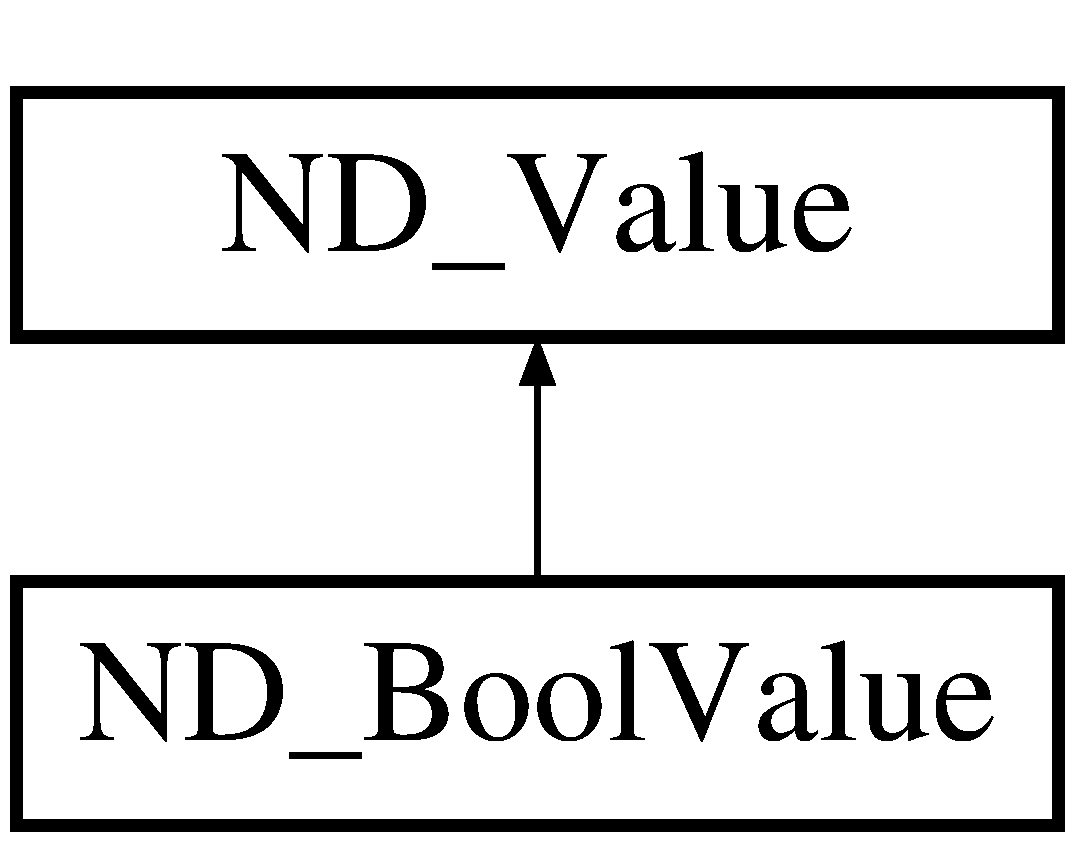
\includegraphics[height=2.000000cm]{class_n_d___bool_value}
\end{center}
\end{figure}
\subsection*{Public Member Functions}
\begin{DoxyCompactItemize}
\item 
\hyperlink{class_n_d___bool_value_a525308592f1e95d053f3163135bd70bb}{N\-D\-\_\-\-Bool\-Value} (bool value=false)
\item 
virtual \hyperlink{class_n_d___bool_value_a3e150405a025a6c7edda82235d192b75}{$\sim$\-N\-D\-\_\-\-Bool\-Value} ()
\item 
virtual string \hyperlink{class_n_d___bool_value_af71a39b64021f7e48a1b91752409302b}{To\-String} () const 
\item 
bool \hyperlink{class_n_d___bool_value_af27d87510c0dabd6991c5601f044db85}{Get\-Bool\-Value} () const 
\item 
virtual \hyperlink{class_n_d___value}{N\-D\-\_\-\-Value} $\ast$ \hyperlink{class_n_d___bool_value_a26fb17aea42dc9d9edf52a783988e4cd}{Clone} () const 
\item 
virtual bool \hyperlink{class_n_d___bool_value_ab4bc7add32f7de0628eaf8ab2dbd1df6}{Equals} (const \hyperlink{class_n_d___value}{N\-D\-\_\-\-Value} $\ast$v) const 
\item 
virtual \hyperlink{class_n_d___value}{N\-D\-\_\-\-Value} $\ast$ \hyperlink{class_n_d___bool_value_af9abb536e2843bb842ba99ce3c6bcd78}{Eval} (\hyperlink{_n_dvalue_8h_afc938fb729c95de25b4d2eb18640b303}{Ndlog\-\_\-\-Operator} op, \hyperlink{class_n_d___value}{N\-D\-\_\-\-Value} $\ast$rhs=N\-U\-L\-L)
\end{DoxyCompactItemize}
\subsection*{Protected Attributes}
\begin{DoxyCompactItemize}
\item 
bool \hyperlink{class_n_d___bool_value_a9288f3771b3cb35f65cc1d98f577d4f3}{m\-\_\-value}
\end{DoxyCompactItemize}


\subsection{Detailed Description}


Definition at line 8 of file N\-Dbool-\/value.\-h.



\subsection{Constructor \& Destructor Documentation}
\hypertarget{class_n_d___bool_value_a525308592f1e95d053f3163135bd70bb}{\index{N\-D\-\_\-\-Bool\-Value@{N\-D\-\_\-\-Bool\-Value}!N\-D\-\_\-\-Bool\-Value@{N\-D\-\_\-\-Bool\-Value}}
\index{N\-D\-\_\-\-Bool\-Value@{N\-D\-\_\-\-Bool\-Value}!ND_BoolValue@{N\-D\-\_\-\-Bool\-Value}}
\subsubsection[{N\-D\-\_\-\-Bool\-Value}]{\setlength{\rightskip}{0pt plus 5cm}N\-D\-\_\-\-Bool\-Value\-::\-N\-D\-\_\-\-Bool\-Value (
\begin{DoxyParamCaption}
\item[{bool}]{value = {\ttfamily false}}
\end{DoxyParamCaption}
)}}\label{class_n_d___bool_value_a525308592f1e95d053f3163135bd70bb}


Definition at line 4 of file N\-Dbool-\/value.\-cc.

\hypertarget{class_n_d___bool_value_a3e150405a025a6c7edda82235d192b75}{\index{N\-D\-\_\-\-Bool\-Value@{N\-D\-\_\-\-Bool\-Value}!$\sim$\-N\-D\-\_\-\-Bool\-Value@{$\sim$\-N\-D\-\_\-\-Bool\-Value}}
\index{$\sim$\-N\-D\-\_\-\-Bool\-Value@{$\sim$\-N\-D\-\_\-\-Bool\-Value}!ND_BoolValue@{N\-D\-\_\-\-Bool\-Value}}
\subsubsection[{$\sim$\-N\-D\-\_\-\-Bool\-Value}]{\setlength{\rightskip}{0pt plus 5cm}N\-D\-\_\-\-Bool\-Value\-::$\sim$\-N\-D\-\_\-\-Bool\-Value (
\begin{DoxyParamCaption}
{}
\end{DoxyParamCaption}
)\hspace{0.3cm}{\ttfamily [virtual]}}}\label{class_n_d___bool_value_a3e150405a025a6c7edda82235d192b75}


Definition at line 9 of file N\-Dbool-\/value.\-cc.



\subsection{Member Function Documentation}
\hypertarget{class_n_d___bool_value_a26fb17aea42dc9d9edf52a783988e4cd}{\index{N\-D\-\_\-\-Bool\-Value@{N\-D\-\_\-\-Bool\-Value}!Clone@{Clone}}
\index{Clone@{Clone}!ND_BoolValue@{N\-D\-\_\-\-Bool\-Value}}
\subsubsection[{Clone}]{\setlength{\rightskip}{0pt plus 5cm}{\bf N\-D\-\_\-\-Value} $\ast$ N\-D\-\_\-\-Bool\-Value\-::\-Clone (
\begin{DoxyParamCaption}
{}
\end{DoxyParamCaption}
) const\hspace{0.3cm}{\ttfamily [virtual]}}}\label{class_n_d___bool_value_a26fb17aea42dc9d9edf52a783988e4cd}


Implements \hyperlink{class_n_d___value_a83fbc37518fd13b38059a47c422e9024}{N\-D\-\_\-\-Value}.



Definition at line 28 of file N\-Dbool-\/value.\-cc.

\hypertarget{class_n_d___bool_value_ab4bc7add32f7de0628eaf8ab2dbd1df6}{\index{N\-D\-\_\-\-Bool\-Value@{N\-D\-\_\-\-Bool\-Value}!Equals@{Equals}}
\index{Equals@{Equals}!ND_BoolValue@{N\-D\-\_\-\-Bool\-Value}}
\subsubsection[{Equals}]{\setlength{\rightskip}{0pt plus 5cm}bool N\-D\-\_\-\-Bool\-Value\-::\-Equals (
\begin{DoxyParamCaption}
\item[{const {\bf N\-D\-\_\-\-Value} $\ast$}]{v}
\end{DoxyParamCaption}
) const\hspace{0.3cm}{\ttfamily [virtual]}}}\label{class_n_d___bool_value_ab4bc7add32f7de0628eaf8ab2dbd1df6}


Implements \hyperlink{class_n_d___value_a7b6432defc1b1cada5a31b5c16d29ac6}{N\-D\-\_\-\-Value}.



Definition at line 34 of file N\-Dbool-\/value.\-cc.

\hypertarget{class_n_d___bool_value_af9abb536e2843bb842ba99ce3c6bcd78}{\index{N\-D\-\_\-\-Bool\-Value@{N\-D\-\_\-\-Bool\-Value}!Eval@{Eval}}
\index{Eval@{Eval}!ND_BoolValue@{N\-D\-\_\-\-Bool\-Value}}
\subsubsection[{Eval}]{\setlength{\rightskip}{0pt plus 5cm}{\bf N\-D\-\_\-\-Value} $\ast$ N\-D\-\_\-\-Bool\-Value\-::\-Eval (
\begin{DoxyParamCaption}
\item[{{\bf Ndlog\-\_\-\-Operator}}]{op, }
\item[{{\bf N\-D\-\_\-\-Value} $\ast$}]{rhs = {\ttfamily NULL}}
\end{DoxyParamCaption}
)\hspace{0.3cm}{\ttfamily [virtual]}}}\label{class_n_d___bool_value_af9abb536e2843bb842ba99ce3c6bcd78}


Implements \hyperlink{class_n_d___value_aa3e290edb140d8676bfe0316c947502d}{N\-D\-\_\-\-Value}.



Definition at line 47 of file N\-Dbool-\/value.\-cc.

\hypertarget{class_n_d___bool_value_af27d87510c0dabd6991c5601f044db85}{\index{N\-D\-\_\-\-Bool\-Value@{N\-D\-\_\-\-Bool\-Value}!Get\-Bool\-Value@{Get\-Bool\-Value}}
\index{Get\-Bool\-Value@{Get\-Bool\-Value}!ND_BoolValue@{N\-D\-\_\-\-Bool\-Value}}
\subsubsection[{Get\-Bool\-Value}]{\setlength{\rightskip}{0pt plus 5cm}bool N\-D\-\_\-\-Bool\-Value\-::\-Get\-Bool\-Value (
\begin{DoxyParamCaption}
{}
\end{DoxyParamCaption}
) const}}\label{class_n_d___bool_value_af27d87510c0dabd6991c5601f044db85}


Definition at line 22 of file N\-Dbool-\/value.\-cc.

\hypertarget{class_n_d___bool_value_af71a39b64021f7e48a1b91752409302b}{\index{N\-D\-\_\-\-Bool\-Value@{N\-D\-\_\-\-Bool\-Value}!To\-String@{To\-String}}
\index{To\-String@{To\-String}!ND_BoolValue@{N\-D\-\_\-\-Bool\-Value}}
\subsubsection[{To\-String}]{\setlength{\rightskip}{0pt plus 5cm}string N\-D\-\_\-\-Bool\-Value\-::\-To\-String (
\begin{DoxyParamCaption}
{}
\end{DoxyParamCaption}
) const\hspace{0.3cm}{\ttfamily [virtual]}}}\label{class_n_d___bool_value_af71a39b64021f7e48a1b91752409302b}


Implements \hyperlink{class_n_d___value_a7660a0e6c07a198410fc05725d903219}{N\-D\-\_\-\-Value}.



Definition at line 14 of file N\-Dbool-\/value.\-cc.



\subsection{Member Data Documentation}
\hypertarget{class_n_d___bool_value_a9288f3771b3cb35f65cc1d98f577d4f3}{\index{N\-D\-\_\-\-Bool\-Value@{N\-D\-\_\-\-Bool\-Value}!m\-\_\-value@{m\-\_\-value}}
\index{m\-\_\-value@{m\-\_\-value}!ND_BoolValue@{N\-D\-\_\-\-Bool\-Value}}
\subsubsection[{m\-\_\-value}]{\setlength{\rightskip}{0pt plus 5cm}bool N\-D\-\_\-\-Bool\-Value\-::m\-\_\-value\hspace{0.3cm}{\ttfamily [protected]}}}\label{class_n_d___bool_value_a9288f3771b3cb35f65cc1d98f577d4f3}


Definition at line 28 of file N\-Dbool-\/value.\-h.



The documentation for this class was generated from the following files\-:\begin{DoxyCompactItemize}
\item 
src/msus/ndlog/value/\hyperlink{_n_dbool-value_8h}{N\-Dbool-\/value.\-h}\item 
src/msus/ndlog/\hyperlink{_n_dbool-value_8cc}{N\-Dbool-\/value.\-cc}\end{DoxyCompactItemize}

\hypertarget{class_n_d___byte_array_value}{\section{N\-D\-\_\-\-Byte\-Array\-Value Class Reference}
\label{class_n_d___byte_array_value}\index{N\-D\-\_\-\-Byte\-Array\-Value@{N\-D\-\_\-\-Byte\-Array\-Value}}
}


{\ttfamily \#include $<$N\-Dbyte-\/array-\/value.\-h$>$}

Inheritance diagram for N\-D\-\_\-\-Byte\-Array\-Value\-:\begin{figure}[H]
\begin{center}
\leavevmode
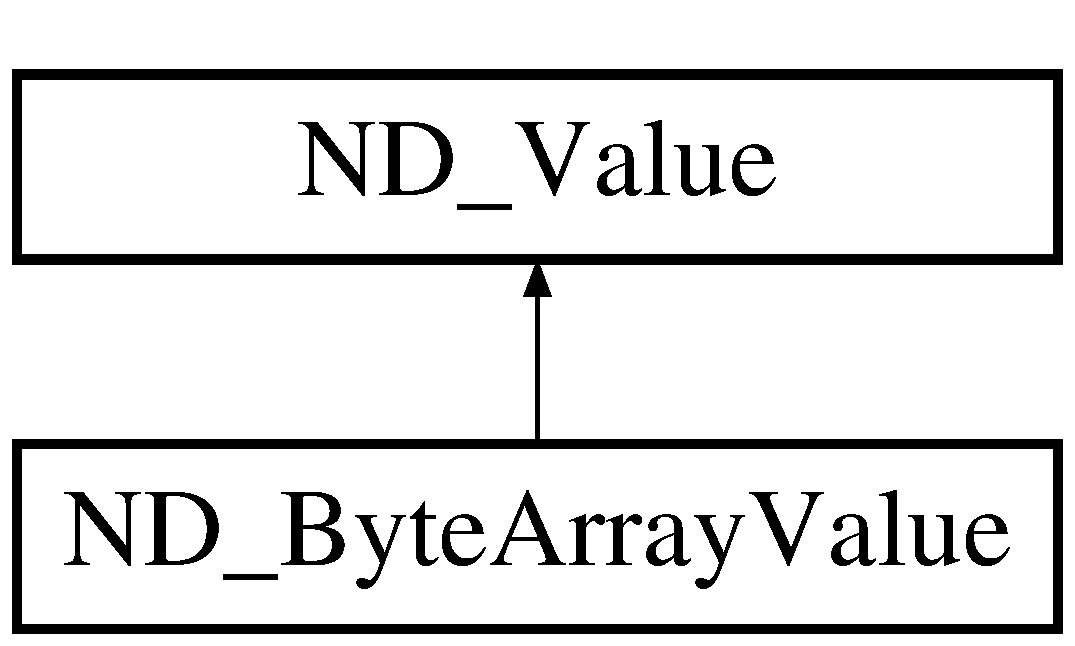
\includegraphics[height=2.000000cm]{class_n_d___byte_array_value}
\end{center}
\end{figure}
\subsection*{Public Member Functions}
\begin{DoxyCompactItemize}
\item 
\hyperlink{class_n_d___byte_array_value_abc4b53c37069d57d57e9d2a9323612a3}{N\-D\-\_\-\-Byte\-Array\-Value} (\hyperlink{msus_2webserver_2uthash_8h_aba7bc1797add20fe3efdf37ced1182c5}{uint8\-\_\-t} $\ast$buf=N\-U\-L\-L, \hyperlink{msus_2webserver_2uthash_8h_a435d1572bf3f880d55459d9805097f62}{uint32\-\_\-t} len=0)
\item 
virtual \hyperlink{class_n_d___byte_array_value_acbd892eb2c5be9e60507e2c7deb8743a}{$\sim$\-N\-D\-\_\-\-Byte\-Array\-Value} ()
\item 
virtual string \hyperlink{class_n_d___byte_array_value_a38fcb45e48d627e00d135c070e3188e5}{To\-String} () const 
\item 
virtual \hyperlink{msus_2webserver_2uthash_8h_aba7bc1797add20fe3efdf37ced1182c5}{uint8\-\_\-t} $\ast$ \hyperlink{class_n_d___byte_array_value_a2af628b4a2e9b0f755466dbb2c9d9932}{Get\-Byte\-Array\-Ptr} () const 
\item 
virtual \hyperlink{msus_2webserver_2uthash_8h_a435d1572bf3f880d55459d9805097f62}{uint32\-\_\-t} \hyperlink{class_n_d___byte_array_value_a20d5108f171041a509dc6b89a4516490}{Get\-Byte\-Array\-Len} () const 
\item 
virtual \hyperlink{class_n_d___value}{N\-D\-\_\-\-Value} $\ast$ \hyperlink{class_n_d___byte_array_value_ad61295c86a009f7c94b91a906cc6b36a}{Clone} () const 
\item 
virtual bool \hyperlink{class_n_d___byte_array_value_a0989cb51cb2e0d576a2d6e6e78e561cb}{Equals} (const \hyperlink{class_n_d___value}{N\-D\-\_\-\-Value} $\ast$v) const 
\item 
virtual \hyperlink{class_n_d___value}{N\-D\-\_\-\-Value} $\ast$ \hyperlink{class_n_d___byte_array_value_af5456134d6f0cf16a2d3fb1cbcd0069d}{Eval} (\hyperlink{_n_dvalue_8h_afc938fb729c95de25b4d2eb18640b303}{Ndlog\-\_\-\-Operator} op, \hyperlink{class_n_d___value}{N\-D\-\_\-\-Value} $\ast$rhs=N\-U\-L\-L)
\end{DoxyCompactItemize}
\subsection*{Protected Attributes}
\begin{DoxyCompactItemize}
\item 
\hyperlink{msus_2webserver_2uthash_8h_aba7bc1797add20fe3efdf37ced1182c5}{uint8\-\_\-t} $\ast$ \hyperlink{class_n_d___byte_array_value_a07ab6273dff8fcc80696fb98e857a9aa}{m\-\_\-array}
\item 
\hyperlink{msus_2webserver_2uthash_8h_a435d1572bf3f880d55459d9805097f62}{uint32\-\_\-t} \hyperlink{class_n_d___byte_array_value_a2c87705e49b1b4c25841a3bf3666c103}{m\-\_\-len}
\end{DoxyCompactItemize}


\subsection{Detailed Description}


Definition at line 10 of file N\-Dbyte-\/array-\/value.\-h.



\subsection{Constructor \& Destructor Documentation}
\hypertarget{class_n_d___byte_array_value_abc4b53c37069d57d57e9d2a9323612a3}{\index{N\-D\-\_\-\-Byte\-Array\-Value@{N\-D\-\_\-\-Byte\-Array\-Value}!N\-D\-\_\-\-Byte\-Array\-Value@{N\-D\-\_\-\-Byte\-Array\-Value}}
\index{N\-D\-\_\-\-Byte\-Array\-Value@{N\-D\-\_\-\-Byte\-Array\-Value}!ND_ByteArrayValue@{N\-D\-\_\-\-Byte\-Array\-Value}}
\subsubsection[{N\-D\-\_\-\-Byte\-Array\-Value}]{\setlength{\rightskip}{0pt plus 5cm}N\-D\-\_\-\-Byte\-Array\-Value\-::\-N\-D\-\_\-\-Byte\-Array\-Value (
\begin{DoxyParamCaption}
\item[{{\bf uint8\-\_\-t} $\ast$}]{buf = {\ttfamily NULL}, }
\item[{{\bf uint32\-\_\-t}}]{len = {\ttfamily 0}}
\end{DoxyParamCaption}
)}}\label{class_n_d___byte_array_value_abc4b53c37069d57d57e9d2a9323612a3}


Definition at line 4 of file N\-Dbyte-\/array-\/value.\-cc.

\hypertarget{class_n_d___byte_array_value_acbd892eb2c5be9e60507e2c7deb8743a}{\index{N\-D\-\_\-\-Byte\-Array\-Value@{N\-D\-\_\-\-Byte\-Array\-Value}!$\sim$\-N\-D\-\_\-\-Byte\-Array\-Value@{$\sim$\-N\-D\-\_\-\-Byte\-Array\-Value}}
\index{$\sim$\-N\-D\-\_\-\-Byte\-Array\-Value@{$\sim$\-N\-D\-\_\-\-Byte\-Array\-Value}!ND_ByteArrayValue@{N\-D\-\_\-\-Byte\-Array\-Value}}
\subsubsection[{$\sim$\-N\-D\-\_\-\-Byte\-Array\-Value}]{\setlength{\rightskip}{0pt plus 5cm}N\-D\-\_\-\-Byte\-Array\-Value\-::$\sim$\-N\-D\-\_\-\-Byte\-Array\-Value (
\begin{DoxyParamCaption}
{}
\end{DoxyParamCaption}
)\hspace{0.3cm}{\ttfamily [virtual]}}}\label{class_n_d___byte_array_value_acbd892eb2c5be9e60507e2c7deb8743a}


Definition at line 9 of file N\-Dbyte-\/array-\/value.\-cc.



\subsection{Member Function Documentation}
\hypertarget{class_n_d___byte_array_value_ad61295c86a009f7c94b91a906cc6b36a}{\index{N\-D\-\_\-\-Byte\-Array\-Value@{N\-D\-\_\-\-Byte\-Array\-Value}!Clone@{Clone}}
\index{Clone@{Clone}!ND_ByteArrayValue@{N\-D\-\_\-\-Byte\-Array\-Value}}
\subsubsection[{Clone}]{\setlength{\rightskip}{0pt plus 5cm}{\bf N\-D\-\_\-\-Value} $\ast$ N\-D\-\_\-\-Byte\-Array\-Value\-::\-Clone (
\begin{DoxyParamCaption}
{}
\end{DoxyParamCaption}
) const\hspace{0.3cm}{\ttfamily [virtual]}}}\label{class_n_d___byte_array_value_ad61295c86a009f7c94b91a906cc6b36a}


Implements \hyperlink{class_n_d___value_a83fbc37518fd13b38059a47c422e9024}{N\-D\-\_\-\-Value}.



Definition at line 26 of file N\-Dbyte-\/array-\/value.\-cc.

\hypertarget{class_n_d___byte_array_value_a0989cb51cb2e0d576a2d6e6e78e561cb}{\index{N\-D\-\_\-\-Byte\-Array\-Value@{N\-D\-\_\-\-Byte\-Array\-Value}!Equals@{Equals}}
\index{Equals@{Equals}!ND_ByteArrayValue@{N\-D\-\_\-\-Byte\-Array\-Value}}
\subsubsection[{Equals}]{\setlength{\rightskip}{0pt plus 5cm}bool N\-D\-\_\-\-Byte\-Array\-Value\-::\-Equals (
\begin{DoxyParamCaption}
\item[{const {\bf N\-D\-\_\-\-Value} $\ast$}]{v}
\end{DoxyParamCaption}
) const\hspace{0.3cm}{\ttfamily [virtual]}}}\label{class_n_d___byte_array_value_a0989cb51cb2e0d576a2d6e6e78e561cb}


Implements \hyperlink{class_n_d___value_a7b6432defc1b1cada5a31b5c16d29ac6}{N\-D\-\_\-\-Value}.



Definition at line 46 of file N\-Dbyte-\/array-\/value.\-cc.

\hypertarget{class_n_d___byte_array_value_af5456134d6f0cf16a2d3fb1cbcd0069d}{\index{N\-D\-\_\-\-Byte\-Array\-Value@{N\-D\-\_\-\-Byte\-Array\-Value}!Eval@{Eval}}
\index{Eval@{Eval}!ND_ByteArrayValue@{N\-D\-\_\-\-Byte\-Array\-Value}}
\subsubsection[{Eval}]{\setlength{\rightskip}{0pt plus 5cm}{\bf N\-D\-\_\-\-Value} $\ast$ N\-D\-\_\-\-Byte\-Array\-Value\-::\-Eval (
\begin{DoxyParamCaption}
\item[{{\bf Ndlog\-\_\-\-Operator}}]{op, }
\item[{{\bf N\-D\-\_\-\-Value} $\ast$}]{rhs = {\ttfamily NULL}}
\end{DoxyParamCaption}
)\hspace{0.3cm}{\ttfamily [virtual]}}}\label{class_n_d___byte_array_value_af5456134d6f0cf16a2d3fb1cbcd0069d}


Implements \hyperlink{class_n_d___value_aa3e290edb140d8676bfe0316c947502d}{N\-D\-\_\-\-Value}.



Definition at line 66 of file N\-Dbyte-\/array-\/value.\-cc.

\hypertarget{class_n_d___byte_array_value_a20d5108f171041a509dc6b89a4516490}{\index{N\-D\-\_\-\-Byte\-Array\-Value@{N\-D\-\_\-\-Byte\-Array\-Value}!Get\-Byte\-Array\-Len@{Get\-Byte\-Array\-Len}}
\index{Get\-Byte\-Array\-Len@{Get\-Byte\-Array\-Len}!ND_ByteArrayValue@{N\-D\-\_\-\-Byte\-Array\-Value}}
\subsubsection[{Get\-Byte\-Array\-Len}]{\setlength{\rightskip}{0pt plus 5cm}{\bf uint32\-\_\-t} N\-D\-\_\-\-Byte\-Array\-Value\-::\-Get\-Byte\-Array\-Len (
\begin{DoxyParamCaption}
{}
\end{DoxyParamCaption}
) const\hspace{0.3cm}{\ttfamily [virtual]}}}\label{class_n_d___byte_array_value_a20d5108f171041a509dc6b89a4516490}


Definition at line 40 of file N\-Dbyte-\/array-\/value.\-cc.

\hypertarget{class_n_d___byte_array_value_a2af628b4a2e9b0f755466dbb2c9d9932}{\index{N\-D\-\_\-\-Byte\-Array\-Value@{N\-D\-\_\-\-Byte\-Array\-Value}!Get\-Byte\-Array\-Ptr@{Get\-Byte\-Array\-Ptr}}
\index{Get\-Byte\-Array\-Ptr@{Get\-Byte\-Array\-Ptr}!ND_ByteArrayValue@{N\-D\-\_\-\-Byte\-Array\-Value}}
\subsubsection[{Get\-Byte\-Array\-Ptr}]{\setlength{\rightskip}{0pt plus 5cm}{\bf uint8\-\_\-t} $\ast$ N\-D\-\_\-\-Byte\-Array\-Value\-::\-Get\-Byte\-Array\-Ptr (
\begin{DoxyParamCaption}
{}
\end{DoxyParamCaption}
) const\hspace{0.3cm}{\ttfamily [virtual]}}}\label{class_n_d___byte_array_value_a2af628b4a2e9b0f755466dbb2c9d9932}


Definition at line 34 of file N\-Dbyte-\/array-\/value.\-cc.

\hypertarget{class_n_d___byte_array_value_a38fcb45e48d627e00d135c070e3188e5}{\index{N\-D\-\_\-\-Byte\-Array\-Value@{N\-D\-\_\-\-Byte\-Array\-Value}!To\-String@{To\-String}}
\index{To\-String@{To\-String}!ND_ByteArrayValue@{N\-D\-\_\-\-Byte\-Array\-Value}}
\subsubsection[{To\-String}]{\setlength{\rightskip}{0pt plus 5cm}string N\-D\-\_\-\-Byte\-Array\-Value\-::\-To\-String (
\begin{DoxyParamCaption}
{}
\end{DoxyParamCaption}
) const\hspace{0.3cm}{\ttfamily [virtual]}}}\label{class_n_d___byte_array_value_a38fcb45e48d627e00d135c070e3188e5}


Implements \hyperlink{class_n_d___value_a7660a0e6c07a198410fc05725d903219}{N\-D\-\_\-\-Value}.



Definition at line 18 of file N\-Dbyte-\/array-\/value.\-cc.



\subsection{Member Data Documentation}
\hypertarget{class_n_d___byte_array_value_a07ab6273dff8fcc80696fb98e857a9aa}{\index{N\-D\-\_\-\-Byte\-Array\-Value@{N\-D\-\_\-\-Byte\-Array\-Value}!m\-\_\-array@{m\-\_\-array}}
\index{m\-\_\-array@{m\-\_\-array}!ND_ByteArrayValue@{N\-D\-\_\-\-Byte\-Array\-Value}}
\subsubsection[{m\-\_\-array}]{\setlength{\rightskip}{0pt plus 5cm}{\bf uint8\-\_\-t}$\ast$ N\-D\-\_\-\-Byte\-Array\-Value\-::m\-\_\-array\hspace{0.3cm}{\ttfamily [protected]}}}\label{class_n_d___byte_array_value_a07ab6273dff8fcc80696fb98e857a9aa}


Definition at line 32 of file N\-Dbyte-\/array-\/value.\-h.

\hypertarget{class_n_d___byte_array_value_a2c87705e49b1b4c25841a3bf3666c103}{\index{N\-D\-\_\-\-Byte\-Array\-Value@{N\-D\-\_\-\-Byte\-Array\-Value}!m\-\_\-len@{m\-\_\-len}}
\index{m\-\_\-len@{m\-\_\-len}!ND_ByteArrayValue@{N\-D\-\_\-\-Byte\-Array\-Value}}
\subsubsection[{m\-\_\-len}]{\setlength{\rightskip}{0pt plus 5cm}{\bf uint32\-\_\-t} N\-D\-\_\-\-Byte\-Array\-Value\-::m\-\_\-len\hspace{0.3cm}{\ttfamily [protected]}}}\label{class_n_d___byte_array_value_a2c87705e49b1b4c25841a3bf3666c103}


Definition at line 34 of file N\-Dbyte-\/array-\/value.\-h.



The documentation for this class was generated from the following files\-:\begin{DoxyCompactItemize}
\item 
src/msus/ndlog/value/\hyperlink{_n_dbyte-array-value_8h}{N\-Dbyte-\/array-\/value.\-h}\item 
src/msus/ndlog/\hyperlink{_n_dbyte-array-value_8cc}{N\-Dbyte-\/array-\/value.\-cc}\end{DoxyCompactItemize}

\hypertarget{class_n_d___id_value}{\section{N\-D\-\_\-\-Id\-Value Class Reference}
\label{class_n_d___id_value}\index{N\-D\-\_\-\-Id\-Value@{N\-D\-\_\-\-Id\-Value}}
}


{\ttfamily \#include $<$N\-Did-\/value.\-h$>$}

Inheritance diagram for N\-D\-\_\-\-Id\-Value\-:\begin{figure}[H]
\begin{center}
\leavevmode
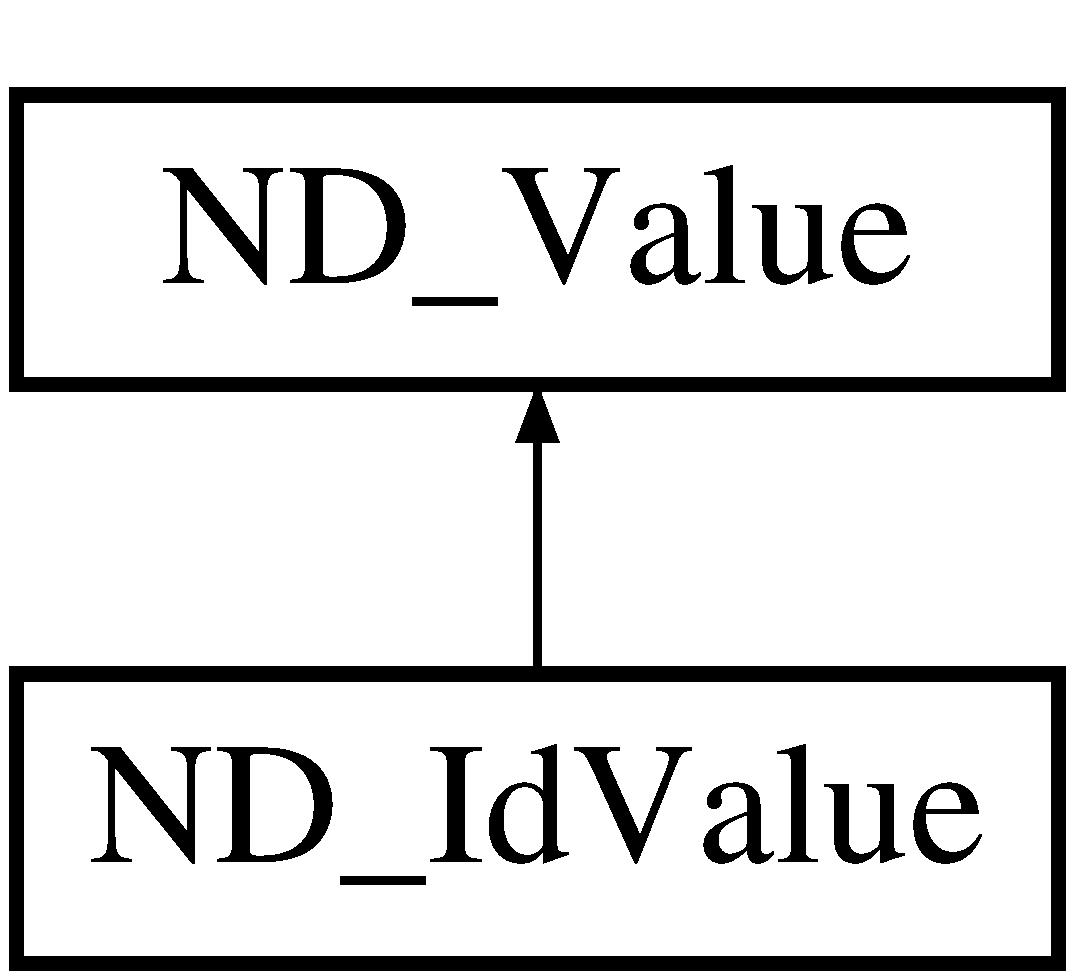
\includegraphics[height=2.000000cm]{class_n_d___id_value}
\end{center}
\end{figure}
\subsection*{Public Member Functions}
\begin{DoxyCompactItemize}
\item 
\hyperlink{class_n_d___id_value_a6acf6aaf6cfec7f4f6e418ef73b850ee}{N\-D\-\_\-\-Id\-Value} (string value=\char`\"{}0\char`\"{}, \hyperlink{msus_2webserver_2uthash_8h_a435d1572bf3f880d55459d9805097f62}{uint32\-\_\-t} base=2)
\item 
virtual \hyperlink{class_n_d___id_value_a44e9464755e0eb6c73abd2554b7df7e0}{$\sim$\-N\-D\-\_\-\-Id\-Value} ()
\item 
virtual string \hyperlink{class_n_d___id_value_a98248b82fef11b5ffe11aa20f7af2827}{To\-String} () const 
\item 
virtual string \hyperlink{class_n_d___id_value_a794298528c007b346153c916d8cf2120}{To\-Fraction\-String} () const 
\item 
bitset$<$ \hyperlink{_n_did-value_8h_ae013c4e072a3fc8640f771f3e4c0e4b6}{N\-D\-\_\-\-I\-D\-\_\-\-L\-E\-N} $>$ \hyperlink{class_n_d___id_value_ac789156bc60739fb91752457c3ca3584}{Get\-Id\-Value} () const 
\item 
virtual \hyperlink{class_n_d___value}{N\-D\-\_\-\-Value} $\ast$ \hyperlink{class_n_d___id_value_adc3e53144381e763eb84e8f6d2dcf3e9}{Clone} () const 
\item 
virtual bool \hyperlink{class_n_d___id_value_aa84829bbfe9842c08a9d011009bf6ad3}{Equals} (const \hyperlink{class_n_d___value}{N\-D\-\_\-\-Value} $\ast$v) const 
\item 
virtual \hyperlink{class_n_d___value}{N\-D\-\_\-\-Value} $\ast$ \hyperlink{class_n_d___id_value_ade36f0cd7fcb88af1e0e1794d3f4afea}{Eval} (\hyperlink{_n_dvalue_8h_afc938fb729c95de25b4d2eb18640b303}{Ndlog\-\_\-\-Operator} op, \hyperlink{class_n_d___value}{N\-D\-\_\-\-Value} $\ast$rhs=N\-U\-L\-L)
\item 
virtual mpz\-\_\-class \hyperlink{class_n_d___id_value_aff71796116425894904e79070a87669d}{Get\-Mpz} () const 
\end{DoxyCompactItemize}
\subsection*{Protected Attributes}
\begin{DoxyCompactItemize}
\item 
bitset$<$ \hyperlink{_n_did-value_8h_ae013c4e072a3fc8640f771f3e4c0e4b6}{N\-D\-\_\-\-I\-D\-\_\-\-L\-E\-N} $>$ \hyperlink{class_n_d___id_value_a71c4d10b8dd918a6d6b67de3c33fbaf0}{m\-\_\-value}
\end{DoxyCompactItemize}


\subsection{Detailed Description}


Definition at line 15 of file N\-Did-\/value.\-h.



\subsection{Constructor \& Destructor Documentation}
\hypertarget{class_n_d___id_value_a6acf6aaf6cfec7f4f6e418ef73b850ee}{\index{N\-D\-\_\-\-Id\-Value@{N\-D\-\_\-\-Id\-Value}!N\-D\-\_\-\-Id\-Value@{N\-D\-\_\-\-Id\-Value}}
\index{N\-D\-\_\-\-Id\-Value@{N\-D\-\_\-\-Id\-Value}!ND_IdValue@{N\-D\-\_\-\-Id\-Value}}
\subsubsection[{N\-D\-\_\-\-Id\-Value}]{\setlength{\rightskip}{0pt plus 5cm}N\-D\-\_\-\-Id\-Value\-::\-N\-D\-\_\-\-Id\-Value (
\begin{DoxyParamCaption}
\item[{string}]{value = {\ttfamily \char`\"{}0\char`\"{}}, }
\item[{{\bf uint32\-\_\-t}}]{base = {\ttfamily 2}}
\end{DoxyParamCaption}
)}}\label{class_n_d___id_value_a6acf6aaf6cfec7f4f6e418ef73b850ee}


Definition at line 4 of file N\-Did-\/value.\-cc.

\hypertarget{class_n_d___id_value_a44e9464755e0eb6c73abd2554b7df7e0}{\index{N\-D\-\_\-\-Id\-Value@{N\-D\-\_\-\-Id\-Value}!$\sim$\-N\-D\-\_\-\-Id\-Value@{$\sim$\-N\-D\-\_\-\-Id\-Value}}
\index{$\sim$\-N\-D\-\_\-\-Id\-Value@{$\sim$\-N\-D\-\_\-\-Id\-Value}!ND_IdValue@{N\-D\-\_\-\-Id\-Value}}
\subsubsection[{$\sim$\-N\-D\-\_\-\-Id\-Value}]{\setlength{\rightskip}{0pt plus 5cm}N\-D\-\_\-\-Id\-Value\-::$\sim$\-N\-D\-\_\-\-Id\-Value (
\begin{DoxyParamCaption}
{}
\end{DoxyParamCaption}
)\hspace{0.3cm}{\ttfamily [virtual]}}}\label{class_n_d___id_value_a44e9464755e0eb6c73abd2554b7df7e0}


Definition at line 11 of file N\-Did-\/value.\-cc.



\subsection{Member Function Documentation}
\hypertarget{class_n_d___id_value_adc3e53144381e763eb84e8f6d2dcf3e9}{\index{N\-D\-\_\-\-Id\-Value@{N\-D\-\_\-\-Id\-Value}!Clone@{Clone}}
\index{Clone@{Clone}!ND_IdValue@{N\-D\-\_\-\-Id\-Value}}
\subsubsection[{Clone}]{\setlength{\rightskip}{0pt plus 5cm}{\bf N\-D\-\_\-\-Value} $\ast$ N\-D\-\_\-\-Id\-Value\-::\-Clone (
\begin{DoxyParamCaption}
{}
\end{DoxyParamCaption}
) const\hspace{0.3cm}{\ttfamily [virtual]}}}\label{class_n_d___id_value_adc3e53144381e763eb84e8f6d2dcf3e9}


Implements \hyperlink{class_n_d___value_a83fbc37518fd13b38059a47c422e9024}{N\-D\-\_\-\-Value}.



Definition at line 40 of file N\-Did-\/value.\-cc.

\hypertarget{class_n_d___id_value_aa84829bbfe9842c08a9d011009bf6ad3}{\index{N\-D\-\_\-\-Id\-Value@{N\-D\-\_\-\-Id\-Value}!Equals@{Equals}}
\index{Equals@{Equals}!ND_IdValue@{N\-D\-\_\-\-Id\-Value}}
\subsubsection[{Equals}]{\setlength{\rightskip}{0pt plus 5cm}bool N\-D\-\_\-\-Id\-Value\-::\-Equals (
\begin{DoxyParamCaption}
\item[{const {\bf N\-D\-\_\-\-Value} $\ast$}]{v}
\end{DoxyParamCaption}
) const\hspace{0.3cm}{\ttfamily [virtual]}}}\label{class_n_d___id_value_aa84829bbfe9842c08a9d011009bf6ad3}


Implements \hyperlink{class_n_d___value_a7b6432defc1b1cada5a31b5c16d29ac6}{N\-D\-\_\-\-Value}.



Definition at line 48 of file N\-Did-\/value.\-cc.

\hypertarget{class_n_d___id_value_ade36f0cd7fcb88af1e0e1794d3f4afea}{\index{N\-D\-\_\-\-Id\-Value@{N\-D\-\_\-\-Id\-Value}!Eval@{Eval}}
\index{Eval@{Eval}!ND_IdValue@{N\-D\-\_\-\-Id\-Value}}
\subsubsection[{Eval}]{\setlength{\rightskip}{0pt plus 5cm}{\bf N\-D\-\_\-\-Value} $\ast$ N\-D\-\_\-\-Id\-Value\-::\-Eval (
\begin{DoxyParamCaption}
\item[{{\bf Ndlog\-\_\-\-Operator}}]{op, }
\item[{{\bf N\-D\-\_\-\-Value} $\ast$}]{rhs = {\ttfamily NULL}}
\end{DoxyParamCaption}
)\hspace{0.3cm}{\ttfamily [virtual]}}}\label{class_n_d___id_value_ade36f0cd7fcb88af1e0e1794d3f4afea}


Implements \hyperlink{class_n_d___value_aa3e290edb140d8676bfe0316c947502d}{N\-D\-\_\-\-Value}.



Definition at line 61 of file N\-Did-\/value.\-cc.

\hypertarget{class_n_d___id_value_ac789156bc60739fb91752457c3ca3584}{\index{N\-D\-\_\-\-Id\-Value@{N\-D\-\_\-\-Id\-Value}!Get\-Id\-Value@{Get\-Id\-Value}}
\index{Get\-Id\-Value@{Get\-Id\-Value}!ND_IdValue@{N\-D\-\_\-\-Id\-Value}}
\subsubsection[{Get\-Id\-Value}]{\setlength{\rightskip}{0pt plus 5cm}bitset$<$ {\bf N\-D\-\_\-\-I\-D\-\_\-\-L\-E\-N} $>$ N\-D\-\_\-\-Id\-Value\-::\-Get\-Id\-Value (
\begin{DoxyParamCaption}
{}
\end{DoxyParamCaption}
) const}}\label{class_n_d___id_value_ac789156bc60739fb91752457c3ca3584}


Definition at line 34 of file N\-Did-\/value.\-cc.

\hypertarget{class_n_d___id_value_aff71796116425894904e79070a87669d}{\index{N\-D\-\_\-\-Id\-Value@{N\-D\-\_\-\-Id\-Value}!Get\-Mpz@{Get\-Mpz}}
\index{Get\-Mpz@{Get\-Mpz}!ND_IdValue@{N\-D\-\_\-\-Id\-Value}}
\subsubsection[{Get\-Mpz}]{\setlength{\rightskip}{0pt plus 5cm}mpz\-\_\-class N\-D\-\_\-\-Id\-Value\-::\-Get\-Mpz (
\begin{DoxyParamCaption}
{}
\end{DoxyParamCaption}
) const\hspace{0.3cm}{\ttfamily [virtual]}}}\label{class_n_d___id_value_aff71796116425894904e79070a87669d}


Definition at line 221 of file N\-Did-\/value.\-cc.

\hypertarget{class_n_d___id_value_a794298528c007b346153c916d8cf2120}{\index{N\-D\-\_\-\-Id\-Value@{N\-D\-\_\-\-Id\-Value}!To\-Fraction\-String@{To\-Fraction\-String}}
\index{To\-Fraction\-String@{To\-Fraction\-String}!ND_IdValue@{N\-D\-\_\-\-Id\-Value}}
\subsubsection[{To\-Fraction\-String}]{\setlength{\rightskip}{0pt plus 5cm}string N\-D\-\_\-\-Id\-Value\-::\-To\-Fraction\-String (
\begin{DoxyParamCaption}
{}
\end{DoxyParamCaption}
) const\hspace{0.3cm}{\ttfamily [virtual]}}}\label{class_n_d___id_value_a794298528c007b346153c916d8cf2120}


Definition at line 23 of file N\-Did-\/value.\-cc.

\hypertarget{class_n_d___id_value_a98248b82fef11b5ffe11aa20f7af2827}{\index{N\-D\-\_\-\-Id\-Value@{N\-D\-\_\-\-Id\-Value}!To\-String@{To\-String}}
\index{To\-String@{To\-String}!ND_IdValue@{N\-D\-\_\-\-Id\-Value}}
\subsubsection[{To\-String}]{\setlength{\rightskip}{0pt plus 5cm}string N\-D\-\_\-\-Id\-Value\-::\-To\-String (
\begin{DoxyParamCaption}
{}
\end{DoxyParamCaption}
) const\hspace{0.3cm}{\ttfamily [virtual]}}}\label{class_n_d___id_value_a98248b82fef11b5ffe11aa20f7af2827}


Implements \hyperlink{class_n_d___value_a7660a0e6c07a198410fc05725d903219}{N\-D\-\_\-\-Value}.



Definition at line 16 of file N\-Did-\/value.\-cc.



\subsection{Member Data Documentation}
\hypertarget{class_n_d___id_value_a71c4d10b8dd918a6d6b67de3c33fbaf0}{\index{N\-D\-\_\-\-Id\-Value@{N\-D\-\_\-\-Id\-Value}!m\-\_\-value@{m\-\_\-value}}
\index{m\-\_\-value@{m\-\_\-value}!ND_IdValue@{N\-D\-\_\-\-Id\-Value}}
\subsubsection[{m\-\_\-value}]{\setlength{\rightskip}{0pt plus 5cm}bitset$<${\bf N\-D\-\_\-\-I\-D\-\_\-\-L\-E\-N}$>$ N\-D\-\_\-\-Id\-Value\-::m\-\_\-value\hspace{0.3cm}{\ttfamily [protected]}}}\label{class_n_d___id_value_a71c4d10b8dd918a6d6b67de3c33fbaf0}


Definition at line 39 of file N\-Did-\/value.\-h.



The documentation for this class was generated from the following files\-:\begin{DoxyCompactItemize}
\item 
src/msus/ndlog/value/\hyperlink{_n_did-value_8h}{N\-Did-\/value.\-h}\item 
src/msus/ndlog/\hyperlink{_n_did-value_8cc}{N\-Did-\/value.\-cc}\end{DoxyCompactItemize}

\hypertarget{class_n_d___int32_value}{\section{N\-D\-\_\-\-Int32\-Value Class Reference}
\label{class_n_d___int32_value}\index{N\-D\-\_\-\-Int32\-Value@{N\-D\-\_\-\-Int32\-Value}}
}


{\ttfamily \#include $<$N\-Dint32-\/value.\-h$>$}

Inheritance diagram for N\-D\-\_\-\-Int32\-Value\-:\begin{figure}[H]
\begin{center}
\leavevmode
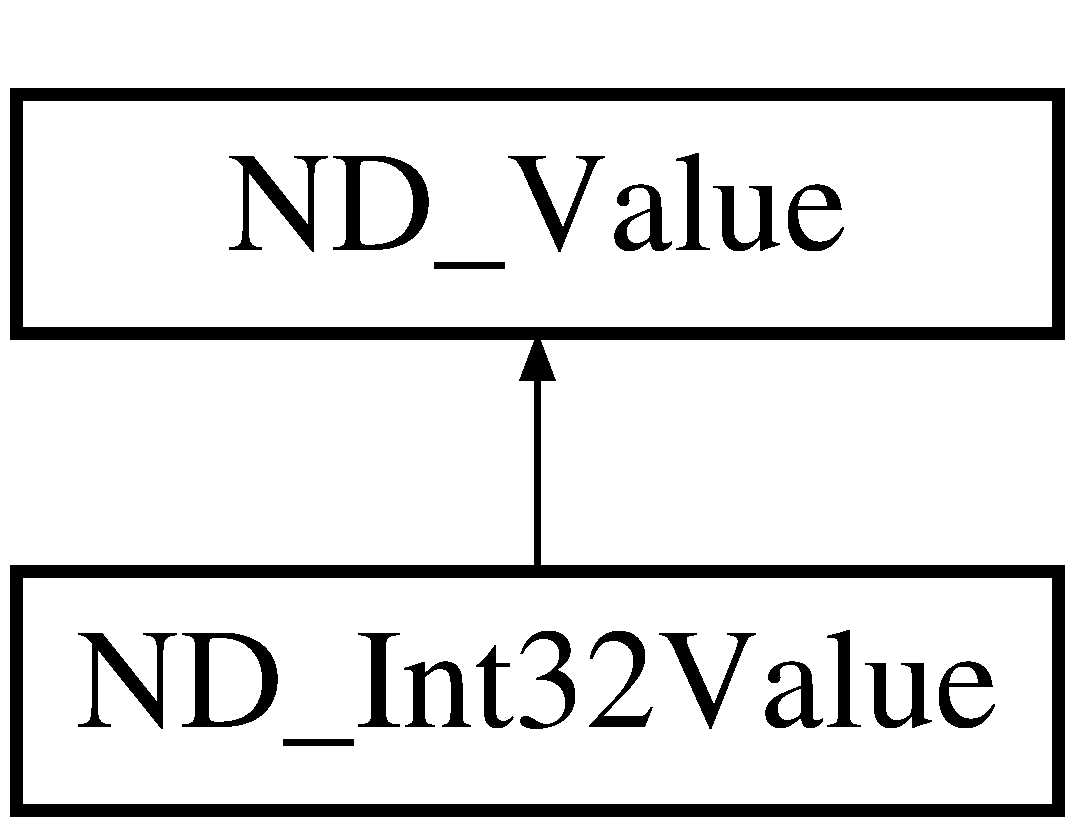
\includegraphics[height=2.000000cm]{class_n_d___int32_value}
\end{center}
\end{figure}
\subsection*{Public Member Functions}
\begin{DoxyCompactItemize}
\item 
\hyperlink{class_n_d___int32_value_aa1be1030824a1e3b2de45f15ca7e89ef}{N\-D\-\_\-\-Int32\-Value} (int32\-\_\-t value=0)
\item 
virtual \hyperlink{class_n_d___int32_value_a6a558abd1d2fd0fc446f5190ba7fc0d3}{$\sim$\-N\-D\-\_\-\-Int32\-Value} ()
\item 
virtual string \hyperlink{class_n_d___int32_value_a897c234f7b6f00843c2d9d103956b2ae}{To\-String} () const 
\item 
\hyperlink{msus_2webserver_2uthash_8h_a435d1572bf3f880d55459d9805097f62}{uint32\-\_\-t} \hyperlink{class_n_d___int32_value_a41cb60b42991e7f1ca03f732fda09aaf}{Get\-Int32\-Value} () const 
\item 
virtual \hyperlink{class_n_d___value}{N\-D\-\_\-\-Value} $\ast$ \hyperlink{class_n_d___int32_value_ae8fc6254509ce906a191e45c06f49658}{Clone} () const 
\item 
virtual bool \hyperlink{class_n_d___int32_value_af66a16bf770c3fd847d4af6c624b1860}{Equals} (const \hyperlink{class_n_d___value}{N\-D\-\_\-\-Value} $\ast$v) const 
\item 
virtual \hyperlink{class_n_d___value}{N\-D\-\_\-\-Value} $\ast$ \hyperlink{class_n_d___int32_value_a4a16725cc0cd2bc1228572c378e70847}{Eval} (\hyperlink{_n_dvalue_8h_afc938fb729c95de25b4d2eb18640b303}{Ndlog\-\_\-\-Operator} op, \hyperlink{class_n_d___value}{N\-D\-\_\-\-Value} $\ast$rhs=N\-U\-L\-L)
\end{DoxyCompactItemize}
\subsection*{Protected Attributes}
\begin{DoxyCompactItemize}
\item 
\hyperlink{msus_2webserver_2uthash_8h_a435d1572bf3f880d55459d9805097f62}{uint32\-\_\-t} \hyperlink{class_n_d___int32_value_a065f85a575dcebb0f03947c752625881}{m\-\_\-value}
\end{DoxyCompactItemize}


\subsection{Detailed Description}


Definition at line 15 of file N\-Dint32-\/value.\-h.



\subsection{Constructor \& Destructor Documentation}
\hypertarget{class_n_d___int32_value_aa1be1030824a1e3b2de45f15ca7e89ef}{\index{N\-D\-\_\-\-Int32\-Value@{N\-D\-\_\-\-Int32\-Value}!N\-D\-\_\-\-Int32\-Value@{N\-D\-\_\-\-Int32\-Value}}
\index{N\-D\-\_\-\-Int32\-Value@{N\-D\-\_\-\-Int32\-Value}!ND_Int32Value@{N\-D\-\_\-\-Int32\-Value}}
\subsubsection[{N\-D\-\_\-\-Int32\-Value}]{\setlength{\rightskip}{0pt plus 5cm}N\-D\-\_\-\-Int32\-Value\-::\-N\-D\-\_\-\-Int32\-Value (
\begin{DoxyParamCaption}
\item[{int32\-\_\-t}]{value = {\ttfamily 0}}
\end{DoxyParamCaption}
)}}\label{class_n_d___int32_value_aa1be1030824a1e3b2de45f15ca7e89ef}


Definition at line 4 of file N\-Dint32-\/value.\-cc.

\hypertarget{class_n_d___int32_value_a6a558abd1d2fd0fc446f5190ba7fc0d3}{\index{N\-D\-\_\-\-Int32\-Value@{N\-D\-\_\-\-Int32\-Value}!$\sim$\-N\-D\-\_\-\-Int32\-Value@{$\sim$\-N\-D\-\_\-\-Int32\-Value}}
\index{$\sim$\-N\-D\-\_\-\-Int32\-Value@{$\sim$\-N\-D\-\_\-\-Int32\-Value}!ND_Int32Value@{N\-D\-\_\-\-Int32\-Value}}
\subsubsection[{$\sim$\-N\-D\-\_\-\-Int32\-Value}]{\setlength{\rightskip}{0pt plus 5cm}N\-D\-\_\-\-Int32\-Value\-::$\sim$\-N\-D\-\_\-\-Int32\-Value (
\begin{DoxyParamCaption}
{}
\end{DoxyParamCaption}
)\hspace{0.3cm}{\ttfamily [virtual]}}}\label{class_n_d___int32_value_a6a558abd1d2fd0fc446f5190ba7fc0d3}


Definition at line 9 of file N\-Dint32-\/value.\-cc.



\subsection{Member Function Documentation}
\hypertarget{class_n_d___int32_value_ae8fc6254509ce906a191e45c06f49658}{\index{N\-D\-\_\-\-Int32\-Value@{N\-D\-\_\-\-Int32\-Value}!Clone@{Clone}}
\index{Clone@{Clone}!ND_Int32Value@{N\-D\-\_\-\-Int32\-Value}}
\subsubsection[{Clone}]{\setlength{\rightskip}{0pt plus 5cm}{\bf N\-D\-\_\-\-Value} $\ast$ N\-D\-\_\-\-Int32\-Value\-::\-Clone (
\begin{DoxyParamCaption}
{}
\end{DoxyParamCaption}
) const\hspace{0.3cm}{\ttfamily [virtual]}}}\label{class_n_d___int32_value_ae8fc6254509ce906a191e45c06f49658}


Implements \hyperlink{class_n_d___value_a83fbc37518fd13b38059a47c422e9024}{N\-D\-\_\-\-Value}.



Definition at line 27 of file N\-Dint32-\/value.\-cc.

\hypertarget{class_n_d___int32_value_af66a16bf770c3fd847d4af6c624b1860}{\index{N\-D\-\_\-\-Int32\-Value@{N\-D\-\_\-\-Int32\-Value}!Equals@{Equals}}
\index{Equals@{Equals}!ND_Int32Value@{N\-D\-\_\-\-Int32\-Value}}
\subsubsection[{Equals}]{\setlength{\rightskip}{0pt plus 5cm}bool N\-D\-\_\-\-Int32\-Value\-::\-Equals (
\begin{DoxyParamCaption}
\item[{const {\bf N\-D\-\_\-\-Value} $\ast$}]{v}
\end{DoxyParamCaption}
) const\hspace{0.3cm}{\ttfamily [virtual]}}}\label{class_n_d___int32_value_af66a16bf770c3fd847d4af6c624b1860}


Implements \hyperlink{class_n_d___value_a7b6432defc1b1cada5a31b5c16d29ac6}{N\-D\-\_\-\-Value}.



Definition at line 33 of file N\-Dint32-\/value.\-cc.

\hypertarget{class_n_d___int32_value_a4a16725cc0cd2bc1228572c378e70847}{\index{N\-D\-\_\-\-Int32\-Value@{N\-D\-\_\-\-Int32\-Value}!Eval@{Eval}}
\index{Eval@{Eval}!ND_Int32Value@{N\-D\-\_\-\-Int32\-Value}}
\subsubsection[{Eval}]{\setlength{\rightskip}{0pt plus 5cm}{\bf N\-D\-\_\-\-Value} $\ast$ N\-D\-\_\-\-Int32\-Value\-::\-Eval (
\begin{DoxyParamCaption}
\item[{{\bf Ndlog\-\_\-\-Operator}}]{op, }
\item[{{\bf N\-D\-\_\-\-Value} $\ast$}]{rhs = {\ttfamily NULL}}
\end{DoxyParamCaption}
)\hspace{0.3cm}{\ttfamily [virtual]}}}\label{class_n_d___int32_value_a4a16725cc0cd2bc1228572c378e70847}


Implements \hyperlink{class_n_d___value_aa3e290edb140d8676bfe0316c947502d}{N\-D\-\_\-\-Value}.



Definition at line 46 of file N\-Dint32-\/value.\-cc.

\hypertarget{class_n_d___int32_value_a41cb60b42991e7f1ca03f732fda09aaf}{\index{N\-D\-\_\-\-Int32\-Value@{N\-D\-\_\-\-Int32\-Value}!Get\-Int32\-Value@{Get\-Int32\-Value}}
\index{Get\-Int32\-Value@{Get\-Int32\-Value}!ND_Int32Value@{N\-D\-\_\-\-Int32\-Value}}
\subsubsection[{Get\-Int32\-Value}]{\setlength{\rightskip}{0pt plus 5cm}{\bf uint32\-\_\-t} N\-D\-\_\-\-Int32\-Value\-::\-Get\-Int32\-Value (
\begin{DoxyParamCaption}
{}
\end{DoxyParamCaption}
) const}}\label{class_n_d___int32_value_a41cb60b42991e7f1ca03f732fda09aaf}


Definition at line 21 of file N\-Dint32-\/value.\-cc.

\hypertarget{class_n_d___int32_value_a897c234f7b6f00843c2d9d103956b2ae}{\index{N\-D\-\_\-\-Int32\-Value@{N\-D\-\_\-\-Int32\-Value}!To\-String@{To\-String}}
\index{To\-String@{To\-String}!ND_Int32Value@{N\-D\-\_\-\-Int32\-Value}}
\subsubsection[{To\-String}]{\setlength{\rightskip}{0pt plus 5cm}string N\-D\-\_\-\-Int32\-Value\-::\-To\-String (
\begin{DoxyParamCaption}
{}
\end{DoxyParamCaption}
) const\hspace{0.3cm}{\ttfamily [virtual]}}}\label{class_n_d___int32_value_a897c234f7b6f00843c2d9d103956b2ae}


Implements \hyperlink{class_n_d___value_a7660a0e6c07a198410fc05725d903219}{N\-D\-\_\-\-Value}.



Definition at line 14 of file N\-Dint32-\/value.\-cc.



\subsection{Member Data Documentation}
\hypertarget{class_n_d___int32_value_a065f85a575dcebb0f03947c752625881}{\index{N\-D\-\_\-\-Int32\-Value@{N\-D\-\_\-\-Int32\-Value}!m\-\_\-value@{m\-\_\-value}}
\index{m\-\_\-value@{m\-\_\-value}!ND_Int32Value@{N\-D\-\_\-\-Int32\-Value}}
\subsubsection[{m\-\_\-value}]{\setlength{\rightskip}{0pt plus 5cm}{\bf uint32\-\_\-t} N\-D\-\_\-\-Int32\-Value\-::m\-\_\-value\hspace{0.3cm}{\ttfamily [protected]}}}\label{class_n_d___int32_value_a065f85a575dcebb0f03947c752625881}


Definition at line 35 of file N\-Dint32-\/value.\-h.



The documentation for this class was generated from the following files\-:\begin{DoxyCompactItemize}
\item 
src/msus/ndlog/value/\hyperlink{_n_dint32-value_8h}{N\-Dint32-\/value.\-h}\item 
src/msus/ndlog/\hyperlink{_n_dint32-value_8cc}{N\-Dint32-\/value.\-cc}\end{DoxyCompactItemize}

\hypertarget{class_n_d___list_value}{\section{N\-D\-\_\-\-List\-Value Class Reference}
\label{class_n_d___list_value}\index{N\-D\-\_\-\-List\-Value@{N\-D\-\_\-\-List\-Value}}
}


{\ttfamily \#include $<$N\-Dlist-\/value.\-h$>$}

Inheritance diagram for N\-D\-\_\-\-List\-Value\-:\begin{figure}[H]
\begin{center}
\leavevmode
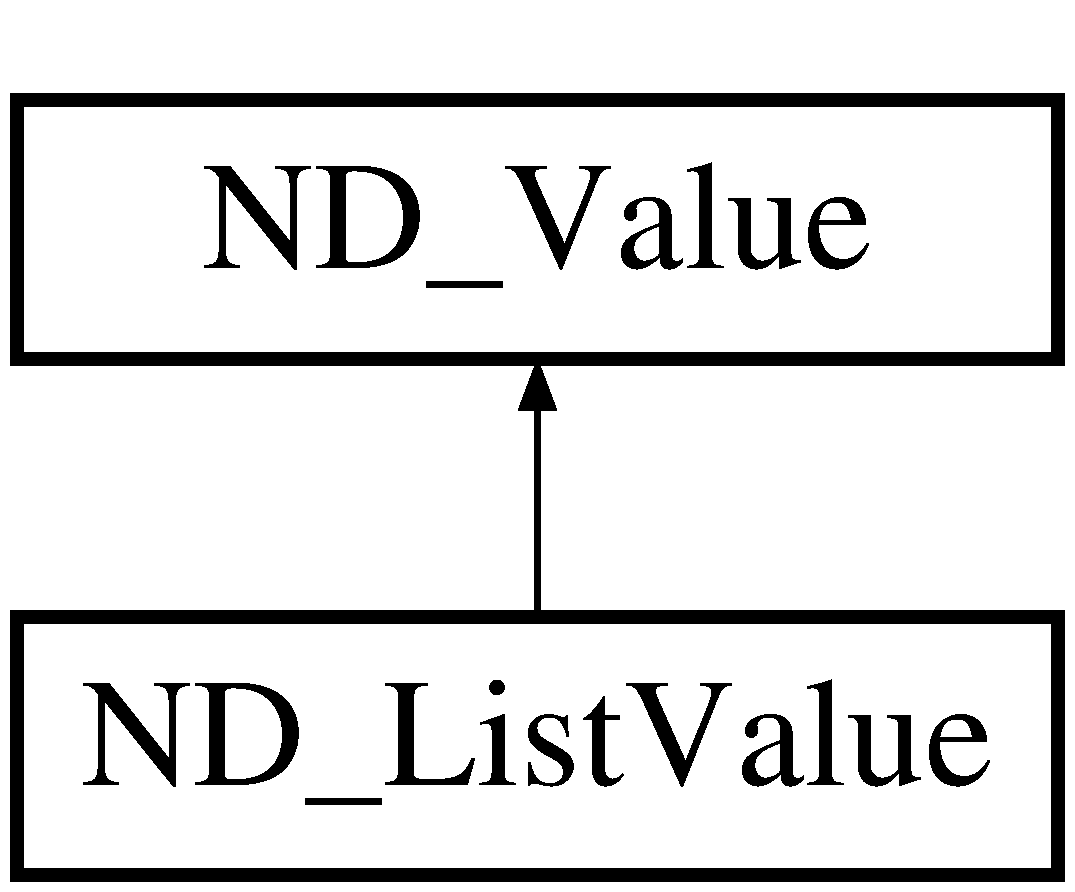
\includegraphics[height=2.000000cm]{class_n_d___list_value}
\end{center}
\end{figure}
\subsection*{Public Member Functions}
\begin{DoxyCompactItemize}
\item 
\hyperlink{class_n_d___list_value_a9ec9da85fb379f51c0d7371b6d8e4e30}{N\-D\-\_\-\-List\-Value} (list$<$ \hyperlink{class_n_d___value}{N\-D\-\_\-\-Value} $\ast$ $>$ value=list$<$ \hyperlink{class_n_d___value}{N\-D\-\_\-\-Value} $\ast$ $>$())
\item 
virtual \hyperlink{class_n_d___list_value_a62cbd2fbb556db9bbda27a89f3d2a91f}{$\sim$\-N\-D\-\_\-\-List\-Value} ()
\item 
\hyperlink{msus_2webserver_2uthash_8h_a435d1572bf3f880d55459d9805097f62}{uint32\-\_\-t} \hyperlink{class_n_d___list_value_acdc4e7affa401236591745355f934863}{Size} () const 
\item 
virtual string \hyperlink{class_n_d___list_value_a780732e62252f946dd96da074dd932b9}{To\-String} () const 
\item 
list$<$ \hyperlink{class_n_d___value}{N\-D\-\_\-\-Value} $\ast$ $>$ \hyperlink{class_n_d___list_value_a83723439f1b2c24cf7ec0b61299fd7fe}{Get\-List\-Value} () const 
\item 
virtual \hyperlink{class_n_d___value}{N\-D\-\_\-\-Value} $\ast$ \hyperlink{class_n_d___list_value_a3c42817a587145b39fbf58f0b5f7fb4a}{Clone} () const 
\item 
virtual bool \hyperlink{class_n_d___list_value_ad1c1105cd71f6e074c75780b57aa0bdb}{Equals} (const \hyperlink{class_n_d___value}{N\-D\-\_\-\-Value} $\ast$v) const 
\item 
virtual \hyperlink{class_n_d___value}{N\-D\-\_\-\-Value} $\ast$ \hyperlink{class_n_d___list_value_a38730f35b7d9fb26738294116c2e8b50}{Eval} (\hyperlink{_n_dvalue_8h_afc938fb729c95de25b4d2eb18640b303}{Ndlog\-\_\-\-Operator} op, \hyperlink{class_n_d___value}{N\-D\-\_\-\-Value} $\ast$rhs=N\-U\-L\-L)
\item 
list$<$ \hyperlink{class_n_d___value}{N\-D\-\_\-\-Value} $\ast$ $>$\-::const\-\_\-iterator \hyperlink{class_n_d___list_value_a74c21aaa5fae266a242983c80f90314c}{Begin} () const 
\item 
list$<$ \hyperlink{class_n_d___value}{N\-D\-\_\-\-Value} $\ast$ $>$\-::const\-\_\-iterator \hyperlink{class_n_d___list_value_a343d0ecc007c6918d0b166a402681fff}{End} () const 
\item 
bool \hyperlink{class_n_d___list_value_a7a2eeaf9bd337c940e20238f77e6f660}{Contains} (\hyperlink{class_n_d___value}{N\-D\-\_\-\-Value} $\ast$value) const 
\end{DoxyCompactItemize}
\subsection*{Protected Attributes}
\begin{DoxyCompactItemize}
\item 
list$<$ \hyperlink{class_n_d___value}{N\-D\-\_\-\-Value} $\ast$ $>$ \hyperlink{class_n_d___list_value_aacc3eedd7f24327d7ab07c31b7e35a01}{m\-\_\-value}
\end{DoxyCompactItemize}


\subsection{Detailed Description}


Definition at line 10 of file N\-Dlist-\/value.\-h.



\subsection{Constructor \& Destructor Documentation}
\hypertarget{class_n_d___list_value_a9ec9da85fb379f51c0d7371b6d8e4e30}{\index{N\-D\-\_\-\-List\-Value@{N\-D\-\_\-\-List\-Value}!N\-D\-\_\-\-List\-Value@{N\-D\-\_\-\-List\-Value}}
\index{N\-D\-\_\-\-List\-Value@{N\-D\-\_\-\-List\-Value}!ND_ListValue@{N\-D\-\_\-\-List\-Value}}
\subsubsection[{N\-D\-\_\-\-List\-Value}]{\setlength{\rightskip}{0pt plus 5cm}N\-D\-\_\-\-List\-Value\-::\-N\-D\-\_\-\-List\-Value (
\begin{DoxyParamCaption}
\item[{list$<$ {\bf N\-D\-\_\-\-Value} $\ast$ $>$}]{value = {\ttfamily list$<${\bf N\-D\-\_\-\-Value}$\ast$$>$~()}}
\end{DoxyParamCaption}
)}}\label{class_n_d___list_value_a9ec9da85fb379f51c0d7371b6d8e4e30}


Definition at line 4 of file N\-Dlist-\/value.\-cc.

\hypertarget{class_n_d___list_value_a62cbd2fbb556db9bbda27a89f3d2a91f}{\index{N\-D\-\_\-\-List\-Value@{N\-D\-\_\-\-List\-Value}!$\sim$\-N\-D\-\_\-\-List\-Value@{$\sim$\-N\-D\-\_\-\-List\-Value}}
\index{$\sim$\-N\-D\-\_\-\-List\-Value@{$\sim$\-N\-D\-\_\-\-List\-Value}!ND_ListValue@{N\-D\-\_\-\-List\-Value}}
\subsubsection[{$\sim$\-N\-D\-\_\-\-List\-Value}]{\setlength{\rightskip}{0pt plus 5cm}N\-D\-\_\-\-List\-Value\-::$\sim$\-N\-D\-\_\-\-List\-Value (
\begin{DoxyParamCaption}
{}
\end{DoxyParamCaption}
)\hspace{0.3cm}{\ttfamily [virtual]}}}\label{class_n_d___list_value_a62cbd2fbb556db9bbda27a89f3d2a91f}


Definition at line 9 of file N\-Dlist-\/value.\-cc.



\subsection{Member Function Documentation}
\hypertarget{class_n_d___list_value_a74c21aaa5fae266a242983c80f90314c}{\index{N\-D\-\_\-\-List\-Value@{N\-D\-\_\-\-List\-Value}!Begin@{Begin}}
\index{Begin@{Begin}!ND_ListValue@{N\-D\-\_\-\-List\-Value}}
\subsubsection[{Begin}]{\setlength{\rightskip}{0pt plus 5cm}list$<$ {\bf N\-D\-\_\-\-Value} $\ast$ $>$\-::const\-\_\-iterator N\-D\-\_\-\-List\-Value\-::\-Begin (
\begin{DoxyParamCaption}
{}
\end{DoxyParamCaption}
) const}}\label{class_n_d___list_value_a74c21aaa5fae266a242983c80f90314c}


Definition at line 110 of file N\-Dlist-\/value.\-cc.

\hypertarget{class_n_d___list_value_a3c42817a587145b39fbf58f0b5f7fb4a}{\index{N\-D\-\_\-\-List\-Value@{N\-D\-\_\-\-List\-Value}!Clone@{Clone}}
\index{Clone@{Clone}!ND_ListValue@{N\-D\-\_\-\-List\-Value}}
\subsubsection[{Clone}]{\setlength{\rightskip}{0pt plus 5cm}{\bf N\-D\-\_\-\-Value} $\ast$ N\-D\-\_\-\-List\-Value\-::\-Clone (
\begin{DoxyParamCaption}
{}
\end{DoxyParamCaption}
) const\hspace{0.3cm}{\ttfamily [virtual]}}}\label{class_n_d___list_value_a3c42817a587145b39fbf58f0b5f7fb4a}


Implements \hyperlink{class_n_d___value_a83fbc37518fd13b38059a47c422e9024}{N\-D\-\_\-\-Value}.



Definition at line 32 of file N\-Dlist-\/value.\-cc.

\hypertarget{class_n_d___list_value_a7a2eeaf9bd337c940e20238f77e6f660}{\index{N\-D\-\_\-\-List\-Value@{N\-D\-\_\-\-List\-Value}!Contains@{Contains}}
\index{Contains@{Contains}!ND_ListValue@{N\-D\-\_\-\-List\-Value}}
\subsubsection[{Contains}]{\setlength{\rightskip}{0pt plus 5cm}bool N\-D\-\_\-\-List\-Value\-::\-Contains (
\begin{DoxyParamCaption}
\item[{{\bf N\-D\-\_\-\-Value} $\ast$}]{value}
\end{DoxyParamCaption}
) const}}\label{class_n_d___list_value_a7a2eeaf9bd337c940e20238f77e6f660}


Definition at line 122 of file N\-Dlist-\/value.\-cc.

\hypertarget{class_n_d___list_value_a343d0ecc007c6918d0b166a402681fff}{\index{N\-D\-\_\-\-List\-Value@{N\-D\-\_\-\-List\-Value}!End@{End}}
\index{End@{End}!ND_ListValue@{N\-D\-\_\-\-List\-Value}}
\subsubsection[{End}]{\setlength{\rightskip}{0pt plus 5cm}list$<$ {\bf N\-D\-\_\-\-Value} $\ast$ $>$\-::const\-\_\-iterator N\-D\-\_\-\-List\-Value\-::\-End (
\begin{DoxyParamCaption}
{}
\end{DoxyParamCaption}
) const}}\label{class_n_d___list_value_a343d0ecc007c6918d0b166a402681fff}


Definition at line 116 of file N\-Dlist-\/value.\-cc.

\hypertarget{class_n_d___list_value_ad1c1105cd71f6e074c75780b57aa0bdb}{\index{N\-D\-\_\-\-List\-Value@{N\-D\-\_\-\-List\-Value}!Equals@{Equals}}
\index{Equals@{Equals}!ND_ListValue@{N\-D\-\_\-\-List\-Value}}
\subsubsection[{Equals}]{\setlength{\rightskip}{0pt plus 5cm}bool N\-D\-\_\-\-List\-Value\-::\-Equals (
\begin{DoxyParamCaption}
\item[{const {\bf N\-D\-\_\-\-Value} $\ast$}]{v}
\end{DoxyParamCaption}
) const\hspace{0.3cm}{\ttfamily [virtual]}}}\label{class_n_d___list_value_ad1c1105cd71f6e074c75780b57aa0bdb}


Implements \hyperlink{class_n_d___value_a7b6432defc1b1cada5a31b5c16d29ac6}{N\-D\-\_\-\-Value}.



Definition at line 43 of file N\-Dlist-\/value.\-cc.

\hypertarget{class_n_d___list_value_a38730f35b7d9fb26738294116c2e8b50}{\index{N\-D\-\_\-\-List\-Value@{N\-D\-\_\-\-List\-Value}!Eval@{Eval}}
\index{Eval@{Eval}!ND_ListValue@{N\-D\-\_\-\-List\-Value}}
\subsubsection[{Eval}]{\setlength{\rightskip}{0pt plus 5cm}{\bf N\-D\-\_\-\-Value} $\ast$ N\-D\-\_\-\-List\-Value\-::\-Eval (
\begin{DoxyParamCaption}
\item[{{\bf Ndlog\-\_\-\-Operator}}]{op, }
\item[{{\bf N\-D\-\_\-\-Value} $\ast$}]{rhs = {\ttfamily NULL}}
\end{DoxyParamCaption}
)\hspace{0.3cm}{\ttfamily [virtual]}}}\label{class_n_d___list_value_a38730f35b7d9fb26738294116c2e8b50}


Implements \hyperlink{class_n_d___value_aa3e290edb140d8676bfe0316c947502d}{N\-D\-\_\-\-Value}.



Definition at line 72 of file N\-Dlist-\/value.\-cc.

\hypertarget{class_n_d___list_value_a83723439f1b2c24cf7ec0b61299fd7fe}{\index{N\-D\-\_\-\-List\-Value@{N\-D\-\_\-\-List\-Value}!Get\-List\-Value@{Get\-List\-Value}}
\index{Get\-List\-Value@{Get\-List\-Value}!ND_ListValue@{N\-D\-\_\-\-List\-Value}}
\subsubsection[{Get\-List\-Value}]{\setlength{\rightskip}{0pt plus 5cm}list$<$ {\bf N\-D\-\_\-\-Value} $\ast$ $>$ N\-D\-\_\-\-List\-Value\-::\-Get\-List\-Value (
\begin{DoxyParamCaption}
{}
\end{DoxyParamCaption}
) const}}\label{class_n_d___list_value_a83723439f1b2c24cf7ec0b61299fd7fe}


Definition at line 98 of file N\-Dlist-\/value.\-cc.

\hypertarget{class_n_d___list_value_acdc4e7affa401236591745355f934863}{\index{N\-D\-\_\-\-List\-Value@{N\-D\-\_\-\-List\-Value}!Size@{Size}}
\index{Size@{Size}!ND_ListValue@{N\-D\-\_\-\-List\-Value}}
\subsubsection[{Size}]{\setlength{\rightskip}{0pt plus 5cm}{\bf uint32\-\_\-t} N\-D\-\_\-\-List\-Value\-::\-Size (
\begin{DoxyParamCaption}
{}
\end{DoxyParamCaption}
) const}}\label{class_n_d___list_value_acdc4e7affa401236591745355f934863}


Definition at line 104 of file N\-Dlist-\/value.\-cc.

\hypertarget{class_n_d___list_value_a780732e62252f946dd96da074dd932b9}{\index{N\-D\-\_\-\-List\-Value@{N\-D\-\_\-\-List\-Value}!To\-String@{To\-String}}
\index{To\-String@{To\-String}!ND_ListValue@{N\-D\-\_\-\-List\-Value}}
\subsubsection[{To\-String}]{\setlength{\rightskip}{0pt plus 5cm}string N\-D\-\_\-\-List\-Value\-::\-To\-String (
\begin{DoxyParamCaption}
{}
\end{DoxyParamCaption}
) const\hspace{0.3cm}{\ttfamily [virtual]}}}\label{class_n_d___list_value_a780732e62252f946dd96da074dd932b9}


Implements \hyperlink{class_n_d___value_a7660a0e6c07a198410fc05725d903219}{N\-D\-\_\-\-Value}.



Definition at line 14 of file N\-Dlist-\/value.\-cc.



\subsection{Member Data Documentation}
\hypertarget{class_n_d___list_value_aacc3eedd7f24327d7ab07c31b7e35a01}{\index{N\-D\-\_\-\-List\-Value@{N\-D\-\_\-\-List\-Value}!m\-\_\-value@{m\-\_\-value}}
\index{m\-\_\-value@{m\-\_\-value}!ND_ListValue@{N\-D\-\_\-\-List\-Value}}
\subsubsection[{m\-\_\-value}]{\setlength{\rightskip}{0pt plus 5cm}list$<${\bf N\-D\-\_\-\-Value}$\ast$$>$ N\-D\-\_\-\-List\-Value\-::m\-\_\-value\hspace{0.3cm}{\ttfamily [protected]}}}\label{class_n_d___list_value_aacc3eedd7f24327d7ab07c31b7e35a01}


Definition at line 38 of file N\-Dlist-\/value.\-h.



The documentation for this class was generated from the following files\-:\begin{DoxyCompactItemize}
\item 
src/msus/ndlog/value/\hyperlink{_n_dlist-value_8h}{N\-Dlist-\/value.\-h}\item 
src/msus/ndlog/\hyperlink{_n_dlist-value_8cc}{N\-Dlist-\/value.\-cc}\end{DoxyCompactItemize}

\hypertarget{class_n_d___nil_value}{\section{N\-D\-\_\-\-Nil\-Value Class Reference}
\label{class_n_d___nil_value}\index{N\-D\-\_\-\-Nil\-Value@{N\-D\-\_\-\-Nil\-Value}}
}


{\ttfamily \#include $<$N\-Dnil-\/value.\-h$>$}

Inheritance diagram for N\-D\-\_\-\-Nil\-Value\-:\begin{figure}[H]
\begin{center}
\leavevmode
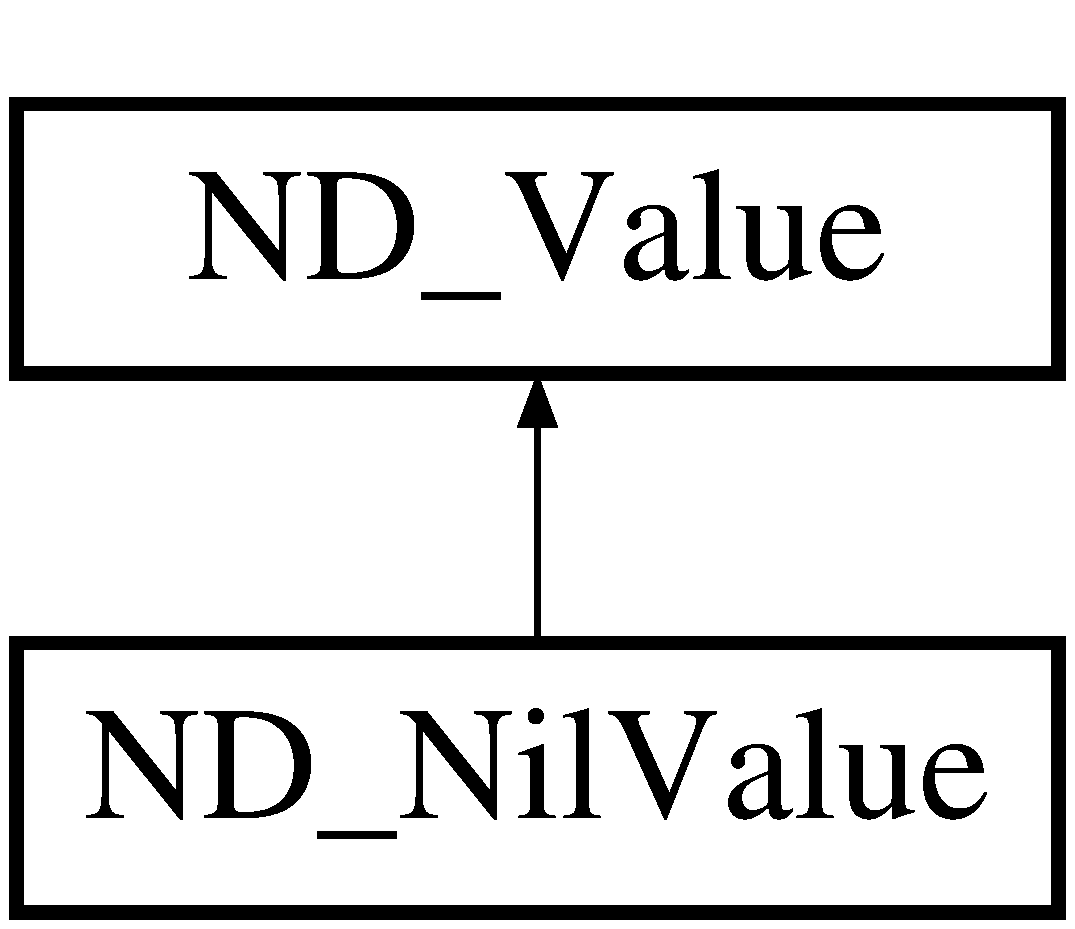
\includegraphics[height=2.000000cm]{class_n_d___nil_value}
\end{center}
\end{figure}
\subsection*{Public Member Functions}
\begin{DoxyCompactItemize}
\item 
\hyperlink{class_n_d___nil_value_ae53c8cb6b7afde16ad4d7b217bbbec7d}{N\-D\-\_\-\-Nil\-Value} ()
\item 
virtual \hyperlink{class_n_d___nil_value_a47f275778850df41c328b4d91b127c18}{$\sim$\-N\-D\-\_\-\-Nil\-Value} ()
\item 
virtual string \hyperlink{class_n_d___nil_value_a08f36ab365257992ad4c3cb8a0469106}{To\-String} () const 
\item 
virtual \hyperlink{class_n_d___value}{N\-D\-\_\-\-Value} $\ast$ \hyperlink{class_n_d___nil_value_ac1dbd47c649bb96ece401b6047880603}{Clone} () const 
\item 
virtual bool \hyperlink{class_n_d___nil_value_aba3e3ddeb95b3edca6c068d6b47b338f}{Equals} (const \hyperlink{class_n_d___value}{N\-D\-\_\-\-Value} $\ast$v) const 
\item 
virtual \hyperlink{class_n_d___value}{N\-D\-\_\-\-Value} $\ast$ \hyperlink{class_n_d___nil_value_ae64e5bf09008a69dc2057e2477957cad}{Eval} (\hyperlink{_n_dvalue_8h_afc938fb729c95de25b4d2eb18640b303}{Ndlog\-\_\-\-Operator} op, \hyperlink{class_n_d___value}{N\-D\-\_\-\-Value} $\ast$rhs=N\-U\-L\-L)
\end{DoxyCompactItemize}
\subsection*{Additional Inherited Members}


\subsection{Detailed Description}


Definition at line 6 of file N\-Dnil-\/value.\-h.



\subsection{Constructor \& Destructor Documentation}
\hypertarget{class_n_d___nil_value_ae53c8cb6b7afde16ad4d7b217bbbec7d}{\index{N\-D\-\_\-\-Nil\-Value@{N\-D\-\_\-\-Nil\-Value}!N\-D\-\_\-\-Nil\-Value@{N\-D\-\_\-\-Nil\-Value}}
\index{N\-D\-\_\-\-Nil\-Value@{N\-D\-\_\-\-Nil\-Value}!ND_NilValue@{N\-D\-\_\-\-Nil\-Value}}
\subsubsection[{N\-D\-\_\-\-Nil\-Value}]{\setlength{\rightskip}{0pt plus 5cm}N\-D\-\_\-\-Nil\-Value\-::\-N\-D\-\_\-\-Nil\-Value (
\begin{DoxyParamCaption}
{}
\end{DoxyParamCaption}
)}}\label{class_n_d___nil_value_ae53c8cb6b7afde16ad4d7b217bbbec7d}


Definition at line 3 of file N\-Dnil-\/value.\-cc.

\hypertarget{class_n_d___nil_value_a47f275778850df41c328b4d91b127c18}{\index{N\-D\-\_\-\-Nil\-Value@{N\-D\-\_\-\-Nil\-Value}!$\sim$\-N\-D\-\_\-\-Nil\-Value@{$\sim$\-N\-D\-\_\-\-Nil\-Value}}
\index{$\sim$\-N\-D\-\_\-\-Nil\-Value@{$\sim$\-N\-D\-\_\-\-Nil\-Value}!ND_NilValue@{N\-D\-\_\-\-Nil\-Value}}
\subsubsection[{$\sim$\-N\-D\-\_\-\-Nil\-Value}]{\setlength{\rightskip}{0pt plus 5cm}N\-D\-\_\-\-Nil\-Value\-::$\sim$\-N\-D\-\_\-\-Nil\-Value (
\begin{DoxyParamCaption}
{}
\end{DoxyParamCaption}
)\hspace{0.3cm}{\ttfamily [virtual]}}}\label{class_n_d___nil_value_a47f275778850df41c328b4d91b127c18}


Definition at line 8 of file N\-Dnil-\/value.\-cc.



\subsection{Member Function Documentation}
\hypertarget{class_n_d___nil_value_ac1dbd47c649bb96ece401b6047880603}{\index{N\-D\-\_\-\-Nil\-Value@{N\-D\-\_\-\-Nil\-Value}!Clone@{Clone}}
\index{Clone@{Clone}!ND_NilValue@{N\-D\-\_\-\-Nil\-Value}}
\subsubsection[{Clone}]{\setlength{\rightskip}{0pt plus 5cm}{\bf N\-D\-\_\-\-Value} $\ast$ N\-D\-\_\-\-Nil\-Value\-::\-Clone (
\begin{DoxyParamCaption}
{}
\end{DoxyParamCaption}
) const\hspace{0.3cm}{\ttfamily [virtual]}}}\label{class_n_d___nil_value_ac1dbd47c649bb96ece401b6047880603}


Implements \hyperlink{class_n_d___value_a83fbc37518fd13b38059a47c422e9024}{N\-D\-\_\-\-Value}.



Definition at line 19 of file N\-Dnil-\/value.\-cc.

\hypertarget{class_n_d___nil_value_aba3e3ddeb95b3edca6c068d6b47b338f}{\index{N\-D\-\_\-\-Nil\-Value@{N\-D\-\_\-\-Nil\-Value}!Equals@{Equals}}
\index{Equals@{Equals}!ND_NilValue@{N\-D\-\_\-\-Nil\-Value}}
\subsubsection[{Equals}]{\setlength{\rightskip}{0pt plus 5cm}bool N\-D\-\_\-\-Nil\-Value\-::\-Equals (
\begin{DoxyParamCaption}
\item[{const {\bf N\-D\-\_\-\-Value} $\ast$}]{v}
\end{DoxyParamCaption}
) const\hspace{0.3cm}{\ttfamily [virtual]}}}\label{class_n_d___nil_value_aba3e3ddeb95b3edca6c068d6b47b338f}


Implements \hyperlink{class_n_d___value_a7b6432defc1b1cada5a31b5c16d29ac6}{N\-D\-\_\-\-Value}.



Definition at line 25 of file N\-Dnil-\/value.\-cc.

\hypertarget{class_n_d___nil_value_ae64e5bf09008a69dc2057e2477957cad}{\index{N\-D\-\_\-\-Nil\-Value@{N\-D\-\_\-\-Nil\-Value}!Eval@{Eval}}
\index{Eval@{Eval}!ND_NilValue@{N\-D\-\_\-\-Nil\-Value}}
\subsubsection[{Eval}]{\setlength{\rightskip}{0pt plus 5cm}{\bf N\-D\-\_\-\-Value} $\ast$ N\-D\-\_\-\-Nil\-Value\-::\-Eval (
\begin{DoxyParamCaption}
\item[{{\bf Ndlog\-\_\-\-Operator}}]{op, }
\item[{{\bf N\-D\-\_\-\-Value} $\ast$}]{rhs = {\ttfamily NULL}}
\end{DoxyParamCaption}
)\hspace{0.3cm}{\ttfamily [virtual]}}}\label{class_n_d___nil_value_ae64e5bf09008a69dc2057e2477957cad}


Implements \hyperlink{class_n_d___value_aa3e290edb140d8676bfe0316c947502d}{N\-D\-\_\-\-Value}.



Definition at line 31 of file N\-Dnil-\/value.\-cc.

\hypertarget{class_n_d___nil_value_a08f36ab365257992ad4c3cb8a0469106}{\index{N\-D\-\_\-\-Nil\-Value@{N\-D\-\_\-\-Nil\-Value}!To\-String@{To\-String}}
\index{To\-String@{To\-String}!ND_NilValue@{N\-D\-\_\-\-Nil\-Value}}
\subsubsection[{To\-String}]{\setlength{\rightskip}{0pt plus 5cm}string N\-D\-\_\-\-Nil\-Value\-::\-To\-String (
\begin{DoxyParamCaption}
{}
\end{DoxyParamCaption}
) const\hspace{0.3cm}{\ttfamily [virtual]}}}\label{class_n_d___nil_value_a08f36ab365257992ad4c3cb8a0469106}


Implements \hyperlink{class_n_d___value_a7660a0e6c07a198410fc05725d903219}{N\-D\-\_\-\-Value}.



Definition at line 13 of file N\-Dnil-\/value.\-cc.



The documentation for this class was generated from the following files\-:\begin{DoxyCompactItemize}
\item 
src/msus/ndlog/value/\hyperlink{_n_dnil-value_8h}{N\-Dnil-\/value.\-h}\item 
src/msus/ndlog/\hyperlink{_n_dnil-value_8cc}{N\-Dnil-\/value.\-cc}\end{DoxyCompactItemize}

\hypertarget{class_n_d___real_value}{\section{N\-D\-\_\-\-Real\-Value Class Reference}
\label{class_n_d___real_value}\index{N\-D\-\_\-\-Real\-Value@{N\-D\-\_\-\-Real\-Value}}
}


{\ttfamily \#include $<$N\-Dreal-\/value.\-h$>$}

Inheritance diagram for N\-D\-\_\-\-Real\-Value\-:\begin{figure}[H]
\begin{center}
\leavevmode
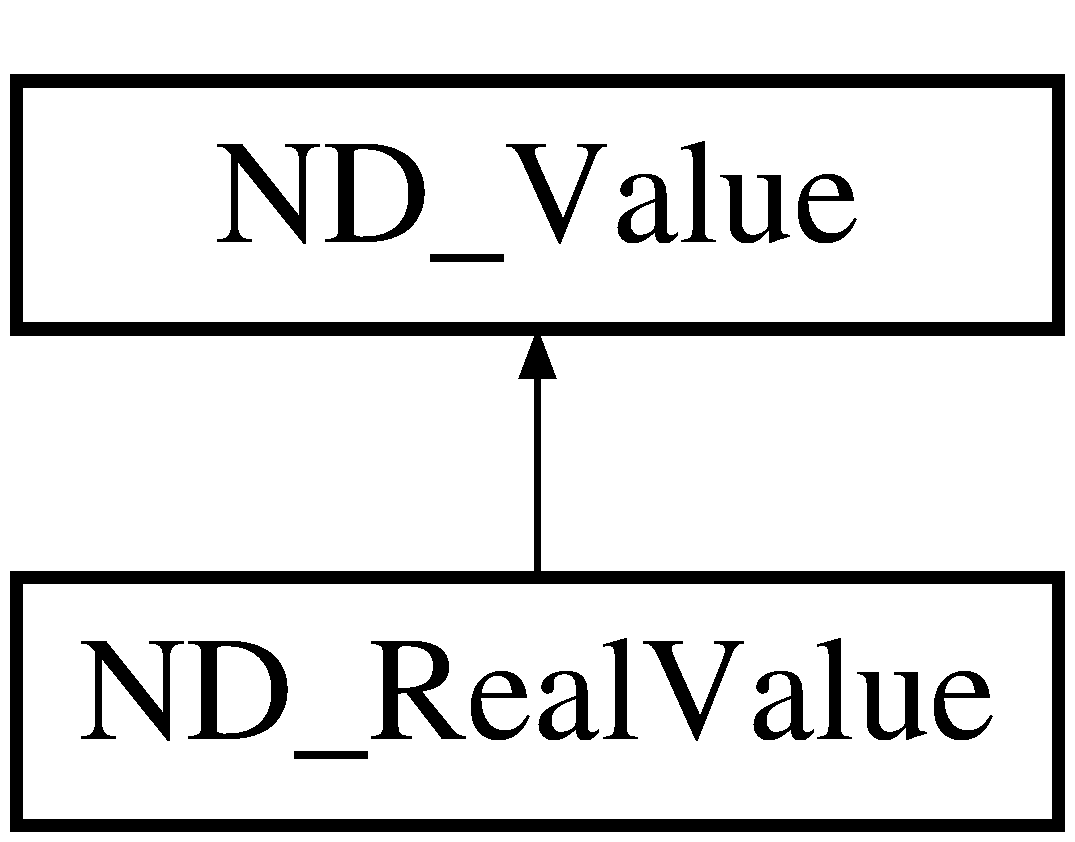
\includegraphics[height=2.000000cm]{class_n_d___real_value}
\end{center}
\end{figure}
\subsection*{Public Member Functions}
\begin{DoxyCompactItemize}
\item 
\hyperlink{class_n_d___real_value_a62a4030022b7fb095afb7d3cb6d1d2e5}{N\-D\-\_\-\-Real\-Value} (double value=0.\-0)
\item 
virtual \hyperlink{class_n_d___real_value_a59006aa14b6df93f0a1ab3d3082c784f}{$\sim$\-N\-D\-\_\-\-Real\-Value} ()
\item 
virtual string \hyperlink{class_n_d___real_value_ac6103005ec7fa351ff61a2959dcf06b2}{To\-String} () const 
\item 
double \hyperlink{class_n_d___real_value_a722ea3e89683dc713c49804ae27dd38b}{Get\-Real\-Value} () const 
\item 
virtual \hyperlink{class_n_d___value}{N\-D\-\_\-\-Value} $\ast$ \hyperlink{class_n_d___real_value_abc7419df3508e45041a90b981e214956}{Clone} () const 
\item 
virtual bool \hyperlink{class_n_d___real_value_a1550861f2a4accacc074dfb0dde3b190}{Equals} (const \hyperlink{class_n_d___value}{N\-D\-\_\-\-Value} $\ast$v) const 
\item 
virtual \hyperlink{class_n_d___value}{N\-D\-\_\-\-Value} $\ast$ \hyperlink{class_n_d___real_value_aa75f47beb70ca67811a8a00b65409834}{Eval} (\hyperlink{_n_dvalue_8h_afc938fb729c95de25b4d2eb18640b303}{Ndlog\-\_\-\-Operator} op, \hyperlink{class_n_d___value}{N\-D\-\_\-\-Value} $\ast$rhs=N\-U\-L\-L)
\end{DoxyCompactItemize}
\subsection*{Protected Attributes}
\begin{DoxyCompactItemize}
\item 
double \hyperlink{class_n_d___real_value_a2acc7c9aaf6a18bd2b97a4c454616f2f}{m\-\_\-value}
\end{DoxyCompactItemize}


\subsection{Detailed Description}


Definition at line 10 of file N\-Dreal-\/value.\-h.



\subsection{Constructor \& Destructor Documentation}
\hypertarget{class_n_d___real_value_a62a4030022b7fb095afb7d3cb6d1d2e5}{\index{N\-D\-\_\-\-Real\-Value@{N\-D\-\_\-\-Real\-Value}!N\-D\-\_\-\-Real\-Value@{N\-D\-\_\-\-Real\-Value}}
\index{N\-D\-\_\-\-Real\-Value@{N\-D\-\_\-\-Real\-Value}!ND_RealValue@{N\-D\-\_\-\-Real\-Value}}
\subsubsection[{N\-D\-\_\-\-Real\-Value}]{\setlength{\rightskip}{0pt plus 5cm}N\-D\-\_\-\-Real\-Value\-::\-N\-D\-\_\-\-Real\-Value (
\begin{DoxyParamCaption}
\item[{double}]{value = {\ttfamily 0.0}}
\end{DoxyParamCaption}
)}}\label{class_n_d___real_value_a62a4030022b7fb095afb7d3cb6d1d2e5}


Definition at line 4 of file N\-Dreal-\/value.\-cc.

\hypertarget{class_n_d___real_value_a59006aa14b6df93f0a1ab3d3082c784f}{\index{N\-D\-\_\-\-Real\-Value@{N\-D\-\_\-\-Real\-Value}!$\sim$\-N\-D\-\_\-\-Real\-Value@{$\sim$\-N\-D\-\_\-\-Real\-Value}}
\index{$\sim$\-N\-D\-\_\-\-Real\-Value@{$\sim$\-N\-D\-\_\-\-Real\-Value}!ND_RealValue@{N\-D\-\_\-\-Real\-Value}}
\subsubsection[{$\sim$\-N\-D\-\_\-\-Real\-Value}]{\setlength{\rightskip}{0pt plus 5cm}N\-D\-\_\-\-Real\-Value\-::$\sim$\-N\-D\-\_\-\-Real\-Value (
\begin{DoxyParamCaption}
{}
\end{DoxyParamCaption}
)\hspace{0.3cm}{\ttfamily [virtual]}}}\label{class_n_d___real_value_a59006aa14b6df93f0a1ab3d3082c784f}


Definition at line 9 of file N\-Dreal-\/value.\-cc.



\subsection{Member Function Documentation}
\hypertarget{class_n_d___real_value_abc7419df3508e45041a90b981e214956}{\index{N\-D\-\_\-\-Real\-Value@{N\-D\-\_\-\-Real\-Value}!Clone@{Clone}}
\index{Clone@{Clone}!ND_RealValue@{N\-D\-\_\-\-Real\-Value}}
\subsubsection[{Clone}]{\setlength{\rightskip}{0pt plus 5cm}{\bf N\-D\-\_\-\-Value} $\ast$ N\-D\-\_\-\-Real\-Value\-::\-Clone (
\begin{DoxyParamCaption}
{}
\end{DoxyParamCaption}
) const\hspace{0.3cm}{\ttfamily [virtual]}}}\label{class_n_d___real_value_abc7419df3508e45041a90b981e214956}


Implements \hyperlink{class_n_d___value_a83fbc37518fd13b38059a47c422e9024}{N\-D\-\_\-\-Value}.



Definition at line 22 of file N\-Dreal-\/value.\-cc.

\hypertarget{class_n_d___real_value_a1550861f2a4accacc074dfb0dde3b190}{\index{N\-D\-\_\-\-Real\-Value@{N\-D\-\_\-\-Real\-Value}!Equals@{Equals}}
\index{Equals@{Equals}!ND_RealValue@{N\-D\-\_\-\-Real\-Value}}
\subsubsection[{Equals}]{\setlength{\rightskip}{0pt plus 5cm}bool N\-D\-\_\-\-Real\-Value\-::\-Equals (
\begin{DoxyParamCaption}
\item[{const {\bf N\-D\-\_\-\-Value} $\ast$}]{v}
\end{DoxyParamCaption}
) const\hspace{0.3cm}{\ttfamily [virtual]}}}\label{class_n_d___real_value_a1550861f2a4accacc074dfb0dde3b190}


Implements \hyperlink{class_n_d___value_a7b6432defc1b1cada5a31b5c16d29ac6}{N\-D\-\_\-\-Value}.



Definition at line 34 of file N\-Dreal-\/value.\-cc.

\hypertarget{class_n_d___real_value_aa75f47beb70ca67811a8a00b65409834}{\index{N\-D\-\_\-\-Real\-Value@{N\-D\-\_\-\-Real\-Value}!Eval@{Eval}}
\index{Eval@{Eval}!ND_RealValue@{N\-D\-\_\-\-Real\-Value}}
\subsubsection[{Eval}]{\setlength{\rightskip}{0pt plus 5cm}{\bf N\-D\-\_\-\-Value} $\ast$ N\-D\-\_\-\-Real\-Value\-::\-Eval (
\begin{DoxyParamCaption}
\item[{{\bf Ndlog\-\_\-\-Operator}}]{op, }
\item[{{\bf N\-D\-\_\-\-Value} $\ast$}]{rhs = {\ttfamily NULL}}
\end{DoxyParamCaption}
)\hspace{0.3cm}{\ttfamily [virtual]}}}\label{class_n_d___real_value_aa75f47beb70ca67811a8a00b65409834}


Implements \hyperlink{class_n_d___value_aa3e290edb140d8676bfe0316c947502d}{N\-D\-\_\-\-Value}.



Definition at line 47 of file N\-Dreal-\/value.\-cc.

\hypertarget{class_n_d___real_value_a722ea3e89683dc713c49804ae27dd38b}{\index{N\-D\-\_\-\-Real\-Value@{N\-D\-\_\-\-Real\-Value}!Get\-Real\-Value@{Get\-Real\-Value}}
\index{Get\-Real\-Value@{Get\-Real\-Value}!ND_RealValue@{N\-D\-\_\-\-Real\-Value}}
\subsubsection[{Get\-Real\-Value}]{\setlength{\rightskip}{0pt plus 5cm}double N\-D\-\_\-\-Real\-Value\-::\-Get\-Real\-Value (
\begin{DoxyParamCaption}
{}
\end{DoxyParamCaption}
) const}}\label{class_n_d___real_value_a722ea3e89683dc713c49804ae27dd38b}


Definition at line 28 of file N\-Dreal-\/value.\-cc.

\hypertarget{class_n_d___real_value_ac6103005ec7fa351ff61a2959dcf06b2}{\index{N\-D\-\_\-\-Real\-Value@{N\-D\-\_\-\-Real\-Value}!To\-String@{To\-String}}
\index{To\-String@{To\-String}!ND_RealValue@{N\-D\-\_\-\-Real\-Value}}
\subsubsection[{To\-String}]{\setlength{\rightskip}{0pt plus 5cm}string N\-D\-\_\-\-Real\-Value\-::\-To\-String (
\begin{DoxyParamCaption}
{}
\end{DoxyParamCaption}
) const\hspace{0.3cm}{\ttfamily [virtual]}}}\label{class_n_d___real_value_ac6103005ec7fa351ff61a2959dcf06b2}


Implements \hyperlink{class_n_d___value_a7660a0e6c07a198410fc05725d903219}{N\-D\-\_\-\-Value}.



Definition at line 14 of file N\-Dreal-\/value.\-cc.



\subsection{Member Data Documentation}
\hypertarget{class_n_d___real_value_a2acc7c9aaf6a18bd2b97a4c454616f2f}{\index{N\-D\-\_\-\-Real\-Value@{N\-D\-\_\-\-Real\-Value}!m\-\_\-value@{m\-\_\-value}}
\index{m\-\_\-value@{m\-\_\-value}!ND_RealValue@{N\-D\-\_\-\-Real\-Value}}
\subsubsection[{m\-\_\-value}]{\setlength{\rightskip}{0pt plus 5cm}double N\-D\-\_\-\-Real\-Value\-::m\-\_\-value\hspace{0.3cm}{\ttfamily [protected]}}}\label{class_n_d___real_value_a2acc7c9aaf6a18bd2b97a4c454616f2f}


Definition at line 30 of file N\-Dreal-\/value.\-h.



The documentation for this class was generated from the following files\-:\begin{DoxyCompactItemize}
\item 
src/msus/ndlog/value/\hyperlink{_n_dreal-value_8h}{N\-Dreal-\/value.\-h}\item 
src/msus/ndlog/\hyperlink{_n_dreal-value_8cc}{N\-Dreal-\/value.\-cc}\end{DoxyCompactItemize}

\hypertarget{class_n_d___str_value}{\section{N\-D\-\_\-\-Str\-Value Class Reference}
\label{class_n_d___str_value}\index{N\-D\-\_\-\-Str\-Value@{N\-D\-\_\-\-Str\-Value}}
}


{\ttfamily \#include $<$N\-Dstr-\/value.\-h$>$}

Inheritance diagram for N\-D\-\_\-\-Str\-Value\-:\begin{figure}[H]
\begin{center}
\leavevmode
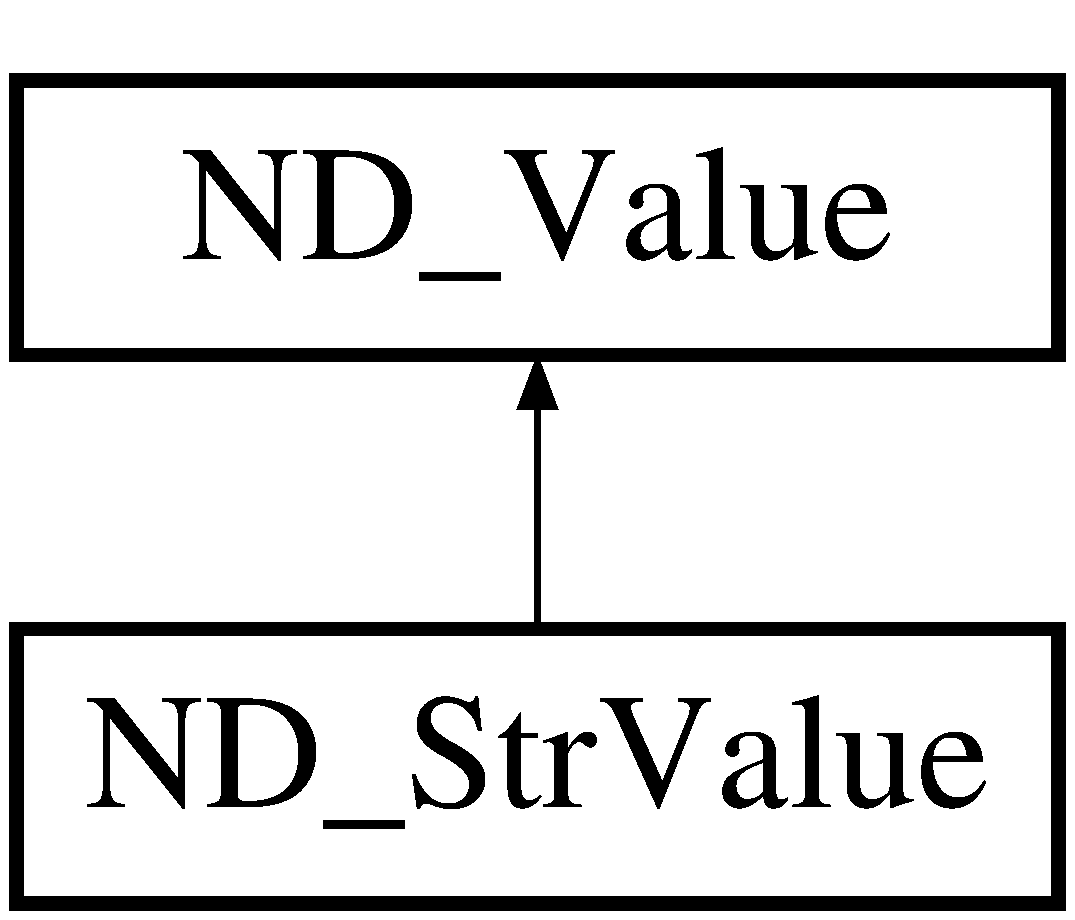
\includegraphics[height=2.000000cm]{class_n_d___str_value}
\end{center}
\end{figure}
\subsection*{Public Member Functions}
\begin{DoxyCompactItemize}
\item 
\hyperlink{class_n_d___str_value_adb14fb5f9d17ab44686c6903ac27ef13}{N\-D\-\_\-\-Str\-Value} (string value=\char`\"{}\char`\"{})
\item 
virtual \hyperlink{class_n_d___str_value_afe723c06bd221211fabeb29c1900d9aa}{$\sim$\-N\-D\-\_\-\-Str\-Value} ()
\item 
virtual string \hyperlink{class_n_d___str_value_a48e3142b60cf2e9298b3eb1eb2849a33}{To\-String} () const 
\item 
string \hyperlink{class_n_d___str_value_a668844f812674752e89a30b51ac3ebdc}{Get\-Str\-Value} () const 
\item 
virtual \hyperlink{class_n_d___value}{N\-D\-\_\-\-Value} $\ast$ \hyperlink{class_n_d___str_value_aeb136b399c70bf7efde0a2029db2d3e0}{Clone} () const 
\item 
virtual bool \hyperlink{class_n_d___str_value_a9096679205abd233f412babb02d3c18b}{Equals} (const \hyperlink{class_n_d___value}{N\-D\-\_\-\-Value} $\ast$v) const 
\item 
virtual \hyperlink{class_n_d___value}{N\-D\-\_\-\-Value} $\ast$ \hyperlink{class_n_d___str_value_abb603d9a1fbf618e578d921d15119b52}{Eval} (\hyperlink{_n_dvalue_8h_afc938fb729c95de25b4d2eb18640b303}{Ndlog\-\_\-\-Operator} op, \hyperlink{class_n_d___value}{N\-D\-\_\-\-Value} $\ast$rhs=N\-U\-L\-L)
\end{DoxyCompactItemize}
\subsection*{Protected Attributes}
\begin{DoxyCompactItemize}
\item 
string \hyperlink{class_n_d___str_value_a7ea3afd2060a79427418d94ffceae984}{m\-\_\-value}
\end{DoxyCompactItemize}


\subsection{Detailed Description}


Definition at line 8 of file N\-Dstr-\/value.\-h.



\subsection{Constructor \& Destructor Documentation}
\hypertarget{class_n_d___str_value_adb14fb5f9d17ab44686c6903ac27ef13}{\index{N\-D\-\_\-\-Str\-Value@{N\-D\-\_\-\-Str\-Value}!N\-D\-\_\-\-Str\-Value@{N\-D\-\_\-\-Str\-Value}}
\index{N\-D\-\_\-\-Str\-Value@{N\-D\-\_\-\-Str\-Value}!ND_StrValue@{N\-D\-\_\-\-Str\-Value}}
\subsubsection[{N\-D\-\_\-\-Str\-Value}]{\setlength{\rightskip}{0pt plus 5cm}N\-D\-\_\-\-Str\-Value\-::\-N\-D\-\_\-\-Str\-Value (
\begin{DoxyParamCaption}
\item[{string}]{value = {\ttfamily \char`\"{}\char`\"{}}}
\end{DoxyParamCaption}
)}}\label{class_n_d___str_value_adb14fb5f9d17ab44686c6903ac27ef13}


Definition at line 4 of file N\-Dstr-\/value.\-cc.

\hypertarget{class_n_d___str_value_afe723c06bd221211fabeb29c1900d9aa}{\index{N\-D\-\_\-\-Str\-Value@{N\-D\-\_\-\-Str\-Value}!$\sim$\-N\-D\-\_\-\-Str\-Value@{$\sim$\-N\-D\-\_\-\-Str\-Value}}
\index{$\sim$\-N\-D\-\_\-\-Str\-Value@{$\sim$\-N\-D\-\_\-\-Str\-Value}!ND_StrValue@{N\-D\-\_\-\-Str\-Value}}
\subsubsection[{$\sim$\-N\-D\-\_\-\-Str\-Value}]{\setlength{\rightskip}{0pt plus 5cm}N\-D\-\_\-\-Str\-Value\-::$\sim$\-N\-D\-\_\-\-Str\-Value (
\begin{DoxyParamCaption}
{}
\end{DoxyParamCaption}
)\hspace{0.3cm}{\ttfamily [virtual]}}}\label{class_n_d___str_value_afe723c06bd221211fabeb29c1900d9aa}


Definition at line 9 of file N\-Dstr-\/value.\-cc.



\subsection{Member Function Documentation}
\hypertarget{class_n_d___str_value_aeb136b399c70bf7efde0a2029db2d3e0}{\index{N\-D\-\_\-\-Str\-Value@{N\-D\-\_\-\-Str\-Value}!Clone@{Clone}}
\index{Clone@{Clone}!ND_StrValue@{N\-D\-\_\-\-Str\-Value}}
\subsubsection[{Clone}]{\setlength{\rightskip}{0pt plus 5cm}{\bf N\-D\-\_\-\-Value} $\ast$ N\-D\-\_\-\-Str\-Value\-::\-Clone (
\begin{DoxyParamCaption}
{}
\end{DoxyParamCaption}
) const\hspace{0.3cm}{\ttfamily [virtual]}}}\label{class_n_d___str_value_aeb136b399c70bf7efde0a2029db2d3e0}


Implements \hyperlink{class_n_d___value_a83fbc37518fd13b38059a47c422e9024}{N\-D\-\_\-\-Value}.



Definition at line 28 of file N\-Dstr-\/value.\-cc.

\hypertarget{class_n_d___str_value_a9096679205abd233f412babb02d3c18b}{\index{N\-D\-\_\-\-Str\-Value@{N\-D\-\_\-\-Str\-Value}!Equals@{Equals}}
\index{Equals@{Equals}!ND_StrValue@{N\-D\-\_\-\-Str\-Value}}
\subsubsection[{Equals}]{\setlength{\rightskip}{0pt plus 5cm}bool N\-D\-\_\-\-Str\-Value\-::\-Equals (
\begin{DoxyParamCaption}
\item[{const {\bf N\-D\-\_\-\-Value} $\ast$}]{v}
\end{DoxyParamCaption}
) const\hspace{0.3cm}{\ttfamily [virtual]}}}\label{class_n_d___str_value_a9096679205abd233f412babb02d3c18b}


Implements \hyperlink{class_n_d___value_a7b6432defc1b1cada5a31b5c16d29ac6}{N\-D\-\_\-\-Value}.



Definition at line 34 of file N\-Dstr-\/value.\-cc.

\hypertarget{class_n_d___str_value_abb603d9a1fbf618e578d921d15119b52}{\index{N\-D\-\_\-\-Str\-Value@{N\-D\-\_\-\-Str\-Value}!Eval@{Eval}}
\index{Eval@{Eval}!ND_StrValue@{N\-D\-\_\-\-Str\-Value}}
\subsubsection[{Eval}]{\setlength{\rightskip}{0pt plus 5cm}{\bf N\-D\-\_\-\-Value} $\ast$ N\-D\-\_\-\-Str\-Value\-::\-Eval (
\begin{DoxyParamCaption}
\item[{{\bf Ndlog\-\_\-\-Operator}}]{op, }
\item[{{\bf N\-D\-\_\-\-Value} $\ast$}]{rhs = {\ttfamily NULL}}
\end{DoxyParamCaption}
)\hspace{0.3cm}{\ttfamily [virtual]}}}\label{class_n_d___str_value_abb603d9a1fbf618e578d921d15119b52}


Implements \hyperlink{class_n_d___value_aa3e290edb140d8676bfe0316c947502d}{N\-D\-\_\-\-Value}.



Definition at line 47 of file N\-Dstr-\/value.\-cc.

\hypertarget{class_n_d___str_value_a668844f812674752e89a30b51ac3ebdc}{\index{N\-D\-\_\-\-Str\-Value@{N\-D\-\_\-\-Str\-Value}!Get\-Str\-Value@{Get\-Str\-Value}}
\index{Get\-Str\-Value@{Get\-Str\-Value}!ND_StrValue@{N\-D\-\_\-\-Str\-Value}}
\subsubsection[{Get\-Str\-Value}]{\setlength{\rightskip}{0pt plus 5cm}string N\-D\-\_\-\-Str\-Value\-::\-Get\-Str\-Value (
\begin{DoxyParamCaption}
{}
\end{DoxyParamCaption}
) const}}\label{class_n_d___str_value_a668844f812674752e89a30b51ac3ebdc}


Definition at line 22 of file N\-Dstr-\/value.\-cc.

\hypertarget{class_n_d___str_value_a48e3142b60cf2e9298b3eb1eb2849a33}{\index{N\-D\-\_\-\-Str\-Value@{N\-D\-\_\-\-Str\-Value}!To\-String@{To\-String}}
\index{To\-String@{To\-String}!ND_StrValue@{N\-D\-\_\-\-Str\-Value}}
\subsubsection[{To\-String}]{\setlength{\rightskip}{0pt plus 5cm}string N\-D\-\_\-\-Str\-Value\-::\-To\-String (
\begin{DoxyParamCaption}
{}
\end{DoxyParamCaption}
) const\hspace{0.3cm}{\ttfamily [virtual]}}}\label{class_n_d___str_value_a48e3142b60cf2e9298b3eb1eb2849a33}


Implements \hyperlink{class_n_d___value_a7660a0e6c07a198410fc05725d903219}{N\-D\-\_\-\-Value}.



Definition at line 14 of file N\-Dstr-\/value.\-cc.



\subsection{Member Data Documentation}
\hypertarget{class_n_d___str_value_a7ea3afd2060a79427418d94ffceae984}{\index{N\-D\-\_\-\-Str\-Value@{N\-D\-\_\-\-Str\-Value}!m\-\_\-value@{m\-\_\-value}}
\index{m\-\_\-value@{m\-\_\-value}!ND_StrValue@{N\-D\-\_\-\-Str\-Value}}
\subsubsection[{m\-\_\-value}]{\setlength{\rightskip}{0pt plus 5cm}string N\-D\-\_\-\-Str\-Value\-::m\-\_\-value\hspace{0.3cm}{\ttfamily [protected]}}}\label{class_n_d___str_value_a7ea3afd2060a79427418d94ffceae984}


Definition at line 28 of file N\-Dstr-\/value.\-h.



The documentation for this class was generated from the following files\-:\begin{DoxyCompactItemize}
\item 
src/msus/ndlog/value/\hyperlink{_n_dstr-value_8h}{N\-Dstr-\/value.\-h}\item 
src/msus/ndlog/\hyperlink{_n_dstr-value_8cc}{N\-Dstr-\/value.\-cc}\end{DoxyCompactItemize}

\hypertarget{class_n_d___value}{\section{N\-D\-\_\-\-Value Class Reference}
\label{class_n_d___value}\index{N\-D\-\_\-\-Value@{N\-D\-\_\-\-Value}}
}


{\ttfamily \#include $<$N\-Dvalue.\-h$>$}

Inheritance diagram for N\-D\-\_\-\-Value\-:\begin{figure}[H]
\begin{center}
\leavevmode
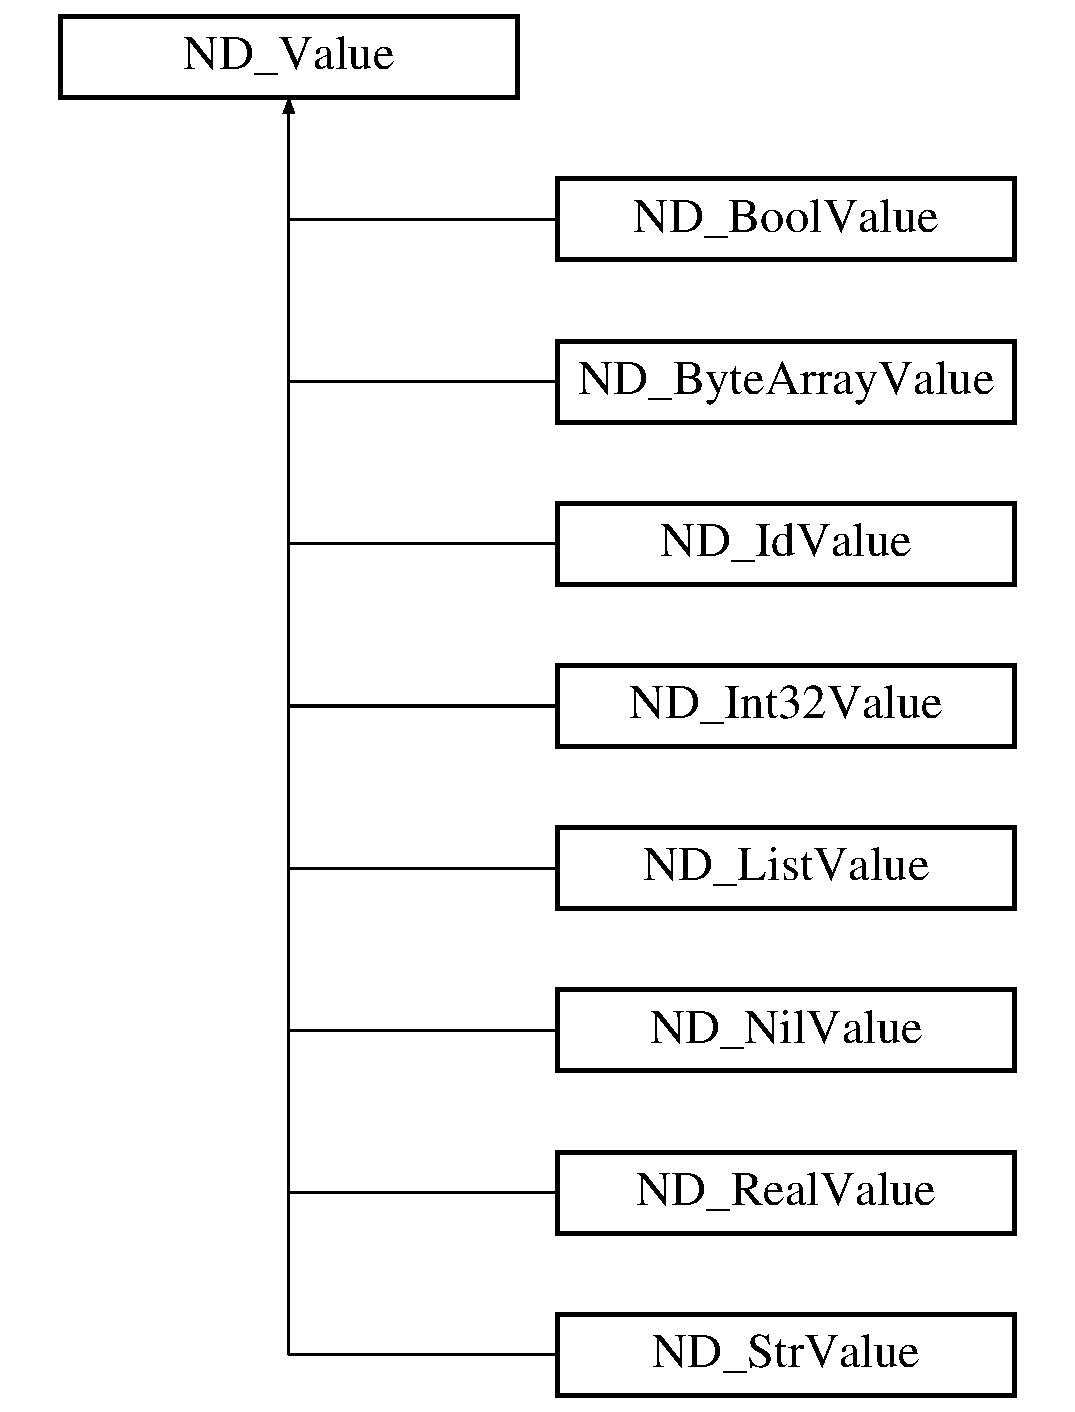
\includegraphics[height=9.000000cm]{class_n_d___value}
\end{center}
\end{figure}
\subsection*{Public Member Functions}
\begin{DoxyCompactItemize}
\item 
\hyperlink{class_n_d___value_a4381bb1dfe297b61ec7a2dca7aa0ee59}{N\-D\-\_\-\-Value} (\hyperlink{_n_dtype-ids_8h_af55089c57d3c2d854f6f5aebc517e484}{N\-D\-Value\-Type\-Id} value)
\item 
virtual \hyperlink{class_n_d___value_afe3a3a13b45142f1413d2fe2de4951d1}{$\sim$\-N\-D\-\_\-\-Value} ()
\item 
\hyperlink{_n_dtype-ids_8h_af55089c57d3c2d854f6f5aebc517e484}{N\-D\-Value\-Type\-Id} \hyperlink{class_n_d___value_a259c3f918c7fedd9d438bec96f15911a}{Get\-Type} () const 
\item 
string \hyperlink{class_n_d___value_a2c4d333803c5cd8d1f0f6cc274c85151}{Get\-Type\-Name} () const 
\item 
virtual string \hyperlink{class_n_d___value_a7660a0e6c07a198410fc05725d903219}{To\-String} () const =0
\item 
virtual \hyperlink{class_n_d___value}{N\-D\-\_\-\-Value} $\ast$ \hyperlink{class_n_d___value_a83fbc37518fd13b38059a47c422e9024}{Clone} () const =0
\item 
virtual bool \hyperlink{class_n_d___value_a7b6432defc1b1cada5a31b5c16d29ac6}{Equals} (const \hyperlink{class_n_d___value}{N\-D\-\_\-\-Value} $\ast$v) const =0
\item 
virtual \hyperlink{class_n_d___value}{N\-D\-\_\-\-Value} $\ast$ \hyperlink{class_n_d___value_aa3e290edb140d8676bfe0316c947502d}{Eval} (\hyperlink{_n_dvalue_8h_afc938fb729c95de25b4d2eb18640b303}{Ndlog\-\_\-\-Operator} op, \hyperlink{class_n_d___value}{N\-D\-\_\-\-Value} $\ast$rhs=N\-U\-L\-L)=0
\end{DoxyCompactItemize}
\subsection*{Protected Attributes}
\begin{DoxyCompactItemize}
\item 
\hyperlink{_n_dtype-ids_8h_af55089c57d3c2d854f6f5aebc517e484}{N\-D\-Value\-Type\-Id} \hyperlink{class_n_d___value_ad6a23ab31aafc1e12b829d66f910131c}{m\-\_\-type}
\end{DoxyCompactItemize}


\subsection{Detailed Description}


Definition at line 34 of file N\-Dvalue.\-h.



\subsection{Constructor \& Destructor Documentation}
\hypertarget{class_n_d___value_a4381bb1dfe297b61ec7a2dca7aa0ee59}{\index{N\-D\-\_\-\-Value@{N\-D\-\_\-\-Value}!N\-D\-\_\-\-Value@{N\-D\-\_\-\-Value}}
\index{N\-D\-\_\-\-Value@{N\-D\-\_\-\-Value}!ND_Value@{N\-D\-\_\-\-Value}}
\subsubsection[{N\-D\-\_\-\-Value}]{\setlength{\rightskip}{0pt plus 5cm}N\-D\-\_\-\-Value\-::\-N\-D\-\_\-\-Value (
\begin{DoxyParamCaption}
\item[{{\bf N\-D\-Value\-Type\-Id}}]{value}
\end{DoxyParamCaption}
)}}\label{class_n_d___value_a4381bb1dfe297b61ec7a2dca7aa0ee59}


Definition at line 3 of file N\-Dvalue.\-cc.

\hypertarget{class_n_d___value_afe3a3a13b45142f1413d2fe2de4951d1}{\index{N\-D\-\_\-\-Value@{N\-D\-\_\-\-Value}!$\sim$\-N\-D\-\_\-\-Value@{$\sim$\-N\-D\-\_\-\-Value}}
\index{$\sim$\-N\-D\-\_\-\-Value@{$\sim$\-N\-D\-\_\-\-Value}!ND_Value@{N\-D\-\_\-\-Value}}
\subsubsection[{$\sim$\-N\-D\-\_\-\-Value}]{\setlength{\rightskip}{0pt plus 5cm}N\-D\-\_\-\-Value\-::$\sim$\-N\-D\-\_\-\-Value (
\begin{DoxyParamCaption}
{}
\end{DoxyParamCaption}
)\hspace{0.3cm}{\ttfamily [virtual]}}}\label{class_n_d___value_afe3a3a13b45142f1413d2fe2de4951d1}


Definition at line 8 of file N\-Dvalue.\-cc.



\subsection{Member Function Documentation}
\hypertarget{class_n_d___value_a83fbc37518fd13b38059a47c422e9024}{\index{N\-D\-\_\-\-Value@{N\-D\-\_\-\-Value}!Clone@{Clone}}
\index{Clone@{Clone}!ND_Value@{N\-D\-\_\-\-Value}}
\subsubsection[{Clone}]{\setlength{\rightskip}{0pt plus 5cm}virtual {\bf N\-D\-\_\-\-Value}$\ast$ N\-D\-\_\-\-Value\-::\-Clone (
\begin{DoxyParamCaption}
{}
\end{DoxyParamCaption}
) const\hspace{0.3cm}{\ttfamily [pure virtual]}}}\label{class_n_d___value_a83fbc37518fd13b38059a47c422e9024}


Implemented in \hyperlink{class_n_d___id_value_adc3e53144381e763eb84e8f6d2dcf3e9}{N\-D\-\_\-\-Id\-Value}, \hyperlink{class_n_d___int32_value_ae8fc6254509ce906a191e45c06f49658}{N\-D\-\_\-\-Int32\-Value}, \hyperlink{class_n_d___byte_array_value_ad61295c86a009f7c94b91a906cc6b36a}{N\-D\-\_\-\-Byte\-Array\-Value}, \hyperlink{class_n_d___list_value_a3c42817a587145b39fbf58f0b5f7fb4a}{N\-D\-\_\-\-List\-Value}, \hyperlink{class_n_d___real_value_abc7419df3508e45041a90b981e214956}{N\-D\-\_\-\-Real\-Value}, \hyperlink{class_n_d___bool_value_a26fb17aea42dc9d9edf52a783988e4cd}{N\-D\-\_\-\-Bool\-Value}, \hyperlink{class_n_d___str_value_aeb136b399c70bf7efde0a2029db2d3e0}{N\-D\-\_\-\-Str\-Value}, and \hyperlink{class_n_d___nil_value_ac1dbd47c649bb96ece401b6047880603}{N\-D\-\_\-\-Nil\-Value}.

\hypertarget{class_n_d___value_a7b6432defc1b1cada5a31b5c16d29ac6}{\index{N\-D\-\_\-\-Value@{N\-D\-\_\-\-Value}!Equals@{Equals}}
\index{Equals@{Equals}!ND_Value@{N\-D\-\_\-\-Value}}
\subsubsection[{Equals}]{\setlength{\rightskip}{0pt plus 5cm}virtual bool N\-D\-\_\-\-Value\-::\-Equals (
\begin{DoxyParamCaption}
\item[{const {\bf N\-D\-\_\-\-Value} $\ast$}]{v}
\end{DoxyParamCaption}
) const\hspace{0.3cm}{\ttfamily [pure virtual]}}}\label{class_n_d___value_a7b6432defc1b1cada5a31b5c16d29ac6}


Implemented in \hyperlink{class_n_d___id_value_aa84829bbfe9842c08a9d011009bf6ad3}{N\-D\-\_\-\-Id\-Value}, \hyperlink{class_n_d___int32_value_af66a16bf770c3fd847d4af6c624b1860}{N\-D\-\_\-\-Int32\-Value}, \hyperlink{class_n_d___byte_array_value_a0989cb51cb2e0d576a2d6e6e78e561cb}{N\-D\-\_\-\-Byte\-Array\-Value}, \hyperlink{class_n_d___list_value_ad1c1105cd71f6e074c75780b57aa0bdb}{N\-D\-\_\-\-List\-Value}, \hyperlink{class_n_d___real_value_a1550861f2a4accacc074dfb0dde3b190}{N\-D\-\_\-\-Real\-Value}, \hyperlink{class_n_d___bool_value_ab4bc7add32f7de0628eaf8ab2dbd1df6}{N\-D\-\_\-\-Bool\-Value}, \hyperlink{class_n_d___str_value_a9096679205abd233f412babb02d3c18b}{N\-D\-\_\-\-Str\-Value}, and \hyperlink{class_n_d___nil_value_aba3e3ddeb95b3edca6c068d6b47b338f}{N\-D\-\_\-\-Nil\-Value}.

\hypertarget{class_n_d___value_aa3e290edb140d8676bfe0316c947502d}{\index{N\-D\-\_\-\-Value@{N\-D\-\_\-\-Value}!Eval@{Eval}}
\index{Eval@{Eval}!ND_Value@{N\-D\-\_\-\-Value}}
\subsubsection[{Eval}]{\setlength{\rightskip}{0pt plus 5cm}virtual {\bf N\-D\-\_\-\-Value}$\ast$ N\-D\-\_\-\-Value\-::\-Eval (
\begin{DoxyParamCaption}
\item[{{\bf Ndlog\-\_\-\-Operator}}]{op, }
\item[{{\bf N\-D\-\_\-\-Value} $\ast$}]{rhs = {\ttfamily NULL}}
\end{DoxyParamCaption}
)\hspace{0.3cm}{\ttfamily [pure virtual]}}}\label{class_n_d___value_aa3e290edb140d8676bfe0316c947502d}


Implemented in \hyperlink{class_n_d___id_value_ade36f0cd7fcb88af1e0e1794d3f4afea}{N\-D\-\_\-\-Id\-Value}, \hyperlink{class_n_d___int32_value_a4a16725cc0cd2bc1228572c378e70847}{N\-D\-\_\-\-Int32\-Value}, \hyperlink{class_n_d___byte_array_value_af5456134d6f0cf16a2d3fb1cbcd0069d}{N\-D\-\_\-\-Byte\-Array\-Value}, \hyperlink{class_n_d___list_value_a38730f35b7d9fb26738294116c2e8b50}{N\-D\-\_\-\-List\-Value}, \hyperlink{class_n_d___real_value_aa75f47beb70ca67811a8a00b65409834}{N\-D\-\_\-\-Real\-Value}, \hyperlink{class_n_d___bool_value_af9abb536e2843bb842ba99ce3c6bcd78}{N\-D\-\_\-\-Bool\-Value}, \hyperlink{class_n_d___str_value_abb603d9a1fbf618e578d921d15119b52}{N\-D\-\_\-\-Str\-Value}, and \hyperlink{class_n_d___nil_value_ae64e5bf09008a69dc2057e2477957cad}{N\-D\-\_\-\-Nil\-Value}.

\hypertarget{class_n_d___value_a259c3f918c7fedd9d438bec96f15911a}{\index{N\-D\-\_\-\-Value@{N\-D\-\_\-\-Value}!Get\-Type@{Get\-Type}}
\index{Get\-Type@{Get\-Type}!ND_Value@{N\-D\-\_\-\-Value}}
\subsubsection[{Get\-Type}]{\setlength{\rightskip}{0pt plus 5cm}{\bf N\-D\-Value\-Type\-Id} N\-D\-\_\-\-Value\-::\-Get\-Type (
\begin{DoxyParamCaption}
{}
\end{DoxyParamCaption}
) const}}\label{class_n_d___value_a259c3f918c7fedd9d438bec96f15911a}


Definition at line 13 of file N\-Dvalue.\-cc.

\hypertarget{class_n_d___value_a2c4d333803c5cd8d1f0f6cc274c85151}{\index{N\-D\-\_\-\-Value@{N\-D\-\_\-\-Value}!Get\-Type\-Name@{Get\-Type\-Name}}
\index{Get\-Type\-Name@{Get\-Type\-Name}!ND_Value@{N\-D\-\_\-\-Value}}
\subsubsection[{Get\-Type\-Name}]{\setlength{\rightskip}{0pt plus 5cm}string N\-D\-\_\-\-Value\-::\-Get\-Type\-Name (
\begin{DoxyParamCaption}
{}
\end{DoxyParamCaption}
) const}}\label{class_n_d___value_a2c4d333803c5cd8d1f0f6cc274c85151}


Definition at line 19 of file N\-Dvalue.\-cc.

\hypertarget{class_n_d___value_a7660a0e6c07a198410fc05725d903219}{\index{N\-D\-\_\-\-Value@{N\-D\-\_\-\-Value}!To\-String@{To\-String}}
\index{To\-String@{To\-String}!ND_Value@{N\-D\-\_\-\-Value}}
\subsubsection[{To\-String}]{\setlength{\rightskip}{0pt plus 5cm}virtual string N\-D\-\_\-\-Value\-::\-To\-String (
\begin{DoxyParamCaption}
{}
\end{DoxyParamCaption}
) const\hspace{0.3cm}{\ttfamily [pure virtual]}}}\label{class_n_d___value_a7660a0e6c07a198410fc05725d903219}


Implemented in \hyperlink{class_n_d___id_value_a98248b82fef11b5ffe11aa20f7af2827}{N\-D\-\_\-\-Id\-Value}, \hyperlink{class_n_d___int32_value_a897c234f7b6f00843c2d9d103956b2ae}{N\-D\-\_\-\-Int32\-Value}, \hyperlink{class_n_d___list_value_a780732e62252f946dd96da074dd932b9}{N\-D\-\_\-\-List\-Value}, \hyperlink{class_n_d___byte_array_value_a38fcb45e48d627e00d135c070e3188e5}{N\-D\-\_\-\-Byte\-Array\-Value}, \hyperlink{class_n_d___real_value_ac6103005ec7fa351ff61a2959dcf06b2}{N\-D\-\_\-\-Real\-Value}, \hyperlink{class_n_d___bool_value_af71a39b64021f7e48a1b91752409302b}{N\-D\-\_\-\-Bool\-Value}, \hyperlink{class_n_d___str_value_a48e3142b60cf2e9298b3eb1eb2849a33}{N\-D\-\_\-\-Str\-Value}, and \hyperlink{class_n_d___nil_value_a08f36ab365257992ad4c3cb8a0469106}{N\-D\-\_\-\-Nil\-Value}.



\subsection{Member Data Documentation}
\hypertarget{class_n_d___value_ad6a23ab31aafc1e12b829d66f910131c}{\index{N\-D\-\_\-\-Value@{N\-D\-\_\-\-Value}!m\-\_\-type@{m\-\_\-type}}
\index{m\-\_\-type@{m\-\_\-type}!ND_Value@{N\-D\-\_\-\-Value}}
\subsubsection[{m\-\_\-type}]{\setlength{\rightskip}{0pt plus 5cm}{\bf N\-D\-Value\-Type\-Id} N\-D\-\_\-\-Value\-::m\-\_\-type\hspace{0.3cm}{\ttfamily [protected]}}}\label{class_n_d___value_ad6a23ab31aafc1e12b829d66f910131c}


Definition at line 56 of file N\-Dvalue.\-h.



The documentation for this class was generated from the following files\-:\begin{DoxyCompactItemize}
\item 
src/msus/ndlog/value/\hyperlink{_n_dvalue_8h}{N\-Dvalue.\-h}\item 
src/msus/ndlog/\hyperlink{_n_dvalue_8cc}{N\-Dvalue.\-cc}\end{DoxyCompactItemize}

\hypertarget{structndlog__state}{\section{ndlog\-\_\-state Struct Reference}
\label{structndlog__state}\index{ndlog\-\_\-state@{ndlog\-\_\-state}}
}


{\ttfamily \#include $<$model.\-h$>$}

\subsection*{Public Attributes}
\begin{DoxyCompactItemize}
\item 
string \hyperlink{structndlog__state_a9762ce5cb5a617075c9715c99511e19f}{state\-\_\-name}
\item 
map$<$ string, \hyperlink{structndlog__tuple}{ndlog\-\_\-tuple} $\ast$ $>$ \hyperlink{structndlog__state_a30e8b1c430795b117da273e238766e54}{tuples}
\item 
map$<$ string, string $>$ \hyperlink{structndlog__state_a2e31cf7fa49b3dcd0d02daa382148831}{key\-\_\-attr}
\end{DoxyCompactItemize}


\subsection{Detailed Description}


Definition at line 28 of file model.\-h.



\subsection{Member Data Documentation}
\hypertarget{structndlog__state_a2e31cf7fa49b3dcd0d02daa382148831}{\index{ndlog\-\_\-state@{ndlog\-\_\-state}!key\-\_\-attr@{key\-\_\-attr}}
\index{key\-\_\-attr@{key\-\_\-attr}!ndlog_state@{ndlog\-\_\-state}}
\subsubsection[{key\-\_\-attr}]{\setlength{\rightskip}{0pt plus 5cm}map$<$string, string$>$ ndlog\-\_\-state\-::key\-\_\-attr}}\label{structndlog__state_a2e31cf7fa49b3dcd0d02daa382148831}


Definition at line 32 of file model.\-h.

\hypertarget{structndlog__state_a9762ce5cb5a617075c9715c99511e19f}{\index{ndlog\-\_\-state@{ndlog\-\_\-state}!state\-\_\-name@{state\-\_\-name}}
\index{state\-\_\-name@{state\-\_\-name}!ndlog_state@{ndlog\-\_\-state}}
\subsubsection[{state\-\_\-name}]{\setlength{\rightskip}{0pt plus 5cm}string ndlog\-\_\-state\-::state\-\_\-name}}\label{structndlog__state_a9762ce5cb5a617075c9715c99511e19f}


Definition at line 29 of file model.\-h.

\hypertarget{structndlog__state_a30e8b1c430795b117da273e238766e54}{\index{ndlog\-\_\-state@{ndlog\-\_\-state}!tuples@{tuples}}
\index{tuples@{tuples}!ndlog_state@{ndlog\-\_\-state}}
\subsubsection[{tuples}]{\setlength{\rightskip}{0pt plus 5cm}map$<$string, {\bf ndlog\-\_\-tuple}$\ast$$>$ ndlog\-\_\-state\-::tuples}}\label{structndlog__state_a30e8b1c430795b117da273e238766e54}


Definition at line 30 of file model.\-h.



The documentation for this struct was generated from the following file\-:\begin{DoxyCompactItemize}
\item 
src/msus/ndlog/\hyperlink{model_8h}{model.\-h}\end{DoxyCompactItemize}

\hypertarget{structndlog__tuple}{\section{ndlog\-\_\-tuple Struct Reference}
\label{structndlog__tuple}\index{ndlog\-\_\-tuple@{ndlog\-\_\-tuple}}
}


{\ttfamily \#include $<$model.\-h$>$}

\subsection*{Public Attributes}
\begin{DoxyCompactItemize}
\item 
string \hyperlink{structndlog__tuple_a60630913345afa409a56b2e612c9afea}{tuple\-\_\-name}
\item 
map$<$ string, \\*
\hyperlink{structndlog__tuple__attribute}{ndlog\-\_\-tuple\-\_\-attribute} $\ast$ $>$ \hyperlink{structndlog__tuple_a2dc7a9bff142acf9b032b2c38fdd4e4c}{attributes}
\item 
enum \hyperlink{model_8h_ae688e205096dad09ca010b144f151f40}{tuple\-\_\-type} \hyperlink{structndlog__tuple_aa81437991ac9a764841242a8f82b1257}{tp\-\_\-\-Type}
\item 
string \hyperlink{structndlog__tuple_acd5e93ff19d18ae9eb60a29e2f66937c}{data\-\_\-key}
\end{DoxyCompactItemize}


\subsection{Detailed Description}


Definition at line 21 of file model.\-h.



\subsection{Member Data Documentation}
\hypertarget{structndlog__tuple_a2dc7a9bff142acf9b032b2c38fdd4e4c}{\index{ndlog\-\_\-tuple@{ndlog\-\_\-tuple}!attributes@{attributes}}
\index{attributes@{attributes}!ndlog_tuple@{ndlog\-\_\-tuple}}
\subsubsection[{attributes}]{\setlength{\rightskip}{0pt plus 5cm}map$<$string, {\bf ndlog\-\_\-tuple\-\_\-attribute}$\ast$$>$ ndlog\-\_\-tuple\-::attributes}}\label{structndlog__tuple_a2dc7a9bff142acf9b032b2c38fdd4e4c}


Definition at line 23 of file model.\-h.

\hypertarget{structndlog__tuple_acd5e93ff19d18ae9eb60a29e2f66937c}{\index{ndlog\-\_\-tuple@{ndlog\-\_\-tuple}!data\-\_\-key@{data\-\_\-key}}
\index{data\-\_\-key@{data\-\_\-key}!ndlog_tuple@{ndlog\-\_\-tuple}}
\subsubsection[{data\-\_\-key}]{\setlength{\rightskip}{0pt plus 5cm}string ndlog\-\_\-tuple\-::data\-\_\-key}}\label{structndlog__tuple_acd5e93ff19d18ae9eb60a29e2f66937c}


Definition at line 25 of file model.\-h.

\hypertarget{structndlog__tuple_aa81437991ac9a764841242a8f82b1257}{\index{ndlog\-\_\-tuple@{ndlog\-\_\-tuple}!tp\-\_\-\-Type@{tp\-\_\-\-Type}}
\index{tp\-\_\-\-Type@{tp\-\_\-\-Type}!ndlog_tuple@{ndlog\-\_\-tuple}}
\subsubsection[{tp\-\_\-\-Type}]{\setlength{\rightskip}{0pt plus 5cm}enum {\bf tuple\-\_\-type} ndlog\-\_\-tuple\-::tp\-\_\-\-Type}}\label{structndlog__tuple_aa81437991ac9a764841242a8f82b1257}


Definition at line 24 of file model.\-h.

\hypertarget{structndlog__tuple_a60630913345afa409a56b2e612c9afea}{\index{ndlog\-\_\-tuple@{ndlog\-\_\-tuple}!tuple\-\_\-name@{tuple\-\_\-name}}
\index{tuple\-\_\-name@{tuple\-\_\-name}!ndlog_tuple@{ndlog\-\_\-tuple}}
\subsubsection[{tuple\-\_\-name}]{\setlength{\rightskip}{0pt plus 5cm}string ndlog\-\_\-tuple\-::tuple\-\_\-name}}\label{structndlog__tuple_a60630913345afa409a56b2e612c9afea}


Definition at line 22 of file model.\-h.



The documentation for this struct was generated from the following file\-:\begin{DoxyCompactItemize}
\item 
src/msus/ndlog/\hyperlink{model_8h}{model.\-h}\end{DoxyCompactItemize}

\hypertarget{structndlog__tuple__attribute}{\section{ndlog\-\_\-tuple\-\_\-attribute Struct Reference}
\label{structndlog__tuple__attribute}\index{ndlog\-\_\-tuple\-\_\-attribute@{ndlog\-\_\-tuple\-\_\-attribute}}
}


{\ttfamily \#include $<$model.\-h$>$}

\subsection*{Public Attributes}
\begin{DoxyCompactItemize}
\item 
\hyperlink{msus_2webserver_2uthash_8h_aba7bc1797add20fe3efdf37ced1182c5}{uint8\-\_\-t} \hyperlink{structndlog__tuple__attribute_a00ae3914e780196c86e1ef9d28968c35}{name\-\_\-len}
\item 
\hyperlink{msus_2webserver_2uthash_8h_a435d1572bf3f880d55459d9805097f62}{uint32\-\_\-t} \hyperlink{structndlog__tuple__attribute_a2f59a569d56f6d3913d1d216a7ab4e2f}{data\-\_\-len}
\item 
string \hyperlink{structndlog__tuple__attribute_ae23fda4bfaa4c39ae7e7ffa4d88f29f0}{attr\-\_\-name}
\item 
\hyperlink{class_n_d___value}{N\-D\-\_\-\-Value} $\ast$ \hyperlink{structndlog__tuple__attribute_aa066f726969bddc4f10e4022af6977d0}{attr\-\_\-data}
\end{DoxyCompactItemize}


\subsection{Detailed Description}


Definition at line 14 of file model.\-h.



\subsection{Member Data Documentation}
\hypertarget{structndlog__tuple__attribute_aa066f726969bddc4f10e4022af6977d0}{\index{ndlog\-\_\-tuple\-\_\-attribute@{ndlog\-\_\-tuple\-\_\-attribute}!attr\-\_\-data@{attr\-\_\-data}}
\index{attr\-\_\-data@{attr\-\_\-data}!ndlog_tuple_attribute@{ndlog\-\_\-tuple\-\_\-attribute}}
\subsubsection[{attr\-\_\-data}]{\setlength{\rightskip}{0pt plus 5cm}{\bf N\-D\-\_\-\-Value}$\ast$ ndlog\-\_\-tuple\-\_\-attribute\-::attr\-\_\-data}}\label{structndlog__tuple__attribute_aa066f726969bddc4f10e4022af6977d0}


Definition at line 18 of file model.\-h.

\hypertarget{structndlog__tuple__attribute_ae23fda4bfaa4c39ae7e7ffa4d88f29f0}{\index{ndlog\-\_\-tuple\-\_\-attribute@{ndlog\-\_\-tuple\-\_\-attribute}!attr\-\_\-name@{attr\-\_\-name}}
\index{attr\-\_\-name@{attr\-\_\-name}!ndlog_tuple_attribute@{ndlog\-\_\-tuple\-\_\-attribute}}
\subsubsection[{attr\-\_\-name}]{\setlength{\rightskip}{0pt plus 5cm}string ndlog\-\_\-tuple\-\_\-attribute\-::attr\-\_\-name}}\label{structndlog__tuple__attribute_ae23fda4bfaa4c39ae7e7ffa4d88f29f0}


Definition at line 17 of file model.\-h.

\hypertarget{structndlog__tuple__attribute_a2f59a569d56f6d3913d1d216a7ab4e2f}{\index{ndlog\-\_\-tuple\-\_\-attribute@{ndlog\-\_\-tuple\-\_\-attribute}!data\-\_\-len@{data\-\_\-len}}
\index{data\-\_\-len@{data\-\_\-len}!ndlog_tuple_attribute@{ndlog\-\_\-tuple\-\_\-attribute}}
\subsubsection[{data\-\_\-len}]{\setlength{\rightskip}{0pt plus 5cm}{\bf uint32\-\_\-t} ndlog\-\_\-tuple\-\_\-attribute\-::data\-\_\-len}}\label{structndlog__tuple__attribute_a2f59a569d56f6d3913d1d216a7ab4e2f}


Definition at line 16 of file model.\-h.

\hypertarget{structndlog__tuple__attribute_a00ae3914e780196c86e1ef9d28968c35}{\index{ndlog\-\_\-tuple\-\_\-attribute@{ndlog\-\_\-tuple\-\_\-attribute}!name\-\_\-len@{name\-\_\-len}}
\index{name\-\_\-len@{name\-\_\-len}!ndlog_tuple_attribute@{ndlog\-\_\-tuple\-\_\-attribute}}
\subsubsection[{name\-\_\-len}]{\setlength{\rightskip}{0pt plus 5cm}{\bf uint8\-\_\-t} ndlog\-\_\-tuple\-\_\-attribute\-::name\-\_\-len}}\label{structndlog__tuple__attribute_a00ae3914e780196c86e1ef9d28968c35}


Definition at line 15 of file model.\-h.



The documentation for this struct was generated from the following file\-:\begin{DoxyCompactItemize}
\item 
src/msus/ndlog/\hyperlink{model_8h}{model.\-h}\end{DoxyCompactItemize}

\hypertarget{structparser__state}{\section{parser\-\_\-state Struct Reference}
\label{structparser__state}\index{parser\-\_\-state@{parser\-\_\-state}}
}


{\ttfamily \#include $<$request\-\_\-parser.\-h$>$}

\subsection*{Public Attributes}
\begin{DoxyCompactItemize}
\item 
char \hyperlink{structparser__state_a64222808a9174a17ae2d25cb7ab72383}{url} \mbox{[}256\mbox{]}
\item 
int \hyperlink{structparser__state_a3ece333d4625d8c6a5f696a738b2fc41}{url\-\_\-len}
\item 
int \hyperlink{structparser__state_ae9786e3f8c7bc787516749856ad0cc42}{headers\-\_\-complete}
\item 
ssize\-\_\-t($\ast$ \hyperlink{structparser__state_ad02c5f0bb7a54a5be951120be343e767}{recv\-\_\-fn} )(int fd, S\-S\-L $\ast$ssl, char $\ast$buf)
\item 
\hyperlink{structhttp__parser__settings}{http\-\_\-parser\-\_\-settings} \hyperlink{structparser__state_a88886f7995880a05fd64c6ce943c4d2b}{settings}
\item 
\hyperlink{structhttp__parser}{http\-\_\-parser} \hyperlink{structparser__state_aaf6745c9db055761cd8da5f0d5e76d04}{parser}
\end{DoxyCompactItemize}


\subsection{Detailed Description}


Definition at line 7 of file request\-\_\-parser.\-h.



\subsection{Member Data Documentation}
\hypertarget{structparser__state_ae9786e3f8c7bc787516749856ad0cc42}{\index{parser\-\_\-state@{parser\-\_\-state}!headers\-\_\-complete@{headers\-\_\-complete}}
\index{headers\-\_\-complete@{headers\-\_\-complete}!parser_state@{parser\-\_\-state}}
\subsubsection[{headers\-\_\-complete}]{\setlength{\rightskip}{0pt plus 5cm}int parser\-\_\-state\-::headers\-\_\-complete}}\label{structparser__state_ae9786e3f8c7bc787516749856ad0cc42}


Definition at line 10 of file request\-\_\-parser.\-h.

\hypertarget{structparser__state_aaf6745c9db055761cd8da5f0d5e76d04}{\index{parser\-\_\-state@{parser\-\_\-state}!parser@{parser}}
\index{parser@{parser}!parser_state@{parser\-\_\-state}}
\subsubsection[{parser}]{\setlength{\rightskip}{0pt plus 5cm}{\bf http\-\_\-parser} parser\-\_\-state\-::parser}}\label{structparser__state_aaf6745c9db055761cd8da5f0d5e76d04}


Definition at line 13 of file request\-\_\-parser.\-h.

\hypertarget{structparser__state_ad02c5f0bb7a54a5be951120be343e767}{\index{parser\-\_\-state@{parser\-\_\-state}!recv\-\_\-fn@{recv\-\_\-fn}}
\index{recv\-\_\-fn@{recv\-\_\-fn}!parser_state@{parser\-\_\-state}}
\subsubsection[{recv\-\_\-fn}]{\setlength{\rightskip}{0pt plus 5cm}ssize\-\_\-t($\ast$ parser\-\_\-state\-::recv\-\_\-fn)(int fd, S\-S\-L $\ast$ssl, char $\ast$buf)}}\label{structparser__state_ad02c5f0bb7a54a5be951120be343e767}


Definition at line 11 of file request\-\_\-parser.\-h.

\hypertarget{structparser__state_a88886f7995880a05fd64c6ce943c4d2b}{\index{parser\-\_\-state@{parser\-\_\-state}!settings@{settings}}
\index{settings@{settings}!parser_state@{parser\-\_\-state}}
\subsubsection[{settings}]{\setlength{\rightskip}{0pt plus 5cm}{\bf http\-\_\-parser\-\_\-settings} parser\-\_\-state\-::settings}}\label{structparser__state_a88886f7995880a05fd64c6ce943c4d2b}


Definition at line 12 of file request\-\_\-parser.\-h.

\hypertarget{structparser__state_a64222808a9174a17ae2d25cb7ab72383}{\index{parser\-\_\-state@{parser\-\_\-state}!url@{url}}
\index{url@{url}!parser_state@{parser\-\_\-state}}
\subsubsection[{url}]{\setlength{\rightskip}{0pt plus 5cm}char parser\-\_\-state\-::url\mbox{[}256\mbox{]}}}\label{structparser__state_a64222808a9174a17ae2d25cb7ab72383}


Definition at line 8 of file request\-\_\-parser.\-h.

\hypertarget{structparser__state_a3ece333d4625d8c6a5f696a738b2fc41}{\index{parser\-\_\-state@{parser\-\_\-state}!url\-\_\-len@{url\-\_\-len}}
\index{url\-\_\-len@{url\-\_\-len}!parser_state@{parser\-\_\-state}}
\subsubsection[{url\-\_\-len}]{\setlength{\rightskip}{0pt plus 5cm}int parser\-\_\-state\-::url\-\_\-len}}\label{structparser__state_a3ece333d4625d8c6a5f696a738b2fc41}


Definition at line 9 of file request\-\_\-parser.\-h.



The documentation for this struct was generated from the following file\-:\begin{DoxyCompactItemize}
\item 
src/msus/webserver/\hyperlink{request__parser_8h}{request\-\_\-parser.\-h}\end{DoxyCompactItemize}

\hypertarget{structpico__tcp__msg}{\section{pico\-\_\-tcp\-\_\-msg Struct Reference}
\label{structpico__tcp__msg}\index{pico\-\_\-tcp\-\_\-msg@{pico\-\_\-tcp\-\_\-msg}}
}


{\ttfamily \#include $<$msu\-\_\-pico\-\_\-tcp.\-h$>$}

\subsection*{Public Attributes}
\begin{DoxyCompactItemize}
\item 
unsigned int \hyperlink{structpico__tcp__msg_a6d32a0e6f66a430da0402ba2840c3ef9}{proto\-\_\-msg\-\_\-type}
\item 
void $\ast$ \hyperlink{structpico__tcp__msg_aad92ecc2888bc9821b38a4016486e7bd}{payload}
\item 
size\-\_\-t \hyperlink{structpico__tcp__msg_a929fc28e9ca3b9ce53e37ff695438a2a}{payload\-\_\-len}
\end{DoxyCompactItemize}


\subsection{Detailed Description}


Definition at line 10 of file msu\-\_\-pico\-\_\-tcp.\-h.



\subsection{Member Data Documentation}
\hypertarget{structpico__tcp__msg_aad92ecc2888bc9821b38a4016486e7bd}{\index{pico\-\_\-tcp\-\_\-msg@{pico\-\_\-tcp\-\_\-msg}!payload@{payload}}
\index{payload@{payload}!pico_tcp_msg@{pico\-\_\-tcp\-\_\-msg}}
\subsubsection[{payload}]{\setlength{\rightskip}{0pt plus 5cm}void$\ast$ pico\-\_\-tcp\-\_\-msg\-::payload}}\label{structpico__tcp__msg_aad92ecc2888bc9821b38a4016486e7bd}


Definition at line 12 of file msu\-\_\-pico\-\_\-tcp.\-h.

\hypertarget{structpico__tcp__msg_a929fc28e9ca3b9ce53e37ff695438a2a}{\index{pico\-\_\-tcp\-\_\-msg@{pico\-\_\-tcp\-\_\-msg}!payload\-\_\-len@{payload\-\_\-len}}
\index{payload\-\_\-len@{payload\-\_\-len}!pico_tcp_msg@{pico\-\_\-tcp\-\_\-msg}}
\subsubsection[{payload\-\_\-len}]{\setlength{\rightskip}{0pt plus 5cm}size\-\_\-t pico\-\_\-tcp\-\_\-msg\-::payload\-\_\-len}}\label{structpico__tcp__msg_a929fc28e9ca3b9ce53e37ff695438a2a}


Definition at line 13 of file msu\-\_\-pico\-\_\-tcp.\-h.

\hypertarget{structpico__tcp__msg_a6d32a0e6f66a430da0402ba2840c3ef9}{\index{pico\-\_\-tcp\-\_\-msg@{pico\-\_\-tcp\-\_\-msg}!proto\-\_\-msg\-\_\-type@{proto\-\_\-msg\-\_\-type}}
\index{proto\-\_\-msg\-\_\-type@{proto\-\_\-msg\-\_\-type}!pico_tcp_msg@{pico\-\_\-tcp\-\_\-msg}}
\subsubsection[{proto\-\_\-msg\-\_\-type}]{\setlength{\rightskip}{0pt plus 5cm}unsigned int pico\-\_\-tcp\-\_\-msg\-::proto\-\_\-msg\-\_\-type}}\label{structpico__tcp__msg_a6d32a0e6f66a430da0402ba2840c3ef9}


Definition at line 11 of file msu\-\_\-pico\-\_\-tcp.\-h.



The documentation for this struct was generated from the following file\-:\begin{DoxyCompactItemize}
\item 
src/msus/pico\-\_\-tcp/\hyperlink{msu__pico__tcp_8h}{msu\-\_\-pico\-\_\-tcp.\-h}\end{DoxyCompactItemize}

\hypertarget{structread__state}{\section{read\-\_\-state Struct Reference}
\label{structread__state}\index{read\-\_\-state@{read\-\_\-state}}
}


{\ttfamily \#include $<$connection-\/handler.\-h$>$}

\subsection*{Public Attributes}
\begin{DoxyCompactItemize}
\item 
struct \hyperlink{structconnection}{connection} \hyperlink{structread__state_ad79008defc69c985f9a55b8f1a7dccb0}{conn}
\item 
char \hyperlink{structread__state_a5466de2b0a95c12c669ff082e4a228d0}{req} \mbox{[}4096\mbox{]}
\item 
int \hyperlink{structread__state_a5629ae045b84454938394c8af94124d1}{req\-\_\-len}
\end{DoxyCompactItemize}


\subsection{Detailed Description}


Definition at line 18 of file connection-\/handler.\-h.



\subsection{Member Data Documentation}
\hypertarget{structread__state_ad79008defc69c985f9a55b8f1a7dccb0}{\index{read\-\_\-state@{read\-\_\-state}!conn@{conn}}
\index{conn@{conn}!read_state@{read\-\_\-state}}
\subsubsection[{conn}]{\setlength{\rightskip}{0pt plus 5cm}struct {\bf connection} read\-\_\-state\-::conn}}\label{structread__state_ad79008defc69c985f9a55b8f1a7dccb0}


Definition at line 19 of file connection-\/handler.\-h.

\hypertarget{structread__state_a5466de2b0a95c12c669ff082e4a228d0}{\index{read\-\_\-state@{read\-\_\-state}!req@{req}}
\index{req@{req}!read_state@{read\-\_\-state}}
\subsubsection[{req}]{\setlength{\rightskip}{0pt plus 5cm}char read\-\_\-state\-::req\mbox{[}4096\mbox{]}}}\label{structread__state_a5466de2b0a95c12c669ff082e4a228d0}


Definition at line 20 of file connection-\/handler.\-h.

\hypertarget{structread__state_a5629ae045b84454938394c8af94124d1}{\index{read\-\_\-state@{read\-\_\-state}!req\-\_\-len@{req\-\_\-len}}
\index{req\-\_\-len@{req\-\_\-len}!read_state@{read\-\_\-state}}
\subsubsection[{req\-\_\-len}]{\setlength{\rightskip}{0pt plus 5cm}int read\-\_\-state\-::req\-\_\-len}}\label{structread__state_a5629ae045b84454938394c8af94124d1}


Definition at line 21 of file connection-\/handler.\-h.



The documentation for this struct was generated from the following file\-:\begin{DoxyCompactItemize}
\item 
src/msus/webserver/\hyperlink{connection-handler_8h}{connection-\/handler.\-h}\end{DoxyCompactItemize}

\hypertarget{structrecv__state}{\section{recv\-\_\-state Struct Reference}
\label{structrecv__state}\index{recv\-\_\-state@{recv\-\_\-state}}
}


{\ttfamily \#include $<$ndlog\-\_\-recv\-\_\-msu.\-h$>$}

\subsection*{Public Attributes}
\begin{DoxyCompactItemize}
\item 
\hyperlink{msus_2webserver_2uthash_8h_a435d1572bf3f880d55459d9805097f62}{uint32\-\_\-t} \hyperlink{structrecv__state_aa75a943e8a8afd6aad261da73550f8fc}{count}
\item 
\hyperlink{msus_2webserver_2uthash_8h_a435d1572bf3f880d55459d9805097f62}{uint32\-\_\-t} \hyperlink{structrecv__state_ad846f5bdb59047e4064a5d1f84ea7e0a}{received}
\item 
int \hyperlink{structrecv__state_aaa4978ceb10d1540c7555bdbf1cd4d45}{first\-\_\-packet}
\item 
struct timespec \hyperlink{structrecv__state_aec1b8726e5167fb82a1b38624b3e81af}{ts}
\item 
struct timespec \hyperlink{structrecv__state_a88a57436666fe47d8f22261ec811ea16}{te}
\item 
int \hyperlink{structrecv__state_a914b921476b9dce11a70996b5282d2f8}{experiment\-\_\-num}
\end{DoxyCompactItemize}


\subsection{Detailed Description}


Definition at line 11 of file ndlog\-\_\-recv\-\_\-msu.\-h.



\subsection{Member Data Documentation}
\hypertarget{structrecv__state_aa75a943e8a8afd6aad261da73550f8fc}{\index{recv\-\_\-state@{recv\-\_\-state}!count@{count}}
\index{count@{count}!recv_state@{recv\-\_\-state}}
\subsubsection[{count}]{\setlength{\rightskip}{0pt plus 5cm}{\bf uint32\-\_\-t} recv\-\_\-state\-::count}}\label{structrecv__state_aa75a943e8a8afd6aad261da73550f8fc}


Definition at line 12 of file ndlog\-\_\-recv\-\_\-msu.\-h.

\hypertarget{structrecv__state_a914b921476b9dce11a70996b5282d2f8}{\index{recv\-\_\-state@{recv\-\_\-state}!experiment\-\_\-num@{experiment\-\_\-num}}
\index{experiment\-\_\-num@{experiment\-\_\-num}!recv_state@{recv\-\_\-state}}
\subsubsection[{experiment\-\_\-num}]{\setlength{\rightskip}{0pt plus 5cm}int recv\-\_\-state\-::experiment\-\_\-num}}\label{structrecv__state_a914b921476b9dce11a70996b5282d2f8}


Definition at line 18 of file ndlog\-\_\-recv\-\_\-msu.\-h.

\hypertarget{structrecv__state_aaa4978ceb10d1540c7555bdbf1cd4d45}{\index{recv\-\_\-state@{recv\-\_\-state}!first\-\_\-packet@{first\-\_\-packet}}
\index{first\-\_\-packet@{first\-\_\-packet}!recv_state@{recv\-\_\-state}}
\subsubsection[{first\-\_\-packet}]{\setlength{\rightskip}{0pt plus 5cm}int recv\-\_\-state\-::first\-\_\-packet}}\label{structrecv__state_aaa4978ceb10d1540c7555bdbf1cd4d45}


Definition at line 14 of file ndlog\-\_\-recv\-\_\-msu.\-h.

\hypertarget{structrecv__state_ad846f5bdb59047e4064a5d1f84ea7e0a}{\index{recv\-\_\-state@{recv\-\_\-state}!received@{received}}
\index{received@{received}!recv_state@{recv\-\_\-state}}
\subsubsection[{received}]{\setlength{\rightskip}{0pt plus 5cm}{\bf uint32\-\_\-t} recv\-\_\-state\-::received}}\label{structrecv__state_ad846f5bdb59047e4064a5d1f84ea7e0a}


Definition at line 13 of file ndlog\-\_\-recv\-\_\-msu.\-h.

\hypertarget{structrecv__state_a88a57436666fe47d8f22261ec811ea16}{\index{recv\-\_\-state@{recv\-\_\-state}!te@{te}}
\index{te@{te}!recv_state@{recv\-\_\-state}}
\subsubsection[{te}]{\setlength{\rightskip}{0pt plus 5cm}struct timespec recv\-\_\-state\-::te}}\label{structrecv__state_a88a57436666fe47d8f22261ec811ea16}


Definition at line 16 of file ndlog\-\_\-recv\-\_\-msu.\-h.

\hypertarget{structrecv__state_aec1b8726e5167fb82a1b38624b3e81af}{\index{recv\-\_\-state@{recv\-\_\-state}!ts@{ts}}
\index{ts@{ts}!recv_state@{recv\-\_\-state}}
\subsubsection[{ts}]{\setlength{\rightskip}{0pt plus 5cm}struct timespec recv\-\_\-state\-::ts}}\label{structrecv__state_aec1b8726e5167fb82a1b38624b3e81af}


Definition at line 15 of file ndlog\-\_\-recv\-\_\-msu.\-h.



The documentation for this struct was generated from the following file\-:\begin{DoxyCompactItemize}
\item 
src/msus/ndlog/\hyperlink{ndlog__recv__msu_8h}{ndlog\-\_\-recv\-\_\-msu.\-h}\end{DoxyCompactItemize}

\hypertarget{structresponse__state}{\section{response\-\_\-state Struct Reference}
\label{structresponse__state}\index{response\-\_\-state@{response\-\_\-state}}
}


{\ttfamily \#include $<$connection-\/handler.\-h$>$}

\subsection*{Public Attributes}
\begin{DoxyCompactItemize}
\item 
struct \hyperlink{structconnection}{connection} \hyperlink{structresponse__state_ac1ab399c44d920b03094a1f86b999cf2}{conn}
\item 
char \hyperlink{structresponse__state_a8f1c401abbed7387d7e60181d0cb2791}{url} \mbox{[}256\mbox{]}
\item 
char \hyperlink{structresponse__state_afb106346ba6cd2fbbd890c8ec9540876}{resp} \mbox{[}4096\mbox{]}
\item 
int \hyperlink{structresponse__state_ae88a2831ab15e9936f7eff929ee907c4}{resp\-\_\-len}
\end{DoxyCompactItemize}


\subsection{Detailed Description}


Definition at line 32 of file connection-\/handler.\-h.



\subsection{Member Data Documentation}
\hypertarget{structresponse__state_ac1ab399c44d920b03094a1f86b999cf2}{\index{response\-\_\-state@{response\-\_\-state}!conn@{conn}}
\index{conn@{conn}!response_state@{response\-\_\-state}}
\subsubsection[{conn}]{\setlength{\rightskip}{0pt plus 5cm}struct {\bf connection} response\-\_\-state\-::conn}}\label{structresponse__state_ac1ab399c44d920b03094a1f86b999cf2}


Definition at line 33 of file connection-\/handler.\-h.

\hypertarget{structresponse__state_afb106346ba6cd2fbbd890c8ec9540876}{\index{response\-\_\-state@{response\-\_\-state}!resp@{resp}}
\index{resp@{resp}!response_state@{response\-\_\-state}}
\subsubsection[{resp}]{\setlength{\rightskip}{0pt plus 5cm}char response\-\_\-state\-::resp\mbox{[}4096\mbox{]}}}\label{structresponse__state_afb106346ba6cd2fbbd890c8ec9540876}


Definition at line 35 of file connection-\/handler.\-h.

\hypertarget{structresponse__state_ae88a2831ab15e9936f7eff929ee907c4}{\index{response\-\_\-state@{response\-\_\-state}!resp\-\_\-len@{resp\-\_\-len}}
\index{resp\-\_\-len@{resp\-\_\-len}!response_state@{response\-\_\-state}}
\subsubsection[{resp\-\_\-len}]{\setlength{\rightskip}{0pt plus 5cm}int response\-\_\-state\-::resp\-\_\-len}}\label{structresponse__state_ae88a2831ab15e9936f7eff929ee907c4}


Definition at line 36 of file connection-\/handler.\-h.

\hypertarget{structresponse__state_a8f1c401abbed7387d7e60181d0cb2791}{\index{response\-\_\-state@{response\-\_\-state}!url@{url}}
\index{url@{url}!response_state@{response\-\_\-state}}
\subsubsection[{url}]{\setlength{\rightskip}{0pt plus 5cm}char response\-\_\-state\-::url\mbox{[}256\mbox{]}}}\label{structresponse__state_a8f1c401abbed7387d7e60181d0cb2791}


Definition at line 34 of file connection-\/handler.\-h.



The documentation for this struct was generated from the following file\-:\begin{DoxyCompactItemize}
\item 
src/msus/webserver/\hyperlink{connection-handler_8h}{connection-\/handler.\-h}\end{DoxyCompactItemize}

\hypertarget{structroute__set}{\section{route\-\_\-set Struct Reference}
\label{structroute__set}\index{route\-\_\-set@{route\-\_\-set}}
}


The publicly accessible copy of the routing table.  




{\ttfamily \#include $<$routing.\-h$>$}

\subsection*{Public Attributes}
\begin{DoxyCompactItemize}
\item 
int \hyperlink{structroute__set_ad4302290a2b2aaf50f105aae58926794}{n\-\_\-routes}
\item 
struct \hyperlink{structrouting__table}{routing\-\_\-table} $\ast$$\ast$ \hyperlink{structroute__set_a423016a014c4eb12726597161ec0b6f9}{routes}
\end{DoxyCompactItemize}


\subsection{Detailed Description}
The publicly accessible copy of the routing table. 

A list of defined routing tables, which can be queried with the functions below 

Definition at line 36 of file routing.\-h.



\subsection{Member Data Documentation}
\hypertarget{structroute__set_ad4302290a2b2aaf50f105aae58926794}{\index{route\-\_\-set@{route\-\_\-set}!n\-\_\-routes@{n\-\_\-routes}}
\index{n\-\_\-routes@{n\-\_\-routes}!route_set@{route\-\_\-set}}
\subsubsection[{n\-\_\-routes}]{\setlength{\rightskip}{0pt plus 5cm}int route\-\_\-set\-::n\-\_\-routes}}\label{structroute__set_ad4302290a2b2aaf50f105aae58926794}


Definition at line 37 of file routing.\-h.

\hypertarget{structroute__set_a423016a014c4eb12726597161ec0b6f9}{\index{route\-\_\-set@{route\-\_\-set}!routes@{routes}}
\index{routes@{routes}!route_set@{route\-\_\-set}}
\subsubsection[{routes}]{\setlength{\rightskip}{0pt plus 5cm}struct {\bf routing\-\_\-table}$\ast$$\ast$ route\-\_\-set\-::routes}}\label{structroute__set_a423016a014c4eb12726597161ec0b6f9}


Definition at line 38 of file routing.\-h.



The documentation for this struct was generated from the following file\-:\begin{DoxyCompactItemize}
\item 
src/runtime/\hyperlink{routing_8h}{routing.\-h}\end{DoxyCompactItemize}

\hypertarget{structrouting__table}{\section{routing\-\_\-table Struct Reference}
\label{structrouting__table}\index{routing\-\_\-table@{routing\-\_\-table}}
}


The core of the routing system, the routing table lists a route's destinations.  


\subsection*{Public Attributes}
\begin{DoxyCompactItemize}
\item 
int \hyperlink{structrouting__table_a162359f4da0f31c95df59e2b51670d83}{id}
\item 
int \hyperlink{structrouting__table_a439ad2d1ec8a9d942bc3db95b02ea1a0}{type\-\_\-id}
\begin{DoxyCompactList}\small\item\em The type-\/id associated with the destinations in this table. \end{DoxyCompactList}\item 
pthread\-\_\-rwlock\-\_\-t \hyperlink{structrouting__table_acbdb86bbcf769654f18ad6b2bb6c61c4}{rwlock}
\begin{DoxyCompactList}\small\item\em Protects access to the destinations so they cannot be changed while they are being read. \end{DoxyCompactList}\item 
int \hyperlink{structrouting__table_a7d9a6d626a79a44bb58533c97ac9e7ce}{n\-\_\-endpoints}
\begin{DoxyCompactList}\small\item\em The number of destinations this route contains. \end{DoxyCompactList}\item 
\hyperlink{msus_2webserver_2uthash_8h_a435d1572bf3f880d55459d9805097f62}{uint32\-\_\-t} \hyperlink{structrouting__table_a488c5e77937df1e40c4b918093e50793}{keys} \mbox{[}128\mbox{]}
\begin{DoxyCompactList}\small\item\em The keys associated with each of the destinations. \end{DoxyCompactList}\item 
struct \hyperlink{structmsu__endpoint}{msu\-\_\-endpoint} \hyperlink{structrouting__table_a14e060336471c2720efcb502bdf0bce7}{endpoints} \mbox{[}128\mbox{]}
\begin{DoxyCompactList}\small\item\em The destinations themselves. \end{DoxyCompactList}\end{DoxyCompactItemize}


\subsection{Detailed Description}
The core of the routing system, the routing table lists a route's destinations. 

The \hyperlink{structrouting__table}{routing\-\_\-table} is kept private so the rwlock can be enfoced. All destinations in a routing table must have the same type\-\_\-id. 

Definition at line 28 of file routing.\-c.



\subsection{Member Data Documentation}
\hypertarget{structrouting__table_a14e060336471c2720efcb502bdf0bce7}{\index{routing\-\_\-table@{routing\-\_\-table}!endpoints@{endpoints}}
\index{endpoints@{endpoints}!routing_table@{routing\-\_\-table}}
\subsubsection[{endpoints}]{\setlength{\rightskip}{0pt plus 5cm}struct {\bf msu\-\_\-endpoint} routing\-\_\-table\-::endpoints\mbox{[}128\mbox{]}}}\label{structrouting__table_a14e060336471c2720efcb502bdf0bce7}


The destinations themselves. 



Definition at line 35 of file routing.\-c.

\hypertarget{structrouting__table_a162359f4da0f31c95df59e2b51670d83}{\index{routing\-\_\-table@{routing\-\_\-table}!id@{id}}
\index{id@{id}!routing_table@{routing\-\_\-table}}
\subsubsection[{id}]{\setlength{\rightskip}{0pt plus 5cm}int routing\-\_\-table\-::id}}\label{structrouting__table_a162359f4da0f31c95df59e2b51670d83}


Definition at line 29 of file routing.\-c.

\hypertarget{structrouting__table_a488c5e77937df1e40c4b918093e50793}{\index{routing\-\_\-table@{routing\-\_\-table}!keys@{keys}}
\index{keys@{keys}!routing_table@{routing\-\_\-table}}
\subsubsection[{keys}]{\setlength{\rightskip}{0pt plus 5cm}{\bf uint32\-\_\-t} routing\-\_\-table\-::keys\mbox{[}128\mbox{]}}}\label{structrouting__table_a488c5e77937df1e40c4b918093e50793}


The keys associated with each of the destinations. 



Definition at line 34 of file routing.\-c.

\hypertarget{structrouting__table_a7d9a6d626a79a44bb58533c97ac9e7ce}{\index{routing\-\_\-table@{routing\-\_\-table}!n\-\_\-endpoints@{n\-\_\-endpoints}}
\index{n\-\_\-endpoints@{n\-\_\-endpoints}!routing_table@{routing\-\_\-table}}
\subsubsection[{n\-\_\-endpoints}]{\setlength{\rightskip}{0pt plus 5cm}int routing\-\_\-table\-::n\-\_\-endpoints}}\label{structrouting__table_a7d9a6d626a79a44bb58533c97ac9e7ce}


The number of destinations this route contains. 



Definition at line 33 of file routing.\-c.

\hypertarget{structrouting__table_acbdb86bbcf769654f18ad6b2bb6c61c4}{\index{routing\-\_\-table@{routing\-\_\-table}!rwlock@{rwlock}}
\index{rwlock@{rwlock}!routing_table@{routing\-\_\-table}}
\subsubsection[{rwlock}]{\setlength{\rightskip}{0pt plus 5cm}pthread\-\_\-rwlock\-\_\-t routing\-\_\-table\-::rwlock}}\label{structrouting__table_acbdb86bbcf769654f18ad6b2bb6c61c4}


Protects access to the destinations so they cannot be changed while they are being read. 



Definition at line 31 of file routing.\-c.

\hypertarget{structrouting__table_a439ad2d1ec8a9d942bc3db95b02ea1a0}{\index{routing\-\_\-table@{routing\-\_\-table}!type\-\_\-id@{type\-\_\-id}}
\index{type\-\_\-id@{type\-\_\-id}!routing_table@{routing\-\_\-table}}
\subsubsection[{type\-\_\-id}]{\setlength{\rightskip}{0pt plus 5cm}int routing\-\_\-table\-::type\-\_\-id}}\label{structrouting__table_a439ad2d1ec8a9d942bc3db95b02ea1a0}


The type-\/id associated with the destinations in this table. 



Definition at line 30 of file routing.\-c.



The documentation for this struct was generated from the following file\-:\begin{DoxyCompactItemize}
\item 
src/runtime/\hyperlink{routing_8c}{routing.\-c}\end{DoxyCompactItemize}

\hypertarget{structrt__controller__init__msg}{\section{rt\-\_\-controller\-\_\-init\-\_\-msg Struct Reference}
\label{structrt__controller__init__msg}\index{rt\-\_\-controller\-\_\-init\-\_\-msg@{rt\-\_\-controller\-\_\-init\-\_\-msg}}
}


Initialization message, sent to controller to identify runtime upon first connection.  




{\ttfamily \#include $<$rt\-\_\-controller\-\_\-messages.\-h$>$}

\subsection*{Public Attributes}
\begin{DoxyCompactItemize}
\item 
unsigned int \hyperlink{structrt__controller__init__msg_a97110c58e5b06491f20f50ae3712fd75}{runtime\-\_\-id}
\begin{DoxyCompactList}\small\item\em Unique identifier for the runtime. \end{DoxyCompactList}\item 
\hyperlink{msus_2webserver_2uthash_8h_a435d1572bf3f880d55459d9805097f62}{uint32\-\_\-t} \hyperlink{structrt__controller__init__msg_a9cf153e2f8ab32bc6458db829d6583ce}{ip}
\begin{DoxyCompactList}\small\item\em Local I\-P address with which the runtime listens for other runtimes. \end{DoxyCompactList}\item 
int \hyperlink{structrt__controller__init__msg_ab269a1da6a3fc076d8183244b7efbb24}{port}
\begin{DoxyCompactList}\small\item\em Port on which the runtime listens for other runtimes. \end{DoxyCompactList}\end{DoxyCompactItemize}


\subsection{Detailed Description}
Initialization message, sent to controller to identify runtime upon first connection. 

Definition at line 28 of file rt\-\_\-controller\-\_\-messages.\-h.



\subsection{Member Data Documentation}
\hypertarget{structrt__controller__init__msg_a9cf153e2f8ab32bc6458db829d6583ce}{\index{rt\-\_\-controller\-\_\-init\-\_\-msg@{rt\-\_\-controller\-\_\-init\-\_\-msg}!ip@{ip}}
\index{ip@{ip}!rt_controller_init_msg@{rt\-\_\-controller\-\_\-init\-\_\-msg}}
\subsubsection[{ip}]{\setlength{\rightskip}{0pt plus 5cm}{\bf uint32\-\_\-t} rt\-\_\-controller\-\_\-init\-\_\-msg\-::ip}}\label{structrt__controller__init__msg_a9cf153e2f8ab32bc6458db829d6583ce}


Local I\-P address with which the runtime listens for other runtimes. 



Definition at line 32 of file rt\-\_\-controller\-\_\-messages.\-h.

\hypertarget{structrt__controller__init__msg_ab269a1da6a3fc076d8183244b7efbb24}{\index{rt\-\_\-controller\-\_\-init\-\_\-msg@{rt\-\_\-controller\-\_\-init\-\_\-msg}!port@{port}}
\index{port@{port}!rt_controller_init_msg@{rt\-\_\-controller\-\_\-init\-\_\-msg}}
\subsubsection[{port}]{\setlength{\rightskip}{0pt plus 5cm}int rt\-\_\-controller\-\_\-init\-\_\-msg\-::port}}\label{structrt__controller__init__msg_ab269a1da6a3fc076d8183244b7efbb24}


Port on which the runtime listens for other runtimes. 



Definition at line 34 of file rt\-\_\-controller\-\_\-messages.\-h.

\hypertarget{structrt__controller__init__msg_a97110c58e5b06491f20f50ae3712fd75}{\index{rt\-\_\-controller\-\_\-init\-\_\-msg@{rt\-\_\-controller\-\_\-init\-\_\-msg}!runtime\-\_\-id@{runtime\-\_\-id}}
\index{runtime\-\_\-id@{runtime\-\_\-id}!rt_controller_init_msg@{rt\-\_\-controller\-\_\-init\-\_\-msg}}
\subsubsection[{runtime\-\_\-id}]{\setlength{\rightskip}{0pt plus 5cm}unsigned int rt\-\_\-controller\-\_\-init\-\_\-msg\-::runtime\-\_\-id}}\label{structrt__controller__init__msg_a97110c58e5b06491f20f50ae3712fd75}


Unique identifier for the runtime. 



Definition at line 30 of file rt\-\_\-controller\-\_\-messages.\-h.



The documentation for this struct was generated from the following file\-:\begin{DoxyCompactItemize}
\item 
src/common/\hyperlink{rt__controller__messages_8h}{rt\-\_\-controller\-\_\-messages.\-h}\end{DoxyCompactItemize}

\hypertarget{structrt__controller__msg__hdr}{\section{rt\-\_\-controller\-\_\-msg\-\_\-hdr Struct Reference}
\label{structrt__controller__msg__hdr}\index{rt\-\_\-controller\-\_\-msg\-\_\-hdr@{rt\-\_\-controller\-\_\-msg\-\_\-hdr}}
}


Header for all messages from controller to runtime.  




{\ttfamily \#include $<$rt\-\_\-controller\-\_\-messages.\-h$>$}

\subsection*{Public Attributes}
\begin{DoxyCompactItemize}
\item 
enum \hyperlink{rt__controller__messages_8h_ab990cb7ec49a837b83bdb51c50903aeb}{rt\-\_\-controller\-\_\-msg\-\_\-type} \hyperlink{structrt__controller__msg__hdr_aeaaded0407c30884b04405eae9ecc9f3}{type}
\begin{DoxyCompactList}\small\item\em Type of payload attached. \end{DoxyCompactList}\item 
size\-\_\-t \hyperlink{structrt__controller__msg__hdr_adfd4a8c90b69662216de245f2d05b4b3}{payload\-\_\-size}
\begin{DoxyCompactList}\small\item\em Payload size. \end{DoxyCompactList}\end{DoxyCompactItemize}


\subsection{Detailed Description}
Header for all messages from controller to runtime. 

Header will alwaays be followed by a payload of type {\ttfamily payload\-\_\-size} 

Definition at line 20 of file rt\-\_\-controller\-\_\-messages.\-h.



\subsection{Member Data Documentation}
\hypertarget{structrt__controller__msg__hdr_adfd4a8c90b69662216de245f2d05b4b3}{\index{rt\-\_\-controller\-\_\-msg\-\_\-hdr@{rt\-\_\-controller\-\_\-msg\-\_\-hdr}!payload\-\_\-size@{payload\-\_\-size}}
\index{payload\-\_\-size@{payload\-\_\-size}!rt_controller_msg_hdr@{rt\-\_\-controller\-\_\-msg\-\_\-hdr}}
\subsubsection[{payload\-\_\-size}]{\setlength{\rightskip}{0pt plus 5cm}size\-\_\-t rt\-\_\-controller\-\_\-msg\-\_\-hdr\-::payload\-\_\-size}}\label{structrt__controller__msg__hdr_adfd4a8c90b69662216de245f2d05b4b3}


Payload size. 



Definition at line 22 of file rt\-\_\-controller\-\_\-messages.\-h.

\hypertarget{structrt__controller__msg__hdr_aeaaded0407c30884b04405eae9ecc9f3}{\index{rt\-\_\-controller\-\_\-msg\-\_\-hdr@{rt\-\_\-controller\-\_\-msg\-\_\-hdr}!type@{type}}
\index{type@{type}!rt_controller_msg_hdr@{rt\-\_\-controller\-\_\-msg\-\_\-hdr}}
\subsubsection[{type}]{\setlength{\rightskip}{0pt plus 5cm}enum {\bf rt\-\_\-controller\-\_\-msg\-\_\-type} rt\-\_\-controller\-\_\-msg\-\_\-hdr\-::type}}\label{structrt__controller__msg__hdr_aeaaded0407c30884b04405eae9ecc9f3}


Type of payload attached. 



Definition at line 21 of file rt\-\_\-controller\-\_\-messages.\-h.



The documentation for this struct was generated from the following file\-:\begin{DoxyCompactItemize}
\item 
src/common/\hyperlink{rt__controller__messages_8h}{rt\-\_\-controller\-\_\-messages.\-h}\end{DoxyCompactItemize}

\hypertarget{structruntime__endpoint}{\section{runtime\-\_\-endpoint Struct Reference}
\label{structruntime__endpoint}\index{runtime\-\_\-endpoint@{runtime\-\_\-endpoint}}
}
\subsection*{Public Attributes}
\begin{DoxyCompactItemize}
\item 
int \hyperlink{structruntime__endpoint_a24f38117a184460e87612dc22b9c5669}{fd}
\item 
\hyperlink{msus_2webserver_2uthash_8h_a435d1572bf3f880d55459d9805097f62}{uint32\-\_\-t} \hyperlink{structruntime__endpoint_a1df7434bdf4e9d66371e54f81e1ceb0d}{ip}
\item 
int \hyperlink{structruntime__endpoint_a9b80d9b279d096c6f7c6628e60665c00}{port}
\end{DoxyCompactItemize}


\subsection{Detailed Description}


Definition at line 17 of file runtime\-\_\-communication.\-c.



\subsection{Member Data Documentation}
\hypertarget{structruntime__endpoint_a24f38117a184460e87612dc22b9c5669}{\index{runtime\-\_\-endpoint@{runtime\-\_\-endpoint}!fd@{fd}}
\index{fd@{fd}!runtime_endpoint@{runtime\-\_\-endpoint}}
\subsubsection[{fd}]{\setlength{\rightskip}{0pt plus 5cm}int runtime\-\_\-endpoint\-::fd}}\label{structruntime__endpoint_a24f38117a184460e87612dc22b9c5669}


Definition at line 18 of file runtime\-\_\-communication.\-c.

\hypertarget{structruntime__endpoint_a1df7434bdf4e9d66371e54f81e1ceb0d}{\index{runtime\-\_\-endpoint@{runtime\-\_\-endpoint}!ip@{ip}}
\index{ip@{ip}!runtime_endpoint@{runtime\-\_\-endpoint}}
\subsubsection[{ip}]{\setlength{\rightskip}{0pt plus 5cm}{\bf uint32\-\_\-t} runtime\-\_\-endpoint\-::ip}}\label{structruntime__endpoint_a1df7434bdf4e9d66371e54f81e1ceb0d}


Definition at line 19 of file runtime\-\_\-communication.\-c.

\hypertarget{structruntime__endpoint_a9b80d9b279d096c6f7c6628e60665c00}{\index{runtime\-\_\-endpoint@{runtime\-\_\-endpoint}!port@{port}}
\index{port@{port}!runtime_endpoint@{runtime\-\_\-endpoint}}
\subsubsection[{port}]{\setlength{\rightskip}{0pt plus 5cm}int runtime\-\_\-endpoint\-::port}}\label{structruntime__endpoint_a9b80d9b279d096c6f7c6628e60665c00}


Definition at line 20 of file runtime\-\_\-communication.\-c.



The documentation for this struct was generated from the following file\-:\begin{DoxyCompactItemize}
\item 
src/global\-\_\-controller/\hyperlink{global__controller_2runtime__communication_8c}{runtime\-\_\-communication.\-c}\end{DoxyCompactItemize}

\hypertarget{structruntime__peer}{\section{runtime\-\_\-peer Struct Reference}
\label{structruntime__peer}\index{runtime\-\_\-peer@{runtime\-\_\-peer}}
}


Holds the file descriptor for a single runtime peer.  


\subsection*{Public Attributes}
\begin{DoxyCompactItemize}
\item 
int \hyperlink{structruntime__peer_a1d013fd0bf36999603d22509df266e38}{fd}
\end{DoxyCompactItemize}


\subsection{Detailed Description}
Holds the file descriptor for a single runtime peer. 

Definition at line 30 of file runtime\-\_\-communication.\-c.



\subsection{Member Data Documentation}
\hypertarget{structruntime__peer_a1d013fd0bf36999603d22509df266e38}{\index{runtime\-\_\-peer@{runtime\-\_\-peer}!fd@{fd}}
\index{fd@{fd}!runtime_peer@{runtime\-\_\-peer}}
\subsubsection[{fd}]{\setlength{\rightskip}{0pt plus 5cm}int runtime\-\_\-peer\-::fd}}\label{structruntime__peer_a1d013fd0bf36999603d22509df266e38}


Definition at line 31 of file runtime\-\_\-communication.\-c.



The documentation for this struct was generated from the following file\-:\begin{DoxyCompactItemize}
\item 
src/runtime/\hyperlink{runtime_2runtime__communication_8c}{runtime\-\_\-communication.\-c}\end{DoxyCompactItemize}

\hypertarget{structsend__to__ctrl__msg}{\section{send\-\_\-to\-\_\-ctrl\-\_\-msg Struct Reference}
\label{structsend__to__ctrl__msg}\index{send\-\_\-to\-\_\-ctrl\-\_\-msg@{send\-\_\-to\-\_\-ctrl\-\_\-msg}}
}


For delivery to output monitor thread, a message to be sent to the controller.  




{\ttfamily \#include $<$thread\-\_\-message.\-h$>$}

\subsection*{Public Attributes}
\begin{DoxyCompactItemize}
\item 
struct \hyperlink{structrt__controller__msg__hdr}{rt\-\_\-controller\-\_\-msg\-\_\-hdr} \hyperlink{structsend__to__ctrl__msg_a0081ea72ec0c3835e350ff584a3a4224}{hdr}
\item 
void $\ast$ \hyperlink{structsend__to__ctrl__msg_abbc7f8e78c9e656192e712b5f193d8cd}{data}
\end{DoxyCompactItemize}


\subsection{Detailed Description}
For delivery to output monitor thread, a message to be sent to the controller. 

Definition at line 47 of file thread\-\_\-message.\-h.



\subsection{Member Data Documentation}
\hypertarget{structsend__to__ctrl__msg_abbc7f8e78c9e656192e712b5f193d8cd}{\index{send\-\_\-to\-\_\-ctrl\-\_\-msg@{send\-\_\-to\-\_\-ctrl\-\_\-msg}!data@{data}}
\index{data@{data}!send_to_ctrl_msg@{send\-\_\-to\-\_\-ctrl\-\_\-msg}}
\subsubsection[{data}]{\setlength{\rightskip}{0pt plus 5cm}void$\ast$ send\-\_\-to\-\_\-ctrl\-\_\-msg\-::data}}\label{structsend__to__ctrl__msg_abbc7f8e78c9e656192e712b5f193d8cd}


Definition at line 49 of file thread\-\_\-message.\-h.

\hypertarget{structsend__to__ctrl__msg_a0081ea72ec0c3835e350ff584a3a4224}{\index{send\-\_\-to\-\_\-ctrl\-\_\-msg@{send\-\_\-to\-\_\-ctrl\-\_\-msg}!hdr@{hdr}}
\index{hdr@{hdr}!send_to_ctrl_msg@{send\-\_\-to\-\_\-ctrl\-\_\-msg}}
\subsubsection[{hdr}]{\setlength{\rightskip}{0pt plus 5cm}struct {\bf rt\-\_\-controller\-\_\-msg\-\_\-hdr} send\-\_\-to\-\_\-ctrl\-\_\-msg\-::hdr}}\label{structsend__to__ctrl__msg_a0081ea72ec0c3835e350ff584a3a4224}


Definition at line 48 of file thread\-\_\-message.\-h.



The documentation for this struct was generated from the following file\-:\begin{DoxyCompactItemize}
\item 
src/runtime/\hyperlink{thread__message_8h}{thread\-\_\-message.\-h}\end{DoxyCompactItemize}

\hypertarget{structsend__to__peer__msg}{\section{send\-\_\-to\-\_\-peer\-\_\-msg Struct Reference}
\label{structsend__to__peer__msg}\index{send\-\_\-to\-\_\-peer\-\_\-msg@{send\-\_\-to\-\_\-peer\-\_\-msg}}
}


For delivery to the output monitor thread, a message to be sent to a peer runtime.  




{\ttfamily \#include $<$thread\-\_\-message.\-h$>$}

\subsection*{Public Attributes}
\begin{DoxyCompactItemize}
\item 
unsigned int \hyperlink{structsend__to__peer__msg_a291ea22d7a3784c77f7df0c78e06b84a}{runtime\-\_\-id}
\begin{DoxyCompactList}\small\item\em The runtime I\-D to which the message is delivered. \end{DoxyCompactList}\item 
struct \hyperlink{structinter__runtime__msg__hdr}{inter\-\_\-runtime\-\_\-msg\-\_\-hdr} \hyperlink{structsend__to__peer__msg_a5e233e774179fa4a3dbe2706c0c9955f}{hdr}
\item 
void $\ast$ \hyperlink{structsend__to__peer__msg_a2a6728008d8e4e13bcb78755b020974c}{data}
\end{DoxyCompactItemize}


\subsection{Detailed Description}
For delivery to the output monitor thread, a message to be sent to a peer runtime. 

Definition at line 40 of file thread\-\_\-message.\-h.



\subsection{Member Data Documentation}
\hypertarget{structsend__to__peer__msg_a2a6728008d8e4e13bcb78755b020974c}{\index{send\-\_\-to\-\_\-peer\-\_\-msg@{send\-\_\-to\-\_\-peer\-\_\-msg}!data@{data}}
\index{data@{data}!send_to_peer_msg@{send\-\_\-to\-\_\-peer\-\_\-msg}}
\subsubsection[{data}]{\setlength{\rightskip}{0pt plus 5cm}void$\ast$ send\-\_\-to\-\_\-peer\-\_\-msg\-::data}}\label{structsend__to__peer__msg_a2a6728008d8e4e13bcb78755b020974c}


Definition at line 43 of file thread\-\_\-message.\-h.

\hypertarget{structsend__to__peer__msg_a5e233e774179fa4a3dbe2706c0c9955f}{\index{send\-\_\-to\-\_\-peer\-\_\-msg@{send\-\_\-to\-\_\-peer\-\_\-msg}!hdr@{hdr}}
\index{hdr@{hdr}!send_to_peer_msg@{send\-\_\-to\-\_\-peer\-\_\-msg}}
\subsubsection[{hdr}]{\setlength{\rightskip}{0pt plus 5cm}struct {\bf inter\-\_\-runtime\-\_\-msg\-\_\-hdr} send\-\_\-to\-\_\-peer\-\_\-msg\-::hdr}}\label{structsend__to__peer__msg_a5e233e774179fa4a3dbe2706c0c9955f}


Definition at line 42 of file thread\-\_\-message.\-h.

\hypertarget{structsend__to__peer__msg_a291ea22d7a3784c77f7df0c78e06b84a}{\index{send\-\_\-to\-\_\-peer\-\_\-msg@{send\-\_\-to\-\_\-peer\-\_\-msg}!runtime\-\_\-id@{runtime\-\_\-id}}
\index{runtime\-\_\-id@{runtime\-\_\-id}!send_to_peer_msg@{send\-\_\-to\-\_\-peer\-\_\-msg}}
\subsubsection[{runtime\-\_\-id}]{\setlength{\rightskip}{0pt plus 5cm}unsigned int send\-\_\-to\-\_\-peer\-\_\-msg\-::runtime\-\_\-id}}\label{structsend__to__peer__msg_a291ea22d7a3784c77f7df0c78e06b84a}


The runtime I\-D to which the message is delivered. 



Definition at line 41 of file thread\-\_\-message.\-h.



The documentation for this struct was generated from the following file\-:\begin{DoxyCompactItemize}
\item 
src/runtime/\hyperlink{thread__message_8h}{thread\-\_\-message.\-h}\end{DoxyCompactItemize}

\hypertarget{structsock__init}{\section{sock\-\_\-init Struct Reference}
\label{structsock__init}\index{sock\-\_\-init@{sock\-\_\-init}}
}
\subsection*{Public Attributes}
\begin{DoxyCompactItemize}
\item 
int \hyperlink{structsock__init_ac593df260ab8a897e1d2238746b2815a}{port}
\item 
int \hyperlink{structsock__init_a17b3cc4807be7313acf0de7aea1cf1fb}{target\-\_\-type}
\end{DoxyCompactItemize}


\subsection{Detailed Description}


Definition at line 200 of file socket\-\_\-msu.\-c.



\subsection{Member Data Documentation}
\hypertarget{structsock__init_ac593df260ab8a897e1d2238746b2815a}{\index{sock\-\_\-init@{sock\-\_\-init}!port@{port}}
\index{port@{port}!sock_init@{sock\-\_\-init}}
\subsubsection[{port}]{\setlength{\rightskip}{0pt plus 5cm}int sock\-\_\-init\-::port}}\label{structsock__init_ac593df260ab8a897e1d2238746b2815a}


Definition at line 201 of file socket\-\_\-msu.\-c.

\hypertarget{structsock__init_a17b3cc4807be7313acf0de7aea1cf1fb}{\index{sock\-\_\-init@{sock\-\_\-init}!target\-\_\-type@{target\-\_\-type}}
\index{target\-\_\-type@{target\-\_\-type}!sock_init@{sock\-\_\-init}}
\subsubsection[{target\-\_\-type}]{\setlength{\rightskip}{0pt plus 5cm}int sock\-\_\-init\-::target\-\_\-type}}\label{structsock__init_a17b3cc4807be7313acf0de7aea1cf1fb}


Definition at line 202 of file socket\-\_\-msu.\-c.



The documentation for this struct was generated from the following file\-:\begin{DoxyCompactItemize}
\item 
src/msus/\hyperlink{socket__msu_8c}{socket\-\_\-msu.\-c}\end{DoxyCompactItemize}

\hypertarget{structsock__msu__state}{\section{sock\-\_\-msu\-\_\-state Struct Reference}
\label{structsock__msu__state}\index{sock\-\_\-msu\-\_\-state@{sock\-\_\-msu\-\_\-state}}
}
\subsection*{Public Attributes}
\begin{DoxyCompactItemize}
\item 
int \hyperlink{structsock__msu__state_a7621ea37a55e4419bd2e35da3be10ae3}{sock\-\_\-fd}
\item 
int \hyperlink{structsock__msu__state_ad759ccb29fb3de7b6dda139dbde0e825}{epoll\-\_\-fd}
\item 
struct \hyperlink{structlocal__msu}{local\-\_\-msu} $\ast$ \hyperlink{structsock__msu__state_a041ff140d8b0451b98418ea68dc4f62c}{self}
\item 
struct \hyperlink{structmsu__type}{msu\-\_\-type} $\ast$ \hyperlink{structsock__msu__state_a89ea075e5eae4953216654fa556522cb}{default\-\_\-target}
\item 
struct \hyperlink{structmsu__msg__hdr}{msu\-\_\-msg\-\_\-hdr} \hyperlink{structsock__msu__state_ab195dc5130a98fdf868543dc6e153fcb}{hdr\-\_\-mask} \mbox{[}65536\mbox{]}
\item 
struct \hyperlink{structlocal__msu}{local\-\_\-msu} $\ast$ \hyperlink{structsock__msu__state_a316dd9a4f75911daa33496088766b3da}{destinations} \mbox{[}65536\mbox{]}
\end{DoxyCompactItemize}


\subsection{Detailed Description}


Definition at line 19 of file socket\-\_\-msu.\-c.



\subsection{Member Data Documentation}
\hypertarget{structsock__msu__state_a89ea075e5eae4953216654fa556522cb}{\index{sock\-\_\-msu\-\_\-state@{sock\-\_\-msu\-\_\-state}!default\-\_\-target@{default\-\_\-target}}
\index{default\-\_\-target@{default\-\_\-target}!sock_msu_state@{sock\-\_\-msu\-\_\-state}}
\subsubsection[{default\-\_\-target}]{\setlength{\rightskip}{0pt plus 5cm}struct {\bf msu\-\_\-type}$\ast$ sock\-\_\-msu\-\_\-state\-::default\-\_\-target}}\label{structsock__msu__state_a89ea075e5eae4953216654fa556522cb}


Definition at line 23 of file socket\-\_\-msu.\-c.

\hypertarget{structsock__msu__state_a316dd9a4f75911daa33496088766b3da}{\index{sock\-\_\-msu\-\_\-state@{sock\-\_\-msu\-\_\-state}!destinations@{destinations}}
\index{destinations@{destinations}!sock_msu_state@{sock\-\_\-msu\-\_\-state}}
\subsubsection[{destinations}]{\setlength{\rightskip}{0pt plus 5cm}struct {\bf local\-\_\-msu}$\ast$ sock\-\_\-msu\-\_\-state\-::destinations\mbox{[}65536\mbox{]}}}\label{structsock__msu__state_a316dd9a4f75911daa33496088766b3da}


Definition at line 25 of file socket\-\_\-msu.\-c.

\hypertarget{structsock__msu__state_ad759ccb29fb3de7b6dda139dbde0e825}{\index{sock\-\_\-msu\-\_\-state@{sock\-\_\-msu\-\_\-state}!epoll\-\_\-fd@{epoll\-\_\-fd}}
\index{epoll\-\_\-fd@{epoll\-\_\-fd}!sock_msu_state@{sock\-\_\-msu\-\_\-state}}
\subsubsection[{epoll\-\_\-fd}]{\setlength{\rightskip}{0pt plus 5cm}int sock\-\_\-msu\-\_\-state\-::epoll\-\_\-fd}}\label{structsock__msu__state_ad759ccb29fb3de7b6dda139dbde0e825}


Definition at line 21 of file socket\-\_\-msu.\-c.

\hypertarget{structsock__msu__state_ab195dc5130a98fdf868543dc6e153fcb}{\index{sock\-\_\-msu\-\_\-state@{sock\-\_\-msu\-\_\-state}!hdr\-\_\-mask@{hdr\-\_\-mask}}
\index{hdr\-\_\-mask@{hdr\-\_\-mask}!sock_msu_state@{sock\-\_\-msu\-\_\-state}}
\subsubsection[{hdr\-\_\-mask}]{\setlength{\rightskip}{0pt plus 5cm}struct {\bf msu\-\_\-msg\-\_\-hdr} sock\-\_\-msu\-\_\-state\-::hdr\-\_\-mask\mbox{[}65536\mbox{]}}}\label{structsock__msu__state_ab195dc5130a98fdf868543dc6e153fcb}


Definition at line 24 of file socket\-\_\-msu.\-c.

\hypertarget{structsock__msu__state_a041ff140d8b0451b98418ea68dc4f62c}{\index{sock\-\_\-msu\-\_\-state@{sock\-\_\-msu\-\_\-state}!self@{self}}
\index{self@{self}!sock_msu_state@{sock\-\_\-msu\-\_\-state}}
\subsubsection[{self}]{\setlength{\rightskip}{0pt plus 5cm}struct {\bf local\-\_\-msu}$\ast$ sock\-\_\-msu\-\_\-state\-::self}}\label{structsock__msu__state_a041ff140d8b0451b98418ea68dc4f62c}


Definition at line 22 of file socket\-\_\-msu.\-c.

\hypertarget{structsock__msu__state_a7621ea37a55e4419bd2e35da3be10ae3}{\index{sock\-\_\-msu\-\_\-state@{sock\-\_\-msu\-\_\-state}!sock\-\_\-fd@{sock\-\_\-fd}}
\index{sock\-\_\-fd@{sock\-\_\-fd}!sock_msu_state@{sock\-\_\-msu\-\_\-state}}
\subsubsection[{sock\-\_\-fd}]{\setlength{\rightskip}{0pt plus 5cm}int sock\-\_\-msu\-\_\-state\-::sock\-\_\-fd}}\label{structsock__msu__state_a7621ea37a55e4419bd2e35da3be10ae3}


Definition at line 20 of file socket\-\_\-msu.\-c.



The documentation for this struct was generated from the following file\-:\begin{DoxyCompactItemize}
\item 
src/msus/\hyperlink{socket__msu_8c}{socket\-\_\-msu.\-c}\end{DoxyCompactItemize}

\hypertarget{structsock__settings}{\section{sock\-\_\-settings Struct Reference}
\label{structsock__settings}\index{sock\-\_\-settings@{sock\-\_\-settings}}
}


{\ttfamily \#include $<$socketops.\-h$>$}

\subsection*{Public Attributes}
\begin{DoxyCompactItemize}
\item 
int \hyperlink{structsock__settings_aef86a0ad1b9e93d1a5b5c0c27f9336f8}{port}
\item 
int \hyperlink{structsock__settings_a95727084b18e3c1923a219e15260d79b}{domain}
\item 
int \hyperlink{structsock__settings_afbd04165a11524a3a0ff83702958398f}{type}
\item 
int \hyperlink{structsock__settings_a938f8fc4b2ec0de16c809d4cc1d301da}{protocol}
\item 
unsigned long \hyperlink{structsock__settings_a894feefad3edf96c08f07b4497a8f1d0}{bind\-\_\-ip}
\item 
int \hyperlink{structsock__settings_a912e4c6ee79af4d8d259b7c85239a7f7}{reuse\-\_\-addr}
\item 
int \hyperlink{structsock__settings_a9c727193200daa5ef25f9a74e983de1f}{reuse\-\_\-port}
\end{DoxyCompactItemize}


\subsection{Detailed Description}


Definition at line 4 of file socketops.\-h.



\subsection{Member Data Documentation}
\hypertarget{structsock__settings_a894feefad3edf96c08f07b4497a8f1d0}{\index{sock\-\_\-settings@{sock\-\_\-settings}!bind\-\_\-ip@{bind\-\_\-ip}}
\index{bind\-\_\-ip@{bind\-\_\-ip}!sock_settings@{sock\-\_\-settings}}
\subsubsection[{bind\-\_\-ip}]{\setlength{\rightskip}{0pt plus 5cm}unsigned long sock\-\_\-settings\-::bind\-\_\-ip}}\label{structsock__settings_a894feefad3edf96c08f07b4497a8f1d0}


Definition at line 9 of file socketops.\-h.

\hypertarget{structsock__settings_a95727084b18e3c1923a219e15260d79b}{\index{sock\-\_\-settings@{sock\-\_\-settings}!domain@{domain}}
\index{domain@{domain}!sock_settings@{sock\-\_\-settings}}
\subsubsection[{domain}]{\setlength{\rightskip}{0pt plus 5cm}int sock\-\_\-settings\-::domain}}\label{structsock__settings_a95727084b18e3c1923a219e15260d79b}


Definition at line 6 of file socketops.\-h.

\hypertarget{structsock__settings_aef86a0ad1b9e93d1a5b5c0c27f9336f8}{\index{sock\-\_\-settings@{sock\-\_\-settings}!port@{port}}
\index{port@{port}!sock_settings@{sock\-\_\-settings}}
\subsubsection[{port}]{\setlength{\rightskip}{0pt plus 5cm}int sock\-\_\-settings\-::port}}\label{structsock__settings_aef86a0ad1b9e93d1a5b5c0c27f9336f8}


Definition at line 5 of file socketops.\-h.

\hypertarget{structsock__settings_a938f8fc4b2ec0de16c809d4cc1d301da}{\index{sock\-\_\-settings@{sock\-\_\-settings}!protocol@{protocol}}
\index{protocol@{protocol}!sock_settings@{sock\-\_\-settings}}
\subsubsection[{protocol}]{\setlength{\rightskip}{0pt plus 5cm}int sock\-\_\-settings\-::protocol}}\label{structsock__settings_a938f8fc4b2ec0de16c809d4cc1d301da}


Definition at line 8 of file socketops.\-h.

\hypertarget{structsock__settings_a912e4c6ee79af4d8d259b7c85239a7f7}{\index{sock\-\_\-settings@{sock\-\_\-settings}!reuse\-\_\-addr@{reuse\-\_\-addr}}
\index{reuse\-\_\-addr@{reuse\-\_\-addr}!sock_settings@{sock\-\_\-settings}}
\subsubsection[{reuse\-\_\-addr}]{\setlength{\rightskip}{0pt plus 5cm}int sock\-\_\-settings\-::reuse\-\_\-addr}}\label{structsock__settings_a912e4c6ee79af4d8d259b7c85239a7f7}


Definition at line 10 of file socketops.\-h.

\hypertarget{structsock__settings_a9c727193200daa5ef25f9a74e983de1f}{\index{sock\-\_\-settings@{sock\-\_\-settings}!reuse\-\_\-port@{reuse\-\_\-port}}
\index{reuse\-\_\-port@{reuse\-\_\-port}!sock_settings@{sock\-\_\-settings}}
\subsubsection[{reuse\-\_\-port}]{\setlength{\rightskip}{0pt plus 5cm}int sock\-\_\-settings\-::reuse\-\_\-port}}\label{structsock__settings_a9c727193200daa5ef25f9a74e983de1f}


Definition at line 11 of file socketops.\-h.

\hypertarget{structsock__settings_afbd04165a11524a3a0ff83702958398f}{\index{sock\-\_\-settings@{sock\-\_\-settings}!type@{type}}
\index{type@{type}!sock_settings@{sock\-\_\-settings}}
\subsubsection[{type}]{\setlength{\rightskip}{0pt plus 5cm}int sock\-\_\-settings\-::type}}\label{structsock__settings_afbd04165a11524a3a0ff83702958398f}


Definition at line 7 of file socketops.\-h.



The documentation for this struct was generated from the following file\-:\begin{DoxyCompactItemize}
\item 
src/msus/webserver/\hyperlink{socketops_8h}{socketops.\-h}\end{DoxyCompactItemize}

\hypertarget{structsocket__msg}{\section{socket\-\_\-msg Struct Reference}
\label{structsocket__msg}\index{socket\-\_\-msg@{socket\-\_\-msg}}
}


{\ttfamily \#include $<$socket\-\_\-msu.\-h$>$}

\subsection*{Public Attributes}
\begin{DoxyCompactItemize}
\item 
int \hyperlink{structsocket__msg_a4c30ca4c5a5cfa381a6f7b3e256ca0aa}{fd}
\end{DoxyCompactItemize}


\subsection{Detailed Description}


Definition at line 6 of file socket\-\_\-msu.\-h.



\subsection{Member Data Documentation}
\hypertarget{structsocket__msg_a4c30ca4c5a5cfa381a6f7b3e256ca0aa}{\index{socket\-\_\-msg@{socket\-\_\-msg}!fd@{fd}}
\index{fd@{fd}!socket_msg@{socket\-\_\-msg}}
\subsubsection[{fd}]{\setlength{\rightskip}{0pt plus 5cm}int socket\-\_\-msg\-::fd}}\label{structsocket__msg_a4c30ca4c5a5cfa381a6f7b3e256ca0aa}


Definition at line 7 of file socket\-\_\-msu.\-h.



The documentation for this struct was generated from the following file\-:\begin{DoxyCompactItemize}
\item 
src/msus/\hyperlink{socket__msu_8h}{socket\-\_\-msu.\-h}\end{DoxyCompactItemize}

\hypertarget{structstat__item}{\section{stat\-\_\-item Struct Reference}
\label{structstat__item}\index{stat\-\_\-item@{stat\-\_\-item}}
}


The internal statistics structure where stats are aggregated One per statistic-\/item.  




{\ttfamily \#include $<$controller\-\_\-stats.\-h$>$}

\subsection*{Public Attributes}
\begin{DoxyCompactItemize}
\item 
unsigned int \hyperlink{structstat__item_a8f48ef423c6bb652d59e567f3585f6bd}{id}
\begin{DoxyCompactList}\small\item\em A unique identifier for the item being logged. \end{DoxyCompactList}\item 
int \hyperlink{structstat__item_ab965c534375a75af564610e9afe766f4}{write\-\_\-index}
\begin{DoxyCompactList}\small\item\em The write index in the circular buffer. \end{DoxyCompactList}\item 
bool \hyperlink{structstat__item_ac8339e9dc15d83bd0e8a4de598427b56}{rolled\-\_\-over}
\begin{DoxyCompactList}\small\item\em Whether the stats structure has rolled over at least once. \end{DoxyCompactList}\item 
struct \hyperlink{structtimed__stat}{timed\-\_\-stat} $\ast$ \hyperlink{structstat__item_ad9e139d7db4acd1f95968520023895f5}{stats}
\begin{DoxyCompactList}\small\item\em Timestamp and data for each gathered statistic. \end{DoxyCompactList}\item 
pthread\-\_\-mutex\-\_\-t \hyperlink{structstat__item_a5dc6d221657bec60e0613ef64ea6ee28}{mutex}
\begin{DoxyCompactList}\small\item\em Lock for changing stat item. \end{DoxyCompactList}\item 
struct \hyperlink{structtimed__rrdb}{timed\-\_\-rrdb} \hyperlink{structstat__item_ac4feb1e4a0ac9c58669b532bd0c29c45}{stats}
\end{DoxyCompactItemize}


\subsection{Detailed Description}
The internal statistics structure where stats are aggregated One per statistic-\/item. 

Definition at line 31 of file rt\-\_\-stats.\-c.



\subsection{Member Data Documentation}
\hypertarget{structstat__item_a8f48ef423c6bb652d59e567f3585f6bd}{\index{stat\-\_\-item@{stat\-\_\-item}!id@{id}}
\index{id@{id}!stat_item@{stat\-\_\-item}}
\subsubsection[{id}]{\setlength{\rightskip}{0pt plus 5cm}unsigned int stat\-\_\-item\-::id}}\label{structstat__item_a8f48ef423c6bb652d59e567f3585f6bd}


A unique identifier for the item being logged. 



Definition at line 33 of file rt\-\_\-stats.\-c.

\hypertarget{structstat__item_a5dc6d221657bec60e0613ef64ea6ee28}{\index{stat\-\_\-item@{stat\-\_\-item}!mutex@{mutex}}
\index{mutex@{mutex}!stat_item@{stat\-\_\-item}}
\subsubsection[{mutex}]{\setlength{\rightskip}{0pt plus 5cm}pthread\-\_\-mutex\-\_\-t stat\-\_\-item\-::mutex}}\label{structstat__item_a5dc6d221657bec60e0613ef64ea6ee28}


Lock for changing stat item. 



Definition at line 37 of file rt\-\_\-stats.\-c.

\hypertarget{structstat__item_ac8339e9dc15d83bd0e8a4de598427b56}{\index{stat\-\_\-item@{stat\-\_\-item}!rolled\-\_\-over@{rolled\-\_\-over}}
\index{rolled\-\_\-over@{rolled\-\_\-over}!stat_item@{stat\-\_\-item}}
\subsubsection[{rolled\-\_\-over}]{\setlength{\rightskip}{0pt plus 5cm}bool stat\-\_\-item\-::rolled\-\_\-over}}\label{structstat__item_ac8339e9dc15d83bd0e8a4de598427b56}


Whether the stats structure has rolled over at least once. 



Definition at line 35 of file rt\-\_\-stats.\-c.

\hypertarget{structstat__item_ac4feb1e4a0ac9c58669b532bd0c29c45}{\index{stat\-\_\-item@{stat\-\_\-item}!stats@{stats}}
\index{stats@{stats}!stat_item@{stat\-\_\-item}}
\subsubsection[{stats}]{\setlength{\rightskip}{0pt plus 5cm}struct {\bf timed\-\_\-rrdb} stat\-\_\-item\-::stats}}\label{structstat__item_ac4feb1e4a0ac9c58669b532bd0c29c45}


Definition at line 11 of file controller\-\_\-stats.\-h.

\hypertarget{structstat__item_ad9e139d7db4acd1f95968520023895f5}{\index{stat\-\_\-item@{stat\-\_\-item}!stats@{stats}}
\index{stats@{stats}!stat_item@{stat\-\_\-item}}
\subsubsection[{stats}]{\setlength{\rightskip}{0pt plus 5cm}struct {\bf timed\-\_\-stat}$\ast$ stat\-\_\-item\-::stats}}\label{structstat__item_ad9e139d7db4acd1f95968520023895f5}


Timestamp and data for each gathered statistic. 



Definition at line 36 of file rt\-\_\-stats.\-c.

\hypertarget{structstat__item_ab965c534375a75af564610e9afe766f4}{\index{stat\-\_\-item@{stat\-\_\-item}!write\-\_\-index@{write\-\_\-index}}
\index{write\-\_\-index@{write\-\_\-index}!stat_item@{stat\-\_\-item}}
\subsubsection[{write\-\_\-index}]{\setlength{\rightskip}{0pt plus 5cm}int stat\-\_\-item\-::write\-\_\-index}}\label{structstat__item_ab965c534375a75af564610e9afe766f4}


The write index in the circular buffer. 



Definition at line 34 of file rt\-\_\-stats.\-c.



The documentation for this struct was generated from the following files\-:\begin{DoxyCompactItemize}
\item 
src/runtime/\hyperlink{rt__stats_8c}{rt\-\_\-stats.\-c}\item 
src/global\-\_\-controller/\hyperlink{controller__stats_8h}{controller\-\_\-stats.\-h}\end{DoxyCompactItemize}

\hypertarget{structstat__msg__hdr}{\section{stat\-\_\-msg\-\_\-hdr Struct Reference}
\label{structstat__msg__hdr}\index{stat\-\_\-msg\-\_\-hdr@{stat\-\_\-msg\-\_\-hdr}}
}


Header for a serialized stats message.  


\subsection*{Public Attributes}
\begin{DoxyCompactItemize}
\item 
int \hyperlink{structstat__msg__hdr_a9fc1e11955b79c568df90e50b68b44b5}{n\-\_\-samples}
\begin{DoxyCompactList}\small\item\em The number of {\itshape items} sampled (not the size of the sample) \end{DoxyCompactList}\end{DoxyCompactItemize}


\subsection{Detailed Description}
Header for a serialized stats message. 

Comes before a set of samples (i.\-e. the whole stats message) 

Definition at line 16 of file stats.\-c.



\subsection{Member Data Documentation}
\hypertarget{structstat__msg__hdr_a9fc1e11955b79c568df90e50b68b44b5}{\index{stat\-\_\-msg\-\_\-hdr@{stat\-\_\-msg\-\_\-hdr}!n\-\_\-samples@{n\-\_\-samples}}
\index{n\-\_\-samples@{n\-\_\-samples}!stat_msg_hdr@{stat\-\_\-msg\-\_\-hdr}}
\subsubsection[{n\-\_\-samples}]{\setlength{\rightskip}{0pt plus 5cm}int stat\-\_\-msg\-\_\-hdr\-::n\-\_\-samples}}\label{structstat__msg__hdr_a9fc1e11955b79c568df90e50b68b44b5}


The number of {\itshape items} sampled (not the size of the sample) 



Definition at line 18 of file stats.\-c.



The documentation for this struct was generated from the following file\-:\begin{DoxyCompactItemize}
\item 
src/common/\hyperlink{stats_8c}{stats.\-c}\end{DoxyCompactItemize}

\hypertarget{structstat__sample}{\section{stat\-\_\-sample Struct Reference}
\label{structstat__sample}\index{stat\-\_\-sample@{stat\-\_\-sample}}
}


A single stat sample for a single item.  




{\ttfamily \#include $<$stats.\-h$>$}

\subsection*{Public Attributes}
\begin{DoxyCompactItemize}
\item 
struct \hyperlink{structstat__sample__hdr}{stat\-\_\-sample\-\_\-hdr} \hyperlink{structstat__sample_acaef0f7b806544e00dfe8095bbf98842}{hdr}
\item 
int \hyperlink{structstat__sample_a9915339fedc4af2eee8ded2869cdb351}{max\-\_\-stats}
\begin{DoxyCompactList}\small\item\em The allocated size of the \hyperlink{structstat__sample_aa1e64901d0a1f17a163714488baa99fb}{stat\-\_\-sample\-::stats} structure. \end{DoxyCompactList}\item 
struct \hyperlink{structtimed__stat}{timed\-\_\-stat} $\ast$ \hyperlink{structstat__sample_aa1e64901d0a1f17a163714488baa99fb}{stats}
\begin{DoxyCompactList}\small\item\em The statistics in question. \end{DoxyCompactList}\end{DoxyCompactItemize}


\subsection{Detailed Description}
A single stat sample for a single item. 

Definition at line 34 of file stats.\-h.



\subsection{Member Data Documentation}
\hypertarget{structstat__sample_acaef0f7b806544e00dfe8095bbf98842}{\index{stat\-\_\-sample@{stat\-\_\-sample}!hdr@{hdr}}
\index{hdr@{hdr}!stat_sample@{stat\-\_\-sample}}
\subsubsection[{hdr}]{\setlength{\rightskip}{0pt plus 5cm}struct {\bf stat\-\_\-sample\-\_\-hdr} stat\-\_\-sample\-::hdr}}\label{structstat__sample_acaef0f7b806544e00dfe8095bbf98842}


Definition at line 35 of file stats.\-h.

\hypertarget{structstat__sample_a9915339fedc4af2eee8ded2869cdb351}{\index{stat\-\_\-sample@{stat\-\_\-sample}!max\-\_\-stats@{max\-\_\-stats}}
\index{max\-\_\-stats@{max\-\_\-stats}!stat_sample@{stat\-\_\-sample}}
\subsubsection[{max\-\_\-stats}]{\setlength{\rightskip}{0pt plus 5cm}int stat\-\_\-sample\-::max\-\_\-stats}}\label{structstat__sample_a9915339fedc4af2eee8ded2869cdb351}


The allocated size of the \hyperlink{structstat__sample_aa1e64901d0a1f17a163714488baa99fb}{stat\-\_\-sample\-::stats} structure. 



Definition at line 37 of file stats.\-h.

\hypertarget{structstat__sample_aa1e64901d0a1f17a163714488baa99fb}{\index{stat\-\_\-sample@{stat\-\_\-sample}!stats@{stats}}
\index{stats@{stats}!stat_sample@{stat\-\_\-sample}}
\subsubsection[{stats}]{\setlength{\rightskip}{0pt plus 5cm}struct {\bf timed\-\_\-stat}$\ast$ stat\-\_\-sample\-::stats}}\label{structstat__sample_aa1e64901d0a1f17a163714488baa99fb}


The statistics in question. 



Definition at line 39 of file stats.\-h.



The documentation for this struct was generated from the following file\-:\begin{DoxyCompactItemize}
\item 
src/common/\hyperlink{stats_8h}{stats.\-h}\end{DoxyCompactItemize}

\hypertarget{structstat__sample__hdr}{\section{stat\-\_\-sample\-\_\-hdr Struct Reference}
\label{structstat__sample__hdr}\index{stat\-\_\-sample\-\_\-hdr@{stat\-\_\-sample\-\_\-hdr}}
}


Header for a single stat sample for a single item.  




{\ttfamily \#include $<$stats.\-h$>$}

\subsection*{Public Attributes}
\begin{DoxyCompactItemize}
\item 
enum \hyperlink{stat__ids_8h_ac210bd14ba53357098c0b3ebdd69784e}{stat\-\_\-id} \hyperlink{structstat__sample__hdr_a742c0f6bbca05f6e9274202df2e6d6a2}{stat\-\_\-id}
\begin{DoxyCompactList}\small\item\em The I\-D of the statistic being sampled. \end{DoxyCompactList}\item 
unsigned int \hyperlink{structstat__sample__hdr_a703445401038b7d18383320e19a0523c}{item\-\_\-id}
\begin{DoxyCompactList}\small\item\em The I\-D for the item being sampled. \end{DoxyCompactList}\item 
int \hyperlink{structstat__sample__hdr_a597d2260ddea06ef785ead436adb277c}{n\-\_\-stats}
\begin{DoxyCompactList}\small\item\em The size of the sample (number of stats, not number of items) \end{DoxyCompactList}\end{DoxyCompactItemize}


\subsection{Detailed Description}
Header for a single stat sample for a single item. 

Definition at line 24 of file stats.\-h.



\subsection{Member Data Documentation}
\hypertarget{structstat__sample__hdr_a703445401038b7d18383320e19a0523c}{\index{stat\-\_\-sample\-\_\-hdr@{stat\-\_\-sample\-\_\-hdr}!item\-\_\-id@{item\-\_\-id}}
\index{item\-\_\-id@{item\-\_\-id}!stat_sample_hdr@{stat\-\_\-sample\-\_\-hdr}}
\subsubsection[{item\-\_\-id}]{\setlength{\rightskip}{0pt plus 5cm}unsigned int stat\-\_\-sample\-\_\-hdr\-::item\-\_\-id}}\label{structstat__sample__hdr_a703445401038b7d18383320e19a0523c}


The I\-D for the item being sampled. 



Definition at line 28 of file stats.\-h.

\hypertarget{structstat__sample__hdr_a597d2260ddea06ef785ead436adb277c}{\index{stat\-\_\-sample\-\_\-hdr@{stat\-\_\-sample\-\_\-hdr}!n\-\_\-stats@{n\-\_\-stats}}
\index{n\-\_\-stats@{n\-\_\-stats}!stat_sample_hdr@{stat\-\_\-sample\-\_\-hdr}}
\subsubsection[{n\-\_\-stats}]{\setlength{\rightskip}{0pt plus 5cm}int stat\-\_\-sample\-\_\-hdr\-::n\-\_\-stats}}\label{structstat__sample__hdr_a597d2260ddea06ef785ead436adb277c}


The size of the sample (number of stats, not number of items) 



Definition at line 30 of file stats.\-h.

\hypertarget{structstat__sample__hdr_a742c0f6bbca05f6e9274202df2e6d6a2}{\index{stat\-\_\-sample\-\_\-hdr@{stat\-\_\-sample\-\_\-hdr}!stat\-\_\-id@{stat\-\_\-id}}
\index{stat\-\_\-id@{stat\-\_\-id}!stat_sample_hdr@{stat\-\_\-sample\-\_\-hdr}}
\subsubsection[{stat\-\_\-id}]{\setlength{\rightskip}{0pt plus 5cm}enum {\bf stat\-\_\-id} stat\-\_\-sample\-\_\-hdr\-::stat\-\_\-id}}\label{structstat__sample__hdr_a742c0f6bbca05f6e9274202df2e6d6a2}


The I\-D of the statistic being sampled. 



Definition at line 26 of file stats.\-h.



The documentation for this struct was generated from the following file\-:\begin{DoxyCompactItemize}
\item 
src/common/\hyperlink{stats_8h}{stats.\-h}\end{DoxyCompactItemize}

\hypertarget{structstat__type}{\section{stat\-\_\-type Struct Reference}
\label{structstat__type}\index{stat\-\_\-type@{stat\-\_\-type}}
}


The structure holding all items of a type of stats.  


\subsection*{Public Attributes}
\begin{DoxyCompactItemize}
\item 
enum \hyperlink{stat__ids_8h_ac210bd14ba53357098c0b3ebdd69784e}{stat\-\_\-id} \hyperlink{structstat__type_a6ad1dba35c226756f00d7d14f4615d8a}{id}
\begin{DoxyCompactList}\small\item\em Stat I\-D as defined in \hyperlink{stats_8h}{stats.\-h}. \end{DoxyCompactList}\item 
bool \hyperlink{structstat__type_a3c657ea7ad6abd10ce5f50feafd7dae0}{enabled}
\begin{DoxyCompactList}\small\item\em If true, logging for this item is enabled. \end{DoxyCompactList}\item 
int \hyperlink{structstat__type_aa53de19c795fd6100739929a37000248}{max\-\_\-stats}
\begin{DoxyCompactList}\small\item\em Maximum number of statistics that can be held in memory. \end{DoxyCompactList}\item 
char $\ast$ \hyperlink{structstat__type_afb56fba8ca558f25ae9e89192430381e}{format}
\begin{DoxyCompactList}\small\item\em Format for printf. \end{DoxyCompactList}\item 
char $\ast$ \hyperlink{structstat__type_a4859052f95e109f5fef80c48883707c9}{label}
\begin{DoxyCompactList}\small\item\em Name to output for this statistic. \end{DoxyCompactList}\item 
int \hyperlink{structstat__type_a8960781cdec87c113b60ddf11dd4fab2}{id\-\_\-indices} \mbox{[}\hyperlink{stats_8h_afc5ce879c3857f15d5956b09c8aad809}{M\-A\-X\-\_\-\-S\-T\-A\-T\-\_\-\-I\-T\-E\-M\-\_\-\-I\-D}\mbox{]}
\begin{DoxyCompactList}\small\item\em Index at which the I\-Ds are stored. \end{DoxyCompactList}\item 
int \hyperlink{structstat__type_a58e7d3ee8ef48ab267367fc3266a9113}{num\-\_\-items}
\begin{DoxyCompactList}\small\item\em Number of items currently registered for logging. \end{DoxyCompactList}\item 
int \hyperlink{structstat__type_af697600ffa976b8c4530f7e20e817023}{max\-\_\-items}
\begin{DoxyCompactList}\small\item\em Number of items allocated for logging. \end{DoxyCompactList}\item 
pthread\-\_\-rwlock\-\_\-t \hyperlink{structstat__type_a22f632f9d74f51d3bd8d95a5c8b2536e}{lock}
\begin{DoxyCompactList}\small\item\em Lock for adding new stat items. \end{DoxyCompactList}\item 
struct \hyperlink{structstat__item}{stat\-\_\-item} $\ast$ \hyperlink{structstat__type_a15ccf932c19f6e6b07a3575a956cfacd}{items}
\begin{DoxyCompactList}\small\item\em The items of this type being logged. \end{DoxyCompactList}\item 
char $\ast$ \hyperlink{structstat__type_ae4e7f67c4950bcfbe35ba672bcfd6923}{name}
\end{DoxyCompactItemize}


\subsection{Detailed Description}
The structure holding all items of a type of stats. 

Definition at line 43 of file rt\-\_\-stats.\-c.



\subsection{Member Data Documentation}
\hypertarget{structstat__type_a3c657ea7ad6abd10ce5f50feafd7dae0}{\index{stat\-\_\-type@{stat\-\_\-type}!enabled@{enabled}}
\index{enabled@{enabled}!stat_type@{stat\-\_\-type}}
\subsubsection[{enabled}]{\setlength{\rightskip}{0pt plus 5cm}bool stat\-\_\-type\-::enabled}}\label{structstat__type_a3c657ea7ad6abd10ce5f50feafd7dae0}


If true, logging for this item is enabled. 



Definition at line 45 of file rt\-\_\-stats.\-c.

\hypertarget{structstat__type_afb56fba8ca558f25ae9e89192430381e}{\index{stat\-\_\-type@{stat\-\_\-type}!format@{format}}
\index{format@{format}!stat_type@{stat\-\_\-type}}
\subsubsection[{format}]{\setlength{\rightskip}{0pt plus 5cm}char$\ast$ stat\-\_\-type\-::format}}\label{structstat__type_afb56fba8ca558f25ae9e89192430381e}


Format for printf. 



Definition at line 47 of file rt\-\_\-stats.\-c.

\hypertarget{structstat__type_a6ad1dba35c226756f00d7d14f4615d8a}{\index{stat\-\_\-type@{stat\-\_\-type}!id@{id}}
\index{id@{id}!stat_type@{stat\-\_\-type}}
\subsubsection[{id}]{\setlength{\rightskip}{0pt plus 5cm}enum {\bf stat\-\_\-id} stat\-\_\-type\-::id}}\label{structstat__type_a6ad1dba35c226756f00d7d14f4615d8a}


Stat I\-D as defined in \hyperlink{stats_8h}{stats.\-h}. 



Definition at line 44 of file rt\-\_\-stats.\-c.

\hypertarget{structstat__type_a8960781cdec87c113b60ddf11dd4fab2}{\index{stat\-\_\-type@{stat\-\_\-type}!id\-\_\-indices@{id\-\_\-indices}}
\index{id\-\_\-indices@{id\-\_\-indices}!stat_type@{stat\-\_\-type}}
\subsubsection[{id\-\_\-indices}]{\setlength{\rightskip}{0pt plus 5cm}int stat\-\_\-type\-::id\-\_\-indices}}\label{structstat__type_a8960781cdec87c113b60ddf11dd4fab2}


Index at which the I\-Ds are stored. 



Definition at line 49 of file rt\-\_\-stats.\-c.

\hypertarget{structstat__type_a15ccf932c19f6e6b07a3575a956cfacd}{\index{stat\-\_\-type@{stat\-\_\-type}!items@{items}}
\index{items@{items}!stat_type@{stat\-\_\-type}}
\subsubsection[{items}]{\setlength{\rightskip}{0pt plus 5cm}struct {\bf stat\-\_\-item} $\ast$ stat\-\_\-type\-::items}}\label{structstat__type_a15ccf932c19f6e6b07a3575a956cfacd}


The items of this type being logged. 



Definition at line 53 of file rt\-\_\-stats.\-c.

\hypertarget{structstat__type_a4859052f95e109f5fef80c48883707c9}{\index{stat\-\_\-type@{stat\-\_\-type}!label@{label}}
\index{label@{label}!stat_type@{stat\-\_\-type}}
\subsubsection[{label}]{\setlength{\rightskip}{0pt plus 5cm}char$\ast$ stat\-\_\-type\-::label}}\label{structstat__type_a4859052f95e109f5fef80c48883707c9}


Name to output for this statistic. 



Definition at line 48 of file rt\-\_\-stats.\-c.

\hypertarget{structstat__type_a22f632f9d74f51d3bd8d95a5c8b2536e}{\index{stat\-\_\-type@{stat\-\_\-type}!lock@{lock}}
\index{lock@{lock}!stat_type@{stat\-\_\-type}}
\subsubsection[{lock}]{\setlength{\rightskip}{0pt plus 5cm}pthread\-\_\-rwlock\-\_\-t stat\-\_\-type\-::lock}}\label{structstat__type_a22f632f9d74f51d3bd8d95a5c8b2536e}


Lock for adding new stat items. 



Definition at line 52 of file rt\-\_\-stats.\-c.

\hypertarget{structstat__type_af697600ffa976b8c4530f7e20e817023}{\index{stat\-\_\-type@{stat\-\_\-type}!max\-\_\-items@{max\-\_\-items}}
\index{max\-\_\-items@{max\-\_\-items}!stat_type@{stat\-\_\-type}}
\subsubsection[{max\-\_\-items}]{\setlength{\rightskip}{0pt plus 5cm}int stat\-\_\-type\-::max\-\_\-items}}\label{structstat__type_af697600ffa976b8c4530f7e20e817023}


Number of items allocated for logging. 



Definition at line 51 of file rt\-\_\-stats.\-c.

\hypertarget{structstat__type_aa53de19c795fd6100739929a37000248}{\index{stat\-\_\-type@{stat\-\_\-type}!max\-\_\-stats@{max\-\_\-stats}}
\index{max\-\_\-stats@{max\-\_\-stats}!stat_type@{stat\-\_\-type}}
\subsubsection[{max\-\_\-stats}]{\setlength{\rightskip}{0pt plus 5cm}int stat\-\_\-type\-::max\-\_\-stats}}\label{structstat__type_aa53de19c795fd6100739929a37000248}


Maximum number of statistics that can be held in memory. 



Definition at line 46 of file rt\-\_\-stats.\-c.

\hypertarget{structstat__type_ae4e7f67c4950bcfbe35ba672bcfd6923}{\index{stat\-\_\-type@{stat\-\_\-type}!name@{name}}
\index{name@{name}!stat_type@{stat\-\_\-type}}
\subsubsection[{name}]{\setlength{\rightskip}{0pt plus 5cm}char$\ast$ stat\-\_\-type\-::name}}\label{structstat__type_ae4e7f67c4950bcfbe35ba672bcfd6923}


Definition at line 13 of file controller\-\_\-stats.\-c.

\hypertarget{structstat__type_a58e7d3ee8ef48ab267367fc3266a9113}{\index{stat\-\_\-type@{stat\-\_\-type}!num\-\_\-items@{num\-\_\-items}}
\index{num\-\_\-items@{num\-\_\-items}!stat_type@{stat\-\_\-type}}
\subsubsection[{num\-\_\-items}]{\setlength{\rightskip}{0pt plus 5cm}int stat\-\_\-type\-::num\-\_\-items}}\label{structstat__type_a58e7d3ee8ef48ab267367fc3266a9113}


Number of items currently registered for logging. 



Definition at line 50 of file rt\-\_\-stats.\-c.



The documentation for this struct was generated from the following files\-:\begin{DoxyCompactItemize}
\item 
src/runtime/\hyperlink{rt__stats_8c}{rt\-\_\-stats.\-c}\item 
src/global\-\_\-controller/\hyperlink{controller__stats_8c}{controller\-\_\-stats.\-c}\end{DoxyCompactItemize}

\hypertarget{structstat__type__label}{\section{stat\-\_\-type\-\_\-label Struct Reference}
\label{structstat__type__label}\index{stat\-\_\-type\-\_\-label@{stat\-\_\-type\-\_\-label}}
}


Structure to hold both the stat I\-D and the string describing it.  




{\ttfamily \#include $<$stats.\-h$>$}

\subsection*{Public Attributes}
\begin{DoxyCompactItemize}
\item 
enum \hyperlink{stat__ids_8h_ac210bd14ba53357098c0b3ebdd69784e}{stat\-\_\-id} \hyperlink{structstat__type__label_a0f5647728338f562228eeed8e3c2d2ca}{id}
\item 
char $\ast$ \hyperlink{structstat__type__label_a4dc872fb0d9d5fb81f1931319d4b1eff}{name}
\end{DoxyCompactItemize}


\subsection{Detailed Description}
Structure to hold both the stat I\-D and the string describing it. 

Definition at line 43 of file stats.\-h.



\subsection{Member Data Documentation}
\hypertarget{structstat__type__label_a0f5647728338f562228eeed8e3c2d2ca}{\index{stat\-\_\-type\-\_\-label@{stat\-\_\-type\-\_\-label}!id@{id}}
\index{id@{id}!stat_type_label@{stat\-\_\-type\-\_\-label}}
\subsubsection[{id}]{\setlength{\rightskip}{0pt plus 5cm}enum {\bf stat\-\_\-id} stat\-\_\-type\-\_\-label\-::id}}\label{structstat__type__label_a0f5647728338f562228eeed8e3c2d2ca}


Definition at line 44 of file stats.\-h.

\hypertarget{structstat__type__label_a4dc872fb0d9d5fb81f1931319d4b1eff}{\index{stat\-\_\-type\-\_\-label@{stat\-\_\-type\-\_\-label}!name@{name}}
\index{name@{name}!stat_type_label@{stat\-\_\-type\-\_\-label}}
\subsubsection[{name}]{\setlength{\rightskip}{0pt plus 5cm}char$\ast$ stat\-\_\-type\-\_\-label\-::name}}\label{structstat__type__label_a4dc872fb0d9d5fb81f1931319d4b1eff}


Definition at line 45 of file stats.\-h.



The documentation for this struct was generated from the following file\-:\begin{DoxyCompactItemize}
\item 
src/common/\hyperlink{stats_8h}{stats.\-h}\end{DoxyCompactItemize}

\hypertarget{structtcp__intermsu__queue__item}{\section{tcp\-\_\-intermsu\-\_\-queue\-\_\-item Struct Reference}
\label{structtcp__intermsu__queue__item}\index{tcp\-\_\-intermsu\-\_\-queue\-\_\-item@{tcp\-\_\-intermsu\-\_\-queue\-\_\-item}}
}


{\ttfamily \#include $<$msu\-\_\-tcp\-\_\-handshake.\-h$>$}

\subsection*{Public Attributes}
\begin{DoxyCompactItemize}
\item 
int \hyperlink{structtcp__intermsu__queue__item_a6e4f60b7b4ccfa293441bcd271bd0ae2}{src\-\_\-msu\-\_\-id}
\item 
int \hyperlink{structtcp__intermsu__queue__item_a7a009ad7a7ac74685a3ce5f68cebb875}{msg\-\_\-type}
\item 
int \hyperlink{structtcp__intermsu__queue__item_a7c72efb4c359f8be69b154a58b0c6024}{data\-\_\-len}
\item 
void $\ast$ \hyperlink{structtcp__intermsu__queue__item_a2d1add76170001c416d33cffa604f8e2}{data}
\end{DoxyCompactItemize}


\subsection{Detailed Description}


Definition at line 11 of file msu\-\_\-tcp\-\_\-handshake.\-h.



\subsection{Member Data Documentation}
\hypertarget{structtcp__intermsu__queue__item_a2d1add76170001c416d33cffa604f8e2}{\index{tcp\-\_\-intermsu\-\_\-queue\-\_\-item@{tcp\-\_\-intermsu\-\_\-queue\-\_\-item}!data@{data}}
\index{data@{data}!tcp_intermsu_queue_item@{tcp\-\_\-intermsu\-\_\-queue\-\_\-item}}
\subsubsection[{data}]{\setlength{\rightskip}{0pt plus 5cm}void$\ast$ tcp\-\_\-intermsu\-\_\-queue\-\_\-item\-::data}}\label{structtcp__intermsu__queue__item_a2d1add76170001c416d33cffa604f8e2}


Definition at line 16 of file msu\-\_\-tcp\-\_\-handshake.\-h.

\hypertarget{structtcp__intermsu__queue__item_a7c72efb4c359f8be69b154a58b0c6024}{\index{tcp\-\_\-intermsu\-\_\-queue\-\_\-item@{tcp\-\_\-intermsu\-\_\-queue\-\_\-item}!data\-\_\-len@{data\-\_\-len}}
\index{data\-\_\-len@{data\-\_\-len}!tcp_intermsu_queue_item@{tcp\-\_\-intermsu\-\_\-queue\-\_\-item}}
\subsubsection[{data\-\_\-len}]{\setlength{\rightskip}{0pt plus 5cm}int tcp\-\_\-intermsu\-\_\-queue\-\_\-item\-::data\-\_\-len}}\label{structtcp__intermsu__queue__item_a7c72efb4c359f8be69b154a58b0c6024}


Definition at line 15 of file msu\-\_\-tcp\-\_\-handshake.\-h.

\hypertarget{structtcp__intermsu__queue__item_a7a009ad7a7ac74685a3ce5f68cebb875}{\index{tcp\-\_\-intermsu\-\_\-queue\-\_\-item@{tcp\-\_\-intermsu\-\_\-queue\-\_\-item}!msg\-\_\-type@{msg\-\_\-type}}
\index{msg\-\_\-type@{msg\-\_\-type}!tcp_intermsu_queue_item@{tcp\-\_\-intermsu\-\_\-queue\-\_\-item}}
\subsubsection[{msg\-\_\-type}]{\setlength{\rightskip}{0pt plus 5cm}int tcp\-\_\-intermsu\-\_\-queue\-\_\-item\-::msg\-\_\-type}}\label{structtcp__intermsu__queue__item_a7a009ad7a7ac74685a3ce5f68cebb875}


Definition at line 14 of file msu\-\_\-tcp\-\_\-handshake.\-h.

\hypertarget{structtcp__intermsu__queue__item_a6e4f60b7b4ccfa293441bcd271bd0ae2}{\index{tcp\-\_\-intermsu\-\_\-queue\-\_\-item@{tcp\-\_\-intermsu\-\_\-queue\-\_\-item}!src\-\_\-msu\-\_\-id@{src\-\_\-msu\-\_\-id}}
\index{src\-\_\-msu\-\_\-id@{src\-\_\-msu\-\_\-id}!tcp_intermsu_queue_item@{tcp\-\_\-intermsu\-\_\-queue\-\_\-item}}
\subsubsection[{src\-\_\-msu\-\_\-id}]{\setlength{\rightskip}{0pt plus 5cm}int tcp\-\_\-intermsu\-\_\-queue\-\_\-item\-::src\-\_\-msu\-\_\-id}}\label{structtcp__intermsu__queue__item_a6e4f60b7b4ccfa293441bcd271bd0ae2}


Definition at line 13 of file msu\-\_\-tcp\-\_\-handshake.\-h.



The documentation for this struct was generated from the following file\-:\begin{DoxyCompactItemize}
\item 
src/msus/pico\-\_\-tcp/\hyperlink{msu__tcp__handshake_8h}{msu\-\_\-tcp\-\_\-handshake.\-h}\end{DoxyCompactItemize}

\hypertarget{structthread__init}{\section{thread\-\_\-init Struct Reference}
\label{structthread__init}\index{thread\-\_\-init@{thread\-\_\-init}}
}


Structure which holds the initialization info for a \hyperlink{structdedos__thread}{dedos\-\_\-thread}.  


\subsection*{Public Attributes}
\begin{DoxyCompactItemize}
\item 
\hyperlink{dedos__threads_8h_abc395397d24e50b8932e864465a17aa5}{dedos\-\_\-thread\-\_\-fn} \hyperlink{structthread__init_abbea592e098189df8940eb597cb53ecc}{thread\-\_\-fn}
\item 
\hyperlink{dedos__threads_8h_a05cf7cb0c2d44afe48767196d7554f55}{dedos\-\_\-thread\-\_\-init\-\_\-fn} \hyperlink{structthread__init_a3f5a046298ba770824a83f652ddbc7ae}{init\-\_\-fn}
\item 
\hyperlink{dedos__threads_8h_a8c7746e69f0ed91647b8d28e3e660c2a}{dedos\-\_\-thread\-\_\-destroy\-\_\-fn} \hyperlink{structthread__init_a29d61655e6d0917cc7e0293a596b4e84}{destroy\-\_\-fn}
\item 
struct \hyperlink{structdedos__thread}{dedos\-\_\-thread} $\ast$ \hyperlink{structthread__init_a35c0110fa8e8385bd0c6e823a7e5c30a}{self}
\item 
sem\-\_\-t \hyperlink{structthread__init_a609ec6696aaa7d760a8154ddee7e8a49}{sem}
\end{DoxyCompactItemize}


\subsection{Detailed Description}
Structure which holds the initialization info for a \hyperlink{structdedos__thread}{dedos\-\_\-thread}. 

Definition at line 99 of file dedos\-\_\-threads.\-c.



\subsection{Member Data Documentation}
\hypertarget{structthread__init_a29d61655e6d0917cc7e0293a596b4e84}{\index{thread\-\_\-init@{thread\-\_\-init}!destroy\-\_\-fn@{destroy\-\_\-fn}}
\index{destroy\-\_\-fn@{destroy\-\_\-fn}!thread_init@{thread\-\_\-init}}
\subsubsection[{destroy\-\_\-fn}]{\setlength{\rightskip}{0pt plus 5cm}{\bf dedos\-\_\-thread\-\_\-destroy\-\_\-fn} thread\-\_\-init\-::destroy\-\_\-fn}}\label{structthread__init_a29d61655e6d0917cc7e0293a596b4e84}


Definition at line 102 of file dedos\-\_\-threads.\-c.

\hypertarget{structthread__init_a3f5a046298ba770824a83f652ddbc7ae}{\index{thread\-\_\-init@{thread\-\_\-init}!init\-\_\-fn@{init\-\_\-fn}}
\index{init\-\_\-fn@{init\-\_\-fn}!thread_init@{thread\-\_\-init}}
\subsubsection[{init\-\_\-fn}]{\setlength{\rightskip}{0pt plus 5cm}{\bf dedos\-\_\-thread\-\_\-init\-\_\-fn} thread\-\_\-init\-::init\-\_\-fn}}\label{structthread__init_a3f5a046298ba770824a83f652ddbc7ae}


Definition at line 101 of file dedos\-\_\-threads.\-c.

\hypertarget{structthread__init_a35c0110fa8e8385bd0c6e823a7e5c30a}{\index{thread\-\_\-init@{thread\-\_\-init}!self@{self}}
\index{self@{self}!thread_init@{thread\-\_\-init}}
\subsubsection[{self}]{\setlength{\rightskip}{0pt plus 5cm}struct {\bf dedos\-\_\-thread}$\ast$ thread\-\_\-init\-::self}}\label{structthread__init_a35c0110fa8e8385bd0c6e823a7e5c30a}


Definition at line 103 of file dedos\-\_\-threads.\-c.

\hypertarget{structthread__init_a609ec6696aaa7d760a8154ddee7e8a49}{\index{thread\-\_\-init@{thread\-\_\-init}!sem@{sem}}
\index{sem@{sem}!thread_init@{thread\-\_\-init}}
\subsubsection[{sem}]{\setlength{\rightskip}{0pt plus 5cm}sem\-\_\-t thread\-\_\-init\-::sem}}\label{structthread__init_a609ec6696aaa7d760a8154ddee7e8a49}


Definition at line 104 of file dedos\-\_\-threads.\-c.

\hypertarget{structthread__init_abbea592e098189df8940eb597cb53ecc}{\index{thread\-\_\-init@{thread\-\_\-init}!thread\-\_\-fn@{thread\-\_\-fn}}
\index{thread\-\_\-fn@{thread\-\_\-fn}!thread_init@{thread\-\_\-init}}
\subsubsection[{thread\-\_\-fn}]{\setlength{\rightskip}{0pt plus 5cm}{\bf dedos\-\_\-thread\-\_\-fn} thread\-\_\-init\-::thread\-\_\-fn}}\label{structthread__init_abbea592e098189df8940eb597cb53ecc}


Definition at line 100 of file dedos\-\_\-threads.\-c.



The documentation for this struct was generated from the following file\-:\begin{DoxyCompactItemize}
\item 
src/runtime/\hyperlink{dedos__threads_8c}{dedos\-\_\-threads.\-c}\end{DoxyCompactItemize}

\hypertarget{structthread__msg}{\section{thread\-\_\-msg Struct Reference}
\label{structthread__msg}\index{thread\-\_\-msg@{thread\-\_\-msg}}
}


A message to be delivered to a \hyperlink{structdedos__thread}{dedos\-\_\-thread}.  




{\ttfamily \#include $<$thread\-\_\-message.\-h$>$}

\subsection*{Public Attributes}
\begin{DoxyCompactItemize}
\item 
enum \hyperlink{thread__message_8h_ae1d212e0fe0ba69bb058e9d25e286380}{thread\-\_\-msg\-\_\-type} \hyperlink{structthread__msg_a21b68a06c996049760fba8a1b148d215}{type}
\item 
int \hyperlink{structthread__msg_ad59749a939b0157e7e81445909ea8f3a}{ack\-\_\-id}
\begin{DoxyCompactList}\small\item\em for sending acknowledgements to controller. \end{DoxyCompactList}\item 
ssize\-\_\-t \hyperlink{structthread__msg_a7f32cae0c8abf93abf07be5fb141530f}{data\-\_\-size}
\item 
void $\ast$ \hyperlink{structthread__msg_adbe60c1c6c0aca2e83f5e3e5bedb1b18}{data}
\end{DoxyCompactItemize}


\subsection{Detailed Description}
A message to be delivered to a \hyperlink{structdedos__thread}{dedos\-\_\-thread}. 

Definition at line 32 of file thread\-\_\-message.\-h.



\subsection{Member Data Documentation}
\hypertarget{structthread__msg_ad59749a939b0157e7e81445909ea8f3a}{\index{thread\-\_\-msg@{thread\-\_\-msg}!ack\-\_\-id@{ack\-\_\-id}}
\index{ack\-\_\-id@{ack\-\_\-id}!thread_msg@{thread\-\_\-msg}}
\subsubsection[{ack\-\_\-id}]{\setlength{\rightskip}{0pt plus 5cm}int thread\-\_\-msg\-::ack\-\_\-id}}\label{structthread__msg_ad59749a939b0157e7e81445909ea8f3a}


for sending acknowledgements to controller. 

Not implemented fully 

Definition at line 34 of file thread\-\_\-message.\-h.

\hypertarget{structthread__msg_adbe60c1c6c0aca2e83f5e3e5bedb1b18}{\index{thread\-\_\-msg@{thread\-\_\-msg}!data@{data}}
\index{data@{data}!thread_msg@{thread\-\_\-msg}}
\subsubsection[{data}]{\setlength{\rightskip}{0pt plus 5cm}void$\ast$ thread\-\_\-msg\-::data}}\label{structthread__msg_adbe60c1c6c0aca2e83f5e3e5bedb1b18}


Definition at line 36 of file thread\-\_\-message.\-h.

\hypertarget{structthread__msg_a7f32cae0c8abf93abf07be5fb141530f}{\index{thread\-\_\-msg@{thread\-\_\-msg}!data\-\_\-size@{data\-\_\-size}}
\index{data\-\_\-size@{data\-\_\-size}!thread_msg@{thread\-\_\-msg}}
\subsubsection[{data\-\_\-size}]{\setlength{\rightskip}{0pt plus 5cm}ssize\-\_\-t thread\-\_\-msg\-::data\-\_\-size}}\label{structthread__msg_a7f32cae0c8abf93abf07be5fb141530f}


Definition at line 35 of file thread\-\_\-message.\-h.

\hypertarget{structthread__msg_a21b68a06c996049760fba8a1b148d215}{\index{thread\-\_\-msg@{thread\-\_\-msg}!type@{type}}
\index{type@{type}!thread_msg@{thread\-\_\-msg}}
\subsubsection[{type}]{\setlength{\rightskip}{0pt plus 5cm}enum {\bf thread\-\_\-msg\-\_\-type} thread\-\_\-msg\-::type}}\label{structthread__msg_a21b68a06c996049760fba8a1b148d215}


Definition at line 33 of file thread\-\_\-message.\-h.



The documentation for this struct was generated from the following file\-:\begin{DoxyCompactItemize}
\item 
src/runtime/\hyperlink{thread__message_8h}{thread\-\_\-message.\-h}\end{DoxyCompactItemize}

\hypertarget{structtimed__rrdb}{\section{timed\-\_\-rrdb Struct Reference}
\label{structtimed__rrdb}\index{timed\-\_\-rrdb@{timed\-\_\-rrdb}}
}


Round-\/robin database (circular buffer) for storing timeseries data.  




{\ttfamily \#include $<$timeseries.\-h$>$}

\subsection*{Public Attributes}
\begin{DoxyCompactItemize}
\item 
double \hyperlink{structtimed__rrdb_af2d8f1edb6d62eb38ce97d8f65570182}{data} \mbox{[}240\mbox{]}
\begin{DoxyCompactList}\small\item\em The statistics. \end{DoxyCompactList}\item 
struct timespec \hyperlink{structtimed__rrdb_abcf16b68b8b0bb8eb6a3c1e266b4c2f8}{time} \mbox{[}240\mbox{]}
\begin{DoxyCompactList}\small\item\em The time at which the stats were gathered. \end{DoxyCompactList}\item 
int \hyperlink{structtimed__rrdb_ab0c1ce0ef397283f1f93ed5d03583bab}{write\-\_\-index}
\begin{DoxyCompactList}\small\item\em Offset into the rrdb at which writing has occurred. \end{DoxyCompactList}\end{DoxyCompactItemize}


\subsection{Detailed Description}
Round-\/robin database (circular buffer) for storing timeseries data. 

Meant for reporting statistics to the global controller 

Definition at line 17 of file timeseries.\-h.



\subsection{Member Data Documentation}
\hypertarget{structtimed__rrdb_af2d8f1edb6d62eb38ce97d8f65570182}{\index{timed\-\_\-rrdb@{timed\-\_\-rrdb}!data@{data}}
\index{data@{data}!timed_rrdb@{timed\-\_\-rrdb}}
\subsubsection[{data}]{\setlength{\rightskip}{0pt plus 5cm}double timed\-\_\-rrdb\-::data\mbox{[}240\mbox{]}}}\label{structtimed__rrdb_af2d8f1edb6d62eb38ce97d8f65570182}


The statistics. 



Definition at line 18 of file timeseries.\-h.

\hypertarget{structtimed__rrdb_abcf16b68b8b0bb8eb6a3c1e266b4c2f8}{\index{timed\-\_\-rrdb@{timed\-\_\-rrdb}!time@{time}}
\index{time@{time}!timed_rrdb@{timed\-\_\-rrdb}}
\subsubsection[{time}]{\setlength{\rightskip}{0pt plus 5cm}struct timespec timed\-\_\-rrdb\-::time\mbox{[}240\mbox{]}}}\label{structtimed__rrdb_abcf16b68b8b0bb8eb6a3c1e266b4c2f8}


The time at which the stats were gathered. 



Definition at line 19 of file timeseries.\-h.

\hypertarget{structtimed__rrdb_ab0c1ce0ef397283f1f93ed5d03583bab}{\index{timed\-\_\-rrdb@{timed\-\_\-rrdb}!write\-\_\-index@{write\-\_\-index}}
\index{write\-\_\-index@{write\-\_\-index}!timed_rrdb@{timed\-\_\-rrdb}}
\subsubsection[{write\-\_\-index}]{\setlength{\rightskip}{0pt plus 5cm}int timed\-\_\-rrdb\-::write\-\_\-index}}\label{structtimed__rrdb_ab0c1ce0ef397283f1f93ed5d03583bab}


Offset into the rrdb at which writing has occurred. 



Definition at line 20 of file timeseries.\-h.



The documentation for this struct was generated from the following file\-:\begin{DoxyCompactItemize}
\item 
src/global\-\_\-controller/\hyperlink{timeseries_8h}{timeseries.\-h}\end{DoxyCompactItemize}

\hypertarget{structtimed__stat}{\section{timed\-\_\-stat Struct Reference}
\label{structtimed__stat}\index{timed\-\_\-stat@{timed\-\_\-stat}}
}


Holds a single timestamped value.  




{\ttfamily \#include $<$stats.\-h$>$}

\subsection*{Public Attributes}
\begin{DoxyCompactItemize}
\item 
struct timespec \hyperlink{structtimed__stat_a3a88c0e270956c54a1017512206a25e0}{time}
\item 
long double \hyperlink{structtimed__stat_a8b13393299e896ec17e28f696ac99631}{value}
\end{DoxyCompactItemize}


\subsection{Detailed Description}
Holds a single timestamped value. 

Definition at line 18 of file stats.\-h.



\subsection{Member Data Documentation}
\hypertarget{structtimed__stat_a3a88c0e270956c54a1017512206a25e0}{\index{timed\-\_\-stat@{timed\-\_\-stat}!time@{time}}
\index{time@{time}!timed_stat@{timed\-\_\-stat}}
\subsubsection[{time}]{\setlength{\rightskip}{0pt plus 5cm}struct timespec timed\-\_\-stat\-::time}}\label{structtimed__stat_a3a88c0e270956c54a1017512206a25e0}


Definition at line 19 of file stats.\-h.

\hypertarget{structtimed__stat_a8b13393299e896ec17e28f696ac99631}{\index{timed\-\_\-stat@{timed\-\_\-stat}!value@{value}}
\index{value@{value}!timed_stat@{timed\-\_\-stat}}
\subsubsection[{value}]{\setlength{\rightskip}{0pt plus 5cm}long double timed\-\_\-stat\-::value}}\label{structtimed__stat_a8b13393299e896ec17e28f696ac99631}


Definition at line 20 of file stats.\-h.



The documentation for this struct was generated from the following file\-:\begin{DoxyCompactItemize}
\item 
src/common/\hyperlink{stats_8h}{stats.\-h}\end{DoxyCompactItemize}

\hypertarget{structtimeout__list}{\section{timeout\-\_\-list Struct Reference}
\label{structtimeout__list}\index{timeout\-\_\-list@{timeout\-\_\-list}}
}


An entry in the linked list of timeouts.  




{\ttfamily \#include $<$worker\-\_\-thread.\-h$>$}

\subsection*{Public Attributes}
\begin{DoxyCompactItemize}
\item 
struct timespec \hyperlink{structtimeout__list_af09ead12f05ea610fcf1442b61836b57}{time}
\item 
struct \hyperlink{structtimeout__list}{timeout\-\_\-list} $\ast$ \hyperlink{structtimeout__list_a6bfc03f73122960eb58e97453eeb26c8}{next}
\end{DoxyCompactItemize}


\subsection{Detailed Description}
An entry in the linked list of timeouts. 

Definition at line 15 of file worker\-\_\-thread.\-h.



\subsection{Member Data Documentation}
\hypertarget{structtimeout__list_a6bfc03f73122960eb58e97453eeb26c8}{\index{timeout\-\_\-list@{timeout\-\_\-list}!next@{next}}
\index{next@{next}!timeout_list@{timeout\-\_\-list}}
\subsubsection[{next}]{\setlength{\rightskip}{0pt plus 5cm}struct {\bf timeout\-\_\-list}$\ast$ timeout\-\_\-list\-::next}}\label{structtimeout__list_a6bfc03f73122960eb58e97453eeb26c8}


Definition at line 17 of file worker\-\_\-thread.\-h.

\hypertarget{structtimeout__list_af09ead12f05ea610fcf1442b61836b57}{\index{timeout\-\_\-list@{timeout\-\_\-list}!time@{time}}
\index{time@{time}!timeout_list@{timeout\-\_\-list}}
\subsubsection[{time}]{\setlength{\rightskip}{0pt plus 5cm}struct timespec timeout\-\_\-list\-::time}}\label{structtimeout__list_af09ead12f05ea610fcf1442b61836b57}


Definition at line 16 of file worker\-\_\-thread.\-h.



The documentation for this struct was generated from the following file\-:\begin{DoxyCompactItemize}
\item 
src/runtime/\hyperlink{worker__thread_8h}{worker\-\_\-thread.\-h}\end{DoxyCompactItemize}

\hypertarget{structto__schedule}{\section{to\-\_\-schedule Struct Reference}
\label{structto__schedule}\index{to\-\_\-schedule@{to\-\_\-schedule}}
}


{\ttfamily \#include $<$scheduling.\-h$>$}

\subsection*{Public Attributes}
\begin{DoxyCompactItemize}
\item 
int $\ast$ \hyperlink{structto__schedule_af8cd489cdde3677d4953c28d33ab039b}{msu\-\_\-ids}
\item 
int \hyperlink{structto__schedule_a701fee5eb3dee07d7ea2f1a7868e099c}{num\-\_\-msu}
\end{DoxyCompactItemize}


\subsection{Detailed Description}


Definition at line 7 of file scheduling.\-h.



\subsection{Member Data Documentation}
\hypertarget{structto__schedule_af8cd489cdde3677d4953c28d33ab039b}{\index{to\-\_\-schedule@{to\-\_\-schedule}!msu\-\_\-ids@{msu\-\_\-ids}}
\index{msu\-\_\-ids@{msu\-\_\-ids}!to_schedule@{to\-\_\-schedule}}
\subsubsection[{msu\-\_\-ids}]{\setlength{\rightskip}{0pt plus 5cm}int$\ast$ to\-\_\-schedule\-::msu\-\_\-ids}}\label{structto__schedule_af8cd489cdde3677d4953c28d33ab039b}


Definition at line 8 of file scheduling.\-h.

\hypertarget{structto__schedule_a701fee5eb3dee07d7ea2f1a7868e099c}{\index{to\-\_\-schedule@{to\-\_\-schedule}!num\-\_\-msu@{num\-\_\-msu}}
\index{num\-\_\-msu@{num\-\_\-msu}!to_schedule@{to\-\_\-schedule}}
\subsubsection[{num\-\_\-msu}]{\setlength{\rightskip}{0pt plus 5cm}int to\-\_\-schedule\-::num\-\_\-msu}}\label{structto__schedule_a701fee5eb3dee07d7ea2f1a7868e099c}


Definition at line 9 of file scheduling.\-h.



The documentation for this struct was generated from the following file\-:\begin{DoxyCompactItemize}
\item 
src/global\-\_\-controller/\hyperlink{scheduling_8h}{scheduling.\-h}\end{DoxyCompactItemize}

\hypertarget{struct_u_t__hash__bucket}{\section{U\-T\-\_\-hash\-\_\-bucket Struct Reference}
\label{struct_u_t__hash__bucket}\index{U\-T\-\_\-hash\-\_\-bucket@{U\-T\-\_\-hash\-\_\-bucket}}
}


{\ttfamily \#include $<$uthash.\-h$>$}

\subsection*{Public Attributes}
\begin{DoxyCompactItemize}
\item 
struct \hyperlink{struct_u_t__hash__handle}{U\-T\-\_\-hash\-\_\-handle} $\ast$ \hyperlink{struct_u_t__hash__bucket_aff0ef60d2d1fabbfdd092b1ae9d00422}{hh\-\_\-head}
\item 
unsigned \hyperlink{struct_u_t__hash__bucket_a5d20cc12bdcbde360398910eefb45634}{count}
\item 
unsigned \hyperlink{struct_u_t__hash__bucket_a9b739c1b69c141e8198c0c64af643b2b}{expand\-\_\-mult}
\end{DoxyCompactItemize}


\subsection{Detailed Description}


Definition at line 1006 of file uthash.\-h.



\subsection{Member Data Documentation}
\hypertarget{struct_u_t__hash__bucket_a5d20cc12bdcbde360398910eefb45634}{\index{U\-T\-\_\-hash\-\_\-bucket@{U\-T\-\_\-hash\-\_\-bucket}!count@{count}}
\index{count@{count}!UT_hash_bucket@{U\-T\-\_\-hash\-\_\-bucket}}
\subsubsection[{count}]{\setlength{\rightskip}{0pt plus 5cm}unsigned U\-T\-\_\-hash\-\_\-bucket\-::count}}\label{struct_u_t__hash__bucket_a5d20cc12bdcbde360398910eefb45634}


Definition at line 1008 of file uthash.\-h.

\hypertarget{struct_u_t__hash__bucket_a9b739c1b69c141e8198c0c64af643b2b}{\index{U\-T\-\_\-hash\-\_\-bucket@{U\-T\-\_\-hash\-\_\-bucket}!expand\-\_\-mult@{expand\-\_\-mult}}
\index{expand\-\_\-mult@{expand\-\_\-mult}!UT_hash_bucket@{U\-T\-\_\-hash\-\_\-bucket}}
\subsubsection[{expand\-\_\-mult}]{\setlength{\rightskip}{0pt plus 5cm}unsigned U\-T\-\_\-hash\-\_\-bucket\-::expand\-\_\-mult}}\label{struct_u_t__hash__bucket_a9b739c1b69c141e8198c0c64af643b2b}


Definition at line 1022 of file uthash.\-h.

\hypertarget{struct_u_t__hash__bucket_aff0ef60d2d1fabbfdd092b1ae9d00422}{\index{U\-T\-\_\-hash\-\_\-bucket@{U\-T\-\_\-hash\-\_\-bucket}!hh\-\_\-head@{hh\-\_\-head}}
\index{hh\-\_\-head@{hh\-\_\-head}!UT_hash_bucket@{U\-T\-\_\-hash\-\_\-bucket}}
\subsubsection[{hh\-\_\-head}]{\setlength{\rightskip}{0pt plus 5cm}struct {\bf U\-T\-\_\-hash\-\_\-handle} $\ast$ U\-T\-\_\-hash\-\_\-bucket\-::hh\-\_\-head}}\label{struct_u_t__hash__bucket_aff0ef60d2d1fabbfdd092b1ae9d00422}


Definition at line 1007 of file uthash.\-h.



The documentation for this struct was generated from the following file\-:\begin{DoxyCompactItemize}
\item 
src/msus/webserver/\hyperlink{msus_2webserver_2uthash_8h}{uthash.\-h}\end{DoxyCompactItemize}

\hypertarget{struct_u_t__hash__handle}{\section{U\-T\-\_\-hash\-\_\-handle Struct Reference}
\label{struct_u_t__hash__handle}\index{U\-T\-\_\-hash\-\_\-handle@{U\-T\-\_\-hash\-\_\-handle}}
}


{\ttfamily \#include $<$uthash.\-h$>$}

\subsection*{Public Attributes}
\begin{DoxyCompactItemize}
\item 
struct \hyperlink{struct_u_t__hash__table}{U\-T\-\_\-hash\-\_\-table} $\ast$ \hyperlink{struct_u_t__hash__handle_ad90bfc052210ed0dfe1afcf51f3a89b5}{tbl}
\item 
void $\ast$ \hyperlink{struct_u_t__hash__handle_af266811bcd29460133f308987124034e}{prev}
\item 
void $\ast$ \hyperlink{struct_u_t__hash__handle_ac20c29619fd7716f7ba517a2cd651d27}{next}
\item 
struct \hyperlink{struct_u_t__hash__handle}{U\-T\-\_\-hash\-\_\-handle} $\ast$ \hyperlink{struct_u_t__hash__handle_a7426418517c3a1e93fe477e643f60e70}{hh\-\_\-prev}
\item 
struct \hyperlink{struct_u_t__hash__handle}{U\-T\-\_\-hash\-\_\-handle} $\ast$ \hyperlink{struct_u_t__hash__handle_a68446f17ac973f8e7e483ec3eca4891c}{hh\-\_\-next}
\item 
void $\ast$ \hyperlink{struct_u_t__hash__handle_a426a06699977756c3b26667ede8f7a2a}{key}
\item 
unsigned \hyperlink{struct_u_t__hash__handle_af2abdc405972a6bbdee2ade2c0f346c4}{keylen}
\item 
unsigned \hyperlink{struct_u_t__hash__handle_aae5e635fa110556e5007f627089f8323}{hashv}
\end{DoxyCompactItemize}


\subsection{Detailed Description}


Definition at line 1063 of file uthash.\-h.



\subsection{Member Data Documentation}
\hypertarget{struct_u_t__hash__handle_aae5e635fa110556e5007f627089f8323}{\index{U\-T\-\_\-hash\-\_\-handle@{U\-T\-\_\-hash\-\_\-handle}!hashv@{hashv}}
\index{hashv@{hashv}!UT_hash_handle@{U\-T\-\_\-hash\-\_\-handle}}
\subsubsection[{hashv}]{\setlength{\rightskip}{0pt plus 5cm}unsigned U\-T\-\_\-hash\-\_\-handle\-::hashv}}\label{struct_u_t__hash__handle_aae5e635fa110556e5007f627089f8323}


Definition at line 1071 of file uthash.\-h.

\hypertarget{struct_u_t__hash__handle_a68446f17ac973f8e7e483ec3eca4891c}{\index{U\-T\-\_\-hash\-\_\-handle@{U\-T\-\_\-hash\-\_\-handle}!hh\-\_\-next@{hh\-\_\-next}}
\index{hh\-\_\-next@{hh\-\_\-next}!UT_hash_handle@{U\-T\-\_\-hash\-\_\-handle}}
\subsubsection[{hh\-\_\-next}]{\setlength{\rightskip}{0pt plus 5cm}struct {\bf U\-T\-\_\-hash\-\_\-handle} $\ast$ U\-T\-\_\-hash\-\_\-handle\-::hh\-\_\-next}}\label{struct_u_t__hash__handle_a68446f17ac973f8e7e483ec3eca4891c}


Definition at line 1068 of file uthash.\-h.

\hypertarget{struct_u_t__hash__handle_a7426418517c3a1e93fe477e643f60e70}{\index{U\-T\-\_\-hash\-\_\-handle@{U\-T\-\_\-hash\-\_\-handle}!hh\-\_\-prev@{hh\-\_\-prev}}
\index{hh\-\_\-prev@{hh\-\_\-prev}!UT_hash_handle@{U\-T\-\_\-hash\-\_\-handle}}
\subsubsection[{hh\-\_\-prev}]{\setlength{\rightskip}{0pt plus 5cm}struct {\bf U\-T\-\_\-hash\-\_\-handle} $\ast$ U\-T\-\_\-hash\-\_\-handle\-::hh\-\_\-prev}}\label{struct_u_t__hash__handle_a7426418517c3a1e93fe477e643f60e70}


Definition at line 1067 of file uthash.\-h.

\hypertarget{struct_u_t__hash__handle_a426a06699977756c3b26667ede8f7a2a}{\index{U\-T\-\_\-hash\-\_\-handle@{U\-T\-\_\-hash\-\_\-handle}!key@{key}}
\index{key@{key}!UT_hash_handle@{U\-T\-\_\-hash\-\_\-handle}}
\subsubsection[{key}]{\setlength{\rightskip}{0pt plus 5cm}void $\ast$ U\-T\-\_\-hash\-\_\-handle\-::key}}\label{struct_u_t__hash__handle_a426a06699977756c3b26667ede8f7a2a}


Definition at line 1069 of file uthash.\-h.

\hypertarget{struct_u_t__hash__handle_af2abdc405972a6bbdee2ade2c0f346c4}{\index{U\-T\-\_\-hash\-\_\-handle@{U\-T\-\_\-hash\-\_\-handle}!keylen@{keylen}}
\index{keylen@{keylen}!UT_hash_handle@{U\-T\-\_\-hash\-\_\-handle}}
\subsubsection[{keylen}]{\setlength{\rightskip}{0pt plus 5cm}unsigned U\-T\-\_\-hash\-\_\-handle\-::keylen}}\label{struct_u_t__hash__handle_af2abdc405972a6bbdee2ade2c0f346c4}


Definition at line 1070 of file uthash.\-h.

\hypertarget{struct_u_t__hash__handle_ac20c29619fd7716f7ba517a2cd651d27}{\index{U\-T\-\_\-hash\-\_\-handle@{U\-T\-\_\-hash\-\_\-handle}!next@{next}}
\index{next@{next}!UT_hash_handle@{U\-T\-\_\-hash\-\_\-handle}}
\subsubsection[{next}]{\setlength{\rightskip}{0pt plus 5cm}void $\ast$ U\-T\-\_\-hash\-\_\-handle\-::next}}\label{struct_u_t__hash__handle_ac20c29619fd7716f7ba517a2cd651d27}


Definition at line 1066 of file uthash.\-h.

\hypertarget{struct_u_t__hash__handle_af266811bcd29460133f308987124034e}{\index{U\-T\-\_\-hash\-\_\-handle@{U\-T\-\_\-hash\-\_\-handle}!prev@{prev}}
\index{prev@{prev}!UT_hash_handle@{U\-T\-\_\-hash\-\_\-handle}}
\subsubsection[{prev}]{\setlength{\rightskip}{0pt plus 5cm}void $\ast$ U\-T\-\_\-hash\-\_\-handle\-::prev}}\label{struct_u_t__hash__handle_af266811bcd29460133f308987124034e}


Definition at line 1065 of file uthash.\-h.

\hypertarget{struct_u_t__hash__handle_ad90bfc052210ed0dfe1afcf51f3a89b5}{\index{U\-T\-\_\-hash\-\_\-handle@{U\-T\-\_\-hash\-\_\-handle}!tbl@{tbl}}
\index{tbl@{tbl}!UT_hash_handle@{U\-T\-\_\-hash\-\_\-handle}}
\subsubsection[{tbl}]{\setlength{\rightskip}{0pt plus 5cm}struct {\bf U\-T\-\_\-hash\-\_\-table} $\ast$ U\-T\-\_\-hash\-\_\-handle\-::tbl}}\label{struct_u_t__hash__handle_ad90bfc052210ed0dfe1afcf51f3a89b5}


Definition at line 1064 of file uthash.\-h.



The documentation for this struct was generated from the following file\-:\begin{DoxyCompactItemize}
\item 
src/msus/webserver/\hyperlink{msus_2webserver_2uthash_8h}{uthash.\-h}\end{DoxyCompactItemize}

\hypertarget{struct_u_t__hash__table}{\section{U\-T\-\_\-hash\-\_\-table Struct Reference}
\label{struct_u_t__hash__table}\index{U\-T\-\_\-hash\-\_\-table@{U\-T\-\_\-hash\-\_\-table}}
}


{\ttfamily \#include $<$uthash.\-h$>$}

\subsection*{Public Attributes}
\begin{DoxyCompactItemize}
\item 
\hyperlink{struct_u_t__hash__bucket}{U\-T\-\_\-hash\-\_\-bucket} $\ast$ \hyperlink{struct_u_t__hash__table_a8df0d350ea7376c8a844ae4c58509056}{buckets}
\item 
unsigned \hyperlink{struct_u_t__hash__table_a3ed04b6233facaedf910672578d86339}{num\-\_\-buckets}
\item 
unsigned \hyperlink{struct_u_t__hash__table_ae376a7f3fac525f3a9d03b6beec8d12f}{log2\-\_\-num\-\_\-buckets}
\item 
unsigned \hyperlink{struct_u_t__hash__table_a74534cc14f080c96f94d8f5da83d9d76}{num\-\_\-items}
\item 
struct \hyperlink{struct_u_t__hash__handle}{U\-T\-\_\-hash\-\_\-handle} $\ast$ \hyperlink{struct_u_t__hash__table_a00c43ffe6c1545c3f1729acbd7b0ef83}{tail}
\item 
ptrdiff\-\_\-t \hyperlink{struct_u_t__hash__table_afd05f4d9e45354fb010367ae9e1bddb6}{hho}
\item 
unsigned \hyperlink{struct_u_t__hash__table_a5f1cec93d5d753ba02097c797e4d67ad}{ideal\-\_\-chain\-\_\-maxlen}
\item 
unsigned \hyperlink{struct_u_t__hash__table_a8cb66cfb259a204cda59a815e4db664f}{nonideal\-\_\-items}
\item 
unsigned \hyperlink{struct_u_t__hash__table_a216c7d98cf40a0064bee94aa8a5bf1b7}{ineff\-\_\-expands}
\item 
unsigned \hyperlink{struct_u_t__hash__table_a635661789933752e7b83dac84430eae1}{noexpand}
\item 
\hyperlink{msus_2webserver_2uthash_8h_a435d1572bf3f880d55459d9805097f62}{uint32\-\_\-t} \hyperlink{struct_u_t__hash__table_a87d1ab3f3ede1809c6a485972d20b25f}{signature}
\end{DoxyCompactItemize}


\subsection{Detailed Description}


Definition at line 1030 of file uthash.\-h.



\subsection{Member Data Documentation}
\hypertarget{struct_u_t__hash__table_a8df0d350ea7376c8a844ae4c58509056}{\index{U\-T\-\_\-hash\-\_\-table@{U\-T\-\_\-hash\-\_\-table}!buckets@{buckets}}
\index{buckets@{buckets}!UT_hash_table@{U\-T\-\_\-hash\-\_\-table}}
\subsubsection[{buckets}]{\setlength{\rightskip}{0pt plus 5cm}{\bf U\-T\-\_\-hash\-\_\-bucket} $\ast$ U\-T\-\_\-hash\-\_\-table\-::buckets}}\label{struct_u_t__hash__table_a8df0d350ea7376c8a844ae4c58509056}


Definition at line 1031 of file uthash.\-h.

\hypertarget{struct_u_t__hash__table_afd05f4d9e45354fb010367ae9e1bddb6}{\index{U\-T\-\_\-hash\-\_\-table@{U\-T\-\_\-hash\-\_\-table}!hho@{hho}}
\index{hho@{hho}!UT_hash_table@{U\-T\-\_\-hash\-\_\-table}}
\subsubsection[{hho}]{\setlength{\rightskip}{0pt plus 5cm}ptrdiff\-\_\-t U\-T\-\_\-hash\-\_\-table\-::hho}}\label{struct_u_t__hash__table_afd05f4d9e45354fb010367ae9e1bddb6}


Definition at line 1035 of file uthash.\-h.

\hypertarget{struct_u_t__hash__table_a5f1cec93d5d753ba02097c797e4d67ad}{\index{U\-T\-\_\-hash\-\_\-table@{U\-T\-\_\-hash\-\_\-table}!ideal\-\_\-chain\-\_\-maxlen@{ideal\-\_\-chain\-\_\-maxlen}}
\index{ideal\-\_\-chain\-\_\-maxlen@{ideal\-\_\-chain\-\_\-maxlen}!UT_hash_table@{U\-T\-\_\-hash\-\_\-table}}
\subsubsection[{ideal\-\_\-chain\-\_\-maxlen}]{\setlength{\rightskip}{0pt plus 5cm}unsigned U\-T\-\_\-hash\-\_\-table\-::ideal\-\_\-chain\-\_\-maxlen}}\label{struct_u_t__hash__table_a5f1cec93d5d753ba02097c797e4d67ad}


Definition at line 1039 of file uthash.\-h.

\hypertarget{struct_u_t__hash__table_a216c7d98cf40a0064bee94aa8a5bf1b7}{\index{U\-T\-\_\-hash\-\_\-table@{U\-T\-\_\-hash\-\_\-table}!ineff\-\_\-expands@{ineff\-\_\-expands}}
\index{ineff\-\_\-expands@{ineff\-\_\-expands}!UT_hash_table@{U\-T\-\_\-hash\-\_\-table}}
\subsubsection[{ineff\-\_\-expands}]{\setlength{\rightskip}{0pt plus 5cm}unsigned U\-T\-\_\-hash\-\_\-table\-::ineff\-\_\-expands}}\label{struct_u_t__hash__table_a216c7d98cf40a0064bee94aa8a5bf1b7}


Definition at line 1052 of file uthash.\-h.

\hypertarget{struct_u_t__hash__table_ae376a7f3fac525f3a9d03b6beec8d12f}{\index{U\-T\-\_\-hash\-\_\-table@{U\-T\-\_\-hash\-\_\-table}!log2\-\_\-num\-\_\-buckets@{log2\-\_\-num\-\_\-buckets}}
\index{log2\-\_\-num\-\_\-buckets@{log2\-\_\-num\-\_\-buckets}!UT_hash_table@{U\-T\-\_\-hash\-\_\-table}}
\subsubsection[{log2\-\_\-num\-\_\-buckets}]{\setlength{\rightskip}{0pt plus 5cm}unsigned U\-T\-\_\-hash\-\_\-table\-::log2\-\_\-num\-\_\-buckets}}\label{struct_u_t__hash__table_ae376a7f3fac525f3a9d03b6beec8d12f}


Definition at line 1032 of file uthash.\-h.

\hypertarget{struct_u_t__hash__table_a635661789933752e7b83dac84430eae1}{\index{U\-T\-\_\-hash\-\_\-table@{U\-T\-\_\-hash\-\_\-table}!noexpand@{noexpand}}
\index{noexpand@{noexpand}!UT_hash_table@{U\-T\-\_\-hash\-\_\-table}}
\subsubsection[{noexpand}]{\setlength{\rightskip}{0pt plus 5cm}unsigned U\-T\-\_\-hash\-\_\-table\-::noexpand}}\label{struct_u_t__hash__table_a635661789933752e7b83dac84430eae1}


Definition at line 1052 of file uthash.\-h.

\hypertarget{struct_u_t__hash__table_a8cb66cfb259a204cda59a815e4db664f}{\index{U\-T\-\_\-hash\-\_\-table@{U\-T\-\_\-hash\-\_\-table}!nonideal\-\_\-items@{nonideal\-\_\-items}}
\index{nonideal\-\_\-items@{nonideal\-\_\-items}!UT_hash_table@{U\-T\-\_\-hash\-\_\-table}}
\subsubsection[{nonideal\-\_\-items}]{\setlength{\rightskip}{0pt plus 5cm}unsigned U\-T\-\_\-hash\-\_\-table\-::nonideal\-\_\-items}}\label{struct_u_t__hash__table_a8cb66cfb259a204cda59a815e4db664f}


Definition at line 1044 of file uthash.\-h.

\hypertarget{struct_u_t__hash__table_a3ed04b6233facaedf910672578d86339}{\index{U\-T\-\_\-hash\-\_\-table@{U\-T\-\_\-hash\-\_\-table}!num\-\_\-buckets@{num\-\_\-buckets}}
\index{num\-\_\-buckets@{num\-\_\-buckets}!UT_hash_table@{U\-T\-\_\-hash\-\_\-table}}
\subsubsection[{num\-\_\-buckets}]{\setlength{\rightskip}{0pt plus 5cm}unsigned U\-T\-\_\-hash\-\_\-table\-::num\-\_\-buckets}}\label{struct_u_t__hash__table_a3ed04b6233facaedf910672578d86339}


Definition at line 1032 of file uthash.\-h.

\hypertarget{struct_u_t__hash__table_a74534cc14f080c96f94d8f5da83d9d76}{\index{U\-T\-\_\-hash\-\_\-table@{U\-T\-\_\-hash\-\_\-table}!num\-\_\-items@{num\-\_\-items}}
\index{num\-\_\-items@{num\-\_\-items}!UT_hash_table@{U\-T\-\_\-hash\-\_\-table}}
\subsubsection[{num\-\_\-items}]{\setlength{\rightskip}{0pt plus 5cm}unsigned U\-T\-\_\-hash\-\_\-table\-::num\-\_\-items}}\label{struct_u_t__hash__table_a74534cc14f080c96f94d8f5da83d9d76}


Definition at line 1033 of file uthash.\-h.

\hypertarget{struct_u_t__hash__table_a87d1ab3f3ede1809c6a485972d20b25f}{\index{U\-T\-\_\-hash\-\_\-table@{U\-T\-\_\-hash\-\_\-table}!signature@{signature}}
\index{signature@{signature}!UT_hash_table@{U\-T\-\_\-hash\-\_\-table}}
\subsubsection[{signature}]{\setlength{\rightskip}{0pt plus 5cm}{\bf uint32\-\_\-t} U\-T\-\_\-hash\-\_\-table\-::signature}}\label{struct_u_t__hash__table_a87d1ab3f3ede1809c6a485972d20b25f}


Definition at line 1054 of file uthash.\-h.

\hypertarget{struct_u_t__hash__table_a00c43ffe6c1545c3f1729acbd7b0ef83}{\index{U\-T\-\_\-hash\-\_\-table@{U\-T\-\_\-hash\-\_\-table}!tail@{tail}}
\index{tail@{tail}!UT_hash_table@{U\-T\-\_\-hash\-\_\-table}}
\subsubsection[{tail}]{\setlength{\rightskip}{0pt plus 5cm}struct {\bf U\-T\-\_\-hash\-\_\-handle} $\ast$ U\-T\-\_\-hash\-\_\-table\-::tail}}\label{struct_u_t__hash__table_a00c43ffe6c1545c3f1729acbd7b0ef83}


Definition at line 1034 of file uthash.\-h.



The documentation for this struct was generated from the following file\-:\begin{DoxyCompactItemize}
\item 
src/msus/webserver/\hyperlink{msus_2webserver_2uthash_8h}{uthash.\-h}\end{DoxyCompactItemize}

\hypertarget{structworker__thread}{\section{worker\-\_\-thread Struct Reference}
\label{structworker__thread}\index{worker\-\_\-thread@{worker\-\_\-thread}}
}


Representation of a thread that holds M\-S\-Us, messages, and waits on a semaphore.  




{\ttfamily \#include $<$worker\-\_\-thread.\-h$>$}

\subsection*{Public Attributes}
\begin{DoxyCompactItemize}
\item 
struct \hyperlink{structdedos__thread}{dedos\-\_\-thread} $\ast$ \hyperlink{structworker__thread_a5da2605902d4e02c6c486ed16a76a8df}{thread}
\begin{DoxyCompactList}\small\item\em The underlying \hyperlink{structdedos__thread}{dedos\-\_\-thread}. \end{DoxyCompactList}\item 
int \hyperlink{structworker__thread_a737618048817673c66abf74b29054796}{n\-\_\-msus}
\begin{DoxyCompactList}\small\item\em The number of msus on the thread. \end{DoxyCompactList}\item 
pthread\-\_\-mutex\-\_\-t \hyperlink{structworker__thread_a92b93bfd566a2cef147993fd851beb30}{exit\-\_\-lock}
\begin{DoxyCompactList}\small\item\em Lock protecting the \hyperlink{structworker__thread_a671b6ce2bdb562ebb744b9bcf6764e64}{worker\-\_\-thread\-::exit\-\_\-signal}. \end{DoxyCompactList}\item 
int \hyperlink{structworker__thread_a671b6ce2bdb562ebb744b9bcf6764e64}{exit\-\_\-signal}
\item 
struct \hyperlink{structlocal__msu}{local\-\_\-msu} $\ast$ \hyperlink{structworker__thread_a5b9f22e2454a995f711f92817e5761e2}{msus} \mbox{[}\hyperlink{dfg_8h_a223dc89350ecbd6a5bf07e56bb2d78fe}{M\-A\-X\-\_\-\-M\-S\-U\-\_\-\-P\-E\-R\-\_\-\-T\-H\-R\-E\-A\-D}\mbox{]}
\begin{DoxyCompactList}\small\item\em The M\-S\-Us on the thread. \end{DoxyCompactList}\item 
struct \hyperlink{structtimeout__list}{timeout\-\_\-list} $\ast$ \hyperlink{structworker__thread_a1839face176d6d351d17cd9970396bad}{timeouts}
\begin{DoxyCompactList}\small\item\em The times at which the sem\-\_\-trywait on on the local semaphore should be released. \end{DoxyCompactList}\end{DoxyCompactItemize}


\subsection{Detailed Description}
Representation of a thread that holds M\-S\-Us, messages, and waits on a semaphore. 

Definition at line 21 of file worker\-\_\-thread.\-h.



\subsection{Member Data Documentation}
\hypertarget{structworker__thread_a92b93bfd566a2cef147993fd851beb30}{\index{worker\-\_\-thread@{worker\-\_\-thread}!exit\-\_\-lock@{exit\-\_\-lock}}
\index{exit\-\_\-lock@{exit\-\_\-lock}!worker_thread@{worker\-\_\-thread}}
\subsubsection[{exit\-\_\-lock}]{\setlength{\rightskip}{0pt plus 5cm}pthread\-\_\-mutex\-\_\-t worker\-\_\-thread\-::exit\-\_\-lock}}\label{structworker__thread_a92b93bfd566a2cef147993fd851beb30}


Lock protecting the \hyperlink{structworker__thread_a671b6ce2bdb562ebb744b9bcf6764e64}{worker\-\_\-thread\-::exit\-\_\-signal}. 



Definition at line 27 of file worker\-\_\-thread.\-h.

\hypertarget{structworker__thread_a671b6ce2bdb562ebb744b9bcf6764e64}{\index{worker\-\_\-thread@{worker\-\_\-thread}!exit\-\_\-signal@{exit\-\_\-signal}}
\index{exit\-\_\-signal@{exit\-\_\-signal}!worker_thread@{worker\-\_\-thread}}
\subsubsection[{exit\-\_\-signal}]{\setlength{\rightskip}{0pt plus 5cm}int worker\-\_\-thread\-::exit\-\_\-signal}}\label{structworker__thread_a671b6ce2bdb562ebb744b9bcf6764e64}


Definition at line 28 of file worker\-\_\-thread.\-h.

\hypertarget{structworker__thread_a5b9f22e2454a995f711f92817e5761e2}{\index{worker\-\_\-thread@{worker\-\_\-thread}!msus@{msus}}
\index{msus@{msus}!worker_thread@{worker\-\_\-thread}}
\subsubsection[{msus}]{\setlength{\rightskip}{0pt plus 5cm}struct {\bf local\-\_\-msu}$\ast$ worker\-\_\-thread\-::msus\mbox{[}{\bf M\-A\-X\-\_\-\-M\-S\-U\-\_\-\-P\-E\-R\-\_\-\-T\-H\-R\-E\-A\-D}\mbox{]}}}\label{structworker__thread_a5b9f22e2454a995f711f92817e5761e2}


The M\-S\-Us on the thread. 



Definition at line 30 of file worker\-\_\-thread.\-h.

\hypertarget{structworker__thread_a737618048817673c66abf74b29054796}{\index{worker\-\_\-thread@{worker\-\_\-thread}!n\-\_\-msus@{n\-\_\-msus}}
\index{n\-\_\-msus@{n\-\_\-msus}!worker_thread@{worker\-\_\-thread}}
\subsubsection[{n\-\_\-msus}]{\setlength{\rightskip}{0pt plus 5cm}int worker\-\_\-thread\-::n\-\_\-msus}}\label{structworker__thread_a737618048817673c66abf74b29054796}


The number of msus on the thread. 



Definition at line 25 of file worker\-\_\-thread.\-h.

\hypertarget{structworker__thread_a5da2605902d4e02c6c486ed16a76a8df}{\index{worker\-\_\-thread@{worker\-\_\-thread}!thread@{thread}}
\index{thread@{thread}!worker_thread@{worker\-\_\-thread}}
\subsubsection[{thread}]{\setlength{\rightskip}{0pt plus 5cm}struct {\bf dedos\-\_\-thread}$\ast$ worker\-\_\-thread\-::thread}}\label{structworker__thread_a5da2605902d4e02c6c486ed16a76a8df}


The underlying \hyperlink{structdedos__thread}{dedos\-\_\-thread}. 



Definition at line 23 of file worker\-\_\-thread.\-h.

\hypertarget{structworker__thread_a1839face176d6d351d17cd9970396bad}{\index{worker\-\_\-thread@{worker\-\_\-thread}!timeouts@{timeouts}}
\index{timeouts@{timeouts}!worker_thread@{worker\-\_\-thread}}
\subsubsection[{timeouts}]{\setlength{\rightskip}{0pt plus 5cm}struct {\bf timeout\-\_\-list}$\ast$ worker\-\_\-thread\-::timeouts}}\label{structworker__thread_a1839face176d6d351d17cd9970396bad}


The times at which the sem\-\_\-trywait on on the local semaphore should be released. 



Definition at line 32 of file worker\-\_\-thread.\-h.



The documentation for this struct was generated from the following file\-:\begin{DoxyCompactItemize}
\item 
src/runtime/\hyperlink{worker__thread_8h}{worker\-\_\-thread.\-h}\end{DoxyCompactItemize}

\hypertarget{structws__read__state}{\section{ws\-\_\-read\-\_\-state Struct Reference}
\label{structws__read__state}\index{ws\-\_\-read\-\_\-state@{ws\-\_\-read\-\_\-state}}
}
\subsection*{Public Attributes}
\begin{DoxyCompactItemize}
\item 
int \hyperlink{structws__read__state_a7205cee380e1d033b8b56aa01bfbad81}{use\-\_\-ssl}
\end{DoxyCompactItemize}


\subsection{Detailed Description}


Definition at line 18 of file read\-\_\-msu.\-c.



\subsection{Member Data Documentation}
\hypertarget{structws__read__state_a7205cee380e1d033b8b56aa01bfbad81}{\index{ws\-\_\-read\-\_\-state@{ws\-\_\-read\-\_\-state}!use\-\_\-ssl@{use\-\_\-ssl}}
\index{use\-\_\-ssl@{use\-\_\-ssl}!ws_read_state@{ws\-\_\-read\-\_\-state}}
\subsubsection[{use\-\_\-ssl}]{\setlength{\rightskip}{0pt plus 5cm}int ws\-\_\-read\-\_\-state\-::use\-\_\-ssl}}\label{structws__read__state_a7205cee380e1d033b8b56aa01bfbad81}


Definition at line 19 of file read\-\_\-msu.\-c.



The documentation for this struct was generated from the following file\-:\begin{DoxyCompactItemize}
\item 
src/msus/webserver/\hyperlink{read__msu_8c}{read\-\_\-msu.\-c}\end{DoxyCompactItemize}

\chapter{File Documentation}
\hypertarget{communication_8c}{\section{src/common/communication.c File Reference}
\label{communication_8c}\index{src/common/communication.\-c@{src/common/communication.\-c}}
}


General-\/purpose socket communication functions used from global controller, runtime, or M\-S\-Us.  


{\ttfamily \#include \char`\"{}communication.\-h\char`\"{}}\\*
{\ttfamily \#include \char`\"{}logging.\-h\char`\"{}}\\*
{\ttfamily \#include $<$arpa/inet.\-h$>$}\\*
\subsection*{Macros}
\begin{DoxyCompactItemize}
\item 
\#define \hyperlink{communication_8c_ab506880a619f9d803ab4de9e0d6ea226}{M\-A\-X\-\_\-\-R\-E\-A\-D\-\_\-\-A\-T\-T\-E\-M\-P\-T\-S}~100
\begin{DoxyCompactList}\small\item\em The maximum number of times that a call to {\ttfamily read()} can be attempted for a single buffer before giving up. \end{DoxyCompactList}\item 
\#define \hyperlink{communication_8c_aeefbbafa97642defe3ee6c3080b7d66f}{B\-A\-C\-K\-L\-O\-G}~1024
\begin{DoxyCompactList}\small\item\em The backlog size for listening sockets. \end{DoxyCompactList}\end{DoxyCompactItemize}
\subsection*{Functions}
\begin{DoxyCompactItemize}
\item 
int \hyperlink{communication_8c_a15f6c94631766be58c33ff65cefea7bf}{read\-\_\-payload} (int fd, size\-\_\-t size, void $\ast$buff)
\begin{DoxyCompactList}\small\item\em Reads a buffer of a given size from a file descriptor. \end{DoxyCompactList}\item 
ssize\-\_\-t \hyperlink{communication_8c_a905d09c8c60a1c6044f072f1d9afcd0a}{send\-\_\-to\-\_\-endpoint} (int fd, void $\ast$data, size\-\_\-t data\-\_\-len)
\begin{DoxyCompactList}\small\item\em Writes a buffer of a given size to a file descriptor. \end{DoxyCompactList}\item 
int \hyperlink{communication_8c_a15adda94475e88ccde759a19f2b69cf1}{init\-\_\-connected\-\_\-socket} (struct sockaddr\-\_\-in $\ast$addr)
\begin{DoxyCompactList}\small\item\em Initializes a socket that is connected to a given address. \end{DoxyCompactList}\item 
int \hyperlink{communication_8c_aacab08fb4e59e053ab68c9c74f94121f}{init\-\_\-bound\-\_\-socket} (int port)
\begin{DoxyCompactList}\small\item\em Initializes a socket which is bound to a given port (and any local I\-P address). \end{DoxyCompactList}\item 
int \hyperlink{communication_8c_a7b4b5117094ca794d34545752db89322}{init\-\_\-listening\-\_\-socket} (int port)
\begin{DoxyCompactList}\small\item\em Initializes a socket which is bound to and listening on the given port. \end{DoxyCompactList}\end{DoxyCompactItemize}


\subsection{Detailed Description}
General-\/purpose socket communication functions used from global controller, runtime, or M\-S\-Us. 

Definition in file \hyperlink{communication_8c_source}{communication.\-c}.



\subsection{Macro Definition Documentation}
\hypertarget{communication_8c_aeefbbafa97642defe3ee6c3080b7d66f}{\index{communication.\-c@{communication.\-c}!B\-A\-C\-K\-L\-O\-G@{B\-A\-C\-K\-L\-O\-G}}
\index{B\-A\-C\-K\-L\-O\-G@{B\-A\-C\-K\-L\-O\-G}!communication.c@{communication.\-c}}
\subsubsection[{B\-A\-C\-K\-L\-O\-G}]{\setlength{\rightskip}{0pt plus 5cm}\#define B\-A\-C\-K\-L\-O\-G~1024}}\label{communication_8c_aeefbbafa97642defe3ee6c3080b7d66f}


The backlog size for listening sockets. 



Definition at line 126 of file communication.\-c.

\hypertarget{communication_8c_ab506880a619f9d803ab4de9e0d6ea226}{\index{communication.\-c@{communication.\-c}!M\-A\-X\-\_\-\-R\-E\-A\-D\-\_\-\-A\-T\-T\-E\-M\-P\-T\-S@{M\-A\-X\-\_\-\-R\-E\-A\-D\-\_\-\-A\-T\-T\-E\-M\-P\-T\-S}}
\index{M\-A\-X\-\_\-\-R\-E\-A\-D\-\_\-\-A\-T\-T\-E\-M\-P\-T\-S@{M\-A\-X\-\_\-\-R\-E\-A\-D\-\_\-\-A\-T\-T\-E\-M\-P\-T\-S}!communication.c@{communication.\-c}}
\subsubsection[{M\-A\-X\-\_\-\-R\-E\-A\-D\-\_\-\-A\-T\-T\-E\-M\-P\-T\-S}]{\setlength{\rightskip}{0pt plus 5cm}\#define M\-A\-X\-\_\-\-R\-E\-A\-D\-\_\-\-A\-T\-T\-E\-M\-P\-T\-S~100}}\label{communication_8c_ab506880a619f9d803ab4de9e0d6ea226}


The maximum number of times that a call to {\ttfamily read()} can be attempted for a single buffer before giving up. 



Definition at line 16 of file communication.\-c.



\subsection{Function Documentation}
\hypertarget{communication_8c_aacab08fb4e59e053ab68c9c74f94121f}{\index{communication.\-c@{communication.\-c}!init\-\_\-bound\-\_\-socket@{init\-\_\-bound\-\_\-socket}}
\index{init\-\_\-bound\-\_\-socket@{init\-\_\-bound\-\_\-socket}!communication.c@{communication.\-c}}
\subsubsection[{init\-\_\-bound\-\_\-socket}]{\setlength{\rightskip}{0pt plus 5cm}int init\-\_\-bound\-\_\-socket (
\begin{DoxyParamCaption}
\item[{int}]{port}
\end{DoxyParamCaption}
)}}\label{communication_8c_aacab08fb4e59e053ab68c9c74f94121f}


Initializes a socket which is bound to a given port (and any local I\-P address). 

Sets {\ttfamily R\-E\-U\-S\-E\-P\-O\-R\-T} and {\ttfamily R\-E\-U\-S\-E\-A\-D\-D\-R} on the socket. 
\begin{DoxyParams}{Parameters}
{\em port} & The port to which to bind \\
\hline
\end{DoxyParams}
\begin{DoxyReturn}{Returns}
the file descriptor on success, -\/1 on error 
\end{DoxyReturn}


Definition at line 95 of file communication.\-c.

\hypertarget{communication_8c_a15adda94475e88ccde759a19f2b69cf1}{\index{communication.\-c@{communication.\-c}!init\-\_\-connected\-\_\-socket@{init\-\_\-connected\-\_\-socket}}
\index{init\-\_\-connected\-\_\-socket@{init\-\_\-connected\-\_\-socket}!communication.c@{communication.\-c}}
\subsubsection[{init\-\_\-connected\-\_\-socket}]{\setlength{\rightskip}{0pt plus 5cm}int init\-\_\-connected\-\_\-socket (
\begin{DoxyParamCaption}
\item[{struct sockaddr\-\_\-in $\ast$}]{addr}
\end{DoxyParamCaption}
)}}\label{communication_8c_a15adda94475e88ccde759a19f2b69cf1}


Initializes a socket that is connected to a given address. 

Blocks until the connection has been estabslished. Sets port and address to be reusable 
\begin{DoxyParams}{Parameters}
{\em addr} & The address to connect to \\
\hline
\end{DoxyParams}
\begin{DoxyReturn}{Returns}
file descriptor on sucecss, -\/1 on error 
\end{DoxyReturn}


Definition at line 62 of file communication.\-c.

\hypertarget{communication_8c_a7b4b5117094ca794d34545752db89322}{\index{communication.\-c@{communication.\-c}!init\-\_\-listening\-\_\-socket@{init\-\_\-listening\-\_\-socket}}
\index{init\-\_\-listening\-\_\-socket@{init\-\_\-listening\-\_\-socket}!communication.c@{communication.\-c}}
\subsubsection[{init\-\_\-listening\-\_\-socket}]{\setlength{\rightskip}{0pt plus 5cm}int init\-\_\-listening\-\_\-socket (
\begin{DoxyParamCaption}
\item[{int}]{port}
\end{DoxyParamCaption}
)}}\label{communication_8c_a7b4b5117094ca794d34545752db89322}


Initializes a socket which is bound to and listening on the given port. 

Sets backlog on socket to be equal to \hyperlink{communication_8c_aeefbbafa97642defe3ee6c3080b7d66f}{B\-A\-C\-K\-L\-O\-G} 
\begin{DoxyParams}{Parameters}
{\em port} & The port on which to listen \\
\hline
\end{DoxyParams}
\begin{DoxyReturn}{Returns}
The file descriptor on success, -\/1 on error 
\end{DoxyReturn}


Definition at line 128 of file communication.\-c.

\hypertarget{communication_8c_a15f6c94631766be58c33ff65cefea7bf}{\index{communication.\-c@{communication.\-c}!read\-\_\-payload@{read\-\_\-payload}}
\index{read\-\_\-payload@{read\-\_\-payload}!communication.c@{communication.\-c}}
\subsubsection[{read\-\_\-payload}]{\setlength{\rightskip}{0pt plus 5cm}int read\-\_\-payload (
\begin{DoxyParamCaption}
\item[{int}]{fd, }
\item[{size\-\_\-t}]{size, }
\item[{void $\ast$}]{buff}
\end{DoxyParamCaption}
)}}\label{communication_8c_a15f6c94631766be58c33ff65cefea7bf}


Reads a buffer of a given size from a file descriptor. 

Loops until enough bytes have been read off of the socket, until the socket is closed, or until it has tried more than \hyperlink{communication_8c_ab506880a619f9d803ab4de9e0d6ea226}{M\-A\-X\-\_\-\-R\-E\-A\-D\-\_\-\-A\-T\-T\-E\-M\-P\-T\-S} times. 
\begin{DoxyParams}{Parameters}
{\em fd} & The file descriptor from which to read \\
\hline
{\em size} & The number of bytes to read off of the file desriptor \\
\hline
{\em buff} & The buffer into which the read the bytes \\
\hline
\end{DoxyParams}
\begin{DoxyReturn}{Returns}
0 on success, -\/1 on error 
\end{DoxyReturn}


Definition at line 18 of file communication.\-c.

\hypertarget{communication_8c_a905d09c8c60a1c6044f072f1d9afcd0a}{\index{communication.\-c@{communication.\-c}!send\-\_\-to\-\_\-endpoint@{send\-\_\-to\-\_\-endpoint}}
\index{send\-\_\-to\-\_\-endpoint@{send\-\_\-to\-\_\-endpoint}!communication.c@{communication.\-c}}
\subsubsection[{send\-\_\-to\-\_\-endpoint}]{\setlength{\rightskip}{0pt plus 5cm}ssize\-\_\-t send\-\_\-to\-\_\-endpoint (
\begin{DoxyParamCaption}
\item[{int}]{fd, }
\item[{void $\ast$}]{data, }
\item[{size\-\_\-t}]{data\-\_\-len}
\end{DoxyParamCaption}
)}}\label{communication_8c_a905d09c8c60a1c6044f072f1d9afcd0a}


Writes a buffer of a given size to a file descriptor. 

Loops on the write call until all of the bytes have been sent or it encounters an error. 
\begin{DoxyParams}{Parameters}
{\em fd} & The file descriptor to which the data is to be written \\
\hline
{\em data} & The buffer to write to the file descriptor \\
\hline
{\em data\-\_\-len} & The size of the buffer to write \\
\hline
\end{DoxyParams}
\begin{DoxyReturn}{Returns}
Number of bytes writen. 0 if no bytes could be written. 
\end{DoxyReturn}


Definition at line 47 of file communication.\-c.


\hypertarget{communication_8h}{\section{src/common/communication.h File Reference}
\label{communication_8h}\index{src/common/communication.\-h@{src/common/communication.\-h}}
}


Interface for general-\/purpose socket communication.  


{\ttfamily \#include $<$unistd.\-h$>$}\\*
{\ttfamily \#include $<$stdbool.\-h$>$}\\*
{\ttfamily \#include $<$netinet/ip.\-h$>$}\\*
\subsection*{Functions}
\begin{DoxyCompactItemize}
\item 
int \hyperlink{communication_8h_a15f6c94631766be58c33ff65cefea7bf}{read\-\_\-payload} (int fd, size\-\_\-t size, void $\ast$buff)
\begin{DoxyCompactList}\small\item\em Reads a buffer of a given size from a file descriptor. \end{DoxyCompactList}\item 
ssize\-\_\-t \hyperlink{communication_8h_a905d09c8c60a1c6044f072f1d9afcd0a}{send\-\_\-to\-\_\-endpoint} (int fd, void $\ast$data, size\-\_\-t data\-\_\-len)
\begin{DoxyCompactList}\small\item\em Writes a buffer of a given size to a file descriptor. \end{DoxyCompactList}\item 
int \hyperlink{communication_8h_aacab08fb4e59e053ab68c9c74f94121f}{init\-\_\-bound\-\_\-socket} (int port)
\begin{DoxyCompactList}\small\item\em Initializes a socket which is bound to a given port (and any local I\-P address). \end{DoxyCompactList}\item 
int \hyperlink{communication_8h_a7b4b5117094ca794d34545752db89322}{init\-\_\-listening\-\_\-socket} (int port)
\begin{DoxyCompactList}\small\item\em Initializes a socket which is bound to and listening on the given port. \end{DoxyCompactList}\item 
int \hyperlink{communication_8h_a15adda94475e88ccde759a19f2b69cf1}{init\-\_\-connected\-\_\-socket} (struct sockaddr\-\_\-in $\ast$addr)
\begin{DoxyCompactList}\small\item\em Initializes a socket that is connected to a given address. \end{DoxyCompactList}\end{DoxyCompactItemize}


\subsection{Detailed Description}
Interface for general-\/purpose socket communication. 

Definition in file \hyperlink{communication_8h_source}{communication.\-h}.



\subsection{Function Documentation}
\hypertarget{communication_8h_aacab08fb4e59e053ab68c9c74f94121f}{\index{communication.\-h@{communication.\-h}!init\-\_\-bound\-\_\-socket@{init\-\_\-bound\-\_\-socket}}
\index{init\-\_\-bound\-\_\-socket@{init\-\_\-bound\-\_\-socket}!communication.h@{communication.\-h}}
\subsubsection[{init\-\_\-bound\-\_\-socket}]{\setlength{\rightskip}{0pt plus 5cm}int init\-\_\-bound\-\_\-socket (
\begin{DoxyParamCaption}
\item[{int}]{port}
\end{DoxyParamCaption}
)}}\label{communication_8h_aacab08fb4e59e053ab68c9c74f94121f}


Initializes a socket which is bound to a given port (and any local I\-P address). 

Sets {\ttfamily R\-E\-U\-S\-E\-P\-O\-R\-T} and {\ttfamily R\-E\-U\-S\-E\-A\-D\-D\-R} on the socket. 
\begin{DoxyParams}{Parameters}
{\em port} & The port to which to bind \\
\hline
\end{DoxyParams}
\begin{DoxyReturn}{Returns}
the file descriptor on success, -\/1 on error 
\end{DoxyReturn}


Definition at line 95 of file communication.\-c.

\hypertarget{communication_8h_a15adda94475e88ccde759a19f2b69cf1}{\index{communication.\-h@{communication.\-h}!init\-\_\-connected\-\_\-socket@{init\-\_\-connected\-\_\-socket}}
\index{init\-\_\-connected\-\_\-socket@{init\-\_\-connected\-\_\-socket}!communication.h@{communication.\-h}}
\subsubsection[{init\-\_\-connected\-\_\-socket}]{\setlength{\rightskip}{0pt plus 5cm}int init\-\_\-connected\-\_\-socket (
\begin{DoxyParamCaption}
\item[{struct sockaddr\-\_\-in $\ast$}]{addr}
\end{DoxyParamCaption}
)}}\label{communication_8h_a15adda94475e88ccde759a19f2b69cf1}


Initializes a socket that is connected to a given address. 

Blocks until the connection has been estabslished. Sets port and address to be reusable 
\begin{DoxyParams}{Parameters}
{\em addr} & The address to connect to \\
\hline
\end{DoxyParams}
\begin{DoxyReturn}{Returns}
file descriptor on sucecss, -\/1 on error 
\end{DoxyReturn}


Definition at line 62 of file communication.\-c.

\hypertarget{communication_8h_a7b4b5117094ca794d34545752db89322}{\index{communication.\-h@{communication.\-h}!init\-\_\-listening\-\_\-socket@{init\-\_\-listening\-\_\-socket}}
\index{init\-\_\-listening\-\_\-socket@{init\-\_\-listening\-\_\-socket}!communication.h@{communication.\-h}}
\subsubsection[{init\-\_\-listening\-\_\-socket}]{\setlength{\rightskip}{0pt plus 5cm}int init\-\_\-listening\-\_\-socket (
\begin{DoxyParamCaption}
\item[{int}]{port}
\end{DoxyParamCaption}
)}}\label{communication_8h_a7b4b5117094ca794d34545752db89322}


Initializes a socket which is bound to and listening on the given port. 

Sets backlog on socket to be equal to \hyperlink{communication_8c_aeefbbafa97642defe3ee6c3080b7d66f}{B\-A\-C\-K\-L\-O\-G} 
\begin{DoxyParams}{Parameters}
{\em port} & The port on which to listen \\
\hline
\end{DoxyParams}
\begin{DoxyReturn}{Returns}
The file descriptor on success, -\/1 on error 
\end{DoxyReturn}


Definition at line 128 of file communication.\-c.

\hypertarget{communication_8h_a15f6c94631766be58c33ff65cefea7bf}{\index{communication.\-h@{communication.\-h}!read\-\_\-payload@{read\-\_\-payload}}
\index{read\-\_\-payload@{read\-\_\-payload}!communication.h@{communication.\-h}}
\subsubsection[{read\-\_\-payload}]{\setlength{\rightskip}{0pt plus 5cm}int read\-\_\-payload (
\begin{DoxyParamCaption}
\item[{int}]{fd, }
\item[{size\-\_\-t}]{size, }
\item[{void $\ast$}]{buff}
\end{DoxyParamCaption}
)}}\label{communication_8h_a15f6c94631766be58c33ff65cefea7bf}


Reads a buffer of a given size from a file descriptor. 

Loops until enough bytes have been read off of the socket, until the socket is closed, or until it has tried more than \hyperlink{communication_8c_ab506880a619f9d803ab4de9e0d6ea226}{M\-A\-X\-\_\-\-R\-E\-A\-D\-\_\-\-A\-T\-T\-E\-M\-P\-T\-S} times. 
\begin{DoxyParams}{Parameters}
{\em fd} & The file descriptor from which to read \\
\hline
{\em size} & The number of bytes to read off of the file desriptor \\
\hline
{\em buff} & The buffer into which the read the bytes \\
\hline
\end{DoxyParams}
\begin{DoxyReturn}{Returns}
0 on success, -\/1 on error 
\end{DoxyReturn}


Definition at line 18 of file communication.\-c.

\hypertarget{communication_8h_a905d09c8c60a1c6044f072f1d9afcd0a}{\index{communication.\-h@{communication.\-h}!send\-\_\-to\-\_\-endpoint@{send\-\_\-to\-\_\-endpoint}}
\index{send\-\_\-to\-\_\-endpoint@{send\-\_\-to\-\_\-endpoint}!communication.h@{communication.\-h}}
\subsubsection[{send\-\_\-to\-\_\-endpoint}]{\setlength{\rightskip}{0pt plus 5cm}ssize\-\_\-t send\-\_\-to\-\_\-endpoint (
\begin{DoxyParamCaption}
\item[{int}]{fd, }
\item[{void $\ast$}]{data, }
\item[{size\-\_\-t}]{data\-\_\-len}
\end{DoxyParamCaption}
)}}\label{communication_8h_a905d09c8c60a1c6044f072f1d9afcd0a}


Writes a buffer of a given size to a file descriptor. 

Loops on the write call until all of the bytes have been sent or it encounters an error. 
\begin{DoxyParams}{Parameters}
{\em fd} & The file descriptor to which the data is to be written \\
\hline
{\em data} & The buffer to write to the file descriptor \\
\hline
{\em data\-\_\-len} & The size of the buffer to write \\
\hline
\end{DoxyParams}
\begin{DoxyReturn}{Returns}
Number of bytes writen. 0 if no bytes could be written. 
\end{DoxyReturn}


Definition at line 47 of file communication.\-c.


\hypertarget{ctrl__runtime__messages_8h}{\section{src/common/ctrl\-\_\-runtime\-\_\-messages.h File Reference}
\label{ctrl__runtime__messages_8h}\index{src/common/ctrl\-\_\-runtime\-\_\-messages.\-h@{src/common/ctrl\-\_\-runtime\-\_\-messages.\-h}}
}


Definitions of structures for sending messages {\bfseries from} the global controller {\bfseries to} runtimes.  


{\ttfamily \#include \char`\"{}dfg.\-h\char`\"{}}\\*
{\ttfamily \#include $<$unistd.\-h$>$}\\*
{\ttfamily \#include $<$stdbool.\-h$>$}\\*
\subsection*{Classes}
\begin{DoxyCompactItemize}
\item 
struct \hyperlink{structctrl__runtime__msg__hdr}{ctrl\-\_\-runtime\-\_\-msg\-\_\-hdr}
\begin{DoxyCompactList}\small\item\em All messages sent from controller to runtime are prefixed with this header. \end{DoxyCompactList}\item 
struct \hyperlink{structctrl__add__runtime__msg}{ctrl\-\_\-add\-\_\-runtime\-\_\-msg}
\begin{DoxyCompactList}\small\item\em Payload for messages of type \hyperlink{ctrl__runtime__messages_8h_aff250b7918a6975b13277c84bc6ec5b9abd94df6087ab59f47dd546d51eb62d78}{C\-T\-R\-L\-\_\-\-C\-O\-N\-N\-E\-C\-T\-\_\-\-T\-O\-\_\-\-R\-U\-N\-T\-I\-M\-E}. \end{DoxyCompactList}\item 
struct \hyperlink{structctrl__create__thread__msg}{ctrl\-\_\-create\-\_\-thread\-\_\-msg}
\begin{DoxyCompactList}\small\item\em Payload for messages of type \hyperlink{ctrl__runtime__messages_8h_aff250b7918a6975b13277c84bc6ec5b9a2e623fd9e79d281a3137762f1d5569fe}{C\-T\-R\-L\-\_\-\-C\-R\-E\-A\-T\-E\-\_\-\-T\-H\-R\-E\-A\-D}. \end{DoxyCompactList}\item 
struct \hyperlink{structctrl__delete__thread__msg}{ctrl\-\_\-delete\-\_\-thread\-\_\-msg}
\begin{DoxyCompactList}\small\item\em Payload for messages of type \hyperlink{ctrl__runtime__messages_8h_aff250b7918a6975b13277c84bc6ec5b9a3c0e4be670ba69db1375758d3c8a4f33}{C\-T\-R\-L\-\_\-\-D\-E\-L\-E\-T\-E\-\_\-\-T\-H\-R\-E\-A\-D}. \end{DoxyCompactList}\item 
struct \hyperlink{structctrl__route__msg}{ctrl\-\_\-route\-\_\-msg}
\begin{DoxyCompactList}\small\item\em Payload for messages of type \hyperlink{ctrl__runtime__messages_8h_aff250b7918a6975b13277c84bc6ec5b9a79d3d73ddfdd3bc9813806c4ca56a6e1}{C\-T\-R\-L\-\_\-\-M\-O\-D\-I\-F\-Y\-\_\-\-R\-O\-U\-T\-E}. \end{DoxyCompactList}\item 
struct \hyperlink{structctrl__create__msu__msg}{ctrl\-\_\-create\-\_\-msu\-\_\-msg}
\begin{DoxyCompactList}\small\item\em Payload for messages of type \hyperlink{ctrl__runtime__messages_8h_aff250b7918a6975b13277c84bc6ec5b9a63b47c3674f449f7bb6842ff88c04d5e}{C\-T\-R\-L\-\_\-\-C\-R\-E\-A\-T\-E\-\_\-\-M\-S\-U}. \end{DoxyCompactList}\item 
struct \hyperlink{structctrl__delete__msu__msg}{ctrl\-\_\-delete\-\_\-msu\-\_\-msg}
\begin{DoxyCompactList}\small\item\em Payload for messages of type \hyperlink{ctrl__runtime__messages_8h_aff250b7918a6975b13277c84bc6ec5b9abb237dc0ea60528dd97f4aab37fc9723}{C\-T\-R\-L\-\_\-\-D\-E\-L\-E\-T\-E\-\_\-\-M\-S\-U}. \end{DoxyCompactList}\item 
struct \hyperlink{structctrl__msu__route__msg}{ctrl\-\_\-msu\-\_\-route\-\_\-msg}
\begin{DoxyCompactList}\small\item\em Payload for messages of type \hyperlink{ctrl__runtime__messages_8h_aff250b7918a6975b13277c84bc6ec5b9a2a0142e4dd46b965c0cd6e97b51c30d4}{C\-T\-R\-L\-\_\-\-M\-S\-U\-\_\-\-R\-O\-U\-T\-E\-S}. \end{DoxyCompactList}\end{DoxyCompactItemize}
\subsection*{Enumerations}
\begin{DoxyCompactItemize}
\item 
enum \hyperlink{ctrl__runtime__messages_8h_aff250b7918a6975b13277c84bc6ec5b9}{ctrl\-\_\-runtime\-\_\-msg\-\_\-type} \{ \\*
\hyperlink{ctrl__runtime__messages_8h_aff250b7918a6975b13277c84bc6ec5b9abd94df6087ab59f47dd546d51eb62d78}{C\-T\-R\-L\-\_\-\-C\-O\-N\-N\-E\-C\-T\-\_\-\-T\-O\-\_\-\-R\-U\-N\-T\-I\-M\-E}, 
\hyperlink{ctrl__runtime__messages_8h_aff250b7918a6975b13277c84bc6ec5b9a2e623fd9e79d281a3137762f1d5569fe}{C\-T\-R\-L\-\_\-\-C\-R\-E\-A\-T\-E\-\_\-\-T\-H\-R\-E\-A\-D}, 
\hyperlink{ctrl__runtime__messages_8h_aff250b7918a6975b13277c84bc6ec5b9a3c0e4be670ba69db1375758d3c8a4f33}{C\-T\-R\-L\-\_\-\-D\-E\-L\-E\-T\-E\-\_\-\-T\-H\-R\-E\-A\-D}, 
\hyperlink{ctrl__runtime__messages_8h_aff250b7918a6975b13277c84bc6ec5b9a79d3d73ddfdd3bc9813806c4ca56a6e1}{C\-T\-R\-L\-\_\-\-M\-O\-D\-I\-F\-Y\-\_\-\-R\-O\-U\-T\-E}, 
\\*
\hyperlink{ctrl__runtime__messages_8h_aff250b7918a6975b13277c84bc6ec5b9a63b47c3674f449f7bb6842ff88c04d5e}{C\-T\-R\-L\-\_\-\-C\-R\-E\-A\-T\-E\-\_\-\-M\-S\-U}, 
\hyperlink{ctrl__runtime__messages_8h_aff250b7918a6975b13277c84bc6ec5b9abb237dc0ea60528dd97f4aab37fc9723}{C\-T\-R\-L\-\_\-\-D\-E\-L\-E\-T\-E\-\_\-\-M\-S\-U}, 
\hyperlink{ctrl__runtime__messages_8h_aff250b7918a6975b13277c84bc6ec5b9a2a0142e4dd46b965c0cd6e97b51c30d4}{C\-T\-R\-L\-\_\-\-M\-S\-U\-\_\-\-R\-O\-U\-T\-E\-S}
 \}
\begin{DoxyCompactList}\small\item\em The various top-\/level types of messages which can be sent from the controller to runtimes. \end{DoxyCompactList}\item 
enum \hyperlink{ctrl__runtime__messages_8h_ad951c7380db78ed80db2c2484eb7daa8}{ctrl\-\_\-route\-\_\-msg\-\_\-type} \{ \\*
\hyperlink{ctrl__runtime__messages_8h_ad951c7380db78ed80db2c2484eb7daa8af3b7ba89a90883322a996a4955044b0a}{C\-R\-E\-A\-T\-E\-\_\-\-R\-O\-U\-T\-E}, 
\hyperlink{ctrl__runtime__messages_8h_ad951c7380db78ed80db2c2484eb7daa8a27c79700b87a098ea618c6df64884c09}{D\-E\-L\-E\-T\-E\-\_\-\-R\-O\-U\-T\-E}, 
\hyperlink{ctrl__runtime__messages_8h_ad951c7380db78ed80db2c2484eb7daa8af26dd4724e2cbba74770d1a47cf90339}{A\-D\-D\-\_\-\-E\-N\-D\-P\-O\-I\-N\-T}, 
\hyperlink{ctrl__runtime__messages_8h_ad951c7380db78ed80db2c2484eb7daa8a809144b90957c455b0cd5c6563203731}{D\-E\-L\-\_\-\-E\-N\-D\-P\-O\-I\-N\-T}, 
\\*
\hyperlink{ctrl__runtime__messages_8h_ad951c7380db78ed80db2c2484eb7daa8aeedf1ecfee1e3618cb919b4448498723}{M\-O\-D\-\_\-\-E\-N\-D\-P\-O\-I\-N\-T}
 \}
\begin{DoxyCompactList}\small\item\em Sub-\/types for messages of type \hyperlink{ctrl__runtime__messages_8h_aff250b7918a6975b13277c84bc6ec5b9a79d3d73ddfdd3bc9813806c4ca56a6e1}{C\-T\-R\-L\-\_\-\-M\-O\-D\-I\-F\-Y\-\_\-\-R\-O\-U\-T\-E}, which have payload \hyperlink{structctrl__route__msg}{ctrl\-\_\-route\-\_\-msg}. \end{DoxyCompactList}\item 
enum \hyperlink{ctrl__runtime__messages_8h_aa8b79c4e41165b9ea65d306ce7550fa7}{ctrl\-\_\-msu\-\_\-route\-\_\-type} \{ \hyperlink{ctrl__runtime__messages_8h_aa8b79c4e41165b9ea65d306ce7550fa7a43babbb330edc6ff927720b33563d609}{A\-D\-D\-\_\-\-R\-O\-U\-T\-E}, 
\hyperlink{ctrl__runtime__messages_8h_aa8b79c4e41165b9ea65d306ce7550fa7aa60eeffbd38cc3427c0c14bbe15ea24b}{D\-E\-L\-\_\-\-R\-O\-U\-T\-E}
 \}
\begin{DoxyCompactList}\small\item\em Sub-\/types for payloads of type \hyperlink{ctrl__runtime__messages_8h_aff250b7918a6975b13277c84bc6ec5b9a2a0142e4dd46b965c0cd6e97b51c30d4}{C\-T\-R\-L\-\_\-\-M\-S\-U\-\_\-\-R\-O\-U\-T\-E\-S}. \end{DoxyCompactList}\end{DoxyCompactItemize}


\subsection{Detailed Description}
Definitions of structures for sending messages {\bfseries from} the global controller {\bfseries to} runtimes. 

Definition in file \hyperlink{ctrl__runtime__messages_8h_source}{ctrl\-\_\-runtime\-\_\-messages.\-h}.



\subsection{Enumeration Type Documentation}
\hypertarget{ctrl__runtime__messages_8h_aa8b79c4e41165b9ea65d306ce7550fa7}{\index{ctrl\-\_\-runtime\-\_\-messages.\-h@{ctrl\-\_\-runtime\-\_\-messages.\-h}!ctrl\-\_\-msu\-\_\-route\-\_\-type@{ctrl\-\_\-msu\-\_\-route\-\_\-type}}
\index{ctrl\-\_\-msu\-\_\-route\-\_\-type@{ctrl\-\_\-msu\-\_\-route\-\_\-type}!ctrl_runtime_messages.h@{ctrl\-\_\-runtime\-\_\-messages.\-h}}
\subsubsection[{ctrl\-\_\-msu\-\_\-route\-\_\-type}]{\setlength{\rightskip}{0pt plus 5cm}enum {\bf ctrl\-\_\-msu\-\_\-route\-\_\-type}}}\label{ctrl__runtime__messages_8h_aa8b79c4e41165b9ea65d306ce7550fa7}


Sub-\/types for payloads of type \hyperlink{ctrl__runtime__messages_8h_aff250b7918a6975b13277c84bc6ec5b9a2a0142e4dd46b965c0cd6e97b51c30d4}{C\-T\-R\-L\-\_\-\-M\-S\-U\-\_\-\-R\-O\-U\-T\-E\-S}. 

\begin{Desc}
\item[Enumerator]\par
\begin{description}
\index{A\-D\-D\-\_\-\-R\-O\-U\-T\-E@{A\-D\-D\-\_\-\-R\-O\-U\-T\-E}!ctrl\-\_\-runtime\-\_\-messages.\-h@{ctrl\-\_\-runtime\-\_\-messages.\-h}}\index{ctrl\-\_\-runtime\-\_\-messages.\-h@{ctrl\-\_\-runtime\-\_\-messages.\-h}!A\-D\-D\-\_\-\-R\-O\-U\-T\-E@{A\-D\-D\-\_\-\-R\-O\-U\-T\-E}}\item[{\em 
\hypertarget{ctrl__runtime__messages_8h_aa8b79c4e41165b9ea65d306ce7550fa7a43babbb330edc6ff927720b33563d609}{A\-D\-D\-\_\-\-R\-O\-U\-T\-E}\label{ctrl__runtime__messages_8h_aa8b79c4e41165b9ea65d306ce7550fa7a43babbb330edc6ff927720b33563d609}
}]Adds a route to an M\-S\-U. \index{D\-E\-L\-\_\-\-R\-O\-U\-T\-E@{D\-E\-L\-\_\-\-R\-O\-U\-T\-E}!ctrl\-\_\-runtime\-\_\-messages.\-h@{ctrl\-\_\-runtime\-\_\-messages.\-h}}\index{ctrl\-\_\-runtime\-\_\-messages.\-h@{ctrl\-\_\-runtime\-\_\-messages.\-h}!D\-E\-L\-\_\-\-R\-O\-U\-T\-E@{D\-E\-L\-\_\-\-R\-O\-U\-T\-E}}\item[{\em 
\hypertarget{ctrl__runtime__messages_8h_aa8b79c4e41165b9ea65d306ce7550fa7aa60eeffbd38cc3427c0c14bbe15ea24b}{D\-E\-L\-\_\-\-R\-O\-U\-T\-E}\label{ctrl__runtime__messages_8h_aa8b79c4e41165b9ea65d306ce7550fa7aa60eeffbd38cc3427c0c14bbe15ea24b}
}]Removes a route from an M\-S\-U. \end{description}
\end{Desc}


Definition at line 135 of file ctrl\-\_\-runtime\-\_\-messages.\-h.

\hypertarget{ctrl__runtime__messages_8h_ad951c7380db78ed80db2c2484eb7daa8}{\index{ctrl\-\_\-runtime\-\_\-messages.\-h@{ctrl\-\_\-runtime\-\_\-messages.\-h}!ctrl\-\_\-route\-\_\-msg\-\_\-type@{ctrl\-\_\-route\-\_\-msg\-\_\-type}}
\index{ctrl\-\_\-route\-\_\-msg\-\_\-type@{ctrl\-\_\-route\-\_\-msg\-\_\-type}!ctrl_runtime_messages.h@{ctrl\-\_\-runtime\-\_\-messages.\-h}}
\subsubsection[{ctrl\-\_\-route\-\_\-msg\-\_\-type}]{\setlength{\rightskip}{0pt plus 5cm}enum {\bf ctrl\-\_\-route\-\_\-msg\-\_\-type}}}\label{ctrl__runtime__messages_8h_ad951c7380db78ed80db2c2484eb7daa8}


Sub-\/types for messages of type \hyperlink{ctrl__runtime__messages_8h_aff250b7918a6975b13277c84bc6ec5b9a79d3d73ddfdd3bc9813806c4ca56a6e1}{C\-T\-R\-L\-\_\-\-M\-O\-D\-I\-F\-Y\-\_\-\-R\-O\-U\-T\-E}, which have payload \hyperlink{structctrl__route__msg}{ctrl\-\_\-route\-\_\-msg}. 

Each type corresponds to a different operation that can be used to modify route creation and membership. Not to be used to modify route subscription. \begin{Desc}
\item[Enumerator]\par
\begin{description}
\index{C\-R\-E\-A\-T\-E\-\_\-\-R\-O\-U\-T\-E@{C\-R\-E\-A\-T\-E\-\_\-\-R\-O\-U\-T\-E}!ctrl\-\_\-runtime\-\_\-messages.\-h@{ctrl\-\_\-runtime\-\_\-messages.\-h}}\index{ctrl\-\_\-runtime\-\_\-messages.\-h@{ctrl\-\_\-runtime\-\_\-messages.\-h}!C\-R\-E\-A\-T\-E\-\_\-\-R\-O\-U\-T\-E@{C\-R\-E\-A\-T\-E\-\_\-\-R\-O\-U\-T\-E}}\item[{\em 
\hypertarget{ctrl__runtime__messages_8h_ad951c7380db78ed80db2c2484eb7daa8af3b7ba89a90883322a996a4955044b0a}{C\-R\-E\-A\-T\-E\-\_\-\-R\-O\-U\-T\-E}\label{ctrl__runtime__messages_8h_ad951c7380db78ed80db2c2484eb7daa8af3b7ba89a90883322a996a4955044b0a}
}]Creates a new route. \index{D\-E\-L\-E\-T\-E\-\_\-\-R\-O\-U\-T\-E@{D\-E\-L\-E\-T\-E\-\_\-\-R\-O\-U\-T\-E}!ctrl\-\_\-runtime\-\_\-messages.\-h@{ctrl\-\_\-runtime\-\_\-messages.\-h}}\index{ctrl\-\_\-runtime\-\_\-messages.\-h@{ctrl\-\_\-runtime\-\_\-messages.\-h}!D\-E\-L\-E\-T\-E\-\_\-\-R\-O\-U\-T\-E@{D\-E\-L\-E\-T\-E\-\_\-\-R\-O\-U\-T\-E}}\item[{\em 
\hypertarget{ctrl__runtime__messages_8h_ad951c7380db78ed80db2c2484eb7daa8a27c79700b87a098ea618c6df64884c09}{D\-E\-L\-E\-T\-E\-\_\-\-R\-O\-U\-T\-E}\label{ctrl__runtime__messages_8h_ad951c7380db78ed80db2c2484eb7daa8a27c79700b87a098ea618c6df64884c09}
}]Deletes a route. \index{A\-D\-D\-\_\-\-E\-N\-D\-P\-O\-I\-N\-T@{A\-D\-D\-\_\-\-E\-N\-D\-P\-O\-I\-N\-T}!ctrl\-\_\-runtime\-\_\-messages.\-h@{ctrl\-\_\-runtime\-\_\-messages.\-h}}\index{ctrl\-\_\-runtime\-\_\-messages.\-h@{ctrl\-\_\-runtime\-\_\-messages.\-h}!A\-D\-D\-\_\-\-E\-N\-D\-P\-O\-I\-N\-T@{A\-D\-D\-\_\-\-E\-N\-D\-P\-O\-I\-N\-T}}\item[{\em 
\hypertarget{ctrl__runtime__messages_8h_ad951c7380db78ed80db2c2484eb7daa8af26dd4724e2cbba74770d1a47cf90339}{A\-D\-D\-\_\-\-E\-N\-D\-P\-O\-I\-N\-T}\label{ctrl__runtime__messages_8h_ad951c7380db78ed80db2c2484eb7daa8af26dd4724e2cbba74770d1a47cf90339}
}]Adds an endpoint to a route. \index{D\-E\-L\-\_\-\-E\-N\-D\-P\-O\-I\-N\-T@{D\-E\-L\-\_\-\-E\-N\-D\-P\-O\-I\-N\-T}!ctrl\-\_\-runtime\-\_\-messages.\-h@{ctrl\-\_\-runtime\-\_\-messages.\-h}}\index{ctrl\-\_\-runtime\-\_\-messages.\-h@{ctrl\-\_\-runtime\-\_\-messages.\-h}!D\-E\-L\-\_\-\-E\-N\-D\-P\-O\-I\-N\-T@{D\-E\-L\-\_\-\-E\-N\-D\-P\-O\-I\-N\-T}}\item[{\em 
\hypertarget{ctrl__runtime__messages_8h_ad951c7380db78ed80db2c2484eb7daa8a809144b90957c455b0cd5c6563203731}{D\-E\-L\-\_\-\-E\-N\-D\-P\-O\-I\-N\-T}\label{ctrl__runtime__messages_8h_ad951c7380db78ed80db2c2484eb7daa8a809144b90957c455b0cd5c6563203731}
}]Deletes an endpoint from a route. \index{M\-O\-D\-\_\-\-E\-N\-D\-P\-O\-I\-N\-T@{M\-O\-D\-\_\-\-E\-N\-D\-P\-O\-I\-N\-T}!ctrl\-\_\-runtime\-\_\-messages.\-h@{ctrl\-\_\-runtime\-\_\-messages.\-h}}\index{ctrl\-\_\-runtime\-\_\-messages.\-h@{ctrl\-\_\-runtime\-\_\-messages.\-h}!M\-O\-D\-\_\-\-E\-N\-D\-P\-O\-I\-N\-T@{M\-O\-D\-\_\-\-E\-N\-D\-P\-O\-I\-N\-T}}\item[{\em 
\hypertarget{ctrl__runtime__messages_8h_ad951c7380db78ed80db2c2484eb7daa8aeedf1ecfee1e3618cb919b4448498723}{M\-O\-D\-\_\-\-E\-N\-D\-P\-O\-I\-N\-T}\label{ctrl__runtime__messages_8h_ad951c7380db78ed80db2c2484eb7daa8aeedf1ecfee1e3618cb919b4448498723}
}]Modifies the key corresponding to a route endpoint. \end{description}
\end{Desc}


Definition at line 86 of file ctrl\-\_\-runtime\-\_\-messages.\-h.

\hypertarget{ctrl__runtime__messages_8h_aff250b7918a6975b13277c84bc6ec5b9}{\index{ctrl\-\_\-runtime\-\_\-messages.\-h@{ctrl\-\_\-runtime\-\_\-messages.\-h}!ctrl\-\_\-runtime\-\_\-msg\-\_\-type@{ctrl\-\_\-runtime\-\_\-msg\-\_\-type}}
\index{ctrl\-\_\-runtime\-\_\-msg\-\_\-type@{ctrl\-\_\-runtime\-\_\-msg\-\_\-type}!ctrl_runtime_messages.h@{ctrl\-\_\-runtime\-\_\-messages.\-h}}
\subsubsection[{ctrl\-\_\-runtime\-\_\-msg\-\_\-type}]{\setlength{\rightskip}{0pt plus 5cm}enum {\bf ctrl\-\_\-runtime\-\_\-msg\-\_\-type}}}\label{ctrl__runtime__messages_8h_aff250b7918a6975b13277c84bc6ec5b9}


The various top-\/level types of messages which can be sent from the controller to runtimes. 

Payload types the structures indicated in the comments below. \begin{Desc}
\item[Enumerator]\par
\begin{description}
\index{C\-T\-R\-L\-\_\-\-C\-O\-N\-N\-E\-C\-T\-\_\-\-T\-O\-\_\-\-R\-U\-N\-T\-I\-M\-E@{C\-T\-R\-L\-\_\-\-C\-O\-N\-N\-E\-C\-T\-\_\-\-T\-O\-\_\-\-R\-U\-N\-T\-I\-M\-E}!ctrl\-\_\-runtime\-\_\-messages.\-h@{ctrl\-\_\-runtime\-\_\-messages.\-h}}\index{ctrl\-\_\-runtime\-\_\-messages.\-h@{ctrl\-\_\-runtime\-\_\-messages.\-h}!C\-T\-R\-L\-\_\-\-C\-O\-N\-N\-E\-C\-T\-\_\-\-T\-O\-\_\-\-R\-U\-N\-T\-I\-M\-E@{C\-T\-R\-L\-\_\-\-C\-O\-N\-N\-E\-C\-T\-\_\-\-T\-O\-\_\-\-R\-U\-N\-T\-I\-M\-E}}\item[{\em 
\hypertarget{ctrl__runtime__messages_8h_aff250b7918a6975b13277c84bc6ec5b9abd94df6087ab59f47dd546d51eb62d78}{C\-T\-R\-L\-\_\-\-C\-O\-N\-N\-E\-C\-T\-\_\-\-T\-O\-\_\-\-R\-U\-N\-T\-I\-M\-E}\label{ctrl__runtime__messages_8h_aff250b7918a6975b13277c84bc6ec5b9abd94df6087ab59f47dd546d51eb62d78}
}]payload\-: \hyperlink{structctrl__add__runtime__msg}{ctrl\-\_\-add\-\_\-runtime\-\_\-msg} \index{C\-T\-R\-L\-\_\-\-C\-R\-E\-A\-T\-E\-\_\-\-T\-H\-R\-E\-A\-D@{C\-T\-R\-L\-\_\-\-C\-R\-E\-A\-T\-E\-\_\-\-T\-H\-R\-E\-A\-D}!ctrl\-\_\-runtime\-\_\-messages.\-h@{ctrl\-\_\-runtime\-\_\-messages.\-h}}\index{ctrl\-\_\-runtime\-\_\-messages.\-h@{ctrl\-\_\-runtime\-\_\-messages.\-h}!C\-T\-R\-L\-\_\-\-C\-R\-E\-A\-T\-E\-\_\-\-T\-H\-R\-E\-A\-D@{C\-T\-R\-L\-\_\-\-C\-R\-E\-A\-T\-E\-\_\-\-T\-H\-R\-E\-A\-D}}\item[{\em 
\hypertarget{ctrl__runtime__messages_8h_aff250b7918a6975b13277c84bc6ec5b9a2e623fd9e79d281a3137762f1d5569fe}{C\-T\-R\-L\-\_\-\-C\-R\-E\-A\-T\-E\-\_\-\-T\-H\-R\-E\-A\-D}\label{ctrl__runtime__messages_8h_aff250b7918a6975b13277c84bc6ec5b9a2e623fd9e79d281a3137762f1d5569fe}
}]payload\-: \hyperlink{structctrl__create__thread__msg}{ctrl\-\_\-create\-\_\-thread\-\_\-msg} \index{C\-T\-R\-L\-\_\-\-D\-E\-L\-E\-T\-E\-\_\-\-T\-H\-R\-E\-A\-D@{C\-T\-R\-L\-\_\-\-D\-E\-L\-E\-T\-E\-\_\-\-T\-H\-R\-E\-A\-D}!ctrl\-\_\-runtime\-\_\-messages.\-h@{ctrl\-\_\-runtime\-\_\-messages.\-h}}\index{ctrl\-\_\-runtime\-\_\-messages.\-h@{ctrl\-\_\-runtime\-\_\-messages.\-h}!C\-T\-R\-L\-\_\-\-D\-E\-L\-E\-T\-E\-\_\-\-T\-H\-R\-E\-A\-D@{C\-T\-R\-L\-\_\-\-D\-E\-L\-E\-T\-E\-\_\-\-T\-H\-R\-E\-A\-D}}\item[{\em 
\hypertarget{ctrl__runtime__messages_8h_aff250b7918a6975b13277c84bc6ec5b9a3c0e4be670ba69db1375758d3c8a4f33}{C\-T\-R\-L\-\_\-\-D\-E\-L\-E\-T\-E\-\_\-\-T\-H\-R\-E\-A\-D}\label{ctrl__runtime__messages_8h_aff250b7918a6975b13277c84bc6ec5b9a3c0e4be670ba69db1375758d3c8a4f33}
}]payload\-: \hyperlink{structctrl__delete__thread__msg}{ctrl\-\_\-delete\-\_\-thread\-\_\-msg} \index{C\-T\-R\-L\-\_\-\-M\-O\-D\-I\-F\-Y\-\_\-\-R\-O\-U\-T\-E@{C\-T\-R\-L\-\_\-\-M\-O\-D\-I\-F\-Y\-\_\-\-R\-O\-U\-T\-E}!ctrl\-\_\-runtime\-\_\-messages.\-h@{ctrl\-\_\-runtime\-\_\-messages.\-h}}\index{ctrl\-\_\-runtime\-\_\-messages.\-h@{ctrl\-\_\-runtime\-\_\-messages.\-h}!C\-T\-R\-L\-\_\-\-M\-O\-D\-I\-F\-Y\-\_\-\-R\-O\-U\-T\-E@{C\-T\-R\-L\-\_\-\-M\-O\-D\-I\-F\-Y\-\_\-\-R\-O\-U\-T\-E}}\item[{\em 
\hypertarget{ctrl__runtime__messages_8h_aff250b7918a6975b13277c84bc6ec5b9a79d3d73ddfdd3bc9813806c4ca56a6e1}{C\-T\-R\-L\-\_\-\-M\-O\-D\-I\-F\-Y\-\_\-\-R\-O\-U\-T\-E}\label{ctrl__runtime__messages_8h_aff250b7918a6975b13277c84bc6ec5b9a79d3d73ddfdd3bc9813806c4ca56a6e1}
}]payload\-: \hyperlink{structctrl__route__msg}{ctrl\-\_\-route\-\_\-msg} \index{C\-T\-R\-L\-\_\-\-C\-R\-E\-A\-T\-E\-\_\-\-M\-S\-U@{C\-T\-R\-L\-\_\-\-C\-R\-E\-A\-T\-E\-\_\-\-M\-S\-U}!ctrl\-\_\-runtime\-\_\-messages.\-h@{ctrl\-\_\-runtime\-\_\-messages.\-h}}\index{ctrl\-\_\-runtime\-\_\-messages.\-h@{ctrl\-\_\-runtime\-\_\-messages.\-h}!C\-T\-R\-L\-\_\-\-C\-R\-E\-A\-T\-E\-\_\-\-M\-S\-U@{C\-T\-R\-L\-\_\-\-C\-R\-E\-A\-T\-E\-\_\-\-M\-S\-U}}\item[{\em 
\hypertarget{ctrl__runtime__messages_8h_aff250b7918a6975b13277c84bc6ec5b9a63b47c3674f449f7bb6842ff88c04d5e}{C\-T\-R\-L\-\_\-\-C\-R\-E\-A\-T\-E\-\_\-\-M\-S\-U}\label{ctrl__runtime__messages_8h_aff250b7918a6975b13277c84bc6ec5b9a63b47c3674f449f7bb6842ff88c04d5e}
}]payload\-: \hyperlink{structctrl__create__msu__msg}{ctrl\-\_\-create\-\_\-msu\-\_\-msg} \index{C\-T\-R\-L\-\_\-\-D\-E\-L\-E\-T\-E\-\_\-\-M\-S\-U@{C\-T\-R\-L\-\_\-\-D\-E\-L\-E\-T\-E\-\_\-\-M\-S\-U}!ctrl\-\_\-runtime\-\_\-messages.\-h@{ctrl\-\_\-runtime\-\_\-messages.\-h}}\index{ctrl\-\_\-runtime\-\_\-messages.\-h@{ctrl\-\_\-runtime\-\_\-messages.\-h}!C\-T\-R\-L\-\_\-\-D\-E\-L\-E\-T\-E\-\_\-\-M\-S\-U@{C\-T\-R\-L\-\_\-\-D\-E\-L\-E\-T\-E\-\_\-\-M\-S\-U}}\item[{\em 
\hypertarget{ctrl__runtime__messages_8h_aff250b7918a6975b13277c84bc6ec5b9abb237dc0ea60528dd97f4aab37fc9723}{C\-T\-R\-L\-\_\-\-D\-E\-L\-E\-T\-E\-\_\-\-M\-S\-U}\label{ctrl__runtime__messages_8h_aff250b7918a6975b13277c84bc6ec5b9abb237dc0ea60528dd97f4aab37fc9723}
}]payload\-: \hyperlink{structctrl__delete__msu__msg}{ctrl\-\_\-delete\-\_\-msu\-\_\-msg} \index{C\-T\-R\-L\-\_\-\-M\-S\-U\-\_\-\-R\-O\-U\-T\-E\-S@{C\-T\-R\-L\-\_\-\-M\-S\-U\-\_\-\-R\-O\-U\-T\-E\-S}!ctrl\-\_\-runtime\-\_\-messages.\-h@{ctrl\-\_\-runtime\-\_\-messages.\-h}}\index{ctrl\-\_\-runtime\-\_\-messages.\-h@{ctrl\-\_\-runtime\-\_\-messages.\-h}!C\-T\-R\-L\-\_\-\-M\-S\-U\-\_\-\-R\-O\-U\-T\-E\-S@{C\-T\-R\-L\-\_\-\-M\-S\-U\-\_\-\-R\-O\-U\-T\-E\-S}}\item[{\em 
\hypertarget{ctrl__runtime__messages_8h_aff250b7918a6975b13277c84bc6ec5b9a2a0142e4dd46b965c0cd6e97b51c30d4}{C\-T\-R\-L\-\_\-\-M\-S\-U\-\_\-\-R\-O\-U\-T\-E\-S}\label{ctrl__runtime__messages_8h_aff250b7918a6975b13277c84bc6ec5b9a2a0142e4dd46b965c0cd6e97b51c30d4}
}]payload\-: \hyperlink{structctrl__msu__route__msg}{ctrl\-\_\-msu\-\_\-route\-\_\-msg} \end{description}
\end{Desc}


Definition at line 17 of file ctrl\-\_\-runtime\-\_\-messages.\-h.


\hypertarget{dfg_8c}{\section{src/common/dfg.c File Reference}
\label{dfg_8c}\index{src/common/dfg.\-c@{src/common/dfg.\-c}}
}


Code for the creation and modifcation of the data-\/flow graph.  


{\ttfamily \#include \char`\"{}dfg.\-h\char`\"{}}\\*
{\ttfamily \#include \char`\"{}logging.\-h\char`\"{}}\\*
{\ttfamily \#include $<$stdbool.\-h$>$}\\*
{\ttfamily \#include $<$stdlib.\-h$>$}\\*
\subsection*{Macros}
\begin{DoxyCompactItemize}
\item 
\#define \hyperlink{dfg_8c_a7e8399de877d0337e6b5313c2cb43a2f}{S\-E\-A\-R\-C\-H\-\_\-\-F\-O\-R\-\_\-\-I\-D}(s, n, field, id\-\_\-)
\begin{DoxyCompactList}\small\item\em Convenience macro to search a field within a structure for the element with an I\-D. \end{DoxyCompactList}\end{DoxyCompactItemize}
\subsection*{Functions}
\begin{DoxyCompactItemize}
\item 
void \hyperlink{dfg_8c_ab837561cc853acd26f68e4150335720c}{set\-\_\-dfg} (struct \hyperlink{structdedos__dfg}{dedos\-\_\-dfg} $\ast$dfg\-\_\-in)
\begin{DoxyCompactList}\small\item\em Sets the local copy of the D\-F\-G, so it doesn't have to be passed in for each call. \end{DoxyCompactList}\item 
struct \hyperlink{structdb__info}{db\-\_\-info} $\ast$ \hyperlink{dfg_8c_a4aacb05176ec962cd15c27e6b6a7a453}{get\-\_\-db\-\_\-info} ()
\begin{DoxyCompactList}\small\item\em Returns D\-B info. \end{DoxyCompactList}\item 
int \hyperlink{dfg_8c_a760d03c02924c45aad545278eb4d126b}{get\-\_\-dfg\-\_\-n\-\_\-runtimes} ()
\begin{DoxyCompactList}\small\item\em Returns the number of registered runtime. \end{DoxyCompactList}\item 
struct \hyperlink{structdfg__runtime}{dfg\-\_\-runtime} $\ast$ \hyperlink{dfg_8c_a4d5591b32b0c05fa84f9153ccf253f7d}{get\-\_\-dfg\-\_\-runtime} (unsigned int \hyperlink{global__controller_2runtime__communication_8c_aa98647f6cb733e8fb488e1b5c711fab9}{runtime\-\_\-id})
\begin{DoxyCompactList}\small\item\em Returns the runtime with the given I\-D. \end{DoxyCompactList}\item 
struct \hyperlink{structdfg__msu__type}{dfg\-\_\-msu\-\_\-type} $\ast$ \hyperlink{dfg_8c_a68f0d4ea85d31dbbac4b450488024e0c}{get\-\_\-dfg\-\_\-msu\-\_\-type} (unsigned int id)
\begin{DoxyCompactList}\small\item\em Returns the M\-S\-U type with the given I\-D. \end{DoxyCompactList}\item 
struct \hyperlink{structdfg__route}{dfg\-\_\-route} $\ast$ \hyperlink{dfg_8c_a6470ba37b1c7313e39acebcee9bcb6ec}{get\-\_\-dfg\-\_\-runtime\-\_\-route} (struct \hyperlink{structdfg__runtime}{dfg\-\_\-runtime} $\ast$rt, unsigned int id)
\item 
struct \hyperlink{structdfg__route}{dfg\-\_\-route} $\ast$ \hyperlink{dfg_8c_ac6e8f3be3f3caf9b9f3a9349abcf980c}{get\-\_\-dfg\-\_\-route} (unsigned int id)
\begin{DoxyCompactList}\small\item\em Returns the route with the given I\-D. \end{DoxyCompactList}\item 
struct \hyperlink{structdfg__msu}{dfg\-\_\-msu} $\ast$ \hyperlink{dfg_8c_ad09e64d6967e22d355ae945b28d0d833}{get\-\_\-dfg\-\_\-msu} (unsigned int id)
\begin{DoxyCompactList}\small\item\em Returns the M\-S\-U with the given I\-D. \end{DoxyCompactList}\item 
struct \hyperlink{structdfg__route}{dfg\-\_\-route} $\ast$ \hyperlink{dfg_8c_a01708b47ce7d2af66fc1662b0b9c5db6}{get\-\_\-dfg\-\_\-rt\-\_\-route\-\_\-by\-\_\-type} (struct \hyperlink{structdfg__runtime}{dfg\-\_\-runtime} $\ast$rt, struct \hyperlink{structdfg__msu__type}{dfg\-\_\-msu\-\_\-type} $\ast$type)
\begin{DoxyCompactList}\small\item\em Returns the route on the given runtime with the specified M\-S\-U type. \end{DoxyCompactList}\item 
struct \hyperlink{structdfg__route}{dfg\-\_\-route} $\ast$ \hyperlink{dfg_8c_a98ec8a996513358bc6cb99ac1d79aebe}{get\-\_\-dfg\-\_\-msu\-\_\-route\-\_\-by\-\_\-type} (struct \hyperlink{structdfg__msu}{dfg\-\_\-msu} $\ast$msu, struct \hyperlink{structdfg__msu__type}{dfg\-\_\-msu\-\_\-type} $\ast$route\-\_\-type)
\begin{DoxyCompactList}\small\item\em Returns the route which the given M\-S\-U sends to of the specified M\-S\-U type. \end{DoxyCompactList}\item 
struct \hyperlink{structdfg__thread}{dfg\-\_\-thread} $\ast$ \hyperlink{dfg_8c_a498ed9b8fd2c74dec3286638dcae70a0}{get\-\_\-dfg\-\_\-thread} (struct \hyperlink{structdfg__runtime}{dfg\-\_\-runtime} $\ast$rt, unsigned int id)
\begin{DoxyCompactList}\small\item\em Returns the thread on the given runtime with the specified I\-D. \end{DoxyCompactList}\item 
struct \hyperlink{structdfg__route__endpoint}{dfg\-\_\-route\-\_\-endpoint} $\ast$ \hyperlink{dfg_8c_acf66e1453c100fe8ba67bd3dfb7eadc1}{get\-\_\-dfg\-\_\-route\-\_\-endpoint} (struct \hyperlink{structdfg__route}{dfg\-\_\-route} $\ast$\hyperlink{baremetal__msu_8c_a538b353a8d12fea0e493c541296db2a2}{route}, unsigned int msu\-\_\-id)
\begin{DoxyCompactList}\small\item\em Returns the endpoint within the given route which has the specified M\-S\-U I\-D. \end{DoxyCompactList}\item 
int \hyperlink{dfg_8c_a2627ed9b01b9cf785fbb582b7a531dce}{msu\-\_\-has\-\_\-route} (struct \hyperlink{structdfg__msu}{dfg\-\_\-msu} $\ast$msu, struct \hyperlink{structdfg__route}{dfg\-\_\-route} $\ast$\hyperlink{baremetal__msu_8c_a538b353a8d12fea0e493c541296db2a2}{route})
\begin{DoxyCompactList}\small\item\em Returns 1 if the given M\-S\-U has the route as an endpoint. \end{DoxyCompactList}\item 
struct \hyperlink{structdfg__msu}{dfg\-\_\-msu} $\ast$ \hyperlink{dfg_8c_afd4c9fc46ae6053953e17edfaaf50deb}{msu\-\_\-type\-\_\-on\-\_\-runtime} (struct \hyperlink{structdfg__runtime}{dfg\-\_\-runtime} $\ast$rt, struct \hyperlink{structdfg__msu__type}{dfg\-\_\-msu\-\_\-type} $\ast$type)
\begin{DoxyCompactList}\small\item\em Returns 1 if the given M\-S\-U type is present on the provided runtime. \end{DoxyCompactList}\item 
enum \hyperlink{dfg_8h_a673ccd9aadafd31e8beaf16423c07db2}{thread\-\_\-mode} \hyperlink{dfg_8c_a1e70d3e47d162b98375f900c8797d9b8}{str\-\_\-to\-\_\-thread\-\_\-mode} (char $\ast$mode\-\_\-str)
\begin{DoxyCompactList}\small\item\em Converts a string of pinned/unpinned to the corresponding enumerator. \end{DoxyCompactList}\item 
enum \hyperlink{dfg_8h_af31ca3002c5b769551da6f1183bafed5}{blocking\-\_\-mode} \hyperlink{dfg_8c_a8f6c8fc5db9ab9c4e47f18bdf15d86b4}{str\-\_\-to\-\_\-blocking\-\_\-mode} (char $\ast$mode\-\_\-str)
\begin{DoxyCompactList}\small\item\em Converts a string of blocking/non-\/blocking to the correct enumerator. \end{DoxyCompactList}\item 
\hyperlink{msus_2webserver_2uthash_8h_aba7bc1797add20fe3efdf37ced1182c5}{uint8\-\_\-t} \hyperlink{dfg_8c_a44727ed28e87acf95fa9630f28be4f57}{str\-\_\-to\-\_\-vertex\-\_\-type} (char $\ast$str\-\_\-type)
\begin{DoxyCompactList}\small\item\em Converts a string containing exit and/or entry to the correct bitmask. \end{DoxyCompactList}\item 
static void \hyperlink{dfg_8c_a1cecc578fbc37e27a420cabfa2038c42}{set\-\_\-msu\-\_\-properties} (struct \hyperlink{structdfg__msu}{dfg\-\_\-msu} $\ast$template, struct \hyperlink{structdfg__msu}{dfg\-\_\-msu} $\ast$target)
\begin{DoxyCompactList}\small\item\em Sets the non-\/scheduling properties of the M\-S\-U to be equal to those of the passed in target. \end{DoxyCompactList}\item 
struct \hyperlink{structdfg__msu}{dfg\-\_\-msu} $\ast$ \hyperlink{dfg_8c_aa898763d85a7ba61441d18b10198f576}{copy\-\_\-dfg\-\_\-msu} (struct \hyperlink{structdfg__msu}{dfg\-\_\-msu} $\ast$input)
\begin{DoxyCompactList}\small\item\em Allocates a new M\-S\-U with the same fields as the input M\-S\-U (though unscheduled) \end{DoxyCompactList}\item 
struct \hyperlink{structdfg__msu}{dfg\-\_\-msu} $\ast$ \hyperlink{dfg_8c_af3c28699ea4a22c29e988779cae792eb}{init\-\_\-dfg\-\_\-msu} (unsigned int id, struct \hyperlink{structdfg__msu__type}{dfg\-\_\-msu\-\_\-type} $\ast$type, \hyperlink{msus_2webserver_2uthash_8h_aba7bc1797add20fe3efdf37ced1182c5}{uint8\-\_\-t} vertex\-\_\-type, enum \hyperlink{dfg_8h_af31ca3002c5b769551da6f1183bafed5}{blocking\-\_\-mode} mode, struct \hyperlink{structmsu__init__data}{msu\-\_\-init\-\_\-data} $\ast$init\-\_\-data)
\begin{DoxyCompactList}\small\item\em Allocates a new M\-S\-U with the given parameters. \end{DoxyCompactList}\item 
int \hyperlink{dfg_8c_a27bc0d05bd214229b51480ab73411363}{free\-\_\-dfg\-\_\-msu} (struct \hyperlink{structdfg__msu}{dfg\-\_\-msu} $\ast$input)
\begin{DoxyCompactList}\small\item\em Frees an M\-S\-U structure. \end{DoxyCompactList}\item 
static int \hyperlink{dfg_8c_ae46d1cf3036ac5ce40260c5302369e52}{schedule\-\_\-msu\-\_\-on\-\_\-thread} (struct \hyperlink{structdfg__msu}{dfg\-\_\-msu} $\ast$msu, struct \hyperlink{structdfg__thread}{dfg\-\_\-thread} $\ast$thread, struct \hyperlink{structdfg__runtime}{dfg\-\_\-runtime} $\ast$rt)
\begin{DoxyCompactList}\small\item\em Adds the M\-S\-U to the thread, runtime, and instance, and adds the thread and runtime to the M\-S\-U. \end{DoxyCompactList}\item 
int \hyperlink{dfg_8c_aa4010944e89bf1916e9acec3dc511009}{schedule\-\_\-dfg\-\_\-msu} (struct \hyperlink{structdfg__msu}{dfg\-\_\-msu} $\ast$msu, unsigned int \hyperlink{global__controller_2runtime__communication_8c_aa98647f6cb733e8fb488e1b5c711fab9}{runtime\-\_\-id}, unsigned int thread\-\_\-id)
\begin{DoxyCompactList}\small\item\em Places the given M\-S\-U on the correct runtime and thread. \end{DoxyCompactList}\item 
static int \hyperlink{dfg_8c_a2f946e7a3e158126750d5065df4a2ee9}{remove\-\_\-msu\-\_\-from\-\_\-thread} (struct \hyperlink{structdfg__msu}{dfg\-\_\-msu} $\ast$msu)
\begin{DoxyCompactList}\small\item\em Removes the msu from it's thread, runtime, and instance, and removes the thread and runtime from the M\-S\-U. \end{DoxyCompactList}\item 
int \hyperlink{dfg_8c_aa31cbd0e24702ceebbe87eb92deec9bc}{unschedule\-\_\-dfg\-\_\-msu} (struct \hyperlink{structdfg__msu}{dfg\-\_\-msu} $\ast$msu)
\begin{DoxyCompactList}\small\item\em Removes the given M\-S\-U from its runtime and thread. \end{DoxyCompactList}\item 
struct \hyperlink{structdfg__route}{dfg\-\_\-route} $\ast$ \hyperlink{dfg_8c_acdccc288dd73befb85f3402755eaf6ba}{create\-\_\-dfg\-\_\-route} (unsigned int id, struct \hyperlink{structdfg__msu__type}{dfg\-\_\-msu\-\_\-type} $\ast$type, unsigned int \hyperlink{global__controller_2runtime__communication_8c_aa98647f6cb733e8fb488e1b5c711fab9}{runtime\-\_\-id})
\begin{DoxyCompactList}\small\item\em Creates a route with the specified parameters. \end{DoxyCompactList}\item 
int \hyperlink{dfg_8c_a6ba05622e40f53d231bba4dcaeb7b651}{delete\-\_\-dfg\-\_\-route} (struct \hyperlink{structdfg__route}{dfg\-\_\-route} $\ast$\hyperlink{baremetal__msu_8c_a538b353a8d12fea0e493c541296db2a2}{route})
\begin{DoxyCompactList}\small\item\em Deletes the provided route from the D\-F\-G. \end{DoxyCompactList}\item 
int \hyperlink{dfg_8c_a668fe0dbb5cefa85985e05c70453efd7}{add\-\_\-dfg\-\_\-route\-\_\-to\-\_\-msu} (struct \hyperlink{structdfg__route}{dfg\-\_\-route} $\ast$\hyperlink{baremetal__msu_8c_a538b353a8d12fea0e493c541296db2a2}{route}, struct \hyperlink{structdfg__msu}{dfg\-\_\-msu} $\ast$msu)
\begin{DoxyCompactList}\small\item\em Subscribes an M\-S\-U to a route, so it can send to the route's endpoints. \end{DoxyCompactList}\item 
struct \hyperlink{structdfg__route__endpoint}{dfg\-\_\-route\-\_\-endpoint} $\ast$ \hyperlink{dfg_8c_a9d9533fb845b74518b0a1cd52d4c0a13}{add\-\_\-dfg\-\_\-route\-\_\-endpoint} (struct \hyperlink{structdfg__msu}{dfg\-\_\-msu} $\ast$msu, \hyperlink{msus_2webserver_2uthash_8h_a435d1572bf3f880d55459d9805097f62}{uint32\-\_\-t} key, struct \hyperlink{structdfg__route}{dfg\-\_\-route} $\ast$\hyperlink{baremetal__msu_8c_a538b353a8d12fea0e493c541296db2a2}{route})
\begin{DoxyCompactList}\small\item\em Adds an M\-S\-U as an endpoint to a route. \end{DoxyCompactList}\item 
int \hyperlink{dfg_8c_abc6ad7c0883fb3a87009fd251e84e6aa}{del\-\_\-dfg\-\_\-route\-\_\-endpoint} (struct \hyperlink{structdfg__route}{dfg\-\_\-route} $\ast$\hyperlink{baremetal__msu_8c_a538b353a8d12fea0e493c541296db2a2}{route}, struct \hyperlink{structdfg__route__endpoint}{dfg\-\_\-route\-\_\-endpoint} $\ast$ep)
\begin{DoxyCompactList}\small\item\em Removes an M\-S\-U as a route endpoint. \end{DoxyCompactList}\item 
int \hyperlink{dfg_8c_ab2f33035d339e7a0b447a89eb9921cd8}{mod\-\_\-dfg\-\_\-route\-\_\-endpoint} (struct \hyperlink{structdfg__route}{dfg\-\_\-route} $\ast$\hyperlink{baremetal__msu_8c_a538b353a8d12fea0e493c541296db2a2}{route}, struct \hyperlink{structdfg__route__endpoint}{dfg\-\_\-route\-\_\-endpoint} $\ast$ep, \hyperlink{msus_2webserver_2uthash_8h_a435d1572bf3f880d55459d9805097f62}{uint32\-\_\-t} new\-\_\-key)
\begin{DoxyCompactList}\small\item\em Modifies the key associated with an M\-S\-U endpoint. \end{DoxyCompactList}\item 
struct \hyperlink{structdfg__thread}{dfg\-\_\-thread} $\ast$ \hyperlink{dfg_8c_a10bfc20ced915a80e30e4afb5cf713c2}{create\-\_\-dfg\-\_\-thread} (struct \hyperlink{structdfg__runtime}{dfg\-\_\-runtime} $\ast$rt, int thread\-\_\-id, enum \hyperlink{dfg_8h_a673ccd9aadafd31e8beaf16423c07db2}{thread\-\_\-mode} mode)
\begin{DoxyCompactList}\small\item\em Creates a new thread on the given runtime. \end{DoxyCompactList}\item 
static void \hyperlink{dfg_8c_ad84b24c705731c652d9dfdaff13a89af}{free\-\_\-dfg\-\_\-msu\-\_\-type} (struct \hyperlink{structdfg__msu__type}{dfg\-\_\-msu\-\_\-type} $\ast$type)
\begin{DoxyCompactList}\small\item\em Frees elements in the M\-S\-U type structure. \end{DoxyCompactList}\item 
static void \hyperlink{dfg_8c_a4f6385ee32097761054e8ee85f87f5ee}{free\-\_\-dfg\-\_\-runtime} (struct \hyperlink{structdfg__runtime}{dfg\-\_\-runtime} $\ast$rt)
\begin{DoxyCompactList}\small\item\em Frees the runtime and all threads and routes associated with it. \end{DoxyCompactList}\item 
void \hyperlink{dfg_8c_a184d21f32a6c70cca6b92f87c2c8df45}{free\-\_\-dfg} (struct \hyperlink{structdedos__dfg}{dedos\-\_\-dfg} $\ast$\hyperlink{dfg_8c_a7e47c8351eb11d990fbe315642762ddd}{dfg})
\begin{DoxyCompactList}\small\item\em Frees the entirety of the D\-F\-G structure. \end{DoxyCompactList}\end{DoxyCompactItemize}
\subsection*{Variables}
\begin{DoxyCompactItemize}
\item 
static struct \hyperlink{structdedos__dfg}{dedos\-\_\-dfg} $\ast$ \hyperlink{dfg_8c_a7e47c8351eb11d990fbe315642762ddd}{dfg}
\begin{DoxyCompactList}\small\item\em Static local copy of the D\-F\-G, so each call doesn't have to pass a copy. \end{DoxyCompactList}\end{DoxyCompactItemize}


\subsection{Detailed Description}
Code for the creation and modifcation of the data-\/flow graph. 

Definition in file \hyperlink{dfg_8c_source}{dfg.\-c}.



\subsection{Macro Definition Documentation}
\hypertarget{dfg_8c_a7e8399de877d0337e6b5313c2cb43a2f}{\index{dfg.\-c@{dfg.\-c}!S\-E\-A\-R\-C\-H\-\_\-\-F\-O\-R\-\_\-\-I\-D@{S\-E\-A\-R\-C\-H\-\_\-\-F\-O\-R\-\_\-\-I\-D}}
\index{S\-E\-A\-R\-C\-H\-\_\-\-F\-O\-R\-\_\-\-I\-D@{S\-E\-A\-R\-C\-H\-\_\-\-F\-O\-R\-\_\-\-I\-D}!dfg.c@{dfg.\-c}}
\subsubsection[{S\-E\-A\-R\-C\-H\-\_\-\-F\-O\-R\-\_\-\-I\-D}]{\setlength{\rightskip}{0pt plus 5cm}\#define S\-E\-A\-R\-C\-H\-\_\-\-F\-O\-R\-\_\-\-I\-D(
\begin{DoxyParamCaption}
\item[{}]{s, }
\item[{}]{n, }
\item[{}]{field, }
\item[{}]{id\-\_\-}
\end{DoxyParamCaption}
)}}\label{dfg_8c_a7e8399de877d0337e6b5313c2cb43a2f}
{\bfseries Value\-:}
\begin{DoxyCode}
\textcolor{keywordflow}{if} (\hyperlink{dfg_8c_a7e47c8351eb11d990fbe315642762ddd}{dfg} == NULL) \(\backslash\)
        return NULL; \(\backslash\)
    for (\textcolor{keywordtype}{int} i=0; i<(n); ++i) \{ \(\backslash\)
        if (field[i]->\textcolor{keywordtype}{id} == id\_) \{ \(\backslash\)
            return field[i]; \(\backslash\)
        \} \(\backslash\)
    \} \(\backslash\)
    return NULL;
\end{DoxyCode}


Convenience macro to search a field within a structure for the element with an I\-D. 

Specifically, searches field\mbox{[}i\mbox{]}-\/$>$id for each element in field. 
\begin{DoxyParams}{Parameters}
{\em s} & A parent structure. If N\-U\-L\-L, returns N\-U\-L\-L \\
\hline
{\em n} & The number of elements in the field to search \\
\hline
{\em field} & The list of structures to search for the given I\-D \\
\hline
{\em id\-\_\-} & The I\-D to search for in the list of structures \\
\hline
\end{DoxyParams}


Definition at line 27 of file dfg.\-c.



\subsection{Function Documentation}
\hypertarget{dfg_8c_a9d9533fb845b74518b0a1cd52d4c0a13}{\index{dfg.\-c@{dfg.\-c}!add\-\_\-dfg\-\_\-route\-\_\-endpoint@{add\-\_\-dfg\-\_\-route\-\_\-endpoint}}
\index{add\-\_\-dfg\-\_\-route\-\_\-endpoint@{add\-\_\-dfg\-\_\-route\-\_\-endpoint}!dfg.c@{dfg.\-c}}
\subsubsection[{add\-\_\-dfg\-\_\-route\-\_\-endpoint}]{\setlength{\rightskip}{0pt plus 5cm}struct {\bf dfg\-\_\-route\-\_\-endpoint}$\ast$ add\-\_\-dfg\-\_\-route\-\_\-endpoint (
\begin{DoxyParamCaption}
\item[{struct {\bf dfg\-\_\-msu} $\ast$}]{msu, }
\item[{{\bf uint32\-\_\-t}}]{key, }
\item[{struct {\bf dfg\-\_\-route} $\ast$}]{route}
\end{DoxyParamCaption}
)}}\label{dfg_8c_a9d9533fb845b74518b0a1cd52d4c0a13}


Adds an M\-S\-U as an endpoint to a route. 



Definition at line 436 of file dfg.\-c.

\hypertarget{dfg_8c_a668fe0dbb5cefa85985e05c70453efd7}{\index{dfg.\-c@{dfg.\-c}!add\-\_\-dfg\-\_\-route\-\_\-to\-\_\-msu@{add\-\_\-dfg\-\_\-route\-\_\-to\-\_\-msu}}
\index{add\-\_\-dfg\-\_\-route\-\_\-to\-\_\-msu@{add\-\_\-dfg\-\_\-route\-\_\-to\-\_\-msu}!dfg.c@{dfg.\-c}}
\subsubsection[{add\-\_\-dfg\-\_\-route\-\_\-to\-\_\-msu}]{\setlength{\rightskip}{0pt plus 5cm}int add\-\_\-dfg\-\_\-route\-\_\-to\-\_\-msu (
\begin{DoxyParamCaption}
\item[{struct {\bf dfg\-\_\-route} $\ast$}]{route, }
\item[{struct {\bf dfg\-\_\-msu} $\ast$}]{msu}
\end{DoxyParamCaption}
)}}\label{dfg_8c_a668fe0dbb5cefa85985e05c70453efd7}


Subscribes an M\-S\-U to a route, so it can send to the route's endpoints. 



Definition at line 409 of file dfg.\-c.

\hypertarget{dfg_8c_aa898763d85a7ba61441d18b10198f576}{\index{dfg.\-c@{dfg.\-c}!copy\-\_\-dfg\-\_\-msu@{copy\-\_\-dfg\-\_\-msu}}
\index{copy\-\_\-dfg\-\_\-msu@{copy\-\_\-dfg\-\_\-msu}!dfg.c@{dfg.\-c}}
\subsubsection[{copy\-\_\-dfg\-\_\-msu}]{\setlength{\rightskip}{0pt plus 5cm}struct {\bf dfg\-\_\-msu}$\ast$ copy\-\_\-dfg\-\_\-msu (
\begin{DoxyParamCaption}
\item[{struct {\bf dfg\-\_\-msu} $\ast$}]{input}
\end{DoxyParamCaption}
)}}\label{dfg_8c_aa898763d85a7ba61441d18b10198f576}


Allocates a new M\-S\-U with the same fields as the input M\-S\-U (though unscheduled) 



Definition at line 171 of file dfg.\-c.

\hypertarget{dfg_8c_acdccc288dd73befb85f3402755eaf6ba}{\index{dfg.\-c@{dfg.\-c}!create\-\_\-dfg\-\_\-route@{create\-\_\-dfg\-\_\-route}}
\index{create\-\_\-dfg\-\_\-route@{create\-\_\-dfg\-\_\-route}!dfg.c@{dfg.\-c}}
\subsubsection[{create\-\_\-dfg\-\_\-route}]{\setlength{\rightskip}{0pt plus 5cm}struct {\bf dfg\-\_\-route}$\ast$ create\-\_\-dfg\-\_\-route (
\begin{DoxyParamCaption}
\item[{unsigned int}]{id, }
\item[{struct {\bf dfg\-\_\-msu\-\_\-type} $\ast$}]{type, }
\item[{unsigned int}]{runtime\-\_\-id}
\end{DoxyParamCaption}
)}}\label{dfg_8c_acdccc288dd73befb85f3402755eaf6ba}


Creates a route with the specified parameters. 



Definition at line 347 of file dfg.\-c.

\hypertarget{dfg_8c_a10bfc20ced915a80e30e4afb5cf713c2}{\index{dfg.\-c@{dfg.\-c}!create\-\_\-dfg\-\_\-thread@{create\-\_\-dfg\-\_\-thread}}
\index{create\-\_\-dfg\-\_\-thread@{create\-\_\-dfg\-\_\-thread}!dfg.c@{dfg.\-c}}
\subsubsection[{create\-\_\-dfg\-\_\-thread}]{\setlength{\rightskip}{0pt plus 5cm}struct {\bf dfg\-\_\-thread}$\ast$ create\-\_\-dfg\-\_\-thread (
\begin{DoxyParamCaption}
\item[{struct {\bf dfg\-\_\-runtime} $\ast$}]{rt, }
\item[{int}]{thread\-\_\-id, }
\item[{enum {\bf thread\-\_\-mode}}]{mode}
\end{DoxyParamCaption}
)}}\label{dfg_8c_a10bfc20ced915a80e30e4afb5cf713c2}


Creates a new thread on the given runtime. 



Definition at line 520 of file dfg.\-c.

\hypertarget{dfg_8c_abc6ad7c0883fb3a87009fd251e84e6aa}{\index{dfg.\-c@{dfg.\-c}!del\-\_\-dfg\-\_\-route\-\_\-endpoint@{del\-\_\-dfg\-\_\-route\-\_\-endpoint}}
\index{del\-\_\-dfg\-\_\-route\-\_\-endpoint@{del\-\_\-dfg\-\_\-route\-\_\-endpoint}!dfg.c@{dfg.\-c}}
\subsubsection[{del\-\_\-dfg\-\_\-route\-\_\-endpoint}]{\setlength{\rightskip}{0pt plus 5cm}int del\-\_\-dfg\-\_\-route\-\_\-endpoint (
\begin{DoxyParamCaption}
\item[{struct {\bf dfg\-\_\-route} $\ast$}]{route, }
\item[{struct {\bf dfg\-\_\-route\-\_\-endpoint} $\ast$}]{ep}
\end{DoxyParamCaption}
)}}\label{dfg_8c_abc6ad7c0883fb3a87009fd251e84e6aa}


Removes an M\-S\-U as a route endpoint. 



Definition at line 468 of file dfg.\-c.

\hypertarget{dfg_8c_a6ba05622e40f53d231bba4dcaeb7b651}{\index{dfg.\-c@{dfg.\-c}!delete\-\_\-dfg\-\_\-route@{delete\-\_\-dfg\-\_\-route}}
\index{delete\-\_\-dfg\-\_\-route@{delete\-\_\-dfg\-\_\-route}!dfg.c@{dfg.\-c}}
\subsubsection[{delete\-\_\-dfg\-\_\-route}]{\setlength{\rightskip}{0pt plus 5cm}int delete\-\_\-dfg\-\_\-route (
\begin{DoxyParamCaption}
\item[{struct {\bf dfg\-\_\-route} $\ast$}]{route}
\end{DoxyParamCaption}
)}}\label{dfg_8c_a6ba05622e40f53d231bba4dcaeb7b651}


Deletes the provided route from the D\-F\-G. 



Definition at line 380 of file dfg.\-c.

\hypertarget{dfg_8c_a184d21f32a6c70cca6b92f87c2c8df45}{\index{dfg.\-c@{dfg.\-c}!free\-\_\-dfg@{free\-\_\-dfg}}
\index{free\-\_\-dfg@{free\-\_\-dfg}!dfg.c@{dfg.\-c}}
\subsubsection[{free\-\_\-dfg}]{\setlength{\rightskip}{0pt plus 5cm}void free\-\_\-dfg (
\begin{DoxyParamCaption}
\item[{struct {\bf dedos\-\_\-dfg} $\ast$}]{dfg}
\end{DoxyParamCaption}
)}}\label{dfg_8c_a184d21f32a6c70cca6b92f87c2c8df45}


Frees the entirety of the D\-F\-G structure. 



Definition at line 577 of file dfg.\-c.

\hypertarget{dfg_8c_a27bc0d05bd214229b51480ab73411363}{\index{dfg.\-c@{dfg.\-c}!free\-\_\-dfg\-\_\-msu@{free\-\_\-dfg\-\_\-msu}}
\index{free\-\_\-dfg\-\_\-msu@{free\-\_\-dfg\-\_\-msu}!dfg.c@{dfg.\-c}}
\subsubsection[{free\-\_\-dfg\-\_\-msu}]{\setlength{\rightskip}{0pt plus 5cm}int free\-\_\-dfg\-\_\-msu (
\begin{DoxyParamCaption}
\item[{struct {\bf dfg\-\_\-msu} $\ast$}]{input}
\end{DoxyParamCaption}
)}}\label{dfg_8c_a27bc0d05bd214229b51480ab73411363}


Frees an M\-S\-U structure. 



Definition at line 206 of file dfg.\-c.

\hypertarget{dfg_8c_ad84b24c705731c652d9dfdaff13a89af}{\index{dfg.\-c@{dfg.\-c}!free\-\_\-dfg\-\_\-msu\-\_\-type@{free\-\_\-dfg\-\_\-msu\-\_\-type}}
\index{free\-\_\-dfg\-\_\-msu\-\_\-type@{free\-\_\-dfg\-\_\-msu\-\_\-type}!dfg.c@{dfg.\-c}}
\subsubsection[{free\-\_\-dfg\-\_\-msu\-\_\-type}]{\setlength{\rightskip}{0pt plus 5cm}static void free\-\_\-dfg\-\_\-msu\-\_\-type (
\begin{DoxyParamCaption}
\item[{struct {\bf dfg\-\_\-msu\-\_\-type} $\ast$}]{type}
\end{DoxyParamCaption}
)\hspace{0.3cm}{\ttfamily [static]}}}\label{dfg_8c_ad84b24c705731c652d9dfdaff13a89af}


Frees elements in the M\-S\-U type structure. 



Definition at line 555 of file dfg.\-c.

\hypertarget{dfg_8c_a4f6385ee32097761054e8ee85f87f5ee}{\index{dfg.\-c@{dfg.\-c}!free\-\_\-dfg\-\_\-runtime@{free\-\_\-dfg\-\_\-runtime}}
\index{free\-\_\-dfg\-\_\-runtime@{free\-\_\-dfg\-\_\-runtime}!dfg.c@{dfg.\-c}}
\subsubsection[{free\-\_\-dfg\-\_\-runtime}]{\setlength{\rightskip}{0pt plus 5cm}static void free\-\_\-dfg\-\_\-runtime (
\begin{DoxyParamCaption}
\item[{struct {\bf dfg\-\_\-runtime} $\ast$}]{rt}
\end{DoxyParamCaption}
)\hspace{0.3cm}{\ttfamily [static]}}}\label{dfg_8c_a4f6385ee32097761054e8ee85f87f5ee}


Frees the runtime and all threads and routes associated with it. 



Definition at line 563 of file dfg.\-c.

\hypertarget{dfg_8c_a4aacb05176ec962cd15c27e6b6a7a453}{\index{dfg.\-c@{dfg.\-c}!get\-\_\-db\-\_\-info@{get\-\_\-db\-\_\-info}}
\index{get\-\_\-db\-\_\-info@{get\-\_\-db\-\_\-info}!dfg.c@{dfg.\-c}}
\subsubsection[{get\-\_\-db\-\_\-info}]{\setlength{\rightskip}{0pt plus 5cm}struct {\bf db\-\_\-info}$\ast$ get\-\_\-db\-\_\-info (
\begin{DoxyParamCaption}
{}
\end{DoxyParamCaption}
)}}\label{dfg_8c_a4aacb05176ec962cd15c27e6b6a7a453}


Returns D\-B info. 



Definition at line 37 of file dfg.\-c.

\hypertarget{dfg_8c_ad09e64d6967e22d355ae945b28d0d833}{\index{dfg.\-c@{dfg.\-c}!get\-\_\-dfg\-\_\-msu@{get\-\_\-dfg\-\_\-msu}}
\index{get\-\_\-dfg\-\_\-msu@{get\-\_\-dfg\-\_\-msu}!dfg.c@{dfg.\-c}}
\subsubsection[{get\-\_\-dfg\-\_\-msu}]{\setlength{\rightskip}{0pt plus 5cm}struct {\bf dfg\-\_\-msu}$\ast$ get\-\_\-dfg\-\_\-msu (
\begin{DoxyParamCaption}
\item[{unsigned int}]{id}
\end{DoxyParamCaption}
)}}\label{dfg_8c_ad09e64d6967e22d355ae945b28d0d833}


Returns the M\-S\-U with the given I\-D. 



Definition at line 67 of file dfg.\-c.

\hypertarget{dfg_8c_a98ec8a996513358bc6cb99ac1d79aebe}{\index{dfg.\-c@{dfg.\-c}!get\-\_\-dfg\-\_\-msu\-\_\-route\-\_\-by\-\_\-type@{get\-\_\-dfg\-\_\-msu\-\_\-route\-\_\-by\-\_\-type}}
\index{get\-\_\-dfg\-\_\-msu\-\_\-route\-\_\-by\-\_\-type@{get\-\_\-dfg\-\_\-msu\-\_\-route\-\_\-by\-\_\-type}!dfg.c@{dfg.\-c}}
\subsubsection[{get\-\_\-dfg\-\_\-msu\-\_\-route\-\_\-by\-\_\-type}]{\setlength{\rightskip}{0pt plus 5cm}struct {\bf dfg\-\_\-route}$\ast$ get\-\_\-dfg\-\_\-msu\-\_\-route\-\_\-by\-\_\-type (
\begin{DoxyParamCaption}
\item[{struct {\bf dfg\-\_\-msu} $\ast$}]{msu, }
\item[{struct {\bf dfg\-\_\-msu\-\_\-type} $\ast$}]{route\-\_\-type}
\end{DoxyParamCaption}
)}}\label{dfg_8c_a98ec8a996513358bc6cb99ac1d79aebe}


Returns the route which the given M\-S\-U sends to of the specified M\-S\-U type. 



Definition at line 80 of file dfg.\-c.

\hypertarget{dfg_8c_a68f0d4ea85d31dbbac4b450488024e0c}{\index{dfg.\-c@{dfg.\-c}!get\-\_\-dfg\-\_\-msu\-\_\-type@{get\-\_\-dfg\-\_\-msu\-\_\-type}}
\index{get\-\_\-dfg\-\_\-msu\-\_\-type@{get\-\_\-dfg\-\_\-msu\-\_\-type}!dfg.c@{dfg.\-c}}
\subsubsection[{get\-\_\-dfg\-\_\-msu\-\_\-type}]{\setlength{\rightskip}{0pt plus 5cm}struct {\bf dfg\-\_\-msu\-\_\-type}$\ast$ get\-\_\-dfg\-\_\-msu\-\_\-type (
\begin{DoxyParamCaption}
\item[{unsigned int}]{id}
\end{DoxyParamCaption}
)}}\label{dfg_8c_a68f0d4ea85d31dbbac4b450488024e0c}


Returns the M\-S\-U type with the given I\-D. 



Definition at line 49 of file dfg.\-c.

\hypertarget{dfg_8c_a760d03c02924c45aad545278eb4d126b}{\index{dfg.\-c@{dfg.\-c}!get\-\_\-dfg\-\_\-n\-\_\-runtimes@{get\-\_\-dfg\-\_\-n\-\_\-runtimes}}
\index{get\-\_\-dfg\-\_\-n\-\_\-runtimes@{get\-\_\-dfg\-\_\-n\-\_\-runtimes}!dfg.c@{dfg.\-c}}
\subsubsection[{get\-\_\-dfg\-\_\-n\-\_\-runtimes}]{\setlength{\rightskip}{0pt plus 5cm}int get\-\_\-dfg\-\_\-n\-\_\-runtimes (
\begin{DoxyParamCaption}
{}
\end{DoxyParamCaption}
)}}\label{dfg_8c_a760d03c02924c45aad545278eb4d126b}


Returns the number of registered runtime. 



Definition at line 41 of file dfg.\-c.

\hypertarget{dfg_8c_ac6e8f3be3f3caf9b9f3a9349abcf980c}{\index{dfg.\-c@{dfg.\-c}!get\-\_\-dfg\-\_\-route@{get\-\_\-dfg\-\_\-route}}
\index{get\-\_\-dfg\-\_\-route@{get\-\_\-dfg\-\_\-route}!dfg.c@{dfg.\-c}}
\subsubsection[{get\-\_\-dfg\-\_\-route}]{\setlength{\rightskip}{0pt plus 5cm}struct {\bf dfg\-\_\-route}$\ast$ get\-\_\-dfg\-\_\-route (
\begin{DoxyParamCaption}
\item[{unsigned int}]{id}
\end{DoxyParamCaption}
)}}\label{dfg_8c_ac6e8f3be3f3caf9b9f3a9349abcf980c}


Returns the route with the given I\-D. 



Definition at line 57 of file dfg.\-c.

\hypertarget{dfg_8c_acf66e1453c100fe8ba67bd3dfb7eadc1}{\index{dfg.\-c@{dfg.\-c}!get\-\_\-dfg\-\_\-route\-\_\-endpoint@{get\-\_\-dfg\-\_\-route\-\_\-endpoint}}
\index{get\-\_\-dfg\-\_\-route\-\_\-endpoint@{get\-\_\-dfg\-\_\-route\-\_\-endpoint}!dfg.c@{dfg.\-c}}
\subsubsection[{get\-\_\-dfg\-\_\-route\-\_\-endpoint}]{\setlength{\rightskip}{0pt plus 5cm}struct {\bf dfg\-\_\-route\-\_\-endpoint}$\ast$ get\-\_\-dfg\-\_\-route\-\_\-endpoint (
\begin{DoxyParamCaption}
\item[{struct {\bf dfg\-\_\-route} $\ast$}]{route, }
\item[{unsigned int}]{msu\-\_\-id}
\end{DoxyParamCaption}
)}}\label{dfg_8c_acf66e1453c100fe8ba67bd3dfb7eadc1}


Returns the endpoint within the given route which has the specified M\-S\-U I\-D. 



Definition at line 93 of file dfg.\-c.

\hypertarget{dfg_8c_a01708b47ce7d2af66fc1662b0b9c5db6}{\index{dfg.\-c@{dfg.\-c}!get\-\_\-dfg\-\_\-rt\-\_\-route\-\_\-by\-\_\-type@{get\-\_\-dfg\-\_\-rt\-\_\-route\-\_\-by\-\_\-type}}
\index{get\-\_\-dfg\-\_\-rt\-\_\-route\-\_\-by\-\_\-type@{get\-\_\-dfg\-\_\-rt\-\_\-route\-\_\-by\-\_\-type}!dfg.c@{dfg.\-c}}
\subsubsection[{get\-\_\-dfg\-\_\-rt\-\_\-route\-\_\-by\-\_\-type}]{\setlength{\rightskip}{0pt plus 5cm}struct {\bf dfg\-\_\-route}$\ast$ get\-\_\-dfg\-\_\-rt\-\_\-route\-\_\-by\-\_\-type (
\begin{DoxyParamCaption}
\item[{struct {\bf dfg\-\_\-runtime} $\ast$}]{rt, }
\item[{struct {\bf dfg\-\_\-msu\-\_\-type} $\ast$}]{type}
\end{DoxyParamCaption}
)}}\label{dfg_8c_a01708b47ce7d2af66fc1662b0b9c5db6}


Returns the route on the given runtime with the specified M\-S\-U type. 



Definition at line 71 of file dfg.\-c.

\hypertarget{dfg_8c_a4d5591b32b0c05fa84f9153ccf253f7d}{\index{dfg.\-c@{dfg.\-c}!get\-\_\-dfg\-\_\-runtime@{get\-\_\-dfg\-\_\-runtime}}
\index{get\-\_\-dfg\-\_\-runtime@{get\-\_\-dfg\-\_\-runtime}!dfg.c@{dfg.\-c}}
\subsubsection[{get\-\_\-dfg\-\_\-runtime}]{\setlength{\rightskip}{0pt plus 5cm}struct {\bf dfg\-\_\-runtime}$\ast$ get\-\_\-dfg\-\_\-runtime (
\begin{DoxyParamCaption}
\item[{unsigned int}]{runtime\-\_\-id}
\end{DoxyParamCaption}
)}}\label{dfg_8c_a4d5591b32b0c05fa84f9153ccf253f7d}


Returns the runtime with the given I\-D. 



Definition at line 45 of file dfg.\-c.

\hypertarget{dfg_8c_a6470ba37b1c7313e39acebcee9bcb6ec}{\index{dfg.\-c@{dfg.\-c}!get\-\_\-dfg\-\_\-runtime\-\_\-route@{get\-\_\-dfg\-\_\-runtime\-\_\-route}}
\index{get\-\_\-dfg\-\_\-runtime\-\_\-route@{get\-\_\-dfg\-\_\-runtime\-\_\-route}!dfg.c@{dfg.\-c}}
\subsubsection[{get\-\_\-dfg\-\_\-runtime\-\_\-route}]{\setlength{\rightskip}{0pt plus 5cm}struct {\bf dfg\-\_\-route}$\ast$ get\-\_\-dfg\-\_\-runtime\-\_\-route (
\begin{DoxyParamCaption}
\item[{struct {\bf dfg\-\_\-runtime} $\ast$}]{rt, }
\item[{unsigned int}]{id}
\end{DoxyParamCaption}
)}}\label{dfg_8c_a6470ba37b1c7313e39acebcee9bcb6ec}


Definition at line 53 of file dfg.\-c.

\hypertarget{dfg_8c_a498ed9b8fd2c74dec3286638dcae70a0}{\index{dfg.\-c@{dfg.\-c}!get\-\_\-dfg\-\_\-thread@{get\-\_\-dfg\-\_\-thread}}
\index{get\-\_\-dfg\-\_\-thread@{get\-\_\-dfg\-\_\-thread}!dfg.c@{dfg.\-c}}
\subsubsection[{get\-\_\-dfg\-\_\-thread}]{\setlength{\rightskip}{0pt plus 5cm}struct {\bf dfg\-\_\-thread}$\ast$ get\-\_\-dfg\-\_\-thread (
\begin{DoxyParamCaption}
\item[{struct {\bf dfg\-\_\-runtime} $\ast$}]{rt, }
\item[{unsigned int}]{id}
\end{DoxyParamCaption}
)}}\label{dfg_8c_a498ed9b8fd2c74dec3286638dcae70a0}


Returns the thread on the given runtime with the specified I\-D. 



Definition at line 89 of file dfg.\-c.

\hypertarget{dfg_8c_af3c28699ea4a22c29e988779cae792eb}{\index{dfg.\-c@{dfg.\-c}!init\-\_\-dfg\-\_\-msu@{init\-\_\-dfg\-\_\-msu}}
\index{init\-\_\-dfg\-\_\-msu@{init\-\_\-dfg\-\_\-msu}!dfg.c@{dfg.\-c}}
\subsubsection[{init\-\_\-dfg\-\_\-msu}]{\setlength{\rightskip}{0pt plus 5cm}struct {\bf dfg\-\_\-msu}$\ast$ init\-\_\-dfg\-\_\-msu (
\begin{DoxyParamCaption}
\item[{unsigned int}]{id, }
\item[{struct {\bf dfg\-\_\-msu\-\_\-type} $\ast$}]{type, }
\item[{{\bf uint8\-\_\-t}}]{vertex\-\_\-type, }
\item[{enum {\bf blocking\-\_\-mode}}]{mode, }
\item[{struct {\bf msu\-\_\-init\-\_\-data} $\ast$}]{init\-\_\-data}
\end{DoxyParamCaption}
)}}\label{dfg_8c_af3c28699ea4a22c29e988779cae792eb}


Allocates a new M\-S\-U with the given parameters. 



Definition at line 181 of file dfg.\-c.

\hypertarget{dfg_8c_ab2f33035d339e7a0b447a89eb9921cd8}{\index{dfg.\-c@{dfg.\-c}!mod\-\_\-dfg\-\_\-route\-\_\-endpoint@{mod\-\_\-dfg\-\_\-route\-\_\-endpoint}}
\index{mod\-\_\-dfg\-\_\-route\-\_\-endpoint@{mod\-\_\-dfg\-\_\-route\-\_\-endpoint}!dfg.c@{dfg.\-c}}
\subsubsection[{mod\-\_\-dfg\-\_\-route\-\_\-endpoint}]{\setlength{\rightskip}{0pt plus 5cm}int mod\-\_\-dfg\-\_\-route\-\_\-endpoint (
\begin{DoxyParamCaption}
\item[{struct {\bf dfg\-\_\-route} $\ast$}]{route, }
\item[{struct {\bf dfg\-\_\-route\-\_\-endpoint} $\ast$}]{ep, }
\item[{{\bf uint32\-\_\-t}}]{new\-\_\-key}
\end{DoxyParamCaption}
)}}\label{dfg_8c_ab2f33035d339e7a0b447a89eb9921cd8}


Modifies the key associated with an M\-S\-U endpoint. 



Definition at line 486 of file dfg.\-c.

\hypertarget{dfg_8c_a2627ed9b01b9cf785fbb582b7a531dce}{\index{dfg.\-c@{dfg.\-c}!msu\-\_\-has\-\_\-route@{msu\-\_\-has\-\_\-route}}
\index{msu\-\_\-has\-\_\-route@{msu\-\_\-has\-\_\-route}!dfg.c@{dfg.\-c}}
\subsubsection[{msu\-\_\-has\-\_\-route}]{\setlength{\rightskip}{0pt plus 5cm}int msu\-\_\-has\-\_\-route (
\begin{DoxyParamCaption}
\item[{struct {\bf dfg\-\_\-msu} $\ast$}]{msu, }
\item[{struct {\bf dfg\-\_\-route} $\ast$}]{route}
\end{DoxyParamCaption}
)}}\label{dfg_8c_a2627ed9b01b9cf785fbb582b7a531dce}


Returns 1 if the given M\-S\-U has the route as an endpoint. 



Definition at line 102 of file dfg.\-c.

\hypertarget{dfg_8c_afd4c9fc46ae6053953e17edfaaf50deb}{\index{dfg.\-c@{dfg.\-c}!msu\-\_\-type\-\_\-on\-\_\-runtime@{msu\-\_\-type\-\_\-on\-\_\-runtime}}
\index{msu\-\_\-type\-\_\-on\-\_\-runtime@{msu\-\_\-type\-\_\-on\-\_\-runtime}!dfg.c@{dfg.\-c}}
\subsubsection[{msu\-\_\-type\-\_\-on\-\_\-runtime}]{\setlength{\rightskip}{0pt plus 5cm}struct {\bf dfg\-\_\-msu}$\ast$ msu\-\_\-type\-\_\-on\-\_\-runtime (
\begin{DoxyParamCaption}
\item[{struct {\bf dfg\-\_\-runtime} $\ast$}]{rt, }
\item[{struct {\bf dfg\-\_\-msu\-\_\-type} $\ast$}]{type}
\end{DoxyParamCaption}
)}}\label{dfg_8c_afd4c9fc46ae6053953e17edfaaf50deb}


Returns 1 if the given M\-S\-U type is present on the provided runtime. 



Definition at line 111 of file dfg.\-c.

\hypertarget{dfg_8c_a2f946e7a3e158126750d5065df4a2ee9}{\index{dfg.\-c@{dfg.\-c}!remove\-\_\-msu\-\_\-from\-\_\-thread@{remove\-\_\-msu\-\_\-from\-\_\-thread}}
\index{remove\-\_\-msu\-\_\-from\-\_\-thread@{remove\-\_\-msu\-\_\-from\-\_\-thread}!dfg.c@{dfg.\-c}}
\subsubsection[{remove\-\_\-msu\-\_\-from\-\_\-thread}]{\setlength{\rightskip}{0pt plus 5cm}static int remove\-\_\-msu\-\_\-from\-\_\-thread (
\begin{DoxyParamCaption}
\item[{struct {\bf dfg\-\_\-msu} $\ast$}]{msu}
\end{DoxyParamCaption}
)\hspace{0.3cm}{\ttfamily [static]}}}\label{dfg_8c_a2f946e7a3e158126750d5065df4a2ee9}


Removes the msu from it's thread, runtime, and instance, and removes the thread and runtime from the M\-S\-U. 



Definition at line 279 of file dfg.\-c.

\hypertarget{dfg_8c_aa4010944e89bf1916e9acec3dc511009}{\index{dfg.\-c@{dfg.\-c}!schedule\-\_\-dfg\-\_\-msu@{schedule\-\_\-dfg\-\_\-msu}}
\index{schedule\-\_\-dfg\-\_\-msu@{schedule\-\_\-dfg\-\_\-msu}!dfg.c@{dfg.\-c}}
\subsubsection[{schedule\-\_\-dfg\-\_\-msu}]{\setlength{\rightskip}{0pt plus 5cm}int schedule\-\_\-dfg\-\_\-msu (
\begin{DoxyParamCaption}
\item[{struct {\bf dfg\-\_\-msu} $\ast$}]{msu, }
\item[{unsigned int}]{runtime\-\_\-id, }
\item[{unsigned int}]{thread\-\_\-id}
\end{DoxyParamCaption}
)}}\label{dfg_8c_aa4010944e89bf1916e9acec3dc511009}


Places the given M\-S\-U on the correct runtime and thread. 



Definition at line 242 of file dfg.\-c.

\hypertarget{dfg_8c_ae46d1cf3036ac5ce40260c5302369e52}{\index{dfg.\-c@{dfg.\-c}!schedule\-\_\-msu\-\_\-on\-\_\-thread@{schedule\-\_\-msu\-\_\-on\-\_\-thread}}
\index{schedule\-\_\-msu\-\_\-on\-\_\-thread@{schedule\-\_\-msu\-\_\-on\-\_\-thread}!dfg.c@{dfg.\-c}}
\subsubsection[{schedule\-\_\-msu\-\_\-on\-\_\-thread}]{\setlength{\rightskip}{0pt plus 5cm}static int schedule\-\_\-msu\-\_\-on\-\_\-thread (
\begin{DoxyParamCaption}
\item[{struct {\bf dfg\-\_\-msu} $\ast$}]{msu, }
\item[{struct {\bf dfg\-\_\-thread} $\ast$}]{thread, }
\item[{struct {\bf dfg\-\_\-runtime} $\ast$}]{rt}
\end{DoxyParamCaption}
)\hspace{0.3cm}{\ttfamily [static]}}}\label{dfg_8c_ae46d1cf3036ac5ce40260c5302369e52}


Adds the M\-S\-U to the thread, runtime, and instance, and adds the thread and runtime to the M\-S\-U. 



Definition at line 218 of file dfg.\-c.

\hypertarget{dfg_8c_ab837561cc853acd26f68e4150335720c}{\index{dfg.\-c@{dfg.\-c}!set\-\_\-dfg@{set\-\_\-dfg}}
\index{set\-\_\-dfg@{set\-\_\-dfg}!dfg.c@{dfg.\-c}}
\subsubsection[{set\-\_\-dfg}]{\setlength{\rightskip}{0pt plus 5cm}void set\-\_\-dfg (
\begin{DoxyParamCaption}
\item[{struct {\bf dedos\-\_\-dfg} $\ast$}]{dfg}
\end{DoxyParamCaption}
)}}\label{dfg_8c_ab837561cc853acd26f68e4150335720c}


Sets the local copy of the D\-F\-G, so it doesn't have to be passed in for each call. 


\begin{DoxyParams}{Parameters}
{\em dfg} & The copy of the D\-F\-G to set statically \\
\hline
\end{DoxyParams}


Definition at line 15 of file dfg.\-c.

\hypertarget{dfg_8c_a1cecc578fbc37e27a420cabfa2038c42}{\index{dfg.\-c@{dfg.\-c}!set\-\_\-msu\-\_\-properties@{set\-\_\-msu\-\_\-properties}}
\index{set\-\_\-msu\-\_\-properties@{set\-\_\-msu\-\_\-properties}!dfg.c@{dfg.\-c}}
\subsubsection[{set\-\_\-msu\-\_\-properties}]{\setlength{\rightskip}{0pt plus 5cm}static void set\-\_\-msu\-\_\-properties (
\begin{DoxyParamCaption}
\item[{struct {\bf dfg\-\_\-msu} $\ast$}]{template, }
\item[{struct {\bf dfg\-\_\-msu} $\ast$}]{target}
\end{DoxyParamCaption}
)\hspace{0.3cm}{\ttfamily [static]}}}\label{dfg_8c_a1cecc578fbc37e27a420cabfa2038c42}


Sets the non-\/scheduling properties of the M\-S\-U to be equal to those of the passed in target. 


\begin{DoxyParams}{Parameters}
{\em template} & The M\-S\-U from which to copy the properties \\
\hline
{\em target} & The M\-S\-U into which the properties are to be copied \\
\hline
\end{DoxyParams}


Definition at line 163 of file dfg.\-c.

\hypertarget{dfg_8c_a8f6c8fc5db9ab9c4e47f18bdf15d86b4}{\index{dfg.\-c@{dfg.\-c}!str\-\_\-to\-\_\-blocking\-\_\-mode@{str\-\_\-to\-\_\-blocking\-\_\-mode}}
\index{str\-\_\-to\-\_\-blocking\-\_\-mode@{str\-\_\-to\-\_\-blocking\-\_\-mode}!dfg.c@{dfg.\-c}}
\subsubsection[{str\-\_\-to\-\_\-blocking\-\_\-mode}]{\setlength{\rightskip}{0pt plus 5cm}enum {\bf blocking\-\_\-mode} str\-\_\-to\-\_\-blocking\-\_\-mode (
\begin{DoxyParamCaption}
\item[{char $\ast$}]{mode\-\_\-str}
\end{DoxyParamCaption}
)}}\label{dfg_8c_a8f6c8fc5db9ab9c4e47f18bdf15d86b4}


Converts a string of blocking/non-\/blocking to the correct enumerator. 

String should be \char`\"{}blocking\char`\"{} or \char`\"{}non-\/blocking\char`\"{} (or \char`\"{}nonblocking\char`\"{}) (case insensitive). 

Definition at line 131 of file dfg.\-c.

\hypertarget{dfg_8c_a1e70d3e47d162b98375f900c8797d9b8}{\index{dfg.\-c@{dfg.\-c}!str\-\_\-to\-\_\-thread\-\_\-mode@{str\-\_\-to\-\_\-thread\-\_\-mode}}
\index{str\-\_\-to\-\_\-thread\-\_\-mode@{str\-\_\-to\-\_\-thread\-\_\-mode}!dfg.c@{dfg.\-c}}
\subsubsection[{str\-\_\-to\-\_\-thread\-\_\-mode}]{\setlength{\rightskip}{0pt plus 5cm}enum {\bf thread\-\_\-mode} str\-\_\-to\-\_\-thread\-\_\-mode (
\begin{DoxyParamCaption}
\item[{char $\ast$}]{mode}
\end{DoxyParamCaption}
)}}\label{dfg_8c_a1e70d3e47d162b98375f900c8797d9b8}


Converts a string of pinned/unpinned to the corresponding enumerator. 

String should be \char`\"{}pinned\char`\"{} or \char`\"{}unpinned\char`\"{} (case insensitive). 

Definition at line 120 of file dfg.\-c.

\hypertarget{dfg_8c_a44727ed28e87acf95fa9630f28be4f57}{\index{dfg.\-c@{dfg.\-c}!str\-\_\-to\-\_\-vertex\-\_\-type@{str\-\_\-to\-\_\-vertex\-\_\-type}}
\index{str\-\_\-to\-\_\-vertex\-\_\-type@{str\-\_\-to\-\_\-vertex\-\_\-type}!dfg.c@{dfg.\-c}}
\subsubsection[{str\-\_\-to\-\_\-vertex\-\_\-type}]{\setlength{\rightskip}{0pt plus 5cm}{\bf uint8\-\_\-t} str\-\_\-to\-\_\-vertex\-\_\-type (
\begin{DoxyParamCaption}
\item[{char $\ast$}]{str\-\_\-type}
\end{DoxyParamCaption}
)}}\label{dfg_8c_a44727ed28e87acf95fa9630f28be4f57}


Converts a string containing exit and/or entry to the correct bitmask. 



Definition at line 143 of file dfg.\-c.

\hypertarget{dfg_8c_aa31cbd0e24702ceebbe87eb92deec9bc}{\index{dfg.\-c@{dfg.\-c}!unschedule\-\_\-dfg\-\_\-msu@{unschedule\-\_\-dfg\-\_\-msu}}
\index{unschedule\-\_\-dfg\-\_\-msu@{unschedule\-\_\-dfg\-\_\-msu}!dfg.c@{dfg.\-c}}
\subsubsection[{unschedule\-\_\-dfg\-\_\-msu}]{\setlength{\rightskip}{0pt plus 5cm}int unschedule\-\_\-dfg\-\_\-msu (
\begin{DoxyParamCaption}
\item[{struct {\bf dfg\-\_\-msu} $\ast$}]{msu}
\end{DoxyParamCaption}
)}}\label{dfg_8c_aa31cbd0e24702ceebbe87eb92deec9bc}


Removes the given M\-S\-U from its runtime and thread. 



Definition at line 320 of file dfg.\-c.



\subsection{Variable Documentation}
\hypertarget{dfg_8c_a7e47c8351eb11d990fbe315642762ddd}{\index{dfg.\-c@{dfg.\-c}!dfg@{dfg}}
\index{dfg@{dfg}!dfg.c@{dfg.\-c}}
\subsubsection[{dfg}]{\setlength{\rightskip}{0pt plus 5cm}struct {\bf dedos\-\_\-dfg}$\ast$ dfg\hspace{0.3cm}{\ttfamily [static]}}}\label{dfg_8c_a7e47c8351eb11d990fbe315642762ddd}


Static local copy of the D\-F\-G, so each call doesn't have to pass a copy. 



Definition at line 13 of file dfg.\-c.


\hypertarget{dfg_8h}{\section{src/common/dfg.h File Reference}
\label{dfg_8h}\index{src/common/dfg.\-h@{src/common/dfg.\-h}}
}


Interfaces for the creation and modification of the data-\/flow-\/graph and and general description of the application running within De\-D\-O\-S.  


{\ttfamily \#include $<$stdio.\-h$>$}\\*
{\ttfamily \#include $<$pthread.\-h$>$}\\*
{\ttfamily \#include $<$arpa/inet.\-h$>$}\\*
\subsection*{Classes}
\begin{DoxyCompactItemize}
\item 
struct \hyperlink{structmsu__init__data}{msu\-\_\-init\-\_\-data}
\begin{DoxyCompactList}\small\item\em Data with which an M\-S\-U is initialized, and the payload for messages of type \hyperlink{ctrl__runtime__messages_8h_aff250b7918a6975b13277c84bc6ec5b9a63b47c3674f449f7bb6842ff88c04d5e}{C\-T\-R\-L\-\_\-\-C\-R\-E\-A\-T\-E\-\_\-\-M\-S\-U}. \end{DoxyCompactList}\item 
struct \hyperlink{structdfg__runtime}{dfg\-\_\-runtime}
\begin{DoxyCompactList}\small\item\em Representation of a runtime in the D\-F\-G. \end{DoxyCompactList}\item 
struct \hyperlink{structdfg__thread}{dfg\-\_\-thread}
\begin{DoxyCompactList}\small\item\em Representation of a thread on a runtime in the D\-F\-G. \end{DoxyCompactList}\item 
struct \hyperlink{structdfg__scheduling}{dfg\-\_\-scheduling}
\begin{DoxyCompactList}\small\item\em Structure representing the scheduling of an M\-S\-U on a runtime. \end{DoxyCompactList}\item 
struct \hyperlink{structdfg__meta__routing}{dfg\-\_\-meta\-\_\-routing}
\begin{DoxyCompactList}\small\item\em Describes which M\-S\-U types a given M\-S\-U type should route to if it is cloned. \end{DoxyCompactList}\item 
struct \hyperlink{structdfg__route__endpoint}{dfg\-\_\-route\-\_\-endpoint}
\begin{DoxyCompactList}\small\item\em A single endpoint for an M\-S\-U route. \end{DoxyCompactList}\item 
struct \hyperlink{structdfg__route}{dfg\-\_\-route}
\begin{DoxyCompactList}\small\item\em A route through which M\-S\-U messages can be passed. \end{DoxyCompactList}\item 
struct \hyperlink{structdfg__msu__type}{dfg\-\_\-msu\-\_\-type}
\begin{DoxyCompactList}\small\item\em A type of M\-S\-U. \end{DoxyCompactList}\item 
struct \hyperlink{structdfg__dependency}{dfg\-\_\-dependency}
\begin{DoxyCompactList}\small\item\em M\-S\-Us which must be present for another M\-S\-U to be cloned. \end{DoxyCompactList}\item 
struct \hyperlink{structdfg__msu}{dfg\-\_\-msu}
\begin{DoxyCompactList}\small\item\em Representation of a single M\-S\-U in the dfg. \end{DoxyCompactList}\item 
struct \hyperlink{structdb__info}{db\-\_\-info}
\begin{DoxyCompactList}\small\item\em Info to connect and use database. \end{DoxyCompactList}\item 
struct \hyperlink{structdedos__dfg}{dedos\-\_\-dfg}
\begin{DoxyCompactList}\small\item\em Top-\/level structure holding the data-\/flow graph. \end{DoxyCompactList}\end{DoxyCompactItemize}
\subsection*{Macros}
\begin{DoxyCompactItemize}
\item 
\#define \hyperlink{dfg_8h_ae4dc3586073212cd441edfe4134132f3}{M\-A\-X\-\_\-\-M\-S\-U}~512
\begin{DoxyCompactList}\small\item\em The maximum number of M\-S\-Us which can be present in the system at a time. \end{DoxyCompactList}\item 
\#define \hyperlink{dfg_8h_a66461a4ac01e3954a9038f1fed74aa0f}{M\-A\-I\-N\-\_\-\-T\-H\-R\-E\-A\-D\-\_\-\-I\-D}~0
\begin{DoxyCompactList}\small\item\em The I\-D to which messages should be addressed when delivered to the main runtime thread. \end{DoxyCompactList}\item 
\#define \hyperlink{dfg_8h_a45c882ec8f2d99322816ece9c68e991e}{M\-A\-X\-\_\-\-R\-U\-N\-T\-I\-M\-E\-S}~16
\begin{DoxyCompactList}\small\item\em The maximum number of runtimes that may be present in the D\-F\-G. \end{DoxyCompactList}\item 
\#define \hyperlink{dfg_8h_a8b5173357adb02a86c027316e0acdfa0}{M\-A\-X\-\_\-\-T\-H\-R\-E\-A\-D\-S}~32
\begin{DoxyCompactList}\small\item\em The maximum number of threads that may be present on a runtime. \end{DoxyCompactList}\item 
\#define \hyperlink{dfg_8h_af40843a876a06522a44e5e8a362b0e66}{M\-A\-X\-\_\-\-R\-O\-U\-T\-E\-S}~64
\begin{DoxyCompactList}\small\item\em The total maximum number of routes that may be present in the D\-F\-G. \end{DoxyCompactList}\item 
\#define \hyperlink{dfg_8h_aa99b5d99e66255f788473bf3ee1e5d62}{M\-A\-X\-\_\-\-R\-O\-U\-T\-E\-\_\-\-E\-N\-D\-P\-O\-I\-N\-T\-S}~256
\begin{DoxyCompactList}\small\item\em The maximum number of endpoints that a single route may have as destinations. \end{DoxyCompactList}\item 
\#define \hyperlink{dfg_8h_adc869d8b7c96d9b13d438822e144cdf4}{M\-A\-X\-\_\-\-I\-N\-I\-T\-\_\-\-D\-A\-T\-A\-\_\-\-L\-E\-N}~64
\begin{DoxyCompactList}\small\item\em The maximum length of the initial data that may be passed to an M\-S\-U. \end{DoxyCompactList}\item 
\#define \hyperlink{dfg_8h_a132201b595fa4067821564872ac8c5b3}{M\-A\-X\-\_\-\-M\-S\-U\-\_\-\-N\-A\-M\-E\-\_\-\-L\-E\-N}~32
\begin{DoxyCompactList}\small\item\em The maximum length of the name for an M\-S\-U type. \end{DoxyCompactList}\item 
\#define \hyperlink{dfg_8h_ad0d6faf8ba426aca44b3b706ec35e3aa}{M\-A\-X\-\_\-\-M\-S\-U\-\_\-\-T\-Y\-P\-E\-S}~32
\begin{DoxyCompactList}\small\item\em The maximum number of different M\-S\-U types that may be present in the D\-F\-G. \end{DoxyCompactList}\item 
\#define \hyperlink{dfg_8h_a88efe4f823400dcf6cc69fa26a26f76e}{M\-A\-X\-\_\-\-A\-P\-P\-\_\-\-N\-A\-M\-E\-\_\-\-L\-E\-N\-G\-T\-H}~64
\begin{DoxyCompactList}\small\item\em The maximum length for the name of the application. \end{DoxyCompactList}\item 
\#define \hyperlink{dfg_8h_a223dc89350ecbd6a5bf07e56bb2d78fe}{M\-A\-X\-\_\-\-M\-S\-U\-\_\-\-P\-E\-R\-\_\-\-T\-H\-R\-E\-A\-D}~8
\begin{DoxyCompactList}\small\item\em The maximum number of M\-S\-Us which can be placed on a single thread. \end{DoxyCompactList}\item 
\#define \hyperlink{dfg_8h_a992319f141f1de48e5193918260ae600}{E\-N\-T\-R\-Y\-\_\-\-V\-E\-R\-T\-E\-X\-\_\-\-T\-Y\-P\-E}~0x01
\begin{DoxyCompactList}\small\item\em Bitmask representing an M\-S\-U through which messages enter De\-D\-O\-S. \end{DoxyCompactList}\item 
\#define \hyperlink{dfg_8h_a1a7be5c9a3dca3aac25d26544d977a72}{E\-X\-I\-T\-\_\-\-V\-E\-R\-T\-E\-X\-\_\-\-T\-Y\-P\-E}~0x02
\begin{DoxyCompactList}\small\item\em Bitmask representing an M\-S\-U through which messages exit De\-D\-O\-S. \end{DoxyCompactList}\end{DoxyCompactItemize}
\subsection*{Enumerations}
\begin{DoxyCompactItemize}
\item 
enum \hyperlink{dfg_8h_a673ccd9aadafd31e8beaf16423c07db2}{thread\-\_\-mode} \{ \hyperlink{dfg_8h_a673ccd9aadafd31e8beaf16423c07db2ad418132b116363d924434a11e0829261}{U\-N\-S\-P\-E\-C\-I\-F\-I\-E\-D\-\_\-\-T\-H\-R\-E\-A\-D\-\_\-\-M\-O\-D\-E} = 0, 
\hyperlink{dfg_8h_a673ccd9aadafd31e8beaf16423c07db2ad7379b426f921781afd49485009640f0}{P\-I\-N\-N\-E\-D\-\_\-\-T\-H\-R\-E\-A\-D} = 1, 
\hyperlink{dfg_8h_a673ccd9aadafd31e8beaf16423c07db2a0ea7b844b50028678fdd7a1ca151b7d6}{U\-N\-P\-I\-N\-N\-E\-D\-\_\-\-T\-H\-R\-E\-A\-D} = 2
 \}
\begin{DoxyCompactList}\small\item\em Identifies if a thread is pinned to a core or able to be scheduled on any core. \end{DoxyCompactList}\item 
enum \hyperlink{dfg_8h_af31ca3002c5b769551da6f1183bafed5}{blocking\-\_\-mode} \{ \hyperlink{dfg_8h_af31ca3002c5b769551da6f1183bafed5acc888afc3c43de156e7c0c7c015ca281}{U\-N\-K\-N\-O\-W\-N\-\_\-\-B\-L\-O\-C\-K\-I\-N\-G\-\_\-\-M\-O\-D\-E} = 0, 
\hyperlink{dfg_8h_af31ca3002c5b769551da6f1183bafed5a3e9aecc35fdf55d99ab9e876cce4411c}{B\-L\-O\-C\-K\-I\-N\-G\-\_\-\-M\-S\-U} = 1, 
\hyperlink{dfg_8h_af31ca3002c5b769551da6f1183bafed5ae3611a7973eb0efeaf748ec24dc8bd35}{N\-O\-N\-B\-L\-O\-C\-K\-\_\-\-M\-S\-U} = 2
 \}
\begin{DoxyCompactList}\small\item\em Whether an M\-S\-U is blocking or non-\/blocking. \end{DoxyCompactList}\item 
enum \hyperlink{dfg_8h_a97b014aefcfb738ba60c39a3bbd44c31}{msu\-\_\-locality} \{ \hyperlink{dfg_8h_a97b014aefcfb738ba60c39a3bbd44c31a0be41d4e0d7d7b848e2335f933302ddc}{U\-N\-D\-E\-F\-I\-N\-E\-D\-\_\-\-L\-O\-C\-A\-L\-I\-T\-Y} = 0, 
\hyperlink{dfg_8h_a97b014aefcfb738ba60c39a3bbd44c31a28350aae24171519a7e1f4811f157298}{M\-S\-U\-\_\-\-I\-S\-\_\-\-L\-O\-C\-A\-L} = 1, 
\hyperlink{dfg_8h_a97b014aefcfb738ba60c39a3bbd44c31a55ad840e57acfb414cf142bc7d64226c}{M\-S\-U\-\_\-\-I\-S\-\_\-\-R\-E\-M\-O\-T\-E} = 2
 \}
\begin{DoxyCompactList}\small\item\em Whether an M\-S\-U is located on the same runtime or a remote runtime. \end{DoxyCompactList}\end{DoxyCompactItemize}
\subsection*{Functions}
\begin{DoxyCompactItemize}
\item 
enum \hyperlink{dfg_8h_a673ccd9aadafd31e8beaf16423c07db2}{thread\-\_\-mode} \hyperlink{dfg_8h_ab878cca4c4320740a974300173e92441}{str\-\_\-to\-\_\-thread\-\_\-mode} (char $\ast$mode)
\begin{DoxyCompactList}\small\item\em Converts a string of pinned/unpinned to the corresponding enumerator. \end{DoxyCompactList}\item 
enum \hyperlink{dfg_8h_af31ca3002c5b769551da6f1183bafed5}{blocking\-\_\-mode} \hyperlink{dfg_8h_a8f6c8fc5db9ab9c4e47f18bdf15d86b4}{str\-\_\-to\-\_\-blocking\-\_\-mode} (char $\ast$mode\-\_\-str)
\begin{DoxyCompactList}\small\item\em Converts a string of blocking/non-\/blocking to the correct enumerator. \end{DoxyCompactList}\item 
\hyperlink{msus_2webserver_2uthash_8h_aba7bc1797add20fe3efdf37ced1182c5}{uint8\-\_\-t} \hyperlink{dfg_8h_afd11502728e0ad27e9c56558e98d7e49}{str\-\_\-to\-\_\-vertex\-\_\-type} (char $\ast$type\-\_\-str)
\begin{DoxyCompactList}\small\item\em Converts a string containing exit and/or entry to the correct bitmask. \end{DoxyCompactList}\item 
void \hyperlink{dfg_8h_a92b8565a481054970c024ca31915555e}{set\-\_\-dfg} (struct \hyperlink{structdedos__dfg}{dedos\-\_\-dfg} $\ast$\hyperlink{dfg_8c_a7e47c8351eb11d990fbe315642762ddd}{dfg})
\begin{DoxyCompactList}\small\item\em Sets the local copy of the D\-F\-G, so it doesn't have to be passed in for each call. \end{DoxyCompactList}\item 
struct \hyperlink{structdb__info}{db\-\_\-info} $\ast$ \hyperlink{dfg_8h_a4aacb05176ec962cd15c27e6b6a7a453}{get\-\_\-db\-\_\-info} ()
\begin{DoxyCompactList}\small\item\em Returns D\-B info. \end{DoxyCompactList}\item 
int \hyperlink{dfg_8h_a760d03c02924c45aad545278eb4d126b}{get\-\_\-dfg\-\_\-n\-\_\-runtimes} ()
\begin{DoxyCompactList}\small\item\em Returns the number of registered runtime. \end{DoxyCompactList}\item 
struct \hyperlink{structdfg__runtime}{dfg\-\_\-runtime} $\ast$ \hyperlink{dfg_8h_a5fb7e8db80dfb218ee558b6fea9d91c2}{get\-\_\-dfg\-\_\-runtime} (unsigned int id)
\begin{DoxyCompactList}\small\item\em Returns the runtime with the given I\-D. \end{DoxyCompactList}\item 
struct \hyperlink{structdfg__msu__type}{dfg\-\_\-msu\-\_\-type} $\ast$ \hyperlink{dfg_8h_a68f0d4ea85d31dbbac4b450488024e0c}{get\-\_\-dfg\-\_\-msu\-\_\-type} (unsigned int id)
\begin{DoxyCompactList}\small\item\em Returns the M\-S\-U type with the given I\-D. \end{DoxyCompactList}\item 
struct \hyperlink{structdfg__route}{dfg\-\_\-route} $\ast$ \hyperlink{dfg_8h_ac6e8f3be3f3caf9b9f3a9349abcf980c}{get\-\_\-dfg\-\_\-route} (unsigned int id)
\begin{DoxyCompactList}\small\item\em Returns the route with the given I\-D. \end{DoxyCompactList}\item 
struct \hyperlink{structdfg__route}{dfg\-\_\-route} $\ast$ \hyperlink{dfg_8h_a76aa66c38d72f4a78ec866f74eb8b996}{get\-\_\-dfg\-\_\-rt\-\_\-route\-\_\-by\-\_\-type} (struct \hyperlink{structdfg__runtime}{dfg\-\_\-runtime} $\ast$rt, struct \hyperlink{structdfg__msu__type}{dfg\-\_\-msu\-\_\-type} $\ast$route\-\_\-type)
\begin{DoxyCompactList}\small\item\em Returns the route on the given runtime with the specified M\-S\-U type. \end{DoxyCompactList}\item 
struct \hyperlink{structdfg__route}{dfg\-\_\-route} $\ast$ \hyperlink{dfg_8h_a98ec8a996513358bc6cb99ac1d79aebe}{get\-\_\-dfg\-\_\-msu\-\_\-route\-\_\-by\-\_\-type} (struct \hyperlink{structdfg__msu}{dfg\-\_\-msu} $\ast$msu, struct \hyperlink{structdfg__msu__type}{dfg\-\_\-msu\-\_\-type} $\ast$route\-\_\-type)
\begin{DoxyCompactList}\small\item\em Returns the route which the given M\-S\-U sends to of the specified M\-S\-U type. \end{DoxyCompactList}\item 
struct \hyperlink{structdfg__msu}{dfg\-\_\-msu} $\ast$ \hyperlink{dfg_8h_ad09e64d6967e22d355ae945b28d0d833}{get\-\_\-dfg\-\_\-msu} (unsigned int id)
\begin{DoxyCompactList}\small\item\em Returns the M\-S\-U with the given I\-D. \end{DoxyCompactList}\item 
struct \hyperlink{structdfg__thread}{dfg\-\_\-thread} $\ast$ \hyperlink{dfg_8h_a498ed9b8fd2c74dec3286638dcae70a0}{get\-\_\-dfg\-\_\-thread} (struct \hyperlink{structdfg__runtime}{dfg\-\_\-runtime} $\ast$rt, unsigned int id)
\begin{DoxyCompactList}\small\item\em Returns the thread on the given runtime with the specified I\-D. \end{DoxyCompactList}\item 
struct \hyperlink{structdfg__route__endpoint}{dfg\-\_\-route\-\_\-endpoint} $\ast$ \hyperlink{dfg_8h_acf66e1453c100fe8ba67bd3dfb7eadc1}{get\-\_\-dfg\-\_\-route\-\_\-endpoint} (struct \hyperlink{structdfg__route}{dfg\-\_\-route} $\ast$\hyperlink{baremetal__msu_8c_a538b353a8d12fea0e493c541296db2a2}{route}, unsigned int msu\-\_\-id)
\begin{DoxyCompactList}\small\item\em Returns the endpoint within the given route which has the specified M\-S\-U I\-D. \end{DoxyCompactList}\item 
int \hyperlink{dfg_8h_a2627ed9b01b9cf785fbb582b7a531dce}{msu\-\_\-has\-\_\-route} (struct \hyperlink{structdfg__msu}{dfg\-\_\-msu} $\ast$msu, struct \hyperlink{structdfg__route}{dfg\-\_\-route} $\ast$\hyperlink{baremetal__msu_8c_a538b353a8d12fea0e493c541296db2a2}{route})
\begin{DoxyCompactList}\small\item\em Returns 1 if the given M\-S\-U has the route as an endpoint. \end{DoxyCompactList}\item 
struct \hyperlink{structdfg__msu}{dfg\-\_\-msu} $\ast$ \hyperlink{dfg_8h_afd4c9fc46ae6053953e17edfaaf50deb}{msu\-\_\-type\-\_\-on\-\_\-runtime} (struct \hyperlink{structdfg__runtime}{dfg\-\_\-runtime} $\ast$rt, struct \hyperlink{structdfg__msu__type}{dfg\-\_\-msu\-\_\-type} $\ast$type)
\begin{DoxyCompactList}\small\item\em Returns 1 if the given M\-S\-U type is present on the provided runtime. \end{DoxyCompactList}\item 
struct \hyperlink{structdfg__msu}{dfg\-\_\-msu} $\ast$ \hyperlink{dfg_8h_aa898763d85a7ba61441d18b10198f576}{copy\-\_\-dfg\-\_\-msu} (struct \hyperlink{structdfg__msu}{dfg\-\_\-msu} $\ast$input)
\begin{DoxyCompactList}\small\item\em Allocates a new M\-S\-U with the same fields as the input M\-S\-U (though unscheduled) \end{DoxyCompactList}\item 
struct \hyperlink{structdfg__msu}{dfg\-\_\-msu} $\ast$ \hyperlink{dfg_8h_af3c28699ea4a22c29e988779cae792eb}{init\-\_\-dfg\-\_\-msu} (unsigned int id, struct \hyperlink{structdfg__msu__type}{dfg\-\_\-msu\-\_\-type} $\ast$type, \hyperlink{msus_2webserver_2uthash_8h_aba7bc1797add20fe3efdf37ced1182c5}{uint8\-\_\-t} vertex\-\_\-type, enum \hyperlink{dfg_8h_af31ca3002c5b769551da6f1183bafed5}{blocking\-\_\-mode} mode, struct \hyperlink{structmsu__init__data}{msu\-\_\-init\-\_\-data} $\ast$init\-\_\-data)
\begin{DoxyCompactList}\small\item\em Allocates a new M\-S\-U with the given parameters. \end{DoxyCompactList}\item 
int \hyperlink{dfg_8h_a27bc0d05bd214229b51480ab73411363}{free\-\_\-dfg\-\_\-msu} (struct \hyperlink{structdfg__msu}{dfg\-\_\-msu} $\ast$input)
\begin{DoxyCompactList}\small\item\em Frees an M\-S\-U structure. \end{DoxyCompactList}\item 
int \hyperlink{dfg_8h_aa4010944e89bf1916e9acec3dc511009}{schedule\-\_\-dfg\-\_\-msu} (struct \hyperlink{structdfg__msu}{dfg\-\_\-msu} $\ast$msu, unsigned int \hyperlink{global__controller_2runtime__communication_8c_aa98647f6cb733e8fb488e1b5c711fab9}{runtime\-\_\-id}, unsigned int thread\-\_\-id)
\begin{DoxyCompactList}\small\item\em Places the given M\-S\-U on the correct runtime and thread. \end{DoxyCompactList}\item 
int \hyperlink{dfg_8h_aa31cbd0e24702ceebbe87eb92deec9bc}{unschedule\-\_\-dfg\-\_\-msu} (struct \hyperlink{structdfg__msu}{dfg\-\_\-msu} $\ast$msu)
\begin{DoxyCompactList}\small\item\em Removes the given M\-S\-U from its runtime and thread. \end{DoxyCompactList}\item 
struct \hyperlink{structdfg__route}{dfg\-\_\-route} $\ast$ \hyperlink{dfg_8h_acdccc288dd73befb85f3402755eaf6ba}{create\-\_\-dfg\-\_\-route} (unsigned int id, struct \hyperlink{structdfg__msu__type}{dfg\-\_\-msu\-\_\-type} $\ast$type, unsigned int \hyperlink{global__controller_2runtime__communication_8c_aa98647f6cb733e8fb488e1b5c711fab9}{runtime\-\_\-id})
\begin{DoxyCompactList}\small\item\em Creates a route with the specified parameters. \end{DoxyCompactList}\item 
int \hyperlink{dfg_8h_a6ba05622e40f53d231bba4dcaeb7b651}{delete\-\_\-dfg\-\_\-route} (struct \hyperlink{structdfg__route}{dfg\-\_\-route} $\ast$\hyperlink{baremetal__msu_8c_a538b353a8d12fea0e493c541296db2a2}{route})
\begin{DoxyCompactList}\small\item\em Deletes the provided route from the D\-F\-G. \end{DoxyCompactList}\item 
int \hyperlink{dfg_8h_a668fe0dbb5cefa85985e05c70453efd7}{add\-\_\-dfg\-\_\-route\-\_\-to\-\_\-msu} (struct \hyperlink{structdfg__route}{dfg\-\_\-route} $\ast$\hyperlink{baremetal__msu_8c_a538b353a8d12fea0e493c541296db2a2}{route}, struct \hyperlink{structdfg__msu}{dfg\-\_\-msu} $\ast$msu)
\begin{DoxyCompactList}\small\item\em Subscribes an M\-S\-U to a route, so it can send to the route's endpoints. \end{DoxyCompactList}\item 
struct \hyperlink{structdfg__route__endpoint}{dfg\-\_\-route\-\_\-endpoint} $\ast$ \hyperlink{dfg_8h_a9d9533fb845b74518b0a1cd52d4c0a13}{add\-\_\-dfg\-\_\-route\-\_\-endpoint} (struct \hyperlink{structdfg__msu}{dfg\-\_\-msu} $\ast$msu, \hyperlink{msus_2webserver_2uthash_8h_a435d1572bf3f880d55459d9805097f62}{uint32\-\_\-t} key, struct \hyperlink{structdfg__route}{dfg\-\_\-route} $\ast$\hyperlink{baremetal__msu_8c_a538b353a8d12fea0e493c541296db2a2}{route})
\begin{DoxyCompactList}\small\item\em Adds an M\-S\-U as an endpoint to a route. \end{DoxyCompactList}\item 
int \hyperlink{dfg_8h_abc6ad7c0883fb3a87009fd251e84e6aa}{del\-\_\-dfg\-\_\-route\-\_\-endpoint} (struct \hyperlink{structdfg__route}{dfg\-\_\-route} $\ast$\hyperlink{baremetal__msu_8c_a538b353a8d12fea0e493c541296db2a2}{route}, struct \hyperlink{structdfg__route__endpoint}{dfg\-\_\-route\-\_\-endpoint} $\ast$ep)
\begin{DoxyCompactList}\small\item\em Removes an M\-S\-U as a route endpoint. \end{DoxyCompactList}\item 
int \hyperlink{dfg_8h_ab2f33035d339e7a0b447a89eb9921cd8}{mod\-\_\-dfg\-\_\-route\-\_\-endpoint} (struct \hyperlink{structdfg__route}{dfg\-\_\-route} $\ast$\hyperlink{baremetal__msu_8c_a538b353a8d12fea0e493c541296db2a2}{route}, struct \hyperlink{structdfg__route__endpoint}{dfg\-\_\-route\-\_\-endpoint} $\ast$ep, \hyperlink{msus_2webserver_2uthash_8h_a435d1572bf3f880d55459d9805097f62}{uint32\-\_\-t} new\-\_\-key)
\begin{DoxyCompactList}\small\item\em Modifies the key associated with an M\-S\-U endpoint. \end{DoxyCompactList}\item 
struct \hyperlink{structdfg__thread}{dfg\-\_\-thread} $\ast$ \hyperlink{dfg_8h_a10bfc20ced915a80e30e4afb5cf713c2}{create\-\_\-dfg\-\_\-thread} (struct \hyperlink{structdfg__runtime}{dfg\-\_\-runtime} $\ast$rt, int thread\-\_\-id, enum \hyperlink{dfg_8h_a673ccd9aadafd31e8beaf16423c07db2}{thread\-\_\-mode} mode)
\begin{DoxyCompactList}\small\item\em Creates a new thread on the given runtime. \end{DoxyCompactList}\item 
void \hyperlink{dfg_8h_a184d21f32a6c70cca6b92f87c2c8df45}{free\-\_\-dfg} (struct \hyperlink{structdedos__dfg}{dedos\-\_\-dfg} $\ast$\hyperlink{dfg_8c_a7e47c8351eb11d990fbe315642762ddd}{dfg})
\begin{DoxyCompactList}\small\item\em Frees the entirety of the D\-F\-G structure. \end{DoxyCompactList}\end{DoxyCompactItemize}


\subsection{Detailed Description}
Interfaces for the creation and modification of the data-\/flow-\/graph and and general description of the application running within De\-D\-O\-S. 

Definition in file \hyperlink{dfg_8h_source}{dfg.\-h}.



\subsection{Macro Definition Documentation}
\hypertarget{dfg_8h_a992319f141f1de48e5193918260ae600}{\index{dfg.\-h@{dfg.\-h}!E\-N\-T\-R\-Y\-\_\-\-V\-E\-R\-T\-E\-X\-\_\-\-T\-Y\-P\-E@{E\-N\-T\-R\-Y\-\_\-\-V\-E\-R\-T\-E\-X\-\_\-\-T\-Y\-P\-E}}
\index{E\-N\-T\-R\-Y\-\_\-\-V\-E\-R\-T\-E\-X\-\_\-\-T\-Y\-P\-E@{E\-N\-T\-R\-Y\-\_\-\-V\-E\-R\-T\-E\-X\-\_\-\-T\-Y\-P\-E}!dfg.h@{dfg.\-h}}
\subsubsection[{E\-N\-T\-R\-Y\-\_\-\-V\-E\-R\-T\-E\-X\-\_\-\-T\-Y\-P\-E}]{\setlength{\rightskip}{0pt plus 5cm}\#define E\-N\-T\-R\-Y\-\_\-\-V\-E\-R\-T\-E\-X\-\_\-\-T\-Y\-P\-E~0x01}}\label{dfg_8h_a992319f141f1de48e5193918260ae600}


Bitmask representing an M\-S\-U through which messages enter De\-D\-O\-S. 



Definition at line 190 of file dfg.\-h.

\hypertarget{dfg_8h_a1a7be5c9a3dca3aac25d26544d977a72}{\index{dfg.\-h@{dfg.\-h}!E\-X\-I\-T\-\_\-\-V\-E\-R\-T\-E\-X\-\_\-\-T\-Y\-P\-E@{E\-X\-I\-T\-\_\-\-V\-E\-R\-T\-E\-X\-\_\-\-T\-Y\-P\-E}}
\index{E\-X\-I\-T\-\_\-\-V\-E\-R\-T\-E\-X\-\_\-\-T\-Y\-P\-E@{E\-X\-I\-T\-\_\-\-V\-E\-R\-T\-E\-X\-\_\-\-T\-Y\-P\-E}!dfg.h@{dfg.\-h}}
\subsubsection[{E\-X\-I\-T\-\_\-\-V\-E\-R\-T\-E\-X\-\_\-\-T\-Y\-P\-E}]{\setlength{\rightskip}{0pt plus 5cm}\#define E\-X\-I\-T\-\_\-\-V\-E\-R\-T\-E\-X\-\_\-\-T\-Y\-P\-E~0x02}}\label{dfg_8h_a1a7be5c9a3dca3aac25d26544d977a72}


Bitmask representing an M\-S\-U through which messages exit De\-D\-O\-S. 



Definition at line 192 of file dfg.\-h.

\hypertarget{dfg_8h_a66461a4ac01e3954a9038f1fed74aa0f}{\index{dfg.\-h@{dfg.\-h}!M\-A\-I\-N\-\_\-\-T\-H\-R\-E\-A\-D\-\_\-\-I\-D@{M\-A\-I\-N\-\_\-\-T\-H\-R\-E\-A\-D\-\_\-\-I\-D}}
\index{M\-A\-I\-N\-\_\-\-T\-H\-R\-E\-A\-D\-\_\-\-I\-D@{M\-A\-I\-N\-\_\-\-T\-H\-R\-E\-A\-D\-\_\-\-I\-D}!dfg.h@{dfg.\-h}}
\subsubsection[{M\-A\-I\-N\-\_\-\-T\-H\-R\-E\-A\-D\-\_\-\-I\-D}]{\setlength{\rightskip}{0pt plus 5cm}\#define M\-A\-I\-N\-\_\-\-T\-H\-R\-E\-A\-D\-\_\-\-I\-D~0}}\label{dfg_8h_a66461a4ac01e3954a9038f1fed74aa0f}


The I\-D to which messages should be addressed when delivered to the main runtime thread. 



Definition at line 23 of file dfg.\-h.

\hypertarget{dfg_8h_a88efe4f823400dcf6cc69fa26a26f76e}{\index{dfg.\-h@{dfg.\-h}!M\-A\-X\-\_\-\-A\-P\-P\-\_\-\-N\-A\-M\-E\-\_\-\-L\-E\-N\-G\-T\-H@{M\-A\-X\-\_\-\-A\-P\-P\-\_\-\-N\-A\-M\-E\-\_\-\-L\-E\-N\-G\-T\-H}}
\index{M\-A\-X\-\_\-\-A\-P\-P\-\_\-\-N\-A\-M\-E\-\_\-\-L\-E\-N\-G\-T\-H@{M\-A\-X\-\_\-\-A\-P\-P\-\_\-\-N\-A\-M\-E\-\_\-\-L\-E\-N\-G\-T\-H}!dfg.h@{dfg.\-h}}
\subsubsection[{M\-A\-X\-\_\-\-A\-P\-P\-\_\-\-N\-A\-M\-E\-\_\-\-L\-E\-N\-G\-T\-H}]{\setlength{\rightskip}{0pt plus 5cm}\#define M\-A\-X\-\_\-\-A\-P\-P\-\_\-\-N\-A\-M\-E\-\_\-\-L\-E\-N\-G\-T\-H~64}}\label{dfg_8h_a88efe4f823400dcf6cc69fa26a26f76e}


The maximum length for the name of the application. 



Definition at line 40 of file dfg.\-h.

\hypertarget{dfg_8h_adc869d8b7c96d9b13d438822e144cdf4}{\index{dfg.\-h@{dfg.\-h}!M\-A\-X\-\_\-\-I\-N\-I\-T\-\_\-\-D\-A\-T\-A\-\_\-\-L\-E\-N@{M\-A\-X\-\_\-\-I\-N\-I\-T\-\_\-\-D\-A\-T\-A\-\_\-\-L\-E\-N}}
\index{M\-A\-X\-\_\-\-I\-N\-I\-T\-\_\-\-D\-A\-T\-A\-\_\-\-L\-E\-N@{M\-A\-X\-\_\-\-I\-N\-I\-T\-\_\-\-D\-A\-T\-A\-\_\-\-L\-E\-N}!dfg.h@{dfg.\-h}}
\subsubsection[{M\-A\-X\-\_\-\-I\-N\-I\-T\-\_\-\-D\-A\-T\-A\-\_\-\-L\-E\-N}]{\setlength{\rightskip}{0pt plus 5cm}\#define M\-A\-X\-\_\-\-I\-N\-I\-T\-\_\-\-D\-A\-T\-A\-\_\-\-L\-E\-N~64}}\label{dfg_8h_adc869d8b7c96d9b13d438822e144cdf4}


The maximum length of the initial data that may be passed to an M\-S\-U. 



Definition at line 34 of file dfg.\-h.

\hypertarget{dfg_8h_ae4dc3586073212cd441edfe4134132f3}{\index{dfg.\-h@{dfg.\-h}!M\-A\-X\-\_\-\-M\-S\-U@{M\-A\-X\-\_\-\-M\-S\-U}}
\index{M\-A\-X\-\_\-\-M\-S\-U@{M\-A\-X\-\_\-\-M\-S\-U}!dfg.h@{dfg.\-h}}
\subsubsection[{M\-A\-X\-\_\-\-M\-S\-U}]{\setlength{\rightskip}{0pt plus 5cm}\#define M\-A\-X\-\_\-\-M\-S\-U~512}}\label{dfg_8h_ae4dc3586073212cd441edfe4134132f3}


The maximum number of M\-S\-Us which can be present in the system at a time. 



Definition at line 20 of file dfg.\-h.

\hypertarget{dfg_8h_a132201b595fa4067821564872ac8c5b3}{\index{dfg.\-h@{dfg.\-h}!M\-A\-X\-\_\-\-M\-S\-U\-\_\-\-N\-A\-M\-E\-\_\-\-L\-E\-N@{M\-A\-X\-\_\-\-M\-S\-U\-\_\-\-N\-A\-M\-E\-\_\-\-L\-E\-N}}
\index{M\-A\-X\-\_\-\-M\-S\-U\-\_\-\-N\-A\-M\-E\-\_\-\-L\-E\-N@{M\-A\-X\-\_\-\-M\-S\-U\-\_\-\-N\-A\-M\-E\-\_\-\-L\-E\-N}!dfg.h@{dfg.\-h}}
\subsubsection[{M\-A\-X\-\_\-\-M\-S\-U\-\_\-\-N\-A\-M\-E\-\_\-\-L\-E\-N}]{\setlength{\rightskip}{0pt plus 5cm}\#define M\-A\-X\-\_\-\-M\-S\-U\-\_\-\-N\-A\-M\-E\-\_\-\-L\-E\-N~32}}\label{dfg_8h_a132201b595fa4067821564872ac8c5b3}


The maximum length of the name for an M\-S\-U type. 



Definition at line 36 of file dfg.\-h.

\hypertarget{dfg_8h_a223dc89350ecbd6a5bf07e56bb2d78fe}{\index{dfg.\-h@{dfg.\-h}!M\-A\-X\-\_\-\-M\-S\-U\-\_\-\-P\-E\-R\-\_\-\-T\-H\-R\-E\-A\-D@{M\-A\-X\-\_\-\-M\-S\-U\-\_\-\-P\-E\-R\-\_\-\-T\-H\-R\-E\-A\-D}}
\index{M\-A\-X\-\_\-\-M\-S\-U\-\_\-\-P\-E\-R\-\_\-\-T\-H\-R\-E\-A\-D@{M\-A\-X\-\_\-\-M\-S\-U\-\_\-\-P\-E\-R\-\_\-\-T\-H\-R\-E\-A\-D}!dfg.h@{dfg.\-h}}
\subsubsection[{M\-A\-X\-\_\-\-M\-S\-U\-\_\-\-P\-E\-R\-\_\-\-T\-H\-R\-E\-A\-D}]{\setlength{\rightskip}{0pt plus 5cm}\#define M\-A\-X\-\_\-\-M\-S\-U\-\_\-\-P\-E\-R\-\_\-\-T\-H\-R\-E\-A\-D~8}}\label{dfg_8h_a223dc89350ecbd6a5bf07e56bb2d78fe}


The maximum number of M\-S\-Us which can be placed on a single thread. 



Definition at line 42 of file dfg.\-h.

\hypertarget{dfg_8h_ad0d6faf8ba426aca44b3b706ec35e3aa}{\index{dfg.\-h@{dfg.\-h}!M\-A\-X\-\_\-\-M\-S\-U\-\_\-\-T\-Y\-P\-E\-S@{M\-A\-X\-\_\-\-M\-S\-U\-\_\-\-T\-Y\-P\-E\-S}}
\index{M\-A\-X\-\_\-\-M\-S\-U\-\_\-\-T\-Y\-P\-E\-S@{M\-A\-X\-\_\-\-M\-S\-U\-\_\-\-T\-Y\-P\-E\-S}!dfg.h@{dfg.\-h}}
\subsubsection[{M\-A\-X\-\_\-\-M\-S\-U\-\_\-\-T\-Y\-P\-E\-S}]{\setlength{\rightskip}{0pt plus 5cm}\#define M\-A\-X\-\_\-\-M\-S\-U\-\_\-\-T\-Y\-P\-E\-S~32}}\label{dfg_8h_ad0d6faf8ba426aca44b3b706ec35e3aa}


The maximum number of different M\-S\-U types that may be present in the D\-F\-G. 



Definition at line 38 of file dfg.\-h.

\hypertarget{dfg_8h_aa99b5d99e66255f788473bf3ee1e5d62}{\index{dfg.\-h@{dfg.\-h}!M\-A\-X\-\_\-\-R\-O\-U\-T\-E\-\_\-\-E\-N\-D\-P\-O\-I\-N\-T\-S@{M\-A\-X\-\_\-\-R\-O\-U\-T\-E\-\_\-\-E\-N\-D\-P\-O\-I\-N\-T\-S}}
\index{M\-A\-X\-\_\-\-R\-O\-U\-T\-E\-\_\-\-E\-N\-D\-P\-O\-I\-N\-T\-S@{M\-A\-X\-\_\-\-R\-O\-U\-T\-E\-\_\-\-E\-N\-D\-P\-O\-I\-N\-T\-S}!dfg.h@{dfg.\-h}}
\subsubsection[{M\-A\-X\-\_\-\-R\-O\-U\-T\-E\-\_\-\-E\-N\-D\-P\-O\-I\-N\-T\-S}]{\setlength{\rightskip}{0pt plus 5cm}\#define M\-A\-X\-\_\-\-R\-O\-U\-T\-E\-\_\-\-E\-N\-D\-P\-O\-I\-N\-T\-S~256}}\label{dfg_8h_aa99b5d99e66255f788473bf3ee1e5d62}


The maximum number of endpoints that a single route may have as destinations. 



Definition at line 32 of file dfg.\-h.

\hypertarget{dfg_8h_af40843a876a06522a44e5e8a362b0e66}{\index{dfg.\-h@{dfg.\-h}!M\-A\-X\-\_\-\-R\-O\-U\-T\-E\-S@{M\-A\-X\-\_\-\-R\-O\-U\-T\-E\-S}}
\index{M\-A\-X\-\_\-\-R\-O\-U\-T\-E\-S@{M\-A\-X\-\_\-\-R\-O\-U\-T\-E\-S}!dfg.h@{dfg.\-h}}
\subsubsection[{M\-A\-X\-\_\-\-R\-O\-U\-T\-E\-S}]{\setlength{\rightskip}{0pt plus 5cm}\#define M\-A\-X\-\_\-\-R\-O\-U\-T\-E\-S~64}}\label{dfg_8h_af40843a876a06522a44e5e8a362b0e66}


The total maximum number of routes that may be present in the D\-F\-G. 



Definition at line 30 of file dfg.\-h.

\hypertarget{dfg_8h_a45c882ec8f2d99322816ece9c68e991e}{\index{dfg.\-h@{dfg.\-h}!M\-A\-X\-\_\-\-R\-U\-N\-T\-I\-M\-E\-S@{M\-A\-X\-\_\-\-R\-U\-N\-T\-I\-M\-E\-S}}
\index{M\-A\-X\-\_\-\-R\-U\-N\-T\-I\-M\-E\-S@{M\-A\-X\-\_\-\-R\-U\-N\-T\-I\-M\-E\-S}!dfg.h@{dfg.\-h}}
\subsubsection[{M\-A\-X\-\_\-\-R\-U\-N\-T\-I\-M\-E\-S}]{\setlength{\rightskip}{0pt plus 5cm}\#define M\-A\-X\-\_\-\-R\-U\-N\-T\-I\-M\-E\-S~16}}\label{dfg_8h_a45c882ec8f2d99322816ece9c68e991e}


The maximum number of runtimes that may be present in the D\-F\-G. 



Definition at line 26 of file dfg.\-h.

\hypertarget{dfg_8h_a8b5173357adb02a86c027316e0acdfa0}{\index{dfg.\-h@{dfg.\-h}!M\-A\-X\-\_\-\-T\-H\-R\-E\-A\-D\-S@{M\-A\-X\-\_\-\-T\-H\-R\-E\-A\-D\-S}}
\index{M\-A\-X\-\_\-\-T\-H\-R\-E\-A\-D\-S@{M\-A\-X\-\_\-\-T\-H\-R\-E\-A\-D\-S}!dfg.h@{dfg.\-h}}
\subsubsection[{M\-A\-X\-\_\-\-T\-H\-R\-E\-A\-D\-S}]{\setlength{\rightskip}{0pt plus 5cm}\#define M\-A\-X\-\_\-\-T\-H\-R\-E\-A\-D\-S~32}}\label{dfg_8h_a8b5173357adb02a86c027316e0acdfa0}


The maximum number of threads that may be present on a runtime. 



Definition at line 28 of file dfg.\-h.



\subsection{Enumeration Type Documentation}
\hypertarget{dfg_8h_af31ca3002c5b769551da6f1183bafed5}{\index{dfg.\-h@{dfg.\-h}!blocking\-\_\-mode@{blocking\-\_\-mode}}
\index{blocking\-\_\-mode@{blocking\-\_\-mode}!dfg.h@{dfg.\-h}}
\subsubsection[{blocking\-\_\-mode}]{\setlength{\rightskip}{0pt plus 5cm}enum {\bf blocking\-\_\-mode}}}\label{dfg_8h_af31ca3002c5b769551da6f1183bafed5}


Whether an M\-S\-U is blocking or non-\/blocking. 

\begin{Desc}
\item[Enumerator]\par
\begin{description}
\index{U\-N\-K\-N\-O\-W\-N\-\_\-\-B\-L\-O\-C\-K\-I\-N\-G\-\_\-\-M\-O\-D\-E@{U\-N\-K\-N\-O\-W\-N\-\_\-\-B\-L\-O\-C\-K\-I\-N\-G\-\_\-\-M\-O\-D\-E}!dfg.\-h@{dfg.\-h}}\index{dfg.\-h@{dfg.\-h}!U\-N\-K\-N\-O\-W\-N\-\_\-\-B\-L\-O\-C\-K\-I\-N\-G\-\_\-\-M\-O\-D\-E@{U\-N\-K\-N\-O\-W\-N\-\_\-\-B\-L\-O\-C\-K\-I\-N\-G\-\_\-\-M\-O\-D\-E}}\item[{\em 
\hypertarget{dfg_8h_af31ca3002c5b769551da6f1183bafed5acc888afc3c43de156e7c0c7c015ca281}{U\-N\-K\-N\-O\-W\-N\-\_\-\-B\-L\-O\-C\-K\-I\-N\-G\-\_\-\-M\-O\-D\-E}\label{dfg_8h_af31ca3002c5b769551da6f1183bafed5acc888afc3c43de156e7c0c7c015ca281}
}]Default value -- used when unset, should never be specified. \index{B\-L\-O\-C\-K\-I\-N\-G\-\_\-\-M\-S\-U@{B\-L\-O\-C\-K\-I\-N\-G\-\_\-\-M\-S\-U}!dfg.\-h@{dfg.\-h}}\index{dfg.\-h@{dfg.\-h}!B\-L\-O\-C\-K\-I\-N\-G\-\_\-\-M\-S\-U@{B\-L\-O\-C\-K\-I\-N\-G\-\_\-\-M\-S\-U}}\item[{\em 
\hypertarget{dfg_8h_af31ca3002c5b769551da6f1183bafed5a3e9aecc35fdf55d99ab9e876cce4411c}{B\-L\-O\-C\-K\-I\-N\-G\-\_\-\-M\-S\-U}\label{dfg_8h_af31ca3002c5b769551da6f1183bafed5a3e9aecc35fdf55d99ab9e876cce4411c}
}]\index{N\-O\-N\-B\-L\-O\-C\-K\-\_\-\-M\-S\-U@{N\-O\-N\-B\-L\-O\-C\-K\-\_\-\-M\-S\-U}!dfg.\-h@{dfg.\-h}}\index{dfg.\-h@{dfg.\-h}!N\-O\-N\-B\-L\-O\-C\-K\-\_\-\-M\-S\-U@{N\-O\-N\-B\-L\-O\-C\-K\-\_\-\-M\-S\-U}}\item[{\em 
\hypertarget{dfg_8h_af31ca3002c5b769551da6f1183bafed5ae3611a7973eb0efeaf748ec24dc8bd35}{N\-O\-N\-B\-L\-O\-C\-K\-\_\-\-M\-S\-U}\label{dfg_8h_af31ca3002c5b769551da6f1183bafed5ae3611a7973eb0efeaf748ec24dc8bd35}
}]\end{description}
\end{Desc}


Definition at line 142 of file dfg.\-h.

\hypertarget{dfg_8h_a97b014aefcfb738ba60c39a3bbd44c31}{\index{dfg.\-h@{dfg.\-h}!msu\-\_\-locality@{msu\-\_\-locality}}
\index{msu\-\_\-locality@{msu\-\_\-locality}!dfg.h@{dfg.\-h}}
\subsubsection[{msu\-\_\-locality}]{\setlength{\rightskip}{0pt plus 5cm}enum {\bf msu\-\_\-locality}}}\label{dfg_8h_a97b014aefcfb738ba60c39a3bbd44c31}


Whether an M\-S\-U is located on the same runtime or a remote runtime. 

\begin{Desc}
\item[Enumerator]\par
\begin{description}
\index{U\-N\-D\-E\-F\-I\-N\-E\-D\-\_\-\-L\-O\-C\-A\-L\-I\-T\-Y@{U\-N\-D\-E\-F\-I\-N\-E\-D\-\_\-\-L\-O\-C\-A\-L\-I\-T\-Y}!dfg.\-h@{dfg.\-h}}\index{dfg.\-h@{dfg.\-h}!U\-N\-D\-E\-F\-I\-N\-E\-D\-\_\-\-L\-O\-C\-A\-L\-I\-T\-Y@{U\-N\-D\-E\-F\-I\-N\-E\-D\-\_\-\-L\-O\-C\-A\-L\-I\-T\-Y}}\item[{\em 
\hypertarget{dfg_8h_a97b014aefcfb738ba60c39a3bbd44c31a0be41d4e0d7d7b848e2335f933302ddc}{U\-N\-D\-E\-F\-I\-N\-E\-D\-\_\-\-L\-O\-C\-A\-L\-I\-T\-Y}\label{dfg_8h_a97b014aefcfb738ba60c39a3bbd44c31a0be41d4e0d7d7b848e2335f933302ddc}
}]Default value -- not to be used. \index{M\-S\-U\-\_\-\-I\-S\-\_\-\-L\-O\-C\-A\-L@{M\-S\-U\-\_\-\-I\-S\-\_\-\-L\-O\-C\-A\-L}!dfg.\-h@{dfg.\-h}}\index{dfg.\-h@{dfg.\-h}!M\-S\-U\-\_\-\-I\-S\-\_\-\-L\-O\-C\-A\-L@{M\-S\-U\-\_\-\-I\-S\-\_\-\-L\-O\-C\-A\-L}}\item[{\em 
\hypertarget{dfg_8h_a97b014aefcfb738ba60c39a3bbd44c31a28350aae24171519a7e1f4811f157298}{M\-S\-U\-\_\-\-I\-S\-\_\-\-L\-O\-C\-A\-L}\label{dfg_8h_a97b014aefcfb738ba60c39a3bbd44c31a28350aae24171519a7e1f4811f157298}
}]\index{M\-S\-U\-\_\-\-I\-S\-\_\-\-R\-E\-M\-O\-T\-E@{M\-S\-U\-\_\-\-I\-S\-\_\-\-R\-E\-M\-O\-T\-E}!dfg.\-h@{dfg.\-h}}\index{dfg.\-h@{dfg.\-h}!M\-S\-U\-\_\-\-I\-S\-\_\-\-R\-E\-M\-O\-T\-E@{M\-S\-U\-\_\-\-I\-S\-\_\-\-R\-E\-M\-O\-T\-E}}\item[{\em 
\hypertarget{dfg_8h_a97b014aefcfb738ba60c39a3bbd44c31a55ad840e57acfb414cf142bc7d64226c}{M\-S\-U\-\_\-\-I\-S\-\_\-\-R\-E\-M\-O\-T\-E}\label{dfg_8h_a97b014aefcfb738ba60c39a3bbd44c31a55ad840e57acfb414cf142bc7d64226c}
}]\end{description}
\end{Desc}


Definition at line 177 of file dfg.\-h.

\hypertarget{dfg_8h_a673ccd9aadafd31e8beaf16423c07db2}{\index{dfg.\-h@{dfg.\-h}!thread\-\_\-mode@{thread\-\_\-mode}}
\index{thread\-\_\-mode@{thread\-\_\-mode}!dfg.h@{dfg.\-h}}
\subsubsection[{thread\-\_\-mode}]{\setlength{\rightskip}{0pt plus 5cm}enum {\bf thread\-\_\-mode}}}\label{dfg_8h_a673ccd9aadafd31e8beaf16423c07db2}


Identifies if a thread is pinned to a core or able to be scheduled on any core. 

\begin{Desc}
\item[Enumerator]\par
\begin{description}
\index{U\-N\-S\-P\-E\-C\-I\-F\-I\-E\-D\-\_\-\-T\-H\-R\-E\-A\-D\-\_\-\-M\-O\-D\-E@{U\-N\-S\-P\-E\-C\-I\-F\-I\-E\-D\-\_\-\-T\-H\-R\-E\-A\-D\-\_\-\-M\-O\-D\-E}!dfg.\-h@{dfg.\-h}}\index{dfg.\-h@{dfg.\-h}!U\-N\-S\-P\-E\-C\-I\-F\-I\-E\-D\-\_\-\-T\-H\-R\-E\-A\-D\-\_\-\-M\-O\-D\-E@{U\-N\-S\-P\-E\-C\-I\-F\-I\-E\-D\-\_\-\-T\-H\-R\-E\-A\-D\-\_\-\-M\-O\-D\-E}}\item[{\em 
\hypertarget{dfg_8h_a673ccd9aadafd31e8beaf16423c07db2ad418132b116363d924434a11e0829261}{U\-N\-S\-P\-E\-C\-I\-F\-I\-E\-D\-\_\-\-T\-H\-R\-E\-A\-D\-\_\-\-M\-O\-D\-E}\label{dfg_8h_a673ccd9aadafd31e8beaf16423c07db2ad418132b116363d924434a11e0829261}
}]Default -- threads should not have this mode. \index{P\-I\-N\-N\-E\-D\-\_\-\-T\-H\-R\-E\-A\-D@{P\-I\-N\-N\-E\-D\-\_\-\-T\-H\-R\-E\-A\-D}!dfg.\-h@{dfg.\-h}}\index{dfg.\-h@{dfg.\-h}!P\-I\-N\-N\-E\-D\-\_\-\-T\-H\-R\-E\-A\-D@{P\-I\-N\-N\-E\-D\-\_\-\-T\-H\-R\-E\-A\-D}}\item[{\em 
\hypertarget{dfg_8h_a673ccd9aadafd31e8beaf16423c07db2ad7379b426f921781afd49485009640f0}{P\-I\-N\-N\-E\-D\-\_\-\-T\-H\-R\-E\-A\-D}\label{dfg_8h_a673ccd9aadafd31e8beaf16423c07db2ad7379b426f921781afd49485009640f0}
}]\index{U\-N\-P\-I\-N\-N\-E\-D\-\_\-\-T\-H\-R\-E\-A\-D@{U\-N\-P\-I\-N\-N\-E\-D\-\_\-\-T\-H\-R\-E\-A\-D}!dfg.\-h@{dfg.\-h}}\index{dfg.\-h@{dfg.\-h}!U\-N\-P\-I\-N\-N\-E\-D\-\_\-\-T\-H\-R\-E\-A\-D@{U\-N\-P\-I\-N\-N\-E\-D\-\_\-\-T\-H\-R\-E\-A\-D}}\item[{\em 
\hypertarget{dfg_8h_a673ccd9aadafd31e8beaf16423c07db2a0ea7b844b50028678fdd7a1ca151b7d6}{U\-N\-P\-I\-N\-N\-E\-D\-\_\-\-T\-H\-R\-E\-A\-D}\label{dfg_8h_a673ccd9aadafd31e8beaf16423c07db2a0ea7b844b50028678fdd7a1ca151b7d6}
}]\end{description}
\end{Desc}


Definition at line 72 of file dfg.\-h.



\subsection{Function Documentation}
\hypertarget{dfg_8h_a9d9533fb845b74518b0a1cd52d4c0a13}{\index{dfg.\-h@{dfg.\-h}!add\-\_\-dfg\-\_\-route\-\_\-endpoint@{add\-\_\-dfg\-\_\-route\-\_\-endpoint}}
\index{add\-\_\-dfg\-\_\-route\-\_\-endpoint@{add\-\_\-dfg\-\_\-route\-\_\-endpoint}!dfg.h@{dfg.\-h}}
\subsubsection[{add\-\_\-dfg\-\_\-route\-\_\-endpoint}]{\setlength{\rightskip}{0pt plus 5cm}struct {\bf dfg\-\_\-route\-\_\-endpoint}$\ast$ add\-\_\-dfg\-\_\-route\-\_\-endpoint (
\begin{DoxyParamCaption}
\item[{struct {\bf dfg\-\_\-msu} $\ast$}]{msu, }
\item[{{\bf uint32\-\_\-t}}]{key, }
\item[{struct {\bf dfg\-\_\-route} $\ast$}]{route}
\end{DoxyParamCaption}
)}}\label{dfg_8h_a9d9533fb845b74518b0a1cd52d4c0a13}


Adds an M\-S\-U as an endpoint to a route. 



Definition at line 436 of file dfg.\-c.

\hypertarget{dfg_8h_a668fe0dbb5cefa85985e05c70453efd7}{\index{dfg.\-h@{dfg.\-h}!add\-\_\-dfg\-\_\-route\-\_\-to\-\_\-msu@{add\-\_\-dfg\-\_\-route\-\_\-to\-\_\-msu}}
\index{add\-\_\-dfg\-\_\-route\-\_\-to\-\_\-msu@{add\-\_\-dfg\-\_\-route\-\_\-to\-\_\-msu}!dfg.h@{dfg.\-h}}
\subsubsection[{add\-\_\-dfg\-\_\-route\-\_\-to\-\_\-msu}]{\setlength{\rightskip}{0pt plus 5cm}int add\-\_\-dfg\-\_\-route\-\_\-to\-\_\-msu (
\begin{DoxyParamCaption}
\item[{struct {\bf dfg\-\_\-route} $\ast$}]{route, }
\item[{struct {\bf dfg\-\_\-msu} $\ast$}]{msu}
\end{DoxyParamCaption}
)}}\label{dfg_8h_a668fe0dbb5cefa85985e05c70453efd7}


Subscribes an M\-S\-U to a route, so it can send to the route's endpoints. 



Definition at line 409 of file dfg.\-c.

\hypertarget{dfg_8h_aa898763d85a7ba61441d18b10198f576}{\index{dfg.\-h@{dfg.\-h}!copy\-\_\-dfg\-\_\-msu@{copy\-\_\-dfg\-\_\-msu}}
\index{copy\-\_\-dfg\-\_\-msu@{copy\-\_\-dfg\-\_\-msu}!dfg.h@{dfg.\-h}}
\subsubsection[{copy\-\_\-dfg\-\_\-msu}]{\setlength{\rightskip}{0pt plus 5cm}struct {\bf dfg\-\_\-msu}$\ast$ copy\-\_\-dfg\-\_\-msu (
\begin{DoxyParamCaption}
\item[{struct {\bf dfg\-\_\-msu} $\ast$}]{input}
\end{DoxyParamCaption}
)}}\label{dfg_8h_aa898763d85a7ba61441d18b10198f576}


Allocates a new M\-S\-U with the same fields as the input M\-S\-U (though unscheduled) 



Definition at line 171 of file dfg.\-c.

\hypertarget{dfg_8h_acdccc288dd73befb85f3402755eaf6ba}{\index{dfg.\-h@{dfg.\-h}!create\-\_\-dfg\-\_\-route@{create\-\_\-dfg\-\_\-route}}
\index{create\-\_\-dfg\-\_\-route@{create\-\_\-dfg\-\_\-route}!dfg.h@{dfg.\-h}}
\subsubsection[{create\-\_\-dfg\-\_\-route}]{\setlength{\rightskip}{0pt plus 5cm}struct {\bf dfg\-\_\-route}$\ast$ create\-\_\-dfg\-\_\-route (
\begin{DoxyParamCaption}
\item[{unsigned int}]{id, }
\item[{struct {\bf dfg\-\_\-msu\-\_\-type} $\ast$}]{type, }
\item[{unsigned int}]{runtime\-\_\-id}
\end{DoxyParamCaption}
)}}\label{dfg_8h_acdccc288dd73befb85f3402755eaf6ba}


Creates a route with the specified parameters. 



Definition at line 347 of file dfg.\-c.

\hypertarget{dfg_8h_a10bfc20ced915a80e30e4afb5cf713c2}{\index{dfg.\-h@{dfg.\-h}!create\-\_\-dfg\-\_\-thread@{create\-\_\-dfg\-\_\-thread}}
\index{create\-\_\-dfg\-\_\-thread@{create\-\_\-dfg\-\_\-thread}!dfg.h@{dfg.\-h}}
\subsubsection[{create\-\_\-dfg\-\_\-thread}]{\setlength{\rightskip}{0pt plus 5cm}struct {\bf dfg\-\_\-thread}$\ast$ create\-\_\-dfg\-\_\-thread (
\begin{DoxyParamCaption}
\item[{struct {\bf dfg\-\_\-runtime} $\ast$}]{rt, }
\item[{int}]{thread\-\_\-id, }
\item[{enum {\bf thread\-\_\-mode}}]{mode}
\end{DoxyParamCaption}
)}}\label{dfg_8h_a10bfc20ced915a80e30e4afb5cf713c2}


Creates a new thread on the given runtime. 



Definition at line 520 of file dfg.\-c.

\hypertarget{dfg_8h_abc6ad7c0883fb3a87009fd251e84e6aa}{\index{dfg.\-h@{dfg.\-h}!del\-\_\-dfg\-\_\-route\-\_\-endpoint@{del\-\_\-dfg\-\_\-route\-\_\-endpoint}}
\index{del\-\_\-dfg\-\_\-route\-\_\-endpoint@{del\-\_\-dfg\-\_\-route\-\_\-endpoint}!dfg.h@{dfg.\-h}}
\subsubsection[{del\-\_\-dfg\-\_\-route\-\_\-endpoint}]{\setlength{\rightskip}{0pt plus 5cm}int del\-\_\-dfg\-\_\-route\-\_\-endpoint (
\begin{DoxyParamCaption}
\item[{struct {\bf dfg\-\_\-route} $\ast$}]{route, }
\item[{struct {\bf dfg\-\_\-route\-\_\-endpoint} $\ast$}]{ep}
\end{DoxyParamCaption}
)}}\label{dfg_8h_abc6ad7c0883fb3a87009fd251e84e6aa}


Removes an M\-S\-U as a route endpoint. 



Definition at line 468 of file dfg.\-c.

\hypertarget{dfg_8h_a6ba05622e40f53d231bba4dcaeb7b651}{\index{dfg.\-h@{dfg.\-h}!delete\-\_\-dfg\-\_\-route@{delete\-\_\-dfg\-\_\-route}}
\index{delete\-\_\-dfg\-\_\-route@{delete\-\_\-dfg\-\_\-route}!dfg.h@{dfg.\-h}}
\subsubsection[{delete\-\_\-dfg\-\_\-route}]{\setlength{\rightskip}{0pt plus 5cm}int delete\-\_\-dfg\-\_\-route (
\begin{DoxyParamCaption}
\item[{struct {\bf dfg\-\_\-route} $\ast$}]{route}
\end{DoxyParamCaption}
)}}\label{dfg_8h_a6ba05622e40f53d231bba4dcaeb7b651}


Deletes the provided route from the D\-F\-G. 



Definition at line 380 of file dfg.\-c.

\hypertarget{dfg_8h_a184d21f32a6c70cca6b92f87c2c8df45}{\index{dfg.\-h@{dfg.\-h}!free\-\_\-dfg@{free\-\_\-dfg}}
\index{free\-\_\-dfg@{free\-\_\-dfg}!dfg.h@{dfg.\-h}}
\subsubsection[{free\-\_\-dfg}]{\setlength{\rightskip}{0pt plus 5cm}void free\-\_\-dfg (
\begin{DoxyParamCaption}
\item[{struct {\bf dedos\-\_\-dfg} $\ast$}]{dfg}
\end{DoxyParamCaption}
)}}\label{dfg_8h_a184d21f32a6c70cca6b92f87c2c8df45}


Frees the entirety of the D\-F\-G structure. 



Definition at line 577 of file dfg.\-c.

\hypertarget{dfg_8h_a27bc0d05bd214229b51480ab73411363}{\index{dfg.\-h@{dfg.\-h}!free\-\_\-dfg\-\_\-msu@{free\-\_\-dfg\-\_\-msu}}
\index{free\-\_\-dfg\-\_\-msu@{free\-\_\-dfg\-\_\-msu}!dfg.h@{dfg.\-h}}
\subsubsection[{free\-\_\-dfg\-\_\-msu}]{\setlength{\rightskip}{0pt plus 5cm}int free\-\_\-dfg\-\_\-msu (
\begin{DoxyParamCaption}
\item[{struct {\bf dfg\-\_\-msu} $\ast$}]{input}
\end{DoxyParamCaption}
)}}\label{dfg_8h_a27bc0d05bd214229b51480ab73411363}


Frees an M\-S\-U structure. 



Definition at line 206 of file dfg.\-c.

\hypertarget{dfg_8h_a4aacb05176ec962cd15c27e6b6a7a453}{\index{dfg.\-h@{dfg.\-h}!get\-\_\-db\-\_\-info@{get\-\_\-db\-\_\-info}}
\index{get\-\_\-db\-\_\-info@{get\-\_\-db\-\_\-info}!dfg.h@{dfg.\-h}}
\subsubsection[{get\-\_\-db\-\_\-info}]{\setlength{\rightskip}{0pt plus 5cm}struct {\bf db\-\_\-info}$\ast$ get\-\_\-db\-\_\-info (
\begin{DoxyParamCaption}
{}
\end{DoxyParamCaption}
)}}\label{dfg_8h_a4aacb05176ec962cd15c27e6b6a7a453}


Returns D\-B info. 



Definition at line 37 of file dfg.\-c.

\hypertarget{dfg_8h_ad09e64d6967e22d355ae945b28d0d833}{\index{dfg.\-h@{dfg.\-h}!get\-\_\-dfg\-\_\-msu@{get\-\_\-dfg\-\_\-msu}}
\index{get\-\_\-dfg\-\_\-msu@{get\-\_\-dfg\-\_\-msu}!dfg.h@{dfg.\-h}}
\subsubsection[{get\-\_\-dfg\-\_\-msu}]{\setlength{\rightskip}{0pt plus 5cm}struct {\bf dfg\-\_\-msu}$\ast$ get\-\_\-dfg\-\_\-msu (
\begin{DoxyParamCaption}
\item[{unsigned int}]{id}
\end{DoxyParamCaption}
)}}\label{dfg_8h_ad09e64d6967e22d355ae945b28d0d833}


Returns the M\-S\-U with the given I\-D. 



Definition at line 67 of file dfg.\-c.

\hypertarget{dfg_8h_a98ec8a996513358bc6cb99ac1d79aebe}{\index{dfg.\-h@{dfg.\-h}!get\-\_\-dfg\-\_\-msu\-\_\-route\-\_\-by\-\_\-type@{get\-\_\-dfg\-\_\-msu\-\_\-route\-\_\-by\-\_\-type}}
\index{get\-\_\-dfg\-\_\-msu\-\_\-route\-\_\-by\-\_\-type@{get\-\_\-dfg\-\_\-msu\-\_\-route\-\_\-by\-\_\-type}!dfg.h@{dfg.\-h}}
\subsubsection[{get\-\_\-dfg\-\_\-msu\-\_\-route\-\_\-by\-\_\-type}]{\setlength{\rightskip}{0pt plus 5cm}struct {\bf dfg\-\_\-route}$\ast$ get\-\_\-dfg\-\_\-msu\-\_\-route\-\_\-by\-\_\-type (
\begin{DoxyParamCaption}
\item[{struct {\bf dfg\-\_\-msu} $\ast$}]{msu, }
\item[{struct {\bf dfg\-\_\-msu\-\_\-type} $\ast$}]{route\-\_\-type}
\end{DoxyParamCaption}
)}}\label{dfg_8h_a98ec8a996513358bc6cb99ac1d79aebe}


Returns the route which the given M\-S\-U sends to of the specified M\-S\-U type. 



Definition at line 80 of file dfg.\-c.

\hypertarget{dfg_8h_a68f0d4ea85d31dbbac4b450488024e0c}{\index{dfg.\-h@{dfg.\-h}!get\-\_\-dfg\-\_\-msu\-\_\-type@{get\-\_\-dfg\-\_\-msu\-\_\-type}}
\index{get\-\_\-dfg\-\_\-msu\-\_\-type@{get\-\_\-dfg\-\_\-msu\-\_\-type}!dfg.h@{dfg.\-h}}
\subsubsection[{get\-\_\-dfg\-\_\-msu\-\_\-type}]{\setlength{\rightskip}{0pt plus 5cm}struct {\bf dfg\-\_\-msu\-\_\-type}$\ast$ get\-\_\-dfg\-\_\-msu\-\_\-type (
\begin{DoxyParamCaption}
\item[{unsigned int}]{id}
\end{DoxyParamCaption}
)}}\label{dfg_8h_a68f0d4ea85d31dbbac4b450488024e0c}


Returns the M\-S\-U type with the given I\-D. 



Definition at line 49 of file dfg.\-c.

\hypertarget{dfg_8h_a760d03c02924c45aad545278eb4d126b}{\index{dfg.\-h@{dfg.\-h}!get\-\_\-dfg\-\_\-n\-\_\-runtimes@{get\-\_\-dfg\-\_\-n\-\_\-runtimes}}
\index{get\-\_\-dfg\-\_\-n\-\_\-runtimes@{get\-\_\-dfg\-\_\-n\-\_\-runtimes}!dfg.h@{dfg.\-h}}
\subsubsection[{get\-\_\-dfg\-\_\-n\-\_\-runtimes}]{\setlength{\rightskip}{0pt plus 5cm}int get\-\_\-dfg\-\_\-n\-\_\-runtimes (
\begin{DoxyParamCaption}
{}
\end{DoxyParamCaption}
)}}\label{dfg_8h_a760d03c02924c45aad545278eb4d126b}


Returns the number of registered runtime. 



Definition at line 41 of file dfg.\-c.

\hypertarget{dfg_8h_ac6e8f3be3f3caf9b9f3a9349abcf980c}{\index{dfg.\-h@{dfg.\-h}!get\-\_\-dfg\-\_\-route@{get\-\_\-dfg\-\_\-route}}
\index{get\-\_\-dfg\-\_\-route@{get\-\_\-dfg\-\_\-route}!dfg.h@{dfg.\-h}}
\subsubsection[{get\-\_\-dfg\-\_\-route}]{\setlength{\rightskip}{0pt plus 5cm}struct {\bf dfg\-\_\-route}$\ast$ get\-\_\-dfg\-\_\-route (
\begin{DoxyParamCaption}
\item[{unsigned int}]{id}
\end{DoxyParamCaption}
)}}\label{dfg_8h_ac6e8f3be3f3caf9b9f3a9349abcf980c}


Returns the route with the given I\-D. 



Definition at line 57 of file dfg.\-c.

\hypertarget{dfg_8h_acf66e1453c100fe8ba67bd3dfb7eadc1}{\index{dfg.\-h@{dfg.\-h}!get\-\_\-dfg\-\_\-route\-\_\-endpoint@{get\-\_\-dfg\-\_\-route\-\_\-endpoint}}
\index{get\-\_\-dfg\-\_\-route\-\_\-endpoint@{get\-\_\-dfg\-\_\-route\-\_\-endpoint}!dfg.h@{dfg.\-h}}
\subsubsection[{get\-\_\-dfg\-\_\-route\-\_\-endpoint}]{\setlength{\rightskip}{0pt plus 5cm}struct {\bf dfg\-\_\-route\-\_\-endpoint}$\ast$ get\-\_\-dfg\-\_\-route\-\_\-endpoint (
\begin{DoxyParamCaption}
\item[{struct {\bf dfg\-\_\-route} $\ast$}]{route, }
\item[{unsigned int}]{msu\-\_\-id}
\end{DoxyParamCaption}
)}}\label{dfg_8h_acf66e1453c100fe8ba67bd3dfb7eadc1}


Returns the endpoint within the given route which has the specified M\-S\-U I\-D. 



Definition at line 93 of file dfg.\-c.

\hypertarget{dfg_8h_a76aa66c38d72f4a78ec866f74eb8b996}{\index{dfg.\-h@{dfg.\-h}!get\-\_\-dfg\-\_\-rt\-\_\-route\-\_\-by\-\_\-type@{get\-\_\-dfg\-\_\-rt\-\_\-route\-\_\-by\-\_\-type}}
\index{get\-\_\-dfg\-\_\-rt\-\_\-route\-\_\-by\-\_\-type@{get\-\_\-dfg\-\_\-rt\-\_\-route\-\_\-by\-\_\-type}!dfg.h@{dfg.\-h}}
\subsubsection[{get\-\_\-dfg\-\_\-rt\-\_\-route\-\_\-by\-\_\-type}]{\setlength{\rightskip}{0pt plus 5cm}struct {\bf dfg\-\_\-route}$\ast$ get\-\_\-dfg\-\_\-rt\-\_\-route\-\_\-by\-\_\-type (
\begin{DoxyParamCaption}
\item[{struct {\bf dfg\-\_\-runtime} $\ast$}]{rt, }
\item[{struct {\bf dfg\-\_\-msu\-\_\-type} $\ast$}]{route\-\_\-type}
\end{DoxyParamCaption}
)}}\label{dfg_8h_a76aa66c38d72f4a78ec866f74eb8b996}


Returns the route on the given runtime with the specified M\-S\-U type. 



Definition at line 71 of file dfg.\-c.

\hypertarget{dfg_8h_a5fb7e8db80dfb218ee558b6fea9d91c2}{\index{dfg.\-h@{dfg.\-h}!get\-\_\-dfg\-\_\-runtime@{get\-\_\-dfg\-\_\-runtime}}
\index{get\-\_\-dfg\-\_\-runtime@{get\-\_\-dfg\-\_\-runtime}!dfg.h@{dfg.\-h}}
\subsubsection[{get\-\_\-dfg\-\_\-runtime}]{\setlength{\rightskip}{0pt plus 5cm}struct {\bf dfg\-\_\-runtime}$\ast$ get\-\_\-dfg\-\_\-runtime (
\begin{DoxyParamCaption}
\item[{unsigned int}]{id}
\end{DoxyParamCaption}
)}}\label{dfg_8h_a5fb7e8db80dfb218ee558b6fea9d91c2}


Returns the runtime with the given I\-D. 



Definition at line 45 of file dfg.\-c.

\hypertarget{dfg_8h_a498ed9b8fd2c74dec3286638dcae70a0}{\index{dfg.\-h@{dfg.\-h}!get\-\_\-dfg\-\_\-thread@{get\-\_\-dfg\-\_\-thread}}
\index{get\-\_\-dfg\-\_\-thread@{get\-\_\-dfg\-\_\-thread}!dfg.h@{dfg.\-h}}
\subsubsection[{get\-\_\-dfg\-\_\-thread}]{\setlength{\rightskip}{0pt plus 5cm}struct {\bf dfg\-\_\-thread}$\ast$ get\-\_\-dfg\-\_\-thread (
\begin{DoxyParamCaption}
\item[{struct {\bf dfg\-\_\-runtime} $\ast$}]{rt, }
\item[{unsigned int}]{id}
\end{DoxyParamCaption}
)}}\label{dfg_8h_a498ed9b8fd2c74dec3286638dcae70a0}


Returns the thread on the given runtime with the specified I\-D. 



Definition at line 89 of file dfg.\-c.

\hypertarget{dfg_8h_af3c28699ea4a22c29e988779cae792eb}{\index{dfg.\-h@{dfg.\-h}!init\-\_\-dfg\-\_\-msu@{init\-\_\-dfg\-\_\-msu}}
\index{init\-\_\-dfg\-\_\-msu@{init\-\_\-dfg\-\_\-msu}!dfg.h@{dfg.\-h}}
\subsubsection[{init\-\_\-dfg\-\_\-msu}]{\setlength{\rightskip}{0pt plus 5cm}struct {\bf dfg\-\_\-msu}$\ast$ init\-\_\-dfg\-\_\-msu (
\begin{DoxyParamCaption}
\item[{unsigned int}]{id, }
\item[{struct {\bf dfg\-\_\-msu\-\_\-type} $\ast$}]{type, }
\item[{{\bf uint8\-\_\-t}}]{vertex\-\_\-type, }
\item[{enum {\bf blocking\-\_\-mode}}]{mode, }
\item[{struct {\bf msu\-\_\-init\-\_\-data} $\ast$}]{init\-\_\-data}
\end{DoxyParamCaption}
)}}\label{dfg_8h_af3c28699ea4a22c29e988779cae792eb}


Allocates a new M\-S\-U with the given parameters. 



Definition at line 181 of file dfg.\-c.

\hypertarget{dfg_8h_ab2f33035d339e7a0b447a89eb9921cd8}{\index{dfg.\-h@{dfg.\-h}!mod\-\_\-dfg\-\_\-route\-\_\-endpoint@{mod\-\_\-dfg\-\_\-route\-\_\-endpoint}}
\index{mod\-\_\-dfg\-\_\-route\-\_\-endpoint@{mod\-\_\-dfg\-\_\-route\-\_\-endpoint}!dfg.h@{dfg.\-h}}
\subsubsection[{mod\-\_\-dfg\-\_\-route\-\_\-endpoint}]{\setlength{\rightskip}{0pt plus 5cm}int mod\-\_\-dfg\-\_\-route\-\_\-endpoint (
\begin{DoxyParamCaption}
\item[{struct {\bf dfg\-\_\-route} $\ast$}]{route, }
\item[{struct {\bf dfg\-\_\-route\-\_\-endpoint} $\ast$}]{ep, }
\item[{{\bf uint32\-\_\-t}}]{new\-\_\-key}
\end{DoxyParamCaption}
)}}\label{dfg_8h_ab2f33035d339e7a0b447a89eb9921cd8}


Modifies the key associated with an M\-S\-U endpoint. 



Definition at line 486 of file dfg.\-c.

\hypertarget{dfg_8h_a2627ed9b01b9cf785fbb582b7a531dce}{\index{dfg.\-h@{dfg.\-h}!msu\-\_\-has\-\_\-route@{msu\-\_\-has\-\_\-route}}
\index{msu\-\_\-has\-\_\-route@{msu\-\_\-has\-\_\-route}!dfg.h@{dfg.\-h}}
\subsubsection[{msu\-\_\-has\-\_\-route}]{\setlength{\rightskip}{0pt plus 5cm}int msu\-\_\-has\-\_\-route (
\begin{DoxyParamCaption}
\item[{struct {\bf dfg\-\_\-msu} $\ast$}]{msu, }
\item[{struct {\bf dfg\-\_\-route} $\ast$}]{route}
\end{DoxyParamCaption}
)}}\label{dfg_8h_a2627ed9b01b9cf785fbb582b7a531dce}


Returns 1 if the given M\-S\-U has the route as an endpoint. 



Definition at line 102 of file dfg.\-c.

\hypertarget{dfg_8h_afd4c9fc46ae6053953e17edfaaf50deb}{\index{dfg.\-h@{dfg.\-h}!msu\-\_\-type\-\_\-on\-\_\-runtime@{msu\-\_\-type\-\_\-on\-\_\-runtime}}
\index{msu\-\_\-type\-\_\-on\-\_\-runtime@{msu\-\_\-type\-\_\-on\-\_\-runtime}!dfg.h@{dfg.\-h}}
\subsubsection[{msu\-\_\-type\-\_\-on\-\_\-runtime}]{\setlength{\rightskip}{0pt plus 5cm}struct {\bf dfg\-\_\-msu}$\ast$ msu\-\_\-type\-\_\-on\-\_\-runtime (
\begin{DoxyParamCaption}
\item[{struct {\bf dfg\-\_\-runtime} $\ast$}]{rt, }
\item[{struct {\bf dfg\-\_\-msu\-\_\-type} $\ast$}]{type}
\end{DoxyParamCaption}
)}}\label{dfg_8h_afd4c9fc46ae6053953e17edfaaf50deb}


Returns 1 if the given M\-S\-U type is present on the provided runtime. 



Definition at line 111 of file dfg.\-c.

\hypertarget{dfg_8h_aa4010944e89bf1916e9acec3dc511009}{\index{dfg.\-h@{dfg.\-h}!schedule\-\_\-dfg\-\_\-msu@{schedule\-\_\-dfg\-\_\-msu}}
\index{schedule\-\_\-dfg\-\_\-msu@{schedule\-\_\-dfg\-\_\-msu}!dfg.h@{dfg.\-h}}
\subsubsection[{schedule\-\_\-dfg\-\_\-msu}]{\setlength{\rightskip}{0pt plus 5cm}int schedule\-\_\-dfg\-\_\-msu (
\begin{DoxyParamCaption}
\item[{struct {\bf dfg\-\_\-msu} $\ast$}]{msu, }
\item[{unsigned int}]{runtime\-\_\-id, }
\item[{unsigned int}]{thread\-\_\-id}
\end{DoxyParamCaption}
)}}\label{dfg_8h_aa4010944e89bf1916e9acec3dc511009}


Places the given M\-S\-U on the correct runtime and thread. 



Definition at line 242 of file dfg.\-c.

\hypertarget{dfg_8h_a92b8565a481054970c024ca31915555e}{\index{dfg.\-h@{dfg.\-h}!set\-\_\-dfg@{set\-\_\-dfg}}
\index{set\-\_\-dfg@{set\-\_\-dfg}!dfg.h@{dfg.\-h}}
\subsubsection[{set\-\_\-dfg}]{\setlength{\rightskip}{0pt plus 5cm}void set\-\_\-dfg (
\begin{DoxyParamCaption}
\item[{struct {\bf dedos\-\_\-dfg} $\ast$}]{dfg}
\end{DoxyParamCaption}
)}}\label{dfg_8h_a92b8565a481054970c024ca31915555e}


Sets the local copy of the D\-F\-G, so it doesn't have to be passed in for each call. 


\begin{DoxyParams}{Parameters}
{\em dfg} & The copy of the D\-F\-G to set statically \\
\hline
\end{DoxyParams}


Definition at line 15 of file dfg.\-c.

\hypertarget{dfg_8h_a8f6c8fc5db9ab9c4e47f18bdf15d86b4}{\index{dfg.\-h@{dfg.\-h}!str\-\_\-to\-\_\-blocking\-\_\-mode@{str\-\_\-to\-\_\-blocking\-\_\-mode}}
\index{str\-\_\-to\-\_\-blocking\-\_\-mode@{str\-\_\-to\-\_\-blocking\-\_\-mode}!dfg.h@{dfg.\-h}}
\subsubsection[{str\-\_\-to\-\_\-blocking\-\_\-mode}]{\setlength{\rightskip}{0pt plus 5cm}enum {\bf blocking\-\_\-mode} str\-\_\-to\-\_\-blocking\-\_\-mode (
\begin{DoxyParamCaption}
\item[{char $\ast$}]{mode\-\_\-str}
\end{DoxyParamCaption}
)}}\label{dfg_8h_a8f6c8fc5db9ab9c4e47f18bdf15d86b4}


Converts a string of blocking/non-\/blocking to the correct enumerator. 

String should be \char`\"{}blocking\char`\"{} or \char`\"{}non-\/blocking\char`\"{} (or \char`\"{}nonblocking\char`\"{}) (case insensitive). 

Definition at line 131 of file dfg.\-c.

\hypertarget{dfg_8h_ab878cca4c4320740a974300173e92441}{\index{dfg.\-h@{dfg.\-h}!str\-\_\-to\-\_\-thread\-\_\-mode@{str\-\_\-to\-\_\-thread\-\_\-mode}}
\index{str\-\_\-to\-\_\-thread\-\_\-mode@{str\-\_\-to\-\_\-thread\-\_\-mode}!dfg.h@{dfg.\-h}}
\subsubsection[{str\-\_\-to\-\_\-thread\-\_\-mode}]{\setlength{\rightskip}{0pt plus 5cm}enum {\bf thread\-\_\-mode} str\-\_\-to\-\_\-thread\-\_\-mode (
\begin{DoxyParamCaption}
\item[{char $\ast$}]{mode}
\end{DoxyParamCaption}
)}}\label{dfg_8h_ab878cca4c4320740a974300173e92441}


Converts a string of pinned/unpinned to the corresponding enumerator. 

String should be \char`\"{}pinned\char`\"{} or \char`\"{}unpinned\char`\"{} (case insensitive). 

Definition at line 120 of file dfg.\-c.

\hypertarget{dfg_8h_afd11502728e0ad27e9c56558e98d7e49}{\index{dfg.\-h@{dfg.\-h}!str\-\_\-to\-\_\-vertex\-\_\-type@{str\-\_\-to\-\_\-vertex\-\_\-type}}
\index{str\-\_\-to\-\_\-vertex\-\_\-type@{str\-\_\-to\-\_\-vertex\-\_\-type}!dfg.h@{dfg.\-h}}
\subsubsection[{str\-\_\-to\-\_\-vertex\-\_\-type}]{\setlength{\rightskip}{0pt plus 5cm}{\bf uint8\-\_\-t} str\-\_\-to\-\_\-vertex\-\_\-type (
\begin{DoxyParamCaption}
\item[{char $\ast$}]{type\-\_\-str}
\end{DoxyParamCaption}
)}}\label{dfg_8h_afd11502728e0ad27e9c56558e98d7e49}


Converts a string containing exit and/or entry to the correct bitmask. 



Definition at line 143 of file dfg.\-c.

\hypertarget{dfg_8h_aa31cbd0e24702ceebbe87eb92deec9bc}{\index{dfg.\-h@{dfg.\-h}!unschedule\-\_\-dfg\-\_\-msu@{unschedule\-\_\-dfg\-\_\-msu}}
\index{unschedule\-\_\-dfg\-\_\-msu@{unschedule\-\_\-dfg\-\_\-msu}!dfg.h@{dfg.\-h}}
\subsubsection[{unschedule\-\_\-dfg\-\_\-msu}]{\setlength{\rightskip}{0pt plus 5cm}int unschedule\-\_\-dfg\-\_\-msu (
\begin{DoxyParamCaption}
\item[{struct {\bf dfg\-\_\-msu} $\ast$}]{msu}
\end{DoxyParamCaption}
)}}\label{dfg_8h_aa31cbd0e24702ceebbe87eb92deec9bc}


Removes the given M\-S\-U from its runtime and thread. 



Definition at line 320 of file dfg.\-c.


\hypertarget{dfg__reader_8c}{\section{src/common/dfg\-\_\-reader.c File Reference}
\label{dfg__reader_8c}\index{src/common/dfg\-\_\-reader.\-c@{src/common/dfg\-\_\-reader.\-c}}
}


Defines conversion of J\-S\-O\-N strings to \hyperlink{structdedos__dfg}{dedos\-\_\-dfg}.  


{\ttfamily \#include \char`\"{}dfg\-\_\-reader.\-h\char`\"{}}\\*
{\ttfamily \#include \char`\"{}dfg.\-h\char`\"{}}\\*
{\ttfamily \#include \char`\"{}jsmn\-\_\-parser.\-h\char`\"{}}\\*
{\ttfamily \#include \char`\"{}jsmn.\-h\char`\"{}}\\*
{\ttfamily \#include \char`\"{}logging.\-h\char`\"{}}\\*
{\ttfamily \#include $<$strings.\-h$>$}\\*
{\ttfamily \#include $<$stdbool.\-h$>$}\\*
{\ttfamily \#include $<$string.\-h$>$}\\*
\subsection*{Enumerations}
\begin{DoxyCompactItemize}
\item 
enum \hyperlink{dfg__reader_8c_af54461b7c3322b2256322f7b545bd623}{object\-\_\-type} \{ \\*
\hyperlink{dfg__reader_8c_af54461b7c3322b2256322f7b545bd623ad41208b99e347d1726824779b11ea11b}{R\-O\-O\-T} =0, 
\hyperlink{dfg__reader_8c_af54461b7c3322b2256322f7b545bd623a98edcff9a8aea5b5ddfbf6cfc486c7f1}{R\-U\-N\-T\-I\-M\-E\-S} =1, 
\hyperlink{dfg__reader_8c_af54461b7c3322b2256322f7b545bd623ad62443e56dd2a44b2408424bcf90b695}{R\-O\-U\-T\-E\-S} =2, 
\hyperlink{dfg__reader_8c_af54461b7c3322b2256322f7b545bd623a6bdb9588ec1c3d458adeadf971a55ee6}{D\-E\-S\-T\-I\-N\-A\-T\-I\-O\-N\-S} =3, 
\\*
\hyperlink{dfg__reader_8c_af54461b7c3322b2256322f7b545bd623a1cea451c47ff9fca1869d7173303d3c0}{M\-S\-U\-S} =4, 
\hyperlink{dfg__reader_8c_af54461b7c3322b2256322f7b545bd623aedcbf1c3015676f9e665a248e6533956}{P\-R\-O\-F\-I\-L\-I\-N\-G} =5, 
\hyperlink{dfg__reader_8c_af54461b7c3322b2256322f7b545bd623a06be603577eb2d74381410ab94b41d60}{M\-E\-T\-A\-\_\-\-R\-O\-U\-T\-I\-N\-G} =6, 
\hyperlink{dfg__reader_8c_af54461b7c3322b2256322f7b545bd623af041f85f4a331fc6646fbea192a1b8eb}{S\-O\-U\-R\-C\-E\-\_\-\-T\-Y\-P\-E\-S} =7, 
\\*
\hyperlink{dfg__reader_8c_af54461b7c3322b2256322f7b545bd623a672327d99e4bcfe941ba55ceb328b563}{S\-C\-H\-E\-D\-U\-L\-I\-N\-G} =8, 
\hyperlink{dfg__reader_8c_af54461b7c3322b2256322f7b545bd623abba31fb578257e5ac987c11385ee3a98}{D\-E\-P\-E\-N\-D\-E\-N\-C\-I\-E\-S} =9, 
\hyperlink{dfg__reader_8c_af54461b7c3322b2256322f7b545bd623a8a905ff01e59c9ee6ad323340021ca6c}{M\-S\-U\-\_\-\-T\-Y\-P\-E\-S} = 10
 \}
\begin{DoxyCompactList}\small\item\em The objects types which can be located in the json D\-F\-G See \hyperlink{dfg__reader_8c_a91f5b55b94eccdfc0647ba6f38863dd1}{key\-\_\-map} for usage. \end{DoxyCompactList}\end{DoxyCompactItemize}
\subsection*{Functions}
\begin{DoxyCompactItemize}
\item 
static int \hyperlink{dfg__reader_8c_add8378cdc081adece2375dce48470553}{fix\-\_\-num\-\_\-threads} (struct \hyperlink{structdedos__dfg}{dedos\-\_\-dfg} $\ast$\hyperlink{dfg_8c_a7e47c8351eb11d990fbe315642762ddd}{dfg})
\begin{DoxyCompactList}\small\item\em Fixes the thread assignment within the D\-F\-G such that the pinned and unpinned threads are accurate. \end{DoxyCompactList}\item 
struct \hyperlink{structdedos__dfg}{dedos\-\_\-dfg} $\ast$ \hyperlink{dfg__reader_8c_a98d23a2e881a150cc003ffdb6700309b}{parse\-\_\-dfg\-\_\-json\-\_\-file} (const char $\ast$filename)
\begin{DoxyCompactList}\small\item\em Converts a json file to a dfg structure. \end{DoxyCompactList}\item 
static int \hyperlink{dfg__reader_8c_a106573ae95078bb4238460c8ef4cfb15}{set\-\_\-app\-\_\-name} (\hyperlink{structjsmntok__t}{jsmntok\-\_\-t} $\ast$$\ast$tok\-\_\-\-\_\-, char $\ast$j\-\_\-\-\_\-, struct \hyperlink{structjson__state}{json\-\_\-state} $\ast$in\-\_\-\-\_\-, struct \hyperlink{structjson__state}{json\-\_\-state} $\ast$$\ast$saved\-\_\-\-\_\-)
\begin{DoxyCompactList}\small\item\em Key\-: \char`\"{}application\-\_\-name\char`\"{}, Object\-: \hyperlink{dfg__reader_8c_af54461b7c3322b2256322f7b545bd623ad41208b99e347d1726824779b11ea11b}{R\-O\-O\-T}. \end{DoxyCompactList}\item 
static int \hyperlink{dfg__reader_8c_afb604094613c96b5d3f263b92cc3cad3}{set\-\_\-ctl\-\_\-ip} (\hyperlink{structjsmntok__t}{jsmntok\-\_\-t} $\ast$$\ast$tok\-\_\-\-\_\-, char $\ast$j\-\_\-\-\_\-, struct \hyperlink{structjson__state}{json\-\_\-state} $\ast$in\-\_\-\-\_\-, struct \hyperlink{structjson__state}{json\-\_\-state} $\ast$$\ast$saved\-\_\-\-\_\-)
\begin{DoxyCompactList}\small\item\em Key\-: \char`\"{}global\-\_\-ctl\-\_\-ip\char`\"{}, Object\-: \hyperlink{dfg__reader_8c_af54461b7c3322b2256322f7b545bd623ad41208b99e347d1726824779b11ea11b}{R\-O\-O\-T}. \end{DoxyCompactList}\item 
static int \hyperlink{dfg__reader_8c_a7f24bd8e5bea2bb94a6edc230043e856}{set\-\_\-ctl\-\_\-port} (\hyperlink{structjsmntok__t}{jsmntok\-\_\-t} $\ast$$\ast$tok\-\_\-\-\_\-, char $\ast$j\-\_\-\-\_\-, struct \hyperlink{structjson__state}{json\-\_\-state} $\ast$in\-\_\-\-\_\-, struct \hyperlink{structjson__state}{json\-\_\-state} $\ast$$\ast$saved\-\_\-\-\_\-)
\begin{DoxyCompactList}\small\item\em Key\-: \char`\"{}global\-\_\-ctl\-\_\-port\char`\"{}, Object\-: \hyperlink{dfg__reader_8c_af54461b7c3322b2256322f7b545bd623ad41208b99e347d1726824779b11ea11b}{R\-O\-O\-T}. \end{DoxyCompactList}\item 
static int \hyperlink{dfg__reader_8c_a5b612d443b9e881918267a88fe73e590}{set\-\_\-db\-\_\-ip} (\hyperlink{structjsmntok__t}{jsmntok\-\_\-t} $\ast$$\ast$tok\-\_\-\-\_\-, char $\ast$j\-\_\-\-\_\-, struct \hyperlink{structjson__state}{json\-\_\-state} $\ast$in\-\_\-\-\_\-, struct \hyperlink{structjson__state}{json\-\_\-state} $\ast$$\ast$saved\-\_\-\-\_\-)
\begin{DoxyCompactList}\small\item\em Key\-: \char`\"{}db\-\_\-ip\char`\"{}, Object\-: \hyperlink{dfg__reader_8c_af54461b7c3322b2256322f7b545bd623ad41208b99e347d1726824779b11ea11b}{R\-O\-O\-T}. \end{DoxyCompactList}\item 
static int \hyperlink{dfg__reader_8c_a8ac28a435e57e57ca918e4f636fb98f2}{set\-\_\-db\-\_\-port} (\hyperlink{structjsmntok__t}{jsmntok\-\_\-t} $\ast$$\ast$tok\-\_\-\-\_\-, char $\ast$j\-\_\-\-\_\-, struct \hyperlink{structjson__state}{json\-\_\-state} $\ast$in\-\_\-\-\_\-, struct \hyperlink{structjson__state}{json\-\_\-state} $\ast$$\ast$saved\-\_\-\-\_\-)
\begin{DoxyCompactList}\small\item\em Key\-: \char`\"{}global\-\_\-ctl\-\_\-port\char`\"{}, Object\-: \hyperlink{dfg__reader_8c_af54461b7c3322b2256322f7b545bd623ad41208b99e347d1726824779b11ea11b}{R\-O\-O\-T}. \end{DoxyCompactList}\item 
static int \hyperlink{dfg__reader_8c_a13fca0ea75b7b9c43915105030e4bce2}{set\-\_\-db\-\_\-user} (\hyperlink{structjsmntok__t}{jsmntok\-\_\-t} $\ast$$\ast$tok\-\_\-\-\_\-, char $\ast$j\-\_\-\-\_\-, struct \hyperlink{structjson__state}{json\-\_\-state} $\ast$in\-\_\-\-\_\-, struct \hyperlink{structjson__state}{json\-\_\-state} $\ast$$\ast$saved\-\_\-\-\_\-)
\begin{DoxyCompactList}\small\item\em Key\-: \char`\"{}db\-\_\-user\char`\"{}, Object \hyperlink{dfg__reader_8c_af54461b7c3322b2256322f7b545bd623ad41208b99e347d1726824779b11ea11b}{R\-O\-O\-T}. \end{DoxyCompactList}\item 
static int \hyperlink{dfg__reader_8c_a7a7179a3a943515a84622b66d5e39e97}{set\-\_\-db\-\_\-pwd} (\hyperlink{structjsmntok__t}{jsmntok\-\_\-t} $\ast$$\ast$tok\-\_\-\-\_\-, char $\ast$j\-\_\-\-\_\-, struct \hyperlink{structjson__state}{json\-\_\-state} $\ast$in\-\_\-\-\_\-, struct \hyperlink{structjson__state}{json\-\_\-state} $\ast$$\ast$saved\-\_\-\-\_\-)
\begin{DoxyCompactList}\small\item\em Key\-: \char`\"{}db\-\_\-pwd\char`\"{}, Object \hyperlink{dfg__reader_8c_af54461b7c3322b2256322f7b545bd623ad41208b99e347d1726824779b11ea11b}{R\-O\-O\-T}. \end{DoxyCompactList}\item 
static int \hyperlink{dfg__reader_8c_a7330d410d72a9f3c6dd336311913d3c6}{set\-\_\-db\-\_\-name} (\hyperlink{structjsmntok__t}{jsmntok\-\_\-t} $\ast$$\ast$tok\-\_\-\-\_\-, char $\ast$j\-\_\-\-\_\-, struct \hyperlink{structjson__state}{json\-\_\-state} $\ast$in\-\_\-\-\_\-, struct \hyperlink{structjson__state}{json\-\_\-state} $\ast$$\ast$saved\-\_\-\-\_\-)
\begin{DoxyCompactList}\small\item\em Key\-: \char`\"{}db\-\_\-name\char`\"{}, Object \hyperlink{dfg__reader_8c_af54461b7c3322b2256322f7b545bd623ad41208b99e347d1726824779b11ea11b}{R\-O\-O\-T}. \end{DoxyCompactList}\item 
static struct \hyperlink{structjson__state}{json\-\_\-state} \hyperlink{dfg__reader_8c_a911de7b114a233d04c21421fcddcd98c}{init\-\_\-runtime} (struct \hyperlink{structjson__state}{json\-\_\-state} $\ast$in\-\_\-\-\_\-, int index\-\_\-\-\_\-)
\begin{DoxyCompactList}\small\item\em Key\-: element in \char`\"{}runtimes\char`\"{}, Object \hyperlink{dfg__reader_8c_af54461b7c3322b2256322f7b545bd623ad41208b99e347d1726824779b11ea11b}{R\-O\-O\-T}. \end{DoxyCompactList}\item 
static int \hyperlink{dfg__reader_8c_a6aee4d9bed673cbbd07f271da4529897}{set\-\_\-runtimes} (\hyperlink{structjsmntok__t}{jsmntok\-\_\-t} $\ast$$\ast$tok\-\_\-\-\_\-, char $\ast$j\-\_\-\-\_\-, struct \hyperlink{structjson__state}{json\-\_\-state} $\ast$in\-\_\-\-\_\-, struct \hyperlink{structjson__state}{json\-\_\-state} $\ast$$\ast$saved\-\_\-\-\_\-)
\begin{DoxyCompactList}\small\item\em Key\-: \char`\"{}runtimes\char`\"{}, Object \hyperlink{dfg__reader_8c_af54461b7c3322b2256322f7b545bd623ad41208b99e347d1726824779b11ea11b}{R\-O\-O\-T}. \end{DoxyCompactList}\item 
static struct \hyperlink{structjson__state}{json\-\_\-state} \hyperlink{dfg__reader_8c_ab7db2015e5bf3ef64f2cdad7ef34d733}{init\-\_\-dfg\-\_\-msu\-\_\-from\-\_\-json} (struct \hyperlink{structjson__state}{json\-\_\-state} $\ast$in\-\_\-\-\_\-, int index\-\_\-\-\_\-)
\begin{DoxyCompactList}\small\item\em Key\-: element in \char`\"{}\-M\-S\-Us\char`\"{}, Object \hyperlink{dfg__reader_8c_af54461b7c3322b2256322f7b545bd623ad41208b99e347d1726824779b11ea11b}{R\-O\-O\-T}. \end{DoxyCompactList}\item 
static int \hyperlink{dfg__reader_8c_ac2b5b6be0e01ef88aa2bad608b2c8f45}{set\-\_\-msus} (\hyperlink{structjsmntok__t}{jsmntok\-\_\-t} $\ast$$\ast$tok\-\_\-\-\_\-, char $\ast$j\-\_\-\-\_\-, struct \hyperlink{structjson__state}{json\-\_\-state} $\ast$in\-\_\-\-\_\-, struct \hyperlink{structjson__state}{json\-\_\-state} $\ast$$\ast$saved\-\_\-\-\_\-)
\begin{DoxyCompactList}\small\item\em Key\-: \char`\"{}\-M\-S\-Us\char`\"{}, Object \hyperlink{dfg__reader_8c_af54461b7c3322b2256322f7b545bd623ad41208b99e347d1726824779b11ea11b}{R\-O\-O\-T}. \end{DoxyCompactList}\item 
static struct \hyperlink{structjson__state}{json\-\_\-state} \hyperlink{dfg__reader_8c_afd8803e3df09a6ad503c9e84f37a8d81}{init\-\_\-dfg\-\_\-msu\-\_\-type} (struct \hyperlink{structjson__state}{json\-\_\-state} $\ast$in\-\_\-\-\_\-, int index\-\_\-\-\_\-)
\begin{DoxyCompactList}\small\item\em Key\-: element in \char`\"{}\-M\-S\-U\-\_\-types\char`\"{}, Object \hyperlink{dfg__reader_8c_af54461b7c3322b2256322f7b545bd623ad41208b99e347d1726824779b11ea11b}{R\-O\-O\-T}. \end{DoxyCompactList}\item 
static int \hyperlink{dfg__reader_8c_aaf3ff24917fee728c7b5d1e73d0f5ed4}{set\-\_\-msu\-\_\-types} (\hyperlink{structjsmntok__t}{jsmntok\-\_\-t} $\ast$$\ast$tok\-\_\-\-\_\-, char $\ast$j\-\_\-\-\_\-, struct \hyperlink{structjson__state}{json\-\_\-state} $\ast$in\-\_\-\-\_\-, struct \hyperlink{structjson__state}{json\-\_\-state} $\ast$$\ast$saved\-\_\-\-\_\-)
\begin{DoxyCompactList}\small\item\em Key\-: \char`\"{}\-M\-S\-U\-\_\-types\char`\"{}, Object\-: \hyperlink{dfg__reader_8c_af54461b7c3322b2256322f7b545bd623ad41208b99e347d1726824779b11ea11b}{R\-O\-O\-T}. \end{DoxyCompactList}\item 
static int \hyperlink{dfg__reader_8c_a00b53315f9624e304b4c251c1854f028}{set\-\_\-msu\-\_\-type\-\_\-id} (\hyperlink{structjsmntok__t}{jsmntok\-\_\-t} $\ast$$\ast$tok\-\_\-\-\_\-, char $\ast$j\-\_\-\-\_\-, struct \hyperlink{structjson__state}{json\-\_\-state} $\ast$in\-\_\-\-\_\-, struct \hyperlink{structjson__state}{json\-\_\-state} $\ast$$\ast$saved\-\_\-\-\_\-)
\begin{DoxyCompactList}\small\item\em Key\-: \char`\"{}id\char`\"{}, Object\-: \hyperlink{dfg__reader_8c_af54461b7c3322b2256322f7b545bd623a8a905ff01e59c9ee6ad323340021ca6c}{M\-S\-U\-\_\-\-T\-Y\-P\-E\-S}. \end{DoxyCompactList}\item 
static int \hyperlink{dfg__reader_8c_a9c3fa9179ed1dca01b7c12cc473dc14d}{set\-\_\-msu\-\_\-type\-\_\-name} (\hyperlink{structjsmntok__t}{jsmntok\-\_\-t} $\ast$$\ast$tok\-\_\-\-\_\-, char $\ast$j\-\_\-\-\_\-, struct \hyperlink{structjson__state}{json\-\_\-state} $\ast$in\-\_\-\-\_\-, struct \hyperlink{structjson__state}{json\-\_\-state} $\ast$$\ast$saved\-\_\-\-\_\-)
\begin{DoxyCompactList}\small\item\em Key\-: \char`\"{}name\char`\"{}, Object\-: \hyperlink{dfg__reader_8c_af54461b7c3322b2256322f7b545bd623a8a905ff01e59c9ee6ad323340021ca6c}{M\-S\-U\-\_\-\-T\-Y\-P\-E\-S}. \end{DoxyCompactList}\item 
static int \hyperlink{dfg__reader_8c_af7582ebc47a1e0de82ff65f31b331cd3}{set\-\_\-meta\-\_\-routing} (\hyperlink{structjsmntok__t}{jsmntok\-\_\-t} $\ast$$\ast$tok\-\_\-\-\_\-, char $\ast$j\-\_\-\-\_\-, struct \hyperlink{structjson__state}{json\-\_\-state} $\ast$in\-\_\-\-\_\-, struct \hyperlink{structjson__state}{json\-\_\-state} $\ast$$\ast$saved\-\_\-\-\_\-)
\begin{DoxyCompactList}\small\item\em Key\-: \char`\"{}meta\-\_\-routing\char`\"{}, Object\-: \hyperlink{dfg__reader_8c_af54461b7c3322b2256322f7b545bd623a8a905ff01e59c9ee6ad323340021ca6c}{M\-S\-U\-\_\-\-T\-Y\-P\-E\-S}. \end{DoxyCompactList}\item 
static struct \hyperlink{structjson__state}{json\-\_\-state} \hyperlink{dfg__reader_8c_a91b43fc2a773c019e94f478dfaff108c}{init\-\_\-dependencies} (struct \hyperlink{structjson__state}{json\-\_\-state} $\ast$in\-\_\-\-\_\-, int index\-\_\-\-\_\-)
\begin{DoxyCompactList}\small\item\em Key\-: Element in \char`\"{}dependencies\char`\"{}, Object\-: \hyperlink{dfg__reader_8c_af54461b7c3322b2256322f7b545bd623a8a905ff01e59c9ee6ad323340021ca6c}{M\-S\-U\-\_\-\-T\-Y\-P\-E\-S}. \end{DoxyCompactList}\item 
static int \hyperlink{dfg__reader_8c_ab51b621ff652ef55407cd255858bd76c}{set\-\_\-dependencies} (\hyperlink{structjsmntok__t}{jsmntok\-\_\-t} $\ast$$\ast$tok\-\_\-\-\_\-, char $\ast$j\-\_\-\-\_\-, struct \hyperlink{structjson__state}{json\-\_\-state} $\ast$in\-\_\-\-\_\-, struct \hyperlink{structjson__state}{json\-\_\-state} $\ast$$\ast$saved\-\_\-\-\_\-)
\begin{DoxyCompactList}\small\item\em Key\-: \char`\"{}dependencies\char`\"{}, Object \hyperlink{dfg__reader_8c_af54461b7c3322b2256322f7b545bd623a8a905ff01e59c9ee6ad323340021ca6c}{M\-S\-U\-\_\-\-T\-Y\-P\-E\-S}. \end{DoxyCompactList}\item 
static int \hyperlink{dfg__reader_8c_adc7e1e41e941b6073918a02dbb44c44a}{set\-\_\-cloneable} (\hyperlink{structjsmntok__t}{jsmntok\-\_\-t} $\ast$$\ast$tok\-\_\-\-\_\-, char $\ast$j\-\_\-\-\_\-, struct \hyperlink{structjson__state}{json\-\_\-state} $\ast$in\-\_\-\-\_\-, struct \hyperlink{structjson__state}{json\-\_\-state} $\ast$$\ast$saved\-\_\-\-\_\-)
\begin{DoxyCompactList}\small\item\em Key\-: \char`\"{}cloneable\char`\"{}, Object \hyperlink{dfg__reader_8c_af54461b7c3322b2256322f7b545bd623a8a905ff01e59c9ee6ad323340021ca6c}{M\-S\-U\-\_\-\-T\-Y\-P\-E\-S}. \end{DoxyCompactList}\item 
static int \hyperlink{dfg__reader_8c_ac5b96ba90a3c412763d9876ef1212732}{set\-\_\-colocation\-\_\-group} (\hyperlink{structjsmntok__t}{jsmntok\-\_\-t} $\ast$$\ast$tok\-\_\-\-\_\-, char $\ast$j\-\_\-\-\_\-, struct \hyperlink{structjson__state}{json\-\_\-state} $\ast$in\-\_\-\-\_\-, struct \hyperlink{structjson__state}{json\-\_\-state} $\ast$$\ast$saved\-\_\-\-\_\-)
\begin{DoxyCompactList}\small\item\em Key\-: \char`\"{}colocation\-\_\-group\char`\"{}, object \hyperlink{dfg__reader_8c_af54461b7c3322b2256322f7b545bd623a8a905ff01e59c9ee6ad323340021ca6c}{M\-S\-U\-\_\-\-T\-Y\-P\-E\-S}. \end{DoxyCompactList}\item 
static int \hyperlink{dfg__reader_8c_a05842c9b5ec392fc1132b22c2c66fe86}{set\-\_\-msu\-\_\-init\-\_\-data} (\hyperlink{structjsmntok__t}{jsmntok\-\_\-t} $\ast$$\ast$tok\-\_\-\-\_\-, char $\ast$j\-\_\-\-\_\-, struct \hyperlink{structjson__state}{json\-\_\-state} $\ast$in\-\_\-\-\_\-, struct \hyperlink{structjson__state}{json\-\_\-state} $\ast$$\ast$saved\-\_\-\-\_\-)
\begin{DoxyCompactList}\small\item\em Key\-: \char`\"{}init\-\_\-data\char`\"{}, Object\-: \hyperlink{dfg__reader_8c_af54461b7c3322b2256322f7b545bd623a1cea451c47ff9fca1869d7173303d3c0}{M\-S\-U\-S}. \end{DoxyCompactList}\item 
static int \hyperlink{dfg__reader_8c_a0f60dd584dc740df06305f39c629877e}{set\-\_\-msu\-\_\-id} (\hyperlink{structjsmntok__t}{jsmntok\-\_\-t} $\ast$$\ast$tok\-\_\-\-\_\-, char $\ast$j\-\_\-\-\_\-, struct \hyperlink{structjson__state}{json\-\_\-state} $\ast$in\-\_\-\-\_\-, struct \hyperlink{structjson__state}{json\-\_\-state} $\ast$$\ast$saved\-\_\-\-\_\-)
\begin{DoxyCompactList}\small\item\em Key\-: \char`\"{}id\char`\"{}, Object \hyperlink{dfg__reader_8c_af54461b7c3322b2256322f7b545bd623a1cea451c47ff9fca1869d7173303d3c0}{M\-S\-U\-S}. \end{DoxyCompactList}\item 
static int \hyperlink{dfg__reader_8c_a3ec1896011a0ecc73d1a9848625089d5}{set\-\_\-msu\-\_\-vertex\-\_\-type} (\hyperlink{structjsmntok__t}{jsmntok\-\_\-t} $\ast$$\ast$tok\-\_\-\-\_\-, char $\ast$j\-\_\-\-\_\-, struct \hyperlink{structjson__state}{json\-\_\-state} $\ast$in\-\_\-\-\_\-, struct \hyperlink{structjson__state}{json\-\_\-state} $\ast$$\ast$saved\-\_\-\-\_\-)
\begin{DoxyCompactList}\small\item\em Key\-: \char`\"{}vertex\-\_\-type\char`\"{}, Object \hyperlink{dfg__reader_8c_af54461b7c3322b2256322f7b545bd623a1cea451c47ff9fca1869d7173303d3c0}{M\-S\-U\-S}. \end{DoxyCompactList}\item 
static int \hyperlink{dfg__reader_8c_afee581712c6f91d98062cd846f38561e}{set\-\_\-msu\-\_\-type} (\hyperlink{structjsmntok__t}{jsmntok\-\_\-t} $\ast$$\ast$tok\-\_\-\-\_\-, char $\ast$j\-\_\-\-\_\-, struct \hyperlink{structjson__state}{json\-\_\-state} $\ast$in\-\_\-\-\_\-, struct \hyperlink{structjson__state}{json\-\_\-state} $\ast$$\ast$saved\-\_\-\-\_\-)
\begin{DoxyCompactList}\small\item\em Key \char`\"{}type\char`\"{}, Object \hyperlink{dfg__reader_8c_af54461b7c3322b2256322f7b545bd623a1cea451c47ff9fca1869d7173303d3c0}{M\-S\-U\-S}. \end{DoxyCompactList}\item 
static int \hyperlink{dfg__reader_8c_ace7e08b22d36e86bb54cbb484e10b9b8}{set\-\_\-blocking\-\_\-mode} (\hyperlink{structjsmntok__t}{jsmntok\-\_\-t} $\ast$$\ast$tok\-\_\-\-\_\-, char $\ast$j\-\_\-\-\_\-, struct \hyperlink{structjson__state}{json\-\_\-state} $\ast$in\-\_\-\-\_\-, struct \hyperlink{structjson__state}{json\-\_\-state} $\ast$$\ast$saved\-\_\-\-\_\-)
\begin{DoxyCompactList}\small\item\em key\-: \char`\"{}blocking\-\_\-mode\char`\"{}, object\-: \hyperlink{dfg__reader_8c_af54461b7c3322b2256322f7b545bd623a1cea451c47ff9fca1869d7173303d3c0}{M\-S\-U\-S} \end{DoxyCompactList}\item 
static int \hyperlink{dfg__reader_8c_a91087d9f023df7cb71346c75477a0e9b}{set\-\_\-scheduling} (\hyperlink{structjsmntok__t}{jsmntok\-\_\-t} $\ast$$\ast$tok\-\_\-\-\_\-, char $\ast$j\-\_\-\-\_\-, struct \hyperlink{structjson__state}{json\-\_\-state} $\ast$in\-\_\-\-\_\-, struct \hyperlink{structjson__state}{json\-\_\-state} $\ast$$\ast$saved\-\_\-\-\_\-)
\begin{DoxyCompactList}\small\item\em Key\-: \char`\"{}scheduling\char`\"{}, Object \hyperlink{dfg__reader_8c_af54461b7c3322b2256322f7b545bd623a1cea451c47ff9fca1869d7173303d3c0}{M\-S\-U\-S}. \end{DoxyCompactList}\item 
static int \hyperlink{dfg__reader_8c_af5b0234f769bc0b4836b472703b8db67}{set\-\_\-rt\-\_\-id} (\hyperlink{structjsmntok__t}{jsmntok\-\_\-t} $\ast$$\ast$tok\-\_\-\-\_\-, char $\ast$j\-\_\-\-\_\-, struct \hyperlink{structjson__state}{json\-\_\-state} $\ast$in\-\_\-\-\_\-, struct \hyperlink{structjson__state}{json\-\_\-state} $\ast$$\ast$saved\-\_\-\-\_\-)
\begin{DoxyCompactList}\small\item\em Key\-: id, Object \hyperlink{dfg__reader_8c_af54461b7c3322b2256322f7b545bd623a98edcff9a8aea5b5ddfbf6cfc486c7f1}{R\-U\-N\-T\-I\-M\-E\-S}. \end{DoxyCompactList}\item 
static int \hyperlink{dfg__reader_8c_aeafd472ac763c4def773bfe9df7de7fa}{set\-\_\-rt\-\_\-ip} (\hyperlink{structjsmntok__t}{jsmntok\-\_\-t} $\ast$$\ast$tok\-\_\-\-\_\-, char $\ast$j\-\_\-\-\_\-, struct \hyperlink{structjson__state}{json\-\_\-state} $\ast$in\-\_\-\-\_\-, struct \hyperlink{structjson__state}{json\-\_\-state} $\ast$$\ast$saved\-\_\-\-\_\-)
\begin{DoxyCompactList}\small\item\em Key\-: ip, Object \hyperlink{dfg__reader_8c_af54461b7c3322b2256322f7b545bd623a98edcff9a8aea5b5ddfbf6cfc486c7f1}{R\-U\-N\-T\-I\-M\-E\-S}. \end{DoxyCompactList}\item 
static int \hyperlink{dfg__reader_8c_a3f9cd11537c85274b2350c2d53bc51ec}{set\-\_\-rt\-\_\-port} (\hyperlink{structjsmntok__t}{jsmntok\-\_\-t} $\ast$$\ast$tok\-\_\-\-\_\-, char $\ast$j\-\_\-\-\_\-, struct \hyperlink{structjson__state}{json\-\_\-state} $\ast$in\-\_\-\-\_\-, struct \hyperlink{structjson__state}{json\-\_\-state} $\ast$$\ast$saved\-\_\-\-\_\-)
\begin{DoxyCompactList}\small\item\em Key\-: port, object \hyperlink{dfg__reader_8c_af54461b7c3322b2256322f7b545bd623a98edcff9a8aea5b5ddfbf6cfc486c7f1}{R\-U\-N\-T\-I\-M\-E\-S}. \end{DoxyCompactList}\item 
static int \hyperlink{dfg__reader_8c_a47d9ec11bf68da9324acc45eccec3af7}{set\-\_\-rt\-\_\-n\-\_\-cores} (\hyperlink{structjsmntok__t}{jsmntok\-\_\-t} $\ast$$\ast$tok\-\_\-\-\_\-, char $\ast$j\-\_\-\-\_\-, struct \hyperlink{structjson__state}{json\-\_\-state} $\ast$in\-\_\-\-\_\-, struct \hyperlink{structjson__state}{json\-\_\-state} $\ast$$\ast$saved\-\_\-\-\_\-)
\begin{DoxyCompactList}\small\item\em Key\-: num\-\_\-cores, object \hyperlink{dfg__reader_8c_af54461b7c3322b2256322f7b545bd623a98edcff9a8aea5b5ddfbf6cfc486c7f1}{R\-U\-N\-T\-I\-M\-E\-S}. \end{DoxyCompactList}\item 
static int \hyperlink{dfg__reader_8c_a936073702e7f87f3525c5ded75160be6}{set\-\_\-num\-\_\-pinned\-\_\-threads} (\hyperlink{structjsmntok__t}{jsmntok\-\_\-t} $\ast$$\ast$tok\-\_\-\-\_\-, char $\ast$j\-\_\-\-\_\-, struct \hyperlink{structjson__state}{json\-\_\-state} $\ast$in\-\_\-\-\_\-, struct \hyperlink{structjson__state}{json\-\_\-state} $\ast$$\ast$saved\-\_\-\-\_\-)
\begin{DoxyCompactList}\small\item\em Key\-: num\-\_\-pinned\-\_\-threads, object \hyperlink{dfg__reader_8c_af54461b7c3322b2256322f7b545bd623a98edcff9a8aea5b5ddfbf6cfc486c7f1}{R\-U\-N\-T\-I\-M\-E\-S}. \end{DoxyCompactList}\item 
static int \hyperlink{dfg__reader_8c_a3efd9dcef353b978fdbaa63a910d6913}{set\-\_\-num\-\_\-unpinned\-\_\-threads} (\hyperlink{structjsmntok__t}{jsmntok\-\_\-t} $\ast$$\ast$tok\-\_\-\-\_\-, char $\ast$j\-\_\-\-\_\-, struct \hyperlink{structjson__state}{json\-\_\-state} $\ast$in\-\_\-\-\_\-, struct \hyperlink{structjson__state}{json\-\_\-state} $\ast$$\ast$saved\-\_\-\-\_\-)
\begin{DoxyCompactList}\small\item\em Key\-: num\-\_\-unpinned\-\_\-threads, object \hyperlink{dfg__reader_8c_af54461b7c3322b2256322f7b545bd623a98edcff9a8aea5b5ddfbf6cfc486c7f1}{R\-U\-N\-T\-I\-M\-E\-S}. \end{DoxyCompactList}\item 
static struct \hyperlink{structjson__state}{json\-\_\-state} \hyperlink{dfg__reader_8c_a2830445e50cafad3bd7e1e784a3055c5}{init\-\_\-route} (struct \hyperlink{structjson__state}{json\-\_\-state} $\ast$in\-\_\-\-\_\-, int index\-\_\-\-\_\-)
\begin{DoxyCompactList}\small\item\em Key\-: Element in \char`\"{}routes\char`\"{}, object \hyperlink{dfg__reader_8c_af54461b7c3322b2256322f7b545bd623a98edcff9a8aea5b5ddfbf6cfc486c7f1}{R\-U\-N\-T\-I\-M\-E\-S}. \end{DoxyCompactList}\item 
static int \hyperlink{dfg__reader_8c_a6ed0050a30adf10d511b7cb67c1d37c6}{set\-\_\-rt\-\_\-routes} (\hyperlink{structjsmntok__t}{jsmntok\-\_\-t} $\ast$$\ast$tok\-\_\-\-\_\-, char $\ast$j\-\_\-\-\_\-, struct \hyperlink{structjson__state}{json\-\_\-state} $\ast$in\-\_\-\-\_\-, struct \hyperlink{structjson__state}{json\-\_\-state} $\ast$$\ast$saved\-\_\-\-\_\-)
\begin{DoxyCompactList}\small\item\em Key\-: \char`\"{}routes\char`\"{}, object \hyperlink{dfg__reader_8c_af54461b7c3322b2256322f7b545bd623a98edcff9a8aea5b5ddfbf6cfc486c7f1}{R\-U\-N\-T\-I\-M\-E\-S}. \end{DoxyCompactList}\item 
static int \hyperlink{dfg__reader_8c_adaca5be5316334767ac1e5cee76ed365}{set\-\_\-route\-\_\-id} (\hyperlink{structjsmntok__t}{jsmntok\-\_\-t} $\ast$$\ast$tok\-\_\-\-\_\-, char $\ast$j\-\_\-\-\_\-, struct \hyperlink{structjson__state}{json\-\_\-state} $\ast$in\-\_\-\-\_\-, struct \hyperlink{structjson__state}{json\-\_\-state} $\ast$$\ast$saved\-\_\-\-\_\-)
\begin{DoxyCompactList}\small\item\em Key\-: \char`\"{}id\char`\"{}, object \hyperlink{dfg__reader_8c_af54461b7c3322b2256322f7b545bd623ad62443e56dd2a44b2408424bcf90b695}{R\-O\-U\-T\-E\-S}. \end{DoxyCompactList}\item 
static int \hyperlink{dfg__reader_8c_a37c12ba06dfc5bf8a84102809e6c1978}{set\-\_\-route\-\_\-type} (\hyperlink{structjsmntok__t}{jsmntok\-\_\-t} $\ast$$\ast$tok\-\_\-\-\_\-, char $\ast$j\-\_\-\-\_\-, struct \hyperlink{structjson__state}{json\-\_\-state} $\ast$in\-\_\-\-\_\-, struct \hyperlink{structjson__state}{json\-\_\-state} $\ast$$\ast$saved\-\_\-\-\_\-)
\begin{DoxyCompactList}\small\item\em Key\-: \char`\"{}type\char`\"{}, object \hyperlink{dfg__reader_8c_af54461b7c3322b2256322f7b545bd623ad62443e56dd2a44b2408424bcf90b695}{R\-O\-U\-T\-E\-S}. \end{DoxyCompactList}\item 
static struct \hyperlink{structjson__state}{json\-\_\-state} \hyperlink{dfg__reader_8c_a27a1b36f311a5ee98e9ddf96455e382f}{init\-\_\-endpoint} (struct \hyperlink{structjson__state}{json\-\_\-state} $\ast$in\-\_\-\-\_\-, int index\-\_\-\-\_\-)
\begin{DoxyCompactList}\small\item\em Key\-: Element in \char`\"{}endpoints\char`\"{}, object \hyperlink{dfg__reader_8c_af54461b7c3322b2256322f7b545bd623ad62443e56dd2a44b2408424bcf90b695}{R\-O\-U\-T\-E\-S}. \end{DoxyCompactList}\item 
static int \hyperlink{dfg__reader_8c_ae4befcd20b053e6a0c53c967196d1836}{set\-\_\-route\-\_\-endpoints} (\hyperlink{structjsmntok__t}{jsmntok\-\_\-t} $\ast$$\ast$tok\-\_\-\-\_\-, char $\ast$j\-\_\-\-\_\-, struct \hyperlink{structjson__state}{json\-\_\-state} $\ast$in\-\_\-\-\_\-, struct \hyperlink{structjson__state}{json\-\_\-state} $\ast$$\ast$saved\-\_\-\-\_\-)
\begin{DoxyCompactList}\small\item\em Key\-: \char`\"{}endpoints\char`\"{}, object \hyperlink{dfg__reader_8c_af54461b7c3322b2256322f7b545bd623ad62443e56dd2a44b2408424bcf90b695}{R\-O\-U\-T\-E\-S}. \end{DoxyCompactList}\item 
static int \hyperlink{dfg__reader_8c_afa8226ab5489c0d074427b7f6f438242}{set\-\_\-dest\-\_\-key} (\hyperlink{structjsmntok__t}{jsmntok\-\_\-t} $\ast$$\ast$tok\-\_\-\-\_\-, char $\ast$j\-\_\-\-\_\-, struct \hyperlink{structjson__state}{json\-\_\-state} $\ast$in\-\_\-\-\_\-, struct \hyperlink{structjson__state}{json\-\_\-state} $\ast$$\ast$saved\-\_\-\-\_\-)
\begin{DoxyCompactList}\small\item\em Key\-: \char`\"{}key\char`\"{}, object \hyperlink{dfg__reader_8c_af54461b7c3322b2256322f7b545bd623a6bdb9588ec1c3d458adeadf971a55ee6}{D\-E\-S\-T\-I\-N\-A\-T\-I\-O\-N\-S}. \end{DoxyCompactList}\item 
static int \hyperlink{dfg__reader_8c_ab515fc1436c518958f0562f32ecc9cf6}{set\-\_\-dest\-\_\-msu} (\hyperlink{structjsmntok__t}{jsmntok\-\_\-t} $\ast$$\ast$tok\-\_\-\-\_\-, char $\ast$j\-\_\-\-\_\-, struct \hyperlink{structjson__state}{json\-\_\-state} $\ast$in\-\_\-\-\_\-, struct \hyperlink{structjson__state}{json\-\_\-state} $\ast$$\ast$saved\-\_\-\-\_\-)
\begin{DoxyCompactList}\small\item\em Key\-: \char`\"{}msu\char`\"{}, object \hyperlink{dfg__reader_8c_af54461b7c3322b2256322f7b545bd623a6bdb9588ec1c3d458adeadf971a55ee6}{D\-E\-S\-T\-I\-N\-A\-T\-I\-O\-N\-S}. \end{DoxyCompactList}\item 
static int \hyperlink{dfg__reader_8c_afb634c48d0be783f23fb7b348dd6d88c}{set\-\_\-source\-\_\-types} (\hyperlink{structjsmntok__t}{jsmntok\-\_\-t} $\ast$$\ast$tok\-\_\-\-\_\-, char $\ast$j\-\_\-\-\_\-, struct \hyperlink{structjson__state}{json\-\_\-state} $\ast$in\-\_\-\-\_\-, struct \hyperlink{structjson__state}{json\-\_\-state} $\ast$$\ast$saved\-\_\-\-\_\-)
\begin{DoxyCompactList}\small\item\em Key\-: \char`\"{}source\-\_\-types\char`\"{}, object \hyperlink{dfg__reader_8c_af54461b7c3322b2256322f7b545bd623a06be603577eb2d74381410ab94b41d60}{M\-E\-T\-A\-\_\-\-R\-O\-U\-T\-I\-N\-G}. \end{DoxyCompactList}\item 
static int \hyperlink{dfg__reader_8c_aab406e6f7c69a0fde5945b50632e9ab3}{set\-\_\-dst\-\_\-types} (\hyperlink{structjsmntok__t}{jsmntok\-\_\-t} $\ast$$\ast$tok\-\_\-\-\_\-, char $\ast$j\-\_\-\-\_\-, struct \hyperlink{structjson__state}{json\-\_\-state} $\ast$in\-\_\-\-\_\-, struct \hyperlink{structjson__state}{json\-\_\-state} $\ast$$\ast$saved\-\_\-\-\_\-)
\begin{DoxyCompactList}\small\item\em Key\-: \char`\"{}dst\-\_\-types\char`\"{}, object \hyperlink{dfg__reader_8c_af54461b7c3322b2256322f7b545bd623a06be603577eb2d74381410ab94b41d60}{M\-E\-T\-A\-\_\-\-R\-O\-U\-T\-I\-N\-G}. \end{DoxyCompactList}\item 
static int \hyperlink{dfg__reader_8c_ad81b458094ef130e8c4a2459e1de26f9}{set\-\_\-dep\-\_\-type} (\hyperlink{structjsmntok__t}{jsmntok\-\_\-t} $\ast$$\ast$tok\-\_\-\-\_\-, char $\ast$j\-\_\-\-\_\-, struct \hyperlink{structjson__state}{json\-\_\-state} $\ast$in\-\_\-\-\_\-, struct \hyperlink{structjson__state}{json\-\_\-state} $\ast$$\ast$saved\-\_\-\-\_\-)
\begin{DoxyCompactList}\small\item\em key\-: \char`\"{}type\char`\"{}, object \hyperlink{dfg__reader_8c_af54461b7c3322b2256322f7b545bd623abba31fb578257e5ac987c11385ee3a98}{D\-E\-P\-E\-N\-D\-E\-N\-C\-I\-E\-S} \end{DoxyCompactList}\item 
static int \hyperlink{dfg__reader_8c_ad2c0753caa71040766aa68114f1637d1}{set\-\_\-dep\-\_\-locality} (\hyperlink{structjsmntok__t}{jsmntok\-\_\-t} $\ast$$\ast$tok\-\_\-\-\_\-, char $\ast$j\-\_\-\-\_\-, struct \hyperlink{structjson__state}{json\-\_\-state} $\ast$in\-\_\-\-\_\-, struct \hyperlink{structjson__state}{json\-\_\-state} $\ast$$\ast$saved\-\_\-\-\_\-)
\begin{DoxyCompactList}\small\item\em Key\-: \char`\"{}locality\char`\"{}, object\-: \hyperlink{dfg__reader_8c_af54461b7c3322b2256322f7b545bd623abba31fb578257e5ac987c11385ee3a98}{D\-E\-P\-E\-N\-D\-E\-N\-C\-I\-E\-S}. \end{DoxyCompactList}\item 
static int \hyperlink{dfg__reader_8c_a2519166e53f7185e3d5c23d6852abdc9}{set\-\_\-msu\-\_\-runtime} (\hyperlink{structjsmntok__t}{jsmntok\-\_\-t} $\ast$$\ast$tok\-\_\-\-\_\-, char $\ast$j\-\_\-\-\_\-, struct \hyperlink{structjson__state}{json\-\_\-state} $\ast$in\-\_\-\-\_\-, struct \hyperlink{structjson__state}{json\-\_\-state} $\ast$$\ast$saved\-\_\-\-\_\-)
\begin{DoxyCompactList}\small\item\em Key\-: \char`\"{}runtime\char`\"{}, object\-: \hyperlink{dfg__reader_8c_af54461b7c3322b2256322f7b545bd623a672327d99e4bcfe941ba55ceb328b563}{S\-C\-H\-E\-D\-U\-L\-I\-N\-G}. \end{DoxyCompactList}\item 
static int \hyperlink{dfg__reader_8c_a70a45d47b7eefd7060ce5c8e9f747c0d}{set\-\_\-msu\-\_\-thread} (\hyperlink{structjsmntok__t}{jsmntok\-\_\-t} $\ast$$\ast$tok\-\_\-\-\_\-, char $\ast$j\-\_\-\-\_\-, struct \hyperlink{structjson__state}{json\-\_\-state} $\ast$in\-\_\-\-\_\-, struct \hyperlink{structjson__state}{json\-\_\-state} $\ast$$\ast$saved\-\_\-\-\_\-)
\begin{DoxyCompactList}\small\item\em Key\-: \char`\"{}thread\-\_\-id\char`\"{}, object\-: \hyperlink{dfg__reader_8c_af54461b7c3322b2256322f7b545bd623a672327d99e4bcfe941ba55ceb328b563}{S\-C\-H\-E\-D\-U\-L\-I\-N\-G}. \end{DoxyCompactList}\item 
static int \hyperlink{dfg__reader_8c_af257b31c992cbd20e282fa0beb55d983}{set\-\_\-msu\-\_\-routes} (\hyperlink{structjsmntok__t}{jsmntok\-\_\-t} $\ast$$\ast$tok\-\_\-\-\_\-, char $\ast$j\-\_\-\-\_\-, struct \hyperlink{structjson__state}{json\-\_\-state} $\ast$in\-\_\-\-\_\-, struct \hyperlink{structjson__state}{json\-\_\-state} $\ast$$\ast$saved\-\_\-\-\_\-)
\begin{DoxyCompactList}\small\item\em key\-: \char`\"{}routes\char`\"{}, object \hyperlink{dfg__reader_8c_af54461b7c3322b2256322f7b545bd623a672327d99e4bcfe941ba55ceb328b563}{S\-C\-H\-E\-D\-U\-L\-I\-N\-G} \end{DoxyCompactList}\item 
static int \hyperlink{dfg__reader_8c_a0f67d8fc8978946aa1f0a2863778bc0e}{not\-\_\-implemented} (\hyperlink{structjsmntok__t}{jsmntok\-\_\-t} $\ast$$\ast$tok, char $\ast$j, struct \hyperlink{structjson__state}{json\-\_\-state} $\ast$in, struct \hyperlink{structjson__state}{json\-\_\-state} $\ast$$\ast$saved)
\begin{DoxyCompactList}\small\item\em To be used to raise an error when a J\-S\-O\-N key is deprecated. \end{DoxyCompactList}\end{DoxyCompactItemize}
\subsection*{Variables}
\begin{DoxyCompactItemize}
\item 
static struct \hyperlink{structkey__mapping}{key\-\_\-mapping} \hyperlink{dfg__reader_8c_a91f5b55b94eccdfc0647ba6f38863dd1}{key\-\_\-map} \mbox{[}$\,$\mbox{]}
\begin{DoxyCompactList}\small\item\em Provides the mapping between the keys in the J\-S\-O\-N and the functions which are called when those keys are encountered. \end{DoxyCompactList}\end{DoxyCompactItemize}


\subsection{Detailed Description}
Defines conversion of J\-S\-O\-N strings to \hyperlink{structdedos__dfg}{dedos\-\_\-dfg}. 

Definition in file \hyperlink{dfg__reader_8c_source}{dfg\-\_\-reader.\-c}.



\subsection{Enumeration Type Documentation}
\hypertarget{dfg__reader_8c_af54461b7c3322b2256322f7b545bd623}{\index{dfg\-\_\-reader.\-c@{dfg\-\_\-reader.\-c}!object\-\_\-type@{object\-\_\-type}}
\index{object\-\_\-type@{object\-\_\-type}!dfg_reader.c@{dfg\-\_\-reader.\-c}}
\subsubsection[{object\-\_\-type}]{\setlength{\rightskip}{0pt plus 5cm}enum {\bf object\-\_\-type}}}\label{dfg__reader_8c_af54461b7c3322b2256322f7b545bd623}


The objects types which can be located in the json D\-F\-G See \hyperlink{dfg__reader_8c_a91f5b55b94eccdfc0647ba6f38863dd1}{key\-\_\-map} for usage. 

\begin{Desc}
\item[Enumerator]\par
\begin{description}
\index{R\-O\-O\-T@{R\-O\-O\-T}!dfg\-\_\-reader.\-c@{dfg\-\_\-reader.\-c}}\index{dfg\-\_\-reader.\-c@{dfg\-\_\-reader.\-c}!R\-O\-O\-T@{R\-O\-O\-T}}\item[{\em 
\hypertarget{dfg__reader_8c_af54461b7c3322b2256322f7b545bd623ad41208b99e347d1726824779b11ea11b}{R\-O\-O\-T}\label{dfg__reader_8c_af54461b7c3322b2256322f7b545bd623ad41208b99e347d1726824779b11ea11b}
}]\index{R\-U\-N\-T\-I\-M\-E\-S@{R\-U\-N\-T\-I\-M\-E\-S}!dfg\-\_\-reader.\-c@{dfg\-\_\-reader.\-c}}\index{dfg\-\_\-reader.\-c@{dfg\-\_\-reader.\-c}!R\-U\-N\-T\-I\-M\-E\-S@{R\-U\-N\-T\-I\-M\-E\-S}}\item[{\em 
\hypertarget{dfg__reader_8c_af54461b7c3322b2256322f7b545bd623a98edcff9a8aea5b5ddfbf6cfc486c7f1}{R\-U\-N\-T\-I\-M\-E\-S}\label{dfg__reader_8c_af54461b7c3322b2256322f7b545bd623a98edcff9a8aea5b5ddfbf6cfc486c7f1}
}]\index{R\-O\-U\-T\-E\-S@{R\-O\-U\-T\-E\-S}!dfg\-\_\-reader.\-c@{dfg\-\_\-reader.\-c}}\index{dfg\-\_\-reader.\-c@{dfg\-\_\-reader.\-c}!R\-O\-U\-T\-E\-S@{R\-O\-U\-T\-E\-S}}\item[{\em 
\hypertarget{dfg__reader_8c_af54461b7c3322b2256322f7b545bd623ad62443e56dd2a44b2408424bcf90b695}{R\-O\-U\-T\-E\-S}\label{dfg__reader_8c_af54461b7c3322b2256322f7b545bd623ad62443e56dd2a44b2408424bcf90b695}
}]\index{D\-E\-S\-T\-I\-N\-A\-T\-I\-O\-N\-S@{D\-E\-S\-T\-I\-N\-A\-T\-I\-O\-N\-S}!dfg\-\_\-reader.\-c@{dfg\-\_\-reader.\-c}}\index{dfg\-\_\-reader.\-c@{dfg\-\_\-reader.\-c}!D\-E\-S\-T\-I\-N\-A\-T\-I\-O\-N\-S@{D\-E\-S\-T\-I\-N\-A\-T\-I\-O\-N\-S}}\item[{\em 
\hypertarget{dfg__reader_8c_af54461b7c3322b2256322f7b545bd623a6bdb9588ec1c3d458adeadf971a55ee6}{D\-E\-S\-T\-I\-N\-A\-T\-I\-O\-N\-S}\label{dfg__reader_8c_af54461b7c3322b2256322f7b545bd623a6bdb9588ec1c3d458adeadf971a55ee6}
}]\index{M\-S\-U\-S@{M\-S\-U\-S}!dfg\-\_\-reader.\-c@{dfg\-\_\-reader.\-c}}\index{dfg\-\_\-reader.\-c@{dfg\-\_\-reader.\-c}!M\-S\-U\-S@{M\-S\-U\-S}}\item[{\em 
\hypertarget{dfg__reader_8c_af54461b7c3322b2256322f7b545bd623a1cea451c47ff9fca1869d7173303d3c0}{M\-S\-U\-S}\label{dfg__reader_8c_af54461b7c3322b2256322f7b545bd623a1cea451c47ff9fca1869d7173303d3c0}
}]\index{P\-R\-O\-F\-I\-L\-I\-N\-G@{P\-R\-O\-F\-I\-L\-I\-N\-G}!dfg\-\_\-reader.\-c@{dfg\-\_\-reader.\-c}}\index{dfg\-\_\-reader.\-c@{dfg\-\_\-reader.\-c}!P\-R\-O\-F\-I\-L\-I\-N\-G@{P\-R\-O\-F\-I\-L\-I\-N\-G}}\item[{\em 
\hypertarget{dfg__reader_8c_af54461b7c3322b2256322f7b545bd623aedcbf1c3015676f9e665a248e6533956}{P\-R\-O\-F\-I\-L\-I\-N\-G}\label{dfg__reader_8c_af54461b7c3322b2256322f7b545bd623aedcbf1c3015676f9e665a248e6533956}
}]\index{M\-E\-T\-A\-\_\-\-R\-O\-U\-T\-I\-N\-G@{M\-E\-T\-A\-\_\-\-R\-O\-U\-T\-I\-N\-G}!dfg\-\_\-reader.\-c@{dfg\-\_\-reader.\-c}}\index{dfg\-\_\-reader.\-c@{dfg\-\_\-reader.\-c}!M\-E\-T\-A\-\_\-\-R\-O\-U\-T\-I\-N\-G@{M\-E\-T\-A\-\_\-\-R\-O\-U\-T\-I\-N\-G}}\item[{\em 
\hypertarget{dfg__reader_8c_af54461b7c3322b2256322f7b545bd623a06be603577eb2d74381410ab94b41d60}{M\-E\-T\-A\-\_\-\-R\-O\-U\-T\-I\-N\-G}\label{dfg__reader_8c_af54461b7c3322b2256322f7b545bd623a06be603577eb2d74381410ab94b41d60}
}]\index{S\-O\-U\-R\-C\-E\-\_\-\-T\-Y\-P\-E\-S@{S\-O\-U\-R\-C\-E\-\_\-\-T\-Y\-P\-E\-S}!dfg\-\_\-reader.\-c@{dfg\-\_\-reader.\-c}}\index{dfg\-\_\-reader.\-c@{dfg\-\_\-reader.\-c}!S\-O\-U\-R\-C\-E\-\_\-\-T\-Y\-P\-E\-S@{S\-O\-U\-R\-C\-E\-\_\-\-T\-Y\-P\-E\-S}}\item[{\em 
\hypertarget{dfg__reader_8c_af54461b7c3322b2256322f7b545bd623af041f85f4a331fc6646fbea192a1b8eb}{S\-O\-U\-R\-C\-E\-\_\-\-T\-Y\-P\-E\-S}\label{dfg__reader_8c_af54461b7c3322b2256322f7b545bd623af041f85f4a331fc6646fbea192a1b8eb}
}]\index{S\-C\-H\-E\-D\-U\-L\-I\-N\-G@{S\-C\-H\-E\-D\-U\-L\-I\-N\-G}!dfg\-\_\-reader.\-c@{dfg\-\_\-reader.\-c}}\index{dfg\-\_\-reader.\-c@{dfg\-\_\-reader.\-c}!S\-C\-H\-E\-D\-U\-L\-I\-N\-G@{S\-C\-H\-E\-D\-U\-L\-I\-N\-G}}\item[{\em 
\hypertarget{dfg__reader_8c_af54461b7c3322b2256322f7b545bd623a672327d99e4bcfe941ba55ceb328b563}{S\-C\-H\-E\-D\-U\-L\-I\-N\-G}\label{dfg__reader_8c_af54461b7c3322b2256322f7b545bd623a672327d99e4bcfe941ba55ceb328b563}
}]\index{D\-E\-P\-E\-N\-D\-E\-N\-C\-I\-E\-S@{D\-E\-P\-E\-N\-D\-E\-N\-C\-I\-E\-S}!dfg\-\_\-reader.\-c@{dfg\-\_\-reader.\-c}}\index{dfg\-\_\-reader.\-c@{dfg\-\_\-reader.\-c}!D\-E\-P\-E\-N\-D\-E\-N\-C\-I\-E\-S@{D\-E\-P\-E\-N\-D\-E\-N\-C\-I\-E\-S}}\item[{\em 
\hypertarget{dfg__reader_8c_af54461b7c3322b2256322f7b545bd623abba31fb578257e5ac987c11385ee3a98}{D\-E\-P\-E\-N\-D\-E\-N\-C\-I\-E\-S}\label{dfg__reader_8c_af54461b7c3322b2256322f7b545bd623abba31fb578257e5ac987c11385ee3a98}
}]\index{M\-S\-U\-\_\-\-T\-Y\-P\-E\-S@{M\-S\-U\-\_\-\-T\-Y\-P\-E\-S}!dfg\-\_\-reader.\-c@{dfg\-\_\-reader.\-c}}\index{dfg\-\_\-reader.\-c@{dfg\-\_\-reader.\-c}!M\-S\-U\-\_\-\-T\-Y\-P\-E\-S@{M\-S\-U\-\_\-\-T\-Y\-P\-E\-S}}\item[{\em 
\hypertarget{dfg__reader_8c_af54461b7c3322b2256322f7b545bd623a8a905ff01e59c9ee6ad323340021ca6c}{M\-S\-U\-\_\-\-T\-Y\-P\-E\-S}\label{dfg__reader_8c_af54461b7c3322b2256322f7b545bd623a8a905ff01e59c9ee6ad323340021ca6c}
}]\end{description}
\end{Desc}


Definition at line 20 of file dfg\-\_\-reader.\-c.



\subsection{Function Documentation}
\hypertarget{dfg__reader_8c_add8378cdc081adece2375dce48470553}{\index{dfg\-\_\-reader.\-c@{dfg\-\_\-reader.\-c}!fix\-\_\-num\-\_\-threads@{fix\-\_\-num\-\_\-threads}}
\index{fix\-\_\-num\-\_\-threads@{fix\-\_\-num\-\_\-threads}!dfg_reader.c@{dfg\-\_\-reader.\-c}}
\subsubsection[{fix\-\_\-num\-\_\-threads}]{\setlength{\rightskip}{0pt plus 5cm}static int fix\-\_\-num\-\_\-threads (
\begin{DoxyParamCaption}
\item[{struct {\bf dedos\-\_\-dfg} $\ast$}]{dfg}
\end{DoxyParamCaption}
)\hspace{0.3cm}{\ttfamily [static]}}}\label{dfg__reader_8c_add8378cdc081adece2375dce48470553}


Fixes the thread assignment within the D\-F\-G such that the pinned and unpinned threads are accurate. 

Must be run, because during execution the only hint of pinned/unpinned is msu blocking mode. To be run after D\-F\-G is fully parsed. \begin{DoxyReturn}{Returns}
0 on success, -\/1 on error 
\end{DoxyReturn}


Definition at line 33 of file dfg\-\_\-reader.\-c.

\hypertarget{dfg__reader_8c_a91b43fc2a773c019e94f478dfaff108c}{\index{dfg\-\_\-reader.\-c@{dfg\-\_\-reader.\-c}!init\-\_\-dependencies@{init\-\_\-dependencies}}
\index{init\-\_\-dependencies@{init\-\_\-dependencies}!dfg_reader.c@{dfg\-\_\-reader.\-c}}
\subsubsection[{init\-\_\-dependencies}]{\setlength{\rightskip}{0pt plus 5cm}static struct {\bf json\-\_\-state} init\-\_\-dependencies (
\begin{DoxyParamCaption}
\item[{struct {\bf json\-\_\-state} $\ast$}]{in\-\_\-\-\_\-, }
\item[{int}]{index\-\_\-\-\_\-}
\end{DoxyParamCaption}
)\hspace{0.3cm}{\ttfamily [static]}}}\label{dfg__reader_8c_a91b43fc2a773c019e94f478dfaff108c}


Key\-: Element in \char`\"{}dependencies\char`\"{}, Object\-: \hyperlink{dfg__reader_8c_af54461b7c3322b2256322f7b545bd623a8a905ff01e59c9ee6ad323340021ca6c}{M\-S\-U\-\_\-\-T\-Y\-P\-E\-S}. 



Definition at line 247 of file dfg\-\_\-reader.\-c.

\hypertarget{dfg__reader_8c_ab7db2015e5bf3ef64f2cdad7ef34d733}{\index{dfg\-\_\-reader.\-c@{dfg\-\_\-reader.\-c}!init\-\_\-dfg\-\_\-msu\-\_\-from\-\_\-json@{init\-\_\-dfg\-\_\-msu\-\_\-from\-\_\-json}}
\index{init\-\_\-dfg\-\_\-msu\-\_\-from\-\_\-json@{init\-\_\-dfg\-\_\-msu\-\_\-from\-\_\-json}!dfg_reader.c@{dfg\-\_\-reader.\-c}}
\subsubsection[{init\-\_\-dfg\-\_\-msu\-\_\-from\-\_\-json}]{\setlength{\rightskip}{0pt plus 5cm}static struct {\bf json\-\_\-state} init\-\_\-dfg\-\_\-msu\-\_\-from\-\_\-json (
\begin{DoxyParamCaption}
\item[{struct {\bf json\-\_\-state} $\ast$}]{in\-\_\-\-\_\-, }
\item[{int}]{index\-\_\-\-\_\-}
\end{DoxyParamCaption}
)\hspace{0.3cm}{\ttfamily [static]}}}\label{dfg__reader_8c_ab7db2015e5bf3ef64f2cdad7ef34d733}


Key\-: element in \char`\"{}\-M\-S\-Us\char`\"{}, Object \hyperlink{dfg__reader_8c_af54461b7c3322b2256322f7b545bd623ad41208b99e347d1726824779b11ea11b}{R\-O\-O\-T}. 



Definition at line 195 of file dfg\-\_\-reader.\-c.

\hypertarget{dfg__reader_8c_afd8803e3df09a6ad503c9e84f37a8d81}{\index{dfg\-\_\-reader.\-c@{dfg\-\_\-reader.\-c}!init\-\_\-dfg\-\_\-msu\-\_\-type@{init\-\_\-dfg\-\_\-msu\-\_\-type}}
\index{init\-\_\-dfg\-\_\-msu\-\_\-type@{init\-\_\-dfg\-\_\-msu\-\_\-type}!dfg_reader.c@{dfg\-\_\-reader.\-c}}
\subsubsection[{init\-\_\-dfg\-\_\-msu\-\_\-type}]{\setlength{\rightskip}{0pt plus 5cm}static struct {\bf json\-\_\-state} init\-\_\-dfg\-\_\-msu\-\_\-type (
\begin{DoxyParamCaption}
\item[{struct {\bf json\-\_\-state} $\ast$}]{in\-\_\-\-\_\-, }
\item[{int}]{index\-\_\-\-\_\-}
\end{DoxyParamCaption}
)\hspace{0.3cm}{\ttfamily [static]}}}\label{dfg__reader_8c_afd8803e3df09a6ad503c9e84f37a8d81}


Key\-: element in \char`\"{}\-M\-S\-U\-\_\-types\char`\"{}, Object \hyperlink{dfg__reader_8c_af54461b7c3322b2256322f7b545bd623ad41208b99e347d1726824779b11ea11b}{R\-O\-O\-T}. 



Definition at line 209 of file dfg\-\_\-reader.\-c.

\hypertarget{dfg__reader_8c_a27a1b36f311a5ee98e9ddf96455e382f}{\index{dfg\-\_\-reader.\-c@{dfg\-\_\-reader.\-c}!init\-\_\-endpoint@{init\-\_\-endpoint}}
\index{init\-\_\-endpoint@{init\-\_\-endpoint}!dfg_reader.c@{dfg\-\_\-reader.\-c}}
\subsubsection[{init\-\_\-endpoint}]{\setlength{\rightskip}{0pt plus 5cm}static struct {\bf json\-\_\-state} init\-\_\-endpoint (
\begin{DoxyParamCaption}
\item[{struct {\bf json\-\_\-state} $\ast$}]{in\-\_\-\-\_\-, }
\item[{int}]{index\-\_\-\-\_\-}
\end{DoxyParamCaption}
)\hspace{0.3cm}{\ttfamily [static]}}}\label{dfg__reader_8c_a27a1b36f311a5ee98e9ddf96455e382f}


Key\-: Element in \char`\"{}endpoints\char`\"{}, object \hyperlink{dfg__reader_8c_af54461b7c3322b2256322f7b545bd623ad62443e56dd2a44b2408424bcf90b695}{R\-O\-U\-T\-E\-S}. 



Definition at line 462 of file dfg\-\_\-reader.\-c.

\hypertarget{dfg__reader_8c_a2830445e50cafad3bd7e1e784a3055c5}{\index{dfg\-\_\-reader.\-c@{dfg\-\_\-reader.\-c}!init\-\_\-route@{init\-\_\-route}}
\index{init\-\_\-route@{init\-\_\-route}!dfg_reader.c@{dfg\-\_\-reader.\-c}}
\subsubsection[{init\-\_\-route}]{\setlength{\rightskip}{0pt plus 5cm}static struct {\bf json\-\_\-state} init\-\_\-route (
\begin{DoxyParamCaption}
\item[{struct {\bf json\-\_\-state} $\ast$}]{in\-\_\-\-\_\-, }
\item[{int}]{index\-\_\-\-\_\-}
\end{DoxyParamCaption}
)\hspace{0.3cm}{\ttfamily [static]}}}\label{dfg__reader_8c_a2830445e50cafad3bd7e1e784a3055c5}


Key\-: Element in \char`\"{}routes\char`\"{}, object \hyperlink{dfg__reader_8c_af54461b7c3322b2256322f7b545bd623a98edcff9a8aea5b5ddfbf6cfc486c7f1}{R\-U\-N\-T\-I\-M\-E\-S}. 



Definition at line 421 of file dfg\-\_\-reader.\-c.

\hypertarget{dfg__reader_8c_a911de7b114a233d04c21421fcddcd98c}{\index{dfg\-\_\-reader.\-c@{dfg\-\_\-reader.\-c}!init\-\_\-runtime@{init\-\_\-runtime}}
\index{init\-\_\-runtime@{init\-\_\-runtime}!dfg_reader.c@{dfg\-\_\-reader.\-c}}
\subsubsection[{init\-\_\-runtime}]{\setlength{\rightskip}{0pt plus 5cm}static struct {\bf json\-\_\-state} init\-\_\-runtime (
\begin{DoxyParamCaption}
\item[{struct {\bf json\-\_\-state} $\ast$}]{in\-\_\-\-\_\-, }
\item[{int}]{index\-\_\-\-\_\-}
\end{DoxyParamCaption}
)\hspace{0.3cm}{\ttfamily [static]}}}\label{dfg__reader_8c_a911de7b114a233d04c21421fcddcd98c}


Key\-: element in \char`\"{}runtimes\char`\"{}, Object \hyperlink{dfg__reader_8c_af54461b7c3322b2256322f7b545bd623ad41208b99e347d1726824779b11ea11b}{R\-O\-O\-T}. 



Definition at line 181 of file dfg\-\_\-reader.\-c.

\hypertarget{dfg__reader_8c_a0f67d8fc8978946aa1f0a2863778bc0e}{\index{dfg\-\_\-reader.\-c@{dfg\-\_\-reader.\-c}!not\-\_\-implemented@{not\-\_\-implemented}}
\index{not\-\_\-implemented@{not\-\_\-implemented}!dfg_reader.c@{dfg\-\_\-reader.\-c}}
\subsubsection[{not\-\_\-implemented}]{\setlength{\rightskip}{0pt plus 5cm}static int not\-\_\-implemented (
\begin{DoxyParamCaption}
\item[{{\bf jsmntok\-\_\-t} $\ast$$\ast$}]{tok, }
\item[{char $\ast$}]{j, }
\item[{struct {\bf json\-\_\-state} $\ast$}]{in, }
\item[{struct {\bf json\-\_\-state} $\ast$$\ast$}]{saved}
\end{DoxyParamCaption}
)\hspace{0.3cm}{\ttfamily [static]}}}\label{dfg__reader_8c_a0f67d8fc8978946aa1f0a2863778bc0e}


To be used to raise an error when a J\-S\-O\-N key is deprecated. 



Definition at line 654 of file dfg\-\_\-reader.\-c.

\hypertarget{dfg__reader_8c_a98d23a2e881a150cc003ffdb6700309b}{\index{dfg\-\_\-reader.\-c@{dfg\-\_\-reader.\-c}!parse\-\_\-dfg\-\_\-json\-\_\-file@{parse\-\_\-dfg\-\_\-json\-\_\-file}}
\index{parse\-\_\-dfg\-\_\-json\-\_\-file@{parse\-\_\-dfg\-\_\-json\-\_\-file}!dfg_reader.c@{dfg\-\_\-reader.\-c}}
\subsubsection[{parse\-\_\-dfg\-\_\-json\-\_\-file}]{\setlength{\rightskip}{0pt plus 5cm}struct {\bf dedos\-\_\-dfg}$\ast$ parse\-\_\-dfg\-\_\-json\-\_\-file (
\begin{DoxyParamCaption}
\item[{const char $\ast$}]{filename}
\end{DoxyParamCaption}
)}}\label{dfg__reader_8c_a98d23a2e881a150cc003ffdb6700309b}


Converts a json file to a dfg structure. 


\begin{DoxyParams}{Parameters}
{\em filename} & The json file to parse \\
\hline
\end{DoxyParams}
\begin{DoxyReturn}{Returns}
A copy of the newly-\/allocated D\-F\-G, or N\-U\-L\-L if error 
\end{DoxyReturn}


Definition at line 77 of file dfg\-\_\-reader.\-c.

\hypertarget{dfg__reader_8c_a106573ae95078bb4238460c8ef4cfb15}{\index{dfg\-\_\-reader.\-c@{dfg\-\_\-reader.\-c}!set\-\_\-app\-\_\-name@{set\-\_\-app\-\_\-name}}
\index{set\-\_\-app\-\_\-name@{set\-\_\-app\-\_\-name}!dfg_reader.c@{dfg\-\_\-reader.\-c}}
\subsubsection[{set\-\_\-app\-\_\-name}]{\setlength{\rightskip}{0pt plus 5cm}static int set\-\_\-app\-\_\-name (
\begin{DoxyParamCaption}
\item[{{\bf jsmntok\-\_\-t} $\ast$$\ast$}]{tok\-\_\-\-\_\-, }
\item[{char $\ast$}]{j\-\_\-\-\_\-, }
\item[{struct {\bf json\-\_\-state} $\ast$}]{in\-\_\-\-\_\-, }
\item[{struct {\bf json\-\_\-state} $\ast$$\ast$}]{saved\-\_\-\-\_\-}
\end{DoxyParamCaption}
)\hspace{0.3cm}{\ttfamily [static]}}}\label{dfg__reader_8c_a106573ae95078bb4238460c8ef4cfb15}


Key\-: \char`\"{}application\-\_\-name\char`\"{}, Object\-: \hyperlink{dfg__reader_8c_af54461b7c3322b2256322f7b545bd623ad41208b99e347d1726824779b11ea11b}{R\-O\-O\-T}. 



Definition at line 98 of file dfg\-\_\-reader.\-c.

\hypertarget{dfg__reader_8c_ace7e08b22d36e86bb54cbb484e10b9b8}{\index{dfg\-\_\-reader.\-c@{dfg\-\_\-reader.\-c}!set\-\_\-blocking\-\_\-mode@{set\-\_\-blocking\-\_\-mode}}
\index{set\-\_\-blocking\-\_\-mode@{set\-\_\-blocking\-\_\-mode}!dfg_reader.c@{dfg\-\_\-reader.\-c}}
\subsubsection[{set\-\_\-blocking\-\_\-mode}]{\setlength{\rightskip}{0pt plus 5cm}static int set\-\_\-blocking\-\_\-mode (
\begin{DoxyParamCaption}
\item[{{\bf jsmntok\-\_\-t} $\ast$$\ast$}]{tok\-\_\-\-\_\-, }
\item[{char $\ast$}]{j\-\_\-\-\_\-, }
\item[{struct {\bf json\-\_\-state} $\ast$}]{in\-\_\-\-\_\-, }
\item[{struct {\bf json\-\_\-state} $\ast$$\ast$}]{saved\-\_\-\-\_\-}
\end{DoxyParamCaption}
)\hspace{0.3cm}{\ttfamily [static]}}}\label{dfg__reader_8c_ace7e08b22d36e86bb54cbb484e10b9b8}


key\-: \char`\"{}blocking\-\_\-mode\char`\"{}, object\-: \hyperlink{dfg__reader_8c_af54461b7c3322b2256322f7b545bd623a1cea451c47ff9fca1869d7173303d3c0}{M\-S\-U\-S} 



Definition at line 319 of file dfg\-\_\-reader.\-c.

\hypertarget{dfg__reader_8c_adc7e1e41e941b6073918a02dbb44c44a}{\index{dfg\-\_\-reader.\-c@{dfg\-\_\-reader.\-c}!set\-\_\-cloneable@{set\-\_\-cloneable}}
\index{set\-\_\-cloneable@{set\-\_\-cloneable}!dfg_reader.c@{dfg\-\_\-reader.\-c}}
\subsubsection[{set\-\_\-cloneable}]{\setlength{\rightskip}{0pt plus 5cm}static int set\-\_\-cloneable (
\begin{DoxyParamCaption}
\item[{{\bf jsmntok\-\_\-t} $\ast$$\ast$}]{tok\-\_\-\-\_\-, }
\item[{char $\ast$}]{j\-\_\-\-\_\-, }
\item[{struct {\bf json\-\_\-state} $\ast$}]{in\-\_\-\-\_\-, }
\item[{struct {\bf json\-\_\-state} $\ast$$\ast$}]{saved\-\_\-\-\_\-}
\end{DoxyParamCaption}
)\hspace{0.3cm}{\ttfamily [static]}}}\label{dfg__reader_8c_adc7e1e41e941b6073918a02dbb44c44a}


Key\-: \char`\"{}cloneable\char`\"{}, Object \hyperlink{dfg__reader_8c_af54461b7c3322b2256322f7b545bd623a8a905ff01e59c9ee6ad323340021ca6c}{M\-S\-U\-\_\-\-T\-Y\-P\-E\-S}. 



Definition at line 261 of file dfg\-\_\-reader.\-c.

\hypertarget{dfg__reader_8c_ac5b96ba90a3c412763d9876ef1212732}{\index{dfg\-\_\-reader.\-c@{dfg\-\_\-reader.\-c}!set\-\_\-colocation\-\_\-group@{set\-\_\-colocation\-\_\-group}}
\index{set\-\_\-colocation\-\_\-group@{set\-\_\-colocation\-\_\-group}!dfg_reader.c@{dfg\-\_\-reader.\-c}}
\subsubsection[{set\-\_\-colocation\-\_\-group}]{\setlength{\rightskip}{0pt plus 5cm}static int set\-\_\-colocation\-\_\-group (
\begin{DoxyParamCaption}
\item[{{\bf jsmntok\-\_\-t} $\ast$$\ast$}]{tok\-\_\-\-\_\-, }
\item[{char $\ast$}]{j\-\_\-\-\_\-, }
\item[{struct {\bf json\-\_\-state} $\ast$}]{in\-\_\-\-\_\-, }
\item[{struct {\bf json\-\_\-state} $\ast$$\ast$}]{saved\-\_\-\-\_\-}
\end{DoxyParamCaption}
)\hspace{0.3cm}{\ttfamily [static]}}}\label{dfg__reader_8c_ac5b96ba90a3c412763d9876ef1212732}


Key\-: \char`\"{}colocation\-\_\-group\char`\"{}, object \hyperlink{dfg__reader_8c_af54461b7c3322b2256322f7b545bd623a8a905ff01e59c9ee6ad323340021ca6c}{M\-S\-U\-\_\-\-T\-Y\-P\-E\-S}. 



Definition at line 268 of file dfg\-\_\-reader.\-c.

\hypertarget{dfg__reader_8c_afb604094613c96b5d3f263b92cc3cad3}{\index{dfg\-\_\-reader.\-c@{dfg\-\_\-reader.\-c}!set\-\_\-ctl\-\_\-ip@{set\-\_\-ctl\-\_\-ip}}
\index{set\-\_\-ctl\-\_\-ip@{set\-\_\-ctl\-\_\-ip}!dfg_reader.c@{dfg\-\_\-reader.\-c}}
\subsubsection[{set\-\_\-ctl\-\_\-ip}]{\setlength{\rightskip}{0pt plus 5cm}static int set\-\_\-ctl\-\_\-ip (
\begin{DoxyParamCaption}
\item[{{\bf jsmntok\-\_\-t} $\ast$$\ast$}]{tok\-\_\-\-\_\-, }
\item[{char $\ast$}]{j\-\_\-\-\_\-, }
\item[{struct {\bf json\-\_\-state} $\ast$}]{in\-\_\-\-\_\-, }
\item[{struct {\bf json\-\_\-state} $\ast$$\ast$}]{saved\-\_\-\-\_\-}
\end{DoxyParamCaption}
)\hspace{0.3cm}{\ttfamily [static]}}}\label{dfg__reader_8c_afb604094613c96b5d3f263b92cc3cad3}


Key\-: \char`\"{}global\-\_\-ctl\-\_\-ip\char`\"{}, Object\-: \hyperlink{dfg__reader_8c_af54461b7c3322b2256322f7b545bd623ad41208b99e347d1726824779b11ea11b}{R\-O\-O\-T}. 



Definition at line 110 of file dfg\-\_\-reader.\-c.

\hypertarget{dfg__reader_8c_a7f24bd8e5bea2bb94a6edc230043e856}{\index{dfg\-\_\-reader.\-c@{dfg\-\_\-reader.\-c}!set\-\_\-ctl\-\_\-port@{set\-\_\-ctl\-\_\-port}}
\index{set\-\_\-ctl\-\_\-port@{set\-\_\-ctl\-\_\-port}!dfg_reader.c@{dfg\-\_\-reader.\-c}}
\subsubsection[{set\-\_\-ctl\-\_\-port}]{\setlength{\rightskip}{0pt plus 5cm}static int set\-\_\-ctl\-\_\-port (
\begin{DoxyParamCaption}
\item[{{\bf jsmntok\-\_\-t} $\ast$$\ast$}]{tok\-\_\-\-\_\-, }
\item[{char $\ast$}]{j\-\_\-\-\_\-, }
\item[{struct {\bf json\-\_\-state} $\ast$}]{in\-\_\-\-\_\-, }
\item[{struct {\bf json\-\_\-state} $\ast$$\ast$}]{saved\-\_\-\-\_\-}
\end{DoxyParamCaption}
)\hspace{0.3cm}{\ttfamily [static]}}}\label{dfg__reader_8c_a7f24bd8e5bea2bb94a6edc230043e856}


Key\-: \char`\"{}global\-\_\-ctl\-\_\-port\char`\"{}, Object\-: \hyperlink{dfg__reader_8c_af54461b7c3322b2256322f7b545bd623ad41208b99e347d1726824779b11ea11b}{R\-O\-O\-T}. 



Definition at line 124 of file dfg\-\_\-reader.\-c.

\hypertarget{dfg__reader_8c_a5b612d443b9e881918267a88fe73e590}{\index{dfg\-\_\-reader.\-c@{dfg\-\_\-reader.\-c}!set\-\_\-db\-\_\-ip@{set\-\_\-db\-\_\-ip}}
\index{set\-\_\-db\-\_\-ip@{set\-\_\-db\-\_\-ip}!dfg_reader.c@{dfg\-\_\-reader.\-c}}
\subsubsection[{set\-\_\-db\-\_\-ip}]{\setlength{\rightskip}{0pt plus 5cm}static int set\-\_\-db\-\_\-ip (
\begin{DoxyParamCaption}
\item[{{\bf jsmntok\-\_\-t} $\ast$$\ast$}]{tok\-\_\-\-\_\-, }
\item[{char $\ast$}]{j\-\_\-\-\_\-, }
\item[{struct {\bf json\-\_\-state} $\ast$}]{in\-\_\-\-\_\-, }
\item[{struct {\bf json\-\_\-state} $\ast$$\ast$}]{saved\-\_\-\-\_\-}
\end{DoxyParamCaption}
)\hspace{0.3cm}{\ttfamily [static]}}}\label{dfg__reader_8c_a5b612d443b9e881918267a88fe73e590}


Key\-: \char`\"{}db\-\_\-ip\char`\"{}, Object\-: \hyperlink{dfg__reader_8c_af54461b7c3322b2256322f7b545bd623ad41208b99e347d1726824779b11ea11b}{R\-O\-O\-T}. 



Definition at line 131 of file dfg\-\_\-reader.\-c.

\hypertarget{dfg__reader_8c_a7330d410d72a9f3c6dd336311913d3c6}{\index{dfg\-\_\-reader.\-c@{dfg\-\_\-reader.\-c}!set\-\_\-db\-\_\-name@{set\-\_\-db\-\_\-name}}
\index{set\-\_\-db\-\_\-name@{set\-\_\-db\-\_\-name}!dfg_reader.c@{dfg\-\_\-reader.\-c}}
\subsubsection[{set\-\_\-db\-\_\-name}]{\setlength{\rightskip}{0pt plus 5cm}static int set\-\_\-db\-\_\-name (
\begin{DoxyParamCaption}
\item[{{\bf jsmntok\-\_\-t} $\ast$$\ast$}]{tok\-\_\-\-\_\-, }
\item[{char $\ast$}]{j\-\_\-\-\_\-, }
\item[{struct {\bf json\-\_\-state} $\ast$}]{in\-\_\-\-\_\-, }
\item[{struct {\bf json\-\_\-state} $\ast$$\ast$}]{saved\-\_\-\-\_\-}
\end{DoxyParamCaption}
)\hspace{0.3cm}{\ttfamily [static]}}}\label{dfg__reader_8c_a7330d410d72a9f3c6dd336311913d3c6}


Key\-: \char`\"{}db\-\_\-name\char`\"{}, Object \hyperlink{dfg__reader_8c_af54461b7c3322b2256322f7b545bd623ad41208b99e347d1726824779b11ea11b}{R\-O\-O\-T}. 



Definition at line 172 of file dfg\-\_\-reader.\-c.

\hypertarget{dfg__reader_8c_a8ac28a435e57e57ca918e4f636fb98f2}{\index{dfg\-\_\-reader.\-c@{dfg\-\_\-reader.\-c}!set\-\_\-db\-\_\-port@{set\-\_\-db\-\_\-port}}
\index{set\-\_\-db\-\_\-port@{set\-\_\-db\-\_\-port}!dfg_reader.c@{dfg\-\_\-reader.\-c}}
\subsubsection[{set\-\_\-db\-\_\-port}]{\setlength{\rightskip}{0pt plus 5cm}static int set\-\_\-db\-\_\-port (
\begin{DoxyParamCaption}
\item[{{\bf jsmntok\-\_\-t} $\ast$$\ast$}]{tok\-\_\-\-\_\-, }
\item[{char $\ast$}]{j\-\_\-\-\_\-, }
\item[{struct {\bf json\-\_\-state} $\ast$}]{in\-\_\-\-\_\-, }
\item[{struct {\bf json\-\_\-state} $\ast$$\ast$}]{saved\-\_\-\-\_\-}
\end{DoxyParamCaption}
)\hspace{0.3cm}{\ttfamily [static]}}}\label{dfg__reader_8c_a8ac28a435e57e57ca918e4f636fb98f2}


Key\-: \char`\"{}global\-\_\-ctl\-\_\-port\char`\"{}, Object\-: \hyperlink{dfg__reader_8c_af54461b7c3322b2256322f7b545bd623ad41208b99e347d1726824779b11ea11b}{R\-O\-O\-T}. 



Definition at line 146 of file dfg\-\_\-reader.\-c.

\hypertarget{dfg__reader_8c_a7a7179a3a943515a84622b66d5e39e97}{\index{dfg\-\_\-reader.\-c@{dfg\-\_\-reader.\-c}!set\-\_\-db\-\_\-pwd@{set\-\_\-db\-\_\-pwd}}
\index{set\-\_\-db\-\_\-pwd@{set\-\_\-db\-\_\-pwd}!dfg_reader.c@{dfg\-\_\-reader.\-c}}
\subsubsection[{set\-\_\-db\-\_\-pwd}]{\setlength{\rightskip}{0pt plus 5cm}static int set\-\_\-db\-\_\-pwd (
\begin{DoxyParamCaption}
\item[{{\bf jsmntok\-\_\-t} $\ast$$\ast$}]{tok\-\_\-\-\_\-, }
\item[{char $\ast$}]{j\-\_\-\-\_\-, }
\item[{struct {\bf json\-\_\-state} $\ast$}]{in\-\_\-\-\_\-, }
\item[{struct {\bf json\-\_\-state} $\ast$$\ast$}]{saved\-\_\-\-\_\-}
\end{DoxyParamCaption}
)\hspace{0.3cm}{\ttfamily [static]}}}\label{dfg__reader_8c_a7a7179a3a943515a84622b66d5e39e97}


Key\-: \char`\"{}db\-\_\-pwd\char`\"{}, Object \hyperlink{dfg__reader_8c_af54461b7c3322b2256322f7b545bd623ad41208b99e347d1726824779b11ea11b}{R\-O\-O\-T}. 



Definition at line 163 of file dfg\-\_\-reader.\-c.

\hypertarget{dfg__reader_8c_a13fca0ea75b7b9c43915105030e4bce2}{\index{dfg\-\_\-reader.\-c@{dfg\-\_\-reader.\-c}!set\-\_\-db\-\_\-user@{set\-\_\-db\-\_\-user}}
\index{set\-\_\-db\-\_\-user@{set\-\_\-db\-\_\-user}!dfg_reader.c@{dfg\-\_\-reader.\-c}}
\subsubsection[{set\-\_\-db\-\_\-user}]{\setlength{\rightskip}{0pt plus 5cm}static int set\-\_\-db\-\_\-user (
\begin{DoxyParamCaption}
\item[{{\bf jsmntok\-\_\-t} $\ast$$\ast$}]{tok\-\_\-\-\_\-, }
\item[{char $\ast$}]{j\-\_\-\-\_\-, }
\item[{struct {\bf json\-\_\-state} $\ast$}]{in\-\_\-\-\_\-, }
\item[{struct {\bf json\-\_\-state} $\ast$$\ast$}]{saved\-\_\-\-\_\-}
\end{DoxyParamCaption}
)\hspace{0.3cm}{\ttfamily [static]}}}\label{dfg__reader_8c_a13fca0ea75b7b9c43915105030e4bce2}


Key\-: \char`\"{}db\-\_\-user\char`\"{}, Object \hyperlink{dfg__reader_8c_af54461b7c3322b2256322f7b545bd623ad41208b99e347d1726824779b11ea11b}{R\-O\-O\-T}. 



Definition at line 154 of file dfg\-\_\-reader.\-c.

\hypertarget{dfg__reader_8c_ad2c0753caa71040766aa68114f1637d1}{\index{dfg\-\_\-reader.\-c@{dfg\-\_\-reader.\-c}!set\-\_\-dep\-\_\-locality@{set\-\_\-dep\-\_\-locality}}
\index{set\-\_\-dep\-\_\-locality@{set\-\_\-dep\-\_\-locality}!dfg_reader.c@{dfg\-\_\-reader.\-c}}
\subsubsection[{set\-\_\-dep\-\_\-locality}]{\setlength{\rightskip}{0pt plus 5cm}static int set\-\_\-dep\-\_\-locality (
\begin{DoxyParamCaption}
\item[{{\bf jsmntok\-\_\-t} $\ast$$\ast$}]{tok\-\_\-\-\_\-, }
\item[{char $\ast$}]{j\-\_\-\-\_\-, }
\item[{struct {\bf json\-\_\-state} $\ast$}]{in\-\_\-\-\_\-, }
\item[{struct {\bf json\-\_\-state} $\ast$$\ast$}]{saved\-\_\-\-\_\-}
\end{DoxyParamCaption}
)\hspace{0.3cm}{\ttfamily [static]}}}\label{dfg__reader_8c_ad2c0753caa71040766aa68114f1637d1}


Key\-: \char`\"{}locality\char`\"{}, object\-: \hyperlink{dfg__reader_8c_af54461b7c3322b2256322f7b545bd623abba31fb578257e5ac987c11385ee3a98}{D\-E\-P\-E\-N\-D\-E\-N\-C\-I\-E\-S}. 



Definition at line 559 of file dfg\-\_\-reader.\-c.

\hypertarget{dfg__reader_8c_ad81b458094ef130e8c4a2459e1de26f9}{\index{dfg\-\_\-reader.\-c@{dfg\-\_\-reader.\-c}!set\-\_\-dep\-\_\-type@{set\-\_\-dep\-\_\-type}}
\index{set\-\_\-dep\-\_\-type@{set\-\_\-dep\-\_\-type}!dfg_reader.c@{dfg\-\_\-reader.\-c}}
\subsubsection[{set\-\_\-dep\-\_\-type}]{\setlength{\rightskip}{0pt plus 5cm}static int set\-\_\-dep\-\_\-type (
\begin{DoxyParamCaption}
\item[{{\bf jsmntok\-\_\-t} $\ast$$\ast$}]{tok\-\_\-\-\_\-, }
\item[{char $\ast$}]{j\-\_\-\-\_\-, }
\item[{struct {\bf json\-\_\-state} $\ast$}]{in\-\_\-\-\_\-, }
\item[{struct {\bf json\-\_\-state} $\ast$$\ast$}]{saved\-\_\-\-\_\-}
\end{DoxyParamCaption}
)\hspace{0.3cm}{\ttfamily [static]}}}\label{dfg__reader_8c_ad81b458094ef130e8c4a2459e1de26f9}


key\-: \char`\"{}type\char`\"{}, object \hyperlink{dfg__reader_8c_af54461b7c3322b2256322f7b545bd623abba31fb578257e5ac987c11385ee3a98}{D\-E\-P\-E\-N\-D\-E\-N\-C\-I\-E\-S} 



Definition at line 543 of file dfg\-\_\-reader.\-c.

\hypertarget{dfg__reader_8c_ab51b621ff652ef55407cd255858bd76c}{\index{dfg\-\_\-reader.\-c@{dfg\-\_\-reader.\-c}!set\-\_\-dependencies@{set\-\_\-dependencies}}
\index{set\-\_\-dependencies@{set\-\_\-dependencies}!dfg_reader.c@{dfg\-\_\-reader.\-c}}
\subsubsection[{set\-\_\-dependencies}]{\setlength{\rightskip}{0pt plus 5cm}static int set\-\_\-dependencies (
\begin{DoxyParamCaption}
\item[{{\bf jsmntok\-\_\-t} $\ast$$\ast$}]{tok\-\_\-\-\_\-, }
\item[{char $\ast$}]{j\-\_\-\-\_\-, }
\item[{struct {\bf json\-\_\-state} $\ast$}]{in\-\_\-\-\_\-, }
\item[{struct {\bf json\-\_\-state} $\ast$$\ast$}]{saved\-\_\-\-\_\-}
\end{DoxyParamCaption}
)\hspace{0.3cm}{\ttfamily [static]}}}\label{dfg__reader_8c_ab51b621ff652ef55407cd255858bd76c}


Key\-: \char`\"{}dependencies\char`\"{}, Object \hyperlink{dfg__reader_8c_af54461b7c3322b2256322f7b545bd623a8a905ff01e59c9ee6ad323340021ca6c}{M\-S\-U\-\_\-\-T\-Y\-P\-E\-S}. 



Definition at line 258 of file dfg\-\_\-reader.\-c.

\hypertarget{dfg__reader_8c_afa8226ab5489c0d074427b7f6f438242}{\index{dfg\-\_\-reader.\-c@{dfg\-\_\-reader.\-c}!set\-\_\-dest\-\_\-key@{set\-\_\-dest\-\_\-key}}
\index{set\-\_\-dest\-\_\-key@{set\-\_\-dest\-\_\-key}!dfg_reader.c@{dfg\-\_\-reader.\-c}}
\subsubsection[{set\-\_\-dest\-\_\-key}]{\setlength{\rightskip}{0pt plus 5cm}static int set\-\_\-dest\-\_\-key (
\begin{DoxyParamCaption}
\item[{{\bf jsmntok\-\_\-t} $\ast$$\ast$}]{tok\-\_\-\-\_\-, }
\item[{char $\ast$}]{j\-\_\-\-\_\-, }
\item[{struct {\bf json\-\_\-state} $\ast$}]{in\-\_\-\-\_\-, }
\item[{struct {\bf json\-\_\-state} $\ast$$\ast$}]{saved\-\_\-\-\_\-}
\end{DoxyParamCaption}
)\hspace{0.3cm}{\ttfamily [static]}}}\label{dfg__reader_8c_afa8226ab5489c0d074427b7f6f438242}


Key\-: \char`\"{}key\char`\"{}, object \hyperlink{dfg__reader_8c_af54461b7c3322b2256322f7b545bd623a6bdb9588ec1c3d458adeadf971a55ee6}{D\-E\-S\-T\-I\-N\-A\-T\-I\-O\-N\-S}. 



Definition at line 476 of file dfg\-\_\-reader.\-c.

\hypertarget{dfg__reader_8c_ab515fc1436c518958f0562f32ecc9cf6}{\index{dfg\-\_\-reader.\-c@{dfg\-\_\-reader.\-c}!set\-\_\-dest\-\_\-msu@{set\-\_\-dest\-\_\-msu}}
\index{set\-\_\-dest\-\_\-msu@{set\-\_\-dest\-\_\-msu}!dfg_reader.c@{dfg\-\_\-reader.\-c}}
\subsubsection[{set\-\_\-dest\-\_\-msu}]{\setlength{\rightskip}{0pt plus 5cm}static int set\-\_\-dest\-\_\-msu (
\begin{DoxyParamCaption}
\item[{{\bf jsmntok\-\_\-t} $\ast$$\ast$}]{tok\-\_\-\-\_\-, }
\item[{char $\ast$}]{j\-\_\-\-\_\-, }
\item[{struct {\bf json\-\_\-state} $\ast$}]{in\-\_\-\-\_\-, }
\item[{struct {\bf json\-\_\-state} $\ast$$\ast$}]{saved\-\_\-\-\_\-}
\end{DoxyParamCaption}
)\hspace{0.3cm}{\ttfamily [static]}}}\label{dfg__reader_8c_ab515fc1436c518958f0562f32ecc9cf6}


Key\-: \char`\"{}msu\char`\"{}, object \hyperlink{dfg__reader_8c_af54461b7c3322b2256322f7b545bd623a6bdb9588ec1c3d458adeadf971a55ee6}{D\-E\-S\-T\-I\-N\-A\-T\-I\-O\-N\-S}. 



Definition at line 483 of file dfg\-\_\-reader.\-c.

\hypertarget{dfg__reader_8c_aab406e6f7c69a0fde5945b50632e9ab3}{\index{dfg\-\_\-reader.\-c@{dfg\-\_\-reader.\-c}!set\-\_\-dst\-\_\-types@{set\-\_\-dst\-\_\-types}}
\index{set\-\_\-dst\-\_\-types@{set\-\_\-dst\-\_\-types}!dfg_reader.c@{dfg\-\_\-reader.\-c}}
\subsubsection[{set\-\_\-dst\-\_\-types}]{\setlength{\rightskip}{0pt plus 5cm}static int set\-\_\-dst\-\_\-types (
\begin{DoxyParamCaption}
\item[{{\bf jsmntok\-\_\-t} $\ast$$\ast$}]{tok\-\_\-\-\_\-, }
\item[{char $\ast$}]{j\-\_\-\-\_\-, }
\item[{struct {\bf json\-\_\-state} $\ast$}]{in\-\_\-\-\_\-, }
\item[{struct {\bf json\-\_\-state} $\ast$$\ast$}]{saved\-\_\-\-\_\-}
\end{DoxyParamCaption}
)\hspace{0.3cm}{\ttfamily [static]}}}\label{dfg__reader_8c_aab406e6f7c69a0fde5945b50632e9ab3}


Key\-: \char`\"{}dst\-\_\-types\char`\"{}, object \hyperlink{dfg__reader_8c_af54461b7c3322b2256322f7b545bd623a06be603577eb2d74381410ab94b41d60}{M\-E\-T\-A\-\_\-\-R\-O\-U\-T\-I\-N\-G}. 



Definition at line 520 of file dfg\-\_\-reader.\-c.

\hypertarget{dfg__reader_8c_af7582ebc47a1e0de82ff65f31b331cd3}{\index{dfg\-\_\-reader.\-c@{dfg\-\_\-reader.\-c}!set\-\_\-meta\-\_\-routing@{set\-\_\-meta\-\_\-routing}}
\index{set\-\_\-meta\-\_\-routing@{set\-\_\-meta\-\_\-routing}!dfg_reader.c@{dfg\-\_\-reader.\-c}}
\subsubsection[{set\-\_\-meta\-\_\-routing}]{\setlength{\rightskip}{0pt plus 5cm}static int set\-\_\-meta\-\_\-routing (
\begin{DoxyParamCaption}
\item[{{\bf jsmntok\-\_\-t} $\ast$$\ast$}]{tok\-\_\-\-\_\-, }
\item[{char $\ast$}]{j\-\_\-\-\_\-, }
\item[{struct {\bf json\-\_\-state} $\ast$}]{in\-\_\-\-\_\-, }
\item[{struct {\bf json\-\_\-state} $\ast$$\ast$}]{saved\-\_\-\-\_\-}
\end{DoxyParamCaption}
)\hspace{0.3cm}{\ttfamily [static]}}}\label{dfg__reader_8c_af7582ebc47a1e0de82ff65f31b331cd3}


Key\-: \char`\"{}meta\-\_\-routing\char`\"{}, Object\-: \hyperlink{dfg__reader_8c_af54461b7c3322b2256322f7b545bd623a8a905ff01e59c9ee6ad323340021ca6c}{M\-S\-U\-\_\-\-T\-Y\-P\-E\-S}. 



Definition at line 244 of file dfg\-\_\-reader.\-c.

\hypertarget{dfg__reader_8c_a0f60dd584dc740df06305f39c629877e}{\index{dfg\-\_\-reader.\-c@{dfg\-\_\-reader.\-c}!set\-\_\-msu\-\_\-id@{set\-\_\-msu\-\_\-id}}
\index{set\-\_\-msu\-\_\-id@{set\-\_\-msu\-\_\-id}!dfg_reader.c@{dfg\-\_\-reader.\-c}}
\subsubsection[{set\-\_\-msu\-\_\-id}]{\setlength{\rightskip}{0pt plus 5cm}static int set\-\_\-msu\-\_\-id (
\begin{DoxyParamCaption}
\item[{{\bf jsmntok\-\_\-t} $\ast$$\ast$}]{tok\-\_\-\-\_\-, }
\item[{char $\ast$}]{j\-\_\-\-\_\-, }
\item[{struct {\bf json\-\_\-state} $\ast$}]{in\-\_\-\-\_\-, }
\item[{struct {\bf json\-\_\-state} $\ast$$\ast$}]{saved\-\_\-\-\_\-}
\end{DoxyParamCaption}
)\hspace{0.3cm}{\ttfamily [static]}}}\label{dfg__reader_8c_a0f60dd584dc740df06305f39c629877e}


Key\-: \char`\"{}id\char`\"{}, Object \hyperlink{dfg__reader_8c_af54461b7c3322b2256322f7b545bd623a1cea451c47ff9fca1869d7173303d3c0}{M\-S\-U\-S}. 



Definition at line 288 of file dfg\-\_\-reader.\-c.

\hypertarget{dfg__reader_8c_a05842c9b5ec392fc1132b22c2c66fe86}{\index{dfg\-\_\-reader.\-c@{dfg\-\_\-reader.\-c}!set\-\_\-msu\-\_\-init\-\_\-data@{set\-\_\-msu\-\_\-init\-\_\-data}}
\index{set\-\_\-msu\-\_\-init\-\_\-data@{set\-\_\-msu\-\_\-init\-\_\-data}!dfg_reader.c@{dfg\-\_\-reader.\-c}}
\subsubsection[{set\-\_\-msu\-\_\-init\-\_\-data}]{\setlength{\rightskip}{0pt plus 5cm}static int set\-\_\-msu\-\_\-init\-\_\-data (
\begin{DoxyParamCaption}
\item[{{\bf jsmntok\-\_\-t} $\ast$$\ast$}]{tok\-\_\-\-\_\-, }
\item[{char $\ast$}]{j\-\_\-\-\_\-, }
\item[{struct {\bf json\-\_\-state} $\ast$}]{in\-\_\-\-\_\-, }
\item[{struct {\bf json\-\_\-state} $\ast$$\ast$}]{saved\-\_\-\-\_\-}
\end{DoxyParamCaption}
)\hspace{0.3cm}{\ttfamily [static]}}}\label{dfg__reader_8c_a05842c9b5ec392fc1132b22c2c66fe86}


Key\-: \char`\"{}init\-\_\-data\char`\"{}, Object\-: \hyperlink{dfg__reader_8c_af54461b7c3322b2256322f7b545bd623a1cea451c47ff9fca1869d7173303d3c0}{M\-S\-U\-S}. 



Definition at line 275 of file dfg\-\_\-reader.\-c.

\hypertarget{dfg__reader_8c_af257b31c992cbd20e282fa0beb55d983}{\index{dfg\-\_\-reader.\-c@{dfg\-\_\-reader.\-c}!set\-\_\-msu\-\_\-routes@{set\-\_\-msu\-\_\-routes}}
\index{set\-\_\-msu\-\_\-routes@{set\-\_\-msu\-\_\-routes}!dfg_reader.c@{dfg\-\_\-reader.\-c}}
\subsubsection[{set\-\_\-msu\-\_\-routes}]{\setlength{\rightskip}{0pt plus 5cm}static int set\-\_\-msu\-\_\-routes (
\begin{DoxyParamCaption}
\item[{{\bf jsmntok\-\_\-t} $\ast$$\ast$}]{tok\-\_\-\-\_\-, }
\item[{char $\ast$}]{j\-\_\-\-\_\-, }
\item[{struct {\bf json\-\_\-state} $\ast$}]{in\-\_\-\-\_\-, }
\item[{struct {\bf json\-\_\-state} $\ast$$\ast$}]{saved\-\_\-\-\_\-}
\end{DoxyParamCaption}
)\hspace{0.3cm}{\ttfamily [static]}}}\label{dfg__reader_8c_af257b31c992cbd20e282fa0beb55d983}


key\-: \char`\"{}routes\char`\"{}, object \hyperlink{dfg__reader_8c_af54461b7c3322b2256322f7b545bd623a672327d99e4bcfe941ba55ceb328b563}{S\-C\-H\-E\-D\-U\-L\-I\-N\-G} 



Definition at line 628 of file dfg\-\_\-reader.\-c.

\hypertarget{dfg__reader_8c_a2519166e53f7185e3d5c23d6852abdc9}{\index{dfg\-\_\-reader.\-c@{dfg\-\_\-reader.\-c}!set\-\_\-msu\-\_\-runtime@{set\-\_\-msu\-\_\-runtime}}
\index{set\-\_\-msu\-\_\-runtime@{set\-\_\-msu\-\_\-runtime}!dfg_reader.c@{dfg\-\_\-reader.\-c}}
\subsubsection[{set\-\_\-msu\-\_\-runtime}]{\setlength{\rightskip}{0pt plus 5cm}static int set\-\_\-msu\-\_\-runtime (
\begin{DoxyParamCaption}
\item[{{\bf jsmntok\-\_\-t} $\ast$$\ast$}]{tok\-\_\-\-\_\-, }
\item[{char $\ast$}]{j\-\_\-\-\_\-, }
\item[{struct {\bf json\-\_\-state} $\ast$}]{in\-\_\-\-\_\-, }
\item[{struct {\bf json\-\_\-state} $\ast$$\ast$}]{saved\-\_\-\-\_\-}
\end{DoxyParamCaption}
)\hspace{0.3cm}{\ttfamily [static]}}}\label{dfg__reader_8c_a2519166e53f7185e3d5c23d6852abdc9}


Key\-: \char`\"{}runtime\char`\"{}, object\-: \hyperlink{dfg__reader_8c_af54461b7c3322b2256322f7b545bd623a672327d99e4bcfe941ba55ceb328b563}{S\-C\-H\-E\-D\-U\-L\-I\-N\-G}. 



Definition at line 574 of file dfg\-\_\-reader.\-c.

\hypertarget{dfg__reader_8c_a70a45d47b7eefd7060ce5c8e9f747c0d}{\index{dfg\-\_\-reader.\-c@{dfg\-\_\-reader.\-c}!set\-\_\-msu\-\_\-thread@{set\-\_\-msu\-\_\-thread}}
\index{set\-\_\-msu\-\_\-thread@{set\-\_\-msu\-\_\-thread}!dfg_reader.c@{dfg\-\_\-reader.\-c}}
\subsubsection[{set\-\_\-msu\-\_\-thread}]{\setlength{\rightskip}{0pt plus 5cm}static int set\-\_\-msu\-\_\-thread (
\begin{DoxyParamCaption}
\item[{{\bf jsmntok\-\_\-t} $\ast$$\ast$}]{tok\-\_\-\-\_\-, }
\item[{char $\ast$}]{j\-\_\-\-\_\-, }
\item[{struct {\bf json\-\_\-state} $\ast$}]{in\-\_\-\-\_\-, }
\item[{struct {\bf json\-\_\-state} $\ast$$\ast$}]{saved\-\_\-\-\_\-}
\end{DoxyParamCaption}
)\hspace{0.3cm}{\ttfamily [static]}}}\label{dfg__reader_8c_a70a45d47b7eefd7060ce5c8e9f747c0d}


Key\-: \char`\"{}thread\-\_\-id\char`\"{}, object\-: \hyperlink{dfg__reader_8c_af54461b7c3322b2256322f7b545bd623a672327d99e4bcfe941ba55ceb328b563}{S\-C\-H\-E\-D\-U\-L\-I\-N\-G}. 



Definition at line 588 of file dfg\-\_\-reader.\-c.

\hypertarget{dfg__reader_8c_afee581712c6f91d98062cd846f38561e}{\index{dfg\-\_\-reader.\-c@{dfg\-\_\-reader.\-c}!set\-\_\-msu\-\_\-type@{set\-\_\-msu\-\_\-type}}
\index{set\-\_\-msu\-\_\-type@{set\-\_\-msu\-\_\-type}!dfg_reader.c@{dfg\-\_\-reader.\-c}}
\subsubsection[{set\-\_\-msu\-\_\-type}]{\setlength{\rightskip}{0pt plus 5cm}static int set\-\_\-msu\-\_\-type (
\begin{DoxyParamCaption}
\item[{{\bf jsmntok\-\_\-t} $\ast$$\ast$}]{tok\-\_\-\-\_\-, }
\item[{char $\ast$}]{j\-\_\-\-\_\-, }
\item[{struct {\bf json\-\_\-state} $\ast$}]{in\-\_\-\-\_\-, }
\item[{struct {\bf json\-\_\-state} $\ast$$\ast$}]{saved\-\_\-\-\_\-}
\end{DoxyParamCaption}
)\hspace{0.3cm}{\ttfamily [static]}}}\label{dfg__reader_8c_afee581712c6f91d98062cd846f38561e}


Key \char`\"{}type\char`\"{}, Object \hyperlink{dfg__reader_8c_af54461b7c3322b2256322f7b545bd623a1cea451c47ff9fca1869d7173303d3c0}{M\-S\-U\-S}. 



Definition at line 303 of file dfg\-\_\-reader.\-c.

\hypertarget{dfg__reader_8c_a00b53315f9624e304b4c251c1854f028}{\index{dfg\-\_\-reader.\-c@{dfg\-\_\-reader.\-c}!set\-\_\-msu\-\_\-type\-\_\-id@{set\-\_\-msu\-\_\-type\-\_\-id}}
\index{set\-\_\-msu\-\_\-type\-\_\-id@{set\-\_\-msu\-\_\-type\-\_\-id}!dfg_reader.c@{dfg\-\_\-reader.\-c}}
\subsubsection[{set\-\_\-msu\-\_\-type\-\_\-id}]{\setlength{\rightskip}{0pt plus 5cm}static int set\-\_\-msu\-\_\-type\-\_\-id (
\begin{DoxyParamCaption}
\item[{{\bf jsmntok\-\_\-t} $\ast$$\ast$}]{tok\-\_\-\-\_\-, }
\item[{char $\ast$}]{j\-\_\-\-\_\-, }
\item[{struct {\bf json\-\_\-state} $\ast$}]{in\-\_\-\-\_\-, }
\item[{struct {\bf json\-\_\-state} $\ast$$\ast$}]{saved\-\_\-\-\_\-}
\end{DoxyParamCaption}
)\hspace{0.3cm}{\ttfamily [static]}}}\label{dfg__reader_8c_a00b53315f9624e304b4c251c1854f028}


Key\-: \char`\"{}id\char`\"{}, Object\-: \hyperlink{dfg__reader_8c_af54461b7c3322b2256322f7b545bd623a8a905ff01e59c9ee6ad323340021ca6c}{M\-S\-U\-\_\-\-T\-Y\-P\-E\-S}. 



Definition at line 224 of file dfg\-\_\-reader.\-c.

\hypertarget{dfg__reader_8c_a9c3fa9179ed1dca01b7c12cc473dc14d}{\index{dfg\-\_\-reader.\-c@{dfg\-\_\-reader.\-c}!set\-\_\-msu\-\_\-type\-\_\-name@{set\-\_\-msu\-\_\-type\-\_\-name}}
\index{set\-\_\-msu\-\_\-type\-\_\-name@{set\-\_\-msu\-\_\-type\-\_\-name}!dfg_reader.c@{dfg\-\_\-reader.\-c}}
\subsubsection[{set\-\_\-msu\-\_\-type\-\_\-name}]{\setlength{\rightskip}{0pt plus 5cm}static int set\-\_\-msu\-\_\-type\-\_\-name (
\begin{DoxyParamCaption}
\item[{{\bf jsmntok\-\_\-t} $\ast$$\ast$}]{tok\-\_\-\-\_\-, }
\item[{char $\ast$}]{j\-\_\-\-\_\-, }
\item[{struct {\bf json\-\_\-state} $\ast$}]{in\-\_\-\-\_\-, }
\item[{struct {\bf json\-\_\-state} $\ast$$\ast$}]{saved\-\_\-\-\_\-}
\end{DoxyParamCaption}
)\hspace{0.3cm}{\ttfamily [static]}}}\label{dfg__reader_8c_a9c3fa9179ed1dca01b7c12cc473dc14d}


Key\-: \char`\"{}name\char`\"{}, Object\-: \hyperlink{dfg__reader_8c_af54461b7c3322b2256322f7b545bd623a8a905ff01e59c9ee6ad323340021ca6c}{M\-S\-U\-\_\-\-T\-Y\-P\-E\-S}. 



Definition at line 231 of file dfg\-\_\-reader.\-c.

\hypertarget{dfg__reader_8c_aaf3ff24917fee728c7b5d1e73d0f5ed4}{\index{dfg\-\_\-reader.\-c@{dfg\-\_\-reader.\-c}!set\-\_\-msu\-\_\-types@{set\-\_\-msu\-\_\-types}}
\index{set\-\_\-msu\-\_\-types@{set\-\_\-msu\-\_\-types}!dfg_reader.c@{dfg\-\_\-reader.\-c}}
\subsubsection[{set\-\_\-msu\-\_\-types}]{\setlength{\rightskip}{0pt plus 5cm}static int set\-\_\-msu\-\_\-types (
\begin{DoxyParamCaption}
\item[{{\bf jsmntok\-\_\-t} $\ast$$\ast$}]{tok\-\_\-\-\_\-, }
\item[{char $\ast$}]{j\-\_\-\-\_\-, }
\item[{struct {\bf json\-\_\-state} $\ast$}]{in\-\_\-\-\_\-, }
\item[{struct {\bf json\-\_\-state} $\ast$$\ast$}]{saved\-\_\-\-\_\-}
\end{DoxyParamCaption}
)\hspace{0.3cm}{\ttfamily [static]}}}\label{dfg__reader_8c_aaf3ff24917fee728c7b5d1e73d0f5ed4}


Key\-: \char`\"{}\-M\-S\-U\-\_\-types\char`\"{}, Object\-: \hyperlink{dfg__reader_8c_af54461b7c3322b2256322f7b545bd623ad41208b99e347d1726824779b11ea11b}{R\-O\-O\-T}. 



Definition at line 221 of file dfg\-\_\-reader.\-c.

\hypertarget{dfg__reader_8c_a3ec1896011a0ecc73d1a9848625089d5}{\index{dfg\-\_\-reader.\-c@{dfg\-\_\-reader.\-c}!set\-\_\-msu\-\_\-vertex\-\_\-type@{set\-\_\-msu\-\_\-vertex\-\_\-type}}
\index{set\-\_\-msu\-\_\-vertex\-\_\-type@{set\-\_\-msu\-\_\-vertex\-\_\-type}!dfg_reader.c@{dfg\-\_\-reader.\-c}}
\subsubsection[{set\-\_\-msu\-\_\-vertex\-\_\-type}]{\setlength{\rightskip}{0pt plus 5cm}static int set\-\_\-msu\-\_\-vertex\-\_\-type (
\begin{DoxyParamCaption}
\item[{{\bf jsmntok\-\_\-t} $\ast$$\ast$}]{tok\-\_\-\-\_\-, }
\item[{char $\ast$}]{j\-\_\-\-\_\-, }
\item[{struct {\bf json\-\_\-state} $\ast$}]{in\-\_\-\-\_\-, }
\item[{struct {\bf json\-\_\-state} $\ast$$\ast$}]{saved\-\_\-\-\_\-}
\end{DoxyParamCaption}
)\hspace{0.3cm}{\ttfamily [static]}}}\label{dfg__reader_8c_a3ec1896011a0ecc73d1a9848625089d5}


Key\-: \char`\"{}vertex\-\_\-type\char`\"{}, Object \hyperlink{dfg__reader_8c_af54461b7c3322b2256322f7b545bd623a1cea451c47ff9fca1869d7173303d3c0}{M\-S\-U\-S}. 



Definition at line 295 of file dfg\-\_\-reader.\-c.

\hypertarget{dfg__reader_8c_ac2b5b6be0e01ef88aa2bad608b2c8f45}{\index{dfg\-\_\-reader.\-c@{dfg\-\_\-reader.\-c}!set\-\_\-msus@{set\-\_\-msus}}
\index{set\-\_\-msus@{set\-\_\-msus}!dfg_reader.c@{dfg\-\_\-reader.\-c}}
\subsubsection[{set\-\_\-msus}]{\setlength{\rightskip}{0pt plus 5cm}static int set\-\_\-msus (
\begin{DoxyParamCaption}
\item[{{\bf jsmntok\-\_\-t} $\ast$$\ast$}]{tok\-\_\-\-\_\-, }
\item[{char $\ast$}]{j\-\_\-\-\_\-, }
\item[{struct {\bf json\-\_\-state} $\ast$}]{in\-\_\-\-\_\-, }
\item[{struct {\bf json\-\_\-state} $\ast$$\ast$}]{saved\-\_\-\-\_\-}
\end{DoxyParamCaption}
)\hspace{0.3cm}{\ttfamily [static]}}}\label{dfg__reader_8c_ac2b5b6be0e01ef88aa2bad608b2c8f45}


Key\-: \char`\"{}\-M\-S\-Us\char`\"{}, Object \hyperlink{dfg__reader_8c_af54461b7c3322b2256322f7b545bd623ad41208b99e347d1726824779b11ea11b}{R\-O\-O\-T}. 



Definition at line 206 of file dfg\-\_\-reader.\-c.

\hypertarget{dfg__reader_8c_a936073702e7f87f3525c5ded75160be6}{\index{dfg\-\_\-reader.\-c@{dfg\-\_\-reader.\-c}!set\-\_\-num\-\_\-pinned\-\_\-threads@{set\-\_\-num\-\_\-pinned\-\_\-threads}}
\index{set\-\_\-num\-\_\-pinned\-\_\-threads@{set\-\_\-num\-\_\-pinned\-\_\-threads}!dfg_reader.c@{dfg\-\_\-reader.\-c}}
\subsubsection[{set\-\_\-num\-\_\-pinned\-\_\-threads}]{\setlength{\rightskip}{0pt plus 5cm}static int set\-\_\-num\-\_\-pinned\-\_\-threads (
\begin{DoxyParamCaption}
\item[{{\bf jsmntok\-\_\-t} $\ast$$\ast$}]{tok\-\_\-\-\_\-, }
\item[{char $\ast$}]{j\-\_\-\-\_\-, }
\item[{struct {\bf json\-\_\-state} $\ast$}]{in\-\_\-\-\_\-, }
\item[{struct {\bf json\-\_\-state} $\ast$$\ast$}]{saved\-\_\-\-\_\-}
\end{DoxyParamCaption}
)\hspace{0.3cm}{\ttfamily [static]}}}\label{dfg__reader_8c_a936073702e7f87f3525c5ded75160be6}


Key\-: num\-\_\-pinned\-\_\-threads, object \hyperlink{dfg__reader_8c_af54461b7c3322b2256322f7b545bd623a98edcff9a8aea5b5ddfbf6cfc486c7f1}{R\-U\-N\-T\-I\-M\-E\-S}. 



Definition at line 391 of file dfg\-\_\-reader.\-c.

\hypertarget{dfg__reader_8c_a3efd9dcef353b978fdbaa63a910d6913}{\index{dfg\-\_\-reader.\-c@{dfg\-\_\-reader.\-c}!set\-\_\-num\-\_\-unpinned\-\_\-threads@{set\-\_\-num\-\_\-unpinned\-\_\-threads}}
\index{set\-\_\-num\-\_\-unpinned\-\_\-threads@{set\-\_\-num\-\_\-unpinned\-\_\-threads}!dfg_reader.c@{dfg\-\_\-reader.\-c}}
\subsubsection[{set\-\_\-num\-\_\-unpinned\-\_\-threads}]{\setlength{\rightskip}{0pt plus 5cm}static int set\-\_\-num\-\_\-unpinned\-\_\-threads (
\begin{DoxyParamCaption}
\item[{{\bf jsmntok\-\_\-t} $\ast$$\ast$}]{tok\-\_\-\-\_\-, }
\item[{char $\ast$}]{j\-\_\-\-\_\-, }
\item[{struct {\bf json\-\_\-state} $\ast$}]{in\-\_\-\-\_\-, }
\item[{struct {\bf json\-\_\-state} $\ast$$\ast$}]{saved\-\_\-\-\_\-}
\end{DoxyParamCaption}
)\hspace{0.3cm}{\ttfamily [static]}}}\label{dfg__reader_8c_a3efd9dcef353b978fdbaa63a910d6913}


Key\-: num\-\_\-unpinned\-\_\-threads, object \hyperlink{dfg__reader_8c_af54461b7c3322b2256322f7b545bd623a98edcff9a8aea5b5ddfbf6cfc486c7f1}{R\-U\-N\-T\-I\-M\-E\-S}. 



Definition at line 406 of file dfg\-\_\-reader.\-c.

\hypertarget{dfg__reader_8c_ae4befcd20b053e6a0c53c967196d1836}{\index{dfg\-\_\-reader.\-c@{dfg\-\_\-reader.\-c}!set\-\_\-route\-\_\-endpoints@{set\-\_\-route\-\_\-endpoints}}
\index{set\-\_\-route\-\_\-endpoints@{set\-\_\-route\-\_\-endpoints}!dfg_reader.c@{dfg\-\_\-reader.\-c}}
\subsubsection[{set\-\_\-route\-\_\-endpoints}]{\setlength{\rightskip}{0pt plus 5cm}static int set\-\_\-route\-\_\-endpoints (
\begin{DoxyParamCaption}
\item[{{\bf jsmntok\-\_\-t} $\ast$$\ast$}]{tok\-\_\-\-\_\-, }
\item[{char $\ast$}]{j\-\_\-\-\_\-, }
\item[{struct {\bf json\-\_\-state} $\ast$}]{in\-\_\-\-\_\-, }
\item[{struct {\bf json\-\_\-state} $\ast$$\ast$}]{saved\-\_\-\-\_\-}
\end{DoxyParamCaption}
)\hspace{0.3cm}{\ttfamily [static]}}}\label{dfg__reader_8c_ae4befcd20b053e6a0c53c967196d1836}


Key\-: \char`\"{}endpoints\char`\"{}, object \hyperlink{dfg__reader_8c_af54461b7c3322b2256322f7b545bd623ad62443e56dd2a44b2408424bcf90b695}{R\-O\-U\-T\-E\-S}. 



Definition at line 473 of file dfg\-\_\-reader.\-c.

\hypertarget{dfg__reader_8c_adaca5be5316334767ac1e5cee76ed365}{\index{dfg\-\_\-reader.\-c@{dfg\-\_\-reader.\-c}!set\-\_\-route\-\_\-id@{set\-\_\-route\-\_\-id}}
\index{set\-\_\-route\-\_\-id@{set\-\_\-route\-\_\-id}!dfg_reader.c@{dfg\-\_\-reader.\-c}}
\subsubsection[{set\-\_\-route\-\_\-id}]{\setlength{\rightskip}{0pt plus 5cm}static int set\-\_\-route\-\_\-id (
\begin{DoxyParamCaption}
\item[{{\bf jsmntok\-\_\-t} $\ast$$\ast$}]{tok\-\_\-\-\_\-, }
\item[{char $\ast$}]{j\-\_\-\-\_\-, }
\item[{struct {\bf json\-\_\-state} $\ast$}]{in\-\_\-\-\_\-, }
\item[{struct {\bf json\-\_\-state} $\ast$$\ast$}]{saved\-\_\-\-\_\-}
\end{DoxyParamCaption}
)\hspace{0.3cm}{\ttfamily [static]}}}\label{dfg__reader_8c_adaca5be5316334767ac1e5cee76ed365}


Key\-: \char`\"{}id\char`\"{}, object \hyperlink{dfg__reader_8c_af54461b7c3322b2256322f7b545bd623ad62443e56dd2a44b2408424bcf90b695}{R\-O\-U\-T\-E\-S}. 



Definition at line 435 of file dfg\-\_\-reader.\-c.

\hypertarget{dfg__reader_8c_a37c12ba06dfc5bf8a84102809e6c1978}{\index{dfg\-\_\-reader.\-c@{dfg\-\_\-reader.\-c}!set\-\_\-route\-\_\-type@{set\-\_\-route\-\_\-type}}
\index{set\-\_\-route\-\_\-type@{set\-\_\-route\-\_\-type}!dfg_reader.c@{dfg\-\_\-reader.\-c}}
\subsubsection[{set\-\_\-route\-\_\-type}]{\setlength{\rightskip}{0pt plus 5cm}static int set\-\_\-route\-\_\-type (
\begin{DoxyParamCaption}
\item[{{\bf jsmntok\-\_\-t} $\ast$$\ast$}]{tok\-\_\-\-\_\-, }
\item[{char $\ast$}]{j\-\_\-\-\_\-, }
\item[{struct {\bf json\-\_\-state} $\ast$}]{in\-\_\-\-\_\-, }
\item[{struct {\bf json\-\_\-state} $\ast$$\ast$}]{saved\-\_\-\-\_\-}
\end{DoxyParamCaption}
)\hspace{0.3cm}{\ttfamily [static]}}}\label{dfg__reader_8c_a37c12ba06dfc5bf8a84102809e6c1978}


Key\-: \char`\"{}type\char`\"{}, object \hyperlink{dfg__reader_8c_af54461b7c3322b2256322f7b545bd623ad62443e56dd2a44b2408424bcf90b695}{R\-O\-U\-T\-E\-S}. 



Definition at line 449 of file dfg\-\_\-reader.\-c.

\hypertarget{dfg__reader_8c_af5b0234f769bc0b4836b472703b8db67}{\index{dfg\-\_\-reader.\-c@{dfg\-\_\-reader.\-c}!set\-\_\-rt\-\_\-id@{set\-\_\-rt\-\_\-id}}
\index{set\-\_\-rt\-\_\-id@{set\-\_\-rt\-\_\-id}!dfg_reader.c@{dfg\-\_\-reader.\-c}}
\subsubsection[{set\-\_\-rt\-\_\-id}]{\setlength{\rightskip}{0pt plus 5cm}static int set\-\_\-rt\-\_\-id (
\begin{DoxyParamCaption}
\item[{{\bf jsmntok\-\_\-t} $\ast$$\ast$}]{tok\-\_\-\-\_\-, }
\item[{char $\ast$}]{j\-\_\-\-\_\-, }
\item[{struct {\bf json\-\_\-state} $\ast$}]{in\-\_\-\-\_\-, }
\item[{struct {\bf json\-\_\-state} $\ast$$\ast$}]{saved\-\_\-\-\_\-}
\end{DoxyParamCaption}
)\hspace{0.3cm}{\ttfamily [static]}}}\label{dfg__reader_8c_af5b0234f769bc0b4836b472703b8db67}


Key\-: id, Object \hyperlink{dfg__reader_8c_af54461b7c3322b2256322f7b545bd623a98edcff9a8aea5b5ddfbf6cfc486c7f1}{R\-U\-N\-T\-I\-M\-E\-S}. 



Definition at line 356 of file dfg\-\_\-reader.\-c.

\hypertarget{dfg__reader_8c_aeafd472ac763c4def773bfe9df7de7fa}{\index{dfg\-\_\-reader.\-c@{dfg\-\_\-reader.\-c}!set\-\_\-rt\-\_\-ip@{set\-\_\-rt\-\_\-ip}}
\index{set\-\_\-rt\-\_\-ip@{set\-\_\-rt\-\_\-ip}!dfg_reader.c@{dfg\-\_\-reader.\-c}}
\subsubsection[{set\-\_\-rt\-\_\-ip}]{\setlength{\rightskip}{0pt plus 5cm}static int set\-\_\-rt\-\_\-ip (
\begin{DoxyParamCaption}
\item[{{\bf jsmntok\-\_\-t} $\ast$$\ast$}]{tok\-\_\-\-\_\-, }
\item[{char $\ast$}]{j\-\_\-\-\_\-, }
\item[{struct {\bf json\-\_\-state} $\ast$}]{in\-\_\-\-\_\-, }
\item[{struct {\bf json\-\_\-state} $\ast$$\ast$}]{saved\-\_\-\-\_\-}
\end{DoxyParamCaption}
)\hspace{0.3cm}{\ttfamily [static]}}}\label{dfg__reader_8c_aeafd472ac763c4def773bfe9df7de7fa}


Key\-: ip, Object \hyperlink{dfg__reader_8c_af54461b7c3322b2256322f7b545bd623a98edcff9a8aea5b5ddfbf6cfc486c7f1}{R\-U\-N\-T\-I\-M\-E\-S}. 



Definition at line 363 of file dfg\-\_\-reader.\-c.

\hypertarget{dfg__reader_8c_a47d9ec11bf68da9324acc45eccec3af7}{\index{dfg\-\_\-reader.\-c@{dfg\-\_\-reader.\-c}!set\-\_\-rt\-\_\-n\-\_\-cores@{set\-\_\-rt\-\_\-n\-\_\-cores}}
\index{set\-\_\-rt\-\_\-n\-\_\-cores@{set\-\_\-rt\-\_\-n\-\_\-cores}!dfg_reader.c@{dfg\-\_\-reader.\-c}}
\subsubsection[{set\-\_\-rt\-\_\-n\-\_\-cores}]{\setlength{\rightskip}{0pt plus 5cm}static int set\-\_\-rt\-\_\-n\-\_\-cores (
\begin{DoxyParamCaption}
\item[{{\bf jsmntok\-\_\-t} $\ast$$\ast$}]{tok\-\_\-\-\_\-, }
\item[{char $\ast$}]{j\-\_\-\-\_\-, }
\item[{struct {\bf json\-\_\-state} $\ast$}]{in\-\_\-\-\_\-, }
\item[{struct {\bf json\-\_\-state} $\ast$$\ast$}]{saved\-\_\-\-\_\-}
\end{DoxyParamCaption}
)\hspace{0.3cm}{\ttfamily [static]}}}\label{dfg__reader_8c_a47d9ec11bf68da9324acc45eccec3af7}


Key\-: num\-\_\-cores, object \hyperlink{dfg__reader_8c_af54461b7c3322b2256322f7b545bd623a98edcff9a8aea5b5ddfbf6cfc486c7f1}{R\-U\-N\-T\-I\-M\-E\-S}. 



Definition at line 384 of file dfg\-\_\-reader.\-c.

\hypertarget{dfg__reader_8c_a3f9cd11537c85274b2350c2d53bc51ec}{\index{dfg\-\_\-reader.\-c@{dfg\-\_\-reader.\-c}!set\-\_\-rt\-\_\-port@{set\-\_\-rt\-\_\-port}}
\index{set\-\_\-rt\-\_\-port@{set\-\_\-rt\-\_\-port}!dfg_reader.c@{dfg\-\_\-reader.\-c}}
\subsubsection[{set\-\_\-rt\-\_\-port}]{\setlength{\rightskip}{0pt plus 5cm}static int set\-\_\-rt\-\_\-port (
\begin{DoxyParamCaption}
\item[{{\bf jsmntok\-\_\-t} $\ast$$\ast$}]{tok\-\_\-\-\_\-, }
\item[{char $\ast$}]{j\-\_\-\-\_\-, }
\item[{struct {\bf json\-\_\-state} $\ast$}]{in\-\_\-\-\_\-, }
\item[{struct {\bf json\-\_\-state} $\ast$$\ast$}]{saved\-\_\-\-\_\-}
\end{DoxyParamCaption}
)\hspace{0.3cm}{\ttfamily [static]}}}\label{dfg__reader_8c_a3f9cd11537c85274b2350c2d53bc51ec}


Key\-: port, object \hyperlink{dfg__reader_8c_af54461b7c3322b2256322f7b545bd623a98edcff9a8aea5b5ddfbf6cfc486c7f1}{R\-U\-N\-T\-I\-M\-E\-S}. 



Definition at line 377 of file dfg\-\_\-reader.\-c.

\hypertarget{dfg__reader_8c_a6ed0050a30adf10d511b7cb67c1d37c6}{\index{dfg\-\_\-reader.\-c@{dfg\-\_\-reader.\-c}!set\-\_\-rt\-\_\-routes@{set\-\_\-rt\-\_\-routes}}
\index{set\-\_\-rt\-\_\-routes@{set\-\_\-rt\-\_\-routes}!dfg_reader.c@{dfg\-\_\-reader.\-c}}
\subsubsection[{set\-\_\-rt\-\_\-routes}]{\setlength{\rightskip}{0pt plus 5cm}static int set\-\_\-rt\-\_\-routes (
\begin{DoxyParamCaption}
\item[{{\bf jsmntok\-\_\-t} $\ast$$\ast$}]{tok\-\_\-\-\_\-, }
\item[{char $\ast$}]{j\-\_\-\-\_\-, }
\item[{struct {\bf json\-\_\-state} $\ast$}]{in\-\_\-\-\_\-, }
\item[{struct {\bf json\-\_\-state} $\ast$$\ast$}]{saved\-\_\-\-\_\-}
\end{DoxyParamCaption}
)\hspace{0.3cm}{\ttfamily [static]}}}\label{dfg__reader_8c_a6ed0050a30adf10d511b7cb67c1d37c6}


Key\-: \char`\"{}routes\char`\"{}, object \hyperlink{dfg__reader_8c_af54461b7c3322b2256322f7b545bd623a98edcff9a8aea5b5ddfbf6cfc486c7f1}{R\-U\-N\-T\-I\-M\-E\-S}. 



Definition at line 432 of file dfg\-\_\-reader.\-c.

\hypertarget{dfg__reader_8c_a6aee4d9bed673cbbd07f271da4529897}{\index{dfg\-\_\-reader.\-c@{dfg\-\_\-reader.\-c}!set\-\_\-runtimes@{set\-\_\-runtimes}}
\index{set\-\_\-runtimes@{set\-\_\-runtimes}!dfg_reader.c@{dfg\-\_\-reader.\-c}}
\subsubsection[{set\-\_\-runtimes}]{\setlength{\rightskip}{0pt plus 5cm}static int set\-\_\-runtimes (
\begin{DoxyParamCaption}
\item[{{\bf jsmntok\-\_\-t} $\ast$$\ast$}]{tok\-\_\-\-\_\-, }
\item[{char $\ast$}]{j\-\_\-\-\_\-, }
\item[{struct {\bf json\-\_\-state} $\ast$}]{in\-\_\-\-\_\-, }
\item[{struct {\bf json\-\_\-state} $\ast$$\ast$}]{saved\-\_\-\-\_\-}
\end{DoxyParamCaption}
)\hspace{0.3cm}{\ttfamily [static]}}}\label{dfg__reader_8c_a6aee4d9bed673cbbd07f271da4529897}


Key\-: \char`\"{}runtimes\char`\"{}, Object \hyperlink{dfg__reader_8c_af54461b7c3322b2256322f7b545bd623ad41208b99e347d1726824779b11ea11b}{R\-O\-O\-T}. 



Definition at line 192 of file dfg\-\_\-reader.\-c.

\hypertarget{dfg__reader_8c_a91087d9f023df7cb71346c75477a0e9b}{\index{dfg\-\_\-reader.\-c@{dfg\-\_\-reader.\-c}!set\-\_\-scheduling@{set\-\_\-scheduling}}
\index{set\-\_\-scheduling@{set\-\_\-scheduling}!dfg_reader.c@{dfg\-\_\-reader.\-c}}
\subsubsection[{set\-\_\-scheduling}]{\setlength{\rightskip}{0pt plus 5cm}static int set\-\_\-scheduling (
\begin{DoxyParamCaption}
\item[{{\bf jsmntok\-\_\-t} $\ast$$\ast$}]{tok\-\_\-\-\_\-, }
\item[{char $\ast$}]{j\-\_\-\-\_\-, }
\item[{struct {\bf json\-\_\-state} $\ast$}]{in\-\_\-\-\_\-, }
\item[{struct {\bf json\-\_\-state} $\ast$$\ast$}]{saved\-\_\-\-\_\-}
\end{DoxyParamCaption}
)\hspace{0.3cm}{\ttfamily [static]}}}\label{dfg__reader_8c_a91087d9f023df7cb71346c75477a0e9b}


Key\-: \char`\"{}scheduling\char`\"{}, Object \hyperlink{dfg__reader_8c_af54461b7c3322b2256322f7b545bd623a1cea451c47ff9fca1869d7173303d3c0}{M\-S\-U\-S}. 



Definition at line 353 of file dfg\-\_\-reader.\-c.

\hypertarget{dfg__reader_8c_afb634c48d0be783f23fb7b348dd6d88c}{\index{dfg\-\_\-reader.\-c@{dfg\-\_\-reader.\-c}!set\-\_\-source\-\_\-types@{set\-\_\-source\-\_\-types}}
\index{set\-\_\-source\-\_\-types@{set\-\_\-source\-\_\-types}!dfg_reader.c@{dfg\-\_\-reader.\-c}}
\subsubsection[{set\-\_\-source\-\_\-types}]{\setlength{\rightskip}{0pt plus 5cm}static int set\-\_\-source\-\_\-types (
\begin{DoxyParamCaption}
\item[{{\bf jsmntok\-\_\-t} $\ast$$\ast$}]{tok\-\_\-\-\_\-, }
\item[{char $\ast$}]{j\-\_\-\-\_\-, }
\item[{struct {\bf json\-\_\-state} $\ast$}]{in\-\_\-\-\_\-, }
\item[{struct {\bf json\-\_\-state} $\ast$$\ast$}]{saved\-\_\-\-\_\-}
\end{DoxyParamCaption}
)\hspace{0.3cm}{\ttfamily [static]}}}\label{dfg__reader_8c_afb634c48d0be783f23fb7b348dd6d88c}


Key\-: \char`\"{}source\-\_\-types\char`\"{}, object \hyperlink{dfg__reader_8c_af54461b7c3322b2256322f7b545bd623a06be603577eb2d74381410ab94b41d60}{M\-E\-T\-A\-\_\-\-R\-O\-U\-T\-I\-N\-G}. 



Definition at line 498 of file dfg\-\_\-reader.\-c.



\subsection{Variable Documentation}
\hypertarget{dfg__reader_8c_a91f5b55b94eccdfc0647ba6f38863dd1}{\index{dfg\-\_\-reader.\-c@{dfg\-\_\-reader.\-c}!key\-\_\-map@{key\-\_\-map}}
\index{key\-\_\-map@{key\-\_\-map}!dfg_reader.c@{dfg\-\_\-reader.\-c}}
\subsubsection[{key\-\_\-map}]{\setlength{\rightskip}{0pt plus 5cm}static struct {\bf key\-\_\-mapping} key\-\_\-map\hspace{0.3cm}{\ttfamily [static]}}}\label{dfg__reader_8c_a91f5b55b94eccdfc0647ba6f38863dd1}


Provides the mapping between the keys in the J\-S\-O\-N and the functions which are called when those keys are encountered. 

(See \hyperlink{jsmn__parser_8h}{jsmn\-\_\-parser.\-h} for details of \hyperlink{structkey__mapping}{key\-\_\-mapping} structure) 

Definition at line 75 of file dfg\-\_\-reader.\-c.


\hypertarget{dfg__reader_8h}{\section{src/common/dfg\-\_\-reader.h File Reference}
\label{dfg__reader_8h}\index{src/common/dfg\-\_\-reader.\-h@{src/common/dfg\-\_\-reader.\-h}}
}


Declares function for converting J\-S\-O\-N to \hyperlink{structdedos__dfg}{dedos\-\_\-dfg}.  


{\ttfamily \#include \char`\"{}dfg.\-h\char`\"{}}\\*
\subsection*{Functions}
\begin{DoxyCompactItemize}
\item 
struct \hyperlink{structdedos__dfg}{dedos\-\_\-dfg} $\ast$ \hyperlink{dfg__reader_8h_a98d23a2e881a150cc003ffdb6700309b}{parse\-\_\-dfg\-\_\-json\-\_\-file} (const char $\ast$filename)
\begin{DoxyCompactList}\small\item\em Converts a json file to a dfg structure. \end{DoxyCompactList}\end{DoxyCompactItemize}


\subsection{Detailed Description}
Declares function for converting J\-S\-O\-N to \hyperlink{structdedos__dfg}{dedos\-\_\-dfg}. 

Definition in file \hyperlink{dfg__reader_8h_source}{dfg\-\_\-reader.\-h}.



\subsection{Function Documentation}
\hypertarget{dfg__reader_8h_a98d23a2e881a150cc003ffdb6700309b}{\index{dfg\-\_\-reader.\-h@{dfg\-\_\-reader.\-h}!parse\-\_\-dfg\-\_\-json\-\_\-file@{parse\-\_\-dfg\-\_\-json\-\_\-file}}
\index{parse\-\_\-dfg\-\_\-json\-\_\-file@{parse\-\_\-dfg\-\_\-json\-\_\-file}!dfg_reader.h@{dfg\-\_\-reader.\-h}}
\subsubsection[{parse\-\_\-dfg\-\_\-json\-\_\-file}]{\setlength{\rightskip}{0pt plus 5cm}struct {\bf dedos\-\_\-dfg}$\ast$ parse\-\_\-dfg\-\_\-json\-\_\-file (
\begin{DoxyParamCaption}
\item[{const char $\ast$}]{filename}
\end{DoxyParamCaption}
)}}\label{dfg__reader_8h_a98d23a2e881a150cc003ffdb6700309b}


Converts a json file to a dfg structure. 


\begin{DoxyParams}{Parameters}
{\em filename} & The json file to parse \\
\hline
\end{DoxyParams}
\begin{DoxyReturn}{Returns}
A copy of the newly-\/allocated D\-F\-G, or N\-U\-L\-L if error 
\end{DoxyReturn}


Definition at line 77 of file dfg\-\_\-reader.\-c.


\hypertarget{epollops_8c}{\section{src/common/epollops.c File Reference}
\label{epollops_8c}\index{src/common/epollops.\-c@{src/common/epollops.\-c}}
}


Wrapper functions for epoll to manage event-\/based communication.  


{\ttfamily \#include \char`\"{}epollops.\-h\char`\"{}}\\*
{\ttfamily \#include \char`\"{}logging.\-h\char`\"{}}\\*
{\ttfamily \#include $<$inttypes.\-h$>$}\\*
{\ttfamily \#include $<$netinet/in.\-h$>$}\\*
{\ttfamily \#include $<$sys/epoll.\-h$>$}\\*
{\ttfamily \#include $<$unistd.\-h$>$}\\*
{\ttfamily \#include $<$fcntl.\-h$>$}\\*
{\ttfamily \#include $<$stdbool.\-h$>$}\\*
\subsection*{Macros}
\begin{DoxyCompactItemize}
\item 
\#define \hyperlink{epollops_8c_afc006591e1289be0aef777083bf22b8a}{M\-A\-X\-\_\-\-E\-P\-O\-L\-L\-\_\-\-E\-V\-E\-N\-T\-S}~512
\begin{DoxyCompactList}\small\item\em The maximum number of events that can be responded to in a single call to epoll\-\_\-wait(). \end{DoxyCompactList}\end{DoxyCompactItemize}
\subsection*{Functions}
\begin{DoxyCompactItemize}
\item 
int \hyperlink{epollops_8c_a62461bc0aea925b0d9d525bba1b3a573}{enable\-\_\-epoll} (int \hyperlink{socket__monitor_8c_ae4afe2171ee3ec9b9cce747171f0b20d}{epoll\-\_\-fd}, int new\-\_\-fd, \hyperlink{msus_2webserver_2uthash_8h_a435d1572bf3f880d55459d9805097f62}{uint32\-\_\-t} events)
\begin{DoxyCompactList}\small\item\em Enables a file descriptor which has already been aded to an epoll instance. \end{DoxyCompactList}\item 
int \hyperlink{epollops_8c_a3252b426ec1102eb206f06a20ee71214}{add\-\_\-to\-\_\-epoll} (int \hyperlink{socket__monitor_8c_ae4afe2171ee3ec9b9cce747171f0b20d}{epoll\-\_\-fd}, int new\-\_\-fd, \hyperlink{msus_2webserver_2uthash_8h_a435d1572bf3f880d55459d9805097f62}{uint32\-\_\-t} events, bool oneshot)
\begin{DoxyCompactList}\small\item\em Adds a file descriptor to an epoll instance. \end{DoxyCompactList}\item 
static int \hyperlink{epollops_8c_aa476f42e4e111323f02905752c43976f}{accept\-\_\-new\-\_\-connection} (int socketfd, int \hyperlink{socket__monitor_8c_ae4afe2171ee3ec9b9cce747171f0b20d}{epoll\-\_\-fd}, int oneshot)
\begin{DoxyCompactList}\small\item\em Accepts a new connection and adds it to the epoll instance. \end{DoxyCompactList}\item 
int \hyperlink{epollops_8c_a0ae6381d514030e563f9226bc2a482e6}{epoll\-\_\-loop} (int socket\-\_\-fd, int \hyperlink{socket__monitor_8c_ae4afe2171ee3ec9b9cce747171f0b20d}{epoll\-\_\-fd}, int batch\-\_\-size, int timeout, bool oneshot, int($\ast$connection\-\_\-handler)(int, void $\ast$), int($\ast$accept\-\_\-handler)(int, void $\ast$), void $\ast$data)
\begin{DoxyCompactList}\small\item\em The event-\/based loop for epoll\-\_\-wait. \end{DoxyCompactList}\item 
int \hyperlink{epollops_8c_a3b8e5b82ae367ad5433a64bba0a5fae1}{init\-\_\-epoll} (int socket\-\_\-fd)
\begin{DoxyCompactList}\small\item\em Initializes a new instance of an epoll file descriptor and adds a socket to it, listening for input on that socket. \end{DoxyCompactList}\end{DoxyCompactItemize}


\subsection{Detailed Description}
Wrapper functions for epoll to manage event-\/based communication. 

Definition in file \hyperlink{epollops_8c_source}{epollops.\-c}.



\subsection{Macro Definition Documentation}
\hypertarget{epollops_8c_afc006591e1289be0aef777083bf22b8a}{\index{epollops.\-c@{epollops.\-c}!M\-A\-X\-\_\-\-E\-P\-O\-L\-L\-\_\-\-E\-V\-E\-N\-T\-S@{M\-A\-X\-\_\-\-E\-P\-O\-L\-L\-\_\-\-E\-V\-E\-N\-T\-S}}
\index{M\-A\-X\-\_\-\-E\-P\-O\-L\-L\-\_\-\-E\-V\-E\-N\-T\-S@{M\-A\-X\-\_\-\-E\-P\-O\-L\-L\-\_\-\-E\-V\-E\-N\-T\-S}!epollops.c@{epollops.\-c}}
\subsubsection[{M\-A\-X\-\_\-\-E\-P\-O\-L\-L\-\_\-\-E\-V\-E\-N\-T\-S}]{\setlength{\rightskip}{0pt plus 5cm}\#define M\-A\-X\-\_\-\-E\-P\-O\-L\-L\-\_\-\-E\-V\-E\-N\-T\-S~512}}\label{epollops_8c_afc006591e1289be0aef777083bf22b8a}


The maximum number of events that can be responded to in a single call to epoll\-\_\-wait(). 

N\-O\-T the maximum number of events that can be stored in the epoll. 

Definition at line 21 of file epollops.\-c.



\subsection{Function Documentation}
\hypertarget{epollops_8c_aa476f42e4e111323f02905752c43976f}{\index{epollops.\-c@{epollops.\-c}!accept\-\_\-new\-\_\-connection@{accept\-\_\-new\-\_\-connection}}
\index{accept\-\_\-new\-\_\-connection@{accept\-\_\-new\-\_\-connection}!epollops.c@{epollops.\-c}}
\subsubsection[{accept\-\_\-new\-\_\-connection}]{\setlength{\rightskip}{0pt plus 5cm}static int accept\-\_\-new\-\_\-connection (
\begin{DoxyParamCaption}
\item[{int}]{socketfd, }
\item[{int}]{epoll\-\_\-fd, }
\item[{int}]{oneshot}
\end{DoxyParamCaption}
)\hspace{0.3cm}{\ttfamily [static]}}}\label{epollops_8c_aa476f42e4e111323f02905752c43976f}


Accepts a new connection and adds it to the epoll instance. 


\begin{DoxyParams}{Parameters}
{\em socketfd} & The new file descriptor to accept and add to the epoll \\
\hline
{\em epoll\-\_\-fd} & The epoll file descriptor \\
\hline
{\em oneshot} & Whether the new connection should have E\-P\-O\-L\-L\-O\-N\-E\-S\-H\-O\-T enabled by default \\
\hline
\end{DoxyParams}
\begin{DoxyReturn}{Returns}
0 on success, -\/1 on error 
\end{DoxyReturn}
If G\-E\-T\-\_\-\-N\-A\-M\-E\-\_\-\-I\-N\-F\-O is defined, prints out the source of the connection 

Definition at line 68 of file epollops.\-c.

\hypertarget{epollops_8c_a3252b426ec1102eb206f06a20ee71214}{\index{epollops.\-c@{epollops.\-c}!add\-\_\-to\-\_\-epoll@{add\-\_\-to\-\_\-epoll}}
\index{add\-\_\-to\-\_\-epoll@{add\-\_\-to\-\_\-epoll}!epollops.c@{epollops.\-c}}
\subsubsection[{add\-\_\-to\-\_\-epoll}]{\setlength{\rightskip}{0pt plus 5cm}int add\-\_\-to\-\_\-epoll (
\begin{DoxyParamCaption}
\item[{int}]{epoll\-\_\-fd, }
\item[{int}]{new\-\_\-fd, }
\item[{{\bf uint32\-\_\-t}}]{events, }
\item[{bool}]{oneshot}
\end{DoxyParamCaption}
)}}\label{epollops_8c_a3252b426ec1102eb206f06a20ee71214}


Adds a file descriptor to an epoll instance. 


\begin{DoxyParams}{Parameters}
{\em epoll\-\_\-fd} & Epoll file descriptor \\
\hline
{\em new\-\_\-fd} & File descriptor to add to the epoll instance \\
\hline
{\em events} & E\-P\-O\-L\-L\-I\-N \&/$\vert$ E\-P\-O\-L\-L\-O\-U\-T \\
\hline
{\em oneshot} & Whether to enable E\-P\-O\-L\-L\-O\-N\-E\-S\-H\-O\-T on the added fd \\
\hline
\end{DoxyParams}
\begin{DoxyReturn}{Returns}
0 on success, -\/1 on error 
\end{DoxyReturn}


Definition at line 40 of file epollops.\-c.

\hypertarget{epollops_8c_a62461bc0aea925b0d9d525bba1b3a573}{\index{epollops.\-c@{epollops.\-c}!enable\-\_\-epoll@{enable\-\_\-epoll}}
\index{enable\-\_\-epoll@{enable\-\_\-epoll}!epollops.c@{epollops.\-c}}
\subsubsection[{enable\-\_\-epoll}]{\setlength{\rightskip}{0pt plus 5cm}int enable\-\_\-epoll (
\begin{DoxyParamCaption}
\item[{int}]{epoll\-\_\-fd, }
\item[{int}]{new\-\_\-fd, }
\item[{{\bf uint32\-\_\-t}}]{events}
\end{DoxyParamCaption}
)}}\label{epollops_8c_a62461bc0aea925b0d9d525bba1b3a573}


Enables a file descriptor which has already been aded to an epoll instance. 

Or's E\-P\-O\-L\-L\-O\-N\-E\-S\-H\-O\-T with events so the event will only be responded to once 
\begin{DoxyParams}{Parameters}
{\em epoll\-\_\-fd} & Epoll file descriptor \\
\hline
{\em new\-\_\-fd} & File descriptor to enable in the epoll instance \\
\hline
{\em events} & E\-P\-O\-L\-L\-I\-N \&/$\vert$ E\-P\-O\-L\-L\-O\-U\-T \\
\hline
\end{DoxyParams}
\begin{DoxyReturn}{Returns}
0 on success, -\/1 on error 
\end{DoxyReturn}


Definition at line 23 of file epollops.\-c.

\hypertarget{epollops_8c_a0ae6381d514030e563f9226bc2a482e6}{\index{epollops.\-c@{epollops.\-c}!epoll\-\_\-loop@{epoll\-\_\-loop}}
\index{epoll\-\_\-loop@{epoll\-\_\-loop}!epollops.c@{epollops.\-c}}
\subsubsection[{epoll\-\_\-loop}]{\setlength{\rightskip}{0pt plus 5cm}int epoll\-\_\-loop (
\begin{DoxyParamCaption}
\item[{int}]{socket\-\_\-fd, }
\item[{int}]{epoll\-\_\-fd, }
\item[{int}]{batch\-\_\-size, }
\item[{int}]{timeout, }
\item[{bool}]{oneshot, }
\item[{int($\ast$)(int, void $\ast$)}]{connection\-\_\-handler, }
\item[{int($\ast$)(int, void $\ast$)}]{accept\-\_\-handler, }
\item[{void $\ast$}]{data}
\end{DoxyParamCaption}
)}}\label{epollops_8c_a0ae6381d514030e563f9226bc2a482e6}


The event-\/based loop for epoll\-\_\-wait. 

Loops (epolling), and accepts new connections when they are available on socket\-\_\-fd. Calls the provided functions on socket activity (connection\-\_\-handler), and on new connections (accept\-\_\-handler). N\-O\-T\-E\-: On first connect, only calls {\ttfamily connection\-\_\-handler} on E\-P\-O\-L\-L\-I\-N activity. 
\begin{DoxyParams}{Parameters}
{\em socket\-\_\-fd} & Socket on which to accept new connections, or -\/1 if no accept is necessary \\
\hline
{\em epoll\-\_\-fd} & Fd of epoll instance \\
\hline
{\em batch\-\_\-size} & Number of connections to process in a row before exiting the loop or -\/1 for N\-A \\
\hline
{\em timeout} & Epoll timeout. -\/1 for no timeout. \\
\hline
{\em connection\-\_\-handler} & Calls this function with args (int fd, void $\ast$data) on fd activity \\
\hline
{\em accept\-\_\-handler} & Calls this function with args (int fd, void $\ast$data) on new connection N\-U\-L\-L for no callback or N/\-A \\
\hline
{\em data} & Data to be passed through to handler functions \\
\hline
\end{DoxyParams}
\begin{DoxyReturn}{Returns}
0 on success, -\/1 on error 
\end{DoxyReturn}


Definition at line 113 of file epollops.\-c.

\hypertarget{epollops_8c_a3b8e5b82ae367ad5433a64bba0a5fae1}{\index{epollops.\-c@{epollops.\-c}!init\-\_\-epoll@{init\-\_\-epoll}}
\index{init\-\_\-epoll@{init\-\_\-epoll}!epollops.c@{epollops.\-c}}
\subsubsection[{init\-\_\-epoll}]{\setlength{\rightskip}{0pt plus 5cm}int init\-\_\-epoll (
\begin{DoxyParamCaption}
\item[{int}]{socket\-\_\-fd}
\end{DoxyParamCaption}
)}}\label{epollops_8c_a3b8e5b82ae367ad5433a64bba0a5fae1}


Initializes a new instance of an epoll file descriptor and adds a socket to it, listening for input on that socket. 


\begin{DoxyParams}{Parameters}
{\em socket\-\_\-fd} & Socket on which to listen for new connections. -\/1 if creating epoll without socket. \\
\hline
\end{DoxyParams}
\begin{DoxyReturn}{Returns}
epoll file descriptor 
\end{DoxyReturn}


Definition at line 163 of file epollops.\-c.


\hypertarget{epollops_8h}{\section{src/common/epollops.h File Reference}
\label{epollops_8h}\index{src/common/epollops.\-h@{src/common/epollops.\-h}}
}


Wrapper functions for epoll to manage event-\/based communication.  


{\ttfamily \#include $<$stdint.\-h$>$}\\*
{\ttfamily \#include $<$stdbool.\-h$>$}\\*
\subsection*{Functions}
\begin{DoxyCompactItemize}
\item 
int \hyperlink{epollops_8h_a62461bc0aea925b0d9d525bba1b3a573}{enable\-\_\-epoll} (int \hyperlink{socket__monitor_8c_ae4afe2171ee3ec9b9cce747171f0b20d}{epoll\-\_\-fd}, int new\-\_\-fd, \hyperlink{msus_2webserver_2uthash_8h_a435d1572bf3f880d55459d9805097f62}{uint32\-\_\-t} events)
\begin{DoxyCompactList}\small\item\em Enables a file descriptor which has already been aded to an epoll instance. \end{DoxyCompactList}\item 
int \hyperlink{epollops_8h_a3252b426ec1102eb206f06a20ee71214}{add\-\_\-to\-\_\-epoll} (int \hyperlink{socket__monitor_8c_ae4afe2171ee3ec9b9cce747171f0b20d}{epoll\-\_\-fd}, int new\-\_\-fd, \hyperlink{msus_2webserver_2uthash_8h_a435d1572bf3f880d55459d9805097f62}{uint32\-\_\-t} events, bool oneshot)
\begin{DoxyCompactList}\small\item\em Adds a file descriptor to an epoll instance. \end{DoxyCompactList}\item 
int \hyperlink{epollops_8h_a0ae6381d514030e563f9226bc2a482e6}{epoll\-\_\-loop} (int socket\-\_\-fd, int \hyperlink{socket__monitor_8c_ae4afe2171ee3ec9b9cce747171f0b20d}{epoll\-\_\-fd}, int batch\-\_\-size, int timeout, bool oneshot, int($\ast$connection\-\_\-handler)(int, void $\ast$), int($\ast$accept\-\_\-handler)(int, void $\ast$), void $\ast$data)
\begin{DoxyCompactList}\small\item\em The event-\/based loop for epoll\-\_\-wait. \end{DoxyCompactList}\item 
int \hyperlink{epollops_8h_a3b8e5b82ae367ad5433a64bba0a5fae1}{init\-\_\-epoll} (int socket\-\_\-fd)
\begin{DoxyCompactList}\small\item\em Initializes a new instance of an epoll file descriptor and adds a socket to it, listening for input on that socket. \end{DoxyCompactList}\end{DoxyCompactItemize}


\subsection{Detailed Description}
Wrapper functions for epoll to manage event-\/based communication. 

Definition in file \hyperlink{epollops_8h_source}{epollops.\-h}.



\subsection{Function Documentation}
\hypertarget{epollops_8h_a3252b426ec1102eb206f06a20ee71214}{\index{epollops.\-h@{epollops.\-h}!add\-\_\-to\-\_\-epoll@{add\-\_\-to\-\_\-epoll}}
\index{add\-\_\-to\-\_\-epoll@{add\-\_\-to\-\_\-epoll}!epollops.h@{epollops.\-h}}
\subsubsection[{add\-\_\-to\-\_\-epoll}]{\setlength{\rightskip}{0pt plus 5cm}int add\-\_\-to\-\_\-epoll (
\begin{DoxyParamCaption}
\item[{int}]{epoll\-\_\-fd, }
\item[{int}]{new\-\_\-fd, }
\item[{{\bf uint32\-\_\-t}}]{events, }
\item[{bool}]{oneshot}
\end{DoxyParamCaption}
)}}\label{epollops_8h_a3252b426ec1102eb206f06a20ee71214}


Adds a file descriptor to an epoll instance. 


\begin{DoxyParams}{Parameters}
{\em epoll\-\_\-fd} & Epoll file descriptor \\
\hline
{\em new\-\_\-fd} & File descriptor to add to the epoll instance \\
\hline
{\em events} & E\-P\-O\-L\-L\-I\-N \&/$\vert$ E\-P\-O\-L\-L\-O\-U\-T \\
\hline
{\em oneshot} & Whether to enable E\-P\-O\-L\-L\-O\-N\-E\-S\-H\-O\-T on the added fd \\
\hline
\end{DoxyParams}
\begin{DoxyReturn}{Returns}
0 on success, -\/1 on error 
\end{DoxyReturn}


Definition at line 40 of file epollops.\-c.

\hypertarget{epollops_8h_a62461bc0aea925b0d9d525bba1b3a573}{\index{epollops.\-h@{epollops.\-h}!enable\-\_\-epoll@{enable\-\_\-epoll}}
\index{enable\-\_\-epoll@{enable\-\_\-epoll}!epollops.h@{epollops.\-h}}
\subsubsection[{enable\-\_\-epoll}]{\setlength{\rightskip}{0pt plus 5cm}int enable\-\_\-epoll (
\begin{DoxyParamCaption}
\item[{int}]{epoll\-\_\-fd, }
\item[{int}]{new\-\_\-fd, }
\item[{{\bf uint32\-\_\-t}}]{events}
\end{DoxyParamCaption}
)}}\label{epollops_8h_a62461bc0aea925b0d9d525bba1b3a573}


Enables a file descriptor which has already been aded to an epoll instance. 

Or's E\-P\-O\-L\-L\-O\-N\-E\-S\-H\-O\-T with events so the event will only be responded to once 
\begin{DoxyParams}{Parameters}
{\em epoll\-\_\-fd} & Epoll file descriptor \\
\hline
{\em new\-\_\-fd} & File descriptor to enable in the epoll instance \\
\hline
{\em events} & E\-P\-O\-L\-L\-I\-N \&/$\vert$ E\-P\-O\-L\-L\-O\-U\-T \\
\hline
\end{DoxyParams}
\begin{DoxyReturn}{Returns}
0 on success, -\/1 on error 
\end{DoxyReturn}


Definition at line 23 of file epollops.\-c.

\hypertarget{epollops_8h_a0ae6381d514030e563f9226bc2a482e6}{\index{epollops.\-h@{epollops.\-h}!epoll\-\_\-loop@{epoll\-\_\-loop}}
\index{epoll\-\_\-loop@{epoll\-\_\-loop}!epollops.h@{epollops.\-h}}
\subsubsection[{epoll\-\_\-loop}]{\setlength{\rightskip}{0pt plus 5cm}int epoll\-\_\-loop (
\begin{DoxyParamCaption}
\item[{int}]{socket\-\_\-fd, }
\item[{int}]{epoll\-\_\-fd, }
\item[{int}]{batch\-\_\-size, }
\item[{int}]{timeout, }
\item[{bool}]{oneshot, }
\item[{int($\ast$)(int, void $\ast$)}]{connection\-\_\-handler, }
\item[{int($\ast$)(int, void $\ast$)}]{accept\-\_\-handler, }
\item[{void $\ast$}]{data}
\end{DoxyParamCaption}
)}}\label{epollops_8h_a0ae6381d514030e563f9226bc2a482e6}


The event-\/based loop for epoll\-\_\-wait. 

Loops (epolling), and accepts new connections when they are available on socket\-\_\-fd. Calls the provided functions on socket activity (connection\-\_\-handler), and on new connections (accept\-\_\-handler). N\-O\-T\-E\-: On first connect, only calls {\ttfamily connection\-\_\-handler} on E\-P\-O\-L\-L\-I\-N activity. 
\begin{DoxyParams}{Parameters}
{\em socket\-\_\-fd} & Socket on which to accept new connections, or -\/1 if no accept is necessary \\
\hline
{\em epoll\-\_\-fd} & Fd of epoll instance \\
\hline
{\em batch\-\_\-size} & Number of connections to process in a row before exiting the loop or -\/1 for N\-A \\
\hline
{\em timeout} & Epoll timeout. -\/1 for no timeout. \\
\hline
{\em connection\-\_\-handler} & Calls this function with args (int fd, void $\ast$data) on fd activity \\
\hline
{\em accept\-\_\-handler} & Calls this function with args (int fd, void $\ast$data) on new connection N\-U\-L\-L for no callback or N/\-A \\
\hline
{\em data} & Data to be passed through to handler functions \\
\hline
\end{DoxyParams}
\begin{DoxyReturn}{Returns}
0 on success, -\/1 on error 
\end{DoxyReturn}


Definition at line 113 of file epollops.\-c.

\hypertarget{epollops_8h_a3b8e5b82ae367ad5433a64bba0a5fae1}{\index{epollops.\-h@{epollops.\-h}!init\-\_\-epoll@{init\-\_\-epoll}}
\index{init\-\_\-epoll@{init\-\_\-epoll}!epollops.h@{epollops.\-h}}
\subsubsection[{init\-\_\-epoll}]{\setlength{\rightskip}{0pt plus 5cm}int init\-\_\-epoll (
\begin{DoxyParamCaption}
\item[{int}]{socket\-\_\-fd}
\end{DoxyParamCaption}
)}}\label{epollops_8h_a3b8e5b82ae367ad5433a64bba0a5fae1}


Initializes a new instance of an epoll file descriptor and adds a socket to it, listening for input on that socket. 


\begin{DoxyParams}{Parameters}
{\em socket\-\_\-fd} & Socket on which to listen for new connections. -\/1 if creating epoll without socket. \\
\hline
\end{DoxyParams}
\begin{DoxyReturn}{Returns}
epoll file descriptor 
\end{DoxyReturn}


Definition at line 163 of file epollops.\-c.


\hypertarget{jsmn_8c}{\section{src/common/jsmn.c File Reference}
\label{jsmn_8c}\index{src/common/jsmn.\-c@{src/common/jsmn.\-c}}
}


\href{https://github.com/zserge/jsmn}{\tt https\-://github.\-com/zserge/jsmn}.  


{\ttfamily \#include \char`\"{}jsmn.\-h\char`\"{}}\\*
\subsection*{Functions}
\begin{DoxyCompactItemize}
\item 
static \hyperlink{structjsmntok__t}{jsmntok\-\_\-t} $\ast$ \hyperlink{jsmn_8c_a0d7a964b95b65cd16699a355ede80394}{jsmn\-\_\-alloc\-\_\-token} (\hyperlink{structjsmn__parser}{jsmn\-\_\-parser} $\ast$parser, \hyperlink{structjsmntok__t}{jsmntok\-\_\-t} $\ast$\hyperlink{http__parser_8c_a4e5747065ed2d7b90f2d8a148c88b55b}{tokens}, size\-\_\-t num\-\_\-tokens)
\begin{DoxyCompactList}\small\item\em Allocates a fresh unused token from the token pull. \end{DoxyCompactList}\item 
static void \hyperlink{jsmn_8c_a20b875e37a2a5c88888c6d80068715be}{jsmn\-\_\-fill\-\_\-token} (\hyperlink{structjsmntok__t}{jsmntok\-\_\-t} $\ast$token, \hyperlink{global__controller_2jsmn_8h_a065320719769f9dc1fbe30094e52802f}{jsmntype\-\_\-t} type, int start, int end)
\begin{DoxyCompactList}\small\item\em Fills token type and boundaries. \end{DoxyCompactList}\item 
static int \hyperlink{jsmn_8c_a4d1f29464811e2bbf5506fbe5c7ee9de}{jsmn\-\_\-parse\-\_\-primitive} (\hyperlink{structjsmn__parser}{jsmn\-\_\-parser} $\ast$parser, const char $\ast$js, size\-\_\-t len, \hyperlink{structjsmntok__t}{jsmntok\-\_\-t} $\ast$\hyperlink{http__parser_8c_a4e5747065ed2d7b90f2d8a148c88b55b}{tokens}, size\-\_\-t num\-\_\-tokens)
\begin{DoxyCompactList}\small\item\em Fills next available token with J\-S\-O\-N primitive. \end{DoxyCompactList}\item 
static int \hyperlink{jsmn_8c_a568f184e45bb9718270088e1e05a4264}{jsmn\-\_\-parse\-\_\-string} (\hyperlink{structjsmn__parser}{jsmn\-\_\-parser} $\ast$parser, const char $\ast$js, size\-\_\-t len, \hyperlink{structjsmntok__t}{jsmntok\-\_\-t} $\ast$\hyperlink{http__parser_8c_a4e5747065ed2d7b90f2d8a148c88b55b}{tokens}, size\-\_\-t num\-\_\-tokens)
\begin{DoxyCompactList}\small\item\em Fills next token with J\-S\-O\-N string. \end{DoxyCompactList}\item 
int \hyperlink{jsmn_8c_a774f985a9750a10c7e88304e30191e03}{jsmn\-\_\-parse} (\hyperlink{structjsmn__parser}{jsmn\-\_\-parser} $\ast$parser, const char $\ast$js, size\-\_\-t len, \hyperlink{structjsmntok__t}{jsmntok\-\_\-t} $\ast$\hyperlink{http__parser_8c_a4e5747065ed2d7b90f2d8a148c88b55b}{tokens}, unsigned int num\-\_\-tokens)
\begin{DoxyCompactList}\small\item\em Parse J\-S\-O\-N string and fill tokens. \end{DoxyCompactList}\item 
void \hyperlink{jsmn_8c_a8d4a8b3ce5c3d600feea38615b5f9aa6}{jsmn\-\_\-init} (\hyperlink{structjsmn__parser}{jsmn\-\_\-parser} $\ast$parser)
\begin{DoxyCompactList}\small\item\em Creates a new parser based over a given buffer with an array of tokens available. \end{DoxyCompactList}\end{DoxyCompactItemize}


\subsection{Detailed Description}
\href{https://github.com/zserge/jsmn}{\tt https\-://github.\-com/zserge/jsmn}. Copyright (c) 2010 Serge A. Zaitsev

Permission is hereby granted, free of charge, to any person obtaining a copy of this software and associated documentation files (the \char`\"{}\-Software\char`\"{}), to deal in the Software without restriction, including without limitation the rights to use, copy, modify, merge, publish, distribute, sublicense, and/or sell copies of the Software, and to permit persons to whom the Software is furnished to do so, subject to the following conditions\-:

The above copyright notice and this permission notice shall be included in all copies or substantial portions of the Software.

T\-H\-E S\-O\-F\-T\-W\-A\-R\-E I\-S P\-R\-O\-V\-I\-D\-E\-D \char`\"{}\-A\-S I\-S\char`\"{}, W\-I\-T\-H\-O\-U\-T W\-A\-R\-R\-A\-N\-T\-Y O\-F A\-N\-Y K\-I\-N\-D, E\-X\-P\-R\-E\-S\-S O\-R I\-M\-P\-L\-I\-E\-D, I\-N\-C\-L\-U\-D\-I\-N\-G B\-U\-T N\-O\-T L\-I\-M\-I\-T\-E\-D T\-O T\-H\-E W\-A\-R\-R\-A\-N\-T\-I\-E\-S O\-F M\-E\-R\-C\-H\-A\-N\-T\-A\-B\-I\-L\-I\-T\-Y, F\-I\-T\-N\-E\-S\-S F\-O\-R A P\-A\-R\-T\-I\-C\-U\-L\-A\-R P\-U\-R\-P\-O\-S\-E A\-N\-D N\-O\-N\-I\-N\-F\-R\-I\-N\-G\-E\-M\-E\-N\-T. I\-N N\-O E\-V\-E\-N\-T S\-H\-A\-L\-L T\-H\-E A\-U\-T\-H\-O\-R\-S O\-R C\-O\-P\-Y\-R\-I\-G\-H\-T H\-O\-L\-D\-E\-R\-S B\-E L\-I\-A\-B\-L\-E F\-O\-R A\-N\-Y C\-L\-A\-I\-M, D\-A\-M\-A\-G\-E\-S O\-R O\-T\-H\-E\-R L\-I\-A\-B\-I\-L\-I\-T\-Y, W\-H\-E\-T\-H\-E\-R I\-N A\-N A\-C\-T\-I\-O\-N O\-F C\-O\-N\-T\-R\-A\-C\-T, T\-O\-R\-T O\-R O\-T\-H\-E\-R\-W\-I\-S\-E, A\-R\-I\-S\-I\-N\-G F\-R\-O\-M, O\-U\-T O\-F O\-R I\-N C\-O\-N\-N\-E\-C\-T\-I\-O\-N W\-I\-T\-H T\-H\-E S\-O\-F\-T\-W\-A\-R\-E O\-R T\-H\-E U\-S\-E O\-R O\-T\-H\-E\-R D\-E\-A\-L\-I\-N\-G\-S I\-N T\-H\-E S\-O\-F\-T\-W\-A\-R\-E. 

Definition in file \hyperlink{jsmn_8c_source}{jsmn.\-c}.



\subsection{Function Documentation}
\hypertarget{jsmn_8c_a0d7a964b95b65cd16699a355ede80394}{\index{jsmn.\-c@{jsmn.\-c}!jsmn\-\_\-alloc\-\_\-token@{jsmn\-\_\-alloc\-\_\-token}}
\index{jsmn\-\_\-alloc\-\_\-token@{jsmn\-\_\-alloc\-\_\-token}!jsmn.c@{jsmn.\-c}}
\subsubsection[{jsmn\-\_\-alloc\-\_\-token}]{\setlength{\rightskip}{0pt plus 5cm}static {\bf jsmntok\-\_\-t}$\ast$ jsmn\-\_\-alloc\-\_\-token (
\begin{DoxyParamCaption}
\item[{{\bf jsmn\-\_\-parser} $\ast$}]{parser, }
\item[{{\bf jsmntok\-\_\-t} $\ast$}]{tokens, }
\item[{size\-\_\-t}]{num\-\_\-tokens}
\end{DoxyParamCaption}
)\hspace{0.3cm}{\ttfamily [static]}}}\label{jsmn_8c_a0d7a964b95b65cd16699a355ede80394}


Allocates a fresh unused token from the token pull. 



Definition at line 29 of file jsmn.\-c.

\hypertarget{jsmn_8c_a20b875e37a2a5c88888c6d80068715be}{\index{jsmn.\-c@{jsmn.\-c}!jsmn\-\_\-fill\-\_\-token@{jsmn\-\_\-fill\-\_\-token}}
\index{jsmn\-\_\-fill\-\_\-token@{jsmn\-\_\-fill\-\_\-token}!jsmn.c@{jsmn.\-c}}
\subsubsection[{jsmn\-\_\-fill\-\_\-token}]{\setlength{\rightskip}{0pt plus 5cm}static void jsmn\-\_\-fill\-\_\-token (
\begin{DoxyParamCaption}
\item[{{\bf jsmntok\-\_\-t} $\ast$}]{token, }
\item[{{\bf jsmntype\-\_\-t}}]{type, }
\item[{int}]{start, }
\item[{int}]{end}
\end{DoxyParamCaption}
)\hspace{0.3cm}{\ttfamily [static]}}}\label{jsmn_8c_a20b875e37a2a5c88888c6d80068715be}


Fills token type and boundaries. 



Definition at line 47 of file jsmn.\-c.

\hypertarget{jsmn_8c_a8d4a8b3ce5c3d600feea38615b5f9aa6}{\index{jsmn.\-c@{jsmn.\-c}!jsmn\-\_\-init@{jsmn\-\_\-init}}
\index{jsmn\-\_\-init@{jsmn\-\_\-init}!jsmn.c@{jsmn.\-c}}
\subsubsection[{jsmn\-\_\-init}]{\setlength{\rightskip}{0pt plus 5cm}void jsmn\-\_\-init (
\begin{DoxyParamCaption}
\item[{{\bf jsmn\-\_\-parser} $\ast$}]{parser}
\end{DoxyParamCaption}
)}}\label{jsmn_8c_a8d4a8b3ce5c3d600feea38615b5f9aa6}


Creates a new parser based over a given buffer with an array of tokens available. 

Create J\-S\-O\-N parser over an array of tokens. 

Definition at line 332 of file jsmn.\-c.

\hypertarget{jsmn_8c_a774f985a9750a10c7e88304e30191e03}{\index{jsmn.\-c@{jsmn.\-c}!jsmn\-\_\-parse@{jsmn\-\_\-parse}}
\index{jsmn\-\_\-parse@{jsmn\-\_\-parse}!jsmn.c@{jsmn.\-c}}
\subsubsection[{jsmn\-\_\-parse}]{\setlength{\rightskip}{0pt plus 5cm}int jsmn\-\_\-parse (
\begin{DoxyParamCaption}
\item[{{\bf jsmn\-\_\-parser} $\ast$}]{parser, }
\item[{const char $\ast$}]{js, }
\item[{size\-\_\-t}]{len, }
\item[{{\bf jsmntok\-\_\-t} $\ast$}]{tokens, }
\item[{unsigned int}]{num\-\_\-tokens}
\end{DoxyParamCaption}
)}}\label{jsmn_8c_a774f985a9750a10c7e88304e30191e03}


Parse J\-S\-O\-N string and fill tokens. 

Run J\-S\-O\-N parser. 

Definition at line 174 of file jsmn.\-c.

\hypertarget{jsmn_8c_a4d1f29464811e2bbf5506fbe5c7ee9de}{\index{jsmn.\-c@{jsmn.\-c}!jsmn\-\_\-parse\-\_\-primitive@{jsmn\-\_\-parse\-\_\-primitive}}
\index{jsmn\-\_\-parse\-\_\-primitive@{jsmn\-\_\-parse\-\_\-primitive}!jsmn.c@{jsmn.\-c}}
\subsubsection[{jsmn\-\_\-parse\-\_\-primitive}]{\setlength{\rightskip}{0pt plus 5cm}static int jsmn\-\_\-parse\-\_\-primitive (
\begin{DoxyParamCaption}
\item[{{\bf jsmn\-\_\-parser} $\ast$}]{parser, }
\item[{const char $\ast$}]{js, }
\item[{size\-\_\-t}]{len, }
\item[{{\bf jsmntok\-\_\-t} $\ast$}]{tokens, }
\item[{size\-\_\-t}]{num\-\_\-tokens}
\end{DoxyParamCaption}
)\hspace{0.3cm}{\ttfamily [static]}}}\label{jsmn_8c_a4d1f29464811e2bbf5506fbe5c7ee9de}


Fills next available token with J\-S\-O\-N primitive. 



Definition at line 58 of file jsmn.\-c.

\hypertarget{jsmn_8c_a568f184e45bb9718270088e1e05a4264}{\index{jsmn.\-c@{jsmn.\-c}!jsmn\-\_\-parse\-\_\-string@{jsmn\-\_\-parse\-\_\-string}}
\index{jsmn\-\_\-parse\-\_\-string@{jsmn\-\_\-parse\-\_\-string}!jsmn.c@{jsmn.\-c}}
\subsubsection[{jsmn\-\_\-parse\-\_\-string}]{\setlength{\rightskip}{0pt plus 5cm}static int jsmn\-\_\-parse\-\_\-string (
\begin{DoxyParamCaption}
\item[{{\bf jsmn\-\_\-parser} $\ast$}]{parser, }
\item[{const char $\ast$}]{js, }
\item[{size\-\_\-t}]{len, }
\item[{{\bf jsmntok\-\_\-t} $\ast$}]{tokens, }
\item[{size\-\_\-t}]{num\-\_\-tokens}
\end{DoxyParamCaption}
)\hspace{0.3cm}{\ttfamily [static]}}}\label{jsmn_8c_a568f184e45bb9718270088e1e05a4264}


Fills next token with J\-S\-O\-N string. 



Definition at line 107 of file jsmn.\-c.


\hypertarget{jsmn__parser_8c}{\section{src/common/jsmn\-\_\-parser.c File Reference}
\label{jsmn__parser_8c}\index{src/common/jsmn\-\_\-parser.\-c@{src/common/jsmn\-\_\-parser.\-c}}
}


General-\/purpose function to interact with J\-S\-M\-N library, and create objects (potentially with circular references) from the parsed json.  


{\ttfamily \#include \char`\"{}jsmn.\-h\char`\"{}}\\*
{\ttfamily \#include \char`\"{}jsmn\-\_\-parser.\-h\char`\"{}}\\*
{\ttfamily \#include \char`\"{}logging.\-h\char`\"{}}\\*
{\ttfamily \#include $<$string.\-h$>$}\\*
{\ttfamily \#include $<$strings.\-h$>$}\\*
\subsection*{Macros}
\begin{DoxyCompactItemize}
\item 
\#define \hyperlink{jsmn__parser_8c_aecf13b8dc783db2202ca5c34fe117fc3}{M\-A\-X\-\_\-\-R\-E\-T\-R\-I\-E\-S}~1024
\begin{DoxyCompactList}\small\item\em The maximum number of times that a \hyperlink{jsmn__parser_8h_a0c839d4062853c0697e66d4c718cd418}{P\-A\-R\-S\-E\-\_\-\-F\-N} can return {\ttfamily 1} before an error is raised. \end{DoxyCompactList}\end{DoxyCompactItemize}
\subsection*{Functions}
\begin{DoxyCompactItemize}
\item 
int \hyperlink{jsmn__parser_8c_a738af552e666b43b3540453162d7749b}{tok\-\_\-to\-\_\-int} (\hyperlink{structjsmntok__t}{jsmntok\-\_\-t} $\ast$tok, char $\ast$j)
\begin{DoxyCompactList}\small\item\em Destructively extracts an int from a jsmn token. \end{DoxyCompactList}\item 
long \hyperlink{jsmn__parser_8c_ad7217aed5244c7d09a651817e91df8f9}{tok\-\_\-to\-\_\-long} (\hyperlink{structjsmntok__t}{jsmntok\-\_\-t} $\ast$tok, char $\ast$j)
\begin{DoxyCompactList}\small\item\em Destructively extracts an int from a jsmn token. \end{DoxyCompactList}\item 
char $\ast$ \hyperlink{jsmn__parser_8c_a346b094fa8534f65c9c54027966cf7ed}{tok\-\_\-to\-\_\-str} (\hyperlink{structjsmntok__t}{jsmntok\-\_\-t} $\ast$tok, char $\ast$j)
\begin{DoxyCompactList}\small\item\em Destructively extracts a c-\/string from a jsmn token. \end{DoxyCompactList}\item 
static int \hyperlink{jsmn__parser_8c_a743d046242ca18ee9f1b1f9e6ec2da55}{retry\-\_\-saved} (struct \hyperlink{structjson__state}{json\-\_\-state} $\ast$$\ast$saved, char $\ast$j)
\begin{DoxyCompactList}\small\item\em Retries tokens which have been deferred. \end{DoxyCompactList}\item 
void $\ast$ \hyperlink{jsmn__parser_8c_a4e8c7edea7092c6c71b382d76d568b06}{get\-\_\-root\-\_\-jsmn\-\_\-obj} ()
\begin{DoxyCompactList}\small\item\em Returns the initial object passed into the J\-S\-O\-N parser. \end{DoxyCompactList}\item 
int \hyperlink{jsmn__parser_8c_ac285e5a3a4c60804d3db6971185e1583}{jsmn\-\_\-ignore\-\_\-list} (\hyperlink{structjsmntok__t}{jsmntok\-\_\-t} $\ast$$\ast$tok, char $\ast$j, struct \hyperlink{structjson__state}{json\-\_\-state} $\ast$in, struct \hyperlink{structjson__state}{json\-\_\-state} $\ast$$\ast$saved)
\item 
int \hyperlink{jsmn__parser_8c_a4898c1e446401a9d1f5254a052842f97}{jsmn\-\_\-ignore\-\_\-obj} (\hyperlink{structjsmntok__t}{jsmntok\-\_\-t} $\ast$$\ast$tok, char $\ast$j, struct \hyperlink{structjson__state}{json\-\_\-state} $\ast$in, struct \hyperlink{structjson__state}{json\-\_\-state} $\ast$$\ast$saved)
\item 
int \hyperlink{jsmn__parser_8c_aca46dd8054b9058526d3b1bd77fc535e}{jsmn\-\_\-ignore} (\hyperlink{structjsmntok__t}{jsmntok\-\_\-t} $\ast$$\ast$tok, char $\ast$j, struct \hyperlink{structjson__state}{json\-\_\-state} $\ast$in, struct \hyperlink{structjson__state}{json\-\_\-state} $\ast$$\ast$saved)
\begin{DoxyCompactList}\small\item\em Ignores a J\-S\-M\-N value. \end{DoxyCompactList}\item 
int \hyperlink{jsmn__parser_8c_a02c0e45ff329ab0d9dad3040802c4ba5}{parse\-\_\-file\-\_\-into\-\_\-obj} (const char $\ast$filename, void $\ast$obj, struct \hyperlink{structkey__mapping}{key\-\_\-mapping} $\ast$km)
\begin{DoxyCompactList}\small\item\em Using the provided functions, parses the J\-S\-O\-N present in 'filename' and stores the resulting object in 'obj'. \end{DoxyCompactList}\item 
int \hyperlink{jsmn__parser_8c_acbd15c5c914b8e3affbe2b0d4beeda8e}{parse\-\_\-str\-\_\-into\-\_\-obj} (char $\ast$contents, void $\ast$obj, struct \hyperlink{structkey__mapping}{key\-\_\-mapping} $\ast$km)
\begin{DoxyCompactList}\small\item\em Using the provided functions, parses the J\-S\-O\-N present in in the provided string and stores the resulting object in 'obj'. \end{DoxyCompactList}\item 
static \hyperlink{jsmn__parser_8h_a21c1272bc8a1fb518bd46118b824870f}{jsmn\-\_\-parsing\-\_\-fn} \hyperlink{jsmn__parser_8c_acea27a601d2049edcfd61aa021f1932f}{get\-\_\-parse\-\_\-fn} (char $\ast$key, int parent\-\_\-type)
\begin{DoxyCompactList}\small\item\em Returns the function to parse a given key. \end{DoxyCompactList}\item 
int \hyperlink{jsmn__parser_8c_a3b4890b05a1242d9a04f2d389747a457}{parse\-\_\-jsmn\-\_\-obj\-\_\-list} (\hyperlink{structjsmntok__t}{jsmntok\-\_\-t} $\ast$$\ast$tok, char $\ast$j, struct \hyperlink{structjson__state}{json\-\_\-state} $\ast$\hyperlink{http__parser_8c_adc6e5733fc3c22f0a7b2914188c49c90}{state}, struct \hyperlink{structjson__state}{json\-\_\-state} $\ast$$\ast$saved, \hyperlink{jsmn__parser_8h_a09fdf53eedea461e044bae56e496e39a}{jsmn\-\_\-initializer} init)
\begin{DoxyCompactList}\small\item\em Parses an array of J\-S\-M\-N objects. \end{DoxyCompactList}\item 
int \hyperlink{jsmn__parser_8c_a94a6ddd7710ff24628a2d899748c9f08}{parse\-\_\-jsmn\-\_\-obj} (\hyperlink{structjsmntok__t}{jsmntok\-\_\-t} $\ast$$\ast$tok, char $\ast$j, struct \hyperlink{structjson__state}{json\-\_\-state} $\ast$\hyperlink{http__parser_8c_adc6e5733fc3c22f0a7b2914188c49c90}{state}, struct \hyperlink{structjson__state}{json\-\_\-state} $\ast$$\ast$saved)
\begin{DoxyCompactList}\small\item\em Parses a single J\-S\-M\-N object utilizing the provided (global) key map. \end{DoxyCompactList}\end{DoxyCompactItemize}
\subsection*{Variables}
\begin{DoxyCompactItemize}
\item 
static struct \hyperlink{structkey__mapping}{key\-\_\-mapping} $\ast$ \hyperlink{jsmn__parser_8c_a34991534c1dac9887f8e8852980cd854}{jsmn\-\_\-key\-\_\-map}
\begin{DoxyCompactList}\small\item\em Global key mapping, giving which function should be called for each J\-S\-M\-N key. \end{DoxyCompactList}\item 
static void $\ast$ \hyperlink{jsmn__parser_8c_ab6c79ba8e77e9641c9813dfd64c55a5c}{global\-\_\-obj}
\begin{DoxyCompactList}\small\item\em The object which is pased into the J\-S\-O\-N parser to be filled. \end{DoxyCompactList}\end{DoxyCompactItemize}


\subsection{Detailed Description}
General-\/purpose function to interact with J\-S\-M\-N library, and create objects (potentially with circular references) from the parsed json. 

Definition in file \hyperlink{jsmn__parser_8c_source}{jsmn\-\_\-parser.\-c}.



\subsection{Macro Definition Documentation}
\hypertarget{jsmn__parser_8c_aecf13b8dc783db2202ca5c34fe117fc3}{\index{jsmn\-\_\-parser.\-c@{jsmn\-\_\-parser.\-c}!M\-A\-X\-\_\-\-R\-E\-T\-R\-I\-E\-S@{M\-A\-X\-\_\-\-R\-E\-T\-R\-I\-E\-S}}
\index{M\-A\-X\-\_\-\-R\-E\-T\-R\-I\-E\-S@{M\-A\-X\-\_\-\-R\-E\-T\-R\-I\-E\-S}!jsmn_parser.c@{jsmn\-\_\-parser.\-c}}
\subsubsection[{M\-A\-X\-\_\-\-R\-E\-T\-R\-I\-E\-S}]{\setlength{\rightskip}{0pt plus 5cm}\#define M\-A\-X\-\_\-\-R\-E\-T\-R\-I\-E\-S~1024}}\label{jsmn__parser_8c_aecf13b8dc783db2202ca5c34fe117fc3}


The maximum number of times that a \hyperlink{jsmn__parser_8h_a0c839d4062853c0697e66d4c718cd418}{P\-A\-R\-S\-E\-\_\-\-F\-N} can return {\ttfamily 1} before an error is raised. 



Definition at line 149 of file jsmn\-\_\-parser.\-c.



\subsection{Function Documentation}
\hypertarget{jsmn__parser_8c_acea27a601d2049edcfd61aa021f1932f}{\index{jsmn\-\_\-parser.\-c@{jsmn\-\_\-parser.\-c}!get\-\_\-parse\-\_\-fn@{get\-\_\-parse\-\_\-fn}}
\index{get\-\_\-parse\-\_\-fn@{get\-\_\-parse\-\_\-fn}!jsmn_parser.c@{jsmn\-\_\-parser.\-c}}
\subsubsection[{get\-\_\-parse\-\_\-fn}]{\setlength{\rightskip}{0pt plus 5cm}static {\bf jsmn\-\_\-parsing\-\_\-fn} get\-\_\-parse\-\_\-fn (
\begin{DoxyParamCaption}
\item[{char $\ast$}]{key, }
\item[{int}]{parent\-\_\-type}
\end{DoxyParamCaption}
)\hspace{0.3cm}{\ttfamily [static]}}}\label{jsmn__parser_8c_acea27a601d2049edcfd61aa021f1932f}


Returns the function to parse a given key. 


\begin{DoxyParams}{Parameters}
{\em key} & -\/ the J\-S\-O\-N key to parse \\
\hline
{\em parent\-\_\-type} & -\/ the type of object in which this key is located \\
\hline
\end{DoxyParams}
\begin{DoxyReturn}{Returns}
reference to function for parsing this key 
\end{DoxyReturn}


Definition at line 216 of file jsmn\-\_\-parser.\-c.

\hypertarget{jsmn__parser_8c_a4e8c7edea7092c6c71b382d76d568b06}{\index{jsmn\-\_\-parser.\-c@{jsmn\-\_\-parser.\-c}!get\-\_\-root\-\_\-jsmn\-\_\-obj@{get\-\_\-root\-\_\-jsmn\-\_\-obj}}
\index{get\-\_\-root\-\_\-jsmn\-\_\-obj@{get\-\_\-root\-\_\-jsmn\-\_\-obj}!jsmn_parser.c@{jsmn\-\_\-parser.\-c}}
\subsubsection[{get\-\_\-root\-\_\-jsmn\-\_\-obj}]{\setlength{\rightskip}{0pt plus 5cm}void$\ast$ get\-\_\-root\-\_\-jsmn\-\_\-obj (
\begin{DoxyParamCaption}
{}
\end{DoxyParamCaption}
)}}\label{jsmn__parser_8c_a4e8c7edea7092c6c71b382d76d568b06}


Returns the initial object passed into the J\-S\-O\-N parser. 



Definition at line 73 of file jsmn\-\_\-parser.\-c.

\hypertarget{jsmn__parser_8c_aca46dd8054b9058526d3b1bd77fc535e}{\index{jsmn\-\_\-parser.\-c@{jsmn\-\_\-parser.\-c}!jsmn\-\_\-ignore@{jsmn\-\_\-ignore}}
\index{jsmn\-\_\-ignore@{jsmn\-\_\-ignore}!jsmn_parser.c@{jsmn\-\_\-parser.\-c}}
\subsubsection[{jsmn\-\_\-ignore}]{\setlength{\rightskip}{0pt plus 5cm}int jsmn\-\_\-ignore (
\begin{DoxyParamCaption}
\item[{{\bf jsmntok\-\_\-t} $\ast$$\ast$}]{tok, }
\item[{char $\ast$}]{j, }
\item[{struct {\bf json\-\_\-state} $\ast$}]{in, }
\item[{struct {\bf json\-\_\-state} $\ast$$\ast$}]{saved}
\end{DoxyParamCaption}
)}}\label{jsmn__parser_8c_aca46dd8054b9058526d3b1bd77fc535e}


Ignores a J\-S\-M\-N value. 

Can be used as a jsmn\-\_\-parsing\-\_\-fn that ignores any value passed into it. 

Definition at line 101 of file jsmn\-\_\-parser.\-c.

\hypertarget{jsmn__parser_8c_ac285e5a3a4c60804d3db6971185e1583}{\index{jsmn\-\_\-parser.\-c@{jsmn\-\_\-parser.\-c}!jsmn\-\_\-ignore\-\_\-list@{jsmn\-\_\-ignore\-\_\-list}}
\index{jsmn\-\_\-ignore\-\_\-list@{jsmn\-\_\-ignore\-\_\-list}!jsmn_parser.c@{jsmn\-\_\-parser.\-c}}
\subsubsection[{jsmn\-\_\-ignore\-\_\-list}]{\setlength{\rightskip}{0pt plus 5cm}int jsmn\-\_\-ignore\-\_\-list (
\begin{DoxyParamCaption}
\item[{{\bf jsmntok\-\_\-t} $\ast$$\ast$}]{tok, }
\item[{char $\ast$}]{j, }
\item[{struct {\bf json\-\_\-state} $\ast$}]{in, }
\item[{struct {\bf json\-\_\-state} $\ast$$\ast$}]{saved}
\end{DoxyParamCaption}
)}}\label{jsmn__parser_8c_ac285e5a3a4c60804d3db6971185e1583}


Definition at line 77 of file jsmn\-\_\-parser.\-c.

\hypertarget{jsmn__parser_8c_a4898c1e446401a9d1f5254a052842f97}{\index{jsmn\-\_\-parser.\-c@{jsmn\-\_\-parser.\-c}!jsmn\-\_\-ignore\-\_\-obj@{jsmn\-\_\-ignore\-\_\-obj}}
\index{jsmn\-\_\-ignore\-\_\-obj@{jsmn\-\_\-ignore\-\_\-obj}!jsmn_parser.c@{jsmn\-\_\-parser.\-c}}
\subsubsection[{jsmn\-\_\-ignore\-\_\-obj}]{\setlength{\rightskip}{0pt plus 5cm}int jsmn\-\_\-ignore\-\_\-obj (
\begin{DoxyParamCaption}
\item[{{\bf jsmntok\-\_\-t} $\ast$$\ast$}]{tok, }
\item[{char $\ast$}]{j, }
\item[{struct {\bf json\-\_\-state} $\ast$}]{in, }
\item[{struct {\bf json\-\_\-state} $\ast$$\ast$}]{saved}
\end{DoxyParamCaption}
)}}\label{jsmn__parser_8c_a4898c1e446401a9d1f5254a052842f97}


Definition at line 87 of file jsmn\-\_\-parser.\-c.

\hypertarget{jsmn__parser_8c_a02c0e45ff329ab0d9dad3040802c4ba5}{\index{jsmn\-\_\-parser.\-c@{jsmn\-\_\-parser.\-c}!parse\-\_\-file\-\_\-into\-\_\-obj@{parse\-\_\-file\-\_\-into\-\_\-obj}}
\index{parse\-\_\-file\-\_\-into\-\_\-obj@{parse\-\_\-file\-\_\-into\-\_\-obj}!jsmn_parser.c@{jsmn\-\_\-parser.\-c}}
\subsubsection[{parse\-\_\-file\-\_\-into\-\_\-obj}]{\setlength{\rightskip}{0pt plus 5cm}int parse\-\_\-file\-\_\-into\-\_\-obj (
\begin{DoxyParamCaption}
\item[{const char $\ast$}]{filename, }
\item[{void $\ast$}]{obj, }
\item[{struct {\bf key\-\_\-mapping} $\ast$}]{km}
\end{DoxyParamCaption}
)}}\label{jsmn__parser_8c_a02c0e45ff329ab0d9dad3040802c4ba5}


Using the provided functions, parses the J\-S\-O\-N present in 'filename' and stores the resulting object in 'obj'. 

Can iterate multiple times on tokens which have dependencies.


\begin{DoxyParams}{Parameters}
{\em filename} & -\/ J\-S\-O\-N file to be parsed \\
\hline
{\em obj} & -\/ object to be filled with the results of parsing \\
\hline
{\em keymap} & -\/ the mapping between the J\-S\-O\-N key and the function to be called \\
\hline
\end{DoxyParams}
\begin{DoxyReturn}{Returns}
0 on success, -\/1 on error 
\end{DoxyReturn}


Definition at line 116 of file jsmn\-\_\-parser.\-c.

\hypertarget{jsmn__parser_8c_a94a6ddd7710ff24628a2d899748c9f08}{\index{jsmn\-\_\-parser.\-c@{jsmn\-\_\-parser.\-c}!parse\-\_\-jsmn\-\_\-obj@{parse\-\_\-jsmn\-\_\-obj}}
\index{parse\-\_\-jsmn\-\_\-obj@{parse\-\_\-jsmn\-\_\-obj}!jsmn_parser.c@{jsmn\-\_\-parser.\-c}}
\subsubsection[{parse\-\_\-jsmn\-\_\-obj}]{\setlength{\rightskip}{0pt plus 5cm}int parse\-\_\-jsmn\-\_\-obj (
\begin{DoxyParamCaption}
\item[{{\bf jsmntok\-\_\-t} $\ast$$\ast$}]{tok, }
\item[{char $\ast$}]{j, }
\item[{struct {\bf json\-\_\-state} $\ast$}]{state, }
\item[{struct {\bf json\-\_\-state} $\ast$$\ast$}]{saved}
\end{DoxyParamCaption}
)}}\label{jsmn__parser_8c_a94a6ddd7710ff24628a2d899748c9f08}


Parses a single J\-S\-M\-N object utilizing the provided (global) key map. 

S\-H\-O\-U\-L\-D N\-O\-T B\-E U\-S\-E\-D D\-I\-R\-E\-C\-T\-L\-Y.


\begin{DoxyParams}{Parameters}
{\em tok} & -\/ pointer to current token to be parsed (advances automatically) \\
\hline
{\em j} & -\/ entire json string being parsed \\
\hline
{\em state} & -\/ curernt state of parsing, including the data structure being parsed into \\
\hline
{\em saved} & -\/ J\-S\-O\-N entries on which parsing has been deferred for later \\
\hline
\end{DoxyParams}


Definition at line 339 of file jsmn\-\_\-parser.\-c.

\hypertarget{jsmn__parser_8c_a3b4890b05a1242d9a04f2d389747a457}{\index{jsmn\-\_\-parser.\-c@{jsmn\-\_\-parser.\-c}!parse\-\_\-jsmn\-\_\-obj\-\_\-list@{parse\-\_\-jsmn\-\_\-obj\-\_\-list}}
\index{parse\-\_\-jsmn\-\_\-obj\-\_\-list@{parse\-\_\-jsmn\-\_\-obj\-\_\-list}!jsmn_parser.c@{jsmn\-\_\-parser.\-c}}
\subsubsection[{parse\-\_\-jsmn\-\_\-obj\-\_\-list}]{\setlength{\rightskip}{0pt plus 5cm}int parse\-\_\-jsmn\-\_\-obj\-\_\-list (
\begin{DoxyParamCaption}
\item[{{\bf jsmntok\-\_\-t} $\ast$$\ast$}]{tok, }
\item[{char $\ast$}]{j, }
\item[{struct {\bf json\-\_\-state} $\ast$}]{state, }
\item[{struct {\bf json\-\_\-state} $\ast$$\ast$}]{saved, }
\item[{{\bf jsmn\-\_\-initializer}}]{init}
\end{DoxyParamCaption}
)}}\label{jsmn__parser_8c_a3b4890b05a1242d9a04f2d389747a457}


Parses an array of J\-S\-M\-N objects. 

S\-H\-O\-U\-L\-D N\-O\-T B\-E U\-S\-E\-D D\-I\-R\-E\-C\-T\-L\-Y.

Calls init() for each new object, then passes the returned \hyperlink{structjson__state}{json\-\_\-state} to the next parsed object.


\begin{DoxyParams}{Parameters}
{\em tok} & -\/ the current jsmn token to parse \\
\hline
{\em j} & -\/ the entire json string \\
\hline
{\em state} & -\/ the current state of parsing \\
\hline
{\em saved} & -\/ list of states to be re-\/interpreted laster \\
\hline
{\em init} & -\/ initialization function, returning a {\ttfamily struct \hyperlink{structjson__state}{json\-\_\-state}} \\
\hline
\end{DoxyParams}
\begin{DoxyReturn}{Returns}
0 on success, -\/1 on failure 
\end{DoxyReturn}


Definition at line 299 of file jsmn\-\_\-parser.\-c.

\hypertarget{jsmn__parser_8c_acbd15c5c914b8e3affbe2b0d4beeda8e}{\index{jsmn\-\_\-parser.\-c@{jsmn\-\_\-parser.\-c}!parse\-\_\-str\-\_\-into\-\_\-obj@{parse\-\_\-str\-\_\-into\-\_\-obj}}
\index{parse\-\_\-str\-\_\-into\-\_\-obj@{parse\-\_\-str\-\_\-into\-\_\-obj}!jsmn_parser.c@{jsmn\-\_\-parser.\-c}}
\subsubsection[{parse\-\_\-str\-\_\-into\-\_\-obj}]{\setlength{\rightskip}{0pt plus 5cm}int parse\-\_\-str\-\_\-into\-\_\-obj (
\begin{DoxyParamCaption}
\item[{char $\ast$}]{contents, }
\item[{void $\ast$}]{obj, }
\item[{struct {\bf key\-\_\-mapping} $\ast$}]{km}
\end{DoxyParamCaption}
)}}\label{jsmn__parser_8c_acbd15c5c914b8e3affbe2b0d4beeda8e}


Using the provided functions, parses the J\-S\-O\-N present in in the provided string and stores the resulting object in 'obj'. 

Can iterate multiple times on tokens which have dependencies.


\begin{DoxyParams}{Parameters}
{\em contents} & -\/ Null-\/terminated string to be parsed \\
\hline
{\em obj} & -\/ object to be filled with the results of parsing \\
\hline
{\em keymap} & -\/ the mapping between the J\-S\-O\-N key and the function to be called \\
\hline
\end{DoxyParams}
\begin{DoxyReturn}{Returns}
0 on success, -\/1 on error 
\end{DoxyReturn}


Definition at line 152 of file jsmn\-\_\-parser.\-c.

\hypertarget{jsmn__parser_8c_a743d046242ca18ee9f1b1f9e6ec2da55}{\index{jsmn\-\_\-parser.\-c@{jsmn\-\_\-parser.\-c}!retry\-\_\-saved@{retry\-\_\-saved}}
\index{retry\-\_\-saved@{retry\-\_\-saved}!jsmn_parser.c@{jsmn\-\_\-parser.\-c}}
\subsubsection[{retry\-\_\-saved}]{\setlength{\rightskip}{0pt plus 5cm}static int retry\-\_\-saved (
\begin{DoxyParamCaption}
\item[{struct {\bf json\-\_\-state} $\ast$$\ast$}]{saved\-\_\-states, }
\item[{char $\ast$}]{j}
\end{DoxyParamCaption}
)\hspace{0.3cm}{\ttfamily [static]}}}\label{jsmn__parser_8c_a743d046242ca18ee9f1b1f9e6ec2da55}


Retries tokens which have been deferred. 

Retries the states that failed to parse the first time due to dependencies.


\begin{DoxyParams}{Parameters}
{\em saved\-\_\-states} & -\/ the states which failed to parse the first time (returned 1) \\
\hline
{\em j} & -\/ the entire J\-S\-O\-N string \\
\hline
\end{DoxyParams}
\begin{DoxyReturn}{Returns}
0 if at least one saved state was parsed, -\/1 otherwise 
\end{DoxyReturn}


Definition at line 237 of file jsmn\-\_\-parser.\-c.

\hypertarget{jsmn__parser_8c_a738af552e666b43b3540453162d7749b}{\index{jsmn\-\_\-parser.\-c@{jsmn\-\_\-parser.\-c}!tok\-\_\-to\-\_\-int@{tok\-\_\-to\-\_\-int}}
\index{tok\-\_\-to\-\_\-int@{tok\-\_\-to\-\_\-int}!jsmn_parser.c@{jsmn\-\_\-parser.\-c}}
\subsubsection[{tok\-\_\-to\-\_\-int}]{\setlength{\rightskip}{0pt plus 5cm}int tok\-\_\-to\-\_\-int (
\begin{DoxyParamCaption}
\item[{{\bf jsmntok\-\_\-t} $\ast$}]{tok, }
\item[{char $\ast$}]{j}
\end{DoxyParamCaption}
)}}\label{jsmn__parser_8c_a738af552e666b43b3540453162d7749b}


Destructively extracts an int from a jsmn token. 

S\-H\-O\-U\-L\-D N\-O\-T B\-E U\-S\-E\-D D\-I\-R\-E\-C\-T\-L\-Y.

Sets the \char`\"{}end\char`\"{} char to \textbackslash{}0, and converts converts the resulting string to an integer


\begin{DoxyParams}{Parameters}
{\em tok} & -\/ J\-S\-M\-N token to extract \\
\hline
{\em j} & -\/ original json string \\
\hline
\end{DoxyParams}
\begin{DoxyReturn}{Returns}
-\/ integer 
\end{DoxyReturn}


Definition at line 23 of file jsmn\-\_\-parser.\-c.

\hypertarget{jsmn__parser_8c_ad7217aed5244c7d09a651817e91df8f9}{\index{jsmn\-\_\-parser.\-c@{jsmn\-\_\-parser.\-c}!tok\-\_\-to\-\_\-long@{tok\-\_\-to\-\_\-long}}
\index{tok\-\_\-to\-\_\-long@{tok\-\_\-to\-\_\-long}!jsmn_parser.c@{jsmn\-\_\-parser.\-c}}
\subsubsection[{tok\-\_\-to\-\_\-long}]{\setlength{\rightskip}{0pt plus 5cm}long tok\-\_\-to\-\_\-long (
\begin{DoxyParamCaption}
\item[{{\bf jsmntok\-\_\-t} $\ast$}]{tok, }
\item[{char $\ast$}]{j}
\end{DoxyParamCaption}
)}}\label{jsmn__parser_8c_ad7217aed5244c7d09a651817e91df8f9}


Destructively extracts an int from a jsmn token. 

S\-H\-O\-U\-L\-D N\-O\-T B\-E U\-S\-E\-D D\-I\-R\-E\-C\-T\-L\-Y.

Sets the \char`\"{}end\char`\"{} char to \textbackslash{}0, and converts converts the resulting string to a long integer


\begin{DoxyParams}{Parameters}
{\em tok} & -\/ J\-S\-M\-N token to extract \\
\hline
{\em j} & -\/ original json string \\
\hline
\end{DoxyParams}
\begin{DoxyReturn}{Returns}
-\/ long 
\end{DoxyReturn}


Definition at line 36 of file jsmn\-\_\-parser.\-c.

\hypertarget{jsmn__parser_8c_a346b094fa8534f65c9c54027966cf7ed}{\index{jsmn\-\_\-parser.\-c@{jsmn\-\_\-parser.\-c}!tok\-\_\-to\-\_\-str@{tok\-\_\-to\-\_\-str}}
\index{tok\-\_\-to\-\_\-str@{tok\-\_\-to\-\_\-str}!jsmn_parser.c@{jsmn\-\_\-parser.\-c}}
\subsubsection[{tok\-\_\-to\-\_\-str}]{\setlength{\rightskip}{0pt plus 5cm}char$\ast$ tok\-\_\-to\-\_\-str (
\begin{DoxyParamCaption}
\item[{{\bf jsmntok\-\_\-t} $\ast$}]{tok, }
\item[{char $\ast$}]{j}
\end{DoxyParamCaption}
)}}\label{jsmn__parser_8c_a346b094fa8534f65c9c54027966cf7ed}


Destructively extracts a c-\/string from a jsmn token. 

S\-H\-O\-U\-L\-D N\-O\-T B\-E U\-S\-E\-D D\-I\-R\-E\-C\-T\-L\-T.

Sets the \char`\"{}end\char`\"{} char to \textbackslash{}0, and returns a pointer to the start


\begin{DoxyParams}{Parameters}
{\em tok} & -\/ J\-S\-M\-N token to extract \\
\hline
{\em j} & -\/ original json string \\
\hline
\end{DoxyParams}
\begin{DoxyReturn}{Returns}
-\/ null-\/terminated char $\ast$ 
\end{DoxyReturn}


Definition at line 50 of file jsmn\-\_\-parser.\-c.



\subsection{Variable Documentation}
\hypertarget{jsmn__parser_8c_ab6c79ba8e77e9641c9813dfd64c55a5c}{\index{jsmn\-\_\-parser.\-c@{jsmn\-\_\-parser.\-c}!global\-\_\-obj@{global\-\_\-obj}}
\index{global\-\_\-obj@{global\-\_\-obj}!jsmn_parser.c@{jsmn\-\_\-parser.\-c}}
\subsubsection[{global\-\_\-obj}]{\setlength{\rightskip}{0pt plus 5cm}void$\ast$ global\-\_\-obj\hspace{0.3cm}{\ttfamily [static]}}}\label{jsmn__parser_8c_ab6c79ba8e77e9641c9813dfd64c55a5c}


The object which is pased into the J\-S\-O\-N parser to be filled. 



Definition at line 68 of file jsmn\-\_\-parser.\-c.

\hypertarget{jsmn__parser_8c_a34991534c1dac9887f8e8852980cd854}{\index{jsmn\-\_\-parser.\-c@{jsmn\-\_\-parser.\-c}!jsmn\-\_\-key\-\_\-map@{jsmn\-\_\-key\-\_\-map}}
\index{jsmn\-\_\-key\-\_\-map@{jsmn\-\_\-key\-\_\-map}!jsmn_parser.c@{jsmn\-\_\-parser.\-c}}
\subsubsection[{jsmn\-\_\-key\-\_\-map}]{\setlength{\rightskip}{0pt plus 5cm}struct {\bf key\-\_\-mapping}$\ast$ jsmn\-\_\-key\-\_\-map\hspace{0.3cm}{\ttfamily [static]}}}\label{jsmn__parser_8c_a34991534c1dac9887f8e8852980cd854}


Global key mapping, giving which function should be called for each J\-S\-M\-N key. 



Definition at line 58 of file jsmn\-\_\-parser.\-c.


\hypertarget{jsmn__parser_8h}{\section{src/common/jsmn\-\_\-parser.h File Reference}
\label{jsmn__parser_8h}\index{src/common/jsmn\-\_\-parser.\-h@{src/common/jsmn\-\_\-parser.\-h}}
}


General-\/purpose function to interact with J\-S\-M\-N library, and create objects (potentially with circular references) from the parsed json.  


{\ttfamily \#include \char`\"{}jsmn.\-h\char`\"{}}\\*
{\ttfamily \#include $<$stdlib.\-h$>$}\\*
{\ttfamily \#include $<$stdio.\-h$>$}\\*
\subsection*{Classes}
\begin{DoxyCompactItemize}
\item 
struct \hyperlink{structjson__state}{json\-\_\-state}
\begin{DoxyCompactList}\small\item\em Structure to hold state while parsing J\-S\-O\-N. \end{DoxyCompactList}\item 
struct \hyperlink{structkey__mapping}{key\-\_\-mapping}
\begin{DoxyCompactList}\small\item\em Structure to map a key + state to a function. \end{DoxyCompactList}\end{DoxyCompactItemize}
\subsection*{Macros}
\begin{DoxyCompactItemize}
\item 
\#define \hyperlink{jsmn__parser_8h_a47427ce9fd70d27372b80a9be1a2daa2}{A\-S\-S\-E\-R\-T\-\_\-\-J\-S\-M\-N\-\_\-\-T\-Y\-P\-E}(tok, toktype, j)
\begin{DoxyCompactList}\small\item\em Asserts that the type of the current token is the provided type, and logs an error if that is not the case. \end{DoxyCompactList}\item 
\#define \hyperlink{jsmn__parser_8h_a0c839d4062853c0697e66d4c718cd418}{P\-A\-R\-S\-E\-\_\-\-F\-N}(fn\-\_\-name)
\begin{DoxyCompactList}\small\item\em Macro for defining a jsmn\-\_\-parsing\-\_\-fn. \end{DoxyCompactList}\item 
\#define \hyperlink{jsmn__parser_8h_a5e57fabb1fc41781421b1ac92f935879}{G\-E\-T\-\_\-\-P\-A\-R\-S\-E\-\_\-\-O\-B\-J}()~(in\-\_\-\-\_\--\/$>$data)
\begin{DoxyCompactList}\small\item\em Within a \hyperlink{jsmn__parser_8h_a0c839d4062853c0697e66d4c718cd418}{P\-A\-R\-S\-E\-\_\-\-F\-N}, gets the object currently being constructed. \end{DoxyCompactList}\item 
\#define \hyperlink{jsmn__parser_8h_ab00b2ab5cd0ec303f5ace6f7f443d15f}{G\-E\-T\-\_\-\-S\-T\-R\-\_\-\-T\-O\-K}()~\hyperlink{jsmn__parser_8h_a346b094fa8534f65c9c54027966cf7ed}{tok\-\_\-to\-\_\-str}($\ast$tok\-\_\-\-\_\-, j\-\_\-\-\_\-)
\begin{DoxyCompactList}\small\item\em Within a \hyperlink{jsmn__parser_8h_a0c839d4062853c0697e66d4c718cd418}{P\-A\-R\-S\-E\-\_\-\-F\-N}, gets the token being read as a string. \end{DoxyCompactList}\item 
\#define \hyperlink{jsmn__parser_8h_adab7fe0d8944e429c782ae67bbe64551}{G\-E\-T\-\_\-\-I\-N\-T\-\_\-\-T\-O\-K}()~\hyperlink{jsmn__parser_8h_a738af552e666b43b3540453162d7749b}{tok\-\_\-to\-\_\-int}($\ast$tok\-\_\-\-\_\-, j\-\_\-\-\_\-)
\begin{DoxyCompactList}\small\item\em Within a \hyperlink{jsmn__parser_8h_a0c839d4062853c0697e66d4c718cd418}{P\-A\-R\-S\-E\-\_\-\-F\-N}, gets the token being read as an integer. \end{DoxyCompactList}\item 
\#define \hyperlink{jsmn__parser_8h_afa9444e5159b46ce517ee604adb529a3}{G\-E\-T\-\_\-\-L\-O\-N\-G\-\_\-\-T\-O\-K}()~\hyperlink{jsmn__parser_8h_ad7217aed5244c7d09a651817e91df8f9}{tok\-\_\-to\-\_\-long}($\ast$tok\-\_\-\-\_\-, j\-\_\-\-\_\-)
\begin{DoxyCompactList}\small\item\em Within a \hyperlink{jsmn__parser_8h_a0c839d4062853c0697e66d4c718cd418}{P\-A\-R\-S\-E\-\_\-\-F\-N}, gets the token being read as a long. \end{DoxyCompactList}\item 
\#define \hyperlink{jsmn__parser_8h_adf702a4fa48504ef921002daec3b8e01}{P\-A\-R\-S\-E\-\_\-\-O\-B\-J\-\_\-\-L\-I\-S\-T\-\_\-\-F\-N}(fn\-\_\-name, init\-\_\-fn)
\begin{DoxyCompactList}\small\item\em Macro for parsing a list of objects in a json file. \end{DoxyCompactList}\item 
\#define \hyperlink{jsmn__parser_8h_a961abd553ca04347da10f3e0722cf0d1}{I\-N\-I\-T\-\_\-\-O\-B\-J\-\_\-\-F\-N}(fn\-\_\-name)~static struct \hyperlink{structjson__state}{json\-\_\-state} fn\-\_\-name(struct \hyperlink{structjson__state}{json\-\_\-state} $\ast$in\-\_\-\-\_\-, int index\-\_\-\-\_\-)
\begin{DoxyCompactList}\small\item\em Macro for instantiating a new struct based on the appearance of a new J\-S\-O\-N object. \end{DoxyCompactList}\item 
\#define \hyperlink{jsmn__parser_8h_a2bd3a2d1d6f199873f687c9e52b2b973}{G\-E\-T\-\_\-\-O\-B\-J\-\_\-\-I\-N\-D\-E\-X}()~index\-\_\-\-\_\-
\begin{DoxyCompactList}\small\item\em In an \hyperlink{jsmn__parser_8h_a961abd553ca04347da10f3e0722cf0d1}{I\-N\-I\-T\-\_\-\-O\-B\-J\-\_\-\-F\-N}, returns the index of the currently parsed object list. \end{DoxyCompactList}\item 
\#define \hyperlink{jsmn__parser_8h_ad53af0bbfde3e43cdd918bfff45c0ee0}{R\-E\-T\-U\-R\-N\-\_\-\-O\-B\-J}(data\-\_\-\-\_\-, type\-\_\-\-\_\-)
\begin{DoxyCompactList}\small\item\em Should be the last line in an \hyperlink{jsmn__parser_8h_a961abd553ca04347da10f3e0722cf0d1}{I\-N\-I\-T\-\_\-\-O\-B\-J\-\_\-\-F\-N}. \end{DoxyCompactList}\item 
\#define \hyperlink{jsmn__parser_8h_aa6ffface985f954a709f335403b4b879}{P\-A\-R\-S\-E\-\_\-\-O\-B\-J\-\_\-\-F\-N}(fn\-\_\-name, parent\-\_\-obj\-\_\-type, parent\-\_\-obj\-\_\-field, new\-\_\-type)
\begin{DoxyCompactList}\small\item\em Macro to descend into a J\-S\-O\-N object and the corresponding C struct for parsing. \end{DoxyCompactList}\item 
\#define \hyperlink{jsmn__parser_8h_a8ff3758551cfabfc34da941e66ac29e1}{S\-T\-A\-R\-T\-\_\-\-I\-T\-E\-R\-\_\-\-T\-O\-K\-\_\-\-L\-I\-S\-T}(i)
\begin{DoxyCompactList}\small\item\em Macro to iterate over a list of tokens. \end{DoxyCompactList}\item 
\#define \hyperlink{jsmn__parser_8h_a35736eafb840ce9873008b841955011b}{E\-N\-D\-\_\-\-I\-T\-E\-R\-\_\-\-T\-O\-K\-\_\-\-L\-I\-S\-T}(i)~$\ast$tok\-\_\-\-\_\- = ($\ast$tok\-\_\-\-\_\-) -\/ (tok\-\_\-size\-\_\-\-\_\- -\/ i + 1);
\begin{DoxyCompactList}\small\item\em Macro that should appear at the end of the iteration of a list of tokens. \end{DoxyCompactList}\end{DoxyCompactItemize}
\subsection*{Typedefs}
\begin{DoxyCompactItemize}
\item 
typedef int($\ast$ \hyperlink{jsmn__parser_8h_a21c1272bc8a1fb518bd46118b824870f}{jsmn\-\_\-parsing\-\_\-fn} )(\hyperlink{structjsmntok__t}{jsmntok\-\_\-t} $\ast$$\ast$tok, char $\ast$j, struct \hyperlink{structjson__state}{json\-\_\-state} $\ast$\hyperlink{http__parser_8c_adc6e5733fc3c22f0a7b2914188c49c90}{state}, struct \hyperlink{structjson__state}{json\-\_\-state} $\ast$$\ast$saved)
\begin{DoxyCompactList}\small\item\em Typedef for a jsmn parsing function. \end{DoxyCompactList}\item 
typedef struct \hyperlink{structjson__state}{json\-\_\-state}($\ast$ \hyperlink{jsmn__parser_8h_a09fdf53eedea461e044bae56e496e39a}{jsmn\-\_\-initializer} )(struct \hyperlink{structjson__state}{json\-\_\-state} $\ast$\hyperlink{http__parser_8c_adc6e5733fc3c22f0a7b2914188c49c90}{state}, int index)
\begin{DoxyCompactList}\small\item\em Typedef for a \hyperlink{structjson__state}{json\-\_\-state} initializer, used when iterating over lists of objects. \end{DoxyCompactList}\end{DoxyCompactItemize}
\subsection*{Functions}
\begin{DoxyCompactItemize}
\item 
int \hyperlink{jsmn__parser_8h_a02c0e45ff329ab0d9dad3040802c4ba5}{parse\-\_\-file\-\_\-into\-\_\-obj} (const char $\ast$filename, void $\ast$obj, struct \hyperlink{structkey__mapping}{key\-\_\-mapping} $\ast$km)
\begin{DoxyCompactList}\small\item\em Using the provided functions, parses the J\-S\-O\-N present in 'filename' and stores the resulting object in 'obj'. \end{DoxyCompactList}\item 
int \hyperlink{jsmn__parser_8h_acbd15c5c914b8e3affbe2b0d4beeda8e}{parse\-\_\-str\-\_\-into\-\_\-obj} (char $\ast$contents, void $\ast$obj, struct \hyperlink{structkey__mapping}{key\-\_\-mapping} $\ast$km)
\begin{DoxyCompactList}\small\item\em Using the provided functions, parses the J\-S\-O\-N present in in the provided string and stores the resulting object in 'obj'. \end{DoxyCompactList}\item 
int \hyperlink{jsmn__parser_8h_aca46dd8054b9058526d3b1bd77fc535e}{jsmn\-\_\-ignore} (\hyperlink{structjsmntok__t}{jsmntok\-\_\-t} $\ast$$\ast$tok, char $\ast$j, struct \hyperlink{structjson__state}{json\-\_\-state} $\ast$in, struct \hyperlink{structjson__state}{json\-\_\-state} $\ast$$\ast$saved)
\begin{DoxyCompactList}\small\item\em Can be used as a jsmn\-\_\-parsing\-\_\-fn that ignores any value passed into it. \end{DoxyCompactList}\item 
int \hyperlink{jsmn__parser_8h_a2167b132961037d288c9c8ae1c405101}{parse\-\_\-jsmn\-\_\-obj} (\hyperlink{structjsmntok__t}{jsmntok\-\_\-t} $\ast$$\ast$tok, char $\ast$j, struct \hyperlink{structjson__state}{json\-\_\-state} $\ast$in, struct \hyperlink{structjson__state}{json\-\_\-state} $\ast$$\ast$saved)
\begin{DoxyCompactList}\small\item\em S\-H\-O\-U\-L\-D N\-O\-T B\-E U\-S\-E\-D D\-I\-R\-E\-C\-T\-L\-Y. \end{DoxyCompactList}\item 
int \hyperlink{jsmn__parser_8h_a55f5eda3727f31cbfffcc3db7bc8e0a6}{parse\-\_\-jsmn\-\_\-obj\-\_\-list} (\hyperlink{structjsmntok__t}{jsmntok\-\_\-t} $\ast$$\ast$tok, char $\ast$j, struct \hyperlink{structjson__state}{json\-\_\-state} $\ast$in, struct \hyperlink{structjson__state}{json\-\_\-state} $\ast$$\ast$saved, \hyperlink{jsmn__parser_8h_a09fdf53eedea461e044bae56e496e39a}{jsmn\-\_\-initializer} init)
\begin{DoxyCompactList}\small\item\em S\-H\-O\-U\-L\-D N\-O\-T B\-E U\-S\-E\-D D\-I\-R\-E\-C\-T\-L\-Y. \end{DoxyCompactList}\item 
void $\ast$ \hyperlink{jsmn__parser_8h_a4e8c7edea7092c6c71b382d76d568b06}{get\-\_\-root\-\_\-jsmn\-\_\-obj} ()
\begin{DoxyCompactList}\small\item\em Returns the initial object passed into the J\-S\-O\-N parser. \end{DoxyCompactList}\item 
char $\ast$ \hyperlink{jsmn__parser_8h_a346b094fa8534f65c9c54027966cf7ed}{tok\-\_\-to\-\_\-str} (\hyperlink{structjsmntok__t}{jsmntok\-\_\-t} $\ast$tok, char $\ast$j)
\begin{DoxyCompactList}\small\item\em S\-H\-O\-U\-L\-D N\-O\-T B\-E U\-S\-E\-D D\-I\-R\-E\-C\-T\-L\-T. \end{DoxyCompactList}\item 
int \hyperlink{jsmn__parser_8h_a738af552e666b43b3540453162d7749b}{tok\-\_\-to\-\_\-int} (\hyperlink{structjsmntok__t}{jsmntok\-\_\-t} $\ast$tok, char $\ast$j)
\begin{DoxyCompactList}\small\item\em S\-H\-O\-U\-L\-D N\-O\-T B\-E U\-S\-E\-D D\-I\-R\-E\-C\-T\-L\-Y. \end{DoxyCompactList}\item 
long \hyperlink{jsmn__parser_8h_ad7217aed5244c7d09a651817e91df8f9}{tok\-\_\-to\-\_\-long} (\hyperlink{structjsmntok__t}{jsmntok\-\_\-t} $\ast$tok, char $\ast$j)
\begin{DoxyCompactList}\small\item\em S\-H\-O\-U\-L\-D N\-O\-T B\-E U\-S\-E\-D D\-I\-R\-E\-C\-T\-L\-Y. \end{DoxyCompactList}\end{DoxyCompactItemize}


\subsection{Detailed Description}
General-\/purpose function to interact with J\-S\-M\-N library, and create objects (potentially with circular references) from the parsed json. 

Definition in file \hyperlink{jsmn__parser_8h_source}{jsmn\-\_\-parser.\-h}.



\subsection{Macro Definition Documentation}
\hypertarget{jsmn__parser_8h_a47427ce9fd70d27372b80a9be1a2daa2}{\index{jsmn\-\_\-parser.\-h@{jsmn\-\_\-parser.\-h}!A\-S\-S\-E\-R\-T\-\_\-\-J\-S\-M\-N\-\_\-\-T\-Y\-P\-E@{A\-S\-S\-E\-R\-T\-\_\-\-J\-S\-M\-N\-\_\-\-T\-Y\-P\-E}}
\index{A\-S\-S\-E\-R\-T\-\_\-\-J\-S\-M\-N\-\_\-\-T\-Y\-P\-E@{A\-S\-S\-E\-R\-T\-\_\-\-J\-S\-M\-N\-\_\-\-T\-Y\-P\-E}!jsmn_parser.h@{jsmn\-\_\-parser.\-h}}
\subsubsection[{A\-S\-S\-E\-R\-T\-\_\-\-J\-S\-M\-N\-\_\-\-T\-Y\-P\-E}]{\setlength{\rightskip}{0pt plus 5cm}\#define A\-S\-S\-E\-R\-T\-\_\-\-J\-S\-M\-N\-\_\-\-T\-Y\-P\-E(
\begin{DoxyParamCaption}
\item[{}]{tok, }
\item[{}]{toktype, }
\item[{}]{j}
\end{DoxyParamCaption}
)}}\label{jsmn__parser_8h_a47427ce9fd70d27372b80a9be1a2daa2}
{\bfseries Value\-:}
\begin{DoxyCode}
\textcolor{keywordflow}{if} ((tok)->type != toktype)\{ \hyperlink{logging_8h_a887f83dbb884a13949e4f2ad710e5ddf}{\(\backslash\)}
\hyperlink{logging_8h_a887f83dbb884a13949e4f2ad710e5ddf}{        log\_error}(\textcolor{stringliteral}{"Got type %d, expected %d while parsing %.50s"}, \(\backslash\)
                  (tok)->type, toktype, &j[(tok)->start]); \(\backslash\)
        return -1; \(\backslash\)
    \} \(\backslash\)
\end{DoxyCode}


Asserts that the type of the current token is the provided type, and logs an error if that is not the case. 



Definition at line 20 of file jsmn\-\_\-parser.\-h.

\hypertarget{jsmn__parser_8h_a35736eafb840ce9873008b841955011b}{\index{jsmn\-\_\-parser.\-h@{jsmn\-\_\-parser.\-h}!E\-N\-D\-\_\-\-I\-T\-E\-R\-\_\-\-T\-O\-K\-\_\-\-L\-I\-S\-T@{E\-N\-D\-\_\-\-I\-T\-E\-R\-\_\-\-T\-O\-K\-\_\-\-L\-I\-S\-T}}
\index{E\-N\-D\-\_\-\-I\-T\-E\-R\-\_\-\-T\-O\-K\-\_\-\-L\-I\-S\-T@{E\-N\-D\-\_\-\-I\-T\-E\-R\-\_\-\-T\-O\-K\-\_\-\-L\-I\-S\-T}!jsmn_parser.h@{jsmn\-\_\-parser.\-h}}
\subsubsection[{E\-N\-D\-\_\-\-I\-T\-E\-R\-\_\-\-T\-O\-K\-\_\-\-L\-I\-S\-T}]{\setlength{\rightskip}{0pt plus 5cm}\#define E\-N\-D\-\_\-\-I\-T\-E\-R\-\_\-\-T\-O\-K\-\_\-\-L\-I\-S\-T(
\begin{DoxyParamCaption}
\item[{}]{i}
\end{DoxyParamCaption}
)~$\ast$tok\-\_\-\-\_\- = ($\ast$tok\-\_\-\-\_\-) -\/ (tok\-\_\-size\-\_\-\-\_\- -\/ i + 1);}}\label{jsmn__parser_8h_a35736eafb840ce9873008b841955011b}


Macro that should appear at the end of the iteration of a list of tokens. 


\begin{DoxyParams}{Parameters}
{\em i} & The same integer which was passed into \hyperlink{jsmn__parser_8h_a8ff3758551cfabfc34da941e66ac29e1}{S\-T\-A\-R\-T\-\_\-\-I\-T\-E\-R\-\_\-\-T\-O\-K\-\_\-\-L\-I\-S\-T} \\
\hline
\end{DoxyParams}


Definition at line 153 of file jsmn\-\_\-parser.\-h.

\hypertarget{jsmn__parser_8h_adab7fe0d8944e429c782ae67bbe64551}{\index{jsmn\-\_\-parser.\-h@{jsmn\-\_\-parser.\-h}!G\-E\-T\-\_\-\-I\-N\-T\-\_\-\-T\-O\-K@{G\-E\-T\-\_\-\-I\-N\-T\-\_\-\-T\-O\-K}}
\index{G\-E\-T\-\_\-\-I\-N\-T\-\_\-\-T\-O\-K@{G\-E\-T\-\_\-\-I\-N\-T\-\_\-\-T\-O\-K}!jsmn_parser.h@{jsmn\-\_\-parser.\-h}}
\subsubsection[{G\-E\-T\-\_\-\-I\-N\-T\-\_\-\-T\-O\-K}]{\setlength{\rightskip}{0pt plus 5cm}\#define G\-E\-T\-\_\-\-I\-N\-T\-\_\-\-T\-O\-K(
\begin{DoxyParamCaption}
{}
\end{DoxyParamCaption}
)~{\bf tok\-\_\-to\-\_\-int}($\ast$tok\-\_\-\-\_\-, j\-\_\-\-\_\-)}}\label{jsmn__parser_8h_adab7fe0d8944e429c782ae67bbe64551}


Within a \hyperlink{jsmn__parser_8h_a0c839d4062853c0697e66d4c718cd418}{P\-A\-R\-S\-E\-\_\-\-F\-N}, gets the token being read as an integer. 



Definition at line 70 of file jsmn\-\_\-parser.\-h.

\hypertarget{jsmn__parser_8h_afa9444e5159b46ce517ee604adb529a3}{\index{jsmn\-\_\-parser.\-h@{jsmn\-\_\-parser.\-h}!G\-E\-T\-\_\-\-L\-O\-N\-G\-\_\-\-T\-O\-K@{G\-E\-T\-\_\-\-L\-O\-N\-G\-\_\-\-T\-O\-K}}
\index{G\-E\-T\-\_\-\-L\-O\-N\-G\-\_\-\-T\-O\-K@{G\-E\-T\-\_\-\-L\-O\-N\-G\-\_\-\-T\-O\-K}!jsmn_parser.h@{jsmn\-\_\-parser.\-h}}
\subsubsection[{G\-E\-T\-\_\-\-L\-O\-N\-G\-\_\-\-T\-O\-K}]{\setlength{\rightskip}{0pt plus 5cm}\#define G\-E\-T\-\_\-\-L\-O\-N\-G\-\_\-\-T\-O\-K(
\begin{DoxyParamCaption}
{}
\end{DoxyParamCaption}
)~{\bf tok\-\_\-to\-\_\-long}($\ast$tok\-\_\-\-\_\-, j\-\_\-\-\_\-)}}\label{jsmn__parser_8h_afa9444e5159b46ce517ee604adb529a3}


Within a \hyperlink{jsmn__parser_8h_a0c839d4062853c0697e66d4c718cd418}{P\-A\-R\-S\-E\-\_\-\-F\-N}, gets the token being read as a long. 



Definition at line 74 of file jsmn\-\_\-parser.\-h.

\hypertarget{jsmn__parser_8h_a2bd3a2d1d6f199873f687c9e52b2b973}{\index{jsmn\-\_\-parser.\-h@{jsmn\-\_\-parser.\-h}!G\-E\-T\-\_\-\-O\-B\-J\-\_\-\-I\-N\-D\-E\-X@{G\-E\-T\-\_\-\-O\-B\-J\-\_\-\-I\-N\-D\-E\-X}}
\index{G\-E\-T\-\_\-\-O\-B\-J\-\_\-\-I\-N\-D\-E\-X@{G\-E\-T\-\_\-\-O\-B\-J\-\_\-\-I\-N\-D\-E\-X}!jsmn_parser.h@{jsmn\-\_\-parser.\-h}}
\subsubsection[{G\-E\-T\-\_\-\-O\-B\-J\-\_\-\-I\-N\-D\-E\-X}]{\setlength{\rightskip}{0pt plus 5cm}\#define G\-E\-T\-\_\-\-O\-B\-J\-\_\-\-I\-N\-D\-E\-X(
\begin{DoxyParamCaption}
{}
\end{DoxyParamCaption}
)~index\-\_\-\-\_\-}}\label{jsmn__parser_8h_a2bd3a2d1d6f199873f687c9e52b2b973}


In an \hyperlink{jsmn__parser_8h_a961abd553ca04347da10f3e0722cf0d1}{I\-N\-I\-T\-\_\-\-O\-B\-J\-\_\-\-F\-N}, returns the index of the currently parsed object list. 



Definition at line 101 of file jsmn\-\_\-parser.\-h.

\hypertarget{jsmn__parser_8h_a5e57fabb1fc41781421b1ac92f935879}{\index{jsmn\-\_\-parser.\-h@{jsmn\-\_\-parser.\-h}!G\-E\-T\-\_\-\-P\-A\-R\-S\-E\-\_\-\-O\-B\-J@{G\-E\-T\-\_\-\-P\-A\-R\-S\-E\-\_\-\-O\-B\-J}}
\index{G\-E\-T\-\_\-\-P\-A\-R\-S\-E\-\_\-\-O\-B\-J@{G\-E\-T\-\_\-\-P\-A\-R\-S\-E\-\_\-\-O\-B\-J}!jsmn_parser.h@{jsmn\-\_\-parser.\-h}}
\subsubsection[{G\-E\-T\-\_\-\-P\-A\-R\-S\-E\-\_\-\-O\-B\-J}]{\setlength{\rightskip}{0pt plus 5cm}\#define G\-E\-T\-\_\-\-P\-A\-R\-S\-E\-\_\-\-O\-B\-J(
\begin{DoxyParamCaption}
{}
\end{DoxyParamCaption}
)~(in\-\_\-\-\_\--\/$>$data)}}\label{jsmn__parser_8h_a5e57fabb1fc41781421b1ac92f935879}


Within a \hyperlink{jsmn__parser_8h_a0c839d4062853c0697e66d4c718cd418}{P\-A\-R\-S\-E\-\_\-\-F\-N}, gets the object currently being constructed. 



Definition at line 62 of file jsmn\-\_\-parser.\-h.

\hypertarget{jsmn__parser_8h_ab00b2ab5cd0ec303f5ace6f7f443d15f}{\index{jsmn\-\_\-parser.\-h@{jsmn\-\_\-parser.\-h}!G\-E\-T\-\_\-\-S\-T\-R\-\_\-\-T\-O\-K@{G\-E\-T\-\_\-\-S\-T\-R\-\_\-\-T\-O\-K}}
\index{G\-E\-T\-\_\-\-S\-T\-R\-\_\-\-T\-O\-K@{G\-E\-T\-\_\-\-S\-T\-R\-\_\-\-T\-O\-K}!jsmn_parser.h@{jsmn\-\_\-parser.\-h}}
\subsubsection[{G\-E\-T\-\_\-\-S\-T\-R\-\_\-\-T\-O\-K}]{\setlength{\rightskip}{0pt plus 5cm}\#define G\-E\-T\-\_\-\-S\-T\-R\-\_\-\-T\-O\-K(
\begin{DoxyParamCaption}
{}
\end{DoxyParamCaption}
)~{\bf tok\-\_\-to\-\_\-str}($\ast$tok\-\_\-\-\_\-, j\-\_\-\-\_\-)}}\label{jsmn__parser_8h_ab00b2ab5cd0ec303f5ace6f7f443d15f}


Within a \hyperlink{jsmn__parser_8h_a0c839d4062853c0697e66d4c718cd418}{P\-A\-R\-S\-E\-\_\-\-F\-N}, gets the token being read as a string. 



Definition at line 66 of file jsmn\-\_\-parser.\-h.

\hypertarget{jsmn__parser_8h_a961abd553ca04347da10f3e0722cf0d1}{\index{jsmn\-\_\-parser.\-h@{jsmn\-\_\-parser.\-h}!I\-N\-I\-T\-\_\-\-O\-B\-J\-\_\-\-F\-N@{I\-N\-I\-T\-\_\-\-O\-B\-J\-\_\-\-F\-N}}
\index{I\-N\-I\-T\-\_\-\-O\-B\-J\-\_\-\-F\-N@{I\-N\-I\-T\-\_\-\-O\-B\-J\-\_\-\-F\-N}!jsmn_parser.h@{jsmn\-\_\-parser.\-h}}
\subsubsection[{I\-N\-I\-T\-\_\-\-O\-B\-J\-\_\-\-F\-N}]{\setlength{\rightskip}{0pt plus 5cm}\#define I\-N\-I\-T\-\_\-\-O\-B\-J\-\_\-\-F\-N(
\begin{DoxyParamCaption}
\item[{}]{fn\-\_\-name}
\end{DoxyParamCaption}
)~static struct {\bf json\-\_\-state} fn\-\_\-name(struct {\bf json\-\_\-state} $\ast$in\-\_\-\-\_\-, int index\-\_\-\-\_\-)}}\label{jsmn__parser_8h_a961abd553ca04347da10f3e0722cf0d1}


Macro for instantiating a new struct based on the appearance of a new J\-S\-O\-N object. 


\begin{DoxyParams}{Parameters}
{\em fn\-\_\-name} & Name for the function, which should subsequently be defined to create a new object, which should be returned with \hyperlink{jsmn__parser_8h_ad53af0bbfde3e43cdd918bfff45c0ee0}{R\-E\-T\-U\-R\-N\-\_\-\-O\-B\-J} \\
\hline
\end{DoxyParams}


Definition at line 95 of file jsmn\-\_\-parser.\-h.

\hypertarget{jsmn__parser_8h_a0c839d4062853c0697e66d4c718cd418}{\index{jsmn\-\_\-parser.\-h@{jsmn\-\_\-parser.\-h}!P\-A\-R\-S\-E\-\_\-\-F\-N@{P\-A\-R\-S\-E\-\_\-\-F\-N}}
\index{P\-A\-R\-S\-E\-\_\-\-F\-N@{P\-A\-R\-S\-E\-\_\-\-F\-N}!jsmn_parser.h@{jsmn\-\_\-parser.\-h}}
\subsubsection[{P\-A\-R\-S\-E\-\_\-\-F\-N}]{\setlength{\rightskip}{0pt plus 5cm}\#define P\-A\-R\-S\-E\-\_\-\-F\-N(
\begin{DoxyParamCaption}
\item[{}]{fn\-\_\-name}
\end{DoxyParamCaption}
)}}\label{jsmn__parser_8h_a0c839d4062853c0697e66d4c718cd418}
{\bfseries Value\-:}
\begin{DoxyCode}
\textcolor{keyword}{static} \textcolor{keywordtype}{int} fn\_name(\hyperlink{structjsmntok__t}{jsmntok\_t} **tok\_\_, \textcolor{keywordtype}{char} *j\_\_, \(\backslash\)
                     \textcolor{keyword}{struct} \hyperlink{structjson__state}{json\_state} *in\_\_, \textcolor{keyword}{struct} \hyperlink{structjson__state}{json\_state} **saved\_\_)
\end{DoxyCode}


Macro for defining a jsmn\-\_\-parsing\-\_\-fn. 

Each key in the J\-S\-O\-N file should have an associated function defined using this macro. 
\begin{DoxyParams}{Parameters}
{\em fn\-\_\-name} & The name of the function to define, which should return 0 on success, -\/1 on error, 1 to defer (see \hyperlink{jsmn__parser_8h_a21c1272bc8a1fb518bd46118b824870f}{jsmn\-\_\-parsing\-\_\-fn}) \\
\hline
\end{DoxyParams}


Definition at line 57 of file jsmn\-\_\-parser.\-h.

\hypertarget{jsmn__parser_8h_aa6ffface985f954a709f335403b4b879}{\index{jsmn\-\_\-parser.\-h@{jsmn\-\_\-parser.\-h}!P\-A\-R\-S\-E\-\_\-\-O\-B\-J\-\_\-\-F\-N@{P\-A\-R\-S\-E\-\_\-\-O\-B\-J\-\_\-\-F\-N}}
\index{P\-A\-R\-S\-E\-\_\-\-O\-B\-J\-\_\-\-F\-N@{P\-A\-R\-S\-E\-\_\-\-O\-B\-J\-\_\-\-F\-N}!jsmn_parser.h@{jsmn\-\_\-parser.\-h}}
\subsubsection[{P\-A\-R\-S\-E\-\_\-\-O\-B\-J\-\_\-\-F\-N}]{\setlength{\rightskip}{0pt plus 5cm}\#define P\-A\-R\-S\-E\-\_\-\-O\-B\-J\-\_\-\-F\-N(
\begin{DoxyParamCaption}
\item[{}]{fn\-\_\-name, }
\item[{}]{parent\-\_\-obj\-\_\-type, }
\item[{}]{parent\-\_\-obj\-\_\-field, }
\item[{}]{new\-\_\-type}
\end{DoxyParamCaption}
)}}\label{jsmn__parser_8h_aa6ffface985f954a709f335403b4b879}
{\bfseries Value\-:}
\begin{DoxyCode}
\textcolor{keyword}{static} \textcolor{keywordtype}{int} fn\_name(\hyperlink{structjsmntok__t}{jsmntok\_t} **tok\_\_, \textcolor{keywordtype}{char} *j\_\_, \(\backslash\)
                       \textcolor{keyword}{struct} \hyperlink{structjson__state}{json\_state} *in\_\_, \textcolor{keyword}{struct} \hyperlink{structjson__state}{json\_state} **saved\_\_) \{ \(\backslash\)
        parent\_obj\_type *type\_out\_\_ = in\_\_->\hyperlink{structjson__state_acc079826c9aec290370460c6a5b0cdc8}{data}; \(\backslash\)
        struct \hyperlink{structjson__state}{json\_state} state\_out\_\_ = \{ \(\backslash\)
            .\hyperlink{structjson__state_acc079826c9aec290370460c6a5b0cdc8}{data} = &type\_out\_\_->parent\_obj\_field, \(\backslash\)
            .parent\_type = new\_type, \(\backslash\)
            .tok = *tok\_\_ \(\backslash\)
        \}; \(\backslash\)
        if (\hyperlink{jsmn__parser_8h_a2167b132961037d288c9c8ae1c405101}{parse\_jsmn\_obj}(tok\_\_, j\_\_, &state\_out\_\_, saved\_\_) < 0) \{ \(\backslash\)
            return -1; \(\backslash\)
        \} \(\backslash\)
        return 0;  \(\backslash\)
    \}
\end{DoxyCode}


Macro to descend into a J\-S\-O\-N object and the corresponding C struct for parsing. 


\begin{DoxyParams}{Parameters}
{\em fn\-\_\-name} & The name of the function to later reference in the \hyperlink{structkey__mapping}{key\-\_\-mapping} \\
\hline
{\em parent\-\_\-obj\-\_\-type} & The typename of the parent C struct already being parsed \\
\hline
{\em parent\-\_\-obj\-\_\-field} & The field name of the parent C struct which should be descended into \\
\hline
{\em new\-\_\-type} & An identifier (enumerator) for the new type of object being created \\
\hline
\end{DoxyParams}


Definition at line 124 of file jsmn\-\_\-parser.\-h.

\hypertarget{jsmn__parser_8h_adf702a4fa48504ef921002daec3b8e01}{\index{jsmn\-\_\-parser.\-h@{jsmn\-\_\-parser.\-h}!P\-A\-R\-S\-E\-\_\-\-O\-B\-J\-\_\-\-L\-I\-S\-T\-\_\-\-F\-N@{P\-A\-R\-S\-E\-\_\-\-O\-B\-J\-\_\-\-L\-I\-S\-T\-\_\-\-F\-N}}
\index{P\-A\-R\-S\-E\-\_\-\-O\-B\-J\-\_\-\-L\-I\-S\-T\-\_\-\-F\-N@{P\-A\-R\-S\-E\-\_\-\-O\-B\-J\-\_\-\-L\-I\-S\-T\-\_\-\-F\-N}!jsmn_parser.h@{jsmn\-\_\-parser.\-h}}
\subsubsection[{P\-A\-R\-S\-E\-\_\-\-O\-B\-J\-\_\-\-L\-I\-S\-T\-\_\-\-F\-N}]{\setlength{\rightskip}{0pt plus 5cm}\#define P\-A\-R\-S\-E\-\_\-\-O\-B\-J\-\_\-\-L\-I\-S\-T\-\_\-\-F\-N(
\begin{DoxyParamCaption}
\item[{}]{fn\-\_\-name, }
\item[{}]{init\-\_\-fn}
\end{DoxyParamCaption}
)}}\label{jsmn__parser_8h_adf702a4fa48504ef921002daec3b8e01}
{\bfseries Value\-:}
\begin{DoxyCode}
\textcolor{keyword}{static} \textcolor{keywordtype}{int} fn\_name(\hyperlink{structjsmntok__t}{jsmntok\_t} **tok\_\_, \textcolor{keywordtype}{char} *j\_\_, \(\backslash\)
                       \textcolor{keyword}{struct} \hyperlink{structjson__state}{json\_state} *in\_\_, \textcolor{keyword}{struct} \hyperlink{structjson__state}{json\_state} **saved\_\_) \{ \(\backslash\)
        return \hyperlink{jsmn__parser_8h_a55f5eda3727f31cbfffcc3db7bc8e0a6}{parse\_jsmn\_obj\_list}(tok\_\_, j\_\_, in\_\_, saved\_\_, init\_fn); \(\backslash\)
    \}
\end{DoxyCode}


Macro for parsing a list of objects in a json file. 

For each element that is encountered, {\ttfamily init\-\_\-fn} will be called to construct the object which is passed in to each of the keys within that object 
\begin{DoxyParams}{Parameters}
{\em fn\-\_\-name} & A name for the function to define \\
\hline
{\em init\-\_\-fn} & An \hyperlink{jsmn__parser_8h_a961abd553ca04347da10f3e0722cf0d1}{I\-N\-I\-T\-\_\-\-O\-B\-J\-\_\-\-F\-N} to create the new object \\
\hline
\end{DoxyParams}


Definition at line 84 of file jsmn\-\_\-parser.\-h.

\hypertarget{jsmn__parser_8h_ad53af0bbfde3e43cdd918bfff45c0ee0}{\index{jsmn\-\_\-parser.\-h@{jsmn\-\_\-parser.\-h}!R\-E\-T\-U\-R\-N\-\_\-\-O\-B\-J@{R\-E\-T\-U\-R\-N\-\_\-\-O\-B\-J}}
\index{R\-E\-T\-U\-R\-N\-\_\-\-O\-B\-J@{R\-E\-T\-U\-R\-N\-\_\-\-O\-B\-J}!jsmn_parser.h@{jsmn\-\_\-parser.\-h}}
\subsubsection[{R\-E\-T\-U\-R\-N\-\_\-\-O\-B\-J}]{\setlength{\rightskip}{0pt plus 5cm}\#define R\-E\-T\-U\-R\-N\-\_\-\-O\-B\-J(
\begin{DoxyParamCaption}
\item[{}]{data\-\_\-\-\_\-, }
\item[{}]{type\-\_\-\-\_\-}
\end{DoxyParamCaption}
)}}\label{jsmn__parser_8h_ad53af0bbfde3e43cdd918bfff45c0ee0}
{\bfseries Value\-:}
\begin{DoxyCode}
\textcolor{keyword}{struct }\hyperlink{structjson__state}{json\_state} out\_obj\_\_ = \{ \(\backslash\)
        .\hyperlink{structjson__state_acc079826c9aec290370460c6a5b0cdc8}{data} = data\_\_, \(\backslash\)
        .parent\_type = type\_\_ \(\backslash\)
    \}; \(\backslash\)
    return out\_obj\_\_;
\end{DoxyCode}


Should be the last line in an \hyperlink{jsmn__parser_8h_a961abd553ca04347da10f3e0722cf0d1}{I\-N\-I\-T\-\_\-\-O\-B\-J\-\_\-\-F\-N}. 

Returns the newly-\/created object. 
\begin{DoxyParams}{Parameters}
{\em data\-\_\-\-\_\-} & A pointer to the newly-\/created object which should be parsed into \\
\hline
{\em type\-\_\-\-\_\-} & The enumerator for the type of object which is new being parsed \\
\hline
\end{DoxyParams}


Definition at line 109 of file jsmn\-\_\-parser.\-h.

\hypertarget{jsmn__parser_8h_a8ff3758551cfabfc34da941e66ac29e1}{\index{jsmn\-\_\-parser.\-h@{jsmn\-\_\-parser.\-h}!S\-T\-A\-R\-T\-\_\-\-I\-T\-E\-R\-\_\-\-T\-O\-K\-\_\-\-L\-I\-S\-T@{S\-T\-A\-R\-T\-\_\-\-I\-T\-E\-R\-\_\-\-T\-O\-K\-\_\-\-L\-I\-S\-T}}
\index{S\-T\-A\-R\-T\-\_\-\-I\-T\-E\-R\-\_\-\-T\-O\-K\-\_\-\-L\-I\-S\-T@{S\-T\-A\-R\-T\-\_\-\-I\-T\-E\-R\-\_\-\-T\-O\-K\-\_\-\-L\-I\-S\-T}!jsmn_parser.h@{jsmn\-\_\-parser.\-h}}
\subsubsection[{S\-T\-A\-R\-T\-\_\-\-I\-T\-E\-R\-\_\-\-T\-O\-K\-\_\-\-L\-I\-S\-T}]{\setlength{\rightskip}{0pt plus 5cm}\#define S\-T\-A\-R\-T\-\_\-\-I\-T\-E\-R\-\_\-\-T\-O\-K\-\_\-\-L\-I\-S\-T(
\begin{DoxyParamCaption}
\item[{}]{i}
\end{DoxyParamCaption}
)}}\label{jsmn__parser_8h_a8ff3758551cfabfc34da941e66ac29e1}
{\bfseries Value\-:}
\begin{DoxyCode}
\textcolor{keywordtype}{int} tok\_size\_\_ = (*tok\_\_)->size; \(\backslash\)
    for (i = 0, ++(*tok\_\_); i< tok\_size\_\_;  ++(*tok\_\_), i++)
\end{DoxyCode}


Macro to iterate over a list of tokens. 

Once inside the iteration, can get the current token with G\-E\-T\-\_\-$\ast$\-\_\-\-T\-O\-K(). Iteration should be ended with \hyperlink{jsmn__parser_8h_a35736eafb840ce9873008b841955011b}{E\-N\-D\-\_\-\-I\-T\-E\-R\-\_\-\-T\-O\-K\-\_\-\-L\-I\-S\-T} 
\begin{DoxyParams}{Parameters}
{\em i} & An integer into which to place the current index \\
\hline
\end{DoxyParams}


Definition at line 145 of file jsmn\-\_\-parser.\-h.



\subsection{Typedef Documentation}
\hypertarget{jsmn__parser_8h_a09fdf53eedea461e044bae56e496e39a}{\index{jsmn\-\_\-parser.\-h@{jsmn\-\_\-parser.\-h}!jsmn\-\_\-initializer@{jsmn\-\_\-initializer}}
\index{jsmn\-\_\-initializer@{jsmn\-\_\-initializer}!jsmn_parser.h@{jsmn\-\_\-parser.\-h}}
\subsubsection[{jsmn\-\_\-initializer}]{\setlength{\rightskip}{0pt plus 5cm}typedef struct {\bf json\-\_\-state}($\ast$ jsmn\-\_\-initializer)(struct {\bf json\-\_\-state} $\ast${\bf state}, int index)}}\label{jsmn__parser_8h_a09fdf53eedea461e044bae56e496e39a}


Typedef for a \hyperlink{structjson__state}{json\-\_\-state} initializer, used when iterating over lists of objects. 


\begin{DoxyParams}{Parameters}
{\em state} & -\/ current state being parsed \\
\hline
{\em index} & -\/ index into the current list \\
\hline
\end{DoxyParams}
\begin{DoxyReturn}{Returns}
a new struct with the new data item of interest 
\end{DoxyReturn}


Definition at line 204 of file jsmn\-\_\-parser.\-h.

\hypertarget{jsmn__parser_8h_a21c1272bc8a1fb518bd46118b824870f}{\index{jsmn\-\_\-parser.\-h@{jsmn\-\_\-parser.\-h}!jsmn\-\_\-parsing\-\_\-fn@{jsmn\-\_\-parsing\-\_\-fn}}
\index{jsmn\-\_\-parsing\-\_\-fn@{jsmn\-\_\-parsing\-\_\-fn}!jsmn_parser.h@{jsmn\-\_\-parser.\-h}}
\subsubsection[{jsmn\-\_\-parsing\-\_\-fn}]{\setlength{\rightskip}{0pt plus 5cm}typedef int($\ast$ jsmn\-\_\-parsing\-\_\-fn)({\bf jsmntok\-\_\-t} $\ast$$\ast$tok, char $\ast$j, struct {\bf json\-\_\-state} $\ast${\bf state}, struct {\bf json\-\_\-state} $\ast$$\ast$saved)}}\label{jsmn__parser_8h_a21c1272bc8a1fb518bd46118b824870f}


Typedef for a jsmn parsing function. 

Each element in the key mapping should have one of these as the third element.


\begin{DoxyParams}{Parameters}
{\em tok} & -\/ current token to be parsed \\
\hline
{\em j} & -\/ entire J\-S\-O\-N string \\
\hline
{\em state} & -\/ current state being parsed \\
\hline
{\em saved} & -\/ items that have been deferred to parse until later are stored here \\
\hline
\end{DoxyParams}
\begin{DoxyReturn}{Returns}
0 on success, -\/1 on error, 1 to defer parsing until a future pass 
\end{DoxyReturn}


Definition at line 47 of file jsmn\-\_\-parser.\-h.



\subsection{Function Documentation}
\hypertarget{jsmn__parser_8h_a4e8c7edea7092c6c71b382d76d568b06}{\index{jsmn\-\_\-parser.\-h@{jsmn\-\_\-parser.\-h}!get\-\_\-root\-\_\-jsmn\-\_\-obj@{get\-\_\-root\-\_\-jsmn\-\_\-obj}}
\index{get\-\_\-root\-\_\-jsmn\-\_\-obj@{get\-\_\-root\-\_\-jsmn\-\_\-obj}!jsmn_parser.h@{jsmn\-\_\-parser.\-h}}
\subsubsection[{get\-\_\-root\-\_\-jsmn\-\_\-obj}]{\setlength{\rightskip}{0pt plus 5cm}void$\ast$ get\-\_\-root\-\_\-jsmn\-\_\-obj (
\begin{DoxyParamCaption}
{}
\end{DoxyParamCaption}
)}}\label{jsmn__parser_8h_a4e8c7edea7092c6c71b382d76d568b06}


Returns the initial object passed into the J\-S\-O\-N parser. 



Definition at line 73 of file jsmn\-\_\-parser.\-c.

\hypertarget{jsmn__parser_8h_aca46dd8054b9058526d3b1bd77fc535e}{\index{jsmn\-\_\-parser.\-h@{jsmn\-\_\-parser.\-h}!jsmn\-\_\-ignore@{jsmn\-\_\-ignore}}
\index{jsmn\-\_\-ignore@{jsmn\-\_\-ignore}!jsmn_parser.h@{jsmn\-\_\-parser.\-h}}
\subsubsection[{jsmn\-\_\-ignore}]{\setlength{\rightskip}{0pt plus 5cm}int jsmn\-\_\-ignore (
\begin{DoxyParamCaption}
\item[{{\bf jsmntok\-\_\-t} $\ast$$\ast$}]{tok, }
\item[{char $\ast$}]{j, }
\item[{struct {\bf json\-\_\-state} $\ast$}]{in, }
\item[{struct {\bf json\-\_\-state} $\ast$$\ast$}]{saved}
\end{DoxyParamCaption}
)}}\label{jsmn__parser_8h_aca46dd8054b9058526d3b1bd77fc535e}


Can be used as a jsmn\-\_\-parsing\-\_\-fn that ignores any value passed into it. 

Can be used as a jsmn\-\_\-parsing\-\_\-fn that ignores any value passed into it. 

Definition at line 101 of file jsmn\-\_\-parser.\-c.

\hypertarget{jsmn__parser_8h_a02c0e45ff329ab0d9dad3040802c4ba5}{\index{jsmn\-\_\-parser.\-h@{jsmn\-\_\-parser.\-h}!parse\-\_\-file\-\_\-into\-\_\-obj@{parse\-\_\-file\-\_\-into\-\_\-obj}}
\index{parse\-\_\-file\-\_\-into\-\_\-obj@{parse\-\_\-file\-\_\-into\-\_\-obj}!jsmn_parser.h@{jsmn\-\_\-parser.\-h}}
\subsubsection[{parse\-\_\-file\-\_\-into\-\_\-obj}]{\setlength{\rightskip}{0pt plus 5cm}int parse\-\_\-file\-\_\-into\-\_\-obj (
\begin{DoxyParamCaption}
\item[{const char $\ast$}]{filename, }
\item[{void $\ast$}]{obj, }
\item[{struct {\bf key\-\_\-mapping} $\ast$}]{km}
\end{DoxyParamCaption}
)}}\label{jsmn__parser_8h_a02c0e45ff329ab0d9dad3040802c4ba5}


Using the provided functions, parses the J\-S\-O\-N present in 'filename' and stores the resulting object in 'obj'. 

Can iterate multiple times on tokens which have dependencies.


\begin{DoxyParams}{Parameters}
{\em filename} & -\/ J\-S\-O\-N file to be parsed \\
\hline
{\em obj} & -\/ object to be filled with the results of parsing \\
\hline
{\em keymap} & -\/ the mapping between the J\-S\-O\-N key and the function to be called \\
\hline
\end{DoxyParams}
\begin{DoxyReturn}{Returns}
0 on success, -\/1 on error 
\end{DoxyReturn}


Definition at line 116 of file jsmn\-\_\-parser.\-c.

\hypertarget{jsmn__parser_8h_a2167b132961037d288c9c8ae1c405101}{\index{jsmn\-\_\-parser.\-h@{jsmn\-\_\-parser.\-h}!parse\-\_\-jsmn\-\_\-obj@{parse\-\_\-jsmn\-\_\-obj}}
\index{parse\-\_\-jsmn\-\_\-obj@{parse\-\_\-jsmn\-\_\-obj}!jsmn_parser.h@{jsmn\-\_\-parser.\-h}}
\subsubsection[{parse\-\_\-jsmn\-\_\-obj}]{\setlength{\rightskip}{0pt plus 5cm}int parse\-\_\-jsmn\-\_\-obj (
\begin{DoxyParamCaption}
\item[{{\bf jsmntok\-\_\-t} $\ast$$\ast$}]{tok, }
\item[{char $\ast$}]{j, }
\item[{struct {\bf json\-\_\-state} $\ast$}]{state, }
\item[{struct {\bf json\-\_\-state} $\ast$$\ast$}]{saved}
\end{DoxyParamCaption}
)}}\label{jsmn__parser_8h_a2167b132961037d288c9c8ae1c405101}


S\-H\-O\-U\-L\-D N\-O\-T B\-E U\-S\-E\-D D\-I\-R\-E\-C\-T\-L\-Y. 

S\-H\-O\-U\-L\-D N\-O\-T B\-E U\-S\-E\-D D\-I\-R\-E\-C\-T\-L\-Y.


\begin{DoxyParams}{Parameters}
{\em tok} & -\/ pointer to current token to be parsed (advances automatically) \\
\hline
{\em j} & -\/ entire json string being parsed \\
\hline
{\em state} & -\/ curernt state of parsing, including the data structure being parsed into \\
\hline
{\em saved} & -\/ J\-S\-O\-N entries on which parsing has been deferred for later \\
\hline
\end{DoxyParams}


Definition at line 339 of file jsmn\-\_\-parser.\-c.

\hypertarget{jsmn__parser_8h_a55f5eda3727f31cbfffcc3db7bc8e0a6}{\index{jsmn\-\_\-parser.\-h@{jsmn\-\_\-parser.\-h}!parse\-\_\-jsmn\-\_\-obj\-\_\-list@{parse\-\_\-jsmn\-\_\-obj\-\_\-list}}
\index{parse\-\_\-jsmn\-\_\-obj\-\_\-list@{parse\-\_\-jsmn\-\_\-obj\-\_\-list}!jsmn_parser.h@{jsmn\-\_\-parser.\-h}}
\subsubsection[{parse\-\_\-jsmn\-\_\-obj\-\_\-list}]{\setlength{\rightskip}{0pt plus 5cm}int parse\-\_\-jsmn\-\_\-obj\-\_\-list (
\begin{DoxyParamCaption}
\item[{{\bf jsmntok\-\_\-t} $\ast$$\ast$}]{tok, }
\item[{char $\ast$}]{j, }
\item[{struct {\bf json\-\_\-state} $\ast$}]{state, }
\item[{struct {\bf json\-\_\-state} $\ast$$\ast$}]{saved, }
\item[{{\bf jsmn\-\_\-initializer}}]{init}
\end{DoxyParamCaption}
)}}\label{jsmn__parser_8h_a55f5eda3727f31cbfffcc3db7bc8e0a6}


S\-H\-O\-U\-L\-D N\-O\-T B\-E U\-S\-E\-D D\-I\-R\-E\-C\-T\-L\-Y. 

S\-H\-O\-U\-L\-D N\-O\-T B\-E U\-S\-E\-D D\-I\-R\-E\-C\-T\-L\-Y.

Calls init() for each new object, then passes the returned \hyperlink{structjson__state}{json\-\_\-state} to the next parsed object.


\begin{DoxyParams}{Parameters}
{\em tok} & -\/ the current jsmn token to parse \\
\hline
{\em j} & -\/ the entire json string \\
\hline
{\em state} & -\/ the current state of parsing \\
\hline
{\em saved} & -\/ list of states to be re-\/interpreted laster \\
\hline
{\em init} & -\/ initialization function, returning a {\ttfamily struct \hyperlink{structjson__state}{json\-\_\-state}} \\
\hline
\end{DoxyParams}
\begin{DoxyReturn}{Returns}
0 on success, -\/1 on failure 
\end{DoxyReturn}


Definition at line 299 of file jsmn\-\_\-parser.\-c.

\hypertarget{jsmn__parser_8h_acbd15c5c914b8e3affbe2b0d4beeda8e}{\index{jsmn\-\_\-parser.\-h@{jsmn\-\_\-parser.\-h}!parse\-\_\-str\-\_\-into\-\_\-obj@{parse\-\_\-str\-\_\-into\-\_\-obj}}
\index{parse\-\_\-str\-\_\-into\-\_\-obj@{parse\-\_\-str\-\_\-into\-\_\-obj}!jsmn_parser.h@{jsmn\-\_\-parser.\-h}}
\subsubsection[{parse\-\_\-str\-\_\-into\-\_\-obj}]{\setlength{\rightskip}{0pt plus 5cm}int parse\-\_\-str\-\_\-into\-\_\-obj (
\begin{DoxyParamCaption}
\item[{char $\ast$}]{contents, }
\item[{void $\ast$}]{obj, }
\item[{struct {\bf key\-\_\-mapping} $\ast$}]{km}
\end{DoxyParamCaption}
)}}\label{jsmn__parser_8h_acbd15c5c914b8e3affbe2b0d4beeda8e}


Using the provided functions, parses the J\-S\-O\-N present in in the provided string and stores the resulting object in 'obj'. 

Can iterate multiple times on tokens which have dependencies.


\begin{DoxyParams}{Parameters}
{\em contents} & -\/ Null-\/terminated string to be parsed \\
\hline
{\em obj} & -\/ object to be filled with the results of parsing \\
\hline
{\em keymap} & -\/ the mapping between the J\-S\-O\-N key and the function to be called \\
\hline
\end{DoxyParams}
\begin{DoxyReturn}{Returns}
0 on success, -\/1 on error 
\end{DoxyReturn}


Definition at line 152 of file jsmn\-\_\-parser.\-c.

\hypertarget{jsmn__parser_8h_a738af552e666b43b3540453162d7749b}{\index{jsmn\-\_\-parser.\-h@{jsmn\-\_\-parser.\-h}!tok\-\_\-to\-\_\-int@{tok\-\_\-to\-\_\-int}}
\index{tok\-\_\-to\-\_\-int@{tok\-\_\-to\-\_\-int}!jsmn_parser.h@{jsmn\-\_\-parser.\-h}}
\subsubsection[{tok\-\_\-to\-\_\-int}]{\setlength{\rightskip}{0pt plus 5cm}int tok\-\_\-to\-\_\-int (
\begin{DoxyParamCaption}
\item[{{\bf jsmntok\-\_\-t} $\ast$}]{tok, }
\item[{char $\ast$}]{j}
\end{DoxyParamCaption}
)}}\label{jsmn__parser_8h_a738af552e666b43b3540453162d7749b}


S\-H\-O\-U\-L\-D N\-O\-T B\-E U\-S\-E\-D D\-I\-R\-E\-C\-T\-L\-Y. 

S\-H\-O\-U\-L\-D N\-O\-T B\-E U\-S\-E\-D D\-I\-R\-E\-C\-T\-L\-Y.

Sets the \char`\"{}end\char`\"{} char to \textbackslash{}0, and converts converts the resulting string to an integer


\begin{DoxyParams}{Parameters}
{\em tok} & -\/ J\-S\-M\-N token to extract \\
\hline
{\em j} & -\/ original json string \\
\hline
\end{DoxyParams}
\begin{DoxyReturn}{Returns}
-\/ integer 
\end{DoxyReturn}


Definition at line 23 of file jsmn\-\_\-parser.\-c.

\hypertarget{jsmn__parser_8h_ad7217aed5244c7d09a651817e91df8f9}{\index{jsmn\-\_\-parser.\-h@{jsmn\-\_\-parser.\-h}!tok\-\_\-to\-\_\-long@{tok\-\_\-to\-\_\-long}}
\index{tok\-\_\-to\-\_\-long@{tok\-\_\-to\-\_\-long}!jsmn_parser.h@{jsmn\-\_\-parser.\-h}}
\subsubsection[{tok\-\_\-to\-\_\-long}]{\setlength{\rightskip}{0pt plus 5cm}long tok\-\_\-to\-\_\-long (
\begin{DoxyParamCaption}
\item[{{\bf jsmntok\-\_\-t} $\ast$}]{tok, }
\item[{char $\ast$}]{j}
\end{DoxyParamCaption}
)}}\label{jsmn__parser_8h_ad7217aed5244c7d09a651817e91df8f9}


S\-H\-O\-U\-L\-D N\-O\-T B\-E U\-S\-E\-D D\-I\-R\-E\-C\-T\-L\-Y. 

S\-H\-O\-U\-L\-D N\-O\-T B\-E U\-S\-E\-D D\-I\-R\-E\-C\-T\-L\-Y.

Sets the \char`\"{}end\char`\"{} char to \textbackslash{}0, and converts converts the resulting string to a long integer


\begin{DoxyParams}{Parameters}
{\em tok} & -\/ J\-S\-M\-N token to extract \\
\hline
{\em j} & -\/ original json string \\
\hline
\end{DoxyParams}
\begin{DoxyReturn}{Returns}
-\/ long 
\end{DoxyReturn}


Definition at line 36 of file jsmn\-\_\-parser.\-c.

\hypertarget{jsmn__parser_8h_a346b094fa8534f65c9c54027966cf7ed}{\index{jsmn\-\_\-parser.\-h@{jsmn\-\_\-parser.\-h}!tok\-\_\-to\-\_\-str@{tok\-\_\-to\-\_\-str}}
\index{tok\-\_\-to\-\_\-str@{tok\-\_\-to\-\_\-str}!jsmn_parser.h@{jsmn\-\_\-parser.\-h}}
\subsubsection[{tok\-\_\-to\-\_\-str}]{\setlength{\rightskip}{0pt plus 5cm}char$\ast$ tok\-\_\-to\-\_\-str (
\begin{DoxyParamCaption}
\item[{{\bf jsmntok\-\_\-t} $\ast$}]{tok, }
\item[{char $\ast$}]{j}
\end{DoxyParamCaption}
)}}\label{jsmn__parser_8h_a346b094fa8534f65c9c54027966cf7ed}


S\-H\-O\-U\-L\-D N\-O\-T B\-E U\-S\-E\-D D\-I\-R\-E\-C\-T\-L\-T. 

S\-H\-O\-U\-L\-D N\-O\-T B\-E U\-S\-E\-D D\-I\-R\-E\-C\-T\-L\-T.

Sets the \char`\"{}end\char`\"{} char to \textbackslash{}0, and returns a pointer to the start


\begin{DoxyParams}{Parameters}
{\em tok} & -\/ J\-S\-M\-N token to extract \\
\hline
{\em j} & -\/ original json string \\
\hline
\end{DoxyParams}
\begin{DoxyReturn}{Returns}
-\/ null-\/terminated char $\ast$ 
\end{DoxyReturn}


Definition at line 50 of file jsmn\-\_\-parser.\-c.


\hypertarget{local__files_8c}{\section{src/common/local\-\_\-files.c File Reference}
\label{local__files_8c}\index{src/common/local\-\_\-files.\-c@{src/common/local\-\_\-files.\-c}}
}


Accessing local files within the repo.  


{\ttfamily \#include $<$stdio.\-h$>$}\\*
\subsection*{Functions}
\begin{DoxyCompactItemize}
\item 
int \hyperlink{local__files_8c_a808407e4d53245f6eee7b404a4428e91}{set\-\_\-local\-\_\-directory} (char $\ast$dir)
\begin{DoxyCompactList}\small\item\em Sets the directory of the executable so we can get relaitve paths. \end{DoxyCompactList}\item 
int \hyperlink{local__files_8c_ab767d74402272158be24bc948e6fb6ce}{get\-\_\-local\-\_\-file} (char $\ast$out, char $\ast$file)
\begin{DoxyCompactList}\small\item\em Gets a file relative to the path of the executable. \end{DoxyCompactList}\end{DoxyCompactItemize}
\subsection*{Variables}
\begin{DoxyCompactItemize}
\item 
static char $\ast$ \hyperlink{local__files_8c_aaab17b7203855bf9e6bdf36d99fc5837}{local\-\_\-dir}
\begin{DoxyCompactList}\small\item\em Set to the directory of the executabe. \end{DoxyCompactList}\end{DoxyCompactItemize}


\subsection{Detailed Description}
Accessing local files within the repo. 

Definition in file \hyperlink{local__files_8c_source}{local\-\_\-files.\-c}.



\subsection{Function Documentation}
\hypertarget{local__files_8c_ab767d74402272158be24bc948e6fb6ce}{\index{local\-\_\-files.\-c@{local\-\_\-files.\-c}!get\-\_\-local\-\_\-file@{get\-\_\-local\-\_\-file}}
\index{get\-\_\-local\-\_\-file@{get\-\_\-local\-\_\-file}!local_files.c@{local\-\_\-files.\-c}}
\subsubsection[{get\-\_\-local\-\_\-file}]{\setlength{\rightskip}{0pt plus 5cm}int get\-\_\-local\-\_\-file (
\begin{DoxyParamCaption}
\item[{char $\ast$}]{out, }
\item[{char $\ast$}]{file}
\end{DoxyParamCaption}
)}}\label{local__files_8c_ab767d74402272158be24bc948e6fb6ce}


Gets a file relative to the path of the executable. 



Definition at line 19 of file local\-\_\-files.\-c.

\hypertarget{local__files_8c_a808407e4d53245f6eee7b404a4428e91}{\index{local\-\_\-files.\-c@{local\-\_\-files.\-c}!set\-\_\-local\-\_\-directory@{set\-\_\-local\-\_\-directory}}
\index{set\-\_\-local\-\_\-directory@{set\-\_\-local\-\_\-directory}!local_files.c@{local\-\_\-files.\-c}}
\subsubsection[{set\-\_\-local\-\_\-directory}]{\setlength{\rightskip}{0pt plus 5cm}int set\-\_\-local\-\_\-directory (
\begin{DoxyParamCaption}
\item[{char $\ast$}]{dir}
\end{DoxyParamCaption}
)}}\label{local__files_8c_a808407e4d53245f6eee7b404a4428e91}


Sets the directory of the executable so we can get relaitve paths. 



Definition at line 14 of file local\-\_\-files.\-c.



\subsection{Variable Documentation}
\hypertarget{local__files_8c_aaab17b7203855bf9e6bdf36d99fc5837}{\index{local\-\_\-files.\-c@{local\-\_\-files.\-c}!local\-\_\-dir@{local\-\_\-dir}}
\index{local\-\_\-dir@{local\-\_\-dir}!local_files.c@{local\-\_\-files.\-c}}
\subsubsection[{local\-\_\-dir}]{\setlength{\rightskip}{0pt plus 5cm}char$\ast$ local\-\_\-dir\hspace{0.3cm}{\ttfamily [static]}}}\label{local__files_8c_aaab17b7203855bf9e6bdf36d99fc5837}


Set to the directory of the executabe. 



Definition at line 12 of file local\-\_\-files.\-c.


\hypertarget{local__files_8h}{\section{src/common/local\-\_\-files.h File Reference}
\label{local__files_8h}\index{src/common/local\-\_\-files.\-h@{src/common/local\-\_\-files.\-h}}
}


Access local files within the repo.  


\subsection*{Functions}
\begin{DoxyCompactItemize}
\item 
int \hyperlink{local__files_8h_a808407e4d53245f6eee7b404a4428e91}{set\-\_\-local\-\_\-directory} (char $\ast$dir)
\begin{DoxyCompactList}\small\item\em Sets the directory of the executable so we can get relaitve paths. \end{DoxyCompactList}\item 
int \hyperlink{local__files_8h_ab767d74402272158be24bc948e6fb6ce}{get\-\_\-local\-\_\-file} (char $\ast$out, char $\ast$file)
\begin{DoxyCompactList}\small\item\em Gets a file relative to the path of the executable. \end{DoxyCompactList}\end{DoxyCompactItemize}


\subsection{Detailed Description}
Access local files within the repo. 

Definition in file \hyperlink{local__files_8h_source}{local\-\_\-files.\-h}.



\subsection{Function Documentation}
\hypertarget{local__files_8h_ab767d74402272158be24bc948e6fb6ce}{\index{local\-\_\-files.\-h@{local\-\_\-files.\-h}!get\-\_\-local\-\_\-file@{get\-\_\-local\-\_\-file}}
\index{get\-\_\-local\-\_\-file@{get\-\_\-local\-\_\-file}!local_files.h@{local\-\_\-files.\-h}}
\subsubsection[{get\-\_\-local\-\_\-file}]{\setlength{\rightskip}{0pt plus 5cm}int get\-\_\-local\-\_\-file (
\begin{DoxyParamCaption}
\item[{char $\ast$}]{out, }
\item[{char $\ast$}]{file}
\end{DoxyParamCaption}
)}}\label{local__files_8h_ab767d74402272158be24bc948e6fb6ce}


Gets a file relative to the path of the executable. 



Definition at line 19 of file local\-\_\-files.\-c.

\hypertarget{local__files_8h_a808407e4d53245f6eee7b404a4428e91}{\index{local\-\_\-files.\-h@{local\-\_\-files.\-h}!set\-\_\-local\-\_\-directory@{set\-\_\-local\-\_\-directory}}
\index{set\-\_\-local\-\_\-directory@{set\-\_\-local\-\_\-directory}!local_files.h@{local\-\_\-files.\-h}}
\subsubsection[{set\-\_\-local\-\_\-directory}]{\setlength{\rightskip}{0pt plus 5cm}int set\-\_\-local\-\_\-directory (
\begin{DoxyParamCaption}
\item[{char $\ast$}]{dir}
\end{DoxyParamCaption}
)}}\label{local__files_8h_a808407e4d53245f6eee7b404a4428e91}


Sets the directory of the executable so we can get relaitve paths. 



Definition at line 14 of file local\-\_\-files.\-c.


\hypertarget{logging_8h}{\section{src/common/logging.h File Reference}
\label{logging_8h}\index{src/common/logging.\-h@{src/common/logging.\-h}}
}


Logging of status messages to the terminal.  


{\ttfamily \#include $<$string.\-h$>$}\\*
{\ttfamily \#include $<$errno.\-h$>$}\\*
{\ttfamily \#include $<$stdio.\-h$>$}\\*
{\ttfamily \#include $<$pthread.\-h$>$}\\*
\subsection*{Macros}
\begin{DoxyCompactItemize}
\item 
\#define \hyperlink{logging_8h_a34995b955465f6bbb37c359173d50477}{A\-N\-S\-I\-\_\-\-C\-O\-L\-O\-R\-\_\-\-R\-E\-D}~\char`\"{}\textbackslash{}x1b\mbox{[}31m\char`\"{}
\item 
\#define \hyperlink{logging_8h_a966c72d8d733c7734c6c784753d894c7}{A\-N\-S\-I\-\_\-\-C\-O\-L\-O\-R\-\_\-\-G\-R\-E\-E\-N}~\char`\"{}\textbackslash{}x1b\mbox{[}32m\char`\"{}
\item 
\#define \hyperlink{logging_8h_a5a123b382640b3aa65dd5db386002fbc}{A\-N\-S\-I\-\_\-\-C\-O\-L\-O\-R\-\_\-\-Y\-E\-L\-L\-O\-W}~\char`\"{}\textbackslash{}x1b\mbox{[}33m\char`\"{}
\item 
\#define \hyperlink{logging_8h_aca16e6a49eb51333c5fd3eee19487315}{A\-N\-S\-I\-\_\-\-C\-O\-L\-O\-R\-\_\-\-B\-L\-U\-E}~\char`\"{}\textbackslash{}x1b\mbox{[}34m\char`\"{}
\item 
\#define \hyperlink{logging_8h_a92a364c2b863dde1a024a77eac2a5b3b}{A\-N\-S\-I\-\_\-\-C\-O\-L\-O\-R\-\_\-\-R\-E\-S\-E\-T}~\char`\"{}\textbackslash{}x1b\mbox{[}0m\char`\"{}
\item 
\#define \hyperlink{logging_8h_a1666185bc75c7b490062225c63da4257}{A\-N\-S\-I\-\_\-\-C\-O\-L\-O\-R\-\_\-\-P\-U\-R\-P\-L\-E}~\char`\"{}\textbackslash{}x1b\mbox{[}35m\char`\"{}
\item 
\#define \hyperlink{logging_8h_a3d6c86ecc3b54c3eeab0d854e201f233}{P\-I\-C\-O\-\_\-\-S\-U\-P\-P\-O\-R\-T\-\_\-\-N\-D\-E\-B\-U\-G}
\item 
\#define \hyperlink{logging_8h_a693f4bf64aab5d2170eaabceae559b23}{L\-O\-G\-\_\-\-F\-D}~stderr
\begin{DoxyCompactList}\small\item\em Where logs are printed to. \end{DoxyCompactList}\item 
\#define \hyperlink{logging_8h_a7574ce4aa047de1f4a564c9b441e69dc}{L\-O\-G\-\_\-\-A\-L\-L}~0
\item 
\#define \hyperlink{logging_8h_abecc42ee1ea33f532105590bde81279e}{log\-\_\-at\-\_\-level}(lvl\-\_\-label, color, fd, fmt,...)
\begin{DoxyCompactList}\small\item\em Macro utilized by all loggers. \end{DoxyCompactList}\item 
\#define \hyperlink{logging_8h_aa77e596ef13d2f0f75d0ac9540ed358d}{log\-\_\-debug}(...)
\begin{DoxyCompactList}\small\item\em Use of log\-\_\-debug(fmt, ...) is not recommended. \end{DoxyCompactList}\item 
\#define \hyperlink{logging_8h_a20f8a31603d3b132bf448a96fceec17d}{debug}(fmt,...)~\hyperlink{logging_8h_aa77e596ef13d2f0f75d0ac9540ed358d}{log\-\_\-debug}(\-\_\-\-\_\-\-V\-A\-\_\-\-A\-R\-G\-S\-\_\-\-\_\-)
\item 
\#define \hyperlink{logging_8h_a442f23202cd03383ed8e3ec6bbae5bd2}{log\-\_\-info}(fmt,...)
\item 
\#define \hyperlink{logging_8h_a887f83dbb884a13949e4f2ad710e5ddf}{log\-\_\-error}(fmt,...)
\item 
\#define \hyperlink{logging_8h_a0cacd3ee0d2548c976984591088f19a7}{log\-\_\-perror}(fmt,...)
\item 
\#define \hyperlink{logging_8h_afd2d22d45a6b32ff3ff8ea73013f09dc}{log\-\_\-warn}(fmt,...)
\item 
\#define \hyperlink{logging_8h_a92f094ae1a93abe45a34e2fa2a97f335}{log\-\_\-critical}(fmt,...)
\item 
\#define \hyperlink{logging_8h_a6688e6218820c9d155006dcab23eb611}{log}(level, fmt,...)
\begin{DoxyCompactList}\small\item\em Log at a custom level. \end{DoxyCompactList}\item 
\#define \hyperlink{logging_8h_a625458b1f38b555c1824e88adcacab76}{log\-\_\-profile}(...)
\item 
\#define \hyperlink{logging_8h_a4f15acb0905083ec9700ba3fa1b0e8c6}{tcp\-\_\-dbg}(...)
\end{DoxyCompactItemize}


\subsection{Detailed Description}
Logging of status messages to the terminal. The De\-D\-O\-S logger supports five built-\/in log levels (debug, info, error, warn, and critical), in addition to custom log levels.

To enable a custom log level, simply write\-: {\ttfamily log(L\-O\-G\-\_\-\-S\-O\-M\-E\-T\-H\-I\-N\-G, \char`\"{}\-Stuff to \%s\char`\"{}, log);}

If the macro {\ttfamily L\-O\-G\-\_\-\-S\-O\-M\-E\-T\-H\-I\-N\-G} is defined, \char`\"{}\-Stuff to log\char`\"{} will be output. Otherwise, it will be compiled away (if optimization $>$ 0). 

Definition in file \hyperlink{logging_8h_source}{logging.\-h}.



\subsection{Macro Definition Documentation}
\hypertarget{logging_8h_aca16e6a49eb51333c5fd3eee19487315}{\index{logging.\-h@{logging.\-h}!A\-N\-S\-I\-\_\-\-C\-O\-L\-O\-R\-\_\-\-B\-L\-U\-E@{A\-N\-S\-I\-\_\-\-C\-O\-L\-O\-R\-\_\-\-B\-L\-U\-E}}
\index{A\-N\-S\-I\-\_\-\-C\-O\-L\-O\-R\-\_\-\-B\-L\-U\-E@{A\-N\-S\-I\-\_\-\-C\-O\-L\-O\-R\-\_\-\-B\-L\-U\-E}!logging.h@{logging.\-h}}
\subsubsection[{A\-N\-S\-I\-\_\-\-C\-O\-L\-O\-R\-\_\-\-B\-L\-U\-E}]{\setlength{\rightskip}{0pt plus 5cm}\#define A\-N\-S\-I\-\_\-\-C\-O\-L\-O\-R\-\_\-\-B\-L\-U\-E~\char`\"{}\textbackslash{}x1b\mbox{[}34m\char`\"{}}}\label{logging_8h_aca16e6a49eb51333c5fd3eee19487315}


Definition at line 27 of file logging.\-h.

\hypertarget{logging_8h_a966c72d8d733c7734c6c784753d894c7}{\index{logging.\-h@{logging.\-h}!A\-N\-S\-I\-\_\-\-C\-O\-L\-O\-R\-\_\-\-G\-R\-E\-E\-N@{A\-N\-S\-I\-\_\-\-C\-O\-L\-O\-R\-\_\-\-G\-R\-E\-E\-N}}
\index{A\-N\-S\-I\-\_\-\-C\-O\-L\-O\-R\-\_\-\-G\-R\-E\-E\-N@{A\-N\-S\-I\-\_\-\-C\-O\-L\-O\-R\-\_\-\-G\-R\-E\-E\-N}!logging.h@{logging.\-h}}
\subsubsection[{A\-N\-S\-I\-\_\-\-C\-O\-L\-O\-R\-\_\-\-G\-R\-E\-E\-N}]{\setlength{\rightskip}{0pt plus 5cm}\#define A\-N\-S\-I\-\_\-\-C\-O\-L\-O\-R\-\_\-\-G\-R\-E\-E\-N~\char`\"{}\textbackslash{}x1b\mbox{[}32m\char`\"{}}}\label{logging_8h_a966c72d8d733c7734c6c784753d894c7}


Definition at line 25 of file logging.\-h.

\hypertarget{logging_8h_a1666185bc75c7b490062225c63da4257}{\index{logging.\-h@{logging.\-h}!A\-N\-S\-I\-\_\-\-C\-O\-L\-O\-R\-\_\-\-P\-U\-R\-P\-L\-E@{A\-N\-S\-I\-\_\-\-C\-O\-L\-O\-R\-\_\-\-P\-U\-R\-P\-L\-E}}
\index{A\-N\-S\-I\-\_\-\-C\-O\-L\-O\-R\-\_\-\-P\-U\-R\-P\-L\-E@{A\-N\-S\-I\-\_\-\-C\-O\-L\-O\-R\-\_\-\-P\-U\-R\-P\-L\-E}!logging.h@{logging.\-h}}
\subsubsection[{A\-N\-S\-I\-\_\-\-C\-O\-L\-O\-R\-\_\-\-P\-U\-R\-P\-L\-E}]{\setlength{\rightskip}{0pt plus 5cm}\#define A\-N\-S\-I\-\_\-\-C\-O\-L\-O\-R\-\_\-\-P\-U\-R\-P\-L\-E~\char`\"{}\textbackslash{}x1b\mbox{[}35m\char`\"{}}}\label{logging_8h_a1666185bc75c7b490062225c63da4257}


Definition at line 29 of file logging.\-h.

\hypertarget{logging_8h_a34995b955465f6bbb37c359173d50477}{\index{logging.\-h@{logging.\-h}!A\-N\-S\-I\-\_\-\-C\-O\-L\-O\-R\-\_\-\-R\-E\-D@{A\-N\-S\-I\-\_\-\-C\-O\-L\-O\-R\-\_\-\-R\-E\-D}}
\index{A\-N\-S\-I\-\_\-\-C\-O\-L\-O\-R\-\_\-\-R\-E\-D@{A\-N\-S\-I\-\_\-\-C\-O\-L\-O\-R\-\_\-\-R\-E\-D}!logging.h@{logging.\-h}}
\subsubsection[{A\-N\-S\-I\-\_\-\-C\-O\-L\-O\-R\-\_\-\-R\-E\-D}]{\setlength{\rightskip}{0pt plus 5cm}\#define A\-N\-S\-I\-\_\-\-C\-O\-L\-O\-R\-\_\-\-R\-E\-D~\char`\"{}\textbackslash{}x1b\mbox{[}31m\char`\"{}}}\label{logging_8h_a34995b955465f6bbb37c359173d50477}


Definition at line 24 of file logging.\-h.

\hypertarget{logging_8h_a92a364c2b863dde1a024a77eac2a5b3b}{\index{logging.\-h@{logging.\-h}!A\-N\-S\-I\-\_\-\-C\-O\-L\-O\-R\-\_\-\-R\-E\-S\-E\-T@{A\-N\-S\-I\-\_\-\-C\-O\-L\-O\-R\-\_\-\-R\-E\-S\-E\-T}}
\index{A\-N\-S\-I\-\_\-\-C\-O\-L\-O\-R\-\_\-\-R\-E\-S\-E\-T@{A\-N\-S\-I\-\_\-\-C\-O\-L\-O\-R\-\_\-\-R\-E\-S\-E\-T}!logging.h@{logging.\-h}}
\subsubsection[{A\-N\-S\-I\-\_\-\-C\-O\-L\-O\-R\-\_\-\-R\-E\-S\-E\-T}]{\setlength{\rightskip}{0pt plus 5cm}\#define A\-N\-S\-I\-\_\-\-C\-O\-L\-O\-R\-\_\-\-R\-E\-S\-E\-T~\char`\"{}\textbackslash{}x1b\mbox{[}0m\char`\"{}}}\label{logging_8h_a92a364c2b863dde1a024a77eac2a5b3b}


Definition at line 28 of file logging.\-h.

\hypertarget{logging_8h_a5a123b382640b3aa65dd5db386002fbc}{\index{logging.\-h@{logging.\-h}!A\-N\-S\-I\-\_\-\-C\-O\-L\-O\-R\-\_\-\-Y\-E\-L\-L\-O\-W@{A\-N\-S\-I\-\_\-\-C\-O\-L\-O\-R\-\_\-\-Y\-E\-L\-L\-O\-W}}
\index{A\-N\-S\-I\-\_\-\-C\-O\-L\-O\-R\-\_\-\-Y\-E\-L\-L\-O\-W@{A\-N\-S\-I\-\_\-\-C\-O\-L\-O\-R\-\_\-\-Y\-E\-L\-L\-O\-W}!logging.h@{logging.\-h}}
\subsubsection[{A\-N\-S\-I\-\_\-\-C\-O\-L\-O\-R\-\_\-\-Y\-E\-L\-L\-O\-W}]{\setlength{\rightskip}{0pt plus 5cm}\#define A\-N\-S\-I\-\_\-\-C\-O\-L\-O\-R\-\_\-\-Y\-E\-L\-L\-O\-W~\char`\"{}\textbackslash{}x1b\mbox{[}33m\char`\"{}}}\label{logging_8h_a5a123b382640b3aa65dd5db386002fbc}


Definition at line 26 of file logging.\-h.

\hypertarget{logging_8h_a20f8a31603d3b132bf448a96fceec17d}{\index{logging.\-h@{logging.\-h}!debug@{debug}}
\index{debug@{debug}!logging.h@{logging.\-h}}
\subsubsection[{debug}]{\setlength{\rightskip}{0pt plus 5cm}\#define debug(
\begin{DoxyParamCaption}
\item[{}]{fmt, }
\item[{}]{...}
\end{DoxyParamCaption}
)~{\bf log\-\_\-debug}(\-\_\-\-\_\-\-V\-A\-\_\-\-A\-R\-G\-S\-\_\-\-\_\-)}}\label{logging_8h_a20f8a31603d3b132bf448a96fceec17d}


Definition at line 59 of file logging.\-h.

\hypertarget{logging_8h_a6688e6218820c9d155006dcab23eb611}{\index{logging.\-h@{logging.\-h}!log@{log}}
\index{log@{log}!logging.h@{logging.\-h}}
\subsubsection[{log}]{\setlength{\rightskip}{0pt plus 5cm}\#define log(
\begin{DoxyParamCaption}
\item[{}]{level, }
\item[{}]{fmt, }
\item[{}]{...}
\end{DoxyParamCaption}
)}}\label{logging_8h_a6688e6218820c9d155006dcab23eb611}


Log at a custom level. 

Compiled away if L\-O\-G\-\_\-\-C\-U\-S\-T\-O\-M is not defined, and optimized out if the preprocessor macro {\ttfamily level} is not defined (and optimization level is sufficiently high) 

Definition at line 128 of file logging.\-h.

\hypertarget{logging_8h_a7574ce4aa047de1f4a564c9b441e69dc}{\index{logging.\-h@{logging.\-h}!L\-O\-G\-\_\-\-A\-L\-L@{L\-O\-G\-\_\-\-A\-L\-L}}
\index{L\-O\-G\-\_\-\-A\-L\-L@{L\-O\-G\-\_\-\-A\-L\-L}!logging.h@{logging.\-h}}
\subsubsection[{L\-O\-G\-\_\-\-A\-L\-L}]{\setlength{\rightskip}{0pt plus 5cm}\#define L\-O\-G\-\_\-\-A\-L\-L~0}}\label{logging_8h_a7574ce4aa047de1f4a564c9b441e69dc}


Definition at line 39 of file logging.\-h.

\hypertarget{logging_8h_abecc42ee1ea33f532105590bde81279e}{\index{logging.\-h@{logging.\-h}!log\-\_\-at\-\_\-level@{log\-\_\-at\-\_\-level}}
\index{log\-\_\-at\-\_\-level@{log\-\_\-at\-\_\-level}!logging.h@{logging.\-h}}
\subsubsection[{log\-\_\-at\-\_\-level}]{\setlength{\rightskip}{0pt plus 5cm}\#define log\-\_\-at\-\_\-level(
\begin{DoxyParamCaption}
\item[{}]{lvl\-\_\-label, }
\item[{}]{color, }
\item[{}]{fd, }
\item[{}]{fmt, }
\item[{}]{...}
\end{DoxyParamCaption}
)}}\label{logging_8h_abecc42ee1ea33f532105590bde81279e}
{\bfseries Value\-:}
\begin{DoxyCode}
fprintf(fd, \textcolor{stringliteral}{""} color \textcolor{stringliteral}{"%lu:%s:%d:%s(): "} lvl\_label \textcolor{stringliteral}{": "} fmt \hyperlink{logging_8h_a92a364c2b863dde1a024a77eac2a5b3b}{ANSI\_COLOR\_RESET} \textcolor{stringliteral}{"\(\backslash\)n"}, \(\backslash\)
                pthread\_self(), \_\_FILE\_\_, \_\_LINE\_\_, \_\_func\_\_, ##\_\_VA\_ARGS\_\_)
\end{DoxyCode}


Macro utilized by all loggers. 



Definition at line 46 of file logging.\-h.

\hypertarget{logging_8h_a92f094ae1a93abe45a34e2fa2a97f335}{\index{logging.\-h@{logging.\-h}!log\-\_\-critical@{log\-\_\-critical}}
\index{log\-\_\-critical@{log\-\_\-critical}!logging.h@{logging.\-h}}
\subsubsection[{log\-\_\-critical}]{\setlength{\rightskip}{0pt plus 5cm}\#define log\-\_\-critical(
\begin{DoxyParamCaption}
\item[{}]{fmt, }
\item[{}]{...}
\end{DoxyParamCaption}
)}}\label{logging_8h_a92f094ae1a93abe45a34e2fa2a97f335}


Definition at line 105 of file logging.\-h.

\hypertarget{logging_8h_aa77e596ef13d2f0f75d0ac9540ed358d}{\index{logging.\-h@{logging.\-h}!log\-\_\-debug@{log\-\_\-debug}}
\index{log\-\_\-debug@{log\-\_\-debug}!logging.h@{logging.\-h}}
\subsubsection[{log\-\_\-debug}]{\setlength{\rightskip}{0pt plus 5cm}\#define log\-\_\-debug(
\begin{DoxyParamCaption}
\item[{}]{...}
\end{DoxyParamCaption}
)}}\label{logging_8h_aa77e596ef13d2f0f75d0ac9540ed358d}


Use of log\-\_\-debug(fmt, ...) is not recommended. 

Use log(L\-V\-L, fmt, ...) below 

Definition at line 57 of file logging.\-h.

\hypertarget{logging_8h_a887f83dbb884a13949e4f2ad710e5ddf}{\index{logging.\-h@{logging.\-h}!log\-\_\-error@{log\-\_\-error}}
\index{log\-\_\-error@{log\-\_\-error}!logging.h@{logging.\-h}}
\subsubsection[{log\-\_\-error}]{\setlength{\rightskip}{0pt plus 5cm}\#define log\-\_\-error(
\begin{DoxyParamCaption}
\item[{}]{fmt, }
\item[{}]{...}
\end{DoxyParamCaption}
)}}\label{logging_8h_a887f83dbb884a13949e4f2ad710e5ddf}


Definition at line 82 of file logging.\-h.

\hypertarget{logging_8h_a693f4bf64aab5d2170eaabceae559b23}{\index{logging.\-h@{logging.\-h}!L\-O\-G\-\_\-\-F\-D@{L\-O\-G\-\_\-\-F\-D}}
\index{L\-O\-G\-\_\-\-F\-D@{L\-O\-G\-\_\-\-F\-D}!logging.h@{logging.\-h}}
\subsubsection[{L\-O\-G\-\_\-\-F\-D}]{\setlength{\rightskip}{0pt plus 5cm}\#define L\-O\-G\-\_\-\-F\-D~stderr}}\label{logging_8h_a693f4bf64aab5d2170eaabceae559b23}


Where logs are printed to. 



Definition at line 34 of file logging.\-h.

\hypertarget{logging_8h_a442f23202cd03383ed8e3ec6bbae5bd2}{\index{logging.\-h@{logging.\-h}!log\-\_\-info@{log\-\_\-info}}
\index{log\-\_\-info@{log\-\_\-info}!logging.h@{logging.\-h}}
\subsubsection[{log\-\_\-info}]{\setlength{\rightskip}{0pt plus 5cm}\#define log\-\_\-info(
\begin{DoxyParamCaption}
\item[{}]{fmt, }
\item[{}]{...}
\end{DoxyParamCaption}
)}}\label{logging_8h_a442f23202cd03383ed8e3ec6bbae5bd2}


Definition at line 69 of file logging.\-h.

\hypertarget{logging_8h_a0cacd3ee0d2548c976984591088f19a7}{\index{logging.\-h@{logging.\-h}!log\-\_\-perror@{log\-\_\-perror}}
\index{log\-\_\-perror@{log\-\_\-perror}!logging.h@{logging.\-h}}
\subsubsection[{log\-\_\-perror}]{\setlength{\rightskip}{0pt plus 5cm}\#define log\-\_\-perror(
\begin{DoxyParamCaption}
\item[{}]{fmt, }
\item[{}]{...}
\end{DoxyParamCaption}
)}}\label{logging_8h_a0cacd3ee0d2548c976984591088f19a7}


Definition at line 83 of file logging.\-h.

\hypertarget{logging_8h_a625458b1f38b555c1824e88adcacab76}{\index{logging.\-h@{logging.\-h}!log\-\_\-profile@{log\-\_\-profile}}
\index{log\-\_\-profile@{log\-\_\-profile}!logging.h@{logging.\-h}}
\subsubsection[{log\-\_\-profile}]{\setlength{\rightskip}{0pt plus 5cm}\#define log\-\_\-profile(
\begin{DoxyParamCaption}
\item[{}]{...}
\end{DoxyParamCaption}
)}}\label{logging_8h_a625458b1f38b555c1824e88adcacab76}


Definition at line 137 of file logging.\-h.

\hypertarget{logging_8h_afd2d22d45a6b32ff3ff8ea73013f09dc}{\index{logging.\-h@{logging.\-h}!log\-\_\-warn@{log\-\_\-warn}}
\index{log\-\_\-warn@{log\-\_\-warn}!logging.h@{logging.\-h}}
\subsubsection[{log\-\_\-warn}]{\setlength{\rightskip}{0pt plus 5cm}\#define log\-\_\-warn(
\begin{DoxyParamCaption}
\item[{}]{fmt, }
\item[{}]{...}
\end{DoxyParamCaption}
)}}\label{logging_8h_afd2d22d45a6b32ff3ff8ea73013f09dc}


Definition at line 94 of file logging.\-h.

\hypertarget{logging_8h_a3d6c86ecc3b54c3eeab0d854e201f233}{\index{logging.\-h@{logging.\-h}!P\-I\-C\-O\-\_\-\-S\-U\-P\-P\-O\-R\-T\-\_\-\-N\-D\-E\-B\-U\-G@{P\-I\-C\-O\-\_\-\-S\-U\-P\-P\-O\-R\-T\-\_\-\-N\-D\-E\-B\-U\-G}}
\index{P\-I\-C\-O\-\_\-\-S\-U\-P\-P\-O\-R\-T\-\_\-\-N\-D\-E\-B\-U\-G@{P\-I\-C\-O\-\_\-\-S\-U\-P\-P\-O\-R\-T\-\_\-\-N\-D\-E\-B\-U\-G}!logging.h@{logging.\-h}}
\subsubsection[{P\-I\-C\-O\-\_\-\-S\-U\-P\-P\-O\-R\-T\-\_\-\-N\-D\-E\-B\-U\-G}]{\setlength{\rightskip}{0pt plus 5cm}\#define P\-I\-C\-O\-\_\-\-S\-U\-P\-P\-O\-R\-T\-\_\-\-N\-D\-E\-B\-U\-G}}\label{logging_8h_a3d6c86ecc3b54c3eeab0d854e201f233}


Definition at line 31 of file logging.\-h.

\hypertarget{logging_8h_a4f15acb0905083ec9700ba3fa1b0e8c6}{\index{logging.\-h@{logging.\-h}!tcp\-\_\-dbg@{tcp\-\_\-dbg}}
\index{tcp\-\_\-dbg@{tcp\-\_\-dbg}!logging.h@{logging.\-h}}
\subsubsection[{tcp\-\_\-dbg}]{\setlength{\rightskip}{0pt plus 5cm}\#define tcp\-\_\-dbg(
\begin{DoxyParamCaption}
\item[{}]{...}
\end{DoxyParamCaption}
)}}\label{logging_8h_a4f15acb0905083ec9700ba3fa1b0e8c6}


Definition at line 146 of file logging.\-h.


\hypertarget{rt__controller__messages_8h}{\section{src/common/rt\-\_\-controller\-\_\-messages.h File Reference}
\label{rt__controller__messages_8h}\index{src/common/rt\-\_\-controller\-\_\-messages.\-h@{src/common/rt\-\_\-controller\-\_\-messages.\-h}}
}


Definitiions of structures for sending messages {\bfseries from} runtimes {\bfseries to} controller.  


\subsection*{Classes}
\begin{DoxyCompactItemize}
\item 
struct \hyperlink{structrt__controller__msg__hdr}{rt\-\_\-controller\-\_\-msg\-\_\-hdr}
\begin{DoxyCompactList}\small\item\em Header for all messages from controller to runtime. \end{DoxyCompactList}\item 
struct \hyperlink{structrt__controller__init__msg}{rt\-\_\-controller\-\_\-init\-\_\-msg}
\begin{DoxyCompactList}\small\item\em Initialization message, sent to controller to identify runtime upon first connection. \end{DoxyCompactList}\end{DoxyCompactItemize}
\subsection*{Enumerations}
\begin{DoxyCompactItemize}
\item 
enum \hyperlink{rt__controller__messages_8h_ab990cb7ec49a837b83bdb51c50903aeb}{rt\-\_\-controller\-\_\-msg\-\_\-type} \{ \hyperlink{rt__controller__messages_8h_ab990cb7ec49a837b83bdb51c50903aeba1417fef2e16d1c4b9a3c77523b5f0449}{R\-T\-\_\-\-C\-T\-L\-\_\-\-I\-N\-I\-T}, 
\hyperlink{rt__controller__messages_8h_ab990cb7ec49a837b83bdb51c50903aeba1be4f69425bed3a0f8f35f42f4dcec4a}{R\-T\-\_\-\-S\-T\-A\-T\-S}
 \}
\begin{DoxyCompactList}\small\item\em The types of messages which can be sent from controller to runtimes. \end{DoxyCompactList}\end{DoxyCompactItemize}


\subsection{Detailed Description}
Definitiions of structures for sending messages {\bfseries from} runtimes {\bfseries to} controller. 

Definition in file \hyperlink{rt__controller__messages_8h_source}{rt\-\_\-controller\-\_\-messages.\-h}.



\subsection{Enumeration Type Documentation}
\hypertarget{rt__controller__messages_8h_ab990cb7ec49a837b83bdb51c50903aeb}{\index{rt\-\_\-controller\-\_\-messages.\-h@{rt\-\_\-controller\-\_\-messages.\-h}!rt\-\_\-controller\-\_\-msg\-\_\-type@{rt\-\_\-controller\-\_\-msg\-\_\-type}}
\index{rt\-\_\-controller\-\_\-msg\-\_\-type@{rt\-\_\-controller\-\_\-msg\-\_\-type}!rt_controller_messages.h@{rt\-\_\-controller\-\_\-messages.\-h}}
\subsubsection[{rt\-\_\-controller\-\_\-msg\-\_\-type}]{\setlength{\rightskip}{0pt plus 5cm}enum {\bf rt\-\_\-controller\-\_\-msg\-\_\-type}}}\label{rt__controller__messages_8h_ab990cb7ec49a837b83bdb51c50903aeb}


The types of messages which can be sent from controller to runtimes. 

\begin{Desc}
\item[Enumerator]\par
\begin{description}
\index{R\-T\-\_\-\-C\-T\-L\-\_\-\-I\-N\-I\-T@{R\-T\-\_\-\-C\-T\-L\-\_\-\-I\-N\-I\-T}!rt\-\_\-controller\-\_\-messages.\-h@{rt\-\_\-controller\-\_\-messages.\-h}}\index{rt\-\_\-controller\-\_\-messages.\-h@{rt\-\_\-controller\-\_\-messages.\-h}!R\-T\-\_\-\-C\-T\-L\-\_\-\-I\-N\-I\-T@{R\-T\-\_\-\-C\-T\-L\-\_\-\-I\-N\-I\-T}}\item[{\em 
\hypertarget{rt__controller__messages_8h_ab990cb7ec49a837b83bdb51c50903aeba1417fef2e16d1c4b9a3c77523b5f0449}{R\-T\-\_\-\-C\-T\-L\-\_\-\-I\-N\-I\-T}\label{rt__controller__messages_8h_ab990cb7ec49a837b83bdb51c50903aeba1417fef2e16d1c4b9a3c77523b5f0449}
}]Payload type\-: \hyperlink{structrt__controller__init__msg}{rt\-\_\-controller\-\_\-init\-\_\-msg}. \index{R\-T\-\_\-\-S\-T\-A\-T\-S@{R\-T\-\_\-\-S\-T\-A\-T\-S}!rt\-\_\-controller\-\_\-messages.\-h@{rt\-\_\-controller\-\_\-messages.\-h}}\index{rt\-\_\-controller\-\_\-messages.\-h@{rt\-\_\-controller\-\_\-messages.\-h}!R\-T\-\_\-\-S\-T\-A\-T\-S@{R\-T\-\_\-\-S\-T\-A\-T\-S}}\item[{\em 
\hypertarget{rt__controller__messages_8h_ab990cb7ec49a837b83bdb51c50903aeba1be4f69425bed3a0f8f35f42f4dcec4a}{R\-T\-\_\-\-S\-T\-A\-T\-S}\label{rt__controller__messages_8h_ab990cb7ec49a837b83bdb51c50903aeba1be4f69425bed3a0f8f35f42f4dcec4a}
}]Payload\-: output of \hyperlink{stats_8h_aec7690b989cbd389c9614df7f81837d1}{serialize\-\_\-stat\-\_\-samples}. \end{description}
\end{Desc}


Definition at line 11 of file rt\-\_\-controller\-\_\-messages.\-h.


\hypertarget{stat__ids_8h}{\section{src/common/stat\-\_\-ids.h File Reference}
\label{stat__ids_8h}\index{src/common/stat\-\_\-ids.\-h@{src/common/stat\-\_\-ids.\-h}}
}


Declares the identifiers with which stats can be logged.  


{\ttfamily \#include $<$time.\-h$>$}\\*
{\ttfamily \#include $<$stdlib.\-h$>$}\\*
\subsection*{Enumerations}
\begin{DoxyCompactItemize}
\item 
enum \hyperlink{stat__ids_8h_ac210bd14ba53357098c0b3ebdd69784e}{stat\-\_\-id} \{ \\*
\hyperlink{stat__ids_8h_ac210bd14ba53357098c0b3ebdd69784ea12a6b7f2204c50215b8cf5c9d7d4d7f0}{M\-S\-U\-\_\-\-Q\-U\-E\-U\-E\-\_\-\-L\-E\-N}, 
\hyperlink{stat__ids_8h_ac210bd14ba53357098c0b3ebdd69784ea1b6372f66e1b4da3d1f66cf91fbe67fb}{M\-S\-U\-\_\-\-I\-T\-E\-M\-S\-\_\-\-P\-R\-O\-C\-E\-S\-S\-E\-D}, 
\hyperlink{stat__ids_8h_ac210bd14ba53357098c0b3ebdd69784ea7caed2ec31d7e3e90def7caef8615e4c}{M\-S\-U\-\_\-\-E\-X\-E\-C\-\_\-\-T\-I\-M\-E}, 
\hyperlink{stat__ids_8h_ac210bd14ba53357098c0b3ebdd69784ea8d5f55aea7b42f8ae9ef6825a6497e8f}{M\-S\-U\-\_\-\-I\-D\-L\-E\-\_\-\-T\-I\-M\-E}, 
\\*
\hyperlink{stat__ids_8h_ac210bd14ba53357098c0b3ebdd69784ea003bb405e663e22b980595a0a9966987}{M\-S\-U\-\_\-\-M\-E\-M\-\_\-\-A\-L\-L\-O\-C}, 
\hyperlink{stat__ids_8h_ac210bd14ba53357098c0b3ebdd69784eace4e2b956986e374b71665b6a2bca708}{M\-S\-U\-\_\-\-N\-U\-M\-\_\-\-S\-T\-A\-T\-E\-S}, 
\hyperlink{stat__ids_8h_ac210bd14ba53357098c0b3ebdd69784ea3c85d2952150487e586b3802e537ccbe}{T\-H\-R\-E\-A\-D\-\_\-\-U\-C\-P\-U\-T\-I\-M\-E}, 
\hyperlink{stat__ids_8h_ac210bd14ba53357098c0b3ebdd69784eaa63b74df8de1a0b9060b2a03a509dcca}{T\-H\-R\-E\-A\-D\-\_\-\-S\-C\-P\-U\-T\-I\-M\-E}, 
\\*
\hyperlink{stat__ids_8h_ac210bd14ba53357098c0b3ebdd69784ea79748a810c4e5630689a4b1219617650}{T\-H\-R\-E\-A\-D\-\_\-\-M\-A\-X\-R\-S\-S}, 
\hyperlink{stat__ids_8h_ac210bd14ba53357098c0b3ebdd69784ea6af8b8f31f19cb35feddf1d139f8e3f4}{T\-H\-R\-E\-A\-D\-\_\-\-M\-I\-N\-F\-L\-T}, 
\hyperlink{stat__ids_8h_ac210bd14ba53357098c0b3ebdd69784eada0624fa212ca4a497fd97a18bb1238f}{T\-H\-R\-E\-A\-D\-\_\-\-M\-A\-J\-F\-L\-T}, 
\hyperlink{stat__ids_8h_ac210bd14ba53357098c0b3ebdd69784ea6cb62a4f93fea310ff9dbf5f0e1312c7}{T\-H\-R\-E\-A\-D\-\_\-\-V\-C\-S\-W}, 
\\*
\hyperlink{stat__ids_8h_ac210bd14ba53357098c0b3ebdd69784ea2feb94c9d8936da27ab7e7f8c5e8f12b}{T\-H\-R\-E\-A\-D\-\_\-\-I\-V\-C\-S\-W}, 
\hyperlink{stat__ids_8h_ac210bd14ba53357098c0b3ebdd69784ea683fb9b76979d337a5368650735c64bb}{M\-S\-U\-\_\-\-S\-T\-A\-T1}, 
\hyperlink{stat__ids_8h_ac210bd14ba53357098c0b3ebdd69784ea98cc3279c0885fd7f51186fb3471344b}{M\-S\-U\-\_\-\-S\-T\-A\-T2}, 
\hyperlink{stat__ids_8h_ac210bd14ba53357098c0b3ebdd69784ea99eb466bdab72df6827c6d0921f19652}{M\-S\-U\-\_\-\-S\-T\-A\-T3}, 
\\*
\hyperlink{stat__ids_8h_ac210bd14ba53357098c0b3ebdd69784ea7276f1f9df81e3388253913c43606855}{P\-R\-O\-F\-\_\-\-E\-N\-Q\-U\-E\-U\-E}, 
\hyperlink{stat__ids_8h_ac210bd14ba53357098c0b3ebdd69784ead0c03511e4d235c89ed139f270650afc}{P\-R\-O\-F\-\_\-\-D\-E\-Q\-U\-E\-U\-E}, 
\hyperlink{stat__ids_8h_ac210bd14ba53357098c0b3ebdd69784ea01040e97f789845c0f9049edf3fd39bb}{P\-R\-O\-F\-\_\-\-R\-E\-M\-O\-T\-E\-\_\-\-S\-E\-N\-D}, 
\hyperlink{stat__ids_8h_ac210bd14ba53357098c0b3ebdd69784ea31579b97a2bbbafb12b5caf7fd927872}{P\-R\-O\-F\-\_\-\-R\-E\-M\-O\-T\-E\-\_\-\-R\-E\-C\-V}, 
\\*
\hyperlink{stat__ids_8h_ac210bd14ba53357098c0b3ebdd69784ea5dcc0a5e263bfb8669a5bb171d9c5664}{P\-R\-O\-F\-\_\-\-D\-E\-D\-O\-S\-\_\-\-E\-N\-T\-R\-Y}, 
\hyperlink{stat__ids_8h_ac210bd14ba53357098c0b3ebdd69784ead1082f46239cd638ade4553c5d277313}{P\-R\-O\-F\-\_\-\-D\-E\-D\-O\-S\-\_\-\-E\-X\-I\-T}
 \}
\begin{DoxyCompactList}\small\item\em The identifiers with which stats can be logged. \end{DoxyCompactList}\end{DoxyCompactItemize}


\subsection{Detailed Description}
Declares the identifiers with which stats can be logged. 

Definition in file \hyperlink{stat__ids_8h_source}{stat\-\_\-ids.\-h}.



\subsection{Enumeration Type Documentation}
\hypertarget{stat__ids_8h_ac210bd14ba53357098c0b3ebdd69784e}{\index{stat\-\_\-ids.\-h@{stat\-\_\-ids.\-h}!stat\-\_\-id@{stat\-\_\-id}}
\index{stat\-\_\-id@{stat\-\_\-id}!stat_ids.h@{stat\-\_\-ids.\-h}}
\subsubsection[{stat\-\_\-id}]{\setlength{\rightskip}{0pt plus 5cm}enum {\bf stat\-\_\-id}}}\label{stat__ids_8h_ac210bd14ba53357098c0b3ebdd69784e}


The identifiers with which stats can be logged. 

\begin{Desc}
\item[Enumerator]\par
\begin{description}
\index{M\-S\-U\-\_\-\-Q\-U\-E\-U\-E\-\_\-\-L\-E\-N@{M\-S\-U\-\_\-\-Q\-U\-E\-U\-E\-\_\-\-L\-E\-N}!stat\-\_\-ids.\-h@{stat\-\_\-ids.\-h}}\index{stat\-\_\-ids.\-h@{stat\-\_\-ids.\-h}!M\-S\-U\-\_\-\-Q\-U\-E\-U\-E\-\_\-\-L\-E\-N@{M\-S\-U\-\_\-\-Q\-U\-E\-U\-E\-\_\-\-L\-E\-N}}\item[{\em 
\hypertarget{stat__ids_8h_ac210bd14ba53357098c0b3ebdd69784ea12a6b7f2204c50215b8cf5c9d7d4d7f0}{M\-S\-U\-\_\-\-Q\-U\-E\-U\-E\-\_\-\-L\-E\-N}\label{stat__ids_8h_ac210bd14ba53357098c0b3ebdd69784ea12a6b7f2204c50215b8cf5c9d7d4d7f0}
}]\index{M\-S\-U\-\_\-\-I\-T\-E\-M\-S\-\_\-\-P\-R\-O\-C\-E\-S\-S\-E\-D@{M\-S\-U\-\_\-\-I\-T\-E\-M\-S\-\_\-\-P\-R\-O\-C\-E\-S\-S\-E\-D}!stat\-\_\-ids.\-h@{stat\-\_\-ids.\-h}}\index{stat\-\_\-ids.\-h@{stat\-\_\-ids.\-h}!M\-S\-U\-\_\-\-I\-T\-E\-M\-S\-\_\-\-P\-R\-O\-C\-E\-S\-S\-E\-D@{M\-S\-U\-\_\-\-I\-T\-E\-M\-S\-\_\-\-P\-R\-O\-C\-E\-S\-S\-E\-D}}\item[{\em 
\hypertarget{stat__ids_8h_ac210bd14ba53357098c0b3ebdd69784ea1b6372f66e1b4da3d1f66cf91fbe67fb}{M\-S\-U\-\_\-\-I\-T\-E\-M\-S\-\_\-\-P\-R\-O\-C\-E\-S\-S\-E\-D}\label{stat__ids_8h_ac210bd14ba53357098c0b3ebdd69784ea1b6372f66e1b4da3d1f66cf91fbe67fb}
}]\index{M\-S\-U\-\_\-\-E\-X\-E\-C\-\_\-\-T\-I\-M\-E@{M\-S\-U\-\_\-\-E\-X\-E\-C\-\_\-\-T\-I\-M\-E}!stat\-\_\-ids.\-h@{stat\-\_\-ids.\-h}}\index{stat\-\_\-ids.\-h@{stat\-\_\-ids.\-h}!M\-S\-U\-\_\-\-E\-X\-E\-C\-\_\-\-T\-I\-M\-E@{M\-S\-U\-\_\-\-E\-X\-E\-C\-\_\-\-T\-I\-M\-E}}\item[{\em 
\hypertarget{stat__ids_8h_ac210bd14ba53357098c0b3ebdd69784ea7caed2ec31d7e3e90def7caef8615e4c}{M\-S\-U\-\_\-\-E\-X\-E\-C\-\_\-\-T\-I\-M\-E}\label{stat__ids_8h_ac210bd14ba53357098c0b3ebdd69784ea7caed2ec31d7e3e90def7caef8615e4c}
}]\index{M\-S\-U\-\_\-\-I\-D\-L\-E\-\_\-\-T\-I\-M\-E@{M\-S\-U\-\_\-\-I\-D\-L\-E\-\_\-\-T\-I\-M\-E}!stat\-\_\-ids.\-h@{stat\-\_\-ids.\-h}}\index{stat\-\_\-ids.\-h@{stat\-\_\-ids.\-h}!M\-S\-U\-\_\-\-I\-D\-L\-E\-\_\-\-T\-I\-M\-E@{M\-S\-U\-\_\-\-I\-D\-L\-E\-\_\-\-T\-I\-M\-E}}\item[{\em 
\hypertarget{stat__ids_8h_ac210bd14ba53357098c0b3ebdd69784ea8d5f55aea7b42f8ae9ef6825a6497e8f}{M\-S\-U\-\_\-\-I\-D\-L\-E\-\_\-\-T\-I\-M\-E}\label{stat__ids_8h_ac210bd14ba53357098c0b3ebdd69784ea8d5f55aea7b42f8ae9ef6825a6497e8f}
}]\index{M\-S\-U\-\_\-\-M\-E\-M\-\_\-\-A\-L\-L\-O\-C@{M\-S\-U\-\_\-\-M\-E\-M\-\_\-\-A\-L\-L\-O\-C}!stat\-\_\-ids.\-h@{stat\-\_\-ids.\-h}}\index{stat\-\_\-ids.\-h@{stat\-\_\-ids.\-h}!M\-S\-U\-\_\-\-M\-E\-M\-\_\-\-A\-L\-L\-O\-C@{M\-S\-U\-\_\-\-M\-E\-M\-\_\-\-A\-L\-L\-O\-C}}\item[{\em 
\hypertarget{stat__ids_8h_ac210bd14ba53357098c0b3ebdd69784ea003bb405e663e22b980595a0a9966987}{M\-S\-U\-\_\-\-M\-E\-M\-\_\-\-A\-L\-L\-O\-C}\label{stat__ids_8h_ac210bd14ba53357098c0b3ebdd69784ea003bb405e663e22b980595a0a9966987}
}]\index{M\-S\-U\-\_\-\-N\-U\-M\-\_\-\-S\-T\-A\-T\-E\-S@{M\-S\-U\-\_\-\-N\-U\-M\-\_\-\-S\-T\-A\-T\-E\-S}!stat\-\_\-ids.\-h@{stat\-\_\-ids.\-h}}\index{stat\-\_\-ids.\-h@{stat\-\_\-ids.\-h}!M\-S\-U\-\_\-\-N\-U\-M\-\_\-\-S\-T\-A\-T\-E\-S@{M\-S\-U\-\_\-\-N\-U\-M\-\_\-\-S\-T\-A\-T\-E\-S}}\item[{\em 
\hypertarget{stat__ids_8h_ac210bd14ba53357098c0b3ebdd69784eace4e2b956986e374b71665b6a2bca708}{M\-S\-U\-\_\-\-N\-U\-M\-\_\-\-S\-T\-A\-T\-E\-S}\label{stat__ids_8h_ac210bd14ba53357098c0b3ebdd69784eace4e2b956986e374b71665b6a2bca708}
}]\index{T\-H\-R\-E\-A\-D\-\_\-\-U\-C\-P\-U\-T\-I\-M\-E@{T\-H\-R\-E\-A\-D\-\_\-\-U\-C\-P\-U\-T\-I\-M\-E}!stat\-\_\-ids.\-h@{stat\-\_\-ids.\-h}}\index{stat\-\_\-ids.\-h@{stat\-\_\-ids.\-h}!T\-H\-R\-E\-A\-D\-\_\-\-U\-C\-P\-U\-T\-I\-M\-E@{T\-H\-R\-E\-A\-D\-\_\-\-U\-C\-P\-U\-T\-I\-M\-E}}\item[{\em 
\hypertarget{stat__ids_8h_ac210bd14ba53357098c0b3ebdd69784ea3c85d2952150487e586b3802e537ccbe}{T\-H\-R\-E\-A\-D\-\_\-\-U\-C\-P\-U\-T\-I\-M\-E}\label{stat__ids_8h_ac210bd14ba53357098c0b3ebdd69784ea3c85d2952150487e586b3802e537ccbe}
}]\index{T\-H\-R\-E\-A\-D\-\_\-\-S\-C\-P\-U\-T\-I\-M\-E@{T\-H\-R\-E\-A\-D\-\_\-\-S\-C\-P\-U\-T\-I\-M\-E}!stat\-\_\-ids.\-h@{stat\-\_\-ids.\-h}}\index{stat\-\_\-ids.\-h@{stat\-\_\-ids.\-h}!T\-H\-R\-E\-A\-D\-\_\-\-S\-C\-P\-U\-T\-I\-M\-E@{T\-H\-R\-E\-A\-D\-\_\-\-S\-C\-P\-U\-T\-I\-M\-E}}\item[{\em 
\hypertarget{stat__ids_8h_ac210bd14ba53357098c0b3ebdd69784eaa63b74df8de1a0b9060b2a03a509dcca}{T\-H\-R\-E\-A\-D\-\_\-\-S\-C\-P\-U\-T\-I\-M\-E}\label{stat__ids_8h_ac210bd14ba53357098c0b3ebdd69784eaa63b74df8de1a0b9060b2a03a509dcca}
}]\index{T\-H\-R\-E\-A\-D\-\_\-\-M\-A\-X\-R\-S\-S@{T\-H\-R\-E\-A\-D\-\_\-\-M\-A\-X\-R\-S\-S}!stat\-\_\-ids.\-h@{stat\-\_\-ids.\-h}}\index{stat\-\_\-ids.\-h@{stat\-\_\-ids.\-h}!T\-H\-R\-E\-A\-D\-\_\-\-M\-A\-X\-R\-S\-S@{T\-H\-R\-E\-A\-D\-\_\-\-M\-A\-X\-R\-S\-S}}\item[{\em 
\hypertarget{stat__ids_8h_ac210bd14ba53357098c0b3ebdd69784ea79748a810c4e5630689a4b1219617650}{T\-H\-R\-E\-A\-D\-\_\-\-M\-A\-X\-R\-S\-S}\label{stat__ids_8h_ac210bd14ba53357098c0b3ebdd69784ea79748a810c4e5630689a4b1219617650}
}]\index{T\-H\-R\-E\-A\-D\-\_\-\-M\-I\-N\-F\-L\-T@{T\-H\-R\-E\-A\-D\-\_\-\-M\-I\-N\-F\-L\-T}!stat\-\_\-ids.\-h@{stat\-\_\-ids.\-h}}\index{stat\-\_\-ids.\-h@{stat\-\_\-ids.\-h}!T\-H\-R\-E\-A\-D\-\_\-\-M\-I\-N\-F\-L\-T@{T\-H\-R\-E\-A\-D\-\_\-\-M\-I\-N\-F\-L\-T}}\item[{\em 
\hypertarget{stat__ids_8h_ac210bd14ba53357098c0b3ebdd69784ea6af8b8f31f19cb35feddf1d139f8e3f4}{T\-H\-R\-E\-A\-D\-\_\-\-M\-I\-N\-F\-L\-T}\label{stat__ids_8h_ac210bd14ba53357098c0b3ebdd69784ea6af8b8f31f19cb35feddf1d139f8e3f4}
}]\index{T\-H\-R\-E\-A\-D\-\_\-\-M\-A\-J\-F\-L\-T@{T\-H\-R\-E\-A\-D\-\_\-\-M\-A\-J\-F\-L\-T}!stat\-\_\-ids.\-h@{stat\-\_\-ids.\-h}}\index{stat\-\_\-ids.\-h@{stat\-\_\-ids.\-h}!T\-H\-R\-E\-A\-D\-\_\-\-M\-A\-J\-F\-L\-T@{T\-H\-R\-E\-A\-D\-\_\-\-M\-A\-J\-F\-L\-T}}\item[{\em 
\hypertarget{stat__ids_8h_ac210bd14ba53357098c0b3ebdd69784eada0624fa212ca4a497fd97a18bb1238f}{T\-H\-R\-E\-A\-D\-\_\-\-M\-A\-J\-F\-L\-T}\label{stat__ids_8h_ac210bd14ba53357098c0b3ebdd69784eada0624fa212ca4a497fd97a18bb1238f}
}]\index{T\-H\-R\-E\-A\-D\-\_\-\-V\-C\-S\-W@{T\-H\-R\-E\-A\-D\-\_\-\-V\-C\-S\-W}!stat\-\_\-ids.\-h@{stat\-\_\-ids.\-h}}\index{stat\-\_\-ids.\-h@{stat\-\_\-ids.\-h}!T\-H\-R\-E\-A\-D\-\_\-\-V\-C\-S\-W@{T\-H\-R\-E\-A\-D\-\_\-\-V\-C\-S\-W}}\item[{\em 
\hypertarget{stat__ids_8h_ac210bd14ba53357098c0b3ebdd69784ea6cb62a4f93fea310ff9dbf5f0e1312c7}{T\-H\-R\-E\-A\-D\-\_\-\-V\-C\-S\-W}\label{stat__ids_8h_ac210bd14ba53357098c0b3ebdd69784ea6cb62a4f93fea310ff9dbf5f0e1312c7}
}]\index{T\-H\-R\-E\-A\-D\-\_\-\-I\-V\-C\-S\-W@{T\-H\-R\-E\-A\-D\-\_\-\-I\-V\-C\-S\-W}!stat\-\_\-ids.\-h@{stat\-\_\-ids.\-h}}\index{stat\-\_\-ids.\-h@{stat\-\_\-ids.\-h}!T\-H\-R\-E\-A\-D\-\_\-\-I\-V\-C\-S\-W@{T\-H\-R\-E\-A\-D\-\_\-\-I\-V\-C\-S\-W}}\item[{\em 
\hypertarget{stat__ids_8h_ac210bd14ba53357098c0b3ebdd69784ea2feb94c9d8936da27ab7e7f8c5e8f12b}{T\-H\-R\-E\-A\-D\-\_\-\-I\-V\-C\-S\-W}\label{stat__ids_8h_ac210bd14ba53357098c0b3ebdd69784ea2feb94c9d8936da27ab7e7f8c5e8f12b}
}]\index{M\-S\-U\-\_\-\-S\-T\-A\-T1@{M\-S\-U\-\_\-\-S\-T\-A\-T1}!stat\-\_\-ids.\-h@{stat\-\_\-ids.\-h}}\index{stat\-\_\-ids.\-h@{stat\-\_\-ids.\-h}!M\-S\-U\-\_\-\-S\-T\-A\-T1@{M\-S\-U\-\_\-\-S\-T\-A\-T1}}\item[{\em 
\hypertarget{stat__ids_8h_ac210bd14ba53357098c0b3ebdd69784ea683fb9b76979d337a5368650735c64bb}{M\-S\-U\-\_\-\-S\-T\-A\-T1}\label{stat__ids_8h_ac210bd14ba53357098c0b3ebdd69784ea683fb9b76979d337a5368650735c64bb}
}]For custom M\-S\-U statistics. \index{M\-S\-U\-\_\-\-S\-T\-A\-T2@{M\-S\-U\-\_\-\-S\-T\-A\-T2}!stat\-\_\-ids.\-h@{stat\-\_\-ids.\-h}}\index{stat\-\_\-ids.\-h@{stat\-\_\-ids.\-h}!M\-S\-U\-\_\-\-S\-T\-A\-T2@{M\-S\-U\-\_\-\-S\-T\-A\-T2}}\item[{\em 
\hypertarget{stat__ids_8h_ac210bd14ba53357098c0b3ebdd69784ea98cc3279c0885fd7f51186fb3471344b}{M\-S\-U\-\_\-\-S\-T\-A\-T2}\label{stat__ids_8h_ac210bd14ba53357098c0b3ebdd69784ea98cc3279c0885fd7f51186fb3471344b}
}]For custom M\-S\-U statistics. \index{M\-S\-U\-\_\-\-S\-T\-A\-T3@{M\-S\-U\-\_\-\-S\-T\-A\-T3}!stat\-\_\-ids.\-h@{stat\-\_\-ids.\-h}}\index{stat\-\_\-ids.\-h@{stat\-\_\-ids.\-h}!M\-S\-U\-\_\-\-S\-T\-A\-T3@{M\-S\-U\-\_\-\-S\-T\-A\-T3}}\item[{\em 
\hypertarget{stat__ids_8h_ac210bd14ba53357098c0b3ebdd69784ea99eb466bdab72df6827c6d0921f19652}{M\-S\-U\-\_\-\-S\-T\-A\-T3}\label{stat__ids_8h_ac210bd14ba53357098c0b3ebdd69784ea99eb466bdab72df6827c6d0921f19652}
}]For custom M\-S\-U statistics. \index{P\-R\-O\-F\-\_\-\-E\-N\-Q\-U\-E\-U\-E@{P\-R\-O\-F\-\_\-\-E\-N\-Q\-U\-E\-U\-E}!stat\-\_\-ids.\-h@{stat\-\_\-ids.\-h}}\index{stat\-\_\-ids.\-h@{stat\-\_\-ids.\-h}!P\-R\-O\-F\-\_\-\-E\-N\-Q\-U\-E\-U\-E@{P\-R\-O\-F\-\_\-\-E\-N\-Q\-U\-E\-U\-E}}\item[{\em 
\hypertarget{stat__ids_8h_ac210bd14ba53357098c0b3ebdd69784ea7276f1f9df81e3388253913c43606855}{P\-R\-O\-F\-\_\-\-E\-N\-Q\-U\-E\-U\-E}\label{stat__ids_8h_ac210bd14ba53357098c0b3ebdd69784ea7276f1f9df81e3388253913c43606855}
}]Profiling. \index{P\-R\-O\-F\-\_\-\-D\-E\-Q\-U\-E\-U\-E@{P\-R\-O\-F\-\_\-\-D\-E\-Q\-U\-E\-U\-E}!stat\-\_\-ids.\-h@{stat\-\_\-ids.\-h}}\index{stat\-\_\-ids.\-h@{stat\-\_\-ids.\-h}!P\-R\-O\-F\-\_\-\-D\-E\-Q\-U\-E\-U\-E@{P\-R\-O\-F\-\_\-\-D\-E\-Q\-U\-E\-U\-E}}\item[{\em 
\hypertarget{stat__ids_8h_ac210bd14ba53357098c0b3ebdd69784ead0c03511e4d235c89ed139f270650afc}{P\-R\-O\-F\-\_\-\-D\-E\-Q\-U\-E\-U\-E}\label{stat__ids_8h_ac210bd14ba53357098c0b3ebdd69784ead0c03511e4d235c89ed139f270650afc}
}]Profiling. \index{P\-R\-O\-F\-\_\-\-R\-E\-M\-O\-T\-E\-\_\-\-S\-E\-N\-D@{P\-R\-O\-F\-\_\-\-R\-E\-M\-O\-T\-E\-\_\-\-S\-E\-N\-D}!stat\-\_\-ids.\-h@{stat\-\_\-ids.\-h}}\index{stat\-\_\-ids.\-h@{stat\-\_\-ids.\-h}!P\-R\-O\-F\-\_\-\-R\-E\-M\-O\-T\-E\-\_\-\-S\-E\-N\-D@{P\-R\-O\-F\-\_\-\-R\-E\-M\-O\-T\-E\-\_\-\-S\-E\-N\-D}}\item[{\em 
\hypertarget{stat__ids_8h_ac210bd14ba53357098c0b3ebdd69784ea01040e97f789845c0f9049edf3fd39bb}{P\-R\-O\-F\-\_\-\-R\-E\-M\-O\-T\-E\-\_\-\-S\-E\-N\-D}\label{stat__ids_8h_ac210bd14ba53357098c0b3ebdd69784ea01040e97f789845c0f9049edf3fd39bb}
}]Profiling. \index{P\-R\-O\-F\-\_\-\-R\-E\-M\-O\-T\-E\-\_\-\-R\-E\-C\-V@{P\-R\-O\-F\-\_\-\-R\-E\-M\-O\-T\-E\-\_\-\-R\-E\-C\-V}!stat\-\_\-ids.\-h@{stat\-\_\-ids.\-h}}\index{stat\-\_\-ids.\-h@{stat\-\_\-ids.\-h}!P\-R\-O\-F\-\_\-\-R\-E\-M\-O\-T\-E\-\_\-\-R\-E\-C\-V@{P\-R\-O\-F\-\_\-\-R\-E\-M\-O\-T\-E\-\_\-\-R\-E\-C\-V}}\item[{\em 
\hypertarget{stat__ids_8h_ac210bd14ba53357098c0b3ebdd69784ea31579b97a2bbbafb12b5caf7fd927872}{P\-R\-O\-F\-\_\-\-R\-E\-M\-O\-T\-E\-\_\-\-R\-E\-C\-V}\label{stat__ids_8h_ac210bd14ba53357098c0b3ebdd69784ea31579b97a2bbbafb12b5caf7fd927872}
}]Profiling. \index{P\-R\-O\-F\-\_\-\-D\-E\-D\-O\-S\-\_\-\-E\-N\-T\-R\-Y@{P\-R\-O\-F\-\_\-\-D\-E\-D\-O\-S\-\_\-\-E\-N\-T\-R\-Y}!stat\-\_\-ids.\-h@{stat\-\_\-ids.\-h}}\index{stat\-\_\-ids.\-h@{stat\-\_\-ids.\-h}!P\-R\-O\-F\-\_\-\-D\-E\-D\-O\-S\-\_\-\-E\-N\-T\-R\-Y@{P\-R\-O\-F\-\_\-\-D\-E\-D\-O\-S\-\_\-\-E\-N\-T\-R\-Y}}\item[{\em 
\hypertarget{stat__ids_8h_ac210bd14ba53357098c0b3ebdd69784ea5dcc0a5e263bfb8669a5bb171d9c5664}{P\-R\-O\-F\-\_\-\-D\-E\-D\-O\-S\-\_\-\-E\-N\-T\-R\-Y}\label{stat__ids_8h_ac210bd14ba53357098c0b3ebdd69784ea5dcc0a5e263bfb8669a5bb171d9c5664}
}]Profiling. \index{P\-R\-O\-F\-\_\-\-D\-E\-D\-O\-S\-\_\-\-E\-X\-I\-T@{P\-R\-O\-F\-\_\-\-D\-E\-D\-O\-S\-\_\-\-E\-X\-I\-T}!stat\-\_\-ids.\-h@{stat\-\_\-ids.\-h}}\index{stat\-\_\-ids.\-h@{stat\-\_\-ids.\-h}!P\-R\-O\-F\-\_\-\-D\-E\-D\-O\-S\-\_\-\-E\-X\-I\-T@{P\-R\-O\-F\-\_\-\-D\-E\-D\-O\-S\-\_\-\-E\-X\-I\-T}}\item[{\em 
\hypertarget{stat__ids_8h_ac210bd14ba53357098c0b3ebdd69784ead1082f46239cd638ade4553c5d277313}{P\-R\-O\-F\-\_\-\-D\-E\-D\-O\-S\-\_\-\-E\-X\-I\-T}\label{stat__ids_8h_ac210bd14ba53357098c0b3ebdd69784ead1082f46239cd638ade4553c5d277313}
}]Profiling. \end{description}
\end{Desc}


Definition at line 13 of file stat\-\_\-ids.\-h.


\hypertarget{stats_8c}{\section{src/common/stats.c File Reference}
\label{stats_8c}\index{src/common/stats.\-c@{src/common/stats.\-c}}
}


Functions for the sending and receiving of statsitics between ctrl and runtime.  


{\ttfamily \#include \char`\"{}stats.\-h\char`\"{}}\\*
{\ttfamily \#include \char`\"{}logging.\-h\char`\"{}}\\*
{\ttfamily \#include $<$stdlib.\-h$>$}\\*
\subsection*{Classes}
\begin{DoxyCompactItemize}
\item 
struct \hyperlink{structstat__msg__hdr}{stat\-\_\-msg\-\_\-hdr}
\begin{DoxyCompactList}\small\item\em Header for a serialized stats message. \end{DoxyCompactList}\end{DoxyCompactItemize}
\subsection*{Functions}
\begin{DoxyCompactItemize}
\item 
int \hyperlink{stats_8c_a80131dba9e9b4036db53954517846734}{is\-\_\-thread\-\_\-stat} (enum \hyperlink{stat__ids_8h_ac210bd14ba53357098c0b3ebdd69784e}{stat\-\_\-id} id)
\item 
int \hyperlink{stats_8c_a7b298d79a63c3c056ea5ed5d55e7cc2d}{is\-\_\-msu\-\_\-stat} (enum \hyperlink{stat__ids_8h_ac210bd14ba53357098c0b3ebdd69784e}{stat\-\_\-id} id)
\item 
static int \hyperlink{stats_8c_a57186c4fb18bd863db6555b2717ecabe}{init\-\_\-stat\-\_\-sample} (int max\-\_\-stats, struct \hyperlink{structstat__sample}{stat\-\_\-sample} $\ast$sample)
\begin{DoxyCompactList}\small\item\em Initializes a single stat sample with room to hold {\ttfamily max\-\_\-stats} statistics. \end{DoxyCompactList}\item 
void \hyperlink{stats_8c_a8e7c759e3224e7aed3839883ff34a926}{free\-\_\-stat\-\_\-samples} (struct \hyperlink{structstat__sample}{stat\-\_\-sample} $\ast$sample, int n\-\_\-samples)
\begin{DoxyCompactList}\small\item\em Frees a set of stat samples. \end{DoxyCompactList}\item 
struct \hyperlink{structstat__sample}{stat\-\_\-sample} $\ast$ \hyperlink{stats_8c_a15767cac95ee8d9b2c967c8b4990f392}{init\-\_\-stat\-\_\-samples} (int max\-\_\-stats, int n\-\_\-samples)
\begin{DoxyCompactList}\small\item\em Initilizes {\ttfamily n} sets of samples of statistics, each of which contains {\ttfamily max\-\_\-stats} points. \end{DoxyCompactList}\item 
size\-\_\-t \hyperlink{stats_8c_a6129fdec9d673634cdd96602c740f8ff}{serialized\-\_\-stat\-\_\-sample\-\_\-size} (struct \hyperlink{structstat__sample}{stat\-\_\-sample} $\ast$sample, int n\-\_\-samples)
\begin{DoxyCompactList}\small\item\em Determines the size needed to hold the serialized version of {\ttfamily sample}. \end{DoxyCompactList}\item 
static ssize\-\_\-t \hyperlink{stats_8c_a91bd37d0899d1224aa1e6ee6f95d61ad}{serialize\-\_\-stat\-\_\-sample} (struct \hyperlink{structstat__sample}{stat\-\_\-sample} $\ast$sample, void $\ast$buffer, size\-\_\-t buff\-\_\-len)
\begin{DoxyCompactList}\small\item\em Serializes a single stat sample into a buffer of size {\ttfamily buff\-\_\-len}. \end{DoxyCompactList}\item 
ssize\-\_\-t \hyperlink{stats_8c_aec7690b989cbd389c9614df7f81837d1}{serialize\-\_\-stat\-\_\-samples} (struct \hyperlink{structstat__sample}{stat\-\_\-sample} $\ast$samples, int n\-\_\-samples, void $\ast$buffer, size\-\_\-t buff\-\_\-len)
\begin{DoxyCompactList}\small\item\em Serializes from the provided {\ttfamily samples} into the {\ttfamily buffer} \end{DoxyCompactList}\item 
static ssize\-\_\-t \hyperlink{stats_8c_a0a31a5c0b0b2282b8ff83b637513bcc3}{deserialize\-\_\-stat\-\_\-sample} (void $\ast$buffer, size\-\_\-t buff\-\_\-len, struct \hyperlink{structstat__sample}{stat\-\_\-sample} $\ast$sample)
\begin{DoxyCompactList}\small\item\em Deserializes a single stat sample from a buffer. \end{DoxyCompactList}\item 
int \hyperlink{stats_8c_acb9a8fc9e7db1b910a43e765efc7b64e}{deserialize\-\_\-stat\-\_\-samples} (void $\ast$buffer, size\-\_\-t buff\-\_\-len, struct \hyperlink{structstat__sample}{stat\-\_\-sample} $\ast$samples, int n\-\_\-samples)
\begin{DoxyCompactList}\small\item\em Deserializes from the provided buffer into the {\ttfamily samples} structure. \end{DoxyCompactList}\end{DoxyCompactItemize}


\subsection{Detailed Description}
Functions for the sending and receiving of statsitics between ctrl and runtime. 

Definition in file \hyperlink{stats_8c_source}{stats.\-c}.



\subsection{Function Documentation}
\hypertarget{stats_8c_a0a31a5c0b0b2282b8ff83b637513bcc3}{\index{stats.\-c@{stats.\-c}!deserialize\-\_\-stat\-\_\-sample@{deserialize\-\_\-stat\-\_\-sample}}
\index{deserialize\-\_\-stat\-\_\-sample@{deserialize\-\_\-stat\-\_\-sample}!stats.c@{stats.\-c}}
\subsubsection[{deserialize\-\_\-stat\-\_\-sample}]{\setlength{\rightskip}{0pt plus 5cm}static ssize\-\_\-t deserialize\-\_\-stat\-\_\-sample (
\begin{DoxyParamCaption}
\item[{void $\ast$}]{buffer, }
\item[{size\-\_\-t}]{buff\-\_\-len, }
\item[{struct {\bf stat\-\_\-sample} $\ast$}]{sample}
\end{DoxyParamCaption}
)\hspace{0.3cm}{\ttfamily [static]}}}\label{stats_8c_a0a31a5c0b0b2282b8ff83b637513bcc3}


Deserializes a single stat sample from a buffer. 

\begin{DoxyReturn}{Returns}
0 on success, -\/1 on error 
\end{DoxyReturn}


Definition at line 134 of file stats.\-c.

\hypertarget{stats_8c_acb9a8fc9e7db1b910a43e765efc7b64e}{\index{stats.\-c@{stats.\-c}!deserialize\-\_\-stat\-\_\-samples@{deserialize\-\_\-stat\-\_\-samples}}
\index{deserialize\-\_\-stat\-\_\-samples@{deserialize\-\_\-stat\-\_\-samples}!stats.c@{stats.\-c}}
\subsubsection[{deserialize\-\_\-stat\-\_\-samples}]{\setlength{\rightskip}{0pt plus 5cm}int deserialize\-\_\-stat\-\_\-samples (
\begin{DoxyParamCaption}
\item[{void $\ast$}]{buffer, }
\item[{size\-\_\-t}]{buff\-\_\-len, }
\item[{struct {\bf stat\-\_\-sample} $\ast$}]{samples, }
\item[{int}]{n\-\_\-samples}
\end{DoxyParamCaption}
)}}\label{stats_8c_acb9a8fc9e7db1b910a43e765efc7b64e}


Deserializes from the provided buffer into the {\ttfamily samples} structure. 


\begin{DoxyParams}{Parameters}
{\em buffer} & The buffer to deserialize \\
\hline
{\em buff\-\_\-len} & The size of the serialized buffer \\
\hline
{\em samples} & The structure into which to deserialize \\
\hline
{\em n\-\_\-samples} & The number of items allocated in {\ttfamily samples} \\
\hline
\end{DoxyParams}
\begin{DoxyReturn}{Returns}
0 on success, -\/1 on error 
\end{DoxyReturn}


Definition at line 157 of file stats.\-c.

\hypertarget{stats_8c_a8e7c759e3224e7aed3839883ff34a926}{\index{stats.\-c@{stats.\-c}!free\-\_\-stat\-\_\-samples@{free\-\_\-stat\-\_\-samples}}
\index{free\-\_\-stat\-\_\-samples@{free\-\_\-stat\-\_\-samples}!stats.c@{stats.\-c}}
\subsubsection[{free\-\_\-stat\-\_\-samples}]{\setlength{\rightskip}{0pt plus 5cm}void free\-\_\-stat\-\_\-samples (
\begin{DoxyParamCaption}
\item[{struct {\bf stat\-\_\-sample} $\ast$}]{sample, }
\item[{int}]{n\-\_\-samples}
\end{DoxyParamCaption}
)}}\label{stats_8c_a8e7c759e3224e7aed3839883ff34a926}


Frees a set of stat samples. 



Definition at line 52 of file stats.\-c.

\hypertarget{stats_8c_a57186c4fb18bd863db6555b2717ecabe}{\index{stats.\-c@{stats.\-c}!init\-\_\-stat\-\_\-sample@{init\-\_\-stat\-\_\-sample}}
\index{init\-\_\-stat\-\_\-sample@{init\-\_\-stat\-\_\-sample}!stats.c@{stats.\-c}}
\subsubsection[{init\-\_\-stat\-\_\-sample}]{\setlength{\rightskip}{0pt plus 5cm}static int init\-\_\-stat\-\_\-sample (
\begin{DoxyParamCaption}
\item[{int}]{max\-\_\-stats, }
\item[{struct {\bf stat\-\_\-sample} $\ast$}]{sample}
\end{DoxyParamCaption}
)\hspace{0.3cm}{\ttfamily [static]}}}\label{stats_8c_a57186c4fb18bd863db6555b2717ecabe}


Initializes a single stat sample with room to hold {\ttfamily max\-\_\-stats} statistics. 



Definition at line 42 of file stats.\-c.

\hypertarget{stats_8c_a15767cac95ee8d9b2c967c8b4990f392}{\index{stats.\-c@{stats.\-c}!init\-\_\-stat\-\_\-samples@{init\-\_\-stat\-\_\-samples}}
\index{init\-\_\-stat\-\_\-samples@{init\-\_\-stat\-\_\-samples}!stats.c@{stats.\-c}}
\subsubsection[{init\-\_\-stat\-\_\-samples}]{\setlength{\rightskip}{0pt plus 5cm}struct {\bf stat\-\_\-sample}$\ast$ init\-\_\-stat\-\_\-samples (
\begin{DoxyParamCaption}
\item[{int}]{max\-\_\-stats, }
\item[{int}]{n\-\_\-samples}
\end{DoxyParamCaption}
)}}\label{stats_8c_a15767cac95ee8d9b2c967c8b4990f392}


Initilizes {\ttfamily n} sets of samples of statistics, each of which contains {\ttfamily max\-\_\-stats} points. 

\begin{DoxyReturn}{Returns}
allocated structure on success, N\-U\-L\-L on error 
\end{DoxyReturn}


Definition at line 61 of file stats.\-c.

\hypertarget{stats_8c_a7b298d79a63c3c056ea5ed5d55e7cc2d}{\index{stats.\-c@{stats.\-c}!is\-\_\-msu\-\_\-stat@{is\-\_\-msu\-\_\-stat}}
\index{is\-\_\-msu\-\_\-stat@{is\-\_\-msu\-\_\-stat}!stats.c@{stats.\-c}}
\subsubsection[{is\-\_\-msu\-\_\-stat}]{\setlength{\rightskip}{0pt plus 5cm}int is\-\_\-msu\-\_\-stat (
\begin{DoxyParamCaption}
\item[{enum {\bf stat\-\_\-id}}]{id}
\end{DoxyParamCaption}
)}}\label{stats_8c_a7b298d79a63c3c056ea5ed5d55e7cc2d}


Definition at line 30 of file stats.\-c.

\hypertarget{stats_8c_a80131dba9e9b4036db53954517846734}{\index{stats.\-c@{stats.\-c}!is\-\_\-thread\-\_\-stat@{is\-\_\-thread\-\_\-stat}}
\index{is\-\_\-thread\-\_\-stat@{is\-\_\-thread\-\_\-stat}!stats.c@{stats.\-c}}
\subsubsection[{is\-\_\-thread\-\_\-stat}]{\setlength{\rightskip}{0pt plus 5cm}int is\-\_\-thread\-\_\-stat (
\begin{DoxyParamCaption}
\item[{enum {\bf stat\-\_\-id}}]{id}
\end{DoxyParamCaption}
)}}\label{stats_8c_a80131dba9e9b4036db53954517846734}


Definition at line 21 of file stats.\-c.

\hypertarget{stats_8c_a91bd37d0899d1224aa1e6ee6f95d61ad}{\index{stats.\-c@{stats.\-c}!serialize\-\_\-stat\-\_\-sample@{serialize\-\_\-stat\-\_\-sample}}
\index{serialize\-\_\-stat\-\_\-sample@{serialize\-\_\-stat\-\_\-sample}!stats.c@{stats.\-c}}
\subsubsection[{serialize\-\_\-stat\-\_\-sample}]{\setlength{\rightskip}{0pt plus 5cm}static ssize\-\_\-t serialize\-\_\-stat\-\_\-sample (
\begin{DoxyParamCaption}
\item[{struct {\bf stat\-\_\-sample} $\ast$}]{sample, }
\item[{void $\ast$}]{buffer, }
\item[{size\-\_\-t}]{buff\-\_\-len}
\end{DoxyParamCaption}
)\hspace{0.3cm}{\ttfamily [static]}}}\label{stats_8c_a91bd37d0899d1224aa1e6ee6f95d61ad}


Serializes a single stat sample into a buffer of size {\ttfamily buff\-\_\-len}. 

\begin{DoxyReturn}{Returns}
0 on success, -\/1 if buffer is not large enough to hold sample 
\end{DoxyReturn}


Definition at line 88 of file stats.\-c.

\hypertarget{stats_8c_aec7690b989cbd389c9614df7f81837d1}{\index{stats.\-c@{stats.\-c}!serialize\-\_\-stat\-\_\-samples@{serialize\-\_\-stat\-\_\-samples}}
\index{serialize\-\_\-stat\-\_\-samples@{serialize\-\_\-stat\-\_\-samples}!stats.c@{stats.\-c}}
\subsubsection[{serialize\-\_\-stat\-\_\-samples}]{\setlength{\rightskip}{0pt plus 5cm}ssize\-\_\-t serialize\-\_\-stat\-\_\-samples (
\begin{DoxyParamCaption}
\item[{struct {\bf stat\-\_\-sample} $\ast$}]{samples, }
\item[{int}]{n\-\_\-samples, }
\item[{void $\ast$}]{buffer, }
\item[{size\-\_\-t}]{buff\-\_\-len}
\end{DoxyParamCaption}
)}}\label{stats_8c_aec7690b989cbd389c9614df7f81837d1}


Serializes from the provided {\ttfamily samples} into the {\ttfamily buffer} 


\begin{DoxyParams}{Parameters}
{\em samples} & The samples to deserialize \\
\hline
{\em n\-\_\-samples} & size of {\ttfamily samples} \\
\hline
{\em buffer} & The buffer into which to serialize \\
\hline
{\em buff\-\_\-len} & The size of the allocated {\ttfamily buffer} \\
\hline
\end{DoxyParams}
\begin{DoxyReturn}{Returns}
0 on success, -\/1 on error (if buffer is too small) 
\end{DoxyReturn}


Definition at line 103 of file stats.\-c.

\hypertarget{stats_8c_a6129fdec9d673634cdd96602c740f8ff}{\index{stats.\-c@{stats.\-c}!serialized\-\_\-stat\-\_\-sample\-\_\-size@{serialized\-\_\-stat\-\_\-sample\-\_\-size}}
\index{serialized\-\_\-stat\-\_\-sample\-\_\-size@{serialized\-\_\-stat\-\_\-sample\-\_\-size}!stats.c@{stats.\-c}}
\subsubsection[{serialized\-\_\-stat\-\_\-sample\-\_\-size}]{\setlength{\rightskip}{0pt plus 5cm}size\-\_\-t serialized\-\_\-stat\-\_\-sample\-\_\-size (
\begin{DoxyParamCaption}
\item[{struct {\bf stat\-\_\-sample} $\ast$}]{sample, }
\item[{int}]{n\-\_\-samples}
\end{DoxyParamCaption}
)}}\label{stats_8c_a6129fdec9d673634cdd96602c740f8ff}


Determines the size needed to hold the serialized version of {\ttfamily sample}. 


\begin{DoxyParams}{Parameters}
{\em sample} & The sample to serialize \\
\hline
{\em n\-\_\-samples} & The number of elements in {\ttfamily sample} \\
\hline
\end{DoxyParams}
\begin{DoxyReturn}{Returns}
size needed 
\end{DoxyReturn}


Definition at line 77 of file stats.\-c.


\hypertarget{stats_8h}{\section{src/common/stats.h File Reference}
\label{stats_8h}\index{src/common/stats.\-h@{src/common/stats.\-h}}
}


Functions for the sending and receiving of statistics between ctrl and runtime.  


{\ttfamily \#include \char`\"{}unused\-\_\-def.\-h\char`\"{}}\\*
{\ttfamily \#include \char`\"{}stat\-\_\-ids.\-h\char`\"{}}\\*
{\ttfamily \#include $<$time.\-h$>$}\\*
{\ttfamily \#include $<$stdlib.\-h$>$}\\*
\subsection*{Classes}
\begin{DoxyCompactItemize}
\item 
struct \hyperlink{structtimed__stat}{timed\-\_\-stat}
\begin{DoxyCompactList}\small\item\em Holds a single timestamped value. \end{DoxyCompactList}\item 
struct \hyperlink{structstat__sample__hdr}{stat\-\_\-sample\-\_\-hdr}
\begin{DoxyCompactList}\small\item\em Header for a single stat sample for a single item. \end{DoxyCompactList}\item 
struct \hyperlink{structstat__sample}{stat\-\_\-sample}
\begin{DoxyCompactList}\small\item\em A single stat sample for a single item. \end{DoxyCompactList}\item 
struct \hyperlink{structstat__type__label}{stat\-\_\-type\-\_\-label}
\begin{DoxyCompactList}\small\item\em Structure to hold both the stat I\-D and the string describing it. \end{DoxyCompactList}\end{DoxyCompactItemize}
\subsection*{Macros}
\begin{DoxyCompactItemize}
\item 
\#define \hyperlink{stats_8h_a9eb185b8710f30e8f8581bbbf541896a}{R\-E\-P\-O\-R\-T\-E\-D\-\_\-\-M\-S\-U\-\_\-\-S\-T\-A\-T\-\_\-\-T\-Y\-P\-E\-S}
\item 
\#define \hyperlink{stats_8h_ad6d09c7c8189a8a7527983fd27baa2d1}{R\-E\-P\-O\-R\-T\-E\-D\-\_\-\-T\-H\-R\-E\-A\-D\-\_\-\-S\-T\-A\-T\-\_\-\-T\-Y\-P\-E\-S}
\item 
\#define \hyperlink{stats_8h_abba66a08e3a3b0fb1c4d85cb97112f36}{R\-E\-P\-O\-R\-T\-E\-D\-\_\-\-S\-T\-A\-T\-\_\-\-T\-Y\-P\-E\-S}
\item 
\#define \hyperlink{stats_8h_aba80bf65b75f471ebcb80e11b6143067}{N\-\_\-\-R\-E\-P\-O\-R\-T\-E\-D\-\_\-\-S\-T\-A\-T\-\_\-\-T\-Y\-P\-E\-S}~sizeof(\hyperlink{stats_8h_a148ea5c03d56cf13d8201129a2a60211}{reported\-\_\-stat\-\_\-types}) / sizeof($\ast$\hyperlink{stats_8h_a148ea5c03d56cf13d8201129a2a60211}{reported\-\_\-stat\-\_\-types})
\begin{DoxyCompactList}\small\item\em Number of reported stat types. \end{DoxyCompactList}\item 
\#define \hyperlink{stats_8h_aa98f11ea9c3ae048c3caaa751d903b9c}{N\-\_\-\-R\-E\-P\-O\-R\-T\-E\-D\-\_\-\-M\-S\-U\-\_\-\-S\-T\-A\-T\-\_\-\-T\-Y\-P\-E\-S}~sizeof(\hyperlink{stats_8h_aef4b307300bf4297b42047ad28498eb9}{reported\-\_\-msu\-\_\-stat\-\_\-types}) / sizeof($\ast$\hyperlink{stats_8h_aef4b307300bf4297b42047ad28498eb9}{reported\-\_\-msu\-\_\-stat\-\_\-types})
\item 
\#define \hyperlink{stats_8h_a5724f37c3d02f75e087b3a05b9c2a5da}{N\-\_\-\-R\-E\-P\-O\-R\-T\-E\-D\-\_\-\-T\-H\-R\-E\-A\-D\-\_\-\-S\-T\-A\-T\-\_\-\-T\-Y\-P\-E\-S}~sizeof(\hyperlink{stats_8h_a3a8c2b622bb4f46ff98005a7f8a44eef}{reported\-\_\-thread\-\_\-stat\-\_\-types}) / sizeof($\ast$\hyperlink{stats_8h_a3a8c2b622bb4f46ff98005a7f8a44eef}{reported\-\_\-thread\-\_\-stat\-\_\-types})
\item 
\#define \hyperlink{stats_8h_afc5ce879c3857f15d5956b09c8aad809}{M\-A\-X\-\_\-\-S\-T\-A\-T\-\_\-\-I\-T\-E\-M\-\_\-\-I\-D}~4192
\begin{DoxyCompactList}\small\item\em Maxmimum identifier that can be assigned to a stat item. \end{DoxyCompactList}\item 
\#define \hyperlink{stats_8h_a8612c0f61538d8f8dec0208e93af5f98}{S\-T\-A\-T\-\_\-\-S\-A\-M\-P\-L\-E\-\_\-\-S\-I\-Z\-E}~5
\begin{DoxyCompactList}\small\item\em Number of statistics sampled in each send from runtime to controller. \end{DoxyCompactList}\item 
\#define \hyperlink{stats_8h_ad0a95ec958d1ee5f5693d210cdc4c7e3}{S\-T\-A\-T\-\_\-\-S\-A\-M\-P\-L\-E\-\_\-\-P\-E\-R\-I\-O\-D\-\_\-\-M\-S}~500
\begin{DoxyCompactList}\small\item\em How often samples are sent from runtime to controller. \end{DoxyCompactList}\end{DoxyCompactItemize}
\subsection*{Functions}
\begin{DoxyCompactItemize}
\item 
int \hyperlink{stats_8h_a80131dba9e9b4036db53954517846734}{is\-\_\-thread\-\_\-stat} (enum \hyperlink{stat__ids_8h_ac210bd14ba53357098c0b3ebdd69784e}{stat\-\_\-id} id)
\item 
int \hyperlink{stats_8h_a7b298d79a63c3c056ea5ed5d55e7cc2d}{is\-\_\-msu\-\_\-stat} (enum \hyperlink{stat__ids_8h_ac210bd14ba53357098c0b3ebdd69784e}{stat\-\_\-id} id)
\item 
void \hyperlink{stats_8h_abbcfc514644de1e0dbb52817e28d4f32}{free\-\_\-stat\-\_\-samples} (struct \hyperlink{structstat__sample}{stat\-\_\-sample} $\ast$samples, int n\-\_\-samples)
\begin{DoxyCompactList}\small\item\em Frees a set of stat samples. \end{DoxyCompactList}\item 
struct \hyperlink{structstat__sample}{stat\-\_\-sample} $\ast$ \hyperlink{stats_8h_a15767cac95ee8d9b2c967c8b4990f392}{init\-\_\-stat\-\_\-samples} (int max\-\_\-stats, int n\-\_\-samples)
\begin{DoxyCompactList}\small\item\em Initilizes {\ttfamily n} sets of samples of statistics, each of which contains {\ttfamily max\-\_\-stats} points. \end{DoxyCompactList}\item 
int \hyperlink{stats_8h_acb9a8fc9e7db1b910a43e765efc7b64e}{deserialize\-\_\-stat\-\_\-samples} (void $\ast$buffer, size\-\_\-t buff\-\_\-len, struct \hyperlink{structstat__sample}{stat\-\_\-sample} $\ast$samples, int n\-\_\-samples)
\begin{DoxyCompactList}\small\item\em Deserializes from the provided buffer into the {\ttfamily samples} structure. \end{DoxyCompactList}\item 
ssize\-\_\-t \hyperlink{stats_8h_aec7690b989cbd389c9614df7f81837d1}{serialize\-\_\-stat\-\_\-samples} (struct \hyperlink{structstat__sample}{stat\-\_\-sample} $\ast$samples, int n\-\_\-samples, void $\ast$buffer, size\-\_\-t buff\-\_\-len)
\begin{DoxyCompactList}\small\item\em Serializes from the provided {\ttfamily samples} into the {\ttfamily buffer} \end{DoxyCompactList}\item 
size\-\_\-t \hyperlink{stats_8h_a6129fdec9d673634cdd96602c740f8ff}{serialized\-\_\-stat\-\_\-sample\-\_\-size} (struct \hyperlink{structstat__sample}{stat\-\_\-sample} $\ast$sample, int n\-\_\-samples)
\begin{DoxyCompactList}\small\item\em Determines the size needed to hold the serialized version of {\ttfamily sample}. \end{DoxyCompactList}\end{DoxyCompactItemize}
\subsection*{Variables}
\begin{DoxyCompactItemize}
\item 
static struct \hyperlink{structstat__type__label}{stat\-\_\-type\-\_\-label} \hyperlink{stats_8h_a148ea5c03d56cf13d8201129a2a60211}{reported\-\_\-stat\-\_\-types} \mbox{[}$\,$\mbox{]}
\begin{DoxyCompactList}\small\item\em Static structure so the reported stat types can be referenced as an array. \end{DoxyCompactList}\item 
static struct \hyperlink{structstat__type__label}{stat\-\_\-type\-\_\-label} \hyperlink{stats_8h_aef4b307300bf4297b42047ad28498eb9}{reported\-\_\-msu\-\_\-stat\-\_\-types} \mbox{[}$\,$\mbox{]}
\item 
static struct \hyperlink{structstat__type__label}{stat\-\_\-type\-\_\-label} \hyperlink{stats_8h_a3a8c2b622bb4f46ff98005a7f8a44eef}{reported\-\_\-thread\-\_\-stat\-\_\-types} \mbox{[}$\,$\mbox{]}
\end{DoxyCompactItemize}


\subsection{Detailed Description}
Functions for the sending and receiving of statistics between ctrl and runtime. 

Definition in file \hyperlink{stats_8h_source}{stats.\-h}.



\subsection{Macro Definition Documentation}
\hypertarget{stats_8h_afc5ce879c3857f15d5956b09c8aad809}{\index{stats.\-h@{stats.\-h}!M\-A\-X\-\_\-\-S\-T\-A\-T\-\_\-\-I\-T\-E\-M\-\_\-\-I\-D@{M\-A\-X\-\_\-\-S\-T\-A\-T\-\_\-\-I\-T\-E\-M\-\_\-\-I\-D}}
\index{M\-A\-X\-\_\-\-S\-T\-A\-T\-\_\-\-I\-T\-E\-M\-\_\-\-I\-D@{M\-A\-X\-\_\-\-S\-T\-A\-T\-\_\-\-I\-T\-E\-M\-\_\-\-I\-D}!stats.h@{stats.\-h}}
\subsubsection[{M\-A\-X\-\_\-\-S\-T\-A\-T\-\_\-\-I\-T\-E\-M\-\_\-\-I\-D}]{\setlength{\rightskip}{0pt plus 5cm}\#define M\-A\-X\-\_\-\-S\-T\-A\-T\-\_\-\-I\-T\-E\-M\-\_\-\-I\-D~4192}}\label{stats_8h_afc5ce879c3857f15d5956b09c8aad809}


Maxmimum identifier that can be assigned to a stat item. 



Definition at line 100 of file stats.\-h.

\hypertarget{stats_8h_aa98f11ea9c3ae048c3caaa751d903b9c}{\index{stats.\-h@{stats.\-h}!N\-\_\-\-R\-E\-P\-O\-R\-T\-E\-D\-\_\-\-M\-S\-U\-\_\-\-S\-T\-A\-T\-\_\-\-T\-Y\-P\-E\-S@{N\-\_\-\-R\-E\-P\-O\-R\-T\-E\-D\-\_\-\-M\-S\-U\-\_\-\-S\-T\-A\-T\-\_\-\-T\-Y\-P\-E\-S}}
\index{N\-\_\-\-R\-E\-P\-O\-R\-T\-E\-D\-\_\-\-M\-S\-U\-\_\-\-S\-T\-A\-T\-\_\-\-T\-Y\-P\-E\-S@{N\-\_\-\-R\-E\-P\-O\-R\-T\-E\-D\-\_\-\-M\-S\-U\-\_\-\-S\-T\-A\-T\-\_\-\-T\-Y\-P\-E\-S}!stats.h@{stats.\-h}}
\subsubsection[{N\-\_\-\-R\-E\-P\-O\-R\-T\-E\-D\-\_\-\-M\-S\-U\-\_\-\-S\-T\-A\-T\-\_\-\-T\-Y\-P\-E\-S}]{\setlength{\rightskip}{0pt plus 5cm}\#define N\-\_\-\-R\-E\-P\-O\-R\-T\-E\-D\-\_\-\-M\-S\-U\-\_\-\-S\-T\-A\-T\-\_\-\-T\-Y\-P\-E\-S~sizeof({\bf reported\-\_\-msu\-\_\-stat\-\_\-types}) / sizeof($\ast${\bf reported\-\_\-msu\-\_\-stat\-\_\-types})}}\label{stats_8h_aa98f11ea9c3ae048c3caaa751d903b9c}


Definition at line 88 of file stats.\-h.

\hypertarget{stats_8h_aba80bf65b75f471ebcb80e11b6143067}{\index{stats.\-h@{stats.\-h}!N\-\_\-\-R\-E\-P\-O\-R\-T\-E\-D\-\_\-\-S\-T\-A\-T\-\_\-\-T\-Y\-P\-E\-S@{N\-\_\-\-R\-E\-P\-O\-R\-T\-E\-D\-\_\-\-S\-T\-A\-T\-\_\-\-T\-Y\-P\-E\-S}}
\index{N\-\_\-\-R\-E\-P\-O\-R\-T\-E\-D\-\_\-\-S\-T\-A\-T\-\_\-\-T\-Y\-P\-E\-S@{N\-\_\-\-R\-E\-P\-O\-R\-T\-E\-D\-\_\-\-S\-T\-A\-T\-\_\-\-T\-Y\-P\-E\-S}!stats.h@{stats.\-h}}
\subsubsection[{N\-\_\-\-R\-E\-P\-O\-R\-T\-E\-D\-\_\-\-S\-T\-A\-T\-\_\-\-T\-Y\-P\-E\-S}]{\setlength{\rightskip}{0pt plus 5cm}\#define N\-\_\-\-R\-E\-P\-O\-R\-T\-E\-D\-\_\-\-S\-T\-A\-T\-\_\-\-T\-Y\-P\-E\-S~sizeof({\bf reported\-\_\-stat\-\_\-types}) / sizeof($\ast${\bf reported\-\_\-stat\-\_\-types})}}\label{stats_8h_aba80bf65b75f471ebcb80e11b6143067}


Number of reported stat types. 



Definition at line 83 of file stats.\-h.

\hypertarget{stats_8h_a5724f37c3d02f75e087b3a05b9c2a5da}{\index{stats.\-h@{stats.\-h}!N\-\_\-\-R\-E\-P\-O\-R\-T\-E\-D\-\_\-\-T\-H\-R\-E\-A\-D\-\_\-\-S\-T\-A\-T\-\_\-\-T\-Y\-P\-E\-S@{N\-\_\-\-R\-E\-P\-O\-R\-T\-E\-D\-\_\-\-T\-H\-R\-E\-A\-D\-\_\-\-S\-T\-A\-T\-\_\-\-T\-Y\-P\-E\-S}}
\index{N\-\_\-\-R\-E\-P\-O\-R\-T\-E\-D\-\_\-\-T\-H\-R\-E\-A\-D\-\_\-\-S\-T\-A\-T\-\_\-\-T\-Y\-P\-E\-S@{N\-\_\-\-R\-E\-P\-O\-R\-T\-E\-D\-\_\-\-T\-H\-R\-E\-A\-D\-\_\-\-S\-T\-A\-T\-\_\-\-T\-Y\-P\-E\-S}!stats.h@{stats.\-h}}
\subsubsection[{N\-\_\-\-R\-E\-P\-O\-R\-T\-E\-D\-\_\-\-T\-H\-R\-E\-A\-D\-\_\-\-S\-T\-A\-T\-\_\-\-T\-Y\-P\-E\-S}]{\setlength{\rightskip}{0pt plus 5cm}\#define N\-\_\-\-R\-E\-P\-O\-R\-T\-E\-D\-\_\-\-T\-H\-R\-E\-A\-D\-\_\-\-S\-T\-A\-T\-\_\-\-T\-Y\-P\-E\-S~sizeof({\bf reported\-\_\-thread\-\_\-stat\-\_\-types}) / sizeof($\ast${\bf reported\-\_\-thread\-\_\-stat\-\_\-types})}}\label{stats_8h_a5724f37c3d02f75e087b3a05b9c2a5da}


Definition at line 94 of file stats.\-h.

\hypertarget{stats_8h_a9eb185b8710f30e8f8581bbbf541896a}{\index{stats.\-h@{stats.\-h}!R\-E\-P\-O\-R\-T\-E\-D\-\_\-\-M\-S\-U\-\_\-\-S\-T\-A\-T\-\_\-\-T\-Y\-P\-E\-S@{R\-E\-P\-O\-R\-T\-E\-D\-\_\-\-M\-S\-U\-\_\-\-S\-T\-A\-T\-\_\-\-T\-Y\-P\-E\-S}}
\index{R\-E\-P\-O\-R\-T\-E\-D\-\_\-\-M\-S\-U\-\_\-\-S\-T\-A\-T\-\_\-\-T\-Y\-P\-E\-S@{R\-E\-P\-O\-R\-T\-E\-D\-\_\-\-M\-S\-U\-\_\-\-S\-T\-A\-T\-\_\-\-T\-Y\-P\-E\-S}!stats.h@{stats.\-h}}
\subsubsection[{R\-E\-P\-O\-R\-T\-E\-D\-\_\-\-M\-S\-U\-\_\-\-S\-T\-A\-T\-\_\-\-T\-Y\-P\-E\-S}]{\setlength{\rightskip}{0pt plus 5cm}\#define R\-E\-P\-O\-R\-T\-E\-D\-\_\-\-M\-S\-U\-\_\-\-S\-T\-A\-T\-\_\-\-T\-Y\-P\-E\-S}}\label{stats_8h_a9eb185b8710f30e8f8581bbbf541896a}
{\bfseries Value\-:}
\begin{DoxyCode}
\{\hyperlink{stat__ids_8h_ac210bd14ba53357098c0b3ebdd69784ea12a6b7f2204c50215b8cf5c9d7d4d7f0}{MSU\_QUEUE\_LEN}, \textcolor{stringliteral}{"QUEUE\_LEN"}\}, \(\backslash\)
    \{\hyperlink{stat__ids_8h_ac210bd14ba53357098c0b3ebdd69784ea1b6372f66e1b4da3d1f66cf91fbe67fb}{MSU\_ITEMS\_PROCESSED}, \textcolor{stringliteral}{"ITEMS\_PROCESSED"}\}, \(\backslash\)
    \{\hyperlink{stat__ids_8h_ac210bd14ba53357098c0b3ebdd69784ea003bb405e663e22b980595a0a9966987}{MSU\_MEM\_ALLOC}, \textcolor{stringliteral}{"MEMORY\_ALLOCATED"}\}, \(\backslash\)
    \{\hyperlink{stat__ids_8h_ac210bd14ba53357098c0b3ebdd69784eace4e2b956986e374b71665b6a2bca708}{MSU\_NUM\_STATES}, \textcolor{stringliteral}{"NUM\_STATES"}\}, \(\backslash\)
    \{\hyperlink{stat__ids_8h_ac210bd14ba53357098c0b3ebdd69784ea7caed2ec31d7e3e90def7caef8615e4c}{MSU\_EXEC\_TIME}, \textcolor{stringliteral}{"EXEC\_TIME"}\}, \(\backslash\)
    \{\hyperlink{stat__ids_8h_ac210bd14ba53357098c0b3ebdd69784ea8d5f55aea7b42f8ae9ef6825a6497e8f}{MSU\_IDLE\_TIME}, \textcolor{stringliteral}{"IDLE\_TIME"}\}
\end{DoxyCode}


Definition at line 49 of file stats.\-h.

\hypertarget{stats_8h_abba66a08e3a3b0fb1c4d85cb97112f36}{\index{stats.\-h@{stats.\-h}!R\-E\-P\-O\-R\-T\-E\-D\-\_\-\-S\-T\-A\-T\-\_\-\-T\-Y\-P\-E\-S@{R\-E\-P\-O\-R\-T\-E\-D\-\_\-\-S\-T\-A\-T\-\_\-\-T\-Y\-P\-E\-S}}
\index{R\-E\-P\-O\-R\-T\-E\-D\-\_\-\-S\-T\-A\-T\-\_\-\-T\-Y\-P\-E\-S@{R\-E\-P\-O\-R\-T\-E\-D\-\_\-\-S\-T\-A\-T\-\_\-\-T\-Y\-P\-E\-S}!stats.h@{stats.\-h}}
\subsubsection[{R\-E\-P\-O\-R\-T\-E\-D\-\_\-\-S\-T\-A\-T\-\_\-\-T\-Y\-P\-E\-S}]{\setlength{\rightskip}{0pt plus 5cm}\#define R\-E\-P\-O\-R\-T\-E\-D\-\_\-\-S\-T\-A\-T\-\_\-\-T\-Y\-P\-E\-S}}\label{stats_8h_abba66a08e3a3b0fb1c4d85cb97112f36}
{\bfseries Value\-:}
\begin{DoxyCode}
\hyperlink{stats_8h_a9eb185b8710f30e8f8581bbbf541896a}{REPORTED\_MSU\_STAT\_TYPES}, \hyperlink{stats_8h_ad6d09c7c8189a8a7527983fd27baa2d1}{\(\backslash\)}
\hyperlink{stats_8h_ad6d09c7c8189a8a7527983fd27baa2d1}{    REPORTED\_THREAD\_STAT\_TYPES}
\end{DoxyCode}


Definition at line 70 of file stats.\-h.

\hypertarget{stats_8h_ad6d09c7c8189a8a7527983fd27baa2d1}{\index{stats.\-h@{stats.\-h}!R\-E\-P\-O\-R\-T\-E\-D\-\_\-\-T\-H\-R\-E\-A\-D\-\_\-\-S\-T\-A\-T\-\_\-\-T\-Y\-P\-E\-S@{R\-E\-P\-O\-R\-T\-E\-D\-\_\-\-T\-H\-R\-E\-A\-D\-\_\-\-S\-T\-A\-T\-\_\-\-T\-Y\-P\-E\-S}}
\index{R\-E\-P\-O\-R\-T\-E\-D\-\_\-\-T\-H\-R\-E\-A\-D\-\_\-\-S\-T\-A\-T\-\_\-\-T\-Y\-P\-E\-S@{R\-E\-P\-O\-R\-T\-E\-D\-\_\-\-T\-H\-R\-E\-A\-D\-\_\-\-S\-T\-A\-T\-\_\-\-T\-Y\-P\-E\-S}!stats.h@{stats.\-h}}
\subsubsection[{R\-E\-P\-O\-R\-T\-E\-D\-\_\-\-T\-H\-R\-E\-A\-D\-\_\-\-S\-T\-A\-T\-\_\-\-T\-Y\-P\-E\-S}]{\setlength{\rightskip}{0pt plus 5cm}\#define R\-E\-P\-O\-R\-T\-E\-D\-\_\-\-T\-H\-R\-E\-A\-D\-\_\-\-S\-T\-A\-T\-\_\-\-T\-Y\-P\-E\-S}}\label{stats_8h_ad6d09c7c8189a8a7527983fd27baa2d1}
{\bfseries Value\-:}
\begin{DoxyCode}
\{\hyperlink{stat__ids_8h_ac210bd14ba53357098c0b3ebdd69784ea3c85d2952150487e586b3802e537ccbe}{THREAD\_UCPUTIME}, \textcolor{stringliteral}{"USER\_TIME"}\}, \(\backslash\)
    \{\hyperlink{stat__ids_8h_ac210bd14ba53357098c0b3ebdd69784eaa63b74df8de1a0b9060b2a03a509dcca}{THREAD\_SCPUTIME}, \textcolor{stringliteral}{"KERNAL\_TIME"}\}, \(\backslash\)
    \{\hyperlink{stat__ids_8h_ac210bd14ba53357098c0b3ebdd69784ea79748a810c4e5630689a4b1219617650}{THREAD\_MAXRSS}, \textcolor{stringliteral}{"MAX\_RSS"}\}, \(\backslash\)
    \{\hyperlink{stat__ids_8h_ac210bd14ba53357098c0b3ebdd69784ea6af8b8f31f19cb35feddf1d139f8e3f4}{THREAD\_MINFLT}, \textcolor{stringliteral}{"MINOR\_FAULTS"}\}, \(\backslash\)
    \{\hyperlink{stat__ids_8h_ac210bd14ba53357098c0b3ebdd69784eada0624fa212ca4a497fd97a18bb1238f}{THREAD\_MAJFLT}, \textcolor{stringliteral}{"MAJOR\_FAULTS"}\}, \(\backslash\)
    \{\hyperlink{stat__ids_8h_ac210bd14ba53357098c0b3ebdd69784ea6cb62a4f93fea310ff9dbf5f0e1312c7}{THREAD\_VCSW}, \textcolor{stringliteral}{"VOL\_CTX\_SW"}\}, \(\backslash\)
    \{\hyperlink{stat__ids_8h_ac210bd14ba53357098c0b3ebdd69784ea2feb94c9d8936da27ab7e7f8c5e8f12b}{THREAD\_IVCSW}, \textcolor{stringliteral}{"INVOL\_CTX\_SW"}\}
\end{DoxyCode}


Definition at line 59 of file stats.\-h.

\hypertarget{stats_8h_ad0a95ec958d1ee5f5693d210cdc4c7e3}{\index{stats.\-h@{stats.\-h}!S\-T\-A\-T\-\_\-\-S\-A\-M\-P\-L\-E\-\_\-\-P\-E\-R\-I\-O\-D\-\_\-\-M\-S@{S\-T\-A\-T\-\_\-\-S\-A\-M\-P\-L\-E\-\_\-\-P\-E\-R\-I\-O\-D\-\_\-\-M\-S}}
\index{S\-T\-A\-T\-\_\-\-S\-A\-M\-P\-L\-E\-\_\-\-P\-E\-R\-I\-O\-D\-\_\-\-M\-S@{S\-T\-A\-T\-\_\-\-S\-A\-M\-P\-L\-E\-\_\-\-P\-E\-R\-I\-O\-D\-\_\-\-M\-S}!stats.h@{stats.\-h}}
\subsubsection[{S\-T\-A\-T\-\_\-\-S\-A\-M\-P\-L\-E\-\_\-\-P\-E\-R\-I\-O\-D\-\_\-\-M\-S}]{\setlength{\rightskip}{0pt plus 5cm}\#define S\-T\-A\-T\-\_\-\-S\-A\-M\-P\-L\-E\-\_\-\-P\-E\-R\-I\-O\-D\-\_\-\-M\-S~500}}\label{stats_8h_ad0a95ec958d1ee5f5693d210cdc4c7e3}


How often samples are sent from runtime to controller. 



Definition at line 106 of file stats.\-h.

\hypertarget{stats_8h_a8612c0f61538d8f8dec0208e93af5f98}{\index{stats.\-h@{stats.\-h}!S\-T\-A\-T\-\_\-\-S\-A\-M\-P\-L\-E\-\_\-\-S\-I\-Z\-E@{S\-T\-A\-T\-\_\-\-S\-A\-M\-P\-L\-E\-\_\-\-S\-I\-Z\-E}}
\index{S\-T\-A\-T\-\_\-\-S\-A\-M\-P\-L\-E\-\_\-\-S\-I\-Z\-E@{S\-T\-A\-T\-\_\-\-S\-A\-M\-P\-L\-E\-\_\-\-S\-I\-Z\-E}!stats.h@{stats.\-h}}
\subsubsection[{S\-T\-A\-T\-\_\-\-S\-A\-M\-P\-L\-E\-\_\-\-S\-I\-Z\-E}]{\setlength{\rightskip}{0pt plus 5cm}\#define S\-T\-A\-T\-\_\-\-S\-A\-M\-P\-L\-E\-\_\-\-S\-I\-Z\-E~5}}\label{stats_8h_a8612c0f61538d8f8dec0208e93af5f98}


Number of statistics sampled in each send from runtime to controller. 



Definition at line 103 of file stats.\-h.



\subsection{Function Documentation}
\hypertarget{stats_8h_acb9a8fc9e7db1b910a43e765efc7b64e}{\index{stats.\-h@{stats.\-h}!deserialize\-\_\-stat\-\_\-samples@{deserialize\-\_\-stat\-\_\-samples}}
\index{deserialize\-\_\-stat\-\_\-samples@{deserialize\-\_\-stat\-\_\-samples}!stats.h@{stats.\-h}}
\subsubsection[{deserialize\-\_\-stat\-\_\-samples}]{\setlength{\rightskip}{0pt plus 5cm}int deserialize\-\_\-stat\-\_\-samples (
\begin{DoxyParamCaption}
\item[{void $\ast$}]{buffer, }
\item[{size\-\_\-t}]{buff\-\_\-len, }
\item[{struct {\bf stat\-\_\-sample} $\ast$}]{samples, }
\item[{int}]{n\-\_\-samples}
\end{DoxyParamCaption}
)}}\label{stats_8h_acb9a8fc9e7db1b910a43e765efc7b64e}


Deserializes from the provided buffer into the {\ttfamily samples} structure. 


\begin{DoxyParams}{Parameters}
{\em buffer} & The buffer to deserialize \\
\hline
{\em buff\-\_\-len} & The size of the serialized buffer \\
\hline
{\em samples} & The structure into which to deserialize \\
\hline
{\em n\-\_\-samples} & The number of items allocated in {\ttfamily samples} \\
\hline
\end{DoxyParams}
\begin{DoxyReturn}{Returns}
0 on success, -\/1 on error 
\end{DoxyReturn}


Definition at line 157 of file stats.\-c.

\hypertarget{stats_8h_abbcfc514644de1e0dbb52817e28d4f32}{\index{stats.\-h@{stats.\-h}!free\-\_\-stat\-\_\-samples@{free\-\_\-stat\-\_\-samples}}
\index{free\-\_\-stat\-\_\-samples@{free\-\_\-stat\-\_\-samples}!stats.h@{stats.\-h}}
\subsubsection[{free\-\_\-stat\-\_\-samples}]{\setlength{\rightskip}{0pt plus 5cm}void free\-\_\-stat\-\_\-samples (
\begin{DoxyParamCaption}
\item[{struct {\bf stat\-\_\-sample} $\ast$}]{samples, }
\item[{int}]{n\-\_\-samples}
\end{DoxyParamCaption}
)}}\label{stats_8h_abbcfc514644de1e0dbb52817e28d4f32}


Frees a set of stat samples. 



Definition at line 52 of file stats.\-c.

\hypertarget{stats_8h_a15767cac95ee8d9b2c967c8b4990f392}{\index{stats.\-h@{stats.\-h}!init\-\_\-stat\-\_\-samples@{init\-\_\-stat\-\_\-samples}}
\index{init\-\_\-stat\-\_\-samples@{init\-\_\-stat\-\_\-samples}!stats.h@{stats.\-h}}
\subsubsection[{init\-\_\-stat\-\_\-samples}]{\setlength{\rightskip}{0pt plus 5cm}struct {\bf stat\-\_\-sample}$\ast$ init\-\_\-stat\-\_\-samples (
\begin{DoxyParamCaption}
\item[{int}]{max\-\_\-stats, }
\item[{int}]{n\-\_\-samples}
\end{DoxyParamCaption}
)}}\label{stats_8h_a15767cac95ee8d9b2c967c8b4990f392}


Initilizes {\ttfamily n} sets of samples of statistics, each of which contains {\ttfamily max\-\_\-stats} points. 

\begin{DoxyReturn}{Returns}
allocated structure on success, N\-U\-L\-L on error 
\end{DoxyReturn}


Definition at line 61 of file stats.\-c.

\hypertarget{stats_8h_a7b298d79a63c3c056ea5ed5d55e7cc2d}{\index{stats.\-h@{stats.\-h}!is\-\_\-msu\-\_\-stat@{is\-\_\-msu\-\_\-stat}}
\index{is\-\_\-msu\-\_\-stat@{is\-\_\-msu\-\_\-stat}!stats.h@{stats.\-h}}
\subsubsection[{is\-\_\-msu\-\_\-stat}]{\setlength{\rightskip}{0pt plus 5cm}int is\-\_\-msu\-\_\-stat (
\begin{DoxyParamCaption}
\item[{enum {\bf stat\-\_\-id}}]{id}
\end{DoxyParamCaption}
)}}\label{stats_8h_a7b298d79a63c3c056ea5ed5d55e7cc2d}


Definition at line 30 of file stats.\-c.

\hypertarget{stats_8h_a80131dba9e9b4036db53954517846734}{\index{stats.\-h@{stats.\-h}!is\-\_\-thread\-\_\-stat@{is\-\_\-thread\-\_\-stat}}
\index{is\-\_\-thread\-\_\-stat@{is\-\_\-thread\-\_\-stat}!stats.h@{stats.\-h}}
\subsubsection[{is\-\_\-thread\-\_\-stat}]{\setlength{\rightskip}{0pt plus 5cm}int is\-\_\-thread\-\_\-stat (
\begin{DoxyParamCaption}
\item[{enum {\bf stat\-\_\-id}}]{id}
\end{DoxyParamCaption}
)}}\label{stats_8h_a80131dba9e9b4036db53954517846734}


Definition at line 21 of file stats.\-c.

\hypertarget{stats_8h_aec7690b989cbd389c9614df7f81837d1}{\index{stats.\-h@{stats.\-h}!serialize\-\_\-stat\-\_\-samples@{serialize\-\_\-stat\-\_\-samples}}
\index{serialize\-\_\-stat\-\_\-samples@{serialize\-\_\-stat\-\_\-samples}!stats.h@{stats.\-h}}
\subsubsection[{serialize\-\_\-stat\-\_\-samples}]{\setlength{\rightskip}{0pt plus 5cm}ssize\-\_\-t serialize\-\_\-stat\-\_\-samples (
\begin{DoxyParamCaption}
\item[{struct {\bf stat\-\_\-sample} $\ast$}]{samples, }
\item[{int}]{n\-\_\-samples, }
\item[{void $\ast$}]{buffer, }
\item[{size\-\_\-t}]{buff\-\_\-len}
\end{DoxyParamCaption}
)}}\label{stats_8h_aec7690b989cbd389c9614df7f81837d1}


Serializes from the provided {\ttfamily samples} into the {\ttfamily buffer} 


\begin{DoxyParams}{Parameters}
{\em samples} & The samples to deserialize \\
\hline
{\em n\-\_\-samples} & size of {\ttfamily samples} \\
\hline
{\em buffer} & The buffer into which to serialize \\
\hline
{\em buff\-\_\-len} & The size of the allocated {\ttfamily buffer} \\
\hline
\end{DoxyParams}
\begin{DoxyReturn}{Returns}
0 on success, -\/1 on error (if buffer is too small) 
\end{DoxyReturn}


Definition at line 103 of file stats.\-c.

\hypertarget{stats_8h_a6129fdec9d673634cdd96602c740f8ff}{\index{stats.\-h@{stats.\-h}!serialized\-\_\-stat\-\_\-sample\-\_\-size@{serialized\-\_\-stat\-\_\-sample\-\_\-size}}
\index{serialized\-\_\-stat\-\_\-sample\-\_\-size@{serialized\-\_\-stat\-\_\-sample\-\_\-size}!stats.h@{stats.\-h}}
\subsubsection[{serialized\-\_\-stat\-\_\-sample\-\_\-size}]{\setlength{\rightskip}{0pt plus 5cm}size\-\_\-t serialized\-\_\-stat\-\_\-sample\-\_\-size (
\begin{DoxyParamCaption}
\item[{struct {\bf stat\-\_\-sample} $\ast$}]{sample, }
\item[{int}]{n\-\_\-samples}
\end{DoxyParamCaption}
)}}\label{stats_8h_a6129fdec9d673634cdd96602c740f8ff}


Determines the size needed to hold the serialized version of {\ttfamily sample}. 


\begin{DoxyParams}{Parameters}
{\em sample} & The sample to serialize \\
\hline
{\em n\-\_\-samples} & The number of elements in {\ttfamily sample} \\
\hline
\end{DoxyParams}
\begin{DoxyReturn}{Returns}
size needed 
\end{DoxyReturn}


Definition at line 77 of file stats.\-c.



\subsection{Variable Documentation}
\hypertarget{stats_8h_aef4b307300bf4297b42047ad28498eb9}{\index{stats.\-h@{stats.\-h}!reported\-\_\-msu\-\_\-stat\-\_\-types@{reported\-\_\-msu\-\_\-stat\-\_\-types}}
\index{reported\-\_\-msu\-\_\-stat\-\_\-types@{reported\-\_\-msu\-\_\-stat\-\_\-types}!stats.h@{stats.\-h}}
\subsubsection[{reported\-\_\-msu\-\_\-stat\-\_\-types}]{\setlength{\rightskip}{0pt plus 5cm}struct {\bf stat\-\_\-type\-\_\-label} reported\-\_\-msu\-\_\-stat\-\_\-types\mbox{[}$\,$\mbox{]}\hspace{0.3cm}{\ttfamily [static]}}}\label{stats_8h_aef4b307300bf4297b42047ad28498eb9}
{\bfseries Initial value\-:}
\begin{DoxyCode}
= \{
     \{\hyperlink{stat__ids_8h_ac210bd14ba53357098c0b3ebdd69784ea12a6b7f2204c50215b8cf5c9d7d4d7f0}{MSU\_QUEUE\_LEN}, \textcolor{stringliteral}{"QUEUE\_LEN"}\},   \{\hyperlink{stat__ids_8h_ac210bd14ba53357098c0b3ebdd69784ea1b6372f66e1b4da3d1f66cf91fbe67fb}{MSU\_ITEMS\_PROCESSED}, \textcolor{stringliteral}{"ITEMS\_PROCESSED
      "}\},   \{\hyperlink{stat__ids_8h_ac210bd14ba53357098c0b3ebdd69784ea003bb405e663e22b980595a0a9966987}{MSU\_MEM\_ALLOC}, \textcolor{stringliteral}{"MEMORY\_ALLOCATED"}\},   \{\hyperlink{stat__ids_8h_ac210bd14ba53357098c0b3ebdd69784eace4e2b956986e374b71665b6a2bca708}{MSU\_NUM\_STATES}, \textcolor{stringliteral}{"NUM\_STATES"}\},   \{
      \hyperlink{stat__ids_8h_ac210bd14ba53357098c0b3ebdd69784ea7caed2ec31d7e3e90def7caef8615e4c}{MSU\_EXEC\_TIME}, \textcolor{stringliteral}{"EXEC\_TIME"}\},   \{\hyperlink{stat__ids_8h_ac210bd14ba53357098c0b3ebdd69784ea8d5f55aea7b42f8ae9ef6825a6497e8f}{MSU\_IDLE\_TIME}, \textcolor{stringliteral}{"IDLE\_TIME"}\} 
\}
\end{DoxyCode}


Definition at line 85 of file stats.\-h.

\hypertarget{stats_8h_a148ea5c03d56cf13d8201129a2a60211}{\index{stats.\-h@{stats.\-h}!reported\-\_\-stat\-\_\-types@{reported\-\_\-stat\-\_\-types}}
\index{reported\-\_\-stat\-\_\-types@{reported\-\_\-stat\-\_\-types}!stats.h@{stats.\-h}}
\subsubsection[{reported\-\_\-stat\-\_\-types}]{\setlength{\rightskip}{0pt plus 5cm}struct {\bf stat\-\_\-type\-\_\-label} reported\-\_\-stat\-\_\-types\mbox{[}$\,$\mbox{]}\hspace{0.3cm}{\ttfamily [static]}}}\label{stats_8h_a148ea5c03d56cf13d8201129a2a60211}
{\bfseries Initial value\-:}
\begin{DoxyCode}
= \{
      \{\hyperlink{stat__ids_8h_ac210bd14ba53357098c0b3ebdd69784ea12a6b7f2204c50215b8cf5c9d7d4d7f0}{MSU\_QUEUE\_LEN}, \textcolor{stringliteral}{"QUEUE\_LEN"}\},   \{\hyperlink{stat__ids_8h_ac210bd14ba53357098c0b3ebdd69784ea1b6372f66e1b4da3d1f66cf91fbe67fb}{MSU\_ITEMS\_PROCESSED}, \textcolor{stringliteral}{"
      ITEMS\_PROCESSED"}\},   \{\hyperlink{stat__ids_8h_ac210bd14ba53357098c0b3ebdd69784ea003bb405e663e22b980595a0a9966987}{MSU\_MEM\_ALLOC}, \textcolor{stringliteral}{"MEMORY\_ALLOCATED"}\},   \{\hyperlink{stat__ids_8h_ac210bd14ba53357098c0b3ebdd69784eace4e2b956986e374b71665b6a2bca708}{MSU\_NUM\_STATES}, \textcolor{stringliteral}{"NUM\_STATES"}\},   \{
      \hyperlink{stat__ids_8h_ac210bd14ba53357098c0b3ebdd69784ea7caed2ec31d7e3e90def7caef8615e4c}{MSU\_EXEC\_TIME}, \textcolor{stringliteral}{"EXEC\_TIME"}\},   \{\hyperlink{stat__ids_8h_ac210bd14ba53357098c0b3ebdd69784ea8d5f55aea7b42f8ae9ef6825a6497e8f}{MSU\_IDLE\_TIME}, \textcolor{stringliteral}{"IDLE\_TIME"}\} ,    \{
      \hyperlink{stat__ids_8h_ac210bd14ba53357098c0b3ebdd69784ea3c85d2952150487e586b3802e537ccbe}{THREAD\_UCPUTIME}, \textcolor{stringliteral}{"USER\_TIME"}\},   \{\hyperlink{stat__ids_8h_ac210bd14ba53357098c0b3ebdd69784eaa63b74df8de1a0b9060b2a03a509dcca}{THREAD\_SCPUTIME}, \textcolor{stringliteral}{"KERNAL\_TIME"}\},   \{
      \hyperlink{stat__ids_8h_ac210bd14ba53357098c0b3ebdd69784ea79748a810c4e5630689a4b1219617650}{THREAD\_MAXRSS}, \textcolor{stringliteral}{"MAX\_RSS"}\},   \{\hyperlink{stat__ids_8h_ac210bd14ba53357098c0b3ebdd69784ea6af8b8f31f19cb35feddf1d139f8e3f4}{THREAD\_MINFLT}, \textcolor{stringliteral}{"MINOR\_FAULTS"}\},   \{
      \hyperlink{stat__ids_8h_ac210bd14ba53357098c0b3ebdd69784eada0624fa212ca4a497fd97a18bb1238f}{THREAD\_MAJFLT}, \textcolor{stringliteral}{"MAJOR\_FAULTS"}\},   \{\hyperlink{stat__ids_8h_ac210bd14ba53357098c0b3ebdd69784ea6cb62a4f93fea310ff9dbf5f0e1312c7}{THREAD\_VCSW}, \textcolor{stringliteral}{"VOL\_CTX\_SW"}\},   \{
      \hyperlink{stat__ids_8h_ac210bd14ba53357098c0b3ebdd69784ea2feb94c9d8936da27ab7e7f8c5e8f12b}{THREAD\_IVCSW}, \textcolor{stringliteral}{"INVOL\_CTX\_SW"}\}  
\}
\end{DoxyCode}


Static structure so the reported stat types can be referenced as an array. 



Definition at line 79 of file stats.\-h.

\hypertarget{stats_8h_a3a8c2b622bb4f46ff98005a7f8a44eef}{\index{stats.\-h@{stats.\-h}!reported\-\_\-thread\-\_\-stat\-\_\-types@{reported\-\_\-thread\-\_\-stat\-\_\-types}}
\index{reported\-\_\-thread\-\_\-stat\-\_\-types@{reported\-\_\-thread\-\_\-stat\-\_\-types}!stats.h@{stats.\-h}}
\subsubsection[{reported\-\_\-thread\-\_\-stat\-\_\-types}]{\setlength{\rightskip}{0pt plus 5cm}struct {\bf stat\-\_\-type\-\_\-label} reported\-\_\-thread\-\_\-stat\-\_\-types\mbox{[}$\,$\mbox{]}\hspace{0.3cm}{\ttfamily [static]}}}\label{stats_8h_a3a8c2b622bb4f46ff98005a7f8a44eef}
{\bfseries Initial value\-:}
\begin{DoxyCode}
= \{
     \{\hyperlink{stat__ids_8h_ac210bd14ba53357098c0b3ebdd69784ea3c85d2952150487e586b3802e537ccbe}{THREAD\_UCPUTIME}, \textcolor{stringliteral}{"USER\_TIME"}\},   \{\hyperlink{stat__ids_8h_ac210bd14ba53357098c0b3ebdd69784eaa63b74df8de1a0b9060b2a03a509dcca}{THREAD\_SCPUTIME}, \textcolor{stringliteral}{"KERNAL\_TIME"}\},   \{
      \hyperlink{stat__ids_8h_ac210bd14ba53357098c0b3ebdd69784ea79748a810c4e5630689a4b1219617650}{THREAD\_MAXRSS}, \textcolor{stringliteral}{"MAX\_RSS"}\},   \{\hyperlink{stat__ids_8h_ac210bd14ba53357098c0b3ebdd69784ea6af8b8f31f19cb35feddf1d139f8e3f4}{THREAD\_MINFLT}, \textcolor{stringliteral}{"MINOR\_FAULTS"}\},   \{
      \hyperlink{stat__ids_8h_ac210bd14ba53357098c0b3ebdd69784eada0624fa212ca4a497fd97a18bb1238f}{THREAD\_MAJFLT}, \textcolor{stringliteral}{"MAJOR\_FAULTS"}\},   \{\hyperlink{stat__ids_8h_ac210bd14ba53357098c0b3ebdd69784ea6cb62a4f93fea310ff9dbf5f0e1312c7}{THREAD\_VCSW}, \textcolor{stringliteral}{"VOL\_CTX\_SW"}\},   \{
      \hyperlink{stat__ids_8h_ac210bd14ba53357098c0b3ebdd69784ea2feb94c9d8936da27ab7e7f8c5e8f12b}{THREAD\_IVCSW}, \textcolor{stringliteral}{"INVOL\_CTX\_SW"}\} 
\}
\end{DoxyCode}


Definition at line 91 of file stats.\-h.


\hypertarget{unused__def_8h}{\section{src/common/unused\-\_\-def.h File Reference}
\label{unused__def_8h}\index{src/common/unused\-\_\-def.\-h@{src/common/unused\-\_\-def.\-h}}
}


Macro for declaring functions or variables as unused to avoid compiler warnings.  


\subsection*{Macros}
\begin{DoxyCompactItemize}
\item 
\#define \hyperlink{unused__def_8h_addf5ec070e9499d36b7f2009ce736076}{U\-N\-U\-S\-E\-D}
\begin{DoxyCompactList}\small\item\em Placed before a variable or function definition, will avoid the compiler warning about an unused variable. \end{DoxyCompactList}\end{DoxyCompactItemize}


\subsection{Detailed Description}
Macro for declaring functions or variables as unused to avoid compiler warnings. 

Definition in file \hyperlink{unused__def_8h_source}{unused\-\_\-def.\-h}.



\subsection{Macro Definition Documentation}
\hypertarget{unused__def_8h_addf5ec070e9499d36b7f2009ce736076}{\index{unused\-\_\-def.\-h@{unused\-\_\-def.\-h}!U\-N\-U\-S\-E\-D@{U\-N\-U\-S\-E\-D}}
\index{U\-N\-U\-S\-E\-D@{U\-N\-U\-S\-E\-D}!unused_def.h@{unused\-\_\-def.\-h}}
\subsubsection[{U\-N\-U\-S\-E\-D}]{\setlength{\rightskip}{0pt plus 5cm}\#define U\-N\-U\-S\-E\-D}}\label{unused__def_8h_addf5ec070e9499d36b7f2009ce736076}


Placed before a variable or function definition, will avoid the compiler warning about an unused variable. 



Definition at line 13 of file unused\-\_\-def.\-h.


\hypertarget{api_8c}{\section{src/global\-\_\-controller/api.c File Reference}
\label{api_8c}\index{src/global\-\_\-controller/api.\-c@{src/global\-\_\-controller/api.\-c}}
}
{\ttfamily \#include $<$stdlib.\-h$>$}\\*
{\ttfamily \#include $<$string.\-h$>$}\\*
{\ttfamily \#include $<$arpa/inet.\-h$>$}\\*
{\ttfamily \#include \char`\"{}controller\-\_\-stats.\-h\char`\"{}}\\*
{\ttfamily \#include \char`\"{}controller\-\_\-mysql.\-h\char`\"{}}\\*
{\ttfamily \#include \char`\"{}logging.\-h\char`\"{}}\\*
{\ttfamily \#include \char`\"{}api.\-h\char`\"{}}\\*
{\ttfamily \#include \char`\"{}dfg.\-h\char`\"{}}\\*
{\ttfamily \#include \char`\"{}communication.\-h\char`\"{}}\\*
{\ttfamily \#include \char`\"{}msu\-\_\-ids.\-h\char`\"{}}\\*
{\ttfamily \#include \char`\"{}controller\-\_\-dfg.\-h\char`\"{}}\\*
{\ttfamily \#include \char`\"{}runtime\-\_\-messages.\-h\char`\"{}}\\*
\subsection*{Functions}
\begin{DoxyCompactItemize}
\item 
int \hyperlink{api_8c_a5e59f071db62a13739d2d8623943f108}{add\-\_\-msu} (unsigned int msu\-\_\-id, unsigned int type\-\_\-id, char $\ast$init\-\_\-data\-\_\-c, char $\ast$msu\-\_\-mode, char $\ast$vertex\-\_\-type\-\_\-c, unsigned int thread\-\_\-id, unsigned int \hyperlink{global__controller_2runtime__communication_8c_aa98647f6cb733e8fb488e1b5c711fab9}{runtime\-\_\-id})
\item 
int \hyperlink{api_8c_a41241112e941d0c2250ed7643f111e4c}{remove\-\_\-msu} (unsigned int id)
\item 
int \hyperlink{api_8c_aafd712b2e96a06202cf01582929f0e00}{create\-\_\-route} (unsigned int route\-\_\-id, unsigned int type\-\_\-id, unsigned int \hyperlink{global__controller_2runtime__communication_8c_aa98647f6cb733e8fb488e1b5c711fab9}{runtime\-\_\-id})
\item 
int \hyperlink{api_8c_a484bab2db212c41a03a43e51c76ea469}{delete\-\_\-route} (unsigned int route\-\_\-id)
\item 
int \hyperlink{api_8c_ab09248f4d50eed1a04f34eb6c0cb642f}{add\-\_\-route\-\_\-to\-\_\-msu} (unsigned int msu\-\_\-id, unsigned int route\-\_\-id)
\item 
int \hyperlink{api_8c_add7a87583fa50c26136589cbe2a28967}{add\-\_\-endpoint} (unsigned int msu\-\_\-id, \hyperlink{msus_2webserver_2uthash_8h_a435d1572bf3f880d55459d9805097f62}{uint32\-\_\-t} key, unsigned int route\-\_\-id)
\item 
int \hyperlink{api_8c_a53e349529f71e988426aafbda6996aba}{del\-\_\-endpoint} (unsigned int msu\-\_\-id, unsigned int route\-\_\-id)
\item 
int \hyperlink{api_8c_ace19e4d033ae02f27e366f76d45bfb47}{mod\-\_\-endpoint} (unsigned int msu\-\_\-id, \hyperlink{msus_2webserver_2uthash_8h_a435d1572bf3f880d55459d9805097f62}{uint32\-\_\-t} key, unsigned int route\-\_\-id)
\item 
int \hyperlink{api_8c_ade09fe4d3c4001e12bcc090dea5880a7}{create\-\_\-worker\-\_\-thread} (unsigned int thread\-\_\-id, unsigned int \hyperlink{global__controller_2runtime__communication_8c_aa98647f6cb733e8fb488e1b5c711fab9}{runtime\-\_\-id}, char $\ast$mode)
\end{DoxyCompactItemize}


\subsection{Function Documentation}
\hypertarget{api_8c_add7a87583fa50c26136589cbe2a28967}{\index{api.\-c@{api.\-c}!add\-\_\-endpoint@{add\-\_\-endpoint}}
\index{add\-\_\-endpoint@{add\-\_\-endpoint}!api.c@{api.\-c}}
\subsubsection[{add\-\_\-endpoint}]{\setlength{\rightskip}{0pt plus 5cm}int add\-\_\-endpoint (
\begin{DoxyParamCaption}
\item[{unsigned int}]{msu\-\_\-id, }
\item[{{\bf uint32\-\_\-t}}]{key, }
\item[{unsigned int}]{route\-\_\-id}
\end{DoxyParamCaption}
)}}\label{api_8c_add7a87583fa50c26136589cbe2a28967}


Definition at line 158 of file api.\-c.

\hypertarget{api_8c_a5e59f071db62a13739d2d8623943f108}{\index{api.\-c@{api.\-c}!add\-\_\-msu@{add\-\_\-msu}}
\index{add\-\_\-msu@{add\-\_\-msu}!api.c@{api.\-c}}
\subsubsection[{add\-\_\-msu}]{\setlength{\rightskip}{0pt plus 5cm}int add\-\_\-msu (
\begin{DoxyParamCaption}
\item[{unsigned int}]{msu\-\_\-id, }
\item[{unsigned int}]{type\-\_\-id, }
\item[{char $\ast$}]{init\-\_\-data\-\_\-c, }
\item[{char $\ast$}]{msu\-\_\-mode, }
\item[{char $\ast$}]{vertex\-\_\-type\-\_\-c, }
\item[{unsigned int}]{thread\-\_\-id, }
\item[{unsigned int}]{runtime\-\_\-id}
\end{DoxyParamCaption}
)}}\label{api_8c_a5e59f071db62a13739d2d8623943f108}


Definition at line 16 of file api.\-c.

\hypertarget{api_8c_ab09248f4d50eed1a04f34eb6c0cb642f}{\index{api.\-c@{api.\-c}!add\-\_\-route\-\_\-to\-\_\-msu@{add\-\_\-route\-\_\-to\-\_\-msu}}
\index{add\-\_\-route\-\_\-to\-\_\-msu@{add\-\_\-route\-\_\-to\-\_\-msu}!api.c@{api.\-c}}
\subsubsection[{add\-\_\-route\-\_\-to\-\_\-msu}]{\setlength{\rightskip}{0pt plus 5cm}int add\-\_\-route\-\_\-to\-\_\-msu (
\begin{DoxyParamCaption}
\item[{unsigned int}]{msu\-\_\-id, }
\item[{unsigned int}]{route\-\_\-id}
\end{DoxyParamCaption}
)}}\label{api_8c_ab09248f4d50eed1a04f34eb6c0cb642f}


Definition at line 128 of file api.\-c.

\hypertarget{api_8c_aafd712b2e96a06202cf01582929f0e00}{\index{api.\-c@{api.\-c}!create\-\_\-route@{create\-\_\-route}}
\index{create\-\_\-route@{create\-\_\-route}!api.c@{api.\-c}}
\subsubsection[{create\-\_\-route}]{\setlength{\rightskip}{0pt plus 5cm}int create\-\_\-route (
\begin{DoxyParamCaption}
\item[{unsigned int}]{route\-\_\-id, }
\item[{unsigned int}]{type\-\_\-id, }
\item[{unsigned int}]{runtime\-\_\-id}
\end{DoxyParamCaption}
)}}\label{api_8c_aafd712b2e96a06202cf01582929f0e00}


Definition at line 85 of file api.\-c.

\hypertarget{api_8c_ade09fe4d3c4001e12bcc090dea5880a7}{\index{api.\-c@{api.\-c}!create\-\_\-worker\-\_\-thread@{create\-\_\-worker\-\_\-thread}}
\index{create\-\_\-worker\-\_\-thread@{create\-\_\-worker\-\_\-thread}!api.c@{api.\-c}}
\subsubsection[{create\-\_\-worker\-\_\-thread}]{\setlength{\rightskip}{0pt plus 5cm}int create\-\_\-worker\-\_\-thread (
\begin{DoxyParamCaption}
\item[{unsigned int}]{thread\-\_\-id, }
\item[{unsigned int}]{runtime\-\_\-id, }
\item[{char $\ast$}]{mode}
\end{DoxyParamCaption}
)}}\label{api_8c_ade09fe4d3c4001e12bcc090dea5880a7}


Definition at line 242 of file api.\-c.

\hypertarget{api_8c_a53e349529f71e988426aafbda6996aba}{\index{api.\-c@{api.\-c}!del\-\_\-endpoint@{del\-\_\-endpoint}}
\index{del\-\_\-endpoint@{del\-\_\-endpoint}!api.c@{api.\-c}}
\subsubsection[{del\-\_\-endpoint}]{\setlength{\rightskip}{0pt plus 5cm}int del\-\_\-endpoint (
\begin{DoxyParamCaption}
\item[{unsigned int}]{msu\-\_\-id, }
\item[{unsigned int}]{route\-\_\-id}
\end{DoxyParamCaption}
)}}\label{api_8c_a53e349529f71e988426aafbda6996aba}


Definition at line 187 of file api.\-c.

\hypertarget{api_8c_a484bab2db212c41a03a43e51c76ea469}{\index{api.\-c@{api.\-c}!delete\-\_\-route@{delete\-\_\-route}}
\index{delete\-\_\-route@{delete\-\_\-route}!api.c@{api.\-c}}
\subsubsection[{delete\-\_\-route}]{\setlength{\rightskip}{0pt plus 5cm}int delete\-\_\-route (
\begin{DoxyParamCaption}
\item[{unsigned int}]{route\-\_\-id}
\end{DoxyParamCaption}
)}}\label{api_8c_a484bab2db212c41a03a43e51c76ea469}


Definition at line 107 of file api.\-c.

\hypertarget{api_8c_ace19e4d033ae02f27e366f76d45bfb47}{\index{api.\-c@{api.\-c}!mod\-\_\-endpoint@{mod\-\_\-endpoint}}
\index{mod\-\_\-endpoint@{mod\-\_\-endpoint}!api.c@{api.\-c}}
\subsubsection[{mod\-\_\-endpoint}]{\setlength{\rightskip}{0pt plus 5cm}int mod\-\_\-endpoint (
\begin{DoxyParamCaption}
\item[{unsigned int}]{msu\-\_\-id, }
\item[{{\bf uint32\-\_\-t}}]{key, }
\item[{unsigned int}]{route\-\_\-id}
\end{DoxyParamCaption}
)}}\label{api_8c_ace19e4d033ae02f27e366f76d45bfb47}


Definition at line 215 of file api.\-c.

\hypertarget{api_8c_a41241112e941d0c2250ed7643f111e4c}{\index{api.\-c@{api.\-c}!remove\-\_\-msu@{remove\-\_\-msu}}
\index{remove\-\_\-msu@{remove\-\_\-msu}!api.c@{api.\-c}}
\subsubsection[{remove\-\_\-msu}]{\setlength{\rightskip}{0pt plus 5cm}int remove\-\_\-msu (
\begin{DoxyParamCaption}
\item[{unsigned int}]{id}
\end{DoxyParamCaption}
)}}\label{api_8c_a41241112e941d0c2250ed7643f111e4c}


Definition at line 60 of file api.\-c.


\hypertarget{api_8h}{\section{src/global\-\_\-controller/api.h File Reference}
\label{api_8h}\index{src/global\-\_\-controller/api.\-h@{src/global\-\_\-controller/api.\-h}}
}
{\ttfamily \#include \char`\"{}dfg.\-h\char`\"{}}\\*
\subsection*{Macros}
\begin{DoxyCompactItemize}
\item 
\#define \hyperlink{api_8h_a30cd205d2de618b2cc4202cb1e8fae37}{A\-P\-I\-P\-\_\-\-H\-\_\-}
\end{DoxyCompactItemize}
\subsection*{Functions}
\begin{DoxyCompactItemize}
\item 
int \hyperlink{api_8h_a22118b6b9a36e12bbfe0aefee0c73a3b}{add\-\_\-msu} (unsigned int msu\-\_\-id, unsigned int type\-\_\-id, char $\ast$init\-\_\-data\-\_\-c, char $\ast$msu\-\_\-mode, char $\ast$vertex\-\_\-type, unsigned int thread\-\_\-id, unsigned int \hyperlink{global__controller_2runtime__communication_8c_aa98647f6cb733e8fb488e1b5c711fab9}{runtime\-\_\-id})
\item 
int \hyperlink{api_8h_a41241112e941d0c2250ed7643f111e4c}{remove\-\_\-msu} (unsigned int id)
\item 
int \hyperlink{api_8h_aafd712b2e96a06202cf01582929f0e00}{create\-\_\-route} (unsigned int route\-\_\-id, unsigned int type\-\_\-id, unsigned int \hyperlink{global__controller_2runtime__communication_8c_aa98647f6cb733e8fb488e1b5c711fab9}{runtime\-\_\-id})
\item 
int \hyperlink{api_8h_a484bab2db212c41a03a43e51c76ea469}{delete\-\_\-route} (unsigned int route\-\_\-id)
\item 
int \hyperlink{api_8h_ab09248f4d50eed1a04f34eb6c0cb642f}{add\-\_\-route\-\_\-to\-\_\-msu} (unsigned int msu\-\_\-id, unsigned int route\-\_\-id)
\item 
int \hyperlink{api_8h_a184cde836b70afbc994c4b0ead45a692}{del\-\_\-route\-\_\-from\-\_\-msu} (unsigned int msu\-\_\-id, unsigned int route\-\_\-id)
\item 
int \hyperlink{api_8h_add7a87583fa50c26136589cbe2a28967}{add\-\_\-endpoint} (unsigned int msu\-\_\-id, \hyperlink{msus_2webserver_2uthash_8h_a435d1572bf3f880d55459d9805097f62}{uint32\-\_\-t} key, unsigned int route\-\_\-id)
\item 
int \hyperlink{api_8h_a53e349529f71e988426aafbda6996aba}{del\-\_\-endpoint} (unsigned int msu\-\_\-id, unsigned int route\-\_\-id)
\item 
int \hyperlink{api_8h_ace19e4d033ae02f27e366f76d45bfb47}{mod\-\_\-endpoint} (unsigned int msu\-\_\-id, \hyperlink{msus_2webserver_2uthash_8h_a435d1572bf3f880d55459d9805097f62}{uint32\-\_\-t} key, unsigned int route\-\_\-id)
\item 
int \hyperlink{api_8h_ade09fe4d3c4001e12bcc090dea5880a7}{create\-\_\-worker\-\_\-thread} (unsigned int thread\-\_\-id, unsigned int \hyperlink{global__controller_2runtime__communication_8c_aa98647f6cb733e8fb488e1b5c711fab9}{runtime\-\_\-id}, char $\ast$mode)
\end{DoxyCompactItemize}


\subsection{Macro Definition Documentation}
\hypertarget{api_8h_a30cd205d2de618b2cc4202cb1e8fae37}{\index{api.\-h@{api.\-h}!A\-P\-I\-P\-\_\-\-H\-\_\-@{A\-P\-I\-P\-\_\-\-H\-\_\-}}
\index{A\-P\-I\-P\-\_\-\-H\-\_\-@{A\-P\-I\-P\-\_\-\-H\-\_\-}!api.h@{api.\-h}}
\subsubsection[{A\-P\-I\-P\-\_\-\-H\-\_\-}]{\setlength{\rightskip}{0pt plus 5cm}\#define A\-P\-I\-P\-\_\-\-H\-\_\-}}\label{api_8h_a30cd205d2de618b2cc4202cb1e8fae37}


Definition at line 2 of file api.\-h.



\subsection{Function Documentation}
\hypertarget{api_8h_add7a87583fa50c26136589cbe2a28967}{\index{api.\-h@{api.\-h}!add\-\_\-endpoint@{add\-\_\-endpoint}}
\index{add\-\_\-endpoint@{add\-\_\-endpoint}!api.h@{api.\-h}}
\subsubsection[{add\-\_\-endpoint}]{\setlength{\rightskip}{0pt plus 5cm}int add\-\_\-endpoint (
\begin{DoxyParamCaption}
\item[{unsigned int}]{msu\-\_\-id, }
\item[{{\bf uint32\-\_\-t}}]{key, }
\item[{unsigned int}]{route\-\_\-id}
\end{DoxyParamCaption}
)}}\label{api_8h_add7a87583fa50c26136589cbe2a28967}


Definition at line 158 of file api.\-c.

\hypertarget{api_8h_a22118b6b9a36e12bbfe0aefee0c73a3b}{\index{api.\-h@{api.\-h}!add\-\_\-msu@{add\-\_\-msu}}
\index{add\-\_\-msu@{add\-\_\-msu}!api.h@{api.\-h}}
\subsubsection[{add\-\_\-msu}]{\setlength{\rightskip}{0pt plus 5cm}int add\-\_\-msu (
\begin{DoxyParamCaption}
\item[{unsigned int}]{msu\-\_\-id, }
\item[{unsigned int}]{type\-\_\-id, }
\item[{char $\ast$}]{init\-\_\-data\-\_\-c, }
\item[{char $\ast$}]{msu\-\_\-mode, }
\item[{char $\ast$}]{vertex\-\_\-type, }
\item[{unsigned int}]{thread\-\_\-id, }
\item[{unsigned int}]{runtime\-\_\-id}
\end{DoxyParamCaption}
)}}\label{api_8h_a22118b6b9a36e12bbfe0aefee0c73a3b}


Definition at line 16 of file api.\-c.

\hypertarget{api_8h_ab09248f4d50eed1a04f34eb6c0cb642f}{\index{api.\-h@{api.\-h}!add\-\_\-route\-\_\-to\-\_\-msu@{add\-\_\-route\-\_\-to\-\_\-msu}}
\index{add\-\_\-route\-\_\-to\-\_\-msu@{add\-\_\-route\-\_\-to\-\_\-msu}!api.h@{api.\-h}}
\subsubsection[{add\-\_\-route\-\_\-to\-\_\-msu}]{\setlength{\rightskip}{0pt plus 5cm}int add\-\_\-route\-\_\-to\-\_\-msu (
\begin{DoxyParamCaption}
\item[{unsigned int}]{msu\-\_\-id, }
\item[{unsigned int}]{route\-\_\-id}
\end{DoxyParamCaption}
)}}\label{api_8h_ab09248f4d50eed1a04f34eb6c0cb642f}


Definition at line 128 of file api.\-c.

\hypertarget{api_8h_aafd712b2e96a06202cf01582929f0e00}{\index{api.\-h@{api.\-h}!create\-\_\-route@{create\-\_\-route}}
\index{create\-\_\-route@{create\-\_\-route}!api.h@{api.\-h}}
\subsubsection[{create\-\_\-route}]{\setlength{\rightskip}{0pt plus 5cm}int create\-\_\-route (
\begin{DoxyParamCaption}
\item[{unsigned int}]{route\-\_\-id, }
\item[{unsigned int}]{type\-\_\-id, }
\item[{unsigned int}]{runtime\-\_\-id}
\end{DoxyParamCaption}
)}}\label{api_8h_aafd712b2e96a06202cf01582929f0e00}


Definition at line 85 of file api.\-c.

\hypertarget{api_8h_ade09fe4d3c4001e12bcc090dea5880a7}{\index{api.\-h@{api.\-h}!create\-\_\-worker\-\_\-thread@{create\-\_\-worker\-\_\-thread}}
\index{create\-\_\-worker\-\_\-thread@{create\-\_\-worker\-\_\-thread}!api.h@{api.\-h}}
\subsubsection[{create\-\_\-worker\-\_\-thread}]{\setlength{\rightskip}{0pt plus 5cm}int create\-\_\-worker\-\_\-thread (
\begin{DoxyParamCaption}
\item[{unsigned int}]{thread\-\_\-id, }
\item[{unsigned int}]{runtime\-\_\-id, }
\item[{char $\ast$}]{mode}
\end{DoxyParamCaption}
)}}\label{api_8h_ade09fe4d3c4001e12bcc090dea5880a7}


Definition at line 242 of file api.\-c.

\hypertarget{api_8h_a53e349529f71e988426aafbda6996aba}{\index{api.\-h@{api.\-h}!del\-\_\-endpoint@{del\-\_\-endpoint}}
\index{del\-\_\-endpoint@{del\-\_\-endpoint}!api.h@{api.\-h}}
\subsubsection[{del\-\_\-endpoint}]{\setlength{\rightskip}{0pt plus 5cm}int del\-\_\-endpoint (
\begin{DoxyParamCaption}
\item[{unsigned int}]{msu\-\_\-id, }
\item[{unsigned int}]{route\-\_\-id}
\end{DoxyParamCaption}
)}}\label{api_8h_a53e349529f71e988426aafbda6996aba}


Definition at line 187 of file api.\-c.

\hypertarget{api_8h_a184cde836b70afbc994c4b0ead45a692}{\index{api.\-h@{api.\-h}!del\-\_\-route\-\_\-from\-\_\-msu@{del\-\_\-route\-\_\-from\-\_\-msu}}
\index{del\-\_\-route\-\_\-from\-\_\-msu@{del\-\_\-route\-\_\-from\-\_\-msu}!api.h@{api.\-h}}
\subsubsection[{del\-\_\-route\-\_\-from\-\_\-msu}]{\setlength{\rightskip}{0pt plus 5cm}int del\-\_\-route\-\_\-from\-\_\-msu (
\begin{DoxyParamCaption}
\item[{unsigned int}]{msu\-\_\-id, }
\item[{unsigned int}]{route\-\_\-id}
\end{DoxyParamCaption}
)}}\label{api_8h_a184cde836b70afbc994c4b0ead45a692}
\hypertarget{api_8h_a484bab2db212c41a03a43e51c76ea469}{\index{api.\-h@{api.\-h}!delete\-\_\-route@{delete\-\_\-route}}
\index{delete\-\_\-route@{delete\-\_\-route}!api.h@{api.\-h}}
\subsubsection[{delete\-\_\-route}]{\setlength{\rightskip}{0pt plus 5cm}int delete\-\_\-route (
\begin{DoxyParamCaption}
\item[{unsigned int}]{route\-\_\-id}
\end{DoxyParamCaption}
)}}\label{api_8h_a484bab2db212c41a03a43e51c76ea469}


Definition at line 107 of file api.\-c.

\hypertarget{api_8h_ace19e4d033ae02f27e366f76d45bfb47}{\index{api.\-h@{api.\-h}!mod\-\_\-endpoint@{mod\-\_\-endpoint}}
\index{mod\-\_\-endpoint@{mod\-\_\-endpoint}!api.h@{api.\-h}}
\subsubsection[{mod\-\_\-endpoint}]{\setlength{\rightskip}{0pt plus 5cm}int mod\-\_\-endpoint (
\begin{DoxyParamCaption}
\item[{unsigned int}]{msu\-\_\-id, }
\item[{{\bf uint32\-\_\-t}}]{key, }
\item[{unsigned int}]{route\-\_\-id}
\end{DoxyParamCaption}
)}}\label{api_8h_ace19e4d033ae02f27e366f76d45bfb47}


Definition at line 215 of file api.\-c.

\hypertarget{api_8h_a41241112e941d0c2250ed7643f111e4c}{\index{api.\-h@{api.\-h}!remove\-\_\-msu@{remove\-\_\-msu}}
\index{remove\-\_\-msu@{remove\-\_\-msu}!api.h@{api.\-h}}
\subsubsection[{remove\-\_\-msu}]{\setlength{\rightskip}{0pt plus 5cm}int remove\-\_\-msu (
\begin{DoxyParamCaption}
\item[{unsigned int}]{id}
\end{DoxyParamCaption}
)}}\label{api_8h_a41241112e941d0c2250ed7643f111e4c}


Definition at line 60 of file api.\-c.


\hypertarget{cli_8c}{\section{src/global\-\_\-controller/cli.c File Reference}
\label{cli_8c}\index{src/global\-\_\-controller/cli.\-c@{src/global\-\_\-controller/cli.\-c}}
}
{\ttfamily \#include $<$stdio.\-h$>$}\\*
{\ttfamily \#include $<$string.\-h$>$}\\*
{\ttfamily \#include $<$stdlib.\-h$>$}\\*
{\ttfamily \#include $<$pthread.\-h$>$}\\*
{\ttfamily \#include $<$sys/types.\-h$>$}\\*
{\ttfamily \#include $<$unistd.\-h$>$}\\*
{\ttfamily \#include $<$arpa/inet.\-h$>$}\\*
{\ttfamily \#include $<$strings.\-h$>$}\\*
{\ttfamily \#include \char`\"{}controller\-\_\-stats.\-h\char`\"{}}\\*
{\ttfamily \#include \char`\"{}scheduling.\-h\char`\"{}}\\*
{\ttfamily \#include \char`\"{}logging.\-h\char`\"{}}\\*
{\ttfamily \#include \char`\"{}communication.\-h\char`\"{}}\\*
{\ttfamily \#include \char`\"{}cli.\-h\char`\"{}}\\*
{\ttfamily \#include \char`\"{}dedos\-\_\-msu\-\_\-msg\-\_\-type.\-h\char`\"{}}\\*
{\ttfamily \#include \char`\"{}runtime\-\_\-messages.\-h\char`\"{}}\\*
{\ttfamily \#include \char`\"{}controller\-\_\-dfg.\-h\char`\"{}}\\*
{\ttfamily \#include \char`\"{}runtime\-\_\-communication.\-h\char`\"{}}\\*
{\ttfamily \#include \char`\"{}dfg.\-h\char`\"{}}\\*
{\ttfamily \#include \char`\"{}api.\-h\char`\"{}}\\*
\subsection*{Classes}
\begin{DoxyCompactItemize}
\item 
struct \hyperlink{structcmd__action}{cmd\-\_\-action}
\end{DoxyCompactItemize}
\subsection*{Macros}
\begin{DoxyCompactItemize}
\item 
\#define \hyperlink{cli_8c_aa42cb3dc677df39a62375ffdcdae425e}{N\-E\-X\-T\-\_\-\-M\-S\-U\-\_\-\-L\-O\-C\-A\-L}~1
\item 
\#define \hyperlink{cli_8c_a4f7e8902d1cae3b44bef0710060cf56e}{N\-E\-X\-T\-\_\-\-M\-S\-U\-\_\-\-R\-E\-M\-O\-T\-E}~2
\item 
\#define \hyperlink{cli_8c_a6773bd84b2bf2a4f2118fc787f3a53fb}{B\-L\-D}~\char`\"{}\textbackslash{}e\mbox{[}1m\char`\"{}
\item 
\#define \hyperlink{cli_8c_a77401f6b813b95031813338afa9221e3}{U\-L}~\char`\"{}\textbackslash{}e\mbox{[}4m\char`\"{}
\item 
\#define \hyperlink{cli_8c_a0d58b40b7f71b4e2edc72a0e17cd4faf}{N\-O\-S\-T\-Y\-L\-E}~\char`\"{}\textbackslash{}e\mbox{[}0m\char`\"{}
\item 
\#define \hyperlink{cli_8c_a3d8ce073a1f5c8aeff459e8987b362a5}{H\-E\-L\-P\-\_\-\-P\-R\-E\-A\-M\-B\-L\-E}
\item 
\#define \hyperlink{cli_8c_a6ee689ca8eee20282f83286bf025126e}{N\-E\-X\-T\-\_\-\-A\-R\-G}(arg, args)
\end{DoxyCompactItemize}
\subsection*{Functions}
\begin{DoxyCompactItemize}
\item 
static void \hyperlink{cli_8c_a714ff97b970257f4c98b1c7900f5c205}{parse\-\_\-cmd\-\_\-action} (char $\ast$cmd)
\item 
static int \hyperlink{cli_8c_ab2e1ddc90858fb1e08b591d026362688}{parse\-\_\-show\-\_\-runtimes} (char $\ast$args)
\item 
static int \hyperlink{cli_8c_a4fdd32865c6e1eda3eb5bf9b97db0c8f}{parse\-\_\-allocate} ()
\begin{DoxyCompactList}\small\item\em //\-F\-I\-X\-M\-E\-: broken behavior since dfg\-\_\-vertex members are not pointers anymore Get a list of all M\-S\-U not possessing a \char`\"{}scheduling\char`\"{} object, and ask for an allocation plan \end{DoxyCompactList}\item 
static int \hyperlink{cli_8c_a61bedb700318e8adf124722e022249e6}{parse\-\_\-show\-\_\-stats} (char $\ast$args)
\begin{DoxyCompactList}\small\item\em Display controller's time series for a given msu. \end{DoxyCompactList}\item 
static int \hyperlink{cli_8c_af4a057389724386b6badb4a058e27128}{parse\-\_\-show\-\_\-msus} (char $\ast$args)
\item 
static int \hyperlink{cli_8c_ac80f931e50affcca42ee60b56cad03fc}{parse\-\_\-add\-\_\-msu} (char $\ast$args)
\item 
static int \hyperlink{cli_8c_a3b2ec3abdb9f8e75481b4cc0ef1cba93}{parse\-\_\-del\-\_\-msu} (char $\ast$args)
\item 
static int \hyperlink{cli_8c_aa52ceb868a606f8c36fbd99cfd0f6926}{parse\-\_\-add\-\_\-route} (char $\ast$args)
\item 
static int \hyperlink{cli_8c_af2939442b355663e86a6efbb75e3c978}{parse\-\_\-del\-\_\-route} (char $\ast$args)
\item 
static int \hyperlink{cli_8c_a2ad6fb817f4123beb9f425774fb8d727}{parse\-\_\-add\-\_\-endpoint} (char $\ast$args)
\item 
static int \hyperlink{cli_8c_a1a0a1db0e0dbd72038934f1d68d42f80}{parse\-\_\-del\-\_\-endpoint} (char $\ast$args)
\item 
static int \hyperlink{cli_8c_a038dbfc1da100d70ef3cde537c49a897}{parse\-\_\-mod\-\_\-endpoint} (char $\ast$args)
\item 
static int \hyperlink{cli_8c_af83db06dcf0551e433593ffede55e02f}{parse\-\_\-create\-\_\-thread} (char $\ast$args)
\item 
static int \hyperlink{cli_8c_af6bba0ccd4e6913c53a0efc179807fdf}{parse\-\_\-load\-\_\-cfg} (char $\ast$args)
\item 
static int \hyperlink{cli_8c_a92e25d63b8c1dbf1f2ef9565ce1fbb04}{parse\-\_\-clone\-\_\-msu} (char $\ast$args)
\item 
static int \hyperlink{cli_8c_a5a0aced8e98d3cddb25a52dddeadcc46}{parse\-\_\-show\-\_\-routes} (char $\ast$args)
\item 
static int \hyperlink{cli_8c_ac8ca931e8b668f4dfc70510f4c0b9d93}{parse\-\_\-show\-\_\-route} (char $\ast$args)
\item 
static int \hyperlink{cli_8c_a8f05a68675e01285a8f9080043569d2e}{parse\-\_\-help} (char $\ast$cmd)
\item 
static void $\ast$ \hyperlink{cli_8c_acf0f5607e499a78db4e200507405dfa8}{cli\-\_\-loop} ()
\item 
int \hyperlink{cli_8c_adfb41a94831eec2e6a652d7023e8ff4f}{start\-\_\-cli\-\_\-thread} (pthread\-\_\-t $\ast$\hyperlink{global__controller_2main_8c_abdd8e128346048e8802581476eed5707}{cli\-\_\-thread})
\end{DoxyCompactItemize}
\subsection*{Variables}
\begin{DoxyCompactItemize}
\item 
struct \hyperlink{structcmd__action}{cmd\-\_\-action} \hyperlink{cli_8c_a21c6fd55f5912a558f05863538c06a32}{cmd\-\_\-actions} \mbox{[}$\,$\mbox{]}
\end{DoxyCompactItemize}


\subsection{Macro Definition Documentation}
\hypertarget{cli_8c_a6773bd84b2bf2a4f2118fc787f3a53fb}{\index{cli.\-c@{cli.\-c}!B\-L\-D@{B\-L\-D}}
\index{B\-L\-D@{B\-L\-D}!cli.c@{cli.\-c}}
\subsubsection[{B\-L\-D}]{\setlength{\rightskip}{0pt plus 5cm}\#define B\-L\-D~\char`\"{}\textbackslash{}e\mbox{[}1m\char`\"{}}}\label{cli_8c_a6773bd84b2bf2a4f2118fc787f3a53fb}


Definition at line 25 of file cli.\-c.

\hypertarget{cli_8c_a3d8ce073a1f5c8aeff459e8987b362a5}{\index{cli.\-c@{cli.\-c}!H\-E\-L\-P\-\_\-\-P\-R\-E\-A\-M\-B\-L\-E@{H\-E\-L\-P\-\_\-\-P\-R\-E\-A\-M\-B\-L\-E}}
\index{H\-E\-L\-P\-\_\-\-P\-R\-E\-A\-M\-B\-L\-E@{H\-E\-L\-P\-\_\-\-P\-R\-E\-A\-M\-B\-L\-E}!cli.c@{cli.\-c}}
\subsubsection[{H\-E\-L\-P\-\_\-\-P\-R\-E\-A\-M\-B\-L\-E}]{\setlength{\rightskip}{0pt plus 5cm}\#define H\-E\-L\-P\-\_\-\-P\-R\-E\-A\-M\-B\-L\-E}}\label{cli_8c_a3d8ce073a1f5c8aeff459e8987b362a5}
{\bfseries Value\-:}
\begin{DoxyCode}
\textcolor{stringliteral}{"\(\backslash\)nList of available commands : \(\backslash\)n"} \(\backslash\)
    \textcolor{stringliteral}{"\(\backslash\)n"} \(\backslash\)
    \textcolor{stringliteral}{"\(\backslash\)t******* Note: "} \hyperlink{cli_8c_a77401f6b813b95031813338afa9221e3}{UL} \textcolor{stringliteral}{"ARGUMENTS"} \hyperlink{cli_8c_a0d58b40b7f71b4e2edc72a0e17cd4faf}{NOSTYLE} \textcolor{stringliteral}{" fields are required, excluding "} 
      \hyperlink{cli_8c_a77401f6b813b95031813338afa9221e3}{\(\backslash\)}
\hyperlink{cli_8c_a77401f6b813b95031813338afa9221e3}{        UL} \textcolor{stringliteral}{"[BRACKETED]"} \hyperlink{cli_8c_a0d58b40b7f71b4e2edc72a0e17cd4faf}{NOSTYLE} \textcolor{stringliteral}{"  ****\(\backslash\)n"} \(\backslash\)
    \textcolor{stringliteral}{"\(\backslash\)n"}
\end{DoxyCode}


Definition at line 29 of file cli.\-c.

\hypertarget{cli_8c_a6ee689ca8eee20282f83286bf025126e}{\index{cli.\-c@{cli.\-c}!N\-E\-X\-T\-\_\-\-A\-R\-G@{N\-E\-X\-T\-\_\-\-A\-R\-G}}
\index{N\-E\-X\-T\-\_\-\-A\-R\-G@{N\-E\-X\-T\-\_\-\-A\-R\-G}!cli.c@{cli.\-c}}
\subsubsection[{N\-E\-X\-T\-\_\-\-A\-R\-G}]{\setlength{\rightskip}{0pt plus 5cm}\#define N\-E\-X\-T\-\_\-\-A\-R\-G(
\begin{DoxyParamCaption}
\item[{}]{arg, }
\item[{}]{args}
\end{DoxyParamCaption}
)}}\label{cli_8c_a6ee689ca8eee20282f83286bf025126e}
{\bfseries Value\-:}
\begin{DoxyCode}
\textcolor{keywordflow}{if} ( ( arg = strtok(args, \textcolor{stringliteral}{" \(\backslash\)r\(\backslash\)n"}) ) == NULL)\{ \hyperlink{logging_8h_a887f83dbb884a13949e4f2ad710e5ddf}{\(\backslash\)}
\hyperlink{logging_8h_a887f83dbb884a13949e4f2ad710e5ddf}{        log\_error}(\textcolor{stringliteral}{"Missing required argument"}); \(\backslash\)
        return -1; \(\backslash\)
    \}
\end{DoxyCode}


Definition at line 60 of file cli.\-c.

\hypertarget{cli_8c_aa42cb3dc677df39a62375ffdcdae425e}{\index{cli.\-c@{cli.\-c}!N\-E\-X\-T\-\_\-\-M\-S\-U\-\_\-\-L\-O\-C\-A\-L@{N\-E\-X\-T\-\_\-\-M\-S\-U\-\_\-\-L\-O\-C\-A\-L}}
\index{N\-E\-X\-T\-\_\-\-M\-S\-U\-\_\-\-L\-O\-C\-A\-L@{N\-E\-X\-T\-\_\-\-M\-S\-U\-\_\-\-L\-O\-C\-A\-L}!cli.c@{cli.\-c}}
\subsubsection[{N\-E\-X\-T\-\_\-\-M\-S\-U\-\_\-\-L\-O\-C\-A\-L}]{\setlength{\rightskip}{0pt plus 5cm}\#define N\-E\-X\-T\-\_\-\-M\-S\-U\-\_\-\-L\-O\-C\-A\-L~1}}\label{cli_8c_aa42cb3dc677df39a62375ffdcdae425e}


Definition at line 22 of file cli.\-c.

\hypertarget{cli_8c_a4f7e8902d1cae3b44bef0710060cf56e}{\index{cli.\-c@{cli.\-c}!N\-E\-X\-T\-\_\-\-M\-S\-U\-\_\-\-R\-E\-M\-O\-T\-E@{N\-E\-X\-T\-\_\-\-M\-S\-U\-\_\-\-R\-E\-M\-O\-T\-E}}
\index{N\-E\-X\-T\-\_\-\-M\-S\-U\-\_\-\-R\-E\-M\-O\-T\-E@{N\-E\-X\-T\-\_\-\-M\-S\-U\-\_\-\-R\-E\-M\-O\-T\-E}!cli.c@{cli.\-c}}
\subsubsection[{N\-E\-X\-T\-\_\-\-M\-S\-U\-\_\-\-R\-E\-M\-O\-T\-E}]{\setlength{\rightskip}{0pt plus 5cm}\#define N\-E\-X\-T\-\_\-\-M\-S\-U\-\_\-\-R\-E\-M\-O\-T\-E~2}}\label{cli_8c_a4f7e8902d1cae3b44bef0710060cf56e}


Definition at line 23 of file cli.\-c.

\hypertarget{cli_8c_a0d58b40b7f71b4e2edc72a0e17cd4faf}{\index{cli.\-c@{cli.\-c}!N\-O\-S\-T\-Y\-L\-E@{N\-O\-S\-T\-Y\-L\-E}}
\index{N\-O\-S\-T\-Y\-L\-E@{N\-O\-S\-T\-Y\-L\-E}!cli.c@{cli.\-c}}
\subsubsection[{N\-O\-S\-T\-Y\-L\-E}]{\setlength{\rightskip}{0pt plus 5cm}\#define N\-O\-S\-T\-Y\-L\-E~\char`\"{}\textbackslash{}e\mbox{[}0m\char`\"{}}}\label{cli_8c_a0d58b40b7f71b4e2edc72a0e17cd4faf}


Definition at line 27 of file cli.\-c.

\hypertarget{cli_8c_a77401f6b813b95031813338afa9221e3}{\index{cli.\-c@{cli.\-c}!U\-L@{U\-L}}
\index{U\-L@{U\-L}!cli.c@{cli.\-c}}
\subsubsection[{U\-L}]{\setlength{\rightskip}{0pt plus 5cm}\#define U\-L~\char`\"{}\textbackslash{}e\mbox{[}4m\char`\"{}}}\label{cli_8c_a77401f6b813b95031813338afa9221e3}


Definition at line 26 of file cli.\-c.



\subsection{Function Documentation}
\hypertarget{cli_8c_acf0f5607e499a78db4e200507405dfa8}{\index{cli.\-c@{cli.\-c}!cli\-\_\-loop@{cli\-\_\-loop}}
\index{cli\-\_\-loop@{cli\-\_\-loop}!cli.c@{cli.\-c}}
\subsubsection[{cli\-\_\-loop}]{\setlength{\rightskip}{0pt plus 5cm}static void$\ast$ cli\-\_\-loop (
\begin{DoxyParamCaption}
{}
\end{DoxyParamCaption}
)\hspace{0.3cm}{\ttfamily [static]}}}\label{cli_8c_acf0f5607e499a78db4e200507405dfa8}


Definition at line 504 of file cli.\-c.

\hypertarget{cli_8c_a2ad6fb817f4123beb9f425774fb8d727}{\index{cli.\-c@{cli.\-c}!parse\-\_\-add\-\_\-endpoint@{parse\-\_\-add\-\_\-endpoint}}
\index{parse\-\_\-add\-\_\-endpoint@{parse\-\_\-add\-\_\-endpoint}!cli.c@{cli.\-c}}
\subsubsection[{parse\-\_\-add\-\_\-endpoint}]{\setlength{\rightskip}{0pt plus 5cm}static int parse\-\_\-add\-\_\-endpoint (
\begin{DoxyParamCaption}
\item[{char $\ast$}]{args}
\end{DoxyParamCaption}
)\hspace{0.3cm}{\ttfamily [static]}}}\label{cli_8c_a2ad6fb817f4123beb9f425774fb8d727}


Definition at line 242 of file cli.\-c.

\hypertarget{cli_8c_ac80f931e50affcca42ee60b56cad03fc}{\index{cli.\-c@{cli.\-c}!parse\-\_\-add\-\_\-msu@{parse\-\_\-add\-\_\-msu}}
\index{parse\-\_\-add\-\_\-msu@{parse\-\_\-add\-\_\-msu}!cli.c@{cli.\-c}}
\subsubsection[{parse\-\_\-add\-\_\-msu}]{\setlength{\rightskip}{0pt plus 5cm}static int parse\-\_\-add\-\_\-msu (
\begin{DoxyParamCaption}
\item[{char $\ast$}]{args}
\end{DoxyParamCaption}
)\hspace{0.3cm}{\ttfamily [static]}}}\label{cli_8c_ac80f931e50affcca42ee60b56cad03fc}


Definition at line 157 of file cli.\-c.

\hypertarget{cli_8c_aa52ceb868a606f8c36fbd99cfd0f6926}{\index{cli.\-c@{cli.\-c}!parse\-\_\-add\-\_\-route@{parse\-\_\-add\-\_\-route}}
\index{parse\-\_\-add\-\_\-route@{parse\-\_\-add\-\_\-route}!cli.c@{cli.\-c}}
\subsubsection[{parse\-\_\-add\-\_\-route}]{\setlength{\rightskip}{0pt plus 5cm}static int parse\-\_\-add\-\_\-route (
\begin{DoxyParamCaption}
\item[{char $\ast$}]{args}
\end{DoxyParamCaption}
)\hspace{0.3cm}{\ttfamily [static]}}}\label{cli_8c_aa52ceb868a606f8c36fbd99cfd0f6926}


Definition at line 211 of file cli.\-c.

\hypertarget{cli_8c_a4fdd32865c6e1eda3eb5bf9b97db0c8f}{\index{cli.\-c@{cli.\-c}!parse\-\_\-allocate@{parse\-\_\-allocate}}
\index{parse\-\_\-allocate@{parse\-\_\-allocate}!cli.c@{cli.\-c}}
\subsubsection[{parse\-\_\-allocate}]{\setlength{\rightskip}{0pt plus 5cm}static int parse\-\_\-allocate (
\begin{DoxyParamCaption}
{}
\end{DoxyParamCaption}
)\hspace{0.3cm}{\ttfamily [static]}}}\label{cli_8c_a4fdd32865c6e1eda3eb5bf9b97db0c8f}


//\-F\-I\-X\-M\-E\-: broken behavior since dfg\-\_\-vertex members are not pointers anymore Get a list of all M\-S\-U not possessing a \char`\"{}scheduling\char`\"{} object, and ask for an allocation plan 


\begin{DoxyParams}{Parameters}
{\em none} & \\
\hline
\end{DoxyParams}
\begin{DoxyReturn}{Returns}
none 
\end{DoxyReturn}


Definition at line 72 of file cli.\-c.

\hypertarget{cli_8c_a92e25d63b8c1dbf1f2ef9565ce1fbb04}{\index{cli.\-c@{cli.\-c}!parse\-\_\-clone\-\_\-msu@{parse\-\_\-clone\-\_\-msu}}
\index{parse\-\_\-clone\-\_\-msu@{parse\-\_\-clone\-\_\-msu}!cli.c@{cli.\-c}}
\subsubsection[{parse\-\_\-clone\-\_\-msu}]{\setlength{\rightskip}{0pt plus 5cm}static int parse\-\_\-clone\-\_\-msu (
\begin{DoxyParamCaption}
\item[{char $\ast$}]{args}
\end{DoxyParamCaption}
)\hspace{0.3cm}{\ttfamily [static]}}}\label{cli_8c_a92e25d63b8c1dbf1f2ef9565ce1fbb04}


Definition at line 340 of file cli.\-c.

\hypertarget{cli_8c_a714ff97b970257f4c98b1c7900f5c205}{\index{cli.\-c@{cli.\-c}!parse\-\_\-cmd\-\_\-action@{parse\-\_\-cmd\-\_\-action}}
\index{parse\-\_\-cmd\-\_\-action@{parse\-\_\-cmd\-\_\-action}!cli.c@{cli.\-c}}
\subsubsection[{parse\-\_\-cmd\-\_\-action}]{\setlength{\rightskip}{0pt plus 5cm}static void parse\-\_\-cmd\-\_\-action (
\begin{DoxyParamCaption}
\item[{char $\ast$}]{cmd}
\end{DoxyParamCaption}
)\hspace{0.3cm}{\ttfamily [static]}}}\label{cli_8c_a714ff97b970257f4c98b1c7900f5c205}


Definition at line 464 of file cli.\-c.

\hypertarget{cli_8c_af83db06dcf0551e433593ffede55e02f}{\index{cli.\-c@{cli.\-c}!parse\-\_\-create\-\_\-thread@{parse\-\_\-create\-\_\-thread}}
\index{parse\-\_\-create\-\_\-thread@{parse\-\_\-create\-\_\-thread}!cli.c@{cli.\-c}}
\subsubsection[{parse\-\_\-create\-\_\-thread}]{\setlength{\rightskip}{0pt plus 5cm}static int parse\-\_\-create\-\_\-thread (
\begin{DoxyParamCaption}
\item[{char $\ast$}]{args}
\end{DoxyParamCaption}
)\hspace{0.3cm}{\ttfamily [static]}}}\label{cli_8c_af83db06dcf0551e433593ffede55e02f}


Definition at line 295 of file cli.\-c.

\hypertarget{cli_8c_a1a0a1db0e0dbd72038934f1d68d42f80}{\index{cli.\-c@{cli.\-c}!parse\-\_\-del\-\_\-endpoint@{parse\-\_\-del\-\_\-endpoint}}
\index{parse\-\_\-del\-\_\-endpoint@{parse\-\_\-del\-\_\-endpoint}!cli.c@{cli.\-c}}
\subsubsection[{parse\-\_\-del\-\_\-endpoint}]{\setlength{\rightskip}{0pt plus 5cm}static int parse\-\_\-del\-\_\-endpoint (
\begin{DoxyParamCaption}
\item[{char $\ast$}]{args}
\end{DoxyParamCaption}
)\hspace{0.3cm}{\ttfamily [static]}}}\label{cli_8c_a1a0a1db0e0dbd72038934f1d68d42f80}


Definition at line 260 of file cli.\-c.

\hypertarget{cli_8c_a3b2ec3abdb9f8e75481b4cc0ef1cba93}{\index{cli.\-c@{cli.\-c}!parse\-\_\-del\-\_\-msu@{parse\-\_\-del\-\_\-msu}}
\index{parse\-\_\-del\-\_\-msu@{parse\-\_\-del\-\_\-msu}!cli.c@{cli.\-c}}
\subsubsection[{parse\-\_\-del\-\_\-msu}]{\setlength{\rightskip}{0pt plus 5cm}static int parse\-\_\-del\-\_\-msu (
\begin{DoxyParamCaption}
\item[{char $\ast$}]{args}
\end{DoxyParamCaption}
)\hspace{0.3cm}{\ttfamily [static]}}}\label{cli_8c_a3b2ec3abdb9f8e75481b4cc0ef1cba93}


Definition at line 198 of file cli.\-c.

\hypertarget{cli_8c_af2939442b355663e86a6efbb75e3c978}{\index{cli.\-c@{cli.\-c}!parse\-\_\-del\-\_\-route@{parse\-\_\-del\-\_\-route}}
\index{parse\-\_\-del\-\_\-route@{parse\-\_\-del\-\_\-route}!cli.c@{cli.\-c}}
\subsubsection[{parse\-\_\-del\-\_\-route}]{\setlength{\rightskip}{0pt plus 5cm}static int parse\-\_\-del\-\_\-route (
\begin{DoxyParamCaption}
\item[{char $\ast$}]{args}
\end{DoxyParamCaption}
)\hspace{0.3cm}{\ttfamily [static]}}}\label{cli_8c_af2939442b355663e86a6efbb75e3c978}


Definition at line 226 of file cli.\-c.

\hypertarget{cli_8c_a8f05a68675e01285a8f9080043569d2e}{\index{cli.\-c@{cli.\-c}!parse\-\_\-help@{parse\-\_\-help}}
\index{parse\-\_\-help@{parse\-\_\-help}!cli.c@{cli.\-c}}
\subsubsection[{parse\-\_\-help}]{\setlength{\rightskip}{0pt plus 5cm}static int parse\-\_\-help (
\begin{DoxyParamCaption}
\item[{char $\ast$}]{cmd}
\end{DoxyParamCaption}
)\hspace{0.3cm}{\ttfamily [static]}}}\label{cli_8c_a8f05a68675e01285a8f9080043569d2e}


Definition at line 492 of file cli.\-c.

\hypertarget{cli_8c_af6bba0ccd4e6913c53a0efc179807fdf}{\index{cli.\-c@{cli.\-c}!parse\-\_\-load\-\_\-cfg@{parse\-\_\-load\-\_\-cfg}}
\index{parse\-\_\-load\-\_\-cfg@{parse\-\_\-load\-\_\-cfg}!cli.c@{cli.\-c}}
\subsubsection[{parse\-\_\-load\-\_\-cfg}]{\setlength{\rightskip}{0pt plus 5cm}static int parse\-\_\-load\-\_\-cfg (
\begin{DoxyParamCaption}
\item[{char $\ast$}]{args}
\end{DoxyParamCaption}
)\hspace{0.3cm}{\ttfamily [static]}}}\label{cli_8c_af6bba0ccd4e6913c53a0efc179807fdf}


Definition at line 315 of file cli.\-c.

\hypertarget{cli_8c_a038dbfc1da100d70ef3cde537c49a897}{\index{cli.\-c@{cli.\-c}!parse\-\_\-mod\-\_\-endpoint@{parse\-\_\-mod\-\_\-endpoint}}
\index{parse\-\_\-mod\-\_\-endpoint@{parse\-\_\-mod\-\_\-endpoint}!cli.c@{cli.\-c}}
\subsubsection[{parse\-\_\-mod\-\_\-endpoint}]{\setlength{\rightskip}{0pt plus 5cm}static int parse\-\_\-mod\-\_\-endpoint (
\begin{DoxyParamCaption}
\item[{char $\ast$}]{args}
\end{DoxyParamCaption}
)\hspace{0.3cm}{\ttfamily [static]}}}\label{cli_8c_a038dbfc1da100d70ef3cde537c49a897}


Definition at line 275 of file cli.\-c.

\hypertarget{cli_8c_af4a057389724386b6badb4a058e27128}{\index{cli.\-c@{cli.\-c}!parse\-\_\-show\-\_\-msus@{parse\-\_\-show\-\_\-msus}}
\index{parse\-\_\-show\-\_\-msus@{parse\-\_\-show\-\_\-msus}!cli.c@{cli.\-c}}
\subsubsection[{parse\-\_\-show\-\_\-msus}]{\setlength{\rightskip}{0pt plus 5cm}static int parse\-\_\-show\-\_\-msus (
\begin{DoxyParamCaption}
\item[{char $\ast$}]{args}
\end{DoxyParamCaption}
)\hspace{0.3cm}{\ttfamily [static]}}}\label{cli_8c_af4a057389724386b6badb4a058e27128}


Definition at line 124 of file cli.\-c.

\hypertarget{cli_8c_ac8ca931e8b668f4dfc70510f4c0b9d93}{\index{cli.\-c@{cli.\-c}!parse\-\_\-show\-\_\-route@{parse\-\_\-show\-\_\-route}}
\index{parse\-\_\-show\-\_\-route@{parse\-\_\-show\-\_\-route}!cli.c@{cli.\-c}}
\subsubsection[{parse\-\_\-show\-\_\-route}]{\setlength{\rightskip}{0pt plus 5cm}static int parse\-\_\-show\-\_\-route (
\begin{DoxyParamCaption}
\item[{char $\ast$}]{args}
\end{DoxyParamCaption}
)\hspace{0.3cm}{\ttfamily [static]}}}\label{cli_8c_ac8ca931e8b668f4dfc70510f4c0b9d93}


Definition at line 378 of file cli.\-c.

\hypertarget{cli_8c_a5a0aced8e98d3cddb25a52dddeadcc46}{\index{cli.\-c@{cli.\-c}!parse\-\_\-show\-\_\-routes@{parse\-\_\-show\-\_\-routes}}
\index{parse\-\_\-show\-\_\-routes@{parse\-\_\-show\-\_\-routes}!cli.c@{cli.\-c}}
\subsubsection[{parse\-\_\-show\-\_\-routes}]{\setlength{\rightskip}{0pt plus 5cm}static int parse\-\_\-show\-\_\-routes (
\begin{DoxyParamCaption}
\item[{char $\ast$}]{args}
\end{DoxyParamCaption}
)\hspace{0.3cm}{\ttfamily [static]}}}\label{cli_8c_a5a0aced8e98d3cddb25a52dddeadcc46}


Definition at line 359 of file cli.\-c.

\hypertarget{cli_8c_ab2e1ddc90858fb1e08b591d026362688}{\index{cli.\-c@{cli.\-c}!parse\-\_\-show\-\_\-runtimes@{parse\-\_\-show\-\_\-runtimes}}
\index{parse\-\_\-show\-\_\-runtimes@{parse\-\_\-show\-\_\-runtimes}!cli.c@{cli.\-c}}
\subsubsection[{parse\-\_\-show\-\_\-runtimes}]{\setlength{\rightskip}{0pt plus 5cm}static int parse\-\_\-show\-\_\-runtimes (
\begin{DoxyParamCaption}
\item[{char $\ast$}]{args}
\end{DoxyParamCaption}
)\hspace{0.3cm}{\ttfamily [static]}}}\label{cli_8c_ab2e1ddc90858fb1e08b591d026362688}


Definition at line 46 of file cli.\-c.

\hypertarget{cli_8c_a61bedb700318e8adf124722e022249e6}{\index{cli.\-c@{cli.\-c}!parse\-\_\-show\-\_\-stats@{parse\-\_\-show\-\_\-stats}}
\index{parse\-\_\-show\-\_\-stats@{parse\-\_\-show\-\_\-stats}!cli.c@{cli.\-c}}
\subsubsection[{parse\-\_\-show\-\_\-stats}]{\setlength{\rightskip}{0pt plus 5cm}static int parse\-\_\-show\-\_\-stats (
\begin{DoxyParamCaption}
\item[{char $\ast$}]{args}
\end{DoxyParamCaption}
)\hspace{0.3cm}{\ttfamily [static]}}}\label{cli_8c_a61bedb700318e8adf124722e022249e6}


Display controller's time series for a given msu. 


\begin{DoxyParams}{Parameters}
{\em $\ast$args} & string received from the C\-L\-I \\
\hline
\end{DoxyParams}
\begin{DoxyReturn}{Returns}
none 
\end{DoxyReturn}


Definition at line 109 of file cli.\-c.

\hypertarget{cli_8c_adfb41a94831eec2e6a652d7023e8ff4f}{\index{cli.\-c@{cli.\-c}!start\-\_\-cli\-\_\-thread@{start\-\_\-cli\-\_\-thread}}
\index{start\-\_\-cli\-\_\-thread@{start\-\_\-cli\-\_\-thread}!cli.c@{cli.\-c}}
\subsubsection[{start\-\_\-cli\-\_\-thread}]{\setlength{\rightskip}{0pt plus 5cm}int start\-\_\-cli\-\_\-thread (
\begin{DoxyParamCaption}
\item[{pthread\-\_\-t $\ast$}]{cli\-\_\-thread}
\end{DoxyParamCaption}
)}}\label{cli_8c_adfb41a94831eec2e6a652d7023e8ff4f}


Definition at line 526 of file cli.\-c.



\subsection{Variable Documentation}
\hypertarget{cli_8c_a21c6fd55f5912a558f05863538c06a32}{\index{cli.\-c@{cli.\-c}!cmd\-\_\-actions@{cmd\-\_\-actions}}
\index{cmd\-\_\-actions@{cmd\-\_\-actions}!cli.c@{cli.\-c}}
\subsubsection[{cmd\-\_\-actions}]{\setlength{\rightskip}{0pt plus 5cm}struct {\bf cmd\-\_\-action} cmd\-\_\-actions\mbox{[}$\,$\mbox{]}}}\label{cli_8c_a21c6fd55f5912a558f05863538c06a32}


Definition at line 400 of file cli.\-c.


\hypertarget{cli_8h}{\section{src/global\-\_\-controller/cli.h File Reference}
\label{cli_8h}\index{src/global\-\_\-controller/cli.\-h@{src/global\-\_\-controller/cli.\-h}}
}
\subsection*{Macros}
\begin{DoxyCompactItemize}
\item 
\#define \hyperlink{cli_8h_a1eb73c104b484cf18752169509cebfe2}{M\-A\-X\-\_\-\-C\-M\-D\-\_\-\-L\-E\-N}~512
\end{DoxyCompactItemize}
\subsection*{Functions}
\begin{DoxyCompactItemize}
\item 
int \hyperlink{cli_8h_adfb41a94831eec2e6a652d7023e8ff4f}{start\-\_\-cli\-\_\-thread} (pthread\-\_\-t $\ast$\hyperlink{global__controller_2main_8c_abdd8e128346048e8802581476eed5707}{cli\-\_\-thread})
\end{DoxyCompactItemize}


\subsection{Macro Definition Documentation}
\hypertarget{cli_8h_a1eb73c104b484cf18752169509cebfe2}{\index{cli.\-h@{cli.\-h}!M\-A\-X\-\_\-\-C\-M\-D\-\_\-\-L\-E\-N@{M\-A\-X\-\_\-\-C\-M\-D\-\_\-\-L\-E\-N}}
\index{M\-A\-X\-\_\-\-C\-M\-D\-\_\-\-L\-E\-N@{M\-A\-X\-\_\-\-C\-M\-D\-\_\-\-L\-E\-N}!cli.h@{cli.\-h}}
\subsubsection[{M\-A\-X\-\_\-\-C\-M\-D\-\_\-\-L\-E\-N}]{\setlength{\rightskip}{0pt plus 5cm}\#define M\-A\-X\-\_\-\-C\-M\-D\-\_\-\-L\-E\-N~512}}\label{cli_8h_a1eb73c104b484cf18752169509cebfe2}


Definition at line 4 of file cli.\-h.



\subsection{Function Documentation}
\hypertarget{cli_8h_adfb41a94831eec2e6a652d7023e8ff4f}{\index{cli.\-h@{cli.\-h}!start\-\_\-cli\-\_\-thread@{start\-\_\-cli\-\_\-thread}}
\index{start\-\_\-cli\-\_\-thread@{start\-\_\-cli\-\_\-thread}!cli.h@{cli.\-h}}
\subsubsection[{start\-\_\-cli\-\_\-thread}]{\setlength{\rightskip}{0pt plus 5cm}int start\-\_\-cli\-\_\-thread (
\begin{DoxyParamCaption}
\item[{pthread\-\_\-t $\ast$}]{cli\-\_\-thread}
\end{DoxyParamCaption}
)}}\label{cli_8h_adfb41a94831eec2e6a652d7023e8ff4f}


Definition at line 526 of file cli.\-c.


\hypertarget{controller__dfg_8c}{\section{src/global\-\_\-controller/controller\-\_\-dfg.c File Reference}
\label{controller__dfg_8c}\index{src/global\-\_\-controller/controller\-\_\-dfg.\-c@{src/global\-\_\-controller/controller\-\_\-dfg.\-c}}
}
{\ttfamily \#include \char`\"{}dfg.\-h\char`\"{}}\\*
{\ttfamily \#include \char`\"{}logging.\-h\char`\"{}}\\*
{\ttfamily \#include \char`\"{}dfg\-\_\-reader.\-h\char`\"{}}\\*
{\ttfamily \#include \char`\"{}controller\-\_\-stats.\-h\char`\"{}}\\*
{\ttfamily \#include \char`\"{}haproxy.\-h\char`\"{}}\\*
{\ttfamily \#include $<$stdlib.\-h$>$}\\*
\subsection*{Macros}
\begin{DoxyCompactItemize}
\item 
\#define \hyperlink{controller__dfg_8c_af487533eb383a2ccfda6764026d48c33}{M\-A\-X\-\_\-\-R\-O\-U\-T\-E\-\_\-\-I\-D}~9999
\end{DoxyCompactItemize}
\subsection*{Functions}
\begin{DoxyCompactItemize}
\item 
int \hyperlink{controller__dfg_8c_aca78c79b953c56dbce2a9a7a7f885280}{init\-\_\-controller\-\_\-dfg} (char $\ast$filename)
\item 
int \hyperlink{controller__dfg_8c_ad04da47ff4a3e528fb1782626999df4b}{local\-\_\-listen\-\_\-port} ()
\item 
int \hyperlink{controller__dfg_8c_a5e0c921985ceebbffc0ac546e390c6f1}{generate\-\_\-msu\-\_\-id} ()
\item 
int \hyperlink{controller__dfg_8c_afb9e13d3d1ca176ef2f98d8a1742ceca}{generate\-\_\-route\-\_\-id} ()
\item 
\hyperlink{msus_2webserver_2uthash_8h_a435d1572bf3f880d55459d9805097f62}{uint32\-\_\-t} \hyperlink{controller__dfg_8c_a555b513ea6e04b500cec6c25fc05b530}{generate\-\_\-endpoint\-\_\-key} (struct \hyperlink{structdfg__route}{dfg\-\_\-route} $\ast$\hyperlink{baremetal__msu_8c_a538b353a8d12fea0e493c541296db2a2}{route})
\item 
int \hyperlink{controller__dfg_8c_ac36e9596ead289a27bfda2c2d10a70d3}{init\-\_\-dfg\-\_\-lock} ()
\item 
int \hyperlink{controller__dfg_8c_a39ff13c4ef0f80b6de22f760d4329830}{lock\-\_\-dfg} ()
\item 
int \hyperlink{controller__dfg_8c_abec6430cd7ef883d9c2d470237c3ad69}{unlock\-\_\-dfg} ()
\item 
struct \hyperlink{structdedos__dfg}{dedos\-\_\-dfg} $\ast$ \hyperlink{controller__dfg_8c_a0a1b47cc66025ec502815ca08de4797c}{get\-\_\-dfg} (void)
\end{DoxyCompactItemize}
\subsection*{Variables}
\begin{DoxyCompactItemize}
\item 
static struct \hyperlink{structdedos__dfg}{dedos\-\_\-dfg} $\ast$ \hyperlink{controller__dfg_8c_aec8e5a3726d7d58b766e6ff9e46094a7}{D\-F\-G} = N\-U\-L\-L
\item 
static int \hyperlink{controller__dfg_8c_a7775b245154256d7afeb76ca827777c7}{max\-\_\-msu\-\_\-id} = -\/1
\item 
pthread\-\_\-mutex\-\_\-t \hyperlink{controller__dfg_8c_a67b9740461824930dcb3b3d57e64d6e2}{dfg\-\_\-mutex}
\end{DoxyCompactItemize}


\subsection{Macro Definition Documentation}
\hypertarget{controller__dfg_8c_af487533eb383a2ccfda6764026d48c33}{\index{controller\-\_\-dfg.\-c@{controller\-\_\-dfg.\-c}!M\-A\-X\-\_\-\-R\-O\-U\-T\-E\-\_\-\-I\-D@{M\-A\-X\-\_\-\-R\-O\-U\-T\-E\-\_\-\-I\-D}}
\index{M\-A\-X\-\_\-\-R\-O\-U\-T\-E\-\_\-\-I\-D@{M\-A\-X\-\_\-\-R\-O\-U\-T\-E\-\_\-\-I\-D}!controller_dfg.c@{controller\-\_\-dfg.\-c}}
\subsubsection[{M\-A\-X\-\_\-\-R\-O\-U\-T\-E\-\_\-\-I\-D}]{\setlength{\rightskip}{0pt plus 5cm}\#define M\-A\-X\-\_\-\-R\-O\-U\-T\-E\-\_\-\-I\-D~9999}}\label{controller__dfg_8c_af487533eb383a2ccfda6764026d48c33}


Definition at line 45 of file controller\-\_\-dfg.\-c.



\subsection{Function Documentation}
\hypertarget{controller__dfg_8c_a555b513ea6e04b500cec6c25fc05b530}{\index{controller\-\_\-dfg.\-c@{controller\-\_\-dfg.\-c}!generate\-\_\-endpoint\-\_\-key@{generate\-\_\-endpoint\-\_\-key}}
\index{generate\-\_\-endpoint\-\_\-key@{generate\-\_\-endpoint\-\_\-key}!controller_dfg.c@{controller\-\_\-dfg.\-c}}
\subsubsection[{generate\-\_\-endpoint\-\_\-key}]{\setlength{\rightskip}{0pt plus 5cm}{\bf uint32\-\_\-t} generate\-\_\-endpoint\-\_\-key (
\begin{DoxyParamCaption}
\item[{struct {\bf dfg\-\_\-route} $\ast$}]{route}
\end{DoxyParamCaption}
)}}\label{controller__dfg_8c_a555b513ea6e04b500cec6c25fc05b530}


Definition at line 56 of file controller\-\_\-dfg.\-c.

\hypertarget{controller__dfg_8c_a5e0c921985ceebbffc0ac546e390c6f1}{\index{controller\-\_\-dfg.\-c@{controller\-\_\-dfg.\-c}!generate\-\_\-msu\-\_\-id@{generate\-\_\-msu\-\_\-id}}
\index{generate\-\_\-msu\-\_\-id@{generate\-\_\-msu\-\_\-id}!controller_dfg.c@{controller\-\_\-dfg.\-c}}
\subsubsection[{generate\-\_\-msu\-\_\-id}]{\setlength{\rightskip}{0pt plus 5cm}int generate\-\_\-msu\-\_\-id (
\begin{DoxyParamCaption}
{}
\end{DoxyParamCaption}
)}}\label{controller__dfg_8c_a5e0c921985ceebbffc0ac546e390c6f1}


Definition at line 35 of file controller\-\_\-dfg.\-c.

\hypertarget{controller__dfg_8c_afb9e13d3d1ca176ef2f98d8a1742ceca}{\index{controller\-\_\-dfg.\-c@{controller\-\_\-dfg.\-c}!generate\-\_\-route\-\_\-id@{generate\-\_\-route\-\_\-id}}
\index{generate\-\_\-route\-\_\-id@{generate\-\_\-route\-\_\-id}!controller_dfg.c@{controller\-\_\-dfg.\-c}}
\subsubsection[{generate\-\_\-route\-\_\-id}]{\setlength{\rightskip}{0pt plus 5cm}int generate\-\_\-route\-\_\-id (
\begin{DoxyParamCaption}
{}
\end{DoxyParamCaption}
)}}\label{controller__dfg_8c_afb9e13d3d1ca176ef2f98d8a1742ceca}


Definition at line 47 of file controller\-\_\-dfg.\-c.

\hypertarget{controller__dfg_8c_a0a1b47cc66025ec502815ca08de4797c}{\index{controller\-\_\-dfg.\-c@{controller\-\_\-dfg.\-c}!get\-\_\-dfg@{get\-\_\-dfg}}
\index{get\-\_\-dfg@{get\-\_\-dfg}!controller_dfg.c@{controller\-\_\-dfg.\-c}}
\subsubsection[{get\-\_\-dfg}]{\setlength{\rightskip}{0pt plus 5cm}struct {\bf dedos\-\_\-dfg}$\ast$ get\-\_\-dfg (
\begin{DoxyParamCaption}
{}
\end{DoxyParamCaption}
)}}\label{controller__dfg_8c_a0a1b47cc66025ec502815ca08de4797c}
\begin{DoxyReturn}{Returns}
the D\-F\-G with which this runtime was instantiated 
\end{DoxyReturn}


Definition at line 86 of file controller\-\_\-dfg.\-c.

\hypertarget{controller__dfg_8c_aca78c79b953c56dbce2a9a7a7f885280}{\index{controller\-\_\-dfg.\-c@{controller\-\_\-dfg.\-c}!init\-\_\-controller\-\_\-dfg@{init\-\_\-controller\-\_\-dfg}}
\index{init\-\_\-controller\-\_\-dfg@{init\-\_\-controller\-\_\-dfg}!controller_dfg.c@{controller\-\_\-dfg.\-c}}
\subsubsection[{init\-\_\-controller\-\_\-dfg}]{\setlength{\rightskip}{0pt plus 5cm}int init\-\_\-controller\-\_\-dfg (
\begin{DoxyParamCaption}
\item[{char $\ast$}]{filename}
\end{DoxyParamCaption}
)}}\label{controller__dfg_8c_aca78c79b953c56dbce2a9a7a7f885280}


Definition at line 11 of file controller\-\_\-dfg.\-c.

\hypertarget{controller__dfg_8c_ac36e9596ead289a27bfda2c2d10a70d3}{\index{controller\-\_\-dfg.\-c@{controller\-\_\-dfg.\-c}!init\-\_\-dfg\-\_\-lock@{init\-\_\-dfg\-\_\-lock}}
\index{init\-\_\-dfg\-\_\-lock@{init\-\_\-dfg\-\_\-lock}!controller_dfg.c@{controller\-\_\-dfg.\-c}}
\subsubsection[{init\-\_\-dfg\-\_\-lock}]{\setlength{\rightskip}{0pt plus 5cm}int init\-\_\-dfg\-\_\-lock (
\begin{DoxyParamCaption}
{}
\end{DoxyParamCaption}
)}}\label{controller__dfg_8c_ac36e9596ead289a27bfda2c2d10a70d3}


Definition at line 65 of file controller\-\_\-dfg.\-c.

\hypertarget{controller__dfg_8c_ad04da47ff4a3e528fb1782626999df4b}{\index{controller\-\_\-dfg.\-c@{controller\-\_\-dfg.\-c}!local\-\_\-listen\-\_\-port@{local\-\_\-listen\-\_\-port}}
\index{local\-\_\-listen\-\_\-port@{local\-\_\-listen\-\_\-port}!controller_dfg.c@{controller\-\_\-dfg.\-c}}
\subsubsection[{local\-\_\-listen\-\_\-port}]{\setlength{\rightskip}{0pt plus 5cm}int local\-\_\-listen\-\_\-port (
\begin{DoxyParamCaption}
{}
\end{DoxyParamCaption}
)}}\label{controller__dfg_8c_ad04da47ff4a3e528fb1782626999df4b}


Definition at line 26 of file controller\-\_\-dfg.\-c.

\hypertarget{controller__dfg_8c_a39ff13c4ef0f80b6de22f760d4329830}{\index{controller\-\_\-dfg.\-c@{controller\-\_\-dfg.\-c}!lock\-\_\-dfg@{lock\-\_\-dfg}}
\index{lock\-\_\-dfg@{lock\-\_\-dfg}!controller_dfg.c@{controller\-\_\-dfg.\-c}}
\subsubsection[{lock\-\_\-dfg}]{\setlength{\rightskip}{0pt plus 5cm}int lock\-\_\-dfg (
\begin{DoxyParamCaption}
{}
\end{DoxyParamCaption}
)}}\label{controller__dfg_8c_a39ff13c4ef0f80b6de22f760d4329830}


Definition at line 69 of file controller\-\_\-dfg.\-c.

\hypertarget{controller__dfg_8c_abec6430cd7ef883d9c2d470237c3ad69}{\index{controller\-\_\-dfg.\-c@{controller\-\_\-dfg.\-c}!unlock\-\_\-dfg@{unlock\-\_\-dfg}}
\index{unlock\-\_\-dfg@{unlock\-\_\-dfg}!controller_dfg.c@{controller\-\_\-dfg.\-c}}
\subsubsection[{unlock\-\_\-dfg}]{\setlength{\rightskip}{0pt plus 5cm}int unlock\-\_\-dfg (
\begin{DoxyParamCaption}
{}
\end{DoxyParamCaption}
)}}\label{controller__dfg_8c_abec6430cd7ef883d9c2d470237c3ad69}


Definition at line 78 of file controller\-\_\-dfg.\-c.



\subsection{Variable Documentation}
\hypertarget{controller__dfg_8c_aec8e5a3726d7d58b766e6ff9e46094a7}{\index{controller\-\_\-dfg.\-c@{controller\-\_\-dfg.\-c}!D\-F\-G@{D\-F\-G}}
\index{D\-F\-G@{D\-F\-G}!controller_dfg.c@{controller\-\_\-dfg.\-c}}
\subsubsection[{D\-F\-G}]{\setlength{\rightskip}{0pt plus 5cm}struct {\bf dedos\-\_\-dfg}$\ast$ D\-F\-G = N\-U\-L\-L\hspace{0.3cm}{\ttfamily [static]}}}\label{controller__dfg_8c_aec8e5a3726d7d58b766e6ff9e46094a7}


Definition at line 9 of file controller\-\_\-dfg.\-c.

\hypertarget{controller__dfg_8c_a67b9740461824930dcb3b3d57e64d6e2}{\index{controller\-\_\-dfg.\-c@{controller\-\_\-dfg.\-c}!dfg\-\_\-mutex@{dfg\-\_\-mutex}}
\index{dfg\-\_\-mutex@{dfg\-\_\-mutex}!controller_dfg.c@{controller\-\_\-dfg.\-c}}
\subsubsection[{dfg\-\_\-mutex}]{\setlength{\rightskip}{0pt plus 5cm}pthread\-\_\-mutex\-\_\-t dfg\-\_\-mutex}}\label{controller__dfg_8c_a67b9740461824930dcb3b3d57e64d6e2}


Definition at line 63 of file controller\-\_\-dfg.\-c.

\hypertarget{controller__dfg_8c_a7775b245154256d7afeb76ca827777c7}{\index{controller\-\_\-dfg.\-c@{controller\-\_\-dfg.\-c}!max\-\_\-msu\-\_\-id@{max\-\_\-msu\-\_\-id}}
\index{max\-\_\-msu\-\_\-id@{max\-\_\-msu\-\_\-id}!controller_dfg.c@{controller\-\_\-dfg.\-c}}
\subsubsection[{max\-\_\-msu\-\_\-id}]{\setlength{\rightskip}{0pt plus 5cm}int max\-\_\-msu\-\_\-id = -\/1\hspace{0.3cm}{\ttfamily [static]}}}\label{controller__dfg_8c_a7775b245154256d7afeb76ca827777c7}


Definition at line 33 of file controller\-\_\-dfg.\-c.


\hypertarget{controller__dfg_8h}{\section{src/global\-\_\-controller/controller\-\_\-dfg.h File Reference}
\label{controller__dfg_8h}\index{src/global\-\_\-controller/controller\-\_\-dfg.\-h@{src/global\-\_\-controller/controller\-\_\-dfg.\-h}}
}
{\ttfamily \#include \char`\"{}dfg.\-h\char`\"{}}\\*
\subsection*{Functions}
\begin{DoxyCompactItemize}
\item 
int \hyperlink{controller__dfg_8h_aca78c79b953c56dbce2a9a7a7f885280}{init\-\_\-controller\-\_\-dfg} (char $\ast$filename)
\item 
int \hyperlink{controller__dfg_8h_ad04da47ff4a3e528fb1782626999df4b}{local\-\_\-listen\-\_\-port} ()
\item 
int \hyperlink{controller__dfg_8h_a5e0c921985ceebbffc0ac546e390c6f1}{generate\-\_\-msu\-\_\-id} ()
\item 
int \hyperlink{controller__dfg_8h_afb9e13d3d1ca176ef2f98d8a1742ceca}{generate\-\_\-route\-\_\-id} ()
\item 
\hyperlink{msus_2webserver_2uthash_8h_a435d1572bf3f880d55459d9805097f62}{uint32\-\_\-t} \hyperlink{controller__dfg_8h_a555b513ea6e04b500cec6c25fc05b530}{generate\-\_\-endpoint\-\_\-key} (struct \hyperlink{structdfg__route}{dfg\-\_\-route} $\ast$\hyperlink{baremetal__msu_8c_a538b353a8d12fea0e493c541296db2a2}{route})
\item 
struct \hyperlink{structdedos__dfg}{dedos\-\_\-dfg} $\ast$ \hyperlink{controller__dfg_8h_a0a1b47cc66025ec502815ca08de4797c}{get\-\_\-dfg} (void)
\item 
int \hyperlink{controller__dfg_8h_ac36e9596ead289a27bfda2c2d10a70d3}{init\-\_\-dfg\-\_\-lock} ()
\item 
int \hyperlink{controller__dfg_8h_a39ff13c4ef0f80b6de22f760d4329830}{lock\-\_\-dfg} ()
\item 
int \hyperlink{controller__dfg_8h_abec6430cd7ef883d9c2d470237c3ad69}{unlock\-\_\-dfg} ()
\end{DoxyCompactItemize}


\subsection{Function Documentation}
\hypertarget{controller__dfg_8h_a555b513ea6e04b500cec6c25fc05b530}{\index{controller\-\_\-dfg.\-h@{controller\-\_\-dfg.\-h}!generate\-\_\-endpoint\-\_\-key@{generate\-\_\-endpoint\-\_\-key}}
\index{generate\-\_\-endpoint\-\_\-key@{generate\-\_\-endpoint\-\_\-key}!controller_dfg.h@{controller\-\_\-dfg.\-h}}
\subsubsection[{generate\-\_\-endpoint\-\_\-key}]{\setlength{\rightskip}{0pt plus 5cm}{\bf uint32\-\_\-t} generate\-\_\-endpoint\-\_\-key (
\begin{DoxyParamCaption}
\item[{struct {\bf dfg\-\_\-route} $\ast$}]{route}
\end{DoxyParamCaption}
)}}\label{controller__dfg_8h_a555b513ea6e04b500cec6c25fc05b530}


Definition at line 56 of file controller\-\_\-dfg.\-c.

\hypertarget{controller__dfg_8h_a5e0c921985ceebbffc0ac546e390c6f1}{\index{controller\-\_\-dfg.\-h@{controller\-\_\-dfg.\-h}!generate\-\_\-msu\-\_\-id@{generate\-\_\-msu\-\_\-id}}
\index{generate\-\_\-msu\-\_\-id@{generate\-\_\-msu\-\_\-id}!controller_dfg.h@{controller\-\_\-dfg.\-h}}
\subsubsection[{generate\-\_\-msu\-\_\-id}]{\setlength{\rightskip}{0pt plus 5cm}int generate\-\_\-msu\-\_\-id (
\begin{DoxyParamCaption}
{}
\end{DoxyParamCaption}
)}}\label{controller__dfg_8h_a5e0c921985ceebbffc0ac546e390c6f1}


Definition at line 35 of file controller\-\_\-dfg.\-c.

\hypertarget{controller__dfg_8h_afb9e13d3d1ca176ef2f98d8a1742ceca}{\index{controller\-\_\-dfg.\-h@{controller\-\_\-dfg.\-h}!generate\-\_\-route\-\_\-id@{generate\-\_\-route\-\_\-id}}
\index{generate\-\_\-route\-\_\-id@{generate\-\_\-route\-\_\-id}!controller_dfg.h@{controller\-\_\-dfg.\-h}}
\subsubsection[{generate\-\_\-route\-\_\-id}]{\setlength{\rightskip}{0pt plus 5cm}int generate\-\_\-route\-\_\-id (
\begin{DoxyParamCaption}
{}
\end{DoxyParamCaption}
)}}\label{controller__dfg_8h_afb9e13d3d1ca176ef2f98d8a1742ceca}


Definition at line 47 of file controller\-\_\-dfg.\-c.

\hypertarget{controller__dfg_8h_a0a1b47cc66025ec502815ca08de4797c}{\index{controller\-\_\-dfg.\-h@{controller\-\_\-dfg.\-h}!get\-\_\-dfg@{get\-\_\-dfg}}
\index{get\-\_\-dfg@{get\-\_\-dfg}!controller_dfg.h@{controller\-\_\-dfg.\-h}}
\subsubsection[{get\-\_\-dfg}]{\setlength{\rightskip}{0pt plus 5cm}struct {\bf dedos\-\_\-dfg}$\ast$ get\-\_\-dfg (
\begin{DoxyParamCaption}
\item[{void}]{}
\end{DoxyParamCaption}
)}}\label{controller__dfg_8h_a0a1b47cc66025ec502815ca08de4797c}
\begin{DoxyReturn}{Returns}
the D\-F\-G with which this runtime was instantiated 
\end{DoxyReturn}


Definition at line 96 of file runtime\-\_\-dfg.\-c.

\hypertarget{controller__dfg_8h_aca78c79b953c56dbce2a9a7a7f885280}{\index{controller\-\_\-dfg.\-h@{controller\-\_\-dfg.\-h}!init\-\_\-controller\-\_\-dfg@{init\-\_\-controller\-\_\-dfg}}
\index{init\-\_\-controller\-\_\-dfg@{init\-\_\-controller\-\_\-dfg}!controller_dfg.h@{controller\-\_\-dfg.\-h}}
\subsubsection[{init\-\_\-controller\-\_\-dfg}]{\setlength{\rightskip}{0pt plus 5cm}int init\-\_\-controller\-\_\-dfg (
\begin{DoxyParamCaption}
\item[{char $\ast$}]{filename}
\end{DoxyParamCaption}
)}}\label{controller__dfg_8h_aca78c79b953c56dbce2a9a7a7f885280}


Definition at line 11 of file controller\-\_\-dfg.\-c.

\hypertarget{controller__dfg_8h_ac36e9596ead289a27bfda2c2d10a70d3}{\index{controller\-\_\-dfg.\-h@{controller\-\_\-dfg.\-h}!init\-\_\-dfg\-\_\-lock@{init\-\_\-dfg\-\_\-lock}}
\index{init\-\_\-dfg\-\_\-lock@{init\-\_\-dfg\-\_\-lock}!controller_dfg.h@{controller\-\_\-dfg.\-h}}
\subsubsection[{init\-\_\-dfg\-\_\-lock}]{\setlength{\rightskip}{0pt plus 5cm}int init\-\_\-dfg\-\_\-lock (
\begin{DoxyParamCaption}
{}
\end{DoxyParamCaption}
)}}\label{controller__dfg_8h_ac36e9596ead289a27bfda2c2d10a70d3}


Definition at line 65 of file controller\-\_\-dfg.\-c.

\hypertarget{controller__dfg_8h_ad04da47ff4a3e528fb1782626999df4b}{\index{controller\-\_\-dfg.\-h@{controller\-\_\-dfg.\-h}!local\-\_\-listen\-\_\-port@{local\-\_\-listen\-\_\-port}}
\index{local\-\_\-listen\-\_\-port@{local\-\_\-listen\-\_\-port}!controller_dfg.h@{controller\-\_\-dfg.\-h}}
\subsubsection[{local\-\_\-listen\-\_\-port}]{\setlength{\rightskip}{0pt plus 5cm}int local\-\_\-listen\-\_\-port (
\begin{DoxyParamCaption}
{}
\end{DoxyParamCaption}
)}}\label{controller__dfg_8h_ad04da47ff4a3e528fb1782626999df4b}


Definition at line 26 of file controller\-\_\-dfg.\-c.

\hypertarget{controller__dfg_8h_a39ff13c4ef0f80b6de22f760d4329830}{\index{controller\-\_\-dfg.\-h@{controller\-\_\-dfg.\-h}!lock\-\_\-dfg@{lock\-\_\-dfg}}
\index{lock\-\_\-dfg@{lock\-\_\-dfg}!controller_dfg.h@{controller\-\_\-dfg.\-h}}
\subsubsection[{lock\-\_\-dfg}]{\setlength{\rightskip}{0pt plus 5cm}int lock\-\_\-dfg (
\begin{DoxyParamCaption}
{}
\end{DoxyParamCaption}
)}}\label{controller__dfg_8h_a39ff13c4ef0f80b6de22f760d4329830}


Definition at line 69 of file controller\-\_\-dfg.\-c.

\hypertarget{controller__dfg_8h_abec6430cd7ef883d9c2d470237c3ad69}{\index{controller\-\_\-dfg.\-h@{controller\-\_\-dfg.\-h}!unlock\-\_\-dfg@{unlock\-\_\-dfg}}
\index{unlock\-\_\-dfg@{unlock\-\_\-dfg}!controller_dfg.h@{controller\-\_\-dfg.\-h}}
\subsubsection[{unlock\-\_\-dfg}]{\setlength{\rightskip}{0pt plus 5cm}int unlock\-\_\-dfg (
\begin{DoxyParamCaption}
{}
\end{DoxyParamCaption}
)}}\label{controller__dfg_8h_abec6430cd7ef883d9c2d470237c3ad69}


Definition at line 78 of file controller\-\_\-dfg.\-c.


\hypertarget{controller__mysql_8c}{\section{src/global\-\_\-controller/controller\-\_\-mysql.c File Reference}
\label{controller__mysql_8c}\index{src/global\-\_\-controller/controller\-\_\-mysql.\-c@{src/global\-\_\-controller/controller\-\_\-mysql.\-c}}
}
{\ttfamily \#include \char`\"{}controller\-\_\-mysql.\-h\char`\"{}}\\*
{\ttfamily \#include \char`\"{}dfg.\-h\char`\"{}}\\*
{\ttfamily \#include \char`\"{}logging.\-h\char`\"{}}\\*
{\ttfamily \#include \char`\"{}stats.\-h\char`\"{}}\\*
{\ttfamily \#include \char`\"{}stdlib.\-h\char`\"{}}\\*
{\ttfamily \#include \char`\"{}local\-\_\-files.\-h\char`\"{}}\\*
{\ttfamily \#include \char`\"{}controller\-\_\-dfg.\-h\char`\"{}}\\*
{\ttfamily \#include $<$mysql.\-h$>$}\\*
{\ttfamily \#include $<$stdbool.\-h$>$}\\*
{\ttfamily \#include $<$fcntl.\-h$>$}\\*
{\ttfamily \#include $<$sys/stat.\-h$>$}\\*
{\ttfamily \#include $<$unistd.\-h$>$}\\*
\subsection*{Macros}
\begin{DoxyCompactItemize}
\item 
\#define \hyperlink{controller__mysql_8c_a23e04c944e4afabb71b604c946b1dce7}{C\-H\-E\-C\-K\-\_\-\-S\-Q\-L\-\_\-\-I\-N\-I\-T}
\item 
\#define \hyperlink{controller__mysql_8c_aa387ffb4d8b5cb964a932d75bd58fb42}{M\-A\-X\-\_\-\-R\-E\-Q\-\_\-\-L\-E\-N}~1024
\item 
\#define \hyperlink{controller__mysql_8c_a210c3a9e10c715c315d3bb3534ccc246}{M\-A\-X\-\_\-\-I\-N\-I\-T\-\_\-\-C\-O\-N\-T\-E\-N\-T\-S\-\_\-\-S\-I\-Z\-E}~8192
\end{DoxyCompactItemize}
\subsection*{Functions}
\begin{DoxyCompactItemize}
\item 
int \hyperlink{controller__mysql_8c_a234bf6a0b599f3d7d4e394521019b1d6}{db\-\_\-register\-\_\-msu\-\_\-type} (int msu\-\_\-type\-\_\-id, char $\ast$\hyperlink{http__parser_8c_a8f8f80d37794cde9472343e4487ba3eb}{name})
\item 
int \hyperlink{controller__mysql_8c_a1f853433662bf1e768d8e9f656ce56be}{db\-\_\-register\-\_\-statistic} (int \hyperlink{stat__ids_8h_ac210bd14ba53357098c0b3ebdd69784e}{stat\-\_\-id}, char $\ast$\hyperlink{http__parser_8c_a8f8f80d37794cde9472343e4487ba3eb}{name})
\item 
int \hyperlink{controller__mysql_8c_a0537cbbd370e7051f31c83fb1a5a54ad}{db\-\_\-register\-\_\-thread\-\_\-stats} (int thread\-\_\-id, int \hyperlink{global__controller_2runtime__communication_8c_aa98647f6cb733e8fb488e1b5c711fab9}{runtime\-\_\-id})
\item 
static int \hyperlink{controller__mysql_8c_a7b23107fa4896dfe76e54c46a00f2871}{split\-\_\-exec\-\_\-cmd} (char $\ast$cmd)
\item 
static int \hyperlink{controller__mysql_8c_aa7a7e81e614e7cbfba171cea2f3ae4c3}{db\-\_\-clear} ()
\item 
int \hyperlink{controller__mysql_8c_ab703488e42a7d6ecb714ac3d5e4a14dc}{db\-\_\-init} (int clear)
\begin{DoxyCompactList}\small\item\em Initialize the My\-S\-Q\-L client library, and connect to the server Also init tables for running system. \end{DoxyCompactList}\item 
int \hyperlink{controller__mysql_8c_ab4e9528a716181c1d312729a1e93b769}{db\-\_\-terminate} ()
\begin{DoxyCompactList}\small\item\em Destroy the My\-S\-Q\-L client environment. \end{DoxyCompactList}\item 
int \hyperlink{controller__mysql_8c_a9dbdbea2de06686ec42e5d3922c5b6ce}{db\-\_\-register\-\_\-runtime} (int \hyperlink{global__controller_2runtime__communication_8c_aa98647f6cb733e8fb488e1b5c711fab9}{runtime\-\_\-id})
\begin{DoxyCompactList}\small\item\em Register a runtime in the D\-B. \end{DoxyCompactList}\item 
int \hyperlink{controller__mysql_8c_a4322f917e85ed1772e1c1b9ac457e913}{db\-\_\-register\-\_\-thread} (int thread\-\_\-id, int \hyperlink{global__controller_2runtime__communication_8c_aa98647f6cb733e8fb488e1b5c711fab9}{runtime\-\_\-id})
\begin{DoxyCompactList}\small\item\em Register a runtime's thread in the D\-B. \end{DoxyCompactList}\item 
int \hyperlink{controller__mysql_8c_a88a1d2246fd645e9900bd952a46aeec6}{db\-\_\-register\-\_\-msu} (int msu\-\_\-id, int msu\-\_\-type\-\_\-id, int thread\-\_\-id, int \hyperlink{global__controller_2runtime__communication_8c_aa98647f6cb733e8fb488e1b5c711fab9}{runtime\-\_\-id})
\begin{DoxyCompactList}\small\item\em Register an M\-S\-U in the D\-B. \end{DoxyCompactList}\item 
int \hyperlink{controller__mysql_8c_a8e836aecc80e558928db413b224cc9c7}{db\-\_\-register\-\_\-msu\-\_\-timeseries} (int msu\-\_\-id)
\begin{DoxyCompactList}\small\item\em Register timseries for an M\-S\-U in the D\-B. \end{DoxyCompactList}\item 
int \hyperlink{controller__mysql_8c_ade3d6de6455b8d9830e61d23b6e2d493}{db\-\_\-register\-\_\-thread\-\_\-timeseries} (int thread\-\_\-id, int \hyperlink{global__controller_2runtime__communication_8c_aa98647f6cb733e8fb488e1b5c711fab9}{runtime\-\_\-id})
\item 
int \hyperlink{controller__mysql_8c_a54e0a800786eb51d47b4dd9e70a4e44d}{db\-\_\-register\-\_\-msu\-\_\-stats} (int msu\-\_\-id, int msu\-\_\-type\-\_\-id, int thread\-\_\-id, int \hyperlink{global__controller_2runtime__communication_8c_aa98647f6cb733e8fb488e1b5c711fab9}{runtime\-\_\-id})
\item 
int \hyperlink{controller__mysql_8c_ac6625ec41ddea1829dd7c6c15e404352}{db\-\_\-check\-\_\-and\-\_\-register} (const char $\ast$check\-\_\-query, const char $\ast$insert\-\_\-query, const char $\ast$element, int element\-\_\-id)
\begin{DoxyCompactList}\small\item\em Register an element in the D\-B. \end{DoxyCompactList}\item 
static int \hyperlink{controller__mysql_8c_a5836930c034473c95cde003191f08fc2}{get\-\_\-ts\-\_\-query} (char query\mbox{[}1024\mbox{]}, enum \hyperlink{stat__ids_8h_ac210bd14ba53357098c0b3ebdd69784e}{stat\-\_\-id} \hyperlink{stat__ids_8h_ac210bd14ba53357098c0b3ebdd69784e}{stat\-\_\-id}, int item\-\_\-id, int \hyperlink{global__controller_2runtime__communication_8c_aa98647f6cb733e8fb488e1b5c711fab9}{runtime\-\_\-id})
\item 
int \hyperlink{controller__mysql_8c_a1b247acba7cfab4564065f8a9035efaf}{db\-\_\-insert\-\_\-sample} (struct \hyperlink{structtimed__stat}{timed\-\_\-stat} $\ast$input, struct \hyperlink{structstat__sample__hdr}{stat\-\_\-sample\-\_\-hdr} $\ast$input\-\_\-hdr, int \hyperlink{global__controller_2runtime__communication_8c_aa98647f6cb733e8fb488e1b5c711fab9}{runtime\-\_\-id})
\begin{DoxyCompactList}\small\item\em Insert datapoint for a timseries in the D\-B. \end{DoxyCompactList}\end{DoxyCompactItemize}
\subsection*{Variables}
\begin{DoxyCompactItemize}
\item 
static M\-Y\-S\-Q\-L \hyperlink{controller__mysql_8c_a79ca285a0c0e720422fa6fb6a4bba330}{mysql}
\item 
bool \hyperlink{controller__mysql_8c_a74e226bc78a58536603b024394682de3}{mysql\-\_\-initialized} = false
\end{DoxyCompactItemize}


\subsection{Macro Definition Documentation}
\hypertarget{controller__mysql_8c_a23e04c944e4afabb71b604c946b1dce7}{\index{controller\-\_\-mysql.\-c@{controller\-\_\-mysql.\-c}!C\-H\-E\-C\-K\-\_\-\-S\-Q\-L\-\_\-\-I\-N\-I\-T@{C\-H\-E\-C\-K\-\_\-\-S\-Q\-L\-\_\-\-I\-N\-I\-T}}
\index{C\-H\-E\-C\-K\-\_\-\-S\-Q\-L\-\_\-\-I\-N\-I\-T@{C\-H\-E\-C\-K\-\_\-\-S\-Q\-L\-\_\-\-I\-N\-I\-T}!controller_mysql.c@{controller\-\_\-mysql.\-c}}
\subsubsection[{C\-H\-E\-C\-K\-\_\-\-S\-Q\-L\-\_\-\-I\-N\-I\-T}]{\setlength{\rightskip}{0pt plus 5cm}\#define C\-H\-E\-C\-K\-\_\-\-S\-Q\-L\-\_\-\-I\-N\-I\-T}}\label{controller__mysql_8c_a23e04c944e4afabb71b604c946b1dce7}
{\bfseries Value\-:}
\begin{DoxyCode}
\textcolor{keywordflow}{if} (!\hyperlink{controller__mysql_8c_a74e226bc78a58536603b024394682de3}{mysql\_initialized}) \{ \hyperlink{logging_8h_a6688e6218820c9d155006dcab23eb611}{\(\backslash\)}
\hyperlink{logging_8h_a6688e6218820c9d155006dcab23eb611}{        log}(LOG\_SQL,\textcolor{stringliteral}{"MYSQL not initialized"}); \(\backslash\)
        return -1; \(\backslash\)
    \}
\end{DoxyCode}


Definition at line 18 of file controller\-\_\-mysql.\-c.

\hypertarget{controller__mysql_8c_a210c3a9e10c715c315d3bb3534ccc246}{\index{controller\-\_\-mysql.\-c@{controller\-\_\-mysql.\-c}!M\-A\-X\-\_\-\-I\-N\-I\-T\-\_\-\-C\-O\-N\-T\-E\-N\-T\-S\-\_\-\-S\-I\-Z\-E@{M\-A\-X\-\_\-\-I\-N\-I\-T\-\_\-\-C\-O\-N\-T\-E\-N\-T\-S\-\_\-\-S\-I\-Z\-E}}
\index{M\-A\-X\-\_\-\-I\-N\-I\-T\-\_\-\-C\-O\-N\-T\-E\-N\-T\-S\-\_\-\-S\-I\-Z\-E@{M\-A\-X\-\_\-\-I\-N\-I\-T\-\_\-\-C\-O\-N\-T\-E\-N\-T\-S\-\_\-\-S\-I\-Z\-E}!controller_mysql.c@{controller\-\_\-mysql.\-c}}
\subsubsection[{M\-A\-X\-\_\-\-I\-N\-I\-T\-\_\-\-C\-O\-N\-T\-E\-N\-T\-S\-\_\-\-S\-I\-Z\-E}]{\setlength{\rightskip}{0pt plus 5cm}\#define M\-A\-X\-\_\-\-I\-N\-I\-T\-\_\-\-C\-O\-N\-T\-E\-N\-T\-S\-\_\-\-S\-I\-Z\-E~8192}}\label{controller__mysql_8c_a210c3a9e10c715c315d3bb3534ccc246}


Definition at line 27 of file controller\-\_\-mysql.\-c.

\hypertarget{controller__mysql_8c_aa387ffb4d8b5cb964a932d75bd58fb42}{\index{controller\-\_\-mysql.\-c@{controller\-\_\-mysql.\-c}!M\-A\-X\-\_\-\-R\-E\-Q\-\_\-\-L\-E\-N@{M\-A\-X\-\_\-\-R\-E\-Q\-\_\-\-L\-E\-N}}
\index{M\-A\-X\-\_\-\-R\-E\-Q\-\_\-\-L\-E\-N@{M\-A\-X\-\_\-\-R\-E\-Q\-\_\-\-L\-E\-N}!controller_mysql.c@{controller\-\_\-mysql.\-c}}
\subsubsection[{M\-A\-X\-\_\-\-R\-E\-Q\-\_\-\-L\-E\-N}]{\setlength{\rightskip}{0pt plus 5cm}\#define M\-A\-X\-\_\-\-R\-E\-Q\-\_\-\-L\-E\-N~1024}}\label{controller__mysql_8c_aa387ffb4d8b5cb964a932d75bd58fb42}


Definition at line 25 of file controller\-\_\-mysql.\-c.



\subsection{Function Documentation}
\hypertarget{controller__mysql_8c_ac6625ec41ddea1829dd7c6c15e404352}{\index{controller\-\_\-mysql.\-c@{controller\-\_\-mysql.\-c}!db\-\_\-check\-\_\-and\-\_\-register@{db\-\_\-check\-\_\-and\-\_\-register}}
\index{db\-\_\-check\-\_\-and\-\_\-register@{db\-\_\-check\-\_\-and\-\_\-register}!controller_mysql.c@{controller\-\_\-mysql.\-c}}
\subsubsection[{db\-\_\-check\-\_\-and\-\_\-register}]{\setlength{\rightskip}{0pt plus 5cm}int db\-\_\-check\-\_\-and\-\_\-register (
\begin{DoxyParamCaption}
\item[{const char $\ast$}]{check\-\_\-query, }
\item[{const char $\ast$}]{insert\-\_\-query, }
\item[{const char $\ast$}]{element, }
\item[{int}]{element\-\_\-id}
\end{DoxyParamCaption}
)}}\label{controller__mysql_8c_ac6625ec41ddea1829dd7c6c15e404352}


Register an element in the D\-B. 

Does nothing if element already exists 
\begin{DoxyParams}{Parameters}
{\em const} & char $\ast$check\-\_\-query\-: query to check existence of element \\
\hline
{\em const} & char $\ast$insert\-\_\-query\-: query to insert element \\
\hline
{\em const} & char $\ast$element\-: element's type \\
\hline
{\em int} & element\-\_\-id \\
\hline
\end{DoxyParams}
\begin{DoxyReturn}{Returns}
\-: 0 on success 
\end{DoxyReturn}


Definition at line 357 of file controller\-\_\-mysql.\-c.

\hypertarget{controller__mysql_8c_aa7a7e81e614e7cbfba171cea2f3ae4c3}{\index{controller\-\_\-mysql.\-c@{controller\-\_\-mysql.\-c}!db\-\_\-clear@{db\-\_\-clear}}
\index{db\-\_\-clear@{db\-\_\-clear}!controller_mysql.c@{controller\-\_\-mysql.\-c}}
\subsubsection[{db\-\_\-clear}]{\setlength{\rightskip}{0pt plus 5cm}static int db\-\_\-clear (
\begin{DoxyParamCaption}
{}
\end{DoxyParamCaption}
)\hspace{0.3cm}{\ttfamily [static]}}}\label{controller__mysql_8c_aa7a7e81e614e7cbfba171cea2f3ae4c3}


Definition at line 55 of file controller\-\_\-mysql.\-c.

\hypertarget{controller__mysql_8c_ab703488e42a7d6ecb714ac3d5e4a14dc}{\index{controller\-\_\-mysql.\-c@{controller\-\_\-mysql.\-c}!db\-\_\-init@{db\-\_\-init}}
\index{db\-\_\-init@{db\-\_\-init}!controller_mysql.c@{controller\-\_\-mysql.\-c}}
\subsubsection[{db\-\_\-init}]{\setlength{\rightskip}{0pt plus 5cm}int db\-\_\-init (
\begin{DoxyParamCaption}
\item[{int}]{clear}
\end{DoxyParamCaption}
)}}\label{controller__mysql_8c_ab703488e42a7d6ecb714ac3d5e4a14dc}


Initialize the My\-S\-Q\-L client library, and connect to the server Also init tables for running system. 


\begin{DoxyParams}{Parameters}
{\em } & none \\
\hline
\end{DoxyParams}
\begin{DoxyReturn}{Returns}
\-: 0 on success 
\end{DoxyReturn}


Definition at line 90 of file controller\-\_\-mysql.\-c.

\hypertarget{controller__mysql_8c_a1b247acba7cfab4564065f8a9035efaf}{\index{controller\-\_\-mysql.\-c@{controller\-\_\-mysql.\-c}!db\-\_\-insert\-\_\-sample@{db\-\_\-insert\-\_\-sample}}
\index{db\-\_\-insert\-\_\-sample@{db\-\_\-insert\-\_\-sample}!controller_mysql.c@{controller\-\_\-mysql.\-c}}
\subsubsection[{db\-\_\-insert\-\_\-sample}]{\setlength{\rightskip}{0pt plus 5cm}int db\-\_\-insert\-\_\-sample (
\begin{DoxyParamCaption}
\item[{struct {\bf timed\-\_\-stat} $\ast$}]{input, }
\item[{struct {\bf stat\-\_\-sample\-\_\-hdr} $\ast$}]{input\-\_\-hdr, }
\item[{int}]{runtime\-\_\-id}
\end{DoxyParamCaption}
)}}\label{controller__mysql_8c_a1b247acba7cfab4564065f8a9035efaf}


Insert datapoint for a timseries in the D\-B. 


\begin{DoxyParams}{Parameters}
{\em input} & pointer to \hyperlink{structtimed__stat}{timed\-\_\-stat} object \\
\hline
{\em input\-\_\-hdr} & header of stat sample \\
\hline
\end{DoxyParams}
\begin{DoxyReturn}{Returns}
\-: 0 on success 
\end{DoxyReturn}


Definition at line 421 of file controller\-\_\-mysql.\-c.

\hypertarget{controller__mysql_8c_a88a1d2246fd645e9900bd952a46aeec6}{\index{controller\-\_\-mysql.\-c@{controller\-\_\-mysql.\-c}!db\-\_\-register\-\_\-msu@{db\-\_\-register\-\_\-msu}}
\index{db\-\_\-register\-\_\-msu@{db\-\_\-register\-\_\-msu}!controller_mysql.c@{controller\-\_\-mysql.\-c}}
\subsubsection[{db\-\_\-register\-\_\-msu}]{\setlength{\rightskip}{0pt plus 5cm}int db\-\_\-register\-\_\-msu (
\begin{DoxyParamCaption}
\item[{int}]{msu\-\_\-id, }
\item[{int}]{msu\-\_\-type\-\_\-id, }
\item[{int}]{thread\-\_\-id, }
\item[{int}]{runtime\-\_\-id}
\end{DoxyParamCaption}
)}}\label{controller__mysql_8c_a88a1d2246fd645e9900bd952a46aeec6}


Register an M\-S\-U in the D\-B. 

Does nothing if M\-S\-U already exists 
\begin{DoxyParams}{Parameters}
{\em struct} & \hyperlink{structdfg__msu}{dfg\-\_\-msu} $\ast$msu \\
\hline
{\em int} & thread\-\_\-id \\
\hline
{\em int} & runtime\-\_\-id \\
\hline
\end{DoxyParams}
\begin{DoxyReturn}{Returns}
\-: 0 on success 
\end{DoxyReturn}


Definition at line 238 of file controller\-\_\-mysql.\-c.

\hypertarget{controller__mysql_8c_a54e0a800786eb51d47b4dd9e70a4e44d}{\index{controller\-\_\-mysql.\-c@{controller\-\_\-mysql.\-c}!db\-\_\-register\-\_\-msu\-\_\-stats@{db\-\_\-register\-\_\-msu\-\_\-stats}}
\index{db\-\_\-register\-\_\-msu\-\_\-stats@{db\-\_\-register\-\_\-msu\-\_\-stats}!controller_mysql.c@{controller\-\_\-mysql.\-c}}
\subsubsection[{db\-\_\-register\-\_\-msu\-\_\-stats}]{\setlength{\rightskip}{0pt plus 5cm}int db\-\_\-register\-\_\-msu\-\_\-stats (
\begin{DoxyParamCaption}
\item[{int}]{msu\-\_\-id, }
\item[{int}]{msu\-\_\-type\-\_\-id, }
\item[{int}]{thread\-\_\-id, }
\item[{int}]{runtime\-\_\-id}
\end{DoxyParamCaption}
)}}\label{controller__mysql_8c_a54e0a800786eb51d47b4dd9e70a4e44d}


Definition at line 337 of file controller\-\_\-mysql.\-c.

\hypertarget{controller__mysql_8c_a8e836aecc80e558928db413b224cc9c7}{\index{controller\-\_\-mysql.\-c@{controller\-\_\-mysql.\-c}!db\-\_\-register\-\_\-msu\-\_\-timeseries@{db\-\_\-register\-\_\-msu\-\_\-timeseries}}
\index{db\-\_\-register\-\_\-msu\-\_\-timeseries@{db\-\_\-register\-\_\-msu\-\_\-timeseries}!controller_mysql.c@{controller\-\_\-mysql.\-c}}
\subsubsection[{db\-\_\-register\-\_\-msu\-\_\-timeseries}]{\setlength{\rightskip}{0pt plus 5cm}int db\-\_\-register\-\_\-msu\-\_\-timeseries (
\begin{DoxyParamCaption}
\item[{int}]{msu\-\_\-id}
\end{DoxyParamCaption}
)}}\label{controller__mysql_8c_a8e836aecc80e558928db413b224cc9c7}


Register timseries for an M\-S\-U in the D\-B. 

Does nothing if timeserie already exists \begin{DoxyReturn}{Returns}
\-: 0 on success 
\end{DoxyReturn}


Definition at line 264 of file controller\-\_\-mysql.\-c.

\hypertarget{controller__mysql_8c_a234bf6a0b599f3d7d4e394521019b1d6}{\index{controller\-\_\-mysql.\-c@{controller\-\_\-mysql.\-c}!db\-\_\-register\-\_\-msu\-\_\-type@{db\-\_\-register\-\_\-msu\-\_\-type}}
\index{db\-\_\-register\-\_\-msu\-\_\-type@{db\-\_\-register\-\_\-msu\-\_\-type}!controller_mysql.c@{controller\-\_\-mysql.\-c}}
\subsubsection[{db\-\_\-register\-\_\-msu\-\_\-type}]{\setlength{\rightskip}{0pt plus 5cm}int db\-\_\-register\-\_\-msu\-\_\-type (
\begin{DoxyParamCaption}
\item[{int}]{msu\-\_\-type\-\_\-id, }
\item[{char $\ast$}]{name}
\end{DoxyParamCaption}
)}}\label{controller__mysql_8c_a234bf6a0b599f3d7d4e394521019b1d6}


Definition at line 170 of file controller\-\_\-mysql.\-c.

\hypertarget{controller__mysql_8c_a9dbdbea2de06686ec42e5d3922c5b6ce}{\index{controller\-\_\-mysql.\-c@{controller\-\_\-mysql.\-c}!db\-\_\-register\-\_\-runtime@{db\-\_\-register\-\_\-runtime}}
\index{db\-\_\-register\-\_\-runtime@{db\-\_\-register\-\_\-runtime}!controller_mysql.c@{controller\-\_\-mysql.\-c}}
\subsubsection[{db\-\_\-register\-\_\-runtime}]{\setlength{\rightskip}{0pt plus 5cm}int db\-\_\-register\-\_\-runtime (
\begin{DoxyParamCaption}
\item[{int}]{runtime\-\_\-id}
\end{DoxyParamCaption}
)}}\label{controller__mysql_8c_a9dbdbea2de06686ec42e5d3922c5b6ce}


Register a runtime in the D\-B. 

Does nothing if runtime id already exists 
\begin{DoxyParams}{Parameters}
{\em int} & runtime\-\_\-id\-: the runtime I\-D \\
\hline
\end{DoxyParams}
\begin{DoxyReturn}{Returns}
\-: 0 on success 
\end{DoxyReturn}


Definition at line 190 of file controller\-\_\-mysql.\-c.

\hypertarget{controller__mysql_8c_a1f853433662bf1e768d8e9f656ce56be}{\index{controller\-\_\-mysql.\-c@{controller\-\_\-mysql.\-c}!db\-\_\-register\-\_\-statistic@{db\-\_\-register\-\_\-statistic}}
\index{db\-\_\-register\-\_\-statistic@{db\-\_\-register\-\_\-statistic}!controller_mysql.c@{controller\-\_\-mysql.\-c}}
\subsubsection[{db\-\_\-register\-\_\-statistic}]{\setlength{\rightskip}{0pt plus 5cm}int db\-\_\-register\-\_\-statistic (
\begin{DoxyParamCaption}
\item[{int}]{stat\-\_\-id, }
\item[{char $\ast$}]{name}
\end{DoxyParamCaption}
)}}\label{controller__mysql_8c_a1f853433662bf1e768d8e9f656ce56be}


Definition at line 154 of file controller\-\_\-mysql.\-c.

\hypertarget{controller__mysql_8c_a4322f917e85ed1772e1c1b9ac457e913}{\index{controller\-\_\-mysql.\-c@{controller\-\_\-mysql.\-c}!db\-\_\-register\-\_\-thread@{db\-\_\-register\-\_\-thread}}
\index{db\-\_\-register\-\_\-thread@{db\-\_\-register\-\_\-thread}!controller_mysql.c@{controller\-\_\-mysql.\-c}}
\subsubsection[{db\-\_\-register\-\_\-thread}]{\setlength{\rightskip}{0pt plus 5cm}int db\-\_\-register\-\_\-thread (
\begin{DoxyParamCaption}
\item[{int}]{thread\-\_\-id, }
\item[{int}]{runtime\-\_\-id}
\end{DoxyParamCaption}
)}}\label{controller__mysql_8c_a4322f917e85ed1772e1c1b9ac457e913}


Register a runtime's thread in the D\-B. 

Does nothing if thread already exists 
\begin{DoxyParams}{Parameters}
{\em int} & thread\-\_\-id \\
\hline
{\em int} & runtime\-\_\-id \\
\hline
\end{DoxyParams}
\begin{DoxyReturn}{Returns}
\-: 0 on success 
\end{DoxyReturn}


Definition at line 213 of file controller\-\_\-mysql.\-c.

\hypertarget{controller__mysql_8c_a0537cbbd370e7051f31c83fb1a5a54ad}{\index{controller\-\_\-mysql.\-c@{controller\-\_\-mysql.\-c}!db\-\_\-register\-\_\-thread\-\_\-stats@{db\-\_\-register\-\_\-thread\-\_\-stats}}
\index{db\-\_\-register\-\_\-thread\-\_\-stats@{db\-\_\-register\-\_\-thread\-\_\-stats}!controller_mysql.c@{controller\-\_\-mysql.\-c}}
\subsubsection[{db\-\_\-register\-\_\-thread\-\_\-stats}]{\setlength{\rightskip}{0pt plus 5cm}int db\-\_\-register\-\_\-thread\-\_\-stats (
\begin{DoxyParamCaption}
\item[{int}]{thread\-\_\-id, }
\item[{int}]{runtime\-\_\-id}
\end{DoxyParamCaption}
)}}\label{controller__mysql_8c_a0537cbbd370e7051f31c83fb1a5a54ad}


Definition at line 326 of file controller\-\_\-mysql.\-c.

\hypertarget{controller__mysql_8c_ade3d6de6455b8d9830e61d23b6e2d493}{\index{controller\-\_\-mysql.\-c@{controller\-\_\-mysql.\-c}!db\-\_\-register\-\_\-thread\-\_\-timeseries@{db\-\_\-register\-\_\-thread\-\_\-timeseries}}
\index{db\-\_\-register\-\_\-thread\-\_\-timeseries@{db\-\_\-register\-\_\-thread\-\_\-timeseries}!controller_mysql.c@{controller\-\_\-mysql.\-c}}
\subsubsection[{db\-\_\-register\-\_\-thread\-\_\-timeseries}]{\setlength{\rightskip}{0pt plus 5cm}int db\-\_\-register\-\_\-thread\-\_\-timeseries (
\begin{DoxyParamCaption}
\item[{int}]{thread\-\_\-id, }
\item[{int}]{runtime\-\_\-id}
\end{DoxyParamCaption}
)}}\label{controller__mysql_8c_ade3d6de6455b8d9830e61d23b6e2d493}


Definition at line 295 of file controller\-\_\-mysql.\-c.

\hypertarget{controller__mysql_8c_ab4e9528a716181c1d312729a1e93b769}{\index{controller\-\_\-mysql.\-c@{controller\-\_\-mysql.\-c}!db\-\_\-terminate@{db\-\_\-terminate}}
\index{db\-\_\-terminate@{db\-\_\-terminate}!controller_mysql.c@{controller\-\_\-mysql.\-c}}
\subsubsection[{db\-\_\-terminate}]{\setlength{\rightskip}{0pt plus 5cm}int db\-\_\-terminate (
\begin{DoxyParamCaption}
{}
\end{DoxyParamCaption}
)}}\label{controller__mysql_8c_ab4e9528a716181c1d312729a1e93b769}


Destroy the My\-S\-Q\-L client environment. 


\begin{DoxyParams}{Parameters}
{\em } & none \\
\hline
\end{DoxyParams}
\begin{DoxyReturn}{Returns}
\-: 0 on success 
\end{DoxyReturn}


Definition at line 148 of file controller\-\_\-mysql.\-c.

\hypertarget{controller__mysql_8c_a5836930c034473c95cde003191f08fc2}{\index{controller\-\_\-mysql.\-c@{controller\-\_\-mysql.\-c}!get\-\_\-ts\-\_\-query@{get\-\_\-ts\-\_\-query}}
\index{get\-\_\-ts\-\_\-query@{get\-\_\-ts\-\_\-query}!controller_mysql.c@{controller\-\_\-mysql.\-c}}
\subsubsection[{get\-\_\-ts\-\_\-query}]{\setlength{\rightskip}{0pt plus 5cm}static int get\-\_\-ts\-\_\-query (
\begin{DoxyParamCaption}
\item[{char}]{query\mbox{[}1024\mbox{]}, }
\item[{enum {\bf stat\-\_\-id}}]{stat\-\_\-id, }
\item[{int}]{item\-\_\-id, }
\item[{int}]{runtime\-\_\-id}
\end{DoxyParamCaption}
)\hspace{0.3cm}{\ttfamily [static]}}}\label{controller__mysql_8c_a5836930c034473c95cde003191f08fc2}


Definition at line 392 of file controller\-\_\-mysql.\-c.

\hypertarget{controller__mysql_8c_a7b23107fa4896dfe76e54c46a00f2871}{\index{controller\-\_\-mysql.\-c@{controller\-\_\-mysql.\-c}!split\-\_\-exec\-\_\-cmd@{split\-\_\-exec\-\_\-cmd}}
\index{split\-\_\-exec\-\_\-cmd@{split\-\_\-exec\-\_\-cmd}!controller_mysql.c@{controller\-\_\-mysql.\-c}}
\subsubsection[{split\-\_\-exec\-\_\-cmd}]{\setlength{\rightskip}{0pt plus 5cm}static int split\-\_\-exec\-\_\-cmd (
\begin{DoxyParamCaption}
\item[{char $\ast$}]{cmd}
\end{DoxyParamCaption}
)\hspace{0.3cm}{\ttfamily [static]}}}\label{controller__mysql_8c_a7b23107fa4896dfe76e54c46a00f2871}


Definition at line 33 of file controller\-\_\-mysql.\-c.



\subsection{Variable Documentation}
\hypertarget{controller__mysql_8c_a79ca285a0c0e720422fa6fb6a4bba330}{\index{controller\-\_\-mysql.\-c@{controller\-\_\-mysql.\-c}!mysql@{mysql}}
\index{mysql@{mysql}!controller_mysql.c@{controller\-\_\-mysql.\-c}}
\subsubsection[{mysql}]{\setlength{\rightskip}{0pt plus 5cm}M\-Y\-S\-Q\-L mysql\hspace{0.3cm}{\ttfamily [static]}}}\label{controller__mysql_8c_a79ca285a0c0e720422fa6fb6a4bba330}


Definition at line 15 of file controller\-\_\-mysql.\-c.

\hypertarget{controller__mysql_8c_a74e226bc78a58536603b024394682de3}{\index{controller\-\_\-mysql.\-c@{controller\-\_\-mysql.\-c}!mysql\-\_\-initialized@{mysql\-\_\-initialized}}
\index{mysql\-\_\-initialized@{mysql\-\_\-initialized}!controller_mysql.c@{controller\-\_\-mysql.\-c}}
\subsubsection[{mysql\-\_\-initialized}]{\setlength{\rightskip}{0pt plus 5cm}bool mysql\-\_\-initialized = false}}\label{controller__mysql_8c_a74e226bc78a58536603b024394682de3}


Definition at line 16 of file controller\-\_\-mysql.\-c.


\hypertarget{controller__mysql_8h}{\section{src/global\-\_\-controller/controller\-\_\-mysql.h File Reference}
\label{controller__mysql_8h}\index{src/global\-\_\-controller/controller\-\_\-mysql.\-h@{src/global\-\_\-controller/controller\-\_\-mysql.\-h}}
}
{\ttfamily \#include \char`\"{}dfg.\-h\char`\"{}}\\*
{\ttfamily \#include \char`\"{}stats.\-h\char`\"{}}\\*
\subsection*{Functions}
\begin{DoxyCompactItemize}
\item 
int \hyperlink{controller__mysql_8h_ab703488e42a7d6ecb714ac3d5e4a14dc}{db\-\_\-init} (int clear)
\begin{DoxyCompactList}\small\item\em Initialize the My\-S\-Q\-L client library, and connect to the server Also init tables for running system. \end{DoxyCompactList}\item 
int \hyperlink{controller__mysql_8h_ab4e9528a716181c1d312729a1e93b769}{db\-\_\-terminate} ()
\begin{DoxyCompactList}\small\item\em Destroy the My\-S\-Q\-L client environment. \end{DoxyCompactList}\item 
int \hyperlink{controller__mysql_8h_a7374d5eef77bb47af899b68ad569ba6e}{db\-\_\-check\-\_\-and\-\_\-register} (const char $\ast$check\-\_\-query, const char $\ast$insert\-\_\-query, const char $\ast$element, int thread\-\_\-id)
\begin{DoxyCompactList}\small\item\em Register an element in the D\-B. \end{DoxyCompactList}\item 
int \hyperlink{controller__mysql_8h_a9dbdbea2de06686ec42e5d3922c5b6ce}{db\-\_\-register\-\_\-runtime} (int \hyperlink{global__controller_2runtime__communication_8c_aa98647f6cb733e8fb488e1b5c711fab9}{runtime\-\_\-id})
\begin{DoxyCompactList}\small\item\em Register a runtime in the D\-B. \end{DoxyCompactList}\item 
int \hyperlink{controller__mysql_8h_a0537cbbd370e7051f31c83fb1a5a54ad}{db\-\_\-register\-\_\-thread\-\_\-stats} (int thread\-\_\-id, int \hyperlink{global__controller_2runtime__communication_8c_aa98647f6cb733e8fb488e1b5c711fab9}{runtime\-\_\-id})
\item 
int \hyperlink{controller__mysql_8h_a54e0a800786eb51d47b4dd9e70a4e44d}{db\-\_\-register\-\_\-msu\-\_\-stats} (int msu\-\_\-id, int msu\-\_\-type\-\_\-id, int thread\-\_\-id, int \hyperlink{global__controller_2runtime__communication_8c_aa98647f6cb733e8fb488e1b5c711fab9}{runtime\-\_\-id})
\item 
int \hyperlink{controller__mysql_8h_a88a1d2246fd645e9900bd952a46aeec6}{db\-\_\-register\-\_\-msu} (int msu\-\_\-id, int msu\-\_\-type\-\_\-id, int thread\-\_\-id, int \hyperlink{global__controller_2runtime__communication_8c_aa98647f6cb733e8fb488e1b5c711fab9}{runtime\-\_\-id})
\begin{DoxyCompactList}\small\item\em Register an M\-S\-U in the D\-B. \end{DoxyCompactList}\item 
int \hyperlink{controller__mysql_8h_a1b247acba7cfab4564065f8a9035efaf}{db\-\_\-insert\-\_\-sample} (struct \hyperlink{structtimed__stat}{timed\-\_\-stat} $\ast$input, struct \hyperlink{structstat__sample__hdr}{stat\-\_\-sample\-\_\-hdr} $\ast$input\-\_\-hdr, int \hyperlink{global__controller_2runtime__communication_8c_aa98647f6cb733e8fb488e1b5c711fab9}{runtime\-\_\-id})
\begin{DoxyCompactList}\small\item\em Insert datapoint for a timseries in the D\-B. \end{DoxyCompactList}\end{DoxyCompactItemize}


\subsection{Function Documentation}
\hypertarget{controller__mysql_8h_a7374d5eef77bb47af899b68ad569ba6e}{\index{controller\-\_\-mysql.\-h@{controller\-\_\-mysql.\-h}!db\-\_\-check\-\_\-and\-\_\-register@{db\-\_\-check\-\_\-and\-\_\-register}}
\index{db\-\_\-check\-\_\-and\-\_\-register@{db\-\_\-check\-\_\-and\-\_\-register}!controller_mysql.h@{controller\-\_\-mysql.\-h}}
\subsubsection[{db\-\_\-check\-\_\-and\-\_\-register}]{\setlength{\rightskip}{0pt plus 5cm}int db\-\_\-check\-\_\-and\-\_\-register (
\begin{DoxyParamCaption}
\item[{const char $\ast$}]{check\-\_\-query, }
\item[{const char $\ast$}]{insert\-\_\-query, }
\item[{const char $\ast$}]{element, }
\item[{int}]{element\-\_\-id}
\end{DoxyParamCaption}
)}}\label{controller__mysql_8h_a7374d5eef77bb47af899b68ad569ba6e}


Register an element in the D\-B. 

Does nothing if element already exists 
\begin{DoxyParams}{Parameters}
{\em const} & char $\ast$check\-\_\-query\-: query to check existence of element \\
\hline
{\em const} & char $\ast$insert\-\_\-query\-: query to insert element \\
\hline
{\em const} & char $\ast$element\-: element's type \\
\hline
{\em int} & element\-\_\-id \\
\hline
\end{DoxyParams}
\begin{DoxyReturn}{Returns}
\-: 0 on success 
\end{DoxyReturn}


Definition at line 357 of file controller\-\_\-mysql.\-c.

\hypertarget{controller__mysql_8h_ab703488e42a7d6ecb714ac3d5e4a14dc}{\index{controller\-\_\-mysql.\-h@{controller\-\_\-mysql.\-h}!db\-\_\-init@{db\-\_\-init}}
\index{db\-\_\-init@{db\-\_\-init}!controller_mysql.h@{controller\-\_\-mysql.\-h}}
\subsubsection[{db\-\_\-init}]{\setlength{\rightskip}{0pt plus 5cm}int db\-\_\-init (
\begin{DoxyParamCaption}
\item[{int}]{clear}
\end{DoxyParamCaption}
)}}\label{controller__mysql_8h_ab703488e42a7d6ecb714ac3d5e4a14dc}


Initialize the My\-S\-Q\-L client library, and connect to the server Also init tables for running system. 


\begin{DoxyParams}{Parameters}
{\em } & none \\
\hline
\end{DoxyParams}
\begin{DoxyReturn}{Returns}
\-: 0 on success 
\end{DoxyReturn}


Definition at line 90 of file controller\-\_\-mysql.\-c.

\hypertarget{controller__mysql_8h_a1b247acba7cfab4564065f8a9035efaf}{\index{controller\-\_\-mysql.\-h@{controller\-\_\-mysql.\-h}!db\-\_\-insert\-\_\-sample@{db\-\_\-insert\-\_\-sample}}
\index{db\-\_\-insert\-\_\-sample@{db\-\_\-insert\-\_\-sample}!controller_mysql.h@{controller\-\_\-mysql.\-h}}
\subsubsection[{db\-\_\-insert\-\_\-sample}]{\setlength{\rightskip}{0pt plus 5cm}int db\-\_\-insert\-\_\-sample (
\begin{DoxyParamCaption}
\item[{struct {\bf timed\-\_\-stat} $\ast$}]{input, }
\item[{struct {\bf stat\-\_\-sample\-\_\-hdr} $\ast$}]{input\-\_\-hdr, }
\item[{int}]{runtime\-\_\-id}
\end{DoxyParamCaption}
)}}\label{controller__mysql_8h_a1b247acba7cfab4564065f8a9035efaf}


Insert datapoint for a timseries in the D\-B. 


\begin{DoxyParams}{Parameters}
{\em input} & pointer to \hyperlink{structtimed__stat}{timed\-\_\-stat} object \\
\hline
{\em input\-\_\-hdr} & header of stat sample \\
\hline
\end{DoxyParams}
\begin{DoxyReturn}{Returns}
\-: 0 on success 
\end{DoxyReturn}


Definition at line 421 of file controller\-\_\-mysql.\-c.

\hypertarget{controller__mysql_8h_a88a1d2246fd645e9900bd952a46aeec6}{\index{controller\-\_\-mysql.\-h@{controller\-\_\-mysql.\-h}!db\-\_\-register\-\_\-msu@{db\-\_\-register\-\_\-msu}}
\index{db\-\_\-register\-\_\-msu@{db\-\_\-register\-\_\-msu}!controller_mysql.h@{controller\-\_\-mysql.\-h}}
\subsubsection[{db\-\_\-register\-\_\-msu}]{\setlength{\rightskip}{0pt plus 5cm}int db\-\_\-register\-\_\-msu (
\begin{DoxyParamCaption}
\item[{int}]{msu\-\_\-id, }
\item[{int}]{msu\-\_\-type\-\_\-id, }
\item[{int}]{thread\-\_\-id, }
\item[{int}]{runtime\-\_\-id}
\end{DoxyParamCaption}
)}}\label{controller__mysql_8h_a88a1d2246fd645e9900bd952a46aeec6}


Register an M\-S\-U in the D\-B. 

Does nothing if M\-S\-U already exists 
\begin{DoxyParams}{Parameters}
{\em struct} & \hyperlink{structdfg__msu}{dfg\-\_\-msu} $\ast$msu \\
\hline
{\em int} & thread\-\_\-id \\
\hline
{\em int} & runtime\-\_\-id \\
\hline
\end{DoxyParams}
\begin{DoxyReturn}{Returns}
\-: 0 on success 
\end{DoxyReturn}


Definition at line 238 of file controller\-\_\-mysql.\-c.

\hypertarget{controller__mysql_8h_a54e0a800786eb51d47b4dd9e70a4e44d}{\index{controller\-\_\-mysql.\-h@{controller\-\_\-mysql.\-h}!db\-\_\-register\-\_\-msu\-\_\-stats@{db\-\_\-register\-\_\-msu\-\_\-stats}}
\index{db\-\_\-register\-\_\-msu\-\_\-stats@{db\-\_\-register\-\_\-msu\-\_\-stats}!controller_mysql.h@{controller\-\_\-mysql.\-h}}
\subsubsection[{db\-\_\-register\-\_\-msu\-\_\-stats}]{\setlength{\rightskip}{0pt plus 5cm}int db\-\_\-register\-\_\-msu\-\_\-stats (
\begin{DoxyParamCaption}
\item[{int}]{msu\-\_\-id, }
\item[{int}]{msu\-\_\-type\-\_\-id, }
\item[{int}]{thread\-\_\-id, }
\item[{int}]{runtime\-\_\-id}
\end{DoxyParamCaption}
)}}\label{controller__mysql_8h_a54e0a800786eb51d47b4dd9e70a4e44d}


Definition at line 337 of file controller\-\_\-mysql.\-c.

\hypertarget{controller__mysql_8h_a9dbdbea2de06686ec42e5d3922c5b6ce}{\index{controller\-\_\-mysql.\-h@{controller\-\_\-mysql.\-h}!db\-\_\-register\-\_\-runtime@{db\-\_\-register\-\_\-runtime}}
\index{db\-\_\-register\-\_\-runtime@{db\-\_\-register\-\_\-runtime}!controller_mysql.h@{controller\-\_\-mysql.\-h}}
\subsubsection[{db\-\_\-register\-\_\-runtime}]{\setlength{\rightskip}{0pt plus 5cm}int db\-\_\-register\-\_\-runtime (
\begin{DoxyParamCaption}
\item[{int}]{runtime\-\_\-id}
\end{DoxyParamCaption}
)}}\label{controller__mysql_8h_a9dbdbea2de06686ec42e5d3922c5b6ce}


Register a runtime in the D\-B. 

Does nothing if runtime id already exists 
\begin{DoxyParams}{Parameters}
{\em int} & runtime\-\_\-id\-: the runtime I\-D \\
\hline
\end{DoxyParams}
\begin{DoxyReturn}{Returns}
\-: 0 on success 
\end{DoxyReturn}


Definition at line 190 of file controller\-\_\-mysql.\-c.

\hypertarget{controller__mysql_8h_a0537cbbd370e7051f31c83fb1a5a54ad}{\index{controller\-\_\-mysql.\-h@{controller\-\_\-mysql.\-h}!db\-\_\-register\-\_\-thread\-\_\-stats@{db\-\_\-register\-\_\-thread\-\_\-stats}}
\index{db\-\_\-register\-\_\-thread\-\_\-stats@{db\-\_\-register\-\_\-thread\-\_\-stats}!controller_mysql.h@{controller\-\_\-mysql.\-h}}
\subsubsection[{db\-\_\-register\-\_\-thread\-\_\-stats}]{\setlength{\rightskip}{0pt plus 5cm}int db\-\_\-register\-\_\-thread\-\_\-stats (
\begin{DoxyParamCaption}
\item[{int}]{thread\-\_\-id, }
\item[{int}]{runtime\-\_\-id}
\end{DoxyParamCaption}
)}}\label{controller__mysql_8h_a0537cbbd370e7051f31c83fb1a5a54ad}


Definition at line 326 of file controller\-\_\-mysql.\-c.

\hypertarget{controller__mysql_8h_ab4e9528a716181c1d312729a1e93b769}{\index{controller\-\_\-mysql.\-h@{controller\-\_\-mysql.\-h}!db\-\_\-terminate@{db\-\_\-terminate}}
\index{db\-\_\-terminate@{db\-\_\-terminate}!controller_mysql.h@{controller\-\_\-mysql.\-h}}
\subsubsection[{db\-\_\-terminate}]{\setlength{\rightskip}{0pt plus 5cm}int db\-\_\-terminate (
\begin{DoxyParamCaption}
{}
\end{DoxyParamCaption}
)}}\label{controller__mysql_8h_ab4e9528a716181c1d312729a1e93b769}


Destroy the My\-S\-Q\-L client environment. 


\begin{DoxyParams}{Parameters}
{\em } & none \\
\hline
\end{DoxyParams}
\begin{DoxyReturn}{Returns}
\-: 0 on success 
\end{DoxyReturn}


Definition at line 148 of file controller\-\_\-mysql.\-c.


\hypertarget{controller__stats_8c}{\section{src/global\-\_\-controller/controller\-\_\-stats.c File Reference}
\label{controller__stats_8c}\index{src/global\-\_\-controller/controller\-\_\-stats.\-c@{src/global\-\_\-controller/controller\-\_\-stats.\-c}}
}
{\ttfamily \#include \char`\"{}controller\-\_\-stats.\-h\char`\"{}}\\*
{\ttfamily \#include \char`\"{}timeseries.\-h\char`\"{}}\\*
{\ttfamily \#include \char`\"{}stats.\-h\char`\"{}}\\*
{\ttfamily \#include \char`\"{}logging.\-h\char`\"{}}\\*
{\ttfamily \#include \char`\"{}controller\-\_\-mysql.\-h\char`\"{}}\\*
{\ttfamily \#include \char`\"{}controller\-\_\-dfg.\-h\char`\"{}}\\*
{\ttfamily \#include \char`\"{}stat\-\_\-msg\-\_\-handler.\-h\char`\"{}}\\*
{\ttfamily \#include $<$stdbool.\-h$>$}\\*
\subsection*{Classes}
\begin{DoxyCompactItemize}
\item 
struct \hyperlink{structstat__type}{stat\-\_\-type}
\begin{DoxyCompactList}\small\item\em The structure holding all items of a type of stats. \end{DoxyCompactList}\end{DoxyCompactItemize}
\subsection*{Macros}
\begin{DoxyCompactItemize}
\item 
\#define \hyperlink{controller__stats_8c_aaa8af8a5fe5beb6d2b7209d056d79ef2}{N\-\_\-\-S\-T\-A\-T\-\_\-\-T\-Y\-P\-E\-S}~sizeof(\hyperlink{controller__stats_8c_a62672346ada903ef5c36c3999fa0ddc0}{stat\-\_\-types}) / sizeof($\ast$\hyperlink{controller__stats_8c_a62672346ada903ef5c36c3999fa0ddc0}{stat\-\_\-types})
\item 
\#define \hyperlink{controller__stats_8c_a90ae7bfe6759086680787cb8c0e8fd16}{C\-H\-E\-C\-K\-\_\-\-I\-N\-I\-T}
\end{DoxyCompactItemize}
\subsection*{Functions}
\begin{DoxyCompactItemize}
\item 
static struct \hyperlink{structstat__type}{stat\-\_\-type} $\ast$ \hyperlink{controller__stats_8c_aaa2d072c574d5a6dd4f685812ebc64c0}{get\-\_\-stat\-\_\-type} (enum \hyperlink{stat__ids_8h_ac210bd14ba53357098c0b3ebdd69784e}{stat\-\_\-id} id)
\item 
static struct \hyperlink{structtimed__rrdb}{timed\-\_\-rrdb} $\ast$ \hyperlink{controller__stats_8c_a9776f5368e7cd393a2aab50d74a95769}{get\-\_\-stat} (enum \hyperlink{stat__ids_8h_ac210bd14ba53357098c0b3ebdd69784e}{stat\-\_\-id} id, unsigned int item\-\_\-id)
\item 
struct \hyperlink{structtimed__rrdb}{timed\-\_\-rrdb} $\ast$ \hyperlink{controller__stats_8c_a2e2929573de20f4429aa9bdd5a1550e1}{get\-\_\-thread\-\_\-stat} (enum \hyperlink{stat__ids_8h_ac210bd14ba53357098c0b3ebdd69784e}{stat\-\_\-id} id, unsigned int \hyperlink{global__controller_2runtime__communication_8c_aa98647f6cb733e8fb488e1b5c711fab9}{runtime\-\_\-id}, unsigned int thread\-\_\-id)
\item 
struct \hyperlink{structtimed__rrdb}{timed\-\_\-rrdb} $\ast$ \hyperlink{controller__stats_8c_a85375362edd836dfab829c415aff3641}{get\-\_\-msu\-\_\-stat} (enum \hyperlink{stat__ids_8h_ac210bd14ba53357098c0b3ebdd69784e}{stat\-\_\-id} id, unsigned int msu\-\_\-id)
\item 
static int \hyperlink{controller__stats_8c_a85b9548ab5f0c4574c372f513eb1f8e4}{unregister\-\_\-stat} (enum \hyperlink{stat__ids_8h_ac210bd14ba53357098c0b3ebdd69784e}{stat\-\_\-id} \hyperlink{stat__ids_8h_ac210bd14ba53357098c0b3ebdd69784e}{stat\-\_\-id}, unsigned int item\-\_\-id)
\item 
int \hyperlink{controller__stats_8c_a0b586a4d840dde8f832066c88534c5cc}{unregister\-\_\-msu\-\_\-stats} (unsigned int msu\-\_\-id)
\item 
int \hyperlink{controller__stats_8c_ac29c17fd5a8f47223ba648b59d6d397f}{unregister\-\_\-thread\-\_\-stats} (unsigned int thread\-\_\-id, unsigned int \hyperlink{global__controller_2runtime__communication_8c_aa98647f6cb733e8fb488e1b5c711fab9}{runtime\-\_\-id})
\item 
int \hyperlink{controller__stats_8c_ac5075875d614404fee367643320622d6}{register\-\_\-stat} (enum \hyperlink{stat__ids_8h_ac210bd14ba53357098c0b3ebdd69784e}{stat\-\_\-id} \hyperlink{stat__ids_8h_ac210bd14ba53357098c0b3ebdd69784e}{stat\-\_\-id}, unsigned int item\-\_\-id)
\item 
int \hyperlink{controller__stats_8c_a1f2050497a6b205ae3d2f31e62bf8bea}{register\-\_\-msu\-\_\-stats} (unsigned int msu\-\_\-id, int msu\-\_\-type\-\_\-id, int thread\-\_\-id, int \hyperlink{global__controller_2runtime__communication_8c_aa98647f6cb733e8fb488e1b5c711fab9}{runtime\-\_\-id})
\item 
int \hyperlink{controller__stats_8c_a59435da360ded4cc6c9a6cc5a3e0834a}{register\-\_\-thread\-\_\-stats} (unsigned int thread\-\_\-id, unsigned int \hyperlink{global__controller_2runtime__communication_8c_aa98647f6cb733e8fb488e1b5c711fab9}{runtime\-\_\-id})
\item 
int \hyperlink{controller__stats_8c_a987e4bed1652d7ebda191ee1f202addc}{init\-\_\-statistics} ()
\begin{DoxyCompactList}\small\item\em Initializes the entire stats module. \end{DoxyCompactList}\item 
void \hyperlink{controller__stats_8c_a256a57eae442310da08b39e60b30f396}{show\-\_\-stats} (struct \hyperlink{structdfg__msu}{dfg\-\_\-msu} $\ast$msu)
\end{DoxyCompactItemize}
\subsection*{Variables}
\begin{DoxyCompactItemize}
\item 
static struct \hyperlink{structstat__type}{stat\-\_\-type} \hyperlink{controller__stats_8c_a62672346ada903ef5c36c3999fa0ddc0}{stat\-\_\-types} \mbox{[}$\,$\mbox{]}
\item 
static bool \hyperlink{controller__stats_8c_a1b7740196a8b8beb4d29cd7da7e65a7e}{stats\-\_\-initialized} = false
\end{DoxyCompactItemize}


\subsection{Macro Definition Documentation}
\hypertarget{controller__stats_8c_a90ae7bfe6759086680787cb8c0e8fd16}{\index{controller\-\_\-stats.\-c@{controller\-\_\-stats.\-c}!C\-H\-E\-C\-K\-\_\-\-I\-N\-I\-T@{C\-H\-E\-C\-K\-\_\-\-I\-N\-I\-T}}
\index{C\-H\-E\-C\-K\-\_\-\-I\-N\-I\-T@{C\-H\-E\-C\-K\-\_\-\-I\-N\-I\-T}!controller_stats.c@{controller\-\_\-stats.\-c}}
\subsubsection[{C\-H\-E\-C\-K\-\_\-\-I\-N\-I\-T}]{\setlength{\rightskip}{0pt plus 5cm}\#define C\-H\-E\-C\-K\-\_\-\-I\-N\-I\-T}}\label{controller__stats_8c_a90ae7bfe6759086680787cb8c0e8fd16}
{\bfseries Value\-:}
\begin{DoxyCode}
\textcolor{keywordflow}{if} (!\hyperlink{controller__stats_8c_a1b7740196a8b8beb4d29cd7da7e65a7e}{stats\_initialized}) \{ \hyperlink{logging_8h_afd2d22d45a6b32ff3ff8ea73013f09dc}{\(\backslash\)}
\hyperlink{logging_8h_afd2d22d45a6b32ff3ff8ea73013f09dc}{        log\_warn}(\textcolor{stringliteral}{"Statistics not initialized"}); \(\backslash\)
        return -1; \(\backslash\)
    \}
\end{DoxyCode}


Definition at line 26 of file controller\-\_\-stats.\-c.

\hypertarget{controller__stats_8c_aaa8af8a5fe5beb6d2b7209d056d79ef2}{\index{controller\-\_\-stats.\-c@{controller\-\_\-stats.\-c}!N\-\_\-\-S\-T\-A\-T\-\_\-\-T\-Y\-P\-E\-S@{N\-\_\-\-S\-T\-A\-T\-\_\-\-T\-Y\-P\-E\-S}}
\index{N\-\_\-\-S\-T\-A\-T\-\_\-\-T\-Y\-P\-E\-S@{N\-\_\-\-S\-T\-A\-T\-\_\-\-T\-Y\-P\-E\-S}!controller_stats.c@{controller\-\_\-stats.\-c}}
\subsubsection[{N\-\_\-\-S\-T\-A\-T\-\_\-\-T\-Y\-P\-E\-S}]{\setlength{\rightskip}{0pt plus 5cm}\#define N\-\_\-\-S\-T\-A\-T\-\_\-\-T\-Y\-P\-E\-S~sizeof({\bf stat\-\_\-types}) / sizeof($\ast${\bf stat\-\_\-types})}}\label{controller__stats_8c_aaa8af8a5fe5beb6d2b7209d056d79ef2}


Definition at line 23 of file controller\-\_\-stats.\-c.



\subsection{Function Documentation}
\hypertarget{controller__stats_8c_a85375362edd836dfab829c415aff3641}{\index{controller\-\_\-stats.\-c@{controller\-\_\-stats.\-c}!get\-\_\-msu\-\_\-stat@{get\-\_\-msu\-\_\-stat}}
\index{get\-\_\-msu\-\_\-stat@{get\-\_\-msu\-\_\-stat}!controller_stats.c@{controller\-\_\-stats.\-c}}
\subsubsection[{get\-\_\-msu\-\_\-stat}]{\setlength{\rightskip}{0pt plus 5cm}struct {\bf timed\-\_\-rrdb}$\ast$ get\-\_\-msu\-\_\-stat (
\begin{DoxyParamCaption}
\item[{enum {\bf stat\-\_\-id}}]{id, }
\item[{unsigned int}]{msu\-\_\-id}
\end{DoxyParamCaption}
)}}\label{controller__stats_8c_a85375362edd836dfab829c415aff3641}


Definition at line 76 of file controller\-\_\-stats.\-c.

\hypertarget{controller__stats_8c_a9776f5368e7cd393a2aab50d74a95769}{\index{controller\-\_\-stats.\-c@{controller\-\_\-stats.\-c}!get\-\_\-stat@{get\-\_\-stat}}
\index{get\-\_\-stat@{get\-\_\-stat}!controller_stats.c@{controller\-\_\-stats.\-c}}
\subsubsection[{get\-\_\-stat}]{\setlength{\rightskip}{0pt plus 5cm}static struct {\bf timed\-\_\-rrdb}$\ast$ get\-\_\-stat (
\begin{DoxyParamCaption}
\item[{enum {\bf stat\-\_\-id}}]{id, }
\item[{unsigned int}]{item\-\_\-id}
\end{DoxyParamCaption}
)\hspace{0.3cm}{\ttfamily [static]}}}\label{controller__stats_8c_a9776f5368e7cd393a2aab50d74a95769}


Definition at line 42 of file controller\-\_\-stats.\-c.

\hypertarget{controller__stats_8c_aaa2d072c574d5a6dd4f685812ebc64c0}{\index{controller\-\_\-stats.\-c@{controller\-\_\-stats.\-c}!get\-\_\-stat\-\_\-type@{get\-\_\-stat\-\_\-type}}
\index{get\-\_\-stat\-\_\-type@{get\-\_\-stat\-\_\-type}!controller_stats.c@{controller\-\_\-stats.\-c}}
\subsubsection[{get\-\_\-stat\-\_\-type}]{\setlength{\rightskip}{0pt plus 5cm}static struct {\bf stat\-\_\-type}$\ast$ get\-\_\-stat\-\_\-type (
\begin{DoxyParamCaption}
\item[{enum {\bf stat\-\_\-id}}]{id}
\end{DoxyParamCaption}
)\hspace{0.3cm}{\ttfamily [static]}}}\label{controller__stats_8c_aaa2d072c574d5a6dd4f685812ebc64c0}


Definition at line 33 of file controller\-\_\-stats.\-c.

\hypertarget{controller__stats_8c_a2e2929573de20f4429aa9bdd5a1550e1}{\index{controller\-\_\-stats.\-c@{controller\-\_\-stats.\-c}!get\-\_\-thread\-\_\-stat@{get\-\_\-thread\-\_\-stat}}
\index{get\-\_\-thread\-\_\-stat@{get\-\_\-thread\-\_\-stat}!controller_stats.c@{controller\-\_\-stats.\-c}}
\subsubsection[{get\-\_\-thread\-\_\-stat}]{\setlength{\rightskip}{0pt plus 5cm}struct {\bf timed\-\_\-rrdb}$\ast$ get\-\_\-thread\-\_\-stat (
\begin{DoxyParamCaption}
\item[{enum {\bf stat\-\_\-id}}]{id, }
\item[{unsigned int}]{runtime\-\_\-id, }
\item[{unsigned int}]{thread\-\_\-id}
\end{DoxyParamCaption}
)}}\label{controller__stats_8c_a2e2929573de20f4429aa9bdd5a1550e1}


Definition at line 66 of file controller\-\_\-stats.\-c.

\hypertarget{controller__stats_8c_a987e4bed1652d7ebda191ee1f202addc}{\index{controller\-\_\-stats.\-c@{controller\-\_\-stats.\-c}!init\-\_\-statistics@{init\-\_\-statistics}}
\index{init\-\_\-statistics@{init\-\_\-statistics}!controller_stats.c@{controller\-\_\-stats.\-c}}
\subsubsection[{init\-\_\-statistics}]{\setlength{\rightskip}{0pt plus 5cm}int init\-\_\-statistics (
\begin{DoxyParamCaption}
{}
\end{DoxyParamCaption}
)}}\label{controller__stats_8c_a987e4bed1652d7ebda191ee1f202addc}


Initializes the entire stats module. 

M\-U\-S\-T B\-E C\-A\-L\-L\-E\-D before runtime starts 

Definition at line 173 of file controller\-\_\-stats.\-c.

\hypertarget{controller__stats_8c_a1f2050497a6b205ae3d2f31e62bf8bea}{\index{controller\-\_\-stats.\-c@{controller\-\_\-stats.\-c}!register\-\_\-msu\-\_\-stats@{register\-\_\-msu\-\_\-stats}}
\index{register\-\_\-msu\-\_\-stats@{register\-\_\-msu\-\_\-stats}!controller_stats.c@{controller\-\_\-stats.\-c}}
\subsubsection[{register\-\_\-msu\-\_\-stats}]{\setlength{\rightskip}{0pt plus 5cm}int register\-\_\-msu\-\_\-stats (
\begin{DoxyParamCaption}
\item[{unsigned int}]{msu\-\_\-id, }
\item[{int}]{msu\-\_\-type\-\_\-id, }
\item[{int}]{thread\-\_\-id, }
\item[{int}]{runtime\-\_\-id}
\end{DoxyParamCaption}
)}}\label{controller__stats_8c_a1f2050497a6b205ae3d2f31e62bf8bea}


Definition at line 151 of file controller\-\_\-stats.\-c.

\hypertarget{controller__stats_8c_ac5075875d614404fee367643320622d6}{\index{controller\-\_\-stats.\-c@{controller\-\_\-stats.\-c}!register\-\_\-stat@{register\-\_\-stat}}
\index{register\-\_\-stat@{register\-\_\-stat}!controller_stats.c@{controller\-\_\-stats.\-c}}
\subsubsection[{register\-\_\-stat}]{\setlength{\rightskip}{0pt plus 5cm}int register\-\_\-stat (
\begin{DoxyParamCaption}
\item[{enum {\bf stat\-\_\-id}}]{stat\-\_\-id, }
\item[{unsigned int}]{item\-\_\-id}
\end{DoxyParamCaption}
)}}\label{controller__stats_8c_ac5075875d614404fee367643320622d6}


Definition at line 113 of file controller\-\_\-stats.\-c.

\hypertarget{controller__stats_8c_a59435da360ded4cc6c9a6cc5a3e0834a}{\index{controller\-\_\-stats.\-c@{controller\-\_\-stats.\-c}!register\-\_\-thread\-\_\-stats@{register\-\_\-thread\-\_\-stats}}
\index{register\-\_\-thread\-\_\-stats@{register\-\_\-thread\-\_\-stats}!controller_stats.c@{controller\-\_\-stats.\-c}}
\subsubsection[{register\-\_\-thread\-\_\-stats}]{\setlength{\rightskip}{0pt plus 5cm}int register\-\_\-thread\-\_\-stats (
\begin{DoxyParamCaption}
\item[{unsigned int}]{thread\-\_\-id, }
\item[{unsigned int}]{runtime\-\_\-id}
\end{DoxyParamCaption}
)}}\label{controller__stats_8c_a59435da360ded4cc6c9a6cc5a3e0834a}


Definition at line 162 of file controller\-\_\-stats.\-c.

\hypertarget{controller__stats_8c_a256a57eae442310da08b39e60b30f396}{\index{controller\-\_\-stats.\-c@{controller\-\_\-stats.\-c}!show\-\_\-stats@{show\-\_\-stats}}
\index{show\-\_\-stats@{show\-\_\-stats}!controller_stats.c@{controller\-\_\-stats.\-c}}
\subsubsection[{show\-\_\-stats}]{\setlength{\rightskip}{0pt plus 5cm}void show\-\_\-stats (
\begin{DoxyParamCaption}
\item[{struct {\bf dfg\-\_\-msu} $\ast$}]{msu}
\end{DoxyParamCaption}
)}}\label{controller__stats_8c_a256a57eae442310da08b39e60b30f396}


Definition at line 212 of file controller\-\_\-stats.\-c.

\hypertarget{controller__stats_8c_a0b586a4d840dde8f832066c88534c5cc}{\index{controller\-\_\-stats.\-c@{controller\-\_\-stats.\-c}!unregister\-\_\-msu\-\_\-stats@{unregister\-\_\-msu\-\_\-stats}}
\index{unregister\-\_\-msu\-\_\-stats@{unregister\-\_\-msu\-\_\-stats}!controller_stats.c@{controller\-\_\-stats.\-c}}
\subsubsection[{unregister\-\_\-msu\-\_\-stats}]{\setlength{\rightskip}{0pt plus 5cm}int unregister\-\_\-msu\-\_\-stats (
\begin{DoxyParamCaption}
\item[{unsigned int}]{msu\-\_\-id}
\end{DoxyParamCaption}
)}}\label{controller__stats_8c_a0b586a4d840dde8f832066c88534c5cc}


Definition at line 97 of file controller\-\_\-stats.\-c.

\hypertarget{controller__stats_8c_a85b9548ab5f0c4574c372f513eb1f8e4}{\index{controller\-\_\-stats.\-c@{controller\-\_\-stats.\-c}!unregister\-\_\-stat@{unregister\-\_\-stat}}
\index{unregister\-\_\-stat@{unregister\-\_\-stat}!controller_stats.c@{controller\-\_\-stats.\-c}}
\subsubsection[{unregister\-\_\-stat}]{\setlength{\rightskip}{0pt plus 5cm}static int unregister\-\_\-stat (
\begin{DoxyParamCaption}
\item[{enum {\bf stat\-\_\-id}}]{stat\-\_\-id, }
\item[{unsigned int}]{item\-\_\-id}
\end{DoxyParamCaption}
)\hspace{0.3cm}{\ttfamily [static]}}}\label{controller__stats_8c_a85b9548ab5f0c4574c372f513eb1f8e4}


Definition at line 83 of file controller\-\_\-stats.\-c.

\hypertarget{controller__stats_8c_ac29c17fd5a8f47223ba648b59d6d397f}{\index{controller\-\_\-stats.\-c@{controller\-\_\-stats.\-c}!unregister\-\_\-thread\-\_\-stats@{unregister\-\_\-thread\-\_\-stats}}
\index{unregister\-\_\-thread\-\_\-stats@{unregister\-\_\-thread\-\_\-stats}!controller_stats.c@{controller\-\_\-stats.\-c}}
\subsubsection[{unregister\-\_\-thread\-\_\-stats}]{\setlength{\rightskip}{0pt plus 5cm}int unregister\-\_\-thread\-\_\-stats (
\begin{DoxyParamCaption}
\item[{unsigned int}]{thread\-\_\-id, }
\item[{unsigned int}]{runtime\-\_\-id}
\end{DoxyParamCaption}
)}}\label{controller__stats_8c_ac29c17fd5a8f47223ba648b59d6d397f}


Definition at line 105 of file controller\-\_\-stats.\-c.



\subsection{Variable Documentation}
\hypertarget{controller__stats_8c_a62672346ada903ef5c36c3999fa0ddc0}{\index{controller\-\_\-stats.\-c@{controller\-\_\-stats.\-c}!stat\-\_\-types@{stat\-\_\-types}}
\index{stat\-\_\-types@{stat\-\_\-types}!controller_stats.c@{controller\-\_\-stats.\-c}}
\subsubsection[{stat\-\_\-types}]{\setlength{\rightskip}{0pt plus 5cm}struct {\bf stat\-\_\-type} stat\-\_\-types\mbox{[}$\,$\mbox{]}\hspace{0.3cm}{\ttfamily [static]}}}\label{controller__stats_8c_a62672346ada903ef5c36c3999fa0ddc0}
{\bfseries Initial value\-:}
\begin{DoxyCode}
= \{
    \hyperlink{stats_8h_abba66a08e3a3b0fb1c4d85cb97112f36}{REPORTED\_STAT\_TYPES}
\}
\end{DoxyCode}


Definition at line 19 of file controller\-\_\-stats.\-c.

\hypertarget{controller__stats_8c_a1b7740196a8b8beb4d29cd7da7e65a7e}{\index{controller\-\_\-stats.\-c@{controller\-\_\-stats.\-c}!stats\-\_\-initialized@{stats\-\_\-initialized}}
\index{stats\-\_\-initialized@{stats\-\_\-initialized}!controller_stats.c@{controller\-\_\-stats.\-c}}
\subsubsection[{stats\-\_\-initialized}]{\setlength{\rightskip}{0pt plus 5cm}bool stats\-\_\-initialized = false\hspace{0.3cm}{\ttfamily [static]}}}\label{controller__stats_8c_a1b7740196a8b8beb4d29cd7da7e65a7e}


Definition at line 24 of file controller\-\_\-stats.\-c.


\hypertarget{controller__stats_8h}{\section{src/global\-\_\-controller/controller\-\_\-stats.h File Reference}
\label{controller__stats_8h}\index{src/global\-\_\-controller/controller\-\_\-stats.\-h@{src/global\-\_\-controller/controller\-\_\-stats.\-h}}
}
{\ttfamily \#include \char`\"{}timeseries.\-h\char`\"{}}\\*
{\ttfamily \#include \char`\"{}stats.\-h\char`\"{}}\\*
{\ttfamily \#include \char`\"{}dfg.\-h\char`\"{}}\\*
{\ttfamily \#include \char`\"{}unused\-\_\-def.\-h\char`\"{}}\\*
\subsection*{Classes}
\begin{DoxyCompactItemize}
\item 
struct \hyperlink{structstat__item}{stat\-\_\-item}
\begin{DoxyCompactList}\small\item\em The internal statistics structure where stats are aggregated One per statistic-\/item. \end{DoxyCompactList}\end{DoxyCompactItemize}
\subsection*{Macros}
\begin{DoxyCompactItemize}
\item 
\#define \hyperlink{controller__stats_8h_abba5ba4b22e925591870927dd3483184}{M\-A\-X\-\_\-\-S\-T\-A\-T\-\_\-\-I\-D}~4192
\end{DoxyCompactItemize}
\subsection*{Functions}
\begin{DoxyCompactItemize}
\item 
struct \hyperlink{structtimed__rrdb}{timed\-\_\-rrdb} $\ast$ \hyperlink{controller__stats_8h_a85375362edd836dfab829c415aff3641}{get\-\_\-msu\-\_\-stat} (enum \hyperlink{stat__ids_8h_ac210bd14ba53357098c0b3ebdd69784e}{stat\-\_\-id} id, unsigned int msu\-\_\-id)
\item 
struct \hyperlink{structtimed__rrdb}{timed\-\_\-rrdb} $\ast$ \hyperlink{controller__stats_8h_ad9f31425225a9c92dfd6d18954cd27e2}{get\-\_\-thread\-\_\-stat} (enum \hyperlink{stat__ids_8h_ac210bd14ba53357098c0b3ebdd69784e}{stat\-\_\-id} id, unsigned int thread\-\_\-id, unsigned int \hyperlink{global__controller_2runtime__communication_8c_aa98647f6cb733e8fb488e1b5c711fab9}{runtime\-\_\-id})
\item 
int \hyperlink{controller__stats_8h_a0b586a4d840dde8f832066c88534c5cc}{unregister\-\_\-msu\-\_\-stats} (unsigned int msu\-\_\-id)
\item 
int \hyperlink{controller__stats_8h_a1f2050497a6b205ae3d2f31e62bf8bea}{register\-\_\-msu\-\_\-stats} (unsigned int msu\-\_\-id, int msu\-\_\-type\-\_\-id, int thread\-\_\-id, int \hyperlink{global__controller_2runtime__communication_8c_aa98647f6cb733e8fb488e1b5c711fab9}{runtime\-\_\-id})
\item 
int \hyperlink{controller__stats_8h_ac29c17fd5a8f47223ba648b59d6d397f}{unregister\-\_\-thread\-\_\-stats} (unsigned int thread\-\_\-id, unsigned int \hyperlink{global__controller_2runtime__communication_8c_aa98647f6cb733e8fb488e1b5c711fab9}{runtime\-\_\-id})
\item 
int \hyperlink{controller__stats_8h_a59435da360ded4cc6c9a6cc5a3e0834a}{register\-\_\-thread\-\_\-stats} (unsigned int thread\-\_\-id, unsigned int \hyperlink{global__controller_2runtime__communication_8c_aa98647f6cb733e8fb488e1b5c711fab9}{runtime\-\_\-id})
\item 
int \hyperlink{controller__stats_8h_a987e4bed1652d7ebda191ee1f202addc}{init\-\_\-statistics} ()
\begin{DoxyCompactList}\small\item\em Initializes the entire stats module. \end{DoxyCompactList}\item 
void \hyperlink{controller__stats_8h_a256a57eae442310da08b39e60b30f396}{show\-\_\-stats} (struct \hyperlink{structdfg__msu}{dfg\-\_\-msu} $\ast$msu)
\end{DoxyCompactItemize}


\subsection{Macro Definition Documentation}
\hypertarget{controller__stats_8h_abba5ba4b22e925591870927dd3483184}{\index{controller\-\_\-stats.\-h@{controller\-\_\-stats.\-h}!M\-A\-X\-\_\-\-S\-T\-A\-T\-\_\-\-I\-D@{M\-A\-X\-\_\-\-S\-T\-A\-T\-\_\-\-I\-D}}
\index{M\-A\-X\-\_\-\-S\-T\-A\-T\-\_\-\-I\-D@{M\-A\-X\-\_\-\-S\-T\-A\-T\-\_\-\-I\-D}!controller_stats.h@{controller\-\_\-stats.\-h}}
\subsubsection[{M\-A\-X\-\_\-\-S\-T\-A\-T\-\_\-\-I\-D}]{\setlength{\rightskip}{0pt plus 5cm}\#define M\-A\-X\-\_\-\-S\-T\-A\-T\-\_\-\-I\-D~4192}}\label{controller__stats_8h_abba5ba4b22e925591870927dd3483184}


Definition at line 14 of file controller\-\_\-stats.\-h.



\subsection{Function Documentation}
\hypertarget{controller__stats_8h_a85375362edd836dfab829c415aff3641}{\index{controller\-\_\-stats.\-h@{controller\-\_\-stats.\-h}!get\-\_\-msu\-\_\-stat@{get\-\_\-msu\-\_\-stat}}
\index{get\-\_\-msu\-\_\-stat@{get\-\_\-msu\-\_\-stat}!controller_stats.h@{controller\-\_\-stats.\-h}}
\subsubsection[{get\-\_\-msu\-\_\-stat}]{\setlength{\rightskip}{0pt plus 5cm}struct {\bf timed\-\_\-rrdb}$\ast$ get\-\_\-msu\-\_\-stat (
\begin{DoxyParamCaption}
\item[{enum {\bf stat\-\_\-id}}]{id, }
\item[{unsigned int}]{msu\-\_\-id}
\end{DoxyParamCaption}
)}}\label{controller__stats_8h_a85375362edd836dfab829c415aff3641}


Definition at line 76 of file controller\-\_\-stats.\-c.

\hypertarget{controller__stats_8h_ad9f31425225a9c92dfd6d18954cd27e2}{\index{controller\-\_\-stats.\-h@{controller\-\_\-stats.\-h}!get\-\_\-thread\-\_\-stat@{get\-\_\-thread\-\_\-stat}}
\index{get\-\_\-thread\-\_\-stat@{get\-\_\-thread\-\_\-stat}!controller_stats.h@{controller\-\_\-stats.\-h}}
\subsubsection[{get\-\_\-thread\-\_\-stat}]{\setlength{\rightskip}{0pt plus 5cm}struct {\bf timed\-\_\-rrdb}$\ast$ get\-\_\-thread\-\_\-stat (
\begin{DoxyParamCaption}
\item[{enum {\bf stat\-\_\-id}}]{id, }
\item[{unsigned int}]{thread\-\_\-id, }
\item[{unsigned int}]{runtime\-\_\-id}
\end{DoxyParamCaption}
)}}\label{controller__stats_8h_ad9f31425225a9c92dfd6d18954cd27e2}


Definition at line 66 of file controller\-\_\-stats.\-c.

\hypertarget{controller__stats_8h_a987e4bed1652d7ebda191ee1f202addc}{\index{controller\-\_\-stats.\-h@{controller\-\_\-stats.\-h}!init\-\_\-statistics@{init\-\_\-statistics}}
\index{init\-\_\-statistics@{init\-\_\-statistics}!controller_stats.h@{controller\-\_\-stats.\-h}}
\subsubsection[{init\-\_\-statistics}]{\setlength{\rightskip}{0pt plus 5cm}int init\-\_\-statistics (
\begin{DoxyParamCaption}
{}
\end{DoxyParamCaption}
)}}\label{controller__stats_8h_a987e4bed1652d7ebda191ee1f202addc}


Initializes the entire stats module. 

M\-U\-S\-T B\-E C\-A\-L\-L\-E\-D before runtime starts 

Definition at line 759 of file rt\-\_\-stats.\-c.

\hypertarget{controller__stats_8h_a1f2050497a6b205ae3d2f31e62bf8bea}{\index{controller\-\_\-stats.\-h@{controller\-\_\-stats.\-h}!register\-\_\-msu\-\_\-stats@{register\-\_\-msu\-\_\-stats}}
\index{register\-\_\-msu\-\_\-stats@{register\-\_\-msu\-\_\-stats}!controller_stats.h@{controller\-\_\-stats.\-h}}
\subsubsection[{register\-\_\-msu\-\_\-stats}]{\setlength{\rightskip}{0pt plus 5cm}int register\-\_\-msu\-\_\-stats (
\begin{DoxyParamCaption}
\item[{unsigned int}]{msu\-\_\-id, }
\item[{int}]{msu\-\_\-type\-\_\-id, }
\item[{int}]{thread\-\_\-id, }
\item[{int}]{runtime\-\_\-id}
\end{DoxyParamCaption}
)}}\label{controller__stats_8h_a1f2050497a6b205ae3d2f31e62bf8bea}


Definition at line 151 of file controller\-\_\-stats.\-c.

\hypertarget{controller__stats_8h_a59435da360ded4cc6c9a6cc5a3e0834a}{\index{controller\-\_\-stats.\-h@{controller\-\_\-stats.\-h}!register\-\_\-thread\-\_\-stats@{register\-\_\-thread\-\_\-stats}}
\index{register\-\_\-thread\-\_\-stats@{register\-\_\-thread\-\_\-stats}!controller_stats.h@{controller\-\_\-stats.\-h}}
\subsubsection[{register\-\_\-thread\-\_\-stats}]{\setlength{\rightskip}{0pt plus 5cm}int register\-\_\-thread\-\_\-stats (
\begin{DoxyParamCaption}
\item[{unsigned int}]{thread\-\_\-id, }
\item[{unsigned int}]{runtime\-\_\-id}
\end{DoxyParamCaption}
)}}\label{controller__stats_8h_a59435da360ded4cc6c9a6cc5a3e0834a}


Definition at line 162 of file controller\-\_\-stats.\-c.

\hypertarget{controller__stats_8h_a256a57eae442310da08b39e60b30f396}{\index{controller\-\_\-stats.\-h@{controller\-\_\-stats.\-h}!show\-\_\-stats@{show\-\_\-stats}}
\index{show\-\_\-stats@{show\-\_\-stats}!controller_stats.h@{controller\-\_\-stats.\-h}}
\subsubsection[{show\-\_\-stats}]{\setlength{\rightskip}{0pt plus 5cm}void show\-\_\-stats (
\begin{DoxyParamCaption}
\item[{struct {\bf dfg\-\_\-msu} $\ast$}]{msu}
\end{DoxyParamCaption}
)}}\label{controller__stats_8h_a256a57eae442310da08b39e60b30f396}


Definition at line 212 of file controller\-\_\-stats.\-c.

\hypertarget{controller__stats_8h_a0b586a4d840dde8f832066c88534c5cc}{\index{controller\-\_\-stats.\-h@{controller\-\_\-stats.\-h}!unregister\-\_\-msu\-\_\-stats@{unregister\-\_\-msu\-\_\-stats}}
\index{unregister\-\_\-msu\-\_\-stats@{unregister\-\_\-msu\-\_\-stats}!controller_stats.h@{controller\-\_\-stats.\-h}}
\subsubsection[{unregister\-\_\-msu\-\_\-stats}]{\setlength{\rightskip}{0pt plus 5cm}int unregister\-\_\-msu\-\_\-stats (
\begin{DoxyParamCaption}
\item[{unsigned int}]{msu\-\_\-id}
\end{DoxyParamCaption}
)}}\label{controller__stats_8h_a0b586a4d840dde8f832066c88534c5cc}


Definition at line 97 of file controller\-\_\-stats.\-c.

\hypertarget{controller__stats_8h_ac29c17fd5a8f47223ba648b59d6d397f}{\index{controller\-\_\-stats.\-h@{controller\-\_\-stats.\-h}!unregister\-\_\-thread\-\_\-stats@{unregister\-\_\-thread\-\_\-stats}}
\index{unregister\-\_\-thread\-\_\-stats@{unregister\-\_\-thread\-\_\-stats}!controller_stats.h@{controller\-\_\-stats.\-h}}
\subsubsection[{unregister\-\_\-thread\-\_\-stats}]{\setlength{\rightskip}{0pt plus 5cm}int unregister\-\_\-thread\-\_\-stats (
\begin{DoxyParamCaption}
\item[{unsigned int}]{thread\-\_\-id, }
\item[{unsigned int}]{runtime\-\_\-id}
\end{DoxyParamCaption}
)}}\label{controller__stats_8h_ac29c17fd5a8f47223ba648b59d6d397f}


Definition at line 105 of file controller\-\_\-stats.\-c.


\hypertarget{dedos__msu__msg__type_8h}{\section{src/global\-\_\-controller/dedos\-\_\-msu\-\_\-msg\-\_\-type.h File Reference}
\label{dedos__msu__msg__type_8h}\index{src/global\-\_\-controller/dedos\-\_\-msu\-\_\-msg\-\_\-type.\-h@{src/global\-\_\-controller/dedos\-\_\-msu\-\_\-msg\-\_\-type.\-h}}
}
\subsection*{Macros}
\begin{DoxyCompactItemize}
\item 
\#define \hyperlink{dedos__msu__msg__type_8h_a6c713b42565a88c0c47fcf806a88bc66}{M\-S\-U\-\_\-\-P\-R\-O\-T\-O\-\_\-\-D\-U\-M\-M\-Y}~99
\item 
\#define \hyperlink{dedos__msu__msg__type_8h_a3ea3a95ac88ec14331b21bd160e6c7df}{M\-S\-U\-\_\-\-P\-R\-O\-T\-O\-\_\-\-T\-C\-P\-\_\-\-H\-A\-N\-D\-S\-H\-A\-K\-E}~100
\item 
\#define \hyperlink{dedos__msu__msg__type_8h_acc6b0f863360c78e8f21145841e4d1f1}{M\-S\-U\-\_\-\-P\-R\-O\-T\-O\-\_\-\-T\-C\-P\-\_\-\-H\-A\-N\-D\-S\-H\-A\-K\-E\-\_\-\-R\-E\-S\-P\-O\-N\-S\-E}~101
\item 
\#define \hyperlink{dedos__msu__msg__type_8h_ab5fcfd1033e7bfb42f3e328e853f59df}{M\-S\-U\-\_\-\-P\-R\-O\-T\-O\-\_\-\-T\-C\-P\-\_\-\-C\-O\-N\-N\-\_\-\-R\-E\-S\-T\-O\-R\-E}~102
\item 
\#define \hyperlink{dedos__msu__msg__type_8h_a581f35610d055afaef02d0e5767d7229}{M\-S\-U\-\_\-\-P\-R\-O\-T\-O\-\_\-\-T\-C\-P\-\_\-\-R\-O\-U\-T\-E\-\_\-\-H\-S\-\_\-\-R\-E\-Q\-U\-E\-S\-T}~103
\end{DoxyCompactItemize}


\subsection{Macro Definition Documentation}
\hypertarget{dedos__msu__msg__type_8h_a6c713b42565a88c0c47fcf806a88bc66}{\index{dedos\-\_\-msu\-\_\-msg\-\_\-type.\-h@{dedos\-\_\-msu\-\_\-msg\-\_\-type.\-h}!M\-S\-U\-\_\-\-P\-R\-O\-T\-O\-\_\-\-D\-U\-M\-M\-Y@{M\-S\-U\-\_\-\-P\-R\-O\-T\-O\-\_\-\-D\-U\-M\-M\-Y}}
\index{M\-S\-U\-\_\-\-P\-R\-O\-T\-O\-\_\-\-D\-U\-M\-M\-Y@{M\-S\-U\-\_\-\-P\-R\-O\-T\-O\-\_\-\-D\-U\-M\-M\-Y}!dedos_msu_msg_type.h@{dedos\-\_\-msu\-\_\-msg\-\_\-type.\-h}}
\subsubsection[{M\-S\-U\-\_\-\-P\-R\-O\-T\-O\-\_\-\-D\-U\-M\-M\-Y}]{\setlength{\rightskip}{0pt plus 5cm}\#define M\-S\-U\-\_\-\-P\-R\-O\-T\-O\-\_\-\-D\-U\-M\-M\-Y~99}}\label{dedos__msu__msg__type_8h_a6c713b42565a88c0c47fcf806a88bc66}


Definition at line 9 of file dedos\-\_\-msu\-\_\-msg\-\_\-type.\-h.

\hypertarget{dedos__msu__msg__type_8h_ab5fcfd1033e7bfb42f3e328e853f59df}{\index{dedos\-\_\-msu\-\_\-msg\-\_\-type.\-h@{dedos\-\_\-msu\-\_\-msg\-\_\-type.\-h}!M\-S\-U\-\_\-\-P\-R\-O\-T\-O\-\_\-\-T\-C\-P\-\_\-\-C\-O\-N\-N\-\_\-\-R\-E\-S\-T\-O\-R\-E@{M\-S\-U\-\_\-\-P\-R\-O\-T\-O\-\_\-\-T\-C\-P\-\_\-\-C\-O\-N\-N\-\_\-\-R\-E\-S\-T\-O\-R\-E}}
\index{M\-S\-U\-\_\-\-P\-R\-O\-T\-O\-\_\-\-T\-C\-P\-\_\-\-C\-O\-N\-N\-\_\-\-R\-E\-S\-T\-O\-R\-E@{M\-S\-U\-\_\-\-P\-R\-O\-T\-O\-\_\-\-T\-C\-P\-\_\-\-C\-O\-N\-N\-\_\-\-R\-E\-S\-T\-O\-R\-E}!dedos_msu_msg_type.h@{dedos\-\_\-msu\-\_\-msg\-\_\-type.\-h}}
\subsubsection[{M\-S\-U\-\_\-\-P\-R\-O\-T\-O\-\_\-\-T\-C\-P\-\_\-\-C\-O\-N\-N\-\_\-\-R\-E\-S\-T\-O\-R\-E}]{\setlength{\rightskip}{0pt plus 5cm}\#define M\-S\-U\-\_\-\-P\-R\-O\-T\-O\-\_\-\-T\-C\-P\-\_\-\-C\-O\-N\-N\-\_\-\-R\-E\-S\-T\-O\-R\-E~102}}\label{dedos__msu__msg__type_8h_ab5fcfd1033e7bfb42f3e328e853f59df}


Definition at line 12 of file dedos\-\_\-msu\-\_\-msg\-\_\-type.\-h.

\hypertarget{dedos__msu__msg__type_8h_a3ea3a95ac88ec14331b21bd160e6c7df}{\index{dedos\-\_\-msu\-\_\-msg\-\_\-type.\-h@{dedos\-\_\-msu\-\_\-msg\-\_\-type.\-h}!M\-S\-U\-\_\-\-P\-R\-O\-T\-O\-\_\-\-T\-C\-P\-\_\-\-H\-A\-N\-D\-S\-H\-A\-K\-E@{M\-S\-U\-\_\-\-P\-R\-O\-T\-O\-\_\-\-T\-C\-P\-\_\-\-H\-A\-N\-D\-S\-H\-A\-K\-E}}
\index{M\-S\-U\-\_\-\-P\-R\-O\-T\-O\-\_\-\-T\-C\-P\-\_\-\-H\-A\-N\-D\-S\-H\-A\-K\-E@{M\-S\-U\-\_\-\-P\-R\-O\-T\-O\-\_\-\-T\-C\-P\-\_\-\-H\-A\-N\-D\-S\-H\-A\-K\-E}!dedos_msu_msg_type.h@{dedos\-\_\-msu\-\_\-msg\-\_\-type.\-h}}
\subsubsection[{M\-S\-U\-\_\-\-P\-R\-O\-T\-O\-\_\-\-T\-C\-P\-\_\-\-H\-A\-N\-D\-S\-H\-A\-K\-E}]{\setlength{\rightskip}{0pt plus 5cm}\#define M\-S\-U\-\_\-\-P\-R\-O\-T\-O\-\_\-\-T\-C\-P\-\_\-\-H\-A\-N\-D\-S\-H\-A\-K\-E~100}}\label{dedos__msu__msg__type_8h_a3ea3a95ac88ec14331b21bd160e6c7df}


Definition at line 10 of file dedos\-\_\-msu\-\_\-msg\-\_\-type.\-h.

\hypertarget{dedos__msu__msg__type_8h_acc6b0f863360c78e8f21145841e4d1f1}{\index{dedos\-\_\-msu\-\_\-msg\-\_\-type.\-h@{dedos\-\_\-msu\-\_\-msg\-\_\-type.\-h}!M\-S\-U\-\_\-\-P\-R\-O\-T\-O\-\_\-\-T\-C\-P\-\_\-\-H\-A\-N\-D\-S\-H\-A\-K\-E\-\_\-\-R\-E\-S\-P\-O\-N\-S\-E@{M\-S\-U\-\_\-\-P\-R\-O\-T\-O\-\_\-\-T\-C\-P\-\_\-\-H\-A\-N\-D\-S\-H\-A\-K\-E\-\_\-\-R\-E\-S\-P\-O\-N\-S\-E}}
\index{M\-S\-U\-\_\-\-P\-R\-O\-T\-O\-\_\-\-T\-C\-P\-\_\-\-H\-A\-N\-D\-S\-H\-A\-K\-E\-\_\-\-R\-E\-S\-P\-O\-N\-S\-E@{M\-S\-U\-\_\-\-P\-R\-O\-T\-O\-\_\-\-T\-C\-P\-\_\-\-H\-A\-N\-D\-S\-H\-A\-K\-E\-\_\-\-R\-E\-S\-P\-O\-N\-S\-E}!dedos_msu_msg_type.h@{dedos\-\_\-msu\-\_\-msg\-\_\-type.\-h}}
\subsubsection[{M\-S\-U\-\_\-\-P\-R\-O\-T\-O\-\_\-\-T\-C\-P\-\_\-\-H\-A\-N\-D\-S\-H\-A\-K\-E\-\_\-\-R\-E\-S\-P\-O\-N\-S\-E}]{\setlength{\rightskip}{0pt plus 5cm}\#define M\-S\-U\-\_\-\-P\-R\-O\-T\-O\-\_\-\-T\-C\-P\-\_\-\-H\-A\-N\-D\-S\-H\-A\-K\-E\-\_\-\-R\-E\-S\-P\-O\-N\-S\-E~101}}\label{dedos__msu__msg__type_8h_acc6b0f863360c78e8f21145841e4d1f1}


Definition at line 11 of file dedos\-\_\-msu\-\_\-msg\-\_\-type.\-h.

\hypertarget{dedos__msu__msg__type_8h_a581f35610d055afaef02d0e5767d7229}{\index{dedos\-\_\-msu\-\_\-msg\-\_\-type.\-h@{dedos\-\_\-msu\-\_\-msg\-\_\-type.\-h}!M\-S\-U\-\_\-\-P\-R\-O\-T\-O\-\_\-\-T\-C\-P\-\_\-\-R\-O\-U\-T\-E\-\_\-\-H\-S\-\_\-\-R\-E\-Q\-U\-E\-S\-T@{M\-S\-U\-\_\-\-P\-R\-O\-T\-O\-\_\-\-T\-C\-P\-\_\-\-R\-O\-U\-T\-E\-\_\-\-H\-S\-\_\-\-R\-E\-Q\-U\-E\-S\-T}}
\index{M\-S\-U\-\_\-\-P\-R\-O\-T\-O\-\_\-\-T\-C\-P\-\_\-\-R\-O\-U\-T\-E\-\_\-\-H\-S\-\_\-\-R\-E\-Q\-U\-E\-S\-T@{M\-S\-U\-\_\-\-P\-R\-O\-T\-O\-\_\-\-T\-C\-P\-\_\-\-R\-O\-U\-T\-E\-\_\-\-H\-S\-\_\-\-R\-E\-Q\-U\-E\-S\-T}!dedos_msu_msg_type.h@{dedos\-\_\-msu\-\_\-msg\-\_\-type.\-h}}
\subsubsection[{M\-S\-U\-\_\-\-P\-R\-O\-T\-O\-\_\-\-T\-C\-P\-\_\-\-R\-O\-U\-T\-E\-\_\-\-H\-S\-\_\-\-R\-E\-Q\-U\-E\-S\-T}]{\setlength{\rightskip}{0pt plus 5cm}\#define M\-S\-U\-\_\-\-P\-R\-O\-T\-O\-\_\-\-T\-C\-P\-\_\-\-R\-O\-U\-T\-E\-\_\-\-H\-S\-\_\-\-R\-E\-Q\-U\-E\-S\-T~103}}\label{dedos__msu__msg__type_8h_a581f35610d055afaef02d0e5767d7229}


Definition at line 13 of file dedos\-\_\-msu\-\_\-msg\-\_\-type.\-h.


\hypertarget{dfg__writer_8c}{\section{src/global\-\_\-controller/dfg\-\_\-writer.c File Reference}
\label{dfg__writer_8c}\index{src/global\-\_\-controller/dfg\-\_\-writer.\-c@{src/global\-\_\-controller/dfg\-\_\-writer.\-c}}
}
{\ttfamily \#include $<$string.\-h$>$}\\*
{\ttfamily \#include $<$stdlib.\-h$>$}\\*
{\ttfamily \#include \char`\"{}runtime\-\_\-communication.\-h\char`\"{}}\\*
{\ttfamily \#include \char`\"{}controller\-\_\-stats.\-h\char`\"{}}\\*
{\ttfamily \#include \char`\"{}timeseries.\-h\char`\"{}}\\*
{\ttfamily \#include \char`\"{}dfg.\-h\char`\"{}}\\*
{\ttfamily \#include \char`\"{}controller\-\_\-dfg.\-h\char`\"{}}\\*
{\ttfamily \#include \char`\"{}jsmn.\-h\char`\"{}}\\*
{\ttfamily \#include \char`\"{}logging.\-h\char`\"{}}\\*
{\ttfamily \#include $<$unistd.\-h$>$}\\*
\subsection*{Classes}
\begin{DoxyCompactItemize}
\item 
struct \hyperlink{structjson__output}{json\-\_\-output}
\end{DoxyCompactItemize}
\subsection*{Macros}
\begin{DoxyCompactItemize}
\item 
\#define \hyperlink{dfg__writer_8c_a1a431ab2aa9e3be8b18a16b1978c39cf}{J\-S\-O\-N\-\_\-\-L\-E\-N\-\_\-\-I\-N\-C\-R\-E\-M\-E\-N\-T}~1024
\item 
\#define \hyperlink{dfg__writer_8c_a6386583b96d43cbd24953c4794562a3f}{C\-H\-E\-C\-K\-\_\-\-J\-S\-O\-N\-\_\-\-L\-E\-N}(json, len)
\item 
\#define \hyperlink{dfg__writer_8c_a5f91f8c7d02e7894b0989e9564e1caeb}{S\-T\-A\-R\-T\-\_\-\-J\-S\-O\-N}(json)~(json).length = 0
\item 
\#define \hyperlink{dfg__writer_8c_a321c4492aba97df3a8757e93b191ca25}{S\-T\-A\-R\-T\-\_\-\-L\-I\-S\-T}(json)
\item 
\#define \hyperlink{dfg__writer_8c_ab7310864559f08751aef5dc7f59ec6bc}{E\-N\-D\-\_\-\-L\-I\-S\-T}(json)
\item 
\#define \hyperlink{dfg__writer_8c_a6a33bedf2c81422f684916d7c8162f53}{S\-T\-A\-R\-T\-\_\-\-O\-B\-J}(json)
\item 
\#define \hyperlink{dfg__writer_8c_ad34025b5028b5c559849ab5285ad8989}{E\-N\-D\-\_\-\-O\-B\-J}(json)
\item 
\#define \hyperlink{dfg__writer_8c_a6876977357ac74064038ff4848ac56d8}{K\-E\-Y\-\_\-\-V\-A\-L}(json, key, fmt, value, value\-\_\-len)
\item 
\#define \hyperlink{dfg__writer_8c_a3b267459f780b01b3198731d238764fb}{K\-E\-Y\-\_\-\-I\-N\-T\-V\-A\-L}(json, key, value)~\hyperlink{dfg__writer_8c_a6876977357ac74064038ff4848ac56d8}{K\-E\-Y\-\_\-\-V\-A\-L}(json, key, \char`\"{}\%d\char`\"{}, value, 128)
\item 
\#define \hyperlink{dfg__writer_8c_a4460add0a2a8e163ea3750be76df7671}{K\-E\-Y\-\_\-\-S\-T\-R\-V\-A\-L}(json, key, value)~\hyperlink{dfg__writer_8c_a6876977357ac74064038ff4848ac56d8}{K\-E\-Y\-\_\-\-V\-A\-L}(json, key, \char`\"{}\textbackslash{}\char`\"{}\%s\textbackslash{}\char`\"{}\char`\"{}, value, strlen(value))
\item 
\#define \hyperlink{dfg__writer_8c_ab99fc044e164378a1c57c02a99e5cb31}{F\-M\-T\-\_\-\-K\-E\-Y\-\_\-\-V\-A\-L}(json, key\-\_\-fmt, key, key\-\_\-len, val\-\_\-fmt, value, value\-\_\-len)
\item 
\#define \hyperlink{dfg__writer_8c_a462068a47aeae72040d737fe5fd79631}{K\-E\-Y}(json, key)
\item 
\#define \hyperlink{dfg__writer_8c_a589cdcc5eaee674c0b176e8b4baa8a61}{V\-A\-L\-U\-E}(json, fmt, value, value\-\_\-len)
\item 
\#define \hyperlink{dfg__writer_8c_a03e612183231dd1ea6c07f9f854a2684}{E\-N\-D\-\_\-\-J\-S\-O\-N}(json)~(json).string\mbox{[}(json).length-\/1\mbox{]} = '\textbackslash{}0'
\end{DoxyCompactItemize}
\subsection*{Functions}
\begin{DoxyCompactItemize}
\item 
static char $\ast$ \hyperlink{dfg__writer_8c_a38224ce8da8009b5a3eea24aa194c1f7}{stat\-\_\-to\-\_\-json} (struct \hyperlink{structtimed__rrdb}{timed\-\_\-rrdb} $\ast$timeseries, int n\-\_\-stats)
\item 
static char $\ast$ \hyperlink{dfg__writer_8c_ac74ccfac964775d2b7a9664a38ed1aac}{meta\-\_\-routing\-\_\-to\-\_\-json} (struct \hyperlink{structdfg__meta__routing}{dfg\-\_\-meta\-\_\-routing} $\ast$meta\-\_\-routing)
\item 
static char $\ast$ \hyperlink{dfg__writer_8c_a9d595e57dfea082174c082255df2d446}{dependency\-\_\-to\-\_\-json} (struct \hyperlink{structdfg__dependency}{dfg\-\_\-dependency} $\ast$dep)
\item 
static char $\ast$ \hyperlink{dfg__writer_8c_a7e0eebef5ec3d0aba2c345fc854ff839}{msu\-\_\-type\-\_\-to\-\_\-json} (struct \hyperlink{structdfg__msu__type}{dfg\-\_\-msu\-\_\-type} $\ast$type)
\item 
static char $\ast$ \hyperlink{dfg__writer_8c_a897cf385047bce3df12a4ca077f69cdf}{scheduling\-\_\-to\-\_\-json} (struct \hyperlink{structdfg__scheduling}{dfg\-\_\-scheduling} $\ast$sched)
\item 
static char $\ast$ \hyperlink{dfg__writer_8c_a8ac254dd8d3805d7600b170b852d8c22}{msu\-\_\-stats\-\_\-to\-\_\-json} (int msu\-\_\-id, int n\-\_\-stats)
\item 
static char $\ast$ \hyperlink{dfg__writer_8c_ac31e9041864aaf6792e7836d8d6b94bd}{msu\-\_\-to\-\_\-json} (struct \hyperlink{structdfg__msu}{dfg\-\_\-msu} $\ast$msu, int n\-\_\-stats)
\item 
static char $\ast$ \hyperlink{dfg__writer_8c_a97e11bc94a16fb4bbed485f6e777380e}{endpoint\-\_\-to\-\_\-json} (struct \hyperlink{structdfg__route__endpoint}{dfg\-\_\-route\-\_\-endpoint} $\ast$ep)
\item 
static char $\ast$ \hyperlink{dfg__writer_8c_a1ebb2e54d34c053857877ef8348d5f3b}{route\-\_\-to\-\_\-json} (struct \hyperlink{structdfg__route}{dfg\-\_\-route} $\ast$\hyperlink{baremetal__msu_8c_a538b353a8d12fea0e493c541296db2a2}{route})
\item 
static char $\ast$ \hyperlink{dfg__writer_8c_a6d44399ff224262b0c286f2e50b5436d}{runtime\-\_\-to\-\_\-json} (struct \hyperlink{structdfg__runtime}{dfg\-\_\-runtime} $\ast$rt)
\item 
char $\ast$ \hyperlink{dfg__writer_8c_aacd6e1b653cc4c1d1b6c03d5e3bec0f0}{dfg\-\_\-to\-\_\-json} (struct \hyperlink{structdedos__dfg}{dedos\-\_\-dfg} $\ast$\hyperlink{dfg_8c_a7e47c8351eb11d990fbe315642762ddd}{dfg}, int n\-\_\-stats)
\item 
void \hyperlink{dfg__writer_8c_a7992da8b6bd08fd7033744ae99191120}{dfg\-\_\-to\-\_\-file} (char $\ast$filename)
\item 
int \hyperlink{dfg__writer_8c_a684e5406b8c74485ecf73bb46136a32a}{dfg\-\_\-to\-\_\-fd} (int fd)
\end{DoxyCompactItemize}
\subsection*{Variables}
\begin{DoxyCompactItemize}
\item 
static pthread\-\_\-mutex\-\_\-t \hyperlink{dfg__writer_8c_a43558d8bb1f7a966cbdb8be915a88655}{json\-\_\-lock}
\item 
static int \hyperlink{dfg__writer_8c_ad06983e7f6e71b233ea7ff3dee1952f2}{initialized} = 0
\end{DoxyCompactItemize}


\subsection{Macro Definition Documentation}
\hypertarget{dfg__writer_8c_a6386583b96d43cbd24953c4794562a3f}{\index{dfg\-\_\-writer.\-c@{dfg\-\_\-writer.\-c}!C\-H\-E\-C\-K\-\_\-\-J\-S\-O\-N\-\_\-\-L\-E\-N@{C\-H\-E\-C\-K\-\_\-\-J\-S\-O\-N\-\_\-\-L\-E\-N}}
\index{C\-H\-E\-C\-K\-\_\-\-J\-S\-O\-N\-\_\-\-L\-E\-N@{C\-H\-E\-C\-K\-\_\-\-J\-S\-O\-N\-\_\-\-L\-E\-N}!dfg_writer.c@{dfg\-\_\-writer.\-c}}
\subsubsection[{C\-H\-E\-C\-K\-\_\-\-J\-S\-O\-N\-\_\-\-L\-E\-N}]{\setlength{\rightskip}{0pt plus 5cm}\#define C\-H\-E\-C\-K\-\_\-\-J\-S\-O\-N\-\_\-\-L\-E\-N(
\begin{DoxyParamCaption}
\item[{}]{json, }
\item[{}]{len}
\end{DoxyParamCaption}
)}}\label{dfg__writer_8c_a6386583b96d43cbd24953c4794562a3f}
{\bfseries Value\-:}
\begin{DoxyCode}
\textcolor{keywordflow}{while} ( (\textcolor{keywordtype}{int})((json).allocated\_size - (json).length) < (len)) \{ \hyperlink{logging_8h_a6688e6218820c9d155006dcab23eb611}{\(\backslash\)}
\hyperlink{logging_8h_a6688e6218820c9d155006dcab23eb611}{        log}(LOG\_DFG\_WRITER, \textcolor{stringliteral}{"Reallocating to %d"}, (\textcolor{keywordtype}{int})(json.allocated\_size + 
      \hyperlink{dfg__writer_8c_a1a431ab2aa9e3be8b18a16b1978c39cf}{JSON\_LEN\_INCREMENT})); \(\backslash\)
        (json).\textcolor{keywordtype}{string} = realloc((json).string, (json).allocated\_size + 
      \hyperlink{dfg__writer_8c_a1a431ab2aa9e3be8b18a16b1978c39cf}{JSON\_LEN\_INCREMENT}); \(\backslash\)
        (json).allocated\_size += \hyperlink{dfg__writer_8c_a1a431ab2aa9e3be8b18a16b1978c39cf}{JSON\_LEN\_INCREMENT}; \(\backslash\)
    \}
\end{DoxyCode}


Definition at line 15 of file dfg\-\_\-writer.\-c.

\hypertarget{dfg__writer_8c_a03e612183231dd1ea6c07f9f854a2684}{\index{dfg\-\_\-writer.\-c@{dfg\-\_\-writer.\-c}!E\-N\-D\-\_\-\-J\-S\-O\-N@{E\-N\-D\-\_\-\-J\-S\-O\-N}}
\index{E\-N\-D\-\_\-\-J\-S\-O\-N@{E\-N\-D\-\_\-\-J\-S\-O\-N}!dfg_writer.c@{dfg\-\_\-writer.\-c}}
\subsubsection[{E\-N\-D\-\_\-\-J\-S\-O\-N}]{\setlength{\rightskip}{0pt plus 5cm}\#define E\-N\-D\-\_\-\-J\-S\-O\-N(
\begin{DoxyParamCaption}
\item[{}]{json}
\end{DoxyParamCaption}
)~(json).string\mbox{[}(json).length-\/1\mbox{]} = '\textbackslash{}0'}}\label{dfg__writer_8c_a03e612183231dd1ea6c07f9f854a2684}


Definition at line 82 of file dfg\-\_\-writer.\-c.

\hypertarget{dfg__writer_8c_ab7310864559f08751aef5dc7f59ec6bc}{\index{dfg\-\_\-writer.\-c@{dfg\-\_\-writer.\-c}!E\-N\-D\-\_\-\-L\-I\-S\-T@{E\-N\-D\-\_\-\-L\-I\-S\-T}}
\index{E\-N\-D\-\_\-\-L\-I\-S\-T@{E\-N\-D\-\_\-\-L\-I\-S\-T}!dfg_writer.c@{dfg\-\_\-writer.\-c}}
\subsubsection[{E\-N\-D\-\_\-\-L\-I\-S\-T}]{\setlength{\rightskip}{0pt plus 5cm}\#define E\-N\-D\-\_\-\-L\-I\-S\-T(
\begin{DoxyParamCaption}
\item[{}]{json}
\end{DoxyParamCaption}
)}}\label{dfg__writer_8c_ab7310864559f08751aef5dc7f59ec6bc}
{\bfseries Value\-:}
\begin{DoxyCode}
\textcolor{keywordflow}{do} \{ \hyperlink{dfg__writer_8c_a6386583b96d43cbd24953c4794562a3f}{\(\backslash\)}
\hyperlink{dfg__writer_8c_a6386583b96d43cbd24953c4794562a3f}{        CHECK\_JSON\_LEN}(json, 2); \(\backslash\)
        (json).length += sprintf((json).string + (json).length - 1, \textcolor{stringliteral}{"],"}) - 1; \(\backslash\)
    \} \textcolor{keywordflow}{while} (0)
\end{DoxyCode}


Definition at line 34 of file dfg\-\_\-writer.\-c.

\hypertarget{dfg__writer_8c_ad34025b5028b5c559849ab5285ad8989}{\index{dfg\-\_\-writer.\-c@{dfg\-\_\-writer.\-c}!E\-N\-D\-\_\-\-O\-B\-J@{E\-N\-D\-\_\-\-O\-B\-J}}
\index{E\-N\-D\-\_\-\-O\-B\-J@{E\-N\-D\-\_\-\-O\-B\-J}!dfg_writer.c@{dfg\-\_\-writer.\-c}}
\subsubsection[{E\-N\-D\-\_\-\-O\-B\-J}]{\setlength{\rightskip}{0pt plus 5cm}\#define E\-N\-D\-\_\-\-O\-B\-J(
\begin{DoxyParamCaption}
\item[{}]{json}
\end{DoxyParamCaption}
)}}\label{dfg__writer_8c_ad34025b5028b5c559849ab5285ad8989}
{\bfseries Value\-:}
\begin{DoxyCode}
\textcolor{keywordflow}{do} \{ \hyperlink{dfg__writer_8c_a6386583b96d43cbd24953c4794562a3f}{\(\backslash\)}
\hyperlink{dfg__writer_8c_a6386583b96d43cbd24953c4794562a3f}{        CHECK\_JSON\_LEN}(json, 2); \(\backslash\)
        (json).length += sprintf((json).string + (json).length - 1 , \textcolor{stringliteral}{"\},"}) - 1; \(\backslash\)
    \} \textcolor{keywordflow}{while} (0)
\end{DoxyCode}


Definition at line 46 of file dfg\-\_\-writer.\-c.

\hypertarget{dfg__writer_8c_ab99fc044e164378a1c57c02a99e5cb31}{\index{dfg\-\_\-writer.\-c@{dfg\-\_\-writer.\-c}!F\-M\-T\-\_\-\-K\-E\-Y\-\_\-\-V\-A\-L@{F\-M\-T\-\_\-\-K\-E\-Y\-\_\-\-V\-A\-L}}
\index{F\-M\-T\-\_\-\-K\-E\-Y\-\_\-\-V\-A\-L@{F\-M\-T\-\_\-\-K\-E\-Y\-\_\-\-V\-A\-L}!dfg_writer.c@{dfg\-\_\-writer.\-c}}
\subsubsection[{F\-M\-T\-\_\-\-K\-E\-Y\-\_\-\-V\-A\-L}]{\setlength{\rightskip}{0pt plus 5cm}\#define F\-M\-T\-\_\-\-K\-E\-Y\-\_\-\-V\-A\-L(
\begin{DoxyParamCaption}
\item[{}]{json, }
\item[{}]{key\-\_\-fmt, }
\item[{}]{key, }
\item[{}]{key\-\_\-len, }
\item[{}]{val\-\_\-fmt, }
\item[{}]{value, }
\item[{}]{value\-\_\-len}
\end{DoxyParamCaption}
)}}\label{dfg__writer_8c_ab99fc044e164378a1c57c02a99e5cb31}
{\bfseries Value\-:}
\begin{DoxyCode}
\textcolor{keywordflow}{do} \{ \hyperlink{dfg__writer_8c_a6386583b96d43cbd24953c4794562a3f}{\(\backslash\)}
\hyperlink{dfg__writer_8c_a6386583b96d43cbd24953c4794562a3f}{        CHECK\_JSON\_LEN}(json, key\_len + value\_len + 8); \(\backslash\)
        (json).length += sprintf((json).string + (json).length, \textcolor{stringliteral}{"\(\backslash\)""} key\_fmt \textcolor{stringliteral}{"\(\backslash\)":\(\backslash\)""} val\_fmt \textcolor{stringliteral}{"\(\backslash\)","}, key, 
      value); \(\backslash\)
    \} \textcolor{keywordflow}{while} (0)
\end{DoxyCode}


Definition at line 64 of file dfg\-\_\-writer.\-c.

\hypertarget{dfg__writer_8c_a1a431ab2aa9e3be8b18a16b1978c39cf}{\index{dfg\-\_\-writer.\-c@{dfg\-\_\-writer.\-c}!J\-S\-O\-N\-\_\-\-L\-E\-N\-\_\-\-I\-N\-C\-R\-E\-M\-E\-N\-T@{J\-S\-O\-N\-\_\-\-L\-E\-N\-\_\-\-I\-N\-C\-R\-E\-M\-E\-N\-T}}
\index{J\-S\-O\-N\-\_\-\-L\-E\-N\-\_\-\-I\-N\-C\-R\-E\-M\-E\-N\-T@{J\-S\-O\-N\-\_\-\-L\-E\-N\-\_\-\-I\-N\-C\-R\-E\-M\-E\-N\-T}!dfg_writer.c@{dfg\-\_\-writer.\-c}}
\subsubsection[{J\-S\-O\-N\-\_\-\-L\-E\-N\-\_\-\-I\-N\-C\-R\-E\-M\-E\-N\-T}]{\setlength{\rightskip}{0pt plus 5cm}\#define J\-S\-O\-N\-\_\-\-L\-E\-N\-\_\-\-I\-N\-C\-R\-E\-M\-E\-N\-T~1024}}\label{dfg__writer_8c_a1a431ab2aa9e3be8b18a16b1978c39cf}


Definition at line 13 of file dfg\-\_\-writer.\-c.

\hypertarget{dfg__writer_8c_a462068a47aeae72040d737fe5fd79631}{\index{dfg\-\_\-writer.\-c@{dfg\-\_\-writer.\-c}!K\-E\-Y@{K\-E\-Y}}
\index{K\-E\-Y@{K\-E\-Y}!dfg_writer.c@{dfg\-\_\-writer.\-c}}
\subsubsection[{K\-E\-Y}]{\setlength{\rightskip}{0pt plus 5cm}\#define K\-E\-Y(
\begin{DoxyParamCaption}
\item[{}]{json, }
\item[{}]{key}
\end{DoxyParamCaption}
)}}\label{dfg__writer_8c_a462068a47aeae72040d737fe5fd79631}
{\bfseries Value\-:}
\begin{DoxyCode}
\textcolor{keywordflow}{do} \{ \hyperlink{dfg__writer_8c_a6386583b96d43cbd24953c4794562a3f}{\(\backslash\)}
\hyperlink{dfg__writer_8c_a6386583b96d43cbd24953c4794562a3f}{        CHECK\_JSON\_LEN}(json, strlen(key) + 4); \(\backslash\)
        (json).length += sprintf((json).string + (json).length, \textcolor{stringliteral}{"\(\backslash\)""} key \textcolor{stringliteral}{"\(\backslash\)":"}); \(\backslash\)
    \} \textcolor{keywordflow}{while} (0)
\end{DoxyCode}


Definition at line 70 of file dfg\-\_\-writer.\-c.

\hypertarget{dfg__writer_8c_a3b267459f780b01b3198731d238764fb}{\index{dfg\-\_\-writer.\-c@{dfg\-\_\-writer.\-c}!K\-E\-Y\-\_\-\-I\-N\-T\-V\-A\-L@{K\-E\-Y\-\_\-\-I\-N\-T\-V\-A\-L}}
\index{K\-E\-Y\-\_\-\-I\-N\-T\-V\-A\-L@{K\-E\-Y\-\_\-\-I\-N\-T\-V\-A\-L}!dfg_writer.c@{dfg\-\_\-writer.\-c}}
\subsubsection[{K\-E\-Y\-\_\-\-I\-N\-T\-V\-A\-L}]{\setlength{\rightskip}{0pt plus 5cm}\#define K\-E\-Y\-\_\-\-I\-N\-T\-V\-A\-L(
\begin{DoxyParamCaption}
\item[{}]{json, }
\item[{}]{key, }
\item[{}]{value}
\end{DoxyParamCaption}
)~{\bf K\-E\-Y\-\_\-\-V\-A\-L}(json, key, \char`\"{}\%d\char`\"{}, value, 128)}}\label{dfg__writer_8c_a3b267459f780b01b3198731d238764fb}


Definition at line 58 of file dfg\-\_\-writer.\-c.

\hypertarget{dfg__writer_8c_a4460add0a2a8e163ea3750be76df7671}{\index{dfg\-\_\-writer.\-c@{dfg\-\_\-writer.\-c}!K\-E\-Y\-\_\-\-S\-T\-R\-V\-A\-L@{K\-E\-Y\-\_\-\-S\-T\-R\-V\-A\-L}}
\index{K\-E\-Y\-\_\-\-S\-T\-R\-V\-A\-L@{K\-E\-Y\-\_\-\-S\-T\-R\-V\-A\-L}!dfg_writer.c@{dfg\-\_\-writer.\-c}}
\subsubsection[{K\-E\-Y\-\_\-\-S\-T\-R\-V\-A\-L}]{\setlength{\rightskip}{0pt plus 5cm}\#define K\-E\-Y\-\_\-\-S\-T\-R\-V\-A\-L(
\begin{DoxyParamCaption}
\item[{}]{json, }
\item[{}]{key, }
\item[{}]{value}
\end{DoxyParamCaption}
)~{\bf K\-E\-Y\-\_\-\-V\-A\-L}(json, key, \char`\"{}\textbackslash{}\char`\"{}\%s\textbackslash{}\char`\"{}\char`\"{}, value, strlen(value))}}\label{dfg__writer_8c_a4460add0a2a8e163ea3750be76df7671}


Definition at line 61 of file dfg\-\_\-writer.\-c.

\hypertarget{dfg__writer_8c_a6876977357ac74064038ff4848ac56d8}{\index{dfg\-\_\-writer.\-c@{dfg\-\_\-writer.\-c}!K\-E\-Y\-\_\-\-V\-A\-L@{K\-E\-Y\-\_\-\-V\-A\-L}}
\index{K\-E\-Y\-\_\-\-V\-A\-L@{K\-E\-Y\-\_\-\-V\-A\-L}!dfg_writer.c@{dfg\-\_\-writer.\-c}}
\subsubsection[{K\-E\-Y\-\_\-\-V\-A\-L}]{\setlength{\rightskip}{0pt plus 5cm}\#define K\-E\-Y\-\_\-\-V\-A\-L(
\begin{DoxyParamCaption}
\item[{}]{json, }
\item[{}]{key, }
\item[{}]{fmt, }
\item[{}]{value, }
\item[{}]{value\-\_\-len}
\end{DoxyParamCaption}
)}}\label{dfg__writer_8c_a6876977357ac74064038ff4848ac56d8}
{\bfseries Value\-:}
\begin{DoxyCode}
\textcolor{keywordflow}{do} \{ \hyperlink{dfg__writer_8c_a6386583b96d43cbd24953c4794562a3f}{\(\backslash\)}
\hyperlink{dfg__writer_8c_a6386583b96d43cbd24953c4794562a3f}{        CHECK\_JSON\_LEN}(json, value\_len + strlen(key) + 8); \(\backslash\)
        (json).length += sprintf((json).string + (json).length, \textcolor{stringliteral}{"\(\backslash\)""} key \textcolor{stringliteral}{"\(\backslash\)":"} fmt \textcolor{stringliteral}{","}, value); \(\backslash\)
    \} \textcolor{keywordflow}{while} (0)
\end{DoxyCode}


Definition at line 52 of file dfg\-\_\-writer.\-c.

\hypertarget{dfg__writer_8c_a5f91f8c7d02e7894b0989e9564e1caeb}{\index{dfg\-\_\-writer.\-c@{dfg\-\_\-writer.\-c}!S\-T\-A\-R\-T\-\_\-\-J\-S\-O\-N@{S\-T\-A\-R\-T\-\_\-\-J\-S\-O\-N}}
\index{S\-T\-A\-R\-T\-\_\-\-J\-S\-O\-N@{S\-T\-A\-R\-T\-\_\-\-J\-S\-O\-N}!dfg_writer.c@{dfg\-\_\-writer.\-c}}
\subsubsection[{S\-T\-A\-R\-T\-\_\-\-J\-S\-O\-N}]{\setlength{\rightskip}{0pt plus 5cm}\#define S\-T\-A\-R\-T\-\_\-\-J\-S\-O\-N(
\begin{DoxyParamCaption}
\item[{}]{json}
\end{DoxyParamCaption}
)~(json).length = 0}}\label{dfg__writer_8c_a5f91f8c7d02e7894b0989e9564e1caeb}


Definition at line 22 of file dfg\-\_\-writer.\-c.

\hypertarget{dfg__writer_8c_a321c4492aba97df3a8757e93b191ca25}{\index{dfg\-\_\-writer.\-c@{dfg\-\_\-writer.\-c}!S\-T\-A\-R\-T\-\_\-\-L\-I\-S\-T@{S\-T\-A\-R\-T\-\_\-\-L\-I\-S\-T}}
\index{S\-T\-A\-R\-T\-\_\-\-L\-I\-S\-T@{S\-T\-A\-R\-T\-\_\-\-L\-I\-S\-T}!dfg_writer.c@{dfg\-\_\-writer.\-c}}
\subsubsection[{S\-T\-A\-R\-T\-\_\-\-L\-I\-S\-T}]{\setlength{\rightskip}{0pt plus 5cm}\#define S\-T\-A\-R\-T\-\_\-\-L\-I\-S\-T(
\begin{DoxyParamCaption}
\item[{}]{json}
\end{DoxyParamCaption}
)}}\label{dfg__writer_8c_a321c4492aba97df3a8757e93b191ca25}
{\bfseries Value\-:}
\begin{DoxyCode}
\textcolor{keywordflow}{do} \{ \hyperlink{dfg__writer_8c_a6386583b96d43cbd24953c4794562a3f}{\(\backslash\)}
\hyperlink{dfg__writer_8c_a6386583b96d43cbd24953c4794562a3f}{        CHECK\_JSON\_LEN}(json, 2); \(\backslash\)
        (json).length += sprintf((json).string + (json).length, \textcolor{stringliteral}{"[ "}); \(\backslash\)
    \} \textcolor{keywordflow}{while} (0)
\end{DoxyCode}


Definition at line 25 of file dfg\-\_\-writer.\-c.

\hypertarget{dfg__writer_8c_a6a33bedf2c81422f684916d7c8162f53}{\index{dfg\-\_\-writer.\-c@{dfg\-\_\-writer.\-c}!S\-T\-A\-R\-T\-\_\-\-O\-B\-J@{S\-T\-A\-R\-T\-\_\-\-O\-B\-J}}
\index{S\-T\-A\-R\-T\-\_\-\-O\-B\-J@{S\-T\-A\-R\-T\-\_\-\-O\-B\-J}!dfg_writer.c@{dfg\-\_\-writer.\-c}}
\subsubsection[{S\-T\-A\-R\-T\-\_\-\-O\-B\-J}]{\setlength{\rightskip}{0pt plus 5cm}\#define S\-T\-A\-R\-T\-\_\-\-O\-B\-J(
\begin{DoxyParamCaption}
\item[{}]{json}
\end{DoxyParamCaption}
)}}\label{dfg__writer_8c_a6a33bedf2c81422f684916d7c8162f53}
{\bfseries Value\-:}
\begin{DoxyCode}
\textcolor{keywordflow}{do} \{ \hyperlink{dfg__writer_8c_a6386583b96d43cbd24953c4794562a3f}{\(\backslash\)}
\hyperlink{dfg__writer_8c_a6386583b96d43cbd24953c4794562a3f}{        CHECK\_JSON\_LEN}(json, 2); \(\backslash\)
        (json).length += sprintf((json).string + (json).length, \textcolor{stringliteral}{"\{ "} ); \(\backslash\)
    \} \textcolor{keywordflow}{while} (0)
\end{DoxyCode}


Definition at line 40 of file dfg\-\_\-writer.\-c.

\hypertarget{dfg__writer_8c_a589cdcc5eaee674c0b176e8b4baa8a61}{\index{dfg\-\_\-writer.\-c@{dfg\-\_\-writer.\-c}!V\-A\-L\-U\-E@{V\-A\-L\-U\-E}}
\index{V\-A\-L\-U\-E@{V\-A\-L\-U\-E}!dfg_writer.c@{dfg\-\_\-writer.\-c}}
\subsubsection[{V\-A\-L\-U\-E}]{\setlength{\rightskip}{0pt plus 5cm}\#define V\-A\-L\-U\-E(
\begin{DoxyParamCaption}
\item[{}]{json, }
\item[{}]{fmt, }
\item[{}]{value, }
\item[{}]{value\-\_\-len}
\end{DoxyParamCaption}
)}}\label{dfg__writer_8c_a589cdcc5eaee674c0b176e8b4baa8a61}
{\bfseries Value\-:}
\begin{DoxyCode}
\textcolor{keywordflow}{do} \{ \hyperlink{dfg__writer_8c_a6386583b96d43cbd24953c4794562a3f}{\(\backslash\)}
\hyperlink{dfg__writer_8c_a6386583b96d43cbd24953c4794562a3f}{        CHECK\_JSON\_LEN}(json, value\_len + 4); \(\backslash\)
        (json).length += sprintf((json).string + (json).length,  fmt \textcolor{stringliteral}{","}, value); \(\backslash\)
    \} \textcolor{keywordflow}{while} (0)
\end{DoxyCode}


Definition at line 76 of file dfg\-\_\-writer.\-c.



\subsection{Function Documentation}
\hypertarget{dfg__writer_8c_a9d595e57dfea082174c082255df2d446}{\index{dfg\-\_\-writer.\-c@{dfg\-\_\-writer.\-c}!dependency\-\_\-to\-\_\-json@{dependency\-\_\-to\-\_\-json}}
\index{dependency\-\_\-to\-\_\-json@{dependency\-\_\-to\-\_\-json}!dfg_writer.c@{dfg\-\_\-writer.\-c}}
\subsubsection[{dependency\-\_\-to\-\_\-json}]{\setlength{\rightskip}{0pt plus 5cm}static char$\ast$ dependency\-\_\-to\-\_\-json (
\begin{DoxyParamCaption}
\item[{struct {\bf dfg\-\_\-dependency} $\ast$}]{dep}
\end{DoxyParamCaption}
)\hspace{0.3cm}{\ttfamily [static]}}}\label{dfg__writer_8c_a9d595e57dfea082174c082255df2d446}


Definition at line 144 of file dfg\-\_\-writer.\-c.

\hypertarget{dfg__writer_8c_a684e5406b8c74485ecf73bb46136a32a}{\index{dfg\-\_\-writer.\-c@{dfg\-\_\-writer.\-c}!dfg\-\_\-to\-\_\-fd@{dfg\-\_\-to\-\_\-fd}}
\index{dfg\-\_\-to\-\_\-fd@{dfg\-\_\-to\-\_\-fd}!dfg_writer.c@{dfg\-\_\-writer.\-c}}
\subsubsection[{dfg\-\_\-to\-\_\-fd}]{\setlength{\rightskip}{0pt plus 5cm}int dfg\-\_\-to\-\_\-fd (
\begin{DoxyParamCaption}
\item[{int}]{fd}
\end{DoxyParamCaption}
)}}\label{dfg__writer_8c_a684e5406b8c74485ecf73bb46136a32a}


Definition at line 410 of file dfg\-\_\-writer.\-c.

\hypertarget{dfg__writer_8c_a7992da8b6bd08fd7033744ae99191120}{\index{dfg\-\_\-writer.\-c@{dfg\-\_\-writer.\-c}!dfg\-\_\-to\-\_\-file@{dfg\-\_\-to\-\_\-file}}
\index{dfg\-\_\-to\-\_\-file@{dfg\-\_\-to\-\_\-file}!dfg_writer.c@{dfg\-\_\-writer.\-c}}
\subsubsection[{dfg\-\_\-to\-\_\-file}]{\setlength{\rightskip}{0pt plus 5cm}void dfg\-\_\-to\-\_\-file (
\begin{DoxyParamCaption}
\item[{char $\ast$}]{filename}
\end{DoxyParamCaption}
)}}\label{dfg__writer_8c_a7992da8b6bd08fd7033744ae99191120}


Definition at line 394 of file dfg\-\_\-writer.\-c.

\hypertarget{dfg__writer_8c_aacd6e1b653cc4c1d1b6c03d5e3bec0f0}{\index{dfg\-\_\-writer.\-c@{dfg\-\_\-writer.\-c}!dfg\-\_\-to\-\_\-json@{dfg\-\_\-to\-\_\-json}}
\index{dfg\-\_\-to\-\_\-json@{dfg\-\_\-to\-\_\-json}!dfg_writer.c@{dfg\-\_\-writer.\-c}}
\subsubsection[{dfg\-\_\-to\-\_\-json}]{\setlength{\rightskip}{0pt plus 5cm}char$\ast$ dfg\-\_\-to\-\_\-json (
\begin{DoxyParamCaption}
\item[{struct {\bf dedos\-\_\-dfg} $\ast$}]{dfg, }
\item[{int}]{n\-\_\-stats}
\end{DoxyParamCaption}
)}}\label{dfg__writer_8c_aacd6e1b653cc4c1d1b6c03d5e3bec0f0}


Definition at line 343 of file dfg\-\_\-writer.\-c.

\hypertarget{dfg__writer_8c_a97e11bc94a16fb4bbed485f6e777380e}{\index{dfg\-\_\-writer.\-c@{dfg\-\_\-writer.\-c}!endpoint\-\_\-to\-\_\-json@{endpoint\-\_\-to\-\_\-json}}
\index{endpoint\-\_\-to\-\_\-json@{endpoint\-\_\-to\-\_\-json}!dfg_writer.c@{dfg\-\_\-writer.\-c}}
\subsubsection[{endpoint\-\_\-to\-\_\-json}]{\setlength{\rightskip}{0pt plus 5cm}static char$\ast$ endpoint\-\_\-to\-\_\-json (
\begin{DoxyParamCaption}
\item[{struct {\bf dfg\-\_\-route\-\_\-endpoint} $\ast$}]{ep}
\end{DoxyParamCaption}
)\hspace{0.3cm}{\ttfamily [static]}}}\label{dfg__writer_8c_a97e11bc94a16fb4bbed485f6e777380e}


Definition at line 271 of file dfg\-\_\-writer.\-c.

\hypertarget{dfg__writer_8c_ac74ccfac964775d2b7a9664a38ed1aac}{\index{dfg\-\_\-writer.\-c@{dfg\-\_\-writer.\-c}!meta\-\_\-routing\-\_\-to\-\_\-json@{meta\-\_\-routing\-\_\-to\-\_\-json}}
\index{meta\-\_\-routing\-\_\-to\-\_\-json@{meta\-\_\-routing\-\_\-to\-\_\-json}!dfg_writer.c@{dfg\-\_\-writer.\-c}}
\subsubsection[{meta\-\_\-routing\-\_\-to\-\_\-json}]{\setlength{\rightskip}{0pt plus 5cm}static char$\ast$ meta\-\_\-routing\-\_\-to\-\_\-json (
\begin{DoxyParamCaption}
\item[{struct {\bf dfg\-\_\-meta\-\_\-routing} $\ast$}]{meta\-\_\-routing}
\end{DoxyParamCaption}
)\hspace{0.3cm}{\ttfamily [static]}}}\label{dfg__writer_8c_ac74ccfac964775d2b7a9664a38ed1aac}


Definition at line 119 of file dfg\-\_\-writer.\-c.

\hypertarget{dfg__writer_8c_a8ac254dd8d3805d7600b170b852d8c22}{\index{dfg\-\_\-writer.\-c@{dfg\-\_\-writer.\-c}!msu\-\_\-stats\-\_\-to\-\_\-json@{msu\-\_\-stats\-\_\-to\-\_\-json}}
\index{msu\-\_\-stats\-\_\-to\-\_\-json@{msu\-\_\-stats\-\_\-to\-\_\-json}!dfg_writer.c@{dfg\-\_\-writer.\-c}}
\subsubsection[{msu\-\_\-stats\-\_\-to\-\_\-json}]{\setlength{\rightskip}{0pt plus 5cm}static char$\ast$ msu\-\_\-stats\-\_\-to\-\_\-json (
\begin{DoxyParamCaption}
\item[{int}]{msu\-\_\-id, }
\item[{int}]{n\-\_\-stats}
\end{DoxyParamCaption}
)\hspace{0.3cm}{\ttfamily [static]}}}\label{dfg__writer_8c_a8ac254dd8d3805d7600b170b852d8c22}


Definition at line 208 of file dfg\-\_\-writer.\-c.

\hypertarget{dfg__writer_8c_ac31e9041864aaf6792e7836d8d6b94bd}{\index{dfg\-\_\-writer.\-c@{dfg\-\_\-writer.\-c}!msu\-\_\-to\-\_\-json@{msu\-\_\-to\-\_\-json}}
\index{msu\-\_\-to\-\_\-json@{msu\-\_\-to\-\_\-json}!dfg_writer.c@{dfg\-\_\-writer.\-c}}
\subsubsection[{msu\-\_\-to\-\_\-json}]{\setlength{\rightskip}{0pt plus 5cm}static char$\ast$ msu\-\_\-to\-\_\-json (
\begin{DoxyParamCaption}
\item[{struct {\bf dfg\-\_\-msu} $\ast$}]{msu, }
\item[{int}]{n\-\_\-stats}
\end{DoxyParamCaption}
)\hspace{0.3cm}{\ttfamily [static]}}}\label{dfg__writer_8c_ac31e9041864aaf6792e7836d8d6b94bd}


Definition at line 235 of file dfg\-\_\-writer.\-c.

\hypertarget{dfg__writer_8c_a7e0eebef5ec3d0aba2c345fc854ff839}{\index{dfg\-\_\-writer.\-c@{dfg\-\_\-writer.\-c}!msu\-\_\-type\-\_\-to\-\_\-json@{msu\-\_\-type\-\_\-to\-\_\-json}}
\index{msu\-\_\-type\-\_\-to\-\_\-json@{msu\-\_\-type\-\_\-to\-\_\-json}!dfg_writer.c@{dfg\-\_\-writer.\-c}}
\subsubsection[{msu\-\_\-type\-\_\-to\-\_\-json}]{\setlength{\rightskip}{0pt plus 5cm}static char$\ast$ msu\-\_\-type\-\_\-to\-\_\-json (
\begin{DoxyParamCaption}
\item[{struct {\bf dfg\-\_\-msu\-\_\-type} $\ast$}]{type}
\end{DoxyParamCaption}
)\hspace{0.3cm}{\ttfamily [static]}}}\label{dfg__writer_8c_a7e0eebef5ec3d0aba2c345fc854ff839}


Definition at line 157 of file dfg\-\_\-writer.\-c.

\hypertarget{dfg__writer_8c_a1ebb2e54d34c053857877ef8348d5f3b}{\index{dfg\-\_\-writer.\-c@{dfg\-\_\-writer.\-c}!route\-\_\-to\-\_\-json@{route\-\_\-to\-\_\-json}}
\index{route\-\_\-to\-\_\-json@{route\-\_\-to\-\_\-json}!dfg_writer.c@{dfg\-\_\-writer.\-c}}
\subsubsection[{route\-\_\-to\-\_\-json}]{\setlength{\rightskip}{0pt plus 5cm}static char$\ast$ route\-\_\-to\-\_\-json (
\begin{DoxyParamCaption}
\item[{struct {\bf dfg\-\_\-route} $\ast$}]{route}
\end{DoxyParamCaption}
)\hspace{0.3cm}{\ttfamily [static]}}}\label{dfg__writer_8c_a1ebb2e54d34c053857877ef8348d5f3b}


Definition at line 284 of file dfg\-\_\-writer.\-c.

\hypertarget{dfg__writer_8c_a6d44399ff224262b0c286f2e50b5436d}{\index{dfg\-\_\-writer.\-c@{dfg\-\_\-writer.\-c}!runtime\-\_\-to\-\_\-json@{runtime\-\_\-to\-\_\-json}}
\index{runtime\-\_\-to\-\_\-json@{runtime\-\_\-to\-\_\-json}!dfg_writer.c@{dfg\-\_\-writer.\-c}}
\subsubsection[{runtime\-\_\-to\-\_\-json}]{\setlength{\rightskip}{0pt plus 5cm}static char$\ast$ runtime\-\_\-to\-\_\-json (
\begin{DoxyParamCaption}
\item[{struct {\bf dfg\-\_\-runtime} $\ast$}]{rt}
\end{DoxyParamCaption}
)\hspace{0.3cm}{\ttfamily [static]}}}\label{dfg__writer_8c_a6d44399ff224262b0c286f2e50b5436d}


Definition at line 307 of file dfg\-\_\-writer.\-c.

\hypertarget{dfg__writer_8c_a897cf385047bce3df12a4ca077f69cdf}{\index{dfg\-\_\-writer.\-c@{dfg\-\_\-writer.\-c}!scheduling\-\_\-to\-\_\-json@{scheduling\-\_\-to\-\_\-json}}
\index{scheduling\-\_\-to\-\_\-json@{scheduling\-\_\-to\-\_\-json}!dfg_writer.c@{dfg\-\_\-writer.\-c}}
\subsubsection[{scheduling\-\_\-to\-\_\-json}]{\setlength{\rightskip}{0pt plus 5cm}static char$\ast$ scheduling\-\_\-to\-\_\-json (
\begin{DoxyParamCaption}
\item[{struct {\bf dfg\-\_\-scheduling} $\ast$}]{sched}
\end{DoxyParamCaption}
)\hspace{0.3cm}{\ttfamily [static]}}}\label{dfg__writer_8c_a897cf385047bce3df12a4ca077f69cdf}


Definition at line 186 of file dfg\-\_\-writer.\-c.

\hypertarget{dfg__writer_8c_a38224ce8da8009b5a3eea24aa194c1f7}{\index{dfg\-\_\-writer.\-c@{dfg\-\_\-writer.\-c}!stat\-\_\-to\-\_\-json@{stat\-\_\-to\-\_\-json}}
\index{stat\-\_\-to\-\_\-json@{stat\-\_\-to\-\_\-json}!dfg_writer.c@{dfg\-\_\-writer.\-c}}
\subsubsection[{stat\-\_\-to\-\_\-json}]{\setlength{\rightskip}{0pt plus 5cm}static char$\ast$ stat\-\_\-to\-\_\-json (
\begin{DoxyParamCaption}
\item[{struct {\bf timed\-\_\-rrdb} $\ast$}]{timeseries, }
\item[{int}]{n\-\_\-stats}
\end{DoxyParamCaption}
)\hspace{0.3cm}{\ttfamily [static]}}}\label{dfg__writer_8c_a38224ce8da8009b5a3eea24aa194c1f7}


Definition at line 93 of file dfg\-\_\-writer.\-c.



\subsection{Variable Documentation}
\hypertarget{dfg__writer_8c_ad06983e7f6e71b233ea7ff3dee1952f2}{\index{dfg\-\_\-writer.\-c@{dfg\-\_\-writer.\-c}!initialized@{initialized}}
\index{initialized@{initialized}!dfg_writer.c@{dfg\-\_\-writer.\-c}}
\subsubsection[{initialized}]{\setlength{\rightskip}{0pt plus 5cm}int initialized = 0\hspace{0.3cm}{\ttfamily [static]}}}\label{dfg__writer_8c_ad06983e7f6e71b233ea7ff3dee1952f2}


Definition at line 341 of file dfg\-\_\-writer.\-c.

\hypertarget{dfg__writer_8c_a43558d8bb1f7a966cbdb8be915a88655}{\index{dfg\-\_\-writer.\-c@{dfg\-\_\-writer.\-c}!json\-\_\-lock@{json\-\_\-lock}}
\index{json\-\_\-lock@{json\-\_\-lock}!dfg_writer.c@{dfg\-\_\-writer.\-c}}
\subsubsection[{json\-\_\-lock}]{\setlength{\rightskip}{0pt plus 5cm}pthread\-\_\-mutex\-\_\-t json\-\_\-lock\hspace{0.3cm}{\ttfamily [static]}}}\label{dfg__writer_8c_a43558d8bb1f7a966cbdb8be915a88655}


Definition at line 340 of file dfg\-\_\-writer.\-c.


\hypertarget{dfg__writer_8h}{\section{src/global\-\_\-controller/dfg\-\_\-writer.h File Reference}
\label{dfg__writer_8h}\index{src/global\-\_\-controller/dfg\-\_\-writer.\-h@{src/global\-\_\-controller/dfg\-\_\-writer.\-h}}
}
{\ttfamily \#include \char`\"{}dfg.\-h\char`\"{}}\\*
\subsection*{Functions}
\begin{DoxyCompactItemize}
\item 
char $\ast$ \hyperlink{dfg__writer_8h_aacd6e1b653cc4c1d1b6c03d5e3bec0f0}{dfg\-\_\-to\-\_\-json} (struct \hyperlink{structdedos__dfg}{dedos\-\_\-dfg} $\ast$\hyperlink{dfg_8c_a7e47c8351eb11d990fbe315642762ddd}{dfg}, int n\-\_\-stats)
\item 
void \hyperlink{dfg__writer_8h_a7992da8b6bd08fd7033744ae99191120}{dfg\-\_\-to\-\_\-file} (char $\ast$filename)
\item 
int \hyperlink{dfg__writer_8h_a684e5406b8c74485ecf73bb46136a32a}{dfg\-\_\-to\-\_\-fd} (int fd)
\end{DoxyCompactItemize}


\subsection{Function Documentation}
\hypertarget{dfg__writer_8h_a684e5406b8c74485ecf73bb46136a32a}{\index{dfg\-\_\-writer.\-h@{dfg\-\_\-writer.\-h}!dfg\-\_\-to\-\_\-fd@{dfg\-\_\-to\-\_\-fd}}
\index{dfg\-\_\-to\-\_\-fd@{dfg\-\_\-to\-\_\-fd}!dfg_writer.h@{dfg\-\_\-writer.\-h}}
\subsubsection[{dfg\-\_\-to\-\_\-fd}]{\setlength{\rightskip}{0pt plus 5cm}int dfg\-\_\-to\-\_\-fd (
\begin{DoxyParamCaption}
\item[{int}]{fd}
\end{DoxyParamCaption}
)}}\label{dfg__writer_8h_a684e5406b8c74485ecf73bb46136a32a}


Definition at line 410 of file dfg\-\_\-writer.\-c.

\hypertarget{dfg__writer_8h_a7992da8b6bd08fd7033744ae99191120}{\index{dfg\-\_\-writer.\-h@{dfg\-\_\-writer.\-h}!dfg\-\_\-to\-\_\-file@{dfg\-\_\-to\-\_\-file}}
\index{dfg\-\_\-to\-\_\-file@{dfg\-\_\-to\-\_\-file}!dfg_writer.h@{dfg\-\_\-writer.\-h}}
\subsubsection[{dfg\-\_\-to\-\_\-file}]{\setlength{\rightskip}{0pt plus 5cm}void dfg\-\_\-to\-\_\-file (
\begin{DoxyParamCaption}
\item[{char $\ast$}]{filename}
\end{DoxyParamCaption}
)}}\label{dfg__writer_8h_a7992da8b6bd08fd7033744ae99191120}


Definition at line 394 of file dfg\-\_\-writer.\-c.

\hypertarget{dfg__writer_8h_aacd6e1b653cc4c1d1b6c03d5e3bec0f0}{\index{dfg\-\_\-writer.\-h@{dfg\-\_\-writer.\-h}!dfg\-\_\-to\-\_\-json@{dfg\-\_\-to\-\_\-json}}
\index{dfg\-\_\-to\-\_\-json@{dfg\-\_\-to\-\_\-json}!dfg_writer.h@{dfg\-\_\-writer.\-h}}
\subsubsection[{dfg\-\_\-to\-\_\-json}]{\setlength{\rightskip}{0pt plus 5cm}char$\ast$ dfg\-\_\-to\-\_\-json (
\begin{DoxyParamCaption}
\item[{struct {\bf dedos\-\_\-dfg} $\ast$}]{dfg, }
\item[{int}]{n\-\_\-stats}
\end{DoxyParamCaption}
)}}\label{dfg__writer_8h_aacd6e1b653cc4c1d1b6c03d5e3bec0f0}


Definition at line 343 of file dfg\-\_\-writer.\-c.


\hypertarget{haproxy_8c}{\section{src/global\-\_\-controller/haproxy.c File Reference}
\label{haproxy_8c}\index{src/global\-\_\-controller/haproxy.\-c@{src/global\-\_\-controller/haproxy.\-c}}
}
{\ttfamily \#include $<$unistd.\-h$>$}\\*
{\ttfamily \#include $<$stdlib.\-h$>$}\\*
{\ttfamily \#include $<$string.\-h$>$}\\*
{\ttfamily \#include $<$stdio.\-h$>$}\\*
{\ttfamily \#include $<$sys/wait.\-h$>$}\\*
{\ttfamily \#include $<$sys/stat.\-h$>$}\\*
{\ttfamily \#include $<$sys/types.\-h$>$}\\*
{\ttfamily \#include $<$fcntl.\-h$>$}\\*
{\ttfamily \#include \char`\"{}msu\-\_\-ids.\-h\char`\"{}}\\*
{\ttfamily \#include \char`\"{}runtime\-\_\-communication.\-h\char`\"{}}\\*
{\ttfamily \#include \char`\"{}logging.\-h\char`\"{}}\\*
\subsection*{Macros}
\begin{DoxyCompactItemize}
\item 
\#define \hyperlink{haproxy_8c_a0eed651358cc8872744edbcd6900666d}{S\-O\-C\-A\-T}~\char`\"{}/usr/bin/socat\char`\"{}
\item 
\#define \hyperlink{haproxy_8c_a3c5af3908a335076ccc210217af8c6e7}{S\-O\-C\-A\-T\-\_\-\-I\-N\-P\-U\-T}~\char`\"{}set weight https/s\%d \%d\textbackslash{}r\textbackslash{}n\char`\"{}
\item 
\#define \hyperlink{haproxy_8c_a2efd706d915e621e5e18b3f0803c4ed2}{W\-R\-I\-T\-E\-\_\-\-E\-N\-D}~1
\item 
\#define \hyperlink{haproxy_8c_a2469c53816dc077f9deefb187ffcabf3}{R\-E\-A\-D\-\_\-\-E\-N\-D}~0
\item 
\#define \hyperlink{haproxy_8c_a43ea5fd9a534ac6284db78945b68717e}{N\-\_\-\-Q\-L\-E\-N\-\_\-\-S\-A\-M\-P\-L\-E\-S}~10
\end{DoxyCompactItemize}
\subsection*{Functions}
\begin{DoxyCompactItemize}
\item 
int \hyperlink{haproxy_8c_acc24c3e66935a1f542123ab548af88bb}{reweight\-\_\-haproxy} (int server, int weight)
\item 
void \hyperlink{haproxy_8c_ae18a5b7ba0fefde90e2d92a0a5bb1487}{set\-\_\-haproxy\-\_\-weights} (int rt\-\_\-id, int offset)
\end{DoxyCompactItemize}
\subsection*{Variables}
\begin{DoxyCompactItemize}
\item 
char $\ast$ \hyperlink{haproxy_8c_a7be318a9a227962712fbfe2000d7634e}{socat\-\_\-cmd} \mbox{[}$\,$\mbox{]} = \{ \char`\"{}/usr/bin/socat\char`\"{} , \char`\"{}stdio\char`\"{}, \char`\"{}/tmp/haproxy.\-socket\char`\"{}, N\-U\-L\-L\}
\end{DoxyCompactItemize}


\subsection{Macro Definition Documentation}
\hypertarget{haproxy_8c_a43ea5fd9a534ac6284db78945b68717e}{\index{haproxy.\-c@{haproxy.\-c}!N\-\_\-\-Q\-L\-E\-N\-\_\-\-S\-A\-M\-P\-L\-E\-S@{N\-\_\-\-Q\-L\-E\-N\-\_\-\-S\-A\-M\-P\-L\-E\-S}}
\index{N\-\_\-\-Q\-L\-E\-N\-\_\-\-S\-A\-M\-P\-L\-E\-S@{N\-\_\-\-Q\-L\-E\-N\-\_\-\-S\-A\-M\-P\-L\-E\-S}!haproxy.c@{haproxy.\-c}}
\subsubsection[{N\-\_\-\-Q\-L\-E\-N\-\_\-\-S\-A\-M\-P\-L\-E\-S}]{\setlength{\rightskip}{0pt plus 5cm}\#define N\-\_\-\-Q\-L\-E\-N\-\_\-\-S\-A\-M\-P\-L\-E\-S~10}}\label{haproxy_8c_a43ea5fd9a534ac6284db78945b68717e}


Definition at line 58 of file haproxy.\-c.

\hypertarget{haproxy_8c_a2469c53816dc077f9deefb187ffcabf3}{\index{haproxy.\-c@{haproxy.\-c}!R\-E\-A\-D\-\_\-\-E\-N\-D@{R\-E\-A\-D\-\_\-\-E\-N\-D}}
\index{R\-E\-A\-D\-\_\-\-E\-N\-D@{R\-E\-A\-D\-\_\-\-E\-N\-D}!haproxy.c@{haproxy.\-c}}
\subsubsection[{R\-E\-A\-D\-\_\-\-E\-N\-D}]{\setlength{\rightskip}{0pt plus 5cm}\#define R\-E\-A\-D\-\_\-\-E\-N\-D~0}}\label{haproxy_8c_a2469c53816dc077f9deefb187ffcabf3}


Definition at line 19 of file haproxy.\-c.

\hypertarget{haproxy_8c_a0eed651358cc8872744edbcd6900666d}{\index{haproxy.\-c@{haproxy.\-c}!S\-O\-C\-A\-T@{S\-O\-C\-A\-T}}
\index{S\-O\-C\-A\-T@{S\-O\-C\-A\-T}!haproxy.c@{haproxy.\-c}}
\subsubsection[{S\-O\-C\-A\-T}]{\setlength{\rightskip}{0pt plus 5cm}\#define S\-O\-C\-A\-T~\char`\"{}/usr/bin/socat\char`\"{}}}\label{haproxy_8c_a0eed651358cc8872744edbcd6900666d}


Definition at line 12 of file haproxy.\-c.

\hypertarget{haproxy_8c_a3c5af3908a335076ccc210217af8c6e7}{\index{haproxy.\-c@{haproxy.\-c}!S\-O\-C\-A\-T\-\_\-\-I\-N\-P\-U\-T@{S\-O\-C\-A\-T\-\_\-\-I\-N\-P\-U\-T}}
\index{S\-O\-C\-A\-T\-\_\-\-I\-N\-P\-U\-T@{S\-O\-C\-A\-T\-\_\-\-I\-N\-P\-U\-T}!haproxy.c@{haproxy.\-c}}
\subsubsection[{S\-O\-C\-A\-T\-\_\-\-I\-N\-P\-U\-T}]{\setlength{\rightskip}{0pt plus 5cm}\#define S\-O\-C\-A\-T\-\_\-\-I\-N\-P\-U\-T~\char`\"{}set weight https/s\%d \%d\textbackslash{}r\textbackslash{}n\char`\"{}}}\label{haproxy_8c_a3c5af3908a335076ccc210217af8c6e7}


Definition at line 16 of file haproxy.\-c.

\hypertarget{haproxy_8c_a2efd706d915e621e5e18b3f0803c4ed2}{\index{haproxy.\-c@{haproxy.\-c}!W\-R\-I\-T\-E\-\_\-\-E\-N\-D@{W\-R\-I\-T\-E\-\_\-\-E\-N\-D}}
\index{W\-R\-I\-T\-E\-\_\-\-E\-N\-D@{W\-R\-I\-T\-E\-\_\-\-E\-N\-D}!haproxy.c@{haproxy.\-c}}
\subsubsection[{W\-R\-I\-T\-E\-\_\-\-E\-N\-D}]{\setlength{\rightskip}{0pt plus 5cm}\#define W\-R\-I\-T\-E\-\_\-\-E\-N\-D~1}}\label{haproxy_8c_a2efd706d915e621e5e18b3f0803c4ed2}


Definition at line 18 of file haproxy.\-c.



\subsection{Function Documentation}
\hypertarget{haproxy_8c_acc24c3e66935a1f542123ab548af88bb}{\index{haproxy.\-c@{haproxy.\-c}!reweight\-\_\-haproxy@{reweight\-\_\-haproxy}}
\index{reweight\-\_\-haproxy@{reweight\-\_\-haproxy}!haproxy.c@{haproxy.\-c}}
\subsubsection[{reweight\-\_\-haproxy}]{\setlength{\rightskip}{0pt plus 5cm}int reweight\-\_\-haproxy (
\begin{DoxyParamCaption}
\item[{int}]{server, }
\item[{int}]{weight}
\end{DoxyParamCaption}
)}}\label{haproxy_8c_acc24c3e66935a1f542123ab548af88bb}


Definition at line 21 of file haproxy.\-c.

\hypertarget{haproxy_8c_ae18a5b7ba0fefde90e2d92a0a5bb1487}{\index{haproxy.\-c@{haproxy.\-c}!set\-\_\-haproxy\-\_\-weights@{set\-\_\-haproxy\-\_\-weights}}
\index{set\-\_\-haproxy\-\_\-weights@{set\-\_\-haproxy\-\_\-weights}!haproxy.c@{haproxy.\-c}}
\subsubsection[{set\-\_\-haproxy\-\_\-weights}]{\setlength{\rightskip}{0pt plus 5cm}void set\-\_\-haproxy\-\_\-weights (
\begin{DoxyParamCaption}
\item[{int}]{rt\-\_\-id, }
\item[{int}]{offset}
\end{DoxyParamCaption}
)}}\label{haproxy_8c_ae18a5b7ba0fefde90e2d92a0a5bb1487}


Definition at line 83 of file haproxy.\-c.



\subsection{Variable Documentation}
\hypertarget{haproxy_8c_a7be318a9a227962712fbfe2000d7634e}{\index{haproxy.\-c@{haproxy.\-c}!socat\-\_\-cmd@{socat\-\_\-cmd}}
\index{socat\-\_\-cmd@{socat\-\_\-cmd}!haproxy.c@{haproxy.\-c}}
\subsubsection[{socat\-\_\-cmd}]{\setlength{\rightskip}{0pt plus 5cm}char$\ast$ socat\-\_\-cmd\mbox{[}$\,$\mbox{]} = \{ \char`\"{}/usr/bin/socat\char`\"{} , \char`\"{}stdio\char`\"{}, \char`\"{}/tmp/haproxy.\-socket\char`\"{}, N\-U\-L\-L\}}}\label{haproxy_8c_a7be318a9a227962712fbfe2000d7634e}


Definition at line 14 of file haproxy.\-c.


\hypertarget{haproxy_8h}{\section{src/global\-\_\-controller/haproxy.h File Reference}
\label{haproxy_8h}\index{src/global\-\_\-controller/haproxy.\-h@{src/global\-\_\-controller/haproxy.\-h}}
}
\subsection*{Functions}
\begin{DoxyCompactItemize}
\item 
int \hyperlink{haproxy_8h_acc24c3e66935a1f542123ab548af88bb}{reweight\-\_\-haproxy} (int server, int weight)
\item 
void \hyperlink{haproxy_8h_ae18a5b7ba0fefde90e2d92a0a5bb1487}{set\-\_\-haproxy\-\_\-weights} (int rt\-\_\-id, int offset)
\end{DoxyCompactItemize}


\subsection{Function Documentation}
\hypertarget{haproxy_8h_acc24c3e66935a1f542123ab548af88bb}{\index{haproxy.\-h@{haproxy.\-h}!reweight\-\_\-haproxy@{reweight\-\_\-haproxy}}
\index{reweight\-\_\-haproxy@{reweight\-\_\-haproxy}!haproxy.h@{haproxy.\-h}}
\subsubsection[{reweight\-\_\-haproxy}]{\setlength{\rightskip}{0pt plus 5cm}int reweight\-\_\-haproxy (
\begin{DoxyParamCaption}
\item[{int}]{server, }
\item[{int}]{weight}
\end{DoxyParamCaption}
)}}\label{haproxy_8h_acc24c3e66935a1f542123ab548af88bb}


Definition at line 21 of file haproxy.\-c.

\hypertarget{haproxy_8h_ae18a5b7ba0fefde90e2d92a0a5bb1487}{\index{haproxy.\-h@{haproxy.\-h}!set\-\_\-haproxy\-\_\-weights@{set\-\_\-haproxy\-\_\-weights}}
\index{set\-\_\-haproxy\-\_\-weights@{set\-\_\-haproxy\-\_\-weights}!haproxy.h@{haproxy.\-h}}
\subsubsection[{set\-\_\-haproxy\-\_\-weights}]{\setlength{\rightskip}{0pt plus 5cm}void set\-\_\-haproxy\-\_\-weights (
\begin{DoxyParamCaption}
\item[{int}]{rt\-\_\-id, }
\item[{int}]{offset}
\end{DoxyParamCaption}
)}}\label{haproxy_8h_ae18a5b7ba0fefde90e2d92a0a5bb1487}


Definition at line 83 of file haproxy.\-c.


\hypertarget{global__controller_2jsmn_8h}{\section{src/global\-\_\-controller/jsmn.h File Reference}
\label{global__controller_2jsmn_8h}\index{src/global\-\_\-controller/jsmn.\-h@{src/global\-\_\-controller/jsmn.\-h}}
}
{\ttfamily \#include $<$stddef.\-h$>$}\\*
\subsection*{Classes}
\begin{DoxyCompactItemize}
\item 
struct \hyperlink{structjsmntok__t}{jsmntok\-\_\-t}
\begin{DoxyCompactList}\small\item\em J\-S\-O\-N token description. \end{DoxyCompactList}\item 
struct \hyperlink{structjsmn__parser}{jsmn\-\_\-parser}
\begin{DoxyCompactList}\small\item\em J\-S\-O\-N parser. \end{DoxyCompactList}\end{DoxyCompactItemize}
\subsection*{Enumerations}
\begin{DoxyCompactItemize}
\item 
enum \hyperlink{global__controller_2jsmn_8h_a065320719769f9dc1fbe30094e52802f}{jsmntype\-\_\-t} \{ \\*
\hyperlink{global__controller_2jsmn_8h_a065320719769f9dc1fbe30094e52802fa7bc5faeddd33197250cf352af984f185}{J\-S\-M\-N\-\_\-\-U\-N\-D\-E\-F\-I\-N\-E\-D} = 0, 
\hyperlink{global__controller_2jsmn_8h_a065320719769f9dc1fbe30094e52802fa416d6e733082bedc1166f0d66f571867}{J\-S\-M\-N\-\_\-\-O\-B\-J\-E\-C\-T} = 1, 
\hyperlink{global__controller_2jsmn_8h_a065320719769f9dc1fbe30094e52802fabc4c47216dacf36bd4f64ac3d649d471}{J\-S\-M\-N\-\_\-\-A\-R\-R\-A\-Y} = 2, 
\hyperlink{global__controller_2jsmn_8h_a065320719769f9dc1fbe30094e52802fad4ea6277c135d9d3377bf8b719779539}{J\-S\-M\-N\-\_\-\-S\-T\-R\-I\-N\-G} = 3, 
\\*
\hyperlink{global__controller_2jsmn_8h_a065320719769f9dc1fbe30094e52802fa2550c93fe929f81f30ea9b629ed98742}{J\-S\-M\-N\-\_\-\-P\-R\-I\-M\-I\-T\-I\-V\-E} = 4, 
\hyperlink{common_2jsmn_8h_a065320719769f9dc1fbe30094e52802fa7bc5faeddd33197250cf352af984f185}{J\-S\-M\-N\-\_\-\-U\-N\-D\-E\-F\-I\-N\-E\-D} = 0, 
\hyperlink{common_2jsmn_8h_a065320719769f9dc1fbe30094e52802fa416d6e733082bedc1166f0d66f571867}{J\-S\-M\-N\-\_\-\-O\-B\-J\-E\-C\-T} = 1, 
\hyperlink{common_2jsmn_8h_a065320719769f9dc1fbe30094e52802fabc4c47216dacf36bd4f64ac3d649d471}{J\-S\-M\-N\-\_\-\-A\-R\-R\-A\-Y} = 2, 
\\*
\hyperlink{common_2jsmn_8h_a065320719769f9dc1fbe30094e52802fad4ea6277c135d9d3377bf8b719779539}{J\-S\-M\-N\-\_\-\-S\-T\-R\-I\-N\-G} = 3, 
\hyperlink{common_2jsmn_8h_a065320719769f9dc1fbe30094e52802fa2550c93fe929f81f30ea9b629ed98742}{J\-S\-M\-N\-\_\-\-P\-R\-I\-M\-I\-T\-I\-V\-E} = 4
 \}
\begin{DoxyCompactList}\small\item\em J\-S\-O\-N type identifier. \end{DoxyCompactList}\item 
enum \hyperlink{global__controller_2jsmn_8h_afbbe22e63007677ec9e7837b5c1b80ea}{jsmnerr} \{ \\*
\hyperlink{global__controller_2jsmn_8h_afbbe22e63007677ec9e7837b5c1b80eaafa350a2c19cc5fddbfb7c90309d3fe41}{J\-S\-M\-N\-\_\-\-E\-R\-R\-O\-R\-\_\-\-N\-O\-M\-E\-M} = -\/1, 
\hyperlink{global__controller_2jsmn_8h_afbbe22e63007677ec9e7837b5c1b80eaa3297b1c54d926ce497b7a20530689171}{J\-S\-M\-N\-\_\-\-E\-R\-R\-O\-R\-\_\-\-I\-N\-V\-A\-L} = -\/2, 
\hyperlink{global__controller_2jsmn_8h_afbbe22e63007677ec9e7837b5c1b80eaa851a0e75343c14a13c6893b3727ead16}{J\-S\-M\-N\-\_\-\-E\-R\-R\-O\-R\-\_\-\-P\-A\-R\-T} = -\/3, 
\hyperlink{common_2jsmn_8h_afbbe22e63007677ec9e7837b5c1b80eaafa350a2c19cc5fddbfb7c90309d3fe41}{J\-S\-M\-N\-\_\-\-E\-R\-R\-O\-R\-\_\-\-N\-O\-M\-E\-M} = -\/1, 
\\*
\hyperlink{common_2jsmn_8h_afbbe22e63007677ec9e7837b5c1b80eaa3297b1c54d926ce497b7a20530689171}{J\-S\-M\-N\-\_\-\-E\-R\-R\-O\-R\-\_\-\-I\-N\-V\-A\-L} = -\/2, 
\hyperlink{common_2jsmn_8h_afbbe22e63007677ec9e7837b5c1b80eaa851a0e75343c14a13c6893b3727ead16}{J\-S\-M\-N\-\_\-\-E\-R\-R\-O\-R\-\_\-\-P\-A\-R\-T} = -\/3
 \}
\end{DoxyCompactItemize}
\subsection*{Functions}
\begin{DoxyCompactItemize}
\item 
void \hyperlink{global__controller_2jsmn_8h_a8d4a8b3ce5c3d600feea38615b5f9aa6}{jsmn\-\_\-init} (\hyperlink{structjsmn__parser}{jsmn\-\_\-parser} $\ast$parser)
\begin{DoxyCompactList}\small\item\em Create J\-S\-O\-N parser over an array of tokens. \end{DoxyCompactList}\item 
int \hyperlink{global__controller_2jsmn_8h_a774f985a9750a10c7e88304e30191e03}{jsmn\-\_\-parse} (\hyperlink{structjsmn__parser}{jsmn\-\_\-parser} $\ast$parser, const char $\ast$js, size\-\_\-t len, \hyperlink{structjsmntok__t}{jsmntok\-\_\-t} $\ast$\hyperlink{http__parser_8c_a4e5747065ed2d7b90f2d8a148c88b55b}{tokens}, unsigned int num\-\_\-tokens)
\begin{DoxyCompactList}\small\item\em Run J\-S\-O\-N parser. \end{DoxyCompactList}\end{DoxyCompactItemize}


\subsection{Enumeration Type Documentation}
\hypertarget{global__controller_2jsmn_8h_afbbe22e63007677ec9e7837b5c1b80ea}{\index{global\-\_\-controller/jsmn.\-h@{global\-\_\-controller/jsmn.\-h}!jsmnerr@{jsmnerr}}
\index{jsmnerr@{jsmnerr}!global_controller/jsmn.h@{global\-\_\-controller/jsmn.\-h}}
\subsubsection[{jsmnerr}]{\setlength{\rightskip}{0pt plus 5cm}enum {\bf jsmnerr}}}\label{global__controller_2jsmn_8h_afbbe22e63007677ec9e7837b5c1b80ea}
\begin{Desc}
\item[Enumerator]\par
\begin{description}
\index{J\-S\-M\-N\-\_\-\-E\-R\-R\-O\-R\-\_\-\-N\-O\-M\-E\-M@{J\-S\-M\-N\-\_\-\-E\-R\-R\-O\-R\-\_\-\-N\-O\-M\-E\-M}!global\-\_\-controller/jsmn.\-h@{global\-\_\-controller/jsmn.\-h}}\index{global\-\_\-controller/jsmn.\-h@{global\-\_\-controller/jsmn.\-h}!J\-S\-M\-N\-\_\-\-E\-R\-R\-O\-R\-\_\-\-N\-O\-M\-E\-M@{J\-S\-M\-N\-\_\-\-E\-R\-R\-O\-R\-\_\-\-N\-O\-M\-E\-M}}\item[{\em 
\hypertarget{global__controller_2jsmn_8h_afbbe22e63007677ec9e7837b5c1b80eaafa350a2c19cc5fddbfb7c90309d3fe41}{J\-S\-M\-N\-\_\-\-E\-R\-R\-O\-R\-\_\-\-N\-O\-M\-E\-M}\label{global__controller_2jsmn_8h_afbbe22e63007677ec9e7837b5c1b80eaafa350a2c19cc5fddbfb7c90309d3fe41}
}]\index{J\-S\-M\-N\-\_\-\-E\-R\-R\-O\-R\-\_\-\-I\-N\-V\-A\-L@{J\-S\-M\-N\-\_\-\-E\-R\-R\-O\-R\-\_\-\-I\-N\-V\-A\-L}!global\-\_\-controller/jsmn.\-h@{global\-\_\-controller/jsmn.\-h}}\index{global\-\_\-controller/jsmn.\-h@{global\-\_\-controller/jsmn.\-h}!J\-S\-M\-N\-\_\-\-E\-R\-R\-O\-R\-\_\-\-I\-N\-V\-A\-L@{J\-S\-M\-N\-\_\-\-E\-R\-R\-O\-R\-\_\-\-I\-N\-V\-A\-L}}\item[{\em 
\hypertarget{global__controller_2jsmn_8h_afbbe22e63007677ec9e7837b5c1b80eaa3297b1c54d926ce497b7a20530689171}{J\-S\-M\-N\-\_\-\-E\-R\-R\-O\-R\-\_\-\-I\-N\-V\-A\-L}\label{global__controller_2jsmn_8h_afbbe22e63007677ec9e7837b5c1b80eaa3297b1c54d926ce497b7a20530689171}
}]\index{J\-S\-M\-N\-\_\-\-E\-R\-R\-O\-R\-\_\-\-P\-A\-R\-T@{J\-S\-M\-N\-\_\-\-E\-R\-R\-O\-R\-\_\-\-P\-A\-R\-T}!global\-\_\-controller/jsmn.\-h@{global\-\_\-controller/jsmn.\-h}}\index{global\-\_\-controller/jsmn.\-h@{global\-\_\-controller/jsmn.\-h}!J\-S\-M\-N\-\_\-\-E\-R\-R\-O\-R\-\_\-\-P\-A\-R\-T@{J\-S\-M\-N\-\_\-\-E\-R\-R\-O\-R\-\_\-\-P\-A\-R\-T}}\item[{\em 
\hypertarget{global__controller_2jsmn_8h_afbbe22e63007677ec9e7837b5c1b80eaa851a0e75343c14a13c6893b3727ead16}{J\-S\-M\-N\-\_\-\-E\-R\-R\-O\-R\-\_\-\-P\-A\-R\-T}\label{global__controller_2jsmn_8h_afbbe22e63007677ec9e7837b5c1b80eaa851a0e75343c14a13c6893b3727ead16}
}]\index{J\-S\-M\-N\-\_\-\-E\-R\-R\-O\-R\-\_\-\-N\-O\-M\-E\-M@{J\-S\-M\-N\-\_\-\-E\-R\-R\-O\-R\-\_\-\-N\-O\-M\-E\-M}!global\-\_\-controller/jsmn.\-h@{global\-\_\-controller/jsmn.\-h}}\index{global\-\_\-controller/jsmn.\-h@{global\-\_\-controller/jsmn.\-h}!J\-S\-M\-N\-\_\-\-E\-R\-R\-O\-R\-\_\-\-N\-O\-M\-E\-M@{J\-S\-M\-N\-\_\-\-E\-R\-R\-O\-R\-\_\-\-N\-O\-M\-E\-M}}\item[{\em 
\hypertarget{global__controller_2jsmn_8h_afbbe22e63007677ec9e7837b5c1b80eaafa350a2c19cc5fddbfb7c90309d3fe41}{J\-S\-M\-N\-\_\-\-E\-R\-R\-O\-R\-\_\-\-N\-O\-M\-E\-M}\label{global__controller_2jsmn_8h_afbbe22e63007677ec9e7837b5c1b80eaafa350a2c19cc5fddbfb7c90309d3fe41}
}]\index{J\-S\-M\-N\-\_\-\-E\-R\-R\-O\-R\-\_\-\-I\-N\-V\-A\-L@{J\-S\-M\-N\-\_\-\-E\-R\-R\-O\-R\-\_\-\-I\-N\-V\-A\-L}!global\-\_\-controller/jsmn.\-h@{global\-\_\-controller/jsmn.\-h}}\index{global\-\_\-controller/jsmn.\-h@{global\-\_\-controller/jsmn.\-h}!J\-S\-M\-N\-\_\-\-E\-R\-R\-O\-R\-\_\-\-I\-N\-V\-A\-L@{J\-S\-M\-N\-\_\-\-E\-R\-R\-O\-R\-\_\-\-I\-N\-V\-A\-L}}\item[{\em 
\hypertarget{global__controller_2jsmn_8h_afbbe22e63007677ec9e7837b5c1b80eaa3297b1c54d926ce497b7a20530689171}{J\-S\-M\-N\-\_\-\-E\-R\-R\-O\-R\-\_\-\-I\-N\-V\-A\-L}\label{global__controller_2jsmn_8h_afbbe22e63007677ec9e7837b5c1b80eaa3297b1c54d926ce497b7a20530689171}
}]\index{J\-S\-M\-N\-\_\-\-E\-R\-R\-O\-R\-\_\-\-P\-A\-R\-T@{J\-S\-M\-N\-\_\-\-E\-R\-R\-O\-R\-\_\-\-P\-A\-R\-T}!global\-\_\-controller/jsmn.\-h@{global\-\_\-controller/jsmn.\-h}}\index{global\-\_\-controller/jsmn.\-h@{global\-\_\-controller/jsmn.\-h}!J\-S\-M\-N\-\_\-\-E\-R\-R\-O\-R\-\_\-\-P\-A\-R\-T@{J\-S\-M\-N\-\_\-\-E\-R\-R\-O\-R\-\_\-\-P\-A\-R\-T}}\item[{\em 
\hypertarget{global__controller_2jsmn_8h_afbbe22e63007677ec9e7837b5c1b80eaa851a0e75343c14a13c6893b3727ead16}{J\-S\-M\-N\-\_\-\-E\-R\-R\-O\-R\-\_\-\-P\-A\-R\-T}\label{global__controller_2jsmn_8h_afbbe22e63007677ec9e7837b5c1b80eaa851a0e75343c14a13c6893b3727ead16}
}]\end{description}
\end{Desc}


Definition at line 27 of file jsmn.\-h.

\hypertarget{global__controller_2jsmn_8h_a065320719769f9dc1fbe30094e52802f}{\index{global\-\_\-controller/jsmn.\-h@{global\-\_\-controller/jsmn.\-h}!jsmntype\-\_\-t@{jsmntype\-\_\-t}}
\index{jsmntype\-\_\-t@{jsmntype\-\_\-t}!global_controller/jsmn.h@{global\-\_\-controller/jsmn.\-h}}
\subsubsection[{jsmntype\-\_\-t}]{\setlength{\rightskip}{0pt plus 5cm}enum {\bf jsmntype\-\_\-t}}}\label{global__controller_2jsmn_8h_a065320719769f9dc1fbe30094e52802f}


J\-S\-O\-N type identifier. 

Basic types are\-: o Object o Array o String o Other primitive\-: number, boolean (true/false) or null \begin{Desc}
\item[Enumerator]\par
\begin{description}
\index{J\-S\-M\-N\-\_\-\-U\-N\-D\-E\-F\-I\-N\-E\-D@{J\-S\-M\-N\-\_\-\-U\-N\-D\-E\-F\-I\-N\-E\-D}!global\-\_\-controller/jsmn.\-h@{global\-\_\-controller/jsmn.\-h}}\index{global\-\_\-controller/jsmn.\-h@{global\-\_\-controller/jsmn.\-h}!J\-S\-M\-N\-\_\-\-U\-N\-D\-E\-F\-I\-N\-E\-D@{J\-S\-M\-N\-\_\-\-U\-N\-D\-E\-F\-I\-N\-E\-D}}\item[{\em 
\hypertarget{global__controller_2jsmn_8h_a065320719769f9dc1fbe30094e52802fa7bc5faeddd33197250cf352af984f185}{J\-S\-M\-N\-\_\-\-U\-N\-D\-E\-F\-I\-N\-E\-D}\label{global__controller_2jsmn_8h_a065320719769f9dc1fbe30094e52802fa7bc5faeddd33197250cf352af984f185}
}]\index{J\-S\-M\-N\-\_\-\-O\-B\-J\-E\-C\-T@{J\-S\-M\-N\-\_\-\-O\-B\-J\-E\-C\-T}!global\-\_\-controller/jsmn.\-h@{global\-\_\-controller/jsmn.\-h}}\index{global\-\_\-controller/jsmn.\-h@{global\-\_\-controller/jsmn.\-h}!J\-S\-M\-N\-\_\-\-O\-B\-J\-E\-C\-T@{J\-S\-M\-N\-\_\-\-O\-B\-J\-E\-C\-T}}\item[{\em 
\hypertarget{global__controller_2jsmn_8h_a065320719769f9dc1fbe30094e52802fa416d6e733082bedc1166f0d66f571867}{J\-S\-M\-N\-\_\-\-O\-B\-J\-E\-C\-T}\label{global__controller_2jsmn_8h_a065320719769f9dc1fbe30094e52802fa416d6e733082bedc1166f0d66f571867}
}]\index{J\-S\-M\-N\-\_\-\-A\-R\-R\-A\-Y@{J\-S\-M\-N\-\_\-\-A\-R\-R\-A\-Y}!global\-\_\-controller/jsmn.\-h@{global\-\_\-controller/jsmn.\-h}}\index{global\-\_\-controller/jsmn.\-h@{global\-\_\-controller/jsmn.\-h}!J\-S\-M\-N\-\_\-\-A\-R\-R\-A\-Y@{J\-S\-M\-N\-\_\-\-A\-R\-R\-A\-Y}}\item[{\em 
\hypertarget{global__controller_2jsmn_8h_a065320719769f9dc1fbe30094e52802fabc4c47216dacf36bd4f64ac3d649d471}{J\-S\-M\-N\-\_\-\-A\-R\-R\-A\-Y}\label{global__controller_2jsmn_8h_a065320719769f9dc1fbe30094e52802fabc4c47216dacf36bd4f64ac3d649d471}
}]\index{J\-S\-M\-N\-\_\-\-S\-T\-R\-I\-N\-G@{J\-S\-M\-N\-\_\-\-S\-T\-R\-I\-N\-G}!global\-\_\-controller/jsmn.\-h@{global\-\_\-controller/jsmn.\-h}}\index{global\-\_\-controller/jsmn.\-h@{global\-\_\-controller/jsmn.\-h}!J\-S\-M\-N\-\_\-\-S\-T\-R\-I\-N\-G@{J\-S\-M\-N\-\_\-\-S\-T\-R\-I\-N\-G}}\item[{\em 
\hypertarget{global__controller_2jsmn_8h_a065320719769f9dc1fbe30094e52802fad4ea6277c135d9d3377bf8b719779539}{J\-S\-M\-N\-\_\-\-S\-T\-R\-I\-N\-G}\label{global__controller_2jsmn_8h_a065320719769f9dc1fbe30094e52802fad4ea6277c135d9d3377bf8b719779539}
}]\index{J\-S\-M\-N\-\_\-\-P\-R\-I\-M\-I\-T\-I\-V\-E@{J\-S\-M\-N\-\_\-\-P\-R\-I\-M\-I\-T\-I\-V\-E}!global\-\_\-controller/jsmn.\-h@{global\-\_\-controller/jsmn.\-h}}\index{global\-\_\-controller/jsmn.\-h@{global\-\_\-controller/jsmn.\-h}!J\-S\-M\-N\-\_\-\-P\-R\-I\-M\-I\-T\-I\-V\-E@{J\-S\-M\-N\-\_\-\-P\-R\-I\-M\-I\-T\-I\-V\-E}}\item[{\em 
\hypertarget{global__controller_2jsmn_8h_a065320719769f9dc1fbe30094e52802fa2550c93fe929f81f30ea9b629ed98742}{J\-S\-M\-N\-\_\-\-P\-R\-I\-M\-I\-T\-I\-V\-E}\label{global__controller_2jsmn_8h_a065320719769f9dc1fbe30094e52802fa2550c93fe929f81f30ea9b629ed98742}
}]\index{J\-S\-M\-N\-\_\-\-U\-N\-D\-E\-F\-I\-N\-E\-D@{J\-S\-M\-N\-\_\-\-U\-N\-D\-E\-F\-I\-N\-E\-D}!global\-\_\-controller/jsmn.\-h@{global\-\_\-controller/jsmn.\-h}}\index{global\-\_\-controller/jsmn.\-h@{global\-\_\-controller/jsmn.\-h}!J\-S\-M\-N\-\_\-\-U\-N\-D\-E\-F\-I\-N\-E\-D@{J\-S\-M\-N\-\_\-\-U\-N\-D\-E\-F\-I\-N\-E\-D}}\item[{\em 
\hypertarget{global__controller_2jsmn_8h_a065320719769f9dc1fbe30094e52802fa7bc5faeddd33197250cf352af984f185}{J\-S\-M\-N\-\_\-\-U\-N\-D\-E\-F\-I\-N\-E\-D}\label{global__controller_2jsmn_8h_a065320719769f9dc1fbe30094e52802fa7bc5faeddd33197250cf352af984f185}
}]\index{J\-S\-M\-N\-\_\-\-O\-B\-J\-E\-C\-T@{J\-S\-M\-N\-\_\-\-O\-B\-J\-E\-C\-T}!global\-\_\-controller/jsmn.\-h@{global\-\_\-controller/jsmn.\-h}}\index{global\-\_\-controller/jsmn.\-h@{global\-\_\-controller/jsmn.\-h}!J\-S\-M\-N\-\_\-\-O\-B\-J\-E\-C\-T@{J\-S\-M\-N\-\_\-\-O\-B\-J\-E\-C\-T}}\item[{\em 
\hypertarget{global__controller_2jsmn_8h_a065320719769f9dc1fbe30094e52802fa416d6e733082bedc1166f0d66f571867}{J\-S\-M\-N\-\_\-\-O\-B\-J\-E\-C\-T}\label{global__controller_2jsmn_8h_a065320719769f9dc1fbe30094e52802fa416d6e733082bedc1166f0d66f571867}
}]\index{J\-S\-M\-N\-\_\-\-A\-R\-R\-A\-Y@{J\-S\-M\-N\-\_\-\-A\-R\-R\-A\-Y}!global\-\_\-controller/jsmn.\-h@{global\-\_\-controller/jsmn.\-h}}\index{global\-\_\-controller/jsmn.\-h@{global\-\_\-controller/jsmn.\-h}!J\-S\-M\-N\-\_\-\-A\-R\-R\-A\-Y@{J\-S\-M\-N\-\_\-\-A\-R\-R\-A\-Y}}\item[{\em 
\hypertarget{global__controller_2jsmn_8h_a065320719769f9dc1fbe30094e52802fabc4c47216dacf36bd4f64ac3d649d471}{J\-S\-M\-N\-\_\-\-A\-R\-R\-A\-Y}\label{global__controller_2jsmn_8h_a065320719769f9dc1fbe30094e52802fabc4c47216dacf36bd4f64ac3d649d471}
}]\index{J\-S\-M\-N\-\_\-\-S\-T\-R\-I\-N\-G@{J\-S\-M\-N\-\_\-\-S\-T\-R\-I\-N\-G}!global\-\_\-controller/jsmn.\-h@{global\-\_\-controller/jsmn.\-h}}\index{global\-\_\-controller/jsmn.\-h@{global\-\_\-controller/jsmn.\-h}!J\-S\-M\-N\-\_\-\-S\-T\-R\-I\-N\-G@{J\-S\-M\-N\-\_\-\-S\-T\-R\-I\-N\-G}}\item[{\em 
\hypertarget{global__controller_2jsmn_8h_a065320719769f9dc1fbe30094e52802fad4ea6277c135d9d3377bf8b719779539}{J\-S\-M\-N\-\_\-\-S\-T\-R\-I\-N\-G}\label{global__controller_2jsmn_8h_a065320719769f9dc1fbe30094e52802fad4ea6277c135d9d3377bf8b719779539}
}]\index{J\-S\-M\-N\-\_\-\-P\-R\-I\-M\-I\-T\-I\-V\-E@{J\-S\-M\-N\-\_\-\-P\-R\-I\-M\-I\-T\-I\-V\-E}!global\-\_\-controller/jsmn.\-h@{global\-\_\-controller/jsmn.\-h}}\index{global\-\_\-controller/jsmn.\-h@{global\-\_\-controller/jsmn.\-h}!J\-S\-M\-N\-\_\-\-P\-R\-I\-M\-I\-T\-I\-V\-E@{J\-S\-M\-N\-\_\-\-P\-R\-I\-M\-I\-T\-I\-V\-E}}\item[{\em 
\hypertarget{global__controller_2jsmn_8h_a065320719769f9dc1fbe30094e52802fa2550c93fe929f81f30ea9b629ed98742}{J\-S\-M\-N\-\_\-\-P\-R\-I\-M\-I\-T\-I\-V\-E}\label{global__controller_2jsmn_8h_a065320719769f9dc1fbe30094e52802fa2550c93fe929f81f30ea9b629ed98742}
}]\end{description}
\end{Desc}


Definition at line 19 of file jsmn.\-h.



\subsection{Function Documentation}
\hypertarget{global__controller_2jsmn_8h_a8d4a8b3ce5c3d600feea38615b5f9aa6}{\index{global\-\_\-controller/jsmn.\-h@{global\-\_\-controller/jsmn.\-h}!jsmn\-\_\-init@{jsmn\-\_\-init}}
\index{jsmn\-\_\-init@{jsmn\-\_\-init}!global_controller/jsmn.h@{global\-\_\-controller/jsmn.\-h}}
\subsubsection[{jsmn\-\_\-init}]{\setlength{\rightskip}{0pt plus 5cm}void jsmn\-\_\-init (
\begin{DoxyParamCaption}
\item[{{\bf jsmn\-\_\-parser} $\ast$}]{parser}
\end{DoxyParamCaption}
)}}\label{global__controller_2jsmn_8h_a8d4a8b3ce5c3d600feea38615b5f9aa6}


Create J\-S\-O\-N parser over an array of tokens. 

Create J\-S\-O\-N parser over an array of tokens. 

Definition at line 332 of file jsmn.\-c.

\hypertarget{global__controller_2jsmn_8h_a774f985a9750a10c7e88304e30191e03}{\index{global\-\_\-controller/jsmn.\-h@{global\-\_\-controller/jsmn.\-h}!jsmn\-\_\-parse@{jsmn\-\_\-parse}}
\index{jsmn\-\_\-parse@{jsmn\-\_\-parse}!global_controller/jsmn.h@{global\-\_\-controller/jsmn.\-h}}
\subsubsection[{jsmn\-\_\-parse}]{\setlength{\rightskip}{0pt plus 5cm}int jsmn\-\_\-parse (
\begin{DoxyParamCaption}
\item[{{\bf jsmn\-\_\-parser} $\ast$}]{parser, }
\item[{const char $\ast$}]{js, }
\item[{size\-\_\-t}]{len, }
\item[{{\bf jsmntok\-\_\-t} $\ast$}]{tokens, }
\item[{unsigned int}]{num\-\_\-tokens}
\end{DoxyParamCaption}
)}}\label{global__controller_2jsmn_8h_a774f985a9750a10c7e88304e30191e03}


Run J\-S\-O\-N parser. 

It parses a J\-S\-O\-N data string into and array of tokens, each describing a single J\-S\-O\-N object.

Run J\-S\-O\-N parser. 

Definition at line 174 of file jsmn.\-c.


\hypertarget{common_2jsmn_8h}{\section{src/common/jsmn.h File Reference}
\label{common_2jsmn_8h}\index{src/common/jsmn.\-h@{src/common/jsmn.\-h}}
}
{\ttfamily \#include $<$stddef.\-h$>$}\\*
\subsection*{Classes}
\begin{DoxyCompactItemize}
\item 
struct \hyperlink{structjsmntok__t}{jsmntok\-\_\-t}
\begin{DoxyCompactList}\small\item\em J\-S\-O\-N token description. \end{DoxyCompactList}\item 
struct \hyperlink{structjsmn__parser}{jsmn\-\_\-parser}
\begin{DoxyCompactList}\small\item\em J\-S\-O\-N parser. \end{DoxyCompactList}\end{DoxyCompactItemize}
\subsection*{Enumerations}
\begin{DoxyCompactItemize}
\item 
enum \hyperlink{common_2jsmn_8h_a065320719769f9dc1fbe30094e52802f}{jsmntype\-\_\-t} \{ \\*
\hyperlink{global__controller_2jsmn_8h_a065320719769f9dc1fbe30094e52802fa7bc5faeddd33197250cf352af984f185}{J\-S\-M\-N\-\_\-\-U\-N\-D\-E\-F\-I\-N\-E\-D} = 0, 
\hyperlink{global__controller_2jsmn_8h_a065320719769f9dc1fbe30094e52802fa416d6e733082bedc1166f0d66f571867}{J\-S\-M\-N\-\_\-\-O\-B\-J\-E\-C\-T} = 1, 
\hyperlink{global__controller_2jsmn_8h_a065320719769f9dc1fbe30094e52802fabc4c47216dacf36bd4f64ac3d649d471}{J\-S\-M\-N\-\_\-\-A\-R\-R\-A\-Y} = 2, 
\hyperlink{global__controller_2jsmn_8h_a065320719769f9dc1fbe30094e52802fad4ea6277c135d9d3377bf8b719779539}{J\-S\-M\-N\-\_\-\-S\-T\-R\-I\-N\-G} = 3, 
\\*
\hyperlink{global__controller_2jsmn_8h_a065320719769f9dc1fbe30094e52802fa2550c93fe929f81f30ea9b629ed98742}{J\-S\-M\-N\-\_\-\-P\-R\-I\-M\-I\-T\-I\-V\-E} = 4, 
\hyperlink{common_2jsmn_8h_a065320719769f9dc1fbe30094e52802fa7bc5faeddd33197250cf352af984f185}{J\-S\-M\-N\-\_\-\-U\-N\-D\-E\-F\-I\-N\-E\-D} = 0, 
\hyperlink{common_2jsmn_8h_a065320719769f9dc1fbe30094e52802fa416d6e733082bedc1166f0d66f571867}{J\-S\-M\-N\-\_\-\-O\-B\-J\-E\-C\-T} = 1, 
\hyperlink{common_2jsmn_8h_a065320719769f9dc1fbe30094e52802fabc4c47216dacf36bd4f64ac3d649d471}{J\-S\-M\-N\-\_\-\-A\-R\-R\-A\-Y} = 2, 
\\*
\hyperlink{common_2jsmn_8h_a065320719769f9dc1fbe30094e52802fad4ea6277c135d9d3377bf8b719779539}{J\-S\-M\-N\-\_\-\-S\-T\-R\-I\-N\-G} = 3, 
\hyperlink{common_2jsmn_8h_a065320719769f9dc1fbe30094e52802fa2550c93fe929f81f30ea9b629ed98742}{J\-S\-M\-N\-\_\-\-P\-R\-I\-M\-I\-T\-I\-V\-E} = 4
 \}
\begin{DoxyCompactList}\small\item\em J\-S\-O\-N type identifier. \end{DoxyCompactList}\item 
enum \hyperlink{common_2jsmn_8h_afbbe22e63007677ec9e7837b5c1b80ea}{jsmnerr} \{ \\*
\hyperlink{global__controller_2jsmn_8h_afbbe22e63007677ec9e7837b5c1b80eaafa350a2c19cc5fddbfb7c90309d3fe41}{J\-S\-M\-N\-\_\-\-E\-R\-R\-O\-R\-\_\-\-N\-O\-M\-E\-M} = -\/1, 
\hyperlink{global__controller_2jsmn_8h_afbbe22e63007677ec9e7837b5c1b80eaa3297b1c54d926ce497b7a20530689171}{J\-S\-M\-N\-\_\-\-E\-R\-R\-O\-R\-\_\-\-I\-N\-V\-A\-L} = -\/2, 
\hyperlink{global__controller_2jsmn_8h_afbbe22e63007677ec9e7837b5c1b80eaa851a0e75343c14a13c6893b3727ead16}{J\-S\-M\-N\-\_\-\-E\-R\-R\-O\-R\-\_\-\-P\-A\-R\-T} = -\/3, 
\hyperlink{common_2jsmn_8h_afbbe22e63007677ec9e7837b5c1b80eaafa350a2c19cc5fddbfb7c90309d3fe41}{J\-S\-M\-N\-\_\-\-E\-R\-R\-O\-R\-\_\-\-N\-O\-M\-E\-M} = -\/1, 
\\*
\hyperlink{common_2jsmn_8h_afbbe22e63007677ec9e7837b5c1b80eaa3297b1c54d926ce497b7a20530689171}{J\-S\-M\-N\-\_\-\-E\-R\-R\-O\-R\-\_\-\-I\-N\-V\-A\-L} = -\/2, 
\hyperlink{common_2jsmn_8h_afbbe22e63007677ec9e7837b5c1b80eaa851a0e75343c14a13c6893b3727ead16}{J\-S\-M\-N\-\_\-\-E\-R\-R\-O\-R\-\_\-\-P\-A\-R\-T} = -\/3
 \}
\end{DoxyCompactItemize}
\subsection*{Functions}
\begin{DoxyCompactItemize}
\item 
void \hyperlink{common_2jsmn_8h_a8d4a8b3ce5c3d600feea38615b5f9aa6}{jsmn\-\_\-init} (\hyperlink{structjsmn__parser}{jsmn\-\_\-parser} $\ast$parser)
\begin{DoxyCompactList}\small\item\em Create J\-S\-O\-N parser over an array of tokens. \end{DoxyCompactList}\item 
int \hyperlink{common_2jsmn_8h_a774f985a9750a10c7e88304e30191e03}{jsmn\-\_\-parse} (\hyperlink{structjsmn__parser}{jsmn\-\_\-parser} $\ast$parser, const char $\ast$js, size\-\_\-t len, \hyperlink{structjsmntok__t}{jsmntok\-\_\-t} $\ast$\hyperlink{http__parser_8c_a4e5747065ed2d7b90f2d8a148c88b55b}{tokens}, unsigned int num\-\_\-tokens)
\begin{DoxyCompactList}\small\item\em Run J\-S\-O\-N parser. \end{DoxyCompactList}\end{DoxyCompactItemize}


\subsection{Enumeration Type Documentation}
\hypertarget{common_2jsmn_8h_afbbe22e63007677ec9e7837b5c1b80ea}{\index{common/jsmn.\-h@{common/jsmn.\-h}!jsmnerr@{jsmnerr}}
\index{jsmnerr@{jsmnerr}!common/jsmn.h@{common/jsmn.\-h}}
\subsubsection[{jsmnerr}]{\setlength{\rightskip}{0pt plus 5cm}enum {\bf jsmnerr}}}\label{common_2jsmn_8h_afbbe22e63007677ec9e7837b5c1b80ea}
\begin{Desc}
\item[Enumerator]\par
\begin{description}
\index{J\-S\-M\-N\-\_\-\-E\-R\-R\-O\-R\-\_\-\-N\-O\-M\-E\-M@{J\-S\-M\-N\-\_\-\-E\-R\-R\-O\-R\-\_\-\-N\-O\-M\-E\-M}!common/jsmn.\-h@{common/jsmn.\-h}}\index{common/jsmn.\-h@{common/jsmn.\-h}!J\-S\-M\-N\-\_\-\-E\-R\-R\-O\-R\-\_\-\-N\-O\-M\-E\-M@{J\-S\-M\-N\-\_\-\-E\-R\-R\-O\-R\-\_\-\-N\-O\-M\-E\-M}}\item[{\em 
\hypertarget{common_2jsmn_8h_afbbe22e63007677ec9e7837b5c1b80eaafa350a2c19cc5fddbfb7c90309d3fe41}{J\-S\-M\-N\-\_\-\-E\-R\-R\-O\-R\-\_\-\-N\-O\-M\-E\-M}\label{common_2jsmn_8h_afbbe22e63007677ec9e7837b5c1b80eaafa350a2c19cc5fddbfb7c90309d3fe41}
}]\index{J\-S\-M\-N\-\_\-\-E\-R\-R\-O\-R\-\_\-\-I\-N\-V\-A\-L@{J\-S\-M\-N\-\_\-\-E\-R\-R\-O\-R\-\_\-\-I\-N\-V\-A\-L}!common/jsmn.\-h@{common/jsmn.\-h}}\index{common/jsmn.\-h@{common/jsmn.\-h}!J\-S\-M\-N\-\_\-\-E\-R\-R\-O\-R\-\_\-\-I\-N\-V\-A\-L@{J\-S\-M\-N\-\_\-\-E\-R\-R\-O\-R\-\_\-\-I\-N\-V\-A\-L}}\item[{\em 
\hypertarget{common_2jsmn_8h_afbbe22e63007677ec9e7837b5c1b80eaa3297b1c54d926ce497b7a20530689171}{J\-S\-M\-N\-\_\-\-E\-R\-R\-O\-R\-\_\-\-I\-N\-V\-A\-L}\label{common_2jsmn_8h_afbbe22e63007677ec9e7837b5c1b80eaa3297b1c54d926ce497b7a20530689171}
}]\index{J\-S\-M\-N\-\_\-\-E\-R\-R\-O\-R\-\_\-\-P\-A\-R\-T@{J\-S\-M\-N\-\_\-\-E\-R\-R\-O\-R\-\_\-\-P\-A\-R\-T}!common/jsmn.\-h@{common/jsmn.\-h}}\index{common/jsmn.\-h@{common/jsmn.\-h}!J\-S\-M\-N\-\_\-\-E\-R\-R\-O\-R\-\_\-\-P\-A\-R\-T@{J\-S\-M\-N\-\_\-\-E\-R\-R\-O\-R\-\_\-\-P\-A\-R\-T}}\item[{\em 
\hypertarget{common_2jsmn_8h_afbbe22e63007677ec9e7837b5c1b80eaa851a0e75343c14a13c6893b3727ead16}{J\-S\-M\-N\-\_\-\-E\-R\-R\-O\-R\-\_\-\-P\-A\-R\-T}\label{common_2jsmn_8h_afbbe22e63007677ec9e7837b5c1b80eaa851a0e75343c14a13c6893b3727ead16}
}]\index{J\-S\-M\-N\-\_\-\-E\-R\-R\-O\-R\-\_\-\-N\-O\-M\-E\-M@{J\-S\-M\-N\-\_\-\-E\-R\-R\-O\-R\-\_\-\-N\-O\-M\-E\-M}!common/jsmn.\-h@{common/jsmn.\-h}}\index{common/jsmn.\-h@{common/jsmn.\-h}!J\-S\-M\-N\-\_\-\-E\-R\-R\-O\-R\-\_\-\-N\-O\-M\-E\-M@{J\-S\-M\-N\-\_\-\-E\-R\-R\-O\-R\-\_\-\-N\-O\-M\-E\-M}}\item[{\em 
\hypertarget{common_2jsmn_8h_afbbe22e63007677ec9e7837b5c1b80eaafa350a2c19cc5fddbfb7c90309d3fe41}{J\-S\-M\-N\-\_\-\-E\-R\-R\-O\-R\-\_\-\-N\-O\-M\-E\-M}\label{common_2jsmn_8h_afbbe22e63007677ec9e7837b5c1b80eaafa350a2c19cc5fddbfb7c90309d3fe41}
}]\index{J\-S\-M\-N\-\_\-\-E\-R\-R\-O\-R\-\_\-\-I\-N\-V\-A\-L@{J\-S\-M\-N\-\_\-\-E\-R\-R\-O\-R\-\_\-\-I\-N\-V\-A\-L}!common/jsmn.\-h@{common/jsmn.\-h}}\index{common/jsmn.\-h@{common/jsmn.\-h}!J\-S\-M\-N\-\_\-\-E\-R\-R\-O\-R\-\_\-\-I\-N\-V\-A\-L@{J\-S\-M\-N\-\_\-\-E\-R\-R\-O\-R\-\_\-\-I\-N\-V\-A\-L}}\item[{\em 
\hypertarget{common_2jsmn_8h_afbbe22e63007677ec9e7837b5c1b80eaa3297b1c54d926ce497b7a20530689171}{J\-S\-M\-N\-\_\-\-E\-R\-R\-O\-R\-\_\-\-I\-N\-V\-A\-L}\label{common_2jsmn_8h_afbbe22e63007677ec9e7837b5c1b80eaa3297b1c54d926ce497b7a20530689171}
}]\index{J\-S\-M\-N\-\_\-\-E\-R\-R\-O\-R\-\_\-\-P\-A\-R\-T@{J\-S\-M\-N\-\_\-\-E\-R\-R\-O\-R\-\_\-\-P\-A\-R\-T}!common/jsmn.\-h@{common/jsmn.\-h}}\index{common/jsmn.\-h@{common/jsmn.\-h}!J\-S\-M\-N\-\_\-\-E\-R\-R\-O\-R\-\_\-\-P\-A\-R\-T@{J\-S\-M\-N\-\_\-\-E\-R\-R\-O\-R\-\_\-\-P\-A\-R\-T}}\item[{\em 
\hypertarget{common_2jsmn_8h_afbbe22e63007677ec9e7837b5c1b80eaa851a0e75343c14a13c6893b3727ead16}{J\-S\-M\-N\-\_\-\-E\-R\-R\-O\-R\-\_\-\-P\-A\-R\-T}\label{common_2jsmn_8h_afbbe22e63007677ec9e7837b5c1b80eaa851a0e75343c14a13c6893b3727ead16}
}]\end{description}
\end{Desc}


Definition at line 49 of file jsmn.\-h.

\hypertarget{common_2jsmn_8h_a065320719769f9dc1fbe30094e52802f}{\index{common/jsmn.\-h@{common/jsmn.\-h}!jsmntype\-\_\-t@{jsmntype\-\_\-t}}
\index{jsmntype\-\_\-t@{jsmntype\-\_\-t}!common/jsmn.h@{common/jsmn.\-h}}
\subsubsection[{jsmntype\-\_\-t}]{\setlength{\rightskip}{0pt plus 5cm}enum {\bf jsmntype\-\_\-t}}}\label{common_2jsmn_8h_a065320719769f9dc1fbe30094e52802f}


J\-S\-O\-N type identifier. 

Basic types are\-: o Object o Array o String o Other primitive\-: number, boolean (true/false) or null \begin{Desc}
\item[Enumerator]\par
\begin{description}
\index{J\-S\-M\-N\-\_\-\-U\-N\-D\-E\-F\-I\-N\-E\-D@{J\-S\-M\-N\-\_\-\-U\-N\-D\-E\-F\-I\-N\-E\-D}!common/jsmn.\-h@{common/jsmn.\-h}}\index{common/jsmn.\-h@{common/jsmn.\-h}!J\-S\-M\-N\-\_\-\-U\-N\-D\-E\-F\-I\-N\-E\-D@{J\-S\-M\-N\-\_\-\-U\-N\-D\-E\-F\-I\-N\-E\-D}}\item[{\em 
\hypertarget{common_2jsmn_8h_a065320719769f9dc1fbe30094e52802fa7bc5faeddd33197250cf352af984f185}{J\-S\-M\-N\-\_\-\-U\-N\-D\-E\-F\-I\-N\-E\-D}\label{common_2jsmn_8h_a065320719769f9dc1fbe30094e52802fa7bc5faeddd33197250cf352af984f185}
}]\index{J\-S\-M\-N\-\_\-\-O\-B\-J\-E\-C\-T@{J\-S\-M\-N\-\_\-\-O\-B\-J\-E\-C\-T}!common/jsmn.\-h@{common/jsmn.\-h}}\index{common/jsmn.\-h@{common/jsmn.\-h}!J\-S\-M\-N\-\_\-\-O\-B\-J\-E\-C\-T@{J\-S\-M\-N\-\_\-\-O\-B\-J\-E\-C\-T}}\item[{\em 
\hypertarget{common_2jsmn_8h_a065320719769f9dc1fbe30094e52802fa416d6e733082bedc1166f0d66f571867}{J\-S\-M\-N\-\_\-\-O\-B\-J\-E\-C\-T}\label{common_2jsmn_8h_a065320719769f9dc1fbe30094e52802fa416d6e733082bedc1166f0d66f571867}
}]\index{J\-S\-M\-N\-\_\-\-A\-R\-R\-A\-Y@{J\-S\-M\-N\-\_\-\-A\-R\-R\-A\-Y}!common/jsmn.\-h@{common/jsmn.\-h}}\index{common/jsmn.\-h@{common/jsmn.\-h}!J\-S\-M\-N\-\_\-\-A\-R\-R\-A\-Y@{J\-S\-M\-N\-\_\-\-A\-R\-R\-A\-Y}}\item[{\em 
\hypertarget{common_2jsmn_8h_a065320719769f9dc1fbe30094e52802fabc4c47216dacf36bd4f64ac3d649d471}{J\-S\-M\-N\-\_\-\-A\-R\-R\-A\-Y}\label{common_2jsmn_8h_a065320719769f9dc1fbe30094e52802fabc4c47216dacf36bd4f64ac3d649d471}
}]\index{J\-S\-M\-N\-\_\-\-S\-T\-R\-I\-N\-G@{J\-S\-M\-N\-\_\-\-S\-T\-R\-I\-N\-G}!common/jsmn.\-h@{common/jsmn.\-h}}\index{common/jsmn.\-h@{common/jsmn.\-h}!J\-S\-M\-N\-\_\-\-S\-T\-R\-I\-N\-G@{J\-S\-M\-N\-\_\-\-S\-T\-R\-I\-N\-G}}\item[{\em 
\hypertarget{common_2jsmn_8h_a065320719769f9dc1fbe30094e52802fad4ea6277c135d9d3377bf8b719779539}{J\-S\-M\-N\-\_\-\-S\-T\-R\-I\-N\-G}\label{common_2jsmn_8h_a065320719769f9dc1fbe30094e52802fad4ea6277c135d9d3377bf8b719779539}
}]\index{J\-S\-M\-N\-\_\-\-P\-R\-I\-M\-I\-T\-I\-V\-E@{J\-S\-M\-N\-\_\-\-P\-R\-I\-M\-I\-T\-I\-V\-E}!common/jsmn.\-h@{common/jsmn.\-h}}\index{common/jsmn.\-h@{common/jsmn.\-h}!J\-S\-M\-N\-\_\-\-P\-R\-I\-M\-I\-T\-I\-V\-E@{J\-S\-M\-N\-\_\-\-P\-R\-I\-M\-I\-T\-I\-V\-E}}\item[{\em 
\hypertarget{common_2jsmn_8h_a065320719769f9dc1fbe30094e52802fa2550c93fe929f81f30ea9b629ed98742}{J\-S\-M\-N\-\_\-\-P\-R\-I\-M\-I\-T\-I\-V\-E}\label{common_2jsmn_8h_a065320719769f9dc1fbe30094e52802fa2550c93fe929f81f30ea9b629ed98742}
}]\index{J\-S\-M\-N\-\_\-\-U\-N\-D\-E\-F\-I\-N\-E\-D@{J\-S\-M\-N\-\_\-\-U\-N\-D\-E\-F\-I\-N\-E\-D}!common/jsmn.\-h@{common/jsmn.\-h}}\index{common/jsmn.\-h@{common/jsmn.\-h}!J\-S\-M\-N\-\_\-\-U\-N\-D\-E\-F\-I\-N\-E\-D@{J\-S\-M\-N\-\_\-\-U\-N\-D\-E\-F\-I\-N\-E\-D}}\item[{\em 
\hypertarget{common_2jsmn_8h_a065320719769f9dc1fbe30094e52802fa7bc5faeddd33197250cf352af984f185}{J\-S\-M\-N\-\_\-\-U\-N\-D\-E\-F\-I\-N\-E\-D}\label{common_2jsmn_8h_a065320719769f9dc1fbe30094e52802fa7bc5faeddd33197250cf352af984f185}
}]\index{J\-S\-M\-N\-\_\-\-O\-B\-J\-E\-C\-T@{J\-S\-M\-N\-\_\-\-O\-B\-J\-E\-C\-T}!common/jsmn.\-h@{common/jsmn.\-h}}\index{common/jsmn.\-h@{common/jsmn.\-h}!J\-S\-M\-N\-\_\-\-O\-B\-J\-E\-C\-T@{J\-S\-M\-N\-\_\-\-O\-B\-J\-E\-C\-T}}\item[{\em 
\hypertarget{common_2jsmn_8h_a065320719769f9dc1fbe30094e52802fa416d6e733082bedc1166f0d66f571867}{J\-S\-M\-N\-\_\-\-O\-B\-J\-E\-C\-T}\label{common_2jsmn_8h_a065320719769f9dc1fbe30094e52802fa416d6e733082bedc1166f0d66f571867}
}]\index{J\-S\-M\-N\-\_\-\-A\-R\-R\-A\-Y@{J\-S\-M\-N\-\_\-\-A\-R\-R\-A\-Y}!common/jsmn.\-h@{common/jsmn.\-h}}\index{common/jsmn.\-h@{common/jsmn.\-h}!J\-S\-M\-N\-\_\-\-A\-R\-R\-A\-Y@{J\-S\-M\-N\-\_\-\-A\-R\-R\-A\-Y}}\item[{\em 
\hypertarget{common_2jsmn_8h_a065320719769f9dc1fbe30094e52802fabc4c47216dacf36bd4f64ac3d649d471}{J\-S\-M\-N\-\_\-\-A\-R\-R\-A\-Y}\label{common_2jsmn_8h_a065320719769f9dc1fbe30094e52802fabc4c47216dacf36bd4f64ac3d649d471}
}]\index{J\-S\-M\-N\-\_\-\-S\-T\-R\-I\-N\-G@{J\-S\-M\-N\-\_\-\-S\-T\-R\-I\-N\-G}!common/jsmn.\-h@{common/jsmn.\-h}}\index{common/jsmn.\-h@{common/jsmn.\-h}!J\-S\-M\-N\-\_\-\-S\-T\-R\-I\-N\-G@{J\-S\-M\-N\-\_\-\-S\-T\-R\-I\-N\-G}}\item[{\em 
\hypertarget{common_2jsmn_8h_a065320719769f9dc1fbe30094e52802fad4ea6277c135d9d3377bf8b719779539}{J\-S\-M\-N\-\_\-\-S\-T\-R\-I\-N\-G}\label{common_2jsmn_8h_a065320719769f9dc1fbe30094e52802fad4ea6277c135d9d3377bf8b719779539}
}]\index{J\-S\-M\-N\-\_\-\-P\-R\-I\-M\-I\-T\-I\-V\-E@{J\-S\-M\-N\-\_\-\-P\-R\-I\-M\-I\-T\-I\-V\-E}!common/jsmn.\-h@{common/jsmn.\-h}}\index{common/jsmn.\-h@{common/jsmn.\-h}!J\-S\-M\-N\-\_\-\-P\-R\-I\-M\-I\-T\-I\-V\-E@{J\-S\-M\-N\-\_\-\-P\-R\-I\-M\-I\-T\-I\-V\-E}}\item[{\em 
\hypertarget{common_2jsmn_8h_a065320719769f9dc1fbe30094e52802fa2550c93fe929f81f30ea9b629ed98742}{J\-S\-M\-N\-\_\-\-P\-R\-I\-M\-I\-T\-I\-V\-E}\label{common_2jsmn_8h_a065320719769f9dc1fbe30094e52802fa2550c93fe929f81f30ea9b629ed98742}
}]\end{description}
\end{Desc}


Definition at line 41 of file jsmn.\-h.



\subsection{Function Documentation}
\hypertarget{common_2jsmn_8h_a8d4a8b3ce5c3d600feea38615b5f9aa6}{\index{common/jsmn.\-h@{common/jsmn.\-h}!jsmn\-\_\-init@{jsmn\-\_\-init}}
\index{jsmn\-\_\-init@{jsmn\-\_\-init}!common/jsmn.h@{common/jsmn.\-h}}
\subsubsection[{jsmn\-\_\-init}]{\setlength{\rightskip}{0pt plus 5cm}void jsmn\-\_\-init (
\begin{DoxyParamCaption}
\item[{{\bf jsmn\-\_\-parser} $\ast$}]{parser}
\end{DoxyParamCaption}
)}}\label{common_2jsmn_8h_a8d4a8b3ce5c3d600feea38615b5f9aa6}


Create J\-S\-O\-N parser over an array of tokens. 

Create J\-S\-O\-N parser over an array of tokens. 

Definition at line 332 of file jsmn.\-c.

\hypertarget{common_2jsmn_8h_a774f985a9750a10c7e88304e30191e03}{\index{common/jsmn.\-h@{common/jsmn.\-h}!jsmn\-\_\-parse@{jsmn\-\_\-parse}}
\index{jsmn\-\_\-parse@{jsmn\-\_\-parse}!common/jsmn.h@{common/jsmn.\-h}}
\subsubsection[{jsmn\-\_\-parse}]{\setlength{\rightskip}{0pt plus 5cm}int jsmn\-\_\-parse (
\begin{DoxyParamCaption}
\item[{{\bf jsmn\-\_\-parser} $\ast$}]{parser, }
\item[{const char $\ast$}]{js, }
\item[{size\-\_\-t}]{len, }
\item[{{\bf jsmntok\-\_\-t} $\ast$}]{tokens, }
\item[{unsigned int}]{num\-\_\-tokens}
\end{DoxyParamCaption}
)}}\label{common_2jsmn_8h_a774f985a9750a10c7e88304e30191e03}


Run J\-S\-O\-N parser. 

It parses a J\-S\-O\-N data string into and array of tokens, each describing a single J\-S\-O\-N object.

Run J\-S\-O\-N parser. 

Definition at line 174 of file jsmn.\-c.


\hypertarget{msu__ids_8h}{\section{src/global\-\_\-controller/msu\-\_\-ids.h File Reference}
\label{msu__ids_8h}\index{src/global\-\_\-controller/msu\-\_\-ids.\-h@{src/global\-\_\-controller/msu\-\_\-ids.\-h}}
}
\subsection*{Macros}
\begin{DoxyCompactItemize}
\item 
\#define \hyperlink{msu__ids_8h_a43eb46325a50ebfccaf52f73ed518868}{S\-O\-C\-K\-E\-T\-\_\-\-M\-S\-U\-\_\-\-T\-Y\-P\-E\-\_\-\-I\-D}~10
\item 
\#define \hyperlink{msu__ids_8h_a6fd7e93e35d360685a055b711d1384fc}{T\-E\-S\-T\-\_\-\-M\-S\-U\-\_\-\-T\-Y\-P\-E\-\_\-\-I\-D}~100
\item 
\#define \hyperlink{msu__ids_8h_afe0cbf07bdf7bea5eef1c6bbdee131c5}{W\-E\-B\-S\-E\-R\-V\-E\-R\-\_\-\-R\-E\-A\-D\-\_\-\-M\-S\-U\-\_\-\-T\-Y\-P\-E\-\_\-\-I\-D}~500
\item 
\#define \hyperlink{msu__ids_8h_a027c0b61561fea04e715012ca1875806}{W\-E\-B\-S\-E\-R\-V\-E\-R\-\_\-\-H\-T\-T\-P\-\_\-\-M\-S\-U\-\_\-\-T\-Y\-P\-E\-\_\-\-I\-D}~552
\item 
\#define \hyperlink{msu__ids_8h_adc929377eb71e4c30238bbf763d902dc}{W\-E\-B\-S\-E\-R\-V\-E\-R\-\_\-\-R\-E\-G\-E\-X\-\_\-\-M\-S\-U\-\_\-\-T\-Y\-P\-E\-\_\-\-I\-D}~553
\item 
\#define \hyperlink{msu__ids_8h_a851c0dbd648ff4a582486353dd06ee1f}{W\-E\-B\-S\-E\-R\-V\-E\-R\-\_\-\-W\-R\-I\-T\-E\-\_\-\-M\-S\-U\-\_\-\-T\-Y\-P\-E\-\_\-\-I\-D}~554
\item 
\#define \hyperlink{msu__ids_8h_a490afbda058aca2aaee882316e43bbc3}{W\-E\-B\-S\-E\-R\-V\-E\-R\-\_\-\-R\-E\-G\-E\-X\-\_\-\-R\-O\-U\-T\-I\-N\-G\-\_\-\-M\-S\-U\-\_\-\-T\-Y\-P\-E\-\_\-\-I\-D}~560
\end{DoxyCompactItemize}


\subsection{Macro Definition Documentation}
\hypertarget{msu__ids_8h_a43eb46325a50ebfccaf52f73ed518868}{\index{msu\-\_\-ids.\-h@{msu\-\_\-ids.\-h}!S\-O\-C\-K\-E\-T\-\_\-\-M\-S\-U\-\_\-\-T\-Y\-P\-E\-\_\-\-I\-D@{S\-O\-C\-K\-E\-T\-\_\-\-M\-S\-U\-\_\-\-T\-Y\-P\-E\-\_\-\-I\-D}}
\index{S\-O\-C\-K\-E\-T\-\_\-\-M\-S\-U\-\_\-\-T\-Y\-P\-E\-\_\-\-I\-D@{S\-O\-C\-K\-E\-T\-\_\-\-M\-S\-U\-\_\-\-T\-Y\-P\-E\-\_\-\-I\-D}!msu_ids.h@{msu\-\_\-ids.\-h}}
\subsubsection[{S\-O\-C\-K\-E\-T\-\_\-\-M\-S\-U\-\_\-\-T\-Y\-P\-E\-\_\-\-I\-D}]{\setlength{\rightskip}{0pt plus 5cm}\#define S\-O\-C\-K\-E\-T\-\_\-\-M\-S\-U\-\_\-\-T\-Y\-P\-E\-\_\-\-I\-D~10}}\label{msu__ids_8h_a43eb46325a50ebfccaf52f73ed518868}


Definition at line 4 of file msu\-\_\-ids.\-h.

\hypertarget{msu__ids_8h_a6fd7e93e35d360685a055b711d1384fc}{\index{msu\-\_\-ids.\-h@{msu\-\_\-ids.\-h}!T\-E\-S\-T\-\_\-\-M\-S\-U\-\_\-\-T\-Y\-P\-E\-\_\-\-I\-D@{T\-E\-S\-T\-\_\-\-M\-S\-U\-\_\-\-T\-Y\-P\-E\-\_\-\-I\-D}}
\index{T\-E\-S\-T\-\_\-\-M\-S\-U\-\_\-\-T\-Y\-P\-E\-\_\-\-I\-D@{T\-E\-S\-T\-\_\-\-M\-S\-U\-\_\-\-T\-Y\-P\-E\-\_\-\-I\-D}!msu_ids.h@{msu\-\_\-ids.\-h}}
\subsubsection[{T\-E\-S\-T\-\_\-\-M\-S\-U\-\_\-\-T\-Y\-P\-E\-\_\-\-I\-D}]{\setlength{\rightskip}{0pt plus 5cm}\#define T\-E\-S\-T\-\_\-\-M\-S\-U\-\_\-\-T\-Y\-P\-E\-\_\-\-I\-D~100}}\label{msu__ids_8h_a6fd7e93e35d360685a055b711d1384fc}


Definition at line 5 of file msu\-\_\-ids.\-h.

\hypertarget{msu__ids_8h_a027c0b61561fea04e715012ca1875806}{\index{msu\-\_\-ids.\-h@{msu\-\_\-ids.\-h}!W\-E\-B\-S\-E\-R\-V\-E\-R\-\_\-\-H\-T\-T\-P\-\_\-\-M\-S\-U\-\_\-\-T\-Y\-P\-E\-\_\-\-I\-D@{W\-E\-B\-S\-E\-R\-V\-E\-R\-\_\-\-H\-T\-T\-P\-\_\-\-M\-S\-U\-\_\-\-T\-Y\-P\-E\-\_\-\-I\-D}}
\index{W\-E\-B\-S\-E\-R\-V\-E\-R\-\_\-\-H\-T\-T\-P\-\_\-\-M\-S\-U\-\_\-\-T\-Y\-P\-E\-\_\-\-I\-D@{W\-E\-B\-S\-E\-R\-V\-E\-R\-\_\-\-H\-T\-T\-P\-\_\-\-M\-S\-U\-\_\-\-T\-Y\-P\-E\-\_\-\-I\-D}!msu_ids.h@{msu\-\_\-ids.\-h}}
\subsubsection[{W\-E\-B\-S\-E\-R\-V\-E\-R\-\_\-\-H\-T\-T\-P\-\_\-\-M\-S\-U\-\_\-\-T\-Y\-P\-E\-\_\-\-I\-D}]{\setlength{\rightskip}{0pt plus 5cm}\#define W\-E\-B\-S\-E\-R\-V\-E\-R\-\_\-\-H\-T\-T\-P\-\_\-\-M\-S\-U\-\_\-\-T\-Y\-P\-E\-\_\-\-I\-D~552}}\label{msu__ids_8h_a027c0b61561fea04e715012ca1875806}


Definition at line 7 of file msu\-\_\-ids.\-h.

\hypertarget{msu__ids_8h_afe0cbf07bdf7bea5eef1c6bbdee131c5}{\index{msu\-\_\-ids.\-h@{msu\-\_\-ids.\-h}!W\-E\-B\-S\-E\-R\-V\-E\-R\-\_\-\-R\-E\-A\-D\-\_\-\-M\-S\-U\-\_\-\-T\-Y\-P\-E\-\_\-\-I\-D@{W\-E\-B\-S\-E\-R\-V\-E\-R\-\_\-\-R\-E\-A\-D\-\_\-\-M\-S\-U\-\_\-\-T\-Y\-P\-E\-\_\-\-I\-D}}
\index{W\-E\-B\-S\-E\-R\-V\-E\-R\-\_\-\-R\-E\-A\-D\-\_\-\-M\-S\-U\-\_\-\-T\-Y\-P\-E\-\_\-\-I\-D@{W\-E\-B\-S\-E\-R\-V\-E\-R\-\_\-\-R\-E\-A\-D\-\_\-\-M\-S\-U\-\_\-\-T\-Y\-P\-E\-\_\-\-I\-D}!msu_ids.h@{msu\-\_\-ids.\-h}}
\subsubsection[{W\-E\-B\-S\-E\-R\-V\-E\-R\-\_\-\-R\-E\-A\-D\-\_\-\-M\-S\-U\-\_\-\-T\-Y\-P\-E\-\_\-\-I\-D}]{\setlength{\rightskip}{0pt plus 5cm}\#define W\-E\-B\-S\-E\-R\-V\-E\-R\-\_\-\-R\-E\-A\-D\-\_\-\-M\-S\-U\-\_\-\-T\-Y\-P\-E\-\_\-\-I\-D~500}}\label{msu__ids_8h_afe0cbf07bdf7bea5eef1c6bbdee131c5}


Definition at line 6 of file msu\-\_\-ids.\-h.

\hypertarget{msu__ids_8h_adc929377eb71e4c30238bbf763d902dc}{\index{msu\-\_\-ids.\-h@{msu\-\_\-ids.\-h}!W\-E\-B\-S\-E\-R\-V\-E\-R\-\_\-\-R\-E\-G\-E\-X\-\_\-\-M\-S\-U\-\_\-\-T\-Y\-P\-E\-\_\-\-I\-D@{W\-E\-B\-S\-E\-R\-V\-E\-R\-\_\-\-R\-E\-G\-E\-X\-\_\-\-M\-S\-U\-\_\-\-T\-Y\-P\-E\-\_\-\-I\-D}}
\index{W\-E\-B\-S\-E\-R\-V\-E\-R\-\_\-\-R\-E\-G\-E\-X\-\_\-\-M\-S\-U\-\_\-\-T\-Y\-P\-E\-\_\-\-I\-D@{W\-E\-B\-S\-E\-R\-V\-E\-R\-\_\-\-R\-E\-G\-E\-X\-\_\-\-M\-S\-U\-\_\-\-T\-Y\-P\-E\-\_\-\-I\-D}!msu_ids.h@{msu\-\_\-ids.\-h}}
\subsubsection[{W\-E\-B\-S\-E\-R\-V\-E\-R\-\_\-\-R\-E\-G\-E\-X\-\_\-\-M\-S\-U\-\_\-\-T\-Y\-P\-E\-\_\-\-I\-D}]{\setlength{\rightskip}{0pt plus 5cm}\#define W\-E\-B\-S\-E\-R\-V\-E\-R\-\_\-\-R\-E\-G\-E\-X\-\_\-\-M\-S\-U\-\_\-\-T\-Y\-P\-E\-\_\-\-I\-D~553}}\label{msu__ids_8h_adc929377eb71e4c30238bbf763d902dc}


Definition at line 8 of file msu\-\_\-ids.\-h.

\hypertarget{msu__ids_8h_a490afbda058aca2aaee882316e43bbc3}{\index{msu\-\_\-ids.\-h@{msu\-\_\-ids.\-h}!W\-E\-B\-S\-E\-R\-V\-E\-R\-\_\-\-R\-E\-G\-E\-X\-\_\-\-R\-O\-U\-T\-I\-N\-G\-\_\-\-M\-S\-U\-\_\-\-T\-Y\-P\-E\-\_\-\-I\-D@{W\-E\-B\-S\-E\-R\-V\-E\-R\-\_\-\-R\-E\-G\-E\-X\-\_\-\-R\-O\-U\-T\-I\-N\-G\-\_\-\-M\-S\-U\-\_\-\-T\-Y\-P\-E\-\_\-\-I\-D}}
\index{W\-E\-B\-S\-E\-R\-V\-E\-R\-\_\-\-R\-E\-G\-E\-X\-\_\-\-R\-O\-U\-T\-I\-N\-G\-\_\-\-M\-S\-U\-\_\-\-T\-Y\-P\-E\-\_\-\-I\-D@{W\-E\-B\-S\-E\-R\-V\-E\-R\-\_\-\-R\-E\-G\-E\-X\-\_\-\-R\-O\-U\-T\-I\-N\-G\-\_\-\-M\-S\-U\-\_\-\-T\-Y\-P\-E\-\_\-\-I\-D}!msu_ids.h@{msu\-\_\-ids.\-h}}
\subsubsection[{W\-E\-B\-S\-E\-R\-V\-E\-R\-\_\-\-R\-E\-G\-E\-X\-\_\-\-R\-O\-U\-T\-I\-N\-G\-\_\-\-M\-S\-U\-\_\-\-T\-Y\-P\-E\-\_\-\-I\-D}]{\setlength{\rightskip}{0pt plus 5cm}\#define W\-E\-B\-S\-E\-R\-V\-E\-R\-\_\-\-R\-E\-G\-E\-X\-\_\-\-R\-O\-U\-T\-I\-N\-G\-\_\-\-M\-S\-U\-\_\-\-T\-Y\-P\-E\-\_\-\-I\-D~560}}\label{msu__ids_8h_a490afbda058aca2aaee882316e43bbc3}


Definition at line 10 of file msu\-\_\-ids.\-h.

\hypertarget{msu__ids_8h_a851c0dbd648ff4a582486353dd06ee1f}{\index{msu\-\_\-ids.\-h@{msu\-\_\-ids.\-h}!W\-E\-B\-S\-E\-R\-V\-E\-R\-\_\-\-W\-R\-I\-T\-E\-\_\-\-M\-S\-U\-\_\-\-T\-Y\-P\-E\-\_\-\-I\-D@{W\-E\-B\-S\-E\-R\-V\-E\-R\-\_\-\-W\-R\-I\-T\-E\-\_\-\-M\-S\-U\-\_\-\-T\-Y\-P\-E\-\_\-\-I\-D}}
\index{W\-E\-B\-S\-E\-R\-V\-E\-R\-\_\-\-W\-R\-I\-T\-E\-\_\-\-M\-S\-U\-\_\-\-T\-Y\-P\-E\-\_\-\-I\-D@{W\-E\-B\-S\-E\-R\-V\-E\-R\-\_\-\-W\-R\-I\-T\-E\-\_\-\-M\-S\-U\-\_\-\-T\-Y\-P\-E\-\_\-\-I\-D}!msu_ids.h@{msu\-\_\-ids.\-h}}
\subsubsection[{W\-E\-B\-S\-E\-R\-V\-E\-R\-\_\-\-W\-R\-I\-T\-E\-\_\-\-M\-S\-U\-\_\-\-T\-Y\-P\-E\-\_\-\-I\-D}]{\setlength{\rightskip}{0pt plus 5cm}\#define W\-E\-B\-S\-E\-R\-V\-E\-R\-\_\-\-W\-R\-I\-T\-E\-\_\-\-M\-S\-U\-\_\-\-T\-Y\-P\-E\-\_\-\-I\-D~554}}\label{msu__ids_8h_a851c0dbd648ff4a582486353dd06ee1f}


Definition at line 9 of file msu\-\_\-ids.\-h.


\hypertarget{runtime__messages_8c}{\section{src/global\-\_\-controller/runtime\-\_\-messages.c File Reference}
\label{runtime__messages_8c}\index{src/global\-\_\-controller/runtime\-\_\-messages.\-c@{src/global\-\_\-controller/runtime\-\_\-messages.\-c}}
}
{\ttfamily \#include \char`\"{}runtime\-\_\-messages.\-h\char`\"{}}\\*
{\ttfamily \#include \char`\"{}dfg.\-h\char`\"{}}\\*
{\ttfamily \#include \char`\"{}logging.\-h\char`\"{}}\\*
{\ttfamily \#include \char`\"{}ctrl\-\_\-runtime\-\_\-messages.\-h\char`\"{}}\\*
{\ttfamily \#include \char`\"{}runtime\-\_\-communication.\-h\char`\"{}}\\*
\subsection*{Functions}
\begin{DoxyCompactItemize}
\item 
int \hyperlink{runtime__messages_8c_a98f9054ce92324e669a8934e577a4e47}{send\-\_\-create\-\_\-msu\-\_\-msg} (struct \hyperlink{structdfg__msu}{dfg\-\_\-msu} $\ast$msu)
\item 
int \hyperlink{runtime__messages_8c_a1a84cac7028f9e9a8264f0c2a699c2bb}{send\-\_\-delete\-\_\-msu\-\_\-msg} (struct \hyperlink{structdfg__msu}{dfg\-\_\-msu} $\ast$msu)
\item 
int \hyperlink{runtime__messages_8c_a15a16fb43a5dab288375247bee42b643}{send\-\_\-create\-\_\-route\-\_\-msg} (struct \hyperlink{structdfg__route}{dfg\-\_\-route} $\ast$\hyperlink{baremetal__msu_8c_a538b353a8d12fea0e493c541296db2a2}{route})
\item 
int \hyperlink{runtime__messages_8c_a5be5a0c70782ff673e8a247f4d574a31}{send\-\_\-delete\-\_\-route\-\_\-msg} (struct \hyperlink{structdfg__route}{dfg\-\_\-route} $\ast$\hyperlink{baremetal__msu_8c_a538b353a8d12fea0e493c541296db2a2}{route})
\item 
int \hyperlink{runtime__messages_8c_a49056f6e1c7be4c93d718218c8910952}{send\-\_\-add\-\_\-route\-\_\-to\-\_\-msu\-\_\-msg} (struct \hyperlink{structdfg__route}{dfg\-\_\-route} $\ast$\hyperlink{baremetal__msu_8c_a538b353a8d12fea0e493c541296db2a2}{route}, struct \hyperlink{structdfg__msu}{dfg\-\_\-msu} $\ast$msu)
\item 
int \hyperlink{runtime__messages_8c_a0565a4beb2d2d25ad73f04ed1f9fd306}{send\-\_\-add\-\_\-endpoint\-\_\-msg} (struct \hyperlink{structdfg__route}{dfg\-\_\-route} $\ast$\hyperlink{baremetal__msu_8c_a538b353a8d12fea0e493c541296db2a2}{route}, struct \hyperlink{structdfg__route__endpoint}{dfg\-\_\-route\-\_\-endpoint} $\ast$endpoint)
\item 
int \hyperlink{runtime__messages_8c_a9a3dbb593ac00e376f2abdc76491ad13}{send\-\_\-del\-\_\-endpoint\-\_\-msg} (struct \hyperlink{structdfg__route}{dfg\-\_\-route} $\ast$\hyperlink{baremetal__msu_8c_a538b353a8d12fea0e493c541296db2a2}{route}, struct \hyperlink{structdfg__route__endpoint}{dfg\-\_\-route\-\_\-endpoint} $\ast$endpoint)
\item 
int \hyperlink{runtime__messages_8c_a30c2ae85d82173dfff480f2dde75823d}{send\-\_\-mod\-\_\-endpoint\-\_\-msg} (struct \hyperlink{structdfg__route}{dfg\-\_\-route} $\ast$\hyperlink{baremetal__msu_8c_a538b353a8d12fea0e493c541296db2a2}{route}, struct \hyperlink{structdfg__route__endpoint}{dfg\-\_\-route\-\_\-endpoint} $\ast$endpoint)
\item 
int \hyperlink{runtime__messages_8c_a7200fedc1e7911403950084475ebc0af}{send\-\_\-create\-\_\-thread\-\_\-msg} (struct \hyperlink{structdfg__thread}{dfg\-\_\-thread} $\ast$thread, struct \hyperlink{structdfg__runtime}{dfg\-\_\-runtime} $\ast$rt)
\end{DoxyCompactItemize}


\subsection{Function Documentation}
\hypertarget{runtime__messages_8c_a0565a4beb2d2d25ad73f04ed1f9fd306}{\index{runtime\-\_\-messages.\-c@{runtime\-\_\-messages.\-c}!send\-\_\-add\-\_\-endpoint\-\_\-msg@{send\-\_\-add\-\_\-endpoint\-\_\-msg}}
\index{send\-\_\-add\-\_\-endpoint\-\_\-msg@{send\-\_\-add\-\_\-endpoint\-\_\-msg}!runtime_messages.c@{runtime\-\_\-messages.\-c}}
\subsubsection[{send\-\_\-add\-\_\-endpoint\-\_\-msg}]{\setlength{\rightskip}{0pt plus 5cm}int send\-\_\-add\-\_\-endpoint\-\_\-msg (
\begin{DoxyParamCaption}
\item[{struct {\bf dfg\-\_\-route} $\ast$}]{route, }
\item[{struct {\bf dfg\-\_\-route\-\_\-endpoint} $\ast$}]{endpoint}
\end{DoxyParamCaption}
)}}\label{runtime__messages_8c_a0565a4beb2d2d25ad73f04ed1f9fd306}


Definition at line 131 of file runtime\-\_\-messages.\-c.

\hypertarget{runtime__messages_8c_a49056f6e1c7be4c93d718218c8910952}{\index{runtime\-\_\-messages.\-c@{runtime\-\_\-messages.\-c}!send\-\_\-add\-\_\-route\-\_\-to\-\_\-msu\-\_\-msg@{send\-\_\-add\-\_\-route\-\_\-to\-\_\-msu\-\_\-msg}}
\index{send\-\_\-add\-\_\-route\-\_\-to\-\_\-msu\-\_\-msg@{send\-\_\-add\-\_\-route\-\_\-to\-\_\-msu\-\_\-msg}!runtime_messages.c@{runtime\-\_\-messages.\-c}}
\subsubsection[{send\-\_\-add\-\_\-route\-\_\-to\-\_\-msu\-\_\-msg}]{\setlength{\rightskip}{0pt plus 5cm}int send\-\_\-add\-\_\-route\-\_\-to\-\_\-msu\-\_\-msg (
\begin{DoxyParamCaption}
\item[{struct {\bf dfg\-\_\-route} $\ast$}]{route, }
\item[{struct {\bf dfg\-\_\-msu} $\ast$}]{msu}
\end{DoxyParamCaption}
)}}\label{runtime__messages_8c_a49056f6e1c7be4c93d718218c8910952}


Definition at line 108 of file runtime\-\_\-messages.\-c.

\hypertarget{runtime__messages_8c_a98f9054ce92324e669a8934e577a4e47}{\index{runtime\-\_\-messages.\-c@{runtime\-\_\-messages.\-c}!send\-\_\-create\-\_\-msu\-\_\-msg@{send\-\_\-create\-\_\-msu\-\_\-msg}}
\index{send\-\_\-create\-\_\-msu\-\_\-msg@{send\-\_\-create\-\_\-msu\-\_\-msg}!runtime_messages.c@{runtime\-\_\-messages.\-c}}
\subsubsection[{send\-\_\-create\-\_\-msu\-\_\-msg}]{\setlength{\rightskip}{0pt plus 5cm}int send\-\_\-create\-\_\-msu\-\_\-msg (
\begin{DoxyParamCaption}
\item[{struct {\bf dfg\-\_\-msu} $\ast$}]{msu}
\end{DoxyParamCaption}
)}}\label{runtime__messages_8c_a98f9054ce92324e669a8934e577a4e47}


Definition at line 7 of file runtime\-\_\-messages.\-c.

\hypertarget{runtime__messages_8c_a15a16fb43a5dab288375247bee42b643}{\index{runtime\-\_\-messages.\-c@{runtime\-\_\-messages.\-c}!send\-\_\-create\-\_\-route\-\_\-msg@{send\-\_\-create\-\_\-route\-\_\-msg}}
\index{send\-\_\-create\-\_\-route\-\_\-msg@{send\-\_\-create\-\_\-route\-\_\-msg}!runtime_messages.c@{runtime\-\_\-messages.\-c}}
\subsubsection[{send\-\_\-create\-\_\-route\-\_\-msg}]{\setlength{\rightskip}{0pt plus 5cm}int send\-\_\-create\-\_\-route\-\_\-msg (
\begin{DoxyParamCaption}
\item[{struct {\bf dfg\-\_\-route} $\ast$}]{route}
\end{DoxyParamCaption}
)}}\label{runtime__messages_8c_a15a16fb43a5dab288375247bee42b643}


Definition at line 66 of file runtime\-\_\-messages.\-c.

\hypertarget{runtime__messages_8c_a7200fedc1e7911403950084475ebc0af}{\index{runtime\-\_\-messages.\-c@{runtime\-\_\-messages.\-c}!send\-\_\-create\-\_\-thread\-\_\-msg@{send\-\_\-create\-\_\-thread\-\_\-msg}}
\index{send\-\_\-create\-\_\-thread\-\_\-msg@{send\-\_\-create\-\_\-thread\-\_\-msg}!runtime_messages.c@{runtime\-\_\-messages.\-c}}
\subsubsection[{send\-\_\-create\-\_\-thread\-\_\-msg}]{\setlength{\rightskip}{0pt plus 5cm}int send\-\_\-create\-\_\-thread\-\_\-msg (
\begin{DoxyParamCaption}
\item[{struct {\bf dfg\-\_\-thread} $\ast$}]{thread, }
\item[{struct {\bf dfg\-\_\-runtime} $\ast$}]{rt}
\end{DoxyParamCaption}
)}}\label{runtime__messages_8c_a7200fedc1e7911403950084475ebc0af}


Definition at line 200 of file runtime\-\_\-messages.\-c.

\hypertarget{runtime__messages_8c_a9a3dbb593ac00e376f2abdc76491ad13}{\index{runtime\-\_\-messages.\-c@{runtime\-\_\-messages.\-c}!send\-\_\-del\-\_\-endpoint\-\_\-msg@{send\-\_\-del\-\_\-endpoint\-\_\-msg}}
\index{send\-\_\-del\-\_\-endpoint\-\_\-msg@{send\-\_\-del\-\_\-endpoint\-\_\-msg}!runtime_messages.c@{runtime\-\_\-messages.\-c}}
\subsubsection[{send\-\_\-del\-\_\-endpoint\-\_\-msg}]{\setlength{\rightskip}{0pt plus 5cm}int send\-\_\-del\-\_\-endpoint\-\_\-msg (
\begin{DoxyParamCaption}
\item[{struct {\bf dfg\-\_\-route} $\ast$}]{route, }
\item[{struct {\bf dfg\-\_\-route\-\_\-endpoint} $\ast$}]{endpoint}
\end{DoxyParamCaption}
)}}\label{runtime__messages_8c_a9a3dbb593ac00e376f2abdc76491ad13}


Definition at line 156 of file runtime\-\_\-messages.\-c.

\hypertarget{runtime__messages_8c_a1a84cac7028f9e9a8264f0c2a699c2bb}{\index{runtime\-\_\-messages.\-c@{runtime\-\_\-messages.\-c}!send\-\_\-delete\-\_\-msu\-\_\-msg@{send\-\_\-delete\-\_\-msu\-\_\-msg}}
\index{send\-\_\-delete\-\_\-msu\-\_\-msg@{send\-\_\-delete\-\_\-msu\-\_\-msg}!runtime_messages.c@{runtime\-\_\-messages.\-c}}
\subsubsection[{send\-\_\-delete\-\_\-msu\-\_\-msg}]{\setlength{\rightskip}{0pt plus 5cm}int send\-\_\-delete\-\_\-msu\-\_\-msg (
\begin{DoxyParamCaption}
\item[{struct {\bf dfg\-\_\-msu} $\ast$}]{msu}
\end{DoxyParamCaption}
)}}\label{runtime__messages_8c_a1a84cac7028f9e9a8264f0c2a699c2bb}


Definition at line 37 of file runtime\-\_\-messages.\-c.

\hypertarget{runtime__messages_8c_a5be5a0c70782ff673e8a247f4d574a31}{\index{runtime\-\_\-messages.\-c@{runtime\-\_\-messages.\-c}!send\-\_\-delete\-\_\-route\-\_\-msg@{send\-\_\-delete\-\_\-route\-\_\-msg}}
\index{send\-\_\-delete\-\_\-route\-\_\-msg@{send\-\_\-delete\-\_\-route\-\_\-msg}!runtime_messages.c@{runtime\-\_\-messages.\-c}}
\subsubsection[{send\-\_\-delete\-\_\-route\-\_\-msg}]{\setlength{\rightskip}{0pt plus 5cm}int send\-\_\-delete\-\_\-route\-\_\-msg (
\begin{DoxyParamCaption}
\item[{struct {\bf dfg\-\_\-route} $\ast$}]{route}
\end{DoxyParamCaption}
)}}\label{runtime__messages_8c_a5be5a0c70782ff673e8a247f4d574a31}


Definition at line 87 of file runtime\-\_\-messages.\-c.

\hypertarget{runtime__messages_8c_a30c2ae85d82173dfff480f2dde75823d}{\index{runtime\-\_\-messages.\-c@{runtime\-\_\-messages.\-c}!send\-\_\-mod\-\_\-endpoint\-\_\-msg@{send\-\_\-mod\-\_\-endpoint\-\_\-msg}}
\index{send\-\_\-mod\-\_\-endpoint\-\_\-msg@{send\-\_\-mod\-\_\-endpoint\-\_\-msg}!runtime_messages.c@{runtime\-\_\-messages.\-c}}
\subsubsection[{send\-\_\-mod\-\_\-endpoint\-\_\-msg}]{\setlength{\rightskip}{0pt plus 5cm}int send\-\_\-mod\-\_\-endpoint\-\_\-msg (
\begin{DoxyParamCaption}
\item[{struct {\bf dfg\-\_\-route} $\ast$}]{route, }
\item[{struct {\bf dfg\-\_\-route\-\_\-endpoint} $\ast$}]{endpoint}
\end{DoxyParamCaption}
)}}\label{runtime__messages_8c_a30c2ae85d82173dfff480f2dde75823d}


Definition at line 178 of file runtime\-\_\-messages.\-c.


\hypertarget{runtime__messages_8h}{\section{src/global\-\_\-controller/runtime\-\_\-messages.h File Reference}
\label{runtime__messages_8h}\index{src/global\-\_\-controller/runtime\-\_\-messages.\-h@{src/global\-\_\-controller/runtime\-\_\-messages.\-h}}
}
{\ttfamily \#include \char`\"{}dfg.\-h\char`\"{}}\\*
\subsection*{Functions}
\begin{DoxyCompactItemize}
\item 
int \hyperlink{runtime__messages_8h_a98f9054ce92324e669a8934e577a4e47}{send\-\_\-create\-\_\-msu\-\_\-msg} (struct \hyperlink{structdfg__msu}{dfg\-\_\-msu} $\ast$msu)
\item 
int \hyperlink{runtime__messages_8h_a1a84cac7028f9e9a8264f0c2a699c2bb}{send\-\_\-delete\-\_\-msu\-\_\-msg} (struct \hyperlink{structdfg__msu}{dfg\-\_\-msu} $\ast$msu)
\item 
int \hyperlink{runtime__messages_8h_a15a16fb43a5dab288375247bee42b643}{send\-\_\-create\-\_\-route\-\_\-msg} (struct \hyperlink{structdfg__route}{dfg\-\_\-route} $\ast$\hyperlink{baremetal__msu_8c_a538b353a8d12fea0e493c541296db2a2}{route})
\item 
int \hyperlink{runtime__messages_8h_a5be5a0c70782ff673e8a247f4d574a31}{send\-\_\-delete\-\_\-route\-\_\-msg} (struct \hyperlink{structdfg__route}{dfg\-\_\-route} $\ast$\hyperlink{baremetal__msu_8c_a538b353a8d12fea0e493c541296db2a2}{route})
\item 
int \hyperlink{runtime__messages_8h_a49056f6e1c7be4c93d718218c8910952}{send\-\_\-add\-\_\-route\-\_\-to\-\_\-msu\-\_\-msg} (struct \hyperlink{structdfg__route}{dfg\-\_\-route} $\ast$\hyperlink{baremetal__msu_8c_a538b353a8d12fea0e493c541296db2a2}{route}, struct \hyperlink{structdfg__msu}{dfg\-\_\-msu} $\ast$msu)
\item 
int \hyperlink{runtime__messages_8h_a0565a4beb2d2d25ad73f04ed1f9fd306}{send\-\_\-add\-\_\-endpoint\-\_\-msg} (struct \hyperlink{structdfg__route}{dfg\-\_\-route} $\ast$\hyperlink{baremetal__msu_8c_a538b353a8d12fea0e493c541296db2a2}{route}, struct \hyperlink{structdfg__route__endpoint}{dfg\-\_\-route\-\_\-endpoint} $\ast$endpoint)
\item 
int \hyperlink{runtime__messages_8h_a9a3dbb593ac00e376f2abdc76491ad13}{send\-\_\-del\-\_\-endpoint\-\_\-msg} (struct \hyperlink{structdfg__route}{dfg\-\_\-route} $\ast$\hyperlink{baremetal__msu_8c_a538b353a8d12fea0e493c541296db2a2}{route}, struct \hyperlink{structdfg__route__endpoint}{dfg\-\_\-route\-\_\-endpoint} $\ast$endpoint)
\item 
int \hyperlink{runtime__messages_8h_a30c2ae85d82173dfff480f2dde75823d}{send\-\_\-mod\-\_\-endpoint\-\_\-msg} (struct \hyperlink{structdfg__route}{dfg\-\_\-route} $\ast$\hyperlink{baremetal__msu_8c_a538b353a8d12fea0e493c541296db2a2}{route}, struct \hyperlink{structdfg__route__endpoint}{dfg\-\_\-route\-\_\-endpoint} $\ast$endpoint)
\item 
int \hyperlink{runtime__messages_8h_a7200fedc1e7911403950084475ebc0af}{send\-\_\-create\-\_\-thread\-\_\-msg} (struct \hyperlink{structdfg__thread}{dfg\-\_\-thread} $\ast$thread, struct \hyperlink{structdfg__runtime}{dfg\-\_\-runtime} $\ast$rt)
\item 
int \hyperlink{runtime__messages_8h_a71f7ac5fc961bd134b547846eb3051a9}{send\-\_\-report\-\_\-msus\-\_\-msg} (struct \hyperlink{structdfg__runtime}{dfg\-\_\-runtime} $\ast$rt)
\end{DoxyCompactItemize}


\subsection{Function Documentation}
\hypertarget{runtime__messages_8h_a0565a4beb2d2d25ad73f04ed1f9fd306}{\index{runtime\-\_\-messages.\-h@{runtime\-\_\-messages.\-h}!send\-\_\-add\-\_\-endpoint\-\_\-msg@{send\-\_\-add\-\_\-endpoint\-\_\-msg}}
\index{send\-\_\-add\-\_\-endpoint\-\_\-msg@{send\-\_\-add\-\_\-endpoint\-\_\-msg}!runtime_messages.h@{runtime\-\_\-messages.\-h}}
\subsubsection[{send\-\_\-add\-\_\-endpoint\-\_\-msg}]{\setlength{\rightskip}{0pt plus 5cm}int send\-\_\-add\-\_\-endpoint\-\_\-msg (
\begin{DoxyParamCaption}
\item[{struct {\bf dfg\-\_\-route} $\ast$}]{route, }
\item[{struct {\bf dfg\-\_\-route\-\_\-endpoint} $\ast$}]{endpoint}
\end{DoxyParamCaption}
)}}\label{runtime__messages_8h_a0565a4beb2d2d25ad73f04ed1f9fd306}


Definition at line 131 of file runtime\-\_\-messages.\-c.

\hypertarget{runtime__messages_8h_a49056f6e1c7be4c93d718218c8910952}{\index{runtime\-\_\-messages.\-h@{runtime\-\_\-messages.\-h}!send\-\_\-add\-\_\-route\-\_\-to\-\_\-msu\-\_\-msg@{send\-\_\-add\-\_\-route\-\_\-to\-\_\-msu\-\_\-msg}}
\index{send\-\_\-add\-\_\-route\-\_\-to\-\_\-msu\-\_\-msg@{send\-\_\-add\-\_\-route\-\_\-to\-\_\-msu\-\_\-msg}!runtime_messages.h@{runtime\-\_\-messages.\-h}}
\subsubsection[{send\-\_\-add\-\_\-route\-\_\-to\-\_\-msu\-\_\-msg}]{\setlength{\rightskip}{0pt plus 5cm}int send\-\_\-add\-\_\-route\-\_\-to\-\_\-msu\-\_\-msg (
\begin{DoxyParamCaption}
\item[{struct {\bf dfg\-\_\-route} $\ast$}]{route, }
\item[{struct {\bf dfg\-\_\-msu} $\ast$}]{msu}
\end{DoxyParamCaption}
)}}\label{runtime__messages_8h_a49056f6e1c7be4c93d718218c8910952}


Definition at line 108 of file runtime\-\_\-messages.\-c.

\hypertarget{runtime__messages_8h_a98f9054ce92324e669a8934e577a4e47}{\index{runtime\-\_\-messages.\-h@{runtime\-\_\-messages.\-h}!send\-\_\-create\-\_\-msu\-\_\-msg@{send\-\_\-create\-\_\-msu\-\_\-msg}}
\index{send\-\_\-create\-\_\-msu\-\_\-msg@{send\-\_\-create\-\_\-msu\-\_\-msg}!runtime_messages.h@{runtime\-\_\-messages.\-h}}
\subsubsection[{send\-\_\-create\-\_\-msu\-\_\-msg}]{\setlength{\rightskip}{0pt plus 5cm}int send\-\_\-create\-\_\-msu\-\_\-msg (
\begin{DoxyParamCaption}
\item[{struct {\bf dfg\-\_\-msu} $\ast$}]{msu}
\end{DoxyParamCaption}
)}}\label{runtime__messages_8h_a98f9054ce92324e669a8934e577a4e47}


Definition at line 7 of file runtime\-\_\-messages.\-c.

\hypertarget{runtime__messages_8h_a15a16fb43a5dab288375247bee42b643}{\index{runtime\-\_\-messages.\-h@{runtime\-\_\-messages.\-h}!send\-\_\-create\-\_\-route\-\_\-msg@{send\-\_\-create\-\_\-route\-\_\-msg}}
\index{send\-\_\-create\-\_\-route\-\_\-msg@{send\-\_\-create\-\_\-route\-\_\-msg}!runtime_messages.h@{runtime\-\_\-messages.\-h}}
\subsubsection[{send\-\_\-create\-\_\-route\-\_\-msg}]{\setlength{\rightskip}{0pt plus 5cm}int send\-\_\-create\-\_\-route\-\_\-msg (
\begin{DoxyParamCaption}
\item[{struct {\bf dfg\-\_\-route} $\ast$}]{route}
\end{DoxyParamCaption}
)}}\label{runtime__messages_8h_a15a16fb43a5dab288375247bee42b643}


Definition at line 66 of file runtime\-\_\-messages.\-c.

\hypertarget{runtime__messages_8h_a7200fedc1e7911403950084475ebc0af}{\index{runtime\-\_\-messages.\-h@{runtime\-\_\-messages.\-h}!send\-\_\-create\-\_\-thread\-\_\-msg@{send\-\_\-create\-\_\-thread\-\_\-msg}}
\index{send\-\_\-create\-\_\-thread\-\_\-msg@{send\-\_\-create\-\_\-thread\-\_\-msg}!runtime_messages.h@{runtime\-\_\-messages.\-h}}
\subsubsection[{send\-\_\-create\-\_\-thread\-\_\-msg}]{\setlength{\rightskip}{0pt plus 5cm}int send\-\_\-create\-\_\-thread\-\_\-msg (
\begin{DoxyParamCaption}
\item[{struct {\bf dfg\-\_\-thread} $\ast$}]{thread, }
\item[{struct {\bf dfg\-\_\-runtime} $\ast$}]{rt}
\end{DoxyParamCaption}
)}}\label{runtime__messages_8h_a7200fedc1e7911403950084475ebc0af}


Definition at line 200 of file runtime\-\_\-messages.\-c.

\hypertarget{runtime__messages_8h_a9a3dbb593ac00e376f2abdc76491ad13}{\index{runtime\-\_\-messages.\-h@{runtime\-\_\-messages.\-h}!send\-\_\-del\-\_\-endpoint\-\_\-msg@{send\-\_\-del\-\_\-endpoint\-\_\-msg}}
\index{send\-\_\-del\-\_\-endpoint\-\_\-msg@{send\-\_\-del\-\_\-endpoint\-\_\-msg}!runtime_messages.h@{runtime\-\_\-messages.\-h}}
\subsubsection[{send\-\_\-del\-\_\-endpoint\-\_\-msg}]{\setlength{\rightskip}{0pt plus 5cm}int send\-\_\-del\-\_\-endpoint\-\_\-msg (
\begin{DoxyParamCaption}
\item[{struct {\bf dfg\-\_\-route} $\ast$}]{route, }
\item[{struct {\bf dfg\-\_\-route\-\_\-endpoint} $\ast$}]{endpoint}
\end{DoxyParamCaption}
)}}\label{runtime__messages_8h_a9a3dbb593ac00e376f2abdc76491ad13}


Definition at line 156 of file runtime\-\_\-messages.\-c.

\hypertarget{runtime__messages_8h_a1a84cac7028f9e9a8264f0c2a699c2bb}{\index{runtime\-\_\-messages.\-h@{runtime\-\_\-messages.\-h}!send\-\_\-delete\-\_\-msu\-\_\-msg@{send\-\_\-delete\-\_\-msu\-\_\-msg}}
\index{send\-\_\-delete\-\_\-msu\-\_\-msg@{send\-\_\-delete\-\_\-msu\-\_\-msg}!runtime_messages.h@{runtime\-\_\-messages.\-h}}
\subsubsection[{send\-\_\-delete\-\_\-msu\-\_\-msg}]{\setlength{\rightskip}{0pt plus 5cm}int send\-\_\-delete\-\_\-msu\-\_\-msg (
\begin{DoxyParamCaption}
\item[{struct {\bf dfg\-\_\-msu} $\ast$}]{msu}
\end{DoxyParamCaption}
)}}\label{runtime__messages_8h_a1a84cac7028f9e9a8264f0c2a699c2bb}


Definition at line 37 of file runtime\-\_\-messages.\-c.

\hypertarget{runtime__messages_8h_a5be5a0c70782ff673e8a247f4d574a31}{\index{runtime\-\_\-messages.\-h@{runtime\-\_\-messages.\-h}!send\-\_\-delete\-\_\-route\-\_\-msg@{send\-\_\-delete\-\_\-route\-\_\-msg}}
\index{send\-\_\-delete\-\_\-route\-\_\-msg@{send\-\_\-delete\-\_\-route\-\_\-msg}!runtime_messages.h@{runtime\-\_\-messages.\-h}}
\subsubsection[{send\-\_\-delete\-\_\-route\-\_\-msg}]{\setlength{\rightskip}{0pt plus 5cm}int send\-\_\-delete\-\_\-route\-\_\-msg (
\begin{DoxyParamCaption}
\item[{struct {\bf dfg\-\_\-route} $\ast$}]{route}
\end{DoxyParamCaption}
)}}\label{runtime__messages_8h_a5be5a0c70782ff673e8a247f4d574a31}


Definition at line 87 of file runtime\-\_\-messages.\-c.

\hypertarget{runtime__messages_8h_a30c2ae85d82173dfff480f2dde75823d}{\index{runtime\-\_\-messages.\-h@{runtime\-\_\-messages.\-h}!send\-\_\-mod\-\_\-endpoint\-\_\-msg@{send\-\_\-mod\-\_\-endpoint\-\_\-msg}}
\index{send\-\_\-mod\-\_\-endpoint\-\_\-msg@{send\-\_\-mod\-\_\-endpoint\-\_\-msg}!runtime_messages.h@{runtime\-\_\-messages.\-h}}
\subsubsection[{send\-\_\-mod\-\_\-endpoint\-\_\-msg}]{\setlength{\rightskip}{0pt plus 5cm}int send\-\_\-mod\-\_\-endpoint\-\_\-msg (
\begin{DoxyParamCaption}
\item[{struct {\bf dfg\-\_\-route} $\ast$}]{route, }
\item[{struct {\bf dfg\-\_\-route\-\_\-endpoint} $\ast$}]{endpoint}
\end{DoxyParamCaption}
)}}\label{runtime__messages_8h_a30c2ae85d82173dfff480f2dde75823d}


Definition at line 178 of file runtime\-\_\-messages.\-c.

\hypertarget{runtime__messages_8h_a71f7ac5fc961bd134b547846eb3051a9}{\index{runtime\-\_\-messages.\-h@{runtime\-\_\-messages.\-h}!send\-\_\-report\-\_\-msus\-\_\-msg@{send\-\_\-report\-\_\-msus\-\_\-msg}}
\index{send\-\_\-report\-\_\-msus\-\_\-msg@{send\-\_\-report\-\_\-msus\-\_\-msg}!runtime_messages.h@{runtime\-\_\-messages.\-h}}
\subsubsection[{send\-\_\-report\-\_\-msus\-\_\-msg}]{\setlength{\rightskip}{0pt plus 5cm}int send\-\_\-report\-\_\-msus\-\_\-msg (
\begin{DoxyParamCaption}
\item[{struct {\bf dfg\-\_\-runtime} $\ast$}]{rt}
\end{DoxyParamCaption}
)}}\label{runtime__messages_8h_a71f7ac5fc961bd134b547846eb3051a9}

\hypertarget{scheduling_8c}{\section{src/global\-\_\-controller/scheduling.c File Reference}
\label{scheduling_8c}\index{src/global\-\_\-controller/scheduling.\-c@{src/global\-\_\-controller/scheduling.\-c}}
}
{\ttfamily \#include \char`\"{}dfg.\-h\char`\"{}}\\*
{\ttfamily \#include \char`\"{}controller\-\_\-dfg.\-h\char`\"{}}\\*
{\ttfamily \#include \char`\"{}scheduling.\-h\char`\"{}}\\*
{\ttfamily \#include \char`\"{}api.\-h\char`\"{}}\\*
{\ttfamily \#include \char`\"{}logging.\-h\char`\"{}}\\*
{\ttfamily \#include \char`\"{}runtime\-\_\-messages.\-h\char`\"{}}\\*
{\ttfamily \#include \char`\"{}controller\-\_\-stats.\-h\char`\"{}}\\*
{\ttfamily \#include \char`\"{}msu\-\_\-ids.\-h\char`\"{}}\\*
{\ttfamily \#include \char`\"{}haproxy.\-h\char`\"{}}\\*
{\ttfamily \#include $<$unistd.\-h$>$}\\*
{\ttfamily \#include $<$stdlib.\-h$>$}\\*
{\ttfamily \#include $<$string.\-h$>$}\\*
{\ttfamily \#include $<$stdbool.\-h$>$}\\*
\subsection*{Macros}
\begin{DoxyCompactItemize}
\item 
\#define \hyperlink{scheduling_8c_a7897854f6e8bd2e711a4e027b00734c2}{Q\-L\-E\-N\-\_\-\-R\-O\-U\-T\-I\-N\-G}
\end{DoxyCompactItemize}
\subsection*{Functions}
\begin{DoxyCompactItemize}
\item 
static int \hyperlink{unused__def_8h_addf5ec070e9499d36b7f2009ce736076}{U\-N\-U\-S\-E\-D} \hyperlink{scheduling_8c_aa7c1a54aab9a038f0afb43018a5c7b6d}{n\-\_\-downstream\-\_\-msus} (struct \hyperlink{structdfg__msu}{dfg\-\_\-msu} $\ast$msu)
\item 
static double \hyperlink{scheduling_8c_a95b7034c12caed9a0199aeb7b90d4ece}{get\-\_\-q\-\_\-len} (struct \hyperlink{structdfg__msu}{dfg\-\_\-msu} $\ast$msu)
\item 
static int \hyperlink{scheduling_8c_acd22b510512d1a0e8af9fc5cb14a4ad3}{downstream\-\_\-q\-\_\-len} (struct \hyperlink{structdfg__msu}{dfg\-\_\-msu} $\ast$msu)
\item 
static int \hyperlink{scheduling_8c_a21e0545632ceb7906b61e82d87c230fd}{fix\-\_\-route\-\_\-ranges} (struct \hyperlink{structdfg__route}{dfg\-\_\-route} $\ast$\hyperlink{baremetal__msu_8c_a538b353a8d12fea0e493c541296db2a2}{route})
\item 
int \hyperlink{scheduling_8c_a6c9b7890c977cfb1e4b0699474dbf366}{fix\-\_\-all\-\_\-route\-\_\-ranges} (struct \hyperlink{structdedos__dfg}{dedos\-\_\-dfg} $\ast$\hyperlink{dfg_8c_a7e47c8351eb11d990fbe315642762ddd}{dfg})
\item 
int \hyperlink{scheduling_8c_ab5c28b99078f1ba7bbd2d1a0adc51333}{msu\-\_\-hierarchical\-\_\-sort} (struct \hyperlink{structdfg__msu}{dfg\-\_\-msu} $\ast$$\ast$msus)
\begin{DoxyCompactList}\small\item\em Based on the meta routing, sort msus in a list in ascending order (from leaf to root) \end{DoxyCompactList}\item 
void \hyperlink{scheduling_8c_ab020d10a972e632284d18892cad85e42}{prepare\-\_\-clone} (struct \hyperlink{structdfg__msu}{dfg\-\_\-msu} $\ast$msu)
\begin{DoxyCompactList}\small\item\em Find an I\-D and clean up data structures for an M\-S\-U. \end{DoxyCompactList}\item 
struct \hyperlink{structdfg__thread}{dfg\-\_\-thread} $\ast$ \hyperlink{scheduling_8c_a22a04a68835f004d9589f0d9e2a8410f}{find\-\_\-unused\-\_\-thread} (struct \hyperlink{structdfg__runtime}{dfg\-\_\-runtime} $\ast$runtime, struct \hyperlink{structdfg__msu__type}{dfg\-\_\-msu\-\_\-type} $\ast$type, int is\-\_\-pinned)
\begin{DoxyCompactList}\small\item\em Find a suitable thread for an M\-S\-U. \end{DoxyCompactList}\item 
int \hyperlink{scheduling_8c_afccc2ab61bcdc43216d9b9f301ccde37}{place\-\_\-on\-\_\-runtime} (struct \hyperlink{structdfg__runtime}{dfg\-\_\-runtime} $\ast$rt, struct \hyperlink{structdfg__msu}{dfg\-\_\-msu} $\ast$msu)
\begin{DoxyCompactList}\small\item\em Find a core on which to spawn a new thread for an M\-S\-U. \end{DoxyCompactList}\item 
struct \hyperlink{structdfg__dependency}{dfg\-\_\-dependency} $\ast$ \hyperlink{scheduling_8c_ac20405d3abe1b6b992b6a334ce6ee851}{get\-\_\-dependency} (struct \hyperlink{structdfg__msu__type}{dfg\-\_\-msu\-\_\-type} $\ast$type, struct \hyperlink{structdfg__msu__type}{dfg\-\_\-msu\-\_\-type} $\ast$dep\-\_\-type)
\item 
int \hyperlink{scheduling_8c_a41c6d24aa0d55d09d688f01df7c23fb8}{wire\-\_\-msu} (struct \hyperlink{structdfg__msu}{dfg\-\_\-msu} $\ast$msu)
\item 
static int \hyperlink{scheduling_8c_a4bac1090fb008bc84fcdff91026b0877}{remove\-\_\-routes\-\_\-to\-\_\-msu} (struct \hyperlink{structdfg__msu}{dfg\-\_\-msu} $\ast$msu)
\item 
static int \hyperlink{scheduling_8c_a1379e202cd6923adf75cb706877af62b}{get\-\_\-dependencies} (struct \hyperlink{structdfg__msu}{dfg\-\_\-msu} $\ast$msu, struct \hyperlink{structdfg__msu}{dfg\-\_\-msu} $\ast$$\ast$output, int out\-\_\-size)
\item 
int \hyperlink{scheduling_8c_aae0e7c5366b17b1bf635835098c78a93}{unclone\-\_\-msu} (int msu\-\_\-id)
\item 
struct \hyperlink{structdfg__msu}{dfg\-\_\-msu} $\ast$ \hyperlink{scheduling_8c_ab9276a1c201a9d56f72de1bb35739b71}{clone\-\_\-msu} (int msu\-\_\-id)
\begin{DoxyCompactList}\small\item\em Clone a msu of given I\-D. \end{DoxyCompactList}\item 
int \hyperlink{scheduling_8c_a01fab5f28a195c4dda6914256a67a596}{schedule\-\_\-msu} (struct \hyperlink{structdfg__msu}{dfg\-\_\-msu} $\ast$msu, struct \hyperlink{structdfg__runtime}{dfg\-\_\-runtime} $\ast$rt, struct \hyperlink{structdfg__msu}{dfg\-\_\-msu} $\ast$$\ast$new\-\_\-msus)
\begin{DoxyCompactList}\small\item\em Tries to place an M\-S\-U on a given runtime. \end{DoxyCompactList}\end{DoxyCompactItemize}


\subsection{Macro Definition Documentation}
\hypertarget{scheduling_8c_a7897854f6e8bd2e711a4e027b00734c2}{\index{scheduling.\-c@{scheduling.\-c}!Q\-L\-E\-N\-\_\-\-R\-O\-U\-T\-I\-N\-G@{Q\-L\-E\-N\-\_\-\-R\-O\-U\-T\-I\-N\-G}}
\index{Q\-L\-E\-N\-\_\-\-R\-O\-U\-T\-I\-N\-G@{Q\-L\-E\-N\-\_\-\-R\-O\-U\-T\-I\-N\-G}!scheduling.c@{scheduling.\-c}}
\subsubsection[{Q\-L\-E\-N\-\_\-\-R\-O\-U\-T\-I\-N\-G}]{\setlength{\rightskip}{0pt plus 5cm}\#define Q\-L\-E\-N\-\_\-\-R\-O\-U\-T\-I\-N\-G}}\label{scheduling_8c_a7897854f6e8bd2e711a4e027b00734c2}


Definition at line 25 of file scheduling.\-c.



\subsection{Function Documentation}
\hypertarget{scheduling_8c_ab9276a1c201a9d56f72de1bb35739b71}{\index{scheduling.\-c@{scheduling.\-c}!clone\-\_\-msu@{clone\-\_\-msu}}
\index{clone\-\_\-msu@{clone\-\_\-msu}!scheduling.c@{scheduling.\-c}}
\subsubsection[{clone\-\_\-msu}]{\setlength{\rightskip}{0pt plus 5cm}struct {\bf dfg\-\_\-msu}$\ast$ clone\-\_\-msu (
\begin{DoxyParamCaption}
\item[{int}]{msu\-\_\-id}
\end{DoxyParamCaption}
)}}\label{scheduling_8c_ab9276a1c201a9d56f72de1bb35739b71}


Clone a msu of given I\-D. 


\begin{DoxyParams}{Parameters}
{\em msu\-\_\-id} & id of the M\-S\-U to clone \\
\hline
\end{DoxyParams}
\begin{DoxyReturn}{Returns}
0/-\/1 success/failure 
\end{DoxyReturn}


Definition at line 600 of file scheduling.\-c.

\hypertarget{scheduling_8c_acd22b510512d1a0e8af9fc5cb14a4ad3}{\index{scheduling.\-c@{scheduling.\-c}!downstream\-\_\-q\-\_\-len@{downstream\-\_\-q\-\_\-len}}
\index{downstream\-\_\-q\-\_\-len@{downstream\-\_\-q\-\_\-len}!scheduling.c@{scheduling.\-c}}
\subsubsection[{downstream\-\_\-q\-\_\-len}]{\setlength{\rightskip}{0pt plus 5cm}static int downstream\-\_\-q\-\_\-len (
\begin{DoxyParamCaption}
\item[{struct {\bf dfg\-\_\-msu} $\ast$}]{msu}
\end{DoxyParamCaption}
)\hspace{0.3cm}{\ttfamily [static]}}}\label{scheduling_8c_acd22b510512d1a0e8af9fc5cb14a4ad3}


Definition at line 38 of file scheduling.\-c.

\hypertarget{scheduling_8c_a22a04a68835f004d9589f0d9e2a8410f}{\index{scheduling.\-c@{scheduling.\-c}!find\-\_\-unused\-\_\-thread@{find\-\_\-unused\-\_\-thread}}
\index{find\-\_\-unused\-\_\-thread@{find\-\_\-unused\-\_\-thread}!scheduling.c@{scheduling.\-c}}
\subsubsection[{find\-\_\-unused\-\_\-thread}]{\setlength{\rightskip}{0pt plus 5cm}struct {\bf dfg\-\_\-thread}$\ast$ find\-\_\-unused\-\_\-thread (
\begin{DoxyParamCaption}
\item[{struct {\bf dfg\-\_\-runtime} $\ast$}]{runtime, }
\item[{struct {\bf dfg\-\_\-msu\-\_\-type} $\ast$}]{type, }
\item[{int}]{is\-\_\-pinned}
\end{DoxyParamCaption}
)}}\label{scheduling_8c_a22a04a68835f004d9589f0d9e2a8410f}


Find a suitable thread for an M\-S\-U. 


\begin{DoxyParams}{Parameters}
{\em \hyperlink{structdfg__runtime}{dfg\-\_\-runtime}} & $\ast$runtime\-: pointer to runtime endpoint \\
\hline
{\em int} & colocation\-\_\-group\-: colocation group I\-D to filter \\
\hline
{\em int} & \hyperlink{structmsu__type}{msu\-\_\-type}\-: M\-S\-U type I\-D to filter \\
\hline
\end{DoxyParams}
\begin{DoxyReturn}{Returns}
\-: pointer to \hyperlink{structdfg__thread}{dfg\-\_\-thread} or N\-U\-L\-L 
\end{DoxyReturn}


Definition at line 253 of file scheduling.\-c.

\hypertarget{scheduling_8c_a6c9b7890c977cfb1e4b0699474dbf366}{\index{scheduling.\-c@{scheduling.\-c}!fix\-\_\-all\-\_\-route\-\_\-ranges@{fix\-\_\-all\-\_\-route\-\_\-ranges}}
\index{fix\-\_\-all\-\_\-route\-\_\-ranges@{fix\-\_\-all\-\_\-route\-\_\-ranges}!scheduling.c@{scheduling.\-c}}
\subsubsection[{fix\-\_\-all\-\_\-route\-\_\-ranges}]{\setlength{\rightskip}{0pt plus 5cm}int fix\-\_\-all\-\_\-route\-\_\-ranges (
\begin{DoxyParamCaption}
\item[{struct {\bf dedos\-\_\-dfg} $\ast$}]{dfg}
\end{DoxyParamCaption}
)}}\label{scheduling_8c_a6c9b7890c977cfb1e4b0699474dbf366}


Definition at line 160 of file scheduling.\-c.

\hypertarget{scheduling_8c_a21e0545632ceb7906b61e82d87c230fd}{\index{scheduling.\-c@{scheduling.\-c}!fix\-\_\-route\-\_\-ranges@{fix\-\_\-route\-\_\-ranges}}
\index{fix\-\_\-route\-\_\-ranges@{fix\-\_\-route\-\_\-ranges}!scheduling.c@{scheduling.\-c}}
\subsubsection[{fix\-\_\-route\-\_\-ranges}]{\setlength{\rightskip}{0pt plus 5cm}static int fix\-\_\-route\-\_\-ranges (
\begin{DoxyParamCaption}
\item[{struct {\bf dfg\-\_\-route} $\ast$}]{route}
\end{DoxyParamCaption}
)\hspace{0.3cm}{\ttfamily [static]}}}\label{scheduling_8c_a21e0545632ceb7906b61e82d87c230fd}


Definition at line 52 of file scheduling.\-c.

\hypertarget{scheduling_8c_a1379e202cd6923adf75cb706877af62b}{\index{scheduling.\-c@{scheduling.\-c}!get\-\_\-dependencies@{get\-\_\-dependencies}}
\index{get\-\_\-dependencies@{get\-\_\-dependencies}!scheduling.c@{scheduling.\-c}}
\subsubsection[{get\-\_\-dependencies}]{\setlength{\rightskip}{0pt plus 5cm}static int get\-\_\-dependencies (
\begin{DoxyParamCaption}
\item[{struct {\bf dfg\-\_\-msu} $\ast$}]{msu, }
\item[{struct {\bf dfg\-\_\-msu} $\ast$$\ast$}]{output, }
\item[{int}]{out\-\_\-size}
\end{DoxyParamCaption}
)\hspace{0.3cm}{\ttfamily [static]}}}\label{scheduling_8c_a1379e202cd6923adf75cb706877af62b}


Definition at line 510 of file scheduling.\-c.

\hypertarget{scheduling_8c_ac20405d3abe1b6b992b6a334ce6ee851}{\index{scheduling.\-c@{scheduling.\-c}!get\-\_\-dependency@{get\-\_\-dependency}}
\index{get\-\_\-dependency@{get\-\_\-dependency}!scheduling.c@{scheduling.\-c}}
\subsubsection[{get\-\_\-dependency}]{\setlength{\rightskip}{0pt plus 5cm}struct {\bf dfg\-\_\-dependency}$\ast$ get\-\_\-dependency (
\begin{DoxyParamCaption}
\item[{struct {\bf dfg\-\_\-msu\-\_\-type} $\ast$}]{type, }
\item[{struct {\bf dfg\-\_\-msu\-\_\-type} $\ast$}]{dep\-\_\-type}
\end{DoxyParamCaption}
)}}\label{scheduling_8c_ac20405d3abe1b6b992b6a334ce6ee851}


Definition at line 327 of file scheduling.\-c.

\hypertarget{scheduling_8c_a95b7034c12caed9a0199aeb7b90d4ece}{\index{scheduling.\-c@{scheduling.\-c}!get\-\_\-q\-\_\-len@{get\-\_\-q\-\_\-len}}
\index{get\-\_\-q\-\_\-len@{get\-\_\-q\-\_\-len}!scheduling.c@{scheduling.\-c}}
\subsubsection[{get\-\_\-q\-\_\-len}]{\setlength{\rightskip}{0pt plus 5cm}static double get\-\_\-q\-\_\-len (
\begin{DoxyParamCaption}
\item[{struct {\bf dfg\-\_\-msu} $\ast$}]{msu}
\end{DoxyParamCaption}
)\hspace{0.3cm}{\ttfamily [static]}}}\label{scheduling_8c_a95b7034c12caed9a0199aeb7b90d4ece}


Definition at line 29 of file scheduling.\-c.

\hypertarget{scheduling_8c_ab5c28b99078f1ba7bbd2d1a0adc51333}{\index{scheduling.\-c@{scheduling.\-c}!msu\-\_\-hierarchical\-\_\-sort@{msu\-\_\-hierarchical\-\_\-sort}}
\index{msu\-\_\-hierarchical\-\_\-sort@{msu\-\_\-hierarchical\-\_\-sort}!scheduling.c@{scheduling.\-c}}
\subsubsection[{msu\-\_\-hierarchical\-\_\-sort}]{\setlength{\rightskip}{0pt plus 5cm}int msu\-\_\-hierarchical\-\_\-sort (
\begin{DoxyParamCaption}
\item[{struct {\bf dfg\-\_\-msu} $\ast$$\ast$}]{msus}
\end{DoxyParamCaption}
)}}\label{scheduling_8c_ab5c28b99078f1ba7bbd2d1a0adc51333}


Based on the meta routing, sort msus in a list in ascending order (from leaf to root) 


\begin{DoxyParams}{Parameters}
{\em struct} & \hyperlink{structdfg__msu}{dfg\-\_\-msu} $\ast$msus\-: decayed pointer to a list of M\-S\-U pointers \\
\hline
\end{DoxyParams}
\begin{DoxyReturn}{Returns}
-\/1/0\-: failure/success 
\end{DoxyReturn}


Definition at line 179 of file scheduling.\-c.

\hypertarget{scheduling_8c_aa7c1a54aab9a038f0afb43018a5c7b6d}{\index{scheduling.\-c@{scheduling.\-c}!n\-\_\-downstream\-\_\-msus@{n\-\_\-downstream\-\_\-msus}}
\index{n\-\_\-downstream\-\_\-msus@{n\-\_\-downstream\-\_\-msus}!scheduling.c@{scheduling.\-c}}
\subsubsection[{n\-\_\-downstream\-\_\-msus}]{\setlength{\rightskip}{0pt plus 5cm}static int {\bf U\-N\-U\-S\-E\-D} n\-\_\-downstream\-\_\-msus (
\begin{DoxyParamCaption}
\item[{struct {\bf dfg\-\_\-msu} $\ast$}]{msu}
\end{DoxyParamCaption}
)\hspace{0.3cm}{\ttfamily [static]}}}\label{scheduling_8c_aa7c1a54aab9a038f0afb43018a5c7b6d}


Definition at line 14 of file scheduling.\-c.

\hypertarget{scheduling_8c_afccc2ab61bcdc43216d9b9f301ccde37}{\index{scheduling.\-c@{scheduling.\-c}!place\-\_\-on\-\_\-runtime@{place\-\_\-on\-\_\-runtime}}
\index{place\-\_\-on\-\_\-runtime@{place\-\_\-on\-\_\-runtime}!scheduling.c@{scheduling.\-c}}
\subsubsection[{place\-\_\-on\-\_\-runtime}]{\setlength{\rightskip}{0pt plus 5cm}int place\-\_\-on\-\_\-runtime (
\begin{DoxyParamCaption}
\item[{struct {\bf dfg\-\_\-runtime} $\ast$}]{rt, }
\item[{struct {\bf dfg\-\_\-msu} $\ast$}]{msu}
\end{DoxyParamCaption}
)}}\label{scheduling_8c_afccc2ab61bcdc43216d9b9f301ccde37}


Find a core on which to spawn a new thread for an M\-S\-U. 


\begin{DoxyParams}{Parameters}
{\em \hyperlink{structdfg__runtime}{dfg\-\_\-runtime}} & the target runtime \\
\hline
{\em struct} & dfg\-\_\-msu\-\_\-msu\-: the target M\-S\-U \\
\hline
\end{DoxyParams}
\begin{DoxyReturn}{Returns}
failure/success\-: -\/1/0 
\end{DoxyReturn}


Definition at line 298 of file scheduling.\-c.

\hypertarget{scheduling_8c_ab020d10a972e632284d18892cad85e42}{\index{scheduling.\-c@{scheduling.\-c}!prepare\-\_\-clone@{prepare\-\_\-clone}}
\index{prepare\-\_\-clone@{prepare\-\_\-clone}!scheduling.c@{scheduling.\-c}}
\subsubsection[{prepare\-\_\-clone}]{\setlength{\rightskip}{0pt plus 5cm}void prepare\-\_\-clone (
\begin{DoxyParamCaption}
\item[{struct {\bf dfg\-\_\-msu} $\ast$}]{msu}
\end{DoxyParamCaption}
)}}\label{scheduling_8c_ab020d10a972e632284d18892cad85e42}


Find an I\-D and clean up data structures for an M\-S\-U. 


\begin{DoxyParams}{Parameters}
{\em \hyperlink{structdfg__msu}{dfg\-\_\-msu}} & msu\-: target M\-S\-U \\
\hline
\end{DoxyParams}
\begin{DoxyReturn}{Returns}
none 
\end{DoxyReturn}


Definition at line 241 of file scheduling.\-c.

\hypertarget{scheduling_8c_a4bac1090fb008bc84fcdff91026b0877}{\index{scheduling.\-c@{scheduling.\-c}!remove\-\_\-routes\-\_\-to\-\_\-msu@{remove\-\_\-routes\-\_\-to\-\_\-msu}}
\index{remove\-\_\-routes\-\_\-to\-\_\-msu@{remove\-\_\-routes\-\_\-to\-\_\-msu}!scheduling.c@{scheduling.\-c}}
\subsubsection[{remove\-\_\-routes\-\_\-to\-\_\-msu}]{\setlength{\rightskip}{0pt plus 5cm}static int remove\-\_\-routes\-\_\-to\-\_\-msu (
\begin{DoxyParamCaption}
\item[{struct {\bf dfg\-\_\-msu} $\ast$}]{msu}
\end{DoxyParamCaption}
)\hspace{0.3cm}{\ttfamily [static]}}}\label{scheduling_8c_a4bac1090fb008bc84fcdff91026b0877}


Definition at line 487 of file scheduling.\-c.

\hypertarget{scheduling_8c_a01fab5f28a195c4dda6914256a67a596}{\index{scheduling.\-c@{scheduling.\-c}!schedule\-\_\-msu@{schedule\-\_\-msu}}
\index{schedule\-\_\-msu@{schedule\-\_\-msu}!scheduling.c@{scheduling.\-c}}
\subsubsection[{schedule\-\_\-msu}]{\setlength{\rightskip}{0pt plus 5cm}int schedule\-\_\-msu (
\begin{DoxyParamCaption}
\item[{struct {\bf dfg\-\_\-msu} $\ast$}]{msu, }
\item[{struct {\bf dfg\-\_\-runtime} $\ast$}]{rt, }
\item[{struct {\bf dfg\-\_\-msu} $\ast$$\ast$}]{new\-\_\-msus}
\end{DoxyParamCaption}
)}}\label{scheduling_8c_a01fab5f28a195c4dda6914256a67a596}


Tries to place an M\-S\-U on a given runtime. 

Will wire the M\-S\-U with all upstream and downstream M\-S\-U, enforcing locality constraints. Also, will spawn any missing dependency. 
\begin{DoxyParams}{Parameters}
{\em struct} & \hyperlink{structdfg__msu}{dfg\-\_\-msu} msu\-: the target M\-S\-U \\
\hline
{\em struct} & \hyperlink{structdfg__runtime}{dfg\-\_\-runtime}\-: the target runtime \\
\hline
\end{DoxyParams}
\begin{DoxyReturn}{Returns}
0/-\/1 success/failure 
\end{DoxyReturn}


Definition at line 691 of file scheduling.\-c.

\hypertarget{scheduling_8c_aae0e7c5366b17b1bf635835098c78a93}{\index{scheduling.\-c@{scheduling.\-c}!unclone\-\_\-msu@{unclone\-\_\-msu}}
\index{unclone\-\_\-msu@{unclone\-\_\-msu}!scheduling.c@{scheduling.\-c}}
\subsubsection[{unclone\-\_\-msu}]{\setlength{\rightskip}{0pt plus 5cm}int unclone\-\_\-msu (
\begin{DoxyParamCaption}
\item[{int}]{msu\-\_\-id}
\end{DoxyParamCaption}
)}}\label{scheduling_8c_aae0e7c5366b17b1bf635835098c78a93}


Definition at line 547 of file scheduling.\-c.

\hypertarget{scheduling_8c_a41c6d24aa0d55d09d688f01df7c23fb8}{\index{scheduling.\-c@{scheduling.\-c}!wire\-\_\-msu@{wire\-\_\-msu}}
\index{wire\-\_\-msu@{wire\-\_\-msu}!scheduling.c@{scheduling.\-c}}
\subsubsection[{wire\-\_\-msu}]{\setlength{\rightskip}{0pt plus 5cm}int wire\-\_\-msu (
\begin{DoxyParamCaption}
\item[{struct {\bf dfg\-\_\-msu} $\ast$}]{msu}
\end{DoxyParamCaption}
)}}\label{scheduling_8c_a41c6d24aa0d55d09d688f01df7c23fb8}


Definition at line 336 of file scheduling.\-c.


\hypertarget{scheduling_8h}{\section{src/global\-\_\-controller/scheduling.h File Reference}
\label{scheduling_8h}\index{src/global\-\_\-controller/scheduling.\-h@{src/global\-\_\-controller/scheduling.\-h}}
}
{\ttfamily \#include \char`\"{}dfg.\-h\char`\"{}}\\*
{\ttfamily \#include \char`\"{}scheduling\-\_\-cut.\-h\char`\"{}}\\*
\subsection*{Classes}
\begin{DoxyCompactItemize}
\item 
struct \hyperlink{structto__schedule}{to\-\_\-schedule}
\end{DoxyCompactItemize}
\subsection*{Functions}
\begin{DoxyCompactItemize}
\item 
void \hyperlink{scheduling_8h_ab020d10a972e632284d18892cad85e42}{prepare\-\_\-clone} (struct \hyperlink{structdfg__msu}{dfg\-\_\-msu} $\ast$msu)
\begin{DoxyCompactList}\small\item\em Find an I\-D and clean up data structures for an M\-S\-U. \end{DoxyCompactList}\item 
struct \hyperlink{structdfg__msu}{dfg\-\_\-msu} $\ast$ \hyperlink{scheduling_8h_ab9276a1c201a9d56f72de1bb35739b71}{clone\-\_\-msu} (int msu\-\_\-id)
\begin{DoxyCompactList}\small\item\em Clone a msu of given I\-D. \end{DoxyCompactList}\item 
int \hyperlink{scheduling_8h_aae0e7c5366b17b1bf635835098c78a93}{unclone\-\_\-msu} (int msu\-\_\-id)
\item 
int \hyperlink{scheduling_8h_a6c9b7890c977cfb1e4b0699474dbf366}{fix\-\_\-all\-\_\-route\-\_\-ranges} (struct \hyperlink{structdedos__dfg}{dedos\-\_\-dfg} $\ast$\hyperlink{dfg_8c_a7e47c8351eb11d990fbe315642762ddd}{dfg})
\item 
int \hyperlink{scheduling_8h_a01fab5f28a195c4dda6914256a67a596}{schedule\-\_\-msu} (struct \hyperlink{structdfg__msu}{dfg\-\_\-msu} $\ast$msu, struct \hyperlink{structdfg__runtime}{dfg\-\_\-runtime} $\ast$rt, struct \hyperlink{structdfg__msu}{dfg\-\_\-msu} $\ast$$\ast$new\-\_\-msus)
\begin{DoxyCompactList}\small\item\em Tries to place an M\-S\-U on a given runtime. \end{DoxyCompactList}\item 
int \hyperlink{scheduling_8h_afccc2ab61bcdc43216d9b9f301ccde37}{place\-\_\-on\-\_\-runtime} (struct \hyperlink{structdfg__runtime}{dfg\-\_\-runtime} $\ast$rt, struct \hyperlink{structdfg__msu}{dfg\-\_\-msu} $\ast$msu)
\begin{DoxyCompactList}\small\item\em Find a core on which to spawn a new thread for an M\-S\-U. \end{DoxyCompactList}\item 
int \hyperlink{scheduling_8h_ae540c3d72e7b1abd5da2acdf9ef57014}{allocate} (struct \hyperlink{structto__schedule}{to\-\_\-schedule} $\ast$ts)
\item 
int \hyperlink{scheduling_8h_aebb68c1f039ae2fa0cb1b4bfb1163a31}{init\-\_\-scheduler} (const char $\ast$\hyperlink{scheduling_8h_a1a93bfb3ec3b231aa298de9bdf33e90f}{policy})
\item 
struct \hyperlink{structdfg__thread}{dfg\-\_\-thread} $\ast$ \hyperlink{scheduling_8h_af06ea0d2e65f872120209ff092c36eff}{find\-\_\-thread} (struct \hyperlink{structdfg__msu}{dfg\-\_\-msu} $\ast$msu, struct \hyperlink{structdfg__runtime}{dfg\-\_\-runtime} $\ast$runtime)
\item 
uint64\-\_\-t \hyperlink{scheduling_8h_aad6289f2ccbc61af5952aa181ce6efa6}{compute\-\_\-out\-\_\-of\-\_\-cut\-\_\-bw} (struct \hyperlink{structdfg__msu}{dfg\-\_\-msu} $\ast$msu, struct \hyperlink{structcut}{cut} $\ast$c, const char $\ast$direction)
\item 
int \hyperlink{scheduling_8h_a0191304b4f6ffee234ff4d2939e90f25}{greedy\-\_\-policy} (struct \hyperlink{structto__schedule}{to\-\_\-schedule} $\ast$ts, struct \hyperlink{structdedos__dfg}{dedos\-\_\-dfg} $\ast$\hyperlink{dfg_8c_a7e47c8351eb11d990fbe315642762ddd}{dfg})
\item 
int \hyperlink{scheduling_8h_ab20c0f47d69f59e4aa427703c1561bed}{set\-\_\-edges} (struct \hyperlink{structto__schedule}{to\-\_\-schedule} $\ast$ts, struct \hyperlink{structdedos__dfg}{dedos\-\_\-dfg} $\ast$\hyperlink{dfg_8c_a7e47c8351eb11d990fbe315642762ddd}{dfg})
\item 
int \hyperlink{scheduling_8h_a7f96fd014297deb6dc6e9e13451ca66f}{set\-\_\-msu\-\_\-deadlines} (struct \hyperlink{structto__schedule}{to\-\_\-schedule} $\ast$ts, struct \hyperlink{structdedos__dfg}{dedos\-\_\-dfg} $\ast$\hyperlink{dfg_8c_a7e47c8351eb11d990fbe315642762ddd}{dfg})
\end{DoxyCompactItemize}
\subsection*{Variables}
\begin{DoxyCompactItemize}
\item 
int($\ast$ \hyperlink{scheduling_8h_a1a93bfb3ec3b231aa298de9bdf33e90f}{policy} )(struct \hyperlink{structto__schedule}{to\-\_\-schedule} $\ast$ts, struct \hyperlink{structdedos__dfg}{dedos\-\_\-dfg} $\ast$\hyperlink{dfg_8c_a7e47c8351eb11d990fbe315642762ddd}{dfg})
\end{DoxyCompactItemize}


\subsection{Function Documentation}
\hypertarget{scheduling_8h_ae540c3d72e7b1abd5da2acdf9ef57014}{\index{scheduling.\-h@{scheduling.\-h}!allocate@{allocate}}
\index{allocate@{allocate}!scheduling.h@{scheduling.\-h}}
\subsubsection[{allocate}]{\setlength{\rightskip}{0pt plus 5cm}int allocate (
\begin{DoxyParamCaption}
\item[{struct {\bf to\-\_\-schedule} $\ast$}]{ts}
\end{DoxyParamCaption}
)}}\label{scheduling_8h_ae540c3d72e7b1abd5da2acdf9ef57014}
\hypertarget{scheduling_8h_ab9276a1c201a9d56f72de1bb35739b71}{\index{scheduling.\-h@{scheduling.\-h}!clone\-\_\-msu@{clone\-\_\-msu}}
\index{clone\-\_\-msu@{clone\-\_\-msu}!scheduling.h@{scheduling.\-h}}
\subsubsection[{clone\-\_\-msu}]{\setlength{\rightskip}{0pt plus 5cm}struct {\bf dfg\-\_\-msu}$\ast$ clone\-\_\-msu (
\begin{DoxyParamCaption}
\item[{int}]{msu\-\_\-id}
\end{DoxyParamCaption}
)}}\label{scheduling_8h_ab9276a1c201a9d56f72de1bb35739b71}


Clone a msu of given I\-D. 


\begin{DoxyParams}{Parameters}
{\em msu\-\_\-id} & id of the M\-S\-U to clone \\
\hline
\end{DoxyParams}
\begin{DoxyReturn}{Returns}
0/-\/1 success/failure 
\end{DoxyReturn}


Definition at line 600 of file scheduling.\-c.

\hypertarget{scheduling_8h_aad6289f2ccbc61af5952aa181ce6efa6}{\index{scheduling.\-h@{scheduling.\-h}!compute\-\_\-out\-\_\-of\-\_\-cut\-\_\-bw@{compute\-\_\-out\-\_\-of\-\_\-cut\-\_\-bw}}
\index{compute\-\_\-out\-\_\-of\-\_\-cut\-\_\-bw@{compute\-\_\-out\-\_\-of\-\_\-cut\-\_\-bw}!scheduling.h@{scheduling.\-h}}
\subsubsection[{compute\-\_\-out\-\_\-of\-\_\-cut\-\_\-bw}]{\setlength{\rightskip}{0pt plus 5cm}uint64\-\_\-t compute\-\_\-out\-\_\-of\-\_\-cut\-\_\-bw (
\begin{DoxyParamCaption}
\item[{struct {\bf dfg\-\_\-msu} $\ast$}]{msu, }
\item[{struct {\bf cut} $\ast$}]{c, }
\item[{const char $\ast$}]{direction}
\end{DoxyParamCaption}
)}}\label{scheduling_8h_aad6289f2ccbc61af5952aa181ce6efa6}
\hypertarget{scheduling_8h_af06ea0d2e65f872120209ff092c36eff}{\index{scheduling.\-h@{scheduling.\-h}!find\-\_\-thread@{find\-\_\-thread}}
\index{find\-\_\-thread@{find\-\_\-thread}!scheduling.h@{scheduling.\-h}}
\subsubsection[{find\-\_\-thread}]{\setlength{\rightskip}{0pt plus 5cm}struct {\bf dfg\-\_\-thread}$\ast$ find\-\_\-thread (
\begin{DoxyParamCaption}
\item[{struct {\bf dfg\-\_\-msu} $\ast$}]{msu, }
\item[{struct {\bf dfg\-\_\-runtime} $\ast$}]{runtime}
\end{DoxyParamCaption}
)}}\label{scheduling_8h_af06ea0d2e65f872120209ff092c36eff}
\hypertarget{scheduling_8h_a6c9b7890c977cfb1e4b0699474dbf366}{\index{scheduling.\-h@{scheduling.\-h}!fix\-\_\-all\-\_\-route\-\_\-ranges@{fix\-\_\-all\-\_\-route\-\_\-ranges}}
\index{fix\-\_\-all\-\_\-route\-\_\-ranges@{fix\-\_\-all\-\_\-route\-\_\-ranges}!scheduling.h@{scheduling.\-h}}
\subsubsection[{fix\-\_\-all\-\_\-route\-\_\-ranges}]{\setlength{\rightskip}{0pt plus 5cm}int fix\-\_\-all\-\_\-route\-\_\-ranges (
\begin{DoxyParamCaption}
\item[{struct {\bf dedos\-\_\-dfg} $\ast$}]{dfg}
\end{DoxyParamCaption}
)}}\label{scheduling_8h_a6c9b7890c977cfb1e4b0699474dbf366}


Definition at line 160 of file scheduling.\-c.

\hypertarget{scheduling_8h_a0191304b4f6ffee234ff4d2939e90f25}{\index{scheduling.\-h@{scheduling.\-h}!greedy\-\_\-policy@{greedy\-\_\-policy}}
\index{greedy\-\_\-policy@{greedy\-\_\-policy}!scheduling.h@{scheduling.\-h}}
\subsubsection[{greedy\-\_\-policy}]{\setlength{\rightskip}{0pt plus 5cm}int greedy\-\_\-policy (
\begin{DoxyParamCaption}
\item[{struct {\bf to\-\_\-schedule} $\ast$}]{ts, }
\item[{struct {\bf dedos\-\_\-dfg} $\ast$}]{dfg}
\end{DoxyParamCaption}
)}}\label{scheduling_8h_a0191304b4f6ffee234ff4d2939e90f25}
\hypertarget{scheduling_8h_aebb68c1f039ae2fa0cb1b4bfb1163a31}{\index{scheduling.\-h@{scheduling.\-h}!init\-\_\-scheduler@{init\-\_\-scheduler}}
\index{init\-\_\-scheduler@{init\-\_\-scheduler}!scheduling.h@{scheduling.\-h}}
\subsubsection[{init\-\_\-scheduler}]{\setlength{\rightskip}{0pt plus 5cm}int init\-\_\-scheduler (
\begin{DoxyParamCaption}
\item[{const char $\ast$}]{policy}
\end{DoxyParamCaption}
)}}\label{scheduling_8h_aebb68c1f039ae2fa0cb1b4bfb1163a31}
\hypertarget{scheduling_8h_afccc2ab61bcdc43216d9b9f301ccde37}{\index{scheduling.\-h@{scheduling.\-h}!place\-\_\-on\-\_\-runtime@{place\-\_\-on\-\_\-runtime}}
\index{place\-\_\-on\-\_\-runtime@{place\-\_\-on\-\_\-runtime}!scheduling.h@{scheduling.\-h}}
\subsubsection[{place\-\_\-on\-\_\-runtime}]{\setlength{\rightskip}{0pt plus 5cm}int place\-\_\-on\-\_\-runtime (
\begin{DoxyParamCaption}
\item[{struct {\bf dfg\-\_\-runtime} $\ast$}]{rt, }
\item[{struct {\bf dfg\-\_\-msu} $\ast$}]{msu}
\end{DoxyParamCaption}
)}}\label{scheduling_8h_afccc2ab61bcdc43216d9b9f301ccde37}


Find a core on which to spawn a new thread for an M\-S\-U. 


\begin{DoxyParams}{Parameters}
{\em \hyperlink{structdfg__runtime}{dfg\-\_\-runtime}} & the target runtime \\
\hline
{\em struct} & dfg\-\_\-msu\-\_\-msu\-: the target M\-S\-U \\
\hline
\end{DoxyParams}
\begin{DoxyReturn}{Returns}
failure/success\-: -\/1/0 
\end{DoxyReturn}


Definition at line 298 of file scheduling.\-c.

\hypertarget{scheduling_8h_ab020d10a972e632284d18892cad85e42}{\index{scheduling.\-h@{scheduling.\-h}!prepare\-\_\-clone@{prepare\-\_\-clone}}
\index{prepare\-\_\-clone@{prepare\-\_\-clone}!scheduling.h@{scheduling.\-h}}
\subsubsection[{prepare\-\_\-clone}]{\setlength{\rightskip}{0pt plus 5cm}void prepare\-\_\-clone (
\begin{DoxyParamCaption}
\item[{struct {\bf dfg\-\_\-msu} $\ast$}]{msu}
\end{DoxyParamCaption}
)}}\label{scheduling_8h_ab020d10a972e632284d18892cad85e42}


Find an I\-D and clean up data structures for an M\-S\-U. 


\begin{DoxyParams}{Parameters}
{\em \hyperlink{structdfg__msu}{dfg\-\_\-msu}} & msu\-: target M\-S\-U \\
\hline
\end{DoxyParams}
\begin{DoxyReturn}{Returns}
none 
\end{DoxyReturn}


Definition at line 241 of file scheduling.\-c.

\hypertarget{scheduling_8h_a01fab5f28a195c4dda6914256a67a596}{\index{scheduling.\-h@{scheduling.\-h}!schedule\-\_\-msu@{schedule\-\_\-msu}}
\index{schedule\-\_\-msu@{schedule\-\_\-msu}!scheduling.h@{scheduling.\-h}}
\subsubsection[{schedule\-\_\-msu}]{\setlength{\rightskip}{0pt plus 5cm}int schedule\-\_\-msu (
\begin{DoxyParamCaption}
\item[{struct {\bf dfg\-\_\-msu} $\ast$}]{msu, }
\item[{struct {\bf dfg\-\_\-runtime} $\ast$}]{rt, }
\item[{struct {\bf dfg\-\_\-msu} $\ast$$\ast$}]{new\-\_\-msus}
\end{DoxyParamCaption}
)}}\label{scheduling_8h_a01fab5f28a195c4dda6914256a67a596}


Tries to place an M\-S\-U on a given runtime. 

Will wire the M\-S\-U with all upstream and downstream M\-S\-U, enforcing locality constraints. Also, will spawn any missing dependency. 
\begin{DoxyParams}{Parameters}
{\em struct} & \hyperlink{structdfg__msu}{dfg\-\_\-msu} msu\-: the target M\-S\-U \\
\hline
{\em struct} & \hyperlink{structdfg__runtime}{dfg\-\_\-runtime}\-: the target runtime \\
\hline
\end{DoxyParams}
\begin{DoxyReturn}{Returns}
0/-\/1 success/failure 
\end{DoxyReturn}


Definition at line 691 of file scheduling.\-c.

\hypertarget{scheduling_8h_ab20c0f47d69f59e4aa427703c1561bed}{\index{scheduling.\-h@{scheduling.\-h}!set\-\_\-edges@{set\-\_\-edges}}
\index{set\-\_\-edges@{set\-\_\-edges}!scheduling.h@{scheduling.\-h}}
\subsubsection[{set\-\_\-edges}]{\setlength{\rightskip}{0pt plus 5cm}int set\-\_\-edges (
\begin{DoxyParamCaption}
\item[{struct {\bf to\-\_\-schedule} $\ast$}]{ts, }
\item[{struct {\bf dedos\-\_\-dfg} $\ast$}]{dfg}
\end{DoxyParamCaption}
)}}\label{scheduling_8h_ab20c0f47d69f59e4aa427703c1561bed}
\hypertarget{scheduling_8h_a7f96fd014297deb6dc6e9e13451ca66f}{\index{scheduling.\-h@{scheduling.\-h}!set\-\_\-msu\-\_\-deadlines@{set\-\_\-msu\-\_\-deadlines}}
\index{set\-\_\-msu\-\_\-deadlines@{set\-\_\-msu\-\_\-deadlines}!scheduling.h@{scheduling.\-h}}
\subsubsection[{set\-\_\-msu\-\_\-deadlines}]{\setlength{\rightskip}{0pt plus 5cm}int set\-\_\-msu\-\_\-deadlines (
\begin{DoxyParamCaption}
\item[{struct {\bf to\-\_\-schedule} $\ast$}]{ts, }
\item[{struct {\bf dedos\-\_\-dfg} $\ast$}]{dfg}
\end{DoxyParamCaption}
)}}\label{scheduling_8h_a7f96fd014297deb6dc6e9e13451ca66f}
\hypertarget{scheduling_8h_aae0e7c5366b17b1bf635835098c78a93}{\index{scheduling.\-h@{scheduling.\-h}!unclone\-\_\-msu@{unclone\-\_\-msu}}
\index{unclone\-\_\-msu@{unclone\-\_\-msu}!scheduling.h@{scheduling.\-h}}
\subsubsection[{unclone\-\_\-msu}]{\setlength{\rightskip}{0pt plus 5cm}int unclone\-\_\-msu (
\begin{DoxyParamCaption}
\item[{int}]{msu\-\_\-id}
\end{DoxyParamCaption}
)}}\label{scheduling_8h_aae0e7c5366b17b1bf635835098c78a93}


Definition at line 547 of file scheduling.\-c.



\subsection{Variable Documentation}
\hypertarget{scheduling_8h_a1a93bfb3ec3b231aa298de9bdf33e90f}{\index{scheduling.\-h@{scheduling.\-h}!policy@{policy}}
\index{policy@{policy}!scheduling.h@{scheduling.\-h}}
\subsubsection[{policy}]{\setlength{\rightskip}{0pt plus 5cm}int($\ast$ policy)(struct {\bf to\-\_\-schedule} $\ast$ts, struct {\bf dedos\-\_\-dfg} $\ast${\bf dfg})}}\label{scheduling_8h_a1a93bfb3ec3b231aa298de9bdf33e90f}


Definition at line 20 of file scheduling.\-h.


\hypertarget{scheduling__cut_8h}{\section{src/global\-\_\-controller/scheduling\-\_\-cut.h File Reference}
\label{scheduling__cut_8h}\index{src/global\-\_\-controller/scheduling\-\_\-cut.\-h@{src/global\-\_\-controller/scheduling\-\_\-cut.\-h}}
}
\subsection*{Classes}
\begin{DoxyCompactItemize}
\item 
struct \hyperlink{structcut}{cut}
\end{DoxyCompactItemize}

\hypertarget{scheduling__decision_8c}{\section{src/global\-\_\-controller/scheduling\-\_\-decision.c File Reference}
\label{scheduling__decision_8c}\index{src/global\-\_\-controller/scheduling\-\_\-decision.\-c@{src/global\-\_\-controller/scheduling\-\_\-decision.\-c}}
}
{\ttfamily \#include \char`\"{}controller\-\_\-dfg.\-h\char`\"{}}\\*
{\ttfamily \#include \char`\"{}stats.\-h\char`\"{}}\\*
{\ttfamily \#include \char`\"{}controller\-\_\-stats.\-h\char`\"{}}\\*
{\ttfamily \#include \char`\"{}msu\-\_\-ids.\-h\char`\"{}}\\*
{\ttfamily \#include \char`\"{}logging.\-h\char`\"{}}\\*
{\ttfamily \#include \char`\"{}haproxy.\-h\char`\"{}}\\*
{\ttfamily \#include \char`\"{}scheduling.\-h\char`\"{}}\\*
{\ttfamily \#include $<$stdbool.\-h$>$}\\*
\subsection*{Classes}
\begin{DoxyCompactItemize}
\item 
struct \hyperlink{structcloning__info}{cloning\-\_\-info}
\item 
struct \hyperlink{structclone__decision}{clone\-\_\-decision}
\end{DoxyCompactItemize}
\subsection*{Macros}
\begin{DoxyCompactItemize}
\item 
\#define \hyperlink{scheduling__decision_8c_a88501c56cbf1ae341be81a7589693344}{M\-A\-X\-\_\-\-C\-L\-O\-N\-E\-\_\-\-C\-O\-N\-D\-I\-T\-I\-O\-N\-S}~2
\item 
\#define \hyperlink{scheduling__decision_8c_a450db95c8cc311be531ed385e5c56834}{C\-L\-O\-N\-I\-N\-G\-\_\-\-S\-A\-M\-P\-L\-E\-S}~10
\item 
\#define \hyperlink{scheduling__decision_8c_a281f259d29588f91f9596ef4c1948a04}{U\-N\-C\-L\-O\-N\-I\-N\-G\-\_\-\-S\-A\-M\-P\-L\-E\-S}~50
\item 
\#define \hyperlink{scheduling__decision_8c_ab8b9b9e63d29e9ca0fd47857ac4d5312}{C\-L\-O\-N\-I\-N\-G\-\_\-\-D\-E\-C\-I\-S\-I\-O\-N\-\_\-\-L\-E\-N}~sizeof(\hyperlink{scheduling__decision_8c_a3c58dea6fa9f965d000b73763c67c6bc}{C\-L\-O\-N\-I\-N\-G\-\_\-\-D\-E\-C\-I\-S\-I\-O\-N\-S}) / sizeof($\ast$\hyperlink{scheduling__decision_8c_a3c58dea6fa9f965d000b73763c67c6bc}{C\-L\-O\-N\-I\-N\-G\-\_\-\-D\-E\-C\-I\-S\-I\-O\-N\-S})
\item 
\#define \hyperlink{scheduling__decision_8c_a3d5fb7ddc77fda16ef36bc9709c85f7b}{U\-N\-C\-L\-O\-N\-I\-N\-G\-\_\-\-D\-E\-C\-I\-S\-I\-O\-N\-\_\-\-L\-E\-N}~sizeof(\hyperlink{scheduling__decision_8c_a8f0829e1a3f542e49c87e2b4a523338b}{U\-N\-C\-L\-O\-N\-I\-N\-G\-\_\-\-D\-E\-C\-I\-S\-I\-O\-N\-S}) / sizeof($\ast$\hyperlink{scheduling__decision_8c_a8f0829e1a3f542e49c87e2b4a523338b}{U\-N\-C\-L\-O\-N\-I\-N\-G\-\_\-\-D\-E\-C\-I\-S\-I\-O\-N\-S})
\item 
\#define \hyperlink{scheduling__decision_8c_a2d1b5ecc8d92f261c2101f68cb44f8d9}{M\-I\-N\-\_\-\-C\-L\-O\-N\-E\-\_\-\-D\-U\-R\-A\-T\-I\-O\-N\-\_\-\-M\-S}~750
\item 
\#define \hyperlink{scheduling__decision_8c_aac80101b413d2c7a1e6d6464f5ab4a90}{M\-I\-N\-\_\-\-U\-N\-C\-L\-O\-N\-E\-\_\-\-D\-U\-R\-A\-T\-I\-O\-N\-\_\-\-M\-S}~750
\end{DoxyCompactItemize}
\subsection*{Functions}
\begin{DoxyCompactItemize}
\item 
static int \hyperlink{scheduling__decision_8c_a490bbee0958d45c90b0d8a59b619285c}{gather\-\_\-cloning\-\_\-info} (struct \hyperlink{structcloning__info}{cloning\-\_\-info} $\ast$info)
\item 
static int \hyperlink{scheduling__decision_8c_acef9851e6ed49ef464ffd801e9f47043}{gather\-\_\-cloning\-\_\-decision} (struct \hyperlink{structclone__decision}{clone\-\_\-decision} $\ast$decision)
\item 
static bool \hyperlink{scheduling__decision_8c_ad7f485bf98b5690e1b9f75d6336649fd}{should\-\_\-clone} (struct \hyperlink{structclone__decision}{clone\-\_\-decision} $\ast$decision)
\item 
static bool \hyperlink{scheduling__decision_8c_a0cbef06d2852328b8dbfc158d04a807e}{should\-\_\-unclone} (struct \hyperlink{structclone__decision}{clone\-\_\-decision} $\ast$decision)
\item 
int \hyperlink{scheduling__decision_8c_a7ccdbcfef92911ee31ea9d35ad562225}{try\-\_\-to\-\_\-clone} ()
\item 
int \hyperlink{scheduling__decision_8c_a9eb36712d0eec821968e0fcf54a66ac6}{try\-\_\-to\-\_\-unclone} ()
\item 
int \hyperlink{scheduling__decision_8c_a1b86655a44d7c9f9374e19fc6e611c67}{perform\-\_\-cloning} ()
\end{DoxyCompactItemize}
\subsection*{Variables}
\begin{DoxyCompactItemize}
\item 
static struct \hyperlink{structclone__decision}{clone\-\_\-decision} \hyperlink{scheduling__decision_8c_a3c58dea6fa9f965d000b73763c67c6bc}{C\-L\-O\-N\-I\-N\-G\-\_\-\-D\-E\-C\-I\-S\-I\-O\-N\-S} \mbox{[}$\,$\mbox{]}
\item 
static struct \hyperlink{structclone__decision}{clone\-\_\-decision} \hyperlink{scheduling__decision_8c_a8f0829e1a3f542e49c87e2b4a523338b}{U\-N\-C\-L\-O\-N\-I\-N\-G\-\_\-\-D\-E\-C\-I\-S\-I\-O\-N\-S} \mbox{[}$\,$\mbox{]}
\item 
static bool \hyperlink{scheduling__decision_8c_a76b6e7f1a88a22fc856a4ad3448e8438}{min\-\_\-instances\-\_\-recorded} = false
\end{DoxyCompactItemize}


\subsection{Macro Definition Documentation}
\hypertarget{scheduling__decision_8c_ab8b9b9e63d29e9ca0fd47857ac4d5312}{\index{scheduling\-\_\-decision.\-c@{scheduling\-\_\-decision.\-c}!C\-L\-O\-N\-I\-N\-G\-\_\-\-D\-E\-C\-I\-S\-I\-O\-N\-\_\-\-L\-E\-N@{C\-L\-O\-N\-I\-N\-G\-\_\-\-D\-E\-C\-I\-S\-I\-O\-N\-\_\-\-L\-E\-N}}
\index{C\-L\-O\-N\-I\-N\-G\-\_\-\-D\-E\-C\-I\-S\-I\-O\-N\-\_\-\-L\-E\-N@{C\-L\-O\-N\-I\-N\-G\-\_\-\-D\-E\-C\-I\-S\-I\-O\-N\-\_\-\-L\-E\-N}!scheduling_decision.c@{scheduling\-\_\-decision.\-c}}
\subsubsection[{C\-L\-O\-N\-I\-N\-G\-\_\-\-D\-E\-C\-I\-S\-I\-O\-N\-\_\-\-L\-E\-N}]{\setlength{\rightskip}{0pt plus 5cm}\#define C\-L\-O\-N\-I\-N\-G\-\_\-\-D\-E\-C\-I\-S\-I\-O\-N\-\_\-\-L\-E\-N~sizeof({\bf C\-L\-O\-N\-I\-N\-G\-\_\-\-D\-E\-C\-I\-S\-I\-O\-N\-S}) / sizeof($\ast${\bf C\-L\-O\-N\-I\-N\-G\-\_\-\-D\-E\-C\-I\-S\-I\-O\-N\-S})}}\label{scheduling__decision_8c_ab8b9b9e63d29e9ca0fd47857ac4d5312}


Definition at line 51 of file scheduling\-\_\-decision.\-c.

\hypertarget{scheduling__decision_8c_a450db95c8cc311be531ed385e5c56834}{\index{scheduling\-\_\-decision.\-c@{scheduling\-\_\-decision.\-c}!C\-L\-O\-N\-I\-N\-G\-\_\-\-S\-A\-M\-P\-L\-E\-S@{C\-L\-O\-N\-I\-N\-G\-\_\-\-S\-A\-M\-P\-L\-E\-S}}
\index{C\-L\-O\-N\-I\-N\-G\-\_\-\-S\-A\-M\-P\-L\-E\-S@{C\-L\-O\-N\-I\-N\-G\-\_\-\-S\-A\-M\-P\-L\-E\-S}!scheduling_decision.c@{scheduling\-\_\-decision.\-c}}
\subsubsection[{C\-L\-O\-N\-I\-N\-G\-\_\-\-S\-A\-M\-P\-L\-E\-S}]{\setlength{\rightskip}{0pt plus 5cm}\#define C\-L\-O\-N\-I\-N\-G\-\_\-\-S\-A\-M\-P\-L\-E\-S~10}}\label{scheduling__decision_8c_a450db95c8cc311be531ed385e5c56834}


Definition at line 31 of file scheduling\-\_\-decision.\-c.

\hypertarget{scheduling__decision_8c_a88501c56cbf1ae341be81a7589693344}{\index{scheduling\-\_\-decision.\-c@{scheduling\-\_\-decision.\-c}!M\-A\-X\-\_\-\-C\-L\-O\-N\-E\-\_\-\-C\-O\-N\-D\-I\-T\-I\-O\-N\-S@{M\-A\-X\-\_\-\-C\-L\-O\-N\-E\-\_\-\-C\-O\-N\-D\-I\-T\-I\-O\-N\-S}}
\index{M\-A\-X\-\_\-\-C\-L\-O\-N\-E\-\_\-\-C\-O\-N\-D\-I\-T\-I\-O\-N\-S@{M\-A\-X\-\_\-\-C\-L\-O\-N\-E\-\_\-\-C\-O\-N\-D\-I\-T\-I\-O\-N\-S}!scheduling_decision.c@{scheduling\-\_\-decision.\-c}}
\subsubsection[{M\-A\-X\-\_\-\-C\-L\-O\-N\-E\-\_\-\-C\-O\-N\-D\-I\-T\-I\-O\-N\-S}]{\setlength{\rightskip}{0pt plus 5cm}\#define M\-A\-X\-\_\-\-C\-L\-O\-N\-E\-\_\-\-C\-O\-N\-D\-I\-T\-I\-O\-N\-S~2}}\label{scheduling__decision_8c_a88501c56cbf1ae341be81a7589693344}


Definition at line 11 of file scheduling\-\_\-decision.\-c.

\hypertarget{scheduling__decision_8c_a2d1b5ecc8d92f261c2101f68cb44f8d9}{\index{scheduling\-\_\-decision.\-c@{scheduling\-\_\-decision.\-c}!M\-I\-N\-\_\-\-C\-L\-O\-N\-E\-\_\-\-D\-U\-R\-A\-T\-I\-O\-N\-\_\-\-M\-S@{M\-I\-N\-\_\-\-C\-L\-O\-N\-E\-\_\-\-D\-U\-R\-A\-T\-I\-O\-N\-\_\-\-M\-S}}
\index{M\-I\-N\-\_\-\-C\-L\-O\-N\-E\-\_\-\-D\-U\-R\-A\-T\-I\-O\-N\-\_\-\-M\-S@{M\-I\-N\-\_\-\-C\-L\-O\-N\-E\-\_\-\-D\-U\-R\-A\-T\-I\-O\-N\-\_\-\-M\-S}!scheduling_decision.c@{scheduling\-\_\-decision.\-c}}
\subsubsection[{M\-I\-N\-\_\-\-C\-L\-O\-N\-E\-\_\-\-D\-U\-R\-A\-T\-I\-O\-N\-\_\-\-M\-S}]{\setlength{\rightskip}{0pt plus 5cm}\#define M\-I\-N\-\_\-\-C\-L\-O\-N\-E\-\_\-\-D\-U\-R\-A\-T\-I\-O\-N\-\_\-\-M\-S~750}}\label{scheduling__decision_8c_a2d1b5ecc8d92f261c2101f68cb44f8d9}


Definition at line 134 of file scheduling\-\_\-decision.\-c.

\hypertarget{scheduling__decision_8c_aac80101b413d2c7a1e6d6464f5ab4a90}{\index{scheduling\-\_\-decision.\-c@{scheduling\-\_\-decision.\-c}!M\-I\-N\-\_\-\-U\-N\-C\-L\-O\-N\-E\-\_\-\-D\-U\-R\-A\-T\-I\-O\-N\-\_\-\-M\-S@{M\-I\-N\-\_\-\-U\-N\-C\-L\-O\-N\-E\-\_\-\-D\-U\-R\-A\-T\-I\-O\-N\-\_\-\-M\-S}}
\index{M\-I\-N\-\_\-\-U\-N\-C\-L\-O\-N\-E\-\_\-\-D\-U\-R\-A\-T\-I\-O\-N\-\_\-\-M\-S@{M\-I\-N\-\_\-\-U\-N\-C\-L\-O\-N\-E\-\_\-\-D\-U\-R\-A\-T\-I\-O\-N\-\_\-\-M\-S}!scheduling_decision.c@{scheduling\-\_\-decision.\-c}}
\subsubsection[{M\-I\-N\-\_\-\-U\-N\-C\-L\-O\-N\-E\-\_\-\-D\-U\-R\-A\-T\-I\-O\-N\-\_\-\-M\-S}]{\setlength{\rightskip}{0pt plus 5cm}\#define M\-I\-N\-\_\-\-U\-N\-C\-L\-O\-N\-E\-\_\-\-D\-U\-R\-A\-T\-I\-O\-N\-\_\-\-M\-S~750}}\label{scheduling__decision_8c_aac80101b413d2c7a1e6d6464f5ab4a90}


Definition at line 135 of file scheduling\-\_\-decision.\-c.

\hypertarget{scheduling__decision_8c_a3d5fb7ddc77fda16ef36bc9709c85f7b}{\index{scheduling\-\_\-decision.\-c@{scheduling\-\_\-decision.\-c}!U\-N\-C\-L\-O\-N\-I\-N\-G\-\_\-\-D\-E\-C\-I\-S\-I\-O\-N\-\_\-\-L\-E\-N@{U\-N\-C\-L\-O\-N\-I\-N\-G\-\_\-\-D\-E\-C\-I\-S\-I\-O\-N\-\_\-\-L\-E\-N}}
\index{U\-N\-C\-L\-O\-N\-I\-N\-G\-\_\-\-D\-E\-C\-I\-S\-I\-O\-N\-\_\-\-L\-E\-N@{U\-N\-C\-L\-O\-N\-I\-N\-G\-\_\-\-D\-E\-C\-I\-S\-I\-O\-N\-\_\-\-L\-E\-N}!scheduling_decision.c@{scheduling\-\_\-decision.\-c}}
\subsubsection[{U\-N\-C\-L\-O\-N\-I\-N\-G\-\_\-\-D\-E\-C\-I\-S\-I\-O\-N\-\_\-\-L\-E\-N}]{\setlength{\rightskip}{0pt plus 5cm}\#define U\-N\-C\-L\-O\-N\-I\-N\-G\-\_\-\-D\-E\-C\-I\-S\-I\-O\-N\-\_\-\-L\-E\-N~sizeof({\bf U\-N\-C\-L\-O\-N\-I\-N\-G\-\_\-\-D\-E\-C\-I\-S\-I\-O\-N\-S}) / sizeof($\ast${\bf U\-N\-C\-L\-O\-N\-I\-N\-G\-\_\-\-D\-E\-C\-I\-S\-I\-O\-N\-S})}}\label{scheduling__decision_8c_a3d5fb7ddc77fda16ef36bc9709c85f7b}


Definition at line 52 of file scheduling\-\_\-decision.\-c.

\hypertarget{scheduling__decision_8c_a281f259d29588f91f9596ef4c1948a04}{\index{scheduling\-\_\-decision.\-c@{scheduling\-\_\-decision.\-c}!U\-N\-C\-L\-O\-N\-I\-N\-G\-\_\-\-S\-A\-M\-P\-L\-E\-S@{U\-N\-C\-L\-O\-N\-I\-N\-G\-\_\-\-S\-A\-M\-P\-L\-E\-S}}
\index{U\-N\-C\-L\-O\-N\-I\-N\-G\-\_\-\-S\-A\-M\-P\-L\-E\-S@{U\-N\-C\-L\-O\-N\-I\-N\-G\-\_\-\-S\-A\-M\-P\-L\-E\-S}!scheduling_decision.c@{scheduling\-\_\-decision.\-c}}
\subsubsection[{U\-N\-C\-L\-O\-N\-I\-N\-G\-\_\-\-S\-A\-M\-P\-L\-E\-S}]{\setlength{\rightskip}{0pt plus 5cm}\#define U\-N\-C\-L\-O\-N\-I\-N\-G\-\_\-\-S\-A\-M\-P\-L\-E\-S~50}}\label{scheduling__decision_8c_a281f259d29588f91f9596ef4c1948a04}


Definition at line 41 of file scheduling\-\_\-decision.\-c.



\subsection{Function Documentation}
\hypertarget{scheduling__decision_8c_acef9851e6ed49ef464ffd801e9f47043}{\index{scheduling\-\_\-decision.\-c@{scheduling\-\_\-decision.\-c}!gather\-\_\-cloning\-\_\-decision@{gather\-\_\-cloning\-\_\-decision}}
\index{gather\-\_\-cloning\-\_\-decision@{gather\-\_\-cloning\-\_\-decision}!scheduling_decision.c@{scheduling\-\_\-decision.\-c}}
\subsubsection[{gather\-\_\-cloning\-\_\-decision}]{\setlength{\rightskip}{0pt plus 5cm}static int gather\-\_\-cloning\-\_\-decision (
\begin{DoxyParamCaption}
\item[{struct {\bf clone\-\_\-decision} $\ast$}]{decision}
\end{DoxyParamCaption}
)\hspace{0.3cm}{\ttfamily [static]}}}\label{scheduling__decision_8c_acef9851e6ed49ef464ffd801e9f47043}


Definition at line 80 of file scheduling\-\_\-decision.\-c.

\hypertarget{scheduling__decision_8c_a490bbee0958d45c90b0d8a59b619285c}{\index{scheduling\-\_\-decision.\-c@{scheduling\-\_\-decision.\-c}!gather\-\_\-cloning\-\_\-info@{gather\-\_\-cloning\-\_\-info}}
\index{gather\-\_\-cloning\-\_\-info@{gather\-\_\-cloning\-\_\-info}!scheduling_decision.c@{scheduling\-\_\-decision.\-c}}
\subsubsection[{gather\-\_\-cloning\-\_\-info}]{\setlength{\rightskip}{0pt plus 5cm}static int gather\-\_\-cloning\-\_\-info (
\begin{DoxyParamCaption}
\item[{struct {\bf cloning\-\_\-info} $\ast$}]{info}
\end{DoxyParamCaption}
)\hspace{0.3cm}{\ttfamily [static]}}}\label{scheduling__decision_8c_a490bbee0958d45c90b0d8a59b619285c}


Definition at line 54 of file scheduling\-\_\-decision.\-c.

\hypertarget{scheduling__decision_8c_a1b86655a44d7c9f9374e19fc6e611c67}{\index{scheduling\-\_\-decision.\-c@{scheduling\-\_\-decision.\-c}!perform\-\_\-cloning@{perform\-\_\-cloning}}
\index{perform\-\_\-cloning@{perform\-\_\-cloning}!scheduling_decision.c@{scheduling\-\_\-decision.\-c}}
\subsubsection[{perform\-\_\-cloning}]{\setlength{\rightskip}{0pt plus 5cm}int perform\-\_\-cloning (
\begin{DoxyParamCaption}
{}
\end{DoxyParamCaption}
)}}\label{scheduling__decision_8c_a1b86655a44d7c9f9374e19fc6e611c67}


Definition at line 196 of file scheduling\-\_\-decision.\-c.

\hypertarget{scheduling__decision_8c_ad7f485bf98b5690e1b9f75d6336649fd}{\index{scheduling\-\_\-decision.\-c@{scheduling\-\_\-decision.\-c}!should\-\_\-clone@{should\-\_\-clone}}
\index{should\-\_\-clone@{should\-\_\-clone}!scheduling_decision.c@{scheduling\-\_\-decision.\-c}}
\subsubsection[{should\-\_\-clone}]{\setlength{\rightskip}{0pt plus 5cm}static bool should\-\_\-clone (
\begin{DoxyParamCaption}
\item[{struct {\bf clone\-\_\-decision} $\ast$}]{decision}
\end{DoxyParamCaption}
)\hspace{0.3cm}{\ttfamily [static]}}}\label{scheduling__decision_8c_ad7f485bf98b5690e1b9f75d6336649fd}


Definition at line 87 of file scheduling\-\_\-decision.\-c.

\hypertarget{scheduling__decision_8c_a0cbef06d2852328b8dbfc158d04a807e}{\index{scheduling\-\_\-decision.\-c@{scheduling\-\_\-decision.\-c}!should\-\_\-unclone@{should\-\_\-unclone}}
\index{should\-\_\-unclone@{should\-\_\-unclone}!scheduling_decision.c@{scheduling\-\_\-decision.\-c}}
\subsubsection[{should\-\_\-unclone}]{\setlength{\rightskip}{0pt plus 5cm}static bool should\-\_\-unclone (
\begin{DoxyParamCaption}
\item[{struct {\bf clone\-\_\-decision} $\ast$}]{decision}
\end{DoxyParamCaption}
)\hspace{0.3cm}{\ttfamily [static]}}}\label{scheduling__decision_8c_a0cbef06d2852328b8dbfc158d04a807e}


Definition at line 106 of file scheduling\-\_\-decision.\-c.

\hypertarget{scheduling__decision_8c_a7ccdbcfef92911ee31ea9d35ad562225}{\index{scheduling\-\_\-decision.\-c@{scheduling\-\_\-decision.\-c}!try\-\_\-to\-\_\-clone@{try\-\_\-to\-\_\-clone}}
\index{try\-\_\-to\-\_\-clone@{try\-\_\-to\-\_\-clone}!scheduling_decision.c@{scheduling\-\_\-decision.\-c}}
\subsubsection[{try\-\_\-to\-\_\-clone}]{\setlength{\rightskip}{0pt plus 5cm}int try\-\_\-to\-\_\-clone (
\begin{DoxyParamCaption}
{}
\end{DoxyParamCaption}
)}}\label{scheduling__decision_8c_a7ccdbcfef92911ee31ea9d35ad562225}


Definition at line 137 of file scheduling\-\_\-decision.\-c.

\hypertarget{scheduling__decision_8c_a9eb36712d0eec821968e0fcf54a66ac6}{\index{scheduling\-\_\-decision.\-c@{scheduling\-\_\-decision.\-c}!try\-\_\-to\-\_\-unclone@{try\-\_\-to\-\_\-unclone}}
\index{try\-\_\-to\-\_\-unclone@{try\-\_\-to\-\_\-unclone}!scheduling_decision.c@{scheduling\-\_\-decision.\-c}}
\subsubsection[{try\-\_\-to\-\_\-unclone}]{\setlength{\rightskip}{0pt plus 5cm}int try\-\_\-to\-\_\-unclone (
\begin{DoxyParamCaption}
{}
\end{DoxyParamCaption}
)}}\label{scheduling__decision_8c_a9eb36712d0eec821968e0fcf54a66ac6}


Definition at line 166 of file scheduling\-\_\-decision.\-c.



\subsection{Variable Documentation}
\hypertarget{scheduling__decision_8c_a3c58dea6fa9f965d000b73763c67c6bc}{\index{scheduling\-\_\-decision.\-c@{scheduling\-\_\-decision.\-c}!C\-L\-O\-N\-I\-N\-G\-\_\-\-D\-E\-C\-I\-S\-I\-O\-N\-S@{C\-L\-O\-N\-I\-N\-G\-\_\-\-D\-E\-C\-I\-S\-I\-O\-N\-S}}
\index{C\-L\-O\-N\-I\-N\-G\-\_\-\-D\-E\-C\-I\-S\-I\-O\-N\-S@{C\-L\-O\-N\-I\-N\-G\-\_\-\-D\-E\-C\-I\-S\-I\-O\-N\-S}!scheduling_decision.c@{scheduling\-\_\-decision.\-c}}
\subsubsection[{C\-L\-O\-N\-I\-N\-G\-\_\-\-D\-E\-C\-I\-S\-I\-O\-N\-S}]{\setlength{\rightskip}{0pt plus 5cm}struct {\bf clone\-\_\-decision} C\-L\-O\-N\-I\-N\-G\-\_\-\-D\-E\-C\-I\-S\-I\-O\-N\-S\mbox{[}$\,$\mbox{]}\hspace{0.3cm}{\ttfamily [static]}}}\label{scheduling__decision_8c_a3c58dea6fa9f965d000b73763c67c6bc}
{\bfseries Initial value\-:}
\begin{DoxyCode}
= \{
    \{  500 , \{
    \{  500 , \hyperlink{stat__ids_8h_ac210bd14ba53357098c0b3ebdd69784ea12a6b7f2204c50215b8cf5c9d7d4d7f0}{MSU\_QUEUE\_LEN}, 2,  10 \}\}, 1\},
    \{  553 , \{
    \{  553 , \hyperlink{stat__ids_8h_ac210bd14ba53357098c0b3ebdd69784ea12a6b7f2204c50215b8cf5c9d7d4d7f0}{MSU\_QUEUE\_LEN}, 1,  10 \}\}, 1\},
    \{  500 , \{
    \{  552 , \hyperlink{stat__ids_8h_ac210bd14ba53357098c0b3ebdd69784eace4e2b956986e374b71665b6a2bca708}{MSU\_NUM\_STATES}, 820,  10 \}\}, 1\}
\}
\end{DoxyCode}


Definition at line 32 of file scheduling\-\_\-decision.\-c.

\hypertarget{scheduling__decision_8c_a76b6e7f1a88a22fc856a4ad3448e8438}{\index{scheduling\-\_\-decision.\-c@{scheduling\-\_\-decision.\-c}!min\-\_\-instances\-\_\-recorded@{min\-\_\-instances\-\_\-recorded}}
\index{min\-\_\-instances\-\_\-recorded@{min\-\_\-instances\-\_\-recorded}!scheduling_decision.c@{scheduling\-\_\-decision.\-c}}
\subsubsection[{min\-\_\-instances\-\_\-recorded}]{\setlength{\rightskip}{0pt plus 5cm}bool min\-\_\-instances\-\_\-recorded = false\hspace{0.3cm}{\ttfamily [static]}}}\label{scheduling__decision_8c_a76b6e7f1a88a22fc856a4ad3448e8438}


Definition at line 194 of file scheduling\-\_\-decision.\-c.

\hypertarget{scheduling__decision_8c_a8f0829e1a3f542e49c87e2b4a523338b}{\index{scheduling\-\_\-decision.\-c@{scheduling\-\_\-decision.\-c}!U\-N\-C\-L\-O\-N\-I\-N\-G\-\_\-\-D\-E\-C\-I\-S\-I\-O\-N\-S@{U\-N\-C\-L\-O\-N\-I\-N\-G\-\_\-\-D\-E\-C\-I\-S\-I\-O\-N\-S}}
\index{U\-N\-C\-L\-O\-N\-I\-N\-G\-\_\-\-D\-E\-C\-I\-S\-I\-O\-N\-S@{U\-N\-C\-L\-O\-N\-I\-N\-G\-\_\-\-D\-E\-C\-I\-S\-I\-O\-N\-S}!scheduling_decision.c@{scheduling\-\_\-decision.\-c}}
\subsubsection[{U\-N\-C\-L\-O\-N\-I\-N\-G\-\_\-\-D\-E\-C\-I\-S\-I\-O\-N\-S}]{\setlength{\rightskip}{0pt plus 5cm}struct {\bf clone\-\_\-decision} U\-N\-C\-L\-O\-N\-I\-N\-G\-\_\-\-D\-E\-C\-I\-S\-I\-O\-N\-S\mbox{[}$\,$\mbox{]}\hspace{0.3cm}{\ttfamily [static]}}}\label{scheduling__decision_8c_a8f0829e1a3f542e49c87e2b4a523338b}
{\bfseries Initial value\-:}
\begin{DoxyCode}
= \{
    \{  500 , \{
    \{  500 , \hyperlink{stat__ids_8h_ac210bd14ba53357098c0b3ebdd69784ea12a6b7f2204c50215b8cf5c9d7d4d7f0}{MSU\_QUEUE\_LEN}, .01,  50 \},
    \{  552 , \hyperlink{stat__ids_8h_ac210bd14ba53357098c0b3ebdd69784eace4e2b956986e374b71665b6a2bca708}{MSU\_NUM\_STATES}, 410,  50 \}\}, 2\},
    \{  553 , \{
    \{  553 , \hyperlink{stat__ids_8h_ac210bd14ba53357098c0b3ebdd69784ea12a6b7f2204c50215b8cf5c9d7d4d7f0}{MSU\_QUEUE\_LEN}, .01,  50 \}\}, 1\}
\}
\end{DoxyCode}


Definition at line 42 of file scheduling\-\_\-decision.\-c.


\hypertarget{scheduling__decision_8h}{\section{src/global\-\_\-controller/scheduling\-\_\-decision.h File Reference}
\label{scheduling__decision_8h}\index{src/global\-\_\-controller/scheduling\-\_\-decision.\-h@{src/global\-\_\-controller/scheduling\-\_\-decision.\-h}}
}
\subsection*{Functions}
\begin{DoxyCompactItemize}
\item 
int \hyperlink{scheduling__decision_8h_a1b86655a44d7c9f9374e19fc6e611c67}{perform\-\_\-cloning} ()
\end{DoxyCompactItemize}


\subsection{Function Documentation}
\hypertarget{scheduling__decision_8h_a1b86655a44d7c9f9374e19fc6e611c67}{\index{scheduling\-\_\-decision.\-h@{scheduling\-\_\-decision.\-h}!perform\-\_\-cloning@{perform\-\_\-cloning}}
\index{perform\-\_\-cloning@{perform\-\_\-cloning}!scheduling_decision.h@{scheduling\-\_\-decision.\-h}}
\subsubsection[{perform\-\_\-cloning}]{\setlength{\rightskip}{0pt plus 5cm}int perform\-\_\-cloning (
\begin{DoxyParamCaption}
{}
\end{DoxyParamCaption}
)}}\label{scheduling__decision_8h_a1b86655a44d7c9f9374e19fc6e611c67}


Definition at line 196 of file scheduling\-\_\-decision.\-c.


\hypertarget{stat__msg__handler_8c}{\section{src/global\-\_\-controller/stat\-\_\-msg\-\_\-handler.c File Reference}
\label{stat__msg__handler_8c}\index{src/global\-\_\-controller/stat\-\_\-msg\-\_\-handler.\-c@{src/global\-\_\-controller/stat\-\_\-msg\-\_\-handler.\-c}}
}
{\ttfamily \#include \char`\"{}stat\-\_\-msg\-\_\-handler.\-h\char`\"{}}\\*
{\ttfamily \#include \char`\"{}timeseries.\-h\char`\"{}}\\*
{\ttfamily \#include \char`\"{}controller\-\_\-stats.\-h\char`\"{}}\\*
{\ttfamily \#include \char`\"{}scheduling\-\_\-decision.\-h\char`\"{}}\\*
{\ttfamily \#include \char`\"{}logging.\-h\char`\"{}}\\*
{\ttfamily \#include \char`\"{}scheduling.\-h\char`\"{}}\\*
{\ttfamily \#include \char`\"{}controller\-\_\-dfg.\-h\char`\"{}}\\*
{\ttfamily \#include \char`\"{}controller\-\_\-mysql.\-h\char`\"{}}\\*
\subsection*{Macros}
\begin{DoxyCompactItemize}
\item 
\#define \hyperlink{stat__msg__handler_8c_a6deb1ded48b7bf62db25b3c4480621c3}{M\-A\-X\-\_\-\-S\-T\-A\-T\-\_\-\-S\-A\-M\-P\-L\-E\-S}~128
\item 
\#define \hyperlink{stat__msg__handler_8c_a9d8da3448b0f9523b653848eb9a0d2d3}{M\-A\-X\-\_\-\-S\-A\-M\-P\-L\-E\-\_\-\-S\-I\-Z\-E}~64
\end{DoxyCompactItemize}
\subsection*{Functions}
\begin{DoxyCompactItemize}
\item 
static int \hyperlink{stat__msg__handler_8c_a40f693f1c23a785ad2adea6ed85f1b93}{process\-\_\-stat\-\_\-sample} (int \hyperlink{global__controller_2runtime__communication_8c_aa98647f6cb733e8fb488e1b5c711fab9}{runtime\-\_\-id}, struct \hyperlink{structstat__sample}{stat\-\_\-sample} $\ast$sample)
\item 
int \hyperlink{stat__msg__handler_8c_a68674b1fb9b49d83a09f14b25695b6e6}{handle\-\_\-serialized\-\_\-stats\-\_\-buffer} (int \hyperlink{global__controller_2runtime__communication_8c_aa98647f6cb733e8fb488e1b5c711fab9}{runtime\-\_\-id}, void $\ast$buffer, size\-\_\-t buffer\-\_\-len)
\item 
int \hyperlink{stat__msg__handler_8c_a42ec862525b4f104f1db888f574b8ddf}{init\-\_\-stats\-\_\-msg\-\_\-handler} ()
\end{DoxyCompactItemize}
\subsection*{Variables}
\begin{DoxyCompactItemize}
\item 
struct \hyperlink{structstat__sample}{stat\-\_\-sample} $\ast$ \hyperlink{stat__msg__handler_8c_a58c17ecd30c52fb4241557d0db026a25}{incoming\-\_\-samples}
\end{DoxyCompactItemize}


\subsection{Macro Definition Documentation}
\hypertarget{stat__msg__handler_8c_a9d8da3448b0f9523b653848eb9a0d2d3}{\index{stat\-\_\-msg\-\_\-handler.\-c@{stat\-\_\-msg\-\_\-handler.\-c}!M\-A\-X\-\_\-\-S\-A\-M\-P\-L\-E\-\_\-\-S\-I\-Z\-E@{M\-A\-X\-\_\-\-S\-A\-M\-P\-L\-E\-\_\-\-S\-I\-Z\-E}}
\index{M\-A\-X\-\_\-\-S\-A\-M\-P\-L\-E\-\_\-\-S\-I\-Z\-E@{M\-A\-X\-\_\-\-S\-A\-M\-P\-L\-E\-\_\-\-S\-I\-Z\-E}!stat_msg_handler.c@{stat\-\_\-msg\-\_\-handler.\-c}}
\subsubsection[{M\-A\-X\-\_\-\-S\-A\-M\-P\-L\-E\-\_\-\-S\-I\-Z\-E}]{\setlength{\rightskip}{0pt plus 5cm}\#define M\-A\-X\-\_\-\-S\-A\-M\-P\-L\-E\-\_\-\-S\-I\-Z\-E~64}}\label{stat__msg__handler_8c_a9d8da3448b0f9523b653848eb9a0d2d3}


Definition at line 11 of file stat\-\_\-msg\-\_\-handler.\-c.

\hypertarget{stat__msg__handler_8c_a6deb1ded48b7bf62db25b3c4480621c3}{\index{stat\-\_\-msg\-\_\-handler.\-c@{stat\-\_\-msg\-\_\-handler.\-c}!M\-A\-X\-\_\-\-S\-T\-A\-T\-\_\-\-S\-A\-M\-P\-L\-E\-S@{M\-A\-X\-\_\-\-S\-T\-A\-T\-\_\-\-S\-A\-M\-P\-L\-E\-S}}
\index{M\-A\-X\-\_\-\-S\-T\-A\-T\-\_\-\-S\-A\-M\-P\-L\-E\-S@{M\-A\-X\-\_\-\-S\-T\-A\-T\-\_\-\-S\-A\-M\-P\-L\-E\-S}!stat_msg_handler.c@{stat\-\_\-msg\-\_\-handler.\-c}}
\subsubsection[{M\-A\-X\-\_\-\-S\-T\-A\-T\-\_\-\-S\-A\-M\-P\-L\-E\-S}]{\setlength{\rightskip}{0pt plus 5cm}\#define M\-A\-X\-\_\-\-S\-T\-A\-T\-\_\-\-S\-A\-M\-P\-L\-E\-S~128}}\label{stat__msg__handler_8c_a6deb1ded48b7bf62db25b3c4480621c3}


Definition at line 10 of file stat\-\_\-msg\-\_\-handler.\-c.



\subsection{Function Documentation}
\hypertarget{stat__msg__handler_8c_a68674b1fb9b49d83a09f14b25695b6e6}{\index{stat\-\_\-msg\-\_\-handler.\-c@{stat\-\_\-msg\-\_\-handler.\-c}!handle\-\_\-serialized\-\_\-stats\-\_\-buffer@{handle\-\_\-serialized\-\_\-stats\-\_\-buffer}}
\index{handle\-\_\-serialized\-\_\-stats\-\_\-buffer@{handle\-\_\-serialized\-\_\-stats\-\_\-buffer}!stat_msg_handler.c@{stat\-\_\-msg\-\_\-handler.\-c}}
\subsubsection[{handle\-\_\-serialized\-\_\-stats\-\_\-buffer}]{\setlength{\rightskip}{0pt plus 5cm}int handle\-\_\-serialized\-\_\-stats\-\_\-buffer (
\begin{DoxyParamCaption}
\item[{int}]{runtime\-\_\-id, }
\item[{void $\ast$}]{buffer, }
\item[{size\-\_\-t}]{buffer\-\_\-len}
\end{DoxyParamCaption}
)}}\label{stat__msg__handler_8c_a68674b1fb9b49d83a09f14b25695b6e6}


Definition at line 48 of file stat\-\_\-msg\-\_\-handler.\-c.

\hypertarget{stat__msg__handler_8c_a42ec862525b4f104f1db888f574b8ddf}{\index{stat\-\_\-msg\-\_\-handler.\-c@{stat\-\_\-msg\-\_\-handler.\-c}!init\-\_\-stats\-\_\-msg\-\_\-handler@{init\-\_\-stats\-\_\-msg\-\_\-handler}}
\index{init\-\_\-stats\-\_\-msg\-\_\-handler@{init\-\_\-stats\-\_\-msg\-\_\-handler}!stat_msg_handler.c@{stat\-\_\-msg\-\_\-handler.\-c}}
\subsubsection[{init\-\_\-stats\-\_\-msg\-\_\-handler}]{\setlength{\rightskip}{0pt plus 5cm}int init\-\_\-stats\-\_\-msg\-\_\-handler (
\begin{DoxyParamCaption}
{}
\end{DoxyParamCaption}
)}}\label{stat__msg__handler_8c_a42ec862525b4f104f1db888f574b8ddf}


Definition at line 75 of file stat\-\_\-msg\-\_\-handler.\-c.

\hypertarget{stat__msg__handler_8c_a40f693f1c23a785ad2adea6ed85f1b93}{\index{stat\-\_\-msg\-\_\-handler.\-c@{stat\-\_\-msg\-\_\-handler.\-c}!process\-\_\-stat\-\_\-sample@{process\-\_\-stat\-\_\-sample}}
\index{process\-\_\-stat\-\_\-sample@{process\-\_\-stat\-\_\-sample}!stat_msg_handler.c@{stat\-\_\-msg\-\_\-handler.\-c}}
\subsubsection[{process\-\_\-stat\-\_\-sample}]{\setlength{\rightskip}{0pt plus 5cm}static int process\-\_\-stat\-\_\-sample (
\begin{DoxyParamCaption}
\item[{int}]{runtime\-\_\-id, }
\item[{struct {\bf stat\-\_\-sample} $\ast$}]{sample}
\end{DoxyParamCaption}
)\hspace{0.3cm}{\ttfamily [static]}}}\label{stat__msg__handler_8c_a40f693f1c23a785ad2adea6ed85f1b93}


Definition at line 14 of file stat\-\_\-msg\-\_\-handler.\-c.



\subsection{Variable Documentation}
\hypertarget{stat__msg__handler_8c_a58c17ecd30c52fb4241557d0db026a25}{\index{stat\-\_\-msg\-\_\-handler.\-c@{stat\-\_\-msg\-\_\-handler.\-c}!incoming\-\_\-samples@{incoming\-\_\-samples}}
\index{incoming\-\_\-samples@{incoming\-\_\-samples}!stat_msg_handler.c@{stat\-\_\-msg\-\_\-handler.\-c}}
\subsubsection[{incoming\-\_\-samples}]{\setlength{\rightskip}{0pt plus 5cm}struct {\bf stat\-\_\-sample}$\ast$ incoming\-\_\-samples}}\label{stat__msg__handler_8c_a58c17ecd30c52fb4241557d0db026a25}


Definition at line 12 of file stat\-\_\-msg\-\_\-handler.\-c.


\hypertarget{stat__msg__handler_8h}{\section{src/global\-\_\-controller/stat\-\_\-msg\-\_\-handler.h File Reference}
\label{stat__msg__handler_8h}\index{src/global\-\_\-controller/stat\-\_\-msg\-\_\-handler.\-h@{src/global\-\_\-controller/stat\-\_\-msg\-\_\-handler.\-h}}
}
{\ttfamily \#include $<$stdlib.\-h$>$}\\*
\subsection*{Functions}
\begin{DoxyCompactItemize}
\item 
int \hyperlink{stat__msg__handler_8h_a42ec862525b4f104f1db888f574b8ddf}{init\-\_\-stats\-\_\-msg\-\_\-handler} ()
\item 
int \hyperlink{stat__msg__handler_8h_a68674b1fb9b49d83a09f14b25695b6e6}{handle\-\_\-serialized\-\_\-stats\-\_\-buffer} (int \hyperlink{global__controller_2runtime__communication_8c_aa98647f6cb733e8fb488e1b5c711fab9}{runtime\-\_\-id}, void $\ast$buffer, size\-\_\-t buffer\-\_\-len)
\end{DoxyCompactItemize}


\subsection{Function Documentation}
\hypertarget{stat__msg__handler_8h_a68674b1fb9b49d83a09f14b25695b6e6}{\index{stat\-\_\-msg\-\_\-handler.\-h@{stat\-\_\-msg\-\_\-handler.\-h}!handle\-\_\-serialized\-\_\-stats\-\_\-buffer@{handle\-\_\-serialized\-\_\-stats\-\_\-buffer}}
\index{handle\-\_\-serialized\-\_\-stats\-\_\-buffer@{handle\-\_\-serialized\-\_\-stats\-\_\-buffer}!stat_msg_handler.h@{stat\-\_\-msg\-\_\-handler.\-h}}
\subsubsection[{handle\-\_\-serialized\-\_\-stats\-\_\-buffer}]{\setlength{\rightskip}{0pt plus 5cm}int handle\-\_\-serialized\-\_\-stats\-\_\-buffer (
\begin{DoxyParamCaption}
\item[{int}]{runtime\-\_\-id, }
\item[{void $\ast$}]{buffer, }
\item[{size\-\_\-t}]{buffer\-\_\-len}
\end{DoxyParamCaption}
)}}\label{stat__msg__handler_8h_a68674b1fb9b49d83a09f14b25695b6e6}


Definition at line 48 of file stat\-\_\-msg\-\_\-handler.\-c.

\hypertarget{stat__msg__handler_8h_a42ec862525b4f104f1db888f574b8ddf}{\index{stat\-\_\-msg\-\_\-handler.\-h@{stat\-\_\-msg\-\_\-handler.\-h}!init\-\_\-stats\-\_\-msg\-\_\-handler@{init\-\_\-stats\-\_\-msg\-\_\-handler}}
\index{init\-\_\-stats\-\_\-msg\-\_\-handler@{init\-\_\-stats\-\_\-msg\-\_\-handler}!stat_msg_handler.h@{stat\-\_\-msg\-\_\-handler.\-h}}
\subsubsection[{init\-\_\-stats\-\_\-msg\-\_\-handler}]{\setlength{\rightskip}{0pt plus 5cm}int init\-\_\-stats\-\_\-msg\-\_\-handler (
\begin{DoxyParamCaption}
{}
\end{DoxyParamCaption}
)}}\label{stat__msg__handler_8h_a42ec862525b4f104f1db888f574b8ddf}


Definition at line 75 of file stat\-\_\-msg\-\_\-handler.\-c.


\hypertarget{test_8c}{\section{src/global\-\_\-controller/test.c File Reference}
\label{test_8c}\index{src/global\-\_\-controller/test.\-c@{src/global\-\_\-controller/test.\-c}}
}

\hypertarget{timeseries_8c}{\section{src/global\-\_\-controller/timeseries.c File Reference}
\label{timeseries_8c}\index{src/global\-\_\-controller/timeseries.\-c@{src/global\-\_\-controller/timeseries.\-c}}
}
{\ttfamily \#include \char`\"{}timeseries.\-h\char`\"{}}\\*
{\ttfamily \#include \char`\"{}stats.\-h\char`\"{}}\\*
{\ttfamily \#include \char`\"{}dfg.\-h\char`\"{}}\\*
{\ttfamily \#include \char`\"{}logging.\-h\char`\"{}}\\*
\subsection*{Macros}
\begin{DoxyCompactItemize}
\item 
\#define \hyperlink{timeseries_8c_a96f131ab347a0c4a2b97abecc1329102}{P\-R\-I\-N\-T\-\_\-\-L\-E\-N}~6
\begin{DoxyCompactList}\small\item\em The length of the begnning and end of the timeseries that's printed when \hyperlink{timeseries_8c_a255d6bce90f4f3f7b7674819e5e2efc8}{print\-\_\-timeseries()} is called. \end{DoxyCompactList}\end{DoxyCompactItemize}
\subsection*{Functions}
\begin{DoxyCompactItemize}
\item 
double \hyperlink{timeseries_8c_a200ec8b8ae2a8fe39e3d75a9bcf453bb}{average\-\_\-n} (struct \hyperlink{structtimed__rrdb}{timed\-\_\-rrdb} $\ast$timeseries, int n\-\_\-samples)
\begin{DoxyCompactList}\small\item\em \hyperlink{timeseries_8c}{timeseries.\-c} \end{DoxyCompactList}\item 
int \hyperlink{timeseries_8c_a8a9446acc612bdfa77551eaeaa60a38a}{append\-\_\-to\-\_\-timeseries} (struct \hyperlink{structtimed__stat}{timed\-\_\-stat} $\ast$input, int input\-\_\-size, struct \hyperlink{structtimed__rrdb}{timed\-\_\-rrdb} $\ast$timeseries)
\begin{DoxyCompactList}\small\item\em Appends a number of timed statistics to a timeseries. \end{DoxyCompactList}\item 
void \hyperlink{timeseries_8c_a255d6bce90f4f3f7b7674819e5e2efc8}{print\-\_\-timeseries} (struct \hyperlink{structtimed__rrdb}{timed\-\_\-rrdb} $\ast$timeseries)
\begin{DoxyCompactList}\small\item\em Prints the beginning and end of a timeseries. \end{DoxyCompactList}\end{DoxyCompactItemize}


\subsection{Macro Definition Documentation}
\hypertarget{timeseries_8c_a96f131ab347a0c4a2b97abecc1329102}{\index{timeseries.\-c@{timeseries.\-c}!P\-R\-I\-N\-T\-\_\-\-L\-E\-N@{P\-R\-I\-N\-T\-\_\-\-L\-E\-N}}
\index{P\-R\-I\-N\-T\-\_\-\-L\-E\-N@{P\-R\-I\-N\-T\-\_\-\-L\-E\-N}!timeseries.c@{timeseries.\-c}}
\subsubsection[{P\-R\-I\-N\-T\-\_\-\-L\-E\-N}]{\setlength{\rightskip}{0pt plus 5cm}\#define P\-R\-I\-N\-T\-\_\-\-L\-E\-N~6}}\label{timeseries_8c_a96f131ab347a0c4a2b97abecc1329102}


The length of the begnning and end of the timeseries that's printed when \hyperlink{timeseries_8c_a255d6bce90f4f3f7b7674819e5e2efc8}{print\-\_\-timeseries()} is called. 



Definition at line 58 of file timeseries.\-c.



\subsection{Function Documentation}
\hypertarget{timeseries_8c_a8a9446acc612bdfa77551eaeaa60a38a}{\index{timeseries.\-c@{timeseries.\-c}!append\-\_\-to\-\_\-timeseries@{append\-\_\-to\-\_\-timeseries}}
\index{append\-\_\-to\-\_\-timeseries@{append\-\_\-to\-\_\-timeseries}!timeseries.c@{timeseries.\-c}}
\subsubsection[{append\-\_\-to\-\_\-timeseries}]{\setlength{\rightskip}{0pt plus 5cm}int append\-\_\-to\-\_\-timeseries (
\begin{DoxyParamCaption}
\item[{struct {\bf timed\-\_\-stat} $\ast$}]{input, }
\item[{int}]{input\-\_\-size, }
\item[{struct {\bf timed\-\_\-rrdb} $\ast$}]{timeseries}
\end{DoxyParamCaption}
)}}\label{timeseries_8c_a8a9446acc612bdfa77551eaeaa60a38a}


Appends a number of timed statistics to a timeseries. 


\begin{DoxyParams}{Parameters}
{\em input} & The timed statistics to append to the timeseries \\
\hline
{\em input\-\_\-size} & The length of $\ast$input \\
\hline
{\em timeseries} & The timeseries to which the data is to be appended \\
\hline
\end{DoxyParams}
\begin{DoxyReturn}{Returns}
0 on success 
\end{DoxyReturn}


Definition at line 39 of file timeseries.\-c.

\hypertarget{timeseries_8c_a200ec8b8ae2a8fe39e3d75a9bcf453bb}{\index{timeseries.\-c@{timeseries.\-c}!average\-\_\-n@{average\-\_\-n}}
\index{average\-\_\-n@{average\-\_\-n}!timeseries.c@{timeseries.\-c}}
\subsubsection[{average\-\_\-n}]{\setlength{\rightskip}{0pt plus 5cm}double average\-\_\-n (
\begin{DoxyParamCaption}
\item[{struct {\bf timed\-\_\-rrdb} $\ast$}]{timeseries, }
\item[{int}]{n\-\_\-samples}
\end{DoxyParamCaption}
)}}\label{timeseries_8c_a200ec8b8ae2a8fe39e3d75a9bcf453bb}


\hyperlink{timeseries_8c}{timeseries.\-c} 

Calculates the average of the last n stats for a given M\-S\-U.

Contains code relevant to storing and processing a round-\/robin database of timeseries 

Definition at line 12 of file timeseries.\-c.

\hypertarget{timeseries_8c_a255d6bce90f4f3f7b7674819e5e2efc8}{\index{timeseries.\-c@{timeseries.\-c}!print\-\_\-timeseries@{print\-\_\-timeseries}}
\index{print\-\_\-timeseries@{print\-\_\-timeseries}!timeseries.c@{timeseries.\-c}}
\subsubsection[{print\-\_\-timeseries}]{\setlength{\rightskip}{0pt plus 5cm}void print\-\_\-timeseries (
\begin{DoxyParamCaption}
\item[{struct {\bf timed\-\_\-rrdb} $\ast$}]{timeseries}
\end{DoxyParamCaption}
)}}\label{timeseries_8c_a255d6bce90f4f3f7b7674819e5e2efc8}


Prints the beginning and end of a timeseries. 


\begin{DoxyParams}{Parameters}
{\em timeseries} & The timeseries to print \\
\hline
\end{DoxyParams}


Definition at line 63 of file timeseries.\-c.


\hypertarget{timeseries_8h}{\section{src/global\-\_\-controller/timeseries.h File Reference}
\label{timeseries_8h}\index{src/global\-\_\-controller/timeseries.\-h@{src/global\-\_\-controller/timeseries.\-h}}
}
{\ttfamily \#include \char`\"{}stats.\-h\char`\"{}}\\*
{\ttfamily \#include $<$time.\-h$>$}\\*
{\ttfamily \#include \char`\"{}dfg.\-h\char`\"{}}\\*
\subsection*{Classes}
\begin{DoxyCompactItemize}
\item 
struct \hyperlink{structtimed__rrdb}{timed\-\_\-rrdb}
\begin{DoxyCompactList}\small\item\em Round-\/robin database (circular buffer) for storing timeseries data. \end{DoxyCompactList}\end{DoxyCompactItemize}
\subsection*{Macros}
\begin{DoxyCompactItemize}
\item 
\#define \hyperlink{timeseries_8h_ad2b356d86fbe89d7be2fed2cdde55550}{R\-R\-D\-B\-\_\-\-E\-N\-T\-R\-I\-E\-S}~240
\begin{DoxyCompactList}\small\item\em \hyperlink{timeseries_8h}{timeseries.\-h} \end{DoxyCompactList}\end{DoxyCompactItemize}
\subsection*{Functions}
\begin{DoxyCompactItemize}
\item 
double \hyperlink{timeseries_8h_a200ec8b8ae2a8fe39e3d75a9bcf453bb}{average\-\_\-n} (struct \hyperlink{structtimed__rrdb}{timed\-\_\-rrdb} $\ast$timeseries, int n\-\_\-samples)
\begin{DoxyCompactList}\small\item\em Calculates the average of the last n stats for a given M\-S\-U. \end{DoxyCompactList}\item 
int \hyperlink{timeseries_8h_a8a9446acc612bdfa77551eaeaa60a38a}{append\-\_\-to\-\_\-timeseries} (struct \hyperlink{structtimed__stat}{timed\-\_\-stat} $\ast$input, int input\-\_\-size, struct \hyperlink{structtimed__rrdb}{timed\-\_\-rrdb} $\ast$timeseries)
\begin{DoxyCompactList}\small\item\em Appends a number of timed statistics to a timeseries. \end{DoxyCompactList}\item 
void \hyperlink{timeseries_8h_a3ae86a14022e5a07f8a5965265f9470c}{print\-\_\-timeseries} (struct \hyperlink{structtimed__rrdb}{timed\-\_\-rrdb} $\ast$ts)
\begin{DoxyCompactList}\small\item\em Prints the beginning and end of a timeseries. \end{DoxyCompactList}\end{DoxyCompactItemize}


\subsection{Macro Definition Documentation}
\hypertarget{timeseries_8h_ad2b356d86fbe89d7be2fed2cdde55550}{\index{timeseries.\-h@{timeseries.\-h}!R\-R\-D\-B\-\_\-\-E\-N\-T\-R\-I\-E\-S@{R\-R\-D\-B\-\_\-\-E\-N\-T\-R\-I\-E\-S}}
\index{R\-R\-D\-B\-\_\-\-E\-N\-T\-R\-I\-E\-S@{R\-R\-D\-B\-\_\-\-E\-N\-T\-R\-I\-E\-S}!timeseries.h@{timeseries.\-h}}
\subsubsection[{R\-R\-D\-B\-\_\-\-E\-N\-T\-R\-I\-E\-S}]{\setlength{\rightskip}{0pt plus 5cm}\#define R\-R\-D\-B\-\_\-\-E\-N\-T\-R\-I\-E\-S~240}}\label{timeseries_8h_ad2b356d86fbe89d7be2fed2cdde55550}


\hyperlink{timeseries_8h}{timeseries.\-h} 

Contains code relevant to storing and processing a round-\/robin database of timeseries\-The maximum length of the round-\/robin database 

Definition at line 13 of file timeseries.\-h.



\subsection{Function Documentation}
\hypertarget{timeseries_8h_a8a9446acc612bdfa77551eaeaa60a38a}{\index{timeseries.\-h@{timeseries.\-h}!append\-\_\-to\-\_\-timeseries@{append\-\_\-to\-\_\-timeseries}}
\index{append\-\_\-to\-\_\-timeseries@{append\-\_\-to\-\_\-timeseries}!timeseries.h@{timeseries.\-h}}
\subsubsection[{append\-\_\-to\-\_\-timeseries}]{\setlength{\rightskip}{0pt plus 5cm}int append\-\_\-to\-\_\-timeseries (
\begin{DoxyParamCaption}
\item[{struct {\bf timed\-\_\-stat} $\ast$}]{input, }
\item[{int}]{input\-\_\-size, }
\item[{struct {\bf timed\-\_\-rrdb} $\ast$}]{timeseries}
\end{DoxyParamCaption}
)}}\label{timeseries_8h_a8a9446acc612bdfa77551eaeaa60a38a}


Appends a number of timed statistics to a timeseries. 


\begin{DoxyParams}{Parameters}
{\em input} & The timed statistics to append to the timeseries \\
\hline
{\em input\-\_\-size} & The length of $\ast$input \\
\hline
{\em timeseries} & The timeseries to which the data is to be appended \\
\hline
\end{DoxyParams}
\begin{DoxyReturn}{Returns}
0 on success 
\end{DoxyReturn}


Definition at line 39 of file timeseries.\-c.

\hypertarget{timeseries_8h_a200ec8b8ae2a8fe39e3d75a9bcf453bb}{\index{timeseries.\-h@{timeseries.\-h}!average\-\_\-n@{average\-\_\-n}}
\index{average\-\_\-n@{average\-\_\-n}!timeseries.h@{timeseries.\-h}}
\subsubsection[{average\-\_\-n}]{\setlength{\rightskip}{0pt plus 5cm}double average\-\_\-n (
\begin{DoxyParamCaption}
\item[{struct {\bf timed\-\_\-rrdb} $\ast$}]{timeseries, }
\item[{int}]{n\-\_\-samples}
\end{DoxyParamCaption}
)}}\label{timeseries_8h_a200ec8b8ae2a8fe39e3d75a9bcf453bb}


Calculates the average of the last n stats for a given M\-S\-U. 

Calculates the average of the last n stats for a given M\-S\-U.

Contains code relevant to storing and processing a round-\/robin database of timeseries 

Definition at line 12 of file timeseries.\-c.

\hypertarget{timeseries_8h_a3ae86a14022e5a07f8a5965265f9470c}{\index{timeseries.\-h@{timeseries.\-h}!print\-\_\-timeseries@{print\-\_\-timeseries}}
\index{print\-\_\-timeseries@{print\-\_\-timeseries}!timeseries.h@{timeseries.\-h}}
\subsubsection[{print\-\_\-timeseries}]{\setlength{\rightskip}{0pt plus 5cm}void print\-\_\-timeseries (
\begin{DoxyParamCaption}
\item[{struct {\bf timed\-\_\-rrdb} $\ast$}]{timeseries}
\end{DoxyParamCaption}
)}}\label{timeseries_8h_a3ae86a14022e5a07f8a5965265f9470c}


Prints the beginning and end of a timeseries. 


\begin{DoxyParams}{Parameters}
{\em timeseries} & The timeseries to print \\
\hline
\end{DoxyParams}


Definition at line 63 of file timeseries.\-c.


\hypertarget{baremetal__msu_8c}{\section{src/msus/baremetal/baremetal\-\_\-msu.c File Reference}
\label{baremetal__msu_8c}\index{src/msus/baremetal/baremetal\-\_\-msu.\-c@{src/msus/baremetal/baremetal\-\_\-msu.\-c}}
}
{\ttfamily \#include \char`\"{}baremetal/baremetal\-\_\-socket\-\_\-msu.\-h\char`\"{}}\\*
{\ttfamily \#include \char`\"{}baremetal/baremetal\-\_\-msu.\-h\char`\"{}}\\*
{\ttfamily \#include \char`\"{}local\-\_\-msu.\-h\char`\"{}}\\*
{\ttfamily \#include \char`\"{}rt\-\_\-stats.\-h\char`\"{}}\\*
{\ttfamily \#include \char`\"{}msu\-\_\-type.\-h\char`\"{}}\\*
{\ttfamily \#include \char`\"{}msu\-\_\-message.\-h\char`\"{}}\\*
{\ttfamily \#include \char`\"{}logging.\-h\char`\"{}}\\*
{\ttfamily \#include \char`\"{}msu\-\_\-calls.\-h\char`\"{}}\\*
{\ttfamily \#include \char`\"{}profiler.\-h\char`\"{}}\\*
{\ttfamily \#include \char`\"{}routing\-\_\-strategies.\-h\char`\"{}}\\*
{\ttfamily \#include $<$stdlib.\-h$>$}\\*
\subsection*{Functions}
\begin{DoxyCompactItemize}
\item 
static int \hyperlink{baremetal__msu_8c_a7e49bd91bc5dd912112c7710d57e854f}{receive} (struct \hyperlink{structlocal__msu}{local\-\_\-msu} $\ast$self, struct \hyperlink{structmsu__msg}{msu\-\_\-msg} $\ast$\hyperlink{structmsu__msg}{msu\-\_\-msg})
\item 
static int \hyperlink{baremetal__msu_8c_a538b353a8d12fea0e493c541296db2a2}{route} (struct \hyperlink{structmsu__type}{msu\-\_\-type} $\ast$type, struct \hyperlink{structlocal__msu}{local\-\_\-msu} $\ast$sender, struct \hyperlink{structmsu__msg}{msu\-\_\-msg} $\ast$msg, struct \hyperlink{structmsu__endpoint}{msu\-\_\-endpoint} $\ast$output)
\end{DoxyCompactItemize}
\subsection*{Variables}
\begin{DoxyCompactItemize}
\item 
struct \hyperlink{structmsu__type}{msu\-\_\-type} \hyperlink{baremetal__msu_8c_a678561f717d6f69f0b36817f98cdfd04}{B\-A\-R\-E\-M\-E\-T\-A\-L\-\_\-\-M\-S\-U\-\_\-\-T\-Y\-P\-E}
\end{DoxyCompactItemize}


\subsection{Function Documentation}
\hypertarget{baremetal__msu_8c_a7e49bd91bc5dd912112c7710d57e854f}{\index{baremetal\-\_\-msu.\-c@{baremetal\-\_\-msu.\-c}!receive@{receive}}
\index{receive@{receive}!baremetal_msu.c@{baremetal\-\_\-msu.\-c}}
\subsubsection[{receive}]{\setlength{\rightskip}{0pt plus 5cm}static int receive (
\begin{DoxyParamCaption}
\item[{struct {\bf local\-\_\-msu} $\ast$}]{self, }
\item[{struct {\bf msu\-\_\-msg} $\ast$}]{msu\-\_\-msg}
\end{DoxyParamCaption}
)\hspace{0.3cm}{\ttfamily [static]}}}\label{baremetal__msu_8c_a7e49bd91bc5dd912112c7710d57e854f}


Definition at line 13 of file baremetal\-\_\-msu.\-c.

\hypertarget{baremetal__msu_8c_a538b353a8d12fea0e493c541296db2a2}{\index{baremetal\-\_\-msu.\-c@{baremetal\-\_\-msu.\-c}!route@{route}}
\index{route@{route}!baremetal_msu.c@{baremetal\-\_\-msu.\-c}}
\subsubsection[{route}]{\setlength{\rightskip}{0pt plus 5cm}static int route (
\begin{DoxyParamCaption}
\item[{struct {\bf msu\-\_\-type} $\ast$}]{type, }
\item[{struct {\bf local\-\_\-msu} $\ast$}]{sender, }
\item[{struct {\bf msu\-\_\-msg} $\ast$}]{msg, }
\item[{struct {\bf msu\-\_\-endpoint} $\ast$}]{output}
\end{DoxyParamCaption}
)\hspace{0.3cm}{\ttfamily [static]}}}\label{baremetal__msu_8c_a538b353a8d12fea0e493c541296db2a2}


Definition at line 30 of file baremetal\-\_\-msu.\-c.



\subsection{Variable Documentation}
\hypertarget{baremetal__msu_8c_a678561f717d6f69f0b36817f98cdfd04}{\index{baremetal\-\_\-msu.\-c@{baremetal\-\_\-msu.\-c}!B\-A\-R\-E\-M\-E\-T\-A\-L\-\_\-\-M\-S\-U\-\_\-\-T\-Y\-P\-E@{B\-A\-R\-E\-M\-E\-T\-A\-L\-\_\-\-M\-S\-U\-\_\-\-T\-Y\-P\-E}}
\index{B\-A\-R\-E\-M\-E\-T\-A\-L\-\_\-\-M\-S\-U\-\_\-\-T\-Y\-P\-E@{B\-A\-R\-E\-M\-E\-T\-A\-L\-\_\-\-M\-S\-U\-\_\-\-T\-Y\-P\-E}!baremetal_msu.c@{baremetal\-\_\-msu.\-c}}
\subsubsection[{B\-A\-R\-E\-M\-E\-T\-A\-L\-\_\-\-M\-S\-U\-\_\-\-T\-Y\-P\-E}]{\setlength{\rightskip}{0pt plus 5cm}struct {\bf msu\-\_\-type} B\-A\-R\-E\-M\-E\-T\-A\-L\-\_\-\-M\-S\-U\-\_\-\-T\-Y\-P\-E}}\label{baremetal__msu_8c_a678561f717d6f69f0b36817f98cdfd04}
{\bfseries Initial value\-:}
\begin{DoxyCode}
= \{
    .name = \textcolor{stringliteral}{"Baremetal\_Msu"},
    .id = \hyperlink{baremetal__msu_8h_a7f126caf013bb766773320b894be0138}{BAREMETAL\_MSU\_TYPE\_ID},
    .receive = \hyperlink{baremetal__msu_8c_a7e49bd91bc5dd912112c7710d57e854f}{receive},
    .route = \hyperlink{baremetal__msu_8c_a538b353a8d12fea0e493c541296db2a2}{route}
\}
\end{DoxyCode}


Definition at line 39 of file baremetal\-\_\-msu.\-c.


\hypertarget{baremetal__msu_8h}{\section{src/msus/baremetal/baremetal\-\_\-msu.h File Reference}
\label{baremetal__msu_8h}\index{src/msus/baremetal/baremetal\-\_\-msu.\-h@{src/msus/baremetal/baremetal\-\_\-msu.\-h}}
}
\subsection*{Macros}
\begin{DoxyCompactItemize}
\item 
\#define \hyperlink{baremetal__msu_8h_a7f126caf013bb766773320b894be0138}{B\-A\-R\-E\-M\-E\-T\-A\-L\-\_\-\-M\-S\-U\-\_\-\-T\-Y\-P\-E\-\_\-\-I\-D}~100
\end{DoxyCompactItemize}
\subsection*{Variables}
\begin{DoxyCompactItemize}
\item 
struct \hyperlink{structmsu__type}{msu\-\_\-type} \hyperlink{baremetal__msu_8h_a678561f717d6f69f0b36817f98cdfd04}{B\-A\-R\-E\-M\-E\-T\-A\-L\-\_\-\-M\-S\-U\-\_\-\-T\-Y\-P\-E}
\end{DoxyCompactItemize}


\subsection{Macro Definition Documentation}
\hypertarget{baremetal__msu_8h_a7f126caf013bb766773320b894be0138}{\index{baremetal\-\_\-msu.\-h@{baremetal\-\_\-msu.\-h}!B\-A\-R\-E\-M\-E\-T\-A\-L\-\_\-\-M\-S\-U\-\_\-\-T\-Y\-P\-E\-\_\-\-I\-D@{B\-A\-R\-E\-M\-E\-T\-A\-L\-\_\-\-M\-S\-U\-\_\-\-T\-Y\-P\-E\-\_\-\-I\-D}}
\index{B\-A\-R\-E\-M\-E\-T\-A\-L\-\_\-\-M\-S\-U\-\_\-\-T\-Y\-P\-E\-\_\-\-I\-D@{B\-A\-R\-E\-M\-E\-T\-A\-L\-\_\-\-M\-S\-U\-\_\-\-T\-Y\-P\-E\-\_\-\-I\-D}!baremetal_msu.h@{baremetal\-\_\-msu.\-h}}
\subsubsection[{B\-A\-R\-E\-M\-E\-T\-A\-L\-\_\-\-M\-S\-U\-\_\-\-T\-Y\-P\-E\-\_\-\-I\-D}]{\setlength{\rightskip}{0pt plus 5cm}\#define B\-A\-R\-E\-M\-E\-T\-A\-L\-\_\-\-M\-S\-U\-\_\-\-T\-Y\-P\-E\-\_\-\-I\-D~100}}\label{baremetal__msu_8h_a7f126caf013bb766773320b894be0138}


Definition at line 4 of file baremetal\-\_\-msu.\-h.



\subsection{Variable Documentation}
\hypertarget{baremetal__msu_8h_a678561f717d6f69f0b36817f98cdfd04}{\index{baremetal\-\_\-msu.\-h@{baremetal\-\_\-msu.\-h}!B\-A\-R\-E\-M\-E\-T\-A\-L\-\_\-\-M\-S\-U\-\_\-\-T\-Y\-P\-E@{B\-A\-R\-E\-M\-E\-T\-A\-L\-\_\-\-M\-S\-U\-\_\-\-T\-Y\-P\-E}}
\index{B\-A\-R\-E\-M\-E\-T\-A\-L\-\_\-\-M\-S\-U\-\_\-\-T\-Y\-P\-E@{B\-A\-R\-E\-M\-E\-T\-A\-L\-\_\-\-M\-S\-U\-\_\-\-T\-Y\-P\-E}!baremetal_msu.h@{baremetal\-\_\-msu.\-h}}
\subsubsection[{B\-A\-R\-E\-M\-E\-T\-A\-L\-\_\-\-M\-S\-U\-\_\-\-T\-Y\-P\-E}]{\setlength{\rightskip}{0pt plus 5cm}struct {\bf msu\-\_\-type} B\-A\-R\-E\-M\-E\-T\-A\-L\-\_\-\-M\-S\-U\-\_\-\-T\-Y\-P\-E}}\label{baremetal__msu_8h_a678561f717d6f69f0b36817f98cdfd04}


Definition at line 6 of file baremetal\-\_\-msu.\-h.


\hypertarget{baremetal__socket__msu_8c}{\section{src/msus/baremetal/baremetal\-\_\-socket\-\_\-msu.c File Reference}
\label{baremetal__socket__msu_8c}\index{src/msus/baremetal/baremetal\-\_\-socket\-\_\-msu.\-c@{src/msus/baremetal/baremetal\-\_\-socket\-\_\-msu.\-c}}
}
{\ttfamily \#include \char`\"{}baremetal/baremetal\-\_\-socket\-\_\-msu.\-h\char`\"{}}\\*
{\ttfamily \#include \char`\"{}baremetal/baremetal\-\_\-msu.\-h\char`\"{}}\\*
{\ttfamily \#include \char`\"{}local\-\_\-msu.\-h\char`\"{}}\\*
{\ttfamily \#include \char`\"{}epollops.\-h\char`\"{}}\\*
{\ttfamily \#include \char`\"{}logging.\-h\char`\"{}}\\*
{\ttfamily \#include \char`\"{}msu\-\_\-message.\-h\char`\"{}}\\*
{\ttfamily \#include \char`\"{}runtime\-\_\-dfg.\-h\char`\"{}}\\*
{\ttfamily \#include \char`\"{}communication.\-h\char`\"{}}\\*
{\ttfamily \#include \char`\"{}msu\-\_\-calls.\-h\char`\"{}}\\*
{\ttfamily \#include \char`\"{}unused\-\_\-def.\-h\char`\"{}}\\*
{\ttfamily \#include $<$stdlib.\-h$>$}\\*
\subsection*{Macros}
\begin{DoxyCompactItemize}
\item 
\#define \hyperlink{baremetal__socket__msu_8c_ad098c7d4453d618eaa634dbb2a3f4de5}{M\-A\-X\-\_\-\-R\-E\-C\-V\-\_\-\-B\-U\-F\-\_\-\-L\-E\-N}~64
\item 
\#define \hyperlink{baremetal__socket__msu_8c_a5cf7ed68281c848da3dbc4cbd7070d9a}{B\-A\-R\-E\-M\-E\-T\-A\-L\-\_\-\-E\-P\-O\-L\-L\-\_\-\-T\-I\-M\-E\-O\-U\-T}~1000
\item 
\#define \hyperlink{baremetal__socket__msu_8c_aa8145fc5a8a72964560584e0c9485e10}{B\-A\-R\-E\-M\-E\-T\-A\-L\-\_\-\-E\-P\-O\-L\-L\-\_\-\-B\-A\-T\-C\-H}~1000
\item 
\#define \hyperlink{baremetal__socket__msu_8c_a2c8fa8648d77ac47cbb50c231b8c1607}{I\-N\-I\-T\-\_\-\-S\-Y\-N\-T\-A\-X}~\char`\"{}$<$P\-O\-R\-T$>$ $<$N\-\_\-\-H\-O\-P\-S$>$\char`\"{}
\end{DoxyCompactItemize}
\subsection*{Functions}
\begin{DoxyCompactItemize}
\item 
static int \hyperlink{baremetal__socket__msu_8c_ab8d58b58107cb94594701462816e3cd1}{read\-\_\-and\-\_\-forward} (int fd, void \hyperlink{unused__def_8h_addf5ec070e9499d36b7f2009ce736076}{U\-N\-U\-S\-E\-D} $\ast$v\-\_\-state)
\item 
static int \hyperlink{baremetal__socket__msu_8c_a609499bcbdc82388c0f5bae91a3bad53}{socket\-\_\-handler\-\_\-main\-\_\-loop} (struct \hyperlink{structlocal__msu}{local\-\_\-msu} $\ast$self)
\item 
static int \hyperlink{baremetal__socket__msu_8c_a8f142fa3720f503332085257ff089423}{bm\-\_\-sock\-\_\-receive} (struct \hyperlink{structlocal__msu}{local\-\_\-msu} $\ast$self, struct \hyperlink{structmsu__msg}{msu\-\_\-msg} $\ast$data)
\item 
static int \hyperlink{baremetal__socket__msu_8c_a06e2a6bca13d2bff32fa01e95881106f}{bm\-\_\-sock\-\_\-init} (struct \hyperlink{structlocal__msu}{local\-\_\-msu} $\ast$self, struct \hyperlink{structmsu__init__data}{msu\-\_\-init\-\_\-data} $\ast$init\-\_\-data)
\end{DoxyCompactItemize}
\subsection*{Variables}
\begin{DoxyCompactItemize}
\item 
static struct \hyperlink{structlocal__msu}{local\-\_\-msu} $\ast$ \hyperlink{baremetal__socket__msu_8c_a1dc2957edb2945fdab0744ec1f3eabef}{static\-\_\-self}
\item 
static int \hyperlink{baremetal__socket__msu_8c_a88196e4aa2eb5939b1f879d8dde7aae1}{static\-\_\-n\-\_\-hops}
\item 
static int \hyperlink{baremetal__socket__msu_8c_a31809a5dc5e6cfb00483a71b75f9f5f2}{static\-\_\-sock\-\_\-fd}
\item 
static int \hyperlink{baremetal__socket__msu_8c_add2af3a25b9894c09e361d16ee75cb00}{static\-\_\-epoll\-\_\-fd}
\item 
static struct \hyperlink{structmsu__msg__key}{msu\-\_\-msg\-\_\-key} \hyperlink{baremetal__socket__msu_8c_a8e7093e5d2b01d1d508cc495e6ea2b47}{self\-\_\-key} = \{\}
\item 
struct \hyperlink{structmsu__type}{msu\-\_\-type} \hyperlink{baremetal__socket__msu_8c_a9748a48e0d6732cf147c01f2935efc7b}{B\-A\-R\-E\-M\-E\-T\-A\-L\-\_\-\-S\-O\-C\-K\-\_\-\-M\-S\-U\-\_\-\-T\-Y\-P\-E}
\end{DoxyCompactItemize}


\subsection{Macro Definition Documentation}
\hypertarget{baremetal__socket__msu_8c_aa8145fc5a8a72964560584e0c9485e10}{\index{baremetal\-\_\-socket\-\_\-msu.\-c@{baremetal\-\_\-socket\-\_\-msu.\-c}!B\-A\-R\-E\-M\-E\-T\-A\-L\-\_\-\-E\-P\-O\-L\-L\-\_\-\-B\-A\-T\-C\-H@{B\-A\-R\-E\-M\-E\-T\-A\-L\-\_\-\-E\-P\-O\-L\-L\-\_\-\-B\-A\-T\-C\-H}}
\index{B\-A\-R\-E\-M\-E\-T\-A\-L\-\_\-\-E\-P\-O\-L\-L\-\_\-\-B\-A\-T\-C\-H@{B\-A\-R\-E\-M\-E\-T\-A\-L\-\_\-\-E\-P\-O\-L\-L\-\_\-\-B\-A\-T\-C\-H}!baremetal_socket_msu.c@{baremetal\-\_\-socket\-\_\-msu.\-c}}
\subsubsection[{B\-A\-R\-E\-M\-E\-T\-A\-L\-\_\-\-E\-P\-O\-L\-L\-\_\-\-B\-A\-T\-C\-H}]{\setlength{\rightskip}{0pt plus 5cm}\#define B\-A\-R\-E\-M\-E\-T\-A\-L\-\_\-\-E\-P\-O\-L\-L\-\_\-\-B\-A\-T\-C\-H~1000}}\label{baremetal__socket__msu_8c_aa8145fc5a8a72964560584e0c9485e10}


Definition at line 51 of file baremetal\-\_\-socket\-\_\-msu.\-c.

\hypertarget{baremetal__socket__msu_8c_a5cf7ed68281c848da3dbc4cbd7070d9a}{\index{baremetal\-\_\-socket\-\_\-msu.\-c@{baremetal\-\_\-socket\-\_\-msu.\-c}!B\-A\-R\-E\-M\-E\-T\-A\-L\-\_\-\-E\-P\-O\-L\-L\-\_\-\-T\-I\-M\-E\-O\-U\-T@{B\-A\-R\-E\-M\-E\-T\-A\-L\-\_\-\-E\-P\-O\-L\-L\-\_\-\-T\-I\-M\-E\-O\-U\-T}}
\index{B\-A\-R\-E\-M\-E\-T\-A\-L\-\_\-\-E\-P\-O\-L\-L\-\_\-\-T\-I\-M\-E\-O\-U\-T@{B\-A\-R\-E\-M\-E\-T\-A\-L\-\_\-\-E\-P\-O\-L\-L\-\_\-\-T\-I\-M\-E\-O\-U\-T}!baremetal_socket_msu.c@{baremetal\-\_\-socket\-\_\-msu.\-c}}
\subsubsection[{B\-A\-R\-E\-M\-E\-T\-A\-L\-\_\-\-E\-P\-O\-L\-L\-\_\-\-T\-I\-M\-E\-O\-U\-T}]{\setlength{\rightskip}{0pt plus 5cm}\#define B\-A\-R\-E\-M\-E\-T\-A\-L\-\_\-\-E\-P\-O\-L\-L\-\_\-\-T\-I\-M\-E\-O\-U\-T~1000}}\label{baremetal__socket__msu_8c_a5cf7ed68281c848da3dbc4cbd7070d9a}


Definition at line 50 of file baremetal\-\_\-socket\-\_\-msu.\-c.

\hypertarget{baremetal__socket__msu_8c_a2c8fa8648d77ac47cbb50c231b8c1607}{\index{baremetal\-\_\-socket\-\_\-msu.\-c@{baremetal\-\_\-socket\-\_\-msu.\-c}!I\-N\-I\-T\-\_\-\-S\-Y\-N\-T\-A\-X@{I\-N\-I\-T\-\_\-\-S\-Y\-N\-T\-A\-X}}
\index{I\-N\-I\-T\-\_\-\-S\-Y\-N\-T\-A\-X@{I\-N\-I\-T\-\_\-\-S\-Y\-N\-T\-A\-X}!baremetal_socket_msu.c@{baremetal\-\_\-socket\-\_\-msu.\-c}}
\subsubsection[{I\-N\-I\-T\-\_\-\-S\-Y\-N\-T\-A\-X}]{\setlength{\rightskip}{0pt plus 5cm}\#define I\-N\-I\-T\-\_\-\-S\-Y\-N\-T\-A\-X~\char`\"{}$<$P\-O\-R\-T$>$ $<$N\-\_\-\-H\-O\-P\-S$>$\char`\"{}}}\label{baremetal__socket__msu_8c_a2c8fa8648d77ac47cbb50c231b8c1607}


Definition at line 74 of file baremetal\-\_\-socket\-\_\-msu.\-c.

\hypertarget{baremetal__socket__msu_8c_ad098c7d4453d618eaa634dbb2a3f4de5}{\index{baremetal\-\_\-socket\-\_\-msu.\-c@{baremetal\-\_\-socket\-\_\-msu.\-c}!M\-A\-X\-\_\-\-R\-E\-C\-V\-\_\-\-B\-U\-F\-\_\-\-L\-E\-N@{M\-A\-X\-\_\-\-R\-E\-C\-V\-\_\-\-B\-U\-F\-\_\-\-L\-E\-N}}
\index{M\-A\-X\-\_\-\-R\-E\-C\-V\-\_\-\-B\-U\-F\-\_\-\-L\-E\-N@{M\-A\-X\-\_\-\-R\-E\-C\-V\-\_\-\-B\-U\-F\-\_\-\-L\-E\-N}!baremetal_socket_msu.c@{baremetal\-\_\-socket\-\_\-msu.\-c}}
\subsubsection[{M\-A\-X\-\_\-\-R\-E\-C\-V\-\_\-\-B\-U\-F\-\_\-\-L\-E\-N}]{\setlength{\rightskip}{0pt plus 5cm}\#define M\-A\-X\-\_\-\-R\-E\-C\-V\-\_\-\-B\-U\-F\-\_\-\-L\-E\-N~64}}\label{baremetal__socket__msu_8c_ad098c7d4453d618eaa634dbb2a3f4de5}


Definition at line 14 of file baremetal\-\_\-socket\-\_\-msu.\-c.



\subsection{Function Documentation}
\hypertarget{baremetal__socket__msu_8c_a06e2a6bca13d2bff32fa01e95881106f}{\index{baremetal\-\_\-socket\-\_\-msu.\-c@{baremetal\-\_\-socket\-\_\-msu.\-c}!bm\-\_\-sock\-\_\-init@{bm\-\_\-sock\-\_\-init}}
\index{bm\-\_\-sock\-\_\-init@{bm\-\_\-sock\-\_\-init}!baremetal_socket_msu.c@{baremetal\-\_\-socket\-\_\-msu.\-c}}
\subsubsection[{bm\-\_\-sock\-\_\-init}]{\setlength{\rightskip}{0pt plus 5cm}static int bm\-\_\-sock\-\_\-init (
\begin{DoxyParamCaption}
\item[{struct {\bf local\-\_\-msu} $\ast$}]{self, }
\item[{struct {\bf msu\-\_\-init\-\_\-data} $\ast$}]{init\-\_\-data}
\end{DoxyParamCaption}
)\hspace{0.3cm}{\ttfamily [static]}}}\label{baremetal__socket__msu_8c_a06e2a6bca13d2bff32fa01e95881106f}


Definition at line 76 of file baremetal\-\_\-socket\-\_\-msu.\-c.

\hypertarget{baremetal__socket__msu_8c_a8f142fa3720f503332085257ff089423}{\index{baremetal\-\_\-socket\-\_\-msu.\-c@{baremetal\-\_\-socket\-\_\-msu.\-c}!bm\-\_\-sock\-\_\-receive@{bm\-\_\-sock\-\_\-receive}}
\index{bm\-\_\-sock\-\_\-receive@{bm\-\_\-sock\-\_\-receive}!baremetal_socket_msu.c@{baremetal\-\_\-socket\-\_\-msu.\-c}}
\subsubsection[{bm\-\_\-sock\-\_\-receive}]{\setlength{\rightskip}{0pt plus 5cm}static int bm\-\_\-sock\-\_\-receive (
\begin{DoxyParamCaption}
\item[{struct {\bf local\-\_\-msu} $\ast$}]{self, }
\item[{struct {\bf msu\-\_\-msg} $\ast$}]{data}
\end{DoxyParamCaption}
)\hspace{0.3cm}{\ttfamily [static]}}}\label{baremetal__socket__msu_8c_a8f142fa3720f503332085257ff089423}


Definition at line 64 of file baremetal\-\_\-socket\-\_\-msu.\-c.

\hypertarget{baremetal__socket__msu_8c_ab8d58b58107cb94594701462816e3cd1}{\index{baremetal\-\_\-socket\-\_\-msu.\-c@{baremetal\-\_\-socket\-\_\-msu.\-c}!read\-\_\-and\-\_\-forward@{read\-\_\-and\-\_\-forward}}
\index{read\-\_\-and\-\_\-forward@{read\-\_\-and\-\_\-forward}!baremetal_socket_msu.c@{baremetal\-\_\-socket\-\_\-msu.\-c}}
\subsubsection[{read\-\_\-and\-\_\-forward}]{\setlength{\rightskip}{0pt plus 5cm}static int read\-\_\-and\-\_\-forward (
\begin{DoxyParamCaption}
\item[{int}]{fd, }
\item[{void {\bf U\-N\-U\-S\-E\-D} $\ast$}]{v\-\_\-state}
\end{DoxyParamCaption}
)\hspace{0.3cm}{\ttfamily [static]}}}\label{baremetal__socket__msu_8c_ab8d58b58107cb94594701462816e3cd1}


Definition at line 21 of file baremetal\-\_\-socket\-\_\-msu.\-c.

\hypertarget{baremetal__socket__msu_8c_a609499bcbdc82388c0f5bae91a3bad53}{\index{baremetal\-\_\-socket\-\_\-msu.\-c@{baremetal\-\_\-socket\-\_\-msu.\-c}!socket\-\_\-handler\-\_\-main\-\_\-loop@{socket\-\_\-handler\-\_\-main\-\_\-loop}}
\index{socket\-\_\-handler\-\_\-main\-\_\-loop@{socket\-\_\-handler\-\_\-main\-\_\-loop}!baremetal_socket_msu.c@{baremetal\-\_\-socket\-\_\-msu.\-c}}
\subsubsection[{socket\-\_\-handler\-\_\-main\-\_\-loop}]{\setlength{\rightskip}{0pt plus 5cm}static int socket\-\_\-handler\-\_\-main\-\_\-loop (
\begin{DoxyParamCaption}
\item[{struct {\bf local\-\_\-msu} $\ast$}]{self}
\end{DoxyParamCaption}
)\hspace{0.3cm}{\ttfamily [static]}}}\label{baremetal__socket__msu_8c_a609499bcbdc82388c0f5bae91a3bad53}


Definition at line 53 of file baremetal\-\_\-socket\-\_\-msu.\-c.



\subsection{Variable Documentation}
\hypertarget{baremetal__socket__msu_8c_a9748a48e0d6732cf147c01f2935efc7b}{\index{baremetal\-\_\-socket\-\_\-msu.\-c@{baremetal\-\_\-socket\-\_\-msu.\-c}!B\-A\-R\-E\-M\-E\-T\-A\-L\-\_\-\-S\-O\-C\-K\-\_\-\-M\-S\-U\-\_\-\-T\-Y\-P\-E@{B\-A\-R\-E\-M\-E\-T\-A\-L\-\_\-\-S\-O\-C\-K\-\_\-\-M\-S\-U\-\_\-\-T\-Y\-P\-E}}
\index{B\-A\-R\-E\-M\-E\-T\-A\-L\-\_\-\-S\-O\-C\-K\-\_\-\-M\-S\-U\-\_\-\-T\-Y\-P\-E@{B\-A\-R\-E\-M\-E\-T\-A\-L\-\_\-\-S\-O\-C\-K\-\_\-\-M\-S\-U\-\_\-\-T\-Y\-P\-E}!baremetal_socket_msu.c@{baremetal\-\_\-socket\-\_\-msu.\-c}}
\subsubsection[{B\-A\-R\-E\-M\-E\-T\-A\-L\-\_\-\-S\-O\-C\-K\-\_\-\-M\-S\-U\-\_\-\-T\-Y\-P\-E}]{\setlength{\rightskip}{0pt plus 5cm}struct {\bf msu\-\_\-type} B\-A\-R\-E\-M\-E\-T\-A\-L\-\_\-\-S\-O\-C\-K\-\_\-\-M\-S\-U\-\_\-\-T\-Y\-P\-E}}\label{baremetal__socket__msu_8c_a9748a48e0d6732cf147c01f2935efc7b}
{\bfseries Initial value\-:}
\begin{DoxyCode}
= \{
    .name = \textcolor{stringliteral}{"baremetal\_sock\_msu"},
    .id = \hyperlink{baremetal__socket__msu_8h_a5dad582320172430316f10703c59ee87}{BAREMETAL\_SOCK\_MSU\_TYPE\_ID},
    .init = \hyperlink{baremetal__socket__msu_8c_a06e2a6bca13d2bff32fa01e95881106f}{bm\_sock\_init},
    .receive = \hyperlink{baremetal__socket__msu_8c_a8f142fa3720f503332085257ff089423}{bm\_sock\_receive}
\}
\end{DoxyCode}


Definition at line 116 of file baremetal\-\_\-socket\-\_\-msu.\-c.

\hypertarget{baremetal__socket__msu_8c_a8e7093e5d2b01d1d508cc495e6ea2b47}{\index{baremetal\-\_\-socket\-\_\-msu.\-c@{baremetal\-\_\-socket\-\_\-msu.\-c}!self\-\_\-key@{self\-\_\-key}}
\index{self\-\_\-key@{self\-\_\-key}!baremetal_socket_msu.c@{baremetal\-\_\-socket\-\_\-msu.\-c}}
\subsubsection[{self\-\_\-key}]{\setlength{\rightskip}{0pt plus 5cm}struct {\bf msu\-\_\-msg\-\_\-key} self\-\_\-key = \{\}\hspace{0.3cm}{\ttfamily [static]}}}\label{baremetal__socket__msu_8c_a8e7093e5d2b01d1d508cc495e6ea2b47}


Definition at line 62 of file baremetal\-\_\-socket\-\_\-msu.\-c.

\hypertarget{baremetal__socket__msu_8c_add2af3a25b9894c09e361d16ee75cb00}{\index{baremetal\-\_\-socket\-\_\-msu.\-c@{baremetal\-\_\-socket\-\_\-msu.\-c}!static\-\_\-epoll\-\_\-fd@{static\-\_\-epoll\-\_\-fd}}
\index{static\-\_\-epoll\-\_\-fd@{static\-\_\-epoll\-\_\-fd}!baremetal_socket_msu.c@{baremetal\-\_\-socket\-\_\-msu.\-c}}
\subsubsection[{static\-\_\-epoll\-\_\-fd}]{\setlength{\rightskip}{0pt plus 5cm}int static\-\_\-epoll\-\_\-fd\hspace{0.3cm}{\ttfamily [static]}}}\label{baremetal__socket__msu_8c_add2af3a25b9894c09e361d16ee75cb00}


Definition at line 19 of file baremetal\-\_\-socket\-\_\-msu.\-c.

\hypertarget{baremetal__socket__msu_8c_a88196e4aa2eb5939b1f879d8dde7aae1}{\index{baremetal\-\_\-socket\-\_\-msu.\-c@{baremetal\-\_\-socket\-\_\-msu.\-c}!static\-\_\-n\-\_\-hops@{static\-\_\-n\-\_\-hops}}
\index{static\-\_\-n\-\_\-hops@{static\-\_\-n\-\_\-hops}!baremetal_socket_msu.c@{baremetal\-\_\-socket\-\_\-msu.\-c}}
\subsubsection[{static\-\_\-n\-\_\-hops}]{\setlength{\rightskip}{0pt plus 5cm}int static\-\_\-n\-\_\-hops\hspace{0.3cm}{\ttfamily [static]}}}\label{baremetal__socket__msu_8c_a88196e4aa2eb5939b1f879d8dde7aae1}


Definition at line 17 of file baremetal\-\_\-socket\-\_\-msu.\-c.

\hypertarget{baremetal__socket__msu_8c_a1dc2957edb2945fdab0744ec1f3eabef}{\index{baremetal\-\_\-socket\-\_\-msu.\-c@{baremetal\-\_\-socket\-\_\-msu.\-c}!static\-\_\-self@{static\-\_\-self}}
\index{static\-\_\-self@{static\-\_\-self}!baremetal_socket_msu.c@{baremetal\-\_\-socket\-\_\-msu.\-c}}
\subsubsection[{static\-\_\-self}]{\setlength{\rightskip}{0pt plus 5cm}struct {\bf local\-\_\-msu}$\ast$ static\-\_\-self\hspace{0.3cm}{\ttfamily [static]}}}\label{baremetal__socket__msu_8c_a1dc2957edb2945fdab0744ec1f3eabef}


Definition at line 16 of file baremetal\-\_\-socket\-\_\-msu.\-c.

\hypertarget{baremetal__socket__msu_8c_a31809a5dc5e6cfb00483a71b75f9f5f2}{\index{baremetal\-\_\-socket\-\_\-msu.\-c@{baremetal\-\_\-socket\-\_\-msu.\-c}!static\-\_\-sock\-\_\-fd@{static\-\_\-sock\-\_\-fd}}
\index{static\-\_\-sock\-\_\-fd@{static\-\_\-sock\-\_\-fd}!baremetal_socket_msu.c@{baremetal\-\_\-socket\-\_\-msu.\-c}}
\subsubsection[{static\-\_\-sock\-\_\-fd}]{\setlength{\rightskip}{0pt plus 5cm}int static\-\_\-sock\-\_\-fd\hspace{0.3cm}{\ttfamily [static]}}}\label{baremetal__socket__msu_8c_a31809a5dc5e6cfb00483a71b75f9f5f2}


Definition at line 18 of file baremetal\-\_\-socket\-\_\-msu.\-c.


\hypertarget{baremetal__socket__msu_8h}{\section{src/msus/baremetal/baremetal\-\_\-socket\-\_\-msu.h File Reference}
\label{baremetal__socket__msu_8h}\index{src/msus/baremetal/baremetal\-\_\-socket\-\_\-msu.\-h@{src/msus/baremetal/baremetal\-\_\-socket\-\_\-msu.\-h}}
}
\subsection*{Classes}
\begin{DoxyCompactItemize}
\item 
struct \hyperlink{structbaremetal__msg}{baremetal\-\_\-msg}
\end{DoxyCompactItemize}
\subsection*{Macros}
\begin{DoxyCompactItemize}
\item 
\#define \hyperlink{baremetal__socket__msu_8h_a5dad582320172430316f10703c59ee87}{B\-A\-R\-E\-M\-E\-T\-A\-L\-\_\-\-S\-O\-C\-K\-\_\-\-M\-S\-U\-\_\-\-T\-Y\-P\-E\-\_\-\-I\-D}~110
\end{DoxyCompactItemize}
\subsection*{Variables}
\begin{DoxyCompactItemize}
\item 
struct \hyperlink{structmsu__type}{msu\-\_\-type} \hyperlink{baremetal__socket__msu_8h_a9748a48e0d6732cf147c01f2935efc7b}{B\-A\-R\-E\-M\-E\-T\-A\-L\-\_\-\-S\-O\-C\-K\-\_\-\-M\-S\-U\-\_\-\-T\-Y\-P\-E}
\end{DoxyCompactItemize}


\subsection{Macro Definition Documentation}
\hypertarget{baremetal__socket__msu_8h_a5dad582320172430316f10703c59ee87}{\index{baremetal\-\_\-socket\-\_\-msu.\-h@{baremetal\-\_\-socket\-\_\-msu.\-h}!B\-A\-R\-E\-M\-E\-T\-A\-L\-\_\-\-S\-O\-C\-K\-\_\-\-M\-S\-U\-\_\-\-T\-Y\-P\-E\-\_\-\-I\-D@{B\-A\-R\-E\-M\-E\-T\-A\-L\-\_\-\-S\-O\-C\-K\-\_\-\-M\-S\-U\-\_\-\-T\-Y\-P\-E\-\_\-\-I\-D}}
\index{B\-A\-R\-E\-M\-E\-T\-A\-L\-\_\-\-S\-O\-C\-K\-\_\-\-M\-S\-U\-\_\-\-T\-Y\-P\-E\-\_\-\-I\-D@{B\-A\-R\-E\-M\-E\-T\-A\-L\-\_\-\-S\-O\-C\-K\-\_\-\-M\-S\-U\-\_\-\-T\-Y\-P\-E\-\_\-\-I\-D}!baremetal_socket_msu.h@{baremetal\-\_\-socket\-\_\-msu.\-h}}
\subsubsection[{B\-A\-R\-E\-M\-E\-T\-A\-L\-\_\-\-S\-O\-C\-K\-\_\-\-M\-S\-U\-\_\-\-T\-Y\-P\-E\-\_\-\-I\-D}]{\setlength{\rightskip}{0pt plus 5cm}\#define B\-A\-R\-E\-M\-E\-T\-A\-L\-\_\-\-S\-O\-C\-K\-\_\-\-M\-S\-U\-\_\-\-T\-Y\-P\-E\-\_\-\-I\-D~110}}\label{baremetal__socket__msu_8h_a5dad582320172430316f10703c59ee87}


Definition at line 4 of file baremetal\-\_\-socket\-\_\-msu.\-h.



\subsection{Variable Documentation}
\hypertarget{baremetal__socket__msu_8h_a9748a48e0d6732cf147c01f2935efc7b}{\index{baremetal\-\_\-socket\-\_\-msu.\-h@{baremetal\-\_\-socket\-\_\-msu.\-h}!B\-A\-R\-E\-M\-E\-T\-A\-L\-\_\-\-S\-O\-C\-K\-\_\-\-M\-S\-U\-\_\-\-T\-Y\-P\-E@{B\-A\-R\-E\-M\-E\-T\-A\-L\-\_\-\-S\-O\-C\-K\-\_\-\-M\-S\-U\-\_\-\-T\-Y\-P\-E}}
\index{B\-A\-R\-E\-M\-E\-T\-A\-L\-\_\-\-S\-O\-C\-K\-\_\-\-M\-S\-U\-\_\-\-T\-Y\-P\-E@{B\-A\-R\-E\-M\-E\-T\-A\-L\-\_\-\-S\-O\-C\-K\-\_\-\-M\-S\-U\-\_\-\-T\-Y\-P\-E}!baremetal_socket_msu.h@{baremetal\-\_\-socket\-\_\-msu.\-h}}
\subsubsection[{B\-A\-R\-E\-M\-E\-T\-A\-L\-\_\-\-S\-O\-C\-K\-\_\-\-M\-S\-U\-\_\-\-T\-Y\-P\-E}]{\setlength{\rightskip}{0pt plus 5cm}struct {\bf msu\-\_\-type} B\-A\-R\-E\-M\-E\-T\-A\-L\-\_\-\-S\-O\-C\-K\-\_\-\-M\-S\-U\-\_\-\-T\-Y\-P\-E}}\label{baremetal__socket__msu_8h_a9748a48e0d6732cf147c01f2935efc7b}


Definition at line 11 of file baremetal\-\_\-socket\-\_\-msu.\-h.


\hypertarget{helper-function_8cc}{\section{src/msus/ndlog/helper-\/function.cc File Reference}
\label{helper-function_8cc}\index{src/msus/ndlog/helper-\/function.\-cc@{src/msus/ndlog/helper-\/function.\-cc}}
}
{\ttfamily \#include \char`\"{}local\-\_\-msu.\-h\char`\"{}}\\*
{\ttfamily \#include \char`\"{}msu\-\_\-calls.\-h\char`\"{}}\\*
{\ttfamily \#include \char`\"{}ndlog/ndlog\-\_\-recv\-\_\-msu.\-h\char`\"{}}\\*
{\ttfamily \#include \char`\"{}helper-\/function.\-h\char`\"{}}\\*
{\ttfamily \#include $<$iostream$>$}\\*
\subsection*{Functions}
\begin{DoxyCompactItemize}
\item 
\hyperlink{msus_2webserver_2uthash_8h_a435d1572bf3f880d55459d9805097f62}{uint32\-\_\-t} \hyperlink{helper-function_8cc_aadd03fb3a74f1cdecd87bbd2a18a6788}{read\-Uint32} (char $\ast$buf)
\item 
\hyperlink{structndlog__state}{ndlog\-\_\-state} $\ast$ \hyperlink{helper-function_8cc_a8ac805dfecdda56f489a52689df50955}{Add\-State} (string state\-Name, string key\-List\mbox{[}$\,$\mbox{]}, int list\-Len)
\item 
bool \hyperlink{helper-function_8cc_a1ef30aab6706faf1972bbc3ce2df03d3}{is\-Recv\-Event} (\hyperlink{structndlog__tuple}{ndlog\-\_\-tuple} $\ast$arrival\-Tuple, string state\-Name)
\item 
\hyperlink{structndlog__state}{ndlog\-\_\-state} $\ast$ \hyperlink{helper-function_8cc_a0ab06924c91416c26f84e4bf50c0a367}{Get\-State} (struct \hyperlink{structlocal__msu}{local\-\_\-msu} $\ast$self, string state\-Name)
\item 
map$<$ string, \hyperlink{class_n_d___value}{N\-D\-\_\-\-Value} $\ast$ $>$ \hyperlink{helper-function_8cc_a2e7b86789b841df071507f7d301b16ea}{Get\-Attr\-Data} (struct \hyperlink{structlocal__msu}{local\-\_\-msu} $\ast$self, string state\-Name, string attr\-Name)
\item 
deque$<$ \hyperlink{structndlog__tuple__attribute}{ndlog\-\_\-tuple\-\_\-attribute} $\ast$ $>$ \hyperlink{helper-function_8cc_a949644440d7002f63f57c4d249e936f6}{Make\-Attribute\-List} (const string name\-List\mbox{[}$\,$\mbox{]}, int list\-Len)
\item 
\hyperlink{structndlog__state}{ndlog\-\_\-state} $\ast$ \hyperlink{helper-function_8cc_a5e335a6a9e3ded6bc49fcb946241a3f6}{do\-\_\-join\-\_\-st} (\hyperlink{structndlog__state}{ndlog\-\_\-state} $\ast$s, \hyperlink{structndlog__tuple}{ndlog\-\_\-tuple} $\ast$t, deque$<$ \hyperlink{structndlog__tuple__attribute}{ndlog\-\_\-tuple\-\_\-attribute} $\ast$ $>$ $\ast$sa, deque$<$ \hyperlink{structndlog__tuple__attribute}{ndlog\-\_\-tuple\-\_\-attribute} $\ast$ $>$ $\ast$ta)
\item 
\hyperlink{structndlog__tuple}{ndlog\-\_\-tuple} $\ast$ \hyperlink{helper-function_8cc_a3af4d8ab83a55e09c7258f92b6ba3f6b}{do\-\_\-join\-\_\-tt} (\hyperlink{structndlog__tuple}{ndlog\-\_\-tuple} $\ast$t1, \hyperlink{structndlog__tuple}{ndlog\-\_\-tuple} $\ast$t2, deque$<$ \hyperlink{structndlog__tuple__attribute}{ndlog\-\_\-tuple\-\_\-attribute} $\ast$ $>$ $\ast$a1, deque$<$ \hyperlink{structndlog__tuple__attribute}{ndlog\-\_\-tuple\-\_\-attribute} $\ast$ $>$ $\ast$a2)
\item 
\hyperlink{structndlog__tuple__attribute}{ndlog\-\_\-tuple\-\_\-attribute} $\ast$ \hyperlink{helper-function_8cc_a4d7e8bda6fe9e0195da6c80951077f42}{get\-\_\-tuple\-\_\-attr} (\hyperlink{structndlog__tuple}{ndlog\-\_\-tuple} $\ast$t, string \hyperlink{http__parser_8c_a8f8f80d37794cde9472343e4487ba3eb}{name})
\item 
bool \hyperlink{helper-function_8cc_a7ba40978a7c6904ea85168981299da89}{has\-\_\-attr} (deque$<$ \hyperlink{structndlog__tuple__attribute}{ndlog\-\_\-tuple\-\_\-attribute} $\ast$ $>$ $\ast$a, string \hyperlink{http__parser_8c_a8f8f80d37794cde9472343e4487ba3eb}{name})
\item 
void \hyperlink{helper-function_8cc_afdd669347d9fea1e3d9f3e1cdd1ede08}{do\-\_\-append} (\hyperlink{structndlog__tuple}{ndlog\-\_\-tuple} $\ast$tup, \hyperlink{structndlog__tuple__attribute}{ndlog\-\_\-tuple\-\_\-attribute} $\ast$attr)
\item 
void \hyperlink{helper-function_8cc_a5da3f4446e98fbe68949cf2521996730}{copy\-\_\-attr} (\hyperlink{structndlog__tuple__attribute}{ndlog\-\_\-tuple\-\_\-attribute} $\ast$dst, \hyperlink{structndlog__tuple__attribute}{ndlog\-\_\-tuple\-\_\-attribute} $\ast$src)
\item 
\hyperlink{structndlog__state}{ndlog\-\_\-state} $\ast$ \hyperlink{helper-function_8cc_a20885005d76692c36c0af920a9ca58c0}{do\-\_\-project\-\_\-s} (struct \hyperlink{structlocal__msu}{local\-\_\-msu} $\ast$self, \hyperlink{structndlog__state}{ndlog\-\_\-state} $\ast$s, deque$<$ \hyperlink{structndlog__tuple__attribute}{ndlog\-\_\-tuple\-\_\-attribute} $\ast$ $>$ $\ast$old\-\_\-attrs, deque$<$ \hyperlink{structndlog__tuple__attribute}{ndlog\-\_\-tuple\-\_\-attribute} $\ast$ $>$ $\ast$new\-\_\-attrs, string state\-Name)
\item 
\hyperlink{structndlog__tuple}{ndlog\-\_\-tuple} $\ast$ \hyperlink{helper-function_8cc_afffd163f6938cde2285249a95e7a1e38}{do\-\_\-project\-\_\-t} (\hyperlink{structndlog__tuple}{ndlog\-\_\-tuple} $\ast$t, deque$<$ \hyperlink{structndlog__tuple__attribute}{ndlog\-\_\-tuple\-\_\-attribute} $\ast$ $>$ $\ast$old\-\_\-attrs, deque$<$ \hyperlink{structndlog__tuple__attribute}{ndlog\-\_\-tuple\-\_\-attribute} $\ast$ $>$ $\ast$new\-\_\-attrs, map$<$ string, string $>$ $\ast$key\-\_\-attr)
\item 
void \hyperlink{helper-function_8cc_a67e3619fb8bab96644f4a6d3edf8b95e}{update\-Tuple\-Type} (\hyperlink{structndlog__state}{ndlog\-\_\-state} $\ast$\hyperlink{http__parser_8c_adc6e5733fc3c22f0a7b2914188c49c90}{state}, enum \hyperlink{model_8h_ae688e205096dad09ca010b144f151f40}{tuple\-\_\-type} tp\-Type)
\item 
void \hyperlink{helper-function_8cc_ae1c240522c5fe714f798814dc0ad92e1}{copy\-\_\-tuple} (\hyperlink{structndlog__tuple}{ndlog\-\_\-tuple} $\ast$dst, \hyperlink{structndlog__tuple}{ndlog\-\_\-tuple} $\ast$src)
\item 
void \hyperlink{helper-function_8cc_ad1f32e269267b0398216cc0f5b9d7f65}{result\-\_\-to\-\_\-msu\-\_\-calls} (\hyperlink{structndlog__state}{ndlog\-\_\-state} $\ast$result, struct \hyperlink{structlocal__msu}{local\-\_\-msu} $\ast$sender, struct \hyperlink{structmsu__msg__hdr}{msu\-\_\-msg\-\_\-hdr} $\ast$hdr)
\item 
\hyperlink{msus_2webserver_2uthash_8h_a435d1572bf3f880d55459d9805097f62}{uint32\-\_\-t} \hyperlink{helper-function_8cc_a1e2ed2e91118eb8872615e5c4ccdffdb}{Ascii\-To\-Ipv4\-Host} (char const $\ast$address)
\item 
void \hyperlink{helper-function_8cc_acc79d85fb784ed49b7e0b94f0e980f8f}{Add\-Data} (map$<$ string, \hyperlink{structndlog__state}{ndlog\-\_\-state} $\ast$ $>$ $\ast$D\-B, string table\-Name)
\end{DoxyCompactItemize}


\subsection{Function Documentation}
\hypertarget{helper-function_8cc_acc79d85fb784ed49b7e0b94f0e980f8f}{\index{helper-\/function.\-cc@{helper-\/function.\-cc}!Add\-Data@{Add\-Data}}
\index{Add\-Data@{Add\-Data}!helper-function.cc@{helper-\/function.\-cc}}
\subsubsection[{Add\-Data}]{\setlength{\rightskip}{0pt plus 5cm}void Add\-Data (
\begin{DoxyParamCaption}
\item[{map$<$ string, {\bf ndlog\-\_\-state} $\ast$ $>$ $\ast$}]{D\-B, }
\item[{string}]{table\-Name}
\end{DoxyParamCaption}
)}}\label{helper-function_8cc_acc79d85fb784ed49b7e0b94f0e980f8f}


Definition at line 452 of file helper-\/function.\-cc.

\hypertarget{helper-function_8cc_a8ac805dfecdda56f489a52689df50955}{\index{helper-\/function.\-cc@{helper-\/function.\-cc}!Add\-State@{Add\-State}}
\index{Add\-State@{Add\-State}!helper-function.cc@{helper-\/function.\-cc}}
\subsubsection[{Add\-State}]{\setlength{\rightskip}{0pt plus 5cm}{\bf ndlog\-\_\-state}$\ast$ Add\-State (
\begin{DoxyParamCaption}
\item[{string}]{state\-Name, }
\item[{string}]{key\-List\mbox{[}$\,$\mbox{]}, }
\item[{int}]{list\-Len}
\end{DoxyParamCaption}
)}}\label{helper-function_8cc_a8ac805dfecdda56f489a52689df50955}


Definition at line 35 of file helper-\/function.\-cc.

\hypertarget{helper-function_8cc_a1e2ed2e91118eb8872615e5c4ccdffdb}{\index{helper-\/function.\-cc@{helper-\/function.\-cc}!Ascii\-To\-Ipv4\-Host@{Ascii\-To\-Ipv4\-Host}}
\index{Ascii\-To\-Ipv4\-Host@{Ascii\-To\-Ipv4\-Host}!helper-function.cc@{helper-\/function.\-cc}}
\subsubsection[{Ascii\-To\-Ipv4\-Host}]{\setlength{\rightskip}{0pt plus 5cm}{\bf uint32\-\_\-t} Ascii\-To\-Ipv4\-Host (
\begin{DoxyParamCaption}
\item[{char const $\ast$}]{address}
\end{DoxyParamCaption}
)}}\label{helper-function_8cc_a1e2ed2e91118eb8872615e5c4ccdffdb}


Definition at line 431 of file helper-\/function.\-cc.

\hypertarget{helper-function_8cc_a5da3f4446e98fbe68949cf2521996730}{\index{helper-\/function.\-cc@{helper-\/function.\-cc}!copy\-\_\-attr@{copy\-\_\-attr}}
\index{copy\-\_\-attr@{copy\-\_\-attr}!helper-function.cc@{helper-\/function.\-cc}}
\subsubsection[{copy\-\_\-attr}]{\setlength{\rightskip}{0pt plus 5cm}void copy\-\_\-attr (
\begin{DoxyParamCaption}
\item[{{\bf ndlog\-\_\-tuple\-\_\-attribute} $\ast$}]{dst, }
\item[{{\bf ndlog\-\_\-tuple\-\_\-attribute} $\ast$}]{src}
\end{DoxyParamCaption}
)}}\label{helper-function_8cc_a5da3f4446e98fbe68949cf2521996730}


Definition at line 273 of file helper-\/function.\-cc.

\hypertarget{helper-function_8cc_ae1c240522c5fe714f798814dc0ad92e1}{\index{helper-\/function.\-cc@{helper-\/function.\-cc}!copy\-\_\-tuple@{copy\-\_\-tuple}}
\index{copy\-\_\-tuple@{copy\-\_\-tuple}!helper-function.cc@{helper-\/function.\-cc}}
\subsubsection[{copy\-\_\-tuple}]{\setlength{\rightskip}{0pt plus 5cm}void copy\-\_\-tuple (
\begin{DoxyParamCaption}
\item[{{\bf ndlog\-\_\-tuple} $\ast$}]{dst, }
\item[{{\bf ndlog\-\_\-tuple} $\ast$}]{src}
\end{DoxyParamCaption}
)}}\label{helper-function_8cc_ae1c240522c5fe714f798814dc0ad92e1}


Definition at line 409 of file helper-\/function.\-cc.

\hypertarget{helper-function_8cc_afdd669347d9fea1e3d9f3e1cdd1ede08}{\index{helper-\/function.\-cc@{helper-\/function.\-cc}!do\-\_\-append@{do\-\_\-append}}
\index{do\-\_\-append@{do\-\_\-append}!helper-function.cc@{helper-\/function.\-cc}}
\subsubsection[{do\-\_\-append}]{\setlength{\rightskip}{0pt plus 5cm}void do\-\_\-append (
\begin{DoxyParamCaption}
\item[{{\bf ndlog\-\_\-tuple} $\ast$}]{tup, }
\item[{{\bf ndlog\-\_\-tuple\-\_\-attribute} $\ast$}]{attr}
\end{DoxyParamCaption}
)}}\label{helper-function_8cc_afdd669347d9fea1e3d9f3e1cdd1ede08}


Definition at line 265 of file helper-\/function.\-cc.

\hypertarget{helper-function_8cc_a5e335a6a9e3ded6bc49fcb946241a3f6}{\index{helper-\/function.\-cc@{helper-\/function.\-cc}!do\-\_\-join\-\_\-st@{do\-\_\-join\-\_\-st}}
\index{do\-\_\-join\-\_\-st@{do\-\_\-join\-\_\-st}!helper-function.cc@{helper-\/function.\-cc}}
\subsubsection[{do\-\_\-join\-\_\-st}]{\setlength{\rightskip}{0pt plus 5cm}{\bf ndlog\-\_\-state}$\ast$ do\-\_\-join\-\_\-st (
\begin{DoxyParamCaption}
\item[{{\bf ndlog\-\_\-state} $\ast$}]{s, }
\item[{{\bf ndlog\-\_\-tuple} $\ast$}]{t, }
\item[{deque$<$ {\bf ndlog\-\_\-tuple\-\_\-attribute} $\ast$ $>$ $\ast$}]{sa, }
\item[{deque$<$ {\bf ndlog\-\_\-tuple\-\_\-attribute} $\ast$ $>$ $\ast$}]{ta}
\end{DoxyParamCaption}
)}}\label{helper-function_8cc_a5e335a6a9e3ded6bc49fcb946241a3f6}


Definition at line 127 of file helper-\/function.\-cc.

\hypertarget{helper-function_8cc_a3af4d8ab83a55e09c7258f92b6ba3f6b}{\index{helper-\/function.\-cc@{helper-\/function.\-cc}!do\-\_\-join\-\_\-tt@{do\-\_\-join\-\_\-tt}}
\index{do\-\_\-join\-\_\-tt@{do\-\_\-join\-\_\-tt}!helper-function.cc@{helper-\/function.\-cc}}
\subsubsection[{do\-\_\-join\-\_\-tt}]{\setlength{\rightskip}{0pt plus 5cm}{\bf ndlog\-\_\-tuple}$\ast$ do\-\_\-join\-\_\-tt (
\begin{DoxyParamCaption}
\item[{{\bf ndlog\-\_\-tuple} $\ast$}]{t1, }
\item[{{\bf ndlog\-\_\-tuple} $\ast$}]{t2, }
\item[{deque$<$ {\bf ndlog\-\_\-tuple\-\_\-attribute} $\ast$ $>$ $\ast$}]{a1, }
\item[{deque$<$ {\bf ndlog\-\_\-tuple\-\_\-attribute} $\ast$ $>$ $\ast$}]{a2}
\end{DoxyParamCaption}
)}}\label{helper-function_8cc_a3af4d8ab83a55e09c7258f92b6ba3f6b}


Definition at line 206 of file helper-\/function.\-cc.

\hypertarget{helper-function_8cc_a20885005d76692c36c0af920a9ca58c0}{\index{helper-\/function.\-cc@{helper-\/function.\-cc}!do\-\_\-project\-\_\-s@{do\-\_\-project\-\_\-s}}
\index{do\-\_\-project\-\_\-s@{do\-\_\-project\-\_\-s}!helper-function.cc@{helper-\/function.\-cc}}
\subsubsection[{do\-\_\-project\-\_\-s}]{\setlength{\rightskip}{0pt plus 5cm}{\bf ndlog\-\_\-state}$\ast$ do\-\_\-project\-\_\-s (
\begin{DoxyParamCaption}
\item[{struct {\bf local\-\_\-msu} $\ast$}]{self, }
\item[{{\bf ndlog\-\_\-state} $\ast$}]{s, }
\item[{deque$<$ {\bf ndlog\-\_\-tuple\-\_\-attribute} $\ast$ $>$ $\ast$}]{old\-\_\-attrs, }
\item[{deque$<$ {\bf ndlog\-\_\-tuple\-\_\-attribute} $\ast$ $>$ $\ast$}]{new\-\_\-attrs, }
\item[{string}]{state\-Name}
\end{DoxyParamCaption}
)}}\label{helper-function_8cc_a20885005d76692c36c0af920a9ca58c0}


Definition at line 308 of file helper-\/function.\-cc.

\hypertarget{helper-function_8cc_afffd163f6938cde2285249a95e7a1e38}{\index{helper-\/function.\-cc@{helper-\/function.\-cc}!do\-\_\-project\-\_\-t@{do\-\_\-project\-\_\-t}}
\index{do\-\_\-project\-\_\-t@{do\-\_\-project\-\_\-t}!helper-function.cc@{helper-\/function.\-cc}}
\subsubsection[{do\-\_\-project\-\_\-t}]{\setlength{\rightskip}{0pt plus 5cm}{\bf ndlog\-\_\-tuple}$\ast$ do\-\_\-project\-\_\-t (
\begin{DoxyParamCaption}
\item[{{\bf ndlog\-\_\-tuple} $\ast$}]{t, }
\item[{deque$<$ {\bf ndlog\-\_\-tuple\-\_\-attribute} $\ast$ $>$ $\ast$}]{old\-\_\-attrs, }
\item[{deque$<$ {\bf ndlog\-\_\-tuple\-\_\-attribute} $\ast$ $>$ $\ast$}]{new\-\_\-attrs, }
\item[{map$<$ string, string $>$ $\ast$}]{key\-\_\-attr}
\end{DoxyParamCaption}
)}}\label{helper-function_8cc_afffd163f6938cde2285249a95e7a1e38}


Definition at line 374 of file helper-\/function.\-cc.

\hypertarget{helper-function_8cc_a4d7e8bda6fe9e0195da6c80951077f42}{\index{helper-\/function.\-cc@{helper-\/function.\-cc}!get\-\_\-tuple\-\_\-attr@{get\-\_\-tuple\-\_\-attr}}
\index{get\-\_\-tuple\-\_\-attr@{get\-\_\-tuple\-\_\-attr}!helper-function.cc@{helper-\/function.\-cc}}
\subsubsection[{get\-\_\-tuple\-\_\-attr}]{\setlength{\rightskip}{0pt plus 5cm}{\bf ndlog\-\_\-tuple\-\_\-attribute}$\ast$ get\-\_\-tuple\-\_\-attr (
\begin{DoxyParamCaption}
\item[{{\bf ndlog\-\_\-tuple} $\ast$}]{t, }
\item[{string}]{name}
\end{DoxyParamCaption}
)}}\label{helper-function_8cc_a4d7e8bda6fe9e0195da6c80951077f42}


Definition at line 244 of file helper-\/function.\-cc.

\hypertarget{helper-function_8cc_a2e7b86789b841df071507f7d301b16ea}{\index{helper-\/function.\-cc@{helper-\/function.\-cc}!Get\-Attr\-Data@{Get\-Attr\-Data}}
\index{Get\-Attr\-Data@{Get\-Attr\-Data}!helper-function.cc@{helper-\/function.\-cc}}
\subsubsection[{Get\-Attr\-Data}]{\setlength{\rightskip}{0pt plus 5cm}map$<$string, {\bf N\-D\-\_\-\-Value}$\ast$$>$ Get\-Attr\-Data (
\begin{DoxyParamCaption}
\item[{struct {\bf local\-\_\-msu} $\ast$}]{self, }
\item[{string}]{state\-Name, }
\item[{string}]{attr\-Name}
\end{DoxyParamCaption}
)}}\label{helper-function_8cc_a2e7b86789b841df071507f7d301b16ea}


Definition at line 92 of file helper-\/function.\-cc.

\hypertarget{helper-function_8cc_a0ab06924c91416c26f84e4bf50c0a367}{\index{helper-\/function.\-cc@{helper-\/function.\-cc}!Get\-State@{Get\-State}}
\index{Get\-State@{Get\-State}!helper-function.cc@{helper-\/function.\-cc}}
\subsubsection[{Get\-State}]{\setlength{\rightskip}{0pt plus 5cm}{\bf ndlog\-\_\-state}$\ast$ Get\-State (
\begin{DoxyParamCaption}
\item[{struct {\bf local\-\_\-msu} $\ast$}]{self, }
\item[{string}]{state\-Name}
\end{DoxyParamCaption}
)}}\label{helper-function_8cc_a0ab06924c91416c26f84e4bf50c0a367}


Definition at line 60 of file helper-\/function.\-cc.

\hypertarget{helper-function_8cc_a7ba40978a7c6904ea85168981299da89}{\index{helper-\/function.\-cc@{helper-\/function.\-cc}!has\-\_\-attr@{has\-\_\-attr}}
\index{has\-\_\-attr@{has\-\_\-attr}!helper-function.cc@{helper-\/function.\-cc}}
\subsubsection[{has\-\_\-attr}]{\setlength{\rightskip}{0pt plus 5cm}bool has\-\_\-attr (
\begin{DoxyParamCaption}
\item[{deque$<$ {\bf ndlog\-\_\-tuple\-\_\-attribute} $\ast$ $>$ $\ast$}]{a, }
\item[{string}]{name}
\end{DoxyParamCaption}
)}}\label{helper-function_8cc_a7ba40978a7c6904ea85168981299da89}


Definition at line 255 of file helper-\/function.\-cc.

\hypertarget{helper-function_8cc_a1ef30aab6706faf1972bbc3ce2df03d3}{\index{helper-\/function.\-cc@{helper-\/function.\-cc}!is\-Recv\-Event@{is\-Recv\-Event}}
\index{is\-Recv\-Event@{is\-Recv\-Event}!helper-function.cc@{helper-\/function.\-cc}}
\subsubsection[{is\-Recv\-Event}]{\setlength{\rightskip}{0pt plus 5cm}bool is\-Recv\-Event (
\begin{DoxyParamCaption}
\item[{{\bf ndlog\-\_\-tuple} $\ast$}]{arrival\-Tuple, }
\item[{string}]{state\-Name}
\end{DoxyParamCaption}
)}}\label{helper-function_8cc_a1ef30aab6706faf1972bbc3ce2df03d3}


Definition at line 45 of file helper-\/function.\-cc.

\hypertarget{helper-function_8cc_a949644440d7002f63f57c4d249e936f6}{\index{helper-\/function.\-cc@{helper-\/function.\-cc}!Make\-Attribute\-List@{Make\-Attribute\-List}}
\index{Make\-Attribute\-List@{Make\-Attribute\-List}!helper-function.cc@{helper-\/function.\-cc}}
\subsubsection[{Make\-Attribute\-List}]{\setlength{\rightskip}{0pt plus 5cm}deque$<${\bf ndlog\-\_\-tuple\-\_\-attribute}$\ast$$>$ Make\-Attribute\-List (
\begin{DoxyParamCaption}
\item[{const string}]{name\-List\mbox{[}$\,$\mbox{]}, }
\item[{int}]{list\-Len}
\end{DoxyParamCaption}
)}}\label{helper-function_8cc_a949644440d7002f63f57c4d249e936f6}


Definition at line 110 of file helper-\/function.\-cc.

\hypertarget{helper-function_8cc_aadd03fb3a74f1cdecd87bbd2a18a6788}{\index{helper-\/function.\-cc@{helper-\/function.\-cc}!read\-Uint32@{read\-Uint32}}
\index{read\-Uint32@{read\-Uint32}!helper-function.cc@{helper-\/function.\-cc}}
\subsubsection[{read\-Uint32}]{\setlength{\rightskip}{0pt plus 5cm}{\bf uint32\-\_\-t} read\-Uint32 (
\begin{DoxyParamCaption}
\item[{char $\ast$}]{buf}
\end{DoxyParamCaption}
)}}\label{helper-function_8cc_aadd03fb3a74f1cdecd87bbd2a18a6788}


Definition at line 11 of file helper-\/function.\-cc.

\hypertarget{helper-function_8cc_ad1f32e269267b0398216cc0f5b9d7f65}{\index{helper-\/function.\-cc@{helper-\/function.\-cc}!result\-\_\-to\-\_\-msu\-\_\-calls@{result\-\_\-to\-\_\-msu\-\_\-calls}}
\index{result\-\_\-to\-\_\-msu\-\_\-calls@{result\-\_\-to\-\_\-msu\-\_\-calls}!helper-function.cc@{helper-\/function.\-cc}}
\subsubsection[{result\-\_\-to\-\_\-msu\-\_\-calls}]{\setlength{\rightskip}{0pt plus 5cm}void result\-\_\-to\-\_\-msu\-\_\-calls (
\begin{DoxyParamCaption}
\item[{{\bf ndlog\-\_\-state} $\ast$}]{result, }
\item[{struct {\bf local\-\_\-msu} $\ast$}]{sender, }
\item[{struct {\bf msu\-\_\-msg\-\_\-hdr} $\ast$}]{hdr}
\end{DoxyParamCaption}
)}}\label{helper-function_8cc_ad1f32e269267b0398216cc0f5b9d7f65}


Definition at line 421 of file helper-\/function.\-cc.

\hypertarget{helper-function_8cc_a67e3619fb8bab96644f4a6d3edf8b95e}{\index{helper-\/function.\-cc@{helper-\/function.\-cc}!update\-Tuple\-Type@{update\-Tuple\-Type}}
\index{update\-Tuple\-Type@{update\-Tuple\-Type}!helper-function.cc@{helper-\/function.\-cc}}
\subsubsection[{update\-Tuple\-Type}]{\setlength{\rightskip}{0pt plus 5cm}void update\-Tuple\-Type (
\begin{DoxyParamCaption}
\item[{{\bf ndlog\-\_\-state} $\ast$}]{state, }
\item[{enum {\bf tuple\-\_\-type}}]{tp\-Type}
\end{DoxyParamCaption}
)}}\label{helper-function_8cc_a67e3619fb8bab96644f4a6d3edf8b95e}


Definition at line 402 of file helper-\/function.\-cc.


\hypertarget{helper-function_8h}{\section{src/msus/ndlog/helper-\/function.h File Reference}
\label{helper-function_8h}\index{src/msus/ndlog/helper-\/function.\-h@{src/msus/ndlog/helper-\/function.\-h}}
}
{\ttfamily \#include \char`\"{}model.\-h\char`\"{}}\\*
{\ttfamily \#include \char`\"{}local\-\_\-msu.\-h\char`\"{}}\\*
{\ttfamily \#include $<$stdlib.\-h$>$}\\*
{\ttfamily \#include $<$map$>$}\\*
{\ttfamily \#include $<$deque$>$}\\*
{\ttfamily \#include $<$openssl/sha.\-h$>$}\\*
{\ttfamily \#include $<$stdint.\-h$>$}\\*
\subsection*{Macros}
\begin{DoxyCompactItemize}
\item 
\#define \hyperlink{helper-function_8h_a4342455851ae586637e6a0abaf3b3f14}{L\-O\-O\-K\-U\-P\-T\-A\-B\-L\-E\-S\-I\-Z\-E}~1000
\item 
\#define \hyperlink{helper-function_8h_a6ec0f0cb1e0c4e317469e4103bec5fd5}{A\-S\-C\-I\-I\-\_\-\-D\-O\-T}~(0x2e)
\item 
\#define \hyperlink{helper-function_8h_abde11a6ee98560227d0d3889da0408e4}{A\-S\-C\-I\-I\-\_\-\-Z\-E\-R\-O}~(0x30)
\end{DoxyCompactItemize}
\subsection*{Functions}
\begin{DoxyCompactItemize}
\item 
\hyperlink{msus_2webserver_2uthash_8h_a435d1572bf3f880d55459d9805097f62}{uint32\-\_\-t} \hyperlink{helper-function_8h_aadd03fb3a74f1cdecd87bbd2a18a6788}{read\-Uint32} (char $\ast$buf)
\item 
\hyperlink{structndlog__state}{ndlog\-\_\-state} $\ast$ \hyperlink{helper-function_8h_adfbca9db4333540df8a0e1ef94689bd9}{Add\-State} (string state\-Name, string key\-List\mbox{[}$\,$\mbox{]}=N\-U\-L\-L, int list\-Len=0)
\item 
bool \hyperlink{helper-function_8h_a1ef30aab6706faf1972bbc3ce2df03d3}{is\-Recv\-Event} (\hyperlink{structndlog__tuple}{ndlog\-\_\-tuple} $\ast$arrival\-Tuple, string state\-Name)
\item 
\hyperlink{structndlog__state}{ndlog\-\_\-state} $\ast$ \hyperlink{helper-function_8h_a0ab06924c91416c26f84e4bf50c0a367}{Get\-State} (struct \hyperlink{structlocal__msu}{local\-\_\-msu} $\ast$self, string state\-Name)
\item 
map$<$ string, \hyperlink{class_n_d___value}{N\-D\-\_\-\-Value} $\ast$ $>$ \hyperlink{helper-function_8h_a2e7b86789b841df071507f7d301b16ea}{Get\-Attr\-Data} (struct \hyperlink{structlocal__msu}{local\-\_\-msu} $\ast$self, string state\-Name, string attr\-Name)
\item 
deque$<$ \hyperlink{structndlog__tuple__attribute}{ndlog\-\_\-tuple\-\_\-attribute} $\ast$ $>$ \hyperlink{helper-function_8h_a949644440d7002f63f57c4d249e936f6}{Make\-Attribute\-List} (const string name\-List\mbox{[}$\,$\mbox{]}, int list\-Len)
\item 
\hyperlink{structndlog__state}{ndlog\-\_\-state} $\ast$ \hyperlink{helper-function_8h_a5e335a6a9e3ded6bc49fcb946241a3f6}{do\-\_\-join\-\_\-st} (\hyperlink{structndlog__state}{ndlog\-\_\-state} $\ast$s, \hyperlink{structndlog__tuple}{ndlog\-\_\-tuple} $\ast$t, deque$<$ \hyperlink{structndlog__tuple__attribute}{ndlog\-\_\-tuple\-\_\-attribute} $\ast$ $>$ $\ast$sa, deque$<$ \hyperlink{structndlog__tuple__attribute}{ndlog\-\_\-tuple\-\_\-attribute} $\ast$ $>$ $\ast$ta)
\item 
\hyperlink{structndlog__tuple}{ndlog\-\_\-tuple} $\ast$ \hyperlink{helper-function_8h_a3af4d8ab83a55e09c7258f92b6ba3f6b}{do\-\_\-join\-\_\-tt} (\hyperlink{structndlog__tuple}{ndlog\-\_\-tuple} $\ast$t1, \hyperlink{structndlog__tuple}{ndlog\-\_\-tuple} $\ast$t2, deque$<$ \hyperlink{structndlog__tuple__attribute}{ndlog\-\_\-tuple\-\_\-attribute} $\ast$ $>$ $\ast$a1, deque$<$ \hyperlink{structndlog__tuple__attribute}{ndlog\-\_\-tuple\-\_\-attribute} $\ast$ $>$ $\ast$a2)
\item 
\hyperlink{structndlog__tuple__attribute}{ndlog\-\_\-tuple\-\_\-attribute} $\ast$ \hyperlink{helper-function_8h_a4d7e8bda6fe9e0195da6c80951077f42}{get\-\_\-tuple\-\_\-attr} (\hyperlink{structndlog__tuple}{ndlog\-\_\-tuple} $\ast$t, string \hyperlink{http__parser_8c_a8f8f80d37794cde9472343e4487ba3eb}{name})
\item 
bool \hyperlink{helper-function_8h_a7ba40978a7c6904ea85168981299da89}{has\-\_\-attr} (deque$<$ \hyperlink{structndlog__tuple__attribute}{ndlog\-\_\-tuple\-\_\-attribute} $\ast$ $>$ $\ast$a, string \hyperlink{http__parser_8c_a8f8f80d37794cde9472343e4487ba3eb}{name})
\item 
void \hyperlink{helper-function_8h_afdd669347d9fea1e3d9f3e1cdd1ede08}{do\-\_\-append} (\hyperlink{structndlog__tuple}{ndlog\-\_\-tuple} $\ast$tup, \hyperlink{structndlog__tuple__attribute}{ndlog\-\_\-tuple\-\_\-attribute} $\ast$attr)
\item 
void \hyperlink{helper-function_8h_a5da3f4446e98fbe68949cf2521996730}{copy\-\_\-attr} (\hyperlink{structndlog__tuple__attribute}{ndlog\-\_\-tuple\-\_\-attribute} $\ast$dst, \hyperlink{structndlog__tuple__attribute}{ndlog\-\_\-tuple\-\_\-attribute} $\ast$src)
\item 
\hyperlink{structndlog__state}{ndlog\-\_\-state} $\ast$ \hyperlink{helper-function_8h_a20885005d76692c36c0af920a9ca58c0}{do\-\_\-project\-\_\-s} (struct \hyperlink{structlocal__msu}{local\-\_\-msu} $\ast$self, \hyperlink{structndlog__state}{ndlog\-\_\-state} $\ast$s, deque$<$ \hyperlink{structndlog__tuple__attribute}{ndlog\-\_\-tuple\-\_\-attribute} $\ast$ $>$ $\ast$old\-\_\-attrs, deque$<$ \hyperlink{structndlog__tuple__attribute}{ndlog\-\_\-tuple\-\_\-attribute} $\ast$ $>$ $\ast$new\-\_\-attrs, string state\-Name)
\item 
\hyperlink{structndlog__tuple}{ndlog\-\_\-tuple} $\ast$ \hyperlink{helper-function_8h_afffd163f6938cde2285249a95e7a1e38}{do\-\_\-project\-\_\-t} (\hyperlink{structndlog__tuple}{ndlog\-\_\-tuple} $\ast$t, deque$<$ \hyperlink{structndlog__tuple__attribute}{ndlog\-\_\-tuple\-\_\-attribute} $\ast$ $>$ $\ast$old\-\_\-attrs, deque$<$ \hyperlink{structndlog__tuple__attribute}{ndlog\-\_\-tuple\-\_\-attribute} $\ast$ $>$ $\ast$new\-\_\-attrs, map$<$ string, string $>$ $\ast$key\-\_\-attr)
\item 
void \hyperlink{helper-function_8h_ae1c240522c5fe714f798814dc0ad92e1}{copy\-\_\-tuple} (\hyperlink{structndlog__tuple}{ndlog\-\_\-tuple} $\ast$dst, \hyperlink{structndlog__tuple}{ndlog\-\_\-tuple} $\ast$src)
\item 
void \hyperlink{helper-function_8h_a67e3619fb8bab96644f4a6d3edf8b95e}{update\-Tuple\-Type} (\hyperlink{structndlog__state}{ndlog\-\_\-state} $\ast$\hyperlink{http__parser_8c_adc6e5733fc3c22f0a7b2914188c49c90}{state}, enum \hyperlink{model_8h_ae688e205096dad09ca010b144f151f40}{tuple\-\_\-type} tp\-Type)
\item 
void \hyperlink{helper-function_8h_ad1f32e269267b0398216cc0f5b9d7f65}{result\-\_\-to\-\_\-msu\-\_\-calls} (\hyperlink{structndlog__state}{ndlog\-\_\-state} $\ast$result, struct \hyperlink{structlocal__msu}{local\-\_\-msu} $\ast$sender, struct \hyperlink{structmsu__msg__hdr}{msu\-\_\-msg\-\_\-hdr} $\ast$hdr)
\item 
\hyperlink{msus_2webserver_2uthash_8h_a435d1572bf3f880d55459d9805097f62}{uint32\-\_\-t} \hyperlink{helper-function_8h_a1e2ed2e91118eb8872615e5c4ccdffdb}{Ascii\-To\-Ipv4\-Host} (char const $\ast$address)
\item 
void \hyperlink{helper-function_8h_acc79d85fb784ed49b7e0b94f0e980f8f}{Add\-Data} (map$<$ string, \hyperlink{structndlog__state}{ndlog\-\_\-state} $\ast$ $>$ $\ast$D\-B, string table\-Name)
\end{DoxyCompactItemize}


\subsection{Macro Definition Documentation}
\hypertarget{helper-function_8h_a6ec0f0cb1e0c4e317469e4103bec5fd5}{\index{helper-\/function.\-h@{helper-\/function.\-h}!A\-S\-C\-I\-I\-\_\-\-D\-O\-T@{A\-S\-C\-I\-I\-\_\-\-D\-O\-T}}
\index{A\-S\-C\-I\-I\-\_\-\-D\-O\-T@{A\-S\-C\-I\-I\-\_\-\-D\-O\-T}!helper-function.h@{helper-\/function.\-h}}
\subsubsection[{A\-S\-C\-I\-I\-\_\-\-D\-O\-T}]{\setlength{\rightskip}{0pt plus 5cm}\#define A\-S\-C\-I\-I\-\_\-\-D\-O\-T~(0x2e)}}\label{helper-function_8h_a6ec0f0cb1e0c4e317469e4103bec5fd5}


Definition at line 63 of file helper-\/function.\-h.

\hypertarget{helper-function_8h_abde11a6ee98560227d0d3889da0408e4}{\index{helper-\/function.\-h@{helper-\/function.\-h}!A\-S\-C\-I\-I\-\_\-\-Z\-E\-R\-O@{A\-S\-C\-I\-I\-\_\-\-Z\-E\-R\-O}}
\index{A\-S\-C\-I\-I\-\_\-\-Z\-E\-R\-O@{A\-S\-C\-I\-I\-\_\-\-Z\-E\-R\-O}!helper-function.h@{helper-\/function.\-h}}
\subsubsection[{A\-S\-C\-I\-I\-\_\-\-Z\-E\-R\-O}]{\setlength{\rightskip}{0pt plus 5cm}\#define A\-S\-C\-I\-I\-\_\-\-Z\-E\-R\-O~(0x30)}}\label{helper-function_8h_abde11a6ee98560227d0d3889da0408e4}


Definition at line 64 of file helper-\/function.\-h.

\hypertarget{helper-function_8h_a4342455851ae586637e6a0abaf3b3f14}{\index{helper-\/function.\-h@{helper-\/function.\-h}!L\-O\-O\-K\-U\-P\-T\-A\-B\-L\-E\-S\-I\-Z\-E@{L\-O\-O\-K\-U\-P\-T\-A\-B\-L\-E\-S\-I\-Z\-E}}
\index{L\-O\-O\-K\-U\-P\-T\-A\-B\-L\-E\-S\-I\-Z\-E@{L\-O\-O\-K\-U\-P\-T\-A\-B\-L\-E\-S\-I\-Z\-E}!helper-function.h@{helper-\/function.\-h}}
\subsubsection[{L\-O\-O\-K\-U\-P\-T\-A\-B\-L\-E\-S\-I\-Z\-E}]{\setlength{\rightskip}{0pt plus 5cm}\#define L\-O\-O\-K\-U\-P\-T\-A\-B\-L\-E\-S\-I\-Z\-E~1000}}\label{helper-function_8h_a4342455851ae586637e6a0abaf3b3f14}


Definition at line 62 of file helper-\/function.\-h.



\subsection{Function Documentation}
\hypertarget{helper-function_8h_acc79d85fb784ed49b7e0b94f0e980f8f}{\index{helper-\/function.\-h@{helper-\/function.\-h}!Add\-Data@{Add\-Data}}
\index{Add\-Data@{Add\-Data}!helper-function.h@{helper-\/function.\-h}}
\subsubsection[{Add\-Data}]{\setlength{\rightskip}{0pt plus 5cm}void Add\-Data (
\begin{DoxyParamCaption}
\item[{map$<$ string, {\bf ndlog\-\_\-state} $\ast$ $>$ $\ast$}]{D\-B, }
\item[{string}]{table\-Name}
\end{DoxyParamCaption}
)}}\label{helper-function_8h_acc79d85fb784ed49b7e0b94f0e980f8f}


Definition at line 452 of file helper-\/function.\-cc.

\hypertarget{helper-function_8h_adfbca9db4333540df8a0e1ef94689bd9}{\index{helper-\/function.\-h@{helper-\/function.\-h}!Add\-State@{Add\-State}}
\index{Add\-State@{Add\-State}!helper-function.h@{helper-\/function.\-h}}
\subsubsection[{Add\-State}]{\setlength{\rightskip}{0pt plus 5cm}{\bf ndlog\-\_\-state}$\ast$ Add\-State (
\begin{DoxyParamCaption}
\item[{string}]{state\-Name, }
\item[{string}]{key\-List\mbox{[}$\,$\mbox{]} = {\ttfamily NULL}, }
\item[{int}]{list\-Len = {\ttfamily 0}}
\end{DoxyParamCaption}
)}}\label{helper-function_8h_adfbca9db4333540df8a0e1ef94689bd9}


Definition at line 35 of file helper-\/function.\-cc.

\hypertarget{helper-function_8h_a1e2ed2e91118eb8872615e5c4ccdffdb}{\index{helper-\/function.\-h@{helper-\/function.\-h}!Ascii\-To\-Ipv4\-Host@{Ascii\-To\-Ipv4\-Host}}
\index{Ascii\-To\-Ipv4\-Host@{Ascii\-To\-Ipv4\-Host}!helper-function.h@{helper-\/function.\-h}}
\subsubsection[{Ascii\-To\-Ipv4\-Host}]{\setlength{\rightskip}{0pt plus 5cm}{\bf uint32\-\_\-t} Ascii\-To\-Ipv4\-Host (
\begin{DoxyParamCaption}
\item[{char const $\ast$}]{address}
\end{DoxyParamCaption}
)}}\label{helper-function_8h_a1e2ed2e91118eb8872615e5c4ccdffdb}


Definition at line 431 of file helper-\/function.\-cc.

\hypertarget{helper-function_8h_a5da3f4446e98fbe68949cf2521996730}{\index{helper-\/function.\-h@{helper-\/function.\-h}!copy\-\_\-attr@{copy\-\_\-attr}}
\index{copy\-\_\-attr@{copy\-\_\-attr}!helper-function.h@{helper-\/function.\-h}}
\subsubsection[{copy\-\_\-attr}]{\setlength{\rightskip}{0pt plus 5cm}void copy\-\_\-attr (
\begin{DoxyParamCaption}
\item[{{\bf ndlog\-\_\-tuple\-\_\-attribute} $\ast$}]{dst, }
\item[{{\bf ndlog\-\_\-tuple\-\_\-attribute} $\ast$}]{src}
\end{DoxyParamCaption}
)}}\label{helper-function_8h_a5da3f4446e98fbe68949cf2521996730}


Definition at line 273 of file helper-\/function.\-cc.

\hypertarget{helper-function_8h_ae1c240522c5fe714f798814dc0ad92e1}{\index{helper-\/function.\-h@{helper-\/function.\-h}!copy\-\_\-tuple@{copy\-\_\-tuple}}
\index{copy\-\_\-tuple@{copy\-\_\-tuple}!helper-function.h@{helper-\/function.\-h}}
\subsubsection[{copy\-\_\-tuple}]{\setlength{\rightskip}{0pt plus 5cm}void copy\-\_\-tuple (
\begin{DoxyParamCaption}
\item[{{\bf ndlog\-\_\-tuple} $\ast$}]{dst, }
\item[{{\bf ndlog\-\_\-tuple} $\ast$}]{src}
\end{DoxyParamCaption}
)}}\label{helper-function_8h_ae1c240522c5fe714f798814dc0ad92e1}


Definition at line 409 of file helper-\/function.\-cc.

\hypertarget{helper-function_8h_afdd669347d9fea1e3d9f3e1cdd1ede08}{\index{helper-\/function.\-h@{helper-\/function.\-h}!do\-\_\-append@{do\-\_\-append}}
\index{do\-\_\-append@{do\-\_\-append}!helper-function.h@{helper-\/function.\-h}}
\subsubsection[{do\-\_\-append}]{\setlength{\rightskip}{0pt plus 5cm}void do\-\_\-append (
\begin{DoxyParamCaption}
\item[{{\bf ndlog\-\_\-tuple} $\ast$}]{tup, }
\item[{{\bf ndlog\-\_\-tuple\-\_\-attribute} $\ast$}]{attr}
\end{DoxyParamCaption}
)}}\label{helper-function_8h_afdd669347d9fea1e3d9f3e1cdd1ede08}


Definition at line 265 of file helper-\/function.\-cc.

\hypertarget{helper-function_8h_a5e335a6a9e3ded6bc49fcb946241a3f6}{\index{helper-\/function.\-h@{helper-\/function.\-h}!do\-\_\-join\-\_\-st@{do\-\_\-join\-\_\-st}}
\index{do\-\_\-join\-\_\-st@{do\-\_\-join\-\_\-st}!helper-function.h@{helper-\/function.\-h}}
\subsubsection[{do\-\_\-join\-\_\-st}]{\setlength{\rightskip}{0pt plus 5cm}{\bf ndlog\-\_\-state}$\ast$ do\-\_\-join\-\_\-st (
\begin{DoxyParamCaption}
\item[{{\bf ndlog\-\_\-state} $\ast$}]{s, }
\item[{{\bf ndlog\-\_\-tuple} $\ast$}]{t, }
\item[{deque$<$ {\bf ndlog\-\_\-tuple\-\_\-attribute} $\ast$ $>$ $\ast$}]{sa, }
\item[{deque$<$ {\bf ndlog\-\_\-tuple\-\_\-attribute} $\ast$ $>$ $\ast$}]{ta}
\end{DoxyParamCaption}
)}}\label{helper-function_8h_a5e335a6a9e3ded6bc49fcb946241a3f6}


Definition at line 127 of file helper-\/function.\-cc.

\hypertarget{helper-function_8h_a3af4d8ab83a55e09c7258f92b6ba3f6b}{\index{helper-\/function.\-h@{helper-\/function.\-h}!do\-\_\-join\-\_\-tt@{do\-\_\-join\-\_\-tt}}
\index{do\-\_\-join\-\_\-tt@{do\-\_\-join\-\_\-tt}!helper-function.h@{helper-\/function.\-h}}
\subsubsection[{do\-\_\-join\-\_\-tt}]{\setlength{\rightskip}{0pt plus 5cm}{\bf ndlog\-\_\-tuple}$\ast$ do\-\_\-join\-\_\-tt (
\begin{DoxyParamCaption}
\item[{{\bf ndlog\-\_\-tuple} $\ast$}]{t1, }
\item[{{\bf ndlog\-\_\-tuple} $\ast$}]{t2, }
\item[{deque$<$ {\bf ndlog\-\_\-tuple\-\_\-attribute} $\ast$ $>$ $\ast$}]{a1, }
\item[{deque$<$ {\bf ndlog\-\_\-tuple\-\_\-attribute} $\ast$ $>$ $\ast$}]{a2}
\end{DoxyParamCaption}
)}}\label{helper-function_8h_a3af4d8ab83a55e09c7258f92b6ba3f6b}


Definition at line 206 of file helper-\/function.\-cc.

\hypertarget{helper-function_8h_a20885005d76692c36c0af920a9ca58c0}{\index{helper-\/function.\-h@{helper-\/function.\-h}!do\-\_\-project\-\_\-s@{do\-\_\-project\-\_\-s}}
\index{do\-\_\-project\-\_\-s@{do\-\_\-project\-\_\-s}!helper-function.h@{helper-\/function.\-h}}
\subsubsection[{do\-\_\-project\-\_\-s}]{\setlength{\rightskip}{0pt plus 5cm}{\bf ndlog\-\_\-state}$\ast$ do\-\_\-project\-\_\-s (
\begin{DoxyParamCaption}
\item[{struct {\bf local\-\_\-msu} $\ast$}]{self, }
\item[{{\bf ndlog\-\_\-state} $\ast$}]{s, }
\item[{deque$<$ {\bf ndlog\-\_\-tuple\-\_\-attribute} $\ast$ $>$ $\ast$}]{old\-\_\-attrs, }
\item[{deque$<$ {\bf ndlog\-\_\-tuple\-\_\-attribute} $\ast$ $>$ $\ast$}]{new\-\_\-attrs, }
\item[{string}]{state\-Name}
\end{DoxyParamCaption}
)}}\label{helper-function_8h_a20885005d76692c36c0af920a9ca58c0}


Definition at line 308 of file helper-\/function.\-cc.

\hypertarget{helper-function_8h_afffd163f6938cde2285249a95e7a1e38}{\index{helper-\/function.\-h@{helper-\/function.\-h}!do\-\_\-project\-\_\-t@{do\-\_\-project\-\_\-t}}
\index{do\-\_\-project\-\_\-t@{do\-\_\-project\-\_\-t}!helper-function.h@{helper-\/function.\-h}}
\subsubsection[{do\-\_\-project\-\_\-t}]{\setlength{\rightskip}{0pt plus 5cm}{\bf ndlog\-\_\-tuple}$\ast$ do\-\_\-project\-\_\-t (
\begin{DoxyParamCaption}
\item[{{\bf ndlog\-\_\-tuple} $\ast$}]{t, }
\item[{deque$<$ {\bf ndlog\-\_\-tuple\-\_\-attribute} $\ast$ $>$ $\ast$}]{old\-\_\-attrs, }
\item[{deque$<$ {\bf ndlog\-\_\-tuple\-\_\-attribute} $\ast$ $>$ $\ast$}]{new\-\_\-attrs, }
\item[{map$<$ string, string $>$ $\ast$}]{key\-\_\-attr}
\end{DoxyParamCaption}
)}}\label{helper-function_8h_afffd163f6938cde2285249a95e7a1e38}


Definition at line 374 of file helper-\/function.\-cc.

\hypertarget{helper-function_8h_a4d7e8bda6fe9e0195da6c80951077f42}{\index{helper-\/function.\-h@{helper-\/function.\-h}!get\-\_\-tuple\-\_\-attr@{get\-\_\-tuple\-\_\-attr}}
\index{get\-\_\-tuple\-\_\-attr@{get\-\_\-tuple\-\_\-attr}!helper-function.h@{helper-\/function.\-h}}
\subsubsection[{get\-\_\-tuple\-\_\-attr}]{\setlength{\rightskip}{0pt plus 5cm}{\bf ndlog\-\_\-tuple\-\_\-attribute}$\ast$ get\-\_\-tuple\-\_\-attr (
\begin{DoxyParamCaption}
\item[{{\bf ndlog\-\_\-tuple} $\ast$}]{t, }
\item[{string}]{name}
\end{DoxyParamCaption}
)}}\label{helper-function_8h_a4d7e8bda6fe9e0195da6c80951077f42}


Definition at line 244 of file helper-\/function.\-cc.

\hypertarget{helper-function_8h_a2e7b86789b841df071507f7d301b16ea}{\index{helper-\/function.\-h@{helper-\/function.\-h}!Get\-Attr\-Data@{Get\-Attr\-Data}}
\index{Get\-Attr\-Data@{Get\-Attr\-Data}!helper-function.h@{helper-\/function.\-h}}
\subsubsection[{Get\-Attr\-Data}]{\setlength{\rightskip}{0pt plus 5cm}map$<$string, {\bf N\-D\-\_\-\-Value}$\ast$$>$ Get\-Attr\-Data (
\begin{DoxyParamCaption}
\item[{struct {\bf local\-\_\-msu} $\ast$}]{self, }
\item[{string}]{state\-Name, }
\item[{string}]{attr\-Name}
\end{DoxyParamCaption}
)}}\label{helper-function_8h_a2e7b86789b841df071507f7d301b16ea}


Definition at line 92 of file helper-\/function.\-cc.

\hypertarget{helper-function_8h_a0ab06924c91416c26f84e4bf50c0a367}{\index{helper-\/function.\-h@{helper-\/function.\-h}!Get\-State@{Get\-State}}
\index{Get\-State@{Get\-State}!helper-function.h@{helper-\/function.\-h}}
\subsubsection[{Get\-State}]{\setlength{\rightskip}{0pt plus 5cm}{\bf ndlog\-\_\-state}$\ast$ Get\-State (
\begin{DoxyParamCaption}
\item[{struct {\bf local\-\_\-msu} $\ast$}]{self, }
\item[{string}]{state\-Name}
\end{DoxyParamCaption}
)}}\label{helper-function_8h_a0ab06924c91416c26f84e4bf50c0a367}


Definition at line 60 of file helper-\/function.\-cc.

\hypertarget{helper-function_8h_a7ba40978a7c6904ea85168981299da89}{\index{helper-\/function.\-h@{helper-\/function.\-h}!has\-\_\-attr@{has\-\_\-attr}}
\index{has\-\_\-attr@{has\-\_\-attr}!helper-function.h@{helper-\/function.\-h}}
\subsubsection[{has\-\_\-attr}]{\setlength{\rightskip}{0pt plus 5cm}bool has\-\_\-attr (
\begin{DoxyParamCaption}
\item[{deque$<$ {\bf ndlog\-\_\-tuple\-\_\-attribute} $\ast$ $>$ $\ast$}]{a, }
\item[{string}]{name}
\end{DoxyParamCaption}
)}}\label{helper-function_8h_a7ba40978a7c6904ea85168981299da89}


Definition at line 255 of file helper-\/function.\-cc.

\hypertarget{helper-function_8h_a1ef30aab6706faf1972bbc3ce2df03d3}{\index{helper-\/function.\-h@{helper-\/function.\-h}!is\-Recv\-Event@{is\-Recv\-Event}}
\index{is\-Recv\-Event@{is\-Recv\-Event}!helper-function.h@{helper-\/function.\-h}}
\subsubsection[{is\-Recv\-Event}]{\setlength{\rightskip}{0pt plus 5cm}bool is\-Recv\-Event (
\begin{DoxyParamCaption}
\item[{{\bf ndlog\-\_\-tuple} $\ast$}]{arrival\-Tuple, }
\item[{string}]{state\-Name}
\end{DoxyParamCaption}
)}}\label{helper-function_8h_a1ef30aab6706faf1972bbc3ce2df03d3}


Definition at line 45 of file helper-\/function.\-cc.

\hypertarget{helper-function_8h_a949644440d7002f63f57c4d249e936f6}{\index{helper-\/function.\-h@{helper-\/function.\-h}!Make\-Attribute\-List@{Make\-Attribute\-List}}
\index{Make\-Attribute\-List@{Make\-Attribute\-List}!helper-function.h@{helper-\/function.\-h}}
\subsubsection[{Make\-Attribute\-List}]{\setlength{\rightskip}{0pt plus 5cm}deque$<${\bf ndlog\-\_\-tuple\-\_\-attribute}$\ast$$>$ Make\-Attribute\-List (
\begin{DoxyParamCaption}
\item[{const string}]{name\-List\mbox{[}$\,$\mbox{]}, }
\item[{int}]{list\-Len}
\end{DoxyParamCaption}
)}}\label{helper-function_8h_a949644440d7002f63f57c4d249e936f6}


Definition at line 110 of file helper-\/function.\-cc.

\hypertarget{helper-function_8h_aadd03fb3a74f1cdecd87bbd2a18a6788}{\index{helper-\/function.\-h@{helper-\/function.\-h}!read\-Uint32@{read\-Uint32}}
\index{read\-Uint32@{read\-Uint32}!helper-function.h@{helper-\/function.\-h}}
\subsubsection[{read\-Uint32}]{\setlength{\rightskip}{0pt plus 5cm}{\bf uint32\-\_\-t} read\-Uint32 (
\begin{DoxyParamCaption}
\item[{char $\ast$}]{buf}
\end{DoxyParamCaption}
)}}\label{helper-function_8h_aadd03fb3a74f1cdecd87bbd2a18a6788}


Definition at line 11 of file helper-\/function.\-cc.

\hypertarget{helper-function_8h_ad1f32e269267b0398216cc0f5b9d7f65}{\index{helper-\/function.\-h@{helper-\/function.\-h}!result\-\_\-to\-\_\-msu\-\_\-calls@{result\-\_\-to\-\_\-msu\-\_\-calls}}
\index{result\-\_\-to\-\_\-msu\-\_\-calls@{result\-\_\-to\-\_\-msu\-\_\-calls}!helper-function.h@{helper-\/function.\-h}}
\subsubsection[{result\-\_\-to\-\_\-msu\-\_\-calls}]{\setlength{\rightskip}{0pt plus 5cm}void result\-\_\-to\-\_\-msu\-\_\-calls (
\begin{DoxyParamCaption}
\item[{{\bf ndlog\-\_\-state} $\ast$}]{result, }
\item[{struct {\bf local\-\_\-msu} $\ast$}]{sender, }
\item[{struct {\bf msu\-\_\-msg\-\_\-hdr} $\ast$}]{hdr}
\end{DoxyParamCaption}
)}}\label{helper-function_8h_ad1f32e269267b0398216cc0f5b9d7f65}


Definition at line 421 of file helper-\/function.\-cc.

\hypertarget{helper-function_8h_a67e3619fb8bab96644f4a6d3edf8b95e}{\index{helper-\/function.\-h@{helper-\/function.\-h}!update\-Tuple\-Type@{update\-Tuple\-Type}}
\index{update\-Tuple\-Type@{update\-Tuple\-Type}!helper-function.h@{helper-\/function.\-h}}
\subsubsection[{update\-Tuple\-Type}]{\setlength{\rightskip}{0pt plus 5cm}void update\-Tuple\-Type (
\begin{DoxyParamCaption}
\item[{{\bf ndlog\-\_\-state} $\ast$}]{state, }
\item[{enum {\bf tuple\-\_\-type}}]{tp\-Type}
\end{DoxyParamCaption}
)}}\label{helper-function_8h_a67e3619fb8bab96644f4a6d3edf8b95e}


Definition at line 402 of file helper-\/function.\-cc.


\hypertarget{model_8h}{\section{src/msus/ndlog/model.h File Reference}
\label{model_8h}\index{src/msus/ndlog/model.\-h@{src/msus/ndlog/model.\-h}}
}
{\ttfamily \#include $<$map$>$}\\*
{\ttfamily \#include $<$string$>$}\\*
{\ttfamily \#include $<$deque$>$}\\*
{\ttfamily \#include \char`\"{}value/all\-Value.\-h\char`\"{}}\\*
{\ttfamily \#include $<$openssl/sha.\-h$>$}\\*
\subsection*{Classes}
\begin{DoxyCompactItemize}
\item 
struct \hyperlink{structndlog__tuple__attribute}{ndlog\-\_\-tuple\-\_\-attribute}
\item 
struct \hyperlink{structndlog__tuple}{ndlog\-\_\-tuple}
\item 
struct \hyperlink{structndlog__state}{ndlog\-\_\-state}
\end{DoxyCompactItemize}
\subsection*{Typedefs}
\begin{DoxyCompactItemize}
\item 
typedef struct \\*
\hyperlink{structndlog__tuple__attribute}{ndlog\-\_\-tuple\-\_\-attribute} \hyperlink{model_8h_a544007fecefaaaa03135fb4f09466ef9}{ndlog\-\_\-tuple\-\_\-attribute}
\item 
typedef struct \hyperlink{structndlog__tuple}{ndlog\-\_\-tuple} \hyperlink{model_8h_af47256a71e59be5b272ebde1faed798f}{ndlog\-\_\-tuple}
\item 
typedef struct \hyperlink{structndlog__state}{ndlog\-\_\-state} \hyperlink{model_8h_ae47e381821fa5b220dd0dbb86c7ba46a}{ndlog\-\_\-state}
\end{DoxyCompactItemize}
\subsection*{Enumerations}
\begin{DoxyCompactItemize}
\item 
enum \hyperlink{model_8h_ae688e205096dad09ca010b144f151f40}{tuple\-\_\-type} \{ \hyperlink{model_8h_ae688e205096dad09ca010b144f151f40aa15c451953b2d2a93403afe786930d0f}{I\-N\-S\-E\-R\-T}, 
\hyperlink{model_8h_ae688e205096dad09ca010b144f151f40a9d61e82a9a12752f10aece1b22183913}{D\-E\-L\-E\-T\-E}, 
\hyperlink{model_8h_ae688e205096dad09ca010b144f151f40a586011d90be069a5203e7bdbcb760302}{R\-E\-C\-V}, 
\hyperlink{model_8h_ae688e205096dad09ca010b144f151f40a67be7a5f47004345047b32fff72a2230}{S\-E\-N\-D}
 \}
\end{DoxyCompactItemize}


\subsection{Typedef Documentation}
\hypertarget{model_8h_ae47e381821fa5b220dd0dbb86c7ba46a}{\index{model.\-h@{model.\-h}!ndlog\-\_\-state@{ndlog\-\_\-state}}
\index{ndlog\-\_\-state@{ndlog\-\_\-state}!model.h@{model.\-h}}
\subsubsection[{ndlog\-\_\-state}]{\setlength{\rightskip}{0pt plus 5cm}typedef struct {\bf ndlog\-\_\-state}  {\bf ndlog\-\_\-state}}}\label{model_8h_ae47e381821fa5b220dd0dbb86c7ba46a}
\hypertarget{model_8h_af47256a71e59be5b272ebde1faed798f}{\index{model.\-h@{model.\-h}!ndlog\-\_\-tuple@{ndlog\-\_\-tuple}}
\index{ndlog\-\_\-tuple@{ndlog\-\_\-tuple}!model.h@{model.\-h}}
\subsubsection[{ndlog\-\_\-tuple}]{\setlength{\rightskip}{0pt plus 5cm}typedef struct {\bf ndlog\-\_\-tuple}  {\bf ndlog\-\_\-tuple}}}\label{model_8h_af47256a71e59be5b272ebde1faed798f}
\hypertarget{model_8h_a544007fecefaaaa03135fb4f09466ef9}{\index{model.\-h@{model.\-h}!ndlog\-\_\-tuple\-\_\-attribute@{ndlog\-\_\-tuple\-\_\-attribute}}
\index{ndlog\-\_\-tuple\-\_\-attribute@{ndlog\-\_\-tuple\-\_\-attribute}!model.h@{model.\-h}}
\subsubsection[{ndlog\-\_\-tuple\-\_\-attribute}]{\setlength{\rightskip}{0pt plus 5cm}typedef struct {\bf ndlog\-\_\-tuple\-\_\-attribute}  {\bf ndlog\-\_\-tuple\-\_\-attribute}}}\label{model_8h_a544007fecefaaaa03135fb4f09466ef9}


\subsection{Enumeration Type Documentation}
\hypertarget{model_8h_ae688e205096dad09ca010b144f151f40}{\index{model.\-h@{model.\-h}!tuple\-\_\-type@{tuple\-\_\-type}}
\index{tuple\-\_\-type@{tuple\-\_\-type}!model.h@{model.\-h}}
\subsubsection[{tuple\-\_\-type}]{\setlength{\rightskip}{0pt plus 5cm}enum {\bf tuple\-\_\-type}}}\label{model_8h_ae688e205096dad09ca010b144f151f40}
\begin{Desc}
\item[Enumerator]\par
\begin{description}
\index{I\-N\-S\-E\-R\-T@{I\-N\-S\-E\-R\-T}!model.\-h@{model.\-h}}\index{model.\-h@{model.\-h}!I\-N\-S\-E\-R\-T@{I\-N\-S\-E\-R\-T}}\item[{\em 
\hypertarget{model_8h_ae688e205096dad09ca010b144f151f40aa15c451953b2d2a93403afe786930d0f}{I\-N\-S\-E\-R\-T}\label{model_8h_ae688e205096dad09ca010b144f151f40aa15c451953b2d2a93403afe786930d0f}
}]\index{D\-E\-L\-E\-T\-E@{D\-E\-L\-E\-T\-E}!model.\-h@{model.\-h}}\index{model.\-h@{model.\-h}!D\-E\-L\-E\-T\-E@{D\-E\-L\-E\-T\-E}}\item[{\em 
\hypertarget{model_8h_ae688e205096dad09ca010b144f151f40a9d61e82a9a12752f10aece1b22183913}{D\-E\-L\-E\-T\-E}\label{model_8h_ae688e205096dad09ca010b144f151f40a9d61e82a9a12752f10aece1b22183913}
}]\index{R\-E\-C\-V@{R\-E\-C\-V}!model.\-h@{model.\-h}}\index{model.\-h@{model.\-h}!R\-E\-C\-V@{R\-E\-C\-V}}\item[{\em 
\hypertarget{model_8h_ae688e205096dad09ca010b144f151f40a586011d90be069a5203e7bdbcb760302}{R\-E\-C\-V}\label{model_8h_ae688e205096dad09ca010b144f151f40a586011d90be069a5203e7bdbcb760302}
}]\index{S\-E\-N\-D@{S\-E\-N\-D}!model.\-h@{model.\-h}}\index{model.\-h@{model.\-h}!S\-E\-N\-D@{S\-E\-N\-D}}\item[{\em 
\hypertarget{model_8h_ae688e205096dad09ca010b144f151f40a67be7a5f47004345047b32fff72a2230}{S\-E\-N\-D}\label{model_8h_ae688e205096dad09ca010b144f151f40a67be7a5f47004345047b32fff72a2230}
}]\end{description}
\end{Desc}


Definition at line 12 of file model.\-h.


\hypertarget{_n_dbool-value_8cc}{\section{src/msus/ndlog/\-N\-Dbool-\/value.cc File Reference}
\label{_n_dbool-value_8cc}\index{src/msus/ndlog/\-N\-Dbool-\/value.\-cc@{src/msus/ndlog/\-N\-Dbool-\/value.\-cc}}
}
{\ttfamily \#include \char`\"{}value/\-N\-Dbool-\/value.\-h\char`\"{}}\\*
{\ttfamily \#include $<$sstream$>$}\\*

\hypertarget{_n_dbyte-array-value_8cc}{\section{src/msus/ndlog/\-N\-Dbyte-\/array-\/value.cc File Reference}
\label{_n_dbyte-array-value_8cc}\index{src/msus/ndlog/\-N\-Dbyte-\/array-\/value.\-cc@{src/msus/ndlog/\-N\-Dbyte-\/array-\/value.\-cc}}
}
{\ttfamily \#include \char`\"{}value/\-N\-Dbyte-\/array-\/value.\-h\char`\"{}}\\*
{\ttfamily \#include $<$sstream$>$}\\*

\hypertarget{_n_did-value_8cc}{\section{src/msus/ndlog/\-N\-Did-\/value.cc File Reference}
\label{_n_did-value_8cc}\index{src/msus/ndlog/\-N\-Did-\/value.\-cc@{src/msus/ndlog/\-N\-Did-\/value.\-cc}}
}
{\ttfamily \#include \char`\"{}value/\-N\-Did-\/value.\-h\char`\"{}}\\*
{\ttfamily \#include $<$sstream$>$}\\*

\hypertarget{_n_dint32-value_8cc}{\section{src/msus/ndlog/\-N\-Dint32-\/value.cc File Reference}
\label{_n_dint32-value_8cc}\index{src/msus/ndlog/\-N\-Dint32-\/value.\-cc@{src/msus/ndlog/\-N\-Dint32-\/value.\-cc}}
}
{\ttfamily \#include \char`\"{}value/\-N\-Dint32-\/value.\-h\char`\"{}}\\*
{\ttfamily \#include $<$sstream$>$}\\*

\hypertarget{_n_dlist-value_8cc}{\section{src/msus/ndlog/\-N\-Dlist-\/value.cc File Reference}
\label{_n_dlist-value_8cc}\index{src/msus/ndlog/\-N\-Dlist-\/value.\-cc@{src/msus/ndlog/\-N\-Dlist-\/value.\-cc}}
}
{\ttfamily \#include \char`\"{}value/\-N\-Dlist-\/value.\-h\char`\"{}}\\*
{\ttfamily \#include $<$sstream$>$}\\*

\hypertarget{ndlog__msu___r1__eca_8cc}{\section{src/msus/ndlog/ndlog\-\_\-msu\-\_\-\-R1\-\_\-eca.cc File Reference}
\label{ndlog__msu___r1__eca_8cc}\index{src/msus/ndlog/ndlog\-\_\-msu\-\_\-\-R1\-\_\-eca.\-cc@{src/msus/ndlog/ndlog\-\_\-msu\-\_\-\-R1\-\_\-eca.\-cc}}
}
{\ttfamily \#include \char`\"{}ndlog/ndlog\-\_\-msu\-\_\-\-R1\-\_\-eca.\-h\char`\"{}}\\*
{\ttfamily \#include \char`\"{}logging.\-h\char`\"{}}\\*
{\ttfamily \#include $<$stdio.\-h$>$}\\*
{\ttfamily \#include \char`\"{}local\-\_\-msu.\-h\char`\"{}}\\*
{\ttfamily \#include \char`\"{}msu\-\_\-message.\-h\char`\"{}}\\*
{\ttfamily \#include $<$map$>$}\\*
{\ttfamily \#include $<$string$>$}\\*
{\ttfamily \#include \char`\"{}model.\-h\char`\"{}}\\*
{\ttfamily \#include \char`\"{}helper-\/function.\-h\char`\"{}}\\*
\subsection*{Functions}
\begin{DoxyCompactItemize}
\item 
int \hyperlink{ndlog__msu___r1__eca_8cc_a0b267052c30b13f838abee355d079d34}{ndlog\-\_\-msu\-\_\-\-R1\-\_\-eca\-\_\-init} (struct \hyperlink{structlocal__msu}{local\-\_\-msu} $\ast$self, struct \hyperlink{structmsu__init__data}{msu\-\_\-init\-\_\-data} $\ast$init\-\_\-data)
\item 
int \hyperlink{ndlog__msu___r1__eca_8cc_aecd38c3a8655e5b738fd3693ea426682}{ndlog\-\_\-msu\-\_\-\-R1\-\_\-eca\-\_\-receive} (struct \hyperlink{structlocal__msu}{local\-\_\-msu} $\ast$self, struct \hyperlink{structmsu__msg}{msu\-\_\-msg} $\ast$msg)
\end{DoxyCompactItemize}
\subsection*{Variables}
\begin{DoxyCompactItemize}
\item 
struct \hyperlink{structmsu__type}{msu\-\_\-type} \hyperlink{ndlog__msu___r1__eca_8cc_aeece22dbf34707dee05704b632121e41}{N\-D\-L\-O\-G\-\_\-\-M\-S\-U\-\_\-\-T\-Y\-P\-E}
\end{DoxyCompactItemize}


\subsection{Function Documentation}
\hypertarget{ndlog__msu___r1__eca_8cc_a0b267052c30b13f838abee355d079d34}{\index{ndlog\-\_\-msu\-\_\-\-R1\-\_\-eca.\-cc@{ndlog\-\_\-msu\-\_\-\-R1\-\_\-eca.\-cc}!ndlog\-\_\-msu\-\_\-\-R1\-\_\-eca\-\_\-init@{ndlog\-\_\-msu\-\_\-\-R1\-\_\-eca\-\_\-init}}
\index{ndlog\-\_\-msu\-\_\-\-R1\-\_\-eca\-\_\-init@{ndlog\-\_\-msu\-\_\-\-R1\-\_\-eca\-\_\-init}!ndlog_msu_R1_eca.cc@{ndlog\-\_\-msu\-\_\-\-R1\-\_\-eca.\-cc}}
\subsubsection[{ndlog\-\_\-msu\-\_\-\-R1\-\_\-eca\-\_\-init}]{\setlength{\rightskip}{0pt plus 5cm}int ndlog\-\_\-msu\-\_\-\-R1\-\_\-eca\-\_\-init (
\begin{DoxyParamCaption}
\item[{struct {\bf local\-\_\-msu} $\ast$}]{self, }
\item[{struct {\bf msu\-\_\-init\-\_\-data} $\ast$}]{init\-\_\-data}
\end{DoxyParamCaption}
)}}\label{ndlog__msu___r1__eca_8cc_a0b267052c30b13f838abee355d079d34}


Definition at line 22 of file ndlog\-\_\-msu\-\_\-\-R1\-\_\-eca.\-cc.

\hypertarget{ndlog__msu___r1__eca_8cc_aecd38c3a8655e5b738fd3693ea426682}{\index{ndlog\-\_\-msu\-\_\-\-R1\-\_\-eca.\-cc@{ndlog\-\_\-msu\-\_\-\-R1\-\_\-eca.\-cc}!ndlog\-\_\-msu\-\_\-\-R1\-\_\-eca\-\_\-receive@{ndlog\-\_\-msu\-\_\-\-R1\-\_\-eca\-\_\-receive}}
\index{ndlog\-\_\-msu\-\_\-\-R1\-\_\-eca\-\_\-receive@{ndlog\-\_\-msu\-\_\-\-R1\-\_\-eca\-\_\-receive}!ndlog_msu_R1_eca.cc@{ndlog\-\_\-msu\-\_\-\-R1\-\_\-eca.\-cc}}
\subsubsection[{ndlog\-\_\-msu\-\_\-\-R1\-\_\-eca\-\_\-receive}]{\setlength{\rightskip}{0pt plus 5cm}int ndlog\-\_\-msu\-\_\-\-R1\-\_\-eca\-\_\-receive (
\begin{DoxyParamCaption}
\item[{struct {\bf local\-\_\-msu} $\ast$}]{self, }
\item[{struct {\bf msu\-\_\-msg} $\ast$}]{msg}
\end{DoxyParamCaption}
)}}\label{ndlog__msu___r1__eca_8cc_aecd38c3a8655e5b738fd3693ea426682}


Definition at line 66 of file ndlog\-\_\-msu\-\_\-\-R1\-\_\-eca.\-cc.



\subsection{Variable Documentation}
\hypertarget{ndlog__msu___r1__eca_8cc_aeece22dbf34707dee05704b632121e41}{\index{ndlog\-\_\-msu\-\_\-\-R1\-\_\-eca.\-cc@{ndlog\-\_\-msu\-\_\-\-R1\-\_\-eca.\-cc}!N\-D\-L\-O\-G\-\_\-\-M\-S\-U\-\_\-\-T\-Y\-P\-E@{N\-D\-L\-O\-G\-\_\-\-M\-S\-U\-\_\-\-T\-Y\-P\-E}}
\index{N\-D\-L\-O\-G\-\_\-\-M\-S\-U\-\_\-\-T\-Y\-P\-E@{N\-D\-L\-O\-G\-\_\-\-M\-S\-U\-\_\-\-T\-Y\-P\-E}!ndlog_msu_R1_eca.cc@{ndlog\-\_\-msu\-\_\-\-R1\-\_\-eca.\-cc}}
\subsubsection[{N\-D\-L\-O\-G\-\_\-\-M\-S\-U\-\_\-\-T\-Y\-P\-E}]{\setlength{\rightskip}{0pt plus 5cm}struct {\bf msu\-\_\-type} N\-D\-L\-O\-G\-\_\-\-M\-S\-U\-\_\-\-T\-Y\-P\-E}}\label{ndlog__msu___r1__eca_8cc_aeece22dbf34707dee05704b632121e41}
{\bfseries Initial value\-:}
\begin{DoxyCode}
= \{
    .name=(\textcolor{keywordtype}{char}*)\textcolor{stringliteral}{"ndlog\_msu"},
    .\textcolor{keywordtype}{id}=\hyperlink{ndlog__msu___r1__eca_8h_a70c8441ad1c68a7543bf852d4db5165e}{NDLOG\_MSU\_TYPE\_ID},
    .init\_type=NULL,
    .destroy\_type=NULL,
    .init=\hyperlink{ndlog__msu___r1__eca_8cc_a0b267052c30b13f838abee355d079d34}{ndlog\_msu\_R1\_eca\_init},
    .destroy=NULL,
    .\hyperlink{baremetal__msu_8c_a7e49bd91bc5dd912112c7710d57e854f}{receive}=\hyperlink{ndlog__msu___r1__eca_8cc_aecd38c3a8655e5b738fd3693ea426682}{ndlog\_msu\_R1\_eca\_receive},
    .\hyperlink{baremetal__msu_8c_a538b353a8d12fea0e493c541296db2a2}{route}=NULL,
    .serialize=NULL,
    .deserialize=NULL
\}
\end{DoxyCode}


Definition at line 113 of file ndlog\-\_\-msu\-\_\-\-R1\-\_\-eca.\-cc.


\hypertarget{ndlog__msu___r1__eca_8h}{\section{src/msus/ndlog/ndlog\-\_\-msu\-\_\-\-R1\-\_\-eca.h File Reference}
\label{ndlog__msu___r1__eca_8h}\index{src/msus/ndlog/ndlog\-\_\-msu\-\_\-\-R1\-\_\-eca.\-h@{src/msus/ndlog/ndlog\-\_\-msu\-\_\-\-R1\-\_\-eca.\-h}}
}
{\ttfamily \#include \char`\"{}msu\-\_\-type.\-h\char`\"{}}\\*
\subsection*{Macros}
\begin{DoxyCompactItemize}
\item 
\#define \hyperlink{ndlog__msu___r1__eca_8h_a70c8441ad1c68a7543bf852d4db5165e}{N\-D\-L\-O\-G\-\_\-\-M\-S\-U\-\_\-\-T\-Y\-P\-E\-\_\-\-I\-D}~911
\end{DoxyCompactItemize}
\subsection*{Variables}
\begin{DoxyCompactItemize}
\item 
struct \hyperlink{structmsu__type}{msu\-\_\-type} \hyperlink{ndlog__msu___r1__eca_8h_aeece22dbf34707dee05704b632121e41}{N\-D\-L\-O\-G\-\_\-\-M\-S\-U\-\_\-\-T\-Y\-P\-E}
\end{DoxyCompactItemize}


\subsection{Macro Definition Documentation}
\hypertarget{ndlog__msu___r1__eca_8h_a70c8441ad1c68a7543bf852d4db5165e}{\index{ndlog\-\_\-msu\-\_\-\-R1\-\_\-eca.\-h@{ndlog\-\_\-msu\-\_\-\-R1\-\_\-eca.\-h}!N\-D\-L\-O\-G\-\_\-\-M\-S\-U\-\_\-\-T\-Y\-P\-E\-\_\-\-I\-D@{N\-D\-L\-O\-G\-\_\-\-M\-S\-U\-\_\-\-T\-Y\-P\-E\-\_\-\-I\-D}}
\index{N\-D\-L\-O\-G\-\_\-\-M\-S\-U\-\_\-\-T\-Y\-P\-E\-\_\-\-I\-D@{N\-D\-L\-O\-G\-\_\-\-M\-S\-U\-\_\-\-T\-Y\-P\-E\-\_\-\-I\-D}!ndlog_msu_R1_eca.h@{ndlog\-\_\-msu\-\_\-\-R1\-\_\-eca.\-h}}
\subsubsection[{N\-D\-L\-O\-G\-\_\-\-M\-S\-U\-\_\-\-T\-Y\-P\-E\-\_\-\-I\-D}]{\setlength{\rightskip}{0pt plus 5cm}\#define N\-D\-L\-O\-G\-\_\-\-M\-S\-U\-\_\-\-T\-Y\-P\-E\-\_\-\-I\-D~911}}\label{ndlog__msu___r1__eca_8h_a70c8441ad1c68a7543bf852d4db5165e}


Definition at line 6 of file ndlog\-\_\-msu\-\_\-\-R1\-\_\-eca.\-h.



\subsection{Variable Documentation}
\hypertarget{ndlog__msu___r1__eca_8h_aeece22dbf34707dee05704b632121e41}{\index{ndlog\-\_\-msu\-\_\-\-R1\-\_\-eca.\-h@{ndlog\-\_\-msu\-\_\-\-R1\-\_\-eca.\-h}!N\-D\-L\-O\-G\-\_\-\-M\-S\-U\-\_\-\-T\-Y\-P\-E@{N\-D\-L\-O\-G\-\_\-\-M\-S\-U\-\_\-\-T\-Y\-P\-E}}
\index{N\-D\-L\-O\-G\-\_\-\-M\-S\-U\-\_\-\-T\-Y\-P\-E@{N\-D\-L\-O\-G\-\_\-\-M\-S\-U\-\_\-\-T\-Y\-P\-E}!ndlog_msu_R1_eca.h@{ndlog\-\_\-msu\-\_\-\-R1\-\_\-eca.\-h}}
\subsubsection[{N\-D\-L\-O\-G\-\_\-\-M\-S\-U\-\_\-\-T\-Y\-P\-E}]{\setlength{\rightskip}{0pt plus 5cm}struct {\bf msu\-\_\-type} N\-D\-L\-O\-G\-\_\-\-M\-S\-U\-\_\-\-T\-Y\-P\-E}}\label{ndlog__msu___r1__eca_8h_aeece22dbf34707dee05704b632121e41}


Definition at line 113 of file ndlog\-\_\-msu\-\_\-\-R1\-\_\-eca.\-cc.


\hypertarget{ndlog__recv__msu_8cc}{\section{src/msus/ndlog/ndlog\-\_\-recv\-\_\-msu.cc File Reference}
\label{ndlog__recv__msu_8cc}\index{src/msus/ndlog/ndlog\-\_\-recv\-\_\-msu.\-cc@{src/msus/ndlog/ndlog\-\_\-recv\-\_\-msu.\-cc}}
}
{\ttfamily \#include \char`\"{}ndlog/ndlog\-\_\-recv\-\_\-msu.\-h\char`\"{}}\\*
{\ttfamily \#include \char`\"{}msu\-\_\-message.\-h\char`\"{}}\\*
{\ttfamily \#include \char`\"{}logging.\-h\char`\"{}}\\*
{\ttfamily \#include \char`\"{}local\-\_\-msu.\-h\char`\"{}}\\*
{\ttfamily \#include \char`\"{}ndlog/timing.\-h\char`\"{}}\\*
{\ttfamily \#include $<$time.\-h$>$}\\*
{\ttfamily \#include $<$inttypes.\-h$>$}\\*
{\ttfamily \#include $<$sys/time.\-h$>$}\\*
{\ttfamily \#include $<$stdio.\-h$>$}\\*
{\ttfamily \#include \char`\"{}model.\-h\char`\"{}}\\*
{\ttfamily \#include $<$map$>$}\\*
{\ttfamily \#include $<$string$>$}\\*
{\ttfamily \#include $<$iostream$>$}\\*
{\ttfamily \#include $<$fstream$>$}\\*
{\ttfamily \#include $<$vector$>$}\\*
\subsection*{Functions}
\begin{DoxyCompactItemize}
\item 
int \hyperlink{ndlog__recv__msu_8cc_ac441561609d1820292f0d3f66edf7aac}{ndlog\-\_\-recv\-\_\-msu\-\_\-receive} (struct \hyperlink{structlocal__msu}{local\-\_\-msu} $\ast$self, struct \hyperlink{structmsu__msg}{msu\-\_\-msg} $\ast$msg)
\item 
int \hyperlink{ndlog__recv__msu_8cc_a1015cce4f606b7e108da5500ebfed842}{ndlog\-\_\-recv\-\_\-msu\-\_\-init} (struct \hyperlink{structlocal__msu}{local\-\_\-msu} $\ast$self, struct \hyperlink{structmsu__init__data}{msu\-\_\-init\-\_\-data} $\ast$init\-\_\-data)
\item 
void \hyperlink{ndlog__recv__msu_8cc_a3393ee386b2f069c2835799ce85bc1c7}{print\-\_\-recv\-\_\-msu\-\_\-global\-\_\-state} ()
\item 
void \hyperlink{ndlog__recv__msu_8cc_af7eedbed2784c72b05aebbd0c620c9e9}{ndlog\-\_\-recv\-\_\-msu\-\_\-destroy} (struct \hyperlink{structlocal__msu}{local\-\_\-msu} $\ast$self)
\end{DoxyCompactItemize}
\subsection*{Variables}
\begin{DoxyCompactItemize}
\item 
\hyperlink{structrecv__state}{recv\-\_\-state} $\ast$ \hyperlink{ndlog__recv__msu_8cc_a6ed6ee2a478d35817d7fbd0eb7a7418b}{recv\-\_\-msu\-\_\-global\-\_\-state}
\item 
int \hyperlink{ndlog__recv__msu_8cc_a07f6171a6ed301cb15d5ed63f673137f}{check\-Pkt} \mbox{[}9\mbox{]} = \{1000, 5000, 10000, 15000, 20000, 25000, 30000, 35000, 40000\}
\item 
bool \hyperlink{ndlog__recv__msu_8cc_a7d1abc8d7e17b771df82c24aea36c2a7}{first\-\_\-time} = true
\item 
int \hyperlink{ndlog__recv__msu_8cc_abc48aa4a47abd8b7f0442db94ae099db}{line\-\_\-pos} \mbox{[}9\mbox{]} = \{139, 140, 141, 142, 143, 144, 145, 146, 147\}
\item 
vector$<$ string $>$ \hyperlink{ndlog__recv__msu_8cc_af543055b665bcee556e2fcf5e6d94b2b}{file\-\_\-vec}
\item 
struct \hyperlink{structmsu__type}{msu\-\_\-type} \hyperlink{ndlog__recv__msu_8cc_acf603bd3bd5cf7fef8285ba188aec135}{N\-D\-L\-O\-G\-\_\-\-R\-E\-C\-V\-\_\-\-M\-S\-U\-\_\-\-T\-Y\-P\-E}
\end{DoxyCompactItemize}


\subsection{Function Documentation}
\hypertarget{ndlog__recv__msu_8cc_af7eedbed2784c72b05aebbd0c620c9e9}{\index{ndlog\-\_\-recv\-\_\-msu.\-cc@{ndlog\-\_\-recv\-\_\-msu.\-cc}!ndlog\-\_\-recv\-\_\-msu\-\_\-destroy@{ndlog\-\_\-recv\-\_\-msu\-\_\-destroy}}
\index{ndlog\-\_\-recv\-\_\-msu\-\_\-destroy@{ndlog\-\_\-recv\-\_\-msu\-\_\-destroy}!ndlog_recv_msu.cc@{ndlog\-\_\-recv\-\_\-msu.\-cc}}
\subsubsection[{ndlog\-\_\-recv\-\_\-msu\-\_\-destroy}]{\setlength{\rightskip}{0pt plus 5cm}void ndlog\-\_\-recv\-\_\-msu\-\_\-destroy (
\begin{DoxyParamCaption}
\item[{struct {\bf local\-\_\-msu} $\ast$}]{self}
\end{DoxyParamCaption}
)}}\label{ndlog__recv__msu_8cc_af7eedbed2784c72b05aebbd0c620c9e9}


Definition at line 161 of file ndlog\-\_\-recv\-\_\-msu.\-cc.

\hypertarget{ndlog__recv__msu_8cc_a1015cce4f606b7e108da5500ebfed842}{\index{ndlog\-\_\-recv\-\_\-msu.\-cc@{ndlog\-\_\-recv\-\_\-msu.\-cc}!ndlog\-\_\-recv\-\_\-msu\-\_\-init@{ndlog\-\_\-recv\-\_\-msu\-\_\-init}}
\index{ndlog\-\_\-recv\-\_\-msu\-\_\-init@{ndlog\-\_\-recv\-\_\-msu\-\_\-init}!ndlog_recv_msu.cc@{ndlog\-\_\-recv\-\_\-msu.\-cc}}
\subsubsection[{ndlog\-\_\-recv\-\_\-msu\-\_\-init}]{\setlength{\rightskip}{0pt plus 5cm}int ndlog\-\_\-recv\-\_\-msu\-\_\-init (
\begin{DoxyParamCaption}
\item[{struct {\bf local\-\_\-msu} $\ast$}]{self, }
\item[{struct {\bf msu\-\_\-init\-\_\-data} $\ast$}]{init\-\_\-data}
\end{DoxyParamCaption}
)}}\label{ndlog__recv__msu_8cc_a1015cce4f606b7e108da5500ebfed842}


Definition at line 105 of file ndlog\-\_\-recv\-\_\-msu.\-cc.

\hypertarget{ndlog__recv__msu_8cc_ac441561609d1820292f0d3f66edf7aac}{\index{ndlog\-\_\-recv\-\_\-msu.\-cc@{ndlog\-\_\-recv\-\_\-msu.\-cc}!ndlog\-\_\-recv\-\_\-msu\-\_\-receive@{ndlog\-\_\-recv\-\_\-msu\-\_\-receive}}
\index{ndlog\-\_\-recv\-\_\-msu\-\_\-receive@{ndlog\-\_\-recv\-\_\-msu\-\_\-receive}!ndlog_recv_msu.cc@{ndlog\-\_\-recv\-\_\-msu.\-cc}}
\subsubsection[{ndlog\-\_\-recv\-\_\-msu\-\_\-receive}]{\setlength{\rightskip}{0pt plus 5cm}int ndlog\-\_\-recv\-\_\-msu\-\_\-receive (
\begin{DoxyParamCaption}
\item[{struct {\bf local\-\_\-msu} $\ast$}]{self, }
\item[{struct {\bf msu\-\_\-msg} $\ast$}]{msg}
\end{DoxyParamCaption}
)}}\label{ndlog__recv__msu_8cc_ac441561609d1820292f0d3f66edf7aac}


Definition at line 32 of file ndlog\-\_\-recv\-\_\-msu.\-cc.

\hypertarget{ndlog__recv__msu_8cc_a3393ee386b2f069c2835799ce85bc1c7}{\index{ndlog\-\_\-recv\-\_\-msu.\-cc@{ndlog\-\_\-recv\-\_\-msu.\-cc}!print\-\_\-recv\-\_\-msu\-\_\-global\-\_\-state@{print\-\_\-recv\-\_\-msu\-\_\-global\-\_\-state}}
\index{print\-\_\-recv\-\_\-msu\-\_\-global\-\_\-state@{print\-\_\-recv\-\_\-msu\-\_\-global\-\_\-state}!ndlog_recv_msu.cc@{ndlog\-\_\-recv\-\_\-msu.\-cc}}
\subsubsection[{print\-\_\-recv\-\_\-msu\-\_\-global\-\_\-state}]{\setlength{\rightskip}{0pt plus 5cm}void print\-\_\-recv\-\_\-msu\-\_\-global\-\_\-state (
\begin{DoxyParamCaption}
{}
\end{DoxyParamCaption}
)}}\label{ndlog__recv__msu_8cc_a3393ee386b2f069c2835799ce85bc1c7}


Definition at line 144 of file ndlog\-\_\-recv\-\_\-msu.\-cc.



\subsection{Variable Documentation}
\hypertarget{ndlog__recv__msu_8cc_a07f6171a6ed301cb15d5ed63f673137f}{\index{ndlog\-\_\-recv\-\_\-msu.\-cc@{ndlog\-\_\-recv\-\_\-msu.\-cc}!check\-Pkt@{check\-Pkt}}
\index{check\-Pkt@{check\-Pkt}!ndlog_recv_msu.cc@{ndlog\-\_\-recv\-\_\-msu.\-cc}}
\subsubsection[{check\-Pkt}]{\setlength{\rightskip}{0pt plus 5cm}int check\-Pkt\mbox{[}9\mbox{]} = \{1000, 5000, 10000, 15000, 20000, 25000, 30000, 35000, 40000\}}}\label{ndlog__recv__msu_8cc_a07f6171a6ed301cb15d5ed63f673137f}


Definition at line 21 of file ndlog\-\_\-recv\-\_\-msu.\-cc.

\hypertarget{ndlog__recv__msu_8cc_af543055b665bcee556e2fcf5e6d94b2b}{\index{ndlog\-\_\-recv\-\_\-msu.\-cc@{ndlog\-\_\-recv\-\_\-msu.\-cc}!file\-\_\-vec@{file\-\_\-vec}}
\index{file\-\_\-vec@{file\-\_\-vec}!ndlog_recv_msu.cc@{ndlog\-\_\-recv\-\_\-msu.\-cc}}
\subsubsection[{file\-\_\-vec}]{\setlength{\rightskip}{0pt plus 5cm}vector$<$string$>$ file\-\_\-vec}}\label{ndlog__recv__msu_8cc_af543055b665bcee556e2fcf5e6d94b2b}


Definition at line 30 of file ndlog\-\_\-recv\-\_\-msu.\-cc.

\hypertarget{ndlog__recv__msu_8cc_a7d1abc8d7e17b771df82c24aea36c2a7}{\index{ndlog\-\_\-recv\-\_\-msu.\-cc@{ndlog\-\_\-recv\-\_\-msu.\-cc}!first\-\_\-time@{first\-\_\-time}}
\index{first\-\_\-time@{first\-\_\-time}!ndlog_recv_msu.cc@{ndlog\-\_\-recv\-\_\-msu.\-cc}}
\subsubsection[{first\-\_\-time}]{\setlength{\rightskip}{0pt plus 5cm}bool first\-\_\-time = true}}\label{ndlog__recv__msu_8cc_a7d1abc8d7e17b771df82c24aea36c2a7}


Definition at line 22 of file ndlog\-\_\-recv\-\_\-msu.\-cc.

\hypertarget{ndlog__recv__msu_8cc_abc48aa4a47abd8b7f0442db94ae099db}{\index{ndlog\-\_\-recv\-\_\-msu.\-cc@{ndlog\-\_\-recv\-\_\-msu.\-cc}!line\-\_\-pos@{line\-\_\-pos}}
\index{line\-\_\-pos@{line\-\_\-pos}!ndlog_recv_msu.cc@{ndlog\-\_\-recv\-\_\-msu.\-cc}}
\subsubsection[{line\-\_\-pos}]{\setlength{\rightskip}{0pt plus 5cm}int line\-\_\-pos\mbox{[}9\mbox{]} = \{139, 140, 141, 142, 143, 144, 145, 146, 147\}}}\label{ndlog__recv__msu_8cc_abc48aa4a47abd8b7f0442db94ae099db}


Definition at line 25 of file ndlog\-\_\-recv\-\_\-msu.\-cc.

\hypertarget{ndlog__recv__msu_8cc_acf603bd3bd5cf7fef8285ba188aec135}{\index{ndlog\-\_\-recv\-\_\-msu.\-cc@{ndlog\-\_\-recv\-\_\-msu.\-cc}!N\-D\-L\-O\-G\-\_\-\-R\-E\-C\-V\-\_\-\-M\-S\-U\-\_\-\-T\-Y\-P\-E@{N\-D\-L\-O\-G\-\_\-\-R\-E\-C\-V\-\_\-\-M\-S\-U\-\_\-\-T\-Y\-P\-E}}
\index{N\-D\-L\-O\-G\-\_\-\-R\-E\-C\-V\-\_\-\-M\-S\-U\-\_\-\-T\-Y\-P\-E@{N\-D\-L\-O\-G\-\_\-\-R\-E\-C\-V\-\_\-\-M\-S\-U\-\_\-\-T\-Y\-P\-E}!ndlog_recv_msu.cc@{ndlog\-\_\-recv\-\_\-msu.\-cc}}
\subsubsection[{N\-D\-L\-O\-G\-\_\-\-R\-E\-C\-V\-\_\-\-M\-S\-U\-\_\-\-T\-Y\-P\-E}]{\setlength{\rightskip}{0pt plus 5cm}struct {\bf msu\-\_\-type} N\-D\-L\-O\-G\-\_\-\-R\-E\-C\-V\-\_\-\-M\-S\-U\-\_\-\-T\-Y\-P\-E}}\label{ndlog__recv__msu_8cc_acf603bd3bd5cf7fef8285ba188aec135}
{\bfseries Initial value\-:}
\begin{DoxyCode}
= \{
    .name=(\textcolor{keywordtype}{char}*)\textcolor{stringliteral}{"ndlog\_recv\_msu"},
    .\textcolor{keywordtype}{id}=\hyperlink{ndlog__recv__msu_8h_ad5c182dc113b0e39b2931e571867a3cf}{NDLOG\_RECV\_MSU\_TYPE\_ID},
    .init\_type=NULL,
    .destroy\_type=NULL,
    .init=\hyperlink{ndlog__recv__msu_8cc_a1015cce4f606b7e108da5500ebfed842}{ndlog\_recv\_msu\_init},
    .destroy=\hyperlink{ndlog__recv__msu_8cc_af7eedbed2784c72b05aebbd0c620c9e9}{ndlog\_recv\_msu\_destroy},
    .\hyperlink{baremetal__msu_8c_a7e49bd91bc5dd912112c7710d57e854f}{receive}=\hyperlink{ndlog__recv__msu_8cc_ac441561609d1820292f0d3f66edf7aac}{ndlog\_recv\_msu\_receive},
    .\hyperlink{baremetal__msu_8c_a538b353a8d12fea0e493c541296db2a2}{route}=NULL,
    .serialize=NULL,
    .deserialize=NULL
\}
\end{DoxyCode}


Definition at line 173 of file ndlog\-\_\-recv\-\_\-msu.\-cc.

\hypertarget{ndlog__recv__msu_8cc_a6ed6ee2a478d35817d7fbd0eb7a7418b}{\index{ndlog\-\_\-recv\-\_\-msu.\-cc@{ndlog\-\_\-recv\-\_\-msu.\-cc}!recv\-\_\-msu\-\_\-global\-\_\-state@{recv\-\_\-msu\-\_\-global\-\_\-state}}
\index{recv\-\_\-msu\-\_\-global\-\_\-state@{recv\-\_\-msu\-\_\-global\-\_\-state}!ndlog_recv_msu.cc@{ndlog\-\_\-recv\-\_\-msu.\-cc}}
\subsubsection[{recv\-\_\-msu\-\_\-global\-\_\-state}]{\setlength{\rightskip}{0pt plus 5cm}{\bf recv\-\_\-state}$\ast$ recv\-\_\-msu\-\_\-global\-\_\-state}}\label{ndlog__recv__msu_8cc_a6ed6ee2a478d35817d7fbd0eb7a7418b}


Definition at line 20 of file ndlog\-\_\-recv\-\_\-msu.\-cc.


\hypertarget{ndlog__recv__msu_8h}{\section{src/msus/ndlog/ndlog\-\_\-recv\-\_\-msu.h File Reference}
\label{ndlog__recv__msu_8h}\index{src/msus/ndlog/ndlog\-\_\-recv\-\_\-msu.\-h@{src/msus/ndlog/ndlog\-\_\-recv\-\_\-msu.\-h}}
}
{\ttfamily \#include \char`\"{}msu\-\_\-type.\-h\char`\"{}}\\*
{\ttfamily \#include $<$inttypes.\-h$>$}\\*
{\ttfamily \#include $<$stdio.\-h$>$}\\*
\subsection*{Classes}
\begin{DoxyCompactItemize}
\item 
struct \hyperlink{structrecv__state}{recv\-\_\-state}
\end{DoxyCompactItemize}
\subsection*{Macros}
\begin{DoxyCompactItemize}
\item 
\#define \hyperlink{ndlog__recv__msu_8h_ad5c182dc113b0e39b2931e571867a3cf}{N\-D\-L\-O\-G\-\_\-\-R\-E\-C\-V\-\_\-\-M\-S\-U\-\_\-\-T\-Y\-P\-E\-\_\-\-I\-D}~912
\end{DoxyCompactItemize}
\subsection*{Typedefs}
\begin{DoxyCompactItemize}
\item 
typedef struct \hyperlink{structrecv__state}{recv\-\_\-state} \hyperlink{ndlog__recv__msu_8h_a173022b0a130dff388aeac7354a96c81}{recv\-\_\-state}
\end{DoxyCompactItemize}
\subsection*{Functions}
\begin{DoxyCompactItemize}
\item 
void \hyperlink{ndlog__recv__msu_8h_a3393ee386b2f069c2835799ce85bc1c7}{print\-\_\-recv\-\_\-msu\-\_\-global\-\_\-state} ()
\end{DoxyCompactItemize}
\subsection*{Variables}
\begin{DoxyCompactItemize}
\item 
struct \hyperlink{structmsu__type}{msu\-\_\-type} \hyperlink{ndlog__recv__msu_8h_acf603bd3bd5cf7fef8285ba188aec135}{N\-D\-L\-O\-G\-\_\-\-R\-E\-C\-V\-\_\-\-M\-S\-U\-\_\-\-T\-Y\-P\-E}
\item 
\hyperlink{structrecv__state}{recv\-\_\-state} $\ast$ \hyperlink{ndlog__recv__msu_8h_a6ed6ee2a478d35817d7fbd0eb7a7418b}{recv\-\_\-msu\-\_\-global\-\_\-state}
\item 
int \hyperlink{ndlog__recv__msu_8h_a07f6171a6ed301cb15d5ed63f673137f}{check\-Pkt} \mbox{[}9\mbox{]}
\item 
int \hyperlink{ndlog__recv__msu_8h_abc48aa4a47abd8b7f0442db94ae099db}{line\-\_\-pos} \mbox{[}9\mbox{]}
\end{DoxyCompactItemize}


\subsection{Macro Definition Documentation}
\hypertarget{ndlog__recv__msu_8h_ad5c182dc113b0e39b2931e571867a3cf}{\index{ndlog\-\_\-recv\-\_\-msu.\-h@{ndlog\-\_\-recv\-\_\-msu.\-h}!N\-D\-L\-O\-G\-\_\-\-R\-E\-C\-V\-\_\-\-M\-S\-U\-\_\-\-T\-Y\-P\-E\-\_\-\-I\-D@{N\-D\-L\-O\-G\-\_\-\-R\-E\-C\-V\-\_\-\-M\-S\-U\-\_\-\-T\-Y\-P\-E\-\_\-\-I\-D}}
\index{N\-D\-L\-O\-G\-\_\-\-R\-E\-C\-V\-\_\-\-M\-S\-U\-\_\-\-T\-Y\-P\-E\-\_\-\-I\-D@{N\-D\-L\-O\-G\-\_\-\-R\-E\-C\-V\-\_\-\-M\-S\-U\-\_\-\-T\-Y\-P\-E\-\_\-\-I\-D}!ndlog_recv_msu.h@{ndlog\-\_\-recv\-\_\-msu.\-h}}
\subsubsection[{N\-D\-L\-O\-G\-\_\-\-R\-E\-C\-V\-\_\-\-M\-S\-U\-\_\-\-T\-Y\-P\-E\-\_\-\-I\-D}]{\setlength{\rightskip}{0pt plus 5cm}\#define N\-D\-L\-O\-G\-\_\-\-R\-E\-C\-V\-\_\-\-M\-S\-U\-\_\-\-T\-Y\-P\-E\-\_\-\-I\-D~912}}\label{ndlog__recv__msu_8h_ad5c182dc113b0e39b2931e571867a3cf}


Definition at line 8 of file ndlog\-\_\-recv\-\_\-msu.\-h.



\subsection{Typedef Documentation}
\hypertarget{ndlog__recv__msu_8h_a173022b0a130dff388aeac7354a96c81}{\index{ndlog\-\_\-recv\-\_\-msu.\-h@{ndlog\-\_\-recv\-\_\-msu.\-h}!recv\-\_\-state@{recv\-\_\-state}}
\index{recv\-\_\-state@{recv\-\_\-state}!ndlog_recv_msu.h@{ndlog\-\_\-recv\-\_\-msu.\-h}}
\subsubsection[{recv\-\_\-state}]{\setlength{\rightskip}{0pt plus 5cm}typedef struct {\bf recv\-\_\-state}  {\bf recv\-\_\-state}}}\label{ndlog__recv__msu_8h_a173022b0a130dff388aeac7354a96c81}


\subsection{Function Documentation}
\hypertarget{ndlog__recv__msu_8h_a3393ee386b2f069c2835799ce85bc1c7}{\index{ndlog\-\_\-recv\-\_\-msu.\-h@{ndlog\-\_\-recv\-\_\-msu.\-h}!print\-\_\-recv\-\_\-msu\-\_\-global\-\_\-state@{print\-\_\-recv\-\_\-msu\-\_\-global\-\_\-state}}
\index{print\-\_\-recv\-\_\-msu\-\_\-global\-\_\-state@{print\-\_\-recv\-\_\-msu\-\_\-global\-\_\-state}!ndlog_recv_msu.h@{ndlog\-\_\-recv\-\_\-msu.\-h}}
\subsubsection[{print\-\_\-recv\-\_\-msu\-\_\-global\-\_\-state}]{\setlength{\rightskip}{0pt plus 5cm}void print\-\_\-recv\-\_\-msu\-\_\-global\-\_\-state (
\begin{DoxyParamCaption}
{}
\end{DoxyParamCaption}
)}}\label{ndlog__recv__msu_8h_a3393ee386b2f069c2835799ce85bc1c7}


Definition at line 144 of file ndlog\-\_\-recv\-\_\-msu.\-cc.



\subsection{Variable Documentation}
\hypertarget{ndlog__recv__msu_8h_a07f6171a6ed301cb15d5ed63f673137f}{\index{ndlog\-\_\-recv\-\_\-msu.\-h@{ndlog\-\_\-recv\-\_\-msu.\-h}!check\-Pkt@{check\-Pkt}}
\index{check\-Pkt@{check\-Pkt}!ndlog_recv_msu.h@{ndlog\-\_\-recv\-\_\-msu.\-h}}
\subsubsection[{check\-Pkt}]{\setlength{\rightskip}{0pt plus 5cm}int check\-Pkt\mbox{[}9\mbox{]}}}\label{ndlog__recv__msu_8h_a07f6171a6ed301cb15d5ed63f673137f}


Definition at line 21 of file ndlog\-\_\-recv\-\_\-msu.\-cc.

\hypertarget{ndlog__recv__msu_8h_abc48aa4a47abd8b7f0442db94ae099db}{\index{ndlog\-\_\-recv\-\_\-msu.\-h@{ndlog\-\_\-recv\-\_\-msu.\-h}!line\-\_\-pos@{line\-\_\-pos}}
\index{line\-\_\-pos@{line\-\_\-pos}!ndlog_recv_msu.h@{ndlog\-\_\-recv\-\_\-msu.\-h}}
\subsubsection[{line\-\_\-pos}]{\setlength{\rightskip}{0pt plus 5cm}int line\-\_\-pos\mbox{[}9\mbox{]}}}\label{ndlog__recv__msu_8h_abc48aa4a47abd8b7f0442db94ae099db}


Definition at line 25 of file ndlog\-\_\-recv\-\_\-msu.\-cc.

\hypertarget{ndlog__recv__msu_8h_acf603bd3bd5cf7fef8285ba188aec135}{\index{ndlog\-\_\-recv\-\_\-msu.\-h@{ndlog\-\_\-recv\-\_\-msu.\-h}!N\-D\-L\-O\-G\-\_\-\-R\-E\-C\-V\-\_\-\-M\-S\-U\-\_\-\-T\-Y\-P\-E@{N\-D\-L\-O\-G\-\_\-\-R\-E\-C\-V\-\_\-\-M\-S\-U\-\_\-\-T\-Y\-P\-E}}
\index{N\-D\-L\-O\-G\-\_\-\-R\-E\-C\-V\-\_\-\-M\-S\-U\-\_\-\-T\-Y\-P\-E@{N\-D\-L\-O\-G\-\_\-\-R\-E\-C\-V\-\_\-\-M\-S\-U\-\_\-\-T\-Y\-P\-E}!ndlog_recv_msu.h@{ndlog\-\_\-recv\-\_\-msu.\-h}}
\subsubsection[{N\-D\-L\-O\-G\-\_\-\-R\-E\-C\-V\-\_\-\-M\-S\-U\-\_\-\-T\-Y\-P\-E}]{\setlength{\rightskip}{0pt plus 5cm}struct {\bf msu\-\_\-type} N\-D\-L\-O\-G\-\_\-\-R\-E\-C\-V\-\_\-\-M\-S\-U\-\_\-\-T\-Y\-P\-E}}\label{ndlog__recv__msu_8h_acf603bd3bd5cf7fef8285ba188aec135}


Definition at line 173 of file ndlog\-\_\-recv\-\_\-msu.\-cc.

\hypertarget{ndlog__recv__msu_8h_a6ed6ee2a478d35817d7fbd0eb7a7418b}{\index{ndlog\-\_\-recv\-\_\-msu.\-h@{ndlog\-\_\-recv\-\_\-msu.\-h}!recv\-\_\-msu\-\_\-global\-\_\-state@{recv\-\_\-msu\-\_\-global\-\_\-state}}
\index{recv\-\_\-msu\-\_\-global\-\_\-state@{recv\-\_\-msu\-\_\-global\-\_\-state}!ndlog_recv_msu.h@{ndlog\-\_\-recv\-\_\-msu.\-h}}
\subsubsection[{recv\-\_\-msu\-\_\-global\-\_\-state}]{\setlength{\rightskip}{0pt plus 5cm}{\bf recv\-\_\-state}$\ast$ recv\-\_\-msu\-\_\-global\-\_\-state}}\label{ndlog__recv__msu_8h_a6ed6ee2a478d35817d7fbd0eb7a7418b}


Definition at line 20 of file ndlog\-\_\-recv\-\_\-msu.\-cc.


\hypertarget{ndlog__routing__msu_8cc}{\section{src/msus/ndlog/ndlog\-\_\-routing\-\_\-msu.cc File Reference}
\label{ndlog__routing__msu_8cc}\index{src/msus/ndlog/ndlog\-\_\-routing\-\_\-msu.\-cc@{src/msus/ndlog/ndlog\-\_\-routing\-\_\-msu.\-cc}}
}
{\ttfamily \#include \char`\"{}msu\-\_\-message.\-h\char`\"{}}\\*
{\ttfamily \#include \char`\"{}msu\-\_\-calls.\-h\char`\"{}}\\*
{\ttfamily \#include \char`\"{}ndlog/ndlog\-\_\-routing\-\_\-msu.\-h\char`\"{}}\\*
{\ttfamily \#include \char`\"{}ndlog/ndlog\-\_\-msu\-\_\-\-R1\-\_\-eca.\-h\char`\"{}}\\*
{\ttfamily \#include \char`\"{}logging.\-h\char`\"{}}\\*
{\ttfamily \#include \char`\"{}ndlog/helper-\/function.\-h\char`\"{}}\\*
{\ttfamily \#include $<$stdio.\-h$>$}\\*
{\ttfamily \#include $<$iostream$>$}\\*
\subsection*{Functions}
\begin{DoxyCompactItemize}
\item 
int \hyperlink{ndlog__routing__msu_8cc_ab1462da7b0ee9eae4188dbc45a6726f9}{ndlog\-\_\-routing\-\_\-msu\-\_\-receive} (struct \hyperlink{structlocal__msu}{local\-\_\-msu} $\ast$self, struct \hyperlink{structmsu__msg}{msu\-\_\-msg} $\ast$msg)
\item 
int \hyperlink{ndlog__routing__msu_8cc_a3fe96224d1d556956cc00b64fc20e1e3}{ndlog\-\_\-routing\-\_\-msu\-\_\-init} (struct \hyperlink{structlocal__msu}{local\-\_\-msu} $\ast$self, struct \hyperlink{structmsu__init__data}{msu\-\_\-init\-\_\-data} $\ast$init\-\_\-data)
\end{DoxyCompactItemize}
\subsection*{Variables}
\begin{DoxyCompactItemize}
\item 
struct \hyperlink{structlocal__msu}{local\-\_\-msu} $\ast$ \hyperlink{ndlog__routing__msu_8cc_ad32567e7a00bb810f0e8fa9ab53c737c}{ndlog\-\_\-routing\-\_\-msu}
\item 
\hyperlink{msus_2webserver_2uthash_8h_a435d1572bf3f880d55459d9805097f62}{uint32\-\_\-t} \hyperlink{ndlog__routing__msu_8cc_a5776020734454213e71504146b497708}{count\-\_\-packets}
\item 
struct \hyperlink{structmsu__type}{msu\-\_\-type} \hyperlink{ndlog__routing__msu_8cc_a53d8773e53f2427bbc42e4370060847d}{N\-D\-L\-O\-G\-\_\-\-R\-O\-U\-T\-I\-N\-G\-\_\-\-M\-S\-U\-\_\-\-T\-Y\-P\-E}
\end{DoxyCompactItemize}


\subsection{Function Documentation}
\hypertarget{ndlog__routing__msu_8cc_a3fe96224d1d556956cc00b64fc20e1e3}{\index{ndlog\-\_\-routing\-\_\-msu.\-cc@{ndlog\-\_\-routing\-\_\-msu.\-cc}!ndlog\-\_\-routing\-\_\-msu\-\_\-init@{ndlog\-\_\-routing\-\_\-msu\-\_\-init}}
\index{ndlog\-\_\-routing\-\_\-msu\-\_\-init@{ndlog\-\_\-routing\-\_\-msu\-\_\-init}!ndlog_routing_msu.cc@{ndlog\-\_\-routing\-\_\-msu.\-cc}}
\subsubsection[{ndlog\-\_\-routing\-\_\-msu\-\_\-init}]{\setlength{\rightskip}{0pt plus 5cm}int ndlog\-\_\-routing\-\_\-msu\-\_\-init (
\begin{DoxyParamCaption}
\item[{struct {\bf local\-\_\-msu} $\ast$}]{self, }
\item[{struct {\bf msu\-\_\-init\-\_\-data} $\ast$}]{init\-\_\-data}
\end{DoxyParamCaption}
)}}\label{ndlog__routing__msu_8cc_a3fe96224d1d556956cc00b64fc20e1e3}


Definition at line 78 of file ndlog\-\_\-routing\-\_\-msu.\-cc.

\hypertarget{ndlog__routing__msu_8cc_ab1462da7b0ee9eae4188dbc45a6726f9}{\index{ndlog\-\_\-routing\-\_\-msu.\-cc@{ndlog\-\_\-routing\-\_\-msu.\-cc}!ndlog\-\_\-routing\-\_\-msu\-\_\-receive@{ndlog\-\_\-routing\-\_\-msu\-\_\-receive}}
\index{ndlog\-\_\-routing\-\_\-msu\-\_\-receive@{ndlog\-\_\-routing\-\_\-msu\-\_\-receive}!ndlog_routing_msu.cc@{ndlog\-\_\-routing\-\_\-msu.\-cc}}
\subsubsection[{ndlog\-\_\-routing\-\_\-msu\-\_\-receive}]{\setlength{\rightskip}{0pt plus 5cm}int ndlog\-\_\-routing\-\_\-msu\-\_\-receive (
\begin{DoxyParamCaption}
\item[{struct {\bf local\-\_\-msu} $\ast$}]{self, }
\item[{struct {\bf msu\-\_\-msg} $\ast$}]{msg}
\end{DoxyParamCaption}
)}}\label{ndlog__routing__msu_8cc_ab1462da7b0ee9eae4188dbc45a6726f9}


Definition at line 30 of file ndlog\-\_\-routing\-\_\-msu.\-cc.



\subsection{Variable Documentation}
\hypertarget{ndlog__routing__msu_8cc_a5776020734454213e71504146b497708}{\index{ndlog\-\_\-routing\-\_\-msu.\-cc@{ndlog\-\_\-routing\-\_\-msu.\-cc}!count\-\_\-packets@{count\-\_\-packets}}
\index{count\-\_\-packets@{count\-\_\-packets}!ndlog_routing_msu.cc@{ndlog\-\_\-routing\-\_\-msu.\-cc}}
\subsubsection[{count\-\_\-packets}]{\setlength{\rightskip}{0pt plus 5cm}{\bf uint32\-\_\-t} count\-\_\-packets}}\label{ndlog__routing__msu_8cc_a5776020734454213e71504146b497708}


Definition at line 15 of file ndlog\-\_\-routing\-\_\-msu.\-cc.

\hypertarget{ndlog__routing__msu_8cc_ad32567e7a00bb810f0e8fa9ab53c737c}{\index{ndlog\-\_\-routing\-\_\-msu.\-cc@{ndlog\-\_\-routing\-\_\-msu.\-cc}!ndlog\-\_\-routing\-\_\-msu@{ndlog\-\_\-routing\-\_\-msu}}
\index{ndlog\-\_\-routing\-\_\-msu@{ndlog\-\_\-routing\-\_\-msu}!ndlog_routing_msu.cc@{ndlog\-\_\-routing\-\_\-msu.\-cc}}
\subsubsection[{ndlog\-\_\-routing\-\_\-msu}]{\setlength{\rightskip}{0pt plus 5cm}struct {\bf local\-\_\-msu}$\ast$ ndlog\-\_\-routing\-\_\-msu}}\label{ndlog__routing__msu_8cc_ad32567e7a00bb810f0e8fa9ab53c737c}


Definition at line 14 of file ndlog\-\_\-routing\-\_\-msu.\-cc.

\hypertarget{ndlog__routing__msu_8cc_a53d8773e53f2427bbc42e4370060847d}{\index{ndlog\-\_\-routing\-\_\-msu.\-cc@{ndlog\-\_\-routing\-\_\-msu.\-cc}!N\-D\-L\-O\-G\-\_\-\-R\-O\-U\-T\-I\-N\-G\-\_\-\-M\-S\-U\-\_\-\-T\-Y\-P\-E@{N\-D\-L\-O\-G\-\_\-\-R\-O\-U\-T\-I\-N\-G\-\_\-\-M\-S\-U\-\_\-\-T\-Y\-P\-E}}
\index{N\-D\-L\-O\-G\-\_\-\-R\-O\-U\-T\-I\-N\-G\-\_\-\-M\-S\-U\-\_\-\-T\-Y\-P\-E@{N\-D\-L\-O\-G\-\_\-\-R\-O\-U\-T\-I\-N\-G\-\_\-\-M\-S\-U\-\_\-\-T\-Y\-P\-E}!ndlog_routing_msu.cc@{ndlog\-\_\-routing\-\_\-msu.\-cc}}
\subsubsection[{N\-D\-L\-O\-G\-\_\-\-R\-O\-U\-T\-I\-N\-G\-\_\-\-M\-S\-U\-\_\-\-T\-Y\-P\-E}]{\setlength{\rightskip}{0pt plus 5cm}struct {\bf msu\-\_\-type} N\-D\-L\-O\-G\-\_\-\-R\-O\-U\-T\-I\-N\-G\-\_\-\-M\-S\-U\-\_\-\-T\-Y\-P\-E}}\label{ndlog__routing__msu_8cc_a53d8773e53f2427bbc42e4370060847d}
{\bfseries Initial value\-:}
\begin{DoxyCode}
= \{
    .name=(\textcolor{keywordtype}{char}*)\textcolor{stringliteral}{"ndlog\_routing\_msu"},
    .\textcolor{keywordtype}{id}=\hyperlink{ndlog__routing__msu_8h_aceb25bc82084eb0521e18e24ad40eec6}{NDLOG\_ROUTING\_MSU\_ID}, 
    .init\_type=NULL,
    .destroy\_type=NULL,
    .init=\hyperlink{ndlog__routing__msu_8cc_a3fe96224d1d556956cc00b64fc20e1e3}{ndlog\_routing\_msu\_init},
    .destroy=NULL,
    .\hyperlink{baremetal__msu_8c_a7e49bd91bc5dd912112c7710d57e854f}{receive}=\hyperlink{ndlog__routing__msu_8cc_ab1462da7b0ee9eae4188dbc45a6726f9}{ndlog\_routing\_msu\_receive},
    .\hyperlink{baremetal__msu_8c_a538b353a8d12fea0e493c541296db2a2}{route}=NULL,
    .serialize=NULL,
    .deserialize=NULL
\}
\end{DoxyCode}


Definition at line 87 of file ndlog\-\_\-routing\-\_\-msu.\-cc.


\hypertarget{ndlog__routing__msu_8h}{\section{src/msus/ndlog/ndlog\-\_\-routing\-\_\-msu.h File Reference}
\label{ndlog__routing__msu_8h}\index{src/msus/ndlog/ndlog\-\_\-routing\-\_\-msu.\-h@{src/msus/ndlog/ndlog\-\_\-routing\-\_\-msu.\-h}}
}
{\ttfamily \#include \char`\"{}msu\-\_\-type.\-h\char`\"{}}\\*
\subsection*{Macros}
\begin{DoxyCompactItemize}
\item 
\#define \hyperlink{ndlog__routing__msu_8h_aceb25bc82084eb0521e18e24ad40eec6}{N\-D\-L\-O\-G\-\_\-\-R\-O\-U\-T\-I\-N\-G\-\_\-\-M\-S\-U\-\_\-\-I\-D}~910
\end{DoxyCompactItemize}
\subsection*{Variables}
\begin{DoxyCompactItemize}
\item 
struct \hyperlink{structmsu__type}{msu\-\_\-type} \hyperlink{ndlog__routing__msu_8h_a53d8773e53f2427bbc42e4370060847d}{N\-D\-L\-O\-G\-\_\-\-R\-O\-U\-T\-I\-N\-G\-\_\-\-M\-S\-U\-\_\-\-T\-Y\-P\-E}
\end{DoxyCompactItemize}


\subsection{Macro Definition Documentation}
\hypertarget{ndlog__routing__msu_8h_aceb25bc82084eb0521e18e24ad40eec6}{\index{ndlog\-\_\-routing\-\_\-msu.\-h@{ndlog\-\_\-routing\-\_\-msu.\-h}!N\-D\-L\-O\-G\-\_\-\-R\-O\-U\-T\-I\-N\-G\-\_\-\-M\-S\-U\-\_\-\-I\-D@{N\-D\-L\-O\-G\-\_\-\-R\-O\-U\-T\-I\-N\-G\-\_\-\-M\-S\-U\-\_\-\-I\-D}}
\index{N\-D\-L\-O\-G\-\_\-\-R\-O\-U\-T\-I\-N\-G\-\_\-\-M\-S\-U\-\_\-\-I\-D@{N\-D\-L\-O\-G\-\_\-\-R\-O\-U\-T\-I\-N\-G\-\_\-\-M\-S\-U\-\_\-\-I\-D}!ndlog_routing_msu.h@{ndlog\-\_\-routing\-\_\-msu.\-h}}
\subsubsection[{N\-D\-L\-O\-G\-\_\-\-R\-O\-U\-T\-I\-N\-G\-\_\-\-M\-S\-U\-\_\-\-I\-D}]{\setlength{\rightskip}{0pt plus 5cm}\#define N\-D\-L\-O\-G\-\_\-\-R\-O\-U\-T\-I\-N\-G\-\_\-\-M\-S\-U\-\_\-\-I\-D~910}}\label{ndlog__routing__msu_8h_aceb25bc82084eb0521e18e24ad40eec6}


Definition at line 6 of file ndlog\-\_\-routing\-\_\-msu.\-h.



\subsection{Variable Documentation}
\hypertarget{ndlog__routing__msu_8h_a53d8773e53f2427bbc42e4370060847d}{\index{ndlog\-\_\-routing\-\_\-msu.\-h@{ndlog\-\_\-routing\-\_\-msu.\-h}!N\-D\-L\-O\-G\-\_\-\-R\-O\-U\-T\-I\-N\-G\-\_\-\-M\-S\-U\-\_\-\-T\-Y\-P\-E@{N\-D\-L\-O\-G\-\_\-\-R\-O\-U\-T\-I\-N\-G\-\_\-\-M\-S\-U\-\_\-\-T\-Y\-P\-E}}
\index{N\-D\-L\-O\-G\-\_\-\-R\-O\-U\-T\-I\-N\-G\-\_\-\-M\-S\-U\-\_\-\-T\-Y\-P\-E@{N\-D\-L\-O\-G\-\_\-\-R\-O\-U\-T\-I\-N\-G\-\_\-\-M\-S\-U\-\_\-\-T\-Y\-P\-E}!ndlog_routing_msu.h@{ndlog\-\_\-routing\-\_\-msu.\-h}}
\subsubsection[{N\-D\-L\-O\-G\-\_\-\-R\-O\-U\-T\-I\-N\-G\-\_\-\-M\-S\-U\-\_\-\-T\-Y\-P\-E}]{\setlength{\rightskip}{0pt plus 5cm}struct {\bf msu\-\_\-type} N\-D\-L\-O\-G\-\_\-\-R\-O\-U\-T\-I\-N\-G\-\_\-\-M\-S\-U\-\_\-\-T\-Y\-P\-E}}\label{ndlog__routing__msu_8h_a53d8773e53f2427bbc42e4370060847d}


Definition at line 87 of file ndlog\-\_\-routing\-\_\-msu.\-cc.


\hypertarget{_n_dnil-value_8cc}{\section{src/msus/ndlog/\-N\-Dnil-\/value.cc File Reference}
\label{_n_dnil-value_8cc}\index{src/msus/ndlog/\-N\-Dnil-\/value.\-cc@{src/msus/ndlog/\-N\-Dnil-\/value.\-cc}}
}
{\ttfamily \#include \char`\"{}value/\-N\-Dnil-\/value.\-h\char`\"{}}\\*

\hypertarget{_n_dreal-value_8cc}{\section{src/msus/ndlog/\-N\-Dreal-\/value.cc File Reference}
\label{_n_dreal-value_8cc}\index{src/msus/ndlog/\-N\-Dreal-\/value.\-cc@{src/msus/ndlog/\-N\-Dreal-\/value.\-cc}}
}
{\ttfamily \#include \char`\"{}value/\-N\-Dreal-\/value.\-h\char`\"{}}\\*
{\ttfamily \#include $<$sstream$>$}\\*

\hypertarget{_n_dstr-value_8cc}{\section{src/msus/ndlog/\-N\-Dstr-\/value.cc File Reference}
\label{_n_dstr-value_8cc}\index{src/msus/ndlog/\-N\-Dstr-\/value.\-cc@{src/msus/ndlog/\-N\-Dstr-\/value.\-cc}}
}
{\ttfamily \#include \char`\"{}value/\-N\-Dstr-\/value.\-h\char`\"{}}\\*
{\ttfamily \#include $<$sstream$>$}\\*

\hypertarget{_n_dtype-ids_8cc}{\section{src/msus/ndlog/\-N\-Dtype-\/ids.cc File Reference}
\label{_n_dtype-ids_8cc}\index{src/msus/ndlog/\-N\-Dtype-\/ids.\-cc@{src/msus/ndlog/\-N\-Dtype-\/ids.\-cc}}
}
{\ttfamily \#include \char`\"{}value/\-N\-Dtype-\/ids.\-h\char`\"{}}\\*
\subsection*{Functions}
\begin{DoxyCompactItemize}
\item 
string \hyperlink{_n_dtype-ids_8cc_a8726cae6ee3f6ac73fbb747c5e1b0aae}{Get\-Type\-I\-D\-Name} (\hyperlink{_n_dtype-ids_8h_af55089c57d3c2d854f6f5aebc517e484}{N\-D\-Value\-Type\-Id} type)
\end{DoxyCompactItemize}


\subsection{Function Documentation}
\hypertarget{_n_dtype-ids_8cc_a8726cae6ee3f6ac73fbb747c5e1b0aae}{\index{N\-Dtype-\/ids.\-cc@{N\-Dtype-\/ids.\-cc}!Get\-Type\-I\-D\-Name@{Get\-Type\-I\-D\-Name}}
\index{Get\-Type\-I\-D\-Name@{Get\-Type\-I\-D\-Name}!NDtype-ids.cc@{N\-Dtype-\/ids.\-cc}}
\subsubsection[{Get\-Type\-I\-D\-Name}]{\setlength{\rightskip}{0pt plus 5cm}string Get\-Type\-I\-D\-Name (
\begin{DoxyParamCaption}
\item[{{\bf N\-D\-Value\-Type\-Id}}]{type}
\end{DoxyParamCaption}
)}}\label{_n_dtype-ids_8cc_a8726cae6ee3f6ac73fbb747c5e1b0aae}


Definition at line 4 of file N\-Dtype-\/ids.\-cc.


\hypertarget{_n_dvalue_8cc}{\section{src/msus/ndlog/\-N\-Dvalue.cc File Reference}
\label{_n_dvalue_8cc}\index{src/msus/ndlog/\-N\-Dvalue.\-cc@{src/msus/ndlog/\-N\-Dvalue.\-cc}}
}
{\ttfamily \#include \char`\"{}value/\-N\-Dvalue.\-h\char`\"{}}\\*
\subsection*{Functions}
\begin{DoxyCompactItemize}
\item 
ostream \& \hyperlink{_n_dvalue_8cc_a2136fef80f2d4c1c9f826bdeb66844e3}{operator$<$$<$} (ostream \&os, const \hyperlink{class_n_d___value}{N\-D\-\_\-\-Value} $\ast$value)
\end{DoxyCompactItemize}


\subsection{Function Documentation}
\hypertarget{_n_dvalue_8cc_a2136fef80f2d4c1c9f826bdeb66844e3}{\index{N\-Dvalue.\-cc@{N\-Dvalue.\-cc}!operator$<$$<$@{operator$<$$<$}}
\index{operator$<$$<$@{operator$<$$<$}!NDvalue.cc@{N\-Dvalue.\-cc}}
\subsubsection[{operator$<$$<$}]{\setlength{\rightskip}{0pt plus 5cm}ostream\& operator$<$$<$ (
\begin{DoxyParamCaption}
\item[{ostream \&}]{os, }
\item[{const {\bf N\-D\-\_\-\-Value} $\ast$}]{value}
\end{DoxyParamCaption}
)}}\label{_n_dvalue_8cc_a2136fef80f2d4c1c9f826bdeb66844e3}


Definition at line 25 of file N\-Dvalue.\-cc.


\hypertarget{timing_8h}{\section{src/msus/ndlog/timing.h File Reference}
\label{timing_8h}\index{src/msus/ndlog/timing.\-h@{src/msus/ndlog/timing.\-h}}
}
{\ttfamily \#include $<$pthread.\-h$>$}\\*
{\ttfamily \#include $<$sys/time.\-h$>$}\\*
\subsection*{Macros}
\begin{DoxyCompactItemize}
\item 
\#define \hyperlink{timing_8h_a5a123b382640b3aa65dd5db386002fbc}{A\-N\-S\-I\-\_\-\-C\-O\-L\-O\-R\-\_\-\-Y\-E\-L\-L\-O\-W}~\char`\"{}\textbackslash{}x1b\mbox{[}33m\char`\"{}
\item 
\#define \hyperlink{timing_8h_a92a364c2b863dde1a024a77eac2a5b3b}{A\-N\-S\-I\-\_\-\-C\-O\-L\-O\-R\-\_\-\-R\-E\-S\-E\-T}~\char`\"{}\textbackslash{}x1b\mbox{[}0m\char`\"{}
\item 
\#define \hyperlink{timing_8h_a31f99d9c502b52b5f36dc7e2028c2e80}{B\-I\-L\-L\-I\-O\-N}~1000000000\-L
\item 
\#define \hyperlink{timing_8h_a9567e3c6e7347c6a7e6a8a5811ebeabd}{T\-I\-M\-I\-N\-G\-\_\-\-S\-A\-M\-P\-L\-E}~5000
\item 
\#define \hyperlink{timing_8h_a3461160c855b8f9ea54b0162c3629f09}{log\-\_\-time}(fmt,...)
\item 
\#define \hyperlink{timing_8h_a8cfe47a626c35a858e809a41829a2cd4}{S\-T\-A\-R\-T\-\_\-\-T\-I\-M\-E}
\item 
\#define \hyperlink{timing_8h_a724f04b3c380f09239db0ef7cc6260af}{E\-N\-D\-\_\-\-T\-I\-M\-E}(x)
\end{DoxyCompactItemize}


\subsection{Macro Definition Documentation}
\hypertarget{timing_8h_a92a364c2b863dde1a024a77eac2a5b3b}{\index{timing.\-h@{timing.\-h}!A\-N\-S\-I\-\_\-\-C\-O\-L\-O\-R\-\_\-\-R\-E\-S\-E\-T@{A\-N\-S\-I\-\_\-\-C\-O\-L\-O\-R\-\_\-\-R\-E\-S\-E\-T}}
\index{A\-N\-S\-I\-\_\-\-C\-O\-L\-O\-R\-\_\-\-R\-E\-S\-E\-T@{A\-N\-S\-I\-\_\-\-C\-O\-L\-O\-R\-\_\-\-R\-E\-S\-E\-T}!timing.h@{timing.\-h}}
\subsubsection[{A\-N\-S\-I\-\_\-\-C\-O\-L\-O\-R\-\_\-\-R\-E\-S\-E\-T}]{\setlength{\rightskip}{0pt plus 5cm}\#define A\-N\-S\-I\-\_\-\-C\-O\-L\-O\-R\-\_\-\-R\-E\-S\-E\-T~\char`\"{}\textbackslash{}x1b\mbox{[}0m\char`\"{}}}\label{timing_8h_a92a364c2b863dde1a024a77eac2a5b3b}


Definition at line 8 of file timing.\-h.

\hypertarget{timing_8h_a5a123b382640b3aa65dd5db386002fbc}{\index{timing.\-h@{timing.\-h}!A\-N\-S\-I\-\_\-\-C\-O\-L\-O\-R\-\_\-\-Y\-E\-L\-L\-O\-W@{A\-N\-S\-I\-\_\-\-C\-O\-L\-O\-R\-\_\-\-Y\-E\-L\-L\-O\-W}}
\index{A\-N\-S\-I\-\_\-\-C\-O\-L\-O\-R\-\_\-\-Y\-E\-L\-L\-O\-W@{A\-N\-S\-I\-\_\-\-C\-O\-L\-O\-R\-\_\-\-Y\-E\-L\-L\-O\-W}!timing.h@{timing.\-h}}
\subsubsection[{A\-N\-S\-I\-\_\-\-C\-O\-L\-O\-R\-\_\-\-Y\-E\-L\-L\-O\-W}]{\setlength{\rightskip}{0pt plus 5cm}\#define A\-N\-S\-I\-\_\-\-C\-O\-L\-O\-R\-\_\-\-Y\-E\-L\-L\-O\-W~\char`\"{}\textbackslash{}x1b\mbox{[}33m\char`\"{}}}\label{timing_8h_a5a123b382640b3aa65dd5db386002fbc}


Definition at line 7 of file timing.\-h.

\hypertarget{timing_8h_a31f99d9c502b52b5f36dc7e2028c2e80}{\index{timing.\-h@{timing.\-h}!B\-I\-L\-L\-I\-O\-N@{B\-I\-L\-L\-I\-O\-N}}
\index{B\-I\-L\-L\-I\-O\-N@{B\-I\-L\-L\-I\-O\-N}!timing.h@{timing.\-h}}
\subsubsection[{B\-I\-L\-L\-I\-O\-N}]{\setlength{\rightskip}{0pt plus 5cm}\#define B\-I\-L\-L\-I\-O\-N~1000000000\-L}}\label{timing_8h_a31f99d9c502b52b5f36dc7e2028c2e80}


Definition at line 10 of file timing.\-h.

\hypertarget{timing_8h_a724f04b3c380f09239db0ef7cc6260af}{\index{timing.\-h@{timing.\-h}!E\-N\-D\-\_\-\-T\-I\-M\-E@{E\-N\-D\-\_\-\-T\-I\-M\-E}}
\index{E\-N\-D\-\_\-\-T\-I\-M\-E@{E\-N\-D\-\_\-\-T\-I\-M\-E}!timing.h@{timing.\-h}}
\subsubsection[{E\-N\-D\-\_\-\-T\-I\-M\-E}]{\setlength{\rightskip}{0pt plus 5cm}\#define E\-N\-D\-\_\-\-T\-I\-M\-E(
\begin{DoxyParamCaption}
\item[{}]{x}
\end{DoxyParamCaption}
)}}\label{timing_8h_a724f04b3c380f09239db0ef7cc6260af}
{\bfseries Value\-:}
\begin{DoxyCode}
\textcolor{keyword}{struct }timespec tend; \(\backslash\)
    clock\_gettime(CLOCK\_REALTIME, &tend); \(\backslash\)
    diff = \hyperlink{timing_8h_a31f99d9c502b52b5f36dc7e2028c2e80}{BILLION} * (tend.tv\_sec - tstart.tv\_sec) + tend.tv\_nsec - tstart.tv\_nsec; \(\backslash\)
    stack\_tick\_time\_dedos\_avg = (stack\_tick\_time\_dedos\_avg * count) + (diff); \(\backslash\)
    count++; \(\backslash\)
    stack\_tick\_time\_dedos\_avg /= (count); \(\backslash\)
    if(count % \hyperlink{timing_8h_a9567e3c6e7347c6a7e6a8a5811ebeabd}{TIMING\_SAMPLE} == 0)\{ \hyperlink{timing_8h_a3461160c855b8f9ea54b0162c3629f09}{\(\backslash\)}
\hyperlink{timing_8h_a3461160c855b8f9ea54b0162c3629f09}{        log\_time}(\textcolor{stringliteral}{"%s avg for N = %llu: %llu nanosec"},x, count, stack\_tick\_time\_dedos\_avg); 
      \(\backslash\)
        stack\_tick\_time\_dedos\_avg = 0; \(\backslash\)
        count = 0; \(\backslash\)
    \} \(\backslash\)
\end{DoxyCode}


Definition at line 25 of file timing.\-h.

\hypertarget{timing_8h_a3461160c855b8f9ea54b0162c3629f09}{\index{timing.\-h@{timing.\-h}!log\-\_\-time@{log\-\_\-time}}
\index{log\-\_\-time@{log\-\_\-time}!timing.h@{timing.\-h}}
\subsubsection[{log\-\_\-time}]{\setlength{\rightskip}{0pt plus 5cm}\#define log\-\_\-time(
\begin{DoxyParamCaption}
\item[{}]{fmt, }
\item[{}]{...}
\end{DoxyParamCaption}
)}}\label{timing_8h_a3461160c855b8f9ea54b0162c3629f09}
{\bfseries Value\-:}
\begin{DoxyCode}
\textcolor{keywordflow}{do} \{ fprintf(stderr, \textcolor{stringliteral}{""} \hyperlink{timing_8h_a5a123b382640b3aa65dd5db386002fbc}{ANSI\_COLOR\_YELLOW}  \textcolor{stringliteral}{"%lu:%d:%s(): "} fmt, pthread\_self(), \(\backslash\)
                                \_\_LINE\_\_, \_\_func\_\_, \_\_VA\_ARGS\_\_); \(\backslash\)
                              fprintf(stderr, \hyperlink{timing_8h_a92a364c2b863dde1a024a77eac2a5b3b}{ANSI\_COLOR\_RESET} \textcolor{stringliteral}{"\(\backslash\)n"}); \} \textcolor{keywordflow}{while} (0)
\end{DoxyCode}


Definition at line 14 of file timing.\-h.

\hypertarget{timing_8h_a8cfe47a626c35a858e809a41829a2cd4}{\index{timing.\-h@{timing.\-h}!S\-T\-A\-R\-T\-\_\-\-T\-I\-M\-E@{S\-T\-A\-R\-T\-\_\-\-T\-I\-M\-E}}
\index{S\-T\-A\-R\-T\-\_\-\-T\-I\-M\-E@{S\-T\-A\-R\-T\-\_\-\-T\-I\-M\-E}!timing.h@{timing.\-h}}
\subsubsection[{S\-T\-A\-R\-T\-\_\-\-T\-I\-M\-E}]{\setlength{\rightskip}{0pt plus 5cm}\#define S\-T\-A\-R\-T\-\_\-\-T\-I\-M\-E}}\label{timing_8h_a8cfe47a626c35a858e809a41829a2cd4}
{\bfseries Value\-:}
\begin{DoxyCode}
\textcolor{keyword}{static} uint64\_t stack\_tick\_time\_dedos\_avg = 0, diff = 0; \(\backslash\)
    static uint64\_t count = 0; \(\backslash\)
    struct timespec tstart; \(\backslash\)
    clock\_gettime(CLOCK\_REALTIME, &tstart);
\end{DoxyCode}


Definition at line 19 of file timing.\-h.

\hypertarget{timing_8h_a9567e3c6e7347c6a7e6a8a5811ebeabd}{\index{timing.\-h@{timing.\-h}!T\-I\-M\-I\-N\-G\-\_\-\-S\-A\-M\-P\-L\-E@{T\-I\-M\-I\-N\-G\-\_\-\-S\-A\-M\-P\-L\-E}}
\index{T\-I\-M\-I\-N\-G\-\_\-\-S\-A\-M\-P\-L\-E@{T\-I\-M\-I\-N\-G\-\_\-\-S\-A\-M\-P\-L\-E}!timing.h@{timing.\-h}}
\subsubsection[{T\-I\-M\-I\-N\-G\-\_\-\-S\-A\-M\-P\-L\-E}]{\setlength{\rightskip}{0pt plus 5cm}\#define T\-I\-M\-I\-N\-G\-\_\-\-S\-A\-M\-P\-L\-E~5000}}\label{timing_8h_a9567e3c6e7347c6a7e6a8a5811ebeabd}


Definition at line 12 of file timing.\-h.


\hypertarget{all_value_8h}{\section{src/msus/ndlog/value/all\-Value.h File Reference}
\label{all_value_8h}\index{src/msus/ndlog/value/all\-Value.\-h@{src/msus/ndlog/value/all\-Value.\-h}}
}
{\ttfamily \#include \char`\"{}N\-Dtype-\/ids.\-h\char`\"{}}\\*
{\ttfamily \#include \char`\"{}N\-Dvalue.\-h\char`\"{}}\\*
{\ttfamily \#include \char`\"{}N\-Dbool-\/value.\-h\char`\"{}}\\*
{\ttfamily \#include \char`\"{}N\-Dbyte-\/array-\/value.\-h\char`\"{}}\\*
{\ttfamily \#include \char`\"{}N\-Did-\/value.\-h\char`\"{}}\\*
{\ttfamily \#include \char`\"{}N\-Dint32-\/value.\-h\char`\"{}}\\*
{\ttfamily \#include \char`\"{}N\-Dlist-\/value.\-h\char`\"{}}\\*
{\ttfamily \#include \char`\"{}N\-Dnil-\/value.\-h\char`\"{}}\\*
{\ttfamily \#include \char`\"{}N\-Dreal-\/value.\-h\char`\"{}}\\*
{\ttfamily \#include \char`\"{}N\-Dstr-\/value.\-h\char`\"{}}\\*

\hypertarget{_n_dbool-value_8h}{\section{src/msus/ndlog/value/\-N\-Dbool-\/value.h File Reference}
\label{_n_dbool-value_8h}\index{src/msus/ndlog/value/\-N\-Dbool-\/value.\-h@{src/msus/ndlog/value/\-N\-Dbool-\/value.\-h}}
}
{\ttfamily \#include \char`\"{}N\-Dvalue.\-h\char`\"{}}\\*
\subsection*{Classes}
\begin{DoxyCompactItemize}
\item 
class \hyperlink{class_n_d___bool_value}{N\-D\-\_\-\-Bool\-Value}
\end{DoxyCompactItemize}

\hypertarget{_n_dbyte-array-value_8h}{\section{src/msus/ndlog/value/\-N\-Dbyte-\/array-\/value.h File Reference}
\label{_n_dbyte-array-value_8h}\index{src/msus/ndlog/value/\-N\-Dbyte-\/array-\/value.\-h@{src/msus/ndlog/value/\-N\-Dbyte-\/array-\/value.\-h}}
}
{\ttfamily \#include \char`\"{}N\-Dvalue.\-h\char`\"{}}\\*
{\ttfamily \#include $<$stdint.\-h$>$}\\*
{\ttfamily \#include $<$string.\-h$>$}\\*
\subsection*{Classes}
\begin{DoxyCompactItemize}
\item 
class \hyperlink{class_n_d___byte_array_value}{N\-D\-\_\-\-Byte\-Array\-Value}
\end{DoxyCompactItemize}

\hypertarget{_n_did-value_8h}{\section{src/msus/ndlog/value/\-N\-Did-\/value.h File Reference}
\label{_n_did-value_8h}\index{src/msus/ndlog/value/\-N\-Did-\/value.\-h@{src/msus/ndlog/value/\-N\-Did-\/value.\-h}}
}
{\ttfamily \#include $<$bitset$>$}\\*
{\ttfamily \#include $<$gmpxx.\-h$>$}\\*
{\ttfamily \#include $<$stdint.\-h$>$}\\*
{\ttfamily \#include \char`\"{}N\-Dvalue.\-h\char`\"{}}\\*
{\ttfamily \#include \char`\"{}N\-Dint32-\/value.\-h\char`\"{}}\\*
{\ttfamily \#include \char`\"{}N\-Dbool-\/value.\-h\char`\"{}}\\*
\subsection*{Classes}
\begin{DoxyCompactItemize}
\item 
class \hyperlink{class_n_d___id_value}{N\-D\-\_\-\-Id\-Value}
\end{DoxyCompactItemize}
\subsection*{Functions}
\begin{DoxyCompactItemize}
\item 
const mpz\-\_\-class \hyperlink{_n_did-value_8h_a5574b5a9c804b8d211712d054ea176e9}{M\-A\-X\-\_\-\-I\-D} (\hyperlink{_n_did-value_8h_ad13036186ac04504230e1fd74f5477d9}{N\-D\-\_\-\-M\-A\-X\-\_\-\-I\-D\-\_\-\-H\-E\-X\-\_\-\-S\-T\-R\-I\-N\-G}, 16)
\end{DoxyCompactItemize}
\subsection*{Variables}
\begin{DoxyCompactItemize}
\item 
const \hyperlink{msus_2webserver_2uthash_8h_a435d1572bf3f880d55459d9805097f62}{uint32\-\_\-t} \hyperlink{_n_did-value_8h_ae013c4e072a3fc8640f771f3e4c0e4b6}{N\-D\-\_\-\-I\-D\-\_\-\-L\-E\-N} = 160
\item 
const string \hyperlink{_n_did-value_8h_ad13036186ac04504230e1fd74f5477d9}{N\-D\-\_\-\-M\-A\-X\-\_\-\-I\-D\-\_\-\-H\-E\-X\-\_\-\-S\-T\-R\-I\-N\-G} = \char`\"{}ffffffffffffffffffffffffffffffffffffffff\char`\"{}
\end{DoxyCompactItemize}


\subsection{Function Documentation}
\hypertarget{_n_did-value_8h_a5574b5a9c804b8d211712d054ea176e9}{\index{N\-Did-\/value.\-h@{N\-Did-\/value.\-h}!M\-A\-X\-\_\-\-I\-D@{M\-A\-X\-\_\-\-I\-D}}
\index{M\-A\-X\-\_\-\-I\-D@{M\-A\-X\-\_\-\-I\-D}!NDid-value.h@{N\-Did-\/value.\-h}}
\subsubsection[{M\-A\-X\-\_\-\-I\-D}]{\setlength{\rightskip}{0pt plus 5cm}const mpz\-\_\-class M\-A\-X\-\_\-\-I\-D (
\begin{DoxyParamCaption}
\item[{{\bf N\-D\-\_\-\-M\-A\-X\-\_\-\-I\-D\-\_\-\-H\-E\-X\-\_\-\-S\-T\-R\-I\-N\-G}}]{, }
\item[{16}]{}
\end{DoxyParamCaption}
)}}\label{_n_did-value_8h_a5574b5a9c804b8d211712d054ea176e9}


\subsection{Variable Documentation}
\hypertarget{_n_did-value_8h_ae013c4e072a3fc8640f771f3e4c0e4b6}{\index{N\-Did-\/value.\-h@{N\-Did-\/value.\-h}!N\-D\-\_\-\-I\-D\-\_\-\-L\-E\-N@{N\-D\-\_\-\-I\-D\-\_\-\-L\-E\-N}}
\index{N\-D\-\_\-\-I\-D\-\_\-\-L\-E\-N@{N\-D\-\_\-\-I\-D\-\_\-\-L\-E\-N}!NDid-value.h@{N\-Did-\/value.\-h}}
\subsubsection[{N\-D\-\_\-\-I\-D\-\_\-\-L\-E\-N}]{\setlength{\rightskip}{0pt plus 5cm}const {\bf uint32\-\_\-t} N\-D\-\_\-\-I\-D\-\_\-\-L\-E\-N = 160}}\label{_n_did-value_8h_ae013c4e072a3fc8640f771f3e4c0e4b6}


Definition at line 11 of file N\-Did-\/value.\-h.

\hypertarget{_n_did-value_8h_ad13036186ac04504230e1fd74f5477d9}{\index{N\-Did-\/value.\-h@{N\-Did-\/value.\-h}!N\-D\-\_\-\-M\-A\-X\-\_\-\-I\-D\-\_\-\-H\-E\-X\-\_\-\-S\-T\-R\-I\-N\-G@{N\-D\-\_\-\-M\-A\-X\-\_\-\-I\-D\-\_\-\-H\-E\-X\-\_\-\-S\-T\-R\-I\-N\-G}}
\index{N\-D\-\_\-\-M\-A\-X\-\_\-\-I\-D\-\_\-\-H\-E\-X\-\_\-\-S\-T\-R\-I\-N\-G@{N\-D\-\_\-\-M\-A\-X\-\_\-\-I\-D\-\_\-\-H\-E\-X\-\_\-\-S\-T\-R\-I\-N\-G}!NDid-value.h@{N\-Did-\/value.\-h}}
\subsubsection[{N\-D\-\_\-\-M\-A\-X\-\_\-\-I\-D\-\_\-\-H\-E\-X\-\_\-\-S\-T\-R\-I\-N\-G}]{\setlength{\rightskip}{0pt plus 5cm}const string N\-D\-\_\-\-M\-A\-X\-\_\-\-I\-D\-\_\-\-H\-E\-X\-\_\-\-S\-T\-R\-I\-N\-G = \char`\"{}ffffffffffffffffffffffffffffffffffffffff\char`\"{}}}\label{_n_did-value_8h_ad13036186ac04504230e1fd74f5477d9}


Definition at line 12 of file N\-Did-\/value.\-h.


\hypertarget{_n_dint32-value_8h}{\section{src/msus/ndlog/value/\-N\-Dint32-\/value.h File Reference}
\label{_n_dint32-value_8h}\index{src/msus/ndlog/value/\-N\-Dint32-\/value.\-h@{src/msus/ndlog/value/\-N\-Dint32-\/value.\-h}}
}
{\ttfamily \#include \char`\"{}N\-Dvalue.\-h\char`\"{}}\\*
{\ttfamily \#include \char`\"{}N\-Dreal-\/value.\-h\char`\"{}}\\*
{\ttfamily \#include \char`\"{}N\-Dbool-\/value.\-h\char`\"{}}\\*
{\ttfamily \#include $<$stdint.\-h$>$}\\*
\subsection*{Classes}
\begin{DoxyCompactItemize}
\item 
class \hyperlink{class_n_d___int32_value}{N\-D\-\_\-\-Int32\-Value}
\end{DoxyCompactItemize}

\hypertarget{_n_dlist-value_8h}{\section{src/msus/ndlog/value/\-N\-Dlist-\/value.h File Reference}
\label{_n_dlist-value_8h}\index{src/msus/ndlog/value/\-N\-Dlist-\/value.\-h@{src/msus/ndlog/value/\-N\-Dlist-\/value.\-h}}
}
{\ttfamily \#include $<$list$>$}\\*
{\ttfamily \#include $<$stdint.\-h$>$}\\*
{\ttfamily \#include \char`\"{}N\-Dvalue.\-h\char`\"{}}\\*
\subsection*{Classes}
\begin{DoxyCompactItemize}
\item 
class \hyperlink{class_n_d___list_value}{N\-D\-\_\-\-List\-Value}
\end{DoxyCompactItemize}

\hypertarget{_n_dnil-value_8h}{\section{src/msus/ndlog/value/\-N\-Dnil-\/value.h File Reference}
\label{_n_dnil-value_8h}\index{src/msus/ndlog/value/\-N\-Dnil-\/value.\-h@{src/msus/ndlog/value/\-N\-Dnil-\/value.\-h}}
}
{\ttfamily \#include \char`\"{}N\-Dvalue.\-h\char`\"{}}\\*
\subsection*{Classes}
\begin{DoxyCompactItemize}
\item 
class \hyperlink{class_n_d___nil_value}{N\-D\-\_\-\-Nil\-Value}
\end{DoxyCompactItemize}

\hypertarget{_n_dreal-value_8h}{\section{src/msus/ndlog/value/\-N\-Dreal-\/value.h File Reference}
\label{_n_dreal-value_8h}\index{src/msus/ndlog/value/\-N\-Dreal-\/value.\-h@{src/msus/ndlog/value/\-N\-Dreal-\/value.\-h}}
}
{\ttfamily \#include \char`\"{}N\-Dvalue.\-h\char`\"{}}\\*
{\ttfamily \#include \char`\"{}N\-Dint32-\/value.\-h\char`\"{}}\\*
{\ttfamily \#include \char`\"{}N\-Dbool-\/value.\-h\char`\"{}}\\*
\subsection*{Classes}
\begin{DoxyCompactItemize}
\item 
class \hyperlink{class_n_d___real_value}{N\-D\-\_\-\-Real\-Value}
\end{DoxyCompactItemize}

\hypertarget{_n_dstr-value_8h}{\section{src/msus/ndlog/value/\-N\-Dstr-\/value.h File Reference}
\label{_n_dstr-value_8h}\index{src/msus/ndlog/value/\-N\-Dstr-\/value.\-h@{src/msus/ndlog/value/\-N\-Dstr-\/value.\-h}}
}
{\ttfamily \#include $<$string$>$}\\*
{\ttfamily \#include \char`\"{}N\-Dvalue.\-h\char`\"{}}\\*
{\ttfamily \#include \char`\"{}N\-Dbool-\/value.\-h\char`\"{}}\\*
\subsection*{Classes}
\begin{DoxyCompactItemize}
\item 
class \hyperlink{class_n_d___str_value}{N\-D\-\_\-\-Str\-Value}
\end{DoxyCompactItemize}

\hypertarget{_n_dtype-ids_8h}{\section{src/msus/ndlog/value/\-N\-Dtype-\/ids.h File Reference}
\label{_n_dtype-ids_8h}\index{src/msus/ndlog/value/\-N\-Dtype-\/ids.\-h@{src/msus/ndlog/value/\-N\-Dtype-\/ids.\-h}}
}
{\ttfamily \#include $<$string$>$}\\*
\subsection*{Enumerations}
\begin{DoxyCompactItemize}
\item 
enum \hyperlink{_n_dtype-ids_8h_af55089c57d3c2d854f6f5aebc517e484}{N\-D\-Value\-Type\-Id} \{ \\*
\hyperlink{_n_dtype-ids_8h_af55089c57d3c2d854f6f5aebc517e484a682466b7669a81b39a8d657274fd4b95}{N\-I\-L}, 
\hyperlink{_n_dtype-ids_8h_af55089c57d3c2d854f6f5aebc517e484a92532b93c535d32fb6ea6a00c7700e41}{A\-N\-Y\-T\-Y\-P\-E}, 
\hyperlink{_n_dtype-ids_8h_af55089c57d3c2d854f6f5aebc517e484ac1081c62db14e24ef35a1c3c36cba2e7}{I\-N\-T32}, 
\hyperlink{_n_dtype-ids_8h_af55089c57d3c2d854f6f5aebc517e484a053cb139f4b2333482449705c529b1e9}{R\-E\-A\-L}, 
\\*
\hyperlink{_n_dtype-ids_8h_af55089c57d3c2d854f6f5aebc517e484aec41e801b43cfbec49d343c900360bf9}{S\-T\-R}, 
\hyperlink{_n_dtype-ids_8h_af55089c57d3c2d854f6f5aebc517e484acfc4c1053c60b6cc2a7776c60969f31f}{I\-P\-V4}, 
\hyperlink{_n_dtype-ids_8h_af55089c57d3c2d854f6f5aebc517e484ae663dbb8f8244e122acb5bd6b2c216e1}{B\-O\-O\-L}, 
\hyperlink{_n_dtype-ids_8h_af55089c57d3c2d854f6f5aebc517e484a25688e799536738ea469158ef15fd1c0}{L\-I\-S\-T}, 
\\*
\hyperlink{_n_dtype-ids_8h_af55089c57d3c2d854f6f5aebc517e484a001479a58fb44c39a29b20d565081a68}{I\-D}, 
\hyperlink{_n_dtype-ids_8h_af55089c57d3c2d854f6f5aebc517e484aace3bec7e8052c1c70af9f9440546258}{B\-Y\-T\-E\-\_\-\-A\-R\-R\-A\-Y}
 \}
\end{DoxyCompactItemize}
\subsection*{Functions}
\begin{DoxyCompactItemize}
\item 
string \hyperlink{_n_dtype-ids_8h_a8726cae6ee3f6ac73fbb747c5e1b0aae}{Get\-Type\-I\-D\-Name} (\hyperlink{_n_dtype-ids_8h_af55089c57d3c2d854f6f5aebc517e484}{N\-D\-Value\-Type\-Id} type)
\end{DoxyCompactItemize}


\subsection{Enumeration Type Documentation}
\hypertarget{_n_dtype-ids_8h_af55089c57d3c2d854f6f5aebc517e484}{\index{N\-Dtype-\/ids.\-h@{N\-Dtype-\/ids.\-h}!N\-D\-Value\-Type\-Id@{N\-D\-Value\-Type\-Id}}
\index{N\-D\-Value\-Type\-Id@{N\-D\-Value\-Type\-Id}!NDtype-ids.h@{N\-Dtype-\/ids.\-h}}
\subsubsection[{N\-D\-Value\-Type\-Id}]{\setlength{\rightskip}{0pt plus 5cm}enum {\bf N\-D\-Value\-Type\-Id}}}\label{_n_dtype-ids_8h_af55089c57d3c2d854f6f5aebc517e484}
\begin{Desc}
\item[Enumerator]\par
\begin{description}
\index{N\-I\-L@{N\-I\-L}!N\-Dtype-\/ids.\-h@{N\-Dtype-\/ids.\-h}}\index{N\-Dtype-\/ids.\-h@{N\-Dtype-\/ids.\-h}!N\-I\-L@{N\-I\-L}}\item[{\em 
\hypertarget{_n_dtype-ids_8h_af55089c57d3c2d854f6f5aebc517e484a682466b7669a81b39a8d657274fd4b95}{N\-I\-L}\label{_n_dtype-ids_8h_af55089c57d3c2d854f6f5aebc517e484a682466b7669a81b39a8d657274fd4b95}
}]\index{A\-N\-Y\-T\-Y\-P\-E@{A\-N\-Y\-T\-Y\-P\-E}!N\-Dtype-\/ids.\-h@{N\-Dtype-\/ids.\-h}}\index{N\-Dtype-\/ids.\-h@{N\-Dtype-\/ids.\-h}!A\-N\-Y\-T\-Y\-P\-E@{A\-N\-Y\-T\-Y\-P\-E}}\item[{\em 
\hypertarget{_n_dtype-ids_8h_af55089c57d3c2d854f6f5aebc517e484a92532b93c535d32fb6ea6a00c7700e41}{A\-N\-Y\-T\-Y\-P\-E}\label{_n_dtype-ids_8h_af55089c57d3c2d854f6f5aebc517e484a92532b93c535d32fb6ea6a00c7700e41}
}]\index{I\-N\-T32@{I\-N\-T32}!N\-Dtype-\/ids.\-h@{N\-Dtype-\/ids.\-h}}\index{N\-Dtype-\/ids.\-h@{N\-Dtype-\/ids.\-h}!I\-N\-T32@{I\-N\-T32}}\item[{\em 
\hypertarget{_n_dtype-ids_8h_af55089c57d3c2d854f6f5aebc517e484ac1081c62db14e24ef35a1c3c36cba2e7}{I\-N\-T32}\label{_n_dtype-ids_8h_af55089c57d3c2d854f6f5aebc517e484ac1081c62db14e24ef35a1c3c36cba2e7}
}]\index{R\-E\-A\-L@{R\-E\-A\-L}!N\-Dtype-\/ids.\-h@{N\-Dtype-\/ids.\-h}}\index{N\-Dtype-\/ids.\-h@{N\-Dtype-\/ids.\-h}!R\-E\-A\-L@{R\-E\-A\-L}}\item[{\em 
\hypertarget{_n_dtype-ids_8h_af55089c57d3c2d854f6f5aebc517e484a053cb139f4b2333482449705c529b1e9}{R\-E\-A\-L}\label{_n_dtype-ids_8h_af55089c57d3c2d854f6f5aebc517e484a053cb139f4b2333482449705c529b1e9}
}]\index{S\-T\-R@{S\-T\-R}!N\-Dtype-\/ids.\-h@{N\-Dtype-\/ids.\-h}}\index{N\-Dtype-\/ids.\-h@{N\-Dtype-\/ids.\-h}!S\-T\-R@{S\-T\-R}}\item[{\em 
\hypertarget{_n_dtype-ids_8h_af55089c57d3c2d854f6f5aebc517e484aec41e801b43cfbec49d343c900360bf9}{S\-T\-R}\label{_n_dtype-ids_8h_af55089c57d3c2d854f6f5aebc517e484aec41e801b43cfbec49d343c900360bf9}
}]\index{I\-P\-V4@{I\-P\-V4}!N\-Dtype-\/ids.\-h@{N\-Dtype-\/ids.\-h}}\index{N\-Dtype-\/ids.\-h@{N\-Dtype-\/ids.\-h}!I\-P\-V4@{I\-P\-V4}}\item[{\em 
\hypertarget{_n_dtype-ids_8h_af55089c57d3c2d854f6f5aebc517e484acfc4c1053c60b6cc2a7776c60969f31f}{I\-P\-V4}\label{_n_dtype-ids_8h_af55089c57d3c2d854f6f5aebc517e484acfc4c1053c60b6cc2a7776c60969f31f}
}]\index{B\-O\-O\-L@{B\-O\-O\-L}!N\-Dtype-\/ids.\-h@{N\-Dtype-\/ids.\-h}}\index{N\-Dtype-\/ids.\-h@{N\-Dtype-\/ids.\-h}!B\-O\-O\-L@{B\-O\-O\-L}}\item[{\em 
\hypertarget{_n_dtype-ids_8h_af55089c57d3c2d854f6f5aebc517e484ae663dbb8f8244e122acb5bd6b2c216e1}{B\-O\-O\-L}\label{_n_dtype-ids_8h_af55089c57d3c2d854f6f5aebc517e484ae663dbb8f8244e122acb5bd6b2c216e1}
}]\index{L\-I\-S\-T@{L\-I\-S\-T}!N\-Dtype-\/ids.\-h@{N\-Dtype-\/ids.\-h}}\index{N\-Dtype-\/ids.\-h@{N\-Dtype-\/ids.\-h}!L\-I\-S\-T@{L\-I\-S\-T}}\item[{\em 
\hypertarget{_n_dtype-ids_8h_af55089c57d3c2d854f6f5aebc517e484a25688e799536738ea469158ef15fd1c0}{L\-I\-S\-T}\label{_n_dtype-ids_8h_af55089c57d3c2d854f6f5aebc517e484a25688e799536738ea469158ef15fd1c0}
}]\index{I\-D@{I\-D}!N\-Dtype-\/ids.\-h@{N\-Dtype-\/ids.\-h}}\index{N\-Dtype-\/ids.\-h@{N\-Dtype-\/ids.\-h}!I\-D@{I\-D}}\item[{\em 
\hypertarget{_n_dtype-ids_8h_af55089c57d3c2d854f6f5aebc517e484a001479a58fb44c39a29b20d565081a68}{I\-D}\label{_n_dtype-ids_8h_af55089c57d3c2d854f6f5aebc517e484a001479a58fb44c39a29b20d565081a68}
}]\index{B\-Y\-T\-E\-\_\-\-A\-R\-R\-A\-Y@{B\-Y\-T\-E\-\_\-\-A\-R\-R\-A\-Y}!N\-Dtype-\/ids.\-h@{N\-Dtype-\/ids.\-h}}\index{N\-Dtype-\/ids.\-h@{N\-Dtype-\/ids.\-h}!B\-Y\-T\-E\-\_\-\-A\-R\-R\-A\-Y@{B\-Y\-T\-E\-\_\-\-A\-R\-R\-A\-Y}}\item[{\em 
\hypertarget{_n_dtype-ids_8h_af55089c57d3c2d854f6f5aebc517e484aace3bec7e8052c1c70af9f9440546258}{B\-Y\-T\-E\-\_\-\-A\-R\-R\-A\-Y}\label{_n_dtype-ids_8h_af55089c57d3c2d854f6f5aebc517e484aace3bec7e8052c1c70af9f9440546258}
}]\end{description}
\end{Desc}


Definition at line 8 of file N\-Dtype-\/ids.\-h.



\subsection{Function Documentation}
\hypertarget{_n_dtype-ids_8h_a8726cae6ee3f6ac73fbb747c5e1b0aae}{\index{N\-Dtype-\/ids.\-h@{N\-Dtype-\/ids.\-h}!Get\-Type\-I\-D\-Name@{Get\-Type\-I\-D\-Name}}
\index{Get\-Type\-I\-D\-Name@{Get\-Type\-I\-D\-Name}!NDtype-ids.h@{N\-Dtype-\/ids.\-h}}
\subsubsection[{Get\-Type\-I\-D\-Name}]{\setlength{\rightskip}{0pt plus 5cm}string Get\-Type\-I\-D\-Name (
\begin{DoxyParamCaption}
\item[{{\bf N\-D\-Value\-Type\-Id}}]{type}
\end{DoxyParamCaption}
)}}\label{_n_dtype-ids_8h_a8726cae6ee3f6ac73fbb747c5e1b0aae}


Definition at line 4 of file N\-Dtype-\/ids.\-cc.


\hypertarget{_n_dvalue_8h}{\section{src/msus/ndlog/value/\-N\-Dvalue.h File Reference}
\label{_n_dvalue_8h}\index{src/msus/ndlog/value/\-N\-Dvalue.\-h@{src/msus/ndlog/value/\-N\-Dvalue.\-h}}
}
{\ttfamily \#include $<$string$>$}\\*
{\ttfamily \#include \char`\"{}N\-Dtype-\/ids.\-h\char`\"{}}\\*
{\ttfamily \#include \char`\"{}logging.\-h\char`\"{}}\\*
\subsection*{Classes}
\begin{DoxyCompactItemize}
\item 
class \hyperlink{class_n_d___value}{N\-D\-\_\-\-Value}
\end{DoxyCompactItemize}
\subsection*{Typedefs}
\begin{DoxyCompactItemize}
\item 
typedef enum \hyperlink{_n_dvalue_8h_afc938fb729c95de25b4d2eb18640b303}{Ndlog\-\_\-\-Operator} \hyperlink{_n_dvalue_8h_a7b873269dfd1a125f4064e8ea873f235}{Ndlog\-\_\-\-Operator}
\end{DoxyCompactItemize}
\subsection*{Enumerations}
\begin{DoxyCompactItemize}
\item 
enum \hyperlink{_n_dvalue_8h_afc938fb729c95de25b4d2eb18640b303}{Ndlog\-\_\-\-Operator} \{ \\*
\hyperlink{_n_dvalue_8h_afc938fb729c95de25b4d2eb18640b303a2213dafed725dae6589a8250725e5ef3}{N\-D\-\_\-\-N\-O\-\_\-\-O\-P} = 0, 
\hyperlink{_n_dvalue_8h_afc938fb729c95de25b4d2eb18640b303a158dc2b854139b242316e7594028f772}{N\-D\-\_\-\-P\-L\-U\-S}, 
\hyperlink{_n_dvalue_8h_afc938fb729c95de25b4d2eb18640b303a9bdcff5626c4bd04dbbdcb66f94e644d}{N\-D\-\_\-\-M\-I\-N\-U\-S}, 
\hyperlink{_n_dvalue_8h_afc938fb729c95de25b4d2eb18640b303a736aa2b782740ec8ee2f45ed80a0603e}{N\-D\-\_\-\-T\-I\-M\-E\-S}, 
\\*
\hyperlink{_n_dvalue_8h_afc938fb729c95de25b4d2eb18640b303a393272f37c2b4cddc8a3e7851b4bc214}{N\-D\-\_\-\-D\-I\-V\-I\-D\-E}, 
\hyperlink{_n_dvalue_8h_afc938fb729c95de25b4d2eb18640b303ae4f2bfd097e8f8c305eb87d5d8be22da}{N\-D\-\_\-\-M\-O\-D\-U\-L\-U\-S}, 
\hyperlink{_n_dvalue_8h_afc938fb729c95de25b4d2eb18640b303ace6f2ad57414668a40ad99a7975a39a3}{N\-D\-\_\-\-L\-S\-H\-I\-F\-T}, 
\hyperlink{_n_dvalue_8h_afc938fb729c95de25b4d2eb18640b303a964a08cfc1112d0d976bc526f9766682}{N\-D\-\_\-\-R\-S\-H\-I\-F\-T}, 
\\*
\hyperlink{_n_dvalue_8h_afc938fb729c95de25b4d2eb18640b303ae7222cc51fd3da9c34e8e5ade8abd5d2}{N\-D\-\_\-\-N\-O\-T}, 
\hyperlink{_n_dvalue_8h_afc938fb729c95de25b4d2eb18640b303a2c5d958a768835926379c3aa0afa1945}{N\-D\-\_\-\-A\-N\-D}, 
\hyperlink{_n_dvalue_8h_afc938fb729c95de25b4d2eb18640b303a90c9ea23bd38dc6f3c2ceeb8524a6ccb}{N\-D\-\_\-\-O\-R}, 
\hyperlink{_n_dvalue_8h_afc938fb729c95de25b4d2eb18640b303a17382488bf992ee361cf8cbbbcb364e9}{N\-D\-\_\-\-E\-Q}, 
\\*
\hyperlink{_n_dvalue_8h_afc938fb729c95de25b4d2eb18640b303a11052a76295fb48d56af1b0156b8744a}{N\-D\-\_\-\-N\-E\-Q}, 
\hyperlink{_n_dvalue_8h_afc938fb729c95de25b4d2eb18640b303a1d678e8ba7b3d7aa5a19a05b842759c1}{N\-D\-\_\-\-G\-T}, 
\hyperlink{_n_dvalue_8h_afc938fb729c95de25b4d2eb18640b303a62b8af87aa09a0e5292109297e5c53ea}{N\-D\-\_\-\-L\-T}, 
\hyperlink{_n_dvalue_8h_afc938fb729c95de25b4d2eb18640b303a2cfc2a097747ad42e254b497cc4d0456}{N\-D\-\_\-\-G\-T\-E}, 
\\*
\hyperlink{_n_dvalue_8h_afc938fb729c95de25b4d2eb18640b303ad039cf9fddb1a1bd5a4f2c8d94de221c}{N\-D\-\_\-\-L\-T\-E}, 
\hyperlink{_n_dvalue_8h_afc938fb729c95de25b4d2eb18640b303a0aaf50f2f79fee4519e7916c52a4c3a4}{N\-D\-\_\-\-I\-N\-\_\-\-R\-A\-N\-G\-E}, 
\hyperlink{_n_dvalue_8h_afc938fb729c95de25b4d2eb18640b303a3d9e84a3f53d074ff56ac80b694a5977}{N\-D\-\_\-\-B\-I\-T\-\_\-\-X\-O\-R}, 
\hyperlink{_n_dvalue_8h_afc938fb729c95de25b4d2eb18640b303a1bb854432da214084822f58e5dbacf96}{N\-D\-\_\-\-B\-I\-T\-\_\-\-A\-N\-D}, 
\\*
\hyperlink{_n_dvalue_8h_afc938fb729c95de25b4d2eb18640b303a3c99473b248e7475708308d7669a240e}{N\-D\-\_\-\-B\-I\-T\-\_\-\-O\-R}, 
\hyperlink{_n_dvalue_8h_afc938fb729c95de25b4d2eb18640b303a845356c2ce61e44b44180aa7520604a9}{N\-D\-\_\-\-B\-I\-T\-\_\-\-N\-O\-T}
 \}
\end{DoxyCompactItemize}
\subsection*{Functions}
\begin{DoxyCompactItemize}
\item 
ostream \& \hyperlink{_n_dvalue_8h_a2136fef80f2d4c1c9f826bdeb66844e3}{operator$<$$<$} (ostream \&os, const \hyperlink{class_n_d___value}{N\-D\-\_\-\-Value} $\ast$value)
\end{DoxyCompactItemize}


\subsection{Typedef Documentation}
\hypertarget{_n_dvalue_8h_a7b873269dfd1a125f4064e8ea873f235}{\index{N\-Dvalue.\-h@{N\-Dvalue.\-h}!Ndlog\-\_\-\-Operator@{Ndlog\-\_\-\-Operator}}
\index{Ndlog\-\_\-\-Operator@{Ndlog\-\_\-\-Operator}!NDvalue.h@{N\-Dvalue.\-h}}
\subsubsection[{Ndlog\-\_\-\-Operator}]{\setlength{\rightskip}{0pt plus 5cm}typedef enum {\bf Ndlog\-\_\-\-Operator}  {\bf Ndlog\-\_\-\-Operator}}}\label{_n_dvalue_8h_a7b873269dfd1a125f4064e8ea873f235}


\subsection{Enumeration Type Documentation}
\hypertarget{_n_dvalue_8h_afc938fb729c95de25b4d2eb18640b303}{\index{N\-Dvalue.\-h@{N\-Dvalue.\-h}!Ndlog\-\_\-\-Operator@{Ndlog\-\_\-\-Operator}}
\index{Ndlog\-\_\-\-Operator@{Ndlog\-\_\-\-Operator}!NDvalue.h@{N\-Dvalue.\-h}}
\subsubsection[{Ndlog\-\_\-\-Operator}]{\setlength{\rightskip}{0pt plus 5cm}enum {\bf Ndlog\-\_\-\-Operator}}}\label{_n_dvalue_8h_afc938fb729c95de25b4d2eb18640b303}
\begin{Desc}
\item[Enumerator]\par
\begin{description}
\index{N\-D\-\_\-\-N\-O\-\_\-\-O\-P@{N\-D\-\_\-\-N\-O\-\_\-\-O\-P}!N\-Dvalue.\-h@{N\-Dvalue.\-h}}\index{N\-Dvalue.\-h@{N\-Dvalue.\-h}!N\-D\-\_\-\-N\-O\-\_\-\-O\-P@{N\-D\-\_\-\-N\-O\-\_\-\-O\-P}}\item[{\em 
\hypertarget{_n_dvalue_8h_afc938fb729c95de25b4d2eb18640b303a2213dafed725dae6589a8250725e5ef3}{N\-D\-\_\-\-N\-O\-\_\-\-O\-P}\label{_n_dvalue_8h_afc938fb729c95de25b4d2eb18640b303a2213dafed725dae6589a8250725e5ef3}
}]\index{N\-D\-\_\-\-P\-L\-U\-S@{N\-D\-\_\-\-P\-L\-U\-S}!N\-Dvalue.\-h@{N\-Dvalue.\-h}}\index{N\-Dvalue.\-h@{N\-Dvalue.\-h}!N\-D\-\_\-\-P\-L\-U\-S@{N\-D\-\_\-\-P\-L\-U\-S}}\item[{\em 
\hypertarget{_n_dvalue_8h_afc938fb729c95de25b4d2eb18640b303a158dc2b854139b242316e7594028f772}{N\-D\-\_\-\-P\-L\-U\-S}\label{_n_dvalue_8h_afc938fb729c95de25b4d2eb18640b303a158dc2b854139b242316e7594028f772}
}]\index{N\-D\-\_\-\-M\-I\-N\-U\-S@{N\-D\-\_\-\-M\-I\-N\-U\-S}!N\-Dvalue.\-h@{N\-Dvalue.\-h}}\index{N\-Dvalue.\-h@{N\-Dvalue.\-h}!N\-D\-\_\-\-M\-I\-N\-U\-S@{N\-D\-\_\-\-M\-I\-N\-U\-S}}\item[{\em 
\hypertarget{_n_dvalue_8h_afc938fb729c95de25b4d2eb18640b303a9bdcff5626c4bd04dbbdcb66f94e644d}{N\-D\-\_\-\-M\-I\-N\-U\-S}\label{_n_dvalue_8h_afc938fb729c95de25b4d2eb18640b303a9bdcff5626c4bd04dbbdcb66f94e644d}
}]\index{N\-D\-\_\-\-T\-I\-M\-E\-S@{N\-D\-\_\-\-T\-I\-M\-E\-S}!N\-Dvalue.\-h@{N\-Dvalue.\-h}}\index{N\-Dvalue.\-h@{N\-Dvalue.\-h}!N\-D\-\_\-\-T\-I\-M\-E\-S@{N\-D\-\_\-\-T\-I\-M\-E\-S}}\item[{\em 
\hypertarget{_n_dvalue_8h_afc938fb729c95de25b4d2eb18640b303a736aa2b782740ec8ee2f45ed80a0603e}{N\-D\-\_\-\-T\-I\-M\-E\-S}\label{_n_dvalue_8h_afc938fb729c95de25b4d2eb18640b303a736aa2b782740ec8ee2f45ed80a0603e}
}]\index{N\-D\-\_\-\-D\-I\-V\-I\-D\-E@{N\-D\-\_\-\-D\-I\-V\-I\-D\-E}!N\-Dvalue.\-h@{N\-Dvalue.\-h}}\index{N\-Dvalue.\-h@{N\-Dvalue.\-h}!N\-D\-\_\-\-D\-I\-V\-I\-D\-E@{N\-D\-\_\-\-D\-I\-V\-I\-D\-E}}\item[{\em 
\hypertarget{_n_dvalue_8h_afc938fb729c95de25b4d2eb18640b303a393272f37c2b4cddc8a3e7851b4bc214}{N\-D\-\_\-\-D\-I\-V\-I\-D\-E}\label{_n_dvalue_8h_afc938fb729c95de25b4d2eb18640b303a393272f37c2b4cddc8a3e7851b4bc214}
}]\index{N\-D\-\_\-\-M\-O\-D\-U\-L\-U\-S@{N\-D\-\_\-\-M\-O\-D\-U\-L\-U\-S}!N\-Dvalue.\-h@{N\-Dvalue.\-h}}\index{N\-Dvalue.\-h@{N\-Dvalue.\-h}!N\-D\-\_\-\-M\-O\-D\-U\-L\-U\-S@{N\-D\-\_\-\-M\-O\-D\-U\-L\-U\-S}}\item[{\em 
\hypertarget{_n_dvalue_8h_afc938fb729c95de25b4d2eb18640b303ae4f2bfd097e8f8c305eb87d5d8be22da}{N\-D\-\_\-\-M\-O\-D\-U\-L\-U\-S}\label{_n_dvalue_8h_afc938fb729c95de25b4d2eb18640b303ae4f2bfd097e8f8c305eb87d5d8be22da}
}]\index{N\-D\-\_\-\-L\-S\-H\-I\-F\-T@{N\-D\-\_\-\-L\-S\-H\-I\-F\-T}!N\-Dvalue.\-h@{N\-Dvalue.\-h}}\index{N\-Dvalue.\-h@{N\-Dvalue.\-h}!N\-D\-\_\-\-L\-S\-H\-I\-F\-T@{N\-D\-\_\-\-L\-S\-H\-I\-F\-T}}\item[{\em 
\hypertarget{_n_dvalue_8h_afc938fb729c95de25b4d2eb18640b303ace6f2ad57414668a40ad99a7975a39a3}{N\-D\-\_\-\-L\-S\-H\-I\-F\-T}\label{_n_dvalue_8h_afc938fb729c95de25b4d2eb18640b303ace6f2ad57414668a40ad99a7975a39a3}
}]\index{N\-D\-\_\-\-R\-S\-H\-I\-F\-T@{N\-D\-\_\-\-R\-S\-H\-I\-F\-T}!N\-Dvalue.\-h@{N\-Dvalue.\-h}}\index{N\-Dvalue.\-h@{N\-Dvalue.\-h}!N\-D\-\_\-\-R\-S\-H\-I\-F\-T@{N\-D\-\_\-\-R\-S\-H\-I\-F\-T}}\item[{\em 
\hypertarget{_n_dvalue_8h_afc938fb729c95de25b4d2eb18640b303a964a08cfc1112d0d976bc526f9766682}{N\-D\-\_\-\-R\-S\-H\-I\-F\-T}\label{_n_dvalue_8h_afc938fb729c95de25b4d2eb18640b303a964a08cfc1112d0d976bc526f9766682}
}]\index{N\-D\-\_\-\-N\-O\-T@{N\-D\-\_\-\-N\-O\-T}!N\-Dvalue.\-h@{N\-Dvalue.\-h}}\index{N\-Dvalue.\-h@{N\-Dvalue.\-h}!N\-D\-\_\-\-N\-O\-T@{N\-D\-\_\-\-N\-O\-T}}\item[{\em 
\hypertarget{_n_dvalue_8h_afc938fb729c95de25b4d2eb18640b303ae7222cc51fd3da9c34e8e5ade8abd5d2}{N\-D\-\_\-\-N\-O\-T}\label{_n_dvalue_8h_afc938fb729c95de25b4d2eb18640b303ae7222cc51fd3da9c34e8e5ade8abd5d2}
}]\index{N\-D\-\_\-\-A\-N\-D@{N\-D\-\_\-\-A\-N\-D}!N\-Dvalue.\-h@{N\-Dvalue.\-h}}\index{N\-Dvalue.\-h@{N\-Dvalue.\-h}!N\-D\-\_\-\-A\-N\-D@{N\-D\-\_\-\-A\-N\-D}}\item[{\em 
\hypertarget{_n_dvalue_8h_afc938fb729c95de25b4d2eb18640b303a2c5d958a768835926379c3aa0afa1945}{N\-D\-\_\-\-A\-N\-D}\label{_n_dvalue_8h_afc938fb729c95de25b4d2eb18640b303a2c5d958a768835926379c3aa0afa1945}
}]\index{N\-D\-\_\-\-O\-R@{N\-D\-\_\-\-O\-R}!N\-Dvalue.\-h@{N\-Dvalue.\-h}}\index{N\-Dvalue.\-h@{N\-Dvalue.\-h}!N\-D\-\_\-\-O\-R@{N\-D\-\_\-\-O\-R}}\item[{\em 
\hypertarget{_n_dvalue_8h_afc938fb729c95de25b4d2eb18640b303a90c9ea23bd38dc6f3c2ceeb8524a6ccb}{N\-D\-\_\-\-O\-R}\label{_n_dvalue_8h_afc938fb729c95de25b4d2eb18640b303a90c9ea23bd38dc6f3c2ceeb8524a6ccb}
}]\index{N\-D\-\_\-\-E\-Q@{N\-D\-\_\-\-E\-Q}!N\-Dvalue.\-h@{N\-Dvalue.\-h}}\index{N\-Dvalue.\-h@{N\-Dvalue.\-h}!N\-D\-\_\-\-E\-Q@{N\-D\-\_\-\-E\-Q}}\item[{\em 
\hypertarget{_n_dvalue_8h_afc938fb729c95de25b4d2eb18640b303a17382488bf992ee361cf8cbbbcb364e9}{N\-D\-\_\-\-E\-Q}\label{_n_dvalue_8h_afc938fb729c95de25b4d2eb18640b303a17382488bf992ee361cf8cbbbcb364e9}
}]\index{N\-D\-\_\-\-N\-E\-Q@{N\-D\-\_\-\-N\-E\-Q}!N\-Dvalue.\-h@{N\-Dvalue.\-h}}\index{N\-Dvalue.\-h@{N\-Dvalue.\-h}!N\-D\-\_\-\-N\-E\-Q@{N\-D\-\_\-\-N\-E\-Q}}\item[{\em 
\hypertarget{_n_dvalue_8h_afc938fb729c95de25b4d2eb18640b303a11052a76295fb48d56af1b0156b8744a}{N\-D\-\_\-\-N\-E\-Q}\label{_n_dvalue_8h_afc938fb729c95de25b4d2eb18640b303a11052a76295fb48d56af1b0156b8744a}
}]\index{N\-D\-\_\-\-G\-T@{N\-D\-\_\-\-G\-T}!N\-Dvalue.\-h@{N\-Dvalue.\-h}}\index{N\-Dvalue.\-h@{N\-Dvalue.\-h}!N\-D\-\_\-\-G\-T@{N\-D\-\_\-\-G\-T}}\item[{\em 
\hypertarget{_n_dvalue_8h_afc938fb729c95de25b4d2eb18640b303a1d678e8ba7b3d7aa5a19a05b842759c1}{N\-D\-\_\-\-G\-T}\label{_n_dvalue_8h_afc938fb729c95de25b4d2eb18640b303a1d678e8ba7b3d7aa5a19a05b842759c1}
}]\index{N\-D\-\_\-\-L\-T@{N\-D\-\_\-\-L\-T}!N\-Dvalue.\-h@{N\-Dvalue.\-h}}\index{N\-Dvalue.\-h@{N\-Dvalue.\-h}!N\-D\-\_\-\-L\-T@{N\-D\-\_\-\-L\-T}}\item[{\em 
\hypertarget{_n_dvalue_8h_afc938fb729c95de25b4d2eb18640b303a62b8af87aa09a0e5292109297e5c53ea}{N\-D\-\_\-\-L\-T}\label{_n_dvalue_8h_afc938fb729c95de25b4d2eb18640b303a62b8af87aa09a0e5292109297e5c53ea}
}]\index{N\-D\-\_\-\-G\-T\-E@{N\-D\-\_\-\-G\-T\-E}!N\-Dvalue.\-h@{N\-Dvalue.\-h}}\index{N\-Dvalue.\-h@{N\-Dvalue.\-h}!N\-D\-\_\-\-G\-T\-E@{N\-D\-\_\-\-G\-T\-E}}\item[{\em 
\hypertarget{_n_dvalue_8h_afc938fb729c95de25b4d2eb18640b303a2cfc2a097747ad42e254b497cc4d0456}{N\-D\-\_\-\-G\-T\-E}\label{_n_dvalue_8h_afc938fb729c95de25b4d2eb18640b303a2cfc2a097747ad42e254b497cc4d0456}
}]\index{N\-D\-\_\-\-L\-T\-E@{N\-D\-\_\-\-L\-T\-E}!N\-Dvalue.\-h@{N\-Dvalue.\-h}}\index{N\-Dvalue.\-h@{N\-Dvalue.\-h}!N\-D\-\_\-\-L\-T\-E@{N\-D\-\_\-\-L\-T\-E}}\item[{\em 
\hypertarget{_n_dvalue_8h_afc938fb729c95de25b4d2eb18640b303ad039cf9fddb1a1bd5a4f2c8d94de221c}{N\-D\-\_\-\-L\-T\-E}\label{_n_dvalue_8h_afc938fb729c95de25b4d2eb18640b303ad039cf9fddb1a1bd5a4f2c8d94de221c}
}]\index{N\-D\-\_\-\-I\-N\-\_\-\-R\-A\-N\-G\-E@{N\-D\-\_\-\-I\-N\-\_\-\-R\-A\-N\-G\-E}!N\-Dvalue.\-h@{N\-Dvalue.\-h}}\index{N\-Dvalue.\-h@{N\-Dvalue.\-h}!N\-D\-\_\-\-I\-N\-\_\-\-R\-A\-N\-G\-E@{N\-D\-\_\-\-I\-N\-\_\-\-R\-A\-N\-G\-E}}\item[{\em 
\hypertarget{_n_dvalue_8h_afc938fb729c95de25b4d2eb18640b303a0aaf50f2f79fee4519e7916c52a4c3a4}{N\-D\-\_\-\-I\-N\-\_\-\-R\-A\-N\-G\-E}\label{_n_dvalue_8h_afc938fb729c95de25b4d2eb18640b303a0aaf50f2f79fee4519e7916c52a4c3a4}
}]\index{N\-D\-\_\-\-B\-I\-T\-\_\-\-X\-O\-R@{N\-D\-\_\-\-B\-I\-T\-\_\-\-X\-O\-R}!N\-Dvalue.\-h@{N\-Dvalue.\-h}}\index{N\-Dvalue.\-h@{N\-Dvalue.\-h}!N\-D\-\_\-\-B\-I\-T\-\_\-\-X\-O\-R@{N\-D\-\_\-\-B\-I\-T\-\_\-\-X\-O\-R}}\item[{\em 
\hypertarget{_n_dvalue_8h_afc938fb729c95de25b4d2eb18640b303a3d9e84a3f53d074ff56ac80b694a5977}{N\-D\-\_\-\-B\-I\-T\-\_\-\-X\-O\-R}\label{_n_dvalue_8h_afc938fb729c95de25b4d2eb18640b303a3d9e84a3f53d074ff56ac80b694a5977}
}]\index{N\-D\-\_\-\-B\-I\-T\-\_\-\-A\-N\-D@{N\-D\-\_\-\-B\-I\-T\-\_\-\-A\-N\-D}!N\-Dvalue.\-h@{N\-Dvalue.\-h}}\index{N\-Dvalue.\-h@{N\-Dvalue.\-h}!N\-D\-\_\-\-B\-I\-T\-\_\-\-A\-N\-D@{N\-D\-\_\-\-B\-I\-T\-\_\-\-A\-N\-D}}\item[{\em 
\hypertarget{_n_dvalue_8h_afc938fb729c95de25b4d2eb18640b303a1bb854432da214084822f58e5dbacf96}{N\-D\-\_\-\-B\-I\-T\-\_\-\-A\-N\-D}\label{_n_dvalue_8h_afc938fb729c95de25b4d2eb18640b303a1bb854432da214084822f58e5dbacf96}
}]\index{N\-D\-\_\-\-B\-I\-T\-\_\-\-O\-R@{N\-D\-\_\-\-B\-I\-T\-\_\-\-O\-R}!N\-Dvalue.\-h@{N\-Dvalue.\-h}}\index{N\-Dvalue.\-h@{N\-Dvalue.\-h}!N\-D\-\_\-\-B\-I\-T\-\_\-\-O\-R@{N\-D\-\_\-\-B\-I\-T\-\_\-\-O\-R}}\item[{\em 
\hypertarget{_n_dvalue_8h_afc938fb729c95de25b4d2eb18640b303a3c99473b248e7475708308d7669a240e}{N\-D\-\_\-\-B\-I\-T\-\_\-\-O\-R}\label{_n_dvalue_8h_afc938fb729c95de25b4d2eb18640b303a3c99473b248e7475708308d7669a240e}
}]\index{N\-D\-\_\-\-B\-I\-T\-\_\-\-N\-O\-T@{N\-D\-\_\-\-B\-I\-T\-\_\-\-N\-O\-T}!N\-Dvalue.\-h@{N\-Dvalue.\-h}}\index{N\-Dvalue.\-h@{N\-Dvalue.\-h}!N\-D\-\_\-\-B\-I\-T\-\_\-\-N\-O\-T@{N\-D\-\_\-\-B\-I\-T\-\_\-\-N\-O\-T}}\item[{\em 
\hypertarget{_n_dvalue_8h_afc938fb729c95de25b4d2eb18640b303a845356c2ce61e44b44180aa7520604a9}{N\-D\-\_\-\-B\-I\-T\-\_\-\-N\-O\-T}\label{_n_dvalue_8h_afc938fb729c95de25b4d2eb18640b303a845356c2ce61e44b44180aa7520604a9}
}]\end{description}
\end{Desc}


Definition at line 8 of file N\-Dvalue.\-h.



\subsection{Function Documentation}
\hypertarget{_n_dvalue_8h_a2136fef80f2d4c1c9f826bdeb66844e3}{\index{N\-Dvalue.\-h@{N\-Dvalue.\-h}!operator$<$$<$@{operator$<$$<$}}
\index{operator$<$$<$@{operator$<$$<$}!NDvalue.h@{N\-Dvalue.\-h}}
\subsubsection[{operator$<$$<$}]{\setlength{\rightskip}{0pt plus 5cm}ostream\& operator$<$$<$ (
\begin{DoxyParamCaption}
\item[{ostream \&}]{os, }
\item[{const {\bf N\-D\-\_\-\-Value} $\ast$}]{value}
\end{DoxyParamCaption}
)}}\label{_n_dvalue_8h_a2136fef80f2d4c1c9f826bdeb66844e3}


Definition at line 25 of file N\-Dvalue.\-cc.


\hypertarget{msu__app__tcp__echo_8c}{\section{src/msus/pico\-\_\-tcp/msu\-\_\-app\-\_\-tcp\-\_\-echo.c File Reference}
\label{msu__app__tcp__echo_8c}\index{src/msus/pico\-\_\-tcp/msu\-\_\-app\-\_\-tcp\-\_\-echo.\-c@{src/msus/pico\-\_\-tcp/msu\-\_\-app\-\_\-tcp\-\_\-echo.\-c}}
}
{\ttfamily \#include $<$string.\-h$>$}\\*
{\ttfamily \#include $<$poll.\-h$>$}\\*
{\ttfamily \#include $<$errno.\-h$>$}\\*
{\ttfamily \#include $<$unistd.\-h$>$}\\*
{\ttfamily \#include $<$signal.\-h$>$}\\*
{\ttfamily \#include $<$getopt.\-h$>$}\\*
{\ttfamily \#include $<$fcntl.\-h$>$}\\*
{\ttfamily \#include $<$libgen.\-h$>$}\\*
{\ttfamily \#include $<$sys/types.\-h$>$}\\*
{\ttfamily \#include $<$pthread.\-h$>$}\\*
{\ttfamily \#include \char`\"{}pico\-\_\-stack.\-h\char`\"{}}\\*
{\ttfamily \#include \char`\"{}pico\-\_\-config.\-h\char`\"{}}\\*
{\ttfamily \#include \char`\"{}pico\-\_\-dev\-\_\-vde.\-h\char`\"{}}\\*
{\ttfamily \#include \char`\"{}pico\-\_\-ipv4.\-h\char`\"{}}\\*
{\ttfamily \#include \char`\"{}pico\-\_\-ipv6.\-h\char`\"{}}\\*
{\ttfamily \#include \char`\"{}pico\-\_\-socket.\-h\char`\"{}}\\*
{\ttfamily \#include \char`\"{}pico\-\_\-dev\-\_\-tun.\-h\char`\"{}}\\*
{\ttfamily \#include \char`\"{}pico\-\_\-dev\-\_\-tap.\-h\char`\"{}}\\*
{\ttfamily \#include \char`\"{}pico\-\_\-nat.\-h\char`\"{}}\\*
{\ttfamily \#include \char`\"{}pico\-\_\-icmp4.\-h\char`\"{}}\\*
{\ttfamily \#include \char`\"{}pico\-\_\-icmp6.\-h\char`\"{}}\\*
{\ttfamily \#include \char`\"{}pico\-\_\-dns\-\_\-client.\-h\char`\"{}}\\*
{\ttfamily \#include \char`\"{}pico\-\_\-dev\-\_\-loop.\-h\char`\"{}}\\*
{\ttfamily \#include \char`\"{}pico\-\_\-dhcp\-\_\-client.\-h\char`\"{}}\\*
{\ttfamily \#include \char`\"{}pico\-\_\-dhcp\-\_\-server.\-h\char`\"{}}\\*
{\ttfamily \#include \char`\"{}pico\-\_\-ipfilter.\-h\char`\"{}}\\*
{\ttfamily \#include \char`\"{}pico\-\_\-olsr.\-h\char`\"{}}\\*
{\ttfamily \#include \char`\"{}pico\-\_\-sntp\-\_\-client.\-h\char`\"{}}\\*
{\ttfamily \#include \char`\"{}pico\-\_\-mdns.\-h\char`\"{}}\\*
{\ttfamily \#include \char`\"{}pico\-\_\-tftp.\-h\char`\"{}}\\*
{\ttfamily \#include \char`\"{}pico\-\_\-dev\-\_\-pcap.\-h\char`\"{}}\\*
{\ttfamily \#include \char`\"{}pico\-\_\-queue.\-h\char`\"{}}\\*
{\ttfamily \#include \char`\"{}pico\-\_\-frame.\-h\char`\"{}}\\*
{\ttfamily \#include \char`\"{}pico\-\_\-tcp/msu\-\_\-app\-\_\-tcp\-\_\-echo.\-h\char`\"{}}\\*
{\ttfamily \#include \char`\"{}pico\-\_\-socket\-\_\-tcp.\-h\char`\"{}}\\*
{\ttfamily \#include \char`\"{}communication.\-h\char`\"{}}\\*
{\ttfamily \#include \char`\"{}routing.\-h\char`\"{}}\\*
{\ttfamily \#include \char`\"{}pico\-\_\-tcp/pico\-\_\-msg\-\_\-types.\-h\char`\"{}}\\*
{\ttfamily \#include \char`\"{}logging.\-h\char`\"{}}\\*
{\ttfamily \#include \char`\"{}local\-\_\-msu.\-h\char`\"{}}\\*
{\ttfamily \#include \char`\"{}unused\-\_\-def.\-h\char`\"{}}\\*
\subsection*{Macros}
\begin{DoxyCompactItemize}
\item 
\#define \hyperlink{msu__app__tcp__echo_8c_a369266c24eacffb87046522897a570d5}{\-\_\-\-G\-N\-U\-\_\-\-S\-O\-U\-R\-C\-E}
\item 
\#define \hyperlink{msu__app__tcp__echo_8c_aae760a333f192fb38e2c1663342f3ab4}{R\-E\-C\-V\-\_\-\-M\-O\-D\-E}~0
\item 
\#define \hyperlink{msu__app__tcp__echo_8c_adb442274ee40584b612e95ed54a8d487}{S\-E\-N\-D\-\_\-\-M\-O\-D\-E}~0
\item 
\#define \hyperlink{msu__app__tcp__echo_8c_a75362c308613331503a6015de2e91981}{H\-A\-N\-D\-S\-H\-A\-K\-E\-\_\-\-O\-N\-L\-Y\-\_\-\-M\-O\-D\-E}~0
\item 
\#define \hyperlink{msu__app__tcp__echo_8c_a403cf3149c084cea115b85c90721039a}{B\-S\-I\-Z\-E}~(1024)
\item 
\#define \hyperlink{msu__app__tcp__echo_8c_a1b981b21c2aebf56bba9db2fbd03c854}{P\-C\-A\-P}~1
\item 
\#define \hyperlink{msu__app__tcp__echo_8c_ad589d98db39967a5f5378b5f2a19231b}{T\-A\-P}~2
\end{DoxyCompactItemize}
\subsection*{Functions}
\begin{DoxyCompactItemize}
\item 
void \hyperlink{msu__app__tcp__echo_8c_aad5e4a98c67c1dfd2b4741625ca8c5a0}{msu\-\_\-app\-\_\-tcpecho} (uint16\-\_\-t listen\-\_\-port)
\item 
void \hyperlink{msu__app__tcp__echo_8c_a2ca5a74876c89ca4b6458c0c8ec8c336}{msu\-\_\-cb\-\_\-tcpecho} (uint16\-\_\-t ev, struct pico\-\_\-socket $\ast$s)
\item 
int \hyperlink{msu__app__tcp__echo_8c_a29be64bcfae355865737a8c46535f830}{msu\-\_\-send\-\_\-tcpecho} (struct pico\-\_\-socket $\ast$s, char $\ast$recvbuf, int len)
\item 
static char \hyperlink{unused__def_8h_addf5ec070e9499d36b7f2009ce736076}{U\-N\-U\-S\-E\-D} $\ast$ \hyperlink{msu__app__tcp__echo_8c_aa32ec8fb8d32fd640dfc048525f18b47}{msu\-\_\-cpy\-\_\-arg} (char $\ast$$\ast$dst, char $\ast$str)
\item 
static int \hyperlink{msu__app__tcp__echo_8c_a8a5c23b701c58b4d0607c8d33dfbf675}{msu\-\_\-app\-\_\-tcp\-\_\-echo\-\_\-receive} (struct \hyperlink{structlocal__msu}{local\-\_\-msu} $\ast$self, struct \hyperlink{structmsu__msg}{msu\-\_\-msg} $\ast$data)
\item 
static int \hyperlink{msu__app__tcp__echo_8c_ab7b1bbfa4e20ef290b5af6cc273a1a9b}{msu\-\_\-app\-\_\-tcp\-\_\-echo\-\_\-init} (struct \hyperlink{structlocal__msu}{local\-\_\-msu} $\ast$self, struct \hyperlink{structmsu__init__data}{msu\-\_\-init\-\_\-data} $\ast$init\-\_\-data)
\end{DoxyCompactItemize}
\subsection*{Variables}
\begin{DoxyCompactItemize}
\item 
\begin{tabbing}
xx\=xx\=xx\=xx\=xx\=xx\=xx\=xx\=xx\=\kill
union \{\\
\>struct pico\_ip4 \hyperlink{msu__app__tcp__echo_8c_a0928080bbc0d51ff5dd93e7af2e98111}{ip4}\\
\>struct pico\_ip6 \hyperlink{msu__app__tcp__echo_8c_a0d69cc4a863463bb37b004d5abd9e4e7}{ip6}\\
\} \hyperlink{msu__app__tcp__echo_8c_a12dc0b21a4aa505d16229dc2e5a60319}{inaddr\_any}\\

\end{tabbing}\item 
struct \hyperlink{structmsu__type}{msu\-\_\-type} \hyperlink{msu__app__tcp__echo_8c_ade1589f138592e563a6e855762192ab0}{M\-S\-U\-\_\-\-A\-P\-P\-\_\-\-T\-C\-P\-\_\-\-E\-C\-H\-O\-\_\-\-T\-Y\-P\-E}
\end{DoxyCompactItemize}


\subsection{Macro Definition Documentation}
\hypertarget{msu__app__tcp__echo_8c_a369266c24eacffb87046522897a570d5}{\index{msu\-\_\-app\-\_\-tcp\-\_\-echo.\-c@{msu\-\_\-app\-\_\-tcp\-\_\-echo.\-c}!\-\_\-\-G\-N\-U\-\_\-\-S\-O\-U\-R\-C\-E@{\-\_\-\-G\-N\-U\-\_\-\-S\-O\-U\-R\-C\-E}}
\index{\-\_\-\-G\-N\-U\-\_\-\-S\-O\-U\-R\-C\-E@{\-\_\-\-G\-N\-U\-\_\-\-S\-O\-U\-R\-C\-E}!msu_app_tcp_echo.c@{msu\-\_\-app\-\_\-tcp\-\_\-echo.\-c}}
\subsubsection[{\-\_\-\-G\-N\-U\-\_\-\-S\-O\-U\-R\-C\-E}]{\setlength{\rightskip}{0pt plus 5cm}\#define \-\_\-\-G\-N\-U\-\_\-\-S\-O\-U\-R\-C\-E}}\label{msu__app__tcp__echo_8c_a369266c24eacffb87046522897a570d5}


Definition at line 1 of file msu\-\_\-app\-\_\-tcp\-\_\-echo.\-c.

\hypertarget{msu__app__tcp__echo_8c_a403cf3149c084cea115b85c90721039a}{\index{msu\-\_\-app\-\_\-tcp\-\_\-echo.\-c@{msu\-\_\-app\-\_\-tcp\-\_\-echo.\-c}!B\-S\-I\-Z\-E@{B\-S\-I\-Z\-E}}
\index{B\-S\-I\-Z\-E@{B\-S\-I\-Z\-E}!msu_app_tcp_echo.c@{msu\-\_\-app\-\_\-tcp\-\_\-echo.\-c}}
\subsubsection[{B\-S\-I\-Z\-E}]{\setlength{\rightskip}{0pt plus 5cm}\#define B\-S\-I\-Z\-E~(1024)}}\label{msu__app__tcp__echo_8c_a403cf3149c084cea115b85c90721039a}


Definition at line 66 of file msu\-\_\-app\-\_\-tcp\-\_\-echo.\-c.

\hypertarget{msu__app__tcp__echo_8c_a75362c308613331503a6015de2e91981}{\index{msu\-\_\-app\-\_\-tcp\-\_\-echo.\-c@{msu\-\_\-app\-\_\-tcp\-\_\-echo.\-c}!H\-A\-N\-D\-S\-H\-A\-K\-E\-\_\-\-O\-N\-L\-Y\-\_\-\-M\-O\-D\-E@{H\-A\-N\-D\-S\-H\-A\-K\-E\-\_\-\-O\-N\-L\-Y\-\_\-\-M\-O\-D\-E}}
\index{H\-A\-N\-D\-S\-H\-A\-K\-E\-\_\-\-O\-N\-L\-Y\-\_\-\-M\-O\-D\-E@{H\-A\-N\-D\-S\-H\-A\-K\-E\-\_\-\-O\-N\-L\-Y\-\_\-\-M\-O\-D\-E}!msu_app_tcp_echo.c@{msu\-\_\-app\-\_\-tcp\-\_\-echo.\-c}}
\subsubsection[{H\-A\-N\-D\-S\-H\-A\-K\-E\-\_\-\-O\-N\-L\-Y\-\_\-\-M\-O\-D\-E}]{\setlength{\rightskip}{0pt plus 5cm}\#define H\-A\-N\-D\-S\-H\-A\-K\-E\-\_\-\-O\-N\-L\-Y\-\_\-\-M\-O\-D\-E~0}}\label{msu__app__tcp__echo_8c_a75362c308613331503a6015de2e91981}


Definition at line 64 of file msu\-\_\-app\-\_\-tcp\-\_\-echo.\-c.

\hypertarget{msu__app__tcp__echo_8c_a1b981b21c2aebf56bba9db2fbd03c854}{\index{msu\-\_\-app\-\_\-tcp\-\_\-echo.\-c@{msu\-\_\-app\-\_\-tcp\-\_\-echo.\-c}!P\-C\-A\-P@{P\-C\-A\-P}}
\index{P\-C\-A\-P@{P\-C\-A\-P}!msu_app_tcp_echo.c@{msu\-\_\-app\-\_\-tcp\-\_\-echo.\-c}}
\subsubsection[{P\-C\-A\-P}]{\setlength{\rightskip}{0pt plus 5cm}\#define P\-C\-A\-P~1}}\label{msu__app__tcp__echo_8c_a1b981b21c2aebf56bba9db2fbd03c854}
\hypertarget{msu__app__tcp__echo_8c_aae760a333f192fb38e2c1663342f3ab4}{\index{msu\-\_\-app\-\_\-tcp\-\_\-echo.\-c@{msu\-\_\-app\-\_\-tcp\-\_\-echo.\-c}!R\-E\-C\-V\-\_\-\-M\-O\-D\-E@{R\-E\-C\-V\-\_\-\-M\-O\-D\-E}}
\index{R\-E\-C\-V\-\_\-\-M\-O\-D\-E@{R\-E\-C\-V\-\_\-\-M\-O\-D\-E}!msu_app_tcp_echo.c@{msu\-\_\-app\-\_\-tcp\-\_\-echo.\-c}}
\subsubsection[{R\-E\-C\-V\-\_\-\-M\-O\-D\-E}]{\setlength{\rightskip}{0pt plus 5cm}\#define R\-E\-C\-V\-\_\-\-M\-O\-D\-E~0}}\label{msu__app__tcp__echo_8c_aae760a333f192fb38e2c1663342f3ab4}


Definition at line 62 of file msu\-\_\-app\-\_\-tcp\-\_\-echo.\-c.

\hypertarget{msu__app__tcp__echo_8c_adb442274ee40584b612e95ed54a8d487}{\index{msu\-\_\-app\-\_\-tcp\-\_\-echo.\-c@{msu\-\_\-app\-\_\-tcp\-\_\-echo.\-c}!S\-E\-N\-D\-\_\-\-M\-O\-D\-E@{S\-E\-N\-D\-\_\-\-M\-O\-D\-E}}
\index{S\-E\-N\-D\-\_\-\-M\-O\-D\-E@{S\-E\-N\-D\-\_\-\-M\-O\-D\-E}!msu_app_tcp_echo.c@{msu\-\_\-app\-\_\-tcp\-\_\-echo.\-c}}
\subsubsection[{S\-E\-N\-D\-\_\-\-M\-O\-D\-E}]{\setlength{\rightskip}{0pt plus 5cm}\#define S\-E\-N\-D\-\_\-\-M\-O\-D\-E~0}}\label{msu__app__tcp__echo_8c_adb442274ee40584b612e95ed54a8d487}


Definition at line 63 of file msu\-\_\-app\-\_\-tcp\-\_\-echo.\-c.

\hypertarget{msu__app__tcp__echo_8c_ad589d98db39967a5f5378b5f2a19231b}{\index{msu\-\_\-app\-\_\-tcp\-\_\-echo.\-c@{msu\-\_\-app\-\_\-tcp\-\_\-echo.\-c}!T\-A\-P@{T\-A\-P}}
\index{T\-A\-P@{T\-A\-P}!msu_app_tcp_echo.c@{msu\-\_\-app\-\_\-tcp\-\_\-echo.\-c}}
\subsubsection[{T\-A\-P}]{\setlength{\rightskip}{0pt plus 5cm}\#define T\-A\-P~2}}\label{msu__app__tcp__echo_8c_ad589d98db39967a5f5378b5f2a19231b}


\subsection{Function Documentation}
\hypertarget{msu__app__tcp__echo_8c_ab7b1bbfa4e20ef290b5af6cc273a1a9b}{\index{msu\-\_\-app\-\_\-tcp\-\_\-echo.\-c@{msu\-\_\-app\-\_\-tcp\-\_\-echo.\-c}!msu\-\_\-app\-\_\-tcp\-\_\-echo\-\_\-init@{msu\-\_\-app\-\_\-tcp\-\_\-echo\-\_\-init}}
\index{msu\-\_\-app\-\_\-tcp\-\_\-echo\-\_\-init@{msu\-\_\-app\-\_\-tcp\-\_\-echo\-\_\-init}!msu_app_tcp_echo.c@{msu\-\_\-app\-\_\-tcp\-\_\-echo.\-c}}
\subsubsection[{msu\-\_\-app\-\_\-tcp\-\_\-echo\-\_\-init}]{\setlength{\rightskip}{0pt plus 5cm}static int msu\-\_\-app\-\_\-tcp\-\_\-echo\-\_\-init (
\begin{DoxyParamCaption}
\item[{struct {\bf local\-\_\-msu} $\ast$}]{self, }
\item[{struct {\bf msu\-\_\-init\-\_\-data} $\ast$}]{init\-\_\-data}
\end{DoxyParamCaption}
)\hspace{0.3cm}{\ttfamily [static]}}}\label{msu__app__tcp__echo_8c_ab7b1bbfa4e20ef290b5af6cc273a1a9b}


Definition at line 264 of file msu\-\_\-app\-\_\-tcp\-\_\-echo.\-c.

\hypertarget{msu__app__tcp__echo_8c_a8a5c23b701c58b4d0607c8d33dfbf675}{\index{msu\-\_\-app\-\_\-tcp\-\_\-echo.\-c@{msu\-\_\-app\-\_\-tcp\-\_\-echo.\-c}!msu\-\_\-app\-\_\-tcp\-\_\-echo\-\_\-receive@{msu\-\_\-app\-\_\-tcp\-\_\-echo\-\_\-receive}}
\index{msu\-\_\-app\-\_\-tcp\-\_\-echo\-\_\-receive@{msu\-\_\-app\-\_\-tcp\-\_\-echo\-\_\-receive}!msu_app_tcp_echo.c@{msu\-\_\-app\-\_\-tcp\-\_\-echo.\-c}}
\subsubsection[{msu\-\_\-app\-\_\-tcp\-\_\-echo\-\_\-receive}]{\setlength{\rightskip}{0pt plus 5cm}static int msu\-\_\-app\-\_\-tcp\-\_\-echo\-\_\-receive (
\begin{DoxyParamCaption}
\item[{struct {\bf local\-\_\-msu} $\ast$}]{self, }
\item[{struct {\bf msu\-\_\-msg} $\ast$}]{data}
\end{DoxyParamCaption}
)\hspace{0.3cm}{\ttfamily [static]}}}\label{msu__app__tcp__echo_8c_a8a5c23b701c58b4d0607c8d33dfbf675}


Definition at line 254 of file msu\-\_\-app\-\_\-tcp\-\_\-echo.\-c.

\hypertarget{msu__app__tcp__echo_8c_aad5e4a98c67c1dfd2b4741625ca8c5a0}{\index{msu\-\_\-app\-\_\-tcp\-\_\-echo.\-c@{msu\-\_\-app\-\_\-tcp\-\_\-echo.\-c}!msu\-\_\-app\-\_\-tcpecho@{msu\-\_\-app\-\_\-tcpecho}}
\index{msu\-\_\-app\-\_\-tcpecho@{msu\-\_\-app\-\_\-tcpecho}!msu_app_tcp_echo.c@{msu\-\_\-app\-\_\-tcp\-\_\-echo.\-c}}
\subsubsection[{msu\-\_\-app\-\_\-tcpecho}]{\setlength{\rightskip}{0pt plus 5cm}void msu\-\_\-app\-\_\-tcpecho (
\begin{DoxyParamCaption}
\item[{uint16\-\_\-t}]{listen\-\_\-port}
\end{DoxyParamCaption}
)}}\label{msu__app__tcp__echo_8c_aad5e4a98c67c1dfd2b4741625ca8c5a0}


Definition at line 222 of file msu\-\_\-app\-\_\-tcp\-\_\-echo.\-c.

\hypertarget{msu__app__tcp__echo_8c_a2ca5a74876c89ca4b6458c0c8ec8c336}{\index{msu\-\_\-app\-\_\-tcp\-\_\-echo.\-c@{msu\-\_\-app\-\_\-tcp\-\_\-echo.\-c}!msu\-\_\-cb\-\_\-tcpecho@{msu\-\_\-cb\-\_\-tcpecho}}
\index{msu\-\_\-cb\-\_\-tcpecho@{msu\-\_\-cb\-\_\-tcpecho}!msu_app_tcp_echo.c@{msu\-\_\-app\-\_\-tcp\-\_\-echo.\-c}}
\subsubsection[{msu\-\_\-cb\-\_\-tcpecho}]{\setlength{\rightskip}{0pt plus 5cm}void msu\-\_\-cb\-\_\-tcpecho (
\begin{DoxyParamCaption}
\item[{uint16\-\_\-t}]{ev, }
\item[{struct pico\-\_\-socket $\ast$}]{s}
\end{DoxyParamCaption}
)}}\label{msu__app__tcp__echo_8c_a2ca5a74876c89ca4b6458c0c8ec8c336}


Definition at line 134 of file msu\-\_\-app\-\_\-tcp\-\_\-echo.\-c.

\hypertarget{msu__app__tcp__echo_8c_aa32ec8fb8d32fd640dfc048525f18b47}{\index{msu\-\_\-app\-\_\-tcp\-\_\-echo.\-c@{msu\-\_\-app\-\_\-tcp\-\_\-echo.\-c}!msu\-\_\-cpy\-\_\-arg@{msu\-\_\-cpy\-\_\-arg}}
\index{msu\-\_\-cpy\-\_\-arg@{msu\-\_\-cpy\-\_\-arg}!msu_app_tcp_echo.c@{msu\-\_\-app\-\_\-tcp\-\_\-echo.\-c}}
\subsubsection[{msu\-\_\-cpy\-\_\-arg}]{\setlength{\rightskip}{0pt plus 5cm}static char {\bf U\-N\-U\-S\-E\-D}$\ast$ msu\-\_\-cpy\-\_\-arg (
\begin{DoxyParamCaption}
\item[{char $\ast$$\ast$}]{dst, }
\item[{char $\ast$}]{str}
\end{DoxyParamCaption}
)\hspace{0.3cm}{\ttfamily [static]}}}\label{msu__app__tcp__echo_8c_aa32ec8fb8d32fd640dfc048525f18b47}


Definition at line 79 of file msu\-\_\-app\-\_\-tcp\-\_\-echo.\-c.

\hypertarget{msu__app__tcp__echo_8c_a29be64bcfae355865737a8c46535f830}{\index{msu\-\_\-app\-\_\-tcp\-\_\-echo.\-c@{msu\-\_\-app\-\_\-tcp\-\_\-echo.\-c}!msu\-\_\-send\-\_\-tcpecho@{msu\-\_\-send\-\_\-tcpecho}}
\index{msu\-\_\-send\-\_\-tcpecho@{msu\-\_\-send\-\_\-tcpecho}!msu_app_tcp_echo.c@{msu\-\_\-app\-\_\-tcp\-\_\-echo.\-c}}
\subsubsection[{msu\-\_\-send\-\_\-tcpecho}]{\setlength{\rightskip}{0pt plus 5cm}int msu\-\_\-send\-\_\-tcpecho (
\begin{DoxyParamCaption}
\item[{struct pico\-\_\-socket $\ast$}]{s, }
\item[{char $\ast$}]{recvbuf, }
\item[{int}]{len}
\end{DoxyParamCaption}
)}}\label{msu__app__tcp__echo_8c_a29be64bcfae355865737a8c46535f830}


Definition at line 104 of file msu\-\_\-app\-\_\-tcp\-\_\-echo.\-c.



\subsection{Variable Documentation}
\hypertarget{msu__app__tcp__echo_8c_a12dc0b21a4aa505d16229dc2e5a60319}{\index{msu\-\_\-app\-\_\-tcp\-\_\-echo.\-c@{msu\-\_\-app\-\_\-tcp\-\_\-echo.\-c}!inaddr\-\_\-any@{inaddr\-\_\-any}}
\index{inaddr\-\_\-any@{inaddr\-\_\-any}!msu_app_tcp_echo.c@{msu\-\_\-app\-\_\-tcp\-\_\-echo.\-c}}
\subsubsection[{inaddr\-\_\-any}]{\setlength{\rightskip}{0pt plus 5cm}union \{ ... \}   inaddr\-\_\-any}}\label{msu__app__tcp__echo_8c_a12dc0b21a4aa505d16229dc2e5a60319}
{\bfseries Initial value\-:}
\begin{DoxyCode}
= \{
    .ip4 = \{0\}, .ip6 = \{\{0\}\}
\}
\end{DoxyCode}
\hypertarget{msu__app__tcp__echo_8c_a0928080bbc0d51ff5dd93e7af2e98111}{\index{msu\-\_\-app\-\_\-tcp\-\_\-echo.\-c@{msu\-\_\-app\-\_\-tcp\-\_\-echo.\-c}!ip4@{ip4}}
\index{ip4@{ip4}!msu_app_tcp_echo.c@{msu\-\_\-app\-\_\-tcp\-\_\-echo.\-c}}
\subsubsection[{ip4}]{\setlength{\rightskip}{0pt plus 5cm}struct pico\-\_\-ip4 ip4}}\label{msu__app__tcp__echo_8c_a0928080bbc0d51ff5dd93e7af2e98111}


Definition at line 72 of file msu\-\_\-app\-\_\-tcp\-\_\-echo.\-c.

\hypertarget{msu__app__tcp__echo_8c_a0d69cc4a863463bb37b004d5abd9e4e7}{\index{msu\-\_\-app\-\_\-tcp\-\_\-echo.\-c@{msu\-\_\-app\-\_\-tcp\-\_\-echo.\-c}!ip6@{ip6}}
\index{ip6@{ip6}!msu_app_tcp_echo.c@{msu\-\_\-app\-\_\-tcp\-\_\-echo.\-c}}
\subsubsection[{ip6}]{\setlength{\rightskip}{0pt plus 5cm}struct pico\-\_\-ip6 ip6}}\label{msu__app__tcp__echo_8c_a0d69cc4a863463bb37b004d5abd9e4e7}


Definition at line 73 of file msu\-\_\-app\-\_\-tcp\-\_\-echo.\-c.

\hypertarget{msu__app__tcp__echo_8c_ade1589f138592e563a6e855762192ab0}{\index{msu\-\_\-app\-\_\-tcp\-\_\-echo.\-c@{msu\-\_\-app\-\_\-tcp\-\_\-echo.\-c}!M\-S\-U\-\_\-\-A\-P\-P\-\_\-\-T\-C\-P\-\_\-\-E\-C\-H\-O\-\_\-\-T\-Y\-P\-E@{M\-S\-U\-\_\-\-A\-P\-P\-\_\-\-T\-C\-P\-\_\-\-E\-C\-H\-O\-\_\-\-T\-Y\-P\-E}}
\index{M\-S\-U\-\_\-\-A\-P\-P\-\_\-\-T\-C\-P\-\_\-\-E\-C\-H\-O\-\_\-\-T\-Y\-P\-E@{M\-S\-U\-\_\-\-A\-P\-P\-\_\-\-T\-C\-P\-\_\-\-E\-C\-H\-O\-\_\-\-T\-Y\-P\-E}!msu_app_tcp_echo.c@{msu\-\_\-app\-\_\-tcp\-\_\-echo.\-c}}
\subsubsection[{M\-S\-U\-\_\-\-A\-P\-P\-\_\-\-T\-C\-P\-\_\-\-E\-C\-H\-O\-\_\-\-T\-Y\-P\-E}]{\setlength{\rightskip}{0pt plus 5cm}struct {\bf msu\-\_\-type} M\-S\-U\-\_\-\-A\-P\-P\-\_\-\-T\-C\-P\-\_\-\-E\-C\-H\-O\-\_\-\-T\-Y\-P\-E}}\label{msu__app__tcp__echo_8c_ade1589f138592e563a6e855762192ab0}
{\bfseries Initial value\-:}
\begin{DoxyCode}
= \{
    .name=\textcolor{stringliteral}{"app\_tcp\_echo\_msu"},
    .id = \hyperlink{msu__app__tcp__echo_8h_a80c130bd47eb4b21f6bbd7e69e7b2f84}{PICO\_TCP\_APP\_TCP\_ECHO\_ID},
    .init = \hyperlink{msu__app__tcp__echo_8c_ab7b1bbfa4e20ef290b5af6cc273a1a9b}{msu\_app\_tcp\_echo\_init},
    .receive = \hyperlink{msu__app__tcp__echo_8c_a8a5c23b701c58b4d0607c8d33dfbf675}{msu\_app\_tcp\_echo\_receive},
\}
\end{DoxyCode}


Definition at line 358 of file msu\-\_\-app\-\_\-tcp\-\_\-echo.\-c.


\hypertarget{msu__app__tcp__echo_8h}{\section{src/msus/pico\-\_\-tcp/msu\-\_\-app\-\_\-tcp\-\_\-echo.h File Reference}
\label{msu__app__tcp__echo_8h}\index{src/msus/pico\-\_\-tcp/msu\-\_\-app\-\_\-tcp\-\_\-echo.\-h@{src/msus/pico\-\_\-tcp/msu\-\_\-app\-\_\-tcp\-\_\-echo.\-h}}
}
{\ttfamily \#include \char`\"{}msu\-\_\-type.\-h\char`\"{}}\\*
\subsection*{Macros}
\begin{DoxyCompactItemize}
\item 
\#define \hyperlink{msu__app__tcp__echo_8h_a80c130bd47eb4b21f6bbd7e69e7b2f84}{P\-I\-C\-O\-\_\-\-T\-C\-P\-\_\-\-A\-P\-P\-\_\-\-T\-C\-P\-\_\-\-E\-C\-H\-O\-\_\-\-I\-D}~101
\end{DoxyCompactItemize}
\subsection*{Variables}
\begin{DoxyCompactItemize}
\item 
struct \hyperlink{structmsu__type}{msu\-\_\-type} \hyperlink{msu__app__tcp__echo_8h_ade1589f138592e563a6e855762192ab0}{M\-S\-U\-\_\-\-A\-P\-P\-\_\-\-T\-C\-P\-\_\-\-E\-C\-H\-O\-\_\-\-T\-Y\-P\-E}
\end{DoxyCompactItemize}


\subsection{Macro Definition Documentation}
\hypertarget{msu__app__tcp__echo_8h_a80c130bd47eb4b21f6bbd7e69e7b2f84}{\index{msu\-\_\-app\-\_\-tcp\-\_\-echo.\-h@{msu\-\_\-app\-\_\-tcp\-\_\-echo.\-h}!P\-I\-C\-O\-\_\-\-T\-C\-P\-\_\-\-A\-P\-P\-\_\-\-T\-C\-P\-\_\-\-E\-C\-H\-O\-\_\-\-I\-D@{P\-I\-C\-O\-\_\-\-T\-C\-P\-\_\-\-A\-P\-P\-\_\-\-T\-C\-P\-\_\-\-E\-C\-H\-O\-\_\-\-I\-D}}
\index{P\-I\-C\-O\-\_\-\-T\-C\-P\-\_\-\-A\-P\-P\-\_\-\-T\-C\-P\-\_\-\-E\-C\-H\-O\-\_\-\-I\-D@{P\-I\-C\-O\-\_\-\-T\-C\-P\-\_\-\-A\-P\-P\-\_\-\-T\-C\-P\-\_\-\-E\-C\-H\-O\-\_\-\-I\-D}!msu_app_tcp_echo.h@{msu\-\_\-app\-\_\-tcp\-\_\-echo.\-h}}
\subsubsection[{P\-I\-C\-O\-\_\-\-T\-C\-P\-\_\-\-A\-P\-P\-\_\-\-T\-C\-P\-\_\-\-E\-C\-H\-O\-\_\-\-I\-D}]{\setlength{\rightskip}{0pt plus 5cm}\#define P\-I\-C\-O\-\_\-\-T\-C\-P\-\_\-\-A\-P\-P\-\_\-\-T\-C\-P\-\_\-\-E\-C\-H\-O\-\_\-\-I\-D~101}}\label{msu__app__tcp__echo_8h_a80c130bd47eb4b21f6bbd7e69e7b2f84}


Definition at line 6 of file msu\-\_\-app\-\_\-tcp\-\_\-echo.\-h.



\subsection{Variable Documentation}
\hypertarget{msu__app__tcp__echo_8h_ade1589f138592e563a6e855762192ab0}{\index{msu\-\_\-app\-\_\-tcp\-\_\-echo.\-h@{msu\-\_\-app\-\_\-tcp\-\_\-echo.\-h}!M\-S\-U\-\_\-\-A\-P\-P\-\_\-\-T\-C\-P\-\_\-\-E\-C\-H\-O\-\_\-\-T\-Y\-P\-E@{M\-S\-U\-\_\-\-A\-P\-P\-\_\-\-T\-C\-P\-\_\-\-E\-C\-H\-O\-\_\-\-T\-Y\-P\-E}}
\index{M\-S\-U\-\_\-\-A\-P\-P\-\_\-\-T\-C\-P\-\_\-\-E\-C\-H\-O\-\_\-\-T\-Y\-P\-E@{M\-S\-U\-\_\-\-A\-P\-P\-\_\-\-T\-C\-P\-\_\-\-E\-C\-H\-O\-\_\-\-T\-Y\-P\-E}!msu_app_tcp_echo.h@{msu\-\_\-app\-\_\-tcp\-\_\-echo.\-h}}
\subsubsection[{M\-S\-U\-\_\-\-A\-P\-P\-\_\-\-T\-C\-P\-\_\-\-E\-C\-H\-O\-\_\-\-T\-Y\-P\-E}]{\setlength{\rightskip}{0pt plus 5cm}struct {\bf msu\-\_\-type} M\-S\-U\-\_\-\-A\-P\-P\-\_\-\-T\-C\-P\-\_\-\-E\-C\-H\-O\-\_\-\-T\-Y\-P\-E}}\label{msu__app__tcp__echo_8h_ade1589f138592e563a6e855762192ab0}


Definition at line 7 of file msu\-\_\-app\-\_\-tcp\-\_\-echo.\-h.


\hypertarget{msu__pico__tcp_8c}{\section{src/msus/pico\-\_\-tcp/msu\-\_\-pico\-\_\-tcp.c File Reference}
\label{msu__pico__tcp_8c}\index{src/msus/pico\-\_\-tcp/msu\-\_\-pico\-\_\-tcp.\-c@{src/msus/pico\-\_\-tcp/msu\-\_\-pico\-\_\-tcp.\-c}}
}
{\ttfamily \#include $<$poll.\-h$>$}\\*
{\ttfamily \#include $<$errno.\-h$>$}\\*
{\ttfamily \#include $<$unistd.\-h$>$}\\*
{\ttfamily \#include $<$signal.\-h$>$}\\*
{\ttfamily \#include $<$getopt.\-h$>$}\\*
{\ttfamily \#include $<$string.\-h$>$}\\*
{\ttfamily \#include $<$fcntl.\-h$>$}\\*
{\ttfamily \#include $<$libgen.\-h$>$}\\*
{\ttfamily \#include $<$sys/types.\-h$>$}\\*
{\ttfamily \#include $<$pthread.\-h$>$}\\*
{\ttfamily \#include \char`\"{}pico\-\_\-stack.\-h\char`\"{}}\\*
{\ttfamily \#include \char`\"{}pico\-\_\-config.\-h\char`\"{}}\\*
{\ttfamily \#include \char`\"{}pico\-\_\-dev\-\_\-vde.\-h\char`\"{}}\\*
{\ttfamily \#include \char`\"{}pico\-\_\-ipv4.\-h\char`\"{}}\\*
{\ttfamily \#include \char`\"{}pico\-\_\-ipv6.\-h\char`\"{}}\\*
{\ttfamily \#include \char`\"{}pico\-\_\-socket.\-h\char`\"{}}\\*
{\ttfamily \#include \char`\"{}pico\-\_\-dev\-\_\-tun.\-h\char`\"{}}\\*
{\ttfamily \#include \char`\"{}pico\-\_\-dev\-\_\-tap.\-h\char`\"{}}\\*
{\ttfamily \#include \char`\"{}pico\-\_\-nat.\-h\char`\"{}}\\*
{\ttfamily \#include \char`\"{}pico\-\_\-icmp4.\-h\char`\"{}}\\*
{\ttfamily \#include \char`\"{}pico\-\_\-icmp6.\-h\char`\"{}}\\*
{\ttfamily \#include \char`\"{}pico\-\_\-dns\-\_\-client.\-h\char`\"{}}\\*
{\ttfamily \#include \char`\"{}pico\-\_\-dev\-\_\-loop.\-h\char`\"{}}\\*
{\ttfamily \#include \char`\"{}pico\-\_\-dhcp\-\_\-client.\-h\char`\"{}}\\*
{\ttfamily \#include \char`\"{}pico\-\_\-dhcp\-\_\-server.\-h\char`\"{}}\\*
{\ttfamily \#include \char`\"{}pico\-\_\-ipfilter.\-h\char`\"{}}\\*
{\ttfamily \#include \char`\"{}pico\-\_\-olsr.\-h\char`\"{}}\\*
{\ttfamily \#include \char`\"{}pico\-\_\-sntp\-\_\-client.\-h\char`\"{}}\\*
{\ttfamily \#include \char`\"{}pico\-\_\-mdns.\-h\char`\"{}}\\*
{\ttfamily \#include \char`\"{}pico\-\_\-tftp.\-h\char`\"{}}\\*
{\ttfamily \#include \char`\"{}pico\-\_\-tcp.\-h\char`\"{}}\\*
{\ttfamily \#include \char`\"{}pico\-\_\-eth.\-h\char`\"{}}\\*
{\ttfamily \#include \char`\"{}pico\-\_\-dev\-\_\-pcap.\-h\char`\"{}}\\*
{\ttfamily \#include \char`\"{}pico\-\_\-socket\-\_\-tcp.\-h\char`\"{}}\\*
{\ttfamily \#include \char`\"{}pico\-\_\-queue.\-h\char`\"{}}\\*
{\ttfamily \#include \char`\"{}pico\-\_\-frame.\-h\char`\"{}}\\*
{\ttfamily \#include \char`\"{}pico\-\_\-tcp/msu\-\_\-pico\-\_\-tcp.\-h\char`\"{}}\\*
{\ttfamily \#include \char`\"{}pico\-\_\-tcp/msu\-\_\-app\-\_\-tcp\-\_\-echo.\-h\char`\"{}}\\*
{\ttfamily \#include \char`\"{}communication.\-h\char`\"{}}\\*
{\ttfamily \#include \char`\"{}routing.\-h\char`\"{}}\\*
{\ttfamily \#include \char`\"{}logging.\-h\char`\"{}}\\*
{\ttfamily \#include \char`\"{}msu\-\_\-message.\-h\char`\"{}}\\*
{\ttfamily \#include \char`\"{}local\-\_\-msu.\-h\char`\"{}}\\*
{\ttfamily \#include \char`\"{}uthash.\-h\char`\"{}}\\*
{\ttfamily \#include \char`\"{}msu\-\_\-calls.\-h\char`\"{}}\\*
\subsection*{Macros}
\begin{DoxyCompactItemize}
\item 
\#define \hyperlink{msu__pico__tcp_8c_a369266c24eacffb87046522897a570d5}{\-\_\-\-G\-N\-U\-\_\-\-S\-O\-U\-R\-C\-E}
\end{DoxyCompactItemize}
\subsection*{Functions}
\begin{DoxyCompactItemize}
\item 
static struct pico\-\_\-socket $\ast$ \hyperlink{msu__pico__tcp_8c_ae531749409d633a1e3e2acc7bf436c75}{match\-\_\-tcp\-\_\-sockets} (struct pico\-\_\-socket $\ast$s1, struct pico\-\_\-socket $\ast$s2)
\item 
static struct pico\-\_\-socket $\ast$ \hyperlink{msu__pico__tcp_8c_ab69fbed337f5e3aa9170c2ed1c82ba32}{find\-\_\-listen\-\_\-sock} (struct pico\-\_\-sockport $\ast$sp, struct pico\-\_\-socket $\ast$sock)
\item 
int \hyperlink{msu__pico__tcp_8c_afe30317b72f175fae31057561b2f779f}{msu\-\_\-pico\-\_\-tcp\-\_\-restore} (unsigned int proto\-\_\-msg\-\_\-type, void $\ast$buf, uint16\-\_\-t bufsize)
\item 
int \hyperlink{msu__pico__tcp_8c_acca5c1e535a2ad206afc3b835d217444}{msu\-\_\-pico\-\_\-tcp\-\_\-process\-\_\-queue\-\_\-item} (struct \hyperlink{structlocal__msu}{local\-\_\-msu} $\ast$self, struct \hyperlink{structmsu__msg}{msu\-\_\-msg} $\ast$msg)
\item 
int \hyperlink{msu__pico__tcp_8c_a7417106342b7c48841f1dfab5eb65716}{msu\-\_\-pico\-\_\-tcp\-\_\-init} (struct \hyperlink{structlocal__msu}{local\-\_\-msu} $\ast$self, struct \hyperlink{structmsu__init__data}{msu\-\_\-init\-\_\-data} $\ast$init\-\_\-data)
\item 
int32\-\_\-t \hyperlink{msu__pico__tcp_8c_aac5a528190db7851b6b1219aa57989ad}{pico\-\_\-tcp\-\_\-generate\-\_\-id} (struct \hyperlink{structlocal__msu}{local\-\_\-msu} $\ast$self, struct pico\-\_\-frame $\ast$f)
\begin{DoxyCompactList}\small\item\em Sets the I\-D of the incoming queue item to be a hash of the 4 tuple. \end{DoxyCompactList}\end{DoxyCompactItemize}
\subsection*{Variables}
\begin{DoxyCompactItemize}
\item 
static struct \hyperlink{structlocal__msu}{local\-\_\-msu} $\ast$ \hyperlink{msu__pico__tcp_8c_ab13f3b1a02464aa53ad51dd4c7c9116f}{P\-I\-C\-O\-\_\-\-T\-C\-P\-\_\-\-M\-S\-U}
\item 
long unsigned int \hyperlink{msu__pico__tcp_8c_ab2499afae5217e2c51934fb935045b76}{synacks\-\_\-to\-\_\-client}
\item 
long unsigned int \hyperlink{msu__pico__tcp_8c_ab227b9092605492b2129be249c3c4f7e}{sockets\-\_\-restore\-\_\-count}
\item 
long unsigned int \hyperlink{msu__pico__tcp_8c_ac16e9cd5fb87ff921c9fae081dfdd403}{forwarding\-\_\-items\-\_\-dequeued}
\item 
struct \hyperlink{structmsu__type}{msu\-\_\-type} \hyperlink{msu__pico__tcp_8c_accd470e930b8468cb9c9a7433253109c}{P\-I\-C\-O\-\_\-\-T\-C\-P\-\_\-\-M\-S\-U\-\_\-\-T\-Y\-P\-E}
\end{DoxyCompactItemize}


\subsection{Macro Definition Documentation}
\hypertarget{msu__pico__tcp_8c_a369266c24eacffb87046522897a570d5}{\index{msu\-\_\-pico\-\_\-tcp.\-c@{msu\-\_\-pico\-\_\-tcp.\-c}!\-\_\-\-G\-N\-U\-\_\-\-S\-O\-U\-R\-C\-E@{\-\_\-\-G\-N\-U\-\_\-\-S\-O\-U\-R\-C\-E}}
\index{\-\_\-\-G\-N\-U\-\_\-\-S\-O\-U\-R\-C\-E@{\-\_\-\-G\-N\-U\-\_\-\-S\-O\-U\-R\-C\-E}!msu_pico_tcp.c@{msu\-\_\-pico\-\_\-tcp.\-c}}
\subsubsection[{\-\_\-\-G\-N\-U\-\_\-\-S\-O\-U\-R\-C\-E}]{\setlength{\rightskip}{0pt plus 5cm}\#define \-\_\-\-G\-N\-U\-\_\-\-S\-O\-U\-R\-C\-E}}\label{msu__pico__tcp_8c_a369266c24eacffb87046522897a570d5}


Definition at line 1 of file msu\-\_\-pico\-\_\-tcp.\-c.



\subsection{Function Documentation}
\hypertarget{msu__pico__tcp_8c_ab69fbed337f5e3aa9170c2ed1c82ba32}{\index{msu\-\_\-pico\-\_\-tcp.\-c@{msu\-\_\-pico\-\_\-tcp.\-c}!find\-\_\-listen\-\_\-sock@{find\-\_\-listen\-\_\-sock}}
\index{find\-\_\-listen\-\_\-sock@{find\-\_\-listen\-\_\-sock}!msu_pico_tcp.c@{msu\-\_\-pico\-\_\-tcp.\-c}}
\subsubsection[{find\-\_\-listen\-\_\-sock}]{\setlength{\rightskip}{0pt plus 5cm}static struct pico\-\_\-socket$\ast$ find\-\_\-listen\-\_\-sock (
\begin{DoxyParamCaption}
\item[{struct pico\-\_\-sockport $\ast$}]{sp, }
\item[{struct pico\-\_\-socket $\ast$}]{sock}
\end{DoxyParamCaption}
)\hspace{0.3cm}{\ttfamily [static]}}}\label{msu__pico__tcp_8c_ab69fbed337f5e3aa9170c2ed1c82ba32}


Definition at line 78 of file msu\-\_\-pico\-\_\-tcp.\-c.

\hypertarget{msu__pico__tcp_8c_ae531749409d633a1e3e2acc7bf436c75}{\index{msu\-\_\-pico\-\_\-tcp.\-c@{msu\-\_\-pico\-\_\-tcp.\-c}!match\-\_\-tcp\-\_\-sockets@{match\-\_\-tcp\-\_\-sockets}}
\index{match\-\_\-tcp\-\_\-sockets@{match\-\_\-tcp\-\_\-sockets}!msu_pico_tcp.c@{msu\-\_\-pico\-\_\-tcp.\-c}}
\subsubsection[{match\-\_\-tcp\-\_\-sockets}]{\setlength{\rightskip}{0pt plus 5cm}static struct pico\-\_\-socket$\ast$ match\-\_\-tcp\-\_\-sockets (
\begin{DoxyParamCaption}
\item[{struct pico\-\_\-socket $\ast$}]{s1, }
\item[{struct pico\-\_\-socket $\ast$}]{s2}
\end{DoxyParamCaption}
)\hspace{0.3cm}{\ttfamily [static]}}}\label{msu__pico__tcp_8c_ae531749409d633a1e3e2acc7bf436c75}


Definition at line 58 of file msu\-\_\-pico\-\_\-tcp.\-c.

\hypertarget{msu__pico__tcp_8c_a7417106342b7c48841f1dfab5eb65716}{\index{msu\-\_\-pico\-\_\-tcp.\-c@{msu\-\_\-pico\-\_\-tcp.\-c}!msu\-\_\-pico\-\_\-tcp\-\_\-init@{msu\-\_\-pico\-\_\-tcp\-\_\-init}}
\index{msu\-\_\-pico\-\_\-tcp\-\_\-init@{msu\-\_\-pico\-\_\-tcp\-\_\-init}!msu_pico_tcp.c@{msu\-\_\-pico\-\_\-tcp.\-c}}
\subsubsection[{msu\-\_\-pico\-\_\-tcp\-\_\-init}]{\setlength{\rightskip}{0pt plus 5cm}int msu\-\_\-pico\-\_\-tcp\-\_\-init (
\begin{DoxyParamCaption}
\item[{struct {\bf local\-\_\-msu} $\ast$}]{self, }
\item[{struct {\bf msu\-\_\-init\-\_\-data} $\ast$}]{init\-\_\-data}
\end{DoxyParamCaption}
)}}\label{msu__pico__tcp_8c_a7417106342b7c48841f1dfab5eb65716}


Definition at line 299 of file msu\-\_\-pico\-\_\-tcp.\-c.

\hypertarget{msu__pico__tcp_8c_acca5c1e535a2ad206afc3b835d217444}{\index{msu\-\_\-pico\-\_\-tcp.\-c@{msu\-\_\-pico\-\_\-tcp.\-c}!msu\-\_\-pico\-\_\-tcp\-\_\-process\-\_\-queue\-\_\-item@{msu\-\_\-pico\-\_\-tcp\-\_\-process\-\_\-queue\-\_\-item}}
\index{msu\-\_\-pico\-\_\-tcp\-\_\-process\-\_\-queue\-\_\-item@{msu\-\_\-pico\-\_\-tcp\-\_\-process\-\_\-queue\-\_\-item}!msu_pico_tcp.c@{msu\-\_\-pico\-\_\-tcp.\-c}}
\subsubsection[{msu\-\_\-pico\-\_\-tcp\-\_\-process\-\_\-queue\-\_\-item}]{\setlength{\rightskip}{0pt plus 5cm}int msu\-\_\-pico\-\_\-tcp\-\_\-process\-\_\-queue\-\_\-item (
\begin{DoxyParamCaption}
\item[{struct {\bf local\-\_\-msu} $\ast$}]{self, }
\item[{struct {\bf msu\-\_\-msg} $\ast$}]{msg}
\end{DoxyParamCaption}
)}}\label{msu__pico__tcp_8c_acca5c1e535a2ad206afc3b835d217444}


Definition at line 249 of file msu\-\_\-pico\-\_\-tcp.\-c.

\hypertarget{msu__pico__tcp_8c_afe30317b72f175fae31057561b2f779f}{\index{msu\-\_\-pico\-\_\-tcp.\-c@{msu\-\_\-pico\-\_\-tcp.\-c}!msu\-\_\-pico\-\_\-tcp\-\_\-restore@{msu\-\_\-pico\-\_\-tcp\-\_\-restore}}
\index{msu\-\_\-pico\-\_\-tcp\-\_\-restore@{msu\-\_\-pico\-\_\-tcp\-\_\-restore}!msu_pico_tcp.c@{msu\-\_\-pico\-\_\-tcp.\-c}}
\subsubsection[{msu\-\_\-pico\-\_\-tcp\-\_\-restore}]{\setlength{\rightskip}{0pt plus 5cm}int msu\-\_\-pico\-\_\-tcp\-\_\-restore (
\begin{DoxyParamCaption}
\item[{unsigned int}]{proto\-\_\-msg\-\_\-type, }
\item[{void $\ast$}]{buf, }
\item[{uint16\-\_\-t}]{bufsize}
\end{DoxyParamCaption}
)}}\label{msu__pico__tcp_8c_afe30317b72f175fae31057561b2f779f}


Definition at line 101 of file msu\-\_\-pico\-\_\-tcp.\-c.

\hypertarget{msu__pico__tcp_8c_aac5a528190db7851b6b1219aa57989ad}{\index{msu\-\_\-pico\-\_\-tcp.\-c@{msu\-\_\-pico\-\_\-tcp.\-c}!pico\-\_\-tcp\-\_\-generate\-\_\-id@{pico\-\_\-tcp\-\_\-generate\-\_\-id}}
\index{pico\-\_\-tcp\-\_\-generate\-\_\-id@{pico\-\_\-tcp\-\_\-generate\-\_\-id}!msu_pico_tcp.c@{msu\-\_\-pico\-\_\-tcp.\-c}}
\subsubsection[{pico\-\_\-tcp\-\_\-generate\-\_\-id}]{\setlength{\rightskip}{0pt plus 5cm}int32\-\_\-t pico\-\_\-tcp\-\_\-generate\-\_\-id (
\begin{DoxyParamCaption}
\item[{struct {\bf local\-\_\-msu} $\ast$}]{self, }
\item[{struct pico\-\_\-frame $\ast$}]{f}
\end{DoxyParamCaption}
)}}\label{msu__pico__tcp_8c_aac5a528190db7851b6b1219aa57989ad}


Sets the I\-D of the incoming queue item to be a hash of the 4 tuple. 


\begin{DoxyParams}{Parameters}
{\em self} & The picotcp M\-S\-U \\
\hline
{\em queue\-\_\-item} & the queue item on which the I\-D is to be set \\
\hline
\end{DoxyParams}
\begin{DoxyReturn}{Returns}
queue item's I\-D 
\end{DoxyReturn}


Definition at line 334 of file msu\-\_\-pico\-\_\-tcp.\-c.



\subsection{Variable Documentation}
\hypertarget{msu__pico__tcp_8c_ac16e9cd5fb87ff921c9fae081dfdd403}{\index{msu\-\_\-pico\-\_\-tcp.\-c@{msu\-\_\-pico\-\_\-tcp.\-c}!forwarding\-\_\-items\-\_\-dequeued@{forwarding\-\_\-items\-\_\-dequeued}}
\index{forwarding\-\_\-items\-\_\-dequeued@{forwarding\-\_\-items\-\_\-dequeued}!msu_pico_tcp.c@{msu\-\_\-pico\-\_\-tcp.\-c}}
\subsubsection[{forwarding\-\_\-items\-\_\-dequeued}]{\setlength{\rightskip}{0pt plus 5cm}long unsigned int forwarding\-\_\-items\-\_\-dequeued}}\label{msu__pico__tcp_8c_ac16e9cd5fb87ff921c9fae081dfdd403}
\hypertarget{msu__pico__tcp_8c_ab13f3b1a02464aa53ad51dd4c7c9116f}{\index{msu\-\_\-pico\-\_\-tcp.\-c@{msu\-\_\-pico\-\_\-tcp.\-c}!P\-I\-C\-O\-\_\-\-T\-C\-P\-\_\-\-M\-S\-U@{P\-I\-C\-O\-\_\-\-T\-C\-P\-\_\-\-M\-S\-U}}
\index{P\-I\-C\-O\-\_\-\-T\-C\-P\-\_\-\-M\-S\-U@{P\-I\-C\-O\-\_\-\-T\-C\-P\-\_\-\-M\-S\-U}!msu_pico_tcp.c@{msu\-\_\-pico\-\_\-tcp.\-c}}
\subsubsection[{P\-I\-C\-O\-\_\-\-T\-C\-P\-\_\-\-M\-S\-U}]{\setlength{\rightskip}{0pt plus 5cm}struct {\bf local\-\_\-msu}$\ast$ P\-I\-C\-O\-\_\-\-T\-C\-P\-\_\-\-M\-S\-U\hspace{0.3cm}{\ttfamily [static]}}}\label{msu__pico__tcp_8c_ab13f3b1a02464aa53ad51dd4c7c9116f}


Definition at line 52 of file msu\-\_\-pico\-\_\-tcp.\-c.

\hypertarget{msu__pico__tcp_8c_accd470e930b8468cb9c9a7433253109c}{\index{msu\-\_\-pico\-\_\-tcp.\-c@{msu\-\_\-pico\-\_\-tcp.\-c}!P\-I\-C\-O\-\_\-\-T\-C\-P\-\_\-\-M\-S\-U\-\_\-\-T\-Y\-P\-E@{P\-I\-C\-O\-\_\-\-T\-C\-P\-\_\-\-M\-S\-U\-\_\-\-T\-Y\-P\-E}}
\index{P\-I\-C\-O\-\_\-\-T\-C\-P\-\_\-\-M\-S\-U\-\_\-\-T\-Y\-P\-E@{P\-I\-C\-O\-\_\-\-T\-C\-P\-\_\-\-M\-S\-U\-\_\-\-T\-Y\-P\-E}!msu_pico_tcp.c@{msu\-\_\-pico\-\_\-tcp.\-c}}
\subsubsection[{P\-I\-C\-O\-\_\-\-T\-C\-P\-\_\-\-M\-S\-U\-\_\-\-T\-Y\-P\-E}]{\setlength{\rightskip}{0pt plus 5cm}struct {\bf msu\-\_\-type} P\-I\-C\-O\-\_\-\-T\-C\-P\-\_\-\-M\-S\-U\-\_\-\-T\-Y\-P\-E}}\label{msu__pico__tcp_8c_accd470e930b8468cb9c9a7433253109c}
{\bfseries Initial value\-:}
\begin{DoxyCode}
= \{
    .name=\textcolor{stringliteral}{"pico\_tcp\_msu"},
    .id=\hyperlink{msu__pico__tcp_8h_a61189d344b33bdfff34c1f82c0939e94}{DEDOS\_TCP\_DATA\_MSU\_TYPE\_ID},
    .init=\hyperlink{msu__pico__tcp_8c_a7417106342b7c48841f1dfab5eb65716}{msu\_pico\_tcp\_init},
    .receive=\hyperlink{msu__pico__tcp_8c_acca5c1e535a2ad206afc3b835d217444}{msu\_pico\_tcp\_process\_queue\_item},
\}
\end{DoxyCode}


Definition at line 368 of file msu\-\_\-pico\-\_\-tcp.\-c.

\hypertarget{msu__pico__tcp_8c_ab227b9092605492b2129be249c3c4f7e}{\index{msu\-\_\-pico\-\_\-tcp.\-c@{msu\-\_\-pico\-\_\-tcp.\-c}!sockets\-\_\-restore\-\_\-count@{sockets\-\_\-restore\-\_\-count}}
\index{sockets\-\_\-restore\-\_\-count@{sockets\-\_\-restore\-\_\-count}!msu_pico_tcp.c@{msu\-\_\-pico\-\_\-tcp.\-c}}
\subsubsection[{sockets\-\_\-restore\-\_\-count}]{\setlength{\rightskip}{0pt plus 5cm}long unsigned int sockets\-\_\-restore\-\_\-count}}\label{msu__pico__tcp_8c_ab227b9092605492b2129be249c3c4f7e}
\hypertarget{msu__pico__tcp_8c_ab2499afae5217e2c51934fb935045b76}{\index{msu\-\_\-pico\-\_\-tcp.\-c@{msu\-\_\-pico\-\_\-tcp.\-c}!synacks\-\_\-to\-\_\-client@{synacks\-\_\-to\-\_\-client}}
\index{synacks\-\_\-to\-\_\-client@{synacks\-\_\-to\-\_\-client}!msu_pico_tcp.c@{msu\-\_\-pico\-\_\-tcp.\-c}}
\subsubsection[{synacks\-\_\-to\-\_\-client}]{\setlength{\rightskip}{0pt plus 5cm}long unsigned int synacks\-\_\-to\-\_\-client}}\label{msu__pico__tcp_8c_ab2499afae5217e2c51934fb935045b76}

\hypertarget{msu__pico__tcp_8h}{\section{src/msus/pico\-\_\-tcp/msu\-\_\-pico\-\_\-tcp.h File Reference}
\label{msu__pico__tcp_8h}\index{src/msus/pico\-\_\-tcp/msu\-\_\-pico\-\_\-tcp.\-h@{src/msus/pico\-\_\-tcp/msu\-\_\-pico\-\_\-tcp.\-h}}
}
{\ttfamily \#include \char`\"{}msu\-\_\-type.\-h\char`\"{}}\\*
{\ttfamily \#include \char`\"{}pico\-\_\-frame.\-h\char`\"{}}\\*
\subsection*{Classes}
\begin{DoxyCompactItemize}
\item 
struct \hyperlink{structpico__tcp__msg}{pico\-\_\-tcp\-\_\-msg}
\end{DoxyCompactItemize}
\subsection*{Macros}
\begin{DoxyCompactItemize}
\item 
\#define \hyperlink{msu__pico__tcp_8h_a3ea3a95ac88ec14331b21bd160e6c7df}{M\-S\-U\-\_\-\-P\-R\-O\-T\-O\-\_\-\-T\-C\-P\-\_\-\-H\-A\-N\-D\-S\-H\-A\-K\-E}~100
\item 
\#define \hyperlink{msu__pico__tcp_8h_acc6b0f863360c78e8f21145841e4d1f1}{M\-S\-U\-\_\-\-P\-R\-O\-T\-O\-\_\-\-T\-C\-P\-\_\-\-H\-A\-N\-D\-S\-H\-A\-K\-E\-\_\-\-R\-E\-S\-P\-O\-N\-S\-E}~101
\item 
\#define \hyperlink{msu__pico__tcp_8h_ab5fcfd1033e7bfb42f3e328e853f59df}{M\-S\-U\-\_\-\-P\-R\-O\-T\-O\-\_\-\-T\-C\-P\-\_\-\-C\-O\-N\-N\-\_\-\-R\-E\-S\-T\-O\-R\-E}~102
\item 
\#define \hyperlink{msu__pico__tcp_8h_a61189d344b33bdfff34c1f82c0939e94}{D\-E\-D\-O\-S\-\_\-\-T\-C\-P\-\_\-\-D\-A\-T\-A\-\_\-\-M\-S\-U\-\_\-\-T\-Y\-P\-E\-\_\-\-I\-D}~100
\end{DoxyCompactItemize}
\subsection*{Functions}
\begin{DoxyCompactItemize}
\item 
int32\-\_\-t \hyperlink{msu__pico__tcp_8h_aac5a528190db7851b6b1219aa57989ad}{pico\-\_\-tcp\-\_\-generate\-\_\-id} (struct \hyperlink{structlocal__msu}{local\-\_\-msu} $\ast$self, struct pico\-\_\-frame $\ast$f)
\begin{DoxyCompactList}\small\item\em Sets the I\-D of the incoming queue item to be a hash of the 4 tuple. \end{DoxyCompactList}\end{DoxyCompactItemize}
\subsection*{Variables}
\begin{DoxyCompactItemize}
\item 
struct \hyperlink{structmsu__type}{msu\-\_\-type} \hyperlink{msu__pico__tcp_8h_accd470e930b8468cb9c9a7433253109c}{P\-I\-C\-O\-\_\-\-T\-C\-P\-\_\-\-M\-S\-U\-\_\-\-T\-Y\-P\-E}
\end{DoxyCompactItemize}


\subsection{Macro Definition Documentation}
\hypertarget{msu__pico__tcp_8h_a61189d344b33bdfff34c1f82c0939e94}{\index{msu\-\_\-pico\-\_\-tcp.\-h@{msu\-\_\-pico\-\_\-tcp.\-h}!D\-E\-D\-O\-S\-\_\-\-T\-C\-P\-\_\-\-D\-A\-T\-A\-\_\-\-M\-S\-U\-\_\-\-T\-Y\-P\-E\-\_\-\-I\-D@{D\-E\-D\-O\-S\-\_\-\-T\-C\-P\-\_\-\-D\-A\-T\-A\-\_\-\-M\-S\-U\-\_\-\-T\-Y\-P\-E\-\_\-\-I\-D}}
\index{D\-E\-D\-O\-S\-\_\-\-T\-C\-P\-\_\-\-D\-A\-T\-A\-\_\-\-M\-S\-U\-\_\-\-T\-Y\-P\-E\-\_\-\-I\-D@{D\-E\-D\-O\-S\-\_\-\-T\-C\-P\-\_\-\-D\-A\-T\-A\-\_\-\-M\-S\-U\-\_\-\-T\-Y\-P\-E\-\_\-\-I\-D}!msu_pico_tcp.h@{msu\-\_\-pico\-\_\-tcp.\-h}}
\subsubsection[{D\-E\-D\-O\-S\-\_\-\-T\-C\-P\-\_\-\-D\-A\-T\-A\-\_\-\-M\-S\-U\-\_\-\-T\-Y\-P\-E\-\_\-\-I\-D}]{\setlength{\rightskip}{0pt plus 5cm}\#define D\-E\-D\-O\-S\-\_\-\-T\-C\-P\-\_\-\-D\-A\-T\-A\-\_\-\-M\-S\-U\-\_\-\-T\-Y\-P\-E\-\_\-\-I\-D~100}}\label{msu__pico__tcp_8h_a61189d344b33bdfff34c1f82c0939e94}


Definition at line 16 of file msu\-\_\-pico\-\_\-tcp.\-h.

\hypertarget{msu__pico__tcp_8h_ab5fcfd1033e7bfb42f3e328e853f59df}{\index{msu\-\_\-pico\-\_\-tcp.\-h@{msu\-\_\-pico\-\_\-tcp.\-h}!M\-S\-U\-\_\-\-P\-R\-O\-T\-O\-\_\-\-T\-C\-P\-\_\-\-C\-O\-N\-N\-\_\-\-R\-E\-S\-T\-O\-R\-E@{M\-S\-U\-\_\-\-P\-R\-O\-T\-O\-\_\-\-T\-C\-P\-\_\-\-C\-O\-N\-N\-\_\-\-R\-E\-S\-T\-O\-R\-E}}
\index{M\-S\-U\-\_\-\-P\-R\-O\-T\-O\-\_\-\-T\-C\-P\-\_\-\-C\-O\-N\-N\-\_\-\-R\-E\-S\-T\-O\-R\-E@{M\-S\-U\-\_\-\-P\-R\-O\-T\-O\-\_\-\-T\-C\-P\-\_\-\-C\-O\-N\-N\-\_\-\-R\-E\-S\-T\-O\-R\-E}!msu_pico_tcp.h@{msu\-\_\-pico\-\_\-tcp.\-h}}
\subsubsection[{M\-S\-U\-\_\-\-P\-R\-O\-T\-O\-\_\-\-T\-C\-P\-\_\-\-C\-O\-N\-N\-\_\-\-R\-E\-S\-T\-O\-R\-E}]{\setlength{\rightskip}{0pt plus 5cm}\#define M\-S\-U\-\_\-\-P\-R\-O\-T\-O\-\_\-\-T\-C\-P\-\_\-\-C\-O\-N\-N\-\_\-\-R\-E\-S\-T\-O\-R\-E~102}}\label{msu__pico__tcp_8h_ab5fcfd1033e7bfb42f3e328e853f59df}


Definition at line 9 of file msu\-\_\-pico\-\_\-tcp.\-h.

\hypertarget{msu__pico__tcp_8h_a3ea3a95ac88ec14331b21bd160e6c7df}{\index{msu\-\_\-pico\-\_\-tcp.\-h@{msu\-\_\-pico\-\_\-tcp.\-h}!M\-S\-U\-\_\-\-P\-R\-O\-T\-O\-\_\-\-T\-C\-P\-\_\-\-H\-A\-N\-D\-S\-H\-A\-K\-E@{M\-S\-U\-\_\-\-P\-R\-O\-T\-O\-\_\-\-T\-C\-P\-\_\-\-H\-A\-N\-D\-S\-H\-A\-K\-E}}
\index{M\-S\-U\-\_\-\-P\-R\-O\-T\-O\-\_\-\-T\-C\-P\-\_\-\-H\-A\-N\-D\-S\-H\-A\-K\-E@{M\-S\-U\-\_\-\-P\-R\-O\-T\-O\-\_\-\-T\-C\-P\-\_\-\-H\-A\-N\-D\-S\-H\-A\-K\-E}!msu_pico_tcp.h@{msu\-\_\-pico\-\_\-tcp.\-h}}
\subsubsection[{M\-S\-U\-\_\-\-P\-R\-O\-T\-O\-\_\-\-T\-C\-P\-\_\-\-H\-A\-N\-D\-S\-H\-A\-K\-E}]{\setlength{\rightskip}{0pt plus 5cm}\#define M\-S\-U\-\_\-\-P\-R\-O\-T\-O\-\_\-\-T\-C\-P\-\_\-\-H\-A\-N\-D\-S\-H\-A\-K\-E~100}}\label{msu__pico__tcp_8h_a3ea3a95ac88ec14331b21bd160e6c7df}


Definition at line 7 of file msu\-\_\-pico\-\_\-tcp.\-h.

\hypertarget{msu__pico__tcp_8h_acc6b0f863360c78e8f21145841e4d1f1}{\index{msu\-\_\-pico\-\_\-tcp.\-h@{msu\-\_\-pico\-\_\-tcp.\-h}!M\-S\-U\-\_\-\-P\-R\-O\-T\-O\-\_\-\-T\-C\-P\-\_\-\-H\-A\-N\-D\-S\-H\-A\-K\-E\-\_\-\-R\-E\-S\-P\-O\-N\-S\-E@{M\-S\-U\-\_\-\-P\-R\-O\-T\-O\-\_\-\-T\-C\-P\-\_\-\-H\-A\-N\-D\-S\-H\-A\-K\-E\-\_\-\-R\-E\-S\-P\-O\-N\-S\-E}}
\index{M\-S\-U\-\_\-\-P\-R\-O\-T\-O\-\_\-\-T\-C\-P\-\_\-\-H\-A\-N\-D\-S\-H\-A\-K\-E\-\_\-\-R\-E\-S\-P\-O\-N\-S\-E@{M\-S\-U\-\_\-\-P\-R\-O\-T\-O\-\_\-\-T\-C\-P\-\_\-\-H\-A\-N\-D\-S\-H\-A\-K\-E\-\_\-\-R\-E\-S\-P\-O\-N\-S\-E}!msu_pico_tcp.h@{msu\-\_\-pico\-\_\-tcp.\-h}}
\subsubsection[{M\-S\-U\-\_\-\-P\-R\-O\-T\-O\-\_\-\-T\-C\-P\-\_\-\-H\-A\-N\-D\-S\-H\-A\-K\-E\-\_\-\-R\-E\-S\-P\-O\-N\-S\-E}]{\setlength{\rightskip}{0pt plus 5cm}\#define M\-S\-U\-\_\-\-P\-R\-O\-T\-O\-\_\-\-T\-C\-P\-\_\-\-H\-A\-N\-D\-S\-H\-A\-K\-E\-\_\-\-R\-E\-S\-P\-O\-N\-S\-E~101}}\label{msu__pico__tcp_8h_acc6b0f863360c78e8f21145841e4d1f1}


Definition at line 8 of file msu\-\_\-pico\-\_\-tcp.\-h.



\subsection{Function Documentation}
\hypertarget{msu__pico__tcp_8h_aac5a528190db7851b6b1219aa57989ad}{\index{msu\-\_\-pico\-\_\-tcp.\-h@{msu\-\_\-pico\-\_\-tcp.\-h}!pico\-\_\-tcp\-\_\-generate\-\_\-id@{pico\-\_\-tcp\-\_\-generate\-\_\-id}}
\index{pico\-\_\-tcp\-\_\-generate\-\_\-id@{pico\-\_\-tcp\-\_\-generate\-\_\-id}!msu_pico_tcp.h@{msu\-\_\-pico\-\_\-tcp.\-h}}
\subsubsection[{pico\-\_\-tcp\-\_\-generate\-\_\-id}]{\setlength{\rightskip}{0pt plus 5cm}int32\-\_\-t pico\-\_\-tcp\-\_\-generate\-\_\-id (
\begin{DoxyParamCaption}
\item[{struct {\bf local\-\_\-msu} $\ast$}]{self, }
\item[{struct pico\-\_\-frame $\ast$}]{f}
\end{DoxyParamCaption}
)}}\label{msu__pico__tcp_8h_aac5a528190db7851b6b1219aa57989ad}


Sets the I\-D of the incoming queue item to be a hash of the 4 tuple. 


\begin{DoxyParams}{Parameters}
{\em self} & The picotcp M\-S\-U \\
\hline
{\em queue\-\_\-item} & the queue item on which the I\-D is to be set \\
\hline
\end{DoxyParams}
\begin{DoxyReturn}{Returns}
queue item's I\-D 
\end{DoxyReturn}


Definition at line 334 of file msu\-\_\-pico\-\_\-tcp.\-c.



\subsection{Variable Documentation}
\hypertarget{msu__pico__tcp_8h_accd470e930b8468cb9c9a7433253109c}{\index{msu\-\_\-pico\-\_\-tcp.\-h@{msu\-\_\-pico\-\_\-tcp.\-h}!P\-I\-C\-O\-\_\-\-T\-C\-P\-\_\-\-M\-S\-U\-\_\-\-T\-Y\-P\-E@{P\-I\-C\-O\-\_\-\-T\-C\-P\-\_\-\-M\-S\-U\-\_\-\-T\-Y\-P\-E}}
\index{P\-I\-C\-O\-\_\-\-T\-C\-P\-\_\-\-M\-S\-U\-\_\-\-T\-Y\-P\-E@{P\-I\-C\-O\-\_\-\-T\-C\-P\-\_\-\-M\-S\-U\-\_\-\-T\-Y\-P\-E}!msu_pico_tcp.h@{msu\-\_\-pico\-\_\-tcp.\-h}}
\subsubsection[{P\-I\-C\-O\-\_\-\-T\-C\-P\-\_\-\-M\-S\-U\-\_\-\-T\-Y\-P\-E}]{\setlength{\rightskip}{0pt plus 5cm}struct {\bf msu\-\_\-type} P\-I\-C\-O\-\_\-\-T\-C\-P\-\_\-\-M\-S\-U\-\_\-\-T\-Y\-P\-E}}\label{msu__pico__tcp_8h_accd470e930b8468cb9c9a7433253109c}


Definition at line 18 of file msu\-\_\-pico\-\_\-tcp.\-h.


\hypertarget{msu__tcp__handshake_8c}{\section{src/msus/pico\-\_\-tcp/msu\-\_\-tcp\-\_\-handshake.c File Reference}
\label{msu__tcp__handshake_8c}\index{src/msus/pico\-\_\-tcp/msu\-\_\-tcp\-\_\-handshake.\-c@{src/msus/pico\-\_\-tcp/msu\-\_\-tcp\-\_\-handshake.\-c}}
}
{\ttfamily \#include \char`\"{}pico\-\_\-socket.\-h\char`\"{}}\\*
{\ttfamily \#include \char`\"{}pico\-\_\-socket\-\_\-tcp.\-h\char`\"{}}\\*
{\ttfamily \#include \char`\"{}pico\-\_\-ipv4.\-h\char`\"{}}\\*
{\ttfamily \#include \char`\"{}pico\-\_\-tcp.\-h\char`\"{}}\\*
{\ttfamily \#include \char`\"{}pico\-\_\-eth.\-h\char`\"{}}\\*
{\ttfamily \#include \char`\"{}pico\-\_\-config.\-h\char`\"{}}\\*
{\ttfamily \#include \char`\"{}pico\-\_\-protocol.\-h\char`\"{}}\\*
{\ttfamily \#include \char`\"{}pico\-\_\-tree.\-h\char`\"{}}\\*
{\ttfamily \#include \char`\"{}msu\-\_\-message.\-h\char`\"{}}\\*
{\ttfamily \#include \char`\"{}msu\-\_\-calls.\-h\char`\"{}}\\*
{\ttfamily \#include \char`\"{}pico\-\_\-tcp/msu\-\_\-tcp\-\_\-handshake.\-h\char`\"{}}\\*
{\ttfamily \#include \char`\"{}pico\-\_\-tcp/msu\-\_\-pico\-\_\-tcp.\-h\char`\"{}}\\*
{\ttfamily \#include \char`\"{}communication.\-h\char`\"{}}\\*
{\ttfamily \#include \char`\"{}routing.\-h\char`\"{}}\\*
{\ttfamily \#include \char`\"{}pico\-\_\-tcp/pico\-\_\-hs\-\_\-timers.\-h\char`\"{}}\\*
{\ttfamily \#include \char`\"{}pico\-\_\-stack.\-h\char`\"{}}\\*
{\ttfamily \#include \char`\"{}logging.\-h\char`\"{}}\\*
{\ttfamily \#include \char`\"{}local\-\_\-msu.\-h\char`\"{}}\\*
\subsection*{Classes}
\begin{DoxyCompactItemize}
\item 
struct \hyperlink{strucths__internal__state}{hs\-\_\-internal\-\_\-state}
\item 
struct \hyperlink{strucths__queue__item}{hs\-\_\-queue\-\_\-item}
\end{DoxyCompactItemize}
\subsection*{Macros}
\begin{DoxyCompactItemize}
\item 
\#define \hyperlink{msu__tcp__handshake_8c_a9d68b207ca72291e0c942a14edcb0286}{I\-N\-I\-T\-\_\-\-S\-O\-C\-K\-P\-O\-R\-T}~\{ \{\&L\-E\-A\-F, N\-U\-L\-L\}, 0, 0 \}
\item 
\#define \hyperlink{msu__tcp__handshake_8c_a905937e22824286fbcb0da14f263aff1}{P\-R\-O\-T\-O}(s)~((s)-\/$>$proto-\/$>$proto\-\_\-number)
\item 
\#define \hyperlink{msu__tcp__handshake_8c_ac4661478dcebc99a9fde018948fa27f9}{P\-I\-C\-O\-\_\-\-M\-I\-N\-\_\-\-M\-S\-S}~(1280)
\item 
\#define \hyperlink{msu__tcp__handshake_8c_a37ee99df9b1183467df10604be50f675}{T\-C\-P\-\_\-\-S\-T\-A\-T\-E}(s)~(s-\/$>$\hyperlink{http__parser_8c_adc6e5733fc3c22f0a7b2914188c49c90}{state} \& P\-I\-C\-O\-\_\-\-S\-O\-C\-K\-E\-T\-\_\-\-S\-T\-A\-T\-E\-\_\-\-T\-C\-P)
\item 
\#define \hyperlink{msu__tcp__handshake_8c_a9dc54c7e401e0cea1e39e4eab5a4d6ed}{S\-Y\-N\-\_\-\-S\-T\-A\-T\-E\-\_\-\-M\-E\-M\-O\-R\-Y\-\_\-\-L\-I\-M\-I\-T}~(1 $\ast$ 1024 $\ast$ 1024)
\end{DoxyCompactItemize}
\subsection*{Functions}
\begin{DoxyCompactItemize}
\item 
struct pico\-\_\-socket $\ast$ \hyperlink{msu__tcp__handshake_8c_a67b99fe57c8a91ba24cc5aa120e575ec}{find\-\_\-tcp\-\_\-socket} (struct pico\-\_\-sockport $\ast$sp, struct pico\-\_\-frame $\ast$f)
\item 
void $\ast$ \hyperlink{msu__tcp__handshake_8c_ac48224ade6ac444b519a40843a0d6679}{msu\-\_\-tcp\-\_\-hs\-\_\-collect\-\_\-socket} (void $\ast$data)
\item 
void \hyperlink{msu__tcp__handshake_8c_a87937f2fa05d47106fc5f3425e512536}{buf\-\_\-to\-\_\-pico\-\_\-frame} (struct pico\-\_\-frame $\ast$$\ast$f, void $\ast$$\ast$buf, uint16\-\_\-t bufsize)
\item 
int8\-\_\-t \hyperlink{msu__tcp__handshake_8c_a2e6cb9d40e14ed87ad9ec02560138b2e}{remove\-\_\-completed\-\_\-request} (struct \hyperlink{strucths__internal__state}{hs\-\_\-internal\-\_\-state} $\ast$in\-\_\-state, struct pico\-\_\-socket $\ast$s)
\item 
int \hyperlink{msu__tcp__handshake_8c_a61ae4ee9fb59fe3639802348ff4f63cb}{socket\-\_\-cmp} (void $\ast$ka, void $\ast$kb)
\item 
\hyperlink{msus_2webserver_2uthash_8h_a435d1572bf3f880d55459d9805097f62}{uint32\-\_\-t} \hyperlink{msu__tcp__handshake_8c_a716cfb8c2d20213a7d64c790dd1d5844}{hs\-\_\-timer\-\_\-add} (heap\-\_\-hs\-\_\-timer\-\_\-ref $\ast$timers, pico\-\_\-time expire, void($\ast$timer)(pico\-\_\-time, void $\ast$, void $\ast$), void $\ast$arg)
\item 
void \hyperlink{msu__tcp__handshake_8c_a36e679596cdad9a25e87fa85c0da8614}{hs\-\_\-timer\-\_\-cancel} (heap\-\_\-hs\-\_\-timer\-\_\-ref $\ast$timers, \hyperlink{msus_2webserver_2uthash_8h_a435d1572bf3f880d55459d9805097f62}{uint32\-\_\-t} id)
\item 
void \hyperlink{msu__tcp__handshake_8c_a7e57fe37ba00c912fdd2d29e35e0d39f}{hs\-\_\-check\-\_\-timers} (heap\-\_\-hs\-\_\-timer\-\_\-ref $\ast$timers)
\item 
static void \hyperlink{msu__tcp__handshake_8c_a5732f954b38404716d08523e6bb90c59}{send\-\_\-to\-\_\-next\-\_\-msu} (struct \hyperlink{structlocal__msu}{local\-\_\-msu} $\ast$self, unsigned int message\-\_\-type, char $\ast$buf, int bufsize, int reply\-\_\-msu\-\_\-id)
\item 
static int \hyperlink{msu__tcp__handshake_8c_a25cb2865d03d21a718ebbefba29f0cc9}{check\-\_\-socket\-\_\-sanity} (struct pico\-\_\-socket $\ast$s)
\item 
static int \hyperlink{msu__tcp__handshake_8c_aabe9fe10afdb4ff613dd55d9520ee757}{check\-\_\-socket\-\_\-established\-\_\-restore\-\_\-timeout} (struct pico\-\_\-socket $\ast$s)
\item 
static int \hyperlink{msu__tcp__handshake_8c_a2b20efe99991544ea555692c578e7b5a}{pico\-\_\-sockets\-\_\-check} (struct \hyperlink{strucths__internal__state}{hs\-\_\-internal\-\_\-state} $\ast$in\-\_\-state, int loop\-\_\-score)
\item 
static struct pico\-\_\-sockport $\ast$ \hyperlink{msu__tcp__handshake_8c_a2ef7dbfc9263dafc057a7cfe0ef68cdc}{find\-\_\-hs\-\_\-sockport} (struct pico\-\_\-tree $\ast$msu\-\_\-table, uint16\-\_\-t local\-\_\-port)
\item 
static int8\-\_\-t \hyperlink{msu__tcp__handshake_8c_a9417125be27e5ae852bb4bfa0cc19a0b}{create\-\_\-hs\-\_\-sockport} (struct pico\-\_\-tree $\ast$msu\-\_\-table, uint16\-\_\-t localport)
\item 
static void \hyperlink{msu__tcp__handshake_8c_a3cfd07bd96d5f68d9d7b9b0d590a118e}{tcp\-\_\-send\-\_\-add\-\_\-tcpflags} (struct pico\-\_\-socket\-\_\-tcp $\ast$ts, struct pico\-\_\-frame $\ast$f)
\item 
static int8\-\_\-t \hyperlink{msu__tcp__handshake_8c_ae0b20cbbe84a228dfad7ca5aaf027a20}{add\-\_\-pending\-\_\-request} (struct pico\-\_\-tree $\ast$msu\-\_\-table, struct pico\-\_\-socket $\ast$s)
\item 
static int \hyperlink{msu__tcp__handshake_8c_ad9709659e75dcdeee728eb02b90dac8c}{hs\-\_\-tcp\-\_\-nosync\-\_\-rst} (struct \hyperlink{structlocal__msu}{local\-\_\-msu} $\ast$self, struct pico\-\_\-socket $\ast$s, struct pico\-\_\-frame $\ast$fr, int reply\-\_\-msu\-\_\-id)
\item 
static int \hyperlink{msu__tcp__handshake_8c_ad798dbff81a6269f10c149718b271287}{dedos\-\_\-tcp\-\_\-send\-\_\-synack} (struct \hyperlink{structlocal__msu}{local\-\_\-msu} $\ast$self, struct pico\-\_\-socket $\ast$s, int reply\-\_\-msu\-\_\-id)
\item 
static int \hyperlink{msu__tcp__handshake_8c_acf1b2d6519776eb5f099a53334733368}{handle\-\_\-rst} (struct \hyperlink{structlocal__msu}{local\-\_\-msu} $\ast$self, struct pico\-\_\-socket $\ast$s, struct pico\-\_\-frame $\ast$f, int reply\-\_\-msu\-\_\-id)
\item 
static int \hyperlink{msu__tcp__handshake_8c_a72028bc38dbfc6c0f7abe5490f70df30}{handle\-\_\-syn} (struct \hyperlink{structlocal__msu}{local\-\_\-msu} $\ast$self, struct pico\-\_\-tree $\ast$msu\-\_\-table, struct pico\-\_\-frame $\ast$f, int reply\-\_\-msu\-\_\-id)
\item 
static int \hyperlink{msu__tcp__handshake_8c_a2b308d37d1fbd2c80903c2686615065a}{handle\-\_\-ack} (struct \hyperlink{structlocal__msu}{local\-\_\-msu} $\ast$self, struct pico\-\_\-frame $\ast$f, struct pico\-\_\-socket\-\_\-tcp $\ast$t, int reply\-\_\-msu\-\_\-id)
\item 
static struct pico\-\_\-socket $\ast$ \hyperlink{msu__tcp__handshake_8c_a798dad83bb8927ed49d13ca4771445ae}{match\-\_\-tcp\-\_\-socket} (struct pico\-\_\-socket $\ast$s, struct pico\-\_\-frame $\ast$f)
\item 
static int \hyperlink{msu__tcp__handshake_8c_a969c4ea3d9300670efe10a1da7b895c5}{hs\-\_\-tcp\-\_\-send\-\_\-rst} (struct \hyperlink{structlocal__msu}{local\-\_\-msu} $\ast$self, struct pico\-\_\-socket $\ast$s, struct pico\-\_\-frame $\ast$fr, int reply\-\_\-msu\-\_\-id)
\item 
static int \hyperlink{msu__tcp__handshake_8c_a53fb6ee9f0179d835f9daee7320efa41}{msu\-\_\-process\-\_\-hs\-\_\-request\-\_\-in} (struct \hyperlink{structlocal__msu}{local\-\_\-msu} $\ast$self, int reply\-\_\-msu\-\_\-id, struct pico\-\_\-frame $\ast$f)
\item 
char $\ast$ \hyperlink{msu__tcp__handshake_8c_a139f18abed6919eeb549e268e1284b42}{pico\-\_\-frame\-\_\-to\-\_\-buf} (struct pico\-\_\-frame $\ast$f)
\item 
void \hyperlink{msu__tcp__handshake_8c_a8231c3cf83440543f814392d2983ebdc}{print\-\_\-frame} (struct pico\-\_\-frame $\ast$f)
\item 
int \hyperlink{msu__tcp__handshake_8c_a97312aaeb1c98fb6dee8669671c622fe}{msu\-\_\-tcp\-\_\-hs\-\_\-same\-\_\-thread\-\_\-transfer} (void $\ast$data, void $\ast$optional\-\_\-data)
\item 
static long unsigned int \hyperlink{msu__tcp__handshake_8c_a470d7814451920f687ca99294247d873}{get\-\_\-ts} ()
\item 
static int \hyperlink{msu__tcp__handshake_8c_a53ff04d6f1495b5b4ebb9f2342361dd9}{msu\-\_\-tcp\-\_\-process\-\_\-queue\-\_\-item} (struct \hyperlink{structlocal__msu}{local\-\_\-msu} $\ast$msu, struct \hyperlink{structmsu__msg}{msu\-\_\-msg} $\ast$msg)
\item 
static void \hyperlink{msu__tcp__handshake_8c_a9d96739f7e60e51a14685dc96dc59e45}{msu\-\_\-tcp\-\_\-handshake\-\_\-destroy} (struct \hyperlink{structlocal__msu}{local\-\_\-msu} $\ast$self)
\item 
static int \hyperlink{msu__tcp__handshake_8c_ae746c7af3486823aa0f13bbb01bdee77}{msu\-\_\-tcp\-\_\-handshake\-\_\-init} (struct \hyperlink{structlocal__msu}{local\-\_\-msu} $\ast$self, struct \hyperlink{structmsu__init__data}{msu\-\_\-init\-\_\-data} $\ast$data)
\end{DoxyCompactItemize}
\subsection*{Variables}
\begin{DoxyCompactItemize}
\item 
static \hyperlink{msus_2webserver_2uthash_8h_a435d1572bf3f880d55459d9805097f62}{uint32\-\_\-t} \hyperlink{msu__tcp__handshake_8c_aadba4d7871ba66d107bf8f169fe1ce15}{base\-\_\-tmr\-\_\-id} = 0u
\item 
volatile pico\-\_\-time \hyperlink{msu__tcp__handshake_8c_a0445a47c4a9aeb59e9a56c3e877a0dea}{hs\-\_\-pico\-\_\-tick}
\item 
static long int \hyperlink{msu__tcp__handshake_8c_a94b3991f9dca96d223d25532da8ce2b9}{timers\-\_\-count}
\item 
static struct \hyperlink{structlocal__msu}{local\-\_\-msu} $\ast$ \hyperlink{msu__tcp__handshake_8c_a9cc1fd513a331f0903ee66ef8d99614f}{H\-A\-N\-D\-S\-H\-A\-K\-E\-\_\-\-M\-S\-U}
\item 
struct \hyperlink{structmsu__type}{msu\-\_\-type} \hyperlink{msu__tcp__handshake_8c_ab9ace132ef8cc0fc188a427dc39c0c8d}{T\-C\-P\-\_\-\-H\-A\-N\-D\-S\-H\-A\-K\-E\-\_\-\-M\-S\-U\-\_\-\-T\-Y\-P\-E}
\end{DoxyCompactItemize}


\subsection{Macro Definition Documentation}
\hypertarget{msu__tcp__handshake_8c_a9d68b207ca72291e0c942a14edcb0286}{\index{msu\-\_\-tcp\-\_\-handshake.\-c@{msu\-\_\-tcp\-\_\-handshake.\-c}!I\-N\-I\-T\-\_\-\-S\-O\-C\-K\-P\-O\-R\-T@{I\-N\-I\-T\-\_\-\-S\-O\-C\-K\-P\-O\-R\-T}}
\index{I\-N\-I\-T\-\_\-\-S\-O\-C\-K\-P\-O\-R\-T@{I\-N\-I\-T\-\_\-\-S\-O\-C\-K\-P\-O\-R\-T}!msu_tcp_handshake.c@{msu\-\_\-tcp\-\_\-handshake.\-c}}
\subsubsection[{I\-N\-I\-T\-\_\-\-S\-O\-C\-K\-P\-O\-R\-T}]{\setlength{\rightskip}{0pt plus 5cm}\#define I\-N\-I\-T\-\_\-\-S\-O\-C\-K\-P\-O\-R\-T~\{ \{\&L\-E\-A\-F, N\-U\-L\-L\}, 0, 0 \}}}\label{msu__tcp__handshake_8c_a9d68b207ca72291e0c942a14edcb0286}


Definition at line 23 of file msu\-\_\-tcp\-\_\-handshake.\-c.

\hypertarget{msu__tcp__handshake_8c_ac4661478dcebc99a9fde018948fa27f9}{\index{msu\-\_\-tcp\-\_\-handshake.\-c@{msu\-\_\-tcp\-\_\-handshake.\-c}!P\-I\-C\-O\-\_\-\-M\-I\-N\-\_\-\-M\-S\-S@{P\-I\-C\-O\-\_\-\-M\-I\-N\-\_\-\-M\-S\-S}}
\index{P\-I\-C\-O\-\_\-\-M\-I\-N\-\_\-\-M\-S\-S@{P\-I\-C\-O\-\_\-\-M\-I\-N\-\_\-\-M\-S\-S}!msu_tcp_handshake.c@{msu\-\_\-tcp\-\_\-handshake.\-c}}
\subsubsection[{P\-I\-C\-O\-\_\-\-M\-I\-N\-\_\-\-M\-S\-S}]{\setlength{\rightskip}{0pt plus 5cm}\#define P\-I\-C\-O\-\_\-\-M\-I\-N\-\_\-\-M\-S\-S~(1280)}}\label{msu__tcp__handshake_8c_ac4661478dcebc99a9fde018948fa27f9}


Definition at line 25 of file msu\-\_\-tcp\-\_\-handshake.\-c.

\hypertarget{msu__tcp__handshake_8c_a905937e22824286fbcb0da14f263aff1}{\index{msu\-\_\-tcp\-\_\-handshake.\-c@{msu\-\_\-tcp\-\_\-handshake.\-c}!P\-R\-O\-T\-O@{P\-R\-O\-T\-O}}
\index{P\-R\-O\-T\-O@{P\-R\-O\-T\-O}!msu_tcp_handshake.c@{msu\-\_\-tcp\-\_\-handshake.\-c}}
\subsubsection[{P\-R\-O\-T\-O}]{\setlength{\rightskip}{0pt plus 5cm}\#define P\-R\-O\-T\-O(
\begin{DoxyParamCaption}
\item[{}]{s}
\end{DoxyParamCaption}
)~((s)-\/$>$proto-\/$>$proto\-\_\-number)}}\label{msu__tcp__handshake_8c_a905937e22824286fbcb0da14f263aff1}


Definition at line 24 of file msu\-\_\-tcp\-\_\-handshake.\-c.

\hypertarget{msu__tcp__handshake_8c_a9dc54c7e401e0cea1e39e4eab5a4d6ed}{\index{msu\-\_\-tcp\-\_\-handshake.\-c@{msu\-\_\-tcp\-\_\-handshake.\-c}!S\-Y\-N\-\_\-\-S\-T\-A\-T\-E\-\_\-\-M\-E\-M\-O\-R\-Y\-\_\-\-L\-I\-M\-I\-T@{S\-Y\-N\-\_\-\-S\-T\-A\-T\-E\-\_\-\-M\-E\-M\-O\-R\-Y\-\_\-\-L\-I\-M\-I\-T}}
\index{S\-Y\-N\-\_\-\-S\-T\-A\-T\-E\-\_\-\-M\-E\-M\-O\-R\-Y\-\_\-\-L\-I\-M\-I\-T@{S\-Y\-N\-\_\-\-S\-T\-A\-T\-E\-\_\-\-M\-E\-M\-O\-R\-Y\-\_\-\-L\-I\-M\-I\-T}!msu_tcp_handshake.c@{msu\-\_\-tcp\-\_\-handshake.\-c}}
\subsubsection[{S\-Y\-N\-\_\-\-S\-T\-A\-T\-E\-\_\-\-M\-E\-M\-O\-R\-Y\-\_\-\-L\-I\-M\-I\-T}]{\setlength{\rightskip}{0pt plus 5cm}\#define S\-Y\-N\-\_\-\-S\-T\-A\-T\-E\-\_\-\-M\-E\-M\-O\-R\-Y\-\_\-\-L\-I\-M\-I\-T~(1 $\ast$ 1024 $\ast$ 1024)}}\label{msu__tcp__handshake_8c_a9dc54c7e401e0cea1e39e4eab5a4d6ed}


Definition at line 27 of file msu\-\_\-tcp\-\_\-handshake.\-c.

\hypertarget{msu__tcp__handshake_8c_a37ee99df9b1183467df10604be50f675}{\index{msu\-\_\-tcp\-\_\-handshake.\-c@{msu\-\_\-tcp\-\_\-handshake.\-c}!T\-C\-P\-\_\-\-S\-T\-A\-T\-E@{T\-C\-P\-\_\-\-S\-T\-A\-T\-E}}
\index{T\-C\-P\-\_\-\-S\-T\-A\-T\-E@{T\-C\-P\-\_\-\-S\-T\-A\-T\-E}!msu_tcp_handshake.c@{msu\-\_\-tcp\-\_\-handshake.\-c}}
\subsubsection[{T\-C\-P\-\_\-\-S\-T\-A\-T\-E}]{\setlength{\rightskip}{0pt plus 5cm}\#define T\-C\-P\-\_\-\-S\-T\-A\-T\-E(
\begin{DoxyParamCaption}
\item[{}]{s}
\end{DoxyParamCaption}
)~(s-\/$>${\bf state} \& P\-I\-C\-O\-\_\-\-S\-O\-C\-K\-E\-T\-\_\-\-S\-T\-A\-T\-E\-\_\-\-T\-C\-P)}}\label{msu__tcp__handshake_8c_a37ee99df9b1183467df10604be50f675}


Definition at line 26 of file msu\-\_\-tcp\-\_\-handshake.\-c.



\subsection{Function Documentation}
\hypertarget{msu__tcp__handshake_8c_ae0b20cbbe84a228dfad7ca5aaf027a20}{\index{msu\-\_\-tcp\-\_\-handshake.\-c@{msu\-\_\-tcp\-\_\-handshake.\-c}!add\-\_\-pending\-\_\-request@{add\-\_\-pending\-\_\-request}}
\index{add\-\_\-pending\-\_\-request@{add\-\_\-pending\-\_\-request}!msu_tcp_handshake.c@{msu\-\_\-tcp\-\_\-handshake.\-c}}
\subsubsection[{add\-\_\-pending\-\_\-request}]{\setlength{\rightskip}{0pt plus 5cm}static int8\-\_\-t add\-\_\-pending\-\_\-request (
\begin{DoxyParamCaption}
\item[{struct pico\-\_\-tree $\ast$}]{msu\-\_\-table, }
\item[{struct pico\-\_\-socket $\ast$}]{s}
\end{DoxyParamCaption}
)\hspace{0.3cm}{\ttfamily [static]}}}\label{msu__tcp__handshake_8c_ae0b20cbbe84a228dfad7ca5aaf027a20}


Definition at line 516 of file msu\-\_\-tcp\-\_\-handshake.\-c.

\hypertarget{msu__tcp__handshake_8c_a87937f2fa05d47106fc5f3425e512536}{\index{msu\-\_\-tcp\-\_\-handshake.\-c@{msu\-\_\-tcp\-\_\-handshake.\-c}!buf\-\_\-to\-\_\-pico\-\_\-frame@{buf\-\_\-to\-\_\-pico\-\_\-frame}}
\index{buf\-\_\-to\-\_\-pico\-\_\-frame@{buf\-\_\-to\-\_\-pico\-\_\-frame}!msu_tcp_handshake.c@{msu\-\_\-tcp\-\_\-handshake.\-c}}
\subsubsection[{buf\-\_\-to\-\_\-pico\-\_\-frame}]{\setlength{\rightskip}{0pt plus 5cm}void buf\-\_\-to\-\_\-pico\-\_\-frame (
\begin{DoxyParamCaption}
\item[{struct pico\-\_\-frame $\ast$$\ast$}]{f, }
\item[{void $\ast$$\ast$}]{buf, }
\item[{uint16\-\_\-t}]{bufsize}
\end{DoxyParamCaption}
)}}\label{msu__tcp__handshake_8c_a87937f2fa05d47106fc5f3425e512536}


Definition at line 1225 of file msu\-\_\-tcp\-\_\-handshake.\-c.

\hypertarget{msu__tcp__handshake_8c_aabe9fe10afdb4ff613dd55d9520ee757}{\index{msu\-\_\-tcp\-\_\-handshake.\-c@{msu\-\_\-tcp\-\_\-handshake.\-c}!check\-\_\-socket\-\_\-established\-\_\-restore\-\_\-timeout@{check\-\_\-socket\-\_\-established\-\_\-restore\-\_\-timeout}}
\index{check\-\_\-socket\-\_\-established\-\_\-restore\-\_\-timeout@{check\-\_\-socket\-\_\-established\-\_\-restore\-\_\-timeout}!msu_tcp_handshake.c@{msu\-\_\-tcp\-\_\-handshake.\-c}}
\subsubsection[{check\-\_\-socket\-\_\-established\-\_\-restore\-\_\-timeout}]{\setlength{\rightskip}{0pt plus 5cm}static int check\-\_\-socket\-\_\-established\-\_\-restore\-\_\-timeout (
\begin{DoxyParamCaption}
\item[{struct pico\-\_\-socket $\ast$}]{s}
\end{DoxyParamCaption}
)\hspace{0.3cm}{\ttfamily [static]}}}\label{msu__tcp__handshake_8c_aabe9fe10afdb4ff613dd55d9520ee757}


Definition at line 282 of file msu\-\_\-tcp\-\_\-handshake.\-c.

\hypertarget{msu__tcp__handshake_8c_a25cb2865d03d21a718ebbefba29f0cc9}{\index{msu\-\_\-tcp\-\_\-handshake.\-c@{msu\-\_\-tcp\-\_\-handshake.\-c}!check\-\_\-socket\-\_\-sanity@{check\-\_\-socket\-\_\-sanity}}
\index{check\-\_\-socket\-\_\-sanity@{check\-\_\-socket\-\_\-sanity}!msu_tcp_handshake.c@{msu\-\_\-tcp\-\_\-handshake.\-c}}
\subsubsection[{check\-\_\-socket\-\_\-sanity}]{\setlength{\rightskip}{0pt plus 5cm}static int check\-\_\-socket\-\_\-sanity (
\begin{DoxyParamCaption}
\item[{struct pico\-\_\-socket $\ast$}]{s}
\end{DoxyParamCaption}
)\hspace{0.3cm}{\ttfamily [static]}}}\label{msu__tcp__handshake_8c_a25cb2865d03d21a718ebbefba29f0cc9}


Definition at line 268 of file msu\-\_\-tcp\-\_\-handshake.\-c.

\hypertarget{msu__tcp__handshake_8c_a9417125be27e5ae852bb4bfa0cc19a0b}{\index{msu\-\_\-tcp\-\_\-handshake.\-c@{msu\-\_\-tcp\-\_\-handshake.\-c}!create\-\_\-hs\-\_\-sockport@{create\-\_\-hs\-\_\-sockport}}
\index{create\-\_\-hs\-\_\-sockport@{create\-\_\-hs\-\_\-sockport}!msu_tcp_handshake.c@{msu\-\_\-tcp\-\_\-handshake.\-c}}
\subsubsection[{create\-\_\-hs\-\_\-sockport}]{\setlength{\rightskip}{0pt plus 5cm}static int8\-\_\-t create\-\_\-hs\-\_\-sockport (
\begin{DoxyParamCaption}
\item[{struct pico\-\_\-tree $\ast$}]{msu\-\_\-table, }
\item[{uint16\-\_\-t}]{localport}
\end{DoxyParamCaption}
)\hspace{0.3cm}{\ttfamily [static]}}}\label{msu__tcp__handshake_8c_a9417125be27e5ae852bb4bfa0cc19a0b}


Definition at line 437 of file msu\-\_\-tcp\-\_\-handshake.\-c.

\hypertarget{msu__tcp__handshake_8c_ad798dbff81a6269f10c149718b271287}{\index{msu\-\_\-tcp\-\_\-handshake.\-c@{msu\-\_\-tcp\-\_\-handshake.\-c}!dedos\-\_\-tcp\-\_\-send\-\_\-synack@{dedos\-\_\-tcp\-\_\-send\-\_\-synack}}
\index{dedos\-\_\-tcp\-\_\-send\-\_\-synack@{dedos\-\_\-tcp\-\_\-send\-\_\-synack}!msu_tcp_handshake.c@{msu\-\_\-tcp\-\_\-handshake.\-c}}
\subsubsection[{dedos\-\_\-tcp\-\_\-send\-\_\-synack}]{\setlength{\rightskip}{0pt plus 5cm}static int dedos\-\_\-tcp\-\_\-send\-\_\-synack (
\begin{DoxyParamCaption}
\item[{struct {\bf local\-\_\-msu} $\ast$}]{self, }
\item[{struct pico\-\_\-socket $\ast$}]{s, }
\item[{int}]{reply\-\_\-msu\-\_\-id}
\end{DoxyParamCaption}
)\hspace{0.3cm}{\ttfamily [static]}}}\label{msu__tcp__handshake_8c_ad798dbff81a6269f10c149718b271287}


Definition at line 605 of file msu\-\_\-tcp\-\_\-handshake.\-c.

\hypertarget{msu__tcp__handshake_8c_a2ef7dbfc9263dafc057a7cfe0ef68cdc}{\index{msu\-\_\-tcp\-\_\-handshake.\-c@{msu\-\_\-tcp\-\_\-handshake.\-c}!find\-\_\-hs\-\_\-sockport@{find\-\_\-hs\-\_\-sockport}}
\index{find\-\_\-hs\-\_\-sockport@{find\-\_\-hs\-\_\-sockport}!msu_tcp_handshake.c@{msu\-\_\-tcp\-\_\-handshake.\-c}}
\subsubsection[{find\-\_\-hs\-\_\-sockport}]{\setlength{\rightskip}{0pt plus 5cm}static struct pico\-\_\-sockport$\ast$ find\-\_\-hs\-\_\-sockport (
\begin{DoxyParamCaption}
\item[{struct pico\-\_\-tree $\ast$}]{msu\-\_\-table, }
\item[{uint16\-\_\-t}]{local\-\_\-port}
\end{DoxyParamCaption}
)\hspace{0.3cm}{\ttfamily [static]}}}\label{msu__tcp__handshake_8c_a2ef7dbfc9263dafc057a7cfe0ef68cdc}


Definition at line 428 of file msu\-\_\-tcp\-\_\-handshake.\-c.

\hypertarget{msu__tcp__handshake_8c_a67b99fe57c8a91ba24cc5aa120e575ec}{\index{msu\-\_\-tcp\-\_\-handshake.\-c@{msu\-\_\-tcp\-\_\-handshake.\-c}!find\-\_\-tcp\-\_\-socket@{find\-\_\-tcp\-\_\-socket}}
\index{find\-\_\-tcp\-\_\-socket@{find\-\_\-tcp\-\_\-socket}!msu_tcp_handshake.c@{msu\-\_\-tcp\-\_\-handshake.\-c}}
\subsubsection[{find\-\_\-tcp\-\_\-socket}]{\setlength{\rightskip}{0pt plus 5cm}struct pico\-\_\-socket $\ast$ find\-\_\-tcp\-\_\-socket (
\begin{DoxyParamCaption}
\item[{struct pico\-\_\-sockport $\ast$}]{sp, }
\item[{struct pico\-\_\-frame $\ast$}]{f}
\end{DoxyParamCaption}
)}}\label{msu__tcp__handshake_8c_a67b99fe57c8a91ba24cc5aa120e575ec}


Definition at line 837 of file msu\-\_\-tcp\-\_\-handshake.\-c.

\hypertarget{msu__tcp__handshake_8c_a470d7814451920f687ca99294247d873}{\index{msu\-\_\-tcp\-\_\-handshake.\-c@{msu\-\_\-tcp\-\_\-handshake.\-c}!get\-\_\-ts@{get\-\_\-ts}}
\index{get\-\_\-ts@{get\-\_\-ts}!msu_tcp_handshake.c@{msu\-\_\-tcp\-\_\-handshake.\-c}}
\subsubsection[{get\-\_\-ts}]{\setlength{\rightskip}{0pt plus 5cm}static long unsigned int get\-\_\-ts (
\begin{DoxyParamCaption}
{}
\end{DoxyParamCaption}
)\hspace{0.3cm}{\ttfamily [inline]}, {\ttfamily [static]}}}\label{msu__tcp__handshake_8c_a470d7814451920f687ca99294247d873}


Definition at line 1371 of file msu\-\_\-tcp\-\_\-handshake.\-c.

\hypertarget{msu__tcp__handshake_8c_a2b308d37d1fbd2c80903c2686615065a}{\index{msu\-\_\-tcp\-\_\-handshake.\-c@{msu\-\_\-tcp\-\_\-handshake.\-c}!handle\-\_\-ack@{handle\-\_\-ack}}
\index{handle\-\_\-ack@{handle\-\_\-ack}!msu_tcp_handshake.c@{msu\-\_\-tcp\-\_\-handshake.\-c}}
\subsubsection[{handle\-\_\-ack}]{\setlength{\rightskip}{0pt plus 5cm}static int handle\-\_\-ack (
\begin{DoxyParamCaption}
\item[{struct {\bf local\-\_\-msu} $\ast$}]{self, }
\item[{struct pico\-\_\-frame $\ast$}]{f, }
\item[{struct pico\-\_\-socket\-\_\-tcp $\ast$}]{t, }
\item[{int}]{reply\-\_\-msu\-\_\-id}
\end{DoxyParamCaption}
)\hspace{0.3cm}{\ttfamily [static]}}}\label{msu__tcp__handshake_8c_a2b308d37d1fbd2c80903c2686615065a}


Definition at line 768 of file msu\-\_\-tcp\-\_\-handshake.\-c.

\hypertarget{msu__tcp__handshake_8c_acf1b2d6519776eb5f099a53334733368}{\index{msu\-\_\-tcp\-\_\-handshake.\-c@{msu\-\_\-tcp\-\_\-handshake.\-c}!handle\-\_\-rst@{handle\-\_\-rst}}
\index{handle\-\_\-rst@{handle\-\_\-rst}!msu_tcp_handshake.c@{msu\-\_\-tcp\-\_\-handshake.\-c}}
\subsubsection[{handle\-\_\-rst}]{\setlength{\rightskip}{0pt plus 5cm}static int handle\-\_\-rst (
\begin{DoxyParamCaption}
\item[{struct {\bf local\-\_\-msu} $\ast$}]{self, }
\item[{struct pico\-\_\-socket $\ast$}]{s, }
\item[{struct pico\-\_\-frame $\ast$}]{f, }
\item[{int}]{reply\-\_\-msu\-\_\-id}
\end{DoxyParamCaption}
)\hspace{0.3cm}{\ttfamily [static]}}}\label{msu__tcp__handshake_8c_acf1b2d6519776eb5f099a53334733368}


Definition at line 671 of file msu\-\_\-tcp\-\_\-handshake.\-c.

\hypertarget{msu__tcp__handshake_8c_a72028bc38dbfc6c0f7abe5490f70df30}{\index{msu\-\_\-tcp\-\_\-handshake.\-c@{msu\-\_\-tcp\-\_\-handshake.\-c}!handle\-\_\-syn@{handle\-\_\-syn}}
\index{handle\-\_\-syn@{handle\-\_\-syn}!msu_tcp_handshake.c@{msu\-\_\-tcp\-\_\-handshake.\-c}}
\subsubsection[{handle\-\_\-syn}]{\setlength{\rightskip}{0pt plus 5cm}static int handle\-\_\-syn (
\begin{DoxyParamCaption}
\item[{struct {\bf local\-\_\-msu} $\ast$}]{self, }
\item[{struct pico\-\_\-tree $\ast$}]{msu\-\_\-table, }
\item[{struct pico\-\_\-frame $\ast$}]{f, }
\item[{int}]{reply\-\_\-msu\-\_\-id}
\end{DoxyParamCaption}
)\hspace{0.3cm}{\ttfamily [static]}}}\label{msu__tcp__handshake_8c_a72028bc38dbfc6c0f7abe5490f70df30}


Definition at line 687 of file msu\-\_\-tcp\-\_\-handshake.\-c.

\hypertarget{msu__tcp__handshake_8c_a7e57fe37ba00c912fdd2d29e35e0d39f}{\index{msu\-\_\-tcp\-\_\-handshake.\-c@{msu\-\_\-tcp\-\_\-handshake.\-c}!hs\-\_\-check\-\_\-timers@{hs\-\_\-check\-\_\-timers}}
\index{hs\-\_\-check\-\_\-timers@{hs\-\_\-check\-\_\-timers}!msu_tcp_handshake.c@{msu\-\_\-tcp\-\_\-handshake.\-c}}
\subsubsection[{hs\-\_\-check\-\_\-timers}]{\setlength{\rightskip}{0pt plus 5cm}void hs\-\_\-check\-\_\-timers (
\begin{DoxyParamCaption}
\item[{heap\-\_\-hs\-\_\-timer\-\_\-ref $\ast$}]{timers}
\end{DoxyParamCaption}
)}}\label{msu__tcp__handshake_8c_a7e57fe37ba00c912fdd2d29e35e0d39f}


Definition at line 186 of file msu\-\_\-tcp\-\_\-handshake.\-c.

\hypertarget{msu__tcp__handshake_8c_ad9709659e75dcdeee728eb02b90dac8c}{\index{msu\-\_\-tcp\-\_\-handshake.\-c@{msu\-\_\-tcp\-\_\-handshake.\-c}!hs\-\_\-tcp\-\_\-nosync\-\_\-rst@{hs\-\_\-tcp\-\_\-nosync\-\_\-rst}}
\index{hs\-\_\-tcp\-\_\-nosync\-\_\-rst@{hs\-\_\-tcp\-\_\-nosync\-\_\-rst}!msu_tcp_handshake.c@{msu\-\_\-tcp\-\_\-handshake.\-c}}
\subsubsection[{hs\-\_\-tcp\-\_\-nosync\-\_\-rst}]{\setlength{\rightskip}{0pt plus 5cm}static int hs\-\_\-tcp\-\_\-nosync\-\_\-rst (
\begin{DoxyParamCaption}
\item[{struct {\bf local\-\_\-msu} $\ast$}]{self, }
\item[{struct pico\-\_\-socket $\ast$}]{s, }
\item[{struct pico\-\_\-frame $\ast$}]{fr, }
\item[{int}]{reply\-\_\-msu\-\_\-id}
\end{DoxyParamCaption}
)\hspace{0.3cm}{\ttfamily [static]}}}\label{msu__tcp__handshake_8c_ad9709659e75dcdeee728eb02b90dac8c}


Definition at line 541 of file msu\-\_\-tcp\-\_\-handshake.\-c.

\hypertarget{msu__tcp__handshake_8c_a969c4ea3d9300670efe10a1da7b895c5}{\index{msu\-\_\-tcp\-\_\-handshake.\-c@{msu\-\_\-tcp\-\_\-handshake.\-c}!hs\-\_\-tcp\-\_\-send\-\_\-rst@{hs\-\_\-tcp\-\_\-send\-\_\-rst}}
\index{hs\-\_\-tcp\-\_\-send\-\_\-rst@{hs\-\_\-tcp\-\_\-send\-\_\-rst}!msu_tcp_handshake.c@{msu\-\_\-tcp\-\_\-handshake.\-c}}
\subsubsection[{hs\-\_\-tcp\-\_\-send\-\_\-rst}]{\setlength{\rightskip}{0pt plus 5cm}static int hs\-\_\-tcp\-\_\-send\-\_\-rst (
\begin{DoxyParamCaption}
\item[{struct {\bf local\-\_\-msu} $\ast$}]{self, }
\item[{struct pico\-\_\-socket $\ast$}]{s, }
\item[{struct pico\-\_\-frame $\ast$}]{fr, }
\item[{int}]{reply\-\_\-msu\-\_\-id}
\end{DoxyParamCaption}
)\hspace{0.3cm}{\ttfamily [static]}}}\label{msu__tcp__handshake_8c_a969c4ea3d9300670efe10a1da7b895c5}


Definition at line 861 of file msu\-\_\-tcp\-\_\-handshake.\-c.

\hypertarget{msu__tcp__handshake_8c_a716cfb8c2d20213a7d64c790dd1d5844}{\index{msu\-\_\-tcp\-\_\-handshake.\-c@{msu\-\_\-tcp\-\_\-handshake.\-c}!hs\-\_\-timer\-\_\-add@{hs\-\_\-timer\-\_\-add}}
\index{hs\-\_\-timer\-\_\-add@{hs\-\_\-timer\-\_\-add}!msu_tcp_handshake.c@{msu\-\_\-tcp\-\_\-handshake.\-c}}
\subsubsection[{hs\-\_\-timer\-\_\-add}]{\setlength{\rightskip}{0pt plus 5cm}{\bf uint32\-\_\-t} hs\-\_\-timer\-\_\-add (
\begin{DoxyParamCaption}
\item[{heap\-\_\-hs\-\_\-timer\-\_\-ref $\ast$}]{timers, }
\item[{pico\-\_\-time}]{expire, }
\item[{void($\ast$)(pico\-\_\-time, void $\ast$, void $\ast$)}]{timer, }
\item[{void $\ast$}]{arg}
\end{DoxyParamCaption}
)}}\label{msu__tcp__handshake_8c_a716cfb8c2d20213a7d64c790dd1d5844}


Definition at line 141 of file msu\-\_\-tcp\-\_\-handshake.\-c.

\hypertarget{msu__tcp__handshake_8c_a36e679596cdad9a25e87fa85c0da8614}{\index{msu\-\_\-tcp\-\_\-handshake.\-c@{msu\-\_\-tcp\-\_\-handshake.\-c}!hs\-\_\-timer\-\_\-cancel@{hs\-\_\-timer\-\_\-cancel}}
\index{hs\-\_\-timer\-\_\-cancel@{hs\-\_\-timer\-\_\-cancel}!msu_tcp_handshake.c@{msu\-\_\-tcp\-\_\-handshake.\-c}}
\subsubsection[{hs\-\_\-timer\-\_\-cancel}]{\setlength{\rightskip}{0pt plus 5cm}void hs\-\_\-timer\-\_\-cancel (
\begin{DoxyParamCaption}
\item[{heap\-\_\-hs\-\_\-timer\-\_\-ref $\ast$}]{timers, }
\item[{{\bf uint32\-\_\-t}}]{id}
\end{DoxyParamCaption}
)}}\label{msu__tcp__handshake_8c_a36e679596cdad9a25e87fa85c0da8614}


Definition at line 168 of file msu\-\_\-tcp\-\_\-handshake.\-c.

\hypertarget{msu__tcp__handshake_8c_a798dad83bb8927ed49d13ca4771445ae}{\index{msu\-\_\-tcp\-\_\-handshake.\-c@{msu\-\_\-tcp\-\_\-handshake.\-c}!match\-\_\-tcp\-\_\-socket@{match\-\_\-tcp\-\_\-socket}}
\index{match\-\_\-tcp\-\_\-socket@{match\-\_\-tcp\-\_\-socket}!msu_tcp_handshake.c@{msu\-\_\-tcp\-\_\-handshake.\-c}}
\subsubsection[{match\-\_\-tcp\-\_\-socket}]{\setlength{\rightskip}{0pt plus 5cm}static struct pico\-\_\-socket$\ast$ match\-\_\-tcp\-\_\-socket (
\begin{DoxyParamCaption}
\item[{struct pico\-\_\-socket $\ast$}]{s, }
\item[{struct pico\-\_\-frame $\ast$}]{f}
\end{DoxyParamCaption}
)\hspace{0.3cm}{\ttfamily [static]}}}\label{msu__tcp__handshake_8c_a798dad83bb8927ed49d13ca4771445ae}


Definition at line 811 of file msu\-\_\-tcp\-\_\-handshake.\-c.

\hypertarget{msu__tcp__handshake_8c_a53fb6ee9f0179d835f9daee7320efa41}{\index{msu\-\_\-tcp\-\_\-handshake.\-c@{msu\-\_\-tcp\-\_\-handshake.\-c}!msu\-\_\-process\-\_\-hs\-\_\-request\-\_\-in@{msu\-\_\-process\-\_\-hs\-\_\-request\-\_\-in}}
\index{msu\-\_\-process\-\_\-hs\-\_\-request\-\_\-in@{msu\-\_\-process\-\_\-hs\-\_\-request\-\_\-in}!msu_tcp_handshake.c@{msu\-\_\-tcp\-\_\-handshake.\-c}}
\subsubsection[{msu\-\_\-process\-\_\-hs\-\_\-request\-\_\-in}]{\setlength{\rightskip}{0pt plus 5cm}static int msu\-\_\-process\-\_\-hs\-\_\-request\-\_\-in (
\begin{DoxyParamCaption}
\item[{struct {\bf local\-\_\-msu} $\ast$}]{self, }
\item[{int}]{reply\-\_\-msu\-\_\-id, }
\item[{struct pico\-\_\-frame $\ast$}]{f}
\end{DoxyParamCaption}
)\hspace{0.3cm}{\ttfamily [static]}}}\label{msu__tcp__handshake_8c_a53fb6ee9f0179d835f9daee7320efa41}
Now called in msu\-\_\-process\-\_\-queue\-\_\-item anyway pico\-\_\-sockets\-\_\-pending\-\_\-ack\-\_\-check(in\-\_\-state); //for connection that only sent S\-Y\-N pico\-\_\-sockets\-\_\-pending\-\_\-restore\-\_\-check(in\-\_\-state); //for sockets pending restore

Definition at line 931 of file msu\-\_\-tcp\-\_\-handshake.\-c.

\hypertarget{msu__tcp__handshake_8c_a9d96739f7e60e51a14685dc96dc59e45}{\index{msu\-\_\-tcp\-\_\-handshake.\-c@{msu\-\_\-tcp\-\_\-handshake.\-c}!msu\-\_\-tcp\-\_\-handshake\-\_\-destroy@{msu\-\_\-tcp\-\_\-handshake\-\_\-destroy}}
\index{msu\-\_\-tcp\-\_\-handshake\-\_\-destroy@{msu\-\_\-tcp\-\_\-handshake\-\_\-destroy}!msu_tcp_handshake.c@{msu\-\_\-tcp\-\_\-handshake.\-c}}
\subsubsection[{msu\-\_\-tcp\-\_\-handshake\-\_\-destroy}]{\setlength{\rightskip}{0pt plus 5cm}static void msu\-\_\-tcp\-\_\-handshake\-\_\-destroy (
\begin{DoxyParamCaption}
\item[{struct {\bf local\-\_\-msu} $\ast$}]{self}
\end{DoxyParamCaption}
)\hspace{0.3cm}{\ttfamily [static]}}}\label{msu__tcp__handshake_8c_a9d96739f7e60e51a14685dc96dc59e45}


Definition at line 1467 of file msu\-\_\-tcp\-\_\-handshake.\-c.

\hypertarget{msu__tcp__handshake_8c_ae746c7af3486823aa0f13bbb01bdee77}{\index{msu\-\_\-tcp\-\_\-handshake.\-c@{msu\-\_\-tcp\-\_\-handshake.\-c}!msu\-\_\-tcp\-\_\-handshake\-\_\-init@{msu\-\_\-tcp\-\_\-handshake\-\_\-init}}
\index{msu\-\_\-tcp\-\_\-handshake\-\_\-init@{msu\-\_\-tcp\-\_\-handshake\-\_\-init}!msu_tcp_handshake.c@{msu\-\_\-tcp\-\_\-handshake.\-c}}
\subsubsection[{msu\-\_\-tcp\-\_\-handshake\-\_\-init}]{\setlength{\rightskip}{0pt plus 5cm}static int msu\-\_\-tcp\-\_\-handshake\-\_\-init (
\begin{DoxyParamCaption}
\item[{struct {\bf local\-\_\-msu} $\ast$}]{self, }
\item[{struct {\bf msu\-\_\-init\-\_\-data} $\ast$}]{data}
\end{DoxyParamCaption}
)\hspace{0.3cm}{\ttfamily [static]}}}\label{msu__tcp__handshake_8c_ae746c7af3486823aa0f13bbb01bdee77}


Definition at line 1484 of file msu\-\_\-tcp\-\_\-handshake.\-c.

\hypertarget{msu__tcp__handshake_8c_ac48224ade6ac444b519a40843a0d6679}{\index{msu\-\_\-tcp\-\_\-handshake.\-c@{msu\-\_\-tcp\-\_\-handshake.\-c}!msu\-\_\-tcp\-\_\-hs\-\_\-collect\-\_\-socket@{msu\-\_\-tcp\-\_\-hs\-\_\-collect\-\_\-socket}}
\index{msu\-\_\-tcp\-\_\-hs\-\_\-collect\-\_\-socket@{msu\-\_\-tcp\-\_\-hs\-\_\-collect\-\_\-socket}!msu_tcp_handshake.c@{msu\-\_\-tcp\-\_\-handshake.\-c}}
\subsubsection[{msu\-\_\-tcp\-\_\-hs\-\_\-collect\-\_\-socket}]{\setlength{\rightskip}{0pt plus 5cm}void $\ast$ msu\-\_\-tcp\-\_\-hs\-\_\-collect\-\_\-socket (
\begin{DoxyParamCaption}
\item[{void $\ast$}]{data}
\end{DoxyParamCaption}
)}}\label{msu__tcp__handshake_8c_ac48224ade6ac444b519a40843a0d6679}


Definition at line 1127 of file msu\-\_\-tcp\-\_\-handshake.\-c.

\hypertarget{msu__tcp__handshake_8c_a97312aaeb1c98fb6dee8669671c622fe}{\index{msu\-\_\-tcp\-\_\-handshake.\-c@{msu\-\_\-tcp\-\_\-handshake.\-c}!msu\-\_\-tcp\-\_\-hs\-\_\-same\-\_\-thread\-\_\-transfer@{msu\-\_\-tcp\-\_\-hs\-\_\-same\-\_\-thread\-\_\-transfer}}
\index{msu\-\_\-tcp\-\_\-hs\-\_\-same\-\_\-thread\-\_\-transfer@{msu\-\_\-tcp\-\_\-hs\-\_\-same\-\_\-thread\-\_\-transfer}!msu_tcp_handshake.c@{msu\-\_\-tcp\-\_\-handshake.\-c}}
\subsubsection[{msu\-\_\-tcp\-\_\-hs\-\_\-same\-\_\-thread\-\_\-transfer}]{\setlength{\rightskip}{0pt plus 5cm}int msu\-\_\-tcp\-\_\-hs\-\_\-same\-\_\-thread\-\_\-transfer (
\begin{DoxyParamCaption}
\item[{void $\ast$}]{data, }
\item[{void $\ast$}]{optional\-\_\-data}
\end{DoxyParamCaption}
)}}\label{msu__tcp__handshake_8c_a97312aaeb1c98fb6dee8669671c622fe}


Definition at line 1331 of file msu\-\_\-tcp\-\_\-handshake.\-c.

\hypertarget{msu__tcp__handshake_8c_a53ff04d6f1495b5b4ebb9f2342361dd9}{\index{msu\-\_\-tcp\-\_\-handshake.\-c@{msu\-\_\-tcp\-\_\-handshake.\-c}!msu\-\_\-tcp\-\_\-process\-\_\-queue\-\_\-item@{msu\-\_\-tcp\-\_\-process\-\_\-queue\-\_\-item}}
\index{msu\-\_\-tcp\-\_\-process\-\_\-queue\-\_\-item@{msu\-\_\-tcp\-\_\-process\-\_\-queue\-\_\-item}!msu_tcp_handshake.c@{msu\-\_\-tcp\-\_\-handshake.\-c}}
\subsubsection[{msu\-\_\-tcp\-\_\-process\-\_\-queue\-\_\-item}]{\setlength{\rightskip}{0pt plus 5cm}static int msu\-\_\-tcp\-\_\-process\-\_\-queue\-\_\-item (
\begin{DoxyParamCaption}
\item[{struct {\bf local\-\_\-msu} $\ast$}]{msu, }
\item[{struct {\bf msu\-\_\-msg} $\ast$}]{msg}
\end{DoxyParamCaption}
)\hspace{0.3cm}{\ttfamily [static]}}}\label{msu__tcp__handshake_8c_a53ff04d6f1495b5b4ebb9f2342361dd9}


Definition at line 1380 of file msu\-\_\-tcp\-\_\-handshake.\-c.

\hypertarget{msu__tcp__handshake_8c_a139f18abed6919eeb549e268e1284b42}{\index{msu\-\_\-tcp\-\_\-handshake.\-c@{msu\-\_\-tcp\-\_\-handshake.\-c}!pico\-\_\-frame\-\_\-to\-\_\-buf@{pico\-\_\-frame\-\_\-to\-\_\-buf}}
\index{pico\-\_\-frame\-\_\-to\-\_\-buf@{pico\-\_\-frame\-\_\-to\-\_\-buf}!msu_tcp_handshake.c@{msu\-\_\-tcp\-\_\-handshake.\-c}}
\subsubsection[{pico\-\_\-frame\-\_\-to\-\_\-buf}]{\setlength{\rightskip}{0pt plus 5cm}char$\ast$ pico\-\_\-frame\-\_\-to\-\_\-buf (
\begin{DoxyParamCaption}
\item[{struct pico\-\_\-frame $\ast$}]{f}
\end{DoxyParamCaption}
)}}\label{msu__tcp__handshake_8c_a139f18abed6919eeb549e268e1284b42}


Definition at line 1208 of file msu\-\_\-tcp\-\_\-handshake.\-c.

\hypertarget{msu__tcp__handshake_8c_a2b20efe99991544ea555692c578e7b5a}{\index{msu\-\_\-tcp\-\_\-handshake.\-c@{msu\-\_\-tcp\-\_\-handshake.\-c}!pico\-\_\-sockets\-\_\-check@{pico\-\_\-sockets\-\_\-check}}
\index{pico\-\_\-sockets\-\_\-check@{pico\-\_\-sockets\-\_\-check}!msu_tcp_handshake.c@{msu\-\_\-tcp\-\_\-handshake.\-c}}
\subsubsection[{pico\-\_\-sockets\-\_\-check}]{\setlength{\rightskip}{0pt plus 5cm}static int pico\-\_\-sockets\-\_\-check (
\begin{DoxyParamCaption}
\item[{struct {\bf hs\-\_\-internal\-\_\-state} $\ast$}]{in\-\_\-state, }
\item[{int}]{loop\-\_\-score}
\end{DoxyParamCaption}
)\hspace{0.3cm}{\ttfamily [static]}}}\label{msu__tcp__handshake_8c_a2b20efe99991544ea555692c578e7b5a}


Definition at line 315 of file msu\-\_\-tcp\-\_\-handshake.\-c.

\hypertarget{msu__tcp__handshake_8c_a8231c3cf83440543f814392d2983ebdc}{\index{msu\-\_\-tcp\-\_\-handshake.\-c@{msu\-\_\-tcp\-\_\-handshake.\-c}!print\-\_\-frame@{print\-\_\-frame}}
\index{print\-\_\-frame@{print\-\_\-frame}!msu_tcp_handshake.c@{msu\-\_\-tcp\-\_\-handshake.\-c}}
\subsubsection[{print\-\_\-frame}]{\setlength{\rightskip}{0pt plus 5cm}void print\-\_\-frame (
\begin{DoxyParamCaption}
\item[{struct pico\-\_\-frame $\ast$}]{f}
\end{DoxyParamCaption}
)}}\label{msu__tcp__handshake_8c_a8231c3cf83440543f814392d2983ebdc}


Definition at line 1238 of file msu\-\_\-tcp\-\_\-handshake.\-c.

\hypertarget{msu__tcp__handshake_8c_a2e6cb9d40e14ed87ad9ec02560138b2e}{\index{msu\-\_\-tcp\-\_\-handshake.\-c@{msu\-\_\-tcp\-\_\-handshake.\-c}!remove\-\_\-completed\-\_\-request@{remove\-\_\-completed\-\_\-request}}
\index{remove\-\_\-completed\-\_\-request@{remove\-\_\-completed\-\_\-request}!msu_tcp_handshake.c@{msu\-\_\-tcp\-\_\-handshake.\-c}}
\subsubsection[{remove\-\_\-completed\-\_\-request}]{\setlength{\rightskip}{0pt plus 5cm}int8\-\_\-t remove\-\_\-completed\-\_\-request (
\begin{DoxyParamCaption}
\item[{struct {\bf hs\-\_\-internal\-\_\-state} $\ast$}]{in\-\_\-state, }
\item[{struct pico\-\_\-socket $\ast$}]{s}
\end{DoxyParamCaption}
)}}\label{msu__tcp__handshake_8c_a2e6cb9d40e14ed87ad9ec02560138b2e}


Definition at line 460 of file msu\-\_\-tcp\-\_\-handshake.\-c.

\hypertarget{msu__tcp__handshake_8c_a5732f954b38404716d08523e6bb90c59}{\index{msu\-\_\-tcp\-\_\-handshake.\-c@{msu\-\_\-tcp\-\_\-handshake.\-c}!send\-\_\-to\-\_\-next\-\_\-msu@{send\-\_\-to\-\_\-next\-\_\-msu}}
\index{send\-\_\-to\-\_\-next\-\_\-msu@{send\-\_\-to\-\_\-next\-\_\-msu}!msu_tcp_handshake.c@{msu\-\_\-tcp\-\_\-handshake.\-c}}
\subsubsection[{send\-\_\-to\-\_\-next\-\_\-msu}]{\setlength{\rightskip}{0pt plus 5cm}static void send\-\_\-to\-\_\-next\-\_\-msu (
\begin{DoxyParamCaption}
\item[{struct {\bf local\-\_\-msu} $\ast$}]{self, }
\item[{unsigned int}]{message\-\_\-type, }
\item[{char $\ast$}]{buf, }
\item[{int}]{bufsize, }
\item[{int}]{reply\-\_\-msu\-\_\-id}
\end{DoxyParamCaption}
)\hspace{0.3cm}{\ttfamily [static]}}}\label{msu__tcp__handshake_8c_a5732f954b38404716d08523e6bb90c59}


Definition at line 208 of file msu\-\_\-tcp\-\_\-handshake.\-c.

\hypertarget{msu__tcp__handshake_8c_a61ae4ee9fb59fe3639802348ff4f63cb}{\index{msu\-\_\-tcp\-\_\-handshake.\-c@{msu\-\_\-tcp\-\_\-handshake.\-c}!socket\-\_\-cmp@{socket\-\_\-cmp}}
\index{socket\-\_\-cmp@{socket\-\_\-cmp}!msu_tcp_handshake.c@{msu\-\_\-tcp\-\_\-handshake.\-c}}
\subsubsection[{socket\-\_\-cmp}]{\setlength{\rightskip}{0pt plus 5cm}int socket\-\_\-cmp (
\begin{DoxyParamCaption}
\item[{void $\ast$}]{ka, }
\item[{void $\ast$}]{kb}
\end{DoxyParamCaption}
)}}\label{msu__tcp__handshake_8c_a61ae4ee9fb59fe3639802348ff4f63cb}
\hypertarget{msu__tcp__handshake_8c_a3cfd07bd96d5f68d9d7b9b0d590a118e}{\index{msu\-\_\-tcp\-\_\-handshake.\-c@{msu\-\_\-tcp\-\_\-handshake.\-c}!tcp\-\_\-send\-\_\-add\-\_\-tcpflags@{tcp\-\_\-send\-\_\-add\-\_\-tcpflags}}
\index{tcp\-\_\-send\-\_\-add\-\_\-tcpflags@{tcp\-\_\-send\-\_\-add\-\_\-tcpflags}!msu_tcp_handshake.c@{msu\-\_\-tcp\-\_\-handshake.\-c}}
\subsubsection[{tcp\-\_\-send\-\_\-add\-\_\-tcpflags}]{\setlength{\rightskip}{0pt plus 5cm}static void tcp\-\_\-send\-\_\-add\-\_\-tcpflags (
\begin{DoxyParamCaption}
\item[{struct pico\-\_\-socket\-\_\-tcp $\ast$}]{ts, }
\item[{struct pico\-\_\-frame $\ast$}]{f}
\end{DoxyParamCaption}
)\hspace{0.3cm}{\ttfamily [inline]}, {\ttfamily [static]}}}\label{msu__tcp__handshake_8c_a3cfd07bd96d5f68d9d7b9b0d590a118e}


Definition at line 492 of file msu\-\_\-tcp\-\_\-handshake.\-c.



\subsection{Variable Documentation}
\hypertarget{msu__tcp__handshake_8c_aadba4d7871ba66d107bf8f169fe1ce15}{\index{msu\-\_\-tcp\-\_\-handshake.\-c@{msu\-\_\-tcp\-\_\-handshake.\-c}!base\-\_\-tmr\-\_\-id@{base\-\_\-tmr\-\_\-id}}
\index{base\-\_\-tmr\-\_\-id@{base\-\_\-tmr\-\_\-id}!msu_tcp_handshake.c@{msu\-\_\-tcp\-\_\-handshake.\-c}}
\subsubsection[{base\-\_\-tmr\-\_\-id}]{\setlength{\rightskip}{0pt plus 5cm}{\bf uint32\-\_\-t} base\-\_\-tmr\-\_\-id = 0u\hspace{0.3cm}{\ttfamily [static]}}}\label{msu__tcp__handshake_8c_aadba4d7871ba66d107bf8f169fe1ce15}


Definition at line 30 of file msu\-\_\-tcp\-\_\-handshake.\-c.

\hypertarget{msu__tcp__handshake_8c_a9cc1fd513a331f0903ee66ef8d99614f}{\index{msu\-\_\-tcp\-\_\-handshake.\-c@{msu\-\_\-tcp\-\_\-handshake.\-c}!H\-A\-N\-D\-S\-H\-A\-K\-E\-\_\-\-M\-S\-U@{H\-A\-N\-D\-S\-H\-A\-K\-E\-\_\-\-M\-S\-U}}
\index{H\-A\-N\-D\-S\-H\-A\-K\-E\-\_\-\-M\-S\-U@{H\-A\-N\-D\-S\-H\-A\-K\-E\-\_\-\-M\-S\-U}!msu_tcp_handshake.c@{msu\-\_\-tcp\-\_\-handshake.\-c}}
\subsubsection[{H\-A\-N\-D\-S\-H\-A\-K\-E\-\_\-\-M\-S\-U}]{\setlength{\rightskip}{0pt plus 5cm}struct {\bf local\-\_\-msu}$\ast$ H\-A\-N\-D\-S\-H\-A\-K\-E\-\_\-\-M\-S\-U\hspace{0.3cm}{\ttfamily [static]}}}\label{msu__tcp__handshake_8c_a9cc1fd513a331f0903ee66ef8d99614f}


Definition at line 1482 of file msu\-\_\-tcp\-\_\-handshake.\-c.

\hypertarget{msu__tcp__handshake_8c_a0445a47c4a9aeb59e9a56c3e877a0dea}{\index{msu\-\_\-tcp\-\_\-handshake.\-c@{msu\-\_\-tcp\-\_\-handshake.\-c}!hs\-\_\-pico\-\_\-tick@{hs\-\_\-pico\-\_\-tick}}
\index{hs\-\_\-pico\-\_\-tick@{hs\-\_\-pico\-\_\-tick}!msu_tcp_handshake.c@{msu\-\_\-tcp\-\_\-handshake.\-c}}
\subsubsection[{hs\-\_\-pico\-\_\-tick}]{\setlength{\rightskip}{0pt plus 5cm}volatile pico\-\_\-time hs\-\_\-pico\-\_\-tick}}\label{msu__tcp__handshake_8c_a0445a47c4a9aeb59e9a56c3e877a0dea}


Definition at line 71 of file msu\-\_\-tcp\-\_\-handshake.\-c.

\hypertarget{msu__tcp__handshake_8c_ab9ace132ef8cc0fc188a427dc39c0c8d}{\index{msu\-\_\-tcp\-\_\-handshake.\-c@{msu\-\_\-tcp\-\_\-handshake.\-c}!T\-C\-P\-\_\-\-H\-A\-N\-D\-S\-H\-A\-K\-E\-\_\-\-M\-S\-U\-\_\-\-T\-Y\-P\-E@{T\-C\-P\-\_\-\-H\-A\-N\-D\-S\-H\-A\-K\-E\-\_\-\-M\-S\-U\-\_\-\-T\-Y\-P\-E}}
\index{T\-C\-P\-\_\-\-H\-A\-N\-D\-S\-H\-A\-K\-E\-\_\-\-M\-S\-U\-\_\-\-T\-Y\-P\-E@{T\-C\-P\-\_\-\-H\-A\-N\-D\-S\-H\-A\-K\-E\-\_\-\-M\-S\-U\-\_\-\-T\-Y\-P\-E}!msu_tcp_handshake.c@{msu\-\_\-tcp\-\_\-handshake.\-c}}
\subsubsection[{T\-C\-P\-\_\-\-H\-A\-N\-D\-S\-H\-A\-K\-E\-\_\-\-M\-S\-U\-\_\-\-T\-Y\-P\-E}]{\setlength{\rightskip}{0pt plus 5cm}struct {\bf msu\-\_\-type} T\-C\-P\-\_\-\-H\-A\-N\-D\-S\-H\-A\-K\-E\-\_\-\-M\-S\-U\-\_\-\-T\-Y\-P\-E}}\label{msu__tcp__handshake_8c_ab9ace132ef8cc0fc188a427dc39c0c8d}
{\bfseries Initial value\-:}
\begin{DoxyCode}
= \{
    .name=\textcolor{stringliteral}{"tcp\_handshake\_msu"},
    .id=\hyperlink{msu__tcp__handshake_8h_af67ea9602c651e0f2a906f1ec239352a}{TCP\_HANDSHAKE\_MSU\_TYPE\_ID},
    .init=\hyperlink{msu__tcp__handshake_8c_ae746c7af3486823aa0f13bbb01bdee77}{msu\_tcp\_handshake\_init},
    .destroy=\hyperlink{msu__tcp__handshake_8c_a9d96739f7e60e51a14685dc96dc59e45}{msu\_tcp\_handshake\_destroy},
    .receive=\hyperlink{msu__tcp__handshake_8c_a53ff04d6f1495b5b4ebb9f2342361dd9}{msu\_tcp\_process\_queue\_item},
\}
\end{DoxyCode}


Definition at line 1583 of file msu\-\_\-tcp\-\_\-handshake.\-c.

\hypertarget{msu__tcp__handshake_8c_a94b3991f9dca96d223d25532da8ce2b9}{\index{msu\-\_\-tcp\-\_\-handshake.\-c@{msu\-\_\-tcp\-\_\-handshake.\-c}!timers\-\_\-count@{timers\-\_\-count}}
\index{timers\-\_\-count@{timers\-\_\-count}!msu_tcp_handshake.c@{msu\-\_\-tcp\-\_\-handshake.\-c}}
\subsubsection[{timers\-\_\-count}]{\setlength{\rightskip}{0pt plus 5cm}long int timers\-\_\-count\hspace{0.3cm}{\ttfamily [static]}}}\label{msu__tcp__handshake_8c_a94b3991f9dca96d223d25532da8ce2b9}


Definition at line 72 of file msu\-\_\-tcp\-\_\-handshake.\-c.


\hypertarget{msu__tcp__handshake_8h}{\section{src/msus/pico\-\_\-tcp/msu\-\_\-tcp\-\_\-handshake.h File Reference}
\label{msu__tcp__handshake_8h}\index{src/msus/pico\-\_\-tcp/msu\-\_\-tcp\-\_\-handshake.\-h@{src/msus/pico\-\_\-tcp/msu\-\_\-tcp\-\_\-handshake.\-h}}
}
{\ttfamily \#include \char`\"{}pico\-\_\-addressing.\-h\char`\"{}}\\*
{\ttfamily \#include \char`\"{}pico\-\_\-protocol.\-h\char`\"{}}\\*
{\ttfamily \#include \char`\"{}pico\-\_\-socket.\-h\char`\"{}}\\*
{\ttfamily \#include \char`\"{}msu\-\_\-type.\-h\char`\"{}}\\*
{\ttfamily \#include \char`\"{}hs\-\_\-heap.\-h\char`\"{}}\\*
{\ttfamily \#include \char`\"{}pico\-\_\-hs\-\_\-timers.\-h\char`\"{}}\\*
\subsection*{Classes}
\begin{DoxyCompactItemize}
\item 
struct \hyperlink{structtcp__intermsu__queue__item}{tcp\-\_\-intermsu\-\_\-queue\-\_\-item}
\end{DoxyCompactItemize}
\subsection*{Macros}
\begin{DoxyCompactItemize}
\item 
\#define \hyperlink{msu__tcp__handshake_8h_af67ea9602c651e0f2a906f1ec239352a}{T\-C\-P\-\_\-\-H\-A\-N\-D\-S\-H\-A\-K\-E\-\_\-\-M\-S\-U\-\_\-\-T\-Y\-P\-E\-\_\-\-I\-D}~400
\end{DoxyCompactItemize}
\subsection*{Functions}
\begin{DoxyCompactItemize}
\item 
\hyperlink{msus_2webserver_2uthash_8h_a435d1572bf3f880d55459d9805097f62}{uint32\-\_\-t} \hyperlink{msu__tcp__handshake_8h_a716cfb8c2d20213a7d64c790dd1d5844}{hs\-\_\-timer\-\_\-add} (heap\-\_\-hs\-\_\-timer\-\_\-ref $\ast$timers, pico\-\_\-time expire, void($\ast$timer)(pico\-\_\-time, void $\ast$, void $\ast$), void $\ast$arg)
\item 
void \hyperlink{msu__tcp__handshake_8h_a36e679596cdad9a25e87fa85c0da8614}{hs\-\_\-timer\-\_\-cancel} (heap\-\_\-hs\-\_\-timer\-\_\-ref $\ast$timers, \hyperlink{msus_2webserver_2uthash_8h_a435d1572bf3f880d55459d9805097f62}{uint32\-\_\-t} id)
\item 
void \hyperlink{msu__tcp__handshake_8h_a7e57fe37ba00c912fdd2d29e35e0d39f}{hs\-\_\-check\-\_\-timers} (heap\-\_\-hs\-\_\-timer\-\_\-ref $\ast$timers)
\item 
char $\ast$ \hyperlink{msu__tcp__handshake_8h_a139f18abed6919eeb549e268e1284b42}{pico\-\_\-frame\-\_\-to\-\_\-buf} (struct pico\-\_\-frame $\ast$f)
\item 
void \hyperlink{msu__tcp__handshake_8h_a8231c3cf83440543f814392d2983ebdc}{print\-\_\-frame} (struct pico\-\_\-frame $\ast$f)
\end{DoxyCompactItemize}
\subsection*{Variables}
\begin{DoxyCompactItemize}
\item 
struct \hyperlink{structmsu__type}{msu\-\_\-type} \hyperlink{msu__tcp__handshake_8h_ab9ace132ef8cc0fc188a427dc39c0c8d}{T\-C\-P\-\_\-\-H\-A\-N\-D\-S\-H\-A\-K\-E\-\_\-\-M\-S\-U\-\_\-\-T\-Y\-P\-E}
\item 
struct pico\-\_\-protocol \hyperlink{msu__tcp__handshake_8h_a04069b00a32420b0332b2826f172ff18}{msu\-\_\-tcp\-\_\-handshake}
\item 
struct pico\-\_\-tree \hyperlink{msu__tcp__handshake_8h_a84a1f5da9e56f0c5168556aefc0ddbb5}{msu\-\_\-hs\-\_\-table}
\end{DoxyCompactItemize}


\subsection{Macro Definition Documentation}
\hypertarget{msu__tcp__handshake_8h_af67ea9602c651e0f2a906f1ec239352a}{\index{msu\-\_\-tcp\-\_\-handshake.\-h@{msu\-\_\-tcp\-\_\-handshake.\-h}!T\-C\-P\-\_\-\-H\-A\-N\-D\-S\-H\-A\-K\-E\-\_\-\-M\-S\-U\-\_\-\-T\-Y\-P\-E\-\_\-\-I\-D@{T\-C\-P\-\_\-\-H\-A\-N\-D\-S\-H\-A\-K\-E\-\_\-\-M\-S\-U\-\_\-\-T\-Y\-P\-E\-\_\-\-I\-D}}
\index{T\-C\-P\-\_\-\-H\-A\-N\-D\-S\-H\-A\-K\-E\-\_\-\-M\-S\-U\-\_\-\-T\-Y\-P\-E\-\_\-\-I\-D@{T\-C\-P\-\_\-\-H\-A\-N\-D\-S\-H\-A\-K\-E\-\_\-\-M\-S\-U\-\_\-\-T\-Y\-P\-E\-\_\-\-I\-D}!msu_tcp_handshake.h@{msu\-\_\-tcp\-\_\-handshake.\-h}}
\subsubsection[{T\-C\-P\-\_\-\-H\-A\-N\-D\-S\-H\-A\-K\-E\-\_\-\-M\-S\-U\-\_\-\-T\-Y\-P\-E\-\_\-\-I\-D}]{\setlength{\rightskip}{0pt plus 5cm}\#define T\-C\-P\-\_\-\-H\-A\-N\-D\-S\-H\-A\-K\-E\-\_\-\-M\-S\-U\-\_\-\-T\-Y\-P\-E\-\_\-\-I\-D~400}}\label{msu__tcp__handshake_8h_af67ea9602c651e0f2a906f1ec239352a}


Definition at line 19 of file msu\-\_\-tcp\-\_\-handshake.\-h.



\subsection{Function Documentation}
\hypertarget{msu__tcp__handshake_8h_a7e57fe37ba00c912fdd2d29e35e0d39f}{\index{msu\-\_\-tcp\-\_\-handshake.\-h@{msu\-\_\-tcp\-\_\-handshake.\-h}!hs\-\_\-check\-\_\-timers@{hs\-\_\-check\-\_\-timers}}
\index{hs\-\_\-check\-\_\-timers@{hs\-\_\-check\-\_\-timers}!msu_tcp_handshake.h@{msu\-\_\-tcp\-\_\-handshake.\-h}}
\subsubsection[{hs\-\_\-check\-\_\-timers}]{\setlength{\rightskip}{0pt plus 5cm}void hs\-\_\-check\-\_\-timers (
\begin{DoxyParamCaption}
\item[{heap\-\_\-hs\-\_\-timer\-\_\-ref $\ast$}]{timers}
\end{DoxyParamCaption}
)}}\label{msu__tcp__handshake_8h_a7e57fe37ba00c912fdd2d29e35e0d39f}


Definition at line 186 of file msu\-\_\-tcp\-\_\-handshake.\-c.

\hypertarget{msu__tcp__handshake_8h_a716cfb8c2d20213a7d64c790dd1d5844}{\index{msu\-\_\-tcp\-\_\-handshake.\-h@{msu\-\_\-tcp\-\_\-handshake.\-h}!hs\-\_\-timer\-\_\-add@{hs\-\_\-timer\-\_\-add}}
\index{hs\-\_\-timer\-\_\-add@{hs\-\_\-timer\-\_\-add}!msu_tcp_handshake.h@{msu\-\_\-tcp\-\_\-handshake.\-h}}
\subsubsection[{hs\-\_\-timer\-\_\-add}]{\setlength{\rightskip}{0pt plus 5cm}{\bf uint32\-\_\-t} hs\-\_\-timer\-\_\-add (
\begin{DoxyParamCaption}
\item[{heap\-\_\-hs\-\_\-timer\-\_\-ref $\ast$}]{timers, }
\item[{pico\-\_\-time}]{expire, }
\item[{void($\ast$)(pico\-\_\-time, void $\ast$, void $\ast$)}]{timer, }
\item[{void $\ast$}]{arg}
\end{DoxyParamCaption}
)}}\label{msu__tcp__handshake_8h_a716cfb8c2d20213a7d64c790dd1d5844}


Definition at line 141 of file msu\-\_\-tcp\-\_\-handshake.\-c.

\hypertarget{msu__tcp__handshake_8h_a36e679596cdad9a25e87fa85c0da8614}{\index{msu\-\_\-tcp\-\_\-handshake.\-h@{msu\-\_\-tcp\-\_\-handshake.\-h}!hs\-\_\-timer\-\_\-cancel@{hs\-\_\-timer\-\_\-cancel}}
\index{hs\-\_\-timer\-\_\-cancel@{hs\-\_\-timer\-\_\-cancel}!msu_tcp_handshake.h@{msu\-\_\-tcp\-\_\-handshake.\-h}}
\subsubsection[{hs\-\_\-timer\-\_\-cancel}]{\setlength{\rightskip}{0pt plus 5cm}void hs\-\_\-timer\-\_\-cancel (
\begin{DoxyParamCaption}
\item[{heap\-\_\-hs\-\_\-timer\-\_\-ref $\ast$}]{timers, }
\item[{{\bf uint32\-\_\-t}}]{id}
\end{DoxyParamCaption}
)}}\label{msu__tcp__handshake_8h_a36e679596cdad9a25e87fa85c0da8614}


Definition at line 168 of file msu\-\_\-tcp\-\_\-handshake.\-c.

\hypertarget{msu__tcp__handshake_8h_a139f18abed6919eeb549e268e1284b42}{\index{msu\-\_\-tcp\-\_\-handshake.\-h@{msu\-\_\-tcp\-\_\-handshake.\-h}!pico\-\_\-frame\-\_\-to\-\_\-buf@{pico\-\_\-frame\-\_\-to\-\_\-buf}}
\index{pico\-\_\-frame\-\_\-to\-\_\-buf@{pico\-\_\-frame\-\_\-to\-\_\-buf}!msu_tcp_handshake.h@{msu\-\_\-tcp\-\_\-handshake.\-h}}
\subsubsection[{pico\-\_\-frame\-\_\-to\-\_\-buf}]{\setlength{\rightskip}{0pt plus 5cm}char$\ast$ pico\-\_\-frame\-\_\-to\-\_\-buf (
\begin{DoxyParamCaption}
\item[{struct pico\-\_\-frame $\ast$}]{f}
\end{DoxyParamCaption}
)}}\label{msu__tcp__handshake_8h_a139f18abed6919eeb549e268e1284b42}


Definition at line 1208 of file msu\-\_\-tcp\-\_\-handshake.\-c.

\hypertarget{msu__tcp__handshake_8h_a8231c3cf83440543f814392d2983ebdc}{\index{msu\-\_\-tcp\-\_\-handshake.\-h@{msu\-\_\-tcp\-\_\-handshake.\-h}!print\-\_\-frame@{print\-\_\-frame}}
\index{print\-\_\-frame@{print\-\_\-frame}!msu_tcp_handshake.h@{msu\-\_\-tcp\-\_\-handshake.\-h}}
\subsubsection[{print\-\_\-frame}]{\setlength{\rightskip}{0pt plus 5cm}void print\-\_\-frame (
\begin{DoxyParamCaption}
\item[{struct pico\-\_\-frame $\ast$}]{f}
\end{DoxyParamCaption}
)}}\label{msu__tcp__handshake_8h_a8231c3cf83440543f814392d2983ebdc}


Definition at line 1238 of file msu\-\_\-tcp\-\_\-handshake.\-c.



\subsection{Variable Documentation}
\hypertarget{msu__tcp__handshake_8h_a84a1f5da9e56f0c5168556aefc0ddbb5}{\index{msu\-\_\-tcp\-\_\-handshake.\-h@{msu\-\_\-tcp\-\_\-handshake.\-h}!msu\-\_\-hs\-\_\-table@{msu\-\_\-hs\-\_\-table}}
\index{msu\-\_\-hs\-\_\-table@{msu\-\_\-hs\-\_\-table}!msu_tcp_handshake.h@{msu\-\_\-tcp\-\_\-handshake.\-h}}
\subsubsection[{msu\-\_\-hs\-\_\-table}]{\setlength{\rightskip}{0pt plus 5cm}struct pico\-\_\-tree msu\-\_\-hs\-\_\-table}}\label{msu__tcp__handshake_8h_a84a1f5da9e56f0c5168556aefc0ddbb5}


Definition at line 29 of file msu\-\_\-tcp\-\_\-handshake.\-h.

\hypertarget{msu__tcp__handshake_8h_a04069b00a32420b0332b2826f172ff18}{\index{msu\-\_\-tcp\-\_\-handshake.\-h@{msu\-\_\-tcp\-\_\-handshake.\-h}!msu\-\_\-tcp\-\_\-handshake@{msu\-\_\-tcp\-\_\-handshake}}
\index{msu\-\_\-tcp\-\_\-handshake@{msu\-\_\-tcp\-\_\-handshake}!msu_tcp_handshake.h@{msu\-\_\-tcp\-\_\-handshake.\-h}}
\subsubsection[{msu\-\_\-tcp\-\_\-handshake}]{\setlength{\rightskip}{0pt plus 5cm}struct pico\-\_\-protocol msu\-\_\-tcp\-\_\-handshake}}\label{msu__tcp__handshake_8h_a04069b00a32420b0332b2826f172ff18}


Definition at line 27 of file msu\-\_\-tcp\-\_\-handshake.\-h.

\hypertarget{msu__tcp__handshake_8h_ab9ace132ef8cc0fc188a427dc39c0c8d}{\index{msu\-\_\-tcp\-\_\-handshake.\-h@{msu\-\_\-tcp\-\_\-handshake.\-h}!T\-C\-P\-\_\-\-H\-A\-N\-D\-S\-H\-A\-K\-E\-\_\-\-M\-S\-U\-\_\-\-T\-Y\-P\-E@{T\-C\-P\-\_\-\-H\-A\-N\-D\-S\-H\-A\-K\-E\-\_\-\-M\-S\-U\-\_\-\-T\-Y\-P\-E}}
\index{T\-C\-P\-\_\-\-H\-A\-N\-D\-S\-H\-A\-K\-E\-\_\-\-M\-S\-U\-\_\-\-T\-Y\-P\-E@{T\-C\-P\-\_\-\-H\-A\-N\-D\-S\-H\-A\-K\-E\-\_\-\-M\-S\-U\-\_\-\-T\-Y\-P\-E}!msu_tcp_handshake.h@{msu\-\_\-tcp\-\_\-handshake.\-h}}
\subsubsection[{T\-C\-P\-\_\-\-H\-A\-N\-D\-S\-H\-A\-K\-E\-\_\-\-M\-S\-U\-\_\-\-T\-Y\-P\-E}]{\setlength{\rightskip}{0pt plus 5cm}struct {\bf msu\-\_\-type} T\-C\-P\-\_\-\-H\-A\-N\-D\-S\-H\-A\-K\-E\-\_\-\-M\-S\-U\-\_\-\-T\-Y\-P\-E}}\label{msu__tcp__handshake_8h_ab9ace132ef8cc0fc188a427dc39c0c8d}


Definition at line 20 of file msu\-\_\-tcp\-\_\-handshake.\-h.


\hypertarget{pico__hs__timers_8h}{\section{src/msus/pico\-\_\-tcp/pico\-\_\-hs\-\_\-timers.h File Reference}
\label{pico__hs__timers_8h}\index{src/msus/pico\-\_\-tcp/pico\-\_\-hs\-\_\-timers.\-h@{src/msus/pico\-\_\-tcp/pico\-\_\-hs\-\_\-timers.\-h}}
}
\subsection*{Classes}
\begin{DoxyCompactItemize}
\item 
struct \hyperlink{strucths__timer}{hs\-\_\-timer}
\item 
struct \hyperlink{strucths__timer__ref}{hs\-\_\-timer\-\_\-ref}
\end{DoxyCompactItemize}
\subsection*{Typedefs}
\begin{DoxyCompactItemize}
\item 
typedef struct \hyperlink{strucths__timer__ref}{hs\-\_\-timer\-\_\-ref} \hyperlink{pico__hs__timers_8h_a73d6ba90f226913f6794a2eadfb1a776}{hs\-\_\-timer\-\_\-ref}
\end{DoxyCompactItemize}
\subsection*{Functions}
\begin{DoxyCompactItemize}
\item 
\hyperlink{pico__hs__timers_8h_a126b3779d2d634ea515d44863c92bf11}{H\-S\-\_\-\-D\-E\-C\-L\-A\-R\-E\-\_\-\-H\-E\-A\-P} (\hyperlink{strucths__timer__ref}{hs\-\_\-timer\-\_\-ref}, expire)
\end{DoxyCompactItemize}


\subsection{Typedef Documentation}
\hypertarget{pico__hs__timers_8h_a73d6ba90f226913f6794a2eadfb1a776}{\index{pico\-\_\-hs\-\_\-timers.\-h@{pico\-\_\-hs\-\_\-timers.\-h}!hs\-\_\-timer\-\_\-ref@{hs\-\_\-timer\-\_\-ref}}
\index{hs\-\_\-timer\-\_\-ref@{hs\-\_\-timer\-\_\-ref}!pico_hs_timers.h@{pico\-\_\-hs\-\_\-timers.\-h}}
\subsubsection[{hs\-\_\-timer\-\_\-ref}]{\setlength{\rightskip}{0pt plus 5cm}typedef struct {\bf hs\-\_\-timer\-\_\-ref} {\bf hs\-\_\-timer\-\_\-ref}}}\label{pico__hs__timers_8h_a73d6ba90f226913f6794a2eadfb1a776}


Definition at line 19 of file pico\-\_\-hs\-\_\-timers.\-h.



\subsection{Function Documentation}
\hypertarget{pico__hs__timers_8h_a126b3779d2d634ea515d44863c92bf11}{\index{pico\-\_\-hs\-\_\-timers.\-h@{pico\-\_\-hs\-\_\-timers.\-h}!H\-S\-\_\-\-D\-E\-C\-L\-A\-R\-E\-\_\-\-H\-E\-A\-P@{H\-S\-\_\-\-D\-E\-C\-L\-A\-R\-E\-\_\-\-H\-E\-A\-P}}
\index{H\-S\-\_\-\-D\-E\-C\-L\-A\-R\-E\-\_\-\-H\-E\-A\-P@{H\-S\-\_\-\-D\-E\-C\-L\-A\-R\-E\-\_\-\-H\-E\-A\-P}!pico_hs_timers.h@{pico\-\_\-hs\-\_\-timers.\-h}}
\subsubsection[{H\-S\-\_\-\-D\-E\-C\-L\-A\-R\-E\-\_\-\-H\-E\-A\-P}]{\setlength{\rightskip}{0pt plus 5cm}H\-S\-\_\-\-D\-E\-C\-L\-A\-R\-E\-\_\-\-H\-E\-A\-P (
\begin{DoxyParamCaption}
\item[{{\bf hs\-\_\-timer\-\_\-ref}}]{, }
\item[{expire}]{}
\end{DoxyParamCaption}
)}}\label{pico__hs__timers_8h_a126b3779d2d634ea515d44863c92bf11}

\hypertarget{pico__msg__types_8h}{\section{src/msus/pico\-\_\-tcp/pico\-\_\-msg\-\_\-types.h File Reference}
\label{pico__msg__types_8h}\index{src/msus/pico\-\_\-tcp/pico\-\_\-msg\-\_\-types.\-h@{src/msus/pico\-\_\-tcp/pico\-\_\-msg\-\_\-types.\-h}}
}
\subsection*{Macros}
\begin{DoxyCompactItemize}
\item 
\#define \hyperlink{pico__msg__types_8h_a3ea3a95ac88ec14331b21bd160e6c7df}{M\-S\-U\-\_\-\-P\-R\-O\-T\-O\-\_\-\-T\-C\-P\-\_\-\-H\-A\-N\-D\-S\-H\-A\-K\-E}~100
\item 
\#define \hyperlink{pico__msg__types_8h_acc6b0f863360c78e8f21145841e4d1f1}{M\-S\-U\-\_\-\-P\-R\-O\-T\-O\-\_\-\-T\-C\-P\-\_\-\-H\-A\-N\-D\-S\-H\-A\-K\-E\-\_\-\-R\-E\-S\-P\-O\-N\-S\-E}~101
\item 
\#define \hyperlink{pico__msg__types_8h_ab5fcfd1033e7bfb42f3e328e853f59df}{M\-S\-U\-\_\-\-P\-R\-O\-T\-O\-\_\-\-T\-C\-P\-\_\-\-C\-O\-N\-N\-\_\-\-R\-E\-S\-T\-O\-R\-E}~102
\item 
\#define \hyperlink{pico__msg__types_8h_a581f35610d055afaef02d0e5767d7229}{M\-S\-U\-\_\-\-P\-R\-O\-T\-O\-\_\-\-T\-C\-P\-\_\-\-R\-O\-U\-T\-E\-\_\-\-H\-S\-\_\-\-R\-E\-Q\-U\-E\-S\-T}~103
\item 
\#define \hyperlink{pico__msg__types_8h_a73ffebc935eec53350a107b1577f1357}{M\-S\-U\-\_\-\-P\-R\-O\-T\-O\-\_\-\-P\-I\-C\-O\-\_\-\-T\-C\-P\-\_\-\-S\-T\-A\-C\-K}~500
\item 
\#define \hyperlink{pico__msg__types_8h_a253c40b4cbb48eb84607adbeb3703acf}{M\-S\-U\-\_\-\-P\-R\-O\-T\-O\-\_\-\-P\-I\-C\-O\-\_\-\-T\-C\-P\-\_\-\-A\-P\-P\-\_\-\-E\-C\-H\-O}~501
\end{DoxyCompactItemize}


\subsection{Macro Definition Documentation}
\hypertarget{pico__msg__types_8h_a253c40b4cbb48eb84607adbeb3703acf}{\index{pico\-\_\-msg\-\_\-types.\-h@{pico\-\_\-msg\-\_\-types.\-h}!M\-S\-U\-\_\-\-P\-R\-O\-T\-O\-\_\-\-P\-I\-C\-O\-\_\-\-T\-C\-P\-\_\-\-A\-P\-P\-\_\-\-E\-C\-H\-O@{M\-S\-U\-\_\-\-P\-R\-O\-T\-O\-\_\-\-P\-I\-C\-O\-\_\-\-T\-C\-P\-\_\-\-A\-P\-P\-\_\-\-E\-C\-H\-O}}
\index{M\-S\-U\-\_\-\-P\-R\-O\-T\-O\-\_\-\-P\-I\-C\-O\-\_\-\-T\-C\-P\-\_\-\-A\-P\-P\-\_\-\-E\-C\-H\-O@{M\-S\-U\-\_\-\-P\-R\-O\-T\-O\-\_\-\-P\-I\-C\-O\-\_\-\-T\-C\-P\-\_\-\-A\-P\-P\-\_\-\-E\-C\-H\-O}!pico_msg_types.h@{pico\-\_\-msg\-\_\-types.\-h}}
\subsubsection[{M\-S\-U\-\_\-\-P\-R\-O\-T\-O\-\_\-\-P\-I\-C\-O\-\_\-\-T\-C\-P\-\_\-\-A\-P\-P\-\_\-\-E\-C\-H\-O}]{\setlength{\rightskip}{0pt plus 5cm}\#define M\-S\-U\-\_\-\-P\-R\-O\-T\-O\-\_\-\-P\-I\-C\-O\-\_\-\-T\-C\-P\-\_\-\-A\-P\-P\-\_\-\-E\-C\-H\-O~501}}\label{pico__msg__types_8h_a253c40b4cbb48eb84607adbeb3703acf}


Definition at line 10 of file pico\-\_\-msg\-\_\-types.\-h.

\hypertarget{pico__msg__types_8h_a73ffebc935eec53350a107b1577f1357}{\index{pico\-\_\-msg\-\_\-types.\-h@{pico\-\_\-msg\-\_\-types.\-h}!M\-S\-U\-\_\-\-P\-R\-O\-T\-O\-\_\-\-P\-I\-C\-O\-\_\-\-T\-C\-P\-\_\-\-S\-T\-A\-C\-K@{M\-S\-U\-\_\-\-P\-R\-O\-T\-O\-\_\-\-P\-I\-C\-O\-\_\-\-T\-C\-P\-\_\-\-S\-T\-A\-C\-K}}
\index{M\-S\-U\-\_\-\-P\-R\-O\-T\-O\-\_\-\-P\-I\-C\-O\-\_\-\-T\-C\-P\-\_\-\-S\-T\-A\-C\-K@{M\-S\-U\-\_\-\-P\-R\-O\-T\-O\-\_\-\-P\-I\-C\-O\-\_\-\-T\-C\-P\-\_\-\-S\-T\-A\-C\-K}!pico_msg_types.h@{pico\-\_\-msg\-\_\-types.\-h}}
\subsubsection[{M\-S\-U\-\_\-\-P\-R\-O\-T\-O\-\_\-\-P\-I\-C\-O\-\_\-\-T\-C\-P\-\_\-\-S\-T\-A\-C\-K}]{\setlength{\rightskip}{0pt plus 5cm}\#define M\-S\-U\-\_\-\-P\-R\-O\-T\-O\-\_\-\-P\-I\-C\-O\-\_\-\-T\-C\-P\-\_\-\-S\-T\-A\-C\-K~500}}\label{pico__msg__types_8h_a73ffebc935eec53350a107b1577f1357}


Definition at line 9 of file pico\-\_\-msg\-\_\-types.\-h.

\hypertarget{pico__msg__types_8h_ab5fcfd1033e7bfb42f3e328e853f59df}{\index{pico\-\_\-msg\-\_\-types.\-h@{pico\-\_\-msg\-\_\-types.\-h}!M\-S\-U\-\_\-\-P\-R\-O\-T\-O\-\_\-\-T\-C\-P\-\_\-\-C\-O\-N\-N\-\_\-\-R\-E\-S\-T\-O\-R\-E@{M\-S\-U\-\_\-\-P\-R\-O\-T\-O\-\_\-\-T\-C\-P\-\_\-\-C\-O\-N\-N\-\_\-\-R\-E\-S\-T\-O\-R\-E}}
\index{M\-S\-U\-\_\-\-P\-R\-O\-T\-O\-\_\-\-T\-C\-P\-\_\-\-C\-O\-N\-N\-\_\-\-R\-E\-S\-T\-O\-R\-E@{M\-S\-U\-\_\-\-P\-R\-O\-T\-O\-\_\-\-T\-C\-P\-\_\-\-C\-O\-N\-N\-\_\-\-R\-E\-S\-T\-O\-R\-E}!pico_msg_types.h@{pico\-\_\-msg\-\_\-types.\-h}}
\subsubsection[{M\-S\-U\-\_\-\-P\-R\-O\-T\-O\-\_\-\-T\-C\-P\-\_\-\-C\-O\-N\-N\-\_\-\-R\-E\-S\-T\-O\-R\-E}]{\setlength{\rightskip}{0pt plus 5cm}\#define M\-S\-U\-\_\-\-P\-R\-O\-T\-O\-\_\-\-T\-C\-P\-\_\-\-C\-O\-N\-N\-\_\-\-R\-E\-S\-T\-O\-R\-E~102}}\label{pico__msg__types_8h_ab5fcfd1033e7bfb42f3e328e853f59df}


Definition at line 6 of file pico\-\_\-msg\-\_\-types.\-h.

\hypertarget{pico__msg__types_8h_a3ea3a95ac88ec14331b21bd160e6c7df}{\index{pico\-\_\-msg\-\_\-types.\-h@{pico\-\_\-msg\-\_\-types.\-h}!M\-S\-U\-\_\-\-P\-R\-O\-T\-O\-\_\-\-T\-C\-P\-\_\-\-H\-A\-N\-D\-S\-H\-A\-K\-E@{M\-S\-U\-\_\-\-P\-R\-O\-T\-O\-\_\-\-T\-C\-P\-\_\-\-H\-A\-N\-D\-S\-H\-A\-K\-E}}
\index{M\-S\-U\-\_\-\-P\-R\-O\-T\-O\-\_\-\-T\-C\-P\-\_\-\-H\-A\-N\-D\-S\-H\-A\-K\-E@{M\-S\-U\-\_\-\-P\-R\-O\-T\-O\-\_\-\-T\-C\-P\-\_\-\-H\-A\-N\-D\-S\-H\-A\-K\-E}!pico_msg_types.h@{pico\-\_\-msg\-\_\-types.\-h}}
\subsubsection[{M\-S\-U\-\_\-\-P\-R\-O\-T\-O\-\_\-\-T\-C\-P\-\_\-\-H\-A\-N\-D\-S\-H\-A\-K\-E}]{\setlength{\rightskip}{0pt plus 5cm}\#define M\-S\-U\-\_\-\-P\-R\-O\-T\-O\-\_\-\-T\-C\-P\-\_\-\-H\-A\-N\-D\-S\-H\-A\-K\-E~100}}\label{pico__msg__types_8h_a3ea3a95ac88ec14331b21bd160e6c7df}


Definition at line 4 of file pico\-\_\-msg\-\_\-types.\-h.

\hypertarget{pico__msg__types_8h_acc6b0f863360c78e8f21145841e4d1f1}{\index{pico\-\_\-msg\-\_\-types.\-h@{pico\-\_\-msg\-\_\-types.\-h}!M\-S\-U\-\_\-\-P\-R\-O\-T\-O\-\_\-\-T\-C\-P\-\_\-\-H\-A\-N\-D\-S\-H\-A\-K\-E\-\_\-\-R\-E\-S\-P\-O\-N\-S\-E@{M\-S\-U\-\_\-\-P\-R\-O\-T\-O\-\_\-\-T\-C\-P\-\_\-\-H\-A\-N\-D\-S\-H\-A\-K\-E\-\_\-\-R\-E\-S\-P\-O\-N\-S\-E}}
\index{M\-S\-U\-\_\-\-P\-R\-O\-T\-O\-\_\-\-T\-C\-P\-\_\-\-H\-A\-N\-D\-S\-H\-A\-K\-E\-\_\-\-R\-E\-S\-P\-O\-N\-S\-E@{M\-S\-U\-\_\-\-P\-R\-O\-T\-O\-\_\-\-T\-C\-P\-\_\-\-H\-A\-N\-D\-S\-H\-A\-K\-E\-\_\-\-R\-E\-S\-P\-O\-N\-S\-E}!pico_msg_types.h@{pico\-\_\-msg\-\_\-types.\-h}}
\subsubsection[{M\-S\-U\-\_\-\-P\-R\-O\-T\-O\-\_\-\-T\-C\-P\-\_\-\-H\-A\-N\-D\-S\-H\-A\-K\-E\-\_\-\-R\-E\-S\-P\-O\-N\-S\-E}]{\setlength{\rightskip}{0pt plus 5cm}\#define M\-S\-U\-\_\-\-P\-R\-O\-T\-O\-\_\-\-T\-C\-P\-\_\-\-H\-A\-N\-D\-S\-H\-A\-K\-E\-\_\-\-R\-E\-S\-P\-O\-N\-S\-E~101}}\label{pico__msg__types_8h_acc6b0f863360c78e8f21145841e4d1f1}


Definition at line 5 of file pico\-\_\-msg\-\_\-types.\-h.

\hypertarget{pico__msg__types_8h_a581f35610d055afaef02d0e5767d7229}{\index{pico\-\_\-msg\-\_\-types.\-h@{pico\-\_\-msg\-\_\-types.\-h}!M\-S\-U\-\_\-\-P\-R\-O\-T\-O\-\_\-\-T\-C\-P\-\_\-\-R\-O\-U\-T\-E\-\_\-\-H\-S\-\_\-\-R\-E\-Q\-U\-E\-S\-T@{M\-S\-U\-\_\-\-P\-R\-O\-T\-O\-\_\-\-T\-C\-P\-\_\-\-R\-O\-U\-T\-E\-\_\-\-H\-S\-\_\-\-R\-E\-Q\-U\-E\-S\-T}}
\index{M\-S\-U\-\_\-\-P\-R\-O\-T\-O\-\_\-\-T\-C\-P\-\_\-\-R\-O\-U\-T\-E\-\_\-\-H\-S\-\_\-\-R\-E\-Q\-U\-E\-S\-T@{M\-S\-U\-\_\-\-P\-R\-O\-T\-O\-\_\-\-T\-C\-P\-\_\-\-R\-O\-U\-T\-E\-\_\-\-H\-S\-\_\-\-R\-E\-Q\-U\-E\-S\-T}!pico_msg_types.h@{pico\-\_\-msg\-\_\-types.\-h}}
\subsubsection[{M\-S\-U\-\_\-\-P\-R\-O\-T\-O\-\_\-\-T\-C\-P\-\_\-\-R\-O\-U\-T\-E\-\_\-\-H\-S\-\_\-\-R\-E\-Q\-U\-E\-S\-T}]{\setlength{\rightskip}{0pt plus 5cm}\#define M\-S\-U\-\_\-\-P\-R\-O\-T\-O\-\_\-\-T\-C\-P\-\_\-\-R\-O\-U\-T\-E\-\_\-\-H\-S\-\_\-\-R\-E\-Q\-U\-E\-S\-T~103}}\label{pico__msg__types_8h_a581f35610d055afaef02d0e5767d7229}


Definition at line 7 of file pico\-\_\-msg\-\_\-types.\-h.


\hypertarget{socket__msu_8c}{\section{src/msus/socket\-\_\-msu.c File Reference}
\label{socket__msu_8c}\index{src/msus/socket\-\_\-msu.\-c@{src/msus/socket\-\_\-msu.\-c}}
}
{\ttfamily \#include \char`\"{}socket\-\_\-msu.\-h\char`\"{}}\\*
{\ttfamily \#include \char`\"{}local\-\_\-msu.\-h\char`\"{}}\\*
{\ttfamily \#include \char`\"{}epollops.\-h\char`\"{}}\\*
{\ttfamily \#include \char`\"{}logging.\-h\char`\"{}}\\*
{\ttfamily \#include \char`\"{}msu\-\_\-message.\-h\char`\"{}}\\*
{\ttfamily \#include \char`\"{}runtime\-\_\-dfg.\-h\char`\"{}}\\*
{\ttfamily \#include \char`\"{}communication.\-h\char`\"{}}\\*
{\ttfamily \#include \char`\"{}msu\-\_\-calls.\-h\char`\"{}}\\*
{\ttfamily \#include \char`\"{}rt\-\_\-stats.\-h\char`\"{}}\\*
{\ttfamily \#include $<$sys/epoll.\-h$>$}\\*
{\ttfamily \#include $<$stdlib.\-h$>$}\\*
{\ttfamily \#include $<$netinet/ip.\-h$>$}\\*
\subsection*{Classes}
\begin{DoxyCompactItemize}
\item 
struct \hyperlink{structsock__msu__state}{sock\-\_\-msu\-\_\-state}
\item 
struct \hyperlink{structkey__seed}{key\-\_\-seed}
\item 
struct \hyperlink{structsock__init}{sock\-\_\-init}
\end{DoxyCompactItemize}
\subsection*{Macros}
\begin{DoxyCompactItemize}
\item 
\#define \hyperlink{socket__msu_8c_a816ccaf3e5e64cc98f2b5613cc177398}{M\-A\-X\-\_\-\-F\-D\-S}~65536
\item 
\#define \hyperlink{socket__msu_8c_a307a631d8d8f3f0504b0e1b31b2b5fa4}{S\-O\-C\-K\-E\-T\-\_\-\-H\-A\-N\-D\-L\-E\-R\-\_\-\-T\-I\-M\-E\-O\-U\-T}~500
\item 
\#define \hyperlink{socket__msu_8c_a23dd078955bc5a3a00164c6bcf2014a5}{S\-O\-C\-K\-E\-T\-\_\-\-H\-A\-N\-D\-L\-E\-R\-\_\-\-B\-A\-T\-C\-H\-\_\-\-S\-I\-Z\-E}~1000
\item 
\#define \hyperlink{socket__msu_8c_a61a70fe06281b4408721667ff4d4fca3}{M\-O\-N\-I\-T\-O\-R\-\_\-\-N\-U\-M\-\_\-\-F\-D\-S}
\item 
\#define \hyperlink{socket__msu_8c_a16b710f592bf8f7900666392adc444dc}{D\-E\-F\-A\-U\-L\-T\-\_\-\-P\-O\-R\-T}~8080
\item 
\#define \hyperlink{socket__msu_8c_a00d55fd6d4048bb786a5961f24c0d68b}{D\-E\-F\-A\-U\-L\-T\-\_\-\-T\-A\-R\-G\-E\-T}~501
\item 
\#define \hyperlink{socket__msu_8c_a2c8fa8648d77ac47cbb50c231b8c1607}{I\-N\-I\-T\-\_\-\-S\-Y\-N\-T\-A\-X}~\char`\"{}$<$port$>$, $<$target\-\_\-msu\-\_\-type$>$\char`\"{}
\end{DoxyCompactItemize}
\subsection*{Functions}
\begin{DoxyCompactItemize}
\item 
int \hyperlink{socket__msu_8c_a413a391f9bd69cb9c0a0a6fa042e9e6f}{msu\-\_\-monitor\-\_\-fd} (int fd, \hyperlink{msus_2webserver_2uthash_8h_a435d1572bf3f880d55459d9805097f62}{uint32\-\_\-t} events, struct \hyperlink{structlocal__msu}{local\-\_\-msu} $\ast$destination, struct \hyperlink{structmsu__msg__hdr}{msu\-\_\-msg\-\_\-hdr} $\ast$hdr)
\item 
int \hyperlink{socket__msu_8c_aed7b227570383ccc2e33c48eb9ccde4e}{msu\-\_\-remove\-\_\-fd\-\_\-monitor} (int fd)
\item 
static int \hyperlink{socket__msu_8c_a153b4f804fb779fd5aba48b4280ba8b0}{process\-\_\-connection} (int fd, void $\ast$v\-\_\-state)
\item 
static int \hyperlink{socket__msu_8c_a5e0cf1fd2e816621cbdc4a15b27e6a75}{set\-\_\-default\-\_\-target} (int fd, void $\ast$v\-\_\-state)
\item 
static int \hyperlink{socket__msu_8c_a609499bcbdc82388c0f5bae91a3bad53}{socket\-\_\-handler\-\_\-main\-\_\-loop} (struct \hyperlink{structlocal__msu}{local\-\_\-msu} $\ast$self)
\item 
static int \hyperlink{socket__msu_8c_a2ebe012c0a595be3d6590d572d5022b0}{socket\-\_\-msu\-\_\-receive} (struct \hyperlink{structlocal__msu}{local\-\_\-msu} $\ast$self, struct \hyperlink{structmsu__msg}{msu\-\_\-msg} $\ast$msg)
\item 
static void \hyperlink{socket__msu_8c_a00874d5a114aaff7df0e75a0eeb13635}{socket\-\_\-msu\-\_\-destroy} (struct \hyperlink{structlocal__msu}{local\-\_\-msu} $\ast$self)
\item 
static int \hyperlink{socket__msu_8c_aaf0574eb8f1a068f0b6b98126169c543}{parse\-\_\-init\-\_\-payload} (char $\ast$to\-\_\-parse, struct \hyperlink{structsock__init}{sock\-\_\-init} $\ast$parsed)
\item 
static int \hyperlink{socket__msu_8c_a59ea954d7378011f63cf05e41da6b80c}{socket\-\_\-msu\-\_\-init} (struct \hyperlink{structlocal__msu}{local\-\_\-msu} $\ast$self, struct \hyperlink{structmsu__init__data}{msu\-\_\-init\-\_\-data} $\ast$init\-\_\-data)
\end{DoxyCompactItemize}
\subsection*{Variables}
\begin{DoxyCompactItemize}
\item 
struct \hyperlink{structlocal__msu}{local\-\_\-msu} $\ast$ \hyperlink{socket__msu_8c_ab2d41bb3d203b3e60caae8af8f828239}{instance}
\item 
struct \hyperlink{structmsu__msg__hdr}{msu\-\_\-msg\-\_\-hdr} \hyperlink{socket__msu_8c_ae5865db205ac49f07bdc2fa4f0303d33}{blank\-\_\-hdr} = \{\}
\item 
struct \hyperlink{structmsu__msg__key}{msu\-\_\-msg\-\_\-key} \hyperlink{socket__msu_8c_a8e7093e5d2b01d1d508cc495e6ea2b47}{self\-\_\-key}
\item 
struct \hyperlink{structmsu__type}{msu\-\_\-type} \hyperlink{socket__msu_8c_a2eb4f0d50be9c696f83dba63e13be2e1}{S\-O\-C\-K\-E\-T\-\_\-\-M\-S\-U\-\_\-\-T\-Y\-P\-E}
\end{DoxyCompactItemize}


\subsection{Macro Definition Documentation}
\hypertarget{socket__msu_8c_a16b710f592bf8f7900666392adc444dc}{\index{socket\-\_\-msu.\-c@{socket\-\_\-msu.\-c}!D\-E\-F\-A\-U\-L\-T\-\_\-\-P\-O\-R\-T@{D\-E\-F\-A\-U\-L\-T\-\_\-\-P\-O\-R\-T}}
\index{D\-E\-F\-A\-U\-L\-T\-\_\-\-P\-O\-R\-T@{D\-E\-F\-A\-U\-L\-T\-\_\-\-P\-O\-R\-T}!socket_msu.c@{socket\-\_\-msu.\-c}}
\subsubsection[{D\-E\-F\-A\-U\-L\-T\-\_\-\-P\-O\-R\-T}]{\setlength{\rightskip}{0pt plus 5cm}\#define D\-E\-F\-A\-U\-L\-T\-\_\-\-P\-O\-R\-T~8080}}\label{socket__msu_8c_a16b710f592bf8f7900666392adc444dc}


Definition at line 196 of file socket\-\_\-msu.\-c.

\hypertarget{socket__msu_8c_a00d55fd6d4048bb786a5961f24c0d68b}{\index{socket\-\_\-msu.\-c@{socket\-\_\-msu.\-c}!D\-E\-F\-A\-U\-L\-T\-\_\-\-T\-A\-R\-G\-E\-T@{D\-E\-F\-A\-U\-L\-T\-\_\-\-T\-A\-R\-G\-E\-T}}
\index{D\-E\-F\-A\-U\-L\-T\-\_\-\-T\-A\-R\-G\-E\-T@{D\-E\-F\-A\-U\-L\-T\-\_\-\-T\-A\-R\-G\-E\-T}!socket_msu.c@{socket\-\_\-msu.\-c}}
\subsubsection[{D\-E\-F\-A\-U\-L\-T\-\_\-\-T\-A\-R\-G\-E\-T}]{\setlength{\rightskip}{0pt plus 5cm}\#define D\-E\-F\-A\-U\-L\-T\-\_\-\-T\-A\-R\-G\-E\-T~501}}\label{socket__msu_8c_a00d55fd6d4048bb786a5961f24c0d68b}


Definition at line 197 of file socket\-\_\-msu.\-c.

\hypertarget{socket__msu_8c_a2c8fa8648d77ac47cbb50c231b8c1607}{\index{socket\-\_\-msu.\-c@{socket\-\_\-msu.\-c}!I\-N\-I\-T\-\_\-\-S\-Y\-N\-T\-A\-X@{I\-N\-I\-T\-\_\-\-S\-Y\-N\-T\-A\-X}}
\index{I\-N\-I\-T\-\_\-\-S\-Y\-N\-T\-A\-X@{I\-N\-I\-T\-\_\-\-S\-Y\-N\-T\-A\-X}!socket_msu.c@{socket\-\_\-msu.\-c}}
\subsubsection[{I\-N\-I\-T\-\_\-\-S\-Y\-N\-T\-A\-X}]{\setlength{\rightskip}{0pt plus 5cm}\#define I\-N\-I\-T\-\_\-\-S\-Y\-N\-T\-A\-X~\char`\"{}$<$port$>$, $<$target\-\_\-msu\-\_\-type$>$\char`\"{}}}\label{socket__msu_8c_a2c8fa8648d77ac47cbb50c231b8c1607}


Definition at line 198 of file socket\-\_\-msu.\-c.

\hypertarget{socket__msu_8c_a816ccaf3e5e64cc98f2b5613cc177398}{\index{socket\-\_\-msu.\-c@{socket\-\_\-msu.\-c}!M\-A\-X\-\_\-\-F\-D\-S@{M\-A\-X\-\_\-\-F\-D\-S}}
\index{M\-A\-X\-\_\-\-F\-D\-S@{M\-A\-X\-\_\-\-F\-D\-S}!socket_msu.c@{socket\-\_\-msu.\-c}}
\subsubsection[{M\-A\-X\-\_\-\-F\-D\-S}]{\setlength{\rightskip}{0pt plus 5cm}\#define M\-A\-X\-\_\-\-F\-D\-S~65536}}\label{socket__msu_8c_a816ccaf3e5e64cc98f2b5613cc177398}


Definition at line 15 of file socket\-\_\-msu.\-c.

\hypertarget{socket__msu_8c_a61a70fe06281b4408721667ff4d4fca3}{\index{socket\-\_\-msu.\-c@{socket\-\_\-msu.\-c}!M\-O\-N\-I\-T\-O\-R\-\_\-\-N\-U\-M\-\_\-\-F\-D\-S@{M\-O\-N\-I\-T\-O\-R\-\_\-\-N\-U\-M\-\_\-\-F\-D\-S}}
\index{M\-O\-N\-I\-T\-O\-R\-\_\-\-N\-U\-M\-\_\-\-F\-D\-S@{M\-O\-N\-I\-T\-O\-R\-\_\-\-N\-U\-M\-\_\-\-F\-D\-S}!socket_msu.c@{socket\-\_\-msu.\-c}}
\subsubsection[{M\-O\-N\-I\-T\-O\-R\-\_\-\-N\-U\-M\-\_\-\-F\-D\-S}]{\setlength{\rightskip}{0pt plus 5cm}\#define M\-O\-N\-I\-T\-O\-R\-\_\-\-N\-U\-M\-\_\-\-F\-D\-S}}\label{socket__msu_8c_a61a70fe06281b4408721667ff4d4fca3}


Definition at line 37 of file socket\-\_\-msu.\-c.

\hypertarget{socket__msu_8c_a23dd078955bc5a3a00164c6bcf2014a5}{\index{socket\-\_\-msu.\-c@{socket\-\_\-msu.\-c}!S\-O\-C\-K\-E\-T\-\_\-\-H\-A\-N\-D\-L\-E\-R\-\_\-\-B\-A\-T\-C\-H\-\_\-\-S\-I\-Z\-E@{S\-O\-C\-K\-E\-T\-\_\-\-H\-A\-N\-D\-L\-E\-R\-\_\-\-B\-A\-T\-C\-H\-\_\-\-S\-I\-Z\-E}}
\index{S\-O\-C\-K\-E\-T\-\_\-\-H\-A\-N\-D\-L\-E\-R\-\_\-\-B\-A\-T\-C\-H\-\_\-\-S\-I\-Z\-E@{S\-O\-C\-K\-E\-T\-\_\-\-H\-A\-N\-D\-L\-E\-R\-\_\-\-B\-A\-T\-C\-H\-\_\-\-S\-I\-Z\-E}!socket_msu.c@{socket\-\_\-msu.\-c}}
\subsubsection[{S\-O\-C\-K\-E\-T\-\_\-\-H\-A\-N\-D\-L\-E\-R\-\_\-\-B\-A\-T\-C\-H\-\_\-\-S\-I\-Z\-E}]{\setlength{\rightskip}{0pt plus 5cm}\#define S\-O\-C\-K\-E\-T\-\_\-\-H\-A\-N\-D\-L\-E\-R\-\_\-\-B\-A\-T\-C\-H\-\_\-\-S\-I\-Z\-E~1000}}\label{socket__msu_8c_a23dd078955bc5a3a00164c6bcf2014a5}


Definition at line 30 of file socket\-\_\-msu.\-c.

\hypertarget{socket__msu_8c_a307a631d8d8f3f0504b0e1b31b2b5fa4}{\index{socket\-\_\-msu.\-c@{socket\-\_\-msu.\-c}!S\-O\-C\-K\-E\-T\-\_\-\-H\-A\-N\-D\-L\-E\-R\-\_\-\-T\-I\-M\-E\-O\-U\-T@{S\-O\-C\-K\-E\-T\-\_\-\-H\-A\-N\-D\-L\-E\-R\-\_\-\-T\-I\-M\-E\-O\-U\-T}}
\index{S\-O\-C\-K\-E\-T\-\_\-\-H\-A\-N\-D\-L\-E\-R\-\_\-\-T\-I\-M\-E\-O\-U\-T@{S\-O\-C\-K\-E\-T\-\_\-\-H\-A\-N\-D\-L\-E\-R\-\_\-\-T\-I\-M\-E\-O\-U\-T}!socket_msu.c@{socket\-\_\-msu.\-c}}
\subsubsection[{S\-O\-C\-K\-E\-T\-\_\-\-H\-A\-N\-D\-L\-E\-R\-\_\-\-T\-I\-M\-E\-O\-U\-T}]{\setlength{\rightskip}{0pt plus 5cm}\#define S\-O\-C\-K\-E\-T\-\_\-\-H\-A\-N\-D\-L\-E\-R\-\_\-\-T\-I\-M\-E\-O\-U\-T~500}}\label{socket__msu_8c_a307a631d8d8f3f0504b0e1b31b2b5fa4}


Definition at line 29 of file socket\-\_\-msu.\-c.



\subsection{Function Documentation}
\hypertarget{socket__msu_8c_a413a391f9bd69cb9c0a0a6fa042e9e6f}{\index{socket\-\_\-msu.\-c@{socket\-\_\-msu.\-c}!msu\-\_\-monitor\-\_\-fd@{msu\-\_\-monitor\-\_\-fd}}
\index{msu\-\_\-monitor\-\_\-fd@{msu\-\_\-monitor\-\_\-fd}!socket_msu.c@{socket\-\_\-msu.\-c}}
\subsubsection[{msu\-\_\-monitor\-\_\-fd}]{\setlength{\rightskip}{0pt plus 5cm}int msu\-\_\-monitor\-\_\-fd (
\begin{DoxyParamCaption}
\item[{int}]{fd, }
\item[{{\bf uint32\-\_\-t}}]{events, }
\item[{struct {\bf local\-\_\-msu} $\ast$}]{destination, }
\item[{struct {\bf msu\-\_\-msg\-\_\-hdr} $\ast$}]{hdr}
\end{DoxyParamCaption}
)}}\label{socket__msu_8c_a413a391f9bd69cb9c0a0a6fa042e9e6f}


Definition at line 39 of file socket\-\_\-msu.\-c.

\hypertarget{socket__msu_8c_aed7b227570383ccc2e33c48eb9ccde4e}{\index{socket\-\_\-msu.\-c@{socket\-\_\-msu.\-c}!msu\-\_\-remove\-\_\-fd\-\_\-monitor@{msu\-\_\-remove\-\_\-fd\-\_\-monitor}}
\index{msu\-\_\-remove\-\_\-fd\-\_\-monitor@{msu\-\_\-remove\-\_\-fd\-\_\-monitor}!socket_msu.c@{socket\-\_\-msu.\-c}}
\subsubsection[{msu\-\_\-remove\-\_\-fd\-\_\-monitor}]{\setlength{\rightskip}{0pt plus 5cm}int msu\-\_\-remove\-\_\-fd\-\_\-monitor (
\begin{DoxyParamCaption}
\item[{int}]{fd}
\end{DoxyParamCaption}
)}}\label{socket__msu_8c_aed7b227570383ccc2e33c48eb9ccde4e}


Definition at line 68 of file socket\-\_\-msu.\-c.

\hypertarget{socket__msu_8c_aaf0574eb8f1a068f0b6b98126169c543}{\index{socket\-\_\-msu.\-c@{socket\-\_\-msu.\-c}!parse\-\_\-init\-\_\-payload@{parse\-\_\-init\-\_\-payload}}
\index{parse\-\_\-init\-\_\-payload@{parse\-\_\-init\-\_\-payload}!socket_msu.c@{socket\-\_\-msu.\-c}}
\subsubsection[{parse\-\_\-init\-\_\-payload}]{\setlength{\rightskip}{0pt plus 5cm}static int parse\-\_\-init\-\_\-payload (
\begin{DoxyParamCaption}
\item[{char $\ast$}]{to\-\_\-parse, }
\item[{struct {\bf sock\-\_\-init} $\ast$}]{parsed}
\end{DoxyParamCaption}
)\hspace{0.3cm}{\ttfamily [static]}}}\label{socket__msu_8c_aaf0574eb8f1a068f0b6b98126169c543}


Definition at line 205 of file socket\-\_\-msu.\-c.

\hypertarget{socket__msu_8c_a153b4f804fb779fd5aba48b4280ba8b0}{\index{socket\-\_\-msu.\-c@{socket\-\_\-msu.\-c}!process\-\_\-connection@{process\-\_\-connection}}
\index{process\-\_\-connection@{process\-\_\-connection}!socket_msu.c@{socket\-\_\-msu.\-c}}
\subsubsection[{process\-\_\-connection}]{\setlength{\rightskip}{0pt plus 5cm}static int process\-\_\-connection (
\begin{DoxyParamCaption}
\item[{int}]{fd, }
\item[{void $\ast$}]{v\-\_\-state}
\end{DoxyParamCaption}
)\hspace{0.3cm}{\ttfamily [static]}}}\label{socket__msu_8c_a153b4f804fb779fd5aba48b4280ba8b0}


Definition at line 96 of file socket\-\_\-msu.\-c.

\hypertarget{socket__msu_8c_a5e0cf1fd2e816621cbdc4a15b27e6a75}{\index{socket\-\_\-msu.\-c@{socket\-\_\-msu.\-c}!set\-\_\-default\-\_\-target@{set\-\_\-default\-\_\-target}}
\index{set\-\_\-default\-\_\-target@{set\-\_\-default\-\_\-target}!socket_msu.c@{socket\-\_\-msu.\-c}}
\subsubsection[{set\-\_\-default\-\_\-target}]{\setlength{\rightskip}{0pt plus 5cm}static int set\-\_\-default\-\_\-target (
\begin{DoxyParamCaption}
\item[{int}]{fd, }
\item[{void $\ast$}]{v\-\_\-state}
\end{DoxyParamCaption}
)\hspace{0.3cm}{\ttfamily [static]}}}\label{socket__msu_8c_a5e0cf1fd2e816621cbdc4a15b27e6a75}


Definition at line 148 of file socket\-\_\-msu.\-c.

\hypertarget{socket__msu_8c_a609499bcbdc82388c0f5bae91a3bad53}{\index{socket\-\_\-msu.\-c@{socket\-\_\-msu.\-c}!socket\-\_\-handler\-\_\-main\-\_\-loop@{socket\-\_\-handler\-\_\-main\-\_\-loop}}
\index{socket\-\_\-handler\-\_\-main\-\_\-loop@{socket\-\_\-handler\-\_\-main\-\_\-loop}!socket_msu.c@{socket\-\_\-msu.\-c}}
\subsubsection[{socket\-\_\-handler\-\_\-main\-\_\-loop}]{\setlength{\rightskip}{0pt plus 5cm}static int socket\-\_\-handler\-\_\-main\-\_\-loop (
\begin{DoxyParamCaption}
\item[{struct {\bf local\-\_\-msu} $\ast$}]{self}
\end{DoxyParamCaption}
)\hspace{0.3cm}{\ttfamily [static]}}}\label{socket__msu_8c_a609499bcbdc82388c0f5bae91a3bad53}


Definition at line 157 of file socket\-\_\-msu.\-c.

\hypertarget{socket__msu_8c_a00874d5a114aaff7df0e75a0eeb13635}{\index{socket\-\_\-msu.\-c@{socket\-\_\-msu.\-c}!socket\-\_\-msu\-\_\-destroy@{socket\-\_\-msu\-\_\-destroy}}
\index{socket\-\_\-msu\-\_\-destroy@{socket\-\_\-msu\-\_\-destroy}!socket_msu.c@{socket\-\_\-msu.\-c}}
\subsubsection[{socket\-\_\-msu\-\_\-destroy}]{\setlength{\rightskip}{0pt plus 5cm}static void socket\-\_\-msu\-\_\-destroy (
\begin{DoxyParamCaption}
\item[{struct {\bf local\-\_\-msu} $\ast$}]{self}
\end{DoxyParamCaption}
)\hspace{0.3cm}{\ttfamily [static]}}}\label{socket__msu_8c_a00874d5a114aaff7df0e75a0eeb13635}


Definition at line 179 of file socket\-\_\-msu.\-c.

\hypertarget{socket__msu_8c_a59ea954d7378011f63cf05e41da6b80c}{\index{socket\-\_\-msu.\-c@{socket\-\_\-msu.\-c}!socket\-\_\-msu\-\_\-init@{socket\-\_\-msu\-\_\-init}}
\index{socket\-\_\-msu\-\_\-init@{socket\-\_\-msu\-\_\-init}!socket_msu.c@{socket\-\_\-msu.\-c}}
\subsubsection[{socket\-\_\-msu\-\_\-init}]{\setlength{\rightskip}{0pt plus 5cm}static int socket\-\_\-msu\-\_\-init (
\begin{DoxyParamCaption}
\item[{struct {\bf local\-\_\-msu} $\ast$}]{self, }
\item[{struct {\bf msu\-\_\-init\-\_\-data} $\ast$}]{init\-\_\-data}
\end{DoxyParamCaption}
)\hspace{0.3cm}{\ttfamily [static]}}}\label{socket__msu_8c_a59ea954d7378011f63cf05e41da6b80c}


Definition at line 235 of file socket\-\_\-msu.\-c.

\hypertarget{socket__msu_8c_a2ebe012c0a595be3d6590d572d5022b0}{\index{socket\-\_\-msu.\-c@{socket\-\_\-msu.\-c}!socket\-\_\-msu\-\_\-receive@{socket\-\_\-msu\-\_\-receive}}
\index{socket\-\_\-msu\-\_\-receive@{socket\-\_\-msu\-\_\-receive}!socket_msu.c@{socket\-\_\-msu.\-c}}
\subsubsection[{socket\-\_\-msu\-\_\-receive}]{\setlength{\rightskip}{0pt plus 5cm}static int socket\-\_\-msu\-\_\-receive (
\begin{DoxyParamCaption}
\item[{struct {\bf local\-\_\-msu} $\ast$}]{self, }
\item[{struct {\bf msu\-\_\-msg} $\ast$}]{msg}
\end{DoxyParamCaption}
)\hspace{0.3cm}{\ttfamily [static]}}}\label{socket__msu_8c_a2ebe012c0a595be3d6590d572d5022b0}


Definition at line 169 of file socket\-\_\-msu.\-c.



\subsection{Variable Documentation}
\hypertarget{socket__msu_8c_ae5865db205ac49f07bdc2fa4f0303d33}{\index{socket\-\_\-msu.\-c@{socket\-\_\-msu.\-c}!blank\-\_\-hdr@{blank\-\_\-hdr}}
\index{blank\-\_\-hdr@{blank\-\_\-hdr}!socket_msu.c@{socket\-\_\-msu.\-c}}
\subsubsection[{blank\-\_\-hdr}]{\setlength{\rightskip}{0pt plus 5cm}struct {\bf msu\-\_\-msg\-\_\-hdr} blank\-\_\-hdr = \{\}}}\label{socket__msu_8c_ae5865db205ac49f07bdc2fa4f0303d33}


Definition at line 66 of file socket\-\_\-msu.\-c.

\hypertarget{socket__msu_8c_ab2d41bb3d203b3e60caae8af8f828239}{\index{socket\-\_\-msu.\-c@{socket\-\_\-msu.\-c}!instance@{instance}}
\index{instance@{instance}!socket_msu.c@{socket\-\_\-msu.\-c}}
\subsubsection[{instance}]{\setlength{\rightskip}{0pt plus 5cm}struct {\bf local\-\_\-msu}$\ast$ instance}}\label{socket__msu_8c_ab2d41bb3d203b3e60caae8af8f828239}


Definition at line 17 of file socket\-\_\-msu.\-c.

\hypertarget{socket__msu_8c_a8e7093e5d2b01d1d508cc495e6ea2b47}{\index{socket\-\_\-msu.\-c@{socket\-\_\-msu.\-c}!self\-\_\-key@{self\-\_\-key}}
\index{self\-\_\-key@{self\-\_\-key}!socket_msu.c@{socket\-\_\-msu.\-c}}
\subsubsection[{self\-\_\-key}]{\setlength{\rightskip}{0pt plus 5cm}struct {\bf msu\-\_\-msg\-\_\-key} self\-\_\-key}}\label{socket__msu_8c_a8e7093e5d2b01d1d508cc495e6ea2b47}
{\bfseries Initial value\-:}
\begin{DoxyCode}
= \{
    .key = \{0\},
    .key\_len = 0,
    .id = 0
\}
\end{DoxyCode}


Definition at line 89 of file socket\-\_\-msu.\-c.

\hypertarget{socket__msu_8c_a2eb4f0d50be9c696f83dba63e13be2e1}{\index{socket\-\_\-msu.\-c@{socket\-\_\-msu.\-c}!S\-O\-C\-K\-E\-T\-\_\-\-M\-S\-U\-\_\-\-T\-Y\-P\-E@{S\-O\-C\-K\-E\-T\-\_\-\-M\-S\-U\-\_\-\-T\-Y\-P\-E}}
\index{S\-O\-C\-K\-E\-T\-\_\-\-M\-S\-U\-\_\-\-T\-Y\-P\-E@{S\-O\-C\-K\-E\-T\-\_\-\-M\-S\-U\-\_\-\-T\-Y\-P\-E}!socket_msu.c@{socket\-\_\-msu.\-c}}
\subsubsection[{S\-O\-C\-K\-E\-T\-\_\-\-M\-S\-U\-\_\-\-T\-Y\-P\-E}]{\setlength{\rightskip}{0pt plus 5cm}struct {\bf msu\-\_\-type} S\-O\-C\-K\-E\-T\-\_\-\-M\-S\-U\-\_\-\-T\-Y\-P\-E}}\label{socket__msu_8c_a2eb4f0d50be9c696f83dba63e13be2e1}
{\bfseries Initial value\-:}
\begin{DoxyCode}
= \{
    .name = \textcolor{stringliteral}{"socket\_msu"},
    .id =  10 ,
    .init = \hyperlink{socket__msu_8c_a59ea954d7378011f63cf05e41da6b80c}{socket\_msu\_init},
    .destroy = \hyperlink{socket__msu_8c_a00874d5a114aaff7df0e75a0eeb13635}{socket\_msu\_destroy},
    .receive = \hyperlink{socket__msu_8c_a2ebe012c0a595be3d6590d572d5022b0}{socket\_msu\_receive}
\}
\end{DoxyCode}


Definition at line 284 of file socket\-\_\-msu.\-c.


\hypertarget{socket__msu_8h}{\section{src/msus/socket\-\_\-msu.h File Reference}
\label{socket__msu_8h}\index{src/msus/socket\-\_\-msu.\-h@{src/msus/socket\-\_\-msu.\-h}}
}
{\ttfamily \#include \char`\"{}msu\-\_\-type.\-h\char`\"{}}\\*
{\ttfamily \#include \char`\"{}msu\-\_\-message.\-h\char`\"{}}\\*
\subsection*{Classes}
\begin{DoxyCompactItemize}
\item 
struct \hyperlink{structsocket__msg}{socket\-\_\-msg}
\end{DoxyCompactItemize}
\subsection*{Macros}
\begin{DoxyCompactItemize}
\item 
\#define \hyperlink{socket__msu_8h_a43eb46325a50ebfccaf52f73ed518868}{S\-O\-C\-K\-E\-T\-\_\-\-M\-S\-U\-\_\-\-T\-Y\-P\-E\-\_\-\-I\-D}~10
\end{DoxyCompactItemize}
\subsection*{Functions}
\begin{DoxyCompactItemize}
\item 
int \hyperlink{socket__msu_8h_a413a391f9bd69cb9c0a0a6fa042e9e6f}{msu\-\_\-monitor\-\_\-fd} (int fd, \hyperlink{msus_2webserver_2uthash_8h_a435d1572bf3f880d55459d9805097f62}{uint32\-\_\-t} events, struct \hyperlink{structlocal__msu}{local\-\_\-msu} $\ast$destination, struct \hyperlink{structmsu__msg__hdr}{msu\-\_\-msg\-\_\-hdr} $\ast$hdr)
\item 
int \hyperlink{socket__msu_8h_aed7b227570383ccc2e33c48eb9ccde4e}{msu\-\_\-remove\-\_\-fd\-\_\-monitor} (int fd)
\end{DoxyCompactItemize}
\subsection*{Variables}
\begin{DoxyCompactItemize}
\item 
struct \hyperlink{structmsu__type}{msu\-\_\-type} \hyperlink{socket__msu_8h_a2eb4f0d50be9c696f83dba63e13be2e1}{S\-O\-C\-K\-E\-T\-\_\-\-M\-S\-U\-\_\-\-T\-Y\-P\-E}
\end{DoxyCompactItemize}


\subsection{Macro Definition Documentation}
\hypertarget{socket__msu_8h_a43eb46325a50ebfccaf52f73ed518868}{\index{socket\-\_\-msu.\-h@{socket\-\_\-msu.\-h}!S\-O\-C\-K\-E\-T\-\_\-\-M\-S\-U\-\_\-\-T\-Y\-P\-E\-\_\-\-I\-D@{S\-O\-C\-K\-E\-T\-\_\-\-M\-S\-U\-\_\-\-T\-Y\-P\-E\-\_\-\-I\-D}}
\index{S\-O\-C\-K\-E\-T\-\_\-\-M\-S\-U\-\_\-\-T\-Y\-P\-E\-\_\-\-I\-D@{S\-O\-C\-K\-E\-T\-\_\-\-M\-S\-U\-\_\-\-T\-Y\-P\-E\-\_\-\-I\-D}!socket_msu.h@{socket\-\_\-msu.\-h}}
\subsubsection[{S\-O\-C\-K\-E\-T\-\_\-\-M\-S\-U\-\_\-\-T\-Y\-P\-E\-\_\-\-I\-D}]{\setlength{\rightskip}{0pt plus 5cm}\#define S\-O\-C\-K\-E\-T\-\_\-\-M\-S\-U\-\_\-\-T\-Y\-P\-E\-\_\-\-I\-D~10}}\label{socket__msu_8h_a43eb46325a50ebfccaf52f73ed518868}


Definition at line 14 of file socket\-\_\-msu.\-h.



\subsection{Function Documentation}
\hypertarget{socket__msu_8h_a413a391f9bd69cb9c0a0a6fa042e9e6f}{\index{socket\-\_\-msu.\-h@{socket\-\_\-msu.\-h}!msu\-\_\-monitor\-\_\-fd@{msu\-\_\-monitor\-\_\-fd}}
\index{msu\-\_\-monitor\-\_\-fd@{msu\-\_\-monitor\-\_\-fd}!socket_msu.h@{socket\-\_\-msu.\-h}}
\subsubsection[{msu\-\_\-monitor\-\_\-fd}]{\setlength{\rightskip}{0pt plus 5cm}int msu\-\_\-monitor\-\_\-fd (
\begin{DoxyParamCaption}
\item[{int}]{fd, }
\item[{{\bf uint32\-\_\-t}}]{events, }
\item[{struct {\bf local\-\_\-msu} $\ast$}]{destination, }
\item[{struct {\bf msu\-\_\-msg\-\_\-hdr} $\ast$}]{hdr}
\end{DoxyParamCaption}
)}}\label{socket__msu_8h_a413a391f9bd69cb9c0a0a6fa042e9e6f}


Definition at line 39 of file socket\-\_\-msu.\-c.

\hypertarget{socket__msu_8h_aed7b227570383ccc2e33c48eb9ccde4e}{\index{socket\-\_\-msu.\-h@{socket\-\_\-msu.\-h}!msu\-\_\-remove\-\_\-fd\-\_\-monitor@{msu\-\_\-remove\-\_\-fd\-\_\-monitor}}
\index{msu\-\_\-remove\-\_\-fd\-\_\-monitor@{msu\-\_\-remove\-\_\-fd\-\_\-monitor}!socket_msu.h@{socket\-\_\-msu.\-h}}
\subsubsection[{msu\-\_\-remove\-\_\-fd\-\_\-monitor}]{\setlength{\rightskip}{0pt plus 5cm}int msu\-\_\-remove\-\_\-fd\-\_\-monitor (
\begin{DoxyParamCaption}
\item[{int}]{fd}
\end{DoxyParamCaption}
)}}\label{socket__msu_8h_aed7b227570383ccc2e33c48eb9ccde4e}


Definition at line 68 of file socket\-\_\-msu.\-c.



\subsection{Variable Documentation}
\hypertarget{socket__msu_8h_a2eb4f0d50be9c696f83dba63e13be2e1}{\index{socket\-\_\-msu.\-h@{socket\-\_\-msu.\-h}!S\-O\-C\-K\-E\-T\-\_\-\-M\-S\-U\-\_\-\-T\-Y\-P\-E@{S\-O\-C\-K\-E\-T\-\_\-\-M\-S\-U\-\_\-\-T\-Y\-P\-E}}
\index{S\-O\-C\-K\-E\-T\-\_\-\-M\-S\-U\-\_\-\-T\-Y\-P\-E@{S\-O\-C\-K\-E\-T\-\_\-\-M\-S\-U\-\_\-\-T\-Y\-P\-E}!socket_msu.h@{socket\-\_\-msu.\-h}}
\subsubsection[{S\-O\-C\-K\-E\-T\-\_\-\-M\-S\-U\-\_\-\-T\-Y\-P\-E}]{\setlength{\rightskip}{0pt plus 5cm}struct {\bf msu\-\_\-type} S\-O\-C\-K\-E\-T\-\_\-\-M\-S\-U\-\_\-\-T\-Y\-P\-E}}\label{socket__msu_8h_a2eb4f0d50be9c696f83dba63e13be2e1}


Definition at line 15 of file socket\-\_\-msu.\-h.


\hypertarget{connection-handler_8c}{\section{src/msus/webserver/connection-\/handler.c File Reference}
\label{connection-handler_8c}\index{src/msus/webserver/connection-\/handler.\-c@{src/msus/webserver/connection-\/handler.\-c}}
}
{\ttfamily \#include \char`\"{}webserver/connection-\/handler.\-h\char`\"{}}\\*
{\ttfamily \#include \char`\"{}logging.\-h\char`\"{}}\\*
{\ttfamily \#include \char`\"{}webserver/sslops.\-h\char`\"{}}\\*
{\ttfamily \#include \char`\"{}webserver/socketops.\-h\char`\"{}}\\*
{\ttfamily \#include \char`\"{}webserver/dbops.\-h\char`\"{}}\\*
{\ttfamily \#include \char`\"{}webserver/regex.\-h\char`\"{}}\\*
{\ttfamily \#include \char`\"{}webserver/request\-\_\-parser.\-h\char`\"{}}\\*
{\ttfamily \#include $<$unistd.\-h$>$}\\*
\subsection*{Macros}
\begin{DoxyCompactItemize}
\item 
\#define \hyperlink{connection-handler_8c_addf5ec070e9499d36b7f2009ce736076}{U\-N\-U\-S\-E\-D}
\item 
\#define \hyperlink{connection-handler_8c_afcd8c081c0b7326ca8ac997adec10a4b}{R\-E\-G\-E\-X\-\_\-\-K\-E\-Y}~\char`\"{}regex=\char`\"{}
\item 
\#define \hyperlink{connection-handler_8c_a72d23e8f74e409a7e5fb8a3875888a4c}{M\-A\-X\-\_\-\-R\-E\-G\-E\-X\-\_\-\-V\-A\-L\-U\-E\-\_\-\-L\-E\-N}~64
\item 
\#define \hyperlink{connection-handler_8c_a70992e4154471284e27ecd7566edbcb1}{D\-E\-F\-A\-U\-L\-T\-\_\-\-H\-T\-T\-P\-\_\-\-H\-E\-A\-D\-E\-R}~\char`\"{}H\-T\-T\-P/1.\-1 200 O\-K\textbackslash{}r\textbackslash{}n\-Content-\/Type\-: text/html\textbackslash{}r\textbackslash{}n\-Content-\/Length\-: \%d\textbackslash{}r\textbackslash{}n\textbackslash{}r\textbackslash{}n\char`\"{} \textbackslash{}
\item 
\#define \hyperlink{connection-handler_8c_a2870bb55c6ebf7807375ec589e6a1919}{D\-E\-F\-A\-U\-L\-T\-\_\-\-H\-T\-T\-P\-\_\-\-B\-O\-D\-Y}~\char`\"{}$<$!D\-O\-C\-T\-Y\-P\-E html$>$\textbackslash{}n$<$html$>$\textbackslash{}n$<$body$>$\textbackslash{}n$<$h1$>$Dedos New Runtime$<$/h1$>$\textbackslash{}n$<$/body$>$\textbackslash{}n$<$/html$>$\char`\"{}
\end{DoxyCompactItemize}
\subsection*{Functions}
\begin{DoxyCompactItemize}
\item 
void \hyperlink{connection-handler_8c_a9e4f80d42f79c16c463443629b480b75}{init\-\_\-connection} (struct \hyperlink{structconnection}{connection} $\ast$conn, int fd)
\item 
void \hyperlink{connection-handler_8c_af82ade39f14338cc7e30798368452364}{init\-\_\-read\-\_\-state} (struct \hyperlink{structread__state}{read\-\_\-state} $\ast$\hyperlink{http__parser_8c_adc6e5733fc3c22f0a7b2914188c49c90}{state}, struct \hyperlink{structconnection}{connection} $\ast$conn)
\item 
void \hyperlink{connection-handler_8c_ac4d0e53d85b747ae364c2d65686e9bc3}{init\-\_\-http\-\_\-state} (struct \hyperlink{structhttp__state}{http\-\_\-state} $\ast$\hyperlink{http__parser_8c_adc6e5733fc3c22f0a7b2914188c49c90}{state}, struct \hyperlink{structconnection}{connection} $\ast$conn)
\item 
void \hyperlink{connection-handler_8c_a15d9f343d7b0a10ca8fc2643821bbd2d}{init\-\_\-response\-\_\-state} (struct \hyperlink{structresponse__state}{response\-\_\-state} $\ast$\hyperlink{http__parser_8c_adc6e5733fc3c22f0a7b2914188c49c90}{state}, struct \hyperlink{structconnection}{connection} $\ast$conn)
\item 
int \hyperlink{connection-handler_8c_a8b0520ef94350639d01d226c01f1e0d3}{accept\-\_\-connection} (struct \hyperlink{structconnection}{connection} $\ast$conn, int use\-\_\-ssl)
\item 
int \hyperlink{connection-handler_8c_a45111b168f72434544555058f1bdc047}{read\-\_\-request} (struct \hyperlink{structread__state}{read\-\_\-state} $\ast$\hyperlink{http__parser_8c_adc6e5733fc3c22f0a7b2914188c49c90}{state})
\item 
int \hyperlink{connection-handler_8c_af06abb9d08854f0672082140a01dd0f8}{parse\-\_\-request} (char $\ast$req, int req\-\_\-len, struct \hyperlink{structhttp__state}{http\-\_\-state} $\ast$\hyperlink{http__parser_8c_adc6e5733fc3c22f0a7b2914188c49c90}{state})
\item 
int \hyperlink{connection-handler_8c_aad4e23d034482bdd8a28174ff70d3ea0}{has\-\_\-regex} (char $\ast$url)
\item 
static int \hyperlink{connection-handler_8c_a862eb9ffd13a2a8c757abd66cec3f033}{get\-\_\-regex\-\_\-value} (char $\ast$url, char $\ast$regex)
\item 
int \hyperlink{connection-handler_8c_a371095605bf8a8222590bc46b2d38b59}{access\-\_\-database} (char $\ast$url, struct \hyperlink{structdb__state}{db\-\_\-state} $\ast$\hyperlink{http__parser_8c_adc6e5733fc3c22f0a7b2914188c49c90}{state})
\item 
int \hyperlink{connection-handler_8c_a40ddee505082e691c9e94a8afda7d4b5}{craft\-\_\-nonregex\-\_\-response} (char $\ast$url, char $\ast$response)
\item 
int \hyperlink{connection-handler_8c_a7cb78a1a29fdde2658e016d01287bf7a}{craft\-\_\-regex\-\_\-response} (char $\ast$url, char $\ast$response)
\item 
int \hyperlink{connection-handler_8c_ad3d7de1563a29af15a1bbef2fc7674c9}{write\-\_\-response} (struct \hyperlink{structresponse__state}{response\-\_\-state} $\ast$\hyperlink{http__parser_8c_adc6e5733fc3c22f0a7b2914188c49c90}{state})
\item 
int \hyperlink{connection-handler_8c_a0171242e91a6a1c18938b8aba84625e5}{close\-\_\-connection} (struct \hyperlink{structconnection}{connection} $\ast$conn)
\end{DoxyCompactItemize}


\subsection{Macro Definition Documentation}
\hypertarget{connection-handler_8c_a2870bb55c6ebf7807375ec589e6a1919}{\index{connection-\/handler.\-c@{connection-\/handler.\-c}!D\-E\-F\-A\-U\-L\-T\-\_\-\-H\-T\-T\-P\-\_\-\-B\-O\-D\-Y@{D\-E\-F\-A\-U\-L\-T\-\_\-\-H\-T\-T\-P\-\_\-\-B\-O\-D\-Y}}
\index{D\-E\-F\-A\-U\-L\-T\-\_\-\-H\-T\-T\-P\-\_\-\-B\-O\-D\-Y@{D\-E\-F\-A\-U\-L\-T\-\_\-\-H\-T\-T\-P\-\_\-\-B\-O\-D\-Y}!connection-handler.c@{connection-\/handler.\-c}}
\subsubsection[{D\-E\-F\-A\-U\-L\-T\-\_\-\-H\-T\-T\-P\-\_\-\-B\-O\-D\-Y}]{\setlength{\rightskip}{0pt plus 5cm}\#define D\-E\-F\-A\-U\-L\-T\-\_\-\-H\-T\-T\-P\-\_\-\-B\-O\-D\-Y~\char`\"{}$<$!D\-O\-C\-T\-Y\-P\-E html$>$\textbackslash{}n$<$html$>$\textbackslash{}n$<$body$>$\textbackslash{}n$<$h1$>$Dedos New Runtime$<$/h1$>$\textbackslash{}n$<$/body$>$\textbackslash{}n$<$/html$>$\char`\"{}}}\label{connection-handler_8c_a2870bb55c6ebf7807375ec589e6a1919}


Definition at line 175 of file connection-\/handler.\-c.

\hypertarget{connection-handler_8c_a70992e4154471284e27ecd7566edbcb1}{\index{connection-\/handler.\-c@{connection-\/handler.\-c}!D\-E\-F\-A\-U\-L\-T\-\_\-\-H\-T\-T\-P\-\_\-\-H\-E\-A\-D\-E\-R@{D\-E\-F\-A\-U\-L\-T\-\_\-\-H\-T\-T\-P\-\_\-\-H\-E\-A\-D\-E\-R}}
\index{D\-E\-F\-A\-U\-L\-T\-\_\-\-H\-T\-T\-P\-\_\-\-H\-E\-A\-D\-E\-R@{D\-E\-F\-A\-U\-L\-T\-\_\-\-H\-T\-T\-P\-\_\-\-H\-E\-A\-D\-E\-R}!connection-handler.c@{connection-\/handler.\-c}}
\subsubsection[{D\-E\-F\-A\-U\-L\-T\-\_\-\-H\-T\-T\-P\-\_\-\-H\-E\-A\-D\-E\-R}]{\setlength{\rightskip}{0pt plus 5cm}\#define D\-E\-F\-A\-U\-L\-T\-\_\-\-H\-T\-T\-P\-\_\-\-H\-E\-A\-D\-E\-R~\char`\"{}H\-T\-T\-P/1.\-1 200 O\-K\textbackslash{}r\textbackslash{}n\-Content-\/Type\-: text/html\textbackslash{}r\textbackslash{}n\-Content-\/Length\-: \%d\textbackslash{}r\textbackslash{}n\textbackslash{}r\textbackslash{}n\char`\"{} \textbackslash{}}}\label{connection-handler_8c_a70992e4154471284e27ecd7566edbcb1}


Definition at line 172 of file connection-\/handler.\-c.

\hypertarget{connection-handler_8c_a72d23e8f74e409a7e5fb8a3875888a4c}{\index{connection-\/handler.\-c@{connection-\/handler.\-c}!M\-A\-X\-\_\-\-R\-E\-G\-E\-X\-\_\-\-V\-A\-L\-U\-E\-\_\-\-L\-E\-N@{M\-A\-X\-\_\-\-R\-E\-G\-E\-X\-\_\-\-V\-A\-L\-U\-E\-\_\-\-L\-E\-N}}
\index{M\-A\-X\-\_\-\-R\-E\-G\-E\-X\-\_\-\-V\-A\-L\-U\-E\-\_\-\-L\-E\-N@{M\-A\-X\-\_\-\-R\-E\-G\-E\-X\-\_\-\-V\-A\-L\-U\-E\-\_\-\-L\-E\-N}!connection-handler.c@{connection-\/handler.\-c}}
\subsubsection[{M\-A\-X\-\_\-\-R\-E\-G\-E\-X\-\_\-\-V\-A\-L\-U\-E\-\_\-\-L\-E\-N}]{\setlength{\rightskip}{0pt plus 5cm}\#define M\-A\-X\-\_\-\-R\-E\-G\-E\-X\-\_\-\-V\-A\-L\-U\-E\-\_\-\-L\-E\-N~64}}\label{connection-handler_8c_a72d23e8f74e409a7e5fb8a3875888a4c}


Definition at line 125 of file connection-\/handler.\-c.

\hypertarget{connection-handler_8c_afcd8c081c0b7326ca8ac997adec10a4b}{\index{connection-\/handler.\-c@{connection-\/handler.\-c}!R\-E\-G\-E\-X\-\_\-\-K\-E\-Y@{R\-E\-G\-E\-X\-\_\-\-K\-E\-Y}}
\index{R\-E\-G\-E\-X\-\_\-\-K\-E\-Y@{R\-E\-G\-E\-X\-\_\-\-K\-E\-Y}!connection-handler.c@{connection-\/handler.\-c}}
\subsubsection[{R\-E\-G\-E\-X\-\_\-\-K\-E\-Y}]{\setlength{\rightskip}{0pt plus 5cm}\#define R\-E\-G\-E\-X\-\_\-\-K\-E\-Y~\char`\"{}regex=\char`\"{}}}\label{connection-handler_8c_afcd8c081c0b7326ca8ac997adec10a4b}


Definition at line 113 of file connection-\/handler.\-c.

\hypertarget{connection-handler_8c_addf5ec070e9499d36b7f2009ce736076}{\index{connection-\/handler.\-c@{connection-\/handler.\-c}!U\-N\-U\-S\-E\-D@{U\-N\-U\-S\-E\-D}}
\index{U\-N\-U\-S\-E\-D@{U\-N\-U\-S\-E\-D}!connection-handler.c@{connection-\/handler.\-c}}
\subsubsection[{U\-N\-U\-S\-E\-D}]{\setlength{\rightskip}{0pt plus 5cm}\#define U\-N\-U\-S\-E\-D}}\label{connection-handler_8c_addf5ec070e9499d36b7f2009ce736076}


Definition at line 13 of file connection-\/handler.\-c.



\subsection{Function Documentation}
\hypertarget{connection-handler_8c_a8b0520ef94350639d01d226c01f1e0d3}{\index{connection-\/handler.\-c@{connection-\/handler.\-c}!accept\-\_\-connection@{accept\-\_\-connection}}
\index{accept\-\_\-connection@{accept\-\_\-connection}!connection-handler.c@{connection-\/handler.\-c}}
\subsubsection[{accept\-\_\-connection}]{\setlength{\rightskip}{0pt plus 5cm}int accept\-\_\-connection (
\begin{DoxyParamCaption}
\item[{struct {\bf connection} $\ast$}]{conn, }
\item[{int}]{use\-\_\-ssl}
\end{DoxyParamCaption}
)}}\label{connection-handler_8c_a8b0520ef94350639d01d226c01f1e0d3}


Definition at line 41 of file connection-\/handler.\-c.

\hypertarget{connection-handler_8c_a371095605bf8a8222590bc46b2d38b59}{\index{connection-\/handler.\-c@{connection-\/handler.\-c}!access\-\_\-database@{access\-\_\-database}}
\index{access\-\_\-database@{access\-\_\-database}!connection-handler.c@{connection-\/handler.\-c}}
\subsubsection[{access\-\_\-database}]{\setlength{\rightskip}{0pt plus 5cm}int access\-\_\-database (
\begin{DoxyParamCaption}
\item[{char $\ast$}]{url, }
\item[{struct {\bf db\-\_\-state} $\ast$}]{state}
\end{DoxyParamCaption}
)}}\label{connection-handler_8c_a371095605bf8a8222590bc46b2d38b59}


Definition at line 150 of file connection-\/handler.\-c.

\hypertarget{connection-handler_8c_a0171242e91a6a1c18938b8aba84625e5}{\index{connection-\/handler.\-c@{connection-\/handler.\-c}!close\-\_\-connection@{close\-\_\-connection}}
\index{close\-\_\-connection@{close\-\_\-connection}!connection-handler.c@{connection-\/handler.\-c}}
\subsubsection[{close\-\_\-connection}]{\setlength{\rightskip}{0pt plus 5cm}int close\-\_\-connection (
\begin{DoxyParamCaption}
\item[{struct {\bf connection} $\ast$}]{conn}
\end{DoxyParamCaption}
)}}\label{connection-handler_8c_a0171242e91a6a1c18938b8aba84625e5}


Definition at line 237 of file connection-\/handler.\-c.

\hypertarget{connection-handler_8c_a40ddee505082e691c9e94a8afda7d4b5}{\index{connection-\/handler.\-c@{connection-\/handler.\-c}!craft\-\_\-nonregex\-\_\-response@{craft\-\_\-nonregex\-\_\-response}}
\index{craft\-\_\-nonregex\-\_\-response@{craft\-\_\-nonregex\-\_\-response}!connection-handler.c@{connection-\/handler.\-c}}
\subsubsection[{craft\-\_\-nonregex\-\_\-response}]{\setlength{\rightskip}{0pt plus 5cm}int craft\-\_\-nonregex\-\_\-response (
\begin{DoxyParamCaption}
\item[{char $\ast$}]{url, }
\item[{char $\ast$}]{response}
\end{DoxyParamCaption}
)}}\label{connection-handler_8c_a40ddee505082e691c9e94a8afda7d4b5}


Definition at line 179 of file connection-\/handler.\-c.

\hypertarget{connection-handler_8c_a7cb78a1a29fdde2658e016d01287bf7a}{\index{connection-\/handler.\-c@{connection-\/handler.\-c}!craft\-\_\-regex\-\_\-response@{craft\-\_\-regex\-\_\-response}}
\index{craft\-\_\-regex\-\_\-response@{craft\-\_\-regex\-\_\-response}!connection-handler.c@{connection-\/handler.\-c}}
\subsubsection[{craft\-\_\-regex\-\_\-response}]{\setlength{\rightskip}{0pt plus 5cm}int craft\-\_\-regex\-\_\-response (
\begin{DoxyParamCaption}
\item[{char $\ast$}]{url, }
\item[{char $\ast$}]{response}
\end{DoxyParamCaption}
)}}\label{connection-handler_8c_a7cb78a1a29fdde2658e016d01287bf7a}


Definition at line 186 of file connection-\/handler.\-c.

\hypertarget{connection-handler_8c_a862eb9ffd13a2a8c757abd66cec3f033}{\index{connection-\/handler.\-c@{connection-\/handler.\-c}!get\-\_\-regex\-\_\-value@{get\-\_\-regex\-\_\-value}}
\index{get\-\_\-regex\-\_\-value@{get\-\_\-regex\-\_\-value}!connection-handler.c@{connection-\/handler.\-c}}
\subsubsection[{get\-\_\-regex\-\_\-value}]{\setlength{\rightskip}{0pt plus 5cm}static int get\-\_\-regex\-\_\-value (
\begin{DoxyParamCaption}
\item[{char $\ast$}]{url, }
\item[{char $\ast$}]{regex}
\end{DoxyParamCaption}
)\hspace{0.3cm}{\ttfamily [static]}}}\label{connection-handler_8c_a862eb9ffd13a2a8c757abd66cec3f033}


Definition at line 127 of file connection-\/handler.\-c.

\hypertarget{connection-handler_8c_aad4e23d034482bdd8a28174ff70d3ea0}{\index{connection-\/handler.\-c@{connection-\/handler.\-c}!has\-\_\-regex@{has\-\_\-regex}}
\index{has\-\_\-regex@{has\-\_\-regex}!connection-handler.c@{connection-\/handler.\-c}}
\subsubsection[{has\-\_\-regex}]{\setlength{\rightskip}{0pt plus 5cm}int has\-\_\-regex (
\begin{DoxyParamCaption}
\item[{char $\ast$}]{url}
\end{DoxyParamCaption}
)}}\label{connection-handler_8c_aad4e23d034482bdd8a28174ff70d3ea0}


Definition at line 115 of file connection-\/handler.\-c.

\hypertarget{connection-handler_8c_a9e4f80d42f79c16c463443629b480b75}{\index{connection-\/handler.\-c@{connection-\/handler.\-c}!init\-\_\-connection@{init\-\_\-connection}}
\index{init\-\_\-connection@{init\-\_\-connection}!connection-handler.c@{connection-\/handler.\-c}}
\subsubsection[{init\-\_\-connection}]{\setlength{\rightskip}{0pt plus 5cm}void init\-\_\-connection (
\begin{DoxyParamCaption}
\item[{struct {\bf connection} $\ast$}]{conn, }
\item[{int}]{fd}
\end{DoxyParamCaption}
)}}\label{connection-handler_8c_a9e4f80d42f79c16c463443629b480b75}


Definition at line 16 of file connection-\/handler.\-c.

\hypertarget{connection-handler_8c_ac4d0e53d85b747ae364c2d65686e9bc3}{\index{connection-\/handler.\-c@{connection-\/handler.\-c}!init\-\_\-http\-\_\-state@{init\-\_\-http\-\_\-state}}
\index{init\-\_\-http\-\_\-state@{init\-\_\-http\-\_\-state}!connection-handler.c@{connection-\/handler.\-c}}
\subsubsection[{init\-\_\-http\-\_\-state}]{\setlength{\rightskip}{0pt plus 5cm}void init\-\_\-http\-\_\-state (
\begin{DoxyParamCaption}
\item[{struct {\bf http\-\_\-state} $\ast$}]{state, }
\item[{struct {\bf connection} $\ast$}]{conn}
\end{DoxyParamCaption}
)}}\label{connection-handler_8c_ac4d0e53d85b747ae364c2d65686e9bc3}


Definition at line 28 of file connection-\/handler.\-c.

\hypertarget{connection-handler_8c_af82ade39f14338cc7e30798368452364}{\index{connection-\/handler.\-c@{connection-\/handler.\-c}!init\-\_\-read\-\_\-state@{init\-\_\-read\-\_\-state}}
\index{init\-\_\-read\-\_\-state@{init\-\_\-read\-\_\-state}!connection-handler.c@{connection-\/handler.\-c}}
\subsubsection[{init\-\_\-read\-\_\-state}]{\setlength{\rightskip}{0pt plus 5cm}void init\-\_\-read\-\_\-state (
\begin{DoxyParamCaption}
\item[{struct {\bf read\-\_\-state} $\ast$}]{state, }
\item[{struct {\bf connection} $\ast$}]{conn}
\end{DoxyParamCaption}
)}}\label{connection-handler_8c_af82ade39f14338cc7e30798368452364}


Definition at line 22 of file connection-\/handler.\-c.

\hypertarget{connection-handler_8c_a15d9f343d7b0a10ca8fc2643821bbd2d}{\index{connection-\/handler.\-c@{connection-\/handler.\-c}!init\-\_\-response\-\_\-state@{init\-\_\-response\-\_\-state}}
\index{init\-\_\-response\-\_\-state@{init\-\_\-response\-\_\-state}!connection-handler.c@{connection-\/handler.\-c}}
\subsubsection[{init\-\_\-response\-\_\-state}]{\setlength{\rightskip}{0pt plus 5cm}void init\-\_\-response\-\_\-state (
\begin{DoxyParamCaption}
\item[{struct {\bf response\-\_\-state} $\ast$}]{state, }
\item[{struct {\bf connection} $\ast$}]{conn}
\end{DoxyParamCaption}
)}}\label{connection-handler_8c_a15d9f343d7b0a10ca8fc2643821bbd2d}


Definition at line 34 of file connection-\/handler.\-c.

\hypertarget{connection-handler_8c_af06abb9d08854f0672082140a01dd0f8}{\index{connection-\/handler.\-c@{connection-\/handler.\-c}!parse\-\_\-request@{parse\-\_\-request}}
\index{parse\-\_\-request@{parse\-\_\-request}!connection-handler.c@{connection-\/handler.\-c}}
\subsubsection[{parse\-\_\-request}]{\setlength{\rightskip}{0pt plus 5cm}int parse\-\_\-request (
\begin{DoxyParamCaption}
\item[{char $\ast$}]{req, }
\item[{int}]{req\-\_\-len, }
\item[{struct {\bf http\-\_\-state} $\ast$}]{state}
\end{DoxyParamCaption}
)}}\label{connection-handler_8c_af06abb9d08854f0672082140a01dd0f8}


Definition at line 94 of file connection-\/handler.\-c.

\hypertarget{connection-handler_8c_a45111b168f72434544555058f1bdc047}{\index{connection-\/handler.\-c@{connection-\/handler.\-c}!read\-\_\-request@{read\-\_\-request}}
\index{read\-\_\-request@{read\-\_\-request}!connection-handler.c@{connection-\/handler.\-c}}
\subsubsection[{read\-\_\-request}]{\setlength{\rightskip}{0pt plus 5cm}int read\-\_\-request (
\begin{DoxyParamCaption}
\item[{struct {\bf read\-\_\-state} $\ast$}]{state}
\end{DoxyParamCaption}
)}}\label{connection-handler_8c_a45111b168f72434544555058f1bdc047}


Definition at line 64 of file connection-\/handler.\-c.

\hypertarget{connection-handler_8c_ad3d7de1563a29af15a1bbef2fc7674c9}{\index{connection-\/handler.\-c@{connection-\/handler.\-c}!write\-\_\-response@{write\-\_\-response}}
\index{write\-\_\-response@{write\-\_\-response}!connection-handler.c@{connection-\/handler.\-c}}
\subsubsection[{write\-\_\-response}]{\setlength{\rightskip}{0pt plus 5cm}int write\-\_\-response (
\begin{DoxyParamCaption}
\item[{struct {\bf response\-\_\-state} $\ast$}]{state}
\end{DoxyParamCaption}
)}}\label{connection-handler_8c_ad3d7de1563a29af15a1bbef2fc7674c9}


Definition at line 205 of file connection-\/handler.\-c.


\hypertarget{connection-handler_8h}{\section{src/msus/webserver/connection-\/handler.h File Reference}
\label{connection-handler_8h}\index{src/msus/webserver/connection-\/handler.\-h@{src/msus/webserver/connection-\/handler.\-h}}
}
{\ttfamily \#include $<$openssl/ssl.\-h$>$}\\*
{\ttfamily \#include \char`\"{}webserver.\-h\char`\"{}}\\*
{\ttfamily \#include \char`\"{}dbops.\-h\char`\"{}}\\*
{\ttfamily \#include \char`\"{}request\-\_\-parser.\-h\char`\"{}}\\*
\subsection*{Classes}
\begin{DoxyCompactItemize}
\item 
struct \hyperlink{structconnection}{connection}
\item 
struct \hyperlink{structread__state}{read\-\_\-state}
\item 
struct \hyperlink{structhttp__state}{http\-\_\-state}
\item 
struct \hyperlink{structresponse__state}{response\-\_\-state}
\end{DoxyCompactItemize}
\subsection*{Macros}
\begin{DoxyCompactItemize}
\item 
\#define \hyperlink{connection-handler_8h_a9a83ff2f12aca569bc0f799a56e7a2c2}{M\-A\-X\-\_\-\-R\-E\-S\-P\-O\-N\-S\-E\-\_\-\-L\-E\-N}~2048
\item 
\#define \hyperlink{connection-handler_8h_a774d5c0d74bbc47fad33f175a0bd13f4}{M\-A\-X\-\_\-\-R\-E\-C\-V\-\_\-\-L\-E\-N}~4096
\end{DoxyCompactItemize}
\subsection*{Functions}
\begin{DoxyCompactItemize}
\item 
void \hyperlink{connection-handler_8h_af82ade39f14338cc7e30798368452364}{init\-\_\-read\-\_\-state} (struct \hyperlink{structread__state}{read\-\_\-state} $\ast$\hyperlink{http__parser_8c_adc6e5733fc3c22f0a7b2914188c49c90}{state}, struct \hyperlink{structconnection}{connection} $\ast$conn)
\item 
void \hyperlink{connection-handler_8h_ac4d0e53d85b747ae364c2d65686e9bc3}{init\-\_\-http\-\_\-state} (struct \hyperlink{structhttp__state}{http\-\_\-state} $\ast$\hyperlink{http__parser_8c_adc6e5733fc3c22f0a7b2914188c49c90}{state}, struct \hyperlink{structconnection}{connection} $\ast$conn)
\item 
void \hyperlink{connection-handler_8h_a15d9f343d7b0a10ca8fc2643821bbd2d}{init\-\_\-response\-\_\-state} (struct \hyperlink{structresponse__state}{response\-\_\-state} $\ast$\hyperlink{http__parser_8c_adc6e5733fc3c22f0a7b2914188c49c90}{state}, struct \hyperlink{structconnection}{connection} $\ast$conn)
\item 
void \hyperlink{connection-handler_8h_a9e4f80d42f79c16c463443629b480b75}{init\-\_\-connection} (struct \hyperlink{structconnection}{connection} $\ast$conn, int fd)
\item 
int \hyperlink{connection-handler_8h_a8b0520ef94350639d01d226c01f1e0d3}{accept\-\_\-connection} (struct \hyperlink{structconnection}{connection} $\ast$conn, int use\-\_\-ssl)
\item 
int \hyperlink{connection-handler_8h_a45111b168f72434544555058f1bdc047}{read\-\_\-request} (struct \hyperlink{structread__state}{read\-\_\-state} $\ast$\hyperlink{http__parser_8c_adc6e5733fc3c22f0a7b2914188c49c90}{state})
\item 
int \hyperlink{connection-handler_8h_af06abb9d08854f0672082140a01dd0f8}{parse\-\_\-request} (char $\ast$req, int req\-\_\-len, struct \hyperlink{structhttp__state}{http\-\_\-state} $\ast$\hyperlink{http__parser_8c_adc6e5733fc3c22f0a7b2914188c49c90}{state})
\item 
int \hyperlink{connection-handler_8h_ad3d7de1563a29af15a1bbef2fc7674c9}{write\-\_\-response} (struct \hyperlink{structresponse__state}{response\-\_\-state} $\ast$\hyperlink{http__parser_8c_adc6e5733fc3c22f0a7b2914188c49c90}{state})
\item 
int \hyperlink{connection-handler_8h_a0171242e91a6a1c18938b8aba84625e5}{close\-\_\-connection} (struct \hyperlink{structconnection}{connection} $\ast$conn)
\item 
int \hyperlink{connection-handler_8h_a371095605bf8a8222590bc46b2d38b59}{access\-\_\-database} (char $\ast$url, struct \hyperlink{structdb__state}{db\-\_\-state} $\ast$\hyperlink{http__parser_8c_adc6e5733fc3c22f0a7b2914188c49c90}{state})
\item 
int \hyperlink{connection-handler_8h_aad4e23d034482bdd8a28174ff70d3ea0}{has\-\_\-regex} (char $\ast$url)
\item 
int \hyperlink{connection-handler_8h_a40ddee505082e691c9e94a8afda7d4b5}{craft\-\_\-nonregex\-\_\-response} (char $\ast$url, char $\ast$response)
\item 
int \hyperlink{connection-handler_8h_a7cb78a1a29fdde2658e016d01287bf7a}{craft\-\_\-regex\-\_\-response} (char $\ast$url, char $\ast$response)
\end{DoxyCompactItemize}


\subsection{Macro Definition Documentation}
\hypertarget{connection-handler_8h_a774d5c0d74bbc47fad33f175a0bd13f4}{\index{connection-\/handler.\-h@{connection-\/handler.\-h}!M\-A\-X\-\_\-\-R\-E\-C\-V\-\_\-\-L\-E\-N@{M\-A\-X\-\_\-\-R\-E\-C\-V\-\_\-\-L\-E\-N}}
\index{M\-A\-X\-\_\-\-R\-E\-C\-V\-\_\-\-L\-E\-N@{M\-A\-X\-\_\-\-R\-E\-C\-V\-\_\-\-L\-E\-N}!connection-handler.h@{connection-\/handler.\-h}}
\subsubsection[{M\-A\-X\-\_\-\-R\-E\-C\-V\-\_\-\-L\-E\-N}]{\setlength{\rightskip}{0pt plus 5cm}\#define M\-A\-X\-\_\-\-R\-E\-C\-V\-\_\-\-L\-E\-N~4096}}\label{connection-handler_8h_a774d5c0d74bbc47fad33f175a0bd13f4}


Definition at line 10 of file connection-\/handler.\-h.

\hypertarget{connection-handler_8h_a9a83ff2f12aca569bc0f799a56e7a2c2}{\index{connection-\/handler.\-h@{connection-\/handler.\-h}!M\-A\-X\-\_\-\-R\-E\-S\-P\-O\-N\-S\-E\-\_\-\-L\-E\-N@{M\-A\-X\-\_\-\-R\-E\-S\-P\-O\-N\-S\-E\-\_\-\-L\-E\-N}}
\index{M\-A\-X\-\_\-\-R\-E\-S\-P\-O\-N\-S\-E\-\_\-\-L\-E\-N@{M\-A\-X\-\_\-\-R\-E\-S\-P\-O\-N\-S\-E\-\_\-\-L\-E\-N}!connection-handler.h@{connection-\/handler.\-h}}
\subsubsection[{M\-A\-X\-\_\-\-R\-E\-S\-P\-O\-N\-S\-E\-\_\-\-L\-E\-N}]{\setlength{\rightskip}{0pt plus 5cm}\#define M\-A\-X\-\_\-\-R\-E\-S\-P\-O\-N\-S\-E\-\_\-\-L\-E\-N~2048}}\label{connection-handler_8h_a9a83ff2f12aca569bc0f799a56e7a2c2}


Definition at line 9 of file connection-\/handler.\-h.



\subsection{Function Documentation}
\hypertarget{connection-handler_8h_a8b0520ef94350639d01d226c01f1e0d3}{\index{connection-\/handler.\-h@{connection-\/handler.\-h}!accept\-\_\-connection@{accept\-\_\-connection}}
\index{accept\-\_\-connection@{accept\-\_\-connection}!connection-handler.h@{connection-\/handler.\-h}}
\subsubsection[{accept\-\_\-connection}]{\setlength{\rightskip}{0pt plus 5cm}int accept\-\_\-connection (
\begin{DoxyParamCaption}
\item[{struct {\bf connection} $\ast$}]{conn, }
\item[{int}]{use\-\_\-ssl}
\end{DoxyParamCaption}
)}}\label{connection-handler_8h_a8b0520ef94350639d01d226c01f1e0d3}


Definition at line 41 of file connection-\/handler.\-c.

\hypertarget{connection-handler_8h_a371095605bf8a8222590bc46b2d38b59}{\index{connection-\/handler.\-h@{connection-\/handler.\-h}!access\-\_\-database@{access\-\_\-database}}
\index{access\-\_\-database@{access\-\_\-database}!connection-handler.h@{connection-\/handler.\-h}}
\subsubsection[{access\-\_\-database}]{\setlength{\rightskip}{0pt plus 5cm}int access\-\_\-database (
\begin{DoxyParamCaption}
\item[{char $\ast$}]{url, }
\item[{struct {\bf db\-\_\-state} $\ast$}]{state}
\end{DoxyParamCaption}
)}}\label{connection-handler_8h_a371095605bf8a8222590bc46b2d38b59}


Definition at line 150 of file connection-\/handler.\-c.

\hypertarget{connection-handler_8h_a0171242e91a6a1c18938b8aba84625e5}{\index{connection-\/handler.\-h@{connection-\/handler.\-h}!close\-\_\-connection@{close\-\_\-connection}}
\index{close\-\_\-connection@{close\-\_\-connection}!connection-handler.h@{connection-\/handler.\-h}}
\subsubsection[{close\-\_\-connection}]{\setlength{\rightskip}{0pt plus 5cm}int close\-\_\-connection (
\begin{DoxyParamCaption}
\item[{struct {\bf connection} $\ast$}]{conn}
\end{DoxyParamCaption}
)}}\label{connection-handler_8h_a0171242e91a6a1c18938b8aba84625e5}


Definition at line 237 of file connection-\/handler.\-c.

\hypertarget{connection-handler_8h_a40ddee505082e691c9e94a8afda7d4b5}{\index{connection-\/handler.\-h@{connection-\/handler.\-h}!craft\-\_\-nonregex\-\_\-response@{craft\-\_\-nonregex\-\_\-response}}
\index{craft\-\_\-nonregex\-\_\-response@{craft\-\_\-nonregex\-\_\-response}!connection-handler.h@{connection-\/handler.\-h}}
\subsubsection[{craft\-\_\-nonregex\-\_\-response}]{\setlength{\rightskip}{0pt plus 5cm}int craft\-\_\-nonregex\-\_\-response (
\begin{DoxyParamCaption}
\item[{char $\ast$}]{url, }
\item[{char $\ast$}]{response}
\end{DoxyParamCaption}
)}}\label{connection-handler_8h_a40ddee505082e691c9e94a8afda7d4b5}


Definition at line 179 of file connection-\/handler.\-c.

\hypertarget{connection-handler_8h_a7cb78a1a29fdde2658e016d01287bf7a}{\index{connection-\/handler.\-h@{connection-\/handler.\-h}!craft\-\_\-regex\-\_\-response@{craft\-\_\-regex\-\_\-response}}
\index{craft\-\_\-regex\-\_\-response@{craft\-\_\-regex\-\_\-response}!connection-handler.h@{connection-\/handler.\-h}}
\subsubsection[{craft\-\_\-regex\-\_\-response}]{\setlength{\rightskip}{0pt plus 5cm}int craft\-\_\-regex\-\_\-response (
\begin{DoxyParamCaption}
\item[{char $\ast$}]{url, }
\item[{char $\ast$}]{response}
\end{DoxyParamCaption}
)}}\label{connection-handler_8h_a7cb78a1a29fdde2658e016d01287bf7a}


Definition at line 186 of file connection-\/handler.\-c.

\hypertarget{connection-handler_8h_aad4e23d034482bdd8a28174ff70d3ea0}{\index{connection-\/handler.\-h@{connection-\/handler.\-h}!has\-\_\-regex@{has\-\_\-regex}}
\index{has\-\_\-regex@{has\-\_\-regex}!connection-handler.h@{connection-\/handler.\-h}}
\subsubsection[{has\-\_\-regex}]{\setlength{\rightskip}{0pt plus 5cm}int has\-\_\-regex (
\begin{DoxyParamCaption}
\item[{char $\ast$}]{url}
\end{DoxyParamCaption}
)}}\label{connection-handler_8h_aad4e23d034482bdd8a28174ff70d3ea0}


Definition at line 115 of file connection-\/handler.\-c.

\hypertarget{connection-handler_8h_a9e4f80d42f79c16c463443629b480b75}{\index{connection-\/handler.\-h@{connection-\/handler.\-h}!init\-\_\-connection@{init\-\_\-connection}}
\index{init\-\_\-connection@{init\-\_\-connection}!connection-handler.h@{connection-\/handler.\-h}}
\subsubsection[{init\-\_\-connection}]{\setlength{\rightskip}{0pt plus 5cm}void init\-\_\-connection (
\begin{DoxyParamCaption}
\item[{struct {\bf connection} $\ast$}]{conn, }
\item[{int}]{fd}
\end{DoxyParamCaption}
)}}\label{connection-handler_8h_a9e4f80d42f79c16c463443629b480b75}


Definition at line 16 of file connection-\/handler.\-c.

\hypertarget{connection-handler_8h_ac4d0e53d85b747ae364c2d65686e9bc3}{\index{connection-\/handler.\-h@{connection-\/handler.\-h}!init\-\_\-http\-\_\-state@{init\-\_\-http\-\_\-state}}
\index{init\-\_\-http\-\_\-state@{init\-\_\-http\-\_\-state}!connection-handler.h@{connection-\/handler.\-h}}
\subsubsection[{init\-\_\-http\-\_\-state}]{\setlength{\rightskip}{0pt plus 5cm}void init\-\_\-http\-\_\-state (
\begin{DoxyParamCaption}
\item[{struct {\bf http\-\_\-state} $\ast$}]{state, }
\item[{struct {\bf connection} $\ast$}]{conn}
\end{DoxyParamCaption}
)}}\label{connection-handler_8h_ac4d0e53d85b747ae364c2d65686e9bc3}


Definition at line 28 of file connection-\/handler.\-c.

\hypertarget{connection-handler_8h_af82ade39f14338cc7e30798368452364}{\index{connection-\/handler.\-h@{connection-\/handler.\-h}!init\-\_\-read\-\_\-state@{init\-\_\-read\-\_\-state}}
\index{init\-\_\-read\-\_\-state@{init\-\_\-read\-\_\-state}!connection-handler.h@{connection-\/handler.\-h}}
\subsubsection[{init\-\_\-read\-\_\-state}]{\setlength{\rightskip}{0pt plus 5cm}void init\-\_\-read\-\_\-state (
\begin{DoxyParamCaption}
\item[{struct {\bf read\-\_\-state} $\ast$}]{state, }
\item[{struct {\bf connection} $\ast$}]{conn}
\end{DoxyParamCaption}
)}}\label{connection-handler_8h_af82ade39f14338cc7e30798368452364}


Definition at line 22 of file connection-\/handler.\-c.

\hypertarget{connection-handler_8h_a15d9f343d7b0a10ca8fc2643821bbd2d}{\index{connection-\/handler.\-h@{connection-\/handler.\-h}!init\-\_\-response\-\_\-state@{init\-\_\-response\-\_\-state}}
\index{init\-\_\-response\-\_\-state@{init\-\_\-response\-\_\-state}!connection-handler.h@{connection-\/handler.\-h}}
\subsubsection[{init\-\_\-response\-\_\-state}]{\setlength{\rightskip}{0pt plus 5cm}void init\-\_\-response\-\_\-state (
\begin{DoxyParamCaption}
\item[{struct {\bf response\-\_\-state} $\ast$}]{state, }
\item[{struct {\bf connection} $\ast$}]{conn}
\end{DoxyParamCaption}
)}}\label{connection-handler_8h_a15d9f343d7b0a10ca8fc2643821bbd2d}


Definition at line 34 of file connection-\/handler.\-c.

\hypertarget{connection-handler_8h_af06abb9d08854f0672082140a01dd0f8}{\index{connection-\/handler.\-h@{connection-\/handler.\-h}!parse\-\_\-request@{parse\-\_\-request}}
\index{parse\-\_\-request@{parse\-\_\-request}!connection-handler.h@{connection-\/handler.\-h}}
\subsubsection[{parse\-\_\-request}]{\setlength{\rightskip}{0pt plus 5cm}int parse\-\_\-request (
\begin{DoxyParamCaption}
\item[{char $\ast$}]{req, }
\item[{int}]{req\-\_\-len, }
\item[{struct {\bf http\-\_\-state} $\ast$}]{state}
\end{DoxyParamCaption}
)}}\label{connection-handler_8h_af06abb9d08854f0672082140a01dd0f8}


Definition at line 94 of file connection-\/handler.\-c.

\hypertarget{connection-handler_8h_a45111b168f72434544555058f1bdc047}{\index{connection-\/handler.\-h@{connection-\/handler.\-h}!read\-\_\-request@{read\-\_\-request}}
\index{read\-\_\-request@{read\-\_\-request}!connection-handler.h@{connection-\/handler.\-h}}
\subsubsection[{read\-\_\-request}]{\setlength{\rightskip}{0pt plus 5cm}int read\-\_\-request (
\begin{DoxyParamCaption}
\item[{struct {\bf read\-\_\-state} $\ast$}]{state}
\end{DoxyParamCaption}
)}}\label{connection-handler_8h_a45111b168f72434544555058f1bdc047}


Definition at line 64 of file connection-\/handler.\-c.

\hypertarget{connection-handler_8h_ad3d7de1563a29af15a1bbef2fc7674c9}{\index{connection-\/handler.\-h@{connection-\/handler.\-h}!write\-\_\-response@{write\-\_\-response}}
\index{write\-\_\-response@{write\-\_\-response}!connection-handler.h@{connection-\/handler.\-h}}
\subsubsection[{write\-\_\-response}]{\setlength{\rightskip}{0pt plus 5cm}int write\-\_\-response (
\begin{DoxyParamCaption}
\item[{struct {\bf response\-\_\-state} $\ast$}]{state}
\end{DoxyParamCaption}
)}}\label{connection-handler_8h_ad3d7de1563a29af15a1bbef2fc7674c9}


Definition at line 205 of file connection-\/handler.\-c.


\hypertarget{dbops_8c}{\section{src/msus/webserver/dbops.c File Reference}
\label{dbops_8c}\index{src/msus/webserver/dbops.\-c@{src/msus/webserver/dbops.\-c}}
}
{\ttfamily \#include $<$stdlib.\-h$>$}\\*
{\ttfamily \#include \char`\"{}logging.\-h\char`\"{}}\\*
{\ttfamily \#include $<$sys/socket.\-h$>$}\\*
{\ttfamily \#include $<$netinet/in.\-h$>$}\\*
{\ttfamily \#include $<$strings.\-h$>$}\\*
{\ttfamily \#include $<$arpa/inet.\-h$>$}\\*
{\ttfamily \#include $<$unistd.\-h$>$}\\*
{\ttfamily \#include \char`\"{}webserver/connection-\/handler.\-h\char`\"{}}\\*
\subsection*{Classes}
\begin{DoxyCompactItemize}
\item 
struct \hyperlink{structmock__file}{mock\-\_\-file}
\end{DoxyCompactItemize}
\subsection*{Macros}
\begin{DoxyCompactItemize}
\item 
\#define \hyperlink{dbops_8c_a649ad5274d988d17a275a3cead056746}{M\-A\-X\-\_\-\-F\-I\-L\-E\-\_\-\-S\-I\-Z\-E}~(long)(1 $\ast$ (1 $<$$<$ 29))
\item 
\#define \hyperlink{dbops_8c_a81ad47119f7620135daaf8e23483df7a}{J\-U\-M\-P\-\_\-\-S\-I\-Z\-E}~(1 $<$$<$ 14)
\item 
\#define \hyperlink{dbops_8c_af53dca752c4c5277c03f675d0319e359}{M\-A\-X\-\_\-\-D\-B\-\_\-\-R\-C\-V\-\_\-\-L\-E\-N}~64
\end{DoxyCompactItemize}
\subsection*{Functions}
\begin{DoxyCompactItemize}
\item 
long \hyperlink{dbops_8c_a56b209a8b9dfe2114734473fcd4e206f}{allocate\-\_\-file} (struct \hyperlink{structmock__file}{mock\-\_\-file} $\ast$file, long file\-\_\-size)
\item 
long \hyperlink{dbops_8c_ac2fc99a2b297c424060105fcb2f8395d}{access\-\_\-file} (struct \hyperlink{structmock__file}{mock\-\_\-file} $\ast$file, long total\-\_\-size)
\item 
void \hyperlink{dbops_8c_a8c438a1a4d024285731b90d203fcc386}{init\-\_\-db} (char $\ast$ip, int port, int n\-\_\-files)
\item 
void $\ast$ \hyperlink{dbops_8c_aeddf21f54409959642231e2257615fb3}{allocate\-\_\-db\-\_\-memory} ()
\item 
void \hyperlink{dbops_8c_a5d41a4e6f46237cf891618fb7fb22349}{free\-\_\-db\-\_\-memory} (void $\ast$memory)
\item 
int \hyperlink{dbops_8c_ac0170367528fc36750156df67026472c}{init\-\_\-db\-\_\-socket} ()
\item 
int \hyperlink{dbops_8c_a3127499742ae683f7a05055867a237a6}{connect\-\_\-to\-\_\-db} (struct \hyperlink{structdb__state}{db\-\_\-state} $\ast$\hyperlink{http__parser_8c_adc6e5733fc3c22f0a7b2914188c49c90}{state})
\item 
int \hyperlink{dbops_8c_a149ad5df999c6353b582e632862f2c9f}{send\-\_\-to\-\_\-db} (struct \hyperlink{structdb__state}{db\-\_\-state} $\ast$\hyperlink{http__parser_8c_adc6e5733fc3c22f0a7b2914188c49c90}{state})
\item 
int \hyperlink{dbops_8c_a635331b6cb2ee225cd03eab107013949}{recv\-\_\-from\-\_\-db} (struct \hyperlink{structdb__state}{db\-\_\-state} $\ast$\hyperlink{http__parser_8c_adc6e5733fc3c22f0a7b2914188c49c90}{state})
\item 
int \hyperlink{dbops_8c_a17fc0181bcc2ffb776a0af22d793cdb4}{query\-\_\-db} (struct \hyperlink{structdb__state}{db\-\_\-state} $\ast$\hyperlink{http__parser_8c_adc6e5733fc3c22f0a7b2914188c49c90}{state})
\end{DoxyCompactItemize}
\subsection*{Variables}
\begin{DoxyCompactItemize}
\item 
int \hyperlink{dbops_8c_aafb5be8373993a101cfb8b0d80daeb63}{db\-\_\-num\-\_\-files} = -\/1
\item 
struct sockaddr\-\_\-in \hyperlink{dbops_8c_a2318b45084ba202d3d422bc96944301f}{db\-\_\-addr}
\end{DoxyCompactItemize}


\subsection{Macro Definition Documentation}
\hypertarget{dbops_8c_a81ad47119f7620135daaf8e23483df7a}{\index{dbops.\-c@{dbops.\-c}!J\-U\-M\-P\-\_\-\-S\-I\-Z\-E@{J\-U\-M\-P\-\_\-\-S\-I\-Z\-E}}
\index{J\-U\-M\-P\-\_\-\-S\-I\-Z\-E@{J\-U\-M\-P\-\_\-\-S\-I\-Z\-E}!dbops.c@{dbops.\-c}}
\subsubsection[{J\-U\-M\-P\-\_\-\-S\-I\-Z\-E}]{\setlength{\rightskip}{0pt plus 5cm}\#define J\-U\-M\-P\-\_\-\-S\-I\-Z\-E~(1 $<$$<$ 14)}}\label{dbops_8c_a81ad47119f7620135daaf8e23483df7a}


Definition at line 13 of file dbops.\-c.

\hypertarget{dbops_8c_af53dca752c4c5277c03f675d0319e359}{\index{dbops.\-c@{dbops.\-c}!M\-A\-X\-\_\-\-D\-B\-\_\-\-R\-C\-V\-\_\-\-L\-E\-N@{M\-A\-X\-\_\-\-D\-B\-\_\-\-R\-C\-V\-\_\-\-L\-E\-N}}
\index{M\-A\-X\-\_\-\-D\-B\-\_\-\-R\-C\-V\-\_\-\-L\-E\-N@{M\-A\-X\-\_\-\-D\-B\-\_\-\-R\-C\-V\-\_\-\-L\-E\-N}!dbops.c@{dbops.\-c}}
\subsubsection[{M\-A\-X\-\_\-\-D\-B\-\_\-\-R\-C\-V\-\_\-\-L\-E\-N}]{\setlength{\rightskip}{0pt plus 5cm}\#define M\-A\-X\-\_\-\-D\-B\-\_\-\-R\-C\-V\-\_\-\-L\-E\-N~64}}\label{dbops_8c_af53dca752c4c5277c03f675d0319e359}


Definition at line 137 of file dbops.\-c.

\hypertarget{dbops_8c_a649ad5274d988d17a275a3cead056746}{\index{dbops.\-c@{dbops.\-c}!M\-A\-X\-\_\-\-F\-I\-L\-E\-\_\-\-S\-I\-Z\-E@{M\-A\-X\-\_\-\-F\-I\-L\-E\-\_\-\-S\-I\-Z\-E}}
\index{M\-A\-X\-\_\-\-F\-I\-L\-E\-\_\-\-S\-I\-Z\-E@{M\-A\-X\-\_\-\-F\-I\-L\-E\-\_\-\-S\-I\-Z\-E}!dbops.c@{dbops.\-c}}
\subsubsection[{M\-A\-X\-\_\-\-F\-I\-L\-E\-\_\-\-S\-I\-Z\-E}]{\setlength{\rightskip}{0pt plus 5cm}\#define M\-A\-X\-\_\-\-F\-I\-L\-E\-\_\-\-S\-I\-Z\-E~(long)(1 $\ast$ (1 $<$$<$ 29))}}\label{dbops_8c_a649ad5274d988d17a275a3cead056746}


Definition at line 11 of file dbops.\-c.



\subsection{Function Documentation}
\hypertarget{dbops_8c_ac2fc99a2b297c424060105fcb2f8395d}{\index{dbops.\-c@{dbops.\-c}!access\-\_\-file@{access\-\_\-file}}
\index{access\-\_\-file@{access\-\_\-file}!dbops.c@{dbops.\-c}}
\subsubsection[{access\-\_\-file}]{\setlength{\rightskip}{0pt plus 5cm}long access\-\_\-file (
\begin{DoxyParamCaption}
\item[{struct {\bf mock\-\_\-file} $\ast$}]{file, }
\item[{long}]{total\-\_\-size}
\end{DoxyParamCaption}
)}}\label{dbops_8c_ac2fc99a2b297c424060105fcb2f8395d}


Definition at line 47 of file dbops.\-c.

\hypertarget{dbops_8c_aeddf21f54409959642231e2257615fb3}{\index{dbops.\-c@{dbops.\-c}!allocate\-\_\-db\-\_\-memory@{allocate\-\_\-db\-\_\-memory}}
\index{allocate\-\_\-db\-\_\-memory@{allocate\-\_\-db\-\_\-memory}!dbops.c@{dbops.\-c}}
\subsubsection[{allocate\-\_\-db\-\_\-memory}]{\setlength{\rightskip}{0pt plus 5cm}void$\ast$ allocate\-\_\-db\-\_\-memory (
\begin{DoxyParamCaption}
{}
\end{DoxyParamCaption}
)}}\label{dbops_8c_aeddf21f54409959642231e2257615fb3}


Definition at line 68 of file dbops.\-c.

\hypertarget{dbops_8c_a56b209a8b9dfe2114734473fcd4e206f}{\index{dbops.\-c@{dbops.\-c}!allocate\-\_\-file@{allocate\-\_\-file}}
\index{allocate\-\_\-file@{allocate\-\_\-file}!dbops.c@{dbops.\-c}}
\subsubsection[{allocate\-\_\-file}]{\setlength{\rightskip}{0pt plus 5cm}long allocate\-\_\-file (
\begin{DoxyParamCaption}
\item[{struct {\bf mock\-\_\-file} $\ast$}]{file, }
\item[{long}]{file\-\_\-size}
\end{DoxyParamCaption}
)}}\label{dbops_8c_a56b209a8b9dfe2114734473fcd4e206f}


Definition at line 24 of file dbops.\-c.

\hypertarget{dbops_8c_a3127499742ae683f7a05055867a237a6}{\index{dbops.\-c@{dbops.\-c}!connect\-\_\-to\-\_\-db@{connect\-\_\-to\-\_\-db}}
\index{connect\-\_\-to\-\_\-db@{connect\-\_\-to\-\_\-db}!dbops.c@{dbops.\-c}}
\subsubsection[{connect\-\_\-to\-\_\-db}]{\setlength{\rightskip}{0pt plus 5cm}int connect\-\_\-to\-\_\-db (
\begin{DoxyParamCaption}
\item[{struct {\bf db\-\_\-state} $\ast$}]{state}
\end{DoxyParamCaption}
)}}\label{dbops_8c_a3127499742ae683f7a05055867a237a6}


Definition at line 102 of file dbops.\-c.

\hypertarget{dbops_8c_a5d41a4e6f46237cf891618fb7fb22349}{\index{dbops.\-c@{dbops.\-c}!free\-\_\-db\-\_\-memory@{free\-\_\-db\-\_\-memory}}
\index{free\-\_\-db\-\_\-memory@{free\-\_\-db\-\_\-memory}!dbops.c@{dbops.\-c}}
\subsubsection[{free\-\_\-db\-\_\-memory}]{\setlength{\rightskip}{0pt plus 5cm}void free\-\_\-db\-\_\-memory (
\begin{DoxyParamCaption}
\item[{void $\ast$}]{memory}
\end{DoxyParamCaption}
)}}\label{dbops_8c_a5d41a4e6f46237cf891618fb7fb22349}


Definition at line 74 of file dbops.\-c.

\hypertarget{dbops_8c_a8c438a1a4d024285731b90d203fcc386}{\index{dbops.\-c@{dbops.\-c}!init\-\_\-db@{init\-\_\-db}}
\index{init\-\_\-db@{init\-\_\-db}!dbops.c@{dbops.\-c}}
\subsubsection[{init\-\_\-db}]{\setlength{\rightskip}{0pt plus 5cm}void init\-\_\-db (
\begin{DoxyParamCaption}
\item[{char $\ast$}]{ip, }
\item[{int}]{port, }
\item[{int}]{n\-\_\-files}
\end{DoxyParamCaption}
)}}\label{dbops_8c_a8c438a1a4d024285731b90d203fcc386}


Definition at line 60 of file dbops.\-c.

\hypertarget{dbops_8c_ac0170367528fc36750156df67026472c}{\index{dbops.\-c@{dbops.\-c}!init\-\_\-db\-\_\-socket@{init\-\_\-db\-\_\-socket}}
\index{init\-\_\-db\-\_\-socket@{init\-\_\-db\-\_\-socket}!dbops.c@{dbops.\-c}}
\subsubsection[{init\-\_\-db\-\_\-socket}]{\setlength{\rightskip}{0pt plus 5cm}int init\-\_\-db\-\_\-socket (
\begin{DoxyParamCaption}
{}
\end{DoxyParamCaption}
)}}\label{dbops_8c_ac0170367528fc36750156df67026472c}


Definition at line 85 of file dbops.\-c.

\hypertarget{dbops_8c_a17fc0181bcc2ffb776a0af22d793cdb4}{\index{dbops.\-c@{dbops.\-c}!query\-\_\-db@{query\-\_\-db}}
\index{query\-\_\-db@{query\-\_\-db}!dbops.c@{dbops.\-c}}
\subsubsection[{query\-\_\-db}]{\setlength{\rightskip}{0pt plus 5cm}int query\-\_\-db (
\begin{DoxyParamCaption}
\item[{struct {\bf db\-\_\-state} $\ast$}]{state}
\end{DoxyParamCaption}
)}}\label{dbops_8c_a17fc0181bcc2ffb776a0af22d793cdb4}


Definition at line 163 of file dbops.\-c.

\hypertarget{dbops_8c_a635331b6cb2ee225cd03eab107013949}{\index{dbops.\-c@{dbops.\-c}!recv\-\_\-from\-\_\-db@{recv\-\_\-from\-\_\-db}}
\index{recv\-\_\-from\-\_\-db@{recv\-\_\-from\-\_\-db}!dbops.c@{dbops.\-c}}
\subsubsection[{recv\-\_\-from\-\_\-db}]{\setlength{\rightskip}{0pt plus 5cm}int recv\-\_\-from\-\_\-db (
\begin{DoxyParamCaption}
\item[{struct {\bf db\-\_\-state} $\ast$}]{state}
\end{DoxyParamCaption}
)}}\label{dbops_8c_a635331b6cb2ee225cd03eab107013949}


Definition at line 139 of file dbops.\-c.

\hypertarget{dbops_8c_a149ad5df999c6353b582e632862f2c9f}{\index{dbops.\-c@{dbops.\-c}!send\-\_\-to\-\_\-db@{send\-\_\-to\-\_\-db}}
\index{send\-\_\-to\-\_\-db@{send\-\_\-to\-\_\-db}!dbops.c@{dbops.\-c}}
\subsubsection[{send\-\_\-to\-\_\-db}]{\setlength{\rightskip}{0pt plus 5cm}int send\-\_\-to\-\_\-db (
\begin{DoxyParamCaption}
\item[{struct {\bf db\-\_\-state} $\ast$}]{state}
\end{DoxyParamCaption}
)}}\label{dbops_8c_a149ad5df999c6353b582e632862f2c9f}


Definition at line 125 of file dbops.\-c.



\subsection{Variable Documentation}
\hypertarget{dbops_8c_a2318b45084ba202d3d422bc96944301f}{\index{dbops.\-c@{dbops.\-c}!db\-\_\-addr@{db\-\_\-addr}}
\index{db\-\_\-addr@{db\-\_\-addr}!dbops.c@{dbops.\-c}}
\subsubsection[{db\-\_\-addr}]{\setlength{\rightskip}{0pt plus 5cm}struct sockaddr\-\_\-in db\-\_\-addr}}\label{dbops_8c_a2318b45084ba202d3d422bc96944301f}


Definition at line 16 of file dbops.\-c.

\hypertarget{dbops_8c_aafb5be8373993a101cfb8b0d80daeb63}{\index{dbops.\-c@{dbops.\-c}!db\-\_\-num\-\_\-files@{db\-\_\-num\-\_\-files}}
\index{db\-\_\-num\-\_\-files@{db\-\_\-num\-\_\-files}!dbops.c@{dbops.\-c}}
\subsubsection[{db\-\_\-num\-\_\-files}]{\setlength{\rightskip}{0pt plus 5cm}int db\-\_\-num\-\_\-files = -\/1}}\label{dbops_8c_aafb5be8373993a101cfb8b0d80daeb63}


Definition at line 15 of file dbops.\-c.


\hypertarget{dbops_8h}{\section{src/msus/webserver/dbops.h File Reference}
\label{dbops_8h}\index{src/msus/webserver/dbops.\-h@{src/msus/webserver/dbops.\-h}}
}
\subsection*{Classes}
\begin{DoxyCompactItemize}
\item 
struct \hyperlink{structdb__state}{db\-\_\-state}
\end{DoxyCompactItemize}
\subsection*{Enumerations}
\begin{DoxyCompactItemize}
\item 
enum \hyperlink{dbops_8h_add81c081d239e1c0cdae4bf80dd6f235}{db\-\_\-status} \{ \\*
\hyperlink{dbops_8h_add81c081d239e1c0cdae4bf80dd6f235af3cab8f24348a8a7c0b7c519908f68de}{D\-B\-\_\-\-N\-O\-\_\-\-C\-O\-N\-N\-E\-C\-T\-I\-O\-N}, 
\hyperlink{dbops_8h_add81c081d239e1c0cdae4bf80dd6f235a7e9a2b4372c897e1bd6fcd02433071a0}{D\-B\-\_\-\-C\-O\-N\-N\-E\-C\-T\-I\-N\-G}, 
\hyperlink{dbops_8h_add81c081d239e1c0cdae4bf80dd6f235a26556468796e74ddaa12c0054c3c5730}{D\-B\-\_\-\-S\-E\-N\-D}, 
\hyperlink{dbops_8h_add81c081d239e1c0cdae4bf80dd6f235a94f6cb9f41ae7adf996bf0f894a838ab}{D\-B\-\_\-\-R\-E\-C\-V}, 
\\*
\hyperlink{dbops_8h_add81c081d239e1c0cdae4bf80dd6f235a08950ab82581b37399a6a08b468e3037}{D\-B\-\_\-\-D\-O\-N\-E}, 
\hyperlink{dbops_8h_add81c081d239e1c0cdae4bf80dd6f235a4a77755b435b88fa0e492fbc5b231d73}{D\-B\-\_\-\-E\-R\-R}
 \}
\end{DoxyCompactItemize}
\subsection*{Functions}
\begin{DoxyCompactItemize}
\item 
void \hyperlink{dbops_8h_a7016358677e611c80eaef142dd7063df}{init\-\_\-db} (char $\ast$ip, int port, int max\-\_\-load)
\item 
void $\ast$ \hyperlink{dbops_8h_aeddf21f54409959642231e2257615fb3}{allocate\-\_\-db\-\_\-memory} ()
\item 
void \hyperlink{dbops_8h_a5d41a4e6f46237cf891618fb7fb22349}{free\-\_\-db\-\_\-memory} (void $\ast$memory)
\item 
int \hyperlink{dbops_8h_a17fc0181bcc2ffb776a0af22d793cdb4}{query\-\_\-db} (struct \hyperlink{structdb__state}{db\-\_\-state} $\ast$\hyperlink{http__parser_8c_adc6e5733fc3c22f0a7b2914188c49c90}{state})
\end{DoxyCompactItemize}


\subsection{Enumeration Type Documentation}
\hypertarget{dbops_8h_add81c081d239e1c0cdae4bf80dd6f235}{\index{dbops.\-h@{dbops.\-h}!db\-\_\-status@{db\-\_\-status}}
\index{db\-\_\-status@{db\-\_\-status}!dbops.h@{dbops.\-h}}
\subsubsection[{db\-\_\-status}]{\setlength{\rightskip}{0pt plus 5cm}enum {\bf db\-\_\-status}}}\label{dbops_8h_add81c081d239e1c0cdae4bf80dd6f235}
\begin{Desc}
\item[Enumerator]\par
\begin{description}
\index{D\-B\-\_\-\-N\-O\-\_\-\-C\-O\-N\-N\-E\-C\-T\-I\-O\-N@{D\-B\-\_\-\-N\-O\-\_\-\-C\-O\-N\-N\-E\-C\-T\-I\-O\-N}!dbops.\-h@{dbops.\-h}}\index{dbops.\-h@{dbops.\-h}!D\-B\-\_\-\-N\-O\-\_\-\-C\-O\-N\-N\-E\-C\-T\-I\-O\-N@{D\-B\-\_\-\-N\-O\-\_\-\-C\-O\-N\-N\-E\-C\-T\-I\-O\-N}}\item[{\em 
\hypertarget{dbops_8h_add81c081d239e1c0cdae4bf80dd6f235af3cab8f24348a8a7c0b7c519908f68de}{D\-B\-\_\-\-N\-O\-\_\-\-C\-O\-N\-N\-E\-C\-T\-I\-O\-N}\label{dbops_8h_add81c081d239e1c0cdae4bf80dd6f235af3cab8f24348a8a7c0b7c519908f68de}
}]\index{D\-B\-\_\-\-C\-O\-N\-N\-E\-C\-T\-I\-N\-G@{D\-B\-\_\-\-C\-O\-N\-N\-E\-C\-T\-I\-N\-G}!dbops.\-h@{dbops.\-h}}\index{dbops.\-h@{dbops.\-h}!D\-B\-\_\-\-C\-O\-N\-N\-E\-C\-T\-I\-N\-G@{D\-B\-\_\-\-C\-O\-N\-N\-E\-C\-T\-I\-N\-G}}\item[{\em 
\hypertarget{dbops_8h_add81c081d239e1c0cdae4bf80dd6f235a7e9a2b4372c897e1bd6fcd02433071a0}{D\-B\-\_\-\-C\-O\-N\-N\-E\-C\-T\-I\-N\-G}\label{dbops_8h_add81c081d239e1c0cdae4bf80dd6f235a7e9a2b4372c897e1bd6fcd02433071a0}
}]\index{D\-B\-\_\-\-S\-E\-N\-D@{D\-B\-\_\-\-S\-E\-N\-D}!dbops.\-h@{dbops.\-h}}\index{dbops.\-h@{dbops.\-h}!D\-B\-\_\-\-S\-E\-N\-D@{D\-B\-\_\-\-S\-E\-N\-D}}\item[{\em 
\hypertarget{dbops_8h_add81c081d239e1c0cdae4bf80dd6f235a26556468796e74ddaa12c0054c3c5730}{D\-B\-\_\-\-S\-E\-N\-D}\label{dbops_8h_add81c081d239e1c0cdae4bf80dd6f235a26556468796e74ddaa12c0054c3c5730}
}]\index{D\-B\-\_\-\-R\-E\-C\-V@{D\-B\-\_\-\-R\-E\-C\-V}!dbops.\-h@{dbops.\-h}}\index{dbops.\-h@{dbops.\-h}!D\-B\-\_\-\-R\-E\-C\-V@{D\-B\-\_\-\-R\-E\-C\-V}}\item[{\em 
\hypertarget{dbops_8h_add81c081d239e1c0cdae4bf80dd6f235a94f6cb9f41ae7adf996bf0f894a838ab}{D\-B\-\_\-\-R\-E\-C\-V}\label{dbops_8h_add81c081d239e1c0cdae4bf80dd6f235a94f6cb9f41ae7adf996bf0f894a838ab}
}]\index{D\-B\-\_\-\-D\-O\-N\-E@{D\-B\-\_\-\-D\-O\-N\-E}!dbops.\-h@{dbops.\-h}}\index{dbops.\-h@{dbops.\-h}!D\-B\-\_\-\-D\-O\-N\-E@{D\-B\-\_\-\-D\-O\-N\-E}}\item[{\em 
\hypertarget{dbops_8h_add81c081d239e1c0cdae4bf80dd6f235a08950ab82581b37399a6a08b468e3037}{D\-B\-\_\-\-D\-O\-N\-E}\label{dbops_8h_add81c081d239e1c0cdae4bf80dd6f235a08950ab82581b37399a6a08b468e3037}
}]\index{D\-B\-\_\-\-E\-R\-R@{D\-B\-\_\-\-E\-R\-R}!dbops.\-h@{dbops.\-h}}\index{dbops.\-h@{dbops.\-h}!D\-B\-\_\-\-E\-R\-R@{D\-B\-\_\-\-E\-R\-R}}\item[{\em 
\hypertarget{dbops_8h_add81c081d239e1c0cdae4bf80dd6f235a4a77755b435b88fa0e492fbc5b231d73}{D\-B\-\_\-\-E\-R\-R}\label{dbops_8h_add81c081d239e1c0cdae4bf80dd6f235a4a77755b435b88fa0e492fbc5b231d73}
}]\end{description}
\end{Desc}


Definition at line 4 of file dbops.\-h.



\subsection{Function Documentation}
\hypertarget{dbops_8h_aeddf21f54409959642231e2257615fb3}{\index{dbops.\-h@{dbops.\-h}!allocate\-\_\-db\-\_\-memory@{allocate\-\_\-db\-\_\-memory}}
\index{allocate\-\_\-db\-\_\-memory@{allocate\-\_\-db\-\_\-memory}!dbops.h@{dbops.\-h}}
\subsubsection[{allocate\-\_\-db\-\_\-memory}]{\setlength{\rightskip}{0pt plus 5cm}void$\ast$ allocate\-\_\-db\-\_\-memory (
\begin{DoxyParamCaption}
{}
\end{DoxyParamCaption}
)}}\label{dbops_8h_aeddf21f54409959642231e2257615fb3}


Definition at line 68 of file dbops.\-c.

\hypertarget{dbops_8h_a5d41a4e6f46237cf891618fb7fb22349}{\index{dbops.\-h@{dbops.\-h}!free\-\_\-db\-\_\-memory@{free\-\_\-db\-\_\-memory}}
\index{free\-\_\-db\-\_\-memory@{free\-\_\-db\-\_\-memory}!dbops.h@{dbops.\-h}}
\subsubsection[{free\-\_\-db\-\_\-memory}]{\setlength{\rightskip}{0pt plus 5cm}void free\-\_\-db\-\_\-memory (
\begin{DoxyParamCaption}
\item[{void $\ast$}]{memory}
\end{DoxyParamCaption}
)}}\label{dbops_8h_a5d41a4e6f46237cf891618fb7fb22349}


Definition at line 74 of file dbops.\-c.

\hypertarget{dbops_8h_a7016358677e611c80eaef142dd7063df}{\index{dbops.\-h@{dbops.\-h}!init\-\_\-db@{init\-\_\-db}}
\index{init\-\_\-db@{init\-\_\-db}!dbops.h@{dbops.\-h}}
\subsubsection[{init\-\_\-db}]{\setlength{\rightskip}{0pt plus 5cm}void init\-\_\-db (
\begin{DoxyParamCaption}
\item[{char $\ast$}]{ip, }
\item[{int}]{port, }
\item[{int}]{max\-\_\-load}
\end{DoxyParamCaption}
)}}\label{dbops_8h_a7016358677e611c80eaef142dd7063df}


Definition at line 60 of file dbops.\-c.

\hypertarget{dbops_8h_a17fc0181bcc2ffb776a0af22d793cdb4}{\index{dbops.\-h@{dbops.\-h}!query\-\_\-db@{query\-\_\-db}}
\index{query\-\_\-db@{query\-\_\-db}!dbops.h@{dbops.\-h}}
\subsubsection[{query\-\_\-db}]{\setlength{\rightskip}{0pt plus 5cm}int query\-\_\-db (
\begin{DoxyParamCaption}
\item[{struct {\bf db\-\_\-state} $\ast$}]{state}
\end{DoxyParamCaption}
)}}\label{dbops_8h_a17fc0181bcc2ffb776a0af22d793cdb4}


Definition at line 163 of file dbops.\-c.


\hypertarget{http__msu_8c}{\section{src/msus/webserver/http\-\_\-msu.c File Reference}
\label{http__msu_8c}\index{src/msus/webserver/http\-\_\-msu.\-c@{src/msus/webserver/http\-\_\-msu.\-c}}
}
{\ttfamily \#include \char`\"{}webserver/http\-\_\-msu.\-h\char`\"{}}\\*
{\ttfamily \#include \char`\"{}webserver/connection-\/handler.\-h\char`\"{}}\\*
{\ttfamily \#include \char`\"{}webserver/dbops.\-h\char`\"{}}\\*
{\ttfamily \#include \char`\"{}webserver/write\-\_\-msu.\-h\char`\"{}}\\*
{\ttfamily \#include \char`\"{}webserver/read\-\_\-msu.\-h\char`\"{}}\\*
{\ttfamily \#include \char`\"{}socket\-\_\-msu.\-h\char`\"{}}\\*
{\ttfamily \#include \char`\"{}msu\-\_\-calls.\-h\char`\"{}}\\*
{\ttfamily \#include \char`\"{}logging.\-h\char`\"{}}\\*
{\ttfamily \#include \char`\"{}epollops.\-h\char`\"{}}\\*
{\ttfamily \#include \char`\"{}msu\-\_\-state.\-h\char`\"{}}\\*
{\ttfamily \#include \char`\"{}unused\-\_\-def.\-h\char`\"{}}\\*
{\ttfamily \#include \char`\"{}local\-\_\-msu.\-h\char`\"{}}\\*
{\ttfamily \#include \char`\"{}webserver/regex\-\_\-routing\-\_\-msu.\-h\char`\"{}}\\*
\subsection*{Functions}
\begin{DoxyCompactItemize}
\item 
static int \hyperlink{http__msu_8c_a9c6622a1355ec58a323688f3fdbb29af}{handle\-\_\-db} (struct \hyperlink{structhttp__state}{http\-\_\-state} $\ast$\hyperlink{structhttp__state}{http\-\_\-state}, struct \hyperlink{structlocal__msu}{local\-\_\-msu} $\ast$self, struct \hyperlink{structmsu__msg}{msu\-\_\-msg} $\ast$msg)
\item 
static int \hyperlink{http__msu_8c_a09928aa676e8114a3a16332a00a5de82}{handle\-\_\-parsing} (struct \hyperlink{structread__state}{read\-\_\-state} $\ast$\hyperlink{structread__state}{read\-\_\-state}, struct \hyperlink{structhttp__state}{http\-\_\-state} $\ast$\hyperlink{structhttp__state}{http\-\_\-state}, struct \hyperlink{structlocal__msu}{local\-\_\-msu} $\ast$self, struct \hyperlink{structmsu__msg}{msu\-\_\-msg} $\ast$msg)
\item 
static int \hyperlink{http__msu_8c_a509bd86e39d4d26e9336803b81a820f5}{craft\-\_\-http\-\_\-response} (struct \hyperlink{structlocal__msu}{local\-\_\-msu} $\ast$self, struct \hyperlink{structmsu__msg}{msu\-\_\-msg} $\ast$msg)
\item 
static int \hyperlink{http__msu_8c_a8eae7485a9fc3a1dc22a97d4ff4ded7a}{http\-\_\-init} (struct \hyperlink{structlocal__msu}{local\-\_\-msu} $\ast$self, struct \hyperlink{structmsu__init__data}{msu\-\_\-init\-\_\-data} $\ast$data)
\item 
static void \hyperlink{http__msu_8c_a3eb868998f27dce647e7e5aefe55cb8f}{http\-\_\-destroy} (struct \hyperlink{structlocal__msu}{local\-\_\-msu} $\ast$self)
\end{DoxyCompactItemize}
\subsection*{Variables}
\begin{DoxyCompactItemize}
\item 
struct \hyperlink{structmsu__type}{msu\-\_\-type} \hyperlink{http__msu_8c_a807d27432630f08db46c680496f5d04a}{W\-E\-B\-S\-E\-R\-V\-E\-R\-\_\-\-H\-T\-T\-P\-\_\-\-M\-S\-U\-\_\-\-T\-Y\-P\-E}
\end{DoxyCompactItemize}


\subsection{Function Documentation}
\hypertarget{http__msu_8c_a509bd86e39d4d26e9336803b81a820f5}{\index{http\-\_\-msu.\-c@{http\-\_\-msu.\-c}!craft\-\_\-http\-\_\-response@{craft\-\_\-http\-\_\-response}}
\index{craft\-\_\-http\-\_\-response@{craft\-\_\-http\-\_\-response}!http_msu.c@{http\-\_\-msu.\-c}}
\subsubsection[{craft\-\_\-http\-\_\-response}]{\setlength{\rightskip}{0pt plus 5cm}static int craft\-\_\-http\-\_\-response (
\begin{DoxyParamCaption}
\item[{struct {\bf local\-\_\-msu} $\ast$}]{self, }
\item[{struct {\bf msu\-\_\-msg} $\ast$}]{msg}
\end{DoxyParamCaption}
)\hspace{0.3cm}{\ttfamily [static]}}}\label{http__msu_8c_a509bd86e39d4d26e9336803b81a820f5}


Definition at line 83 of file http\-\_\-msu.\-c.

\hypertarget{http__msu_8c_a9c6622a1355ec58a323688f3fdbb29af}{\index{http\-\_\-msu.\-c@{http\-\_\-msu.\-c}!handle\-\_\-db@{handle\-\_\-db}}
\index{handle\-\_\-db@{handle\-\_\-db}!http_msu.c@{http\-\_\-msu.\-c}}
\subsubsection[{handle\-\_\-db}]{\setlength{\rightskip}{0pt plus 5cm}static int handle\-\_\-db (
\begin{DoxyParamCaption}
\item[{struct {\bf http\-\_\-state} $\ast$}]{http\-\_\-state, }
\item[{struct {\bf local\-\_\-msu} $\ast$}]{self, }
\item[{struct {\bf msu\-\_\-msg} $\ast$}]{msg}
\end{DoxyParamCaption}
)\hspace{0.3cm}{\ttfamily [static]}}}\label{http__msu_8c_a9c6622a1355ec58a323688f3fdbb29af}


Definition at line 16 of file http\-\_\-msu.\-c.

\hypertarget{http__msu_8c_a09928aa676e8114a3a16332a00a5de82}{\index{http\-\_\-msu.\-c@{http\-\_\-msu.\-c}!handle\-\_\-parsing@{handle\-\_\-parsing}}
\index{handle\-\_\-parsing@{handle\-\_\-parsing}!http_msu.c@{http\-\_\-msu.\-c}}
\subsubsection[{handle\-\_\-parsing}]{\setlength{\rightskip}{0pt plus 5cm}static int handle\-\_\-parsing (
\begin{DoxyParamCaption}
\item[{struct {\bf read\-\_\-state} $\ast$}]{read\-\_\-state, }
\item[{struct {\bf http\-\_\-state} $\ast$}]{http\-\_\-state, }
\item[{struct {\bf local\-\_\-msu} $\ast$}]{self, }
\item[{struct {\bf msu\-\_\-msg} $\ast$}]{msg}
\end{DoxyParamCaption}
)\hspace{0.3cm}{\ttfamily [static]}}}\label{http__msu_8c_a09928aa676e8114a3a16332a00a5de82}


Definition at line 55 of file http\-\_\-msu.\-c.

\hypertarget{http__msu_8c_a3eb868998f27dce647e7e5aefe55cb8f}{\index{http\-\_\-msu.\-c@{http\-\_\-msu.\-c}!http\-\_\-destroy@{http\-\_\-destroy}}
\index{http\-\_\-destroy@{http\-\_\-destroy}!http_msu.c@{http\-\_\-msu.\-c}}
\subsubsection[{http\-\_\-destroy}]{\setlength{\rightskip}{0pt plus 5cm}static void http\-\_\-destroy (
\begin{DoxyParamCaption}
\item[{struct {\bf local\-\_\-msu} $\ast$}]{self}
\end{DoxyParamCaption}
)\hspace{0.3cm}{\ttfamily [static]}}}\label{http__msu_8c_a3eb868998f27dce647e7e5aefe55cb8f}


Definition at line 168 of file http\-\_\-msu.\-c.

\hypertarget{http__msu_8c_a8eae7485a9fc3a1dc22a97d4ff4ded7a}{\index{http\-\_\-msu.\-c@{http\-\_\-msu.\-c}!http\-\_\-init@{http\-\_\-init}}
\index{http\-\_\-init@{http\-\_\-init}!http_msu.c@{http\-\_\-msu.\-c}}
\subsubsection[{http\-\_\-init}]{\setlength{\rightskip}{0pt plus 5cm}static int http\-\_\-init (
\begin{DoxyParamCaption}
\item[{struct {\bf local\-\_\-msu} $\ast$}]{self, }
\item[{struct {\bf msu\-\_\-init\-\_\-data} $\ast$}]{data}
\end{DoxyParamCaption}
)\hspace{0.3cm}{\ttfamily [static]}}}\label{http__msu_8c_a8eae7485a9fc3a1dc22a97d4ff4ded7a}


Definition at line 140 of file http\-\_\-msu.\-c.



\subsection{Variable Documentation}
\hypertarget{http__msu_8c_a807d27432630f08db46c680496f5d04a}{\index{http\-\_\-msu.\-c@{http\-\_\-msu.\-c}!W\-E\-B\-S\-E\-R\-V\-E\-R\-\_\-\-H\-T\-T\-P\-\_\-\-M\-S\-U\-\_\-\-T\-Y\-P\-E@{W\-E\-B\-S\-E\-R\-V\-E\-R\-\_\-\-H\-T\-T\-P\-\_\-\-M\-S\-U\-\_\-\-T\-Y\-P\-E}}
\index{W\-E\-B\-S\-E\-R\-V\-E\-R\-\_\-\-H\-T\-T\-P\-\_\-\-M\-S\-U\-\_\-\-T\-Y\-P\-E@{W\-E\-B\-S\-E\-R\-V\-E\-R\-\_\-\-H\-T\-T\-P\-\_\-\-M\-S\-U\-\_\-\-T\-Y\-P\-E}!http_msu.c@{http\-\_\-msu.\-c}}
\subsubsection[{W\-E\-B\-S\-E\-R\-V\-E\-R\-\_\-\-H\-T\-T\-P\-\_\-\-M\-S\-U\-\_\-\-T\-Y\-P\-E}]{\setlength{\rightskip}{0pt plus 5cm}struct {\bf msu\-\_\-type} W\-E\-B\-S\-E\-R\-V\-E\-R\-\_\-\-H\-T\-T\-P\-\_\-\-M\-S\-U\-\_\-\-T\-Y\-P\-E}}\label{http__msu_8c_a807d27432630f08db46c680496f5d04a}
{\bfseries Initial value\-:}
\begin{DoxyCode}
= \{
    .name = \textcolor{stringliteral}{"Webserver\_HTTP\_MSU"},
    .id = \hyperlink{msu__ids_8h_a027c0b61561fea04e715012ca1875806}{WEBSERVER\_HTTP\_MSU\_TYPE\_ID},
    .init = \hyperlink{http__msu_8c_a8eae7485a9fc3a1dc22a97d4ff4ded7a}{http\_init},
    .destroy = \hyperlink{http__msu_8c_a3eb868998f27dce647e7e5aefe55cb8f}{http\_destroy},
    .receive = \hyperlink{http__msu_8c_a509bd86e39d4d26e9336803b81a820f5}{craft\_http\_response},
\}
\end{DoxyCode}


Definition at line 172 of file http\-\_\-msu.\-c.


\hypertarget{http__msu_8h}{\section{src/msus/webserver/http\-\_\-msu.h File Reference}
\label{http__msu_8h}\index{src/msus/webserver/http\-\_\-msu.\-h@{src/msus/webserver/http\-\_\-msu.\-h}}
}
{\ttfamily \#include \char`\"{}msu\-\_\-type.\-h\char`\"{}}\\*
\subsection*{Macros}
\begin{DoxyCompactItemize}
\item 
\#define \hyperlink{http__msu_8h_a027c0b61561fea04e715012ca1875806}{W\-E\-B\-S\-E\-R\-V\-E\-R\-\_\-\-H\-T\-T\-P\-\_\-\-M\-S\-U\-\_\-\-T\-Y\-P\-E\-\_\-\-I\-D}~552
\end{DoxyCompactItemize}
\subsection*{Variables}
\begin{DoxyCompactItemize}
\item 
struct \hyperlink{structmsu__type}{msu\-\_\-type} \hyperlink{http__msu_8h_a807d27432630f08db46c680496f5d04a}{W\-E\-B\-S\-E\-R\-V\-E\-R\-\_\-\-H\-T\-T\-P\-\_\-\-M\-S\-U\-\_\-\-T\-Y\-P\-E}
\end{DoxyCompactItemize}


\subsection{Macro Definition Documentation}
\hypertarget{http__msu_8h_a027c0b61561fea04e715012ca1875806}{\index{http\-\_\-msu.\-h@{http\-\_\-msu.\-h}!W\-E\-B\-S\-E\-R\-V\-E\-R\-\_\-\-H\-T\-T\-P\-\_\-\-M\-S\-U\-\_\-\-T\-Y\-P\-E\-\_\-\-I\-D@{W\-E\-B\-S\-E\-R\-V\-E\-R\-\_\-\-H\-T\-T\-P\-\_\-\-M\-S\-U\-\_\-\-T\-Y\-P\-E\-\_\-\-I\-D}}
\index{W\-E\-B\-S\-E\-R\-V\-E\-R\-\_\-\-H\-T\-T\-P\-\_\-\-M\-S\-U\-\_\-\-T\-Y\-P\-E\-\_\-\-I\-D@{W\-E\-B\-S\-E\-R\-V\-E\-R\-\_\-\-H\-T\-T\-P\-\_\-\-M\-S\-U\-\_\-\-T\-Y\-P\-E\-\_\-\-I\-D}!http_msu.h@{http\-\_\-msu.\-h}}
\subsubsection[{W\-E\-B\-S\-E\-R\-V\-E\-R\-\_\-\-H\-T\-T\-P\-\_\-\-M\-S\-U\-\_\-\-T\-Y\-P\-E\-\_\-\-I\-D}]{\setlength{\rightskip}{0pt plus 5cm}\#define W\-E\-B\-S\-E\-R\-V\-E\-R\-\_\-\-H\-T\-T\-P\-\_\-\-M\-S\-U\-\_\-\-T\-Y\-P\-E\-\_\-\-I\-D~552}}\label{http__msu_8h_a027c0b61561fea04e715012ca1875806}


Definition at line 5 of file http\-\_\-msu.\-h.



\subsection{Variable Documentation}
\hypertarget{http__msu_8h_a807d27432630f08db46c680496f5d04a}{\index{http\-\_\-msu.\-h@{http\-\_\-msu.\-h}!W\-E\-B\-S\-E\-R\-V\-E\-R\-\_\-\-H\-T\-T\-P\-\_\-\-M\-S\-U\-\_\-\-T\-Y\-P\-E@{W\-E\-B\-S\-E\-R\-V\-E\-R\-\_\-\-H\-T\-T\-P\-\_\-\-M\-S\-U\-\_\-\-T\-Y\-P\-E}}
\index{W\-E\-B\-S\-E\-R\-V\-E\-R\-\_\-\-H\-T\-T\-P\-\_\-\-M\-S\-U\-\_\-\-T\-Y\-P\-E@{W\-E\-B\-S\-E\-R\-V\-E\-R\-\_\-\-H\-T\-T\-P\-\_\-\-M\-S\-U\-\_\-\-T\-Y\-P\-E}!http_msu.h@{http\-\_\-msu.\-h}}
\subsubsection[{W\-E\-B\-S\-E\-R\-V\-E\-R\-\_\-\-H\-T\-T\-P\-\_\-\-M\-S\-U\-\_\-\-T\-Y\-P\-E}]{\setlength{\rightskip}{0pt plus 5cm}struct {\bf msu\-\_\-type} W\-E\-B\-S\-E\-R\-V\-E\-R\-\_\-\-H\-T\-T\-P\-\_\-\-M\-S\-U\-\_\-\-T\-Y\-P\-E}}\label{http__msu_8h_a807d27432630f08db46c680496f5d04a}


Definition at line 6 of file http\-\_\-msu.\-h.


\hypertarget{http__parser_8c}{\section{src/msus/webserver/http\-\_\-parser.c File Reference}
\label{http__parser_8c}\index{src/msus/webserver/http\-\_\-parser.\-c@{src/msus/webserver/http\-\_\-parser.\-c}}
}
{\ttfamily \#include \char`\"{}webserver/http\-\_\-parser.\-h\char`\"{}}\\*
{\ttfamily \#include $<$assert.\-h$>$}\\*
{\ttfamily \#include $<$stddef.\-h$>$}\\*
{\ttfamily \#include $<$ctype.\-h$>$}\\*
{\ttfamily \#include $<$stdlib.\-h$>$}\\*
{\ttfamily \#include $<$string.\-h$>$}\\*
{\ttfamily \#include $<$limits.\-h$>$}\\*
\subsection*{Macros}
\begin{DoxyCompactItemize}
\item 
\#define \hyperlink{http__parser_8c_aa1dd7166a75b73ad62b111ae6fc17c59}{U\-L\-L\-O\-N\-G\-\_\-\-M\-A\-X}~((uint64\-\_\-t) -\/1) /$\ast$ 2$^\wedge$64-\/1 $\ast$/
\item 
\#define \hyperlink{http__parser_8c_a3acffbd305ee72dcd4593c0d8af64a4f}{M\-I\-N}(a, b)~((a) $<$ (b) ? (a) \-: (b))
\item 
\#define \hyperlink{http__parser_8c_a25f003de16c08a4888b69f619d70f427}{A\-R\-R\-A\-Y\-\_\-\-S\-I\-Z\-E}(a)~(sizeof(a) / sizeof((a)\mbox{[}0\mbox{]}))
\item 
\#define \hyperlink{http__parser_8c_a9ddbf0df312c3e6827f91bb214a74504}{B\-I\-T\-\_\-\-A\-T}(a, i)
\item 
\#define \hyperlink{http__parser_8c_aa71cc7f5abe91520af0521a28631872c}{E\-L\-E\-M\-\_\-\-A\-T}(a, i, v)~((unsigned int) (i) $<$ \hyperlink{http__parser_8c_a25f003de16c08a4888b69f619d70f427}{A\-R\-R\-A\-Y\-\_\-\-S\-I\-Z\-E}(a) ? (a)\mbox{[}(i)\mbox{]} \-: (v))
\item 
\#define \hyperlink{http__parser_8c_a4b6bf911f0667c475832a7494fa2ac89}{S\-E\-T\-\_\-\-E\-R\-R\-N\-O}(e)
\item 
\#define \hyperlink{http__parser_8c_a8a98c528ba187932652a95a7885b42c4}{C\-U\-R\-R\-E\-N\-T\-\_\-\-S\-T\-A\-T\-E}()~p\-\_\-state
\item 
\#define \hyperlink{http__parser_8c_aa9f3ba9d0c4048dddf8cf39dcaace63c}{U\-P\-D\-A\-T\-E\-\_\-\-S\-T\-A\-T\-E}(V)~p\-\_\-state = (enum \hyperlink{http__parser_8c_adc6e5733fc3c22f0a7b2914188c49c90}{state}) (V);
\item 
\#define \hyperlink{http__parser_8c_aa9148a1b0bf42911a80c9a511caaa731}{R\-E\-T\-U\-R\-N}(V)
\item 
\#define \hyperlink{http__parser_8c_a5209a623e045903cfecc6f89bcd933b2}{R\-E\-E\-X\-E\-C\-U\-T\-E}()~goto reexecute;                                                    \textbackslash{}
\item 
\#define \hyperlink{http__parser_8c_ab624475df2c449ae2cc9f8121d065b08}{L\-I\-K\-E\-L\-Y}(X)~(X)
\item 
\#define \hyperlink{http__parser_8c_a9469bcba57388aacbc39962b86bea28b}{U\-N\-L\-I\-K\-E\-L\-Y}(X)~(X)
\item 
\#define \hyperlink{http__parser_8c_a113a1652ef40761708379bdca7621b22}{C\-A\-L\-L\-B\-A\-C\-K\-\_\-\-N\-O\-T\-I\-F\-Y\-\_\-}(F\-O\-R, E\-R)
\item 
\#define \hyperlink{http__parser_8c_a3c9632a9d6bb3127511c39488a9c8988}{C\-A\-L\-L\-B\-A\-C\-K\-\_\-\-N\-O\-T\-I\-F\-Y}(F\-O\-R)~\hyperlink{http__parser_8c_a113a1652ef40761708379bdca7621b22}{C\-A\-L\-L\-B\-A\-C\-K\-\_\-\-N\-O\-T\-I\-F\-Y\-\_\-}(F\-O\-R, p -\/ data + 1)
\item 
\#define \hyperlink{http__parser_8c_af6454f57e0dd52996e34e40d55cc5157}{C\-A\-L\-L\-B\-A\-C\-K\-\_\-\-N\-O\-T\-I\-F\-Y\-\_\-\-N\-O\-A\-D\-V\-A\-N\-C\-E}(F\-O\-R)~\hyperlink{http__parser_8c_a113a1652ef40761708379bdca7621b22}{C\-A\-L\-L\-B\-A\-C\-K\-\_\-\-N\-O\-T\-I\-F\-Y\-\_\-}(F\-O\-R, p -\/ data)
\item 
\#define \hyperlink{http__parser_8c_a8b1286a97c53328f38ddd44edadf3e41}{C\-A\-L\-L\-B\-A\-C\-K\-\_\-\-D\-A\-T\-A\-\_\-}(F\-O\-R, L\-E\-N, E\-R)
\item 
\#define \hyperlink{http__parser_8c_ac9ba0825311d1217085b8778d9db15ba}{C\-A\-L\-L\-B\-A\-C\-K\-\_\-\-D\-A\-T\-A}(F\-O\-R)~\hyperlink{http__parser_8c_a8b1286a97c53328f38ddd44edadf3e41}{C\-A\-L\-L\-B\-A\-C\-K\-\_\-\-D\-A\-T\-A\-\_\-}(F\-O\-R, p -\/ F\-O\-R\#\#\-\_\-mark, p -\/ data + 1)
\item 
\#define \hyperlink{http__parser_8c_a0e64b3b96c722bc7b1f4a817b631fb23}{C\-A\-L\-L\-B\-A\-C\-K\-\_\-\-D\-A\-T\-A\-\_\-\-N\-O\-A\-D\-V\-A\-N\-C\-E}(F\-O\-R)~\hyperlink{http__parser_8c_a8b1286a97c53328f38ddd44edadf3e41}{C\-A\-L\-L\-B\-A\-C\-K\-\_\-\-D\-A\-T\-A\-\_\-}(F\-O\-R, p -\/ F\-O\-R\#\#\-\_\-mark, p -\/ data)
\item 
\#define \hyperlink{http__parser_8c_a284a5ef12de6ef8f0c26ae9c4edfa0b1}{M\-A\-R\-K}(F\-O\-R)
\item 
\#define \hyperlink{http__parser_8c_ac3cb09ccf931795bcf4831d73359655f}{C\-O\-U\-N\-T\-\_\-\-H\-E\-A\-D\-E\-R\-\_\-\-S\-I\-Z\-E}(V)
\item 
\#define \hyperlink{http__parser_8c_a81f37e03d0ef3a6a147b2cb5c3ffe2ae}{P\-R\-O\-X\-Y\-\_\-\-C\-O\-N\-N\-E\-C\-T\-I\-O\-N}~\char`\"{}proxy-\/\hyperlink{structconnection}{connection}\char`\"{}
\item 
\#define \hyperlink{http__parser_8c_a624c91af530a96b476c8da486df55de9}{C\-O\-N\-N\-E\-C\-T\-I\-O\-N}~\char`\"{}connection\char`\"{}
\item 
\#define \hyperlink{http__parser_8c_a750427eb640fda48be359218c08748e9}{C\-O\-N\-T\-E\-N\-T\-\_\-\-L\-E\-N\-G\-T\-H}~\char`\"{}content-\/length\char`\"{}
\item 
\#define \hyperlink{http__parser_8c_a67faa6e8b208b0e838ce0c279c58ad59}{T\-R\-A\-N\-S\-F\-E\-R\-\_\-\-E\-N\-C\-O\-D\-I\-N\-G}~\char`\"{}transfer-\/encoding\char`\"{}
\item 
\#define \hyperlink{http__parser_8c_abfb0312660e19551071145303c6d7f57}{U\-P\-G\-R\-A\-D\-E}~\char`\"{}upgrade\char`\"{}
\item 
\#define \hyperlink{http__parser_8c_a330b228059a71c76fa8b2070e824bcab}{C\-H\-U\-N\-K\-E\-D}~\char`\"{}chunked\char`\"{}
\item 
\#define \hyperlink{http__parser_8c_a3b3395af262c467dd971b4796d5cdd42}{K\-E\-E\-P\-\_\-\-A\-L\-I\-V\-E}~\char`\"{}keep-\/alive\char`\"{}
\item 
\#define \hyperlink{http__parser_8c_a0e29f488071372aa0530842e60b64511}{C\-L\-O\-S\-E}~\char`\"{}close\char`\"{}
\item 
\#define \hyperlink{http__parser_8c_a001751e2abb71763b08651bec986b6f7}{X\-X}(num, \hyperlink{http__parser_8c_a8f8f80d37794cde9472343e4487ba3eb}{name}, string)~\#string,
\item 
\#define \hyperlink{http__parser_8c_ad24d0de3f597ca60dd95c4bc59c2ff73}{T}(v)~v
\item 
\#define \hyperlink{http__parser_8c_a35d16fba516e5fc0f03fe7ba728e8264}{P\-A\-R\-S\-I\-N\-G\-\_\-\-H\-E\-A\-D\-E\-R}(\hyperlink{http__parser_8c_adc6e5733fc3c22f0a7b2914188c49c90}{state})~(\hyperlink{http__parser_8c_adc6e5733fc3c22f0a7b2914188c49c90}{state} $<$= \hyperlink{http__parser_8c_adc6e5733fc3c22f0a7b2914188c49c90a209e6e32f0783f5d76fad26c46013390}{s\-\_\-headers\-\_\-done})
\item 
\#define \hyperlink{http__parser_8c_a876ce77f3c672c7162658151e648389e}{C\-R}~'\textbackslash{}r'
\item 
\#define \hyperlink{http__parser_8c_a350c9d6cb81908d59427ee96844d1a9c}{L\-F}~'\textbackslash{}n'
\item 
\#define \hyperlink{http__parser_8c_a1a19160085d7c4378428f490a96587cd}{L\-O\-W\-E\-R}(c)~(unsigned char)(c $\vert$ 0x20)
\item 
\#define \hyperlink{http__parser_8c_abce481ac236ab589430f904c74ae2eba}{I\-S\-\_\-\-A\-L\-P\-H\-A}(c)~(\hyperlink{http__parser_8c_a1a19160085d7c4378428f490a96587cd}{L\-O\-W\-E\-R}(c) $>$= 'a' \&\& \hyperlink{http__parser_8c_a1a19160085d7c4378428f490a96587cd}{L\-O\-W\-E\-R}(c) $<$= 'z')
\item 
\#define \hyperlink{http__parser_8c_a977faf512b3cce7ff1253ea51dfd7d81}{I\-S\-\_\-\-N\-U\-M}(c)~((c) $>$= '0' \&\& (c) $<$= '9')
\item 
\#define \hyperlink{http__parser_8c_a4b278ae5554f29904ca8505922aba5a3}{I\-S\-\_\-\-A\-L\-P\-H\-A\-N\-U\-M}(c)~(\hyperlink{http__parser_8c_abce481ac236ab589430f904c74ae2eba}{I\-S\-\_\-\-A\-L\-P\-H\-A}(c) $\vert$$\vert$ \hyperlink{http__parser_8c_a977faf512b3cce7ff1253ea51dfd7d81}{I\-S\-\_\-\-N\-U\-M}(c))
\item 
\#define \hyperlink{http__parser_8c_ae718b3144ae576960af543a99c2c3c39}{I\-S\-\_\-\-H\-E\-X}(c)~(\hyperlink{http__parser_8c_a977faf512b3cce7ff1253ea51dfd7d81}{I\-S\-\_\-\-N\-U\-M}(c) $\vert$$\vert$ (\hyperlink{http__parser_8c_a1a19160085d7c4378428f490a96587cd}{L\-O\-W\-E\-R}(c) $>$= 'a' \&\& \hyperlink{http__parser_8c_a1a19160085d7c4378428f490a96587cd}{L\-O\-W\-E\-R}(c) $<$= 'f'))
\item 
\#define \hyperlink{http__parser_8c_a94278a8f219a550eb9d83606a40ccf88}{I\-S\-\_\-\-M\-A\-R\-K}(c)
\item 
\#define \hyperlink{http__parser_8c_ae7922d0e223468c84a630f84a8109cd1}{I\-S\-\_\-\-U\-S\-E\-R\-I\-N\-F\-O\-\_\-\-C\-H\-A\-R}(c)
\item 
\#define \hyperlink{http__parser_8c_a5c01754b8d37dc3048fb0419ec92de2d}{S\-T\-R\-I\-C\-T\-\_\-\-T\-O\-K\-E\-N}(c)~(\hyperlink{http__parser_8c_a4e5747065ed2d7b90f2d8a148c88b55b}{tokens}\mbox{[}(unsigned char)c\mbox{]})
\item 
\#define \hyperlink{http__parser_8c_a52423cb4f1850bd6747e2fde8789c3f4}{T\-O\-K\-E\-N}(c)~((c == ' ') ? ' ' \-: \hyperlink{http__parser_8c_a4e5747065ed2d7b90f2d8a148c88b55b}{tokens}\mbox{[}(unsigned char)c\mbox{]})
\item 
\#define \hyperlink{http__parser_8c_a778cffb599fccf026d9d33e25572f1c0}{I\-S\-\_\-\-U\-R\-L\-\_\-\-C\-H\-A\-R}(c)~(\hyperlink{http__parser_8c_a9ddbf0df312c3e6827f91bb214a74504}{B\-I\-T\-\_\-\-A\-T}(\hyperlink{http__parser_8c_a6a3b491918ba30beea527583100e4f7f}{normal\-\_\-url\-\_\-char}, (unsigned char)c) $\vert$$\vert$ ((c) \& 0x80))
\item 
\#define \hyperlink{http__parser_8c_aac02b395506c6b7a488e5d636b6831b2}{I\-S\-\_\-\-H\-O\-S\-T\-\_\-\-C\-H\-A\-R}(c)~(\hyperlink{http__parser_8c_a4b278ae5554f29904ca8505922aba5a3}{I\-S\-\_\-\-A\-L\-P\-H\-A\-N\-U\-M}(c) $\vert$$\vert$ (c) == '.' $\vert$$\vert$ (c) == '-\/' $\vert$$\vert$ (c) == '\-\_\-')
\item 
\#define \hyperlink{http__parser_8c_a9fe6358dd7085a39ae53d5d99364933f}{I\-S\-\_\-\-H\-E\-A\-D\-E\-R\-\_\-\-C\-H\-A\-R}(ch)~(ch == \hyperlink{http__parser_8c_a876ce77f3c672c7162658151e648389e}{C\-R} $\vert$$\vert$ ch == \hyperlink{http__parser_8c_a350c9d6cb81908d59427ee96844d1a9c}{L\-F} $\vert$$\vert$ ch == 9 $\vert$$\vert$ ((unsigned char)ch $>$ 31 \&\& ch != 127))
\begin{DoxyCompactList}\small\item\em Verify that a char is a valid visible (printable) U\-S-\/\-A\-S\-C\-I\-I character or x80-\/\-F\-F. \end{DoxyCompactList}\item 
\#define \hyperlink{http__parser_8c_aeb5146ad4f730c552f8874cb48462212}{start\-\_\-state}~(parser-\/$>$type == \hyperlink{http__parser_8h_af9d6d304f8c255158175951b434cfa7aa9f727b57e9e9c1651ee0df29aa1b1713}{H\-T\-T\-P\-\_\-\-R\-E\-Q\-U\-E\-S\-T} ? \hyperlink{http__parser_8c_adc6e5733fc3c22f0a7b2914188c49c90a726ed5570859dca67883ae410c1b9f5b}{s\-\_\-start\-\_\-req} \-: \hyperlink{http__parser_8c_adc6e5733fc3c22f0a7b2914188c49c90a17f7885ac699f68b5179b74e264605d8}{s\-\_\-start\-\_\-res})
\item 
\#define \hyperlink{http__parser_8c_a5173bfe22390d084bfbda28b4952a73d}{S\-T\-R\-I\-C\-T\-\_\-\-C\-H\-E\-C\-K}(cond)
\item 
\#define \hyperlink{http__parser_8c_a4184e961031ca60166ff1a39fabd992b}{N\-E\-W\-\_\-\-M\-E\-S\-S\-A\-G\-E}()~\hyperlink{http__parser_8c_aeb5146ad4f730c552f8874cb48462212}{start\-\_\-state}
\item 
\#define \hyperlink{http__parser_8c_a3b84e0918dd0fb90c6c17c173e323aec}{H\-T\-T\-P\-\_\-\-S\-T\-R\-E\-R\-R\-O\-R\-\_\-\-G\-E\-N}(n, s)~\{ \char`\"{}H\-P\-E\-\_\-\char`\"{} \#n, s \},
\item 
\#define \hyperlink{http__parser_8c_ac78ece5b2f455012bc5db09c6d798543}{X\-X}(meth, pos, ch, new\-\_\-meth)
\end{DoxyCompactItemize}
\subsection*{Enumerations}
\begin{DoxyCompactItemize}
\item 
enum \hyperlink{http__parser_8c_adc6e5733fc3c22f0a7b2914188c49c90}{state} \{ \\*
\hyperlink{http__parser_8c_adc6e5733fc3c22f0a7b2914188c49c90ae928e87617dbca34f86693408ffb8b08}{s\-\_\-dead} = 1, 
\hyperlink{http__parser_8c_adc6e5733fc3c22f0a7b2914188c49c90a5a871b16732400896f13a0b4bf4d2d2e}{s\-\_\-start\-\_\-req\-\_\-or\-\_\-res}, 
\hyperlink{http__parser_8c_adc6e5733fc3c22f0a7b2914188c49c90ad55e2affc1684fca9fc2d2dfa0ef02be}{s\-\_\-res\-\_\-or\-\_\-resp\-\_\-\-H}, 
\hyperlink{http__parser_8c_adc6e5733fc3c22f0a7b2914188c49c90a17f7885ac699f68b5179b74e264605d8}{s\-\_\-start\-\_\-res}, 
\\*
\hyperlink{http__parser_8c_adc6e5733fc3c22f0a7b2914188c49c90a1e52abf531e01c40b73cb9e8b3fdd9f4}{s\-\_\-res\-\_\-\-H}, 
\hyperlink{http__parser_8c_adc6e5733fc3c22f0a7b2914188c49c90aef104c331e8e270e735d1aed0430d32e}{s\-\_\-res\-\_\-\-H\-T}, 
\hyperlink{http__parser_8c_adc6e5733fc3c22f0a7b2914188c49c90aac9df6a576e6b66610d1c78e0a0fce85}{s\-\_\-res\-\_\-\-H\-T\-T}, 
\hyperlink{http__parser_8c_adc6e5733fc3c22f0a7b2914188c49c90a49cdf111588eeedd1593e549fdb2b4b7}{s\-\_\-res\-\_\-\-H\-T\-T\-P}, 
\\*
\hyperlink{http__parser_8c_adc6e5733fc3c22f0a7b2914188c49c90a4581640a88dc9931031916da00dc9bc6}{s\-\_\-res\-\_\-http\-\_\-major}, 
\hyperlink{http__parser_8c_adc6e5733fc3c22f0a7b2914188c49c90aabee08743f3adc6a93a3e6925b7a2d56}{s\-\_\-res\-\_\-http\-\_\-dot}, 
\hyperlink{http__parser_8c_adc6e5733fc3c22f0a7b2914188c49c90a76ed9bbc2d835b88cb30299abcdd67e8}{s\-\_\-res\-\_\-http\-\_\-minor}, 
\hyperlink{http__parser_8c_adc6e5733fc3c22f0a7b2914188c49c90ad1244d8e1f8dac9f7972a25fe669d2ab}{s\-\_\-res\-\_\-http\-\_\-end}, 
\\*
\hyperlink{http__parser_8c_adc6e5733fc3c22f0a7b2914188c49c90a246c6aaa49d61e24a43dbb1e4d601b2a}{s\-\_\-res\-\_\-first\-\_\-status\-\_\-code}, 
\hyperlink{http__parser_8c_adc6e5733fc3c22f0a7b2914188c49c90aefa1bc8b7519ce8b995dc7e71e551f15}{s\-\_\-res\-\_\-status\-\_\-code}, 
\hyperlink{http__parser_8c_adc6e5733fc3c22f0a7b2914188c49c90aef8541c5f33f59dfbed9e429ecd92d21}{s\-\_\-res\-\_\-status\-\_\-start}, 
\hyperlink{http__parser_8c_adc6e5733fc3c22f0a7b2914188c49c90a3159d98e8c993680b7640db1e6eed22c}{s\-\_\-res\-\_\-status}, 
\\*
\hyperlink{http__parser_8c_adc6e5733fc3c22f0a7b2914188c49c90a94807fb310f4104dd03e2ddb1ab4ae9b}{s\-\_\-res\-\_\-line\-\_\-almost\-\_\-done}, 
\hyperlink{http__parser_8c_adc6e5733fc3c22f0a7b2914188c49c90a726ed5570859dca67883ae410c1b9f5b}{s\-\_\-start\-\_\-req}, 
\hyperlink{http__parser_8c_adc6e5733fc3c22f0a7b2914188c49c90a5dd2f6b19fd4e3cb6b428e094ab7e443}{s\-\_\-req\-\_\-method}, 
\hyperlink{http__parser_8c_adc6e5733fc3c22f0a7b2914188c49c90a48289d7f47c2a74a9b9c498e5c8070c8}{s\-\_\-req\-\_\-spaces\-\_\-before\-\_\-url}, 
\\*
\hyperlink{http__parser_8c_adc6e5733fc3c22f0a7b2914188c49c90a77eeb3ce03bff5e0a71d81e6689715ea}{s\-\_\-req\-\_\-schema}, 
\hyperlink{http__parser_8c_adc6e5733fc3c22f0a7b2914188c49c90ac76a17504862a273d8cb490d612f9759}{s\-\_\-req\-\_\-schema\-\_\-slash}, 
\hyperlink{http__parser_8c_adc6e5733fc3c22f0a7b2914188c49c90a80fae8bf0e824df045b912278ad0316d}{s\-\_\-req\-\_\-schema\-\_\-slash\-\_\-slash}, 
\hyperlink{http__parser_8c_adc6e5733fc3c22f0a7b2914188c49c90afe0af478bf5e6e82c2d36dc6209fa72c}{s\-\_\-req\-\_\-server\-\_\-start}, 
\\*
\hyperlink{http__parser_8c_adc6e5733fc3c22f0a7b2914188c49c90a68c1b3800638f03d6ad0e3cb6da31acf}{s\-\_\-req\-\_\-server}, 
\hyperlink{http__parser_8c_adc6e5733fc3c22f0a7b2914188c49c90a0d0a86b054a404f46184e4e7e41e0d26}{s\-\_\-req\-\_\-server\-\_\-with\-\_\-at}, 
\hyperlink{http__parser_8c_adc6e5733fc3c22f0a7b2914188c49c90a490988d398dd839f49be96a79f1dcffe}{s\-\_\-req\-\_\-path}, 
\hyperlink{http__parser_8c_adc6e5733fc3c22f0a7b2914188c49c90a3c7bfb6f21eb5f914d33e49bd3ca4809}{s\-\_\-req\-\_\-query\-\_\-string\-\_\-start}, 
\\*
\hyperlink{http__parser_8c_adc6e5733fc3c22f0a7b2914188c49c90a36add21fb73304295cc924d6014c11ef}{s\-\_\-req\-\_\-query\-\_\-string}, 
\hyperlink{http__parser_8c_adc6e5733fc3c22f0a7b2914188c49c90ae2c4dfd6dc9680c009c6e2554af4341d}{s\-\_\-req\-\_\-fragment\-\_\-start}, 
\hyperlink{http__parser_8c_adc6e5733fc3c22f0a7b2914188c49c90ac379ae76d71944b4daf9519e3b22a1a1}{s\-\_\-req\-\_\-fragment}, 
\hyperlink{http__parser_8c_adc6e5733fc3c22f0a7b2914188c49c90aeadb7f8e79fd094e250279f8afec062f}{s\-\_\-req\-\_\-http\-\_\-start}, 
\\*
\hyperlink{http__parser_8c_adc6e5733fc3c22f0a7b2914188c49c90a7c3dea78ecb0ee88212988ed0b90a5e7}{s\-\_\-req\-\_\-http\-\_\-\-H}, 
\hyperlink{http__parser_8c_adc6e5733fc3c22f0a7b2914188c49c90ae4f0cd1ac4cbbc85edd6073bc27b85b7}{s\-\_\-req\-\_\-http\-\_\-\-H\-T}, 
\hyperlink{http__parser_8c_adc6e5733fc3c22f0a7b2914188c49c90aee2b77d4458cf570e1a7bab584ba5907}{s\-\_\-req\-\_\-http\-\_\-\-H\-T\-T}, 
\hyperlink{http__parser_8c_adc6e5733fc3c22f0a7b2914188c49c90a641d4adec0c7f121153854eae440c2c3}{s\-\_\-req\-\_\-http\-\_\-\-H\-T\-T\-P}, 
\\*
\hyperlink{http__parser_8c_adc6e5733fc3c22f0a7b2914188c49c90aad6b279013498df4ef81557cec965fe6}{s\-\_\-req\-\_\-http\-\_\-major}, 
\hyperlink{http__parser_8c_adc6e5733fc3c22f0a7b2914188c49c90a5d6c22adac0036426f451b912445b15a}{s\-\_\-req\-\_\-http\-\_\-dot}, 
\hyperlink{http__parser_8c_adc6e5733fc3c22f0a7b2914188c49c90a64272a20486c8d0694704832aea24872}{s\-\_\-req\-\_\-http\-\_\-minor}, 
\hyperlink{http__parser_8c_adc6e5733fc3c22f0a7b2914188c49c90a2715fc175be97591e2b91f94e9d5685c}{s\-\_\-req\-\_\-http\-\_\-end}, 
\\*
\hyperlink{http__parser_8c_adc6e5733fc3c22f0a7b2914188c49c90abb02b342bbb8d22a763b55386db8c0fb}{s\-\_\-req\-\_\-line\-\_\-almost\-\_\-done}, 
\hyperlink{http__parser_8c_adc6e5733fc3c22f0a7b2914188c49c90a85e4e4637f2bc962302e1ba3a3f5f769}{s\-\_\-header\-\_\-field\-\_\-start}, 
\hyperlink{http__parser_8c_adc6e5733fc3c22f0a7b2914188c49c90a3353eed9aa8e2fd854b9f82d3ac1bff1}{s\-\_\-header\-\_\-field}, 
\hyperlink{http__parser_8c_adc6e5733fc3c22f0a7b2914188c49c90ae58f59a3755eed3117db8930dc78c6ec}{s\-\_\-header\-\_\-value\-\_\-discard\-\_\-ws}, 
\\*
\hyperlink{http__parser_8c_adc6e5733fc3c22f0a7b2914188c49c90a0eeafcb1a1e4409ffd8c034be9af860d}{s\-\_\-header\-\_\-value\-\_\-discard\-\_\-ws\-\_\-almost\-\_\-done}, 
\hyperlink{http__parser_8c_adc6e5733fc3c22f0a7b2914188c49c90a2dc9752e25cc2a00c3c89bbdf9b0f23b}{s\-\_\-header\-\_\-value\-\_\-discard\-\_\-lws}, 
\hyperlink{http__parser_8c_adc6e5733fc3c22f0a7b2914188c49c90aa99f675903d976e1912fb54c5a71baa0}{s\-\_\-header\-\_\-value\-\_\-start}, 
\hyperlink{http__parser_8c_adc6e5733fc3c22f0a7b2914188c49c90a4aa98ee464114fd4b6a00b02d5a83a69}{s\-\_\-header\-\_\-value}, 
\\*
\hyperlink{http__parser_8c_adc6e5733fc3c22f0a7b2914188c49c90ab837338881e7c475bbaff41b146fc57d}{s\-\_\-header\-\_\-value\-\_\-lws}, 
\hyperlink{http__parser_8c_adc6e5733fc3c22f0a7b2914188c49c90a484786609cb1b307e43c55b5b3078435}{s\-\_\-header\-\_\-almost\-\_\-done}, 
\hyperlink{http__parser_8c_adc6e5733fc3c22f0a7b2914188c49c90af9d6a67a8cad297aa880c91180699409}{s\-\_\-chunk\-\_\-size\-\_\-start}, 
\hyperlink{http__parser_8c_adc6e5733fc3c22f0a7b2914188c49c90a63c8547a6c351def0a6d1d1529c90aad}{s\-\_\-chunk\-\_\-size}, 
\\*
\hyperlink{http__parser_8c_adc6e5733fc3c22f0a7b2914188c49c90a6c9131528d4f92c9b42361fcd943744a}{s\-\_\-chunk\-\_\-parameters}, 
\hyperlink{http__parser_8c_adc6e5733fc3c22f0a7b2914188c49c90a16494186a1ec7a1e140af1b4eaa09d20}{s\-\_\-chunk\-\_\-size\-\_\-almost\-\_\-done}, 
\hyperlink{http__parser_8c_adc6e5733fc3c22f0a7b2914188c49c90abe81888b100852a3ff950be05d2650fe}{s\-\_\-headers\-\_\-almost\-\_\-done}, 
\hyperlink{http__parser_8c_adc6e5733fc3c22f0a7b2914188c49c90a209e6e32f0783f5d76fad26c46013390}{s\-\_\-headers\-\_\-done}, 
\\*
\hyperlink{http__parser_8c_adc6e5733fc3c22f0a7b2914188c49c90a1dfa1c7e958daff320dcca379e1891f2}{s\-\_\-chunk\-\_\-data}, 
\hyperlink{http__parser_8c_adc6e5733fc3c22f0a7b2914188c49c90aff85ea02669f8cf3bae62121928668c0}{s\-\_\-chunk\-\_\-data\-\_\-almost\-\_\-done}, 
\hyperlink{http__parser_8c_adc6e5733fc3c22f0a7b2914188c49c90a159666494992773deef3d091d61efa64}{s\-\_\-chunk\-\_\-data\-\_\-done}, 
\hyperlink{http__parser_8c_adc6e5733fc3c22f0a7b2914188c49c90a08e05eb8bc0a42e6e84fa22dd75bdc95}{s\-\_\-body\-\_\-identity}, 
\\*
\hyperlink{http__parser_8c_adc6e5733fc3c22f0a7b2914188c49c90a1ae8a6fc8117d6baa6a0812d077f5b73}{s\-\_\-body\-\_\-identity\-\_\-eof}, 
\hyperlink{http__parser_8c_adc6e5733fc3c22f0a7b2914188c49c90ae830ce7380ef6c61643a332ab63f6774}{s\-\_\-message\-\_\-done}
 \}
\item 
enum \hyperlink{http__parser_8c_a30b263f03d96d31497fac23df89edbd9}{header\-\_\-states} \{ \\*
\hyperlink{http__parser_8c_a30b263f03d96d31497fac23df89edbd9af908d7445959c98762f6209c82d2b444}{h\-\_\-general} = 0, 
\hyperlink{http__parser_8c_a30b263f03d96d31497fac23df89edbd9aa62bf09af527ca972b72a48f82991f70}{h\-\_\-\-C}, 
\hyperlink{http__parser_8c_a30b263f03d96d31497fac23df89edbd9a78b29dafaeb2ad15d11af409f1621b34}{h\-\_\-\-C\-O}, 
\hyperlink{http__parser_8c_a30b263f03d96d31497fac23df89edbd9a4fdf471421f86cf8aa023115a7aa8c98}{h\-\_\-\-C\-O\-N}, 
\\*
\hyperlink{http__parser_8c_a30b263f03d96d31497fac23df89edbd9a603e806a1dd3247dd99ad664c2ec46d1}{h\-\_\-matching\-\_\-connection}, 
\hyperlink{http__parser_8c_a30b263f03d96d31497fac23df89edbd9a82af9a1b681ac612613bb462a4f8ca33}{h\-\_\-matching\-\_\-proxy\-\_\-connection}, 
\hyperlink{http__parser_8c_a30b263f03d96d31497fac23df89edbd9acd7d8543919d17a23df9218dfe6c78dd}{h\-\_\-matching\-\_\-content\-\_\-length}, 
\hyperlink{http__parser_8c_a30b263f03d96d31497fac23df89edbd9a0d568b9f13bdd4f4ca21bb776c020c48}{h\-\_\-matching\-\_\-transfer\-\_\-encoding}, 
\\*
\hyperlink{http__parser_8c_a30b263f03d96d31497fac23df89edbd9a5fb1d7942e84b93ef936ba99bdca3f08}{h\-\_\-matching\-\_\-upgrade}, 
\hyperlink{http__parser_8c_a30b263f03d96d31497fac23df89edbd9acea3f0b4072bc57fdfa61df765a7fbe1}{h\-\_\-connection}, 
\hyperlink{http__parser_8c_a30b263f03d96d31497fac23df89edbd9a4482b673cd398fe046d6144daad04596}{h\-\_\-content\-\_\-length}, 
\hyperlink{http__parser_8c_a30b263f03d96d31497fac23df89edbd9afcebd9d68c1375b2b3ae6d0b228f4f6f}{h\-\_\-transfer\-\_\-encoding}, 
\\*
\hyperlink{http__parser_8c_a30b263f03d96d31497fac23df89edbd9a691fa7ab38a1d07e9df4f35ecd3111f7}{h\-\_\-upgrade}, 
\hyperlink{http__parser_8c_a30b263f03d96d31497fac23df89edbd9aed57a8757f7254faf33df92acd2bf170}{h\-\_\-matching\-\_\-transfer\-\_\-encoding\-\_\-chunked}, 
\hyperlink{http__parser_8c_a30b263f03d96d31497fac23df89edbd9a999d063db7f9fcc3253cf9f605782009}{h\-\_\-matching\-\_\-connection\-\_\-token\-\_\-start}, 
\hyperlink{http__parser_8c_a30b263f03d96d31497fac23df89edbd9a99f608e97202aeb786f4125c1024c99e}{h\-\_\-matching\-\_\-connection\-\_\-keep\-\_\-alive}, 
\\*
\hyperlink{http__parser_8c_a30b263f03d96d31497fac23df89edbd9adf5e6456b29db97763823ad8f9fb0201}{h\-\_\-matching\-\_\-connection\-\_\-close}, 
\hyperlink{http__parser_8c_a30b263f03d96d31497fac23df89edbd9a2676579838d204ae1bdc89a824bccb3a}{h\-\_\-matching\-\_\-connection\-\_\-upgrade}, 
\hyperlink{http__parser_8c_a30b263f03d96d31497fac23df89edbd9a22e11ba7dcc055fa05c95dd02c03b726}{h\-\_\-matching\-\_\-connection\-\_\-token}, 
\hyperlink{http__parser_8c_a30b263f03d96d31497fac23df89edbd9ab4f70a95992f6a9570b8279f4d279c79}{h\-\_\-transfer\-\_\-encoding\-\_\-chunked}, 
\\*
\hyperlink{http__parser_8c_a30b263f03d96d31497fac23df89edbd9a8ecd8e3e699445caa915502e2e7b5db0}{h\-\_\-connection\-\_\-keep\-\_\-alive}, 
\hyperlink{http__parser_8c_a30b263f03d96d31497fac23df89edbd9ad648307f5aeea55477ef6f1453ba6c9c}{h\-\_\-connection\-\_\-close}, 
\hyperlink{http__parser_8c_a30b263f03d96d31497fac23df89edbd9aaa672acedf566012dd9e149ecdb3e901}{h\-\_\-connection\-\_\-upgrade}
 \}
\item 
enum \hyperlink{http__parser_8c_ae8df1d915c4ab1e80985eb2611ccbdc9}{http\-\_\-host\-\_\-state} \{ \\*
\hyperlink{http__parser_8c_ae8df1d915c4ab1e80985eb2611ccbdc9a8dc5edf98d137784dd3b3579eb5b2b36}{s\-\_\-http\-\_\-host\-\_\-dead} = 1, 
\hyperlink{http__parser_8c_ae8df1d915c4ab1e80985eb2611ccbdc9a2ff4653097e416a4db99df2ec982de99}{s\-\_\-http\-\_\-userinfo\-\_\-start}, 
\hyperlink{http__parser_8c_ae8df1d915c4ab1e80985eb2611ccbdc9a4c947d88d61b249338e784ea133aa785}{s\-\_\-http\-\_\-userinfo}, 
\hyperlink{http__parser_8c_ae8df1d915c4ab1e80985eb2611ccbdc9af64031ea5b139391042250c191de5365}{s\-\_\-http\-\_\-host\-\_\-start}, 
\\*
\hyperlink{http__parser_8c_ae8df1d915c4ab1e80985eb2611ccbdc9a87bca0878961b6e719c4e6f281c4dcaa}{s\-\_\-http\-\_\-host\-\_\-v6\-\_\-start}, 
\hyperlink{http__parser_8c_ae8df1d915c4ab1e80985eb2611ccbdc9a821611b810c4ccf3c626002a2e0a99ce}{s\-\_\-http\-\_\-host}, 
\hyperlink{http__parser_8c_ae8df1d915c4ab1e80985eb2611ccbdc9a762851b93b7ab7b88a032964d83e65cc}{s\-\_\-http\-\_\-host\-\_\-v6}, 
\hyperlink{http__parser_8c_ae8df1d915c4ab1e80985eb2611ccbdc9a17db1429af4fc817dbf5cb58563cfb69}{s\-\_\-http\-\_\-host\-\_\-v6\-\_\-end}, 
\\*
\hyperlink{http__parser_8c_ae8df1d915c4ab1e80985eb2611ccbdc9a84eae6231ae4daed0678577f557c1a20}{s\-\_\-http\-\_\-host\-\_\-v6\-\_\-zone\-\_\-start}, 
\hyperlink{http__parser_8c_ae8df1d915c4ab1e80985eb2611ccbdc9a118c5554f13c258b46a5467e0ade54ae}{s\-\_\-http\-\_\-host\-\_\-v6\-\_\-zone}, 
\hyperlink{http__parser_8c_ae8df1d915c4ab1e80985eb2611ccbdc9a273640cc7fac87e86226f20c6bf51084}{s\-\_\-http\-\_\-host\-\_\-port\-\_\-start}, 
\hyperlink{http__parser_8c_ae8df1d915c4ab1e80985eb2611ccbdc9a6d116c6cd5b2c0d08b75b5ca772d1f87}{s\-\_\-http\-\_\-host\-\_\-port}
 \}
\end{DoxyCompactItemize}
\subsection*{Functions}
\begin{DoxyCompactItemize}
\item 
int \hyperlink{http__parser_8c_a55b76c7f4422dba1cbb2d8af509d727f}{http\-\_\-message\-\_\-needs\-\_\-eof} (const \hyperlink{structhttp__parser}{http\-\_\-parser} $\ast$parser)
\item 
static enum \hyperlink{http__parser_8c_adc6e5733fc3c22f0a7b2914188c49c90}{state} \hyperlink{http__parser_8c_a071073630afc28dbbc7caee3f4d9e451}{parse\-\_\-url\-\_\-char} (enum \hyperlink{http__parser_8c_adc6e5733fc3c22f0a7b2914188c49c90}{state} s, const char ch)
\item 
size\-\_\-t \hyperlink{http__parser_8c_a5034165465db6c488ce8b75fd0f72faf}{http\-\_\-parser\-\_\-execute} (\hyperlink{structhttp__parser}{http\-\_\-parser} $\ast$parser, const \hyperlink{structhttp__parser__settings}{http\-\_\-parser\-\_\-settings} $\ast$settings, const char $\ast$data, size\-\_\-t len)
\item 
int \hyperlink{http__parser_8c_abefaa63b2505a6d38f96fc782c41d111}{http\-\_\-should\-\_\-keep\-\_\-alive} (const \hyperlink{structhttp__parser}{http\-\_\-parser} $\ast$parser)
\item 
const char $\ast$ \hyperlink{http__parser_8c_acdafb72b3fddca085841586537406859}{http\-\_\-method\-\_\-str} (enum \hyperlink{http__parser_8h_aacd5f203e33ac338ca5cb8f02a3ff3b8}{http\-\_\-method} m)
\item 
void \hyperlink{http__parser_8c_afb37506e1c2601889b0c3181688960f0}{http\-\_\-parser\-\_\-init} (\hyperlink{structhttp__parser}{http\-\_\-parser} $\ast$parser, enum \hyperlink{http__parser_8h_af9d6d304f8c255158175951b434cfa7a}{http\-\_\-parser\-\_\-type} t)
\item 
void \hyperlink{http__parser_8c_a055a4e6834f07a0898a1802230852775}{http\-\_\-parser\-\_\-settings\-\_\-init} (\hyperlink{structhttp__parser__settings}{http\-\_\-parser\-\_\-settings} $\ast$settings)
\item 
const char $\ast$ \hyperlink{http__parser_8c_a8a93ed79c5d48491b72945ce11f75f7f}{http\-\_\-errno\-\_\-name} (enum \hyperlink{http__parser_8h_a14687aec2341ce0e62db2e543dd1da64}{http\-\_\-errno} err)
\item 
const char $\ast$ \hyperlink{http__parser_8c_a6dde757b0dee9b791e5d525c1ff2da0d}{http\-\_\-errno\-\_\-description} (enum \hyperlink{http__parser_8h_a14687aec2341ce0e62db2e543dd1da64}{http\-\_\-errno} err)
\item 
static enum \hyperlink{http__parser_8c_ae8df1d915c4ab1e80985eb2611ccbdc9}{http\-\_\-host\-\_\-state} \hyperlink{http__parser_8c_aea0aaac9aac43b835e359ed3542bf66f}{http\-\_\-parse\-\_\-host\-\_\-char} (enum \hyperlink{http__parser_8c_ae8df1d915c4ab1e80985eb2611ccbdc9}{http\-\_\-host\-\_\-state} s, const char ch)
\item 
static int \hyperlink{http__parser_8c_a12d758a13f2301dabab764226b96befb}{http\-\_\-parse\-\_\-host} (const char $\ast$buf, struct \hyperlink{structhttp__parser__url}{http\-\_\-parser\-\_\-url} $\ast$u, int found\-\_\-at)
\item 
void \hyperlink{http__parser_8c_a64e907d36fbcc883033c6bbe5a78b1b3}{http\-\_\-parser\-\_\-url\-\_\-init} (struct \hyperlink{structhttp__parser__url}{http\-\_\-parser\-\_\-url} $\ast$u)
\item 
int \hyperlink{http__parser_8c_aeb269310a348fd68fd001b30b690fc83}{http\-\_\-parser\-\_\-parse\-\_\-url} (const char $\ast$buf, size\-\_\-t buflen, int is\-\_\-connect, struct \hyperlink{structhttp__parser__url}{http\-\_\-parser\-\_\-url} $\ast$u)
\item 
void \hyperlink{http__parser_8c_ab67d625ad2fe1623825eec73e18817de}{http\-\_\-parser\-\_\-pause} (\hyperlink{structhttp__parser}{http\-\_\-parser} $\ast$parser, int paused)
\item 
int \hyperlink{http__parser_8c_a5156a631a251516a6e78b17e1faadbb2}{http\-\_\-body\-\_\-is\-\_\-final} (const struct \hyperlink{structhttp__parser}{http\-\_\-parser} $\ast$parser)
\item 
unsigned long \hyperlink{http__parser_8c_a2559b4d373c7f0d85c77a2a3c308a5ee}{http\-\_\-parser\-\_\-version} (void)
\end{DoxyCompactItemize}
\subsection*{Variables}
\begin{DoxyCompactItemize}
\item 
static const char $\ast$ \hyperlink{http__parser_8c_a5aeac132f8919dfe8217cdcdc0e8388f}{method\-\_\-strings} \mbox{[}$\,$\mbox{]}
\item 
static const char \hyperlink{http__parser_8c_a4e5747065ed2d7b90f2d8a148c88b55b}{tokens} \mbox{[}256\mbox{]}
\item 
static const int8\-\_\-t \hyperlink{http__parser_8c_a50ac0fd18703512ac28f2da3a65a84b6}{unhex} \mbox{[}256\mbox{]}
\item 
static const \hyperlink{msus_2webserver_2uthash_8h_aba7bc1797add20fe3efdf37ced1182c5}{uint8\-\_\-t} \hyperlink{http__parser_8c_a6a3b491918ba30beea527583100e4f7f}{normal\-\_\-url\-\_\-char} \mbox{[}32\mbox{]}
\item 
\begin{tabbing}
xx\=xx\=xx\=xx\=xx\=xx\=xx\=xx\=xx\=\kill
struct \{\\
\>const char $\ast$ \hyperlink{http__parser_8c_a8f8f80d37794cde9472343e4487ba3eb}{name}\\
\>const char $\ast$ \hyperlink{http__parser_8c_a68344fa88cf4e86b5079fd69a5c22d57}{description}\\
\} \hyperlink{http__parser_8c_a9092ac4796ed89d9c62e144aa1cdef27}{http\_strerror\_tab} \mbox{[}$\,$\mbox{]}\\

\end{tabbing}\end{DoxyCompactItemize}


\subsection{Macro Definition Documentation}
\hypertarget{http__parser_8c_a25f003de16c08a4888b69f619d70f427}{\index{http\-\_\-parser.\-c@{http\-\_\-parser.\-c}!A\-R\-R\-A\-Y\-\_\-\-S\-I\-Z\-E@{A\-R\-R\-A\-Y\-\_\-\-S\-I\-Z\-E}}
\index{A\-R\-R\-A\-Y\-\_\-\-S\-I\-Z\-E@{A\-R\-R\-A\-Y\-\_\-\-S\-I\-Z\-E}!http_parser.c@{http\-\_\-parser.\-c}}
\subsubsection[{A\-R\-R\-A\-Y\-\_\-\-S\-I\-Z\-E}]{\setlength{\rightskip}{0pt plus 5cm}\#define A\-R\-R\-A\-Y\-\_\-\-S\-I\-Z\-E(
\begin{DoxyParamCaption}
\item[{}]{a}
\end{DoxyParamCaption}
)~(sizeof(a) / sizeof((a)\mbox{[}0\mbox{]}))}}\label{http__parser_8c_a25f003de16c08a4888b69f619d70f427}


Definition at line 41 of file http\-\_\-parser.\-c.

\hypertarget{http__parser_8c_a9ddbf0df312c3e6827f91bb214a74504}{\index{http\-\_\-parser.\-c@{http\-\_\-parser.\-c}!B\-I\-T\-\_\-\-A\-T@{B\-I\-T\-\_\-\-A\-T}}
\index{B\-I\-T\-\_\-\-A\-T@{B\-I\-T\-\_\-\-A\-T}!http_parser.c@{http\-\_\-parser.\-c}}
\subsubsection[{B\-I\-T\-\_\-\-A\-T}]{\setlength{\rightskip}{0pt plus 5cm}\#define B\-I\-T\-\_\-\-A\-T(
\begin{DoxyParamCaption}
\item[{}]{a, }
\item[{}]{i}
\end{DoxyParamCaption}
)}}\label{http__parser_8c_a9ddbf0df312c3e6827f91bb214a74504}
{\bfseries Value\-:}
\begin{DoxyCode}
(!!((\textcolor{keywordtype}{unsigned} int) (a)[(\textcolor{keywordtype}{unsigned} int) (i) >> 3] &                  \(\backslash\)
   (1 << ((\textcolor{keywordtype}{unsigned} int) (i) & 7))))
\end{DoxyCode}


Definition at line 45 of file http\-\_\-parser.\-c.

\hypertarget{http__parser_8c_ac9ba0825311d1217085b8778d9db15ba}{\index{http\-\_\-parser.\-c@{http\-\_\-parser.\-c}!C\-A\-L\-L\-B\-A\-C\-K\-\_\-\-D\-A\-T\-A@{C\-A\-L\-L\-B\-A\-C\-K\-\_\-\-D\-A\-T\-A}}
\index{C\-A\-L\-L\-B\-A\-C\-K\-\_\-\-D\-A\-T\-A@{C\-A\-L\-L\-B\-A\-C\-K\-\_\-\-D\-A\-T\-A}!http_parser.c@{http\-\_\-parser.\-c}}
\subsubsection[{C\-A\-L\-L\-B\-A\-C\-K\-\_\-\-D\-A\-T\-A}]{\setlength{\rightskip}{0pt plus 5cm}\#define C\-A\-L\-L\-B\-A\-C\-K\-\_\-\-D\-A\-T\-A(
\begin{DoxyParamCaption}
\item[{}]{F\-O\-R}
\end{DoxyParamCaption}
)~{\bf C\-A\-L\-L\-B\-A\-C\-K\-\_\-\-D\-A\-T\-A\-\_\-}(F\-O\-R, p -\/ F\-O\-R\#\#\-\_\-mark, p -\/ data + 1)}}\label{http__parser_8c_ac9ba0825311d1217085b8778d9db15ba}


Definition at line 128 of file http\-\_\-parser.\-c.

\hypertarget{http__parser_8c_a8b1286a97c53328f38ddd44edadf3e41}{\index{http\-\_\-parser.\-c@{http\-\_\-parser.\-c}!C\-A\-L\-L\-B\-A\-C\-K\-\_\-\-D\-A\-T\-A\-\_\-@{C\-A\-L\-L\-B\-A\-C\-K\-\_\-\-D\-A\-T\-A\-\_\-}}
\index{C\-A\-L\-L\-B\-A\-C\-K\-\_\-\-D\-A\-T\-A\-\_\-@{C\-A\-L\-L\-B\-A\-C\-K\-\_\-\-D\-A\-T\-A\-\_\-}!http_parser.c@{http\-\_\-parser.\-c}}
\subsubsection[{C\-A\-L\-L\-B\-A\-C\-K\-\_\-\-D\-A\-T\-A\-\_\-}]{\setlength{\rightskip}{0pt plus 5cm}\#define C\-A\-L\-L\-B\-A\-C\-K\-\_\-\-D\-A\-T\-A\-\_\-(
\begin{DoxyParamCaption}
\item[{}]{F\-O\-R, }
\item[{}]{L\-E\-N, }
\item[{}]{E\-R}
\end{DoxyParamCaption}
)}}\label{http__parser_8c_a8b1286a97c53328f38ddd44edadf3e41}
{\bfseries Value\-:}
\begin{DoxyCode}
\textcolor{keywordflow}{do} \{                                                                 \(\backslash\)
  assert(\hyperlink{http__parser_8h_a356ebaa93536e6f94c2948a1416697c7}{HTTP\_PARSER\_ERRNO}(parser) == \hyperlink{http__parser_8h_a14687aec2341ce0e62db2e543dd1da64adf532f653497f3085108a5e1f097aa8e}{HPE\_OK});                       \(\backslash\)
                                                                     \(\backslash\)
  if (FOR##\_mark) \{                                                  \(\backslash\)
    if (\hyperlink{http__parser_8c_ab624475df2c449ae2cc9f8121d065b08}{LIKELY}(settings->on\_##FOR)) \{                                \(\backslash\)
      parser->state = \hyperlink{http__parser_8c_a8a98c528ba187932652a95a7885b42c4}{CURRENT\_STATE}();                               \(\backslash\)
      if (\hyperlink{http__parser_8c_a9469bcba57388aacbc39962b86bea28b}{UNLIKELY}(0 !=                                              \(\backslash\)
                   settings->on\_##FOR(parser, FOR##\_mark, (LEN)))) \{ \hyperlink{http__parser_8c_a4b6bf911f0667c475832a7494fa2ac89}{\(\backslash\)}
\hyperlink{http__parser_8c_a4b6bf911f0667c475832a7494fa2ac89}{        SET\_ERRNO}(HPE\_CB\_##FOR);                                     \(\backslash\)
      \}                                                              \hyperlink{http__parser_8c_aa9f3ba9d0c4048dddf8cf39dcaace63c}{\(\backslash\)}
\hyperlink{http__parser_8c_aa9f3ba9d0c4048dddf8cf39dcaace63c}{      UPDATE\_STATE}(parser->state);                                   \(\backslash\)
                                                                     \(\backslash\)
      \textcolor{comment}{/* We either errored above or got paused; get out */}           \(\backslash\)
      if (\hyperlink{http__parser_8c_a9469bcba57388aacbc39962b86bea28b}{UNLIKELY}(\hyperlink{http__parser_8h_a356ebaa93536e6f94c2948a1416697c7}{HTTP\_PARSER\_ERRNO}(parser) != \hyperlink{http__parser_8h_a14687aec2341ce0e62db2e543dd1da64adf532f653497f3085108a5e1f097aa8e}{HPE\_OK})) \{           \(\backslash\)
        return (ER);                                                 \(\backslash\)
      \}                                                              \(\backslash\)
    \}                                                                \(\backslash\)
    FOR##\_mark = NULL;                                               \(\backslash\)
  \}                                                                  \(\backslash\)
\} \textcolor{keywordflow}{while} (0)
\end{DoxyCode}


Definition at line 105 of file http\-\_\-parser.\-c.

\hypertarget{http__parser_8c_a0e64b3b96c722bc7b1f4a817b631fb23}{\index{http\-\_\-parser.\-c@{http\-\_\-parser.\-c}!C\-A\-L\-L\-B\-A\-C\-K\-\_\-\-D\-A\-T\-A\-\_\-\-N\-O\-A\-D\-V\-A\-N\-C\-E@{C\-A\-L\-L\-B\-A\-C\-K\-\_\-\-D\-A\-T\-A\-\_\-\-N\-O\-A\-D\-V\-A\-N\-C\-E}}
\index{C\-A\-L\-L\-B\-A\-C\-K\-\_\-\-D\-A\-T\-A\-\_\-\-N\-O\-A\-D\-V\-A\-N\-C\-E@{C\-A\-L\-L\-B\-A\-C\-K\-\_\-\-D\-A\-T\-A\-\_\-\-N\-O\-A\-D\-V\-A\-N\-C\-E}!http_parser.c@{http\-\_\-parser.\-c}}
\subsubsection[{C\-A\-L\-L\-B\-A\-C\-K\-\_\-\-D\-A\-T\-A\-\_\-\-N\-O\-A\-D\-V\-A\-N\-C\-E}]{\setlength{\rightskip}{0pt plus 5cm}\#define C\-A\-L\-L\-B\-A\-C\-K\-\_\-\-D\-A\-T\-A\-\_\-\-N\-O\-A\-D\-V\-A\-N\-C\-E(
\begin{DoxyParamCaption}
\item[{}]{F\-O\-R}
\end{DoxyParamCaption}
)~{\bf C\-A\-L\-L\-B\-A\-C\-K\-\_\-\-D\-A\-T\-A\-\_\-}(F\-O\-R, p -\/ F\-O\-R\#\#\-\_\-mark, p -\/ data)}}\label{http__parser_8c_a0e64b3b96c722bc7b1f4a817b631fb23}


Definition at line 132 of file http\-\_\-parser.\-c.

\hypertarget{http__parser_8c_a3c9632a9d6bb3127511c39488a9c8988}{\index{http\-\_\-parser.\-c@{http\-\_\-parser.\-c}!C\-A\-L\-L\-B\-A\-C\-K\-\_\-\-N\-O\-T\-I\-F\-Y@{C\-A\-L\-L\-B\-A\-C\-K\-\_\-\-N\-O\-T\-I\-F\-Y}}
\index{C\-A\-L\-L\-B\-A\-C\-K\-\_\-\-N\-O\-T\-I\-F\-Y@{C\-A\-L\-L\-B\-A\-C\-K\-\_\-\-N\-O\-T\-I\-F\-Y}!http_parser.c@{http\-\_\-parser.\-c}}
\subsubsection[{C\-A\-L\-L\-B\-A\-C\-K\-\_\-\-N\-O\-T\-I\-F\-Y}]{\setlength{\rightskip}{0pt plus 5cm}\#define C\-A\-L\-L\-B\-A\-C\-K\-\_\-\-N\-O\-T\-I\-F\-Y(
\begin{DoxyParamCaption}
\item[{}]{F\-O\-R}
\end{DoxyParamCaption}
)~{\bf C\-A\-L\-L\-B\-A\-C\-K\-\_\-\-N\-O\-T\-I\-F\-Y\-\_\-}(F\-O\-R, p -\/ data + 1)}}\label{http__parser_8c_a3c9632a9d6bb3127511c39488a9c8988}


Definition at line 99 of file http\-\_\-parser.\-c.

\hypertarget{http__parser_8c_a113a1652ef40761708379bdca7621b22}{\index{http\-\_\-parser.\-c@{http\-\_\-parser.\-c}!C\-A\-L\-L\-B\-A\-C\-K\-\_\-\-N\-O\-T\-I\-F\-Y\-\_\-@{C\-A\-L\-L\-B\-A\-C\-K\-\_\-\-N\-O\-T\-I\-F\-Y\-\_\-}}
\index{C\-A\-L\-L\-B\-A\-C\-K\-\_\-\-N\-O\-T\-I\-F\-Y\-\_\-@{C\-A\-L\-L\-B\-A\-C\-K\-\_\-\-N\-O\-T\-I\-F\-Y\-\_\-}!http_parser.c@{http\-\_\-parser.\-c}}
\subsubsection[{C\-A\-L\-L\-B\-A\-C\-K\-\_\-\-N\-O\-T\-I\-F\-Y\-\_\-}]{\setlength{\rightskip}{0pt plus 5cm}\#define C\-A\-L\-L\-B\-A\-C\-K\-\_\-\-N\-O\-T\-I\-F\-Y\-\_\-(
\begin{DoxyParamCaption}
\item[{}]{F\-O\-R, }
\item[{}]{E\-R}
\end{DoxyParamCaption}
)}}\label{http__parser_8c_a113a1652ef40761708379bdca7621b22}
{\bfseries Value\-:}
\begin{DoxyCode}
\textcolor{keywordflow}{do} \{                                                                 \(\backslash\)
  assert(\hyperlink{http__parser_8h_a356ebaa93536e6f94c2948a1416697c7}{HTTP\_PARSER\_ERRNO}(parser) == \hyperlink{http__parser_8h_a14687aec2341ce0e62db2e543dd1da64adf532f653497f3085108a5e1f097aa8e}{HPE\_OK});                       \(\backslash\)
                                                                     \(\backslash\)
  if (\hyperlink{http__parser_8c_ab624475df2c449ae2cc9f8121d065b08}{LIKELY}(settings->on\_##FOR)) \{                                  \(\backslash\)
    parser->state = \hyperlink{http__parser_8c_a8a98c528ba187932652a95a7885b42c4}{CURRENT\_STATE}();                                 \(\backslash\)
    if (\hyperlink{http__parser_8c_a9469bcba57388aacbc39962b86bea28b}{UNLIKELY}(0 != settings->on\_##FOR(parser))) \{                 \hyperlink{http__parser_8c_a4b6bf911f0667c475832a7494fa2ac89}{\(\backslash\)}
\hyperlink{http__parser_8c_a4b6bf911f0667c475832a7494fa2ac89}{      SET\_ERRNO}(HPE\_CB\_##FOR);                                       \(\backslash\)
    \}                                                                \hyperlink{http__parser_8c_aa9f3ba9d0c4048dddf8cf39dcaace63c}{\(\backslash\)}
\hyperlink{http__parser_8c_aa9f3ba9d0c4048dddf8cf39dcaace63c}{    UPDATE\_STATE}(parser->state);                                     \(\backslash\)
                                                                     \(\backslash\)
    \textcolor{comment}{/* We either errored above or got paused; get out */}             \(\backslash\)
    if (\hyperlink{http__parser_8c_a9469bcba57388aacbc39962b86bea28b}{UNLIKELY}(\hyperlink{http__parser_8h_a356ebaa93536e6f94c2948a1416697c7}{HTTP\_PARSER\_ERRNO}(parser) != \hyperlink{http__parser_8h_a14687aec2341ce0e62db2e543dd1da64adf532f653497f3085108a5e1f097aa8e}{HPE\_OK})) \{             \(\backslash\)
      return (ER);                                                   \(\backslash\)
    \}                                                                \(\backslash\)
  \}                                                                  \(\backslash\)
\} \textcolor{keywordflow}{while} (0)
\end{DoxyCode}


Definition at line 80 of file http\-\_\-parser.\-c.

\hypertarget{http__parser_8c_af6454f57e0dd52996e34e40d55cc5157}{\index{http\-\_\-parser.\-c@{http\-\_\-parser.\-c}!C\-A\-L\-L\-B\-A\-C\-K\-\_\-\-N\-O\-T\-I\-F\-Y\-\_\-\-N\-O\-A\-D\-V\-A\-N\-C\-E@{C\-A\-L\-L\-B\-A\-C\-K\-\_\-\-N\-O\-T\-I\-F\-Y\-\_\-\-N\-O\-A\-D\-V\-A\-N\-C\-E}}
\index{C\-A\-L\-L\-B\-A\-C\-K\-\_\-\-N\-O\-T\-I\-F\-Y\-\_\-\-N\-O\-A\-D\-V\-A\-N\-C\-E@{C\-A\-L\-L\-B\-A\-C\-K\-\_\-\-N\-O\-T\-I\-F\-Y\-\_\-\-N\-O\-A\-D\-V\-A\-N\-C\-E}!http_parser.c@{http\-\_\-parser.\-c}}
\subsubsection[{C\-A\-L\-L\-B\-A\-C\-K\-\_\-\-N\-O\-T\-I\-F\-Y\-\_\-\-N\-O\-A\-D\-V\-A\-N\-C\-E}]{\setlength{\rightskip}{0pt plus 5cm}\#define C\-A\-L\-L\-B\-A\-C\-K\-\_\-\-N\-O\-T\-I\-F\-Y\-\_\-\-N\-O\-A\-D\-V\-A\-N\-C\-E(
\begin{DoxyParamCaption}
\item[{}]{F\-O\-R}
\end{DoxyParamCaption}
)~{\bf C\-A\-L\-L\-B\-A\-C\-K\-\_\-\-N\-O\-T\-I\-F\-Y\-\_\-}(F\-O\-R, p -\/ data)}}\label{http__parser_8c_af6454f57e0dd52996e34e40d55cc5157}


Definition at line 102 of file http\-\_\-parser.\-c.

\hypertarget{http__parser_8c_a330b228059a71c76fa8b2070e824bcab}{\index{http\-\_\-parser.\-c@{http\-\_\-parser.\-c}!C\-H\-U\-N\-K\-E\-D@{C\-H\-U\-N\-K\-E\-D}}
\index{C\-H\-U\-N\-K\-E\-D@{C\-H\-U\-N\-K\-E\-D}!http_parser.c@{http\-\_\-parser.\-c}}
\subsubsection[{C\-H\-U\-N\-K\-E\-D}]{\setlength{\rightskip}{0pt plus 5cm}\#define C\-H\-U\-N\-K\-E\-D~\char`\"{}chunked\char`\"{}}}\label{http__parser_8c_a330b228059a71c76fa8b2070e824bcab}


Definition at line 169 of file http\-\_\-parser.\-c.

\hypertarget{http__parser_8c_a0e29f488071372aa0530842e60b64511}{\index{http\-\_\-parser.\-c@{http\-\_\-parser.\-c}!C\-L\-O\-S\-E@{C\-L\-O\-S\-E}}
\index{C\-L\-O\-S\-E@{C\-L\-O\-S\-E}!http_parser.c@{http\-\_\-parser.\-c}}
\subsubsection[{C\-L\-O\-S\-E}]{\setlength{\rightskip}{0pt plus 5cm}\#define C\-L\-O\-S\-E~\char`\"{}close\char`\"{}}}\label{http__parser_8c_a0e29f488071372aa0530842e60b64511}


Definition at line 171 of file http\-\_\-parser.\-c.

\hypertarget{http__parser_8c_a624c91af530a96b476c8da486df55de9}{\index{http\-\_\-parser.\-c@{http\-\_\-parser.\-c}!C\-O\-N\-N\-E\-C\-T\-I\-O\-N@{C\-O\-N\-N\-E\-C\-T\-I\-O\-N}}
\index{C\-O\-N\-N\-E\-C\-T\-I\-O\-N@{C\-O\-N\-N\-E\-C\-T\-I\-O\-N}!http_parser.c@{http\-\_\-parser.\-c}}
\subsubsection[{C\-O\-N\-N\-E\-C\-T\-I\-O\-N}]{\setlength{\rightskip}{0pt plus 5cm}\#define C\-O\-N\-N\-E\-C\-T\-I\-O\-N~\char`\"{}connection\char`\"{}}}\label{http__parser_8c_a624c91af530a96b476c8da486df55de9}


Definition at line 165 of file http\-\_\-parser.\-c.

\hypertarget{http__parser_8c_a750427eb640fda48be359218c08748e9}{\index{http\-\_\-parser.\-c@{http\-\_\-parser.\-c}!C\-O\-N\-T\-E\-N\-T\-\_\-\-L\-E\-N\-G\-T\-H@{C\-O\-N\-T\-E\-N\-T\-\_\-\-L\-E\-N\-G\-T\-H}}
\index{C\-O\-N\-T\-E\-N\-T\-\_\-\-L\-E\-N\-G\-T\-H@{C\-O\-N\-T\-E\-N\-T\-\_\-\-L\-E\-N\-G\-T\-H}!http_parser.c@{http\-\_\-parser.\-c}}
\subsubsection[{C\-O\-N\-T\-E\-N\-T\-\_\-\-L\-E\-N\-G\-T\-H}]{\setlength{\rightskip}{0pt plus 5cm}\#define C\-O\-N\-T\-E\-N\-T\-\_\-\-L\-E\-N\-G\-T\-H~\char`\"{}content-\/length\char`\"{}}}\label{http__parser_8c_a750427eb640fda48be359218c08748e9}


Definition at line 166 of file http\-\_\-parser.\-c.

\hypertarget{http__parser_8c_ac3cb09ccf931795bcf4831d73359655f}{\index{http\-\_\-parser.\-c@{http\-\_\-parser.\-c}!C\-O\-U\-N\-T\-\_\-\-H\-E\-A\-D\-E\-R\-\_\-\-S\-I\-Z\-E@{C\-O\-U\-N\-T\-\_\-\-H\-E\-A\-D\-E\-R\-\_\-\-S\-I\-Z\-E}}
\index{C\-O\-U\-N\-T\-\_\-\-H\-E\-A\-D\-E\-R\-\_\-\-S\-I\-Z\-E@{C\-O\-U\-N\-T\-\_\-\-H\-E\-A\-D\-E\-R\-\_\-\-S\-I\-Z\-E}!http_parser.c@{http\-\_\-parser.\-c}}
\subsubsection[{C\-O\-U\-N\-T\-\_\-\-H\-E\-A\-D\-E\-R\-\_\-\-S\-I\-Z\-E}]{\setlength{\rightskip}{0pt plus 5cm}\#define C\-O\-U\-N\-T\-\_\-\-H\-E\-A\-D\-E\-R\-\_\-\-S\-I\-Z\-E(
\begin{DoxyParamCaption}
\item[{}]{V}
\end{DoxyParamCaption}
)}}\label{http__parser_8c_ac3cb09ccf931795bcf4831d73359655f}
{\bfseries Value\-:}
\begin{DoxyCode}
\textcolor{keywordflow}{do} \{                                                                 \(\backslash\)
  parser->nread += (V);                                              \(\backslash\)
  if (\hyperlink{http__parser_8c_a9469bcba57388aacbc39962b86bea28b}{UNLIKELY}(parser->nread > (\hyperlink{http__parser_8h_a6272a7f92e0f1b66e07680f32f6f21b6}{HTTP\_MAX\_HEADER\_SIZE}))) \{            
      \hyperlink{http__parser_8c_a4b6bf911f0667c475832a7494fa2ac89}{\(\backslash\)}
\hyperlink{http__parser_8c_a4b6bf911f0667c475832a7494fa2ac89}{    SET\_ERRNO}(\hyperlink{http__parser_8h_a14687aec2341ce0e62db2e543dd1da64a5270cdc2f8af1802ccf3a2f33fde9307}{HPE\_HEADER\_OVERFLOW});                                  \(\backslash\)
    goto error;                                                      \(\backslash\)
  \}                                                                  \(\backslash\)
\} \textcolor{keywordflow}{while} (0)
\end{DoxyCode}


Definition at line 154 of file http\-\_\-parser.\-c.

\hypertarget{http__parser_8c_a876ce77f3c672c7162658151e648389e}{\index{http\-\_\-parser.\-c@{http\-\_\-parser.\-c}!C\-R@{C\-R}}
\index{C\-R@{C\-R}!http_parser.c@{http\-\_\-parser.\-c}}
\subsubsection[{C\-R}]{\setlength{\rightskip}{0pt plus 5cm}\#define C\-R~'\textbackslash{}r'}}\label{http__parser_8c_a876ce77f3c672c7162658151e648389e}


Definition at line 410 of file http\-\_\-parser.\-c.

\hypertarget{http__parser_8c_a8a98c528ba187932652a95a7885b42c4}{\index{http\-\_\-parser.\-c@{http\-\_\-parser.\-c}!C\-U\-R\-R\-E\-N\-T\-\_\-\-S\-T\-A\-T\-E@{C\-U\-R\-R\-E\-N\-T\-\_\-\-S\-T\-A\-T\-E}}
\index{C\-U\-R\-R\-E\-N\-T\-\_\-\-S\-T\-A\-T\-E@{C\-U\-R\-R\-E\-N\-T\-\_\-\-S\-T\-A\-T\-E}!http_parser.c@{http\-\_\-parser.\-c}}
\subsubsection[{C\-U\-R\-R\-E\-N\-T\-\_\-\-S\-T\-A\-T\-E}]{\setlength{\rightskip}{0pt plus 5cm}\#define C\-U\-R\-R\-E\-N\-T\-\_\-\-S\-T\-A\-T\-E(
\begin{DoxyParamCaption}
{}
\end{DoxyParamCaption}
)~p\-\_\-state}}\label{http__parser_8c_a8a98c528ba187932652a95a7885b42c4}


Definition at line 59 of file http\-\_\-parser.\-c.

\hypertarget{http__parser_8c_aa71cc7f5abe91520af0521a28631872c}{\index{http\-\_\-parser.\-c@{http\-\_\-parser.\-c}!E\-L\-E\-M\-\_\-\-A\-T@{E\-L\-E\-M\-\_\-\-A\-T}}
\index{E\-L\-E\-M\-\_\-\-A\-T@{E\-L\-E\-M\-\_\-\-A\-T}!http_parser.c@{http\-\_\-parser.\-c}}
\subsubsection[{E\-L\-E\-M\-\_\-\-A\-T}]{\setlength{\rightskip}{0pt plus 5cm}\#define E\-L\-E\-M\-\_\-\-A\-T(
\begin{DoxyParamCaption}
\item[{}]{a, }
\item[{}]{i, }
\item[{}]{v}
\end{DoxyParamCaption}
)~((unsigned int) (i) $<$ {\bf A\-R\-R\-A\-Y\-\_\-\-S\-I\-Z\-E}(a) ? (a)\mbox{[}(i)\mbox{]} \-: (v))}}\label{http__parser_8c_aa71cc7f5abe91520af0521a28631872c}


Definition at line 51 of file http\-\_\-parser.\-c.

\hypertarget{http__parser_8c_a3b84e0918dd0fb90c6c17c173e323aec}{\index{http\-\_\-parser.\-c@{http\-\_\-parser.\-c}!H\-T\-T\-P\-\_\-\-S\-T\-R\-E\-R\-R\-O\-R\-\_\-\-G\-E\-N@{H\-T\-T\-P\-\_\-\-S\-T\-R\-E\-R\-R\-O\-R\-\_\-\-G\-E\-N}}
\index{H\-T\-T\-P\-\_\-\-S\-T\-R\-E\-R\-R\-O\-R\-\_\-\-G\-E\-N@{H\-T\-T\-P\-\_\-\-S\-T\-R\-E\-R\-R\-O\-R\-\_\-\-G\-E\-N}!http_parser.c@{http\-\_\-parser.\-c}}
\subsubsection[{H\-T\-T\-P\-\_\-\-S\-T\-R\-E\-R\-R\-O\-R\-\_\-\-G\-E\-N}]{\setlength{\rightskip}{0pt plus 5cm}\#define H\-T\-T\-P\-\_\-\-S\-T\-R\-E\-R\-R\-O\-R\-\_\-\-G\-E\-N(
\begin{DoxyParamCaption}
\item[{}]{n, }
\item[{}]{s}
\end{DoxyParamCaption}
)~\{ \char`\"{}H\-P\-E\-\_\-\char`\"{} \#n, s \},}}\label{http__parser_8c_a3b84e0918dd0fb90c6c17c173e323aec}


Definition at line 464 of file http\-\_\-parser.\-c.

\hypertarget{http__parser_8c_abce481ac236ab589430f904c74ae2eba}{\index{http\-\_\-parser.\-c@{http\-\_\-parser.\-c}!I\-S\-\_\-\-A\-L\-P\-H\-A@{I\-S\-\_\-\-A\-L\-P\-H\-A}}
\index{I\-S\-\_\-\-A\-L\-P\-H\-A@{I\-S\-\_\-\-A\-L\-P\-H\-A}!http_parser.c@{http\-\_\-parser.\-c}}
\subsubsection[{I\-S\-\_\-\-A\-L\-P\-H\-A}]{\setlength{\rightskip}{0pt plus 5cm}\#define I\-S\-\_\-\-A\-L\-P\-H\-A(
\begin{DoxyParamCaption}
\item[{}]{c}
\end{DoxyParamCaption}
)~({\bf L\-O\-W\-E\-R}(c) $>$= 'a' \&\& {\bf L\-O\-W\-E\-R}(c) $<$= 'z')}}\label{http__parser_8c_abce481ac236ab589430f904c74ae2eba}


Definition at line 413 of file http\-\_\-parser.\-c.

\hypertarget{http__parser_8c_a4b278ae5554f29904ca8505922aba5a3}{\index{http\-\_\-parser.\-c@{http\-\_\-parser.\-c}!I\-S\-\_\-\-A\-L\-P\-H\-A\-N\-U\-M@{I\-S\-\_\-\-A\-L\-P\-H\-A\-N\-U\-M}}
\index{I\-S\-\_\-\-A\-L\-P\-H\-A\-N\-U\-M@{I\-S\-\_\-\-A\-L\-P\-H\-A\-N\-U\-M}!http_parser.c@{http\-\_\-parser.\-c}}
\subsubsection[{I\-S\-\_\-\-A\-L\-P\-H\-A\-N\-U\-M}]{\setlength{\rightskip}{0pt plus 5cm}\#define I\-S\-\_\-\-A\-L\-P\-H\-A\-N\-U\-M(
\begin{DoxyParamCaption}
\item[{}]{c}
\end{DoxyParamCaption}
)~({\bf I\-S\-\_\-\-A\-L\-P\-H\-A}(c) $\vert$$\vert$ {\bf I\-S\-\_\-\-N\-U\-M}(c))}}\label{http__parser_8c_a4b278ae5554f29904ca8505922aba5a3}


Definition at line 415 of file http\-\_\-parser.\-c.

\hypertarget{http__parser_8c_a9fe6358dd7085a39ae53d5d99364933f}{\index{http\-\_\-parser.\-c@{http\-\_\-parser.\-c}!I\-S\-\_\-\-H\-E\-A\-D\-E\-R\-\_\-\-C\-H\-A\-R@{I\-S\-\_\-\-H\-E\-A\-D\-E\-R\-\_\-\-C\-H\-A\-R}}
\index{I\-S\-\_\-\-H\-E\-A\-D\-E\-R\-\_\-\-C\-H\-A\-R@{I\-S\-\_\-\-H\-E\-A\-D\-E\-R\-\_\-\-C\-H\-A\-R}!http_parser.c@{http\-\_\-parser.\-c}}
\subsubsection[{I\-S\-\_\-\-H\-E\-A\-D\-E\-R\-\_\-\-C\-H\-A\-R}]{\setlength{\rightskip}{0pt plus 5cm}\#define I\-S\-\_\-\-H\-E\-A\-D\-E\-R\-\_\-\-C\-H\-A\-R(
\begin{DoxyParamCaption}
\item[{}]{ch}
\end{DoxyParamCaption}
)~(ch == {\bf C\-R} $\vert$$\vert$ ch == {\bf L\-F} $\vert$$\vert$ ch == 9 $\vert$$\vert$ ((unsigned char)ch $>$ 31 \&\& ch != 127))}}\label{http__parser_8c_a9fe6358dd7085a39ae53d5d99364933f}


Verify that a char is a valid visible (printable) U\-S-\/\-A\-S\-C\-I\-I character or x80-\/\-F\-F. 



Definition at line 442 of file http\-\_\-parser.\-c.

\hypertarget{http__parser_8c_ae718b3144ae576960af543a99c2c3c39}{\index{http\-\_\-parser.\-c@{http\-\_\-parser.\-c}!I\-S\-\_\-\-H\-E\-X@{I\-S\-\_\-\-H\-E\-X}}
\index{I\-S\-\_\-\-H\-E\-X@{I\-S\-\_\-\-H\-E\-X}!http_parser.c@{http\-\_\-parser.\-c}}
\subsubsection[{I\-S\-\_\-\-H\-E\-X}]{\setlength{\rightskip}{0pt plus 5cm}\#define I\-S\-\_\-\-H\-E\-X(
\begin{DoxyParamCaption}
\item[{}]{c}
\end{DoxyParamCaption}
)~({\bf I\-S\-\_\-\-N\-U\-M}(c) $\vert$$\vert$ ({\bf L\-O\-W\-E\-R}(c) $>$= 'a' \&\& {\bf L\-O\-W\-E\-R}(c) $<$= 'f'))}}\label{http__parser_8c_ae718b3144ae576960af543a99c2c3c39}


Definition at line 416 of file http\-\_\-parser.\-c.

\hypertarget{http__parser_8c_aac02b395506c6b7a488e5d636b6831b2}{\index{http\-\_\-parser.\-c@{http\-\_\-parser.\-c}!I\-S\-\_\-\-H\-O\-S\-T\-\_\-\-C\-H\-A\-R@{I\-S\-\_\-\-H\-O\-S\-T\-\_\-\-C\-H\-A\-R}}
\index{I\-S\-\_\-\-H\-O\-S\-T\-\_\-\-C\-H\-A\-R@{I\-S\-\_\-\-H\-O\-S\-T\-\_\-\-C\-H\-A\-R}!http_parser.c@{http\-\_\-parser.\-c}}
\subsubsection[{I\-S\-\_\-\-H\-O\-S\-T\-\_\-\-C\-H\-A\-R}]{\setlength{\rightskip}{0pt plus 5cm}\#define I\-S\-\_\-\-H\-O\-S\-T\-\_\-\-C\-H\-A\-R(
\begin{DoxyParamCaption}
\item[{}]{c}
\end{DoxyParamCaption}
)~({\bf I\-S\-\_\-\-A\-L\-P\-H\-A\-N\-U\-M}(c) $\vert$$\vert$ (c) == '.' $\vert$$\vert$ (c) == '-\/' $\vert$$\vert$ (c) == '\-\_\-')}}\label{http__parser_8c_aac02b395506c6b7a488e5d636b6831b2}


Definition at line 434 of file http\-\_\-parser.\-c.

\hypertarget{http__parser_8c_a94278a8f219a550eb9d83606a40ccf88}{\index{http\-\_\-parser.\-c@{http\-\_\-parser.\-c}!I\-S\-\_\-\-M\-A\-R\-K@{I\-S\-\_\-\-M\-A\-R\-K}}
\index{I\-S\-\_\-\-M\-A\-R\-K@{I\-S\-\_\-\-M\-A\-R\-K}!http_parser.c@{http\-\_\-parser.\-c}}
\subsubsection[{I\-S\-\_\-\-M\-A\-R\-K}]{\setlength{\rightskip}{0pt plus 5cm}\#define I\-S\-\_\-\-M\-A\-R\-K(
\begin{DoxyParamCaption}
\item[{}]{c}
\end{DoxyParamCaption}
)}}\label{http__parser_8c_a94278a8f219a550eb9d83606a40ccf88}
{\bfseries Value\-:}
\begin{DoxyCode}
((c) == \textcolor{charliteral}{'-'} || (c) == \textcolor{charliteral}{'\_'} || (c) == \textcolor{charliteral}{'.'} || \(\backslash\)
  (c) == \textcolor{charliteral}{'!'} || (c) == \textcolor{charliteral}{'~'} || (c) == \textcolor{charliteral}{'*'} || (c) == \textcolor{charliteral}{'\(\backslash\)''} || (c) == \textcolor{charliteral}{'('} || \(\backslash\)
  (c) == \textcolor{charliteral}{')'})
\end{DoxyCode}


Definition at line 417 of file http\-\_\-parser.\-c.

\hypertarget{http__parser_8c_a977faf512b3cce7ff1253ea51dfd7d81}{\index{http\-\_\-parser.\-c@{http\-\_\-parser.\-c}!I\-S\-\_\-\-N\-U\-M@{I\-S\-\_\-\-N\-U\-M}}
\index{I\-S\-\_\-\-N\-U\-M@{I\-S\-\_\-\-N\-U\-M}!http_parser.c@{http\-\_\-parser.\-c}}
\subsubsection[{I\-S\-\_\-\-N\-U\-M}]{\setlength{\rightskip}{0pt plus 5cm}\#define I\-S\-\_\-\-N\-U\-M(
\begin{DoxyParamCaption}
\item[{}]{c}
\end{DoxyParamCaption}
)~((c) $>$= '0' \&\& (c) $<$= '9')}}\label{http__parser_8c_a977faf512b3cce7ff1253ea51dfd7d81}


Definition at line 414 of file http\-\_\-parser.\-c.

\hypertarget{http__parser_8c_a778cffb599fccf026d9d33e25572f1c0}{\index{http\-\_\-parser.\-c@{http\-\_\-parser.\-c}!I\-S\-\_\-\-U\-R\-L\-\_\-\-C\-H\-A\-R@{I\-S\-\_\-\-U\-R\-L\-\_\-\-C\-H\-A\-R}}
\index{I\-S\-\_\-\-U\-R\-L\-\_\-\-C\-H\-A\-R@{I\-S\-\_\-\-U\-R\-L\-\_\-\-C\-H\-A\-R}!http_parser.c@{http\-\_\-parser.\-c}}
\subsubsection[{I\-S\-\_\-\-U\-R\-L\-\_\-\-C\-H\-A\-R}]{\setlength{\rightskip}{0pt plus 5cm}\#define I\-S\-\_\-\-U\-R\-L\-\_\-\-C\-H\-A\-R(
\begin{DoxyParamCaption}
\item[{}]{c}
\end{DoxyParamCaption}
)~({\bf B\-I\-T\-\_\-\-A\-T}({\bf normal\-\_\-url\-\_\-char}, (unsigned char)c) $\vert$$\vert$ ((c) \& 0x80))}}\label{http__parser_8c_a778cffb599fccf026d9d33e25572f1c0}


Definition at line 432 of file http\-\_\-parser.\-c.

\hypertarget{http__parser_8c_ae7922d0e223468c84a630f84a8109cd1}{\index{http\-\_\-parser.\-c@{http\-\_\-parser.\-c}!I\-S\-\_\-\-U\-S\-E\-R\-I\-N\-F\-O\-\_\-\-C\-H\-A\-R@{I\-S\-\_\-\-U\-S\-E\-R\-I\-N\-F\-O\-\_\-\-C\-H\-A\-R}}
\index{I\-S\-\_\-\-U\-S\-E\-R\-I\-N\-F\-O\-\_\-\-C\-H\-A\-R@{I\-S\-\_\-\-U\-S\-E\-R\-I\-N\-F\-O\-\_\-\-C\-H\-A\-R}!http_parser.c@{http\-\_\-parser.\-c}}
\subsubsection[{I\-S\-\_\-\-U\-S\-E\-R\-I\-N\-F\-O\-\_\-\-C\-H\-A\-R}]{\setlength{\rightskip}{0pt plus 5cm}\#define I\-S\-\_\-\-U\-S\-E\-R\-I\-N\-F\-O\-\_\-\-C\-H\-A\-R(
\begin{DoxyParamCaption}
\item[{}]{c}
\end{DoxyParamCaption}
)}}\label{http__parser_8c_ae7922d0e223468c84a630f84a8109cd1}
{\bfseries Value\-:}
\begin{DoxyCode}
(\hyperlink{http__parser_8c_a4b278ae5554f29904ca8505922aba5a3}{IS\_ALPHANUM}(c) || \hyperlink{http__parser_8c_a94278a8f219a550eb9d83606a40ccf88}{IS\_MARK}(c) || (c) == \textcolor{charliteral}{'%'} || \(\backslash\)
  (c) == \textcolor{charliteral}{';'} || (c) == \textcolor{charliteral}{':'} || (c) == \textcolor{charliteral}{'&'} || (c) == \textcolor{charliteral}{'='} || (c) == \textcolor{charliteral}{'+'} || \(\backslash\)
  (c) == \textcolor{charliteral}{'$'} || (c) == \textcolor{charliteral}{','})
\end{DoxyCode}


Definition at line 420 of file http\-\_\-parser.\-c.

\hypertarget{http__parser_8c_a3b3395af262c467dd971b4796d5cdd42}{\index{http\-\_\-parser.\-c@{http\-\_\-parser.\-c}!K\-E\-E\-P\-\_\-\-A\-L\-I\-V\-E@{K\-E\-E\-P\-\_\-\-A\-L\-I\-V\-E}}
\index{K\-E\-E\-P\-\_\-\-A\-L\-I\-V\-E@{K\-E\-E\-P\-\_\-\-A\-L\-I\-V\-E}!http_parser.c@{http\-\_\-parser.\-c}}
\subsubsection[{K\-E\-E\-P\-\_\-\-A\-L\-I\-V\-E}]{\setlength{\rightskip}{0pt plus 5cm}\#define K\-E\-E\-P\-\_\-\-A\-L\-I\-V\-E~\char`\"{}keep-\/alive\char`\"{}}}\label{http__parser_8c_a3b3395af262c467dd971b4796d5cdd42}


Definition at line 170 of file http\-\_\-parser.\-c.

\hypertarget{http__parser_8c_a350c9d6cb81908d59427ee96844d1a9c}{\index{http\-\_\-parser.\-c@{http\-\_\-parser.\-c}!L\-F@{L\-F}}
\index{L\-F@{L\-F}!http_parser.c@{http\-\_\-parser.\-c}}
\subsubsection[{L\-F}]{\setlength{\rightskip}{0pt plus 5cm}\#define L\-F~'\textbackslash{}n'}}\label{http__parser_8c_a350c9d6cb81908d59427ee96844d1a9c}


Definition at line 411 of file http\-\_\-parser.\-c.

\hypertarget{http__parser_8c_ab624475df2c449ae2cc9f8121d065b08}{\index{http\-\_\-parser.\-c@{http\-\_\-parser.\-c}!L\-I\-K\-E\-L\-Y@{L\-I\-K\-E\-L\-Y}}
\index{L\-I\-K\-E\-L\-Y@{L\-I\-K\-E\-L\-Y}!http_parser.c@{http\-\_\-parser.\-c}}
\subsubsection[{L\-I\-K\-E\-L\-Y}]{\setlength{\rightskip}{0pt plus 5cm}\#define L\-I\-K\-E\-L\-Y(
\begin{DoxyParamCaption}
\item[{}]{X}
\end{DoxyParamCaption}
)~(X)}}\label{http__parser_8c_ab624475df2c449ae2cc9f8121d065b08}


Definition at line 74 of file http\-\_\-parser.\-c.

\hypertarget{http__parser_8c_a1a19160085d7c4378428f490a96587cd}{\index{http\-\_\-parser.\-c@{http\-\_\-parser.\-c}!L\-O\-W\-E\-R@{L\-O\-W\-E\-R}}
\index{L\-O\-W\-E\-R@{L\-O\-W\-E\-R}!http_parser.c@{http\-\_\-parser.\-c}}
\subsubsection[{L\-O\-W\-E\-R}]{\setlength{\rightskip}{0pt plus 5cm}\#define L\-O\-W\-E\-R(
\begin{DoxyParamCaption}
\item[{}]{c}
\end{DoxyParamCaption}
)~(unsigned char)(c $\vert$ 0x20)}}\label{http__parser_8c_a1a19160085d7c4378428f490a96587cd}


Definition at line 412 of file http\-\_\-parser.\-c.

\hypertarget{http__parser_8c_a284a5ef12de6ef8f0c26ae9c4edfa0b1}{\index{http\-\_\-parser.\-c@{http\-\_\-parser.\-c}!M\-A\-R\-K@{M\-A\-R\-K}}
\index{M\-A\-R\-K@{M\-A\-R\-K}!http_parser.c@{http\-\_\-parser.\-c}}
\subsubsection[{M\-A\-R\-K}]{\setlength{\rightskip}{0pt plus 5cm}\#define M\-A\-R\-K(
\begin{DoxyParamCaption}
\item[{}]{F\-O\-R}
\end{DoxyParamCaption}
)}}\label{http__parser_8c_a284a5ef12de6ef8f0c26ae9c4edfa0b1}
{\bfseries Value\-:}
\begin{DoxyCode}
\textcolor{keywordflow}{do} \{                                                                 \(\backslash\)
  if (!FOR##\_mark) \{                                                 \(\backslash\)
    FOR##\_mark = p;                                                  \(\backslash\)
  \}                                                                  \(\backslash\)
\} \textcolor{keywordflow}{while} (0)
\end{DoxyCode}


Definition at line 136 of file http\-\_\-parser.\-c.

\hypertarget{http__parser_8c_a3acffbd305ee72dcd4593c0d8af64a4f}{\index{http\-\_\-parser.\-c@{http\-\_\-parser.\-c}!M\-I\-N@{M\-I\-N}}
\index{M\-I\-N@{M\-I\-N}!http_parser.c@{http\-\_\-parser.\-c}}
\subsubsection[{M\-I\-N}]{\setlength{\rightskip}{0pt plus 5cm}\#define M\-I\-N(
\begin{DoxyParamCaption}
\item[{}]{a, }
\item[{}]{b}
\end{DoxyParamCaption}
)~((a) $<$ (b) ? (a) \-: (b))}}\label{http__parser_8c_a3acffbd305ee72dcd4593c0d8af64a4f}


Definition at line 37 of file http\-\_\-parser.\-c.

\hypertarget{http__parser_8c_a4184e961031ca60166ff1a39fabd992b}{\index{http\-\_\-parser.\-c@{http\-\_\-parser.\-c}!N\-E\-W\-\_\-\-M\-E\-S\-S\-A\-G\-E@{N\-E\-W\-\_\-\-M\-E\-S\-S\-A\-G\-E}}
\index{N\-E\-W\-\_\-\-M\-E\-S\-S\-A\-G\-E@{N\-E\-W\-\_\-\-M\-E\-S\-S\-A\-G\-E}!http_parser.c@{http\-\_\-parser.\-c}}
\subsubsection[{N\-E\-W\-\_\-\-M\-E\-S\-S\-A\-G\-E}]{\setlength{\rightskip}{0pt plus 5cm}\#define N\-E\-W\-\_\-\-M\-E\-S\-S\-A\-G\-E(
\begin{DoxyParamCaption}
{}
\end{DoxyParamCaption}
)~{\bf start\-\_\-state}}}\label{http__parser_8c_a4184e961031ca60166ff1a39fabd992b}


Definition at line 459 of file http\-\_\-parser.\-c.

\hypertarget{http__parser_8c_a35d16fba516e5fc0f03fe7ba728e8264}{\index{http\-\_\-parser.\-c@{http\-\_\-parser.\-c}!P\-A\-R\-S\-I\-N\-G\-\_\-\-H\-E\-A\-D\-E\-R@{P\-A\-R\-S\-I\-N\-G\-\_\-\-H\-E\-A\-D\-E\-R}}
\index{P\-A\-R\-S\-I\-N\-G\-\_\-\-H\-E\-A\-D\-E\-R@{P\-A\-R\-S\-I\-N\-G\-\_\-\-H\-E\-A\-D\-E\-R}!http_parser.c@{http\-\_\-parser.\-c}}
\subsubsection[{P\-A\-R\-S\-I\-N\-G\-\_\-\-H\-E\-A\-D\-E\-R}]{\setlength{\rightskip}{0pt plus 5cm}\#define P\-A\-R\-S\-I\-N\-G\-\_\-\-H\-E\-A\-D\-E\-R(
\begin{DoxyParamCaption}
\item[{}]{{\bf state}}
\end{DoxyParamCaption}
)~({\bf state} $<$= {\bf s\-\_\-headers\-\_\-done})}}\label{http__parser_8c_a35d16fba516e5fc0f03fe7ba728e8264}


Definition at line 360 of file http\-\_\-parser.\-c.

\hypertarget{http__parser_8c_a81f37e03d0ef3a6a147b2cb5c3ffe2ae}{\index{http\-\_\-parser.\-c@{http\-\_\-parser.\-c}!P\-R\-O\-X\-Y\-\_\-\-C\-O\-N\-N\-E\-C\-T\-I\-O\-N@{P\-R\-O\-X\-Y\-\_\-\-C\-O\-N\-N\-E\-C\-T\-I\-O\-N}}
\index{P\-R\-O\-X\-Y\-\_\-\-C\-O\-N\-N\-E\-C\-T\-I\-O\-N@{P\-R\-O\-X\-Y\-\_\-\-C\-O\-N\-N\-E\-C\-T\-I\-O\-N}!http_parser.c@{http\-\_\-parser.\-c}}
\subsubsection[{P\-R\-O\-X\-Y\-\_\-\-C\-O\-N\-N\-E\-C\-T\-I\-O\-N}]{\setlength{\rightskip}{0pt plus 5cm}\#define P\-R\-O\-X\-Y\-\_\-\-C\-O\-N\-N\-E\-C\-T\-I\-O\-N~\char`\"{}proxy-\/{\bf connection}\char`\"{}}}\label{http__parser_8c_a81f37e03d0ef3a6a147b2cb5c3ffe2ae}


Definition at line 164 of file http\-\_\-parser.\-c.

\hypertarget{http__parser_8c_a5209a623e045903cfecc6f89bcd933b2}{\index{http\-\_\-parser.\-c@{http\-\_\-parser.\-c}!R\-E\-E\-X\-E\-C\-U\-T\-E@{R\-E\-E\-X\-E\-C\-U\-T\-E}}
\index{R\-E\-E\-X\-E\-C\-U\-T\-E@{R\-E\-E\-X\-E\-C\-U\-T\-E}!http_parser.c@{http\-\_\-parser.\-c}}
\subsubsection[{R\-E\-E\-X\-E\-C\-U\-T\-E}]{\setlength{\rightskip}{0pt plus 5cm}\#define R\-E\-E\-X\-E\-C\-U\-T\-E(
\begin{DoxyParamCaption}
{}
\end{DoxyParamCaption}
)~goto reexecute;                                                    \textbackslash{}}}\label{http__parser_8c_a5209a623e045903cfecc6f89bcd933b2}


Definition at line 66 of file http\-\_\-parser.\-c.

\hypertarget{http__parser_8c_aa9148a1b0bf42911a80c9a511caaa731}{\index{http\-\_\-parser.\-c@{http\-\_\-parser.\-c}!R\-E\-T\-U\-R\-N@{R\-E\-T\-U\-R\-N}}
\index{R\-E\-T\-U\-R\-N@{R\-E\-T\-U\-R\-N}!http_parser.c@{http\-\_\-parser.\-c}}
\subsubsection[{R\-E\-T\-U\-R\-N}]{\setlength{\rightskip}{0pt plus 5cm}\#define R\-E\-T\-U\-R\-N(
\begin{DoxyParamCaption}
\item[{}]{V}
\end{DoxyParamCaption}
)}}\label{http__parser_8c_aa9148a1b0bf42911a80c9a511caaa731}
{\bfseries Value\-:}
\begin{DoxyCode}
\textcolor{keywordflow}{do} \{                                                                 \(\backslash\)
  parser->state = \hyperlink{http__parser_8c_a8a98c528ba187932652a95a7885b42c4}{CURRENT\_STATE}();                                   \(\backslash\)
  return (V);                                                        \(\backslash\)
\} \textcolor{keywordflow}{while} (0);
\end{DoxyCode}


Definition at line 61 of file http\-\_\-parser.\-c.

\hypertarget{http__parser_8c_a4b6bf911f0667c475832a7494fa2ac89}{\index{http\-\_\-parser.\-c@{http\-\_\-parser.\-c}!S\-E\-T\-\_\-\-E\-R\-R\-N\-O@{S\-E\-T\-\_\-\-E\-R\-R\-N\-O}}
\index{S\-E\-T\-\_\-\-E\-R\-R\-N\-O@{S\-E\-T\-\_\-\-E\-R\-R\-N\-O}!http_parser.c@{http\-\_\-parser.\-c}}
\subsubsection[{S\-E\-T\-\_\-\-E\-R\-R\-N\-O}]{\setlength{\rightskip}{0pt plus 5cm}\#define S\-E\-T\-\_\-\-E\-R\-R\-N\-O(
\begin{DoxyParamCaption}
\item[{}]{e}
\end{DoxyParamCaption}
)}}\label{http__parser_8c_a4b6bf911f0667c475832a7494fa2ac89}
{\bfseries Value\-:}
\begin{DoxyCode}
\textcolor{keywordflow}{do} \{                                                                 \(\backslash\)
  parser->http\_errno = (e);                                          \(\backslash\)
\} \textcolor{keywordflow}{while}(0)
\end{DoxyCode}


Definition at line 54 of file http\-\_\-parser.\-c.

\hypertarget{http__parser_8c_aeb5146ad4f730c552f8874cb48462212}{\index{http\-\_\-parser.\-c@{http\-\_\-parser.\-c}!start\-\_\-state@{start\-\_\-state}}
\index{start\-\_\-state@{start\-\_\-state}!http_parser.c@{http\-\_\-parser.\-c}}
\subsubsection[{start\-\_\-state}]{\setlength{\rightskip}{0pt plus 5cm}\#define start\-\_\-state~(parser-\/$>$type == {\bf H\-T\-T\-P\-\_\-\-R\-E\-Q\-U\-E\-S\-T} ? {\bf s\-\_\-start\-\_\-req} \-: {\bf s\-\_\-start\-\_\-res})}}\label{http__parser_8c_aeb5146ad4f730c552f8874cb48462212}


Definition at line 445 of file http\-\_\-parser.\-c.

\hypertarget{http__parser_8c_a5173bfe22390d084bfbda28b4952a73d}{\index{http\-\_\-parser.\-c@{http\-\_\-parser.\-c}!S\-T\-R\-I\-C\-T\-\_\-\-C\-H\-E\-C\-K@{S\-T\-R\-I\-C\-T\-\_\-\-C\-H\-E\-C\-K}}
\index{S\-T\-R\-I\-C\-T\-\_\-\-C\-H\-E\-C\-K@{S\-T\-R\-I\-C\-T\-\_\-\-C\-H\-E\-C\-K}!http_parser.c@{http\-\_\-parser.\-c}}
\subsubsection[{S\-T\-R\-I\-C\-T\-\_\-\-C\-H\-E\-C\-K}]{\setlength{\rightskip}{0pt plus 5cm}\#define S\-T\-R\-I\-C\-T\-\_\-\-C\-H\-E\-C\-K(
\begin{DoxyParamCaption}
\item[{}]{cond}
\end{DoxyParamCaption}
)}}\label{http__parser_8c_a5173bfe22390d084bfbda28b4952a73d}


Definition at line 458 of file http\-\_\-parser.\-c.

\hypertarget{http__parser_8c_a5c01754b8d37dc3048fb0419ec92de2d}{\index{http\-\_\-parser.\-c@{http\-\_\-parser.\-c}!S\-T\-R\-I\-C\-T\-\_\-\-T\-O\-K\-E\-N@{S\-T\-R\-I\-C\-T\-\_\-\-T\-O\-K\-E\-N}}
\index{S\-T\-R\-I\-C\-T\-\_\-\-T\-O\-K\-E\-N@{S\-T\-R\-I\-C\-T\-\_\-\-T\-O\-K\-E\-N}!http_parser.c@{http\-\_\-parser.\-c}}
\subsubsection[{S\-T\-R\-I\-C\-T\-\_\-\-T\-O\-K\-E\-N}]{\setlength{\rightskip}{0pt plus 5cm}\#define S\-T\-R\-I\-C\-T\-\_\-\-T\-O\-K\-E\-N(
\begin{DoxyParamCaption}
\item[{}]{c}
\end{DoxyParamCaption}
)~({\bf tokens}\mbox{[}(unsigned char)c\mbox{]})}}\label{http__parser_8c_a5c01754b8d37dc3048fb0419ec92de2d}


Definition at line 424 of file http\-\_\-parser.\-c.

\hypertarget{http__parser_8c_ad24d0de3f597ca60dd95c4bc59c2ff73}{\index{http\-\_\-parser.\-c@{http\-\_\-parser.\-c}!T@{T}}
\index{T@{T}!http_parser.c@{http\-\_\-parser.\-c}}
\subsubsection[{T}]{\setlength{\rightskip}{0pt plus 5cm}\#define T(
\begin{DoxyParamCaption}
\item[{}]{v}
\end{DoxyParamCaption}
)~v}}\label{http__parser_8c_ad24d0de3f597ca60dd95c4bc59c2ff73}


Definition at line 239 of file http\-\_\-parser.\-c.

\hypertarget{http__parser_8c_a52423cb4f1850bd6747e2fde8789c3f4}{\index{http\-\_\-parser.\-c@{http\-\_\-parser.\-c}!T\-O\-K\-E\-N@{T\-O\-K\-E\-N}}
\index{T\-O\-K\-E\-N@{T\-O\-K\-E\-N}!http_parser.c@{http\-\_\-parser.\-c}}
\subsubsection[{T\-O\-K\-E\-N}]{\setlength{\rightskip}{0pt plus 5cm}\#define T\-O\-K\-E\-N(
\begin{DoxyParamCaption}
\item[{}]{c}
\end{DoxyParamCaption}
)~((c == ' ') ? ' ' \-: {\bf tokens}\mbox{[}(unsigned char)c\mbox{]})}}\label{http__parser_8c_a52423cb4f1850bd6747e2fde8789c3f4}


Definition at line 431 of file http\-\_\-parser.\-c.

\hypertarget{http__parser_8c_a67faa6e8b208b0e838ce0c279c58ad59}{\index{http\-\_\-parser.\-c@{http\-\_\-parser.\-c}!T\-R\-A\-N\-S\-F\-E\-R\-\_\-\-E\-N\-C\-O\-D\-I\-N\-G@{T\-R\-A\-N\-S\-F\-E\-R\-\_\-\-E\-N\-C\-O\-D\-I\-N\-G}}
\index{T\-R\-A\-N\-S\-F\-E\-R\-\_\-\-E\-N\-C\-O\-D\-I\-N\-G@{T\-R\-A\-N\-S\-F\-E\-R\-\_\-\-E\-N\-C\-O\-D\-I\-N\-G}!http_parser.c@{http\-\_\-parser.\-c}}
\subsubsection[{T\-R\-A\-N\-S\-F\-E\-R\-\_\-\-E\-N\-C\-O\-D\-I\-N\-G}]{\setlength{\rightskip}{0pt plus 5cm}\#define T\-R\-A\-N\-S\-F\-E\-R\-\_\-\-E\-N\-C\-O\-D\-I\-N\-G~\char`\"{}transfer-\/encoding\char`\"{}}}\label{http__parser_8c_a67faa6e8b208b0e838ce0c279c58ad59}


Definition at line 167 of file http\-\_\-parser.\-c.

\hypertarget{http__parser_8c_aa1dd7166a75b73ad62b111ae6fc17c59}{\index{http\-\_\-parser.\-c@{http\-\_\-parser.\-c}!U\-L\-L\-O\-N\-G\-\_\-\-M\-A\-X@{U\-L\-L\-O\-N\-G\-\_\-\-M\-A\-X}}
\index{U\-L\-L\-O\-N\-G\-\_\-\-M\-A\-X@{U\-L\-L\-O\-N\-G\-\_\-\-M\-A\-X}!http_parser.c@{http\-\_\-parser.\-c}}
\subsubsection[{U\-L\-L\-O\-N\-G\-\_\-\-M\-A\-X}]{\setlength{\rightskip}{0pt plus 5cm}\#define U\-L\-L\-O\-N\-G\-\_\-\-M\-A\-X~((uint64\-\_\-t) -\/1) /$\ast$ 2$^\wedge$64-\/1 $\ast$/}}\label{http__parser_8c_aa1dd7166a75b73ad62b111ae6fc17c59}


Definition at line 33 of file http\-\_\-parser.\-c.

\hypertarget{http__parser_8c_a9469bcba57388aacbc39962b86bea28b}{\index{http\-\_\-parser.\-c@{http\-\_\-parser.\-c}!U\-N\-L\-I\-K\-E\-L\-Y@{U\-N\-L\-I\-K\-E\-L\-Y}}
\index{U\-N\-L\-I\-K\-E\-L\-Y@{U\-N\-L\-I\-K\-E\-L\-Y}!http_parser.c@{http\-\_\-parser.\-c}}
\subsubsection[{U\-N\-L\-I\-K\-E\-L\-Y}]{\setlength{\rightskip}{0pt plus 5cm}\#define U\-N\-L\-I\-K\-E\-L\-Y(
\begin{DoxyParamCaption}
\item[{}]{X}
\end{DoxyParamCaption}
)~(X)}}\label{http__parser_8c_a9469bcba57388aacbc39962b86bea28b}


Definition at line 75 of file http\-\_\-parser.\-c.

\hypertarget{http__parser_8c_aa9f3ba9d0c4048dddf8cf39dcaace63c}{\index{http\-\_\-parser.\-c@{http\-\_\-parser.\-c}!U\-P\-D\-A\-T\-E\-\_\-\-S\-T\-A\-T\-E@{U\-P\-D\-A\-T\-E\-\_\-\-S\-T\-A\-T\-E}}
\index{U\-P\-D\-A\-T\-E\-\_\-\-S\-T\-A\-T\-E@{U\-P\-D\-A\-T\-E\-\_\-\-S\-T\-A\-T\-E}!http_parser.c@{http\-\_\-parser.\-c}}
\subsubsection[{U\-P\-D\-A\-T\-E\-\_\-\-S\-T\-A\-T\-E}]{\setlength{\rightskip}{0pt plus 5cm}\#define U\-P\-D\-A\-T\-E\-\_\-\-S\-T\-A\-T\-E(
\begin{DoxyParamCaption}
\item[{}]{V}
\end{DoxyParamCaption}
)~p\-\_\-state = (enum {\bf state}) (V);}}\label{http__parser_8c_aa9f3ba9d0c4048dddf8cf39dcaace63c}


Definition at line 60 of file http\-\_\-parser.\-c.

\hypertarget{http__parser_8c_abfb0312660e19551071145303c6d7f57}{\index{http\-\_\-parser.\-c@{http\-\_\-parser.\-c}!U\-P\-G\-R\-A\-D\-E@{U\-P\-G\-R\-A\-D\-E}}
\index{U\-P\-G\-R\-A\-D\-E@{U\-P\-G\-R\-A\-D\-E}!http_parser.c@{http\-\_\-parser.\-c}}
\subsubsection[{U\-P\-G\-R\-A\-D\-E}]{\setlength{\rightskip}{0pt plus 5cm}\#define U\-P\-G\-R\-A\-D\-E~\char`\"{}upgrade\char`\"{}}}\label{http__parser_8c_abfb0312660e19551071145303c6d7f57}


Definition at line 168 of file http\-\_\-parser.\-c.

\hypertarget{http__parser_8c_a001751e2abb71763b08651bec986b6f7}{\index{http\-\_\-parser.\-c@{http\-\_\-parser.\-c}!X\-X@{X\-X}}
\index{X\-X@{X\-X}!http_parser.c@{http\-\_\-parser.\-c}}
\subsubsection[{X\-X}]{\setlength{\rightskip}{0pt plus 5cm}\#define X\-X(
\begin{DoxyParamCaption}
\item[{}]{num, }
\item[{}]{{\bf name}, }
\item[{}]{string}
\end{DoxyParamCaption}
)~\#string,}}\label{http__parser_8c_a001751e2abb71763b08651bec986b6f7}
\hypertarget{http__parser_8c_ac78ece5b2f455012bc5db09c6d798543}{\index{http\-\_\-parser.\-c@{http\-\_\-parser.\-c}!X\-X@{X\-X}}
\index{X\-X@{X\-X}!http_parser.c@{http\-\_\-parser.\-c}}
\subsubsection[{X\-X}]{\setlength{\rightskip}{0pt plus 5cm}\#define X\-X(
\begin{DoxyParamCaption}
\item[{}]{meth, }
\item[{}]{pos, }
\item[{}]{ch, }
\item[{}]{new\-\_\-meth}
\end{DoxyParamCaption}
)}}\label{http__parser_8c_ac78ece5b2f455012bc5db09c6d798543}
{\bfseries Value\-:}
\begin{DoxyCode}
\textcolor{keywordflow}{case} (HTTP\_##meth << 16 | pos << 8 | ch): \(\backslash\)
              parser->method = HTTP\_##new\_meth; \textcolor{keywordflow}{break};
\end{DoxyCode}


\subsection{Enumeration Type Documentation}
\hypertarget{http__parser_8c_a30b263f03d96d31497fac23df89edbd9}{\index{http\-\_\-parser.\-c@{http\-\_\-parser.\-c}!header\-\_\-states@{header\-\_\-states}}
\index{header\-\_\-states@{header\-\_\-states}!http_parser.c@{http\-\_\-parser.\-c}}
\subsubsection[{header\-\_\-states}]{\setlength{\rightskip}{0pt plus 5cm}enum {\bf header\-\_\-states}}}\label{http__parser_8c_a30b263f03d96d31497fac23df89edbd9}
\begin{Desc}
\item[Enumerator]\par
\begin{description}
\index{h\-\_\-general@{h\-\_\-general}!http\-\_\-parser.\-c@{http\-\_\-parser.\-c}}\index{http\-\_\-parser.\-c@{http\-\_\-parser.\-c}!h\-\_\-general@{h\-\_\-general}}\item[{\em 
\hypertarget{http__parser_8c_a30b263f03d96d31497fac23df89edbd9af908d7445959c98762f6209c82d2b444}{h\-\_\-general}\label{http__parser_8c_a30b263f03d96d31497fac23df89edbd9af908d7445959c98762f6209c82d2b444}
}]\index{h\-\_\-\-C@{h\-\_\-\-C}!http\-\_\-parser.\-c@{http\-\_\-parser.\-c}}\index{http\-\_\-parser.\-c@{http\-\_\-parser.\-c}!h\-\_\-\-C@{h\-\_\-\-C}}\item[{\em 
\hypertarget{http__parser_8c_a30b263f03d96d31497fac23df89edbd9aa62bf09af527ca972b72a48f82991f70}{h\-\_\-\-C}\label{http__parser_8c_a30b263f03d96d31497fac23df89edbd9aa62bf09af527ca972b72a48f82991f70}
}]\index{h\-\_\-\-C\-O@{h\-\_\-\-C\-O}!http\-\_\-parser.\-c@{http\-\_\-parser.\-c}}\index{http\-\_\-parser.\-c@{http\-\_\-parser.\-c}!h\-\_\-\-C\-O@{h\-\_\-\-C\-O}}\item[{\em 
\hypertarget{http__parser_8c_a30b263f03d96d31497fac23df89edbd9a78b29dafaeb2ad15d11af409f1621b34}{h\-\_\-\-C\-O}\label{http__parser_8c_a30b263f03d96d31497fac23df89edbd9a78b29dafaeb2ad15d11af409f1621b34}
}]\index{h\-\_\-\-C\-O\-N@{h\-\_\-\-C\-O\-N}!http\-\_\-parser.\-c@{http\-\_\-parser.\-c}}\index{http\-\_\-parser.\-c@{http\-\_\-parser.\-c}!h\-\_\-\-C\-O\-N@{h\-\_\-\-C\-O\-N}}\item[{\em 
\hypertarget{http__parser_8c_a30b263f03d96d31497fac23df89edbd9a4fdf471421f86cf8aa023115a7aa8c98}{h\-\_\-\-C\-O\-N}\label{http__parser_8c_a30b263f03d96d31497fac23df89edbd9a4fdf471421f86cf8aa023115a7aa8c98}
}]\index{h\-\_\-matching\-\_\-connection@{h\-\_\-matching\-\_\-connection}!http\-\_\-parser.\-c@{http\-\_\-parser.\-c}}\index{http\-\_\-parser.\-c@{http\-\_\-parser.\-c}!h\-\_\-matching\-\_\-connection@{h\-\_\-matching\-\_\-connection}}\item[{\em 
\hypertarget{http__parser_8c_a30b263f03d96d31497fac23df89edbd9a603e806a1dd3247dd99ad664c2ec46d1}{h\-\_\-matching\-\_\-connection}\label{http__parser_8c_a30b263f03d96d31497fac23df89edbd9a603e806a1dd3247dd99ad664c2ec46d1}
}]\index{h\-\_\-matching\-\_\-proxy\-\_\-connection@{h\-\_\-matching\-\_\-proxy\-\_\-connection}!http\-\_\-parser.\-c@{http\-\_\-parser.\-c}}\index{http\-\_\-parser.\-c@{http\-\_\-parser.\-c}!h\-\_\-matching\-\_\-proxy\-\_\-connection@{h\-\_\-matching\-\_\-proxy\-\_\-connection}}\item[{\em 
\hypertarget{http__parser_8c_a30b263f03d96d31497fac23df89edbd9a82af9a1b681ac612613bb462a4f8ca33}{h\-\_\-matching\-\_\-proxy\-\_\-connection}\label{http__parser_8c_a30b263f03d96d31497fac23df89edbd9a82af9a1b681ac612613bb462a4f8ca33}
}]\index{h\-\_\-matching\-\_\-content\-\_\-length@{h\-\_\-matching\-\_\-content\-\_\-length}!http\-\_\-parser.\-c@{http\-\_\-parser.\-c}}\index{http\-\_\-parser.\-c@{http\-\_\-parser.\-c}!h\-\_\-matching\-\_\-content\-\_\-length@{h\-\_\-matching\-\_\-content\-\_\-length}}\item[{\em 
\hypertarget{http__parser_8c_a30b263f03d96d31497fac23df89edbd9acd7d8543919d17a23df9218dfe6c78dd}{h\-\_\-matching\-\_\-content\-\_\-length}\label{http__parser_8c_a30b263f03d96d31497fac23df89edbd9acd7d8543919d17a23df9218dfe6c78dd}
}]\index{h\-\_\-matching\-\_\-transfer\-\_\-encoding@{h\-\_\-matching\-\_\-transfer\-\_\-encoding}!http\-\_\-parser.\-c@{http\-\_\-parser.\-c}}\index{http\-\_\-parser.\-c@{http\-\_\-parser.\-c}!h\-\_\-matching\-\_\-transfer\-\_\-encoding@{h\-\_\-matching\-\_\-transfer\-\_\-encoding}}\item[{\em 
\hypertarget{http__parser_8c_a30b263f03d96d31497fac23df89edbd9a0d568b9f13bdd4f4ca21bb776c020c48}{h\-\_\-matching\-\_\-transfer\-\_\-encoding}\label{http__parser_8c_a30b263f03d96d31497fac23df89edbd9a0d568b9f13bdd4f4ca21bb776c020c48}
}]\index{h\-\_\-matching\-\_\-upgrade@{h\-\_\-matching\-\_\-upgrade}!http\-\_\-parser.\-c@{http\-\_\-parser.\-c}}\index{http\-\_\-parser.\-c@{http\-\_\-parser.\-c}!h\-\_\-matching\-\_\-upgrade@{h\-\_\-matching\-\_\-upgrade}}\item[{\em 
\hypertarget{http__parser_8c_a30b263f03d96d31497fac23df89edbd9a5fb1d7942e84b93ef936ba99bdca3f08}{h\-\_\-matching\-\_\-upgrade}\label{http__parser_8c_a30b263f03d96d31497fac23df89edbd9a5fb1d7942e84b93ef936ba99bdca3f08}
}]\index{h\-\_\-connection@{h\-\_\-connection}!http\-\_\-parser.\-c@{http\-\_\-parser.\-c}}\index{http\-\_\-parser.\-c@{http\-\_\-parser.\-c}!h\-\_\-connection@{h\-\_\-connection}}\item[{\em 
\hypertarget{http__parser_8c_a30b263f03d96d31497fac23df89edbd9acea3f0b4072bc57fdfa61df765a7fbe1}{h\-\_\-connection}\label{http__parser_8c_a30b263f03d96d31497fac23df89edbd9acea3f0b4072bc57fdfa61df765a7fbe1}
}]\index{h\-\_\-content\-\_\-length@{h\-\_\-content\-\_\-length}!http\-\_\-parser.\-c@{http\-\_\-parser.\-c}}\index{http\-\_\-parser.\-c@{http\-\_\-parser.\-c}!h\-\_\-content\-\_\-length@{h\-\_\-content\-\_\-length}}\item[{\em 
\hypertarget{http__parser_8c_a30b263f03d96d31497fac23df89edbd9a4482b673cd398fe046d6144daad04596}{h\-\_\-content\-\_\-length}\label{http__parser_8c_a30b263f03d96d31497fac23df89edbd9a4482b673cd398fe046d6144daad04596}
}]\index{h\-\_\-transfer\-\_\-encoding@{h\-\_\-transfer\-\_\-encoding}!http\-\_\-parser.\-c@{http\-\_\-parser.\-c}}\index{http\-\_\-parser.\-c@{http\-\_\-parser.\-c}!h\-\_\-transfer\-\_\-encoding@{h\-\_\-transfer\-\_\-encoding}}\item[{\em 
\hypertarget{http__parser_8c_a30b263f03d96d31497fac23df89edbd9afcebd9d68c1375b2b3ae6d0b228f4f6f}{h\-\_\-transfer\-\_\-encoding}\label{http__parser_8c_a30b263f03d96d31497fac23df89edbd9afcebd9d68c1375b2b3ae6d0b228f4f6f}
}]\index{h\-\_\-upgrade@{h\-\_\-upgrade}!http\-\_\-parser.\-c@{http\-\_\-parser.\-c}}\index{http\-\_\-parser.\-c@{http\-\_\-parser.\-c}!h\-\_\-upgrade@{h\-\_\-upgrade}}\item[{\em 
\hypertarget{http__parser_8c_a30b263f03d96d31497fac23df89edbd9a691fa7ab38a1d07e9df4f35ecd3111f7}{h\-\_\-upgrade}\label{http__parser_8c_a30b263f03d96d31497fac23df89edbd9a691fa7ab38a1d07e9df4f35ecd3111f7}
}]\index{h\-\_\-matching\-\_\-transfer\-\_\-encoding\-\_\-chunked@{h\-\_\-matching\-\_\-transfer\-\_\-encoding\-\_\-chunked}!http\-\_\-parser.\-c@{http\-\_\-parser.\-c}}\index{http\-\_\-parser.\-c@{http\-\_\-parser.\-c}!h\-\_\-matching\-\_\-transfer\-\_\-encoding\-\_\-chunked@{h\-\_\-matching\-\_\-transfer\-\_\-encoding\-\_\-chunked}}\item[{\em 
\hypertarget{http__parser_8c_a30b263f03d96d31497fac23df89edbd9aed57a8757f7254faf33df92acd2bf170}{h\-\_\-matching\-\_\-transfer\-\_\-encoding\-\_\-chunked}\label{http__parser_8c_a30b263f03d96d31497fac23df89edbd9aed57a8757f7254faf33df92acd2bf170}
}]\index{h\-\_\-matching\-\_\-connection\-\_\-token\-\_\-start@{h\-\_\-matching\-\_\-connection\-\_\-token\-\_\-start}!http\-\_\-parser.\-c@{http\-\_\-parser.\-c}}\index{http\-\_\-parser.\-c@{http\-\_\-parser.\-c}!h\-\_\-matching\-\_\-connection\-\_\-token\-\_\-start@{h\-\_\-matching\-\_\-connection\-\_\-token\-\_\-start}}\item[{\em 
\hypertarget{http__parser_8c_a30b263f03d96d31497fac23df89edbd9a999d063db7f9fcc3253cf9f605782009}{h\-\_\-matching\-\_\-connection\-\_\-token\-\_\-start}\label{http__parser_8c_a30b263f03d96d31497fac23df89edbd9a999d063db7f9fcc3253cf9f605782009}
}]\index{h\-\_\-matching\-\_\-connection\-\_\-keep\-\_\-alive@{h\-\_\-matching\-\_\-connection\-\_\-keep\-\_\-alive}!http\-\_\-parser.\-c@{http\-\_\-parser.\-c}}\index{http\-\_\-parser.\-c@{http\-\_\-parser.\-c}!h\-\_\-matching\-\_\-connection\-\_\-keep\-\_\-alive@{h\-\_\-matching\-\_\-connection\-\_\-keep\-\_\-alive}}\item[{\em 
\hypertarget{http__parser_8c_a30b263f03d96d31497fac23df89edbd9a99f608e97202aeb786f4125c1024c99e}{h\-\_\-matching\-\_\-connection\-\_\-keep\-\_\-alive}\label{http__parser_8c_a30b263f03d96d31497fac23df89edbd9a99f608e97202aeb786f4125c1024c99e}
}]\index{h\-\_\-matching\-\_\-connection\-\_\-close@{h\-\_\-matching\-\_\-connection\-\_\-close}!http\-\_\-parser.\-c@{http\-\_\-parser.\-c}}\index{http\-\_\-parser.\-c@{http\-\_\-parser.\-c}!h\-\_\-matching\-\_\-connection\-\_\-close@{h\-\_\-matching\-\_\-connection\-\_\-close}}\item[{\em 
\hypertarget{http__parser_8c_a30b263f03d96d31497fac23df89edbd9adf5e6456b29db97763823ad8f9fb0201}{h\-\_\-matching\-\_\-connection\-\_\-close}\label{http__parser_8c_a30b263f03d96d31497fac23df89edbd9adf5e6456b29db97763823ad8f9fb0201}
}]\index{h\-\_\-matching\-\_\-connection\-\_\-upgrade@{h\-\_\-matching\-\_\-connection\-\_\-upgrade}!http\-\_\-parser.\-c@{http\-\_\-parser.\-c}}\index{http\-\_\-parser.\-c@{http\-\_\-parser.\-c}!h\-\_\-matching\-\_\-connection\-\_\-upgrade@{h\-\_\-matching\-\_\-connection\-\_\-upgrade}}\item[{\em 
\hypertarget{http__parser_8c_a30b263f03d96d31497fac23df89edbd9a2676579838d204ae1bdc89a824bccb3a}{h\-\_\-matching\-\_\-connection\-\_\-upgrade}\label{http__parser_8c_a30b263f03d96d31497fac23df89edbd9a2676579838d204ae1bdc89a824bccb3a}
}]\index{h\-\_\-matching\-\_\-connection\-\_\-token@{h\-\_\-matching\-\_\-connection\-\_\-token}!http\-\_\-parser.\-c@{http\-\_\-parser.\-c}}\index{http\-\_\-parser.\-c@{http\-\_\-parser.\-c}!h\-\_\-matching\-\_\-connection\-\_\-token@{h\-\_\-matching\-\_\-connection\-\_\-token}}\item[{\em 
\hypertarget{http__parser_8c_a30b263f03d96d31497fac23df89edbd9a22e11ba7dcc055fa05c95dd02c03b726}{h\-\_\-matching\-\_\-connection\-\_\-token}\label{http__parser_8c_a30b263f03d96d31497fac23df89edbd9a22e11ba7dcc055fa05c95dd02c03b726}
}]\index{h\-\_\-transfer\-\_\-encoding\-\_\-chunked@{h\-\_\-transfer\-\_\-encoding\-\_\-chunked}!http\-\_\-parser.\-c@{http\-\_\-parser.\-c}}\index{http\-\_\-parser.\-c@{http\-\_\-parser.\-c}!h\-\_\-transfer\-\_\-encoding\-\_\-chunked@{h\-\_\-transfer\-\_\-encoding\-\_\-chunked}}\item[{\em 
\hypertarget{http__parser_8c_a30b263f03d96d31497fac23df89edbd9ab4f70a95992f6a9570b8279f4d279c79}{h\-\_\-transfer\-\_\-encoding\-\_\-chunked}\label{http__parser_8c_a30b263f03d96d31497fac23df89edbd9ab4f70a95992f6a9570b8279f4d279c79}
}]\index{h\-\_\-connection\-\_\-keep\-\_\-alive@{h\-\_\-connection\-\_\-keep\-\_\-alive}!http\-\_\-parser.\-c@{http\-\_\-parser.\-c}}\index{http\-\_\-parser.\-c@{http\-\_\-parser.\-c}!h\-\_\-connection\-\_\-keep\-\_\-alive@{h\-\_\-connection\-\_\-keep\-\_\-alive}}\item[{\em 
\hypertarget{http__parser_8c_a30b263f03d96d31497fac23df89edbd9a8ecd8e3e699445caa915502e2e7b5db0}{h\-\_\-connection\-\_\-keep\-\_\-alive}\label{http__parser_8c_a30b263f03d96d31497fac23df89edbd9a8ecd8e3e699445caa915502e2e7b5db0}
}]\index{h\-\_\-connection\-\_\-close@{h\-\_\-connection\-\_\-close}!http\-\_\-parser.\-c@{http\-\_\-parser.\-c}}\index{http\-\_\-parser.\-c@{http\-\_\-parser.\-c}!h\-\_\-connection\-\_\-close@{h\-\_\-connection\-\_\-close}}\item[{\em 
\hypertarget{http__parser_8c_a30b263f03d96d31497fac23df89edbd9ad648307f5aeea55477ef6f1453ba6c9c}{h\-\_\-connection\-\_\-close}\label{http__parser_8c_a30b263f03d96d31497fac23df89edbd9ad648307f5aeea55477ef6f1453ba6c9c}
}]\index{h\-\_\-connection\-\_\-upgrade@{h\-\_\-connection\-\_\-upgrade}!http\-\_\-parser.\-c@{http\-\_\-parser.\-c}}\index{http\-\_\-parser.\-c@{http\-\_\-parser.\-c}!h\-\_\-connection\-\_\-upgrade@{h\-\_\-connection\-\_\-upgrade}}\item[{\em 
\hypertarget{http__parser_8c_a30b263f03d96d31497fac23df89edbd9aaa672acedf566012dd9e149ecdb3e901}{h\-\_\-connection\-\_\-upgrade}\label{http__parser_8c_a30b263f03d96d31497fac23df89edbd9aaa672acedf566012dd9e149ecdb3e901}
}]\end{description}
\end{Desc}


Definition at line 363 of file http\-\_\-parser.\-c.

\hypertarget{http__parser_8c_ae8df1d915c4ab1e80985eb2611ccbdc9}{\index{http\-\_\-parser.\-c@{http\-\_\-parser.\-c}!http\-\_\-host\-\_\-state@{http\-\_\-host\-\_\-state}}
\index{http\-\_\-host\-\_\-state@{http\-\_\-host\-\_\-state}!http_parser.c@{http\-\_\-parser.\-c}}
\subsubsection[{http\-\_\-host\-\_\-state}]{\setlength{\rightskip}{0pt plus 5cm}enum {\bf http\-\_\-host\-\_\-state}}}\label{http__parser_8c_ae8df1d915c4ab1e80985eb2611ccbdc9}
\begin{Desc}
\item[Enumerator]\par
\begin{description}
\index{s\-\_\-http\-\_\-host\-\_\-dead@{s\-\_\-http\-\_\-host\-\_\-dead}!http\-\_\-parser.\-c@{http\-\_\-parser.\-c}}\index{http\-\_\-parser.\-c@{http\-\_\-parser.\-c}!s\-\_\-http\-\_\-host\-\_\-dead@{s\-\_\-http\-\_\-host\-\_\-dead}}\item[{\em 
\hypertarget{http__parser_8c_ae8df1d915c4ab1e80985eb2611ccbdc9a8dc5edf98d137784dd3b3579eb5b2b36}{s\-\_\-http\-\_\-host\-\_\-dead}\label{http__parser_8c_ae8df1d915c4ab1e80985eb2611ccbdc9a8dc5edf98d137784dd3b3579eb5b2b36}
}]\index{s\-\_\-http\-\_\-userinfo\-\_\-start@{s\-\_\-http\-\_\-userinfo\-\_\-start}!http\-\_\-parser.\-c@{http\-\_\-parser.\-c}}\index{http\-\_\-parser.\-c@{http\-\_\-parser.\-c}!s\-\_\-http\-\_\-userinfo\-\_\-start@{s\-\_\-http\-\_\-userinfo\-\_\-start}}\item[{\em 
\hypertarget{http__parser_8c_ae8df1d915c4ab1e80985eb2611ccbdc9a2ff4653097e416a4db99df2ec982de99}{s\-\_\-http\-\_\-userinfo\-\_\-start}\label{http__parser_8c_ae8df1d915c4ab1e80985eb2611ccbdc9a2ff4653097e416a4db99df2ec982de99}
}]\index{s\-\_\-http\-\_\-userinfo@{s\-\_\-http\-\_\-userinfo}!http\-\_\-parser.\-c@{http\-\_\-parser.\-c}}\index{http\-\_\-parser.\-c@{http\-\_\-parser.\-c}!s\-\_\-http\-\_\-userinfo@{s\-\_\-http\-\_\-userinfo}}\item[{\em 
\hypertarget{http__parser_8c_ae8df1d915c4ab1e80985eb2611ccbdc9a4c947d88d61b249338e784ea133aa785}{s\-\_\-http\-\_\-userinfo}\label{http__parser_8c_ae8df1d915c4ab1e80985eb2611ccbdc9a4c947d88d61b249338e784ea133aa785}
}]\index{s\-\_\-http\-\_\-host\-\_\-start@{s\-\_\-http\-\_\-host\-\_\-start}!http\-\_\-parser.\-c@{http\-\_\-parser.\-c}}\index{http\-\_\-parser.\-c@{http\-\_\-parser.\-c}!s\-\_\-http\-\_\-host\-\_\-start@{s\-\_\-http\-\_\-host\-\_\-start}}\item[{\em 
\hypertarget{http__parser_8c_ae8df1d915c4ab1e80985eb2611ccbdc9af64031ea5b139391042250c191de5365}{s\-\_\-http\-\_\-host\-\_\-start}\label{http__parser_8c_ae8df1d915c4ab1e80985eb2611ccbdc9af64031ea5b139391042250c191de5365}
}]\index{s\-\_\-http\-\_\-host\-\_\-v6\-\_\-start@{s\-\_\-http\-\_\-host\-\_\-v6\-\_\-start}!http\-\_\-parser.\-c@{http\-\_\-parser.\-c}}\index{http\-\_\-parser.\-c@{http\-\_\-parser.\-c}!s\-\_\-http\-\_\-host\-\_\-v6\-\_\-start@{s\-\_\-http\-\_\-host\-\_\-v6\-\_\-start}}\item[{\em 
\hypertarget{http__parser_8c_ae8df1d915c4ab1e80985eb2611ccbdc9a87bca0878961b6e719c4e6f281c4dcaa}{s\-\_\-http\-\_\-host\-\_\-v6\-\_\-start}\label{http__parser_8c_ae8df1d915c4ab1e80985eb2611ccbdc9a87bca0878961b6e719c4e6f281c4dcaa}
}]\index{s\-\_\-http\-\_\-host@{s\-\_\-http\-\_\-host}!http\-\_\-parser.\-c@{http\-\_\-parser.\-c}}\index{http\-\_\-parser.\-c@{http\-\_\-parser.\-c}!s\-\_\-http\-\_\-host@{s\-\_\-http\-\_\-host}}\item[{\em 
\hypertarget{http__parser_8c_ae8df1d915c4ab1e80985eb2611ccbdc9a821611b810c4ccf3c626002a2e0a99ce}{s\-\_\-http\-\_\-host}\label{http__parser_8c_ae8df1d915c4ab1e80985eb2611ccbdc9a821611b810c4ccf3c626002a2e0a99ce}
}]\index{s\-\_\-http\-\_\-host\-\_\-v6@{s\-\_\-http\-\_\-host\-\_\-v6}!http\-\_\-parser.\-c@{http\-\_\-parser.\-c}}\index{http\-\_\-parser.\-c@{http\-\_\-parser.\-c}!s\-\_\-http\-\_\-host\-\_\-v6@{s\-\_\-http\-\_\-host\-\_\-v6}}\item[{\em 
\hypertarget{http__parser_8c_ae8df1d915c4ab1e80985eb2611ccbdc9a762851b93b7ab7b88a032964d83e65cc}{s\-\_\-http\-\_\-host\-\_\-v6}\label{http__parser_8c_ae8df1d915c4ab1e80985eb2611ccbdc9a762851b93b7ab7b88a032964d83e65cc}
}]\index{s\-\_\-http\-\_\-host\-\_\-v6\-\_\-end@{s\-\_\-http\-\_\-host\-\_\-v6\-\_\-end}!http\-\_\-parser.\-c@{http\-\_\-parser.\-c}}\index{http\-\_\-parser.\-c@{http\-\_\-parser.\-c}!s\-\_\-http\-\_\-host\-\_\-v6\-\_\-end@{s\-\_\-http\-\_\-host\-\_\-v6\-\_\-end}}\item[{\em 
\hypertarget{http__parser_8c_ae8df1d915c4ab1e80985eb2611ccbdc9a17db1429af4fc817dbf5cb58563cfb69}{s\-\_\-http\-\_\-host\-\_\-v6\-\_\-end}\label{http__parser_8c_ae8df1d915c4ab1e80985eb2611ccbdc9a17db1429af4fc817dbf5cb58563cfb69}
}]\index{s\-\_\-http\-\_\-host\-\_\-v6\-\_\-zone\-\_\-start@{s\-\_\-http\-\_\-host\-\_\-v6\-\_\-zone\-\_\-start}!http\-\_\-parser.\-c@{http\-\_\-parser.\-c}}\index{http\-\_\-parser.\-c@{http\-\_\-parser.\-c}!s\-\_\-http\-\_\-host\-\_\-v6\-\_\-zone\-\_\-start@{s\-\_\-http\-\_\-host\-\_\-v6\-\_\-zone\-\_\-start}}\item[{\em 
\hypertarget{http__parser_8c_ae8df1d915c4ab1e80985eb2611ccbdc9a84eae6231ae4daed0678577f557c1a20}{s\-\_\-http\-\_\-host\-\_\-v6\-\_\-zone\-\_\-start}\label{http__parser_8c_ae8df1d915c4ab1e80985eb2611ccbdc9a84eae6231ae4daed0678577f557c1a20}
}]\index{s\-\_\-http\-\_\-host\-\_\-v6\-\_\-zone@{s\-\_\-http\-\_\-host\-\_\-v6\-\_\-zone}!http\-\_\-parser.\-c@{http\-\_\-parser.\-c}}\index{http\-\_\-parser.\-c@{http\-\_\-parser.\-c}!s\-\_\-http\-\_\-host\-\_\-v6\-\_\-zone@{s\-\_\-http\-\_\-host\-\_\-v6\-\_\-zone}}\item[{\em 
\hypertarget{http__parser_8c_ae8df1d915c4ab1e80985eb2611ccbdc9a118c5554f13c258b46a5467e0ade54ae}{s\-\_\-http\-\_\-host\-\_\-v6\-\_\-zone}\label{http__parser_8c_ae8df1d915c4ab1e80985eb2611ccbdc9a118c5554f13c258b46a5467e0ade54ae}
}]\index{s\-\_\-http\-\_\-host\-\_\-port\-\_\-start@{s\-\_\-http\-\_\-host\-\_\-port\-\_\-start}!http\-\_\-parser.\-c@{http\-\_\-parser.\-c}}\index{http\-\_\-parser.\-c@{http\-\_\-parser.\-c}!s\-\_\-http\-\_\-host\-\_\-port\-\_\-start@{s\-\_\-http\-\_\-host\-\_\-port\-\_\-start}}\item[{\em 
\hypertarget{http__parser_8c_ae8df1d915c4ab1e80985eb2611ccbdc9a273640cc7fac87e86226f20c6bf51084}{s\-\_\-http\-\_\-host\-\_\-port\-\_\-start}\label{http__parser_8c_ae8df1d915c4ab1e80985eb2611ccbdc9a273640cc7fac87e86226f20c6bf51084}
}]\index{s\-\_\-http\-\_\-host\-\_\-port@{s\-\_\-http\-\_\-host\-\_\-port}!http\-\_\-parser.\-c@{http\-\_\-parser.\-c}}\index{http\-\_\-parser.\-c@{http\-\_\-parser.\-c}!s\-\_\-http\-\_\-host\-\_\-port@{s\-\_\-http\-\_\-host\-\_\-port}}\item[{\em 
\hypertarget{http__parser_8c_ae8df1d915c4ab1e80985eb2611ccbdc9a6d116c6cd5b2c0d08b75b5ca772d1f87}{s\-\_\-http\-\_\-host\-\_\-port}\label{http__parser_8c_ae8df1d915c4ab1e80985eb2611ccbdc9a6d116c6cd5b2c0d08b75b5ca772d1f87}
}]\end{description}
\end{Desc}


Definition at line 393 of file http\-\_\-parser.\-c.

\hypertarget{http__parser_8c_adc6e5733fc3c22f0a7b2914188c49c90}{\index{http\-\_\-parser.\-c@{http\-\_\-parser.\-c}!state@{state}}
\index{state@{state}!http_parser.c@{http\-\_\-parser.\-c}}
\subsubsection[{state}]{\setlength{\rightskip}{0pt plus 5cm}enum {\bf state}}}\label{http__parser_8c_adc6e5733fc3c22f0a7b2914188c49c90}
\begin{Desc}
\item[Enumerator]\par
\begin{description}
\index{s\-\_\-dead@{s\-\_\-dead}!http\-\_\-parser.\-c@{http\-\_\-parser.\-c}}\index{http\-\_\-parser.\-c@{http\-\_\-parser.\-c}!s\-\_\-dead@{s\-\_\-dead}}\item[{\em 
\hypertarget{http__parser_8c_adc6e5733fc3c22f0a7b2914188c49c90ae928e87617dbca34f86693408ffb8b08}{s\-\_\-dead}\label{http__parser_8c_adc6e5733fc3c22f0a7b2914188c49c90ae928e87617dbca34f86693408ffb8b08}
}]\index{s\-\_\-start\-\_\-req\-\_\-or\-\_\-res@{s\-\_\-start\-\_\-req\-\_\-or\-\_\-res}!http\-\_\-parser.\-c@{http\-\_\-parser.\-c}}\index{http\-\_\-parser.\-c@{http\-\_\-parser.\-c}!s\-\_\-start\-\_\-req\-\_\-or\-\_\-res@{s\-\_\-start\-\_\-req\-\_\-or\-\_\-res}}\item[{\em 
\hypertarget{http__parser_8c_adc6e5733fc3c22f0a7b2914188c49c90a5a871b16732400896f13a0b4bf4d2d2e}{s\-\_\-start\-\_\-req\-\_\-or\-\_\-res}\label{http__parser_8c_adc6e5733fc3c22f0a7b2914188c49c90a5a871b16732400896f13a0b4bf4d2d2e}
}]\index{s\-\_\-res\-\_\-or\-\_\-resp\-\_\-\-H@{s\-\_\-res\-\_\-or\-\_\-resp\-\_\-\-H}!http\-\_\-parser.\-c@{http\-\_\-parser.\-c}}\index{http\-\_\-parser.\-c@{http\-\_\-parser.\-c}!s\-\_\-res\-\_\-or\-\_\-resp\-\_\-\-H@{s\-\_\-res\-\_\-or\-\_\-resp\-\_\-\-H}}\item[{\em 
\hypertarget{http__parser_8c_adc6e5733fc3c22f0a7b2914188c49c90ad55e2affc1684fca9fc2d2dfa0ef02be}{s\-\_\-res\-\_\-or\-\_\-resp\-\_\-\-H}\label{http__parser_8c_adc6e5733fc3c22f0a7b2914188c49c90ad55e2affc1684fca9fc2d2dfa0ef02be}
}]\index{s\-\_\-start\-\_\-res@{s\-\_\-start\-\_\-res}!http\-\_\-parser.\-c@{http\-\_\-parser.\-c}}\index{http\-\_\-parser.\-c@{http\-\_\-parser.\-c}!s\-\_\-start\-\_\-res@{s\-\_\-start\-\_\-res}}\item[{\em 
\hypertarget{http__parser_8c_adc6e5733fc3c22f0a7b2914188c49c90a17f7885ac699f68b5179b74e264605d8}{s\-\_\-start\-\_\-res}\label{http__parser_8c_adc6e5733fc3c22f0a7b2914188c49c90a17f7885ac699f68b5179b74e264605d8}
}]\index{s\-\_\-res\-\_\-\-H@{s\-\_\-res\-\_\-\-H}!http\-\_\-parser.\-c@{http\-\_\-parser.\-c}}\index{http\-\_\-parser.\-c@{http\-\_\-parser.\-c}!s\-\_\-res\-\_\-\-H@{s\-\_\-res\-\_\-\-H}}\item[{\em 
\hypertarget{http__parser_8c_adc6e5733fc3c22f0a7b2914188c49c90a1e52abf531e01c40b73cb9e8b3fdd9f4}{s\-\_\-res\-\_\-\-H}\label{http__parser_8c_adc6e5733fc3c22f0a7b2914188c49c90a1e52abf531e01c40b73cb9e8b3fdd9f4}
}]\index{s\-\_\-res\-\_\-\-H\-T@{s\-\_\-res\-\_\-\-H\-T}!http\-\_\-parser.\-c@{http\-\_\-parser.\-c}}\index{http\-\_\-parser.\-c@{http\-\_\-parser.\-c}!s\-\_\-res\-\_\-\-H\-T@{s\-\_\-res\-\_\-\-H\-T}}\item[{\em 
\hypertarget{http__parser_8c_adc6e5733fc3c22f0a7b2914188c49c90aef104c331e8e270e735d1aed0430d32e}{s\-\_\-res\-\_\-\-H\-T}\label{http__parser_8c_adc6e5733fc3c22f0a7b2914188c49c90aef104c331e8e270e735d1aed0430d32e}
}]\index{s\-\_\-res\-\_\-\-H\-T\-T@{s\-\_\-res\-\_\-\-H\-T\-T}!http\-\_\-parser.\-c@{http\-\_\-parser.\-c}}\index{http\-\_\-parser.\-c@{http\-\_\-parser.\-c}!s\-\_\-res\-\_\-\-H\-T\-T@{s\-\_\-res\-\_\-\-H\-T\-T}}\item[{\em 
\hypertarget{http__parser_8c_adc6e5733fc3c22f0a7b2914188c49c90aac9df6a576e6b66610d1c78e0a0fce85}{s\-\_\-res\-\_\-\-H\-T\-T}\label{http__parser_8c_adc6e5733fc3c22f0a7b2914188c49c90aac9df6a576e6b66610d1c78e0a0fce85}
}]\index{s\-\_\-res\-\_\-\-H\-T\-T\-P@{s\-\_\-res\-\_\-\-H\-T\-T\-P}!http\-\_\-parser.\-c@{http\-\_\-parser.\-c}}\index{http\-\_\-parser.\-c@{http\-\_\-parser.\-c}!s\-\_\-res\-\_\-\-H\-T\-T\-P@{s\-\_\-res\-\_\-\-H\-T\-T\-P}}\item[{\em 
\hypertarget{http__parser_8c_adc6e5733fc3c22f0a7b2914188c49c90a49cdf111588eeedd1593e549fdb2b4b7}{s\-\_\-res\-\_\-\-H\-T\-T\-P}\label{http__parser_8c_adc6e5733fc3c22f0a7b2914188c49c90a49cdf111588eeedd1593e549fdb2b4b7}
}]\index{s\-\_\-res\-\_\-http\-\_\-major@{s\-\_\-res\-\_\-http\-\_\-major}!http\-\_\-parser.\-c@{http\-\_\-parser.\-c}}\index{http\-\_\-parser.\-c@{http\-\_\-parser.\-c}!s\-\_\-res\-\_\-http\-\_\-major@{s\-\_\-res\-\_\-http\-\_\-major}}\item[{\em 
\hypertarget{http__parser_8c_adc6e5733fc3c22f0a7b2914188c49c90a4581640a88dc9931031916da00dc9bc6}{s\-\_\-res\-\_\-http\-\_\-major}\label{http__parser_8c_adc6e5733fc3c22f0a7b2914188c49c90a4581640a88dc9931031916da00dc9bc6}
}]\index{s\-\_\-res\-\_\-http\-\_\-dot@{s\-\_\-res\-\_\-http\-\_\-dot}!http\-\_\-parser.\-c@{http\-\_\-parser.\-c}}\index{http\-\_\-parser.\-c@{http\-\_\-parser.\-c}!s\-\_\-res\-\_\-http\-\_\-dot@{s\-\_\-res\-\_\-http\-\_\-dot}}\item[{\em 
\hypertarget{http__parser_8c_adc6e5733fc3c22f0a7b2914188c49c90aabee08743f3adc6a93a3e6925b7a2d56}{s\-\_\-res\-\_\-http\-\_\-dot}\label{http__parser_8c_adc6e5733fc3c22f0a7b2914188c49c90aabee08743f3adc6a93a3e6925b7a2d56}
}]\index{s\-\_\-res\-\_\-http\-\_\-minor@{s\-\_\-res\-\_\-http\-\_\-minor}!http\-\_\-parser.\-c@{http\-\_\-parser.\-c}}\index{http\-\_\-parser.\-c@{http\-\_\-parser.\-c}!s\-\_\-res\-\_\-http\-\_\-minor@{s\-\_\-res\-\_\-http\-\_\-minor}}\item[{\em 
\hypertarget{http__parser_8c_adc6e5733fc3c22f0a7b2914188c49c90a76ed9bbc2d835b88cb30299abcdd67e8}{s\-\_\-res\-\_\-http\-\_\-minor}\label{http__parser_8c_adc6e5733fc3c22f0a7b2914188c49c90a76ed9bbc2d835b88cb30299abcdd67e8}
}]\index{s\-\_\-res\-\_\-http\-\_\-end@{s\-\_\-res\-\_\-http\-\_\-end}!http\-\_\-parser.\-c@{http\-\_\-parser.\-c}}\index{http\-\_\-parser.\-c@{http\-\_\-parser.\-c}!s\-\_\-res\-\_\-http\-\_\-end@{s\-\_\-res\-\_\-http\-\_\-end}}\item[{\em 
\hypertarget{http__parser_8c_adc6e5733fc3c22f0a7b2914188c49c90ad1244d8e1f8dac9f7972a25fe669d2ab}{s\-\_\-res\-\_\-http\-\_\-end}\label{http__parser_8c_adc6e5733fc3c22f0a7b2914188c49c90ad1244d8e1f8dac9f7972a25fe669d2ab}
}]\index{s\-\_\-res\-\_\-first\-\_\-status\-\_\-code@{s\-\_\-res\-\_\-first\-\_\-status\-\_\-code}!http\-\_\-parser.\-c@{http\-\_\-parser.\-c}}\index{http\-\_\-parser.\-c@{http\-\_\-parser.\-c}!s\-\_\-res\-\_\-first\-\_\-status\-\_\-code@{s\-\_\-res\-\_\-first\-\_\-status\-\_\-code}}\item[{\em 
\hypertarget{http__parser_8c_adc6e5733fc3c22f0a7b2914188c49c90a246c6aaa49d61e24a43dbb1e4d601b2a}{s\-\_\-res\-\_\-first\-\_\-status\-\_\-code}\label{http__parser_8c_adc6e5733fc3c22f0a7b2914188c49c90a246c6aaa49d61e24a43dbb1e4d601b2a}
}]\index{s\-\_\-res\-\_\-status\-\_\-code@{s\-\_\-res\-\_\-status\-\_\-code}!http\-\_\-parser.\-c@{http\-\_\-parser.\-c}}\index{http\-\_\-parser.\-c@{http\-\_\-parser.\-c}!s\-\_\-res\-\_\-status\-\_\-code@{s\-\_\-res\-\_\-status\-\_\-code}}\item[{\em 
\hypertarget{http__parser_8c_adc6e5733fc3c22f0a7b2914188c49c90aefa1bc8b7519ce8b995dc7e71e551f15}{s\-\_\-res\-\_\-status\-\_\-code}\label{http__parser_8c_adc6e5733fc3c22f0a7b2914188c49c90aefa1bc8b7519ce8b995dc7e71e551f15}
}]\index{s\-\_\-res\-\_\-status\-\_\-start@{s\-\_\-res\-\_\-status\-\_\-start}!http\-\_\-parser.\-c@{http\-\_\-parser.\-c}}\index{http\-\_\-parser.\-c@{http\-\_\-parser.\-c}!s\-\_\-res\-\_\-status\-\_\-start@{s\-\_\-res\-\_\-status\-\_\-start}}\item[{\em 
\hypertarget{http__parser_8c_adc6e5733fc3c22f0a7b2914188c49c90aef8541c5f33f59dfbed9e429ecd92d21}{s\-\_\-res\-\_\-status\-\_\-start}\label{http__parser_8c_adc6e5733fc3c22f0a7b2914188c49c90aef8541c5f33f59dfbed9e429ecd92d21}
}]\index{s\-\_\-res\-\_\-status@{s\-\_\-res\-\_\-status}!http\-\_\-parser.\-c@{http\-\_\-parser.\-c}}\index{http\-\_\-parser.\-c@{http\-\_\-parser.\-c}!s\-\_\-res\-\_\-status@{s\-\_\-res\-\_\-status}}\item[{\em 
\hypertarget{http__parser_8c_adc6e5733fc3c22f0a7b2914188c49c90a3159d98e8c993680b7640db1e6eed22c}{s\-\_\-res\-\_\-status}\label{http__parser_8c_adc6e5733fc3c22f0a7b2914188c49c90a3159d98e8c993680b7640db1e6eed22c}
}]\index{s\-\_\-res\-\_\-line\-\_\-almost\-\_\-done@{s\-\_\-res\-\_\-line\-\_\-almost\-\_\-done}!http\-\_\-parser.\-c@{http\-\_\-parser.\-c}}\index{http\-\_\-parser.\-c@{http\-\_\-parser.\-c}!s\-\_\-res\-\_\-line\-\_\-almost\-\_\-done@{s\-\_\-res\-\_\-line\-\_\-almost\-\_\-done}}\item[{\em 
\hypertarget{http__parser_8c_adc6e5733fc3c22f0a7b2914188c49c90a94807fb310f4104dd03e2ddb1ab4ae9b}{s\-\_\-res\-\_\-line\-\_\-almost\-\_\-done}\label{http__parser_8c_adc6e5733fc3c22f0a7b2914188c49c90a94807fb310f4104dd03e2ddb1ab4ae9b}
}]\index{s\-\_\-start\-\_\-req@{s\-\_\-start\-\_\-req}!http\-\_\-parser.\-c@{http\-\_\-parser.\-c}}\index{http\-\_\-parser.\-c@{http\-\_\-parser.\-c}!s\-\_\-start\-\_\-req@{s\-\_\-start\-\_\-req}}\item[{\em 
\hypertarget{http__parser_8c_adc6e5733fc3c22f0a7b2914188c49c90a726ed5570859dca67883ae410c1b9f5b}{s\-\_\-start\-\_\-req}\label{http__parser_8c_adc6e5733fc3c22f0a7b2914188c49c90a726ed5570859dca67883ae410c1b9f5b}
}]\index{s\-\_\-req\-\_\-method@{s\-\_\-req\-\_\-method}!http\-\_\-parser.\-c@{http\-\_\-parser.\-c}}\index{http\-\_\-parser.\-c@{http\-\_\-parser.\-c}!s\-\_\-req\-\_\-method@{s\-\_\-req\-\_\-method}}\item[{\em 
\hypertarget{http__parser_8c_adc6e5733fc3c22f0a7b2914188c49c90a5dd2f6b19fd4e3cb6b428e094ab7e443}{s\-\_\-req\-\_\-method}\label{http__parser_8c_adc6e5733fc3c22f0a7b2914188c49c90a5dd2f6b19fd4e3cb6b428e094ab7e443}
}]\index{s\-\_\-req\-\_\-spaces\-\_\-before\-\_\-url@{s\-\_\-req\-\_\-spaces\-\_\-before\-\_\-url}!http\-\_\-parser.\-c@{http\-\_\-parser.\-c}}\index{http\-\_\-parser.\-c@{http\-\_\-parser.\-c}!s\-\_\-req\-\_\-spaces\-\_\-before\-\_\-url@{s\-\_\-req\-\_\-spaces\-\_\-before\-\_\-url}}\item[{\em 
\hypertarget{http__parser_8c_adc6e5733fc3c22f0a7b2914188c49c90a48289d7f47c2a74a9b9c498e5c8070c8}{s\-\_\-req\-\_\-spaces\-\_\-before\-\_\-url}\label{http__parser_8c_adc6e5733fc3c22f0a7b2914188c49c90a48289d7f47c2a74a9b9c498e5c8070c8}
}]\index{s\-\_\-req\-\_\-schema@{s\-\_\-req\-\_\-schema}!http\-\_\-parser.\-c@{http\-\_\-parser.\-c}}\index{http\-\_\-parser.\-c@{http\-\_\-parser.\-c}!s\-\_\-req\-\_\-schema@{s\-\_\-req\-\_\-schema}}\item[{\em 
\hypertarget{http__parser_8c_adc6e5733fc3c22f0a7b2914188c49c90a77eeb3ce03bff5e0a71d81e6689715ea}{s\-\_\-req\-\_\-schema}\label{http__parser_8c_adc6e5733fc3c22f0a7b2914188c49c90a77eeb3ce03bff5e0a71d81e6689715ea}
}]\index{s\-\_\-req\-\_\-schema\-\_\-slash@{s\-\_\-req\-\_\-schema\-\_\-slash}!http\-\_\-parser.\-c@{http\-\_\-parser.\-c}}\index{http\-\_\-parser.\-c@{http\-\_\-parser.\-c}!s\-\_\-req\-\_\-schema\-\_\-slash@{s\-\_\-req\-\_\-schema\-\_\-slash}}\item[{\em 
\hypertarget{http__parser_8c_adc6e5733fc3c22f0a7b2914188c49c90ac76a17504862a273d8cb490d612f9759}{s\-\_\-req\-\_\-schema\-\_\-slash}\label{http__parser_8c_adc6e5733fc3c22f0a7b2914188c49c90ac76a17504862a273d8cb490d612f9759}
}]\index{s\-\_\-req\-\_\-schema\-\_\-slash\-\_\-slash@{s\-\_\-req\-\_\-schema\-\_\-slash\-\_\-slash}!http\-\_\-parser.\-c@{http\-\_\-parser.\-c}}\index{http\-\_\-parser.\-c@{http\-\_\-parser.\-c}!s\-\_\-req\-\_\-schema\-\_\-slash\-\_\-slash@{s\-\_\-req\-\_\-schema\-\_\-slash\-\_\-slash}}\item[{\em 
\hypertarget{http__parser_8c_adc6e5733fc3c22f0a7b2914188c49c90a80fae8bf0e824df045b912278ad0316d}{s\-\_\-req\-\_\-schema\-\_\-slash\-\_\-slash}\label{http__parser_8c_adc6e5733fc3c22f0a7b2914188c49c90a80fae8bf0e824df045b912278ad0316d}
}]\index{s\-\_\-req\-\_\-server\-\_\-start@{s\-\_\-req\-\_\-server\-\_\-start}!http\-\_\-parser.\-c@{http\-\_\-parser.\-c}}\index{http\-\_\-parser.\-c@{http\-\_\-parser.\-c}!s\-\_\-req\-\_\-server\-\_\-start@{s\-\_\-req\-\_\-server\-\_\-start}}\item[{\em 
\hypertarget{http__parser_8c_adc6e5733fc3c22f0a7b2914188c49c90afe0af478bf5e6e82c2d36dc6209fa72c}{s\-\_\-req\-\_\-server\-\_\-start}\label{http__parser_8c_adc6e5733fc3c22f0a7b2914188c49c90afe0af478bf5e6e82c2d36dc6209fa72c}
}]\index{s\-\_\-req\-\_\-server@{s\-\_\-req\-\_\-server}!http\-\_\-parser.\-c@{http\-\_\-parser.\-c}}\index{http\-\_\-parser.\-c@{http\-\_\-parser.\-c}!s\-\_\-req\-\_\-server@{s\-\_\-req\-\_\-server}}\item[{\em 
\hypertarget{http__parser_8c_adc6e5733fc3c22f0a7b2914188c49c90a68c1b3800638f03d6ad0e3cb6da31acf}{s\-\_\-req\-\_\-server}\label{http__parser_8c_adc6e5733fc3c22f0a7b2914188c49c90a68c1b3800638f03d6ad0e3cb6da31acf}
}]\index{s\-\_\-req\-\_\-server\-\_\-with\-\_\-at@{s\-\_\-req\-\_\-server\-\_\-with\-\_\-at}!http\-\_\-parser.\-c@{http\-\_\-parser.\-c}}\index{http\-\_\-parser.\-c@{http\-\_\-parser.\-c}!s\-\_\-req\-\_\-server\-\_\-with\-\_\-at@{s\-\_\-req\-\_\-server\-\_\-with\-\_\-at}}\item[{\em 
\hypertarget{http__parser_8c_adc6e5733fc3c22f0a7b2914188c49c90a0d0a86b054a404f46184e4e7e41e0d26}{s\-\_\-req\-\_\-server\-\_\-with\-\_\-at}\label{http__parser_8c_adc6e5733fc3c22f0a7b2914188c49c90a0d0a86b054a404f46184e4e7e41e0d26}
}]\index{s\-\_\-req\-\_\-path@{s\-\_\-req\-\_\-path}!http\-\_\-parser.\-c@{http\-\_\-parser.\-c}}\index{http\-\_\-parser.\-c@{http\-\_\-parser.\-c}!s\-\_\-req\-\_\-path@{s\-\_\-req\-\_\-path}}\item[{\em 
\hypertarget{http__parser_8c_adc6e5733fc3c22f0a7b2914188c49c90a490988d398dd839f49be96a79f1dcffe}{s\-\_\-req\-\_\-path}\label{http__parser_8c_adc6e5733fc3c22f0a7b2914188c49c90a490988d398dd839f49be96a79f1dcffe}
}]\index{s\-\_\-req\-\_\-query\-\_\-string\-\_\-start@{s\-\_\-req\-\_\-query\-\_\-string\-\_\-start}!http\-\_\-parser.\-c@{http\-\_\-parser.\-c}}\index{http\-\_\-parser.\-c@{http\-\_\-parser.\-c}!s\-\_\-req\-\_\-query\-\_\-string\-\_\-start@{s\-\_\-req\-\_\-query\-\_\-string\-\_\-start}}\item[{\em 
\hypertarget{http__parser_8c_adc6e5733fc3c22f0a7b2914188c49c90a3c7bfb6f21eb5f914d33e49bd3ca4809}{s\-\_\-req\-\_\-query\-\_\-string\-\_\-start}\label{http__parser_8c_adc6e5733fc3c22f0a7b2914188c49c90a3c7bfb6f21eb5f914d33e49bd3ca4809}
}]\index{s\-\_\-req\-\_\-query\-\_\-string@{s\-\_\-req\-\_\-query\-\_\-string}!http\-\_\-parser.\-c@{http\-\_\-parser.\-c}}\index{http\-\_\-parser.\-c@{http\-\_\-parser.\-c}!s\-\_\-req\-\_\-query\-\_\-string@{s\-\_\-req\-\_\-query\-\_\-string}}\item[{\em 
\hypertarget{http__parser_8c_adc6e5733fc3c22f0a7b2914188c49c90a36add21fb73304295cc924d6014c11ef}{s\-\_\-req\-\_\-query\-\_\-string}\label{http__parser_8c_adc6e5733fc3c22f0a7b2914188c49c90a36add21fb73304295cc924d6014c11ef}
}]\index{s\-\_\-req\-\_\-fragment\-\_\-start@{s\-\_\-req\-\_\-fragment\-\_\-start}!http\-\_\-parser.\-c@{http\-\_\-parser.\-c}}\index{http\-\_\-parser.\-c@{http\-\_\-parser.\-c}!s\-\_\-req\-\_\-fragment\-\_\-start@{s\-\_\-req\-\_\-fragment\-\_\-start}}\item[{\em 
\hypertarget{http__parser_8c_adc6e5733fc3c22f0a7b2914188c49c90ae2c4dfd6dc9680c009c6e2554af4341d}{s\-\_\-req\-\_\-fragment\-\_\-start}\label{http__parser_8c_adc6e5733fc3c22f0a7b2914188c49c90ae2c4dfd6dc9680c009c6e2554af4341d}
}]\index{s\-\_\-req\-\_\-fragment@{s\-\_\-req\-\_\-fragment}!http\-\_\-parser.\-c@{http\-\_\-parser.\-c}}\index{http\-\_\-parser.\-c@{http\-\_\-parser.\-c}!s\-\_\-req\-\_\-fragment@{s\-\_\-req\-\_\-fragment}}\item[{\em 
\hypertarget{http__parser_8c_adc6e5733fc3c22f0a7b2914188c49c90ac379ae76d71944b4daf9519e3b22a1a1}{s\-\_\-req\-\_\-fragment}\label{http__parser_8c_adc6e5733fc3c22f0a7b2914188c49c90ac379ae76d71944b4daf9519e3b22a1a1}
}]\index{s\-\_\-req\-\_\-http\-\_\-start@{s\-\_\-req\-\_\-http\-\_\-start}!http\-\_\-parser.\-c@{http\-\_\-parser.\-c}}\index{http\-\_\-parser.\-c@{http\-\_\-parser.\-c}!s\-\_\-req\-\_\-http\-\_\-start@{s\-\_\-req\-\_\-http\-\_\-start}}\item[{\em 
\hypertarget{http__parser_8c_adc6e5733fc3c22f0a7b2914188c49c90aeadb7f8e79fd094e250279f8afec062f}{s\-\_\-req\-\_\-http\-\_\-start}\label{http__parser_8c_adc6e5733fc3c22f0a7b2914188c49c90aeadb7f8e79fd094e250279f8afec062f}
}]\index{s\-\_\-req\-\_\-http\-\_\-\-H@{s\-\_\-req\-\_\-http\-\_\-\-H}!http\-\_\-parser.\-c@{http\-\_\-parser.\-c}}\index{http\-\_\-parser.\-c@{http\-\_\-parser.\-c}!s\-\_\-req\-\_\-http\-\_\-\-H@{s\-\_\-req\-\_\-http\-\_\-\-H}}\item[{\em 
\hypertarget{http__parser_8c_adc6e5733fc3c22f0a7b2914188c49c90a7c3dea78ecb0ee88212988ed0b90a5e7}{s\-\_\-req\-\_\-http\-\_\-\-H}\label{http__parser_8c_adc6e5733fc3c22f0a7b2914188c49c90a7c3dea78ecb0ee88212988ed0b90a5e7}
}]\index{s\-\_\-req\-\_\-http\-\_\-\-H\-T@{s\-\_\-req\-\_\-http\-\_\-\-H\-T}!http\-\_\-parser.\-c@{http\-\_\-parser.\-c}}\index{http\-\_\-parser.\-c@{http\-\_\-parser.\-c}!s\-\_\-req\-\_\-http\-\_\-\-H\-T@{s\-\_\-req\-\_\-http\-\_\-\-H\-T}}\item[{\em 
\hypertarget{http__parser_8c_adc6e5733fc3c22f0a7b2914188c49c90ae4f0cd1ac4cbbc85edd6073bc27b85b7}{s\-\_\-req\-\_\-http\-\_\-\-H\-T}\label{http__parser_8c_adc6e5733fc3c22f0a7b2914188c49c90ae4f0cd1ac4cbbc85edd6073bc27b85b7}
}]\index{s\-\_\-req\-\_\-http\-\_\-\-H\-T\-T@{s\-\_\-req\-\_\-http\-\_\-\-H\-T\-T}!http\-\_\-parser.\-c@{http\-\_\-parser.\-c}}\index{http\-\_\-parser.\-c@{http\-\_\-parser.\-c}!s\-\_\-req\-\_\-http\-\_\-\-H\-T\-T@{s\-\_\-req\-\_\-http\-\_\-\-H\-T\-T}}\item[{\em 
\hypertarget{http__parser_8c_adc6e5733fc3c22f0a7b2914188c49c90aee2b77d4458cf570e1a7bab584ba5907}{s\-\_\-req\-\_\-http\-\_\-\-H\-T\-T}\label{http__parser_8c_adc6e5733fc3c22f0a7b2914188c49c90aee2b77d4458cf570e1a7bab584ba5907}
}]\index{s\-\_\-req\-\_\-http\-\_\-\-H\-T\-T\-P@{s\-\_\-req\-\_\-http\-\_\-\-H\-T\-T\-P}!http\-\_\-parser.\-c@{http\-\_\-parser.\-c}}\index{http\-\_\-parser.\-c@{http\-\_\-parser.\-c}!s\-\_\-req\-\_\-http\-\_\-\-H\-T\-T\-P@{s\-\_\-req\-\_\-http\-\_\-\-H\-T\-T\-P}}\item[{\em 
\hypertarget{http__parser_8c_adc6e5733fc3c22f0a7b2914188c49c90a641d4adec0c7f121153854eae440c2c3}{s\-\_\-req\-\_\-http\-\_\-\-H\-T\-T\-P}\label{http__parser_8c_adc6e5733fc3c22f0a7b2914188c49c90a641d4adec0c7f121153854eae440c2c3}
}]\index{s\-\_\-req\-\_\-http\-\_\-major@{s\-\_\-req\-\_\-http\-\_\-major}!http\-\_\-parser.\-c@{http\-\_\-parser.\-c}}\index{http\-\_\-parser.\-c@{http\-\_\-parser.\-c}!s\-\_\-req\-\_\-http\-\_\-major@{s\-\_\-req\-\_\-http\-\_\-major}}\item[{\em 
\hypertarget{http__parser_8c_adc6e5733fc3c22f0a7b2914188c49c90aad6b279013498df4ef81557cec965fe6}{s\-\_\-req\-\_\-http\-\_\-major}\label{http__parser_8c_adc6e5733fc3c22f0a7b2914188c49c90aad6b279013498df4ef81557cec965fe6}
}]\index{s\-\_\-req\-\_\-http\-\_\-dot@{s\-\_\-req\-\_\-http\-\_\-dot}!http\-\_\-parser.\-c@{http\-\_\-parser.\-c}}\index{http\-\_\-parser.\-c@{http\-\_\-parser.\-c}!s\-\_\-req\-\_\-http\-\_\-dot@{s\-\_\-req\-\_\-http\-\_\-dot}}\item[{\em 
\hypertarget{http__parser_8c_adc6e5733fc3c22f0a7b2914188c49c90a5d6c22adac0036426f451b912445b15a}{s\-\_\-req\-\_\-http\-\_\-dot}\label{http__parser_8c_adc6e5733fc3c22f0a7b2914188c49c90a5d6c22adac0036426f451b912445b15a}
}]\index{s\-\_\-req\-\_\-http\-\_\-minor@{s\-\_\-req\-\_\-http\-\_\-minor}!http\-\_\-parser.\-c@{http\-\_\-parser.\-c}}\index{http\-\_\-parser.\-c@{http\-\_\-parser.\-c}!s\-\_\-req\-\_\-http\-\_\-minor@{s\-\_\-req\-\_\-http\-\_\-minor}}\item[{\em 
\hypertarget{http__parser_8c_adc6e5733fc3c22f0a7b2914188c49c90a64272a20486c8d0694704832aea24872}{s\-\_\-req\-\_\-http\-\_\-minor}\label{http__parser_8c_adc6e5733fc3c22f0a7b2914188c49c90a64272a20486c8d0694704832aea24872}
}]\index{s\-\_\-req\-\_\-http\-\_\-end@{s\-\_\-req\-\_\-http\-\_\-end}!http\-\_\-parser.\-c@{http\-\_\-parser.\-c}}\index{http\-\_\-parser.\-c@{http\-\_\-parser.\-c}!s\-\_\-req\-\_\-http\-\_\-end@{s\-\_\-req\-\_\-http\-\_\-end}}\item[{\em 
\hypertarget{http__parser_8c_adc6e5733fc3c22f0a7b2914188c49c90a2715fc175be97591e2b91f94e9d5685c}{s\-\_\-req\-\_\-http\-\_\-end}\label{http__parser_8c_adc6e5733fc3c22f0a7b2914188c49c90a2715fc175be97591e2b91f94e9d5685c}
}]\index{s\-\_\-req\-\_\-line\-\_\-almost\-\_\-done@{s\-\_\-req\-\_\-line\-\_\-almost\-\_\-done}!http\-\_\-parser.\-c@{http\-\_\-parser.\-c}}\index{http\-\_\-parser.\-c@{http\-\_\-parser.\-c}!s\-\_\-req\-\_\-line\-\_\-almost\-\_\-done@{s\-\_\-req\-\_\-line\-\_\-almost\-\_\-done}}\item[{\em 
\hypertarget{http__parser_8c_adc6e5733fc3c22f0a7b2914188c49c90abb02b342bbb8d22a763b55386db8c0fb}{s\-\_\-req\-\_\-line\-\_\-almost\-\_\-done}\label{http__parser_8c_adc6e5733fc3c22f0a7b2914188c49c90abb02b342bbb8d22a763b55386db8c0fb}
}]\index{s\-\_\-header\-\_\-field\-\_\-start@{s\-\_\-header\-\_\-field\-\_\-start}!http\-\_\-parser.\-c@{http\-\_\-parser.\-c}}\index{http\-\_\-parser.\-c@{http\-\_\-parser.\-c}!s\-\_\-header\-\_\-field\-\_\-start@{s\-\_\-header\-\_\-field\-\_\-start}}\item[{\em 
\hypertarget{http__parser_8c_adc6e5733fc3c22f0a7b2914188c49c90a85e4e4637f2bc962302e1ba3a3f5f769}{s\-\_\-header\-\_\-field\-\_\-start}\label{http__parser_8c_adc6e5733fc3c22f0a7b2914188c49c90a85e4e4637f2bc962302e1ba3a3f5f769}
}]\index{s\-\_\-header\-\_\-field@{s\-\_\-header\-\_\-field}!http\-\_\-parser.\-c@{http\-\_\-parser.\-c}}\index{http\-\_\-parser.\-c@{http\-\_\-parser.\-c}!s\-\_\-header\-\_\-field@{s\-\_\-header\-\_\-field}}\item[{\em 
\hypertarget{http__parser_8c_adc6e5733fc3c22f0a7b2914188c49c90a3353eed9aa8e2fd854b9f82d3ac1bff1}{s\-\_\-header\-\_\-field}\label{http__parser_8c_adc6e5733fc3c22f0a7b2914188c49c90a3353eed9aa8e2fd854b9f82d3ac1bff1}
}]\index{s\-\_\-header\-\_\-value\-\_\-discard\-\_\-ws@{s\-\_\-header\-\_\-value\-\_\-discard\-\_\-ws}!http\-\_\-parser.\-c@{http\-\_\-parser.\-c}}\index{http\-\_\-parser.\-c@{http\-\_\-parser.\-c}!s\-\_\-header\-\_\-value\-\_\-discard\-\_\-ws@{s\-\_\-header\-\_\-value\-\_\-discard\-\_\-ws}}\item[{\em 
\hypertarget{http__parser_8c_adc6e5733fc3c22f0a7b2914188c49c90ae58f59a3755eed3117db8930dc78c6ec}{s\-\_\-header\-\_\-value\-\_\-discard\-\_\-ws}\label{http__parser_8c_adc6e5733fc3c22f0a7b2914188c49c90ae58f59a3755eed3117db8930dc78c6ec}
}]\index{s\-\_\-header\-\_\-value\-\_\-discard\-\_\-ws\-\_\-almost\-\_\-done@{s\-\_\-header\-\_\-value\-\_\-discard\-\_\-ws\-\_\-almost\-\_\-done}!http\-\_\-parser.\-c@{http\-\_\-parser.\-c}}\index{http\-\_\-parser.\-c@{http\-\_\-parser.\-c}!s\-\_\-header\-\_\-value\-\_\-discard\-\_\-ws\-\_\-almost\-\_\-done@{s\-\_\-header\-\_\-value\-\_\-discard\-\_\-ws\-\_\-almost\-\_\-done}}\item[{\em 
\hypertarget{http__parser_8c_adc6e5733fc3c22f0a7b2914188c49c90a0eeafcb1a1e4409ffd8c034be9af860d}{s\-\_\-header\-\_\-value\-\_\-discard\-\_\-ws\-\_\-almost\-\_\-done}\label{http__parser_8c_adc6e5733fc3c22f0a7b2914188c49c90a0eeafcb1a1e4409ffd8c034be9af860d}
}]\index{s\-\_\-header\-\_\-value\-\_\-discard\-\_\-lws@{s\-\_\-header\-\_\-value\-\_\-discard\-\_\-lws}!http\-\_\-parser.\-c@{http\-\_\-parser.\-c}}\index{http\-\_\-parser.\-c@{http\-\_\-parser.\-c}!s\-\_\-header\-\_\-value\-\_\-discard\-\_\-lws@{s\-\_\-header\-\_\-value\-\_\-discard\-\_\-lws}}\item[{\em 
\hypertarget{http__parser_8c_adc6e5733fc3c22f0a7b2914188c49c90a2dc9752e25cc2a00c3c89bbdf9b0f23b}{s\-\_\-header\-\_\-value\-\_\-discard\-\_\-lws}\label{http__parser_8c_adc6e5733fc3c22f0a7b2914188c49c90a2dc9752e25cc2a00c3c89bbdf9b0f23b}
}]\index{s\-\_\-header\-\_\-value\-\_\-start@{s\-\_\-header\-\_\-value\-\_\-start}!http\-\_\-parser.\-c@{http\-\_\-parser.\-c}}\index{http\-\_\-parser.\-c@{http\-\_\-parser.\-c}!s\-\_\-header\-\_\-value\-\_\-start@{s\-\_\-header\-\_\-value\-\_\-start}}\item[{\em 
\hypertarget{http__parser_8c_adc6e5733fc3c22f0a7b2914188c49c90aa99f675903d976e1912fb54c5a71baa0}{s\-\_\-header\-\_\-value\-\_\-start}\label{http__parser_8c_adc6e5733fc3c22f0a7b2914188c49c90aa99f675903d976e1912fb54c5a71baa0}
}]\index{s\-\_\-header\-\_\-value@{s\-\_\-header\-\_\-value}!http\-\_\-parser.\-c@{http\-\_\-parser.\-c}}\index{http\-\_\-parser.\-c@{http\-\_\-parser.\-c}!s\-\_\-header\-\_\-value@{s\-\_\-header\-\_\-value}}\item[{\em 
\hypertarget{http__parser_8c_adc6e5733fc3c22f0a7b2914188c49c90a4aa98ee464114fd4b6a00b02d5a83a69}{s\-\_\-header\-\_\-value}\label{http__parser_8c_adc6e5733fc3c22f0a7b2914188c49c90a4aa98ee464114fd4b6a00b02d5a83a69}
}]\index{s\-\_\-header\-\_\-value\-\_\-lws@{s\-\_\-header\-\_\-value\-\_\-lws}!http\-\_\-parser.\-c@{http\-\_\-parser.\-c}}\index{http\-\_\-parser.\-c@{http\-\_\-parser.\-c}!s\-\_\-header\-\_\-value\-\_\-lws@{s\-\_\-header\-\_\-value\-\_\-lws}}\item[{\em 
\hypertarget{http__parser_8c_adc6e5733fc3c22f0a7b2914188c49c90ab837338881e7c475bbaff41b146fc57d}{s\-\_\-header\-\_\-value\-\_\-lws}\label{http__parser_8c_adc6e5733fc3c22f0a7b2914188c49c90ab837338881e7c475bbaff41b146fc57d}
}]\index{s\-\_\-header\-\_\-almost\-\_\-done@{s\-\_\-header\-\_\-almost\-\_\-done}!http\-\_\-parser.\-c@{http\-\_\-parser.\-c}}\index{http\-\_\-parser.\-c@{http\-\_\-parser.\-c}!s\-\_\-header\-\_\-almost\-\_\-done@{s\-\_\-header\-\_\-almost\-\_\-done}}\item[{\em 
\hypertarget{http__parser_8c_adc6e5733fc3c22f0a7b2914188c49c90a484786609cb1b307e43c55b5b3078435}{s\-\_\-header\-\_\-almost\-\_\-done}\label{http__parser_8c_adc6e5733fc3c22f0a7b2914188c49c90a484786609cb1b307e43c55b5b3078435}
}]\index{s\-\_\-chunk\-\_\-size\-\_\-start@{s\-\_\-chunk\-\_\-size\-\_\-start}!http\-\_\-parser.\-c@{http\-\_\-parser.\-c}}\index{http\-\_\-parser.\-c@{http\-\_\-parser.\-c}!s\-\_\-chunk\-\_\-size\-\_\-start@{s\-\_\-chunk\-\_\-size\-\_\-start}}\item[{\em 
\hypertarget{http__parser_8c_adc6e5733fc3c22f0a7b2914188c49c90af9d6a67a8cad297aa880c91180699409}{s\-\_\-chunk\-\_\-size\-\_\-start}\label{http__parser_8c_adc6e5733fc3c22f0a7b2914188c49c90af9d6a67a8cad297aa880c91180699409}
}]\index{s\-\_\-chunk\-\_\-size@{s\-\_\-chunk\-\_\-size}!http\-\_\-parser.\-c@{http\-\_\-parser.\-c}}\index{http\-\_\-parser.\-c@{http\-\_\-parser.\-c}!s\-\_\-chunk\-\_\-size@{s\-\_\-chunk\-\_\-size}}\item[{\em 
\hypertarget{http__parser_8c_adc6e5733fc3c22f0a7b2914188c49c90a63c8547a6c351def0a6d1d1529c90aad}{s\-\_\-chunk\-\_\-size}\label{http__parser_8c_adc6e5733fc3c22f0a7b2914188c49c90a63c8547a6c351def0a6d1d1529c90aad}
}]\index{s\-\_\-chunk\-\_\-parameters@{s\-\_\-chunk\-\_\-parameters}!http\-\_\-parser.\-c@{http\-\_\-parser.\-c}}\index{http\-\_\-parser.\-c@{http\-\_\-parser.\-c}!s\-\_\-chunk\-\_\-parameters@{s\-\_\-chunk\-\_\-parameters}}\item[{\em 
\hypertarget{http__parser_8c_adc6e5733fc3c22f0a7b2914188c49c90a6c9131528d4f92c9b42361fcd943744a}{s\-\_\-chunk\-\_\-parameters}\label{http__parser_8c_adc6e5733fc3c22f0a7b2914188c49c90a6c9131528d4f92c9b42361fcd943744a}
}]\index{s\-\_\-chunk\-\_\-size\-\_\-almost\-\_\-done@{s\-\_\-chunk\-\_\-size\-\_\-almost\-\_\-done}!http\-\_\-parser.\-c@{http\-\_\-parser.\-c}}\index{http\-\_\-parser.\-c@{http\-\_\-parser.\-c}!s\-\_\-chunk\-\_\-size\-\_\-almost\-\_\-done@{s\-\_\-chunk\-\_\-size\-\_\-almost\-\_\-done}}\item[{\em 
\hypertarget{http__parser_8c_adc6e5733fc3c22f0a7b2914188c49c90a16494186a1ec7a1e140af1b4eaa09d20}{s\-\_\-chunk\-\_\-size\-\_\-almost\-\_\-done}\label{http__parser_8c_adc6e5733fc3c22f0a7b2914188c49c90a16494186a1ec7a1e140af1b4eaa09d20}
}]\index{s\-\_\-headers\-\_\-almost\-\_\-done@{s\-\_\-headers\-\_\-almost\-\_\-done}!http\-\_\-parser.\-c@{http\-\_\-parser.\-c}}\index{http\-\_\-parser.\-c@{http\-\_\-parser.\-c}!s\-\_\-headers\-\_\-almost\-\_\-done@{s\-\_\-headers\-\_\-almost\-\_\-done}}\item[{\em 
\hypertarget{http__parser_8c_adc6e5733fc3c22f0a7b2914188c49c90abe81888b100852a3ff950be05d2650fe}{s\-\_\-headers\-\_\-almost\-\_\-done}\label{http__parser_8c_adc6e5733fc3c22f0a7b2914188c49c90abe81888b100852a3ff950be05d2650fe}
}]\index{s\-\_\-headers\-\_\-done@{s\-\_\-headers\-\_\-done}!http\-\_\-parser.\-c@{http\-\_\-parser.\-c}}\index{http\-\_\-parser.\-c@{http\-\_\-parser.\-c}!s\-\_\-headers\-\_\-done@{s\-\_\-headers\-\_\-done}}\item[{\em 
\hypertarget{http__parser_8c_adc6e5733fc3c22f0a7b2914188c49c90a209e6e32f0783f5d76fad26c46013390}{s\-\_\-headers\-\_\-done}\label{http__parser_8c_adc6e5733fc3c22f0a7b2914188c49c90a209e6e32f0783f5d76fad26c46013390}
}]\index{s\-\_\-chunk\-\_\-data@{s\-\_\-chunk\-\_\-data}!http\-\_\-parser.\-c@{http\-\_\-parser.\-c}}\index{http\-\_\-parser.\-c@{http\-\_\-parser.\-c}!s\-\_\-chunk\-\_\-data@{s\-\_\-chunk\-\_\-data}}\item[{\em 
\hypertarget{http__parser_8c_adc6e5733fc3c22f0a7b2914188c49c90a1dfa1c7e958daff320dcca379e1891f2}{s\-\_\-chunk\-\_\-data}\label{http__parser_8c_adc6e5733fc3c22f0a7b2914188c49c90a1dfa1c7e958daff320dcca379e1891f2}
}]\index{s\-\_\-chunk\-\_\-data\-\_\-almost\-\_\-done@{s\-\_\-chunk\-\_\-data\-\_\-almost\-\_\-done}!http\-\_\-parser.\-c@{http\-\_\-parser.\-c}}\index{http\-\_\-parser.\-c@{http\-\_\-parser.\-c}!s\-\_\-chunk\-\_\-data\-\_\-almost\-\_\-done@{s\-\_\-chunk\-\_\-data\-\_\-almost\-\_\-done}}\item[{\em 
\hypertarget{http__parser_8c_adc6e5733fc3c22f0a7b2914188c49c90aff85ea02669f8cf3bae62121928668c0}{s\-\_\-chunk\-\_\-data\-\_\-almost\-\_\-done}\label{http__parser_8c_adc6e5733fc3c22f0a7b2914188c49c90aff85ea02669f8cf3bae62121928668c0}
}]\index{s\-\_\-chunk\-\_\-data\-\_\-done@{s\-\_\-chunk\-\_\-data\-\_\-done}!http\-\_\-parser.\-c@{http\-\_\-parser.\-c}}\index{http\-\_\-parser.\-c@{http\-\_\-parser.\-c}!s\-\_\-chunk\-\_\-data\-\_\-done@{s\-\_\-chunk\-\_\-data\-\_\-done}}\item[{\em 
\hypertarget{http__parser_8c_adc6e5733fc3c22f0a7b2914188c49c90a159666494992773deef3d091d61efa64}{s\-\_\-chunk\-\_\-data\-\_\-done}\label{http__parser_8c_adc6e5733fc3c22f0a7b2914188c49c90a159666494992773deef3d091d61efa64}
}]\index{s\-\_\-body\-\_\-identity@{s\-\_\-body\-\_\-identity}!http\-\_\-parser.\-c@{http\-\_\-parser.\-c}}\index{http\-\_\-parser.\-c@{http\-\_\-parser.\-c}!s\-\_\-body\-\_\-identity@{s\-\_\-body\-\_\-identity}}\item[{\em 
\hypertarget{http__parser_8c_adc6e5733fc3c22f0a7b2914188c49c90a08e05eb8bc0a42e6e84fa22dd75bdc95}{s\-\_\-body\-\_\-identity}\label{http__parser_8c_adc6e5733fc3c22f0a7b2914188c49c90a08e05eb8bc0a42e6e84fa22dd75bdc95}
}]\index{s\-\_\-body\-\_\-identity\-\_\-eof@{s\-\_\-body\-\_\-identity\-\_\-eof}!http\-\_\-parser.\-c@{http\-\_\-parser.\-c}}\index{http\-\_\-parser.\-c@{http\-\_\-parser.\-c}!s\-\_\-body\-\_\-identity\-\_\-eof@{s\-\_\-body\-\_\-identity\-\_\-eof}}\item[{\em 
\hypertarget{http__parser_8c_adc6e5733fc3c22f0a7b2914188c49c90a1ae8a6fc8117d6baa6a0812d077f5b73}{s\-\_\-body\-\_\-identity\-\_\-eof}\label{http__parser_8c_adc6e5733fc3c22f0a7b2914188c49c90a1ae8a6fc8117d6baa6a0812d077f5b73}
}]\index{s\-\_\-message\-\_\-done@{s\-\_\-message\-\_\-done}!http\-\_\-parser.\-c@{http\-\_\-parser.\-c}}\index{http\-\_\-parser.\-c@{http\-\_\-parser.\-c}!s\-\_\-message\-\_\-done@{s\-\_\-message\-\_\-done}}\item[{\em 
\hypertarget{http__parser_8c_adc6e5733fc3c22f0a7b2914188c49c90ae830ce7380ef6c61643a332ab63f6774}{s\-\_\-message\-\_\-done}\label{http__parser_8c_adc6e5733fc3c22f0a7b2914188c49c90ae830ce7380ef6c61643a332ab63f6774}
}]\end{description}
\end{Desc}


Definition at line 279 of file http\-\_\-parser.\-c.



\subsection{Function Documentation}
\hypertarget{http__parser_8c_a5156a631a251516a6e78b17e1faadbb2}{\index{http\-\_\-parser.\-c@{http\-\_\-parser.\-c}!http\-\_\-body\-\_\-is\-\_\-final@{http\-\_\-body\-\_\-is\-\_\-final}}
\index{http\-\_\-body\-\_\-is\-\_\-final@{http\-\_\-body\-\_\-is\-\_\-final}!http_parser.c@{http\-\_\-parser.\-c}}
\subsubsection[{http\-\_\-body\-\_\-is\-\_\-final}]{\setlength{\rightskip}{0pt plus 5cm}int http\-\_\-body\-\_\-is\-\_\-final (
\begin{DoxyParamCaption}
\item[{const struct {\bf http\-\_\-parser} $\ast$}]{parser}
\end{DoxyParamCaption}
)}}\label{http__parser_8c_a5156a631a251516a6e78b17e1faadbb2}


Definition at line 2402 of file http\-\_\-parser.\-c.

\hypertarget{http__parser_8c_a6dde757b0dee9b791e5d525c1ff2da0d}{\index{http\-\_\-parser.\-c@{http\-\_\-parser.\-c}!http\-\_\-errno\-\_\-description@{http\-\_\-errno\-\_\-description}}
\index{http\-\_\-errno\-\_\-description@{http\-\_\-errno\-\_\-description}!http_parser.c@{http\-\_\-parser.\-c}}
\subsubsection[{http\-\_\-errno\-\_\-description}]{\setlength{\rightskip}{0pt plus 5cm}const char$\ast$ http\-\_\-errno\-\_\-description (
\begin{DoxyParamCaption}
\item[{enum {\bf http\-\_\-errno}}]{err}
\end{DoxyParamCaption}
)}}\label{http__parser_8c_a6dde757b0dee9b791e5d525c1ff2da0d}


Definition at line 2109 of file http\-\_\-parser.\-c.

\hypertarget{http__parser_8c_a8a93ed79c5d48491b72945ce11f75f7f}{\index{http\-\_\-parser.\-c@{http\-\_\-parser.\-c}!http\-\_\-errno\-\_\-name@{http\-\_\-errno\-\_\-name}}
\index{http\-\_\-errno\-\_\-name@{http\-\_\-errno\-\_\-name}!http_parser.c@{http\-\_\-parser.\-c}}
\subsubsection[{http\-\_\-errno\-\_\-name}]{\setlength{\rightskip}{0pt plus 5cm}const char$\ast$ http\-\_\-errno\-\_\-name (
\begin{DoxyParamCaption}
\item[{enum {\bf http\-\_\-errno}}]{err}
\end{DoxyParamCaption}
)}}\label{http__parser_8c_a8a93ed79c5d48491b72945ce11f75f7f}


Definition at line 2103 of file http\-\_\-parser.\-c.

\hypertarget{http__parser_8c_a55b76c7f4422dba1cbb2d8af509d727f}{\index{http\-\_\-parser.\-c@{http\-\_\-parser.\-c}!http\-\_\-message\-\_\-needs\-\_\-eof@{http\-\_\-message\-\_\-needs\-\_\-eof}}
\index{http\-\_\-message\-\_\-needs\-\_\-eof@{http\-\_\-message\-\_\-needs\-\_\-eof}!http_parser.c@{http\-\_\-parser.\-c}}
\subsubsection[{http\-\_\-message\-\_\-needs\-\_\-eof}]{\setlength{\rightskip}{0pt plus 5cm}int http\-\_\-message\-\_\-needs\-\_\-eof (
\begin{DoxyParamCaption}
\item[{const {\bf http\-\_\-parser} $\ast$}]{parser}
\end{DoxyParamCaption}
)}}\label{http__parser_8c_a55b76c7f4422dba1cbb2d8af509d727f}


Definition at line 2037 of file http\-\_\-parser.\-c.

\hypertarget{http__parser_8c_acdafb72b3fddca085841586537406859}{\index{http\-\_\-parser.\-c@{http\-\_\-parser.\-c}!http\-\_\-method\-\_\-str@{http\-\_\-method\-\_\-str}}
\index{http\-\_\-method\-\_\-str@{http\-\_\-method\-\_\-str}!http_parser.c@{http\-\_\-parser.\-c}}
\subsubsection[{http\-\_\-method\-\_\-str}]{\setlength{\rightskip}{0pt plus 5cm}const char$\ast$ http\-\_\-method\-\_\-str (
\begin{DoxyParamCaption}
\item[{enum {\bf http\-\_\-method}}]{m}
\end{DoxyParamCaption}
)}}\label{http__parser_8c_acdafb72b3fddca085841586537406859}


Definition at line 2079 of file http\-\_\-parser.\-c.

\hypertarget{http__parser_8c_a12d758a13f2301dabab764226b96befb}{\index{http\-\_\-parser.\-c@{http\-\_\-parser.\-c}!http\-\_\-parse\-\_\-host@{http\-\_\-parse\-\_\-host}}
\index{http\-\_\-parse\-\_\-host@{http\-\_\-parse\-\_\-host}!http_parser.c@{http\-\_\-parser.\-c}}
\subsubsection[{http\-\_\-parse\-\_\-host}]{\setlength{\rightskip}{0pt plus 5cm}static int http\-\_\-parse\-\_\-host (
\begin{DoxyParamCaption}
\item[{const char $\ast$}]{buf, }
\item[{struct {\bf http\-\_\-parser\-\_\-url} $\ast$}]{u, }
\item[{int}]{found\-\_\-at}
\end{DoxyParamCaption}
)\hspace{0.3cm}{\ttfamily [static]}}}\label{http__parser_8c_a12d758a13f2301dabab764226b96befb}


Definition at line 2197 of file http\-\_\-parser.\-c.

\hypertarget{http__parser_8c_aea0aaac9aac43b835e359ed3542bf66f}{\index{http\-\_\-parser.\-c@{http\-\_\-parser.\-c}!http\-\_\-parse\-\_\-host\-\_\-char@{http\-\_\-parse\-\_\-host\-\_\-char}}
\index{http\-\_\-parse\-\_\-host\-\_\-char@{http\-\_\-parse\-\_\-host\-\_\-char}!http_parser.c@{http\-\_\-parser.\-c}}
\subsubsection[{http\-\_\-parse\-\_\-host\-\_\-char}]{\setlength{\rightskip}{0pt plus 5cm}static enum {\bf http\-\_\-host\-\_\-state} http\-\_\-parse\-\_\-host\-\_\-char (
\begin{DoxyParamCaption}
\item[{enum {\bf http\-\_\-host\-\_\-state}}]{s, }
\item[{const char}]{ch}
\end{DoxyParamCaption}
)\hspace{0.3cm}{\ttfamily [static]}}}\label{http__parser_8c_aea0aaac9aac43b835e359ed3542bf66f}


Definition at line 2115 of file http\-\_\-parser.\-c.

\hypertarget{http__parser_8c_a5034165465db6c488ce8b75fd0f72faf}{\index{http\-\_\-parser.\-c@{http\-\_\-parser.\-c}!http\-\_\-parser\-\_\-execute@{http\-\_\-parser\-\_\-execute}}
\index{http\-\_\-parser\-\_\-execute@{http\-\_\-parser\-\_\-execute}!http_parser.c@{http\-\_\-parser.\-c}}
\subsubsection[{http\-\_\-parser\-\_\-execute}]{\setlength{\rightskip}{0pt plus 5cm}size\-\_\-t http\-\_\-parser\-\_\-execute (
\begin{DoxyParamCaption}
\item[{{\bf http\-\_\-parser} $\ast$}]{parser, }
\item[{const {\bf http\-\_\-parser\-\_\-settings} $\ast$}]{settings, }
\item[{const char $\ast$}]{data, }
\item[{size\-\_\-t}]{len}
\end{DoxyParamCaption}
)}}\label{http__parser_8c_a5034165465db6c488ce8b75fd0f72faf}


Definition at line 634 of file http\-\_\-parser.\-c.

\hypertarget{http__parser_8c_afb37506e1c2601889b0c3181688960f0}{\index{http\-\_\-parser.\-c@{http\-\_\-parser.\-c}!http\-\_\-parser\-\_\-init@{http\-\_\-parser\-\_\-init}}
\index{http\-\_\-parser\-\_\-init@{http\-\_\-parser\-\_\-init}!http_parser.c@{http\-\_\-parser.\-c}}
\subsubsection[{http\-\_\-parser\-\_\-init}]{\setlength{\rightskip}{0pt plus 5cm}void http\-\_\-parser\-\_\-init (
\begin{DoxyParamCaption}
\item[{{\bf http\-\_\-parser} $\ast$}]{parser, }
\item[{enum {\bf http\-\_\-parser\-\_\-type}}]{t}
\end{DoxyParamCaption}
)}}\label{http__parser_8c_afb37506e1c2601889b0c3181688960f0}


Definition at line 2086 of file http\-\_\-parser.\-c.

\hypertarget{http__parser_8c_aeb269310a348fd68fd001b30b690fc83}{\index{http\-\_\-parser.\-c@{http\-\_\-parser.\-c}!http\-\_\-parser\-\_\-parse\-\_\-url@{http\-\_\-parser\-\_\-parse\-\_\-url}}
\index{http\-\_\-parser\-\_\-parse\-\_\-url@{http\-\_\-parser\-\_\-parse\-\_\-url}!http_parser.c@{http\-\_\-parser.\-c}}
\subsubsection[{http\-\_\-parser\-\_\-parse\-\_\-url}]{\setlength{\rightskip}{0pt plus 5cm}int http\-\_\-parser\-\_\-parse\-\_\-url (
\begin{DoxyParamCaption}
\item[{const char $\ast$}]{buf, }
\item[{size\-\_\-t}]{buflen, }
\item[{int}]{is\-\_\-connect, }
\item[{struct {\bf http\-\_\-parser\-\_\-url} $\ast$}]{u}
\end{DoxyParamCaption}
)}}\label{http__parser_8c_aeb269310a348fd68fd001b30b690fc83}


Definition at line 2284 of file http\-\_\-parser.\-c.

\hypertarget{http__parser_8c_ab67d625ad2fe1623825eec73e18817de}{\index{http\-\_\-parser.\-c@{http\-\_\-parser.\-c}!http\-\_\-parser\-\_\-pause@{http\-\_\-parser\-\_\-pause}}
\index{http\-\_\-parser\-\_\-pause@{http\-\_\-parser\-\_\-pause}!http_parser.c@{http\-\_\-parser.\-c}}
\subsubsection[{http\-\_\-parser\-\_\-pause}]{\setlength{\rightskip}{0pt plus 5cm}void http\-\_\-parser\-\_\-pause (
\begin{DoxyParamCaption}
\item[{{\bf http\-\_\-parser} $\ast$}]{parser, }
\item[{int}]{paused}
\end{DoxyParamCaption}
)}}\label{http__parser_8c_ab67d625ad2fe1623825eec73e18817de}


Definition at line 2388 of file http\-\_\-parser.\-c.

\hypertarget{http__parser_8c_a055a4e6834f07a0898a1802230852775}{\index{http\-\_\-parser.\-c@{http\-\_\-parser.\-c}!http\-\_\-parser\-\_\-settings\-\_\-init@{http\-\_\-parser\-\_\-settings\-\_\-init}}
\index{http\-\_\-parser\-\_\-settings\-\_\-init@{http\-\_\-parser\-\_\-settings\-\_\-init}!http_parser.c@{http\-\_\-parser.\-c}}
\subsubsection[{http\-\_\-parser\-\_\-settings\-\_\-init}]{\setlength{\rightskip}{0pt plus 5cm}void http\-\_\-parser\-\_\-settings\-\_\-init (
\begin{DoxyParamCaption}
\item[{{\bf http\-\_\-parser\-\_\-settings} $\ast$}]{settings}
\end{DoxyParamCaption}
)}}\label{http__parser_8c_a055a4e6834f07a0898a1802230852775}


Definition at line 2097 of file http\-\_\-parser.\-c.

\hypertarget{http__parser_8c_a64e907d36fbcc883033c6bbe5a78b1b3}{\index{http\-\_\-parser.\-c@{http\-\_\-parser.\-c}!http\-\_\-parser\-\_\-url\-\_\-init@{http\-\_\-parser\-\_\-url\-\_\-init}}
\index{http\-\_\-parser\-\_\-url\-\_\-init@{http\-\_\-parser\-\_\-url\-\_\-init}!http_parser.c@{http\-\_\-parser.\-c}}
\subsubsection[{http\-\_\-parser\-\_\-url\-\_\-init}]{\setlength{\rightskip}{0pt plus 5cm}void http\-\_\-parser\-\_\-url\-\_\-init (
\begin{DoxyParamCaption}
\item[{struct {\bf http\-\_\-parser\-\_\-url} $\ast$}]{u}
\end{DoxyParamCaption}
)}}\label{http__parser_8c_a64e907d36fbcc883033c6bbe5a78b1b3}


Definition at line 2279 of file http\-\_\-parser.\-c.

\hypertarget{http__parser_8c_a2559b4d373c7f0d85c77a2a3c308a5ee}{\index{http\-\_\-parser.\-c@{http\-\_\-parser.\-c}!http\-\_\-parser\-\_\-version@{http\-\_\-parser\-\_\-version}}
\index{http\-\_\-parser\-\_\-version@{http\-\_\-parser\-\_\-version}!http_parser.c@{http\-\_\-parser.\-c}}
\subsubsection[{http\-\_\-parser\-\_\-version}]{\setlength{\rightskip}{0pt plus 5cm}unsigned long http\-\_\-parser\-\_\-version (
\begin{DoxyParamCaption}
\item[{void}]{}
\end{DoxyParamCaption}
)}}\label{http__parser_8c_a2559b4d373c7f0d85c77a2a3c308a5ee}


Definition at line 2407 of file http\-\_\-parser.\-c.

\hypertarget{http__parser_8c_abefaa63b2505a6d38f96fc782c41d111}{\index{http\-\_\-parser.\-c@{http\-\_\-parser.\-c}!http\-\_\-should\-\_\-keep\-\_\-alive@{http\-\_\-should\-\_\-keep\-\_\-alive}}
\index{http\-\_\-should\-\_\-keep\-\_\-alive@{http\-\_\-should\-\_\-keep\-\_\-alive}!http_parser.c@{http\-\_\-parser.\-c}}
\subsubsection[{http\-\_\-should\-\_\-keep\-\_\-alive}]{\setlength{\rightskip}{0pt plus 5cm}int http\-\_\-should\-\_\-keep\-\_\-alive (
\begin{DoxyParamCaption}
\item[{const {\bf http\-\_\-parser} $\ast$}]{parser}
\end{DoxyParamCaption}
)}}\label{http__parser_8c_abefaa63b2505a6d38f96fc782c41d111}


Definition at line 2060 of file http\-\_\-parser.\-c.

\hypertarget{http__parser_8c_a071073630afc28dbbc7caee3f4d9e451}{\index{http\-\_\-parser.\-c@{http\-\_\-parser.\-c}!parse\-\_\-url\-\_\-char@{parse\-\_\-url\-\_\-char}}
\index{parse\-\_\-url\-\_\-char@{parse\-\_\-url\-\_\-char}!http_parser.c@{http\-\_\-parser.\-c}}
\subsubsection[{parse\-\_\-url\-\_\-char}]{\setlength{\rightskip}{0pt plus 5cm}static enum {\bf state} parse\-\_\-url\-\_\-char (
\begin{DoxyParamCaption}
\item[{enum {\bf state}}]{s, }
\item[{const char}]{ch}
\end{DoxyParamCaption}
)\hspace{0.3cm}{\ttfamily [static]}}}\label{http__parser_8c_a071073630afc28dbbc7caee3f4d9e451}


Definition at line 487 of file http\-\_\-parser.\-c.



\subsection{Variable Documentation}
\hypertarget{http__parser_8c_a68344fa88cf4e86b5079fd69a5c22d57}{\index{http\-\_\-parser.\-c@{http\-\_\-parser.\-c}!description@{description}}
\index{description@{description}!http_parser.c@{http\-\_\-parser.\-c}}
\subsubsection[{description}]{\setlength{\rightskip}{0pt plus 5cm}const char$\ast$ description}}\label{http__parser_8c_a68344fa88cf4e86b5079fd69a5c22d57}


Definition at line 467 of file http\-\_\-parser.\-c.

\hypertarget{http__parser_8c_a9092ac4796ed89d9c62e144aa1cdef27}{\index{http\-\_\-parser.\-c@{http\-\_\-parser.\-c}!http\-\_\-strerror\-\_\-tab@{http\-\_\-strerror\-\_\-tab}}
\index{http\-\_\-strerror\-\_\-tab@{http\-\_\-strerror\-\_\-tab}!http_parser.c@{http\-\_\-parser.\-c}}
\subsubsection[{http\-\_\-strerror\-\_\-tab}]{\setlength{\rightskip}{0pt plus 5cm}struct \{ ... \}   http\-\_\-strerror\-\_\-tab\mbox{[}$\,$\mbox{]}\hspace{0.3cm}{\ttfamily [static]}}}\label{http__parser_8c_a9092ac4796ed89d9c62e144aa1cdef27}
{\bfseries Initial value\-:}
\begin{DoxyCode}
= \{

\}
\end{DoxyCode}
\hypertarget{http__parser_8c_a5aeac132f8919dfe8217cdcdc0e8388f}{\index{http\-\_\-parser.\-c@{http\-\_\-parser.\-c}!method\-\_\-strings@{method\-\_\-strings}}
\index{method\-\_\-strings@{method\-\_\-strings}!http_parser.c@{http\-\_\-parser.\-c}}
\subsubsection[{method\-\_\-strings}]{\setlength{\rightskip}{0pt plus 5cm}const char$\ast$ method\-\_\-strings\mbox{[}$\,$\mbox{]}\hspace{0.3cm}{\ttfamily [static]}}}\label{http__parser_8c_a5aeac132f8919dfe8217cdcdc0e8388f}
{\bfseries Initial value\-:}
\begin{DoxyCode}
=
  \{
\textcolor{preprocessor}{#define XX(num, name, string) }
\textcolor{preprocessor}{}

  \}
\end{DoxyCode}


Definition at line 174 of file http\-\_\-parser.\-c.

\hypertarget{http__parser_8c_a8f8f80d37794cde9472343e4487ba3eb}{\index{http\-\_\-parser.\-c@{http\-\_\-parser.\-c}!name@{name}}
\index{name@{name}!http_parser.c@{http\-\_\-parser.\-c}}
\subsubsection[{name}]{\setlength{\rightskip}{0pt plus 5cm}const char$\ast$ name}}\label{http__parser_8c_a8f8f80d37794cde9472343e4487ba3eb}


Definition at line 466 of file http\-\_\-parser.\-c.

\hypertarget{http__parser_8c_a6a3b491918ba30beea527583100e4f7f}{\index{http\-\_\-parser.\-c@{http\-\_\-parser.\-c}!normal\-\_\-url\-\_\-char@{normal\-\_\-url\-\_\-char}}
\index{normal\-\_\-url\-\_\-char@{normal\-\_\-url\-\_\-char}!http_parser.c@{http\-\_\-parser.\-c}}
\subsubsection[{normal\-\_\-url\-\_\-char}]{\setlength{\rightskip}{0pt plus 5cm}const {\bf uint8\-\_\-t} normal\-\_\-url\-\_\-char\mbox{[}32\mbox{]}\hspace{0.3cm}{\ttfamily [static]}}}\label{http__parser_8c_a6a3b491918ba30beea527583100e4f7f}


Definition at line 243 of file http\-\_\-parser.\-c.

\hypertarget{http__parser_8c_a4e5747065ed2d7b90f2d8a148c88b55b}{\index{http\-\_\-parser.\-c@{http\-\_\-parser.\-c}!tokens@{tokens}}
\index{tokens@{tokens}!http_parser.c@{http\-\_\-parser.\-c}}
\subsubsection[{tokens}]{\setlength{\rightskip}{0pt plus 5cm}const char tokens\mbox{[}256\mbox{]}\hspace{0.3cm}{\ttfamily [static]}}}\label{http__parser_8c_a4e5747065ed2d7b90f2d8a148c88b55b}


Definition at line 189 of file http\-\_\-parser.\-c.

\hypertarget{http__parser_8c_a50ac0fd18703512ac28f2da3a65a84b6}{\index{http\-\_\-parser.\-c@{http\-\_\-parser.\-c}!unhex@{unhex}}
\index{unhex@{unhex}!http_parser.c@{http\-\_\-parser.\-c}}
\subsubsection[{unhex}]{\setlength{\rightskip}{0pt plus 5cm}const int8\-\_\-t unhex\mbox{[}256\mbox{]}\hspace{0.3cm}{\ttfamily [static]}}}\label{http__parser_8c_a50ac0fd18703512ac28f2da3a65a84b6}
{\bfseries Initial value\-:}
\begin{DoxyCode}
=
  \{-1,-1,-1,-1,-1,-1,-1,-1,-1,-1,-1,-1,-1,-1,-1,-1
  ,-1,-1,-1,-1,-1,-1,-1,-1,-1,-1,-1,-1,-1,-1,-1,-1
  ,-1,-1,-1,-1,-1,-1,-1,-1,-1,-1,-1,-1,-1,-1,-1,-1
  , 0, 1, 2, 3, 4, 5, 6, 7, 8, 9,-1,-1,-1,-1,-1,-1
  ,-1,10,11,12,13,14,15,-1,-1,-1,-1,-1,-1,-1,-1,-1
  ,-1,-1,-1,-1,-1,-1,-1,-1,-1,-1,-1,-1,-1,-1,-1,-1
  ,-1,10,11,12,13,14,15,-1,-1,-1,-1,-1,-1,-1,-1,-1
  ,-1,-1,-1,-1,-1,-1,-1,-1,-1,-1,-1,-1,-1,-1,-1,-1
  \}
\end{DoxyCode}


Definition at line 224 of file http\-\_\-parser.\-c.


\hypertarget{http__parser_8h}{\section{src/msus/webserver/http\-\_\-parser.h File Reference}
\label{http__parser_8h}\index{src/msus/webserver/http\-\_\-parser.\-h@{src/msus/webserver/http\-\_\-parser.\-h}}
}
{\ttfamily \#include $<$stddef.\-h$>$}\\*
{\ttfamily \#include $<$stdint.\-h$>$}\\*
\subsection*{Classes}
\begin{DoxyCompactItemize}
\item 
struct \hyperlink{structhttp__parser}{http\-\_\-parser}
\item 
struct \hyperlink{structhttp__parser__settings}{http\-\_\-parser\-\_\-settings}
\item 
struct \hyperlink{structhttp__parser__url}{http\-\_\-parser\-\_\-url}
\end{DoxyCompactItemize}
\subsection*{Macros}
\begin{DoxyCompactItemize}
\item 
\#define \hyperlink{http__parser_8h_abfeef6f3e39791acc311791feda09d27}{H\-T\-T\-P\-\_\-\-P\-A\-R\-S\-E\-R\-\_\-\-V\-E\-R\-S\-I\-O\-N\-\_\-\-M\-A\-J\-O\-R}~2
\item 
\#define \hyperlink{http__parser_8h_ab8479153443ca4fe95b3de5adb0224de}{H\-T\-T\-P\-\_\-\-P\-A\-R\-S\-E\-R\-\_\-\-V\-E\-R\-S\-I\-O\-N\-\_\-\-M\-I\-N\-O\-R}~7
\item 
\#define \hyperlink{http__parser_8h_afb999672cce2ebd7f952bd3f28d8f5e5}{H\-T\-T\-P\-\_\-\-P\-A\-R\-S\-E\-R\-\_\-\-V\-E\-R\-S\-I\-O\-N\-\_\-\-P\-A\-T\-C\-H}~1
\item 
\#define \hyperlink{http__parser_8h_a7daf883828d97fafe5726998f0e05146}{H\-T\-T\-P\-\_\-\-P\-A\-R\-S\-E\-R\-\_\-\-S\-T\-R\-I\-C\-T}~0
\item 
\#define \hyperlink{http__parser_8h_a6272a7f92e0f1b66e07680f32f6f21b6}{H\-T\-T\-P\-\_\-\-M\-A\-X\-\_\-\-H\-E\-A\-D\-E\-R\-\_\-\-S\-I\-Z\-E}~(80$\ast$1024)
\item 
\#define \hyperlink{http__parser_8h_acbba37710a56ceabef05d8e3e7ed5939}{H\-T\-T\-P\-\_\-\-S\-T\-A\-T\-U\-S\-\_\-\-M\-A\-P}(\hyperlink{http__parser_8h_a001751e2abb71763b08651bec986b6f7}{X\-X})
\item 
\#define \hyperlink{http__parser_8h_a001751e2abb71763b08651bec986b6f7}{X\-X}(num, \hyperlink{http__parser_8c_a8f8f80d37794cde9472343e4487ba3eb}{name}, string)~H\-T\-T\-P\-\_\-\-S\-T\-A\-T\-U\-S\-\_\-\#\#\hyperlink{http__parser_8c_a8f8f80d37794cde9472343e4487ba3eb}{name} = num,
\item 
\#define \hyperlink{http__parser_8h_a062873fd30d66c26468d4f1bd73e2976}{H\-T\-T\-P\-\_\-\-M\-E\-T\-H\-O\-D\-\_\-\-M\-A\-P}(\hyperlink{http__parser_8h_a001751e2abb71763b08651bec986b6f7}{X\-X})
\item 
\#define \hyperlink{http__parser_8h_a001751e2abb71763b08651bec986b6f7}{X\-X}(num, \hyperlink{http__parser_8c_a8f8f80d37794cde9472343e4487ba3eb}{name}, string)~H\-T\-T\-P\-\_\-\#\#\hyperlink{http__parser_8c_a8f8f80d37794cde9472343e4487ba3eb}{name} = num,
\item 
\#define \hyperlink{http__parser_8h_a50da2aea232a876bcafc5ea85b465912}{H\-T\-T\-P\-\_\-\-E\-R\-R\-N\-O\-\_\-\-M\-A\-P}(\hyperlink{http__parser_8h_a001751e2abb71763b08651bec986b6f7}{X\-X})
\item 
\#define \hyperlink{http__parser_8h_a686e9a27372975330d034ecb3ead862c}{H\-T\-T\-P\-\_\-\-E\-R\-R\-N\-O\-\_\-\-G\-E\-N}(n, s)~H\-P\-E\-\_\-\#\#n,
\item 
\#define \hyperlink{http__parser_8h_a356ebaa93536e6f94c2948a1416697c7}{H\-T\-T\-P\-\_\-\-P\-A\-R\-S\-E\-R\-\_\-\-E\-R\-R\-N\-O}(p)~((enum \hyperlink{http__parser_8h_a14687aec2341ce0e62db2e543dd1da64}{http\-\_\-errno}) (p)-\/$>$\hyperlink{http__parser_8h_a14687aec2341ce0e62db2e543dd1da64}{http\-\_\-errno})
\end{DoxyCompactItemize}
\subsection*{Typedefs}
\begin{DoxyCompactItemize}
\item 
typedef struct \hyperlink{structhttp__parser}{http\-\_\-parser} \hyperlink{http__parser_8h_a402f99e6fefc59341c050462c844f9cb}{http\-\_\-parser}
\item 
typedef struct \hyperlink{structhttp__parser__settings}{http\-\_\-parser\-\_\-settings} \hyperlink{http__parser_8h_ac5e078ef0f2f2bfa5d132469a58a5674}{http\-\_\-parser\-\_\-settings}
\item 
typedef int($\ast$ \hyperlink{http__parser_8h_a055ecd54750d71f2b3eda6294dd4b782}{http\-\_\-data\-\_\-cb} )(\hyperlink{structhttp__parser}{http\-\_\-parser} $\ast$, const char $\ast$at, size\-\_\-t length)
\item 
typedef int($\ast$ \hyperlink{http__parser_8h_a4d8e134ed157e38ce183e8db8b9e8c35}{http\-\_\-cb} )(\hyperlink{structhttp__parser}{http\-\_\-parser} $\ast$)
\end{DoxyCompactItemize}
\subsection*{Enumerations}
\begin{DoxyCompactItemize}
\item 
enum \hyperlink{http__parser_8h_abc3b93f68c8bdd857ad32913628dfa8d}{http\-\_\-status} \{ \\*
\hyperlink{http__parser_8h_abc3b93f68c8bdd857ad32913628dfa8dad397c30fb0f937e965c1f23e19763a5c}{H\-T\-T\-P\-\_\-\-S\-T\-A\-T\-U\-S\-\_\-\-C\-O\-N\-T\-I\-N\-U\-E} = 100, 
\hyperlink{http__parser_8h_abc3b93f68c8bdd857ad32913628dfa8dabdff771301c12ef6b9ae9b7b5b87c30d}{H\-T\-T\-P\-\_\-\-S\-T\-A\-T\-U\-S\-\_\-\-S\-W\-I\-T\-C\-H\-I\-N\-G\-\_\-\-P\-R\-O\-T\-O\-C\-O\-L\-S} = 101, 
\hyperlink{http__parser_8h_abc3b93f68c8bdd857ad32913628dfa8da4edd1153b1090c6b04f41a9728184c69}{H\-T\-T\-P\-\_\-\-S\-T\-A\-T\-U\-S\-\_\-\-P\-R\-O\-C\-E\-S\-S\-I\-N\-G} = 102, 
\hyperlink{http__parser_8h_abc3b93f68c8bdd857ad32913628dfa8dad34cd21de350cd4fa83b8099e3993b91}{H\-T\-T\-P\-\_\-\-S\-T\-A\-T\-U\-S\-\_\-\-O\-K} = 200, 
\\*
\hyperlink{http__parser_8h_abc3b93f68c8bdd857ad32913628dfa8daa9a59ef7151e4a9944519c2a7b5a4193}{H\-T\-T\-P\-\_\-\-S\-T\-A\-T\-U\-S\-\_\-\-C\-R\-E\-A\-T\-E\-D} = 201, 
\hyperlink{http__parser_8h_abc3b93f68c8bdd857ad32913628dfa8da95022d17916c4aa66324379ecdd53247}{H\-T\-T\-P\-\_\-\-S\-T\-A\-T\-U\-S\-\_\-\-A\-C\-C\-E\-P\-T\-E\-D} = 202, 
\hyperlink{http__parser_8h_abc3b93f68c8bdd857ad32913628dfa8dab8996a5af1f75f21bbe7a7c9ab3a499d}{H\-T\-T\-P\-\_\-\-S\-T\-A\-T\-U\-S\-\_\-\-N\-O\-N\-\_\-\-A\-U\-T\-H\-O\-R\-I\-T\-A\-T\-I\-V\-E\-\_\-\-I\-N\-F\-O\-R\-M\-A\-T\-I\-O\-N} = 203, 
\hyperlink{http__parser_8h_abc3b93f68c8bdd857ad32913628dfa8dad000a2e30c534c201201dd74fac8d2f9}{H\-T\-T\-P\-\_\-\-S\-T\-A\-T\-U\-S\-\_\-\-N\-O\-\_\-\-C\-O\-N\-T\-E\-N\-T} = 204, 
\\*
\hyperlink{http__parser_8h_abc3b93f68c8bdd857ad32913628dfa8da72431bee6eae3e12040af717a0af2df1}{H\-T\-T\-P\-\_\-\-S\-T\-A\-T\-U\-S\-\_\-\-R\-E\-S\-E\-T\-\_\-\-C\-O\-N\-T\-E\-N\-T} = 205, 
\hyperlink{http__parser_8h_abc3b93f68c8bdd857ad32913628dfa8daa55ceddb5bb2104bfcfefb16995192a4}{H\-T\-T\-P\-\_\-\-S\-T\-A\-T\-U\-S\-\_\-\-P\-A\-R\-T\-I\-A\-L\-\_\-\-C\-O\-N\-T\-E\-N\-T} = 206, 
\hyperlink{http__parser_8h_abc3b93f68c8bdd857ad32913628dfa8da5b5f6b48a150926864f66aa8882708df}{H\-T\-T\-P\-\_\-\-S\-T\-A\-T\-U\-S\-\_\-\-M\-U\-L\-T\-I\-\_\-\-S\-T\-A\-T\-U\-S} = 207, 
\hyperlink{http__parser_8h_abc3b93f68c8bdd857ad32913628dfa8daf60c8de8de4eb8fe02562aff8ee96f1f}{H\-T\-T\-P\-\_\-\-S\-T\-A\-T\-U\-S\-\_\-\-A\-L\-R\-E\-A\-D\-Y\-\_\-\-R\-E\-P\-O\-R\-T\-E\-D} = 208, 
\\*
\hyperlink{http__parser_8h_abc3b93f68c8bdd857ad32913628dfa8daadd5b6f83dd05c6de2ef12de1dd006cd}{H\-T\-T\-P\-\_\-\-S\-T\-A\-T\-U\-S\-\_\-\-I\-M\-\_\-\-U\-S\-E\-D} = 226, 
\hyperlink{http__parser_8h_abc3b93f68c8bdd857ad32913628dfa8dace45e0a70d239d5883e023655d9c381c}{H\-T\-T\-P\-\_\-\-S\-T\-A\-T\-U\-S\-\_\-\-M\-U\-L\-T\-I\-P\-L\-E\-\_\-\-C\-H\-O\-I\-C\-E\-S} = 300, 
\hyperlink{http__parser_8h_abc3b93f68c8bdd857ad32913628dfa8da9632802fcd318d1676be7589e6004e96}{H\-T\-T\-P\-\_\-\-S\-T\-A\-T\-U\-S\-\_\-\-M\-O\-V\-E\-D\-\_\-\-P\-E\-R\-M\-A\-N\-E\-N\-T\-L\-Y} = 301, 
\hyperlink{http__parser_8h_abc3b93f68c8bdd857ad32913628dfa8da53df069872b37830e4296f32e7ec20d8}{H\-T\-T\-P\-\_\-\-S\-T\-A\-T\-U\-S\-\_\-\-F\-O\-U\-N\-D} = 302, 
\\*
\hyperlink{http__parser_8h_abc3b93f68c8bdd857ad32913628dfa8dae301c12d0cf56920659cb7b947a95267}{H\-T\-T\-P\-\_\-\-S\-T\-A\-T\-U\-S\-\_\-\-S\-E\-E\-\_\-\-O\-T\-H\-E\-R} = 303, 
\hyperlink{http__parser_8h_abc3b93f68c8bdd857ad32913628dfa8da67de2c448cc952048485e4261a5dab19}{H\-T\-T\-P\-\_\-\-S\-T\-A\-T\-U\-S\-\_\-\-N\-O\-T\-\_\-\-M\-O\-D\-I\-F\-I\-E\-D} = 304, 
\hyperlink{http__parser_8h_abc3b93f68c8bdd857ad32913628dfa8dab13f90697368bfecc05dc5a8b18fc87c}{H\-T\-T\-P\-\_\-\-S\-T\-A\-T\-U\-S\-\_\-\-U\-S\-E\-\_\-\-P\-R\-O\-X\-Y} = 305, 
\hyperlink{http__parser_8h_abc3b93f68c8bdd857ad32913628dfa8da70de6a18224da6df336ce0c4be7d52e7}{H\-T\-T\-P\-\_\-\-S\-T\-A\-T\-U\-S\-\_\-\-T\-E\-M\-P\-O\-R\-A\-R\-Y\-\_\-\-R\-E\-D\-I\-R\-E\-C\-T} = 307, 
\\*
\hyperlink{http__parser_8h_abc3b93f68c8bdd857ad32913628dfa8dac0f841f58eb31779ca76bb3cfb600267}{H\-T\-T\-P\-\_\-\-S\-T\-A\-T\-U\-S\-\_\-\-P\-E\-R\-M\-A\-N\-E\-N\-T\-\_\-\-R\-E\-D\-I\-R\-E\-C\-T} = 308, 
\hyperlink{http__parser_8h_abc3b93f68c8bdd857ad32913628dfa8da49cf9c4c184f9e4d265ceae249e92477}{H\-T\-T\-P\-\_\-\-S\-T\-A\-T\-U\-S\-\_\-\-B\-A\-D\-\_\-\-R\-E\-Q\-U\-E\-S\-T} = 400, 
\hyperlink{http__parser_8h_abc3b93f68c8bdd857ad32913628dfa8dad771b2a0ab88db11b2719c8e5086fb48}{H\-T\-T\-P\-\_\-\-S\-T\-A\-T\-U\-S\-\_\-\-U\-N\-A\-U\-T\-H\-O\-R\-I\-Z\-E\-D} = 401, 
\hyperlink{http__parser_8h_abc3b93f68c8bdd857ad32913628dfa8dafac24097912a70f224166528ce44b83b}{H\-T\-T\-P\-\_\-\-S\-T\-A\-T\-U\-S\-\_\-\-P\-A\-Y\-M\-E\-N\-T\-\_\-\-R\-E\-Q\-U\-I\-R\-E\-D} = 402, 
\\*
\hyperlink{http__parser_8h_abc3b93f68c8bdd857ad32913628dfa8da419c919f74b88d18803358141ab9471c}{H\-T\-T\-P\-\_\-\-S\-T\-A\-T\-U\-S\-\_\-\-F\-O\-R\-B\-I\-D\-D\-E\-N} = 403, 
\hyperlink{http__parser_8h_abc3b93f68c8bdd857ad32913628dfa8daf06c31278cb67d7eec4b2b8157b9ad25}{H\-T\-T\-P\-\_\-\-S\-T\-A\-T\-U\-S\-\_\-\-N\-O\-T\-\_\-\-F\-O\-U\-N\-D} = 404, 
\hyperlink{http__parser_8h_abc3b93f68c8bdd857ad32913628dfa8da63eb71a406e943d4634c357d60dd96df}{H\-T\-T\-P\-\_\-\-S\-T\-A\-T\-U\-S\-\_\-\-M\-E\-T\-H\-O\-D\-\_\-\-N\-O\-T\-\_\-\-A\-L\-L\-O\-W\-E\-D} = 405, 
\hyperlink{http__parser_8h_abc3b93f68c8bdd857ad32913628dfa8da1558c42d80f54def5f3277dc879d2844}{H\-T\-T\-P\-\_\-\-S\-T\-A\-T\-U\-S\-\_\-\-N\-O\-T\-\_\-\-A\-C\-C\-E\-P\-T\-A\-B\-L\-E} = 406, 
\\*
\hyperlink{http__parser_8h_abc3b93f68c8bdd857ad32913628dfa8da536b8b672182e77d9dc33e0e3dd4526e}{H\-T\-T\-P\-\_\-\-S\-T\-A\-T\-U\-S\-\_\-\-P\-R\-O\-X\-Y\-\_\-\-A\-U\-T\-H\-E\-N\-T\-I\-C\-A\-T\-I\-O\-N\-\_\-\-R\-E\-Q\-U\-I\-R\-E\-D} = 407, 
\hyperlink{http__parser_8h_abc3b93f68c8bdd857ad32913628dfa8da36b5bcf2059ae3c84a47e080822239c7}{H\-T\-T\-P\-\_\-\-S\-T\-A\-T\-U\-S\-\_\-\-R\-E\-Q\-U\-E\-S\-T\-\_\-\-T\-I\-M\-E\-O\-U\-T} = 408, 
\hyperlink{http__parser_8h_abc3b93f68c8bdd857ad32913628dfa8da6964f9591ba7284dc4bd388d40c106a9}{H\-T\-T\-P\-\_\-\-S\-T\-A\-T\-U\-S\-\_\-\-C\-O\-N\-F\-L\-I\-C\-T} = 409, 
\hyperlink{http__parser_8h_abc3b93f68c8bdd857ad32913628dfa8da67278d96cfa0eb507535b94338810d65}{H\-T\-T\-P\-\_\-\-S\-T\-A\-T\-U\-S\-\_\-\-G\-O\-N\-E} = 410, 
\\*
\hyperlink{http__parser_8h_abc3b93f68c8bdd857ad32913628dfa8dab42dfcbd67b4e66096e3a8e924b6d6c9}{H\-T\-T\-P\-\_\-\-S\-T\-A\-T\-U\-S\-\_\-\-L\-E\-N\-G\-T\-H\-\_\-\-R\-E\-Q\-U\-I\-R\-E\-D} = 411, 
\hyperlink{http__parser_8h_abc3b93f68c8bdd857ad32913628dfa8dac3d4da4de851d5c8f95748145b59716a}{H\-T\-T\-P\-\_\-\-S\-T\-A\-T\-U\-S\-\_\-\-P\-R\-E\-C\-O\-N\-D\-I\-T\-I\-O\-N\-\_\-\-F\-A\-I\-L\-E\-D} = 412, 
\hyperlink{http__parser_8h_abc3b93f68c8bdd857ad32913628dfa8dabc076cee0aac4b407618e7c0bb916138}{H\-T\-T\-P\-\_\-\-S\-T\-A\-T\-U\-S\-\_\-\-P\-A\-Y\-L\-O\-A\-D\-\_\-\-T\-O\-O\-\_\-\-L\-A\-R\-G\-E} = 413, 
\hyperlink{http__parser_8h_abc3b93f68c8bdd857ad32913628dfa8da033ec26aabe2b7ece963fd3e43d0d064}{H\-T\-T\-P\-\_\-\-S\-T\-A\-T\-U\-S\-\_\-\-U\-R\-I\-\_\-\-T\-O\-O\-\_\-\-L\-O\-N\-G} = 414, 
\\*
\hyperlink{http__parser_8h_abc3b93f68c8bdd857ad32913628dfa8da145570ed1178d3d90ad9b7652fea83cf}{H\-T\-T\-P\-\_\-\-S\-T\-A\-T\-U\-S\-\_\-\-U\-N\-S\-U\-P\-P\-O\-R\-T\-E\-D\-\_\-\-M\-E\-D\-I\-A\-\_\-\-T\-Y\-P\-E} = 415, 
\hyperlink{http__parser_8h_abc3b93f68c8bdd857ad32913628dfa8da5398c5b8f1a8d3b7656994638dba2ad5}{H\-T\-T\-P\-\_\-\-S\-T\-A\-T\-U\-S\-\_\-\-R\-A\-N\-G\-E\-\_\-\-N\-O\-T\-\_\-\-S\-A\-T\-I\-S\-F\-I\-A\-B\-L\-E} = 416, 
\hyperlink{http__parser_8h_abc3b93f68c8bdd857ad32913628dfa8da08107f6b0e1d7c9e2ca100700cc7200f}{H\-T\-T\-P\-\_\-\-S\-T\-A\-T\-U\-S\-\_\-\-E\-X\-P\-E\-C\-T\-A\-T\-I\-O\-N\-\_\-\-F\-A\-I\-L\-E\-D} = 417, 
\hyperlink{http__parser_8h_abc3b93f68c8bdd857ad32913628dfa8da3e8907f1d75b7b2f41a1e3015a212d2e}{H\-T\-T\-P\-\_\-\-S\-T\-A\-T\-U\-S\-\_\-\-M\-I\-S\-D\-I\-R\-E\-C\-T\-E\-D\-\_\-\-R\-E\-Q\-U\-E\-S\-T} = 421, 
\\*
\hyperlink{http__parser_8h_abc3b93f68c8bdd857ad32913628dfa8dacc4bfe6b3babd391f70e3c72ea7b5013}{H\-T\-T\-P\-\_\-\-S\-T\-A\-T\-U\-S\-\_\-\-U\-N\-P\-R\-O\-C\-E\-S\-S\-A\-B\-L\-E\-\_\-\-E\-N\-T\-I\-T\-Y} = 422, 
\hyperlink{http__parser_8h_abc3b93f68c8bdd857ad32913628dfa8daa6e28f289443c753660cddc9b4ce28a1}{H\-T\-T\-P\-\_\-\-S\-T\-A\-T\-U\-S\-\_\-\-L\-O\-C\-K\-E\-D} = 423, 
\hyperlink{http__parser_8h_abc3b93f68c8bdd857ad32913628dfa8dac268c2f9a1c531f403403a99da6a80cd}{H\-T\-T\-P\-\_\-\-S\-T\-A\-T\-U\-S\-\_\-\-F\-A\-I\-L\-E\-D\-\_\-\-D\-E\-P\-E\-N\-D\-E\-N\-C\-Y} = 424, 
\hyperlink{http__parser_8h_abc3b93f68c8bdd857ad32913628dfa8da5ce4ed593a2ebd6f7fb3cd86c8ab5fb8}{H\-T\-T\-P\-\_\-\-S\-T\-A\-T\-U\-S\-\_\-\-U\-P\-G\-R\-A\-D\-E\-\_\-\-R\-E\-Q\-U\-I\-R\-E\-D} = 426, 
\\*
\hyperlink{http__parser_8h_abc3b93f68c8bdd857ad32913628dfa8da9ddf391ade5190c8d685d998ef35e604}{H\-T\-T\-P\-\_\-\-S\-T\-A\-T\-U\-S\-\_\-\-P\-R\-E\-C\-O\-N\-D\-I\-T\-I\-O\-N\-\_\-\-R\-E\-Q\-U\-I\-R\-E\-D} = 428, 
\hyperlink{http__parser_8h_abc3b93f68c8bdd857ad32913628dfa8da892176fbdf3f79e2c888f677ea34d451}{H\-T\-T\-P\-\_\-\-S\-T\-A\-T\-U\-S\-\_\-\-T\-O\-O\-\_\-\-M\-A\-N\-Y\-\_\-\-R\-E\-Q\-U\-E\-S\-T\-S} = 429, 
\hyperlink{http__parser_8h_abc3b93f68c8bdd857ad32913628dfa8da571d6791189cba33c31e0a6de346abc9}{H\-T\-T\-P\-\_\-\-S\-T\-A\-T\-U\-S\-\_\-\-R\-E\-Q\-U\-E\-S\-T\-\_\-\-H\-E\-A\-D\-E\-R\-\_\-\-F\-I\-E\-L\-D\-S\-\_\-\-T\-O\-O\-\_\-\-L\-A\-R\-G\-E} = 431, 
\hyperlink{http__parser_8h_abc3b93f68c8bdd857ad32913628dfa8da6bc23fb7aebd0a4c1e362098ba8447aa}{H\-T\-T\-P\-\_\-\-S\-T\-A\-T\-U\-S\-\_\-\-U\-N\-A\-V\-A\-I\-L\-A\-B\-L\-E\-\_\-\-F\-O\-R\-\_\-\-L\-E\-G\-A\-L\-\_\-\-R\-E\-A\-S\-O\-N\-S} = 451, 
\\*
\hyperlink{http__parser_8h_abc3b93f68c8bdd857ad32913628dfa8da299a2d262210540b593420fe89e01b32}{H\-T\-T\-P\-\_\-\-S\-T\-A\-T\-U\-S\-\_\-\-I\-N\-T\-E\-R\-N\-A\-L\-\_\-\-S\-E\-R\-V\-E\-R\-\_\-\-E\-R\-R\-O\-R} = 500, 
\hyperlink{http__parser_8h_abc3b93f68c8bdd857ad32913628dfa8dac9c5b4e80aa858cfe2763656db1f16e3}{H\-T\-T\-P\-\_\-\-S\-T\-A\-T\-U\-S\-\_\-\-N\-O\-T\-\_\-\-I\-M\-P\-L\-E\-M\-E\-N\-T\-E\-D} = 501, 
\hyperlink{http__parser_8h_abc3b93f68c8bdd857ad32913628dfa8dac96829d2c2cb76feb1549f0fac72c69e}{H\-T\-T\-P\-\_\-\-S\-T\-A\-T\-U\-S\-\_\-\-B\-A\-D\-\_\-\-G\-A\-T\-E\-W\-A\-Y} = 502, 
\hyperlink{http__parser_8h_abc3b93f68c8bdd857ad32913628dfa8dab355dd546e62b1478fe3ef94b554f75c}{H\-T\-T\-P\-\_\-\-S\-T\-A\-T\-U\-S\-\_\-\-S\-E\-R\-V\-I\-C\-E\-\_\-\-U\-N\-A\-V\-A\-I\-L\-A\-B\-L\-E} = 503, 
\\*
\hyperlink{http__parser_8h_abc3b93f68c8bdd857ad32913628dfa8daefdfc7b525c87b911d6e92a30e36cfec}{H\-T\-T\-P\-\_\-\-S\-T\-A\-T\-U\-S\-\_\-\-G\-A\-T\-E\-W\-A\-Y\-\_\-\-T\-I\-M\-E\-O\-U\-T} = 504, 
\hyperlink{http__parser_8h_abc3b93f68c8bdd857ad32913628dfa8dadd02813da14cfdc7fe83029b8779ea4b}{H\-T\-T\-P\-\_\-\-S\-T\-A\-T\-U\-S\-\_\-\-H\-T\-T\-P\-\_\-\-V\-E\-R\-S\-I\-O\-N\-\_\-\-N\-O\-T\-\_\-\-S\-U\-P\-P\-O\-R\-T\-E\-D} = 505, 
\hyperlink{http__parser_8h_abc3b93f68c8bdd857ad32913628dfa8dac5f77dc9692876a7f19cabdc12d42c5d}{H\-T\-T\-P\-\_\-\-S\-T\-A\-T\-U\-S\-\_\-\-V\-A\-R\-I\-A\-N\-T\-\_\-\-A\-L\-S\-O\-\_\-\-N\-E\-G\-O\-T\-I\-A\-T\-E\-S} = 506, 
\hyperlink{http__parser_8h_abc3b93f68c8bdd857ad32913628dfa8da2876de0bf7f4302883626399b868b49b}{H\-T\-T\-P\-\_\-\-S\-T\-A\-T\-U\-S\-\_\-\-I\-N\-S\-U\-F\-F\-I\-C\-I\-E\-N\-T\-\_\-\-S\-T\-O\-R\-A\-G\-E} = 507, 
\\*
\hyperlink{http__parser_8h_abc3b93f68c8bdd857ad32913628dfa8da5db103eeafcd3c0b245f42065a8a096f}{H\-T\-T\-P\-\_\-\-S\-T\-A\-T\-U\-S\-\_\-\-L\-O\-O\-P\-\_\-\-D\-E\-T\-E\-C\-T\-E\-D} = 508, 
\hyperlink{http__parser_8h_abc3b93f68c8bdd857ad32913628dfa8da9f989de7a400bb10b4a75613504bd889}{H\-T\-T\-P\-\_\-\-S\-T\-A\-T\-U\-S\-\_\-\-N\-O\-T\-\_\-\-E\-X\-T\-E\-N\-D\-E\-D} = 510, 
\hyperlink{http__parser_8h_abc3b93f68c8bdd857ad32913628dfa8daec5b1bd4cc762efd4aeb2ab00fb7a2ae}{H\-T\-T\-P\-\_\-\-S\-T\-A\-T\-U\-S\-\_\-\-N\-E\-T\-W\-O\-R\-K\-\_\-\-A\-U\-T\-H\-E\-N\-T\-I\-C\-A\-T\-I\-O\-N\-\_\-\-R\-E\-Q\-U\-I\-R\-E\-D} = 511
 \}
\item 
enum \hyperlink{http__parser_8h_aacd5f203e33ac338ca5cb8f02a3ff3b8}{http\-\_\-method} \{ \\*
\hyperlink{http__parser_8h_aacd5f203e33ac338ca5cb8f02a3ff3b8a1bc25175e4e62e8105f330974d54d21a}{H\-T\-T\-P\-\_\-\-S\-T\-A\-T\-U\-S\-\_\-\-D\-E\-L\-E\-T\-E} = 0, 
\hyperlink{http__parser_8h_aacd5f203e33ac338ca5cb8f02a3ff3b8a3e56b7b65a1fc00c2b1da2329d07fb0d}{H\-T\-T\-P\-\_\-\-S\-T\-A\-T\-U\-S\-\_\-\-G\-E\-T} = 1, 
\hyperlink{http__parser_8h_aacd5f203e33ac338ca5cb8f02a3ff3b8a7ce7125820ece1e0cb967e543b45e212}{H\-T\-T\-P\-\_\-\-S\-T\-A\-T\-U\-S\-\_\-\-H\-E\-A\-D} = 2, 
\hyperlink{http__parser_8h_aacd5f203e33ac338ca5cb8f02a3ff3b8a122f33f33ee4f6242420eaa87b071cb6}{H\-T\-T\-P\-\_\-\-S\-T\-A\-T\-U\-S\-\_\-\-P\-O\-S\-T} = 3, 
\\*
\hyperlink{http__parser_8h_aacd5f203e33ac338ca5cb8f02a3ff3b8a64419c80783c4039d7b4d8e55c08e065}{H\-T\-T\-P\-\_\-\-S\-T\-A\-T\-U\-S\-\_\-\-P\-U\-T} = 4, 
\hyperlink{http__parser_8h_aacd5f203e33ac338ca5cb8f02a3ff3b8a1e47f1150169ff936be32a38a428ede9}{H\-T\-T\-P\-\_\-\-S\-T\-A\-T\-U\-S\-\_\-\-C\-O\-N\-N\-E\-C\-T} = 5, 
\hyperlink{http__parser_8h_aacd5f203e33ac338ca5cb8f02a3ff3b8a3c0a1aaa86ec5d6c2847b4285e91a0ec}{H\-T\-T\-P\-\_\-\-S\-T\-A\-T\-U\-S\-\_\-\-O\-P\-T\-I\-O\-N\-S} = 6, 
\hyperlink{http__parser_8h_aacd5f203e33ac338ca5cb8f02a3ff3b8a847c75b2626badd792ce6a3f857a5897}{H\-T\-T\-P\-\_\-\-S\-T\-A\-T\-U\-S\-\_\-\-T\-R\-A\-C\-E} = 7, 
\\*
\hyperlink{http__parser_8h_aacd5f203e33ac338ca5cb8f02a3ff3b8a8befd69242f46669700e58226578482a}{H\-T\-T\-P\-\_\-\-S\-T\-A\-T\-U\-S\-\_\-\-C\-O\-P\-Y} = 8, 
\hyperlink{http__parser_8h_aacd5f203e33ac338ca5cb8f02a3ff3b8ab1f932f24f62bffc9baec6456a673940}{H\-T\-T\-P\-\_\-\-S\-T\-A\-T\-U\-S\-\_\-\-L\-O\-C\-K} = 9, 
\hyperlink{http__parser_8h_aacd5f203e33ac338ca5cb8f02a3ff3b8a85f8436832a9d0ca2c5c974eb2ffaba6}{H\-T\-T\-P\-\_\-\-S\-T\-A\-T\-U\-S\-\_\-\-M\-K\-C\-O\-L} = 10, 
\hyperlink{http__parser_8h_aacd5f203e33ac338ca5cb8f02a3ff3b8afd5156da2bffeb5404bb7280bc553073}{H\-T\-T\-P\-\_\-\-S\-T\-A\-T\-U\-S\-\_\-\-M\-O\-V\-E} = 11, 
\\*
\hyperlink{http__parser_8h_aacd5f203e33ac338ca5cb8f02a3ff3b8af510dba86df78efdba1c873e0e73ccb7}{H\-T\-T\-P\-\_\-\-S\-T\-A\-T\-U\-S\-\_\-\-P\-R\-O\-P\-F\-I\-N\-D} = 12, 
\hyperlink{http__parser_8h_aacd5f203e33ac338ca5cb8f02a3ff3b8af2171c576b3dfa0050fe5a1b6b50b7da}{H\-T\-T\-P\-\_\-\-S\-T\-A\-T\-U\-S\-\_\-\-P\-R\-O\-P\-P\-A\-T\-C\-H} = 13, 
\hyperlink{http__parser_8h_aacd5f203e33ac338ca5cb8f02a3ff3b8a20793713351a0165cbe46d0545843297}{H\-T\-T\-P\-\_\-\-S\-T\-A\-T\-U\-S\-\_\-\-S\-E\-A\-R\-C\-H} = 14, 
\hyperlink{http__parser_8h_aacd5f203e33ac338ca5cb8f02a3ff3b8a23dc766f56284342f4c532163ef63826}{H\-T\-T\-P\-\_\-\-S\-T\-A\-T\-U\-S\-\_\-\-U\-N\-L\-O\-C\-K} = 15, 
\\*
\hyperlink{http__parser_8h_aacd5f203e33ac338ca5cb8f02a3ff3b8a170c0cfd0e266421e7261f1a3fc8f52a}{H\-T\-T\-P\-\_\-\-S\-T\-A\-T\-U\-S\-\_\-\-B\-I\-N\-D} = 16, 
\hyperlink{http__parser_8h_aacd5f203e33ac338ca5cb8f02a3ff3b8af49a49135dabf38c812183574cb11f9c}{H\-T\-T\-P\-\_\-\-S\-T\-A\-T\-U\-S\-\_\-\-R\-E\-B\-I\-N\-D} = 17, 
\hyperlink{http__parser_8h_aacd5f203e33ac338ca5cb8f02a3ff3b8af2530e1afff863c5fd7ffdd93a0f53b6}{H\-T\-T\-P\-\_\-\-S\-T\-A\-T\-U\-S\-\_\-\-U\-N\-B\-I\-N\-D} = 18, 
\hyperlink{http__parser_8h_aacd5f203e33ac338ca5cb8f02a3ff3b8a5726632e9d2e4ee862bca4153213eea3}{H\-T\-T\-P\-\_\-\-S\-T\-A\-T\-U\-S\-\_\-\-A\-C\-L} = 19, 
\\*
\hyperlink{http__parser_8h_aacd5f203e33ac338ca5cb8f02a3ff3b8aba455018f1aa88b2450ddb2d67d042ee}{H\-T\-T\-P\-\_\-\-S\-T\-A\-T\-U\-S\-\_\-\-R\-E\-P\-O\-R\-T} = 20, 
\hyperlink{http__parser_8h_aacd5f203e33ac338ca5cb8f02a3ff3b8a9d01c35650f6e4ef10fc95f91a3c6963}{H\-T\-T\-P\-\_\-\-S\-T\-A\-T\-U\-S\-\_\-\-M\-K\-A\-C\-T\-I\-V\-I\-T\-Y} = 21, 
\hyperlink{http__parser_8h_aacd5f203e33ac338ca5cb8f02a3ff3b8a6a30c94fb87e67608d7e4c24d3b0019e}{H\-T\-T\-P\-\_\-\-S\-T\-A\-T\-U\-S\-\_\-\-C\-H\-E\-C\-K\-O\-U\-T} = 22, 
\hyperlink{http__parser_8h_aacd5f203e33ac338ca5cb8f02a3ff3b8accc03a4c77390de34869a72b3d76e49c}{H\-T\-T\-P\-\_\-\-S\-T\-A\-T\-U\-S\-\_\-\-M\-E\-R\-G\-E} = 23, 
\\*
\hyperlink{http__parser_8h_aacd5f203e33ac338ca5cb8f02a3ff3b8a4c73ed300b92b121315c6f7a52eda3e0}{H\-T\-T\-P\-\_\-\-S\-T\-A\-T\-U\-S\-\_\-\-M\-S\-E\-A\-R\-C\-H} = 24, 
\hyperlink{http__parser_8h_aacd5f203e33ac338ca5cb8f02a3ff3b8af07df572dca8f986bb95b99a20bec601}{H\-T\-T\-P\-\_\-\-S\-T\-A\-T\-U\-S\-\_\-\-N\-O\-T\-I\-F\-Y} = 25, 
\hyperlink{http__parser_8h_aacd5f203e33ac338ca5cb8f02a3ff3b8ac549f38ac8e5878f591a164b454de3db}{H\-T\-T\-P\-\_\-\-S\-T\-A\-T\-U\-S\-\_\-\-S\-U\-B\-S\-C\-R\-I\-B\-E} = 26, 
\hyperlink{http__parser_8h_aacd5f203e33ac338ca5cb8f02a3ff3b8a6a00b72acbba66190dd38e21569a0934}{H\-T\-T\-P\-\_\-\-S\-T\-A\-T\-U\-S\-\_\-\-U\-N\-S\-U\-B\-S\-C\-R\-I\-B\-E} = 27, 
\\*
\hyperlink{http__parser_8h_aacd5f203e33ac338ca5cb8f02a3ff3b8a14ec7d7e62cc3db043063869914d2520}{H\-T\-T\-P\-\_\-\-S\-T\-A\-T\-U\-S\-\_\-\-P\-A\-T\-C\-H} = 28, 
\hyperlink{http__parser_8h_aacd5f203e33ac338ca5cb8f02a3ff3b8ac6604ea0467700f972c50e97cdc59602}{H\-T\-T\-P\-\_\-\-S\-T\-A\-T\-U\-S\-\_\-\-P\-U\-R\-G\-E} = 29, 
\hyperlink{http__parser_8h_aacd5f203e33ac338ca5cb8f02a3ff3b8a3a64d9e8bf4532324b52ede1c2362524}{H\-T\-T\-P\-\_\-\-S\-T\-A\-T\-U\-S\-\_\-\-M\-K\-C\-A\-L\-E\-N\-D\-A\-R} = 30, 
\hyperlink{http__parser_8h_aacd5f203e33ac338ca5cb8f02a3ff3b8ab7782bbed49022c2c2afb79f36274b82}{H\-T\-T\-P\-\_\-\-S\-T\-A\-T\-U\-S\-\_\-\-L\-I\-N\-K} = 31, 
\\*
\hyperlink{http__parser_8h_aacd5f203e33ac338ca5cb8f02a3ff3b8a614c79f952d65a6c0f18168cb3245a07}{H\-T\-T\-P\-\_\-\-S\-T\-A\-T\-U\-S\-\_\-\-U\-N\-L\-I\-N\-K} = 32
 \}
\item 
enum \hyperlink{http__parser_8h_af9d6d304f8c255158175951b434cfa7a}{http\-\_\-parser\-\_\-type} \{ \hyperlink{http__parser_8h_af9d6d304f8c255158175951b434cfa7aa9f727b57e9e9c1651ee0df29aa1b1713}{H\-T\-T\-P\-\_\-\-R\-E\-Q\-U\-E\-S\-T}, 
\hyperlink{http__parser_8h_af9d6d304f8c255158175951b434cfa7aa132597b93208763e8e81c4a4a0e8a642}{H\-T\-T\-P\-\_\-\-R\-E\-S\-P\-O\-N\-S\-E}, 
\hyperlink{http__parser_8h_af9d6d304f8c255158175951b434cfa7aadac18fbd072752213fd5308bb5fc8684}{H\-T\-T\-P\-\_\-\-B\-O\-T\-H}
 \}
\item 
enum \hyperlink{http__parser_8h_ab6b306ef981f5e21bb41ea2c2dbe8cd9}{flags} \{ \\*
\hyperlink{http__parser_8h_ab6b306ef981f5e21bb41ea2c2dbe8cd9a092619f8f7babc8fc3fa7533e78c3c29}{F\-\_\-\-C\-H\-U\-N\-K\-E\-D} = 1 $<$$<$ 0, 
\hyperlink{http__parser_8h_ab6b306ef981f5e21bb41ea2c2dbe8cd9a5c5e8921e5747d1128ad9611a6d4a782}{F\-\_\-\-C\-O\-N\-N\-E\-C\-T\-I\-O\-N\-\_\-\-K\-E\-E\-P\-\_\-\-A\-L\-I\-V\-E} = 1 $<$$<$ 1, 
\hyperlink{http__parser_8h_ab6b306ef981f5e21bb41ea2c2dbe8cd9a133e98dc07339e6c1605f32fc4fd6c78}{F\-\_\-\-C\-O\-N\-N\-E\-C\-T\-I\-O\-N\-\_\-\-C\-L\-O\-S\-E} = 1 $<$$<$ 2, 
\hyperlink{http__parser_8h_ab6b306ef981f5e21bb41ea2c2dbe8cd9af0eea4f6920c6ff5c68cdd1f2e27d044}{F\-\_\-\-C\-O\-N\-N\-E\-C\-T\-I\-O\-N\-\_\-\-U\-P\-G\-R\-A\-D\-E} = 1 $<$$<$ 3, 
\\*
\hyperlink{http__parser_8h_ab6b306ef981f5e21bb41ea2c2dbe8cd9aa75b5b1dcec2decaa7386264d4e1dc29}{F\-\_\-\-T\-R\-A\-I\-L\-I\-N\-G} = 1 $<$$<$ 4, 
\hyperlink{http__parser_8h_ab6b306ef981f5e21bb41ea2c2dbe8cd9a600ff486c803dcf2ec13453bdaf1100c}{F\-\_\-\-U\-P\-G\-R\-A\-D\-E} = 1 $<$$<$ 5, 
\hyperlink{http__parser_8h_ab6b306ef981f5e21bb41ea2c2dbe8cd9ae71592851a69f477b80b1947399c1740}{F\-\_\-\-S\-K\-I\-P\-B\-O\-D\-Y} = 1 $<$$<$ 6, 
\hyperlink{http__parser_8h_ab6b306ef981f5e21bb41ea2c2dbe8cd9a9b2f205685c9ce94d3d73148de48decb}{F\-\_\-\-C\-O\-N\-T\-E\-N\-T\-L\-E\-N\-G\-T\-H} = 1 $<$$<$ 7
 \}
\item 
enum \hyperlink{http__parser_8h_a14687aec2341ce0e62db2e543dd1da64}{http\-\_\-errno} \{ \\*
\hyperlink{http__parser_8h_a14687aec2341ce0e62db2e543dd1da64adf532f653497f3085108a5e1f097aa8e}{H\-P\-E\-\_\-\-O\-K}, 
\hyperlink{http__parser_8h_a14687aec2341ce0e62db2e543dd1da64a5b44995fcd173cf38a88fc3ceaf0cb41}{H\-P\-E\-\_\-\-C\-B\-\_\-message\-\_\-begin}, 
\hyperlink{http__parser_8h_a14687aec2341ce0e62db2e543dd1da64ae15b73f73f8aad8c5e39d03b29414f9b}{H\-P\-E\-\_\-\-C\-B\-\_\-url}, 
\hyperlink{http__parser_8h_a14687aec2341ce0e62db2e543dd1da64ade6f685cd47ad03c836aeee97efff1ed}{H\-P\-E\-\_\-\-C\-B\-\_\-header\-\_\-field}, 
\\*
\hyperlink{http__parser_8h_a14687aec2341ce0e62db2e543dd1da64aceed4040be7acf32b6bceb3aace8405e}{H\-P\-E\-\_\-\-C\-B\-\_\-header\-\_\-value}, 
\hyperlink{http__parser_8h_a14687aec2341ce0e62db2e543dd1da64a5d82bb467f93eed296d892408c44816a}{H\-P\-E\-\_\-\-C\-B\-\_\-headers\-\_\-complete}, 
\hyperlink{http__parser_8h_a14687aec2341ce0e62db2e543dd1da64a5dc4b0888f48cd87fc3ded374ffac8a2}{H\-P\-E\-\_\-\-C\-B\-\_\-body}, 
\hyperlink{http__parser_8h_a14687aec2341ce0e62db2e543dd1da64ae0f56ef0ecc6638fb0594d130a1ee490}{H\-P\-E\-\_\-\-C\-B\-\_\-message\-\_\-complete}, 
\\*
\hyperlink{http__parser_8h_a14687aec2341ce0e62db2e543dd1da64a9adad03852eddb1f361abe9d856a1a0f}{H\-P\-E\-\_\-\-C\-B\-\_\-status}, 
\hyperlink{http__parser_8h_a14687aec2341ce0e62db2e543dd1da64a69ccadce5be8074b104b19aa74dce556}{H\-P\-E\-\_\-\-C\-B\-\_\-chunk\-\_\-header}, 
\hyperlink{http__parser_8h_a14687aec2341ce0e62db2e543dd1da64a008e232118d6133c4dbdd9770d926694}{H\-P\-E\-\_\-\-C\-B\-\_\-chunk\-\_\-complete}, 
\hyperlink{http__parser_8h_a14687aec2341ce0e62db2e543dd1da64a4103809c185fee62b11c188ff0eab39a}{H\-P\-E\-\_\-\-I\-N\-V\-A\-L\-I\-D\-\_\-\-E\-O\-F\-\_\-\-S\-T\-A\-T\-E}, 
\\*
\hyperlink{http__parser_8h_a14687aec2341ce0e62db2e543dd1da64a5270cdc2f8af1802ccf3a2f33fde9307}{H\-P\-E\-\_\-\-H\-E\-A\-D\-E\-R\-\_\-\-O\-V\-E\-R\-F\-L\-O\-W}, 
\hyperlink{http__parser_8h_a14687aec2341ce0e62db2e543dd1da64a7fbc6a25f20237b1cc795db489312e8e}{H\-P\-E\-\_\-\-C\-L\-O\-S\-E\-D\-\_\-\-C\-O\-N\-N\-E\-C\-T\-I\-O\-N}, 
\hyperlink{http__parser_8h_a14687aec2341ce0e62db2e543dd1da64a5a1b7ae13c36ef37fd52b2b68112b501}{H\-P\-E\-\_\-\-I\-N\-V\-A\-L\-I\-D\-\_\-\-V\-E\-R\-S\-I\-O\-N}, 
\hyperlink{http__parser_8h_a14687aec2341ce0e62db2e543dd1da64aa4a2007f1dc03bf22aff5ca8885f6b59}{H\-P\-E\-\_\-\-I\-N\-V\-A\-L\-I\-D\-\_\-\-S\-T\-A\-T\-U\-S}, 
\\*
\hyperlink{http__parser_8h_a14687aec2341ce0e62db2e543dd1da64ac031cfd48285e22ddec18964f6281f6e}{H\-P\-E\-\_\-\-I\-N\-V\-A\-L\-I\-D\-\_\-\-M\-E\-T\-H\-O\-D}, 
\hyperlink{http__parser_8h_a14687aec2341ce0e62db2e543dd1da64ad92573bf62e7b0a13d398926a984fa9d}{H\-P\-E\-\_\-\-I\-N\-V\-A\-L\-I\-D\-\_\-\-U\-R\-L}, 
\hyperlink{http__parser_8h_a14687aec2341ce0e62db2e543dd1da64a6391e880280eda55707145bda1170294}{H\-P\-E\-\_\-\-I\-N\-V\-A\-L\-I\-D\-\_\-\-H\-O\-S\-T}, 
\hyperlink{http__parser_8h_a14687aec2341ce0e62db2e543dd1da64a3e7c3b8a95f34bbd40ea047fcd43ffa5}{H\-P\-E\-\_\-\-I\-N\-V\-A\-L\-I\-D\-\_\-\-P\-O\-R\-T}, 
\\*
\hyperlink{http__parser_8h_a14687aec2341ce0e62db2e543dd1da64a69e17a8b5a35b9f93ea914224c2d4f2a}{H\-P\-E\-\_\-\-I\-N\-V\-A\-L\-I\-D\-\_\-\-P\-A\-T\-H}, 
\hyperlink{http__parser_8h_a14687aec2341ce0e62db2e543dd1da64a383ef24f0ac59de1c128ca776d813865}{H\-P\-E\-\_\-\-I\-N\-V\-A\-L\-I\-D\-\_\-\-Q\-U\-E\-R\-Y\-\_\-\-S\-T\-R\-I\-N\-G}, 
\hyperlink{http__parser_8h_a14687aec2341ce0e62db2e543dd1da64afa80e3a0c0dd1c93cf0a11cacbd59079}{H\-P\-E\-\_\-\-I\-N\-V\-A\-L\-I\-D\-\_\-\-F\-R\-A\-G\-M\-E\-N\-T}, 
\hyperlink{http__parser_8h_a14687aec2341ce0e62db2e543dd1da64af9f23325bd502239af0326a0b407b41d}{H\-P\-E\-\_\-\-L\-F\-\_\-\-E\-X\-P\-E\-C\-T\-E\-D}, 
\\*
\hyperlink{http__parser_8h_a14687aec2341ce0e62db2e543dd1da64ac0348f1ca04bf4d882affcd0249336b5}{H\-P\-E\-\_\-\-I\-N\-V\-A\-L\-I\-D\-\_\-\-H\-E\-A\-D\-E\-R\-\_\-\-T\-O\-K\-E\-N}, 
\hyperlink{http__parser_8h_a14687aec2341ce0e62db2e543dd1da64a18b873c41a1d7aa9ee9486f719aa7509}{H\-P\-E\-\_\-\-I\-N\-V\-A\-L\-I\-D\-\_\-\-C\-O\-N\-T\-E\-N\-T\-\_\-\-L\-E\-N\-G\-T\-H}, 
\hyperlink{http__parser_8h_a14687aec2341ce0e62db2e543dd1da64a2406df24d500b1228fc5ef4a8d60e7c3}{H\-P\-E\-\_\-\-U\-N\-E\-X\-P\-E\-C\-T\-E\-D\-\_\-\-C\-O\-N\-T\-E\-N\-T\-\_\-\-L\-E\-N\-G\-T\-H}, 
\hyperlink{http__parser_8h_a14687aec2341ce0e62db2e543dd1da64a36842cc306c491da8c42023be68585e9}{H\-P\-E\-\_\-\-I\-N\-V\-A\-L\-I\-D\-\_\-\-C\-H\-U\-N\-K\-\_\-\-S\-I\-Z\-E}, 
\\*
\hyperlink{http__parser_8h_a14687aec2341ce0e62db2e543dd1da64a1b9ec4aeef6f168f9d711c27a0c6faa8}{H\-P\-E\-\_\-\-I\-N\-V\-A\-L\-I\-D\-\_\-\-C\-O\-N\-S\-T\-A\-N\-T}, 
\hyperlink{http__parser_8h_a14687aec2341ce0e62db2e543dd1da64abb98b653c0972e3e22bc5ff8b57d0d55}{H\-P\-E\-\_\-\-I\-N\-V\-A\-L\-I\-D\-\_\-\-I\-N\-T\-E\-R\-N\-A\-L\-\_\-\-S\-T\-A\-T\-E}, 
\hyperlink{http__parser_8h_a14687aec2341ce0e62db2e543dd1da64a7f92de0f01b2d0e37209854069183f16}{H\-P\-E\-\_\-\-S\-T\-R\-I\-C\-T}, 
\hyperlink{http__parser_8h_a14687aec2341ce0e62db2e543dd1da64aed64f2a65634183e8f708ac80af3f6f2}{H\-P\-E\-\_\-\-P\-A\-U\-S\-E\-D}, 
\\*
\hyperlink{http__parser_8h_a14687aec2341ce0e62db2e543dd1da64a36cb81d8c40b00602b558f82a38eaecc}{H\-P\-E\-\_\-\-U\-N\-K\-N\-O\-W\-N}
 \}
\item 
enum \hyperlink{http__parser_8h_a9ca1f91c2958091e2ac9e9b2f903d4eb}{http\-\_\-parser\-\_\-url\-\_\-fields} \{ \\*
\hyperlink{http__parser_8h_a9ca1f91c2958091e2ac9e9b2f903d4ebab2b8b31b30d6bc897dde653f6cc9f06c}{U\-F\-\_\-\-S\-C\-H\-E\-M\-A} = 0, 
\hyperlink{http__parser_8h_a9ca1f91c2958091e2ac9e9b2f903d4ebaf2aeb0b896645bd8100ca0f1e263a12f}{U\-F\-\_\-\-H\-O\-S\-T} = 1, 
\hyperlink{http__parser_8h_a9ca1f91c2958091e2ac9e9b2f903d4eba357b6dc1326ed55be377b0d839e8ca0f}{U\-F\-\_\-\-P\-O\-R\-T} = 2, 
\hyperlink{http__parser_8h_a9ca1f91c2958091e2ac9e9b2f903d4eba86b9abfa220db7b834490d8b36e915af}{U\-F\-\_\-\-P\-A\-T\-H} = 3, 
\\*
\hyperlink{http__parser_8h_a9ca1f91c2958091e2ac9e9b2f903d4ebabc8500a49ccad1cd91d66d1eefb503cc}{U\-F\-\_\-\-Q\-U\-E\-R\-Y} = 4, 
\hyperlink{http__parser_8h_a9ca1f91c2958091e2ac9e9b2f903d4eba32fb35461b96b6872f1427b2d51d1c30}{U\-F\-\_\-\-F\-R\-A\-G\-M\-E\-N\-T} = 5, 
\hyperlink{http__parser_8h_a9ca1f91c2958091e2ac9e9b2f903d4ebacb4a85c6a7d6cd0b64ec6e91e7ba8689}{U\-F\-\_\-\-U\-S\-E\-R\-I\-N\-F\-O} = 6, 
\hyperlink{http__parser_8h_a9ca1f91c2958091e2ac9e9b2f903d4eba4b40c88291e4fa018de04553e7e1adfd}{U\-F\-\_\-\-M\-A\-X} = 7
 \}
\end{DoxyCompactItemize}
\subsection*{Functions}
\begin{DoxyCompactItemize}
\item 
unsigned long \hyperlink{http__parser_8h_a2559b4d373c7f0d85c77a2a3c308a5ee}{http\-\_\-parser\-\_\-version} (void)
\item 
void \hyperlink{http__parser_8h_a089b18502c937358df2adcea83db22bb}{http\-\_\-parser\-\_\-init} (\hyperlink{structhttp__parser}{http\-\_\-parser} $\ast$parser, enum \hyperlink{http__parser_8h_af9d6d304f8c255158175951b434cfa7a}{http\-\_\-parser\-\_\-type} type)
\item 
void \hyperlink{http__parser_8h_a055a4e6834f07a0898a1802230852775}{http\-\_\-parser\-\_\-settings\-\_\-init} (\hyperlink{structhttp__parser__settings}{http\-\_\-parser\-\_\-settings} $\ast$settings)
\item 
size\-\_\-t \hyperlink{http__parser_8h_a5034165465db6c488ce8b75fd0f72faf}{http\-\_\-parser\-\_\-execute} (\hyperlink{structhttp__parser}{http\-\_\-parser} $\ast$parser, const \hyperlink{structhttp__parser__settings}{http\-\_\-parser\-\_\-settings} $\ast$settings, const char $\ast$data, size\-\_\-t len)
\item 
int \hyperlink{http__parser_8h_abefaa63b2505a6d38f96fc782c41d111}{http\-\_\-should\-\_\-keep\-\_\-alive} (const \hyperlink{structhttp__parser}{http\-\_\-parser} $\ast$parser)
\item 
const char $\ast$ \hyperlink{http__parser_8h_acdafb72b3fddca085841586537406859}{http\-\_\-method\-\_\-str} (enum \hyperlink{http__parser_8h_aacd5f203e33ac338ca5cb8f02a3ff3b8}{http\-\_\-method} m)
\item 
const char $\ast$ \hyperlink{http__parser_8h_a8a93ed79c5d48491b72945ce11f75f7f}{http\-\_\-errno\-\_\-name} (enum \hyperlink{http__parser_8h_a14687aec2341ce0e62db2e543dd1da64}{http\-\_\-errno} err)
\item 
const char $\ast$ \hyperlink{http__parser_8h_a6dde757b0dee9b791e5d525c1ff2da0d}{http\-\_\-errno\-\_\-description} (enum \hyperlink{http__parser_8h_a14687aec2341ce0e62db2e543dd1da64}{http\-\_\-errno} err)
\item 
void \hyperlink{http__parser_8h_a64e907d36fbcc883033c6bbe5a78b1b3}{http\-\_\-parser\-\_\-url\-\_\-init} (struct \hyperlink{structhttp__parser__url}{http\-\_\-parser\-\_\-url} $\ast$u)
\item 
int \hyperlink{http__parser_8h_aeb269310a348fd68fd001b30b690fc83}{http\-\_\-parser\-\_\-parse\-\_\-url} (const char $\ast$buf, size\-\_\-t buflen, int is\-\_\-connect, struct \hyperlink{structhttp__parser__url}{http\-\_\-parser\-\_\-url} $\ast$u)
\item 
void \hyperlink{http__parser_8h_ab67d625ad2fe1623825eec73e18817de}{http\-\_\-parser\-\_\-pause} (\hyperlink{structhttp__parser}{http\-\_\-parser} $\ast$parser, int paused)
\item 
int \hyperlink{http__parser_8h_af013473c413da1c0680fe8a9590f0047}{http\-\_\-body\-\_\-is\-\_\-final} (const \hyperlink{structhttp__parser}{http\-\_\-parser} $\ast$parser)
\end{DoxyCompactItemize}


\subsection{Macro Definition Documentation}
\hypertarget{http__parser_8h_a686e9a27372975330d034ecb3ead862c}{\index{http\-\_\-parser.\-h@{http\-\_\-parser.\-h}!H\-T\-T\-P\-\_\-\-E\-R\-R\-N\-O\-\_\-\-G\-E\-N@{H\-T\-T\-P\-\_\-\-E\-R\-R\-N\-O\-\_\-\-G\-E\-N}}
\index{H\-T\-T\-P\-\_\-\-E\-R\-R\-N\-O\-\_\-\-G\-E\-N@{H\-T\-T\-P\-\_\-\-E\-R\-R\-N\-O\-\_\-\-G\-E\-N}!http_parser.h@{http\-\_\-parser.\-h}}
\subsubsection[{H\-T\-T\-P\-\_\-\-E\-R\-R\-N\-O\-\_\-\-G\-E\-N}]{\setlength{\rightskip}{0pt plus 5cm}\#define H\-T\-T\-P\-\_\-\-E\-R\-R\-N\-O\-\_\-\-G\-E\-N(
\begin{DoxyParamCaption}
\item[{}]{n, }
\item[{}]{s}
\end{DoxyParamCaption}
)~H\-P\-E\-\_\-\#\#n,}}\label{http__parser_8h_a686e9a27372975330d034ecb3ead862c}


Definition at line 278 of file http\-\_\-parser.\-h.

\hypertarget{http__parser_8h_a50da2aea232a876bcafc5ea85b465912}{\index{http\-\_\-parser.\-h@{http\-\_\-parser.\-h}!H\-T\-T\-P\-\_\-\-E\-R\-R\-N\-O\-\_\-\-M\-A\-P@{H\-T\-T\-P\-\_\-\-E\-R\-R\-N\-O\-\_\-\-M\-A\-P}}
\index{H\-T\-T\-P\-\_\-\-E\-R\-R\-N\-O\-\_\-\-M\-A\-P@{H\-T\-T\-P\-\_\-\-E\-R\-R\-N\-O\-\_\-\-M\-A\-P}!http_parser.h@{http\-\_\-parser.\-h}}
\subsubsection[{H\-T\-T\-P\-\_\-\-E\-R\-R\-N\-O\-\_\-\-M\-A\-P}]{\setlength{\rightskip}{0pt plus 5cm}\#define H\-T\-T\-P\-\_\-\-E\-R\-R\-N\-O\-\_\-\-M\-A\-P(
\begin{DoxyParamCaption}
\item[{}]{{\bf X\-X}}
\end{DoxyParamCaption}
)}}\label{http__parser_8h_a50da2aea232a876bcafc5ea85b465912}


Definition at line 231 of file http\-\_\-parser.\-h.

\hypertarget{http__parser_8h_a6272a7f92e0f1b66e07680f32f6f21b6}{\index{http\-\_\-parser.\-h@{http\-\_\-parser.\-h}!H\-T\-T\-P\-\_\-\-M\-A\-X\-\_\-\-H\-E\-A\-D\-E\-R\-\_\-\-S\-I\-Z\-E@{H\-T\-T\-P\-\_\-\-M\-A\-X\-\_\-\-H\-E\-A\-D\-E\-R\-\_\-\-S\-I\-Z\-E}}
\index{H\-T\-T\-P\-\_\-\-M\-A\-X\-\_\-\-H\-E\-A\-D\-E\-R\-\_\-\-S\-I\-Z\-E@{H\-T\-T\-P\-\_\-\-M\-A\-X\-\_\-\-H\-E\-A\-D\-E\-R\-\_\-\-S\-I\-Z\-E}!http_parser.h@{http\-\_\-parser.\-h}}
\subsubsection[{H\-T\-T\-P\-\_\-\-M\-A\-X\-\_\-\-H\-E\-A\-D\-E\-R\-\_\-\-S\-I\-Z\-E}]{\setlength{\rightskip}{0pt plus 5cm}\#define H\-T\-T\-P\-\_\-\-M\-A\-X\-\_\-\-H\-E\-A\-D\-E\-R\-\_\-\-S\-I\-Z\-E~(80$\ast$1024)}}\label{http__parser_8h_a6272a7f92e0f1b66e07680f32f6f21b6}


Definition at line 63 of file http\-\_\-parser.\-h.

\hypertarget{http__parser_8h_a062873fd30d66c26468d4f1bd73e2976}{\index{http\-\_\-parser.\-h@{http\-\_\-parser.\-h}!H\-T\-T\-P\-\_\-\-M\-E\-T\-H\-O\-D\-\_\-\-M\-A\-P@{H\-T\-T\-P\-\_\-\-M\-E\-T\-H\-O\-D\-\_\-\-M\-A\-P}}
\index{H\-T\-T\-P\-\_\-\-M\-E\-T\-H\-O\-D\-\_\-\-M\-A\-P@{H\-T\-T\-P\-\_\-\-M\-E\-T\-H\-O\-D\-\_\-\-M\-A\-P}!http_parser.h@{http\-\_\-parser.\-h}}
\subsubsection[{H\-T\-T\-P\-\_\-\-M\-E\-T\-H\-O\-D\-\_\-\-M\-A\-P}]{\setlength{\rightskip}{0pt plus 5cm}\#define H\-T\-T\-P\-\_\-\-M\-E\-T\-H\-O\-D\-\_\-\-M\-A\-P(
\begin{DoxyParamCaption}
\item[{}]{{\bf X\-X}}
\end{DoxyParamCaption}
)}}\label{http__parser_8h_a062873fd30d66c26468d4f1bd73e2976}


Definition at line 162 of file http\-\_\-parser.\-h.

\hypertarget{http__parser_8h_a356ebaa93536e6f94c2948a1416697c7}{\index{http\-\_\-parser.\-h@{http\-\_\-parser.\-h}!H\-T\-T\-P\-\_\-\-P\-A\-R\-S\-E\-R\-\_\-\-E\-R\-R\-N\-O@{H\-T\-T\-P\-\_\-\-P\-A\-R\-S\-E\-R\-\_\-\-E\-R\-R\-N\-O}}
\index{H\-T\-T\-P\-\_\-\-P\-A\-R\-S\-E\-R\-\_\-\-E\-R\-R\-N\-O@{H\-T\-T\-P\-\_\-\-P\-A\-R\-S\-E\-R\-\_\-\-E\-R\-R\-N\-O}!http_parser.h@{http\-\_\-parser.\-h}}
\subsubsection[{H\-T\-T\-P\-\_\-\-P\-A\-R\-S\-E\-R\-\_\-\-E\-R\-R\-N\-O}]{\setlength{\rightskip}{0pt plus 5cm}\#define H\-T\-T\-P\-\_\-\-P\-A\-R\-S\-E\-R\-\_\-\-E\-R\-R\-N\-O(
\begin{DoxyParamCaption}
\item[{}]{p}
\end{DoxyParamCaption}
)~((enum {\bf http\-\_\-errno}) (p)-\/$>${\bf http\-\_\-errno})}}\label{http__parser_8h_a356ebaa93536e6f94c2948a1416697c7}


Definition at line 285 of file http\-\_\-parser.\-h.

\hypertarget{http__parser_8h_a7daf883828d97fafe5726998f0e05146}{\index{http\-\_\-parser.\-h@{http\-\_\-parser.\-h}!H\-T\-T\-P\-\_\-\-P\-A\-R\-S\-E\-R\-\_\-\-S\-T\-R\-I\-C\-T@{H\-T\-T\-P\-\_\-\-P\-A\-R\-S\-E\-R\-\_\-\-S\-T\-R\-I\-C\-T}}
\index{H\-T\-T\-P\-\_\-\-P\-A\-R\-S\-E\-R\-\_\-\-S\-T\-R\-I\-C\-T@{H\-T\-T\-P\-\_\-\-P\-A\-R\-S\-E\-R\-\_\-\-S\-T\-R\-I\-C\-T}!http_parser.h@{http\-\_\-parser.\-h}}
\subsubsection[{H\-T\-T\-P\-\_\-\-P\-A\-R\-S\-E\-R\-\_\-\-S\-T\-R\-I\-C\-T}]{\setlength{\rightskip}{0pt plus 5cm}\#define H\-T\-T\-P\-\_\-\-P\-A\-R\-S\-E\-R\-\_\-\-S\-T\-R\-I\-C\-T~0}}\label{http__parser_8h_a7daf883828d97fafe5726998f0e05146}


Definition at line 52 of file http\-\_\-parser.\-h.

\hypertarget{http__parser_8h_abfeef6f3e39791acc311791feda09d27}{\index{http\-\_\-parser.\-h@{http\-\_\-parser.\-h}!H\-T\-T\-P\-\_\-\-P\-A\-R\-S\-E\-R\-\_\-\-V\-E\-R\-S\-I\-O\-N\-\_\-\-M\-A\-J\-O\-R@{H\-T\-T\-P\-\_\-\-P\-A\-R\-S\-E\-R\-\_\-\-V\-E\-R\-S\-I\-O\-N\-\_\-\-M\-A\-J\-O\-R}}
\index{H\-T\-T\-P\-\_\-\-P\-A\-R\-S\-E\-R\-\_\-\-V\-E\-R\-S\-I\-O\-N\-\_\-\-M\-A\-J\-O\-R@{H\-T\-T\-P\-\_\-\-P\-A\-R\-S\-E\-R\-\_\-\-V\-E\-R\-S\-I\-O\-N\-\_\-\-M\-A\-J\-O\-R}!http_parser.h@{http\-\_\-parser.\-h}}
\subsubsection[{H\-T\-T\-P\-\_\-\-P\-A\-R\-S\-E\-R\-\_\-\-V\-E\-R\-S\-I\-O\-N\-\_\-\-M\-A\-J\-O\-R}]{\setlength{\rightskip}{0pt plus 5cm}\#define H\-T\-T\-P\-\_\-\-P\-A\-R\-S\-E\-R\-\_\-\-V\-E\-R\-S\-I\-O\-N\-\_\-\-M\-A\-J\-O\-R~2}}\label{http__parser_8h_abfeef6f3e39791acc311791feda09d27}


Definition at line 28 of file http\-\_\-parser.\-h.

\hypertarget{http__parser_8h_ab8479153443ca4fe95b3de5adb0224de}{\index{http\-\_\-parser.\-h@{http\-\_\-parser.\-h}!H\-T\-T\-P\-\_\-\-P\-A\-R\-S\-E\-R\-\_\-\-V\-E\-R\-S\-I\-O\-N\-\_\-\-M\-I\-N\-O\-R@{H\-T\-T\-P\-\_\-\-P\-A\-R\-S\-E\-R\-\_\-\-V\-E\-R\-S\-I\-O\-N\-\_\-\-M\-I\-N\-O\-R}}
\index{H\-T\-T\-P\-\_\-\-P\-A\-R\-S\-E\-R\-\_\-\-V\-E\-R\-S\-I\-O\-N\-\_\-\-M\-I\-N\-O\-R@{H\-T\-T\-P\-\_\-\-P\-A\-R\-S\-E\-R\-\_\-\-V\-E\-R\-S\-I\-O\-N\-\_\-\-M\-I\-N\-O\-R}!http_parser.h@{http\-\_\-parser.\-h}}
\subsubsection[{H\-T\-T\-P\-\_\-\-P\-A\-R\-S\-E\-R\-\_\-\-V\-E\-R\-S\-I\-O\-N\-\_\-\-M\-I\-N\-O\-R}]{\setlength{\rightskip}{0pt plus 5cm}\#define H\-T\-T\-P\-\_\-\-P\-A\-R\-S\-E\-R\-\_\-\-V\-E\-R\-S\-I\-O\-N\-\_\-\-M\-I\-N\-O\-R~7}}\label{http__parser_8h_ab8479153443ca4fe95b3de5adb0224de}


Definition at line 29 of file http\-\_\-parser.\-h.

\hypertarget{http__parser_8h_afb999672cce2ebd7f952bd3f28d8f5e5}{\index{http\-\_\-parser.\-h@{http\-\_\-parser.\-h}!H\-T\-T\-P\-\_\-\-P\-A\-R\-S\-E\-R\-\_\-\-V\-E\-R\-S\-I\-O\-N\-\_\-\-P\-A\-T\-C\-H@{H\-T\-T\-P\-\_\-\-P\-A\-R\-S\-E\-R\-\_\-\-V\-E\-R\-S\-I\-O\-N\-\_\-\-P\-A\-T\-C\-H}}
\index{H\-T\-T\-P\-\_\-\-P\-A\-R\-S\-E\-R\-\_\-\-V\-E\-R\-S\-I\-O\-N\-\_\-\-P\-A\-T\-C\-H@{H\-T\-T\-P\-\_\-\-P\-A\-R\-S\-E\-R\-\_\-\-V\-E\-R\-S\-I\-O\-N\-\_\-\-P\-A\-T\-C\-H}!http_parser.h@{http\-\_\-parser.\-h}}
\subsubsection[{H\-T\-T\-P\-\_\-\-P\-A\-R\-S\-E\-R\-\_\-\-V\-E\-R\-S\-I\-O\-N\-\_\-\-P\-A\-T\-C\-H}]{\setlength{\rightskip}{0pt plus 5cm}\#define H\-T\-T\-P\-\_\-\-P\-A\-R\-S\-E\-R\-\_\-\-V\-E\-R\-S\-I\-O\-N\-\_\-\-P\-A\-T\-C\-H~1}}\label{http__parser_8h_afb999672cce2ebd7f952bd3f28d8f5e5}


Definition at line 30 of file http\-\_\-parser.\-h.

\hypertarget{http__parser_8h_acbba37710a56ceabef05d8e3e7ed5939}{\index{http\-\_\-parser.\-h@{http\-\_\-parser.\-h}!H\-T\-T\-P\-\_\-\-S\-T\-A\-T\-U\-S\-\_\-\-M\-A\-P@{H\-T\-T\-P\-\_\-\-S\-T\-A\-T\-U\-S\-\_\-\-M\-A\-P}}
\index{H\-T\-T\-P\-\_\-\-S\-T\-A\-T\-U\-S\-\_\-\-M\-A\-P@{H\-T\-T\-P\-\_\-\-S\-T\-A\-T\-U\-S\-\_\-\-M\-A\-P}!http_parser.h@{http\-\_\-parser.\-h}}
\subsubsection[{H\-T\-T\-P\-\_\-\-S\-T\-A\-T\-U\-S\-\_\-\-M\-A\-P}]{\setlength{\rightskip}{0pt plus 5cm}\#define H\-T\-T\-P\-\_\-\-S\-T\-A\-T\-U\-S\-\_\-\-M\-A\-P(
\begin{DoxyParamCaption}
\item[{}]{{\bf X\-X}}
\end{DoxyParamCaption}
)}}\label{http__parser_8h_acbba37710a56ceabef05d8e3e7ed5939}


Definition at line 93 of file http\-\_\-parser.\-h.

\hypertarget{http__parser_8h_a001751e2abb71763b08651bec986b6f7}{\index{http\-\_\-parser.\-h@{http\-\_\-parser.\-h}!X\-X@{X\-X}}
\index{X\-X@{X\-X}!http_parser.h@{http\-\_\-parser.\-h}}
\subsubsection[{X\-X}]{\setlength{\rightskip}{0pt plus 5cm}\#define X\-X(
\begin{DoxyParamCaption}
\item[{}]{num, }
\item[{}]{{\bf name}, }
\item[{}]{string}
\end{DoxyParamCaption}
)~H\-T\-T\-P\-\_\-\-S\-T\-A\-T\-U\-S\-\_\-\#\#{\bf name} = num,}}\label{http__parser_8h_a001751e2abb71763b08651bec986b6f7}


Definition at line 206 of file http\-\_\-parser.\-h.

\hypertarget{http__parser_8h_a001751e2abb71763b08651bec986b6f7}{\index{http\-\_\-parser.\-h@{http\-\_\-parser.\-h}!X\-X@{X\-X}}
\index{X\-X@{X\-X}!http_parser.h@{http\-\_\-parser.\-h}}
\subsubsection[{X\-X}]{\setlength{\rightskip}{0pt plus 5cm}\#define X\-X(
\begin{DoxyParamCaption}
\item[{}]{num, }
\item[{}]{{\bf name}, }
\item[{}]{string}
\end{DoxyParamCaption}
)~H\-T\-T\-P\-\_\-\#\#{\bf name} = num,}}\label{http__parser_8h_a001751e2abb71763b08651bec986b6f7}


Definition at line 206 of file http\-\_\-parser.\-h.



\subsection{Typedef Documentation}
\hypertarget{http__parser_8h_a4d8e134ed157e38ce183e8db8b9e8c35}{\index{http\-\_\-parser.\-h@{http\-\_\-parser.\-h}!http\-\_\-cb@{http\-\_\-cb}}
\index{http\-\_\-cb@{http\-\_\-cb}!http_parser.h@{http\-\_\-parser.\-h}}
\subsubsection[{http\-\_\-cb}]{\setlength{\rightskip}{0pt plus 5cm}typedef int($\ast$ http\-\_\-cb)({\bf http\-\_\-parser} $\ast$)}}\label{http__parser_8h_a4d8e134ed157e38ce183e8db8b9e8c35}


Definition at line 89 of file http\-\_\-parser.\-h.

\hypertarget{http__parser_8h_a055ecd54750d71f2b3eda6294dd4b782}{\index{http\-\_\-parser.\-h@{http\-\_\-parser.\-h}!http\-\_\-data\-\_\-cb@{http\-\_\-data\-\_\-cb}}
\index{http\-\_\-data\-\_\-cb@{http\-\_\-data\-\_\-cb}!http_parser.h@{http\-\_\-parser.\-h}}
\subsubsection[{http\-\_\-data\-\_\-cb}]{\setlength{\rightskip}{0pt plus 5cm}typedef int($\ast$ http\-\_\-data\-\_\-cb)({\bf http\-\_\-parser} $\ast$, const char $\ast$at, size\-\_\-t length)}}\label{http__parser_8h_a055ecd54750d71f2b3eda6294dd4b782}


Definition at line 88 of file http\-\_\-parser.\-h.

\hypertarget{http__parser_8h_a402f99e6fefc59341c050462c844f9cb}{\index{http\-\_\-parser.\-h@{http\-\_\-parser.\-h}!http\-\_\-parser@{http\-\_\-parser}}
\index{http\-\_\-parser@{http\-\_\-parser}!http_parser.h@{http\-\_\-parser.\-h}}
\subsubsection[{http\-\_\-parser}]{\setlength{\rightskip}{0pt plus 5cm}typedef struct {\bf http\-\_\-parser} {\bf http\-\_\-parser}}}\label{http__parser_8h_a402f99e6fefc59341c050462c844f9cb}


Definition at line 66 of file http\-\_\-parser.\-h.

\hypertarget{http__parser_8h_ac5e078ef0f2f2bfa5d132469a58a5674}{\index{http\-\_\-parser.\-h@{http\-\_\-parser.\-h}!http\-\_\-parser\-\_\-settings@{http\-\_\-parser\-\_\-settings}}
\index{http\-\_\-parser\-\_\-settings@{http\-\_\-parser\-\_\-settings}!http_parser.h@{http\-\_\-parser.\-h}}
\subsubsection[{http\-\_\-parser\-\_\-settings}]{\setlength{\rightskip}{0pt plus 5cm}typedef struct {\bf http\-\_\-parser\-\_\-settings} {\bf http\-\_\-parser\-\_\-settings}}}\label{http__parser_8h_ac5e078ef0f2f2bfa5d132469a58a5674}


Definition at line 67 of file http\-\_\-parser.\-h.



\subsection{Enumeration Type Documentation}
\hypertarget{http__parser_8h_ab6b306ef981f5e21bb41ea2c2dbe8cd9}{\index{http\-\_\-parser.\-h@{http\-\_\-parser.\-h}!flags@{flags}}
\index{flags@{flags}!http_parser.h@{http\-\_\-parser.\-h}}
\subsubsection[{flags}]{\setlength{\rightskip}{0pt plus 5cm}enum {\bf flags}}}\label{http__parser_8h_ab6b306ef981f5e21bb41ea2c2dbe8cd9}
\begin{Desc}
\item[Enumerator]\par
\begin{description}
\index{F\-\_\-\-C\-H\-U\-N\-K\-E\-D@{F\-\_\-\-C\-H\-U\-N\-K\-E\-D}!http\-\_\-parser.\-h@{http\-\_\-parser.\-h}}\index{http\-\_\-parser.\-h@{http\-\_\-parser.\-h}!F\-\_\-\-C\-H\-U\-N\-K\-E\-D@{F\-\_\-\-C\-H\-U\-N\-K\-E\-D}}\item[{\em 
\hypertarget{http__parser_8h_ab6b306ef981f5e21bb41ea2c2dbe8cd9a092619f8f7babc8fc3fa7533e78c3c29}{F\-\_\-\-C\-H\-U\-N\-K\-E\-D}\label{http__parser_8h_ab6b306ef981f5e21bb41ea2c2dbe8cd9a092619f8f7babc8fc3fa7533e78c3c29}
}]\index{F\-\_\-\-C\-O\-N\-N\-E\-C\-T\-I\-O\-N\-\_\-\-K\-E\-E\-P\-\_\-\-A\-L\-I\-V\-E@{F\-\_\-\-C\-O\-N\-N\-E\-C\-T\-I\-O\-N\-\_\-\-K\-E\-E\-P\-\_\-\-A\-L\-I\-V\-E}!http\-\_\-parser.\-h@{http\-\_\-parser.\-h}}\index{http\-\_\-parser.\-h@{http\-\_\-parser.\-h}!F\-\_\-\-C\-O\-N\-N\-E\-C\-T\-I\-O\-N\-\_\-\-K\-E\-E\-P\-\_\-\-A\-L\-I\-V\-E@{F\-\_\-\-C\-O\-N\-N\-E\-C\-T\-I\-O\-N\-\_\-\-K\-E\-E\-P\-\_\-\-A\-L\-I\-V\-E}}\item[{\em 
\hypertarget{http__parser_8h_ab6b306ef981f5e21bb41ea2c2dbe8cd9a5c5e8921e5747d1128ad9611a6d4a782}{F\-\_\-\-C\-O\-N\-N\-E\-C\-T\-I\-O\-N\-\_\-\-K\-E\-E\-P\-\_\-\-A\-L\-I\-V\-E}\label{http__parser_8h_ab6b306ef981f5e21bb41ea2c2dbe8cd9a5c5e8921e5747d1128ad9611a6d4a782}
}]\index{F\-\_\-\-C\-O\-N\-N\-E\-C\-T\-I\-O\-N\-\_\-\-C\-L\-O\-S\-E@{F\-\_\-\-C\-O\-N\-N\-E\-C\-T\-I\-O\-N\-\_\-\-C\-L\-O\-S\-E}!http\-\_\-parser.\-h@{http\-\_\-parser.\-h}}\index{http\-\_\-parser.\-h@{http\-\_\-parser.\-h}!F\-\_\-\-C\-O\-N\-N\-E\-C\-T\-I\-O\-N\-\_\-\-C\-L\-O\-S\-E@{F\-\_\-\-C\-O\-N\-N\-E\-C\-T\-I\-O\-N\-\_\-\-C\-L\-O\-S\-E}}\item[{\em 
\hypertarget{http__parser_8h_ab6b306ef981f5e21bb41ea2c2dbe8cd9a133e98dc07339e6c1605f32fc4fd6c78}{F\-\_\-\-C\-O\-N\-N\-E\-C\-T\-I\-O\-N\-\_\-\-C\-L\-O\-S\-E}\label{http__parser_8h_ab6b306ef981f5e21bb41ea2c2dbe8cd9a133e98dc07339e6c1605f32fc4fd6c78}
}]\index{F\-\_\-\-C\-O\-N\-N\-E\-C\-T\-I\-O\-N\-\_\-\-U\-P\-G\-R\-A\-D\-E@{F\-\_\-\-C\-O\-N\-N\-E\-C\-T\-I\-O\-N\-\_\-\-U\-P\-G\-R\-A\-D\-E}!http\-\_\-parser.\-h@{http\-\_\-parser.\-h}}\index{http\-\_\-parser.\-h@{http\-\_\-parser.\-h}!F\-\_\-\-C\-O\-N\-N\-E\-C\-T\-I\-O\-N\-\_\-\-U\-P\-G\-R\-A\-D\-E@{F\-\_\-\-C\-O\-N\-N\-E\-C\-T\-I\-O\-N\-\_\-\-U\-P\-G\-R\-A\-D\-E}}\item[{\em 
\hypertarget{http__parser_8h_ab6b306ef981f5e21bb41ea2c2dbe8cd9af0eea4f6920c6ff5c68cdd1f2e27d044}{F\-\_\-\-C\-O\-N\-N\-E\-C\-T\-I\-O\-N\-\_\-\-U\-P\-G\-R\-A\-D\-E}\label{http__parser_8h_ab6b306ef981f5e21bb41ea2c2dbe8cd9af0eea4f6920c6ff5c68cdd1f2e27d044}
}]\index{F\-\_\-\-T\-R\-A\-I\-L\-I\-N\-G@{F\-\_\-\-T\-R\-A\-I\-L\-I\-N\-G}!http\-\_\-parser.\-h@{http\-\_\-parser.\-h}}\index{http\-\_\-parser.\-h@{http\-\_\-parser.\-h}!F\-\_\-\-T\-R\-A\-I\-L\-I\-N\-G@{F\-\_\-\-T\-R\-A\-I\-L\-I\-N\-G}}\item[{\em 
\hypertarget{http__parser_8h_ab6b306ef981f5e21bb41ea2c2dbe8cd9aa75b5b1dcec2decaa7386264d4e1dc29}{F\-\_\-\-T\-R\-A\-I\-L\-I\-N\-G}\label{http__parser_8h_ab6b306ef981f5e21bb41ea2c2dbe8cd9aa75b5b1dcec2decaa7386264d4e1dc29}
}]\index{F\-\_\-\-U\-P\-G\-R\-A\-D\-E@{F\-\_\-\-U\-P\-G\-R\-A\-D\-E}!http\-\_\-parser.\-h@{http\-\_\-parser.\-h}}\index{http\-\_\-parser.\-h@{http\-\_\-parser.\-h}!F\-\_\-\-U\-P\-G\-R\-A\-D\-E@{F\-\_\-\-U\-P\-G\-R\-A\-D\-E}}\item[{\em 
\hypertarget{http__parser_8h_ab6b306ef981f5e21bb41ea2c2dbe8cd9a600ff486c803dcf2ec13453bdaf1100c}{F\-\_\-\-U\-P\-G\-R\-A\-D\-E}\label{http__parser_8h_ab6b306ef981f5e21bb41ea2c2dbe8cd9a600ff486c803dcf2ec13453bdaf1100c}
}]\index{F\-\_\-\-S\-K\-I\-P\-B\-O\-D\-Y@{F\-\_\-\-S\-K\-I\-P\-B\-O\-D\-Y}!http\-\_\-parser.\-h@{http\-\_\-parser.\-h}}\index{http\-\_\-parser.\-h@{http\-\_\-parser.\-h}!F\-\_\-\-S\-K\-I\-P\-B\-O\-D\-Y@{F\-\_\-\-S\-K\-I\-P\-B\-O\-D\-Y}}\item[{\em 
\hypertarget{http__parser_8h_ab6b306ef981f5e21bb41ea2c2dbe8cd9ae71592851a69f477b80b1947399c1740}{F\-\_\-\-S\-K\-I\-P\-B\-O\-D\-Y}\label{http__parser_8h_ab6b306ef981f5e21bb41ea2c2dbe8cd9ae71592851a69f477b80b1947399c1740}
}]\index{F\-\_\-\-C\-O\-N\-T\-E\-N\-T\-L\-E\-N\-G\-T\-H@{F\-\_\-\-C\-O\-N\-T\-E\-N\-T\-L\-E\-N\-G\-T\-H}!http\-\_\-parser.\-h@{http\-\_\-parser.\-h}}\index{http\-\_\-parser.\-h@{http\-\_\-parser.\-h}!F\-\_\-\-C\-O\-N\-T\-E\-N\-T\-L\-E\-N\-G\-T\-H@{F\-\_\-\-C\-O\-N\-T\-E\-N\-T\-L\-E\-N\-G\-T\-H}}\item[{\em 
\hypertarget{http__parser_8h_ab6b306ef981f5e21bb41ea2c2dbe8cd9a9b2f205685c9ce94d3d73148de48decb}{F\-\_\-\-C\-O\-N\-T\-E\-N\-T\-L\-E\-N\-G\-T\-H}\label{http__parser_8h_ab6b306ef981f5e21bb41ea2c2dbe8cd9a9b2f205685c9ce94d3d73148de48decb}
}]\end{description}
\end{Desc}


Definition at line 215 of file http\-\_\-parser.\-h.

\hypertarget{http__parser_8h_a14687aec2341ce0e62db2e543dd1da64}{\index{http\-\_\-parser.\-h@{http\-\_\-parser.\-h}!http\-\_\-errno@{http\-\_\-errno}}
\index{http\-\_\-errno@{http\-\_\-errno}!http_parser.h@{http\-\_\-parser.\-h}}
\subsubsection[{http\-\_\-errno}]{\setlength{\rightskip}{0pt plus 5cm}enum {\bf http\-\_\-errno}}}\label{http__parser_8h_a14687aec2341ce0e62db2e543dd1da64}
\begin{Desc}
\item[Enumerator]\par
\begin{description}
\index{H\-P\-E\-\_\-\-O\-K@{H\-P\-E\-\_\-\-O\-K}!http\-\_\-parser.\-h@{http\-\_\-parser.\-h}}\index{http\-\_\-parser.\-h@{http\-\_\-parser.\-h}!H\-P\-E\-\_\-\-O\-K@{H\-P\-E\-\_\-\-O\-K}}\item[{\em 
\hypertarget{http__parser_8h_a14687aec2341ce0e62db2e543dd1da64adf532f653497f3085108a5e1f097aa8e}{H\-P\-E\-\_\-\-O\-K}\label{http__parser_8h_a14687aec2341ce0e62db2e543dd1da64adf532f653497f3085108a5e1f097aa8e}
}]\index{H\-P\-E\-\_\-\-C\-B\-\_\-message\-\_\-begin@{H\-P\-E\-\_\-\-C\-B\-\_\-message\-\_\-begin}!http\-\_\-parser.\-h@{http\-\_\-parser.\-h}}\index{http\-\_\-parser.\-h@{http\-\_\-parser.\-h}!H\-P\-E\-\_\-\-C\-B\-\_\-message\-\_\-begin@{H\-P\-E\-\_\-\-C\-B\-\_\-message\-\_\-begin}}\item[{\em 
\hypertarget{http__parser_8h_a14687aec2341ce0e62db2e543dd1da64a5b44995fcd173cf38a88fc3ceaf0cb41}{H\-P\-E\-\_\-\-C\-B\-\_\-message\-\_\-begin}\label{http__parser_8h_a14687aec2341ce0e62db2e543dd1da64a5b44995fcd173cf38a88fc3ceaf0cb41}
}]\index{H\-P\-E\-\_\-\-C\-B\-\_\-url@{H\-P\-E\-\_\-\-C\-B\-\_\-url}!http\-\_\-parser.\-h@{http\-\_\-parser.\-h}}\index{http\-\_\-parser.\-h@{http\-\_\-parser.\-h}!H\-P\-E\-\_\-\-C\-B\-\_\-url@{H\-P\-E\-\_\-\-C\-B\-\_\-url}}\item[{\em 
\hypertarget{http__parser_8h_a14687aec2341ce0e62db2e543dd1da64ae15b73f73f8aad8c5e39d03b29414f9b}{H\-P\-E\-\_\-\-C\-B\-\_\-url}\label{http__parser_8h_a14687aec2341ce0e62db2e543dd1da64ae15b73f73f8aad8c5e39d03b29414f9b}
}]\index{H\-P\-E\-\_\-\-C\-B\-\_\-header\-\_\-field@{H\-P\-E\-\_\-\-C\-B\-\_\-header\-\_\-field}!http\-\_\-parser.\-h@{http\-\_\-parser.\-h}}\index{http\-\_\-parser.\-h@{http\-\_\-parser.\-h}!H\-P\-E\-\_\-\-C\-B\-\_\-header\-\_\-field@{H\-P\-E\-\_\-\-C\-B\-\_\-header\-\_\-field}}\item[{\em 
\hypertarget{http__parser_8h_a14687aec2341ce0e62db2e543dd1da64ade6f685cd47ad03c836aeee97efff1ed}{H\-P\-E\-\_\-\-C\-B\-\_\-header\-\_\-field}\label{http__parser_8h_a14687aec2341ce0e62db2e543dd1da64ade6f685cd47ad03c836aeee97efff1ed}
}]\index{H\-P\-E\-\_\-\-C\-B\-\_\-header\-\_\-value@{H\-P\-E\-\_\-\-C\-B\-\_\-header\-\_\-value}!http\-\_\-parser.\-h@{http\-\_\-parser.\-h}}\index{http\-\_\-parser.\-h@{http\-\_\-parser.\-h}!H\-P\-E\-\_\-\-C\-B\-\_\-header\-\_\-value@{H\-P\-E\-\_\-\-C\-B\-\_\-header\-\_\-value}}\item[{\em 
\hypertarget{http__parser_8h_a14687aec2341ce0e62db2e543dd1da64aceed4040be7acf32b6bceb3aace8405e}{H\-P\-E\-\_\-\-C\-B\-\_\-header\-\_\-value}\label{http__parser_8h_a14687aec2341ce0e62db2e543dd1da64aceed4040be7acf32b6bceb3aace8405e}
}]\index{H\-P\-E\-\_\-\-C\-B\-\_\-headers\-\_\-complete@{H\-P\-E\-\_\-\-C\-B\-\_\-headers\-\_\-complete}!http\-\_\-parser.\-h@{http\-\_\-parser.\-h}}\index{http\-\_\-parser.\-h@{http\-\_\-parser.\-h}!H\-P\-E\-\_\-\-C\-B\-\_\-headers\-\_\-complete@{H\-P\-E\-\_\-\-C\-B\-\_\-headers\-\_\-complete}}\item[{\em 
\hypertarget{http__parser_8h_a14687aec2341ce0e62db2e543dd1da64a5d82bb467f93eed296d892408c44816a}{H\-P\-E\-\_\-\-C\-B\-\_\-headers\-\_\-complete}\label{http__parser_8h_a14687aec2341ce0e62db2e543dd1da64a5d82bb467f93eed296d892408c44816a}
}]\index{H\-P\-E\-\_\-\-C\-B\-\_\-body@{H\-P\-E\-\_\-\-C\-B\-\_\-body}!http\-\_\-parser.\-h@{http\-\_\-parser.\-h}}\index{http\-\_\-parser.\-h@{http\-\_\-parser.\-h}!H\-P\-E\-\_\-\-C\-B\-\_\-body@{H\-P\-E\-\_\-\-C\-B\-\_\-body}}\item[{\em 
\hypertarget{http__parser_8h_a14687aec2341ce0e62db2e543dd1da64a5dc4b0888f48cd87fc3ded374ffac8a2}{H\-P\-E\-\_\-\-C\-B\-\_\-body}\label{http__parser_8h_a14687aec2341ce0e62db2e543dd1da64a5dc4b0888f48cd87fc3ded374ffac8a2}
}]\index{H\-P\-E\-\_\-\-C\-B\-\_\-message\-\_\-complete@{H\-P\-E\-\_\-\-C\-B\-\_\-message\-\_\-complete}!http\-\_\-parser.\-h@{http\-\_\-parser.\-h}}\index{http\-\_\-parser.\-h@{http\-\_\-parser.\-h}!H\-P\-E\-\_\-\-C\-B\-\_\-message\-\_\-complete@{H\-P\-E\-\_\-\-C\-B\-\_\-message\-\_\-complete}}\item[{\em 
\hypertarget{http__parser_8h_a14687aec2341ce0e62db2e543dd1da64ae0f56ef0ecc6638fb0594d130a1ee490}{H\-P\-E\-\_\-\-C\-B\-\_\-message\-\_\-complete}\label{http__parser_8h_a14687aec2341ce0e62db2e543dd1da64ae0f56ef0ecc6638fb0594d130a1ee490}
}]\index{H\-P\-E\-\_\-\-C\-B\-\_\-status@{H\-P\-E\-\_\-\-C\-B\-\_\-status}!http\-\_\-parser.\-h@{http\-\_\-parser.\-h}}\index{http\-\_\-parser.\-h@{http\-\_\-parser.\-h}!H\-P\-E\-\_\-\-C\-B\-\_\-status@{H\-P\-E\-\_\-\-C\-B\-\_\-status}}\item[{\em 
\hypertarget{http__parser_8h_a14687aec2341ce0e62db2e543dd1da64a9adad03852eddb1f361abe9d856a1a0f}{H\-P\-E\-\_\-\-C\-B\-\_\-status}\label{http__parser_8h_a14687aec2341ce0e62db2e543dd1da64a9adad03852eddb1f361abe9d856a1a0f}
}]\index{H\-P\-E\-\_\-\-C\-B\-\_\-chunk\-\_\-header@{H\-P\-E\-\_\-\-C\-B\-\_\-chunk\-\_\-header}!http\-\_\-parser.\-h@{http\-\_\-parser.\-h}}\index{http\-\_\-parser.\-h@{http\-\_\-parser.\-h}!H\-P\-E\-\_\-\-C\-B\-\_\-chunk\-\_\-header@{H\-P\-E\-\_\-\-C\-B\-\_\-chunk\-\_\-header}}\item[{\em 
\hypertarget{http__parser_8h_a14687aec2341ce0e62db2e543dd1da64a69ccadce5be8074b104b19aa74dce556}{H\-P\-E\-\_\-\-C\-B\-\_\-chunk\-\_\-header}\label{http__parser_8h_a14687aec2341ce0e62db2e543dd1da64a69ccadce5be8074b104b19aa74dce556}
}]\index{H\-P\-E\-\_\-\-C\-B\-\_\-chunk\-\_\-complete@{H\-P\-E\-\_\-\-C\-B\-\_\-chunk\-\_\-complete}!http\-\_\-parser.\-h@{http\-\_\-parser.\-h}}\index{http\-\_\-parser.\-h@{http\-\_\-parser.\-h}!H\-P\-E\-\_\-\-C\-B\-\_\-chunk\-\_\-complete@{H\-P\-E\-\_\-\-C\-B\-\_\-chunk\-\_\-complete}}\item[{\em 
\hypertarget{http__parser_8h_a14687aec2341ce0e62db2e543dd1da64a008e232118d6133c4dbdd9770d926694}{H\-P\-E\-\_\-\-C\-B\-\_\-chunk\-\_\-complete}\label{http__parser_8h_a14687aec2341ce0e62db2e543dd1da64a008e232118d6133c4dbdd9770d926694}
}]\index{H\-P\-E\-\_\-\-I\-N\-V\-A\-L\-I\-D\-\_\-\-E\-O\-F\-\_\-\-S\-T\-A\-T\-E@{H\-P\-E\-\_\-\-I\-N\-V\-A\-L\-I\-D\-\_\-\-E\-O\-F\-\_\-\-S\-T\-A\-T\-E}!http\-\_\-parser.\-h@{http\-\_\-parser.\-h}}\index{http\-\_\-parser.\-h@{http\-\_\-parser.\-h}!H\-P\-E\-\_\-\-I\-N\-V\-A\-L\-I\-D\-\_\-\-E\-O\-F\-\_\-\-S\-T\-A\-T\-E@{H\-P\-E\-\_\-\-I\-N\-V\-A\-L\-I\-D\-\_\-\-E\-O\-F\-\_\-\-S\-T\-A\-T\-E}}\item[{\em 
\hypertarget{http__parser_8h_a14687aec2341ce0e62db2e543dd1da64a4103809c185fee62b11c188ff0eab39a}{H\-P\-E\-\_\-\-I\-N\-V\-A\-L\-I\-D\-\_\-\-E\-O\-F\-\_\-\-S\-T\-A\-T\-E}\label{http__parser_8h_a14687aec2341ce0e62db2e543dd1da64a4103809c185fee62b11c188ff0eab39a}
}]\index{H\-P\-E\-\_\-\-H\-E\-A\-D\-E\-R\-\_\-\-O\-V\-E\-R\-F\-L\-O\-W@{H\-P\-E\-\_\-\-H\-E\-A\-D\-E\-R\-\_\-\-O\-V\-E\-R\-F\-L\-O\-W}!http\-\_\-parser.\-h@{http\-\_\-parser.\-h}}\index{http\-\_\-parser.\-h@{http\-\_\-parser.\-h}!H\-P\-E\-\_\-\-H\-E\-A\-D\-E\-R\-\_\-\-O\-V\-E\-R\-F\-L\-O\-W@{H\-P\-E\-\_\-\-H\-E\-A\-D\-E\-R\-\_\-\-O\-V\-E\-R\-F\-L\-O\-W}}\item[{\em 
\hypertarget{http__parser_8h_a14687aec2341ce0e62db2e543dd1da64a5270cdc2f8af1802ccf3a2f33fde9307}{H\-P\-E\-\_\-\-H\-E\-A\-D\-E\-R\-\_\-\-O\-V\-E\-R\-F\-L\-O\-W}\label{http__parser_8h_a14687aec2341ce0e62db2e543dd1da64a5270cdc2f8af1802ccf3a2f33fde9307}
}]\index{H\-P\-E\-\_\-\-C\-L\-O\-S\-E\-D\-\_\-\-C\-O\-N\-N\-E\-C\-T\-I\-O\-N@{H\-P\-E\-\_\-\-C\-L\-O\-S\-E\-D\-\_\-\-C\-O\-N\-N\-E\-C\-T\-I\-O\-N}!http\-\_\-parser.\-h@{http\-\_\-parser.\-h}}\index{http\-\_\-parser.\-h@{http\-\_\-parser.\-h}!H\-P\-E\-\_\-\-C\-L\-O\-S\-E\-D\-\_\-\-C\-O\-N\-N\-E\-C\-T\-I\-O\-N@{H\-P\-E\-\_\-\-C\-L\-O\-S\-E\-D\-\_\-\-C\-O\-N\-N\-E\-C\-T\-I\-O\-N}}\item[{\em 
\hypertarget{http__parser_8h_a14687aec2341ce0e62db2e543dd1da64a7fbc6a25f20237b1cc795db489312e8e}{H\-P\-E\-\_\-\-C\-L\-O\-S\-E\-D\-\_\-\-C\-O\-N\-N\-E\-C\-T\-I\-O\-N}\label{http__parser_8h_a14687aec2341ce0e62db2e543dd1da64a7fbc6a25f20237b1cc795db489312e8e}
}]\index{H\-P\-E\-\_\-\-I\-N\-V\-A\-L\-I\-D\-\_\-\-V\-E\-R\-S\-I\-O\-N@{H\-P\-E\-\_\-\-I\-N\-V\-A\-L\-I\-D\-\_\-\-V\-E\-R\-S\-I\-O\-N}!http\-\_\-parser.\-h@{http\-\_\-parser.\-h}}\index{http\-\_\-parser.\-h@{http\-\_\-parser.\-h}!H\-P\-E\-\_\-\-I\-N\-V\-A\-L\-I\-D\-\_\-\-V\-E\-R\-S\-I\-O\-N@{H\-P\-E\-\_\-\-I\-N\-V\-A\-L\-I\-D\-\_\-\-V\-E\-R\-S\-I\-O\-N}}\item[{\em 
\hypertarget{http__parser_8h_a14687aec2341ce0e62db2e543dd1da64a5a1b7ae13c36ef37fd52b2b68112b501}{H\-P\-E\-\_\-\-I\-N\-V\-A\-L\-I\-D\-\_\-\-V\-E\-R\-S\-I\-O\-N}\label{http__parser_8h_a14687aec2341ce0e62db2e543dd1da64a5a1b7ae13c36ef37fd52b2b68112b501}
}]\index{H\-P\-E\-\_\-\-I\-N\-V\-A\-L\-I\-D\-\_\-\-S\-T\-A\-T\-U\-S@{H\-P\-E\-\_\-\-I\-N\-V\-A\-L\-I\-D\-\_\-\-S\-T\-A\-T\-U\-S}!http\-\_\-parser.\-h@{http\-\_\-parser.\-h}}\index{http\-\_\-parser.\-h@{http\-\_\-parser.\-h}!H\-P\-E\-\_\-\-I\-N\-V\-A\-L\-I\-D\-\_\-\-S\-T\-A\-T\-U\-S@{H\-P\-E\-\_\-\-I\-N\-V\-A\-L\-I\-D\-\_\-\-S\-T\-A\-T\-U\-S}}\item[{\em 
\hypertarget{http__parser_8h_a14687aec2341ce0e62db2e543dd1da64aa4a2007f1dc03bf22aff5ca8885f6b59}{H\-P\-E\-\_\-\-I\-N\-V\-A\-L\-I\-D\-\_\-\-S\-T\-A\-T\-U\-S}\label{http__parser_8h_a14687aec2341ce0e62db2e543dd1da64aa4a2007f1dc03bf22aff5ca8885f6b59}
}]\index{H\-P\-E\-\_\-\-I\-N\-V\-A\-L\-I\-D\-\_\-\-M\-E\-T\-H\-O\-D@{H\-P\-E\-\_\-\-I\-N\-V\-A\-L\-I\-D\-\_\-\-M\-E\-T\-H\-O\-D}!http\-\_\-parser.\-h@{http\-\_\-parser.\-h}}\index{http\-\_\-parser.\-h@{http\-\_\-parser.\-h}!H\-P\-E\-\_\-\-I\-N\-V\-A\-L\-I\-D\-\_\-\-M\-E\-T\-H\-O\-D@{H\-P\-E\-\_\-\-I\-N\-V\-A\-L\-I\-D\-\_\-\-M\-E\-T\-H\-O\-D}}\item[{\em 
\hypertarget{http__parser_8h_a14687aec2341ce0e62db2e543dd1da64ac031cfd48285e22ddec18964f6281f6e}{H\-P\-E\-\_\-\-I\-N\-V\-A\-L\-I\-D\-\_\-\-M\-E\-T\-H\-O\-D}\label{http__parser_8h_a14687aec2341ce0e62db2e543dd1da64ac031cfd48285e22ddec18964f6281f6e}
}]\index{H\-P\-E\-\_\-\-I\-N\-V\-A\-L\-I\-D\-\_\-\-U\-R\-L@{H\-P\-E\-\_\-\-I\-N\-V\-A\-L\-I\-D\-\_\-\-U\-R\-L}!http\-\_\-parser.\-h@{http\-\_\-parser.\-h}}\index{http\-\_\-parser.\-h@{http\-\_\-parser.\-h}!H\-P\-E\-\_\-\-I\-N\-V\-A\-L\-I\-D\-\_\-\-U\-R\-L@{H\-P\-E\-\_\-\-I\-N\-V\-A\-L\-I\-D\-\_\-\-U\-R\-L}}\item[{\em 
\hypertarget{http__parser_8h_a14687aec2341ce0e62db2e543dd1da64ad92573bf62e7b0a13d398926a984fa9d}{H\-P\-E\-\_\-\-I\-N\-V\-A\-L\-I\-D\-\_\-\-U\-R\-L}\label{http__parser_8h_a14687aec2341ce0e62db2e543dd1da64ad92573bf62e7b0a13d398926a984fa9d}
}]\index{H\-P\-E\-\_\-\-I\-N\-V\-A\-L\-I\-D\-\_\-\-H\-O\-S\-T@{H\-P\-E\-\_\-\-I\-N\-V\-A\-L\-I\-D\-\_\-\-H\-O\-S\-T}!http\-\_\-parser.\-h@{http\-\_\-parser.\-h}}\index{http\-\_\-parser.\-h@{http\-\_\-parser.\-h}!H\-P\-E\-\_\-\-I\-N\-V\-A\-L\-I\-D\-\_\-\-H\-O\-S\-T@{H\-P\-E\-\_\-\-I\-N\-V\-A\-L\-I\-D\-\_\-\-H\-O\-S\-T}}\item[{\em 
\hypertarget{http__parser_8h_a14687aec2341ce0e62db2e543dd1da64a6391e880280eda55707145bda1170294}{H\-P\-E\-\_\-\-I\-N\-V\-A\-L\-I\-D\-\_\-\-H\-O\-S\-T}\label{http__parser_8h_a14687aec2341ce0e62db2e543dd1da64a6391e880280eda55707145bda1170294}
}]\index{H\-P\-E\-\_\-\-I\-N\-V\-A\-L\-I\-D\-\_\-\-P\-O\-R\-T@{H\-P\-E\-\_\-\-I\-N\-V\-A\-L\-I\-D\-\_\-\-P\-O\-R\-T}!http\-\_\-parser.\-h@{http\-\_\-parser.\-h}}\index{http\-\_\-parser.\-h@{http\-\_\-parser.\-h}!H\-P\-E\-\_\-\-I\-N\-V\-A\-L\-I\-D\-\_\-\-P\-O\-R\-T@{H\-P\-E\-\_\-\-I\-N\-V\-A\-L\-I\-D\-\_\-\-P\-O\-R\-T}}\item[{\em 
\hypertarget{http__parser_8h_a14687aec2341ce0e62db2e543dd1da64a3e7c3b8a95f34bbd40ea047fcd43ffa5}{H\-P\-E\-\_\-\-I\-N\-V\-A\-L\-I\-D\-\_\-\-P\-O\-R\-T}\label{http__parser_8h_a14687aec2341ce0e62db2e543dd1da64a3e7c3b8a95f34bbd40ea047fcd43ffa5}
}]\index{H\-P\-E\-\_\-\-I\-N\-V\-A\-L\-I\-D\-\_\-\-P\-A\-T\-H@{H\-P\-E\-\_\-\-I\-N\-V\-A\-L\-I\-D\-\_\-\-P\-A\-T\-H}!http\-\_\-parser.\-h@{http\-\_\-parser.\-h}}\index{http\-\_\-parser.\-h@{http\-\_\-parser.\-h}!H\-P\-E\-\_\-\-I\-N\-V\-A\-L\-I\-D\-\_\-\-P\-A\-T\-H@{H\-P\-E\-\_\-\-I\-N\-V\-A\-L\-I\-D\-\_\-\-P\-A\-T\-H}}\item[{\em 
\hypertarget{http__parser_8h_a14687aec2341ce0e62db2e543dd1da64a69e17a8b5a35b9f93ea914224c2d4f2a}{H\-P\-E\-\_\-\-I\-N\-V\-A\-L\-I\-D\-\_\-\-P\-A\-T\-H}\label{http__parser_8h_a14687aec2341ce0e62db2e543dd1da64a69e17a8b5a35b9f93ea914224c2d4f2a}
}]\index{H\-P\-E\-\_\-\-I\-N\-V\-A\-L\-I\-D\-\_\-\-Q\-U\-E\-R\-Y\-\_\-\-S\-T\-R\-I\-N\-G@{H\-P\-E\-\_\-\-I\-N\-V\-A\-L\-I\-D\-\_\-\-Q\-U\-E\-R\-Y\-\_\-\-S\-T\-R\-I\-N\-G}!http\-\_\-parser.\-h@{http\-\_\-parser.\-h}}\index{http\-\_\-parser.\-h@{http\-\_\-parser.\-h}!H\-P\-E\-\_\-\-I\-N\-V\-A\-L\-I\-D\-\_\-\-Q\-U\-E\-R\-Y\-\_\-\-S\-T\-R\-I\-N\-G@{H\-P\-E\-\_\-\-I\-N\-V\-A\-L\-I\-D\-\_\-\-Q\-U\-E\-R\-Y\-\_\-\-S\-T\-R\-I\-N\-G}}\item[{\em 
\hypertarget{http__parser_8h_a14687aec2341ce0e62db2e543dd1da64a383ef24f0ac59de1c128ca776d813865}{H\-P\-E\-\_\-\-I\-N\-V\-A\-L\-I\-D\-\_\-\-Q\-U\-E\-R\-Y\-\_\-\-S\-T\-R\-I\-N\-G}\label{http__parser_8h_a14687aec2341ce0e62db2e543dd1da64a383ef24f0ac59de1c128ca776d813865}
}]\index{H\-P\-E\-\_\-\-I\-N\-V\-A\-L\-I\-D\-\_\-\-F\-R\-A\-G\-M\-E\-N\-T@{H\-P\-E\-\_\-\-I\-N\-V\-A\-L\-I\-D\-\_\-\-F\-R\-A\-G\-M\-E\-N\-T}!http\-\_\-parser.\-h@{http\-\_\-parser.\-h}}\index{http\-\_\-parser.\-h@{http\-\_\-parser.\-h}!H\-P\-E\-\_\-\-I\-N\-V\-A\-L\-I\-D\-\_\-\-F\-R\-A\-G\-M\-E\-N\-T@{H\-P\-E\-\_\-\-I\-N\-V\-A\-L\-I\-D\-\_\-\-F\-R\-A\-G\-M\-E\-N\-T}}\item[{\em 
\hypertarget{http__parser_8h_a14687aec2341ce0e62db2e543dd1da64afa80e3a0c0dd1c93cf0a11cacbd59079}{H\-P\-E\-\_\-\-I\-N\-V\-A\-L\-I\-D\-\_\-\-F\-R\-A\-G\-M\-E\-N\-T}\label{http__parser_8h_a14687aec2341ce0e62db2e543dd1da64afa80e3a0c0dd1c93cf0a11cacbd59079}
}]\index{H\-P\-E\-\_\-\-L\-F\-\_\-\-E\-X\-P\-E\-C\-T\-E\-D@{H\-P\-E\-\_\-\-L\-F\-\_\-\-E\-X\-P\-E\-C\-T\-E\-D}!http\-\_\-parser.\-h@{http\-\_\-parser.\-h}}\index{http\-\_\-parser.\-h@{http\-\_\-parser.\-h}!H\-P\-E\-\_\-\-L\-F\-\_\-\-E\-X\-P\-E\-C\-T\-E\-D@{H\-P\-E\-\_\-\-L\-F\-\_\-\-E\-X\-P\-E\-C\-T\-E\-D}}\item[{\em 
\hypertarget{http__parser_8h_a14687aec2341ce0e62db2e543dd1da64af9f23325bd502239af0326a0b407b41d}{H\-P\-E\-\_\-\-L\-F\-\_\-\-E\-X\-P\-E\-C\-T\-E\-D}\label{http__parser_8h_a14687aec2341ce0e62db2e543dd1da64af9f23325bd502239af0326a0b407b41d}
}]\index{H\-P\-E\-\_\-\-I\-N\-V\-A\-L\-I\-D\-\_\-\-H\-E\-A\-D\-E\-R\-\_\-\-T\-O\-K\-E\-N@{H\-P\-E\-\_\-\-I\-N\-V\-A\-L\-I\-D\-\_\-\-H\-E\-A\-D\-E\-R\-\_\-\-T\-O\-K\-E\-N}!http\-\_\-parser.\-h@{http\-\_\-parser.\-h}}\index{http\-\_\-parser.\-h@{http\-\_\-parser.\-h}!H\-P\-E\-\_\-\-I\-N\-V\-A\-L\-I\-D\-\_\-\-H\-E\-A\-D\-E\-R\-\_\-\-T\-O\-K\-E\-N@{H\-P\-E\-\_\-\-I\-N\-V\-A\-L\-I\-D\-\_\-\-H\-E\-A\-D\-E\-R\-\_\-\-T\-O\-K\-E\-N}}\item[{\em 
\hypertarget{http__parser_8h_a14687aec2341ce0e62db2e543dd1da64ac0348f1ca04bf4d882affcd0249336b5}{H\-P\-E\-\_\-\-I\-N\-V\-A\-L\-I\-D\-\_\-\-H\-E\-A\-D\-E\-R\-\_\-\-T\-O\-K\-E\-N}\label{http__parser_8h_a14687aec2341ce0e62db2e543dd1da64ac0348f1ca04bf4d882affcd0249336b5}
}]\index{H\-P\-E\-\_\-\-I\-N\-V\-A\-L\-I\-D\-\_\-\-C\-O\-N\-T\-E\-N\-T\-\_\-\-L\-E\-N\-G\-T\-H@{H\-P\-E\-\_\-\-I\-N\-V\-A\-L\-I\-D\-\_\-\-C\-O\-N\-T\-E\-N\-T\-\_\-\-L\-E\-N\-G\-T\-H}!http\-\_\-parser.\-h@{http\-\_\-parser.\-h}}\index{http\-\_\-parser.\-h@{http\-\_\-parser.\-h}!H\-P\-E\-\_\-\-I\-N\-V\-A\-L\-I\-D\-\_\-\-C\-O\-N\-T\-E\-N\-T\-\_\-\-L\-E\-N\-G\-T\-H@{H\-P\-E\-\_\-\-I\-N\-V\-A\-L\-I\-D\-\_\-\-C\-O\-N\-T\-E\-N\-T\-\_\-\-L\-E\-N\-G\-T\-H}}\item[{\em 
\hypertarget{http__parser_8h_a14687aec2341ce0e62db2e543dd1da64a18b873c41a1d7aa9ee9486f719aa7509}{H\-P\-E\-\_\-\-I\-N\-V\-A\-L\-I\-D\-\_\-\-C\-O\-N\-T\-E\-N\-T\-\_\-\-L\-E\-N\-G\-T\-H}\label{http__parser_8h_a14687aec2341ce0e62db2e543dd1da64a18b873c41a1d7aa9ee9486f719aa7509}
}]\index{H\-P\-E\-\_\-\-U\-N\-E\-X\-P\-E\-C\-T\-E\-D\-\_\-\-C\-O\-N\-T\-E\-N\-T\-\_\-\-L\-E\-N\-G\-T\-H@{H\-P\-E\-\_\-\-U\-N\-E\-X\-P\-E\-C\-T\-E\-D\-\_\-\-C\-O\-N\-T\-E\-N\-T\-\_\-\-L\-E\-N\-G\-T\-H}!http\-\_\-parser.\-h@{http\-\_\-parser.\-h}}\index{http\-\_\-parser.\-h@{http\-\_\-parser.\-h}!H\-P\-E\-\_\-\-U\-N\-E\-X\-P\-E\-C\-T\-E\-D\-\_\-\-C\-O\-N\-T\-E\-N\-T\-\_\-\-L\-E\-N\-G\-T\-H@{H\-P\-E\-\_\-\-U\-N\-E\-X\-P\-E\-C\-T\-E\-D\-\_\-\-C\-O\-N\-T\-E\-N\-T\-\_\-\-L\-E\-N\-G\-T\-H}}\item[{\em 
\hypertarget{http__parser_8h_a14687aec2341ce0e62db2e543dd1da64a2406df24d500b1228fc5ef4a8d60e7c3}{H\-P\-E\-\_\-\-U\-N\-E\-X\-P\-E\-C\-T\-E\-D\-\_\-\-C\-O\-N\-T\-E\-N\-T\-\_\-\-L\-E\-N\-G\-T\-H}\label{http__parser_8h_a14687aec2341ce0e62db2e543dd1da64a2406df24d500b1228fc5ef4a8d60e7c3}
}]\index{H\-P\-E\-\_\-\-I\-N\-V\-A\-L\-I\-D\-\_\-\-C\-H\-U\-N\-K\-\_\-\-S\-I\-Z\-E@{H\-P\-E\-\_\-\-I\-N\-V\-A\-L\-I\-D\-\_\-\-C\-H\-U\-N\-K\-\_\-\-S\-I\-Z\-E}!http\-\_\-parser.\-h@{http\-\_\-parser.\-h}}\index{http\-\_\-parser.\-h@{http\-\_\-parser.\-h}!H\-P\-E\-\_\-\-I\-N\-V\-A\-L\-I\-D\-\_\-\-C\-H\-U\-N\-K\-\_\-\-S\-I\-Z\-E@{H\-P\-E\-\_\-\-I\-N\-V\-A\-L\-I\-D\-\_\-\-C\-H\-U\-N\-K\-\_\-\-S\-I\-Z\-E}}\item[{\em 
\hypertarget{http__parser_8h_a14687aec2341ce0e62db2e543dd1da64a36842cc306c491da8c42023be68585e9}{H\-P\-E\-\_\-\-I\-N\-V\-A\-L\-I\-D\-\_\-\-C\-H\-U\-N\-K\-\_\-\-S\-I\-Z\-E}\label{http__parser_8h_a14687aec2341ce0e62db2e543dd1da64a36842cc306c491da8c42023be68585e9}
}]\index{H\-P\-E\-\_\-\-I\-N\-V\-A\-L\-I\-D\-\_\-\-C\-O\-N\-S\-T\-A\-N\-T@{H\-P\-E\-\_\-\-I\-N\-V\-A\-L\-I\-D\-\_\-\-C\-O\-N\-S\-T\-A\-N\-T}!http\-\_\-parser.\-h@{http\-\_\-parser.\-h}}\index{http\-\_\-parser.\-h@{http\-\_\-parser.\-h}!H\-P\-E\-\_\-\-I\-N\-V\-A\-L\-I\-D\-\_\-\-C\-O\-N\-S\-T\-A\-N\-T@{H\-P\-E\-\_\-\-I\-N\-V\-A\-L\-I\-D\-\_\-\-C\-O\-N\-S\-T\-A\-N\-T}}\item[{\em 
\hypertarget{http__parser_8h_a14687aec2341ce0e62db2e543dd1da64a1b9ec4aeef6f168f9d711c27a0c6faa8}{H\-P\-E\-\_\-\-I\-N\-V\-A\-L\-I\-D\-\_\-\-C\-O\-N\-S\-T\-A\-N\-T}\label{http__parser_8h_a14687aec2341ce0e62db2e543dd1da64a1b9ec4aeef6f168f9d711c27a0c6faa8}
}]\index{H\-P\-E\-\_\-\-I\-N\-V\-A\-L\-I\-D\-\_\-\-I\-N\-T\-E\-R\-N\-A\-L\-\_\-\-S\-T\-A\-T\-E@{H\-P\-E\-\_\-\-I\-N\-V\-A\-L\-I\-D\-\_\-\-I\-N\-T\-E\-R\-N\-A\-L\-\_\-\-S\-T\-A\-T\-E}!http\-\_\-parser.\-h@{http\-\_\-parser.\-h}}\index{http\-\_\-parser.\-h@{http\-\_\-parser.\-h}!H\-P\-E\-\_\-\-I\-N\-V\-A\-L\-I\-D\-\_\-\-I\-N\-T\-E\-R\-N\-A\-L\-\_\-\-S\-T\-A\-T\-E@{H\-P\-E\-\_\-\-I\-N\-V\-A\-L\-I\-D\-\_\-\-I\-N\-T\-E\-R\-N\-A\-L\-\_\-\-S\-T\-A\-T\-E}}\item[{\em 
\hypertarget{http__parser_8h_a14687aec2341ce0e62db2e543dd1da64abb98b653c0972e3e22bc5ff8b57d0d55}{H\-P\-E\-\_\-\-I\-N\-V\-A\-L\-I\-D\-\_\-\-I\-N\-T\-E\-R\-N\-A\-L\-\_\-\-S\-T\-A\-T\-E}\label{http__parser_8h_a14687aec2341ce0e62db2e543dd1da64abb98b653c0972e3e22bc5ff8b57d0d55}
}]\index{H\-P\-E\-\_\-\-S\-T\-R\-I\-C\-T@{H\-P\-E\-\_\-\-S\-T\-R\-I\-C\-T}!http\-\_\-parser.\-h@{http\-\_\-parser.\-h}}\index{http\-\_\-parser.\-h@{http\-\_\-parser.\-h}!H\-P\-E\-\_\-\-S\-T\-R\-I\-C\-T@{H\-P\-E\-\_\-\-S\-T\-R\-I\-C\-T}}\item[{\em 
\hypertarget{http__parser_8h_a14687aec2341ce0e62db2e543dd1da64a7f92de0f01b2d0e37209854069183f16}{H\-P\-E\-\_\-\-S\-T\-R\-I\-C\-T}\label{http__parser_8h_a14687aec2341ce0e62db2e543dd1da64a7f92de0f01b2d0e37209854069183f16}
}]\index{H\-P\-E\-\_\-\-P\-A\-U\-S\-E\-D@{H\-P\-E\-\_\-\-P\-A\-U\-S\-E\-D}!http\-\_\-parser.\-h@{http\-\_\-parser.\-h}}\index{http\-\_\-parser.\-h@{http\-\_\-parser.\-h}!H\-P\-E\-\_\-\-P\-A\-U\-S\-E\-D@{H\-P\-E\-\_\-\-P\-A\-U\-S\-E\-D}}\item[{\em 
\hypertarget{http__parser_8h_a14687aec2341ce0e62db2e543dd1da64aed64f2a65634183e8f708ac80af3f6f2}{H\-P\-E\-\_\-\-P\-A\-U\-S\-E\-D}\label{http__parser_8h_a14687aec2341ce0e62db2e543dd1da64aed64f2a65634183e8f708ac80af3f6f2}
}]\index{H\-P\-E\-\_\-\-U\-N\-K\-N\-O\-W\-N@{H\-P\-E\-\_\-\-U\-N\-K\-N\-O\-W\-N}!http\-\_\-parser.\-h@{http\-\_\-parser.\-h}}\index{http\-\_\-parser.\-h@{http\-\_\-parser.\-h}!H\-P\-E\-\_\-\-U\-N\-K\-N\-O\-W\-N@{H\-P\-E\-\_\-\-U\-N\-K\-N\-O\-W\-N}}\item[{\em 
\hypertarget{http__parser_8h_a14687aec2341ce0e62db2e543dd1da64a36cb81d8c40b00602b558f82a38eaecc}{H\-P\-E\-\_\-\-U\-N\-K\-N\-O\-W\-N}\label{http__parser_8h_a14687aec2341ce0e62db2e543dd1da64a36cb81d8c40b00602b558f82a38eaecc}
}]\end{description}
\end{Desc}


Definition at line 279 of file http\-\_\-parser.\-h.

\hypertarget{http__parser_8h_aacd5f203e33ac338ca5cb8f02a3ff3b8}{\index{http\-\_\-parser.\-h@{http\-\_\-parser.\-h}!http\-\_\-method@{http\-\_\-method}}
\index{http\-\_\-method@{http\-\_\-method}!http_parser.h@{http\-\_\-parser.\-h}}
\subsubsection[{http\-\_\-method}]{\setlength{\rightskip}{0pt plus 5cm}enum {\bf http\-\_\-method}}}\label{http__parser_8h_aacd5f203e33ac338ca5cb8f02a3ff3b8}
\begin{Desc}
\item[Enumerator]\par
\begin{description}
\index{H\-T\-T\-P\-\_\-\-S\-T\-A\-T\-U\-S\-\_\-\-D\-E\-L\-E\-T\-E@{H\-T\-T\-P\-\_\-\-S\-T\-A\-T\-U\-S\-\_\-\-D\-E\-L\-E\-T\-E}!http\-\_\-parser.\-h@{http\-\_\-parser.\-h}}\index{http\-\_\-parser.\-h@{http\-\_\-parser.\-h}!H\-T\-T\-P\-\_\-\-S\-T\-A\-T\-U\-S\-\_\-\-D\-E\-L\-E\-T\-E@{H\-T\-T\-P\-\_\-\-S\-T\-A\-T\-U\-S\-\_\-\-D\-E\-L\-E\-T\-E}}\item[{\em 
\hypertarget{http__parser_8h_aacd5f203e33ac338ca5cb8f02a3ff3b8a1bc25175e4e62e8105f330974d54d21a}{H\-T\-T\-P\-\_\-\-S\-T\-A\-T\-U\-S\-\_\-\-D\-E\-L\-E\-T\-E}\label{http__parser_8h_aacd5f203e33ac338ca5cb8f02a3ff3b8a1bc25175e4e62e8105f330974d54d21a}
}]\index{H\-T\-T\-P\-\_\-\-S\-T\-A\-T\-U\-S\-\_\-\-G\-E\-T@{H\-T\-T\-P\-\_\-\-S\-T\-A\-T\-U\-S\-\_\-\-G\-E\-T}!http\-\_\-parser.\-h@{http\-\_\-parser.\-h}}\index{http\-\_\-parser.\-h@{http\-\_\-parser.\-h}!H\-T\-T\-P\-\_\-\-S\-T\-A\-T\-U\-S\-\_\-\-G\-E\-T@{H\-T\-T\-P\-\_\-\-S\-T\-A\-T\-U\-S\-\_\-\-G\-E\-T}}\item[{\em 
\hypertarget{http__parser_8h_aacd5f203e33ac338ca5cb8f02a3ff3b8a3e56b7b65a1fc00c2b1da2329d07fb0d}{H\-T\-T\-P\-\_\-\-S\-T\-A\-T\-U\-S\-\_\-\-G\-E\-T}\label{http__parser_8h_aacd5f203e33ac338ca5cb8f02a3ff3b8a3e56b7b65a1fc00c2b1da2329d07fb0d}
}]\index{H\-T\-T\-P\-\_\-\-S\-T\-A\-T\-U\-S\-\_\-\-H\-E\-A\-D@{H\-T\-T\-P\-\_\-\-S\-T\-A\-T\-U\-S\-\_\-\-H\-E\-A\-D}!http\-\_\-parser.\-h@{http\-\_\-parser.\-h}}\index{http\-\_\-parser.\-h@{http\-\_\-parser.\-h}!H\-T\-T\-P\-\_\-\-S\-T\-A\-T\-U\-S\-\_\-\-H\-E\-A\-D@{H\-T\-T\-P\-\_\-\-S\-T\-A\-T\-U\-S\-\_\-\-H\-E\-A\-D}}\item[{\em 
\hypertarget{http__parser_8h_aacd5f203e33ac338ca5cb8f02a3ff3b8a7ce7125820ece1e0cb967e543b45e212}{H\-T\-T\-P\-\_\-\-S\-T\-A\-T\-U\-S\-\_\-\-H\-E\-A\-D}\label{http__parser_8h_aacd5f203e33ac338ca5cb8f02a3ff3b8a7ce7125820ece1e0cb967e543b45e212}
}]\index{H\-T\-T\-P\-\_\-\-S\-T\-A\-T\-U\-S\-\_\-\-P\-O\-S\-T@{H\-T\-T\-P\-\_\-\-S\-T\-A\-T\-U\-S\-\_\-\-P\-O\-S\-T}!http\-\_\-parser.\-h@{http\-\_\-parser.\-h}}\index{http\-\_\-parser.\-h@{http\-\_\-parser.\-h}!H\-T\-T\-P\-\_\-\-S\-T\-A\-T\-U\-S\-\_\-\-P\-O\-S\-T@{H\-T\-T\-P\-\_\-\-S\-T\-A\-T\-U\-S\-\_\-\-P\-O\-S\-T}}\item[{\em 
\hypertarget{http__parser_8h_aacd5f203e33ac338ca5cb8f02a3ff3b8a122f33f33ee4f6242420eaa87b071cb6}{H\-T\-T\-P\-\_\-\-S\-T\-A\-T\-U\-S\-\_\-\-P\-O\-S\-T}\label{http__parser_8h_aacd5f203e33ac338ca5cb8f02a3ff3b8a122f33f33ee4f6242420eaa87b071cb6}
}]\index{H\-T\-T\-P\-\_\-\-S\-T\-A\-T\-U\-S\-\_\-\-P\-U\-T@{H\-T\-T\-P\-\_\-\-S\-T\-A\-T\-U\-S\-\_\-\-P\-U\-T}!http\-\_\-parser.\-h@{http\-\_\-parser.\-h}}\index{http\-\_\-parser.\-h@{http\-\_\-parser.\-h}!H\-T\-T\-P\-\_\-\-S\-T\-A\-T\-U\-S\-\_\-\-P\-U\-T@{H\-T\-T\-P\-\_\-\-S\-T\-A\-T\-U\-S\-\_\-\-P\-U\-T}}\item[{\em 
\hypertarget{http__parser_8h_aacd5f203e33ac338ca5cb8f02a3ff3b8a64419c80783c4039d7b4d8e55c08e065}{H\-T\-T\-P\-\_\-\-S\-T\-A\-T\-U\-S\-\_\-\-P\-U\-T}\label{http__parser_8h_aacd5f203e33ac338ca5cb8f02a3ff3b8a64419c80783c4039d7b4d8e55c08e065}
}]\index{H\-T\-T\-P\-\_\-\-S\-T\-A\-T\-U\-S\-\_\-\-C\-O\-N\-N\-E\-C\-T@{H\-T\-T\-P\-\_\-\-S\-T\-A\-T\-U\-S\-\_\-\-C\-O\-N\-N\-E\-C\-T}!http\-\_\-parser.\-h@{http\-\_\-parser.\-h}}\index{http\-\_\-parser.\-h@{http\-\_\-parser.\-h}!H\-T\-T\-P\-\_\-\-S\-T\-A\-T\-U\-S\-\_\-\-C\-O\-N\-N\-E\-C\-T@{H\-T\-T\-P\-\_\-\-S\-T\-A\-T\-U\-S\-\_\-\-C\-O\-N\-N\-E\-C\-T}}\item[{\em 
\hypertarget{http__parser_8h_aacd5f203e33ac338ca5cb8f02a3ff3b8a1e47f1150169ff936be32a38a428ede9}{H\-T\-T\-P\-\_\-\-S\-T\-A\-T\-U\-S\-\_\-\-C\-O\-N\-N\-E\-C\-T}\label{http__parser_8h_aacd5f203e33ac338ca5cb8f02a3ff3b8a1e47f1150169ff936be32a38a428ede9}
}]\index{H\-T\-T\-P\-\_\-\-S\-T\-A\-T\-U\-S\-\_\-\-O\-P\-T\-I\-O\-N\-S@{H\-T\-T\-P\-\_\-\-S\-T\-A\-T\-U\-S\-\_\-\-O\-P\-T\-I\-O\-N\-S}!http\-\_\-parser.\-h@{http\-\_\-parser.\-h}}\index{http\-\_\-parser.\-h@{http\-\_\-parser.\-h}!H\-T\-T\-P\-\_\-\-S\-T\-A\-T\-U\-S\-\_\-\-O\-P\-T\-I\-O\-N\-S@{H\-T\-T\-P\-\_\-\-S\-T\-A\-T\-U\-S\-\_\-\-O\-P\-T\-I\-O\-N\-S}}\item[{\em 
\hypertarget{http__parser_8h_aacd5f203e33ac338ca5cb8f02a3ff3b8a3c0a1aaa86ec5d6c2847b4285e91a0ec}{H\-T\-T\-P\-\_\-\-S\-T\-A\-T\-U\-S\-\_\-\-O\-P\-T\-I\-O\-N\-S}\label{http__parser_8h_aacd5f203e33ac338ca5cb8f02a3ff3b8a3c0a1aaa86ec5d6c2847b4285e91a0ec}
}]\index{H\-T\-T\-P\-\_\-\-S\-T\-A\-T\-U\-S\-\_\-\-T\-R\-A\-C\-E@{H\-T\-T\-P\-\_\-\-S\-T\-A\-T\-U\-S\-\_\-\-T\-R\-A\-C\-E}!http\-\_\-parser.\-h@{http\-\_\-parser.\-h}}\index{http\-\_\-parser.\-h@{http\-\_\-parser.\-h}!H\-T\-T\-P\-\_\-\-S\-T\-A\-T\-U\-S\-\_\-\-T\-R\-A\-C\-E@{H\-T\-T\-P\-\_\-\-S\-T\-A\-T\-U\-S\-\_\-\-T\-R\-A\-C\-E}}\item[{\em 
\hypertarget{http__parser_8h_aacd5f203e33ac338ca5cb8f02a3ff3b8a847c75b2626badd792ce6a3f857a5897}{H\-T\-T\-P\-\_\-\-S\-T\-A\-T\-U\-S\-\_\-\-T\-R\-A\-C\-E}\label{http__parser_8h_aacd5f203e33ac338ca5cb8f02a3ff3b8a847c75b2626badd792ce6a3f857a5897}
}]\index{H\-T\-T\-P\-\_\-\-S\-T\-A\-T\-U\-S\-\_\-\-C\-O\-P\-Y@{H\-T\-T\-P\-\_\-\-S\-T\-A\-T\-U\-S\-\_\-\-C\-O\-P\-Y}!http\-\_\-parser.\-h@{http\-\_\-parser.\-h}}\index{http\-\_\-parser.\-h@{http\-\_\-parser.\-h}!H\-T\-T\-P\-\_\-\-S\-T\-A\-T\-U\-S\-\_\-\-C\-O\-P\-Y@{H\-T\-T\-P\-\_\-\-S\-T\-A\-T\-U\-S\-\_\-\-C\-O\-P\-Y}}\item[{\em 
\hypertarget{http__parser_8h_aacd5f203e33ac338ca5cb8f02a3ff3b8a8befd69242f46669700e58226578482a}{H\-T\-T\-P\-\_\-\-S\-T\-A\-T\-U\-S\-\_\-\-C\-O\-P\-Y}\label{http__parser_8h_aacd5f203e33ac338ca5cb8f02a3ff3b8a8befd69242f46669700e58226578482a}
}]\index{H\-T\-T\-P\-\_\-\-S\-T\-A\-T\-U\-S\-\_\-\-L\-O\-C\-K@{H\-T\-T\-P\-\_\-\-S\-T\-A\-T\-U\-S\-\_\-\-L\-O\-C\-K}!http\-\_\-parser.\-h@{http\-\_\-parser.\-h}}\index{http\-\_\-parser.\-h@{http\-\_\-parser.\-h}!H\-T\-T\-P\-\_\-\-S\-T\-A\-T\-U\-S\-\_\-\-L\-O\-C\-K@{H\-T\-T\-P\-\_\-\-S\-T\-A\-T\-U\-S\-\_\-\-L\-O\-C\-K}}\item[{\em 
\hypertarget{http__parser_8h_aacd5f203e33ac338ca5cb8f02a3ff3b8ab1f932f24f62bffc9baec6456a673940}{H\-T\-T\-P\-\_\-\-S\-T\-A\-T\-U\-S\-\_\-\-L\-O\-C\-K}\label{http__parser_8h_aacd5f203e33ac338ca5cb8f02a3ff3b8ab1f932f24f62bffc9baec6456a673940}
}]\index{H\-T\-T\-P\-\_\-\-S\-T\-A\-T\-U\-S\-\_\-\-M\-K\-C\-O\-L@{H\-T\-T\-P\-\_\-\-S\-T\-A\-T\-U\-S\-\_\-\-M\-K\-C\-O\-L}!http\-\_\-parser.\-h@{http\-\_\-parser.\-h}}\index{http\-\_\-parser.\-h@{http\-\_\-parser.\-h}!H\-T\-T\-P\-\_\-\-S\-T\-A\-T\-U\-S\-\_\-\-M\-K\-C\-O\-L@{H\-T\-T\-P\-\_\-\-S\-T\-A\-T\-U\-S\-\_\-\-M\-K\-C\-O\-L}}\item[{\em 
\hypertarget{http__parser_8h_aacd5f203e33ac338ca5cb8f02a3ff3b8a85f8436832a9d0ca2c5c974eb2ffaba6}{H\-T\-T\-P\-\_\-\-S\-T\-A\-T\-U\-S\-\_\-\-M\-K\-C\-O\-L}\label{http__parser_8h_aacd5f203e33ac338ca5cb8f02a3ff3b8a85f8436832a9d0ca2c5c974eb2ffaba6}
}]\index{H\-T\-T\-P\-\_\-\-S\-T\-A\-T\-U\-S\-\_\-\-M\-O\-V\-E@{H\-T\-T\-P\-\_\-\-S\-T\-A\-T\-U\-S\-\_\-\-M\-O\-V\-E}!http\-\_\-parser.\-h@{http\-\_\-parser.\-h}}\index{http\-\_\-parser.\-h@{http\-\_\-parser.\-h}!H\-T\-T\-P\-\_\-\-S\-T\-A\-T\-U\-S\-\_\-\-M\-O\-V\-E@{H\-T\-T\-P\-\_\-\-S\-T\-A\-T\-U\-S\-\_\-\-M\-O\-V\-E}}\item[{\em 
\hypertarget{http__parser_8h_aacd5f203e33ac338ca5cb8f02a3ff3b8afd5156da2bffeb5404bb7280bc553073}{H\-T\-T\-P\-\_\-\-S\-T\-A\-T\-U\-S\-\_\-\-M\-O\-V\-E}\label{http__parser_8h_aacd5f203e33ac338ca5cb8f02a3ff3b8afd5156da2bffeb5404bb7280bc553073}
}]\index{H\-T\-T\-P\-\_\-\-S\-T\-A\-T\-U\-S\-\_\-\-P\-R\-O\-P\-F\-I\-N\-D@{H\-T\-T\-P\-\_\-\-S\-T\-A\-T\-U\-S\-\_\-\-P\-R\-O\-P\-F\-I\-N\-D}!http\-\_\-parser.\-h@{http\-\_\-parser.\-h}}\index{http\-\_\-parser.\-h@{http\-\_\-parser.\-h}!H\-T\-T\-P\-\_\-\-S\-T\-A\-T\-U\-S\-\_\-\-P\-R\-O\-P\-F\-I\-N\-D@{H\-T\-T\-P\-\_\-\-S\-T\-A\-T\-U\-S\-\_\-\-P\-R\-O\-P\-F\-I\-N\-D}}\item[{\em 
\hypertarget{http__parser_8h_aacd5f203e33ac338ca5cb8f02a3ff3b8af510dba86df78efdba1c873e0e73ccb7}{H\-T\-T\-P\-\_\-\-S\-T\-A\-T\-U\-S\-\_\-\-P\-R\-O\-P\-F\-I\-N\-D}\label{http__parser_8h_aacd5f203e33ac338ca5cb8f02a3ff3b8af510dba86df78efdba1c873e0e73ccb7}
}]\index{H\-T\-T\-P\-\_\-\-S\-T\-A\-T\-U\-S\-\_\-\-P\-R\-O\-P\-P\-A\-T\-C\-H@{H\-T\-T\-P\-\_\-\-S\-T\-A\-T\-U\-S\-\_\-\-P\-R\-O\-P\-P\-A\-T\-C\-H}!http\-\_\-parser.\-h@{http\-\_\-parser.\-h}}\index{http\-\_\-parser.\-h@{http\-\_\-parser.\-h}!H\-T\-T\-P\-\_\-\-S\-T\-A\-T\-U\-S\-\_\-\-P\-R\-O\-P\-P\-A\-T\-C\-H@{H\-T\-T\-P\-\_\-\-S\-T\-A\-T\-U\-S\-\_\-\-P\-R\-O\-P\-P\-A\-T\-C\-H}}\item[{\em 
\hypertarget{http__parser_8h_aacd5f203e33ac338ca5cb8f02a3ff3b8af2171c576b3dfa0050fe5a1b6b50b7da}{H\-T\-T\-P\-\_\-\-S\-T\-A\-T\-U\-S\-\_\-\-P\-R\-O\-P\-P\-A\-T\-C\-H}\label{http__parser_8h_aacd5f203e33ac338ca5cb8f02a3ff3b8af2171c576b3dfa0050fe5a1b6b50b7da}
}]\index{H\-T\-T\-P\-\_\-\-S\-T\-A\-T\-U\-S\-\_\-\-S\-E\-A\-R\-C\-H@{H\-T\-T\-P\-\_\-\-S\-T\-A\-T\-U\-S\-\_\-\-S\-E\-A\-R\-C\-H}!http\-\_\-parser.\-h@{http\-\_\-parser.\-h}}\index{http\-\_\-parser.\-h@{http\-\_\-parser.\-h}!H\-T\-T\-P\-\_\-\-S\-T\-A\-T\-U\-S\-\_\-\-S\-E\-A\-R\-C\-H@{H\-T\-T\-P\-\_\-\-S\-T\-A\-T\-U\-S\-\_\-\-S\-E\-A\-R\-C\-H}}\item[{\em 
\hypertarget{http__parser_8h_aacd5f203e33ac338ca5cb8f02a3ff3b8a20793713351a0165cbe46d0545843297}{H\-T\-T\-P\-\_\-\-S\-T\-A\-T\-U\-S\-\_\-\-S\-E\-A\-R\-C\-H}\label{http__parser_8h_aacd5f203e33ac338ca5cb8f02a3ff3b8a20793713351a0165cbe46d0545843297}
}]\index{H\-T\-T\-P\-\_\-\-S\-T\-A\-T\-U\-S\-\_\-\-U\-N\-L\-O\-C\-K@{H\-T\-T\-P\-\_\-\-S\-T\-A\-T\-U\-S\-\_\-\-U\-N\-L\-O\-C\-K}!http\-\_\-parser.\-h@{http\-\_\-parser.\-h}}\index{http\-\_\-parser.\-h@{http\-\_\-parser.\-h}!H\-T\-T\-P\-\_\-\-S\-T\-A\-T\-U\-S\-\_\-\-U\-N\-L\-O\-C\-K@{H\-T\-T\-P\-\_\-\-S\-T\-A\-T\-U\-S\-\_\-\-U\-N\-L\-O\-C\-K}}\item[{\em 
\hypertarget{http__parser_8h_aacd5f203e33ac338ca5cb8f02a3ff3b8a23dc766f56284342f4c532163ef63826}{H\-T\-T\-P\-\_\-\-S\-T\-A\-T\-U\-S\-\_\-\-U\-N\-L\-O\-C\-K}\label{http__parser_8h_aacd5f203e33ac338ca5cb8f02a3ff3b8a23dc766f56284342f4c532163ef63826}
}]\index{H\-T\-T\-P\-\_\-\-S\-T\-A\-T\-U\-S\-\_\-\-B\-I\-N\-D@{H\-T\-T\-P\-\_\-\-S\-T\-A\-T\-U\-S\-\_\-\-B\-I\-N\-D}!http\-\_\-parser.\-h@{http\-\_\-parser.\-h}}\index{http\-\_\-parser.\-h@{http\-\_\-parser.\-h}!H\-T\-T\-P\-\_\-\-S\-T\-A\-T\-U\-S\-\_\-\-B\-I\-N\-D@{H\-T\-T\-P\-\_\-\-S\-T\-A\-T\-U\-S\-\_\-\-B\-I\-N\-D}}\item[{\em 
\hypertarget{http__parser_8h_aacd5f203e33ac338ca5cb8f02a3ff3b8a170c0cfd0e266421e7261f1a3fc8f52a}{H\-T\-T\-P\-\_\-\-S\-T\-A\-T\-U\-S\-\_\-\-B\-I\-N\-D}\label{http__parser_8h_aacd5f203e33ac338ca5cb8f02a3ff3b8a170c0cfd0e266421e7261f1a3fc8f52a}
}]\index{H\-T\-T\-P\-\_\-\-S\-T\-A\-T\-U\-S\-\_\-\-R\-E\-B\-I\-N\-D@{H\-T\-T\-P\-\_\-\-S\-T\-A\-T\-U\-S\-\_\-\-R\-E\-B\-I\-N\-D}!http\-\_\-parser.\-h@{http\-\_\-parser.\-h}}\index{http\-\_\-parser.\-h@{http\-\_\-parser.\-h}!H\-T\-T\-P\-\_\-\-S\-T\-A\-T\-U\-S\-\_\-\-R\-E\-B\-I\-N\-D@{H\-T\-T\-P\-\_\-\-S\-T\-A\-T\-U\-S\-\_\-\-R\-E\-B\-I\-N\-D}}\item[{\em 
\hypertarget{http__parser_8h_aacd5f203e33ac338ca5cb8f02a3ff3b8af49a49135dabf38c812183574cb11f9c}{H\-T\-T\-P\-\_\-\-S\-T\-A\-T\-U\-S\-\_\-\-R\-E\-B\-I\-N\-D}\label{http__parser_8h_aacd5f203e33ac338ca5cb8f02a3ff3b8af49a49135dabf38c812183574cb11f9c}
}]\index{H\-T\-T\-P\-\_\-\-S\-T\-A\-T\-U\-S\-\_\-\-U\-N\-B\-I\-N\-D@{H\-T\-T\-P\-\_\-\-S\-T\-A\-T\-U\-S\-\_\-\-U\-N\-B\-I\-N\-D}!http\-\_\-parser.\-h@{http\-\_\-parser.\-h}}\index{http\-\_\-parser.\-h@{http\-\_\-parser.\-h}!H\-T\-T\-P\-\_\-\-S\-T\-A\-T\-U\-S\-\_\-\-U\-N\-B\-I\-N\-D@{H\-T\-T\-P\-\_\-\-S\-T\-A\-T\-U\-S\-\_\-\-U\-N\-B\-I\-N\-D}}\item[{\em 
\hypertarget{http__parser_8h_aacd5f203e33ac338ca5cb8f02a3ff3b8af2530e1afff863c5fd7ffdd93a0f53b6}{H\-T\-T\-P\-\_\-\-S\-T\-A\-T\-U\-S\-\_\-\-U\-N\-B\-I\-N\-D}\label{http__parser_8h_aacd5f203e33ac338ca5cb8f02a3ff3b8af2530e1afff863c5fd7ffdd93a0f53b6}
}]\index{H\-T\-T\-P\-\_\-\-S\-T\-A\-T\-U\-S\-\_\-\-A\-C\-L@{H\-T\-T\-P\-\_\-\-S\-T\-A\-T\-U\-S\-\_\-\-A\-C\-L}!http\-\_\-parser.\-h@{http\-\_\-parser.\-h}}\index{http\-\_\-parser.\-h@{http\-\_\-parser.\-h}!H\-T\-T\-P\-\_\-\-S\-T\-A\-T\-U\-S\-\_\-\-A\-C\-L@{H\-T\-T\-P\-\_\-\-S\-T\-A\-T\-U\-S\-\_\-\-A\-C\-L}}\item[{\em 
\hypertarget{http__parser_8h_aacd5f203e33ac338ca5cb8f02a3ff3b8a5726632e9d2e4ee862bca4153213eea3}{H\-T\-T\-P\-\_\-\-S\-T\-A\-T\-U\-S\-\_\-\-A\-C\-L}\label{http__parser_8h_aacd5f203e33ac338ca5cb8f02a3ff3b8a5726632e9d2e4ee862bca4153213eea3}
}]\index{H\-T\-T\-P\-\_\-\-S\-T\-A\-T\-U\-S\-\_\-\-R\-E\-P\-O\-R\-T@{H\-T\-T\-P\-\_\-\-S\-T\-A\-T\-U\-S\-\_\-\-R\-E\-P\-O\-R\-T}!http\-\_\-parser.\-h@{http\-\_\-parser.\-h}}\index{http\-\_\-parser.\-h@{http\-\_\-parser.\-h}!H\-T\-T\-P\-\_\-\-S\-T\-A\-T\-U\-S\-\_\-\-R\-E\-P\-O\-R\-T@{H\-T\-T\-P\-\_\-\-S\-T\-A\-T\-U\-S\-\_\-\-R\-E\-P\-O\-R\-T}}\item[{\em 
\hypertarget{http__parser_8h_aacd5f203e33ac338ca5cb8f02a3ff3b8aba455018f1aa88b2450ddb2d67d042ee}{H\-T\-T\-P\-\_\-\-S\-T\-A\-T\-U\-S\-\_\-\-R\-E\-P\-O\-R\-T}\label{http__parser_8h_aacd5f203e33ac338ca5cb8f02a3ff3b8aba455018f1aa88b2450ddb2d67d042ee}
}]\index{H\-T\-T\-P\-\_\-\-S\-T\-A\-T\-U\-S\-\_\-\-M\-K\-A\-C\-T\-I\-V\-I\-T\-Y@{H\-T\-T\-P\-\_\-\-S\-T\-A\-T\-U\-S\-\_\-\-M\-K\-A\-C\-T\-I\-V\-I\-T\-Y}!http\-\_\-parser.\-h@{http\-\_\-parser.\-h}}\index{http\-\_\-parser.\-h@{http\-\_\-parser.\-h}!H\-T\-T\-P\-\_\-\-S\-T\-A\-T\-U\-S\-\_\-\-M\-K\-A\-C\-T\-I\-V\-I\-T\-Y@{H\-T\-T\-P\-\_\-\-S\-T\-A\-T\-U\-S\-\_\-\-M\-K\-A\-C\-T\-I\-V\-I\-T\-Y}}\item[{\em 
\hypertarget{http__parser_8h_aacd5f203e33ac338ca5cb8f02a3ff3b8a9d01c35650f6e4ef10fc95f91a3c6963}{H\-T\-T\-P\-\_\-\-S\-T\-A\-T\-U\-S\-\_\-\-M\-K\-A\-C\-T\-I\-V\-I\-T\-Y}\label{http__parser_8h_aacd5f203e33ac338ca5cb8f02a3ff3b8a9d01c35650f6e4ef10fc95f91a3c6963}
}]\index{H\-T\-T\-P\-\_\-\-S\-T\-A\-T\-U\-S\-\_\-\-C\-H\-E\-C\-K\-O\-U\-T@{H\-T\-T\-P\-\_\-\-S\-T\-A\-T\-U\-S\-\_\-\-C\-H\-E\-C\-K\-O\-U\-T}!http\-\_\-parser.\-h@{http\-\_\-parser.\-h}}\index{http\-\_\-parser.\-h@{http\-\_\-parser.\-h}!H\-T\-T\-P\-\_\-\-S\-T\-A\-T\-U\-S\-\_\-\-C\-H\-E\-C\-K\-O\-U\-T@{H\-T\-T\-P\-\_\-\-S\-T\-A\-T\-U\-S\-\_\-\-C\-H\-E\-C\-K\-O\-U\-T}}\item[{\em 
\hypertarget{http__parser_8h_aacd5f203e33ac338ca5cb8f02a3ff3b8a6a30c94fb87e67608d7e4c24d3b0019e}{H\-T\-T\-P\-\_\-\-S\-T\-A\-T\-U\-S\-\_\-\-C\-H\-E\-C\-K\-O\-U\-T}\label{http__parser_8h_aacd5f203e33ac338ca5cb8f02a3ff3b8a6a30c94fb87e67608d7e4c24d3b0019e}
}]\index{H\-T\-T\-P\-\_\-\-S\-T\-A\-T\-U\-S\-\_\-\-M\-E\-R\-G\-E@{H\-T\-T\-P\-\_\-\-S\-T\-A\-T\-U\-S\-\_\-\-M\-E\-R\-G\-E}!http\-\_\-parser.\-h@{http\-\_\-parser.\-h}}\index{http\-\_\-parser.\-h@{http\-\_\-parser.\-h}!H\-T\-T\-P\-\_\-\-S\-T\-A\-T\-U\-S\-\_\-\-M\-E\-R\-G\-E@{H\-T\-T\-P\-\_\-\-S\-T\-A\-T\-U\-S\-\_\-\-M\-E\-R\-G\-E}}\item[{\em 
\hypertarget{http__parser_8h_aacd5f203e33ac338ca5cb8f02a3ff3b8accc03a4c77390de34869a72b3d76e49c}{H\-T\-T\-P\-\_\-\-S\-T\-A\-T\-U\-S\-\_\-\-M\-E\-R\-G\-E}\label{http__parser_8h_aacd5f203e33ac338ca5cb8f02a3ff3b8accc03a4c77390de34869a72b3d76e49c}
}]\index{H\-T\-T\-P\-\_\-\-S\-T\-A\-T\-U\-S\-\_\-\-M\-S\-E\-A\-R\-C\-H@{H\-T\-T\-P\-\_\-\-S\-T\-A\-T\-U\-S\-\_\-\-M\-S\-E\-A\-R\-C\-H}!http\-\_\-parser.\-h@{http\-\_\-parser.\-h}}\index{http\-\_\-parser.\-h@{http\-\_\-parser.\-h}!H\-T\-T\-P\-\_\-\-S\-T\-A\-T\-U\-S\-\_\-\-M\-S\-E\-A\-R\-C\-H@{H\-T\-T\-P\-\_\-\-S\-T\-A\-T\-U\-S\-\_\-\-M\-S\-E\-A\-R\-C\-H}}\item[{\em 
\hypertarget{http__parser_8h_aacd5f203e33ac338ca5cb8f02a3ff3b8a4c73ed300b92b121315c6f7a52eda3e0}{H\-T\-T\-P\-\_\-\-S\-T\-A\-T\-U\-S\-\_\-\-M\-S\-E\-A\-R\-C\-H}\label{http__parser_8h_aacd5f203e33ac338ca5cb8f02a3ff3b8a4c73ed300b92b121315c6f7a52eda3e0}
}]\index{H\-T\-T\-P\-\_\-\-S\-T\-A\-T\-U\-S\-\_\-\-N\-O\-T\-I\-F\-Y@{H\-T\-T\-P\-\_\-\-S\-T\-A\-T\-U\-S\-\_\-\-N\-O\-T\-I\-F\-Y}!http\-\_\-parser.\-h@{http\-\_\-parser.\-h}}\index{http\-\_\-parser.\-h@{http\-\_\-parser.\-h}!H\-T\-T\-P\-\_\-\-S\-T\-A\-T\-U\-S\-\_\-\-N\-O\-T\-I\-F\-Y@{H\-T\-T\-P\-\_\-\-S\-T\-A\-T\-U\-S\-\_\-\-N\-O\-T\-I\-F\-Y}}\item[{\em 
\hypertarget{http__parser_8h_aacd5f203e33ac338ca5cb8f02a3ff3b8af07df572dca8f986bb95b99a20bec601}{H\-T\-T\-P\-\_\-\-S\-T\-A\-T\-U\-S\-\_\-\-N\-O\-T\-I\-F\-Y}\label{http__parser_8h_aacd5f203e33ac338ca5cb8f02a3ff3b8af07df572dca8f986bb95b99a20bec601}
}]\index{H\-T\-T\-P\-\_\-\-S\-T\-A\-T\-U\-S\-\_\-\-S\-U\-B\-S\-C\-R\-I\-B\-E@{H\-T\-T\-P\-\_\-\-S\-T\-A\-T\-U\-S\-\_\-\-S\-U\-B\-S\-C\-R\-I\-B\-E}!http\-\_\-parser.\-h@{http\-\_\-parser.\-h}}\index{http\-\_\-parser.\-h@{http\-\_\-parser.\-h}!H\-T\-T\-P\-\_\-\-S\-T\-A\-T\-U\-S\-\_\-\-S\-U\-B\-S\-C\-R\-I\-B\-E@{H\-T\-T\-P\-\_\-\-S\-T\-A\-T\-U\-S\-\_\-\-S\-U\-B\-S\-C\-R\-I\-B\-E}}\item[{\em 
\hypertarget{http__parser_8h_aacd5f203e33ac338ca5cb8f02a3ff3b8ac549f38ac8e5878f591a164b454de3db}{H\-T\-T\-P\-\_\-\-S\-T\-A\-T\-U\-S\-\_\-\-S\-U\-B\-S\-C\-R\-I\-B\-E}\label{http__parser_8h_aacd5f203e33ac338ca5cb8f02a3ff3b8ac549f38ac8e5878f591a164b454de3db}
}]\index{H\-T\-T\-P\-\_\-\-S\-T\-A\-T\-U\-S\-\_\-\-U\-N\-S\-U\-B\-S\-C\-R\-I\-B\-E@{H\-T\-T\-P\-\_\-\-S\-T\-A\-T\-U\-S\-\_\-\-U\-N\-S\-U\-B\-S\-C\-R\-I\-B\-E}!http\-\_\-parser.\-h@{http\-\_\-parser.\-h}}\index{http\-\_\-parser.\-h@{http\-\_\-parser.\-h}!H\-T\-T\-P\-\_\-\-S\-T\-A\-T\-U\-S\-\_\-\-U\-N\-S\-U\-B\-S\-C\-R\-I\-B\-E@{H\-T\-T\-P\-\_\-\-S\-T\-A\-T\-U\-S\-\_\-\-U\-N\-S\-U\-B\-S\-C\-R\-I\-B\-E}}\item[{\em 
\hypertarget{http__parser_8h_aacd5f203e33ac338ca5cb8f02a3ff3b8a6a00b72acbba66190dd38e21569a0934}{H\-T\-T\-P\-\_\-\-S\-T\-A\-T\-U\-S\-\_\-\-U\-N\-S\-U\-B\-S\-C\-R\-I\-B\-E}\label{http__parser_8h_aacd5f203e33ac338ca5cb8f02a3ff3b8a6a00b72acbba66190dd38e21569a0934}
}]\index{H\-T\-T\-P\-\_\-\-S\-T\-A\-T\-U\-S\-\_\-\-P\-A\-T\-C\-H@{H\-T\-T\-P\-\_\-\-S\-T\-A\-T\-U\-S\-\_\-\-P\-A\-T\-C\-H}!http\-\_\-parser.\-h@{http\-\_\-parser.\-h}}\index{http\-\_\-parser.\-h@{http\-\_\-parser.\-h}!H\-T\-T\-P\-\_\-\-S\-T\-A\-T\-U\-S\-\_\-\-P\-A\-T\-C\-H@{H\-T\-T\-P\-\_\-\-S\-T\-A\-T\-U\-S\-\_\-\-P\-A\-T\-C\-H}}\item[{\em 
\hypertarget{http__parser_8h_aacd5f203e33ac338ca5cb8f02a3ff3b8a14ec7d7e62cc3db043063869914d2520}{H\-T\-T\-P\-\_\-\-S\-T\-A\-T\-U\-S\-\_\-\-P\-A\-T\-C\-H}\label{http__parser_8h_aacd5f203e33ac338ca5cb8f02a3ff3b8a14ec7d7e62cc3db043063869914d2520}
}]\index{H\-T\-T\-P\-\_\-\-S\-T\-A\-T\-U\-S\-\_\-\-P\-U\-R\-G\-E@{H\-T\-T\-P\-\_\-\-S\-T\-A\-T\-U\-S\-\_\-\-P\-U\-R\-G\-E}!http\-\_\-parser.\-h@{http\-\_\-parser.\-h}}\index{http\-\_\-parser.\-h@{http\-\_\-parser.\-h}!H\-T\-T\-P\-\_\-\-S\-T\-A\-T\-U\-S\-\_\-\-P\-U\-R\-G\-E@{H\-T\-T\-P\-\_\-\-S\-T\-A\-T\-U\-S\-\_\-\-P\-U\-R\-G\-E}}\item[{\em 
\hypertarget{http__parser_8h_aacd5f203e33ac338ca5cb8f02a3ff3b8ac6604ea0467700f972c50e97cdc59602}{H\-T\-T\-P\-\_\-\-S\-T\-A\-T\-U\-S\-\_\-\-P\-U\-R\-G\-E}\label{http__parser_8h_aacd5f203e33ac338ca5cb8f02a3ff3b8ac6604ea0467700f972c50e97cdc59602}
}]\index{H\-T\-T\-P\-\_\-\-S\-T\-A\-T\-U\-S\-\_\-\-M\-K\-C\-A\-L\-E\-N\-D\-A\-R@{H\-T\-T\-P\-\_\-\-S\-T\-A\-T\-U\-S\-\_\-\-M\-K\-C\-A\-L\-E\-N\-D\-A\-R}!http\-\_\-parser.\-h@{http\-\_\-parser.\-h}}\index{http\-\_\-parser.\-h@{http\-\_\-parser.\-h}!H\-T\-T\-P\-\_\-\-S\-T\-A\-T\-U\-S\-\_\-\-M\-K\-C\-A\-L\-E\-N\-D\-A\-R@{H\-T\-T\-P\-\_\-\-S\-T\-A\-T\-U\-S\-\_\-\-M\-K\-C\-A\-L\-E\-N\-D\-A\-R}}\item[{\em 
\hypertarget{http__parser_8h_aacd5f203e33ac338ca5cb8f02a3ff3b8a3a64d9e8bf4532324b52ede1c2362524}{H\-T\-T\-P\-\_\-\-S\-T\-A\-T\-U\-S\-\_\-\-M\-K\-C\-A\-L\-E\-N\-D\-A\-R}\label{http__parser_8h_aacd5f203e33ac338ca5cb8f02a3ff3b8a3a64d9e8bf4532324b52ede1c2362524}
}]\index{H\-T\-T\-P\-\_\-\-S\-T\-A\-T\-U\-S\-\_\-\-L\-I\-N\-K@{H\-T\-T\-P\-\_\-\-S\-T\-A\-T\-U\-S\-\_\-\-L\-I\-N\-K}!http\-\_\-parser.\-h@{http\-\_\-parser.\-h}}\index{http\-\_\-parser.\-h@{http\-\_\-parser.\-h}!H\-T\-T\-P\-\_\-\-S\-T\-A\-T\-U\-S\-\_\-\-L\-I\-N\-K@{H\-T\-T\-P\-\_\-\-S\-T\-A\-T\-U\-S\-\_\-\-L\-I\-N\-K}}\item[{\em 
\hypertarget{http__parser_8h_aacd5f203e33ac338ca5cb8f02a3ff3b8ab7782bbed49022c2c2afb79f36274b82}{H\-T\-T\-P\-\_\-\-S\-T\-A\-T\-U\-S\-\_\-\-L\-I\-N\-K}\label{http__parser_8h_aacd5f203e33ac338ca5cb8f02a3ff3b8ab7782bbed49022c2c2afb79f36274b82}
}]\index{H\-T\-T\-P\-\_\-\-S\-T\-A\-T\-U\-S\-\_\-\-U\-N\-L\-I\-N\-K@{H\-T\-T\-P\-\_\-\-S\-T\-A\-T\-U\-S\-\_\-\-U\-N\-L\-I\-N\-K}!http\-\_\-parser.\-h@{http\-\_\-parser.\-h}}\index{http\-\_\-parser.\-h@{http\-\_\-parser.\-h}!H\-T\-T\-P\-\_\-\-S\-T\-A\-T\-U\-S\-\_\-\-U\-N\-L\-I\-N\-K@{H\-T\-T\-P\-\_\-\-S\-T\-A\-T\-U\-S\-\_\-\-U\-N\-L\-I\-N\-K}}\item[{\em 
\hypertarget{http__parser_8h_aacd5f203e33ac338ca5cb8f02a3ff3b8a614c79f952d65a6c0f18168cb3245a07}{H\-T\-T\-P\-\_\-\-S\-T\-A\-T\-U\-S\-\_\-\-U\-N\-L\-I\-N\-K}\label{http__parser_8h_aacd5f203e33ac338ca5cb8f02a3ff3b8a614c79f952d65a6c0f18168cb3245a07}
}]\end{description}
\end{Desc}


Definition at line 204 of file http\-\_\-parser.\-h.

\hypertarget{http__parser_8h_af9d6d304f8c255158175951b434cfa7a}{\index{http\-\_\-parser.\-h@{http\-\_\-parser.\-h}!http\-\_\-parser\-\_\-type@{http\-\_\-parser\-\_\-type}}
\index{http\-\_\-parser\-\_\-type@{http\-\_\-parser\-\_\-type}!http_parser.h@{http\-\_\-parser.\-h}}
\subsubsection[{http\-\_\-parser\-\_\-type}]{\setlength{\rightskip}{0pt plus 5cm}enum {\bf http\-\_\-parser\-\_\-type}}}\label{http__parser_8h_af9d6d304f8c255158175951b434cfa7a}
\begin{Desc}
\item[Enumerator]\par
\begin{description}
\index{H\-T\-T\-P\-\_\-\-R\-E\-Q\-U\-E\-S\-T@{H\-T\-T\-P\-\_\-\-R\-E\-Q\-U\-E\-S\-T}!http\-\_\-parser.\-h@{http\-\_\-parser.\-h}}\index{http\-\_\-parser.\-h@{http\-\_\-parser.\-h}!H\-T\-T\-P\-\_\-\-R\-E\-Q\-U\-E\-S\-T@{H\-T\-T\-P\-\_\-\-R\-E\-Q\-U\-E\-S\-T}}\item[{\em 
\hypertarget{http__parser_8h_af9d6d304f8c255158175951b434cfa7aa9f727b57e9e9c1651ee0df29aa1b1713}{H\-T\-T\-P\-\_\-\-R\-E\-Q\-U\-E\-S\-T}\label{http__parser_8h_af9d6d304f8c255158175951b434cfa7aa9f727b57e9e9c1651ee0df29aa1b1713}
}]\index{H\-T\-T\-P\-\_\-\-R\-E\-S\-P\-O\-N\-S\-E@{H\-T\-T\-P\-\_\-\-R\-E\-S\-P\-O\-N\-S\-E}!http\-\_\-parser.\-h@{http\-\_\-parser.\-h}}\index{http\-\_\-parser.\-h@{http\-\_\-parser.\-h}!H\-T\-T\-P\-\_\-\-R\-E\-S\-P\-O\-N\-S\-E@{H\-T\-T\-P\-\_\-\-R\-E\-S\-P\-O\-N\-S\-E}}\item[{\em 
\hypertarget{http__parser_8h_af9d6d304f8c255158175951b434cfa7aa132597b93208763e8e81c4a4a0e8a642}{H\-T\-T\-P\-\_\-\-R\-E\-S\-P\-O\-N\-S\-E}\label{http__parser_8h_af9d6d304f8c255158175951b434cfa7aa132597b93208763e8e81c4a4a0e8a642}
}]\index{H\-T\-T\-P\-\_\-\-B\-O\-T\-H@{H\-T\-T\-P\-\_\-\-B\-O\-T\-H}!http\-\_\-parser.\-h@{http\-\_\-parser.\-h}}\index{http\-\_\-parser.\-h@{http\-\_\-parser.\-h}!H\-T\-T\-P\-\_\-\-B\-O\-T\-H@{H\-T\-T\-P\-\_\-\-B\-O\-T\-H}}\item[{\em 
\hypertarget{http__parser_8h_af9d6d304f8c255158175951b434cfa7aadac18fbd072752213fd5308bb5fc8684}{H\-T\-T\-P\-\_\-\-B\-O\-T\-H}\label{http__parser_8h_af9d6d304f8c255158175951b434cfa7aadac18fbd072752213fd5308bb5fc8684}
}]\end{description}
\end{Desc}


Definition at line 211 of file http\-\_\-parser.\-h.

\hypertarget{http__parser_8h_a9ca1f91c2958091e2ac9e9b2f903d4eb}{\index{http\-\_\-parser.\-h@{http\-\_\-parser.\-h}!http\-\_\-parser\-\_\-url\-\_\-fields@{http\-\_\-parser\-\_\-url\-\_\-fields}}
\index{http\-\_\-parser\-\_\-url\-\_\-fields@{http\-\_\-parser\-\_\-url\-\_\-fields}!http_parser.h@{http\-\_\-parser.\-h}}
\subsubsection[{http\-\_\-parser\-\_\-url\-\_\-fields}]{\setlength{\rightskip}{0pt plus 5cm}enum {\bf http\-\_\-parser\-\_\-url\-\_\-fields}}}\label{http__parser_8h_a9ca1f91c2958091e2ac9e9b2f903d4eb}
\begin{Desc}
\item[Enumerator]\par
\begin{description}
\index{U\-F\-\_\-\-S\-C\-H\-E\-M\-A@{U\-F\-\_\-\-S\-C\-H\-E\-M\-A}!http\-\_\-parser.\-h@{http\-\_\-parser.\-h}}\index{http\-\_\-parser.\-h@{http\-\_\-parser.\-h}!U\-F\-\_\-\-S\-C\-H\-E\-M\-A@{U\-F\-\_\-\-S\-C\-H\-E\-M\-A}}\item[{\em 
\hypertarget{http__parser_8h_a9ca1f91c2958091e2ac9e9b2f903d4ebab2b8b31b30d6bc897dde653f6cc9f06c}{U\-F\-\_\-\-S\-C\-H\-E\-M\-A}\label{http__parser_8h_a9ca1f91c2958091e2ac9e9b2f903d4ebab2b8b31b30d6bc897dde653f6cc9f06c}
}]\index{U\-F\-\_\-\-H\-O\-S\-T@{U\-F\-\_\-\-H\-O\-S\-T}!http\-\_\-parser.\-h@{http\-\_\-parser.\-h}}\index{http\-\_\-parser.\-h@{http\-\_\-parser.\-h}!U\-F\-\_\-\-H\-O\-S\-T@{U\-F\-\_\-\-H\-O\-S\-T}}\item[{\em 
\hypertarget{http__parser_8h_a9ca1f91c2958091e2ac9e9b2f903d4ebaf2aeb0b896645bd8100ca0f1e263a12f}{U\-F\-\_\-\-H\-O\-S\-T}\label{http__parser_8h_a9ca1f91c2958091e2ac9e9b2f903d4ebaf2aeb0b896645bd8100ca0f1e263a12f}
}]\index{U\-F\-\_\-\-P\-O\-R\-T@{U\-F\-\_\-\-P\-O\-R\-T}!http\-\_\-parser.\-h@{http\-\_\-parser.\-h}}\index{http\-\_\-parser.\-h@{http\-\_\-parser.\-h}!U\-F\-\_\-\-P\-O\-R\-T@{U\-F\-\_\-\-P\-O\-R\-T}}\item[{\em 
\hypertarget{http__parser_8h_a9ca1f91c2958091e2ac9e9b2f903d4eba357b6dc1326ed55be377b0d839e8ca0f}{U\-F\-\_\-\-P\-O\-R\-T}\label{http__parser_8h_a9ca1f91c2958091e2ac9e9b2f903d4eba357b6dc1326ed55be377b0d839e8ca0f}
}]\index{U\-F\-\_\-\-P\-A\-T\-H@{U\-F\-\_\-\-P\-A\-T\-H}!http\-\_\-parser.\-h@{http\-\_\-parser.\-h}}\index{http\-\_\-parser.\-h@{http\-\_\-parser.\-h}!U\-F\-\_\-\-P\-A\-T\-H@{U\-F\-\_\-\-P\-A\-T\-H}}\item[{\em 
\hypertarget{http__parser_8h_a9ca1f91c2958091e2ac9e9b2f903d4eba86b9abfa220db7b834490d8b36e915af}{U\-F\-\_\-\-P\-A\-T\-H}\label{http__parser_8h_a9ca1f91c2958091e2ac9e9b2f903d4eba86b9abfa220db7b834490d8b36e915af}
}]\index{U\-F\-\_\-\-Q\-U\-E\-R\-Y@{U\-F\-\_\-\-Q\-U\-E\-R\-Y}!http\-\_\-parser.\-h@{http\-\_\-parser.\-h}}\index{http\-\_\-parser.\-h@{http\-\_\-parser.\-h}!U\-F\-\_\-\-Q\-U\-E\-R\-Y@{U\-F\-\_\-\-Q\-U\-E\-R\-Y}}\item[{\em 
\hypertarget{http__parser_8h_a9ca1f91c2958091e2ac9e9b2f903d4ebabc8500a49ccad1cd91d66d1eefb503cc}{U\-F\-\_\-\-Q\-U\-E\-R\-Y}\label{http__parser_8h_a9ca1f91c2958091e2ac9e9b2f903d4ebabc8500a49ccad1cd91d66d1eefb503cc}
}]\index{U\-F\-\_\-\-F\-R\-A\-G\-M\-E\-N\-T@{U\-F\-\_\-\-F\-R\-A\-G\-M\-E\-N\-T}!http\-\_\-parser.\-h@{http\-\_\-parser.\-h}}\index{http\-\_\-parser.\-h@{http\-\_\-parser.\-h}!U\-F\-\_\-\-F\-R\-A\-G\-M\-E\-N\-T@{U\-F\-\_\-\-F\-R\-A\-G\-M\-E\-N\-T}}\item[{\em 
\hypertarget{http__parser_8h_a9ca1f91c2958091e2ac9e9b2f903d4eba32fb35461b96b6872f1427b2d51d1c30}{U\-F\-\_\-\-F\-R\-A\-G\-M\-E\-N\-T}\label{http__parser_8h_a9ca1f91c2958091e2ac9e9b2f903d4eba32fb35461b96b6872f1427b2d51d1c30}
}]\index{U\-F\-\_\-\-U\-S\-E\-R\-I\-N\-F\-O@{U\-F\-\_\-\-U\-S\-E\-R\-I\-N\-F\-O}!http\-\_\-parser.\-h@{http\-\_\-parser.\-h}}\index{http\-\_\-parser.\-h@{http\-\_\-parser.\-h}!U\-F\-\_\-\-U\-S\-E\-R\-I\-N\-F\-O@{U\-F\-\_\-\-U\-S\-E\-R\-I\-N\-F\-O}}\item[{\em 
\hypertarget{http__parser_8h_a9ca1f91c2958091e2ac9e9b2f903d4ebacb4a85c6a7d6cd0b64ec6e91e7ba8689}{U\-F\-\_\-\-U\-S\-E\-R\-I\-N\-F\-O}\label{http__parser_8h_a9ca1f91c2958091e2ac9e9b2f903d4ebacb4a85c6a7d6cd0b64ec6e91e7ba8689}
}]\index{U\-F\-\_\-\-M\-A\-X@{U\-F\-\_\-\-M\-A\-X}!http\-\_\-parser.\-h@{http\-\_\-parser.\-h}}\index{http\-\_\-parser.\-h@{http\-\_\-parser.\-h}!U\-F\-\_\-\-M\-A\-X@{U\-F\-\_\-\-M\-A\-X}}\item[{\em 
\hypertarget{http__parser_8h_a9ca1f91c2958091e2ac9e9b2f903d4eba4b40c88291e4fa018de04553e7e1adfd}{U\-F\-\_\-\-M\-A\-X}\label{http__parser_8h_a9ca1f91c2958091e2ac9e9b2f903d4eba4b40c88291e4fa018de04553e7e1adfd}
}]\end{description}
\end{Desc}


Definition at line 336 of file http\-\_\-parser.\-h.

\hypertarget{http__parser_8h_abc3b93f68c8bdd857ad32913628dfa8d}{\index{http\-\_\-parser.\-h@{http\-\_\-parser.\-h}!http\-\_\-status@{http\-\_\-status}}
\index{http\-\_\-status@{http\-\_\-status}!http_parser.h@{http\-\_\-parser.\-h}}
\subsubsection[{http\-\_\-status}]{\setlength{\rightskip}{0pt plus 5cm}enum {\bf http\-\_\-status}}}\label{http__parser_8h_abc3b93f68c8bdd857ad32913628dfa8d}
\begin{Desc}
\item[Enumerator]\par
\begin{description}
\index{H\-T\-T\-P\-\_\-\-S\-T\-A\-T\-U\-S\-\_\-\-C\-O\-N\-T\-I\-N\-U\-E@{H\-T\-T\-P\-\_\-\-S\-T\-A\-T\-U\-S\-\_\-\-C\-O\-N\-T\-I\-N\-U\-E}!http\-\_\-parser.\-h@{http\-\_\-parser.\-h}}\index{http\-\_\-parser.\-h@{http\-\_\-parser.\-h}!H\-T\-T\-P\-\_\-\-S\-T\-A\-T\-U\-S\-\_\-\-C\-O\-N\-T\-I\-N\-U\-E@{H\-T\-T\-P\-\_\-\-S\-T\-A\-T\-U\-S\-\_\-\-C\-O\-N\-T\-I\-N\-U\-E}}\item[{\em 
\hypertarget{http__parser_8h_abc3b93f68c8bdd857ad32913628dfa8dad397c30fb0f937e965c1f23e19763a5c}{H\-T\-T\-P\-\_\-\-S\-T\-A\-T\-U\-S\-\_\-\-C\-O\-N\-T\-I\-N\-U\-E}\label{http__parser_8h_abc3b93f68c8bdd857ad32913628dfa8dad397c30fb0f937e965c1f23e19763a5c}
}]\index{H\-T\-T\-P\-\_\-\-S\-T\-A\-T\-U\-S\-\_\-\-S\-W\-I\-T\-C\-H\-I\-N\-G\-\_\-\-P\-R\-O\-T\-O\-C\-O\-L\-S@{H\-T\-T\-P\-\_\-\-S\-T\-A\-T\-U\-S\-\_\-\-S\-W\-I\-T\-C\-H\-I\-N\-G\-\_\-\-P\-R\-O\-T\-O\-C\-O\-L\-S}!http\-\_\-parser.\-h@{http\-\_\-parser.\-h}}\index{http\-\_\-parser.\-h@{http\-\_\-parser.\-h}!H\-T\-T\-P\-\_\-\-S\-T\-A\-T\-U\-S\-\_\-\-S\-W\-I\-T\-C\-H\-I\-N\-G\-\_\-\-P\-R\-O\-T\-O\-C\-O\-L\-S@{H\-T\-T\-P\-\_\-\-S\-T\-A\-T\-U\-S\-\_\-\-S\-W\-I\-T\-C\-H\-I\-N\-G\-\_\-\-P\-R\-O\-T\-O\-C\-O\-L\-S}}\item[{\em 
\hypertarget{http__parser_8h_abc3b93f68c8bdd857ad32913628dfa8dabdff771301c12ef6b9ae9b7b5b87c30d}{H\-T\-T\-P\-\_\-\-S\-T\-A\-T\-U\-S\-\_\-\-S\-W\-I\-T\-C\-H\-I\-N\-G\-\_\-\-P\-R\-O\-T\-O\-C\-O\-L\-S}\label{http__parser_8h_abc3b93f68c8bdd857ad32913628dfa8dabdff771301c12ef6b9ae9b7b5b87c30d}
}]\index{H\-T\-T\-P\-\_\-\-S\-T\-A\-T\-U\-S\-\_\-\-P\-R\-O\-C\-E\-S\-S\-I\-N\-G@{H\-T\-T\-P\-\_\-\-S\-T\-A\-T\-U\-S\-\_\-\-P\-R\-O\-C\-E\-S\-S\-I\-N\-G}!http\-\_\-parser.\-h@{http\-\_\-parser.\-h}}\index{http\-\_\-parser.\-h@{http\-\_\-parser.\-h}!H\-T\-T\-P\-\_\-\-S\-T\-A\-T\-U\-S\-\_\-\-P\-R\-O\-C\-E\-S\-S\-I\-N\-G@{H\-T\-T\-P\-\_\-\-S\-T\-A\-T\-U\-S\-\_\-\-P\-R\-O\-C\-E\-S\-S\-I\-N\-G}}\item[{\em 
\hypertarget{http__parser_8h_abc3b93f68c8bdd857ad32913628dfa8da4edd1153b1090c6b04f41a9728184c69}{H\-T\-T\-P\-\_\-\-S\-T\-A\-T\-U\-S\-\_\-\-P\-R\-O\-C\-E\-S\-S\-I\-N\-G}\label{http__parser_8h_abc3b93f68c8bdd857ad32913628dfa8da4edd1153b1090c6b04f41a9728184c69}
}]\index{H\-T\-T\-P\-\_\-\-S\-T\-A\-T\-U\-S\-\_\-\-O\-K@{H\-T\-T\-P\-\_\-\-S\-T\-A\-T\-U\-S\-\_\-\-O\-K}!http\-\_\-parser.\-h@{http\-\_\-parser.\-h}}\index{http\-\_\-parser.\-h@{http\-\_\-parser.\-h}!H\-T\-T\-P\-\_\-\-S\-T\-A\-T\-U\-S\-\_\-\-O\-K@{H\-T\-T\-P\-\_\-\-S\-T\-A\-T\-U\-S\-\_\-\-O\-K}}\item[{\em 
\hypertarget{http__parser_8h_abc3b93f68c8bdd857ad32913628dfa8dad34cd21de350cd4fa83b8099e3993b91}{H\-T\-T\-P\-\_\-\-S\-T\-A\-T\-U\-S\-\_\-\-O\-K}\label{http__parser_8h_abc3b93f68c8bdd857ad32913628dfa8dad34cd21de350cd4fa83b8099e3993b91}
}]\index{H\-T\-T\-P\-\_\-\-S\-T\-A\-T\-U\-S\-\_\-\-C\-R\-E\-A\-T\-E\-D@{H\-T\-T\-P\-\_\-\-S\-T\-A\-T\-U\-S\-\_\-\-C\-R\-E\-A\-T\-E\-D}!http\-\_\-parser.\-h@{http\-\_\-parser.\-h}}\index{http\-\_\-parser.\-h@{http\-\_\-parser.\-h}!H\-T\-T\-P\-\_\-\-S\-T\-A\-T\-U\-S\-\_\-\-C\-R\-E\-A\-T\-E\-D@{H\-T\-T\-P\-\_\-\-S\-T\-A\-T\-U\-S\-\_\-\-C\-R\-E\-A\-T\-E\-D}}\item[{\em 
\hypertarget{http__parser_8h_abc3b93f68c8bdd857ad32913628dfa8daa9a59ef7151e4a9944519c2a7b5a4193}{H\-T\-T\-P\-\_\-\-S\-T\-A\-T\-U\-S\-\_\-\-C\-R\-E\-A\-T\-E\-D}\label{http__parser_8h_abc3b93f68c8bdd857ad32913628dfa8daa9a59ef7151e4a9944519c2a7b5a4193}
}]\index{H\-T\-T\-P\-\_\-\-S\-T\-A\-T\-U\-S\-\_\-\-A\-C\-C\-E\-P\-T\-E\-D@{H\-T\-T\-P\-\_\-\-S\-T\-A\-T\-U\-S\-\_\-\-A\-C\-C\-E\-P\-T\-E\-D}!http\-\_\-parser.\-h@{http\-\_\-parser.\-h}}\index{http\-\_\-parser.\-h@{http\-\_\-parser.\-h}!H\-T\-T\-P\-\_\-\-S\-T\-A\-T\-U\-S\-\_\-\-A\-C\-C\-E\-P\-T\-E\-D@{H\-T\-T\-P\-\_\-\-S\-T\-A\-T\-U\-S\-\_\-\-A\-C\-C\-E\-P\-T\-E\-D}}\item[{\em 
\hypertarget{http__parser_8h_abc3b93f68c8bdd857ad32913628dfa8da95022d17916c4aa66324379ecdd53247}{H\-T\-T\-P\-\_\-\-S\-T\-A\-T\-U\-S\-\_\-\-A\-C\-C\-E\-P\-T\-E\-D}\label{http__parser_8h_abc3b93f68c8bdd857ad32913628dfa8da95022d17916c4aa66324379ecdd53247}
}]\index{H\-T\-T\-P\-\_\-\-S\-T\-A\-T\-U\-S\-\_\-\-N\-O\-N\-\_\-\-A\-U\-T\-H\-O\-R\-I\-T\-A\-T\-I\-V\-E\-\_\-\-I\-N\-F\-O\-R\-M\-A\-T\-I\-O\-N@{H\-T\-T\-P\-\_\-\-S\-T\-A\-T\-U\-S\-\_\-\-N\-O\-N\-\_\-\-A\-U\-T\-H\-O\-R\-I\-T\-A\-T\-I\-V\-E\-\_\-\-I\-N\-F\-O\-R\-M\-A\-T\-I\-O\-N}!http\-\_\-parser.\-h@{http\-\_\-parser.\-h}}\index{http\-\_\-parser.\-h@{http\-\_\-parser.\-h}!H\-T\-T\-P\-\_\-\-S\-T\-A\-T\-U\-S\-\_\-\-N\-O\-N\-\_\-\-A\-U\-T\-H\-O\-R\-I\-T\-A\-T\-I\-V\-E\-\_\-\-I\-N\-F\-O\-R\-M\-A\-T\-I\-O\-N@{H\-T\-T\-P\-\_\-\-S\-T\-A\-T\-U\-S\-\_\-\-N\-O\-N\-\_\-\-A\-U\-T\-H\-O\-R\-I\-T\-A\-T\-I\-V\-E\-\_\-\-I\-N\-F\-O\-R\-M\-A\-T\-I\-O\-N}}\item[{\em 
\hypertarget{http__parser_8h_abc3b93f68c8bdd857ad32913628dfa8dab8996a5af1f75f21bbe7a7c9ab3a499d}{H\-T\-T\-P\-\_\-\-S\-T\-A\-T\-U\-S\-\_\-\-N\-O\-N\-\_\-\-A\-U\-T\-H\-O\-R\-I\-T\-A\-T\-I\-V\-E\-\_\-\-I\-N\-F\-O\-R\-M\-A\-T\-I\-O\-N}\label{http__parser_8h_abc3b93f68c8bdd857ad32913628dfa8dab8996a5af1f75f21bbe7a7c9ab3a499d}
}]\index{H\-T\-T\-P\-\_\-\-S\-T\-A\-T\-U\-S\-\_\-\-N\-O\-\_\-\-C\-O\-N\-T\-E\-N\-T@{H\-T\-T\-P\-\_\-\-S\-T\-A\-T\-U\-S\-\_\-\-N\-O\-\_\-\-C\-O\-N\-T\-E\-N\-T}!http\-\_\-parser.\-h@{http\-\_\-parser.\-h}}\index{http\-\_\-parser.\-h@{http\-\_\-parser.\-h}!H\-T\-T\-P\-\_\-\-S\-T\-A\-T\-U\-S\-\_\-\-N\-O\-\_\-\-C\-O\-N\-T\-E\-N\-T@{H\-T\-T\-P\-\_\-\-S\-T\-A\-T\-U\-S\-\_\-\-N\-O\-\_\-\-C\-O\-N\-T\-E\-N\-T}}\item[{\em 
\hypertarget{http__parser_8h_abc3b93f68c8bdd857ad32913628dfa8dad000a2e30c534c201201dd74fac8d2f9}{H\-T\-T\-P\-\_\-\-S\-T\-A\-T\-U\-S\-\_\-\-N\-O\-\_\-\-C\-O\-N\-T\-E\-N\-T}\label{http__parser_8h_abc3b93f68c8bdd857ad32913628dfa8dad000a2e30c534c201201dd74fac8d2f9}
}]\index{H\-T\-T\-P\-\_\-\-S\-T\-A\-T\-U\-S\-\_\-\-R\-E\-S\-E\-T\-\_\-\-C\-O\-N\-T\-E\-N\-T@{H\-T\-T\-P\-\_\-\-S\-T\-A\-T\-U\-S\-\_\-\-R\-E\-S\-E\-T\-\_\-\-C\-O\-N\-T\-E\-N\-T}!http\-\_\-parser.\-h@{http\-\_\-parser.\-h}}\index{http\-\_\-parser.\-h@{http\-\_\-parser.\-h}!H\-T\-T\-P\-\_\-\-S\-T\-A\-T\-U\-S\-\_\-\-R\-E\-S\-E\-T\-\_\-\-C\-O\-N\-T\-E\-N\-T@{H\-T\-T\-P\-\_\-\-S\-T\-A\-T\-U\-S\-\_\-\-R\-E\-S\-E\-T\-\_\-\-C\-O\-N\-T\-E\-N\-T}}\item[{\em 
\hypertarget{http__parser_8h_abc3b93f68c8bdd857ad32913628dfa8da72431bee6eae3e12040af717a0af2df1}{H\-T\-T\-P\-\_\-\-S\-T\-A\-T\-U\-S\-\_\-\-R\-E\-S\-E\-T\-\_\-\-C\-O\-N\-T\-E\-N\-T}\label{http__parser_8h_abc3b93f68c8bdd857ad32913628dfa8da72431bee6eae3e12040af717a0af2df1}
}]\index{H\-T\-T\-P\-\_\-\-S\-T\-A\-T\-U\-S\-\_\-\-P\-A\-R\-T\-I\-A\-L\-\_\-\-C\-O\-N\-T\-E\-N\-T@{H\-T\-T\-P\-\_\-\-S\-T\-A\-T\-U\-S\-\_\-\-P\-A\-R\-T\-I\-A\-L\-\_\-\-C\-O\-N\-T\-E\-N\-T}!http\-\_\-parser.\-h@{http\-\_\-parser.\-h}}\index{http\-\_\-parser.\-h@{http\-\_\-parser.\-h}!H\-T\-T\-P\-\_\-\-S\-T\-A\-T\-U\-S\-\_\-\-P\-A\-R\-T\-I\-A\-L\-\_\-\-C\-O\-N\-T\-E\-N\-T@{H\-T\-T\-P\-\_\-\-S\-T\-A\-T\-U\-S\-\_\-\-P\-A\-R\-T\-I\-A\-L\-\_\-\-C\-O\-N\-T\-E\-N\-T}}\item[{\em 
\hypertarget{http__parser_8h_abc3b93f68c8bdd857ad32913628dfa8daa55ceddb5bb2104bfcfefb16995192a4}{H\-T\-T\-P\-\_\-\-S\-T\-A\-T\-U\-S\-\_\-\-P\-A\-R\-T\-I\-A\-L\-\_\-\-C\-O\-N\-T\-E\-N\-T}\label{http__parser_8h_abc3b93f68c8bdd857ad32913628dfa8daa55ceddb5bb2104bfcfefb16995192a4}
}]\index{H\-T\-T\-P\-\_\-\-S\-T\-A\-T\-U\-S\-\_\-\-M\-U\-L\-T\-I\-\_\-\-S\-T\-A\-T\-U\-S@{H\-T\-T\-P\-\_\-\-S\-T\-A\-T\-U\-S\-\_\-\-M\-U\-L\-T\-I\-\_\-\-S\-T\-A\-T\-U\-S}!http\-\_\-parser.\-h@{http\-\_\-parser.\-h}}\index{http\-\_\-parser.\-h@{http\-\_\-parser.\-h}!H\-T\-T\-P\-\_\-\-S\-T\-A\-T\-U\-S\-\_\-\-M\-U\-L\-T\-I\-\_\-\-S\-T\-A\-T\-U\-S@{H\-T\-T\-P\-\_\-\-S\-T\-A\-T\-U\-S\-\_\-\-M\-U\-L\-T\-I\-\_\-\-S\-T\-A\-T\-U\-S}}\item[{\em 
\hypertarget{http__parser_8h_abc3b93f68c8bdd857ad32913628dfa8da5b5f6b48a150926864f66aa8882708df}{H\-T\-T\-P\-\_\-\-S\-T\-A\-T\-U\-S\-\_\-\-M\-U\-L\-T\-I\-\_\-\-S\-T\-A\-T\-U\-S}\label{http__parser_8h_abc3b93f68c8bdd857ad32913628dfa8da5b5f6b48a150926864f66aa8882708df}
}]\index{H\-T\-T\-P\-\_\-\-S\-T\-A\-T\-U\-S\-\_\-\-A\-L\-R\-E\-A\-D\-Y\-\_\-\-R\-E\-P\-O\-R\-T\-E\-D@{H\-T\-T\-P\-\_\-\-S\-T\-A\-T\-U\-S\-\_\-\-A\-L\-R\-E\-A\-D\-Y\-\_\-\-R\-E\-P\-O\-R\-T\-E\-D}!http\-\_\-parser.\-h@{http\-\_\-parser.\-h}}\index{http\-\_\-parser.\-h@{http\-\_\-parser.\-h}!H\-T\-T\-P\-\_\-\-S\-T\-A\-T\-U\-S\-\_\-\-A\-L\-R\-E\-A\-D\-Y\-\_\-\-R\-E\-P\-O\-R\-T\-E\-D@{H\-T\-T\-P\-\_\-\-S\-T\-A\-T\-U\-S\-\_\-\-A\-L\-R\-E\-A\-D\-Y\-\_\-\-R\-E\-P\-O\-R\-T\-E\-D}}\item[{\em 
\hypertarget{http__parser_8h_abc3b93f68c8bdd857ad32913628dfa8daf60c8de8de4eb8fe02562aff8ee96f1f}{H\-T\-T\-P\-\_\-\-S\-T\-A\-T\-U\-S\-\_\-\-A\-L\-R\-E\-A\-D\-Y\-\_\-\-R\-E\-P\-O\-R\-T\-E\-D}\label{http__parser_8h_abc3b93f68c8bdd857ad32913628dfa8daf60c8de8de4eb8fe02562aff8ee96f1f}
}]\index{H\-T\-T\-P\-\_\-\-S\-T\-A\-T\-U\-S\-\_\-\-I\-M\-\_\-\-U\-S\-E\-D@{H\-T\-T\-P\-\_\-\-S\-T\-A\-T\-U\-S\-\_\-\-I\-M\-\_\-\-U\-S\-E\-D}!http\-\_\-parser.\-h@{http\-\_\-parser.\-h}}\index{http\-\_\-parser.\-h@{http\-\_\-parser.\-h}!H\-T\-T\-P\-\_\-\-S\-T\-A\-T\-U\-S\-\_\-\-I\-M\-\_\-\-U\-S\-E\-D@{H\-T\-T\-P\-\_\-\-S\-T\-A\-T\-U\-S\-\_\-\-I\-M\-\_\-\-U\-S\-E\-D}}\item[{\em 
\hypertarget{http__parser_8h_abc3b93f68c8bdd857ad32913628dfa8daadd5b6f83dd05c6de2ef12de1dd006cd}{H\-T\-T\-P\-\_\-\-S\-T\-A\-T\-U\-S\-\_\-\-I\-M\-\_\-\-U\-S\-E\-D}\label{http__parser_8h_abc3b93f68c8bdd857ad32913628dfa8daadd5b6f83dd05c6de2ef12de1dd006cd}
}]\index{H\-T\-T\-P\-\_\-\-S\-T\-A\-T\-U\-S\-\_\-\-M\-U\-L\-T\-I\-P\-L\-E\-\_\-\-C\-H\-O\-I\-C\-E\-S@{H\-T\-T\-P\-\_\-\-S\-T\-A\-T\-U\-S\-\_\-\-M\-U\-L\-T\-I\-P\-L\-E\-\_\-\-C\-H\-O\-I\-C\-E\-S}!http\-\_\-parser.\-h@{http\-\_\-parser.\-h}}\index{http\-\_\-parser.\-h@{http\-\_\-parser.\-h}!H\-T\-T\-P\-\_\-\-S\-T\-A\-T\-U\-S\-\_\-\-M\-U\-L\-T\-I\-P\-L\-E\-\_\-\-C\-H\-O\-I\-C\-E\-S@{H\-T\-T\-P\-\_\-\-S\-T\-A\-T\-U\-S\-\_\-\-M\-U\-L\-T\-I\-P\-L\-E\-\_\-\-C\-H\-O\-I\-C\-E\-S}}\item[{\em 
\hypertarget{http__parser_8h_abc3b93f68c8bdd857ad32913628dfa8dace45e0a70d239d5883e023655d9c381c}{H\-T\-T\-P\-\_\-\-S\-T\-A\-T\-U\-S\-\_\-\-M\-U\-L\-T\-I\-P\-L\-E\-\_\-\-C\-H\-O\-I\-C\-E\-S}\label{http__parser_8h_abc3b93f68c8bdd857ad32913628dfa8dace45e0a70d239d5883e023655d9c381c}
}]\index{H\-T\-T\-P\-\_\-\-S\-T\-A\-T\-U\-S\-\_\-\-M\-O\-V\-E\-D\-\_\-\-P\-E\-R\-M\-A\-N\-E\-N\-T\-L\-Y@{H\-T\-T\-P\-\_\-\-S\-T\-A\-T\-U\-S\-\_\-\-M\-O\-V\-E\-D\-\_\-\-P\-E\-R\-M\-A\-N\-E\-N\-T\-L\-Y}!http\-\_\-parser.\-h@{http\-\_\-parser.\-h}}\index{http\-\_\-parser.\-h@{http\-\_\-parser.\-h}!H\-T\-T\-P\-\_\-\-S\-T\-A\-T\-U\-S\-\_\-\-M\-O\-V\-E\-D\-\_\-\-P\-E\-R\-M\-A\-N\-E\-N\-T\-L\-Y@{H\-T\-T\-P\-\_\-\-S\-T\-A\-T\-U\-S\-\_\-\-M\-O\-V\-E\-D\-\_\-\-P\-E\-R\-M\-A\-N\-E\-N\-T\-L\-Y}}\item[{\em 
\hypertarget{http__parser_8h_abc3b93f68c8bdd857ad32913628dfa8da9632802fcd318d1676be7589e6004e96}{H\-T\-T\-P\-\_\-\-S\-T\-A\-T\-U\-S\-\_\-\-M\-O\-V\-E\-D\-\_\-\-P\-E\-R\-M\-A\-N\-E\-N\-T\-L\-Y}\label{http__parser_8h_abc3b93f68c8bdd857ad32913628dfa8da9632802fcd318d1676be7589e6004e96}
}]\index{H\-T\-T\-P\-\_\-\-S\-T\-A\-T\-U\-S\-\_\-\-F\-O\-U\-N\-D@{H\-T\-T\-P\-\_\-\-S\-T\-A\-T\-U\-S\-\_\-\-F\-O\-U\-N\-D}!http\-\_\-parser.\-h@{http\-\_\-parser.\-h}}\index{http\-\_\-parser.\-h@{http\-\_\-parser.\-h}!H\-T\-T\-P\-\_\-\-S\-T\-A\-T\-U\-S\-\_\-\-F\-O\-U\-N\-D@{H\-T\-T\-P\-\_\-\-S\-T\-A\-T\-U\-S\-\_\-\-F\-O\-U\-N\-D}}\item[{\em 
\hypertarget{http__parser_8h_abc3b93f68c8bdd857ad32913628dfa8da53df069872b37830e4296f32e7ec20d8}{H\-T\-T\-P\-\_\-\-S\-T\-A\-T\-U\-S\-\_\-\-F\-O\-U\-N\-D}\label{http__parser_8h_abc3b93f68c8bdd857ad32913628dfa8da53df069872b37830e4296f32e7ec20d8}
}]\index{H\-T\-T\-P\-\_\-\-S\-T\-A\-T\-U\-S\-\_\-\-S\-E\-E\-\_\-\-O\-T\-H\-E\-R@{H\-T\-T\-P\-\_\-\-S\-T\-A\-T\-U\-S\-\_\-\-S\-E\-E\-\_\-\-O\-T\-H\-E\-R}!http\-\_\-parser.\-h@{http\-\_\-parser.\-h}}\index{http\-\_\-parser.\-h@{http\-\_\-parser.\-h}!H\-T\-T\-P\-\_\-\-S\-T\-A\-T\-U\-S\-\_\-\-S\-E\-E\-\_\-\-O\-T\-H\-E\-R@{H\-T\-T\-P\-\_\-\-S\-T\-A\-T\-U\-S\-\_\-\-S\-E\-E\-\_\-\-O\-T\-H\-E\-R}}\item[{\em 
\hypertarget{http__parser_8h_abc3b93f68c8bdd857ad32913628dfa8dae301c12d0cf56920659cb7b947a95267}{H\-T\-T\-P\-\_\-\-S\-T\-A\-T\-U\-S\-\_\-\-S\-E\-E\-\_\-\-O\-T\-H\-E\-R}\label{http__parser_8h_abc3b93f68c8bdd857ad32913628dfa8dae301c12d0cf56920659cb7b947a95267}
}]\index{H\-T\-T\-P\-\_\-\-S\-T\-A\-T\-U\-S\-\_\-\-N\-O\-T\-\_\-\-M\-O\-D\-I\-F\-I\-E\-D@{H\-T\-T\-P\-\_\-\-S\-T\-A\-T\-U\-S\-\_\-\-N\-O\-T\-\_\-\-M\-O\-D\-I\-F\-I\-E\-D}!http\-\_\-parser.\-h@{http\-\_\-parser.\-h}}\index{http\-\_\-parser.\-h@{http\-\_\-parser.\-h}!H\-T\-T\-P\-\_\-\-S\-T\-A\-T\-U\-S\-\_\-\-N\-O\-T\-\_\-\-M\-O\-D\-I\-F\-I\-E\-D@{H\-T\-T\-P\-\_\-\-S\-T\-A\-T\-U\-S\-\_\-\-N\-O\-T\-\_\-\-M\-O\-D\-I\-F\-I\-E\-D}}\item[{\em 
\hypertarget{http__parser_8h_abc3b93f68c8bdd857ad32913628dfa8da67de2c448cc952048485e4261a5dab19}{H\-T\-T\-P\-\_\-\-S\-T\-A\-T\-U\-S\-\_\-\-N\-O\-T\-\_\-\-M\-O\-D\-I\-F\-I\-E\-D}\label{http__parser_8h_abc3b93f68c8bdd857ad32913628dfa8da67de2c448cc952048485e4261a5dab19}
}]\index{H\-T\-T\-P\-\_\-\-S\-T\-A\-T\-U\-S\-\_\-\-U\-S\-E\-\_\-\-P\-R\-O\-X\-Y@{H\-T\-T\-P\-\_\-\-S\-T\-A\-T\-U\-S\-\_\-\-U\-S\-E\-\_\-\-P\-R\-O\-X\-Y}!http\-\_\-parser.\-h@{http\-\_\-parser.\-h}}\index{http\-\_\-parser.\-h@{http\-\_\-parser.\-h}!H\-T\-T\-P\-\_\-\-S\-T\-A\-T\-U\-S\-\_\-\-U\-S\-E\-\_\-\-P\-R\-O\-X\-Y@{H\-T\-T\-P\-\_\-\-S\-T\-A\-T\-U\-S\-\_\-\-U\-S\-E\-\_\-\-P\-R\-O\-X\-Y}}\item[{\em 
\hypertarget{http__parser_8h_abc3b93f68c8bdd857ad32913628dfa8dab13f90697368bfecc05dc5a8b18fc87c}{H\-T\-T\-P\-\_\-\-S\-T\-A\-T\-U\-S\-\_\-\-U\-S\-E\-\_\-\-P\-R\-O\-X\-Y}\label{http__parser_8h_abc3b93f68c8bdd857ad32913628dfa8dab13f90697368bfecc05dc5a8b18fc87c}
}]\index{H\-T\-T\-P\-\_\-\-S\-T\-A\-T\-U\-S\-\_\-\-T\-E\-M\-P\-O\-R\-A\-R\-Y\-\_\-\-R\-E\-D\-I\-R\-E\-C\-T@{H\-T\-T\-P\-\_\-\-S\-T\-A\-T\-U\-S\-\_\-\-T\-E\-M\-P\-O\-R\-A\-R\-Y\-\_\-\-R\-E\-D\-I\-R\-E\-C\-T}!http\-\_\-parser.\-h@{http\-\_\-parser.\-h}}\index{http\-\_\-parser.\-h@{http\-\_\-parser.\-h}!H\-T\-T\-P\-\_\-\-S\-T\-A\-T\-U\-S\-\_\-\-T\-E\-M\-P\-O\-R\-A\-R\-Y\-\_\-\-R\-E\-D\-I\-R\-E\-C\-T@{H\-T\-T\-P\-\_\-\-S\-T\-A\-T\-U\-S\-\_\-\-T\-E\-M\-P\-O\-R\-A\-R\-Y\-\_\-\-R\-E\-D\-I\-R\-E\-C\-T}}\item[{\em 
\hypertarget{http__parser_8h_abc3b93f68c8bdd857ad32913628dfa8da70de6a18224da6df336ce0c4be7d52e7}{H\-T\-T\-P\-\_\-\-S\-T\-A\-T\-U\-S\-\_\-\-T\-E\-M\-P\-O\-R\-A\-R\-Y\-\_\-\-R\-E\-D\-I\-R\-E\-C\-T}\label{http__parser_8h_abc3b93f68c8bdd857ad32913628dfa8da70de6a18224da6df336ce0c4be7d52e7}
}]\index{H\-T\-T\-P\-\_\-\-S\-T\-A\-T\-U\-S\-\_\-\-P\-E\-R\-M\-A\-N\-E\-N\-T\-\_\-\-R\-E\-D\-I\-R\-E\-C\-T@{H\-T\-T\-P\-\_\-\-S\-T\-A\-T\-U\-S\-\_\-\-P\-E\-R\-M\-A\-N\-E\-N\-T\-\_\-\-R\-E\-D\-I\-R\-E\-C\-T}!http\-\_\-parser.\-h@{http\-\_\-parser.\-h}}\index{http\-\_\-parser.\-h@{http\-\_\-parser.\-h}!H\-T\-T\-P\-\_\-\-S\-T\-A\-T\-U\-S\-\_\-\-P\-E\-R\-M\-A\-N\-E\-N\-T\-\_\-\-R\-E\-D\-I\-R\-E\-C\-T@{H\-T\-T\-P\-\_\-\-S\-T\-A\-T\-U\-S\-\_\-\-P\-E\-R\-M\-A\-N\-E\-N\-T\-\_\-\-R\-E\-D\-I\-R\-E\-C\-T}}\item[{\em 
\hypertarget{http__parser_8h_abc3b93f68c8bdd857ad32913628dfa8dac0f841f58eb31779ca76bb3cfb600267}{H\-T\-T\-P\-\_\-\-S\-T\-A\-T\-U\-S\-\_\-\-P\-E\-R\-M\-A\-N\-E\-N\-T\-\_\-\-R\-E\-D\-I\-R\-E\-C\-T}\label{http__parser_8h_abc3b93f68c8bdd857ad32913628dfa8dac0f841f58eb31779ca76bb3cfb600267}
}]\index{H\-T\-T\-P\-\_\-\-S\-T\-A\-T\-U\-S\-\_\-\-B\-A\-D\-\_\-\-R\-E\-Q\-U\-E\-S\-T@{H\-T\-T\-P\-\_\-\-S\-T\-A\-T\-U\-S\-\_\-\-B\-A\-D\-\_\-\-R\-E\-Q\-U\-E\-S\-T}!http\-\_\-parser.\-h@{http\-\_\-parser.\-h}}\index{http\-\_\-parser.\-h@{http\-\_\-parser.\-h}!H\-T\-T\-P\-\_\-\-S\-T\-A\-T\-U\-S\-\_\-\-B\-A\-D\-\_\-\-R\-E\-Q\-U\-E\-S\-T@{H\-T\-T\-P\-\_\-\-S\-T\-A\-T\-U\-S\-\_\-\-B\-A\-D\-\_\-\-R\-E\-Q\-U\-E\-S\-T}}\item[{\em 
\hypertarget{http__parser_8h_abc3b93f68c8bdd857ad32913628dfa8da49cf9c4c184f9e4d265ceae249e92477}{H\-T\-T\-P\-\_\-\-S\-T\-A\-T\-U\-S\-\_\-\-B\-A\-D\-\_\-\-R\-E\-Q\-U\-E\-S\-T}\label{http__parser_8h_abc3b93f68c8bdd857ad32913628dfa8da49cf9c4c184f9e4d265ceae249e92477}
}]\index{H\-T\-T\-P\-\_\-\-S\-T\-A\-T\-U\-S\-\_\-\-U\-N\-A\-U\-T\-H\-O\-R\-I\-Z\-E\-D@{H\-T\-T\-P\-\_\-\-S\-T\-A\-T\-U\-S\-\_\-\-U\-N\-A\-U\-T\-H\-O\-R\-I\-Z\-E\-D}!http\-\_\-parser.\-h@{http\-\_\-parser.\-h}}\index{http\-\_\-parser.\-h@{http\-\_\-parser.\-h}!H\-T\-T\-P\-\_\-\-S\-T\-A\-T\-U\-S\-\_\-\-U\-N\-A\-U\-T\-H\-O\-R\-I\-Z\-E\-D@{H\-T\-T\-P\-\_\-\-S\-T\-A\-T\-U\-S\-\_\-\-U\-N\-A\-U\-T\-H\-O\-R\-I\-Z\-E\-D}}\item[{\em 
\hypertarget{http__parser_8h_abc3b93f68c8bdd857ad32913628dfa8dad771b2a0ab88db11b2719c8e5086fb48}{H\-T\-T\-P\-\_\-\-S\-T\-A\-T\-U\-S\-\_\-\-U\-N\-A\-U\-T\-H\-O\-R\-I\-Z\-E\-D}\label{http__parser_8h_abc3b93f68c8bdd857ad32913628dfa8dad771b2a0ab88db11b2719c8e5086fb48}
}]\index{H\-T\-T\-P\-\_\-\-S\-T\-A\-T\-U\-S\-\_\-\-P\-A\-Y\-M\-E\-N\-T\-\_\-\-R\-E\-Q\-U\-I\-R\-E\-D@{H\-T\-T\-P\-\_\-\-S\-T\-A\-T\-U\-S\-\_\-\-P\-A\-Y\-M\-E\-N\-T\-\_\-\-R\-E\-Q\-U\-I\-R\-E\-D}!http\-\_\-parser.\-h@{http\-\_\-parser.\-h}}\index{http\-\_\-parser.\-h@{http\-\_\-parser.\-h}!H\-T\-T\-P\-\_\-\-S\-T\-A\-T\-U\-S\-\_\-\-P\-A\-Y\-M\-E\-N\-T\-\_\-\-R\-E\-Q\-U\-I\-R\-E\-D@{H\-T\-T\-P\-\_\-\-S\-T\-A\-T\-U\-S\-\_\-\-P\-A\-Y\-M\-E\-N\-T\-\_\-\-R\-E\-Q\-U\-I\-R\-E\-D}}\item[{\em 
\hypertarget{http__parser_8h_abc3b93f68c8bdd857ad32913628dfa8dafac24097912a70f224166528ce44b83b}{H\-T\-T\-P\-\_\-\-S\-T\-A\-T\-U\-S\-\_\-\-P\-A\-Y\-M\-E\-N\-T\-\_\-\-R\-E\-Q\-U\-I\-R\-E\-D}\label{http__parser_8h_abc3b93f68c8bdd857ad32913628dfa8dafac24097912a70f224166528ce44b83b}
}]\index{H\-T\-T\-P\-\_\-\-S\-T\-A\-T\-U\-S\-\_\-\-F\-O\-R\-B\-I\-D\-D\-E\-N@{H\-T\-T\-P\-\_\-\-S\-T\-A\-T\-U\-S\-\_\-\-F\-O\-R\-B\-I\-D\-D\-E\-N}!http\-\_\-parser.\-h@{http\-\_\-parser.\-h}}\index{http\-\_\-parser.\-h@{http\-\_\-parser.\-h}!H\-T\-T\-P\-\_\-\-S\-T\-A\-T\-U\-S\-\_\-\-F\-O\-R\-B\-I\-D\-D\-E\-N@{H\-T\-T\-P\-\_\-\-S\-T\-A\-T\-U\-S\-\_\-\-F\-O\-R\-B\-I\-D\-D\-E\-N}}\item[{\em 
\hypertarget{http__parser_8h_abc3b93f68c8bdd857ad32913628dfa8da419c919f74b88d18803358141ab9471c}{H\-T\-T\-P\-\_\-\-S\-T\-A\-T\-U\-S\-\_\-\-F\-O\-R\-B\-I\-D\-D\-E\-N}\label{http__parser_8h_abc3b93f68c8bdd857ad32913628dfa8da419c919f74b88d18803358141ab9471c}
}]\index{H\-T\-T\-P\-\_\-\-S\-T\-A\-T\-U\-S\-\_\-\-N\-O\-T\-\_\-\-F\-O\-U\-N\-D@{H\-T\-T\-P\-\_\-\-S\-T\-A\-T\-U\-S\-\_\-\-N\-O\-T\-\_\-\-F\-O\-U\-N\-D}!http\-\_\-parser.\-h@{http\-\_\-parser.\-h}}\index{http\-\_\-parser.\-h@{http\-\_\-parser.\-h}!H\-T\-T\-P\-\_\-\-S\-T\-A\-T\-U\-S\-\_\-\-N\-O\-T\-\_\-\-F\-O\-U\-N\-D@{H\-T\-T\-P\-\_\-\-S\-T\-A\-T\-U\-S\-\_\-\-N\-O\-T\-\_\-\-F\-O\-U\-N\-D}}\item[{\em 
\hypertarget{http__parser_8h_abc3b93f68c8bdd857ad32913628dfa8daf06c31278cb67d7eec4b2b8157b9ad25}{H\-T\-T\-P\-\_\-\-S\-T\-A\-T\-U\-S\-\_\-\-N\-O\-T\-\_\-\-F\-O\-U\-N\-D}\label{http__parser_8h_abc3b93f68c8bdd857ad32913628dfa8daf06c31278cb67d7eec4b2b8157b9ad25}
}]\index{H\-T\-T\-P\-\_\-\-S\-T\-A\-T\-U\-S\-\_\-\-M\-E\-T\-H\-O\-D\-\_\-\-N\-O\-T\-\_\-\-A\-L\-L\-O\-W\-E\-D@{H\-T\-T\-P\-\_\-\-S\-T\-A\-T\-U\-S\-\_\-\-M\-E\-T\-H\-O\-D\-\_\-\-N\-O\-T\-\_\-\-A\-L\-L\-O\-W\-E\-D}!http\-\_\-parser.\-h@{http\-\_\-parser.\-h}}\index{http\-\_\-parser.\-h@{http\-\_\-parser.\-h}!H\-T\-T\-P\-\_\-\-S\-T\-A\-T\-U\-S\-\_\-\-M\-E\-T\-H\-O\-D\-\_\-\-N\-O\-T\-\_\-\-A\-L\-L\-O\-W\-E\-D@{H\-T\-T\-P\-\_\-\-S\-T\-A\-T\-U\-S\-\_\-\-M\-E\-T\-H\-O\-D\-\_\-\-N\-O\-T\-\_\-\-A\-L\-L\-O\-W\-E\-D}}\item[{\em 
\hypertarget{http__parser_8h_abc3b93f68c8bdd857ad32913628dfa8da63eb71a406e943d4634c357d60dd96df}{H\-T\-T\-P\-\_\-\-S\-T\-A\-T\-U\-S\-\_\-\-M\-E\-T\-H\-O\-D\-\_\-\-N\-O\-T\-\_\-\-A\-L\-L\-O\-W\-E\-D}\label{http__parser_8h_abc3b93f68c8bdd857ad32913628dfa8da63eb71a406e943d4634c357d60dd96df}
}]\index{H\-T\-T\-P\-\_\-\-S\-T\-A\-T\-U\-S\-\_\-\-N\-O\-T\-\_\-\-A\-C\-C\-E\-P\-T\-A\-B\-L\-E@{H\-T\-T\-P\-\_\-\-S\-T\-A\-T\-U\-S\-\_\-\-N\-O\-T\-\_\-\-A\-C\-C\-E\-P\-T\-A\-B\-L\-E}!http\-\_\-parser.\-h@{http\-\_\-parser.\-h}}\index{http\-\_\-parser.\-h@{http\-\_\-parser.\-h}!H\-T\-T\-P\-\_\-\-S\-T\-A\-T\-U\-S\-\_\-\-N\-O\-T\-\_\-\-A\-C\-C\-E\-P\-T\-A\-B\-L\-E@{H\-T\-T\-P\-\_\-\-S\-T\-A\-T\-U\-S\-\_\-\-N\-O\-T\-\_\-\-A\-C\-C\-E\-P\-T\-A\-B\-L\-E}}\item[{\em 
\hypertarget{http__parser_8h_abc3b93f68c8bdd857ad32913628dfa8da1558c42d80f54def5f3277dc879d2844}{H\-T\-T\-P\-\_\-\-S\-T\-A\-T\-U\-S\-\_\-\-N\-O\-T\-\_\-\-A\-C\-C\-E\-P\-T\-A\-B\-L\-E}\label{http__parser_8h_abc3b93f68c8bdd857ad32913628dfa8da1558c42d80f54def5f3277dc879d2844}
}]\index{H\-T\-T\-P\-\_\-\-S\-T\-A\-T\-U\-S\-\_\-\-P\-R\-O\-X\-Y\-\_\-\-A\-U\-T\-H\-E\-N\-T\-I\-C\-A\-T\-I\-O\-N\-\_\-\-R\-E\-Q\-U\-I\-R\-E\-D@{H\-T\-T\-P\-\_\-\-S\-T\-A\-T\-U\-S\-\_\-\-P\-R\-O\-X\-Y\-\_\-\-A\-U\-T\-H\-E\-N\-T\-I\-C\-A\-T\-I\-O\-N\-\_\-\-R\-E\-Q\-U\-I\-R\-E\-D}!http\-\_\-parser.\-h@{http\-\_\-parser.\-h}}\index{http\-\_\-parser.\-h@{http\-\_\-parser.\-h}!H\-T\-T\-P\-\_\-\-S\-T\-A\-T\-U\-S\-\_\-\-P\-R\-O\-X\-Y\-\_\-\-A\-U\-T\-H\-E\-N\-T\-I\-C\-A\-T\-I\-O\-N\-\_\-\-R\-E\-Q\-U\-I\-R\-E\-D@{H\-T\-T\-P\-\_\-\-S\-T\-A\-T\-U\-S\-\_\-\-P\-R\-O\-X\-Y\-\_\-\-A\-U\-T\-H\-E\-N\-T\-I\-C\-A\-T\-I\-O\-N\-\_\-\-R\-E\-Q\-U\-I\-R\-E\-D}}\item[{\em 
\hypertarget{http__parser_8h_abc3b93f68c8bdd857ad32913628dfa8da536b8b672182e77d9dc33e0e3dd4526e}{H\-T\-T\-P\-\_\-\-S\-T\-A\-T\-U\-S\-\_\-\-P\-R\-O\-X\-Y\-\_\-\-A\-U\-T\-H\-E\-N\-T\-I\-C\-A\-T\-I\-O\-N\-\_\-\-R\-E\-Q\-U\-I\-R\-E\-D}\label{http__parser_8h_abc3b93f68c8bdd857ad32913628dfa8da536b8b672182e77d9dc33e0e3dd4526e}
}]\index{H\-T\-T\-P\-\_\-\-S\-T\-A\-T\-U\-S\-\_\-\-R\-E\-Q\-U\-E\-S\-T\-\_\-\-T\-I\-M\-E\-O\-U\-T@{H\-T\-T\-P\-\_\-\-S\-T\-A\-T\-U\-S\-\_\-\-R\-E\-Q\-U\-E\-S\-T\-\_\-\-T\-I\-M\-E\-O\-U\-T}!http\-\_\-parser.\-h@{http\-\_\-parser.\-h}}\index{http\-\_\-parser.\-h@{http\-\_\-parser.\-h}!H\-T\-T\-P\-\_\-\-S\-T\-A\-T\-U\-S\-\_\-\-R\-E\-Q\-U\-E\-S\-T\-\_\-\-T\-I\-M\-E\-O\-U\-T@{H\-T\-T\-P\-\_\-\-S\-T\-A\-T\-U\-S\-\_\-\-R\-E\-Q\-U\-E\-S\-T\-\_\-\-T\-I\-M\-E\-O\-U\-T}}\item[{\em 
\hypertarget{http__parser_8h_abc3b93f68c8bdd857ad32913628dfa8da36b5bcf2059ae3c84a47e080822239c7}{H\-T\-T\-P\-\_\-\-S\-T\-A\-T\-U\-S\-\_\-\-R\-E\-Q\-U\-E\-S\-T\-\_\-\-T\-I\-M\-E\-O\-U\-T}\label{http__parser_8h_abc3b93f68c8bdd857ad32913628dfa8da36b5bcf2059ae3c84a47e080822239c7}
}]\index{H\-T\-T\-P\-\_\-\-S\-T\-A\-T\-U\-S\-\_\-\-C\-O\-N\-F\-L\-I\-C\-T@{H\-T\-T\-P\-\_\-\-S\-T\-A\-T\-U\-S\-\_\-\-C\-O\-N\-F\-L\-I\-C\-T}!http\-\_\-parser.\-h@{http\-\_\-parser.\-h}}\index{http\-\_\-parser.\-h@{http\-\_\-parser.\-h}!H\-T\-T\-P\-\_\-\-S\-T\-A\-T\-U\-S\-\_\-\-C\-O\-N\-F\-L\-I\-C\-T@{H\-T\-T\-P\-\_\-\-S\-T\-A\-T\-U\-S\-\_\-\-C\-O\-N\-F\-L\-I\-C\-T}}\item[{\em 
\hypertarget{http__parser_8h_abc3b93f68c8bdd857ad32913628dfa8da6964f9591ba7284dc4bd388d40c106a9}{H\-T\-T\-P\-\_\-\-S\-T\-A\-T\-U\-S\-\_\-\-C\-O\-N\-F\-L\-I\-C\-T}\label{http__parser_8h_abc3b93f68c8bdd857ad32913628dfa8da6964f9591ba7284dc4bd388d40c106a9}
}]\index{H\-T\-T\-P\-\_\-\-S\-T\-A\-T\-U\-S\-\_\-\-G\-O\-N\-E@{H\-T\-T\-P\-\_\-\-S\-T\-A\-T\-U\-S\-\_\-\-G\-O\-N\-E}!http\-\_\-parser.\-h@{http\-\_\-parser.\-h}}\index{http\-\_\-parser.\-h@{http\-\_\-parser.\-h}!H\-T\-T\-P\-\_\-\-S\-T\-A\-T\-U\-S\-\_\-\-G\-O\-N\-E@{H\-T\-T\-P\-\_\-\-S\-T\-A\-T\-U\-S\-\_\-\-G\-O\-N\-E}}\item[{\em 
\hypertarget{http__parser_8h_abc3b93f68c8bdd857ad32913628dfa8da67278d96cfa0eb507535b94338810d65}{H\-T\-T\-P\-\_\-\-S\-T\-A\-T\-U\-S\-\_\-\-G\-O\-N\-E}\label{http__parser_8h_abc3b93f68c8bdd857ad32913628dfa8da67278d96cfa0eb507535b94338810d65}
}]\index{H\-T\-T\-P\-\_\-\-S\-T\-A\-T\-U\-S\-\_\-\-L\-E\-N\-G\-T\-H\-\_\-\-R\-E\-Q\-U\-I\-R\-E\-D@{H\-T\-T\-P\-\_\-\-S\-T\-A\-T\-U\-S\-\_\-\-L\-E\-N\-G\-T\-H\-\_\-\-R\-E\-Q\-U\-I\-R\-E\-D}!http\-\_\-parser.\-h@{http\-\_\-parser.\-h}}\index{http\-\_\-parser.\-h@{http\-\_\-parser.\-h}!H\-T\-T\-P\-\_\-\-S\-T\-A\-T\-U\-S\-\_\-\-L\-E\-N\-G\-T\-H\-\_\-\-R\-E\-Q\-U\-I\-R\-E\-D@{H\-T\-T\-P\-\_\-\-S\-T\-A\-T\-U\-S\-\_\-\-L\-E\-N\-G\-T\-H\-\_\-\-R\-E\-Q\-U\-I\-R\-E\-D}}\item[{\em 
\hypertarget{http__parser_8h_abc3b93f68c8bdd857ad32913628dfa8dab42dfcbd67b4e66096e3a8e924b6d6c9}{H\-T\-T\-P\-\_\-\-S\-T\-A\-T\-U\-S\-\_\-\-L\-E\-N\-G\-T\-H\-\_\-\-R\-E\-Q\-U\-I\-R\-E\-D}\label{http__parser_8h_abc3b93f68c8bdd857ad32913628dfa8dab42dfcbd67b4e66096e3a8e924b6d6c9}
}]\index{H\-T\-T\-P\-\_\-\-S\-T\-A\-T\-U\-S\-\_\-\-P\-R\-E\-C\-O\-N\-D\-I\-T\-I\-O\-N\-\_\-\-F\-A\-I\-L\-E\-D@{H\-T\-T\-P\-\_\-\-S\-T\-A\-T\-U\-S\-\_\-\-P\-R\-E\-C\-O\-N\-D\-I\-T\-I\-O\-N\-\_\-\-F\-A\-I\-L\-E\-D}!http\-\_\-parser.\-h@{http\-\_\-parser.\-h}}\index{http\-\_\-parser.\-h@{http\-\_\-parser.\-h}!H\-T\-T\-P\-\_\-\-S\-T\-A\-T\-U\-S\-\_\-\-P\-R\-E\-C\-O\-N\-D\-I\-T\-I\-O\-N\-\_\-\-F\-A\-I\-L\-E\-D@{H\-T\-T\-P\-\_\-\-S\-T\-A\-T\-U\-S\-\_\-\-P\-R\-E\-C\-O\-N\-D\-I\-T\-I\-O\-N\-\_\-\-F\-A\-I\-L\-E\-D}}\item[{\em 
\hypertarget{http__parser_8h_abc3b93f68c8bdd857ad32913628dfa8dac3d4da4de851d5c8f95748145b59716a}{H\-T\-T\-P\-\_\-\-S\-T\-A\-T\-U\-S\-\_\-\-P\-R\-E\-C\-O\-N\-D\-I\-T\-I\-O\-N\-\_\-\-F\-A\-I\-L\-E\-D}\label{http__parser_8h_abc3b93f68c8bdd857ad32913628dfa8dac3d4da4de851d5c8f95748145b59716a}
}]\index{H\-T\-T\-P\-\_\-\-S\-T\-A\-T\-U\-S\-\_\-\-P\-A\-Y\-L\-O\-A\-D\-\_\-\-T\-O\-O\-\_\-\-L\-A\-R\-G\-E@{H\-T\-T\-P\-\_\-\-S\-T\-A\-T\-U\-S\-\_\-\-P\-A\-Y\-L\-O\-A\-D\-\_\-\-T\-O\-O\-\_\-\-L\-A\-R\-G\-E}!http\-\_\-parser.\-h@{http\-\_\-parser.\-h}}\index{http\-\_\-parser.\-h@{http\-\_\-parser.\-h}!H\-T\-T\-P\-\_\-\-S\-T\-A\-T\-U\-S\-\_\-\-P\-A\-Y\-L\-O\-A\-D\-\_\-\-T\-O\-O\-\_\-\-L\-A\-R\-G\-E@{H\-T\-T\-P\-\_\-\-S\-T\-A\-T\-U\-S\-\_\-\-P\-A\-Y\-L\-O\-A\-D\-\_\-\-T\-O\-O\-\_\-\-L\-A\-R\-G\-E}}\item[{\em 
\hypertarget{http__parser_8h_abc3b93f68c8bdd857ad32913628dfa8dabc076cee0aac4b407618e7c0bb916138}{H\-T\-T\-P\-\_\-\-S\-T\-A\-T\-U\-S\-\_\-\-P\-A\-Y\-L\-O\-A\-D\-\_\-\-T\-O\-O\-\_\-\-L\-A\-R\-G\-E}\label{http__parser_8h_abc3b93f68c8bdd857ad32913628dfa8dabc076cee0aac4b407618e7c0bb916138}
}]\index{H\-T\-T\-P\-\_\-\-S\-T\-A\-T\-U\-S\-\_\-\-U\-R\-I\-\_\-\-T\-O\-O\-\_\-\-L\-O\-N\-G@{H\-T\-T\-P\-\_\-\-S\-T\-A\-T\-U\-S\-\_\-\-U\-R\-I\-\_\-\-T\-O\-O\-\_\-\-L\-O\-N\-G}!http\-\_\-parser.\-h@{http\-\_\-parser.\-h}}\index{http\-\_\-parser.\-h@{http\-\_\-parser.\-h}!H\-T\-T\-P\-\_\-\-S\-T\-A\-T\-U\-S\-\_\-\-U\-R\-I\-\_\-\-T\-O\-O\-\_\-\-L\-O\-N\-G@{H\-T\-T\-P\-\_\-\-S\-T\-A\-T\-U\-S\-\_\-\-U\-R\-I\-\_\-\-T\-O\-O\-\_\-\-L\-O\-N\-G}}\item[{\em 
\hypertarget{http__parser_8h_abc3b93f68c8bdd857ad32913628dfa8da033ec26aabe2b7ece963fd3e43d0d064}{H\-T\-T\-P\-\_\-\-S\-T\-A\-T\-U\-S\-\_\-\-U\-R\-I\-\_\-\-T\-O\-O\-\_\-\-L\-O\-N\-G}\label{http__parser_8h_abc3b93f68c8bdd857ad32913628dfa8da033ec26aabe2b7ece963fd3e43d0d064}
}]\index{H\-T\-T\-P\-\_\-\-S\-T\-A\-T\-U\-S\-\_\-\-U\-N\-S\-U\-P\-P\-O\-R\-T\-E\-D\-\_\-\-M\-E\-D\-I\-A\-\_\-\-T\-Y\-P\-E@{H\-T\-T\-P\-\_\-\-S\-T\-A\-T\-U\-S\-\_\-\-U\-N\-S\-U\-P\-P\-O\-R\-T\-E\-D\-\_\-\-M\-E\-D\-I\-A\-\_\-\-T\-Y\-P\-E}!http\-\_\-parser.\-h@{http\-\_\-parser.\-h}}\index{http\-\_\-parser.\-h@{http\-\_\-parser.\-h}!H\-T\-T\-P\-\_\-\-S\-T\-A\-T\-U\-S\-\_\-\-U\-N\-S\-U\-P\-P\-O\-R\-T\-E\-D\-\_\-\-M\-E\-D\-I\-A\-\_\-\-T\-Y\-P\-E@{H\-T\-T\-P\-\_\-\-S\-T\-A\-T\-U\-S\-\_\-\-U\-N\-S\-U\-P\-P\-O\-R\-T\-E\-D\-\_\-\-M\-E\-D\-I\-A\-\_\-\-T\-Y\-P\-E}}\item[{\em 
\hypertarget{http__parser_8h_abc3b93f68c8bdd857ad32913628dfa8da145570ed1178d3d90ad9b7652fea83cf}{H\-T\-T\-P\-\_\-\-S\-T\-A\-T\-U\-S\-\_\-\-U\-N\-S\-U\-P\-P\-O\-R\-T\-E\-D\-\_\-\-M\-E\-D\-I\-A\-\_\-\-T\-Y\-P\-E}\label{http__parser_8h_abc3b93f68c8bdd857ad32913628dfa8da145570ed1178d3d90ad9b7652fea83cf}
}]\index{H\-T\-T\-P\-\_\-\-S\-T\-A\-T\-U\-S\-\_\-\-R\-A\-N\-G\-E\-\_\-\-N\-O\-T\-\_\-\-S\-A\-T\-I\-S\-F\-I\-A\-B\-L\-E@{H\-T\-T\-P\-\_\-\-S\-T\-A\-T\-U\-S\-\_\-\-R\-A\-N\-G\-E\-\_\-\-N\-O\-T\-\_\-\-S\-A\-T\-I\-S\-F\-I\-A\-B\-L\-E}!http\-\_\-parser.\-h@{http\-\_\-parser.\-h}}\index{http\-\_\-parser.\-h@{http\-\_\-parser.\-h}!H\-T\-T\-P\-\_\-\-S\-T\-A\-T\-U\-S\-\_\-\-R\-A\-N\-G\-E\-\_\-\-N\-O\-T\-\_\-\-S\-A\-T\-I\-S\-F\-I\-A\-B\-L\-E@{H\-T\-T\-P\-\_\-\-S\-T\-A\-T\-U\-S\-\_\-\-R\-A\-N\-G\-E\-\_\-\-N\-O\-T\-\_\-\-S\-A\-T\-I\-S\-F\-I\-A\-B\-L\-E}}\item[{\em 
\hypertarget{http__parser_8h_abc3b93f68c8bdd857ad32913628dfa8da5398c5b8f1a8d3b7656994638dba2ad5}{H\-T\-T\-P\-\_\-\-S\-T\-A\-T\-U\-S\-\_\-\-R\-A\-N\-G\-E\-\_\-\-N\-O\-T\-\_\-\-S\-A\-T\-I\-S\-F\-I\-A\-B\-L\-E}\label{http__parser_8h_abc3b93f68c8bdd857ad32913628dfa8da5398c5b8f1a8d3b7656994638dba2ad5}
}]\index{H\-T\-T\-P\-\_\-\-S\-T\-A\-T\-U\-S\-\_\-\-E\-X\-P\-E\-C\-T\-A\-T\-I\-O\-N\-\_\-\-F\-A\-I\-L\-E\-D@{H\-T\-T\-P\-\_\-\-S\-T\-A\-T\-U\-S\-\_\-\-E\-X\-P\-E\-C\-T\-A\-T\-I\-O\-N\-\_\-\-F\-A\-I\-L\-E\-D}!http\-\_\-parser.\-h@{http\-\_\-parser.\-h}}\index{http\-\_\-parser.\-h@{http\-\_\-parser.\-h}!H\-T\-T\-P\-\_\-\-S\-T\-A\-T\-U\-S\-\_\-\-E\-X\-P\-E\-C\-T\-A\-T\-I\-O\-N\-\_\-\-F\-A\-I\-L\-E\-D@{H\-T\-T\-P\-\_\-\-S\-T\-A\-T\-U\-S\-\_\-\-E\-X\-P\-E\-C\-T\-A\-T\-I\-O\-N\-\_\-\-F\-A\-I\-L\-E\-D}}\item[{\em 
\hypertarget{http__parser_8h_abc3b93f68c8bdd857ad32913628dfa8da08107f6b0e1d7c9e2ca100700cc7200f}{H\-T\-T\-P\-\_\-\-S\-T\-A\-T\-U\-S\-\_\-\-E\-X\-P\-E\-C\-T\-A\-T\-I\-O\-N\-\_\-\-F\-A\-I\-L\-E\-D}\label{http__parser_8h_abc3b93f68c8bdd857ad32913628dfa8da08107f6b0e1d7c9e2ca100700cc7200f}
}]\index{H\-T\-T\-P\-\_\-\-S\-T\-A\-T\-U\-S\-\_\-\-M\-I\-S\-D\-I\-R\-E\-C\-T\-E\-D\-\_\-\-R\-E\-Q\-U\-E\-S\-T@{H\-T\-T\-P\-\_\-\-S\-T\-A\-T\-U\-S\-\_\-\-M\-I\-S\-D\-I\-R\-E\-C\-T\-E\-D\-\_\-\-R\-E\-Q\-U\-E\-S\-T}!http\-\_\-parser.\-h@{http\-\_\-parser.\-h}}\index{http\-\_\-parser.\-h@{http\-\_\-parser.\-h}!H\-T\-T\-P\-\_\-\-S\-T\-A\-T\-U\-S\-\_\-\-M\-I\-S\-D\-I\-R\-E\-C\-T\-E\-D\-\_\-\-R\-E\-Q\-U\-E\-S\-T@{H\-T\-T\-P\-\_\-\-S\-T\-A\-T\-U\-S\-\_\-\-M\-I\-S\-D\-I\-R\-E\-C\-T\-E\-D\-\_\-\-R\-E\-Q\-U\-E\-S\-T}}\item[{\em 
\hypertarget{http__parser_8h_abc3b93f68c8bdd857ad32913628dfa8da3e8907f1d75b7b2f41a1e3015a212d2e}{H\-T\-T\-P\-\_\-\-S\-T\-A\-T\-U\-S\-\_\-\-M\-I\-S\-D\-I\-R\-E\-C\-T\-E\-D\-\_\-\-R\-E\-Q\-U\-E\-S\-T}\label{http__parser_8h_abc3b93f68c8bdd857ad32913628dfa8da3e8907f1d75b7b2f41a1e3015a212d2e}
}]\index{H\-T\-T\-P\-\_\-\-S\-T\-A\-T\-U\-S\-\_\-\-U\-N\-P\-R\-O\-C\-E\-S\-S\-A\-B\-L\-E\-\_\-\-E\-N\-T\-I\-T\-Y@{H\-T\-T\-P\-\_\-\-S\-T\-A\-T\-U\-S\-\_\-\-U\-N\-P\-R\-O\-C\-E\-S\-S\-A\-B\-L\-E\-\_\-\-E\-N\-T\-I\-T\-Y}!http\-\_\-parser.\-h@{http\-\_\-parser.\-h}}\index{http\-\_\-parser.\-h@{http\-\_\-parser.\-h}!H\-T\-T\-P\-\_\-\-S\-T\-A\-T\-U\-S\-\_\-\-U\-N\-P\-R\-O\-C\-E\-S\-S\-A\-B\-L\-E\-\_\-\-E\-N\-T\-I\-T\-Y@{H\-T\-T\-P\-\_\-\-S\-T\-A\-T\-U\-S\-\_\-\-U\-N\-P\-R\-O\-C\-E\-S\-S\-A\-B\-L\-E\-\_\-\-E\-N\-T\-I\-T\-Y}}\item[{\em 
\hypertarget{http__parser_8h_abc3b93f68c8bdd857ad32913628dfa8dacc4bfe6b3babd391f70e3c72ea7b5013}{H\-T\-T\-P\-\_\-\-S\-T\-A\-T\-U\-S\-\_\-\-U\-N\-P\-R\-O\-C\-E\-S\-S\-A\-B\-L\-E\-\_\-\-E\-N\-T\-I\-T\-Y}\label{http__parser_8h_abc3b93f68c8bdd857ad32913628dfa8dacc4bfe6b3babd391f70e3c72ea7b5013}
}]\index{H\-T\-T\-P\-\_\-\-S\-T\-A\-T\-U\-S\-\_\-\-L\-O\-C\-K\-E\-D@{H\-T\-T\-P\-\_\-\-S\-T\-A\-T\-U\-S\-\_\-\-L\-O\-C\-K\-E\-D}!http\-\_\-parser.\-h@{http\-\_\-parser.\-h}}\index{http\-\_\-parser.\-h@{http\-\_\-parser.\-h}!H\-T\-T\-P\-\_\-\-S\-T\-A\-T\-U\-S\-\_\-\-L\-O\-C\-K\-E\-D@{H\-T\-T\-P\-\_\-\-S\-T\-A\-T\-U\-S\-\_\-\-L\-O\-C\-K\-E\-D}}\item[{\em 
\hypertarget{http__parser_8h_abc3b93f68c8bdd857ad32913628dfa8daa6e28f289443c753660cddc9b4ce28a1}{H\-T\-T\-P\-\_\-\-S\-T\-A\-T\-U\-S\-\_\-\-L\-O\-C\-K\-E\-D}\label{http__parser_8h_abc3b93f68c8bdd857ad32913628dfa8daa6e28f289443c753660cddc9b4ce28a1}
}]\index{H\-T\-T\-P\-\_\-\-S\-T\-A\-T\-U\-S\-\_\-\-F\-A\-I\-L\-E\-D\-\_\-\-D\-E\-P\-E\-N\-D\-E\-N\-C\-Y@{H\-T\-T\-P\-\_\-\-S\-T\-A\-T\-U\-S\-\_\-\-F\-A\-I\-L\-E\-D\-\_\-\-D\-E\-P\-E\-N\-D\-E\-N\-C\-Y}!http\-\_\-parser.\-h@{http\-\_\-parser.\-h}}\index{http\-\_\-parser.\-h@{http\-\_\-parser.\-h}!H\-T\-T\-P\-\_\-\-S\-T\-A\-T\-U\-S\-\_\-\-F\-A\-I\-L\-E\-D\-\_\-\-D\-E\-P\-E\-N\-D\-E\-N\-C\-Y@{H\-T\-T\-P\-\_\-\-S\-T\-A\-T\-U\-S\-\_\-\-F\-A\-I\-L\-E\-D\-\_\-\-D\-E\-P\-E\-N\-D\-E\-N\-C\-Y}}\item[{\em 
\hypertarget{http__parser_8h_abc3b93f68c8bdd857ad32913628dfa8dac268c2f9a1c531f403403a99da6a80cd}{H\-T\-T\-P\-\_\-\-S\-T\-A\-T\-U\-S\-\_\-\-F\-A\-I\-L\-E\-D\-\_\-\-D\-E\-P\-E\-N\-D\-E\-N\-C\-Y}\label{http__parser_8h_abc3b93f68c8bdd857ad32913628dfa8dac268c2f9a1c531f403403a99da6a80cd}
}]\index{H\-T\-T\-P\-\_\-\-S\-T\-A\-T\-U\-S\-\_\-\-U\-P\-G\-R\-A\-D\-E\-\_\-\-R\-E\-Q\-U\-I\-R\-E\-D@{H\-T\-T\-P\-\_\-\-S\-T\-A\-T\-U\-S\-\_\-\-U\-P\-G\-R\-A\-D\-E\-\_\-\-R\-E\-Q\-U\-I\-R\-E\-D}!http\-\_\-parser.\-h@{http\-\_\-parser.\-h}}\index{http\-\_\-parser.\-h@{http\-\_\-parser.\-h}!H\-T\-T\-P\-\_\-\-S\-T\-A\-T\-U\-S\-\_\-\-U\-P\-G\-R\-A\-D\-E\-\_\-\-R\-E\-Q\-U\-I\-R\-E\-D@{H\-T\-T\-P\-\_\-\-S\-T\-A\-T\-U\-S\-\_\-\-U\-P\-G\-R\-A\-D\-E\-\_\-\-R\-E\-Q\-U\-I\-R\-E\-D}}\item[{\em 
\hypertarget{http__parser_8h_abc3b93f68c8bdd857ad32913628dfa8da5ce4ed593a2ebd6f7fb3cd86c8ab5fb8}{H\-T\-T\-P\-\_\-\-S\-T\-A\-T\-U\-S\-\_\-\-U\-P\-G\-R\-A\-D\-E\-\_\-\-R\-E\-Q\-U\-I\-R\-E\-D}\label{http__parser_8h_abc3b93f68c8bdd857ad32913628dfa8da5ce4ed593a2ebd6f7fb3cd86c8ab5fb8}
}]\index{H\-T\-T\-P\-\_\-\-S\-T\-A\-T\-U\-S\-\_\-\-P\-R\-E\-C\-O\-N\-D\-I\-T\-I\-O\-N\-\_\-\-R\-E\-Q\-U\-I\-R\-E\-D@{H\-T\-T\-P\-\_\-\-S\-T\-A\-T\-U\-S\-\_\-\-P\-R\-E\-C\-O\-N\-D\-I\-T\-I\-O\-N\-\_\-\-R\-E\-Q\-U\-I\-R\-E\-D}!http\-\_\-parser.\-h@{http\-\_\-parser.\-h}}\index{http\-\_\-parser.\-h@{http\-\_\-parser.\-h}!H\-T\-T\-P\-\_\-\-S\-T\-A\-T\-U\-S\-\_\-\-P\-R\-E\-C\-O\-N\-D\-I\-T\-I\-O\-N\-\_\-\-R\-E\-Q\-U\-I\-R\-E\-D@{H\-T\-T\-P\-\_\-\-S\-T\-A\-T\-U\-S\-\_\-\-P\-R\-E\-C\-O\-N\-D\-I\-T\-I\-O\-N\-\_\-\-R\-E\-Q\-U\-I\-R\-E\-D}}\item[{\em 
\hypertarget{http__parser_8h_abc3b93f68c8bdd857ad32913628dfa8da9ddf391ade5190c8d685d998ef35e604}{H\-T\-T\-P\-\_\-\-S\-T\-A\-T\-U\-S\-\_\-\-P\-R\-E\-C\-O\-N\-D\-I\-T\-I\-O\-N\-\_\-\-R\-E\-Q\-U\-I\-R\-E\-D}\label{http__parser_8h_abc3b93f68c8bdd857ad32913628dfa8da9ddf391ade5190c8d685d998ef35e604}
}]\index{H\-T\-T\-P\-\_\-\-S\-T\-A\-T\-U\-S\-\_\-\-T\-O\-O\-\_\-\-M\-A\-N\-Y\-\_\-\-R\-E\-Q\-U\-E\-S\-T\-S@{H\-T\-T\-P\-\_\-\-S\-T\-A\-T\-U\-S\-\_\-\-T\-O\-O\-\_\-\-M\-A\-N\-Y\-\_\-\-R\-E\-Q\-U\-E\-S\-T\-S}!http\-\_\-parser.\-h@{http\-\_\-parser.\-h}}\index{http\-\_\-parser.\-h@{http\-\_\-parser.\-h}!H\-T\-T\-P\-\_\-\-S\-T\-A\-T\-U\-S\-\_\-\-T\-O\-O\-\_\-\-M\-A\-N\-Y\-\_\-\-R\-E\-Q\-U\-E\-S\-T\-S@{H\-T\-T\-P\-\_\-\-S\-T\-A\-T\-U\-S\-\_\-\-T\-O\-O\-\_\-\-M\-A\-N\-Y\-\_\-\-R\-E\-Q\-U\-E\-S\-T\-S}}\item[{\em 
\hypertarget{http__parser_8h_abc3b93f68c8bdd857ad32913628dfa8da892176fbdf3f79e2c888f677ea34d451}{H\-T\-T\-P\-\_\-\-S\-T\-A\-T\-U\-S\-\_\-\-T\-O\-O\-\_\-\-M\-A\-N\-Y\-\_\-\-R\-E\-Q\-U\-E\-S\-T\-S}\label{http__parser_8h_abc3b93f68c8bdd857ad32913628dfa8da892176fbdf3f79e2c888f677ea34d451}
}]\index{H\-T\-T\-P\-\_\-\-S\-T\-A\-T\-U\-S\-\_\-\-R\-E\-Q\-U\-E\-S\-T\-\_\-\-H\-E\-A\-D\-E\-R\-\_\-\-F\-I\-E\-L\-D\-S\-\_\-\-T\-O\-O\-\_\-\-L\-A\-R\-G\-E@{H\-T\-T\-P\-\_\-\-S\-T\-A\-T\-U\-S\-\_\-\-R\-E\-Q\-U\-E\-S\-T\-\_\-\-H\-E\-A\-D\-E\-R\-\_\-\-F\-I\-E\-L\-D\-S\-\_\-\-T\-O\-O\-\_\-\-L\-A\-R\-G\-E}!http\-\_\-parser.\-h@{http\-\_\-parser.\-h}}\index{http\-\_\-parser.\-h@{http\-\_\-parser.\-h}!H\-T\-T\-P\-\_\-\-S\-T\-A\-T\-U\-S\-\_\-\-R\-E\-Q\-U\-E\-S\-T\-\_\-\-H\-E\-A\-D\-E\-R\-\_\-\-F\-I\-E\-L\-D\-S\-\_\-\-T\-O\-O\-\_\-\-L\-A\-R\-G\-E@{H\-T\-T\-P\-\_\-\-S\-T\-A\-T\-U\-S\-\_\-\-R\-E\-Q\-U\-E\-S\-T\-\_\-\-H\-E\-A\-D\-E\-R\-\_\-\-F\-I\-E\-L\-D\-S\-\_\-\-T\-O\-O\-\_\-\-L\-A\-R\-G\-E}}\item[{\em 
\hypertarget{http__parser_8h_abc3b93f68c8bdd857ad32913628dfa8da571d6791189cba33c31e0a6de346abc9}{H\-T\-T\-P\-\_\-\-S\-T\-A\-T\-U\-S\-\_\-\-R\-E\-Q\-U\-E\-S\-T\-\_\-\-H\-E\-A\-D\-E\-R\-\_\-\-F\-I\-E\-L\-D\-S\-\_\-\-T\-O\-O\-\_\-\-L\-A\-R\-G\-E}\label{http__parser_8h_abc3b93f68c8bdd857ad32913628dfa8da571d6791189cba33c31e0a6de346abc9}
}]\index{H\-T\-T\-P\-\_\-\-S\-T\-A\-T\-U\-S\-\_\-\-U\-N\-A\-V\-A\-I\-L\-A\-B\-L\-E\-\_\-\-F\-O\-R\-\_\-\-L\-E\-G\-A\-L\-\_\-\-R\-E\-A\-S\-O\-N\-S@{H\-T\-T\-P\-\_\-\-S\-T\-A\-T\-U\-S\-\_\-\-U\-N\-A\-V\-A\-I\-L\-A\-B\-L\-E\-\_\-\-F\-O\-R\-\_\-\-L\-E\-G\-A\-L\-\_\-\-R\-E\-A\-S\-O\-N\-S}!http\-\_\-parser.\-h@{http\-\_\-parser.\-h}}\index{http\-\_\-parser.\-h@{http\-\_\-parser.\-h}!H\-T\-T\-P\-\_\-\-S\-T\-A\-T\-U\-S\-\_\-\-U\-N\-A\-V\-A\-I\-L\-A\-B\-L\-E\-\_\-\-F\-O\-R\-\_\-\-L\-E\-G\-A\-L\-\_\-\-R\-E\-A\-S\-O\-N\-S@{H\-T\-T\-P\-\_\-\-S\-T\-A\-T\-U\-S\-\_\-\-U\-N\-A\-V\-A\-I\-L\-A\-B\-L\-E\-\_\-\-F\-O\-R\-\_\-\-L\-E\-G\-A\-L\-\_\-\-R\-E\-A\-S\-O\-N\-S}}\item[{\em 
\hypertarget{http__parser_8h_abc3b93f68c8bdd857ad32913628dfa8da6bc23fb7aebd0a4c1e362098ba8447aa}{H\-T\-T\-P\-\_\-\-S\-T\-A\-T\-U\-S\-\_\-\-U\-N\-A\-V\-A\-I\-L\-A\-B\-L\-E\-\_\-\-F\-O\-R\-\_\-\-L\-E\-G\-A\-L\-\_\-\-R\-E\-A\-S\-O\-N\-S}\label{http__parser_8h_abc3b93f68c8bdd857ad32913628dfa8da6bc23fb7aebd0a4c1e362098ba8447aa}
}]\index{H\-T\-T\-P\-\_\-\-S\-T\-A\-T\-U\-S\-\_\-\-I\-N\-T\-E\-R\-N\-A\-L\-\_\-\-S\-E\-R\-V\-E\-R\-\_\-\-E\-R\-R\-O\-R@{H\-T\-T\-P\-\_\-\-S\-T\-A\-T\-U\-S\-\_\-\-I\-N\-T\-E\-R\-N\-A\-L\-\_\-\-S\-E\-R\-V\-E\-R\-\_\-\-E\-R\-R\-O\-R}!http\-\_\-parser.\-h@{http\-\_\-parser.\-h}}\index{http\-\_\-parser.\-h@{http\-\_\-parser.\-h}!H\-T\-T\-P\-\_\-\-S\-T\-A\-T\-U\-S\-\_\-\-I\-N\-T\-E\-R\-N\-A\-L\-\_\-\-S\-E\-R\-V\-E\-R\-\_\-\-E\-R\-R\-O\-R@{H\-T\-T\-P\-\_\-\-S\-T\-A\-T\-U\-S\-\_\-\-I\-N\-T\-E\-R\-N\-A\-L\-\_\-\-S\-E\-R\-V\-E\-R\-\_\-\-E\-R\-R\-O\-R}}\item[{\em 
\hypertarget{http__parser_8h_abc3b93f68c8bdd857ad32913628dfa8da299a2d262210540b593420fe89e01b32}{H\-T\-T\-P\-\_\-\-S\-T\-A\-T\-U\-S\-\_\-\-I\-N\-T\-E\-R\-N\-A\-L\-\_\-\-S\-E\-R\-V\-E\-R\-\_\-\-E\-R\-R\-O\-R}\label{http__parser_8h_abc3b93f68c8bdd857ad32913628dfa8da299a2d262210540b593420fe89e01b32}
}]\index{H\-T\-T\-P\-\_\-\-S\-T\-A\-T\-U\-S\-\_\-\-N\-O\-T\-\_\-\-I\-M\-P\-L\-E\-M\-E\-N\-T\-E\-D@{H\-T\-T\-P\-\_\-\-S\-T\-A\-T\-U\-S\-\_\-\-N\-O\-T\-\_\-\-I\-M\-P\-L\-E\-M\-E\-N\-T\-E\-D}!http\-\_\-parser.\-h@{http\-\_\-parser.\-h}}\index{http\-\_\-parser.\-h@{http\-\_\-parser.\-h}!H\-T\-T\-P\-\_\-\-S\-T\-A\-T\-U\-S\-\_\-\-N\-O\-T\-\_\-\-I\-M\-P\-L\-E\-M\-E\-N\-T\-E\-D@{H\-T\-T\-P\-\_\-\-S\-T\-A\-T\-U\-S\-\_\-\-N\-O\-T\-\_\-\-I\-M\-P\-L\-E\-M\-E\-N\-T\-E\-D}}\item[{\em 
\hypertarget{http__parser_8h_abc3b93f68c8bdd857ad32913628dfa8dac9c5b4e80aa858cfe2763656db1f16e3}{H\-T\-T\-P\-\_\-\-S\-T\-A\-T\-U\-S\-\_\-\-N\-O\-T\-\_\-\-I\-M\-P\-L\-E\-M\-E\-N\-T\-E\-D}\label{http__parser_8h_abc3b93f68c8bdd857ad32913628dfa8dac9c5b4e80aa858cfe2763656db1f16e3}
}]\index{H\-T\-T\-P\-\_\-\-S\-T\-A\-T\-U\-S\-\_\-\-B\-A\-D\-\_\-\-G\-A\-T\-E\-W\-A\-Y@{H\-T\-T\-P\-\_\-\-S\-T\-A\-T\-U\-S\-\_\-\-B\-A\-D\-\_\-\-G\-A\-T\-E\-W\-A\-Y}!http\-\_\-parser.\-h@{http\-\_\-parser.\-h}}\index{http\-\_\-parser.\-h@{http\-\_\-parser.\-h}!H\-T\-T\-P\-\_\-\-S\-T\-A\-T\-U\-S\-\_\-\-B\-A\-D\-\_\-\-G\-A\-T\-E\-W\-A\-Y@{H\-T\-T\-P\-\_\-\-S\-T\-A\-T\-U\-S\-\_\-\-B\-A\-D\-\_\-\-G\-A\-T\-E\-W\-A\-Y}}\item[{\em 
\hypertarget{http__parser_8h_abc3b93f68c8bdd857ad32913628dfa8dac96829d2c2cb76feb1549f0fac72c69e}{H\-T\-T\-P\-\_\-\-S\-T\-A\-T\-U\-S\-\_\-\-B\-A\-D\-\_\-\-G\-A\-T\-E\-W\-A\-Y}\label{http__parser_8h_abc3b93f68c8bdd857ad32913628dfa8dac96829d2c2cb76feb1549f0fac72c69e}
}]\index{H\-T\-T\-P\-\_\-\-S\-T\-A\-T\-U\-S\-\_\-\-S\-E\-R\-V\-I\-C\-E\-\_\-\-U\-N\-A\-V\-A\-I\-L\-A\-B\-L\-E@{H\-T\-T\-P\-\_\-\-S\-T\-A\-T\-U\-S\-\_\-\-S\-E\-R\-V\-I\-C\-E\-\_\-\-U\-N\-A\-V\-A\-I\-L\-A\-B\-L\-E}!http\-\_\-parser.\-h@{http\-\_\-parser.\-h}}\index{http\-\_\-parser.\-h@{http\-\_\-parser.\-h}!H\-T\-T\-P\-\_\-\-S\-T\-A\-T\-U\-S\-\_\-\-S\-E\-R\-V\-I\-C\-E\-\_\-\-U\-N\-A\-V\-A\-I\-L\-A\-B\-L\-E@{H\-T\-T\-P\-\_\-\-S\-T\-A\-T\-U\-S\-\_\-\-S\-E\-R\-V\-I\-C\-E\-\_\-\-U\-N\-A\-V\-A\-I\-L\-A\-B\-L\-E}}\item[{\em 
\hypertarget{http__parser_8h_abc3b93f68c8bdd857ad32913628dfa8dab355dd546e62b1478fe3ef94b554f75c}{H\-T\-T\-P\-\_\-\-S\-T\-A\-T\-U\-S\-\_\-\-S\-E\-R\-V\-I\-C\-E\-\_\-\-U\-N\-A\-V\-A\-I\-L\-A\-B\-L\-E}\label{http__parser_8h_abc3b93f68c8bdd857ad32913628dfa8dab355dd546e62b1478fe3ef94b554f75c}
}]\index{H\-T\-T\-P\-\_\-\-S\-T\-A\-T\-U\-S\-\_\-\-G\-A\-T\-E\-W\-A\-Y\-\_\-\-T\-I\-M\-E\-O\-U\-T@{H\-T\-T\-P\-\_\-\-S\-T\-A\-T\-U\-S\-\_\-\-G\-A\-T\-E\-W\-A\-Y\-\_\-\-T\-I\-M\-E\-O\-U\-T}!http\-\_\-parser.\-h@{http\-\_\-parser.\-h}}\index{http\-\_\-parser.\-h@{http\-\_\-parser.\-h}!H\-T\-T\-P\-\_\-\-S\-T\-A\-T\-U\-S\-\_\-\-G\-A\-T\-E\-W\-A\-Y\-\_\-\-T\-I\-M\-E\-O\-U\-T@{H\-T\-T\-P\-\_\-\-S\-T\-A\-T\-U\-S\-\_\-\-G\-A\-T\-E\-W\-A\-Y\-\_\-\-T\-I\-M\-E\-O\-U\-T}}\item[{\em 
\hypertarget{http__parser_8h_abc3b93f68c8bdd857ad32913628dfa8daefdfc7b525c87b911d6e92a30e36cfec}{H\-T\-T\-P\-\_\-\-S\-T\-A\-T\-U\-S\-\_\-\-G\-A\-T\-E\-W\-A\-Y\-\_\-\-T\-I\-M\-E\-O\-U\-T}\label{http__parser_8h_abc3b93f68c8bdd857ad32913628dfa8daefdfc7b525c87b911d6e92a30e36cfec}
}]\index{H\-T\-T\-P\-\_\-\-S\-T\-A\-T\-U\-S\-\_\-\-H\-T\-T\-P\-\_\-\-V\-E\-R\-S\-I\-O\-N\-\_\-\-N\-O\-T\-\_\-\-S\-U\-P\-P\-O\-R\-T\-E\-D@{H\-T\-T\-P\-\_\-\-S\-T\-A\-T\-U\-S\-\_\-\-H\-T\-T\-P\-\_\-\-V\-E\-R\-S\-I\-O\-N\-\_\-\-N\-O\-T\-\_\-\-S\-U\-P\-P\-O\-R\-T\-E\-D}!http\-\_\-parser.\-h@{http\-\_\-parser.\-h}}\index{http\-\_\-parser.\-h@{http\-\_\-parser.\-h}!H\-T\-T\-P\-\_\-\-S\-T\-A\-T\-U\-S\-\_\-\-H\-T\-T\-P\-\_\-\-V\-E\-R\-S\-I\-O\-N\-\_\-\-N\-O\-T\-\_\-\-S\-U\-P\-P\-O\-R\-T\-E\-D@{H\-T\-T\-P\-\_\-\-S\-T\-A\-T\-U\-S\-\_\-\-H\-T\-T\-P\-\_\-\-V\-E\-R\-S\-I\-O\-N\-\_\-\-N\-O\-T\-\_\-\-S\-U\-P\-P\-O\-R\-T\-E\-D}}\item[{\em 
\hypertarget{http__parser_8h_abc3b93f68c8bdd857ad32913628dfa8dadd02813da14cfdc7fe83029b8779ea4b}{H\-T\-T\-P\-\_\-\-S\-T\-A\-T\-U\-S\-\_\-\-H\-T\-T\-P\-\_\-\-V\-E\-R\-S\-I\-O\-N\-\_\-\-N\-O\-T\-\_\-\-S\-U\-P\-P\-O\-R\-T\-E\-D}\label{http__parser_8h_abc3b93f68c8bdd857ad32913628dfa8dadd02813da14cfdc7fe83029b8779ea4b}
}]\index{H\-T\-T\-P\-\_\-\-S\-T\-A\-T\-U\-S\-\_\-\-V\-A\-R\-I\-A\-N\-T\-\_\-\-A\-L\-S\-O\-\_\-\-N\-E\-G\-O\-T\-I\-A\-T\-E\-S@{H\-T\-T\-P\-\_\-\-S\-T\-A\-T\-U\-S\-\_\-\-V\-A\-R\-I\-A\-N\-T\-\_\-\-A\-L\-S\-O\-\_\-\-N\-E\-G\-O\-T\-I\-A\-T\-E\-S}!http\-\_\-parser.\-h@{http\-\_\-parser.\-h}}\index{http\-\_\-parser.\-h@{http\-\_\-parser.\-h}!H\-T\-T\-P\-\_\-\-S\-T\-A\-T\-U\-S\-\_\-\-V\-A\-R\-I\-A\-N\-T\-\_\-\-A\-L\-S\-O\-\_\-\-N\-E\-G\-O\-T\-I\-A\-T\-E\-S@{H\-T\-T\-P\-\_\-\-S\-T\-A\-T\-U\-S\-\_\-\-V\-A\-R\-I\-A\-N\-T\-\_\-\-A\-L\-S\-O\-\_\-\-N\-E\-G\-O\-T\-I\-A\-T\-E\-S}}\item[{\em 
\hypertarget{http__parser_8h_abc3b93f68c8bdd857ad32913628dfa8dac5f77dc9692876a7f19cabdc12d42c5d}{H\-T\-T\-P\-\_\-\-S\-T\-A\-T\-U\-S\-\_\-\-V\-A\-R\-I\-A\-N\-T\-\_\-\-A\-L\-S\-O\-\_\-\-N\-E\-G\-O\-T\-I\-A\-T\-E\-S}\label{http__parser_8h_abc3b93f68c8bdd857ad32913628dfa8dac5f77dc9692876a7f19cabdc12d42c5d}
}]\index{H\-T\-T\-P\-\_\-\-S\-T\-A\-T\-U\-S\-\_\-\-I\-N\-S\-U\-F\-F\-I\-C\-I\-E\-N\-T\-\_\-\-S\-T\-O\-R\-A\-G\-E@{H\-T\-T\-P\-\_\-\-S\-T\-A\-T\-U\-S\-\_\-\-I\-N\-S\-U\-F\-F\-I\-C\-I\-E\-N\-T\-\_\-\-S\-T\-O\-R\-A\-G\-E}!http\-\_\-parser.\-h@{http\-\_\-parser.\-h}}\index{http\-\_\-parser.\-h@{http\-\_\-parser.\-h}!H\-T\-T\-P\-\_\-\-S\-T\-A\-T\-U\-S\-\_\-\-I\-N\-S\-U\-F\-F\-I\-C\-I\-E\-N\-T\-\_\-\-S\-T\-O\-R\-A\-G\-E@{H\-T\-T\-P\-\_\-\-S\-T\-A\-T\-U\-S\-\_\-\-I\-N\-S\-U\-F\-F\-I\-C\-I\-E\-N\-T\-\_\-\-S\-T\-O\-R\-A\-G\-E}}\item[{\em 
\hypertarget{http__parser_8h_abc3b93f68c8bdd857ad32913628dfa8da2876de0bf7f4302883626399b868b49b}{H\-T\-T\-P\-\_\-\-S\-T\-A\-T\-U\-S\-\_\-\-I\-N\-S\-U\-F\-F\-I\-C\-I\-E\-N\-T\-\_\-\-S\-T\-O\-R\-A\-G\-E}\label{http__parser_8h_abc3b93f68c8bdd857ad32913628dfa8da2876de0bf7f4302883626399b868b49b}
}]\index{H\-T\-T\-P\-\_\-\-S\-T\-A\-T\-U\-S\-\_\-\-L\-O\-O\-P\-\_\-\-D\-E\-T\-E\-C\-T\-E\-D@{H\-T\-T\-P\-\_\-\-S\-T\-A\-T\-U\-S\-\_\-\-L\-O\-O\-P\-\_\-\-D\-E\-T\-E\-C\-T\-E\-D}!http\-\_\-parser.\-h@{http\-\_\-parser.\-h}}\index{http\-\_\-parser.\-h@{http\-\_\-parser.\-h}!H\-T\-T\-P\-\_\-\-S\-T\-A\-T\-U\-S\-\_\-\-L\-O\-O\-P\-\_\-\-D\-E\-T\-E\-C\-T\-E\-D@{H\-T\-T\-P\-\_\-\-S\-T\-A\-T\-U\-S\-\_\-\-L\-O\-O\-P\-\_\-\-D\-E\-T\-E\-C\-T\-E\-D}}\item[{\em 
\hypertarget{http__parser_8h_abc3b93f68c8bdd857ad32913628dfa8da5db103eeafcd3c0b245f42065a8a096f}{H\-T\-T\-P\-\_\-\-S\-T\-A\-T\-U\-S\-\_\-\-L\-O\-O\-P\-\_\-\-D\-E\-T\-E\-C\-T\-E\-D}\label{http__parser_8h_abc3b93f68c8bdd857ad32913628dfa8da5db103eeafcd3c0b245f42065a8a096f}
}]\index{H\-T\-T\-P\-\_\-\-S\-T\-A\-T\-U\-S\-\_\-\-N\-O\-T\-\_\-\-E\-X\-T\-E\-N\-D\-E\-D@{H\-T\-T\-P\-\_\-\-S\-T\-A\-T\-U\-S\-\_\-\-N\-O\-T\-\_\-\-E\-X\-T\-E\-N\-D\-E\-D}!http\-\_\-parser.\-h@{http\-\_\-parser.\-h}}\index{http\-\_\-parser.\-h@{http\-\_\-parser.\-h}!H\-T\-T\-P\-\_\-\-S\-T\-A\-T\-U\-S\-\_\-\-N\-O\-T\-\_\-\-E\-X\-T\-E\-N\-D\-E\-D@{H\-T\-T\-P\-\_\-\-S\-T\-A\-T\-U\-S\-\_\-\-N\-O\-T\-\_\-\-E\-X\-T\-E\-N\-D\-E\-D}}\item[{\em 
\hypertarget{http__parser_8h_abc3b93f68c8bdd857ad32913628dfa8da9f989de7a400bb10b4a75613504bd889}{H\-T\-T\-P\-\_\-\-S\-T\-A\-T\-U\-S\-\_\-\-N\-O\-T\-\_\-\-E\-X\-T\-E\-N\-D\-E\-D}\label{http__parser_8h_abc3b93f68c8bdd857ad32913628dfa8da9f989de7a400bb10b4a75613504bd889}
}]\index{H\-T\-T\-P\-\_\-\-S\-T\-A\-T\-U\-S\-\_\-\-N\-E\-T\-W\-O\-R\-K\-\_\-\-A\-U\-T\-H\-E\-N\-T\-I\-C\-A\-T\-I\-O\-N\-\_\-\-R\-E\-Q\-U\-I\-R\-E\-D@{H\-T\-T\-P\-\_\-\-S\-T\-A\-T\-U\-S\-\_\-\-N\-E\-T\-W\-O\-R\-K\-\_\-\-A\-U\-T\-H\-E\-N\-T\-I\-C\-A\-T\-I\-O\-N\-\_\-\-R\-E\-Q\-U\-I\-R\-E\-D}!http\-\_\-parser.\-h@{http\-\_\-parser.\-h}}\index{http\-\_\-parser.\-h@{http\-\_\-parser.\-h}!H\-T\-T\-P\-\_\-\-S\-T\-A\-T\-U\-S\-\_\-\-N\-E\-T\-W\-O\-R\-K\-\_\-\-A\-U\-T\-H\-E\-N\-T\-I\-C\-A\-T\-I\-O\-N\-\_\-\-R\-E\-Q\-U\-I\-R\-E\-D@{H\-T\-T\-P\-\_\-\-S\-T\-A\-T\-U\-S\-\_\-\-N\-E\-T\-W\-O\-R\-K\-\_\-\-A\-U\-T\-H\-E\-N\-T\-I\-C\-A\-T\-I\-O\-N\-\_\-\-R\-E\-Q\-U\-I\-R\-E\-D}}\item[{\em 
\hypertarget{http__parser_8h_abc3b93f68c8bdd857ad32913628dfa8daec5b1bd4cc762efd4aeb2ab00fb7a2ae}{H\-T\-T\-P\-\_\-\-S\-T\-A\-T\-U\-S\-\_\-\-N\-E\-T\-W\-O\-R\-K\-\_\-\-A\-U\-T\-H\-E\-N\-T\-I\-C\-A\-T\-I\-O\-N\-\_\-\-R\-E\-Q\-U\-I\-R\-E\-D}\label{http__parser_8h_abc3b93f68c8bdd857ad32913628dfa8daec5b1bd4cc762efd4aeb2ab00fb7a2ae}
}]\end{description}
\end{Desc}


Definition at line 154 of file http\-\_\-parser.\-h.



\subsection{Function Documentation}
\hypertarget{http__parser_8h_af013473c413da1c0680fe8a9590f0047}{\index{http\-\_\-parser.\-h@{http\-\_\-parser.\-h}!http\-\_\-body\-\_\-is\-\_\-final@{http\-\_\-body\-\_\-is\-\_\-final}}
\index{http\-\_\-body\-\_\-is\-\_\-final@{http\-\_\-body\-\_\-is\-\_\-final}!http_parser.h@{http\-\_\-parser.\-h}}
\subsubsection[{http\-\_\-body\-\_\-is\-\_\-final}]{\setlength{\rightskip}{0pt plus 5cm}int http\-\_\-body\-\_\-is\-\_\-final (
\begin{DoxyParamCaption}
\item[{const {\bf http\-\_\-parser} $\ast$}]{parser}
\end{DoxyParamCaption}
)}}\label{http__parser_8h_af013473c413da1c0680fe8a9590f0047}
\hypertarget{http__parser_8h_a6dde757b0dee9b791e5d525c1ff2da0d}{\index{http\-\_\-parser.\-h@{http\-\_\-parser.\-h}!http\-\_\-errno\-\_\-description@{http\-\_\-errno\-\_\-description}}
\index{http\-\_\-errno\-\_\-description@{http\-\_\-errno\-\_\-description}!http_parser.h@{http\-\_\-parser.\-h}}
\subsubsection[{http\-\_\-errno\-\_\-description}]{\setlength{\rightskip}{0pt plus 5cm}const char$\ast$ http\-\_\-errno\-\_\-description (
\begin{DoxyParamCaption}
\item[{enum {\bf http\-\_\-errno}}]{err}
\end{DoxyParamCaption}
)}}\label{http__parser_8h_a6dde757b0dee9b791e5d525c1ff2da0d}


Definition at line 2109 of file http\-\_\-parser.\-c.

\hypertarget{http__parser_8h_a8a93ed79c5d48491b72945ce11f75f7f}{\index{http\-\_\-parser.\-h@{http\-\_\-parser.\-h}!http\-\_\-errno\-\_\-name@{http\-\_\-errno\-\_\-name}}
\index{http\-\_\-errno\-\_\-name@{http\-\_\-errno\-\_\-name}!http_parser.h@{http\-\_\-parser.\-h}}
\subsubsection[{http\-\_\-errno\-\_\-name}]{\setlength{\rightskip}{0pt plus 5cm}const char$\ast$ http\-\_\-errno\-\_\-name (
\begin{DoxyParamCaption}
\item[{enum {\bf http\-\_\-errno}}]{err}
\end{DoxyParamCaption}
)}}\label{http__parser_8h_a8a93ed79c5d48491b72945ce11f75f7f}


Definition at line 2103 of file http\-\_\-parser.\-c.

\hypertarget{http__parser_8h_acdafb72b3fddca085841586537406859}{\index{http\-\_\-parser.\-h@{http\-\_\-parser.\-h}!http\-\_\-method\-\_\-str@{http\-\_\-method\-\_\-str}}
\index{http\-\_\-method\-\_\-str@{http\-\_\-method\-\_\-str}!http_parser.h@{http\-\_\-parser.\-h}}
\subsubsection[{http\-\_\-method\-\_\-str}]{\setlength{\rightskip}{0pt plus 5cm}const char$\ast$ http\-\_\-method\-\_\-str (
\begin{DoxyParamCaption}
\item[{enum {\bf http\-\_\-method}}]{m}
\end{DoxyParamCaption}
)}}\label{http__parser_8h_acdafb72b3fddca085841586537406859}


Definition at line 2079 of file http\-\_\-parser.\-c.

\hypertarget{http__parser_8h_a5034165465db6c488ce8b75fd0f72faf}{\index{http\-\_\-parser.\-h@{http\-\_\-parser.\-h}!http\-\_\-parser\-\_\-execute@{http\-\_\-parser\-\_\-execute}}
\index{http\-\_\-parser\-\_\-execute@{http\-\_\-parser\-\_\-execute}!http_parser.h@{http\-\_\-parser.\-h}}
\subsubsection[{http\-\_\-parser\-\_\-execute}]{\setlength{\rightskip}{0pt plus 5cm}size\-\_\-t http\-\_\-parser\-\_\-execute (
\begin{DoxyParamCaption}
\item[{{\bf http\-\_\-parser} $\ast$}]{parser, }
\item[{const {\bf http\-\_\-parser\-\_\-settings} $\ast$}]{settings, }
\item[{const char $\ast$}]{data, }
\item[{size\-\_\-t}]{len}
\end{DoxyParamCaption}
)}}\label{http__parser_8h_a5034165465db6c488ce8b75fd0f72faf}


Definition at line 634 of file http\-\_\-parser.\-c.

\hypertarget{http__parser_8h_a089b18502c937358df2adcea83db22bb}{\index{http\-\_\-parser.\-h@{http\-\_\-parser.\-h}!http\-\_\-parser\-\_\-init@{http\-\_\-parser\-\_\-init}}
\index{http\-\_\-parser\-\_\-init@{http\-\_\-parser\-\_\-init}!http_parser.h@{http\-\_\-parser.\-h}}
\subsubsection[{http\-\_\-parser\-\_\-init}]{\setlength{\rightskip}{0pt plus 5cm}void http\-\_\-parser\-\_\-init (
\begin{DoxyParamCaption}
\item[{{\bf http\-\_\-parser} $\ast$}]{parser, }
\item[{enum {\bf http\-\_\-parser\-\_\-type}}]{type}
\end{DoxyParamCaption}
)}}\label{http__parser_8h_a089b18502c937358df2adcea83db22bb}


Definition at line 2086 of file http\-\_\-parser.\-c.

\hypertarget{http__parser_8h_aeb269310a348fd68fd001b30b690fc83}{\index{http\-\_\-parser.\-h@{http\-\_\-parser.\-h}!http\-\_\-parser\-\_\-parse\-\_\-url@{http\-\_\-parser\-\_\-parse\-\_\-url}}
\index{http\-\_\-parser\-\_\-parse\-\_\-url@{http\-\_\-parser\-\_\-parse\-\_\-url}!http_parser.h@{http\-\_\-parser.\-h}}
\subsubsection[{http\-\_\-parser\-\_\-parse\-\_\-url}]{\setlength{\rightskip}{0pt plus 5cm}int http\-\_\-parser\-\_\-parse\-\_\-url (
\begin{DoxyParamCaption}
\item[{const char $\ast$}]{buf, }
\item[{size\-\_\-t}]{buflen, }
\item[{int}]{is\-\_\-connect, }
\item[{struct {\bf http\-\_\-parser\-\_\-url} $\ast$}]{u}
\end{DoxyParamCaption}
)}}\label{http__parser_8h_aeb269310a348fd68fd001b30b690fc83}


Definition at line 2284 of file http\-\_\-parser.\-c.

\hypertarget{http__parser_8h_ab67d625ad2fe1623825eec73e18817de}{\index{http\-\_\-parser.\-h@{http\-\_\-parser.\-h}!http\-\_\-parser\-\_\-pause@{http\-\_\-parser\-\_\-pause}}
\index{http\-\_\-parser\-\_\-pause@{http\-\_\-parser\-\_\-pause}!http_parser.h@{http\-\_\-parser.\-h}}
\subsubsection[{http\-\_\-parser\-\_\-pause}]{\setlength{\rightskip}{0pt plus 5cm}void http\-\_\-parser\-\_\-pause (
\begin{DoxyParamCaption}
\item[{{\bf http\-\_\-parser} $\ast$}]{parser, }
\item[{int}]{paused}
\end{DoxyParamCaption}
)}}\label{http__parser_8h_ab67d625ad2fe1623825eec73e18817de}


Definition at line 2388 of file http\-\_\-parser.\-c.

\hypertarget{http__parser_8h_a055a4e6834f07a0898a1802230852775}{\index{http\-\_\-parser.\-h@{http\-\_\-parser.\-h}!http\-\_\-parser\-\_\-settings\-\_\-init@{http\-\_\-parser\-\_\-settings\-\_\-init}}
\index{http\-\_\-parser\-\_\-settings\-\_\-init@{http\-\_\-parser\-\_\-settings\-\_\-init}!http_parser.h@{http\-\_\-parser.\-h}}
\subsubsection[{http\-\_\-parser\-\_\-settings\-\_\-init}]{\setlength{\rightskip}{0pt plus 5cm}void http\-\_\-parser\-\_\-settings\-\_\-init (
\begin{DoxyParamCaption}
\item[{{\bf http\-\_\-parser\-\_\-settings} $\ast$}]{settings}
\end{DoxyParamCaption}
)}}\label{http__parser_8h_a055a4e6834f07a0898a1802230852775}


Definition at line 2097 of file http\-\_\-parser.\-c.

\hypertarget{http__parser_8h_a64e907d36fbcc883033c6bbe5a78b1b3}{\index{http\-\_\-parser.\-h@{http\-\_\-parser.\-h}!http\-\_\-parser\-\_\-url\-\_\-init@{http\-\_\-parser\-\_\-url\-\_\-init}}
\index{http\-\_\-parser\-\_\-url\-\_\-init@{http\-\_\-parser\-\_\-url\-\_\-init}!http_parser.h@{http\-\_\-parser.\-h}}
\subsubsection[{http\-\_\-parser\-\_\-url\-\_\-init}]{\setlength{\rightskip}{0pt plus 5cm}void http\-\_\-parser\-\_\-url\-\_\-init (
\begin{DoxyParamCaption}
\item[{struct {\bf http\-\_\-parser\-\_\-url} $\ast$}]{u}
\end{DoxyParamCaption}
)}}\label{http__parser_8h_a64e907d36fbcc883033c6bbe5a78b1b3}


Definition at line 2279 of file http\-\_\-parser.\-c.

\hypertarget{http__parser_8h_a2559b4d373c7f0d85c77a2a3c308a5ee}{\index{http\-\_\-parser.\-h@{http\-\_\-parser.\-h}!http\-\_\-parser\-\_\-version@{http\-\_\-parser\-\_\-version}}
\index{http\-\_\-parser\-\_\-version@{http\-\_\-parser\-\_\-version}!http_parser.h@{http\-\_\-parser.\-h}}
\subsubsection[{http\-\_\-parser\-\_\-version}]{\setlength{\rightskip}{0pt plus 5cm}unsigned long http\-\_\-parser\-\_\-version (
\begin{DoxyParamCaption}
\item[{void}]{}
\end{DoxyParamCaption}
)}}\label{http__parser_8h_a2559b4d373c7f0d85c77a2a3c308a5ee}


Definition at line 2407 of file http\-\_\-parser.\-c.

\hypertarget{http__parser_8h_abefaa63b2505a6d38f96fc782c41d111}{\index{http\-\_\-parser.\-h@{http\-\_\-parser.\-h}!http\-\_\-should\-\_\-keep\-\_\-alive@{http\-\_\-should\-\_\-keep\-\_\-alive}}
\index{http\-\_\-should\-\_\-keep\-\_\-alive@{http\-\_\-should\-\_\-keep\-\_\-alive}!http_parser.h@{http\-\_\-parser.\-h}}
\subsubsection[{http\-\_\-should\-\_\-keep\-\_\-alive}]{\setlength{\rightskip}{0pt plus 5cm}int http\-\_\-should\-\_\-keep\-\_\-alive (
\begin{DoxyParamCaption}
\item[{const {\bf http\-\_\-parser} $\ast$}]{parser}
\end{DoxyParamCaption}
)}}\label{http__parser_8h_abefaa63b2505a6d38f96fc782c41d111}


Definition at line 2060 of file http\-\_\-parser.\-c.


\hypertarget{read__msu_8c}{\section{src/msus/webserver/read\-\_\-msu.c File Reference}
\label{read__msu_8c}\index{src/msus/webserver/read\-\_\-msu.\-c@{src/msus/webserver/read\-\_\-msu.\-c}}
}
{\ttfamily \#include \char`\"{}webserver/read\-\_\-msu.\-h\char`\"{}}\\*
{\ttfamily \#include \char`\"{}webserver/http\-\_\-msu.\-h\char`\"{}}\\*
{\ttfamily \#include \char`\"{}webserver/sslops.\-h\char`\"{}}\\*
{\ttfamily \#include \char`\"{}socket\-\_\-msu.\-h\char`\"{}}\\*
{\ttfamily \#include \char`\"{}webserver/connection-\/handler.\-h\char`\"{}}\\*
{\ttfamily \#include \char`\"{}routing\-\_\-strategies.\-h\char`\"{}}\\*
{\ttfamily \#include \char`\"{}logging.\-h\char`\"{}}\\*
{\ttfamily \#include \char`\"{}msu\-\_\-state.\-h\char`\"{}}\\*
{\ttfamily \#include \char`\"{}local\-\_\-msu.\-h\char`\"{}}\\*
{\ttfamily \#include \char`\"{}msu\-\_\-message.\-h\char`\"{}}\\*
{\ttfamily \#include \char`\"{}routing.\-h\char`\"{}}\\*
{\ttfamily \#include \char`\"{}local\-\_\-files.\-h\char`\"{}}\\*
{\ttfamily \#include \char`\"{}msu\-\_\-calls.\-h\char`\"{}}\\*
{\ttfamily \#include \char`\"{}unused\-\_\-def.\-h\char`\"{}}\\*
{\ttfamily \#include $<$signal.\-h$>$}\\*
\subsection*{Classes}
\begin{DoxyCompactItemize}
\item 
struct \hyperlink{structws__read__state}{ws\-\_\-read\-\_\-state}
\end{DoxyCompactItemize}
\subsection*{Macros}
\begin{DoxyCompactItemize}
\item 
\#define \hyperlink{read__msu_8c_a4db85282e80db696066107bca686c372}{S\-S\-L\-\_\-\-I\-N\-I\-T\-\_\-\-C\-M\-D}~\char`\"{}S\-S\-L\char`\"{}
\end{DoxyCompactItemize}
\subsection*{Functions}
\begin{DoxyCompactItemize}
\item 
static int \hyperlink{read__msu_8c_a39d802867fb0fd245175ca1aaf7689ac}{handle\-\_\-read} (struct \hyperlink{structread__state}{read\-\_\-state} $\ast$\hyperlink{structread__state}{read\-\_\-state}, struct \hyperlink{structws__read__state}{ws\-\_\-read\-\_\-state} $\ast$\hyperlink{structmsu__state}{msu\-\_\-state}, struct \hyperlink{structlocal__msu}{local\-\_\-msu} $\ast$self, struct \hyperlink{structmsu__msg}{msu\-\_\-msg} $\ast$msg)
\item 
static int \hyperlink{read__msu_8c_a11c35b0cedeeec45b0a3eb3c6f041198}{handle\-\_\-accept} (struct \hyperlink{structread__state}{read\-\_\-state} $\ast$\hyperlink{structread__state}{read\-\_\-state}, struct \hyperlink{structws__read__state}{ws\-\_\-read\-\_\-state} $\ast$\hyperlink{structmsu__state}{msu\-\_\-state}, struct \hyperlink{structlocal__msu}{local\-\_\-msu} $\ast$self, struct \hyperlink{structmsu__msg}{msu\-\_\-msg} $\ast$msg)
\item 
static int \hyperlink{read__msu_8c_a93dc36bd81275c43084ac83b86c9b60a}{read\-\_\-http\-\_\-request} (struct \hyperlink{structlocal__msu}{local\-\_\-msu} $\ast$self, struct \hyperlink{structmsu__msg}{msu\-\_\-msg} $\ast$msg)
\item 
static int \hyperlink{read__msu_8c_ac5dc6c7cbcbbf4de552f710d84f9a23f}{ws\-\_\-read\-\_\-init} (struct \hyperlink{structlocal__msu}{local\-\_\-msu} $\ast$self, struct \hyperlink{structmsu__init__data}{msu\-\_\-init\-\_\-data} $\ast$data)
\item 
static void \hyperlink{read__msu_8c_a3ae6ddff3e7ff9602efaa017c6b941f6}{ws\-\_\-read\-\_\-destroy} (struct \hyperlink{structlocal__msu}{local\-\_\-msu} $\ast$self)
\item 
static int \hyperlink{read__msu_8c_ade25b9513fe6d64334702637a3327956}{init\-\_\-ssl\-\_\-ctx} (struct \hyperlink{structmsu__type}{msu\-\_\-type} \hyperlink{unused__def_8h_addf5ec070e9499d36b7f2009ce736076}{U\-N\-U\-S\-E\-D} $\ast$type)
\item 
static void \hyperlink{read__msu_8c_a3d39c168861159a73ef5b89f20ac6100}{destroy\-\_\-ssl\-\_\-ctx} (struct \hyperlink{structmsu__type}{msu\-\_\-type} \hyperlink{unused__def_8h_addf5ec070e9499d36b7f2009ce736076}{U\-N\-U\-S\-E\-D} $\ast$type)
\end{DoxyCompactItemize}
\subsection*{Variables}
\begin{DoxyCompactItemize}
\item 
struct \hyperlink{structmsu__type}{msu\-\_\-type} \hyperlink{read__msu_8c_a70e6db550412c503123a9a0026e450cd}{W\-E\-B\-S\-E\-R\-V\-E\-R\-\_\-\-R\-E\-A\-D\-\_\-\-M\-S\-U\-\_\-\-T\-Y\-P\-E}
\end{DoxyCompactItemize}


\subsection{Macro Definition Documentation}
\hypertarget{read__msu_8c_a4db85282e80db696066107bca686c372}{\index{read\-\_\-msu.\-c@{read\-\_\-msu.\-c}!S\-S\-L\-\_\-\-I\-N\-I\-T\-\_\-\-C\-M\-D@{S\-S\-L\-\_\-\-I\-N\-I\-T\-\_\-\-C\-M\-D}}
\index{S\-S\-L\-\_\-\-I\-N\-I\-T\-\_\-\-C\-M\-D@{S\-S\-L\-\_\-\-I\-N\-I\-T\-\_\-\-C\-M\-D}!read_msu.c@{read\-\_\-msu.\-c}}
\subsubsection[{S\-S\-L\-\_\-\-I\-N\-I\-T\-\_\-\-C\-M\-D}]{\setlength{\rightskip}{0pt plus 5cm}\#define S\-S\-L\-\_\-\-I\-N\-I\-T\-\_\-\-C\-M\-D~\char`\"{}S\-S\-L\char`\"{}}}\label{read__msu_8c_a4db85282e80db696066107bca686c372}


Definition at line 116 of file read\-\_\-msu.\-c.



\subsection{Function Documentation}
\hypertarget{read__msu_8c_a3d39c168861159a73ef5b89f20ac6100}{\index{read\-\_\-msu.\-c@{read\-\_\-msu.\-c}!destroy\-\_\-ssl\-\_\-ctx@{destroy\-\_\-ssl\-\_\-ctx}}
\index{destroy\-\_\-ssl\-\_\-ctx@{destroy\-\_\-ssl\-\_\-ctx}!read_msu.c@{read\-\_\-msu.\-c}}
\subsubsection[{destroy\-\_\-ssl\-\_\-ctx}]{\setlength{\rightskip}{0pt plus 5cm}static void destroy\-\_\-ssl\-\_\-ctx (
\begin{DoxyParamCaption}
\item[{struct {\bf msu\-\_\-type} {\bf U\-N\-U\-S\-E\-D} $\ast$}]{type}
\end{DoxyParamCaption}
)\hspace{0.3cm}{\ttfamily [static]}}}\label{read__msu_8c_a3d39c168861159a73ef5b89f20ac6100}


Definition at line 163 of file read\-\_\-msu.\-c.

\hypertarget{read__msu_8c_a11c35b0cedeeec45b0a3eb3c6f041198}{\index{read\-\_\-msu.\-c@{read\-\_\-msu.\-c}!handle\-\_\-accept@{handle\-\_\-accept}}
\index{handle\-\_\-accept@{handle\-\_\-accept}!read_msu.c@{read\-\_\-msu.\-c}}
\subsubsection[{handle\-\_\-accept}]{\setlength{\rightskip}{0pt plus 5cm}static int handle\-\_\-accept (
\begin{DoxyParamCaption}
\item[{struct {\bf read\-\_\-state} $\ast$}]{read\-\_\-state, }
\item[{struct {\bf ws\-\_\-read\-\_\-state} $\ast$}]{msu\-\_\-state, }
\item[{struct {\bf local\-\_\-msu} $\ast$}]{self, }
\item[{struct {\bf msu\-\_\-msg} $\ast$}]{msg}
\end{DoxyParamCaption}
)\hspace{0.3cm}{\ttfamily [static]}}}\label{read__msu_8c_a11c35b0cedeeec45b0a3eb3c6f041198}


Definition at line 49 of file read\-\_\-msu.\-c.

\hypertarget{read__msu_8c_a39d802867fb0fd245175ca1aaf7689ac}{\index{read\-\_\-msu.\-c@{read\-\_\-msu.\-c}!handle\-\_\-read@{handle\-\_\-read}}
\index{handle\-\_\-read@{handle\-\_\-read}!read_msu.c@{read\-\_\-msu.\-c}}
\subsubsection[{handle\-\_\-read}]{\setlength{\rightskip}{0pt plus 5cm}static int handle\-\_\-read (
\begin{DoxyParamCaption}
\item[{struct {\bf read\-\_\-state} $\ast$}]{read\-\_\-state, }
\item[{struct {\bf ws\-\_\-read\-\_\-state} $\ast$}]{msu\-\_\-state, }
\item[{struct {\bf local\-\_\-msu} $\ast$}]{self, }
\item[{struct {\bf msu\-\_\-msg} $\ast$}]{msg}
\end{DoxyParamCaption}
)\hspace{0.3cm}{\ttfamily [static]}}}\label{read__msu_8c_a39d802867fb0fd245175ca1aaf7689ac}


Definition at line 22 of file read\-\_\-msu.\-c.

\hypertarget{read__msu_8c_ade25b9513fe6d64334702637a3327956}{\index{read\-\_\-msu.\-c@{read\-\_\-msu.\-c}!init\-\_\-ssl\-\_\-ctx@{init\-\_\-ssl\-\_\-ctx}}
\index{init\-\_\-ssl\-\_\-ctx@{init\-\_\-ssl\-\_\-ctx}!read_msu.c@{read\-\_\-msu.\-c}}
\subsubsection[{init\-\_\-ssl\-\_\-ctx}]{\setlength{\rightskip}{0pt plus 5cm}static int init\-\_\-ssl\-\_\-ctx (
\begin{DoxyParamCaption}
\item[{struct {\bf msu\-\_\-type} {\bf U\-N\-U\-S\-E\-D} $\ast$}]{type}
\end{DoxyParamCaption}
)\hspace{0.3cm}{\ttfamily [static]}}}\label{read__msu_8c_ade25b9513fe6d64334702637a3327956}


Definition at line 144 of file read\-\_\-msu.\-c.

\hypertarget{read__msu_8c_a93dc36bd81275c43084ac83b86c9b60a}{\index{read\-\_\-msu.\-c@{read\-\_\-msu.\-c}!read\-\_\-http\-\_\-request@{read\-\_\-http\-\_\-request}}
\index{read\-\_\-http\-\_\-request@{read\-\_\-http\-\_\-request}!read_msu.c@{read\-\_\-msu.\-c}}
\subsubsection[{read\-\_\-http\-\_\-request}]{\setlength{\rightskip}{0pt plus 5cm}static int read\-\_\-http\-\_\-request (
\begin{DoxyParamCaption}
\item[{struct {\bf local\-\_\-msu} $\ast$}]{self, }
\item[{struct {\bf msu\-\_\-msg} $\ast$}]{msg}
\end{DoxyParamCaption}
)\hspace{0.3cm}{\ttfamily [static]}}}\label{read__msu_8c_a93dc36bd81275c43084ac83b86c9b60a}


Definition at line 68 of file read\-\_\-msu.\-c.

\hypertarget{read__msu_8c_a3ae6ddff3e7ff9602efaa017c6b941f6}{\index{read\-\_\-msu.\-c@{read\-\_\-msu.\-c}!ws\-\_\-read\-\_\-destroy@{ws\-\_\-read\-\_\-destroy}}
\index{ws\-\_\-read\-\_\-destroy@{ws\-\_\-read\-\_\-destroy}!read_msu.c@{read\-\_\-msu.\-c}}
\subsubsection[{ws\-\_\-read\-\_\-destroy}]{\setlength{\rightskip}{0pt plus 5cm}static void ws\-\_\-read\-\_\-destroy (
\begin{DoxyParamCaption}
\item[{struct {\bf local\-\_\-msu} $\ast$}]{self}
\end{DoxyParamCaption}
)\hspace{0.3cm}{\ttfamily [static]}}}\label{read__msu_8c_a3ae6ddff3e7ff9602efaa017c6b941f6}


Definition at line 139 of file read\-\_\-msu.\-c.

\hypertarget{read__msu_8c_ac5dc6c7cbcbbf4de552f710d84f9a23f}{\index{read\-\_\-msu.\-c@{read\-\_\-msu.\-c}!ws\-\_\-read\-\_\-init@{ws\-\_\-read\-\_\-init}}
\index{ws\-\_\-read\-\_\-init@{ws\-\_\-read\-\_\-init}!read_msu.c@{read\-\_\-msu.\-c}}
\subsubsection[{ws\-\_\-read\-\_\-init}]{\setlength{\rightskip}{0pt plus 5cm}static int ws\-\_\-read\-\_\-init (
\begin{DoxyParamCaption}
\item[{struct {\bf local\-\_\-msu} $\ast$}]{self, }
\item[{struct {\bf msu\-\_\-init\-\_\-data} $\ast$}]{data}
\end{DoxyParamCaption}
)\hspace{0.3cm}{\ttfamily [static]}}}\label{read__msu_8c_ac5dc6c7cbcbbf4de552f710d84f9a23f}


Definition at line 118 of file read\-\_\-msu.\-c.



\subsection{Variable Documentation}
\hypertarget{read__msu_8c_a70e6db550412c503123a9a0026e450cd}{\index{read\-\_\-msu.\-c@{read\-\_\-msu.\-c}!W\-E\-B\-S\-E\-R\-V\-E\-R\-\_\-\-R\-E\-A\-D\-\_\-\-M\-S\-U\-\_\-\-T\-Y\-P\-E@{W\-E\-B\-S\-E\-R\-V\-E\-R\-\_\-\-R\-E\-A\-D\-\_\-\-M\-S\-U\-\_\-\-T\-Y\-P\-E}}
\index{W\-E\-B\-S\-E\-R\-V\-E\-R\-\_\-\-R\-E\-A\-D\-\_\-\-M\-S\-U\-\_\-\-T\-Y\-P\-E@{W\-E\-B\-S\-E\-R\-V\-E\-R\-\_\-\-R\-E\-A\-D\-\_\-\-M\-S\-U\-\_\-\-T\-Y\-P\-E}!read_msu.c@{read\-\_\-msu.\-c}}
\subsubsection[{W\-E\-B\-S\-E\-R\-V\-E\-R\-\_\-\-R\-E\-A\-D\-\_\-\-M\-S\-U\-\_\-\-T\-Y\-P\-E}]{\setlength{\rightskip}{0pt plus 5cm}struct {\bf msu\-\_\-type} W\-E\-B\-S\-E\-R\-V\-E\-R\-\_\-\-R\-E\-A\-D\-\_\-\-M\-S\-U\-\_\-\-T\-Y\-P\-E}}\label{read__msu_8c_a70e6db550412c503123a9a0026e450cd}
{\bfseries Initial value\-:}
\begin{DoxyCode}
= \{
    .name = \textcolor{stringliteral}{"Webserver\_read\_MSU"},
    .id = \hyperlink{msu__ids_8h_afe0cbf07bdf7bea5eef1c6bbdee131c5}{WEBSERVER\_READ\_MSU\_TYPE\_ID},
    .init\_type = \hyperlink{read__msu_8c_ade25b9513fe6d64334702637a3327956}{init\_ssl\_ctx},
    .destroy\_type = \hyperlink{read__msu_8c_a3d39c168861159a73ef5b89f20ac6100}{destroy\_ssl\_ctx},
    .init = \hyperlink{read__msu_8c_ac5dc6c7cbcbbf4de552f710d84f9a23f}{ws\_read\_init},
    .destroy = \hyperlink{read__msu_8c_a3ae6ddff3e7ff9602efaa017c6b941f6}{ws\_read\_destroy},
    .route = \hyperlink{routing__strategies_8c_a4cecf041254066a9d178fd6cc041cfa9}{route\_to\_origin\_runtime},
    .receive = \hyperlink{read__msu_8c_a93dc36bd81275c43084ac83b86c9b60a}{read\_http\_request}
\}
\end{DoxyCode}


Definition at line 167 of file read\-\_\-msu.\-c.


\hypertarget{read__msu_8h}{\section{src/msus/webserver/read\-\_\-msu.h File Reference}
\label{read__msu_8h}\index{src/msus/webserver/read\-\_\-msu.\-h@{src/msus/webserver/read\-\_\-msu.\-h}}
}
{\ttfamily \#include \char`\"{}msu\-\_\-type.\-h\char`\"{}}\\*
\subsection*{Macros}
\begin{DoxyCompactItemize}
\item 
\#define \hyperlink{read__msu_8h_afe0cbf07bdf7bea5eef1c6bbdee131c5}{W\-E\-B\-S\-E\-R\-V\-E\-R\-\_\-\-R\-E\-A\-D\-\_\-\-M\-S\-U\-\_\-\-T\-Y\-P\-E\-\_\-\-I\-D}~500
\end{DoxyCompactItemize}
\subsection*{Variables}
\begin{DoxyCompactItemize}
\item 
struct \hyperlink{structmsu__type}{msu\-\_\-type} \hyperlink{read__msu_8h_a70e6db550412c503123a9a0026e450cd}{W\-E\-B\-S\-E\-R\-V\-E\-R\-\_\-\-R\-E\-A\-D\-\_\-\-M\-S\-U\-\_\-\-T\-Y\-P\-E}
\end{DoxyCompactItemize}


\subsection{Macro Definition Documentation}
\hypertarget{read__msu_8h_afe0cbf07bdf7bea5eef1c6bbdee131c5}{\index{read\-\_\-msu.\-h@{read\-\_\-msu.\-h}!W\-E\-B\-S\-E\-R\-V\-E\-R\-\_\-\-R\-E\-A\-D\-\_\-\-M\-S\-U\-\_\-\-T\-Y\-P\-E\-\_\-\-I\-D@{W\-E\-B\-S\-E\-R\-V\-E\-R\-\_\-\-R\-E\-A\-D\-\_\-\-M\-S\-U\-\_\-\-T\-Y\-P\-E\-\_\-\-I\-D}}
\index{W\-E\-B\-S\-E\-R\-V\-E\-R\-\_\-\-R\-E\-A\-D\-\_\-\-M\-S\-U\-\_\-\-T\-Y\-P\-E\-\_\-\-I\-D@{W\-E\-B\-S\-E\-R\-V\-E\-R\-\_\-\-R\-E\-A\-D\-\_\-\-M\-S\-U\-\_\-\-T\-Y\-P\-E\-\_\-\-I\-D}!read_msu.h@{read\-\_\-msu.\-h}}
\subsubsection[{W\-E\-B\-S\-E\-R\-V\-E\-R\-\_\-\-R\-E\-A\-D\-\_\-\-M\-S\-U\-\_\-\-T\-Y\-P\-E\-\_\-\-I\-D}]{\setlength{\rightskip}{0pt plus 5cm}\#define W\-E\-B\-S\-E\-R\-V\-E\-R\-\_\-\-R\-E\-A\-D\-\_\-\-M\-S\-U\-\_\-\-T\-Y\-P\-E\-\_\-\-I\-D~500}}\label{read__msu_8h_afe0cbf07bdf7bea5eef1c6bbdee131c5}


Definition at line 5 of file read\-\_\-msu.\-h.



\subsection{Variable Documentation}
\hypertarget{read__msu_8h_a70e6db550412c503123a9a0026e450cd}{\index{read\-\_\-msu.\-h@{read\-\_\-msu.\-h}!W\-E\-B\-S\-E\-R\-V\-E\-R\-\_\-\-R\-E\-A\-D\-\_\-\-M\-S\-U\-\_\-\-T\-Y\-P\-E@{W\-E\-B\-S\-E\-R\-V\-E\-R\-\_\-\-R\-E\-A\-D\-\_\-\-M\-S\-U\-\_\-\-T\-Y\-P\-E}}
\index{W\-E\-B\-S\-E\-R\-V\-E\-R\-\_\-\-R\-E\-A\-D\-\_\-\-M\-S\-U\-\_\-\-T\-Y\-P\-E@{W\-E\-B\-S\-E\-R\-V\-E\-R\-\_\-\-R\-E\-A\-D\-\_\-\-M\-S\-U\-\_\-\-T\-Y\-P\-E}!read_msu.h@{read\-\_\-msu.\-h}}
\subsubsection[{W\-E\-B\-S\-E\-R\-V\-E\-R\-\_\-\-R\-E\-A\-D\-\_\-\-M\-S\-U\-\_\-\-T\-Y\-P\-E}]{\setlength{\rightskip}{0pt plus 5cm}struct {\bf msu\-\_\-type} W\-E\-B\-S\-E\-R\-V\-E\-R\-\_\-\-R\-E\-A\-D\-\_\-\-M\-S\-U\-\_\-\-T\-Y\-P\-E}}\label{read__msu_8h_a70e6db550412c503123a9a0026e450cd}


Definition at line 6 of file read\-\_\-msu.\-h.


\hypertarget{regex_8c}{\section{src/msus/webserver/regex.c File Reference}
\label{regex_8c}\index{src/msus/webserver/regex.\-c@{src/msus/webserver/regex.\-c}}
}
{\ttfamily \#include $<$string.\-h$>$}\\*
{\ttfamily \#include $<$stdio.\-h$>$}\\*
{\ttfamily \#include $<$pcre.\-h$>$}\\*
\subsection*{Macros}
\begin{DoxyCompactItemize}
\item 
\#define \hyperlink{regex_8c_a0a5cf10186d9c81593ae8441d6300417}{E\-V\-I\-L\-\_\-\-R\-E\-G\-E\-X}~\char`\"{}$^\wedge$(a+)+\$\char`\"{}
\item 
\#define \hyperlink{regex_8c_ae3121841e645911456fe29d422b320e9}{H\-T\-M\-L}~\char`\"{}$<$!D\-O\-C\-T\-Y\-P\-E html$>$\textbackslash{}n\textbackslash{}$<$html$>$\textbackslash{}n\textbackslash{}    $<$body$>$\textbackslash{}n\textbackslash{}        $<$h1$>$Does \%s match \%s?$<$/h1$>$ $<$br/$>$\textbackslash{}n\textbackslash{}        $<$p$>$\%s.$<$/p$>$\textbackslash{}n\textbackslash{}    $<$/body$>$\textbackslash{}n\textbackslash{}$<$/html$>$\textbackslash{}\char`\"{}
\end{DoxyCompactItemize}
\subsection*{Functions}
\begin{DoxyCompactItemize}
\item 
int \hyperlink{regex_8c_aba7e61e84b230d3f2861a6fbf87e52cb}{html\-\_\-len} ()
\end{DoxyCompactItemize}


\subsection{Macro Definition Documentation}
\hypertarget{regex_8c_a0a5cf10186d9c81593ae8441d6300417}{\index{regex.\-c@{regex.\-c}!E\-V\-I\-L\-\_\-\-R\-E\-G\-E\-X@{E\-V\-I\-L\-\_\-\-R\-E\-G\-E\-X}}
\index{E\-V\-I\-L\-\_\-\-R\-E\-G\-E\-X@{E\-V\-I\-L\-\_\-\-R\-E\-G\-E\-X}!regex.c@{regex.\-c}}
\subsubsection[{E\-V\-I\-L\-\_\-\-R\-E\-G\-E\-X}]{\setlength{\rightskip}{0pt plus 5cm}\#define E\-V\-I\-L\-\_\-\-R\-E\-G\-E\-X~\char`\"{}$^\wedge$(a+)+\$\char`\"{}}}\label{regex_8c_a0a5cf10186d9c81593ae8441d6300417}


Definition at line 5 of file regex.\-c.

\hypertarget{regex_8c_ae3121841e645911456fe29d422b320e9}{\index{regex.\-c@{regex.\-c}!H\-T\-M\-L@{H\-T\-M\-L}}
\index{H\-T\-M\-L@{H\-T\-M\-L}!regex.c@{regex.\-c}}
\subsubsection[{H\-T\-M\-L}]{\setlength{\rightskip}{0pt plus 5cm}\#define H\-T\-M\-L~\char`\"{}$<$!D\-O\-C\-T\-Y\-P\-E html$>$\textbackslash{}n\textbackslash{}$<$html$>$\textbackslash{}n\textbackslash{}    $<$body$>$\textbackslash{}n\textbackslash{}        $<$h1$>$Does \%s match \%s?$<$/h1$>$ $<$br/$>$\textbackslash{}n\textbackslash{}        $<$p$>$\%s.$<$/p$>$\textbackslash{}n\textbackslash{}    $<$/body$>$\textbackslash{}n\textbackslash{}$<$/html$>$\textbackslash{}\char`\"{}}}\label{regex_8c_ae3121841e645911456fe29d422b320e9}


Definition at line 6 of file regex.\-c.



\subsection{Function Documentation}
\hypertarget{regex_8c_aba7e61e84b230d3f2861a6fbf87e52cb}{\index{regex.\-c@{regex.\-c}!html\-\_\-len@{html\-\_\-len}}
\index{html\-\_\-len@{html\-\_\-len}!regex.c@{regex.\-c}}
\subsubsection[{html\-\_\-len}]{\setlength{\rightskip}{0pt plus 5cm}int html\-\_\-len (
\begin{DoxyParamCaption}
{}
\end{DoxyParamCaption}
)}}\label{regex_8c_aba7e61e84b230d3f2861a6fbf87e52cb}


Definition at line 16 of file regex.\-c.


\hypertarget{regex_8h}{\section{src/msus/webserver/regex.h File Reference}
\label{regex_8h}\index{src/msus/webserver/regex.\-h@{src/msus/webserver/regex.\-h}}
}
\subsection*{Functions}
\begin{DoxyCompactItemize}
\item 
int \hyperlink{regex_8h_a4167349c2689fab6351435c15467e8c0}{regex\-\_\-html} (char $\ast$to\-\_\-match, char $\ast$html\-Doc)
\end{DoxyCompactItemize}


\subsection{Function Documentation}
\hypertarget{regex_8h_a4167349c2689fab6351435c15467e8c0}{\index{regex.\-h@{regex.\-h}!regex\-\_\-html@{regex\-\_\-html}}
\index{regex\-\_\-html@{regex\-\_\-html}!regex.h@{regex.\-h}}
\subsubsection[{regex\-\_\-html}]{\setlength{\rightskip}{0pt plus 5cm}int regex\-\_\-html (
\begin{DoxyParamCaption}
\item[{char $\ast$}]{to\-\_\-match, }
\item[{char $\ast$}]{html\-Doc}
\end{DoxyParamCaption}
)}}\label{regex_8h_a4167349c2689fab6351435c15467e8c0}

\hypertarget{regex__msu_8c}{\section{src/msus/webserver/regex\-\_\-msu.c File Reference}
\label{regex__msu_8c}\index{src/msus/webserver/regex\-\_\-msu.\-c@{src/msus/webserver/regex\-\_\-msu.\-c}}
}
{\ttfamily \#include \char`\"{}local\-\_\-msu.\-h\char`\"{}}\\*
{\ttfamily \#include \char`\"{}msu\-\_\-type.\-h\char`\"{}}\\*
{\ttfamily \#include \char`\"{}msu\-\_\-message.\-h\char`\"{}}\\*
{\ttfamily \#include \char`\"{}msu\-\_\-calls.\-h\char`\"{}}\\*
{\ttfamily \#include \char`\"{}logging.\-h\char`\"{}}\\*
{\ttfamily \#include \char`\"{}routing\-\_\-strategies.\-h\char`\"{}}\\*
{\ttfamily \#include \char`\"{}webserver/write\-\_\-msu.\-h\char`\"{}}\\*
{\ttfamily \#include \char`\"{}webserver/regex\-\_\-msu.\-h\char`\"{}}\\*
{\ttfamily \#include \char`\"{}webserver/connection-\/handler.\-h\char`\"{}}\\*
\subsection*{Functions}
\begin{DoxyCompactItemize}
\item 
static int \hyperlink{regex__msu_8c_ac2fab6a3a68f4d96908ba390d1ad7be7}{craft\-\_\-ws\-\_\-regex\-\_\-response} (struct \hyperlink{structlocal__msu}{local\-\_\-msu} $\ast$self, struct \hyperlink{structmsu__msg}{msu\-\_\-msg} $\ast$msg)
\end{DoxyCompactItemize}
\subsection*{Variables}
\begin{DoxyCompactItemize}
\item 
struct \hyperlink{structmsu__type}{msu\-\_\-type} \hyperlink{regex__msu_8c_a3545bd0e59f7133e5e006e1660f53f23}{W\-E\-B\-S\-E\-R\-V\-E\-R\-\_\-\-R\-E\-G\-E\-X\-\_\-\-M\-S\-U\-\_\-\-T\-Y\-P\-E}
\end{DoxyCompactItemize}


\subsection{Function Documentation}
\hypertarget{regex__msu_8c_ac2fab6a3a68f4d96908ba390d1ad7be7}{\index{regex\-\_\-msu.\-c@{regex\-\_\-msu.\-c}!craft\-\_\-ws\-\_\-regex\-\_\-response@{craft\-\_\-ws\-\_\-regex\-\_\-response}}
\index{craft\-\_\-ws\-\_\-regex\-\_\-response@{craft\-\_\-ws\-\_\-regex\-\_\-response}!regex_msu.c@{regex\-\_\-msu.\-c}}
\subsubsection[{craft\-\_\-ws\-\_\-regex\-\_\-response}]{\setlength{\rightskip}{0pt plus 5cm}static int craft\-\_\-ws\-\_\-regex\-\_\-response (
\begin{DoxyParamCaption}
\item[{struct {\bf local\-\_\-msu} $\ast$}]{self, }
\item[{struct {\bf msu\-\_\-msg} $\ast$}]{msg}
\end{DoxyParamCaption}
)\hspace{0.3cm}{\ttfamily [static]}}}\label{regex__msu_8c_ac2fab6a3a68f4d96908ba390d1ad7be7}


Definition at line 12 of file regex\-\_\-msu.\-c.



\subsection{Variable Documentation}
\hypertarget{regex__msu_8c_a3545bd0e59f7133e5e006e1660f53f23}{\index{regex\-\_\-msu.\-c@{regex\-\_\-msu.\-c}!W\-E\-B\-S\-E\-R\-V\-E\-R\-\_\-\-R\-E\-G\-E\-X\-\_\-\-M\-S\-U\-\_\-\-T\-Y\-P\-E@{W\-E\-B\-S\-E\-R\-V\-E\-R\-\_\-\-R\-E\-G\-E\-X\-\_\-\-M\-S\-U\-\_\-\-T\-Y\-P\-E}}
\index{W\-E\-B\-S\-E\-R\-V\-E\-R\-\_\-\-R\-E\-G\-E\-X\-\_\-\-M\-S\-U\-\_\-\-T\-Y\-P\-E@{W\-E\-B\-S\-E\-R\-V\-E\-R\-\_\-\-R\-E\-G\-E\-X\-\_\-\-M\-S\-U\-\_\-\-T\-Y\-P\-E}!regex_msu.c@{regex\-\_\-msu.\-c}}
\subsubsection[{W\-E\-B\-S\-E\-R\-V\-E\-R\-\_\-\-R\-E\-G\-E\-X\-\_\-\-M\-S\-U\-\_\-\-T\-Y\-P\-E}]{\setlength{\rightskip}{0pt plus 5cm}struct {\bf msu\-\_\-type} W\-E\-B\-S\-E\-R\-V\-E\-R\-\_\-\-R\-E\-G\-E\-X\-\_\-\-M\-S\-U\-\_\-\-T\-Y\-P\-E}}\label{regex__msu_8c_a3545bd0e59f7133e5e006e1660f53f23}
{\bfseries Initial value\-:}
\begin{DoxyCode}
= \{
    .name = \textcolor{stringliteral}{"Webserver\_regex\_msu"},
    .id = \hyperlink{msu__ids_8h_adc929377eb71e4c30238bbf763d902dc}{WEBSERVER\_REGEX\_MSU\_TYPE\_ID},
    .receive = \hyperlink{regex__msu_8c_ac2fab6a3a68f4d96908ba390d1ad7be7}{craft\_ws\_regex\_response},
    .route = \hyperlink{routing__strategies_8c_a31ea29fa373e8daa760f9a66e4c43ead}{shortest\_queue\_route}
\}
\end{DoxyCode}


Definition at line 26 of file regex\-\_\-msu.\-c.


\hypertarget{regex__msu_8h}{\section{src/msus/webserver/regex\-\_\-msu.h File Reference}
\label{regex__msu_8h}\index{src/msus/webserver/regex\-\_\-msu.\-h@{src/msus/webserver/regex\-\_\-msu.\-h}}
}
\subsection*{Macros}
\begin{DoxyCompactItemize}
\item 
\#define \hyperlink{regex__msu_8h_adc929377eb71e4c30238bbf763d902dc}{W\-E\-B\-S\-E\-R\-V\-E\-R\-\_\-\-R\-E\-G\-E\-X\-\_\-\-M\-S\-U\-\_\-\-T\-Y\-P\-E\-\_\-\-I\-D}~553
\end{DoxyCompactItemize}
\subsection*{Variables}
\begin{DoxyCompactItemize}
\item 
struct \hyperlink{structmsu__type}{msu\-\_\-type} \hyperlink{regex__msu_8h_a3545bd0e59f7133e5e006e1660f53f23}{W\-E\-B\-S\-E\-R\-V\-E\-R\-\_\-\-R\-E\-G\-E\-X\-\_\-\-M\-S\-U\-\_\-\-T\-Y\-P\-E}
\end{DoxyCompactItemize}


\subsection{Macro Definition Documentation}
\hypertarget{regex__msu_8h_adc929377eb71e4c30238bbf763d902dc}{\index{regex\-\_\-msu.\-h@{regex\-\_\-msu.\-h}!W\-E\-B\-S\-E\-R\-V\-E\-R\-\_\-\-R\-E\-G\-E\-X\-\_\-\-M\-S\-U\-\_\-\-T\-Y\-P\-E\-\_\-\-I\-D@{W\-E\-B\-S\-E\-R\-V\-E\-R\-\_\-\-R\-E\-G\-E\-X\-\_\-\-M\-S\-U\-\_\-\-T\-Y\-P\-E\-\_\-\-I\-D}}
\index{W\-E\-B\-S\-E\-R\-V\-E\-R\-\_\-\-R\-E\-G\-E\-X\-\_\-\-M\-S\-U\-\_\-\-T\-Y\-P\-E\-\_\-\-I\-D@{W\-E\-B\-S\-E\-R\-V\-E\-R\-\_\-\-R\-E\-G\-E\-X\-\_\-\-M\-S\-U\-\_\-\-T\-Y\-P\-E\-\_\-\-I\-D}!regex_msu.h@{regex\-\_\-msu.\-h}}
\subsubsection[{W\-E\-B\-S\-E\-R\-V\-E\-R\-\_\-\-R\-E\-G\-E\-X\-\_\-\-M\-S\-U\-\_\-\-T\-Y\-P\-E\-\_\-\-I\-D}]{\setlength{\rightskip}{0pt plus 5cm}\#define W\-E\-B\-S\-E\-R\-V\-E\-R\-\_\-\-R\-E\-G\-E\-X\-\_\-\-M\-S\-U\-\_\-\-T\-Y\-P\-E\-\_\-\-I\-D~553}}\label{regex__msu_8h_adc929377eb71e4c30238bbf763d902dc}


Definition at line 4 of file regex\-\_\-msu.\-h.



\subsection{Variable Documentation}
\hypertarget{regex__msu_8h_a3545bd0e59f7133e5e006e1660f53f23}{\index{regex\-\_\-msu.\-h@{regex\-\_\-msu.\-h}!W\-E\-B\-S\-E\-R\-V\-E\-R\-\_\-\-R\-E\-G\-E\-X\-\_\-\-M\-S\-U\-\_\-\-T\-Y\-P\-E@{W\-E\-B\-S\-E\-R\-V\-E\-R\-\_\-\-R\-E\-G\-E\-X\-\_\-\-M\-S\-U\-\_\-\-T\-Y\-P\-E}}
\index{W\-E\-B\-S\-E\-R\-V\-E\-R\-\_\-\-R\-E\-G\-E\-X\-\_\-\-M\-S\-U\-\_\-\-T\-Y\-P\-E@{W\-E\-B\-S\-E\-R\-V\-E\-R\-\_\-\-R\-E\-G\-E\-X\-\_\-\-M\-S\-U\-\_\-\-T\-Y\-P\-E}!regex_msu.h@{regex\-\_\-msu.\-h}}
\subsubsection[{W\-E\-B\-S\-E\-R\-V\-E\-R\-\_\-\-R\-E\-G\-E\-X\-\_\-\-M\-S\-U\-\_\-\-T\-Y\-P\-E}]{\setlength{\rightskip}{0pt plus 5cm}struct {\bf msu\-\_\-type} W\-E\-B\-S\-E\-R\-V\-E\-R\-\_\-\-R\-E\-G\-E\-X\-\_\-\-M\-S\-U\-\_\-\-T\-Y\-P\-E}}\label{regex__msu_8h_a3545bd0e59f7133e5e006e1660f53f23}


Definition at line 5 of file regex\-\_\-msu.\-h.


\hypertarget{regex__routing__msu_8c}{\section{src/msus/webserver/regex\-\_\-routing\-\_\-msu.c File Reference}
\label{regex__routing__msu_8c}\index{src/msus/webserver/regex\-\_\-routing\-\_\-msu.\-c@{src/msus/webserver/regex\-\_\-routing\-\_\-msu.\-c}}
}
{\ttfamily \#include \char`\"{}msu\-\_\-message.\-h\char`\"{}}\\*
{\ttfamily \#include \char`\"{}local\-\_\-msu.\-h\char`\"{}}\\*
{\ttfamily \#include \char`\"{}msu\-\_\-calls.\-h\char`\"{}}\\*
{\ttfamily \#include \char`\"{}webserver/regex\-\_\-routing\-\_\-msu.\-h\char`\"{}}\\*
{\ttfamily \#include \char`\"{}webserver/regex\-\_\-msu.\-h\char`\"{}}\\*
\subsection*{Functions}
\begin{DoxyCompactItemize}
\item 
static int \hyperlink{regex__routing__msu_8c_a9d6c90ae57ca0c399c29364fd0147db0}{routing\-\_\-receive} (struct \hyperlink{structlocal__msu}{local\-\_\-msu} $\ast$self, struct \hyperlink{structmsu__msg}{msu\-\_\-msg} $\ast$msg)
\end{DoxyCompactItemize}
\subsection*{Variables}
\begin{DoxyCompactItemize}
\item 
struct \hyperlink{structmsu__type}{msu\-\_\-type} \hyperlink{regex__routing__msu_8c_aa3c3362a6da3d8f000b2f3b27fdc857a}{W\-E\-B\-S\-E\-R\-V\-E\-R\-\_\-\-R\-E\-G\-E\-X\-\_\-\-R\-O\-U\-T\-I\-N\-G\-\_\-\-M\-S\-U\-\_\-\-T\-Y\-P\-E}
\end{DoxyCompactItemize}


\subsection{Function Documentation}
\hypertarget{regex__routing__msu_8c_a9d6c90ae57ca0c399c29364fd0147db0}{\index{regex\-\_\-routing\-\_\-msu.\-c@{regex\-\_\-routing\-\_\-msu.\-c}!routing\-\_\-receive@{routing\-\_\-receive}}
\index{routing\-\_\-receive@{routing\-\_\-receive}!regex_routing_msu.c@{regex\-\_\-routing\-\_\-msu.\-c}}
\subsubsection[{routing\-\_\-receive}]{\setlength{\rightskip}{0pt plus 5cm}static int routing\-\_\-receive (
\begin{DoxyParamCaption}
\item[{struct {\bf local\-\_\-msu} $\ast$}]{self, }
\item[{struct {\bf msu\-\_\-msg} $\ast$}]{msg}
\end{DoxyParamCaption}
)\hspace{0.3cm}{\ttfamily [static]}}}\label{regex__routing__msu_8c_a9d6c90ae57ca0c399c29364fd0147db0}


Definition at line 8 of file regex\-\_\-routing\-\_\-msu.\-c.



\subsection{Variable Documentation}
\hypertarget{regex__routing__msu_8c_aa3c3362a6da3d8f000b2f3b27fdc857a}{\index{regex\-\_\-routing\-\_\-msu.\-c@{regex\-\_\-routing\-\_\-msu.\-c}!W\-E\-B\-S\-E\-R\-V\-E\-R\-\_\-\-R\-E\-G\-E\-X\-\_\-\-R\-O\-U\-T\-I\-N\-G\-\_\-\-M\-S\-U\-\_\-\-T\-Y\-P\-E@{W\-E\-B\-S\-E\-R\-V\-E\-R\-\_\-\-R\-E\-G\-E\-X\-\_\-\-R\-O\-U\-T\-I\-N\-G\-\_\-\-M\-S\-U\-\_\-\-T\-Y\-P\-E}}
\index{W\-E\-B\-S\-E\-R\-V\-E\-R\-\_\-\-R\-E\-G\-E\-X\-\_\-\-R\-O\-U\-T\-I\-N\-G\-\_\-\-M\-S\-U\-\_\-\-T\-Y\-P\-E@{W\-E\-B\-S\-E\-R\-V\-E\-R\-\_\-\-R\-E\-G\-E\-X\-\_\-\-R\-O\-U\-T\-I\-N\-G\-\_\-\-M\-S\-U\-\_\-\-T\-Y\-P\-E}!regex_routing_msu.c@{regex\-\_\-routing\-\_\-msu.\-c}}
\subsubsection[{W\-E\-B\-S\-E\-R\-V\-E\-R\-\_\-\-R\-E\-G\-E\-X\-\_\-\-R\-O\-U\-T\-I\-N\-G\-\_\-\-M\-S\-U\-\_\-\-T\-Y\-P\-E}]{\setlength{\rightskip}{0pt plus 5cm}struct {\bf msu\-\_\-type} W\-E\-B\-S\-E\-R\-V\-E\-R\-\_\-\-R\-E\-G\-E\-X\-\_\-\-R\-O\-U\-T\-I\-N\-G\-\_\-\-M\-S\-U\-\_\-\-T\-Y\-P\-E}}\label{regex__routing__msu_8c_aa3c3362a6da3d8f000b2f3b27fdc857a}
{\bfseries Initial value\-:}
\begin{DoxyCode}
= \{
    .name = \textcolor{stringliteral}{"Regex\_Routing\_MSU"},
    .id = \hyperlink{msu__ids_8h_a490afbda058aca2aaee882316e43bbc3}{WEBSERVER\_REGEX\_ROUTING\_MSU\_TYPE\_ID},
    .receive = \hyperlink{regex__routing__msu_8c_a9d6c90ae57ca0c399c29364fd0147db0}{routing\_receive}
\}
\end{DoxyCode}


Definition at line 12 of file regex\-\_\-routing\-\_\-msu.\-c.


\hypertarget{regex__routing__msu_8h}{\section{src/msus/webserver/regex\-\_\-routing\-\_\-msu.h File Reference}
\label{regex__routing__msu_8h}\index{src/msus/webserver/regex\-\_\-routing\-\_\-msu.\-h@{src/msus/webserver/regex\-\_\-routing\-\_\-msu.\-h}}
}
\subsection*{Macros}
\begin{DoxyCompactItemize}
\item 
\#define \hyperlink{regex__routing__msu_8h_a490afbda058aca2aaee882316e43bbc3}{W\-E\-B\-S\-E\-R\-V\-E\-R\-\_\-\-R\-E\-G\-E\-X\-\_\-\-R\-O\-U\-T\-I\-N\-G\-\_\-\-M\-S\-U\-\_\-\-T\-Y\-P\-E\-\_\-\-I\-D}~560
\end{DoxyCompactItemize}
\subsection*{Variables}
\begin{DoxyCompactItemize}
\item 
struct \hyperlink{structmsu__type}{msu\-\_\-type} \hyperlink{regex__routing__msu_8h_aa3c3362a6da3d8f000b2f3b27fdc857a}{W\-E\-B\-S\-E\-R\-V\-E\-R\-\_\-\-R\-E\-G\-E\-X\-\_\-\-R\-O\-U\-T\-I\-N\-G\-\_\-\-M\-S\-U\-\_\-\-T\-Y\-P\-E}
\end{DoxyCompactItemize}


\subsection{Macro Definition Documentation}
\hypertarget{regex__routing__msu_8h_a490afbda058aca2aaee882316e43bbc3}{\index{regex\-\_\-routing\-\_\-msu.\-h@{regex\-\_\-routing\-\_\-msu.\-h}!W\-E\-B\-S\-E\-R\-V\-E\-R\-\_\-\-R\-E\-G\-E\-X\-\_\-\-R\-O\-U\-T\-I\-N\-G\-\_\-\-M\-S\-U\-\_\-\-T\-Y\-P\-E\-\_\-\-I\-D@{W\-E\-B\-S\-E\-R\-V\-E\-R\-\_\-\-R\-E\-G\-E\-X\-\_\-\-R\-O\-U\-T\-I\-N\-G\-\_\-\-M\-S\-U\-\_\-\-T\-Y\-P\-E\-\_\-\-I\-D}}
\index{W\-E\-B\-S\-E\-R\-V\-E\-R\-\_\-\-R\-E\-G\-E\-X\-\_\-\-R\-O\-U\-T\-I\-N\-G\-\_\-\-M\-S\-U\-\_\-\-T\-Y\-P\-E\-\_\-\-I\-D@{W\-E\-B\-S\-E\-R\-V\-E\-R\-\_\-\-R\-E\-G\-E\-X\-\_\-\-R\-O\-U\-T\-I\-N\-G\-\_\-\-M\-S\-U\-\_\-\-T\-Y\-P\-E\-\_\-\-I\-D}!regex_routing_msu.h@{regex\-\_\-routing\-\_\-msu.\-h}}
\subsubsection[{W\-E\-B\-S\-E\-R\-V\-E\-R\-\_\-\-R\-E\-G\-E\-X\-\_\-\-R\-O\-U\-T\-I\-N\-G\-\_\-\-M\-S\-U\-\_\-\-T\-Y\-P\-E\-\_\-\-I\-D}]{\setlength{\rightskip}{0pt plus 5cm}\#define W\-E\-B\-S\-E\-R\-V\-E\-R\-\_\-\-R\-E\-G\-E\-X\-\_\-\-R\-O\-U\-T\-I\-N\-G\-\_\-\-M\-S\-U\-\_\-\-T\-Y\-P\-E\-\_\-\-I\-D~560}}\label{regex__routing__msu_8h_a490afbda058aca2aaee882316e43bbc3}


Definition at line 4 of file regex\-\_\-routing\-\_\-msu.\-h.



\subsection{Variable Documentation}
\hypertarget{regex__routing__msu_8h_aa3c3362a6da3d8f000b2f3b27fdc857a}{\index{regex\-\_\-routing\-\_\-msu.\-h@{regex\-\_\-routing\-\_\-msu.\-h}!W\-E\-B\-S\-E\-R\-V\-E\-R\-\_\-\-R\-E\-G\-E\-X\-\_\-\-R\-O\-U\-T\-I\-N\-G\-\_\-\-M\-S\-U\-\_\-\-T\-Y\-P\-E@{W\-E\-B\-S\-E\-R\-V\-E\-R\-\_\-\-R\-E\-G\-E\-X\-\_\-\-R\-O\-U\-T\-I\-N\-G\-\_\-\-M\-S\-U\-\_\-\-T\-Y\-P\-E}}
\index{W\-E\-B\-S\-E\-R\-V\-E\-R\-\_\-\-R\-E\-G\-E\-X\-\_\-\-R\-O\-U\-T\-I\-N\-G\-\_\-\-M\-S\-U\-\_\-\-T\-Y\-P\-E@{W\-E\-B\-S\-E\-R\-V\-E\-R\-\_\-\-R\-E\-G\-E\-X\-\_\-\-R\-O\-U\-T\-I\-N\-G\-\_\-\-M\-S\-U\-\_\-\-T\-Y\-P\-E}!regex_routing_msu.h@{regex\-\_\-routing\-\_\-msu.\-h}}
\subsubsection[{W\-E\-B\-S\-E\-R\-V\-E\-R\-\_\-\-R\-E\-G\-E\-X\-\_\-\-R\-O\-U\-T\-I\-N\-G\-\_\-\-M\-S\-U\-\_\-\-T\-Y\-P\-E}]{\setlength{\rightskip}{0pt plus 5cm}struct {\bf msu\-\_\-type} W\-E\-B\-S\-E\-R\-V\-E\-R\-\_\-\-R\-E\-G\-E\-X\-\_\-\-R\-O\-U\-T\-I\-N\-G\-\_\-\-M\-S\-U\-\_\-\-T\-Y\-P\-E}}\label{regex__routing__msu_8h_aa3c3362a6da3d8f000b2f3b27fdc857a}


Definition at line 5 of file regex\-\_\-routing\-\_\-msu.\-h.


\hypertarget{request__parser_8c}{\section{src/msus/webserver/request\-\_\-parser.c File Reference}
\label{request__parser_8c}\index{src/msus/webserver/request\-\_\-parser.\-c@{src/msus/webserver/request\-\_\-parser.\-c}}
}
{\ttfamily \#include \char`\"{}webserver/connection-\/handler.\-h\char`\"{}}\\*
{\ttfamily \#include \char`\"{}logging.\-h\char`\"{}}\\*
\subsection*{Macros}
\begin{DoxyCompactItemize}
\item 
\#define \hyperlink{request__parser_8c_addf5ec070e9499d36b7f2009ce736076}{U\-N\-U\-S\-E\-D}
\end{DoxyCompactItemize}
\subsection*{Functions}
\begin{DoxyCompactItemize}
\item 
static int \hyperlink{request__parser_8c_a1b444ab0c70b741fc28ca88638efaf94}{url\-\_\-callback} (\hyperlink{structhttp__parser}{http\-\_\-parser} $\ast$parser, const char $\ast$at, size\-\_\-t length)
\item 
static int \hyperlink{request__parser_8c_a3b503baab1f58d0e2d65bdb31623d5d8}{headers\-\_\-complete\-\_\-callback} (\hyperlink{structhttp__parser}{http\-\_\-parser} $\ast$parser)
\item 
static int \hyperlink{request__parser_8c_a311172f9ed5f5898b47182cab2396b0b}{header\-\_\-field\-\_\-or\-\_\-value\-\_\-callback} (\hyperlink{structhttp__parser}{http\-\_\-parser} $\ast$parser, const char $\ast$at, size\-\_\-t length)
\item 
void \hyperlink{request__parser_8c_ad0013d12e7a5aec1b3e7d9680f63d70a}{init\-\_\-parser\-\_\-state} (struct \hyperlink{structparser__state}{parser\-\_\-state} $\ast$\hyperlink{http__parser_8c_adc6e5733fc3c22f0a7b2914188c49c90}{state})
\item 
int \hyperlink{request__parser_8c_a304bab171246bd43b18b85fb833a0c57}{parse\-\_\-http} (struct \hyperlink{structparser__state}{parser\-\_\-state} $\ast$\hyperlink{http__parser_8c_adc6e5733fc3c22f0a7b2914188c49c90}{state}, char $\ast$buf, ssize\-\_\-t bytes)
\end{DoxyCompactItemize}


\subsection{Macro Definition Documentation}
\hypertarget{request__parser_8c_addf5ec070e9499d36b7f2009ce736076}{\index{request\-\_\-parser.\-c@{request\-\_\-parser.\-c}!U\-N\-U\-S\-E\-D@{U\-N\-U\-S\-E\-D}}
\index{U\-N\-U\-S\-E\-D@{U\-N\-U\-S\-E\-D}!request_parser.c@{request\-\_\-parser.\-c}}
\subsubsection[{U\-N\-U\-S\-E\-D}]{\setlength{\rightskip}{0pt plus 5cm}\#define U\-N\-U\-S\-E\-D}}\label{request__parser_8c_addf5ec070e9499d36b7f2009ce736076}


Definition at line 7 of file request\-\_\-parser.\-c.



\subsection{Function Documentation}
\hypertarget{request__parser_8c_a311172f9ed5f5898b47182cab2396b0b}{\index{request\-\_\-parser.\-c@{request\-\_\-parser.\-c}!header\-\_\-field\-\_\-or\-\_\-value\-\_\-callback@{header\-\_\-field\-\_\-or\-\_\-value\-\_\-callback}}
\index{header\-\_\-field\-\_\-or\-\_\-value\-\_\-callback@{header\-\_\-field\-\_\-or\-\_\-value\-\_\-callback}!request_parser.c@{request\-\_\-parser.\-c}}
\subsubsection[{header\-\_\-field\-\_\-or\-\_\-value\-\_\-callback}]{\setlength{\rightskip}{0pt plus 5cm}static int header\-\_\-field\-\_\-or\-\_\-value\-\_\-callback (
\begin{DoxyParamCaption}
\item[{{\bf http\-\_\-parser} $\ast$}]{parser, }
\item[{const char $\ast$}]{at, }
\item[{size\-\_\-t}]{length}
\end{DoxyParamCaption}
)\hspace{0.3cm}{\ttfamily [static]}}}\label{request__parser_8c_a311172f9ed5f5898b47182cab2396b0b}


Definition at line 26 of file request\-\_\-parser.\-c.

\hypertarget{request__parser_8c_a3b503baab1f58d0e2d65bdb31623d5d8}{\index{request\-\_\-parser.\-c@{request\-\_\-parser.\-c}!headers\-\_\-complete\-\_\-callback@{headers\-\_\-complete\-\_\-callback}}
\index{headers\-\_\-complete\-\_\-callback@{headers\-\_\-complete\-\_\-callback}!request_parser.c@{request\-\_\-parser.\-c}}
\subsubsection[{headers\-\_\-complete\-\_\-callback}]{\setlength{\rightskip}{0pt plus 5cm}static int headers\-\_\-complete\-\_\-callback (
\begin{DoxyParamCaption}
\item[{{\bf http\-\_\-parser} $\ast$}]{parser}
\end{DoxyParamCaption}
)\hspace{0.3cm}{\ttfamily [static]}}}\label{request__parser_8c_a3b503baab1f58d0e2d65bdb31623d5d8}


Definition at line 19 of file request\-\_\-parser.\-c.

\hypertarget{request__parser_8c_ad0013d12e7a5aec1b3e7d9680f63d70a}{\index{request\-\_\-parser.\-c@{request\-\_\-parser.\-c}!init\-\_\-parser\-\_\-state@{init\-\_\-parser\-\_\-state}}
\index{init\-\_\-parser\-\_\-state@{init\-\_\-parser\-\_\-state}!request_parser.c@{request\-\_\-parser.\-c}}
\subsubsection[{init\-\_\-parser\-\_\-state}]{\setlength{\rightskip}{0pt plus 5cm}void init\-\_\-parser\-\_\-state (
\begin{DoxyParamCaption}
\item[{struct {\bf parser\-\_\-state} $\ast$}]{state}
\end{DoxyParamCaption}
)}}\label{request__parser_8c_ad0013d12e7a5aec1b3e7d9680f63d70a}


Definition at line 39 of file request\-\_\-parser.\-c.

\hypertarget{request__parser_8c_a304bab171246bd43b18b85fb833a0c57}{\index{request\-\_\-parser.\-c@{request\-\_\-parser.\-c}!parse\-\_\-http@{parse\-\_\-http}}
\index{parse\-\_\-http@{parse\-\_\-http}!request_parser.c@{request\-\_\-parser.\-c}}
\subsubsection[{parse\-\_\-http}]{\setlength{\rightskip}{0pt plus 5cm}int parse\-\_\-http (
\begin{DoxyParamCaption}
\item[{struct {\bf parser\-\_\-state} $\ast$}]{state, }
\item[{char $\ast$}]{buf, }
\item[{ssize\-\_\-t}]{bytes}
\end{DoxyParamCaption}
)}}\label{request__parser_8c_a304bab171246bd43b18b85fb833a0c57}


Definition at line 49 of file request\-\_\-parser.\-c.

\hypertarget{request__parser_8c_a1b444ab0c70b741fc28ca88638efaf94}{\index{request\-\_\-parser.\-c@{request\-\_\-parser.\-c}!url\-\_\-callback@{url\-\_\-callback}}
\index{url\-\_\-callback@{url\-\_\-callback}!request_parser.c@{request\-\_\-parser.\-c}}
\subsubsection[{url\-\_\-callback}]{\setlength{\rightskip}{0pt plus 5cm}static int url\-\_\-callback (
\begin{DoxyParamCaption}
\item[{{\bf http\-\_\-parser} $\ast$}]{parser, }
\item[{const char $\ast$}]{at, }
\item[{size\-\_\-t}]{length}
\end{DoxyParamCaption}
)\hspace{0.3cm}{\ttfamily [static]}}}\label{request__parser_8c_a1b444ab0c70b741fc28ca88638efaf94}


Definition at line 10 of file request\-\_\-parser.\-c.


\hypertarget{request__parser_8h}{\section{src/msus/webserver/request\-\_\-parser.h File Reference}
\label{request__parser_8h}\index{src/msus/webserver/request\-\_\-parser.\-h@{src/msus/webserver/request\-\_\-parser.\-h}}
}
{\ttfamily \#include \char`\"{}webserver/http\-\_\-parser.\-h\char`\"{}}\\*
\subsection*{Classes}
\begin{DoxyCompactItemize}
\item 
struct \hyperlink{structparser__state}{parser\-\_\-state}
\end{DoxyCompactItemize}
\subsection*{Macros}
\begin{DoxyCompactItemize}
\item 
\#define \hyperlink{request__parser_8h_a19983ae2cb60fa8a4e81aa9cbb8b9f29}{M\-A\-X\-\_\-\-U\-R\-L\-\_\-\-L\-E\-N}~256
\end{DoxyCompactItemize}
\subsection*{Enumerations}
\begin{DoxyCompactItemize}
\item 
enum \hyperlink{request__parser_8h_a3412ed36b048d3bcb3e94de7d4bac561}{parser\-\_\-status} \{ \hyperlink{request__parser_8h_a3412ed36b048d3bcb3e94de7d4bac561ac19663be5c584b898abbccc75a1dfed7}{R\-E\-Q\-\_\-\-I\-N\-C\-O\-M\-P\-L\-E\-T\-E}, 
\hyperlink{request__parser_8h_a3412ed36b048d3bcb3e94de7d4bac561a5018b6008cd3f54493a3eab0c3e29016}{R\-E\-Q\-\_\-\-C\-O\-M\-P\-L\-E\-T\-E}, 
\hyperlink{request__parser_8h_a3412ed36b048d3bcb3e94de7d4bac561a17a7ef945802dab670f9c0ce8bd687e9}{R\-E\-Q\-\_\-\-E\-R\-R\-O\-R}
 \}
\end{DoxyCompactItemize}
\subsection*{Functions}
\begin{DoxyCompactItemize}
\item 
void \hyperlink{request__parser_8h_ad0013d12e7a5aec1b3e7d9680f63d70a}{init\-\_\-parser\-\_\-state} (struct \hyperlink{structparser__state}{parser\-\_\-state} $\ast$\hyperlink{http__parser_8c_adc6e5733fc3c22f0a7b2914188c49c90}{state})
\item 
int \hyperlink{request__parser_8h_a304bab171246bd43b18b85fb833a0c57}{parse\-\_\-http} (struct \hyperlink{structparser__state}{parser\-\_\-state} $\ast$\hyperlink{http__parser_8c_adc6e5733fc3c22f0a7b2914188c49c90}{state}, char $\ast$buf, ssize\-\_\-t bytes)
\end{DoxyCompactItemize}


\subsection{Macro Definition Documentation}
\hypertarget{request__parser_8h_a19983ae2cb60fa8a4e81aa9cbb8b9f29}{\index{request\-\_\-parser.\-h@{request\-\_\-parser.\-h}!M\-A\-X\-\_\-\-U\-R\-L\-\_\-\-L\-E\-N@{M\-A\-X\-\_\-\-U\-R\-L\-\_\-\-L\-E\-N}}
\index{M\-A\-X\-\_\-\-U\-R\-L\-\_\-\-L\-E\-N@{M\-A\-X\-\_\-\-U\-R\-L\-\_\-\-L\-E\-N}!request_parser.h@{request\-\_\-parser.\-h}}
\subsubsection[{M\-A\-X\-\_\-\-U\-R\-L\-\_\-\-L\-E\-N}]{\setlength{\rightskip}{0pt plus 5cm}\#define M\-A\-X\-\_\-\-U\-R\-L\-\_\-\-L\-E\-N~256}}\label{request__parser_8h_a19983ae2cb60fa8a4e81aa9cbb8b9f29}


Definition at line 5 of file request\-\_\-parser.\-h.



\subsection{Enumeration Type Documentation}
\hypertarget{request__parser_8h_a3412ed36b048d3bcb3e94de7d4bac561}{\index{request\-\_\-parser.\-h@{request\-\_\-parser.\-h}!parser\-\_\-status@{parser\-\_\-status}}
\index{parser\-\_\-status@{parser\-\_\-status}!request_parser.h@{request\-\_\-parser.\-h}}
\subsubsection[{parser\-\_\-status}]{\setlength{\rightskip}{0pt plus 5cm}enum {\bf parser\-\_\-status}}}\label{request__parser_8h_a3412ed36b048d3bcb3e94de7d4bac561}
\begin{Desc}
\item[Enumerator]\par
\begin{description}
\index{R\-E\-Q\-\_\-\-I\-N\-C\-O\-M\-P\-L\-E\-T\-E@{R\-E\-Q\-\_\-\-I\-N\-C\-O\-M\-P\-L\-E\-T\-E}!request\-\_\-parser.\-h@{request\-\_\-parser.\-h}}\index{request\-\_\-parser.\-h@{request\-\_\-parser.\-h}!R\-E\-Q\-\_\-\-I\-N\-C\-O\-M\-P\-L\-E\-T\-E@{R\-E\-Q\-\_\-\-I\-N\-C\-O\-M\-P\-L\-E\-T\-E}}\item[{\em 
\hypertarget{request__parser_8h_a3412ed36b048d3bcb3e94de7d4bac561ac19663be5c584b898abbccc75a1dfed7}{R\-E\-Q\-\_\-\-I\-N\-C\-O\-M\-P\-L\-E\-T\-E}\label{request__parser_8h_a3412ed36b048d3bcb3e94de7d4bac561ac19663be5c584b898abbccc75a1dfed7}
}]\index{R\-E\-Q\-\_\-\-C\-O\-M\-P\-L\-E\-T\-E@{R\-E\-Q\-\_\-\-C\-O\-M\-P\-L\-E\-T\-E}!request\-\_\-parser.\-h@{request\-\_\-parser.\-h}}\index{request\-\_\-parser.\-h@{request\-\_\-parser.\-h}!R\-E\-Q\-\_\-\-C\-O\-M\-P\-L\-E\-T\-E@{R\-E\-Q\-\_\-\-C\-O\-M\-P\-L\-E\-T\-E}}\item[{\em 
\hypertarget{request__parser_8h_a3412ed36b048d3bcb3e94de7d4bac561a5018b6008cd3f54493a3eab0c3e29016}{R\-E\-Q\-\_\-\-C\-O\-M\-P\-L\-E\-T\-E}\label{request__parser_8h_a3412ed36b048d3bcb3e94de7d4bac561a5018b6008cd3f54493a3eab0c3e29016}
}]\index{R\-E\-Q\-\_\-\-E\-R\-R\-O\-R@{R\-E\-Q\-\_\-\-E\-R\-R\-O\-R}!request\-\_\-parser.\-h@{request\-\_\-parser.\-h}}\index{request\-\_\-parser.\-h@{request\-\_\-parser.\-h}!R\-E\-Q\-\_\-\-E\-R\-R\-O\-R@{R\-E\-Q\-\_\-\-E\-R\-R\-O\-R}}\item[{\em 
\hypertarget{request__parser_8h_a3412ed36b048d3bcb3e94de7d4bac561a17a7ef945802dab670f9c0ce8bd687e9}{R\-E\-Q\-\_\-\-E\-R\-R\-O\-R}\label{request__parser_8h_a3412ed36b048d3bcb3e94de7d4bac561a17a7ef945802dab670f9c0ce8bd687e9}
}]\end{description}
\end{Desc}


Definition at line 18 of file request\-\_\-parser.\-h.



\subsection{Function Documentation}
\hypertarget{request__parser_8h_ad0013d12e7a5aec1b3e7d9680f63d70a}{\index{request\-\_\-parser.\-h@{request\-\_\-parser.\-h}!init\-\_\-parser\-\_\-state@{init\-\_\-parser\-\_\-state}}
\index{init\-\_\-parser\-\_\-state@{init\-\_\-parser\-\_\-state}!request_parser.h@{request\-\_\-parser.\-h}}
\subsubsection[{init\-\_\-parser\-\_\-state}]{\setlength{\rightskip}{0pt plus 5cm}void init\-\_\-parser\-\_\-state (
\begin{DoxyParamCaption}
\item[{struct {\bf parser\-\_\-state} $\ast$}]{state}
\end{DoxyParamCaption}
)}}\label{request__parser_8h_ad0013d12e7a5aec1b3e7d9680f63d70a}


Definition at line 39 of file request\-\_\-parser.\-c.

\hypertarget{request__parser_8h_a304bab171246bd43b18b85fb833a0c57}{\index{request\-\_\-parser.\-h@{request\-\_\-parser.\-h}!parse\-\_\-http@{parse\-\_\-http}}
\index{parse\-\_\-http@{parse\-\_\-http}!request_parser.h@{request\-\_\-parser.\-h}}
\subsubsection[{parse\-\_\-http}]{\setlength{\rightskip}{0pt plus 5cm}int parse\-\_\-http (
\begin{DoxyParamCaption}
\item[{struct {\bf parser\-\_\-state} $\ast$}]{state, }
\item[{char $\ast$}]{buf, }
\item[{ssize\-\_\-t}]{bytes}
\end{DoxyParamCaption}
)}}\label{request__parser_8h_a304bab171246bd43b18b85fb833a0c57}


Definition at line 49 of file request\-\_\-parser.\-c.


\hypertarget{socketops_8c}{\section{src/msus/webserver/socketops.c File Reference}
\label{socketops_8c}\index{src/msus/webserver/socketops.\-c@{src/msus/webserver/socketops.\-c}}
}
{\ttfamily \#include \char`\"{}webserver/socketops.\-h\char`\"{}}\\*
{\ttfamily \#include \char`\"{}webserver/webserver.\-h\char`\"{}}\\*
{\ttfamily \#include $<$unistd.\-h$>$}\\*
{\ttfamily \#include \char`\"{}logging.\-h\char`\"{}}\\*
{\ttfamily \#include $<$netinet/ip.\-h$>$}\\*
\subsection*{Macros}
\begin{DoxyCompactItemize}
\item 
\#define \hyperlink{socketops_8c_a0628d7cccf3f1f5f11bf3acd85c71616}{S\-O\-C\-K\-E\-T\-\_\-\-B\-A\-C\-K\-L\-O\-G}~512
\end{DoxyCompactItemize}
\subsection*{Functions}
\begin{DoxyCompactItemize}
\item 
struct \hyperlink{structsock__settings}{sock\-\_\-settings} $\ast$ \hyperlink{socketops_8c_a2dbee6277dea568b6574c9dc170fda11}{webserver\-\_\-sock\-\_\-settings} (int port)
\item 
int \hyperlink{socketops_8c_a1bacd7649200cdb61741f65c58f22480}{init\-\_\-socket} (struct \hyperlink{structsock__settings}{sock\-\_\-settings} $\ast$settings)
\item 
int \hyperlink{socketops_8c_ae422aa01cfa198e152e63563279c623f}{read\-\_\-socket} (int fd, char $\ast$buf, int $\ast$buf\-\_\-size)
\item 
int \hyperlink{socketops_8c_a8adf6d1493e431e295e644b6673be1f6}{write\-\_\-socket} (int fd, char $\ast$buf, int $\ast$buf\-\_\-size)
\end{DoxyCompactItemize}
\subsection*{Variables}
\begin{DoxyCompactItemize}
\item 
static struct \hyperlink{structsock__settings}{sock\-\_\-settings} \hyperlink{socketops_8c_a2528bdc38b843eb652e767f24617ada5}{ws\-\_\-sock\-\_\-settings}
\end{DoxyCompactItemize}


\subsection{Macro Definition Documentation}
\hypertarget{socketops_8c_a0628d7cccf3f1f5f11bf3acd85c71616}{\index{socketops.\-c@{socketops.\-c}!S\-O\-C\-K\-E\-T\-\_\-\-B\-A\-C\-K\-L\-O\-G@{S\-O\-C\-K\-E\-T\-\_\-\-B\-A\-C\-K\-L\-O\-G}}
\index{S\-O\-C\-K\-E\-T\-\_\-\-B\-A\-C\-K\-L\-O\-G@{S\-O\-C\-K\-E\-T\-\_\-\-B\-A\-C\-K\-L\-O\-G}!socketops.c@{socketops.\-c}}
\subsubsection[{S\-O\-C\-K\-E\-T\-\_\-\-B\-A\-C\-K\-L\-O\-G}]{\setlength{\rightskip}{0pt plus 5cm}\#define S\-O\-C\-K\-E\-T\-\_\-\-B\-A\-C\-K\-L\-O\-G~512}}\label{socketops_8c_a0628d7cccf3f1f5f11bf3acd85c71616}


Definition at line 22 of file socketops.\-c.



\subsection{Function Documentation}
\hypertarget{socketops_8c_a1bacd7649200cdb61741f65c58f22480}{\index{socketops.\-c@{socketops.\-c}!init\-\_\-socket@{init\-\_\-socket}}
\index{init\-\_\-socket@{init\-\_\-socket}!socketops.c@{socketops.\-c}}
\subsubsection[{init\-\_\-socket}]{\setlength{\rightskip}{0pt plus 5cm}int init\-\_\-socket (
\begin{DoxyParamCaption}
\item[{struct {\bf sock\-\_\-settings} $\ast$}]{settings}
\end{DoxyParamCaption}
)}}\label{socketops_8c_a1bacd7649200cdb61741f65c58f22480}


Definition at line 24 of file socketops.\-c.

\hypertarget{socketops_8c_ae422aa01cfa198e152e63563279c623f}{\index{socketops.\-c@{socketops.\-c}!read\-\_\-socket@{read\-\_\-socket}}
\index{read\-\_\-socket@{read\-\_\-socket}!socketops.c@{socketops.\-c}}
\subsubsection[{read\-\_\-socket}]{\setlength{\rightskip}{0pt plus 5cm}int read\-\_\-socket (
\begin{DoxyParamCaption}
\item[{int}]{fd, }
\item[{char $\ast$}]{buf, }
\item[{int $\ast$}]{buf\-\_\-size}
\end{DoxyParamCaption}
)}}\label{socketops_8c_ae422aa01cfa198e152e63563279c623f}


Definition at line 65 of file socketops.\-c.

\hypertarget{socketops_8c_a2dbee6277dea568b6574c9dc170fda11}{\index{socketops.\-c@{socketops.\-c}!webserver\-\_\-sock\-\_\-settings@{webserver\-\_\-sock\-\_\-settings}}
\index{webserver\-\_\-sock\-\_\-settings@{webserver\-\_\-sock\-\_\-settings}!socketops.c@{socketops.\-c}}
\subsubsection[{webserver\-\_\-sock\-\_\-settings}]{\setlength{\rightskip}{0pt plus 5cm}struct {\bf sock\-\_\-settings}$\ast$ webserver\-\_\-sock\-\_\-settings (
\begin{DoxyParamCaption}
\item[{int}]{port}
\end{DoxyParamCaption}
)}}\label{socketops_8c_a2dbee6277dea568b6574c9dc170fda11}


Definition at line 17 of file socketops.\-c.

\hypertarget{socketops_8c_a8adf6d1493e431e295e644b6673be1f6}{\index{socketops.\-c@{socketops.\-c}!write\-\_\-socket@{write\-\_\-socket}}
\index{write\-\_\-socket@{write\-\_\-socket}!socketops.c@{socketops.\-c}}
\subsubsection[{write\-\_\-socket}]{\setlength{\rightskip}{0pt plus 5cm}int write\-\_\-socket (
\begin{DoxyParamCaption}
\item[{int}]{fd, }
\item[{char $\ast$}]{buf, }
\item[{int $\ast$}]{buf\-\_\-size}
\end{DoxyParamCaption}
)}}\label{socketops_8c_a8adf6d1493e431e295e644b6673be1f6}


Definition at line 80 of file socketops.\-c.



\subsection{Variable Documentation}
\hypertarget{socketops_8c_a2528bdc38b843eb652e767f24617ada5}{\index{socketops.\-c@{socketops.\-c}!ws\-\_\-sock\-\_\-settings@{ws\-\_\-sock\-\_\-settings}}
\index{ws\-\_\-sock\-\_\-settings@{ws\-\_\-sock\-\_\-settings}!socketops.c@{socketops.\-c}}
\subsubsection[{ws\-\_\-sock\-\_\-settings}]{\setlength{\rightskip}{0pt plus 5cm}struct {\bf sock\-\_\-settings} ws\-\_\-sock\-\_\-settings\hspace{0.3cm}{\ttfamily [static]}}}\label{socketops_8c_a2528bdc38b843eb652e767f24617ada5}
{\bfseries Initial value\-:}
\begin{DoxyCode}
=  \{
    .domain = AF\_INET,
    .type = SOCK\_STREAM,
    .protocol = 0,
    .bind\_ip = INADDR\_ANY,
    .reuse\_addr = 1,
    .reuse\_port = 1
\}
\end{DoxyCode}


Definition at line 8 of file socketops.\-c.


\hypertarget{socketops_8h}{\section{src/msus/webserver/socketops.h File Reference}
\label{socketops_8h}\index{src/msus/webserver/socketops.\-h@{src/msus/webserver/socketops.\-h}}
}
\subsection*{Classes}
\begin{DoxyCompactItemize}
\item 
struct \hyperlink{structsock__settings}{sock\-\_\-settings}
\end{DoxyCompactItemize}
\subsection*{Functions}
\begin{DoxyCompactItemize}
\item 
struct \hyperlink{structsock__settings}{sock\-\_\-settings} $\ast$ \hyperlink{socketops_8h_a2dbee6277dea568b6574c9dc170fda11}{webserver\-\_\-sock\-\_\-settings} (int port)
\item 
int \hyperlink{socketops_8h_a1bacd7649200cdb61741f65c58f22480}{init\-\_\-socket} (struct \hyperlink{structsock__settings}{sock\-\_\-settings} $\ast$settings)
\item 
int \hyperlink{socketops_8h_ae422aa01cfa198e152e63563279c623f}{read\-\_\-socket} (int fd, char $\ast$buf, int $\ast$buf\-\_\-size)
\item 
int \hyperlink{socketops_8h_a8adf6d1493e431e295e644b6673be1f6}{write\-\_\-socket} (int fd, char $\ast$buf, int $\ast$buf\-\_\-size)
\end{DoxyCompactItemize}


\subsection{Function Documentation}
\hypertarget{socketops_8h_a1bacd7649200cdb61741f65c58f22480}{\index{socketops.\-h@{socketops.\-h}!init\-\_\-socket@{init\-\_\-socket}}
\index{init\-\_\-socket@{init\-\_\-socket}!socketops.h@{socketops.\-h}}
\subsubsection[{init\-\_\-socket}]{\setlength{\rightskip}{0pt plus 5cm}int init\-\_\-socket (
\begin{DoxyParamCaption}
\item[{struct {\bf sock\-\_\-settings} $\ast$}]{settings}
\end{DoxyParamCaption}
)}}\label{socketops_8h_a1bacd7649200cdb61741f65c58f22480}


Definition at line 24 of file socketops.\-c.

\hypertarget{socketops_8h_ae422aa01cfa198e152e63563279c623f}{\index{socketops.\-h@{socketops.\-h}!read\-\_\-socket@{read\-\_\-socket}}
\index{read\-\_\-socket@{read\-\_\-socket}!socketops.h@{socketops.\-h}}
\subsubsection[{read\-\_\-socket}]{\setlength{\rightskip}{0pt plus 5cm}int read\-\_\-socket (
\begin{DoxyParamCaption}
\item[{int}]{fd, }
\item[{char $\ast$}]{buf, }
\item[{int $\ast$}]{buf\-\_\-size}
\end{DoxyParamCaption}
)}}\label{socketops_8h_ae422aa01cfa198e152e63563279c623f}


Definition at line 65 of file socketops.\-c.

\hypertarget{socketops_8h_a2dbee6277dea568b6574c9dc170fda11}{\index{socketops.\-h@{socketops.\-h}!webserver\-\_\-sock\-\_\-settings@{webserver\-\_\-sock\-\_\-settings}}
\index{webserver\-\_\-sock\-\_\-settings@{webserver\-\_\-sock\-\_\-settings}!socketops.h@{socketops.\-h}}
\subsubsection[{webserver\-\_\-sock\-\_\-settings}]{\setlength{\rightskip}{0pt plus 5cm}struct {\bf sock\-\_\-settings}$\ast$ webserver\-\_\-sock\-\_\-settings (
\begin{DoxyParamCaption}
\item[{int}]{port}
\end{DoxyParamCaption}
)}}\label{socketops_8h_a2dbee6277dea568b6574c9dc170fda11}


Definition at line 17 of file socketops.\-c.

\hypertarget{socketops_8h_a8adf6d1493e431e295e644b6673be1f6}{\index{socketops.\-h@{socketops.\-h}!write\-\_\-socket@{write\-\_\-socket}}
\index{write\-\_\-socket@{write\-\_\-socket}!socketops.h@{socketops.\-h}}
\subsubsection[{write\-\_\-socket}]{\setlength{\rightskip}{0pt plus 5cm}int write\-\_\-socket (
\begin{DoxyParamCaption}
\item[{int}]{fd, }
\item[{char $\ast$}]{buf, }
\item[{int $\ast$}]{buf\-\_\-size}
\end{DoxyParamCaption}
)}}\label{socketops_8h_a8adf6d1493e431e295e644b6673be1f6}


Definition at line 80 of file socketops.\-c.


\hypertarget{sslops_8c}{\section{src/msus/webserver/sslops.c File Reference}
\label{sslops_8c}\index{src/msus/webserver/sslops.\-c@{src/msus/webserver/sslops.\-c}}
}
{\ttfamily \#include \char`\"{}webserver/sslops.\-h\char`\"{}}\\*
{\ttfamily \#include \char`\"{}webserver/webserver.\-h\char`\"{}}\\*
{\ttfamily \#include \char`\"{}logging.\-h\char`\"{}}\\*
{\ttfamily \#include $<$pthread.\-h$>$}\\*
{\ttfamily \#include $<$openssl/err.\-h$>$}\\*
\subsection*{Macros}
\begin{DoxyCompactItemize}
\item 
\#define \hyperlink{sslops_8c_addf5ec070e9499d36b7f2009ce736076}{U\-N\-U\-S\-E\-D}
\item 
\#define \hyperlink{sslops_8c_a6a6af270149b9193d7311d498b1008c4}{print\-\_\-request\-\_\-error}(...)
\item 
\#define \hyperlink{sslops_8c_a8b380eb12d20cb117204521964058fe8}{print\-\_\-ssl\-\_\-error}(ssl, rtn)
\begin{DoxyCompactList}\small\item\em Explains an S\-S\-L error. \end{DoxyCompactList}\item 
\#define \hyperlink{sslops_8c_a3c7e8b2b6e63a118e41b9a54d2b2d36f}{C\-H\-E\-C\-K\-\_\-\-S\-S\-L\-\_\-\-W\-A\-N\-T\-S}(ssl, rtn)
\end{DoxyCompactItemize}
\subsection*{Functions}
\begin{DoxyCompactItemize}
\item 
static void \hyperlink{sslops_8c_a48de569796cede0adfde0ffa3ac0d134}{crypto\-\_\-locking\-\_\-callback} (int mode, int n, const char $\ast$file, int line)
\item 
static unsigned long \hyperlink{sslops_8c_ab8cfa0bcd1f59c8e5b9f09f6efd4dc8a}{crypto\-\_\-id\-\_\-function} (void)
\item 
void \hyperlink{sslops_8c_a145b02abc34e7304191782676c31064c}{init\-\_\-ssl\-\_\-locks} (void)
\item 
void \hyperlink{sslops_8c_a3c66189378af52381768df0585e44240}{kill\-\_\-ssl\-\_\-locks} (void)
\item 
int \hyperlink{sslops_8c_a8d80d2f2f1fb9bec9ef4c3be2edd7e86}{init\-\_\-ssl\-\_\-context} (void)
\item 
int \hyperlink{sslops_8c_ab18f9a63a4af1b485040bd370defece6}{load\-\_\-ssl\-\_\-certificate} (char $\ast$cert\-\_\-file, char $\ast$key\-\_\-file)
\item 
S\-S\-L $\ast$ \hyperlink{sslops_8c_a6b5e4a1f9abb00fd3457510b60bc8681}{init\-\_\-ssl\-\_\-connection} (int fd)
\item 
int \hyperlink{sslops_8c_a863e72497cdf17912d71c7e9277c2594}{accept\-\_\-ssl} (S\-S\-L $\ast$ssl)
\item 
int \hyperlink{sslops_8c_aed1792e43b3858645b64ef30c586665b}{read\-\_\-ssl} (S\-S\-L $\ast$ssl, char $\ast$buf, int $\ast$buf\-\_\-size)
\item 
int \hyperlink{sslops_8c_a98fe0c08f0209d7da3b823a550145bcc}{write\-\_\-ssl} (S\-S\-L $\ast$ssl, char $\ast$buf, int $\ast$buf\-\_\-size)
\item 
int \hyperlink{sslops_8c_a0147677cd81cb6308dd7ad420e626072}{close\-\_\-ssl} (S\-S\-L $\ast$ssl)
\end{DoxyCompactItemize}
\subsection*{Variables}
\begin{DoxyCompactItemize}
\item 
static pthread\-\_\-mutex\-\_\-t $\ast$ \hyperlink{sslops_8c_aaf502b08c03edc9573657e748da60e26}{lockarray}
\item 
S\-S\-L\-\_\-\-C\-T\-X $\ast$ \hyperlink{sslops_8c_a500f2070b7b9f34238a51cbf8f9b5024}{ssl\-\_\-ctx} = N\-U\-L\-L
\end{DoxyCompactItemize}


\subsection{Macro Definition Documentation}
\hypertarget{sslops_8c_a3c7e8b2b6e63a118e41b9a54d2b2d36f}{\index{sslops.\-c@{sslops.\-c}!C\-H\-E\-C\-K\-\_\-\-S\-S\-L\-\_\-\-W\-A\-N\-T\-S@{C\-H\-E\-C\-K\-\_\-\-S\-S\-L\-\_\-\-W\-A\-N\-T\-S}}
\index{C\-H\-E\-C\-K\-\_\-\-S\-S\-L\-\_\-\-W\-A\-N\-T\-S@{C\-H\-E\-C\-K\-\_\-\-S\-S\-L\-\_\-\-W\-A\-N\-T\-S}!sslops.c@{sslops.\-c}}
\subsubsection[{C\-H\-E\-C\-K\-\_\-\-S\-S\-L\-\_\-\-W\-A\-N\-T\-S}]{\setlength{\rightskip}{0pt plus 5cm}\#define C\-H\-E\-C\-K\-\_\-\-S\-S\-L\-\_\-\-W\-A\-N\-T\-S(
\begin{DoxyParamCaption}
\item[{}]{ssl, }
\item[{}]{rtn}
\end{DoxyParamCaption}
)}}\label{sslops_8c_a3c7e8b2b6e63a118e41b9a54d2b2d36f}
{\bfseries Value\-:}
\begin{DoxyCode}
\textcolor{keywordflow}{do} \{ \(\backslash\)
        int err = SSL\_get\_error(ssl, rtn); \(\backslash\)
        if (err != SSL\_ERROR\_WANT\_READ && err != SSL\_ERROR\_WANT\_WRITE) \{ \hyperlink{sslops_8c_a8b380eb12d20cb117204521964058fe8}{\(\backslash\)}
\hyperlink{sslops_8c_a8b380eb12d20cb117204521964058fe8}{            print\_ssl\_error}(ssl, rtn); \(\backslash\)
            return \hyperlink{webserver_8h_ab31158a3e885b01a4ae7bb133a44bde9}{WS\_ERROR}; \(\backslash\)
        \} \textcolor{keywordflow}{else} \textcolor{keywordflow}{if} ( err == SSL\_ERROR\_WANT\_READ) \{ \(\backslash\)
            return \hyperlink{webserver_8h_a31f4beb89f21628cde6587cd0d192e86}{WS\_INCOMPLETE\_READ}; \(\backslash\)
        \} \textcolor{keywordflow}{else} \textcolor{keywordflow}{if} ( err == SSL\_ERROR\_WANT\_WRITE) \{ \(\backslash\)
            return \hyperlink{webserver_8h_ae669d94030dfc6a6ae6a58f696268bd3}{WS\_INCOMPLETE\_WRITE}; \(\backslash\)
        \} \(\backslash\)
    \} \textcolor{keywordflow}{while} (0);
\end{DoxyCode}


Definition at line 163 of file sslops.\-c.

\hypertarget{sslops_8c_a6a6af270149b9193d7311d498b1008c4}{\index{sslops.\-c@{sslops.\-c}!print\-\_\-request\-\_\-error@{print\-\_\-request\-\_\-error}}
\index{print\-\_\-request\-\_\-error@{print\-\_\-request\-\_\-error}!sslops.c@{sslops.\-c}}
\subsubsection[{print\-\_\-request\-\_\-error}]{\setlength{\rightskip}{0pt plus 5cm}\#define print\-\_\-request\-\_\-error(
\begin{DoxyParamCaption}
\item[{}]{...}
\end{DoxyParamCaption}
)}}\label{sslops_8c_a6a6af270149b9193d7311d498b1008c4}


Definition at line 19 of file sslops.\-c.

\hypertarget{sslops_8c_a8b380eb12d20cb117204521964058fe8}{\index{sslops.\-c@{sslops.\-c}!print\-\_\-ssl\-\_\-error@{print\-\_\-ssl\-\_\-error}}
\index{print\-\_\-ssl\-\_\-error@{print\-\_\-ssl\-\_\-error}!sslops.c@{sslops.\-c}}
\subsubsection[{print\-\_\-ssl\-\_\-error}]{\setlength{\rightskip}{0pt plus 5cm}\#define print\-\_\-ssl\-\_\-error(
\begin{DoxyParamCaption}
\item[{}]{ssl, }
\item[{}]{rtn}
\end{DoxyParamCaption}
)}}\label{sslops_8c_a8b380eb12d20cb117204521964058fe8}


Explains an S\-S\-L error. 

Written as a macro so we have traceability in the log\-\_\-error statements 

Definition at line 70 of file sslops.\-c.

\hypertarget{sslops_8c_addf5ec070e9499d36b7f2009ce736076}{\index{sslops.\-c@{sslops.\-c}!U\-N\-U\-S\-E\-D@{U\-N\-U\-S\-E\-D}}
\index{U\-N\-U\-S\-E\-D@{U\-N\-U\-S\-E\-D}!sslops.c@{sslops.\-c}}
\subsubsection[{U\-N\-U\-S\-E\-D}]{\setlength{\rightskip}{0pt plus 5cm}\#define U\-N\-U\-S\-E\-D}}\label{sslops_8c_addf5ec070e9499d36b7f2009ce736076}


Definition at line 10 of file sslops.\-c.



\subsection{Function Documentation}
\hypertarget{sslops_8c_a863e72497cdf17912d71c7e9277c2594}{\index{sslops.\-c@{sslops.\-c}!accept\-\_\-ssl@{accept\-\_\-ssl}}
\index{accept\-\_\-ssl@{accept\-\_\-ssl}!sslops.c@{sslops.\-c}}
\subsubsection[{accept\-\_\-ssl}]{\setlength{\rightskip}{0pt plus 5cm}int accept\-\_\-ssl (
\begin{DoxyParamCaption}
\item[{S\-S\-L $\ast$}]{ssl}
\end{DoxyParamCaption}
)}}\label{sslops_8c_a863e72497cdf17912d71c7e9277c2594}


Definition at line 176 of file sslops.\-c.

\hypertarget{sslops_8c_a0147677cd81cb6308dd7ad420e626072}{\index{sslops.\-c@{sslops.\-c}!close\-\_\-ssl@{close\-\_\-ssl}}
\index{close\-\_\-ssl@{close\-\_\-ssl}!sslops.c@{sslops.\-c}}
\subsubsection[{close\-\_\-ssl}]{\setlength{\rightskip}{0pt plus 5cm}int close\-\_\-ssl (
\begin{DoxyParamCaption}
\item[{S\-S\-L $\ast$}]{ssl}
\end{DoxyParamCaption}
)}}\label{sslops_8c_a0147677cd81cb6308dd7ad420e626072}


Definition at line 222 of file sslops.\-c.

\hypertarget{sslops_8c_ab8cfa0bcd1f59c8e5b9f09f6efd4dc8a}{\index{sslops.\-c@{sslops.\-c}!crypto\-\_\-id\-\_\-function@{crypto\-\_\-id\-\_\-function}}
\index{crypto\-\_\-id\-\_\-function@{crypto\-\_\-id\-\_\-function}!sslops.c@{sslops.\-c}}
\subsubsection[{crypto\-\_\-id\-\_\-function}]{\setlength{\rightskip}{0pt plus 5cm}static unsigned long crypto\-\_\-id\-\_\-function (
\begin{DoxyParamCaption}
\item[{void}]{}
\end{DoxyParamCaption}
)\hspace{0.3cm}{\ttfamily [static]}}}\label{sslops_8c_ab8cfa0bcd1f59c8e5b9f09f6efd4dc8a}


Definition at line 84 of file sslops.\-c.

\hypertarget{sslops_8c_a48de569796cede0adfde0ffa3ac0d134}{\index{sslops.\-c@{sslops.\-c}!crypto\-\_\-locking\-\_\-callback@{crypto\-\_\-locking\-\_\-callback}}
\index{crypto\-\_\-locking\-\_\-callback@{crypto\-\_\-locking\-\_\-callback}!sslops.c@{sslops.\-c}}
\subsubsection[{crypto\-\_\-locking\-\_\-callback}]{\setlength{\rightskip}{0pt plus 5cm}static void crypto\-\_\-locking\-\_\-callback (
\begin{DoxyParamCaption}
\item[{int}]{mode, }
\item[{int}]{n, }
\item[{const char $\ast$}]{file, }
\item[{int}]{line}
\end{DoxyParamCaption}
)\hspace{0.3cm}{\ttfamily [static]}}}\label{sslops_8c_a48de569796cede0adfde0ffa3ac0d134}


Definition at line 75 of file sslops.\-c.

\hypertarget{sslops_8c_a6b5e4a1f9abb00fd3457510b60bc8681}{\index{sslops.\-c@{sslops.\-c}!init\-\_\-ssl\-\_\-connection@{init\-\_\-ssl\-\_\-connection}}
\index{init\-\_\-ssl\-\_\-connection@{init\-\_\-ssl\-\_\-connection}!sslops.c@{sslops.\-c}}
\subsubsection[{init\-\_\-ssl\-\_\-connection}]{\setlength{\rightskip}{0pt plus 5cm}S\-S\-L$\ast$ init\-\_\-ssl\-\_\-connection (
\begin{DoxyParamCaption}
\item[{int}]{fd}
\end{DoxyParamCaption}
)}}\label{sslops_8c_a6b5e4a1f9abb00fd3457510b60bc8681}


Definition at line 157 of file sslops.\-c.

\hypertarget{sslops_8c_a8d80d2f2f1fb9bec9ef4c3be2edd7e86}{\index{sslops.\-c@{sslops.\-c}!init\-\_\-ssl\-\_\-context@{init\-\_\-ssl\-\_\-context}}
\index{init\-\_\-ssl\-\_\-context@{init\-\_\-ssl\-\_\-context}!sslops.c@{sslops.\-c}}
\subsubsection[{init\-\_\-ssl\-\_\-context}]{\setlength{\rightskip}{0pt plus 5cm}int init\-\_\-ssl\-\_\-context (
\begin{DoxyParamCaption}
\item[{void}]{}
\end{DoxyParamCaption}
)}}\label{sslops_8c_a8d80d2f2f1fb9bec9ef4c3be2edd7e86}


Definition at line 115 of file sslops.\-c.

\hypertarget{sslops_8c_a145b02abc34e7304191782676c31064c}{\index{sslops.\-c@{sslops.\-c}!init\-\_\-ssl\-\_\-locks@{init\-\_\-ssl\-\_\-locks}}
\index{init\-\_\-ssl\-\_\-locks@{init\-\_\-ssl\-\_\-locks}!sslops.c@{sslops.\-c}}
\subsubsection[{init\-\_\-ssl\-\_\-locks}]{\setlength{\rightskip}{0pt plus 5cm}void init\-\_\-ssl\-\_\-locks (
\begin{DoxyParamCaption}
\item[{void}]{}
\end{DoxyParamCaption}
)}}\label{sslops_8c_a145b02abc34e7304191782676c31064c}


Definition at line 88 of file sslops.\-c.

\hypertarget{sslops_8c_a3c66189378af52381768df0585e44240}{\index{sslops.\-c@{sslops.\-c}!kill\-\_\-ssl\-\_\-locks@{kill\-\_\-ssl\-\_\-locks}}
\index{kill\-\_\-ssl\-\_\-locks@{kill\-\_\-ssl\-\_\-locks}!sslops.c@{sslops.\-c}}
\subsubsection[{kill\-\_\-ssl\-\_\-locks}]{\setlength{\rightskip}{0pt plus 5cm}void kill\-\_\-ssl\-\_\-locks (
\begin{DoxyParamCaption}
\item[{void}]{}
\end{DoxyParamCaption}
)}}\label{sslops_8c_a3c66189378af52381768df0585e44240}


Definition at line 103 of file sslops.\-c.

\hypertarget{sslops_8c_ab18f9a63a4af1b485040bd370defece6}{\index{sslops.\-c@{sslops.\-c}!load\-\_\-ssl\-\_\-certificate@{load\-\_\-ssl\-\_\-certificate}}
\index{load\-\_\-ssl\-\_\-certificate@{load\-\_\-ssl\-\_\-certificate}!sslops.c@{sslops.\-c}}
\subsubsection[{load\-\_\-ssl\-\_\-certificate}]{\setlength{\rightskip}{0pt plus 5cm}int load\-\_\-ssl\-\_\-certificate (
\begin{DoxyParamCaption}
\item[{char $\ast$}]{cert\-\_\-file, }
\item[{char $\ast$}]{key\-\_\-file}
\end{DoxyParamCaption}
)}}\label{sslops_8c_ab18f9a63a4af1b485040bd370defece6}


Definition at line 141 of file sslops.\-c.

\hypertarget{sslops_8c_aed1792e43b3858645b64ef30c586665b}{\index{sslops.\-c@{sslops.\-c}!read\-\_\-ssl@{read\-\_\-ssl}}
\index{read\-\_\-ssl@{read\-\_\-ssl}!sslops.c@{sslops.\-c}}
\subsubsection[{read\-\_\-ssl}]{\setlength{\rightskip}{0pt plus 5cm}int read\-\_\-ssl (
\begin{DoxyParamCaption}
\item[{S\-S\-L $\ast$}]{ssl, }
\item[{char $\ast$}]{buf, }
\item[{int $\ast$}]{buf\-\_\-size}
\end{DoxyParamCaption}
)}}\label{sslops_8c_aed1792e43b3858645b64ef30c586665b}


Definition at line 192 of file sslops.\-c.

\hypertarget{sslops_8c_a98fe0c08f0209d7da3b823a550145bcc}{\index{sslops.\-c@{sslops.\-c}!write\-\_\-ssl@{write\-\_\-ssl}}
\index{write\-\_\-ssl@{write\-\_\-ssl}!sslops.c@{sslops.\-c}}
\subsubsection[{write\-\_\-ssl}]{\setlength{\rightskip}{0pt plus 5cm}int write\-\_\-ssl (
\begin{DoxyParamCaption}
\item[{S\-S\-L $\ast$}]{ssl, }
\item[{char $\ast$}]{buf, }
\item[{int $\ast$}]{buf\-\_\-size}
\end{DoxyParamCaption}
)}}\label{sslops_8c_a98fe0c08f0209d7da3b823a550145bcc}


Definition at line 205 of file sslops.\-c.



\subsection{Variable Documentation}
\hypertarget{sslops_8c_aaf502b08c03edc9573657e748da60e26}{\index{sslops.\-c@{sslops.\-c}!lockarray@{lockarray}}
\index{lockarray@{lockarray}!sslops.c@{sslops.\-c}}
\subsubsection[{lockarray}]{\setlength{\rightskip}{0pt plus 5cm}pthread\-\_\-mutex\-\_\-t$\ast$ lockarray\hspace{0.3cm}{\ttfamily [static]}}}\label{sslops_8c_aaf502b08c03edc9573657e748da60e26}


Definition at line 73 of file sslops.\-c.

\hypertarget{sslops_8c_a500f2070b7b9f34238a51cbf8f9b5024}{\index{sslops.\-c@{sslops.\-c}!ssl\-\_\-ctx@{ssl\-\_\-ctx}}
\index{ssl\-\_\-ctx@{ssl\-\_\-ctx}!sslops.c@{sslops.\-c}}
\subsubsection[{ssl\-\_\-ctx}]{\setlength{\rightskip}{0pt plus 5cm}S\-S\-L\-\_\-\-C\-T\-X$\ast$ ssl\-\_\-ctx = N\-U\-L\-L}}\label{sslops_8c_a500f2070b7b9f34238a51cbf8f9b5024}


Definition at line 101 of file sslops.\-c.


\hypertarget{sslops_8h}{\section{src/msus/webserver/sslops.h File Reference}
\label{sslops_8h}\index{src/msus/webserver/sslops.\-h@{src/msus/webserver/sslops.\-h}}
}
{\ttfamily \#include $<$openssl/ssl.\-h$>$}\\*
\subsection*{Functions}
\begin{DoxyCompactItemize}
\item 
void \hyperlink{sslops_8h_a145b02abc34e7304191782676c31064c}{init\-\_\-ssl\-\_\-locks} (void)
\item 
void \hyperlink{sslops_8h_a3c66189378af52381768df0585e44240}{kill\-\_\-ssl\-\_\-locks} (void)
\item 
int \hyperlink{sslops_8h_a8d80d2f2f1fb9bec9ef4c3be2edd7e86}{init\-\_\-ssl\-\_\-context} (void)
\item 
int \hyperlink{sslops_8h_ab18f9a63a4af1b485040bd370defece6}{load\-\_\-ssl\-\_\-certificate} (char $\ast$cert\-\_\-file, char $\ast$key\-\_\-file)
\item 
S\-S\-L $\ast$ \hyperlink{sslops_8h_a6b5e4a1f9abb00fd3457510b60bc8681}{init\-\_\-ssl\-\_\-connection} (int fd)
\item 
int \hyperlink{sslops_8h_a863e72497cdf17912d71c7e9277c2594}{accept\-\_\-ssl} (S\-S\-L $\ast$ssl)
\item 
int \hyperlink{sslops_8h_aed1792e43b3858645b64ef30c586665b}{read\-\_\-ssl} (S\-S\-L $\ast$ssl, char $\ast$buf, int $\ast$buf\-\_\-size)
\item 
int \hyperlink{sslops_8h_a98fe0c08f0209d7da3b823a550145bcc}{write\-\_\-ssl} (S\-S\-L $\ast$ssl, char $\ast$buf, int $\ast$buf\-\_\-size)
\item 
int \hyperlink{sslops_8h_a0147677cd81cb6308dd7ad420e626072}{close\-\_\-ssl} (S\-S\-L $\ast$ssl)
\end{DoxyCompactItemize}


\subsection{Function Documentation}
\hypertarget{sslops_8h_a863e72497cdf17912d71c7e9277c2594}{\index{sslops.\-h@{sslops.\-h}!accept\-\_\-ssl@{accept\-\_\-ssl}}
\index{accept\-\_\-ssl@{accept\-\_\-ssl}!sslops.h@{sslops.\-h}}
\subsubsection[{accept\-\_\-ssl}]{\setlength{\rightskip}{0pt plus 5cm}int accept\-\_\-ssl (
\begin{DoxyParamCaption}
\item[{S\-S\-L $\ast$}]{ssl}
\end{DoxyParamCaption}
)}}\label{sslops_8h_a863e72497cdf17912d71c7e9277c2594}


Definition at line 176 of file sslops.\-c.

\hypertarget{sslops_8h_a0147677cd81cb6308dd7ad420e626072}{\index{sslops.\-h@{sslops.\-h}!close\-\_\-ssl@{close\-\_\-ssl}}
\index{close\-\_\-ssl@{close\-\_\-ssl}!sslops.h@{sslops.\-h}}
\subsubsection[{close\-\_\-ssl}]{\setlength{\rightskip}{0pt plus 5cm}int close\-\_\-ssl (
\begin{DoxyParamCaption}
\item[{S\-S\-L $\ast$}]{ssl}
\end{DoxyParamCaption}
)}}\label{sslops_8h_a0147677cd81cb6308dd7ad420e626072}


Definition at line 222 of file sslops.\-c.

\hypertarget{sslops_8h_a6b5e4a1f9abb00fd3457510b60bc8681}{\index{sslops.\-h@{sslops.\-h}!init\-\_\-ssl\-\_\-connection@{init\-\_\-ssl\-\_\-connection}}
\index{init\-\_\-ssl\-\_\-connection@{init\-\_\-ssl\-\_\-connection}!sslops.h@{sslops.\-h}}
\subsubsection[{init\-\_\-ssl\-\_\-connection}]{\setlength{\rightskip}{0pt plus 5cm}S\-S\-L$\ast$ init\-\_\-ssl\-\_\-connection (
\begin{DoxyParamCaption}
\item[{int}]{fd}
\end{DoxyParamCaption}
)}}\label{sslops_8h_a6b5e4a1f9abb00fd3457510b60bc8681}


Definition at line 157 of file sslops.\-c.

\hypertarget{sslops_8h_a8d80d2f2f1fb9bec9ef4c3be2edd7e86}{\index{sslops.\-h@{sslops.\-h}!init\-\_\-ssl\-\_\-context@{init\-\_\-ssl\-\_\-context}}
\index{init\-\_\-ssl\-\_\-context@{init\-\_\-ssl\-\_\-context}!sslops.h@{sslops.\-h}}
\subsubsection[{init\-\_\-ssl\-\_\-context}]{\setlength{\rightskip}{0pt plus 5cm}int init\-\_\-ssl\-\_\-context (
\begin{DoxyParamCaption}
\item[{void}]{}
\end{DoxyParamCaption}
)}}\label{sslops_8h_a8d80d2f2f1fb9bec9ef4c3be2edd7e86}


Definition at line 115 of file sslops.\-c.

\hypertarget{sslops_8h_a145b02abc34e7304191782676c31064c}{\index{sslops.\-h@{sslops.\-h}!init\-\_\-ssl\-\_\-locks@{init\-\_\-ssl\-\_\-locks}}
\index{init\-\_\-ssl\-\_\-locks@{init\-\_\-ssl\-\_\-locks}!sslops.h@{sslops.\-h}}
\subsubsection[{init\-\_\-ssl\-\_\-locks}]{\setlength{\rightskip}{0pt plus 5cm}void init\-\_\-ssl\-\_\-locks (
\begin{DoxyParamCaption}
\item[{void}]{}
\end{DoxyParamCaption}
)}}\label{sslops_8h_a145b02abc34e7304191782676c31064c}


Definition at line 88 of file sslops.\-c.

\hypertarget{sslops_8h_a3c66189378af52381768df0585e44240}{\index{sslops.\-h@{sslops.\-h}!kill\-\_\-ssl\-\_\-locks@{kill\-\_\-ssl\-\_\-locks}}
\index{kill\-\_\-ssl\-\_\-locks@{kill\-\_\-ssl\-\_\-locks}!sslops.h@{sslops.\-h}}
\subsubsection[{kill\-\_\-ssl\-\_\-locks}]{\setlength{\rightskip}{0pt plus 5cm}void kill\-\_\-ssl\-\_\-locks (
\begin{DoxyParamCaption}
\item[{void}]{}
\end{DoxyParamCaption}
)}}\label{sslops_8h_a3c66189378af52381768df0585e44240}


Definition at line 103 of file sslops.\-c.

\hypertarget{sslops_8h_ab18f9a63a4af1b485040bd370defece6}{\index{sslops.\-h@{sslops.\-h}!load\-\_\-ssl\-\_\-certificate@{load\-\_\-ssl\-\_\-certificate}}
\index{load\-\_\-ssl\-\_\-certificate@{load\-\_\-ssl\-\_\-certificate}!sslops.h@{sslops.\-h}}
\subsubsection[{load\-\_\-ssl\-\_\-certificate}]{\setlength{\rightskip}{0pt plus 5cm}int load\-\_\-ssl\-\_\-certificate (
\begin{DoxyParamCaption}
\item[{char $\ast$}]{cert\-\_\-file, }
\item[{char $\ast$}]{key\-\_\-file}
\end{DoxyParamCaption}
)}}\label{sslops_8h_ab18f9a63a4af1b485040bd370defece6}


Definition at line 141 of file sslops.\-c.

\hypertarget{sslops_8h_aed1792e43b3858645b64ef30c586665b}{\index{sslops.\-h@{sslops.\-h}!read\-\_\-ssl@{read\-\_\-ssl}}
\index{read\-\_\-ssl@{read\-\_\-ssl}!sslops.h@{sslops.\-h}}
\subsubsection[{read\-\_\-ssl}]{\setlength{\rightskip}{0pt plus 5cm}int read\-\_\-ssl (
\begin{DoxyParamCaption}
\item[{S\-S\-L $\ast$}]{ssl, }
\item[{char $\ast$}]{buf, }
\item[{int $\ast$}]{buf\-\_\-size}
\end{DoxyParamCaption}
)}}\label{sslops_8h_aed1792e43b3858645b64ef30c586665b}


Definition at line 192 of file sslops.\-c.

\hypertarget{sslops_8h_a98fe0c08f0209d7da3b823a550145bcc}{\index{sslops.\-h@{sslops.\-h}!write\-\_\-ssl@{write\-\_\-ssl}}
\index{write\-\_\-ssl@{write\-\_\-ssl}!sslops.h@{sslops.\-h}}
\subsubsection[{write\-\_\-ssl}]{\setlength{\rightskip}{0pt plus 5cm}int write\-\_\-ssl (
\begin{DoxyParamCaption}
\item[{S\-S\-L $\ast$}]{ssl, }
\item[{char $\ast$}]{buf, }
\item[{int $\ast$}]{buf\-\_\-size}
\end{DoxyParamCaption}
)}}\label{sslops_8h_a98fe0c08f0209d7da3b823a550145bcc}


Definition at line 205 of file sslops.\-c.


\hypertarget{msus_2webserver_2uthash_8h}{\section{src/msus/webserver/uthash.h File Reference}
\label{msus_2webserver_2uthash_8h}\index{src/msus/webserver/uthash.\-h@{src/msus/webserver/uthash.\-h}}
}
{\ttfamily \#include $<$string.\-h$>$}\\*
{\ttfamily \#include $<$stddef.\-h$>$}\\*
{\ttfamily \#include $<$stdlib.\-h$>$}\\*
\subsection*{Classes}
\begin{DoxyCompactItemize}
\item 
struct \hyperlink{struct_u_t__hash__bucket}{U\-T\-\_\-hash\-\_\-bucket}
\item 
struct \hyperlink{struct_u_t__hash__table}{U\-T\-\_\-hash\-\_\-table}
\item 
struct \hyperlink{struct_u_t__hash__handle}{U\-T\-\_\-hash\-\_\-handle}
\end{DoxyCompactItemize}
\subsection*{Macros}
\begin{DoxyCompactItemize}
\item 
\#define \hyperlink{msus_2webserver_2uthash_8h_aa56cef9cb86dc1f4b5d27ee3a691077e}{U\-T\-H\-A\-S\-H\-\_\-\-V\-E\-R\-S\-I\-O\-N}~2.\-0.\-1
\item 
\#define \hyperlink{msus_2webserver_2uthash_8h_a716ba290563c2d955cb0c90d85874073}{D\-E\-C\-L\-T\-Y\-P\-E}(x)~(\-\_\-\-\_\-typeof(x))
\item 
\#define \hyperlink{msus_2webserver_2uthash_8h_a3c736f2f2dd643f2987b2bc323e269ba}{D\-E\-C\-L\-T\-Y\-P\-E\-\_\-\-A\-S\-S\-I\-G\-N}(dst, src)
\item 
\#define \hyperlink{msus_2webserver_2uthash_8h_a03b52301b0ed976b6981ef33613320c1}{uthash\-\_\-fatal}(msg)~exit(-\/1)        /$\ast$ fatal error (out of memory,etc) $\ast$/
\item 
\#define \hyperlink{msus_2webserver_2uthash_8h_a861013aff36c0448f1888a2b0b5836d8}{uthash\-\_\-malloc}(sz)~malloc(sz)      /$\ast$ malloc fcn                      $\ast$/
\item 
\#define \hyperlink{msus_2webserver_2uthash_8h_a56cdf8c254fc700332c8e6a7263b4657}{uthash\-\_\-free}(ptr, sz)~free(ptr)     /$\ast$ free fcn                        $\ast$/
\item 
\#define \hyperlink{msus_2webserver_2uthash_8h_aa14634cb1f894d48256362bae7239be6}{uthash\-\_\-strlen}(s)~strlen(s)
\item 
\#define \hyperlink{msus_2webserver_2uthash_8h_a8ca9a884b81d487034b57f87d2f97fa4}{uthash\-\_\-memcmp}(a, b, n)~memcmp(a,b,n)
\item 
\#define \hyperlink{msus_2webserver_2uthash_8h_a7cc237d8f87de3836b5390856cfc5c86}{uthash\-\_\-noexpand\-\_\-fyi}(tbl)~/$\ast$ can be defined to \hyperlink{logging_8h_a6688e6218820c9d155006dcab23eb611}{log} noexpand  $\ast$/
\item 
\#define \hyperlink{msus_2webserver_2uthash_8h_a86ea78714da520989a6f7a764b4d71b4}{uthash\-\_\-expand\-\_\-fyi}(tbl)~/$\ast$ can be defined to \hyperlink{logging_8h_a6688e6218820c9d155006dcab23eb611}{log} expands   $\ast$/
\item 
\#define \hyperlink{msus_2webserver_2uthash_8h_a361cdc5e8d6d8fe5fae6912588ae15d0}{H\-A\-S\-H\-\_\-\-I\-N\-I\-T\-I\-A\-L\-\_\-\-N\-U\-M\-\_\-\-B\-U\-C\-K\-E\-T\-S}~32\-U     /$\ast$ initial number of buckets        $\ast$/
\item 
\#define \hyperlink{msus_2webserver_2uthash_8h_a0b39a5cf1d6c05c43bd8530db2ec908c}{H\-A\-S\-H\-\_\-\-I\-N\-I\-T\-I\-A\-L\-\_\-\-N\-U\-M\-\_\-\-B\-U\-C\-K\-E\-T\-S\-\_\-\-L\-O\-G2}~5\-U /$\ast$ lg2 of initial number of buckets $\ast$/
\item 
\#define \hyperlink{msus_2webserver_2uthash_8h_a8ae3e6473261f6c4b78c030c94f5d68f}{H\-A\-S\-H\-\_\-\-B\-K\-T\-\_\-\-C\-A\-P\-A\-C\-I\-T\-Y\-\_\-\-T\-H\-R\-E\-S\-H}~10\-U     /$\ast$ expand when bucket count reaches $\ast$/
\item 
\#define \hyperlink{msus_2webserver_2uthash_8h_a568e95048979b8b3e4ea1567fd91c186}{E\-L\-M\-T\-\_\-\-F\-R\-O\-M\-\_\-\-H\-H}(tbl, hhp)~((void$\ast$)(((char$\ast$)(hhp)) -\/ ((tbl)-\/$>$hho)))
\item 
\#define \hyperlink{msus_2webserver_2uthash_8h_a46261e43585c404cccf8ab0f5c6d271e}{H\-H\-\_\-\-F\-R\-O\-M\-\_\-\-E\-L\-M\-T}(tbl, elp)~((\hyperlink{struct_u_t__hash__handle}{U\-T\-\_\-hash\-\_\-handle} $\ast$)(((char$\ast$)(elp)) + ((tbl)-\/$>$hho)))
\item 
\#define \hyperlink{msus_2webserver_2uthash_8h_a5bc1c6438f5d6fc56b8dcbf4bbe50271}{H\-A\-S\-H\-\_\-\-V\-A\-L\-U\-E}(keyptr, keylen, hashv)
\item 
\#define \hyperlink{msus_2webserver_2uthash_8h_afc2b27fc2a6b13aece881528f45de693}{H\-A\-S\-H\-\_\-\-F\-I\-N\-D\-\_\-\-B\-Y\-H\-A\-S\-H\-V\-A\-L\-U\-E}(hh, head, keyptr, keylen, hashval, out)
\item 
\#define \hyperlink{msus_2webserver_2uthash_8h_ad4a1cd39c3044936c0e49d3f372c9dbf}{H\-A\-S\-H\-\_\-\-F\-I\-N\-D}(hh, head, keyptr, keylen, out)
\item 
\#define \hyperlink{msus_2webserver_2uthash_8h_a254f427772a1fe7a2480a8302af8f8b8}{H\-A\-S\-H\-\_\-\-B\-L\-O\-O\-M\-\_\-\-M\-A\-K\-E}(tbl)
\item 
\#define \hyperlink{msus_2webserver_2uthash_8h_ad6847ad938fc26bfd0726d7f159efd0a}{H\-A\-S\-H\-\_\-\-B\-L\-O\-O\-M\-\_\-\-F\-R\-E\-E}(tbl)
\item 
\#define \hyperlink{msus_2webserver_2uthash_8h_acaad947212056cd8bfe3d660265fb2db}{H\-A\-S\-H\-\_\-\-B\-L\-O\-O\-M\-\_\-\-A\-D\-D}(tbl, hashv)
\item 
\#define \hyperlink{msus_2webserver_2uthash_8h_a06bfbf880899d54da35487d0d39c1009}{H\-A\-S\-H\-\_\-\-B\-L\-O\-O\-M\-\_\-\-T\-E\-S\-T}(tbl, hashv)~(1)
\item 
\#define \hyperlink{msus_2webserver_2uthash_8h_a81f88a18c0837c77f40926074e7811db}{H\-A\-S\-H\-\_\-\-B\-L\-O\-O\-M\-\_\-\-B\-Y\-T\-E\-L\-E\-N}~0\-U
\item 
\#define \hyperlink{msus_2webserver_2uthash_8h_aeba971430f623b6334f565d9c7ec9de5}{H\-A\-S\-H\-\_\-\-M\-A\-K\-E\-\_\-\-T\-A\-B\-L\-E}(hh, head)
\item 
\#define \hyperlink{msus_2webserver_2uthash_8h_aa0104b44f5a911bfda7fd9f939e1594f}{H\-A\-S\-H\-\_\-\-R\-E\-P\-L\-A\-C\-E\-\_\-\-B\-Y\-H\-A\-S\-H\-V\-A\-L\-U\-E\-\_\-\-I\-N\-O\-R\-D\-E\-R}(hh, head, fieldname, keylen\-\_\-in, hashval, add, replaced, cmpfcn)
\item 
\#define \hyperlink{msus_2webserver_2uthash_8h_ab7fc2175a455ed8e8351737b4f8b2842}{H\-A\-S\-H\-\_\-\-R\-E\-P\-L\-A\-C\-E\-\_\-\-B\-Y\-H\-A\-S\-H\-V\-A\-L\-U\-E}(hh, head, fieldname, keylen\-\_\-in, hashval, add, replaced)
\item 
\#define \hyperlink{msus_2webserver_2uthash_8h_a9897aa8b1ace582e7bbdef05f21cbc54}{H\-A\-S\-H\-\_\-\-R\-E\-P\-L\-A\-C\-E}(hh, head, fieldname, keylen\-\_\-in, add, replaced)
\item 
\#define \hyperlink{msus_2webserver_2uthash_8h_aa6d7a872d8855c9b8bf55d62e8eb0430}{H\-A\-S\-H\-\_\-\-R\-E\-P\-L\-A\-C\-E\-\_\-\-I\-N\-O\-R\-D\-E\-R}(hh, head, fieldname, keylen\-\_\-in, add, replaced, cmpfcn)
\item 
\#define \hyperlink{msus_2webserver_2uthash_8h_aeec8f4c804ae5b87ebded933252804fd}{H\-A\-S\-H\-\_\-\-A\-P\-P\-E\-N\-D\-\_\-\-L\-I\-S\-T}(hh, head, add)
\item 
\#define \hyperlink{msus_2webserver_2uthash_8h_aae1fa76ff12cbf5328bcf4a2375d055f}{H\-A\-S\-H\-\_\-\-A\-D\-D\-\_\-\-K\-E\-Y\-P\-T\-R\-\_\-\-B\-Y\-H\-A\-S\-H\-V\-A\-L\-U\-E\-\_\-\-I\-N\-O\-R\-D\-E\-R}(hh, head, keyptr, keylen\-\_\-in, hashval, add, cmpfcn)
\item 
\#define \hyperlink{msus_2webserver_2uthash_8h_a5a5f675b8bbeaff0a25de5f91330eae8}{H\-A\-S\-H\-\_\-\-A\-D\-D\-\_\-\-K\-E\-Y\-P\-T\-R\-\_\-\-I\-N\-O\-R\-D\-E\-R}(hh, head, keyptr, keylen\-\_\-in, add, cmpfcn)
\item 
\#define \hyperlink{msus_2webserver_2uthash_8h_a7caae291b965a3f618661927481bf960}{H\-A\-S\-H\-\_\-\-A\-D\-D\-\_\-\-B\-Y\-H\-A\-S\-H\-V\-A\-L\-U\-E\-\_\-\-I\-N\-O\-R\-D\-E\-R}(hh, head, fieldname, keylen\-\_\-in, hashval, add, cmpfcn)~\hyperlink{common_2uthash_8h_aae1fa76ff12cbf5328bcf4a2375d055f}{H\-A\-S\-H\-\_\-\-A\-D\-D\-\_\-\-K\-E\-Y\-P\-T\-R\-\_\-\-B\-Y\-H\-A\-S\-H\-V\-A\-L\-U\-E\-\_\-\-I\-N\-O\-R\-D\-E\-R}(hh, head, \&((add)-\/$>$fieldname), keylen\-\_\-in, hashval, add, cmpfcn)
\item 
\#define \hyperlink{msus_2webserver_2uthash_8h_a1befde1b63e6bc0cb4d6b34cb863eebe}{H\-A\-S\-H\-\_\-\-A\-D\-D\-\_\-\-I\-N\-O\-R\-D\-E\-R}(hh, head, fieldname, keylen\-\_\-in, add, cmpfcn)~\hyperlink{common_2uthash_8h_a5a5f675b8bbeaff0a25de5f91330eae8}{H\-A\-S\-H\-\_\-\-A\-D\-D\-\_\-\-K\-E\-Y\-P\-T\-R\-\_\-\-I\-N\-O\-R\-D\-E\-R}(hh, head, \&((add)-\/$>$fieldname), keylen\-\_\-in, add, cmpfcn)
\item 
\#define \hyperlink{msus_2webserver_2uthash_8h_aa0e4d9dcfb23a6616c6439aa0d4a3f4d}{H\-A\-S\-H\-\_\-\-A\-D\-D\-\_\-\-K\-E\-Y\-P\-T\-R\-\_\-\-B\-Y\-H\-A\-S\-H\-V\-A\-L\-U\-E}(hh, head, keyptr, keylen\-\_\-in, hashval, add)
\item 
\#define \hyperlink{msus_2webserver_2uthash_8h_a0b7468360b5c788762cdb2ccf9cd4d26}{H\-A\-S\-H\-\_\-\-A\-D\-D\-\_\-\-K\-E\-Y\-P\-T\-R}(hh, head, keyptr, keylen\-\_\-in, add)
\item 
\#define \hyperlink{msus_2webserver_2uthash_8h_a34a0dfca975d8b5ae83d9c307c8d6305}{H\-A\-S\-H\-\_\-\-A\-D\-D\-\_\-\-B\-Y\-H\-A\-S\-H\-V\-A\-L\-U\-E}(hh, head, fieldname, keylen\-\_\-in, hashval, add)~\hyperlink{common_2uthash_8h_aa0e4d9dcfb23a6616c6439aa0d4a3f4d}{H\-A\-S\-H\-\_\-\-A\-D\-D\-\_\-\-K\-E\-Y\-P\-T\-R\-\_\-\-B\-Y\-H\-A\-S\-H\-V\-A\-L\-U\-E}(hh, head, \&((add)-\/$>$fieldname), keylen\-\_\-in, hashval, add)
\item 
\#define \hyperlink{msus_2webserver_2uthash_8h_aaf01358e257c8d838eb5e4b189f0c399}{H\-A\-S\-H\-\_\-\-A\-D\-D}(hh, head, fieldname, keylen\-\_\-in, add)~\hyperlink{common_2uthash_8h_a0b7468360b5c788762cdb2ccf9cd4d26}{H\-A\-S\-H\-\_\-\-A\-D\-D\-\_\-\-K\-E\-Y\-P\-T\-R}(hh, head, \&((add)-\/$>$fieldname), keylen\-\_\-in, add)
\item 
\#define \hyperlink{msus_2webserver_2uthash_8h_a4d7691544128a6ef265f3e4fa5ed3113}{H\-A\-S\-H\-\_\-\-T\-O\-\_\-\-B\-K\-T}(hashv, num\-\_\-bkts, bkt)
\item 
\#define \hyperlink{msus_2webserver_2uthash_8h_a3f83117e1108d63844a58d2d79c3b980}{H\-A\-S\-H\-\_\-\-D\-E\-L\-E\-T\-E}(hh, head, delptr)
\item 
\#define \hyperlink{msus_2webserver_2uthash_8h_a214529083adfab2fa8cd402d2eeb0a84}{H\-A\-S\-H\-\_\-\-F\-I\-N\-D\-\_\-\-S\-T\-R}(head, findstr, out)~\hyperlink{common_2uthash_8h_ad4a1cd39c3044936c0e49d3f372c9dbf}{H\-A\-S\-H\-\_\-\-F\-I\-N\-D}(hh,head,findstr,(unsigned)\hyperlink{common_2uthash_8h_aa14634cb1f894d48256362bae7239be6}{uthash\-\_\-strlen}(findstr),out)
\item 
\#define \hyperlink{msus_2webserver_2uthash_8h_a9724951736f3985f74df17638c8a7885}{H\-A\-S\-H\-\_\-\-A\-D\-D\-\_\-\-S\-T\-R}(head, strfield, add)~\hyperlink{common_2uthash_8h_aaf01358e257c8d838eb5e4b189f0c399}{H\-A\-S\-H\-\_\-\-A\-D\-D}(hh,head,strfield\mbox{[}0\mbox{]},(unsigned)\hyperlink{common_2uthash_8h_aa14634cb1f894d48256362bae7239be6}{uthash\-\_\-strlen}(add-\/$>$strfield),add)
\item 
\#define \hyperlink{msus_2webserver_2uthash_8h_a069b31f4fbc11094d8d3d5e3b1a641db}{H\-A\-S\-H\-\_\-\-R\-E\-P\-L\-A\-C\-E\-\_\-\-S\-T\-R}(head, strfield, add, replaced)~\hyperlink{common_2uthash_8h_a9897aa8b1ace582e7bbdef05f21cbc54}{H\-A\-S\-H\-\_\-\-R\-E\-P\-L\-A\-C\-E}(hh,head,strfield\mbox{[}0\mbox{]},(unsigned)\hyperlink{common_2uthash_8h_aa14634cb1f894d48256362bae7239be6}{uthash\-\_\-strlen}(add-\/$>$strfield),add,replaced)
\item 
\#define \hyperlink{msus_2webserver_2uthash_8h_aadcb19b940348f3141bd51505ede0142}{H\-A\-S\-H\-\_\-\-F\-I\-N\-D\-\_\-\-I\-N\-T}(head, findint, out)~\hyperlink{common_2uthash_8h_ad4a1cd39c3044936c0e49d3f372c9dbf}{H\-A\-S\-H\-\_\-\-F\-I\-N\-D}(hh,head,findint,sizeof(int),out)
\item 
\#define \hyperlink{msus_2webserver_2uthash_8h_acf85835471af894e354efb7e346698f3}{H\-A\-S\-H\-\_\-\-A\-D\-D\-\_\-\-I\-N\-T}(head, intfield, add)~\hyperlink{common_2uthash_8h_aaf01358e257c8d838eb5e4b189f0c399}{H\-A\-S\-H\-\_\-\-A\-D\-D}(hh,head,intfield,sizeof(int),add)
\item 
\#define \hyperlink{msus_2webserver_2uthash_8h_a43124846a2747f48f45bf9f16631a6da}{H\-A\-S\-H\-\_\-\-R\-E\-P\-L\-A\-C\-E\-\_\-\-I\-N\-T}(head, intfield, add, replaced)~\hyperlink{common_2uthash_8h_a9897aa8b1ace582e7bbdef05f21cbc54}{H\-A\-S\-H\-\_\-\-R\-E\-P\-L\-A\-C\-E}(hh,head,intfield,sizeof(int),add,replaced)
\item 
\#define \hyperlink{msus_2webserver_2uthash_8h_a26a887f8e31952034becac0cf446f6c3}{H\-A\-S\-H\-\_\-\-F\-I\-N\-D\-\_\-\-P\-T\-R}(head, findptr, out)~\hyperlink{common_2uthash_8h_ad4a1cd39c3044936c0e49d3f372c9dbf}{H\-A\-S\-H\-\_\-\-F\-I\-N\-D}(hh,head,findptr,sizeof(void $\ast$),out)
\item 
\#define \hyperlink{msus_2webserver_2uthash_8h_a2ad1f84ef1ba9df99fa2ada38cb61823}{H\-A\-S\-H\-\_\-\-A\-D\-D\-\_\-\-P\-T\-R}(head, ptrfield, add)~\hyperlink{common_2uthash_8h_aaf01358e257c8d838eb5e4b189f0c399}{H\-A\-S\-H\-\_\-\-A\-D\-D}(hh,head,ptrfield,sizeof(void $\ast$),add)
\item 
\#define \hyperlink{msus_2webserver_2uthash_8h_a13bcd1176a34c0a924fbf187c897bf68}{H\-A\-S\-H\-\_\-\-R\-E\-P\-L\-A\-C\-E\-\_\-\-P\-T\-R}(head, ptrfield, add, replaced)~\hyperlink{common_2uthash_8h_a9897aa8b1ace582e7bbdef05f21cbc54}{H\-A\-S\-H\-\_\-\-R\-E\-P\-L\-A\-C\-E}(hh,head,ptrfield,sizeof(void $\ast$),add,replaced)
\item 
\#define \hyperlink{msus_2webserver_2uthash_8h_a48b7ed374602dcb236501aa23a971f05}{H\-A\-S\-H\-\_\-\-D\-E\-L}(head, delptr)~\hyperlink{common_2uthash_8h_a3f83117e1108d63844a58d2d79c3b980}{H\-A\-S\-H\-\_\-\-D\-E\-L\-E\-T\-E}(hh,head,delptr)
\item 
\#define \hyperlink{msus_2webserver_2uthash_8h_a7d882fadb26a4e6c13c134d8be4d0759}{H\-A\-S\-H\-\_\-\-F\-S\-C\-K}(hh, head)
\item 
\#define \hyperlink{msus_2webserver_2uthash_8h_a44f9d46e2cc79652492e5dd3e6c40a15}{H\-A\-S\-H\-\_\-\-E\-M\-I\-T\-\_\-\-K\-E\-Y}(hh, head, keyptr, fieldlen)
\item 
\#define \hyperlink{msus_2webserver_2uthash_8h_abd3356419b386c379116393700a751d3}{H\-A\-S\-H\-\_\-\-F\-C\-N}~\hyperlink{common_2uthash_8h_a724ff23efd254654ac087ed60233c465}{H\-A\-S\-H\-\_\-\-J\-E\-N}
\item 
\#define \hyperlink{msus_2webserver_2uthash_8h_a7fb1644fa1d057a1c124c7548b9146b3}{H\-A\-S\-H\-\_\-\-B\-E\-R}(key, keylen, hashv)
\item 
\#define \hyperlink{msus_2webserver_2uthash_8h_ae8cf38dbd44a475eb0fa4cdb9988e13a}{H\-A\-S\-H\-\_\-\-S\-A\-X}(key, keylen, hashv)
\item 
\#define \hyperlink{msus_2webserver_2uthash_8h_a65c61fa2c45a7d0cb918407d725e94bc}{H\-A\-S\-H\-\_\-\-F\-N\-V}(key, keylen, hashv)
\item 
\#define \hyperlink{msus_2webserver_2uthash_8h_a22c77754346c75bfafd872d2d49c6dc7}{H\-A\-S\-H\-\_\-\-O\-A\-T}(key, keylen, hashv)
\item 
\#define \hyperlink{msus_2webserver_2uthash_8h_a6d37144e54d2bd49eb88fbfd04c59dc5}{H\-A\-S\-H\-\_\-\-J\-E\-N\-\_\-\-M\-I\-X}(a, b, c)
\item 
\#define \hyperlink{msus_2webserver_2uthash_8h_a724ff23efd254654ac087ed60233c465}{H\-A\-S\-H\-\_\-\-J\-E\-N}(key, keylen, hashv)
\item 
\#define \hyperlink{msus_2webserver_2uthash_8h_abc7d71657be8975a51684e41029b7964}{get16bits}(d)
\item 
\#define \hyperlink{msus_2webserver_2uthash_8h_a91480d6a21f082d49d20faeee0295cbb}{H\-A\-S\-H\-\_\-\-S\-F\-H}(key, keylen, hashv)
\item 
\#define \hyperlink{msus_2webserver_2uthash_8h_a54951c7b798e8da9931d2b607e97b619}{H\-A\-S\-H\-\_\-\-F\-I\-N\-D\-\_\-\-I\-N\-\_\-\-B\-K\-T}(tbl, hh, head, keyptr, keylen\-\_\-in, hashval, out)
\item 
\#define \hyperlink{msus_2webserver_2uthash_8h_a78e11adee321f45c5cb31ff2d6eb0348}{H\-A\-S\-H\-\_\-\-A\-D\-D\-\_\-\-T\-O\-\_\-\-B\-K\-T}(head, addhh)
\item 
\#define \hyperlink{msus_2webserver_2uthash_8h_a1b2d6f694f98cf6350cdd18225cb3f78}{H\-A\-S\-H\-\_\-\-D\-E\-L\-\_\-\-I\-N\-\_\-\-B\-K\-T}(hh, head, hh\-\_\-del)
\item 
\#define \hyperlink{msus_2webserver_2uthash_8h_a6439fd6271474e61b1840fbf83132f03}{H\-A\-S\-H\-\_\-\-E\-X\-P\-A\-N\-D\-\_\-\-B\-U\-C\-K\-E\-T\-S}(tbl)
\item 
\#define \hyperlink{msus_2webserver_2uthash_8h_a88d2ab40956878caacd02c214f7e8f15}{H\-A\-S\-H\-\_\-\-S\-O\-R\-T}(head, cmpfcn)~\hyperlink{common_2uthash_8h_a388b4071dcff005154f431d3d3025fbd}{H\-A\-S\-H\-\_\-\-S\-R\-T}(hh,head,cmpfcn)
\item 
\#define \hyperlink{msus_2webserver_2uthash_8h_a388b4071dcff005154f431d3d3025fbd}{H\-A\-S\-H\-\_\-\-S\-R\-T}(hh, head, cmpfcn)
\item 
\#define \hyperlink{msus_2webserver_2uthash_8h_ad190366f7a476ece79bd628240a5fc93}{H\-A\-S\-H\-\_\-\-S\-E\-L\-E\-C\-T}(hh\-\_\-dst, dst, hh\-\_\-src, src, cond)
\item 
\#define \hyperlink{msus_2webserver_2uthash_8h_a0512b3f7a824275579ec82643ef2cc23}{H\-A\-S\-H\-\_\-\-C\-L\-E\-A\-R}(hh, head)
\item 
\#define \hyperlink{msus_2webserver_2uthash_8h_ab35e223d7385dfbe3c42758f502f4c04}{H\-A\-S\-H\-\_\-\-O\-V\-E\-R\-H\-E\-A\-D}(hh, head)
\item 
\#define \hyperlink{msus_2webserver_2uthash_8h_a4d524042f1fcb976d8bccae9e4cc63d6}{H\-A\-S\-H\-\_\-\-I\-T\-E\-R}(hh, head, el, tmp)
\item 
\#define \hyperlink{msus_2webserver_2uthash_8h_a7d3edf55a3ee4da1a0e1b477c314342f}{H\-A\-S\-H\-\_\-\-C\-O\-U\-N\-T}(head)~\hyperlink{common_2uthash_8h_a6ea9e661cd8c35eff1fdcd5731127edd}{H\-A\-S\-H\-\_\-\-C\-N\-T}(hh,head)
\item 
\#define \hyperlink{msus_2webserver_2uthash_8h_a6ea9e661cd8c35eff1fdcd5731127edd}{H\-A\-S\-H\-\_\-\-C\-N\-T}(hh, head)~((head != N\-U\-L\-L)?((head)-\/$>$hh.\-tbl-\/$>$num\-\_\-items)\-:0\-U)
\item 
\#define \hyperlink{msus_2webserver_2uthash_8h_a4a7a46b9b92a9c73e4f9321e8e6b6bb2}{H\-A\-S\-H\-\_\-\-S\-I\-G\-N\-A\-T\-U\-R\-E}~0xa0111fe1u
\item 
\#define \hyperlink{msus_2webserver_2uthash_8h_a18a33f4269f05c1e81ce54edbc0ffca6}{H\-A\-S\-H\-\_\-\-B\-L\-O\-O\-M\-\_\-\-S\-I\-G\-N\-A\-T\-U\-R\-E}~0xb12220f2u
\end{DoxyCompactItemize}
\subsection*{Typedefs}
\begin{DoxyCompactItemize}
\item 
typedef unsigned int \hyperlink{msus_2webserver_2uthash_8h_a435d1572bf3f880d55459d9805097f62}{uint32\-\_\-t}
\item 
typedef unsigned char \hyperlink{msus_2webserver_2uthash_8h_aba7bc1797add20fe3efdf37ced1182c5}{uint8\-\_\-t}
\item 
typedef struct \hyperlink{struct_u_t__hash__bucket}{U\-T\-\_\-hash\-\_\-bucket} \hyperlink{msus_2webserver_2uthash_8h_a3ba3da0ca59a082c35a0d6b52e803ddf}{U\-T\-\_\-hash\-\_\-bucket}
\item 
typedef struct \hyperlink{struct_u_t__hash__table}{U\-T\-\_\-hash\-\_\-table} \hyperlink{msus_2webserver_2uthash_8h_a0758074b9942c2ad076610b3e0ce548e}{U\-T\-\_\-hash\-\_\-table}
\item 
typedef struct \hyperlink{struct_u_t__hash__handle}{U\-T\-\_\-hash\-\_\-handle} \hyperlink{msus_2webserver_2uthash_8h_a0e3a99ed9f776349720d0c362f956fb6}{U\-T\-\_\-hash\-\_\-handle}
\end{DoxyCompactItemize}


\subsection{Macro Definition Documentation}
\hypertarget{msus_2webserver_2uthash_8h_a716ba290563c2d955cb0c90d85874073}{\index{msus/webserver/uthash.\-h@{msus/webserver/uthash.\-h}!D\-E\-C\-L\-T\-Y\-P\-E@{D\-E\-C\-L\-T\-Y\-P\-E}}
\index{D\-E\-C\-L\-T\-Y\-P\-E@{D\-E\-C\-L\-T\-Y\-P\-E}!msus/webserver/uthash.h@{msus/webserver/uthash.\-h}}
\subsubsection[{D\-E\-C\-L\-T\-Y\-P\-E}]{\setlength{\rightskip}{0pt plus 5cm}\#define D\-E\-C\-L\-T\-Y\-P\-E(
\begin{DoxyParamCaption}
\item[{}]{x}
\end{DoxyParamCaption}
)~(\-\_\-\-\_\-typeof(x))}}\label{msus_2webserver_2uthash_8h_a716ba290563c2d955cb0c90d85874073}


Definition at line 48 of file uthash.\-h.

\hypertarget{msus_2webserver_2uthash_8h_a3c736f2f2dd643f2987b2bc323e269ba}{\index{msus/webserver/uthash.\-h@{msus/webserver/uthash.\-h}!D\-E\-C\-L\-T\-Y\-P\-E\-\_\-\-A\-S\-S\-I\-G\-N@{D\-E\-C\-L\-T\-Y\-P\-E\-\_\-\-A\-S\-S\-I\-G\-N}}
\index{D\-E\-C\-L\-T\-Y\-P\-E\-\_\-\-A\-S\-S\-I\-G\-N@{D\-E\-C\-L\-T\-Y\-P\-E\-\_\-\-A\-S\-S\-I\-G\-N}!msus/webserver/uthash.h@{msus/webserver/uthash.\-h}}
\subsubsection[{D\-E\-C\-L\-T\-Y\-P\-E\-\_\-\-A\-S\-S\-I\-G\-N}]{\setlength{\rightskip}{0pt plus 5cm}\#define D\-E\-C\-L\-T\-Y\-P\-E\-\_\-\-A\-S\-S\-I\-G\-N(
\begin{DoxyParamCaption}
\item[{}]{dst, }
\item[{}]{src}
\end{DoxyParamCaption}
)}}\label{msus_2webserver_2uthash_8h_a3c736f2f2dd643f2987b2bc323e269ba}
{\bfseries Value\-:}
\begin{DoxyCode}
\textcolor{keywordflow}{do} \{                                                                             \(\backslash\)
  (dst) = \hyperlink{msus_2webserver_2uthash_8h_a716ba290563c2d955cb0c90d85874073}{DECLTYPE}(dst)(src);                                                    \(\backslash\)
\} \textcolor{keywordflow}{while} (0)
\end{DoxyCode}


Definition at line 58 of file uthash.\-h.

\hypertarget{msus_2webserver_2uthash_8h_a568e95048979b8b3e4ea1567fd91c186}{\index{msus/webserver/uthash.\-h@{msus/webserver/uthash.\-h}!E\-L\-M\-T\-\_\-\-F\-R\-O\-M\-\_\-\-H\-H@{E\-L\-M\-T\-\_\-\-F\-R\-O\-M\-\_\-\-H\-H}}
\index{E\-L\-M\-T\-\_\-\-F\-R\-O\-M\-\_\-\-H\-H@{E\-L\-M\-T\-\_\-\-F\-R\-O\-M\-\_\-\-H\-H}!msus/webserver/uthash.h@{msus/webserver/uthash.\-h}}
\subsubsection[{E\-L\-M\-T\-\_\-\-F\-R\-O\-M\-\_\-\-H\-H}]{\setlength{\rightskip}{0pt plus 5cm}\#define E\-L\-M\-T\-\_\-\-F\-R\-O\-M\-\_\-\-H\-H(
\begin{DoxyParamCaption}
\item[{}]{tbl, }
\item[{}]{hhp}
\end{DoxyParamCaption}
)~((void$\ast$)(((char$\ast$)(hhp)) -\/ ((tbl)-\/$>$hho)))}}\label{msus_2webserver_2uthash_8h_a568e95048979b8b3e4ea1567fd91c186}


Definition at line 110 of file uthash.\-h.

\hypertarget{msus_2webserver_2uthash_8h_abc7d71657be8975a51684e41029b7964}{\index{msus/webserver/uthash.\-h@{msus/webserver/uthash.\-h}!get16bits@{get16bits}}
\index{get16bits@{get16bits}!msus/webserver/uthash.h@{msus/webserver/uthash.\-h}}
\subsubsection[{get16bits}]{\setlength{\rightskip}{0pt plus 5cm}\#define get16bits(
\begin{DoxyParamCaption}
\item[{}]{d}
\end{DoxyParamCaption}
)}}\label{msus_2webserver_2uthash_8h_abc7d71657be8975a51684e41029b7964}
{\bfseries Value\-:}
\begin{DoxyCode}
((((\hyperlink{msus_2webserver_2uthash_8h_a435d1572bf3f880d55459d9805097f62}{uint32\_t})(((\textcolor{keyword}{const} \hyperlink{msus_2webserver_2uthash_8h_aba7bc1797add20fe3efdf37ced1182c5}{uint8\_t} *)(d))[1])) << 8)             \(\backslash\)
                       +(\hyperlink{msus_2webserver_2uthash_8h_a435d1572bf3f880d55459d9805097f62}{uint32\_t})(((\textcolor{keyword}{const} \hyperlink{msus_2webserver_2uthash_8h_aba7bc1797add20fe3efdf37ced1182c5}{uint8\_t} *)(d))[0]) )
\end{DoxyCode}


Definition at line 587 of file uthash.\-h.

\hypertarget{msus_2webserver_2uthash_8h_aaf01358e257c8d838eb5e4b189f0c399}{\index{msus/webserver/uthash.\-h@{msus/webserver/uthash.\-h}!H\-A\-S\-H\-\_\-\-A\-D\-D@{H\-A\-S\-H\-\_\-\-A\-D\-D}}
\index{H\-A\-S\-H\-\_\-\-A\-D\-D@{H\-A\-S\-H\-\_\-\-A\-D\-D}!msus/webserver/uthash.h@{msus/webserver/uthash.\-h}}
\subsubsection[{H\-A\-S\-H\-\_\-\-A\-D\-D}]{\setlength{\rightskip}{0pt plus 5cm}\#define H\-A\-S\-H\-\_\-\-A\-D\-D(
\begin{DoxyParamCaption}
\item[{}]{hh, }
\item[{}]{head, }
\item[{}]{fieldname, }
\item[{}]{keylen\-\_\-in, }
\item[{}]{add}
\end{DoxyParamCaption}
)~{\bf H\-A\-S\-H\-\_\-\-A\-D\-D\-\_\-\-K\-E\-Y\-P\-T\-R}(hh, head, \&((add)-\/$>$fieldname), keylen\-\_\-in, add)}}\label{msus_2webserver_2uthash_8h_aaf01358e257c8d838eb5e4b189f0c399}


Definition at line 317 of file uthash.\-h.

\hypertarget{msus_2webserver_2uthash_8h_a34a0dfca975d8b5ae83d9c307c8d6305}{\index{msus/webserver/uthash.\-h@{msus/webserver/uthash.\-h}!H\-A\-S\-H\-\_\-\-A\-D\-D\-\_\-\-B\-Y\-H\-A\-S\-H\-V\-A\-L\-U\-E@{H\-A\-S\-H\-\_\-\-A\-D\-D\-\_\-\-B\-Y\-H\-A\-S\-H\-V\-A\-L\-U\-E}}
\index{H\-A\-S\-H\-\_\-\-A\-D\-D\-\_\-\-B\-Y\-H\-A\-S\-H\-V\-A\-L\-U\-E@{H\-A\-S\-H\-\_\-\-A\-D\-D\-\_\-\-B\-Y\-H\-A\-S\-H\-V\-A\-L\-U\-E}!msus/webserver/uthash.h@{msus/webserver/uthash.\-h}}
\subsubsection[{H\-A\-S\-H\-\_\-\-A\-D\-D\-\_\-\-B\-Y\-H\-A\-S\-H\-V\-A\-L\-U\-E}]{\setlength{\rightskip}{0pt plus 5cm}\#define H\-A\-S\-H\-\_\-\-A\-D\-D\-\_\-\-B\-Y\-H\-A\-S\-H\-V\-A\-L\-U\-E(
\begin{DoxyParamCaption}
\item[{}]{hh, }
\item[{}]{head, }
\item[{}]{fieldname, }
\item[{}]{keylen\-\_\-in, }
\item[{}]{hashval, }
\item[{}]{add}
\end{DoxyParamCaption}
)~{\bf H\-A\-S\-H\-\_\-\-A\-D\-D\-\_\-\-K\-E\-Y\-P\-T\-R\-\_\-\-B\-Y\-H\-A\-S\-H\-V\-A\-L\-U\-E}(hh, head, \&((add)-\/$>$fieldname), keylen\-\_\-in, hashval, add)}}\label{msus_2webserver_2uthash_8h_a34a0dfca975d8b5ae83d9c307c8d6305}


Definition at line 314 of file uthash.\-h.

\hypertarget{msus_2webserver_2uthash_8h_a7caae291b965a3f618661927481bf960}{\index{msus/webserver/uthash.\-h@{msus/webserver/uthash.\-h}!H\-A\-S\-H\-\_\-\-A\-D\-D\-\_\-\-B\-Y\-H\-A\-S\-H\-V\-A\-L\-U\-E\-\_\-\-I\-N\-O\-R\-D\-E\-R@{H\-A\-S\-H\-\_\-\-A\-D\-D\-\_\-\-B\-Y\-H\-A\-S\-H\-V\-A\-L\-U\-E\-\_\-\-I\-N\-O\-R\-D\-E\-R}}
\index{H\-A\-S\-H\-\_\-\-A\-D\-D\-\_\-\-B\-Y\-H\-A\-S\-H\-V\-A\-L\-U\-E\-\_\-\-I\-N\-O\-R\-D\-E\-R@{H\-A\-S\-H\-\_\-\-A\-D\-D\-\_\-\-B\-Y\-H\-A\-S\-H\-V\-A\-L\-U\-E\-\_\-\-I\-N\-O\-R\-D\-E\-R}!msus/webserver/uthash.h@{msus/webserver/uthash.\-h}}
\subsubsection[{H\-A\-S\-H\-\_\-\-A\-D\-D\-\_\-\-B\-Y\-H\-A\-S\-H\-V\-A\-L\-U\-E\-\_\-\-I\-N\-O\-R\-D\-E\-R}]{\setlength{\rightskip}{0pt plus 5cm}\#define H\-A\-S\-H\-\_\-\-A\-D\-D\-\_\-\-B\-Y\-H\-A\-S\-H\-V\-A\-L\-U\-E\-\_\-\-I\-N\-O\-R\-D\-E\-R(
\begin{DoxyParamCaption}
\item[{}]{hh, }
\item[{}]{head, }
\item[{}]{fieldname, }
\item[{}]{keylen\-\_\-in, }
\item[{}]{hashval, }
\item[{}]{add, }
\item[{}]{cmpfcn}
\end{DoxyParamCaption}
)~{\bf H\-A\-S\-H\-\_\-\-A\-D\-D\-\_\-\-K\-E\-Y\-P\-T\-R\-\_\-\-B\-Y\-H\-A\-S\-H\-V\-A\-L\-U\-E\-\_\-\-I\-N\-O\-R\-D\-E\-R}(hh, head, \&((add)-\/$>$fieldname), keylen\-\_\-in, hashval, add, cmpfcn)}}\label{msus_2webserver_2uthash_8h_a7caae291b965a3f618661927481bf960}


Definition at line 278 of file uthash.\-h.

\hypertarget{msus_2webserver_2uthash_8h_a1befde1b63e6bc0cb4d6b34cb863eebe}{\index{msus/webserver/uthash.\-h@{msus/webserver/uthash.\-h}!H\-A\-S\-H\-\_\-\-A\-D\-D\-\_\-\-I\-N\-O\-R\-D\-E\-R@{H\-A\-S\-H\-\_\-\-A\-D\-D\-\_\-\-I\-N\-O\-R\-D\-E\-R}}
\index{H\-A\-S\-H\-\_\-\-A\-D\-D\-\_\-\-I\-N\-O\-R\-D\-E\-R@{H\-A\-S\-H\-\_\-\-A\-D\-D\-\_\-\-I\-N\-O\-R\-D\-E\-R}!msus/webserver/uthash.h@{msus/webserver/uthash.\-h}}
\subsubsection[{H\-A\-S\-H\-\_\-\-A\-D\-D\-\_\-\-I\-N\-O\-R\-D\-E\-R}]{\setlength{\rightskip}{0pt plus 5cm}\#define H\-A\-S\-H\-\_\-\-A\-D\-D\-\_\-\-I\-N\-O\-R\-D\-E\-R(
\begin{DoxyParamCaption}
\item[{}]{hh, }
\item[{}]{head, }
\item[{}]{fieldname, }
\item[{}]{keylen\-\_\-in, }
\item[{}]{add, }
\item[{}]{cmpfcn}
\end{DoxyParamCaption}
)~{\bf H\-A\-S\-H\-\_\-\-A\-D\-D\-\_\-\-K\-E\-Y\-P\-T\-R\-\_\-\-I\-N\-O\-R\-D\-E\-R}(hh, head, \&((add)-\/$>$fieldname), keylen\-\_\-in, add, cmpfcn)}}\label{msus_2webserver_2uthash_8h_a1befde1b63e6bc0cb4d6b34cb863eebe}


Definition at line 281 of file uthash.\-h.

\hypertarget{msus_2webserver_2uthash_8h_acf85835471af894e354efb7e346698f3}{\index{msus/webserver/uthash.\-h@{msus/webserver/uthash.\-h}!H\-A\-S\-H\-\_\-\-A\-D\-D\-\_\-\-I\-N\-T@{H\-A\-S\-H\-\_\-\-A\-D\-D\-\_\-\-I\-N\-T}}
\index{H\-A\-S\-H\-\_\-\-A\-D\-D\-\_\-\-I\-N\-T@{H\-A\-S\-H\-\_\-\-A\-D\-D\-\_\-\-I\-N\-T}!msus/webserver/uthash.h@{msus/webserver/uthash.\-h}}
\subsubsection[{H\-A\-S\-H\-\_\-\-A\-D\-D\-\_\-\-I\-N\-T}]{\setlength{\rightskip}{0pt plus 5cm}\#define H\-A\-S\-H\-\_\-\-A\-D\-D\-\_\-\-I\-N\-T(
\begin{DoxyParamCaption}
\item[{}]{head, }
\item[{}]{intfield, }
\item[{}]{add}
\end{DoxyParamCaption}
)~{\bf H\-A\-S\-H\-\_\-\-A\-D\-D}(hh,head,intfield,sizeof(int),add)}}\label{msus_2webserver_2uthash_8h_acf85835471af894e354efb7e346698f3}


Definition at line 382 of file uthash.\-h.

\hypertarget{msus_2webserver_2uthash_8h_a0b7468360b5c788762cdb2ccf9cd4d26}{\index{msus/webserver/uthash.\-h@{msus/webserver/uthash.\-h}!H\-A\-S\-H\-\_\-\-A\-D\-D\-\_\-\-K\-E\-Y\-P\-T\-R@{H\-A\-S\-H\-\_\-\-A\-D\-D\-\_\-\-K\-E\-Y\-P\-T\-R}}
\index{H\-A\-S\-H\-\_\-\-A\-D\-D\-\_\-\-K\-E\-Y\-P\-T\-R@{H\-A\-S\-H\-\_\-\-A\-D\-D\-\_\-\-K\-E\-Y\-P\-T\-R}!msus/webserver/uthash.h@{msus/webserver/uthash.\-h}}
\subsubsection[{H\-A\-S\-H\-\_\-\-A\-D\-D\-\_\-\-K\-E\-Y\-P\-T\-R}]{\setlength{\rightskip}{0pt plus 5cm}\#define H\-A\-S\-H\-\_\-\-A\-D\-D\-\_\-\-K\-E\-Y\-P\-T\-R(
\begin{DoxyParamCaption}
\item[{}]{hh, }
\item[{}]{head, }
\item[{}]{keyptr, }
\item[{}]{keylen\-\_\-in, }
\item[{}]{add}
\end{DoxyParamCaption}
)}}\label{msus_2webserver_2uthash_8h_a0b7468360b5c788762cdb2ccf9cd4d26}
{\bfseries Value\-:}
\begin{DoxyCode}
\textcolor{keywordflow}{do} \{                                                                             \(\backslash\)
  unsigned \_ha\_hashv;                                                            
      \hyperlink{msus_2webserver_2uthash_8h_a5bc1c6438f5d6fc56b8dcbf4bbe50271}{\(\backslash\)}
\hyperlink{msus_2webserver_2uthash_8h_a5bc1c6438f5d6fc56b8dcbf4bbe50271}{  HASH\_VALUE}(keyptr, keylen\_in, \_ha\_hashv);                                      
      \hyperlink{msus_2webserver_2uthash_8h_aa0e4d9dcfb23a6616c6439aa0d4a3f4d}{\(\backslash\)}
\hyperlink{msus_2webserver_2uthash_8h_aa0e4d9dcfb23a6616c6439aa0d4a3f4d}{  HASH\_ADD\_KEYPTR\_BYHASHVALUE}(hh, head, keyptr, keylen\_in, \_ha\_hashv, add);   
         \(\backslash\)
\} \textcolor{keywordflow}{while} (0)
\end{DoxyCode}


Definition at line 307 of file uthash.\-h.

\hypertarget{msus_2webserver_2uthash_8h_aa0e4d9dcfb23a6616c6439aa0d4a3f4d}{\index{msus/webserver/uthash.\-h@{msus/webserver/uthash.\-h}!H\-A\-S\-H\-\_\-\-A\-D\-D\-\_\-\-K\-E\-Y\-P\-T\-R\-\_\-\-B\-Y\-H\-A\-S\-H\-V\-A\-L\-U\-E@{H\-A\-S\-H\-\_\-\-A\-D\-D\-\_\-\-K\-E\-Y\-P\-T\-R\-\_\-\-B\-Y\-H\-A\-S\-H\-V\-A\-L\-U\-E}}
\index{H\-A\-S\-H\-\_\-\-A\-D\-D\-\_\-\-K\-E\-Y\-P\-T\-R\-\_\-\-B\-Y\-H\-A\-S\-H\-V\-A\-L\-U\-E@{H\-A\-S\-H\-\_\-\-A\-D\-D\-\_\-\-K\-E\-Y\-P\-T\-R\-\_\-\-B\-Y\-H\-A\-S\-H\-V\-A\-L\-U\-E}!msus/webserver/uthash.h@{msus/webserver/uthash.\-h}}
\subsubsection[{H\-A\-S\-H\-\_\-\-A\-D\-D\-\_\-\-K\-E\-Y\-P\-T\-R\-\_\-\-B\-Y\-H\-A\-S\-H\-V\-A\-L\-U\-E}]{\setlength{\rightskip}{0pt plus 5cm}\#define H\-A\-S\-H\-\_\-\-A\-D\-D\-\_\-\-K\-E\-Y\-P\-T\-R\-\_\-\-B\-Y\-H\-A\-S\-H\-V\-A\-L\-U\-E(
\begin{DoxyParamCaption}
\item[{}]{hh, }
\item[{}]{head, }
\item[{}]{keyptr, }
\item[{}]{keylen\-\_\-in, }
\item[{}]{hashval, }
\item[{}]{add}
\end{DoxyParamCaption}
)}}\label{msus_2webserver_2uthash_8h_aa0e4d9dcfb23a6616c6439aa0d4a3f4d}
{\bfseries Value\-:}
\begin{DoxyCode}
\textcolor{keywordflow}{do} \{                                                                             \(\backslash\)
  unsigned \_ha\_bkt;                                                              \(\backslash\)
  (add)->hh.hashv = (hashval);                                                   \(\backslash\)
  (add)->hh.key = (\textcolor{keywordtype}{char}*) (keyptr);                                              \(\backslash\)
  (add)->hh.keylen = (\textcolor{keywordtype}{unsigned}) (keylen\_in);                                     \(\backslash\)
  if (!(head)) \{                                                                 \(\backslash\)
    (add)->hh.next = NULL;                                                       \(\backslash\)
    (add)->hh.prev = NULL;                                                       \(\backslash\)
    (head) = (add);                                                              
      \hyperlink{msus_2webserver_2uthash_8h_aeba971430f623b6334f565d9c7ec9de5}{\(\backslash\)}
\hyperlink{msus_2webserver_2uthash_8h_aeba971430f623b6334f565d9c7ec9de5}{    HASH\_MAKE\_TABLE}(hh, head);                                                   \(\backslash\)
  \} \textcolor{keywordflow}{else} \{                                                                       \(\backslash\)
    (add)->hh.tbl = (head)->hh.tbl;                                              
      \hyperlink{msus_2webserver_2uthash_8h_aeec8f4c804ae5b87ebded933252804fd}{\(\backslash\)}
\hyperlink{msus_2webserver_2uthash_8h_aeec8f4c804ae5b87ebded933252804fd}{    HASH\_APPEND\_LIST}(hh, head, add);                                             \(\backslash\)
  \}                                                                              \(\backslash\)
  (head)->hh.tbl->num\_items++;                                                   \(\backslash\)
  \hyperlink{msus_2webserver_2uthash_8h_a4d7691544128a6ef265f3e4fa5ed3113}{HASH\_TO\_BKT}(hashval, (head)->hh.tbl->num\_buckets, \_ha\_bkt);                    
      \hyperlink{msus_2webserver_2uthash_8h_a78e11adee321f45c5cb31ff2d6eb0348}{\(\backslash\)}
\hyperlink{msus_2webserver_2uthash_8h_a78e11adee321f45c5cb31ff2d6eb0348}{  HASH\_ADD\_TO\_BKT}((head)->hh.tbl->buckets[\_ha\_bkt], &(add)->hh);                 
      \hyperlink{msus_2webserver_2uthash_8h_acaad947212056cd8bfe3d660265fb2db}{\(\backslash\)}
\hyperlink{msus_2webserver_2uthash_8h_acaad947212056cd8bfe3d660265fb2db}{  HASH\_BLOOM\_ADD}((head)->hh.tbl, hashval);                                       
      \hyperlink{msus_2webserver_2uthash_8h_a44f9d46e2cc79652492e5dd3e6c40a15}{\(\backslash\)}
\hyperlink{msus_2webserver_2uthash_8h_a44f9d46e2cc79652492e5dd3e6c40a15}{  HASH\_EMIT\_KEY}(hh, head, keyptr, keylen\_in);                                    
      \hyperlink{msus_2webserver_2uthash_8h_a7d882fadb26a4e6c13c134d8be4d0759}{\(\backslash\)}
\hyperlink{msus_2webserver_2uthash_8h_a7d882fadb26a4e6c13c134d8be4d0759}{  HASH\_FSCK}(hh, head);                                                           \(\backslash\)
\} \textcolor{keywordflow}{while} (0)
\end{DoxyCode}


Definition at line 284 of file uthash.\-h.

\hypertarget{msus_2webserver_2uthash_8h_aae1fa76ff12cbf5328bcf4a2375d055f}{\index{msus/webserver/uthash.\-h@{msus/webserver/uthash.\-h}!H\-A\-S\-H\-\_\-\-A\-D\-D\-\_\-\-K\-E\-Y\-P\-T\-R\-\_\-\-B\-Y\-H\-A\-S\-H\-V\-A\-L\-U\-E\-\_\-\-I\-N\-O\-R\-D\-E\-R@{H\-A\-S\-H\-\_\-\-A\-D\-D\-\_\-\-K\-E\-Y\-P\-T\-R\-\_\-\-B\-Y\-H\-A\-S\-H\-V\-A\-L\-U\-E\-\_\-\-I\-N\-O\-R\-D\-E\-R}}
\index{H\-A\-S\-H\-\_\-\-A\-D\-D\-\_\-\-K\-E\-Y\-P\-T\-R\-\_\-\-B\-Y\-H\-A\-S\-H\-V\-A\-L\-U\-E\-\_\-\-I\-N\-O\-R\-D\-E\-R@{H\-A\-S\-H\-\_\-\-A\-D\-D\-\_\-\-K\-E\-Y\-P\-T\-R\-\_\-\-B\-Y\-H\-A\-S\-H\-V\-A\-L\-U\-E\-\_\-\-I\-N\-O\-R\-D\-E\-R}!msus/webserver/uthash.h@{msus/webserver/uthash.\-h}}
\subsubsection[{H\-A\-S\-H\-\_\-\-A\-D\-D\-\_\-\-K\-E\-Y\-P\-T\-R\-\_\-\-B\-Y\-H\-A\-S\-H\-V\-A\-L\-U\-E\-\_\-\-I\-N\-O\-R\-D\-E\-R}]{\setlength{\rightskip}{0pt plus 5cm}\#define H\-A\-S\-H\-\_\-\-A\-D\-D\-\_\-\-K\-E\-Y\-P\-T\-R\-\_\-\-B\-Y\-H\-A\-S\-H\-V\-A\-L\-U\-E\-\_\-\-I\-N\-O\-R\-D\-E\-R(
\begin{DoxyParamCaption}
\item[{}]{hh, }
\item[{}]{head, }
\item[{}]{keyptr, }
\item[{}]{keylen\-\_\-in, }
\item[{}]{hashval, }
\item[{}]{add, }
\item[{}]{cmpfcn}
\end{DoxyParamCaption}
)}}\label{msus_2webserver_2uthash_8h_aae1fa76ff12cbf5328bcf4a2375d055f}


Definition at line 233 of file uthash.\-h.

\hypertarget{msus_2webserver_2uthash_8h_a5a5f675b8bbeaff0a25de5f91330eae8}{\index{msus/webserver/uthash.\-h@{msus/webserver/uthash.\-h}!H\-A\-S\-H\-\_\-\-A\-D\-D\-\_\-\-K\-E\-Y\-P\-T\-R\-\_\-\-I\-N\-O\-R\-D\-E\-R@{H\-A\-S\-H\-\_\-\-A\-D\-D\-\_\-\-K\-E\-Y\-P\-T\-R\-\_\-\-I\-N\-O\-R\-D\-E\-R}}
\index{H\-A\-S\-H\-\_\-\-A\-D\-D\-\_\-\-K\-E\-Y\-P\-T\-R\-\_\-\-I\-N\-O\-R\-D\-E\-R@{H\-A\-S\-H\-\_\-\-A\-D\-D\-\_\-\-K\-E\-Y\-P\-T\-R\-\_\-\-I\-N\-O\-R\-D\-E\-R}!msus/webserver/uthash.h@{msus/webserver/uthash.\-h}}
\subsubsection[{H\-A\-S\-H\-\_\-\-A\-D\-D\-\_\-\-K\-E\-Y\-P\-T\-R\-\_\-\-I\-N\-O\-R\-D\-E\-R}]{\setlength{\rightskip}{0pt plus 5cm}\#define H\-A\-S\-H\-\_\-\-A\-D\-D\-\_\-\-K\-E\-Y\-P\-T\-R\-\_\-\-I\-N\-O\-R\-D\-E\-R(
\begin{DoxyParamCaption}
\item[{}]{hh, }
\item[{}]{head, }
\item[{}]{keyptr, }
\item[{}]{keylen\-\_\-in, }
\item[{}]{add, }
\item[{}]{cmpfcn}
\end{DoxyParamCaption}
)}}\label{msus_2webserver_2uthash_8h_a5a5f675b8bbeaff0a25de5f91330eae8}
{\bfseries Value\-:}
\begin{DoxyCode}
\textcolor{keywordflow}{do} \{                                                                             \(\backslash\)
  unsigned \_hs\_hashv;                                                            
      \hyperlink{msus_2webserver_2uthash_8h_a5bc1c6438f5d6fc56b8dcbf4bbe50271}{\(\backslash\)}
\hyperlink{msus_2webserver_2uthash_8h_a5bc1c6438f5d6fc56b8dcbf4bbe50271}{  HASH\_VALUE}(keyptr, keylen\_in, \_hs\_hashv);                                      
      \hyperlink{msus_2webserver_2uthash_8h_aae1fa76ff12cbf5328bcf4a2375d055f}{\(\backslash\)}
\hyperlink{msus_2webserver_2uthash_8h_aae1fa76ff12cbf5328bcf4a2375d055f}{  HASH\_ADD\_KEYPTR\_BYHASHVALUE\_INORDER}(hh, head, keyptr, keylen\_in, 
      \_hs\_hashv, add, cmpfcn); \(\backslash\)
\} \textcolor{keywordflow}{while} (0)
\end{DoxyCode}


Definition at line 271 of file uthash.\-h.

\hypertarget{msus_2webserver_2uthash_8h_a2ad1f84ef1ba9df99fa2ada38cb61823}{\index{msus/webserver/uthash.\-h@{msus/webserver/uthash.\-h}!H\-A\-S\-H\-\_\-\-A\-D\-D\-\_\-\-P\-T\-R@{H\-A\-S\-H\-\_\-\-A\-D\-D\-\_\-\-P\-T\-R}}
\index{H\-A\-S\-H\-\_\-\-A\-D\-D\-\_\-\-P\-T\-R@{H\-A\-S\-H\-\_\-\-A\-D\-D\-\_\-\-P\-T\-R}!msus/webserver/uthash.h@{msus/webserver/uthash.\-h}}
\subsubsection[{H\-A\-S\-H\-\_\-\-A\-D\-D\-\_\-\-P\-T\-R}]{\setlength{\rightskip}{0pt plus 5cm}\#define H\-A\-S\-H\-\_\-\-A\-D\-D\-\_\-\-P\-T\-R(
\begin{DoxyParamCaption}
\item[{}]{head, }
\item[{}]{ptrfield, }
\item[{}]{add}
\end{DoxyParamCaption}
)~{\bf H\-A\-S\-H\-\_\-\-A\-D\-D}(hh,head,ptrfield,sizeof(void $\ast$),add)}}\label{msus_2webserver_2uthash_8h_a2ad1f84ef1ba9df99fa2ada38cb61823}


Definition at line 388 of file uthash.\-h.

\hypertarget{msus_2webserver_2uthash_8h_a9724951736f3985f74df17638c8a7885}{\index{msus/webserver/uthash.\-h@{msus/webserver/uthash.\-h}!H\-A\-S\-H\-\_\-\-A\-D\-D\-\_\-\-S\-T\-R@{H\-A\-S\-H\-\_\-\-A\-D\-D\-\_\-\-S\-T\-R}}
\index{H\-A\-S\-H\-\_\-\-A\-D\-D\-\_\-\-S\-T\-R@{H\-A\-S\-H\-\_\-\-A\-D\-D\-\_\-\-S\-T\-R}!msus/webserver/uthash.h@{msus/webserver/uthash.\-h}}
\subsubsection[{H\-A\-S\-H\-\_\-\-A\-D\-D\-\_\-\-S\-T\-R}]{\setlength{\rightskip}{0pt plus 5cm}\#define H\-A\-S\-H\-\_\-\-A\-D\-D\-\_\-\-S\-T\-R(
\begin{DoxyParamCaption}
\item[{}]{head, }
\item[{}]{strfield, }
\item[{}]{add}
\end{DoxyParamCaption}
)~{\bf H\-A\-S\-H\-\_\-\-A\-D\-D}(hh,head,strfield\mbox{[}0\mbox{]},(unsigned){\bf uthash\-\_\-strlen}(add-\/$>$strfield),add)}}\label{msus_2webserver_2uthash_8h_a9724951736f3985f74df17638c8a7885}


Definition at line 376 of file uthash.\-h.

\hypertarget{msus_2webserver_2uthash_8h_a78e11adee321f45c5cb31ff2d6eb0348}{\index{msus/webserver/uthash.\-h@{msus/webserver/uthash.\-h}!H\-A\-S\-H\-\_\-\-A\-D\-D\-\_\-\-T\-O\-\_\-\-B\-K\-T@{H\-A\-S\-H\-\_\-\-A\-D\-D\-\_\-\-T\-O\-\_\-\-B\-K\-T}}
\index{H\-A\-S\-H\-\_\-\-A\-D\-D\-\_\-\-T\-O\-\_\-\-B\-K\-T@{H\-A\-S\-H\-\_\-\-A\-D\-D\-\_\-\-T\-O\-\_\-\-B\-K\-T}!msus/webserver/uthash.h@{msus/webserver/uthash.\-h}}
\subsubsection[{H\-A\-S\-H\-\_\-\-A\-D\-D\-\_\-\-T\-O\-\_\-\-B\-K\-T}]{\setlength{\rightskip}{0pt plus 5cm}\#define H\-A\-S\-H\-\_\-\-A\-D\-D\-\_\-\-T\-O\-\_\-\-B\-K\-T(
\begin{DoxyParamCaption}
\item[{}]{head, }
\item[{}]{addhh}
\end{DoxyParamCaption}
)}}\label{msus_2webserver_2uthash_8h_a78e11adee321f45c5cb31ff2d6eb0348}
{\bfseries Value\-:}
\begin{DoxyCode}
\textcolor{keywordflow}{do} \{                                                                             \(\backslash\)
 head.count++;                                                                   \(\backslash\)
 (addhh)->hh\_next = head.hh\_head;                                                \(\backslash\)
 (addhh)->hh\_prev = NULL;                                                        \(\backslash\)
 if (head.hh\_head != NULL) \{ (head).hh\_head->hh\_prev = (addhh); \}                \(\backslash\)
 (head).hh\_head=addhh;                                                           \(\backslash\)
 if ((head.count >= ((head.expand\_mult+1U) * \hyperlink{msus_2webserver_2uthash_8h_a8ae3e6473261f6c4b78c030c94f5d68f}{HASH\_BKT\_CAPACITY\_THRESH}))          \(\backslash\)
     && ((addhh)->tbl->noexpand != 1U)) \{                                        
      \hyperlink{msus_2webserver_2uthash_8h_a6439fd6271474e61b1840fbf83132f03}{\(\backslash\)}
\hyperlink{msus_2webserver_2uthash_8h_a6439fd6271474e61b1840fbf83132f03}{       HASH\_EXPAND\_BUCKETS}((addhh)->tbl);                                        
      \(\backslash\)
 \}                                                                               \(\backslash\)
\} \textcolor{keywordflow}{while} (0)
\end{DoxyCode}


Definition at line 736 of file uthash.\-h.

\hypertarget{msus_2webserver_2uthash_8h_aeec8f4c804ae5b87ebded933252804fd}{\index{msus/webserver/uthash.\-h@{msus/webserver/uthash.\-h}!H\-A\-S\-H\-\_\-\-A\-P\-P\-E\-N\-D\-\_\-\-L\-I\-S\-T@{H\-A\-S\-H\-\_\-\-A\-P\-P\-E\-N\-D\-\_\-\-L\-I\-S\-T}}
\index{H\-A\-S\-H\-\_\-\-A\-P\-P\-E\-N\-D\-\_\-\-L\-I\-S\-T@{H\-A\-S\-H\-\_\-\-A\-P\-P\-E\-N\-D\-\_\-\-L\-I\-S\-T}!msus/webserver/uthash.h@{msus/webserver/uthash.\-h}}
\subsubsection[{H\-A\-S\-H\-\_\-\-A\-P\-P\-E\-N\-D\-\_\-\-L\-I\-S\-T}]{\setlength{\rightskip}{0pt plus 5cm}\#define H\-A\-S\-H\-\_\-\-A\-P\-P\-E\-N\-D\-\_\-\-L\-I\-S\-T(
\begin{DoxyParamCaption}
\item[{}]{hh, }
\item[{}]{head, }
\item[{}]{add}
\end{DoxyParamCaption}
)}}\label{msus_2webserver_2uthash_8h_aeec8f4c804ae5b87ebded933252804fd}
{\bfseries Value\-:}
\begin{DoxyCode}
\textcolor{keywordflow}{do} \{                                                                             \(\backslash\)
  (add)->hh.next = NULL;                                                         \(\backslash\)
  (add)->hh.prev = \hyperlink{msus_2webserver_2uthash_8h_a568e95048979b8b3e4ea1567fd91c186}{ELMT\_FROM\_HH}((head)->hh.tbl, (head)->hh.tbl->tail);           \(\backslash\)
  (head)->hh.tbl->tail->next = (add);                                            \(\backslash\)
  (head)->hh.tbl->tail = &((add)->hh);                                           \(\backslash\)
\} \textcolor{keywordflow}{while} (0)
\end{DoxyCode}


Definition at line 225 of file uthash.\-h.

\hypertarget{msus_2webserver_2uthash_8h_a7fb1644fa1d057a1c124c7548b9146b3}{\index{msus/webserver/uthash.\-h@{msus/webserver/uthash.\-h}!H\-A\-S\-H\-\_\-\-B\-E\-R@{H\-A\-S\-H\-\_\-\-B\-E\-R}}
\index{H\-A\-S\-H\-\_\-\-B\-E\-R@{H\-A\-S\-H\-\_\-\-B\-E\-R}!msus/webserver/uthash.h@{msus/webserver/uthash.\-h}}
\subsubsection[{H\-A\-S\-H\-\_\-\-B\-E\-R}]{\setlength{\rightskip}{0pt plus 5cm}\#define H\-A\-S\-H\-\_\-\-B\-E\-R(
\begin{DoxyParamCaption}
\item[{}]{key, }
\item[{}]{keylen, }
\item[{}]{hashv}
\end{DoxyParamCaption}
)}}\label{msus_2webserver_2uthash_8h_a7fb1644fa1d057a1c124c7548b9146b3}
{\bfseries Value\-:}
\begin{DoxyCode}
\textcolor{keywordflow}{do} \{                                                                             \(\backslash\)
  unsigned \_hb\_keylen=(unsigned)keylen;                                          \(\backslash\)
  const \textcolor{keywordtype}{unsigned} \textcolor{keywordtype}{char} *\_hb\_key=(\textcolor{keyword}{const} \textcolor{keywordtype}{unsigned} \textcolor{keywordtype}{char}*)(key);                      \(\backslash\)
  (hashv) = 0;                                                                   \(\backslash\)
  while (\_hb\_keylen-- != 0U) \{                                                   \(\backslash\)
      (hashv) = (((hashv) << 5) + (hashv)) + *\_hb\_key++;                         \(\backslash\)
  \}                                                                              \(\backslash\)
\} \textcolor{keywordflow}{while} (0)
\end{DoxyCode}


Definition at line 477 of file uthash.\-h.

\hypertarget{msus_2webserver_2uthash_8h_a8ae3e6473261f6c4b78c030c94f5d68f}{\index{msus/webserver/uthash.\-h@{msus/webserver/uthash.\-h}!H\-A\-S\-H\-\_\-\-B\-K\-T\-\_\-\-C\-A\-P\-A\-C\-I\-T\-Y\-\_\-\-T\-H\-R\-E\-S\-H@{H\-A\-S\-H\-\_\-\-B\-K\-T\-\_\-\-C\-A\-P\-A\-C\-I\-T\-Y\-\_\-\-T\-H\-R\-E\-S\-H}}
\index{H\-A\-S\-H\-\_\-\-B\-K\-T\-\_\-\-C\-A\-P\-A\-C\-I\-T\-Y\-\_\-\-T\-H\-R\-E\-S\-H@{H\-A\-S\-H\-\_\-\-B\-K\-T\-\_\-\-C\-A\-P\-A\-C\-I\-T\-Y\-\_\-\-T\-H\-R\-E\-S\-H}!msus/webserver/uthash.h@{msus/webserver/uthash.\-h}}
\subsubsection[{H\-A\-S\-H\-\_\-\-B\-K\-T\-\_\-\-C\-A\-P\-A\-C\-I\-T\-Y\-\_\-\-T\-H\-R\-E\-S\-H}]{\setlength{\rightskip}{0pt plus 5cm}\#define H\-A\-S\-H\-\_\-\-B\-K\-T\-\_\-\-C\-A\-P\-A\-C\-I\-T\-Y\-\_\-\-T\-H\-R\-E\-S\-H~10\-U     /$\ast$ expand when bucket count reaches $\ast$/}}\label{msus_2webserver_2uthash_8h_a8ae3e6473261f6c4b78c030c94f5d68f}


Definition at line 107 of file uthash.\-h.

\hypertarget{msus_2webserver_2uthash_8h_acaad947212056cd8bfe3d660265fb2db}{\index{msus/webserver/uthash.\-h@{msus/webserver/uthash.\-h}!H\-A\-S\-H\-\_\-\-B\-L\-O\-O\-M\-\_\-\-A\-D\-D@{H\-A\-S\-H\-\_\-\-B\-L\-O\-O\-M\-\_\-\-A\-D\-D}}
\index{H\-A\-S\-H\-\_\-\-B\-L\-O\-O\-M\-\_\-\-A\-D\-D@{H\-A\-S\-H\-\_\-\-B\-L\-O\-O\-M\-\_\-\-A\-D\-D}!msus/webserver/uthash.h@{msus/webserver/uthash.\-h}}
\subsubsection[{H\-A\-S\-H\-\_\-\-B\-L\-O\-O\-M\-\_\-\-A\-D\-D}]{\setlength{\rightskip}{0pt plus 5cm}\#define H\-A\-S\-H\-\_\-\-B\-L\-O\-O\-M\-\_\-\-A\-D\-D(
\begin{DoxyParamCaption}
\item[{}]{tbl, }
\item[{}]{hashv}
\end{DoxyParamCaption}
)}}\label{msus_2webserver_2uthash_8h_acaad947212056cd8bfe3d660265fb2db}


Definition at line 167 of file uthash.\-h.

\hypertarget{msus_2webserver_2uthash_8h_a81f88a18c0837c77f40926074e7811db}{\index{msus/webserver/uthash.\-h@{msus/webserver/uthash.\-h}!H\-A\-S\-H\-\_\-\-B\-L\-O\-O\-M\-\_\-\-B\-Y\-T\-E\-L\-E\-N@{H\-A\-S\-H\-\_\-\-B\-L\-O\-O\-M\-\_\-\-B\-Y\-T\-E\-L\-E\-N}}
\index{H\-A\-S\-H\-\_\-\-B\-L\-O\-O\-M\-\_\-\-B\-Y\-T\-E\-L\-E\-N@{H\-A\-S\-H\-\_\-\-B\-L\-O\-O\-M\-\_\-\-B\-Y\-T\-E\-L\-E\-N}!msus/webserver/uthash.h@{msus/webserver/uthash.\-h}}
\subsubsection[{H\-A\-S\-H\-\_\-\-B\-L\-O\-O\-M\-\_\-\-B\-Y\-T\-E\-L\-E\-N}]{\setlength{\rightskip}{0pt plus 5cm}\#define H\-A\-S\-H\-\_\-\-B\-L\-O\-O\-M\-\_\-\-B\-Y\-T\-E\-L\-E\-N~0\-U}}\label{msus_2webserver_2uthash_8h_a81f88a18c0837c77f40926074e7811db}


Definition at line 169 of file uthash.\-h.

\hypertarget{msus_2webserver_2uthash_8h_ad6847ad938fc26bfd0726d7f159efd0a}{\index{msus/webserver/uthash.\-h@{msus/webserver/uthash.\-h}!H\-A\-S\-H\-\_\-\-B\-L\-O\-O\-M\-\_\-\-F\-R\-E\-E@{H\-A\-S\-H\-\_\-\-B\-L\-O\-O\-M\-\_\-\-F\-R\-E\-E}}
\index{H\-A\-S\-H\-\_\-\-B\-L\-O\-O\-M\-\_\-\-F\-R\-E\-E@{H\-A\-S\-H\-\_\-\-B\-L\-O\-O\-M\-\_\-\-F\-R\-E\-E}!msus/webserver/uthash.h@{msus/webserver/uthash.\-h}}
\subsubsection[{H\-A\-S\-H\-\_\-\-B\-L\-O\-O\-M\-\_\-\-F\-R\-E\-E}]{\setlength{\rightskip}{0pt plus 5cm}\#define H\-A\-S\-H\-\_\-\-B\-L\-O\-O\-M\-\_\-\-F\-R\-E\-E(
\begin{DoxyParamCaption}
\item[{}]{tbl}
\end{DoxyParamCaption}
)}}\label{msus_2webserver_2uthash_8h_ad6847ad938fc26bfd0726d7f159efd0a}


Definition at line 166 of file uthash.\-h.

\hypertarget{msus_2webserver_2uthash_8h_a254f427772a1fe7a2480a8302af8f8b8}{\index{msus/webserver/uthash.\-h@{msus/webserver/uthash.\-h}!H\-A\-S\-H\-\_\-\-B\-L\-O\-O\-M\-\_\-\-M\-A\-K\-E@{H\-A\-S\-H\-\_\-\-B\-L\-O\-O\-M\-\_\-\-M\-A\-K\-E}}
\index{H\-A\-S\-H\-\_\-\-B\-L\-O\-O\-M\-\_\-\-M\-A\-K\-E@{H\-A\-S\-H\-\_\-\-B\-L\-O\-O\-M\-\_\-\-M\-A\-K\-E}!msus/webserver/uthash.h@{msus/webserver/uthash.\-h}}
\subsubsection[{H\-A\-S\-H\-\_\-\-B\-L\-O\-O\-M\-\_\-\-M\-A\-K\-E}]{\setlength{\rightskip}{0pt plus 5cm}\#define H\-A\-S\-H\-\_\-\-B\-L\-O\-O\-M\-\_\-\-M\-A\-K\-E(
\begin{DoxyParamCaption}
\item[{}]{tbl}
\end{DoxyParamCaption}
)}}\label{msus_2webserver_2uthash_8h_a254f427772a1fe7a2480a8302af8f8b8}


Definition at line 165 of file uthash.\-h.

\hypertarget{msus_2webserver_2uthash_8h_a18a33f4269f05c1e81ce54edbc0ffca6}{\index{msus/webserver/uthash.\-h@{msus/webserver/uthash.\-h}!H\-A\-S\-H\-\_\-\-B\-L\-O\-O\-M\-\_\-\-S\-I\-G\-N\-A\-T\-U\-R\-E@{H\-A\-S\-H\-\_\-\-B\-L\-O\-O\-M\-\_\-\-S\-I\-G\-N\-A\-T\-U\-R\-E}}
\index{H\-A\-S\-H\-\_\-\-B\-L\-O\-O\-M\-\_\-\-S\-I\-G\-N\-A\-T\-U\-R\-E@{H\-A\-S\-H\-\_\-\-B\-L\-O\-O\-M\-\_\-\-S\-I\-G\-N\-A\-T\-U\-R\-E}!msus/webserver/uthash.h@{msus/webserver/uthash.\-h}}
\subsubsection[{H\-A\-S\-H\-\_\-\-B\-L\-O\-O\-M\-\_\-\-S\-I\-G\-N\-A\-T\-U\-R\-E}]{\setlength{\rightskip}{0pt plus 5cm}\#define H\-A\-S\-H\-\_\-\-B\-L\-O\-O\-M\-\_\-\-S\-I\-G\-N\-A\-T\-U\-R\-E~0xb12220f2u}}\label{msus_2webserver_2uthash_8h_a18a33f4269f05c1e81ce54edbc0ffca6}


Definition at line 1028 of file uthash.\-h.

\hypertarget{msus_2webserver_2uthash_8h_a06bfbf880899d54da35487d0d39c1009}{\index{msus/webserver/uthash.\-h@{msus/webserver/uthash.\-h}!H\-A\-S\-H\-\_\-\-B\-L\-O\-O\-M\-\_\-\-T\-E\-S\-T@{H\-A\-S\-H\-\_\-\-B\-L\-O\-O\-M\-\_\-\-T\-E\-S\-T}}
\index{H\-A\-S\-H\-\_\-\-B\-L\-O\-O\-M\-\_\-\-T\-E\-S\-T@{H\-A\-S\-H\-\_\-\-B\-L\-O\-O\-M\-\_\-\-T\-E\-S\-T}!msus/webserver/uthash.h@{msus/webserver/uthash.\-h}}
\subsubsection[{H\-A\-S\-H\-\_\-\-B\-L\-O\-O\-M\-\_\-\-T\-E\-S\-T}]{\setlength{\rightskip}{0pt plus 5cm}\#define H\-A\-S\-H\-\_\-\-B\-L\-O\-O\-M\-\_\-\-T\-E\-S\-T(
\begin{DoxyParamCaption}
\item[{}]{tbl, }
\item[{}]{hashv}
\end{DoxyParamCaption}
)~(1)}}\label{msus_2webserver_2uthash_8h_a06bfbf880899d54da35487d0d39c1009}


Definition at line 168 of file uthash.\-h.

\hypertarget{msus_2webserver_2uthash_8h_a0512b3f7a824275579ec82643ef2cc23}{\index{msus/webserver/uthash.\-h@{msus/webserver/uthash.\-h}!H\-A\-S\-H\-\_\-\-C\-L\-E\-A\-R@{H\-A\-S\-H\-\_\-\-C\-L\-E\-A\-R}}
\index{H\-A\-S\-H\-\_\-\-C\-L\-E\-A\-R@{H\-A\-S\-H\-\_\-\-C\-L\-E\-A\-R}!msus/webserver/uthash.h@{msus/webserver/uthash.\-h}}
\subsubsection[{H\-A\-S\-H\-\_\-\-C\-L\-E\-A\-R}]{\setlength{\rightskip}{0pt plus 5cm}\#define H\-A\-S\-H\-\_\-\-C\-L\-E\-A\-R(
\begin{DoxyParamCaption}
\item[{}]{hh, }
\item[{}]{head}
\end{DoxyParamCaption}
)}}\label{msus_2webserver_2uthash_8h_a0512b3f7a824275579ec82643ef2cc23}
{\bfseries Value\-:}
\begin{DoxyCode}
\textcolor{keywordflow}{do} \{                                                                             \(\backslash\)
  if (head != NULL) \{                                                            
      \hyperlink{msus_2webserver_2uthash_8h_a56cdf8c254fc700332c8e6a7263b4657}{\(\backslash\)}
\hyperlink{msus_2webserver_2uthash_8h_a56cdf8c254fc700332c8e6a7263b4657}{    uthash\_free}((head)->hh.tbl->buckets,                                         \(\backslash\)
                (head)->hh.tbl->num\_buckets*\textcolor{keyword}{sizeof}(\textcolor{keyword}{struct} \hyperlink{struct_u_t__hash__bucket}{UT\_hash\_bucket}));      
      \hyperlink{msus_2webserver_2uthash_8h_ad6847ad938fc26bfd0726d7f159efd0a}{\(\backslash\)}
\hyperlink{msus_2webserver_2uthash_8h_ad6847ad938fc26bfd0726d7f159efd0a}{    HASH\_BLOOM\_FREE}((head)->hh.tbl);                                             
      \hyperlink{msus_2webserver_2uthash_8h_a56cdf8c254fc700332c8e6a7263b4657}{\(\backslash\)}
\hyperlink{msus_2webserver_2uthash_8h_a56cdf8c254fc700332c8e6a7263b4657}{    uthash\_free}((head)->hh.tbl, \textcolor{keyword}{sizeof}(\hyperlink{struct_u_t__hash__table}{UT\_hash\_table}));                        
        \(\backslash\)
    (head)=NULL;                                                                 \(\backslash\)
  \}                                                                              \(\backslash\)
\} \textcolor{keywordflow}{while} (0)
\end{DoxyCode}


Definition at line 974 of file uthash.\-h.

\hypertarget{msus_2webserver_2uthash_8h_a6ea9e661cd8c35eff1fdcd5731127edd}{\index{msus/webserver/uthash.\-h@{msus/webserver/uthash.\-h}!H\-A\-S\-H\-\_\-\-C\-N\-T@{H\-A\-S\-H\-\_\-\-C\-N\-T}}
\index{H\-A\-S\-H\-\_\-\-C\-N\-T@{H\-A\-S\-H\-\_\-\-C\-N\-T}!msus/webserver/uthash.h@{msus/webserver/uthash.\-h}}
\subsubsection[{H\-A\-S\-H\-\_\-\-C\-N\-T}]{\setlength{\rightskip}{0pt plus 5cm}\#define H\-A\-S\-H\-\_\-\-C\-N\-T(
\begin{DoxyParamCaption}
\item[{}]{hh, }
\item[{}]{head}
\end{DoxyParamCaption}
)~((head != N\-U\-L\-L)?((head)-\/$>$hh.\-tbl-\/$>$num\-\_\-items)\-:0\-U)}}\label{msus_2webserver_2uthash_8h_a6ea9e661cd8c35eff1fdcd5731127edd}


Definition at line 1004 of file uthash.\-h.

\hypertarget{msus_2webserver_2uthash_8h_a7d3edf55a3ee4da1a0e1b477c314342f}{\index{msus/webserver/uthash.\-h@{msus/webserver/uthash.\-h}!H\-A\-S\-H\-\_\-\-C\-O\-U\-N\-T@{H\-A\-S\-H\-\_\-\-C\-O\-U\-N\-T}}
\index{H\-A\-S\-H\-\_\-\-C\-O\-U\-N\-T@{H\-A\-S\-H\-\_\-\-C\-O\-U\-N\-T}!msus/webserver/uthash.h@{msus/webserver/uthash.\-h}}
\subsubsection[{H\-A\-S\-H\-\_\-\-C\-O\-U\-N\-T}]{\setlength{\rightskip}{0pt plus 5cm}\#define H\-A\-S\-H\-\_\-\-C\-O\-U\-N\-T(
\begin{DoxyParamCaption}
\item[{}]{head}
\end{DoxyParamCaption}
)~{\bf H\-A\-S\-H\-\_\-\-C\-N\-T}(hh,head)}}\label{msus_2webserver_2uthash_8h_a7d3edf55a3ee4da1a0e1b477c314342f}


Definition at line 1003 of file uthash.\-h.

\hypertarget{msus_2webserver_2uthash_8h_a48b7ed374602dcb236501aa23a971f05}{\index{msus/webserver/uthash.\-h@{msus/webserver/uthash.\-h}!H\-A\-S\-H\-\_\-\-D\-E\-L@{H\-A\-S\-H\-\_\-\-D\-E\-L}}
\index{H\-A\-S\-H\-\_\-\-D\-E\-L@{H\-A\-S\-H\-\_\-\-D\-E\-L}!msus/webserver/uthash.h@{msus/webserver/uthash.\-h}}
\subsubsection[{H\-A\-S\-H\-\_\-\-D\-E\-L}]{\setlength{\rightskip}{0pt plus 5cm}\#define H\-A\-S\-H\-\_\-\-D\-E\-L(
\begin{DoxyParamCaption}
\item[{}]{head, }
\item[{}]{delptr}
\end{DoxyParamCaption}
)~{\bf H\-A\-S\-H\-\_\-\-D\-E\-L\-E\-T\-E}(hh,head,delptr)}}\label{msus_2webserver_2uthash_8h_a48b7ed374602dcb236501aa23a971f05}


Definition at line 392 of file uthash.\-h.

\hypertarget{msus_2webserver_2uthash_8h_a1b2d6f694f98cf6350cdd18225cb3f78}{\index{msus/webserver/uthash.\-h@{msus/webserver/uthash.\-h}!H\-A\-S\-H\-\_\-\-D\-E\-L\-\_\-\-I\-N\-\_\-\-B\-K\-T@{H\-A\-S\-H\-\_\-\-D\-E\-L\-\_\-\-I\-N\-\_\-\-B\-K\-T}}
\index{H\-A\-S\-H\-\_\-\-D\-E\-L\-\_\-\-I\-N\-\_\-\-B\-K\-T@{H\-A\-S\-H\-\_\-\-D\-E\-L\-\_\-\-I\-N\-\_\-\-B\-K\-T}!msus/webserver/uthash.h@{msus/webserver/uthash.\-h}}
\subsubsection[{H\-A\-S\-H\-\_\-\-D\-E\-L\-\_\-\-I\-N\-\_\-\-B\-K\-T}]{\setlength{\rightskip}{0pt plus 5cm}\#define H\-A\-S\-H\-\_\-\-D\-E\-L\-\_\-\-I\-N\-\_\-\-B\-K\-T(
\begin{DoxyParamCaption}
\item[{}]{hh, }
\item[{}]{head, }
\item[{}]{hh\-\_\-del}
\end{DoxyParamCaption}
)}}\label{msus_2webserver_2uthash_8h_a1b2d6f694f98cf6350cdd18225cb3f78}
{\bfseries Value\-:}
\begin{DoxyCode}
(head).count--;                                                              \(\backslash\)
    if ((head).hh\_head == hh\_del) \{                                              \(\backslash\)
      (head).hh\_head = hh\_del->hh\_next;                                          \(\backslash\)
    \}                                                                            \(\backslash\)
    if (hh\_del->hh\_prev) \{                                                       \(\backslash\)
        hh\_del->hh\_prev->hh\_next = hh\_del->hh\_next;                              \(\backslash\)
    \}                                                                            \(\backslash\)
    if (hh\_del->hh\_next) \{                                                       \(\backslash\)
        hh\_del->hh\_next->hh\_prev = hh\_del->hh\_prev;                              \(\backslash\)
    \}
\end{DoxyCode}


Definition at line 750 of file uthash.\-h.

\hypertarget{msus_2webserver_2uthash_8h_a3f83117e1108d63844a58d2d79c3b980}{\index{msus/webserver/uthash.\-h@{msus/webserver/uthash.\-h}!H\-A\-S\-H\-\_\-\-D\-E\-L\-E\-T\-E@{H\-A\-S\-H\-\_\-\-D\-E\-L\-E\-T\-E}}
\index{H\-A\-S\-H\-\_\-\-D\-E\-L\-E\-T\-E@{H\-A\-S\-H\-\_\-\-D\-E\-L\-E\-T\-E}!msus/webserver/uthash.h@{msus/webserver/uthash.\-h}}
\subsubsection[{H\-A\-S\-H\-\_\-\-D\-E\-L\-E\-T\-E}]{\setlength{\rightskip}{0pt plus 5cm}\#define H\-A\-S\-H\-\_\-\-D\-E\-L\-E\-T\-E(
\begin{DoxyParamCaption}
\item[{}]{hh, }
\item[{}]{head, }
\item[{}]{delptr}
\end{DoxyParamCaption}
)}}\label{msus_2webserver_2uthash_8h_a3f83117e1108d63844a58d2d79c3b980}


Definition at line 337 of file uthash.\-h.

\hypertarget{msus_2webserver_2uthash_8h_a44f9d46e2cc79652492e5dd3e6c40a15}{\index{msus/webserver/uthash.\-h@{msus/webserver/uthash.\-h}!H\-A\-S\-H\-\_\-\-E\-M\-I\-T\-\_\-\-K\-E\-Y@{H\-A\-S\-H\-\_\-\-E\-M\-I\-T\-\_\-\-K\-E\-Y}}
\index{H\-A\-S\-H\-\_\-\-E\-M\-I\-T\-\_\-\-K\-E\-Y@{H\-A\-S\-H\-\_\-\-E\-M\-I\-T\-\_\-\-K\-E\-Y}!msus/webserver/uthash.h@{msus/webserver/uthash.\-h}}
\subsubsection[{H\-A\-S\-H\-\_\-\-E\-M\-I\-T\-\_\-\-K\-E\-Y}]{\setlength{\rightskip}{0pt plus 5cm}\#define H\-A\-S\-H\-\_\-\-E\-M\-I\-T\-\_\-\-K\-E\-Y(
\begin{DoxyParamCaption}
\item[{}]{hh, }
\item[{}]{head, }
\item[{}]{keyptr, }
\item[{}]{fieldlen}
\end{DoxyParamCaption}
)}}\label{msus_2webserver_2uthash_8h_a44f9d46e2cc79652492e5dd3e6c40a15}


Definition at line 466 of file uthash.\-h.

\hypertarget{msus_2webserver_2uthash_8h_a6439fd6271474e61b1840fbf83132f03}{\index{msus/webserver/uthash.\-h@{msus/webserver/uthash.\-h}!H\-A\-S\-H\-\_\-\-E\-X\-P\-A\-N\-D\-\_\-\-B\-U\-C\-K\-E\-T\-S@{H\-A\-S\-H\-\_\-\-E\-X\-P\-A\-N\-D\-\_\-\-B\-U\-C\-K\-E\-T\-S}}
\index{H\-A\-S\-H\-\_\-\-E\-X\-P\-A\-N\-D\-\_\-\-B\-U\-C\-K\-E\-T\-S@{H\-A\-S\-H\-\_\-\-E\-X\-P\-A\-N\-D\-\_\-\-B\-U\-C\-K\-E\-T\-S}!msus/webserver/uthash.h@{msus/webserver/uthash.\-h}}
\subsubsection[{H\-A\-S\-H\-\_\-\-E\-X\-P\-A\-N\-D\-\_\-\-B\-U\-C\-K\-E\-T\-S}]{\setlength{\rightskip}{0pt plus 5cm}\#define H\-A\-S\-H\-\_\-\-E\-X\-P\-A\-N\-D\-\_\-\-B\-U\-C\-K\-E\-T\-S(
\begin{DoxyParamCaption}
\item[{}]{tbl}
\end{DoxyParamCaption}
)}}\label{msus_2webserver_2uthash_8h_a6439fd6271474e61b1840fbf83132f03}


Definition at line 791 of file uthash.\-h.

\hypertarget{msus_2webserver_2uthash_8h_abd3356419b386c379116393700a751d3}{\index{msus/webserver/uthash.\-h@{msus/webserver/uthash.\-h}!H\-A\-S\-H\-\_\-\-F\-C\-N@{H\-A\-S\-H\-\_\-\-F\-C\-N}}
\index{H\-A\-S\-H\-\_\-\-F\-C\-N@{H\-A\-S\-H\-\_\-\-F\-C\-N}!msus/webserver/uthash.h@{msus/webserver/uthash.\-h}}
\subsubsection[{H\-A\-S\-H\-\_\-\-F\-C\-N}]{\setlength{\rightskip}{0pt plus 5cm}\#define H\-A\-S\-H\-\_\-\-F\-C\-N~{\bf H\-A\-S\-H\-\_\-\-J\-E\-N}}}\label{msus_2webserver_2uthash_8h_abd3356419b386c379116393700a751d3}


Definition at line 473 of file uthash.\-h.

\hypertarget{msus_2webserver_2uthash_8h_ad4a1cd39c3044936c0e49d3f372c9dbf}{\index{msus/webserver/uthash.\-h@{msus/webserver/uthash.\-h}!H\-A\-S\-H\-\_\-\-F\-I\-N\-D@{H\-A\-S\-H\-\_\-\-F\-I\-N\-D}}
\index{H\-A\-S\-H\-\_\-\-F\-I\-N\-D@{H\-A\-S\-H\-\_\-\-F\-I\-N\-D}!msus/webserver/uthash.h@{msus/webserver/uthash.\-h}}
\subsubsection[{H\-A\-S\-H\-\_\-\-F\-I\-N\-D}]{\setlength{\rightskip}{0pt plus 5cm}\#define H\-A\-S\-H\-\_\-\-F\-I\-N\-D(
\begin{DoxyParamCaption}
\item[{}]{hh, }
\item[{}]{head, }
\item[{}]{keyptr, }
\item[{}]{keylen, }
\item[{}]{out}
\end{DoxyParamCaption}
)}}\label{msus_2webserver_2uthash_8h_ad4a1cd39c3044936c0e49d3f372c9dbf}
{\bfseries Value\-:}
\begin{DoxyCode}
\textcolor{keywordflow}{do} \{                                                                             \(\backslash\)
  unsigned \_hf\_hashv;                                                            
      \hyperlink{msus_2webserver_2uthash_8h_a5bc1c6438f5d6fc56b8dcbf4bbe50271}{\(\backslash\)}
\hyperlink{msus_2webserver_2uthash_8h_a5bc1c6438f5d6fc56b8dcbf4bbe50271}{  HASH\_VALUE}(keyptr, keylen, \_hf\_hashv);                                         
      \hyperlink{msus_2webserver_2uthash_8h_afc2b27fc2a6b13aece881528f45de693}{\(\backslash\)}
\hyperlink{msus_2webserver_2uthash_8h_afc2b27fc2a6b13aece881528f45de693}{  HASH\_FIND\_BYHASHVALUE}(hh, head, keyptr, keylen, \_hf\_hashv, out);               \(\backslash\)
\} \textcolor{keywordflow}{while} (0)
\end{DoxyCode}


Definition at line 131 of file uthash.\-h.

\hypertarget{msus_2webserver_2uthash_8h_afc2b27fc2a6b13aece881528f45de693}{\index{msus/webserver/uthash.\-h@{msus/webserver/uthash.\-h}!H\-A\-S\-H\-\_\-\-F\-I\-N\-D\-\_\-\-B\-Y\-H\-A\-S\-H\-V\-A\-L\-U\-E@{H\-A\-S\-H\-\_\-\-F\-I\-N\-D\-\_\-\-B\-Y\-H\-A\-S\-H\-V\-A\-L\-U\-E}}
\index{H\-A\-S\-H\-\_\-\-F\-I\-N\-D\-\_\-\-B\-Y\-H\-A\-S\-H\-V\-A\-L\-U\-E@{H\-A\-S\-H\-\_\-\-F\-I\-N\-D\-\_\-\-B\-Y\-H\-A\-S\-H\-V\-A\-L\-U\-E}!msus/webserver/uthash.h@{msus/webserver/uthash.\-h}}
\subsubsection[{H\-A\-S\-H\-\_\-\-F\-I\-N\-D\-\_\-\-B\-Y\-H\-A\-S\-H\-V\-A\-L\-U\-E}]{\setlength{\rightskip}{0pt plus 5cm}\#define H\-A\-S\-H\-\_\-\-F\-I\-N\-D\-\_\-\-B\-Y\-H\-A\-S\-H\-V\-A\-L\-U\-E(
\begin{DoxyParamCaption}
\item[{}]{hh, }
\item[{}]{head, }
\item[{}]{keyptr, }
\item[{}]{keylen, }
\item[{}]{hashval, }
\item[{}]{out}
\end{DoxyParamCaption}
)}}\label{msus_2webserver_2uthash_8h_afc2b27fc2a6b13aece881528f45de693}
{\bfseries Value\-:}
\begin{DoxyCode}
\textcolor{keywordflow}{do} \{                                                                             \(\backslash\)
  (out) = NULL;                                                                  \(\backslash\)
  if (head) \{                                                                    \(\backslash\)
    unsigned \_hf\_bkt;                                                            
      \hyperlink{msus_2webserver_2uthash_8h_a4d7691544128a6ef265f3e4fa5ed3113}{\(\backslash\)}
\hyperlink{msus_2webserver_2uthash_8h_a4d7691544128a6ef265f3e4fa5ed3113}{    HASH\_TO\_BKT}(hashval, (head)->hh.tbl->num\_buckets, \_hf\_bkt);                  \(\backslash\)
    if (\hyperlink{msus_2webserver_2uthash_8h_a06bfbf880899d54da35487d0d39c1009}{HASH\_BLOOM\_TEST}((head)->hh.tbl, hashval) != 0) \{                         
      \hyperlink{msus_2webserver_2uthash_8h_a54951c7b798e8da9931d2b607e97b619}{\(\backslash\)}
\hyperlink{msus_2webserver_2uthash_8h_a54951c7b798e8da9931d2b607e97b619}{      HASH\_FIND\_IN\_BKT}((head)->hh.tbl, hh, (head)->hh.tbl->buckets[ \_hf\_bkt ], keyptr
      , keylen, hashval, out); \(\backslash\)
    \}                                                                            \(\backslash\)
  \}                                                                              \(\backslash\)
\} \textcolor{keywordflow}{while} (0)
\end{DoxyCode}


Definition at line 119 of file uthash.\-h.

\hypertarget{msus_2webserver_2uthash_8h_a54951c7b798e8da9931d2b607e97b619}{\index{msus/webserver/uthash.\-h@{msus/webserver/uthash.\-h}!H\-A\-S\-H\-\_\-\-F\-I\-N\-D\-\_\-\-I\-N\-\_\-\-B\-K\-T@{H\-A\-S\-H\-\_\-\-F\-I\-N\-D\-\_\-\-I\-N\-\_\-\-B\-K\-T}}
\index{H\-A\-S\-H\-\_\-\-F\-I\-N\-D\-\_\-\-I\-N\-\_\-\-B\-K\-T@{H\-A\-S\-H\-\_\-\-F\-I\-N\-D\-\_\-\-I\-N\-\_\-\-B\-K\-T}!msus/webserver/uthash.h@{msus/webserver/uthash.\-h}}
\subsubsection[{H\-A\-S\-H\-\_\-\-F\-I\-N\-D\-\_\-\-I\-N\-\_\-\-B\-K\-T}]{\setlength{\rightskip}{0pt plus 5cm}\#define H\-A\-S\-H\-\_\-\-F\-I\-N\-D\-\_\-\-I\-N\-\_\-\-B\-K\-T(
\begin{DoxyParamCaption}
\item[{}]{tbl, }
\item[{}]{hh, }
\item[{}]{head, }
\item[{}]{keyptr, }
\item[{}]{keylen\-\_\-in, }
\item[{}]{hashval, }
\item[{}]{out}
\end{DoxyParamCaption}
)}}\label{msus_2webserver_2uthash_8h_a54951c7b798e8da9931d2b607e97b619}
{\bfseries Value\-:}
\begin{DoxyCode}
\textcolor{keywordflow}{do} \{                                                                             \(\backslash\)
  if ((head).hh\_head != NULL) \{                                                  
      \hyperlink{msus_2webserver_2uthash_8h_a3c736f2f2dd643f2987b2bc323e269ba}{\(\backslash\)}
\hyperlink{msus_2webserver_2uthash_8h_a3c736f2f2dd643f2987b2bc323e269ba}{    DECLTYPE\_ASSIGN}(out, \hyperlink{msus_2webserver_2uthash_8h_a568e95048979b8b3e4ea1567fd91c186}{ELMT\_FROM\_HH}(tbl, (head).hh\_head));                
           \(\backslash\)
  \} \textcolor{keywordflow}{else} \{                                                                       \(\backslash\)
    (out) = NULL;                                                                \(\backslash\)
  \}                                                                              \(\backslash\)
  while ((out) != NULL) \{                                                        \(\backslash\)
    if ((out)->hh.hashv == (hashval) && (out)->hh.keylen == (keylen\_in)) \{       \(\backslash\)
      if (\hyperlink{msus_2webserver_2uthash_8h_a8ca9a884b81d487034b57f87d2f97fa4}{uthash\_memcmp}((out)->hh.key, keyptr, keylen\_in) == 0) \{                \(\backslash\)
        break;                                                                   \(\backslash\)
      \}                                                                          \(\backslash\)
    \}                                                                            \(\backslash\)
    if ((out)->hh.hh\_next != NULL) \{                                             
      \hyperlink{msus_2webserver_2uthash_8h_a3c736f2f2dd643f2987b2bc323e269ba}{\(\backslash\)}
\hyperlink{msus_2webserver_2uthash_8h_a3c736f2f2dd643f2987b2bc323e269ba}{      DECLTYPE\_ASSIGN}(out, \hyperlink{msus_2webserver_2uthash_8h_a568e95048979b8b3e4ea1567fd91c186}{ELMT\_FROM\_HH}(tbl, (out)->hh.hh\_next));         
             \(\backslash\)
    \} \textcolor{keywordflow}{else} \{                                                                     \(\backslash\)
      (out) = NULL;                                                              \(\backslash\)
    \}                                                                            \(\backslash\)
  \}                                                                              \(\backslash\)
\} \textcolor{keywordflow}{while} (0)
\end{DoxyCode}


Definition at line 714 of file uthash.\-h.

\hypertarget{msus_2webserver_2uthash_8h_aadcb19b940348f3141bd51505ede0142}{\index{msus/webserver/uthash.\-h@{msus/webserver/uthash.\-h}!H\-A\-S\-H\-\_\-\-F\-I\-N\-D\-\_\-\-I\-N\-T@{H\-A\-S\-H\-\_\-\-F\-I\-N\-D\-\_\-\-I\-N\-T}}
\index{H\-A\-S\-H\-\_\-\-F\-I\-N\-D\-\_\-\-I\-N\-T@{H\-A\-S\-H\-\_\-\-F\-I\-N\-D\-\_\-\-I\-N\-T}!msus/webserver/uthash.h@{msus/webserver/uthash.\-h}}
\subsubsection[{H\-A\-S\-H\-\_\-\-F\-I\-N\-D\-\_\-\-I\-N\-T}]{\setlength{\rightskip}{0pt plus 5cm}\#define H\-A\-S\-H\-\_\-\-F\-I\-N\-D\-\_\-\-I\-N\-T(
\begin{DoxyParamCaption}
\item[{}]{head, }
\item[{}]{findint, }
\item[{}]{out}
\end{DoxyParamCaption}
)~{\bf H\-A\-S\-H\-\_\-\-F\-I\-N\-D}(hh,head,findint,sizeof(int),out)}}\label{msus_2webserver_2uthash_8h_aadcb19b940348f3141bd51505ede0142}


Definition at line 380 of file uthash.\-h.

\hypertarget{msus_2webserver_2uthash_8h_a26a887f8e31952034becac0cf446f6c3}{\index{msus/webserver/uthash.\-h@{msus/webserver/uthash.\-h}!H\-A\-S\-H\-\_\-\-F\-I\-N\-D\-\_\-\-P\-T\-R@{H\-A\-S\-H\-\_\-\-F\-I\-N\-D\-\_\-\-P\-T\-R}}
\index{H\-A\-S\-H\-\_\-\-F\-I\-N\-D\-\_\-\-P\-T\-R@{H\-A\-S\-H\-\_\-\-F\-I\-N\-D\-\_\-\-P\-T\-R}!msus/webserver/uthash.h@{msus/webserver/uthash.\-h}}
\subsubsection[{H\-A\-S\-H\-\_\-\-F\-I\-N\-D\-\_\-\-P\-T\-R}]{\setlength{\rightskip}{0pt plus 5cm}\#define H\-A\-S\-H\-\_\-\-F\-I\-N\-D\-\_\-\-P\-T\-R(
\begin{DoxyParamCaption}
\item[{}]{head, }
\item[{}]{findptr, }
\item[{}]{out}
\end{DoxyParamCaption}
)~{\bf H\-A\-S\-H\-\_\-\-F\-I\-N\-D}(hh,head,findptr,sizeof(void $\ast$),out)}}\label{msus_2webserver_2uthash_8h_a26a887f8e31952034becac0cf446f6c3}


Definition at line 386 of file uthash.\-h.

\hypertarget{msus_2webserver_2uthash_8h_a214529083adfab2fa8cd402d2eeb0a84}{\index{msus/webserver/uthash.\-h@{msus/webserver/uthash.\-h}!H\-A\-S\-H\-\_\-\-F\-I\-N\-D\-\_\-\-S\-T\-R@{H\-A\-S\-H\-\_\-\-F\-I\-N\-D\-\_\-\-S\-T\-R}}
\index{H\-A\-S\-H\-\_\-\-F\-I\-N\-D\-\_\-\-S\-T\-R@{H\-A\-S\-H\-\_\-\-F\-I\-N\-D\-\_\-\-S\-T\-R}!msus/webserver/uthash.h@{msus/webserver/uthash.\-h}}
\subsubsection[{H\-A\-S\-H\-\_\-\-F\-I\-N\-D\-\_\-\-S\-T\-R}]{\setlength{\rightskip}{0pt plus 5cm}\#define H\-A\-S\-H\-\_\-\-F\-I\-N\-D\-\_\-\-S\-T\-R(
\begin{DoxyParamCaption}
\item[{}]{head, }
\item[{}]{findstr, }
\item[{}]{out}
\end{DoxyParamCaption}
)~{\bf H\-A\-S\-H\-\_\-\-F\-I\-N\-D}(hh,head,findstr,(unsigned){\bf uthash\-\_\-strlen}(findstr),out)}}\label{msus_2webserver_2uthash_8h_a214529083adfab2fa8cd402d2eeb0a84}


Definition at line 374 of file uthash.\-h.

\hypertarget{msus_2webserver_2uthash_8h_a65c61fa2c45a7d0cb918407d725e94bc}{\index{msus/webserver/uthash.\-h@{msus/webserver/uthash.\-h}!H\-A\-S\-H\-\_\-\-F\-N\-V@{H\-A\-S\-H\-\_\-\-F\-N\-V}}
\index{H\-A\-S\-H\-\_\-\-F\-N\-V@{H\-A\-S\-H\-\_\-\-F\-N\-V}!msus/webserver/uthash.h@{msus/webserver/uthash.\-h}}
\subsubsection[{H\-A\-S\-H\-\_\-\-F\-N\-V}]{\setlength{\rightskip}{0pt plus 5cm}\#define H\-A\-S\-H\-\_\-\-F\-N\-V(
\begin{DoxyParamCaption}
\item[{}]{key, }
\item[{}]{keylen, }
\item[{}]{hashv}
\end{DoxyParamCaption}
)}}\label{msus_2webserver_2uthash_8h_a65c61fa2c45a7d0cb918407d725e94bc}
{\bfseries Value\-:}
\begin{DoxyCode}
\textcolor{keywordflow}{do} \{                                                                             \(\backslash\)
  unsigned \_fn\_i;                                                                \(\backslash\)
  const \textcolor{keywordtype}{unsigned} \textcolor{keywordtype}{char} *\_hf\_key=(\textcolor{keyword}{const} \textcolor{keywordtype}{unsigned} \textcolor{keywordtype}{char}*)(key);                      \(\backslash\)
  hashv = 2166136261U;                                                           \(\backslash\)
  for(\_fn\_i=0; \_fn\_i < keylen; \_fn\_i++) \{                                        \(\backslash\)
      hashv = hashv ^ \_hf\_key[\_fn\_i];                                            \(\backslash\)
      hashv = hashv * 16777619U;                                                 \(\backslash\)
  \}                                                                              \(\backslash\)
\} \textcolor{keywordflow}{while} (0)
\end{DoxyCode}


Definition at line 500 of file uthash.\-h.

\hypertarget{msus_2webserver_2uthash_8h_a7d882fadb26a4e6c13c134d8be4d0759}{\index{msus/webserver/uthash.\-h@{msus/webserver/uthash.\-h}!H\-A\-S\-H\-\_\-\-F\-S\-C\-K@{H\-A\-S\-H\-\_\-\-F\-S\-C\-K}}
\index{H\-A\-S\-H\-\_\-\-F\-S\-C\-K@{H\-A\-S\-H\-\_\-\-F\-S\-C\-K}!msus/webserver/uthash.h@{msus/webserver/uthash.\-h}}
\subsubsection[{H\-A\-S\-H\-\_\-\-F\-S\-C\-K}]{\setlength{\rightskip}{0pt plus 5cm}\#define H\-A\-S\-H\-\_\-\-F\-S\-C\-K(
\begin{DoxyParamCaption}
\item[{}]{hh, }
\item[{}]{head}
\end{DoxyParamCaption}
)}}\label{msus_2webserver_2uthash_8h_a7d882fadb26a4e6c13c134d8be4d0759}


Definition at line 452 of file uthash.\-h.

\hypertarget{msus_2webserver_2uthash_8h_a361cdc5e8d6d8fe5fae6912588ae15d0}{\index{msus/webserver/uthash.\-h@{msus/webserver/uthash.\-h}!H\-A\-S\-H\-\_\-\-I\-N\-I\-T\-I\-A\-L\-\_\-\-N\-U\-M\-\_\-\-B\-U\-C\-K\-E\-T\-S@{H\-A\-S\-H\-\_\-\-I\-N\-I\-T\-I\-A\-L\-\_\-\-N\-U\-M\-\_\-\-B\-U\-C\-K\-E\-T\-S}}
\index{H\-A\-S\-H\-\_\-\-I\-N\-I\-T\-I\-A\-L\-\_\-\-N\-U\-M\-\_\-\-B\-U\-C\-K\-E\-T\-S@{H\-A\-S\-H\-\_\-\-I\-N\-I\-T\-I\-A\-L\-\_\-\-N\-U\-M\-\_\-\-B\-U\-C\-K\-E\-T\-S}!msus/webserver/uthash.h@{msus/webserver/uthash.\-h}}
\subsubsection[{H\-A\-S\-H\-\_\-\-I\-N\-I\-T\-I\-A\-L\-\_\-\-N\-U\-M\-\_\-\-B\-U\-C\-K\-E\-T\-S}]{\setlength{\rightskip}{0pt plus 5cm}\#define H\-A\-S\-H\-\_\-\-I\-N\-I\-T\-I\-A\-L\-\_\-\-N\-U\-M\-\_\-\-B\-U\-C\-K\-E\-T\-S~32\-U     /$\ast$ initial number of buckets        $\ast$/}}\label{msus_2webserver_2uthash_8h_a361cdc5e8d6d8fe5fae6912588ae15d0}


Definition at line 105 of file uthash.\-h.

\hypertarget{msus_2webserver_2uthash_8h_a0b39a5cf1d6c05c43bd8530db2ec908c}{\index{msus/webserver/uthash.\-h@{msus/webserver/uthash.\-h}!H\-A\-S\-H\-\_\-\-I\-N\-I\-T\-I\-A\-L\-\_\-\-N\-U\-M\-\_\-\-B\-U\-C\-K\-E\-T\-S\-\_\-\-L\-O\-G2@{H\-A\-S\-H\-\_\-\-I\-N\-I\-T\-I\-A\-L\-\_\-\-N\-U\-M\-\_\-\-B\-U\-C\-K\-E\-T\-S\-\_\-\-L\-O\-G2}}
\index{H\-A\-S\-H\-\_\-\-I\-N\-I\-T\-I\-A\-L\-\_\-\-N\-U\-M\-\_\-\-B\-U\-C\-K\-E\-T\-S\-\_\-\-L\-O\-G2@{H\-A\-S\-H\-\_\-\-I\-N\-I\-T\-I\-A\-L\-\_\-\-N\-U\-M\-\_\-\-B\-U\-C\-K\-E\-T\-S\-\_\-\-L\-O\-G2}!msus/webserver/uthash.h@{msus/webserver/uthash.\-h}}
\subsubsection[{H\-A\-S\-H\-\_\-\-I\-N\-I\-T\-I\-A\-L\-\_\-\-N\-U\-M\-\_\-\-B\-U\-C\-K\-E\-T\-S\-\_\-\-L\-O\-G2}]{\setlength{\rightskip}{0pt plus 5cm}\#define H\-A\-S\-H\-\_\-\-I\-N\-I\-T\-I\-A\-L\-\_\-\-N\-U\-M\-\_\-\-B\-U\-C\-K\-E\-T\-S\-\_\-\-L\-O\-G2~5\-U /$\ast$ lg2 of initial number of buckets $\ast$/}}\label{msus_2webserver_2uthash_8h_a0b39a5cf1d6c05c43bd8530db2ec908c}


Definition at line 106 of file uthash.\-h.

\hypertarget{msus_2webserver_2uthash_8h_a4d524042f1fcb976d8bccae9e4cc63d6}{\index{msus/webserver/uthash.\-h@{msus/webserver/uthash.\-h}!H\-A\-S\-H\-\_\-\-I\-T\-E\-R@{H\-A\-S\-H\-\_\-\-I\-T\-E\-R}}
\index{H\-A\-S\-H\-\_\-\-I\-T\-E\-R@{H\-A\-S\-H\-\_\-\-I\-T\-E\-R}!msus/webserver/uthash.h@{msus/webserver/uthash.\-h}}
\subsubsection[{H\-A\-S\-H\-\_\-\-I\-T\-E\-R}]{\setlength{\rightskip}{0pt plus 5cm}\#define H\-A\-S\-H\-\_\-\-I\-T\-E\-R(
\begin{DoxyParamCaption}
\item[{}]{hh, }
\item[{}]{head, }
\item[{}]{el, }
\item[{}]{tmp}
\end{DoxyParamCaption}
)}}\label{msus_2webserver_2uthash_8h_a4d524042f1fcb976d8bccae9e4cc63d6}
{\bfseries Value\-:}
\begin{DoxyCode}
\textcolor{keywordflow}{for}(((el)=(head)), ((tmp)=\hyperlink{msus_2webserver_2uthash_8h_a716ba290563c2d955cb0c90d85874073}{DECLTYPE}(el)((head!=NULL)?(head)->hh.next:NULL));      \(\backslash\)
  (el) != NULL; ((el)=(tmp)), ((tmp)=\hyperlink{msus_2webserver_2uthash_8h_a716ba290563c2d955cb0c90d85874073}{DECLTYPE}(el)((tmp!=NULL)?(tmp)->hh.next:NULL)))
\end{DoxyCode}


Definition at line 997 of file uthash.\-h.

\hypertarget{msus_2webserver_2uthash_8h_a724ff23efd254654ac087ed60233c465}{\index{msus/webserver/uthash.\-h@{msus/webserver/uthash.\-h}!H\-A\-S\-H\-\_\-\-J\-E\-N@{H\-A\-S\-H\-\_\-\-J\-E\-N}}
\index{H\-A\-S\-H\-\_\-\-J\-E\-N@{H\-A\-S\-H\-\_\-\-J\-E\-N}!msus/webserver/uthash.h@{msus/webserver/uthash.\-h}}
\subsubsection[{H\-A\-S\-H\-\_\-\-J\-E\-N}]{\setlength{\rightskip}{0pt plus 5cm}\#define H\-A\-S\-H\-\_\-\-J\-E\-N(
\begin{DoxyParamCaption}
\item[{}]{key, }
\item[{}]{keylen, }
\item[{}]{hashv}
\end{DoxyParamCaption}
)}}\label{msus_2webserver_2uthash_8h_a724ff23efd254654ac087ed60233c465}


Definition at line 539 of file uthash.\-h.

\hypertarget{msus_2webserver_2uthash_8h_a6d37144e54d2bd49eb88fbfd04c59dc5}{\index{msus/webserver/uthash.\-h@{msus/webserver/uthash.\-h}!H\-A\-S\-H\-\_\-\-J\-E\-N\-\_\-\-M\-I\-X@{H\-A\-S\-H\-\_\-\-J\-E\-N\-\_\-\-M\-I\-X}}
\index{H\-A\-S\-H\-\_\-\-J\-E\-N\-\_\-\-M\-I\-X@{H\-A\-S\-H\-\_\-\-J\-E\-N\-\_\-\-M\-I\-X}!msus/webserver/uthash.h@{msus/webserver/uthash.\-h}}
\subsubsection[{H\-A\-S\-H\-\_\-\-J\-E\-N\-\_\-\-M\-I\-X}]{\setlength{\rightskip}{0pt plus 5cm}\#define H\-A\-S\-H\-\_\-\-J\-E\-N\-\_\-\-M\-I\-X(
\begin{DoxyParamCaption}
\item[{}]{a, }
\item[{}]{b, }
\item[{}]{c}
\end{DoxyParamCaption}
)}}\label{msus_2webserver_2uthash_8h_a6d37144e54d2bd49eb88fbfd04c59dc5}
{\bfseries Value\-:}
\begin{DoxyCode}
\textcolor{keywordflow}{do} \{                                                                             \(\backslash\)
  a -= b; a -= c; a ^= ( c >> 13 );                                              \(\backslash\)
  b -= c; b -= a; b ^= ( a << 8 );                                               \(\backslash\)
  c -= a; c -= b; c ^= ( b >> 13 );                                              \(\backslash\)
  a -= b; a -= c; a ^= ( c >> 12 );                                              \(\backslash\)
  b -= c; b -= a; b ^= ( a << 16 );                                              \(\backslash\)
  c -= a; c -= b; c ^= ( b >> 5 );                                               \(\backslash\)
  a -= b; a -= c; a ^= ( c >> 3 );                                               \(\backslash\)
  b -= c; b -= a; b ^= ( a << 10 );                                              \(\backslash\)
  c -= a; c -= b; c ^= ( b >> 15 );                                              \(\backslash\)
\} \textcolor{keywordflow}{while} (0)
\end{DoxyCode}


Definition at line 526 of file uthash.\-h.

\hypertarget{msus_2webserver_2uthash_8h_aeba971430f623b6334f565d9c7ec9de5}{\index{msus/webserver/uthash.\-h@{msus/webserver/uthash.\-h}!H\-A\-S\-H\-\_\-\-M\-A\-K\-E\-\_\-\-T\-A\-B\-L\-E@{H\-A\-S\-H\-\_\-\-M\-A\-K\-E\-\_\-\-T\-A\-B\-L\-E}}
\index{H\-A\-S\-H\-\_\-\-M\-A\-K\-E\-\_\-\-T\-A\-B\-L\-E@{H\-A\-S\-H\-\_\-\-M\-A\-K\-E\-\_\-\-T\-A\-B\-L\-E}!msus/webserver/uthash.h@{msus/webserver/uthash.\-h}}
\subsubsection[{H\-A\-S\-H\-\_\-\-M\-A\-K\-E\-\_\-\-T\-A\-B\-L\-E}]{\setlength{\rightskip}{0pt plus 5cm}\#define H\-A\-S\-H\-\_\-\-M\-A\-K\-E\-\_\-\-T\-A\-B\-L\-E(
\begin{DoxyParamCaption}
\item[{}]{hh, }
\item[{}]{head}
\end{DoxyParamCaption}
)}}\label{msus_2webserver_2uthash_8h_aeba971430f623b6334f565d9c7ec9de5}
{\bfseries Value\-:}
\begin{DoxyCode}
\textcolor{keywordflow}{do} \{                                                                             \(\backslash\)
  (head)->hh.tbl = (\hyperlink{struct_u_t__hash__table}{UT\_hash\_table}*)\hyperlink{msus_2webserver_2uthash_8h_a861013aff36c0448f1888a2b0b5836d8}{uthash\_malloc}(                                
      \(\backslash\)
                  \textcolor{keyword}{sizeof}(\hyperlink{struct_u_t__hash__table}{UT\_hash\_table}));                                        \(\backslash\)
  if (!((head)->hh.tbl))  \{ \hyperlink{msus_2webserver_2uthash_8h_a03b52301b0ed976b6981ef33613320c1}{uthash\_fatal}( \textcolor{stringliteral}{"out of memory"}); \}                    \(\backslash\)
  memset((head)->hh.tbl, 0, \textcolor{keyword}{sizeof}(\hyperlink{struct_u_t__hash__table}{UT\_hash\_table}));                              \(\backslash\)
  (head)->hh.tbl->tail = &((head)->hh);                                          \(\backslash\)
  (head)->hh.tbl->num\_buckets = \hyperlink{msus_2webserver_2uthash_8h_a361cdc5e8d6d8fe5fae6912588ae15d0}{HASH\_INITIAL\_NUM\_BUCKETS};                        \(\backslash\)
  (head)->hh.tbl->log2\_num\_buckets = \hyperlink{msus_2webserver_2uthash_8h_a0b39a5cf1d6c05c43bd8530db2ec908c}{HASH\_INITIAL\_NUM\_BUCKETS\_LOG2};           
         \(\backslash\)
  (head)->hh.tbl->hho = (\textcolor{keywordtype}{char}*)(&(head)->hh) - (\textcolor{keywordtype}{char}*)(head);                    \(\backslash\)
  (head)->hh.tbl->buckets = (\hyperlink{struct_u_t__hash__bucket}{UT\_hash\_bucket}*)\hyperlink{msus_2webserver_2uthash_8h_a861013aff36c0448f1888a2b0b5836d8}{uthash\_malloc}(                     
       \(\backslash\)
          \hyperlink{msus_2webserver_2uthash_8h_a361cdc5e8d6d8fe5fae6912588ae15d0}{HASH\_INITIAL\_NUM\_BUCKETS}*\textcolor{keyword}{sizeof}(\textcolor{keyword}{struct} 
      \hyperlink{struct_u_t__hash__bucket}{UT\_hash\_bucket}));               \(\backslash\)
  if (! (head)->hh.tbl->buckets) \{ \hyperlink{msus_2webserver_2uthash_8h_a03b52301b0ed976b6981ef33613320c1}{uthash\_fatal}( \textcolor{stringliteral}{"out of memory"}); \}             \(\backslash\)
  memset((head)->hh.tbl->buckets, 0,                                             \(\backslash\)
          \hyperlink{msus_2webserver_2uthash_8h_a361cdc5e8d6d8fe5fae6912588ae15d0}{HASH\_INITIAL\_NUM\_BUCKETS}*\textcolor{keyword}{sizeof}(\textcolor{keyword}{struct} 
      \hyperlink{struct_u_t__hash__bucket}{UT\_hash\_bucket}));               \hyperlink{msus_2webserver_2uthash_8h_a254f427772a1fe7a2480a8302af8f8b8}{\(\backslash\)}
\hyperlink{msus_2webserver_2uthash_8h_a254f427772a1fe7a2480a8302af8f8b8}{  HASH\_BLOOM\_MAKE}((head)->hh.tbl);                                               \(\backslash\)
  (head)->hh.tbl->signature = \hyperlink{msus_2webserver_2uthash_8h_a4a7a46b9b92a9c73e4f9321e8e6b6bb2}{HASH\_SIGNATURE};                                    \(\backslash\)
\} \textcolor{keywordflow}{while} (0)
\end{DoxyCode}


Definition at line 172 of file uthash.\-h.

\hypertarget{msus_2webserver_2uthash_8h_a22c77754346c75bfafd872d2d49c6dc7}{\index{msus/webserver/uthash.\-h@{msus/webserver/uthash.\-h}!H\-A\-S\-H\-\_\-\-O\-A\-T@{H\-A\-S\-H\-\_\-\-O\-A\-T}}
\index{H\-A\-S\-H\-\_\-\-O\-A\-T@{H\-A\-S\-H\-\_\-\-O\-A\-T}!msus/webserver/uthash.h@{msus/webserver/uthash.\-h}}
\subsubsection[{H\-A\-S\-H\-\_\-\-O\-A\-T}]{\setlength{\rightskip}{0pt plus 5cm}\#define H\-A\-S\-H\-\_\-\-O\-A\-T(
\begin{DoxyParamCaption}
\item[{}]{key, }
\item[{}]{keylen, }
\item[{}]{hashv}
\end{DoxyParamCaption}
)}}\label{msus_2webserver_2uthash_8h_a22c77754346c75bfafd872d2d49c6dc7}
{\bfseries Value\-:}
\begin{DoxyCode}
\textcolor{keywordflow}{do} \{                                                                             \(\backslash\)
  unsigned \_ho\_i;                                                                \(\backslash\)
  const \textcolor{keywordtype}{unsigned} \textcolor{keywordtype}{char} *\_ho\_key=(\textcolor{keyword}{const} \textcolor{keywordtype}{unsigned} \textcolor{keywordtype}{char}*)(key);                      \(\backslash\)
  hashv = 0;                                                                     \(\backslash\)
  for(\_ho\_i=0; \_ho\_i < keylen; \_ho\_i++) \{                                        \(\backslash\)
      hashv += \_ho\_key[\_ho\_i];                                                   \(\backslash\)
      hashv += (hashv << 10);                                                    \(\backslash\)
      hashv ^= (hashv >> 6);                                                     \(\backslash\)
  \}                                                                              \(\backslash\)
  hashv += (hashv << 3);                                                         \(\backslash\)
  hashv ^= (hashv >> 11);                                                        \(\backslash\)
  hashv += (hashv << 15);                                                        \(\backslash\)
\} \textcolor{keywordflow}{while} (0)
\end{DoxyCode}


Definition at line 511 of file uthash.\-h.

\hypertarget{msus_2webserver_2uthash_8h_ab35e223d7385dfbe3c42758f502f4c04}{\index{msus/webserver/uthash.\-h@{msus/webserver/uthash.\-h}!H\-A\-S\-H\-\_\-\-O\-V\-E\-R\-H\-E\-A\-D@{H\-A\-S\-H\-\_\-\-O\-V\-E\-R\-H\-E\-A\-D}}
\index{H\-A\-S\-H\-\_\-\-O\-V\-E\-R\-H\-E\-A\-D@{H\-A\-S\-H\-\_\-\-O\-V\-E\-R\-H\-E\-A\-D}!msus/webserver/uthash.h@{msus/webserver/uthash.\-h}}
\subsubsection[{H\-A\-S\-H\-\_\-\-O\-V\-E\-R\-H\-E\-A\-D}]{\setlength{\rightskip}{0pt plus 5cm}\#define H\-A\-S\-H\-\_\-\-O\-V\-E\-R\-H\-E\-A\-D(
\begin{DoxyParamCaption}
\item[{}]{hh, }
\item[{}]{head}
\end{DoxyParamCaption}
)}}\label{msus_2webserver_2uthash_8h_ab35e223d7385dfbe3c42758f502f4c04}
{\bfseries Value\-:}
\begin{DoxyCode}
((head != NULL) ? (                                                             \(\backslash\)
 (\textcolor{keywordtype}{size\_t})(((head)->hh.tbl->num\_items   * \textcolor{keyword}{sizeof}(\hyperlink{struct_u_t__hash__handle}{UT\_hash\_handle}))   +             \(\backslash\)
          ((head)->hh.tbl->num\_buckets * \textcolor{keyword}{sizeof}(\hyperlink{msus_2webserver_2uthash_8h_a3ba3da0ca59a082c35a0d6b52e803ddf}{UT\_hash\_bucket}))   +             \(\backslash\)
           sizeof(\hyperlink{struct_u_t__hash__table}{UT\_hash\_table})                                   +             \(\backslash\)
           (\hyperlink{msus_2webserver_2uthash_8h_a81f88a18c0837c77f40926074e7811db}{HASH\_BLOOM\_BYTELEN}))) : 0U)
\end{DoxyCode}


Definition at line 985 of file uthash.\-h.

\hypertarget{msus_2webserver_2uthash_8h_a9897aa8b1ace582e7bbdef05f21cbc54}{\index{msus/webserver/uthash.\-h@{msus/webserver/uthash.\-h}!H\-A\-S\-H\-\_\-\-R\-E\-P\-L\-A\-C\-E@{H\-A\-S\-H\-\_\-\-R\-E\-P\-L\-A\-C\-E}}
\index{H\-A\-S\-H\-\_\-\-R\-E\-P\-L\-A\-C\-E@{H\-A\-S\-H\-\_\-\-R\-E\-P\-L\-A\-C\-E}!msus/webserver/uthash.h@{msus/webserver/uthash.\-h}}
\subsubsection[{H\-A\-S\-H\-\_\-\-R\-E\-P\-L\-A\-C\-E}]{\setlength{\rightskip}{0pt plus 5cm}\#define H\-A\-S\-H\-\_\-\-R\-E\-P\-L\-A\-C\-E(
\begin{DoxyParamCaption}
\item[{}]{hh, }
\item[{}]{head, }
\item[{}]{fieldname, }
\item[{}]{keylen\-\_\-in, }
\item[{}]{add, }
\item[{}]{replaced}
\end{DoxyParamCaption}
)}}\label{msus_2webserver_2uthash_8h_a9897aa8b1ace582e7bbdef05f21cbc54}
{\bfseries Value\-:}
\begin{DoxyCode}
\textcolor{keywordflow}{do} \{                                                                             \(\backslash\)
  unsigned \_hr\_hashv;                                                            
      \hyperlink{msus_2webserver_2uthash_8h_a5bc1c6438f5d6fc56b8dcbf4bbe50271}{\(\backslash\)}
\hyperlink{msus_2webserver_2uthash_8h_a5bc1c6438f5d6fc56b8dcbf4bbe50271}{  HASH\_VALUE}(&((add)->fieldname), keylen\_in, \_hr\_hashv);                         
      \hyperlink{msus_2webserver_2uthash_8h_ab7fc2175a455ed8e8351737b4f8b2842}{\(\backslash\)}
\hyperlink{msus_2webserver_2uthash_8h_ab7fc2175a455ed8e8351737b4f8b2842}{  HASH\_REPLACE\_BYHASHVALUE}(hh, head, fieldname, keylen\_in, \_hr\_hashv, add, 
      replaced); \(\backslash\)
\} \textcolor{keywordflow}{while} (0)
\end{DoxyCode}


Definition at line 211 of file uthash.\-h.

\hypertarget{msus_2webserver_2uthash_8h_ab7fc2175a455ed8e8351737b4f8b2842}{\index{msus/webserver/uthash.\-h@{msus/webserver/uthash.\-h}!H\-A\-S\-H\-\_\-\-R\-E\-P\-L\-A\-C\-E\-\_\-\-B\-Y\-H\-A\-S\-H\-V\-A\-L\-U\-E@{H\-A\-S\-H\-\_\-\-R\-E\-P\-L\-A\-C\-E\-\_\-\-B\-Y\-H\-A\-S\-H\-V\-A\-L\-U\-E}}
\index{H\-A\-S\-H\-\_\-\-R\-E\-P\-L\-A\-C\-E\-\_\-\-B\-Y\-H\-A\-S\-H\-V\-A\-L\-U\-E@{H\-A\-S\-H\-\_\-\-R\-E\-P\-L\-A\-C\-E\-\_\-\-B\-Y\-H\-A\-S\-H\-V\-A\-L\-U\-E}!msus/webserver/uthash.h@{msus/webserver/uthash.\-h}}
\subsubsection[{H\-A\-S\-H\-\_\-\-R\-E\-P\-L\-A\-C\-E\-\_\-\-B\-Y\-H\-A\-S\-H\-V\-A\-L\-U\-E}]{\setlength{\rightskip}{0pt plus 5cm}\#define H\-A\-S\-H\-\_\-\-R\-E\-P\-L\-A\-C\-E\-\_\-\-B\-Y\-H\-A\-S\-H\-V\-A\-L\-U\-E(
\begin{DoxyParamCaption}
\item[{}]{hh, }
\item[{}]{head, }
\item[{}]{fieldname, }
\item[{}]{keylen\-\_\-in, }
\item[{}]{hashval, }
\item[{}]{add, }
\item[{}]{replaced}
\end{DoxyParamCaption}
)}}\label{msus_2webserver_2uthash_8h_ab7fc2175a455ed8e8351737b4f8b2842}
{\bfseries Value\-:}
\begin{DoxyCode}
\textcolor{keywordflow}{do} \{                                                                             \(\backslash\)
  (replaced) = NULL;                                                             
      \hyperlink{msus_2webserver_2uthash_8h_afc2b27fc2a6b13aece881528f45de693}{\(\backslash\)}
\hyperlink{msus_2webserver_2uthash_8h_afc2b27fc2a6b13aece881528f45de693}{  HASH\_FIND\_BYHASHVALUE}(hh, head, &((add)->fieldname), keylen\_in, hashval, replaced)
      ; \(\backslash\)
  if (replaced) \{                                                                
      \hyperlink{msus_2webserver_2uthash_8h_a3f83117e1108d63844a58d2d79c3b980}{\(\backslash\)}
\hyperlink{msus_2webserver_2uthash_8h_a3f83117e1108d63844a58d2d79c3b980}{     HASH\_DELETE}(hh, head, replaced);                                            \(\backslash\)
  \}                                                                              
      \hyperlink{msus_2webserver_2uthash_8h_aa0e4d9dcfb23a6616c6439aa0d4a3f4d}{\(\backslash\)}
\hyperlink{msus_2webserver_2uthash_8h_aa0e4d9dcfb23a6616c6439aa0d4a3f4d}{  HASH\_ADD\_KEYPTR\_BYHASHVALUE}(hh, head, &((add)->fieldname), keylen\_in, 
      hashval, add); \(\backslash\)
\} \textcolor{keywordflow}{while} (0)
\end{DoxyCode}


Definition at line 201 of file uthash.\-h.

\hypertarget{msus_2webserver_2uthash_8h_aa0104b44f5a911bfda7fd9f939e1594f}{\index{msus/webserver/uthash.\-h@{msus/webserver/uthash.\-h}!H\-A\-S\-H\-\_\-\-R\-E\-P\-L\-A\-C\-E\-\_\-\-B\-Y\-H\-A\-S\-H\-V\-A\-L\-U\-E\-\_\-\-I\-N\-O\-R\-D\-E\-R@{H\-A\-S\-H\-\_\-\-R\-E\-P\-L\-A\-C\-E\-\_\-\-B\-Y\-H\-A\-S\-H\-V\-A\-L\-U\-E\-\_\-\-I\-N\-O\-R\-D\-E\-R}}
\index{H\-A\-S\-H\-\_\-\-R\-E\-P\-L\-A\-C\-E\-\_\-\-B\-Y\-H\-A\-S\-H\-V\-A\-L\-U\-E\-\_\-\-I\-N\-O\-R\-D\-E\-R@{H\-A\-S\-H\-\_\-\-R\-E\-P\-L\-A\-C\-E\-\_\-\-B\-Y\-H\-A\-S\-H\-V\-A\-L\-U\-E\-\_\-\-I\-N\-O\-R\-D\-E\-R}!msus/webserver/uthash.h@{msus/webserver/uthash.\-h}}
\subsubsection[{H\-A\-S\-H\-\_\-\-R\-E\-P\-L\-A\-C\-E\-\_\-\-B\-Y\-H\-A\-S\-H\-V\-A\-L\-U\-E\-\_\-\-I\-N\-O\-R\-D\-E\-R}]{\setlength{\rightskip}{0pt plus 5cm}\#define H\-A\-S\-H\-\_\-\-R\-E\-P\-L\-A\-C\-E\-\_\-\-B\-Y\-H\-A\-S\-H\-V\-A\-L\-U\-E\-\_\-\-I\-N\-O\-R\-D\-E\-R(
\begin{DoxyParamCaption}
\item[{}]{hh, }
\item[{}]{head, }
\item[{}]{fieldname, }
\item[{}]{keylen\-\_\-in, }
\item[{}]{hashval, }
\item[{}]{add, }
\item[{}]{replaced, }
\item[{}]{cmpfcn}
\end{DoxyParamCaption}
)}}\label{msus_2webserver_2uthash_8h_aa0104b44f5a911bfda7fd9f939e1594f}
{\bfseries Value\-:}
\begin{DoxyCode}
\textcolor{keywordflow}{do} \{                                                                             \(\backslash\)
  (replaced) = NULL;                                                             
      \hyperlink{msus_2webserver_2uthash_8h_afc2b27fc2a6b13aece881528f45de693}{\(\backslash\)}
\hyperlink{msus_2webserver_2uthash_8h_afc2b27fc2a6b13aece881528f45de693}{  HASH\_FIND\_BYHASHVALUE}(hh, head, &((add)->fieldname), keylen\_in, hashval, replaced)
      ; \(\backslash\)
  if (replaced) \{                                                                
      \hyperlink{msus_2webserver_2uthash_8h_a3f83117e1108d63844a58d2d79c3b980}{\(\backslash\)}
\hyperlink{msus_2webserver_2uthash_8h_a3f83117e1108d63844a58d2d79c3b980}{     HASH\_DELETE}(hh, head, replaced);                                            \(\backslash\)
  \}                                                                              
      \hyperlink{msus_2webserver_2uthash_8h_aae1fa76ff12cbf5328bcf4a2375d055f}{\(\backslash\)}
\hyperlink{msus_2webserver_2uthash_8h_aae1fa76ff12cbf5328bcf4a2375d055f}{  HASH\_ADD\_KEYPTR\_BYHASHVALUE\_INORDER}(hh, head, &((add)->fieldname), 
      keylen\_in, hashval, add, cmpfcn); \(\backslash\)
\} \textcolor{keywordflow}{while} (0)
\end{DoxyCode}


Definition at line 191 of file uthash.\-h.

\hypertarget{msus_2webserver_2uthash_8h_aa6d7a872d8855c9b8bf55d62e8eb0430}{\index{msus/webserver/uthash.\-h@{msus/webserver/uthash.\-h}!H\-A\-S\-H\-\_\-\-R\-E\-P\-L\-A\-C\-E\-\_\-\-I\-N\-O\-R\-D\-E\-R@{H\-A\-S\-H\-\_\-\-R\-E\-P\-L\-A\-C\-E\-\_\-\-I\-N\-O\-R\-D\-E\-R}}
\index{H\-A\-S\-H\-\_\-\-R\-E\-P\-L\-A\-C\-E\-\_\-\-I\-N\-O\-R\-D\-E\-R@{H\-A\-S\-H\-\_\-\-R\-E\-P\-L\-A\-C\-E\-\_\-\-I\-N\-O\-R\-D\-E\-R}!msus/webserver/uthash.h@{msus/webserver/uthash.\-h}}
\subsubsection[{H\-A\-S\-H\-\_\-\-R\-E\-P\-L\-A\-C\-E\-\_\-\-I\-N\-O\-R\-D\-E\-R}]{\setlength{\rightskip}{0pt plus 5cm}\#define H\-A\-S\-H\-\_\-\-R\-E\-P\-L\-A\-C\-E\-\_\-\-I\-N\-O\-R\-D\-E\-R(
\begin{DoxyParamCaption}
\item[{}]{hh, }
\item[{}]{head, }
\item[{}]{fieldname, }
\item[{}]{keylen\-\_\-in, }
\item[{}]{add, }
\item[{}]{replaced, }
\item[{}]{cmpfcn}
\end{DoxyParamCaption}
)}}\label{msus_2webserver_2uthash_8h_aa6d7a872d8855c9b8bf55d62e8eb0430}
{\bfseries Value\-:}
\begin{DoxyCode}
\textcolor{keywordflow}{do} \{                                                                             \(\backslash\)
  unsigned \_hr\_hashv;                                                            
      \hyperlink{msus_2webserver_2uthash_8h_a5bc1c6438f5d6fc56b8dcbf4bbe50271}{\(\backslash\)}
\hyperlink{msus_2webserver_2uthash_8h_a5bc1c6438f5d6fc56b8dcbf4bbe50271}{  HASH\_VALUE}(&((add)->fieldname), keylen\_in, \_hr\_hashv);                         
      \hyperlink{msus_2webserver_2uthash_8h_aa0104b44f5a911bfda7fd9f939e1594f}{\(\backslash\)}
\hyperlink{msus_2webserver_2uthash_8h_aa0104b44f5a911bfda7fd9f939e1594f}{  HASH\_REPLACE\_BYHASHVALUE\_INORDER}(hh, head, fieldname, keylen\_in, 
      \_hr\_hashv, add, replaced, cmpfcn); \(\backslash\)
\} \textcolor{keywordflow}{while} (0)
\end{DoxyCode}


Definition at line 218 of file uthash.\-h.

\hypertarget{msus_2webserver_2uthash_8h_a43124846a2747f48f45bf9f16631a6da}{\index{msus/webserver/uthash.\-h@{msus/webserver/uthash.\-h}!H\-A\-S\-H\-\_\-\-R\-E\-P\-L\-A\-C\-E\-\_\-\-I\-N\-T@{H\-A\-S\-H\-\_\-\-R\-E\-P\-L\-A\-C\-E\-\_\-\-I\-N\-T}}
\index{H\-A\-S\-H\-\_\-\-R\-E\-P\-L\-A\-C\-E\-\_\-\-I\-N\-T@{H\-A\-S\-H\-\_\-\-R\-E\-P\-L\-A\-C\-E\-\_\-\-I\-N\-T}!msus/webserver/uthash.h@{msus/webserver/uthash.\-h}}
\subsubsection[{H\-A\-S\-H\-\_\-\-R\-E\-P\-L\-A\-C\-E\-\_\-\-I\-N\-T}]{\setlength{\rightskip}{0pt plus 5cm}\#define H\-A\-S\-H\-\_\-\-R\-E\-P\-L\-A\-C\-E\-\_\-\-I\-N\-T(
\begin{DoxyParamCaption}
\item[{}]{head, }
\item[{}]{intfield, }
\item[{}]{add, }
\item[{}]{replaced}
\end{DoxyParamCaption}
)~{\bf H\-A\-S\-H\-\_\-\-R\-E\-P\-L\-A\-C\-E}(hh,head,intfield,sizeof(int),add,replaced)}}\label{msus_2webserver_2uthash_8h_a43124846a2747f48f45bf9f16631a6da}


Definition at line 384 of file uthash.\-h.

\hypertarget{msus_2webserver_2uthash_8h_a13bcd1176a34c0a924fbf187c897bf68}{\index{msus/webserver/uthash.\-h@{msus/webserver/uthash.\-h}!H\-A\-S\-H\-\_\-\-R\-E\-P\-L\-A\-C\-E\-\_\-\-P\-T\-R@{H\-A\-S\-H\-\_\-\-R\-E\-P\-L\-A\-C\-E\-\_\-\-P\-T\-R}}
\index{H\-A\-S\-H\-\_\-\-R\-E\-P\-L\-A\-C\-E\-\_\-\-P\-T\-R@{H\-A\-S\-H\-\_\-\-R\-E\-P\-L\-A\-C\-E\-\_\-\-P\-T\-R}!msus/webserver/uthash.h@{msus/webserver/uthash.\-h}}
\subsubsection[{H\-A\-S\-H\-\_\-\-R\-E\-P\-L\-A\-C\-E\-\_\-\-P\-T\-R}]{\setlength{\rightskip}{0pt plus 5cm}\#define H\-A\-S\-H\-\_\-\-R\-E\-P\-L\-A\-C\-E\-\_\-\-P\-T\-R(
\begin{DoxyParamCaption}
\item[{}]{head, }
\item[{}]{ptrfield, }
\item[{}]{add, }
\item[{}]{replaced}
\end{DoxyParamCaption}
)~{\bf H\-A\-S\-H\-\_\-\-R\-E\-P\-L\-A\-C\-E}(hh,head,ptrfield,sizeof(void $\ast$),add,replaced)}}\label{msus_2webserver_2uthash_8h_a13bcd1176a34c0a924fbf187c897bf68}


Definition at line 390 of file uthash.\-h.

\hypertarget{msus_2webserver_2uthash_8h_a069b31f4fbc11094d8d3d5e3b1a641db}{\index{msus/webserver/uthash.\-h@{msus/webserver/uthash.\-h}!H\-A\-S\-H\-\_\-\-R\-E\-P\-L\-A\-C\-E\-\_\-\-S\-T\-R@{H\-A\-S\-H\-\_\-\-R\-E\-P\-L\-A\-C\-E\-\_\-\-S\-T\-R}}
\index{H\-A\-S\-H\-\_\-\-R\-E\-P\-L\-A\-C\-E\-\_\-\-S\-T\-R@{H\-A\-S\-H\-\_\-\-R\-E\-P\-L\-A\-C\-E\-\_\-\-S\-T\-R}!msus/webserver/uthash.h@{msus/webserver/uthash.\-h}}
\subsubsection[{H\-A\-S\-H\-\_\-\-R\-E\-P\-L\-A\-C\-E\-\_\-\-S\-T\-R}]{\setlength{\rightskip}{0pt plus 5cm}\#define H\-A\-S\-H\-\_\-\-R\-E\-P\-L\-A\-C\-E\-\_\-\-S\-T\-R(
\begin{DoxyParamCaption}
\item[{}]{head, }
\item[{}]{strfield, }
\item[{}]{add, }
\item[{}]{replaced}
\end{DoxyParamCaption}
)~{\bf H\-A\-S\-H\-\_\-\-R\-E\-P\-L\-A\-C\-E}(hh,head,strfield\mbox{[}0\mbox{]},(unsigned){\bf uthash\-\_\-strlen}(add-\/$>$strfield),add,replaced)}}\label{msus_2webserver_2uthash_8h_a069b31f4fbc11094d8d3d5e3b1a641db}


Definition at line 378 of file uthash.\-h.

\hypertarget{msus_2webserver_2uthash_8h_ae8cf38dbd44a475eb0fa4cdb9988e13a}{\index{msus/webserver/uthash.\-h@{msus/webserver/uthash.\-h}!H\-A\-S\-H\-\_\-\-S\-A\-X@{H\-A\-S\-H\-\_\-\-S\-A\-X}}
\index{H\-A\-S\-H\-\_\-\-S\-A\-X@{H\-A\-S\-H\-\_\-\-S\-A\-X}!msus/webserver/uthash.h@{msus/webserver/uthash.\-h}}
\subsubsection[{H\-A\-S\-H\-\_\-\-S\-A\-X}]{\setlength{\rightskip}{0pt plus 5cm}\#define H\-A\-S\-H\-\_\-\-S\-A\-X(
\begin{DoxyParamCaption}
\item[{}]{key, }
\item[{}]{keylen, }
\item[{}]{hashv}
\end{DoxyParamCaption}
)}}\label{msus_2webserver_2uthash_8h_ae8cf38dbd44a475eb0fa4cdb9988e13a}
{\bfseries Value\-:}
\begin{DoxyCode}
\textcolor{keywordflow}{do} \{                                                                             \(\backslash\)
  unsigned \_sx\_i;                                                                \(\backslash\)
  const \textcolor{keywordtype}{unsigned} \textcolor{keywordtype}{char} *\_hs\_key=(\textcolor{keyword}{const} \textcolor{keywordtype}{unsigned} \textcolor{keywordtype}{char}*)(key);                      \(\backslash\)
  hashv = 0;                                                                     \(\backslash\)
  for(\_sx\_i=0; \_sx\_i < keylen; \_sx\_i++) \{                                        \(\backslash\)
      hashv ^= (hashv << 5) + (hashv >> 2) + \_hs\_key[\_sx\_i];                     \(\backslash\)
  \}                                                                              \(\backslash\)
\} \textcolor{keywordflow}{while} (0)
\end{DoxyCode}


Definition at line 490 of file uthash.\-h.

\hypertarget{msus_2webserver_2uthash_8h_ad190366f7a476ece79bd628240a5fc93}{\index{msus/webserver/uthash.\-h@{msus/webserver/uthash.\-h}!H\-A\-S\-H\-\_\-\-S\-E\-L\-E\-C\-T@{H\-A\-S\-H\-\_\-\-S\-E\-L\-E\-C\-T}}
\index{H\-A\-S\-H\-\_\-\-S\-E\-L\-E\-C\-T@{H\-A\-S\-H\-\_\-\-S\-E\-L\-E\-C\-T}!msus/webserver/uthash.h@{msus/webserver/uthash.\-h}}
\subsubsection[{H\-A\-S\-H\-\_\-\-S\-E\-L\-E\-C\-T}]{\setlength{\rightskip}{0pt plus 5cm}\#define H\-A\-S\-H\-\_\-\-S\-E\-L\-E\-C\-T(
\begin{DoxyParamCaption}
\item[{}]{hh\-\_\-dst, }
\item[{}]{dst, }
\item[{}]{hh\-\_\-src, }
\item[{}]{src, }
\item[{}]{cond}
\end{DoxyParamCaption}
)}}\label{msus_2webserver_2uthash_8h_ad190366f7a476ece79bd628240a5fc93}


Definition at line 936 of file uthash.\-h.

\hypertarget{msus_2webserver_2uthash_8h_a91480d6a21f082d49d20faeee0295cbb}{\index{msus/webserver/uthash.\-h@{msus/webserver/uthash.\-h}!H\-A\-S\-H\-\_\-\-S\-F\-H@{H\-A\-S\-H\-\_\-\-S\-F\-H}}
\index{H\-A\-S\-H\-\_\-\-S\-F\-H@{H\-A\-S\-H\-\_\-\-S\-F\-H}!msus/webserver/uthash.h@{msus/webserver/uthash.\-h}}
\subsubsection[{H\-A\-S\-H\-\_\-\-S\-F\-H}]{\setlength{\rightskip}{0pt plus 5cm}\#define H\-A\-S\-H\-\_\-\-S\-F\-H(
\begin{DoxyParamCaption}
\item[{}]{key, }
\item[{}]{keylen, }
\item[{}]{hashv}
\end{DoxyParamCaption}
)}}\label{msus_2webserver_2uthash_8h_a91480d6a21f082d49d20faeee0295cbb}


Definition at line 590 of file uthash.\-h.

\hypertarget{msus_2webserver_2uthash_8h_a4a7a46b9b92a9c73e4f9321e8e6b6bb2}{\index{msus/webserver/uthash.\-h@{msus/webserver/uthash.\-h}!H\-A\-S\-H\-\_\-\-S\-I\-G\-N\-A\-T\-U\-R\-E@{H\-A\-S\-H\-\_\-\-S\-I\-G\-N\-A\-T\-U\-R\-E}}
\index{H\-A\-S\-H\-\_\-\-S\-I\-G\-N\-A\-T\-U\-R\-E@{H\-A\-S\-H\-\_\-\-S\-I\-G\-N\-A\-T\-U\-R\-E}!msus/webserver/uthash.h@{msus/webserver/uthash.\-h}}
\subsubsection[{H\-A\-S\-H\-\_\-\-S\-I\-G\-N\-A\-T\-U\-R\-E}]{\setlength{\rightskip}{0pt plus 5cm}\#define H\-A\-S\-H\-\_\-\-S\-I\-G\-N\-A\-T\-U\-R\-E~0xa0111fe1u}}\label{msus_2webserver_2uthash_8h_a4a7a46b9b92a9c73e4f9321e8e6b6bb2}


Definition at line 1027 of file uthash.\-h.

\hypertarget{msus_2webserver_2uthash_8h_a88d2ab40956878caacd02c214f7e8f15}{\index{msus/webserver/uthash.\-h@{msus/webserver/uthash.\-h}!H\-A\-S\-H\-\_\-\-S\-O\-R\-T@{H\-A\-S\-H\-\_\-\-S\-O\-R\-T}}
\index{H\-A\-S\-H\-\_\-\-S\-O\-R\-T@{H\-A\-S\-H\-\_\-\-S\-O\-R\-T}!msus/webserver/uthash.h@{msus/webserver/uthash.\-h}}
\subsubsection[{H\-A\-S\-H\-\_\-\-S\-O\-R\-T}]{\setlength{\rightskip}{0pt plus 5cm}\#define H\-A\-S\-H\-\_\-\-S\-O\-R\-T(
\begin{DoxyParamCaption}
\item[{}]{head, }
\item[{}]{cmpfcn}
\end{DoxyParamCaption}
)~{\bf H\-A\-S\-H\-\_\-\-S\-R\-T}(hh,head,cmpfcn)}}\label{msus_2webserver_2uthash_8h_a88d2ab40956878caacd02c214f7e8f15}


Definition at line 843 of file uthash.\-h.

\hypertarget{msus_2webserver_2uthash_8h_a388b4071dcff005154f431d3d3025fbd}{\index{msus/webserver/uthash.\-h@{msus/webserver/uthash.\-h}!H\-A\-S\-H\-\_\-\-S\-R\-T@{H\-A\-S\-H\-\_\-\-S\-R\-T}}
\index{H\-A\-S\-H\-\_\-\-S\-R\-T@{H\-A\-S\-H\-\_\-\-S\-R\-T}!msus/webserver/uthash.h@{msus/webserver/uthash.\-h}}
\subsubsection[{H\-A\-S\-H\-\_\-\-S\-R\-T}]{\setlength{\rightskip}{0pt plus 5cm}\#define H\-A\-S\-H\-\_\-\-S\-R\-T(
\begin{DoxyParamCaption}
\item[{}]{hh, }
\item[{}]{head, }
\item[{}]{cmpfcn}
\end{DoxyParamCaption}
)}}\label{msus_2webserver_2uthash_8h_a388b4071dcff005154f431d3d3025fbd}


Definition at line 844 of file uthash.\-h.

\hypertarget{msus_2webserver_2uthash_8h_a4d7691544128a6ef265f3e4fa5ed3113}{\index{msus/webserver/uthash.\-h@{msus/webserver/uthash.\-h}!H\-A\-S\-H\-\_\-\-T\-O\-\_\-\-B\-K\-T@{H\-A\-S\-H\-\_\-\-T\-O\-\_\-\-B\-K\-T}}
\index{H\-A\-S\-H\-\_\-\-T\-O\-\_\-\-B\-K\-T@{H\-A\-S\-H\-\_\-\-T\-O\-\_\-\-B\-K\-T}!msus/webserver/uthash.h@{msus/webserver/uthash.\-h}}
\subsubsection[{H\-A\-S\-H\-\_\-\-T\-O\-\_\-\-B\-K\-T}]{\setlength{\rightskip}{0pt plus 5cm}\#define H\-A\-S\-H\-\_\-\-T\-O\-\_\-\-B\-K\-T(
\begin{DoxyParamCaption}
\item[{}]{hashv, }
\item[{}]{num\-\_\-bkts, }
\item[{}]{bkt}
\end{DoxyParamCaption}
)}}\label{msus_2webserver_2uthash_8h_a4d7691544128a6ef265f3e4fa5ed3113}
{\bfseries Value\-:}
\begin{DoxyCode}
\textcolor{keywordflow}{do} \{                                                                             \(\backslash\)
  bkt = ((hashv) & ((num\_bkts) - 1U));                                           \(\backslash\)
\} \textcolor{keywordflow}{while} (0)
\end{DoxyCode}


Definition at line 320 of file uthash.\-h.

\hypertarget{msus_2webserver_2uthash_8h_a5bc1c6438f5d6fc56b8dcbf4bbe50271}{\index{msus/webserver/uthash.\-h@{msus/webserver/uthash.\-h}!H\-A\-S\-H\-\_\-\-V\-A\-L\-U\-E@{H\-A\-S\-H\-\_\-\-V\-A\-L\-U\-E}}
\index{H\-A\-S\-H\-\_\-\-V\-A\-L\-U\-E@{H\-A\-S\-H\-\_\-\-V\-A\-L\-U\-E}!msus/webserver/uthash.h@{msus/webserver/uthash.\-h}}
\subsubsection[{H\-A\-S\-H\-\_\-\-V\-A\-L\-U\-E}]{\setlength{\rightskip}{0pt plus 5cm}\#define H\-A\-S\-H\-\_\-\-V\-A\-L\-U\-E(
\begin{DoxyParamCaption}
\item[{}]{keyptr, }
\item[{}]{keylen, }
\item[{}]{hashv}
\end{DoxyParamCaption}
)}}\label{msus_2webserver_2uthash_8h_a5bc1c6438f5d6fc56b8dcbf4bbe50271}
{\bfseries Value\-:}
\begin{DoxyCode}
\textcolor{keywordflow}{do} \{                                                                             
      \hyperlink{msus_2webserver_2uthash_8h_abd3356419b386c379116393700a751d3}{\(\backslash\)}
\hyperlink{msus_2webserver_2uthash_8h_abd3356419b386c379116393700a751d3}{  HASH\_FCN}(keyptr, keylen, hashv);                                               \(\backslash\)
\} \textcolor{keywordflow}{while} (0)
\end{DoxyCode}


Definition at line 114 of file uthash.\-h.

\hypertarget{msus_2webserver_2uthash_8h_a46261e43585c404cccf8ab0f5c6d271e}{\index{msus/webserver/uthash.\-h@{msus/webserver/uthash.\-h}!H\-H\-\_\-\-F\-R\-O\-M\-\_\-\-E\-L\-M\-T@{H\-H\-\_\-\-F\-R\-O\-M\-\_\-\-E\-L\-M\-T}}
\index{H\-H\-\_\-\-F\-R\-O\-M\-\_\-\-E\-L\-M\-T@{H\-H\-\_\-\-F\-R\-O\-M\-\_\-\-E\-L\-M\-T}!msus/webserver/uthash.h@{msus/webserver/uthash.\-h}}
\subsubsection[{H\-H\-\_\-\-F\-R\-O\-M\-\_\-\-E\-L\-M\-T}]{\setlength{\rightskip}{0pt plus 5cm}\#define H\-H\-\_\-\-F\-R\-O\-M\-\_\-\-E\-L\-M\-T(
\begin{DoxyParamCaption}
\item[{}]{tbl, }
\item[{}]{elp}
\end{DoxyParamCaption}
)~(({\bf U\-T\-\_\-hash\-\_\-handle} $\ast$)(((char$\ast$)(elp)) + ((tbl)-\/$>$hho)))}}\label{msus_2webserver_2uthash_8h_a46261e43585c404cccf8ab0f5c6d271e}


Definition at line 112 of file uthash.\-h.

\hypertarget{msus_2webserver_2uthash_8h_a86ea78714da520989a6f7a764b4d71b4}{\index{msus/webserver/uthash.\-h@{msus/webserver/uthash.\-h}!uthash\-\_\-expand\-\_\-fyi@{uthash\-\_\-expand\-\_\-fyi}}
\index{uthash\-\_\-expand\-\_\-fyi@{uthash\-\_\-expand\-\_\-fyi}!msus/webserver/uthash.h@{msus/webserver/uthash.\-h}}
\subsubsection[{uthash\-\_\-expand\-\_\-fyi}]{\setlength{\rightskip}{0pt plus 5cm}\#define uthash\-\_\-expand\-\_\-fyi(
\begin{DoxyParamCaption}
\item[{}]{tbl}
\end{DoxyParamCaption}
)~/$\ast$ can be defined to {\bf log} expands   $\ast$/}}\label{msus_2webserver_2uthash_8h_a86ea78714da520989a6f7a764b4d71b4}


Definition at line 101 of file uthash.\-h.

\hypertarget{msus_2webserver_2uthash_8h_a03b52301b0ed976b6981ef33613320c1}{\index{msus/webserver/uthash.\-h@{msus/webserver/uthash.\-h}!uthash\-\_\-fatal@{uthash\-\_\-fatal}}
\index{uthash\-\_\-fatal@{uthash\-\_\-fatal}!msus/webserver/uthash.h@{msus/webserver/uthash.\-h}}
\subsubsection[{uthash\-\_\-fatal}]{\setlength{\rightskip}{0pt plus 5cm}\#define uthash\-\_\-fatal(
\begin{DoxyParamCaption}
\item[{}]{msg}
\end{DoxyParamCaption}
)~exit(-\/1)        /$\ast$ fatal error (out of memory,etc) $\ast$/}}\label{msus_2webserver_2uthash_8h_a03b52301b0ed976b6981ef33613320c1}


Definition at line 82 of file uthash.\-h.

\hypertarget{msus_2webserver_2uthash_8h_a56cdf8c254fc700332c8e6a7263b4657}{\index{msus/webserver/uthash.\-h@{msus/webserver/uthash.\-h}!uthash\-\_\-free@{uthash\-\_\-free}}
\index{uthash\-\_\-free@{uthash\-\_\-free}!msus/webserver/uthash.h@{msus/webserver/uthash.\-h}}
\subsubsection[{uthash\-\_\-free}]{\setlength{\rightskip}{0pt plus 5cm}\#define uthash\-\_\-free(
\begin{DoxyParamCaption}
\item[{}]{ptr, }
\item[{}]{sz}
\end{DoxyParamCaption}
)~free(ptr)     /$\ast$ free fcn                        $\ast$/}}\label{msus_2webserver_2uthash_8h_a56cdf8c254fc700332c8e6a7263b4657}


Definition at line 88 of file uthash.\-h.

\hypertarget{msus_2webserver_2uthash_8h_a861013aff36c0448f1888a2b0b5836d8}{\index{msus/webserver/uthash.\-h@{msus/webserver/uthash.\-h}!uthash\-\_\-malloc@{uthash\-\_\-malloc}}
\index{uthash\-\_\-malloc@{uthash\-\_\-malloc}!msus/webserver/uthash.h@{msus/webserver/uthash.\-h}}
\subsubsection[{uthash\-\_\-malloc}]{\setlength{\rightskip}{0pt plus 5cm}\#define uthash\-\_\-malloc(
\begin{DoxyParamCaption}
\item[{}]{sz}
\end{DoxyParamCaption}
)~malloc(sz)      /$\ast$ malloc fcn                      $\ast$/}}\label{msus_2webserver_2uthash_8h_a861013aff36c0448f1888a2b0b5836d8}


Definition at line 85 of file uthash.\-h.

\hypertarget{msus_2webserver_2uthash_8h_a8ca9a884b81d487034b57f87d2f97fa4}{\index{msus/webserver/uthash.\-h@{msus/webserver/uthash.\-h}!uthash\-\_\-memcmp@{uthash\-\_\-memcmp}}
\index{uthash\-\_\-memcmp@{uthash\-\_\-memcmp}!msus/webserver/uthash.h@{msus/webserver/uthash.\-h}}
\subsubsection[{uthash\-\_\-memcmp}]{\setlength{\rightskip}{0pt plus 5cm}\#define uthash\-\_\-memcmp(
\begin{DoxyParamCaption}
\item[{}]{a, }
\item[{}]{b, }
\item[{}]{n}
\end{DoxyParamCaption}
)~memcmp(a,b,n)}}\label{msus_2webserver_2uthash_8h_a8ca9a884b81d487034b57f87d2f97fa4}


Definition at line 94 of file uthash.\-h.

\hypertarget{msus_2webserver_2uthash_8h_a7cc237d8f87de3836b5390856cfc5c86}{\index{msus/webserver/uthash.\-h@{msus/webserver/uthash.\-h}!uthash\-\_\-noexpand\-\_\-fyi@{uthash\-\_\-noexpand\-\_\-fyi}}
\index{uthash\-\_\-noexpand\-\_\-fyi@{uthash\-\_\-noexpand\-\_\-fyi}!msus/webserver/uthash.h@{msus/webserver/uthash.\-h}}
\subsubsection[{uthash\-\_\-noexpand\-\_\-fyi}]{\setlength{\rightskip}{0pt plus 5cm}\#define uthash\-\_\-noexpand\-\_\-fyi(
\begin{DoxyParamCaption}
\item[{}]{tbl}
\end{DoxyParamCaption}
)~/$\ast$ can be defined to {\bf log} noexpand  $\ast$/}}\label{msus_2webserver_2uthash_8h_a7cc237d8f87de3836b5390856cfc5c86}


Definition at line 98 of file uthash.\-h.

\hypertarget{msus_2webserver_2uthash_8h_aa14634cb1f894d48256362bae7239be6}{\index{msus/webserver/uthash.\-h@{msus/webserver/uthash.\-h}!uthash\-\_\-strlen@{uthash\-\_\-strlen}}
\index{uthash\-\_\-strlen@{uthash\-\_\-strlen}!msus/webserver/uthash.h@{msus/webserver/uthash.\-h}}
\subsubsection[{uthash\-\_\-strlen}]{\setlength{\rightskip}{0pt plus 5cm}\#define uthash\-\_\-strlen(
\begin{DoxyParamCaption}
\item[{}]{s}
\end{DoxyParamCaption}
)~strlen(s)}}\label{msus_2webserver_2uthash_8h_aa14634cb1f894d48256362bae7239be6}


Definition at line 91 of file uthash.\-h.

\hypertarget{msus_2webserver_2uthash_8h_aa56cef9cb86dc1f4b5d27ee3a691077e}{\index{msus/webserver/uthash.\-h@{msus/webserver/uthash.\-h}!U\-T\-H\-A\-S\-H\-\_\-\-V\-E\-R\-S\-I\-O\-N@{U\-T\-H\-A\-S\-H\-\_\-\-V\-E\-R\-S\-I\-O\-N}}
\index{U\-T\-H\-A\-S\-H\-\_\-\-V\-E\-R\-S\-I\-O\-N@{U\-T\-H\-A\-S\-H\-\_\-\-V\-E\-R\-S\-I\-O\-N}!msus/webserver/uthash.h@{msus/webserver/uthash.\-h}}
\subsubsection[{U\-T\-H\-A\-S\-H\-\_\-\-V\-E\-R\-S\-I\-O\-N}]{\setlength{\rightskip}{0pt plus 5cm}\#define U\-T\-H\-A\-S\-H\-\_\-\-V\-E\-R\-S\-I\-O\-N~2.\-0.\-1}}\label{msus_2webserver_2uthash_8h_aa56cef9cb86dc1f4b5d27ee3a691077e}


Definition at line 27 of file uthash.\-h.



\subsection{Typedef Documentation}
\hypertarget{msus_2webserver_2uthash_8h_a435d1572bf3f880d55459d9805097f62}{\index{msus/webserver/uthash.\-h@{msus/webserver/uthash.\-h}!uint32\-\_\-t@{uint32\-\_\-t}}
\index{uint32\-\_\-t@{uint32\-\_\-t}!msus/webserver/uthash.h@{msus/webserver/uthash.\-h}}
\subsubsection[{uint32\-\_\-t}]{\setlength{\rightskip}{0pt plus 5cm}typedef unsigned int {\bf uint32\-\_\-t}}}\label{msus_2webserver_2uthash_8h_a435d1572bf3f880d55459d9805097f62}


Definition at line 77 of file uthash.\-h.

\hypertarget{msus_2webserver_2uthash_8h_aba7bc1797add20fe3efdf37ced1182c5}{\index{msus/webserver/uthash.\-h@{msus/webserver/uthash.\-h}!uint8\-\_\-t@{uint8\-\_\-t}}
\index{uint8\-\_\-t@{uint8\-\_\-t}!msus/webserver/uthash.h@{msus/webserver/uthash.\-h}}
\subsubsection[{uint8\-\_\-t}]{\setlength{\rightskip}{0pt plus 5cm}typedef unsigned char {\bf uint8\-\_\-t}}}\label{msus_2webserver_2uthash_8h_aba7bc1797add20fe3efdf37ced1182c5}


Definition at line 78 of file uthash.\-h.

\hypertarget{msus_2webserver_2uthash_8h_a3ba3da0ca59a082c35a0d6b52e803ddf}{\index{msus/webserver/uthash.\-h@{msus/webserver/uthash.\-h}!U\-T\-\_\-hash\-\_\-bucket@{U\-T\-\_\-hash\-\_\-bucket}}
\index{U\-T\-\_\-hash\-\_\-bucket@{U\-T\-\_\-hash\-\_\-bucket}!msus/webserver/uthash.h@{msus/webserver/uthash.\-h}}
\subsubsection[{U\-T\-\_\-hash\-\_\-bucket}]{\setlength{\rightskip}{0pt plus 5cm}typedef struct {\bf U\-T\-\_\-hash\-\_\-bucket}  {\bf U\-T\-\_\-hash\-\_\-bucket}}}\label{msus_2webserver_2uthash_8h_a3ba3da0ca59a082c35a0d6b52e803ddf}
\hypertarget{msus_2webserver_2uthash_8h_a0e3a99ed9f776349720d0c362f956fb6}{\index{msus/webserver/uthash.\-h@{msus/webserver/uthash.\-h}!U\-T\-\_\-hash\-\_\-handle@{U\-T\-\_\-hash\-\_\-handle}}
\index{U\-T\-\_\-hash\-\_\-handle@{U\-T\-\_\-hash\-\_\-handle}!msus/webserver/uthash.h@{msus/webserver/uthash.\-h}}
\subsubsection[{U\-T\-\_\-hash\-\_\-handle}]{\setlength{\rightskip}{0pt plus 5cm}typedef struct {\bf U\-T\-\_\-hash\-\_\-handle}  {\bf U\-T\-\_\-hash\-\_\-handle}}}\label{msus_2webserver_2uthash_8h_a0e3a99ed9f776349720d0c362f956fb6}
\hypertarget{msus_2webserver_2uthash_8h_a0758074b9942c2ad076610b3e0ce548e}{\index{msus/webserver/uthash.\-h@{msus/webserver/uthash.\-h}!U\-T\-\_\-hash\-\_\-table@{U\-T\-\_\-hash\-\_\-table}}
\index{U\-T\-\_\-hash\-\_\-table@{U\-T\-\_\-hash\-\_\-table}!msus/webserver/uthash.h@{msus/webserver/uthash.\-h}}
\subsubsection[{U\-T\-\_\-hash\-\_\-table}]{\setlength{\rightskip}{0pt plus 5cm}typedef struct {\bf U\-T\-\_\-hash\-\_\-table}  {\bf U\-T\-\_\-hash\-\_\-table}}}\label{msus_2webserver_2uthash_8h_a0758074b9942c2ad076610b3e0ce548e}

\hypertarget{common_2uthash_8h}{\section{src/common/uthash.h File Reference}
\label{common_2uthash_8h}\index{src/common/uthash.\-h@{src/common/uthash.\-h}}
}
{\ttfamily \#include $<$string.\-h$>$}\\*
{\ttfamily \#include $<$stddef.\-h$>$}\\*
{\ttfamily \#include $<$stdlib.\-h$>$}\\*
\subsection*{Classes}
\begin{DoxyCompactItemize}
\item 
struct \hyperlink{struct_u_t__hash__bucket}{U\-T\-\_\-hash\-\_\-bucket}
\item 
struct \hyperlink{struct_u_t__hash__table}{U\-T\-\_\-hash\-\_\-table}
\item 
struct \hyperlink{struct_u_t__hash__handle}{U\-T\-\_\-hash\-\_\-handle}
\end{DoxyCompactItemize}
\subsection*{Macros}
\begin{DoxyCompactItemize}
\item 
\#define \hyperlink{common_2uthash_8h_aa56cef9cb86dc1f4b5d27ee3a691077e}{U\-T\-H\-A\-S\-H\-\_\-\-V\-E\-R\-S\-I\-O\-N}~2.\-0.\-1
\item 
\#define \hyperlink{common_2uthash_8h_a716ba290563c2d955cb0c90d85874073}{D\-E\-C\-L\-T\-Y\-P\-E}(x)~(\-\_\-\-\_\-typeof(x))
\item 
\#define \hyperlink{common_2uthash_8h_a3c736f2f2dd643f2987b2bc323e269ba}{D\-E\-C\-L\-T\-Y\-P\-E\-\_\-\-A\-S\-S\-I\-G\-N}(dst, src)
\item 
\#define \hyperlink{common_2uthash_8h_a03b52301b0ed976b6981ef33613320c1}{uthash\-\_\-fatal}(msg)~exit(-\/1)        /$\ast$ fatal error (out of memory,etc) $\ast$/
\item 
\#define \hyperlink{common_2uthash_8h_a861013aff36c0448f1888a2b0b5836d8}{uthash\-\_\-malloc}(sz)~malloc(sz)      /$\ast$ malloc fcn                      $\ast$/
\item 
\#define \hyperlink{common_2uthash_8h_a56cdf8c254fc700332c8e6a7263b4657}{uthash\-\_\-free}(ptr, sz)~free(ptr)     /$\ast$ free fcn                        $\ast$/
\item 
\#define \hyperlink{common_2uthash_8h_aa14634cb1f894d48256362bae7239be6}{uthash\-\_\-strlen}(s)~strlen(s)
\item 
\#define \hyperlink{common_2uthash_8h_a8ca9a884b81d487034b57f87d2f97fa4}{uthash\-\_\-memcmp}(a, b, n)~memcmp(a,b,n)
\item 
\#define \hyperlink{common_2uthash_8h_a7cc237d8f87de3836b5390856cfc5c86}{uthash\-\_\-noexpand\-\_\-fyi}(tbl)~/$\ast$ can be defined to \hyperlink{logging_8h_a6688e6218820c9d155006dcab23eb611}{log} noexpand  $\ast$/
\item 
\#define \hyperlink{common_2uthash_8h_a86ea78714da520989a6f7a764b4d71b4}{uthash\-\_\-expand\-\_\-fyi}(tbl)~/$\ast$ can be defined to \hyperlink{logging_8h_a6688e6218820c9d155006dcab23eb611}{log} expands   $\ast$/
\item 
\#define \hyperlink{common_2uthash_8h_a361cdc5e8d6d8fe5fae6912588ae15d0}{H\-A\-S\-H\-\_\-\-I\-N\-I\-T\-I\-A\-L\-\_\-\-N\-U\-M\-\_\-\-B\-U\-C\-K\-E\-T\-S}~32\-U     /$\ast$ initial number of buckets        $\ast$/
\item 
\#define \hyperlink{common_2uthash_8h_a0b39a5cf1d6c05c43bd8530db2ec908c}{H\-A\-S\-H\-\_\-\-I\-N\-I\-T\-I\-A\-L\-\_\-\-N\-U\-M\-\_\-\-B\-U\-C\-K\-E\-T\-S\-\_\-\-L\-O\-G2}~5\-U /$\ast$ lg2 of initial number of buckets $\ast$/
\item 
\#define \hyperlink{common_2uthash_8h_a8ae3e6473261f6c4b78c030c94f5d68f}{H\-A\-S\-H\-\_\-\-B\-K\-T\-\_\-\-C\-A\-P\-A\-C\-I\-T\-Y\-\_\-\-T\-H\-R\-E\-S\-H}~10\-U     /$\ast$ expand when bucket count reaches $\ast$/
\item 
\#define \hyperlink{common_2uthash_8h_a568e95048979b8b3e4ea1567fd91c186}{E\-L\-M\-T\-\_\-\-F\-R\-O\-M\-\_\-\-H\-H}(tbl, hhp)~((void$\ast$)(((char$\ast$)(hhp)) -\/ ((tbl)-\/$>$hho)))
\item 
\#define \hyperlink{common_2uthash_8h_a46261e43585c404cccf8ab0f5c6d271e}{H\-H\-\_\-\-F\-R\-O\-M\-\_\-\-E\-L\-M\-T}(tbl, elp)~((\hyperlink{struct_u_t__hash__handle}{U\-T\-\_\-hash\-\_\-handle} $\ast$)(((char$\ast$)(elp)) + ((tbl)-\/$>$hho)))
\item 
\#define \hyperlink{common_2uthash_8h_a5bc1c6438f5d6fc56b8dcbf4bbe50271}{H\-A\-S\-H\-\_\-\-V\-A\-L\-U\-E}(keyptr, keylen, hashv)
\item 
\#define \hyperlink{common_2uthash_8h_afc2b27fc2a6b13aece881528f45de693}{H\-A\-S\-H\-\_\-\-F\-I\-N\-D\-\_\-\-B\-Y\-H\-A\-S\-H\-V\-A\-L\-U\-E}(hh, head, keyptr, keylen, hashval, out)
\item 
\#define \hyperlink{common_2uthash_8h_ad4a1cd39c3044936c0e49d3f372c9dbf}{H\-A\-S\-H\-\_\-\-F\-I\-N\-D}(hh, head, keyptr, keylen, out)
\item 
\#define \hyperlink{common_2uthash_8h_a254f427772a1fe7a2480a8302af8f8b8}{H\-A\-S\-H\-\_\-\-B\-L\-O\-O\-M\-\_\-\-M\-A\-K\-E}(tbl)
\item 
\#define \hyperlink{common_2uthash_8h_ad6847ad938fc26bfd0726d7f159efd0a}{H\-A\-S\-H\-\_\-\-B\-L\-O\-O\-M\-\_\-\-F\-R\-E\-E}(tbl)
\item 
\#define \hyperlink{common_2uthash_8h_acaad947212056cd8bfe3d660265fb2db}{H\-A\-S\-H\-\_\-\-B\-L\-O\-O\-M\-\_\-\-A\-D\-D}(tbl, hashv)
\item 
\#define \hyperlink{common_2uthash_8h_a06bfbf880899d54da35487d0d39c1009}{H\-A\-S\-H\-\_\-\-B\-L\-O\-O\-M\-\_\-\-T\-E\-S\-T}(tbl, hashv)~(1)
\item 
\#define \hyperlink{common_2uthash_8h_a81f88a18c0837c77f40926074e7811db}{H\-A\-S\-H\-\_\-\-B\-L\-O\-O\-M\-\_\-\-B\-Y\-T\-E\-L\-E\-N}~0\-U
\item 
\#define \hyperlink{common_2uthash_8h_aeba971430f623b6334f565d9c7ec9de5}{H\-A\-S\-H\-\_\-\-M\-A\-K\-E\-\_\-\-T\-A\-B\-L\-E}(hh, head)
\item 
\#define \hyperlink{common_2uthash_8h_aa0104b44f5a911bfda7fd9f939e1594f}{H\-A\-S\-H\-\_\-\-R\-E\-P\-L\-A\-C\-E\-\_\-\-B\-Y\-H\-A\-S\-H\-V\-A\-L\-U\-E\-\_\-\-I\-N\-O\-R\-D\-E\-R}(hh, head, fieldname, keylen\-\_\-in, hashval, add, replaced, cmpfcn)
\item 
\#define \hyperlink{common_2uthash_8h_ab7fc2175a455ed8e8351737b4f8b2842}{H\-A\-S\-H\-\_\-\-R\-E\-P\-L\-A\-C\-E\-\_\-\-B\-Y\-H\-A\-S\-H\-V\-A\-L\-U\-E}(hh, head, fieldname, keylen\-\_\-in, hashval, add, replaced)
\item 
\#define \hyperlink{common_2uthash_8h_a9897aa8b1ace582e7bbdef05f21cbc54}{H\-A\-S\-H\-\_\-\-R\-E\-P\-L\-A\-C\-E}(hh, head, fieldname, keylen\-\_\-in, add, replaced)
\item 
\#define \hyperlink{common_2uthash_8h_aa6d7a872d8855c9b8bf55d62e8eb0430}{H\-A\-S\-H\-\_\-\-R\-E\-P\-L\-A\-C\-E\-\_\-\-I\-N\-O\-R\-D\-E\-R}(hh, head, fieldname, keylen\-\_\-in, add, replaced, cmpfcn)
\item 
\#define \hyperlink{common_2uthash_8h_aeec8f4c804ae5b87ebded933252804fd}{H\-A\-S\-H\-\_\-\-A\-P\-P\-E\-N\-D\-\_\-\-L\-I\-S\-T}(hh, head, add)
\item 
\#define \hyperlink{common_2uthash_8h_aae1fa76ff12cbf5328bcf4a2375d055f}{H\-A\-S\-H\-\_\-\-A\-D\-D\-\_\-\-K\-E\-Y\-P\-T\-R\-\_\-\-B\-Y\-H\-A\-S\-H\-V\-A\-L\-U\-E\-\_\-\-I\-N\-O\-R\-D\-E\-R}(hh, head, keyptr, keylen\-\_\-in, hashval, add, cmpfcn)
\item 
\#define \hyperlink{common_2uthash_8h_a5a5f675b8bbeaff0a25de5f91330eae8}{H\-A\-S\-H\-\_\-\-A\-D\-D\-\_\-\-K\-E\-Y\-P\-T\-R\-\_\-\-I\-N\-O\-R\-D\-E\-R}(hh, head, keyptr, keylen\-\_\-in, add, cmpfcn)
\item 
\#define \hyperlink{common_2uthash_8h_a7caae291b965a3f618661927481bf960}{H\-A\-S\-H\-\_\-\-A\-D\-D\-\_\-\-B\-Y\-H\-A\-S\-H\-V\-A\-L\-U\-E\-\_\-\-I\-N\-O\-R\-D\-E\-R}(hh, head, fieldname, keylen\-\_\-in, hashval, add, cmpfcn)~\hyperlink{common_2uthash_8h_aae1fa76ff12cbf5328bcf4a2375d055f}{H\-A\-S\-H\-\_\-\-A\-D\-D\-\_\-\-K\-E\-Y\-P\-T\-R\-\_\-\-B\-Y\-H\-A\-S\-H\-V\-A\-L\-U\-E\-\_\-\-I\-N\-O\-R\-D\-E\-R}(hh, head, \&((add)-\/$>$fieldname), keylen\-\_\-in, hashval, add, cmpfcn)
\item 
\#define \hyperlink{common_2uthash_8h_a1befde1b63e6bc0cb4d6b34cb863eebe}{H\-A\-S\-H\-\_\-\-A\-D\-D\-\_\-\-I\-N\-O\-R\-D\-E\-R}(hh, head, fieldname, keylen\-\_\-in, add, cmpfcn)~\hyperlink{common_2uthash_8h_a5a5f675b8bbeaff0a25de5f91330eae8}{H\-A\-S\-H\-\_\-\-A\-D\-D\-\_\-\-K\-E\-Y\-P\-T\-R\-\_\-\-I\-N\-O\-R\-D\-E\-R}(hh, head, \&((add)-\/$>$fieldname), keylen\-\_\-in, add, cmpfcn)
\item 
\#define \hyperlink{common_2uthash_8h_aa0e4d9dcfb23a6616c6439aa0d4a3f4d}{H\-A\-S\-H\-\_\-\-A\-D\-D\-\_\-\-K\-E\-Y\-P\-T\-R\-\_\-\-B\-Y\-H\-A\-S\-H\-V\-A\-L\-U\-E}(hh, head, keyptr, keylen\-\_\-in, hashval, add)
\item 
\#define \hyperlink{common_2uthash_8h_a0b7468360b5c788762cdb2ccf9cd4d26}{H\-A\-S\-H\-\_\-\-A\-D\-D\-\_\-\-K\-E\-Y\-P\-T\-R}(hh, head, keyptr, keylen\-\_\-in, add)
\item 
\#define \hyperlink{common_2uthash_8h_a34a0dfca975d8b5ae83d9c307c8d6305}{H\-A\-S\-H\-\_\-\-A\-D\-D\-\_\-\-B\-Y\-H\-A\-S\-H\-V\-A\-L\-U\-E}(hh, head, fieldname, keylen\-\_\-in, hashval, add)~\hyperlink{common_2uthash_8h_aa0e4d9dcfb23a6616c6439aa0d4a3f4d}{H\-A\-S\-H\-\_\-\-A\-D\-D\-\_\-\-K\-E\-Y\-P\-T\-R\-\_\-\-B\-Y\-H\-A\-S\-H\-V\-A\-L\-U\-E}(hh, head, \&((add)-\/$>$fieldname), keylen\-\_\-in, hashval, add)
\item 
\#define \hyperlink{common_2uthash_8h_aaf01358e257c8d838eb5e4b189f0c399}{H\-A\-S\-H\-\_\-\-A\-D\-D}(hh, head, fieldname, keylen\-\_\-in, add)~\hyperlink{common_2uthash_8h_a0b7468360b5c788762cdb2ccf9cd4d26}{H\-A\-S\-H\-\_\-\-A\-D\-D\-\_\-\-K\-E\-Y\-P\-T\-R}(hh, head, \&((add)-\/$>$fieldname), keylen\-\_\-in, add)
\item 
\#define \hyperlink{common_2uthash_8h_a4d7691544128a6ef265f3e4fa5ed3113}{H\-A\-S\-H\-\_\-\-T\-O\-\_\-\-B\-K\-T}(hashv, num\-\_\-bkts, bkt)
\item 
\#define \hyperlink{common_2uthash_8h_a3f83117e1108d63844a58d2d79c3b980}{H\-A\-S\-H\-\_\-\-D\-E\-L\-E\-T\-E}(hh, head, delptr)
\item 
\#define \hyperlink{common_2uthash_8h_a214529083adfab2fa8cd402d2eeb0a84}{H\-A\-S\-H\-\_\-\-F\-I\-N\-D\-\_\-\-S\-T\-R}(head, findstr, out)~\hyperlink{common_2uthash_8h_ad4a1cd39c3044936c0e49d3f372c9dbf}{H\-A\-S\-H\-\_\-\-F\-I\-N\-D}(hh,head,findstr,(unsigned)\hyperlink{common_2uthash_8h_aa14634cb1f894d48256362bae7239be6}{uthash\-\_\-strlen}(findstr),out)
\item 
\#define \hyperlink{common_2uthash_8h_a9724951736f3985f74df17638c8a7885}{H\-A\-S\-H\-\_\-\-A\-D\-D\-\_\-\-S\-T\-R}(head, strfield, add)~\hyperlink{common_2uthash_8h_aaf01358e257c8d838eb5e4b189f0c399}{H\-A\-S\-H\-\_\-\-A\-D\-D}(hh,head,strfield\mbox{[}0\mbox{]},(unsigned)\hyperlink{common_2uthash_8h_aa14634cb1f894d48256362bae7239be6}{uthash\-\_\-strlen}(add-\/$>$strfield),add)
\item 
\#define \hyperlink{common_2uthash_8h_a069b31f4fbc11094d8d3d5e3b1a641db}{H\-A\-S\-H\-\_\-\-R\-E\-P\-L\-A\-C\-E\-\_\-\-S\-T\-R}(head, strfield, add, replaced)~\hyperlink{common_2uthash_8h_a9897aa8b1ace582e7bbdef05f21cbc54}{H\-A\-S\-H\-\_\-\-R\-E\-P\-L\-A\-C\-E}(hh,head,strfield\mbox{[}0\mbox{]},(unsigned)\hyperlink{common_2uthash_8h_aa14634cb1f894d48256362bae7239be6}{uthash\-\_\-strlen}(add-\/$>$strfield),add,replaced)
\item 
\#define \hyperlink{common_2uthash_8h_aadcb19b940348f3141bd51505ede0142}{H\-A\-S\-H\-\_\-\-F\-I\-N\-D\-\_\-\-I\-N\-T}(head, findint, out)~\hyperlink{common_2uthash_8h_ad4a1cd39c3044936c0e49d3f372c9dbf}{H\-A\-S\-H\-\_\-\-F\-I\-N\-D}(hh,head,findint,sizeof(int),out)
\item 
\#define \hyperlink{common_2uthash_8h_acf85835471af894e354efb7e346698f3}{H\-A\-S\-H\-\_\-\-A\-D\-D\-\_\-\-I\-N\-T}(head, intfield, add)~\hyperlink{common_2uthash_8h_aaf01358e257c8d838eb5e4b189f0c399}{H\-A\-S\-H\-\_\-\-A\-D\-D}(hh,head,intfield,sizeof(int),add)
\item 
\#define \hyperlink{common_2uthash_8h_a43124846a2747f48f45bf9f16631a6da}{H\-A\-S\-H\-\_\-\-R\-E\-P\-L\-A\-C\-E\-\_\-\-I\-N\-T}(head, intfield, add, replaced)~\hyperlink{common_2uthash_8h_a9897aa8b1ace582e7bbdef05f21cbc54}{H\-A\-S\-H\-\_\-\-R\-E\-P\-L\-A\-C\-E}(hh,head,intfield,sizeof(int),add,replaced)
\item 
\#define \hyperlink{common_2uthash_8h_a26a887f8e31952034becac0cf446f6c3}{H\-A\-S\-H\-\_\-\-F\-I\-N\-D\-\_\-\-P\-T\-R}(head, findptr, out)~\hyperlink{common_2uthash_8h_ad4a1cd39c3044936c0e49d3f372c9dbf}{H\-A\-S\-H\-\_\-\-F\-I\-N\-D}(hh,head,findptr,sizeof(void $\ast$),out)
\item 
\#define \hyperlink{common_2uthash_8h_a2ad1f84ef1ba9df99fa2ada38cb61823}{H\-A\-S\-H\-\_\-\-A\-D\-D\-\_\-\-P\-T\-R}(head, ptrfield, add)~\hyperlink{common_2uthash_8h_aaf01358e257c8d838eb5e4b189f0c399}{H\-A\-S\-H\-\_\-\-A\-D\-D}(hh,head,ptrfield,sizeof(void $\ast$),add)
\item 
\#define \hyperlink{common_2uthash_8h_a13bcd1176a34c0a924fbf187c897bf68}{H\-A\-S\-H\-\_\-\-R\-E\-P\-L\-A\-C\-E\-\_\-\-P\-T\-R}(head, ptrfield, add, replaced)~\hyperlink{common_2uthash_8h_a9897aa8b1ace582e7bbdef05f21cbc54}{H\-A\-S\-H\-\_\-\-R\-E\-P\-L\-A\-C\-E}(hh,head,ptrfield,sizeof(void $\ast$),add,replaced)
\item 
\#define \hyperlink{common_2uthash_8h_a48b7ed374602dcb236501aa23a971f05}{H\-A\-S\-H\-\_\-\-D\-E\-L}(head, delptr)~\hyperlink{common_2uthash_8h_a3f83117e1108d63844a58d2d79c3b980}{H\-A\-S\-H\-\_\-\-D\-E\-L\-E\-T\-E}(hh,head,delptr)
\item 
\#define \hyperlink{common_2uthash_8h_a7d882fadb26a4e6c13c134d8be4d0759}{H\-A\-S\-H\-\_\-\-F\-S\-C\-K}(hh, head)
\item 
\#define \hyperlink{common_2uthash_8h_a44f9d46e2cc79652492e5dd3e6c40a15}{H\-A\-S\-H\-\_\-\-E\-M\-I\-T\-\_\-\-K\-E\-Y}(hh, head, keyptr, fieldlen)
\item 
\#define \hyperlink{common_2uthash_8h_abd3356419b386c379116393700a751d3}{H\-A\-S\-H\-\_\-\-F\-C\-N}~\hyperlink{common_2uthash_8h_a724ff23efd254654ac087ed60233c465}{H\-A\-S\-H\-\_\-\-J\-E\-N}
\item 
\#define \hyperlink{common_2uthash_8h_a7fb1644fa1d057a1c124c7548b9146b3}{H\-A\-S\-H\-\_\-\-B\-E\-R}(key, keylen, hashv)
\item 
\#define \hyperlink{common_2uthash_8h_ae8cf38dbd44a475eb0fa4cdb9988e13a}{H\-A\-S\-H\-\_\-\-S\-A\-X}(key, keylen, hashv)
\item 
\#define \hyperlink{common_2uthash_8h_a65c61fa2c45a7d0cb918407d725e94bc}{H\-A\-S\-H\-\_\-\-F\-N\-V}(key, keylen, hashv)
\item 
\#define \hyperlink{common_2uthash_8h_a22c77754346c75bfafd872d2d49c6dc7}{H\-A\-S\-H\-\_\-\-O\-A\-T}(key, keylen, hashv)
\item 
\#define \hyperlink{common_2uthash_8h_a6d37144e54d2bd49eb88fbfd04c59dc5}{H\-A\-S\-H\-\_\-\-J\-E\-N\-\_\-\-M\-I\-X}(a, b, c)
\item 
\#define \hyperlink{common_2uthash_8h_a724ff23efd254654ac087ed60233c465}{H\-A\-S\-H\-\_\-\-J\-E\-N}(key, keylen, hashv)
\item 
\#define \hyperlink{common_2uthash_8h_abc7d71657be8975a51684e41029b7964}{get16bits}(d)
\item 
\#define \hyperlink{common_2uthash_8h_a91480d6a21f082d49d20faeee0295cbb}{H\-A\-S\-H\-\_\-\-S\-F\-H}(key, keylen, hashv)
\item 
\#define \hyperlink{common_2uthash_8h_a54951c7b798e8da9931d2b607e97b619}{H\-A\-S\-H\-\_\-\-F\-I\-N\-D\-\_\-\-I\-N\-\_\-\-B\-K\-T}(tbl, hh, head, keyptr, keylen\-\_\-in, hashval, out)
\item 
\#define \hyperlink{common_2uthash_8h_a78e11adee321f45c5cb31ff2d6eb0348}{H\-A\-S\-H\-\_\-\-A\-D\-D\-\_\-\-T\-O\-\_\-\-B\-K\-T}(head, addhh)
\item 
\#define \hyperlink{common_2uthash_8h_a1b2d6f694f98cf6350cdd18225cb3f78}{H\-A\-S\-H\-\_\-\-D\-E\-L\-\_\-\-I\-N\-\_\-\-B\-K\-T}(hh, head, hh\-\_\-del)
\item 
\#define \hyperlink{common_2uthash_8h_a6439fd6271474e61b1840fbf83132f03}{H\-A\-S\-H\-\_\-\-E\-X\-P\-A\-N\-D\-\_\-\-B\-U\-C\-K\-E\-T\-S}(tbl)
\item 
\#define \hyperlink{common_2uthash_8h_a88d2ab40956878caacd02c214f7e8f15}{H\-A\-S\-H\-\_\-\-S\-O\-R\-T}(head, cmpfcn)~\hyperlink{common_2uthash_8h_a388b4071dcff005154f431d3d3025fbd}{H\-A\-S\-H\-\_\-\-S\-R\-T}(hh,head,cmpfcn)
\item 
\#define \hyperlink{common_2uthash_8h_a388b4071dcff005154f431d3d3025fbd}{H\-A\-S\-H\-\_\-\-S\-R\-T}(hh, head, cmpfcn)
\item 
\#define \hyperlink{common_2uthash_8h_ad190366f7a476ece79bd628240a5fc93}{H\-A\-S\-H\-\_\-\-S\-E\-L\-E\-C\-T}(hh\-\_\-dst, dst, hh\-\_\-src, src, cond)
\item 
\#define \hyperlink{common_2uthash_8h_a0512b3f7a824275579ec82643ef2cc23}{H\-A\-S\-H\-\_\-\-C\-L\-E\-A\-R}(hh, head)
\item 
\#define \hyperlink{common_2uthash_8h_ab35e223d7385dfbe3c42758f502f4c04}{H\-A\-S\-H\-\_\-\-O\-V\-E\-R\-H\-E\-A\-D}(hh, head)
\item 
\#define \hyperlink{common_2uthash_8h_a4d524042f1fcb976d8bccae9e4cc63d6}{H\-A\-S\-H\-\_\-\-I\-T\-E\-R}(hh, head, el, tmp)
\item 
\#define \hyperlink{common_2uthash_8h_a7d3edf55a3ee4da1a0e1b477c314342f}{H\-A\-S\-H\-\_\-\-C\-O\-U\-N\-T}(head)~\hyperlink{common_2uthash_8h_a6ea9e661cd8c35eff1fdcd5731127edd}{H\-A\-S\-H\-\_\-\-C\-N\-T}(hh,head)
\item 
\#define \hyperlink{common_2uthash_8h_a6ea9e661cd8c35eff1fdcd5731127edd}{H\-A\-S\-H\-\_\-\-C\-N\-T}(hh, head)~((head != N\-U\-L\-L)?((head)-\/$>$hh.\-tbl-\/$>$num\-\_\-items)\-:0\-U)
\item 
\#define \hyperlink{common_2uthash_8h_a4a7a46b9b92a9c73e4f9321e8e6b6bb2}{H\-A\-S\-H\-\_\-\-S\-I\-G\-N\-A\-T\-U\-R\-E}~0xa0111fe1u
\item 
\#define \hyperlink{common_2uthash_8h_a18a33f4269f05c1e81ce54edbc0ffca6}{H\-A\-S\-H\-\_\-\-B\-L\-O\-O\-M\-\_\-\-S\-I\-G\-N\-A\-T\-U\-R\-E}~0xb12220f2u
\end{DoxyCompactItemize}
\subsection*{Typedefs}
\begin{DoxyCompactItemize}
\item 
typedef unsigned int \hyperlink{common_2uthash_8h_a435d1572bf3f880d55459d9805097f62}{uint32\-\_\-t}
\item 
typedef unsigned char \hyperlink{common_2uthash_8h_aba7bc1797add20fe3efdf37ced1182c5}{uint8\-\_\-t}
\item 
typedef struct \hyperlink{struct_u_t__hash__bucket}{U\-T\-\_\-hash\-\_\-bucket} \hyperlink{common_2uthash_8h_a3ba3da0ca59a082c35a0d6b52e803ddf}{U\-T\-\_\-hash\-\_\-bucket}
\item 
typedef struct \hyperlink{struct_u_t__hash__table}{U\-T\-\_\-hash\-\_\-table} \hyperlink{common_2uthash_8h_a0758074b9942c2ad076610b3e0ce548e}{U\-T\-\_\-hash\-\_\-table}
\item 
typedef struct \hyperlink{struct_u_t__hash__handle}{U\-T\-\_\-hash\-\_\-handle} \hyperlink{common_2uthash_8h_a0e3a99ed9f776349720d0c362f956fb6}{U\-T\-\_\-hash\-\_\-handle}
\end{DoxyCompactItemize}


\subsection{Macro Definition Documentation}
\hypertarget{common_2uthash_8h_a716ba290563c2d955cb0c90d85874073}{\index{common/uthash.\-h@{common/uthash.\-h}!D\-E\-C\-L\-T\-Y\-P\-E@{D\-E\-C\-L\-T\-Y\-P\-E}}
\index{D\-E\-C\-L\-T\-Y\-P\-E@{D\-E\-C\-L\-T\-Y\-P\-E}!common/uthash.h@{common/uthash.\-h}}
\subsubsection[{D\-E\-C\-L\-T\-Y\-P\-E}]{\setlength{\rightskip}{0pt plus 5cm}\#define D\-E\-C\-L\-T\-Y\-P\-E(
\begin{DoxyParamCaption}
\item[{}]{x}
\end{DoxyParamCaption}
)~(\-\_\-\-\_\-typeof(x))}}\label{common_2uthash_8h_a716ba290563c2d955cb0c90d85874073}


Definition at line 48 of file uthash.\-h.

\hypertarget{common_2uthash_8h_a3c736f2f2dd643f2987b2bc323e269ba}{\index{common/uthash.\-h@{common/uthash.\-h}!D\-E\-C\-L\-T\-Y\-P\-E\-\_\-\-A\-S\-S\-I\-G\-N@{D\-E\-C\-L\-T\-Y\-P\-E\-\_\-\-A\-S\-S\-I\-G\-N}}
\index{D\-E\-C\-L\-T\-Y\-P\-E\-\_\-\-A\-S\-S\-I\-G\-N@{D\-E\-C\-L\-T\-Y\-P\-E\-\_\-\-A\-S\-S\-I\-G\-N}!common/uthash.h@{common/uthash.\-h}}
\subsubsection[{D\-E\-C\-L\-T\-Y\-P\-E\-\_\-\-A\-S\-S\-I\-G\-N}]{\setlength{\rightskip}{0pt plus 5cm}\#define D\-E\-C\-L\-T\-Y\-P\-E\-\_\-\-A\-S\-S\-I\-G\-N(
\begin{DoxyParamCaption}
\item[{}]{dst, }
\item[{}]{src}
\end{DoxyParamCaption}
)}}\label{common_2uthash_8h_a3c736f2f2dd643f2987b2bc323e269ba}
{\bfseries Value\-:}
\begin{DoxyCode}
\textcolor{keywordflow}{do} \{                                                                             \(\backslash\)
  (dst) = \hyperlink{common_2uthash_8h_a716ba290563c2d955cb0c90d85874073}{DECLTYPE}(dst)(src);                                                    \(\backslash\)
\} \textcolor{keywordflow}{while} (0)
\end{DoxyCode}


Definition at line 58 of file uthash.\-h.

\hypertarget{common_2uthash_8h_a568e95048979b8b3e4ea1567fd91c186}{\index{common/uthash.\-h@{common/uthash.\-h}!E\-L\-M\-T\-\_\-\-F\-R\-O\-M\-\_\-\-H\-H@{E\-L\-M\-T\-\_\-\-F\-R\-O\-M\-\_\-\-H\-H}}
\index{E\-L\-M\-T\-\_\-\-F\-R\-O\-M\-\_\-\-H\-H@{E\-L\-M\-T\-\_\-\-F\-R\-O\-M\-\_\-\-H\-H}!common/uthash.h@{common/uthash.\-h}}
\subsubsection[{E\-L\-M\-T\-\_\-\-F\-R\-O\-M\-\_\-\-H\-H}]{\setlength{\rightskip}{0pt plus 5cm}\#define E\-L\-M\-T\-\_\-\-F\-R\-O\-M\-\_\-\-H\-H(
\begin{DoxyParamCaption}
\item[{}]{tbl, }
\item[{}]{hhp}
\end{DoxyParamCaption}
)~((void$\ast$)(((char$\ast$)(hhp)) -\/ ((tbl)-\/$>$hho)))}}\label{common_2uthash_8h_a568e95048979b8b3e4ea1567fd91c186}


Definition at line 110 of file uthash.\-h.

\hypertarget{common_2uthash_8h_abc7d71657be8975a51684e41029b7964}{\index{common/uthash.\-h@{common/uthash.\-h}!get16bits@{get16bits}}
\index{get16bits@{get16bits}!common/uthash.h@{common/uthash.\-h}}
\subsubsection[{get16bits}]{\setlength{\rightskip}{0pt plus 5cm}\#define get16bits(
\begin{DoxyParamCaption}
\item[{}]{d}
\end{DoxyParamCaption}
)}}\label{common_2uthash_8h_abc7d71657be8975a51684e41029b7964}
{\bfseries Value\-:}
\begin{DoxyCode}
((((\hyperlink{msus_2webserver_2uthash_8h_a435d1572bf3f880d55459d9805097f62}{uint32\_t})(((\textcolor{keyword}{const} \hyperlink{msus_2webserver_2uthash_8h_aba7bc1797add20fe3efdf37ced1182c5}{uint8\_t} *)(d))[1])) << 8)             \(\backslash\)
                       +(\hyperlink{msus_2webserver_2uthash_8h_a435d1572bf3f880d55459d9805097f62}{uint32\_t})(((\textcolor{keyword}{const} \hyperlink{msus_2webserver_2uthash_8h_aba7bc1797add20fe3efdf37ced1182c5}{uint8\_t} *)(d))[0]) )
\end{DoxyCode}


Definition at line 587 of file uthash.\-h.

\hypertarget{common_2uthash_8h_aaf01358e257c8d838eb5e4b189f0c399}{\index{common/uthash.\-h@{common/uthash.\-h}!H\-A\-S\-H\-\_\-\-A\-D\-D@{H\-A\-S\-H\-\_\-\-A\-D\-D}}
\index{H\-A\-S\-H\-\_\-\-A\-D\-D@{H\-A\-S\-H\-\_\-\-A\-D\-D}!common/uthash.h@{common/uthash.\-h}}
\subsubsection[{H\-A\-S\-H\-\_\-\-A\-D\-D}]{\setlength{\rightskip}{0pt plus 5cm}\#define H\-A\-S\-H\-\_\-\-A\-D\-D(
\begin{DoxyParamCaption}
\item[{}]{hh, }
\item[{}]{head, }
\item[{}]{fieldname, }
\item[{}]{keylen\-\_\-in, }
\item[{}]{add}
\end{DoxyParamCaption}
)~{\bf H\-A\-S\-H\-\_\-\-A\-D\-D\-\_\-\-K\-E\-Y\-P\-T\-R}(hh, head, \&((add)-\/$>$fieldname), keylen\-\_\-in, add)}}\label{common_2uthash_8h_aaf01358e257c8d838eb5e4b189f0c399}


Definition at line 317 of file uthash.\-h.

\hypertarget{common_2uthash_8h_a34a0dfca975d8b5ae83d9c307c8d6305}{\index{common/uthash.\-h@{common/uthash.\-h}!H\-A\-S\-H\-\_\-\-A\-D\-D\-\_\-\-B\-Y\-H\-A\-S\-H\-V\-A\-L\-U\-E@{H\-A\-S\-H\-\_\-\-A\-D\-D\-\_\-\-B\-Y\-H\-A\-S\-H\-V\-A\-L\-U\-E}}
\index{H\-A\-S\-H\-\_\-\-A\-D\-D\-\_\-\-B\-Y\-H\-A\-S\-H\-V\-A\-L\-U\-E@{H\-A\-S\-H\-\_\-\-A\-D\-D\-\_\-\-B\-Y\-H\-A\-S\-H\-V\-A\-L\-U\-E}!common/uthash.h@{common/uthash.\-h}}
\subsubsection[{H\-A\-S\-H\-\_\-\-A\-D\-D\-\_\-\-B\-Y\-H\-A\-S\-H\-V\-A\-L\-U\-E}]{\setlength{\rightskip}{0pt plus 5cm}\#define H\-A\-S\-H\-\_\-\-A\-D\-D\-\_\-\-B\-Y\-H\-A\-S\-H\-V\-A\-L\-U\-E(
\begin{DoxyParamCaption}
\item[{}]{hh, }
\item[{}]{head, }
\item[{}]{fieldname, }
\item[{}]{keylen\-\_\-in, }
\item[{}]{hashval, }
\item[{}]{add}
\end{DoxyParamCaption}
)~{\bf H\-A\-S\-H\-\_\-\-A\-D\-D\-\_\-\-K\-E\-Y\-P\-T\-R\-\_\-\-B\-Y\-H\-A\-S\-H\-V\-A\-L\-U\-E}(hh, head, \&((add)-\/$>$fieldname), keylen\-\_\-in, hashval, add)}}\label{common_2uthash_8h_a34a0dfca975d8b5ae83d9c307c8d6305}


Definition at line 314 of file uthash.\-h.

\hypertarget{common_2uthash_8h_a7caae291b965a3f618661927481bf960}{\index{common/uthash.\-h@{common/uthash.\-h}!H\-A\-S\-H\-\_\-\-A\-D\-D\-\_\-\-B\-Y\-H\-A\-S\-H\-V\-A\-L\-U\-E\-\_\-\-I\-N\-O\-R\-D\-E\-R@{H\-A\-S\-H\-\_\-\-A\-D\-D\-\_\-\-B\-Y\-H\-A\-S\-H\-V\-A\-L\-U\-E\-\_\-\-I\-N\-O\-R\-D\-E\-R}}
\index{H\-A\-S\-H\-\_\-\-A\-D\-D\-\_\-\-B\-Y\-H\-A\-S\-H\-V\-A\-L\-U\-E\-\_\-\-I\-N\-O\-R\-D\-E\-R@{H\-A\-S\-H\-\_\-\-A\-D\-D\-\_\-\-B\-Y\-H\-A\-S\-H\-V\-A\-L\-U\-E\-\_\-\-I\-N\-O\-R\-D\-E\-R}!common/uthash.h@{common/uthash.\-h}}
\subsubsection[{H\-A\-S\-H\-\_\-\-A\-D\-D\-\_\-\-B\-Y\-H\-A\-S\-H\-V\-A\-L\-U\-E\-\_\-\-I\-N\-O\-R\-D\-E\-R}]{\setlength{\rightskip}{0pt plus 5cm}\#define H\-A\-S\-H\-\_\-\-A\-D\-D\-\_\-\-B\-Y\-H\-A\-S\-H\-V\-A\-L\-U\-E\-\_\-\-I\-N\-O\-R\-D\-E\-R(
\begin{DoxyParamCaption}
\item[{}]{hh, }
\item[{}]{head, }
\item[{}]{fieldname, }
\item[{}]{keylen\-\_\-in, }
\item[{}]{hashval, }
\item[{}]{add, }
\item[{}]{cmpfcn}
\end{DoxyParamCaption}
)~{\bf H\-A\-S\-H\-\_\-\-A\-D\-D\-\_\-\-K\-E\-Y\-P\-T\-R\-\_\-\-B\-Y\-H\-A\-S\-H\-V\-A\-L\-U\-E\-\_\-\-I\-N\-O\-R\-D\-E\-R}(hh, head, \&((add)-\/$>$fieldname), keylen\-\_\-in, hashval, add, cmpfcn)}}\label{common_2uthash_8h_a7caae291b965a3f618661927481bf960}


Definition at line 278 of file uthash.\-h.

\hypertarget{common_2uthash_8h_a1befde1b63e6bc0cb4d6b34cb863eebe}{\index{common/uthash.\-h@{common/uthash.\-h}!H\-A\-S\-H\-\_\-\-A\-D\-D\-\_\-\-I\-N\-O\-R\-D\-E\-R@{H\-A\-S\-H\-\_\-\-A\-D\-D\-\_\-\-I\-N\-O\-R\-D\-E\-R}}
\index{H\-A\-S\-H\-\_\-\-A\-D\-D\-\_\-\-I\-N\-O\-R\-D\-E\-R@{H\-A\-S\-H\-\_\-\-A\-D\-D\-\_\-\-I\-N\-O\-R\-D\-E\-R}!common/uthash.h@{common/uthash.\-h}}
\subsubsection[{H\-A\-S\-H\-\_\-\-A\-D\-D\-\_\-\-I\-N\-O\-R\-D\-E\-R}]{\setlength{\rightskip}{0pt plus 5cm}\#define H\-A\-S\-H\-\_\-\-A\-D\-D\-\_\-\-I\-N\-O\-R\-D\-E\-R(
\begin{DoxyParamCaption}
\item[{}]{hh, }
\item[{}]{head, }
\item[{}]{fieldname, }
\item[{}]{keylen\-\_\-in, }
\item[{}]{add, }
\item[{}]{cmpfcn}
\end{DoxyParamCaption}
)~{\bf H\-A\-S\-H\-\_\-\-A\-D\-D\-\_\-\-K\-E\-Y\-P\-T\-R\-\_\-\-I\-N\-O\-R\-D\-E\-R}(hh, head, \&((add)-\/$>$fieldname), keylen\-\_\-in, add, cmpfcn)}}\label{common_2uthash_8h_a1befde1b63e6bc0cb4d6b34cb863eebe}


Definition at line 281 of file uthash.\-h.

\hypertarget{common_2uthash_8h_acf85835471af894e354efb7e346698f3}{\index{common/uthash.\-h@{common/uthash.\-h}!H\-A\-S\-H\-\_\-\-A\-D\-D\-\_\-\-I\-N\-T@{H\-A\-S\-H\-\_\-\-A\-D\-D\-\_\-\-I\-N\-T}}
\index{H\-A\-S\-H\-\_\-\-A\-D\-D\-\_\-\-I\-N\-T@{H\-A\-S\-H\-\_\-\-A\-D\-D\-\_\-\-I\-N\-T}!common/uthash.h@{common/uthash.\-h}}
\subsubsection[{H\-A\-S\-H\-\_\-\-A\-D\-D\-\_\-\-I\-N\-T}]{\setlength{\rightskip}{0pt plus 5cm}\#define H\-A\-S\-H\-\_\-\-A\-D\-D\-\_\-\-I\-N\-T(
\begin{DoxyParamCaption}
\item[{}]{head, }
\item[{}]{intfield, }
\item[{}]{add}
\end{DoxyParamCaption}
)~{\bf H\-A\-S\-H\-\_\-\-A\-D\-D}(hh,head,intfield,sizeof(int),add)}}\label{common_2uthash_8h_acf85835471af894e354efb7e346698f3}


Definition at line 382 of file uthash.\-h.

\hypertarget{common_2uthash_8h_a0b7468360b5c788762cdb2ccf9cd4d26}{\index{common/uthash.\-h@{common/uthash.\-h}!H\-A\-S\-H\-\_\-\-A\-D\-D\-\_\-\-K\-E\-Y\-P\-T\-R@{H\-A\-S\-H\-\_\-\-A\-D\-D\-\_\-\-K\-E\-Y\-P\-T\-R}}
\index{H\-A\-S\-H\-\_\-\-A\-D\-D\-\_\-\-K\-E\-Y\-P\-T\-R@{H\-A\-S\-H\-\_\-\-A\-D\-D\-\_\-\-K\-E\-Y\-P\-T\-R}!common/uthash.h@{common/uthash.\-h}}
\subsubsection[{H\-A\-S\-H\-\_\-\-A\-D\-D\-\_\-\-K\-E\-Y\-P\-T\-R}]{\setlength{\rightskip}{0pt plus 5cm}\#define H\-A\-S\-H\-\_\-\-A\-D\-D\-\_\-\-K\-E\-Y\-P\-T\-R(
\begin{DoxyParamCaption}
\item[{}]{hh, }
\item[{}]{head, }
\item[{}]{keyptr, }
\item[{}]{keylen\-\_\-in, }
\item[{}]{add}
\end{DoxyParamCaption}
)}}\label{common_2uthash_8h_a0b7468360b5c788762cdb2ccf9cd4d26}
{\bfseries Value\-:}
\begin{DoxyCode}
\textcolor{keywordflow}{do} \{                                                                             \(\backslash\)
  unsigned \_ha\_hashv;                                                            
      \hyperlink{common_2uthash_8h_a5bc1c6438f5d6fc56b8dcbf4bbe50271}{\(\backslash\)}
\hyperlink{common_2uthash_8h_a5bc1c6438f5d6fc56b8dcbf4bbe50271}{  HASH\_VALUE}(keyptr, keylen\_in, \_ha\_hashv);                                      
      \hyperlink{common_2uthash_8h_aa0e4d9dcfb23a6616c6439aa0d4a3f4d}{\(\backslash\)}
\hyperlink{common_2uthash_8h_aa0e4d9dcfb23a6616c6439aa0d4a3f4d}{  HASH\_ADD\_KEYPTR\_BYHASHVALUE}(hh, head, keyptr, keylen\_in, \_ha\_hashv, add);   
         \(\backslash\)
\} \textcolor{keywordflow}{while} (0)
\end{DoxyCode}


Definition at line 307 of file uthash.\-h.

\hypertarget{common_2uthash_8h_aa0e4d9dcfb23a6616c6439aa0d4a3f4d}{\index{common/uthash.\-h@{common/uthash.\-h}!H\-A\-S\-H\-\_\-\-A\-D\-D\-\_\-\-K\-E\-Y\-P\-T\-R\-\_\-\-B\-Y\-H\-A\-S\-H\-V\-A\-L\-U\-E@{H\-A\-S\-H\-\_\-\-A\-D\-D\-\_\-\-K\-E\-Y\-P\-T\-R\-\_\-\-B\-Y\-H\-A\-S\-H\-V\-A\-L\-U\-E}}
\index{H\-A\-S\-H\-\_\-\-A\-D\-D\-\_\-\-K\-E\-Y\-P\-T\-R\-\_\-\-B\-Y\-H\-A\-S\-H\-V\-A\-L\-U\-E@{H\-A\-S\-H\-\_\-\-A\-D\-D\-\_\-\-K\-E\-Y\-P\-T\-R\-\_\-\-B\-Y\-H\-A\-S\-H\-V\-A\-L\-U\-E}!common/uthash.h@{common/uthash.\-h}}
\subsubsection[{H\-A\-S\-H\-\_\-\-A\-D\-D\-\_\-\-K\-E\-Y\-P\-T\-R\-\_\-\-B\-Y\-H\-A\-S\-H\-V\-A\-L\-U\-E}]{\setlength{\rightskip}{0pt plus 5cm}\#define H\-A\-S\-H\-\_\-\-A\-D\-D\-\_\-\-K\-E\-Y\-P\-T\-R\-\_\-\-B\-Y\-H\-A\-S\-H\-V\-A\-L\-U\-E(
\begin{DoxyParamCaption}
\item[{}]{hh, }
\item[{}]{head, }
\item[{}]{keyptr, }
\item[{}]{keylen\-\_\-in, }
\item[{}]{hashval, }
\item[{}]{add}
\end{DoxyParamCaption}
)}}\label{common_2uthash_8h_aa0e4d9dcfb23a6616c6439aa0d4a3f4d}
{\bfseries Value\-:}
\begin{DoxyCode}
\textcolor{keywordflow}{do} \{                                                                             \(\backslash\)
  unsigned \_ha\_bkt;                                                              \(\backslash\)
  (add)->hh.hashv = (hashval);                                                   \(\backslash\)
  (add)->hh.key = (\textcolor{keywordtype}{char}*) (keyptr);                                              \(\backslash\)
  (add)->hh.keylen = (\textcolor{keywordtype}{unsigned}) (keylen\_in);                                     \(\backslash\)
  if (!(head)) \{                                                                 \(\backslash\)
    (add)->hh.next = NULL;                                                       \(\backslash\)
    (add)->hh.prev = NULL;                                                       \(\backslash\)
    (head) = (add);                                                              
      \hyperlink{common_2uthash_8h_aeba971430f623b6334f565d9c7ec9de5}{\(\backslash\)}
\hyperlink{common_2uthash_8h_aeba971430f623b6334f565d9c7ec9de5}{    HASH\_MAKE\_TABLE}(hh, head);                                                   \(\backslash\)
  \} \textcolor{keywordflow}{else} \{                                                                       \(\backslash\)
    (add)->hh.tbl = (head)->hh.tbl;                                              
      \hyperlink{common_2uthash_8h_aeec8f4c804ae5b87ebded933252804fd}{\(\backslash\)}
\hyperlink{common_2uthash_8h_aeec8f4c804ae5b87ebded933252804fd}{    HASH\_APPEND\_LIST}(hh, head, add);                                             \(\backslash\)
  \}                                                                              \(\backslash\)
  (head)->hh.tbl->num\_items++;                                                   \(\backslash\)
  \hyperlink{common_2uthash_8h_a4d7691544128a6ef265f3e4fa5ed3113}{HASH\_TO\_BKT}(hashval, (head)->hh.tbl->num\_buckets, \_ha\_bkt);                    
      \hyperlink{common_2uthash_8h_a78e11adee321f45c5cb31ff2d6eb0348}{\(\backslash\)}
\hyperlink{common_2uthash_8h_a78e11adee321f45c5cb31ff2d6eb0348}{  HASH\_ADD\_TO\_BKT}((head)->hh.tbl->buckets[\_ha\_bkt], &(add)->hh);                 
      \hyperlink{common_2uthash_8h_acaad947212056cd8bfe3d660265fb2db}{\(\backslash\)}
\hyperlink{common_2uthash_8h_acaad947212056cd8bfe3d660265fb2db}{  HASH\_BLOOM\_ADD}((head)->hh.tbl, hashval);                                       
      \hyperlink{common_2uthash_8h_a44f9d46e2cc79652492e5dd3e6c40a15}{\(\backslash\)}
\hyperlink{common_2uthash_8h_a44f9d46e2cc79652492e5dd3e6c40a15}{  HASH\_EMIT\_KEY}(hh, head, keyptr, keylen\_in);                                    
      \hyperlink{common_2uthash_8h_a7d882fadb26a4e6c13c134d8be4d0759}{\(\backslash\)}
\hyperlink{common_2uthash_8h_a7d882fadb26a4e6c13c134d8be4d0759}{  HASH\_FSCK}(hh, head);                                                           \(\backslash\)
\} \textcolor{keywordflow}{while} (0)
\end{DoxyCode}


Definition at line 284 of file uthash.\-h.

\hypertarget{common_2uthash_8h_aae1fa76ff12cbf5328bcf4a2375d055f}{\index{common/uthash.\-h@{common/uthash.\-h}!H\-A\-S\-H\-\_\-\-A\-D\-D\-\_\-\-K\-E\-Y\-P\-T\-R\-\_\-\-B\-Y\-H\-A\-S\-H\-V\-A\-L\-U\-E\-\_\-\-I\-N\-O\-R\-D\-E\-R@{H\-A\-S\-H\-\_\-\-A\-D\-D\-\_\-\-K\-E\-Y\-P\-T\-R\-\_\-\-B\-Y\-H\-A\-S\-H\-V\-A\-L\-U\-E\-\_\-\-I\-N\-O\-R\-D\-E\-R}}
\index{H\-A\-S\-H\-\_\-\-A\-D\-D\-\_\-\-K\-E\-Y\-P\-T\-R\-\_\-\-B\-Y\-H\-A\-S\-H\-V\-A\-L\-U\-E\-\_\-\-I\-N\-O\-R\-D\-E\-R@{H\-A\-S\-H\-\_\-\-A\-D\-D\-\_\-\-K\-E\-Y\-P\-T\-R\-\_\-\-B\-Y\-H\-A\-S\-H\-V\-A\-L\-U\-E\-\_\-\-I\-N\-O\-R\-D\-E\-R}!common/uthash.h@{common/uthash.\-h}}
\subsubsection[{H\-A\-S\-H\-\_\-\-A\-D\-D\-\_\-\-K\-E\-Y\-P\-T\-R\-\_\-\-B\-Y\-H\-A\-S\-H\-V\-A\-L\-U\-E\-\_\-\-I\-N\-O\-R\-D\-E\-R}]{\setlength{\rightskip}{0pt plus 5cm}\#define H\-A\-S\-H\-\_\-\-A\-D\-D\-\_\-\-K\-E\-Y\-P\-T\-R\-\_\-\-B\-Y\-H\-A\-S\-H\-V\-A\-L\-U\-E\-\_\-\-I\-N\-O\-R\-D\-E\-R(
\begin{DoxyParamCaption}
\item[{}]{hh, }
\item[{}]{head, }
\item[{}]{keyptr, }
\item[{}]{keylen\-\_\-in, }
\item[{}]{hashval, }
\item[{}]{add, }
\item[{}]{cmpfcn}
\end{DoxyParamCaption}
)}}\label{common_2uthash_8h_aae1fa76ff12cbf5328bcf4a2375d055f}


Definition at line 233 of file uthash.\-h.

\hypertarget{common_2uthash_8h_a5a5f675b8bbeaff0a25de5f91330eae8}{\index{common/uthash.\-h@{common/uthash.\-h}!H\-A\-S\-H\-\_\-\-A\-D\-D\-\_\-\-K\-E\-Y\-P\-T\-R\-\_\-\-I\-N\-O\-R\-D\-E\-R@{H\-A\-S\-H\-\_\-\-A\-D\-D\-\_\-\-K\-E\-Y\-P\-T\-R\-\_\-\-I\-N\-O\-R\-D\-E\-R}}
\index{H\-A\-S\-H\-\_\-\-A\-D\-D\-\_\-\-K\-E\-Y\-P\-T\-R\-\_\-\-I\-N\-O\-R\-D\-E\-R@{H\-A\-S\-H\-\_\-\-A\-D\-D\-\_\-\-K\-E\-Y\-P\-T\-R\-\_\-\-I\-N\-O\-R\-D\-E\-R}!common/uthash.h@{common/uthash.\-h}}
\subsubsection[{H\-A\-S\-H\-\_\-\-A\-D\-D\-\_\-\-K\-E\-Y\-P\-T\-R\-\_\-\-I\-N\-O\-R\-D\-E\-R}]{\setlength{\rightskip}{0pt plus 5cm}\#define H\-A\-S\-H\-\_\-\-A\-D\-D\-\_\-\-K\-E\-Y\-P\-T\-R\-\_\-\-I\-N\-O\-R\-D\-E\-R(
\begin{DoxyParamCaption}
\item[{}]{hh, }
\item[{}]{head, }
\item[{}]{keyptr, }
\item[{}]{keylen\-\_\-in, }
\item[{}]{add, }
\item[{}]{cmpfcn}
\end{DoxyParamCaption}
)}}\label{common_2uthash_8h_a5a5f675b8bbeaff0a25de5f91330eae8}
{\bfseries Value\-:}
\begin{DoxyCode}
\textcolor{keywordflow}{do} \{                                                                             \(\backslash\)
  unsigned \_hs\_hashv;                                                            
      \hyperlink{common_2uthash_8h_a5bc1c6438f5d6fc56b8dcbf4bbe50271}{\(\backslash\)}
\hyperlink{common_2uthash_8h_a5bc1c6438f5d6fc56b8dcbf4bbe50271}{  HASH\_VALUE}(keyptr, keylen\_in, \_hs\_hashv);                                      
      \hyperlink{common_2uthash_8h_aae1fa76ff12cbf5328bcf4a2375d055f}{\(\backslash\)}
\hyperlink{common_2uthash_8h_aae1fa76ff12cbf5328bcf4a2375d055f}{  HASH\_ADD\_KEYPTR\_BYHASHVALUE\_INORDER}(hh, head, keyptr, keylen\_in, 
      \_hs\_hashv, add, cmpfcn); \(\backslash\)
\} \textcolor{keywordflow}{while} (0)
\end{DoxyCode}


Definition at line 271 of file uthash.\-h.

\hypertarget{common_2uthash_8h_a2ad1f84ef1ba9df99fa2ada38cb61823}{\index{common/uthash.\-h@{common/uthash.\-h}!H\-A\-S\-H\-\_\-\-A\-D\-D\-\_\-\-P\-T\-R@{H\-A\-S\-H\-\_\-\-A\-D\-D\-\_\-\-P\-T\-R}}
\index{H\-A\-S\-H\-\_\-\-A\-D\-D\-\_\-\-P\-T\-R@{H\-A\-S\-H\-\_\-\-A\-D\-D\-\_\-\-P\-T\-R}!common/uthash.h@{common/uthash.\-h}}
\subsubsection[{H\-A\-S\-H\-\_\-\-A\-D\-D\-\_\-\-P\-T\-R}]{\setlength{\rightskip}{0pt plus 5cm}\#define H\-A\-S\-H\-\_\-\-A\-D\-D\-\_\-\-P\-T\-R(
\begin{DoxyParamCaption}
\item[{}]{head, }
\item[{}]{ptrfield, }
\item[{}]{add}
\end{DoxyParamCaption}
)~{\bf H\-A\-S\-H\-\_\-\-A\-D\-D}(hh,head,ptrfield,sizeof(void $\ast$),add)}}\label{common_2uthash_8h_a2ad1f84ef1ba9df99fa2ada38cb61823}


Definition at line 388 of file uthash.\-h.

\hypertarget{common_2uthash_8h_a9724951736f3985f74df17638c8a7885}{\index{common/uthash.\-h@{common/uthash.\-h}!H\-A\-S\-H\-\_\-\-A\-D\-D\-\_\-\-S\-T\-R@{H\-A\-S\-H\-\_\-\-A\-D\-D\-\_\-\-S\-T\-R}}
\index{H\-A\-S\-H\-\_\-\-A\-D\-D\-\_\-\-S\-T\-R@{H\-A\-S\-H\-\_\-\-A\-D\-D\-\_\-\-S\-T\-R}!common/uthash.h@{common/uthash.\-h}}
\subsubsection[{H\-A\-S\-H\-\_\-\-A\-D\-D\-\_\-\-S\-T\-R}]{\setlength{\rightskip}{0pt plus 5cm}\#define H\-A\-S\-H\-\_\-\-A\-D\-D\-\_\-\-S\-T\-R(
\begin{DoxyParamCaption}
\item[{}]{head, }
\item[{}]{strfield, }
\item[{}]{add}
\end{DoxyParamCaption}
)~{\bf H\-A\-S\-H\-\_\-\-A\-D\-D}(hh,head,strfield\mbox{[}0\mbox{]},(unsigned){\bf uthash\-\_\-strlen}(add-\/$>$strfield),add)}}\label{common_2uthash_8h_a9724951736f3985f74df17638c8a7885}


Definition at line 376 of file uthash.\-h.

\hypertarget{common_2uthash_8h_a78e11adee321f45c5cb31ff2d6eb0348}{\index{common/uthash.\-h@{common/uthash.\-h}!H\-A\-S\-H\-\_\-\-A\-D\-D\-\_\-\-T\-O\-\_\-\-B\-K\-T@{H\-A\-S\-H\-\_\-\-A\-D\-D\-\_\-\-T\-O\-\_\-\-B\-K\-T}}
\index{H\-A\-S\-H\-\_\-\-A\-D\-D\-\_\-\-T\-O\-\_\-\-B\-K\-T@{H\-A\-S\-H\-\_\-\-A\-D\-D\-\_\-\-T\-O\-\_\-\-B\-K\-T}!common/uthash.h@{common/uthash.\-h}}
\subsubsection[{H\-A\-S\-H\-\_\-\-A\-D\-D\-\_\-\-T\-O\-\_\-\-B\-K\-T}]{\setlength{\rightskip}{0pt plus 5cm}\#define H\-A\-S\-H\-\_\-\-A\-D\-D\-\_\-\-T\-O\-\_\-\-B\-K\-T(
\begin{DoxyParamCaption}
\item[{}]{head, }
\item[{}]{addhh}
\end{DoxyParamCaption}
)}}\label{common_2uthash_8h_a78e11adee321f45c5cb31ff2d6eb0348}
{\bfseries Value\-:}
\begin{DoxyCode}
\textcolor{keywordflow}{do} \{                                                                             \(\backslash\)
 head.count++;                                                                   \(\backslash\)
 (addhh)->hh\_next = head.hh\_head;                                                \(\backslash\)
 (addhh)->hh\_prev = NULL;                                                        \(\backslash\)
 if (head.hh\_head != NULL) \{ (head).hh\_head->hh\_prev = (addhh); \}                \(\backslash\)
 (head).hh\_head=addhh;                                                           \(\backslash\)
 if ((head.count >= ((head.expand\_mult+1U) * \hyperlink{common_2uthash_8h_a8ae3e6473261f6c4b78c030c94f5d68f}{HASH\_BKT\_CAPACITY\_THRESH}))          \(\backslash\)
     && ((addhh)->tbl->noexpand != 1U)) \{                                        
      \hyperlink{common_2uthash_8h_a6439fd6271474e61b1840fbf83132f03}{\(\backslash\)}
\hyperlink{common_2uthash_8h_a6439fd6271474e61b1840fbf83132f03}{       HASH\_EXPAND\_BUCKETS}((addhh)->tbl);                                        
      \(\backslash\)
 \}                                                                               \(\backslash\)
\} \textcolor{keywordflow}{while} (0)
\end{DoxyCode}


Definition at line 736 of file uthash.\-h.

\hypertarget{common_2uthash_8h_aeec8f4c804ae5b87ebded933252804fd}{\index{common/uthash.\-h@{common/uthash.\-h}!H\-A\-S\-H\-\_\-\-A\-P\-P\-E\-N\-D\-\_\-\-L\-I\-S\-T@{H\-A\-S\-H\-\_\-\-A\-P\-P\-E\-N\-D\-\_\-\-L\-I\-S\-T}}
\index{H\-A\-S\-H\-\_\-\-A\-P\-P\-E\-N\-D\-\_\-\-L\-I\-S\-T@{H\-A\-S\-H\-\_\-\-A\-P\-P\-E\-N\-D\-\_\-\-L\-I\-S\-T}!common/uthash.h@{common/uthash.\-h}}
\subsubsection[{H\-A\-S\-H\-\_\-\-A\-P\-P\-E\-N\-D\-\_\-\-L\-I\-S\-T}]{\setlength{\rightskip}{0pt plus 5cm}\#define H\-A\-S\-H\-\_\-\-A\-P\-P\-E\-N\-D\-\_\-\-L\-I\-S\-T(
\begin{DoxyParamCaption}
\item[{}]{hh, }
\item[{}]{head, }
\item[{}]{add}
\end{DoxyParamCaption}
)}}\label{common_2uthash_8h_aeec8f4c804ae5b87ebded933252804fd}
{\bfseries Value\-:}
\begin{DoxyCode}
\textcolor{keywordflow}{do} \{                                                                             \(\backslash\)
  (add)->hh.next = NULL;                                                         \(\backslash\)
  (add)->hh.prev = \hyperlink{common_2uthash_8h_a568e95048979b8b3e4ea1567fd91c186}{ELMT\_FROM\_HH}((head)->hh.tbl, (head)->hh.tbl->tail);           \(\backslash\)
  (head)->hh.tbl->tail->next = (add);                                            \(\backslash\)
  (head)->hh.tbl->tail = &((add)->hh);                                           \(\backslash\)
\} \textcolor{keywordflow}{while} (0)
\end{DoxyCode}


Definition at line 225 of file uthash.\-h.

\hypertarget{common_2uthash_8h_a7fb1644fa1d057a1c124c7548b9146b3}{\index{common/uthash.\-h@{common/uthash.\-h}!H\-A\-S\-H\-\_\-\-B\-E\-R@{H\-A\-S\-H\-\_\-\-B\-E\-R}}
\index{H\-A\-S\-H\-\_\-\-B\-E\-R@{H\-A\-S\-H\-\_\-\-B\-E\-R}!common/uthash.h@{common/uthash.\-h}}
\subsubsection[{H\-A\-S\-H\-\_\-\-B\-E\-R}]{\setlength{\rightskip}{0pt plus 5cm}\#define H\-A\-S\-H\-\_\-\-B\-E\-R(
\begin{DoxyParamCaption}
\item[{}]{key, }
\item[{}]{keylen, }
\item[{}]{hashv}
\end{DoxyParamCaption}
)}}\label{common_2uthash_8h_a7fb1644fa1d057a1c124c7548b9146b3}
{\bfseries Value\-:}
\begin{DoxyCode}
\textcolor{keywordflow}{do} \{                                                                             \(\backslash\)
  unsigned \_hb\_keylen=(unsigned)keylen;                                          \(\backslash\)
  const \textcolor{keywordtype}{unsigned} \textcolor{keywordtype}{char} *\_hb\_key=(\textcolor{keyword}{const} \textcolor{keywordtype}{unsigned} \textcolor{keywordtype}{char}*)(key);                      \(\backslash\)
  (hashv) = 0;                                                                   \(\backslash\)
  while (\_hb\_keylen-- != 0U) \{                                                   \(\backslash\)
      (hashv) = (((hashv) << 5) + (hashv)) + *\_hb\_key++;                         \(\backslash\)
  \}                                                                              \(\backslash\)
\} \textcolor{keywordflow}{while} (0)
\end{DoxyCode}


Definition at line 477 of file uthash.\-h.

\hypertarget{common_2uthash_8h_a8ae3e6473261f6c4b78c030c94f5d68f}{\index{common/uthash.\-h@{common/uthash.\-h}!H\-A\-S\-H\-\_\-\-B\-K\-T\-\_\-\-C\-A\-P\-A\-C\-I\-T\-Y\-\_\-\-T\-H\-R\-E\-S\-H@{H\-A\-S\-H\-\_\-\-B\-K\-T\-\_\-\-C\-A\-P\-A\-C\-I\-T\-Y\-\_\-\-T\-H\-R\-E\-S\-H}}
\index{H\-A\-S\-H\-\_\-\-B\-K\-T\-\_\-\-C\-A\-P\-A\-C\-I\-T\-Y\-\_\-\-T\-H\-R\-E\-S\-H@{H\-A\-S\-H\-\_\-\-B\-K\-T\-\_\-\-C\-A\-P\-A\-C\-I\-T\-Y\-\_\-\-T\-H\-R\-E\-S\-H}!common/uthash.h@{common/uthash.\-h}}
\subsubsection[{H\-A\-S\-H\-\_\-\-B\-K\-T\-\_\-\-C\-A\-P\-A\-C\-I\-T\-Y\-\_\-\-T\-H\-R\-E\-S\-H}]{\setlength{\rightskip}{0pt plus 5cm}\#define H\-A\-S\-H\-\_\-\-B\-K\-T\-\_\-\-C\-A\-P\-A\-C\-I\-T\-Y\-\_\-\-T\-H\-R\-E\-S\-H~10\-U     /$\ast$ expand when bucket count reaches $\ast$/}}\label{common_2uthash_8h_a8ae3e6473261f6c4b78c030c94f5d68f}


Definition at line 107 of file uthash.\-h.

\hypertarget{common_2uthash_8h_acaad947212056cd8bfe3d660265fb2db}{\index{common/uthash.\-h@{common/uthash.\-h}!H\-A\-S\-H\-\_\-\-B\-L\-O\-O\-M\-\_\-\-A\-D\-D@{H\-A\-S\-H\-\_\-\-B\-L\-O\-O\-M\-\_\-\-A\-D\-D}}
\index{H\-A\-S\-H\-\_\-\-B\-L\-O\-O\-M\-\_\-\-A\-D\-D@{H\-A\-S\-H\-\_\-\-B\-L\-O\-O\-M\-\_\-\-A\-D\-D}!common/uthash.h@{common/uthash.\-h}}
\subsubsection[{H\-A\-S\-H\-\_\-\-B\-L\-O\-O\-M\-\_\-\-A\-D\-D}]{\setlength{\rightskip}{0pt plus 5cm}\#define H\-A\-S\-H\-\_\-\-B\-L\-O\-O\-M\-\_\-\-A\-D\-D(
\begin{DoxyParamCaption}
\item[{}]{tbl, }
\item[{}]{hashv}
\end{DoxyParamCaption}
)}}\label{common_2uthash_8h_acaad947212056cd8bfe3d660265fb2db}


Definition at line 167 of file uthash.\-h.

\hypertarget{common_2uthash_8h_a81f88a18c0837c77f40926074e7811db}{\index{common/uthash.\-h@{common/uthash.\-h}!H\-A\-S\-H\-\_\-\-B\-L\-O\-O\-M\-\_\-\-B\-Y\-T\-E\-L\-E\-N@{H\-A\-S\-H\-\_\-\-B\-L\-O\-O\-M\-\_\-\-B\-Y\-T\-E\-L\-E\-N}}
\index{H\-A\-S\-H\-\_\-\-B\-L\-O\-O\-M\-\_\-\-B\-Y\-T\-E\-L\-E\-N@{H\-A\-S\-H\-\_\-\-B\-L\-O\-O\-M\-\_\-\-B\-Y\-T\-E\-L\-E\-N}!common/uthash.h@{common/uthash.\-h}}
\subsubsection[{H\-A\-S\-H\-\_\-\-B\-L\-O\-O\-M\-\_\-\-B\-Y\-T\-E\-L\-E\-N}]{\setlength{\rightskip}{0pt plus 5cm}\#define H\-A\-S\-H\-\_\-\-B\-L\-O\-O\-M\-\_\-\-B\-Y\-T\-E\-L\-E\-N~0\-U}}\label{common_2uthash_8h_a81f88a18c0837c77f40926074e7811db}


Definition at line 169 of file uthash.\-h.

\hypertarget{common_2uthash_8h_ad6847ad938fc26bfd0726d7f159efd0a}{\index{common/uthash.\-h@{common/uthash.\-h}!H\-A\-S\-H\-\_\-\-B\-L\-O\-O\-M\-\_\-\-F\-R\-E\-E@{H\-A\-S\-H\-\_\-\-B\-L\-O\-O\-M\-\_\-\-F\-R\-E\-E}}
\index{H\-A\-S\-H\-\_\-\-B\-L\-O\-O\-M\-\_\-\-F\-R\-E\-E@{H\-A\-S\-H\-\_\-\-B\-L\-O\-O\-M\-\_\-\-F\-R\-E\-E}!common/uthash.h@{common/uthash.\-h}}
\subsubsection[{H\-A\-S\-H\-\_\-\-B\-L\-O\-O\-M\-\_\-\-F\-R\-E\-E}]{\setlength{\rightskip}{0pt plus 5cm}\#define H\-A\-S\-H\-\_\-\-B\-L\-O\-O\-M\-\_\-\-F\-R\-E\-E(
\begin{DoxyParamCaption}
\item[{}]{tbl}
\end{DoxyParamCaption}
)}}\label{common_2uthash_8h_ad6847ad938fc26bfd0726d7f159efd0a}


Definition at line 166 of file uthash.\-h.

\hypertarget{common_2uthash_8h_a254f427772a1fe7a2480a8302af8f8b8}{\index{common/uthash.\-h@{common/uthash.\-h}!H\-A\-S\-H\-\_\-\-B\-L\-O\-O\-M\-\_\-\-M\-A\-K\-E@{H\-A\-S\-H\-\_\-\-B\-L\-O\-O\-M\-\_\-\-M\-A\-K\-E}}
\index{H\-A\-S\-H\-\_\-\-B\-L\-O\-O\-M\-\_\-\-M\-A\-K\-E@{H\-A\-S\-H\-\_\-\-B\-L\-O\-O\-M\-\_\-\-M\-A\-K\-E}!common/uthash.h@{common/uthash.\-h}}
\subsubsection[{H\-A\-S\-H\-\_\-\-B\-L\-O\-O\-M\-\_\-\-M\-A\-K\-E}]{\setlength{\rightskip}{0pt plus 5cm}\#define H\-A\-S\-H\-\_\-\-B\-L\-O\-O\-M\-\_\-\-M\-A\-K\-E(
\begin{DoxyParamCaption}
\item[{}]{tbl}
\end{DoxyParamCaption}
)}}\label{common_2uthash_8h_a254f427772a1fe7a2480a8302af8f8b8}


Definition at line 165 of file uthash.\-h.

\hypertarget{common_2uthash_8h_a18a33f4269f05c1e81ce54edbc0ffca6}{\index{common/uthash.\-h@{common/uthash.\-h}!H\-A\-S\-H\-\_\-\-B\-L\-O\-O\-M\-\_\-\-S\-I\-G\-N\-A\-T\-U\-R\-E@{H\-A\-S\-H\-\_\-\-B\-L\-O\-O\-M\-\_\-\-S\-I\-G\-N\-A\-T\-U\-R\-E}}
\index{H\-A\-S\-H\-\_\-\-B\-L\-O\-O\-M\-\_\-\-S\-I\-G\-N\-A\-T\-U\-R\-E@{H\-A\-S\-H\-\_\-\-B\-L\-O\-O\-M\-\_\-\-S\-I\-G\-N\-A\-T\-U\-R\-E}!common/uthash.h@{common/uthash.\-h}}
\subsubsection[{H\-A\-S\-H\-\_\-\-B\-L\-O\-O\-M\-\_\-\-S\-I\-G\-N\-A\-T\-U\-R\-E}]{\setlength{\rightskip}{0pt plus 5cm}\#define H\-A\-S\-H\-\_\-\-B\-L\-O\-O\-M\-\_\-\-S\-I\-G\-N\-A\-T\-U\-R\-E~0xb12220f2u}}\label{common_2uthash_8h_a18a33f4269f05c1e81ce54edbc0ffca6}


Definition at line 1028 of file uthash.\-h.

\hypertarget{common_2uthash_8h_a06bfbf880899d54da35487d0d39c1009}{\index{common/uthash.\-h@{common/uthash.\-h}!H\-A\-S\-H\-\_\-\-B\-L\-O\-O\-M\-\_\-\-T\-E\-S\-T@{H\-A\-S\-H\-\_\-\-B\-L\-O\-O\-M\-\_\-\-T\-E\-S\-T}}
\index{H\-A\-S\-H\-\_\-\-B\-L\-O\-O\-M\-\_\-\-T\-E\-S\-T@{H\-A\-S\-H\-\_\-\-B\-L\-O\-O\-M\-\_\-\-T\-E\-S\-T}!common/uthash.h@{common/uthash.\-h}}
\subsubsection[{H\-A\-S\-H\-\_\-\-B\-L\-O\-O\-M\-\_\-\-T\-E\-S\-T}]{\setlength{\rightskip}{0pt plus 5cm}\#define H\-A\-S\-H\-\_\-\-B\-L\-O\-O\-M\-\_\-\-T\-E\-S\-T(
\begin{DoxyParamCaption}
\item[{}]{tbl, }
\item[{}]{hashv}
\end{DoxyParamCaption}
)~(1)}}\label{common_2uthash_8h_a06bfbf880899d54da35487d0d39c1009}


Definition at line 168 of file uthash.\-h.

\hypertarget{common_2uthash_8h_a0512b3f7a824275579ec82643ef2cc23}{\index{common/uthash.\-h@{common/uthash.\-h}!H\-A\-S\-H\-\_\-\-C\-L\-E\-A\-R@{H\-A\-S\-H\-\_\-\-C\-L\-E\-A\-R}}
\index{H\-A\-S\-H\-\_\-\-C\-L\-E\-A\-R@{H\-A\-S\-H\-\_\-\-C\-L\-E\-A\-R}!common/uthash.h@{common/uthash.\-h}}
\subsubsection[{H\-A\-S\-H\-\_\-\-C\-L\-E\-A\-R}]{\setlength{\rightskip}{0pt plus 5cm}\#define H\-A\-S\-H\-\_\-\-C\-L\-E\-A\-R(
\begin{DoxyParamCaption}
\item[{}]{hh, }
\item[{}]{head}
\end{DoxyParamCaption}
)}}\label{common_2uthash_8h_a0512b3f7a824275579ec82643ef2cc23}
{\bfseries Value\-:}
\begin{DoxyCode}
\textcolor{keywordflow}{do} \{                                                                             \(\backslash\)
  if (head != NULL) \{                                                            
      \hyperlink{common_2uthash_8h_a56cdf8c254fc700332c8e6a7263b4657}{\(\backslash\)}
\hyperlink{common_2uthash_8h_a56cdf8c254fc700332c8e6a7263b4657}{    uthash\_free}((head)->hh.tbl->buckets,                                         \(\backslash\)
                (head)->hh.tbl->num\_buckets*\textcolor{keyword}{sizeof}(\textcolor{keyword}{struct} \hyperlink{struct_u_t__hash__bucket}{UT\_hash\_bucket}));      
      \hyperlink{common_2uthash_8h_ad6847ad938fc26bfd0726d7f159efd0a}{\(\backslash\)}
\hyperlink{common_2uthash_8h_ad6847ad938fc26bfd0726d7f159efd0a}{    HASH\_BLOOM\_FREE}((head)->hh.tbl);                                             
      \hyperlink{common_2uthash_8h_a56cdf8c254fc700332c8e6a7263b4657}{\(\backslash\)}
\hyperlink{common_2uthash_8h_a56cdf8c254fc700332c8e6a7263b4657}{    uthash\_free}((head)->hh.tbl, \textcolor{keyword}{sizeof}(\hyperlink{struct_u_t__hash__table}{UT\_hash\_table}));                        
        \(\backslash\)
    (head)=NULL;                                                                 \(\backslash\)
  \}                                                                              \(\backslash\)
\} \textcolor{keywordflow}{while} (0)
\end{DoxyCode}


Definition at line 974 of file uthash.\-h.

\hypertarget{common_2uthash_8h_a6ea9e661cd8c35eff1fdcd5731127edd}{\index{common/uthash.\-h@{common/uthash.\-h}!H\-A\-S\-H\-\_\-\-C\-N\-T@{H\-A\-S\-H\-\_\-\-C\-N\-T}}
\index{H\-A\-S\-H\-\_\-\-C\-N\-T@{H\-A\-S\-H\-\_\-\-C\-N\-T}!common/uthash.h@{common/uthash.\-h}}
\subsubsection[{H\-A\-S\-H\-\_\-\-C\-N\-T}]{\setlength{\rightskip}{0pt plus 5cm}\#define H\-A\-S\-H\-\_\-\-C\-N\-T(
\begin{DoxyParamCaption}
\item[{}]{hh, }
\item[{}]{head}
\end{DoxyParamCaption}
)~((head != N\-U\-L\-L)?((head)-\/$>$hh.\-tbl-\/$>$num\-\_\-items)\-:0\-U)}}\label{common_2uthash_8h_a6ea9e661cd8c35eff1fdcd5731127edd}


Definition at line 1004 of file uthash.\-h.

\hypertarget{common_2uthash_8h_a7d3edf55a3ee4da1a0e1b477c314342f}{\index{common/uthash.\-h@{common/uthash.\-h}!H\-A\-S\-H\-\_\-\-C\-O\-U\-N\-T@{H\-A\-S\-H\-\_\-\-C\-O\-U\-N\-T}}
\index{H\-A\-S\-H\-\_\-\-C\-O\-U\-N\-T@{H\-A\-S\-H\-\_\-\-C\-O\-U\-N\-T}!common/uthash.h@{common/uthash.\-h}}
\subsubsection[{H\-A\-S\-H\-\_\-\-C\-O\-U\-N\-T}]{\setlength{\rightskip}{0pt plus 5cm}\#define H\-A\-S\-H\-\_\-\-C\-O\-U\-N\-T(
\begin{DoxyParamCaption}
\item[{}]{head}
\end{DoxyParamCaption}
)~{\bf H\-A\-S\-H\-\_\-\-C\-N\-T}(hh,head)}}\label{common_2uthash_8h_a7d3edf55a3ee4da1a0e1b477c314342f}


Definition at line 1003 of file uthash.\-h.

\hypertarget{common_2uthash_8h_a48b7ed374602dcb236501aa23a971f05}{\index{common/uthash.\-h@{common/uthash.\-h}!H\-A\-S\-H\-\_\-\-D\-E\-L@{H\-A\-S\-H\-\_\-\-D\-E\-L}}
\index{H\-A\-S\-H\-\_\-\-D\-E\-L@{H\-A\-S\-H\-\_\-\-D\-E\-L}!common/uthash.h@{common/uthash.\-h}}
\subsubsection[{H\-A\-S\-H\-\_\-\-D\-E\-L}]{\setlength{\rightskip}{0pt plus 5cm}\#define H\-A\-S\-H\-\_\-\-D\-E\-L(
\begin{DoxyParamCaption}
\item[{}]{head, }
\item[{}]{delptr}
\end{DoxyParamCaption}
)~{\bf H\-A\-S\-H\-\_\-\-D\-E\-L\-E\-T\-E}(hh,head,delptr)}}\label{common_2uthash_8h_a48b7ed374602dcb236501aa23a971f05}


Definition at line 392 of file uthash.\-h.

\hypertarget{common_2uthash_8h_a1b2d6f694f98cf6350cdd18225cb3f78}{\index{common/uthash.\-h@{common/uthash.\-h}!H\-A\-S\-H\-\_\-\-D\-E\-L\-\_\-\-I\-N\-\_\-\-B\-K\-T@{H\-A\-S\-H\-\_\-\-D\-E\-L\-\_\-\-I\-N\-\_\-\-B\-K\-T}}
\index{H\-A\-S\-H\-\_\-\-D\-E\-L\-\_\-\-I\-N\-\_\-\-B\-K\-T@{H\-A\-S\-H\-\_\-\-D\-E\-L\-\_\-\-I\-N\-\_\-\-B\-K\-T}!common/uthash.h@{common/uthash.\-h}}
\subsubsection[{H\-A\-S\-H\-\_\-\-D\-E\-L\-\_\-\-I\-N\-\_\-\-B\-K\-T}]{\setlength{\rightskip}{0pt plus 5cm}\#define H\-A\-S\-H\-\_\-\-D\-E\-L\-\_\-\-I\-N\-\_\-\-B\-K\-T(
\begin{DoxyParamCaption}
\item[{}]{hh, }
\item[{}]{head, }
\item[{}]{hh\-\_\-del}
\end{DoxyParamCaption}
)}}\label{common_2uthash_8h_a1b2d6f694f98cf6350cdd18225cb3f78}
{\bfseries Value\-:}
\begin{DoxyCode}
(head).count--;                                                              \(\backslash\)
    if ((head).hh\_head == hh\_del) \{                                              \(\backslash\)
      (head).hh\_head = hh\_del->hh\_next;                                          \(\backslash\)
    \}                                                                            \(\backslash\)
    if (hh\_del->hh\_prev) \{                                                       \(\backslash\)
        hh\_del->hh\_prev->hh\_next = hh\_del->hh\_next;                              \(\backslash\)
    \}                                                                            \(\backslash\)
    if (hh\_del->hh\_next) \{                                                       \(\backslash\)
        hh\_del->hh\_next->hh\_prev = hh\_del->hh\_prev;                              \(\backslash\)
    \}
\end{DoxyCode}


Definition at line 750 of file uthash.\-h.

\hypertarget{common_2uthash_8h_a3f83117e1108d63844a58d2d79c3b980}{\index{common/uthash.\-h@{common/uthash.\-h}!H\-A\-S\-H\-\_\-\-D\-E\-L\-E\-T\-E@{H\-A\-S\-H\-\_\-\-D\-E\-L\-E\-T\-E}}
\index{H\-A\-S\-H\-\_\-\-D\-E\-L\-E\-T\-E@{H\-A\-S\-H\-\_\-\-D\-E\-L\-E\-T\-E}!common/uthash.h@{common/uthash.\-h}}
\subsubsection[{H\-A\-S\-H\-\_\-\-D\-E\-L\-E\-T\-E}]{\setlength{\rightskip}{0pt plus 5cm}\#define H\-A\-S\-H\-\_\-\-D\-E\-L\-E\-T\-E(
\begin{DoxyParamCaption}
\item[{}]{hh, }
\item[{}]{head, }
\item[{}]{delptr}
\end{DoxyParamCaption}
)}}\label{common_2uthash_8h_a3f83117e1108d63844a58d2d79c3b980}


Definition at line 337 of file uthash.\-h.

\hypertarget{common_2uthash_8h_a44f9d46e2cc79652492e5dd3e6c40a15}{\index{common/uthash.\-h@{common/uthash.\-h}!H\-A\-S\-H\-\_\-\-E\-M\-I\-T\-\_\-\-K\-E\-Y@{H\-A\-S\-H\-\_\-\-E\-M\-I\-T\-\_\-\-K\-E\-Y}}
\index{H\-A\-S\-H\-\_\-\-E\-M\-I\-T\-\_\-\-K\-E\-Y@{H\-A\-S\-H\-\_\-\-E\-M\-I\-T\-\_\-\-K\-E\-Y}!common/uthash.h@{common/uthash.\-h}}
\subsubsection[{H\-A\-S\-H\-\_\-\-E\-M\-I\-T\-\_\-\-K\-E\-Y}]{\setlength{\rightskip}{0pt plus 5cm}\#define H\-A\-S\-H\-\_\-\-E\-M\-I\-T\-\_\-\-K\-E\-Y(
\begin{DoxyParamCaption}
\item[{}]{hh, }
\item[{}]{head, }
\item[{}]{keyptr, }
\item[{}]{fieldlen}
\end{DoxyParamCaption}
)}}\label{common_2uthash_8h_a44f9d46e2cc79652492e5dd3e6c40a15}


Definition at line 466 of file uthash.\-h.

\hypertarget{common_2uthash_8h_a6439fd6271474e61b1840fbf83132f03}{\index{common/uthash.\-h@{common/uthash.\-h}!H\-A\-S\-H\-\_\-\-E\-X\-P\-A\-N\-D\-\_\-\-B\-U\-C\-K\-E\-T\-S@{H\-A\-S\-H\-\_\-\-E\-X\-P\-A\-N\-D\-\_\-\-B\-U\-C\-K\-E\-T\-S}}
\index{H\-A\-S\-H\-\_\-\-E\-X\-P\-A\-N\-D\-\_\-\-B\-U\-C\-K\-E\-T\-S@{H\-A\-S\-H\-\_\-\-E\-X\-P\-A\-N\-D\-\_\-\-B\-U\-C\-K\-E\-T\-S}!common/uthash.h@{common/uthash.\-h}}
\subsubsection[{H\-A\-S\-H\-\_\-\-E\-X\-P\-A\-N\-D\-\_\-\-B\-U\-C\-K\-E\-T\-S}]{\setlength{\rightskip}{0pt plus 5cm}\#define H\-A\-S\-H\-\_\-\-E\-X\-P\-A\-N\-D\-\_\-\-B\-U\-C\-K\-E\-T\-S(
\begin{DoxyParamCaption}
\item[{}]{tbl}
\end{DoxyParamCaption}
)}}\label{common_2uthash_8h_a6439fd6271474e61b1840fbf83132f03}


Definition at line 791 of file uthash.\-h.

\hypertarget{common_2uthash_8h_abd3356419b386c379116393700a751d3}{\index{common/uthash.\-h@{common/uthash.\-h}!H\-A\-S\-H\-\_\-\-F\-C\-N@{H\-A\-S\-H\-\_\-\-F\-C\-N}}
\index{H\-A\-S\-H\-\_\-\-F\-C\-N@{H\-A\-S\-H\-\_\-\-F\-C\-N}!common/uthash.h@{common/uthash.\-h}}
\subsubsection[{H\-A\-S\-H\-\_\-\-F\-C\-N}]{\setlength{\rightskip}{0pt plus 5cm}\#define H\-A\-S\-H\-\_\-\-F\-C\-N~{\bf H\-A\-S\-H\-\_\-\-J\-E\-N}}}\label{common_2uthash_8h_abd3356419b386c379116393700a751d3}


Definition at line 473 of file uthash.\-h.

\hypertarget{common_2uthash_8h_ad4a1cd39c3044936c0e49d3f372c9dbf}{\index{common/uthash.\-h@{common/uthash.\-h}!H\-A\-S\-H\-\_\-\-F\-I\-N\-D@{H\-A\-S\-H\-\_\-\-F\-I\-N\-D}}
\index{H\-A\-S\-H\-\_\-\-F\-I\-N\-D@{H\-A\-S\-H\-\_\-\-F\-I\-N\-D}!common/uthash.h@{common/uthash.\-h}}
\subsubsection[{H\-A\-S\-H\-\_\-\-F\-I\-N\-D}]{\setlength{\rightskip}{0pt plus 5cm}\#define H\-A\-S\-H\-\_\-\-F\-I\-N\-D(
\begin{DoxyParamCaption}
\item[{}]{hh, }
\item[{}]{head, }
\item[{}]{keyptr, }
\item[{}]{keylen, }
\item[{}]{out}
\end{DoxyParamCaption}
)}}\label{common_2uthash_8h_ad4a1cd39c3044936c0e49d3f372c9dbf}
{\bfseries Value\-:}
\begin{DoxyCode}
\textcolor{keywordflow}{do} \{                                                                             \(\backslash\)
  unsigned \_hf\_hashv;                                                            
      \hyperlink{common_2uthash_8h_a5bc1c6438f5d6fc56b8dcbf4bbe50271}{\(\backslash\)}
\hyperlink{common_2uthash_8h_a5bc1c6438f5d6fc56b8dcbf4bbe50271}{  HASH\_VALUE}(keyptr, keylen, \_hf\_hashv);                                         
      \hyperlink{common_2uthash_8h_afc2b27fc2a6b13aece881528f45de693}{\(\backslash\)}
\hyperlink{common_2uthash_8h_afc2b27fc2a6b13aece881528f45de693}{  HASH\_FIND\_BYHASHVALUE}(hh, head, keyptr, keylen, \_hf\_hashv, out);               \(\backslash\)
\} \textcolor{keywordflow}{while} (0)
\end{DoxyCode}


Definition at line 131 of file uthash.\-h.

\hypertarget{common_2uthash_8h_afc2b27fc2a6b13aece881528f45de693}{\index{common/uthash.\-h@{common/uthash.\-h}!H\-A\-S\-H\-\_\-\-F\-I\-N\-D\-\_\-\-B\-Y\-H\-A\-S\-H\-V\-A\-L\-U\-E@{H\-A\-S\-H\-\_\-\-F\-I\-N\-D\-\_\-\-B\-Y\-H\-A\-S\-H\-V\-A\-L\-U\-E}}
\index{H\-A\-S\-H\-\_\-\-F\-I\-N\-D\-\_\-\-B\-Y\-H\-A\-S\-H\-V\-A\-L\-U\-E@{H\-A\-S\-H\-\_\-\-F\-I\-N\-D\-\_\-\-B\-Y\-H\-A\-S\-H\-V\-A\-L\-U\-E}!common/uthash.h@{common/uthash.\-h}}
\subsubsection[{H\-A\-S\-H\-\_\-\-F\-I\-N\-D\-\_\-\-B\-Y\-H\-A\-S\-H\-V\-A\-L\-U\-E}]{\setlength{\rightskip}{0pt plus 5cm}\#define H\-A\-S\-H\-\_\-\-F\-I\-N\-D\-\_\-\-B\-Y\-H\-A\-S\-H\-V\-A\-L\-U\-E(
\begin{DoxyParamCaption}
\item[{}]{hh, }
\item[{}]{head, }
\item[{}]{keyptr, }
\item[{}]{keylen, }
\item[{}]{hashval, }
\item[{}]{out}
\end{DoxyParamCaption}
)}}\label{common_2uthash_8h_afc2b27fc2a6b13aece881528f45de693}
{\bfseries Value\-:}
\begin{DoxyCode}
\textcolor{keywordflow}{do} \{                                                                             \(\backslash\)
  (out) = NULL;                                                                  \(\backslash\)
  if (head) \{                                                                    \(\backslash\)
    unsigned \_hf\_bkt;                                                            
      \hyperlink{common_2uthash_8h_a4d7691544128a6ef265f3e4fa5ed3113}{\(\backslash\)}
\hyperlink{common_2uthash_8h_a4d7691544128a6ef265f3e4fa5ed3113}{    HASH\_TO\_BKT}(hashval, (head)->hh.tbl->num\_buckets, \_hf\_bkt);                  \(\backslash\)
    if (\hyperlink{common_2uthash_8h_a06bfbf880899d54da35487d0d39c1009}{HASH\_BLOOM\_TEST}((head)->hh.tbl, hashval) != 0) \{                         
      \hyperlink{common_2uthash_8h_a54951c7b798e8da9931d2b607e97b619}{\(\backslash\)}
\hyperlink{common_2uthash_8h_a54951c7b798e8da9931d2b607e97b619}{      HASH\_FIND\_IN\_BKT}((head)->hh.tbl, hh, (head)->hh.tbl->buckets[ \_hf\_bkt ], keyptr
      , keylen, hashval, out); \(\backslash\)
    \}                                                                            \(\backslash\)
  \}                                                                              \(\backslash\)
\} \textcolor{keywordflow}{while} (0)
\end{DoxyCode}


Definition at line 119 of file uthash.\-h.

\hypertarget{common_2uthash_8h_a54951c7b798e8da9931d2b607e97b619}{\index{common/uthash.\-h@{common/uthash.\-h}!H\-A\-S\-H\-\_\-\-F\-I\-N\-D\-\_\-\-I\-N\-\_\-\-B\-K\-T@{H\-A\-S\-H\-\_\-\-F\-I\-N\-D\-\_\-\-I\-N\-\_\-\-B\-K\-T}}
\index{H\-A\-S\-H\-\_\-\-F\-I\-N\-D\-\_\-\-I\-N\-\_\-\-B\-K\-T@{H\-A\-S\-H\-\_\-\-F\-I\-N\-D\-\_\-\-I\-N\-\_\-\-B\-K\-T}!common/uthash.h@{common/uthash.\-h}}
\subsubsection[{H\-A\-S\-H\-\_\-\-F\-I\-N\-D\-\_\-\-I\-N\-\_\-\-B\-K\-T}]{\setlength{\rightskip}{0pt plus 5cm}\#define H\-A\-S\-H\-\_\-\-F\-I\-N\-D\-\_\-\-I\-N\-\_\-\-B\-K\-T(
\begin{DoxyParamCaption}
\item[{}]{tbl, }
\item[{}]{hh, }
\item[{}]{head, }
\item[{}]{keyptr, }
\item[{}]{keylen\-\_\-in, }
\item[{}]{hashval, }
\item[{}]{out}
\end{DoxyParamCaption}
)}}\label{common_2uthash_8h_a54951c7b798e8da9931d2b607e97b619}
{\bfseries Value\-:}
\begin{DoxyCode}
\textcolor{keywordflow}{do} \{                                                                             \(\backslash\)
  if ((head).hh\_head != NULL) \{                                                  
      \hyperlink{common_2uthash_8h_a3c736f2f2dd643f2987b2bc323e269ba}{\(\backslash\)}
\hyperlink{common_2uthash_8h_a3c736f2f2dd643f2987b2bc323e269ba}{    DECLTYPE\_ASSIGN}(out, \hyperlink{common_2uthash_8h_a568e95048979b8b3e4ea1567fd91c186}{ELMT\_FROM\_HH}(tbl, (head).hh\_head));                
           \(\backslash\)
  \} \textcolor{keywordflow}{else} \{                                                                       \(\backslash\)
    (out) = NULL;                                                                \(\backslash\)
  \}                                                                              \(\backslash\)
  while ((out) != NULL) \{                                                        \(\backslash\)
    if ((out)->hh.hashv == (hashval) && (out)->hh.keylen == (keylen\_in)) \{       \(\backslash\)
      if (\hyperlink{common_2uthash_8h_a8ca9a884b81d487034b57f87d2f97fa4}{uthash\_memcmp}((out)->hh.key, keyptr, keylen\_in) == 0) \{                \(\backslash\)
        break;                                                                   \(\backslash\)
      \}                                                                          \(\backslash\)
    \}                                                                            \(\backslash\)
    if ((out)->hh.hh\_next != NULL) \{                                             
      \hyperlink{common_2uthash_8h_a3c736f2f2dd643f2987b2bc323e269ba}{\(\backslash\)}
\hyperlink{common_2uthash_8h_a3c736f2f2dd643f2987b2bc323e269ba}{      DECLTYPE\_ASSIGN}(out, \hyperlink{common_2uthash_8h_a568e95048979b8b3e4ea1567fd91c186}{ELMT\_FROM\_HH}(tbl, (out)->hh.hh\_next));         
             \(\backslash\)
    \} \textcolor{keywordflow}{else} \{                                                                     \(\backslash\)
      (out) = NULL;                                                              \(\backslash\)
    \}                                                                            \(\backslash\)
  \}                                                                              \(\backslash\)
\} \textcolor{keywordflow}{while} (0)
\end{DoxyCode}


Definition at line 714 of file uthash.\-h.

\hypertarget{common_2uthash_8h_aadcb19b940348f3141bd51505ede0142}{\index{common/uthash.\-h@{common/uthash.\-h}!H\-A\-S\-H\-\_\-\-F\-I\-N\-D\-\_\-\-I\-N\-T@{H\-A\-S\-H\-\_\-\-F\-I\-N\-D\-\_\-\-I\-N\-T}}
\index{H\-A\-S\-H\-\_\-\-F\-I\-N\-D\-\_\-\-I\-N\-T@{H\-A\-S\-H\-\_\-\-F\-I\-N\-D\-\_\-\-I\-N\-T}!common/uthash.h@{common/uthash.\-h}}
\subsubsection[{H\-A\-S\-H\-\_\-\-F\-I\-N\-D\-\_\-\-I\-N\-T}]{\setlength{\rightskip}{0pt plus 5cm}\#define H\-A\-S\-H\-\_\-\-F\-I\-N\-D\-\_\-\-I\-N\-T(
\begin{DoxyParamCaption}
\item[{}]{head, }
\item[{}]{findint, }
\item[{}]{out}
\end{DoxyParamCaption}
)~{\bf H\-A\-S\-H\-\_\-\-F\-I\-N\-D}(hh,head,findint,sizeof(int),out)}}\label{common_2uthash_8h_aadcb19b940348f3141bd51505ede0142}


Definition at line 380 of file uthash.\-h.

\hypertarget{common_2uthash_8h_a26a887f8e31952034becac0cf446f6c3}{\index{common/uthash.\-h@{common/uthash.\-h}!H\-A\-S\-H\-\_\-\-F\-I\-N\-D\-\_\-\-P\-T\-R@{H\-A\-S\-H\-\_\-\-F\-I\-N\-D\-\_\-\-P\-T\-R}}
\index{H\-A\-S\-H\-\_\-\-F\-I\-N\-D\-\_\-\-P\-T\-R@{H\-A\-S\-H\-\_\-\-F\-I\-N\-D\-\_\-\-P\-T\-R}!common/uthash.h@{common/uthash.\-h}}
\subsubsection[{H\-A\-S\-H\-\_\-\-F\-I\-N\-D\-\_\-\-P\-T\-R}]{\setlength{\rightskip}{0pt plus 5cm}\#define H\-A\-S\-H\-\_\-\-F\-I\-N\-D\-\_\-\-P\-T\-R(
\begin{DoxyParamCaption}
\item[{}]{head, }
\item[{}]{findptr, }
\item[{}]{out}
\end{DoxyParamCaption}
)~{\bf H\-A\-S\-H\-\_\-\-F\-I\-N\-D}(hh,head,findptr,sizeof(void $\ast$),out)}}\label{common_2uthash_8h_a26a887f8e31952034becac0cf446f6c3}


Definition at line 386 of file uthash.\-h.

\hypertarget{common_2uthash_8h_a214529083adfab2fa8cd402d2eeb0a84}{\index{common/uthash.\-h@{common/uthash.\-h}!H\-A\-S\-H\-\_\-\-F\-I\-N\-D\-\_\-\-S\-T\-R@{H\-A\-S\-H\-\_\-\-F\-I\-N\-D\-\_\-\-S\-T\-R}}
\index{H\-A\-S\-H\-\_\-\-F\-I\-N\-D\-\_\-\-S\-T\-R@{H\-A\-S\-H\-\_\-\-F\-I\-N\-D\-\_\-\-S\-T\-R}!common/uthash.h@{common/uthash.\-h}}
\subsubsection[{H\-A\-S\-H\-\_\-\-F\-I\-N\-D\-\_\-\-S\-T\-R}]{\setlength{\rightskip}{0pt plus 5cm}\#define H\-A\-S\-H\-\_\-\-F\-I\-N\-D\-\_\-\-S\-T\-R(
\begin{DoxyParamCaption}
\item[{}]{head, }
\item[{}]{findstr, }
\item[{}]{out}
\end{DoxyParamCaption}
)~{\bf H\-A\-S\-H\-\_\-\-F\-I\-N\-D}(hh,head,findstr,(unsigned){\bf uthash\-\_\-strlen}(findstr),out)}}\label{common_2uthash_8h_a214529083adfab2fa8cd402d2eeb0a84}


Definition at line 374 of file uthash.\-h.

\hypertarget{common_2uthash_8h_a65c61fa2c45a7d0cb918407d725e94bc}{\index{common/uthash.\-h@{common/uthash.\-h}!H\-A\-S\-H\-\_\-\-F\-N\-V@{H\-A\-S\-H\-\_\-\-F\-N\-V}}
\index{H\-A\-S\-H\-\_\-\-F\-N\-V@{H\-A\-S\-H\-\_\-\-F\-N\-V}!common/uthash.h@{common/uthash.\-h}}
\subsubsection[{H\-A\-S\-H\-\_\-\-F\-N\-V}]{\setlength{\rightskip}{0pt plus 5cm}\#define H\-A\-S\-H\-\_\-\-F\-N\-V(
\begin{DoxyParamCaption}
\item[{}]{key, }
\item[{}]{keylen, }
\item[{}]{hashv}
\end{DoxyParamCaption}
)}}\label{common_2uthash_8h_a65c61fa2c45a7d0cb918407d725e94bc}
{\bfseries Value\-:}
\begin{DoxyCode}
\textcolor{keywordflow}{do} \{                                                                             \(\backslash\)
  unsigned \_fn\_i;                                                                \(\backslash\)
  const \textcolor{keywordtype}{unsigned} \textcolor{keywordtype}{char} *\_hf\_key=(\textcolor{keyword}{const} \textcolor{keywordtype}{unsigned} \textcolor{keywordtype}{char}*)(key);                      \(\backslash\)
  hashv = 2166136261U;                                                           \(\backslash\)
  for(\_fn\_i=0; \_fn\_i < keylen; \_fn\_i++) \{                                        \(\backslash\)
      hashv = hashv ^ \_hf\_key[\_fn\_i];                                            \(\backslash\)
      hashv = hashv * 16777619U;                                                 \(\backslash\)
  \}                                                                              \(\backslash\)
\} \textcolor{keywordflow}{while} (0)
\end{DoxyCode}


Definition at line 500 of file uthash.\-h.

\hypertarget{common_2uthash_8h_a7d882fadb26a4e6c13c134d8be4d0759}{\index{common/uthash.\-h@{common/uthash.\-h}!H\-A\-S\-H\-\_\-\-F\-S\-C\-K@{H\-A\-S\-H\-\_\-\-F\-S\-C\-K}}
\index{H\-A\-S\-H\-\_\-\-F\-S\-C\-K@{H\-A\-S\-H\-\_\-\-F\-S\-C\-K}!common/uthash.h@{common/uthash.\-h}}
\subsubsection[{H\-A\-S\-H\-\_\-\-F\-S\-C\-K}]{\setlength{\rightskip}{0pt plus 5cm}\#define H\-A\-S\-H\-\_\-\-F\-S\-C\-K(
\begin{DoxyParamCaption}
\item[{}]{hh, }
\item[{}]{head}
\end{DoxyParamCaption}
)}}\label{common_2uthash_8h_a7d882fadb26a4e6c13c134d8be4d0759}


Definition at line 452 of file uthash.\-h.

\hypertarget{common_2uthash_8h_a361cdc5e8d6d8fe5fae6912588ae15d0}{\index{common/uthash.\-h@{common/uthash.\-h}!H\-A\-S\-H\-\_\-\-I\-N\-I\-T\-I\-A\-L\-\_\-\-N\-U\-M\-\_\-\-B\-U\-C\-K\-E\-T\-S@{H\-A\-S\-H\-\_\-\-I\-N\-I\-T\-I\-A\-L\-\_\-\-N\-U\-M\-\_\-\-B\-U\-C\-K\-E\-T\-S}}
\index{H\-A\-S\-H\-\_\-\-I\-N\-I\-T\-I\-A\-L\-\_\-\-N\-U\-M\-\_\-\-B\-U\-C\-K\-E\-T\-S@{H\-A\-S\-H\-\_\-\-I\-N\-I\-T\-I\-A\-L\-\_\-\-N\-U\-M\-\_\-\-B\-U\-C\-K\-E\-T\-S}!common/uthash.h@{common/uthash.\-h}}
\subsubsection[{H\-A\-S\-H\-\_\-\-I\-N\-I\-T\-I\-A\-L\-\_\-\-N\-U\-M\-\_\-\-B\-U\-C\-K\-E\-T\-S}]{\setlength{\rightskip}{0pt plus 5cm}\#define H\-A\-S\-H\-\_\-\-I\-N\-I\-T\-I\-A\-L\-\_\-\-N\-U\-M\-\_\-\-B\-U\-C\-K\-E\-T\-S~32\-U     /$\ast$ initial number of buckets        $\ast$/}}\label{common_2uthash_8h_a361cdc5e8d6d8fe5fae6912588ae15d0}


Definition at line 105 of file uthash.\-h.

\hypertarget{common_2uthash_8h_a0b39a5cf1d6c05c43bd8530db2ec908c}{\index{common/uthash.\-h@{common/uthash.\-h}!H\-A\-S\-H\-\_\-\-I\-N\-I\-T\-I\-A\-L\-\_\-\-N\-U\-M\-\_\-\-B\-U\-C\-K\-E\-T\-S\-\_\-\-L\-O\-G2@{H\-A\-S\-H\-\_\-\-I\-N\-I\-T\-I\-A\-L\-\_\-\-N\-U\-M\-\_\-\-B\-U\-C\-K\-E\-T\-S\-\_\-\-L\-O\-G2}}
\index{H\-A\-S\-H\-\_\-\-I\-N\-I\-T\-I\-A\-L\-\_\-\-N\-U\-M\-\_\-\-B\-U\-C\-K\-E\-T\-S\-\_\-\-L\-O\-G2@{H\-A\-S\-H\-\_\-\-I\-N\-I\-T\-I\-A\-L\-\_\-\-N\-U\-M\-\_\-\-B\-U\-C\-K\-E\-T\-S\-\_\-\-L\-O\-G2}!common/uthash.h@{common/uthash.\-h}}
\subsubsection[{H\-A\-S\-H\-\_\-\-I\-N\-I\-T\-I\-A\-L\-\_\-\-N\-U\-M\-\_\-\-B\-U\-C\-K\-E\-T\-S\-\_\-\-L\-O\-G2}]{\setlength{\rightskip}{0pt plus 5cm}\#define H\-A\-S\-H\-\_\-\-I\-N\-I\-T\-I\-A\-L\-\_\-\-N\-U\-M\-\_\-\-B\-U\-C\-K\-E\-T\-S\-\_\-\-L\-O\-G2~5\-U /$\ast$ lg2 of initial number of buckets $\ast$/}}\label{common_2uthash_8h_a0b39a5cf1d6c05c43bd8530db2ec908c}


Definition at line 106 of file uthash.\-h.

\hypertarget{common_2uthash_8h_a4d524042f1fcb976d8bccae9e4cc63d6}{\index{common/uthash.\-h@{common/uthash.\-h}!H\-A\-S\-H\-\_\-\-I\-T\-E\-R@{H\-A\-S\-H\-\_\-\-I\-T\-E\-R}}
\index{H\-A\-S\-H\-\_\-\-I\-T\-E\-R@{H\-A\-S\-H\-\_\-\-I\-T\-E\-R}!common/uthash.h@{common/uthash.\-h}}
\subsubsection[{H\-A\-S\-H\-\_\-\-I\-T\-E\-R}]{\setlength{\rightskip}{0pt plus 5cm}\#define H\-A\-S\-H\-\_\-\-I\-T\-E\-R(
\begin{DoxyParamCaption}
\item[{}]{hh, }
\item[{}]{head, }
\item[{}]{el, }
\item[{}]{tmp}
\end{DoxyParamCaption}
)}}\label{common_2uthash_8h_a4d524042f1fcb976d8bccae9e4cc63d6}
{\bfseries Value\-:}
\begin{DoxyCode}
\textcolor{keywordflow}{for}(((el)=(head)), ((tmp)=\hyperlink{common_2uthash_8h_a716ba290563c2d955cb0c90d85874073}{DECLTYPE}(el)((head!=NULL)?(head)->hh.next:NULL));      \(\backslash\)
  (el) != NULL; ((el)=(tmp)), ((tmp)=\hyperlink{common_2uthash_8h_a716ba290563c2d955cb0c90d85874073}{DECLTYPE}(el)((tmp!=NULL)?(tmp)->hh.next:NULL)))
\end{DoxyCode}


Definition at line 997 of file uthash.\-h.

\hypertarget{common_2uthash_8h_a724ff23efd254654ac087ed60233c465}{\index{common/uthash.\-h@{common/uthash.\-h}!H\-A\-S\-H\-\_\-\-J\-E\-N@{H\-A\-S\-H\-\_\-\-J\-E\-N}}
\index{H\-A\-S\-H\-\_\-\-J\-E\-N@{H\-A\-S\-H\-\_\-\-J\-E\-N}!common/uthash.h@{common/uthash.\-h}}
\subsubsection[{H\-A\-S\-H\-\_\-\-J\-E\-N}]{\setlength{\rightskip}{0pt plus 5cm}\#define H\-A\-S\-H\-\_\-\-J\-E\-N(
\begin{DoxyParamCaption}
\item[{}]{key, }
\item[{}]{keylen, }
\item[{}]{hashv}
\end{DoxyParamCaption}
)}}\label{common_2uthash_8h_a724ff23efd254654ac087ed60233c465}


Definition at line 539 of file uthash.\-h.

\hypertarget{common_2uthash_8h_a6d37144e54d2bd49eb88fbfd04c59dc5}{\index{common/uthash.\-h@{common/uthash.\-h}!H\-A\-S\-H\-\_\-\-J\-E\-N\-\_\-\-M\-I\-X@{H\-A\-S\-H\-\_\-\-J\-E\-N\-\_\-\-M\-I\-X}}
\index{H\-A\-S\-H\-\_\-\-J\-E\-N\-\_\-\-M\-I\-X@{H\-A\-S\-H\-\_\-\-J\-E\-N\-\_\-\-M\-I\-X}!common/uthash.h@{common/uthash.\-h}}
\subsubsection[{H\-A\-S\-H\-\_\-\-J\-E\-N\-\_\-\-M\-I\-X}]{\setlength{\rightskip}{0pt plus 5cm}\#define H\-A\-S\-H\-\_\-\-J\-E\-N\-\_\-\-M\-I\-X(
\begin{DoxyParamCaption}
\item[{}]{a, }
\item[{}]{b, }
\item[{}]{c}
\end{DoxyParamCaption}
)}}\label{common_2uthash_8h_a6d37144e54d2bd49eb88fbfd04c59dc5}
{\bfseries Value\-:}
\begin{DoxyCode}
\textcolor{keywordflow}{do} \{                                                                             \(\backslash\)
  a -= b; a -= c; a ^= ( c >> 13 );                                              \(\backslash\)
  b -= c; b -= a; b ^= ( a << 8 );                                               \(\backslash\)
  c -= a; c -= b; c ^= ( b >> 13 );                                              \(\backslash\)
  a -= b; a -= c; a ^= ( c >> 12 );                                              \(\backslash\)
  b -= c; b -= a; b ^= ( a << 16 );                                              \(\backslash\)
  c -= a; c -= b; c ^= ( b >> 5 );                                               \(\backslash\)
  a -= b; a -= c; a ^= ( c >> 3 );                                               \(\backslash\)
  b -= c; b -= a; b ^= ( a << 10 );                                              \(\backslash\)
  c -= a; c -= b; c ^= ( b >> 15 );                                              \(\backslash\)
\} \textcolor{keywordflow}{while} (0)
\end{DoxyCode}


Definition at line 526 of file uthash.\-h.

\hypertarget{common_2uthash_8h_aeba971430f623b6334f565d9c7ec9de5}{\index{common/uthash.\-h@{common/uthash.\-h}!H\-A\-S\-H\-\_\-\-M\-A\-K\-E\-\_\-\-T\-A\-B\-L\-E@{H\-A\-S\-H\-\_\-\-M\-A\-K\-E\-\_\-\-T\-A\-B\-L\-E}}
\index{H\-A\-S\-H\-\_\-\-M\-A\-K\-E\-\_\-\-T\-A\-B\-L\-E@{H\-A\-S\-H\-\_\-\-M\-A\-K\-E\-\_\-\-T\-A\-B\-L\-E}!common/uthash.h@{common/uthash.\-h}}
\subsubsection[{H\-A\-S\-H\-\_\-\-M\-A\-K\-E\-\_\-\-T\-A\-B\-L\-E}]{\setlength{\rightskip}{0pt plus 5cm}\#define H\-A\-S\-H\-\_\-\-M\-A\-K\-E\-\_\-\-T\-A\-B\-L\-E(
\begin{DoxyParamCaption}
\item[{}]{hh, }
\item[{}]{head}
\end{DoxyParamCaption}
)}}\label{common_2uthash_8h_aeba971430f623b6334f565d9c7ec9de5}
{\bfseries Value\-:}
\begin{DoxyCode}
\textcolor{keywordflow}{do} \{                                                                             \(\backslash\)
  (head)->hh.tbl = (\hyperlink{struct_u_t__hash__table}{UT\_hash\_table}*)\hyperlink{common_2uthash_8h_a861013aff36c0448f1888a2b0b5836d8}{uthash\_malloc}(                                
      \(\backslash\)
                  \textcolor{keyword}{sizeof}(\hyperlink{struct_u_t__hash__table}{UT\_hash\_table}));                                        \(\backslash\)
  if (!((head)->hh.tbl))  \{ \hyperlink{common_2uthash_8h_a03b52301b0ed976b6981ef33613320c1}{uthash\_fatal}( \textcolor{stringliteral}{"out of memory"}); \}                    \(\backslash\)
  memset((head)->hh.tbl, 0, \textcolor{keyword}{sizeof}(\hyperlink{struct_u_t__hash__table}{UT\_hash\_table}));                              \(\backslash\)
  (head)->hh.tbl->tail = &((head)->hh);                                          \(\backslash\)
  (head)->hh.tbl->num\_buckets = \hyperlink{common_2uthash_8h_a361cdc5e8d6d8fe5fae6912588ae15d0}{HASH\_INITIAL\_NUM\_BUCKETS};                        \(\backslash\)
  (head)->hh.tbl->log2\_num\_buckets = \hyperlink{common_2uthash_8h_a0b39a5cf1d6c05c43bd8530db2ec908c}{HASH\_INITIAL\_NUM\_BUCKETS\_LOG2};           
         \(\backslash\)
  (head)->hh.tbl->hho = (\textcolor{keywordtype}{char}*)(&(head)->hh) - (\textcolor{keywordtype}{char}*)(head);                    \(\backslash\)
  (head)->hh.tbl->buckets = (\hyperlink{struct_u_t__hash__bucket}{UT\_hash\_bucket}*)\hyperlink{common_2uthash_8h_a861013aff36c0448f1888a2b0b5836d8}{uthash\_malloc}(                     
       \(\backslash\)
          \hyperlink{common_2uthash_8h_a361cdc5e8d6d8fe5fae6912588ae15d0}{HASH\_INITIAL\_NUM\_BUCKETS}*\textcolor{keyword}{sizeof}(\textcolor{keyword}{struct} 
      \hyperlink{struct_u_t__hash__bucket}{UT\_hash\_bucket}));               \(\backslash\)
  if (! (head)->hh.tbl->buckets) \{ \hyperlink{common_2uthash_8h_a03b52301b0ed976b6981ef33613320c1}{uthash\_fatal}( \textcolor{stringliteral}{"out of memory"}); \}             \(\backslash\)
  memset((head)->hh.tbl->buckets, 0,                                             \(\backslash\)
          \hyperlink{common_2uthash_8h_a361cdc5e8d6d8fe5fae6912588ae15d0}{HASH\_INITIAL\_NUM\_BUCKETS}*\textcolor{keyword}{sizeof}(\textcolor{keyword}{struct} 
      \hyperlink{struct_u_t__hash__bucket}{UT\_hash\_bucket}));               \hyperlink{common_2uthash_8h_a254f427772a1fe7a2480a8302af8f8b8}{\(\backslash\)}
\hyperlink{common_2uthash_8h_a254f427772a1fe7a2480a8302af8f8b8}{  HASH\_BLOOM\_MAKE}((head)->hh.tbl);                                               \(\backslash\)
  (head)->hh.tbl->signature = \hyperlink{common_2uthash_8h_a4a7a46b9b92a9c73e4f9321e8e6b6bb2}{HASH\_SIGNATURE};                                    \(\backslash\)
\} \textcolor{keywordflow}{while} (0)
\end{DoxyCode}


Definition at line 172 of file uthash.\-h.

\hypertarget{common_2uthash_8h_a22c77754346c75bfafd872d2d49c6dc7}{\index{common/uthash.\-h@{common/uthash.\-h}!H\-A\-S\-H\-\_\-\-O\-A\-T@{H\-A\-S\-H\-\_\-\-O\-A\-T}}
\index{H\-A\-S\-H\-\_\-\-O\-A\-T@{H\-A\-S\-H\-\_\-\-O\-A\-T}!common/uthash.h@{common/uthash.\-h}}
\subsubsection[{H\-A\-S\-H\-\_\-\-O\-A\-T}]{\setlength{\rightskip}{0pt plus 5cm}\#define H\-A\-S\-H\-\_\-\-O\-A\-T(
\begin{DoxyParamCaption}
\item[{}]{key, }
\item[{}]{keylen, }
\item[{}]{hashv}
\end{DoxyParamCaption}
)}}\label{common_2uthash_8h_a22c77754346c75bfafd872d2d49c6dc7}
{\bfseries Value\-:}
\begin{DoxyCode}
\textcolor{keywordflow}{do} \{                                                                             \(\backslash\)
  unsigned \_ho\_i;                                                                \(\backslash\)
  const \textcolor{keywordtype}{unsigned} \textcolor{keywordtype}{char} *\_ho\_key=(\textcolor{keyword}{const} \textcolor{keywordtype}{unsigned} \textcolor{keywordtype}{char}*)(key);                      \(\backslash\)
  hashv = 0;                                                                     \(\backslash\)
  for(\_ho\_i=0; \_ho\_i < keylen; \_ho\_i++) \{                                        \(\backslash\)
      hashv += \_ho\_key[\_ho\_i];                                                   \(\backslash\)
      hashv += (hashv << 10);                                                    \(\backslash\)
      hashv ^= (hashv >> 6);                                                     \(\backslash\)
  \}                                                                              \(\backslash\)
  hashv += (hashv << 3);                                                         \(\backslash\)
  hashv ^= (hashv >> 11);                                                        \(\backslash\)
  hashv += (hashv << 15);                                                        \(\backslash\)
\} \textcolor{keywordflow}{while} (0)
\end{DoxyCode}


Definition at line 511 of file uthash.\-h.

\hypertarget{common_2uthash_8h_ab35e223d7385dfbe3c42758f502f4c04}{\index{common/uthash.\-h@{common/uthash.\-h}!H\-A\-S\-H\-\_\-\-O\-V\-E\-R\-H\-E\-A\-D@{H\-A\-S\-H\-\_\-\-O\-V\-E\-R\-H\-E\-A\-D}}
\index{H\-A\-S\-H\-\_\-\-O\-V\-E\-R\-H\-E\-A\-D@{H\-A\-S\-H\-\_\-\-O\-V\-E\-R\-H\-E\-A\-D}!common/uthash.h@{common/uthash.\-h}}
\subsubsection[{H\-A\-S\-H\-\_\-\-O\-V\-E\-R\-H\-E\-A\-D}]{\setlength{\rightskip}{0pt plus 5cm}\#define H\-A\-S\-H\-\_\-\-O\-V\-E\-R\-H\-E\-A\-D(
\begin{DoxyParamCaption}
\item[{}]{hh, }
\item[{}]{head}
\end{DoxyParamCaption}
)}}\label{common_2uthash_8h_ab35e223d7385dfbe3c42758f502f4c04}
{\bfseries Value\-:}
\begin{DoxyCode}
((head != NULL) ? (                                                             \(\backslash\)
 (\textcolor{keywordtype}{size\_t})(((head)->hh.tbl->num\_items   * \textcolor{keyword}{sizeof}(\hyperlink{struct_u_t__hash__handle}{UT\_hash\_handle}))   +             \(\backslash\)
          ((head)->hh.tbl->num\_buckets * \textcolor{keyword}{sizeof}(\hyperlink{msus_2webserver_2uthash_8h_a3ba3da0ca59a082c35a0d6b52e803ddf}{UT\_hash\_bucket}))   +             \(\backslash\)
           sizeof(\hyperlink{struct_u_t__hash__table}{UT\_hash\_table})                                   +             \(\backslash\)
           (\hyperlink{common_2uthash_8h_a81f88a18c0837c77f40926074e7811db}{HASH\_BLOOM\_BYTELEN}))) : 0U)
\end{DoxyCode}


Definition at line 985 of file uthash.\-h.

\hypertarget{common_2uthash_8h_a9897aa8b1ace582e7bbdef05f21cbc54}{\index{common/uthash.\-h@{common/uthash.\-h}!H\-A\-S\-H\-\_\-\-R\-E\-P\-L\-A\-C\-E@{H\-A\-S\-H\-\_\-\-R\-E\-P\-L\-A\-C\-E}}
\index{H\-A\-S\-H\-\_\-\-R\-E\-P\-L\-A\-C\-E@{H\-A\-S\-H\-\_\-\-R\-E\-P\-L\-A\-C\-E}!common/uthash.h@{common/uthash.\-h}}
\subsubsection[{H\-A\-S\-H\-\_\-\-R\-E\-P\-L\-A\-C\-E}]{\setlength{\rightskip}{0pt plus 5cm}\#define H\-A\-S\-H\-\_\-\-R\-E\-P\-L\-A\-C\-E(
\begin{DoxyParamCaption}
\item[{}]{hh, }
\item[{}]{head, }
\item[{}]{fieldname, }
\item[{}]{keylen\-\_\-in, }
\item[{}]{add, }
\item[{}]{replaced}
\end{DoxyParamCaption}
)}}\label{common_2uthash_8h_a9897aa8b1ace582e7bbdef05f21cbc54}
{\bfseries Value\-:}
\begin{DoxyCode}
\textcolor{keywordflow}{do} \{                                                                             \(\backslash\)
  unsigned \_hr\_hashv;                                                            
      \hyperlink{common_2uthash_8h_a5bc1c6438f5d6fc56b8dcbf4bbe50271}{\(\backslash\)}
\hyperlink{common_2uthash_8h_a5bc1c6438f5d6fc56b8dcbf4bbe50271}{  HASH\_VALUE}(&((add)->fieldname), keylen\_in, \_hr\_hashv);                         
      \hyperlink{common_2uthash_8h_ab7fc2175a455ed8e8351737b4f8b2842}{\(\backslash\)}
\hyperlink{common_2uthash_8h_ab7fc2175a455ed8e8351737b4f8b2842}{  HASH\_REPLACE\_BYHASHVALUE}(hh, head, fieldname, keylen\_in, \_hr\_hashv, add, 
      replaced); \(\backslash\)
\} \textcolor{keywordflow}{while} (0)
\end{DoxyCode}


Definition at line 211 of file uthash.\-h.

\hypertarget{common_2uthash_8h_ab7fc2175a455ed8e8351737b4f8b2842}{\index{common/uthash.\-h@{common/uthash.\-h}!H\-A\-S\-H\-\_\-\-R\-E\-P\-L\-A\-C\-E\-\_\-\-B\-Y\-H\-A\-S\-H\-V\-A\-L\-U\-E@{H\-A\-S\-H\-\_\-\-R\-E\-P\-L\-A\-C\-E\-\_\-\-B\-Y\-H\-A\-S\-H\-V\-A\-L\-U\-E}}
\index{H\-A\-S\-H\-\_\-\-R\-E\-P\-L\-A\-C\-E\-\_\-\-B\-Y\-H\-A\-S\-H\-V\-A\-L\-U\-E@{H\-A\-S\-H\-\_\-\-R\-E\-P\-L\-A\-C\-E\-\_\-\-B\-Y\-H\-A\-S\-H\-V\-A\-L\-U\-E}!common/uthash.h@{common/uthash.\-h}}
\subsubsection[{H\-A\-S\-H\-\_\-\-R\-E\-P\-L\-A\-C\-E\-\_\-\-B\-Y\-H\-A\-S\-H\-V\-A\-L\-U\-E}]{\setlength{\rightskip}{0pt plus 5cm}\#define H\-A\-S\-H\-\_\-\-R\-E\-P\-L\-A\-C\-E\-\_\-\-B\-Y\-H\-A\-S\-H\-V\-A\-L\-U\-E(
\begin{DoxyParamCaption}
\item[{}]{hh, }
\item[{}]{head, }
\item[{}]{fieldname, }
\item[{}]{keylen\-\_\-in, }
\item[{}]{hashval, }
\item[{}]{add, }
\item[{}]{replaced}
\end{DoxyParamCaption}
)}}\label{common_2uthash_8h_ab7fc2175a455ed8e8351737b4f8b2842}
{\bfseries Value\-:}
\begin{DoxyCode}
\textcolor{keywordflow}{do} \{                                                                             \(\backslash\)
  (replaced) = NULL;                                                             
      \hyperlink{common_2uthash_8h_afc2b27fc2a6b13aece881528f45de693}{\(\backslash\)}
\hyperlink{common_2uthash_8h_afc2b27fc2a6b13aece881528f45de693}{  HASH\_FIND\_BYHASHVALUE}(hh, head, &((add)->fieldname), keylen\_in, hashval, replaced)
      ; \(\backslash\)
  if (replaced) \{                                                                
      \hyperlink{common_2uthash_8h_a3f83117e1108d63844a58d2d79c3b980}{\(\backslash\)}
\hyperlink{common_2uthash_8h_a3f83117e1108d63844a58d2d79c3b980}{     HASH\_DELETE}(hh, head, replaced);                                            \(\backslash\)
  \}                                                                              
      \hyperlink{common_2uthash_8h_aa0e4d9dcfb23a6616c6439aa0d4a3f4d}{\(\backslash\)}
\hyperlink{common_2uthash_8h_aa0e4d9dcfb23a6616c6439aa0d4a3f4d}{  HASH\_ADD\_KEYPTR\_BYHASHVALUE}(hh, head, &((add)->fieldname), keylen\_in, 
      hashval, add); \(\backslash\)
\} \textcolor{keywordflow}{while} (0)
\end{DoxyCode}


Definition at line 201 of file uthash.\-h.

\hypertarget{common_2uthash_8h_aa0104b44f5a911bfda7fd9f939e1594f}{\index{common/uthash.\-h@{common/uthash.\-h}!H\-A\-S\-H\-\_\-\-R\-E\-P\-L\-A\-C\-E\-\_\-\-B\-Y\-H\-A\-S\-H\-V\-A\-L\-U\-E\-\_\-\-I\-N\-O\-R\-D\-E\-R@{H\-A\-S\-H\-\_\-\-R\-E\-P\-L\-A\-C\-E\-\_\-\-B\-Y\-H\-A\-S\-H\-V\-A\-L\-U\-E\-\_\-\-I\-N\-O\-R\-D\-E\-R}}
\index{H\-A\-S\-H\-\_\-\-R\-E\-P\-L\-A\-C\-E\-\_\-\-B\-Y\-H\-A\-S\-H\-V\-A\-L\-U\-E\-\_\-\-I\-N\-O\-R\-D\-E\-R@{H\-A\-S\-H\-\_\-\-R\-E\-P\-L\-A\-C\-E\-\_\-\-B\-Y\-H\-A\-S\-H\-V\-A\-L\-U\-E\-\_\-\-I\-N\-O\-R\-D\-E\-R}!common/uthash.h@{common/uthash.\-h}}
\subsubsection[{H\-A\-S\-H\-\_\-\-R\-E\-P\-L\-A\-C\-E\-\_\-\-B\-Y\-H\-A\-S\-H\-V\-A\-L\-U\-E\-\_\-\-I\-N\-O\-R\-D\-E\-R}]{\setlength{\rightskip}{0pt plus 5cm}\#define H\-A\-S\-H\-\_\-\-R\-E\-P\-L\-A\-C\-E\-\_\-\-B\-Y\-H\-A\-S\-H\-V\-A\-L\-U\-E\-\_\-\-I\-N\-O\-R\-D\-E\-R(
\begin{DoxyParamCaption}
\item[{}]{hh, }
\item[{}]{head, }
\item[{}]{fieldname, }
\item[{}]{keylen\-\_\-in, }
\item[{}]{hashval, }
\item[{}]{add, }
\item[{}]{replaced, }
\item[{}]{cmpfcn}
\end{DoxyParamCaption}
)}}\label{common_2uthash_8h_aa0104b44f5a911bfda7fd9f939e1594f}
{\bfseries Value\-:}
\begin{DoxyCode}
\textcolor{keywordflow}{do} \{                                                                             \(\backslash\)
  (replaced) = NULL;                                                             
      \hyperlink{common_2uthash_8h_afc2b27fc2a6b13aece881528f45de693}{\(\backslash\)}
\hyperlink{common_2uthash_8h_afc2b27fc2a6b13aece881528f45de693}{  HASH\_FIND\_BYHASHVALUE}(hh, head, &((add)->fieldname), keylen\_in, hashval, replaced)
      ; \(\backslash\)
  if (replaced) \{                                                                
      \hyperlink{common_2uthash_8h_a3f83117e1108d63844a58d2d79c3b980}{\(\backslash\)}
\hyperlink{common_2uthash_8h_a3f83117e1108d63844a58d2d79c3b980}{     HASH\_DELETE}(hh, head, replaced);                                            \(\backslash\)
  \}                                                                              
      \hyperlink{common_2uthash_8h_aae1fa76ff12cbf5328bcf4a2375d055f}{\(\backslash\)}
\hyperlink{common_2uthash_8h_aae1fa76ff12cbf5328bcf4a2375d055f}{  HASH\_ADD\_KEYPTR\_BYHASHVALUE\_INORDER}(hh, head, &((add)->fieldname), 
      keylen\_in, hashval, add, cmpfcn); \(\backslash\)
\} \textcolor{keywordflow}{while} (0)
\end{DoxyCode}


Definition at line 191 of file uthash.\-h.

\hypertarget{common_2uthash_8h_aa6d7a872d8855c9b8bf55d62e8eb0430}{\index{common/uthash.\-h@{common/uthash.\-h}!H\-A\-S\-H\-\_\-\-R\-E\-P\-L\-A\-C\-E\-\_\-\-I\-N\-O\-R\-D\-E\-R@{H\-A\-S\-H\-\_\-\-R\-E\-P\-L\-A\-C\-E\-\_\-\-I\-N\-O\-R\-D\-E\-R}}
\index{H\-A\-S\-H\-\_\-\-R\-E\-P\-L\-A\-C\-E\-\_\-\-I\-N\-O\-R\-D\-E\-R@{H\-A\-S\-H\-\_\-\-R\-E\-P\-L\-A\-C\-E\-\_\-\-I\-N\-O\-R\-D\-E\-R}!common/uthash.h@{common/uthash.\-h}}
\subsubsection[{H\-A\-S\-H\-\_\-\-R\-E\-P\-L\-A\-C\-E\-\_\-\-I\-N\-O\-R\-D\-E\-R}]{\setlength{\rightskip}{0pt plus 5cm}\#define H\-A\-S\-H\-\_\-\-R\-E\-P\-L\-A\-C\-E\-\_\-\-I\-N\-O\-R\-D\-E\-R(
\begin{DoxyParamCaption}
\item[{}]{hh, }
\item[{}]{head, }
\item[{}]{fieldname, }
\item[{}]{keylen\-\_\-in, }
\item[{}]{add, }
\item[{}]{replaced, }
\item[{}]{cmpfcn}
\end{DoxyParamCaption}
)}}\label{common_2uthash_8h_aa6d7a872d8855c9b8bf55d62e8eb0430}
{\bfseries Value\-:}
\begin{DoxyCode}
\textcolor{keywordflow}{do} \{                                                                             \(\backslash\)
  unsigned \_hr\_hashv;                                                            
      \hyperlink{common_2uthash_8h_a5bc1c6438f5d6fc56b8dcbf4bbe50271}{\(\backslash\)}
\hyperlink{common_2uthash_8h_a5bc1c6438f5d6fc56b8dcbf4bbe50271}{  HASH\_VALUE}(&((add)->fieldname), keylen\_in, \_hr\_hashv);                         
      \hyperlink{common_2uthash_8h_aa0104b44f5a911bfda7fd9f939e1594f}{\(\backslash\)}
\hyperlink{common_2uthash_8h_aa0104b44f5a911bfda7fd9f939e1594f}{  HASH\_REPLACE\_BYHASHVALUE\_INORDER}(hh, head, fieldname, keylen\_in, 
      \_hr\_hashv, add, replaced, cmpfcn); \(\backslash\)
\} \textcolor{keywordflow}{while} (0)
\end{DoxyCode}


Definition at line 218 of file uthash.\-h.

\hypertarget{common_2uthash_8h_a43124846a2747f48f45bf9f16631a6da}{\index{common/uthash.\-h@{common/uthash.\-h}!H\-A\-S\-H\-\_\-\-R\-E\-P\-L\-A\-C\-E\-\_\-\-I\-N\-T@{H\-A\-S\-H\-\_\-\-R\-E\-P\-L\-A\-C\-E\-\_\-\-I\-N\-T}}
\index{H\-A\-S\-H\-\_\-\-R\-E\-P\-L\-A\-C\-E\-\_\-\-I\-N\-T@{H\-A\-S\-H\-\_\-\-R\-E\-P\-L\-A\-C\-E\-\_\-\-I\-N\-T}!common/uthash.h@{common/uthash.\-h}}
\subsubsection[{H\-A\-S\-H\-\_\-\-R\-E\-P\-L\-A\-C\-E\-\_\-\-I\-N\-T}]{\setlength{\rightskip}{0pt plus 5cm}\#define H\-A\-S\-H\-\_\-\-R\-E\-P\-L\-A\-C\-E\-\_\-\-I\-N\-T(
\begin{DoxyParamCaption}
\item[{}]{head, }
\item[{}]{intfield, }
\item[{}]{add, }
\item[{}]{replaced}
\end{DoxyParamCaption}
)~{\bf H\-A\-S\-H\-\_\-\-R\-E\-P\-L\-A\-C\-E}(hh,head,intfield,sizeof(int),add,replaced)}}\label{common_2uthash_8h_a43124846a2747f48f45bf9f16631a6da}


Definition at line 384 of file uthash.\-h.

\hypertarget{common_2uthash_8h_a13bcd1176a34c0a924fbf187c897bf68}{\index{common/uthash.\-h@{common/uthash.\-h}!H\-A\-S\-H\-\_\-\-R\-E\-P\-L\-A\-C\-E\-\_\-\-P\-T\-R@{H\-A\-S\-H\-\_\-\-R\-E\-P\-L\-A\-C\-E\-\_\-\-P\-T\-R}}
\index{H\-A\-S\-H\-\_\-\-R\-E\-P\-L\-A\-C\-E\-\_\-\-P\-T\-R@{H\-A\-S\-H\-\_\-\-R\-E\-P\-L\-A\-C\-E\-\_\-\-P\-T\-R}!common/uthash.h@{common/uthash.\-h}}
\subsubsection[{H\-A\-S\-H\-\_\-\-R\-E\-P\-L\-A\-C\-E\-\_\-\-P\-T\-R}]{\setlength{\rightskip}{0pt plus 5cm}\#define H\-A\-S\-H\-\_\-\-R\-E\-P\-L\-A\-C\-E\-\_\-\-P\-T\-R(
\begin{DoxyParamCaption}
\item[{}]{head, }
\item[{}]{ptrfield, }
\item[{}]{add, }
\item[{}]{replaced}
\end{DoxyParamCaption}
)~{\bf H\-A\-S\-H\-\_\-\-R\-E\-P\-L\-A\-C\-E}(hh,head,ptrfield,sizeof(void $\ast$),add,replaced)}}\label{common_2uthash_8h_a13bcd1176a34c0a924fbf187c897bf68}


Definition at line 390 of file uthash.\-h.

\hypertarget{common_2uthash_8h_a069b31f4fbc11094d8d3d5e3b1a641db}{\index{common/uthash.\-h@{common/uthash.\-h}!H\-A\-S\-H\-\_\-\-R\-E\-P\-L\-A\-C\-E\-\_\-\-S\-T\-R@{H\-A\-S\-H\-\_\-\-R\-E\-P\-L\-A\-C\-E\-\_\-\-S\-T\-R}}
\index{H\-A\-S\-H\-\_\-\-R\-E\-P\-L\-A\-C\-E\-\_\-\-S\-T\-R@{H\-A\-S\-H\-\_\-\-R\-E\-P\-L\-A\-C\-E\-\_\-\-S\-T\-R}!common/uthash.h@{common/uthash.\-h}}
\subsubsection[{H\-A\-S\-H\-\_\-\-R\-E\-P\-L\-A\-C\-E\-\_\-\-S\-T\-R}]{\setlength{\rightskip}{0pt plus 5cm}\#define H\-A\-S\-H\-\_\-\-R\-E\-P\-L\-A\-C\-E\-\_\-\-S\-T\-R(
\begin{DoxyParamCaption}
\item[{}]{head, }
\item[{}]{strfield, }
\item[{}]{add, }
\item[{}]{replaced}
\end{DoxyParamCaption}
)~{\bf H\-A\-S\-H\-\_\-\-R\-E\-P\-L\-A\-C\-E}(hh,head,strfield\mbox{[}0\mbox{]},(unsigned){\bf uthash\-\_\-strlen}(add-\/$>$strfield),add,replaced)}}\label{common_2uthash_8h_a069b31f4fbc11094d8d3d5e3b1a641db}


Definition at line 378 of file uthash.\-h.

\hypertarget{common_2uthash_8h_ae8cf38dbd44a475eb0fa4cdb9988e13a}{\index{common/uthash.\-h@{common/uthash.\-h}!H\-A\-S\-H\-\_\-\-S\-A\-X@{H\-A\-S\-H\-\_\-\-S\-A\-X}}
\index{H\-A\-S\-H\-\_\-\-S\-A\-X@{H\-A\-S\-H\-\_\-\-S\-A\-X}!common/uthash.h@{common/uthash.\-h}}
\subsubsection[{H\-A\-S\-H\-\_\-\-S\-A\-X}]{\setlength{\rightskip}{0pt plus 5cm}\#define H\-A\-S\-H\-\_\-\-S\-A\-X(
\begin{DoxyParamCaption}
\item[{}]{key, }
\item[{}]{keylen, }
\item[{}]{hashv}
\end{DoxyParamCaption}
)}}\label{common_2uthash_8h_ae8cf38dbd44a475eb0fa4cdb9988e13a}
{\bfseries Value\-:}
\begin{DoxyCode}
\textcolor{keywordflow}{do} \{                                                                             \(\backslash\)
  unsigned \_sx\_i;                                                                \(\backslash\)
  const \textcolor{keywordtype}{unsigned} \textcolor{keywordtype}{char} *\_hs\_key=(\textcolor{keyword}{const} \textcolor{keywordtype}{unsigned} \textcolor{keywordtype}{char}*)(key);                      \(\backslash\)
  hashv = 0;                                                                     \(\backslash\)
  for(\_sx\_i=0; \_sx\_i < keylen; \_sx\_i++) \{                                        \(\backslash\)
      hashv ^= (hashv << 5) + (hashv >> 2) + \_hs\_key[\_sx\_i];                     \(\backslash\)
  \}                                                                              \(\backslash\)
\} \textcolor{keywordflow}{while} (0)
\end{DoxyCode}


Definition at line 490 of file uthash.\-h.

\hypertarget{common_2uthash_8h_ad190366f7a476ece79bd628240a5fc93}{\index{common/uthash.\-h@{common/uthash.\-h}!H\-A\-S\-H\-\_\-\-S\-E\-L\-E\-C\-T@{H\-A\-S\-H\-\_\-\-S\-E\-L\-E\-C\-T}}
\index{H\-A\-S\-H\-\_\-\-S\-E\-L\-E\-C\-T@{H\-A\-S\-H\-\_\-\-S\-E\-L\-E\-C\-T}!common/uthash.h@{common/uthash.\-h}}
\subsubsection[{H\-A\-S\-H\-\_\-\-S\-E\-L\-E\-C\-T}]{\setlength{\rightskip}{0pt plus 5cm}\#define H\-A\-S\-H\-\_\-\-S\-E\-L\-E\-C\-T(
\begin{DoxyParamCaption}
\item[{}]{hh\-\_\-dst, }
\item[{}]{dst, }
\item[{}]{hh\-\_\-src, }
\item[{}]{src, }
\item[{}]{cond}
\end{DoxyParamCaption}
)}}\label{common_2uthash_8h_ad190366f7a476ece79bd628240a5fc93}


Definition at line 936 of file uthash.\-h.

\hypertarget{common_2uthash_8h_a91480d6a21f082d49d20faeee0295cbb}{\index{common/uthash.\-h@{common/uthash.\-h}!H\-A\-S\-H\-\_\-\-S\-F\-H@{H\-A\-S\-H\-\_\-\-S\-F\-H}}
\index{H\-A\-S\-H\-\_\-\-S\-F\-H@{H\-A\-S\-H\-\_\-\-S\-F\-H}!common/uthash.h@{common/uthash.\-h}}
\subsubsection[{H\-A\-S\-H\-\_\-\-S\-F\-H}]{\setlength{\rightskip}{0pt plus 5cm}\#define H\-A\-S\-H\-\_\-\-S\-F\-H(
\begin{DoxyParamCaption}
\item[{}]{key, }
\item[{}]{keylen, }
\item[{}]{hashv}
\end{DoxyParamCaption}
)}}\label{common_2uthash_8h_a91480d6a21f082d49d20faeee0295cbb}


Definition at line 590 of file uthash.\-h.

\hypertarget{common_2uthash_8h_a4a7a46b9b92a9c73e4f9321e8e6b6bb2}{\index{common/uthash.\-h@{common/uthash.\-h}!H\-A\-S\-H\-\_\-\-S\-I\-G\-N\-A\-T\-U\-R\-E@{H\-A\-S\-H\-\_\-\-S\-I\-G\-N\-A\-T\-U\-R\-E}}
\index{H\-A\-S\-H\-\_\-\-S\-I\-G\-N\-A\-T\-U\-R\-E@{H\-A\-S\-H\-\_\-\-S\-I\-G\-N\-A\-T\-U\-R\-E}!common/uthash.h@{common/uthash.\-h}}
\subsubsection[{H\-A\-S\-H\-\_\-\-S\-I\-G\-N\-A\-T\-U\-R\-E}]{\setlength{\rightskip}{0pt plus 5cm}\#define H\-A\-S\-H\-\_\-\-S\-I\-G\-N\-A\-T\-U\-R\-E~0xa0111fe1u}}\label{common_2uthash_8h_a4a7a46b9b92a9c73e4f9321e8e6b6bb2}


Definition at line 1027 of file uthash.\-h.

\hypertarget{common_2uthash_8h_a88d2ab40956878caacd02c214f7e8f15}{\index{common/uthash.\-h@{common/uthash.\-h}!H\-A\-S\-H\-\_\-\-S\-O\-R\-T@{H\-A\-S\-H\-\_\-\-S\-O\-R\-T}}
\index{H\-A\-S\-H\-\_\-\-S\-O\-R\-T@{H\-A\-S\-H\-\_\-\-S\-O\-R\-T}!common/uthash.h@{common/uthash.\-h}}
\subsubsection[{H\-A\-S\-H\-\_\-\-S\-O\-R\-T}]{\setlength{\rightskip}{0pt plus 5cm}\#define H\-A\-S\-H\-\_\-\-S\-O\-R\-T(
\begin{DoxyParamCaption}
\item[{}]{head, }
\item[{}]{cmpfcn}
\end{DoxyParamCaption}
)~{\bf H\-A\-S\-H\-\_\-\-S\-R\-T}(hh,head,cmpfcn)}}\label{common_2uthash_8h_a88d2ab40956878caacd02c214f7e8f15}


Definition at line 843 of file uthash.\-h.

\hypertarget{common_2uthash_8h_a388b4071dcff005154f431d3d3025fbd}{\index{common/uthash.\-h@{common/uthash.\-h}!H\-A\-S\-H\-\_\-\-S\-R\-T@{H\-A\-S\-H\-\_\-\-S\-R\-T}}
\index{H\-A\-S\-H\-\_\-\-S\-R\-T@{H\-A\-S\-H\-\_\-\-S\-R\-T}!common/uthash.h@{common/uthash.\-h}}
\subsubsection[{H\-A\-S\-H\-\_\-\-S\-R\-T}]{\setlength{\rightskip}{0pt plus 5cm}\#define H\-A\-S\-H\-\_\-\-S\-R\-T(
\begin{DoxyParamCaption}
\item[{}]{hh, }
\item[{}]{head, }
\item[{}]{cmpfcn}
\end{DoxyParamCaption}
)}}\label{common_2uthash_8h_a388b4071dcff005154f431d3d3025fbd}


Definition at line 844 of file uthash.\-h.

\hypertarget{common_2uthash_8h_a4d7691544128a6ef265f3e4fa5ed3113}{\index{common/uthash.\-h@{common/uthash.\-h}!H\-A\-S\-H\-\_\-\-T\-O\-\_\-\-B\-K\-T@{H\-A\-S\-H\-\_\-\-T\-O\-\_\-\-B\-K\-T}}
\index{H\-A\-S\-H\-\_\-\-T\-O\-\_\-\-B\-K\-T@{H\-A\-S\-H\-\_\-\-T\-O\-\_\-\-B\-K\-T}!common/uthash.h@{common/uthash.\-h}}
\subsubsection[{H\-A\-S\-H\-\_\-\-T\-O\-\_\-\-B\-K\-T}]{\setlength{\rightskip}{0pt plus 5cm}\#define H\-A\-S\-H\-\_\-\-T\-O\-\_\-\-B\-K\-T(
\begin{DoxyParamCaption}
\item[{}]{hashv, }
\item[{}]{num\-\_\-bkts, }
\item[{}]{bkt}
\end{DoxyParamCaption}
)}}\label{common_2uthash_8h_a4d7691544128a6ef265f3e4fa5ed3113}
{\bfseries Value\-:}
\begin{DoxyCode}
\textcolor{keywordflow}{do} \{                                                                             \(\backslash\)
  bkt = ((hashv) & ((num\_bkts) - 1U));                                           \(\backslash\)
\} \textcolor{keywordflow}{while} (0)
\end{DoxyCode}


Definition at line 320 of file uthash.\-h.

\hypertarget{common_2uthash_8h_a5bc1c6438f5d6fc56b8dcbf4bbe50271}{\index{common/uthash.\-h@{common/uthash.\-h}!H\-A\-S\-H\-\_\-\-V\-A\-L\-U\-E@{H\-A\-S\-H\-\_\-\-V\-A\-L\-U\-E}}
\index{H\-A\-S\-H\-\_\-\-V\-A\-L\-U\-E@{H\-A\-S\-H\-\_\-\-V\-A\-L\-U\-E}!common/uthash.h@{common/uthash.\-h}}
\subsubsection[{H\-A\-S\-H\-\_\-\-V\-A\-L\-U\-E}]{\setlength{\rightskip}{0pt plus 5cm}\#define H\-A\-S\-H\-\_\-\-V\-A\-L\-U\-E(
\begin{DoxyParamCaption}
\item[{}]{keyptr, }
\item[{}]{keylen, }
\item[{}]{hashv}
\end{DoxyParamCaption}
)}}\label{common_2uthash_8h_a5bc1c6438f5d6fc56b8dcbf4bbe50271}
{\bfseries Value\-:}
\begin{DoxyCode}
\textcolor{keywordflow}{do} \{                                                                             
      \hyperlink{common_2uthash_8h_abd3356419b386c379116393700a751d3}{\(\backslash\)}
\hyperlink{common_2uthash_8h_abd3356419b386c379116393700a751d3}{  HASH\_FCN}(keyptr, keylen, hashv);                                               \(\backslash\)
\} \textcolor{keywordflow}{while} (0)
\end{DoxyCode}


Definition at line 114 of file uthash.\-h.

\hypertarget{common_2uthash_8h_a46261e43585c404cccf8ab0f5c6d271e}{\index{common/uthash.\-h@{common/uthash.\-h}!H\-H\-\_\-\-F\-R\-O\-M\-\_\-\-E\-L\-M\-T@{H\-H\-\_\-\-F\-R\-O\-M\-\_\-\-E\-L\-M\-T}}
\index{H\-H\-\_\-\-F\-R\-O\-M\-\_\-\-E\-L\-M\-T@{H\-H\-\_\-\-F\-R\-O\-M\-\_\-\-E\-L\-M\-T}!common/uthash.h@{common/uthash.\-h}}
\subsubsection[{H\-H\-\_\-\-F\-R\-O\-M\-\_\-\-E\-L\-M\-T}]{\setlength{\rightskip}{0pt plus 5cm}\#define H\-H\-\_\-\-F\-R\-O\-M\-\_\-\-E\-L\-M\-T(
\begin{DoxyParamCaption}
\item[{}]{tbl, }
\item[{}]{elp}
\end{DoxyParamCaption}
)~(({\bf U\-T\-\_\-hash\-\_\-handle} $\ast$)(((char$\ast$)(elp)) + ((tbl)-\/$>$hho)))}}\label{common_2uthash_8h_a46261e43585c404cccf8ab0f5c6d271e}


Definition at line 112 of file uthash.\-h.

\hypertarget{common_2uthash_8h_a86ea78714da520989a6f7a764b4d71b4}{\index{common/uthash.\-h@{common/uthash.\-h}!uthash\-\_\-expand\-\_\-fyi@{uthash\-\_\-expand\-\_\-fyi}}
\index{uthash\-\_\-expand\-\_\-fyi@{uthash\-\_\-expand\-\_\-fyi}!common/uthash.h@{common/uthash.\-h}}
\subsubsection[{uthash\-\_\-expand\-\_\-fyi}]{\setlength{\rightskip}{0pt plus 5cm}\#define uthash\-\_\-expand\-\_\-fyi(
\begin{DoxyParamCaption}
\item[{}]{tbl}
\end{DoxyParamCaption}
)~/$\ast$ can be defined to {\bf log} expands   $\ast$/}}\label{common_2uthash_8h_a86ea78714da520989a6f7a764b4d71b4}


Definition at line 101 of file uthash.\-h.

\hypertarget{common_2uthash_8h_a03b52301b0ed976b6981ef33613320c1}{\index{common/uthash.\-h@{common/uthash.\-h}!uthash\-\_\-fatal@{uthash\-\_\-fatal}}
\index{uthash\-\_\-fatal@{uthash\-\_\-fatal}!common/uthash.h@{common/uthash.\-h}}
\subsubsection[{uthash\-\_\-fatal}]{\setlength{\rightskip}{0pt plus 5cm}\#define uthash\-\_\-fatal(
\begin{DoxyParamCaption}
\item[{}]{msg}
\end{DoxyParamCaption}
)~exit(-\/1)        /$\ast$ fatal error (out of memory,etc) $\ast$/}}\label{common_2uthash_8h_a03b52301b0ed976b6981ef33613320c1}


Definition at line 82 of file uthash.\-h.

\hypertarget{common_2uthash_8h_a56cdf8c254fc700332c8e6a7263b4657}{\index{common/uthash.\-h@{common/uthash.\-h}!uthash\-\_\-free@{uthash\-\_\-free}}
\index{uthash\-\_\-free@{uthash\-\_\-free}!common/uthash.h@{common/uthash.\-h}}
\subsubsection[{uthash\-\_\-free}]{\setlength{\rightskip}{0pt plus 5cm}\#define uthash\-\_\-free(
\begin{DoxyParamCaption}
\item[{}]{ptr, }
\item[{}]{sz}
\end{DoxyParamCaption}
)~free(ptr)     /$\ast$ free fcn                        $\ast$/}}\label{common_2uthash_8h_a56cdf8c254fc700332c8e6a7263b4657}


Definition at line 88 of file uthash.\-h.

\hypertarget{common_2uthash_8h_a861013aff36c0448f1888a2b0b5836d8}{\index{common/uthash.\-h@{common/uthash.\-h}!uthash\-\_\-malloc@{uthash\-\_\-malloc}}
\index{uthash\-\_\-malloc@{uthash\-\_\-malloc}!common/uthash.h@{common/uthash.\-h}}
\subsubsection[{uthash\-\_\-malloc}]{\setlength{\rightskip}{0pt plus 5cm}\#define uthash\-\_\-malloc(
\begin{DoxyParamCaption}
\item[{}]{sz}
\end{DoxyParamCaption}
)~malloc(sz)      /$\ast$ malloc fcn                      $\ast$/}}\label{common_2uthash_8h_a861013aff36c0448f1888a2b0b5836d8}


Definition at line 85 of file uthash.\-h.

\hypertarget{common_2uthash_8h_a8ca9a884b81d487034b57f87d2f97fa4}{\index{common/uthash.\-h@{common/uthash.\-h}!uthash\-\_\-memcmp@{uthash\-\_\-memcmp}}
\index{uthash\-\_\-memcmp@{uthash\-\_\-memcmp}!common/uthash.h@{common/uthash.\-h}}
\subsubsection[{uthash\-\_\-memcmp}]{\setlength{\rightskip}{0pt plus 5cm}\#define uthash\-\_\-memcmp(
\begin{DoxyParamCaption}
\item[{}]{a, }
\item[{}]{b, }
\item[{}]{n}
\end{DoxyParamCaption}
)~memcmp(a,b,n)}}\label{common_2uthash_8h_a8ca9a884b81d487034b57f87d2f97fa4}


Definition at line 94 of file uthash.\-h.

\hypertarget{common_2uthash_8h_a7cc237d8f87de3836b5390856cfc5c86}{\index{common/uthash.\-h@{common/uthash.\-h}!uthash\-\_\-noexpand\-\_\-fyi@{uthash\-\_\-noexpand\-\_\-fyi}}
\index{uthash\-\_\-noexpand\-\_\-fyi@{uthash\-\_\-noexpand\-\_\-fyi}!common/uthash.h@{common/uthash.\-h}}
\subsubsection[{uthash\-\_\-noexpand\-\_\-fyi}]{\setlength{\rightskip}{0pt plus 5cm}\#define uthash\-\_\-noexpand\-\_\-fyi(
\begin{DoxyParamCaption}
\item[{}]{tbl}
\end{DoxyParamCaption}
)~/$\ast$ can be defined to {\bf log} noexpand  $\ast$/}}\label{common_2uthash_8h_a7cc237d8f87de3836b5390856cfc5c86}


Definition at line 98 of file uthash.\-h.

\hypertarget{common_2uthash_8h_aa14634cb1f894d48256362bae7239be6}{\index{common/uthash.\-h@{common/uthash.\-h}!uthash\-\_\-strlen@{uthash\-\_\-strlen}}
\index{uthash\-\_\-strlen@{uthash\-\_\-strlen}!common/uthash.h@{common/uthash.\-h}}
\subsubsection[{uthash\-\_\-strlen}]{\setlength{\rightskip}{0pt plus 5cm}\#define uthash\-\_\-strlen(
\begin{DoxyParamCaption}
\item[{}]{s}
\end{DoxyParamCaption}
)~strlen(s)}}\label{common_2uthash_8h_aa14634cb1f894d48256362bae7239be6}


Definition at line 91 of file uthash.\-h.

\hypertarget{common_2uthash_8h_aa56cef9cb86dc1f4b5d27ee3a691077e}{\index{common/uthash.\-h@{common/uthash.\-h}!U\-T\-H\-A\-S\-H\-\_\-\-V\-E\-R\-S\-I\-O\-N@{U\-T\-H\-A\-S\-H\-\_\-\-V\-E\-R\-S\-I\-O\-N}}
\index{U\-T\-H\-A\-S\-H\-\_\-\-V\-E\-R\-S\-I\-O\-N@{U\-T\-H\-A\-S\-H\-\_\-\-V\-E\-R\-S\-I\-O\-N}!common/uthash.h@{common/uthash.\-h}}
\subsubsection[{U\-T\-H\-A\-S\-H\-\_\-\-V\-E\-R\-S\-I\-O\-N}]{\setlength{\rightskip}{0pt plus 5cm}\#define U\-T\-H\-A\-S\-H\-\_\-\-V\-E\-R\-S\-I\-O\-N~2.\-0.\-1}}\label{common_2uthash_8h_aa56cef9cb86dc1f4b5d27ee3a691077e}


Definition at line 27 of file uthash.\-h.



\subsection{Typedef Documentation}
\hypertarget{common_2uthash_8h_a435d1572bf3f880d55459d9805097f62}{\index{common/uthash.\-h@{common/uthash.\-h}!uint32\-\_\-t@{uint32\-\_\-t}}
\index{uint32\-\_\-t@{uint32\-\_\-t}!common/uthash.h@{common/uthash.\-h}}
\subsubsection[{uint32\-\_\-t}]{\setlength{\rightskip}{0pt plus 5cm}typedef unsigned int {\bf uint32\-\_\-t}}}\label{common_2uthash_8h_a435d1572bf3f880d55459d9805097f62}


Definition at line 77 of file uthash.\-h.

\hypertarget{common_2uthash_8h_aba7bc1797add20fe3efdf37ced1182c5}{\index{common/uthash.\-h@{common/uthash.\-h}!uint8\-\_\-t@{uint8\-\_\-t}}
\index{uint8\-\_\-t@{uint8\-\_\-t}!common/uthash.h@{common/uthash.\-h}}
\subsubsection[{uint8\-\_\-t}]{\setlength{\rightskip}{0pt plus 5cm}typedef unsigned char {\bf uint8\-\_\-t}}}\label{common_2uthash_8h_aba7bc1797add20fe3efdf37ced1182c5}


Definition at line 78 of file uthash.\-h.

\hypertarget{common_2uthash_8h_a3ba3da0ca59a082c35a0d6b52e803ddf}{\index{common/uthash.\-h@{common/uthash.\-h}!U\-T\-\_\-hash\-\_\-bucket@{U\-T\-\_\-hash\-\_\-bucket}}
\index{U\-T\-\_\-hash\-\_\-bucket@{U\-T\-\_\-hash\-\_\-bucket}!common/uthash.h@{common/uthash.\-h}}
\subsubsection[{U\-T\-\_\-hash\-\_\-bucket}]{\setlength{\rightskip}{0pt plus 5cm}typedef struct {\bf U\-T\-\_\-hash\-\_\-bucket}  {\bf U\-T\-\_\-hash\-\_\-bucket}}}\label{common_2uthash_8h_a3ba3da0ca59a082c35a0d6b52e803ddf}
\hypertarget{common_2uthash_8h_a0e3a99ed9f776349720d0c362f956fb6}{\index{common/uthash.\-h@{common/uthash.\-h}!U\-T\-\_\-hash\-\_\-handle@{U\-T\-\_\-hash\-\_\-handle}}
\index{U\-T\-\_\-hash\-\_\-handle@{U\-T\-\_\-hash\-\_\-handle}!common/uthash.h@{common/uthash.\-h}}
\subsubsection[{U\-T\-\_\-hash\-\_\-handle}]{\setlength{\rightskip}{0pt plus 5cm}typedef struct {\bf U\-T\-\_\-hash\-\_\-handle}  {\bf U\-T\-\_\-hash\-\_\-handle}}}\label{common_2uthash_8h_a0e3a99ed9f776349720d0c362f956fb6}
\hypertarget{common_2uthash_8h_a0758074b9942c2ad076610b3e0ce548e}{\index{common/uthash.\-h@{common/uthash.\-h}!U\-T\-\_\-hash\-\_\-table@{U\-T\-\_\-hash\-\_\-table}}
\index{U\-T\-\_\-hash\-\_\-table@{U\-T\-\_\-hash\-\_\-table}!common/uthash.h@{common/uthash.\-h}}
\subsubsection[{U\-T\-\_\-hash\-\_\-table}]{\setlength{\rightskip}{0pt plus 5cm}typedef struct {\bf U\-T\-\_\-hash\-\_\-table}  {\bf U\-T\-\_\-hash\-\_\-table}}}\label{common_2uthash_8h_a0758074b9942c2ad076610b3e0ce548e}

\hypertarget{webserver_8h}{\section{src/msus/webserver/webserver.h File Reference}
\label{webserver_8h}\index{src/msus/webserver/webserver.\-h@{src/msus/webserver/webserver.\-h}}
}
{\ttfamily \#include $<$sys/epoll.\-h$>$}\\*
\subsection*{Macros}
\begin{DoxyCompactItemize}
\item 
\#define \hyperlink{webserver_8h_a9c13c9463b47856fb4465723ae9fd703}{W\-S\-\_\-\-C\-O\-M\-P\-L\-E\-T\-E}~((int)0x01)
\item 
\#define \hyperlink{webserver_8h_a31f4beb89f21628cde6587cd0d192e86}{W\-S\-\_\-\-I\-N\-C\-O\-M\-P\-L\-E\-T\-E\-\_\-\-R\-E\-A\-D}~((int)0x02)
\item 
\#define \hyperlink{webserver_8h_ae669d94030dfc6a6ae6a58f696268bd3}{W\-S\-\_\-\-I\-N\-C\-O\-M\-P\-L\-E\-T\-E\-\_\-\-W\-R\-I\-T\-E}~((int)0x04)
\item 
\#define \hyperlink{webserver_8h_ab31158a3e885b01a4ae7bb133a44bde9}{W\-S\-\_\-\-E\-R\-R\-O\-R}~((int)0x08)
\item 
\#define \hyperlink{webserver_8h_a989d75e3a6c0a105c91d471efdb52c52}{R\-T\-N\-\_\-\-T\-O\-\_\-\-E\-V\-T}(rtn\-\_\-\-\_\-)
\end{DoxyCompactItemize}
\subsection*{Enumerations}
\begin{DoxyCompactItemize}
\item 
enum \hyperlink{webserver_8h_a4b078d99ed3d03303ca3ba56f4a18d09}{webserver\-\_\-status} \{ \\*
\hyperlink{webserver_8h_a4b078d99ed3d03303ca3ba56f4a18d09a682466b7669a81b39a8d657274fd4b95}{N\-I\-L}, 
\hyperlink{webserver_8h_a4b078d99ed3d03303ca3ba56f4a18d09a6f24e8b06b3c77b24cd3d51eb7733a17}{C\-O\-N\-\_\-\-E\-R\-R\-O\-R}, 
\hyperlink{webserver_8h_a4b078d99ed3d03303ca3ba56f4a18d09acad28945d500e3fc972e2d1c3b948e8e}{N\-O\-\_\-\-C\-O\-N\-N\-E\-C\-T\-I\-O\-N}, 
\hyperlink{webserver_8h_a4b078d99ed3d03303ca3ba56f4a18d09aa3e3016f383ee24c55e104e4783ffa73}{C\-O\-N\-\_\-\-A\-C\-C\-E\-P\-T\-E\-D}, 
\\*
\hyperlink{webserver_8h_a4b078d99ed3d03303ca3ba56f4a18d09accc488ac9fdb96b9682a1f585aea223a}{C\-O\-N\-\_\-\-S\-S\-L\-\_\-\-C\-O\-N\-N\-E\-C\-T\-I\-N\-G}, 
\hyperlink{webserver_8h_a4b078d99ed3d03303ca3ba56f4a18d09ab0851a32906cf2abdac26c15e0c7f347}{C\-O\-N\-\_\-\-R\-E\-A\-D\-I\-N\-G}, 
\hyperlink{webserver_8h_a4b078d99ed3d03303ca3ba56f4a18d09ad41f15a479e199cff697f0c6e6cfa365}{C\-O\-N\-\_\-\-D\-B\-\_\-\-R\-E\-Q\-U\-E\-S\-T}, 
\hyperlink{webserver_8h_a4b078d99ed3d03303ca3ba56f4a18d09a18e6a04d0e2ec9c6052d2c89aec9720c}{C\-O\-N\-\_\-\-W\-R\-I\-T\-I\-N\-G}
 \}
\end{DoxyCompactItemize}


\subsection{Macro Definition Documentation}
\hypertarget{webserver_8h_a989d75e3a6c0a105c91d471efdb52c52}{\index{webserver.\-h@{webserver.\-h}!R\-T\-N\-\_\-\-T\-O\-\_\-\-E\-V\-T@{R\-T\-N\-\_\-\-T\-O\-\_\-\-E\-V\-T}}
\index{R\-T\-N\-\_\-\-T\-O\-\_\-\-E\-V\-T@{R\-T\-N\-\_\-\-T\-O\-\_\-\-E\-V\-T}!webserver.h@{webserver.\-h}}
\subsubsection[{R\-T\-N\-\_\-\-T\-O\-\_\-\-E\-V\-T}]{\setlength{\rightskip}{0pt plus 5cm}\#define R\-T\-N\-\_\-\-T\-O\-\_\-\-E\-V\-T(
\begin{DoxyParamCaption}
\item[{}]{rtn\-\_\-\-\_\-}
\end{DoxyParamCaption}
)}}\label{webserver_8h_a989d75e3a6c0a105c91d471efdb52c52}
{\bfseries Value\-:}
\begin{DoxyCode}
(rtn\_\_ & \hyperlink{webserver_8h_a31f4beb89f21628cde6587cd0d192e86}{WS\_INCOMPLETE\_READ} ? EPOLLIN : 0) | \(\backslash\)
                          (rtn\_\_ & \hyperlink{webserver_8h_ae669d94030dfc6a6ae6a58f696268bd3}{WS\_INCOMPLETE\_WRITE} ? EPOLLOUT : 0)
\end{DoxyCode}


Definition at line 21 of file webserver.\-h.

\hypertarget{webserver_8h_a9c13c9463b47856fb4465723ae9fd703}{\index{webserver.\-h@{webserver.\-h}!W\-S\-\_\-\-C\-O\-M\-P\-L\-E\-T\-E@{W\-S\-\_\-\-C\-O\-M\-P\-L\-E\-T\-E}}
\index{W\-S\-\_\-\-C\-O\-M\-P\-L\-E\-T\-E@{W\-S\-\_\-\-C\-O\-M\-P\-L\-E\-T\-E}!webserver.h@{webserver.\-h}}
\subsubsection[{W\-S\-\_\-\-C\-O\-M\-P\-L\-E\-T\-E}]{\setlength{\rightskip}{0pt plus 5cm}\#define W\-S\-\_\-\-C\-O\-M\-P\-L\-E\-T\-E~((int)0x01)}}\label{webserver_8h_a9c13c9463b47856fb4465723ae9fd703}


Definition at line 5 of file webserver.\-h.

\hypertarget{webserver_8h_ab31158a3e885b01a4ae7bb133a44bde9}{\index{webserver.\-h@{webserver.\-h}!W\-S\-\_\-\-E\-R\-R\-O\-R@{W\-S\-\_\-\-E\-R\-R\-O\-R}}
\index{W\-S\-\_\-\-E\-R\-R\-O\-R@{W\-S\-\_\-\-E\-R\-R\-O\-R}!webserver.h@{webserver.\-h}}
\subsubsection[{W\-S\-\_\-\-E\-R\-R\-O\-R}]{\setlength{\rightskip}{0pt plus 5cm}\#define W\-S\-\_\-\-E\-R\-R\-O\-R~((int)0x08)}}\label{webserver_8h_ab31158a3e885b01a4ae7bb133a44bde9}


Definition at line 8 of file webserver.\-h.

\hypertarget{webserver_8h_a31f4beb89f21628cde6587cd0d192e86}{\index{webserver.\-h@{webserver.\-h}!W\-S\-\_\-\-I\-N\-C\-O\-M\-P\-L\-E\-T\-E\-\_\-\-R\-E\-A\-D@{W\-S\-\_\-\-I\-N\-C\-O\-M\-P\-L\-E\-T\-E\-\_\-\-R\-E\-A\-D}}
\index{W\-S\-\_\-\-I\-N\-C\-O\-M\-P\-L\-E\-T\-E\-\_\-\-R\-E\-A\-D@{W\-S\-\_\-\-I\-N\-C\-O\-M\-P\-L\-E\-T\-E\-\_\-\-R\-E\-A\-D}!webserver.h@{webserver.\-h}}
\subsubsection[{W\-S\-\_\-\-I\-N\-C\-O\-M\-P\-L\-E\-T\-E\-\_\-\-R\-E\-A\-D}]{\setlength{\rightskip}{0pt plus 5cm}\#define W\-S\-\_\-\-I\-N\-C\-O\-M\-P\-L\-E\-T\-E\-\_\-\-R\-E\-A\-D~((int)0x02)}}\label{webserver_8h_a31f4beb89f21628cde6587cd0d192e86}


Definition at line 6 of file webserver.\-h.

\hypertarget{webserver_8h_ae669d94030dfc6a6ae6a58f696268bd3}{\index{webserver.\-h@{webserver.\-h}!W\-S\-\_\-\-I\-N\-C\-O\-M\-P\-L\-E\-T\-E\-\_\-\-W\-R\-I\-T\-E@{W\-S\-\_\-\-I\-N\-C\-O\-M\-P\-L\-E\-T\-E\-\_\-\-W\-R\-I\-T\-E}}
\index{W\-S\-\_\-\-I\-N\-C\-O\-M\-P\-L\-E\-T\-E\-\_\-\-W\-R\-I\-T\-E@{W\-S\-\_\-\-I\-N\-C\-O\-M\-P\-L\-E\-T\-E\-\_\-\-W\-R\-I\-T\-E}!webserver.h@{webserver.\-h}}
\subsubsection[{W\-S\-\_\-\-I\-N\-C\-O\-M\-P\-L\-E\-T\-E\-\_\-\-W\-R\-I\-T\-E}]{\setlength{\rightskip}{0pt plus 5cm}\#define W\-S\-\_\-\-I\-N\-C\-O\-M\-P\-L\-E\-T\-E\-\_\-\-W\-R\-I\-T\-E~((int)0x04)}}\label{webserver_8h_ae669d94030dfc6a6ae6a58f696268bd3}


Definition at line 7 of file webserver.\-h.



\subsection{Enumeration Type Documentation}
\hypertarget{webserver_8h_a4b078d99ed3d03303ca3ba56f4a18d09}{\index{webserver.\-h@{webserver.\-h}!webserver\-\_\-status@{webserver\-\_\-status}}
\index{webserver\-\_\-status@{webserver\-\_\-status}!webserver.h@{webserver.\-h}}
\subsubsection[{webserver\-\_\-status}]{\setlength{\rightskip}{0pt plus 5cm}enum {\bf webserver\-\_\-status}}}\label{webserver_8h_a4b078d99ed3d03303ca3ba56f4a18d09}
\begin{Desc}
\item[Enumerator]\par
\begin{description}
\index{N\-I\-L@{N\-I\-L}!webserver.\-h@{webserver.\-h}}\index{webserver.\-h@{webserver.\-h}!N\-I\-L@{N\-I\-L}}\item[{\em 
\hypertarget{webserver_8h_a4b078d99ed3d03303ca3ba56f4a18d09a682466b7669a81b39a8d657274fd4b95}{N\-I\-L}\label{webserver_8h_a4b078d99ed3d03303ca3ba56f4a18d09a682466b7669a81b39a8d657274fd4b95}
}]\index{C\-O\-N\-\_\-\-E\-R\-R\-O\-R@{C\-O\-N\-\_\-\-E\-R\-R\-O\-R}!webserver.\-h@{webserver.\-h}}\index{webserver.\-h@{webserver.\-h}!C\-O\-N\-\_\-\-E\-R\-R\-O\-R@{C\-O\-N\-\_\-\-E\-R\-R\-O\-R}}\item[{\em 
\hypertarget{webserver_8h_a4b078d99ed3d03303ca3ba56f4a18d09a6f24e8b06b3c77b24cd3d51eb7733a17}{C\-O\-N\-\_\-\-E\-R\-R\-O\-R}\label{webserver_8h_a4b078d99ed3d03303ca3ba56f4a18d09a6f24e8b06b3c77b24cd3d51eb7733a17}
}]\index{N\-O\-\_\-\-C\-O\-N\-N\-E\-C\-T\-I\-O\-N@{N\-O\-\_\-\-C\-O\-N\-N\-E\-C\-T\-I\-O\-N}!webserver.\-h@{webserver.\-h}}\index{webserver.\-h@{webserver.\-h}!N\-O\-\_\-\-C\-O\-N\-N\-E\-C\-T\-I\-O\-N@{N\-O\-\_\-\-C\-O\-N\-N\-E\-C\-T\-I\-O\-N}}\item[{\em 
\hypertarget{webserver_8h_a4b078d99ed3d03303ca3ba56f4a18d09acad28945d500e3fc972e2d1c3b948e8e}{N\-O\-\_\-\-C\-O\-N\-N\-E\-C\-T\-I\-O\-N}\label{webserver_8h_a4b078d99ed3d03303ca3ba56f4a18d09acad28945d500e3fc972e2d1c3b948e8e}
}]\index{C\-O\-N\-\_\-\-A\-C\-C\-E\-P\-T\-E\-D@{C\-O\-N\-\_\-\-A\-C\-C\-E\-P\-T\-E\-D}!webserver.\-h@{webserver.\-h}}\index{webserver.\-h@{webserver.\-h}!C\-O\-N\-\_\-\-A\-C\-C\-E\-P\-T\-E\-D@{C\-O\-N\-\_\-\-A\-C\-C\-E\-P\-T\-E\-D}}\item[{\em 
\hypertarget{webserver_8h_a4b078d99ed3d03303ca3ba56f4a18d09aa3e3016f383ee24c55e104e4783ffa73}{C\-O\-N\-\_\-\-A\-C\-C\-E\-P\-T\-E\-D}\label{webserver_8h_a4b078d99ed3d03303ca3ba56f4a18d09aa3e3016f383ee24c55e104e4783ffa73}
}]\index{C\-O\-N\-\_\-\-S\-S\-L\-\_\-\-C\-O\-N\-N\-E\-C\-T\-I\-N\-G@{C\-O\-N\-\_\-\-S\-S\-L\-\_\-\-C\-O\-N\-N\-E\-C\-T\-I\-N\-G}!webserver.\-h@{webserver.\-h}}\index{webserver.\-h@{webserver.\-h}!C\-O\-N\-\_\-\-S\-S\-L\-\_\-\-C\-O\-N\-N\-E\-C\-T\-I\-N\-G@{C\-O\-N\-\_\-\-S\-S\-L\-\_\-\-C\-O\-N\-N\-E\-C\-T\-I\-N\-G}}\item[{\em 
\hypertarget{webserver_8h_a4b078d99ed3d03303ca3ba56f4a18d09accc488ac9fdb96b9682a1f585aea223a}{C\-O\-N\-\_\-\-S\-S\-L\-\_\-\-C\-O\-N\-N\-E\-C\-T\-I\-N\-G}\label{webserver_8h_a4b078d99ed3d03303ca3ba56f4a18d09accc488ac9fdb96b9682a1f585aea223a}
}]\index{C\-O\-N\-\_\-\-R\-E\-A\-D\-I\-N\-G@{C\-O\-N\-\_\-\-R\-E\-A\-D\-I\-N\-G}!webserver.\-h@{webserver.\-h}}\index{webserver.\-h@{webserver.\-h}!C\-O\-N\-\_\-\-R\-E\-A\-D\-I\-N\-G@{C\-O\-N\-\_\-\-R\-E\-A\-D\-I\-N\-G}}\item[{\em 
\hypertarget{webserver_8h_a4b078d99ed3d03303ca3ba56f4a18d09ab0851a32906cf2abdac26c15e0c7f347}{C\-O\-N\-\_\-\-R\-E\-A\-D\-I\-N\-G}\label{webserver_8h_a4b078d99ed3d03303ca3ba56f4a18d09ab0851a32906cf2abdac26c15e0c7f347}
}]\index{C\-O\-N\-\_\-\-D\-B\-\_\-\-R\-E\-Q\-U\-E\-S\-T@{C\-O\-N\-\_\-\-D\-B\-\_\-\-R\-E\-Q\-U\-E\-S\-T}!webserver.\-h@{webserver.\-h}}\index{webserver.\-h@{webserver.\-h}!C\-O\-N\-\_\-\-D\-B\-\_\-\-R\-E\-Q\-U\-E\-S\-T@{C\-O\-N\-\_\-\-D\-B\-\_\-\-R\-E\-Q\-U\-E\-S\-T}}\item[{\em 
\hypertarget{webserver_8h_a4b078d99ed3d03303ca3ba56f4a18d09ad41f15a479e199cff697f0c6e6cfa365}{C\-O\-N\-\_\-\-D\-B\-\_\-\-R\-E\-Q\-U\-E\-S\-T}\label{webserver_8h_a4b078d99ed3d03303ca3ba56f4a18d09ad41f15a479e199cff697f0c6e6cfa365}
}]\index{C\-O\-N\-\_\-\-W\-R\-I\-T\-I\-N\-G@{C\-O\-N\-\_\-\-W\-R\-I\-T\-I\-N\-G}!webserver.\-h@{webserver.\-h}}\index{webserver.\-h@{webserver.\-h}!C\-O\-N\-\_\-\-W\-R\-I\-T\-I\-N\-G@{C\-O\-N\-\_\-\-W\-R\-I\-T\-I\-N\-G}}\item[{\em 
\hypertarget{webserver_8h_a4b078d99ed3d03303ca3ba56f4a18d09a18e6a04d0e2ec9c6052d2c89aec9720c}{C\-O\-N\-\_\-\-W\-R\-I\-T\-I\-N\-G}\label{webserver_8h_a4b078d99ed3d03303ca3ba56f4a18d09a18e6a04d0e2ec9c6052d2c89aec9720c}
}]\end{description}
\end{Desc}


Definition at line 10 of file webserver.\-h.


\hypertarget{write__msu_8c}{\section{src/msus/webserver/write\-\_\-msu.c File Reference}
\label{write__msu_8c}\index{src/msus/webserver/write\-\_\-msu.\-c@{src/msus/webserver/write\-\_\-msu.\-c}}
}
{\ttfamily \#include \char`\"{}webserver/write\-\_\-msu.\-h\char`\"{}}\\*
{\ttfamily \#include \char`\"{}socket\-\_\-msu.\-h\char`\"{}}\\*
{\ttfamily \#include \char`\"{}webserver/connection-\/handler.\-h\char`\"{}}\\*
{\ttfamily \#include \char`\"{}msu\-\_\-state.\-h\char`\"{}}\\*
{\ttfamily \#include \char`\"{}logging.\-h\char`\"{}}\\*
{\ttfamily \#include \char`\"{}routing\-\_\-strategies.\-h\char`\"{}}\\*
{\ttfamily \#include \char`\"{}profiler.\-h\char`\"{}}\\*
\subsection*{Functions}
\begin{DoxyCompactItemize}
\item 
static int \hyperlink{write__msu_8c_ac6409ccb71a3478cd13a54a17bf83f2c}{write\-\_\-http\-\_\-response} (struct \hyperlink{structlocal__msu}{local\-\_\-msu} $\ast$self, struct \hyperlink{structmsu__msg}{msu\-\_\-msg} $\ast$msg)
\end{DoxyCompactItemize}
\subsection*{Variables}
\begin{DoxyCompactItemize}
\item 
struct \hyperlink{structmsu__type}{msu\-\_\-type} \hyperlink{write__msu_8c_ab983dd5b1ea98246eb97a2e03b774aa6}{W\-E\-B\-S\-E\-R\-V\-E\-R\-\_\-\-W\-R\-I\-T\-E\-\_\-\-M\-S\-U\-\_\-\-T\-Y\-P\-E}
\end{DoxyCompactItemize}


\subsection{Function Documentation}
\hypertarget{write__msu_8c_ac6409ccb71a3478cd13a54a17bf83f2c}{\index{write\-\_\-msu.\-c@{write\-\_\-msu.\-c}!write\-\_\-http\-\_\-response@{write\-\_\-http\-\_\-response}}
\index{write\-\_\-http\-\_\-response@{write\-\_\-http\-\_\-response}!write_msu.c@{write\-\_\-msu.\-c}}
\subsubsection[{write\-\_\-http\-\_\-response}]{\setlength{\rightskip}{0pt plus 5cm}static int write\-\_\-http\-\_\-response (
\begin{DoxyParamCaption}
\item[{struct {\bf local\-\_\-msu} $\ast$}]{self, }
\item[{struct {\bf msu\-\_\-msg} $\ast$}]{msg}
\end{DoxyParamCaption}
)\hspace{0.3cm}{\ttfamily [static]}}}\label{write__msu_8c_ac6409ccb71a3478cd13a54a17bf83f2c}


Definition at line 9 of file write\-\_\-msu.\-c.



\subsection{Variable Documentation}
\hypertarget{write__msu_8c_ab983dd5b1ea98246eb97a2e03b774aa6}{\index{write\-\_\-msu.\-c@{write\-\_\-msu.\-c}!W\-E\-B\-S\-E\-R\-V\-E\-R\-\_\-\-W\-R\-I\-T\-E\-\_\-\-M\-S\-U\-\_\-\-T\-Y\-P\-E@{W\-E\-B\-S\-E\-R\-V\-E\-R\-\_\-\-W\-R\-I\-T\-E\-\_\-\-M\-S\-U\-\_\-\-T\-Y\-P\-E}}
\index{W\-E\-B\-S\-E\-R\-V\-E\-R\-\_\-\-W\-R\-I\-T\-E\-\_\-\-M\-S\-U\-\_\-\-T\-Y\-P\-E@{W\-E\-B\-S\-E\-R\-V\-E\-R\-\_\-\-W\-R\-I\-T\-E\-\_\-\-M\-S\-U\-\_\-\-T\-Y\-P\-E}!write_msu.c@{write\-\_\-msu.\-c}}
\subsubsection[{W\-E\-B\-S\-E\-R\-V\-E\-R\-\_\-\-W\-R\-I\-T\-E\-\_\-\-M\-S\-U\-\_\-\-T\-Y\-P\-E}]{\setlength{\rightskip}{0pt plus 5cm}struct {\bf msu\-\_\-type} W\-E\-B\-S\-E\-R\-V\-E\-R\-\_\-\-W\-R\-I\-T\-E\-\_\-\-M\-S\-U\-\_\-\-T\-Y\-P\-E}}\label{write__msu_8c_ab983dd5b1ea98246eb97a2e03b774aa6}
{\bfseries Initial value\-:}
\begin{DoxyCode}
= \{
    .name = \textcolor{stringliteral}{"Webserver\_write\_MSU"},
    .id = \hyperlink{msu__ids_8h_a851c0dbd648ff4a582486353dd06ee1f}{WEBSERVER\_WRITE\_MSU\_TYPE\_ID},
    .receive = \hyperlink{write__msu_8c_ac6409ccb71a3478cd13a54a17bf83f2c}{write\_http\_response},
    .route = \hyperlink{routing__strategies_8c_a4cecf041254066a9d178fd6cc041cfa9}{route\_to\_origin\_runtime}
\}
\end{DoxyCode}


Definition at line 52 of file write\-\_\-msu.\-c.


\hypertarget{write__msu_8h}{\section{src/msus/webserver/write\-\_\-msu.h File Reference}
\label{write__msu_8h}\index{src/msus/webserver/write\-\_\-msu.\-h@{src/msus/webserver/write\-\_\-msu.\-h}}
}
\subsection*{Macros}
\begin{DoxyCompactItemize}
\item 
\#define \hyperlink{write__msu_8h_a851c0dbd648ff4a582486353dd06ee1f}{W\-E\-B\-S\-E\-R\-V\-E\-R\-\_\-\-W\-R\-I\-T\-E\-\_\-\-M\-S\-U\-\_\-\-T\-Y\-P\-E\-\_\-\-I\-D}~554
\end{DoxyCompactItemize}
\subsection*{Variables}
\begin{DoxyCompactItemize}
\item 
struct \hyperlink{structmsu__type}{msu\-\_\-type} \hyperlink{write__msu_8h_ab983dd5b1ea98246eb97a2e03b774aa6}{W\-E\-B\-S\-E\-R\-V\-E\-R\-\_\-\-W\-R\-I\-T\-E\-\_\-\-M\-S\-U\-\_\-\-T\-Y\-P\-E}
\end{DoxyCompactItemize}


\subsection{Macro Definition Documentation}
\hypertarget{write__msu_8h_a851c0dbd648ff4a582486353dd06ee1f}{\index{write\-\_\-msu.\-h@{write\-\_\-msu.\-h}!W\-E\-B\-S\-E\-R\-V\-E\-R\-\_\-\-W\-R\-I\-T\-E\-\_\-\-M\-S\-U\-\_\-\-T\-Y\-P\-E\-\_\-\-I\-D@{W\-E\-B\-S\-E\-R\-V\-E\-R\-\_\-\-W\-R\-I\-T\-E\-\_\-\-M\-S\-U\-\_\-\-T\-Y\-P\-E\-\_\-\-I\-D}}
\index{W\-E\-B\-S\-E\-R\-V\-E\-R\-\_\-\-W\-R\-I\-T\-E\-\_\-\-M\-S\-U\-\_\-\-T\-Y\-P\-E\-\_\-\-I\-D@{W\-E\-B\-S\-E\-R\-V\-E\-R\-\_\-\-W\-R\-I\-T\-E\-\_\-\-M\-S\-U\-\_\-\-T\-Y\-P\-E\-\_\-\-I\-D}!write_msu.h@{write\-\_\-msu.\-h}}
\subsubsection[{W\-E\-B\-S\-E\-R\-V\-E\-R\-\_\-\-W\-R\-I\-T\-E\-\_\-\-M\-S\-U\-\_\-\-T\-Y\-P\-E\-\_\-\-I\-D}]{\setlength{\rightskip}{0pt plus 5cm}\#define W\-E\-B\-S\-E\-R\-V\-E\-R\-\_\-\-W\-R\-I\-T\-E\-\_\-\-M\-S\-U\-\_\-\-T\-Y\-P\-E\-\_\-\-I\-D~554}}\label{write__msu_8h_a851c0dbd648ff4a582486353dd06ee1f}


Definition at line 4 of file write\-\_\-msu.\-h.



\subsection{Variable Documentation}
\hypertarget{write__msu_8h_ab983dd5b1ea98246eb97a2e03b774aa6}{\index{write\-\_\-msu.\-h@{write\-\_\-msu.\-h}!W\-E\-B\-S\-E\-R\-V\-E\-R\-\_\-\-W\-R\-I\-T\-E\-\_\-\-M\-S\-U\-\_\-\-T\-Y\-P\-E@{W\-E\-B\-S\-E\-R\-V\-E\-R\-\_\-\-W\-R\-I\-T\-E\-\_\-\-M\-S\-U\-\_\-\-T\-Y\-P\-E}}
\index{W\-E\-B\-S\-E\-R\-V\-E\-R\-\_\-\-W\-R\-I\-T\-E\-\_\-\-M\-S\-U\-\_\-\-T\-Y\-P\-E@{W\-E\-B\-S\-E\-R\-V\-E\-R\-\_\-\-W\-R\-I\-T\-E\-\_\-\-M\-S\-U\-\_\-\-T\-Y\-P\-E}!write_msu.h@{write\-\_\-msu.\-h}}
\subsubsection[{W\-E\-B\-S\-E\-R\-V\-E\-R\-\_\-\-W\-R\-I\-T\-E\-\_\-\-M\-S\-U\-\_\-\-T\-Y\-P\-E}]{\setlength{\rightskip}{0pt plus 5cm}struct {\bf msu\-\_\-type} W\-E\-B\-S\-E\-R\-V\-E\-R\-\_\-\-W\-R\-I\-T\-E\-\_\-\-M\-S\-U\-\_\-\-T\-Y\-P\-E}}\label{write__msu_8h_ab983dd5b1ea98246eb97a2e03b774aa6}


Definition at line 5 of file write\-\_\-msu.\-h.


\hypertarget{controller__communication_8c}{\section{src/runtime/controller\-\_\-communication.c File Reference}
\label{controller__communication_8c}\index{src/runtime/controller\-\_\-communication.\-c@{src/runtime/controller\-\_\-communication.\-c}}
}


Communication with global controller from runtime.  


{\ttfamily \#include \char`\"{}controller\-\_\-communication.\-h\char`\"{}}\\*
{\ttfamily \#include \char`\"{}communication.\-h\char`\"{}}\\*
{\ttfamily \#include \char`\"{}logging.\-h\char`\"{}}\\*
{\ttfamily \#include \char`\"{}socket\-\_\-monitor.\-h\char`\"{}}\\*
{\ttfamily \#include \char`\"{}dedos\-\_\-threads.\-h\char`\"{}}\\*
{\ttfamily \#include \char`\"{}thread\-\_\-message.\-h\char`\"{}}\\*
{\ttfamily \#include \char`\"{}runtime\-\_\-dfg.\-h\char`\"{}}\\*
{\ttfamily \#include \char`\"{}rt\-\_\-stats.\-h\char`\"{}}\\*
{\ttfamily \#include \char`\"{}worker\-\_\-thread.\-h\char`\"{}}\\*
{\ttfamily \#include \char`\"{}output\-\_\-thread.\-h\char`\"{}}\\*
{\ttfamily \#include $<$stdlib.\-h$>$}\\*
{\ttfamily \#include $<$arpa/inet.\-h$>$}\\*
{\ttfamily \#include $<$string.\-h$>$}\\*
\subsection*{Macros}
\begin{DoxyCompactItemize}
\item 
\#define \hyperlink{controller__communication_8c_a53ca1e8b57647539d4b71aeecaf0a2bb}{C\-H\-E\-C\-K\-\_\-\-M\-S\-G\-\_\-\-S\-I\-Z\-E}(msg, target)
\begin{DoxyCompactList}\small\item\em Macro to check whether the size of a message matches the size of the struct it's supposed to be. \end{DoxyCompactList}\end{DoxyCompactItemize}
\subsection*{Functions}
\begin{DoxyCompactItemize}
\item 
int \hyperlink{controller__communication_8c_aecd0dcb79faa33309fb21e011687bf04}{send\-\_\-to\-\_\-controller} (struct \hyperlink{structrt__controller__msg__hdr}{rt\-\_\-controller\-\_\-msg\-\_\-hdr} $\ast$hdr, void $\ast$payload)
\begin{DoxyCompactList}\small\item\em Sends a message to the global controller. \end{DoxyCompactList}\item 
static int \hyperlink{controller__communication_8c_a5fa891e237caa1afe178423f6d33f517}{send\-\_\-ctl\-\_\-init\-\_\-msg} ()
\begin{DoxyCompactList}\small\item\em Sends the initilization message containing runtime I\-D, ip and port to global controller. \end{DoxyCompactList}\item 
static int \hyperlink{controller__communication_8c_a161c9a16a1032f5322a8aef986825db6}{connect\-\_\-to\-\_\-controller} (struct sockaddr\-\_\-in $\ast$addr)
\begin{DoxyCompactList}\small\item\em Initializes a connection to the global controller. \end{DoxyCompactList}\item 
static int \hyperlink{controller__communication_8c_aacf3f4860d8ee17f735ec14ce3b8747f}{verify\-\_\-msg\-\_\-size} (struct \hyperlink{structctrl__runtime__msg__hdr}{ctrl\-\_\-runtime\-\_\-msg\-\_\-hdr} $\ast$msg)
\begin{DoxyCompactList}\small\item\em Checks whether the size of a message matches the size of its target struct. \end{DoxyCompactList}\item 
static int \hyperlink{controller__communication_8c_aea7702379573f5aaccdba42784b3e875}{process\-\_\-connect\-\_\-to\-\_\-runtime} (struct \hyperlink{structctrl__add__runtime__msg}{ctrl\-\_\-add\-\_\-runtime\-\_\-msg} $\ast$msg)
\begin{DoxyCompactList}\small\item\em Processes a received \hyperlink{structctrl__add__runtime__msg}{ctrl\-\_\-add\-\_\-runtime\-\_\-msg}. \end{DoxyCompactList}\item 
static int \hyperlink{controller__communication_8c_a4c7ab6dfc677048a15e298db78f81e78}{process\-\_\-create\-\_\-thread\-\_\-msg} (struct \hyperlink{structctrl__create__thread__msg}{ctrl\-\_\-create\-\_\-thread\-\_\-msg} $\ast$msg)
\begin{DoxyCompactList}\small\item\em Processes a received \hyperlink{structctrl__create__thread__msg}{ctrl\-\_\-create\-\_\-thread\-\_\-msg}. \end{DoxyCompactList}\item 
static int \hyperlink{controller__communication_8c_a51f31c60ae90927a4b5029f7fcf7e0d6}{process\-\_\-ctrl\-\_\-route\-\_\-msg} (struct \hyperlink{structctrl__route__msg}{ctrl\-\_\-route\-\_\-msg} $\ast$msg)
\begin{DoxyCompactList}\small\item\em Processes a received \hyperlink{structctrl__route__msg}{ctrl\-\_\-route\-\_\-msg}. \end{DoxyCompactList}\item 
static enum \hyperlink{thread__message_8h_ae1d212e0fe0ba69bb058e9d25e286380}{thread\-\_\-msg\-\_\-type} \hyperlink{controller__communication_8c_a8f3ec5a97d44287af5bf13be583ca706}{get\-\_\-thread\-\_\-msg\-\_\-type} (enum \hyperlink{ctrl__runtime__messages_8h_aff250b7918a6975b13277c84bc6ec5b9}{ctrl\-\_\-runtime\-\_\-msg\-\_\-type} type)
\begin{DoxyCompactList}\small\item\em Gets the corresponding thread\-\_\-msg\-\_\-type for a ctrl\-\_\-runtime\-\_\-msg\-\_\-type. \end{DoxyCompactList}\item 
static struct \hyperlink{structthread__msg}{thread\-\_\-msg} $\ast$ \hyperlink{controller__communication_8c_a6a2c2250944f9e605c8ca05085c8b187}{thread\-\_\-msg\-\_\-from\-\_\-ctrl\-\_\-hdr} (struct \hyperlink{structctrl__runtime__msg__hdr}{ctrl\-\_\-runtime\-\_\-msg\-\_\-hdr} $\ast$hdr, int fd)
\begin{DoxyCompactList}\small\item\em Constructs a thread message from a \hyperlink{structctrl__runtime__msg__hdr}{ctrl\-\_\-runtime\-\_\-msg\-\_\-hdr}, reading any additional information it needs off of the associated socket. \end{DoxyCompactList}\item 
static int \hyperlink{controller__communication_8c_a04ecbd2ce3cca11e13471392c73faddb}{pass\-\_\-ctrl\-\_\-msg\-\_\-to\-\_\-thread} (struct \hyperlink{structctrl__runtime__msg__hdr}{ctrl\-\_\-runtime\-\_\-msg\-\_\-hdr} $\ast$hdr, int fd)
\begin{DoxyCompactList}\small\item\em Constructs a \hyperlink{structthread__msg}{thread\-\_\-msg} from a control-\/runtime message and passes it to the relevant thread. \end{DoxyCompactList}\item 
static int \hyperlink{controller__communication_8c_a8d2c4e9a70b31e9e83fff01bcca26bb2}{process\-\_\-ctrl\-\_\-message} (struct \hyperlink{structctrl__runtime__msg__hdr}{ctrl\-\_\-runtime\-\_\-msg\-\_\-hdr} $\ast$hdr, int fd)
\begin{DoxyCompactList}\small\item\em Processes a received control message that is due for delivery to this thread. \end{DoxyCompactList}\item 
int \hyperlink{controller__communication_8c_aa8f7600675824d5464034349eb9611ee}{send\-\_\-ack\-\_\-message} (int id, bool success)
\begin{DoxyCompactList}\small\item\em {\bfseries W\-I\-L\-L} Send an acknoweledgement of success for a specific message. \end{DoxyCompactList}\item 
static int \hyperlink{controller__communication_8c_a5e0fa2293f3c685ca2095f3a1ac7e03a}{process\-\_\-ctrl\-\_\-message\-\_\-hdr} (struct \hyperlink{structctrl__runtime__msg__hdr}{ctrl\-\_\-runtime\-\_\-msg\-\_\-hdr} $\ast$hdr, int fd)
\begin{DoxyCompactList}\small\item\em Processes any received control message. \end{DoxyCompactList}\item 
int \hyperlink{controller__communication_8c_af6d098df8134bfff0e07fc57d4035a49}{handle\-\_\-controller\-\_\-communication} (int fd)
\begin{DoxyCompactList}\small\item\em Reads and processes a controller message off of the provided file descriptor. \end{DoxyCompactList}\item 
bool \hyperlink{controller__communication_8c_a1644332e48be0783c8efb4be330716c4}{is\-\_\-controller\-\_\-fd} (int fd)
\begin{DoxyCompactList}\small\item\em Checks if {\ttfamily fd} is file descriptor for controller. \end{DoxyCompactList}\item 
int \hyperlink{controller__communication_8c_ac7a6c7f7b6a1f5be06fc3391c63751ff}{init\-\_\-controller\-\_\-socket} (struct sockaddr\-\_\-in $\ast$addr)
\begin{DoxyCompactList}\small\item\em Initilizes a connection with the global controller located at the provided address. \end{DoxyCompactList}\item 
int \hyperlink{controller__communication_8c_a84d5b711e4fbbb35b846ddb6ced70498}{send\-\_\-stats\-\_\-to\-\_\-controller} ()
\begin{DoxyCompactList}\small\item\em Samples the relevant statistics and sends them to the controller. \end{DoxyCompactList}\end{DoxyCompactItemize}
\subsection*{Variables}
\begin{DoxyCompactItemize}
\item 
static int \hyperlink{controller__communication_8c_a02d4aa7cfe17d6a0ba1edc21b8c02f35}{controller\-\_\-sock} = -\/1
\begin{DoxyCompactList}\small\item\em Static (global) variable to hold the socket connecting to the global controller. \end{DoxyCompactList}\end{DoxyCompactItemize}


\subsection{Detailed Description}
Communication with global controller from runtime. 

Definition in file \hyperlink{controller__communication_8c_source}{controller\-\_\-communication.\-c}.



\subsection{Macro Definition Documentation}
\hypertarget{controller__communication_8c_a53ca1e8b57647539d4b71aeecaf0a2bb}{\index{controller\-\_\-communication.\-c@{controller\-\_\-communication.\-c}!C\-H\-E\-C\-K\-\_\-\-M\-S\-G\-\_\-\-S\-I\-Z\-E@{C\-H\-E\-C\-K\-\_\-\-M\-S\-G\-\_\-\-S\-I\-Z\-E}}
\index{C\-H\-E\-C\-K\-\_\-\-M\-S\-G\-\_\-\-S\-I\-Z\-E@{C\-H\-E\-C\-K\-\_\-\-M\-S\-G\-\_\-\-S\-I\-Z\-E}!controller_communication.c@{controller\-\_\-communication.\-c}}
\subsubsection[{C\-H\-E\-C\-K\-\_\-\-M\-S\-G\-\_\-\-S\-I\-Z\-E}]{\setlength{\rightskip}{0pt plus 5cm}\#define C\-H\-E\-C\-K\-\_\-\-M\-S\-G\-\_\-\-S\-I\-Z\-E(
\begin{DoxyParamCaption}
\item[{}]{msg, }
\item[{}]{target}
\end{DoxyParamCaption}
)}}\label{controller__communication_8c_a53ca1e8b57647539d4b71aeecaf0a2bb}
{\bfseries Value\-:}
\begin{DoxyCode}
\textcolor{keywordflow}{if} (msg->payload\_size != \textcolor{keyword}{sizeof}(target)) \{ \hyperlink{logging_8h_afd2d22d45a6b32ff3ff8ea73013f09dc}{\(\backslash\)}
\hyperlink{logging_8h_afd2d22d45a6b32ff3ff8ea73013f09dc}{        log\_warn}(\textcolor{stringliteral}{"Message data size (%d) does not match size"} \(\backslash\)
                 \textcolor{stringliteral}{"of target type (%d)"} #target, (\textcolor{keywordtype}{int})msg->payload\_size , \(\backslash\)
                 (\textcolor{keywordtype}{int})\textcolor{keyword}{sizeof}(target)); \(\backslash\)
        return -1; \(\backslash\)
    \} \(\backslash\)
    return 0;
\end{DoxyCode}


Macro to check whether the size of a message matches the size of the struct it's supposed to be. 



Definition at line 118 of file controller\-\_\-communication.\-c.



\subsection{Function Documentation}
\hypertarget{controller__communication_8c_a161c9a16a1032f5322a8aef986825db6}{\index{controller\-\_\-communication.\-c@{controller\-\_\-communication.\-c}!connect\-\_\-to\-\_\-controller@{connect\-\_\-to\-\_\-controller}}
\index{connect\-\_\-to\-\_\-controller@{connect\-\_\-to\-\_\-controller}!controller_communication.c@{controller\-\_\-communication.\-c}}
\subsubsection[{connect\-\_\-to\-\_\-controller}]{\setlength{\rightskip}{0pt plus 5cm}static int connect\-\_\-to\-\_\-controller (
\begin{DoxyParamCaption}
\item[{struct sockaddr\-\_\-in $\ast$}]{addr}
\end{DoxyParamCaption}
)\hspace{0.3cm}{\ttfamily [static]}}}\label{controller__communication_8c_a161c9a16a1032f5322a8aef986825db6}


Initializes a connection to the global controller. 

\begin{DoxyReturn}{Returns}
0 on success, -\/1 on error 
\end{DoxyReturn}


Definition at line 86 of file controller\-\_\-communication.\-c.

\hypertarget{controller__communication_8c_a8f3ec5a97d44287af5bf13be583ca706}{\index{controller\-\_\-communication.\-c@{controller\-\_\-communication.\-c}!get\-\_\-thread\-\_\-msg\-\_\-type@{get\-\_\-thread\-\_\-msg\-\_\-type}}
\index{get\-\_\-thread\-\_\-msg\-\_\-type@{get\-\_\-thread\-\_\-msg\-\_\-type}!controller_communication.c@{controller\-\_\-communication.\-c}}
\subsubsection[{get\-\_\-thread\-\_\-msg\-\_\-type}]{\setlength{\rightskip}{0pt plus 5cm}static enum {\bf thread\-\_\-msg\-\_\-type} get\-\_\-thread\-\_\-msg\-\_\-type (
\begin{DoxyParamCaption}
\item[{enum {\bf ctrl\-\_\-runtime\-\_\-msg\-\_\-type}}]{type}
\end{DoxyParamCaption}
)\hspace{0.3cm}{\ttfamily [static]}}}\label{controller__communication_8c_a8f3ec5a97d44287af5bf13be583ca706}


Gets the corresponding thread\-\_\-msg\-\_\-type for a ctrl\-\_\-runtime\-\_\-msg\-\_\-type. 



Definition at line 238 of file controller\-\_\-communication.\-c.

\hypertarget{controller__communication_8c_af6d098df8134bfff0e07fc57d4035a49}{\index{controller\-\_\-communication.\-c@{controller\-\_\-communication.\-c}!handle\-\_\-controller\-\_\-communication@{handle\-\_\-controller\-\_\-communication}}
\index{handle\-\_\-controller\-\_\-communication@{handle\-\_\-controller\-\_\-communication}!controller_communication.c@{controller\-\_\-communication.\-c}}
\subsubsection[{handle\-\_\-controller\-\_\-communication}]{\setlength{\rightskip}{0pt plus 5cm}int handle\-\_\-controller\-\_\-communication (
\begin{DoxyParamCaption}
\item[{int}]{fd}
\end{DoxyParamCaption}
)}}\label{controller__communication_8c_af6d098df8134bfff0e07fc57d4035a49}


Reads and processes a controller message off of the provided file descriptor. 

Controller message should start with \hyperlink{structctrl__runtime__msg__hdr}{ctrl\-\_\-runtime\-\_\-msg\-\_\-hdr}.  fd File descriptor off of which to read the message 

Definition at line 400 of file controller\-\_\-communication.\-c.

\hypertarget{controller__communication_8c_ac7a6c7f7b6a1f5be06fc3391c63751ff}{\index{controller\-\_\-communication.\-c@{controller\-\_\-communication.\-c}!init\-\_\-controller\-\_\-socket@{init\-\_\-controller\-\_\-socket}}
\index{init\-\_\-controller\-\_\-socket@{init\-\_\-controller\-\_\-socket}!controller_communication.c@{controller\-\_\-communication.\-c}}
\subsubsection[{init\-\_\-controller\-\_\-socket}]{\setlength{\rightskip}{0pt plus 5cm}int init\-\_\-controller\-\_\-socket (
\begin{DoxyParamCaption}
\item[{struct sockaddr\-\_\-in $\ast$}]{addr}
\end{DoxyParamCaption}
)}}\label{controller__communication_8c_ac7a6c7f7b6a1f5be06fc3391c63751ff}


Initilizes a connection with the global controller located at the provided address. 



Definition at line 429 of file controller\-\_\-communication.\-c.

\hypertarget{controller__communication_8c_a1644332e48be0783c8efb4be330716c4}{\index{controller\-\_\-communication.\-c@{controller\-\_\-communication.\-c}!is\-\_\-controller\-\_\-fd@{is\-\_\-controller\-\_\-fd}}
\index{is\-\_\-controller\-\_\-fd@{is\-\_\-controller\-\_\-fd}!controller_communication.c@{controller\-\_\-communication.\-c}}
\subsubsection[{is\-\_\-controller\-\_\-fd}]{\setlength{\rightskip}{0pt plus 5cm}bool is\-\_\-controller\-\_\-fd (
\begin{DoxyParamCaption}
\item[{int}]{fd}
\end{DoxyParamCaption}
)}}\label{controller__communication_8c_a1644332e48be0783c8efb4be330716c4}


Checks if {\ttfamily fd} is file descriptor for controller. 



Definition at line 424 of file controller\-\_\-communication.\-c.

\hypertarget{controller__communication_8c_a04ecbd2ce3cca11e13471392c73faddb}{\index{controller\-\_\-communication.\-c@{controller\-\_\-communication.\-c}!pass\-\_\-ctrl\-\_\-msg\-\_\-to\-\_\-thread@{pass\-\_\-ctrl\-\_\-msg\-\_\-to\-\_\-thread}}
\index{pass\-\_\-ctrl\-\_\-msg\-\_\-to\-\_\-thread@{pass\-\_\-ctrl\-\_\-msg\-\_\-to\-\_\-thread}!controller_communication.c@{controller\-\_\-communication.\-c}}
\subsubsection[{pass\-\_\-ctrl\-\_\-msg\-\_\-to\-\_\-thread}]{\setlength{\rightskip}{0pt plus 5cm}static int pass\-\_\-ctrl\-\_\-msg\-\_\-to\-\_\-thread (
\begin{DoxyParamCaption}
\item[{struct {\bf ctrl\-\_\-runtime\-\_\-msg\-\_\-hdr} $\ast$}]{hdr, }
\item[{int}]{fd}
\end{DoxyParamCaption}
)\hspace{0.3cm}{\ttfamily [static]}}}\label{controller__communication_8c_a04ecbd2ce3cca11e13471392c73faddb}


Constructs a \hyperlink{structthread__msg}{thread\-\_\-msg} from a control-\/runtime message and passes it to the relevant thread. 


\begin{DoxyParams}{Parameters}
{\em hdr} & Header describing info available to read \\
\hline
{\em fd} & File descriptor to read message from \\
\hline
\end{DoxyParams}
\begin{DoxyReturn}{Returns}
0 on success, -\/1 on error 
\end{DoxyReturn}


Definition at line 285 of file controller\-\_\-communication.\-c.

\hypertarget{controller__communication_8c_aea7702379573f5aaccdba42784b3e875}{\index{controller\-\_\-communication.\-c@{controller\-\_\-communication.\-c}!process\-\_\-connect\-\_\-to\-\_\-runtime@{process\-\_\-connect\-\_\-to\-\_\-runtime}}
\index{process\-\_\-connect\-\_\-to\-\_\-runtime@{process\-\_\-connect\-\_\-to\-\_\-runtime}!controller_communication.c@{controller\-\_\-communication.\-c}}
\subsubsection[{process\-\_\-connect\-\_\-to\-\_\-runtime}]{\setlength{\rightskip}{0pt plus 5cm}static int process\-\_\-connect\-\_\-to\-\_\-runtime (
\begin{DoxyParamCaption}
\item[{struct {\bf ctrl\-\_\-add\-\_\-runtime\-\_\-msg} $\ast$}]{msg}
\end{DoxyParamCaption}
)\hspace{0.3cm}{\ttfamily [static]}}}\label{controller__communication_8c_aea7702379573f5aaccdba42784b3e875}


Processes a received \hyperlink{structctrl__add__runtime__msg}{ctrl\-\_\-add\-\_\-runtime\-\_\-msg}. 



Definition at line 155 of file controller\-\_\-communication.\-c.

\hypertarget{controller__communication_8c_a4c7ab6dfc677048a15e298db78f81e78}{\index{controller\-\_\-communication.\-c@{controller\-\_\-communication.\-c}!process\-\_\-create\-\_\-thread\-\_\-msg@{process\-\_\-create\-\_\-thread\-\_\-msg}}
\index{process\-\_\-create\-\_\-thread\-\_\-msg@{process\-\_\-create\-\_\-thread\-\_\-msg}!controller_communication.c@{controller\-\_\-communication.\-c}}
\subsubsection[{process\-\_\-create\-\_\-thread\-\_\-msg}]{\setlength{\rightskip}{0pt plus 5cm}static int process\-\_\-create\-\_\-thread\-\_\-msg (
\begin{DoxyParamCaption}
\item[{struct {\bf ctrl\-\_\-create\-\_\-thread\-\_\-msg} $\ast$}]{msg}
\end{DoxyParamCaption}
)\hspace{0.3cm}{\ttfamily [static]}}}\label{controller__communication_8c_a4c7ab6dfc677048a15e298db78f81e78}


Processes a received \hyperlink{structctrl__create__thread__msg}{ctrl\-\_\-create\-\_\-thread\-\_\-msg}. 



Definition at line 172 of file controller\-\_\-communication.\-c.

\hypertarget{controller__communication_8c_a8d2c4e9a70b31e9e83fff01bcca26bb2}{\index{controller\-\_\-communication.\-c@{controller\-\_\-communication.\-c}!process\-\_\-ctrl\-\_\-message@{process\-\_\-ctrl\-\_\-message}}
\index{process\-\_\-ctrl\-\_\-message@{process\-\_\-ctrl\-\_\-message}!controller_communication.c@{controller\-\_\-communication.\-c}}
\subsubsection[{process\-\_\-ctrl\-\_\-message}]{\setlength{\rightskip}{0pt plus 5cm}static int process\-\_\-ctrl\-\_\-message (
\begin{DoxyParamCaption}
\item[{struct {\bf ctrl\-\_\-runtime\-\_\-msg\-\_\-hdr} $\ast$}]{hdr, }
\item[{int}]{fd}
\end{DoxyParamCaption}
)\hspace{0.3cm}{\ttfamily [static]}}}\label{controller__communication_8c_a8d2c4e9a70b31e9e83fff01bcca26bb2}


Processes a received control message that is due for delivery to this thread. 


\begin{DoxyParams}{Parameters}
{\em hdr} & The header for the control message \\
\hline
{\em fd} & File descriptor off of which to read the control message \\
\hline
\end{DoxyParams}
\begin{DoxyReturn}{Returns}
0 on success, -\/1 on error 
\end{DoxyReturn}


Definition at line 313 of file controller\-\_\-communication.\-c.

\hypertarget{controller__communication_8c_a5e0fa2293f3c685ca2095f3a1ac7e03a}{\index{controller\-\_\-communication.\-c@{controller\-\_\-communication.\-c}!process\-\_\-ctrl\-\_\-message\-\_\-hdr@{process\-\_\-ctrl\-\_\-message\-\_\-hdr}}
\index{process\-\_\-ctrl\-\_\-message\-\_\-hdr@{process\-\_\-ctrl\-\_\-message\-\_\-hdr}!controller_communication.c@{controller\-\_\-communication.\-c}}
\subsubsection[{process\-\_\-ctrl\-\_\-message\-\_\-hdr}]{\setlength{\rightskip}{0pt plus 5cm}static int process\-\_\-ctrl\-\_\-message\-\_\-hdr (
\begin{DoxyParamCaption}
\item[{struct {\bf ctrl\-\_\-runtime\-\_\-msg\-\_\-hdr} $\ast$}]{hdr, }
\item[{int}]{fd}
\end{DoxyParamCaption}
)\hspace{0.3cm}{\ttfamily [static]}}}\label{controller__communication_8c_a5e0fa2293f3c685ca2095f3a1ac7e03a}


Processes any received control message. 



Definition at line 367 of file controller\-\_\-communication.\-c.

\hypertarget{controller__communication_8c_a51f31c60ae90927a4b5029f7fcf7e0d6}{\index{controller\-\_\-communication.\-c@{controller\-\_\-communication.\-c}!process\-\_\-ctrl\-\_\-route\-\_\-msg@{process\-\_\-ctrl\-\_\-route\-\_\-msg}}
\index{process\-\_\-ctrl\-\_\-route\-\_\-msg@{process\-\_\-ctrl\-\_\-route\-\_\-msg}!controller_communication.c@{controller\-\_\-communication.\-c}}
\subsubsection[{process\-\_\-ctrl\-\_\-route\-\_\-msg}]{\setlength{\rightskip}{0pt plus 5cm}static int process\-\_\-ctrl\-\_\-route\-\_\-msg (
\begin{DoxyParamCaption}
\item[{struct {\bf ctrl\-\_\-route\-\_\-msg} $\ast$}]{msg}
\end{DoxyParamCaption}
)\hspace{0.3cm}{\ttfamily [static]}}}\label{controller__communication_8c_a51f31c60ae90927a4b5029f7fcf7e0d6}


Processes a received \hyperlink{structctrl__route__msg}{ctrl\-\_\-route\-\_\-msg}. 



Definition at line 186 of file controller\-\_\-communication.\-c.

\hypertarget{controller__communication_8c_aa8f7600675824d5464034349eb9611ee}{\index{controller\-\_\-communication.\-c@{controller\-\_\-communication.\-c}!send\-\_\-ack\-\_\-message@{send\-\_\-ack\-\_\-message}}
\index{send\-\_\-ack\-\_\-message@{send\-\_\-ack\-\_\-message}!controller_communication.c@{controller\-\_\-communication.\-c}}
\subsubsection[{send\-\_\-ack\-\_\-message}]{\setlength{\rightskip}{0pt plus 5cm}int send\-\_\-ack\-\_\-message (
\begin{DoxyParamCaption}
\item[{int}]{ack\-\_\-id, }
\item[{bool}]{success}
\end{DoxyParamCaption}
)}}\label{controller__communication_8c_aa8f7600675824d5464034349eb9611ee}


{\bfseries W\-I\-L\-L} Send an acknoweledgement of success for a specific message. 

Not yet used 

Definition at line 361 of file controller\-\_\-communication.\-c.

\hypertarget{controller__communication_8c_a5fa891e237caa1afe178423f6d33f517}{\index{controller\-\_\-communication.\-c@{controller\-\_\-communication.\-c}!send\-\_\-ctl\-\_\-init\-\_\-msg@{send\-\_\-ctl\-\_\-init\-\_\-msg}}
\index{send\-\_\-ctl\-\_\-init\-\_\-msg@{send\-\_\-ctl\-\_\-init\-\_\-msg}!controller_communication.c@{controller\-\_\-communication.\-c}}
\subsubsection[{send\-\_\-ctl\-\_\-init\-\_\-msg}]{\setlength{\rightskip}{0pt plus 5cm}static int send\-\_\-ctl\-\_\-init\-\_\-msg (
\begin{DoxyParamCaption}
{}
\end{DoxyParamCaption}
)\hspace{0.3cm}{\ttfamily [static]}}}\label{controller__communication_8c_a5fa891e237caa1afe178423f6d33f517}


Sends the initilization message containing runtime I\-D, ip and port to global controller. 



Definition at line 59 of file controller\-\_\-communication.\-c.

\hypertarget{controller__communication_8c_a84d5b711e4fbbb35b846ddb6ced70498}{\index{controller\-\_\-communication.\-c@{controller\-\_\-communication.\-c}!send\-\_\-stats\-\_\-to\-\_\-controller@{send\-\_\-stats\-\_\-to\-\_\-controller}}
\index{send\-\_\-stats\-\_\-to\-\_\-controller@{send\-\_\-stats\-\_\-to\-\_\-controller}!controller_communication.c@{controller\-\_\-communication.\-c}}
\subsubsection[{send\-\_\-stats\-\_\-to\-\_\-controller}]{\setlength{\rightskip}{0pt plus 5cm}int send\-\_\-stats\-\_\-to\-\_\-controller (
\begin{DoxyParamCaption}
{}
\end{DoxyParamCaption}
)}}\label{controller__communication_8c_a84d5b711e4fbbb35b846ddb6ced70498}


Samples the relevant statistics and sends them to the controller. 



Definition at line 443 of file controller\-\_\-communication.\-c.

\hypertarget{controller__communication_8c_aecd0dcb79faa33309fb21e011687bf04}{\index{controller\-\_\-communication.\-c@{controller\-\_\-communication.\-c}!send\-\_\-to\-\_\-controller@{send\-\_\-to\-\_\-controller}}
\index{send\-\_\-to\-\_\-controller@{send\-\_\-to\-\_\-controller}!controller_communication.c@{controller\-\_\-communication.\-c}}
\subsubsection[{send\-\_\-to\-\_\-controller}]{\setlength{\rightskip}{0pt plus 5cm}int send\-\_\-to\-\_\-controller (
\begin{DoxyParamCaption}
\item[{struct {\bf rt\-\_\-controller\-\_\-msg\-\_\-hdr} $\ast$}]{msg, }
\item[{void $\ast$}]{payload}
\end{DoxyParamCaption}
)}}\label{controller__communication_8c_aecd0dcb79faa33309fb21e011687bf04}


Sends a message to the global controller. 


\begin{DoxyParams}{Parameters}
{\em msg} & Message to send. Must define payload\-\_\-len. \\
\hline
\end{DoxyParams}
\begin{DoxyReturn}{Returns}
-\/1 on error, 0 on success 
\end{DoxyReturn}


Definition at line 28 of file controller\-\_\-communication.\-c.

\hypertarget{controller__communication_8c_a6a2c2250944f9e605c8ca05085c8b187}{\index{controller\-\_\-communication.\-c@{controller\-\_\-communication.\-c}!thread\-\_\-msg\-\_\-from\-\_\-ctrl\-\_\-hdr@{thread\-\_\-msg\-\_\-from\-\_\-ctrl\-\_\-hdr}}
\index{thread\-\_\-msg\-\_\-from\-\_\-ctrl\-\_\-hdr@{thread\-\_\-msg\-\_\-from\-\_\-ctrl\-\_\-hdr}!controller_communication.c@{controller\-\_\-communication.\-c}}
\subsubsection[{thread\-\_\-msg\-\_\-from\-\_\-ctrl\-\_\-hdr}]{\setlength{\rightskip}{0pt plus 5cm}static struct {\bf thread\-\_\-msg}$\ast$ thread\-\_\-msg\-\_\-from\-\_\-ctrl\-\_\-hdr (
\begin{DoxyParamCaption}
\item[{struct {\bf ctrl\-\_\-runtime\-\_\-msg\-\_\-hdr} $\ast$}]{hdr, }
\item[{int}]{fd}
\end{DoxyParamCaption}
)\hspace{0.3cm}{\ttfamily [static]}}}\label{controller__communication_8c_a6a2c2250944f9e605c8ca05085c8b187}


Constructs a thread message from a \hyperlink{structctrl__runtime__msg__hdr}{ctrl\-\_\-runtime\-\_\-msg\-\_\-hdr}, reading any additional information it needs off of the associated socket. 


\begin{DoxyParams}{Parameters}
{\em hdr} & Header describing the information available to read \\
\hline
{\em fd} & The file descriptor off of which to read the remainder of the control message \\
\hline
\end{DoxyParams}
\begin{DoxyReturn}{Returns}
Created \hyperlink{structthread__msg}{thread\-\_\-msg} on success, N\-U\-L\-L on error 
\end{DoxyReturn}


Definition at line 259 of file controller\-\_\-communication.\-c.

\hypertarget{controller__communication_8c_aacf3f4860d8ee17f735ec14ce3b8747f}{\index{controller\-\_\-communication.\-c@{controller\-\_\-communication.\-c}!verify\-\_\-msg\-\_\-size@{verify\-\_\-msg\-\_\-size}}
\index{verify\-\_\-msg\-\_\-size@{verify\-\_\-msg\-\_\-size}!controller_communication.c@{controller\-\_\-communication.\-c}}
\subsubsection[{verify\-\_\-msg\-\_\-size}]{\setlength{\rightskip}{0pt plus 5cm}static int verify\-\_\-msg\-\_\-size (
\begin{DoxyParamCaption}
\item[{struct {\bf ctrl\-\_\-runtime\-\_\-msg\-\_\-hdr} $\ast$}]{msg}
\end{DoxyParamCaption}
)\hspace{0.3cm}{\ttfamily [static]}}}\label{controller__communication_8c_aacf3f4860d8ee17f735ec14ce3b8747f}


Checks whether the size of a message matches the size of its target struct. 



Definition at line 130 of file controller\-\_\-communication.\-c.



\subsection{Variable Documentation}
\hypertarget{controller__communication_8c_a02d4aa7cfe17d6a0ba1edc21b8c02f35}{\index{controller\-\_\-communication.\-c@{controller\-\_\-communication.\-c}!controller\-\_\-sock@{controller\-\_\-sock}}
\index{controller\-\_\-sock@{controller\-\_\-sock}!controller_communication.c@{controller\-\_\-communication.\-c}}
\subsubsection[{controller\-\_\-sock}]{\setlength{\rightskip}{0pt plus 5cm}int controller\-\_\-sock = -\/1\hspace{0.3cm}{\ttfamily [static]}}}\label{controller__communication_8c_a02d4aa7cfe17d6a0ba1edc21b8c02f35}


Static (global) variable to hold the socket connecting to the global controller. 



Definition at line 25 of file controller\-\_\-communication.\-c.


\hypertarget{controller__communication_8h}{\section{src/runtime/controller\-\_\-communication.h File Reference}
\label{controller__communication_8h}\index{src/runtime/controller\-\_\-communication.\-h@{src/runtime/controller\-\_\-communication.\-h}}
}


Communication with global controller from runtime.  


{\ttfamily \#include \char`\"{}netinet/ip.\-h\char`\"{}}\\*
{\ttfamily \#include \char`\"{}ctrl\-\_\-runtime\-\_\-messages.\-h\char`\"{}}\\*
{\ttfamily \#include \char`\"{}rt\-\_\-controller\-\_\-messages.\-h\char`\"{}}\\*
{\ttfamily \#include $<$stdbool.\-h$>$}\\*
\subsection*{Functions}
\begin{DoxyCompactItemize}
\item 
int \hyperlink{controller__communication_8h_a85fe34a3173f21a57cb9e765531d525e}{send\-\_\-to\-\_\-controller} (struct \hyperlink{structrt__controller__msg__hdr}{rt\-\_\-controller\-\_\-msg\-\_\-hdr} $\ast$msg, void $\ast$payload)
\begin{DoxyCompactList}\small\item\em Sends a message to the global controller. \end{DoxyCompactList}\item 
int \hyperlink{controller__communication_8h_ac7a6c7f7b6a1f5be06fc3391c63751ff}{init\-\_\-controller\-\_\-socket} (struct sockaddr\-\_\-in $\ast$addr)
\begin{DoxyCompactList}\small\item\em Initilizes a connection with the global controller located at the provided address. \end{DoxyCompactList}\item 
int \hyperlink{controller__communication_8h_af6d098df8134bfff0e07fc57d4035a49}{handle\-\_\-controller\-\_\-communication} (int fd)
\begin{DoxyCompactList}\small\item\em Reads and processes a controller message off of the provided file descriptor. \end{DoxyCompactList}\item 
int \hyperlink{controller__communication_8h_a5cfed3733b48e989d340b0f785f2c6a3}{send\-\_\-ack\-\_\-message} (int ack\-\_\-id, bool success)
\begin{DoxyCompactList}\small\item\em {\bfseries W\-I\-L\-L} Send an acknoweledgement of success for a specific message. \end{DoxyCompactList}\item 
bool \hyperlink{controller__communication_8h_a1644332e48be0783c8efb4be330716c4}{is\-\_\-controller\-\_\-fd} (int fd)
\begin{DoxyCompactList}\small\item\em Checks if {\ttfamily fd} is file descriptor for controller. \end{DoxyCompactList}\item 
int \hyperlink{controller__communication_8h_a84d5b711e4fbbb35b846ddb6ced70498}{send\-\_\-stats\-\_\-to\-\_\-controller} ()
\begin{DoxyCompactList}\small\item\em Samples the relevant statistics and sends them to the controller. \end{DoxyCompactList}\end{DoxyCompactItemize}


\subsection{Detailed Description}
Communication with global controller from runtime. 

Definition in file \hyperlink{controller__communication_8h_source}{controller\-\_\-communication.\-h}.



\subsection{Function Documentation}
\hypertarget{controller__communication_8h_af6d098df8134bfff0e07fc57d4035a49}{\index{controller\-\_\-communication.\-h@{controller\-\_\-communication.\-h}!handle\-\_\-controller\-\_\-communication@{handle\-\_\-controller\-\_\-communication}}
\index{handle\-\_\-controller\-\_\-communication@{handle\-\_\-controller\-\_\-communication}!controller_communication.h@{controller\-\_\-communication.\-h}}
\subsubsection[{handle\-\_\-controller\-\_\-communication}]{\setlength{\rightskip}{0pt plus 5cm}int handle\-\_\-controller\-\_\-communication (
\begin{DoxyParamCaption}
\item[{int}]{fd}
\end{DoxyParamCaption}
)}}\label{controller__communication_8h_af6d098df8134bfff0e07fc57d4035a49}


Reads and processes a controller message off of the provided file descriptor. 

Controller message should start with \hyperlink{structctrl__runtime__msg__hdr}{ctrl\-\_\-runtime\-\_\-msg\-\_\-hdr}.  fd File descriptor off of which to read the message 

Definition at line 400 of file controller\-\_\-communication.\-c.

\hypertarget{controller__communication_8h_ac7a6c7f7b6a1f5be06fc3391c63751ff}{\index{controller\-\_\-communication.\-h@{controller\-\_\-communication.\-h}!init\-\_\-controller\-\_\-socket@{init\-\_\-controller\-\_\-socket}}
\index{init\-\_\-controller\-\_\-socket@{init\-\_\-controller\-\_\-socket}!controller_communication.h@{controller\-\_\-communication.\-h}}
\subsubsection[{init\-\_\-controller\-\_\-socket}]{\setlength{\rightskip}{0pt plus 5cm}int init\-\_\-controller\-\_\-socket (
\begin{DoxyParamCaption}
\item[{struct sockaddr\-\_\-in $\ast$}]{addr}
\end{DoxyParamCaption}
)}}\label{controller__communication_8h_ac7a6c7f7b6a1f5be06fc3391c63751ff}


Initilizes a connection with the global controller located at the provided address. 



Definition at line 429 of file controller\-\_\-communication.\-c.

\hypertarget{controller__communication_8h_a1644332e48be0783c8efb4be330716c4}{\index{controller\-\_\-communication.\-h@{controller\-\_\-communication.\-h}!is\-\_\-controller\-\_\-fd@{is\-\_\-controller\-\_\-fd}}
\index{is\-\_\-controller\-\_\-fd@{is\-\_\-controller\-\_\-fd}!controller_communication.h@{controller\-\_\-communication.\-h}}
\subsubsection[{is\-\_\-controller\-\_\-fd}]{\setlength{\rightskip}{0pt plus 5cm}bool is\-\_\-controller\-\_\-fd (
\begin{DoxyParamCaption}
\item[{int}]{fd}
\end{DoxyParamCaption}
)}}\label{controller__communication_8h_a1644332e48be0783c8efb4be330716c4}


Checks if {\ttfamily fd} is file descriptor for controller. 



Definition at line 424 of file controller\-\_\-communication.\-c.

\hypertarget{controller__communication_8h_a5cfed3733b48e989d340b0f785f2c6a3}{\index{controller\-\_\-communication.\-h@{controller\-\_\-communication.\-h}!send\-\_\-ack\-\_\-message@{send\-\_\-ack\-\_\-message}}
\index{send\-\_\-ack\-\_\-message@{send\-\_\-ack\-\_\-message}!controller_communication.h@{controller\-\_\-communication.\-h}}
\subsubsection[{send\-\_\-ack\-\_\-message}]{\setlength{\rightskip}{0pt plus 5cm}int send\-\_\-ack\-\_\-message (
\begin{DoxyParamCaption}
\item[{int}]{ack\-\_\-id, }
\item[{bool}]{success}
\end{DoxyParamCaption}
)}}\label{controller__communication_8h_a5cfed3733b48e989d340b0f785f2c6a3}


{\bfseries W\-I\-L\-L} Send an acknoweledgement of success for a specific message. 

Not yet used 

Definition at line 361 of file controller\-\_\-communication.\-c.

\hypertarget{controller__communication_8h_a84d5b711e4fbbb35b846ddb6ced70498}{\index{controller\-\_\-communication.\-h@{controller\-\_\-communication.\-h}!send\-\_\-stats\-\_\-to\-\_\-controller@{send\-\_\-stats\-\_\-to\-\_\-controller}}
\index{send\-\_\-stats\-\_\-to\-\_\-controller@{send\-\_\-stats\-\_\-to\-\_\-controller}!controller_communication.h@{controller\-\_\-communication.\-h}}
\subsubsection[{send\-\_\-stats\-\_\-to\-\_\-controller}]{\setlength{\rightskip}{0pt plus 5cm}int send\-\_\-stats\-\_\-to\-\_\-controller (
\begin{DoxyParamCaption}
{}
\end{DoxyParamCaption}
)}}\label{controller__communication_8h_a84d5b711e4fbbb35b846ddb6ced70498}


Samples the relevant statistics and sends them to the controller. 



Definition at line 443 of file controller\-\_\-communication.\-c.

\hypertarget{controller__communication_8h_a85fe34a3173f21a57cb9e765531d525e}{\index{controller\-\_\-communication.\-h@{controller\-\_\-communication.\-h}!send\-\_\-to\-\_\-controller@{send\-\_\-to\-\_\-controller}}
\index{send\-\_\-to\-\_\-controller@{send\-\_\-to\-\_\-controller}!controller_communication.h@{controller\-\_\-communication.\-h}}
\subsubsection[{send\-\_\-to\-\_\-controller}]{\setlength{\rightskip}{0pt plus 5cm}int send\-\_\-to\-\_\-controller (
\begin{DoxyParamCaption}
\item[{struct {\bf rt\-\_\-controller\-\_\-msg\-\_\-hdr} $\ast$}]{msg, }
\item[{void $\ast$}]{payload}
\end{DoxyParamCaption}
)}}\label{controller__communication_8h_a85fe34a3173f21a57cb9e765531d525e}


Sends a message to the global controller. 


\begin{DoxyParams}{Parameters}
{\em msg} & Message to send. Must define payload\-\_\-len. \\
\hline
\end{DoxyParams}
\begin{DoxyReturn}{Returns}
-\/1 on error, 0 on success 
\end{DoxyReturn}


Definition at line 28 of file controller\-\_\-communication.\-c.


\hypertarget{dedos__threads_8c}{\section{src/runtime/dedos\-\_\-threads.c File Reference}
\label{dedos__threads_8c}\index{src/runtime/dedos\-\_\-threads.\-c@{src/runtime/dedos\-\_\-threads.\-c}}
}


Control spawned threads with message queue within De\-D\-O\-S.  


{\ttfamily \#include \char`\"{}dedos\-\_\-threads.\-h\char`\"{}}\\*
{\ttfamily \#include \char`\"{}thread\-\_\-message.\-h\char`\"{}}\\*
{\ttfamily \#include \char`\"{}output\-\_\-thread.\-h\char`\"{}}\\*
{\ttfamily \#include \char`\"{}logging.\-h\char`\"{}}\\*
{\ttfamily \#include \char`\"{}rt\-\_\-stats.\-h\char`\"{}}\\*
{\ttfamily \#include $<$stdbool.\-h$>$}\\*
{\ttfamily \#include $<$stdlib.\-h$>$}\\*
{\ttfamily \#include $<$sched.\-h$>$}\\*
{\ttfamily \#include $<$sys/resource.\-h$>$}\\*
\subsection*{Classes}
\begin{DoxyCompactItemize}
\item 
struct \hyperlink{structthread__init}{thread\-\_\-init}
\begin{DoxyCompactList}\small\item\em Structure which holds the initialization info for a \hyperlink{structdedos__thread}{dedos\-\_\-thread}. \end{DoxyCompactList}\end{DoxyCompactItemize}
\subsection*{Macros}
\begin{DoxyCompactItemize}
\item 
\#define \hyperlink{dedos__threads_8c_a369266c24eacffb87046522897a570d5}{\-\_\-\-G\-N\-U\-\_\-\-S\-O\-U\-R\-C\-E}
\begin{DoxyCompactList}\small\item\em Needed for C\-P\-U\-\_\-\-S\-E\-T etc. \end{DoxyCompactList}\item 
\#define \hyperlink{dedos__threads_8c_a705cb27a1ac6915760cf88cebba062ca}{M\-A\-X\-\_\-\-D\-E\-D\-O\-S\-\_\-\-T\-H\-R\-E\-A\-D\-\_\-\-I\-D}~32
\begin{DoxyCompactList}\small\item\em The maximum identifier that can be used for a \hyperlink{structdedos__thread}{dedos\-\_\-thread}. \end{DoxyCompactList}\item 
\#define \hyperlink{dedos__threads_8c_a009855593b59738d24dbfc236edb3b14}{M\-A\-X\-\_\-\-C\-O\-R\-E\-S}~16
\begin{DoxyCompactList}\small\item\em The maximum number of cores that can be present on a node. \end{DoxyCompactList}\item 
\#define \hyperlink{dedos__threads_8c_a56ecb7e9b922bd8793d20eaebf793be7}{O\-U\-T\-P\-U\-T\-\_\-\-T\-H\-R\-E\-A\-D\-\_\-\-I\-N\-D\-E\-X}~\hyperlink{worker__thread_8c_a705cb27a1ac6915760cf88cebba062ca}{M\-A\-X\-\_\-\-D\-E\-D\-O\-S\-\_\-\-T\-H\-R\-E\-A\-D\-\_\-\-I\-D} + 1
\begin{DoxyCompactList}\small\item\em The index at which to store the \hyperlink{structdedos__thread}{dedos\-\_\-thread} handling sending messages. \end{DoxyCompactList}\item 
\#define \hyperlink{dedos__threads_8c_aa740056ba0da4148b051e08640e540f7}{N\-\_\-\-T\-H\-R\-E\-A\-D\-\_\-\-S\-T\-A\-T\-\_\-\-I\-T\-E\-M\-S}~sizeof(\hyperlink{dedos__threads_8c_afb032c6cebdf1139918c77512a8d5391}{thread\-\_\-stat\-\_\-items}) / sizeof($\ast$\hyperlink{dedos__threads_8c_afb032c6cebdf1139918c77512a8d5391}{thread\-\_\-stat\-\_\-items})
\item 
\#define \hyperlink{dedos__threads_8c_aca31b6b12493c91f78b00950c95c9bf8}{D\-E\-F\-A\-U\-L\-T\-\_\-\-W\-A\-I\-T\-\_\-\-T\-I\-M\-E\-O\-U\-T\-\_\-\-S}~1
\begin{DoxyCompactList}\small\item\em The amount of time that \hyperlink{dedos__threads_8c_a0e9f00b60e6fbcefadacb5f430abf8aa}{thread\-\_\-wait} should wait for if no timeout is provided. \end{DoxyCompactList}\item 
\#define \hyperlink{dedos__threads_8c_a003e2bee2ab0f27a9d2bfec847b30393}{M\-A\-X\-\_\-\-M\-E\-T\-R\-I\-C\-\_\-\-I\-N\-T\-E\-R\-V\-A\-L\-\_\-\-M\-S}~500
\end{DoxyCompactItemize}
\subsection*{Functions}
\begin{DoxyCompactItemize}
\item 
static void \hyperlink{dedos__threads_8c_a113bd0ac8ad6e871cf4e2c713b6995a8}{init\-\_\-thread\-\_\-stat\-\_\-items} (int id)
\begin{DoxyCompactList}\small\item\em Initilizes the stat items associated with a thread. \end{DoxyCompactList}\item 
struct \hyperlink{structdedos__thread}{dedos\-\_\-thread} $\ast$ \hyperlink{dedos__threads_8c_ad2be2a452f4ee946b74f926d9b885af6}{get\-\_\-dedos\-\_\-thread} (int id)
\begin{DoxyCompactList}\small\item\em Returns the \hyperlink{structdedos__thread}{dedos\-\_\-thread} with the given I\-D. \end{DoxyCompactList}\item 
static int \hyperlink{dedos__threads_8c_a52b3a7e9424f741c06d541d059a47e98}{init\-\_\-dedos\-\_\-thread} (struct \hyperlink{structdedos__thread}{dedos\-\_\-thread} $\ast$thread, enum \hyperlink{dfg_8h_a673ccd9aadafd31e8beaf16423c07db2}{thread\-\_\-mode} mode, int id)
\begin{DoxyCompactList}\small\item\em Initializes a \hyperlink{structdedos__thread}{dedos\-\_\-thread} structure to contain the appropriate fields. \end{DoxyCompactList}\item 
static int \hyperlink{dedos__threads_8c_a5e57e733d68866e6cfae829583da6f89}{pin\-\_\-thread} (pthread\-\_\-t ptid)
\begin{DoxyCompactList}\small\item\em Pins the thread with the pthread id {\ttfamily ptid} to the first unused core. \end{DoxyCompactList}\item 
void \hyperlink{dedos__threads_8c_a97563d2c123c5d0c52088ae62c69dc7e}{dedos\-\_\-thread\-\_\-stop} (struct \hyperlink{structdedos__thread}{dedos\-\_\-thread} $\ast$thread)
\begin{DoxyCompactList}\small\item\em Sets the exit signal for a thread, causing the main loop to quit. \end{DoxyCompactList}\item 
void \hyperlink{dedos__threads_8c_a8149e98a49e985082afb18b9fe30e94d}{dedos\-\_\-thread\-\_\-join} (struct \hyperlink{structdedos__thread}{dedos\-\_\-thread} $\ast$thread)
\begin{DoxyCompactList}\small\item\em Joins and destroys the \hyperlink{structdedos__thread}{dedos\-\_\-thread}. \end{DoxyCompactList}\item 
int \hyperlink{dedos__threads_8c_a84fe48f8c905bad9ee99509742472900}{dedos\-\_\-thread\-\_\-should\-\_\-exit} (struct \hyperlink{structdedos__thread}{dedos\-\_\-thread} $\ast$thread)
\begin{DoxyCompactList}\small\item\em Returns 1 if the exit signal has been triggered, otherwise 0. \end{DoxyCompactList}\item 
static void $\ast$ \hyperlink{dedos__threads_8c_a2035e21970dd9c3b7ce4465805a1cfcd}{dedos\-\_\-thread\-\_\-starter} (void $\ast$thread\-\_\-init\-\_\-v)
\begin{DoxyCompactList}\small\item\em The actual function passed to pthread\-\_\-create() that starts a new thread. \end{DoxyCompactList}\item 
static void \hyperlink{dedos__threads_8c_adccaa8b29bf590e9e04c14d1943c89ac}{gather\-\_\-thread\-\_\-metrics} (struct \hyperlink{structdedos__thread}{dedos\-\_\-thread} $\ast$thread)
\item 
int \hyperlink{dedos__threads_8c_a0e9f00b60e6fbcefadacb5f430abf8aa}{thread\-\_\-wait} (struct \hyperlink{structdedos__thread}{dedos\-\_\-thread} $\ast$thread, struct timespec $\ast$abs\-\_\-timeout)
\begin{DoxyCompactList}\small\item\em To be called from the thread, causes it to wait until a message has been received or the timeout has been reached. \end{DoxyCompactList}\item 
int \hyperlink{dedos__threads_8c_aa336318af10f81d18bfd2ea9fb0ce45d}{start\-\_\-dedos\-\_\-thread} (\hyperlink{dedos__threads_8h_abc395397d24e50b8932e864465a17aa5}{dedos\-\_\-thread\-\_\-fn} thread\-\_\-fn, \hyperlink{dedos__threads_8h_a05cf7cb0c2d44afe48767196d7554f55}{dedos\-\_\-thread\-\_\-init\-\_\-fn} init\-\_\-fn, \hyperlink{dedos__threads_8h_a8c7746e69f0ed91647b8d28e3e660c2a}{dedos\-\_\-thread\-\_\-destroy\-\_\-fn} destroy\-\_\-fn, enum \hyperlink{dfg_8h_af31ca3002c5b769551da6f1183bafed5}{blocking\-\_\-mode} mode, int id, struct \hyperlink{structdedos__thread}{dedos\-\_\-thread} $\ast$thread)
\begin{DoxyCompactList}\small\item\em Initilizes and starts execution of a \hyperlink{structdedos__thread}{dedos\-\_\-thread}. \end{DoxyCompactList}\end{DoxyCompactItemize}
\subsection*{Variables}
\begin{DoxyCompactItemize}
\item 
static struct \hyperlink{structdedos__thread}{dedos\-\_\-thread} $\ast$ \hyperlink{dedos__threads_8c_a3c60433df66ec61cd178275f4231db3d}{dedos\-\_\-threads} \mbox{[}32+2\mbox{]}
\begin{DoxyCompactList}\small\item\em Static structure to hold created \hyperlink{structdedos__thread}{dedos\-\_\-thread}'s. \end{DoxyCompactList}\item 
static int \hyperlink{dedos__threads_8c_aecb0e59916f729a6b443d7bb30ae58b0}{pinned\-\_\-cores} \mbox{[}16\mbox{]}
\begin{DoxyCompactList}\small\item\em Keep track of which cores have been assigned to threads. \end{DoxyCompactList}\item 
enum \hyperlink{stat__ids_8h_ac210bd14ba53357098c0b3ebdd69784e}{stat\-\_\-id} \hyperlink{dedos__threads_8c_afb032c6cebdf1139918c77512a8d5391}{thread\-\_\-stat\-\_\-items} \mbox{[}$\,$\mbox{]}
\end{DoxyCompactItemize}


\subsection{Detailed Description}
Control spawned threads with message queue within De\-D\-O\-S. 

Definition in file \hyperlink{dedos__threads_8c_source}{dedos\-\_\-threads.\-c}.



\subsection{Macro Definition Documentation}
\hypertarget{dedos__threads_8c_a369266c24eacffb87046522897a570d5}{\index{dedos\-\_\-threads.\-c@{dedos\-\_\-threads.\-c}!\-\_\-\-G\-N\-U\-\_\-\-S\-O\-U\-R\-C\-E@{\-\_\-\-G\-N\-U\-\_\-\-S\-O\-U\-R\-C\-E}}
\index{\-\_\-\-G\-N\-U\-\_\-\-S\-O\-U\-R\-C\-E@{\-\_\-\-G\-N\-U\-\_\-\-S\-O\-U\-R\-C\-E}!dedos_threads.c@{dedos\-\_\-threads.\-c}}
\subsubsection[{\-\_\-\-G\-N\-U\-\_\-\-S\-O\-U\-R\-C\-E}]{\setlength{\rightskip}{0pt plus 5cm}\#define \-\_\-\-G\-N\-U\-\_\-\-S\-O\-U\-R\-C\-E}}\label{dedos__threads_8c_a369266c24eacffb87046522897a570d5}


Needed for C\-P\-U\-\_\-\-S\-E\-T etc. 



Definition at line 8 of file dedos\-\_\-threads.\-c.

\hypertarget{dedos__threads_8c_aca31b6b12493c91f78b00950c95c9bf8}{\index{dedos\-\_\-threads.\-c@{dedos\-\_\-threads.\-c}!D\-E\-F\-A\-U\-L\-T\-\_\-\-W\-A\-I\-T\-\_\-\-T\-I\-M\-E\-O\-U\-T\-\_\-\-S@{D\-E\-F\-A\-U\-L\-T\-\_\-\-W\-A\-I\-T\-\_\-\-T\-I\-M\-E\-O\-U\-T\-\_\-\-S}}
\index{D\-E\-F\-A\-U\-L\-T\-\_\-\-W\-A\-I\-T\-\_\-\-T\-I\-M\-E\-O\-U\-T\-\_\-\-S@{D\-E\-F\-A\-U\-L\-T\-\_\-\-W\-A\-I\-T\-\_\-\-T\-I\-M\-E\-O\-U\-T\-\_\-\-S}!dedos_threads.c@{dedos\-\_\-threads.\-c}}
\subsubsection[{D\-E\-F\-A\-U\-L\-T\-\_\-\-W\-A\-I\-T\-\_\-\-T\-I\-M\-E\-O\-U\-T\-\_\-\-S}]{\setlength{\rightskip}{0pt plus 5cm}\#define D\-E\-F\-A\-U\-L\-T\-\_\-\-W\-A\-I\-T\-\_\-\-T\-I\-M\-E\-O\-U\-T\-\_\-\-S~1}}\label{dedos__threads_8c_aca31b6b12493c91f78b00950c95c9bf8}


The amount of time that \hyperlink{dedos__threads_8c_a0e9f00b60e6fbcefadacb5f430abf8aa}{thread\-\_\-wait} should wait for if no timeout is provided. 



Definition at line 211 of file dedos\-\_\-threads.\-c.

\hypertarget{dedos__threads_8c_a009855593b59738d24dbfc236edb3b14}{\index{dedos\-\_\-threads.\-c@{dedos\-\_\-threads.\-c}!M\-A\-X\-\_\-\-C\-O\-R\-E\-S@{M\-A\-X\-\_\-\-C\-O\-R\-E\-S}}
\index{M\-A\-X\-\_\-\-C\-O\-R\-E\-S@{M\-A\-X\-\_\-\-C\-O\-R\-E\-S}!dedos_threads.c@{dedos\-\_\-threads.\-c}}
\subsubsection[{M\-A\-X\-\_\-\-C\-O\-R\-E\-S}]{\setlength{\rightskip}{0pt plus 5cm}\#define M\-A\-X\-\_\-\-C\-O\-R\-E\-S~16}}\label{dedos__threads_8c_a009855593b59738d24dbfc236edb3b14}


The maximum number of cores that can be present on a node. 



Definition at line 24 of file dedos\-\_\-threads.\-c.

\hypertarget{dedos__threads_8c_a705cb27a1ac6915760cf88cebba062ca}{\index{dedos\-\_\-threads.\-c@{dedos\-\_\-threads.\-c}!M\-A\-X\-\_\-\-D\-E\-D\-O\-S\-\_\-\-T\-H\-R\-E\-A\-D\-\_\-\-I\-D@{M\-A\-X\-\_\-\-D\-E\-D\-O\-S\-\_\-\-T\-H\-R\-E\-A\-D\-\_\-\-I\-D}}
\index{M\-A\-X\-\_\-\-D\-E\-D\-O\-S\-\_\-\-T\-H\-R\-E\-A\-D\-\_\-\-I\-D@{M\-A\-X\-\_\-\-D\-E\-D\-O\-S\-\_\-\-T\-H\-R\-E\-A\-D\-\_\-\-I\-D}!dedos_threads.c@{dedos\-\_\-threads.\-c}}
\subsubsection[{M\-A\-X\-\_\-\-D\-E\-D\-O\-S\-\_\-\-T\-H\-R\-E\-A\-D\-\_\-\-I\-D}]{\setlength{\rightskip}{0pt plus 5cm}\#define M\-A\-X\-\_\-\-D\-E\-D\-O\-S\-\_\-\-T\-H\-R\-E\-A\-D\-\_\-\-I\-D~32}}\label{dedos__threads_8c_a705cb27a1ac6915760cf88cebba062ca}


The maximum identifier that can be used for a \hyperlink{structdedos__thread}{dedos\-\_\-thread}. 



Definition at line 22 of file dedos\-\_\-threads.\-c.

\hypertarget{dedos__threads_8c_a003e2bee2ab0f27a9d2bfec847b30393}{\index{dedos\-\_\-threads.\-c@{dedos\-\_\-threads.\-c}!M\-A\-X\-\_\-\-M\-E\-T\-R\-I\-C\-\_\-\-I\-N\-T\-E\-R\-V\-A\-L\-\_\-\-M\-S@{M\-A\-X\-\_\-\-M\-E\-T\-R\-I\-C\-\_\-\-I\-N\-T\-E\-R\-V\-A\-L\-\_\-\-M\-S}}
\index{M\-A\-X\-\_\-\-M\-E\-T\-R\-I\-C\-\_\-\-I\-N\-T\-E\-R\-V\-A\-L\-\_\-\-M\-S@{M\-A\-X\-\_\-\-M\-E\-T\-R\-I\-C\-\_\-\-I\-N\-T\-E\-R\-V\-A\-L\-\_\-\-M\-S}!dedos_threads.c@{dedos\-\_\-threads.\-c}}
\subsubsection[{M\-A\-X\-\_\-\-M\-E\-T\-R\-I\-C\-\_\-\-I\-N\-T\-E\-R\-V\-A\-L\-\_\-\-M\-S}]{\setlength{\rightskip}{0pt plus 5cm}\#define M\-A\-X\-\_\-\-M\-E\-T\-R\-I\-C\-\_\-\-I\-N\-T\-E\-R\-V\-A\-L\-\_\-\-M\-S~500}}\label{dedos__threads_8c_a003e2bee2ab0f27a9d2bfec847b30393}


Definition at line 213 of file dedos\-\_\-threads.\-c.

\hypertarget{dedos__threads_8c_aa740056ba0da4148b051e08640e540f7}{\index{dedos\-\_\-threads.\-c@{dedos\-\_\-threads.\-c}!N\-\_\-\-T\-H\-R\-E\-A\-D\-\_\-\-S\-T\-A\-T\-\_\-\-I\-T\-E\-M\-S@{N\-\_\-\-T\-H\-R\-E\-A\-D\-\_\-\-S\-T\-A\-T\-\_\-\-I\-T\-E\-M\-S}}
\index{N\-\_\-\-T\-H\-R\-E\-A\-D\-\_\-\-S\-T\-A\-T\-\_\-\-I\-T\-E\-M\-S@{N\-\_\-\-T\-H\-R\-E\-A\-D\-\_\-\-S\-T\-A\-T\-\_\-\-I\-T\-E\-M\-S}!dedos_threads.c@{dedos\-\_\-threads.\-c}}
\subsubsection[{N\-\_\-\-T\-H\-R\-E\-A\-D\-\_\-\-S\-T\-A\-T\-\_\-\-I\-T\-E\-M\-S}]{\setlength{\rightskip}{0pt plus 5cm}\#define N\-\_\-\-T\-H\-R\-E\-A\-D\-\_\-\-S\-T\-A\-T\-\_\-\-I\-T\-E\-M\-S~sizeof({\bf thread\-\_\-stat\-\_\-items}) / sizeof($\ast${\bf thread\-\_\-stat\-\_\-items})}}\label{dedos__threads_8c_aa740056ba0da4148b051e08640e540f7}


Definition at line 44 of file dedos\-\_\-threads.\-c.

\hypertarget{dedos__threads_8c_a56ecb7e9b922bd8793d20eaebf793be7}{\index{dedos\-\_\-threads.\-c@{dedos\-\_\-threads.\-c}!O\-U\-T\-P\-U\-T\-\_\-\-T\-H\-R\-E\-A\-D\-\_\-\-I\-N\-D\-E\-X@{O\-U\-T\-P\-U\-T\-\_\-\-T\-H\-R\-E\-A\-D\-\_\-\-I\-N\-D\-E\-X}}
\index{O\-U\-T\-P\-U\-T\-\_\-\-T\-H\-R\-E\-A\-D\-\_\-\-I\-N\-D\-E\-X@{O\-U\-T\-P\-U\-T\-\_\-\-T\-H\-R\-E\-A\-D\-\_\-\-I\-N\-D\-E\-X}!dedos_threads.c@{dedos\-\_\-threads.\-c}}
\subsubsection[{O\-U\-T\-P\-U\-T\-\_\-\-T\-H\-R\-E\-A\-D\-\_\-\-I\-N\-D\-E\-X}]{\setlength{\rightskip}{0pt plus 5cm}\#define O\-U\-T\-P\-U\-T\-\_\-\-T\-H\-R\-E\-A\-D\-\_\-\-I\-N\-D\-E\-X~{\bf M\-A\-X\-\_\-\-D\-E\-D\-O\-S\-\_\-\-T\-H\-R\-E\-A\-D\-\_\-\-I\-D} + 1}}\label{dedos__threads_8c_a56ecb7e9b922bd8793d20eaebf793be7}


The index at which to store the \hyperlink{structdedos__thread}{dedos\-\_\-thread} handling sending messages. 



Definition at line 27 of file dedos\-\_\-threads.\-c.



\subsection{Function Documentation}
\hypertarget{dedos__threads_8c_a8149e98a49e985082afb18b9fe30e94d}{\index{dedos\-\_\-threads.\-c@{dedos\-\_\-threads.\-c}!dedos\-\_\-thread\-\_\-join@{dedos\-\_\-thread\-\_\-join}}
\index{dedos\-\_\-thread\-\_\-join@{dedos\-\_\-thread\-\_\-join}!dedos_threads.c@{dedos\-\_\-threads.\-c}}
\subsubsection[{dedos\-\_\-thread\-\_\-join}]{\setlength{\rightskip}{0pt plus 5cm}void dedos\-\_\-thread\-\_\-join (
\begin{DoxyParamCaption}
\item[{struct {\bf dedos\-\_\-thread} $\ast$}]{thread}
\end{DoxyParamCaption}
)}}\label{dedos__threads_8c_a8149e98a49e985082afb18b9fe30e94d}


Joins and destroys the \hyperlink{structdedos__thread}{dedos\-\_\-thread}. 



Definition at line 139 of file dedos\-\_\-threads.\-c.

\hypertarget{dedos__threads_8c_a84fe48f8c905bad9ee99509742472900}{\index{dedos\-\_\-threads.\-c@{dedos\-\_\-threads.\-c}!dedos\-\_\-thread\-\_\-should\-\_\-exit@{dedos\-\_\-thread\-\_\-should\-\_\-exit}}
\index{dedos\-\_\-thread\-\_\-should\-\_\-exit@{dedos\-\_\-thread\-\_\-should\-\_\-exit}!dedos_threads.c@{dedos\-\_\-threads.\-c}}
\subsubsection[{dedos\-\_\-thread\-\_\-should\-\_\-exit}]{\setlength{\rightskip}{0pt plus 5cm}int dedos\-\_\-thread\-\_\-should\-\_\-exit (
\begin{DoxyParamCaption}
\item[{struct {\bf dedos\-\_\-thread} $\ast$}]{thread}
\end{DoxyParamCaption}
)}}\label{dedos__threads_8c_a84fe48f8c905bad9ee99509742472900}


Returns 1 if the exit signal has been triggered, otherwise 0. 



Definition at line 144 of file dedos\-\_\-threads.\-c.

\hypertarget{dedos__threads_8c_a2035e21970dd9c3b7ce4465805a1cfcd}{\index{dedos\-\_\-threads.\-c@{dedos\-\_\-threads.\-c}!dedos\-\_\-thread\-\_\-starter@{dedos\-\_\-thread\-\_\-starter}}
\index{dedos\-\_\-thread\-\_\-starter@{dedos\-\_\-thread\-\_\-starter}!dedos_threads.c@{dedos\-\_\-threads.\-c}}
\subsubsection[{dedos\-\_\-thread\-\_\-starter}]{\setlength{\rightskip}{0pt plus 5cm}static void$\ast$ dedos\-\_\-thread\-\_\-starter (
\begin{DoxyParamCaption}
\item[{void $\ast$}]{thread\-\_\-init\-\_\-v}
\end{DoxyParamCaption}
)\hspace{0.3cm}{\ttfamily [static]}}}\label{dedos__threads_8c_a2035e21970dd9c3b7ce4465805a1cfcd}


The actual function passed to pthread\-\_\-create() that starts a new thread. 

Initilizes the appropriate structures, posts to the start semaphore, then calls the appropriate function. 
\begin{DoxyParams}{Parameters}
{\em thread\-\_\-init\-\_\-v} & Pointer to the \hyperlink{structthread__init}{thread\-\_\-init} structure \\
\hline
\end{DoxyParams}


Definition at line 157 of file dedos\-\_\-threads.\-c.

\hypertarget{dedos__threads_8c_a97563d2c123c5d0c52088ae62c69dc7e}{\index{dedos\-\_\-threads.\-c@{dedos\-\_\-threads.\-c}!dedos\-\_\-thread\-\_\-stop@{dedos\-\_\-thread\-\_\-stop}}
\index{dedos\-\_\-thread\-\_\-stop@{dedos\-\_\-thread\-\_\-stop}!dedos_threads.c@{dedos\-\_\-threads.\-c}}
\subsubsection[{dedos\-\_\-thread\-\_\-stop}]{\setlength{\rightskip}{0pt plus 5cm}void dedos\-\_\-thread\-\_\-stop (
\begin{DoxyParamCaption}
\item[{struct {\bf dedos\-\_\-thread} $\ast$}]{thread}
\end{DoxyParamCaption}
)}}\label{dedos__threads_8c_a97563d2c123c5d0c52088ae62c69dc7e}


Sets the exit signal for a thread, causing the main loop to quit. 



Definition at line 130 of file dedos\-\_\-threads.\-c.

\hypertarget{dedos__threads_8c_adccaa8b29bf590e9e04c14d1943c89ac}{\index{dedos\-\_\-threads.\-c@{dedos\-\_\-threads.\-c}!gather\-\_\-thread\-\_\-metrics@{gather\-\_\-thread\-\_\-metrics}}
\index{gather\-\_\-thread\-\_\-metrics@{gather\-\_\-thread\-\_\-metrics}!dedos_threads.c@{dedos\-\_\-threads.\-c}}
\subsubsection[{gather\-\_\-thread\-\_\-metrics}]{\setlength{\rightskip}{0pt plus 5cm}static void gather\-\_\-thread\-\_\-metrics (
\begin{DoxyParamCaption}
\item[{struct {\bf dedos\-\_\-thread} $\ast$}]{thread}
\end{DoxyParamCaption}
)\hspace{0.3cm}{\ttfamily [inline]}, {\ttfamily [static]}}}\label{dedos__threads_8c_adccaa8b29bf590e9e04c14d1943c89ac}


Definition at line 191 of file dedos\-\_\-threads.\-c.

\hypertarget{dedos__threads_8c_ad2be2a452f4ee946b74f926d9b885af6}{\index{dedos\-\_\-threads.\-c@{dedos\-\_\-threads.\-c}!get\-\_\-dedos\-\_\-thread@{get\-\_\-dedos\-\_\-thread}}
\index{get\-\_\-dedos\-\_\-thread@{get\-\_\-dedos\-\_\-thread}!dedos_threads.c@{dedos\-\_\-threads.\-c}}
\subsubsection[{get\-\_\-dedos\-\_\-thread}]{\setlength{\rightskip}{0pt plus 5cm}struct {\bf dedos\-\_\-thread}$\ast$ get\-\_\-dedos\-\_\-thread (
\begin{DoxyParamCaption}
\item[{int}]{id}
\end{DoxyParamCaption}
)}}\label{dedos__threads_8c_ad2be2a452f4ee946b74f926d9b885af6}


Returns the \hyperlink{structdedos__thread}{dedos\-\_\-thread} with the given I\-D. 



Definition at line 53 of file dedos\-\_\-threads.\-c.

\hypertarget{dedos__threads_8c_a52b3a7e9424f741c06d541d059a47e98}{\index{dedos\-\_\-threads.\-c@{dedos\-\_\-threads.\-c}!init\-\_\-dedos\-\_\-thread@{init\-\_\-dedos\-\_\-thread}}
\index{init\-\_\-dedos\-\_\-thread@{init\-\_\-dedos\-\_\-thread}!dedos_threads.c@{dedos\-\_\-threads.\-c}}
\subsubsection[{init\-\_\-dedos\-\_\-thread}]{\setlength{\rightskip}{0pt plus 5cm}static int init\-\_\-dedos\-\_\-thread (
\begin{DoxyParamCaption}
\item[{struct {\bf dedos\-\_\-thread} $\ast$}]{thread, }
\item[{enum {\bf thread\-\_\-mode}}]{mode, }
\item[{int}]{id}
\end{DoxyParamCaption}
)\hspace{0.3cm}{\ttfamily [static]}}}\label{dedos__threads_8c_a52b3a7e9424f741c06d541d059a47e98}


Initializes a \hyperlink{structdedos__thread}{dedos\-\_\-thread} structure to contain the appropriate fields. 



Definition at line 73 of file dedos\-\_\-threads.\-c.

\hypertarget{dedos__threads_8c_a113bd0ac8ad6e871cf4e2c713b6995a8}{\index{dedos\-\_\-threads.\-c@{dedos\-\_\-threads.\-c}!init\-\_\-thread\-\_\-stat\-\_\-items@{init\-\_\-thread\-\_\-stat\-\_\-items}}
\index{init\-\_\-thread\-\_\-stat\-\_\-items@{init\-\_\-thread\-\_\-stat\-\_\-items}!dedos_threads.c@{dedos\-\_\-threads.\-c}}
\subsubsection[{init\-\_\-thread\-\_\-stat\-\_\-items}]{\setlength{\rightskip}{0pt plus 5cm}static void init\-\_\-thread\-\_\-stat\-\_\-items (
\begin{DoxyParamCaption}
\item[{int}]{id}
\end{DoxyParamCaption}
)\hspace{0.3cm}{\ttfamily [inline]}, {\ttfamily [static]}}}\label{dedos__threads_8c_a113bd0ac8ad6e871cf4e2c713b6995a8}


Initilizes the stat items associated with a thread. 



Definition at line 47 of file dedos\-\_\-threads.\-c.

\hypertarget{dedos__threads_8c_a5e57e733d68866e6cfae829583da6f89}{\index{dedos\-\_\-threads.\-c@{dedos\-\_\-threads.\-c}!pin\-\_\-thread@{pin\-\_\-thread}}
\index{pin\-\_\-thread@{pin\-\_\-thread}!dedos_threads.c@{dedos\-\_\-threads.\-c}}
\subsubsection[{pin\-\_\-thread}]{\setlength{\rightskip}{0pt plus 5cm}static int pin\-\_\-thread (
\begin{DoxyParamCaption}
\item[{pthread\-\_\-t}]{ptid}
\end{DoxyParamCaption}
)\hspace{0.3cm}{\ttfamily [static]}}}\label{dedos__threads_8c_a5e57e733d68866e6cfae829583da6f89}


Pins the thread with the pthread id {\ttfamily ptid} to the first unused core. 



Definition at line 108 of file dedos\-\_\-threads.\-c.

\hypertarget{dedos__threads_8c_aa336318af10f81d18bfd2ea9fb0ce45d}{\index{dedos\-\_\-threads.\-c@{dedos\-\_\-threads.\-c}!start\-\_\-dedos\-\_\-thread@{start\-\_\-dedos\-\_\-thread}}
\index{start\-\_\-dedos\-\_\-thread@{start\-\_\-dedos\-\_\-thread}!dedos_threads.c@{dedos\-\_\-threads.\-c}}
\subsubsection[{start\-\_\-dedos\-\_\-thread}]{\setlength{\rightskip}{0pt plus 5cm}int start\-\_\-dedos\-\_\-thread (
\begin{DoxyParamCaption}
\item[{{\bf dedos\-\_\-thread\-\_\-fn}}]{thread\-\_\-fn, }
\item[{{\bf dedos\-\_\-thread\-\_\-init\-\_\-fn}}]{init\-\_\-fn, }
\item[{{\bf dedos\-\_\-thread\-\_\-destroy\-\_\-fn}}]{destroy\-\_\-fn, }
\item[{enum {\bf blocking\-\_\-mode}}]{mode, }
\item[{int}]{id, }
\item[{struct {\bf dedos\-\_\-thread} $\ast$}]{thread}
\end{DoxyParamCaption}
)}}\label{dedos__threads_8c_aa336318af10f81d18bfd2ea9fb0ce45d}


Initilizes and starts execution of a \hyperlink{structdedos__thread}{dedos\-\_\-thread}. 

Note\-: Blocks until the thread is started!  thread\-\_\-fn The function to execute once the thread starts. 
\begin{DoxyParams}{Parameters}
{\em init\-\_\-fn} & The function to execute once, at the start of the thread \\
\hline
{\em destroy\-\_\-fn} & The function to execute when the thread exits \\
\hline
{\em mode} & \mbox{[}un\mbox{]}pinned \\
\hline
{\em id} & Unique identifier for the thread \\
\hline
{\em thread} & The object into which to store the thread \\
\hline
\end{DoxyParams}


Definition at line 250 of file dedos\-\_\-threads.\-c.

\hypertarget{dedos__threads_8c_a0e9f00b60e6fbcefadacb5f430abf8aa}{\index{dedos\-\_\-threads.\-c@{dedos\-\_\-threads.\-c}!thread\-\_\-wait@{thread\-\_\-wait}}
\index{thread\-\_\-wait@{thread\-\_\-wait}!dedos_threads.c@{dedos\-\_\-threads.\-c}}
\subsubsection[{thread\-\_\-wait}]{\setlength{\rightskip}{0pt plus 5cm}int thread\-\_\-wait (
\begin{DoxyParamCaption}
\item[{struct {\bf dedos\-\_\-thread} $\ast$}]{thread, }
\item[{struct timespec $\ast$}]{abs\-\_\-timeout}
\end{DoxyParamCaption}
)}}\label{dedos__threads_8c_a0e9f00b60e6fbcefadacb5f430abf8aa}


To be called from the thread, causes it to wait until a message has been received or the timeout has been reached. 


\begin{DoxyParams}{Parameters}
{\em thread} & The thread to block from \\
\hline
{\em abs\-\_\-timeout} & Time since epoch at which thread should block until \\
\hline
\end{DoxyParams}


Definition at line 215 of file dedos\-\_\-threads.\-c.



\subsection{Variable Documentation}
\hypertarget{dedos__threads_8c_a3c60433df66ec61cd178275f4231db3d}{\index{dedos\-\_\-threads.\-c@{dedos\-\_\-threads.\-c}!dedos\-\_\-threads@{dedos\-\_\-threads}}
\index{dedos\-\_\-threads@{dedos\-\_\-threads}!dedos_threads.c@{dedos\-\_\-threads.\-c}}
\subsubsection[{dedos\-\_\-threads}]{\setlength{\rightskip}{0pt plus 5cm}struct {\bf dedos\-\_\-thread}$\ast$ dedos\-\_\-threads\mbox{[}32+2\mbox{]}\hspace{0.3cm}{\ttfamily [static]}}}\label{dedos__threads_8c_a3c60433df66ec61cd178275f4231db3d}


Static structure to hold created \hyperlink{structdedos__thread}{dedos\-\_\-thread}'s. 



Definition at line 30 of file dedos\-\_\-threads.\-c.

\hypertarget{dedos__threads_8c_aecb0e59916f729a6b443d7bb30ae58b0}{\index{dedos\-\_\-threads.\-c@{dedos\-\_\-threads.\-c}!pinned\-\_\-cores@{pinned\-\_\-cores}}
\index{pinned\-\_\-cores@{pinned\-\_\-cores}!dedos_threads.c@{dedos\-\_\-threads.\-c}}
\subsubsection[{pinned\-\_\-cores}]{\setlength{\rightskip}{0pt plus 5cm}int pinned\-\_\-cores\mbox{[}16\mbox{]}\hspace{0.3cm}{\ttfamily [static]}}}\label{dedos__threads_8c_aecb0e59916f729a6b443d7bb30ae58b0}


Keep track of which cores have been assigned to threads. 



Definition at line 32 of file dedos\-\_\-threads.\-c.

\hypertarget{dedos__threads_8c_afb032c6cebdf1139918c77512a8d5391}{\index{dedos\-\_\-threads.\-c@{dedos\-\_\-threads.\-c}!thread\-\_\-stat\-\_\-items@{thread\-\_\-stat\-\_\-items}}
\index{thread\-\_\-stat\-\_\-items@{thread\-\_\-stat\-\_\-items}!dedos_threads.c@{dedos\-\_\-threads.\-c}}
\subsubsection[{thread\-\_\-stat\-\_\-items}]{\setlength{\rightskip}{0pt plus 5cm}enum {\bf stat\-\_\-id} thread\-\_\-stat\-\_\-items\mbox{[}$\,$\mbox{]}}}\label{dedos__threads_8c_afb032c6cebdf1139918c77512a8d5391}
{\bfseries Initial value\-:}
\begin{DoxyCode}
= \{
    \hyperlink{stat__ids_8h_ac210bd14ba53357098c0b3ebdd69784ea3c85d2952150487e586b3802e537ccbe}{THREAD\_UCPUTIME},
    \hyperlink{stat__ids_8h_ac210bd14ba53357098c0b3ebdd69784eaa63b74df8de1a0b9060b2a03a509dcca}{THREAD\_SCPUTIME},
    \hyperlink{stat__ids_8h_ac210bd14ba53357098c0b3ebdd69784ea79748a810c4e5630689a4b1219617650}{THREAD\_MAXRSS},
    \hyperlink{stat__ids_8h_ac210bd14ba53357098c0b3ebdd69784ea6af8b8f31f19cb35feddf1d139f8e3f4}{THREAD\_MINFLT},
    \hyperlink{stat__ids_8h_ac210bd14ba53357098c0b3ebdd69784eada0624fa212ca4a497fd97a18bb1238f}{THREAD\_MAJFLT},
    \hyperlink{stat__ids_8h_ac210bd14ba53357098c0b3ebdd69784ea6cb62a4f93fea310ff9dbf5f0e1312c7}{THREAD\_VCSW},
    \hyperlink{stat__ids_8h_ac210bd14ba53357098c0b3ebdd69784ea2feb94c9d8936da27ab7e7f8c5e8f12b}{THREAD\_IVCSW}
\}
\end{DoxyCode}


Definition at line 34 of file dedos\-\_\-threads.\-c.


\hypertarget{dedos__threads_8h}{\section{src/runtime/dedos\-\_\-threads.h File Reference}
\label{dedos__threads_8h}\index{src/runtime/dedos\-\_\-threads.\-h@{src/runtime/dedos\-\_\-threads.\-h}}
}


Control spawned threads with message queue within De\-D\-O\-S.  


{\ttfamily \#include $<$unistd.\-h$>$}\\*
{\ttfamily \#include $<$pthread.\-h$>$}\\*
{\ttfamily \#include $<$semaphore.\-h$>$}\\*
{\ttfamily \#include \char`\"{}message\-\_\-queue.\-h\char`\"{}}\\*
{\ttfamily \#include \char`\"{}dfg.\-h\char`\"{}}\\*
\subsection*{Classes}
\begin{DoxyCompactItemize}
\item 
struct \hyperlink{structdedos__thread}{dedos\-\_\-thread}
\begin{DoxyCompactList}\small\item\em Structure representing any thread within De\-D\-O\-S. \end{DoxyCompactList}\end{DoxyCompactItemize}
\subsection*{Typedefs}
\begin{DoxyCompactItemize}
\item 
typedef void $\ast$($\ast$ \hyperlink{dedos__threads_8h_a05cf7cb0c2d44afe48767196d7554f55}{dedos\-\_\-thread\-\_\-init\-\_\-fn} )(struct \hyperlink{structdedos__thread}{dedos\-\_\-thread} $\ast$thread)
\begin{DoxyCompactList}\small\item\em Typedef for an initialization function for a \hyperlink{structdedos__thread}{dedos\-\_\-thread}. \end{DoxyCompactList}\item 
typedef int($\ast$ \hyperlink{dedos__threads_8h_abc395397d24e50b8932e864465a17aa5}{dedos\-\_\-thread\-\_\-fn} )(struct \hyperlink{structdedos__thread}{dedos\-\_\-thread} $\ast$thread, void $\ast$init\-\_\-output)
\begin{DoxyCompactList}\small\item\em Typedef for the function that should be called on a \hyperlink{structdedos__thread}{dedos\-\_\-thread}. \end{DoxyCompactList}\item 
typedef void($\ast$ \hyperlink{dedos__threads_8h_a8c7746e69f0ed91647b8d28e3e660c2a}{dedos\-\_\-thread\-\_\-destroy\-\_\-fn} )(struct \hyperlink{structdedos__thread}{dedos\-\_\-thread} $\ast$thread, void $\ast$init\-\_\-output)
\begin{DoxyCompactList}\small\item\em Typedef for the destructor function for a \hyperlink{structdedos__thread}{dedos\-\_\-thread}. \end{DoxyCompactList}\end{DoxyCompactItemize}
\subsection*{Functions}
\begin{DoxyCompactItemize}
\item 
struct \hyperlink{structdedos__thread}{dedos\-\_\-thread} $\ast$ \hyperlink{dedos__threads_8h_ad2be2a452f4ee946b74f926d9b885af6}{get\-\_\-dedos\-\_\-thread} (int id)
\begin{DoxyCompactList}\small\item\em Returns the \hyperlink{structdedos__thread}{dedos\-\_\-thread} with the given I\-D. \end{DoxyCompactList}\item 
int \hyperlink{dedos__threads_8h_aa336318af10f81d18bfd2ea9fb0ce45d}{start\-\_\-dedos\-\_\-thread} (\hyperlink{dedos__threads_8h_abc395397d24e50b8932e864465a17aa5}{dedos\-\_\-thread\-\_\-fn} thread\-\_\-fn, \hyperlink{dedos__threads_8h_a05cf7cb0c2d44afe48767196d7554f55}{dedos\-\_\-thread\-\_\-init\-\_\-fn} init\-\_\-fn, \hyperlink{dedos__threads_8h_a8c7746e69f0ed91647b8d28e3e660c2a}{dedos\-\_\-thread\-\_\-destroy\-\_\-fn} destroy\-\_\-fn, enum \hyperlink{dfg_8h_af31ca3002c5b769551da6f1183bafed5}{blocking\-\_\-mode} mode, int id, struct \hyperlink{structdedos__thread}{dedos\-\_\-thread} $\ast$thread)
\begin{DoxyCompactList}\small\item\em Initilizes and starts execution of a \hyperlink{structdedos__thread}{dedos\-\_\-thread}. \end{DoxyCompactList}\item 
int \hyperlink{dedos__threads_8h_a84fe48f8c905bad9ee99509742472900}{dedos\-\_\-thread\-\_\-should\-\_\-exit} (struct \hyperlink{structdedos__thread}{dedos\-\_\-thread} $\ast$thread)
\begin{DoxyCompactList}\small\item\em Returns 1 if the exit signal has been triggered, otherwise 0. \end{DoxyCompactList}\item 
void \hyperlink{dedos__threads_8h_a97563d2c123c5d0c52088ae62c69dc7e}{dedos\-\_\-thread\-\_\-stop} (struct \hyperlink{structdedos__thread}{dedos\-\_\-thread} $\ast$thread)
\begin{DoxyCompactList}\small\item\em Sets the exit signal for a thread, causing the main loop to quit. \end{DoxyCompactList}\item 
void \hyperlink{dedos__threads_8h_a8149e98a49e985082afb18b9fe30e94d}{dedos\-\_\-thread\-\_\-join} (struct \hyperlink{structdedos__thread}{dedos\-\_\-thread} $\ast$thread)
\begin{DoxyCompactList}\small\item\em Joins and destroys the \hyperlink{structdedos__thread}{dedos\-\_\-thread}. \end{DoxyCompactList}\item 
int \hyperlink{dedos__threads_8h_a0e9f00b60e6fbcefadacb5f430abf8aa}{thread\-\_\-wait} (struct \hyperlink{structdedos__thread}{dedos\-\_\-thread} $\ast$thread, struct timespec $\ast$abs\-\_\-timeout)
\begin{DoxyCompactList}\small\item\em To be called from the thread, causes it to wait until a message has been received or the timeout has been reached. \end{DoxyCompactList}\end{DoxyCompactItemize}


\subsection{Detailed Description}
Control spawned threads with message queue within De\-D\-O\-S. 

Definition in file \hyperlink{dedos__threads_8h_source}{dedos\-\_\-threads.\-h}.



\subsection{Typedef Documentation}
\hypertarget{dedos__threads_8h_a8c7746e69f0ed91647b8d28e3e660c2a}{\index{dedos\-\_\-threads.\-h@{dedos\-\_\-threads.\-h}!dedos\-\_\-thread\-\_\-destroy\-\_\-fn@{dedos\-\_\-thread\-\_\-destroy\-\_\-fn}}
\index{dedos\-\_\-thread\-\_\-destroy\-\_\-fn@{dedos\-\_\-thread\-\_\-destroy\-\_\-fn}!dedos_threads.h@{dedos\-\_\-threads.\-h}}
\subsubsection[{dedos\-\_\-thread\-\_\-destroy\-\_\-fn}]{\setlength{\rightskip}{0pt plus 5cm}typedef void($\ast$ dedos\-\_\-thread\-\_\-destroy\-\_\-fn)(struct {\bf dedos\-\_\-thread} $\ast$thread, void $\ast$init\-\_\-output)}}\label{dedos__threads_8h_a8c7746e69f0ed91647b8d28e3e660c2a}


Typedef for the destructor function for a \hyperlink{structdedos__thread}{dedos\-\_\-thread}. 


\begin{DoxyParams}{Parameters}
{\em thread} & The thread bneing destroyed \\
\hline
{\em init\-\_\-output} & The output of the dedos\-\_\-thread\-\_\-init\-\_\-fn \\
\hline
\end{DoxyParams}


Definition at line 58 of file dedos\-\_\-threads.\-h.

\hypertarget{dedos__threads_8h_abc395397d24e50b8932e864465a17aa5}{\index{dedos\-\_\-threads.\-h@{dedos\-\_\-threads.\-h}!dedos\-\_\-thread\-\_\-fn@{dedos\-\_\-thread\-\_\-fn}}
\index{dedos\-\_\-thread\-\_\-fn@{dedos\-\_\-thread\-\_\-fn}!dedos_threads.h@{dedos\-\_\-threads.\-h}}
\subsubsection[{dedos\-\_\-thread\-\_\-fn}]{\setlength{\rightskip}{0pt plus 5cm}typedef int($\ast$ dedos\-\_\-thread\-\_\-fn)(struct {\bf dedos\-\_\-thread} $\ast$thread, void $\ast$init\-\_\-output)}}\label{dedos__threads_8h_abc395397d24e50b8932e864465a17aa5}


Typedef for the function that should be called on a \hyperlink{structdedos__thread}{dedos\-\_\-thread}. 


\begin{DoxyParams}{Parameters}
{\em thread} & The thread being executed \\
\hline
{\em init\-\_\-output} & The output of the dedos\-\_\-thread\-\_\-init\-\_\-fn \\
\hline
\end{DoxyParams}
\begin{DoxyReturn}{Returns}
should return 0 on success, -\/1 on error 
\end{DoxyReturn}


Definition at line 51 of file dedos\-\_\-threads.\-h.

\hypertarget{dedos__threads_8h_a05cf7cb0c2d44afe48767196d7554f55}{\index{dedos\-\_\-threads.\-h@{dedos\-\_\-threads.\-h}!dedos\-\_\-thread\-\_\-init\-\_\-fn@{dedos\-\_\-thread\-\_\-init\-\_\-fn}}
\index{dedos\-\_\-thread\-\_\-init\-\_\-fn@{dedos\-\_\-thread\-\_\-init\-\_\-fn}!dedos_threads.h@{dedos\-\_\-threads.\-h}}
\subsubsection[{dedos\-\_\-thread\-\_\-init\-\_\-fn}]{\setlength{\rightskip}{0pt plus 5cm}typedef void$\ast$($\ast$ dedos\-\_\-thread\-\_\-init\-\_\-fn)(struct {\bf dedos\-\_\-thread} $\ast$thread)}}\label{dedos__threads_8h_a05cf7cb0c2d44afe48767196d7554f55}


Typedef for an initialization function for a \hyperlink{structdedos__thread}{dedos\-\_\-thread}. 


\begin{DoxyParams}{Parameters}
{\em thread} & The thread under initilization \\
\hline
\end{DoxyParams}
\begin{DoxyReturn}{Returns}
An object which is passed into the thread\-\_\-fn and destroy\-\_\-fn 
\end{DoxyReturn}


Definition at line 43 of file dedos\-\_\-threads.\-h.



\subsection{Function Documentation}
\hypertarget{dedos__threads_8h_a8149e98a49e985082afb18b9fe30e94d}{\index{dedos\-\_\-threads.\-h@{dedos\-\_\-threads.\-h}!dedos\-\_\-thread\-\_\-join@{dedos\-\_\-thread\-\_\-join}}
\index{dedos\-\_\-thread\-\_\-join@{dedos\-\_\-thread\-\_\-join}!dedos_threads.h@{dedos\-\_\-threads.\-h}}
\subsubsection[{dedos\-\_\-thread\-\_\-join}]{\setlength{\rightskip}{0pt plus 5cm}void dedos\-\_\-thread\-\_\-join (
\begin{DoxyParamCaption}
\item[{struct {\bf dedos\-\_\-thread} $\ast$}]{thread}
\end{DoxyParamCaption}
)}}\label{dedos__threads_8h_a8149e98a49e985082afb18b9fe30e94d}


Joins and destroys the \hyperlink{structdedos__thread}{dedos\-\_\-thread}. 



Definition at line 139 of file dedos\-\_\-threads.\-c.

\hypertarget{dedos__threads_8h_a84fe48f8c905bad9ee99509742472900}{\index{dedos\-\_\-threads.\-h@{dedos\-\_\-threads.\-h}!dedos\-\_\-thread\-\_\-should\-\_\-exit@{dedos\-\_\-thread\-\_\-should\-\_\-exit}}
\index{dedos\-\_\-thread\-\_\-should\-\_\-exit@{dedos\-\_\-thread\-\_\-should\-\_\-exit}!dedos_threads.h@{dedos\-\_\-threads.\-h}}
\subsubsection[{dedos\-\_\-thread\-\_\-should\-\_\-exit}]{\setlength{\rightskip}{0pt plus 5cm}int dedos\-\_\-thread\-\_\-should\-\_\-exit (
\begin{DoxyParamCaption}
\item[{struct {\bf dedos\-\_\-thread} $\ast$}]{thread}
\end{DoxyParamCaption}
)}}\label{dedos__threads_8h_a84fe48f8c905bad9ee99509742472900}


Returns 1 if the exit signal has been triggered, otherwise 0. 



Definition at line 144 of file dedos\-\_\-threads.\-c.

\hypertarget{dedos__threads_8h_a97563d2c123c5d0c52088ae62c69dc7e}{\index{dedos\-\_\-threads.\-h@{dedos\-\_\-threads.\-h}!dedos\-\_\-thread\-\_\-stop@{dedos\-\_\-thread\-\_\-stop}}
\index{dedos\-\_\-thread\-\_\-stop@{dedos\-\_\-thread\-\_\-stop}!dedos_threads.h@{dedos\-\_\-threads.\-h}}
\subsubsection[{dedos\-\_\-thread\-\_\-stop}]{\setlength{\rightskip}{0pt plus 5cm}void dedos\-\_\-thread\-\_\-stop (
\begin{DoxyParamCaption}
\item[{struct {\bf dedos\-\_\-thread} $\ast$}]{thread}
\end{DoxyParamCaption}
)}}\label{dedos__threads_8h_a97563d2c123c5d0c52088ae62c69dc7e}


Sets the exit signal for a thread, causing the main loop to quit. 



Definition at line 130 of file dedos\-\_\-threads.\-c.

\hypertarget{dedos__threads_8h_ad2be2a452f4ee946b74f926d9b885af6}{\index{dedos\-\_\-threads.\-h@{dedos\-\_\-threads.\-h}!get\-\_\-dedos\-\_\-thread@{get\-\_\-dedos\-\_\-thread}}
\index{get\-\_\-dedos\-\_\-thread@{get\-\_\-dedos\-\_\-thread}!dedos_threads.h@{dedos\-\_\-threads.\-h}}
\subsubsection[{get\-\_\-dedos\-\_\-thread}]{\setlength{\rightskip}{0pt plus 5cm}struct {\bf dedos\-\_\-thread}$\ast$ get\-\_\-dedos\-\_\-thread (
\begin{DoxyParamCaption}
\item[{int}]{id}
\end{DoxyParamCaption}
)}}\label{dedos__threads_8h_ad2be2a452f4ee946b74f926d9b885af6}


Returns the \hyperlink{structdedos__thread}{dedos\-\_\-thread} with the given I\-D. 



Definition at line 53 of file dedos\-\_\-threads.\-c.

\hypertarget{dedos__threads_8h_aa336318af10f81d18bfd2ea9fb0ce45d}{\index{dedos\-\_\-threads.\-h@{dedos\-\_\-threads.\-h}!start\-\_\-dedos\-\_\-thread@{start\-\_\-dedos\-\_\-thread}}
\index{start\-\_\-dedos\-\_\-thread@{start\-\_\-dedos\-\_\-thread}!dedos_threads.h@{dedos\-\_\-threads.\-h}}
\subsubsection[{start\-\_\-dedos\-\_\-thread}]{\setlength{\rightskip}{0pt plus 5cm}int start\-\_\-dedos\-\_\-thread (
\begin{DoxyParamCaption}
\item[{{\bf dedos\-\_\-thread\-\_\-fn}}]{thread\-\_\-fn, }
\item[{{\bf dedos\-\_\-thread\-\_\-init\-\_\-fn}}]{init\-\_\-fn, }
\item[{{\bf dedos\-\_\-thread\-\_\-destroy\-\_\-fn}}]{destroy\-\_\-fn, }
\item[{enum {\bf blocking\-\_\-mode}}]{mode, }
\item[{int}]{id, }
\item[{struct {\bf dedos\-\_\-thread} $\ast$}]{thread}
\end{DoxyParamCaption}
)}}\label{dedos__threads_8h_aa336318af10f81d18bfd2ea9fb0ce45d}


Initilizes and starts execution of a \hyperlink{structdedos__thread}{dedos\-\_\-thread}. 

Note\-: Blocks until the thread is started!  thread\-\_\-fn The function to execute once the thread starts. 
\begin{DoxyParams}{Parameters}
{\em init\-\_\-fn} & The function to execute once, at the start of the thread \\
\hline
{\em destroy\-\_\-fn} & The function to execute when the thread exits \\
\hline
{\em mode} & \mbox{[}un\mbox{]}pinned \\
\hline
{\em id} & Unique identifier for the thread \\
\hline
{\em thread} & The object into which to store the thread \\
\hline
\end{DoxyParams}


Definition at line 250 of file dedos\-\_\-threads.\-c.

\hypertarget{dedos__threads_8h_a0e9f00b60e6fbcefadacb5f430abf8aa}{\index{dedos\-\_\-threads.\-h@{dedos\-\_\-threads.\-h}!thread\-\_\-wait@{thread\-\_\-wait}}
\index{thread\-\_\-wait@{thread\-\_\-wait}!dedos_threads.h@{dedos\-\_\-threads.\-h}}
\subsubsection[{thread\-\_\-wait}]{\setlength{\rightskip}{0pt plus 5cm}int thread\-\_\-wait (
\begin{DoxyParamCaption}
\item[{struct {\bf dedos\-\_\-thread} $\ast$}]{thread, }
\item[{struct timespec $\ast$}]{abs\-\_\-timeout}
\end{DoxyParamCaption}
)}}\label{dedos__threads_8h_a0e9f00b60e6fbcefadacb5f430abf8aa}


To be called from the thread, causes it to wait until a message has been received or the timeout has been reached. 


\begin{DoxyParams}{Parameters}
{\em thread} & The thread to block from \\
\hline
{\em abs\-\_\-timeout} & Time since epoch at which thread should block until \\
\hline
\end{DoxyParams}


Definition at line 215 of file dedos\-\_\-threads.\-c.


\hypertarget{dfg__instantiation_8c}{\section{src/runtime/dfg\-\_\-instantiation.c File Reference}
\label{dfg__instantiation_8c}\index{src/runtime/dfg\-\_\-instantiation.\-c@{src/runtime/dfg\-\_\-instantiation.\-c}}
}


Instantiation of a dfg on a runtime.  


{\ttfamily \#include \char`\"{}logging.\-h\char`\"{}}\\*
{\ttfamily \#include \char`\"{}local\-\_\-msu.\-h\char`\"{}}\\*
{\ttfamily \#include \char`\"{}dfg.\-h\char`\"{}}\\*
{\ttfamily \#include \char`\"{}routing.\-h\char`\"{}}\\*
\subsection*{Functions}
\begin{DoxyCompactItemize}
\item 
static int \hyperlink{dfg__instantiation_8c_ae5558b4738037908f1d721ac71e4d9a0}{add\-\_\-dfg\-\_\-route\-\_\-endpoints} (int route\-\_\-id, struct \hyperlink{structdfg__route__endpoint}{dfg\-\_\-route\-\_\-endpoint} $\ast$$\ast$endpoints, int n\-\_\-endpoints)
\begin{DoxyCompactList}\small\item\em Adds the provided endpoints to the route with the provided {\ttfamily route\-\_\-id} \end{DoxyCompactList}\item 
static int \hyperlink{dfg__instantiation_8c_ae0780c16115ec19a16ee9c2462b7700d}{spawn\-\_\-dfg\-\_\-routes} (struct \hyperlink{structdfg__route}{dfg\-\_\-route} $\ast$$\ast$routes, int n\-\_\-routes)
\begin{DoxyCompactList}\small\item\em Creates the given routes on the runtime. \end{DoxyCompactList}\item 
static int \hyperlink{dfg__instantiation_8c_a94225ceb203f592dd64f4435a02de5c7}{add\-\_\-all\-\_\-dfg\-\_\-route\-\_\-endpoints} (struct \hyperlink{structdfg__route}{dfg\-\_\-route} $\ast$$\ast$routes, int n\-\_\-routes)
\begin{DoxyCompactList}\small\item\em Adds all of the endpoints for the provided routes to the provided routes. \end{DoxyCompactList}\item 
static int \hyperlink{dfg__instantiation_8c_a97d0dc9967e0b7689f2b37ec2dfb1359}{add\-\_\-dfg\-\_\-routes\-\_\-to\-\_\-msu} (struct \hyperlink{structlocal__msu}{local\-\_\-msu} $\ast$msu, struct \hyperlink{structdfg__route}{dfg\-\_\-route} $\ast$$\ast$routes, int n\-\_\-routes)
\begin{DoxyCompactList}\small\item\em Subscribes the M\-S\-U to the provided routes. \end{DoxyCompactList}\item 
static int \hyperlink{dfg__instantiation_8c_a8597df4cc38500437670bed1ea14f2f6}{spawn\-\_\-dfg\-\_\-msus} (struct \hyperlink{structworker__thread}{worker\-\_\-thread} $\ast$thread, struct \hyperlink{structdfg__msu}{dfg\-\_\-msu} $\ast$$\ast$msus, int n\-\_\-msus)
\begin{DoxyCompactList}\small\item\em Creates all of the M\-S\-Us on the provided worker thread. \end{DoxyCompactList}\item 
static int \hyperlink{dfg__instantiation_8c_a28f36560344890331f1727aa84205db8}{spawn\-\_\-dfg\-\_\-threads} (struct \hyperlink{structdfg__thread}{dfg\-\_\-thread} $\ast$$\ast$threads, int n\-\_\-threads)
\begin{DoxyCompactList}\small\item\em Creates all of the provided threads (including M\-S\-Us) on the current runtime. \end{DoxyCompactList}\item 
int \hyperlink{dfg__instantiation_8c_a91b7262a30da463465594eb826994eca}{init\-\_\-dfg\-\_\-msu\-\_\-types} (struct \hyperlink{structdfg__msu__type}{dfg\-\_\-msu\-\_\-type} $\ast$$\ast$\hyperlink{msu__type_8c_ab0aef54bc608cc3b2f051d2d99d5ac2a}{msu\-\_\-types}, int n\-\_\-msu\-\_\-types)
\begin{DoxyCompactList}\small\item\em Runs the runtime initilization function for the given M\-S\-U types. \end{DoxyCompactList}\item 
int \hyperlink{dfg__instantiation_8c_af4b002f6d94e9f410eefc7b9d0350c10}{instantiate\-\_\-dfg\-\_\-runtime} (struct \hyperlink{structdfg__runtime}{dfg\-\_\-runtime} $\ast$rt)
\begin{DoxyCompactList}\small\item\em Instantiates the M\-S\-Us, routes, and threads on the specified runtime. \end{DoxyCompactList}\end{DoxyCompactItemize}


\subsection{Detailed Description}
Instantiation of a dfg on a runtime. 

Definition in file \hyperlink{dfg__instantiation_8c_source}{dfg\-\_\-instantiation.\-c}.



\subsection{Function Documentation}
\hypertarget{dfg__instantiation_8c_a94225ceb203f592dd64f4435a02de5c7}{\index{dfg\-\_\-instantiation.\-c@{dfg\-\_\-instantiation.\-c}!add\-\_\-all\-\_\-dfg\-\_\-route\-\_\-endpoints@{add\-\_\-all\-\_\-dfg\-\_\-route\-\_\-endpoints}}
\index{add\-\_\-all\-\_\-dfg\-\_\-route\-\_\-endpoints@{add\-\_\-all\-\_\-dfg\-\_\-route\-\_\-endpoints}!dfg_instantiation.c@{dfg\-\_\-instantiation.\-c}}
\subsubsection[{add\-\_\-all\-\_\-dfg\-\_\-route\-\_\-endpoints}]{\setlength{\rightskip}{0pt plus 5cm}static int add\-\_\-all\-\_\-dfg\-\_\-route\-\_\-endpoints (
\begin{DoxyParamCaption}
\item[{struct {\bf dfg\-\_\-route} $\ast$$\ast$}]{routes, }
\item[{int}]{n\-\_\-routes}
\end{DoxyParamCaption}
)\hspace{0.3cm}{\ttfamily [static]}}}\label{dfg__instantiation_8c_a94225ceb203f592dd64f4435a02de5c7}


Adds all of the endpoints for the provided routes to the provided routes. 



Definition at line 60 of file dfg\-\_\-instantiation.\-c.

\hypertarget{dfg__instantiation_8c_ae5558b4738037908f1d721ac71e4d9a0}{\index{dfg\-\_\-instantiation.\-c@{dfg\-\_\-instantiation.\-c}!add\-\_\-dfg\-\_\-route\-\_\-endpoints@{add\-\_\-dfg\-\_\-route\-\_\-endpoints}}
\index{add\-\_\-dfg\-\_\-route\-\_\-endpoints@{add\-\_\-dfg\-\_\-route\-\_\-endpoints}!dfg_instantiation.c@{dfg\-\_\-instantiation.\-c}}
\subsubsection[{add\-\_\-dfg\-\_\-route\-\_\-endpoints}]{\setlength{\rightskip}{0pt plus 5cm}static int add\-\_\-dfg\-\_\-route\-\_\-endpoints (
\begin{DoxyParamCaption}
\item[{int}]{route\-\_\-id, }
\item[{struct {\bf dfg\-\_\-route\-\_\-endpoint} $\ast$$\ast$}]{endpoints, }
\item[{int}]{n\-\_\-endpoints}
\end{DoxyParamCaption}
)\hspace{0.3cm}{\ttfamily [static]}}}\label{dfg__instantiation_8c_ae5558b4738037908f1d721ac71e4d9a0}


Adds the provided endpoints to the route with the provided {\ttfamily route\-\_\-id} 



Definition at line 14 of file dfg\-\_\-instantiation.\-c.

\hypertarget{dfg__instantiation_8c_a97d0dc9967e0b7689f2b37ec2dfb1359}{\index{dfg\-\_\-instantiation.\-c@{dfg\-\_\-instantiation.\-c}!add\-\_\-dfg\-\_\-routes\-\_\-to\-\_\-msu@{add\-\_\-dfg\-\_\-routes\-\_\-to\-\_\-msu}}
\index{add\-\_\-dfg\-\_\-routes\-\_\-to\-\_\-msu@{add\-\_\-dfg\-\_\-routes\-\_\-to\-\_\-msu}!dfg_instantiation.c@{dfg\-\_\-instantiation.\-c}}
\subsubsection[{add\-\_\-dfg\-\_\-routes\-\_\-to\-\_\-msu}]{\setlength{\rightskip}{0pt plus 5cm}static int add\-\_\-dfg\-\_\-routes\-\_\-to\-\_\-msu (
\begin{DoxyParamCaption}
\item[{struct {\bf local\-\_\-msu} $\ast$}]{msu, }
\item[{struct {\bf dfg\-\_\-route} $\ast$$\ast$}]{routes, }
\item[{int}]{n\-\_\-routes}
\end{DoxyParamCaption}
)\hspace{0.3cm}{\ttfamily [static]}}}\label{dfg__instantiation_8c_a97d0dc9967e0b7689f2b37ec2dfb1359}


Subscribes the M\-S\-U to the provided routes. 



Definition at line 76 of file dfg\-\_\-instantiation.\-c.

\hypertarget{dfg__instantiation_8c_a91b7262a30da463465594eb826994eca}{\index{dfg\-\_\-instantiation.\-c@{dfg\-\_\-instantiation.\-c}!init\-\_\-dfg\-\_\-msu\-\_\-types@{init\-\_\-dfg\-\_\-msu\-\_\-types}}
\index{init\-\_\-dfg\-\_\-msu\-\_\-types@{init\-\_\-dfg\-\_\-msu\-\_\-types}!dfg_instantiation.c@{dfg\-\_\-instantiation.\-c}}
\subsubsection[{init\-\_\-dfg\-\_\-msu\-\_\-types}]{\setlength{\rightskip}{0pt plus 5cm}int init\-\_\-dfg\-\_\-msu\-\_\-types (
\begin{DoxyParamCaption}
\item[{struct {\bf dfg\-\_\-msu\-\_\-type} $\ast$$\ast$}]{msu\-\_\-types, }
\item[{int}]{n\-\_\-msu\-\_\-types}
\end{DoxyParamCaption}
)}}\label{dfg__instantiation_8c_a91b7262a30da463465594eb826994eca}


Runs the runtime initilization function for the given M\-S\-U types. 


\begin{DoxyParams}{Parameters}
{\em msu\-\_\-types} & list of pointers to M\-S\-U types \\
\hline
{\em n\-\_\-msu\-\_\-types} & Size of {\ttfamily msu\-\_\-types} \\
\hline
\end{DoxyParams}
\begin{DoxyReturn}{Returns}
0 on success, -\/1 on error 
\end{DoxyReturn}


Definition at line 141 of file dfg\-\_\-instantiation.\-c.

\hypertarget{dfg__instantiation_8c_af4b002f6d94e9f410eefc7b9d0350c10}{\index{dfg\-\_\-instantiation.\-c@{dfg\-\_\-instantiation.\-c}!instantiate\-\_\-dfg\-\_\-runtime@{instantiate\-\_\-dfg\-\_\-runtime}}
\index{instantiate\-\_\-dfg\-\_\-runtime@{instantiate\-\_\-dfg\-\_\-runtime}!dfg_instantiation.c@{dfg\-\_\-instantiation.\-c}}
\subsubsection[{instantiate\-\_\-dfg\-\_\-runtime}]{\setlength{\rightskip}{0pt plus 5cm}int instantiate\-\_\-dfg\-\_\-runtime (
\begin{DoxyParamCaption}
\item[{struct {\bf dfg\-\_\-runtime} $\ast$}]{rt}
\end{DoxyParamCaption}
)}}\label{dfg__instantiation_8c_af4b002f6d94e9f410eefc7b9d0350c10}


Instantiates the M\-S\-Us, routes, and threads on the specified runtime. 



Definition at line 155 of file dfg\-\_\-instantiation.\-c.

\hypertarget{dfg__instantiation_8c_a8597df4cc38500437670bed1ea14f2f6}{\index{dfg\-\_\-instantiation.\-c@{dfg\-\_\-instantiation.\-c}!spawn\-\_\-dfg\-\_\-msus@{spawn\-\_\-dfg\-\_\-msus}}
\index{spawn\-\_\-dfg\-\_\-msus@{spawn\-\_\-dfg\-\_\-msus}!dfg_instantiation.c@{dfg\-\_\-instantiation.\-c}}
\subsubsection[{spawn\-\_\-dfg\-\_\-msus}]{\setlength{\rightskip}{0pt plus 5cm}static int spawn\-\_\-dfg\-\_\-msus (
\begin{DoxyParamCaption}
\item[{struct {\bf worker\-\_\-thread} $\ast$}]{thread, }
\item[{struct {\bf dfg\-\_\-msu} $\ast$$\ast$}]{msus, }
\item[{int}]{n\-\_\-msus}
\end{DoxyParamCaption}
)\hspace{0.3cm}{\ttfamily [static]}}}\label{dfg__instantiation_8c_a8597df4cc38500437670bed1ea14f2f6}


Creates all of the M\-S\-Us on the provided worker thread. 



Definition at line 92 of file dfg\-\_\-instantiation.\-c.

\hypertarget{dfg__instantiation_8c_ae0780c16115ec19a16ee9c2462b7700d}{\index{dfg\-\_\-instantiation.\-c@{dfg\-\_\-instantiation.\-c}!spawn\-\_\-dfg\-\_\-routes@{spawn\-\_\-dfg\-\_\-routes}}
\index{spawn\-\_\-dfg\-\_\-routes@{spawn\-\_\-dfg\-\_\-routes}!dfg_instantiation.c@{dfg\-\_\-instantiation.\-c}}
\subsubsection[{spawn\-\_\-dfg\-\_\-routes}]{\setlength{\rightskip}{0pt plus 5cm}static int spawn\-\_\-dfg\-\_\-routes (
\begin{DoxyParamCaption}
\item[{struct {\bf dfg\-\_\-route} $\ast$$\ast$}]{routes, }
\item[{int}]{n\-\_\-routes}
\end{DoxyParamCaption}
)\hspace{0.3cm}{\ttfamily [static]}}}\label{dfg__instantiation_8c_ae0780c16115ec19a16ee9c2462b7700d}


Creates the given routes on the runtime. 



Definition at line 44 of file dfg\-\_\-instantiation.\-c.

\hypertarget{dfg__instantiation_8c_a28f36560344890331f1727aa84205db8}{\index{dfg\-\_\-instantiation.\-c@{dfg\-\_\-instantiation.\-c}!spawn\-\_\-dfg\-\_\-threads@{spawn\-\_\-dfg\-\_\-threads}}
\index{spawn\-\_\-dfg\-\_\-threads@{spawn\-\_\-dfg\-\_\-threads}!dfg_instantiation.c@{dfg\-\_\-instantiation.\-c}}
\subsubsection[{spawn\-\_\-dfg\-\_\-threads}]{\setlength{\rightskip}{0pt plus 5cm}static int spawn\-\_\-dfg\-\_\-threads (
\begin{DoxyParamCaption}
\item[{struct {\bf dfg\-\_\-thread} $\ast$$\ast$}]{threads, }
\item[{int}]{n\-\_\-threads}
\end{DoxyParamCaption}
)\hspace{0.3cm}{\ttfamily [static]}}}\label{dfg__instantiation_8c_a28f36560344890331f1727aa84205db8}


Creates all of the provided threads (including M\-S\-Us) on the current runtime. 



Definition at line 119 of file dfg\-\_\-instantiation.\-c.


\hypertarget{dfg__instantiation_8h}{\section{src/runtime/dfg\-\_\-instantiation.h File Reference}
\label{dfg__instantiation_8h}\index{src/runtime/dfg\-\_\-instantiation.\-h@{src/runtime/dfg\-\_\-instantiation.\-h}}
}


Instantiation of a dfg on a runtime.  


\subsection*{Functions}
\begin{DoxyCompactItemize}
\item 
int \hyperlink{dfg__instantiation_8h_a91b7262a30da463465594eb826994eca}{init\-\_\-dfg\-\_\-msu\-\_\-types} (struct \hyperlink{structdfg__msu__type}{dfg\-\_\-msu\-\_\-type} $\ast$$\ast$\hyperlink{msu__type_8c_ab0aef54bc608cc3b2f051d2d99d5ac2a}{msu\-\_\-types}, int n\-\_\-msu\-\_\-types)
\begin{DoxyCompactList}\small\item\em Runs the runtime initilization function for the given M\-S\-U types. \end{DoxyCompactList}\item 
int \hyperlink{dfg__instantiation_8h_af4b002f6d94e9f410eefc7b9d0350c10}{instantiate\-\_\-dfg\-\_\-runtime} (struct \hyperlink{structdfg__runtime}{dfg\-\_\-runtime} $\ast$rt)
\begin{DoxyCompactList}\small\item\em Instantiates the M\-S\-Us, routes, and threads on the specified runtime. \end{DoxyCompactList}\end{DoxyCompactItemize}


\subsection{Detailed Description}
Instantiation of a dfg on a runtime. 

Definition in file \hyperlink{dfg__instantiation_8h_source}{dfg\-\_\-instantiation.\-h}.



\subsection{Function Documentation}
\hypertarget{dfg__instantiation_8h_a91b7262a30da463465594eb826994eca}{\index{dfg\-\_\-instantiation.\-h@{dfg\-\_\-instantiation.\-h}!init\-\_\-dfg\-\_\-msu\-\_\-types@{init\-\_\-dfg\-\_\-msu\-\_\-types}}
\index{init\-\_\-dfg\-\_\-msu\-\_\-types@{init\-\_\-dfg\-\_\-msu\-\_\-types}!dfg_instantiation.h@{dfg\-\_\-instantiation.\-h}}
\subsubsection[{init\-\_\-dfg\-\_\-msu\-\_\-types}]{\setlength{\rightskip}{0pt plus 5cm}int init\-\_\-dfg\-\_\-msu\-\_\-types (
\begin{DoxyParamCaption}
\item[{struct {\bf dfg\-\_\-msu\-\_\-type} $\ast$$\ast$}]{msu\-\_\-types, }
\item[{int}]{n\-\_\-msu\-\_\-types}
\end{DoxyParamCaption}
)}}\label{dfg__instantiation_8h_a91b7262a30da463465594eb826994eca}


Runs the runtime initilization function for the given M\-S\-U types. 


\begin{DoxyParams}{Parameters}
{\em msu\-\_\-types} & list of pointers to M\-S\-U types \\
\hline
{\em n\-\_\-msu\-\_\-types} & Size of {\ttfamily msu\-\_\-types} \\
\hline
\end{DoxyParams}
\begin{DoxyReturn}{Returns}
0 on success, -\/1 on error 
\end{DoxyReturn}


Definition at line 141 of file dfg\-\_\-instantiation.\-c.

\hypertarget{dfg__instantiation_8h_af4b002f6d94e9f410eefc7b9d0350c10}{\index{dfg\-\_\-instantiation.\-h@{dfg\-\_\-instantiation.\-h}!instantiate\-\_\-dfg\-\_\-runtime@{instantiate\-\_\-dfg\-\_\-runtime}}
\index{instantiate\-\_\-dfg\-\_\-runtime@{instantiate\-\_\-dfg\-\_\-runtime}!dfg_instantiation.h@{dfg\-\_\-instantiation.\-h}}
\subsubsection[{instantiate\-\_\-dfg\-\_\-runtime}]{\setlength{\rightskip}{0pt plus 5cm}int instantiate\-\_\-dfg\-\_\-runtime (
\begin{DoxyParamCaption}
\item[{struct {\bf dfg\-\_\-runtime} $\ast$}]{rt}
\end{DoxyParamCaption}
)}}\label{dfg__instantiation_8h_af4b002f6d94e9f410eefc7b9d0350c10}


Instantiates the M\-S\-Us, routes, and threads on the specified runtime. 



Definition at line 155 of file dfg\-\_\-instantiation.\-c.


\hypertarget{inter__runtime__messages_8h}{\section{src/runtime/inter\-\_\-runtime\-\_\-messages.h File Reference}
\label{inter__runtime__messages_8h}\index{src/runtime/inter\-\_\-runtime\-\_\-messages.\-h@{src/runtime/inter\-\_\-runtime\-\_\-messages.\-h}}
}


Definitions of the message types that can be passed between runtimes.  


{\ttfamily \#include \char`\"{}msu\-\_\-type.\-h\char`\"{}}\\*
{\ttfamily \#include $<$stdlib.\-h$>$}\\*
\subsection*{Classes}
\begin{DoxyCompactItemize}
\item 
struct \hyperlink{structinter__runtime__msg__hdr}{inter\-\_\-runtime\-\_\-msg\-\_\-hdr}
\begin{DoxyCompactList}\small\item\em Header for messages to runtime from another runtime. \end{DoxyCompactList}\item 
struct \hyperlink{structinter__runtime__init__msg}{inter\-\_\-runtime\-\_\-init\-\_\-msg}
\begin{DoxyCompactList}\small\item\em Sent to a newly-\/connected runtime to establish I\-D. \end{DoxyCompactList}\end{DoxyCompactItemize}
\subsection*{Enumerations}
\begin{DoxyCompactItemize}
\item 
enum \hyperlink{inter__runtime__messages_8h_af4d9db643346db669665f73f9e1b7b63}{inter\-\_\-runtime\-\_\-msg\-\_\-type} \{ \hyperlink{inter__runtime__messages_8h_af4d9db643346db669665f73f9e1b7b63a522848a91fd865656b121dfa26aa8a27}{U\-N\-K\-N\-O\-W\-N\-\_\-\-I\-N\-T\-E\-R\-\_\-\-R\-T\-\_\-\-M\-S\-G}, 
\hyperlink{inter__runtime__messages_8h_af4d9db643346db669665f73f9e1b7b63adccf1df9a2926a01793df41099416a9d}{I\-N\-T\-E\-R\-\_\-\-R\-T\-\_\-\-I\-N\-I\-T}, 
\hyperlink{inter__runtime__messages_8h_af4d9db643346db669665f73f9e1b7b63a5a6ffacb007ed4e7a89dcee56d512d32}{R\-T\-\_\-\-F\-W\-D\-\_\-\-T\-O\-\_\-\-M\-S\-U}
 \}
\begin{DoxyCompactList}\small\item\em These message types can be passed between runtimes. \end{DoxyCompactList}\end{DoxyCompactItemize}


\subsection{Detailed Description}
Definitions of the message types that can be passed between runtimes. 

Definition in file \hyperlink{inter__runtime__messages_8h_source}{inter\-\_\-runtime\-\_\-messages.\-h}.



\subsection{Enumeration Type Documentation}
\hypertarget{inter__runtime__messages_8h_af4d9db643346db669665f73f9e1b7b63}{\index{inter\-\_\-runtime\-\_\-messages.\-h@{inter\-\_\-runtime\-\_\-messages.\-h}!inter\-\_\-runtime\-\_\-msg\-\_\-type@{inter\-\_\-runtime\-\_\-msg\-\_\-type}}
\index{inter\-\_\-runtime\-\_\-msg\-\_\-type@{inter\-\_\-runtime\-\_\-msg\-\_\-type}!inter_runtime_messages.h@{inter\-\_\-runtime\-\_\-messages.\-h}}
\subsubsection[{inter\-\_\-runtime\-\_\-msg\-\_\-type}]{\setlength{\rightskip}{0pt plus 5cm}enum {\bf inter\-\_\-runtime\-\_\-msg\-\_\-type}}}\label{inter__runtime__messages_8h_af4d9db643346db669665f73f9e1b7b63}


These message types can be passed between runtimes. 

\begin{Desc}
\item[Enumerator]\par
\begin{description}
\index{U\-N\-K\-N\-O\-W\-N\-\_\-\-I\-N\-T\-E\-R\-\_\-\-R\-T\-\_\-\-M\-S\-G@{U\-N\-K\-N\-O\-W\-N\-\_\-\-I\-N\-T\-E\-R\-\_\-\-R\-T\-\_\-\-M\-S\-G}!inter\-\_\-runtime\-\_\-messages.\-h@{inter\-\_\-runtime\-\_\-messages.\-h}}\index{inter\-\_\-runtime\-\_\-messages.\-h@{inter\-\_\-runtime\-\_\-messages.\-h}!U\-N\-K\-N\-O\-W\-N\-\_\-\-I\-N\-T\-E\-R\-\_\-\-R\-T\-\_\-\-M\-S\-G@{U\-N\-K\-N\-O\-W\-N\-\_\-\-I\-N\-T\-E\-R\-\_\-\-R\-T\-\_\-\-M\-S\-G}}\item[{\em 
\hypertarget{inter__runtime__messages_8h_af4d9db643346db669665f73f9e1b7b63a522848a91fd865656b121dfa26aa8a27}{U\-N\-K\-N\-O\-W\-N\-\_\-\-I\-N\-T\-E\-R\-\_\-\-R\-T\-\_\-\-M\-S\-G}\label{inter__runtime__messages_8h_af4d9db643346db669665f73f9e1b7b63a522848a91fd865656b121dfa26aa8a27}
}]Set to 0 to catch cases where message type has not been set. \index{I\-N\-T\-E\-R\-\_\-\-R\-T\-\_\-\-I\-N\-I\-T@{I\-N\-T\-E\-R\-\_\-\-R\-T\-\_\-\-I\-N\-I\-T}!inter\-\_\-runtime\-\_\-messages.\-h@{inter\-\_\-runtime\-\_\-messages.\-h}}\index{inter\-\_\-runtime\-\_\-messages.\-h@{inter\-\_\-runtime\-\_\-messages.\-h}!I\-N\-T\-E\-R\-\_\-\-R\-T\-\_\-\-I\-N\-I\-T@{I\-N\-T\-E\-R\-\_\-\-R\-T\-\_\-\-I\-N\-I\-T}}\item[{\em 
\hypertarget{inter__runtime__messages_8h_af4d9db643346db669665f73f9e1b7b63adccf1df9a2926a01793df41099416a9d}{I\-N\-T\-E\-R\-\_\-\-R\-T\-\_\-\-I\-N\-I\-T}\label{inter__runtime__messages_8h_af4d9db643346db669665f73f9e1b7b63adccf1df9a2926a01793df41099416a9d}
}]Payload type\-: \hyperlink{structinter__runtime__init__msg}{inter\-\_\-runtime\-\_\-init\-\_\-msg}. \index{R\-T\-\_\-\-F\-W\-D\-\_\-\-T\-O\-\_\-\-M\-S\-U@{R\-T\-\_\-\-F\-W\-D\-\_\-\-T\-O\-\_\-\-M\-S\-U}!inter\-\_\-runtime\-\_\-messages.\-h@{inter\-\_\-runtime\-\_\-messages.\-h}}\index{inter\-\_\-runtime\-\_\-messages.\-h@{inter\-\_\-runtime\-\_\-messages.\-h}!R\-T\-\_\-\-F\-W\-D\-\_\-\-T\-O\-\_\-\-M\-S\-U@{R\-T\-\_\-\-F\-W\-D\-\_\-\-T\-O\-\_\-\-M\-S\-U}}\item[{\em 
\hypertarget{inter__runtime__messages_8h_af4d9db643346db669665f73f9e1b7b63a5a6ffacb007ed4e7a89dcee56d512d32}{R\-T\-\_\-\-F\-W\-D\-\_\-\-T\-O\-\_\-\-M\-S\-U}\label{inter__runtime__messages_8h_af4d9db643346db669665f73f9e1b7b63a5a6ffacb007ed4e7a89dcee56d512d32}
}]Paylaod type\-: output of \hyperlink{msu__message_8h_afe18223e884ab9c4be0b112ed0b772df}{serialize\-\_\-msu\-\_\-msg}. \end{description}
\end{Desc}


Definition at line 16 of file inter\-\_\-runtime\-\_\-messages.\-h.


\hypertarget{local__msu_8c}{\section{src/runtime/local\-\_\-msu.c File Reference}
\label{local__msu_8c}\index{src/runtime/local\-\_\-msu.\-c@{src/runtime/local\-\_\-msu.\-c}}
}


Defines the structures and functions used by M\-S\-Us on the local machine.  


{\ttfamily \#include \char`\"{}local\-\_\-msu.\-h\char`\"{}}\\*
{\ttfamily \#include \char`\"{}routing\-\_\-strategies.\-h\char`\"{}}\\*
{\ttfamily \#include \char`\"{}logging.\-h\char`\"{}}\\*
{\ttfamily \#include \char`\"{}rt\-\_\-stats.\-h\char`\"{}}\\*
{\ttfamily \#include \char`\"{}msu\-\_\-message.\-h\char`\"{}}\\*
{\ttfamily \#include \char`\"{}inter\-\_\-runtime\-\_\-messages.\-h\char`\"{}}\\*
{\ttfamily \#include \char`\"{}thread\-\_\-message.\-h\char`\"{}}\\*
{\ttfamily \#include \char`\"{}msu\-\_\-state.\-h\char`\"{}}\\*
{\ttfamily \#include $<$stdlib.\-h$>$}\\*
\subsection*{Macros}
\begin{DoxyCompactItemize}
\item 
\#define \hyperlink{local__msu_8c_afde968acf847eb9da5256cd6cd345158}{M\-A\-X\-\_\-\-M\-S\-U\-\_\-\-I\-D}~1024
\begin{DoxyCompactList}\small\item\em M\-O\-V\-E\-M\-E\-: M\-A\-X\-\_\-\-M\-S\-U\-\_\-\-I\-D Defines the maximum I\-D that can be assigned to an M\-S\-U. \end{DoxyCompactList}\item 
\#define \hyperlink{local__msu_8c_a6ceef54519e673aaaa1c425f2124c97e}{N\-U\-M\-\_\-\-M\-S\-U\-\_\-\-S\-T\-A\-T\-\_\-\-I\-D\-S}~sizeof(\hyperlink{local__msu_8c_aaf7909bd1a8bd764c34c2c591776a2c6}{M\-S\-U\-\_\-\-S\-T\-A\-T\-\_\-\-I\-D\-S}) / sizeof(enum \hyperlink{stat__ids_8h_ac210bd14ba53357098c0b3ebdd69784e}{stat\-\_\-id})
\end{DoxyCompactItemize}
\subsection*{Functions}
\begin{DoxyCompactItemize}
\item 
static struct \hyperlink{structlocal__msu}{local\-\_\-msu} $\ast$ \hyperlink{local__msu_8c_ab64254d690d69d8158edb394619731db}{msu\-\_\-alloc} ()
\begin{DoxyCompactList}\small\item\em Allocates the memory associated with an M\-S\-U structure. \end{DoxyCompactList}\item 
static void \hyperlink{local__msu_8c_ab46a46a7bf30bbdc1f553e59cc376245}{msu\-\_\-free} (struct \hyperlink{structlocal__msu}{local\-\_\-msu} $\ast$msu)
\begin{DoxyCompactList}\small\item\em Frees the memory associated with an M\-S\-U structure, including any routes, messages in its queue, or states. \end{DoxyCompactList}\item 
static int \hyperlink{local__msu_8c_adf94439398feddbd7c38edbd73945575}{rm\-\_\-from\-\_\-local\-\_\-registry} (int id)
\begin{DoxyCompactList}\small\item\em Removes an M\-S\-U from the local M\-S\-U registry. \end{DoxyCompactList}\item 
static int \hyperlink{local__msu_8c_a1d81fb1edd4ec2a3c6d49de56d776eb1}{add\-\_\-to\-\_\-local\-\_\-registry} (struct \hyperlink{structlocal__msu}{local\-\_\-msu} $\ast$msu)
\begin{DoxyCompactList}\small\item\em Adds an M\-S\-U to the local registry so it can be referred to elsewhere by I\-D. \end{DoxyCompactList}\item 
struct \hyperlink{structlocal__msu}{local\-\_\-msu} $\ast$ \hyperlink{local__msu_8c_aed382fb62bcbdf04647222659632bec0}{get\-\_\-local\-\_\-msu} (unsigned int id)
\begin{DoxyCompactList}\small\item\em Gets the local M\-S\-U with the given I\-D, or N\-U\-L\-L if N/\-A. \end{DoxyCompactList}\item 
static void \hyperlink{local__msu_8c_afe2f89339d1b0f900dbe2afae78bd891}{init\-\_\-msu\-\_\-stats} (int msu\-\_\-id)
\begin{DoxyCompactList}\small\item\em Initializes the stat I\-D\-S that are relevant to an M\-S\-U. \end{DoxyCompactList}\item 
static void \hyperlink{local__msu_8c_a38c27a08220630ca1b48731d208b7714}{unregister\-\_\-msu\-\_\-stats} (int msu\-\_\-id)
\begin{DoxyCompactList}\small\item\em Unregisters the stat I\-D\-S that are relevant to an M\-S\-U. \end{DoxyCompactList}\item 
struct \hyperlink{structlocal__msu}{local\-\_\-msu} $\ast$ \hyperlink{local__msu_8c_abcfd9eae0738d85b82f8a583614d7f0b}{init\-\_\-msu} (unsigned int id, struct \hyperlink{structmsu__type}{msu\-\_\-type} $\ast$type, struct \hyperlink{structworker__thread}{worker\-\_\-thread} $\ast$thread, struct \hyperlink{structmsu__init__data}{msu\-\_\-init\-\_\-data} $\ast$data)
\begin{DoxyCompactList}\small\item\em Allocates and creates a new M\-S\-U of the specified type and I\-D on the given thread. \end{DoxyCompactList}\item 
int \hyperlink{local__msu_8c_ae10b786cc697892379645137fe8e1726}{try\-\_\-destroy\-\_\-msu} (struct \hyperlink{structlocal__msu}{local\-\_\-msu} $\ast$msu)
\begin{DoxyCompactList}\small\item\em Destroys the M\-S\-U, but only if it has no states currently saved. \end{DoxyCompactList}\item 
void \hyperlink{local__msu_8c_a67ee1f7032f975202303063322324d8f}{destroy\-\_\-msu} (struct \hyperlink{structlocal__msu}{local\-\_\-msu} $\ast$msu)
\begin{DoxyCompactList}\small\item\em Calls type-\/specific destroy function and frees associated memory. \end{DoxyCompactList}\item 
static int \hyperlink{local__msu_8c_a5afc098c4a9942148147d0c88f97bcbb}{msu\-\_\-receive} (struct \hyperlink{structlocal__msu}{local\-\_\-msu} $\ast$msu, struct \hyperlink{structmsu__msg}{msu\-\_\-msg} $\ast$msg)
\begin{DoxyCompactList}\small\item\em Calls type-\/specific M\-S\-U receive function and records execution time. \end{DoxyCompactList}\item 
int \hyperlink{local__msu_8c_a4d2045bc71f6df0037e769d2be703a82}{msu\-\_\-dequeue} (struct \hyperlink{structlocal__msu}{local\-\_\-msu} $\ast$msu)
\begin{DoxyCompactList}\small\item\em Dequeus a message from a local M\-S\-U and calls its receive function. \end{DoxyCompactList}\end{DoxyCompactItemize}
\subsection*{Variables}
\begin{DoxyCompactItemize}
\item 
pthread\-\_\-rwlock\-\_\-t \hyperlink{local__msu_8c_a015a8524ceb7dbc7b4cee6abd536930e}{msu\-\_\-registry\-\_\-lock}
\begin{DoxyCompactList}\small\item\em Lock to protect access to local msu registry. \end{DoxyCompactList}\item 
struct \hyperlink{structlocal__msu}{local\-\_\-msu} $\ast$ \hyperlink{local__msu_8c_a5cc246005a4bef7990703be2d68354c9}{local\-\_\-msu\-\_\-registry} \mbox{[}1024\mbox{]}
\begin{DoxyCompactList}\small\item\em Mapping of M\-S\-U I\-D to the specific instance of the local M\-S\-U. \end{DoxyCompactList}\item 
static enum \hyperlink{stat__ids_8h_ac210bd14ba53357098c0b3ebdd69784e}{stat\-\_\-id} \hyperlink{local__msu_8c_aaf7909bd1a8bd764c34c2c591776a2c6}{M\-S\-U\-\_\-\-S\-T\-A\-T\-\_\-\-I\-D\-S} \mbox{[}$\,$\mbox{]}
\begin{DoxyCompactList}\small\item\em The stat I\-Ds that are associated with an M\-S\-U, to be registered on M\-S\-U creation. \end{DoxyCompactList}\end{DoxyCompactItemize}


\subsection{Detailed Description}
Defines the structures and functions used by M\-S\-Us on the local machine. 

Definition in file \hyperlink{local__msu_8c_source}{local\-\_\-msu.\-c}.



\subsection{Macro Definition Documentation}
\hypertarget{local__msu_8c_afde968acf847eb9da5256cd6cd345158}{\index{local\-\_\-msu.\-c@{local\-\_\-msu.\-c}!M\-A\-X\-\_\-\-M\-S\-U\-\_\-\-I\-D@{M\-A\-X\-\_\-\-M\-S\-U\-\_\-\-I\-D}}
\index{M\-A\-X\-\_\-\-M\-S\-U\-\_\-\-I\-D@{M\-A\-X\-\_\-\-M\-S\-U\-\_\-\-I\-D}!local_msu.c@{local\-\_\-msu.\-c}}
\subsubsection[{M\-A\-X\-\_\-\-M\-S\-U\-\_\-\-I\-D}]{\setlength{\rightskip}{0pt plus 5cm}\#define M\-A\-X\-\_\-\-M\-S\-U\-\_\-\-I\-D~1024}}\label{local__msu_8c_afde968acf847eb9da5256cd6cd345158}


M\-O\-V\-E\-M\-E\-: M\-A\-X\-\_\-\-M\-S\-U\-\_\-\-I\-D Defines the maximum I\-D that can be assigned to an M\-S\-U. 

Necessary becaues M\-S\-Us are indexed by I\-D in the local registry. 

Definition at line 22 of file local\-\_\-msu.\-c.

\hypertarget{local__msu_8c_a6ceef54519e673aaaa1c425f2124c97e}{\index{local\-\_\-msu.\-c@{local\-\_\-msu.\-c}!N\-U\-M\-\_\-\-M\-S\-U\-\_\-\-S\-T\-A\-T\-\_\-\-I\-D\-S@{N\-U\-M\-\_\-\-M\-S\-U\-\_\-\-S\-T\-A\-T\-\_\-\-I\-D\-S}}
\index{N\-U\-M\-\_\-\-M\-S\-U\-\_\-\-S\-T\-A\-T\-\_\-\-I\-D\-S@{N\-U\-M\-\_\-\-M\-S\-U\-\_\-\-S\-T\-A\-T\-\_\-\-I\-D\-S}!local_msu.c@{local\-\_\-msu.\-c}}
\subsubsection[{N\-U\-M\-\_\-\-M\-S\-U\-\_\-\-S\-T\-A\-T\-\_\-\-I\-D\-S}]{\setlength{\rightskip}{0pt plus 5cm}\#define N\-U\-M\-\_\-\-M\-S\-U\-\_\-\-S\-T\-A\-T\-\_\-\-I\-D\-S~sizeof({\bf M\-S\-U\-\_\-\-S\-T\-A\-T\-\_\-\-I\-D\-S}) / sizeof(enum {\bf stat\-\_\-id})}}\label{local__msu_8c_a6ceef54519e673aaaa1c425f2124c97e}


Definition at line 142 of file local\-\_\-msu.\-c.



\subsection{Function Documentation}
\hypertarget{local__msu_8c_a1d81fb1edd4ec2a3c6d49de56d776eb1}{\index{local\-\_\-msu.\-c@{local\-\_\-msu.\-c}!add\-\_\-to\-\_\-local\-\_\-registry@{add\-\_\-to\-\_\-local\-\_\-registry}}
\index{add\-\_\-to\-\_\-local\-\_\-registry@{add\-\_\-to\-\_\-local\-\_\-registry}!local_msu.c@{local\-\_\-msu.\-c}}
\subsubsection[{add\-\_\-to\-\_\-local\-\_\-registry}]{\setlength{\rightskip}{0pt plus 5cm}static int add\-\_\-to\-\_\-local\-\_\-registry (
\begin{DoxyParamCaption}
\item[{struct {\bf local\-\_\-msu} $\ast$}]{msu}
\end{DoxyParamCaption}
)\hspace{0.3cm}{\ttfamily [static]}}}\label{local__msu_8c_a1d81fb1edd4ec2a3c6d49de56d776eb1}


Adds an M\-S\-U to the local registry so it can be referred to elsewhere by I\-D. 


\begin{DoxyParams}{Parameters}
{\em M\-S\-U} & the local M\-S\-U to add to the registry \\
\hline
\end{DoxyParams}
\begin{DoxyReturn}{Returns}
0 on success, -\/1 on error 
\end{DoxyReturn}


Definition at line 92 of file local\-\_\-msu.\-c.

\hypertarget{local__msu_8c_a67ee1f7032f975202303063322324d8f}{\index{local\-\_\-msu.\-c@{local\-\_\-msu.\-c}!destroy\-\_\-msu@{destroy\-\_\-msu}}
\index{destroy\-\_\-msu@{destroy\-\_\-msu}!local_msu.c@{local\-\_\-msu.\-c}}
\subsubsection[{destroy\-\_\-msu}]{\setlength{\rightskip}{0pt plus 5cm}void destroy\-\_\-msu (
\begin{DoxyParamCaption}
\item[{struct {\bf local\-\_\-msu} $\ast$}]{msu}
\end{DoxyParamCaption}
)}}\label{local__msu_8c_a67ee1f7032f975202303063322324d8f}


Calls type-\/specific destroy function and frees associated memory. 



Definition at line 228 of file local\-\_\-msu.\-c.

\hypertarget{local__msu_8c_aed382fb62bcbdf04647222659632bec0}{\index{local\-\_\-msu.\-c@{local\-\_\-msu.\-c}!get\-\_\-local\-\_\-msu@{get\-\_\-local\-\_\-msu}}
\index{get\-\_\-local\-\_\-msu@{get\-\_\-local\-\_\-msu}!local_msu.c@{local\-\_\-msu.\-c}}
\subsubsection[{get\-\_\-local\-\_\-msu}]{\setlength{\rightskip}{0pt plus 5cm}struct {\bf local\-\_\-msu}$\ast$ get\-\_\-local\-\_\-msu (
\begin{DoxyParamCaption}
\item[{unsigned int}]{id}
\end{DoxyParamCaption}
)}}\label{local__msu_8c_aed382fb62bcbdf04647222659632bec0}


Gets the local M\-S\-U with the given I\-D, or N\-U\-L\-L if N/\-A. 


\begin{DoxyParams}{Parameters}
{\em id} & I\-D of the M\-S\-U to retrieve \\
\hline
\end{DoxyParams}
\begin{DoxyReturn}{Returns}
local msu instance, or N\-U\-L\-L on error 
\end{DoxyReturn}


Definition at line 112 of file local\-\_\-msu.\-c.

\hypertarget{local__msu_8c_abcfd9eae0738d85b82f8a583614d7f0b}{\index{local\-\_\-msu.\-c@{local\-\_\-msu.\-c}!init\-\_\-msu@{init\-\_\-msu}}
\index{init\-\_\-msu@{init\-\_\-msu}!local_msu.c@{local\-\_\-msu.\-c}}
\subsubsection[{init\-\_\-msu}]{\setlength{\rightskip}{0pt plus 5cm}struct {\bf local\-\_\-msu}$\ast$ init\-\_\-msu (
\begin{DoxyParamCaption}
\item[{unsigned int}]{id, }
\item[{struct {\bf msu\-\_\-type} $\ast$}]{type, }
\item[{struct {\bf worker\-\_\-thread} $\ast$}]{thread, }
\item[{struct {\bf msu\-\_\-init\-\_\-data} $\ast$}]{data}
\end{DoxyParamCaption}
)}}\label{local__msu_8c_abcfd9eae0738d85b82f8a583614d7f0b}


Allocates and creates a new M\-S\-U of the specified type and I\-D on the given thread. 


\begin{DoxyParams}{Parameters}
{\em id} & I\-D of the M\-S\-U to be created \\
\hline
{\em type} & M\-S\-U type of the M\-S\-U to be created \\
\hline
{\em thread} & The thread on which this M\-S\-U is to be created \\
\hline
{\em data} & Any initial data that is passed to the M\-S\-U's specific init function \\
\hline
\end{DoxyParams}
\begin{DoxyReturn}{Returns}
The created local M\-S\-U, or N\-U\-L\-L on error 
\end{DoxyReturn}


Definition at line 169 of file local\-\_\-msu.\-c.

\hypertarget{local__msu_8c_afe2f89339d1b0f900dbe2afae78bd891}{\index{local\-\_\-msu.\-c@{local\-\_\-msu.\-c}!init\-\_\-msu\-\_\-stats@{init\-\_\-msu\-\_\-stats}}
\index{init\-\_\-msu\-\_\-stats@{init\-\_\-msu\-\_\-stats}!local_msu.c@{local\-\_\-msu.\-c}}
\subsubsection[{init\-\_\-msu\-\_\-stats}]{\setlength{\rightskip}{0pt plus 5cm}static void init\-\_\-msu\-\_\-stats (
\begin{DoxyParamCaption}
\item[{int}]{msu\-\_\-id}
\end{DoxyParamCaption}
)\hspace{0.3cm}{\ttfamily [static]}}}\label{local__msu_8c_afe2f89339d1b0f900dbe2afae78bd891}


Initializes the stat I\-D\-S that are relevant to an M\-S\-U. 


\begin{DoxyParams}{Parameters}
{\em msu\-\_\-id} & I\-D of the msu to register \\
\hline
\end{DoxyParams}


Definition at line 148 of file local\-\_\-msu.\-c.

\hypertarget{local__msu_8c_ab64254d690d69d8158edb394619731db}{\index{local\-\_\-msu.\-c@{local\-\_\-msu.\-c}!msu\-\_\-alloc@{msu\-\_\-alloc}}
\index{msu\-\_\-alloc@{msu\-\_\-alloc}!local_msu.c@{local\-\_\-msu.\-c}}
\subsubsection[{msu\-\_\-alloc}]{\setlength{\rightskip}{0pt plus 5cm}static struct {\bf local\-\_\-msu}$\ast$ msu\-\_\-alloc (
\begin{DoxyParamCaption}
{}
\end{DoxyParamCaption}
)\hspace{0.3cm}{\ttfamily [static]}}}\label{local__msu_8c_ab64254d690d69d8158edb394619731db}


Allocates the memory associated with an M\-S\-U structure. 

\begin{DoxyReturn}{Returns}
Pointer to allocated M\-S\-U 
\end{DoxyReturn}


Definition at line 36 of file local\-\_\-msu.\-c.

\hypertarget{local__msu_8c_a4d2045bc71f6df0037e769d2be703a82}{\index{local\-\_\-msu.\-c@{local\-\_\-msu.\-c}!msu\-\_\-dequeue@{msu\-\_\-dequeue}}
\index{msu\-\_\-dequeue@{msu\-\_\-dequeue}!local_msu.c@{local\-\_\-msu.\-c}}
\subsubsection[{msu\-\_\-dequeue}]{\setlength{\rightskip}{0pt plus 5cm}int msu\-\_\-dequeue (
\begin{DoxyParamCaption}
\item[{struct {\bf local\-\_\-msu} $\ast$}]{msu}
\end{DoxyParamCaption}
)}}\label{local__msu_8c_a4d2045bc71f6df0037e769d2be703a82}


Dequeus a message from a local M\-S\-U and calls its receive function. 


\begin{DoxyParams}{Parameters}
{\em msu} & M\-S\-U to dequeue the message from \\
\hline
\end{DoxyParams}
\begin{DoxyReturn}{Returns}
0 on success, -\/1 on error, 1 if no message existed to be dequeued 
\end{DoxyReturn}


Definition at line 262 of file local\-\_\-msu.\-c.

\hypertarget{local__msu_8c_ab46a46a7bf30bbdc1f553e59cc376245}{\index{local\-\_\-msu.\-c@{local\-\_\-msu.\-c}!msu\-\_\-free@{msu\-\_\-free}}
\index{msu\-\_\-free@{msu\-\_\-free}!local_msu.c@{local\-\_\-msu.\-c}}
\subsubsection[{msu\-\_\-free}]{\setlength{\rightskip}{0pt plus 5cm}static void msu\-\_\-free (
\begin{DoxyParamCaption}
\item[{struct {\bf local\-\_\-msu} $\ast$}]{msu}
\end{DoxyParamCaption}
)\hspace{0.3cm}{\ttfamily [static]}}}\label{local__msu_8c_ab46a46a7bf30bbdc1f553e59cc376245}


Frees the memory associated with an M\-S\-U structure, including any routes, messages in its queue, or states. 



Definition at line 49 of file local\-\_\-msu.\-c.

\hypertarget{local__msu_8c_a5afc098c4a9942148147d0c88f97bcbb}{\index{local\-\_\-msu.\-c@{local\-\_\-msu.\-c}!msu\-\_\-receive@{msu\-\_\-receive}}
\index{msu\-\_\-receive@{msu\-\_\-receive}!local_msu.c@{local\-\_\-msu.\-c}}
\subsubsection[{msu\-\_\-receive}]{\setlength{\rightskip}{0pt plus 5cm}static int msu\-\_\-receive (
\begin{DoxyParamCaption}
\item[{struct {\bf local\-\_\-msu} $\ast$}]{msu, }
\item[{struct {\bf msu\-\_\-msg} $\ast$}]{msg}
\end{DoxyParamCaption}
)\hspace{0.3cm}{\ttfamily [static]}}}\label{local__msu_8c_a5afc098c4a9942148147d0c88f97bcbb}


Calls type-\/specific M\-S\-U receive function and records execution time. 


\begin{DoxyParams}{Parameters}
{\em msu} & M\-S\-U to receive data \\
\hline
{\em data} & Data to be sent to M\-S\-U \\
\hline
\end{DoxyParams}
\begin{DoxyReturn}{Returns}
0 on success, -\/1 on error 
\end{DoxyReturn}


Definition at line 246 of file local\-\_\-msu.\-c.

\hypertarget{local__msu_8c_adf94439398feddbd7c38edbd73945575}{\index{local\-\_\-msu.\-c@{local\-\_\-msu.\-c}!rm\-\_\-from\-\_\-local\-\_\-registry@{rm\-\_\-from\-\_\-local\-\_\-registry}}
\index{rm\-\_\-from\-\_\-local\-\_\-registry@{rm\-\_\-from\-\_\-local\-\_\-registry}!local_msu.c@{local\-\_\-msu.\-c}}
\subsubsection[{rm\-\_\-from\-\_\-local\-\_\-registry}]{\setlength{\rightskip}{0pt plus 5cm}static int rm\-\_\-from\-\_\-local\-\_\-registry (
\begin{DoxyParamCaption}
\item[{int}]{id}
\end{DoxyParamCaption}
)\hspace{0.3cm}{\ttfamily [static]}}}\label{local__msu_8c_adf94439398feddbd7c38edbd73945575}


Removes an M\-S\-U from the local M\-S\-U registry. 


\begin{DoxyParams}{Parameters}
{\em id} & I\-D of the M\-S\-U to remove \\
\hline
\end{DoxyParams}
\begin{DoxyReturn}{Returns}
0 on success, -\/1 on error 
\end{DoxyReturn}


Definition at line 68 of file local\-\_\-msu.\-c.

\hypertarget{local__msu_8c_ae10b786cc697892379645137fe8e1726}{\index{local\-\_\-msu.\-c@{local\-\_\-msu.\-c}!try\-\_\-destroy\-\_\-msu@{try\-\_\-destroy\-\_\-msu}}
\index{try\-\_\-destroy\-\_\-msu@{try\-\_\-destroy\-\_\-msu}!local_msu.c@{local\-\_\-msu.\-c}}
\subsubsection[{try\-\_\-destroy\-\_\-msu}]{\setlength{\rightskip}{0pt plus 5cm}int try\-\_\-destroy\-\_\-msu (
\begin{DoxyParamCaption}
\item[{struct {\bf local\-\_\-msu} $\ast$}]{msu}
\end{DoxyParamCaption}
)}}\label{local__msu_8c_ae10b786cc697892379645137fe8e1726}


Destroys the M\-S\-U, but only if it has no states currently saved. 

\begin{DoxyReturn}{Returns}
0 on success, 1 if M\-S\-U cannot be destroyed 
\end{DoxyReturn}


Definition at line 220 of file local\-\_\-msu.\-c.

\hypertarget{local__msu_8c_a38c27a08220630ca1b48731d208b7714}{\index{local\-\_\-msu.\-c@{local\-\_\-msu.\-c}!unregister\-\_\-msu\-\_\-stats@{unregister\-\_\-msu\-\_\-stats}}
\index{unregister\-\_\-msu\-\_\-stats@{unregister\-\_\-msu\-\_\-stats}!local_msu.c@{local\-\_\-msu.\-c}}
\subsubsection[{unregister\-\_\-msu\-\_\-stats}]{\setlength{\rightskip}{0pt plus 5cm}static void unregister\-\_\-msu\-\_\-stats (
\begin{DoxyParamCaption}
\item[{int}]{msu\-\_\-id}
\end{DoxyParamCaption}
)\hspace{0.3cm}{\ttfamily [static]}}}\label{local__msu_8c_a38c27a08220630ca1b48731d208b7714}


Unregisters the stat I\-D\-S that are relevant to an M\-S\-U. 


\begin{DoxyParams}{Parameters}
{\em msu\-\_\-id} & I\-D of the M\-S\-U to register \\
\hline
\end{DoxyParams}


Definition at line 160 of file local\-\_\-msu.\-c.



\subsection{Variable Documentation}
\hypertarget{local__msu_8c_a5cc246005a4bef7990703be2d68354c9}{\index{local\-\_\-msu.\-c@{local\-\_\-msu.\-c}!local\-\_\-msu\-\_\-registry@{local\-\_\-msu\-\_\-registry}}
\index{local\-\_\-msu\-\_\-registry@{local\-\_\-msu\-\_\-registry}!local_msu.c@{local\-\_\-msu.\-c}}
\subsubsection[{local\-\_\-msu\-\_\-registry}]{\setlength{\rightskip}{0pt plus 5cm}struct {\bf local\-\_\-msu}$\ast$ local\-\_\-msu\-\_\-registry\mbox{[}1024\mbox{]}}}\label{local__msu_8c_a5cc246005a4bef7990703be2d68354c9}


Mapping of M\-S\-U I\-D to the specific instance of the local M\-S\-U. 



Definition at line 30 of file local\-\_\-msu.\-c.

\hypertarget{local__msu_8c_a015a8524ceb7dbc7b4cee6abd536930e}{\index{local\-\_\-msu.\-c@{local\-\_\-msu.\-c}!msu\-\_\-registry\-\_\-lock@{msu\-\_\-registry\-\_\-lock}}
\index{msu\-\_\-registry\-\_\-lock@{msu\-\_\-registry\-\_\-lock}!local_msu.c@{local\-\_\-msu.\-c}}
\subsubsection[{msu\-\_\-registry\-\_\-lock}]{\setlength{\rightskip}{0pt plus 5cm}pthread\-\_\-rwlock\-\_\-t msu\-\_\-registry\-\_\-lock}}\label{local__msu_8c_a015a8524ceb7dbc7b4cee6abd536930e}


Lock to protect access to local msu registry. 



Definition at line 28 of file local\-\_\-msu.\-c.

\hypertarget{local__msu_8c_aaf7909bd1a8bd764c34c2c591776a2c6}{\index{local\-\_\-msu.\-c@{local\-\_\-msu.\-c}!M\-S\-U\-\_\-\-S\-T\-A\-T\-\_\-\-I\-D\-S@{M\-S\-U\-\_\-\-S\-T\-A\-T\-\_\-\-I\-D\-S}}
\index{M\-S\-U\-\_\-\-S\-T\-A\-T\-\_\-\-I\-D\-S@{M\-S\-U\-\_\-\-S\-T\-A\-T\-\_\-\-I\-D\-S}!local_msu.c@{local\-\_\-msu.\-c}}
\subsubsection[{M\-S\-U\-\_\-\-S\-T\-A\-T\-\_\-\-I\-D\-S}]{\setlength{\rightskip}{0pt plus 5cm}enum {\bf stat\-\_\-id} M\-S\-U\-\_\-\-S\-T\-A\-T\-\_\-\-I\-D\-S\mbox{[}$\,$\mbox{]}\hspace{0.3cm}{\ttfamily [static]}}}\label{local__msu_8c_aaf7909bd1a8bd764c34c2c591776a2c6}
{\bfseries Initial value\-:}
\begin{DoxyCode}
= \{
    \hyperlink{stat__ids_8h_ac210bd14ba53357098c0b3ebdd69784ea12a6b7f2204c50215b8cf5c9d7d4d7f0}{MSU\_QUEUE\_LEN},
    \hyperlink{stat__ids_8h_ac210bd14ba53357098c0b3ebdd69784ea1b6372f66e1b4da3d1f66cf91fbe67fb}{MSU\_ITEMS\_PROCESSED},
    \hyperlink{stat__ids_8h_ac210bd14ba53357098c0b3ebdd69784ea7caed2ec31d7e3e90def7caef8615e4c}{MSU\_EXEC\_TIME},
    \hyperlink{stat__ids_8h_ac210bd14ba53357098c0b3ebdd69784ea8d5f55aea7b42f8ae9ef6825a6497e8f}{MSU\_IDLE\_TIME},
    \hyperlink{stat__ids_8h_ac210bd14ba53357098c0b3ebdd69784ea003bb405e663e22b980595a0a9966987}{MSU\_MEM\_ALLOC},
    \hyperlink{stat__ids_8h_ac210bd14ba53357098c0b3ebdd69784eace4e2b956986e374b71665b6a2bca708}{MSU\_NUM\_STATES}
\}
\end{DoxyCode}


The stat I\-Ds that are associated with an M\-S\-U, to be registered on M\-S\-U creation. 



Definition at line 133 of file local\-\_\-msu.\-c.


\hypertarget{local__msu_8h}{\section{src/runtime/local\-\_\-msu.h File Reference}
\label{local__msu_8h}\index{src/runtime/local\-\_\-msu.\-h@{src/runtime/local\-\_\-msu.\-h}}
}


Declares the structures and functions applicable to M\-S\-Us on the local machine.  


{\ttfamily \#include \char`\"{}msu\-\_\-type.\-h\char`\"{}}\\*
{\ttfamily \#include \char`\"{}message\-\_\-queue.\-h\char`\"{}}\\*
{\ttfamily \#include \char`\"{}worker\-\_\-thread.\-h\char`\"{}}\\*
\subsection*{Classes}
\begin{DoxyCompactItemize}
\item 
struct \hyperlink{structlocal__msu}{local\-\_\-msu}
\begin{DoxyCompactList}\small\item\em The structure that represents an M\-S\-U located on the local machine. \end{DoxyCompactList}\end{DoxyCompactItemize}
\subsection*{Functions}
\begin{DoxyCompactItemize}
\item 
struct \hyperlink{structlocal__msu}{local\-\_\-msu} $\ast$ \hyperlink{local__msu_8h_abcfd9eae0738d85b82f8a583614d7f0b}{init\-\_\-msu} (unsigned int id, struct \hyperlink{structmsu__type}{msu\-\_\-type} $\ast$type, struct \hyperlink{structworker__thread}{worker\-\_\-thread} $\ast$thread, struct \hyperlink{structmsu__init__data}{msu\-\_\-init\-\_\-data} $\ast$data)
\begin{DoxyCompactList}\small\item\em Allocates and creates a new M\-S\-U of the specified type and I\-D on the given thread. \end{DoxyCompactList}\item 
int \hyperlink{local__msu_8h_ae10b786cc697892379645137fe8e1726}{try\-\_\-destroy\-\_\-msu} (struct \hyperlink{structlocal__msu}{local\-\_\-msu} $\ast$msu)
\begin{DoxyCompactList}\small\item\em Destroys the M\-S\-U, but only if it has no states currently saved. \end{DoxyCompactList}\item 
void \hyperlink{local__msu_8h_a67ee1f7032f975202303063322324d8f}{destroy\-\_\-msu} (struct \hyperlink{structlocal__msu}{local\-\_\-msu} $\ast$msu)
\begin{DoxyCompactList}\small\item\em Calls type-\/specific destroy function and frees associated memory. \end{DoxyCompactList}\item 
int \hyperlink{local__msu_8h_a4d2045bc71f6df0037e769d2be703a82}{msu\-\_\-dequeue} (struct \hyperlink{structlocal__msu}{local\-\_\-msu} $\ast$msu)
\begin{DoxyCompactList}\small\item\em Dequeus a message from a local M\-S\-U and calls its receive function. \end{DoxyCompactList}\item 
struct \hyperlink{structlocal__msu}{local\-\_\-msu} $\ast$ \hyperlink{local__msu_8h_aed382fb62bcbdf04647222659632bec0}{get\-\_\-local\-\_\-msu} (unsigned int id)
\begin{DoxyCompactList}\small\item\em Gets the local M\-S\-U with the given I\-D, or N\-U\-L\-L if N/\-A. \end{DoxyCompactList}\end{DoxyCompactItemize}


\subsection{Detailed Description}
Declares the structures and functions applicable to M\-S\-Us on the local machine. 

Definition in file \hyperlink{local__msu_8h_source}{local\-\_\-msu.\-h}.



\subsection{Function Documentation}
\hypertarget{local__msu_8h_a67ee1f7032f975202303063322324d8f}{\index{local\-\_\-msu.\-h@{local\-\_\-msu.\-h}!destroy\-\_\-msu@{destroy\-\_\-msu}}
\index{destroy\-\_\-msu@{destroy\-\_\-msu}!local_msu.h@{local\-\_\-msu.\-h}}
\subsubsection[{destroy\-\_\-msu}]{\setlength{\rightskip}{0pt plus 5cm}void destroy\-\_\-msu (
\begin{DoxyParamCaption}
\item[{struct {\bf local\-\_\-msu} $\ast$}]{msu}
\end{DoxyParamCaption}
)}}\label{local__msu_8h_a67ee1f7032f975202303063322324d8f}


Calls type-\/specific destroy function and frees associated memory. 



Definition at line 228 of file local\-\_\-msu.\-c.

\hypertarget{local__msu_8h_aed382fb62bcbdf04647222659632bec0}{\index{local\-\_\-msu.\-h@{local\-\_\-msu.\-h}!get\-\_\-local\-\_\-msu@{get\-\_\-local\-\_\-msu}}
\index{get\-\_\-local\-\_\-msu@{get\-\_\-local\-\_\-msu}!local_msu.h@{local\-\_\-msu.\-h}}
\subsubsection[{get\-\_\-local\-\_\-msu}]{\setlength{\rightskip}{0pt plus 5cm}struct {\bf local\-\_\-msu}$\ast$ get\-\_\-local\-\_\-msu (
\begin{DoxyParamCaption}
\item[{unsigned int}]{id}
\end{DoxyParamCaption}
)}}\label{local__msu_8h_aed382fb62bcbdf04647222659632bec0}


Gets the local M\-S\-U with the given I\-D, or N\-U\-L\-L if N/\-A. 


\begin{DoxyParams}{Parameters}
{\em id} & I\-D of the M\-S\-U to retrieve \\
\hline
\end{DoxyParams}
\begin{DoxyReturn}{Returns}
local msu instance, or N\-U\-L\-L on error 
\end{DoxyReturn}


Definition at line 112 of file local\-\_\-msu.\-c.

\hypertarget{local__msu_8h_abcfd9eae0738d85b82f8a583614d7f0b}{\index{local\-\_\-msu.\-h@{local\-\_\-msu.\-h}!init\-\_\-msu@{init\-\_\-msu}}
\index{init\-\_\-msu@{init\-\_\-msu}!local_msu.h@{local\-\_\-msu.\-h}}
\subsubsection[{init\-\_\-msu}]{\setlength{\rightskip}{0pt plus 5cm}struct {\bf local\-\_\-msu}$\ast$ init\-\_\-msu (
\begin{DoxyParamCaption}
\item[{unsigned int}]{id, }
\item[{struct {\bf msu\-\_\-type} $\ast$}]{type, }
\item[{struct {\bf worker\-\_\-thread} $\ast$}]{thread, }
\item[{struct {\bf msu\-\_\-init\-\_\-data} $\ast$}]{data}
\end{DoxyParamCaption}
)}}\label{local__msu_8h_abcfd9eae0738d85b82f8a583614d7f0b}


Allocates and creates a new M\-S\-U of the specified type and I\-D on the given thread. 


\begin{DoxyParams}{Parameters}
{\em id} & I\-D of the M\-S\-U to be created \\
\hline
{\em type} & M\-S\-U type of the M\-S\-U to be created \\
\hline
{\em thread} & The thread on which this M\-S\-U is to be created \\
\hline
{\em data} & Any initial data that is passed to the M\-S\-U's specific init function \\
\hline
\end{DoxyParams}
\begin{DoxyReturn}{Returns}
The created local M\-S\-U, or N\-U\-L\-L on error 
\end{DoxyReturn}


Definition at line 169 of file local\-\_\-msu.\-c.

\hypertarget{local__msu_8h_a4d2045bc71f6df0037e769d2be703a82}{\index{local\-\_\-msu.\-h@{local\-\_\-msu.\-h}!msu\-\_\-dequeue@{msu\-\_\-dequeue}}
\index{msu\-\_\-dequeue@{msu\-\_\-dequeue}!local_msu.h@{local\-\_\-msu.\-h}}
\subsubsection[{msu\-\_\-dequeue}]{\setlength{\rightskip}{0pt plus 5cm}int msu\-\_\-dequeue (
\begin{DoxyParamCaption}
\item[{struct {\bf local\-\_\-msu} $\ast$}]{msu}
\end{DoxyParamCaption}
)}}\label{local__msu_8h_a4d2045bc71f6df0037e769d2be703a82}


Dequeus a message from a local M\-S\-U and calls its receive function. 


\begin{DoxyParams}{Parameters}
{\em msu} & M\-S\-U to dequeue the message from \\
\hline
\end{DoxyParams}
\begin{DoxyReturn}{Returns}
0 on success, -\/1 on error, 1 if no message existed to be dequeued 
\end{DoxyReturn}


Definition at line 262 of file local\-\_\-msu.\-c.

\hypertarget{local__msu_8h_ae10b786cc697892379645137fe8e1726}{\index{local\-\_\-msu.\-h@{local\-\_\-msu.\-h}!try\-\_\-destroy\-\_\-msu@{try\-\_\-destroy\-\_\-msu}}
\index{try\-\_\-destroy\-\_\-msu@{try\-\_\-destroy\-\_\-msu}!local_msu.h@{local\-\_\-msu.\-h}}
\subsubsection[{try\-\_\-destroy\-\_\-msu}]{\setlength{\rightskip}{0pt plus 5cm}int try\-\_\-destroy\-\_\-msu (
\begin{DoxyParamCaption}
\item[{struct {\bf local\-\_\-msu} $\ast$}]{msu}
\end{DoxyParamCaption}
)}}\label{local__msu_8h_ae10b786cc697892379645137fe8e1726}


Destroys the M\-S\-U, but only if it has no states currently saved. 

\begin{DoxyReturn}{Returns}
0 on success, 1 if M\-S\-U cannot be destroyed 
\end{DoxyReturn}


Definition at line 220 of file local\-\_\-msu.\-c.


\hypertarget{runtime_2main_8c}{\section{src/runtime/main.c File Reference}
\label{runtime_2main_8c}\index{src/runtime/main.\-c@{src/runtime/main.\-c}}
}


Main executable file to start the runtime.  


{\ttfamily \#include \char`\"{}worker\-\_\-thread.\-h\char`\"{}}\\*
{\ttfamily \#include \char`\"{}local\-\_\-files.\-h\char`\"{}}\\*
{\ttfamily \#include \char`\"{}rt\-\_\-stats.\-h\char`\"{}}\\*
{\ttfamily \#include \char`\"{}logging.\-h\char`\"{}}\\*
{\ttfamily \#include \char`\"{}runtime\-\_\-dfg.\-h\char`\"{}}\\*
{\ttfamily \#include \char`\"{}controller\-\_\-communication.\-h\char`\"{}}\\*
{\ttfamily \#include \char`\"{}output\-\_\-thread.\-h\char`\"{}}\\*
{\ttfamily \#include \char`\"{}socket\-\_\-monitor.\-h\char`\"{}}\\*
{\ttfamily \#include \char`\"{}profiler.\-h\char`\"{}}\\*
{\ttfamily \#include $<$stdlib.\-h$>$}\\*
{\ttfamily \#include $<$unistd.\-h$>$}\\*
{\ttfamily \#include $<$stdbool.\-h$>$}\\*
{\ttfamily \#include $<$getopt.\-h$>$}\\*
{\ttfamily \#include $<$libgen.\-h$>$}\\*
{\ttfamily \#include $<$stdio.\-h$>$}\\*
\subsection*{Macros}
\begin{DoxyCompactItemize}
\item 
\#define \hyperlink{runtime_2main_8c_a27e095fed1b5f277218b04f5f297b981}{U\-S\-A\-G\-E\-\_\-\-A\-R\-G\-S}~\char`\"{} -\/j dfg.\-json -\/i \hyperlink{global__controller_2runtime__communication_8c_aa98647f6cb733e8fb488e1b5c711fab9}{runtime\-\_\-id} \mbox{[}-\/l statlog\mbox{]} \mbox{[}-\/p profiling\-\_\-prob\mbox{]}\char`\"{}
\begin{DoxyCompactList}\small\item\em The command-\/line arguments. \end{DoxyCompactList}\end{DoxyCompactItemize}
\subsection*{Functions}
\begin{DoxyCompactItemize}
\item 
int \hyperlink{runtime_2main_8c_a3c04138a5bfe5d72780bb7e82a18e627}{main} (int argc, char $\ast$$\ast$argv)
\begin{DoxyCompactList}\small\item\em Entry point to start the runtime. \end{DoxyCompactList}\end{DoxyCompactItemize}


\subsection{Detailed Description}
Main executable file to start the runtime. 

Definition in file \hyperlink{runtime_2main_8c_source}{main.\-c}.



\subsection{Macro Definition Documentation}
\hypertarget{runtime_2main_8c_a27e095fed1b5f277218b04f5f297b981}{\index{runtime/main.\-c@{runtime/main.\-c}!U\-S\-A\-G\-E\-\_\-\-A\-R\-G\-S@{U\-S\-A\-G\-E\-\_\-\-A\-R\-G\-S}}
\index{U\-S\-A\-G\-E\-\_\-\-A\-R\-G\-S@{U\-S\-A\-G\-E\-\_\-\-A\-R\-G\-S}!runtime/main.c@{runtime/main.\-c}}
\subsubsection[{U\-S\-A\-G\-E\-\_\-\-A\-R\-G\-S}]{\setlength{\rightskip}{0pt plus 5cm}\#define U\-S\-A\-G\-E\-\_\-\-A\-R\-G\-S~\char`\"{} -\/j dfg.\-json -\/i {\bf runtime\-\_\-id} \mbox{[}-\/l statlog\mbox{]} \mbox{[}-\/p profiling\-\_\-prob\mbox{]}\char`\"{}}}\label{runtime_2main_8c_a27e095fed1b5f277218b04f5f297b981}


The command-\/line arguments. 



Definition at line 24 of file main.\-c.



\subsection{Function Documentation}
\hypertarget{runtime_2main_8c_a3c04138a5bfe5d72780bb7e82a18e627}{\index{runtime/main.\-c@{runtime/main.\-c}!main@{main}}
\index{main@{main}!runtime/main.c@{runtime/main.\-c}}
\subsubsection[{main}]{\setlength{\rightskip}{0pt plus 5cm}int main (
\begin{DoxyParamCaption}
\item[{int}]{argc, }
\item[{char $\ast$$\ast$}]{argv}
\end{DoxyParamCaption}
)}}\label{runtime_2main_8c_a3c04138a5bfe5d72780bb7e82a18e627}


Entry point to start the runtime. 



Definition at line 30 of file main.\-c.


\hypertarget{global__controller_2main_8c}{\section{src/global\-\_\-controller/main.c File Reference}
\label{global__controller_2main_8c}\index{src/global\-\_\-controller/main.\-c@{src/global\-\_\-controller/main.\-c}}
}
{\ttfamily \#include $<$stdio.\-h$>$}\\*
{\ttfamily \#include $<$stdlib.\-h$>$}\\*
{\ttfamily \#include $<$unistd.\-h$>$}\\*
{\ttfamily \#include $<$getopt.\-h$>$}\\*
{\ttfamily \#include $<$pthread.\-h$>$}\\*
{\ttfamily \#include $<$string.\-h$>$}\\*
{\ttfamily \#include $<$libgen.\-h$>$}\\*
{\ttfamily \#include \char`\"{}controller\-\_\-stats.\-h\char`\"{}}\\*
{\ttfamily \#include \char`\"{}local\-\_\-files.\-h\char`\"{}}\\*
{\ttfamily \#include \char`\"{}logging.\-h\char`\"{}}\\*
{\ttfamily \#include \char`\"{}controller\-\_\-dfg.\-h\char`\"{}}\\*
{\ttfamily \#include \char`\"{}runtime\-\_\-communication.\-h\char`\"{}}\\*
{\ttfamily \#include \char`\"{}cli.\-h\char`\"{}}\\*
{\ttfamily \#include \char`\"{}scheduling.\-h\char`\"{}}\\*
{\ttfamily \#include \char`\"{}dfg.\-h\char`\"{}}\\*
{\ttfamily \#include \char`\"{}dfg\-\_\-reader.\-h\char`\"{}}\\*
{\ttfamily \#include \char`\"{}controller\-\_\-mysql.\-h\char`\"{}}\\*
\subsection*{Macros}
\begin{DoxyCompactItemize}
\item 
\#define \hyperlink{global__controller_2main_8c_af6de213ce531c3d57b22515890d2b667}{F\-I\-L\-E\-N\-A\-M\-E\-\_\-\-L\-E\-N}~32
\end{DoxyCompactItemize}
\subsection*{Functions}
\begin{DoxyCompactItemize}
\item 
static void \hyperlink{global__controller_2main_8c_a5abe0071a53c95b01791701e62cc1e07}{print\-\_\-usage} ()
\item 
int \hyperlink{global__controller_2main_8c_a0ddf1224851353fc92bfbff6f499fa97}{main} (int argc, char $\ast$argv\mbox{[}$\,$\mbox{]})
\end{DoxyCompactItemize}
\subsection*{Variables}
\begin{DoxyCompactItemize}
\item 
pthread\-\_\-t \hyperlink{global__controller_2main_8c_abdd8e128346048e8802581476eed5707}{cli\-\_\-thread}
\end{DoxyCompactItemize}


\subsection{Macro Definition Documentation}
\hypertarget{global__controller_2main_8c_af6de213ce531c3d57b22515890d2b667}{\index{global\-\_\-controller/main.\-c@{global\-\_\-controller/main.\-c}!F\-I\-L\-E\-N\-A\-M\-E\-\_\-\-L\-E\-N@{F\-I\-L\-E\-N\-A\-M\-E\-\_\-\-L\-E\-N}}
\index{F\-I\-L\-E\-N\-A\-M\-E\-\_\-\-L\-E\-N@{F\-I\-L\-E\-N\-A\-M\-E\-\_\-\-L\-E\-N}!global_controller/main.c@{global\-\_\-controller/main.\-c}}
\subsubsection[{F\-I\-L\-E\-N\-A\-M\-E\-\_\-\-L\-E\-N}]{\setlength{\rightskip}{0pt plus 5cm}\#define F\-I\-L\-E\-N\-A\-M\-E\-\_\-\-L\-E\-N~32}}\label{global__controller_2main_8c_af6de213ce531c3d57b22515890d2b667}


Definition at line 20 of file main.\-c.



\subsection{Function Documentation}
\hypertarget{global__controller_2main_8c_a0ddf1224851353fc92bfbff6f499fa97}{\index{global\-\_\-controller/main.\-c@{global\-\_\-controller/main.\-c}!main@{main}}
\index{main@{main}!global_controller/main.c@{global\-\_\-controller/main.\-c}}
\subsubsection[{main}]{\setlength{\rightskip}{0pt plus 5cm}int main (
\begin{DoxyParamCaption}
\item[{int}]{argc, }
\item[{char $\ast$}]{argv\mbox{[}$\,$\mbox{]}}
\end{DoxyParamCaption}
)}}\label{global__controller_2main_8c_a0ddf1224851353fc92bfbff6f499fa97}


Definition at line 28 of file main.\-c.

\hypertarget{global__controller_2main_8c_a5abe0071a53c95b01791701e62cc1e07}{\index{global\-\_\-controller/main.\-c@{global\-\_\-controller/main.\-c}!print\-\_\-usage@{print\-\_\-usage}}
\index{print\-\_\-usage@{print\-\_\-usage}!global_controller/main.c@{global\-\_\-controller/main.\-c}}
\subsubsection[{print\-\_\-usage}]{\setlength{\rightskip}{0pt plus 5cm}static void print\-\_\-usage (
\begin{DoxyParamCaption}
{}
\end{DoxyParamCaption}
)\hspace{0.3cm}{\ttfamily [static]}}}\label{global__controller_2main_8c_a5abe0071a53c95b01791701e62cc1e07}


Definition at line 24 of file main.\-c.



\subsection{Variable Documentation}
\hypertarget{global__controller_2main_8c_abdd8e128346048e8802581476eed5707}{\index{global\-\_\-controller/main.\-c@{global\-\_\-controller/main.\-c}!cli\-\_\-thread@{cli\-\_\-thread}}
\index{cli\-\_\-thread@{cli\-\_\-thread}!global_controller/main.c@{global\-\_\-controller/main.\-c}}
\subsubsection[{cli\-\_\-thread}]{\setlength{\rightskip}{0pt plus 5cm}pthread\-\_\-t cli\-\_\-thread}}\label{global__controller_2main_8c_abdd8e128346048e8802581476eed5707}


Definition at line 22 of file main.\-c.


\hypertarget{message__queue_8c}{\section{src/runtime/message\-\_\-queue.c File Reference}
\label{message__queue_8c}\index{src/runtime/message\-\_\-queue.\-c@{src/runtime/message\-\_\-queue.\-c}}
}


Structures and functions for enqueueing and dequeuing general-\/purpose messages from a queue.  


{\ttfamily \#include \char`\"{}message\-\_\-queue.\-h\char`\"{}}\\*
{\ttfamily \#include \char`\"{}logging.\-h\char`\"{}}\\*
{\ttfamily \#include $<$time.\-h$>$}\\*
\subsection*{Functions}
\begin{DoxyCompactItemize}
\item 
int \hyperlink{message__queue_8c_a3cb1d2ec4005512fec77eab1a717b459}{enqueue\-\_\-msg} (struct \hyperlink{structmsg__queue}{msg\-\_\-queue} $\ast$q, struct \hyperlink{structdedos__msg}{dedos\-\_\-msg} $\ast$msg)
\begin{DoxyCompactList}\small\item\em Enqueues a message to be delivered as soon as possible. \end{DoxyCompactList}\item 
int \hyperlink{message__queue_8c_a45248549a7063010db087fe9b3b68765}{schedule\-\_\-msg} (struct \hyperlink{structmsg__queue}{msg\-\_\-queue} $\ast$q, struct \hyperlink{structdedos__msg}{dedos\-\_\-msg} $\ast$msg, struct timespec $\ast$interval)
\begin{DoxyCompactList}\small\item\em Schedules a message to be delivered once {\ttfamily interval} time has passed. \end{DoxyCompactList}\item 
static double \hyperlink{message__queue_8c_a8229f86491e42d208c45d0fd522f5618}{timediff\-\_\-s} (struct timespec $\ast$t1, struct timespec $\ast$t2)
\begin{DoxyCompactList}\small\item\em Returns the difference in time in seconds, t2 -\/ t1. \end{DoxyCompactList}\item 
struct \hyperlink{structdedos__msg}{dedos\-\_\-msg} $\ast$ \hyperlink{message__queue_8c_a8fe020bd7b0beb4881bc21f35ebd288c}{dequeue\-\_\-msg} (struct \hyperlink{structmsg__queue}{msg\-\_\-queue} $\ast$q)
\begin{DoxyCompactList}\small\item\em Dequeues the first available message from {\ttfamily q}. \end{DoxyCompactList}\item 
int \hyperlink{message__queue_8c_a475676d4d62424d511cd2ebb12919f37}{init\-\_\-msg\-\_\-queue} (struct \hyperlink{structmsg__queue}{msg\-\_\-queue} $\ast$q, sem\-\_\-t $\ast$sem)
\begin{DoxyCompactList}\small\item\em Initilializes a mesasge queue to have no messages in it, and sets up the mutex and semaphore. \end{DoxyCompactList}\end{DoxyCompactItemize}
\subsection*{Variables}
\begin{DoxyCompactItemize}
\item 
static struct timespec \hyperlink{message__queue_8c_af70636c944dda5448c9a9feb70ddc439}{zero} = \{\}
\begin{DoxyCompactList}\small\item\em Interval 0 seconds from now. \end{DoxyCompactList}\end{DoxyCompactItemize}


\subsection{Detailed Description}
Structures and functions for enqueueing and dequeuing general-\/purpose messages from a queue. 

Definition in file \hyperlink{message__queue_8c_source}{message\-\_\-queue.\-c}.



\subsection{Function Documentation}
\hypertarget{message__queue_8c_a8fe020bd7b0beb4881bc21f35ebd288c}{\index{message\-\_\-queue.\-c@{message\-\_\-queue.\-c}!dequeue\-\_\-msg@{dequeue\-\_\-msg}}
\index{dequeue\-\_\-msg@{dequeue\-\_\-msg}!message_queue.c@{message\-\_\-queue.\-c}}
\subsubsection[{dequeue\-\_\-msg}]{\setlength{\rightskip}{0pt plus 5cm}struct {\bf dedos\-\_\-msg}$\ast$ dequeue\-\_\-msg (
\begin{DoxyParamCaption}
\item[{struct {\bf msg\-\_\-queue} $\ast$}]{q}
\end{DoxyParamCaption}
)}}\label{message__queue_8c_a8fe020bd7b0beb4881bc21f35ebd288c}


Dequeues the first available message from {\ttfamily q}. 

If there are no messages, or no messages with a suitable delivery time, returns N\-U\-L\-L. \begin{DoxyReturn}{Returns}
\hyperlink{structdedos__msg}{dedos\-\_\-msg} dequeued, or N\-U\-L\-L 
\end{DoxyReturn}


Definition at line 68 of file message\-\_\-queue.\-c.

\hypertarget{message__queue_8c_a3cb1d2ec4005512fec77eab1a717b459}{\index{message\-\_\-queue.\-c@{message\-\_\-queue.\-c}!enqueue\-\_\-msg@{enqueue\-\_\-msg}}
\index{enqueue\-\_\-msg@{enqueue\-\_\-msg}!message_queue.c@{message\-\_\-queue.\-c}}
\subsubsection[{enqueue\-\_\-msg}]{\setlength{\rightskip}{0pt plus 5cm}int enqueue\-\_\-msg (
\begin{DoxyParamCaption}
\item[{struct {\bf msg\-\_\-queue} $\ast$}]{q, }
\item[{struct {\bf dedos\-\_\-msg} $\ast$}]{msg}
\end{DoxyParamCaption}
)}}\label{message__queue_8c_a3cb1d2ec4005512fec77eab1a717b459}


Enqueues a message to be delivered as soon as possible. 

\begin{DoxyReturn}{Returns}
0 on success, -\/1 on error 
\end{DoxyReturn}


Definition at line 15 of file message\-\_\-queue.\-c.

\hypertarget{message__queue_8c_a475676d4d62424d511cd2ebb12919f37}{\index{message\-\_\-queue.\-c@{message\-\_\-queue.\-c}!init\-\_\-msg\-\_\-queue@{init\-\_\-msg\-\_\-queue}}
\index{init\-\_\-msg\-\_\-queue@{init\-\_\-msg\-\_\-queue}!message_queue.c@{message\-\_\-queue.\-c}}
\subsubsection[{init\-\_\-msg\-\_\-queue}]{\setlength{\rightskip}{0pt plus 5cm}int init\-\_\-msg\-\_\-queue (
\begin{DoxyParamCaption}
\item[{struct {\bf msg\-\_\-queue} $\ast$}]{q, }
\item[{sem\-\_\-t $\ast$}]{sem}
\end{DoxyParamCaption}
)}}\label{message__queue_8c_a475676d4d62424d511cd2ebb12919f37}


Initilializes a mesasge queue to have no messages in it, and sets up the mutex and semaphore. 

\begin{DoxyReturn}{Returns}
0 on success, -\/1 on error 
\end{DoxyReturn}


Definition at line 134 of file message\-\_\-queue.\-c.

\hypertarget{message__queue_8c_a45248549a7063010db087fe9b3b68765}{\index{message\-\_\-queue.\-c@{message\-\_\-queue.\-c}!schedule\-\_\-msg@{schedule\-\_\-msg}}
\index{schedule\-\_\-msg@{schedule\-\_\-msg}!message_queue.c@{message\-\_\-queue.\-c}}
\subsubsection[{schedule\-\_\-msg}]{\setlength{\rightskip}{0pt plus 5cm}int schedule\-\_\-msg (
\begin{DoxyParamCaption}
\item[{struct {\bf msg\-\_\-queue} $\ast$}]{q, }
\item[{struct {\bf dedos\-\_\-msg} $\ast$}]{msg, }
\item[{struct timespec $\ast$}]{interval}
\end{DoxyParamCaption}
)}}\label{message__queue_8c_a45248549a7063010db087fe9b3b68765}


Schedules a message to be delivered once {\ttfamily interval} time has passed. 

\begin{DoxyReturn}{Returns}
0 on success, -\/1 on error 
\end{DoxyReturn}


Definition at line 19 of file message\-\_\-queue.\-c.

\hypertarget{message__queue_8c_a8229f86491e42d208c45d0fd522f5618}{\index{message\-\_\-queue.\-c@{message\-\_\-queue.\-c}!timediff\-\_\-s@{timediff\-\_\-s}}
\index{timediff\-\_\-s@{timediff\-\_\-s}!message_queue.c@{message\-\_\-queue.\-c}}
\subsubsection[{timediff\-\_\-s}]{\setlength{\rightskip}{0pt plus 5cm}static double timediff\-\_\-s (
\begin{DoxyParamCaption}
\item[{struct timespec $\ast$}]{t1, }
\item[{struct timespec $\ast$}]{t2}
\end{DoxyParamCaption}
)\hspace{0.3cm}{\ttfamily [static]}}}\label{message__queue_8c_a8229f86491e42d208c45d0fd522f5618}


Returns the difference in time in seconds, t2 -\/ t1. 



Definition at line 64 of file message\-\_\-queue.\-c.



\subsection{Variable Documentation}
\hypertarget{message__queue_8c_af70636c944dda5448c9a9feb70ddc439}{\index{message\-\_\-queue.\-c@{message\-\_\-queue.\-c}!zero@{zero}}
\index{zero@{zero}!message_queue.c@{message\-\_\-queue.\-c}}
\subsubsection[{zero}]{\setlength{\rightskip}{0pt plus 5cm}struct timespec zero = \{\}\hspace{0.3cm}{\ttfamily [static]}}}\label{message__queue_8c_af70636c944dda5448c9a9feb70ddc439}


Interval 0 seconds from now. 



Definition at line 13 of file message\-\_\-queue.\-c.


\hypertarget{message__queue_8h}{\section{src/runtime/message\-\_\-queue.h File Reference}
\label{message__queue_8h}\index{src/runtime/message\-\_\-queue.\-h@{src/runtime/message\-\_\-queue.\-h}}
}


Structures and functions for enqueueing and dequeuing general-\/purpose messages from a queue.  


{\ttfamily \#include $<$stdbool.\-h$>$}\\*
{\ttfamily \#include $<$inttypes.\-h$>$}\\*
{\ttfamily \#include $<$unistd.\-h$>$}\\*
{\ttfamily \#include $<$pthread.\-h$>$}\\*
{\ttfamily \#include $<$semaphore.\-h$>$}\\*
\subsection*{Classes}
\begin{DoxyCompactItemize}
\item 
struct \hyperlink{structdedos__msg}{dedos\-\_\-msg}
\begin{DoxyCompactList}\small\item\em A linked-\/list entry containing a message. \end{DoxyCompactList}\item 
struct \hyperlink{structmsg__queue}{msg\-\_\-queue}
\begin{DoxyCompactList}\small\item\em Container for linked list message queue. \end{DoxyCompactList}\end{DoxyCompactItemize}
\subsection*{Enumerations}
\begin{DoxyCompactItemize}
\item 
enum \hyperlink{message__queue_8h_ade4286e2189401663d8ce0287895570a}{dedos\-\_\-msg\-\_\-type} \{ \hyperlink{message__queue_8h_ade4286e2189401663d8ce0287895570aa68f5c8bb2157b87a27fa13f45fa71a60}{R\-U\-N\-T\-I\-M\-E\-\_\-\-M\-S\-G}, 
\hyperlink{message__queue_8h_ade4286e2189401663d8ce0287895570aa66d4c5004f5b57a4a1d8a522b2a1eaf8}{T\-H\-R\-E\-A\-D\-\_\-\-M\-S\-G}, 
\hyperlink{message__queue_8h_ade4286e2189401663d8ce0287895570aaca8cec328296e0224236cbe0af15211a}{M\-S\-U\-\_\-\-M\-S\-G}
 \}
\begin{DoxyCompactList}\small\item\em Messages can either be for delivery to runtime, thread, or M\-S\-U. \end{DoxyCompactList}\end{DoxyCompactItemize}
\subsection*{Functions}
\begin{DoxyCompactItemize}
\item 
struct \hyperlink{structdedos__msg}{dedos\-\_\-msg} $\ast$ \hyperlink{message__queue_8h_a8fe020bd7b0beb4881bc21f35ebd288c}{dequeue\-\_\-msg} (struct \hyperlink{structmsg__queue}{msg\-\_\-queue} $\ast$q)
\begin{DoxyCompactList}\small\item\em Dequeues the first available message from {\ttfamily q}. \end{DoxyCompactList}\item 
int \hyperlink{message__queue_8h_a3cb1d2ec4005512fec77eab1a717b459}{enqueue\-\_\-msg} (struct \hyperlink{structmsg__queue}{msg\-\_\-queue} $\ast$q, struct \hyperlink{structdedos__msg}{dedos\-\_\-msg} $\ast$msg)
\begin{DoxyCompactList}\small\item\em Enqueues a message to be delivered as soon as possible. \end{DoxyCompactList}\item 
int \hyperlink{message__queue_8h_a45248549a7063010db087fe9b3b68765}{schedule\-\_\-msg} (struct \hyperlink{structmsg__queue}{msg\-\_\-queue} $\ast$q, struct \hyperlink{structdedos__msg}{dedos\-\_\-msg} $\ast$msg, struct timespec $\ast$interval)
\begin{DoxyCompactList}\small\item\em Schedules a message to be delivered once {\ttfamily interval} time has passed. \end{DoxyCompactList}\item 
int \hyperlink{message__queue_8h_a475676d4d62424d511cd2ebb12919f37}{init\-\_\-msg\-\_\-queue} (struct \hyperlink{structmsg__queue}{msg\-\_\-queue} $\ast$q, sem\-\_\-t $\ast$sem)
\begin{DoxyCompactList}\small\item\em Initilializes a mesasge queue to have no messages in it, and sets up the mutex and semaphore. \end{DoxyCompactList}\end{DoxyCompactItemize}


\subsection{Detailed Description}
Structures and functions for enqueueing and dequeuing general-\/purpose messages from a queue. 

Definition in file \hyperlink{message__queue_8h_source}{message\-\_\-queue.\-h}.



\subsection{Enumeration Type Documentation}
\hypertarget{message__queue_8h_ade4286e2189401663d8ce0287895570a}{\index{message\-\_\-queue.\-h@{message\-\_\-queue.\-h}!dedos\-\_\-msg\-\_\-type@{dedos\-\_\-msg\-\_\-type}}
\index{dedos\-\_\-msg\-\_\-type@{dedos\-\_\-msg\-\_\-type}!message_queue.h@{message\-\_\-queue.\-h}}
\subsubsection[{dedos\-\_\-msg\-\_\-type}]{\setlength{\rightskip}{0pt plus 5cm}enum {\bf dedos\-\_\-msg\-\_\-type}}}\label{message__queue_8h_ade4286e2189401663d8ce0287895570a}


Messages can either be for delivery to runtime, thread, or M\-S\-U. 

\begin{Desc}
\item[Enumerator]\par
\begin{description}
\index{R\-U\-N\-T\-I\-M\-E\-\_\-\-M\-S\-G@{R\-U\-N\-T\-I\-M\-E\-\_\-\-M\-S\-G}!message\-\_\-queue.\-h@{message\-\_\-queue.\-h}}\index{message\-\_\-queue.\-h@{message\-\_\-queue.\-h}!R\-U\-N\-T\-I\-M\-E\-\_\-\-M\-S\-G@{R\-U\-N\-T\-I\-M\-E\-\_\-\-M\-S\-G}}\item[{\em 
\hypertarget{message__queue_8h_ade4286e2189401663d8ce0287895570aa68f5c8bb2157b87a27fa13f45fa71a60}{R\-U\-N\-T\-I\-M\-E\-\_\-\-M\-S\-G}\label{message__queue_8h_ade4286e2189401663d8ce0287895570aa68f5c8bb2157b87a27fa13f45fa71a60}
}]\index{T\-H\-R\-E\-A\-D\-\_\-\-M\-S\-G@{T\-H\-R\-E\-A\-D\-\_\-\-M\-S\-G}!message\-\_\-queue.\-h@{message\-\_\-queue.\-h}}\index{message\-\_\-queue.\-h@{message\-\_\-queue.\-h}!T\-H\-R\-E\-A\-D\-\_\-\-M\-S\-G@{T\-H\-R\-E\-A\-D\-\_\-\-M\-S\-G}}\item[{\em 
\hypertarget{message__queue_8h_ade4286e2189401663d8ce0287895570aa66d4c5004f5b57a4a1d8a522b2a1eaf8}{T\-H\-R\-E\-A\-D\-\_\-\-M\-S\-G}\label{message__queue_8h_ade4286e2189401663d8ce0287895570aa66d4c5004f5b57a4a1d8a522b2a1eaf8}
}]\index{M\-S\-U\-\_\-\-M\-S\-G@{M\-S\-U\-\_\-\-M\-S\-G}!message\-\_\-queue.\-h@{message\-\_\-queue.\-h}}\index{message\-\_\-queue.\-h@{message\-\_\-queue.\-h}!M\-S\-U\-\_\-\-M\-S\-G@{M\-S\-U\-\_\-\-M\-S\-G}}\item[{\em 
\hypertarget{message__queue_8h_ade4286e2189401663d8ce0287895570aaca8cec328296e0224236cbe0af15211a}{M\-S\-U\-\_\-\-M\-S\-G}\label{message__queue_8h_ade4286e2189401663d8ce0287895570aaca8cec328296e0224236cbe0af15211a}
}]\end{description}
\end{Desc}


Definition at line 16 of file message\-\_\-queue.\-h.



\subsection{Function Documentation}
\hypertarget{message__queue_8h_a8fe020bd7b0beb4881bc21f35ebd288c}{\index{message\-\_\-queue.\-h@{message\-\_\-queue.\-h}!dequeue\-\_\-msg@{dequeue\-\_\-msg}}
\index{dequeue\-\_\-msg@{dequeue\-\_\-msg}!message_queue.h@{message\-\_\-queue.\-h}}
\subsubsection[{dequeue\-\_\-msg}]{\setlength{\rightskip}{0pt plus 5cm}struct {\bf dedos\-\_\-msg}$\ast$ dequeue\-\_\-msg (
\begin{DoxyParamCaption}
\item[{struct {\bf msg\-\_\-queue} $\ast$}]{q}
\end{DoxyParamCaption}
)}}\label{message__queue_8h_a8fe020bd7b0beb4881bc21f35ebd288c}


Dequeues the first available message from {\ttfamily q}. 

If there are no messages, or no messages with a suitable delivery time, returns N\-U\-L\-L. \begin{DoxyReturn}{Returns}
\hyperlink{structdedos__msg}{dedos\-\_\-msg} dequeued, or N\-U\-L\-L 
\end{DoxyReturn}


Definition at line 68 of file message\-\_\-queue.\-c.

\hypertarget{message__queue_8h_a3cb1d2ec4005512fec77eab1a717b459}{\index{message\-\_\-queue.\-h@{message\-\_\-queue.\-h}!enqueue\-\_\-msg@{enqueue\-\_\-msg}}
\index{enqueue\-\_\-msg@{enqueue\-\_\-msg}!message_queue.h@{message\-\_\-queue.\-h}}
\subsubsection[{enqueue\-\_\-msg}]{\setlength{\rightskip}{0pt plus 5cm}int enqueue\-\_\-msg (
\begin{DoxyParamCaption}
\item[{struct {\bf msg\-\_\-queue} $\ast$}]{q, }
\item[{struct {\bf dedos\-\_\-msg} $\ast$}]{msg}
\end{DoxyParamCaption}
)}}\label{message__queue_8h_a3cb1d2ec4005512fec77eab1a717b459}


Enqueues a message to be delivered as soon as possible. 

\begin{DoxyReturn}{Returns}
0 on success, -\/1 on error 
\end{DoxyReturn}


Definition at line 15 of file message\-\_\-queue.\-c.

\hypertarget{message__queue_8h_a475676d4d62424d511cd2ebb12919f37}{\index{message\-\_\-queue.\-h@{message\-\_\-queue.\-h}!init\-\_\-msg\-\_\-queue@{init\-\_\-msg\-\_\-queue}}
\index{init\-\_\-msg\-\_\-queue@{init\-\_\-msg\-\_\-queue}!message_queue.h@{message\-\_\-queue.\-h}}
\subsubsection[{init\-\_\-msg\-\_\-queue}]{\setlength{\rightskip}{0pt plus 5cm}int init\-\_\-msg\-\_\-queue (
\begin{DoxyParamCaption}
\item[{struct {\bf msg\-\_\-queue} $\ast$}]{q, }
\item[{sem\-\_\-t $\ast$}]{sem}
\end{DoxyParamCaption}
)}}\label{message__queue_8h_a475676d4d62424d511cd2ebb12919f37}


Initilializes a mesasge queue to have no messages in it, and sets up the mutex and semaphore. 

\begin{DoxyReturn}{Returns}
0 on success, -\/1 on error 
\end{DoxyReturn}


Definition at line 134 of file message\-\_\-queue.\-c.

\hypertarget{message__queue_8h_a45248549a7063010db087fe9b3b68765}{\index{message\-\_\-queue.\-h@{message\-\_\-queue.\-h}!schedule\-\_\-msg@{schedule\-\_\-msg}}
\index{schedule\-\_\-msg@{schedule\-\_\-msg}!message_queue.h@{message\-\_\-queue.\-h}}
\subsubsection[{schedule\-\_\-msg}]{\setlength{\rightskip}{0pt plus 5cm}int schedule\-\_\-msg (
\begin{DoxyParamCaption}
\item[{struct {\bf msg\-\_\-queue} $\ast$}]{q, }
\item[{struct {\bf dedos\-\_\-msg} $\ast$}]{msg, }
\item[{struct timespec $\ast$}]{interval}
\end{DoxyParamCaption}
)}}\label{message__queue_8h_a45248549a7063010db087fe9b3b68765}


Schedules a message to be delivered once {\ttfamily interval} time has passed. 

\begin{DoxyReturn}{Returns}
0 on success, -\/1 on error 
\end{DoxyReturn}


Definition at line 19 of file message\-\_\-queue.\-c.


\hypertarget{msu__calls_8c}{\section{src/runtime/msu\-\_\-calls.c File Reference}
\label{msu__calls_8c}\index{src/runtime/msu\-\_\-calls.\-c@{src/runtime/msu\-\_\-calls.\-c}}
}


Defines methods used for calling M\-S\-Us from other M\-S\-Us.  


{\ttfamily \#include \char`\"{}msu\-\_\-calls.\-h\char`\"{}}\\*
{\ttfamily \#include \char`\"{}logging.\-h\char`\"{}}\\*
{\ttfamily \#include \char`\"{}thread\-\_\-message.\-h\char`\"{}}\\*
{\ttfamily \#include \char`\"{}output\-\_\-thread.\-h\char`\"{}}\\*
{\ttfamily \#include \char`\"{}routing\-\_\-strategies.\-h\char`\"{}}\\*
{\ttfamily \#include \char`\"{}profiler.\-h\char`\"{}}\\*
\subsection*{Functions}
\begin{DoxyCompactItemize}
\item 
static int \hyperlink{msu__calls_8c_ab2f90d3fca6b078821621c8db75c9dd7}{enqueue\-\_\-for\-\_\-remote\-\_\-send} (struct \hyperlink{structmsu__msg}{msu\-\_\-msg} $\ast$msg, struct \hyperlink{structmsu__type}{msu\-\_\-type} $\ast$dst\-\_\-type, struct \hyperlink{structmsu__endpoint}{msu\-\_\-endpoint} $\ast$dst)
\begin{DoxyCompactList}\small\item\em Calls type-\/specific M\-S\-U serialization function and enqueues data into main thread queue so it can be forwarded to remote M\-S\-U. \end{DoxyCompactList}\item 
int \hyperlink{msu__calls_8c_a7c3637860498f50232de906d947e9ea5}{call\-\_\-local\-\_\-msu} (struct \hyperlink{structlocal__msu}{local\-\_\-msu} $\ast$sender, struct \hyperlink{structlocal__msu}{local\-\_\-msu} $\ast$dest, struct \hyperlink{structmsu__msg__hdr}{msu\-\_\-msg\-\_\-hdr} $\ast$hdr, size\-\_\-t data\-\_\-size, void $\ast$data)
\begin{DoxyCompactList}\small\item\em Enqueues a message in the queue of a local M\-S\-U. \end{DoxyCompactList}\item 
int \hyperlink{msu__calls_8c_ac3f7836a45ce403bbe885f0f05e8268b}{schedule\-\_\-local\-\_\-msu\-\_\-call} (struct \hyperlink{structlocal__msu}{local\-\_\-msu} $\ast$sender, struct \hyperlink{structlocal__msu}{local\-\_\-msu} $\ast$dest, struct timespec $\ast$interval, struct \hyperlink{structmsu__msg__hdr}{msu\-\_\-msg\-\_\-hdr} $\ast$hdr, size\-\_\-t data\-\_\-size, void $\ast$data)
\begin{DoxyCompactList}\small\item\em Schedules a call to a local M\-S\-U to occur at some point in the future. \end{DoxyCompactList}\item 
int \hyperlink{msu__calls_8c_ac584d04fb3e91b3327a3a1dc7b355acc}{schedule\-\_\-local\-\_\-msu\-\_\-init\-\_\-call} (struct \hyperlink{structlocal__msu}{local\-\_\-msu} $\ast$sender, struct \hyperlink{structlocal__msu}{local\-\_\-msu} $\ast$dest, struct timespec $\ast$interval, struct \hyperlink{structmsu__msg__key}{msu\-\_\-msg\-\_\-key} $\ast$key, size\-\_\-t data\-\_\-size, void $\ast$data)
\begin{DoxyCompactList}\small\item\em Schedules a call to a local M\-S\-U to occur at some point in the future. \end{DoxyCompactList}\item 
int \hyperlink{msu__calls_8c_a164f22e6f1fbc36a6ae0076ad2f5510e}{init\-\_\-call\-\_\-local\-\_\-msu} (struct \hyperlink{structlocal__msu}{local\-\_\-msu} $\ast$sender, struct \hyperlink{structlocal__msu}{local\-\_\-msu} $\ast$dest, struct \hyperlink{structmsu__msg__key}{msu\-\_\-msg\-\_\-key} $\ast$key, size\-\_\-t data\-\_\-size, void $\ast$data)
\begin{DoxyCompactList}\small\item\em Enqueues a new message in the queue of a local M\-S\-U. \end{DoxyCompactList}\item 
int \hyperlink{msu__calls_8c_a9ccc84ea297fb39ad94ab9b123707bca}{call\-\_\-msu\-\_\-type} (struct \hyperlink{structlocal__msu}{local\-\_\-msu} $\ast$sender, struct \hyperlink{structmsu__type}{msu\-\_\-type} $\ast$dst\-\_\-type, struct \hyperlink{structmsu__msg__hdr}{msu\-\_\-msg\-\_\-hdr} $\ast$hdr, size\-\_\-t data\-\_\-size, void $\ast$data)
\begin{DoxyCompactList}\small\item\em Sends an M\-S\-U message to a destination of the given type, utilizing the sending M\-S\-U's routing function. \end{DoxyCompactList}\item 
int \hyperlink{msu__calls_8c_a36b93bdd128efaa184fd8ea72e81281d}{init\-\_\-call\-\_\-msu\-\_\-type} (struct \hyperlink{structlocal__msu}{local\-\_\-msu} $\ast$sender, struct \hyperlink{structmsu__type}{msu\-\_\-type} $\ast$dst\-\_\-type, struct \hyperlink{structmsu__msg__key}{msu\-\_\-msg\-\_\-key} $\ast$key, size\-\_\-t data\-\_\-size, void $\ast$data)
\begin{DoxyCompactList}\small\item\em Sends an M\-S\-U message to a destination of the specified type. \end{DoxyCompactList}\item 
int \hyperlink{msu__calls_8c_a29854e126b4449f2cdee9640f6d95403}{call\-\_\-msu\-\_\-endpoint} (struct \hyperlink{structlocal__msu}{local\-\_\-msu} $\ast$sender, struct \hyperlink{structmsu__endpoint}{msu\-\_\-endpoint} $\ast$endpoint, struct \hyperlink{structmsu__type}{msu\-\_\-type} $\ast$endpoint\-\_\-type, struct \hyperlink{structmsu__msg__hdr}{msu\-\_\-msg\-\_\-hdr} $\ast$hdr, size\-\_\-t data\-\_\-size, void $\ast$data)
\begin{DoxyCompactList}\small\item\em Sends an M\-S\-U message to a speicific destination, either local or remote. \end{DoxyCompactList}\item 
int \hyperlink{msu__calls_8c_a5aed804144b3c163880b4331564b345a}{init\-\_\-call\-\_\-msu\-\_\-endpoint} (struct \hyperlink{structlocal__msu}{local\-\_\-msu} $\ast$sender, struct \hyperlink{structmsu__endpoint}{msu\-\_\-endpoint} $\ast$endpoint, struct \hyperlink{structmsu__type}{msu\-\_\-type} $\ast$endpoint\-\_\-type, struct \hyperlink{structmsu__msg__key}{msu\-\_\-msg\-\_\-key} $\ast$key, size\-\_\-t data\-\_\-size, void $\ast$data)
\begin{DoxyCompactList}\small\item\em Sends an M\-S\-U message to a specific destination, either local or remote. \end{DoxyCompactList}\end{DoxyCompactItemize}


\subsection{Detailed Description}
Defines methods used for calling M\-S\-Us from other M\-S\-Us. 

Definition in file \hyperlink{msu__calls_8c_source}{msu\-\_\-calls.\-c}.



\subsection{Function Documentation}
\hypertarget{msu__calls_8c_a7c3637860498f50232de906d947e9ea5}{\index{msu\-\_\-calls.\-c@{msu\-\_\-calls.\-c}!call\-\_\-local\-\_\-msu@{call\-\_\-local\-\_\-msu}}
\index{call\-\_\-local\-\_\-msu@{call\-\_\-local\-\_\-msu}!msu_calls.c@{msu\-\_\-calls.\-c}}
\subsubsection[{call\-\_\-local\-\_\-msu}]{\setlength{\rightskip}{0pt plus 5cm}int call\-\_\-local\-\_\-msu (
\begin{DoxyParamCaption}
\item[{struct {\bf local\-\_\-msu} $\ast$}]{sender, }
\item[{struct {\bf local\-\_\-msu} $\ast$}]{dest, }
\item[{struct {\bf msu\-\_\-msg\-\_\-hdr} $\ast$}]{hdr, }
\item[{size\-\_\-t}]{data\-\_\-size, }
\item[{void $\ast$}]{data}
\end{DoxyParamCaption}
)}}\label{msu__calls_8c_a7c3637860498f50232de906d947e9ea5}


Enqueues a message in the queue of a local M\-S\-U. 


\begin{DoxyParams}{Parameters}
{\em sender} & The M\-S\-U sending the message \\
\hline
{\em dest} & The M\-S\-U to receive the message \\
\hline
{\em hdr} & The header of the message received by the sender. To be modified with provinance and used in routing decisions \\
\hline
{\em data\-\_\-size} & Size of the data to be enqueued to the next M\-S\-U \\
\hline
{\em data} & The data to be enqueued to the next M\-S\-U \\
\hline
\end{DoxyParams}
\begin{DoxyReturn}{Returns}
0 on success, -\/1 on error 
\end{DoxyReturn}


Definition at line 58 of file msu\-\_\-calls.\-c.

\hypertarget{msu__calls_8c_a29854e126b4449f2cdee9640f6d95403}{\index{msu\-\_\-calls.\-c@{msu\-\_\-calls.\-c}!call\-\_\-msu\-\_\-endpoint@{call\-\_\-msu\-\_\-endpoint}}
\index{call\-\_\-msu\-\_\-endpoint@{call\-\_\-msu\-\_\-endpoint}!msu_calls.c@{msu\-\_\-calls.\-c}}
\subsubsection[{call\-\_\-msu\-\_\-endpoint}]{\setlength{\rightskip}{0pt plus 5cm}int call\-\_\-msu\-\_\-endpoint (
\begin{DoxyParamCaption}
\item[{struct {\bf local\-\_\-msu} $\ast$}]{sender, }
\item[{struct {\bf msu\-\_\-endpoint} $\ast$}]{endpoint, }
\item[{struct {\bf msu\-\_\-type} $\ast$}]{endpoint\-\_\-type, }
\item[{struct {\bf msu\-\_\-msg\-\_\-hdr} $\ast$}]{hdr, }
\item[{size\-\_\-t}]{data\-\_\-size, }
\item[{void $\ast$}]{data}
\end{DoxyParamCaption}
)}}\label{msu__calls_8c_a29854e126b4449f2cdee9640f6d95403}


Sends an M\-S\-U message to a speicific destination, either local or remote. 


\begin{DoxyParams}{Parameters}
{\em sender} & The M\-S\-U sending the message \\
\hline
{\em endpoint} & The endpoint to which the message is to be delivered \\
\hline
{\em endpoint\-\_\-type} & The M\-S\-U type of the endpoint to receive the message \\
\hline
{\em hdr} & The header of the M\-S\-U message received by the sender \\
\hline
{\em data\-\_\-size} & The size of the sending data \\
\hline
{\em data} & The data sent \\
\hline
\end{DoxyParams}
\begin{DoxyReturn}{Returns}
0 on success, -\/1 on error 
\end{DoxyReturn}


Definition at line 198 of file msu\-\_\-calls.\-c.

\hypertarget{msu__calls_8c_a9ccc84ea297fb39ad94ab9b123707bca}{\index{msu\-\_\-calls.\-c@{msu\-\_\-calls.\-c}!call\-\_\-msu\-\_\-type@{call\-\_\-msu\-\_\-type}}
\index{call\-\_\-msu\-\_\-type@{call\-\_\-msu\-\_\-type}!msu_calls.c@{msu\-\_\-calls.\-c}}
\subsubsection[{call\-\_\-msu\-\_\-type}]{\setlength{\rightskip}{0pt plus 5cm}int call\-\_\-msu\-\_\-type (
\begin{DoxyParamCaption}
\item[{struct {\bf local\-\_\-msu} $\ast$}]{sender, }
\item[{struct {\bf msu\-\_\-type} $\ast$}]{dst\-\_\-type, }
\item[{struct {\bf msu\-\_\-msg\-\_\-hdr} $\ast$}]{hdr, }
\item[{size\-\_\-t}]{data\-\_\-size, }
\item[{void $\ast$}]{data}
\end{DoxyParamCaption}
)}}\label{msu__calls_8c_a9ccc84ea297fb39ad94ab9b123707bca}


Sends an M\-S\-U message to a destination of the given type, utilizing the sending M\-S\-U's routing function. 


\begin{DoxyParams}{Parameters}
{\em sender} & The M\-S\-U sending the message \\
\hline
{\em dst\-\_\-type} & The M\-S\-U type to receive the message \\
\hline
{\em hdr} & The header to be used in routing, passed on from the sender's received message \\
\hline
{\em data\-\_\-size} & Size of the data to be enqueued \\
\hline
{\em data} & The data to be enqueued \\
\hline
\end{DoxyParams}
\begin{DoxyReturn}{Returns}
0 on success, -\/1 on error 
\end{DoxyReturn}


Definition at line 127 of file msu\-\_\-calls.\-c.

\hypertarget{msu__calls_8c_ab2f90d3fca6b078821621c8db75c9dd7}{\index{msu\-\_\-calls.\-c@{msu\-\_\-calls.\-c}!enqueue\-\_\-for\-\_\-remote\-\_\-send@{enqueue\-\_\-for\-\_\-remote\-\_\-send}}
\index{enqueue\-\_\-for\-\_\-remote\-\_\-send@{enqueue\-\_\-for\-\_\-remote\-\_\-send}!msu_calls.c@{msu\-\_\-calls.\-c}}
\subsubsection[{enqueue\-\_\-for\-\_\-remote\-\_\-send}]{\setlength{\rightskip}{0pt plus 5cm}static int enqueue\-\_\-for\-\_\-remote\-\_\-send (
\begin{DoxyParamCaption}
\item[{struct {\bf msu\-\_\-msg} $\ast$}]{msg, }
\item[{struct {\bf msu\-\_\-type} $\ast$}]{dst\-\_\-type, }
\item[{struct {\bf msu\-\_\-endpoint} $\ast$}]{dst}
\end{DoxyParamCaption}
)\hspace{0.3cm}{\ttfamily [static]}}}\label{msu__calls_8c_ab2f90d3fca6b078821621c8db75c9dd7}


Calls type-\/specific M\-S\-U serialization function and enqueues data into main thread queue so it can be forwarded to remote M\-S\-U. 


\begin{DoxyParams}{Parameters}
{\em msg} & Message to be enqueued to the remote M\-S\-U \\
\hline
{\em dst\-\_\-type} & M\-S\-U type of the destination \\
\hline
{\em dst} & The specific M\-S\-U destination \\
\hline
\end{DoxyParams}
\begin{DoxyReturn}{Returns}
0 on success, -\/1 on error 
\end{DoxyReturn}


Definition at line 21 of file msu\-\_\-calls.\-c.

\hypertarget{msu__calls_8c_a164f22e6f1fbc36a6ae0076ad2f5510e}{\index{msu\-\_\-calls.\-c@{msu\-\_\-calls.\-c}!init\-\_\-call\-\_\-local\-\_\-msu@{init\-\_\-call\-\_\-local\-\_\-msu}}
\index{init\-\_\-call\-\_\-local\-\_\-msu@{init\-\_\-call\-\_\-local\-\_\-msu}!msu_calls.c@{msu\-\_\-calls.\-c}}
\subsubsection[{init\-\_\-call\-\_\-local\-\_\-msu}]{\setlength{\rightskip}{0pt plus 5cm}int init\-\_\-call\-\_\-local\-\_\-msu (
\begin{DoxyParamCaption}
\item[{struct {\bf local\-\_\-msu} $\ast$}]{sender, }
\item[{struct {\bf local\-\_\-msu} $\ast$}]{dest, }
\item[{struct {\bf msu\-\_\-msg\-\_\-key} $\ast$}]{key, }
\item[{size\-\_\-t}]{data\-\_\-size, }
\item[{void $\ast$}]{data}
\end{DoxyParamCaption}
)}}\label{msu__calls_8c_a164f22e6f1fbc36a6ae0076ad2f5510e}


Enqueues a new message in the queue of a local M\-S\-U. 

This function is identical to {\ttfamily \hyperlink{msu__calls_8h_a7c3637860498f50232de906d947e9ea5}{call\-\_\-local\-\_\-msu()}} with the exception that it creates the required header from the specified message key. It is to be used for initial enqueueing rather than existing message passsing


\begin{DoxyParams}{Parameters}
{\em sender} & The M\-S\-U sending the message \\
\hline
{\em dest} & The M\-S\-U to receive the message \\
\hline
{\em key} & The key to assign to the header of the new M\-S\-U message \\
\hline
{\em data\-\_\-size} & Size of the data to be enqueued to the next M\-S\-U \\
\hline
{\em data} & the data to be enqueued to the next M\-S\-U \\
\hline
\end{DoxyParams}
\begin{DoxyReturn}{Returns}
0 on success, -\/1 on error 
\end{DoxyReturn}


Definition at line 115 of file msu\-\_\-calls.\-c.

\hypertarget{msu__calls_8c_a5aed804144b3c163880b4331564b345a}{\index{msu\-\_\-calls.\-c@{msu\-\_\-calls.\-c}!init\-\_\-call\-\_\-msu\-\_\-endpoint@{init\-\_\-call\-\_\-msu\-\_\-endpoint}}
\index{init\-\_\-call\-\_\-msu\-\_\-endpoint@{init\-\_\-call\-\_\-msu\-\_\-endpoint}!msu_calls.c@{msu\-\_\-calls.\-c}}
\subsubsection[{init\-\_\-call\-\_\-msu\-\_\-endpoint}]{\setlength{\rightskip}{0pt plus 5cm}int init\-\_\-call\-\_\-msu\-\_\-endpoint (
\begin{DoxyParamCaption}
\item[{struct {\bf local\-\_\-msu} $\ast$}]{sender, }
\item[{struct {\bf msu\-\_\-endpoint} $\ast$}]{endpoint, }
\item[{struct {\bf msu\-\_\-type} $\ast$}]{endpoint\-\_\-type, }
\item[{struct {\bf msu\-\_\-msg\-\_\-key} $\ast$}]{key, }
\item[{size\-\_\-t}]{data\-\_\-size, }
\item[{void $\ast$}]{data}
\end{DoxyParamCaption}
)}}\label{msu__calls_8c_a5aed804144b3c163880b4331564b345a}


Sends an M\-S\-U message to a specific destination, either local or remote. 

This function is identical to \hyperlink{msu__calls_8h_a29854e126b4449f2cdee9640f6d95403}{call\-\_\-msu\-\_\-endpoint} with the exception that it constructs the header for the message and is to be used for initial enqueues. 
\begin{DoxyParams}{Parameters}
{\em sender} & The M\-S\-U sending the message \\
\hline
{\em endpoint} & The endpoint to which the message is to be delivered \\
\hline
{\em endpoint\-\_\-type} & The M\-S\-U type of the endpoint to receive the message \\
\hline
{\em hdr} & The header of the M\-S\-U message received by the sender \\
\hline
{\em data\-\_\-size} & The size of the sending data \\
\hline
{\em data} & The data sent \\
\hline
\end{DoxyParams}
\begin{DoxyReturn}{Returns}
0 on success, -\/1 on error 
\end{DoxyReturn}


Definition at line 238 of file msu\-\_\-calls.\-c.

\hypertarget{msu__calls_8c_a36b93bdd128efaa184fd8ea72e81281d}{\index{msu\-\_\-calls.\-c@{msu\-\_\-calls.\-c}!init\-\_\-call\-\_\-msu\-\_\-type@{init\-\_\-call\-\_\-msu\-\_\-type}}
\index{init\-\_\-call\-\_\-msu\-\_\-type@{init\-\_\-call\-\_\-msu\-\_\-type}!msu_calls.c@{msu\-\_\-calls.\-c}}
\subsubsection[{init\-\_\-call\-\_\-msu\-\_\-type}]{\setlength{\rightskip}{0pt plus 5cm}int init\-\_\-call\-\_\-msu\-\_\-type (
\begin{DoxyParamCaption}
\item[{struct {\bf local\-\_\-msu} $\ast$}]{sender, }
\item[{struct {\bf msu\-\_\-type} $\ast$}]{dst\-\_\-type, }
\item[{struct {\bf msu\-\_\-msg\-\_\-key} $\ast$}]{key, }
\item[{size\-\_\-t}]{data\-\_\-size, }
\item[{void $\ast$}]{data}
\end{DoxyParamCaption}
)}}\label{msu__calls_8c_a36b93bdd128efaa184fd8ea72e81281d}


Sends an M\-S\-U message to a destination of the specified type. 

This function is identical to \hyperlink{msu__calls_8h_a9ccc84ea297fb39ad94ab9b123707bca}{call\-\_\-msu\-\_\-type} with the exception that it performs header initialization. To be used when performing an initial enqueue, rather than continuing a chain of enqueues. 
\begin{DoxyParams}{Parameters}
{\em sender} & The M\-S\-U sending the message \\
\hline
{\em dst\-\_\-type} & The M\-S\-U type to receive the message \\
\hline
{\em key} & The key to assign to the message header \\
\hline
{\em data\-\_\-size} & The size of the data to be enqueued \\
\hline
{\em data} & The data to be enqueued \\
\hline
\end{DoxyParams}
\begin{DoxyReturn}{Returns}
0 on success, -\/1 on error 
\end{DoxyReturn}


Definition at line 186 of file msu\-\_\-calls.\-c.

\hypertarget{msu__calls_8c_ac3f7836a45ce403bbe885f0f05e8268b}{\index{msu\-\_\-calls.\-c@{msu\-\_\-calls.\-c}!schedule\-\_\-local\-\_\-msu\-\_\-call@{schedule\-\_\-local\-\_\-msu\-\_\-call}}
\index{schedule\-\_\-local\-\_\-msu\-\_\-call@{schedule\-\_\-local\-\_\-msu\-\_\-call}!msu_calls.c@{msu\-\_\-calls.\-c}}
\subsubsection[{schedule\-\_\-local\-\_\-msu\-\_\-call}]{\setlength{\rightskip}{0pt plus 5cm}int schedule\-\_\-local\-\_\-msu\-\_\-call (
\begin{DoxyParamCaption}
\item[{struct {\bf local\-\_\-msu} $\ast$}]{sender, }
\item[{struct {\bf local\-\_\-msu} $\ast$}]{dest, }
\item[{struct timespec $\ast$}]{interval, }
\item[{struct {\bf msu\-\_\-msg\-\_\-hdr} $\ast$}]{hdr, }
\item[{size\-\_\-t}]{data\-\_\-size, }
\item[{void $\ast$}]{data}
\end{DoxyParamCaption}
)}}\label{msu__calls_8c_ac3f7836a45ce403bbe885f0f05e8268b}


Schedules a call to a local M\-S\-U to occur at some point in the future. 


\begin{DoxyParams}{Parameters}
{\em sender} & The M\-S\-U sending the message \\
\hline
{\em dest} & The M\-S\-U to which the message should be delivered \\
\hline
{\em interval} & The amount of time later at which the M\-S\-U should be called \\
\hline
{\em hdr} & The header of the M\-S\-U messge received by the sender \\
\hline
{\em data\-\_\-size} & The size of the sending data \\
\hline
{\em data} & the data sent \\
\hline
\end{DoxyParams}
\begin{DoxyReturn}{Returns}
0 on success, -\/1 on error 
\end{DoxyReturn}


Definition at line 78 of file msu\-\_\-calls.\-c.

\hypertarget{msu__calls_8c_ac584d04fb3e91b3327a3a1dc7b355acc}{\index{msu\-\_\-calls.\-c@{msu\-\_\-calls.\-c}!schedule\-\_\-local\-\_\-msu\-\_\-init\-\_\-call@{schedule\-\_\-local\-\_\-msu\-\_\-init\-\_\-call}}
\index{schedule\-\_\-local\-\_\-msu\-\_\-init\-\_\-call@{schedule\-\_\-local\-\_\-msu\-\_\-init\-\_\-call}!msu_calls.c@{msu\-\_\-calls.\-c}}
\subsubsection[{schedule\-\_\-local\-\_\-msu\-\_\-init\-\_\-call}]{\setlength{\rightskip}{0pt plus 5cm}int schedule\-\_\-local\-\_\-msu\-\_\-init\-\_\-call (
\begin{DoxyParamCaption}
\item[{struct {\bf local\-\_\-msu} $\ast$}]{sender, }
\item[{struct {\bf local\-\_\-msu} $\ast$}]{dest, }
\item[{struct timespec $\ast$}]{interval, }
\item[{struct {\bf msu\-\_\-msg\-\_\-key} $\ast$}]{key, }
\item[{size\-\_\-t}]{data\-\_\-size, }
\item[{void $\ast$}]{data}
\end{DoxyParamCaption}
)}}\label{msu__calls_8c_ac584d04fb3e91b3327a3a1dc7b355acc}


Schedules a call to a local M\-S\-U to occur at some point in the future. 

Note\-: This function is identical to \hyperlink{msu__calls_8h_ac3f7836a45ce403bbe885f0f05e8268b}{schedule\-\_\-local\-\_\-msu\-\_\-call}, but is meant for times when the message flow is just beginning, and is to be used for initial enqueues.


\begin{DoxyParams}{Parameters}
{\em sender} & The M\-S\-U sending the message \\
\hline
{\em dest} & The M\-S\-U to which the message should be delivered \\
\hline
{\em interval} & The amount of time later at which the M\-S\-U should be called \\
\hline
{\em hdr} & The header of the M\-S\-U messge received by the sender \\
\hline
{\em data\-\_\-size} & The size of the sending data \\
\hline
{\em data} & the data sent \\
\hline
\end{DoxyParams}
\begin{DoxyReturn}{Returns}
0 on success, -\/1 on error 
\end{DoxyReturn}


Definition at line 102 of file msu\-\_\-calls.\-c.


\hypertarget{msu__calls_8h}{\section{src/runtime/msu\-\_\-calls.h File Reference}
\label{msu__calls_8h}\index{src/runtime/msu\-\_\-calls.\-h@{src/runtime/msu\-\_\-calls.\-h}}
}


Declares the methods available for calling an M\-S\-U from another M\-S\-U.  


{\ttfamily \#include \char`\"{}local\-\_\-msu.\-h\char`\"{}}\\*
{\ttfamily \#include \char`\"{}msu\-\_\-message.\-h\char`\"{}}\\*
{\ttfamily \#include \char`\"{}routing.\-h\char`\"{}}\\*
{\ttfamily \#include \char`\"{}logging.\-h\char`\"{}}\\*
\subsection*{Functions}
\begin{DoxyCompactItemize}
\item 
int \hyperlink{msu__calls_8h_a164f22e6f1fbc36a6ae0076ad2f5510e}{init\-\_\-call\-\_\-local\-\_\-msu} (struct \hyperlink{structlocal__msu}{local\-\_\-msu} $\ast$sender, struct \hyperlink{structlocal__msu}{local\-\_\-msu} $\ast$dest, struct \hyperlink{structmsu__msg__key}{msu\-\_\-msg\-\_\-key} $\ast$key, size\-\_\-t data\-\_\-size, void $\ast$data)
\begin{DoxyCompactList}\small\item\em Enqueues a new message in the queue of a local M\-S\-U. \end{DoxyCompactList}\item 
int \hyperlink{msu__calls_8h_a7c3637860498f50232de906d947e9ea5}{call\-\_\-local\-\_\-msu} (struct \hyperlink{structlocal__msu}{local\-\_\-msu} $\ast$sender, struct \hyperlink{structlocal__msu}{local\-\_\-msu} $\ast$dest, struct \hyperlink{structmsu__msg__hdr}{msu\-\_\-msg\-\_\-hdr} $\ast$hdr, size\-\_\-t data\-\_\-size, void $\ast$data)
\begin{DoxyCompactList}\small\item\em Enqueues a message in the queue of a local M\-S\-U. \end{DoxyCompactList}\item 
int \hyperlink{msu__calls_8h_a36b93bdd128efaa184fd8ea72e81281d}{init\-\_\-call\-\_\-msu\-\_\-type} (struct \hyperlink{structlocal__msu}{local\-\_\-msu} $\ast$sender, struct \hyperlink{structmsu__type}{msu\-\_\-type} $\ast$dst\-\_\-type, struct \hyperlink{structmsu__msg__key}{msu\-\_\-msg\-\_\-key} $\ast$key, size\-\_\-t data\-\_\-size, void $\ast$data)
\begin{DoxyCompactList}\small\item\em Sends an M\-S\-U message to a destination of the specified type. \end{DoxyCompactList}\item 
int \hyperlink{msu__calls_8h_a9ccc84ea297fb39ad94ab9b123707bca}{call\-\_\-msu\-\_\-type} (struct \hyperlink{structlocal__msu}{local\-\_\-msu} $\ast$sender, struct \hyperlink{structmsu__type}{msu\-\_\-type} $\ast$dst\-\_\-type, struct \hyperlink{structmsu__msg__hdr}{msu\-\_\-msg\-\_\-hdr} $\ast$hdr, size\-\_\-t data\-\_\-size, void $\ast$data)
\begin{DoxyCompactList}\small\item\em Sends an M\-S\-U message to a destination of the given type, utilizing the sending M\-S\-U's routing function. \end{DoxyCompactList}\item 
int \hyperlink{msu__calls_8h_a5aed804144b3c163880b4331564b345a}{init\-\_\-call\-\_\-msu\-\_\-endpoint} (struct \hyperlink{structlocal__msu}{local\-\_\-msu} $\ast$sender, struct \hyperlink{structmsu__endpoint}{msu\-\_\-endpoint} $\ast$endpoint, struct \hyperlink{structmsu__type}{msu\-\_\-type} $\ast$endpoint\-\_\-type, struct \hyperlink{structmsu__msg__key}{msu\-\_\-msg\-\_\-key} $\ast$key, size\-\_\-t data\-\_\-size, void $\ast$data)
\begin{DoxyCompactList}\small\item\em Sends an M\-S\-U message to a specific destination, either local or remote. \end{DoxyCompactList}\item 
int \hyperlink{msu__calls_8h_a29854e126b4449f2cdee9640f6d95403}{call\-\_\-msu\-\_\-endpoint} (struct \hyperlink{structlocal__msu}{local\-\_\-msu} $\ast$sender, struct \hyperlink{structmsu__endpoint}{msu\-\_\-endpoint} $\ast$endpoint, struct \hyperlink{structmsu__type}{msu\-\_\-type} $\ast$endpoint\-\_\-type, struct \hyperlink{structmsu__msg__hdr}{msu\-\_\-msg\-\_\-hdr} $\ast$hdr, size\-\_\-t data\-\_\-size, void $\ast$data)
\begin{DoxyCompactList}\small\item\em Sends an M\-S\-U message to a speicific destination, either local or remote. \end{DoxyCompactList}\item 
int \hyperlink{msu__calls_8h_ac3f7836a45ce403bbe885f0f05e8268b}{schedule\-\_\-local\-\_\-msu\-\_\-call} (struct \hyperlink{structlocal__msu}{local\-\_\-msu} $\ast$sender, struct \hyperlink{structlocal__msu}{local\-\_\-msu} $\ast$dest, struct timespec $\ast$interval, struct \hyperlink{structmsu__msg__hdr}{msu\-\_\-msg\-\_\-hdr} $\ast$hdr, size\-\_\-t data\-\_\-size, void $\ast$data)
\begin{DoxyCompactList}\small\item\em Schedules a call to a local M\-S\-U to occur at some point in the future. \end{DoxyCompactList}\item 
int \hyperlink{msu__calls_8h_ac584d04fb3e91b3327a3a1dc7b355acc}{schedule\-\_\-local\-\_\-msu\-\_\-init\-\_\-call} (struct \hyperlink{structlocal__msu}{local\-\_\-msu} $\ast$sender, struct \hyperlink{structlocal__msu}{local\-\_\-msu} $\ast$dest, struct timespec $\ast$interval, struct \hyperlink{structmsu__msg__key}{msu\-\_\-msg\-\_\-key} $\ast$key, size\-\_\-t data\-\_\-size, void $\ast$data)
\begin{DoxyCompactList}\small\item\em Schedules a call to a local M\-S\-U to occur at some point in the future. \end{DoxyCompactList}\end{DoxyCompactItemize}


\subsection{Detailed Description}
Declares the methods available for calling an M\-S\-U from another M\-S\-U. Note\-: All functions in this file which receive a {\ttfamily key} make a C\-O\-P\-Y of the key, and as such it can have local scope. 

Definition in file \hyperlink{msu__calls_8h_source}{msu\-\_\-calls.\-h}.



\subsection{Function Documentation}
\hypertarget{msu__calls_8h_a7c3637860498f50232de906d947e9ea5}{\index{msu\-\_\-calls.\-h@{msu\-\_\-calls.\-h}!call\-\_\-local\-\_\-msu@{call\-\_\-local\-\_\-msu}}
\index{call\-\_\-local\-\_\-msu@{call\-\_\-local\-\_\-msu}!msu_calls.h@{msu\-\_\-calls.\-h}}
\subsubsection[{call\-\_\-local\-\_\-msu}]{\setlength{\rightskip}{0pt plus 5cm}int call\-\_\-local\-\_\-msu (
\begin{DoxyParamCaption}
\item[{struct {\bf local\-\_\-msu} $\ast$}]{sender, }
\item[{struct {\bf local\-\_\-msu} $\ast$}]{dest, }
\item[{struct {\bf msu\-\_\-msg\-\_\-hdr} $\ast$}]{hdr, }
\item[{size\-\_\-t}]{data\-\_\-size, }
\item[{void $\ast$}]{data}
\end{DoxyParamCaption}
)}}\label{msu__calls_8h_a7c3637860498f50232de906d947e9ea5}


Enqueues a message in the queue of a local M\-S\-U. 


\begin{DoxyParams}{Parameters}
{\em sender} & The M\-S\-U sending the message \\
\hline
{\em dest} & The M\-S\-U to receive the message \\
\hline
{\em hdr} & The header of the message received by the sender. To be modified with provinance and used in routing decisions \\
\hline
{\em data\-\_\-size} & Size of the data to be enqueued to the next M\-S\-U \\
\hline
{\em data} & The data to be enqueued to the next M\-S\-U \\
\hline
\end{DoxyParams}
\begin{DoxyReturn}{Returns}
0 on success, -\/1 on error 
\end{DoxyReturn}


Definition at line 58 of file msu\-\_\-calls.\-c.

\hypertarget{msu__calls_8h_a29854e126b4449f2cdee9640f6d95403}{\index{msu\-\_\-calls.\-h@{msu\-\_\-calls.\-h}!call\-\_\-msu\-\_\-endpoint@{call\-\_\-msu\-\_\-endpoint}}
\index{call\-\_\-msu\-\_\-endpoint@{call\-\_\-msu\-\_\-endpoint}!msu_calls.h@{msu\-\_\-calls.\-h}}
\subsubsection[{call\-\_\-msu\-\_\-endpoint}]{\setlength{\rightskip}{0pt plus 5cm}int call\-\_\-msu\-\_\-endpoint (
\begin{DoxyParamCaption}
\item[{struct {\bf local\-\_\-msu} $\ast$}]{sender, }
\item[{struct {\bf msu\-\_\-endpoint} $\ast$}]{endpoint, }
\item[{struct {\bf msu\-\_\-type} $\ast$}]{endpoint\-\_\-type, }
\item[{struct {\bf msu\-\_\-msg\-\_\-hdr} $\ast$}]{hdr, }
\item[{size\-\_\-t}]{data\-\_\-size, }
\item[{void $\ast$}]{data}
\end{DoxyParamCaption}
)}}\label{msu__calls_8h_a29854e126b4449f2cdee9640f6d95403}


Sends an M\-S\-U message to a speicific destination, either local or remote. 


\begin{DoxyParams}{Parameters}
{\em sender} & The M\-S\-U sending the message \\
\hline
{\em endpoint} & The endpoint to which the message is to be delivered \\
\hline
{\em endpoint\-\_\-type} & The M\-S\-U type of the endpoint to receive the message \\
\hline
{\em hdr} & The header of the M\-S\-U message received by the sender \\
\hline
{\em data\-\_\-size} & The size of the sending data \\
\hline
{\em data} & The data sent \\
\hline
\end{DoxyParams}
\begin{DoxyReturn}{Returns}
0 on success, -\/1 on error 
\end{DoxyReturn}


Definition at line 198 of file msu\-\_\-calls.\-c.

\hypertarget{msu__calls_8h_a9ccc84ea297fb39ad94ab9b123707bca}{\index{msu\-\_\-calls.\-h@{msu\-\_\-calls.\-h}!call\-\_\-msu\-\_\-type@{call\-\_\-msu\-\_\-type}}
\index{call\-\_\-msu\-\_\-type@{call\-\_\-msu\-\_\-type}!msu_calls.h@{msu\-\_\-calls.\-h}}
\subsubsection[{call\-\_\-msu\-\_\-type}]{\setlength{\rightskip}{0pt plus 5cm}int call\-\_\-msu\-\_\-type (
\begin{DoxyParamCaption}
\item[{struct {\bf local\-\_\-msu} $\ast$}]{sender, }
\item[{struct {\bf msu\-\_\-type} $\ast$}]{dst\-\_\-type, }
\item[{struct {\bf msu\-\_\-msg\-\_\-hdr} $\ast$}]{hdr, }
\item[{size\-\_\-t}]{data\-\_\-size, }
\item[{void $\ast$}]{data}
\end{DoxyParamCaption}
)}}\label{msu__calls_8h_a9ccc84ea297fb39ad94ab9b123707bca}


Sends an M\-S\-U message to a destination of the given type, utilizing the sending M\-S\-U's routing function. 


\begin{DoxyParams}{Parameters}
{\em sender} & The M\-S\-U sending the message \\
\hline
{\em dst\-\_\-type} & The M\-S\-U type to receive the message \\
\hline
{\em hdr} & The header to be used in routing, passed on from the sender's received message \\
\hline
{\em data\-\_\-size} & Size of the data to be enqueued \\
\hline
{\em data} & The data to be enqueued \\
\hline
\end{DoxyParams}
\begin{DoxyReturn}{Returns}
0 on success, -\/1 on error 
\end{DoxyReturn}


Definition at line 127 of file msu\-\_\-calls.\-c.

\hypertarget{msu__calls_8h_a164f22e6f1fbc36a6ae0076ad2f5510e}{\index{msu\-\_\-calls.\-h@{msu\-\_\-calls.\-h}!init\-\_\-call\-\_\-local\-\_\-msu@{init\-\_\-call\-\_\-local\-\_\-msu}}
\index{init\-\_\-call\-\_\-local\-\_\-msu@{init\-\_\-call\-\_\-local\-\_\-msu}!msu_calls.h@{msu\-\_\-calls.\-h}}
\subsubsection[{init\-\_\-call\-\_\-local\-\_\-msu}]{\setlength{\rightskip}{0pt plus 5cm}int init\-\_\-call\-\_\-local\-\_\-msu (
\begin{DoxyParamCaption}
\item[{struct {\bf local\-\_\-msu} $\ast$}]{sender, }
\item[{struct {\bf local\-\_\-msu} $\ast$}]{dest, }
\item[{struct {\bf msu\-\_\-msg\-\_\-key} $\ast$}]{key, }
\item[{size\-\_\-t}]{data\-\_\-size, }
\item[{void $\ast$}]{data}
\end{DoxyParamCaption}
)}}\label{msu__calls_8h_a164f22e6f1fbc36a6ae0076ad2f5510e}


Enqueues a new message in the queue of a local M\-S\-U. 

This function is identical to {\ttfamily \hyperlink{msu__calls_8h_a7c3637860498f50232de906d947e9ea5}{call\-\_\-local\-\_\-msu()}} with the exception that it creates the required header from the specified message key. It is to be used for initial enqueueing rather than existing message passsing


\begin{DoxyParams}{Parameters}
{\em sender} & The M\-S\-U sending the message \\
\hline
{\em dest} & The M\-S\-U to receive the message \\
\hline
{\em key} & The key to assign to the header of the new M\-S\-U message \\
\hline
{\em data\-\_\-size} & Size of the data to be enqueued to the next M\-S\-U \\
\hline
{\em data} & the data to be enqueued to the next M\-S\-U \\
\hline
\end{DoxyParams}
\begin{DoxyReturn}{Returns}
0 on success, -\/1 on error 
\end{DoxyReturn}


Definition at line 115 of file msu\-\_\-calls.\-c.

\hypertarget{msu__calls_8h_a5aed804144b3c163880b4331564b345a}{\index{msu\-\_\-calls.\-h@{msu\-\_\-calls.\-h}!init\-\_\-call\-\_\-msu\-\_\-endpoint@{init\-\_\-call\-\_\-msu\-\_\-endpoint}}
\index{init\-\_\-call\-\_\-msu\-\_\-endpoint@{init\-\_\-call\-\_\-msu\-\_\-endpoint}!msu_calls.h@{msu\-\_\-calls.\-h}}
\subsubsection[{init\-\_\-call\-\_\-msu\-\_\-endpoint}]{\setlength{\rightskip}{0pt plus 5cm}int init\-\_\-call\-\_\-msu\-\_\-endpoint (
\begin{DoxyParamCaption}
\item[{struct {\bf local\-\_\-msu} $\ast$}]{sender, }
\item[{struct {\bf msu\-\_\-endpoint} $\ast$}]{endpoint, }
\item[{struct {\bf msu\-\_\-type} $\ast$}]{endpoint\-\_\-type, }
\item[{struct {\bf msu\-\_\-msg\-\_\-key} $\ast$}]{key, }
\item[{size\-\_\-t}]{data\-\_\-size, }
\item[{void $\ast$}]{data}
\end{DoxyParamCaption}
)}}\label{msu__calls_8h_a5aed804144b3c163880b4331564b345a}


Sends an M\-S\-U message to a specific destination, either local or remote. 

This function is identical to \hyperlink{msu__calls_8h_a29854e126b4449f2cdee9640f6d95403}{call\-\_\-msu\-\_\-endpoint} with the exception that it constructs the header for the message and is to be used for initial enqueues. 
\begin{DoxyParams}{Parameters}
{\em sender} & The M\-S\-U sending the message \\
\hline
{\em endpoint} & The endpoint to which the message is to be delivered \\
\hline
{\em endpoint\-\_\-type} & The M\-S\-U type of the endpoint to receive the message \\
\hline
{\em hdr} & The header of the M\-S\-U message received by the sender \\
\hline
{\em data\-\_\-size} & The size of the sending data \\
\hline
{\em data} & The data sent \\
\hline
\end{DoxyParams}
\begin{DoxyReturn}{Returns}
0 on success, -\/1 on error 
\end{DoxyReturn}


Definition at line 238 of file msu\-\_\-calls.\-c.

\hypertarget{msu__calls_8h_a36b93bdd128efaa184fd8ea72e81281d}{\index{msu\-\_\-calls.\-h@{msu\-\_\-calls.\-h}!init\-\_\-call\-\_\-msu\-\_\-type@{init\-\_\-call\-\_\-msu\-\_\-type}}
\index{init\-\_\-call\-\_\-msu\-\_\-type@{init\-\_\-call\-\_\-msu\-\_\-type}!msu_calls.h@{msu\-\_\-calls.\-h}}
\subsubsection[{init\-\_\-call\-\_\-msu\-\_\-type}]{\setlength{\rightskip}{0pt plus 5cm}int init\-\_\-call\-\_\-msu\-\_\-type (
\begin{DoxyParamCaption}
\item[{struct {\bf local\-\_\-msu} $\ast$}]{sender, }
\item[{struct {\bf msu\-\_\-type} $\ast$}]{dst\-\_\-type, }
\item[{struct {\bf msu\-\_\-msg\-\_\-key} $\ast$}]{key, }
\item[{size\-\_\-t}]{data\-\_\-size, }
\item[{void $\ast$}]{data}
\end{DoxyParamCaption}
)}}\label{msu__calls_8h_a36b93bdd128efaa184fd8ea72e81281d}


Sends an M\-S\-U message to a destination of the specified type. 

This function is identical to \hyperlink{msu__calls_8h_a9ccc84ea297fb39ad94ab9b123707bca}{call\-\_\-msu\-\_\-type} with the exception that it performs header initialization. To be used when performing an initial enqueue, rather than continuing a chain of enqueues. 
\begin{DoxyParams}{Parameters}
{\em sender} & The M\-S\-U sending the message \\
\hline
{\em dst\-\_\-type} & The M\-S\-U type to receive the message \\
\hline
{\em key} & The key to assign to the message header \\
\hline
{\em data\-\_\-size} & The size of the data to be enqueued \\
\hline
{\em data} & The data to be enqueued \\
\hline
\end{DoxyParams}
\begin{DoxyReturn}{Returns}
0 on success, -\/1 on error 
\end{DoxyReturn}


Definition at line 186 of file msu\-\_\-calls.\-c.

\hypertarget{msu__calls_8h_ac3f7836a45ce403bbe885f0f05e8268b}{\index{msu\-\_\-calls.\-h@{msu\-\_\-calls.\-h}!schedule\-\_\-local\-\_\-msu\-\_\-call@{schedule\-\_\-local\-\_\-msu\-\_\-call}}
\index{schedule\-\_\-local\-\_\-msu\-\_\-call@{schedule\-\_\-local\-\_\-msu\-\_\-call}!msu_calls.h@{msu\-\_\-calls.\-h}}
\subsubsection[{schedule\-\_\-local\-\_\-msu\-\_\-call}]{\setlength{\rightskip}{0pt plus 5cm}int schedule\-\_\-local\-\_\-msu\-\_\-call (
\begin{DoxyParamCaption}
\item[{struct {\bf local\-\_\-msu} $\ast$}]{sender, }
\item[{struct {\bf local\-\_\-msu} $\ast$}]{dest, }
\item[{struct timespec $\ast$}]{interval, }
\item[{struct {\bf msu\-\_\-msg\-\_\-hdr} $\ast$}]{hdr, }
\item[{size\-\_\-t}]{data\-\_\-size, }
\item[{void $\ast$}]{data}
\end{DoxyParamCaption}
)}}\label{msu__calls_8h_ac3f7836a45ce403bbe885f0f05e8268b}


Schedules a call to a local M\-S\-U to occur at some point in the future. 


\begin{DoxyParams}{Parameters}
{\em sender} & The M\-S\-U sending the message \\
\hline
{\em dest} & The M\-S\-U to which the message should be delivered \\
\hline
{\em interval} & The amount of time later at which the M\-S\-U should be called \\
\hline
{\em hdr} & The header of the M\-S\-U messge received by the sender \\
\hline
{\em data\-\_\-size} & The size of the sending data \\
\hline
{\em data} & the data sent \\
\hline
\end{DoxyParams}
\begin{DoxyReturn}{Returns}
0 on success, -\/1 on error 
\end{DoxyReturn}


Definition at line 78 of file msu\-\_\-calls.\-c.

\hypertarget{msu__calls_8h_ac584d04fb3e91b3327a3a1dc7b355acc}{\index{msu\-\_\-calls.\-h@{msu\-\_\-calls.\-h}!schedule\-\_\-local\-\_\-msu\-\_\-init\-\_\-call@{schedule\-\_\-local\-\_\-msu\-\_\-init\-\_\-call}}
\index{schedule\-\_\-local\-\_\-msu\-\_\-init\-\_\-call@{schedule\-\_\-local\-\_\-msu\-\_\-init\-\_\-call}!msu_calls.h@{msu\-\_\-calls.\-h}}
\subsubsection[{schedule\-\_\-local\-\_\-msu\-\_\-init\-\_\-call}]{\setlength{\rightskip}{0pt plus 5cm}int schedule\-\_\-local\-\_\-msu\-\_\-init\-\_\-call (
\begin{DoxyParamCaption}
\item[{struct {\bf local\-\_\-msu} $\ast$}]{sender, }
\item[{struct {\bf local\-\_\-msu} $\ast$}]{dest, }
\item[{struct timespec $\ast$}]{interval, }
\item[{struct {\bf msu\-\_\-msg\-\_\-key} $\ast$}]{key, }
\item[{size\-\_\-t}]{data\-\_\-size, }
\item[{void $\ast$}]{data}
\end{DoxyParamCaption}
)}}\label{msu__calls_8h_ac584d04fb3e91b3327a3a1dc7b355acc}


Schedules a call to a local M\-S\-U to occur at some point in the future. 

Note\-: This function is identical to \hyperlink{msu__calls_8h_ac3f7836a45ce403bbe885f0f05e8268b}{schedule\-\_\-local\-\_\-msu\-\_\-call}, but is meant for times when the message flow is just beginning, and is to be used for initial enqueues.


\begin{DoxyParams}{Parameters}
{\em sender} & The M\-S\-U sending the message \\
\hline
{\em dest} & The M\-S\-U to which the message should be delivered \\
\hline
{\em interval} & The amount of time later at which the M\-S\-U should be called \\
\hline
{\em hdr} & The header of the M\-S\-U messge received by the sender \\
\hline
{\em data\-\_\-size} & The size of the sending data \\
\hline
{\em data} & the data sent \\
\hline
\end{DoxyParams}
\begin{DoxyReturn}{Returns}
0 on success, -\/1 on error 
\end{DoxyReturn}


Definition at line 102 of file msu\-\_\-calls.\-c.


\hypertarget{msu__message_8c}{\section{src/runtime/msu\-\_\-message.c File Reference}
\label{msu__message_8c}\index{src/runtime/msu\-\_\-message.\-c@{src/runtime/msu\-\_\-message.\-c}}
}
{\ttfamily \#include \char`\"{}msu\-\_\-message.\-h\char`\"{}}\\*
{\ttfamily \#include \char`\"{}logging.\-h\char`\"{}}\\*
{\ttfamily \#include \char`\"{}communication.\-h\char`\"{}}\\*
{\ttfamily \#include \char`\"{}local\-\_\-msu.\-h\char`\"{}}\\*
{\ttfamily \#include \char`\"{}uthash.\-h\char`\"{}}\\*
{\ttfamily \#include \char`\"{}runtime\-\_\-dfg.\-h\char`\"{}}\\*
{\ttfamily \#include \char`\"{}profiler.\-h\char`\"{}}\\*
{\ttfamily \#include $<$stdlib.\-h$>$}\\*
\subsection*{Functions}
\begin{DoxyCompactItemize}
\item 
int \hyperlink{msu__message_8c_a10929400b4e0bf5ad4ab662c5f971c36}{init\-\_\-msu\-\_\-msg\-\_\-hdr} (struct \hyperlink{structmsu__msg__hdr}{msu\-\_\-msg\-\_\-hdr} $\ast$hdr, struct \hyperlink{structmsu__msg__key}{msu\-\_\-msg\-\_\-key} $\ast$key)
\begin{DoxyCompactList}\small\item\em Initializes and resets a message header, storing a copy of the provided key. \end{DoxyCompactList}\item 
unsigned int \hyperlink{msu__message_8c_afd0dc4f832701e66e79f0a3ad14d45d0}{msu\-\_\-msg\-\_\-sender\-\_\-type} (struct \hyperlink{structmsg__provinance}{msg\-\_\-provinance} $\ast$prov)
\item 
int \hyperlink{msu__message_8c_a5f50ab06135ddf6ae2fce9e3a94406e5}{set\-\_\-msg\-\_\-key} (int32\-\_\-t id, struct \hyperlink{structmsu__msg__key}{msu\-\_\-msg\-\_\-key} $\ast$key)
\begin{DoxyCompactList}\small\item\em Sets the key's I\-D and composite-\/\-I\-D to be equal to the provided id. \end{DoxyCompactList}\item 
int \hyperlink{msu__message_8c_acc87213f55c3ced021c2ed2a3918d81f}{seed\-\_\-msg\-\_\-key} (void $\ast$seed, size\-\_\-t seed\-\_\-size, struct \hyperlink{structmsu__msg__key}{msu\-\_\-msg\-\_\-key} $\ast$key)
\begin{DoxyCompactList}\small\item\em Sets the key's composite-\/\-I\-D to the provided value, and sets the key's I\-D to a hash of the value. \end{DoxyCompactList}\item 
int \hyperlink{msu__message_8c_a5f005b2ccc0cd6ed497f5f36a036c452}{add\-\_\-provinance} (struct \hyperlink{structmsg__provinance}{msg\-\_\-provinance} $\ast$prov, struct \hyperlink{structlocal__msu}{local\-\_\-msu} $\ast$sender)
\begin{DoxyCompactList}\small\item\em Adds a new item to the path of M\-S\-Us taken within the mesasge provinance in the header. \end{DoxyCompactList}\item 
int \hyperlink{msu__message_8c_ae9c35484ebaf8fdf1a40ceee05968493}{enqueue\-\_\-msu\-\_\-msg} (struct \hyperlink{structmsg__queue}{msg\-\_\-queue} $\ast$q, struct \hyperlink{structmsu__msg}{msu\-\_\-msg} $\ast$data)
\begin{DoxyCompactList}\small\item\em Enqueues a message for immediate delivery. \end{DoxyCompactList}\item 
int \hyperlink{msu__message_8c_a466eacd65a2a0c2d99dab6cfe085b0c8}{schedule\-\_\-msu\-\_\-msg} (struct \hyperlink{structmsg__queue}{msg\-\_\-queue} $\ast$q, struct \hyperlink{structmsu__msg}{msu\-\_\-msg} $\ast$data, struct timespec $\ast$interval)
\begin{DoxyCompactList}\small\item\em Schedules an M\-S\-U message to be delivered after {\ttfamily interval} time has passed. \end{DoxyCompactList}\item 
struct \hyperlink{structmsu__msg}{msu\-\_\-msg} $\ast$ \hyperlink{msu__message_8c_ad158d41d4fd0a76a552bd60f5d4c4281}{dequeue\-\_\-msu\-\_\-msg} (struct \hyperlink{structmsg__queue}{msg\-\_\-queue} $\ast$q)
\begin{DoxyCompactList}\small\item\em Dequeues an M\-S\-U message from the provided message queue. \end{DoxyCompactList}\item 
int \hyperlink{msu__message_8c_a4f7508bca5c3842eb1eda563f3feb727}{read\-\_\-msu\-\_\-msg\-\_\-hdr} (int fd, struct \hyperlink{structmsu__msg__hdr}{msu\-\_\-msg\-\_\-hdr} $\ast$hdr)
\item 
void \hyperlink{msu__message_8c_a69ee355c36ed847b24e637786f3aa7e3}{destroy\-\_\-msu\-\_\-msg\-\_\-and\-\_\-contents} (struct \hyperlink{structmsu__msg}{msu\-\_\-msg} $\ast$msg)
\begin{DoxyCompactList}\small\item\em Frees both the message and message data. \end{DoxyCompactList}\item 
struct \hyperlink{structmsu__msg}{msu\-\_\-msg} $\ast$ \hyperlink{msu__message_8c_a84d5590dca5c0f21420d17b7c15e377b}{create\-\_\-msu\-\_\-msg} (struct \hyperlink{structmsu__msg__hdr}{msu\-\_\-msg\-\_\-hdr} $\ast$hdr, size\-\_\-t data\-\_\-size, void $\ast$data)
\begin{DoxyCompactList}\small\item\em Creates an M\-S\-U message with the appropriate header, data size, and data. \end{DoxyCompactList}\item 
struct \hyperlink{structmsu__msg}{msu\-\_\-msg} $\ast$ \hyperlink{msu__message_8c_abe34d5a1aace571d1916f6546dd4c981}{read\-\_\-msu\-\_\-msg} (struct \hyperlink{structlocal__msu}{local\-\_\-msu} $\ast$msu, int fd, size\-\_\-t size)
\begin{DoxyCompactList}\small\item\em Reads an M\-S\-U message of the given size from the provided file descriptor. \end{DoxyCompactList}\item 
void $\ast$ \hyperlink{msu__message_8c_afe18223e884ab9c4be0b112ed0b772df}{serialize\-\_\-msu\-\_\-msg} (struct \hyperlink{structmsu__msg}{msu\-\_\-msg} $\ast$msg, struct \hyperlink{structmsu__type}{msu\-\_\-type} $\ast$dst\-\_\-type, size\-\_\-t $\ast$size\-\_\-out)
\begin{DoxyCompactList}\small\item\em Converts an M\-S\-U message into a serializes stream of bytes. \end{DoxyCompactList}\end{DoxyCompactItemize}


\subsection{Function Documentation}
\hypertarget{msu__message_8c_a5f005b2ccc0cd6ed497f5f36a036c452}{\index{msu\-\_\-message.\-c@{msu\-\_\-message.\-c}!add\-\_\-provinance@{add\-\_\-provinance}}
\index{add\-\_\-provinance@{add\-\_\-provinance}!msu_message.c@{msu\-\_\-message.\-c}}
\subsubsection[{add\-\_\-provinance}]{\setlength{\rightskip}{0pt plus 5cm}int add\-\_\-provinance (
\begin{DoxyParamCaption}
\item[{struct {\bf msg\-\_\-provinance} $\ast$}]{prov, }
\item[{struct {\bf local\-\_\-msu} $\ast$}]{sender}
\end{DoxyParamCaption}
)}}\label{msu__message_8c_a5f005b2ccc0cd6ed497f5f36a036c452}


Adds a new item to the path of M\-S\-Us taken within the mesasge provinance in the header. 


\begin{DoxyParams}{Parameters}
{\em prov} & Existing provinance structure \\
\hline
{\em sender} & The sending M\-S\-U, to be added to the provinance \\
\hline
\end{DoxyParams}
\begin{DoxyReturn}{Returns}
0 on success, -\/1 on error 
\end{DoxyReturn}


Definition at line 49 of file msu\-\_\-message.\-c.

\hypertarget{msu__message_8c_a84d5590dca5c0f21420d17b7c15e377b}{\index{msu\-\_\-message.\-c@{msu\-\_\-message.\-c}!create\-\_\-msu\-\_\-msg@{create\-\_\-msu\-\_\-msg}}
\index{create\-\_\-msu\-\_\-msg@{create\-\_\-msu\-\_\-msg}!msu_message.c@{msu\-\_\-message.\-c}}
\subsubsection[{create\-\_\-msu\-\_\-msg}]{\setlength{\rightskip}{0pt plus 5cm}struct {\bf msu\-\_\-msg}$\ast$ create\-\_\-msu\-\_\-msg (
\begin{DoxyParamCaption}
\item[{struct {\bf msu\-\_\-msg\-\_\-hdr} $\ast$}]{hdr, }
\item[{size\-\_\-t}]{data\-\_\-size, }
\item[{void $\ast$}]{data}
\end{DoxyParamCaption}
)}}\label{msu__message_8c_a84d5590dca5c0f21420d17b7c15e377b}


Creates an M\-S\-U message with the appropriate header, data size, and data. 

\begin{DoxyReturn}{Returns}
The newly-\/allocated M\-S\-U message 
\end{DoxyReturn}


Definition at line 130 of file msu\-\_\-message.\-c.

\hypertarget{msu__message_8c_ad158d41d4fd0a76a552bd60f5d4c4281}{\index{msu\-\_\-message.\-c@{msu\-\_\-message.\-c}!dequeue\-\_\-msu\-\_\-msg@{dequeue\-\_\-msu\-\_\-msg}}
\index{dequeue\-\_\-msu\-\_\-msg@{dequeue\-\_\-msu\-\_\-msg}!msu_message.c@{msu\-\_\-message.\-c}}
\subsubsection[{dequeue\-\_\-msu\-\_\-msg}]{\setlength{\rightskip}{0pt plus 5cm}struct {\bf msu\-\_\-msg}$\ast$ dequeue\-\_\-msu\-\_\-msg (
\begin{DoxyParamCaption}
\item[{struct {\bf msg\-\_\-queue} $\ast$}]{q}
\end{DoxyParamCaption}
)}}\label{msu__message_8c_ad158d41d4fd0a76a552bd60f5d4c4281}


Dequeues an M\-S\-U message from the provided message queue. 

\begin{DoxyReturn}{Returns}
the dequeued message on success, N\-U\-L\-L if the message is not available, or is not an M\-S\-U\-\_\-\-M\-S\-G 
\end{DoxyReturn}


Definition at line 93 of file msu\-\_\-message.\-c.

\hypertarget{msu__message_8c_a69ee355c36ed847b24e637786f3aa7e3}{\index{msu\-\_\-message.\-c@{msu\-\_\-message.\-c}!destroy\-\_\-msu\-\_\-msg\-\_\-and\-\_\-contents@{destroy\-\_\-msu\-\_\-msg\-\_\-and\-\_\-contents}}
\index{destroy\-\_\-msu\-\_\-msg\-\_\-and\-\_\-contents@{destroy\-\_\-msu\-\_\-msg\-\_\-and\-\_\-contents}!msu_message.c@{msu\-\_\-message.\-c}}
\subsubsection[{destroy\-\_\-msu\-\_\-msg\-\_\-and\-\_\-contents}]{\setlength{\rightskip}{0pt plus 5cm}void destroy\-\_\-msu\-\_\-msg\-\_\-and\-\_\-contents (
\begin{DoxyParamCaption}
\item[{struct {\bf msu\-\_\-msg} $\ast$}]{msg}
\end{DoxyParamCaption}
)}}\label{msu__message_8c_a69ee355c36ed847b24e637786f3aa7e3}


Frees both the message and message data. 



Definition at line 125 of file msu\-\_\-message.\-c.

\hypertarget{msu__message_8c_ae9c35484ebaf8fdf1a40ceee05968493}{\index{msu\-\_\-message.\-c@{msu\-\_\-message.\-c}!enqueue\-\_\-msu\-\_\-msg@{enqueue\-\_\-msu\-\_\-msg}}
\index{enqueue\-\_\-msu\-\_\-msg@{enqueue\-\_\-msu\-\_\-msg}!msu_message.c@{msu\-\_\-message.\-c}}
\subsubsection[{enqueue\-\_\-msu\-\_\-msg}]{\setlength{\rightskip}{0pt plus 5cm}int enqueue\-\_\-msu\-\_\-msg (
\begin{DoxyParamCaption}
\item[{struct {\bf msg\-\_\-queue} $\ast$}]{q, }
\item[{struct {\bf msu\-\_\-msg} $\ast$}]{data}
\end{DoxyParamCaption}
)}}\label{msu__message_8c_ae9c35484ebaf8fdf1a40ceee05968493}


Enqueues a message for immediate delivery. 


\begin{DoxyParams}{Parameters}
{\em q} & The queue into which the message is to be placed \\
\hline
{\em data} & The message to be delivered \\
\hline
\end{DoxyParams}
\begin{DoxyReturn}{Returns}
0 on success, -\/1 on error 
\end{DoxyReturn}


Definition at line 70 of file msu\-\_\-message.\-c.

\hypertarget{msu__message_8c_a10929400b4e0bf5ad4ab662c5f971c36}{\index{msu\-\_\-message.\-c@{msu\-\_\-message.\-c}!init\-\_\-msu\-\_\-msg\-\_\-hdr@{init\-\_\-msu\-\_\-msg\-\_\-hdr}}
\index{init\-\_\-msu\-\_\-msg\-\_\-hdr@{init\-\_\-msu\-\_\-msg\-\_\-hdr}!msu_message.c@{msu\-\_\-message.\-c}}
\subsubsection[{init\-\_\-msu\-\_\-msg\-\_\-hdr}]{\setlength{\rightskip}{0pt plus 5cm}int init\-\_\-msu\-\_\-msg\-\_\-hdr (
\begin{DoxyParamCaption}
\item[{struct {\bf msu\-\_\-msg\-\_\-hdr} $\ast$}]{hdr, }
\item[{struct {\bf msu\-\_\-msg\-\_\-key} $\ast$}]{key}
\end{DoxyParamCaption}
)}}\label{msu__message_8c_a10929400b4e0bf5ad4ab662c5f971c36}


Initializes and resets a message header, storing a copy of the provided key. 

Note\-: key can be a local variable. Its value is copied. 
\begin{DoxyParams}{Parameters}
{\em hdr} & The header to reset \\
\hline
{\em key} & The key to set a copy of in the header \\
\hline
\end{DoxyParams}
\begin{DoxyReturn}{Returns}
0 on success, -\/1 on error 
\end{DoxyReturn}


Definition at line 16 of file msu\-\_\-message.\-c.

\hypertarget{msu__message_8c_afd0dc4f832701e66e79f0a3ad14d45d0}{\index{msu\-\_\-message.\-c@{msu\-\_\-message.\-c}!msu\-\_\-msg\-\_\-sender\-\_\-type@{msu\-\_\-msg\-\_\-sender\-\_\-type}}
\index{msu\-\_\-msg\-\_\-sender\-\_\-type@{msu\-\_\-msg\-\_\-sender\-\_\-type}!msu_message.c@{msu\-\_\-message.\-c}}
\subsubsection[{msu\-\_\-msg\-\_\-sender\-\_\-type}]{\setlength{\rightskip}{0pt plus 5cm}unsigned int msu\-\_\-msg\-\_\-sender\-\_\-type (
\begin{DoxyParamCaption}
\item[{struct {\bf msg\-\_\-provinance} $\ast$}]{prov}
\end{DoxyParamCaption}
)}}\label{msu__message_8c_afd0dc4f832701e66e79f0a3ad14d45d0}
\begin{DoxyReturn}{Returns}
the type of the M\-S\-U which last sent this message header 
\end{DoxyReturn}


Definition at line 22 of file msu\-\_\-message.\-c.

\hypertarget{msu__message_8c_abe34d5a1aace571d1916f6546dd4c981}{\index{msu\-\_\-message.\-c@{msu\-\_\-message.\-c}!read\-\_\-msu\-\_\-msg@{read\-\_\-msu\-\_\-msg}}
\index{read\-\_\-msu\-\_\-msg@{read\-\_\-msu\-\_\-msg}!msu_message.c@{msu\-\_\-message.\-c}}
\subsubsection[{read\-\_\-msu\-\_\-msg}]{\setlength{\rightskip}{0pt plus 5cm}struct {\bf msu\-\_\-msg}$\ast$ read\-\_\-msu\-\_\-msg (
\begin{DoxyParamCaption}
\item[{struct {\bf local\-\_\-msu} $\ast$}]{msu, }
\item[{int}]{fd, }
\item[{size\-\_\-t}]{size}
\end{DoxyParamCaption}
)}}\label{msu__message_8c_abe34d5a1aace571d1916f6546dd4c981}


Reads an M\-S\-U message of the given size from the provided file descriptor. 

Utilizes the \hyperlink{structmsu__type_aac8405708b7ec84ec3ba5d7d7d2042ab}{msu\-\_\-type\-::deserialize} function of the provided M\-S\-U if applicable, otherwise just reads the provided payload. 
\begin{DoxyParams}{Parameters}
{\em msu} & The msu from which to take the deserialization function \\
\hline
{\em fd} & The file descriptor from which to read the message \\
\hline
{\em size} & The size of the message available in the file descriptor \\
\hline
\end{DoxyParams}


Definition at line 140 of file msu\-\_\-message.\-c.

\hypertarget{msu__message_8c_a4f7508bca5c3842eb1eda563f3feb727}{\index{msu\-\_\-message.\-c@{msu\-\_\-message.\-c}!read\-\_\-msu\-\_\-msg\-\_\-hdr@{read\-\_\-msu\-\_\-msg\-\_\-hdr}}
\index{read\-\_\-msu\-\_\-msg\-\_\-hdr@{read\-\_\-msu\-\_\-msg\-\_\-hdr}!msu_message.c@{msu\-\_\-message.\-c}}
\subsubsection[{read\-\_\-msu\-\_\-msg\-\_\-hdr}]{\setlength{\rightskip}{0pt plus 5cm}int read\-\_\-msu\-\_\-msg\-\_\-hdr (
\begin{DoxyParamCaption}
\item[{int}]{fd, }
\item[{struct {\bf msu\-\_\-msg\-\_\-hdr} $\ast$}]{hdr}
\end{DoxyParamCaption}
)}}\label{msu__message_8c_a4f7508bca5c3842eb1eda563f3feb727}


Definition at line 116 of file msu\-\_\-message.\-c.

\hypertarget{msu__message_8c_a466eacd65a2a0c2d99dab6cfe085b0c8}{\index{msu\-\_\-message.\-c@{msu\-\_\-message.\-c}!schedule\-\_\-msu\-\_\-msg@{schedule\-\_\-msu\-\_\-msg}}
\index{schedule\-\_\-msu\-\_\-msg@{schedule\-\_\-msu\-\_\-msg}!msu_message.c@{msu\-\_\-message.\-c}}
\subsubsection[{schedule\-\_\-msu\-\_\-msg}]{\setlength{\rightskip}{0pt plus 5cm}int schedule\-\_\-msu\-\_\-msg (
\begin{DoxyParamCaption}
\item[{struct {\bf msg\-\_\-queue} $\ast$}]{q, }
\item[{struct {\bf msu\-\_\-msg} $\ast$}]{data, }
\item[{struct timespec $\ast$}]{interval}
\end{DoxyParamCaption}
)}}\label{msu__message_8c_a466eacd65a2a0c2d99dab6cfe085b0c8}


Schedules an M\-S\-U message to be delivered after {\ttfamily interval} time has passed. 


\begin{DoxyParams}{Parameters}
{\em q} & The queue into which the message is to be placed \\
\hline
{\em data} & The message to be delivered \\
\hline
{\em interval} & The amount of time which must elapse before the message is to be delivered \\
\hline
\end{DoxyParams}
\begin{DoxyReturn}{Returns}
0 on success, -\/1 on error 
\end{DoxyReturn}


Definition at line 75 of file msu\-\_\-message.\-c.

\hypertarget{msu__message_8c_acc87213f55c3ced021c2ed2a3918d81f}{\index{msu\-\_\-message.\-c@{msu\-\_\-message.\-c}!seed\-\_\-msg\-\_\-key@{seed\-\_\-msg\-\_\-key}}
\index{seed\-\_\-msg\-\_\-key@{seed\-\_\-msg\-\_\-key}!msu_message.c@{msu\-\_\-message.\-c}}
\subsubsection[{seed\-\_\-msg\-\_\-key}]{\setlength{\rightskip}{0pt plus 5cm}int seed\-\_\-msg\-\_\-key (
\begin{DoxyParamCaption}
\item[{void $\ast$}]{seed, }
\item[{size\-\_\-t}]{seed\-\_\-size, }
\item[{struct {\bf msu\-\_\-msg\-\_\-key} $\ast$}]{key}
\end{DoxyParamCaption}
)}}\label{msu__message_8c_acc87213f55c3ced021c2ed2a3918d81f}


Sets the key's composite-\/\-I\-D to the provided value, and sets the key's I\-D to a hash of the value. 



Definition at line 37 of file msu\-\_\-message.\-c.

\hypertarget{msu__message_8c_afe18223e884ab9c4be0b112ed0b772df}{\index{msu\-\_\-message.\-c@{msu\-\_\-message.\-c}!serialize\-\_\-msu\-\_\-msg@{serialize\-\_\-msu\-\_\-msg}}
\index{serialize\-\_\-msu\-\_\-msg@{serialize\-\_\-msu\-\_\-msg}!msu_message.c@{msu\-\_\-message.\-c}}
\subsubsection[{serialize\-\_\-msu\-\_\-msg}]{\setlength{\rightskip}{0pt plus 5cm}void$\ast$ serialize\-\_\-msu\-\_\-msg (
\begin{DoxyParamCaption}
\item[{struct {\bf msu\-\_\-msg} $\ast$}]{msg, }
\item[{struct {\bf msu\-\_\-type} $\ast$}]{dst\-\_\-type, }
\item[{size\-\_\-t $\ast$}]{size\-\_\-out}
\end{DoxyParamCaption}
)}}\label{msu__message_8c_afe18223e884ab9c4be0b112ed0b772df}


Converts an M\-S\-U message into a serializes stream of bytes. 


\begin{DoxyParams}{Parameters}
{\em msg} & The message to be serialized \\
\hline
{\em dst\-\_\-type} & The M\-S\-U type to which the message is to be delivered. Serialization utilizes \hyperlink{structmsu__type_a6be267e2e9d55fdd344607964a058f78}{msu\-\_\-type\-::serialize} if non-\/\-N\-U\-L\-L. \\
\hline
{\em size\-\_\-out} & An output argument, set to the size of the newly serialized message \\
\hline
\end{DoxyParams}
\begin{DoxyReturn}{Returns}
A newly-\/allocated (must be freed externally) serialized copy of {\ttfamily msg} 
\end{DoxyReturn}


Definition at line 185 of file msu\-\_\-message.\-c.

\hypertarget{msu__message_8c_a5f50ab06135ddf6ae2fce9e3a94406e5}{\index{msu\-\_\-message.\-c@{msu\-\_\-message.\-c}!set\-\_\-msg\-\_\-key@{set\-\_\-msg\-\_\-key}}
\index{set\-\_\-msg\-\_\-key@{set\-\_\-msg\-\_\-key}!msu_message.c@{msu\-\_\-message.\-c}}
\subsubsection[{set\-\_\-msg\-\_\-key}]{\setlength{\rightskip}{0pt plus 5cm}int set\-\_\-msg\-\_\-key (
\begin{DoxyParamCaption}
\item[{int32\-\_\-t}]{id, }
\item[{struct {\bf msu\-\_\-msg\-\_\-key} $\ast$}]{key}
\end{DoxyParamCaption}
)}}\label{msu__message_8c_a5f50ab06135ddf6ae2fce9e3a94406e5}


Sets the key's I\-D and composite-\/\-I\-D to be equal to the provided id. 



Definition at line 29 of file msu\-\_\-message.\-c.


\hypertarget{msu__message_8h}{\section{src/runtime/msu\-\_\-message.h File Reference}
\label{msu__message_8h}\index{src/runtime/msu\-\_\-message.\-h@{src/runtime/msu\-\_\-message.\-h}}
}


Messages passed to M\-S\-Us.  


{\ttfamily \#include \char`\"{}message\-\_\-queue.\-h\char`\"{}}\\*
{\ttfamily \#include \char`\"{}msu\-\_\-type.\-h\char`\"{}}\\*
\subsection*{Classes}
\begin{DoxyCompactItemize}
\item 
struct \hyperlink{structcomposite__key}{composite\-\_\-key}
\begin{DoxyCompactList}\small\item\em The composite key is used to store a key of arbitrary length (up to 192 bytes). \end{DoxyCompactList}\item 
struct \hyperlink{structmsu__msg__key}{msu\-\_\-msg\-\_\-key}
\begin{DoxyCompactList}\small\item\em Used to uniquely identify the source of a message, used in state storage as well as routing. \end{DoxyCompactList}\item 
struct \hyperlink{structmsu__provinance__item}{msu\-\_\-provinance\-\_\-item}
\begin{DoxyCompactList}\small\item\em Item in the chain of history kept track of in each M\-S\-U. \end{DoxyCompactList}\item 
struct \hyperlink{structmsg__provinance}{msg\-\_\-provinance}
\begin{DoxyCompactList}\small\item\em Keeps track of which M\-S\-Us have seen a given message header. \end{DoxyCompactList}\item 
struct \hyperlink{structmsu__msg__hdr}{msu\-\_\-msg\-\_\-hdr}
\begin{DoxyCompactList}\small\item\em Header for messages passed to M\-S\-Us. \end{DoxyCompactList}\item 
struct \hyperlink{structmsu__msg}{msu\-\_\-msg}
\begin{DoxyCompactList}\small\item\em A message that is to be delivered to an instance of an M\-S\-U. \end{DoxyCompactList}\end{DoxyCompactItemize}
\subsection*{Macros}
\begin{DoxyCompactItemize}
\item 
\#define \hyperlink{msu__message_8h_abdd33f362ae3bbdacb5de76473aa8a2f}{M\-A\-X\-\_\-\-P\-A\-T\-H\-\_\-\-L\-E\-N}~8
\begin{DoxyCompactList}\small\item\em The maximum path length recorded for a messages path through M\-S\-Us. \end{DoxyCompactList}\end{DoxyCompactItemize}
\subsection*{Functions}
\begin{DoxyCompactItemize}
\item 
unsigned int \hyperlink{msu__message_8h_afd0dc4f832701e66e79f0a3ad14d45d0}{msu\-\_\-msg\-\_\-sender\-\_\-type} (struct \hyperlink{structmsg__provinance}{msg\-\_\-provinance} $\ast$prov)
\item 
int \hyperlink{msu__message_8h_a5f005b2ccc0cd6ed497f5f36a036c452}{add\-\_\-provinance} (struct \hyperlink{structmsg__provinance}{msg\-\_\-provinance} $\ast$prov, struct \hyperlink{structlocal__msu}{local\-\_\-msu} $\ast$sender)
\begin{DoxyCompactList}\small\item\em Adds a new item to the path of M\-S\-Us taken within the mesasge provinance in the header. \end{DoxyCompactList}\item 
int \hyperlink{msu__message_8h_a10929400b4e0bf5ad4ab662c5f971c36}{init\-\_\-msu\-\_\-msg\-\_\-hdr} (struct \hyperlink{structmsu__msg__hdr}{msu\-\_\-msg\-\_\-hdr} $\ast$hdr, struct \hyperlink{structmsu__msg__key}{msu\-\_\-msg\-\_\-key} $\ast$key)
\begin{DoxyCompactList}\small\item\em Initializes and resets a message header, storing a copy of the provided key. \end{DoxyCompactList}\item 
int \hyperlink{msu__message_8h_a5f50ab06135ddf6ae2fce9e3a94406e5}{set\-\_\-msg\-\_\-key} (int32\-\_\-t id, struct \hyperlink{structmsu__msg__key}{msu\-\_\-msg\-\_\-key} $\ast$key)
\begin{DoxyCompactList}\small\item\em Sets the key's I\-D and composite-\/\-I\-D to be equal to the provided id. \end{DoxyCompactList}\item 
int \hyperlink{msu__message_8h_acc87213f55c3ced021c2ed2a3918d81f}{seed\-\_\-msg\-\_\-key} (void $\ast$seed, size\-\_\-t seed\-\_\-size, struct \hyperlink{structmsu__msg__key}{msu\-\_\-msg\-\_\-key} $\ast$key)
\begin{DoxyCompactList}\small\item\em Sets the key's composite-\/\-I\-D to the provided value, and sets the key's I\-D to a hash of the value. \end{DoxyCompactList}\item 
void \hyperlink{msu__message_8h_a69ee355c36ed847b24e637786f3aa7e3}{destroy\-\_\-msu\-\_\-msg\-\_\-and\-\_\-contents} (struct \hyperlink{structmsu__msg}{msu\-\_\-msg} $\ast$msg)
\begin{DoxyCompactList}\small\item\em Frees both the message and message data. \end{DoxyCompactList}\item 
struct \hyperlink{structmsu__msg}{msu\-\_\-msg} $\ast$ \hyperlink{msu__message_8h_abe34d5a1aace571d1916f6546dd4c981}{read\-\_\-msu\-\_\-msg} (struct \hyperlink{structlocal__msu}{local\-\_\-msu} $\ast$msu, int fd, size\-\_\-t size)
\begin{DoxyCompactList}\small\item\em Reads an M\-S\-U message of the given size from the provided file descriptor. \end{DoxyCompactList}\item 
int \hyperlink{msu__message_8h_a466eacd65a2a0c2d99dab6cfe085b0c8}{schedule\-\_\-msu\-\_\-msg} (struct \hyperlink{structmsg__queue}{msg\-\_\-queue} $\ast$q, struct \hyperlink{structmsu__msg}{msu\-\_\-msg} $\ast$data, struct timespec $\ast$interval)
\begin{DoxyCompactList}\small\item\em Schedules an M\-S\-U message to be delivered after {\ttfamily interval} time has passed. \end{DoxyCompactList}\item 
int \hyperlink{msu__message_8h_ae9c35484ebaf8fdf1a40ceee05968493}{enqueue\-\_\-msu\-\_\-msg} (struct \hyperlink{structmsg__queue}{msg\-\_\-queue} $\ast$q, struct \hyperlink{structmsu__msg}{msu\-\_\-msg} $\ast$data)
\begin{DoxyCompactList}\small\item\em Enqueues a message for immediate delivery. \end{DoxyCompactList}\item 
struct \hyperlink{structmsu__msg}{msu\-\_\-msg} $\ast$ \hyperlink{msu__message_8h_ad158d41d4fd0a76a552bd60f5d4c4281}{dequeue\-\_\-msu\-\_\-msg} (struct \hyperlink{structmsg__queue}{msg\-\_\-queue} $\ast$q)
\begin{DoxyCompactList}\small\item\em Dequeues an M\-S\-U message from the provided message queue. \end{DoxyCompactList}\item 
void $\ast$ \hyperlink{msu__message_8h_afe18223e884ab9c4be0b112ed0b772df}{serialize\-\_\-msu\-\_\-msg} (struct \hyperlink{structmsu__msg}{msu\-\_\-msg} $\ast$msg, struct \hyperlink{structmsu__type}{msu\-\_\-type} $\ast$dst\-\_\-type, size\-\_\-t $\ast$size\-\_\-out)
\begin{DoxyCompactList}\small\item\em Converts an M\-S\-U message into a serializes stream of bytes. \end{DoxyCompactList}\item 
struct \hyperlink{structmsu__msg}{msu\-\_\-msg} $\ast$ \hyperlink{msu__message_8h_a84d5590dca5c0f21420d17b7c15e377b}{create\-\_\-msu\-\_\-msg} (struct \hyperlink{structmsu__msg__hdr}{msu\-\_\-msg\-\_\-hdr} $\ast$hdr, size\-\_\-t data\-\_\-size, void $\ast$data)
\begin{DoxyCompactList}\small\item\em Creates an M\-S\-U message with the appropriate header, data size, and data. \end{DoxyCompactList}\end{DoxyCompactItemize}


\subsection{Detailed Description}
Messages passed to M\-S\-Us. 

Definition in file \hyperlink{msu__message_8h_source}{msu\-\_\-message.\-h}.



\subsection{Macro Definition Documentation}
\hypertarget{msu__message_8h_abdd33f362ae3bbdacb5de76473aa8a2f}{\index{msu\-\_\-message.\-h@{msu\-\_\-message.\-h}!M\-A\-X\-\_\-\-P\-A\-T\-H\-\_\-\-L\-E\-N@{M\-A\-X\-\_\-\-P\-A\-T\-H\-\_\-\-L\-E\-N}}
\index{M\-A\-X\-\_\-\-P\-A\-T\-H\-\_\-\-L\-E\-N@{M\-A\-X\-\_\-\-P\-A\-T\-H\-\_\-\-L\-E\-N}!msu_message.h@{msu\-\_\-message.\-h}}
\subsubsection[{M\-A\-X\-\_\-\-P\-A\-T\-H\-\_\-\-L\-E\-N}]{\setlength{\rightskip}{0pt plus 5cm}\#define M\-A\-X\-\_\-\-P\-A\-T\-H\-\_\-\-L\-E\-N~8}}\label{msu__message_8h_abdd33f362ae3bbdacb5de76473aa8a2f}


The maximum path length recorded for a messages path through M\-S\-Us. 



Definition at line 47 of file msu\-\_\-message.\-h.



\subsection{Function Documentation}
\hypertarget{msu__message_8h_a5f005b2ccc0cd6ed497f5f36a036c452}{\index{msu\-\_\-message.\-h@{msu\-\_\-message.\-h}!add\-\_\-provinance@{add\-\_\-provinance}}
\index{add\-\_\-provinance@{add\-\_\-provinance}!msu_message.h@{msu\-\_\-message.\-h}}
\subsubsection[{add\-\_\-provinance}]{\setlength{\rightskip}{0pt plus 5cm}int add\-\_\-provinance (
\begin{DoxyParamCaption}
\item[{struct {\bf msg\-\_\-provinance} $\ast$}]{prov, }
\item[{struct {\bf local\-\_\-msu} $\ast$}]{sender}
\end{DoxyParamCaption}
)}}\label{msu__message_8h_a5f005b2ccc0cd6ed497f5f36a036c452}


Adds a new item to the path of M\-S\-Us taken within the mesasge provinance in the header. 


\begin{DoxyParams}{Parameters}
{\em prov} & Existing provinance structure \\
\hline
{\em sender} & The sending M\-S\-U, to be added to the provinance \\
\hline
\end{DoxyParams}
\begin{DoxyReturn}{Returns}
0 on success, -\/1 on error 
\end{DoxyReturn}


Definition at line 49 of file msu\-\_\-message.\-c.

\hypertarget{msu__message_8h_a84d5590dca5c0f21420d17b7c15e377b}{\index{msu\-\_\-message.\-h@{msu\-\_\-message.\-h}!create\-\_\-msu\-\_\-msg@{create\-\_\-msu\-\_\-msg}}
\index{create\-\_\-msu\-\_\-msg@{create\-\_\-msu\-\_\-msg}!msu_message.h@{msu\-\_\-message.\-h}}
\subsubsection[{create\-\_\-msu\-\_\-msg}]{\setlength{\rightskip}{0pt plus 5cm}struct {\bf msu\-\_\-msg}$\ast$ create\-\_\-msu\-\_\-msg (
\begin{DoxyParamCaption}
\item[{struct {\bf msu\-\_\-msg\-\_\-hdr} $\ast$}]{hdr, }
\item[{size\-\_\-t}]{data\-\_\-size, }
\item[{void $\ast$}]{data}
\end{DoxyParamCaption}
)}}\label{msu__message_8h_a84d5590dca5c0f21420d17b7c15e377b}


Creates an M\-S\-U message with the appropriate header, data size, and data. 

\begin{DoxyReturn}{Returns}
The newly-\/allocated M\-S\-U message 
\end{DoxyReturn}


Definition at line 130 of file msu\-\_\-message.\-c.

\hypertarget{msu__message_8h_ad158d41d4fd0a76a552bd60f5d4c4281}{\index{msu\-\_\-message.\-h@{msu\-\_\-message.\-h}!dequeue\-\_\-msu\-\_\-msg@{dequeue\-\_\-msu\-\_\-msg}}
\index{dequeue\-\_\-msu\-\_\-msg@{dequeue\-\_\-msu\-\_\-msg}!msu_message.h@{msu\-\_\-message.\-h}}
\subsubsection[{dequeue\-\_\-msu\-\_\-msg}]{\setlength{\rightskip}{0pt plus 5cm}struct {\bf msu\-\_\-msg}$\ast$ dequeue\-\_\-msu\-\_\-msg (
\begin{DoxyParamCaption}
\item[{struct {\bf msg\-\_\-queue} $\ast$}]{q}
\end{DoxyParamCaption}
)}}\label{msu__message_8h_ad158d41d4fd0a76a552bd60f5d4c4281}


Dequeues an M\-S\-U message from the provided message queue. 

\begin{DoxyReturn}{Returns}
the dequeued message on success, N\-U\-L\-L if the message is not available, or is not an M\-S\-U\-\_\-\-M\-S\-G 
\end{DoxyReturn}


Definition at line 93 of file msu\-\_\-message.\-c.

\hypertarget{msu__message_8h_a69ee355c36ed847b24e637786f3aa7e3}{\index{msu\-\_\-message.\-h@{msu\-\_\-message.\-h}!destroy\-\_\-msu\-\_\-msg\-\_\-and\-\_\-contents@{destroy\-\_\-msu\-\_\-msg\-\_\-and\-\_\-contents}}
\index{destroy\-\_\-msu\-\_\-msg\-\_\-and\-\_\-contents@{destroy\-\_\-msu\-\_\-msg\-\_\-and\-\_\-contents}!msu_message.h@{msu\-\_\-message.\-h}}
\subsubsection[{destroy\-\_\-msu\-\_\-msg\-\_\-and\-\_\-contents}]{\setlength{\rightskip}{0pt plus 5cm}void destroy\-\_\-msu\-\_\-msg\-\_\-and\-\_\-contents (
\begin{DoxyParamCaption}
\item[{struct {\bf msu\-\_\-msg} $\ast$}]{msg}
\end{DoxyParamCaption}
)}}\label{msu__message_8h_a69ee355c36ed847b24e637786f3aa7e3}


Frees both the message and message data. 



Definition at line 125 of file msu\-\_\-message.\-c.

\hypertarget{msu__message_8h_ae9c35484ebaf8fdf1a40ceee05968493}{\index{msu\-\_\-message.\-h@{msu\-\_\-message.\-h}!enqueue\-\_\-msu\-\_\-msg@{enqueue\-\_\-msu\-\_\-msg}}
\index{enqueue\-\_\-msu\-\_\-msg@{enqueue\-\_\-msu\-\_\-msg}!msu_message.h@{msu\-\_\-message.\-h}}
\subsubsection[{enqueue\-\_\-msu\-\_\-msg}]{\setlength{\rightskip}{0pt plus 5cm}int enqueue\-\_\-msu\-\_\-msg (
\begin{DoxyParamCaption}
\item[{struct {\bf msg\-\_\-queue} $\ast$}]{q, }
\item[{struct {\bf msu\-\_\-msg} $\ast$}]{data}
\end{DoxyParamCaption}
)}}\label{msu__message_8h_ae9c35484ebaf8fdf1a40ceee05968493}


Enqueues a message for immediate delivery. 


\begin{DoxyParams}{Parameters}
{\em q} & The queue into which the message is to be placed \\
\hline
{\em data} & The message to be delivered \\
\hline
\end{DoxyParams}
\begin{DoxyReturn}{Returns}
0 on success, -\/1 on error 
\end{DoxyReturn}


Definition at line 70 of file msu\-\_\-message.\-c.

\hypertarget{msu__message_8h_a10929400b4e0bf5ad4ab662c5f971c36}{\index{msu\-\_\-message.\-h@{msu\-\_\-message.\-h}!init\-\_\-msu\-\_\-msg\-\_\-hdr@{init\-\_\-msu\-\_\-msg\-\_\-hdr}}
\index{init\-\_\-msu\-\_\-msg\-\_\-hdr@{init\-\_\-msu\-\_\-msg\-\_\-hdr}!msu_message.h@{msu\-\_\-message.\-h}}
\subsubsection[{init\-\_\-msu\-\_\-msg\-\_\-hdr}]{\setlength{\rightskip}{0pt plus 5cm}int init\-\_\-msu\-\_\-msg\-\_\-hdr (
\begin{DoxyParamCaption}
\item[{struct {\bf msu\-\_\-msg\-\_\-hdr} $\ast$}]{hdr, }
\item[{struct {\bf msu\-\_\-msg\-\_\-key} $\ast$}]{key}
\end{DoxyParamCaption}
)}}\label{msu__message_8h_a10929400b4e0bf5ad4ab662c5f971c36}


Initializes and resets a message header, storing a copy of the provided key. 

Note\-: key can be a local variable. Its value is copied. 
\begin{DoxyParams}{Parameters}
{\em hdr} & The header to reset \\
\hline
{\em key} & The key to set a copy of in the header \\
\hline
\end{DoxyParams}
\begin{DoxyReturn}{Returns}
0 on success, -\/1 on error 
\end{DoxyReturn}


Definition at line 16 of file msu\-\_\-message.\-c.

\hypertarget{msu__message_8h_afd0dc4f832701e66e79f0a3ad14d45d0}{\index{msu\-\_\-message.\-h@{msu\-\_\-message.\-h}!msu\-\_\-msg\-\_\-sender\-\_\-type@{msu\-\_\-msg\-\_\-sender\-\_\-type}}
\index{msu\-\_\-msg\-\_\-sender\-\_\-type@{msu\-\_\-msg\-\_\-sender\-\_\-type}!msu_message.h@{msu\-\_\-message.\-h}}
\subsubsection[{msu\-\_\-msg\-\_\-sender\-\_\-type}]{\setlength{\rightskip}{0pt plus 5cm}unsigned int msu\-\_\-msg\-\_\-sender\-\_\-type (
\begin{DoxyParamCaption}
\item[{struct {\bf msg\-\_\-provinance} $\ast$}]{prov}
\end{DoxyParamCaption}
)}}\label{msu__message_8h_afd0dc4f832701e66e79f0a3ad14d45d0}
\begin{DoxyReturn}{Returns}
the type of the M\-S\-U which last sent this message header 
\end{DoxyReturn}


Definition at line 22 of file msu\-\_\-message.\-c.

\hypertarget{msu__message_8h_abe34d5a1aace571d1916f6546dd4c981}{\index{msu\-\_\-message.\-h@{msu\-\_\-message.\-h}!read\-\_\-msu\-\_\-msg@{read\-\_\-msu\-\_\-msg}}
\index{read\-\_\-msu\-\_\-msg@{read\-\_\-msu\-\_\-msg}!msu_message.h@{msu\-\_\-message.\-h}}
\subsubsection[{read\-\_\-msu\-\_\-msg}]{\setlength{\rightskip}{0pt plus 5cm}struct {\bf msu\-\_\-msg}$\ast$ read\-\_\-msu\-\_\-msg (
\begin{DoxyParamCaption}
\item[{struct {\bf local\-\_\-msu} $\ast$}]{msu, }
\item[{int}]{fd, }
\item[{size\-\_\-t}]{size}
\end{DoxyParamCaption}
)}}\label{msu__message_8h_abe34d5a1aace571d1916f6546dd4c981}


Reads an M\-S\-U message of the given size from the provided file descriptor. 

Utilizes the \hyperlink{structmsu__type_aac8405708b7ec84ec3ba5d7d7d2042ab}{msu\-\_\-type\-::deserialize} function of the provided M\-S\-U if applicable, otherwise just reads the provided payload. 
\begin{DoxyParams}{Parameters}
{\em msu} & The msu from which to take the deserialization function \\
\hline
{\em fd} & The file descriptor from which to read the message \\
\hline
{\em size} & The size of the message available in the file descriptor \\
\hline
\end{DoxyParams}


Definition at line 140 of file msu\-\_\-message.\-c.

\hypertarget{msu__message_8h_a466eacd65a2a0c2d99dab6cfe085b0c8}{\index{msu\-\_\-message.\-h@{msu\-\_\-message.\-h}!schedule\-\_\-msu\-\_\-msg@{schedule\-\_\-msu\-\_\-msg}}
\index{schedule\-\_\-msu\-\_\-msg@{schedule\-\_\-msu\-\_\-msg}!msu_message.h@{msu\-\_\-message.\-h}}
\subsubsection[{schedule\-\_\-msu\-\_\-msg}]{\setlength{\rightskip}{0pt plus 5cm}int schedule\-\_\-msu\-\_\-msg (
\begin{DoxyParamCaption}
\item[{struct {\bf msg\-\_\-queue} $\ast$}]{q, }
\item[{struct {\bf msu\-\_\-msg} $\ast$}]{data, }
\item[{struct timespec $\ast$}]{interval}
\end{DoxyParamCaption}
)}}\label{msu__message_8h_a466eacd65a2a0c2d99dab6cfe085b0c8}


Schedules an M\-S\-U message to be delivered after {\ttfamily interval} time has passed. 


\begin{DoxyParams}{Parameters}
{\em q} & The queue into which the message is to be placed \\
\hline
{\em data} & The message to be delivered \\
\hline
{\em interval} & The amount of time which must elapse before the message is to be delivered \\
\hline
\end{DoxyParams}
\begin{DoxyReturn}{Returns}
0 on success, -\/1 on error 
\end{DoxyReturn}


Definition at line 75 of file msu\-\_\-message.\-c.

\hypertarget{msu__message_8h_acc87213f55c3ced021c2ed2a3918d81f}{\index{msu\-\_\-message.\-h@{msu\-\_\-message.\-h}!seed\-\_\-msg\-\_\-key@{seed\-\_\-msg\-\_\-key}}
\index{seed\-\_\-msg\-\_\-key@{seed\-\_\-msg\-\_\-key}!msu_message.h@{msu\-\_\-message.\-h}}
\subsubsection[{seed\-\_\-msg\-\_\-key}]{\setlength{\rightskip}{0pt plus 5cm}int seed\-\_\-msg\-\_\-key (
\begin{DoxyParamCaption}
\item[{void $\ast$}]{seed, }
\item[{size\-\_\-t}]{seed\-\_\-size, }
\item[{struct {\bf msu\-\_\-msg\-\_\-key} $\ast$}]{key}
\end{DoxyParamCaption}
)}}\label{msu__message_8h_acc87213f55c3ced021c2ed2a3918d81f}


Sets the key's composite-\/\-I\-D to the provided value, and sets the key's I\-D to a hash of the value. 



Definition at line 37 of file msu\-\_\-message.\-c.

\hypertarget{msu__message_8h_afe18223e884ab9c4be0b112ed0b772df}{\index{msu\-\_\-message.\-h@{msu\-\_\-message.\-h}!serialize\-\_\-msu\-\_\-msg@{serialize\-\_\-msu\-\_\-msg}}
\index{serialize\-\_\-msu\-\_\-msg@{serialize\-\_\-msu\-\_\-msg}!msu_message.h@{msu\-\_\-message.\-h}}
\subsubsection[{serialize\-\_\-msu\-\_\-msg}]{\setlength{\rightskip}{0pt plus 5cm}void$\ast$ serialize\-\_\-msu\-\_\-msg (
\begin{DoxyParamCaption}
\item[{struct {\bf msu\-\_\-msg} $\ast$}]{msg, }
\item[{struct {\bf msu\-\_\-type} $\ast$}]{dst\-\_\-type, }
\item[{size\-\_\-t $\ast$}]{size\-\_\-out}
\end{DoxyParamCaption}
)}}\label{msu__message_8h_afe18223e884ab9c4be0b112ed0b772df}


Converts an M\-S\-U message into a serializes stream of bytes. 


\begin{DoxyParams}{Parameters}
{\em msg} & The message to be serialized \\
\hline
{\em dst\-\_\-type} & The M\-S\-U type to which the message is to be delivered. Serialization utilizes \hyperlink{structmsu__type_a6be267e2e9d55fdd344607964a058f78}{msu\-\_\-type\-::serialize} if non-\/\-N\-U\-L\-L. \\
\hline
{\em size\-\_\-out} & An output argument, set to the size of the newly serialized message \\
\hline
\end{DoxyParams}
\begin{DoxyReturn}{Returns}
A newly-\/allocated (must be freed externally) serialized copy of {\ttfamily msg} 
\end{DoxyReturn}


Definition at line 185 of file msu\-\_\-message.\-c.

\hypertarget{msu__message_8h_a5f50ab06135ddf6ae2fce9e3a94406e5}{\index{msu\-\_\-message.\-h@{msu\-\_\-message.\-h}!set\-\_\-msg\-\_\-key@{set\-\_\-msg\-\_\-key}}
\index{set\-\_\-msg\-\_\-key@{set\-\_\-msg\-\_\-key}!msu_message.h@{msu\-\_\-message.\-h}}
\subsubsection[{set\-\_\-msg\-\_\-key}]{\setlength{\rightskip}{0pt plus 5cm}int set\-\_\-msg\-\_\-key (
\begin{DoxyParamCaption}
\item[{int32\-\_\-t}]{id, }
\item[{struct {\bf msu\-\_\-msg\-\_\-key} $\ast$}]{key}
\end{DoxyParamCaption}
)}}\label{msu__message_8h_a5f50ab06135ddf6ae2fce9e3a94406e5}


Sets the key's I\-D and composite-\/\-I\-D to be equal to the provided id. 



Definition at line 29 of file msu\-\_\-message.\-c.


\hypertarget{msu__state_8c}{\section{src/runtime/msu\-\_\-state.c File Reference}
\label{msu__state_8c}\index{src/runtime/msu\-\_\-state.\-c@{src/runtime/msu\-\_\-state.\-c}}
}


State storage that is tied to a specific M\-S\-U message.  


{\ttfamily \#include \char`\"{}msu\-\_\-message.\-h\char`\"{}}\\*
{\ttfamily \#include \char`\"{}rt\-\_\-stats.\-h\char`\"{}}\\*
{\ttfamily \#include \char`\"{}logging.\-h\char`\"{}}\\*
{\ttfamily \#include \char`\"{}uthash.\-h\char`\"{}}\\*
{\ttfamily \#include \char`\"{}local\-\_\-msu.\-h\char`\"{}}\\*
\subsection*{Classes}
\begin{DoxyCompactItemize}
\item 
struct \hyperlink{structmsu__state}{msu\-\_\-state}
\begin{DoxyCompactList}\small\item\em The structure contining msu state. \end{DoxyCompactList}\end{DoxyCompactItemize}
\subsection*{Macros}
\begin{DoxyCompactItemize}
\item 
\#define \hyperlink{msu__state_8c_a7e8e76f2f36f7ac9d810871025fc56b7}{C\-H\-E\-C\-K\-\_\-\-S\-T\-A\-T\-E\-\_\-\-R\-E\-P\-L\-A\-C\-E\-M\-E\-N\-T}~1
\begin{DoxyCompactList}\small\item\em Explicitly check whether a state is being replaced on a call to msu\-\_\-init\-\_\-state. \end{DoxyCompactList}\end{DoxyCompactItemize}
\subsection*{Functions}
\begin{DoxyCompactItemize}
\item 
int \hyperlink{msu__state_8c_a2a46d14e43d1a47d6284d11dd575bd0c}{msu\-\_\-num\-\_\-states} (struct \hyperlink{structlocal__msu}{local\-\_\-msu} $\ast$msu)
\item 
void $\ast$ \hyperlink{msu__state_8c_a8f60aeeefb369dfa10110846be6cf380}{msu\-\_\-init\-\_\-state} (struct \hyperlink{structlocal__msu}{local\-\_\-msu} $\ast$msu, struct \hyperlink{structmsu__msg__key}{msu\-\_\-msg\-\_\-key} $\ast$key, size\-\_\-t size)
\begin{DoxyCompactList}\small\item\em Initializes a new M\-S\-U state of the given size with the provided key. \end{DoxyCompactList}\item 
void $\ast$ \hyperlink{msu__state_8c_ad768344b67f8c8f56b411636b89629b8}{msu\-\_\-get\-\_\-state} (struct \hyperlink{structlocal__msu}{local\-\_\-msu} $\ast$msu, struct \hyperlink{structmsu__msg__key}{msu\-\_\-msg\-\_\-key} $\ast$key, size\-\_\-t $\ast$size)
\begin{DoxyCompactList}\small\item\em Gets the state allocated with the given key. \end{DoxyCompactList}\item 
int \hyperlink{msu__state_8c_a01dae90025e93bc3587428e15e81cb08}{msu\-\_\-free\-\_\-state} (struct \hyperlink{structlocal__msu}{local\-\_\-msu} $\ast$msu, struct \hyperlink{structmsu__msg__key}{msu\-\_\-msg\-\_\-key} $\ast$key)
\begin{DoxyCompactList}\small\item\em Frees the state assocated with the given M\-S\-U and key. \end{DoxyCompactList}\item 
void \hyperlink{msu__state_8c_a1dccaeb8a719e2c438804b4a889733ce}{msu\-\_\-free\-\_\-all\-\_\-state} (struct \hyperlink{structlocal__msu}{local\-\_\-msu} $\ast$msu)
\begin{DoxyCompactList}\small\item\em Frees all state structures associated with the given M\-S\-U. \end{DoxyCompactList}\end{DoxyCompactItemize}


\subsection{Detailed Description}
State storage that is tied to a specific M\-S\-U message. 

Definition in file \hyperlink{msu__state_8c_source}{msu\-\_\-state.\-c}.



\subsection{Macro Definition Documentation}
\hypertarget{msu__state_8c_a7e8e76f2f36f7ac9d810871025fc56b7}{\index{msu\-\_\-state.\-c@{msu\-\_\-state.\-c}!C\-H\-E\-C\-K\-\_\-\-S\-T\-A\-T\-E\-\_\-\-R\-E\-P\-L\-A\-C\-E\-M\-E\-N\-T@{C\-H\-E\-C\-K\-\_\-\-S\-T\-A\-T\-E\-\_\-\-R\-E\-P\-L\-A\-C\-E\-M\-E\-N\-T}}
\index{C\-H\-E\-C\-K\-\_\-\-S\-T\-A\-T\-E\-\_\-\-R\-E\-P\-L\-A\-C\-E\-M\-E\-N\-T@{C\-H\-E\-C\-K\-\_\-\-S\-T\-A\-T\-E\-\_\-\-R\-E\-P\-L\-A\-C\-E\-M\-E\-N\-T}!msu_state.c@{msu\-\_\-state.\-c}}
\subsubsection[{C\-H\-E\-C\-K\-\_\-\-S\-T\-A\-T\-E\-\_\-\-R\-E\-P\-L\-A\-C\-E\-M\-E\-N\-T}]{\setlength{\rightskip}{0pt plus 5cm}\#define C\-H\-E\-C\-K\-\_\-\-S\-T\-A\-T\-E\-\_\-\-R\-E\-P\-L\-A\-C\-E\-M\-E\-N\-T~1}}\label{msu__state_8c_a7e8e76f2f36f7ac9d810871025fc56b7}


Explicitly check whether a state is being replaced on a call to msu\-\_\-init\-\_\-state. 



Definition at line 13 of file msu\-\_\-state.\-c.



\subsection{Function Documentation}
\hypertarget{msu__state_8c_a1dccaeb8a719e2c438804b4a889733ce}{\index{msu\-\_\-state.\-c@{msu\-\_\-state.\-c}!msu\-\_\-free\-\_\-all\-\_\-state@{msu\-\_\-free\-\_\-all\-\_\-state}}
\index{msu\-\_\-free\-\_\-all\-\_\-state@{msu\-\_\-free\-\_\-all\-\_\-state}!msu_state.c@{msu\-\_\-state.\-c}}
\subsubsection[{msu\-\_\-free\-\_\-all\-\_\-state}]{\setlength{\rightskip}{0pt plus 5cm}void msu\-\_\-free\-\_\-all\-\_\-state (
\begin{DoxyParamCaption}
\item[{struct {\bf local\-\_\-msu} $\ast$}]{msu}
\end{DoxyParamCaption}
)}}\label{msu__state_8c_a1dccaeb8a719e2c438804b4a889733ce}


Frees all state structures associated with the given M\-S\-U. 



Definition at line 98 of file msu\-\_\-state.\-c.

\hypertarget{msu__state_8c_a01dae90025e93bc3587428e15e81cb08}{\index{msu\-\_\-state.\-c@{msu\-\_\-state.\-c}!msu\-\_\-free\-\_\-state@{msu\-\_\-free\-\_\-state}}
\index{msu\-\_\-free\-\_\-state@{msu\-\_\-free\-\_\-state}!msu_state.c@{msu\-\_\-state.\-c}}
\subsubsection[{msu\-\_\-free\-\_\-state}]{\setlength{\rightskip}{0pt plus 5cm}int msu\-\_\-free\-\_\-state (
\begin{DoxyParamCaption}
\item[{struct {\bf local\-\_\-msu} $\ast$}]{msu, }
\item[{struct {\bf msu\-\_\-msg\-\_\-key} $\ast$}]{key}
\end{DoxyParamCaption}
)}}\label{msu__state_8c_a01dae90025e93bc3587428e15e81cb08}


Frees the state assocated with the given M\-S\-U and key. 



Definition at line 78 of file msu\-\_\-state.\-c.

\hypertarget{msu__state_8c_ad768344b67f8c8f56b411636b89629b8}{\index{msu\-\_\-state.\-c@{msu\-\_\-state.\-c}!msu\-\_\-get\-\_\-state@{msu\-\_\-get\-\_\-state}}
\index{msu\-\_\-get\-\_\-state@{msu\-\_\-get\-\_\-state}!msu_state.c@{msu\-\_\-state.\-c}}
\subsubsection[{msu\-\_\-get\-\_\-state}]{\setlength{\rightskip}{0pt plus 5cm}void$\ast$ msu\-\_\-get\-\_\-state (
\begin{DoxyParamCaption}
\item[{struct {\bf local\-\_\-msu} $\ast$}]{msu, }
\item[{struct {\bf msu\-\_\-msg\-\_\-key} $\ast$}]{key, }
\item[{size\-\_\-t $\ast$}]{size}
\end{DoxyParamCaption}
)}}\label{msu__state_8c_ad768344b67f8c8f56b411636b89629b8}


Gets the state allocated with the given key. 


\begin{DoxyParams}{Parameters}
{\em msu} & The M\-S\-U storing the state \\
\hline
{\em key} & The key with which the state was allocated \\
\hline
{\em size} & An output argument, set to the size of the retrieved state if non-\/\-N\-U\-L\-L \\
\hline
\end{DoxyParams}
\begin{DoxyReturn}{Returns}
Allocated state if it exists, otherwise N\-U\-L\-L 
\end{DoxyReturn}


Definition at line 63 of file msu\-\_\-state.\-c.

\hypertarget{msu__state_8c_a8f60aeeefb369dfa10110846be6cf380}{\index{msu\-\_\-state.\-c@{msu\-\_\-state.\-c}!msu\-\_\-init\-\_\-state@{msu\-\_\-init\-\_\-state}}
\index{msu\-\_\-init\-\_\-state@{msu\-\_\-init\-\_\-state}!msu_state.c@{msu\-\_\-state.\-c}}
\subsubsection[{msu\-\_\-init\-\_\-state}]{\setlength{\rightskip}{0pt plus 5cm}void$\ast$ msu\-\_\-init\-\_\-state (
\begin{DoxyParamCaption}
\item[{struct {\bf local\-\_\-msu} $\ast$}]{msu, }
\item[{struct {\bf msu\-\_\-msg\-\_\-key} $\ast$}]{key, }
\item[{size\-\_\-t}]{size}
\end{DoxyParamCaption}
)}}\label{msu__state_8c_a8f60aeeefb369dfa10110846be6cf380}


Initializes a new M\-S\-U state of the given size with the provided key. 

The returned pointer should later be freed with \hyperlink{msu__state_8h_a01dae90025e93bc3587428e15e81cb08}{msu\-\_\-free\-\_\-state} \begin{DoxyReturn}{Returns}
a pointer to the newly allocated state, or N\-U\-L\-L if error 
\end{DoxyReturn}


Definition at line 36 of file msu\-\_\-state.\-c.

\hypertarget{msu__state_8c_a2a46d14e43d1a47d6284d11dd575bd0c}{\index{msu\-\_\-state.\-c@{msu\-\_\-state.\-c}!msu\-\_\-num\-\_\-states@{msu\-\_\-num\-\_\-states}}
\index{msu\-\_\-num\-\_\-states@{msu\-\_\-num\-\_\-states}!msu_state.c@{msu\-\_\-state.\-c}}
\subsubsection[{msu\-\_\-num\-\_\-states}]{\setlength{\rightskip}{0pt plus 5cm}int msu\-\_\-num\-\_\-states (
\begin{DoxyParamCaption}
\item[{struct {\bf local\-\_\-msu} $\ast$}]{msu}
\end{DoxyParamCaption}
)}}\label{msu__state_8c_a2a46d14e43d1a47d6284d11dd575bd0c}
\begin{DoxyReturn}{Returns}
the number of states allocated by the provided M\-S\-U 
\end{DoxyReturn}


Definition at line 32 of file msu\-\_\-state.\-c.


\hypertarget{msu__state_8h}{\section{src/runtime/msu\-\_\-state.h File Reference}
\label{msu__state_8h}\index{src/runtime/msu\-\_\-state.\-h@{src/runtime/msu\-\_\-state.\-h}}
}


State storage that is tied to a specific M\-S\-U mesasge.  


{\ttfamily \#include \char`\"{}msu\-\_\-message.\-h\char`\"{}}\\*
\subsection*{Functions}
\begin{DoxyCompactItemize}
\item 
int \hyperlink{msu__state_8h_a2a46d14e43d1a47d6284d11dd575bd0c}{msu\-\_\-num\-\_\-states} (struct \hyperlink{structlocal__msu}{local\-\_\-msu} $\ast$msu)
\item 
void $\ast$ \hyperlink{msu__state_8h_a8f60aeeefb369dfa10110846be6cf380}{msu\-\_\-init\-\_\-state} (struct \hyperlink{structlocal__msu}{local\-\_\-msu} $\ast$msu, struct \hyperlink{structmsu__msg__key}{msu\-\_\-msg\-\_\-key} $\ast$key, size\-\_\-t size)
\begin{DoxyCompactList}\small\item\em Initializes a new M\-S\-U state of the given size with the provided key. \end{DoxyCompactList}\item 
void $\ast$ \hyperlink{msu__state_8h_ad768344b67f8c8f56b411636b89629b8}{msu\-\_\-get\-\_\-state} (struct \hyperlink{structlocal__msu}{local\-\_\-msu} $\ast$msu, struct \hyperlink{structmsu__msg__key}{msu\-\_\-msg\-\_\-key} $\ast$key, size\-\_\-t $\ast$size)
\begin{DoxyCompactList}\small\item\em Gets the state allocated with the given key. \end{DoxyCompactList}\item 
int \hyperlink{msu__state_8h_a01dae90025e93bc3587428e15e81cb08}{msu\-\_\-free\-\_\-state} (struct \hyperlink{structlocal__msu}{local\-\_\-msu} $\ast$msu, struct \hyperlink{structmsu__msg__key}{msu\-\_\-msg\-\_\-key} $\ast$key)
\begin{DoxyCompactList}\small\item\em Frees the state assocated with the given M\-S\-U and key. \end{DoxyCompactList}\item 
int \hyperlink{msu__state_8h_a8b71ee9760b29247b8c4452c824afec4}{msu\-\_\-free\-\_\-all\-\_\-state} (struct \hyperlink{structlocal__msu}{local\-\_\-msu} $\ast$msu)
\begin{DoxyCompactList}\small\item\em Frees all state structures associated with the given M\-S\-U. \end{DoxyCompactList}\end{DoxyCompactItemize}


\subsection{Detailed Description}
State storage that is tied to a specific M\-S\-U mesasge. States can be stored or retrieved by passing an \hyperlink{structmsu__msg__key}{msu\-\_\-msg\-\_\-key}. 

Definition in file \hyperlink{msu__state_8h_source}{msu\-\_\-state.\-h}.



\subsection{Function Documentation}
\hypertarget{msu__state_8h_a8b71ee9760b29247b8c4452c824afec4}{\index{msu\-\_\-state.\-h@{msu\-\_\-state.\-h}!msu\-\_\-free\-\_\-all\-\_\-state@{msu\-\_\-free\-\_\-all\-\_\-state}}
\index{msu\-\_\-free\-\_\-all\-\_\-state@{msu\-\_\-free\-\_\-all\-\_\-state}!msu_state.h@{msu\-\_\-state.\-h}}
\subsubsection[{msu\-\_\-free\-\_\-all\-\_\-state}]{\setlength{\rightskip}{0pt plus 5cm}int msu\-\_\-free\-\_\-all\-\_\-state (
\begin{DoxyParamCaption}
\item[{struct {\bf local\-\_\-msu} $\ast$}]{msu}
\end{DoxyParamCaption}
)}}\label{msu__state_8h_a8b71ee9760b29247b8c4452c824afec4}


Frees all state structures associated with the given M\-S\-U. 



Definition at line 98 of file msu\-\_\-state.\-c.

\hypertarget{msu__state_8h_a01dae90025e93bc3587428e15e81cb08}{\index{msu\-\_\-state.\-h@{msu\-\_\-state.\-h}!msu\-\_\-free\-\_\-state@{msu\-\_\-free\-\_\-state}}
\index{msu\-\_\-free\-\_\-state@{msu\-\_\-free\-\_\-state}!msu_state.h@{msu\-\_\-state.\-h}}
\subsubsection[{msu\-\_\-free\-\_\-state}]{\setlength{\rightskip}{0pt plus 5cm}int msu\-\_\-free\-\_\-state (
\begin{DoxyParamCaption}
\item[{struct {\bf local\-\_\-msu} $\ast$}]{msu, }
\item[{struct {\bf msu\-\_\-msg\-\_\-key} $\ast$}]{key}
\end{DoxyParamCaption}
)}}\label{msu__state_8h_a01dae90025e93bc3587428e15e81cb08}


Frees the state assocated with the given M\-S\-U and key. 



Definition at line 78 of file msu\-\_\-state.\-c.

\hypertarget{msu__state_8h_ad768344b67f8c8f56b411636b89629b8}{\index{msu\-\_\-state.\-h@{msu\-\_\-state.\-h}!msu\-\_\-get\-\_\-state@{msu\-\_\-get\-\_\-state}}
\index{msu\-\_\-get\-\_\-state@{msu\-\_\-get\-\_\-state}!msu_state.h@{msu\-\_\-state.\-h}}
\subsubsection[{msu\-\_\-get\-\_\-state}]{\setlength{\rightskip}{0pt plus 5cm}void$\ast$ msu\-\_\-get\-\_\-state (
\begin{DoxyParamCaption}
\item[{struct {\bf local\-\_\-msu} $\ast$}]{msu, }
\item[{struct {\bf msu\-\_\-msg\-\_\-key} $\ast$}]{key, }
\item[{size\-\_\-t $\ast$}]{size}
\end{DoxyParamCaption}
)}}\label{msu__state_8h_ad768344b67f8c8f56b411636b89629b8}


Gets the state allocated with the given key. 


\begin{DoxyParams}{Parameters}
{\em msu} & The M\-S\-U storing the state \\
\hline
{\em key} & The key with which the state was allocated \\
\hline
{\em size} & An output argument, set to the size of the retrieved state if non-\/\-N\-U\-L\-L \\
\hline
\end{DoxyParams}
\begin{DoxyReturn}{Returns}
Allocated state if it exists, otherwise N\-U\-L\-L 
\end{DoxyReturn}


Definition at line 63 of file msu\-\_\-state.\-c.

\hypertarget{msu__state_8h_a8f60aeeefb369dfa10110846be6cf380}{\index{msu\-\_\-state.\-h@{msu\-\_\-state.\-h}!msu\-\_\-init\-\_\-state@{msu\-\_\-init\-\_\-state}}
\index{msu\-\_\-init\-\_\-state@{msu\-\_\-init\-\_\-state}!msu_state.h@{msu\-\_\-state.\-h}}
\subsubsection[{msu\-\_\-init\-\_\-state}]{\setlength{\rightskip}{0pt plus 5cm}void$\ast$ msu\-\_\-init\-\_\-state (
\begin{DoxyParamCaption}
\item[{struct {\bf local\-\_\-msu} $\ast$}]{msu, }
\item[{struct {\bf msu\-\_\-msg\-\_\-key} $\ast$}]{key, }
\item[{size\-\_\-t}]{size}
\end{DoxyParamCaption}
)}}\label{msu__state_8h_a8f60aeeefb369dfa10110846be6cf380}


Initializes a new M\-S\-U state of the given size with the provided key. 

The returned pointer should later be freed with \hyperlink{msu__state_8h_a01dae90025e93bc3587428e15e81cb08}{msu\-\_\-free\-\_\-state} \begin{DoxyReturn}{Returns}
a pointer to the newly allocated state, or N\-U\-L\-L if error 
\end{DoxyReturn}


Definition at line 36 of file msu\-\_\-state.\-c.

\hypertarget{msu__state_8h_a2a46d14e43d1a47d6284d11dd575bd0c}{\index{msu\-\_\-state.\-h@{msu\-\_\-state.\-h}!msu\-\_\-num\-\_\-states@{msu\-\_\-num\-\_\-states}}
\index{msu\-\_\-num\-\_\-states@{msu\-\_\-num\-\_\-states}!msu_state.h@{msu\-\_\-state.\-h}}
\subsubsection[{msu\-\_\-num\-\_\-states}]{\setlength{\rightskip}{0pt plus 5cm}int msu\-\_\-num\-\_\-states (
\begin{DoxyParamCaption}
\item[{struct {\bf local\-\_\-msu} $\ast$}]{msu}
\end{DoxyParamCaption}
)}}\label{msu__state_8h_a2a46d14e43d1a47d6284d11dd575bd0c}
\begin{DoxyReturn}{Returns}
the number of states allocated by the provided M\-S\-U 
\end{DoxyReturn}


Definition at line 32 of file msu\-\_\-state.\-c.


\hypertarget{msu__type_8c}{\section{src/runtime/msu\-\_\-type.c File Reference}
\label{msu__type_8c}\index{src/runtime/msu\-\_\-type.\-c@{src/runtime/msu\-\_\-type.\-c}}
}


Registration and location of msu types.  


{\ttfamily \#include \char`\"{}dfg.\-h\char`\"{}}\\*
{\ttfamily \#include \char`\"{}msu\-\_\-type.\-h\char`\"{}}\\*
{\ttfamily \#include \char`\"{}logging.\-h\char`\"{}}\\*
{\ttfamily \#include \char`\"{}msu\-\_\-type\-\_\-list.\-h\char`\"{}}\\*
\subsection*{Macros}
\begin{DoxyCompactItemize}
\item 
\#define \hyperlink{msu__type_8c_a3744f20bdae8eedb2bb8d50f423ddec4}{M\-A\-X\-\_\-\-T\-Y\-P\-E\-\_\-\-I\-D}~1000
\begin{DoxyCompactList}\small\item\em M\-O\-V\-E\-M\-E\-: M\-A\-X\-\_\-\-T\-Y\-P\-E\-\_\-\-I\-D This is the maximum I\-D that can be assigned to an M\-S\-U type. \end{DoxyCompactList}\item 
\#define \hyperlink{msu__type_8c_a5b37a5ccb51d3ebe16c9ce067935622d}{N\-\_\-\-M\-S\-U\-\_\-\-T\-Y\-P\-E\-S}~(sizeof(\hyperlink{msu__type_8c_a4067419b307e57b4df2c676a55d7fe4e}{D\-E\-F\-I\-N\-E\-D\-\_\-\-M\-S\-U\-\_\-\-T\-Y\-P\-E\-S}) / sizeof(struct \hyperlink{structmsu__type}{msu\-\_\-type}$\ast$))
\begin{DoxyCompactList}\small\item\em The number of available M\-S\-U types. \end{DoxyCompactList}\end{DoxyCompactItemize}
\subsection*{Functions}
\begin{DoxyCompactItemize}
\item 
static int \hyperlink{msu__type_8c_acf5c306bd02d9e5dfb07f48b5af2b47f}{register\-\_\-msu\-\_\-type} (struct \hyperlink{structmsu__type}{msu\-\_\-type} $\ast$type)
\begin{DoxyCompactList}\small\item\em Regsiters an M\-S\-U type so that it can be later referenced by its I\-D. \end{DoxyCompactList}\item 
void \hyperlink{msu__type_8c_a16f3c8063269b29f763b4f7541080a76}{destroy\-\_\-msu\-\_\-types} ()
\begin{DoxyCompactList}\small\item\em Calls the type-\/sepecific constructor for each instantiated M\-S\-U type. \end{DoxyCompactList}\item 
struct \hyperlink{structmsu__type}{msu\-\_\-type} $\ast$ \hyperlink{msu__type_8c_a618818f65f55ee1e527aea69dd153cc6}{get\-\_\-msu\-\_\-type} (int id)
\begin{DoxyCompactList}\small\item\em Gets the M\-S\-U type with the provided I\-D. \end{DoxyCompactList}\item 
static bool \hyperlink{msu__type_8c_ae8d5a704e94e907cd31b0bc82d6f5fce}{has\-\_\-required\-\_\-fields} (struct \hyperlink{structmsu__type}{msu\-\_\-type} $\ast$type)
\begin{DoxyCompactList}\small\item\em Checks whether the msu type has the required fields to be used. \end{DoxyCompactList}\item 
static int \hyperlink{msu__type_8c_af87a59152e5bb5f6a1455ba38d47149b}{init\-\_\-msu\-\_\-type} (struct \hyperlink{structmsu__type}{msu\-\_\-type} $\ast$type)
\begin{DoxyCompactList}\small\item\em Initializes a specific M\-S\-U type, calling its init function and registering it for future calls. \end{DoxyCompactList}\item 
int \hyperlink{msu__type_8c_af52a284f44a3cb950c25872505bf1c1c}{init\-\_\-msu\-\_\-type\-\_\-id} (unsigned int type\-\_\-id)
\begin{DoxyCompactList}\small\item\em Initializes the M\-S\-U type with the given I\-D, calling the custom constructor if appropriate. \end{DoxyCompactList}\end{DoxyCompactItemize}
\subsection*{Variables}
\begin{DoxyCompactItemize}
\item 
static struct \hyperlink{structmsu__type}{msu\-\_\-type} $\ast$ \hyperlink{msu__type_8c_a4067419b307e57b4df2c676a55d7fe4e}{D\-E\-F\-I\-N\-E\-D\-\_\-\-M\-S\-U\-\_\-\-T\-Y\-P\-E\-S} \mbox{[}$\,$\mbox{]} = \{ \&\hyperlink{socket__msu_8h_a2eb4f0d50be9c696f83dba63e13be2e1}{S\-O\-C\-K\-E\-T\-\_\-\-M\-S\-U\-\_\-\-T\-Y\-P\-E}, \}
\begin{DoxyCompactList}\small\item\em Every M\-S\-U type that can be used. \end{DoxyCompactList}\item 
static struct \hyperlink{structmsu__type}{msu\-\_\-type} $\ast$ \hyperlink{msu__type_8c_ab0aef54bc608cc3b2f051d2d99d5ac2a}{msu\-\_\-types} \mbox{[}1000\mbox{]}
\begin{DoxyCompactList}\small\item\em Pointers to M\-S\-U Types, indexed by I\-D. \end{DoxyCompactList}\end{DoxyCompactItemize}


\subsection{Detailed Description}
Registration and location of msu types. 

Definition in file \hyperlink{msu__type_8c_source}{msu\-\_\-type.\-c}.



\subsection{Macro Definition Documentation}
\hypertarget{msu__type_8c_a3744f20bdae8eedb2bb8d50f423ddec4}{\index{msu\-\_\-type.\-c@{msu\-\_\-type.\-c}!M\-A\-X\-\_\-\-T\-Y\-P\-E\-\_\-\-I\-D@{M\-A\-X\-\_\-\-T\-Y\-P\-E\-\_\-\-I\-D}}
\index{M\-A\-X\-\_\-\-T\-Y\-P\-E\-\_\-\-I\-D@{M\-A\-X\-\_\-\-T\-Y\-P\-E\-\_\-\-I\-D}!msu_type.c@{msu\-\_\-type.\-c}}
\subsubsection[{M\-A\-X\-\_\-\-T\-Y\-P\-E\-\_\-\-I\-D}]{\setlength{\rightskip}{0pt plus 5cm}\#define M\-A\-X\-\_\-\-T\-Y\-P\-E\-\_\-\-I\-D~1000}}\label{msu__type_8c_a3744f20bdae8eedb2bb8d50f423ddec4}


M\-O\-V\-E\-M\-E\-: M\-A\-X\-\_\-\-T\-Y\-P\-E\-\_\-\-I\-D This is the maximum I\-D that can be assigned to an M\-S\-U type. 



Definition at line 16 of file msu\-\_\-type.\-c.

\hypertarget{msu__type_8c_a5b37a5ccb51d3ebe16c9ce067935622d}{\index{msu\-\_\-type.\-c@{msu\-\_\-type.\-c}!N\-\_\-\-M\-S\-U\-\_\-\-T\-Y\-P\-E\-S@{N\-\_\-\-M\-S\-U\-\_\-\-T\-Y\-P\-E\-S}}
\index{N\-\_\-\-M\-S\-U\-\_\-\-T\-Y\-P\-E\-S@{N\-\_\-\-M\-S\-U\-\_\-\-T\-Y\-P\-E\-S}!msu_type.c@{msu\-\_\-type.\-c}}
\subsubsection[{N\-\_\-\-M\-S\-U\-\_\-\-T\-Y\-P\-E\-S}]{\setlength{\rightskip}{0pt plus 5cm}\#define N\-\_\-\-M\-S\-U\-\_\-\-T\-Y\-P\-E\-S~(sizeof({\bf D\-E\-F\-I\-N\-E\-D\-\_\-\-M\-S\-U\-\_\-\-T\-Y\-P\-E\-S}) / sizeof(struct {\bf msu\-\_\-type}$\ast$))}}\label{msu__type_8c_a5b37a5ccb51d3ebe16c9ce067935622d}


The number of available M\-S\-U types. 



Definition at line 27 of file msu\-\_\-type.\-c.



\subsection{Function Documentation}
\hypertarget{msu__type_8c_a16f3c8063269b29f763b4f7541080a76}{\index{msu\-\_\-type.\-c@{msu\-\_\-type.\-c}!destroy\-\_\-msu\-\_\-types@{destroy\-\_\-msu\-\_\-types}}
\index{destroy\-\_\-msu\-\_\-types@{destroy\-\_\-msu\-\_\-types}!msu_type.c@{msu\-\_\-type.\-c}}
\subsubsection[{destroy\-\_\-msu\-\_\-types}]{\setlength{\rightskip}{0pt plus 5cm}void destroy\-\_\-msu\-\_\-types (
\begin{DoxyParamCaption}
{}
\end{DoxyParamCaption}
)}}\label{msu__type_8c_a16f3c8063269b29f763b4f7541080a76}


Calls the type-\/sepecific constructor for each instantiated M\-S\-U type. 



Definition at line 50 of file msu\-\_\-type.\-c.

\hypertarget{msu__type_8c_a618818f65f55ee1e527aea69dd153cc6}{\index{msu\-\_\-type.\-c@{msu\-\_\-type.\-c}!get\-\_\-msu\-\_\-type@{get\-\_\-msu\-\_\-type}}
\index{get\-\_\-msu\-\_\-type@{get\-\_\-msu\-\_\-type}!msu_type.c@{msu\-\_\-type.\-c}}
\subsubsection[{get\-\_\-msu\-\_\-type}]{\setlength{\rightskip}{0pt plus 5cm}struct {\bf msu\-\_\-type}$\ast$ get\-\_\-msu\-\_\-type (
\begin{DoxyParamCaption}
\item[{int}]{id}
\end{DoxyParamCaption}
)}}\label{msu__type_8c_a618818f65f55ee1e527aea69dd153cc6}


Gets the M\-S\-U type with the provided I\-D. 


\begin{DoxyParams}{Parameters}
{\em id} & The type I\-D of the M\-S\-U type to retrieve \\
\hline
\end{DoxyParams}
\begin{DoxyReturn}{Returns}
The M\-S\-U Type with the given I\-D, N\-U\-L\-L in N/\-A 
\end{DoxyReturn}


Definition at line 61 of file msu\-\_\-type.\-c.

\hypertarget{msu__type_8c_ae8d5a704e94e907cd31b0bc82d6f5fce}{\index{msu\-\_\-type.\-c@{msu\-\_\-type.\-c}!has\-\_\-required\-\_\-fields@{has\-\_\-required\-\_\-fields}}
\index{has\-\_\-required\-\_\-fields@{has\-\_\-required\-\_\-fields}!msu_type.c@{msu\-\_\-type.\-c}}
\subsubsection[{has\-\_\-required\-\_\-fields}]{\setlength{\rightskip}{0pt plus 5cm}static bool has\-\_\-required\-\_\-fields (
\begin{DoxyParamCaption}
\item[{struct {\bf msu\-\_\-type} $\ast$}]{type}
\end{DoxyParamCaption}
)\hspace{0.3cm}{\ttfamily [static]}}}\label{msu__type_8c_ae8d5a704e94e907cd31b0bc82d6f5fce}


Checks whether the msu type has the required fields to be used. 

(At the moment, the only required field is {\ttfamily receive}) \begin{DoxyReturn}{Returns}
true/false 
\end{DoxyReturn}


Definition at line 75 of file msu\-\_\-type.\-c.

\hypertarget{msu__type_8c_af87a59152e5bb5f6a1455ba38d47149b}{\index{msu\-\_\-type.\-c@{msu\-\_\-type.\-c}!init\-\_\-msu\-\_\-type@{init\-\_\-msu\-\_\-type}}
\index{init\-\_\-msu\-\_\-type@{init\-\_\-msu\-\_\-type}!msu_type.c@{msu\-\_\-type.\-c}}
\subsubsection[{init\-\_\-msu\-\_\-type}]{\setlength{\rightskip}{0pt plus 5cm}static int init\-\_\-msu\-\_\-type (
\begin{DoxyParamCaption}
\item[{struct {\bf msu\-\_\-type} $\ast$}]{type}
\end{DoxyParamCaption}
)\hspace{0.3cm}{\ttfamily [static]}}}\label{msu__type_8c_af87a59152e5bb5f6a1455ba38d47149b}


Initializes a specific M\-S\-U type, calling its init function and registering it for future calls. 


\begin{DoxyParams}{Parameters}
{\em type} & The type of M\-S\-U to be registered \\
\hline
\end{DoxyParams}
\begin{DoxyReturn}{Returns}
0 on success, -\/1 on error 
\end{DoxyReturn}


Definition at line 90 of file msu\-\_\-type.\-c.

\hypertarget{msu__type_8c_af52a284f44a3cb950c25872505bf1c1c}{\index{msu\-\_\-type.\-c@{msu\-\_\-type.\-c}!init\-\_\-msu\-\_\-type\-\_\-id@{init\-\_\-msu\-\_\-type\-\_\-id}}
\index{init\-\_\-msu\-\_\-type\-\_\-id@{init\-\_\-msu\-\_\-type\-\_\-id}!msu_type.c@{msu\-\_\-type.\-c}}
\subsubsection[{init\-\_\-msu\-\_\-type\-\_\-id}]{\setlength{\rightskip}{0pt plus 5cm}int init\-\_\-msu\-\_\-type\-\_\-id (
\begin{DoxyParamCaption}
\item[{unsigned int}]{type\-\_\-id}
\end{DoxyParamCaption}
)}}\label{msu__type_8c_af52a284f44a3cb950c25872505bf1c1c}


Initializes the M\-S\-U type with the given I\-D, calling the custom constructor if appropriate. 

This function is meant to be called on each M\-S\-U type that is defined in the D\-F\-G used to initialize the runtime. \begin{DoxyReturn}{Returns}
0 on success, -\/1 on error 
\end{DoxyReturn}


Definition at line 113 of file msu\-\_\-type.\-c.

\hypertarget{msu__type_8c_acf5c306bd02d9e5dfb07f48b5af2b47f}{\index{msu\-\_\-type.\-c@{msu\-\_\-type.\-c}!register\-\_\-msu\-\_\-type@{register\-\_\-msu\-\_\-type}}
\index{register\-\_\-msu\-\_\-type@{register\-\_\-msu\-\_\-type}!msu_type.c@{msu\-\_\-type.\-c}}
\subsubsection[{register\-\_\-msu\-\_\-type}]{\setlength{\rightskip}{0pt plus 5cm}static int register\-\_\-msu\-\_\-type (
\begin{DoxyParamCaption}
\item[{struct {\bf msu\-\_\-type} $\ast$}]{type}
\end{DoxyParamCaption}
)\hspace{0.3cm}{\ttfamily [static]}}}\label{msu__type_8c_acf5c306bd02d9e5dfb07f48b5af2b47f}


Regsiters an M\-S\-U type so that it can be later referenced by its I\-D. 


\begin{DoxyParams}{Parameters}
{\em type} & M\-S\-U Type to be registered \\
\hline
\end{DoxyParams}
\begin{DoxyReturn}{Returns}
0 on success, -\/1 on error 
\end{DoxyReturn}


Definition at line 39 of file msu\-\_\-type.\-c.



\subsection{Variable Documentation}
\hypertarget{msu__type_8c_a4067419b307e57b4df2c676a55d7fe4e}{\index{msu\-\_\-type.\-c@{msu\-\_\-type.\-c}!D\-E\-F\-I\-N\-E\-D\-\_\-\-M\-S\-U\-\_\-\-T\-Y\-P\-E\-S@{D\-E\-F\-I\-N\-E\-D\-\_\-\-M\-S\-U\-\_\-\-T\-Y\-P\-E\-S}}
\index{D\-E\-F\-I\-N\-E\-D\-\_\-\-M\-S\-U\-\_\-\-T\-Y\-P\-E\-S@{D\-E\-F\-I\-N\-E\-D\-\_\-\-M\-S\-U\-\_\-\-T\-Y\-P\-E\-S}!msu_type.c@{msu\-\_\-type.\-c}}
\subsubsection[{D\-E\-F\-I\-N\-E\-D\-\_\-\-M\-S\-U\-\_\-\-T\-Y\-P\-E\-S}]{\setlength{\rightskip}{0pt plus 5cm}struct {\bf msu\-\_\-type}$\ast$ D\-E\-F\-I\-N\-E\-D\-\_\-\-M\-S\-U\-\_\-\-T\-Y\-P\-E\-S\mbox{[}$\,$\mbox{]} = \{ \&{\bf S\-O\-C\-K\-E\-T\-\_\-\-M\-S\-U\-\_\-\-T\-Y\-P\-E}, \}\hspace{0.3cm}{\ttfamily [static]}}}\label{msu__type_8c_a4067419b307e57b4df2c676a55d7fe4e}


Every M\-S\-U type that can be used. 

Defined in {\ttfamily \hyperlink{msu__type__list_8h}{msu\-\_\-type\-\_\-list.\-h}}, or overridden from previous definition 

Definition at line 22 of file msu\-\_\-type.\-c.

\hypertarget{msu__type_8c_ab0aef54bc608cc3b2f051d2d99d5ac2a}{\index{msu\-\_\-type.\-c@{msu\-\_\-type.\-c}!msu\-\_\-types@{msu\-\_\-types}}
\index{msu\-\_\-types@{msu\-\_\-types}!msu_type.c@{msu\-\_\-type.\-c}}
\subsubsection[{msu\-\_\-types}]{\setlength{\rightskip}{0pt plus 5cm}struct {\bf msu\-\_\-type}$\ast$ msu\-\_\-types\mbox{[}1000\mbox{]}\hspace{0.3cm}{\ttfamily [static]}}}\label{msu__type_8c_ab0aef54bc608cc3b2f051d2d99d5ac2a}


Pointers to M\-S\-U Types, indexed by I\-D. 



Definition at line 32 of file msu\-\_\-type.\-c.


\hypertarget{msu__type_8h}{\section{src/runtime/msu\-\_\-type.h File Reference}
\label{msu__type_8h}\index{src/runtime/msu\-\_\-type.\-h@{src/runtime/msu\-\_\-type.\-h}}
}


Defines a type of M\-S\-U, including callback and accessor functions.  


{\ttfamily \#include \char`\"{}routing.\-h\char`\"{}}\\*
{\ttfamily \#include \char`\"{}ctrl\-\_\-runtime\-\_\-messages.\-h\char`\"{}}\\*
{\ttfamily \#include $<$stdint.\-h$>$}\\*
\subsection*{Classes}
\begin{DoxyCompactItemize}
\item 
struct \hyperlink{structmsu__type}{msu\-\_\-type}
\begin{DoxyCompactList}\small\item\em Defines a type of M\-S\-U. \end{DoxyCompactList}\end{DoxyCompactItemize}
\subsection*{Functions}
\begin{DoxyCompactItemize}
\item 
void \hyperlink{msu__type_8h_a16f3c8063269b29f763b4f7541080a76}{destroy\-\_\-msu\-\_\-types} ()
\begin{DoxyCompactList}\small\item\em Calls the type-\/sepecific constructor for each instantiated M\-S\-U type. \end{DoxyCompactList}\item 
int \hyperlink{msu__type_8h_af52a284f44a3cb950c25872505bf1c1c}{init\-\_\-msu\-\_\-type\-\_\-id} (unsigned int type\-\_\-id)
\begin{DoxyCompactList}\small\item\em Initializes the M\-S\-U type with the given I\-D, calling the custom constructor if appropriate. \end{DoxyCompactList}\item 
struct \hyperlink{structmsu__type}{msu\-\_\-type} $\ast$ \hyperlink{msu__type_8h_a618818f65f55ee1e527aea69dd153cc6}{get\-\_\-msu\-\_\-type} (int id)
\begin{DoxyCompactList}\small\item\em Gets the M\-S\-U type with the provided I\-D. \end{DoxyCompactList}\end{DoxyCompactItemize}


\subsection{Detailed Description}
Defines a type of M\-S\-U, including callback and accessor functions. 

Definition in file \hyperlink{msu__type_8h_source}{msu\-\_\-type.\-h}.



\subsection{Function Documentation}
\hypertarget{msu__type_8h_a16f3c8063269b29f763b4f7541080a76}{\index{msu\-\_\-type.\-h@{msu\-\_\-type.\-h}!destroy\-\_\-msu\-\_\-types@{destroy\-\_\-msu\-\_\-types}}
\index{destroy\-\_\-msu\-\_\-types@{destroy\-\_\-msu\-\_\-types}!msu_type.h@{msu\-\_\-type.\-h}}
\subsubsection[{destroy\-\_\-msu\-\_\-types}]{\setlength{\rightskip}{0pt plus 5cm}void destroy\-\_\-msu\-\_\-types (
\begin{DoxyParamCaption}
{}
\end{DoxyParamCaption}
)}}\label{msu__type_8h_a16f3c8063269b29f763b4f7541080a76}


Calls the type-\/sepecific constructor for each instantiated M\-S\-U type. 



Definition at line 50 of file msu\-\_\-type.\-c.

\hypertarget{msu__type_8h_a618818f65f55ee1e527aea69dd153cc6}{\index{msu\-\_\-type.\-h@{msu\-\_\-type.\-h}!get\-\_\-msu\-\_\-type@{get\-\_\-msu\-\_\-type}}
\index{get\-\_\-msu\-\_\-type@{get\-\_\-msu\-\_\-type}!msu_type.h@{msu\-\_\-type.\-h}}
\subsubsection[{get\-\_\-msu\-\_\-type}]{\setlength{\rightskip}{0pt plus 5cm}struct {\bf msu\-\_\-type}$\ast$ get\-\_\-msu\-\_\-type (
\begin{DoxyParamCaption}
\item[{int}]{id}
\end{DoxyParamCaption}
)}}\label{msu__type_8h_a618818f65f55ee1e527aea69dd153cc6}


Gets the M\-S\-U type with the provided I\-D. 


\begin{DoxyParams}{Parameters}
{\em id} & The type I\-D of the M\-S\-U type to retrieve \\
\hline
\end{DoxyParams}
\begin{DoxyReturn}{Returns}
The M\-S\-U Type with the given I\-D, N\-U\-L\-L in N/\-A 
\end{DoxyReturn}


Definition at line 61 of file msu\-\_\-type.\-c.

\hypertarget{msu__type_8h_af52a284f44a3cb950c25872505bf1c1c}{\index{msu\-\_\-type.\-h@{msu\-\_\-type.\-h}!init\-\_\-msu\-\_\-type\-\_\-id@{init\-\_\-msu\-\_\-type\-\_\-id}}
\index{init\-\_\-msu\-\_\-type\-\_\-id@{init\-\_\-msu\-\_\-type\-\_\-id}!msu_type.h@{msu\-\_\-type.\-h}}
\subsubsection[{init\-\_\-msu\-\_\-type\-\_\-id}]{\setlength{\rightskip}{0pt plus 5cm}int init\-\_\-msu\-\_\-type\-\_\-id (
\begin{DoxyParamCaption}
\item[{unsigned int}]{type\-\_\-id}
\end{DoxyParamCaption}
)}}\label{msu__type_8h_af52a284f44a3cb950c25872505bf1c1c}


Initializes the M\-S\-U type with the given I\-D, calling the custom constructor if appropriate. 

This function is meant to be called on each M\-S\-U type that is defined in the D\-F\-G used to initialize the runtime. \begin{DoxyReturn}{Returns}
0 on success, -\/1 on error 
\end{DoxyReturn}


Definition at line 113 of file msu\-\_\-type.\-c.


\hypertarget{msu__type__list_8h}{\section{src/runtime/msu\-\_\-type\-\_\-list.h File Reference}
\label{msu__type__list_8h}\index{src/runtime/msu\-\_\-type\-\_\-list.\-h@{src/runtime/msu\-\_\-type\-\_\-list.\-h}}
}


Defines the list of M\-S\-Us that can be instantiated on a runtime.  


{\ttfamily \#include \char`\"{}socket\-\_\-msu.\-h\char`\"{}}\\*
\subsection*{Macros}
\begin{DoxyCompactItemize}
\item 
\#define \hyperlink{msu__type__list_8h_ac31f05551e37f10e26beff77ecfa6cfc}{B\-A\-R\-E\-M\-E\-T\-A\-L\-\_\-\-M\-S\-U\-S}
\item 
\#define \hyperlink{msu__type__list_8h_af3ead81cdf72e0e70f37cd820b7ee9e2}{W\-E\-B\-S\-E\-R\-V\-E\-R\-\_\-\-M\-S\-U\-S}
\begin{DoxyCompactList}\small\item\em Enables compilation of webserver M\-S\-Us. \end{DoxyCompactList}\item 
\#define \hyperlink{msu__type__list_8h_a75dfd559245b025785f9a2760a79b8a9}{N\-D\-L\-O\-G\-\_\-\-M\-S\-U\-S}
\begin{DoxyCompactList}\small\item\em Enables compilation of N\-Dlog M\-S\-Us. \end{DoxyCompactList}\item 
\#define \hyperlink{msu__type__list_8h_ad3a812640d1cefe1c4e25041d2a10d9e}{P\-I\-C\-O\-\_\-\-T\-C\-P\-\_\-\-M\-S\-U\-S}
\begin{DoxyCompactList}\small\item\em Enables compilation of picotcp M\-S\-Us. \end{DoxyCompactList}\item 
\#define \hyperlink{msu__type__list_8h_a33520ff892585f555b08ae1ef9a39003}{M\-S\-U\-\_\-\-T\-Y\-P\-E\-\_\-\-L\-I\-S\-T}
\begin{DoxyCompactList}\small\item\em The complete list of M\-S\-U types. \end{DoxyCompactList}\end{DoxyCompactItemize}


\subsection{Detailed Description}
Defines the list of M\-S\-Us that can be instantiated on a runtime. Ifdef guards allow you to optionally compile different groups of M\-S\-U\-S. 

Definition in file \hyperlink{msu__type__list_8h_source}{msu\-\_\-type\-\_\-list.\-h}.



\subsection{Macro Definition Documentation}
\hypertarget{msu__type__list_8h_ac31f05551e37f10e26beff77ecfa6cfc}{\index{msu\-\_\-type\-\_\-list.\-h@{msu\-\_\-type\-\_\-list.\-h}!B\-A\-R\-E\-M\-E\-T\-A\-L\-\_\-\-M\-S\-U\-S@{B\-A\-R\-E\-M\-E\-T\-A\-L\-\_\-\-M\-S\-U\-S}}
\index{B\-A\-R\-E\-M\-E\-T\-A\-L\-\_\-\-M\-S\-U\-S@{B\-A\-R\-E\-M\-E\-T\-A\-L\-\_\-\-M\-S\-U\-S}!msu_type_list.h@{msu\-\_\-type\-\_\-list.\-h}}
\subsubsection[{B\-A\-R\-E\-M\-E\-T\-A\-L\-\_\-\-M\-S\-U\-S}]{\setlength{\rightskip}{0pt plus 5cm}\#define B\-A\-R\-E\-M\-E\-T\-A\-L\-\_\-\-M\-S\-U\-S}}\label{msu__type__list_8h_ac31f05551e37f10e26beff77ecfa6cfc}


Definition at line 25 of file msu\-\_\-type\-\_\-list.\-h.

\hypertarget{msu__type__list_8h_a33520ff892585f555b08ae1ef9a39003}{\index{msu\-\_\-type\-\_\-list.\-h@{msu\-\_\-type\-\_\-list.\-h}!M\-S\-U\-\_\-\-T\-Y\-P\-E\-\_\-\-L\-I\-S\-T@{M\-S\-U\-\_\-\-T\-Y\-P\-E\-\_\-\-L\-I\-S\-T}}
\index{M\-S\-U\-\_\-\-T\-Y\-P\-E\-\_\-\-L\-I\-S\-T@{M\-S\-U\-\_\-\-T\-Y\-P\-E\-\_\-\-L\-I\-S\-T}!msu_type_list.h@{msu\-\_\-type\-\_\-list.\-h}}
\subsubsection[{M\-S\-U\-\_\-\-T\-Y\-P\-E\-\_\-\-L\-I\-S\-T}]{\setlength{\rightskip}{0pt plus 5cm}\#define M\-S\-U\-\_\-\-T\-Y\-P\-E\-\_\-\-L\-I\-S\-T}}\label{msu__type__list_8h_a33520ff892585f555b08ae1ef9a39003}
{\bfseries Value\-:}
\begin{DoxyCode}
\{ \(\backslash\)
        &\hyperlink{socket__msu_8c_a2eb4f0d50be9c696f83dba63e13be2e1}{SOCKET\_MSU\_TYPE}, \hyperlink{msu__type__list_8h_ad3a812640d1cefe1c4e25041d2a10d9e}{\(\backslash\)}
\hyperlink{msu__type__list_8h_ad3a812640d1cefe1c4e25041d2a10d9e}{        BAREMETAL\_MSUS \(\backslash\)}
\hyperlink{msu__type__list_8h_ad3a812640d1cefe1c4e25041d2a10d9e}{        WEBSERVER\_MSUS \(\backslash\)}
\hyperlink{msu__type__list_8h_ad3a812640d1cefe1c4e25041d2a10d9e}{        NDLOG\_MSUS \(\backslash\)}
\hyperlink{msu__type__list_8h_ad3a812640d1cefe1c4e25041d2a10d9e}{        PICO\_TCP\_MSUS} \(\backslash\)
    \}
\end{DoxyCode}


The complete list of M\-S\-U types. 

This is defined as a macro so that it can be overridden in testing scripts 

Definition at line 82 of file msu\-\_\-type\-\_\-list.\-h.

\hypertarget{msu__type__list_8h_a75dfd559245b025785f9a2760a79b8a9}{\index{msu\-\_\-type\-\_\-list.\-h@{msu\-\_\-type\-\_\-list.\-h}!N\-D\-L\-O\-G\-\_\-\-M\-S\-U\-S@{N\-D\-L\-O\-G\-\_\-\-M\-S\-U\-S}}
\index{N\-D\-L\-O\-G\-\_\-\-M\-S\-U\-S@{N\-D\-L\-O\-G\-\_\-\-M\-S\-U\-S}!msu_type_list.h@{msu\-\_\-type\-\_\-list.\-h}}
\subsubsection[{N\-D\-L\-O\-G\-\_\-\-M\-S\-U\-S}]{\setlength{\rightskip}{0pt plus 5cm}\#define N\-D\-L\-O\-G\-\_\-\-M\-S\-U\-S}}\label{msu__type__list_8h_a75dfd559245b025785f9a2760a79b8a9}


Enables compilation of N\-Dlog M\-S\-Us. 



Definition at line 60 of file msu\-\_\-type\-\_\-list.\-h.

\hypertarget{msu__type__list_8h_ad3a812640d1cefe1c4e25041d2a10d9e}{\index{msu\-\_\-type\-\_\-list.\-h@{msu\-\_\-type\-\_\-list.\-h}!P\-I\-C\-O\-\_\-\-T\-C\-P\-\_\-\-M\-S\-U\-S@{P\-I\-C\-O\-\_\-\-T\-C\-P\-\_\-\-M\-S\-U\-S}}
\index{P\-I\-C\-O\-\_\-\-T\-C\-P\-\_\-\-M\-S\-U\-S@{P\-I\-C\-O\-\_\-\-T\-C\-P\-\_\-\-M\-S\-U\-S}!msu_type_list.h@{msu\-\_\-type\-\_\-list.\-h}}
\subsubsection[{P\-I\-C\-O\-\_\-\-T\-C\-P\-\_\-\-M\-S\-U\-S}]{\setlength{\rightskip}{0pt plus 5cm}\#define P\-I\-C\-O\-\_\-\-T\-C\-P\-\_\-\-M\-S\-U\-S}}\label{msu__type__list_8h_ad3a812640d1cefe1c4e25041d2a10d9e}


Enables compilation of picotcp M\-S\-Us. 



Definition at line 75 of file msu\-\_\-type\-\_\-list.\-h.

\hypertarget{msu__type__list_8h_af3ead81cdf72e0e70f37cd820b7ee9e2}{\index{msu\-\_\-type\-\_\-list.\-h@{msu\-\_\-type\-\_\-list.\-h}!W\-E\-B\-S\-E\-R\-V\-E\-R\-\_\-\-M\-S\-U\-S@{W\-E\-B\-S\-E\-R\-V\-E\-R\-\_\-\-M\-S\-U\-S}}
\index{W\-E\-B\-S\-E\-R\-V\-E\-R\-\_\-\-M\-S\-U\-S@{W\-E\-B\-S\-E\-R\-V\-E\-R\-\_\-\-M\-S\-U\-S}!msu_type_list.h@{msu\-\_\-type\-\_\-list.\-h}}
\subsubsection[{W\-E\-B\-S\-E\-R\-V\-E\-R\-\_\-\-M\-S\-U\-S}]{\setlength{\rightskip}{0pt plus 5cm}\#define W\-E\-B\-S\-E\-R\-V\-E\-R\-\_\-\-M\-S\-U\-S}}\label{msu__type__list_8h_af3ead81cdf72e0e70f37cd820b7ee9e2}


Enables compilation of webserver M\-S\-Us. 



Definition at line 46 of file msu\-\_\-type\-\_\-list.\-h.


\hypertarget{output__thread_8c}{\section{src/runtime/output\-\_\-thread.c File Reference}
\label{output__thread_8c}\index{src/runtime/output\-\_\-thread.\-c@{src/runtime/output\-\_\-thread.\-c}}
}


A \hyperlink{structdedos__thread}{dedos\-\_\-thread} which monitors a queue for output to be sent to other runtimes or the global controller.  


{\ttfamily \#include \char`\"{}logging.\-h\char`\"{}}\\*
{\ttfamily \#include \char`\"{}worker\-\_\-thread.\-h\char`\"{}}\\*
{\ttfamily \#include \char`\"{}dedos\-\_\-threads.\-h\char`\"{}}\\*
{\ttfamily \#include \char`\"{}thread\-\_\-message.\-h\char`\"{}}\\*
{\ttfamily \#include \char`\"{}msu\-\_\-type.\-h\char`\"{}}\\*
{\ttfamily \#include \char`\"{}controller\-\_\-communication.\-h\char`\"{}}\\*
{\ttfamily \#include \char`\"{}ctrl\-\_\-runtime\-\_\-messages.\-h\char`\"{}}\\*
{\ttfamily \#include \char`\"{}output\-\_\-thread.\-h\char`\"{}}\\*
{\ttfamily \#include \char`\"{}stats.\-h\char`\"{}}\\*
{\ttfamily \#include $<$stdlib.\-h$>$}\\*
{\ttfamily \#include $<$netinet/ip.\-h$>$}\\*
\subsection*{Macros}
\begin{DoxyCompactItemize}
\item 
\#define \hyperlink{output__thread_8c_a53ca1e8b57647539d4b71aeecaf0a2bb}{C\-H\-E\-C\-K\-\_\-\-M\-S\-G\-\_\-\-S\-I\-Z\-E}(msg, target)
\begin{DoxyCompactList}\small\item\em Checks whether the size of the message matches the size of the target struct. \end{DoxyCompactList}\item 
\#define \hyperlink{output__thread_8c_abaaffb3d58130f38735d3b30d536cae7}{S\-T\-A\-T\-\_\-\-R\-E\-P\-O\-R\-T\-I\-N\-G\-\_\-\-D\-U\-R\-A\-T\-I\-O\-N\-\_\-\-M\-S}~\hyperlink{stats_8h_ad0a95ec958d1ee5f5693d210cdc4c7e3}{S\-T\-A\-T\-\_\-\-S\-A\-M\-P\-L\-E\-\_\-\-P\-E\-R\-I\-O\-D\-\_\-\-M\-S}
\begin{DoxyCompactList}\small\item\em How often to report statistics. \end{DoxyCompactList}\end{DoxyCompactItemize}
\subsection*{Functions}
\begin{DoxyCompactItemize}
\item 
static void $\ast$ \hyperlink{output__thread_8c_a16cbca3218f7ac24b20d867f96b9cde6}{init\-\_\-output\-\_\-thread} (struct \hyperlink{structdedos__thread}{dedos\-\_\-thread} $\ast$output\-\_\-thread)
\begin{DoxyCompactList}\small\item\em Initializes the static copy of the output thread. \end{DoxyCompactList}\item 
static int \hyperlink{output__thread_8c_acf910014a62f357dd3acc596cfb3f388}{output\-\_\-thread\-\_\-send\-\_\-to\-\_\-ctrl} (struct \hyperlink{structsend__to__ctrl__msg}{send\-\_\-to\-\_\-ctrl\-\_\-msg} $\ast$msg)
\begin{DoxyCompactList}\small\item\em Process a \hyperlink{thread__message_8h_ae1d212e0fe0ba69bb058e9d25e286380a9abf78c296448ffc429d6c578f856b61}{S\-E\-N\-D\-\_\-\-T\-O\-\_\-\-C\-T\-R\-L} message. \end{DoxyCompactList}\item 
static int \hyperlink{output__thread_8c_a16b8950243ccab325d5ad499bec443d5}{output\-\_\-thread\-\_\-send\-\_\-to\-\_\-peer} (struct \hyperlink{structsend__to__peer__msg}{send\-\_\-to\-\_\-peer\-\_\-msg} $\ast$msg)
\begin{DoxyCompactList}\small\item\em Process a \hyperlink{thread__message_8h_ae1d212e0fe0ba69bb058e9d25e286380abf3a0adaf4d7123cb7810433db3ac8da}{S\-E\-N\-D\-\_\-\-T\-O\-\_\-\-P\-E\-E\-R} message. \end{DoxyCompactList}\item 
static int \hyperlink{output__thread_8c_a581f5914a2bec0d5e57ceea6fd7edb45}{output\-\_\-thread\-\_\-connect\-\_\-to\-\_\-runtime} (struct \hyperlink{structctrl__add__runtime__msg}{ctrl\-\_\-add\-\_\-runtime\-\_\-msg} $\ast$msg)
\begin{DoxyCompactList}\small\item\em Process a \hyperlink{thread__message_8h_ae1d212e0fe0ba69bb058e9d25e286380acde413fd81f842dfc555f97766f3aeab}{C\-O\-N\-N\-E\-C\-T\-\_\-\-T\-O\-\_\-\-R\-U\-N\-T\-I\-M\-E} message. \end{DoxyCompactList}\item 
void \hyperlink{output__thread_8c_a29deb435fdb02d579ebaf9cd30413c42}{stop\-\_\-output\-\_\-monitor} ()
\begin{DoxyCompactList}\small\item\em Triggers the output thread to stop execution. \end{DoxyCompactList}\item 
void \hyperlink{output__thread_8c_a5b8feea98a512b16b376d3bd085270c2}{join\-\_\-output\-\_\-thread} ()
\begin{DoxyCompactList}\small\item\em Joins the underlying pthread. \end{DoxyCompactList}\item 
static int \hyperlink{output__thread_8c_a8c31952d63685093dd507456a8d7121a}{process\-\_\-output\-\_\-thread\-\_\-msg} (struct \hyperlink{structthread__msg}{thread\-\_\-msg} $\ast$msg)
\begin{DoxyCompactList}\small\item\em Processes a thread message that is delivered to the output thread. \end{DoxyCompactList}\item 
static int \hyperlink{output__thread_8c_a42915a6bc10321fd1d25da2c28cf89a4}{check\-\_\-output\-\_\-thread\-\_\-queue} (struct \hyperlink{structdedos__thread}{dedos\-\_\-thread} $\ast$output\-\_\-thread)
\begin{DoxyCompactList}\small\item\em Checks the queue of the output thread for messages and acts on them if present. \end{DoxyCompactList}\item 
static int \hyperlink{output__thread_8c_acf731b1325d1569eb4b66a3a2881cd75}{output\-\_\-thread\-\_\-loop} (struct \hyperlink{structdedos__thread}{dedos\-\_\-thread} $\ast$self, void \hyperlink{unused__def_8h_addf5ec070e9499d36b7f2009ce736076}{U\-N\-U\-S\-E\-D} $\ast$init\-\_\-data)
\begin{DoxyCompactList}\small\item\em The main thread loop for the output thread. \end{DoxyCompactList}\item 
int \hyperlink{output__thread_8c_a2e960c3ad6dcc99bca5f8b513d0384d4}{enqueue\-\_\-for\-\_\-output} (struct \hyperlink{structthread__msg}{thread\-\_\-msg} $\ast$msg)
\begin{DoxyCompactList}\small\item\em Enqueues a \hyperlink{structthread__msg}{thread\-\_\-msg} for delivery to the output thread. \end{DoxyCompactList}\item 
struct \hyperlink{structdedos__thread}{dedos\-\_\-thread} $\ast$ \hyperlink{output__thread_8c_afba788718b6582c8d3e59f7c4f2fc79b}{start\-\_\-output\-\_\-monitor\-\_\-thread} (void)
\begin{DoxyCompactList}\small\item\em Starts the thread monitoring the queue for messages to be sent to other endpoints. \end{DoxyCompactList}\end{DoxyCompactItemize}
\subsection*{Variables}
\begin{DoxyCompactItemize}
\item 
static struct \hyperlink{structdedos__thread}{dedos\-\_\-thread} $\ast$ \hyperlink{output__thread_8c_a90991e5b1681d8c9b689df4e44521a72}{static\-\_\-output\-\_\-thread}
\begin{DoxyCompactList}\small\item\em A static copy of the output thread, so others can enqueue messages. \end{DoxyCompactList}\end{DoxyCompactItemize}


\subsection{Detailed Description}
A \hyperlink{structdedos__thread}{dedos\-\_\-thread} which monitors a queue for output to be sent to other runtimes or the global controller. 

Definition in file \hyperlink{output__thread_8c_source}{output\-\_\-thread.\-c}.



\subsection{Macro Definition Documentation}
\hypertarget{output__thread_8c_a53ca1e8b57647539d4b71aeecaf0a2bb}{\index{output\-\_\-thread.\-c@{output\-\_\-thread.\-c}!C\-H\-E\-C\-K\-\_\-\-M\-S\-G\-\_\-\-S\-I\-Z\-E@{C\-H\-E\-C\-K\-\_\-\-M\-S\-G\-\_\-\-S\-I\-Z\-E}}
\index{C\-H\-E\-C\-K\-\_\-\-M\-S\-G\-\_\-\-S\-I\-Z\-E@{C\-H\-E\-C\-K\-\_\-\-M\-S\-G\-\_\-\-S\-I\-Z\-E}!output_thread.c@{output\-\_\-thread.\-c}}
\subsubsection[{C\-H\-E\-C\-K\-\_\-\-M\-S\-G\-\_\-\-S\-I\-Z\-E}]{\setlength{\rightskip}{0pt plus 5cm}\#define C\-H\-E\-C\-K\-\_\-\-M\-S\-G\-\_\-\-S\-I\-Z\-E(
\begin{DoxyParamCaption}
\item[{}]{msg, }
\item[{}]{target}
\end{DoxyParamCaption}
)}}\label{output__thread_8c_a53ca1e8b57647539d4b71aeecaf0a2bb}
{\bfseries Value\-:}
\begin{DoxyCode}
\textcolor{keywordflow}{if} (msg->data\_size != \textcolor{keyword}{sizeof}(target)) \{ \hyperlink{logging_8h_afd2d22d45a6b32ff3ff8ea73013f09dc}{\(\backslash\)}
\hyperlink{logging_8h_afd2d22d45a6b32ff3ff8ea73013f09dc}{        log\_warn}(\textcolor{stringliteral}{"Message data size (%d) does not match size"} \(\backslash\)
                 \textcolor{stringliteral}{"of target type (%d)"} #target, (\textcolor{keywordtype}{int})msg->data\_size , \(\backslash\)
                 (\textcolor{keywordtype}{int})\textcolor{keyword}{sizeof}(target)); \(\backslash\)
        return -1; \(\backslash\)
    \} \(\backslash\)
\end{DoxyCode}


Checks whether the size of the message matches the size of the target struct. 



Definition at line 77 of file output\-\_\-thread.\-c.

\hypertarget{output__thread_8c_abaaffb3d58130f38735d3b30d536cae7}{\index{output\-\_\-thread.\-c@{output\-\_\-thread.\-c}!S\-T\-A\-T\-\_\-\-R\-E\-P\-O\-R\-T\-I\-N\-G\-\_\-\-D\-U\-R\-A\-T\-I\-O\-N\-\_\-\-M\-S@{S\-T\-A\-T\-\_\-\-R\-E\-P\-O\-R\-T\-I\-N\-G\-\_\-\-D\-U\-R\-A\-T\-I\-O\-N\-\_\-\-M\-S}}
\index{S\-T\-A\-T\-\_\-\-R\-E\-P\-O\-R\-T\-I\-N\-G\-\_\-\-D\-U\-R\-A\-T\-I\-O\-N\-\_\-\-M\-S@{S\-T\-A\-T\-\_\-\-R\-E\-P\-O\-R\-T\-I\-N\-G\-\_\-\-D\-U\-R\-A\-T\-I\-O\-N\-\_\-\-M\-S}!output_thread.c@{output\-\_\-thread.\-c}}
\subsubsection[{S\-T\-A\-T\-\_\-\-R\-E\-P\-O\-R\-T\-I\-N\-G\-\_\-\-D\-U\-R\-A\-T\-I\-O\-N\-\_\-\-M\-S}]{\setlength{\rightskip}{0pt plus 5cm}\#define S\-T\-A\-T\-\_\-\-R\-E\-P\-O\-R\-T\-I\-N\-G\-\_\-\-D\-U\-R\-A\-T\-I\-O\-N\-\_\-\-M\-S~{\bf S\-T\-A\-T\-\_\-\-S\-A\-M\-P\-L\-E\-\_\-\-P\-E\-R\-I\-O\-D\-\_\-\-M\-S}}}\label{output__thread_8c_abaaffb3d58130f38735d3b30d536cae7}


How often to report statistics. 



Definition at line 149 of file output\-\_\-thread.\-c.



\subsection{Function Documentation}
\hypertarget{output__thread_8c_a42915a6bc10321fd1d25da2c28cf89a4}{\index{output\-\_\-thread.\-c@{output\-\_\-thread.\-c}!check\-\_\-output\-\_\-thread\-\_\-queue@{check\-\_\-output\-\_\-thread\-\_\-queue}}
\index{check\-\_\-output\-\_\-thread\-\_\-queue@{check\-\_\-output\-\_\-thread\-\_\-queue}!output_thread.c@{output\-\_\-thread.\-c}}
\subsubsection[{check\-\_\-output\-\_\-thread\-\_\-queue}]{\setlength{\rightskip}{0pt plus 5cm}static int check\-\_\-output\-\_\-thread\-\_\-queue (
\begin{DoxyParamCaption}
\item[{struct {\bf dedos\-\_\-thread} $\ast$}]{output\-\_\-thread}
\end{DoxyParamCaption}
)\hspace{0.3cm}{\ttfamily [static]}}}\label{output__thread_8c_a42915a6bc10321fd1d25da2c28cf89a4}


Checks the queue of the output thread for messages and acts on them if present. 



Definition at line 132 of file output\-\_\-thread.\-c.

\hypertarget{output__thread_8c_a2e960c3ad6dcc99bca5f8b513d0384d4}{\index{output\-\_\-thread.\-c@{output\-\_\-thread.\-c}!enqueue\-\_\-for\-\_\-output@{enqueue\-\_\-for\-\_\-output}}
\index{enqueue\-\_\-for\-\_\-output@{enqueue\-\_\-for\-\_\-output}!output_thread.c@{output\-\_\-thread.\-c}}
\subsubsection[{enqueue\-\_\-for\-\_\-output}]{\setlength{\rightskip}{0pt plus 5cm}int enqueue\-\_\-for\-\_\-output (
\begin{DoxyParamCaption}
\item[{struct {\bf thread\-\_\-msg} $\ast$}]{thread\-\_\-msg}
\end{DoxyParamCaption}
)}}\label{output__thread_8c_a2e960c3ad6dcc99bca5f8b513d0384d4}


Enqueues a \hyperlink{structthread__msg}{thread\-\_\-msg} for delivery to the output thread. 

Message should be of type \hyperlink{thread__message_8h_ae1d212e0fe0ba69bb058e9d25e286380acde413fd81f842dfc555f97766f3aeab}{C\-O\-N\-N\-E\-C\-T\-\_\-\-T\-O\-\_\-\-R\-U\-N\-T\-I\-M\-E}, \hyperlink{thread__message_8h_ae1d212e0fe0ba69bb058e9d25e286380abf3a0adaf4d7123cb7810433db3ac8da}{S\-E\-N\-D\-\_\-\-T\-O\-\_\-\-P\-E\-E\-R}, or \hyperlink{thread__message_8h_ae1d212e0fe0ba69bb058e9d25e286380a9abf78c296448ffc429d6c578f856b61}{S\-E\-N\-D\-\_\-\-T\-O\-\_\-\-C\-T\-R\-L}.

\begin{DoxyReturn}{Returns}
0 on success, -\/1 on error 
\end{DoxyReturn}


Definition at line 194 of file output\-\_\-thread.\-c.

\hypertarget{output__thread_8c_a16cbca3218f7ac24b20d867f96b9cde6}{\index{output\-\_\-thread.\-c@{output\-\_\-thread.\-c}!init\-\_\-output\-\_\-thread@{init\-\_\-output\-\_\-thread}}
\index{init\-\_\-output\-\_\-thread@{init\-\_\-output\-\_\-thread}!output_thread.c@{output\-\_\-thread.\-c}}
\subsubsection[{init\-\_\-output\-\_\-thread}]{\setlength{\rightskip}{0pt plus 5cm}static void$\ast$ init\-\_\-output\-\_\-thread (
\begin{DoxyParamCaption}
\item[{struct {\bf dedos\-\_\-thread} $\ast$}]{output\-\_\-thread}
\end{DoxyParamCaption}
)\hspace{0.3cm}{\ttfamily [static]}}}\label{output__thread_8c_a16cbca3218f7ac24b20d867f96b9cde6}


Initializes the static copy of the output thread. 



Definition at line 24 of file output\-\_\-thread.\-c.

\hypertarget{output__thread_8c_a5b8feea98a512b16b376d3bd085270c2}{\index{output\-\_\-thread.\-c@{output\-\_\-thread.\-c}!join\-\_\-output\-\_\-thread@{join\-\_\-output\-\_\-thread}}
\index{join\-\_\-output\-\_\-thread@{join\-\_\-output\-\_\-thread}!output_thread.c@{output\-\_\-thread.\-c}}
\subsubsection[{join\-\_\-output\-\_\-thread}]{\setlength{\rightskip}{0pt plus 5cm}void join\-\_\-output\-\_\-thread (
\begin{DoxyParamCaption}
{}
\end{DoxyParamCaption}
)}}\label{output__thread_8c_a5b8feea98a512b16b376d3bd085270c2}


Joins the underlying pthread. 



Definition at line 71 of file output\-\_\-thread.\-c.

\hypertarget{output__thread_8c_a581f5914a2bec0d5e57ceea6fd7edb45}{\index{output\-\_\-thread.\-c@{output\-\_\-thread.\-c}!output\-\_\-thread\-\_\-connect\-\_\-to\-\_\-runtime@{output\-\_\-thread\-\_\-connect\-\_\-to\-\_\-runtime}}
\index{output\-\_\-thread\-\_\-connect\-\_\-to\-\_\-runtime@{output\-\_\-thread\-\_\-connect\-\_\-to\-\_\-runtime}!output_thread.c@{output\-\_\-thread.\-c}}
\subsubsection[{output\-\_\-thread\-\_\-connect\-\_\-to\-\_\-runtime}]{\setlength{\rightskip}{0pt plus 5cm}static int output\-\_\-thread\-\_\-connect\-\_\-to\-\_\-runtime (
\begin{DoxyParamCaption}
\item[{struct {\bf ctrl\-\_\-add\-\_\-runtime\-\_\-msg} $\ast$}]{msg}
\end{DoxyParamCaption}
)\hspace{0.3cm}{\ttfamily [static]}}}\label{output__thread_8c_a581f5914a2bec0d5e57ceea6fd7edb45}


Process a \hyperlink{thread__message_8h_ae1d212e0fe0ba69bb058e9d25e286380acde413fd81f842dfc555f97766f3aeab}{C\-O\-N\-N\-E\-C\-T\-\_\-\-T\-O\-\_\-\-R\-U\-N\-T\-I\-M\-E} message. 



Definition at line 52 of file output\-\_\-thread.\-c.

\hypertarget{output__thread_8c_acf731b1325d1569eb4b66a3a2881cd75}{\index{output\-\_\-thread.\-c@{output\-\_\-thread.\-c}!output\-\_\-thread\-\_\-loop@{output\-\_\-thread\-\_\-loop}}
\index{output\-\_\-thread\-\_\-loop@{output\-\_\-thread\-\_\-loop}!output_thread.c@{output\-\_\-thread.\-c}}
\subsubsection[{output\-\_\-thread\-\_\-loop}]{\setlength{\rightskip}{0pt plus 5cm}static int output\-\_\-thread\-\_\-loop (
\begin{DoxyParamCaption}
\item[{struct {\bf dedos\-\_\-thread} $\ast$}]{self, }
\item[{void {\bf U\-N\-U\-S\-E\-D} $\ast$}]{init\-\_\-data}
\end{DoxyParamCaption}
)\hspace{0.3cm}{\ttfamily [static]}}}\label{output__thread_8c_acf731b1325d1569eb4b66a3a2881cd75}


The main thread loop for the output thread. 

Checks the queue for messages, sends them, sends stats messages 

Definition at line 155 of file output\-\_\-thread.\-c.

\hypertarget{output__thread_8c_acf910014a62f357dd3acc596cfb3f388}{\index{output\-\_\-thread.\-c@{output\-\_\-thread.\-c}!output\-\_\-thread\-\_\-send\-\_\-to\-\_\-ctrl@{output\-\_\-thread\-\_\-send\-\_\-to\-\_\-ctrl}}
\index{output\-\_\-thread\-\_\-send\-\_\-to\-\_\-ctrl@{output\-\_\-thread\-\_\-send\-\_\-to\-\_\-ctrl}!output_thread.c@{output\-\_\-thread.\-c}}
\subsubsection[{output\-\_\-thread\-\_\-send\-\_\-to\-\_\-ctrl}]{\setlength{\rightskip}{0pt plus 5cm}static int output\-\_\-thread\-\_\-send\-\_\-to\-\_\-ctrl (
\begin{DoxyParamCaption}
\item[{struct {\bf send\-\_\-to\-\_\-ctrl\-\_\-msg} $\ast$}]{msg}
\end{DoxyParamCaption}
)\hspace{0.3cm}{\ttfamily [static]}}}\label{output__thread_8c_acf910014a62f357dd3acc596cfb3f388}


Process a \hyperlink{thread__message_8h_ae1d212e0fe0ba69bb058e9d25e286380a9abf78c296448ffc429d6c578f856b61}{S\-E\-N\-D\-\_\-\-T\-O\-\_\-\-C\-T\-R\-L} message. 



Definition at line 30 of file output\-\_\-thread.\-c.

\hypertarget{output__thread_8c_a16b8950243ccab325d5ad499bec443d5}{\index{output\-\_\-thread.\-c@{output\-\_\-thread.\-c}!output\-\_\-thread\-\_\-send\-\_\-to\-\_\-peer@{output\-\_\-thread\-\_\-send\-\_\-to\-\_\-peer}}
\index{output\-\_\-thread\-\_\-send\-\_\-to\-\_\-peer@{output\-\_\-thread\-\_\-send\-\_\-to\-\_\-peer}!output_thread.c@{output\-\_\-thread.\-c}}
\subsubsection[{output\-\_\-thread\-\_\-send\-\_\-to\-\_\-peer}]{\setlength{\rightskip}{0pt plus 5cm}static int output\-\_\-thread\-\_\-send\-\_\-to\-\_\-peer (
\begin{DoxyParamCaption}
\item[{struct {\bf send\-\_\-to\-\_\-peer\-\_\-msg} $\ast$}]{msg}
\end{DoxyParamCaption}
)\hspace{0.3cm}{\ttfamily [static]}}}\label{output__thread_8c_a16b8950243ccab325d5ad499bec443d5}


Process a \hyperlink{thread__message_8h_ae1d212e0fe0ba69bb058e9d25e286380abf3a0adaf4d7123cb7810433db3ac8da}{S\-E\-N\-D\-\_\-\-T\-O\-\_\-\-P\-E\-E\-R} message. 



Definition at line 41 of file output\-\_\-thread.\-c.

\hypertarget{output__thread_8c_a8c31952d63685093dd507456a8d7121a}{\index{output\-\_\-thread.\-c@{output\-\_\-thread.\-c}!process\-\_\-output\-\_\-thread\-\_\-msg@{process\-\_\-output\-\_\-thread\-\_\-msg}}
\index{process\-\_\-output\-\_\-thread\-\_\-msg@{process\-\_\-output\-\_\-thread\-\_\-msg}!output_thread.c@{output\-\_\-thread.\-c}}
\subsubsection[{process\-\_\-output\-\_\-thread\-\_\-msg}]{\setlength{\rightskip}{0pt plus 5cm}static int process\-\_\-output\-\_\-thread\-\_\-msg (
\begin{DoxyParamCaption}
\item[{struct {\bf thread\-\_\-msg} $\ast$}]{msg}
\end{DoxyParamCaption}
)\hspace{0.3cm}{\ttfamily [static]}}}\label{output__thread_8c_a8c31952d63685093dd507456a8d7121a}


Processes a thread message that is delivered to the output thread. 



Definition at line 86 of file output\-\_\-thread.\-c.

\hypertarget{output__thread_8c_afba788718b6582c8d3e59f7c4f2fc79b}{\index{output\-\_\-thread.\-c@{output\-\_\-thread.\-c}!start\-\_\-output\-\_\-monitor\-\_\-thread@{start\-\_\-output\-\_\-monitor\-\_\-thread}}
\index{start\-\_\-output\-\_\-monitor\-\_\-thread@{start\-\_\-output\-\_\-monitor\-\_\-thread}!output_thread.c@{output\-\_\-thread.\-c}}
\subsubsection[{start\-\_\-output\-\_\-monitor\-\_\-thread}]{\setlength{\rightskip}{0pt plus 5cm}struct {\bf dedos\-\_\-thread}$\ast$ start\-\_\-output\-\_\-monitor\-\_\-thread (
\begin{DoxyParamCaption}
\item[{void}]{}
\end{DoxyParamCaption}
)}}\label{output__thread_8c_afba788718b6582c8d3e59f7c4f2fc79b}


Starts the thread monitoring the queue for messages to be sent to other endpoints. 



Definition at line 204 of file output\-\_\-thread.\-c.

\hypertarget{output__thread_8c_a29deb435fdb02d579ebaf9cd30413c42}{\index{output\-\_\-thread.\-c@{output\-\_\-thread.\-c}!stop\-\_\-output\-\_\-monitor@{stop\-\_\-output\-\_\-monitor}}
\index{stop\-\_\-output\-\_\-monitor@{stop\-\_\-output\-\_\-monitor}!output_thread.c@{output\-\_\-thread.\-c}}
\subsubsection[{stop\-\_\-output\-\_\-monitor}]{\setlength{\rightskip}{0pt plus 5cm}void stop\-\_\-output\-\_\-monitor (
\begin{DoxyParamCaption}
{}
\end{DoxyParamCaption}
)}}\label{output__thread_8c_a29deb435fdb02d579ebaf9cd30413c42}


Triggers the output thread to stop execution. 



Definition at line 67 of file output\-\_\-thread.\-c.



\subsection{Variable Documentation}
\hypertarget{output__thread_8c_a90991e5b1681d8c9b689df4e44521a72}{\index{output\-\_\-thread.\-c@{output\-\_\-thread.\-c}!static\-\_\-output\-\_\-thread@{static\-\_\-output\-\_\-thread}}
\index{static\-\_\-output\-\_\-thread@{static\-\_\-output\-\_\-thread}!output_thread.c@{output\-\_\-thread.\-c}}
\subsubsection[{static\-\_\-output\-\_\-thread}]{\setlength{\rightskip}{0pt plus 5cm}struct {\bf dedos\-\_\-thread}$\ast$ static\-\_\-output\-\_\-thread\hspace{0.3cm}{\ttfamily [static]}}}\label{output__thread_8c_a90991e5b1681d8c9b689df4e44521a72}


A static copy of the output thread, so others can enqueue messages. 



Definition at line 21 of file output\-\_\-thread.\-c.


\hypertarget{output__thread_8h}{\section{src/runtime/output\-\_\-thread.h File Reference}
\label{output__thread_8h}\index{src/runtime/output\-\_\-thread.\-h@{src/runtime/output\-\_\-thread.\-h}}
}


A \hyperlink{structdedos__thread}{dedos\-\_\-thread} which monitors a queue for output to be sent to other runtimes or the global controller.  


{\ttfamily \#include \char`\"{}dedos\-\_\-threads.\-h\char`\"{}}\\*
{\ttfamily \#include \char`\"{}thread\-\_\-message.\-h\char`\"{}}\\*
\subsection*{Macros}
\begin{DoxyCompactItemize}
\item 
\#define \hyperlink{output__thread_8h_ae1a58cdf173436fc88c06c639f6e8cbb}{O\-U\-T\-P\-U\-T\-\_\-\-T\-H\-R\-E\-A\-D\-\_\-\-I\-D}~-\/1
\begin{DoxyCompactList}\small\item\em A \hyperlink{structthread__msg}{thread\-\_\-msg} marked for delivery to this thread I\-D will be enqueued to the output thread. \end{DoxyCompactList}\end{DoxyCompactItemize}
\subsection*{Functions}
\begin{DoxyCompactItemize}
\item 
int \hyperlink{output__thread_8h_aed64064965f0c39513f1eeb1d0cb4756}{enqueue\-\_\-for\-\_\-output} (struct \hyperlink{structthread__msg}{thread\-\_\-msg} $\ast$\hyperlink{structthread__msg}{thread\-\_\-msg})
\begin{DoxyCompactList}\small\item\em Enqueues a \hyperlink{structthread__msg}{thread\-\_\-msg} for delivery to the output thread. \end{DoxyCompactList}\item 
void \hyperlink{output__thread_8h_a29deb435fdb02d579ebaf9cd30413c42}{stop\-\_\-output\-\_\-monitor} ()
\begin{DoxyCompactList}\small\item\em Triggers the output thread to stop execution. \end{DoxyCompactList}\item 
void \hyperlink{output__thread_8h_a5b8feea98a512b16b376d3bd085270c2}{join\-\_\-output\-\_\-thread} ()
\begin{DoxyCompactList}\small\item\em Joins the underlying pthread. \end{DoxyCompactList}\item 
struct \hyperlink{structdedos__thread}{dedos\-\_\-thread} $\ast$ \hyperlink{output__thread_8h_afba788718b6582c8d3e59f7c4f2fc79b}{start\-\_\-output\-\_\-monitor\-\_\-thread} (void)
\begin{DoxyCompactList}\small\item\em Starts the thread monitoring the queue for messages to be sent to other endpoints. \end{DoxyCompactList}\end{DoxyCompactItemize}


\subsection{Detailed Description}
A \hyperlink{structdedos__thread}{dedos\-\_\-thread} which monitors a queue for output to be sent to other runtimes or the global controller. 

Definition in file \hyperlink{output__thread_8h_source}{output\-\_\-thread.\-h}.



\subsection{Macro Definition Documentation}
\hypertarget{output__thread_8h_ae1a58cdf173436fc88c06c639f6e8cbb}{\index{output\-\_\-thread.\-h@{output\-\_\-thread.\-h}!O\-U\-T\-P\-U\-T\-\_\-\-T\-H\-R\-E\-A\-D\-\_\-\-I\-D@{O\-U\-T\-P\-U\-T\-\_\-\-T\-H\-R\-E\-A\-D\-\_\-\-I\-D}}
\index{O\-U\-T\-P\-U\-T\-\_\-\-T\-H\-R\-E\-A\-D\-\_\-\-I\-D@{O\-U\-T\-P\-U\-T\-\_\-\-T\-H\-R\-E\-A\-D\-\_\-\-I\-D}!output_thread.h@{output\-\_\-thread.\-h}}
\subsubsection[{O\-U\-T\-P\-U\-T\-\_\-\-T\-H\-R\-E\-A\-D\-\_\-\-I\-D}]{\setlength{\rightskip}{0pt plus 5cm}\#define O\-U\-T\-P\-U\-T\-\_\-\-T\-H\-R\-E\-A\-D\-\_\-\-I\-D~-\/1}}\label{output__thread_8h_ae1a58cdf173436fc88c06c639f6e8cbb}


A \hyperlink{structthread__msg}{thread\-\_\-msg} marked for delivery to this thread I\-D will be enqueued to the output thread. 



Definition at line 16 of file output\-\_\-thread.\-h.



\subsection{Function Documentation}
\hypertarget{output__thread_8h_aed64064965f0c39513f1eeb1d0cb4756}{\index{output\-\_\-thread.\-h@{output\-\_\-thread.\-h}!enqueue\-\_\-for\-\_\-output@{enqueue\-\_\-for\-\_\-output}}
\index{enqueue\-\_\-for\-\_\-output@{enqueue\-\_\-for\-\_\-output}!output_thread.h@{output\-\_\-thread.\-h}}
\subsubsection[{enqueue\-\_\-for\-\_\-output}]{\setlength{\rightskip}{0pt plus 5cm}int enqueue\-\_\-for\-\_\-output (
\begin{DoxyParamCaption}
\item[{struct {\bf thread\-\_\-msg} $\ast$}]{thread\-\_\-msg}
\end{DoxyParamCaption}
)}}\label{output__thread_8h_aed64064965f0c39513f1eeb1d0cb4756}


Enqueues a \hyperlink{structthread__msg}{thread\-\_\-msg} for delivery to the output thread. 

Message should be of type \hyperlink{thread__message_8h_ae1d212e0fe0ba69bb058e9d25e286380acde413fd81f842dfc555f97766f3aeab}{C\-O\-N\-N\-E\-C\-T\-\_\-\-T\-O\-\_\-\-R\-U\-N\-T\-I\-M\-E}, \hyperlink{thread__message_8h_ae1d212e0fe0ba69bb058e9d25e286380abf3a0adaf4d7123cb7810433db3ac8da}{S\-E\-N\-D\-\_\-\-T\-O\-\_\-\-P\-E\-E\-R}, or \hyperlink{thread__message_8h_ae1d212e0fe0ba69bb058e9d25e286380a9abf78c296448ffc429d6c578f856b61}{S\-E\-N\-D\-\_\-\-T\-O\-\_\-\-C\-T\-R\-L}.

\begin{DoxyReturn}{Returns}
0 on success, -\/1 on error 
\end{DoxyReturn}


Definition at line 194 of file output\-\_\-thread.\-c.

\hypertarget{output__thread_8h_a5b8feea98a512b16b376d3bd085270c2}{\index{output\-\_\-thread.\-h@{output\-\_\-thread.\-h}!join\-\_\-output\-\_\-thread@{join\-\_\-output\-\_\-thread}}
\index{join\-\_\-output\-\_\-thread@{join\-\_\-output\-\_\-thread}!output_thread.h@{output\-\_\-thread.\-h}}
\subsubsection[{join\-\_\-output\-\_\-thread}]{\setlength{\rightskip}{0pt plus 5cm}void join\-\_\-output\-\_\-thread (
\begin{DoxyParamCaption}
{}
\end{DoxyParamCaption}
)}}\label{output__thread_8h_a5b8feea98a512b16b376d3bd085270c2}


Joins the underlying pthread. 



Definition at line 71 of file output\-\_\-thread.\-c.

\hypertarget{output__thread_8h_afba788718b6582c8d3e59f7c4f2fc79b}{\index{output\-\_\-thread.\-h@{output\-\_\-thread.\-h}!start\-\_\-output\-\_\-monitor\-\_\-thread@{start\-\_\-output\-\_\-monitor\-\_\-thread}}
\index{start\-\_\-output\-\_\-monitor\-\_\-thread@{start\-\_\-output\-\_\-monitor\-\_\-thread}!output_thread.h@{output\-\_\-thread.\-h}}
\subsubsection[{start\-\_\-output\-\_\-monitor\-\_\-thread}]{\setlength{\rightskip}{0pt plus 5cm}struct {\bf dedos\-\_\-thread}$\ast$ start\-\_\-output\-\_\-monitor\-\_\-thread (
\begin{DoxyParamCaption}
\item[{void}]{}
\end{DoxyParamCaption}
)}}\label{output__thread_8h_afba788718b6582c8d3e59f7c4f2fc79b}


Starts the thread monitoring the queue for messages to be sent to other endpoints. 



Definition at line 204 of file output\-\_\-thread.\-c.

\hypertarget{output__thread_8h_a29deb435fdb02d579ebaf9cd30413c42}{\index{output\-\_\-thread.\-h@{output\-\_\-thread.\-h}!stop\-\_\-output\-\_\-monitor@{stop\-\_\-output\-\_\-monitor}}
\index{stop\-\_\-output\-\_\-monitor@{stop\-\_\-output\-\_\-monitor}!output_thread.h@{output\-\_\-thread.\-h}}
\subsubsection[{stop\-\_\-output\-\_\-monitor}]{\setlength{\rightskip}{0pt plus 5cm}void stop\-\_\-output\-\_\-monitor (
\begin{DoxyParamCaption}
{}
\end{DoxyParamCaption}
)}}\label{output__thread_8h_a29deb435fdb02d579ebaf9cd30413c42}


Triggers the output thread to stop execution. 



Definition at line 67 of file output\-\_\-thread.\-c.


\hypertarget{profiler_8c}{\section{src/runtime/profiler.c File Reference}
\label{profiler_8c}\index{src/runtime/profiler.\-c@{src/runtime/profiler.\-c}}
}


For profiling the path of M\-S\-U messages through De\-D\-O\-S.  


{\ttfamily \#include \char`\"{}profiler.\-h\char`\"{}}\\*
{\ttfamily \#include \char`\"{}stats.\-h\char`\"{}}\\*
{\ttfamily \#include \char`\"{}logging.\-h\char`\"{}}\\*
{\ttfamily \#include \char`\"{}rt\-\_\-stats.\-h\char`\"{}}\\*
\subsection*{Macros}
\begin{DoxyCompactItemize}
\item 
\#define \hyperlink{profiler_8c_a3eb0302017bccce31af54b76dfab1c2d}{N\-\_\-\-P\-R\-O\-F\-\_\-\-S\-T\-A\-T\-\_\-\-I\-D\-S}~sizeof(\hyperlink{profiler_8c_a27f64afc8d5a298b0642adb77f9c9269}{profiler\-\_\-stat\-\_\-ids}) / sizeof($\ast$\hyperlink{profiler_8c_a27f64afc8d5a298b0642adb77f9c9269}{profiler\-\_\-stat\-\_\-ids})
\end{DoxyCompactItemize}
\subsection*{Functions}
\begin{DoxyCompactItemize}
\item 
void \hyperlink{profiler_8c_a3337b2cc27606b07f298d17a8047b77b}{set\-\_\-profiling} (struct \hyperlink{structmsu__msg__hdr}{msu\-\_\-msg\-\_\-hdr} $\ast$hdr)
\begin{DoxyCompactList}\small\item\em Sets the profiling flag on the header based on the \hyperlink{profiler_8c_af6dedd7a9c18062c6b1a19915b5202fb}{tag\-\_\-probability}. \end{DoxyCompactList}\item 
void \hyperlink{profiler_8c_a6ce8344c98b5a4b8ea553b63c4f8ce12}{init\-\_\-profiler} (float tag\-\_\-prob)
\begin{DoxyCompactList}\small\item\em Initializes the profiler to tag headers with tag\-\_\-prob probability. \end{DoxyCompactList}\end{DoxyCompactItemize}
\subsection*{Variables}
\begin{DoxyCompactItemize}
\item 
static float \hyperlink{profiler_8c_af6dedd7a9c18062c6b1a19915b5202fb}{tag\-\_\-probability} = -\/1
\begin{DoxyCompactList}\small\item\em The probability that an M\-S\-U message will get marked for profiling. \end{DoxyCompactList}\item 
enum \hyperlink{stat__ids_8h_ac210bd14ba53357098c0b3ebdd69784e}{stat\-\_\-id} \hyperlink{profiler_8c_a27f64afc8d5a298b0642adb77f9c9269}{profiler\-\_\-stat\-\_\-ids} \mbox{[}$\,$\mbox{]}
\begin{DoxyCompactList}\small\item\em The stat I\-Ds relevant to profiling. \end{DoxyCompactList}\end{DoxyCompactItemize}


\subsection{Detailed Description}
For profiling the path of M\-S\-U messages through De\-D\-O\-S. 

Definition in file \hyperlink{profiler_8c_source}{profiler.\-c}.



\subsection{Macro Definition Documentation}
\hypertarget{profiler_8c_a3eb0302017bccce31af54b76dfab1c2d}{\index{profiler.\-c@{profiler.\-c}!N\-\_\-\-P\-R\-O\-F\-\_\-\-S\-T\-A\-T\-\_\-\-I\-D\-S@{N\-\_\-\-P\-R\-O\-F\-\_\-\-S\-T\-A\-T\-\_\-\-I\-D\-S}}
\index{N\-\_\-\-P\-R\-O\-F\-\_\-\-S\-T\-A\-T\-\_\-\-I\-D\-S@{N\-\_\-\-P\-R\-O\-F\-\_\-\-S\-T\-A\-T\-\_\-\-I\-D\-S}!profiler.c@{profiler.\-c}}
\subsubsection[{N\-\_\-\-P\-R\-O\-F\-\_\-\-S\-T\-A\-T\-\_\-\-I\-D\-S}]{\setlength{\rightskip}{0pt plus 5cm}\#define N\-\_\-\-P\-R\-O\-F\-\_\-\-S\-T\-A\-T\-\_\-\-I\-D\-S~sizeof({\bf profiler\-\_\-stat\-\_\-ids}) / sizeof($\ast${\bf profiler\-\_\-stat\-\_\-ids})}}\label{profiler_8c_a3eb0302017bccce31af54b76dfab1c2d}


Definition at line 23 of file profiler.\-c.



\subsection{Function Documentation}
\hypertarget{profiler_8c_a6ce8344c98b5a4b8ea553b63c4f8ce12}{\index{profiler.\-c@{profiler.\-c}!init\-\_\-profiler@{init\-\_\-profiler}}
\index{init\-\_\-profiler@{init\-\_\-profiler}!profiler.c@{profiler.\-c}}
\subsubsection[{init\-\_\-profiler}]{\setlength{\rightskip}{0pt plus 5cm}void init\-\_\-profiler (
\begin{DoxyParamCaption}
\item[{float}]{tag\-\_\-prob}
\end{DoxyParamCaption}
)}}\label{profiler_8c_a6ce8344c98b5a4b8ea553b63c4f8ce12}


Initializes the profiler to tag headers with tag\-\_\-prob probability. 

Sets the probability of profiling an M\-S\-U message.

Definition at line 39 of file profiler.\-c.

\hypertarget{profiler_8c_a3337b2cc27606b07f298d17a8047b77b}{\index{profiler.\-c@{profiler.\-c}!set\-\_\-profiling@{set\-\_\-profiling}}
\index{set\-\_\-profiling@{set\-\_\-profiling}!profiler.c@{profiler.\-c}}
\subsubsection[{set\-\_\-profiling}]{\setlength{\rightskip}{0pt plus 5cm}void set\-\_\-profiling (
\begin{DoxyParamCaption}
\item[{struct {\bf msu\-\_\-msg\-\_\-hdr} $\ast$}]{hdr}
\end{DoxyParamCaption}
)}}\label{profiler_8c_a3337b2cc27606b07f298d17a8047b77b}


Sets the profiling flag on the header based on the \hyperlink{profiler_8c_af6dedd7a9c18062c6b1a19915b5202fb}{tag\-\_\-probability}. 

Sets the profiling flag in the header based on the tag\-\_\-probability provided to \hyperlink{profiler_8h_ad922034c356fe3b28a8f23a18a2ef2df}{init\-\_\-profiler}. 

Definition at line 26 of file profiler.\-c.



\subsection{Variable Documentation}
\hypertarget{profiler_8c_a27f64afc8d5a298b0642adb77f9c9269}{\index{profiler.\-c@{profiler.\-c}!profiler\-\_\-stat\-\_\-ids@{profiler\-\_\-stat\-\_\-ids}}
\index{profiler\-\_\-stat\-\_\-ids@{profiler\-\_\-stat\-\_\-ids}!profiler.c@{profiler.\-c}}
\subsubsection[{profiler\-\_\-stat\-\_\-ids}]{\setlength{\rightskip}{0pt plus 5cm}enum {\bf stat\-\_\-id} profiler\-\_\-stat\-\_\-ids\mbox{[}$\,$\mbox{]}}}\label{profiler_8c_a27f64afc8d5a298b0642adb77f9c9269}
{\bfseries Initial value\-:}
\begin{DoxyCode}
= \{
    \hyperlink{stat__ids_8h_ac210bd14ba53357098c0b3ebdd69784ea7276f1f9df81e3388253913c43606855}{PROF\_ENQUEUE},
    \hyperlink{stat__ids_8h_ac210bd14ba53357098c0b3ebdd69784ead0c03511e4d235c89ed139f270650afc}{PROF\_DEQUEUE},
    \hyperlink{stat__ids_8h_ac210bd14ba53357098c0b3ebdd69784ea01040e97f789845c0f9049edf3fd39bb}{PROF\_REMOTE\_SEND},
    \hyperlink{stat__ids_8h_ac210bd14ba53357098c0b3ebdd69784ea31579b97a2bbbafb12b5caf7fd927872}{PROF\_REMOTE\_RECV},
    \hyperlink{stat__ids_8h_ac210bd14ba53357098c0b3ebdd69784ea5dcc0a5e263bfb8669a5bb171d9c5664}{PROF\_DEDOS\_ENTRY},
    \hyperlink{stat__ids_8h_ac210bd14ba53357098c0b3ebdd69784ead1082f46239cd638ade4553c5d277313}{PROF\_DEDOS\_EXIT}
\}
\end{DoxyCode}


The stat I\-Ds relevant to profiling. 



Definition at line 15 of file profiler.\-c.

\hypertarget{profiler_8c_af6dedd7a9c18062c6b1a19915b5202fb}{\index{profiler.\-c@{profiler.\-c}!tag\-\_\-probability@{tag\-\_\-probability}}
\index{tag\-\_\-probability@{tag\-\_\-probability}!profiler.c@{profiler.\-c}}
\subsubsection[{tag\-\_\-probability}]{\setlength{\rightskip}{0pt plus 5cm}float tag\-\_\-probability = -\/1\hspace{0.3cm}{\ttfamily [static]}}}\label{profiler_8c_af6dedd7a9c18062c6b1a19915b5202fb}


The probability that an M\-S\-U message will get marked for profiling. 



Definition at line 12 of file profiler.\-c.


\hypertarget{profiler_8h}{\section{src/runtime/profiler.h File Reference}
\label{profiler_8h}\index{src/runtime/profiler.\-h@{src/runtime/profiler.\-h}}
}


For profiling the path of M\-S\-U messages through De\-D\-O\-S.  


{\ttfamily \#include \char`\"{}msu\-\_\-message.\-h\char`\"{}}\\*
{\ttfamily \#include \char`\"{}stat\-\_\-ids.\-h\char`\"{}}\\*
{\ttfamily \#include \char`\"{}rt\-\_\-stats.\-h\char`\"{}}\\*
\subsection*{Macros}
\begin{DoxyCompactItemize}
\item 
\#define \hyperlink{profiler_8h_a7a803a81eef6236ddce9dc17f2f0067b}{P\-R\-O\-F\-I\-L\-E\-R\-\_\-\-I\-T\-E\-M\-\_\-\-I\-D}~101
\begin{DoxyCompactList}\small\item\em The I\-D with which all profiled messages are tagged in the stats module. \end{DoxyCompactList}\item 
\#define \hyperlink{profiler_8h_a9149842d0fd4c91a2de0919b30c6cf0d}{S\-E\-T\-\_\-\-P\-R\-O\-F\-I\-L\-I\-N\-G}(hdr)
\begin{DoxyCompactList}\small\item\em Sets whether the header should be profiled. \end{DoxyCompactList}\item 
\#define \hyperlink{profiler_8h_a28c8adc811706d4eb9b4f494657b3d39}{I\-N\-I\-T\-\_\-\-P\-R\-O\-F\-I\-L\-E\-R}(tprof)
\begin{DoxyCompactList}\small\item\em Initializes the profiler with the provided probability of profiling. \end{DoxyCompactList}\item 
\#define \hyperlink{profiler_8h_a81d18918497ac7939446fcbe909eb6ff}{P\-R\-O\-F\-I\-L\-E\-\_\-\-E\-V\-E\-N\-T}(hdr, \hyperlink{stat__ids_8h_ac210bd14ba53357098c0b3ebdd69784e}{stat\-\_\-id})
\begin{DoxyCompactList}\small\item\em If the header is marked for profiling, profiles the given event. \end{DoxyCompactList}\end{DoxyCompactItemize}
\subsection*{Functions}
\begin{DoxyCompactItemize}
\item 
void \hyperlink{profiler_8h_a3337b2cc27606b07f298d17a8047b77b}{set\-\_\-profiling} (struct \hyperlink{structmsu__msg__hdr}{msu\-\_\-msg\-\_\-hdr} $\ast$hdr)
\begin{DoxyCompactList}\small\item\em Sets the profiling flag in the header based on the tag\-\_\-probability provided to \hyperlink{profiler_8h_ad922034c356fe3b28a8f23a18a2ef2df}{init\-\_\-profiler}. \end{DoxyCompactList}\item 
void \hyperlink{profiler_8h_ad922034c356fe3b28a8f23a18a2ef2df}{init\-\_\-profiler} (float \hyperlink{profiler_8c_af6dedd7a9c18062c6b1a19915b5202fb}{tag\-\_\-probability})
\begin{DoxyCompactList}\small\item\em Sets the probability of profiling an M\-S\-U message. \end{DoxyCompactList}\end{DoxyCompactItemize}


\subsection{Detailed Description}
For profiling the path of M\-S\-U messages through De\-D\-O\-S. Note\-: \#\-D\-E\-D\-O\-S\-\_\-\-P\-R\-O\-F\-I\-L\-E\-R must be defined for profiling to do anything! 

Definition in file \hyperlink{profiler_8h_source}{profiler.\-h}.



\subsection{Macro Definition Documentation}
\hypertarget{profiler_8h_a28c8adc811706d4eb9b4f494657b3d39}{\index{profiler.\-h@{profiler.\-h}!I\-N\-I\-T\-\_\-\-P\-R\-O\-F\-I\-L\-E\-R@{I\-N\-I\-T\-\_\-\-P\-R\-O\-F\-I\-L\-E\-R}}
\index{I\-N\-I\-T\-\_\-\-P\-R\-O\-F\-I\-L\-E\-R@{I\-N\-I\-T\-\_\-\-P\-R\-O\-F\-I\-L\-E\-R}!profiler.h@{profiler.\-h}}
\subsubsection[{I\-N\-I\-T\-\_\-\-P\-R\-O\-F\-I\-L\-E\-R}]{\setlength{\rightskip}{0pt plus 5cm}\#define I\-N\-I\-T\-\_\-\-P\-R\-O\-F\-I\-L\-E\-R(
\begin{DoxyParamCaption}
\item[{}]{tprof}
\end{DoxyParamCaption}
)}}\label{profiler_8h_a28c8adc811706d4eb9b4f494657b3d39}
{\bfseries Value\-:}
\begin{DoxyCode}
\textcolor{keywordflow}{if} (tprof > 0) \hyperlink{logging_8h_afd2d22d45a6b32ff3ff8ea73013f09dc}{\(\backslash\)}
\hyperlink{logging_8h_afd2d22d45a6b32ff3ff8ea73013f09dc}{        log\_warn}(\textcolor{stringliteral}{"Profiling probability set to %f but profiling is disabled"}, tprof)
\end{DoxyCode}


Initializes the profiler with the provided probability of profiling. 

Ignored if \#\-D\-E\-D\-O\-S\-\_\-\-P\-R\-O\-F\-I\-L\-E is not defined 

Definition at line 50 of file profiler.\-h.

\hypertarget{profiler_8h_a81d18918497ac7939446fcbe909eb6ff}{\index{profiler.\-h@{profiler.\-h}!P\-R\-O\-F\-I\-L\-E\-\_\-\-E\-V\-E\-N\-T@{P\-R\-O\-F\-I\-L\-E\-\_\-\-E\-V\-E\-N\-T}}
\index{P\-R\-O\-F\-I\-L\-E\-\_\-\-E\-V\-E\-N\-T@{P\-R\-O\-F\-I\-L\-E\-\_\-\-E\-V\-E\-N\-T}!profiler.h@{profiler.\-h}}
\subsubsection[{P\-R\-O\-F\-I\-L\-E\-\_\-\-E\-V\-E\-N\-T}]{\setlength{\rightskip}{0pt plus 5cm}\#define P\-R\-O\-F\-I\-L\-E\-\_\-\-E\-V\-E\-N\-T(
\begin{DoxyParamCaption}
\item[{}]{hdr, }
\item[{}]{{\bf stat\-\_\-id}}
\end{DoxyParamCaption}
)}}\label{profiler_8h_a81d18918497ac7939446fcbe909eb6ff}


If the header is marked for profiling, profiles the given event. 

Ignored if \#\-D\-E\-D\-O\-S\-\_\-\-P\-R\-O\-F\-I\-L\-E is not defined. 

Definition at line 58 of file profiler.\-h.

\hypertarget{profiler_8h_a7a803a81eef6236ddce9dc17f2f0067b}{\index{profiler.\-h@{profiler.\-h}!P\-R\-O\-F\-I\-L\-E\-R\-\_\-\-I\-T\-E\-M\-\_\-\-I\-D@{P\-R\-O\-F\-I\-L\-E\-R\-\_\-\-I\-T\-E\-M\-\_\-\-I\-D}}
\index{P\-R\-O\-F\-I\-L\-E\-R\-\_\-\-I\-T\-E\-M\-\_\-\-I\-D@{P\-R\-O\-F\-I\-L\-E\-R\-\_\-\-I\-T\-E\-M\-\_\-\-I\-D}!profiler.h@{profiler.\-h}}
\subsubsection[{P\-R\-O\-F\-I\-L\-E\-R\-\_\-\-I\-T\-E\-M\-\_\-\-I\-D}]{\setlength{\rightskip}{0pt plus 5cm}\#define P\-R\-O\-F\-I\-L\-E\-R\-\_\-\-I\-T\-E\-M\-\_\-\-I\-D~101}}\label{profiler_8h_a7a803a81eef6236ddce9dc17f2f0067b}


The I\-D with which all profiled messages are tagged in the stats module. 



Definition at line 15 of file profiler.\-h.

\hypertarget{profiler_8h_a9149842d0fd4c91a2de0919b30c6cf0d}{\index{profiler.\-h@{profiler.\-h}!S\-E\-T\-\_\-\-P\-R\-O\-F\-I\-L\-I\-N\-G@{S\-E\-T\-\_\-\-P\-R\-O\-F\-I\-L\-I\-N\-G}}
\index{S\-E\-T\-\_\-\-P\-R\-O\-F\-I\-L\-I\-N\-G@{S\-E\-T\-\_\-\-P\-R\-O\-F\-I\-L\-I\-N\-G}!profiler.h@{profiler.\-h}}
\subsubsection[{S\-E\-T\-\_\-\-P\-R\-O\-F\-I\-L\-I\-N\-G}]{\setlength{\rightskip}{0pt plus 5cm}\#define S\-E\-T\-\_\-\-P\-R\-O\-F\-I\-L\-I\-N\-G(
\begin{DoxyParamCaption}
\item[{}]{hdr}
\end{DoxyParamCaption}
)}}\label{profiler_8h_a9149842d0fd4c91a2de0919b30c6cf0d}


Sets whether the header should be profiled. 

Ignored if \#\-D\-E\-D\-O\-S\-\_\-\-P\-R\-O\-F\-I\-L\-E is not defined 

Definition at line 46 of file profiler.\-h.



\subsection{Function Documentation}
\hypertarget{profiler_8h_ad922034c356fe3b28a8f23a18a2ef2df}{\index{profiler.\-h@{profiler.\-h}!init\-\_\-profiler@{init\-\_\-profiler}}
\index{init\-\_\-profiler@{init\-\_\-profiler}!profiler.h@{profiler.\-h}}
\subsubsection[{init\-\_\-profiler}]{\setlength{\rightskip}{0pt plus 5cm}void init\-\_\-profiler (
\begin{DoxyParamCaption}
\item[{float}]{tag\-\_\-prob}
\end{DoxyParamCaption}
)}}\label{profiler_8h_ad922034c356fe3b28a8f23a18a2ef2df}


Sets the probability of profiling an M\-S\-U message. 

Sets the probability of profiling an M\-S\-U message. 

Definition at line 39 of file profiler.\-c.

\hypertarget{profiler_8h_a3337b2cc27606b07f298d17a8047b77b}{\index{profiler.\-h@{profiler.\-h}!set\-\_\-profiling@{set\-\_\-profiling}}
\index{set\-\_\-profiling@{set\-\_\-profiling}!profiler.h@{profiler.\-h}}
\subsubsection[{set\-\_\-profiling}]{\setlength{\rightskip}{0pt plus 5cm}void set\-\_\-profiling (
\begin{DoxyParamCaption}
\item[{struct {\bf msu\-\_\-msg\-\_\-hdr} $\ast$}]{hdr}
\end{DoxyParamCaption}
)}}\label{profiler_8h_a3337b2cc27606b07f298d17a8047b77b}


Sets the profiling flag in the header based on the tag\-\_\-probability provided to \hyperlink{profiler_8h_ad922034c356fe3b28a8f23a18a2ef2df}{init\-\_\-profiler}. 

Sets the profiling flag in the header based on the tag\-\_\-probability provided to \hyperlink{profiler_8h_ad922034c356fe3b28a8f23a18a2ef2df}{init\-\_\-profiler}. 

Definition at line 26 of file profiler.\-c.


\hypertarget{routing_8c}{\section{src/runtime/routing.c File Reference}
\label{routing_8c}\index{src/runtime/routing.\-c@{src/runtime/routing.\-c}}
}


Functions for routing M\-S\-U messages between M\-S\-Us.  


{\ttfamily \#include \char`\"{}dfg.\-h\char`\"{}}\\*
{\ttfamily \#include \char`\"{}routing.\-h\char`\"{}}\\*
{\ttfamily \#include \char`\"{}logging.\-h\char`\"{}}\\*
{\ttfamily \#include \char`\"{}runtime\-\_\-dfg.\-h\char`\"{}}\\*
{\ttfamily \#include \char`\"{}local\-\_\-msu.\-h\char`\"{}}\\*
{\ttfamily \#include \char`\"{}unused\-\_\-def.\-h\char`\"{}}\\*
{\ttfamily \#include $<$stdlib.\-h$>$}\\*
{\ttfamily \#include $<$limits.\-h$>$}\\*
{\ttfamily \#include $<$pthread.\-h$>$}\\*
\subsection*{Classes}
\begin{DoxyCompactItemize}
\item 
struct \hyperlink{structrouting__table}{routing\-\_\-table}
\begin{DoxyCompactList}\small\item\em The core of the routing system, the routing table lists a route's destinations. \end{DoxyCompactList}\end{DoxyCompactItemize}
\subsection*{Macros}
\begin{DoxyCompactItemize}
\item 
\#define \hyperlink{routing_8c_a8d1d021149476c6b7c66b33fff927fa6}{M\-A\-X\-\_\-\-D\-E\-S\-T\-I\-N\-A\-T\-I\-O\-N\-S}~128
\begin{DoxyCompactList}\small\item\em The maximum number of destinations a route can have. \end{DoxyCompactList}\item 
\#define \hyperlink{routing_8c_af487533eb383a2ccfda6764026d48c33}{M\-A\-X\-\_\-\-R\-O\-U\-T\-E\-\_\-\-I\-D}~10000
\begin{DoxyCompactList}\small\item\em The maximum I\-D that may be assigned to a route. \end{DoxyCompactList}\item 
\#define \hyperlink{routing_8c_a3746a44fd099241ef57cf1e40ebe683e}{print\-\_\-routing\-\_\-table}(t)
\item 
\#define \hyperlink{routing_8c_abb54f6d2bf2ad98a945347b96cc78b65}{M\-A\-X\-\_\-\-M\-S\-U\-\_\-\-Q\-\_\-\-S\-I\-Z\-E}~I\-N\-T\-\_\-\-M\-A\-X
\end{DoxyCompactItemize}
\subsection*{Functions}
\begin{DoxyCompactItemize}
\item 
static int \hyperlink{routing_8c_a96f72b1504f9446cc46224f105421949}{read\-\_\-lock} (struct \hyperlink{structrouting__table}{routing\-\_\-table} $\ast$table)
\begin{DoxyCompactList}\small\item\em Simple wrapper to lock a routing table for reading. \end{DoxyCompactList}\item 
static int \hyperlink{routing_8c_a82e032426cfd02c4fc1627faa7d5c4c9}{write\-\_\-lock} (struct \hyperlink{structrouting__table}{routing\-\_\-table} $\ast$table)
\begin{DoxyCompactList}\small\item\em Simple wrapper to lock a routing table for writing. \end{DoxyCompactList}\item 
static int \hyperlink{routing_8c_ac187523d34ad15b482f79ec50210917b}{unlock} (struct \hyperlink{structrouting__table}{routing\-\_\-table} $\ast$table)
\begin{DoxyCompactList}\small\item\em Simple wrapper to unlock a locked routing table. \end{DoxyCompactList}\item 
static int \hyperlink{routing_8c_a1c43f19f42d6c51046cbaaef49504bb3}{find\-\_\-value\-\_\-index} (struct \hyperlink{structrouting__table}{routing\-\_\-table} $\ast$table, \hyperlink{msus_2webserver_2uthash_8h_a435d1572bf3f880d55459d9805097f62}{uint32\-\_\-t} value)
\begin{DoxyCompactList}\small\item\em Searches through the entries in the routing table, returning the index of the first key which surpasses the provided value. \end{DoxyCompactList}\item 
static int \hyperlink{routing_8c_a10703df57aa86b4fcd91911dc820af20}{find\-\_\-id\-\_\-index} (struct \hyperlink{structrouting__table}{routing\-\_\-table} $\ast$table, int msu\-\_\-id)
\begin{DoxyCompactList}\small\item\em Finds the index of the entry in the routing table with the destination that has the provided msu id. \end{DoxyCompactList}\item 
static int \hyperlink{routing_8c_af7deb89e25231768d36bd08989371848}{rm\-\_\-routing\-\_\-table\-\_\-entry} (struct \hyperlink{structrouting__table}{routing\-\_\-table} $\ast$table, int msu\-\_\-id)
\begin{DoxyCompactList}\small\item\em Removes a destination from the routing table. \end{DoxyCompactList}\item 
int \hyperlink{routing_8c_a8be9448e3f9893aa70b722a8ea4e583a}{add\-\_\-routing\-\_\-table\-\_\-entry} (struct \hyperlink{structrouting__table}{routing\-\_\-table} $\ast$table, struct \hyperlink{structmsu__endpoint}{msu\-\_\-endpoint} $\ast$dest, \hyperlink{msus_2webserver_2uthash_8h_a435d1572bf3f880d55459d9805097f62}{uint32\-\_\-t} key)
\begin{DoxyCompactList}\small\item\em Adds a (copy of the) destination to a routing table. \end{DoxyCompactList}\item 
static int \hyperlink{routing_8c_a219e3bf1f5e6d902dc0637892d2fa09d}{alter\-\_\-routing\-\_\-table\-\_\-entry} (struct \hyperlink{structrouting__table}{routing\-\_\-table} $\ast$table, int msu\-\_\-id, \hyperlink{msus_2webserver_2uthash_8h_a435d1572bf3f880d55459d9805097f62}{uint32\-\_\-t} new\-\_\-key)
\begin{DoxyCompactList}\small\item\em Modifies the key associated with an existing destination in a routing table. \end{DoxyCompactList}\item 
struct \hyperlink{structrouting__table}{routing\-\_\-table} $\ast$ \hyperlink{routing_8c_a29686db424c14047472b8af884bb1d12}{init\-\_\-routing\-\_\-table} (int route\-\_\-id, int type\-\_\-id)
\begin{DoxyCompactList}\small\item\em Initializes and returns a new routing table. \end{DoxyCompactList}\item 
static struct \hyperlink{structrouting__table}{routing\-\_\-table} $\ast$ \hyperlink{routing_8c_ac80286801d95ba7a850f6782081c32d4}{get\-\_\-routing\-\_\-table} (int route\-\_\-id)
\begin{DoxyCompactList}\small\item\em Gets the routing table associated with the route\-\_\-id. \end{DoxyCompactList}\item 
int \hyperlink{routing_8c_a1e0801e863d8b098cf254722055a87c9}{init\-\_\-route} (int route\-\_\-id, int type\-\_\-id)
\begin{DoxyCompactList}\small\item\em Initializes a new route with the given route\-\_\-id and type\-\_\-id. \end{DoxyCompactList}\item 
int \hyperlink{routing_8c_ab38d138296385e8072c91e6dcb40d0c7}{get\-\_\-shortest\-\_\-queue\-\_\-endpoint} (struct \hyperlink{structrouting__table}{routing\-\_\-table} $\ast$table, \hyperlink{msus_2webserver_2uthash_8h_a435d1572bf3f880d55459d9805097f62}{uint32\-\_\-t} key, struct \hyperlink{structmsu__endpoint}{msu\-\_\-endpoint} $\ast$endpoint)
\begin{DoxyCompactList}\small\item\em Gets the local endpoint from a route with the shortest queue length. \end{DoxyCompactList}\item 
int \hyperlink{routing_8c_a902dc65f11a09acdb584ae4fd4826674}{get\-\_\-endpoint\-\_\-by\-\_\-index} (struct \hyperlink{structrouting__table}{routing\-\_\-table} $\ast$table, int index, struct \hyperlink{structmsu__endpoint}{msu\-\_\-endpoint} $\ast$endpoint)
\begin{DoxyCompactList}\small\item\em Gets endpoint witih given index in route set. \end{DoxyCompactList}\item 
int \hyperlink{routing_8c_add72ff42f980c871753d8b98215aab4d}{get\-\_\-endpoint\-\_\-by\-\_\-id} (struct \hyperlink{structrouting__table}{routing\-\_\-table} $\ast$table, int msu\-\_\-id, struct \hyperlink{structmsu__endpoint}{msu\-\_\-endpoint} $\ast$endpoint)
\begin{DoxyCompactList}\small\item\em Gets endpoint with the given M\-S\-U I\-D in the provided route. \end{DoxyCompactList}\item 
int \hyperlink{routing_8c_a9cb0da845b542a9affb9075927af100d}{get\-\_\-endpoints\-\_\-by\-\_\-runtime\-\_\-id} (struct \hyperlink{structrouting__table}{routing\-\_\-table} $\ast$table, int \hyperlink{global__controller_2runtime__communication_8c_aa98647f6cb733e8fb488e1b5c711fab9}{runtime\-\_\-id}, struct \hyperlink{structmsu__endpoint}{msu\-\_\-endpoint} $\ast$endpoints, int n\-\_\-endpoints)
\begin{DoxyCompactList}\small\item\em Gets all of the endpoints in the provided routing table with the right runtime id. \end{DoxyCompactList}\item 
int \hyperlink{routing_8c_a419c38e56683f27d1406d71e2e697ddc}{get\-\_\-n\-\_\-endpoints} (struct \hyperlink{structrouting__table}{routing\-\_\-table} $\ast$table)
\item 
int \hyperlink{routing_8c_a99f6378f65fffa352c3998bb3f97dbfb}{get\-\_\-route\-\_\-endpoint} (struct \hyperlink{structrouting__table}{routing\-\_\-table} $\ast$table, \hyperlink{msus_2webserver_2uthash_8h_a435d1572bf3f880d55459d9805097f62}{uint32\-\_\-t} key, struct \hyperlink{structmsu__endpoint}{msu\-\_\-endpoint} $\ast$endpoint)
\begin{DoxyCompactList}\small\item\em Gets the endpoint associated with the given key in the provided route. \end{DoxyCompactList}\item 
struct \hyperlink{structrouting__table}{routing\-\_\-table} $\ast$ \hyperlink{routing_8c_a86494b03a26bfb46fdc070b6961b47de}{get\-\_\-type\-\_\-from\-\_\-route\-\_\-set} (struct \hyperlink{structroute__set}{route\-\_\-set} $\ast$set, int type\-\_\-id)
\begin{DoxyCompactList}\small\item\em Gets the route from the provided array of routes which has the correct type I\-D. \end{DoxyCompactList}\item 
int \hyperlink{routing_8c_a13b3cd8ef49074daf5b4d453c17348ac}{add\-\_\-route\-\_\-endpoint} (int route\-\_\-id, struct \hyperlink{structmsu__endpoint}{msu\-\_\-endpoint} endpoint, \hyperlink{msus_2webserver_2uthash_8h_a435d1572bf3f880d55459d9805097f62}{uint32\-\_\-t} key)
\begin{DoxyCompactList}\small\item\em Adds an endpoint to the route with the given I\-D. \end{DoxyCompactList}\item 
int \hyperlink{routing_8c_ac411d3a1f72933be63db7d3c01fd6181}{remove\-\_\-route\-\_\-endpoint} (int route\-\_\-id, int msu\-\_\-id)
\begin{DoxyCompactList}\small\item\em Removes destination from route with given I\-D. \end{DoxyCompactList}\item 
int \hyperlink{routing_8c_ab1718cec32cc293750b298a178075174}{modify\-\_\-route\-\_\-endpoint} (int route\-\_\-id, int msu\-\_\-id, \hyperlink{msus_2webserver_2uthash_8h_a435d1572bf3f880d55459d9805097f62}{uint32\-\_\-t} new\-\_\-key)
\begin{DoxyCompactList}\small\item\em Modifies key associated with M\-S\-U in route. \end{DoxyCompactList}\item 
int \hyperlink{routing_8c_af28581c955d70183c6dd6327b71784b7}{add\-\_\-route\-\_\-to\-\_\-set} (struct \hyperlink{structroute__set}{route\-\_\-set} $\ast$set, int route\-\_\-id)
\begin{DoxyCompactList}\small\item\em Adds a route to a set of routes. \end{DoxyCompactList}\item 
int \hyperlink{routing_8c_a7bfa5c057f831fb87630be184d8332a4}{rm\-\_\-route\-\_\-from\-\_\-set} (struct \hyperlink{structroute__set}{route\-\_\-set} $\ast$set, int route\-\_\-id)
\begin{DoxyCompactList}\small\item\em Removes a route from a set of routes. \end{DoxyCompactList}\item 
int \hyperlink{routing_8c_aedf8a035a80203c23ef060a497c1b90f}{init\-\_\-msu\-\_\-endpoint} (int msu\-\_\-id, int \hyperlink{global__controller_2runtime__communication_8c_aa98647f6cb733e8fb488e1b5c711fab9}{runtime\-\_\-id}, struct \hyperlink{structmsu__endpoint}{msu\-\_\-endpoint} $\ast$endpoint)
\begin{DoxyCompactList}\small\item\em Initializes an endpoint structure to point to the relevant msu. \end{DoxyCompactList}\end{DoxyCompactItemize}
\subsection*{Variables}
\begin{DoxyCompactItemize}
\item 
static struct \hyperlink{structrouting__table}{routing\-\_\-table} $\ast$ \hyperlink{routing_8c_a8f09a68e3338171389d90fb939b293da}{all\-\_\-routes} \mbox{[}10000\mbox{]}
\begin{DoxyCompactList}\small\item\em All of the created routes in this runtime. \end{DoxyCompactList}\end{DoxyCompactItemize}


\subsection{Detailed Description}
Functions for routing M\-S\-U messages between M\-S\-Us. 

Definition in file \hyperlink{routing_8c_source}{routing.\-c}.



\subsection{Macro Definition Documentation}
\hypertarget{routing_8c_a8d1d021149476c6b7c66b33fff927fa6}{\index{routing.\-c@{routing.\-c}!M\-A\-X\-\_\-\-D\-E\-S\-T\-I\-N\-A\-T\-I\-O\-N\-S@{M\-A\-X\-\_\-\-D\-E\-S\-T\-I\-N\-A\-T\-I\-O\-N\-S}}
\index{M\-A\-X\-\_\-\-D\-E\-S\-T\-I\-N\-A\-T\-I\-O\-N\-S@{M\-A\-X\-\_\-\-D\-E\-S\-T\-I\-N\-A\-T\-I\-O\-N\-S}!routing.c@{routing.\-c}}
\subsubsection[{M\-A\-X\-\_\-\-D\-E\-S\-T\-I\-N\-A\-T\-I\-O\-N\-S}]{\setlength{\rightskip}{0pt plus 5cm}\#define M\-A\-X\-\_\-\-D\-E\-S\-T\-I\-N\-A\-T\-I\-O\-N\-S~128}}\label{routing_8c_a8d1d021149476c6b7c66b33fff927fa6}


The maximum number of destinations a route can have. 



Definition at line 18 of file routing.\-c.

\hypertarget{routing_8c_abb54f6d2bf2ad98a945347b96cc78b65}{\index{routing.\-c@{routing.\-c}!M\-A\-X\-\_\-\-M\-S\-U\-\_\-\-Q\-\_\-\-S\-I\-Z\-E@{M\-A\-X\-\_\-\-M\-S\-U\-\_\-\-Q\-\_\-\-S\-I\-Z\-E}}
\index{M\-A\-X\-\_\-\-M\-S\-U\-\_\-\-Q\-\_\-\-S\-I\-Z\-E@{M\-A\-X\-\_\-\-M\-S\-U\-\_\-\-Q\-\_\-\-S\-I\-Z\-E}!routing.c@{routing.\-c}}
\subsubsection[{M\-A\-X\-\_\-\-M\-S\-U\-\_\-\-Q\-\_\-\-S\-I\-Z\-E}]{\setlength{\rightskip}{0pt plus 5cm}\#define M\-A\-X\-\_\-\-M\-S\-U\-\_\-\-Q\-\_\-\-S\-I\-Z\-E~I\-N\-T\-\_\-\-M\-A\-X}}\label{routing_8c_abb54f6d2bf2ad98a945347b96cc78b65}


Definition at line 278 of file routing.\-c.

\hypertarget{routing_8c_af487533eb383a2ccfda6764026d48c33}{\index{routing.\-c@{routing.\-c}!M\-A\-X\-\_\-\-R\-O\-U\-T\-E\-\_\-\-I\-D@{M\-A\-X\-\_\-\-R\-O\-U\-T\-E\-\_\-\-I\-D}}
\index{M\-A\-X\-\_\-\-R\-O\-U\-T\-E\-\_\-\-I\-D@{M\-A\-X\-\_\-\-R\-O\-U\-T\-E\-\_\-\-I\-D}!routing.c@{routing.\-c}}
\subsubsection[{M\-A\-X\-\_\-\-R\-O\-U\-T\-E\-\_\-\-I\-D}]{\setlength{\rightskip}{0pt plus 5cm}\#define M\-A\-X\-\_\-\-R\-O\-U\-T\-E\-\_\-\-I\-D~10000}}\label{routing_8c_af487533eb383a2ccfda6764026d48c33}


The maximum I\-D that may be assigned to a route. 



Definition at line 21 of file routing.\-c.

\hypertarget{routing_8c_a3746a44fd099241ef57cf1e40ebe683e}{\index{routing.\-c@{routing.\-c}!print\-\_\-routing\-\_\-table@{print\-\_\-routing\-\_\-table}}
\index{print\-\_\-routing\-\_\-table@{print\-\_\-routing\-\_\-table}!routing.c@{routing.\-c}}
\subsubsection[{print\-\_\-routing\-\_\-table}]{\setlength{\rightskip}{0pt plus 5cm}\#define print\-\_\-routing\-\_\-table(
\begin{DoxyParamCaption}
\item[{}]{t}
\end{DoxyParamCaption}
)}}\label{routing_8c_a3746a44fd099241ef57cf1e40ebe683e}


Definition at line 49 of file routing.\-c.



\subsection{Function Documentation}
\hypertarget{routing_8c_a13b3cd8ef49074daf5b4d453c17348ac}{\index{routing.\-c@{routing.\-c}!add\-\_\-route\-\_\-endpoint@{add\-\_\-route\-\_\-endpoint}}
\index{add\-\_\-route\-\_\-endpoint@{add\-\_\-route\-\_\-endpoint}!routing.c@{routing.\-c}}
\subsubsection[{add\-\_\-route\-\_\-endpoint}]{\setlength{\rightskip}{0pt plus 5cm}int add\-\_\-route\-\_\-endpoint (
\begin{DoxyParamCaption}
\item[{int}]{route\-\_\-id, }
\item[{struct {\bf msu\-\_\-endpoint}}]{endpoint, }
\item[{{\bf uint32\-\_\-t}}]{key}
\end{DoxyParamCaption}
)}}\label{routing_8c_a13b3cd8ef49074daf5b4d453c17348ac}


Adds an endpoint to the route with the given I\-D. 


\begin{DoxyParams}{Parameters}
{\em route\-\_\-id} & I\-D of the route to which the endpoint is added \\
\hline
{\em endpoint} & the endpoint to be added \\
\hline
{\em key} & Key to associate with endpoint \\
\hline
\end{DoxyParams}
\begin{DoxyReturn}{Returns}
0 on success, -\/1 on error 
\end{DoxyReturn}


Definition at line 390 of file routing.\-c.

\hypertarget{routing_8c_af28581c955d70183c6dd6327b71784b7}{\index{routing.\-c@{routing.\-c}!add\-\_\-route\-\_\-to\-\_\-set@{add\-\_\-route\-\_\-to\-\_\-set}}
\index{add\-\_\-route\-\_\-to\-\_\-set@{add\-\_\-route\-\_\-to\-\_\-set}!routing.c@{routing.\-c}}
\subsubsection[{add\-\_\-route\-\_\-to\-\_\-set}]{\setlength{\rightskip}{0pt plus 5cm}int add\-\_\-route\-\_\-to\-\_\-set (
\begin{DoxyParamCaption}
\item[{struct {\bf route\-\_\-set} $\ast$}]{set, }
\item[{int}]{route\-\_\-id}
\end{DoxyParamCaption}
)}}\label{routing_8c_af28581c955d70183c6dd6327b71784b7}


Adds a route to a set of routes. 


\begin{DoxyParams}{Parameters}
{\em \hyperlink{structroute__set}{route\-\_\-set}} & Set to add the route to \\
\hline
{\em route\-\_\-id} & I\-D of the route to add \\
\hline
\end{DoxyParams}
\begin{DoxyReturn}{Returns}
0 on success, -\/1 on error 
\end{DoxyReturn}


Definition at line 431 of file routing.\-c.

\hypertarget{routing_8c_a8be9448e3f9893aa70b722a8ea4e583a}{\index{routing.\-c@{routing.\-c}!add\-\_\-routing\-\_\-table\-\_\-entry@{add\-\_\-routing\-\_\-table\-\_\-entry}}
\index{add\-\_\-routing\-\_\-table\-\_\-entry@{add\-\_\-routing\-\_\-table\-\_\-entry}!routing.c@{routing.\-c}}
\subsubsection[{add\-\_\-routing\-\_\-table\-\_\-entry}]{\setlength{\rightskip}{0pt plus 5cm}int add\-\_\-routing\-\_\-table\-\_\-entry (
\begin{DoxyParamCaption}
\item[{struct {\bf routing\-\_\-table} $\ast$}]{table, }
\item[{struct {\bf msu\-\_\-endpoint} $\ast$}]{dest, }
\item[{{\bf uint32\-\_\-t}}]{key}
\end{DoxyParamCaption}
)}}\label{routing_8c_a8be9448e3f9893aa70b722a8ea4e583a}


Adds a (copy of the) destination to a routing table. 

Note\-: Kept non-\/static but excluded from header so it can be used for testing 
\begin{DoxyParams}{Parameters}
{\em table} & The table to which the destination is to be added \\
\hline
{\em destination} & The endpoint to add (a copy is made) \\
\hline
{\em key} & The key to be associated with this destination \\
\hline
\end{DoxyParams}
\begin{DoxyReturn}{Returns}
0 on success, -\/1 on error 
\end{DoxyReturn}


Definition at line 155 of file routing.\-c.

\hypertarget{routing_8c_a219e3bf1f5e6d902dc0637892d2fa09d}{\index{routing.\-c@{routing.\-c}!alter\-\_\-routing\-\_\-table\-\_\-entry@{alter\-\_\-routing\-\_\-table\-\_\-entry}}
\index{alter\-\_\-routing\-\_\-table\-\_\-entry@{alter\-\_\-routing\-\_\-table\-\_\-entry}!routing.c@{routing.\-c}}
\subsubsection[{alter\-\_\-routing\-\_\-table\-\_\-entry}]{\setlength{\rightskip}{0pt plus 5cm}static int alter\-\_\-routing\-\_\-table\-\_\-entry (
\begin{DoxyParamCaption}
\item[{struct {\bf routing\-\_\-table} $\ast$}]{table, }
\item[{int}]{msu\-\_\-id, }
\item[{{\bf uint32\-\_\-t}}]{new\-\_\-key}
\end{DoxyParamCaption}
)\hspace{0.3cm}{\ttfamily [static]}}}\label{routing_8c_a219e3bf1f5e6d902dc0637892d2fa09d}


Modifies the key associated with an existing destination in a routing table. 


\begin{DoxyParams}{Parameters}
{\em table} & The routing table to modify \\
\hline
{\em msu\-\_\-id} & The I\-D of the destination to modify \\
\hline
{\em new\-\_\-key} & The new key that should be associated with this destination \\
\hline
\end{DoxyParams}
\begin{DoxyReturn}{Returns}
0 on success, -\/1 on error 
\end{DoxyReturn}


Definition at line 190 of file routing.\-c.

\hypertarget{routing_8c_a10703df57aa86b4fcd91911dc820af20}{\index{routing.\-c@{routing.\-c}!find\-\_\-id\-\_\-index@{find\-\_\-id\-\_\-index}}
\index{find\-\_\-id\-\_\-index@{find\-\_\-id\-\_\-index}!routing.c@{routing.\-c}}
\subsubsection[{find\-\_\-id\-\_\-index}]{\setlength{\rightskip}{0pt plus 5cm}static int find\-\_\-id\-\_\-index (
\begin{DoxyParamCaption}
\item[{struct {\bf routing\-\_\-table} $\ast$}]{table, }
\item[{int}]{msu\-\_\-id}
\end{DoxyParamCaption}
)\hspace{0.3cm}{\ttfamily [static]}}}\label{routing_8c_a10703df57aa86b4fcd91911dc820af20}


Finds the index of the entry in the routing table with the destination that has the provided msu id. 


\begin{DoxyParams}{Parameters}
{\em table} & the table to search \\
\hline
{\em msu\-\_\-id} & the I\-D to search for in the table \\
\hline
\end{DoxyParams}
\begin{DoxyReturn}{Returns}
the index of the destination with the appropriate msu id 
\end{DoxyReturn}


Definition at line 111 of file routing.\-c.

\hypertarget{routing_8c_a1c43f19f42d6c51046cbaaef49504bb3}{\index{routing.\-c@{routing.\-c}!find\-\_\-value\-\_\-index@{find\-\_\-value\-\_\-index}}
\index{find\-\_\-value\-\_\-index@{find\-\_\-value\-\_\-index}!routing.c@{routing.\-c}}
\subsubsection[{find\-\_\-value\-\_\-index}]{\setlength{\rightskip}{0pt plus 5cm}static int find\-\_\-value\-\_\-index (
\begin{DoxyParamCaption}
\item[{struct {\bf routing\-\_\-table} $\ast$}]{table, }
\item[{{\bf uint32\-\_\-t}}]{value}
\end{DoxyParamCaption}
)\hspace{0.3cm}{\ttfamily [static]}}}\label{routing_8c_a1c43f19f42d6c51046cbaaef49504bb3}


Searches through the entries in the routing table, returning the index of the first key which surpasses the provided value. 


\begin{DoxyParams}{Parameters}
{\em table} & the table to search \\
\hline
{\em value} & the value to use in the search \\
\hline
\end{DoxyParams}
\begin{DoxyReturn}{Returns}
the index of the destination with the appropriate value 
\end{DoxyReturn}


Definition at line 91 of file routing.\-c.

\hypertarget{routing_8c_add72ff42f980c871753d8b98215aab4d}{\index{routing.\-c@{routing.\-c}!get\-\_\-endpoint\-\_\-by\-\_\-id@{get\-\_\-endpoint\-\_\-by\-\_\-id}}
\index{get\-\_\-endpoint\-\_\-by\-\_\-id@{get\-\_\-endpoint\-\_\-by\-\_\-id}!routing.c@{routing.\-c}}
\subsubsection[{get\-\_\-endpoint\-\_\-by\-\_\-id}]{\setlength{\rightskip}{0pt plus 5cm}int get\-\_\-endpoint\-\_\-by\-\_\-id (
\begin{DoxyParamCaption}
\item[{struct {\bf routing\-\_\-table} $\ast$}]{table, }
\item[{int}]{msu\-\_\-id, }
\item[{struct {\bf msu\-\_\-endpoint} $\ast$}]{endpoint}
\end{DoxyParamCaption}
)}}\label{routing_8c_add72ff42f980c871753d8b98215aab4d}


Gets endpoint with the given M\-S\-U I\-D in the provided route. 


\begin{DoxyParams}{Parameters}
{\em table} & Route to get the endpoint from \\
\hline
{\em msu\-\_\-id} & M\-S\-U I\-D to search for in the route set \\
\hline
{\em endpoint} & Points to appropriate endpoint on success \\
\hline
\end{DoxyParams}
\begin{DoxyReturn}{Returns}
0 on success, -\/1 on error 
\end{DoxyReturn}


Definition at line 325 of file routing.\-c.

\hypertarget{routing_8c_a902dc65f11a09acdb584ae4fd4826674}{\index{routing.\-c@{routing.\-c}!get\-\_\-endpoint\-\_\-by\-\_\-index@{get\-\_\-endpoint\-\_\-by\-\_\-index}}
\index{get\-\_\-endpoint\-\_\-by\-\_\-index@{get\-\_\-endpoint\-\_\-by\-\_\-index}!routing.c@{routing.\-c}}
\subsubsection[{get\-\_\-endpoint\-\_\-by\-\_\-index}]{\setlength{\rightskip}{0pt plus 5cm}int get\-\_\-endpoint\-\_\-by\-\_\-index (
\begin{DoxyParamCaption}
\item[{struct {\bf routing\-\_\-table} $\ast$}]{table, }
\item[{int}]{index, }
\item[{struct {\bf msu\-\_\-endpoint} $\ast$}]{endpoint}
\end{DoxyParamCaption}
)}}\label{routing_8c_a902dc65f11a09acdb584ae4fd4826674}


Gets endpoint witih given index in route set. 


\begin{DoxyParams}{Parameters}
{\em table} & the route to get the endpoint from \\
\hline
{\em index} & Index of the endpoint to retrieve \\
\hline
{\em endpoint} & Points to appropriate endpoint on success \\
\hline
\end{DoxyParams}
\begin{DoxyReturn}{Returns}
0 on success, -\/1 on error 
\end{DoxyReturn}


Definition at line 313 of file routing.\-c.

\hypertarget{routing_8c_a9cb0da845b542a9affb9075927af100d}{\index{routing.\-c@{routing.\-c}!get\-\_\-endpoints\-\_\-by\-\_\-runtime\-\_\-id@{get\-\_\-endpoints\-\_\-by\-\_\-runtime\-\_\-id}}
\index{get\-\_\-endpoints\-\_\-by\-\_\-runtime\-\_\-id@{get\-\_\-endpoints\-\_\-by\-\_\-runtime\-\_\-id}!routing.c@{routing.\-c}}
\subsubsection[{get\-\_\-endpoints\-\_\-by\-\_\-runtime\-\_\-id}]{\setlength{\rightskip}{0pt plus 5cm}int get\-\_\-endpoints\-\_\-by\-\_\-runtime\-\_\-id (
\begin{DoxyParamCaption}
\item[{struct {\bf routing\-\_\-table} $\ast$}]{table, }
\item[{int}]{runtime\-\_\-id, }
\item[{struct {\bf msu\-\_\-endpoint} $\ast$}]{endpoints, }
\item[{int}]{n\-\_\-endpoints}
\end{DoxyParamCaption}
)}}\label{routing_8c_a9cb0da845b542a9affb9075927af100d}


Gets all of the endpoints in the provided routing table with the right runtime id. 


\begin{DoxyParams}{Parameters}
{\em table} & The table to search for endpoints \\
\hline
{\em runtime\-\_\-id} & The I\-D of the runtime on which endpoints must reside \\
\hline
{\em endpoints} & An array of endpoints to be filled. \\
\hline
{\em n\-\_\-endpoints} & The amount of endpoints allocated in {\ttfamily endpoints} \\
\hline
\end{DoxyParams}
\begin{DoxyReturn}{Returns}
The number of endpoints stored in {\ttfamily endpoints}, or -\/1 if n\-\_\-endpoints is too low 
\end{DoxyReturn}


Definition at line 340 of file routing.\-c.

\hypertarget{routing_8c_a419c38e56683f27d1406d71e2e697ddc}{\index{routing.\-c@{routing.\-c}!get\-\_\-n\-\_\-endpoints@{get\-\_\-n\-\_\-endpoints}}
\index{get\-\_\-n\-\_\-endpoints@{get\-\_\-n\-\_\-endpoints}!routing.c@{routing.\-c}}
\subsubsection[{get\-\_\-n\-\_\-endpoints}]{\setlength{\rightskip}{0pt plus 5cm}int get\-\_\-n\-\_\-endpoints (
\begin{DoxyParamCaption}
\item[{struct {\bf routing\-\_\-table} $\ast$}]{table}
\end{DoxyParamCaption}
)}}\label{routing_8c_a419c38e56683f27d1406d71e2e697ddc}


Definition at line 359 of file routing.\-c.

\hypertarget{routing_8c_a99f6378f65fffa352c3998bb3f97dbfb}{\index{routing.\-c@{routing.\-c}!get\-\_\-route\-\_\-endpoint@{get\-\_\-route\-\_\-endpoint}}
\index{get\-\_\-route\-\_\-endpoint@{get\-\_\-route\-\_\-endpoint}!routing.c@{routing.\-c}}
\subsubsection[{get\-\_\-route\-\_\-endpoint}]{\setlength{\rightskip}{0pt plus 5cm}int get\-\_\-route\-\_\-endpoint (
\begin{DoxyParamCaption}
\item[{struct {\bf routing\-\_\-table} $\ast$}]{table, }
\item[{{\bf uint32\-\_\-t}}]{key, }
\item[{struct {\bf msu\-\_\-endpoint} $\ast$}]{endpoint}
\end{DoxyParamCaption}
)}}\label{routing_8c_a99f6378f65fffa352c3998bb3f97dbfb}


Gets the endpoint associated with the given key in the provided route. 


\begin{DoxyParams}{Parameters}
{\em route} & Route to search for key \\
\hline
{\em key} & The key with which to search the route set  endpoint Points to the appropraite endpoint on success \\
\hline
\end{DoxyParams}
\begin{DoxyReturn}{Returns}
0 on success, -\/1 on error 
\end{DoxyReturn}


Definition at line 366 of file routing.\-c.

\hypertarget{routing_8c_ac80286801d95ba7a850f6782081c32d4}{\index{routing.\-c@{routing.\-c}!get\-\_\-routing\-\_\-table@{get\-\_\-routing\-\_\-table}}
\index{get\-\_\-routing\-\_\-table@{get\-\_\-routing\-\_\-table}!routing.c@{routing.\-c}}
\subsubsection[{get\-\_\-routing\-\_\-table}]{\setlength{\rightskip}{0pt plus 5cm}static struct {\bf routing\-\_\-table}$\ast$ get\-\_\-routing\-\_\-table (
\begin{DoxyParamCaption}
\item[{int}]{route\-\_\-id}
\end{DoxyParamCaption}
)\hspace{0.3cm}{\ttfamily [static]}}}\label{routing_8c_ac80286801d95ba7a850f6782081c32d4}


Gets the routing table associated with the route\-\_\-id. 

\begin{DoxyReturn}{Returns}
A pointer to the routing table if it exists, or N\-U\-L\-L 
\end{DoxyReturn}


Definition at line 248 of file routing.\-c.

\hypertarget{routing_8c_ab38d138296385e8072c91e6dcb40d0c7}{\index{routing.\-c@{routing.\-c}!get\-\_\-shortest\-\_\-queue\-\_\-endpoint@{get\-\_\-shortest\-\_\-queue\-\_\-endpoint}}
\index{get\-\_\-shortest\-\_\-queue\-\_\-endpoint@{get\-\_\-shortest\-\_\-queue\-\_\-endpoint}!routing.c@{routing.\-c}}
\subsubsection[{get\-\_\-shortest\-\_\-queue\-\_\-endpoint}]{\setlength{\rightskip}{0pt plus 5cm}int get\-\_\-shortest\-\_\-queue\-\_\-endpoint (
\begin{DoxyParamCaption}
\item[{struct {\bf routing\-\_\-table} $\ast$}]{table, }
\item[{{\bf uint32\-\_\-t}}]{key, }
\item[{struct {\bf msu\-\_\-endpoint} $\ast$}]{endpoint}
\end{DoxyParamCaption}
)}}\label{routing_8c_ab38d138296385e8072c91e6dcb40d0c7}


Gets the local endpoint from a route with the shortest queue length. 

Ignores enpoints on remote runtimes. 
\begin{DoxyParams}{Parameters}
{\em table} & The route to search for the shortest queue length \\
\hline
{\em key} & Used as a tiebreaker in the case of multiple M\-S\-Us with same queue length \\
\hline
{\em endpoint} & Points to appropriate endpoint on success \\
\hline
\end{DoxyParams}
\begin{DoxyReturn}{Returns}
0 on success, -\/1 on error 
\end{DoxyReturn}


Definition at line 280 of file routing.\-c.

\hypertarget{routing_8c_a86494b03a26bfb46fdc070b6961b47de}{\index{routing.\-c@{routing.\-c}!get\-\_\-type\-\_\-from\-\_\-route\-\_\-set@{get\-\_\-type\-\_\-from\-\_\-route\-\_\-set}}
\index{get\-\_\-type\-\_\-from\-\_\-route\-\_\-set@{get\-\_\-type\-\_\-from\-\_\-route\-\_\-set}!routing.c@{routing.\-c}}
\subsubsection[{get\-\_\-type\-\_\-from\-\_\-route\-\_\-set}]{\setlength{\rightskip}{0pt plus 5cm}struct {\bf routing\-\_\-table}$\ast$ get\-\_\-type\-\_\-from\-\_\-route\-\_\-set (
\begin{DoxyParamCaption}
\item[{struct {\bf route\-\_\-set} $\ast$}]{routes, }
\item[{int}]{type\-\_\-id}
\end{DoxyParamCaption}
)}}\label{routing_8c_a86494b03a26bfb46fdc070b6961b47de}


Gets the route from the provided array of routes which has the correct type I\-D. 


\begin{DoxyParams}{Parameters}
{\em routes} & Pointer to array of routes to search \\
\hline
{\em n\-\_\-routes} & Number of routes in route array \\
\hline
{\em type\-\_\-id} & Type I\-D to search for \\
\hline
\end{DoxyParams}
\begin{DoxyReturn}{Returns}
pointer to the routing table with correct type I\-D on success, else N\-U\-L\-L 
\end{DoxyReturn}


Definition at line 380 of file routing.\-c.

\hypertarget{routing_8c_aedf8a035a80203c23ef060a497c1b90f}{\index{routing.\-c@{routing.\-c}!init\-\_\-msu\-\_\-endpoint@{init\-\_\-msu\-\_\-endpoint}}
\index{init\-\_\-msu\-\_\-endpoint@{init\-\_\-msu\-\_\-endpoint}!routing.c@{routing.\-c}}
\subsubsection[{init\-\_\-msu\-\_\-endpoint}]{\setlength{\rightskip}{0pt plus 5cm}int init\-\_\-msu\-\_\-endpoint (
\begin{DoxyParamCaption}
\item[{int}]{msu\-\_\-id, }
\item[{int}]{runtime\-\_\-id, }
\item[{struct {\bf msu\-\_\-endpoint} $\ast$}]{endpoint}
\end{DoxyParamCaption}
)}}\label{routing_8c_aedf8a035a80203c23ef060a497c1b90f}


Initializes an endpoint structure to point to the relevant msu. 



Definition at line 464 of file routing.\-c.

\hypertarget{routing_8c_a1e0801e863d8b098cf254722055a87c9}{\index{routing.\-c@{routing.\-c}!init\-\_\-route@{init\-\_\-route}}
\index{init\-\_\-route@{init\-\_\-route}!routing.c@{routing.\-c}}
\subsubsection[{init\-\_\-route}]{\setlength{\rightskip}{0pt plus 5cm}int init\-\_\-route (
\begin{DoxyParamCaption}
\item[{int}]{route\-\_\-id, }
\item[{int}]{type\-\_\-id}
\end{DoxyParamCaption}
)}}\label{routing_8c_a1e0801e863d8b098cf254722055a87c9}


Initializes a new route with the given route\-\_\-id and type\-\_\-id. 


\begin{DoxyParams}{Parameters}
{\em route\-\_\-id} & The I\-D to assign to the new route \\
\hline
{\em type\-\_\-id} & The Type I\-D to assign to the new route \\
\hline
\end{DoxyParams}
\begin{DoxyReturn}{Returns}
0 on success, -\/1 on error 
\end{DoxyReturn}


Definition at line 257 of file routing.\-c.

\hypertarget{routing_8c_a29686db424c14047472b8af884bb1d12}{\index{routing.\-c@{routing.\-c}!init\-\_\-routing\-\_\-table@{init\-\_\-routing\-\_\-table}}
\index{init\-\_\-routing\-\_\-table@{init\-\_\-routing\-\_\-table}!routing.c@{routing.\-c}}
\subsubsection[{init\-\_\-routing\-\_\-table}]{\setlength{\rightskip}{0pt plus 5cm}struct {\bf routing\-\_\-table}$\ast$ init\-\_\-routing\-\_\-table (
\begin{DoxyParamCaption}
\item[{int}]{route\-\_\-id, }
\item[{int}]{type\-\_\-id}
\end{DoxyParamCaption}
)}}\label{routing_8c_a29686db424c14047472b8af884bb1d12}


Initializes and returns a new routing table. 

Note\-: Not for external access! Use \hyperlink{routing_8c_a1e0801e863d8b098cf254722055a87c9}{init\-\_\-route()} Note\-: Kept non-\/static (but exclued from header) so it can be accessed during testing \begin{DoxyReturn}{Returns}
The new routing table 
\end{DoxyReturn}


Definition at line 231 of file routing.\-c.

\hypertarget{routing_8c_ab1718cec32cc293750b298a178075174}{\index{routing.\-c@{routing.\-c}!modify\-\_\-route\-\_\-endpoint@{modify\-\_\-route\-\_\-endpoint}}
\index{modify\-\_\-route\-\_\-endpoint@{modify\-\_\-route\-\_\-endpoint}!routing.c@{routing.\-c}}
\subsubsection[{modify\-\_\-route\-\_\-endpoint}]{\setlength{\rightskip}{0pt plus 5cm}int modify\-\_\-route\-\_\-endpoint (
\begin{DoxyParamCaption}
\item[{int}]{route\-\_\-id, }
\item[{int}]{msu\-\_\-id, }
\item[{{\bf uint32\-\_\-t}}]{new\-\_\-key}
\end{DoxyParamCaption}
)}}\label{routing_8c_ab1718cec32cc293750b298a178075174}


Modifies key associated with M\-S\-U in route. 


\begin{DoxyParams}{Parameters}
{\em route\-\_\-id} & The I\-D of the route to modify \\
\hline
{\em msu\-\_\-id} & I\-D of M\-S\-U to modify \\
\hline
{\em new\-\_\-key} & New key to associate with M\-S\-U in route \\
\hline
\end{DoxyParams}
\begin{DoxyReturn}{Returns}
0 on success, -\/1 on error 
\end{DoxyReturn}


Definition at line 415 of file routing.\-c.

\hypertarget{routing_8c_a96f72b1504f9446cc46224f105421949}{\index{routing.\-c@{routing.\-c}!read\-\_\-lock@{read\-\_\-lock}}
\index{read\-\_\-lock@{read\-\_\-lock}!routing.c@{routing.\-c}}
\subsubsection[{read\-\_\-lock}]{\setlength{\rightskip}{0pt plus 5cm}static int read\-\_\-lock (
\begin{DoxyParamCaption}
\item[{struct {\bf routing\-\_\-table} $\ast$}]{table}
\end{DoxyParamCaption}
)\hspace{0.3cm}{\ttfamily [static]}}}\label{routing_8c_a96f72b1504f9446cc46224f105421949}


Simple wrapper to lock a routing table for reading. 


\begin{DoxyParams}{Parameters}
{\em table} & the routing table to be locked for reading \\
\hline
\end{DoxyParams}
\begin{DoxyReturn}{Returns}
0 on success, -\/1 on error 
\end{DoxyReturn}


Definition at line 62 of file routing.\-c.

\hypertarget{routing_8c_ac411d3a1f72933be63db7d3c01fd6181}{\index{routing.\-c@{routing.\-c}!remove\-\_\-route\-\_\-endpoint@{remove\-\_\-route\-\_\-endpoint}}
\index{remove\-\_\-route\-\_\-endpoint@{remove\-\_\-route\-\_\-endpoint}!routing.c@{routing.\-c}}
\subsubsection[{remove\-\_\-route\-\_\-endpoint}]{\setlength{\rightskip}{0pt plus 5cm}int remove\-\_\-route\-\_\-endpoint (
\begin{DoxyParamCaption}
\item[{int}]{route\-\_\-id, }
\item[{int}]{msu\-\_\-id}
\end{DoxyParamCaption}
)}}\label{routing_8c_ac411d3a1f72933be63db7d3c01fd6181}


Removes destination from route with given I\-D. 


\begin{DoxyParams}{Parameters}
{\em route\-\_\-id} & I\-D of the route from which the endpoint is removed \\
\hline
{\em msu\-\_\-id} & I\-D of the msu to remove \\
\hline
\end{DoxyParams}
\begin{DoxyReturn}{Returns}
0 on success, -\/1 on error 
\end{DoxyReturn}


Definition at line 400 of file routing.\-c.

\hypertarget{routing_8c_a7bfa5c057f831fb87630be184d8332a4}{\index{routing.\-c@{routing.\-c}!rm\-\_\-route\-\_\-from\-\_\-set@{rm\-\_\-route\-\_\-from\-\_\-set}}
\index{rm\-\_\-route\-\_\-from\-\_\-set@{rm\-\_\-route\-\_\-from\-\_\-set}!routing.c@{routing.\-c}}
\subsubsection[{rm\-\_\-route\-\_\-from\-\_\-set}]{\setlength{\rightskip}{0pt plus 5cm}int rm\-\_\-route\-\_\-from\-\_\-set (
\begin{DoxyParamCaption}
\item[{struct {\bf route\-\_\-set} $\ast$}]{set, }
\item[{int}]{route\-\_\-id}
\end{DoxyParamCaption}
)}}\label{routing_8c_a7bfa5c057f831fb87630be184d8332a4}


Removes a route from a set of routes. 


\begin{DoxyParams}{Parameters}
{\em \hyperlink{structroute__set}{route\-\_\-set}} & Set to remove the route from \\
\hline
{\em route\-\_\-id} & I\-D of the route to remove \\
\hline
\end{DoxyParams}
\begin{DoxyReturn}{Returns}
0 on success, -\/1 on error 
\end{DoxyReturn}


Definition at line 446 of file routing.\-c.

\hypertarget{routing_8c_af7deb89e25231768d36bd08989371848}{\index{routing.\-c@{routing.\-c}!rm\-\_\-routing\-\_\-table\-\_\-entry@{rm\-\_\-routing\-\_\-table\-\_\-entry}}
\index{rm\-\_\-routing\-\_\-table\-\_\-entry@{rm\-\_\-routing\-\_\-table\-\_\-entry}!routing.c@{routing.\-c}}
\subsubsection[{rm\-\_\-routing\-\_\-table\-\_\-entry}]{\setlength{\rightskip}{0pt plus 5cm}static int rm\-\_\-routing\-\_\-table\-\_\-entry (
\begin{DoxyParamCaption}
\item[{struct {\bf routing\-\_\-table} $\ast$}]{table, }
\item[{int}]{msu\-\_\-id}
\end{DoxyParamCaption}
)\hspace{0.3cm}{\ttfamily [static]}}}\label{routing_8c_af7deb89e25231768d36bd08989371848}


Removes a destination from the routing table. 


\begin{DoxyParams}{Parameters}
{\em table} & The table from which to remove the entry \\
\hline
{\em msu\-\_\-id} & The I\-D of the msu to remove from the table \\
\hline
\end{DoxyParams}
\begin{DoxyReturn}{Returns}
0 on success, -\/1 on error 
\end{DoxyReturn}


Definition at line 125 of file routing.\-c.

\hypertarget{routing_8c_ac187523d34ad15b482f79ec50210917b}{\index{routing.\-c@{routing.\-c}!unlock@{unlock}}
\index{unlock@{unlock}!routing.c@{routing.\-c}}
\subsubsection[{unlock}]{\setlength{\rightskip}{0pt plus 5cm}static int unlock (
\begin{DoxyParamCaption}
\item[{struct {\bf routing\-\_\-table} $\ast$}]{table}
\end{DoxyParamCaption}
)\hspace{0.3cm}{\ttfamily [static]}}}\label{routing_8c_ac187523d34ad15b482f79ec50210917b}


Simple wrapper to unlock a locked routing table. 


\begin{DoxyParams}{Parameters}
{\em table} & the routing table to be unlocked \\
\hline
\end{DoxyParams}
\begin{DoxyReturn}{Returns}
0 on success, -\/1 on error 
\end{DoxyReturn}


Definition at line 80 of file routing.\-c.

\hypertarget{routing_8c_a82e032426cfd02c4fc1627faa7d5c4c9}{\index{routing.\-c@{routing.\-c}!write\-\_\-lock@{write\-\_\-lock}}
\index{write\-\_\-lock@{write\-\_\-lock}!routing.c@{routing.\-c}}
\subsubsection[{write\-\_\-lock}]{\setlength{\rightskip}{0pt plus 5cm}static int write\-\_\-lock (
\begin{DoxyParamCaption}
\item[{struct {\bf routing\-\_\-table} $\ast$}]{table}
\end{DoxyParamCaption}
)\hspace{0.3cm}{\ttfamily [static]}}}\label{routing_8c_a82e032426cfd02c4fc1627faa7d5c4c9}


Simple wrapper to lock a routing table for writing. 


\begin{DoxyParams}{Parameters}
{\em table} & the routing table to be locked for writing \\
\hline
\end{DoxyParams}
\begin{DoxyReturn}{Returns}
0 on success, -\/1 on error 
\end{DoxyReturn}


Definition at line 71 of file routing.\-c.



\subsection{Variable Documentation}
\hypertarget{routing_8c_a8f09a68e3338171389d90fb939b293da}{\index{routing.\-c@{routing.\-c}!all\-\_\-routes@{all\-\_\-routes}}
\index{all\-\_\-routes@{all\-\_\-routes}!routing.c@{routing.\-c}}
\subsubsection[{all\-\_\-routes}]{\setlength{\rightskip}{0pt plus 5cm}struct {\bf routing\-\_\-table}$\ast$ all\-\_\-routes\mbox{[}10000\mbox{]}\hspace{0.3cm}{\ttfamily [static]}}}\label{routing_8c_a8f09a68e3338171389d90fb939b293da}


All of the created routes in this runtime. 



Definition at line 55 of file routing.\-c.


\hypertarget{routing_8h}{\section{src/runtime/routing.h File Reference}
\label{routing_8h}\index{src/runtime/routing.\-h@{src/runtime/routing.\-h}}
}


Functions for routing M\-S\-U messages between M\-S\-Us.  


{\ttfamily \#include $<$inttypes.\-h$>$}\\*
{\ttfamily \#include \char`\"{}dfg.\-h\char`\"{}}\\*
{\ttfamily \#include \char`\"{}message\-\_\-queue.\-h\char`\"{}}\\*
\subsection*{Classes}
\begin{DoxyCompactItemize}
\item 
struct \hyperlink{structmsu__endpoint}{msu\-\_\-endpoint}
\begin{DoxyCompactList}\small\item\em An endpoint to which an \hyperlink{structmsu__msg}{msu\-\_\-msg} can be delivered. \end{DoxyCompactList}\item 
struct \hyperlink{structroute__set}{route\-\_\-set}
\begin{DoxyCompactList}\small\item\em The publicly accessible copy of the routing table. \end{DoxyCompactList}\end{DoxyCompactItemize}
\subsection*{Functions}
\begin{DoxyCompactItemize}
\item 
int \hyperlink{routing_8h_a1e0801e863d8b098cf254722055a87c9}{init\-\_\-route} (int route\-\_\-id, int type\-\_\-id)
\begin{DoxyCompactList}\small\item\em Initializes a new route with the given route\-\_\-id and type\-\_\-id. \end{DoxyCompactList}\item 
int \hyperlink{routing_8h_a99f6378f65fffa352c3998bb3f97dbfb}{get\-\_\-route\-\_\-endpoint} (struct \hyperlink{structrouting__table}{routing\-\_\-table} $\ast$table, \hyperlink{msus_2webserver_2uthash_8h_a435d1572bf3f880d55459d9805097f62}{uint32\-\_\-t} key, struct \hyperlink{structmsu__endpoint}{msu\-\_\-endpoint} $\ast$endpoint)
\begin{DoxyCompactList}\small\item\em Gets the endpoint associated with the given key in the provided route. \end{DoxyCompactList}\item 
int \hyperlink{routing_8h_ab38d138296385e8072c91e6dcb40d0c7}{get\-\_\-shortest\-\_\-queue\-\_\-endpoint} (struct \hyperlink{structrouting__table}{routing\-\_\-table} $\ast$table, \hyperlink{msus_2webserver_2uthash_8h_a435d1572bf3f880d55459d9805097f62}{uint32\-\_\-t} key, struct \hyperlink{structmsu__endpoint}{msu\-\_\-endpoint} $\ast$endpoint)
\begin{DoxyCompactList}\small\item\em Gets the local endpoint from a route with the shortest queue length. \end{DoxyCompactList}\item 
int \hyperlink{routing_8h_a902dc65f11a09acdb584ae4fd4826674}{get\-\_\-endpoint\-\_\-by\-\_\-index} (struct \hyperlink{structrouting__table}{routing\-\_\-table} $\ast$table, int index, struct \hyperlink{structmsu__endpoint}{msu\-\_\-endpoint} $\ast$endpoint)
\begin{DoxyCompactList}\small\item\em Gets endpoint witih given index in route set. \end{DoxyCompactList}\item 
int \hyperlink{routing_8h_add72ff42f980c871753d8b98215aab4d}{get\-\_\-endpoint\-\_\-by\-\_\-id} (struct \hyperlink{structrouting__table}{routing\-\_\-table} $\ast$table, int msu\-\_\-id, struct \hyperlink{structmsu__endpoint}{msu\-\_\-endpoint} $\ast$endpoint)
\begin{DoxyCompactList}\small\item\em Gets endpoint with the given M\-S\-U I\-D in the provided route. \end{DoxyCompactList}\item 
int \hyperlink{routing_8h_a9cb0da845b542a9affb9075927af100d}{get\-\_\-endpoints\-\_\-by\-\_\-runtime\-\_\-id} (struct \hyperlink{structrouting__table}{routing\-\_\-table} $\ast$table, int \hyperlink{global__controller_2runtime__communication_8c_aa98647f6cb733e8fb488e1b5c711fab9}{runtime\-\_\-id}, struct \hyperlink{structmsu__endpoint}{msu\-\_\-endpoint} $\ast$endpoints, int n\-\_\-endpoints)
\begin{DoxyCompactList}\small\item\em Gets all of the endpoints in the provided routing table with the right runtime id. \end{DoxyCompactList}\item 
struct \hyperlink{structrouting__table}{routing\-\_\-table} $\ast$ \hyperlink{routing_8h_a42073a39b7fbe2db506a545d579706f4}{get\-\_\-type\-\_\-from\-\_\-route\-\_\-set} (struct \hyperlink{structroute__set}{route\-\_\-set} $\ast$routes, int type\-\_\-id)
\begin{DoxyCompactList}\small\item\em Gets the route from the provided array of routes which has the correct type I\-D. \end{DoxyCompactList}\item 
int \hyperlink{routing_8h_a419c38e56683f27d1406d71e2e697ddc}{get\-\_\-n\-\_\-endpoints} (struct \hyperlink{structrouting__table}{routing\-\_\-table} $\ast$table)
\item 
int \hyperlink{routing_8h_a13b3cd8ef49074daf5b4d453c17348ac}{add\-\_\-route\-\_\-endpoint} (int route\-\_\-id, struct \hyperlink{structmsu__endpoint}{msu\-\_\-endpoint} endpoint, \hyperlink{msus_2webserver_2uthash_8h_a435d1572bf3f880d55459d9805097f62}{uint32\-\_\-t} key)
\begin{DoxyCompactList}\small\item\em Adds an endpoint to the route with the given I\-D. \end{DoxyCompactList}\item 
int \hyperlink{routing_8h_ac411d3a1f72933be63db7d3c01fd6181}{remove\-\_\-route\-\_\-endpoint} (int route\-\_\-id, int msu\-\_\-id)
\begin{DoxyCompactList}\small\item\em Removes destination from route with given I\-D. \end{DoxyCompactList}\item 
int \hyperlink{routing_8h_ab1718cec32cc293750b298a178075174}{modify\-\_\-route\-\_\-endpoint} (int route\-\_\-id, int msu\-\_\-id, \hyperlink{msus_2webserver_2uthash_8h_a435d1572bf3f880d55459d9805097f62}{uint32\-\_\-t} new\-\_\-key)
\begin{DoxyCompactList}\small\item\em Modifies key associated with M\-S\-U in route. \end{DoxyCompactList}\item 
int \hyperlink{routing_8h_af28581c955d70183c6dd6327b71784b7}{add\-\_\-route\-\_\-to\-\_\-set} (struct \hyperlink{structroute__set}{route\-\_\-set} $\ast$set, int route\-\_\-id)
\begin{DoxyCompactList}\small\item\em Adds a route to a set of routes. \end{DoxyCompactList}\item 
int \hyperlink{routing_8h_a7bfa5c057f831fb87630be184d8332a4}{rm\-\_\-route\-\_\-from\-\_\-set} (struct \hyperlink{structroute__set}{route\-\_\-set} $\ast$set, int route\-\_\-id)
\begin{DoxyCompactList}\small\item\em Removes a route from a set of routes. \end{DoxyCompactList}\item 
int \hyperlink{routing_8h_aedf8a035a80203c23ef060a497c1b90f}{init\-\_\-msu\-\_\-endpoint} (int msu\-\_\-id, int \hyperlink{global__controller_2runtime__communication_8c_aa98647f6cb733e8fb488e1b5c711fab9}{runtime\-\_\-id}, struct \hyperlink{structmsu__endpoint}{msu\-\_\-endpoint} $\ast$endpoint)
\begin{DoxyCompactList}\small\item\em Initializes an endpoint structure to point to the relevant msu. \end{DoxyCompactList}\end{DoxyCompactItemize}


\subsection{Detailed Description}
Functions for routing M\-S\-U messages between M\-S\-Us. 

Definition in file \hyperlink{routing_8h_source}{routing.\-h}.



\subsection{Function Documentation}
\hypertarget{routing_8h_a13b3cd8ef49074daf5b4d453c17348ac}{\index{routing.\-h@{routing.\-h}!add\-\_\-route\-\_\-endpoint@{add\-\_\-route\-\_\-endpoint}}
\index{add\-\_\-route\-\_\-endpoint@{add\-\_\-route\-\_\-endpoint}!routing.h@{routing.\-h}}
\subsubsection[{add\-\_\-route\-\_\-endpoint}]{\setlength{\rightskip}{0pt plus 5cm}int add\-\_\-route\-\_\-endpoint (
\begin{DoxyParamCaption}
\item[{int}]{route\-\_\-id, }
\item[{struct {\bf msu\-\_\-endpoint}}]{endpoint, }
\item[{{\bf uint32\-\_\-t}}]{key}
\end{DoxyParamCaption}
)}}\label{routing_8h_a13b3cd8ef49074daf5b4d453c17348ac}


Adds an endpoint to the route with the given I\-D. 


\begin{DoxyParams}{Parameters}
{\em route\-\_\-id} & I\-D of the route to which the endpoint is added \\
\hline
{\em endpoint} & the endpoint to be added \\
\hline
{\em key} & Key to associate with endpoint \\
\hline
\end{DoxyParams}
\begin{DoxyReturn}{Returns}
0 on success, -\/1 on error 
\end{DoxyReturn}


Definition at line 390 of file routing.\-c.

\hypertarget{routing_8h_af28581c955d70183c6dd6327b71784b7}{\index{routing.\-h@{routing.\-h}!add\-\_\-route\-\_\-to\-\_\-set@{add\-\_\-route\-\_\-to\-\_\-set}}
\index{add\-\_\-route\-\_\-to\-\_\-set@{add\-\_\-route\-\_\-to\-\_\-set}!routing.h@{routing.\-h}}
\subsubsection[{add\-\_\-route\-\_\-to\-\_\-set}]{\setlength{\rightskip}{0pt plus 5cm}int add\-\_\-route\-\_\-to\-\_\-set (
\begin{DoxyParamCaption}
\item[{struct {\bf route\-\_\-set} $\ast$}]{set, }
\item[{int}]{route\-\_\-id}
\end{DoxyParamCaption}
)}}\label{routing_8h_af28581c955d70183c6dd6327b71784b7}


Adds a route to a set of routes. 


\begin{DoxyParams}{Parameters}
{\em \hyperlink{structroute__set}{route\-\_\-set}} & Set to add the route to \\
\hline
{\em route\-\_\-id} & I\-D of the route to add \\
\hline
\end{DoxyParams}
\begin{DoxyReturn}{Returns}
0 on success, -\/1 on error 
\end{DoxyReturn}


Definition at line 431 of file routing.\-c.

\hypertarget{routing_8h_add72ff42f980c871753d8b98215aab4d}{\index{routing.\-h@{routing.\-h}!get\-\_\-endpoint\-\_\-by\-\_\-id@{get\-\_\-endpoint\-\_\-by\-\_\-id}}
\index{get\-\_\-endpoint\-\_\-by\-\_\-id@{get\-\_\-endpoint\-\_\-by\-\_\-id}!routing.h@{routing.\-h}}
\subsubsection[{get\-\_\-endpoint\-\_\-by\-\_\-id}]{\setlength{\rightskip}{0pt plus 5cm}int get\-\_\-endpoint\-\_\-by\-\_\-id (
\begin{DoxyParamCaption}
\item[{struct {\bf routing\-\_\-table} $\ast$}]{table, }
\item[{int}]{msu\-\_\-id, }
\item[{struct {\bf msu\-\_\-endpoint} $\ast$}]{endpoint}
\end{DoxyParamCaption}
)}}\label{routing_8h_add72ff42f980c871753d8b98215aab4d}


Gets endpoint with the given M\-S\-U I\-D in the provided route. 


\begin{DoxyParams}{Parameters}
{\em table} & Route to get the endpoint from \\
\hline
{\em msu\-\_\-id} & M\-S\-U I\-D to search for in the route set \\
\hline
{\em endpoint} & Points to appropriate endpoint on success \\
\hline
\end{DoxyParams}
\begin{DoxyReturn}{Returns}
0 on success, -\/1 on error 
\end{DoxyReturn}


Definition at line 325 of file routing.\-c.

\hypertarget{routing_8h_a902dc65f11a09acdb584ae4fd4826674}{\index{routing.\-h@{routing.\-h}!get\-\_\-endpoint\-\_\-by\-\_\-index@{get\-\_\-endpoint\-\_\-by\-\_\-index}}
\index{get\-\_\-endpoint\-\_\-by\-\_\-index@{get\-\_\-endpoint\-\_\-by\-\_\-index}!routing.h@{routing.\-h}}
\subsubsection[{get\-\_\-endpoint\-\_\-by\-\_\-index}]{\setlength{\rightskip}{0pt plus 5cm}int get\-\_\-endpoint\-\_\-by\-\_\-index (
\begin{DoxyParamCaption}
\item[{struct {\bf routing\-\_\-table} $\ast$}]{table, }
\item[{int}]{index, }
\item[{struct {\bf msu\-\_\-endpoint} $\ast$}]{endpoint}
\end{DoxyParamCaption}
)}}\label{routing_8h_a902dc65f11a09acdb584ae4fd4826674}


Gets endpoint witih given index in route set. 


\begin{DoxyParams}{Parameters}
{\em table} & the route to get the endpoint from \\
\hline
{\em index} & Index of the endpoint to retrieve \\
\hline
{\em endpoint} & Points to appropriate endpoint on success \\
\hline
\end{DoxyParams}
\begin{DoxyReturn}{Returns}
0 on success, -\/1 on error 
\end{DoxyReturn}


Definition at line 313 of file routing.\-c.

\hypertarget{routing_8h_a9cb0da845b542a9affb9075927af100d}{\index{routing.\-h@{routing.\-h}!get\-\_\-endpoints\-\_\-by\-\_\-runtime\-\_\-id@{get\-\_\-endpoints\-\_\-by\-\_\-runtime\-\_\-id}}
\index{get\-\_\-endpoints\-\_\-by\-\_\-runtime\-\_\-id@{get\-\_\-endpoints\-\_\-by\-\_\-runtime\-\_\-id}!routing.h@{routing.\-h}}
\subsubsection[{get\-\_\-endpoints\-\_\-by\-\_\-runtime\-\_\-id}]{\setlength{\rightskip}{0pt plus 5cm}int get\-\_\-endpoints\-\_\-by\-\_\-runtime\-\_\-id (
\begin{DoxyParamCaption}
\item[{struct {\bf routing\-\_\-table} $\ast$}]{table, }
\item[{int}]{runtime\-\_\-id, }
\item[{struct {\bf msu\-\_\-endpoint} $\ast$}]{endpoints, }
\item[{int}]{n\-\_\-endpoints}
\end{DoxyParamCaption}
)}}\label{routing_8h_a9cb0da845b542a9affb9075927af100d}


Gets all of the endpoints in the provided routing table with the right runtime id. 


\begin{DoxyParams}{Parameters}
{\em table} & The table to search for endpoints \\
\hline
{\em runtime\-\_\-id} & The I\-D of the runtime on which endpoints must reside \\
\hline
{\em endpoints} & An array of endpoints to be filled. \\
\hline
{\em n\-\_\-endpoints} & The amount of endpoints allocated in {\ttfamily endpoints} \\
\hline
\end{DoxyParams}
\begin{DoxyReturn}{Returns}
The number of endpoints stored in {\ttfamily endpoints}, or -\/1 if n\-\_\-endpoints is too low 
\end{DoxyReturn}


Definition at line 340 of file routing.\-c.

\hypertarget{routing_8h_a419c38e56683f27d1406d71e2e697ddc}{\index{routing.\-h@{routing.\-h}!get\-\_\-n\-\_\-endpoints@{get\-\_\-n\-\_\-endpoints}}
\index{get\-\_\-n\-\_\-endpoints@{get\-\_\-n\-\_\-endpoints}!routing.h@{routing.\-h}}
\subsubsection[{get\-\_\-n\-\_\-endpoints}]{\setlength{\rightskip}{0pt plus 5cm}int get\-\_\-n\-\_\-endpoints (
\begin{DoxyParamCaption}
\item[{struct {\bf routing\-\_\-table} $\ast$}]{table}
\end{DoxyParamCaption}
)}}\label{routing_8h_a419c38e56683f27d1406d71e2e697ddc}


Definition at line 359 of file routing.\-c.

\hypertarget{routing_8h_a99f6378f65fffa352c3998bb3f97dbfb}{\index{routing.\-h@{routing.\-h}!get\-\_\-route\-\_\-endpoint@{get\-\_\-route\-\_\-endpoint}}
\index{get\-\_\-route\-\_\-endpoint@{get\-\_\-route\-\_\-endpoint}!routing.h@{routing.\-h}}
\subsubsection[{get\-\_\-route\-\_\-endpoint}]{\setlength{\rightskip}{0pt plus 5cm}int get\-\_\-route\-\_\-endpoint (
\begin{DoxyParamCaption}
\item[{struct {\bf routing\-\_\-table} $\ast$}]{table, }
\item[{{\bf uint32\-\_\-t}}]{key, }
\item[{struct {\bf msu\-\_\-endpoint} $\ast$}]{endpoint}
\end{DoxyParamCaption}
)}}\label{routing_8h_a99f6378f65fffa352c3998bb3f97dbfb}


Gets the endpoint associated with the given key in the provided route. 


\begin{DoxyParams}{Parameters}
{\em route} & Route to search for key \\
\hline
{\em key} & The key with which to search the route set  endpoint Points to the appropraite endpoint on success \\
\hline
\end{DoxyParams}
\begin{DoxyReturn}{Returns}
0 on success, -\/1 on error 
\end{DoxyReturn}


Definition at line 366 of file routing.\-c.

\hypertarget{routing_8h_ab38d138296385e8072c91e6dcb40d0c7}{\index{routing.\-h@{routing.\-h}!get\-\_\-shortest\-\_\-queue\-\_\-endpoint@{get\-\_\-shortest\-\_\-queue\-\_\-endpoint}}
\index{get\-\_\-shortest\-\_\-queue\-\_\-endpoint@{get\-\_\-shortest\-\_\-queue\-\_\-endpoint}!routing.h@{routing.\-h}}
\subsubsection[{get\-\_\-shortest\-\_\-queue\-\_\-endpoint}]{\setlength{\rightskip}{0pt plus 5cm}int get\-\_\-shortest\-\_\-queue\-\_\-endpoint (
\begin{DoxyParamCaption}
\item[{struct {\bf routing\-\_\-table} $\ast$}]{table, }
\item[{{\bf uint32\-\_\-t}}]{key, }
\item[{struct {\bf msu\-\_\-endpoint} $\ast$}]{endpoint}
\end{DoxyParamCaption}
)}}\label{routing_8h_ab38d138296385e8072c91e6dcb40d0c7}


Gets the local endpoint from a route with the shortest queue length. 

Ignores enpoints on remote runtimes. 
\begin{DoxyParams}{Parameters}
{\em table} & The route to search for the shortest queue length \\
\hline
{\em key} & Used as a tiebreaker in the case of multiple M\-S\-Us with same queue length \\
\hline
{\em endpoint} & Points to appropriate endpoint on success \\
\hline
\end{DoxyParams}
\begin{DoxyReturn}{Returns}
0 on success, -\/1 on error 
\end{DoxyReturn}


Definition at line 280 of file routing.\-c.

\hypertarget{routing_8h_a42073a39b7fbe2db506a545d579706f4}{\index{routing.\-h@{routing.\-h}!get\-\_\-type\-\_\-from\-\_\-route\-\_\-set@{get\-\_\-type\-\_\-from\-\_\-route\-\_\-set}}
\index{get\-\_\-type\-\_\-from\-\_\-route\-\_\-set@{get\-\_\-type\-\_\-from\-\_\-route\-\_\-set}!routing.h@{routing.\-h}}
\subsubsection[{get\-\_\-type\-\_\-from\-\_\-route\-\_\-set}]{\setlength{\rightskip}{0pt plus 5cm}struct {\bf routing\-\_\-table}$\ast$ get\-\_\-type\-\_\-from\-\_\-route\-\_\-set (
\begin{DoxyParamCaption}
\item[{struct {\bf route\-\_\-set} $\ast$}]{routes, }
\item[{int}]{type\-\_\-id}
\end{DoxyParamCaption}
)}}\label{routing_8h_a42073a39b7fbe2db506a545d579706f4}


Gets the route from the provided array of routes which has the correct type I\-D. 


\begin{DoxyParams}{Parameters}
{\em routes} & Pointer to array of routes to search \\
\hline
{\em n\-\_\-routes} & Number of routes in route array \\
\hline
{\em type\-\_\-id} & Type I\-D to search for \\
\hline
\end{DoxyParams}
\begin{DoxyReturn}{Returns}
pointer to the routing table with correct type I\-D on success, else N\-U\-L\-L 
\end{DoxyReturn}


Definition at line 380 of file routing.\-c.

\hypertarget{routing_8h_aedf8a035a80203c23ef060a497c1b90f}{\index{routing.\-h@{routing.\-h}!init\-\_\-msu\-\_\-endpoint@{init\-\_\-msu\-\_\-endpoint}}
\index{init\-\_\-msu\-\_\-endpoint@{init\-\_\-msu\-\_\-endpoint}!routing.h@{routing.\-h}}
\subsubsection[{init\-\_\-msu\-\_\-endpoint}]{\setlength{\rightskip}{0pt plus 5cm}int init\-\_\-msu\-\_\-endpoint (
\begin{DoxyParamCaption}
\item[{int}]{msu\-\_\-id, }
\item[{int}]{runtime\-\_\-id, }
\item[{struct {\bf msu\-\_\-endpoint} $\ast$}]{endpoint}
\end{DoxyParamCaption}
)}}\label{routing_8h_aedf8a035a80203c23ef060a497c1b90f}


Initializes an endpoint structure to point to the relevant msu. 



Definition at line 464 of file routing.\-c.

\hypertarget{routing_8h_a1e0801e863d8b098cf254722055a87c9}{\index{routing.\-h@{routing.\-h}!init\-\_\-route@{init\-\_\-route}}
\index{init\-\_\-route@{init\-\_\-route}!routing.h@{routing.\-h}}
\subsubsection[{init\-\_\-route}]{\setlength{\rightskip}{0pt plus 5cm}int init\-\_\-route (
\begin{DoxyParamCaption}
\item[{int}]{route\-\_\-id, }
\item[{int}]{type\-\_\-id}
\end{DoxyParamCaption}
)}}\label{routing_8h_a1e0801e863d8b098cf254722055a87c9}


Initializes a new route with the given route\-\_\-id and type\-\_\-id. 


\begin{DoxyParams}{Parameters}
{\em route\-\_\-id} & The I\-D to assign to the new route \\
\hline
{\em type\-\_\-id} & The Type I\-D to assign to the new route \\
\hline
\end{DoxyParams}
\begin{DoxyReturn}{Returns}
0 on success, -\/1 on error 
\end{DoxyReturn}


Definition at line 257 of file routing.\-c.

\hypertarget{routing_8h_ab1718cec32cc293750b298a178075174}{\index{routing.\-h@{routing.\-h}!modify\-\_\-route\-\_\-endpoint@{modify\-\_\-route\-\_\-endpoint}}
\index{modify\-\_\-route\-\_\-endpoint@{modify\-\_\-route\-\_\-endpoint}!routing.h@{routing.\-h}}
\subsubsection[{modify\-\_\-route\-\_\-endpoint}]{\setlength{\rightskip}{0pt plus 5cm}int modify\-\_\-route\-\_\-endpoint (
\begin{DoxyParamCaption}
\item[{int}]{route\-\_\-id, }
\item[{int}]{msu\-\_\-id, }
\item[{{\bf uint32\-\_\-t}}]{new\-\_\-key}
\end{DoxyParamCaption}
)}}\label{routing_8h_ab1718cec32cc293750b298a178075174}


Modifies key associated with M\-S\-U in route. 


\begin{DoxyParams}{Parameters}
{\em route\-\_\-id} & The I\-D of the route to modify \\
\hline
{\em msu\-\_\-id} & I\-D of M\-S\-U to modify \\
\hline
{\em new\-\_\-key} & New key to associate with M\-S\-U in route \\
\hline
\end{DoxyParams}
\begin{DoxyReturn}{Returns}
0 on success, -\/1 on error 
\end{DoxyReturn}


Definition at line 415 of file routing.\-c.

\hypertarget{routing_8h_ac411d3a1f72933be63db7d3c01fd6181}{\index{routing.\-h@{routing.\-h}!remove\-\_\-route\-\_\-endpoint@{remove\-\_\-route\-\_\-endpoint}}
\index{remove\-\_\-route\-\_\-endpoint@{remove\-\_\-route\-\_\-endpoint}!routing.h@{routing.\-h}}
\subsubsection[{remove\-\_\-route\-\_\-endpoint}]{\setlength{\rightskip}{0pt plus 5cm}int remove\-\_\-route\-\_\-endpoint (
\begin{DoxyParamCaption}
\item[{int}]{route\-\_\-id, }
\item[{int}]{msu\-\_\-id}
\end{DoxyParamCaption}
)}}\label{routing_8h_ac411d3a1f72933be63db7d3c01fd6181}


Removes destination from route with given I\-D. 


\begin{DoxyParams}{Parameters}
{\em route\-\_\-id} & I\-D of the route from which the endpoint is removed \\
\hline
{\em msu\-\_\-id} & I\-D of the msu to remove \\
\hline
\end{DoxyParams}
\begin{DoxyReturn}{Returns}
0 on success, -\/1 on error 
\end{DoxyReturn}


Definition at line 400 of file routing.\-c.

\hypertarget{routing_8h_a7bfa5c057f831fb87630be184d8332a4}{\index{routing.\-h@{routing.\-h}!rm\-\_\-route\-\_\-from\-\_\-set@{rm\-\_\-route\-\_\-from\-\_\-set}}
\index{rm\-\_\-route\-\_\-from\-\_\-set@{rm\-\_\-route\-\_\-from\-\_\-set}!routing.h@{routing.\-h}}
\subsubsection[{rm\-\_\-route\-\_\-from\-\_\-set}]{\setlength{\rightskip}{0pt plus 5cm}int rm\-\_\-route\-\_\-from\-\_\-set (
\begin{DoxyParamCaption}
\item[{struct {\bf route\-\_\-set} $\ast$}]{set, }
\item[{int}]{route\-\_\-id}
\end{DoxyParamCaption}
)}}\label{routing_8h_a7bfa5c057f831fb87630be184d8332a4}


Removes a route from a set of routes. 


\begin{DoxyParams}{Parameters}
{\em \hyperlink{structroute__set}{route\-\_\-set}} & Set to remove the route from \\
\hline
{\em route\-\_\-id} & I\-D of the route to remove \\
\hline
\end{DoxyParams}
\begin{DoxyReturn}{Returns}
0 on success, -\/1 on error 
\end{DoxyReturn}


Definition at line 446 of file routing.\-c.


\hypertarget{routing__strategies_8c}{\section{src/runtime/routing\-\_\-strategies.c File Reference}
\label{routing__strategies_8c}\index{src/runtime/routing\-\_\-strategies.\-c@{src/runtime/routing\-\_\-strategies.\-c}}
}


Defines strategies that M\-S\-Us can use for routing to endpoints.  


{\ttfamily \#include \char`\"{}routing\-\_\-strategies.\-h\char`\"{}}\\*
{\ttfamily \#include \char`\"{}local\-\_\-msu.\-h\char`\"{}}\\*
{\ttfamily \#include \char`\"{}logging.\-h\char`\"{}}\\*
{\ttfamily \#include \char`\"{}msu\-\_\-message.\-h\char`\"{}}\\*
\subsection*{Functions}
\begin{DoxyCompactItemize}
\item 
int \hyperlink{routing__strategies_8c_a0d7c6823c1258452b364a98e536ebd0b}{default\-\_\-routing} (struct \hyperlink{structmsu__type}{msu\-\_\-type} $\ast$type, struct \hyperlink{structlocal__msu}{local\-\_\-msu} $\ast$sender, struct \hyperlink{structmsu__msg}{msu\-\_\-msg} $\ast$msg, struct \hyperlink{structmsu__endpoint}{msu\-\_\-endpoint} $\ast$output)
\begin{DoxyCompactList}\small\item\em The defualt routing strategy, using the key of the M\-S\-U message to route to a pre-\/defined endpoint. \end{DoxyCompactList}\item 
int \hyperlink{routing__strategies_8c_a31ea29fa373e8daa760f9a66e4c43ead}{shortest\-\_\-queue\-\_\-route} (struct \hyperlink{structmsu__type}{msu\-\_\-type} $\ast$type, struct \hyperlink{structlocal__msu}{local\-\_\-msu} $\ast$sender, struct \hyperlink{structmsu__msg}{msu\-\_\-msg} $\ast$msg, struct \hyperlink{structmsu__endpoint}{msu\-\_\-endpoint} $\ast$output)
\begin{DoxyCompactList}\small\item\em Chooses the local M\-S\-U with the shortest queue. \end{DoxyCompactList}\item 
int \hyperlink{routing__strategies_8c_a9f031d29e108b5ce51225eacf9fb7980}{route\-\_\-to\-\_\-id} (struct \hyperlink{structmsu__type}{msu\-\_\-type} $\ast$type, struct \hyperlink{structlocal__msu}{local\-\_\-msu} $\ast$sender, int msu\-\_\-id, struct \hyperlink{structmsu__endpoint}{msu\-\_\-endpoint} $\ast$output)
\begin{DoxyCompactList}\small\item\em Chooses the M\-S\-U with the given I\-D. \end{DoxyCompactList}\item 
int \hyperlink{routing__strategies_8c_a4cecf041254066a9d178fd6cc041cfa9}{route\-\_\-to\-\_\-origin\-\_\-runtime} (struct \hyperlink{structmsu__type}{msu\-\_\-type} $\ast$type, struct \hyperlink{structlocal__msu}{local\-\_\-msu} $\ast$sender, struct \hyperlink{structmsu__msg}{msu\-\_\-msg} $\ast$msg, struct \hyperlink{structmsu__endpoint}{msu\-\_\-endpoint} $\ast$output)
\begin{DoxyCompactList}\small\item\em Routes an M\-S\-U message to the runtime on which the message originated. \end{DoxyCompactList}\end{DoxyCompactItemize}


\subsection{Detailed Description}
Defines strategies that M\-S\-Us can use for routing to endpoints. 

Definition in file \hyperlink{routing__strategies_8c_source}{routing\-\_\-strategies.\-c}.



\subsection{Function Documentation}
\hypertarget{routing__strategies_8c_a0d7c6823c1258452b364a98e536ebd0b}{\index{routing\-\_\-strategies.\-c@{routing\-\_\-strategies.\-c}!default\-\_\-routing@{default\-\_\-routing}}
\index{default\-\_\-routing@{default\-\_\-routing}!routing_strategies.c@{routing\-\_\-strategies.\-c}}
\subsubsection[{default\-\_\-routing}]{\setlength{\rightskip}{0pt plus 5cm}int default\-\_\-routing (
\begin{DoxyParamCaption}
\item[{struct {\bf msu\-\_\-type} $\ast$}]{type, }
\item[{struct {\bf local\-\_\-msu} $\ast$}]{sender, }
\item[{struct {\bf msu\-\_\-msg} $\ast$}]{msg, }
\item[{struct {\bf msu\-\_\-endpoint} $\ast$}]{output}
\end{DoxyParamCaption}
)}}\label{routing__strategies_8c_a0d7c6823c1258452b364a98e536ebd0b}


The defualt routing strategy, using the key of the M\-S\-U message to route to a pre-\/defined endpoint. 

This function can be used as-\/is as an entry in the \hyperlink{structmsu__type}{msu\-\_\-type} struct. 
\begin{DoxyParams}{Parameters}
{\em type} & The M\-S\-U type to receive the message \\
\hline
{\em sender} & The M\-S\-U sending the message \\
\hline
{\em msg} & The message to be sent \\
\hline
{\em output} & Output parameter, set to the desired msu endpoint \\
\hline
\end{DoxyParams}
\begin{DoxyReturn}{Returns}
0 on success, -\/1 on error 
\end{DoxyReturn}


Definition at line 11 of file routing\-\_\-strategies.\-c.

\hypertarget{routing__strategies_8c_a9f031d29e108b5ce51225eacf9fb7980}{\index{routing\-\_\-strategies.\-c@{routing\-\_\-strategies.\-c}!route\-\_\-to\-\_\-id@{route\-\_\-to\-\_\-id}}
\index{route\-\_\-to\-\_\-id@{route\-\_\-to\-\_\-id}!routing_strategies.c@{routing\-\_\-strategies.\-c}}
\subsubsection[{route\-\_\-to\-\_\-id}]{\setlength{\rightskip}{0pt plus 5cm}int route\-\_\-to\-\_\-id (
\begin{DoxyParamCaption}
\item[{struct {\bf msu\-\_\-type} $\ast$}]{type, }
\item[{struct {\bf local\-\_\-msu} $\ast$}]{sender, }
\item[{int}]{msu\-\_\-id, }
\item[{struct {\bf msu\-\_\-endpoint} $\ast$}]{output}
\end{DoxyParamCaption}
)}}\label{routing__strategies_8c_a9f031d29e108b5ce51225eacf9fb7980}


Chooses the M\-S\-U with the given I\-D. 

This function must be wrapped in another function to choose the appropriate I\-D if it is to be used in the \hyperlink{structmsu__type}{msu\-\_\-type} struct. 
\begin{DoxyParams}{Parameters}
{\em type} & The M\-S\-U type to receive the message \\
\hline
{\em sender} & The M\-S\-U sending the message \\
\hline
{\em msg} & The message to be sent \\
\hline
{\em output} & Output parameter, set to the desired M\-S\-U endpoint \\
\hline
\end{DoxyParams}
\begin{DoxyReturn}{Returns}
0 on success, -\/1 on error 
\end{DoxyReturn}


Definition at line 42 of file routing\-\_\-strategies.\-c.

\hypertarget{routing__strategies_8c_a4cecf041254066a9d178fd6cc041cfa9}{\index{routing\-\_\-strategies.\-c@{routing\-\_\-strategies.\-c}!route\-\_\-to\-\_\-origin\-\_\-runtime@{route\-\_\-to\-\_\-origin\-\_\-runtime}}
\index{route\-\_\-to\-\_\-origin\-\_\-runtime@{route\-\_\-to\-\_\-origin\-\_\-runtime}!routing_strategies.c@{routing\-\_\-strategies.\-c}}
\subsubsection[{route\-\_\-to\-\_\-origin\-\_\-runtime}]{\setlength{\rightskip}{0pt plus 5cm}int route\-\_\-to\-\_\-origin\-\_\-runtime (
\begin{DoxyParamCaption}
\item[{struct {\bf msu\-\_\-type} $\ast$}]{type, }
\item[{struct {\bf local\-\_\-msu} $\ast$}]{sender, }
\item[{struct {\bf msu\-\_\-msg} $\ast$}]{msg, }
\item[{struct {\bf msu\-\_\-endpoint} $\ast$}]{output}
\end{DoxyParamCaption}
)}}\label{routing__strategies_8c_a4cecf041254066a9d178fd6cc041cfa9}


Routes an M\-S\-U message to the runtime on which the message originated. 

This function can be used as-\/is as an entry in the \hyperlink{structmsu__type}{msu\-\_\-type} struct.


\begin{DoxyParams}{Parameters}
{\em type} & The M\-S\-U type receiving the message \\
\hline
{\em sender} & The M\-S\-U sending the message \\
\hline
{\em msg} & The message to be sent \\
\hline
{\em output} & Output parameter, set to the desired M\-S\-U endpoint \\
\hline
\end{DoxyParams}
\begin{DoxyReturn}{Returns}
0 on success, -\/1 on error 
\end{DoxyReturn}


Definition at line 57 of file routing\-\_\-strategies.\-c.

\hypertarget{routing__strategies_8c_a31ea29fa373e8daa760f9a66e4c43ead}{\index{routing\-\_\-strategies.\-c@{routing\-\_\-strategies.\-c}!shortest\-\_\-queue\-\_\-route@{shortest\-\_\-queue\-\_\-route}}
\index{shortest\-\_\-queue\-\_\-route@{shortest\-\_\-queue\-\_\-route}!routing_strategies.c@{routing\-\_\-strategies.\-c}}
\subsubsection[{shortest\-\_\-queue\-\_\-route}]{\setlength{\rightskip}{0pt plus 5cm}int shortest\-\_\-queue\-\_\-route (
\begin{DoxyParamCaption}
\item[{struct {\bf msu\-\_\-type} $\ast$}]{type, }
\item[{struct {\bf local\-\_\-msu} $\ast$}]{sender, }
\item[{struct {\bf msu\-\_\-msg} $\ast$}]{msg, }
\item[{struct {\bf msu\-\_\-endpoint} $\ast$}]{output}
\end{DoxyParamCaption}
)}}\label{routing__strategies_8c_a31ea29fa373e8daa760f9a66e4c43ead}


Chooses the local M\-S\-U with the shortest queue. 

This function can be used as-\/is as an entry in the \hyperlink{structmsu__type}{msu\-\_\-type} struct 
\begin{DoxyParams}{Parameters}
{\em type} & The M\-S\-U type to receive the message \\
\hline
{\em sender} & The M\-S\-U sending the message \\
\hline
{\em msg} & The message to be sent \\
\hline
{\em output} & Output parameter, set to the desired M\-S\-U endpoint \\
\hline
\end{DoxyParams}
\begin{DoxyReturn}{Returns}
0 on success, -\/1 on error 
\end{DoxyReturn}


Definition at line 27 of file routing\-\_\-strategies.\-c.


\hypertarget{routing__strategies_8h}{\section{src/runtime/routing\-\_\-strategies.h File Reference}
\label{routing__strategies_8h}\index{src/runtime/routing\-\_\-strategies.\-h@{src/runtime/routing\-\_\-strategies.\-h}}
}


Declares strategies that M\-S\-Us can use for routing to endpoints.  


{\ttfamily \#include \char`\"{}msu\-\_\-type.\-h\char`\"{}}\\*
\subsection*{Functions}
\begin{DoxyCompactItemize}
\item 
int \hyperlink{routing__strategies_8h_a0d7c6823c1258452b364a98e536ebd0b}{default\-\_\-routing} (struct \hyperlink{structmsu__type}{msu\-\_\-type} $\ast$type, struct \hyperlink{structlocal__msu}{local\-\_\-msu} $\ast$sender, struct \hyperlink{structmsu__msg}{msu\-\_\-msg} $\ast$msg, struct \hyperlink{structmsu__endpoint}{msu\-\_\-endpoint} $\ast$output)
\begin{DoxyCompactList}\small\item\em The defualt routing strategy, using the key of the M\-S\-U message to route to a pre-\/defined endpoint. \end{DoxyCompactList}\item 
int \hyperlink{routing__strategies_8h_a31ea29fa373e8daa760f9a66e4c43ead}{shortest\-\_\-queue\-\_\-route} (struct \hyperlink{structmsu__type}{msu\-\_\-type} $\ast$type, struct \hyperlink{structlocal__msu}{local\-\_\-msu} $\ast$sender, struct \hyperlink{structmsu__msg}{msu\-\_\-msg} $\ast$msg, struct \hyperlink{structmsu__endpoint}{msu\-\_\-endpoint} $\ast$output)
\begin{DoxyCompactList}\small\item\em Chooses the local M\-S\-U with the shortest queue. \end{DoxyCompactList}\item 
int \hyperlink{routing__strategies_8h_a9f031d29e108b5ce51225eacf9fb7980}{route\-\_\-to\-\_\-id} (struct \hyperlink{structmsu__type}{msu\-\_\-type} $\ast$type, struct \hyperlink{structlocal__msu}{local\-\_\-msu} $\ast$sender, int msu\-\_\-id, struct \hyperlink{structmsu__endpoint}{msu\-\_\-endpoint} $\ast$output)
\begin{DoxyCompactList}\small\item\em Chooses the M\-S\-U with the given I\-D. \end{DoxyCompactList}\item 
int \hyperlink{routing__strategies_8h_a4cecf041254066a9d178fd6cc041cfa9}{route\-\_\-to\-\_\-origin\-\_\-runtime} (struct \hyperlink{structmsu__type}{msu\-\_\-type} $\ast$type, struct \hyperlink{structlocal__msu}{local\-\_\-msu} $\ast$sender, struct \hyperlink{structmsu__msg}{msu\-\_\-msg} $\ast$msg, struct \hyperlink{structmsu__endpoint}{msu\-\_\-endpoint} $\ast$output)
\begin{DoxyCompactList}\small\item\em Routes an M\-S\-U message to the runtime on which the message originated. \end{DoxyCompactList}\end{DoxyCompactItemize}


\subsection{Detailed Description}
Declares strategies that M\-S\-Us can use for routing to endpoints. 

Definition in file \hyperlink{routing__strategies_8h_source}{routing\-\_\-strategies.\-h}.



\subsection{Function Documentation}
\hypertarget{routing__strategies_8h_a0d7c6823c1258452b364a98e536ebd0b}{\index{routing\-\_\-strategies.\-h@{routing\-\_\-strategies.\-h}!default\-\_\-routing@{default\-\_\-routing}}
\index{default\-\_\-routing@{default\-\_\-routing}!routing_strategies.h@{routing\-\_\-strategies.\-h}}
\subsubsection[{default\-\_\-routing}]{\setlength{\rightskip}{0pt plus 5cm}int default\-\_\-routing (
\begin{DoxyParamCaption}
\item[{struct {\bf msu\-\_\-type} $\ast$}]{type, }
\item[{struct {\bf local\-\_\-msu} $\ast$}]{sender, }
\item[{struct {\bf msu\-\_\-msg} $\ast$}]{msg, }
\item[{struct {\bf msu\-\_\-endpoint} $\ast$}]{output}
\end{DoxyParamCaption}
)}}\label{routing__strategies_8h_a0d7c6823c1258452b364a98e536ebd0b}


The defualt routing strategy, using the key of the M\-S\-U message to route to a pre-\/defined endpoint. 

This function can be used as-\/is as an entry in the \hyperlink{structmsu__type}{msu\-\_\-type} struct. 
\begin{DoxyParams}{Parameters}
{\em type} & The M\-S\-U type to receive the message \\
\hline
{\em sender} & The M\-S\-U sending the message \\
\hline
{\em msg} & The message to be sent \\
\hline
{\em output} & Output parameter, set to the desired msu endpoint \\
\hline
\end{DoxyParams}
\begin{DoxyReturn}{Returns}
0 on success, -\/1 on error 
\end{DoxyReturn}


Definition at line 11 of file routing\-\_\-strategies.\-c.

\hypertarget{routing__strategies_8h_a9f031d29e108b5ce51225eacf9fb7980}{\index{routing\-\_\-strategies.\-h@{routing\-\_\-strategies.\-h}!route\-\_\-to\-\_\-id@{route\-\_\-to\-\_\-id}}
\index{route\-\_\-to\-\_\-id@{route\-\_\-to\-\_\-id}!routing_strategies.h@{routing\-\_\-strategies.\-h}}
\subsubsection[{route\-\_\-to\-\_\-id}]{\setlength{\rightskip}{0pt plus 5cm}int route\-\_\-to\-\_\-id (
\begin{DoxyParamCaption}
\item[{struct {\bf msu\-\_\-type} $\ast$}]{type, }
\item[{struct {\bf local\-\_\-msu} $\ast$}]{sender, }
\item[{int}]{msu\-\_\-id, }
\item[{struct {\bf msu\-\_\-endpoint} $\ast$}]{output}
\end{DoxyParamCaption}
)}}\label{routing__strategies_8h_a9f031d29e108b5ce51225eacf9fb7980}


Chooses the M\-S\-U with the given I\-D. 

This function must be wrapped in another function to choose the appropriate I\-D if it is to be used in the \hyperlink{structmsu__type}{msu\-\_\-type} struct. 
\begin{DoxyParams}{Parameters}
{\em type} & The M\-S\-U type to receive the message \\
\hline
{\em sender} & The M\-S\-U sending the message \\
\hline
{\em msg} & The message to be sent \\
\hline
{\em output} & Output parameter, set to the desired M\-S\-U endpoint \\
\hline
\end{DoxyParams}
\begin{DoxyReturn}{Returns}
0 on success, -\/1 on error 
\end{DoxyReturn}


Definition at line 42 of file routing\-\_\-strategies.\-c.

\hypertarget{routing__strategies_8h_a4cecf041254066a9d178fd6cc041cfa9}{\index{routing\-\_\-strategies.\-h@{routing\-\_\-strategies.\-h}!route\-\_\-to\-\_\-origin\-\_\-runtime@{route\-\_\-to\-\_\-origin\-\_\-runtime}}
\index{route\-\_\-to\-\_\-origin\-\_\-runtime@{route\-\_\-to\-\_\-origin\-\_\-runtime}!routing_strategies.h@{routing\-\_\-strategies.\-h}}
\subsubsection[{route\-\_\-to\-\_\-origin\-\_\-runtime}]{\setlength{\rightskip}{0pt plus 5cm}int route\-\_\-to\-\_\-origin\-\_\-runtime (
\begin{DoxyParamCaption}
\item[{struct {\bf msu\-\_\-type} $\ast$}]{type, }
\item[{struct {\bf local\-\_\-msu} $\ast$}]{sender, }
\item[{struct {\bf msu\-\_\-msg} $\ast$}]{msg, }
\item[{struct {\bf msu\-\_\-endpoint} $\ast$}]{output}
\end{DoxyParamCaption}
)}}\label{routing__strategies_8h_a4cecf041254066a9d178fd6cc041cfa9}


Routes an M\-S\-U message to the runtime on which the message originated. 

This function can be used as-\/is as an entry in the \hyperlink{structmsu__type}{msu\-\_\-type} struct.


\begin{DoxyParams}{Parameters}
{\em type} & The M\-S\-U type receiving the message \\
\hline
{\em sender} & The M\-S\-U sending the message \\
\hline
{\em msg} & The message to be sent \\
\hline
{\em output} & Output parameter, set to the desired M\-S\-U endpoint \\
\hline
\end{DoxyParams}
\begin{DoxyReturn}{Returns}
0 on success, -\/1 on error 
\end{DoxyReturn}


Definition at line 57 of file routing\-\_\-strategies.\-c.

\hypertarget{routing__strategies_8h_a31ea29fa373e8daa760f9a66e4c43ead}{\index{routing\-\_\-strategies.\-h@{routing\-\_\-strategies.\-h}!shortest\-\_\-queue\-\_\-route@{shortest\-\_\-queue\-\_\-route}}
\index{shortest\-\_\-queue\-\_\-route@{shortest\-\_\-queue\-\_\-route}!routing_strategies.h@{routing\-\_\-strategies.\-h}}
\subsubsection[{shortest\-\_\-queue\-\_\-route}]{\setlength{\rightskip}{0pt plus 5cm}int shortest\-\_\-queue\-\_\-route (
\begin{DoxyParamCaption}
\item[{struct {\bf msu\-\_\-type} $\ast$}]{type, }
\item[{struct {\bf local\-\_\-msu} $\ast$}]{sender, }
\item[{struct {\bf msu\-\_\-msg} $\ast$}]{msg, }
\item[{struct {\bf msu\-\_\-endpoint} $\ast$}]{output}
\end{DoxyParamCaption}
)}}\label{routing__strategies_8h_a31ea29fa373e8daa760f9a66e4c43ead}


Chooses the local M\-S\-U with the shortest queue. 

This function can be used as-\/is as an entry in the \hyperlink{structmsu__type}{msu\-\_\-type} struct 
\begin{DoxyParams}{Parameters}
{\em type} & The M\-S\-U type to receive the message \\
\hline
{\em sender} & The M\-S\-U sending the message \\
\hline
{\em msg} & The message to be sent \\
\hline
{\em output} & Output parameter, set to the desired M\-S\-U endpoint \\
\hline
\end{DoxyParams}
\begin{DoxyReturn}{Returns}
0 on success, -\/1 on error 
\end{DoxyReturn}


Definition at line 27 of file routing\-\_\-strategies.\-c.


\hypertarget{rt__stats_8c}{\section{src/runtime/rt\-\_\-stats.c File Reference}
\label{rt__stats_8c}\index{src/runtime/rt\-\_\-stats.\-c@{src/runtime/rt\-\_\-stats.\-c}}
}


Collecting statistics within the runtime.  


{\ttfamily \#include \char`\"{}rt\-\_\-stats.\-h\char`\"{}}\\*
{\ttfamily \#include \char`\"{}stats.\-h\char`\"{}}\\*
{\ttfamily \#include \char`\"{}logging.\-h\char`\"{}}\\*
{\ttfamily \#include $<$stdio.\-h$>$}\\*
{\ttfamily \#include $<$stdio\-\_\-ext.\-h$>$}\\*
{\ttfamily \#include $<$stdlib.\-h$>$}\\*
{\ttfamily \#include $<$pthread.\-h$>$}\\*
{\ttfamily \#include $<$stdbool.\-h$>$}\\*
\subsection*{Classes}
\begin{DoxyCompactItemize}
\item 
struct \hyperlink{structstat__item}{stat\-\_\-item}
\begin{DoxyCompactList}\small\item\em The internal statistics structure where stats are aggregated One per statistic-\/item. \end{DoxyCompactList}\item 
struct \hyperlink{structstat__type}{stat\-\_\-type}
\begin{DoxyCompactList}\small\item\em The structure holding all items of a type of stats. \end{DoxyCompactList}\end{DoxyCompactItemize}
\subsection*{Macros}
\begin{DoxyCompactItemize}
\item 
\#define \hyperlink{rt__stats_8c_ade4c06414722e68d0198b151bac6439d}{C\-L\-O\-C\-K\-\_\-\-I\-D}~C\-L\-O\-C\-K\-\_\-\-R\-E\-A\-L\-T\-I\-M\-E\-\_\-\-C\-O\-A\-R\-S\-E
\begin{DoxyCompactList}\small\item\em The clock used to mark the time at which events take place. \end{DoxyCompactList}\item 
\#define \hyperlink{rt__stats_8c_ad5c99d1b55ad6b6c60b7b24cfc2e1c70}{D\-U\-R\-A\-T\-I\-O\-N\-\_\-\-C\-L\-O\-C\-K\-\_\-\-I\-D}~C\-L\-O\-C\-K\-\_\-\-M\-O\-N\-O\-T\-O\-N\-I\-C
\item 
\#define \hyperlink{rt__stats_8c_a0f8923f02eb7dfba43a426b8320354da}{M\-A\-X\-\_\-\-S\-T\-A\-T\-S}~8192
\begin{DoxyCompactList}\small\item\em The maximum number of statistics that can be held in the rrdb. \end{DoxyCompactList}\item 
\#define \hyperlink{rt__stats_8c_a1c029dcc783c39bf434d8209e1955a15}{G\-A\-T\-H\-E\-R\-\_\-\-S\-T\-A\-T\-S}~1
\begin{DoxyCompactList}\small\item\em If set to 0, will disable all gathering of statistics. \end{DoxyCompactList}\item 
\#define \hyperlink{rt__stats_8c_a8584cf6f0ac97265d7c378be63cd0de4}{G\-A\-T\-H\-E\-R\-\_\-\-M\-S\-U\-\_\-\-Q\-U\-E\-U\-E\-\_\-\-L\-E\-N}~1 \& \hyperlink{rt__stats_8c_a1c029dcc783c39bf434d8209e1955a15}{G\-A\-T\-H\-E\-R\-\_\-\-S\-T\-A\-T\-S}
\item 
\#define \hyperlink{rt__stats_8c_acf3431f262e9ae378417c4a7c6dd11e5}{G\-A\-T\-H\-E\-R\-\_\-\-M\-S\-U\-\_\-\-E\-X\-E\-C\-\_\-\-T\-I\-M\-E}~1 \& \hyperlink{rt__stats_8c_a1c029dcc783c39bf434d8209e1955a15}{G\-A\-T\-H\-E\-R\-\_\-\-S\-T\-A\-T\-S}
\item 
\#define \hyperlink{rt__stats_8c_ad694fc53214ae42fc7a8ef393f03b7ba}{G\-A\-T\-H\-E\-R\-\_\-\-M\-S\-U\-\_\-\-I\-D\-L\-E\-\_\-\-T\-I\-M\-E}~1 \& \hyperlink{rt__stats_8c_a1c029dcc783c39bf434d8209e1955a15}{G\-A\-T\-H\-E\-R\-\_\-\-S\-T\-A\-T\-S}
\item 
\#define \hyperlink{rt__stats_8c_a38c2933895c3637cfd12cb2f60df578a}{G\-A\-T\-H\-E\-R\-\_\-\-M\-S\-U\-\_\-\-M\-E\-M\-\_\-\-A\-L\-L\-O\-C}~1 \& \hyperlink{rt__stats_8c_a1c029dcc783c39bf434d8209e1955a15}{G\-A\-T\-H\-E\-R\-\_\-\-S\-T\-A\-T\-S}
\item 
\#define \hyperlink{rt__stats_8c_a1b4d91c83c5e900f89d3073a62d10b64}{G\-A\-T\-H\-E\-R\-\_\-\-M\-S\-U\-\_\-\-I\-T\-E\-M\-S\-\_\-\-P\-R\-O\-C}~1 \& \hyperlink{rt__stats_8c_a1c029dcc783c39bf434d8209e1955a15}{G\-A\-T\-H\-E\-R\-\_\-\-S\-T\-A\-T\-S}
\item 
\#define \hyperlink{rt__stats_8c_ae8ce89b15a6658e87b7ca6955ef343b3}{G\-A\-T\-H\-E\-R\-\_\-\-M\-S\-U\-\_\-\-N\-U\-M\-\_\-\-S\-T\-A\-T\-E\-S}~1 \& \hyperlink{rt__stats_8c_a1c029dcc783c39bf434d8209e1955a15}{G\-A\-T\-H\-E\-R\-\_\-\-S\-T\-A\-T\-S}
\item 
\#define \hyperlink{rt__stats_8c_a525d02d366a7a16a9b33ac9d1dd31b4e}{G\-A\-T\-H\-E\-R\-\_\-\-C\-U\-S\-T\-O\-M\-\_\-\-S\-T\-A\-T\-S}~1 \& \hyperlink{rt__stats_8c_a1c029dcc783c39bf434d8209e1955a15}{G\-A\-T\-H\-E\-R\-\_\-\-S\-T\-A\-T\-S}
\item 
\#define \hyperlink{rt__stats_8c_ad861b63dad38014de624510e6211c84d}{G\-A\-T\-H\-E\-R\-\_\-\-T\-H\-R\-E\-A\-D\-\_\-\-S\-T\-A\-T\-S}~1 \& \hyperlink{rt__stats_8c_a1c029dcc783c39bf434d8209e1955a15}{G\-A\-T\-H\-E\-R\-\_\-\-S\-T\-A\-T\-S}
\item 
\#define \hyperlink{rt__stats_8c_a6c0f9bcea8f2b5cd4a08a7d4b76548f7}{G\-A\-T\-H\-E\-R\-\_\-\-P\-R\-O\-F\-I\-L\-I\-N\-G}~0
\item 
\#define \hyperlink{rt__stats_8c_aaa8af8a5fe5beb6d2b7209d056d79ef2}{N\-\_\-\-S\-T\-A\-T\-\_\-\-T\-Y\-P\-E\-S}~(sizeof(\hyperlink{controller__stats_8c_a62672346ada903ef5c36c3999fa0ddc0}{stat\-\_\-types}) / sizeof($\ast$\hyperlink{controller__stats_8c_a62672346ada903ef5c36c3999fa0ddc0}{stat\-\_\-types}))
\begin{DoxyCompactList}\small\item\em The number of types of statistics. \end{DoxyCompactList}\item 
\#define \hyperlink{rt__stats_8c_a42d9f9c2d23c20df602e49b990f0b35f}{C\-H\-E\-C\-K\-\_\-\-I\-N\-I\-T\-I\-A\-L\-I\-Z\-A\-T\-I\-O\-N}
\item 
\#define \hyperlink{rt__stats_8c_ab774f01c84ab0258822e84f50c55c31e}{W\-A\-R\-N\-\_\-\-R\-O\-L\-L\-O\-V\-E\-R}(label, item\-\_\-id)
\end{DoxyCompactItemize}
\subsection*{Functions}
\begin{DoxyCompactItemize}
\item 
static int \hyperlink{rt__stats_8c_a1a247d3104510651156010e436331a51}{write\-\_\-item\-\_\-to\-\_\-log} (F\-I\-L\-E $\ast$out\-\_\-file, struct \hyperlink{structstat__type}{stat\-\_\-type} $\ast$type, struct \hyperlink{structstat__item}{stat\-\_\-item} $\ast$item)
\begin{DoxyCompactList}\small\item\em Writes a single stat item to the log file. \end{DoxyCompactList}\item 
static void \hyperlink{rt__stats_8c_a962ab14270a8ff454212d1dc31a2b272}{get\-\_\-elapsed\-\_\-time} (struct timespec $\ast$t)
\begin{DoxyCompactList}\small\item\em Gets the amount of time that has elapsed since logging started. \end{DoxyCompactList}\item 
static int \hyperlink{rt__stats_8c_af73b43b52edc5ef1295f88a474feb5a5}{wrlock\-\_\-type} (struct \hyperlink{structstat__type}{stat\-\_\-type} $\ast$type)
\begin{DoxyCompactList}\small\item\em Locks a stat type for writing. \end{DoxyCompactList}\item 
static int \hyperlink{rt__stats_8c_ab1123286c48a6f646108d22d975e4ce6}{unlock\-\_\-type} (struct \hyperlink{structstat__type}{stat\-\_\-type} $\ast$type)
\begin{DoxyCompactList}\small\item\em Unlocks a stat type. \end{DoxyCompactList}\item 
static int \hyperlink{rt__stats_8c_ae5ba8f15e0132953dc421a6320debc19}{rlock\-\_\-type} (struct \hyperlink{structstat__type}{stat\-\_\-type} $\ast$type)
\begin{DoxyCompactList}\small\item\em Locks a stat type for reading. \end{DoxyCompactList}\item 
static int \hyperlink{rt__stats_8c_ab0810533bb8602d4909080e6764a25be}{lock\-\_\-item} (struct \hyperlink{structstat__item}{stat\-\_\-item} $\ast$item)
\begin{DoxyCompactList}\small\item\em Locks an item\-\_\-stats structure, printing an error message on failure. \end{DoxyCompactList}\item 
static int \hyperlink{rt__stats_8c_ac5f4d13ef3967b5d3b7890089cebaf8f}{unlock\-\_\-item} (struct \hyperlink{structstat__item}{stat\-\_\-item} $\ast$item)
\begin{DoxyCompactList}\small\item\em Unlocks an item\-\_\-stats structure, printing an error message on failure. \end{DoxyCompactList}\item 
static void \hyperlink{unused__def_8h_addf5ec070e9499d36b7f2009ce736076}{U\-N\-U\-S\-E\-D} \hyperlink{rt__stats_8c_ae157ee19e45d7f91c3dbf7a061190795}{flush\-\_\-all\-\_\-stats\-\_\-to\-\_\-log} (F\-I\-L\-E $\ast$file)
\begin{DoxyCompactList}\small\item\em Writes all statistics to the provided log file. \end{DoxyCompactList}\item 
static void \hyperlink{rt__stats_8c_a81c3f80dc55b738b8e93e1049b3b9378}{destroy\-\_\-stat\-\_\-item} (struct \hyperlink{structstat__item}{stat\-\_\-item} $\ast$item)
\begin{DoxyCompactList}\small\item\em Frees the memory associated with an individual stat item. \end{DoxyCompactList}\item 
static struct \hyperlink{structstat__item}{stat\-\_\-item} $\ast$ \hyperlink{rt__stats_8c_a81b88f931c29008e7e0b4e4c4901b876}{get\-\_\-item\-\_\-stat} (struct \hyperlink{structstat__type}{stat\-\_\-type} $\ast$type, unsigned int item\-\_\-id)
\begin{DoxyCompactList}\small\item\em Gets the stat item associated with the given item\-\_\-id in the given type. \end{DoxyCompactList}\item 
static long double \hyperlink{rt__stats_8c_ac94c43a4265632fb601fa6f12bd35410}{current\-\_\-double\-\_\-time} ()
\item 
int \hyperlink{rt__stats_8c_ad884fea983aadeb07eace27335ed7f39}{record\-\_\-start\-\_\-time} (enum \hyperlink{stat__ids_8h_ac210bd14ba53357098c0b3ebdd69784e}{stat\-\_\-id} \hyperlink{stat__ids_8h_ac210bd14ba53357098c0b3ebdd69784e}{stat\-\_\-id}, unsigned int item\-\_\-id)
\begin{DoxyCompactList}\small\item\em Starts a measurement of elapsed time. \end{DoxyCompactList}\item 
int \hyperlink{rt__stats_8c_acb590970b6d8425e105608e8f32ffe0c}{record\-\_\-end\-\_\-time} (enum \hyperlink{stat__ids_8h_ac210bd14ba53357098c0b3ebdd69784e}{stat\-\_\-id} \hyperlink{stat__ids_8h_ac210bd14ba53357098c0b3ebdd69784e}{stat\-\_\-id}, unsigned int item\-\_\-id)
\begin{DoxyCompactList}\small\item\em Records the elapsed time since the previous call to record\-\_\-start\-\_\-time. \end{DoxyCompactList}\item 
int \hyperlink{rt__stats_8c_acff104aea41cb59659523c979b3d193d}{increment\-\_\-stat} (enum \hyperlink{stat__ids_8h_ac210bd14ba53357098c0b3ebdd69784e}{stat\-\_\-id} \hyperlink{stat__ids_8h_ac210bd14ba53357098c0b3ebdd69784e}{stat\-\_\-id}, unsigned int item\-\_\-id, double value)
\begin{DoxyCompactList}\small\item\em Increments the given statistic by the provided value. \end{DoxyCompactList}\item 
int \hyperlink{rt__stats_8c_ab992698ed0b92b65824db71f24e09c29}{record\-\_\-stat} (enum \hyperlink{stat__ids_8h_ac210bd14ba53357098c0b3ebdd69784e}{stat\-\_\-id} \hyperlink{stat__ids_8h_ac210bd14ba53357098c0b3ebdd69784e}{stat\-\_\-id}, unsigned int item\-\_\-id, double stat, bool relog)
\begin{DoxyCompactList}\small\item\em Records a statistic in the statlog. \end{DoxyCompactList}\item 
double \hyperlink{rt__stats_8c_af6d4566e62da1172c23a6b435c27dc73}{get\-\_\-last\-\_\-stat} (enum \hyperlink{stat__ids_8h_ac210bd14ba53357098c0b3ebdd69784e}{stat\-\_\-id} \hyperlink{stat__ids_8h_ac210bd14ba53357098c0b3ebdd69784e}{stat\-\_\-id}, unsigned int item\-\_\-id)
\begin{DoxyCompactList}\small\item\em Returns the last statistic recorded. \end{DoxyCompactList}\item 
static int \hyperlink{rt__stats_8c_afd7dde54c9c6c35e6c3fd56003f76946}{time\-\_\-cmp} (struct timespec $\ast$t1, struct timespec $\ast$t2)
\begin{DoxyCompactList}\small\item\em Returns 1 if t1 $>$ t2, -\/1 if t2 $>$ t1, 0 otherwise. \end{DoxyCompactList}\item 
static int \hyperlink{rt__stats_8c_ac1c8263aa03ba689b06e2cf9561d3821}{find\-\_\-time\-\_\-index} (struct \hyperlink{structtimed__stat}{timed\-\_\-stat} $\ast$stats, struct timespec $\ast$time, int start\-\_\-index, int stat\-\_\-size)
\begin{DoxyCompactList}\small\item\em Finds the index at which the given time occurred in the stats. \end{DoxyCompactList}\item 
static int \hyperlink{rt__stats_8c_a602037be515c3e6d60b1fd4914edbb5b}{sample\-\_\-stat\-\_\-item} (struct \hyperlink{structstat__item}{stat\-\_\-item} $\ast$item, int stat\-\_\-size, struct timespec $\ast$sample\-\_\-end, struct timespec $\ast$interval, int sample\-\_\-size, struct \hyperlink{structtimed__stat}{timed\-\_\-stat} $\ast$sample)
\begin{DoxyCompactList}\small\item\em Takes a sample of the provided stat item and stores it in {\ttfamily sample} \end{DoxyCompactList}\item 
static int \hyperlink{rt__stats_8c_ae042ae408c37f8bccfe835d3a4d7c649}{sample\-\_\-stat} (enum \hyperlink{stat__ids_8h_ac210bd14ba53357098c0b3ebdd69784e}{stat\-\_\-id} \hyperlink{stat__ids_8h_ac210bd14ba53357098c0b3ebdd69784e}{stat\-\_\-id}, struct timespec $\ast$end, struct timespec $\ast$interval, int sample\-\_\-size, struct \hyperlink{structstat__sample}{stat\-\_\-sample} $\ast$sample, int n\-\_\-samples)
\begin{DoxyCompactList}\small\item\em Takes a sample of the provided stat type (stat\-\_\-id) and places it in {\ttfamily sample} \end{DoxyCompactList}\item 
static int \hyperlink{rt__stats_8c_a68329f93c31b6b43e99e5ae976695bd0}{sample\-\_\-recent\-\_\-stats} (enum \hyperlink{stat__ids_8h_ac210bd14ba53357098c0b3ebdd69784e}{stat\-\_\-id} \hyperlink{stat__ids_8h_ac210bd14ba53357098c0b3ebdd69784e}{stat\-\_\-id}, struct timespec $\ast$interval, int sample\-\_\-size, struct \hyperlink{structstat__sample}{stat\-\_\-sample} $\ast$sample, int n\-\_\-samples)
\begin{DoxyCompactList}\small\item\em Samples {\ttfamily sample\-\_\-size} most recent stats in {\ttfamily interval} intervals. \end{DoxyCompactList}\item 
struct \hyperlink{structstat__sample}{stat\-\_\-sample} $\ast$ \hyperlink{rt__stats_8c_a3dcba2cd5fa4d87001f39f5dac2b6245}{get\-\_\-stat\-\_\-samples} (enum \hyperlink{stat__ids_8h_ac210bd14ba53357098c0b3ebdd69784e}{stat\-\_\-id} \hyperlink{stat__ids_8h_ac210bd14ba53357098c0b3ebdd69784e}{stat\-\_\-id}, int $\ast$n\-\_\-samples\-\_\-out)
\begin{DoxyCompactList}\small\item\em Samples the statistic with the provided stat\-\_\-id. \end{DoxyCompactList}\item 
static void \hyperlink{rt__stats_8c_a23576a14e890526ab2d96e4aa3556e0e}{realloc\-\_\-stat\-\_\-samples} (enum \hyperlink{stat__ids_8h_ac210bd14ba53357098c0b3ebdd69784e}{stat\-\_\-id} \hyperlink{stat__ids_8h_ac210bd14ba53357098c0b3ebdd69784e}{stat\-\_\-id}, int n\-\_\-samples)
\begin{DoxyCompactList}\small\item\em Reallocates the existing stats structure to store the provided number of samples. \end{DoxyCompactList}\item 
int \hyperlink{rt__stats_8c_a8079b9382495fb3489600591651afc28}{remove\-\_\-stat\-\_\-item} (enum \hyperlink{stat__ids_8h_ac210bd14ba53357098c0b3ebdd69784e}{stat\-\_\-id} \hyperlink{stat__ids_8h_ac210bd14ba53357098c0b3ebdd69784e}{stat\-\_\-id}, unsigned int item\-\_\-id)
\begin{DoxyCompactList}\small\item\em Un-\/registers an item so it can no longer have statistics registered, and will not be reported to the global controller. \end{DoxyCompactList}\item 
int \hyperlink{rt__stats_8c_a75d06b36d94388ed944b67baeb24c1e9}{init\-\_\-stat\-\_\-item} (enum \hyperlink{stat__ids_8h_ac210bd14ba53357098c0b3ebdd69784e}{stat\-\_\-id} \hyperlink{stat__ids_8h_ac210bd14ba53357098c0b3ebdd69784e}{stat\-\_\-id}, unsigned int item\-\_\-id)
\begin{DoxyCompactList}\small\item\em Initializes a stat item so that statistics can be logged to it. \end{DoxyCompactList}\item 
int \hyperlink{rt__stats_8c_a987e4bed1652d7ebda191ee1f202addc}{init\-\_\-statistics} ()
\begin{DoxyCompactList}\small\item\em Initializes the entire stats module. \end{DoxyCompactList}\item 
void \hyperlink{rt__stats_8c_a214f5bec97705d204e566b59eb4fd3a4}{finalize\-\_\-statistics} (char $\ast$statlog)
\begin{DoxyCompactList}\small\item\em Writes the statistics to statlog if provided, and frees assocated structure. \end{DoxyCompactList}\end{DoxyCompactItemize}
\subsection*{Variables}
\begin{DoxyCompactItemize}
\item 
static struct timespec \hyperlink{rt__stats_8c_aa42dd6cab7ce22529b5bc68011d1d21a}{stats\-\_\-start\-\_\-time}
\begin{DoxyCompactList}\small\item\em The time at which the runtime started. \end{DoxyCompactList}\item 
static bool \hyperlink{rt__stats_8c_a1b7740196a8b8beb4d29cd7da7e65a7e}{stats\-\_\-initialized} = false
\begin{DoxyCompactList}\small\item\em Whether \hyperlink{rt__stats_8c_a987e4bed1652d7ebda191ee1f202addc}{init\-\_\-statistics} has been called. \end{DoxyCompactList}\item 
struct \hyperlink{structstat__type}{stat\-\_\-type} \hyperlink{rt__stats_8c_a62672346ada903ef5c36c3999fa0ddc0}{stat\-\_\-types} \mbox{[}$\,$\mbox{]}
\begin{DoxyCompactList}\small\item\em The list of all statistics that can be gathered in the system. \end{DoxyCompactList}\item 
static struct \hyperlink{structstat__sample}{stat\-\_\-sample} $\ast$ \hyperlink{rt__stats_8c_a56bfcaf6466b92d93b69b6dcc9e65d2c}{stat\-\_\-samples} \mbox{[}\hyperlink{stats_8h_aba80bf65b75f471ebcb80e11b6143067}{N\-\_\-\-R\-E\-P\-O\-R\-T\-E\-D\-\_\-\-S\-T\-A\-T\-\_\-\-T\-Y\-P\-E\-S}\mbox{]}
\begin{DoxyCompactList}\small\item\em A statically allocated \hyperlink{structstat__sample}{stat\-\_\-sample} structure which is pre-\/allocated to store samples from each stat type. \end{DoxyCompactList}\item 
static struct timespec \hyperlink{rt__stats_8c_a48b3791fe76f800b747a7c2c35adbdbd}{stat\-\_\-sample\-\_\-interval}
\begin{DoxyCompactList}\small\item\em The interval at which stats should be sampled. \end{DoxyCompactList}\end{DoxyCompactItemize}


\subsection{Detailed Description}
Collecting statistics within the runtime. 

Definition in file \hyperlink{rt__stats_8c_source}{rt\-\_\-stats.\-c}.



\subsection{Macro Definition Documentation}
\hypertarget{rt__stats_8c_a42d9f9c2d23c20df602e49b990f0b35f}{\index{rt\-\_\-stats.\-c@{rt\-\_\-stats.\-c}!C\-H\-E\-C\-K\-\_\-\-I\-N\-I\-T\-I\-A\-L\-I\-Z\-A\-T\-I\-O\-N@{C\-H\-E\-C\-K\-\_\-\-I\-N\-I\-T\-I\-A\-L\-I\-Z\-A\-T\-I\-O\-N}}
\index{C\-H\-E\-C\-K\-\_\-\-I\-N\-I\-T\-I\-A\-L\-I\-Z\-A\-T\-I\-O\-N@{C\-H\-E\-C\-K\-\_\-\-I\-N\-I\-T\-I\-A\-L\-I\-Z\-A\-T\-I\-O\-N}!rt_stats.c@{rt\-\_\-stats.\-c}}
\subsubsection[{C\-H\-E\-C\-K\-\_\-\-I\-N\-I\-T\-I\-A\-L\-I\-Z\-A\-T\-I\-O\-N}]{\setlength{\rightskip}{0pt plus 5cm}\#define C\-H\-E\-C\-K\-\_\-\-I\-N\-I\-T\-I\-A\-L\-I\-Z\-A\-T\-I\-O\-N}}\label{rt__stats_8c_a42d9f9c2d23c20df602e49b990f0b35f}
{\bfseries Value\-:}
\begin{DoxyCode}
\textcolor{keywordflow}{if} (!\hyperlink{rt__stats_8c_a1b7740196a8b8beb4d29cd7da7e65a7e}{stats\_initialized}) \{ \hyperlink{logging_8h_a887f83dbb884a13949e4f2ad710e5ddf}{\(\backslash\)}
\hyperlink{logging_8h_a887f83dbb884a13949e4f2ad710e5ddf}{        log\_error}(\textcolor{stringliteral}{"Statistics not initialized!"}); \(\backslash\)
        return -1; \(\backslash\)
    \}
\end{DoxyCode}


Definition at line 110 of file rt\-\_\-stats.\-c.

\hypertarget{rt__stats_8c_ade4c06414722e68d0198b151bac6439d}{\index{rt\-\_\-stats.\-c@{rt\-\_\-stats.\-c}!C\-L\-O\-C\-K\-\_\-\-I\-D@{C\-L\-O\-C\-K\-\_\-\-I\-D}}
\index{C\-L\-O\-C\-K\-\_\-\-I\-D@{C\-L\-O\-C\-K\-\_\-\-I\-D}!rt_stats.c@{rt\-\_\-stats.\-c}}
\subsubsection[{C\-L\-O\-C\-K\-\_\-\-I\-D}]{\setlength{\rightskip}{0pt plus 5cm}\#define C\-L\-O\-C\-K\-\_\-\-I\-D~C\-L\-O\-C\-K\-\_\-\-R\-E\-A\-L\-T\-I\-M\-E\-\_\-\-C\-O\-A\-R\-S\-E}}\label{rt__stats_8c_ade4c06414722e68d0198b151bac6439d}


The clock used to mark the time at which events take place. 



Definition at line 18 of file rt\-\_\-stats.\-c.

\hypertarget{rt__stats_8c_ad5c99d1b55ad6b6c60b7b24cfc2e1c70}{\index{rt\-\_\-stats.\-c@{rt\-\_\-stats.\-c}!D\-U\-R\-A\-T\-I\-O\-N\-\_\-\-C\-L\-O\-C\-K\-\_\-\-I\-D@{D\-U\-R\-A\-T\-I\-O\-N\-\_\-\-C\-L\-O\-C\-K\-\_\-\-I\-D}}
\index{D\-U\-R\-A\-T\-I\-O\-N\-\_\-\-C\-L\-O\-C\-K\-\_\-\-I\-D@{D\-U\-R\-A\-T\-I\-O\-N\-\_\-\-C\-L\-O\-C\-K\-\_\-\-I\-D}!rt_stats.c@{rt\-\_\-stats.\-c}}
\subsubsection[{D\-U\-R\-A\-T\-I\-O\-N\-\_\-\-C\-L\-O\-C\-K\-\_\-\-I\-D}]{\setlength{\rightskip}{0pt plus 5cm}\#define D\-U\-R\-A\-T\-I\-O\-N\-\_\-\-C\-L\-O\-C\-K\-\_\-\-I\-D~C\-L\-O\-C\-K\-\_\-\-M\-O\-N\-O\-T\-O\-N\-I\-C}}\label{rt__stats_8c_ad5c99d1b55ad6b6c60b7b24cfc2e1c70}


Definition at line 19 of file rt\-\_\-stats.\-c.

\hypertarget{rt__stats_8c_a525d02d366a7a16a9b33ac9d1dd31b4e}{\index{rt\-\_\-stats.\-c@{rt\-\_\-stats.\-c}!G\-A\-T\-H\-E\-R\-\_\-\-C\-U\-S\-T\-O\-M\-\_\-\-S\-T\-A\-T\-S@{G\-A\-T\-H\-E\-R\-\_\-\-C\-U\-S\-T\-O\-M\-\_\-\-S\-T\-A\-T\-S}}
\index{G\-A\-T\-H\-E\-R\-\_\-\-C\-U\-S\-T\-O\-M\-\_\-\-S\-T\-A\-T\-S@{G\-A\-T\-H\-E\-R\-\_\-\-C\-U\-S\-T\-O\-M\-\_\-\-S\-T\-A\-T\-S}!rt_stats.c@{rt\-\_\-stats.\-c}}
\subsubsection[{G\-A\-T\-H\-E\-R\-\_\-\-C\-U\-S\-T\-O\-M\-\_\-\-S\-T\-A\-T\-S}]{\setlength{\rightskip}{0pt plus 5cm}\#define G\-A\-T\-H\-E\-R\-\_\-\-C\-U\-S\-T\-O\-M\-\_\-\-S\-T\-A\-T\-S~1 \& {\bf G\-A\-T\-H\-E\-R\-\_\-\-S\-T\-A\-T\-S}}}\label{rt__stats_8c_a525d02d366a7a16a9b33ac9d1dd31b4e}


Definition at line 72 of file rt\-\_\-stats.\-c.

\hypertarget{rt__stats_8c_acf3431f262e9ae378417c4a7c6dd11e5}{\index{rt\-\_\-stats.\-c@{rt\-\_\-stats.\-c}!G\-A\-T\-H\-E\-R\-\_\-\-M\-S\-U\-\_\-\-E\-X\-E\-C\-\_\-\-T\-I\-M\-E@{G\-A\-T\-H\-E\-R\-\_\-\-M\-S\-U\-\_\-\-E\-X\-E\-C\-\_\-\-T\-I\-M\-E}}
\index{G\-A\-T\-H\-E\-R\-\_\-\-M\-S\-U\-\_\-\-E\-X\-E\-C\-\_\-\-T\-I\-M\-E@{G\-A\-T\-H\-E\-R\-\_\-\-M\-S\-U\-\_\-\-E\-X\-E\-C\-\_\-\-T\-I\-M\-E}!rt_stats.c@{rt\-\_\-stats.\-c}}
\subsubsection[{G\-A\-T\-H\-E\-R\-\_\-\-M\-S\-U\-\_\-\-E\-X\-E\-C\-\_\-\-T\-I\-M\-E}]{\setlength{\rightskip}{0pt plus 5cm}\#define G\-A\-T\-H\-E\-R\-\_\-\-M\-S\-U\-\_\-\-E\-X\-E\-C\-\_\-\-T\-I\-M\-E~1 \& {\bf G\-A\-T\-H\-E\-R\-\_\-\-S\-T\-A\-T\-S}}}\label{rt__stats_8c_acf3431f262e9ae378417c4a7c6dd11e5}


Definition at line 67 of file rt\-\_\-stats.\-c.

\hypertarget{rt__stats_8c_ad694fc53214ae42fc7a8ef393f03b7ba}{\index{rt\-\_\-stats.\-c@{rt\-\_\-stats.\-c}!G\-A\-T\-H\-E\-R\-\_\-\-M\-S\-U\-\_\-\-I\-D\-L\-E\-\_\-\-T\-I\-M\-E@{G\-A\-T\-H\-E\-R\-\_\-\-M\-S\-U\-\_\-\-I\-D\-L\-E\-\_\-\-T\-I\-M\-E}}
\index{G\-A\-T\-H\-E\-R\-\_\-\-M\-S\-U\-\_\-\-I\-D\-L\-E\-\_\-\-T\-I\-M\-E@{G\-A\-T\-H\-E\-R\-\_\-\-M\-S\-U\-\_\-\-I\-D\-L\-E\-\_\-\-T\-I\-M\-E}!rt_stats.c@{rt\-\_\-stats.\-c}}
\subsubsection[{G\-A\-T\-H\-E\-R\-\_\-\-M\-S\-U\-\_\-\-I\-D\-L\-E\-\_\-\-T\-I\-M\-E}]{\setlength{\rightskip}{0pt plus 5cm}\#define G\-A\-T\-H\-E\-R\-\_\-\-M\-S\-U\-\_\-\-I\-D\-L\-E\-\_\-\-T\-I\-M\-E~1 \& {\bf G\-A\-T\-H\-E\-R\-\_\-\-S\-T\-A\-T\-S}}}\label{rt__stats_8c_ad694fc53214ae42fc7a8ef393f03b7ba}


Definition at line 68 of file rt\-\_\-stats.\-c.

\hypertarget{rt__stats_8c_a1b4d91c83c5e900f89d3073a62d10b64}{\index{rt\-\_\-stats.\-c@{rt\-\_\-stats.\-c}!G\-A\-T\-H\-E\-R\-\_\-\-M\-S\-U\-\_\-\-I\-T\-E\-M\-S\-\_\-\-P\-R\-O\-C@{G\-A\-T\-H\-E\-R\-\_\-\-M\-S\-U\-\_\-\-I\-T\-E\-M\-S\-\_\-\-P\-R\-O\-C}}
\index{G\-A\-T\-H\-E\-R\-\_\-\-M\-S\-U\-\_\-\-I\-T\-E\-M\-S\-\_\-\-P\-R\-O\-C@{G\-A\-T\-H\-E\-R\-\_\-\-M\-S\-U\-\_\-\-I\-T\-E\-M\-S\-\_\-\-P\-R\-O\-C}!rt_stats.c@{rt\-\_\-stats.\-c}}
\subsubsection[{G\-A\-T\-H\-E\-R\-\_\-\-M\-S\-U\-\_\-\-I\-T\-E\-M\-S\-\_\-\-P\-R\-O\-C}]{\setlength{\rightskip}{0pt plus 5cm}\#define G\-A\-T\-H\-E\-R\-\_\-\-M\-S\-U\-\_\-\-I\-T\-E\-M\-S\-\_\-\-P\-R\-O\-C~1 \& {\bf G\-A\-T\-H\-E\-R\-\_\-\-S\-T\-A\-T\-S}}}\label{rt__stats_8c_a1b4d91c83c5e900f89d3073a62d10b64}


Definition at line 70 of file rt\-\_\-stats.\-c.

\hypertarget{rt__stats_8c_a38c2933895c3637cfd12cb2f60df578a}{\index{rt\-\_\-stats.\-c@{rt\-\_\-stats.\-c}!G\-A\-T\-H\-E\-R\-\_\-\-M\-S\-U\-\_\-\-M\-E\-M\-\_\-\-A\-L\-L\-O\-C@{G\-A\-T\-H\-E\-R\-\_\-\-M\-S\-U\-\_\-\-M\-E\-M\-\_\-\-A\-L\-L\-O\-C}}
\index{G\-A\-T\-H\-E\-R\-\_\-\-M\-S\-U\-\_\-\-M\-E\-M\-\_\-\-A\-L\-L\-O\-C@{G\-A\-T\-H\-E\-R\-\_\-\-M\-S\-U\-\_\-\-M\-E\-M\-\_\-\-A\-L\-L\-O\-C}!rt_stats.c@{rt\-\_\-stats.\-c}}
\subsubsection[{G\-A\-T\-H\-E\-R\-\_\-\-M\-S\-U\-\_\-\-M\-E\-M\-\_\-\-A\-L\-L\-O\-C}]{\setlength{\rightskip}{0pt plus 5cm}\#define G\-A\-T\-H\-E\-R\-\_\-\-M\-S\-U\-\_\-\-M\-E\-M\-\_\-\-A\-L\-L\-O\-C~1 \& {\bf G\-A\-T\-H\-E\-R\-\_\-\-S\-T\-A\-T\-S}}}\label{rt__stats_8c_a38c2933895c3637cfd12cb2f60df578a}


Definition at line 69 of file rt\-\_\-stats.\-c.

\hypertarget{rt__stats_8c_ae8ce89b15a6658e87b7ca6955ef343b3}{\index{rt\-\_\-stats.\-c@{rt\-\_\-stats.\-c}!G\-A\-T\-H\-E\-R\-\_\-\-M\-S\-U\-\_\-\-N\-U\-M\-\_\-\-S\-T\-A\-T\-E\-S@{G\-A\-T\-H\-E\-R\-\_\-\-M\-S\-U\-\_\-\-N\-U\-M\-\_\-\-S\-T\-A\-T\-E\-S}}
\index{G\-A\-T\-H\-E\-R\-\_\-\-M\-S\-U\-\_\-\-N\-U\-M\-\_\-\-S\-T\-A\-T\-E\-S@{G\-A\-T\-H\-E\-R\-\_\-\-M\-S\-U\-\_\-\-N\-U\-M\-\_\-\-S\-T\-A\-T\-E\-S}!rt_stats.c@{rt\-\_\-stats.\-c}}
\subsubsection[{G\-A\-T\-H\-E\-R\-\_\-\-M\-S\-U\-\_\-\-N\-U\-M\-\_\-\-S\-T\-A\-T\-E\-S}]{\setlength{\rightskip}{0pt plus 5cm}\#define G\-A\-T\-H\-E\-R\-\_\-\-M\-S\-U\-\_\-\-N\-U\-M\-\_\-\-S\-T\-A\-T\-E\-S~1 \& {\bf G\-A\-T\-H\-E\-R\-\_\-\-S\-T\-A\-T\-S}}}\label{rt__stats_8c_ae8ce89b15a6658e87b7ca6955ef343b3}


Definition at line 71 of file rt\-\_\-stats.\-c.

\hypertarget{rt__stats_8c_a8584cf6f0ac97265d7c378be63cd0de4}{\index{rt\-\_\-stats.\-c@{rt\-\_\-stats.\-c}!G\-A\-T\-H\-E\-R\-\_\-\-M\-S\-U\-\_\-\-Q\-U\-E\-U\-E\-\_\-\-L\-E\-N@{G\-A\-T\-H\-E\-R\-\_\-\-M\-S\-U\-\_\-\-Q\-U\-E\-U\-E\-\_\-\-L\-E\-N}}
\index{G\-A\-T\-H\-E\-R\-\_\-\-M\-S\-U\-\_\-\-Q\-U\-E\-U\-E\-\_\-\-L\-E\-N@{G\-A\-T\-H\-E\-R\-\_\-\-M\-S\-U\-\_\-\-Q\-U\-E\-U\-E\-\_\-\-L\-E\-N}!rt_stats.c@{rt\-\_\-stats.\-c}}
\subsubsection[{G\-A\-T\-H\-E\-R\-\_\-\-M\-S\-U\-\_\-\-Q\-U\-E\-U\-E\-\_\-\-L\-E\-N}]{\setlength{\rightskip}{0pt plus 5cm}\#define G\-A\-T\-H\-E\-R\-\_\-\-M\-S\-U\-\_\-\-Q\-U\-E\-U\-E\-\_\-\-L\-E\-N~1 \& {\bf G\-A\-T\-H\-E\-R\-\_\-\-S\-T\-A\-T\-S}}}\label{rt__stats_8c_a8584cf6f0ac97265d7c378be63cd0de4}


Definition at line 66 of file rt\-\_\-stats.\-c.

\hypertarget{rt__stats_8c_a6c0f9bcea8f2b5cd4a08a7d4b76548f7}{\index{rt\-\_\-stats.\-c@{rt\-\_\-stats.\-c}!G\-A\-T\-H\-E\-R\-\_\-\-P\-R\-O\-F\-I\-L\-I\-N\-G@{G\-A\-T\-H\-E\-R\-\_\-\-P\-R\-O\-F\-I\-L\-I\-N\-G}}
\index{G\-A\-T\-H\-E\-R\-\_\-\-P\-R\-O\-F\-I\-L\-I\-N\-G@{G\-A\-T\-H\-E\-R\-\_\-\-P\-R\-O\-F\-I\-L\-I\-N\-G}!rt_stats.c@{rt\-\_\-stats.\-c}}
\subsubsection[{G\-A\-T\-H\-E\-R\-\_\-\-P\-R\-O\-F\-I\-L\-I\-N\-G}]{\setlength{\rightskip}{0pt plus 5cm}\#define G\-A\-T\-H\-E\-R\-\_\-\-P\-R\-O\-F\-I\-L\-I\-N\-G~0}}\label{rt__stats_8c_a6c0f9bcea8f2b5cd4a08a7d4b76548f7}


Definition at line 78 of file rt\-\_\-stats.\-c.

\hypertarget{rt__stats_8c_a1c029dcc783c39bf434d8209e1955a15}{\index{rt\-\_\-stats.\-c@{rt\-\_\-stats.\-c}!G\-A\-T\-H\-E\-R\-\_\-\-S\-T\-A\-T\-S@{G\-A\-T\-H\-E\-R\-\_\-\-S\-T\-A\-T\-S}}
\index{G\-A\-T\-H\-E\-R\-\_\-\-S\-T\-A\-T\-S@{G\-A\-T\-H\-E\-R\-\_\-\-S\-T\-A\-T\-S}!rt_stats.c@{rt\-\_\-stats.\-c}}
\subsubsection[{G\-A\-T\-H\-E\-R\-\_\-\-S\-T\-A\-T\-S}]{\setlength{\rightskip}{0pt plus 5cm}\#define G\-A\-T\-H\-E\-R\-\_\-\-S\-T\-A\-T\-S~1}}\label{rt__stats_8c_a1c029dcc783c39bf434d8209e1955a15}


If set to 0, will disable all gathering of statistics. 



Definition at line 64 of file rt\-\_\-stats.\-c.

\hypertarget{rt__stats_8c_ad861b63dad38014de624510e6211c84d}{\index{rt\-\_\-stats.\-c@{rt\-\_\-stats.\-c}!G\-A\-T\-H\-E\-R\-\_\-\-T\-H\-R\-E\-A\-D\-\_\-\-S\-T\-A\-T\-S@{G\-A\-T\-H\-E\-R\-\_\-\-T\-H\-R\-E\-A\-D\-\_\-\-S\-T\-A\-T\-S}}
\index{G\-A\-T\-H\-E\-R\-\_\-\-T\-H\-R\-E\-A\-D\-\_\-\-S\-T\-A\-T\-S@{G\-A\-T\-H\-E\-R\-\_\-\-T\-H\-R\-E\-A\-D\-\_\-\-S\-T\-A\-T\-S}!rt_stats.c@{rt\-\_\-stats.\-c}}
\subsubsection[{G\-A\-T\-H\-E\-R\-\_\-\-T\-H\-R\-E\-A\-D\-\_\-\-S\-T\-A\-T\-S}]{\setlength{\rightskip}{0pt plus 5cm}\#define G\-A\-T\-H\-E\-R\-\_\-\-T\-H\-R\-E\-A\-D\-\_\-\-S\-T\-A\-T\-S~1 \& {\bf G\-A\-T\-H\-E\-R\-\_\-\-S\-T\-A\-T\-S}}}\label{rt__stats_8c_ad861b63dad38014de624510e6211c84d}


Definition at line 73 of file rt\-\_\-stats.\-c.

\hypertarget{rt__stats_8c_a0f8923f02eb7dfba43a426b8320354da}{\index{rt\-\_\-stats.\-c@{rt\-\_\-stats.\-c}!M\-A\-X\-\_\-\-S\-T\-A\-T\-S@{M\-A\-X\-\_\-\-S\-T\-A\-T\-S}}
\index{M\-A\-X\-\_\-\-S\-T\-A\-T\-S@{M\-A\-X\-\_\-\-S\-T\-A\-T\-S}!rt_stats.c@{rt\-\_\-stats.\-c}}
\subsubsection[{M\-A\-X\-\_\-\-S\-T\-A\-T\-S}]{\setlength{\rightskip}{0pt plus 5cm}\#define M\-A\-X\-\_\-\-S\-T\-A\-T\-S~8192}}\label{rt__stats_8c_a0f8923f02eb7dfba43a426b8320354da}


The maximum number of statistics that can be held in the rrdb. 



Definition at line 60 of file rt\-\_\-stats.\-c.

\hypertarget{rt__stats_8c_aaa8af8a5fe5beb6d2b7209d056d79ef2}{\index{rt\-\_\-stats.\-c@{rt\-\_\-stats.\-c}!N\-\_\-\-S\-T\-A\-T\-\_\-\-T\-Y\-P\-E\-S@{N\-\_\-\-S\-T\-A\-T\-\_\-\-T\-Y\-P\-E\-S}}
\index{N\-\_\-\-S\-T\-A\-T\-\_\-\-T\-Y\-P\-E\-S@{N\-\_\-\-S\-T\-A\-T\-\_\-\-T\-Y\-P\-E\-S}!rt_stats.c@{rt\-\_\-stats.\-c}}
\subsubsection[{N\-\_\-\-S\-T\-A\-T\-\_\-\-T\-Y\-P\-E\-S}]{\setlength{\rightskip}{0pt plus 5cm}\#define N\-\_\-\-S\-T\-A\-T\-\_\-\-T\-Y\-P\-E\-S~(sizeof({\bf stat\-\_\-types}) / sizeof($\ast${\bf stat\-\_\-types}))}}\label{rt__stats_8c_aaa8af8a5fe5beb6d2b7209d056d79ef2}


The number of types of statistics. 



Definition at line 108 of file rt\-\_\-stats.\-c.

\hypertarget{rt__stats_8c_ab774f01c84ab0258822e84f50c55c31e}{\index{rt\-\_\-stats.\-c@{rt\-\_\-stats.\-c}!W\-A\-R\-N\-\_\-\-R\-O\-L\-L\-O\-V\-E\-R@{W\-A\-R\-N\-\_\-\-R\-O\-L\-L\-O\-V\-E\-R}}
\index{W\-A\-R\-N\-\_\-\-R\-O\-L\-L\-O\-V\-E\-R@{W\-A\-R\-N\-\_\-\-R\-O\-L\-L\-O\-V\-E\-R}!rt_stats.c@{rt\-\_\-stats.\-c}}
\subsubsection[{W\-A\-R\-N\-\_\-\-R\-O\-L\-L\-O\-V\-E\-R}]{\setlength{\rightskip}{0pt plus 5cm}\#define W\-A\-R\-N\-\_\-\-R\-O\-L\-L\-O\-V\-E\-R(
\begin{DoxyParamCaption}
\item[{}]{label, }
\item[{}]{item\-\_\-id}
\end{DoxyParamCaption}
)}}\label{rt__stats_8c_ab774f01c84ab0258822e84f50c55c31e}


Definition at line 330 of file rt\-\_\-stats.\-c.



\subsection{Function Documentation}
\hypertarget{rt__stats_8c_ac94c43a4265632fb601fa6f12bd35410}{\index{rt\-\_\-stats.\-c@{rt\-\_\-stats.\-c}!current\-\_\-double\-\_\-time@{current\-\_\-double\-\_\-time}}
\index{current\-\_\-double\-\_\-time@{current\-\_\-double\-\_\-time}!rt_stats.c@{rt\-\_\-stats.\-c}}
\subsubsection[{current\-\_\-double\-\_\-time}]{\setlength{\rightskip}{0pt plus 5cm}static long double current\-\_\-double\-\_\-time (
\begin{DoxyParamCaption}
{}
\end{DoxyParamCaption}
)\hspace{0.3cm}{\ttfamily [inline]}, {\ttfamily [static]}}}\label{rt__stats_8c_ac94c43a4265632fb601fa6f12bd35410}


Definition at line 293 of file rt\-\_\-stats.\-c.

\hypertarget{rt__stats_8c_a81c3f80dc55b738b8e93e1049b3b9378}{\index{rt\-\_\-stats.\-c@{rt\-\_\-stats.\-c}!destroy\-\_\-stat\-\_\-item@{destroy\-\_\-stat\-\_\-item}}
\index{destroy\-\_\-stat\-\_\-item@{destroy\-\_\-stat\-\_\-item}!rt_stats.c@{rt\-\_\-stats.\-c}}
\subsubsection[{destroy\-\_\-stat\-\_\-item}]{\setlength{\rightskip}{0pt plus 5cm}static void destroy\-\_\-stat\-\_\-item (
\begin{DoxyParamCaption}
\item[{struct {\bf stat\-\_\-item} $\ast$}]{item}
\end{DoxyParamCaption}
)\hspace{0.3cm}{\ttfamily [static]}}}\label{rt__stats_8c_a81c3f80dc55b738b8e93e1049b3b9378}


Frees the memory associated with an individual stat item. 



Definition at line 273 of file rt\-\_\-stats.\-c.

\hypertarget{rt__stats_8c_a214f5bec97705d204e566b59eb4fd3a4}{\index{rt\-\_\-stats.\-c@{rt\-\_\-stats.\-c}!finalize\-\_\-statistics@{finalize\-\_\-statistics}}
\index{finalize\-\_\-statistics@{finalize\-\_\-statistics}!rt_stats.c@{rt\-\_\-stats.\-c}}
\subsubsection[{finalize\-\_\-statistics}]{\setlength{\rightskip}{0pt plus 5cm}void finalize\-\_\-statistics (
\begin{DoxyParamCaption}
\item[{char $\ast$}]{statlog}
\end{DoxyParamCaption}
)}}\label{rt__stats_8c_a214f5bec97705d204e566b59eb4fd3a4}


Writes the statistics to statlog if provided, and frees assocated structure. 


\begin{DoxyParams}{Parameters}
{\em statlog} & Log file to dump statistics to or N\-U\-L\-L if N/\-A \\
\hline
\end{DoxyParams}


Definition at line 798 of file rt\-\_\-stats.\-c.

\hypertarget{rt__stats_8c_ac1c8263aa03ba689b06e2cf9561d3821}{\index{rt\-\_\-stats.\-c@{rt\-\_\-stats.\-c}!find\-\_\-time\-\_\-index@{find\-\_\-time\-\_\-index}}
\index{find\-\_\-time\-\_\-index@{find\-\_\-time\-\_\-index}!rt_stats.c@{rt\-\_\-stats.\-c}}
\subsubsection[{find\-\_\-time\-\_\-index}]{\setlength{\rightskip}{0pt plus 5cm}static int find\-\_\-time\-\_\-index (
\begin{DoxyParamCaption}
\item[{struct {\bf timed\-\_\-stat} $\ast$}]{stats, }
\item[{struct timespec $\ast$}]{time, }
\item[{int}]{start\-\_\-index, }
\item[{int}]{stat\-\_\-size}
\end{DoxyParamCaption}
)\hspace{0.3cm}{\ttfamily [static]}}}\label{rt__stats_8c_ac1c8263aa03ba689b06e2cf9561d3821}


Finds the index at which the given time occurred in the stats. 



Definition at line 484 of file rt\-\_\-stats.\-c.

\hypertarget{rt__stats_8c_ae157ee19e45d7f91c3dbf7a061190795}{\index{rt\-\_\-stats.\-c@{rt\-\_\-stats.\-c}!flush\-\_\-all\-\_\-stats\-\_\-to\-\_\-log@{flush\-\_\-all\-\_\-stats\-\_\-to\-\_\-log}}
\index{flush\-\_\-all\-\_\-stats\-\_\-to\-\_\-log@{flush\-\_\-all\-\_\-stats\-\_\-to\-\_\-log}!rt_stats.c@{rt\-\_\-stats.\-c}}
\subsubsection[{flush\-\_\-all\-\_\-stats\-\_\-to\-\_\-log}]{\setlength{\rightskip}{0pt plus 5cm}static void {\bf U\-N\-U\-S\-E\-D} flush\-\_\-all\-\_\-stats\-\_\-to\-\_\-log (
\begin{DoxyParamCaption}
\item[{F\-I\-L\-E $\ast$}]{file}
\end{DoxyParamCaption}
)\hspace{0.3cm}{\ttfamily [static]}}}\label{rt__stats_8c_ae157ee19e45d7f91c3dbf7a061190795}


Writes all statistics to the provided log file. 



Definition at line 257 of file rt\-\_\-stats.\-c.

\hypertarget{rt__stats_8c_a962ab14270a8ff454212d1dc31a2b272}{\index{rt\-\_\-stats.\-c@{rt\-\_\-stats.\-c}!get\-\_\-elapsed\-\_\-time@{get\-\_\-elapsed\-\_\-time}}
\index{get\-\_\-elapsed\-\_\-time@{get\-\_\-elapsed\-\_\-time}!rt_stats.c@{rt\-\_\-stats.\-c}}
\subsubsection[{get\-\_\-elapsed\-\_\-time}]{\setlength{\rightskip}{0pt plus 5cm}static void get\-\_\-elapsed\-\_\-time (
\begin{DoxyParamCaption}
\item[{struct timespec $\ast$}]{t}
\end{DoxyParamCaption}
)\hspace{0.3cm}{\ttfamily [static]}}}\label{rt__stats_8c_a962ab14270a8ff454212d1dc31a2b272}


Gets the amount of time that has elapsed since logging started. 


\begin{DoxyParams}{Parameters}
{\em $\ast$t} & the elapsed time is output into this variable \\
\hline
\end{DoxyParams}


Definition at line 200 of file rt\-\_\-stats.\-c.

\hypertarget{rt__stats_8c_a81b88f931c29008e7e0b4e4c4901b876}{\index{rt\-\_\-stats.\-c@{rt\-\_\-stats.\-c}!get\-\_\-item\-\_\-stat@{get\-\_\-item\-\_\-stat}}
\index{get\-\_\-item\-\_\-stat@{get\-\_\-item\-\_\-stat}!rt_stats.c@{rt\-\_\-stats.\-c}}
\subsubsection[{get\-\_\-item\-\_\-stat}]{\setlength{\rightskip}{0pt plus 5cm}static struct {\bf stat\-\_\-item}$\ast$ get\-\_\-item\-\_\-stat (
\begin{DoxyParamCaption}
\item[{struct {\bf stat\-\_\-type} $\ast$}]{type, }
\item[{unsigned int}]{item\-\_\-id}
\end{DoxyParamCaption}
)\hspace{0.3cm}{\ttfamily [static]}}}\label{rt__stats_8c_a81b88f931c29008e7e0b4e4c4901b876}


Gets the stat item associated with the given item\-\_\-id in the given type. 



Definition at line 279 of file rt\-\_\-stats.\-c.

\hypertarget{rt__stats_8c_af6d4566e62da1172c23a6b435c27dc73}{\index{rt\-\_\-stats.\-c@{rt\-\_\-stats.\-c}!get\-\_\-last\-\_\-stat@{get\-\_\-last\-\_\-stat}}
\index{get\-\_\-last\-\_\-stat@{get\-\_\-last\-\_\-stat}!rt_stats.c@{rt\-\_\-stats.\-c}}
\subsubsection[{get\-\_\-last\-\_\-stat}]{\setlength{\rightskip}{0pt plus 5cm}double get\-\_\-last\-\_\-stat (
\begin{DoxyParamCaption}
\item[{enum {\bf stat\-\_\-id} {\bf stat\-\_\-id}}]{, }
\item[{unsigned int}]{item\-\_\-id}
\end{DoxyParamCaption}
)}}\label{rt__stats_8c_af6d4566e62da1172c23a6b435c27dc73}


Returns the last statistic recorded. 



Definition at line 445 of file rt\-\_\-stats.\-c.

\hypertarget{rt__stats_8c_a3dcba2cd5fa4d87001f39f5dac2b6245}{\index{rt\-\_\-stats.\-c@{rt\-\_\-stats.\-c}!get\-\_\-stat\-\_\-samples@{get\-\_\-stat\-\_\-samples}}
\index{get\-\_\-stat\-\_\-samples@{get\-\_\-stat\-\_\-samples}!rt_stats.c@{rt\-\_\-stats.\-c}}
\subsubsection[{get\-\_\-stat\-\_\-samples}]{\setlength{\rightskip}{0pt plus 5cm}struct {\bf stat\-\_\-sample}$\ast$ get\-\_\-stat\-\_\-samples (
\begin{DoxyParamCaption}
\item[{enum {\bf stat\-\_\-id}}]{stat\-\_\-id, }
\item[{int $\ast$}]{n\-\_\-sample\-\_\-out}
\end{DoxyParamCaption}
)}}\label{rt__stats_8c_a3dcba2cd5fa4d87001f39f5dac2b6245}


Samples the statistic with the provided stat\-\_\-id. 


\begin{DoxyParams}{Parameters}
{\em stat\-\_\-id} & the I\-D of the \hyperlink{structstat__type}{stat\-\_\-type} to sample \\
\hline
{\em n\-\_\-samples\-\_\-out} & Output argument, stores the number of samples acquired \\
\hline
\end{DoxyParams}
\begin{DoxyReturn}{Returns}
The statically-\/allocated stat sample (does not need to be freed) 
\end{DoxyReturn}


Definition at line 611 of file rt\-\_\-stats.\-c.

\hypertarget{rt__stats_8c_acff104aea41cb59659523c979b3d193d}{\index{rt\-\_\-stats.\-c@{rt\-\_\-stats.\-c}!increment\-\_\-stat@{increment\-\_\-stat}}
\index{increment\-\_\-stat@{increment\-\_\-stat}!rt_stats.c@{rt\-\_\-stats.\-c}}
\subsubsection[{increment\-\_\-stat}]{\setlength{\rightskip}{0pt plus 5cm}int increment\-\_\-stat (
\begin{DoxyParamCaption}
\item[{enum {\bf stat\-\_\-id}}]{stat\-\_\-id, }
\item[{unsigned int}]{item\-\_\-id, }
\item[{double}]{value}
\end{DoxyParamCaption}
)}}\label{rt__stats_8c_acff104aea41cb59659523c979b3d193d}


Increments the given statistic by the provided value. 


\begin{DoxyParams}{Parameters}
{\em stat\-\_\-id} & I\-D for the stat being logged \\
\hline
{\em item\-\_\-id} & I\-D for the item to which the stat refers (must be registered!) \\
\hline
{\em value} & The amount to add to the given stat \\
\hline
\end{DoxyParams}
\begin{DoxyReturn}{Returns}
0 on success, -\/1 on error 
\end{DoxyReturn}


Definition at line 368 of file rt\-\_\-stats.\-c.

\hypertarget{rt__stats_8c_a75d06b36d94388ed944b67baeb24c1e9}{\index{rt\-\_\-stats.\-c@{rt\-\_\-stats.\-c}!init\-\_\-stat\-\_\-item@{init\-\_\-stat\-\_\-item}}
\index{init\-\_\-stat\-\_\-item@{init\-\_\-stat\-\_\-item}!rt_stats.c@{rt\-\_\-stats.\-c}}
\subsubsection[{init\-\_\-stat\-\_\-item}]{\setlength{\rightskip}{0pt plus 5cm}int init\-\_\-stat\-\_\-item (
\begin{DoxyParamCaption}
\item[{enum {\bf stat\-\_\-id} {\bf stat\-\_\-id}}]{, }
\item[{unsigned int}]{item\-\_\-id}
\end{DoxyParamCaption}
)}}\label{rt__stats_8c_a75d06b36d94388ed944b67baeb24c1e9}


Initializes a stat item so that statistics can be logged to it. 

Initializes a new stat item so it can have stats registered and can be reported to the global controller.

(e.\-g. initializing M\-S\-U\-\_\-\-Q\-U\-E\-U\-E\-\_\-\-L\-E\-N for item N, corresponding to msu \# N) 
\begin{DoxyParams}{Parameters}
{\em stat\-\_\-id} & I\-D of the statistic type to be logged \\
\hline
{\em item\-\_\-id} & I\-D of the item to be logged \\
\hline
\end{DoxyParams}


Definition at line 695 of file rt\-\_\-stats.\-c.

\hypertarget{rt__stats_8c_a987e4bed1652d7ebda191ee1f202addc}{\index{rt\-\_\-stats.\-c@{rt\-\_\-stats.\-c}!init\-\_\-statistics@{init\-\_\-statistics}}
\index{init\-\_\-statistics@{init\-\_\-statistics}!rt_stats.c@{rt\-\_\-stats.\-c}}
\subsubsection[{init\-\_\-statistics}]{\setlength{\rightskip}{0pt plus 5cm}int init\-\_\-statistics (
\begin{DoxyParamCaption}
{}
\end{DoxyParamCaption}
)}}\label{rt__stats_8c_a987e4bed1652d7ebda191ee1f202addc}


Initializes the entire stats module. 

M\-U\-S\-T B\-E C\-A\-L\-L\-E\-D before runtime starts 

Definition at line 759 of file rt\-\_\-stats.\-c.

\hypertarget{rt__stats_8c_ab0810533bb8602d4909080e6764a25be}{\index{rt\-\_\-stats.\-c@{rt\-\_\-stats.\-c}!lock\-\_\-item@{lock\-\_\-item}}
\index{lock\-\_\-item@{lock\-\_\-item}!rt_stats.c@{rt\-\_\-stats.\-c}}
\subsubsection[{lock\-\_\-item}]{\setlength{\rightskip}{0pt plus 5cm}static int lock\-\_\-item (
\begin{DoxyParamCaption}
\item[{struct {\bf stat\-\_\-item} $\ast$}]{item}
\end{DoxyParamCaption}
)\hspace{0.3cm}{\ttfamily [inline]}, {\ttfamily [static]}}}\label{rt__stats_8c_ab0810533bb8602d4909080e6764a25be}


Locks an item\-\_\-stats structure, printing an error message on failure. 


\begin{DoxyParams}{Parameters}
{\em $\ast$item} & the item\-\_\-stats structure to lock \\
\hline
\end{DoxyParams}
\begin{DoxyReturn}{Returns}
0 on success, -\/1 on error 
\end{DoxyReturn}


Definition at line 236 of file rt\-\_\-stats.\-c.

\hypertarget{rt__stats_8c_a23576a14e890526ab2d96e4aa3556e0e}{\index{rt\-\_\-stats.\-c@{rt\-\_\-stats.\-c}!realloc\-\_\-stat\-\_\-samples@{realloc\-\_\-stat\-\_\-samples}}
\index{realloc\-\_\-stat\-\_\-samples@{realloc\-\_\-stat\-\_\-samples}!rt_stats.c@{rt\-\_\-stats.\-c}}
\subsubsection[{realloc\-\_\-stat\-\_\-samples}]{\setlength{\rightskip}{0pt plus 5cm}static void realloc\-\_\-stat\-\_\-samples (
\begin{DoxyParamCaption}
\item[{enum {\bf stat\-\_\-id}}]{stat\-\_\-id, }
\item[{int}]{n\-\_\-samples}
\end{DoxyParamCaption}
)\hspace{0.3cm}{\ttfamily [static]}}}\label{rt__stats_8c_a23576a14e890526ab2d96e4aa3556e0e}


Reallocates the existing stats structure to store the provided number of samples. 



Definition at line 648 of file rt\-\_\-stats.\-c.

\hypertarget{rt__stats_8c_acb590970b6d8425e105608e8f32ffe0c}{\index{rt\-\_\-stats.\-c@{rt\-\_\-stats.\-c}!record\-\_\-end\-\_\-time@{record\-\_\-end\-\_\-time}}
\index{record\-\_\-end\-\_\-time@{record\-\_\-end\-\_\-time}!rt_stats.c@{rt\-\_\-stats.\-c}}
\subsubsection[{record\-\_\-end\-\_\-time}]{\setlength{\rightskip}{0pt plus 5cm}int record\-\_\-end\-\_\-time (
\begin{DoxyParamCaption}
\item[{enum {\bf stat\-\_\-id}}]{stat\-\_\-id, }
\item[{unsigned int}]{item\-\_\-id}
\end{DoxyParamCaption}
)}}\label{rt__stats_8c_acb590970b6d8425e105608e8f32ffe0c}


Records the elapsed time since the previous call to record\-\_\-start\-\_\-time. 


\begin{DoxyParams}{Parameters}
{\em stat\-\_\-id} & I\-D for stat being logged \\
\hline
{\em item\-\_\-id} & I\-D for item within the statistic \\
\hline
\end{DoxyParams}


Definition at line 334 of file rt\-\_\-stats.\-c.

\hypertarget{rt__stats_8c_ad884fea983aadeb07eace27335ed7f39}{\index{rt\-\_\-stats.\-c@{rt\-\_\-stats.\-c}!record\-\_\-start\-\_\-time@{record\-\_\-start\-\_\-time}}
\index{record\-\_\-start\-\_\-time@{record\-\_\-start\-\_\-time}!rt_stats.c@{rt\-\_\-stats.\-c}}
\subsubsection[{record\-\_\-start\-\_\-time}]{\setlength{\rightskip}{0pt plus 5cm}int record\-\_\-start\-\_\-time (
\begin{DoxyParamCaption}
\item[{enum {\bf stat\-\_\-id}}]{stat\-\_\-id, }
\item[{unsigned int}]{item\-\_\-id}
\end{DoxyParamCaption}
)}}\label{rt__stats_8c_ad884fea983aadeb07eace27335ed7f39}


Starts a measurement of elapsed time. 

Not added to the log until a call to record\-\_\-end\-\_\-time 
\begin{DoxyParams}{Parameters}
{\em stat\-\_\-id} & I\-D for stat type being logged \\
\hline
{\em item\-\_\-id} & I\-D for the item to which the stat refers \\
\hline
\end{DoxyParams}
\begin{DoxyReturn}{Returns}
0 on success, -\/1 on error 
\end{DoxyReturn}


Definition at line 299 of file rt\-\_\-stats.\-c.

\hypertarget{rt__stats_8c_ab992698ed0b92b65824db71f24e09c29}{\index{rt\-\_\-stats.\-c@{rt\-\_\-stats.\-c}!record\-\_\-stat@{record\-\_\-stat}}
\index{record\-\_\-stat@{record\-\_\-stat}!rt_stats.c@{rt\-\_\-stats.\-c}}
\subsubsection[{record\-\_\-stat}]{\setlength{\rightskip}{0pt plus 5cm}int record\-\_\-stat (
\begin{DoxyParamCaption}
\item[{enum {\bf stat\-\_\-id}}]{stat\-\_\-id, }
\item[{unsigned int}]{item\-\_\-id, }
\item[{double}]{stat, }
\item[{bool}]{relog}
\end{DoxyParamCaption}
)}}\label{rt__stats_8c_ab992698ed0b92b65824db71f24e09c29}


Records a statistic in the statlog. 


\begin{DoxyParams}{Parameters}
{\em stat\-\_\-id} & I\-D for stat being logged \\
\hline
{\em item\-\_\-id} & I\-D for item to which stat refers (must be registered!) \\
\hline
{\em stat} & Statistic to record \\
\hline
{\em relog} & Whether to log statistic if it matches the previously logged stat \\
\hline
\end{DoxyParams}
\begin{DoxyReturn}{Returns}
0 on success, -\/1 on error 
\end{DoxyReturn}


Definition at line 405 of file rt\-\_\-stats.\-c.

\hypertarget{rt__stats_8c_a8079b9382495fb3489600591651afc28}{\index{rt\-\_\-stats.\-c@{rt\-\_\-stats.\-c}!remove\-\_\-stat\-\_\-item@{remove\-\_\-stat\-\_\-item}}
\index{remove\-\_\-stat\-\_\-item@{remove\-\_\-stat\-\_\-item}!rt_stats.c@{rt\-\_\-stats.\-c}}
\subsubsection[{remove\-\_\-stat\-\_\-item}]{\setlength{\rightskip}{0pt plus 5cm}int remove\-\_\-stat\-\_\-item (
\begin{DoxyParamCaption}
\item[{enum {\bf stat\-\_\-id} {\bf stat\-\_\-id}}]{, }
\item[{unsigned int}]{item\-\_\-id}
\end{DoxyParamCaption}
)}}\label{rt__stats_8c_a8079b9382495fb3489600591651afc28}


Un-\/registers an item so it can no longer have statistics registered, and will not be reported to the global controller. 



Definition at line 659 of file rt\-\_\-stats.\-c.

\hypertarget{rt__stats_8c_ae5ba8f15e0132953dc421a6320debc19}{\index{rt\-\_\-stats.\-c@{rt\-\_\-stats.\-c}!rlock\-\_\-type@{rlock\-\_\-type}}
\index{rlock\-\_\-type@{rlock\-\_\-type}!rt_stats.c@{rt\-\_\-stats.\-c}}
\subsubsection[{rlock\-\_\-type}]{\setlength{\rightskip}{0pt plus 5cm}static int rlock\-\_\-type (
\begin{DoxyParamCaption}
\item[{struct {\bf stat\-\_\-type} $\ast$}]{type}
\end{DoxyParamCaption}
)\hspace{0.3cm}{\ttfamily [inline]}, {\ttfamily [static]}}}\label{rt__stats_8c_ae5ba8f15e0132953dc421a6320debc19}


Locks a stat type for reading. 



Definition at line 224 of file rt\-\_\-stats.\-c.

\hypertarget{rt__stats_8c_a68329f93c31b6b43e99e5ae976695bd0}{\index{rt\-\_\-stats.\-c@{rt\-\_\-stats.\-c}!sample\-\_\-recent\-\_\-stats@{sample\-\_\-recent\-\_\-stats}}
\index{sample\-\_\-recent\-\_\-stats@{sample\-\_\-recent\-\_\-stats}!rt_stats.c@{rt\-\_\-stats.\-c}}
\subsubsection[{sample\-\_\-recent\-\_\-stats}]{\setlength{\rightskip}{0pt plus 5cm}static int sample\-\_\-recent\-\_\-stats (
\begin{DoxyParamCaption}
\item[{enum {\bf stat\-\_\-id}}]{stat\-\_\-id, }
\item[{struct timespec $\ast$}]{interval, }
\item[{int}]{sample\-\_\-size, }
\item[{struct {\bf stat\-\_\-sample} $\ast$}]{sample, }
\item[{int}]{n\-\_\-samples}
\end{DoxyParamCaption}
)\hspace{0.3cm}{\ttfamily [static]}}}\label{rt__stats_8c_a68329f93c31b6b43e99e5ae976695bd0}


Samples {\ttfamily sample\-\_\-size} most recent stats in {\ttfamily interval} intervals. 



Definition at line 589 of file rt\-\_\-stats.\-c.

\hypertarget{rt__stats_8c_ae042ae408c37f8bccfe835d3a4d7c649}{\index{rt\-\_\-stats.\-c@{rt\-\_\-stats.\-c}!sample\-\_\-stat@{sample\-\_\-stat}}
\index{sample\-\_\-stat@{sample\-\_\-stat}!rt_stats.c@{rt\-\_\-stats.\-c}}
\subsubsection[{sample\-\_\-stat}]{\setlength{\rightskip}{0pt plus 5cm}static int sample\-\_\-stat (
\begin{DoxyParamCaption}
\item[{enum {\bf stat\-\_\-id}}]{stat\-\_\-id, }
\item[{struct timespec $\ast$}]{end, }
\item[{struct timespec $\ast$}]{interval, }
\item[{int}]{sample\-\_\-size, }
\item[{struct {\bf stat\-\_\-sample} $\ast$}]{sample, }
\item[{int}]{n\-\_\-samples}
\end{DoxyParamCaption}
)\hspace{0.3cm}{\ttfamily [static]}}}\label{rt__stats_8c_ae042ae408c37f8bccfe835d3a4d7c649}


Takes a sample of the provided stat type (stat\-\_\-id) and places it in {\ttfamily sample} 



Definition at line 544 of file rt\-\_\-stats.\-c.

\hypertarget{rt__stats_8c_a602037be515c3e6d60b1fd4914edbb5b}{\index{rt\-\_\-stats.\-c@{rt\-\_\-stats.\-c}!sample\-\_\-stat\-\_\-item@{sample\-\_\-stat\-\_\-item}}
\index{sample\-\_\-stat\-\_\-item@{sample\-\_\-stat\-\_\-item}!rt_stats.c@{rt\-\_\-stats.\-c}}
\subsubsection[{sample\-\_\-stat\-\_\-item}]{\setlength{\rightskip}{0pt plus 5cm}static int sample\-\_\-stat\-\_\-item (
\begin{DoxyParamCaption}
\item[{struct {\bf stat\-\_\-item} $\ast$}]{item, }
\item[{int}]{stat\-\_\-size, }
\item[{struct timespec $\ast$}]{sample\-\_\-end, }
\item[{struct timespec $\ast$}]{interval, }
\item[{int}]{sample\-\_\-size, }
\item[{struct {\bf timed\-\_\-stat} $\ast$}]{sample}
\end{DoxyParamCaption}
)\hspace{0.3cm}{\ttfamily [static]}}}\label{rt__stats_8c_a602037be515c3e6d60b1fd4914edbb5b}


Takes a sample of the provided stat item and stores it in {\ttfamily sample} 



Definition at line 506 of file rt\-\_\-stats.\-c.

\hypertarget{rt__stats_8c_afd7dde54c9c6c35e6c3fd56003f76946}{\index{rt\-\_\-stats.\-c@{rt\-\_\-stats.\-c}!time\-\_\-cmp@{time\-\_\-cmp}}
\index{time\-\_\-cmp@{time\-\_\-cmp}!rt_stats.c@{rt\-\_\-stats.\-c}}
\subsubsection[{time\-\_\-cmp}]{\setlength{\rightskip}{0pt plus 5cm}static int time\-\_\-cmp (
\begin{DoxyParamCaption}
\item[{struct timespec $\ast$}]{t1, }
\item[{struct timespec $\ast$}]{t2}
\end{DoxyParamCaption}
)\hspace{0.3cm}{\ttfamily [inline]}, {\ttfamily [static]}}}\label{rt__stats_8c_afd7dde54c9c6c35e6c3fd56003f76946}


Returns 1 if t1 $>$ t2, -\/1 if t2 $>$ t1, 0 otherwise. 



Definition at line 476 of file rt\-\_\-stats.\-c.

\hypertarget{rt__stats_8c_ac5f4d13ef3967b5d3b7890089cebaf8f}{\index{rt\-\_\-stats.\-c@{rt\-\_\-stats.\-c}!unlock\-\_\-item@{unlock\-\_\-item}}
\index{unlock\-\_\-item@{unlock\-\_\-item}!rt_stats.c@{rt\-\_\-stats.\-c}}
\subsubsection[{unlock\-\_\-item}]{\setlength{\rightskip}{0pt plus 5cm}static int unlock\-\_\-item (
\begin{DoxyParamCaption}
\item[{struct {\bf stat\-\_\-item} $\ast$}]{item}
\end{DoxyParamCaption}
)\hspace{0.3cm}{\ttfamily [inline]}, {\ttfamily [static]}}}\label{rt__stats_8c_ac5f4d13ef3967b5d3b7890089cebaf8f}


Unlocks an item\-\_\-stats structure, printing an error message on failure. 


\begin{DoxyParams}{Parameters}
{\em $\ast$item} & the item\-\_\-stats structure to unlock \\
\hline
\end{DoxyParams}
\begin{DoxyReturn}{Returns}
0 on success, -\/1 on error 
\end{DoxyReturn}


Definition at line 248 of file rt\-\_\-stats.\-c.

\hypertarget{rt__stats_8c_ab1123286c48a6f646108d22d975e4ce6}{\index{rt\-\_\-stats.\-c@{rt\-\_\-stats.\-c}!unlock\-\_\-type@{unlock\-\_\-type}}
\index{unlock\-\_\-type@{unlock\-\_\-type}!rt_stats.c@{rt\-\_\-stats.\-c}}
\subsubsection[{unlock\-\_\-type}]{\setlength{\rightskip}{0pt plus 5cm}static int unlock\-\_\-type (
\begin{DoxyParamCaption}
\item[{struct {\bf stat\-\_\-type} $\ast$}]{type}
\end{DoxyParamCaption}
)\hspace{0.3cm}{\ttfamily [inline]}, {\ttfamily [static]}}}\label{rt__stats_8c_ab1123286c48a6f646108d22d975e4ce6}


Unlocks a stat type. 



Definition at line 215 of file rt\-\_\-stats.\-c.

\hypertarget{rt__stats_8c_a1a247d3104510651156010e436331a51}{\index{rt\-\_\-stats.\-c@{rt\-\_\-stats.\-c}!write\-\_\-item\-\_\-to\-\_\-log@{write\-\_\-item\-\_\-to\-\_\-log}}
\index{write\-\_\-item\-\_\-to\-\_\-log@{write\-\_\-item\-\_\-to\-\_\-log}!rt_stats.c@{rt\-\_\-stats.\-c}}
\subsubsection[{write\-\_\-item\-\_\-to\-\_\-log}]{\setlength{\rightskip}{0pt plus 5cm}static int write\-\_\-item\-\_\-to\-\_\-log (
\begin{DoxyParamCaption}
\item[{F\-I\-L\-E $\ast$}]{out\-\_\-file, }
\item[{struct {\bf stat\-\_\-type} $\ast$}]{type, }
\item[{struct {\bf stat\-\_\-item} $\ast$}]{item}
\end{DoxyParamCaption}
)\hspace{0.3cm}{\ttfamily [static]}}}\label{rt__stats_8c_a1a247d3104510651156010e436331a51}


Writes a single stat item to the log file. 



Definition at line 166 of file rt\-\_\-stats.\-c.

\hypertarget{rt__stats_8c_af73b43b52edc5ef1295f88a474feb5a5}{\index{rt\-\_\-stats.\-c@{rt\-\_\-stats.\-c}!wrlock\-\_\-type@{wrlock\-\_\-type}}
\index{wrlock\-\_\-type@{wrlock\-\_\-type}!rt_stats.c@{rt\-\_\-stats.\-c}}
\subsubsection[{wrlock\-\_\-type}]{\setlength{\rightskip}{0pt plus 5cm}static int wrlock\-\_\-type (
\begin{DoxyParamCaption}
\item[{struct {\bf stat\-\_\-type} $\ast$}]{type}
\end{DoxyParamCaption}
)\hspace{0.3cm}{\ttfamily [inline]}, {\ttfamily [static]}}}\label{rt__stats_8c_af73b43b52edc5ef1295f88a474feb5a5}


Locks a stat type for writing. 



Definition at line 206 of file rt\-\_\-stats.\-c.



\subsection{Variable Documentation}
\hypertarget{rt__stats_8c_a48b3791fe76f800b747a7c2c35adbdbd}{\index{rt\-\_\-stats.\-c@{rt\-\_\-stats.\-c}!stat\-\_\-sample\-\_\-interval@{stat\-\_\-sample\-\_\-interval}}
\index{stat\-\_\-sample\-\_\-interval@{stat\-\_\-sample\-\_\-interval}!rt_stats.c@{rt\-\_\-stats.\-c}}
\subsubsection[{stat\-\_\-sample\-\_\-interval}]{\setlength{\rightskip}{0pt plus 5cm}struct timespec stat\-\_\-sample\-\_\-interval\hspace{0.3cm}{\ttfamily [static]}}}\label{rt__stats_8c_a48b3791fe76f800b747a7c2c35adbdbd}
{\bfseries Initial value\-:}
\begin{DoxyCode}
= \{
    .tv\_sec = (\hyperlink{stats_8h_ad0a95ec958d1ee5f5693d210cdc4c7e3}{STAT\_SAMPLE\_PERIOD\_MS} / 1000) / 
      \hyperlink{stats_8h_a8612c0f61538d8f8dec0208e93af5f98}{STAT\_SAMPLE\_SIZE},
    .tv\_nsec = (\textcolor{keywordtype}{int})(\hyperlink{stats_8h_ad0a95ec958d1ee5f5693d210cdc4c7e3}{STAT\_SAMPLE\_PERIOD\_MS} * 1e6 / 
      \hyperlink{stats_8h_a8612c0f61538d8f8dec0208e93af5f98}{STAT\_SAMPLE\_SIZE}) % (\textcolor{keywordtype}{int})1e9
\}
\end{DoxyCode}


The interval at which stats should be sampled. 



Definition at line 606 of file rt\-\_\-stats.\-c.

\hypertarget{rt__stats_8c_a56bfcaf6466b92d93b69b6dcc9e65d2c}{\index{rt\-\_\-stats.\-c@{rt\-\_\-stats.\-c}!stat\-\_\-samples@{stat\-\_\-samples}}
\index{stat\-\_\-samples@{stat\-\_\-samples}!rt_stats.c@{rt\-\_\-stats.\-c}}
\subsubsection[{stat\-\_\-samples}]{\setlength{\rightskip}{0pt plus 5cm}struct {\bf stat\-\_\-sample}$\ast$ stat\-\_\-samples\mbox{[}{\bf N\-\_\-\-R\-E\-P\-O\-R\-T\-E\-D\-\_\-\-S\-T\-A\-T\-\_\-\-T\-Y\-P\-E\-S}\mbox{]}\hspace{0.3cm}{\ttfamily [static]}}}\label{rt__stats_8c_a56bfcaf6466b92d93b69b6dcc9e65d2c}


A statically allocated \hyperlink{structstat__sample}{stat\-\_\-sample} structure which is pre-\/allocated to store samples from each stat type. 



Definition at line 603 of file rt\-\_\-stats.\-c.

\hypertarget{rt__stats_8c_a62672346ada903ef5c36c3999fa0ddc0}{\index{rt\-\_\-stats.\-c@{rt\-\_\-stats.\-c}!stat\-\_\-types@{stat\-\_\-types}}
\index{stat\-\_\-types@{stat\-\_\-types}!rt_stats.c@{rt\-\_\-stats.\-c}}
\subsubsection[{stat\-\_\-types}]{\setlength{\rightskip}{0pt plus 5cm}struct {\bf stat\-\_\-type} stat\-\_\-types\mbox{[}$\,$\mbox{]}}}\label{rt__stats_8c_a62672346ada903ef5c36c3999fa0ddc0}
{\bfseries Initial value\-:}
\begin{DoxyCode}
= \{
    \{\hyperlink{stat__ids_8h_ac210bd14ba53357098c0b3ebdd69784ea12a6b7f2204c50215b8cf5c9d7d4d7f0}{MSU\_QUEUE\_LEN},        1 &  1  ,    8192 , \textcolor{stringliteral}{"%02.0f"}, \textcolor{stringliteral}{"MSU\_Q\_LEN"}\},
    \{\hyperlink{stat__ids_8h_ac210bd14ba53357098c0b3ebdd69784ea1b6372f66e1b4da3d1f66cf91fbe67fb}{MSU\_ITEMS\_PROCESSED},  1 &  1  ,   8192 , \textcolor{stringliteral}{"%03.0f"}, \textcolor{stringliteral}{"ITEMS\_PROCESSED"}\},
    \{\hyperlink{stat__ids_8h_ac210bd14ba53357098c0b3ebdd69784ea7caed2ec31d7e3e90def7caef8615e4c}{MSU\_EXEC\_TIME},        1 &  1  ,    8192 , \textcolor{stringliteral}{"%0.9f"},  \textcolor{stringliteral}{"MSU\_EXEC\_TIME"}\},
    \{\hyperlink{stat__ids_8h_ac210bd14ba53357098c0b3ebdd69784ea8d5f55aea7b42f8ae9ef6825a6497e8f}{MSU\_IDLE\_TIME},        1 &  1  ,    8192 , \textcolor{stringliteral}{"%0.9f"},  \textcolor{stringliteral}{"MSU\_IDLE\_TIME"}\},
    \{\hyperlink{stat__ids_8h_ac210bd14ba53357098c0b3ebdd69784ea003bb405e663e22b980595a0a9966987}{MSU\_MEM\_ALLOC},        1 &  1  ,    8192 , \textcolor{stringliteral}{"%09.0f"}, \textcolor{stringliteral}{"MSU\_MEM\_ALLOC"}\},
    \{\hyperlink{stat__ids_8h_ac210bd14ba53357098c0b3ebdd69784eace4e2b956986e374b71665b6a2bca708}{MSU\_NUM\_STATES},       1 &  1  ,   8192 , \textcolor{stringliteral}{"%09.0f"}, \textcolor{stringliteral}{"MSU\_NUM\_STATES"}\},
    \{\hyperlink{stat__ids_8h_ac210bd14ba53357098c0b3ebdd69784ea3c85d2952150487e586b3802e537ccbe}{THREAD\_UCPUTIME},      1 &  1  ,     8192 , \textcolor{stringliteral}{"%09.9f"}, \textcolor{stringliteral}{"THREAD\_USER\_TIME"}\},
    \{\hyperlink{stat__ids_8h_ac210bd14ba53357098c0b3ebdd69784eaa63b74df8de1a0b9060b2a03a509dcca}{THREAD\_SCPUTIME},      1 &  1  ,     8192 , \textcolor{stringliteral}{"%09.9f"}, \textcolor{stringliteral}{"THREAD\_KERNEL\_TIME"}\},
    \{\hyperlink{stat__ids_8h_ac210bd14ba53357098c0b3ebdd69784ea79748a810c4e5630689a4b1219617650}{THREAD\_MAXRSS},        1 &  1  ,     8192 , \textcolor{stringliteral}{"%09.0f"}, \textcolor{stringliteral}{"THREAD\_MAX\_RSS"}\},
    \{\hyperlink{stat__ids_8h_ac210bd14ba53357098c0b3ebdd69784ea6af8b8f31f19cb35feddf1d139f8e3f4}{THREAD\_MINFLT},        1 &  1  ,     8192 , \textcolor{stringliteral}{"%09.0f"}, \textcolor{stringliteral}{"THREAD\_MINOR\_PG\_FAULTS"}\},
    \{\hyperlink{stat__ids_8h_ac210bd14ba53357098c0b3ebdd69784eada0624fa212ca4a497fd97a18bb1238f}{THREAD\_MAJFLT},        1 &  1  ,     8192 , \textcolor{stringliteral}{"%09.0f"}, \textcolor{stringliteral}{"THREAD\_MAJOR\_PG\_FAULTS"}\},
    \{\hyperlink{stat__ids_8h_ac210bd14ba53357098c0b3ebdd69784ea6cb62a4f93fea310ff9dbf5f0e1312c7}{THREAD\_VCSW},          1 &  1  ,     8192 , \textcolor{stringliteral}{"%09.0f"}, \textcolor{stringliteral}{"THREAD\_VOL\_CTX\_SW"}\},
    \{\hyperlink{stat__ids_8h_ac210bd14ba53357098c0b3ebdd69784ea2feb94c9d8936da27ab7e7f8c5e8f12b}{THREAD\_IVCSW},         1 &  1  ,     8192 , \textcolor{stringliteral}{"%09.0f"}, \textcolor{stringliteral}{"THREAD\_INVOL\_CTX\_SW"}\},
    \{\hyperlink{stat__ids_8h_ac210bd14ba53357098c0b3ebdd69784ea683fb9b76979d337a5368650735c64bb}{MSU\_STAT1},            1 &  1  ,     8192 , \textcolor{stringliteral}{"%03.0f"}, \textcolor{stringliteral}{"MSU\_STAT1"}\},
    \{\hyperlink{stat__ids_8h_ac210bd14ba53357098c0b3ebdd69784ea98cc3279c0885fd7f51186fb3471344b}{MSU\_STAT2},            1 &  1  ,     8192 , \textcolor{stringliteral}{"%03.0f"}, \textcolor{stringliteral}{"MSU\_STAT2"}\},
    \{\hyperlink{stat__ids_8h_ac210bd14ba53357098c0b3ebdd69784ea99eb466bdab72df6827c6d0921f19652}{MSU\_STAT3},            1 &  1  ,     8192 , \textcolor{stringliteral}{"%03.0f"}, \textcolor{stringliteral}{"MSU\_STAT3"}\},
    \{\hyperlink{stat__ids_8h_ac210bd14ba53357098c0b3ebdd69784ea7276f1f9df81e3388253913c43606855}{PROF\_ENQUEUE},         0 ,        8192 , \textcolor{stringliteral}{"%0.0f"}, \textcolor{stringliteral}{"ENQUEUE"}\},
    \{\hyperlink{stat__ids_8h_ac210bd14ba53357098c0b3ebdd69784ead0c03511e4d235c89ed139f270650afc}{PROF\_DEQUEUE},         0 ,        8192 , \textcolor{stringliteral}{"%0.0f"}, \textcolor{stringliteral}{"DEQUEUE"}\},
    \{\hyperlink{stat__ids_8h_ac210bd14ba53357098c0b3ebdd69784ea01040e97f789845c0f9049edf3fd39bb}{PROF\_REMOTE\_SEND},     0 ,        8192 , \textcolor{stringliteral}{"%0.0f"}, \textcolor{stringliteral}{"SEND"}\},
    \{\hyperlink{stat__ids_8h_ac210bd14ba53357098c0b3ebdd69784ea31579b97a2bbbafb12b5caf7fd927872}{PROF\_REMOTE\_RECV},     0 ,        8192 , \textcolor{stringliteral}{"%0.0f"}, \textcolor{stringliteral}{"RECV"}\},
    \{\hyperlink{stat__ids_8h_ac210bd14ba53357098c0b3ebdd69784ea5dcc0a5e263bfb8669a5bb171d9c5664}{PROF\_DEDOS\_ENTRY},     0 ,        8192 , \textcolor{stringliteral}{"%0.0f"}, \textcolor{stringliteral}{"ENTRY"}\},
    \{\hyperlink{stat__ids_8h_ac210bd14ba53357098c0b3ebdd69784ead1082f46239cd638ade4553c5d277313}{PROF\_DEDOS\_EXIT},      0 ,        8192 , \textcolor{stringliteral}{"%0.0f"}, \textcolor{stringliteral}{"EXIT"}\},
\}
\end{DoxyCode}


The list of all statistics that can be gathered in the system. 



Definition at line 82 of file rt\-\_\-stats.\-c.

\hypertarget{rt__stats_8c_a1b7740196a8b8beb4d29cd7da7e65a7e}{\index{rt\-\_\-stats.\-c@{rt\-\_\-stats.\-c}!stats\-\_\-initialized@{stats\-\_\-initialized}}
\index{stats\-\_\-initialized@{stats\-\_\-initialized}!rt_stats.c@{rt\-\_\-stats.\-c}}
\subsubsection[{stats\-\_\-initialized}]{\setlength{\rightskip}{0pt plus 5cm}bool stats\-\_\-initialized = false\hspace{0.3cm}{\ttfamily [static]}}}\label{rt__stats_8c_a1b7740196a8b8beb4d29cd7da7e65a7e}


Whether \hyperlink{rt__stats_8c_a987e4bed1652d7ebda191ee1f202addc}{init\-\_\-statistics} has been called. 



Definition at line 24 of file rt\-\_\-stats.\-c.

\hypertarget{rt__stats_8c_aa42dd6cab7ce22529b5bc68011d1d21a}{\index{rt\-\_\-stats.\-c@{rt\-\_\-stats.\-c}!stats\-\_\-start\-\_\-time@{stats\-\_\-start\-\_\-time}}
\index{stats\-\_\-start\-\_\-time@{stats\-\_\-start\-\_\-time}!rt_stats.c@{rt\-\_\-stats.\-c}}
\subsubsection[{stats\-\_\-start\-\_\-time}]{\setlength{\rightskip}{0pt plus 5cm}struct timespec stats\-\_\-start\-\_\-time\hspace{0.3cm}{\ttfamily [static]}}}\label{rt__stats_8c_aa42dd6cab7ce22529b5bc68011d1d21a}


The time at which the runtime started. 



Definition at line 22 of file rt\-\_\-stats.\-c.


\hypertarget{rt__stats_8h}{\section{src/runtime/rt\-\_\-stats.h File Reference}
\label{rt__stats_8h}\index{src/runtime/rt\-\_\-stats.\-h@{src/runtime/rt\-\_\-stats.\-h}}
}


Collecting statistics within the runtime.  


{\ttfamily \#include \char`\"{}stats.\-h\char`\"{}}\\*
{\ttfamily \#include $<$stdbool.\-h$>$}\\*
\subsection*{Functions}
\begin{DoxyCompactItemize}
\item 
int \hyperlink{rt__stats_8h_a8079b9382495fb3489600591651afc28}{remove\-\_\-stat\-\_\-item} (enum \hyperlink{stat__ids_8h_ac210bd14ba53357098c0b3ebdd69784e}{stat\-\_\-id} \hyperlink{stat__ids_8h_ac210bd14ba53357098c0b3ebdd69784e}{stat\-\_\-id}, unsigned int item\-\_\-id)
\begin{DoxyCompactList}\small\item\em Un-\/registers an item so it can no longer have statistics registered, and will not be reported to the global controller. \end{DoxyCompactList}\item 
int \hyperlink{rt__stats_8h_a75d06b36d94388ed944b67baeb24c1e9}{init\-\_\-stat\-\_\-item} (enum \hyperlink{stat__ids_8h_ac210bd14ba53357098c0b3ebdd69784e}{stat\-\_\-id} \hyperlink{stat__ids_8h_ac210bd14ba53357098c0b3ebdd69784e}{stat\-\_\-id}, unsigned int item\-\_\-id)
\begin{DoxyCompactList}\small\item\em Initializes a new stat item so it can have stats registered and can be reported to the global controller. \end{DoxyCompactList}\item 
int \hyperlink{rt__stats_8h_a987e4bed1652d7ebda191ee1f202addc}{init\-\_\-statistics} ()
\begin{DoxyCompactList}\small\item\em Initializes the entire stats module. \end{DoxyCompactList}\item 
void \hyperlink{rt__stats_8h_a214f5bec97705d204e566b59eb4fd3a4}{finalize\-\_\-statistics} (char $\ast$statlog)
\begin{DoxyCompactList}\small\item\em Writes the statistics to statlog if provided, and frees assocated structure. \end{DoxyCompactList}\item 
int \hyperlink{rt__stats_8h_ad884fea983aadeb07eace27335ed7f39}{record\-\_\-start\-\_\-time} (enum \hyperlink{stat__ids_8h_ac210bd14ba53357098c0b3ebdd69784e}{stat\-\_\-id} \hyperlink{stat__ids_8h_ac210bd14ba53357098c0b3ebdd69784e}{stat\-\_\-id}, unsigned int item\-\_\-id)
\begin{DoxyCompactList}\small\item\em Starts a measurement of elapsed time. \end{DoxyCompactList}\item 
int \hyperlink{rt__stats_8h_acb590970b6d8425e105608e8f32ffe0c}{record\-\_\-end\-\_\-time} (enum \hyperlink{stat__ids_8h_ac210bd14ba53357098c0b3ebdd69784e}{stat\-\_\-id} \hyperlink{stat__ids_8h_ac210bd14ba53357098c0b3ebdd69784e}{stat\-\_\-id}, unsigned int item\-\_\-id)
\begin{DoxyCompactList}\small\item\em Records the elapsed time since the previous call to record\-\_\-start\-\_\-time. \end{DoxyCompactList}\item 
int \hyperlink{rt__stats_8h_acff104aea41cb59659523c979b3d193d}{increment\-\_\-stat} (enum \hyperlink{stat__ids_8h_ac210bd14ba53357098c0b3ebdd69784e}{stat\-\_\-id} \hyperlink{stat__ids_8h_ac210bd14ba53357098c0b3ebdd69784e}{stat\-\_\-id}, unsigned int item\-\_\-id, double value)
\begin{DoxyCompactList}\small\item\em Increments the given statistic by the provided value. \end{DoxyCompactList}\item 
int \hyperlink{rt__stats_8h_ab992698ed0b92b65824db71f24e09c29}{record\-\_\-stat} (enum \hyperlink{stat__ids_8h_ac210bd14ba53357098c0b3ebdd69784e}{stat\-\_\-id} \hyperlink{stat__ids_8h_ac210bd14ba53357098c0b3ebdd69784e}{stat\-\_\-id}, unsigned int item\-\_\-id, double stat, bool relog)
\begin{DoxyCompactList}\small\item\em Records a statistic in the statlog. \end{DoxyCompactList}\item 
double \hyperlink{rt__stats_8h_af6d4566e62da1172c23a6b435c27dc73}{get\-\_\-last\-\_\-stat} (enum \hyperlink{stat__ids_8h_ac210bd14ba53357098c0b3ebdd69784e}{stat\-\_\-id} \hyperlink{stat__ids_8h_ac210bd14ba53357098c0b3ebdd69784e}{stat\-\_\-id}, unsigned int item\-\_\-id)
\begin{DoxyCompactList}\small\item\em Returns the last statistic recorded. \end{DoxyCompactList}\item 
struct \hyperlink{structstat__sample}{stat\-\_\-sample} $\ast$ \hyperlink{rt__stats_8h_a588baa6e454fb94e612397abc26844c8}{get\-\_\-stat\-\_\-samples} (enum \hyperlink{stat__ids_8h_ac210bd14ba53357098c0b3ebdd69784e}{stat\-\_\-id} \hyperlink{stat__ids_8h_ac210bd14ba53357098c0b3ebdd69784e}{stat\-\_\-id}, int $\ast$n\-\_\-sample\-\_\-out)
\begin{DoxyCompactList}\small\item\em Samples the statistic with the provided stat\-\_\-id. \end{DoxyCompactList}\end{DoxyCompactItemize}


\subsection{Detailed Description}
Collecting statistics within the runtime. 

Definition in file \hyperlink{rt__stats_8h_source}{rt\-\_\-stats.\-h}.



\subsection{Function Documentation}
\hypertarget{rt__stats_8h_a214f5bec97705d204e566b59eb4fd3a4}{\index{rt\-\_\-stats.\-h@{rt\-\_\-stats.\-h}!finalize\-\_\-statistics@{finalize\-\_\-statistics}}
\index{finalize\-\_\-statistics@{finalize\-\_\-statistics}!rt_stats.h@{rt\-\_\-stats.\-h}}
\subsubsection[{finalize\-\_\-statistics}]{\setlength{\rightskip}{0pt plus 5cm}void finalize\-\_\-statistics (
\begin{DoxyParamCaption}
\item[{char $\ast$}]{statlog}
\end{DoxyParamCaption}
)}}\label{rt__stats_8h_a214f5bec97705d204e566b59eb4fd3a4}


Writes the statistics to statlog if provided, and frees assocated structure. 


\begin{DoxyParams}{Parameters}
{\em statlog} & Log file to dump statistics to or N\-U\-L\-L if N/\-A \\
\hline
\end{DoxyParams}


Definition at line 798 of file rt\-\_\-stats.\-c.

\hypertarget{rt__stats_8h_af6d4566e62da1172c23a6b435c27dc73}{\index{rt\-\_\-stats.\-h@{rt\-\_\-stats.\-h}!get\-\_\-last\-\_\-stat@{get\-\_\-last\-\_\-stat}}
\index{get\-\_\-last\-\_\-stat@{get\-\_\-last\-\_\-stat}!rt_stats.h@{rt\-\_\-stats.\-h}}
\subsubsection[{get\-\_\-last\-\_\-stat}]{\setlength{\rightskip}{0pt plus 5cm}double get\-\_\-last\-\_\-stat (
\begin{DoxyParamCaption}
\item[{enum {\bf stat\-\_\-id}}]{stat\-\_\-id, }
\item[{unsigned int}]{item\-\_\-id}
\end{DoxyParamCaption}
)}}\label{rt__stats_8h_af6d4566e62da1172c23a6b435c27dc73}


Returns the last statistic recorded. 



Definition at line 445 of file rt\-\_\-stats.\-c.

\hypertarget{rt__stats_8h_a588baa6e454fb94e612397abc26844c8}{\index{rt\-\_\-stats.\-h@{rt\-\_\-stats.\-h}!get\-\_\-stat\-\_\-samples@{get\-\_\-stat\-\_\-samples}}
\index{get\-\_\-stat\-\_\-samples@{get\-\_\-stat\-\_\-samples}!rt_stats.h@{rt\-\_\-stats.\-h}}
\subsubsection[{get\-\_\-stat\-\_\-samples}]{\setlength{\rightskip}{0pt plus 5cm}struct {\bf stat\-\_\-sample}$\ast$ get\-\_\-stat\-\_\-samples (
\begin{DoxyParamCaption}
\item[{enum {\bf stat\-\_\-id}}]{stat\-\_\-id, }
\item[{int $\ast$}]{n\-\_\-sample\-\_\-out}
\end{DoxyParamCaption}
)}}\label{rt__stats_8h_a588baa6e454fb94e612397abc26844c8}


Samples the statistic with the provided stat\-\_\-id. 


\begin{DoxyParams}{Parameters}
{\em stat\-\_\-id} & the I\-D of the \hyperlink{structstat__type}{stat\-\_\-type} to sample \\
\hline
{\em n\-\_\-samples\-\_\-out} & Output argument, stores the number of samples acquired \\
\hline
\end{DoxyParams}
\begin{DoxyReturn}{Returns}
The statically-\/allocated stat sample (does not need to be freed) 
\end{DoxyReturn}


Definition at line 611 of file rt\-\_\-stats.\-c.

\hypertarget{rt__stats_8h_acff104aea41cb59659523c979b3d193d}{\index{rt\-\_\-stats.\-h@{rt\-\_\-stats.\-h}!increment\-\_\-stat@{increment\-\_\-stat}}
\index{increment\-\_\-stat@{increment\-\_\-stat}!rt_stats.h@{rt\-\_\-stats.\-h}}
\subsubsection[{increment\-\_\-stat}]{\setlength{\rightskip}{0pt plus 5cm}int increment\-\_\-stat (
\begin{DoxyParamCaption}
\item[{enum {\bf stat\-\_\-id}}]{stat\-\_\-id, }
\item[{unsigned int}]{item\-\_\-id, }
\item[{double}]{value}
\end{DoxyParamCaption}
)}}\label{rt__stats_8h_acff104aea41cb59659523c979b3d193d}


Increments the given statistic by the provided value. 


\begin{DoxyParams}{Parameters}
{\em stat\-\_\-id} & I\-D for the stat being logged \\
\hline
{\em item\-\_\-id} & I\-D for the item to which the stat refers (must be registered!) \\
\hline
{\em value} & The amount to add to the given stat \\
\hline
\end{DoxyParams}
\begin{DoxyReturn}{Returns}
0 on success, -\/1 on error 
\end{DoxyReturn}


Definition at line 368 of file rt\-\_\-stats.\-c.

\hypertarget{rt__stats_8h_a75d06b36d94388ed944b67baeb24c1e9}{\index{rt\-\_\-stats.\-h@{rt\-\_\-stats.\-h}!init\-\_\-stat\-\_\-item@{init\-\_\-stat\-\_\-item}}
\index{init\-\_\-stat\-\_\-item@{init\-\_\-stat\-\_\-item}!rt_stats.h@{rt\-\_\-stats.\-h}}
\subsubsection[{init\-\_\-stat\-\_\-item}]{\setlength{\rightskip}{0pt plus 5cm}int init\-\_\-stat\-\_\-item (
\begin{DoxyParamCaption}
\item[{enum {\bf stat\-\_\-id} {\bf stat\-\_\-id}}]{, }
\item[{unsigned int}]{item\-\_\-id}
\end{DoxyParamCaption}
)}}\label{rt__stats_8h_a75d06b36d94388ed944b67baeb24c1e9}


Initializes a new stat item so it can have stats registered and can be reported to the global controller. 

Initializes a new stat item so it can have stats registered and can be reported to the global controller.

(e.\-g. initializing M\-S\-U\-\_\-\-Q\-U\-E\-U\-E\-\_\-\-L\-E\-N for item N, corresponding to msu \# N) 
\begin{DoxyParams}{Parameters}
{\em stat\-\_\-id} & I\-D of the statistic type to be logged \\
\hline
{\em item\-\_\-id} & I\-D of the item to be logged \\
\hline
\end{DoxyParams}


Definition at line 695 of file rt\-\_\-stats.\-c.

\hypertarget{rt__stats_8h_a987e4bed1652d7ebda191ee1f202addc}{\index{rt\-\_\-stats.\-h@{rt\-\_\-stats.\-h}!init\-\_\-statistics@{init\-\_\-statistics}}
\index{init\-\_\-statistics@{init\-\_\-statistics}!rt_stats.h@{rt\-\_\-stats.\-h}}
\subsubsection[{init\-\_\-statistics}]{\setlength{\rightskip}{0pt plus 5cm}int init\-\_\-statistics (
\begin{DoxyParamCaption}
{}
\end{DoxyParamCaption}
)}}\label{rt__stats_8h_a987e4bed1652d7ebda191ee1f202addc}


Initializes the entire stats module. 

M\-U\-S\-T B\-E C\-A\-L\-L\-E\-D before runtime starts 

Definition at line 759 of file rt\-\_\-stats.\-c.

\hypertarget{rt__stats_8h_acb590970b6d8425e105608e8f32ffe0c}{\index{rt\-\_\-stats.\-h@{rt\-\_\-stats.\-h}!record\-\_\-end\-\_\-time@{record\-\_\-end\-\_\-time}}
\index{record\-\_\-end\-\_\-time@{record\-\_\-end\-\_\-time}!rt_stats.h@{rt\-\_\-stats.\-h}}
\subsubsection[{record\-\_\-end\-\_\-time}]{\setlength{\rightskip}{0pt plus 5cm}int record\-\_\-end\-\_\-time (
\begin{DoxyParamCaption}
\item[{enum {\bf stat\-\_\-id}}]{stat\-\_\-id, }
\item[{unsigned int}]{item\-\_\-id}
\end{DoxyParamCaption}
)}}\label{rt__stats_8h_acb590970b6d8425e105608e8f32ffe0c}


Records the elapsed time since the previous call to record\-\_\-start\-\_\-time. 


\begin{DoxyParams}{Parameters}
{\em stat\-\_\-id} & I\-D for stat being logged \\
\hline
{\em item\-\_\-id} & I\-D for item within the statistic \\
\hline
\end{DoxyParams}


Definition at line 334 of file rt\-\_\-stats.\-c.

\hypertarget{rt__stats_8h_ad884fea983aadeb07eace27335ed7f39}{\index{rt\-\_\-stats.\-h@{rt\-\_\-stats.\-h}!record\-\_\-start\-\_\-time@{record\-\_\-start\-\_\-time}}
\index{record\-\_\-start\-\_\-time@{record\-\_\-start\-\_\-time}!rt_stats.h@{rt\-\_\-stats.\-h}}
\subsubsection[{record\-\_\-start\-\_\-time}]{\setlength{\rightskip}{0pt plus 5cm}int record\-\_\-start\-\_\-time (
\begin{DoxyParamCaption}
\item[{enum {\bf stat\-\_\-id}}]{stat\-\_\-id, }
\item[{unsigned int}]{item\-\_\-id}
\end{DoxyParamCaption}
)}}\label{rt__stats_8h_ad884fea983aadeb07eace27335ed7f39}


Starts a measurement of elapsed time. 

Not added to the log until a call to record\-\_\-end\-\_\-time 
\begin{DoxyParams}{Parameters}
{\em stat\-\_\-id} & I\-D for stat type being logged \\
\hline
{\em item\-\_\-id} & I\-D for the item to which the stat refers \\
\hline
\end{DoxyParams}
\begin{DoxyReturn}{Returns}
0 on success, -\/1 on error 
\end{DoxyReturn}


Definition at line 299 of file rt\-\_\-stats.\-c.

\hypertarget{rt__stats_8h_ab992698ed0b92b65824db71f24e09c29}{\index{rt\-\_\-stats.\-h@{rt\-\_\-stats.\-h}!record\-\_\-stat@{record\-\_\-stat}}
\index{record\-\_\-stat@{record\-\_\-stat}!rt_stats.h@{rt\-\_\-stats.\-h}}
\subsubsection[{record\-\_\-stat}]{\setlength{\rightskip}{0pt plus 5cm}int record\-\_\-stat (
\begin{DoxyParamCaption}
\item[{enum {\bf stat\-\_\-id}}]{stat\-\_\-id, }
\item[{unsigned int}]{item\-\_\-id, }
\item[{double}]{stat, }
\item[{bool}]{relog}
\end{DoxyParamCaption}
)}}\label{rt__stats_8h_ab992698ed0b92b65824db71f24e09c29}


Records a statistic in the statlog. 


\begin{DoxyParams}{Parameters}
{\em stat\-\_\-id} & I\-D for stat being logged \\
\hline
{\em item\-\_\-id} & I\-D for item to which stat refers (must be registered!) \\
\hline
{\em stat} & Statistic to record \\
\hline
{\em relog} & Whether to log statistic if it matches the previously logged stat \\
\hline
\end{DoxyParams}
\begin{DoxyReturn}{Returns}
0 on success, -\/1 on error 
\end{DoxyReturn}


Definition at line 405 of file rt\-\_\-stats.\-c.

\hypertarget{rt__stats_8h_a8079b9382495fb3489600591651afc28}{\index{rt\-\_\-stats.\-h@{rt\-\_\-stats.\-h}!remove\-\_\-stat\-\_\-item@{remove\-\_\-stat\-\_\-item}}
\index{remove\-\_\-stat\-\_\-item@{remove\-\_\-stat\-\_\-item}!rt_stats.h@{rt\-\_\-stats.\-h}}
\subsubsection[{remove\-\_\-stat\-\_\-item}]{\setlength{\rightskip}{0pt plus 5cm}int remove\-\_\-stat\-\_\-item (
\begin{DoxyParamCaption}
\item[{enum {\bf stat\-\_\-id}}]{stat\-\_\-id, }
\item[{unsigned int}]{item\-\_\-id}
\end{DoxyParamCaption}
)}}\label{rt__stats_8h_a8079b9382495fb3489600591651afc28}


Un-\/registers an item so it can no longer have statistics registered, and will not be reported to the global controller. 



Definition at line 659 of file rt\-\_\-stats.\-c.


\hypertarget{runtime_2runtime__communication_8c}{\section{src/runtime/runtime\-\_\-communication.c File Reference}
\label{runtime_2runtime__communication_8c}\index{src/runtime/runtime\-\_\-communication.\-c@{src/runtime/runtime\-\_\-communication.\-c}}
}


All communication to and from other runtimes.  


{\ttfamily \#include \char`\"{}runtime\-\_\-communication.\-h\char`\"{}}\\*
{\ttfamily \#include \char`\"{}logging.\-h\char`\"{}}\\*
{\ttfamily \#include \char`\"{}communication.\-h\char`\"{}}\\*
{\ttfamily \#include \char`\"{}msu\-\_\-message.\-h\char`\"{}}\\*
{\ttfamily \#include \char`\"{}inter\-\_\-runtime\-\_\-messages.\-h\char`\"{}}\\*
{\ttfamily \#include \char`\"{}local\-\_\-msu.\-h\char`\"{}}\\*
{\ttfamily \#include \char`\"{}runtime\-\_\-dfg.\-h\char`\"{}}\\*
{\ttfamily \#include \char`\"{}thread\-\_\-message.\-h\char`\"{}}\\*
{\ttfamily \#include \char`\"{}rt\-\_\-stats.\-h\char`\"{}}\\*
{\ttfamily \#include \char`\"{}socket\-\_\-monitor.\-h\char`\"{}}\\*
{\ttfamily \#include $<$sys/stat.\-h$>$}\\*
{\ttfamily \#include $<$sys/types.\-h$>$}\\*
{\ttfamily \#include $<$sys/socket.\-h$>$}\\*
{\ttfamily \#include $<$netinet/tcp.\-h$>$}\\*
{\ttfamily \#include $<$stdlib.\-h$>$}\\*
{\ttfamily \#include $<$unistd.\-h$>$}\\*
\subsection*{Classes}
\begin{DoxyCompactItemize}
\item 
struct \hyperlink{structruntime__peer}{runtime\-\_\-peer}
\begin{DoxyCompactList}\small\item\em Holds the file descriptor for a single runtime peer. \end{DoxyCompactList}\end{DoxyCompactItemize}
\subsection*{Macros}
\begin{DoxyCompactItemize}
\item 
\#define \hyperlink{runtime_2runtime__communication_8c_a69a73fb377905e4b29d5afc0696cd0b3}{M\-A\-X\-\_\-\-R\-U\-N\-T\-I\-M\-E\-\_\-\-I\-D}~32
\begin{DoxyCompactList}\small\item\em Maximum number of other runtimes that can connect to this one. \end{DoxyCompactList}\end{DoxyCompactItemize}
\subsection*{Functions}
\begin{DoxyCompactItemize}
\item 
int \hyperlink{runtime_2runtime__communication_8c_abf20b8eeba309eb0b39ac354013b3cea}{send\-\_\-to\-\_\-peer} (unsigned int \hyperlink{global__controller_2runtime__communication_8c_aa98647f6cb733e8fb488e1b5c711fab9}{runtime\-\_\-id}, struct \hyperlink{structinter__runtime__msg__hdr}{inter\-\_\-runtime\-\_\-msg\-\_\-hdr} $\ast$hdr, void $\ast$payload)
\begin{DoxyCompactList}\small\item\em Sends a message to the peer runtime with the provided id. \end{DoxyCompactList}\item 
int \hyperlink{runtime_2runtime__communication_8c_a996a8409f641888af096783de477971d}{add\-\_\-runtime\-\_\-peer} (unsigned int \hyperlink{global__controller_2runtime__communication_8c_aa98647f6cb733e8fb488e1b5c711fab9}{runtime\-\_\-id}, int fd)
\begin{DoxyCompactList}\small\item\em Adds the file descriptor to the list of current runtime peers. \end{DoxyCompactList}\item 
static int \hyperlink{runtime_2runtime__communication_8c_af7d393cb870834760522d0fdacd8ce1b}{send\-\_\-init\-\_\-msg} (int id)
\begin{DoxyCompactList}\small\item\em Sends the inter\-\_\-runtime\-\_\-init message to the runtime with the given I\-D. \end{DoxyCompactList}\item 
int \hyperlink{runtime_2runtime__communication_8c_aff19ef73d79753399712ec868d32083b}{connect\-\_\-to\-\_\-runtime\-\_\-peer} (unsigned int id, struct sockaddr\-\_\-in $\ast$addr)
\begin{DoxyCompactList}\small\item\em Innitiates a connection to a runtime peer with the given I\-D at the given address. \end{DoxyCompactList}\item 
int \hyperlink{runtime_2runtime__communication_8c_a9356e109ee4ffc14e9998bad7f354625}{init\-\_\-runtime\-\_\-socket} (int listen\-\_\-port)
\begin{DoxyCompactList}\small\item\em Initializes the socket listening for incoming connections. \end{DoxyCompactList}\item 
static int \hyperlink{runtime_2runtime__communication_8c_ae7af52bfe489aef36668a29128076e4b}{read\-\_\-runtime\-\_\-message\-\_\-hdr} (int fd, struct \hyperlink{structinter__runtime__msg__hdr}{inter\-\_\-runtime\-\_\-msg\-\_\-hdr} $\ast$msg)
\begin{DoxyCompactList}\small\item\em Reads a header from a peer runtime. \end{DoxyCompactList}\item 
static int \hyperlink{runtime_2runtime__communication_8c_a384cd5b85dd33dec67b60c10c9f704e5}{process\-\_\-fwd\-\_\-to\-\_\-msu\-\_\-message} (size\-\_\-t payload\-\_\-size, int msu\-\_\-id, int fd)
\item 
static int \hyperlink{runtime_2runtime__communication_8c_a9bae8d042498a5bf2ff48a63e20acdfc}{process\-\_\-init\-\_\-rt\-\_\-message} (size\-\_\-t payload\-\_\-size, int fd)
\begin{DoxyCompactList}\small\item\em Processes an init message which has just been received from another runtime. \end{DoxyCompactList}\item 
static int \hyperlink{runtime_2runtime__communication_8c_a0488621c7fd8f8c11a659b72a63b0b78}{process\-\_\-runtime\-\_\-message\-\_\-hdr} (struct \hyperlink{structinter__runtime__msg__hdr}{inter\-\_\-runtime\-\_\-msg\-\_\-hdr} $\ast$hdr, int fd)
\begin{DoxyCompactList}\small\item\em Processes the header which has been received on {\ttfamily fd}, and processes the header's payload. \end{DoxyCompactList}\item 
int \hyperlink{runtime_2runtime__communication_8c_aca961198c98444757434b21f1d5aeab0}{handle\-\_\-runtime\-\_\-communication} (int fd)
\begin{DoxyCompactList}\small\item\em Reads a message off of the provided file descriptor as if it is coming from a runtime peer. \end{DoxyCompactList}\end{DoxyCompactItemize}
\subsection*{Variables}
\begin{DoxyCompactItemize}
\item 
static int \hyperlink{runtime_2runtime__communication_8c_aa5beea6e7f8c1f2dc24c0038ed4f6ed6}{runtime\-\_\-sock} = -\/1
\begin{DoxyCompactList}\small\item\em Static (global) variable for the socket listening for other runtimes. \end{DoxyCompactList}\item 
static struct \hyperlink{structruntime__peer}{runtime\-\_\-peer} \hyperlink{runtime_2runtime__communication_8c_aab9cad04399a1b5a7afdedde1624931e}{runtime\-\_\-peers} \mbox{[}32\mbox{]}
\begin{DoxyCompactList}\small\item\em Other runtime peer sockets. \end{DoxyCompactList}\end{DoxyCompactItemize}


\subsection{Detailed Description}
All communication to and from other runtimes. 

Definition in file \hyperlink{runtime_2runtime__communication_8c_source}{runtime\-\_\-communication.\-c}.



\subsection{Macro Definition Documentation}
\hypertarget{runtime_2runtime__communication_8c_a69a73fb377905e4b29d5afc0696cd0b3}{\index{runtime/runtime\-\_\-communication.\-c@{runtime/runtime\-\_\-communication.\-c}!M\-A\-X\-\_\-\-R\-U\-N\-T\-I\-M\-E\-\_\-\-I\-D@{M\-A\-X\-\_\-\-R\-U\-N\-T\-I\-M\-E\-\_\-\-I\-D}}
\index{M\-A\-X\-\_\-\-R\-U\-N\-T\-I\-M\-E\-\_\-\-I\-D@{M\-A\-X\-\_\-\-R\-U\-N\-T\-I\-M\-E\-\_\-\-I\-D}!runtime/runtime_communication.c@{runtime/runtime\-\_\-communication.\-c}}
\subsubsection[{M\-A\-X\-\_\-\-R\-U\-N\-T\-I\-M\-E\-\_\-\-I\-D}]{\setlength{\rightskip}{0pt plus 5cm}\#define M\-A\-X\-\_\-\-R\-U\-N\-T\-I\-M\-E\-\_\-\-I\-D~32}}\label{runtime_2runtime__communication_8c_a69a73fb377905e4b29d5afc0696cd0b3}


Maximum number of other runtimes that can connect to this one. 



Definition at line 37 of file runtime\-\_\-communication.\-c.



\subsection{Function Documentation}
\hypertarget{runtime_2runtime__communication_8c_a996a8409f641888af096783de477971d}{\index{runtime/runtime\-\_\-communication.\-c@{runtime/runtime\-\_\-communication.\-c}!add\-\_\-runtime\-\_\-peer@{add\-\_\-runtime\-\_\-peer}}
\index{add\-\_\-runtime\-\_\-peer@{add\-\_\-runtime\-\_\-peer}!runtime/runtime_communication.c@{runtime/runtime\-\_\-communication.\-c}}
\subsubsection[{add\-\_\-runtime\-\_\-peer}]{\setlength{\rightskip}{0pt plus 5cm}int add\-\_\-runtime\-\_\-peer (
\begin{DoxyParamCaption}
\item[{unsigned int}]{runtime\-\_\-id, }
\item[{int}]{fd}
\end{DoxyParamCaption}
)}}\label{runtime_2runtime__communication_8c_a996a8409f641888af096783de477971d}


Adds the file descriptor to the list of current runtime peers. 



Definition at line 78 of file runtime\-\_\-communication.\-c.

\hypertarget{runtime_2runtime__communication_8c_aff19ef73d79753399712ec868d32083b}{\index{runtime/runtime\-\_\-communication.\-c@{runtime/runtime\-\_\-communication.\-c}!connect\-\_\-to\-\_\-runtime\-\_\-peer@{connect\-\_\-to\-\_\-runtime\-\_\-peer}}
\index{connect\-\_\-to\-\_\-runtime\-\_\-peer@{connect\-\_\-to\-\_\-runtime\-\_\-peer}!runtime/runtime_communication.c@{runtime/runtime\-\_\-communication.\-c}}
\subsubsection[{connect\-\_\-to\-\_\-runtime\-\_\-peer}]{\setlength{\rightskip}{0pt plus 5cm}int connect\-\_\-to\-\_\-runtime\-\_\-peer (
\begin{DoxyParamCaption}
\item[{unsigned int}]{id, }
\item[{struct sockaddr\-\_\-in $\ast$}]{addr}
\end{DoxyParamCaption}
)}}\label{runtime_2runtime__communication_8c_aff19ef73d79753399712ec868d32083b}


Innitiates a connection to a runtime peer with the given I\-D at the given address. 

Only to be called from the output thread \begin{DoxyReturn}{Returns}
0 on success, -\/1 on error 
\end{DoxyReturn}


Definition at line 131 of file runtime\-\_\-communication.\-c.

\hypertarget{runtime_2runtime__communication_8c_aca961198c98444757434b21f1d5aeab0}{\index{runtime/runtime\-\_\-communication.\-c@{runtime/runtime\-\_\-communication.\-c}!handle\-\_\-runtime\-\_\-communication@{handle\-\_\-runtime\-\_\-communication}}
\index{handle\-\_\-runtime\-\_\-communication@{handle\-\_\-runtime\-\_\-communication}!runtime/runtime_communication.c@{runtime/runtime\-\_\-communication.\-c}}
\subsubsection[{handle\-\_\-runtime\-\_\-communication}]{\setlength{\rightskip}{0pt plus 5cm}int handle\-\_\-runtime\-\_\-communication (
\begin{DoxyParamCaption}
\item[{int}]{fd}
\end{DoxyParamCaption}
)}}\label{runtime_2runtime__communication_8c_aca961198c98444757434b21f1d5aeab0}


Reads a message off of the provided file descriptor as if it is coming from a runtime peer. 



Definition at line 267 of file runtime\-\_\-communication.\-c.

\hypertarget{runtime_2runtime__communication_8c_a9356e109ee4ffc14e9998bad7f354625}{\index{runtime/runtime\-\_\-communication.\-c@{runtime/runtime\-\_\-communication.\-c}!init\-\_\-runtime\-\_\-socket@{init\-\_\-runtime\-\_\-socket}}
\index{init\-\_\-runtime\-\_\-socket@{init\-\_\-runtime\-\_\-socket}!runtime/runtime_communication.c@{runtime/runtime\-\_\-communication.\-c}}
\subsubsection[{init\-\_\-runtime\-\_\-socket}]{\setlength{\rightskip}{0pt plus 5cm}int init\-\_\-runtime\-\_\-socket (
\begin{DoxyParamCaption}
\item[{int}]{listen\-\_\-port}
\end{DoxyParamCaption}
)}}\label{runtime_2runtime__communication_8c_a9356e109ee4ffc14e9998bad7f354625}


Initializes the socket listening for incoming connections. 



Definition at line 158 of file runtime\-\_\-communication.\-c.

\hypertarget{runtime_2runtime__communication_8c_a384cd5b85dd33dec67b60c10c9f704e5}{\index{runtime/runtime\-\_\-communication.\-c@{runtime/runtime\-\_\-communication.\-c}!process\-\_\-fwd\-\_\-to\-\_\-msu\-\_\-message@{process\-\_\-fwd\-\_\-to\-\_\-msu\-\_\-message}}
\index{process\-\_\-fwd\-\_\-to\-\_\-msu\-\_\-message@{process\-\_\-fwd\-\_\-to\-\_\-msu\-\_\-message}!runtime/runtime_communication.c@{runtime/runtime\-\_\-communication.\-c}}
\subsubsection[{process\-\_\-fwd\-\_\-to\-\_\-msu\-\_\-message}]{\setlength{\rightskip}{0pt plus 5cm}static int process\-\_\-fwd\-\_\-to\-\_\-msu\-\_\-message (
\begin{DoxyParamCaption}
\item[{size\-\_\-t}]{payload\-\_\-size, }
\item[{int}]{msu\-\_\-id, }
\item[{int}]{fd}
\end{DoxyParamCaption}
)\hspace{0.3cm}{\ttfamily [static]}}}\label{runtime_2runtime__communication_8c_a384cd5b85dd33dec67b60c10c9f704e5}


Definition at line 185 of file runtime\-\_\-communication.\-c.

\hypertarget{runtime_2runtime__communication_8c_a9bae8d042498a5bf2ff48a63e20acdfc}{\index{runtime/runtime\-\_\-communication.\-c@{runtime/runtime\-\_\-communication.\-c}!process\-\_\-init\-\_\-rt\-\_\-message@{process\-\_\-init\-\_\-rt\-\_\-message}}
\index{process\-\_\-init\-\_\-rt\-\_\-message@{process\-\_\-init\-\_\-rt\-\_\-message}!runtime/runtime_communication.c@{runtime/runtime\-\_\-communication.\-c}}
\subsubsection[{process\-\_\-init\-\_\-rt\-\_\-message}]{\setlength{\rightskip}{0pt plus 5cm}static int process\-\_\-init\-\_\-rt\-\_\-message (
\begin{DoxyParamCaption}
\item[{size\-\_\-t}]{payload\-\_\-size, }
\item[{int}]{fd}
\end{DoxyParamCaption}
)\hspace{0.3cm}{\ttfamily [static]}}}\label{runtime_2runtime__communication_8c_a9bae8d042498a5bf2ff48a63e20acdfc}


Processes an init message which has just been received from another runtime. 



Definition at line 218 of file runtime\-\_\-communication.\-c.

\hypertarget{runtime_2runtime__communication_8c_a0488621c7fd8f8c11a659b72a63b0b78}{\index{runtime/runtime\-\_\-communication.\-c@{runtime/runtime\-\_\-communication.\-c}!process\-\_\-runtime\-\_\-message\-\_\-hdr@{process\-\_\-runtime\-\_\-message\-\_\-hdr}}
\index{process\-\_\-runtime\-\_\-message\-\_\-hdr@{process\-\_\-runtime\-\_\-message\-\_\-hdr}!runtime/runtime_communication.c@{runtime/runtime\-\_\-communication.\-c}}
\subsubsection[{process\-\_\-runtime\-\_\-message\-\_\-hdr}]{\setlength{\rightskip}{0pt plus 5cm}static int process\-\_\-runtime\-\_\-message\-\_\-hdr (
\begin{DoxyParamCaption}
\item[{struct {\bf inter\-\_\-runtime\-\_\-msg\-\_\-hdr} $\ast$}]{hdr, }
\item[{int}]{fd}
\end{DoxyParamCaption}
)\hspace{0.3cm}{\ttfamily [static]}}}\label{runtime_2runtime__communication_8c_a0488621c7fd8f8c11a659b72a63b0b78}


Processes the header which has been received on {\ttfamily fd}, and processes the header's payload. 



Definition at line 243 of file runtime\-\_\-communication.\-c.

\hypertarget{runtime_2runtime__communication_8c_ae7af52bfe489aef36668a29128076e4b}{\index{runtime/runtime\-\_\-communication.\-c@{runtime/runtime\-\_\-communication.\-c}!read\-\_\-runtime\-\_\-message\-\_\-hdr@{read\-\_\-runtime\-\_\-message\-\_\-hdr}}
\index{read\-\_\-runtime\-\_\-message\-\_\-hdr@{read\-\_\-runtime\-\_\-message\-\_\-hdr}!runtime/runtime_communication.c@{runtime/runtime\-\_\-communication.\-c}}
\subsubsection[{read\-\_\-runtime\-\_\-message\-\_\-hdr}]{\setlength{\rightskip}{0pt plus 5cm}static int read\-\_\-runtime\-\_\-message\-\_\-hdr (
\begin{DoxyParamCaption}
\item[{int}]{fd, }
\item[{struct {\bf inter\-\_\-runtime\-\_\-msg\-\_\-hdr} $\ast$}]{msg}
\end{DoxyParamCaption}
)\hspace{0.3cm}{\ttfamily [static]}}}\label{runtime_2runtime__communication_8c_ae7af52bfe489aef36668a29128076e4b}


Reads a header from a peer runtime. 



Definition at line 174 of file runtime\-\_\-communication.\-c.

\hypertarget{runtime_2runtime__communication_8c_af7d393cb870834760522d0fdacd8ce1b}{\index{runtime/runtime\-\_\-communication.\-c@{runtime/runtime\-\_\-communication.\-c}!send\-\_\-init\-\_\-msg@{send\-\_\-init\-\_\-msg}}
\index{send\-\_\-init\-\_\-msg@{send\-\_\-init\-\_\-msg}!runtime/runtime_communication.c@{runtime/runtime\-\_\-communication.\-c}}
\subsubsection[{send\-\_\-init\-\_\-msg}]{\setlength{\rightskip}{0pt plus 5cm}static int send\-\_\-init\-\_\-msg (
\begin{DoxyParamCaption}
\item[{int}]{id}
\end{DoxyParamCaption}
)\hspace{0.3cm}{\ttfamily [static]}}}\label{runtime_2runtime__communication_8c_af7d393cb870834760522d0fdacd8ce1b}


Sends the inter\-\_\-runtime\-\_\-init message to the runtime with the given I\-D. 



Definition at line 106 of file runtime\-\_\-communication.\-c.

\hypertarget{runtime_2runtime__communication_8c_abf20b8eeba309eb0b39ac354013b3cea}{\index{runtime/runtime\-\_\-communication.\-c@{runtime/runtime\-\_\-communication.\-c}!send\-\_\-to\-\_\-peer@{send\-\_\-to\-\_\-peer}}
\index{send\-\_\-to\-\_\-peer@{send\-\_\-to\-\_\-peer}!runtime/runtime_communication.c@{runtime/runtime\-\_\-communication.\-c}}
\subsubsection[{send\-\_\-to\-\_\-peer}]{\setlength{\rightskip}{0pt plus 5cm}int send\-\_\-to\-\_\-peer (
\begin{DoxyParamCaption}
\item[{unsigned int}]{runtime\-\_\-id, }
\item[{struct {\bf inter\-\_\-runtime\-\_\-msg\-\_\-hdr} $\ast$}]{hdr, }
\item[{void $\ast$}]{payload}
\end{DoxyParamCaption}
)}}\label{runtime_2runtime__communication_8c_abf20b8eeba309eb0b39ac354013b3cea}


Sends a message to the peer runtime with the provided id. 


\begin{DoxyParams}{Parameters}
{\em runtime\-\_\-id} & The I\-D of the runtime to which the message is to be sent \\
\hline
{\em hdr} & The header of the inter-\/runtime message \\
\hline
{\em payload} & The message to be sent \\
\hline
\end{DoxyParams}
\begin{DoxyReturn}{Returns}
0 on success, -\/1 on error 
\end{DoxyReturn}


Definition at line 45 of file runtime\-\_\-communication.\-c.



\subsection{Variable Documentation}
\hypertarget{runtime_2runtime__communication_8c_aab9cad04399a1b5a7afdedde1624931e}{\index{runtime/runtime\-\_\-communication.\-c@{runtime/runtime\-\_\-communication.\-c}!runtime\-\_\-peers@{runtime\-\_\-peers}}
\index{runtime\-\_\-peers@{runtime\-\_\-peers}!runtime/runtime_communication.c@{runtime/runtime\-\_\-communication.\-c}}
\subsubsection[{runtime\-\_\-peers}]{\setlength{\rightskip}{0pt plus 5cm}struct {\bf runtime\-\_\-peer} runtime\-\_\-peers\mbox{[}32\mbox{]}\hspace{0.3cm}{\ttfamily [static]}}}\label{runtime_2runtime__communication_8c_aab9cad04399a1b5a7afdedde1624931e}


Other runtime peer sockets. 

Structs will be initialized to 0 due to static initialization. 

Definition at line 43 of file runtime\-\_\-communication.\-c.

\hypertarget{runtime_2runtime__communication_8c_aa5beea6e7f8c1f2dc24c0038ed4f6ed6}{\index{runtime/runtime\-\_\-communication.\-c@{runtime/runtime\-\_\-communication.\-c}!runtime\-\_\-sock@{runtime\-\_\-sock}}
\index{runtime\-\_\-sock@{runtime\-\_\-sock}!runtime/runtime_communication.c@{runtime/runtime\-\_\-communication.\-c}}
\subsubsection[{runtime\-\_\-sock}]{\setlength{\rightskip}{0pt plus 5cm}int runtime\-\_\-sock = -\/1\hspace{0.3cm}{\ttfamily [static]}}}\label{runtime_2runtime__communication_8c_aa5beea6e7f8c1f2dc24c0038ed4f6ed6}


Static (global) variable for the socket listening for other runtimes. 



Definition at line 27 of file runtime\-\_\-communication.\-c.


\hypertarget{global__controller_2runtime__communication_8c}{\section{src/global\-\_\-controller/runtime\-\_\-communication.c File Reference}
\label{global__controller_2runtime__communication_8c}\index{src/global\-\_\-controller/runtime\-\_\-communication.\-c@{src/global\-\_\-controller/runtime\-\_\-communication.\-c}}
}
{\ttfamily \#include \char`\"{}runtime\-\_\-communication.\-h\char`\"{}}\\*
{\ttfamily \#include \char`\"{}communication.\-h\char`\"{}}\\*
{\ttfamily \#include \char`\"{}logging.\-h\char`\"{}}\\*
{\ttfamily \#include \char`\"{}rt\-\_\-controller\-\_\-messages.\-h\char`\"{}}\\*
{\ttfamily \#include \char`\"{}stat\-\_\-msg\-\_\-handler.\-h\char`\"{}}\\*
{\ttfamily \#include \char`\"{}epollops.\-h\char`\"{}}\\*
{\ttfamily \#include \char`\"{}stats.\-h\char`\"{}}\\*
{\ttfamily \#include \char`\"{}unused\-\_\-def.\-h\char`\"{}}\\*
{\ttfamily \#include \char`\"{}dfg\-\_\-writer.\-h\char`\"{}}\\*
{\ttfamily \#include \char`\"{}haproxy.\-h\char`\"{}}\\*
{\ttfamily \#include $<$signal.\-h$>$}\\*
{\ttfamily \#include $<$sys/epoll.\-h$>$}\\*
{\ttfamily \#include $<$unistd.\-h$>$}\\*
{\ttfamily \#include $<$sys/stat.\-h$>$}\\*
\subsection*{Classes}
\begin{DoxyCompactItemize}
\item 
struct \hyperlink{structruntime__endpoint}{runtime\-\_\-endpoint}
\end{DoxyCompactItemize}
\subsection*{Macros}
\begin{DoxyCompactItemize}
\item 
\#define \hyperlink{global__controller_2runtime__communication_8c_a69a73fb377905e4b29d5afc0696cd0b3}{M\-A\-X\-\_\-\-R\-U\-N\-T\-I\-M\-E\-\_\-\-I\-D}~32
\item 
\#define \hyperlink{global__controller_2runtime__communication_8c_ae1e40da7f291c23110442c51b0a76854}{M\-A\-X\-\_\-\-O\-U\-T\-P\-U\-T\-\_\-\-S\-O\-C\-K\-S}~2
\end{DoxyCompactItemize}
\subsection*{Functions}
\begin{DoxyCompactItemize}
\item 
int \hyperlink{global__controller_2runtime__communication_8c_a7899d34db9065b972d102a467e87f64b}{runtime\-\_\-fd} (unsigned int \hyperlink{global__controller_2runtime__communication_8c_aa98647f6cb733e8fb488e1b5c711fab9}{runtime\-\_\-id})
\item 
static int \hyperlink{global__controller_2runtime__communication_8c_aa98647f6cb733e8fb488e1b5c711fab9}{runtime\-\_\-id} (int \hyperlink{global__controller_2runtime__communication_8h_a7899d34db9065b972d102a467e87f64b}{runtime\-\_\-fd})
\item 
int \hyperlink{global__controller_2runtime__communication_8c_a37fd94c4db8a170a4c66c6ce4529a219}{send\-\_\-to\-\_\-runtime} (unsigned int \hyperlink{global__controller_2runtime__communication_8c_aa98647f6cb733e8fb488e1b5c711fab9}{runtime\-\_\-id}, struct \hyperlink{structctrl__runtime__msg__hdr}{ctrl\-\_\-runtime\-\_\-msg\-\_\-hdr} $\ast$hdr, void $\ast$payload)
\item 
static int \hyperlink{global__controller_2runtime__communication_8c_a56e37184146ef59bd9e13642501aa002}{send\-\_\-add\-\_\-runtime\-\_\-msg} (unsigned int target\-\_\-id, int new\-\_\-rt\-\_\-id, \hyperlink{msus_2webserver_2uthash_8h_a435d1572bf3f880d55459d9805097f62}{uint32\-\_\-t} ip, int port)
\item 
static int \hyperlink{global__controller_2runtime__communication_8c_ab90e783de66364fe6c4921a287afff31}{remove\-\_\-runtime\-\_\-endpoint} (int fd)
\item 
static int \hyperlink{global__controller_2runtime__communication_8c_a4ea303d7071a0222a34d018546fbdfca}{add\-\_\-runtime\-\_\-endpoint} (unsigned int \hyperlink{global__controller_2runtime__communication_8c_aa98647f6cb733e8fb488e1b5c711fab9}{runtime\-\_\-id}, int fd, \hyperlink{msus_2webserver_2uthash_8h_a435d1572bf3f880d55459d9805097f62}{uint32\-\_\-t} ip, int port)
\item 
static int \hyperlink{global__controller_2runtime__communication_8c_af3b68a6a7cb514033894fb032dc64524}{process\-\_\-rt\-\_\-init\-\_\-message} (ssize\-\_\-t payload\-\_\-size, int fd)
\item 
static int \hyperlink{global__controller_2runtime__communication_8c_a6409a960c912ec471485e153e8d32b29}{process\-\_\-rt\-\_\-stats\-\_\-message} (size\-\_\-t payload\-\_\-size, int fd)
\item 
static int \hyperlink{global__controller_2runtime__communication_8c_a3a22387aac255e10924553ea6a487f9e}{process\-\_\-rt\-\_\-message\-\_\-hdr} (struct \hyperlink{structrt__controller__msg__hdr}{rt\-\_\-controller\-\_\-msg\-\_\-hdr} $\ast$hdr, int fd)
\item 
static void \hyperlink{global__controller_2runtime__communication_8c_a5b03a4ad158f034704bdb837ce21a41f}{add\-\_\-output\-\_\-sock} (int fd)
\item 
static int \hyperlink{global__controller_2runtime__communication_8c_a35da1b4df2cddb7c67e10a7dbfad3903}{handle\-\_\-runtime\-\_\-communication} (int fd, void \hyperlink{unused__def_8h_addf5ec070e9499d36b7f2009ce736076}{U\-N\-U\-S\-E\-D} $\ast$data)
\item 
int \hyperlink{global__controller_2runtime__communication_8c_aac01b856b00092f83e4d6249c8cb0bc7}{get\-\_\-output\-\_\-listener} (int port)
\item 
int \hyperlink{global__controller_2runtime__communication_8c_aed6aa9f706cfddc4cfab0843e4430610}{runtime\-\_\-communication\-\_\-loop} (int listen\-\_\-port, char $\ast$output\-\_\-file, int output\-\_\-port)
\end{DoxyCompactItemize}
\subsection*{Variables}
\begin{DoxyCompactItemize}
\item 
static struct \hyperlink{structruntime__endpoint}{runtime\-\_\-endpoint} \hyperlink{global__controller_2runtime__communication_8c_ab158162f9b3a02a852024fa40f7ced8c}{runtime\-\_\-endpoints} \mbox{[}32\mbox{]}
\item 
static int \hyperlink{global__controller_2runtime__communication_8c_a0535e8c6fb3d65822d2ee310faa9016b}{output\-\_\-listen\-\_\-sock} = -\/1
\item 
static int \hyperlink{global__controller_2runtime__communication_8c_a46f147233eb45e3957f10332a34e767e}{output\-\_\-socks} \mbox{[}2\mbox{]}
\item 
static int \hyperlink{global__controller_2runtime__communication_8c_a8b9a4a3cf96d4cf11c56760ce06e1ee3}{output\-\_\-sock\-\_\-idx} = 0
\item 
static int \hyperlink{global__controller_2runtime__communication_8c_afcd82d9ec1a2fb6e61db8c487c6f4a47}{listen\-\_\-sock} = -\/1
\end{DoxyCompactItemize}


\subsection{Macro Definition Documentation}
\hypertarget{global__controller_2runtime__communication_8c_ae1e40da7f291c23110442c51b0a76854}{\index{global\-\_\-controller/runtime\-\_\-communication.\-c@{global\-\_\-controller/runtime\-\_\-communication.\-c}!M\-A\-X\-\_\-\-O\-U\-T\-P\-U\-T\-\_\-\-S\-O\-C\-K\-S@{M\-A\-X\-\_\-\-O\-U\-T\-P\-U\-T\-\_\-\-S\-O\-C\-K\-S}}
\index{M\-A\-X\-\_\-\-O\-U\-T\-P\-U\-T\-\_\-\-S\-O\-C\-K\-S@{M\-A\-X\-\_\-\-O\-U\-T\-P\-U\-T\-\_\-\-S\-O\-C\-K\-S}!global_controller/runtime_communication.c@{global\-\_\-controller/runtime\-\_\-communication.\-c}}
\subsubsection[{M\-A\-X\-\_\-\-O\-U\-T\-P\-U\-T\-\_\-\-S\-O\-C\-K\-S}]{\setlength{\rightskip}{0pt plus 5cm}\#define M\-A\-X\-\_\-\-O\-U\-T\-P\-U\-T\-\_\-\-S\-O\-C\-K\-S~2}}\label{global__controller_2runtime__communication_8c_ae1e40da7f291c23110442c51b0a76854}


Definition at line 197 of file runtime\-\_\-communication.\-c.

\hypertarget{global__controller_2runtime__communication_8c_a69a73fb377905e4b29d5afc0696cd0b3}{\index{global\-\_\-controller/runtime\-\_\-communication.\-c@{global\-\_\-controller/runtime\-\_\-communication.\-c}!M\-A\-X\-\_\-\-R\-U\-N\-T\-I\-M\-E\-\_\-\-I\-D@{M\-A\-X\-\_\-\-R\-U\-N\-T\-I\-M\-E\-\_\-\-I\-D}}
\index{M\-A\-X\-\_\-\-R\-U\-N\-T\-I\-M\-E\-\_\-\-I\-D@{M\-A\-X\-\_\-\-R\-U\-N\-T\-I\-M\-E\-\_\-\-I\-D}!global_controller/runtime_communication.c@{global\-\_\-controller/runtime\-\_\-communication.\-c}}
\subsubsection[{M\-A\-X\-\_\-\-R\-U\-N\-T\-I\-M\-E\-\_\-\-I\-D}]{\setlength{\rightskip}{0pt plus 5cm}\#define M\-A\-X\-\_\-\-R\-U\-N\-T\-I\-M\-E\-\_\-\-I\-D~32}}\label{global__controller_2runtime__communication_8c_a69a73fb377905e4b29d5afc0696cd0b3}


Definition at line 23 of file runtime\-\_\-communication.\-c.



\subsection{Function Documentation}
\hypertarget{global__controller_2runtime__communication_8c_a5b03a4ad158f034704bdb837ce21a41f}{\index{global\-\_\-controller/runtime\-\_\-communication.\-c@{global\-\_\-controller/runtime\-\_\-communication.\-c}!add\-\_\-output\-\_\-sock@{add\-\_\-output\-\_\-sock}}
\index{add\-\_\-output\-\_\-sock@{add\-\_\-output\-\_\-sock}!global_controller/runtime_communication.c@{global\-\_\-controller/runtime\-\_\-communication.\-c}}
\subsubsection[{add\-\_\-output\-\_\-sock}]{\setlength{\rightskip}{0pt plus 5cm}static void add\-\_\-output\-\_\-sock (
\begin{DoxyParamCaption}
\item[{int}]{fd}
\end{DoxyParamCaption}
)\hspace{0.3cm}{\ttfamily [static]}}}\label{global__controller_2runtime__communication_8c_a5b03a4ad158f034704bdb837ce21a41f}


Definition at line 203 of file runtime\-\_\-communication.\-c.

\hypertarget{global__controller_2runtime__communication_8c_a4ea303d7071a0222a34d018546fbdfca}{\index{global\-\_\-controller/runtime\-\_\-communication.\-c@{global\-\_\-controller/runtime\-\_\-communication.\-c}!add\-\_\-runtime\-\_\-endpoint@{add\-\_\-runtime\-\_\-endpoint}}
\index{add\-\_\-runtime\-\_\-endpoint@{add\-\_\-runtime\-\_\-endpoint}!global_controller/runtime_communication.c@{global\-\_\-controller/runtime\-\_\-communication.\-c}}
\subsubsection[{add\-\_\-runtime\-\_\-endpoint}]{\setlength{\rightskip}{0pt plus 5cm}static int add\-\_\-runtime\-\_\-endpoint (
\begin{DoxyParamCaption}
\item[{unsigned int}]{runtime\-\_\-id, }
\item[{int}]{fd, }
\item[{{\bf uint32\-\_\-t}}]{ip, }
\item[{int}]{port}
\end{DoxyParamCaption}
)\hspace{0.3cm}{\ttfamily [static]}}}\label{global__controller_2runtime__communication_8c_a4ea303d7071a0222a34d018546fbdfca}


Definition at line 111 of file runtime\-\_\-communication.\-c.

\hypertarget{global__controller_2runtime__communication_8c_aac01b856b00092f83e4d6249c8cb0bc7}{\index{global\-\_\-controller/runtime\-\_\-communication.\-c@{global\-\_\-controller/runtime\-\_\-communication.\-c}!get\-\_\-output\-\_\-listener@{get\-\_\-output\-\_\-listener}}
\index{get\-\_\-output\-\_\-listener@{get\-\_\-output\-\_\-listener}!global_controller/runtime_communication.c@{global\-\_\-controller/runtime\-\_\-communication.\-c}}
\subsubsection[{get\-\_\-output\-\_\-listener}]{\setlength{\rightskip}{0pt plus 5cm}int get\-\_\-output\-\_\-listener (
\begin{DoxyParamCaption}
\item[{int}]{port}
\end{DoxyParamCaption}
)}}\label{global__controller_2runtime__communication_8c_aac01b856b00092f83e4d6249c8cb0bc7}


Definition at line 254 of file runtime\-\_\-communication.\-c.

\hypertarget{global__controller_2runtime__communication_8c_a35da1b4df2cddb7c67e10a7dbfad3903}{\index{global\-\_\-controller/runtime\-\_\-communication.\-c@{global\-\_\-controller/runtime\-\_\-communication.\-c}!handle\-\_\-runtime\-\_\-communication@{handle\-\_\-runtime\-\_\-communication}}
\index{handle\-\_\-runtime\-\_\-communication@{handle\-\_\-runtime\-\_\-communication}!global_controller/runtime_communication.c@{global\-\_\-controller/runtime\-\_\-communication.\-c}}
\subsubsection[{handle\-\_\-runtime\-\_\-communication}]{\setlength{\rightskip}{0pt plus 5cm}static int handle\-\_\-runtime\-\_\-communication (
\begin{DoxyParamCaption}
\item[{int}]{fd, }
\item[{void {\bf U\-N\-U\-S\-E\-D} $\ast$}]{data}
\end{DoxyParamCaption}
)\hspace{0.3cm}{\ttfamily [static]}}}\label{global__controller_2runtime__communication_8c_a35da1b4df2cddb7c67e10a7dbfad3903}


Definition at line 213 of file runtime\-\_\-communication.\-c.

\hypertarget{global__controller_2runtime__communication_8c_af3b68a6a7cb514033894fb032dc64524}{\index{global\-\_\-controller/runtime\-\_\-communication.\-c@{global\-\_\-controller/runtime\-\_\-communication.\-c}!process\-\_\-rt\-\_\-init\-\_\-message@{process\-\_\-rt\-\_\-init\-\_\-message}}
\index{process\-\_\-rt\-\_\-init\-\_\-message@{process\-\_\-rt\-\_\-init\-\_\-message}!global_controller/runtime_communication.c@{global\-\_\-controller/runtime\-\_\-communication.\-c}}
\subsubsection[{process\-\_\-rt\-\_\-init\-\_\-message}]{\setlength{\rightskip}{0pt plus 5cm}static int process\-\_\-rt\-\_\-init\-\_\-message (
\begin{DoxyParamCaption}
\item[{ssize\-\_\-t}]{payload\-\_\-size, }
\item[{int}]{fd}
\end{DoxyParamCaption}
)\hspace{0.3cm}{\ttfamily [static]}}}\label{global__controller_2runtime__communication_8c_af3b68a6a7cb514033894fb032dc64524}


Definition at line 137 of file runtime\-\_\-communication.\-c.

\hypertarget{global__controller_2runtime__communication_8c_a3a22387aac255e10924553ea6a487f9e}{\index{global\-\_\-controller/runtime\-\_\-communication.\-c@{global\-\_\-controller/runtime\-\_\-communication.\-c}!process\-\_\-rt\-\_\-message\-\_\-hdr@{process\-\_\-rt\-\_\-message\-\_\-hdr}}
\index{process\-\_\-rt\-\_\-message\-\_\-hdr@{process\-\_\-rt\-\_\-message\-\_\-hdr}!global_controller/runtime_communication.c@{global\-\_\-controller/runtime\-\_\-communication.\-c}}
\subsubsection[{process\-\_\-rt\-\_\-message\-\_\-hdr}]{\setlength{\rightskip}{0pt plus 5cm}static int process\-\_\-rt\-\_\-message\-\_\-hdr (
\begin{DoxyParamCaption}
\item[{struct {\bf rt\-\_\-controller\-\_\-msg\-\_\-hdr} $\ast$}]{hdr, }
\item[{int}]{fd}
\end{DoxyParamCaption}
)\hspace{0.3cm}{\ttfamily [static]}}}\label{global__controller_2runtime__communication_8c_a3a22387aac255e10924553ea6a487f9e}


Definition at line 174 of file runtime\-\_\-communication.\-c.

\hypertarget{global__controller_2runtime__communication_8c_a6409a960c912ec471485e153e8d32b29}{\index{global\-\_\-controller/runtime\-\_\-communication.\-c@{global\-\_\-controller/runtime\-\_\-communication.\-c}!process\-\_\-rt\-\_\-stats\-\_\-message@{process\-\_\-rt\-\_\-stats\-\_\-message}}
\index{process\-\_\-rt\-\_\-stats\-\_\-message@{process\-\_\-rt\-\_\-stats\-\_\-message}!global_controller/runtime_communication.c@{global\-\_\-controller/runtime\-\_\-communication.\-c}}
\subsubsection[{process\-\_\-rt\-\_\-stats\-\_\-message}]{\setlength{\rightskip}{0pt plus 5cm}static int process\-\_\-rt\-\_\-stats\-\_\-message (
\begin{DoxyParamCaption}
\item[{size\-\_\-t}]{payload\-\_\-size, }
\item[{int}]{fd}
\end{DoxyParamCaption}
)\hspace{0.3cm}{\ttfamily [static]}}}\label{global__controller_2runtime__communication_8c_a6409a960c912ec471485e153e8d32b29}


Definition at line 158 of file runtime\-\_\-communication.\-c.

\hypertarget{global__controller_2runtime__communication_8c_ab90e783de66364fe6c4921a287afff31}{\index{global\-\_\-controller/runtime\-\_\-communication.\-c@{global\-\_\-controller/runtime\-\_\-communication.\-c}!remove\-\_\-runtime\-\_\-endpoint@{remove\-\_\-runtime\-\_\-endpoint}}
\index{remove\-\_\-runtime\-\_\-endpoint@{remove\-\_\-runtime\-\_\-endpoint}!global_controller/runtime_communication.c@{global\-\_\-controller/runtime\-\_\-communication.\-c}}
\subsubsection[{remove\-\_\-runtime\-\_\-endpoint}]{\setlength{\rightskip}{0pt plus 5cm}static int remove\-\_\-runtime\-\_\-endpoint (
\begin{DoxyParamCaption}
\item[{int}]{fd}
\end{DoxyParamCaption}
)\hspace{0.3cm}{\ttfamily [static]}}}\label{global__controller_2runtime__communication_8c_ab90e783de66364fe6c4921a287afff31}


Definition at line 100 of file runtime\-\_\-communication.\-c.

\hypertarget{global__controller_2runtime__communication_8c_aed6aa9f706cfddc4cfab0843e4430610}{\index{global\-\_\-controller/runtime\-\_\-communication.\-c@{global\-\_\-controller/runtime\-\_\-communication.\-c}!runtime\-\_\-communication\-\_\-loop@{runtime\-\_\-communication\-\_\-loop}}
\index{runtime\-\_\-communication\-\_\-loop@{runtime\-\_\-communication\-\_\-loop}!global_controller/runtime_communication.c@{global\-\_\-controller/runtime\-\_\-communication.\-c}}
\subsubsection[{runtime\-\_\-communication\-\_\-loop}]{\setlength{\rightskip}{0pt plus 5cm}int runtime\-\_\-communication\-\_\-loop (
\begin{DoxyParamCaption}
\item[{int}]{listen\-\_\-port, }
\item[{char $\ast$}]{output\-\_\-file, }
\item[{int}]{output\-\_\-port}
\end{DoxyParamCaption}
)}}\label{global__controller_2runtime__communication_8c_aed6aa9f706cfddc4cfab0843e4430610}


Definition at line 283 of file runtime\-\_\-communication.\-c.

\hypertarget{global__controller_2runtime__communication_8c_a7899d34db9065b972d102a467e87f64b}{\index{global\-\_\-controller/runtime\-\_\-communication.\-c@{global\-\_\-controller/runtime\-\_\-communication.\-c}!runtime\-\_\-fd@{runtime\-\_\-fd}}
\index{runtime\-\_\-fd@{runtime\-\_\-fd}!global_controller/runtime_communication.c@{global\-\_\-controller/runtime\-\_\-communication.\-c}}
\subsubsection[{runtime\-\_\-fd}]{\setlength{\rightskip}{0pt plus 5cm}int runtime\-\_\-fd (
\begin{DoxyParamCaption}
\item[{unsigned int}]{runtime\-\_\-id}
\end{DoxyParamCaption}
)}}\label{global__controller_2runtime__communication_8c_a7899d34db9065b972d102a467e87f64b}


Definition at line 27 of file runtime\-\_\-communication.\-c.

\hypertarget{global__controller_2runtime__communication_8c_aa98647f6cb733e8fb488e1b5c711fab9}{\index{global\-\_\-controller/runtime\-\_\-communication.\-c@{global\-\_\-controller/runtime\-\_\-communication.\-c}!runtime\-\_\-id@{runtime\-\_\-id}}
\index{runtime\-\_\-id@{runtime\-\_\-id}!global_controller/runtime_communication.c@{global\-\_\-controller/runtime\-\_\-communication.\-c}}
\subsubsection[{runtime\-\_\-id}]{\setlength{\rightskip}{0pt plus 5cm}static int runtime\-\_\-id (
\begin{DoxyParamCaption}
\item[{int}]{runtime\-\_\-fd}
\end{DoxyParamCaption}
)\hspace{0.3cm}{\ttfamily [static]}}}\label{global__controller_2runtime__communication_8c_aa98647f6cb733e8fb488e1b5c711fab9}


Definition at line 34 of file runtime\-\_\-communication.\-c.

\hypertarget{global__controller_2runtime__communication_8c_a56e37184146ef59bd9e13642501aa002}{\index{global\-\_\-controller/runtime\-\_\-communication.\-c@{global\-\_\-controller/runtime\-\_\-communication.\-c}!send\-\_\-add\-\_\-runtime\-\_\-msg@{send\-\_\-add\-\_\-runtime\-\_\-msg}}
\index{send\-\_\-add\-\_\-runtime\-\_\-msg@{send\-\_\-add\-\_\-runtime\-\_\-msg}!global_controller/runtime_communication.c@{global\-\_\-controller/runtime\-\_\-communication.\-c}}
\subsubsection[{send\-\_\-add\-\_\-runtime\-\_\-msg}]{\setlength{\rightskip}{0pt plus 5cm}static int send\-\_\-add\-\_\-runtime\-\_\-msg (
\begin{DoxyParamCaption}
\item[{unsigned int}]{target\-\_\-id, }
\item[{int}]{new\-\_\-rt\-\_\-id, }
\item[{{\bf uint32\-\_\-t}}]{ip, }
\item[{int}]{port}
\end{DoxyParamCaption}
)\hspace{0.3cm}{\ttfamily [static]}}}\label{global__controller_2runtime__communication_8c_a56e37184146ef59bd9e13642501aa002}


Definition at line 75 of file runtime\-\_\-communication.\-c.

\hypertarget{global__controller_2runtime__communication_8c_a37fd94c4db8a170a4c66c6ce4529a219}{\index{global\-\_\-controller/runtime\-\_\-communication.\-c@{global\-\_\-controller/runtime\-\_\-communication.\-c}!send\-\_\-to\-\_\-runtime@{send\-\_\-to\-\_\-runtime}}
\index{send\-\_\-to\-\_\-runtime@{send\-\_\-to\-\_\-runtime}!global_controller/runtime_communication.c@{global\-\_\-controller/runtime\-\_\-communication.\-c}}
\subsubsection[{send\-\_\-to\-\_\-runtime}]{\setlength{\rightskip}{0pt plus 5cm}int send\-\_\-to\-\_\-runtime (
\begin{DoxyParamCaption}
\item[{unsigned int}]{runtime\-\_\-id, }
\item[{struct {\bf ctrl\-\_\-runtime\-\_\-msg\-\_\-hdr} $\ast$}]{hdr, }
\item[{void $\ast$}]{payload}
\end{DoxyParamCaption}
)}}\label{global__controller_2runtime__communication_8c_a37fd94c4db8a170a4c66c6ce4529a219}


Definition at line 43 of file runtime\-\_\-communication.\-c.



\subsection{Variable Documentation}
\hypertarget{global__controller_2runtime__communication_8c_afcd82d9ec1a2fb6e61db8c487c6f4a47}{\index{global\-\_\-controller/runtime\-\_\-communication.\-c@{global\-\_\-controller/runtime\-\_\-communication.\-c}!listen\-\_\-sock@{listen\-\_\-sock}}
\index{listen\-\_\-sock@{listen\-\_\-sock}!global_controller/runtime_communication.c@{global\-\_\-controller/runtime\-\_\-communication.\-c}}
\subsubsection[{listen\-\_\-sock}]{\setlength{\rightskip}{0pt plus 5cm}int listen\-\_\-sock = -\/1\hspace{0.3cm}{\ttfamily [static]}}}\label{global__controller_2runtime__communication_8c_afcd82d9ec1a2fb6e61db8c487c6f4a47}


Definition at line 281 of file runtime\-\_\-communication.\-c.

\hypertarget{global__controller_2runtime__communication_8c_a0535e8c6fb3d65822d2ee310faa9016b}{\index{global\-\_\-controller/runtime\-\_\-communication.\-c@{global\-\_\-controller/runtime\-\_\-communication.\-c}!output\-\_\-listen\-\_\-sock@{output\-\_\-listen\-\_\-sock}}
\index{output\-\_\-listen\-\_\-sock@{output\-\_\-listen\-\_\-sock}!global_controller/runtime_communication.c@{global\-\_\-controller/runtime\-\_\-communication.\-c}}
\subsubsection[{output\-\_\-listen\-\_\-sock}]{\setlength{\rightskip}{0pt plus 5cm}int output\-\_\-listen\-\_\-sock = -\/1\hspace{0.3cm}{\ttfamily [static]}}}\label{global__controller_2runtime__communication_8c_a0535e8c6fb3d65822d2ee310faa9016b}


Definition at line 199 of file runtime\-\_\-communication.\-c.

\hypertarget{global__controller_2runtime__communication_8c_a8b9a4a3cf96d4cf11c56760ce06e1ee3}{\index{global\-\_\-controller/runtime\-\_\-communication.\-c@{global\-\_\-controller/runtime\-\_\-communication.\-c}!output\-\_\-sock\-\_\-idx@{output\-\_\-sock\-\_\-idx}}
\index{output\-\_\-sock\-\_\-idx@{output\-\_\-sock\-\_\-idx}!global_controller/runtime_communication.c@{global\-\_\-controller/runtime\-\_\-communication.\-c}}
\subsubsection[{output\-\_\-sock\-\_\-idx}]{\setlength{\rightskip}{0pt plus 5cm}int output\-\_\-sock\-\_\-idx = 0\hspace{0.3cm}{\ttfamily [static]}}}\label{global__controller_2runtime__communication_8c_a8b9a4a3cf96d4cf11c56760ce06e1ee3}


Definition at line 201 of file runtime\-\_\-communication.\-c.

\hypertarget{global__controller_2runtime__communication_8c_a46f147233eb45e3957f10332a34e767e}{\index{global\-\_\-controller/runtime\-\_\-communication.\-c@{global\-\_\-controller/runtime\-\_\-communication.\-c}!output\-\_\-socks@{output\-\_\-socks}}
\index{output\-\_\-socks@{output\-\_\-socks}!global_controller/runtime_communication.c@{global\-\_\-controller/runtime\-\_\-communication.\-c}}
\subsubsection[{output\-\_\-socks}]{\setlength{\rightskip}{0pt plus 5cm}int output\-\_\-socks\mbox{[}2\mbox{]}\hspace{0.3cm}{\ttfamily [static]}}}\label{global__controller_2runtime__communication_8c_a46f147233eb45e3957f10332a34e767e}


Definition at line 200 of file runtime\-\_\-communication.\-c.

\hypertarget{global__controller_2runtime__communication_8c_ab158162f9b3a02a852024fa40f7ced8c}{\index{global\-\_\-controller/runtime\-\_\-communication.\-c@{global\-\_\-controller/runtime\-\_\-communication.\-c}!runtime\-\_\-endpoints@{runtime\-\_\-endpoints}}
\index{runtime\-\_\-endpoints@{runtime\-\_\-endpoints}!global_controller/runtime_communication.c@{global\-\_\-controller/runtime\-\_\-communication.\-c}}
\subsubsection[{runtime\-\_\-endpoints}]{\setlength{\rightskip}{0pt plus 5cm}struct {\bf runtime\-\_\-endpoint} runtime\-\_\-endpoints\mbox{[}32\mbox{]}\hspace{0.3cm}{\ttfamily [static]}}}\label{global__controller_2runtime__communication_8c_ab158162f9b3a02a852024fa40f7ced8c}


Definition at line 25 of file runtime\-\_\-communication.\-c.


\hypertarget{runtime_2runtime__communication_8h}{\section{src/runtime/runtime\-\_\-communication.h File Reference}
\label{runtime_2runtime__communication_8h}\index{src/runtime/runtime\-\_\-communication.\-h@{src/runtime/runtime\-\_\-communication.\-h}}
}


Socket-\/handling between runtimes.  


{\ttfamily \#include \char`\"{}inter\-\_\-runtime\-\_\-messages.\-h\char`\"{}}\\*
{\ttfamily \#include $<$unistd.\-h$>$}\\*
{\ttfamily \#include $<$stdbool.\-h$>$}\\*
{\ttfamily \#include $<$netinet/ip.\-h$>$}\\*
\subsection*{Functions}
\begin{DoxyCompactItemize}
\item 
int \hyperlink{runtime_2runtime__communication_8h_abf20b8eeba309eb0b39ac354013b3cea}{send\-\_\-to\-\_\-peer} (unsigned int \hyperlink{global__controller_2runtime__communication_8c_aa98647f6cb733e8fb488e1b5c711fab9}{runtime\-\_\-id}, struct \hyperlink{structinter__runtime__msg__hdr}{inter\-\_\-runtime\-\_\-msg\-\_\-hdr} $\ast$hdr, void $\ast$payload)
\begin{DoxyCompactList}\small\item\em Sends a message to the peer runtime with the provided id. \end{DoxyCompactList}\item 
int \hyperlink{runtime_2runtime__communication_8h_aff19ef73d79753399712ec868d32083b}{connect\-\_\-to\-\_\-runtime\-\_\-peer} (unsigned int id, struct sockaddr\-\_\-in $\ast$addr)
\begin{DoxyCompactList}\small\item\em Innitiates a connection to a runtime peer with the given I\-D at the given address. \end{DoxyCompactList}\item 
int \hyperlink{runtime_2runtime__communication_8h_a996a8409f641888af096783de477971d}{add\-\_\-runtime\-\_\-peer} (unsigned int \hyperlink{global__controller_2runtime__communication_8c_aa98647f6cb733e8fb488e1b5c711fab9}{runtime\-\_\-id}, int fd)
\begin{DoxyCompactList}\small\item\em Adds the file descriptor to the list of current runtime peers. \end{DoxyCompactList}\item 
int \hyperlink{runtime_2runtime__communication_8h_a9356e109ee4ffc14e9998bad7f354625}{init\-\_\-runtime\-\_\-socket} (int listen\-\_\-port)
\begin{DoxyCompactList}\small\item\em Initializes the socket listening for incoming connections. \end{DoxyCompactList}\item 
int \hyperlink{runtime_2runtime__communication_8h_aca961198c98444757434b21f1d5aeab0}{handle\-\_\-runtime\-\_\-communication} (int fd)
\begin{DoxyCompactList}\small\item\em Reads a message off of the provided file descriptor as if it is coming from a runtime peer. \end{DoxyCompactList}\end{DoxyCompactItemize}


\subsection{Detailed Description}
Socket-\/handling between runtimes. 

Definition in file \hyperlink{runtime_2runtime__communication_8h_source}{runtime\-\_\-communication.\-h}.



\subsection{Function Documentation}
\hypertarget{runtime_2runtime__communication_8h_a996a8409f641888af096783de477971d}{\index{runtime/runtime\-\_\-communication.\-h@{runtime/runtime\-\_\-communication.\-h}!add\-\_\-runtime\-\_\-peer@{add\-\_\-runtime\-\_\-peer}}
\index{add\-\_\-runtime\-\_\-peer@{add\-\_\-runtime\-\_\-peer}!runtime/runtime_communication.h@{runtime/runtime\-\_\-communication.\-h}}
\subsubsection[{add\-\_\-runtime\-\_\-peer}]{\setlength{\rightskip}{0pt plus 5cm}int add\-\_\-runtime\-\_\-peer (
\begin{DoxyParamCaption}
\item[{unsigned int}]{runtime\-\_\-id, }
\item[{int}]{fd}
\end{DoxyParamCaption}
)}}\label{runtime_2runtime__communication_8h_a996a8409f641888af096783de477971d}


Adds the file descriptor to the list of current runtime peers. 



Definition at line 78 of file runtime\-\_\-communication.\-c.

\hypertarget{runtime_2runtime__communication_8h_aff19ef73d79753399712ec868d32083b}{\index{runtime/runtime\-\_\-communication.\-h@{runtime/runtime\-\_\-communication.\-h}!connect\-\_\-to\-\_\-runtime\-\_\-peer@{connect\-\_\-to\-\_\-runtime\-\_\-peer}}
\index{connect\-\_\-to\-\_\-runtime\-\_\-peer@{connect\-\_\-to\-\_\-runtime\-\_\-peer}!runtime/runtime_communication.h@{runtime/runtime\-\_\-communication.\-h}}
\subsubsection[{connect\-\_\-to\-\_\-runtime\-\_\-peer}]{\setlength{\rightskip}{0pt plus 5cm}int connect\-\_\-to\-\_\-runtime\-\_\-peer (
\begin{DoxyParamCaption}
\item[{unsigned int}]{id, }
\item[{struct sockaddr\-\_\-in $\ast$}]{addr}
\end{DoxyParamCaption}
)}}\label{runtime_2runtime__communication_8h_aff19ef73d79753399712ec868d32083b}


Innitiates a connection to a runtime peer with the given I\-D at the given address. 

Only to be called from the output thread \begin{DoxyReturn}{Returns}
0 on success, -\/1 on error 
\end{DoxyReturn}


Definition at line 131 of file runtime\-\_\-communication.\-c.

\hypertarget{runtime_2runtime__communication_8h_aca961198c98444757434b21f1d5aeab0}{\index{runtime/runtime\-\_\-communication.\-h@{runtime/runtime\-\_\-communication.\-h}!handle\-\_\-runtime\-\_\-communication@{handle\-\_\-runtime\-\_\-communication}}
\index{handle\-\_\-runtime\-\_\-communication@{handle\-\_\-runtime\-\_\-communication}!runtime/runtime_communication.h@{runtime/runtime\-\_\-communication.\-h}}
\subsubsection[{handle\-\_\-runtime\-\_\-communication}]{\setlength{\rightskip}{0pt plus 5cm}int handle\-\_\-runtime\-\_\-communication (
\begin{DoxyParamCaption}
\item[{int}]{fd}
\end{DoxyParamCaption}
)}}\label{runtime_2runtime__communication_8h_aca961198c98444757434b21f1d5aeab0}


Reads a message off of the provided file descriptor as if it is coming from a runtime peer. 



Definition at line 267 of file runtime\-\_\-communication.\-c.

\hypertarget{runtime_2runtime__communication_8h_a9356e109ee4ffc14e9998bad7f354625}{\index{runtime/runtime\-\_\-communication.\-h@{runtime/runtime\-\_\-communication.\-h}!init\-\_\-runtime\-\_\-socket@{init\-\_\-runtime\-\_\-socket}}
\index{init\-\_\-runtime\-\_\-socket@{init\-\_\-runtime\-\_\-socket}!runtime/runtime_communication.h@{runtime/runtime\-\_\-communication.\-h}}
\subsubsection[{init\-\_\-runtime\-\_\-socket}]{\setlength{\rightskip}{0pt plus 5cm}int init\-\_\-runtime\-\_\-socket (
\begin{DoxyParamCaption}
\item[{int}]{listen\-\_\-port}
\end{DoxyParamCaption}
)}}\label{runtime_2runtime__communication_8h_a9356e109ee4ffc14e9998bad7f354625}


Initializes the socket listening for incoming connections. 



Definition at line 158 of file runtime\-\_\-communication.\-c.

\hypertarget{runtime_2runtime__communication_8h_abf20b8eeba309eb0b39ac354013b3cea}{\index{runtime/runtime\-\_\-communication.\-h@{runtime/runtime\-\_\-communication.\-h}!send\-\_\-to\-\_\-peer@{send\-\_\-to\-\_\-peer}}
\index{send\-\_\-to\-\_\-peer@{send\-\_\-to\-\_\-peer}!runtime/runtime_communication.h@{runtime/runtime\-\_\-communication.\-h}}
\subsubsection[{send\-\_\-to\-\_\-peer}]{\setlength{\rightskip}{0pt plus 5cm}int send\-\_\-to\-\_\-peer (
\begin{DoxyParamCaption}
\item[{unsigned int}]{runtime\-\_\-id, }
\item[{struct {\bf inter\-\_\-runtime\-\_\-msg\-\_\-hdr} $\ast$}]{hdr, }
\item[{void $\ast$}]{payload}
\end{DoxyParamCaption}
)}}\label{runtime_2runtime__communication_8h_abf20b8eeba309eb0b39ac354013b3cea}


Sends a message to the peer runtime with the provided id. 


\begin{DoxyParams}{Parameters}
{\em runtime\-\_\-id} & The I\-D of the runtime to which the message is to be sent \\
\hline
{\em hdr} & The header of the inter-\/runtime message \\
\hline
{\em payload} & The message to be sent \\
\hline
\end{DoxyParams}
\begin{DoxyReturn}{Returns}
0 on success, -\/1 on error 
\end{DoxyReturn}


Definition at line 45 of file runtime\-\_\-communication.\-c.


\hypertarget{global__controller_2runtime__communication_8h}{\section{src/global\-\_\-controller/runtime\-\_\-communication.h File Reference}
\label{global__controller_2runtime__communication_8h}\index{src/global\-\_\-controller/runtime\-\_\-communication.\-h@{src/global\-\_\-controller/runtime\-\_\-communication.\-h}}
}
{\ttfamily \#include \char`\"{}ctrl\-\_\-runtime\-\_\-messages.\-h\char`\"{}}\\*
\subsection*{Functions}
\begin{DoxyCompactItemize}
\item 
int \hyperlink{global__controller_2runtime__communication_8h_a7899d34db9065b972d102a467e87f64b}{runtime\-\_\-fd} (unsigned int \hyperlink{global__controller_2runtime__communication_8c_aa98647f6cb733e8fb488e1b5c711fab9}{runtime\-\_\-id})
\item 
int \hyperlink{global__controller_2runtime__communication_8h_a37fd94c4db8a170a4c66c6ce4529a219}{send\-\_\-to\-\_\-runtime} (unsigned int \hyperlink{global__controller_2runtime__communication_8c_aa98647f6cb733e8fb488e1b5c711fab9}{runtime\-\_\-id}, struct \hyperlink{structctrl__runtime__msg__hdr}{ctrl\-\_\-runtime\-\_\-msg\-\_\-hdr} $\ast$hdr, void $\ast$payload)
\item 
int \hyperlink{global__controller_2runtime__communication_8h_a000662c52c251e56aadc6ffd6e24aca5}{runtime\-\_\-communication\-\_\-loop} (int listen\-\_\-port, char $\ast$output\-\_\-file, int output\-\_\-sock)
\end{DoxyCompactItemize}


\subsection{Function Documentation}
\hypertarget{global__controller_2runtime__communication_8h_a000662c52c251e56aadc6ffd6e24aca5}{\index{global\-\_\-controller/runtime\-\_\-communication.\-h@{global\-\_\-controller/runtime\-\_\-communication.\-h}!runtime\-\_\-communication\-\_\-loop@{runtime\-\_\-communication\-\_\-loop}}
\index{runtime\-\_\-communication\-\_\-loop@{runtime\-\_\-communication\-\_\-loop}!global_controller/runtime_communication.h@{global\-\_\-controller/runtime\-\_\-communication.\-h}}
\subsubsection[{runtime\-\_\-communication\-\_\-loop}]{\setlength{\rightskip}{0pt plus 5cm}int runtime\-\_\-communication\-\_\-loop (
\begin{DoxyParamCaption}
\item[{int}]{listen\-\_\-port, }
\item[{char $\ast$}]{output\-\_\-file, }
\item[{int}]{output\-\_\-sock}
\end{DoxyParamCaption}
)}}\label{global__controller_2runtime__communication_8h_a000662c52c251e56aadc6ffd6e24aca5}


Definition at line 283 of file runtime\-\_\-communication.\-c.

\hypertarget{global__controller_2runtime__communication_8h_a7899d34db9065b972d102a467e87f64b}{\index{global\-\_\-controller/runtime\-\_\-communication.\-h@{global\-\_\-controller/runtime\-\_\-communication.\-h}!runtime\-\_\-fd@{runtime\-\_\-fd}}
\index{runtime\-\_\-fd@{runtime\-\_\-fd}!global_controller/runtime_communication.h@{global\-\_\-controller/runtime\-\_\-communication.\-h}}
\subsubsection[{runtime\-\_\-fd}]{\setlength{\rightskip}{0pt plus 5cm}int runtime\-\_\-fd (
\begin{DoxyParamCaption}
\item[{unsigned int}]{runtime\-\_\-id}
\end{DoxyParamCaption}
)}}\label{global__controller_2runtime__communication_8h_a7899d34db9065b972d102a467e87f64b}


Definition at line 27 of file runtime\-\_\-communication.\-c.

\hypertarget{global__controller_2runtime__communication_8h_a37fd94c4db8a170a4c66c6ce4529a219}{\index{global\-\_\-controller/runtime\-\_\-communication.\-h@{global\-\_\-controller/runtime\-\_\-communication.\-h}!send\-\_\-to\-\_\-runtime@{send\-\_\-to\-\_\-runtime}}
\index{send\-\_\-to\-\_\-runtime@{send\-\_\-to\-\_\-runtime}!global_controller/runtime_communication.h@{global\-\_\-controller/runtime\-\_\-communication.\-h}}
\subsubsection[{send\-\_\-to\-\_\-runtime}]{\setlength{\rightskip}{0pt plus 5cm}int send\-\_\-to\-\_\-runtime (
\begin{DoxyParamCaption}
\item[{unsigned int}]{runtime\-\_\-id, }
\item[{struct {\bf ctrl\-\_\-runtime\-\_\-msg\-\_\-hdr} $\ast$}]{hdr, }
\item[{void $\ast$}]{payload}
\end{DoxyParamCaption}
)}}\label{global__controller_2runtime__communication_8h_a37fd94c4db8a170a4c66c6ce4529a219}


Definition at line 43 of file runtime\-\_\-communication.\-c.


\hypertarget{runtime__dfg_8c}{\section{src/runtime/runtime\-\_\-dfg.c File Reference}
\label{runtime__dfg_8c}\index{src/runtime/runtime\-\_\-dfg.\-c@{src/runtime/runtime\-\_\-dfg.\-c}}
}


Interactions with the global dfg from an individual runtime's perspective.  


{\ttfamily \#include \char`\"{}runtime\-\_\-dfg.\-h\char`\"{}}\\*
{\ttfamily \#include \char`\"{}dfg\-\_\-reader.\-h\char`\"{}}\\*
{\ttfamily \#include \char`\"{}logging.\-h\char`\"{}}\\*
{\ttfamily \#include \char`\"{}dfg\-\_\-instantiation.\-h\char`\"{}}\\*
{\ttfamily \#include \char`\"{}msu\-\_\-type.\-h\char`\"{}}\\*
{\ttfamily \#include $<$stdlib.\-h$>$}\\*
\subsection*{Functions}
\begin{DoxyCompactItemize}
\item 
void \hyperlink{runtime__dfg_8c_ad66e3b2bbf6b075e3c89c097980cb7b6}{set\-\_\-local\-\_\-runtime} (struct \hyperlink{structdfg__runtime}{dfg\-\_\-runtime} $\ast$rt)
\begin{DoxyCompactList}\small\item\em Sets the local runtime to be equal to the provided rt. \end{DoxyCompactList}\item 
int \hyperlink{runtime__dfg_8c_ace38d08092baf5668351832c3297910f}{init\-\_\-runtime\-\_\-dfg} (char $\ast$filename, int \hyperlink{global__controller_2runtime__communication_8c_aa98647f6cb733e8fb488e1b5c711fab9}{runtime\-\_\-id})
\begin{DoxyCompactList}\small\item\em Initializes the D\-F\-G as loaded from a J\-S\-O\-N file, and sets the global variables such that the D\-F\-G and runtime can be accessed. \end{DoxyCompactList}\item 
int \hyperlink{runtime__dfg_8c_a10c95cd4a987df8ba31e579ce1907365}{controller\-\_\-address} (struct sockaddr\-\_\-in $\ast$addr)
\begin{DoxyCompactList}\small\item\em Gets the sockaddr associated with the global controller. \end{DoxyCompactList}\item 
int \hyperlink{runtime__dfg_8c_a04f1c32d1d07723d1ec9b2be747727e9}{local\-\_\-runtime\-\_\-id} ()
\item 
int \hyperlink{runtime__dfg_8c_a4976d87275c64b34fc6f1f988c423538}{local\-\_\-runtime\-\_\-port} ()
\item 
\hyperlink{msus_2webserver_2uthash_8h_a435d1572bf3f880d55459d9805097f62}{uint32\-\_\-t} \hyperlink{runtime__dfg_8c_aa15b50efd31e38a102e305e891800a71}{local\-\_\-runtime\-\_\-ip} ()
\item 
struct \hyperlink{structdedos__dfg}{dedos\-\_\-dfg} $\ast$ \hyperlink{runtime__dfg_8c_ab46ddcf8f68e7f7d76381d4256684f8b}{get\-\_\-dfg} ()
\item 
void \hyperlink{runtime__dfg_8c_a7f387166949cbf6061d2089c4b45d019}{free\-\_\-runtime\-\_\-dfg} ()
\begin{DoxyCompactList}\small\item\em Frees the runtime's static instance of the D\-F\-G. \end{DoxyCompactList}\end{DoxyCompactItemize}
\subsection*{Variables}
\begin{DoxyCompactItemize}
\item 
static struct \hyperlink{structdedos__dfg}{dedos\-\_\-dfg} $\ast$ \hyperlink{runtime__dfg_8c_aec8e5a3726d7d58b766e6ff9e46094a7}{D\-F\-G} = N\-U\-L\-L
\begin{DoxyCompactList}\small\item\em Static (global) variable for accessing a lodaed Dfg. \end{DoxyCompactList}\item 
static struct \hyperlink{structdfg__runtime}{dfg\-\_\-runtime} $\ast$ \hyperlink{runtime__dfg_8c_ad9e3dbb10bed0c512e4aafb5c264ebcc}{L\-O\-C\-A\-L\-\_\-\-R\-U\-N\-T\-I\-M\-E} = N\-U\-L\-L
\begin{DoxyCompactList}\small\item\em Static (global) variable holding this runtime's dfg. \end{DoxyCompactList}\end{DoxyCompactItemize}


\subsection{Detailed Description}
Interactions with the global dfg from an individual runtime's perspective. 

Definition in file \hyperlink{runtime__dfg_8c_source}{runtime\-\_\-dfg.\-c}.



\subsection{Function Documentation}
\hypertarget{runtime__dfg_8c_a10c95cd4a987df8ba31e579ce1907365}{\index{runtime\-\_\-dfg.\-c@{runtime\-\_\-dfg.\-c}!controller\-\_\-address@{controller\-\_\-address}}
\index{controller\-\_\-address@{controller\-\_\-address}!runtime_dfg.c@{runtime\-\_\-dfg.\-c}}
\subsubsection[{controller\-\_\-address}]{\setlength{\rightskip}{0pt plus 5cm}int controller\-\_\-address (
\begin{DoxyParamCaption}
\item[{struct sockaddr\-\_\-in $\ast$}]{addr}
\end{DoxyParamCaption}
)}}\label{runtime__dfg_8c_a10c95cd4a987df8ba31e579ce1907365}


Gets the sockaddr associated with the global controller. 


\begin{DoxyParams}{Parameters}
{\em addr} & Output parameter to be filled with controller's ip and port \\
\hline
\end{DoxyParams}
\begin{DoxyReturn}{Returns}
0 on success, -\/1 on error 
\end{DoxyReturn}


Definition at line 58 of file runtime\-\_\-dfg.\-c.

\hypertarget{runtime__dfg_8c_a7f387166949cbf6061d2089c4b45d019}{\index{runtime\-\_\-dfg.\-c@{runtime\-\_\-dfg.\-c}!free\-\_\-runtime\-\_\-dfg@{free\-\_\-runtime\-\_\-dfg}}
\index{free\-\_\-runtime\-\_\-dfg@{free\-\_\-runtime\-\_\-dfg}!runtime_dfg.c@{runtime\-\_\-dfg.\-c}}
\subsubsection[{free\-\_\-runtime\-\_\-dfg}]{\setlength{\rightskip}{0pt plus 5cm}void free\-\_\-runtime\-\_\-dfg (
\begin{DoxyParamCaption}
{}
\end{DoxyParamCaption}
)}}\label{runtime__dfg_8c_a7f387166949cbf6061d2089c4b45d019}


Frees the runtime's static instance of the D\-F\-G. 



Definition at line 100 of file runtime\-\_\-dfg.\-c.

\hypertarget{runtime__dfg_8c_ab46ddcf8f68e7f7d76381d4256684f8b}{\index{runtime\-\_\-dfg.\-c@{runtime\-\_\-dfg.\-c}!get\-\_\-dfg@{get\-\_\-dfg}}
\index{get\-\_\-dfg@{get\-\_\-dfg}!runtime_dfg.c@{runtime\-\_\-dfg.\-c}}
\subsubsection[{get\-\_\-dfg}]{\setlength{\rightskip}{0pt plus 5cm}struct {\bf dedos\-\_\-dfg}$\ast$ get\-\_\-dfg (
\begin{DoxyParamCaption}
{}
\end{DoxyParamCaption}
)}}\label{runtime__dfg_8c_ab46ddcf8f68e7f7d76381d4256684f8b}
\begin{DoxyReturn}{Returns}
the D\-F\-G with which this runtime was instantiated 
\end{DoxyReturn}


Definition at line 96 of file runtime\-\_\-dfg.\-c.

\hypertarget{runtime__dfg_8c_ace38d08092baf5668351832c3297910f}{\index{runtime\-\_\-dfg.\-c@{runtime\-\_\-dfg.\-c}!init\-\_\-runtime\-\_\-dfg@{init\-\_\-runtime\-\_\-dfg}}
\index{init\-\_\-runtime\-\_\-dfg@{init\-\_\-runtime\-\_\-dfg}!runtime_dfg.c@{runtime\-\_\-dfg.\-c}}
\subsubsection[{init\-\_\-runtime\-\_\-dfg}]{\setlength{\rightskip}{0pt plus 5cm}int init\-\_\-runtime\-\_\-dfg (
\begin{DoxyParamCaption}
\item[{char $\ast$}]{filename, }
\item[{int}]{runtime\-\_\-id}
\end{DoxyParamCaption}
)}}\label{runtime__dfg_8c_ace38d08092baf5668351832c3297910f}


Initializes the D\-F\-G as loaded from a J\-S\-O\-N file, and sets the global variables such that the D\-F\-G and runtime can be accessed. 


\begin{DoxyParams}{Parameters}
{\em filename} & File from which to load the json D\-F\-G \\
\hline
{\em runtime\-\_\-id} & Idenitifer for this runtime \\
\hline
\end{DoxyParams}
\begin{DoxyReturn}{Returns}
0 on success, -\/1 on error 
\end{DoxyReturn}


Definition at line 22 of file runtime\-\_\-dfg.\-c.

\hypertarget{runtime__dfg_8c_a04f1c32d1d07723d1ec9b2be747727e9}{\index{runtime\-\_\-dfg.\-c@{runtime\-\_\-dfg.\-c}!local\-\_\-runtime\-\_\-id@{local\-\_\-runtime\-\_\-id}}
\index{local\-\_\-runtime\-\_\-id@{local\-\_\-runtime\-\_\-id}!runtime_dfg.c@{runtime\-\_\-dfg.\-c}}
\subsubsection[{local\-\_\-runtime\-\_\-id}]{\setlength{\rightskip}{0pt plus 5cm}int local\-\_\-runtime\-\_\-id (
\begin{DoxyParamCaption}
{}
\end{DoxyParamCaption}
)}}\label{runtime__dfg_8c_a04f1c32d1d07723d1ec9b2be747727e9}
\begin{DoxyReturn}{Returns}
the I\-D of the local runtime 
\end{DoxyReturn}


Definition at line 72 of file runtime\-\_\-dfg.\-c.

\hypertarget{runtime__dfg_8c_aa15b50efd31e38a102e305e891800a71}{\index{runtime\-\_\-dfg.\-c@{runtime\-\_\-dfg.\-c}!local\-\_\-runtime\-\_\-ip@{local\-\_\-runtime\-\_\-ip}}
\index{local\-\_\-runtime\-\_\-ip@{local\-\_\-runtime\-\_\-ip}!runtime_dfg.c@{runtime\-\_\-dfg.\-c}}
\subsubsection[{local\-\_\-runtime\-\_\-ip}]{\setlength{\rightskip}{0pt plus 5cm}{\bf uint32\-\_\-t} local\-\_\-runtime\-\_\-ip (
\begin{DoxyParamCaption}
{}
\end{DoxyParamCaption}
)}}\label{runtime__dfg_8c_aa15b50efd31e38a102e305e891800a71}


Definition at line 88 of file runtime\-\_\-dfg.\-c.

\hypertarget{runtime__dfg_8c_a4976d87275c64b34fc6f1f988c423538}{\index{runtime\-\_\-dfg.\-c@{runtime\-\_\-dfg.\-c}!local\-\_\-runtime\-\_\-port@{local\-\_\-runtime\-\_\-port}}
\index{local\-\_\-runtime\-\_\-port@{local\-\_\-runtime\-\_\-port}!runtime_dfg.c@{runtime\-\_\-dfg.\-c}}
\subsubsection[{local\-\_\-runtime\-\_\-port}]{\setlength{\rightskip}{0pt plus 5cm}int local\-\_\-runtime\-\_\-port (
\begin{DoxyParamCaption}
{}
\end{DoxyParamCaption}
)}}\label{runtime__dfg_8c_a4976d87275c64b34fc6f1f988c423538}
\begin{DoxyReturn}{Returns}
the port on which the local runtime is listening 
\end{DoxyReturn}


Definition at line 80 of file runtime\-\_\-dfg.\-c.

\hypertarget{runtime__dfg_8c_ad66e3b2bbf6b075e3c89c097980cb7b6}{\index{runtime\-\_\-dfg.\-c@{runtime\-\_\-dfg.\-c}!set\-\_\-local\-\_\-runtime@{set\-\_\-local\-\_\-runtime}}
\index{set\-\_\-local\-\_\-runtime@{set\-\_\-local\-\_\-runtime}!runtime_dfg.c@{runtime\-\_\-dfg.\-c}}
\subsubsection[{set\-\_\-local\-\_\-runtime}]{\setlength{\rightskip}{0pt plus 5cm}void set\-\_\-local\-\_\-runtime (
\begin{DoxyParamCaption}
\item[{struct {\bf dfg\-\_\-runtime} $\ast$}]{rt}
\end{DoxyParamCaption}
)}}\label{runtime__dfg_8c_ad66e3b2bbf6b075e3c89c097980cb7b6}


Sets the local runtime to be equal to the provided rt. 

Really should only be used from testing. Use \hyperlink{runtime__dfg_8h_ace38d08092baf5668351832c3297910f}{init\-\_\-runtime\-\_\-dfg} instead 

Definition at line 18 of file runtime\-\_\-dfg.\-c.



\subsection{Variable Documentation}
\hypertarget{runtime__dfg_8c_aec8e5a3726d7d58b766e6ff9e46094a7}{\index{runtime\-\_\-dfg.\-c@{runtime\-\_\-dfg.\-c}!D\-F\-G@{D\-F\-G}}
\index{D\-F\-G@{D\-F\-G}!runtime_dfg.c@{runtime\-\_\-dfg.\-c}}
\subsubsection[{D\-F\-G}]{\setlength{\rightskip}{0pt plus 5cm}struct {\bf dedos\-\_\-dfg}$\ast$ D\-F\-G = N\-U\-L\-L\hspace{0.3cm}{\ttfamily [static]}}}\label{runtime__dfg_8c_aec8e5a3726d7d58b766e6ff9e46094a7}


Static (global) variable for accessing a lodaed Dfg. 



Definition at line 14 of file runtime\-\_\-dfg.\-c.

\hypertarget{runtime__dfg_8c_ad9e3dbb10bed0c512e4aafb5c264ebcc}{\index{runtime\-\_\-dfg.\-c@{runtime\-\_\-dfg.\-c}!L\-O\-C\-A\-L\-\_\-\-R\-U\-N\-T\-I\-M\-E@{L\-O\-C\-A\-L\-\_\-\-R\-U\-N\-T\-I\-M\-E}}
\index{L\-O\-C\-A\-L\-\_\-\-R\-U\-N\-T\-I\-M\-E@{L\-O\-C\-A\-L\-\_\-\-R\-U\-N\-T\-I\-M\-E}!runtime_dfg.c@{runtime\-\_\-dfg.\-c}}
\subsubsection[{L\-O\-C\-A\-L\-\_\-\-R\-U\-N\-T\-I\-M\-E}]{\setlength{\rightskip}{0pt plus 5cm}struct {\bf dfg\-\_\-runtime}$\ast$ L\-O\-C\-A\-L\-\_\-\-R\-U\-N\-T\-I\-M\-E = N\-U\-L\-L\hspace{0.3cm}{\ttfamily [static]}}}\label{runtime__dfg_8c_ad9e3dbb10bed0c512e4aafb5c264ebcc}


Static (global) variable holding this runtime's dfg. 



Definition at line 16 of file runtime\-\_\-dfg.\-c.


\hypertarget{runtime__dfg_8h}{\section{src/runtime/runtime\-\_\-dfg.h File Reference}
\label{runtime__dfg_8h}\index{src/runtime/runtime\-\_\-dfg.\-h@{src/runtime/runtime\-\_\-dfg.\-h}}
}


Interactions with global dfg from individual runtime.  


{\ttfamily \#include $<$netinet/ip.\-h$>$}\\*
{\ttfamily \#include \char`\"{}dfg.\-h\char`\"{}}\\*
\subsection*{Functions}
\begin{DoxyCompactItemize}
\item 
void \hyperlink{runtime__dfg_8h_ad66e3b2bbf6b075e3c89c097980cb7b6}{set\-\_\-local\-\_\-runtime} (struct \hyperlink{structdfg__runtime}{dfg\-\_\-runtime} $\ast$rt)
\begin{DoxyCompactList}\small\item\em Sets the local runtime to be equal to the provided rt. \end{DoxyCompactList}\item 
int \hyperlink{runtime__dfg_8h_ace38d08092baf5668351832c3297910f}{init\-\_\-runtime\-\_\-dfg} (char $\ast$filename, int \hyperlink{global__controller_2runtime__communication_8c_aa98647f6cb733e8fb488e1b5c711fab9}{runtime\-\_\-id})
\begin{DoxyCompactList}\small\item\em Initializes the D\-F\-G as loaded from a J\-S\-O\-N file, and sets the global variables such that the D\-F\-G and runtime can be accessed. \end{DoxyCompactList}\item 
int \hyperlink{runtime__dfg_8h_a10c95cd4a987df8ba31e579ce1907365}{controller\-\_\-address} (struct sockaddr\-\_\-in $\ast$addr)
\begin{DoxyCompactList}\small\item\em Gets the sockaddr associated with the global controller. \end{DoxyCompactList}\item 
int \hyperlink{runtime__dfg_8h_a04f1c32d1d07723d1ec9b2be747727e9}{local\-\_\-runtime\-\_\-id} ()
\item 
int \hyperlink{runtime__dfg_8h_a4976d87275c64b34fc6f1f988c423538}{local\-\_\-runtime\-\_\-port} ()
\item 
\hyperlink{msus_2webserver_2uthash_8h_a435d1572bf3f880d55459d9805097f62}{uint32\-\_\-t} \hyperlink{runtime__dfg_8h_aa15b50efd31e38a102e305e891800a71}{local\-\_\-runtime\-\_\-ip} ()
\item 
struct \hyperlink{structdedos__dfg}{dedos\-\_\-dfg} $\ast$ \hyperlink{runtime__dfg_8h_ab46ddcf8f68e7f7d76381d4256684f8b}{get\-\_\-dfg} ()
\item 
void \hyperlink{runtime__dfg_8h_a7f387166949cbf6061d2089c4b45d019}{free\-\_\-runtime\-\_\-dfg} ()
\begin{DoxyCompactList}\small\item\em Frees the runtime's static instance of the D\-F\-G. \end{DoxyCompactList}\end{DoxyCompactItemize}


\subsection{Detailed Description}
Interactions with global dfg from individual runtime. 

Definition in file \hyperlink{runtime__dfg_8h_source}{runtime\-\_\-dfg.\-h}.



\subsection{Function Documentation}
\hypertarget{runtime__dfg_8h_a10c95cd4a987df8ba31e579ce1907365}{\index{runtime\-\_\-dfg.\-h@{runtime\-\_\-dfg.\-h}!controller\-\_\-address@{controller\-\_\-address}}
\index{controller\-\_\-address@{controller\-\_\-address}!runtime_dfg.h@{runtime\-\_\-dfg.\-h}}
\subsubsection[{controller\-\_\-address}]{\setlength{\rightskip}{0pt plus 5cm}int controller\-\_\-address (
\begin{DoxyParamCaption}
\item[{struct sockaddr\-\_\-in $\ast$}]{addr}
\end{DoxyParamCaption}
)}}\label{runtime__dfg_8h_a10c95cd4a987df8ba31e579ce1907365}


Gets the sockaddr associated with the global controller. 


\begin{DoxyParams}{Parameters}
{\em addr} & Output parameter to be filled with controller's ip and port \\
\hline
\end{DoxyParams}
\begin{DoxyReturn}{Returns}
0 on success, -\/1 on error 
\end{DoxyReturn}


Definition at line 58 of file runtime\-\_\-dfg.\-c.

\hypertarget{runtime__dfg_8h_a7f387166949cbf6061d2089c4b45d019}{\index{runtime\-\_\-dfg.\-h@{runtime\-\_\-dfg.\-h}!free\-\_\-runtime\-\_\-dfg@{free\-\_\-runtime\-\_\-dfg}}
\index{free\-\_\-runtime\-\_\-dfg@{free\-\_\-runtime\-\_\-dfg}!runtime_dfg.h@{runtime\-\_\-dfg.\-h}}
\subsubsection[{free\-\_\-runtime\-\_\-dfg}]{\setlength{\rightskip}{0pt plus 5cm}void free\-\_\-runtime\-\_\-dfg (
\begin{DoxyParamCaption}
{}
\end{DoxyParamCaption}
)}}\label{runtime__dfg_8h_a7f387166949cbf6061d2089c4b45d019}


Frees the runtime's static instance of the D\-F\-G. 



Definition at line 100 of file runtime\-\_\-dfg.\-c.

\hypertarget{runtime__dfg_8h_ab46ddcf8f68e7f7d76381d4256684f8b}{\index{runtime\-\_\-dfg.\-h@{runtime\-\_\-dfg.\-h}!get\-\_\-dfg@{get\-\_\-dfg}}
\index{get\-\_\-dfg@{get\-\_\-dfg}!runtime_dfg.h@{runtime\-\_\-dfg.\-h}}
\subsubsection[{get\-\_\-dfg}]{\setlength{\rightskip}{0pt plus 5cm}struct {\bf dedos\-\_\-dfg}$\ast$ get\-\_\-dfg (
\begin{DoxyParamCaption}
{}
\end{DoxyParamCaption}
)}}\label{runtime__dfg_8h_ab46ddcf8f68e7f7d76381d4256684f8b}
\begin{DoxyReturn}{Returns}
the D\-F\-G with which this runtime was instantiated 
\end{DoxyReturn}


Definition at line 96 of file runtime\-\_\-dfg.\-c.

\hypertarget{runtime__dfg_8h_ace38d08092baf5668351832c3297910f}{\index{runtime\-\_\-dfg.\-h@{runtime\-\_\-dfg.\-h}!init\-\_\-runtime\-\_\-dfg@{init\-\_\-runtime\-\_\-dfg}}
\index{init\-\_\-runtime\-\_\-dfg@{init\-\_\-runtime\-\_\-dfg}!runtime_dfg.h@{runtime\-\_\-dfg.\-h}}
\subsubsection[{init\-\_\-runtime\-\_\-dfg}]{\setlength{\rightskip}{0pt plus 5cm}int init\-\_\-runtime\-\_\-dfg (
\begin{DoxyParamCaption}
\item[{char $\ast$}]{filename, }
\item[{int}]{runtime\-\_\-id}
\end{DoxyParamCaption}
)}}\label{runtime__dfg_8h_ace38d08092baf5668351832c3297910f}


Initializes the D\-F\-G as loaded from a J\-S\-O\-N file, and sets the global variables such that the D\-F\-G and runtime can be accessed. 


\begin{DoxyParams}{Parameters}
{\em filename} & File from which to load the json D\-F\-G \\
\hline
{\em runtime\-\_\-id} & Idenitifer for this runtime \\
\hline
\end{DoxyParams}
\begin{DoxyReturn}{Returns}
0 on success, -\/1 on error 
\end{DoxyReturn}


Definition at line 22 of file runtime\-\_\-dfg.\-c.

\hypertarget{runtime__dfg_8h_a04f1c32d1d07723d1ec9b2be747727e9}{\index{runtime\-\_\-dfg.\-h@{runtime\-\_\-dfg.\-h}!local\-\_\-runtime\-\_\-id@{local\-\_\-runtime\-\_\-id}}
\index{local\-\_\-runtime\-\_\-id@{local\-\_\-runtime\-\_\-id}!runtime_dfg.h@{runtime\-\_\-dfg.\-h}}
\subsubsection[{local\-\_\-runtime\-\_\-id}]{\setlength{\rightskip}{0pt plus 5cm}int local\-\_\-runtime\-\_\-id (
\begin{DoxyParamCaption}
{}
\end{DoxyParamCaption}
)}}\label{runtime__dfg_8h_a04f1c32d1d07723d1ec9b2be747727e9}
\begin{DoxyReturn}{Returns}
the I\-D of the local runtime 
\end{DoxyReturn}


Definition at line 72 of file runtime\-\_\-dfg.\-c.

\hypertarget{runtime__dfg_8h_aa15b50efd31e38a102e305e891800a71}{\index{runtime\-\_\-dfg.\-h@{runtime\-\_\-dfg.\-h}!local\-\_\-runtime\-\_\-ip@{local\-\_\-runtime\-\_\-ip}}
\index{local\-\_\-runtime\-\_\-ip@{local\-\_\-runtime\-\_\-ip}!runtime_dfg.h@{runtime\-\_\-dfg.\-h}}
\subsubsection[{local\-\_\-runtime\-\_\-ip}]{\setlength{\rightskip}{0pt plus 5cm}{\bf uint32\-\_\-t} local\-\_\-runtime\-\_\-ip (
\begin{DoxyParamCaption}
{}
\end{DoxyParamCaption}
)}}\label{runtime__dfg_8h_aa15b50efd31e38a102e305e891800a71}


Definition at line 88 of file runtime\-\_\-dfg.\-c.

\hypertarget{runtime__dfg_8h_a4976d87275c64b34fc6f1f988c423538}{\index{runtime\-\_\-dfg.\-h@{runtime\-\_\-dfg.\-h}!local\-\_\-runtime\-\_\-port@{local\-\_\-runtime\-\_\-port}}
\index{local\-\_\-runtime\-\_\-port@{local\-\_\-runtime\-\_\-port}!runtime_dfg.h@{runtime\-\_\-dfg.\-h}}
\subsubsection[{local\-\_\-runtime\-\_\-port}]{\setlength{\rightskip}{0pt plus 5cm}int local\-\_\-runtime\-\_\-port (
\begin{DoxyParamCaption}
{}
\end{DoxyParamCaption}
)}}\label{runtime__dfg_8h_a4976d87275c64b34fc6f1f988c423538}
\begin{DoxyReturn}{Returns}
the port on which the local runtime is listening 
\end{DoxyReturn}


Definition at line 80 of file runtime\-\_\-dfg.\-c.

\hypertarget{runtime__dfg_8h_ad66e3b2bbf6b075e3c89c097980cb7b6}{\index{runtime\-\_\-dfg.\-h@{runtime\-\_\-dfg.\-h}!set\-\_\-local\-\_\-runtime@{set\-\_\-local\-\_\-runtime}}
\index{set\-\_\-local\-\_\-runtime@{set\-\_\-local\-\_\-runtime}!runtime_dfg.h@{runtime\-\_\-dfg.\-h}}
\subsubsection[{set\-\_\-local\-\_\-runtime}]{\setlength{\rightskip}{0pt plus 5cm}void set\-\_\-local\-\_\-runtime (
\begin{DoxyParamCaption}
\item[{struct {\bf dfg\-\_\-runtime} $\ast$}]{rt}
\end{DoxyParamCaption}
)}}\label{runtime__dfg_8h_ad66e3b2bbf6b075e3c89c097980cb7b6}


Sets the local runtime to be equal to the provided rt. 

Really should only be used from testing. Use \hyperlink{runtime__dfg_8h_ace38d08092baf5668351832c3297910f}{init\-\_\-runtime\-\_\-dfg} instead 

Definition at line 18 of file runtime\-\_\-dfg.\-c.


\hypertarget{socket__monitor_8c}{\section{src/runtime/socket\-\_\-monitor.c File Reference}
\label{socket__monitor_8c}\index{src/runtime/socket\-\_\-monitor.\-c@{src/runtime/socket\-\_\-monitor.\-c}}
}


Monitors an incoming port for messages from runtime or controller.  


{\ttfamily \#include \char`\"{}epollops.\-h\char`\"{}}\\*
{\ttfamily \#include \char`\"{}communication.\-h\char`\"{}}\\*
{\ttfamily \#include \char`\"{}logging.\-h\char`\"{}}\\*
{\ttfamily \#include \char`\"{}controller\-\_\-communication.\-h\char`\"{}}\\*
{\ttfamily \#include \char`\"{}runtime\-\_\-communication.\-h\char`\"{}}\\*
{\ttfamily \#include $<$sys/epoll.\-h$>$}\\*
\subsection*{Macros}
\begin{DoxyCompactItemize}
\item 
\#define \hyperlink{socket__monitor_8c_aada9f43de95a1e838e5dce152fd8f5fd}{M\-A\-X\-\_\-\-R\-U\-N\-T\-I\-M\-E\-\_\-\-F\-D}~1024
\begin{DoxyCompactList}\small\item\em The maximum file descriptor that can be associated with a runtime. \end{DoxyCompactList}\end{DoxyCompactItemize}
\subsection*{Functions}
\begin{DoxyCompactItemize}
\item 
static int \hyperlink{socket__monitor_8c_ae466cd0e81967519826054cbfc192858}{init\-\_\-socket\-\_\-monitor} (int port)
\begin{DoxyCompactList}\small\item\em Initializes the socket monitor on the given port. \end{DoxyCompactList}\item 
static int \hyperlink{socket__monitor_8c_a806ee97b4bbbd7560e52672c9131c143}{handle\-\_\-connection} (int fd, void $\ast$data)
\begin{DoxyCompactList}\small\item\em Checks if the file descriptor is a runtime or controller, and handles it appropraitely. \end{DoxyCompactList}\item 
static int \hyperlink{socket__monitor_8c_aaaae8d1ef54ffbf66b52e2239825096a}{accept\-\_\-connection} (int fd, void $\ast$data)
\begin{DoxyCompactList}\small\item\em Accepts a new connection. \end{DoxyCompactList}\item 
static int \hyperlink{socket__monitor_8c_af03484b2eb0d34958d0e16cd7ddcdd9b}{socket\-\_\-monitor\-\_\-epoll\-\_\-loop} ()
\begin{DoxyCompactList}\small\item\em The main loop for the socket monitor. \end{DoxyCompactList}\item 
int \hyperlink{socket__monitor_8c_aa3e08c1f7d9f8f906eeab041c1d89ee3}{monitor\-\_\-controller\-\_\-socket} (int new\-\_\-fd)
\begin{DoxyCompactList}\small\item\em Adds the global controller to be monitored by the socket monitor. \end{DoxyCompactList}\item 
int \hyperlink{socket__monitor_8c_a73f68ff3a046c01f8244717daec4a0c7}{monitor\-\_\-runtime\-\_\-socket} (int new\-\_\-fd)
\begin{DoxyCompactList}\small\item\em Adds a runtime to be monitored by the socket monitor. \end{DoxyCompactList}\item 
int \hyperlink{socket__monitor_8c_a7caa1e5d245b8915e590649d449b6ab7}{run\-\_\-socket\-\_\-monitor} (int local\-\_\-port, struct sockaddr\-\_\-in $\ast$ctrl\-\_\-addr)
\begin{DoxyCompactList}\small\item\em Starts (blocking) the socket monitor, listening on the provided port. \end{DoxyCompactList}\end{DoxyCompactItemize}
\subsection*{Variables}
\begin{DoxyCompactItemize}
\item 
static bool \hyperlink{socket__monitor_8c_a11349832b6886717e8461a21da37bb3f}{runtime\-\_\-fds} \mbox{[}1024\mbox{]}
\begin{DoxyCompactList}\small\item\em Whether the file descriptor has been associated with a runtime. \end{DoxyCompactList}\item 
int \hyperlink{socket__monitor_8c_a4ca5fa222c1da541254cbe9ceffcc9a7}{runtime\-\_\-socket} = -\/1
\begin{DoxyCompactList}\small\item\em The socket on which incoming connections are monitored. \end{DoxyCompactList}\item 
int \hyperlink{socket__monitor_8c_ae4afe2171ee3ec9b9cce747171f0b20d}{epoll\-\_\-fd} = -\/1
\begin{DoxyCompactList}\small\item\em The epoll file descriptor monitoring sockets. \end{DoxyCompactList}\end{DoxyCompactItemize}


\subsection{Detailed Description}
Monitors an incoming port for messages from runtime or controller. 

Definition in file \hyperlink{socket__monitor_8c_source}{socket\-\_\-monitor.\-c}.



\subsection{Macro Definition Documentation}
\hypertarget{socket__monitor_8c_aada9f43de95a1e838e5dce152fd8f5fd}{\index{socket\-\_\-monitor.\-c@{socket\-\_\-monitor.\-c}!M\-A\-X\-\_\-\-R\-U\-N\-T\-I\-M\-E\-\_\-\-F\-D@{M\-A\-X\-\_\-\-R\-U\-N\-T\-I\-M\-E\-\_\-\-F\-D}}
\index{M\-A\-X\-\_\-\-R\-U\-N\-T\-I\-M\-E\-\_\-\-F\-D@{M\-A\-X\-\_\-\-R\-U\-N\-T\-I\-M\-E\-\_\-\-F\-D}!socket_monitor.c@{socket\-\_\-monitor.\-c}}
\subsubsection[{M\-A\-X\-\_\-\-R\-U\-N\-T\-I\-M\-E\-\_\-\-F\-D}]{\setlength{\rightskip}{0pt plus 5cm}\#define M\-A\-X\-\_\-\-R\-U\-N\-T\-I\-M\-E\-\_\-\-F\-D~1024}}\label{socket__monitor_8c_aada9f43de95a1e838e5dce152fd8f5fd}


The maximum file descriptor that can be associated with a runtime. 



Definition at line 15 of file socket\-\_\-monitor.\-c.



\subsection{Function Documentation}
\hypertarget{socket__monitor_8c_aaaae8d1ef54ffbf66b52e2239825096a}{\index{socket\-\_\-monitor.\-c@{socket\-\_\-monitor.\-c}!accept\-\_\-connection@{accept\-\_\-connection}}
\index{accept\-\_\-connection@{accept\-\_\-connection}!socket_monitor.c@{socket\-\_\-monitor.\-c}}
\subsubsection[{accept\-\_\-connection}]{\setlength{\rightskip}{0pt plus 5cm}static int accept\-\_\-connection (
\begin{DoxyParamCaption}
\item[{int}]{fd, }
\item[{void $\ast$}]{data}
\end{DoxyParamCaption}
)\hspace{0.3cm}{\ttfamily [static]}}}\label{socket__monitor_8c_aaaae8d1ef54ffbf66b52e2239825096a}


Accepts a new connection. 

Assumes it is a runtime 

Definition at line 70 of file socket\-\_\-monitor.\-c.

\hypertarget{socket__monitor_8c_a806ee97b4bbbd7560e52672c9131c143}{\index{socket\-\_\-monitor.\-c@{socket\-\_\-monitor.\-c}!handle\-\_\-connection@{handle\-\_\-connection}}
\index{handle\-\_\-connection@{handle\-\_\-connection}!socket_monitor.c@{socket\-\_\-monitor.\-c}}
\subsubsection[{handle\-\_\-connection}]{\setlength{\rightskip}{0pt plus 5cm}static int handle\-\_\-connection (
\begin{DoxyParamCaption}
\item[{int}]{fd, }
\item[{void $\ast$}]{data}
\end{DoxyParamCaption}
)\hspace{0.3cm}{\ttfamily [static]}}}\label{socket__monitor_8c_a806ee97b4bbbd7560e52672c9131c143}


Checks if the file descriptor is a runtime or controller, and handles it appropraitely. 



Definition at line 50 of file socket\-\_\-monitor.\-c.

\hypertarget{socket__monitor_8c_ae466cd0e81967519826054cbfc192858}{\index{socket\-\_\-monitor.\-c@{socket\-\_\-monitor.\-c}!init\-\_\-socket\-\_\-monitor@{init\-\_\-socket\-\_\-monitor}}
\index{init\-\_\-socket\-\_\-monitor@{init\-\_\-socket\-\_\-monitor}!socket_monitor.c@{socket\-\_\-monitor.\-c}}
\subsubsection[{init\-\_\-socket\-\_\-monitor}]{\setlength{\rightskip}{0pt plus 5cm}static int init\-\_\-socket\-\_\-monitor (
\begin{DoxyParamCaption}
\item[{int}]{port}
\end{DoxyParamCaption}
)\hspace{0.3cm}{\ttfamily [static]}}}\label{socket__monitor_8c_ae466cd0e81967519826054cbfc192858}


Initializes the socket monitor on the given port. 



Definition at line 25 of file socket\-\_\-monitor.\-c.

\hypertarget{socket__monitor_8c_aa3e08c1f7d9f8f906eeab041c1d89ee3}{\index{socket\-\_\-monitor.\-c@{socket\-\_\-monitor.\-c}!monitor\-\_\-controller\-\_\-socket@{monitor\-\_\-controller\-\_\-socket}}
\index{monitor\-\_\-controller\-\_\-socket@{monitor\-\_\-controller\-\_\-socket}!socket_monitor.c@{socket\-\_\-monitor.\-c}}
\subsubsection[{monitor\-\_\-controller\-\_\-socket}]{\setlength{\rightskip}{0pt plus 5cm}int monitor\-\_\-controller\-\_\-socket (
\begin{DoxyParamCaption}
\item[{int}]{fd}
\end{DoxyParamCaption}
)}}\label{socket__monitor_8c_aa3e08c1f7d9f8f906eeab041c1d89ee3}


Adds the global controller to be monitored by the socket monitor. 


\begin{DoxyParams}{Parameters}
{\em fd} & the file decriptor of the global controller \\
\hline
\end{DoxyParams}
\begin{DoxyReturn}{Returns}
0 on success, -\/1 on error 
\end{DoxyReturn}


Definition at line 97 of file socket\-\_\-monitor.\-c.

\hypertarget{socket__monitor_8c_a73f68ff3a046c01f8244717daec4a0c7}{\index{socket\-\_\-monitor.\-c@{socket\-\_\-monitor.\-c}!monitor\-\_\-runtime\-\_\-socket@{monitor\-\_\-runtime\-\_\-socket}}
\index{monitor\-\_\-runtime\-\_\-socket@{monitor\-\_\-runtime\-\_\-socket}!socket_monitor.c@{socket\-\_\-monitor.\-c}}
\subsubsection[{monitor\-\_\-runtime\-\_\-socket}]{\setlength{\rightskip}{0pt plus 5cm}int monitor\-\_\-runtime\-\_\-socket (
\begin{DoxyParamCaption}
\item[{int}]{fd}
\end{DoxyParamCaption}
)}}\label{socket__monitor_8c_a73f68ff3a046c01f8244717daec4a0c7}


Adds a runtime to be monitored by the socket monitor. 


\begin{DoxyParams}{Parameters}
{\em fd} & the file descriptor of the new runtime \\
\hline
\end{DoxyParams}
\begin{DoxyReturn}{Returns}
0 on success, -\/1 on error 
\end{DoxyReturn}


Definition at line 111 of file socket\-\_\-monitor.\-c.

\hypertarget{socket__monitor_8c_a7caa1e5d245b8915e590649d449b6ab7}{\index{socket\-\_\-monitor.\-c@{socket\-\_\-monitor.\-c}!run\-\_\-socket\-\_\-monitor@{run\-\_\-socket\-\_\-monitor}}
\index{run\-\_\-socket\-\_\-monitor@{run\-\_\-socket\-\_\-monitor}!socket_monitor.c@{socket\-\_\-monitor.\-c}}
\subsubsection[{run\-\_\-socket\-\_\-monitor}]{\setlength{\rightskip}{0pt plus 5cm}int run\-\_\-socket\-\_\-monitor (
\begin{DoxyParamCaption}
\item[{int}]{local\-\_\-port, }
\item[{struct sockaddr\-\_\-in $\ast$}]{ctrl\-\_\-addr}
\end{DoxyParamCaption}
)}}\label{socket__monitor_8c_a7caa1e5d245b8915e590649d449b6ab7}


Starts (blocking) the socket monitor, listening on the provided port. 

Also connects to the global controller at the provided address 

Definition at line 126 of file socket\-\_\-monitor.\-c.

\hypertarget{socket__monitor_8c_af03484b2eb0d34958d0e16cd7ddcdd9b}{\index{socket\-\_\-monitor.\-c@{socket\-\_\-monitor.\-c}!socket\-\_\-monitor\-\_\-epoll\-\_\-loop@{socket\-\_\-monitor\-\_\-epoll\-\_\-loop}}
\index{socket\-\_\-monitor\-\_\-epoll\-\_\-loop@{socket\-\_\-monitor\-\_\-epoll\-\_\-loop}!socket_monitor.c@{socket\-\_\-monitor.\-c}}
\subsubsection[{socket\-\_\-monitor\-\_\-epoll\-\_\-loop}]{\setlength{\rightskip}{0pt plus 5cm}static int socket\-\_\-monitor\-\_\-epoll\-\_\-loop (
\begin{DoxyParamCaption}
{}
\end{DoxyParamCaption}
)\hspace{0.3cm}{\ttfamily [static]}}}\label{socket__monitor_8c_af03484b2eb0d34958d0e16cd7ddcdd9b}


The main loop for the socket monitor. 

Simply calls epoll\-\_\-loop 

Definition at line 82 of file socket\-\_\-monitor.\-c.



\subsection{Variable Documentation}
\hypertarget{socket__monitor_8c_ae4afe2171ee3ec9b9cce747171f0b20d}{\index{socket\-\_\-monitor.\-c@{socket\-\_\-monitor.\-c}!epoll\-\_\-fd@{epoll\-\_\-fd}}
\index{epoll\-\_\-fd@{epoll\-\_\-fd}!socket_monitor.c@{socket\-\_\-monitor.\-c}}
\subsubsection[{epoll\-\_\-fd}]{\setlength{\rightskip}{0pt plus 5cm}int epoll\-\_\-fd = -\/1}}\label{socket__monitor_8c_ae4afe2171ee3ec9b9cce747171f0b20d}


The epoll file descriptor monitoring sockets. 



Definition at line 22 of file socket\-\_\-monitor.\-c.

\hypertarget{socket__monitor_8c_a11349832b6886717e8461a21da37bb3f}{\index{socket\-\_\-monitor.\-c@{socket\-\_\-monitor.\-c}!runtime\-\_\-fds@{runtime\-\_\-fds}}
\index{runtime\-\_\-fds@{runtime\-\_\-fds}!socket_monitor.c@{socket\-\_\-monitor.\-c}}
\subsubsection[{runtime\-\_\-fds}]{\setlength{\rightskip}{0pt plus 5cm}bool runtime\-\_\-fds\mbox{[}1024\mbox{]}\hspace{0.3cm}{\ttfamily [static]}}}\label{socket__monitor_8c_a11349832b6886717e8461a21da37bb3f}


Whether the file descriptor has been associated with a runtime. 



Definition at line 17 of file socket\-\_\-monitor.\-c.

\hypertarget{socket__monitor_8c_a4ca5fa222c1da541254cbe9ceffcc9a7}{\index{socket\-\_\-monitor.\-c@{socket\-\_\-monitor.\-c}!runtime\-\_\-socket@{runtime\-\_\-socket}}
\index{runtime\-\_\-socket@{runtime\-\_\-socket}!socket_monitor.c@{socket\-\_\-monitor.\-c}}
\subsubsection[{runtime\-\_\-socket}]{\setlength{\rightskip}{0pt plus 5cm}int runtime\-\_\-socket = -\/1}}\label{socket__monitor_8c_a4ca5fa222c1da541254cbe9ceffcc9a7}


The socket on which incoming connections are monitored. 



Definition at line 20 of file socket\-\_\-monitor.\-c.


\hypertarget{socket__monitor_8h}{\section{src/runtime/socket\-\_\-monitor.h File Reference}
\label{socket__monitor_8h}\index{src/runtime/socket\-\_\-monitor.\-h@{src/runtime/socket\-\_\-monitor.\-h}}
}


Monitors an incoming port for messages from runtime or controller.  


\subsection*{Functions}
\begin{DoxyCompactItemize}
\item 
int \hyperlink{socket__monitor_8h_af3c81eedd8bff4ee84ab127a56c6d58e}{monitor\-\_\-controller\-\_\-socket} (int fd)
\begin{DoxyCompactList}\small\item\em Adds the global controller to be monitored by the socket monitor. \end{DoxyCompactList}\item 
int \hyperlink{socket__monitor_8h_aaeea62b12335940cdcec2dd661037550}{monitor\-\_\-runtime\-\_\-socket} (int fd)
\begin{DoxyCompactList}\small\item\em Adds a runtime to be monitored by the socket monitor. \end{DoxyCompactList}\item 
int \hyperlink{socket__monitor_8h_a7caa1e5d245b8915e590649d449b6ab7}{run\-\_\-socket\-\_\-monitor} (int local\-\_\-port, struct sockaddr\-\_\-in $\ast$ctrl\-\_\-addr)
\begin{DoxyCompactList}\small\item\em Starts (blocking) the socket monitor, listening on the provided port. \end{DoxyCompactList}\end{DoxyCompactItemize}


\subsection{Detailed Description}
Monitors an incoming port for messages from runtime or controller. 

Definition in file \hyperlink{socket__monitor_8h_source}{socket\-\_\-monitor.\-h}.



\subsection{Function Documentation}
\hypertarget{socket__monitor_8h_af3c81eedd8bff4ee84ab127a56c6d58e}{\index{socket\-\_\-monitor.\-h@{socket\-\_\-monitor.\-h}!monitor\-\_\-controller\-\_\-socket@{monitor\-\_\-controller\-\_\-socket}}
\index{monitor\-\_\-controller\-\_\-socket@{monitor\-\_\-controller\-\_\-socket}!socket_monitor.h@{socket\-\_\-monitor.\-h}}
\subsubsection[{monitor\-\_\-controller\-\_\-socket}]{\setlength{\rightskip}{0pt plus 5cm}int monitor\-\_\-controller\-\_\-socket (
\begin{DoxyParamCaption}
\item[{int}]{fd}
\end{DoxyParamCaption}
)}}\label{socket__monitor_8h_af3c81eedd8bff4ee84ab127a56c6d58e}


Adds the global controller to be monitored by the socket monitor. 


\begin{DoxyParams}{Parameters}
{\em fd} & the file decriptor of the global controller \\
\hline
\end{DoxyParams}
\begin{DoxyReturn}{Returns}
0 on success, -\/1 on error 
\end{DoxyReturn}


Definition at line 97 of file socket\-\_\-monitor.\-c.

\hypertarget{socket__monitor_8h_aaeea62b12335940cdcec2dd661037550}{\index{socket\-\_\-monitor.\-h@{socket\-\_\-monitor.\-h}!monitor\-\_\-runtime\-\_\-socket@{monitor\-\_\-runtime\-\_\-socket}}
\index{monitor\-\_\-runtime\-\_\-socket@{monitor\-\_\-runtime\-\_\-socket}!socket_monitor.h@{socket\-\_\-monitor.\-h}}
\subsubsection[{monitor\-\_\-runtime\-\_\-socket}]{\setlength{\rightskip}{0pt plus 5cm}int monitor\-\_\-runtime\-\_\-socket (
\begin{DoxyParamCaption}
\item[{int}]{fd}
\end{DoxyParamCaption}
)}}\label{socket__monitor_8h_aaeea62b12335940cdcec2dd661037550}


Adds a runtime to be monitored by the socket monitor. 


\begin{DoxyParams}{Parameters}
{\em fd} & the file descriptor of the new runtime \\
\hline
\end{DoxyParams}
\begin{DoxyReturn}{Returns}
0 on success, -\/1 on error 
\end{DoxyReturn}


Definition at line 111 of file socket\-\_\-monitor.\-c.

\hypertarget{socket__monitor_8h_a7caa1e5d245b8915e590649d449b6ab7}{\index{socket\-\_\-monitor.\-h@{socket\-\_\-monitor.\-h}!run\-\_\-socket\-\_\-monitor@{run\-\_\-socket\-\_\-monitor}}
\index{run\-\_\-socket\-\_\-monitor@{run\-\_\-socket\-\_\-monitor}!socket_monitor.h@{socket\-\_\-monitor.\-h}}
\subsubsection[{run\-\_\-socket\-\_\-monitor}]{\setlength{\rightskip}{0pt plus 5cm}int run\-\_\-socket\-\_\-monitor (
\begin{DoxyParamCaption}
\item[{int}]{local\-\_\-port, }
\item[{struct sockaddr\-\_\-in $\ast$}]{ctrl\-\_\-addr}
\end{DoxyParamCaption}
)}}\label{socket__monitor_8h_a7caa1e5d245b8915e590649d449b6ab7}


Starts (blocking) the socket monitor, listening on the provided port. 

Also connects to the global controller at the provided address 

Definition at line 126 of file socket\-\_\-monitor.\-c.


\hypertarget{thread__message_8c}{\section{src/runtime/thread\-\_\-message.c File Reference}
\label{thread__message_8c}\index{src/runtime/thread\-\_\-message.\-c@{src/runtime/thread\-\_\-message.\-c}}
}


Messages to be delivered to dedos\-\_\-threads.  


{\ttfamily \#include \char`\"{}thread\-\_\-message.\-h\char`\"{}}\\*
{\ttfamily \#include \char`\"{}logging.\-h\char`\"{}}\\*
\subsection*{Functions}
\begin{DoxyCompactItemize}
\item 
int \hyperlink{thread__message_8c_a601efb2abb4b10d8d689ac0f55b1526b}{enqueue\-\_\-thread\-\_\-msg} (struct \hyperlink{structthread__msg}{thread\-\_\-msg} $\ast$\hyperlink{structthread__msg}{thread\-\_\-msg}, struct \hyperlink{structmsg__queue}{msg\-\_\-queue} $\ast$queue)
\begin{DoxyCompactList}\small\item\em Enqueues a \hyperlink{structdedos__msg}{dedos\-\_\-msg} with a \hyperlink{structthread__msg}{thread\-\_\-msg} as the payload to the appropriate queue. \end{DoxyCompactList}\item 
struct \hyperlink{structthread__msg}{thread\-\_\-msg} $\ast$ \hyperlink{thread__message_8c_aec35917b4b5fcac70279d5776be37e29}{dequeue\-\_\-thread\-\_\-msg} (struct \hyperlink{structmsg__queue}{msg\-\_\-queue} $\ast$queue)
\begin{DoxyCompactList}\small\item\em Dequeues a \hyperlink{structthread__msg}{thread\-\_\-msg} from the message queue. \end{DoxyCompactList}\item 
struct \hyperlink{structthread__msg}{thread\-\_\-msg} $\ast$ \hyperlink{thread__message_8c_a391692ddae9fce2d1c1672b8092a00ba}{construct\-\_\-thread\-\_\-msg} (enum \hyperlink{thread__message_8h_ae1d212e0fe0ba69bb058e9d25e286380}{thread\-\_\-msg\-\_\-type} type, ssize\-\_\-t data\-\_\-size, void $\ast$data)
\begin{DoxyCompactList}\small\item\em Allocates and initializes a thread message with the provided options. \end{DoxyCompactList}\item 
void \hyperlink{thread__message_8c_afaff3e68978e7cb561934ace441e8bc8}{destroy\-\_\-thread\-\_\-msg} (struct \hyperlink{structthread__msg}{thread\-\_\-msg} $\ast$msg)
\begin{DoxyCompactList}\small\item\em Frees a thread message. \end{DoxyCompactList}\item 
struct \hyperlink{structthread__msg}{thread\-\_\-msg} $\ast$ \hyperlink{thread__message_8c_a16da34e7380a3dd2d36c62274e2ebbf9}{init\-\_\-send\-\_\-thread\-\_\-msg} (unsigned int \hyperlink{global__controller_2runtime__communication_8c_aa98647f6cb733e8fb488e1b5c711fab9}{runtime\-\_\-id}, unsigned int target\-\_\-id, size\-\_\-t data\-\_\-len, void $\ast$data)
\begin{DoxyCompactList}\small\item\em Initializes a send\-\_\-to\-\_\-peer message (\hyperlink{thread__message_8h_ae1d212e0fe0ba69bb058e9d25e286380abf3a0adaf4d7123cb7810433db3ac8da}{S\-E\-N\-D\-\_\-\-T\-O\-\_\-\-P\-E\-E\-R}) \end{DoxyCompactList}\end{DoxyCompactItemize}


\subsection{Detailed Description}
Messages to be delivered to dedos\-\_\-threads. 

Definition in file \hyperlink{thread__message_8c_source}{thread\-\_\-message.\-c}.



\subsection{Function Documentation}
\hypertarget{thread__message_8c_a391692ddae9fce2d1c1672b8092a00ba}{\index{thread\-\_\-message.\-c@{thread\-\_\-message.\-c}!construct\-\_\-thread\-\_\-msg@{construct\-\_\-thread\-\_\-msg}}
\index{construct\-\_\-thread\-\_\-msg@{construct\-\_\-thread\-\_\-msg}!thread_message.c@{thread\-\_\-message.\-c}}
\subsubsection[{construct\-\_\-thread\-\_\-msg}]{\setlength{\rightskip}{0pt plus 5cm}struct {\bf thread\-\_\-msg}$\ast$ construct\-\_\-thread\-\_\-msg (
\begin{DoxyParamCaption}
\item[{enum {\bf thread\-\_\-msg\-\_\-type}}]{type, }
\item[{ssize\-\_\-t}]{data\-\_\-size, }
\item[{void $\ast$}]{data}
\end{DoxyParamCaption}
)}}\label{thread__message_8c_a391692ddae9fce2d1c1672b8092a00ba}


Allocates and initializes a thread message with the provided options. 



Definition at line 47 of file thread\-\_\-message.\-c.

\hypertarget{thread__message_8c_aec35917b4b5fcac70279d5776be37e29}{\index{thread\-\_\-message.\-c@{thread\-\_\-message.\-c}!dequeue\-\_\-thread\-\_\-msg@{dequeue\-\_\-thread\-\_\-msg}}
\index{dequeue\-\_\-thread\-\_\-msg@{dequeue\-\_\-thread\-\_\-msg}!thread_message.c@{thread\-\_\-message.\-c}}
\subsubsection[{dequeue\-\_\-thread\-\_\-msg}]{\setlength{\rightskip}{0pt plus 5cm}struct {\bf thread\-\_\-msg}$\ast$ dequeue\-\_\-thread\-\_\-msg (
\begin{DoxyParamCaption}
\item[{struct {\bf msg\-\_\-queue} $\ast$}]{queue}
\end{DoxyParamCaption}
)}}\label{thread__message_8c_aec35917b4b5fcac70279d5776be37e29}


Dequeues a \hyperlink{structthread__msg}{thread\-\_\-msg} from the message queue. 

\begin{DoxyReturn}{Returns}
The dequeued message or N\-U\-L\-L if error 
\end{DoxyReturn}


Definition at line 29 of file thread\-\_\-message.\-c.

\hypertarget{thread__message_8c_afaff3e68978e7cb561934ace441e8bc8}{\index{thread\-\_\-message.\-c@{thread\-\_\-message.\-c}!destroy\-\_\-thread\-\_\-msg@{destroy\-\_\-thread\-\_\-msg}}
\index{destroy\-\_\-thread\-\_\-msg@{destroy\-\_\-thread\-\_\-msg}!thread_message.c@{thread\-\_\-message.\-c}}
\subsubsection[{destroy\-\_\-thread\-\_\-msg}]{\setlength{\rightskip}{0pt plus 5cm}void destroy\-\_\-thread\-\_\-msg (
\begin{DoxyParamCaption}
\item[{struct {\bf thread\-\_\-msg} $\ast$}]{msg}
\end{DoxyParamCaption}
)}}\label{thread__message_8c_afaff3e68978e7cb561934ace441e8bc8}


Frees a thread message. 



Definition at line 62 of file thread\-\_\-message.\-c.

\hypertarget{thread__message_8c_a601efb2abb4b10d8d689ac0f55b1526b}{\index{thread\-\_\-message.\-c@{thread\-\_\-message.\-c}!enqueue\-\_\-thread\-\_\-msg@{enqueue\-\_\-thread\-\_\-msg}}
\index{enqueue\-\_\-thread\-\_\-msg@{enqueue\-\_\-thread\-\_\-msg}!thread_message.c@{thread\-\_\-message.\-c}}
\subsubsection[{enqueue\-\_\-thread\-\_\-msg}]{\setlength{\rightskip}{0pt plus 5cm}int enqueue\-\_\-thread\-\_\-msg (
\begin{DoxyParamCaption}
\item[{struct {\bf thread\-\_\-msg} $\ast$}]{thread\-\_\-msg, }
\item[{struct {\bf msg\-\_\-queue} $\ast$}]{queue}
\end{DoxyParamCaption}
)}}\label{thread__message_8c_a601efb2abb4b10d8d689ac0f55b1526b}


Enqueues a \hyperlink{structdedos__msg}{dedos\-\_\-msg} with a \hyperlink{structthread__msg}{thread\-\_\-msg} as the payload to the appropriate queue. 



Definition at line 10 of file thread\-\_\-message.\-c.

\hypertarget{thread__message_8c_a16da34e7380a3dd2d36c62274e2ebbf9}{\index{thread\-\_\-message.\-c@{thread\-\_\-message.\-c}!init\-\_\-send\-\_\-thread\-\_\-msg@{init\-\_\-send\-\_\-thread\-\_\-msg}}
\index{init\-\_\-send\-\_\-thread\-\_\-msg@{init\-\_\-send\-\_\-thread\-\_\-msg}!thread_message.c@{thread\-\_\-message.\-c}}
\subsubsection[{init\-\_\-send\-\_\-thread\-\_\-msg}]{\setlength{\rightskip}{0pt plus 5cm}struct {\bf thread\-\_\-msg}$\ast$ init\-\_\-send\-\_\-thread\-\_\-msg (
\begin{DoxyParamCaption}
\item[{unsigned int}]{runtime\-\_\-id, }
\item[{unsigned int}]{target\-\_\-id, }
\item[{size\-\_\-t}]{data\-\_\-len, }
\item[{void $\ast$}]{data}
\end{DoxyParamCaption}
)}}\label{thread__message_8c_a16da34e7380a3dd2d36c62274e2ebbf9}


Initializes a send\-\_\-to\-\_\-peer message (\hyperlink{thread__message_8h_ae1d212e0fe0ba69bb058e9d25e286380abf3a0adaf4d7123cb7810433db3ac8da}{S\-E\-N\-D\-\_\-\-T\-O\-\_\-\-P\-E\-E\-R}) 


\begin{DoxyParams}{Parameters}
{\em runtime\-\_\-id} & The runtime to deliver the message to \\
\hline
{\em target\-\_\-id} & The remote target (either thread I\-D or M\-S\-U I\-D) \\
\hline
{\em data\-\_\-len} & size of provided data \\
\hline
\end{DoxyParams}
\begin{DoxyReturn}{Returns}
Newly allocated thread message on success, N\-U\-L\-L on error 
\end{DoxyReturn}


Definition at line 68 of file thread\-\_\-message.\-c.


\hypertarget{thread__message_8h}{\section{src/runtime/thread\-\_\-message.h File Reference}
\label{thread__message_8h}\index{src/runtime/thread\-\_\-message.\-h@{src/runtime/thread\-\_\-message.\-h}}
}


Messages to be delivered to dedos\-\_\-threads.  


{\ttfamily \#include \char`\"{}runtime\-\_\-communication.\-h\char`\"{}}\\*
{\ttfamily \#include \char`\"{}inter\-\_\-runtime\-\_\-messages.\-h\char`\"{}}\\*
{\ttfamily \#include \char`\"{}rt\-\_\-controller\-\_\-messages.\-h\char`\"{}}\\*
\subsection*{Classes}
\begin{DoxyCompactItemize}
\item 
struct \hyperlink{structthread__msg}{thread\-\_\-msg}
\begin{DoxyCompactList}\small\item\em A message to be delivered to a \hyperlink{structdedos__thread}{dedos\-\_\-thread}. \end{DoxyCompactList}\item 
struct \hyperlink{structsend__to__peer__msg}{send\-\_\-to\-\_\-peer\-\_\-msg}
\begin{DoxyCompactList}\small\item\em For delivery to the output monitor thread, a message to be sent to a peer runtime. \end{DoxyCompactList}\item 
struct \hyperlink{structsend__to__ctrl__msg}{send\-\_\-to\-\_\-ctrl\-\_\-msg}
\begin{DoxyCompactList}\small\item\em For delivery to output monitor thread, a message to be sent to the controller. \end{DoxyCompactList}\end{DoxyCompactItemize}
\subsection*{Enumerations}
\begin{DoxyCompactItemize}
\item 
enum \hyperlink{thread__message_8h_ae1d212e0fe0ba69bb058e9d25e286380}{thread\-\_\-msg\-\_\-type} \{ \\*
\hyperlink{thread__message_8h_ae1d212e0fe0ba69bb058e9d25e286380a73033ccc1d9957790b34a40e5aeae612}{U\-N\-K\-N\-O\-W\-N\-\_\-\-T\-H\-R\-E\-A\-D\-\_\-\-M\-S\-G} = 0, 
\hyperlink{thread__message_8h_ae1d212e0fe0ba69bb058e9d25e286380acde413fd81f842dfc555f97766f3aeab}{C\-O\-N\-N\-E\-C\-T\-\_\-\-T\-O\-\_\-\-R\-U\-N\-T\-I\-M\-E} = 13, 
\hyperlink{thread__message_8h_ae1d212e0fe0ba69bb058e9d25e286380abf3a0adaf4d7123cb7810433db3ac8da}{S\-E\-N\-D\-\_\-\-T\-O\-\_\-\-P\-E\-E\-R} = 1000, 
\hyperlink{thread__message_8h_ae1d212e0fe0ba69bb058e9d25e286380a9abf78c296448ffc429d6c578f856b61}{S\-E\-N\-D\-\_\-\-T\-O\-\_\-\-C\-T\-R\-L} = 1001, 
\\*
\hyperlink{thread__message_8h_ae1d212e0fe0ba69bb058e9d25e286380afc71b1a03479bff7cb968ec5f4fe9b3d}{C\-R\-E\-A\-T\-E\-\_\-\-M\-S\-U} = 2001, 
\hyperlink{thread__message_8h_ae1d212e0fe0ba69bb058e9d25e286380acc50b9083447f815f85e23fb81002cb9}{D\-E\-L\-E\-T\-E\-\_\-\-M\-S\-U} = 2002, 
\hyperlink{thread__message_8h_ae1d212e0fe0ba69bb058e9d25e286380abc50c83ce2eceb66696f7f5ea87b7f95}{M\-S\-U\-\_\-\-R\-O\-U\-T\-E} = 3001
 \}
\begin{DoxyCompactList}\small\item\em All messages that can be received by output thread or workers. \end{DoxyCompactList}\end{DoxyCompactItemize}
\subsection*{Functions}
\begin{DoxyCompactItemize}
\item 
struct \hyperlink{structthread__msg}{thread\-\_\-msg} $\ast$ \hyperlink{thread__message_8h_a16da34e7380a3dd2d36c62274e2ebbf9}{init\-\_\-send\-\_\-thread\-\_\-msg} (unsigned int \hyperlink{global__controller_2runtime__communication_8c_aa98647f6cb733e8fb488e1b5c711fab9}{runtime\-\_\-id}, unsigned int target\-\_\-id, size\-\_\-t data\-\_\-len, void $\ast$data)
\begin{DoxyCompactList}\small\item\em Initializes a send\-\_\-to\-\_\-peer message (\hyperlink{thread__message_8h_ae1d212e0fe0ba69bb058e9d25e286380abf3a0adaf4d7123cb7810433db3ac8da}{S\-E\-N\-D\-\_\-\-T\-O\-\_\-\-P\-E\-E\-R}) \end{DoxyCompactList}\item 
void \hyperlink{thread__message_8h_afaff3e68978e7cb561934ace441e8bc8}{destroy\-\_\-thread\-\_\-msg} (struct \hyperlink{structthread__msg}{thread\-\_\-msg} $\ast$msg)
\begin{DoxyCompactList}\small\item\em Frees a thread message. \end{DoxyCompactList}\item 
struct \hyperlink{structthread__msg}{thread\-\_\-msg} $\ast$ \hyperlink{thread__message_8h_a391692ddae9fce2d1c1672b8092a00ba}{construct\-\_\-thread\-\_\-msg} (enum \hyperlink{thread__message_8h_ae1d212e0fe0ba69bb058e9d25e286380}{thread\-\_\-msg\-\_\-type} type, ssize\-\_\-t data\-\_\-size, void $\ast$data)
\begin{DoxyCompactList}\small\item\em Allocates and initializes a thread message with the provided options. \end{DoxyCompactList}\item 
int \hyperlink{thread__message_8h_a418f391cc55e477e74e42e10157c0c45}{enqueue\-\_\-thread\-\_\-msg} (struct \hyperlink{structthread__msg}{thread\-\_\-msg} $\ast$msg, struct \hyperlink{structmsg__queue}{msg\-\_\-queue} $\ast$queue)
\begin{DoxyCompactList}\small\item\em Enqueues a \hyperlink{structdedos__msg}{dedos\-\_\-msg} with a \hyperlink{structthread__msg}{thread\-\_\-msg} as the payload to the appropriate queue. \end{DoxyCompactList}\item 
struct \hyperlink{structthread__msg}{thread\-\_\-msg} $\ast$ \hyperlink{thread__message_8h_aec35917b4b5fcac70279d5776be37e29}{dequeue\-\_\-thread\-\_\-msg} (struct \hyperlink{structmsg__queue}{msg\-\_\-queue} $\ast$queue)
\begin{DoxyCompactList}\small\item\em Dequeues a \hyperlink{structthread__msg}{thread\-\_\-msg} from the message queue. \end{DoxyCompactList}\end{DoxyCompactItemize}


\subsection{Detailed Description}
Messages to be delivered to dedos\-\_\-threads. 

Definition in file \hyperlink{thread__message_8h_source}{thread\-\_\-message.\-h}.



\subsection{Enumeration Type Documentation}
\hypertarget{thread__message_8h_ae1d212e0fe0ba69bb058e9d25e286380}{\index{thread\-\_\-message.\-h@{thread\-\_\-message.\-h}!thread\-\_\-msg\-\_\-type@{thread\-\_\-msg\-\_\-type}}
\index{thread\-\_\-msg\-\_\-type@{thread\-\_\-msg\-\_\-type}!thread_message.h@{thread\-\_\-message.\-h}}
\subsubsection[{thread\-\_\-msg\-\_\-type}]{\setlength{\rightskip}{0pt plus 5cm}enum {\bf thread\-\_\-msg\-\_\-type}}}\label{thread__message_8h_ae1d212e0fe0ba69bb058e9d25e286380}


All messages that can be received by output thread or workers. 

\begin{Desc}
\item[Enumerator]\par
\begin{description}
\index{U\-N\-K\-N\-O\-W\-N\-\_\-\-T\-H\-R\-E\-A\-D\-\_\-\-M\-S\-G@{U\-N\-K\-N\-O\-W\-N\-\_\-\-T\-H\-R\-E\-A\-D\-\_\-\-M\-S\-G}!thread\-\_\-message.\-h@{thread\-\_\-message.\-h}}\index{thread\-\_\-message.\-h@{thread\-\_\-message.\-h}!U\-N\-K\-N\-O\-W\-N\-\_\-\-T\-H\-R\-E\-A\-D\-\_\-\-M\-S\-G@{U\-N\-K\-N\-O\-W\-N\-\_\-\-T\-H\-R\-E\-A\-D\-\_\-\-M\-S\-G}}\item[{\em 
\hypertarget{thread__message_8h_ae1d212e0fe0ba69bb058e9d25e286380a73033ccc1d9957790b34a40e5aeae612}{U\-N\-K\-N\-O\-W\-N\-\_\-\-T\-H\-R\-E\-A\-D\-\_\-\-M\-S\-G}\label{thread__message_8h_ae1d212e0fe0ba69bb058e9d25e286380a73033ccc1d9957790b34a40e5aeae612}
}]Kept unknown at 0 to catch mis-\/labeled messages. \index{C\-O\-N\-N\-E\-C\-T\-\_\-\-T\-O\-\_\-\-R\-U\-N\-T\-I\-M\-E@{C\-O\-N\-N\-E\-C\-T\-\_\-\-T\-O\-\_\-\-R\-U\-N\-T\-I\-M\-E}!thread\-\_\-message.\-h@{thread\-\_\-message.\-h}}\index{thread\-\_\-message.\-h@{thread\-\_\-message.\-h}!C\-O\-N\-N\-E\-C\-T\-\_\-\-T\-O\-\_\-\-R\-U\-N\-T\-I\-M\-E@{C\-O\-N\-N\-E\-C\-T\-\_\-\-T\-O\-\_\-\-R\-U\-N\-T\-I\-M\-E}}\item[{\em 
\hypertarget{thread__message_8h_ae1d212e0fe0ba69bb058e9d25e286380acde413fd81f842dfc555f97766f3aeab}{C\-O\-N\-N\-E\-C\-T\-\_\-\-T\-O\-\_\-\-R\-U\-N\-T\-I\-M\-E}\label{thread__message_8h_ae1d212e0fe0ba69bb058e9d25e286380acde413fd81f842dfc555f97766f3aeab}
}]payload\-: \hyperlink{structctrl__add__runtime__msg}{ctrl\-\_\-add\-\_\-runtime\-\_\-msg} (\hyperlink{ctrl__runtime__messages_8h}{ctrl\-\_\-runtime\-\_\-messages.\-h}) \index{S\-E\-N\-D\-\_\-\-T\-O\-\_\-\-P\-E\-E\-R@{S\-E\-N\-D\-\_\-\-T\-O\-\_\-\-P\-E\-E\-R}!thread\-\_\-message.\-h@{thread\-\_\-message.\-h}}\index{thread\-\_\-message.\-h@{thread\-\_\-message.\-h}!S\-E\-N\-D\-\_\-\-T\-O\-\_\-\-P\-E\-E\-R@{S\-E\-N\-D\-\_\-\-T\-O\-\_\-\-P\-E\-E\-R}}\item[{\em 
\hypertarget{thread__message_8h_ae1d212e0fe0ba69bb058e9d25e286380abf3a0adaf4d7123cb7810433db3ac8da}{S\-E\-N\-D\-\_\-\-T\-O\-\_\-\-P\-E\-E\-R}\label{thread__message_8h_ae1d212e0fe0ba69bb058e9d25e286380abf3a0adaf4d7123cb7810433db3ac8da}
}]payload\-: send\-\_\-to\-\_\-runtime\-\_\-msg (below) \index{S\-E\-N\-D\-\_\-\-T\-O\-\_\-\-C\-T\-R\-L@{S\-E\-N\-D\-\_\-\-T\-O\-\_\-\-C\-T\-R\-L}!thread\-\_\-message.\-h@{thread\-\_\-message.\-h}}\index{thread\-\_\-message.\-h@{thread\-\_\-message.\-h}!S\-E\-N\-D\-\_\-\-T\-O\-\_\-\-C\-T\-R\-L@{S\-E\-N\-D\-\_\-\-T\-O\-\_\-\-C\-T\-R\-L}}\item[{\em 
\hypertarget{thread__message_8h_ae1d212e0fe0ba69bb058e9d25e286380a9abf78c296448ffc429d6c578f856b61}{S\-E\-N\-D\-\_\-\-T\-O\-\_\-\-C\-T\-R\-L}\label{thread__message_8h_ae1d212e0fe0ba69bb058e9d25e286380a9abf78c296448ffc429d6c578f856b61}
}]payload\-: \hyperlink{structsend__to__ctrl__msg}{send\-\_\-to\-\_\-ctrl\-\_\-msg} (below) \index{C\-R\-E\-A\-T\-E\-\_\-\-M\-S\-U@{C\-R\-E\-A\-T\-E\-\_\-\-M\-S\-U}!thread\-\_\-message.\-h@{thread\-\_\-message.\-h}}\index{thread\-\_\-message.\-h@{thread\-\_\-message.\-h}!C\-R\-E\-A\-T\-E\-\_\-\-M\-S\-U@{C\-R\-E\-A\-T\-E\-\_\-\-M\-S\-U}}\item[{\em 
\hypertarget{thread__message_8h_ae1d212e0fe0ba69bb058e9d25e286380afc71b1a03479bff7cb968ec5f4fe9b3d}{C\-R\-E\-A\-T\-E\-\_\-\-M\-S\-U}\label{thread__message_8h_ae1d212e0fe0ba69bb058e9d25e286380afc71b1a03479bff7cb968ec5f4fe9b3d}
}]\hyperlink{structctrl__create__msu__msg}{ctrl\-\_\-create\-\_\-msu\-\_\-msg} (\hyperlink{ctrl__runtime__messages_8h}{ctrl\-\_\-runtime\-\_\-messages.\-h}) \index{D\-E\-L\-E\-T\-E\-\_\-\-M\-S\-U@{D\-E\-L\-E\-T\-E\-\_\-\-M\-S\-U}!thread\-\_\-message.\-h@{thread\-\_\-message.\-h}}\index{thread\-\_\-message.\-h@{thread\-\_\-message.\-h}!D\-E\-L\-E\-T\-E\-\_\-\-M\-S\-U@{D\-E\-L\-E\-T\-E\-\_\-\-M\-S\-U}}\item[{\em 
\hypertarget{thread__message_8h_ae1d212e0fe0ba69bb058e9d25e286380acc50b9083447f815f85e23fb81002cb9}{D\-E\-L\-E\-T\-E\-\_\-\-M\-S\-U}\label{thread__message_8h_ae1d212e0fe0ba69bb058e9d25e286380acc50b9083447f815f85e23fb81002cb9}
}]\hyperlink{structctrl__delete__msu__msg}{ctrl\-\_\-delete\-\_\-msu\-\_\-msg} (\hyperlink{ctrl__runtime__messages_8h}{ctrl\-\_\-runtime\-\_\-messages.\-h}) \index{M\-S\-U\-\_\-\-R\-O\-U\-T\-E@{M\-S\-U\-\_\-\-R\-O\-U\-T\-E}!thread\-\_\-message.\-h@{thread\-\_\-message.\-h}}\index{thread\-\_\-message.\-h@{thread\-\_\-message.\-h}!M\-S\-U\-\_\-\-R\-O\-U\-T\-E@{M\-S\-U\-\_\-\-R\-O\-U\-T\-E}}\item[{\em 
\hypertarget{thread__message_8h_ae1d212e0fe0ba69bb058e9d25e286380abc50c83ce2eceb66696f7f5ea87b7f95}{M\-S\-U\-\_\-\-R\-O\-U\-T\-E}\label{thread__message_8h_ae1d212e0fe0ba69bb058e9d25e286380abc50c83ce2eceb66696f7f5ea87b7f95}
}]\hyperlink{structctrl__msu__route__msg}{ctrl\-\_\-msu\-\_\-route\-\_\-msg} (\hyperlink{ctrl__runtime__messages_8h}{ctrl\-\_\-runtime\-\_\-messages.\-h}) \end{description}
\end{Desc}


Definition at line 16 of file thread\-\_\-message.\-h.



\subsection{Function Documentation}
\hypertarget{thread__message_8h_a391692ddae9fce2d1c1672b8092a00ba}{\index{thread\-\_\-message.\-h@{thread\-\_\-message.\-h}!construct\-\_\-thread\-\_\-msg@{construct\-\_\-thread\-\_\-msg}}
\index{construct\-\_\-thread\-\_\-msg@{construct\-\_\-thread\-\_\-msg}!thread_message.h@{thread\-\_\-message.\-h}}
\subsubsection[{construct\-\_\-thread\-\_\-msg}]{\setlength{\rightskip}{0pt plus 5cm}struct {\bf thread\-\_\-msg}$\ast$ construct\-\_\-thread\-\_\-msg (
\begin{DoxyParamCaption}
\item[{enum {\bf thread\-\_\-msg\-\_\-type}}]{type, }
\item[{ssize\-\_\-t}]{data\-\_\-size, }
\item[{void $\ast$}]{data}
\end{DoxyParamCaption}
)}}\label{thread__message_8h_a391692ddae9fce2d1c1672b8092a00ba}


Allocates and initializes a thread message with the provided options. 



Definition at line 47 of file thread\-\_\-message.\-c.

\hypertarget{thread__message_8h_aec35917b4b5fcac70279d5776be37e29}{\index{thread\-\_\-message.\-h@{thread\-\_\-message.\-h}!dequeue\-\_\-thread\-\_\-msg@{dequeue\-\_\-thread\-\_\-msg}}
\index{dequeue\-\_\-thread\-\_\-msg@{dequeue\-\_\-thread\-\_\-msg}!thread_message.h@{thread\-\_\-message.\-h}}
\subsubsection[{dequeue\-\_\-thread\-\_\-msg}]{\setlength{\rightskip}{0pt plus 5cm}struct {\bf thread\-\_\-msg}$\ast$ dequeue\-\_\-thread\-\_\-msg (
\begin{DoxyParamCaption}
\item[{struct {\bf msg\-\_\-queue} $\ast$}]{queue}
\end{DoxyParamCaption}
)}}\label{thread__message_8h_aec35917b4b5fcac70279d5776be37e29}


Dequeues a \hyperlink{structthread__msg}{thread\-\_\-msg} from the message queue. 

\begin{DoxyReturn}{Returns}
The dequeued message or N\-U\-L\-L if error 
\end{DoxyReturn}


Definition at line 29 of file thread\-\_\-message.\-c.

\hypertarget{thread__message_8h_afaff3e68978e7cb561934ace441e8bc8}{\index{thread\-\_\-message.\-h@{thread\-\_\-message.\-h}!destroy\-\_\-thread\-\_\-msg@{destroy\-\_\-thread\-\_\-msg}}
\index{destroy\-\_\-thread\-\_\-msg@{destroy\-\_\-thread\-\_\-msg}!thread_message.h@{thread\-\_\-message.\-h}}
\subsubsection[{destroy\-\_\-thread\-\_\-msg}]{\setlength{\rightskip}{0pt plus 5cm}void destroy\-\_\-thread\-\_\-msg (
\begin{DoxyParamCaption}
\item[{struct {\bf thread\-\_\-msg} $\ast$}]{msg}
\end{DoxyParamCaption}
)}}\label{thread__message_8h_afaff3e68978e7cb561934ace441e8bc8}


Frees a thread message. 



Definition at line 62 of file thread\-\_\-message.\-c.

\hypertarget{thread__message_8h_a418f391cc55e477e74e42e10157c0c45}{\index{thread\-\_\-message.\-h@{thread\-\_\-message.\-h}!enqueue\-\_\-thread\-\_\-msg@{enqueue\-\_\-thread\-\_\-msg}}
\index{enqueue\-\_\-thread\-\_\-msg@{enqueue\-\_\-thread\-\_\-msg}!thread_message.h@{thread\-\_\-message.\-h}}
\subsubsection[{enqueue\-\_\-thread\-\_\-msg}]{\setlength{\rightskip}{0pt plus 5cm}int enqueue\-\_\-thread\-\_\-msg (
\begin{DoxyParamCaption}
\item[{struct {\bf thread\-\_\-msg} $\ast$}]{msg, }
\item[{struct {\bf msg\-\_\-queue} $\ast$}]{queue}
\end{DoxyParamCaption}
)}}\label{thread__message_8h_a418f391cc55e477e74e42e10157c0c45}


Enqueues a \hyperlink{structdedos__msg}{dedos\-\_\-msg} with a \hyperlink{structthread__msg}{thread\-\_\-msg} as the payload to the appropriate queue. 



Definition at line 10 of file thread\-\_\-message.\-c.

\hypertarget{thread__message_8h_a16da34e7380a3dd2d36c62274e2ebbf9}{\index{thread\-\_\-message.\-h@{thread\-\_\-message.\-h}!init\-\_\-send\-\_\-thread\-\_\-msg@{init\-\_\-send\-\_\-thread\-\_\-msg}}
\index{init\-\_\-send\-\_\-thread\-\_\-msg@{init\-\_\-send\-\_\-thread\-\_\-msg}!thread_message.h@{thread\-\_\-message.\-h}}
\subsubsection[{init\-\_\-send\-\_\-thread\-\_\-msg}]{\setlength{\rightskip}{0pt plus 5cm}struct {\bf thread\-\_\-msg}$\ast$ init\-\_\-send\-\_\-thread\-\_\-msg (
\begin{DoxyParamCaption}
\item[{unsigned int}]{runtime\-\_\-id, }
\item[{unsigned int}]{target\-\_\-id, }
\item[{size\-\_\-t}]{data\-\_\-len, }
\item[{void $\ast$}]{data}
\end{DoxyParamCaption}
)}}\label{thread__message_8h_a16da34e7380a3dd2d36c62274e2ebbf9}


Initializes a send\-\_\-to\-\_\-peer message (\hyperlink{thread__message_8h_ae1d212e0fe0ba69bb058e9d25e286380abf3a0adaf4d7123cb7810433db3ac8da}{S\-E\-N\-D\-\_\-\-T\-O\-\_\-\-P\-E\-E\-R}) 


\begin{DoxyParams}{Parameters}
{\em runtime\-\_\-id} & The runtime to deliver the message to \\
\hline
{\em target\-\_\-id} & The remote target (either thread I\-D or M\-S\-U I\-D) \\
\hline
{\em data\-\_\-len} & size of provided data \\
\hline
\end{DoxyParams}
\begin{DoxyReturn}{Returns}
Newly allocated thread message on success, N\-U\-L\-L on error 
\end{DoxyReturn}


Definition at line 68 of file thread\-\_\-message.\-c.


\hypertarget{worker__thread_8c}{\section{src/runtime/worker\-\_\-thread.c File Reference}
\label{worker__thread_8c}\index{src/runtime/worker\-\_\-thread.\-c@{src/runtime/worker\-\_\-thread.\-c}}
}


Threads that hold M\-S\-Us.  


{\ttfamily \#include \char`\"{}worker\-\_\-thread.\-h\char`\"{}}\\*
{\ttfamily \#include \char`\"{}msu\-\_\-type.\-h\char`\"{}}\\*
{\ttfamily \#include \char`\"{}local\-\_\-msu.\-h\char`\"{}}\\*
{\ttfamily \#include \char`\"{}logging.\-h\char`\"{}}\\*
{\ttfamily \#include \char`\"{}thread\-\_\-message.\-h\char`\"{}}\\*
{\ttfamily \#include \char`\"{}msu\-\_\-message.\-h\char`\"{}}\\*
{\ttfamily \#include \char`\"{}controller\-\_\-communication.\-h\char`\"{}}\\*
{\ttfamily \#include $<$stdlib.\-h$>$}\\*
\subsection*{Macros}
\begin{DoxyCompactItemize}
\item 
\#define \hyperlink{worker__thread_8c_a705cb27a1ac6915760cf88cebba062ca}{M\-A\-X\-\_\-\-D\-E\-D\-O\-S\-\_\-\-T\-H\-R\-E\-A\-D\-\_\-\-I\-D}~32
\begin{DoxyCompactList}\small\item\em The maximum I\-D that can be assigned to a worker thread. \end{DoxyCompactList}\item 
\#define \hyperlink{worker__thread_8c_a53ca1e8b57647539d4b71aeecaf0a2bb}{C\-H\-E\-C\-K\-\_\-\-M\-S\-G\-\_\-\-S\-I\-Z\-E}(msg, target)
\begin{DoxyCompactList}\small\item\em Checks whether the size of the message is equal to the size of the target struct. \end{DoxyCompactList}\item 
\#define \hyperlink{worker__thread_8c_aca31b6b12493c91f78b00950c95c9bf8}{D\-E\-F\-A\-U\-L\-T\-\_\-\-W\-A\-I\-T\-\_\-\-T\-I\-M\-E\-O\-U\-T\-\_\-\-S}~1
\begin{DoxyCompactList}\small\item\em Default amount of time to wait before sem\-\_\-trywait should return. \end{DoxyCompactList}\end{DoxyCompactItemize}
\subsection*{Functions}
\begin{DoxyCompactItemize}
\item 
static void $\ast$ \hyperlink{worker__thread_8c_a3a127d6281e8cdeed6908ab760e8832b}{init\-\_\-worker\-\_\-thread} (struct \hyperlink{structdedos__thread}{dedos\-\_\-thread} $\ast$thread)
\begin{DoxyCompactList}\small\item\em Allocates and returns a new worker thread structure. \end{DoxyCompactList}\item 
void \hyperlink{worker__thread_8c_a387b490d4ae04c791a10b5a17ffe6332}{stop\-\_\-all\-\_\-worker\-\_\-threads} ()
\begin{DoxyCompactList}\small\item\em Signals all worker threads to stop. \end{DoxyCompactList}\item 
static void \hyperlink{worker__thread_8c_a5cf7303df6f6f9d6c36c6cea570791db}{destroy\-\_\-worker\-\_\-thread} (struct \hyperlink{structdedos__thread}{dedos\-\_\-thread} $\ast$thread, void $\ast$v\-\_\-worker\-\_\-thread)
\begin{DoxyCompactList}\small\item\em Destroys all M\-S\-Us on a worker thread and frees the associated structure. \end{DoxyCompactList}\item 
struct \hyperlink{structworker__thread}{worker\-\_\-thread} $\ast$ \hyperlink{worker__thread_8c_acb4f348a4e9d05cdb98fe400a09ae4b7}{get\-\_\-worker\-\_\-thread} (int id)
\item 
static int \hyperlink{worker__thread_8c_a2e8fb0fb2f80cfff21c86b3f74f8e46a}{get\-\_\-msu\-\_\-index} (struct \hyperlink{structworker__thread}{worker\-\_\-thread} $\ast$thread, int msu\-\_\-id)
\begin{DoxyCompactList}\small\item\em Gets the index in \hyperlink{structworker__thread_a5b9f22e2454a995f711f92817e5761e2}{worker\-\_\-thread\-::msus} at which the msu\-\_\-id resides. \end{DoxyCompactList}\item 
static int \hyperlink{worker__thread_8c_a9dffcd5c3eca3d281f41890bb830e70b}{remove\-\_\-idx\-\_\-from\-\_\-msu\-\_\-list} (struct \hyperlink{structworker__thread}{worker\-\_\-thread} $\ast$thread, int idx)
\begin{DoxyCompactList}\small\item\em Removes the M\-S\-U at the given index from the \hyperlink{structworker__thread_a5b9f22e2454a995f711f92817e5761e2}{worker\-\_\-thread\-::msus}. \end{DoxyCompactList}\item 
int \hyperlink{worker__thread_8c_a61c8c60e1f4f08b1453b090f596ab783}{unregister\-\_\-msu\-\_\-with\-\_\-thread} (struct \hyperlink{structlocal__msu}{local\-\_\-msu} $\ast$msu)
\begin{DoxyCompactList}\small\item\em Removes an M\-S\-U from the list of M\-S\-Us within its thread. \end{DoxyCompactList}\item 
int \hyperlink{worker__thread_8c_aaa1f0d82e97d713803ce633ab8737bab}{register\-\_\-msu\-\_\-with\-\_\-thread} (struct \hyperlink{structlocal__msu}{local\-\_\-msu} $\ast$msu)
\begin{DoxyCompactList}\small\item\em Registers an M\-S\-U as one that should be run on its assigned thread. \end{DoxyCompactList}\item 
static int \hyperlink{worker__thread_8c_aaba35ec3cf7098f3e3c0768de88c8a74}{create\-\_\-msu\-\_\-on\-\_\-thread} (struct \hyperlink{structworker__thread}{worker\-\_\-thread} $\ast$thread, struct \hyperlink{structctrl__create__msu__msg}{ctrl\-\_\-create\-\_\-msu\-\_\-msg} $\ast$msg)
\begin{DoxyCompactList}\small\item\em Creates a new M\-S\-U on this thread based on the provided message. \end{DoxyCompactList}\item 
static int \hyperlink{worker__thread_8c_adc76d2a9f9fb5ef041df00dbb5f6edcc}{del\-\_\-msu\-\_\-from\-\_\-thread} (struct \hyperlink{structworker__thread}{worker\-\_\-thread} $\ast$thread, struct \hyperlink{structctrl__delete__msu__msg}{ctrl\-\_\-delete\-\_\-msu\-\_\-msg} $\ast$msg, int ack\-\_\-id)
\begin{DoxyCompactList}\small\item\em Removes an M\-S\-U from this thread based on the provided messages. \end{DoxyCompactList}\item 
static int \hyperlink{worker__thread_8c_aee69cdb6d81921c488d525f1910c7d29}{worker\-\_\-mod\-\_\-msu\-\_\-route} (struct \hyperlink{structworker__thread}{worker\-\_\-thread} $\ast$thread, struct \hyperlink{structctrl__msu__route__msg}{ctrl\-\_\-msu\-\_\-route\-\_\-msg} $\ast$msg)
\begin{DoxyCompactList}\small\item\em Modifies the M\-S\-U's routes, either adding or removing a route subscription. \end{DoxyCompactList}\item 
static int \hyperlink{worker__thread_8c_ae7182cb138fa55fb5818989bb58f3518}{process\-\_\-worker\-\_\-thread\-\_\-msg} (struct \hyperlink{structworker__thread}{worker\-\_\-thread} $\ast$thread, struct \hyperlink{structthread__msg}{thread\-\_\-msg} $\ast$msg)
\begin{DoxyCompactList}\small\item\em Processes a message which has been sent to the worker thread. \end{DoxyCompactList}\item 
static double \hyperlink{worker__thread_8c_a8229f86491e42d208c45d0fd522f5618}{timediff\-\_\-s} (struct timespec $\ast$t1, struct timespec $\ast$t2)
\begin{DoxyCompactList}\small\item\em Returns the difference in time in seconds, t2 -\/ t1. \end{DoxyCompactList}\item 
static struct timespec $\ast$ \hyperlink{worker__thread_8c_a9ce9dc4d98f4a214ec3af317fd5f43de}{next\-\_\-timeout} (struct \hyperlink{structworker__thread}{worker\-\_\-thread} $\ast$thread)
\begin{DoxyCompactList}\small\item\em Returns the next time at which the worker thread should exit its semaphore wait. \end{DoxyCompactList}\item 
int \hyperlink{worker__thread_8c_a6830e086bde2527a66062b172003dc5f}{enqueue\-\_\-worker\-\_\-timeout} (struct \hyperlink{structworker__thread}{worker\-\_\-thread} $\ast$thread, struct timespec $\ast$interval)
\begin{DoxyCompactList}\small\item\em Signals that the given thread should break when waiting on its semaphore once {\ttfamily interval} time has passed. \end{DoxyCompactList}\item 
static int \hyperlink{worker__thread_8c_affd43aeedbda560d9053be69cd049b1f}{worker\-\_\-thread\-\_\-loop} (struct \hyperlink{structdedos__thread}{dedos\-\_\-thread} $\ast$thread, void $\ast$v\-\_\-worker\-\_\-thread)
\begin{DoxyCompactList}\small\item\em The main worker thread loop. \end{DoxyCompactList}\item 
int \hyperlink{worker__thread_8c_ae4b8adc2386f68330ad795653a57fc89}{create\-\_\-worker\-\_\-thread} (unsigned int thread\-\_\-id, enum \hyperlink{dfg_8h_af31ca3002c5b769551da6f1183bafed5}{blocking\-\_\-mode} mode)
\begin{DoxyCompactList}\small\item\em Starts a new worker thread with the given thread I\-D and pinned/unpinned status. \end{DoxyCompactList}\end{DoxyCompactItemize}
\subsection*{Variables}
\begin{DoxyCompactItemize}
\item 
static struct \hyperlink{structworker__thread}{worker\-\_\-thread} $\ast$ \hyperlink{worker__thread_8c_aa3af09741e0d9465673ae26fb5822eb1}{worker\-\_\-threads} \mbox{[}32\mbox{]}
\begin{DoxyCompactList}\small\item\em Static struct to keep track of worker threads. \end{DoxyCompactList}\item 
static struct timespec \hyperlink{worker__thread_8c_aca6807273671d50c81ae472c0ccff882}{cur\-\_\-time}
\begin{DoxyCompactList}\small\item\em Static structure for holding current time, so it can be returned from \hyperlink{worker__thread_8c_a9ce9dc4d98f4a214ec3af317fd5f43de}{next\-\_\-timeout}. \end{DoxyCompactList}\end{DoxyCompactItemize}


\subsection{Detailed Description}
Threads that hold M\-S\-Us. 

Definition in file \hyperlink{worker__thread_8c_source}{worker\-\_\-thread.\-c}.



\subsection{Macro Definition Documentation}
\hypertarget{worker__thread_8c_a53ca1e8b57647539d4b71aeecaf0a2bb}{\index{worker\-\_\-thread.\-c@{worker\-\_\-thread.\-c}!C\-H\-E\-C\-K\-\_\-\-M\-S\-G\-\_\-\-S\-I\-Z\-E@{C\-H\-E\-C\-K\-\_\-\-M\-S\-G\-\_\-\-S\-I\-Z\-E}}
\index{C\-H\-E\-C\-K\-\_\-\-M\-S\-G\-\_\-\-S\-I\-Z\-E@{C\-H\-E\-C\-K\-\_\-\-M\-S\-G\-\_\-\-S\-I\-Z\-E}!worker_thread.c@{worker\-\_\-thread.\-c}}
\subsubsection[{C\-H\-E\-C\-K\-\_\-\-M\-S\-G\-\_\-\-S\-I\-Z\-E}]{\setlength{\rightskip}{0pt plus 5cm}\#define C\-H\-E\-C\-K\-\_\-\-M\-S\-G\-\_\-\-S\-I\-Z\-E(
\begin{DoxyParamCaption}
\item[{}]{msg, }
\item[{}]{target}
\end{DoxyParamCaption}
)}}\label{worker__thread_8c_a53ca1e8b57647539d4b71aeecaf0a2bb}
{\bfseries Value\-:}
\begin{DoxyCode}
\textcolor{keywordflow}{if} (msg->data\_size != \textcolor{keyword}{sizeof}(target)) \{ \hyperlink{logging_8h_afd2d22d45a6b32ff3ff8ea73013f09dc}{\(\backslash\)}
\hyperlink{logging_8h_afd2d22d45a6b32ff3ff8ea73013f09dc}{        log\_warn}(\textcolor{stringliteral}{"Message data size does not match size"} \(\backslash\)
                 \textcolor{stringliteral}{"of target type "} #target ); \(\backslash\)
        break; \(\backslash\)
    \}
\end{DoxyCode}


Checks whether the size of the message is equal to the size of the target struct. 



Definition at line 195 of file worker\-\_\-thread.\-c.

\hypertarget{worker__thread_8c_aca31b6b12493c91f78b00950c95c9bf8}{\index{worker\-\_\-thread.\-c@{worker\-\_\-thread.\-c}!D\-E\-F\-A\-U\-L\-T\-\_\-\-W\-A\-I\-T\-\_\-\-T\-I\-M\-E\-O\-U\-T\-\_\-\-S@{D\-E\-F\-A\-U\-L\-T\-\_\-\-W\-A\-I\-T\-\_\-\-T\-I\-M\-E\-O\-U\-T\-\_\-\-S}}
\index{D\-E\-F\-A\-U\-L\-T\-\_\-\-W\-A\-I\-T\-\_\-\-T\-I\-M\-E\-O\-U\-T\-\_\-\-S@{D\-E\-F\-A\-U\-L\-T\-\_\-\-W\-A\-I\-T\-\_\-\-T\-I\-M\-E\-O\-U\-T\-\_\-\-S}!worker_thread.c@{worker\-\_\-thread.\-c}}
\subsubsection[{D\-E\-F\-A\-U\-L\-T\-\_\-\-W\-A\-I\-T\-\_\-\-T\-I\-M\-E\-O\-U\-T\-\_\-\-S}]{\setlength{\rightskip}{0pt plus 5cm}\#define D\-E\-F\-A\-U\-L\-T\-\_\-\-W\-A\-I\-T\-\_\-\-T\-I\-M\-E\-O\-U\-T\-\_\-\-S~1}}\label{worker__thread_8c_aca31b6b12493c91f78b00950c95c9bf8}


Default amount of time to wait before sem\-\_\-trywait should return. 



Definition at line 248 of file worker\-\_\-thread.\-c.

\hypertarget{worker__thread_8c_a705cb27a1ac6915760cf88cebba062ca}{\index{worker\-\_\-thread.\-c@{worker\-\_\-thread.\-c}!M\-A\-X\-\_\-\-D\-E\-D\-O\-S\-\_\-\-T\-H\-R\-E\-A\-D\-\_\-\-I\-D@{M\-A\-X\-\_\-\-D\-E\-D\-O\-S\-\_\-\-T\-H\-R\-E\-A\-D\-\_\-\-I\-D}}
\index{M\-A\-X\-\_\-\-D\-E\-D\-O\-S\-\_\-\-T\-H\-R\-E\-A\-D\-\_\-\-I\-D@{M\-A\-X\-\_\-\-D\-E\-D\-O\-S\-\_\-\-T\-H\-R\-E\-A\-D\-\_\-\-I\-D}!worker_thread.c@{worker\-\_\-thread.\-c}}
\subsubsection[{M\-A\-X\-\_\-\-D\-E\-D\-O\-S\-\_\-\-T\-H\-R\-E\-A\-D\-\_\-\-I\-D}]{\setlength{\rightskip}{0pt plus 5cm}\#define M\-A\-X\-\_\-\-D\-E\-D\-O\-S\-\_\-\-T\-H\-R\-E\-A\-D\-\_\-\-I\-D~32}}\label{worker__thread_8c_a705cb27a1ac6915760cf88cebba062ca}


The maximum I\-D that can be assigned to a worker thread. 



Definition at line 17 of file worker\-\_\-thread.\-c.



\subsection{Function Documentation}
\hypertarget{worker__thread_8c_aaba35ec3cf7098f3e3c0768de88c8a74}{\index{worker\-\_\-thread.\-c@{worker\-\_\-thread.\-c}!create\-\_\-msu\-\_\-on\-\_\-thread@{create\-\_\-msu\-\_\-on\-\_\-thread}}
\index{create\-\_\-msu\-\_\-on\-\_\-thread@{create\-\_\-msu\-\_\-on\-\_\-thread}!worker_thread.c@{worker\-\_\-thread.\-c}}
\subsubsection[{create\-\_\-msu\-\_\-on\-\_\-thread}]{\setlength{\rightskip}{0pt plus 5cm}static int create\-\_\-msu\-\_\-on\-\_\-thread (
\begin{DoxyParamCaption}
\item[{struct {\bf worker\-\_\-thread} $\ast$}]{thread, }
\item[{struct {\bf ctrl\-\_\-create\-\_\-msu\-\_\-msg} $\ast$}]{msg}
\end{DoxyParamCaption}
)\hspace{0.3cm}{\ttfamily [static]}}}\label{worker__thread_8c_aaba35ec3cf7098f3e3c0768de88c8a74}


Creates a new M\-S\-U on this thread based on the provided message. 



Definition at line 112 of file worker\-\_\-thread.\-c.

\hypertarget{worker__thread_8c_ae4b8adc2386f68330ad795653a57fc89}{\index{worker\-\_\-thread.\-c@{worker\-\_\-thread.\-c}!create\-\_\-worker\-\_\-thread@{create\-\_\-worker\-\_\-thread}}
\index{create\-\_\-worker\-\_\-thread@{create\-\_\-worker\-\_\-thread}!worker_thread.c@{worker\-\_\-thread.\-c}}
\subsubsection[{create\-\_\-worker\-\_\-thread}]{\setlength{\rightskip}{0pt plus 5cm}int create\-\_\-worker\-\_\-thread (
\begin{DoxyParamCaption}
\item[{unsigned int}]{thread\-\_\-id, }
\item[{enum {\bf blocking\-\_\-mode}}]{mode}
\end{DoxyParamCaption}
)}}\label{worker__thread_8c_ae4b8adc2386f68330ad795653a57fc89}


Starts a new worker thread with the given thread I\-D and pinned/unpinned status. 

Blocks until thread has been started 

Definition at line 363 of file worker\-\_\-thread.\-c.

\hypertarget{worker__thread_8c_adc76d2a9f9fb5ef041df00dbb5f6edcc}{\index{worker\-\_\-thread.\-c@{worker\-\_\-thread.\-c}!del\-\_\-msu\-\_\-from\-\_\-thread@{del\-\_\-msu\-\_\-from\-\_\-thread}}
\index{del\-\_\-msu\-\_\-from\-\_\-thread@{del\-\_\-msu\-\_\-from\-\_\-thread}!worker_thread.c@{worker\-\_\-thread.\-c}}
\subsubsection[{del\-\_\-msu\-\_\-from\-\_\-thread}]{\setlength{\rightskip}{0pt plus 5cm}static int del\-\_\-msu\-\_\-from\-\_\-thread (
\begin{DoxyParamCaption}
\item[{struct {\bf worker\-\_\-thread} $\ast$}]{thread, }
\item[{struct {\bf ctrl\-\_\-delete\-\_\-msu\-\_\-msg} $\ast$}]{msg, }
\item[{int}]{ack\-\_\-id}
\end{DoxyParamCaption}
)\hspace{0.3cm}{\ttfamily [static]}}}\label{worker__thread_8c_adc76d2a9f9fb5ef041df00dbb5f6edcc}


Removes an M\-S\-U from this thread based on the provided messages. 



Definition at line 128 of file worker\-\_\-thread.\-c.

\hypertarget{worker__thread_8c_a5cf7303df6f6f9d6c36c6cea570791db}{\index{worker\-\_\-thread.\-c@{worker\-\_\-thread.\-c}!destroy\-\_\-worker\-\_\-thread@{destroy\-\_\-worker\-\_\-thread}}
\index{destroy\-\_\-worker\-\_\-thread@{destroy\-\_\-worker\-\_\-thread}!worker_thread.c@{worker\-\_\-thread.\-c}}
\subsubsection[{destroy\-\_\-worker\-\_\-thread}]{\setlength{\rightskip}{0pt plus 5cm}static void destroy\-\_\-worker\-\_\-thread (
\begin{DoxyParamCaption}
\item[{struct {\bf dedos\-\_\-thread} $\ast$}]{thread, }
\item[{void $\ast$}]{v\-\_\-worker\-\_\-thread}
\end{DoxyParamCaption}
)\hspace{0.3cm}{\ttfamily [static]}}}\label{worker__thread_8c_a5cf7303df6f6f9d6c36c6cea570791db}


Destroys all M\-S\-Us on a worker thread and frees the associated structure. 



Definition at line 51 of file worker\-\_\-thread.\-c.

\hypertarget{worker__thread_8c_a6830e086bde2527a66062b172003dc5f}{\index{worker\-\_\-thread.\-c@{worker\-\_\-thread.\-c}!enqueue\-\_\-worker\-\_\-timeout@{enqueue\-\_\-worker\-\_\-timeout}}
\index{enqueue\-\_\-worker\-\_\-timeout@{enqueue\-\_\-worker\-\_\-timeout}!worker_thread.c@{worker\-\_\-thread.\-c}}
\subsubsection[{enqueue\-\_\-worker\-\_\-timeout}]{\setlength{\rightskip}{0pt plus 5cm}int enqueue\-\_\-worker\-\_\-timeout (
\begin{DoxyParamCaption}
\item[{struct {\bf worker\-\_\-thread} $\ast$}]{thread, }
\item[{struct timespec $\ast$}]{interval}
\end{DoxyParamCaption}
)}}\label{worker__thread_8c_a6830e086bde2527a66062b172003dc5f}


Signals that the given thread should break when waiting on its semaphore once {\ttfamily interval} time has passed. 

\begin{DoxyReturn}{Returns}
0 on success, -\/1 on error 
\end{DoxyReturn}


Definition at line 282 of file worker\-\_\-thread.\-c.

\hypertarget{worker__thread_8c_a2e8fb0fb2f80cfff21c86b3f74f8e46a}{\index{worker\-\_\-thread.\-c@{worker\-\_\-thread.\-c}!get\-\_\-msu\-\_\-index@{get\-\_\-msu\-\_\-index}}
\index{get\-\_\-msu\-\_\-index@{get\-\_\-msu\-\_\-index}!worker_thread.c@{worker\-\_\-thread.\-c}}
\subsubsection[{get\-\_\-msu\-\_\-index}]{\setlength{\rightskip}{0pt plus 5cm}static int get\-\_\-msu\-\_\-index (
\begin{DoxyParamCaption}
\item[{struct {\bf worker\-\_\-thread} $\ast$}]{thread, }
\item[{int}]{msu\-\_\-id}
\end{DoxyParamCaption}
)\hspace{0.3cm}{\ttfamily [static]}}}\label{worker__thread_8c_a2e8fb0fb2f80cfff21c86b3f74f8e46a}


Gets the index in \hyperlink{structworker__thread_a5b9f22e2454a995f711f92817e5761e2}{worker\-\_\-thread\-::msus} at which the msu\-\_\-id resides. 



Definition at line 69 of file worker\-\_\-thread.\-c.

\hypertarget{worker__thread_8c_acb4f348a4e9d05cdb98fe400a09ae4b7}{\index{worker\-\_\-thread.\-c@{worker\-\_\-thread.\-c}!get\-\_\-worker\-\_\-thread@{get\-\_\-worker\-\_\-thread}}
\index{get\-\_\-worker\-\_\-thread@{get\-\_\-worker\-\_\-thread}!worker_thread.c@{worker\-\_\-thread.\-c}}
\subsubsection[{get\-\_\-worker\-\_\-thread}]{\setlength{\rightskip}{0pt plus 5cm}struct {\bf worker\-\_\-thread}$\ast$ get\-\_\-worker\-\_\-thread (
\begin{DoxyParamCaption}
\item[{int}]{id}
\end{DoxyParamCaption}
)}}\label{worker__thread_8c_acb4f348a4e9d05cdb98fe400a09ae4b7}
\begin{DoxyReturn}{Returns}
the worker thread with the given I\-D, or N\-U\-L\-L if not found 
\end{DoxyReturn}


Definition at line 60 of file worker\-\_\-thread.\-c.

\hypertarget{worker__thread_8c_a3a127d6281e8cdeed6908ab760e8832b}{\index{worker\-\_\-thread.\-c@{worker\-\_\-thread.\-c}!init\-\_\-worker\-\_\-thread@{init\-\_\-worker\-\_\-thread}}
\index{init\-\_\-worker\-\_\-thread@{init\-\_\-worker\-\_\-thread}!worker_thread.c@{worker\-\_\-thread.\-c}}
\subsubsection[{init\-\_\-worker\-\_\-thread}]{\setlength{\rightskip}{0pt plus 5cm}static void$\ast$ init\-\_\-worker\-\_\-thread (
\begin{DoxyParamCaption}
\item[{struct {\bf dedos\-\_\-thread} $\ast$}]{thread}
\end{DoxyParamCaption}
)\hspace{0.3cm}{\ttfamily [static]}}}\label{worker__thread_8c_a3a127d6281e8cdeed6908ab760e8832b}


Allocates and returns a new worker thread structure. 



Definition at line 23 of file worker\-\_\-thread.\-c.

\hypertarget{worker__thread_8c_a9ce9dc4d98f4a214ec3af317fd5f43de}{\index{worker\-\_\-thread.\-c@{worker\-\_\-thread.\-c}!next\-\_\-timeout@{next\-\_\-timeout}}
\index{next\-\_\-timeout@{next\-\_\-timeout}!worker_thread.c@{worker\-\_\-thread.\-c}}
\subsubsection[{next\-\_\-timeout}]{\setlength{\rightskip}{0pt plus 5cm}static struct timespec$\ast$ next\-\_\-timeout (
\begin{DoxyParamCaption}
\item[{struct {\bf worker\-\_\-thread} $\ast$}]{thread}
\end{DoxyParamCaption}
)\hspace{0.3cm}{\ttfamily [static]}}}\label{worker__thread_8c_a9ce9dc4d98f4a214ec3af317fd5f43de}


Returns the next time at which the worker thread should exit its semaphore wait. 



Definition at line 259 of file worker\-\_\-thread.\-c.

\hypertarget{worker__thread_8c_ae7182cb138fa55fb5818989bb58f3518}{\index{worker\-\_\-thread.\-c@{worker\-\_\-thread.\-c}!process\-\_\-worker\-\_\-thread\-\_\-msg@{process\-\_\-worker\-\_\-thread\-\_\-msg}}
\index{process\-\_\-worker\-\_\-thread\-\_\-msg@{process\-\_\-worker\-\_\-thread\-\_\-msg}!worker_thread.c@{worker\-\_\-thread.\-c}}
\subsubsection[{process\-\_\-worker\-\_\-thread\-\_\-msg}]{\setlength{\rightskip}{0pt plus 5cm}static int process\-\_\-worker\-\_\-thread\-\_\-msg (
\begin{DoxyParamCaption}
\item[{struct {\bf worker\-\_\-thread} $\ast$}]{thread, }
\item[{struct {\bf thread\-\_\-msg} $\ast$}]{msg}
\end{DoxyParamCaption}
)\hspace{0.3cm}{\ttfamily [static]}}}\label{worker__thread_8c_ae7182cb138fa55fb5818989bb58f3518}


Processes a message which has been sent to the worker thread. 



Definition at line 203 of file worker\-\_\-thread.\-c.

\hypertarget{worker__thread_8c_aaa1f0d82e97d713803ce633ab8737bab}{\index{worker\-\_\-thread.\-c@{worker\-\_\-thread.\-c}!register\-\_\-msu\-\_\-with\-\_\-thread@{register\-\_\-msu\-\_\-with\-\_\-thread}}
\index{register\-\_\-msu\-\_\-with\-\_\-thread@{register\-\_\-msu\-\_\-with\-\_\-thread}!worker_thread.c@{worker\-\_\-thread.\-c}}
\subsubsection[{register\-\_\-msu\-\_\-with\-\_\-thread}]{\setlength{\rightskip}{0pt plus 5cm}int register\-\_\-msu\-\_\-with\-\_\-thread (
\begin{DoxyParamCaption}
\item[{struct {\bf local\-\_\-msu} $\ast$}]{msu}
\end{DoxyParamCaption}
)}}\label{worker__thread_8c_aaa1f0d82e97d713803ce633ab8737bab}


Registers an M\-S\-U as one that should be run on its assigned thread. 

\begin{DoxyReturn}{Returns}
0 on success, -\/1 on error 
\end{DoxyReturn}


Definition at line 100 of file worker\-\_\-thread.\-c.

\hypertarget{worker__thread_8c_a9dffcd5c3eca3d281f41890bb830e70b}{\index{worker\-\_\-thread.\-c@{worker\-\_\-thread.\-c}!remove\-\_\-idx\-\_\-from\-\_\-msu\-\_\-list@{remove\-\_\-idx\-\_\-from\-\_\-msu\-\_\-list}}
\index{remove\-\_\-idx\-\_\-from\-\_\-msu\-\_\-list@{remove\-\_\-idx\-\_\-from\-\_\-msu\-\_\-list}!worker_thread.c@{worker\-\_\-thread.\-c}}
\subsubsection[{remove\-\_\-idx\-\_\-from\-\_\-msu\-\_\-list}]{\setlength{\rightskip}{0pt plus 5cm}static int remove\-\_\-idx\-\_\-from\-\_\-msu\-\_\-list (
\begin{DoxyParamCaption}
\item[{struct {\bf worker\-\_\-thread} $\ast$}]{thread, }
\item[{int}]{idx}
\end{DoxyParamCaption}
)\hspace{0.3cm}{\ttfamily [static]}}}\label{worker__thread_8c_a9dffcd5c3eca3d281f41890bb830e70b}


Removes the M\-S\-U at the given index from the \hyperlink{structworker__thread_a5b9f22e2454a995f711f92817e5761e2}{worker\-\_\-thread\-::msus}. 



Definition at line 79 of file worker\-\_\-thread.\-c.

\hypertarget{worker__thread_8c_a387b490d4ae04c791a10b5a17ffe6332}{\index{worker\-\_\-thread.\-c@{worker\-\_\-thread.\-c}!stop\-\_\-all\-\_\-worker\-\_\-threads@{stop\-\_\-all\-\_\-worker\-\_\-threads}}
\index{stop\-\_\-all\-\_\-worker\-\_\-threads@{stop\-\_\-all\-\_\-worker\-\_\-threads}!worker_thread.c@{worker\-\_\-thread.\-c}}
\subsubsection[{stop\-\_\-all\-\_\-worker\-\_\-threads}]{\setlength{\rightskip}{0pt plus 5cm}void stop\-\_\-all\-\_\-worker\-\_\-threads (
\begin{DoxyParamCaption}
{}
\end{DoxyParamCaption}
)}}\label{worker__thread_8c_a387b490d4ae04c791a10b5a17ffe6332}


Signals all worker threads to stop. 



Definition at line 35 of file worker\-\_\-thread.\-c.

\hypertarget{worker__thread_8c_a8229f86491e42d208c45d0fd522f5618}{\index{worker\-\_\-thread.\-c@{worker\-\_\-thread.\-c}!timediff\-\_\-s@{timediff\-\_\-s}}
\index{timediff\-\_\-s@{timediff\-\_\-s}!worker_thread.c@{worker\-\_\-thread.\-c}}
\subsubsection[{timediff\-\_\-s}]{\setlength{\rightskip}{0pt plus 5cm}static double timediff\-\_\-s (
\begin{DoxyParamCaption}
\item[{struct timespec $\ast$}]{t1, }
\item[{struct timespec $\ast$}]{t2}
\end{DoxyParamCaption}
)\hspace{0.3cm}{\ttfamily [static]}}}\label{worker__thread_8c_a8229f86491e42d208c45d0fd522f5618}


Returns the difference in time in seconds, t2 -\/ t1. 



Definition at line 251 of file worker\-\_\-thread.\-c.

\hypertarget{worker__thread_8c_a61c8c60e1f4f08b1453b090f596ab783}{\index{worker\-\_\-thread.\-c@{worker\-\_\-thread.\-c}!unregister\-\_\-msu\-\_\-with\-\_\-thread@{unregister\-\_\-msu\-\_\-with\-\_\-thread}}
\index{unregister\-\_\-msu\-\_\-with\-\_\-thread@{unregister\-\_\-msu\-\_\-with\-\_\-thread}!worker_thread.c@{worker\-\_\-thread.\-c}}
\subsubsection[{unregister\-\_\-msu\-\_\-with\-\_\-thread}]{\setlength{\rightskip}{0pt plus 5cm}int unregister\-\_\-msu\-\_\-with\-\_\-thread (
\begin{DoxyParamCaption}
\item[{struct {\bf local\-\_\-msu} $\ast$}]{msu}
\end{DoxyParamCaption}
)}}\label{worker__thread_8c_a61c8c60e1f4f08b1453b090f596ab783}


Removes an M\-S\-U from the list of M\-S\-Us within its thread. 

\begin{DoxyReturn}{Returns}
0 on success, -\/1 on error 
\end{DoxyReturn}


Definition at line 91 of file worker\-\_\-thread.\-c.

\hypertarget{worker__thread_8c_aee69cdb6d81921c488d525f1910c7d29}{\index{worker\-\_\-thread.\-c@{worker\-\_\-thread.\-c}!worker\-\_\-mod\-\_\-msu\-\_\-route@{worker\-\_\-mod\-\_\-msu\-\_\-route}}
\index{worker\-\_\-mod\-\_\-msu\-\_\-route@{worker\-\_\-mod\-\_\-msu\-\_\-route}!worker_thread.c@{worker\-\_\-thread.\-c}}
\subsubsection[{worker\-\_\-mod\-\_\-msu\-\_\-route}]{\setlength{\rightskip}{0pt plus 5cm}static int worker\-\_\-mod\-\_\-msu\-\_\-route (
\begin{DoxyParamCaption}
\item[{struct {\bf worker\-\_\-thread} $\ast$}]{thread, }
\item[{struct {\bf ctrl\-\_\-msu\-\_\-route\-\_\-msg} $\ast$}]{msg}
\end{DoxyParamCaption}
)\hspace{0.3cm}{\ttfamily [static]}}}\label{worker__thread_8c_aee69cdb6d81921c488d525f1910c7d29}


Modifies the M\-S\-U's routes, either adding or removing a route subscription. 



Definition at line 161 of file worker\-\_\-thread.\-c.

\hypertarget{worker__thread_8c_affd43aeedbda560d9053be69cd049b1f}{\index{worker\-\_\-thread.\-c@{worker\-\_\-thread.\-c}!worker\-\_\-thread\-\_\-loop@{worker\-\_\-thread\-\_\-loop}}
\index{worker\-\_\-thread\-\_\-loop@{worker\-\_\-thread\-\_\-loop}!worker_thread.c@{worker\-\_\-thread.\-c}}
\subsubsection[{worker\-\_\-thread\-\_\-loop}]{\setlength{\rightskip}{0pt plus 5cm}static int worker\-\_\-thread\-\_\-loop (
\begin{DoxyParamCaption}
\item[{struct {\bf dedos\-\_\-thread} $\ast$}]{thread, }
\item[{void $\ast$}]{v\-\_\-worker\-\_\-thread}
\end{DoxyParamCaption}
)\hspace{0.3cm}{\ttfamily [static]}}}\label{worker__thread_8c_affd43aeedbda560d9053be69cd049b1f}


The main worker thread loop. 

Checks for exit signal, processes messages 

Definition at line 326 of file worker\-\_\-thread.\-c.



\subsection{Variable Documentation}
\hypertarget{worker__thread_8c_aca6807273671d50c81ae472c0ccff882}{\index{worker\-\_\-thread.\-c@{worker\-\_\-thread.\-c}!cur\-\_\-time@{cur\-\_\-time}}
\index{cur\-\_\-time@{cur\-\_\-time}!worker_thread.c@{worker\-\_\-thread.\-c}}
\subsubsection[{cur\-\_\-time}]{\setlength{\rightskip}{0pt plus 5cm}struct timespec cur\-\_\-time\hspace{0.3cm}{\ttfamily [static]}}}\label{worker__thread_8c_aca6807273671d50c81ae472c0ccff882}


Static structure for holding current time, so it can be returned from \hyperlink{worker__thread_8c_a9ce9dc4d98f4a214ec3af317fd5f43de}{next\-\_\-timeout}. 



Definition at line 256 of file worker\-\_\-thread.\-c.

\hypertarget{worker__thread_8c_aa3af09741e0d9465673ae26fb5822eb1}{\index{worker\-\_\-thread.\-c@{worker\-\_\-thread.\-c}!worker\-\_\-threads@{worker\-\_\-threads}}
\index{worker\-\_\-threads@{worker\-\_\-threads}!worker_thread.c@{worker\-\_\-thread.\-c}}
\subsubsection[{worker\-\_\-threads}]{\setlength{\rightskip}{0pt plus 5cm}struct {\bf worker\-\_\-thread}$\ast$ worker\-\_\-threads\mbox{[}32\mbox{]}\hspace{0.3cm}{\ttfamily [static]}}}\label{worker__thread_8c_aa3af09741e0d9465673ae26fb5822eb1}


Static struct to keep track of worker threads. 



Definition at line 20 of file worker\-\_\-thread.\-c.


\hypertarget{worker__thread_8h}{\section{src/runtime/worker\-\_\-thread.h File Reference}
\label{worker__thread_8h}\index{src/runtime/worker\-\_\-thread.\-h@{src/runtime/worker\-\_\-thread.\-h}}
}


Threads that hold M\-S\-Us.  


{\ttfamily \#include \char`\"{}dedos\-\_\-threads.\-h\char`\"{}}\\*
\subsection*{Classes}
\begin{DoxyCompactItemize}
\item 
struct \hyperlink{structtimeout__list}{timeout\-\_\-list}
\begin{DoxyCompactList}\small\item\em An entry in the linked list of timeouts. \end{DoxyCompactList}\item 
struct \hyperlink{structworker__thread}{worker\-\_\-thread}
\begin{DoxyCompactList}\small\item\em Representation of a thread that holds M\-S\-Us, messages, and waits on a semaphore. \end{DoxyCompactList}\end{DoxyCompactItemize}
\subsection*{Functions}
\begin{DoxyCompactItemize}
\item 
struct \hyperlink{structworker__thread}{worker\-\_\-thread} $\ast$ \hyperlink{worker__thread_8h_acb4f348a4e9d05cdb98fe400a09ae4b7}{get\-\_\-worker\-\_\-thread} (int id)
\item 
void \hyperlink{worker__thread_8h_a71d58154369ffcc1cfe49794767fccbd}{stop\-\_\-worker\-\_\-thread} (struct \hyperlink{structworker__thread}{worker\-\_\-thread} $\ast$thread)
\begin{DoxyCompactList}\small\item\em Signals the given worker thread that it should stop execution and exit its main loop. \end{DoxyCompactList}\item 
void \hyperlink{worker__thread_8h_a387b490d4ae04c791a10b5a17ffe6332}{stop\-\_\-all\-\_\-worker\-\_\-threads} ()
\begin{DoxyCompactList}\small\item\em Signals all worker threads to stop. \end{DoxyCompactList}\item 
int \hyperlink{worker__thread_8h_ae4b8adc2386f68330ad795653a57fc89}{create\-\_\-worker\-\_\-thread} (unsigned int thread\-\_\-id, enum \hyperlink{dfg_8h_af31ca3002c5b769551da6f1183bafed5}{blocking\-\_\-mode} mode)
\begin{DoxyCompactList}\small\item\em Starts a new worker thread with the given thread I\-D and pinned/unpinned status. \end{DoxyCompactList}\item 
int \hyperlink{worker__thread_8h_a61c8c60e1f4f08b1453b090f596ab783}{unregister\-\_\-msu\-\_\-with\-\_\-thread} (struct \hyperlink{structlocal__msu}{local\-\_\-msu} $\ast$msu)
\begin{DoxyCompactList}\small\item\em Removes an M\-S\-U from the list of M\-S\-Us within its thread. \end{DoxyCompactList}\item 
int \hyperlink{worker__thread_8h_aaa1f0d82e97d713803ce633ab8737bab}{register\-\_\-msu\-\_\-with\-\_\-thread} (struct \hyperlink{structlocal__msu}{local\-\_\-msu} $\ast$msu)
\begin{DoxyCompactList}\small\item\em Registers an M\-S\-U as one that should be run on its assigned thread. \end{DoxyCompactList}\item 
int \hyperlink{worker__thread_8h_a6830e086bde2527a66062b172003dc5f}{enqueue\-\_\-worker\-\_\-timeout} (struct \hyperlink{structworker__thread}{worker\-\_\-thread} $\ast$thread, struct timespec $\ast$interval)
\begin{DoxyCompactList}\small\item\em Signals that the given thread should break when waiting on its semaphore once {\ttfamily interval} time has passed. \end{DoxyCompactList}\end{DoxyCompactItemize}


\subsection{Detailed Description}
Threads that hold M\-S\-Us. 

Definition in file \hyperlink{worker__thread_8h_source}{worker\-\_\-thread.\-h}.



\subsection{Function Documentation}
\hypertarget{worker__thread_8h_ae4b8adc2386f68330ad795653a57fc89}{\index{worker\-\_\-thread.\-h@{worker\-\_\-thread.\-h}!create\-\_\-worker\-\_\-thread@{create\-\_\-worker\-\_\-thread}}
\index{create\-\_\-worker\-\_\-thread@{create\-\_\-worker\-\_\-thread}!worker_thread.h@{worker\-\_\-thread.\-h}}
\subsubsection[{create\-\_\-worker\-\_\-thread}]{\setlength{\rightskip}{0pt plus 5cm}int create\-\_\-worker\-\_\-thread (
\begin{DoxyParamCaption}
\item[{unsigned int}]{thread\-\_\-id, }
\item[{enum {\bf blocking\-\_\-mode}}]{mode}
\end{DoxyParamCaption}
)}}\label{worker__thread_8h_ae4b8adc2386f68330ad795653a57fc89}


Starts a new worker thread with the given thread I\-D and pinned/unpinned status. 

Blocks until thread has been started 

Definition at line 363 of file worker\-\_\-thread.\-c.

\hypertarget{worker__thread_8h_a6830e086bde2527a66062b172003dc5f}{\index{worker\-\_\-thread.\-h@{worker\-\_\-thread.\-h}!enqueue\-\_\-worker\-\_\-timeout@{enqueue\-\_\-worker\-\_\-timeout}}
\index{enqueue\-\_\-worker\-\_\-timeout@{enqueue\-\_\-worker\-\_\-timeout}!worker_thread.h@{worker\-\_\-thread.\-h}}
\subsubsection[{enqueue\-\_\-worker\-\_\-timeout}]{\setlength{\rightskip}{0pt plus 5cm}int enqueue\-\_\-worker\-\_\-timeout (
\begin{DoxyParamCaption}
\item[{struct {\bf worker\-\_\-thread} $\ast$}]{thread, }
\item[{struct timespec $\ast$}]{interval}
\end{DoxyParamCaption}
)}}\label{worker__thread_8h_a6830e086bde2527a66062b172003dc5f}


Signals that the given thread should break when waiting on its semaphore once {\ttfamily interval} time has passed. 

\begin{DoxyReturn}{Returns}
0 on success, -\/1 on error 
\end{DoxyReturn}


Definition at line 282 of file worker\-\_\-thread.\-c.

\hypertarget{worker__thread_8h_acb4f348a4e9d05cdb98fe400a09ae4b7}{\index{worker\-\_\-thread.\-h@{worker\-\_\-thread.\-h}!get\-\_\-worker\-\_\-thread@{get\-\_\-worker\-\_\-thread}}
\index{get\-\_\-worker\-\_\-thread@{get\-\_\-worker\-\_\-thread}!worker_thread.h@{worker\-\_\-thread.\-h}}
\subsubsection[{get\-\_\-worker\-\_\-thread}]{\setlength{\rightskip}{0pt plus 5cm}struct {\bf worker\-\_\-thread}$\ast$ get\-\_\-worker\-\_\-thread (
\begin{DoxyParamCaption}
\item[{int}]{id}
\end{DoxyParamCaption}
)}}\label{worker__thread_8h_acb4f348a4e9d05cdb98fe400a09ae4b7}
\begin{DoxyReturn}{Returns}
the worker thread with the given I\-D, or N\-U\-L\-L if not found 
\end{DoxyReturn}


Definition at line 60 of file worker\-\_\-thread.\-c.

\hypertarget{worker__thread_8h_aaa1f0d82e97d713803ce633ab8737bab}{\index{worker\-\_\-thread.\-h@{worker\-\_\-thread.\-h}!register\-\_\-msu\-\_\-with\-\_\-thread@{register\-\_\-msu\-\_\-with\-\_\-thread}}
\index{register\-\_\-msu\-\_\-with\-\_\-thread@{register\-\_\-msu\-\_\-with\-\_\-thread}!worker_thread.h@{worker\-\_\-thread.\-h}}
\subsubsection[{register\-\_\-msu\-\_\-with\-\_\-thread}]{\setlength{\rightskip}{0pt plus 5cm}int register\-\_\-msu\-\_\-with\-\_\-thread (
\begin{DoxyParamCaption}
\item[{struct {\bf local\-\_\-msu} $\ast$}]{msu}
\end{DoxyParamCaption}
)}}\label{worker__thread_8h_aaa1f0d82e97d713803ce633ab8737bab}


Registers an M\-S\-U as one that should be run on its assigned thread. 

\begin{DoxyReturn}{Returns}
0 on success, -\/1 on error 
\end{DoxyReturn}


Definition at line 100 of file worker\-\_\-thread.\-c.

\hypertarget{worker__thread_8h_a387b490d4ae04c791a10b5a17ffe6332}{\index{worker\-\_\-thread.\-h@{worker\-\_\-thread.\-h}!stop\-\_\-all\-\_\-worker\-\_\-threads@{stop\-\_\-all\-\_\-worker\-\_\-threads}}
\index{stop\-\_\-all\-\_\-worker\-\_\-threads@{stop\-\_\-all\-\_\-worker\-\_\-threads}!worker_thread.h@{worker\-\_\-thread.\-h}}
\subsubsection[{stop\-\_\-all\-\_\-worker\-\_\-threads}]{\setlength{\rightskip}{0pt plus 5cm}void stop\-\_\-all\-\_\-worker\-\_\-threads (
\begin{DoxyParamCaption}
{}
\end{DoxyParamCaption}
)}}\label{worker__thread_8h_a387b490d4ae04c791a10b5a17ffe6332}


Signals all worker threads to stop. 



Definition at line 35 of file worker\-\_\-thread.\-c.

\hypertarget{worker__thread_8h_a71d58154369ffcc1cfe49794767fccbd}{\index{worker\-\_\-thread.\-h@{worker\-\_\-thread.\-h}!stop\-\_\-worker\-\_\-thread@{stop\-\_\-worker\-\_\-thread}}
\index{stop\-\_\-worker\-\_\-thread@{stop\-\_\-worker\-\_\-thread}!worker_thread.h@{worker\-\_\-thread.\-h}}
\subsubsection[{stop\-\_\-worker\-\_\-thread}]{\setlength{\rightskip}{0pt plus 5cm}void stop\-\_\-worker\-\_\-thread (
\begin{DoxyParamCaption}
\item[{struct {\bf worker\-\_\-thread} $\ast$}]{thread}
\end{DoxyParamCaption}
)}}\label{worker__thread_8h_a71d58154369ffcc1cfe49794767fccbd}


Signals the given worker thread that it should stop execution and exit its main loop. 

\hypertarget{worker__thread_8h_a61c8c60e1f4f08b1453b090f596ab783}{\index{worker\-\_\-thread.\-h@{worker\-\_\-thread.\-h}!unregister\-\_\-msu\-\_\-with\-\_\-thread@{unregister\-\_\-msu\-\_\-with\-\_\-thread}}
\index{unregister\-\_\-msu\-\_\-with\-\_\-thread@{unregister\-\_\-msu\-\_\-with\-\_\-thread}!worker_thread.h@{worker\-\_\-thread.\-h}}
\subsubsection[{unregister\-\_\-msu\-\_\-with\-\_\-thread}]{\setlength{\rightskip}{0pt plus 5cm}int unregister\-\_\-msu\-\_\-with\-\_\-thread (
\begin{DoxyParamCaption}
\item[{struct {\bf local\-\_\-msu} $\ast$}]{msu}
\end{DoxyParamCaption}
)}}\label{worker__thread_8h_a61c8c60e1f4f08b1453b090f596ab783}


Removes an M\-S\-U from the list of M\-S\-Us within its thread. 

\begin{DoxyReturn}{Returns}
0 on success, -\/1 on error 
\end{DoxyReturn}


Definition at line 91 of file worker\-\_\-thread.\-c.


%--- End generated contents ---

% Index
\newpage
\phantomsection
\addcontentsline{toc}{chapter}{Index}
\printindex

\end{document}
